\documentclass[twoside]{book}

% Packages required by doxygen
\usepackage{fixltx2e}
\usepackage{calc}
\usepackage{doxygen}
\usepackage{graphicx}
\usepackage[utf8]{inputenc}
\usepackage{makeidx}
\usepackage{multicol}
\usepackage{multirow}
\PassOptionsToPackage{warn}{textcomp}
\usepackage{textcomp}
\usepackage[nointegrals]{wasysym}
\usepackage[table]{xcolor}

% Font selection
\usepackage[T1]{fontenc}
\usepackage{mathptmx}
\usepackage[scaled=.90]{helvet}
\usepackage{courier}
\usepackage{amssymb}
\usepackage{sectsty}
\renewcommand{\familydefault}{\sfdefault}
\allsectionsfont{%
  \fontseries{bc}\selectfont%
  \color{darkgray}%
}
\renewcommand{\DoxyLabelFont}{%
  \fontseries{bc}\selectfont%
  \color{darkgray}%
}
\newcommand{\+}{\discretionary{\mbox{\scriptsize$\hookleftarrow$}}{}{}}

% Page & text layout
\usepackage{geometry}
\geometry{%
  a4paper,%
  top=2.5cm,%
  bottom=2.5cm,%
  left=2.5cm,%
  right=2.5cm%
}
\tolerance=750
\hfuzz=15pt
\hbadness=750
\setlength{\emergencystretch}{15pt}
\setlength{\parindent}{0cm}
\setlength{\parskip}{0.2cm}
\makeatletter
\renewcommand{\paragraph}{%
  \@startsection{paragraph}{4}{0ex}{-1.0ex}{1.0ex}{%
    \normalfont\normalsize\bfseries\SS@parafont%
  }%
}
\renewcommand{\subparagraph}{%
  \@startsection{subparagraph}{5}{0ex}{-1.0ex}{1.0ex}{%
    \normalfont\normalsize\bfseries\SS@subparafont%
  }%
}
\makeatother

% Headers & footers
\usepackage{fancyhdr}
\pagestyle{fancyplain}
\fancyhead[LE]{\fancyplain{}{\bfseries\thepage}}
\fancyhead[CE]{\fancyplain{}{}}
\fancyhead[RE]{\fancyplain{}{\bfseries\leftmark}}
\fancyhead[LO]{\fancyplain{}{\bfseries\rightmark}}
\fancyhead[CO]{\fancyplain{}{}}
\fancyhead[RO]{\fancyplain{}{\bfseries\thepage}}
\fancyfoot[LE]{\fancyplain{}{}}
\fancyfoot[CE]{\fancyplain{}{}}
\fancyfoot[RE]{\fancyplain{}{\bfseries\scriptsize Generated on Fri Feb 12 2016 16\+:27\+:52 for D\+Q\+M\+Core by Doxygen }}
\fancyfoot[LO]{\fancyplain{}{\bfseries\scriptsize Generated on Fri Feb 12 2016 16\+:27\+:52 for D\+Q\+M\+Core by Doxygen }}
\fancyfoot[CO]{\fancyplain{}{}}
\fancyfoot[RO]{\fancyplain{}{}}
\renewcommand{\footrulewidth}{0.4pt}
\renewcommand{\chaptermark}[1]{%
  \markboth{#1}{}%
}
\renewcommand{\sectionmark}[1]{%
  \markright{\thesection\ #1}%
}

% Indices & bibliography
\usepackage{natbib}
\usepackage[titles]{tocloft}
\setcounter{tocdepth}{3}
\setcounter{secnumdepth}{5}
\makeindex

% Custom commands
\newcommand{\clearemptydoublepage}{%
  \newpage{\pagestyle{empty}\cleardoublepage}%
}


%===== C O N T E N T S =====

\begin{document}

% Titlepage & ToC
\pagenumbering{roman}
\begin{titlepage}
\vspace*{7cm}
\begin{center}%
{\Large D\+Q\+M\+Core \\[1ex]\large 1.\+1.\+0 }\\
\vspace*{1cm}
{\large Generated by Doxygen 1.8.8}\\
\vspace*{0.5cm}
{\small Fri Feb 12 2016 16:27:52}\\
\end{center}
\end{titlepage}
\clearemptydoublepage
\tableofcontents
\clearemptydoublepage
\pagenumbering{arabic}

%--- Begin generated contents ---
\chapter{Deprecated List}
\label{deprecated}

\begin{DoxyRefList}
\item[\label{deprecated__deprecated000002}%
Member \doxyref{dqm4hep\+:\+:Ti\+Xml\+Handle\+:\+:Element}{p.}{classdqm4hep_1_1TiXmlHandle_a9922c0634608095010f43e9dd5a042dd} () const ]use To\+Element. 
\item[\label{deprecated__deprecated000001}%
Member \doxyref{dqm4hep\+:\+:Ti\+Xml\+Handle\+:\+:Node}{p.}{classdqm4hep_1_1TiXmlHandle_a49e599ba2027b82a52f3a652289868e1} () const ]use To\+Node. 
\item[\label{deprecated__deprecated000003}%
Member \doxyref{dqm4hep\+:\+:Ti\+Xml\+Handle\+:\+:Text}{p.}{classdqm4hep_1_1TiXmlHandle_a4d4de2afa4ca85536a06f33e04eaca9b} () const ]use To\+Text() Return the handle as a Ti\+Xml\+Text. 
\item[\label{deprecated__deprecated000004}%
Member \doxyref{dqm4hep\+:\+:Ti\+Xml\+Handle\+:\+:Unknown}{p.}{classdqm4hep_1_1TiXmlHandle_af7217429b9e563658739af559922e446} () const ]use To\+Unknown() Return the handle as a Ti\+Xml\+Unknown.
\end{DoxyRefList}
\chapter{Namespace Index}
\section{Namespace List}
Here is a list of all namespaces with brief descriptions\+:\begin{DoxyCompactList}
\item\contentsline{section}{{\bf dqm4hep} \\*-- std headers }{\pageref{namespacedqm4hep}}{}
\item\contentsline{section}{{\bf E\+V\+E\+N\+T} }{\pageref{namespaceEVENT}}{}
\item\contentsline{section}{{\bf I\+O} }{\pageref{namespaceIO}}{}
\item\contentsline{section}{{\bf T\+C\+L\+A\+P} }{\pageref{namespaceTCLAP}}{}
\end{DoxyCompactList}

\chapter{Hierarchical Index}
\section{Class Hierarchy}
This inheritance list is sorted roughly, but not completely, alphabetically\+:\begin{DoxyCompactList}
\item Dim\+Job\+Interface\begin{DoxyCompactList}
\item \contentsline{section}{dqm4hep\+:\+:D\+Q\+M\+Job\+Interface}{\pageref{classdqm4hep_1_1DQMJobInterface}}{}
\end{DoxyCompactList}
\item D\+Q\+M\+Logger\begin{DoxyCompactList}
\item \contentsline{section}{dqm4hep\+:\+:D\+Q\+M\+Logger\+Widget}{\pageref{classdqm4hep_1_1DQMLoggerWidget}}{}
\item \contentsline{section}{dqm4hep\+:\+:D\+Q\+M\+Monitoring\+Controller}{\pageref{classdqm4hep_1_1DQMMonitoringController}}{}
\end{DoxyCompactList}
\item D\+Q\+M\+Monitor\+Element\+Client\+Listener\begin{DoxyCompactList}
\item \contentsline{section}{dqm4hep\+:\+:D\+Q\+M\+Gui\+Monitor\+Element\+Client}{\pageref{classdqm4hep_1_1DQMGuiMonitorElementClient}}{}
\end{DoxyCompactList}
\item \contentsline{section}{dqm4hep\+:\+:D\+Q\+M\+Monitoring}{\pageref{classdqm4hep_1_1DQMMonitoring}}{}
\item D\+Q\+M\+Xml\+I\+O\begin{DoxyCompactList}
\item \contentsline{section}{dqm4hep\+:\+:D\+Q\+M\+Canvas\+View}{\pageref{classdqm4hep_1_1DQMCanvasView}}{}
\item \contentsline{section}{dqm4hep\+:\+:D\+Q\+M\+Monitor\+Element\+View}{\pageref{classdqm4hep_1_1DQMMonitorElementView}}{}
\item \contentsline{section}{dqm4hep\+:\+:D\+Q\+M\+Monitoring\+View}{\pageref{classdqm4hep_1_1DQMMonitoringView}}{}
\end{DoxyCompactList}
\item Q\+Group\+Box\begin{DoxyCompactList}
\item \contentsline{section}{dqm4hep\+:\+:D\+Q\+M\+Logger\+Widget}{\pageref{classdqm4hep_1_1DQMLoggerWidget}}{}
\end{DoxyCompactList}
\item Q\+Main\+Window\begin{DoxyCompactList}
\item \contentsline{section}{dqm4hep\+:\+:D\+Q\+M\+Monitoring\+Main\+Window}{\pageref{classdqm4hep_1_1DQMMonitoringMainWindow}}{}
\end{DoxyCompactList}
\item Q\+Mdi\+Area\begin{DoxyCompactList}
\item \contentsline{section}{dqm4hep\+:\+:D\+Q\+M\+Canvas\+Area}{\pageref{classdqm4hep_1_1DQMCanvasArea}}{}
\end{DoxyCompactList}
\item Q\+Mdi\+Sub\+Window\begin{DoxyCompactList}
\item \contentsline{section}{dqm4hep\+:\+:D\+Q\+M\+Canvas}{\pageref{classdqm4hep_1_1DQMCanvas}}{}
\end{DoxyCompactList}
\item Q\+Object\begin{DoxyCompactList}
\item \contentsline{section}{dqm4hep\+:\+:D\+Q\+M\+Delete\+Later\+Object$<$ T $>$}{\pageref{classdqm4hep_1_1DQMDeleteLaterObject}}{}
\item \contentsline{section}{dqm4hep\+:\+:D\+Q\+M\+Gui\+Monitor\+Element}{\pageref{classdqm4hep_1_1DQMGuiMonitorElement}}{}
\item \contentsline{section}{dqm4hep\+:\+:D\+Q\+M\+Gui\+Monitor\+Element\+Client}{\pageref{classdqm4hep_1_1DQMGuiMonitorElementClient}}{}
\item \contentsline{section}{dqm4hep\+:\+:D\+Q\+M\+Job\+Interface}{\pageref{classdqm4hep_1_1DQMJobInterface}}{}
\item \contentsline{section}{dqm4hep\+:\+:D\+Q\+M\+Monitoring\+Controller}{\pageref{classdqm4hep_1_1DQMMonitoringController}}{}
\item \contentsline{section}{dqm4hep\+:\+:D\+Q\+M\+Monitoring\+Model}{\pageref{classdqm4hep_1_1DQMMonitoringModel}}{}
\item \contentsline{section}{dqm4hep\+:\+:D\+Q\+M\+Monitoring\+View}{\pageref{classdqm4hep_1_1DQMMonitoringView}}{}
\end{DoxyCompactList}
\item Q\+Tab\+Widget\begin{DoxyCompactList}
\item \contentsline{section}{dqm4hep\+:\+:D\+Q\+M\+Tab\+Widget}{\pageref{classdqm4hep_1_1DQMTabWidget}}{}
\end{DoxyCompactList}
\item Q\+Tree\+Widget\begin{DoxyCompactList}
\item \contentsline{section}{dqm4hep\+:\+:D\+Q\+M\+Monitor\+Element\+Navigator}{\pageref{classdqm4hep_1_1DQMMonitorElementNavigator}}{}
\end{DoxyCompactList}
\item Q\+Tree\+Widget\+Item\begin{DoxyCompactList}
\item \contentsline{section}{dqm4hep\+:\+:Tree\+Widget\+Item}{\pageref{classdqm4hep_1_1TreeWidgetItem}}{}
\end{DoxyCompactList}
\item Q\+Widget\begin{DoxyCompactList}
\item \contentsline{section}{dqm4hep\+:\+:D\+Q\+M\+Browser\+Widget}{\pageref{classdqm4hep_1_1DQMBrowserWidget}}{}
\item \contentsline{section}{dqm4hep\+:\+:D\+Q\+M\+Canvas\+View}{\pageref{classdqm4hep_1_1DQMCanvasView}}{}
\item \contentsline{section}{dqm4hep\+:\+:D\+Q\+M\+Job\+Interface\+Widget}{\pageref{classdqm4hep_1_1DQMJobInterfaceWidget}}{}
\item \contentsline{section}{dqm4hep\+:\+:D\+Q\+M\+Monitor\+Element\+Info\+Widget}{\pageref{classdqm4hep_1_1DQMMonitorElementInfoWidget}}{}
\item \contentsline{section}{dqm4hep\+:\+:D\+Q\+M\+Monitor\+Element\+View}{\pageref{classdqm4hep_1_1DQMMonitorElementView}}{}
\item \contentsline{section}{dqm4hep\+:\+:D\+Q\+M\+Run\+Control\+Widget}{\pageref{classdqm4hep_1_1DQMRunControlWidget}}{}
\end{DoxyCompactList}
\item T\+Qt\+Widget\begin{DoxyCompactList}
\item \contentsline{section}{dqm4hep\+:\+:D\+Q\+M\+Root\+Widget}{\pageref{classdqm4hep_1_1DQMRootWidget}}{}
\end{DoxyCompactList}
\end{DoxyCompactList}

\chapter{Class Index}
\section{Class List}
Here are the classes, structs, unions and interfaces with brief descriptions\+:\begin{DoxyCompactList}
\item\contentsline{section}{{\bf T\+C\+L\+A\+P\+::\+Arg} \\*A virtual base class that defines the essential data for all arguments }{\pageref{classTCLAP_1_1Arg}}{}
\item\contentsline{section}{{\bf T\+C\+L\+A\+P\+::\+Arg\+Exception} \\*A simple class that defines and argument exception }{\pageref{classTCLAP_1_1ArgException}}{}
\item\contentsline{section}{{\bf T\+C\+L\+A\+P\+::\+Arg\+Parse\+Exception} \\*Thrown from within the child \doxyref{Arg}{p.}{classTCLAP_1_1Arg} classes when it fails to properly parse the argument it has been passed }{\pageref{classTCLAP_1_1ArgParseException}}{}
\item\contentsline{section}{{\bf T\+C\+L\+A\+P\+::\+Arg\+Traits$<$ T $>$} \\*\doxyref{Arg}{p.}{classTCLAP_1_1Arg} traits are used to get compile type specialization when parsing argument values }{\pageref{structTCLAP_1_1ArgTraits}}{}
\item\contentsline{section}{{\bf T\+C\+L\+A\+P\+::\+Arg\+Traits$<$ bool $>$} \\*Bools have value-\/like semantics }{\pageref{structTCLAP_1_1ArgTraits_3_01bool_01_4}}{}
\item\contentsline{section}{{\bf T\+C\+L\+A\+P\+::\+Arg\+Traits$<$ char $>$} \\*Chars have value-\/like semantics }{\pageref{structTCLAP_1_1ArgTraits_3_01char_01_4}}{}
\item\contentsline{section}{{\bf T\+C\+L\+A\+P\+::\+Arg\+Traits$<$ double $>$} \\*Doubles have value-\/like semantics }{\pageref{structTCLAP_1_1ArgTraits_3_01double_01_4}}{}
\item\contentsline{section}{{\bf T\+C\+L\+A\+P\+::\+Arg\+Traits$<$ float $>$} \\*Floats have value-\/like semantics }{\pageref{structTCLAP_1_1ArgTraits_3_01float_01_4}}{}
\item\contentsline{section}{{\bf T\+C\+L\+A\+P\+::\+Arg\+Traits$<$ int $>$} \\*Ints have value-\/like semantics }{\pageref{structTCLAP_1_1ArgTraits_3_01int_01_4}}{}
\item\contentsline{section}{{\bf T\+C\+L\+A\+P\+::\+Arg\+Traits$<$ long $>$} \\*Longs have value-\/like semantics }{\pageref{structTCLAP_1_1ArgTraits_3_01long_01_4}}{}
\item\contentsline{section}{{\bf T\+C\+L\+A\+P\+::\+Arg\+Traits$<$ short $>$} \\*Shorts have value-\/like semantics }{\pageref{structTCLAP_1_1ArgTraits_3_01short_01_4}}{}
\item\contentsline{section}{{\bf T\+C\+L\+A\+P\+::\+Arg\+Traits$<$ std\+::string $>$} \\*Strings have string like argument traits }{\pageref{structTCLAP_1_1ArgTraits_3_01std_1_1string_01_4}}{}
\item\contentsline{section}{{\bf T\+C\+L\+A\+P\+::\+Arg\+Traits$<$ unsigned char $>$} \\*Unsigned chars have value-\/like semantics }{\pageref{structTCLAP_1_1ArgTraits_3_01unsigned_01char_01_4}}{}
\item\contentsline{section}{{\bf T\+C\+L\+A\+P\+::\+Arg\+Traits$<$ unsigned int $>$} \\*Unsigned ints have value-\/like semantics }{\pageref{structTCLAP_1_1ArgTraits_3_01unsigned_01int_01_4}}{}
\item\contentsline{section}{{\bf T\+C\+L\+A\+P\+::\+Arg\+Traits$<$ unsigned long $>$} \\*Unsigned longs have value-\/like semantics }{\pageref{structTCLAP_1_1ArgTraits_3_01unsigned_01long_01_4}}{}
\item\contentsline{section}{{\bf T\+C\+L\+A\+P\+::\+Arg\+Traits$<$ unsigned short $>$} \\*Unsigned shorts have value-\/like semantics }{\pageref{structTCLAP_1_1ArgTraits_3_01unsigned_01short_01_4}}{}
\item\contentsline{section}{{\bf T\+C\+L\+A\+P\+::\+Arg\+Traits$<$ wchar\+\_\+t $>$} \\*Wchar\+\_\+ts have value-\/like semantics }{\pageref{structTCLAP_1_1ArgTraits_3_01wchar__t_01_4}}{}
\item\contentsline{section}{{\bf dqm4hep\+::\+Bigger\+Than\+Validator$<$ T $>$} }{\pageref{classdqm4hep_1_1BiggerThanValidator}}{}
\item\contentsline{section}{{\bf dqm4hep\+::\+D\+Q\+M\+Dim\+Event\+Collector\+::\+Client} \\*\doxyref{Client}{p.}{classdqm4hep_1_1DQMDimEventCollector_1_1Client} class }{\pageref{classdqm4hep_1_1DQMDimEventCollector_1_1Client}}{}
\item\contentsline{section}{{\bf dqm4hep\+::\+Client\+Info} \\*\doxyref{Client\+Info}{p.}{classdqm4hep_1_1ClientInfo} class }{\pageref{classdqm4hep_1_1ClientInfo}}{}
\item\contentsline{section}{{\bf T\+C\+L\+A\+P\+::\+Cmd\+Line} \\*The base class that manages the command line definition and passes along the parsing to the appropriate \doxyref{Arg}{p.}{classTCLAP_1_1Arg} classes }{\pageref{classTCLAP_1_1CmdLine}}{}
\item\contentsline{section}{{\bf T\+C\+L\+A\+P\+::\+Cmd\+Line\+Interface} \\*The base class that manages the command line definition and passes along the parsing to the appropriate \doxyref{Arg}{p.}{classTCLAP_1_1Arg} classes }{\pageref{classTCLAP_1_1CmdLineInterface}}{}
\item\contentsline{section}{{\bf T\+C\+L\+A\+P\+::\+Cmd\+Line\+Output} \\*The interface that any output object must implement }{\pageref{classTCLAP_1_1CmdLineOutput}}{}
\item\contentsline{section}{{\bf T\+C\+L\+A\+P\+::\+Cmd\+Line\+Parse\+Exception} \\*Thrown from \doxyref{Cmd\+Line}{p.}{classTCLAP_1_1CmdLine} when the arguments on the command line are not properly specified, e.\+g }{\pageref{classTCLAP_1_1CmdLineParseException}}{}
\item\contentsline{section}{{\bf T\+C\+L\+A\+P\+::\+Constraint$<$ T $>$} \\*The interface that defines the interaction between the \doxyref{Arg}{p.}{classTCLAP_1_1Arg} and \doxyref{Constraint}{p.}{classTCLAP_1_1Constraint} }{\pageref{classTCLAP_1_1Constraint}}{}
\item\contentsline{section}{{\bf dqm4hep\+::\+Dim\+Event\+Request\+Rpc} \\*\doxyref{Dim\+Event\+Request\+Rpc}{p.}{classdqm4hep_1_1DimEventRequestRpc} class }{\pageref{classdqm4hep_1_1DimEventRequestRpc}}{}
\item\contentsline{section}{{\bf dqm4hep\+::\+Dim\+Event\+Rpc\+Info} \\*\doxyref{Dim\+Event\+Rpc\+Info}{p.}{classdqm4hep_1_1DimEventRpcInfo} class }{\pageref{classdqm4hep_1_1DimEventRpcInfo}}{}
\item\contentsline{section}{{\bf T\+C\+L\+A\+P\+::\+Doc\+Book\+Output} \\*A class that generates Doc\+Book output for \doxyref{usage()}{p.}{classTCLAP_1_1DocBookOutput_adc1ec93f3f7e5e912690be01c5e7d6e2} method for the given \doxyref{Cmd\+Line}{p.}{classTCLAP_1_1CmdLine} and its Args }{\pageref{classTCLAP_1_1DocBookOutput}}{}
\item\contentsline{section}{{\bf dqm4hep\+::\+D\+Q\+M4\+H\+E\+P} \\*\doxyref{D\+Q\+M4\+H\+E\+P}{p.}{classdqm4hep_1_1DQM4HEP} class }{\pageref{classdqm4hep_1_1DQM4HEP}}{}
\item\contentsline{section}{{\bf dqm4hep\+::\+D\+Q\+M\+Analysis\+Module} \\*\doxyref{D\+Q\+M\+Analysis\+Module}{p.}{classdqm4hep_1_1DQMAnalysisModule} class }{\pageref{classdqm4hep_1_1DQMAnalysisModule}}{}
\item\contentsline{section}{{\bf dqm4hep\+::\+D\+Q\+M\+Analysis\+Module\+Application} \\*\doxyref{D\+Q\+M\+Analysis\+Module\+Application}{p.}{classdqm4hep_1_1DQMAnalysisModuleApplication} class }{\pageref{classdqm4hep_1_1DQMAnalysisModuleApplication}}{}
\item\contentsline{section}{{\bf dqm4hep\+::\+D\+Q\+M\+Application} \\*\doxyref{D\+Q\+M\+Application}{p.}{classdqm4hep_1_1DQMApplication} class }{\pageref{classdqm4hep_1_1DQMApplication}}{}
\item\contentsline{section}{{\bf dqm4hep\+::\+D\+Q\+M\+Archiver} \\*\doxyref{D\+Q\+M\+Archiver}{p.}{classdqm4hep_1_1DQMArchiver} class }{\pageref{classdqm4hep_1_1DQMArchiver}}{}
\item\contentsline{section}{{\bf dqm4hep\+::\+D\+Q\+M\+Calorimeter\+Hit\+Streamer} \\*\doxyref{D\+Q\+M\+Calorimeter\+Hit\+Streamer}{p.}{classdqm4hep_1_1DQMCalorimeterHitStreamer} class }{\pageref{classdqm4hep_1_1DQMCalorimeterHitStreamer}}{}
\item\contentsline{section}{{\bf dqm4hep\+::\+D\+Q\+M\+Chi2\+Fit\+Function\+Test} \\*\doxyref{D\+Q\+M\+Chi2\+Fit\+Function\+Test}{p.}{classdqm4hep_1_1DQMChi2FitFunctionTest} class }{\pageref{classdqm4hep_1_1DQMChi2FitFunctionTest}}{}
\item\contentsline{section}{{\bf dqm4hep\+::\+D\+Q\+M\+Cluster\+Streamer} \\*\doxyref{D\+Q\+M\+Cluster\+Streamer}{p.}{classdqm4hep_1_1DQMClusterStreamer} class }{\pageref{classdqm4hep_1_1DQMClusterStreamer}}{}
\item\contentsline{section}{{\bf dqm4hep\+::\+D\+Q\+M\+Collector\+Info} \\*\doxyref{D\+Q\+M\+Collector\+Info}{p.}{classdqm4hep_1_1DQMCollectorInfo} class }{\pageref{classdqm4hep_1_1DQMCollectorInfo}}{}
\item\contentsline{section}{{\bf dqm4hep\+::\+D\+Q\+M\+Core\+Tool} \\*\doxyref{D\+Q\+M\+Core\+Tool}{p.}{classdqm4hep_1_1DQMCoreTool} class }{\pageref{classdqm4hep_1_1DQMCoreTool}}{}
\item\contentsline{section}{{\bf dqm4hep\+::\+D\+Q\+M\+Current\+Run\+Rpc} \\*\doxyref{D\+Q\+M\+Current\+Run\+Rpc}{p.}{classdqm4hep_1_1DQMCurrentRunRpc} class }{\pageref{classdqm4hep_1_1DQMCurrentRunRpc}}{}
\item\contentsline{section}{{\bf dqm4hep\+::\+D\+Q\+M\+Current\+Run\+Rpc\+Info} }{\pageref{classdqm4hep_1_1DQMCurrentRunRpcInfo}}{}
\item\contentsline{section}{{\bf dqm4hep\+::\+D\+Q\+M\+Cycle} \\*\doxyref{D\+Q\+M\+Cycle}{p.}{classdqm4hep_1_1DQMCycle} class }{\pageref{classdqm4hep_1_1DQMCycle}}{}
\item\contentsline{section}{{\bf dqm4hep\+::\+D\+Q\+M\+Cycle\+Listener} \\*\doxyref{D\+Q\+M\+Cycle\+Listener}{p.}{classdqm4hep_1_1DQMCycleListener} class }{\pageref{classdqm4hep_1_1DQMCycleListener}}{}
\item\contentsline{section}{{\bf dqm4hep\+::\+D\+Q\+M\+Data\+Stream} \\*\doxyref{D\+Q\+M\+Data\+Stream}{p.}{classdqm4hep_1_1DQMDataStream} class }{\pageref{classdqm4hep_1_1DQMDataStream}}{}
\item\contentsline{section}{{\bf dqm4hep\+::\+D\+Q\+M\+D\+B\+File\+Handler} \\*\doxyref{D\+Q\+M\+D\+B\+File\+Handler}{p.}{classdqm4hep_1_1DQMDBFileHandler} class }{\pageref{classdqm4hep_1_1DQMDBFileHandler}}{}
\item\contentsline{section}{{\bf dqm4hep\+::\+D\+Q\+M\+D\+B\+Interface} \\*\doxyref{D\+Q\+M\+D\+B\+Interface}{p.}{classdqm4hep_1_1DQMDBInterface} class }{\pageref{classdqm4hep_1_1DQMDBInterface}}{}
\item\contentsline{section}{{\bf dqm4hep\+::\+D\+Q\+M\+Dim\+Event\+Client} \\*\doxyref{D\+Q\+M\+Dim\+Event\+Client}{p.}{classdqm4hep_1_1DQMDimEventClient} class }{\pageref{classdqm4hep_1_1DQMDimEventClient}}{}
\item\contentsline{section}{{\bf dqm4hep\+::\+D\+Q\+M\+Dim\+Event\+Collector} \\*\doxyref{D\+Q\+M\+Dim\+Event\+Collector}{p.}{classdqm4hep_1_1DQMDimEventCollector} class }{\pageref{classdqm4hep_1_1DQMDimEventCollector}}{}
\item\contentsline{section}{{\bf dqm4hep\+::\+D\+Q\+M\+Dim\+Run\+Control\+Client} \\*\doxyref{D\+Q\+M\+Run\+Control\+Client}{p.}{classdqm4hep_1_1DQMRunControlClient} class }{\pageref{classdqm4hep_1_1DQMDimRunControlClient}}{}
\item\contentsline{section}{{\bf dqm4hep\+::\+D\+Q\+M\+Directory} \\*\doxyref{D\+Q\+M\+Directory}{p.}{classdqm4hep_1_1DQMDirectory} class }{\pageref{classdqm4hep_1_1DQMDirectory}}{}
\item\contentsline{section}{{\bf dqm4hep\+::\+D\+Q\+M\+Event} \\*\doxyref{D\+Q\+M\+Event}{p.}{classdqm4hep_1_1DQMEvent} class }{\pageref{classdqm4hep_1_1DQMEvent}}{}
\item\contentsline{section}{{\bf dqm4hep\+::\+D\+Q\+M\+Event\+Base$<$ T $>$} }{\pageref{singletondqm4hep_1_1DQMEventBase}}{}
\item\contentsline{section}{{\bf dqm4hep\+::\+D\+Q\+M\+Event\+Client} \\*\doxyref{D\+Q\+M\+Event\+Client}{p.}{classdqm4hep_1_1DQMEventClient} class }{\pageref{classdqm4hep_1_1DQMEventClient}}{}
\item\contentsline{section}{{\bf dqm4hep\+::\+D\+Q\+M\+Event\+Client\+Listener} \\*\doxyref{D\+Q\+M\+Event\+Client\+Listener}{p.}{classdqm4hep_1_1DQMEventClientListener} class }{\pageref{classdqm4hep_1_1DQMEventClientListener}}{}
\item\contentsline{section}{{\bf dqm4hep\+::\+D\+Q\+M\+Event\+Collector} \\*\doxyref{D\+Q\+M\+Event\+Collector}{p.}{classdqm4hep_1_1DQMEventCollector} class }{\pageref{classdqm4hep_1_1DQMEventCollector}}{}
\item\contentsline{section}{{\bf dqm4hep\+::\+D\+Q\+M\+Event\+Collector\+Application} \\*\doxyref{D\+Q\+M\+Event\+Collector\+Application}{p.}{classdqm4hep_1_1DQMEventCollectorApplication} class }{\pageref{classdqm4hep_1_1DQMEventCollectorApplication}}{}
\item\contentsline{section}{{\bf dqm4hep\+::\+D\+Q\+M\+Event\+Collector\+Imp} \\*\doxyref{D\+Q\+M\+Event\+Collector\+Imp}{p.}{classdqm4hep_1_1DQMEventCollectorImp} class }{\pageref{classdqm4hep_1_1DQMEventCollectorImp}}{}
\item\contentsline{section}{{\bf dqm4hep\+::\+D\+Q\+M\+Event\+Counter\+Cycle} \\*\doxyref{D\+Q\+M\+Event\+Counter\+Cycle}{p.}{classdqm4hep_1_1DQMEventCounterCycle} class }{\pageref{classdqm4hep_1_1DQMEventCounterCycle}}{}
\item\contentsline{section}{{\bf dqm4hep\+::\+D\+Q\+M\+Event\+Streamer} \\*\doxyref{D\+Q\+M\+Event\+Streamer}{p.}{classdqm4hep_1_1DQMEventStreamer} class }{\pageref{classdqm4hep_1_1DQMEventStreamer}}{}
\item\contentsline{section}{{\bf dqm4hep\+::\+D\+Q\+M\+File\+Handler} \\*\doxyref{D\+Q\+M\+File\+Handler}{p.}{classdqm4hep_1_1DQMFileHandler} interface }{\pageref{classdqm4hep_1_1DQMFileHandler}}{}
\item\contentsline{section}{{\bf dqm4hep\+::\+D\+Q\+M\+File\+Handler\+Factory} \\*\doxyref{D\+Q\+M\+File\+Handler\+Factory}{p.}{classdqm4hep_1_1DQMFileHandlerFactory} class }{\pageref{classdqm4hep_1_1DQMFileHandlerFactory}}{}
\item\contentsline{section}{{\bf dqm4hep\+::\+D\+Q\+M\+L\+C\+Collection\+Streamer} \\*\doxyref{D\+Q\+M\+L\+C\+Collection\+Streamer}{p.}{classdqm4hep_1_1DQMLCCollectionStreamer} class }{\pageref{classdqm4hep_1_1DQMLCCollectionStreamer}}{}
\item\contentsline{section}{{\bf dqm4hep\+::\+D\+Q\+M\+L\+C\+Event} \\*\doxyref{D\+Q\+M\+L\+C\+Event}{p.}{classdqm4hep_1_1DQMLCEvent} class }{\pageref{classdqm4hep_1_1DQMLCEvent}}{}
\item\contentsline{section}{{\bf dqm4hep\+::\+D\+Q\+M\+L\+C\+Event\+Streamer} \\*\doxyref{D\+Q\+M\+L\+C\+Event\+Streamer}{p.}{classdqm4hep_1_1DQMLCEventStreamer} class }{\pageref{classdqm4hep_1_1DQMLCEventStreamer}}{}
\item\contentsline{section}{{\bf dqm4hep\+::\+D\+Q\+M\+L\+C\+Float\+Vec\+Streamer} \\*\doxyref{D\+Q\+M\+L\+C\+Float\+Vec\+Streamer}{p.}{classdqm4hep_1_1DQMLCFloatVecStreamer} class }{\pageref{classdqm4hep_1_1DQMLCFloatVecStreamer}}{}
\item\contentsline{section}{{\bf dqm4hep\+::\+D\+Q\+M\+L\+C\+Generic\+Object\+Streamer} \\*\doxyref{D\+Q\+M\+L\+C\+Generic\+Object\+Streamer}{p.}{classdqm4hep_1_1DQMLCGenericObjectStreamer} class }{\pageref{classdqm4hep_1_1DQMLCGenericObjectStreamer}}{}
\item\contentsline{section}{{\bf dqm4hep\+::\+D\+Q\+M\+L\+C\+Int\+Vec\+Streamer} \\*\doxyref{D\+Q\+M\+L\+C\+Int\+Vec\+Streamer}{p.}{classdqm4hep_1_1DQMLCIntVecStreamer} class }{\pageref{classdqm4hep_1_1DQMLCIntVecStreamer}}{}
\item\contentsline{section}{{\bf dqm4hep\+::\+D\+Q\+M\+Lcio\+Reader\+Listener} \\*\doxyref{D\+Q\+M\+Lcio\+Reader\+Listener}{p.}{classdqm4hep_1_1DQMLcioReaderListener} class }{\pageref{classdqm4hep_1_1DQMLcioReaderListener}}{}
\item\contentsline{section}{{\bf dqm4hep\+::\+D\+Q\+M\+L\+C\+Parameters\+Streamer} \\*\doxyref{D\+Q\+M\+L\+C\+Parameters\+Streamer}{p.}{classdqm4hep_1_1DQMLCParametersStreamer} class }{\pageref{classdqm4hep_1_1DQMLCParametersStreamer}}{}
\item\contentsline{section}{{\bf dqm4hep\+::\+D\+Q\+M\+L\+C\+Str\+Vec\+Streamer} \\*\doxyref{D\+Q\+M\+L\+C\+Str\+Vec\+Streamer}{p.}{classdqm4hep_1_1DQMLCStrVecStreamer} class }{\pageref{classdqm4hep_1_1DQMLCStrVecStreamer}}{}
\item\contentsline{section}{{\bf dqm4hep\+::\+D\+Q\+M\+Local\+File\+Handler} \\*\doxyref{D\+Q\+M\+Local\+File\+Handler}{p.}{classdqm4hep_1_1DQMLocalFileHandler} class }{\pageref{classdqm4hep_1_1DQMLocalFileHandler}}{}
\item\contentsline{section}{{\bf dqm4hep\+::\+D\+Q\+M\+Logger} \\*\doxyref{D\+Q\+M\+Logger}{p.}{classdqm4hep_1_1DQMLogger} interface }{\pageref{classdqm4hep_1_1DQMLogger}}{}
\item\contentsline{section}{{\bf dqm4hep\+::\+D\+Q\+M\+Mean\+Within\+Expected\+Test} \\*\doxyref{D\+Q\+M\+Mean\+Within\+Expected\+Test}{p.}{classdqm4hep_1_1DQMMeanWithinExpectedTest} class }{\pageref{classdqm4hep_1_1DQMMeanWithinExpectedTest}}{}
\item\contentsline{section}{{\bf dqm4hep\+::\+D\+Q\+M\+Me\+Collector\+Info\+Rpc\+Info} }{\pageref{classdqm4hep_1_1DQMMeCollectorInfoRpcInfo}}{}
\item\contentsline{section}{{\bf dqm4hep\+::\+D\+Q\+M\+Me\+List\+Name\+Rpc\+Info} }{\pageref{classdqm4hep_1_1DQMMeListNameRpcInfo}}{}
\item\contentsline{section}{{\bf dqm4hep\+::\+D\+Q\+M\+Module} \\*\doxyref{D\+Q\+M\+Module}{p.}{classdqm4hep_1_1DQMModule} base class }{\pageref{classdqm4hep_1_1DQMModule}}{}
\item\contentsline{section}{{\bf dqm4hep\+::\+D\+Q\+M\+Module\+Api} \\*\doxyref{D\+Q\+M\+Module\+Api}{p.}{classdqm4hep_1_1DQMModuleApi} class }{\pageref{classdqm4hep_1_1DQMModuleApi}}{}
\item\contentsline{section}{{\bf dqm4hep\+::\+D\+Q\+M\+Module\+Application} \\*\doxyref{D\+Q\+M\+Module\+Application}{p.}{classdqm4hep_1_1DQMModuleApplication} class }{\pageref{classdqm4hep_1_1DQMModuleApplication}}{}
\item\contentsline{section}{{\bf dqm4hep\+::\+D\+Q\+M\+Monitor\+Element} \\*\doxyref{D\+Q\+M\+Monitor\+Element}{p.}{classdqm4hep_1_1DQMMonitorElement} class }{\pageref{classdqm4hep_1_1DQMMonitorElement}}{}
\item\contentsline{section}{{\bf dqm4hep\+::\+D\+Q\+M\+Monitor\+Element\+Client} \\*\doxyref{D\+Q\+M\+Monitor\+Element\+Client}{p.}{classdqm4hep_1_1DQMMonitorElementClient} class }{\pageref{classdqm4hep_1_1DQMMonitorElementClient}}{}
\item\contentsline{section}{{\bf dqm4hep\+::\+D\+Q\+M\+Monitor\+Element\+Client\+Listener} \\*\doxyref{D\+Q\+M\+Monitor\+Element\+Client\+Listener}{p.}{classdqm4hep_1_1DQMMonitorElementClientListener} class }{\pageref{classdqm4hep_1_1DQMMonitorElementClientListener}}{}
\item\contentsline{section}{{\bf dqm4hep\+::\+D\+Q\+M\+Monitor\+Element\+Collector} \\*\doxyref{D\+Q\+M\+Monitor\+Element\+Collector}{p.}{classdqm4hep_1_1DQMMonitorElementCollector} class }{\pageref{classdqm4hep_1_1DQMMonitorElementCollector}}{}
\item\contentsline{section}{{\bf dqm4hep\+::\+D\+Q\+M\+Monitor\+Element\+Collector\+Application} \\*\doxyref{D\+Q\+M\+Monitor\+Element\+Collector\+Application}{p.}{classdqm4hep_1_1DQMMonitorElementCollectorApplication} class }{\pageref{classdqm4hep_1_1DQMMonitorElementCollectorApplication}}{}
\item\contentsline{section}{{\bf dqm4hep\+::\+D\+Q\+M\+Monitor\+Element\+Collector\+Info\+Rpc} }{\pageref{classdqm4hep_1_1DQMMonitorElementCollectorInfoRpc}}{}
\item\contentsline{section}{{\bf dqm4hep\+::\+D\+Q\+M\+Monitor\+Element\+Info} \\*\doxyref{D\+Q\+M\+Monitor\+Element\+Info}{p.}{classdqm4hep_1_1DQMMonitorElementInfo} class Short summary of a \doxyref{D\+Q\+M\+Monitor\+Element}{p.}{classdqm4hep_1_1DQMMonitorElement} that is sent through the network }{\pageref{classdqm4hep_1_1DQMMonitorElementInfo}}{}
\item\contentsline{section}{{\bf dqm4hep\+::\+D\+Q\+M\+Monitor\+Element\+Info\+List} }{\pageref{classdqm4hep_1_1DQMMonitorElementInfoList}}{}
\item\contentsline{section}{{\bf dqm4hep\+::\+D\+Q\+M\+Monitor\+Element\+List\+Name\+Request} \\*\doxyref{D\+Q\+M\+Monitor\+Element\+List\+Name\+Request}{p.}{classdqm4hep_1_1DQMMonitorElementListNameRequest} class }{\pageref{classdqm4hep_1_1DQMMonitorElementListNameRequest}}{}
\item\contentsline{section}{{\bf dqm4hep\+::\+D\+Q\+M\+Monitor\+Element\+Manager} \\*\doxyref{D\+Q\+M\+Monitor\+Element\+Manager}{p.}{classdqm4hep_1_1DQMMonitorElementManager} class }{\pageref{classdqm4hep_1_1DQMMonitorElementManager}}{}
\item\contentsline{section}{{\bf dqm4hep\+::\+D\+Q\+M\+Monitor\+Element\+Name\+List\+Rpc} }{\pageref{classdqm4hep_1_1DQMMonitorElementNameListRpc}}{}
\item\contentsline{section}{{\bf dqm4hep\+::\+D\+Q\+M\+Monitor\+Element\+Publication} \\*\doxyref{D\+Q\+M\+Monitor\+Element\+Publication}{p.}{classdqm4hep_1_1DQMMonitorElementPublication} class }{\pageref{classdqm4hep_1_1DQMMonitorElementPublication}}{}
\item\contentsline{section}{{\bf dqm4hep\+::\+D\+Q\+M\+Monitor\+Element\+Request} \\*\doxyref{D\+Q\+M\+Monitor\+Element\+Request}{p.}{classdqm4hep_1_1DQMMonitorElementRequest} class }{\pageref{classdqm4hep_1_1DQMMonitorElementRequest}}{}
\item\contentsline{section}{{\bf dqm4hep\+::\+D\+Q\+M\+Monitor\+Element\+Sender} \\*\doxyref{D\+Q\+M\+Monitor\+Element\+Sender}{p.}{classdqm4hep_1_1DQMMonitorElementSender} class }{\pageref{classdqm4hep_1_1DQMMonitorElementSender}}{}
\item\contentsline{section}{{\bf dqm4hep\+::\+D\+Q\+M\+Network\+Tool} \\*\doxyref{D\+Q\+M\+Network\+Tool}{p.}{classdqm4hep_1_1DQMNetworkTool} class }{\pageref{classdqm4hep_1_1DQMNetworkTool}}{}
\item\contentsline{section}{{\bf dqm4hep\+::\+D\+Q\+M\+Particle\+I\+D\+Streamer} \\*\doxyref{D\+Q\+M\+Particle\+I\+D\+Streamer}{p.}{classdqm4hep_1_1DQMParticleIDStreamer} class }{\pageref{classdqm4hep_1_1DQMParticleIDStreamer}}{}
\item\contentsline{section}{{\bf dqm4hep\+::\+D\+Q\+M\+Path} \\*\doxyref{D\+Q\+M\+Path}{p.}{classdqm4hep_1_1DQMPath} class }{\pageref{classdqm4hep_1_1DQMPath}}{}
\item\contentsline{section}{{\bf dqm4hep\+::\+D\+Q\+M\+Plugin} \\*\doxyref{D\+Q\+M\+Plugin}{p.}{classdqm4hep_1_1DQMPlugin} class }{\pageref{classdqm4hep_1_1DQMPlugin}}{}
\item\contentsline{section}{{\bf dqm4hep\+::\+D\+Q\+M\+Plugin\+Manager} \\*\doxyref{D\+Q\+M\+Plugin\+Manager}{p.}{classdqm4hep_1_1DQMPluginManager} class }{\pageref{classdqm4hep_1_1DQMPluginManager}}{}
\item\contentsline{section}{{\bf dqm4hep\+::\+D\+Q\+M\+Quality\+Test} \\*\doxyref{D\+Q\+M\+Quality\+Test}{p.}{classdqm4hep_1_1DQMQualityTest} class }{\pageref{classdqm4hep_1_1DQMQualityTest}}{}
\item\contentsline{section}{{\bf dqm4hep\+::\+D\+Q\+M\+Quality\+Test\+Factory} \\*\doxyref{D\+Q\+M\+Quality\+Test\+Factory}{p.}{classdqm4hep_1_1DQMQualityTestFactory} class }{\pageref{classdqm4hep_1_1DQMQualityTestFactory}}{}
\item\contentsline{section}{{\bf dqm4hep\+::\+D\+Q\+M\+Quality\+Test\+Result} \\*\doxyref{D\+Q\+M\+Quality\+Test\+Result}{p.}{classdqm4hep_1_1DQMQualityTestResult} class Hanlde the result of a quality test }{\pageref{classdqm4hep_1_1DQMQualityTestResult}}{}
\item\contentsline{section}{{\bf dqm4hep\+::\+D\+Q\+M\+Raw\+Calorimeter\+Hit\+Streamer} \\*\doxyref{D\+Q\+M\+Raw\+Calorimeter\+Hit\+Streamer}{p.}{classdqm4hep_1_1DQMRawCalorimeterHitStreamer} class }{\pageref{classdqm4hep_1_1DQMRawCalorimeterHitStreamer}}{}
\item\contentsline{section}{{\bf dqm4hep\+::\+D\+Q\+M\+Run} \\*\doxyref{D\+Q\+M\+Run}{p.}{classdqm4hep_1_1DQMRun} class }{\pageref{classdqm4hep_1_1DQMRun}}{}
\item\contentsline{section}{{\bf dqm4hep\+::\+D\+Q\+M\+Run\+Control} \\*\doxyref{D\+Q\+M\+Run\+Control}{p.}{classdqm4hep_1_1DQMRunControl} class }{\pageref{classdqm4hep_1_1DQMRunControl}}{}
\item\contentsline{section}{{\bf dqm4hep\+::\+D\+Q\+M\+Run\+Control\+Client} \\*\doxyref{D\+Q\+M\+Run\+Control\+Client}{p.}{classdqm4hep_1_1DQMRunControlClient} interface }{\pageref{classdqm4hep_1_1DQMRunControlClient}}{}
\item\contentsline{section}{{\bf dqm4hep\+::\+D\+Q\+M\+Run\+Control\+Service} \\*\doxyref{D\+Q\+M\+Run\+Control\+Service}{p.}{classdqm4hep_1_1DQMRunControlService} class }{\pageref{classdqm4hep_1_1DQMRunControlService}}{}
\item\contentsline{section}{{\bf dqm4hep\+::\+D\+Q\+M\+Run\+Listener} \\*\doxyref{D\+Q\+M\+Run\+Listener}{p.}{classdqm4hep_1_1DQMRunListener} class }{\pageref{classdqm4hep_1_1DQMRunListener}}{}
\item\contentsline{section}{{\bf dqm4hep\+::\+D\+Q\+M\+Singleton$<$ T $>$} \\*\doxyref{D\+Q\+M\+Singleton}{p.}{classdqm4hep_1_1DQMSingleton} class }{\pageref{classdqm4hep_1_1DQMSingleton}}{}
\item\contentsline{section}{{\bf dqm4hep\+::\+D\+Q\+M\+Standalone\+Module} \\*\doxyref{D\+Q\+M\+Standalone\+Module}{p.}{classdqm4hep_1_1DQMStandaloneModule} class }{\pageref{classdqm4hep_1_1DQMStandaloneModule}}{}
\item\contentsline{section}{{\bf dqm4hep\+::\+D\+Q\+M\+Standalone\+Module\+Application} \\*\doxyref{D\+Q\+M\+Standalone\+Module\+Application}{p.}{classdqm4hep_1_1DQMStandaloneModuleApplication} class }{\pageref{classdqm4hep_1_1DQMStandaloneModuleApplication}}{}
\item\contentsline{section}{{\bf dqm4hep\+::\+D\+Q\+M\+Statistics\+Client} \\*\doxyref{D\+Q\+M\+Statistics\+Client}{p.}{classdqm4hep_1_1DQMStatisticsClient} class }{\pageref{classdqm4hep_1_1DQMStatisticsClient}}{}
\item\contentsline{section}{{\bf dqm4hep\+::\+D\+Q\+M\+Statistics\+Service} \\*\doxyref{D\+Q\+M\+Statistics\+Service}{p.}{classdqm4hep_1_1DQMStatisticsService} class }{\pageref{classdqm4hep_1_1DQMStatisticsService}}{}
\item\contentsline{section}{{\bf dqm4hep\+::\+D\+Q\+M\+Stats} \\*Stats struct }{\pageref{structdqm4hep_1_1DQMStats}}{}
\item\contentsline{section}{{\bf dqm4hep\+::\+D\+Q\+M\+Storage} \\*\doxyref{D\+Q\+M\+Storage}{p.}{classdqm4hep_1_1DQMStorage} class }{\pageref{classdqm4hep_1_1DQMStorage}}{}
\item\contentsline{section}{{\bf dqm4hep\+::\+D\+Q\+M\+Streamable} \\*\doxyref{D\+Q\+M\+Streamable}{p.}{classdqm4hep_1_1DQMStreamable} interface }{\pageref{classdqm4hep_1_1DQMStreamable}}{}
\item\contentsline{section}{{\bf dqm4hep\+::\+D\+Q\+M\+Streamer$<$ T $>$} \\*\doxyref{D\+Q\+M\+Streamer}{p.}{singletondqm4hep_1_1DQMStreamer} interface }{\pageref{singletondqm4hep_1_1DQMStreamer}}{}
\item\contentsline{section}{{\bf dqm4hep\+::\+D\+Q\+M\+Timer\+Cycle} \\*\doxyref{D\+Q\+M\+Timer\+Cycle}{p.}{classdqm4hep_1_1DQMTimerCycle} class }{\pageref{classdqm4hep_1_1DQMTimerCycle}}{}
\item\contentsline{section}{{\bf dqm4hep\+::\+D\+Q\+M\+T\+P\+C\+Hit\+Streamer} \\*\doxyref{D\+Q\+M\+T\+P\+C\+Hit\+Streamer}{p.}{classdqm4hep_1_1DQMTPCHitStreamer} class }{\pageref{classdqm4hep_1_1DQMTPCHitStreamer}}{}
\item\contentsline{section}{{\bf dqm4hep\+::\+D\+Q\+M\+Version} \\*\doxyref{D\+Q\+M\+Version}{p.}{classdqm4hep_1_1DQMVersion} class }{\pageref{classdqm4hep_1_1DQMVersion}}{}
\item\contentsline{section}{{\bf dqm4hep\+::\+D\+Q\+M\+Xml\+Helper} \\*\doxyref{D\+Q\+M\+Xml\+Helper}{p.}{classdqm4hep_1_1DQMXmlHelper} class }{\pageref{classdqm4hep_1_1DQMXmlHelper}}{}
\item\contentsline{section}{{\bf dqm4hep\+::\+D\+Q\+M\+Xml\+I\+O} \\*\doxyref{D\+Q\+M\+Xml\+I\+O}{p.}{classdqm4hep_1_1DQMXmlIO} class }{\pageref{classdqm4hep_1_1DQMXmlIO}}{}
\item\contentsline{section}{{\bf dqm4hep\+::\+E\+Log} }{\pageref{classdqm4hep_1_1ELog}}{}
\item\contentsline{section}{{\bf dqm4hep\+::\+Ti\+Xml\+Base\+::\+Entity} }{\pageref{structdqm4hep_1_1TiXmlBase_1_1Entity}}{}
\item\contentsline{section}{{\bf T\+C\+L\+A\+P\+::\+Exit\+Exception} }{\pageref{classTCLAP_1_1ExitException}}{}
\item\contentsline{section}{{\bf dqm4hep\+::\+D\+Q\+M\+Chi2\+Fit\+Function\+Test\+::\+Factory} \\*\doxyref{Factory}{p.}{classdqm4hep_1_1DQMChi2FitFunctionTest_1_1Factory} class }{\pageref{classdqm4hep_1_1DQMChi2FitFunctionTest_1_1Factory}}{}
\item\contentsline{section}{{\bf dqm4hep\+::\+D\+Q\+M\+Mean\+Within\+Expected\+Test\+::\+Factory} \\*\doxyref{Factory}{p.}{classdqm4hep_1_1DQMMeanWithinExpectedTest_1_1Factory} class }{\pageref{classdqm4hep_1_1DQMMeanWithinExpectedTest_1_1Factory}}{}
\item\contentsline{section}{{\bf T\+C\+L\+A\+P\+::\+Help\+Visitor} \\*A \doxyref{Visitor}{p.}{classTCLAP_1_1Visitor} object that calls the usage method of the given \doxyref{Cmd\+Line\+Output}{p.}{classTCLAP_1_1CmdLineOutput} object for the specified \doxyref{Cmd\+Line}{p.}{classTCLAP_1_1CmdLine} object }{\pageref{classTCLAP_1_1HelpVisitor}}{}
\item\contentsline{section}{{\bf T\+C\+L\+A\+P\+::\+Ignore\+Rest\+Visitor} \\*A Vistor that tells the \doxyref{Cmd\+Line}{p.}{classTCLAP_1_1CmdLine} to begin ignoring arguments after this one is parsed }{\pageref{classTCLAP_1_1IgnoreRestVisitor}}{}
\item\contentsline{section}{{\bf dqm4hep\+::\+Interval\+Validator$<$ T $>$} }{\pageref{classdqm4hep_1_1IntervalValidator}}{}
\item\contentsline{section}{{\bf dqm4hep\+::\+Less\+Than\+Validator$<$ T $>$} }{\pageref{classdqm4hep_1_1LessThanValidator}}{}
\item\contentsline{section}{{\bf dqm4hep\+::\+M\+E\+\_\+\+R\+E\+Q\+U\+E\+S\+T\+\_\+\+C\+O\+M\+P\+A\+R\+E} \\*\doxyref{M\+E\+\_\+\+R\+E\+Q\+U\+E\+S\+T\+\_\+\+C\+O\+M\+P\+A\+R\+E}{p.}{structdqm4hep_1_1ME__REQUEST__COMPARE} struct }{\pageref{structdqm4hep_1_1ME__REQUEST__COMPARE}}{}
\item\contentsline{section}{{\bf dqm4hep\+::\+Module\+Me\+Info\+::\+Me\+Info} \\*\doxyref{Me\+Info}{p.}{structdqm4hep_1_1ModuleMeInfo_1_1MeInfo} struct }{\pageref{structdqm4hep_1_1ModuleMeInfo_1_1MeInfo}}{}
\item\contentsline{section}{{\bf dqm4hep\+::\+Module\+Me\+Info} \\*\doxyref{Module\+Me\+Info}{p.}{classdqm4hep_1_1ModuleMeInfo} class }{\pageref{classdqm4hep_1_1ModuleMeInfo}}{}
\item\contentsline{section}{{\bf T\+C\+L\+A\+P\+::\+Multi\+Arg$<$ T $>$} \\*An argument that allows multiple values of type T to be specified }{\pageref{classTCLAP_1_1MultiArg}}{}
\item\contentsline{section}{{\bf T\+C\+L\+A\+P\+::\+Multi\+Switch\+Arg} \\*A multiple switch argument }{\pageref{classTCLAP_1_1MultiSwitchArg}}{}
\item\contentsline{section}{{\bf dqm4hep\+::\+Negative\+Validator$<$ T $>$} }{\pageref{classdqm4hep_1_1NegativeValidator}}{}
\item\contentsline{section}{{\bf dqm4hep\+::\+Non\+Null\+Validator$<$ T $>$} }{\pageref{classdqm4hep_1_1NonNullValidator}}{}
\item\contentsline{section}{{\bf T\+C\+L\+A\+P\+::\+Optional\+Unlabeled\+Tracker} }{\pageref{classTCLAP_1_1OptionalUnlabeledTracker}}{}
\item\contentsline{section}{{\bf dqm4hep\+::\+Positive\+Validator$<$ T $>$} }{\pageref{classdqm4hep_1_1PositiveValidator}}{}
\item\contentsline{section}{{\bf dqm4hep\+::\+Ti\+Xml\+String\+::\+Rep} }{\pageref{structdqm4hep_1_1TiXmlString_1_1Rep}}{}
\item\contentsline{section}{{\bf dqm4hep\+::scoped\+\_\+lock} \\*Scoped\+\_\+mutex class }{\pageref{classdqm4hep_1_1scoped__lock}}{}
\item\contentsline{section}{{\bf dqm4hep\+::\+D\+Q\+M\+Analysis\+Module\+Application\+::\+Settings} \\*\doxyref{Settings}{p.}{classdqm4hep_1_1DQMAnalysisModuleApplication_1_1Settings} class }{\pageref{classdqm4hep_1_1DQMAnalysisModuleApplication_1_1Settings}}{}
\item\contentsline{section}{{\bf dqm4hep\+::\+D\+Q\+M\+Standalone\+Module\+Application\+::\+Settings} \\*\doxyref{Settings}{p.}{classdqm4hep_1_1DQMStandaloneModuleApplication_1_1Settings} class }{\pageref{classdqm4hep_1_1DQMStandaloneModuleApplication_1_1Settings}}{}
\item\contentsline{section}{{\bf T\+C\+L\+A\+P\+::\+Specification\+Exception} \\*Thrown from \doxyref{Arg}{p.}{classTCLAP_1_1Arg} and \doxyref{Cmd\+Line}{p.}{classTCLAP_1_1CmdLine} when an \doxyref{Arg}{p.}{classTCLAP_1_1Arg} is improperly specified, e.\+g }{\pageref{classTCLAP_1_1SpecificationException}}{}
\item\contentsline{section}{{\bf dqm4hep\+::\+Status\+Code\+Exception} \\*\doxyref{Status\+Code\+Exception}{p.}{classdqm4hep_1_1StatusCodeException} class }{\pageref{classdqm4hep_1_1StatusCodeException}}{}
\item\contentsline{section}{{\bf T\+C\+L\+A\+P\+::\+Std\+Output} \\*A class that isolates any output from the \doxyref{Cmd\+Line}{p.}{classTCLAP_1_1CmdLine} object so that it may be easily modified }{\pageref{classTCLAP_1_1StdOutput}}{}
\item\contentsline{section}{{\bf T\+C\+L\+A\+P\+::\+String\+Like} \\*A string like argument value type is a value that can be set using operator=(string) }{\pageref{structTCLAP_1_1StringLike}}{}
\item\contentsline{section}{{\bf T\+C\+L\+A\+P\+::\+String\+Like\+Trait} \\*A class can inherit from this object to make it have string like traits }{\pageref{structTCLAP_1_1StringLikeTrait}}{}
\item\contentsline{section}{{\bf T\+C\+L\+A\+P\+::\+Switch\+Arg} \\*A simple switch argument }{\pageref{classTCLAP_1_1SwitchArg}}{}
\item\contentsline{section}{{\bf dqm4hep\+::\+Ti\+Xml\+Attribute} \\*An attribute is a name-\/value pair }{\pageref{classdqm4hep_1_1TiXmlAttribute}}{}
\item\contentsline{section}{{\bf dqm4hep\+::\+Ti\+Xml\+Attribute\+Set} }{\pageref{classdqm4hep_1_1TiXmlAttributeSet}}{}
\item\contentsline{section}{{\bf dqm4hep\+::\+Ti\+Xml\+Base} \\*\doxyref{Ti\+Xml\+Base}{p.}{classdqm4hep_1_1TiXmlBase} is a base class for every class in Tiny\+Xml }{\pageref{classdqm4hep_1_1TiXmlBase}}{}
\item\contentsline{section}{{\bf dqm4hep\+::\+Ti\+Xml\+Comment} \\*An X\+M\+L comment }{\pageref{classdqm4hep_1_1TiXmlComment}}{}
\item\contentsline{section}{{\bf dqm4hep\+::\+Ti\+Xml\+Cursor} }{\pageref{structdqm4hep_1_1TiXmlCursor}}{}
\item\contentsline{section}{{\bf dqm4hep\+::\+Ti\+Xml\+Declaration} \\*In correct X\+M\+L the declaration is the first entry in the file }{\pageref{classdqm4hep_1_1TiXmlDeclaration}}{}
\item\contentsline{section}{{\bf dqm4hep\+::\+Ti\+Xml\+Document} \\*Always the top level node }{\pageref{classdqm4hep_1_1TiXmlDocument}}{}
\item\contentsline{section}{{\bf dqm4hep\+::\+Ti\+Xml\+Element} \\*The element is a container class }{\pageref{classdqm4hep_1_1TiXmlElement}}{}
\item\contentsline{section}{{\bf dqm4hep\+::\+Ti\+Xml\+Handle} \\*A \doxyref{Ti\+Xml\+Handle}{p.}{classdqm4hep_1_1TiXmlHandle} is a class that wraps a node pointer with null checks; this is an incredibly useful thing }{\pageref{classdqm4hep_1_1TiXmlHandle}}{}
\item\contentsline{section}{{\bf dqm4hep\+::\+Ti\+Xml\+Node} \\*The parent class for everything in the Document Object Model }{\pageref{classdqm4hep_1_1TiXmlNode}}{}
\item\contentsline{section}{{\bf dqm4hep\+::\+Ti\+Xml\+Out\+Stream} }{\pageref{classdqm4hep_1_1TiXmlOutStream}}{}
\item\contentsline{section}{{\bf dqm4hep\+::\+Ti\+Xml\+Parsing\+Data} }{\pageref{classdqm4hep_1_1TiXmlParsingData}}{}
\item\contentsline{section}{{\bf dqm4hep\+::\+Ti\+Xml\+Printer} \\*Print to memory functionality }{\pageref{classdqm4hep_1_1TiXmlPrinter}}{}
\item\contentsline{section}{{\bf dqm4hep\+::\+Ti\+Xml\+String} }{\pageref{classdqm4hep_1_1TiXmlString}}{}
\item\contentsline{section}{{\bf dqm4hep\+::\+Ti\+Xml\+Text} \\*X\+M\+L text }{\pageref{classdqm4hep_1_1TiXmlText}}{}
\item\contentsline{section}{{\bf dqm4hep\+::\+Ti\+Xml\+Unknown} \\*Any tag that tiny\+Xml doesn't recognize is saved as an unknown }{\pageref{classdqm4hep_1_1TiXmlUnknown}}{}
\item\contentsline{section}{{\bf dqm4hep\+::\+Ti\+Xml\+Visitor} \\*Implements the interface to the \char`\"{}\+Visitor pattern\char`\"{} (see the Accept() method.) If you call the Accept() method, it requires being passed a \doxyref{Ti\+Xml\+Visitor}{p.}{classdqm4hep_1_1TiXmlVisitor} class to handle callbacks }{\pageref{classdqm4hep_1_1TiXmlVisitor}}{}
\item\contentsline{section}{{\bf dqm4hep\+::\+T\+Scalar\+Object$<$ T $>$} \\*\doxyref{T\+Scalar\+Object}{p.}{classdqm4hep_1_1TScalarObject} class }{\pageref{classdqm4hep_1_1TScalarObject}}{}
\item\contentsline{section}{{\bf T\+C\+L\+A\+P\+::\+Unlabeled\+Multi\+Arg$<$ T $>$} \\*Just like a \doxyref{Multi\+Arg}{p.}{classTCLAP_1_1MultiArg}, except that the arguments are unlabeled }{\pageref{classTCLAP_1_1UnlabeledMultiArg}}{}
\item\contentsline{section}{{\bf T\+C\+L\+A\+P\+::\+Unlabeled\+Value\+Arg$<$ T $>$} \\*The basic unlabeled argument that parses a value }{\pageref{classTCLAP_1_1UnlabeledValueArg}}{}
\item\contentsline{section}{{\bf T\+C\+L\+A\+P\+::\+Value\+Arg$<$ T $>$} \\*The basic labeled argument that parses a value }{\pageref{classTCLAP_1_1ValueArg}}{}
\item\contentsline{section}{{\bf T\+C\+L\+A\+P\+::\+Value\+Like} \\*A value like argument value type is a value that can be set using operator$>$$>$ }{\pageref{structTCLAP_1_1ValueLike}}{}
\item\contentsline{section}{{\bf T\+C\+L\+A\+P\+::\+Value\+Like\+Trait} \\*A class can inherit from this object to make it have value like traits }{\pageref{structTCLAP_1_1ValueLikeTrait}}{}
\item\contentsline{section}{{\bf T\+C\+L\+A\+P\+::\+Values\+Constraint$<$ T $>$} \\*A \doxyref{Constraint}{p.}{classTCLAP_1_1Constraint} that constrains the \doxyref{Arg}{p.}{classTCLAP_1_1Arg} to only those values specified in the constraint }{\pageref{classTCLAP_1_1ValuesConstraint}}{}
\item\contentsline{section}{{\bf T\+C\+L\+A\+P\+::\+Version\+Visitor} \\*A Vistor that will call the version method of the given \doxyref{Cmd\+Line\+Output}{p.}{classTCLAP_1_1CmdLineOutput} for the specified \doxyref{Cmd\+Line}{p.}{classTCLAP_1_1CmdLine} object and then exit }{\pageref{classTCLAP_1_1VersionVisitor}}{}
\item\contentsline{section}{{\bf T\+C\+L\+A\+P\+::\+Visitor} \\*A base class that defines the interface for visitors }{\pageref{classTCLAP_1_1Visitor}}{}
\item\contentsline{section}{{\bf T\+C\+L\+A\+P\+::\+Xor\+Handler} \\*This class handles lists of \doxyref{Arg}{p.}{classTCLAP_1_1Arg}'s that are to be X\+O\+R'd on the command line }{\pageref{classTCLAP_1_1XorHandler}}{}
\item\contentsline{section}{{\bf T\+C\+L\+A\+P\+::\+Zsh\+Completion\+Output} \\*A class that generates a Zsh completion function as output from the \doxyref{usage()}{p.}{classTCLAP_1_1ZshCompletionOutput_a3ea685b174fce7ddf2353129863b49d7} method for the given \doxyref{Cmd\+Line}{p.}{classTCLAP_1_1CmdLine} and its Args }{\pageref{classTCLAP_1_1ZshCompletionOutput}}{}
\end{DoxyCompactList}

\chapter{File Index}
\section{File List}
Here is a list of all files with brief descriptions\+:\begin{DoxyCompactList}
\item\contentsline{section}{{\bf D\+Q\+M\+Browser\+Widget.\+cc} }{\pageref{DQMBrowserWidget_8cc}}{}
\item\contentsline{section}{{\bf D\+Q\+M\+Browser\+Widget.\+h} }{\pageref{DQMBrowserWidget_8h}}{}
\item\contentsline{section}{{\bf D\+Q\+M\+Canvas.\+cc} }{\pageref{DQMCanvas_8cc}}{}
\item\contentsline{section}{{\bf D\+Q\+M\+Canvas.\+h} }{\pageref{DQMCanvas_8h}}{}
\item\contentsline{section}{{\bf D\+Q\+M\+Canvas\+Area.\+cc} }{\pageref{DQMCanvasArea_8cc}}{}
\item\contentsline{section}{{\bf D\+Q\+M\+Canvas\+Area.\+h} }{\pageref{DQMCanvasArea_8h}}{}
\item\contentsline{section}{{\bf D\+Q\+M\+Canvas\+View.\+cc} }{\pageref{DQMCanvasView_8cc}}{}
\item\contentsline{section}{{\bf D\+Q\+M\+Canvas\+View.\+h} }{\pageref{DQMCanvasView_8h}}{}
\item\contentsline{section}{{\bf D\+Q\+M\+Delete\+Later\+Object.\+h} }{\pageref{DQMDeleteLaterObject_8h}}{}
\item\contentsline{section}{{\bf D\+Q\+M\+Gui\+Monitor\+Element.\+cc} }{\pageref{DQMGuiMonitorElement_8cc}}{}
\item\contentsline{section}{{\bf D\+Q\+M\+Gui\+Monitor\+Element.\+h} }{\pageref{DQMGuiMonitorElement_8h}}{}
\item\contentsline{section}{{\bf D\+Q\+M\+Gui\+Monitor\+Element\+Client.\+cc} }{\pageref{DQMGuiMonitorElementClient_8cc}}{}
\item\contentsline{section}{{\bf D\+Q\+M\+Gui\+Monitor\+Element\+Client.\+h} }{\pageref{DQMGuiMonitorElementClient_8h}}{}
\item\contentsline{section}{{\bf D\+Q\+M\+Job\+Interface.\+cc} }{\pageref{DQMJobInterface_8cc}}{}
\item\contentsline{section}{{\bf D\+Q\+M\+Job\+Interface.\+h} }{\pageref{DQMJobInterface_8h}}{}
\item\contentsline{section}{{\bf D\+Q\+M\+Job\+Interface\+Widget.\+cc} }{\pageref{DQMJobInterfaceWidget_8cc}}{}
\item\contentsline{section}{{\bf D\+Q\+M\+Job\+Interface\+Widget.\+h} }{\pageref{DQMJobInterfaceWidget_8h}}{}
\item\contentsline{section}{{\bf D\+Q\+M\+Logger\+Widget.\+cc} }{\pageref{DQMLoggerWidget_8cc}}{}
\item\contentsline{section}{{\bf D\+Q\+M\+Logger\+Widget.\+h} }{\pageref{DQMLoggerWidget_8h}}{}
\item\contentsline{section}{{\bf D\+Q\+M\+Monitor\+Element\+Info\+Widget.\+cc} }{\pageref{DQMMonitorElementInfoWidget_8cc}}{}
\item\contentsline{section}{{\bf D\+Q\+M\+Monitor\+Element\+Info\+Widget.\+h} }{\pageref{DQMMonitorElementInfoWidget_8h}}{}
\item\contentsline{section}{{\bf D\+Q\+M\+Monitor\+Element\+View.\+cc} }{\pageref{DQMMonitorElementView_8cc}}{}
\item\contentsline{section}{{\bf D\+Q\+M\+Monitor\+Element\+View.\+h} }{\pageref{DQMMonitorElementView_8h}}{}
\item\contentsline{section}{{\bf D\+Q\+M\+Monitoring.\+cc} }{\pageref{DQMMonitoring_8cc}}{}
\item\contentsline{section}{{\bf D\+Q\+M\+Monitoring.\+h} }{\pageref{DQMMonitoring_8h}}{}
\item\contentsline{section}{{\bf D\+Q\+M\+Monitoring\+Controller.\+cc} }{\pageref{DQMMonitoringController_8cc}}{}
\item\contentsline{section}{{\bf D\+Q\+M\+Monitoring\+Controller.\+h} }{\pageref{DQMMonitoringController_8h}}{}
\item\contentsline{section}{{\bf D\+Q\+M\+Monitoring\+Model.\+cc} }{\pageref{DQMMonitoringModel_8cc}}{}
\item\contentsline{section}{{\bf D\+Q\+M\+Monitoring\+Model.\+h} }{\pageref{DQMMonitoringModel_8h}}{}
\item\contentsline{section}{{\bf D\+Q\+M\+Monitoring\+View.\+cc} }{\pageref{DQMMonitoringView_8cc}}{}
\item\contentsline{section}{{\bf D\+Q\+M\+Monitoring\+View.\+h} }{\pageref{DQMMonitoringView_8h}}{}
\item\contentsline{section}{{\bf D\+Q\+M\+Root\+Widget.\+cc} }{\pageref{DQMRootWidget_8cc}}{}
\item\contentsline{section}{{\bf D\+Q\+M\+Root\+Widget.\+h} }{\pageref{DQMRootWidget_8h}}{}
\item\contentsline{section}{{\bf D\+Q\+M\+Run\+Control\+Widget.\+cc} }{\pageref{DQMRunControlWidget_8cc}}{}
\item\contentsline{section}{{\bf D\+Q\+M\+Run\+Control\+Widget.\+h} }{\pageref{DQMRunControlWidget_8h}}{}
\item\contentsline{section}{{\bf D\+Q\+M\+Viz\+Config.\+h} }{\pageref{DQMVizConfig_8h}}{}
\end{DoxyCompactList}

\chapter{Namespace Documentation}
\section{dqm4hep Namespace Reference}
\label{namespacedqm4hep}\index{dqm4hep@{dqm4hep}}


-- std headers  


\subsection*{Classes}
\begin{DoxyCompactItemize}
\item 
class {\bf Bigger\+Than\+Validator}
\item 
class {\bf Client\+Info}
\begin{DoxyCompactList}\small\item\em \doxyref{Client\+Info}{p.}{classdqm4hep_1_1ClientInfo} class. \end{DoxyCompactList}\item 
class {\bf Dim\+Event\+Request\+Rpc}
\begin{DoxyCompactList}\small\item\em \doxyref{Dim\+Event\+Request\+Rpc}{p.}{classdqm4hep_1_1DimEventRequestRpc} class. \end{DoxyCompactList}\item 
class {\bf Dim\+Event\+Rpc\+Info}
\begin{DoxyCompactList}\small\item\em \doxyref{Dim\+Event\+Rpc\+Info}{p.}{classdqm4hep_1_1DimEventRpcInfo} class. \end{DoxyCompactList}\item 
class {\bf D\+Q\+M4\+H\+E\+P}
\begin{DoxyCompactList}\small\item\em \doxyref{D\+Q\+M4\+H\+E\+P}{p.}{classdqm4hep_1_1DQM4HEP} class. \end{DoxyCompactList}\item 
class {\bf D\+Q\+M\+Analysis\+Module}
\begin{DoxyCompactList}\small\item\em \doxyref{D\+Q\+M\+Analysis\+Module}{p.}{classdqm4hep_1_1DQMAnalysisModule} class. \end{DoxyCompactList}\item 
class {\bf D\+Q\+M\+Analysis\+Module\+Application}
\begin{DoxyCompactList}\small\item\em \doxyref{D\+Q\+M\+Analysis\+Module\+Application}{p.}{classdqm4hep_1_1DQMAnalysisModuleApplication} class. \end{DoxyCompactList}\item 
class {\bf D\+Q\+M\+Application}
\begin{DoxyCompactList}\small\item\em \doxyref{D\+Q\+M\+Application}{p.}{classdqm4hep_1_1DQMApplication} class. \end{DoxyCompactList}\item 
class {\bf D\+Q\+M\+Archiver}
\begin{DoxyCompactList}\small\item\em \doxyref{D\+Q\+M\+Archiver}{p.}{classdqm4hep_1_1DQMArchiver} class. \end{DoxyCompactList}\item 
class {\bf D\+Q\+M\+Calorimeter\+Hit\+Streamer}
\begin{DoxyCompactList}\small\item\em \doxyref{D\+Q\+M\+Calorimeter\+Hit\+Streamer}{p.}{classdqm4hep_1_1DQMCalorimeterHitStreamer} class. \end{DoxyCompactList}\item 
class {\bf D\+Q\+M\+Chi2\+Fit\+Function\+Test}
\begin{DoxyCompactList}\small\item\em \doxyref{D\+Q\+M\+Chi2\+Fit\+Function\+Test}{p.}{classdqm4hep_1_1DQMChi2FitFunctionTest} class. \end{DoxyCompactList}\item 
class {\bf D\+Q\+M\+Cluster\+Streamer}
\begin{DoxyCompactList}\small\item\em \doxyref{D\+Q\+M\+Cluster\+Streamer}{p.}{classdqm4hep_1_1DQMClusterStreamer} class. \end{DoxyCompactList}\item 
class {\bf D\+Q\+M\+Collector\+Info}
\begin{DoxyCompactList}\small\item\em \doxyref{D\+Q\+M\+Collector\+Info}{p.}{classdqm4hep_1_1DQMCollectorInfo} class. \end{DoxyCompactList}\item 
class {\bf D\+Q\+M\+Core\+Tool}
\begin{DoxyCompactList}\small\item\em \doxyref{D\+Q\+M\+Core\+Tool}{p.}{classdqm4hep_1_1DQMCoreTool} class. \end{DoxyCompactList}\item 
class {\bf D\+Q\+M\+Current\+Run\+Rpc}
\begin{DoxyCompactList}\small\item\em \doxyref{D\+Q\+M\+Current\+Run\+Rpc}{p.}{classdqm4hep_1_1DQMCurrentRunRpc} class. \end{DoxyCompactList}\item 
class {\bf D\+Q\+M\+Current\+Run\+Rpc\+Info}
\item 
class {\bf D\+Q\+M\+Cycle}
\begin{DoxyCompactList}\small\item\em \doxyref{D\+Q\+M\+Cycle}{p.}{classdqm4hep_1_1DQMCycle} class. \end{DoxyCompactList}\item 
class {\bf D\+Q\+M\+Cycle\+Listener}
\begin{DoxyCompactList}\small\item\em \doxyref{D\+Q\+M\+Cycle\+Listener}{p.}{classdqm4hep_1_1DQMCycleListener} class. \end{DoxyCompactList}\item 
class {\bf D\+Q\+M\+Data\+Stream}
\begin{DoxyCompactList}\small\item\em \doxyref{D\+Q\+M\+Data\+Stream}{p.}{classdqm4hep_1_1DQMDataStream} class. \end{DoxyCompactList}\item 
class {\bf D\+Q\+M\+D\+B\+File\+Handler}
\begin{DoxyCompactList}\small\item\em \doxyref{D\+Q\+M\+D\+B\+File\+Handler}{p.}{classdqm4hep_1_1DQMDBFileHandler} class. \end{DoxyCompactList}\item 
class {\bf D\+Q\+M\+D\+B\+Interface}
\begin{DoxyCompactList}\small\item\em \doxyref{D\+Q\+M\+D\+B\+Interface}{p.}{classdqm4hep_1_1DQMDBInterface} class. \end{DoxyCompactList}\item 
class {\bf D\+Q\+M\+Dim\+Event\+Client}
\begin{DoxyCompactList}\small\item\em \doxyref{D\+Q\+M\+Dim\+Event\+Client}{p.}{classdqm4hep_1_1DQMDimEventClient} class. \end{DoxyCompactList}\item 
class {\bf D\+Q\+M\+Dim\+Event\+Collector}
\begin{DoxyCompactList}\small\item\em \doxyref{D\+Q\+M\+Dim\+Event\+Collector}{p.}{classdqm4hep_1_1DQMDimEventCollector} class. \end{DoxyCompactList}\item 
class {\bf D\+Q\+M\+Dim\+Run\+Control\+Client}
\begin{DoxyCompactList}\small\item\em \doxyref{D\+Q\+M\+Run\+Control\+Client}{p.}{classdqm4hep_1_1DQMRunControlClient} class. \end{DoxyCompactList}\item 
class {\bf D\+Q\+M\+Directory}
\begin{DoxyCompactList}\small\item\em \doxyref{D\+Q\+M\+Directory}{p.}{classdqm4hep_1_1DQMDirectory} class. \end{DoxyCompactList}\item 
class {\bf D\+Q\+M\+Event}
\begin{DoxyCompactList}\small\item\em \doxyref{D\+Q\+M\+Event}{p.}{classdqm4hep_1_1DQMEvent} class. \end{DoxyCompactList}\item 
class {\bf D\+Q\+M\+Event\+Base}
\item 
class {\bf D\+Q\+M\+Event\+Client}
\begin{DoxyCompactList}\small\item\em \doxyref{D\+Q\+M\+Event\+Client}{p.}{classdqm4hep_1_1DQMEventClient} class. \end{DoxyCompactList}\item 
class {\bf D\+Q\+M\+Event\+Client\+Listener}
\begin{DoxyCompactList}\small\item\em \doxyref{D\+Q\+M\+Event\+Client\+Listener}{p.}{classdqm4hep_1_1DQMEventClientListener} class. \end{DoxyCompactList}\item 
class {\bf D\+Q\+M\+Event\+Collector}
\begin{DoxyCompactList}\small\item\em \doxyref{D\+Q\+M\+Event\+Collector}{p.}{classdqm4hep_1_1DQMEventCollector} class. \end{DoxyCompactList}\item 
class {\bf D\+Q\+M\+Event\+Collector\+Application}
\begin{DoxyCompactList}\small\item\em \doxyref{D\+Q\+M\+Event\+Collector\+Application}{p.}{classdqm4hep_1_1DQMEventCollectorApplication} class. \end{DoxyCompactList}\item 
class {\bf D\+Q\+M\+Event\+Collector\+Imp}
\begin{DoxyCompactList}\small\item\em \doxyref{D\+Q\+M\+Event\+Collector\+Imp}{p.}{classdqm4hep_1_1DQMEventCollectorImp} class. \end{DoxyCompactList}\item 
class {\bf D\+Q\+M\+Event\+Counter\+Cycle}
\begin{DoxyCompactList}\small\item\em \doxyref{D\+Q\+M\+Event\+Counter\+Cycle}{p.}{classdqm4hep_1_1DQMEventCounterCycle} class. \end{DoxyCompactList}\item 
class {\bf D\+Q\+M\+Event\+Streamer}
\begin{DoxyCompactList}\small\item\em \doxyref{D\+Q\+M\+Event\+Streamer}{p.}{classdqm4hep_1_1DQMEventStreamer} class. \end{DoxyCompactList}\item 
class {\bf D\+Q\+M\+File\+Handler}
\begin{DoxyCompactList}\small\item\em \doxyref{D\+Q\+M\+File\+Handler}{p.}{classdqm4hep_1_1DQMFileHandler} interface. \end{DoxyCompactList}\item 
class {\bf D\+Q\+M\+File\+Handler\+Factory}
\begin{DoxyCompactList}\small\item\em \doxyref{D\+Q\+M\+File\+Handler\+Factory}{p.}{classdqm4hep_1_1DQMFileHandlerFactory} class. \end{DoxyCompactList}\item 
class {\bf D\+Q\+M\+L\+C\+Collection\+Streamer}
\begin{DoxyCompactList}\small\item\em \doxyref{D\+Q\+M\+L\+C\+Collection\+Streamer}{p.}{classdqm4hep_1_1DQMLCCollectionStreamer} class. \end{DoxyCompactList}\item 
class {\bf D\+Q\+M\+L\+C\+Event}
\begin{DoxyCompactList}\small\item\em \doxyref{D\+Q\+M\+L\+C\+Event}{p.}{classdqm4hep_1_1DQMLCEvent} class. \end{DoxyCompactList}\item 
class {\bf D\+Q\+M\+L\+C\+Event\+Streamer}
\begin{DoxyCompactList}\small\item\em \doxyref{D\+Q\+M\+L\+C\+Event\+Streamer}{p.}{classdqm4hep_1_1DQMLCEventStreamer} class. \end{DoxyCompactList}\item 
class {\bf D\+Q\+M\+L\+C\+Float\+Vec\+Streamer}
\begin{DoxyCompactList}\small\item\em \doxyref{D\+Q\+M\+L\+C\+Float\+Vec\+Streamer}{p.}{classdqm4hep_1_1DQMLCFloatVecStreamer} class. \end{DoxyCompactList}\item 
class {\bf D\+Q\+M\+L\+C\+Generic\+Object\+Streamer}
\begin{DoxyCompactList}\small\item\em \doxyref{D\+Q\+M\+L\+C\+Generic\+Object\+Streamer}{p.}{classdqm4hep_1_1DQMLCGenericObjectStreamer} class. \end{DoxyCompactList}\item 
class {\bf D\+Q\+M\+L\+C\+Int\+Vec\+Streamer}
\begin{DoxyCompactList}\small\item\em \doxyref{D\+Q\+M\+L\+C\+Int\+Vec\+Streamer}{p.}{classdqm4hep_1_1DQMLCIntVecStreamer} class. \end{DoxyCompactList}\item 
class {\bf D\+Q\+M\+Lcio\+Reader\+Listener}
\begin{DoxyCompactList}\small\item\em \doxyref{D\+Q\+M\+Lcio\+Reader\+Listener}{p.}{classdqm4hep_1_1DQMLcioReaderListener} class. \end{DoxyCompactList}\item 
class {\bf D\+Q\+M\+L\+C\+Parameters\+Streamer}
\begin{DoxyCompactList}\small\item\em \doxyref{D\+Q\+M\+L\+C\+Parameters\+Streamer}{p.}{classdqm4hep_1_1DQMLCParametersStreamer} class. \end{DoxyCompactList}\item 
class {\bf D\+Q\+M\+L\+C\+Str\+Vec\+Streamer}
\begin{DoxyCompactList}\small\item\em \doxyref{D\+Q\+M\+L\+C\+Str\+Vec\+Streamer}{p.}{classdqm4hep_1_1DQMLCStrVecStreamer} class. \end{DoxyCompactList}\item 
class {\bf D\+Q\+M\+Local\+File\+Handler}
\begin{DoxyCompactList}\small\item\em \doxyref{D\+Q\+M\+Local\+File\+Handler}{p.}{classdqm4hep_1_1DQMLocalFileHandler} class. \end{DoxyCompactList}\item 
class {\bf D\+Q\+M\+Logger}
\begin{DoxyCompactList}\small\item\em \doxyref{D\+Q\+M\+Logger}{p.}{classdqm4hep_1_1DQMLogger} interface. \end{DoxyCompactList}\item 
class {\bf D\+Q\+M\+Mean\+Within\+Expected\+Test}
\begin{DoxyCompactList}\small\item\em \doxyref{D\+Q\+M\+Mean\+Within\+Expected\+Test}{p.}{classdqm4hep_1_1DQMMeanWithinExpectedTest} class. \end{DoxyCompactList}\item 
class {\bf D\+Q\+M\+Me\+Collector\+Info\+Rpc\+Info}
\item 
class {\bf D\+Q\+M\+Me\+List\+Name\+Rpc\+Info}
\item 
class {\bf D\+Q\+M\+Module}
\begin{DoxyCompactList}\small\item\em \doxyref{D\+Q\+M\+Module}{p.}{classdqm4hep_1_1DQMModule} base class. \end{DoxyCompactList}\item 
class {\bf D\+Q\+M\+Module\+Api}
\begin{DoxyCompactList}\small\item\em \doxyref{D\+Q\+M\+Module\+Api}{p.}{classdqm4hep_1_1DQMModuleApi} class. \end{DoxyCompactList}\item 
class {\bf D\+Q\+M\+Module\+Application}
\begin{DoxyCompactList}\small\item\em \doxyref{D\+Q\+M\+Module\+Application}{p.}{classdqm4hep_1_1DQMModuleApplication} class. \end{DoxyCompactList}\item 
class {\bf D\+Q\+M\+Monitor\+Element}
\begin{DoxyCompactList}\small\item\em \doxyref{D\+Q\+M\+Monitor\+Element}{p.}{classdqm4hep_1_1DQMMonitorElement} class. \end{DoxyCompactList}\item 
class {\bf D\+Q\+M\+Monitor\+Element\+Client}
\begin{DoxyCompactList}\small\item\em \doxyref{D\+Q\+M\+Monitor\+Element\+Client}{p.}{classdqm4hep_1_1DQMMonitorElementClient} class. \end{DoxyCompactList}\item 
class {\bf D\+Q\+M\+Monitor\+Element\+Client\+Listener}
\begin{DoxyCompactList}\small\item\em \doxyref{D\+Q\+M\+Monitor\+Element\+Client\+Listener}{p.}{classdqm4hep_1_1DQMMonitorElementClientListener} class. \end{DoxyCompactList}\item 
class {\bf D\+Q\+M\+Monitor\+Element\+Collector}
\begin{DoxyCompactList}\small\item\em \doxyref{D\+Q\+M\+Monitor\+Element\+Collector}{p.}{classdqm4hep_1_1DQMMonitorElementCollector} class. \end{DoxyCompactList}\item 
class {\bf D\+Q\+M\+Monitor\+Element\+Collector\+Application}
\begin{DoxyCompactList}\small\item\em \doxyref{D\+Q\+M\+Monitor\+Element\+Collector\+Application}{p.}{classdqm4hep_1_1DQMMonitorElementCollectorApplication} class. \end{DoxyCompactList}\item 
class {\bf D\+Q\+M\+Monitor\+Element\+Collector\+Info\+Rpc}
\item 
class {\bf D\+Q\+M\+Monitor\+Element\+Info}
\begin{DoxyCompactList}\small\item\em \doxyref{D\+Q\+M\+Monitor\+Element\+Info}{p.}{classdqm4hep_1_1DQMMonitorElementInfo} class Short summary of a \doxyref{D\+Q\+M\+Monitor\+Element}{p.}{classdqm4hep_1_1DQMMonitorElement} that is sent through the network. \end{DoxyCompactList}\item 
class {\bf D\+Q\+M\+Monitor\+Element\+Info\+List}
\item 
class {\bf D\+Q\+M\+Monitor\+Element\+List\+Name\+Request}
\begin{DoxyCompactList}\small\item\em \doxyref{D\+Q\+M\+Monitor\+Element\+List\+Name\+Request}{p.}{classdqm4hep_1_1DQMMonitorElementListNameRequest} class. \end{DoxyCompactList}\item 
class {\bf D\+Q\+M\+Monitor\+Element\+Manager}
\begin{DoxyCompactList}\small\item\em \doxyref{D\+Q\+M\+Monitor\+Element\+Manager}{p.}{classdqm4hep_1_1DQMMonitorElementManager} class. \end{DoxyCompactList}\item 
class {\bf D\+Q\+M\+Monitor\+Element\+Name\+List\+Rpc}
\item 
class {\bf D\+Q\+M\+Monitor\+Element\+Publication}
\begin{DoxyCompactList}\small\item\em \doxyref{D\+Q\+M\+Monitor\+Element\+Publication}{p.}{classdqm4hep_1_1DQMMonitorElementPublication} class. \end{DoxyCompactList}\item 
class {\bf D\+Q\+M\+Monitor\+Element\+Request}
\begin{DoxyCompactList}\small\item\em \doxyref{D\+Q\+M\+Monitor\+Element\+Request}{p.}{classdqm4hep_1_1DQMMonitorElementRequest} class. \end{DoxyCompactList}\item 
class {\bf D\+Q\+M\+Monitor\+Element\+Sender}
\begin{DoxyCompactList}\small\item\em \doxyref{D\+Q\+M\+Monitor\+Element\+Sender}{p.}{classdqm4hep_1_1DQMMonitorElementSender} class. \end{DoxyCompactList}\item 
class {\bf D\+Q\+M\+Network\+Tool}
\begin{DoxyCompactList}\small\item\em \doxyref{D\+Q\+M\+Network\+Tool}{p.}{classdqm4hep_1_1DQMNetworkTool} class. \end{DoxyCompactList}\item 
class {\bf D\+Q\+M\+Particle\+I\+D\+Streamer}
\begin{DoxyCompactList}\small\item\em \doxyref{D\+Q\+M\+Particle\+I\+D\+Streamer}{p.}{classdqm4hep_1_1DQMParticleIDStreamer} class. \end{DoxyCompactList}\item 
class {\bf D\+Q\+M\+Path}
\begin{DoxyCompactList}\small\item\em \doxyref{D\+Q\+M\+Path}{p.}{classdqm4hep_1_1DQMPath} class. \end{DoxyCompactList}\item 
class {\bf D\+Q\+M\+Plugin}
\begin{DoxyCompactList}\small\item\em \doxyref{D\+Q\+M\+Plugin}{p.}{classdqm4hep_1_1DQMPlugin} class. \end{DoxyCompactList}\item 
class {\bf D\+Q\+M\+Plugin\+Manager}
\begin{DoxyCompactList}\small\item\em \doxyref{D\+Q\+M\+Plugin\+Manager}{p.}{classdqm4hep_1_1DQMPluginManager} class. \end{DoxyCompactList}\item 
class {\bf D\+Q\+M\+Quality\+Test}
\begin{DoxyCompactList}\small\item\em \doxyref{D\+Q\+M\+Quality\+Test}{p.}{classdqm4hep_1_1DQMQualityTest} class. \end{DoxyCompactList}\item 
class {\bf D\+Q\+M\+Quality\+Test\+Factory}
\begin{DoxyCompactList}\small\item\em \doxyref{D\+Q\+M\+Quality\+Test\+Factory}{p.}{classdqm4hep_1_1DQMQualityTestFactory} class. \end{DoxyCompactList}\item 
class {\bf D\+Q\+M\+Quality\+Test\+Result}
\begin{DoxyCompactList}\small\item\em \doxyref{D\+Q\+M\+Quality\+Test\+Result}{p.}{classdqm4hep_1_1DQMQualityTestResult} class Hanlde the result of a quality test. \end{DoxyCompactList}\item 
class {\bf D\+Q\+M\+Raw\+Calorimeter\+Hit\+Streamer}
\begin{DoxyCompactList}\small\item\em \doxyref{D\+Q\+M\+Raw\+Calorimeter\+Hit\+Streamer}{p.}{classdqm4hep_1_1DQMRawCalorimeterHitStreamer} class. \end{DoxyCompactList}\item 
class {\bf D\+Q\+M\+Run}
\begin{DoxyCompactList}\small\item\em \doxyref{D\+Q\+M\+Run}{p.}{classdqm4hep_1_1DQMRun} class. \end{DoxyCompactList}\item 
class {\bf D\+Q\+M\+Run\+Control}
\begin{DoxyCompactList}\small\item\em \doxyref{D\+Q\+M\+Run\+Control}{p.}{classdqm4hep_1_1DQMRunControl} class. \end{DoxyCompactList}\item 
class {\bf D\+Q\+M\+Run\+Control\+Client}
\begin{DoxyCompactList}\small\item\em \doxyref{D\+Q\+M\+Run\+Control\+Client}{p.}{classdqm4hep_1_1DQMRunControlClient} interface. \end{DoxyCompactList}\item 
class {\bf D\+Q\+M\+Run\+Control\+Service}
\begin{DoxyCompactList}\small\item\em \doxyref{D\+Q\+M\+Run\+Control\+Service}{p.}{classdqm4hep_1_1DQMRunControlService} class. \end{DoxyCompactList}\item 
class {\bf D\+Q\+M\+Run\+Listener}
\begin{DoxyCompactList}\small\item\em \doxyref{D\+Q\+M\+Run\+Listener}{p.}{classdqm4hep_1_1DQMRunListener} class. \end{DoxyCompactList}\item 
class {\bf D\+Q\+M\+Singleton}
\begin{DoxyCompactList}\small\item\em \doxyref{D\+Q\+M\+Singleton}{p.}{classdqm4hep_1_1DQMSingleton} class. \end{DoxyCompactList}\item 
class {\bf D\+Q\+M\+Standalone\+Module}
\begin{DoxyCompactList}\small\item\em \doxyref{D\+Q\+M\+Standalone\+Module}{p.}{classdqm4hep_1_1DQMStandaloneModule} class. \end{DoxyCompactList}\item 
class {\bf D\+Q\+M\+Standalone\+Module\+Application}
\begin{DoxyCompactList}\small\item\em \doxyref{D\+Q\+M\+Standalone\+Module\+Application}{p.}{classdqm4hep_1_1DQMStandaloneModuleApplication} class. \end{DoxyCompactList}\item 
class {\bf D\+Q\+M\+Statistics\+Client}
\begin{DoxyCompactList}\small\item\em \doxyref{D\+Q\+M\+Statistics\+Client}{p.}{classdqm4hep_1_1DQMStatisticsClient} class. \end{DoxyCompactList}\item 
class {\bf D\+Q\+M\+Statistics\+Service}
\begin{DoxyCompactList}\small\item\em \doxyref{D\+Q\+M\+Statistics\+Service}{p.}{classdqm4hep_1_1DQMStatisticsService} class. \end{DoxyCompactList}\item 
struct {\bf D\+Q\+M\+Stats}
\begin{DoxyCompactList}\small\item\em Stats struct. \end{DoxyCompactList}\item 
class {\bf D\+Q\+M\+Storage}
\begin{DoxyCompactList}\small\item\em \doxyref{D\+Q\+M\+Storage}{p.}{classdqm4hep_1_1DQMStorage} class. \end{DoxyCompactList}\item 
class {\bf D\+Q\+M\+Streamable}
\begin{DoxyCompactList}\small\item\em \doxyref{D\+Q\+M\+Streamable}{p.}{classdqm4hep_1_1DQMStreamable} interface. \end{DoxyCompactList}\item 
class {\bf D\+Q\+M\+Streamer}
\begin{DoxyCompactList}\small\item\em \doxyref{D\+Q\+M\+Streamer}{p.}{singletondqm4hep_1_1DQMStreamer} interface. \end{DoxyCompactList}\item 
class {\bf D\+Q\+M\+Timer\+Cycle}
\begin{DoxyCompactList}\small\item\em \doxyref{D\+Q\+M\+Timer\+Cycle}{p.}{classdqm4hep_1_1DQMTimerCycle} class. \end{DoxyCompactList}\item 
class {\bf D\+Q\+M\+T\+P\+C\+Hit\+Streamer}
\begin{DoxyCompactList}\small\item\em \doxyref{D\+Q\+M\+T\+P\+C\+Hit\+Streamer}{p.}{classdqm4hep_1_1DQMTPCHitStreamer} class. \end{DoxyCompactList}\item 
class {\bf D\+Q\+M\+Version}
\begin{DoxyCompactList}\small\item\em \doxyref{D\+Q\+M\+Version}{p.}{classdqm4hep_1_1DQMVersion} class. \end{DoxyCompactList}\item 
class {\bf D\+Q\+M\+Xml\+Helper}
\begin{DoxyCompactList}\small\item\em \doxyref{D\+Q\+M\+Xml\+Helper}{p.}{classdqm4hep_1_1DQMXmlHelper} class. \end{DoxyCompactList}\item 
class {\bf D\+Q\+M\+Xml\+I\+O}
\begin{DoxyCompactList}\small\item\em \doxyref{D\+Q\+M\+Xml\+I\+O}{p.}{classdqm4hep_1_1DQMXmlIO} class. \end{DoxyCompactList}\item 
class {\bf E\+Log}
\item 
class {\bf Interval\+Validator}
\item 
class {\bf Less\+Than\+Validator}
\item 
struct {\bf M\+E\+\_\+\+R\+E\+Q\+U\+E\+S\+T\+\_\+\+C\+O\+M\+P\+A\+R\+E}
\begin{DoxyCompactList}\small\item\em \doxyref{M\+E\+\_\+\+R\+E\+Q\+U\+E\+S\+T\+\_\+\+C\+O\+M\+P\+A\+R\+E}{p.}{structdqm4hep_1_1ME__REQUEST__COMPARE} struct. \end{DoxyCompactList}\item 
class {\bf Module\+Me\+Info}
\begin{DoxyCompactList}\small\item\em \doxyref{Module\+Me\+Info}{p.}{classdqm4hep_1_1ModuleMeInfo} class. \end{DoxyCompactList}\item 
class {\bf Negative\+Validator}
\item 
class {\bf Non\+Null\+Validator}
\item 
class {\bf Positive\+Validator}
\item 
class {\bf scoped\+\_\+lock}
\begin{DoxyCompactList}\small\item\em scoped\+\_\+mutex class \end{DoxyCompactList}\item 
class {\bf Status\+Code\+Exception}
\begin{DoxyCompactList}\small\item\em \doxyref{Status\+Code\+Exception}{p.}{classdqm4hep_1_1StatusCodeException} class. \end{DoxyCompactList}\item 
class {\bf Ti\+Xml\+Attribute}
\begin{DoxyCompactList}\small\item\em An attribute is a name-\/value pair. \end{DoxyCompactList}\item 
class {\bf Ti\+Xml\+Attribute\+Set}
\item 
class {\bf Ti\+Xml\+Base}
\begin{DoxyCompactList}\small\item\em \doxyref{Ti\+Xml\+Base}{p.}{classdqm4hep_1_1TiXmlBase} is a base class for every class in Tiny\+Xml. \end{DoxyCompactList}\item 
class {\bf Ti\+Xml\+Comment}
\begin{DoxyCompactList}\small\item\em An X\+M\+L comment. \end{DoxyCompactList}\item 
struct {\bf Ti\+Xml\+Cursor}
\item 
class {\bf Ti\+Xml\+Declaration}
\begin{DoxyCompactList}\small\item\em In correct X\+M\+L the declaration is the first entry in the file. \end{DoxyCompactList}\item 
class {\bf Ti\+Xml\+Document}
\begin{DoxyCompactList}\small\item\em Always the top level node. \end{DoxyCompactList}\item 
class {\bf Ti\+Xml\+Element}
\begin{DoxyCompactList}\small\item\em The element is a container class. \end{DoxyCompactList}\item 
class {\bf Ti\+Xml\+Handle}
\begin{DoxyCompactList}\small\item\em A \doxyref{Ti\+Xml\+Handle}{p.}{classdqm4hep_1_1TiXmlHandle} is a class that wraps a node pointer with null checks; this is an incredibly useful thing. \end{DoxyCompactList}\item 
class {\bf Ti\+Xml\+Node}
\begin{DoxyCompactList}\small\item\em The parent class for everything in the Document Object Model. \end{DoxyCompactList}\item 
class {\bf Ti\+Xml\+Out\+Stream}
\item 
class {\bf Ti\+Xml\+Parsing\+Data}
\item 
class {\bf Ti\+Xml\+Printer}
\begin{DoxyCompactList}\small\item\em Print to memory functionality. \end{DoxyCompactList}\item 
class {\bf Ti\+Xml\+String}
\item 
class {\bf Ti\+Xml\+Text}
\begin{DoxyCompactList}\small\item\em X\+M\+L text. \end{DoxyCompactList}\item 
class {\bf Ti\+Xml\+Unknown}
\begin{DoxyCompactList}\small\item\em Any tag that tiny\+Xml doesn't recognize is saved as an unknown. \end{DoxyCompactList}\item 
class {\bf Ti\+Xml\+Visitor}
\begin{DoxyCompactList}\small\item\em Implements the interface to the \char`\"{}\+Visitor pattern\char`\"{} (see the Accept() method.) If you call the Accept() method, it requires being passed a \doxyref{Ti\+Xml\+Visitor}{p.}{classdqm4hep_1_1TiXmlVisitor} class to handle callbacks. \end{DoxyCompactList}\item 
class {\bf T\+Scalar\+Object}
\begin{DoxyCompactList}\small\item\em \doxyref{T\+Scalar\+Object}{p.}{classdqm4hep_1_1TScalarObject} class. \end{DoxyCompactList}\end{DoxyCompactItemize}
\subsection*{Typedefs}
\begin{DoxyCompactItemize}
\item 
typedef char {\bf dqm\+\_\+char}
\item 
typedef uint8\+\_\+t {\bf dqm\+\_\+uchar}
\item 
typedef int16\+\_\+t {\bf dqm\+\_\+short}
\item 
typedef uint16\+\_\+t {\bf dqm\+\_\+ushort}
\item 
typedef int16\+\_\+t {\bf dqm\+\_\+short\+\_\+int}
\item 
typedef uint16\+\_\+t {\bf dqm\+\_\+ushort\+\_\+int}
\item 
typedef int64\+\_\+t {\bf dqm\+\_\+lint}
\item 
typedef uint64\+\_\+t {\bf dqm\+\_\+ulint}
\item 
typedef float {\bf dqm\+\_\+real}
\item 
typedef float {\bf dqm\+\_\+float}
\item 
typedef double {\bf dqm\+\_\+double}
\item 
typedef bool {\bf dqm\+\_\+bool}
\item 
typedef int64\+\_\+t {\bf dqm\+\_\+int}
\item 
typedef uint64\+\_\+t {\bf dqm\+\_\+uint}
\item 
typedef std\+::vector$<$ int $>$ {\bf Int\+Vector}
\item 
typedef std\+::vector$<$ unsigned int $>$ {\bf U\+Int\+Vector}
\item 
typedef std\+::vector$<$ float $>$ {\bf Float\+Vector}
\item 
typedef std\+::vector$<$ std\+::string $>$ {\bf String\+Vector}
\item 
typedef std\+::set$<$ std\+::string $>$ {\bf String\+Set}
\item 
typedef std\+::map$<$ std\+::string, \\*
std\+::vector$<$ std\+::string $>$ $>$ {\bf Subscription\+Map}
\item 
typedef std\+::vector\\*
$<$ {\bf D\+Q\+M\+Monitor\+Element} $\ast$ $>$ {\bf D\+Q\+M\+Monitor\+Element\+List}
\item 
typedef std\+::map$<$ const \\*
std\+::string, {\bf D\+Q\+M\+Monitor\+Element} $\ast$ $>$ {\bf D\+Q\+M\+Monitor\+Element\+Map}
\item 
typedef std\+::queue$<$ {\bf D\+Q\+M\+Event} $\ast$ $>$ {\bf D\+Q\+M\+Event\+Queue}
\item 
typedef std\+::map$<$ std\+::string, \\*
{\bf D\+Q\+M\+Quality\+Test\+Result} $>$ {\bf D\+Q\+M\+Quality\+Test\+Result\+Map}
\item 
typedef std\+::map$<$ std\+::string, \\*
{\bf D\+Q\+M\+Quality\+Test} $\ast$ $>$ {\bf D\+Q\+M\+Quality\+Test\+Map}
\item 
typedef std\+::vector$<$ {\bf D\+Q\+M\+Stats} $>$ {\bf D\+Q\+M\+Stats\+List}
\item 
typedef {\bf T\+Scalar\+Object}$<$ {\bf dqm\+\_\+int} $>$ {\bf T\+Scalar\+Int}
\item 
typedef {\bf T\+Scalar\+Object}$<$ {\bf dqm\+\_\+float} $>$ {\bf T\+Scalar\+Real}
\item 
typedef {\bf T\+Scalar\+Object}$<$ {\bf dqm\+\_\+float} $>$ {\bf T\+Scalar\+Float}
\item 
typedef {\bf T\+Scalar\+Object}$<$ {\bf dqm\+\_\+double} $>$ {\bf T\+Scalar\+Double}
\item 
typedef {\bf T\+Scalar\+Object}$<$ {\bf dqm\+\_\+short} $>$ {\bf T\+Scalar\+Short}
\item 
typedef {\bf T\+Scalar\+Object}$<$ long $>$ {\bf T\+Scalar\+Long}
\item 
typedef {\bf T\+Scalar\+Object}$<$ Long64\+\_\+t $>$ {\bf T\+Scalar\+Long64\+\_\+t}
\item 
typedef {\bf T\+Scalar\+Object}\\*
$<$ std\+::string $>$ {\bf T\+Scalar\+String}
\item 
typedef std\+::map$<$ int, {\bf Client\+Info} $>$ {\bf Client\+Map}
\item 
typedef std\+::map$<$ std\+::string, \\*
std\+::string $>$ {\bf Logbook\+Entry\+Map}
\item 
typedef Logbook\+Entry\+Map\+::value\+\_\+type {\bf Logbook\+Entry}
\item 
typedef {\bf D\+Q\+M\+Streamer}\\*
$<$ E\+V\+E\+N\+T\+::\+L\+C\+Object $>$ {\bf D\+Q\+M\+L\+C\+Object\+Streamer}
\item 
typedef std\+::map$<$ const \\*
std\+::string, \\*
{\bf D\+Q\+M\+L\+C\+Collection\+Streamer} $\ast$ $>$ {\bf D\+Q\+M\+L\+C\+Collection\+Streamer\+Map}
\end{DoxyCompactItemize}
\subsection*{Enumerations}
\begin{DoxyCompactItemize}
\item 
enum {\bf Status\+Code} \{ {\bf N\+U\+M\+B\+E\+R\+\_\+\+O\+F\+\_\+\+S\+T\+A\+T\+U\+S\+\_\+\+C\+O\+D\+E\+S}
 \}
\begin{DoxyCompactList}\small\item\em Status\+Code enumerator. \end{DoxyCompactList}\item 
enum {\bf D\+Q\+M\+Quality} \{ {\bf N\+U\+M\+B\+E\+R\+\_\+\+O\+F\+\_\+\+D\+Q\+M\+\_\+\+Q\+U\+A\+L\+I\+T\+I\+E\+S}
 \}
\begin{DoxyCompactList}\small\item\em D\+Q\+M\+Quality enum. \end{DoxyCompactList}\item 
enum {\bf D\+Q\+M\+State} \{ {\bf N\+U\+M\+B\+E\+R\+\_\+\+O\+F\+\_\+\+D\+Q\+M\+\_\+\+S\+T\+A\+T\+E\+S}
 \}
\begin{DoxyCompactList}\small\item\em D\+Q\+M\+State enum. \end{DoxyCompactList}\item 
enum {\bf D\+Q\+M\+Monitor\+Element\+Type} \{ {\bf N\+U\+M\+B\+E\+R\+\_\+\+O\+F\+\_\+\+D\+Q\+M\+\_\+\+M\+O\+N\+I\+T\+O\+R\+\_\+\+E\+L\+E\+M\+E\+N\+T\+\_\+\+T\+Y\+P\+E\+S}
 \}
\begin{DoxyCompactList}\small\item\em D\+Q\+M\+Monitor\+Element\+Type enum. \end{DoxyCompactList}\item 
enum {\bf D\+Q\+M\+Reset\+Policy} \{ {\bf N\+U\+M\+B\+E\+R\+\_\+\+O\+F\+\_\+\+D\+Q\+M\+\_\+\+R\+E\+S\+E\+T\+\_\+\+P\+O\+L\+I\+C\+I\+E\+S}
 \}
\begin{DoxyCompactList}\small\item\em D\+Q\+M\+Reset\+Policy enum. \end{DoxyCompactList}\item 
enum {\bf Log\+Level} \{ {\bf D\+E\+B\+U\+G} = 0, 
{\bf M\+E\+S\+S\+A\+G\+E}, 
{\bf W\+A\+R\+N\+I\+N\+G}, 
{\bf E\+R\+R\+O\+R}
 \}
\begin{DoxyCompactList}\small\item\em Log\+Level enumerator. \end{DoxyCompactList}\item 
enum {\bf Update\+Mode} \{ {\bf N\+O\+\_\+\+U\+P\+D\+A\+T\+E} = 0, 
{\bf R\+E\+P\+L\+A\+C\+E} = 1, 
{\bf A\+P\+P\+E\+N\+D} = 2
 \}
\begin{DoxyCompactList}\small\item\em Update\+Mode enumerator. \end{DoxyCompactList}\item 
enum \{ {\bf T\+I\+X\+M\+L\+\_\+\+S\+U\+C\+C\+E\+S\+S}, 
{\bf T\+I\+X\+M\+L\+\_\+\+N\+O\+\_\+\+A\+T\+T\+R\+I\+B\+U\+T\+E}, 
{\bf T\+I\+X\+M\+L\+\_\+\+W\+R\+O\+N\+G\+\_\+\+T\+Y\+P\+E}
 \}
\item 
enum {\bf Ti\+Xml\+Encoding} \{ {\bf T\+I\+X\+M\+L\+\_\+\+E\+N\+C\+O\+D\+I\+N\+G\+\_\+\+U\+N\+K\+N\+O\+W\+N}, 
{\bf T\+I\+X\+M\+L\+\_\+\+E\+N\+C\+O\+D\+I\+N\+G\+\_\+\+U\+T\+F8}, 
{\bf T\+I\+X\+M\+L\+\_\+\+E\+N\+C\+O\+D\+I\+N\+G\+\_\+\+L\+E\+G\+A\+C\+Y}
 \}
\end{DoxyCompactItemize}
\subsection*{Functions}
\begin{DoxyCompactItemize}
\item 
std\+::string {\bf status\+Code\+To\+String} (const {\bf Status\+Code} status\+Code)
\item 
std\+::string {\bf quality\+To\+String} (const {\bf D\+Q\+M\+Quality} quality)
\item 
std\+::string {\bf state\+To\+String} (const {\bf D\+Q\+M\+State} state)
\item 
std\+::string {\bf monitor\+Element\+Type\+To\+String} (const {\bf D\+Q\+M\+Monitor\+Element\+Type} type)
\item 
{\bf D\+Q\+M\+Monitor\+Element\+Type} {\bf string\+To\+Monitor\+Element\+Type} (const std\+::string \&str)
\item 
{\bf D\+Q\+M\+Monitor\+Element\+Type} {\bf string\+To\+Monitor\+Element\+Root\+Type} (const std\+::string \&str)
\item 
std\+::string {\bf reset\+Policy\+To\+String} (const {\bf D\+Q\+M\+Reset\+Policy} policy)
\item 
{\bf D\+Q\+M\+Reset\+Policy} {\bf string\+To\+Reset\+Policy} (const std\+::string \&str)
\item 
void {\bf print\+Raw\+Buffer} (char $\ast$p\+Buffer, int buffer\+Size)
\begin{DoxyCompactList}\small\item\em Print the raw buffer. \end{DoxyCompactList}\item 
{\bf D\+Q\+M\+Path} {\bf operator+} (const {\bf D\+Q\+M\+Path} \&lhs, const {\bf D\+Q\+M\+Path} \&rhs)
\item 
std\+::ostream \& {\bf operator$<$$<$} (std\+::ostream \&out, const {\bf D\+Q\+M\+Path} \&path)
\item 
bool {\bf operator==} (const {\bf D\+Q\+M\+Path} \&lhs, const {\bf D\+Q\+M\+Path} \&rhs)
\item 
bool {\bf operator$<$} (const {\bf D\+Q\+M\+Version} \&lhs, const {\bf D\+Q\+M\+Version} \&rhs)
\item 
bool {\bf operator$<$=} (const {\bf D\+Q\+M\+Version} \&lhs, const {\bf D\+Q\+M\+Version} \&rhs)
\item 
bool {\bf operator$>$} (const {\bf D\+Q\+M\+Version} \&lhs, const {\bf D\+Q\+M\+Version} \&rhs)
\item 
bool {\bf operator$>$=} (const {\bf D\+Q\+M\+Version} \&lhs, const {\bf D\+Q\+M\+Version} \&rhs)
\item 
bool {\bf operator==} (const {\bf D\+Q\+M\+Version} \&lhs, const {\bf D\+Q\+M\+Version} \&rhs)
\item 
bool {\bf operator!=} (const {\bf D\+Q\+M\+Version} \&lhs, const {\bf D\+Q\+M\+Version} \&rhs)
\item 
bool {\bf operator==} (const {\bf Ti\+Xml\+String} \&a, const {\bf Ti\+Xml\+String} \&b)
\item 
bool {\bf operator$<$} (const {\bf Ti\+Xml\+String} \&a, const {\bf Ti\+Xml\+String} \&b)
\item 
bool {\bf operator!=} (const {\bf Ti\+Xml\+String} \&a, const {\bf Ti\+Xml\+String} \&b)
\item 
bool {\bf operator$>$} (const {\bf Ti\+Xml\+String} \&a, const {\bf Ti\+Xml\+String} \&b)
\item 
bool {\bf operator$<$=} (const {\bf Ti\+Xml\+String} \&a, const {\bf Ti\+Xml\+String} \&b)
\item 
bool {\bf operator$>$=} (const {\bf Ti\+Xml\+String} \&a, const {\bf Ti\+Xml\+String} \&b)
\item 
bool {\bf operator==} (const {\bf Ti\+Xml\+String} \&a, const char $\ast$b)
\item 
bool {\bf operator==} (const char $\ast$a, const {\bf Ti\+Xml\+String} \&b)
\item 
bool {\bf operator!=} (const {\bf Ti\+Xml\+String} \&a, const char $\ast$b)
\item 
bool {\bf operator!=} (const char $\ast$a, const {\bf Ti\+Xml\+String} \&b)
\item 
{\bf Ti\+Xml\+String} {\bf operator+} (const {\bf Ti\+Xml\+String} \&a, const {\bf Ti\+Xml\+String} \&b)
\item 
{\bf Ti\+Xml\+String} {\bf operator+} (const {\bf Ti\+Xml\+String} \&a, const char $\ast$b)
\item 
{\bf Ti\+Xml\+String} {\bf operator+} (const char $\ast$a, const {\bf Ti\+Xml\+String} \&b)
\item 
F\+I\+L\+E $\ast$ {\bf Ti\+Xml\+F\+Open} (const char $\ast$filename, const char $\ast$mode)
\end{DoxyCompactItemize}
\subsection*{Variables}
\begin{DoxyCompactItemize}
\item 
const int {\bf T\+I\+X\+M\+L\+\_\+\+M\+A\+J\+O\+R\+\_\+\+V\+E\+R\+S\+I\+O\+N} = 2
\item 
const int {\bf T\+I\+X\+M\+L\+\_\+\+M\+I\+N\+O\+R\+\_\+\+V\+E\+R\+S\+I\+O\+N} = 6
\item 
const int {\bf T\+I\+X\+M\+L\+\_\+\+P\+A\+T\+C\+H\+\_\+\+V\+E\+R\+S\+I\+O\+N} = 1
\item 
const {\bf Ti\+Xml\+Encoding} {\bf T\+I\+X\+M\+L\+\_\+\+D\+E\+F\+A\+U\+L\+T\+\_\+\+E\+N\+C\+O\+D\+I\+N\+G} = {\bf T\+I\+X\+M\+L\+\_\+\+E\+N\+C\+O\+D\+I\+N\+G\+\_\+\+U\+N\+K\+N\+O\+W\+N}
\item 
const unsigned char {\bf T\+I\+X\+M\+L\+\_\+\+U\+T\+F\+\_\+\+L\+E\+A\+D\+\_\+0} = 0xef\+U
\item 
const unsigned char {\bf T\+I\+X\+M\+L\+\_\+\+U\+T\+F\+\_\+\+L\+E\+A\+D\+\_\+1} = 0xbb\+U
\item 
const unsigned char {\bf T\+I\+X\+M\+L\+\_\+\+U\+T\+F\+\_\+\+L\+E\+A\+D\+\_\+2} = 0xbf\+U
\end{DoxyCompactItemize}


\subsection{Detailed Description}
-- std headers 

\subsection{Typedef Documentation}
\index{dqm4hep@{dqm4hep}!Client\+Map@{Client\+Map}}
\index{Client\+Map@{Client\+Map}!dqm4hep@{dqm4hep}}
\subsubsection[{Client\+Map}]{\setlength{\rightskip}{0pt plus 5cm}typedef std\+::map$<$int, {\bf Client\+Info}$>$ {\bf dqm4hep\+::\+Client\+Map}}\label{namespacedqm4hep_a33e06446ef28e8e9555ea8d44effe987}


Definition at line 184 of file D\+Q\+M\+Monitor\+Element\+Collector.\+h.

\index{dqm4hep@{dqm4hep}!dqm\+\_\+bool@{dqm\+\_\+bool}}
\index{dqm\+\_\+bool@{dqm\+\_\+bool}!dqm4hep@{dqm4hep}}
\subsubsection[{dqm\+\_\+bool}]{\setlength{\rightskip}{0pt plus 5cm}typedef bool {\bf dqm4hep\+::dqm\+\_\+bool}}\label{namespacedqm4hep_a2eeef7c828fe9f8d86fb48fcbcecc0b3}


Definition at line 124 of file D\+Q\+M4\+H\+E\+P.\+h.

\index{dqm4hep@{dqm4hep}!dqm\+\_\+char@{dqm\+\_\+char}}
\index{dqm\+\_\+char@{dqm\+\_\+char}!dqm4hep@{dqm4hep}}
\subsubsection[{dqm\+\_\+char}]{\setlength{\rightskip}{0pt plus 5cm}typedef char {\bf dqm4hep\+::dqm\+\_\+char}}\label{namespacedqm4hep_afce51a246d7b55fb8384cd41623d2da1}


Definition at line 108 of file D\+Q\+M4\+H\+E\+P.\+h.

\index{dqm4hep@{dqm4hep}!dqm\+\_\+double@{dqm\+\_\+double}}
\index{dqm\+\_\+double@{dqm\+\_\+double}!dqm4hep@{dqm4hep}}
\subsubsection[{dqm\+\_\+double}]{\setlength{\rightskip}{0pt plus 5cm}typedef double {\bf dqm4hep\+::dqm\+\_\+double}}\label{namespacedqm4hep_a00800b76ba578f39128e4351a69f8cd2}


Definition at line 123 of file D\+Q\+M4\+H\+E\+P.\+h.

\index{dqm4hep@{dqm4hep}!dqm\+\_\+float@{dqm\+\_\+float}}
\index{dqm\+\_\+float@{dqm\+\_\+float}!dqm4hep@{dqm4hep}}
\subsubsection[{dqm\+\_\+float}]{\setlength{\rightskip}{0pt plus 5cm}typedef float {\bf dqm4hep\+::dqm\+\_\+float}}\label{namespacedqm4hep_a7094b1c261e5baff5c22d4cc815641f2}


Definition at line 122 of file D\+Q\+M4\+H\+E\+P.\+h.

\index{dqm4hep@{dqm4hep}!dqm\+\_\+int@{dqm\+\_\+int}}
\index{dqm\+\_\+int@{dqm\+\_\+int}!dqm4hep@{dqm4hep}}
\subsubsection[{dqm\+\_\+int}]{\setlength{\rightskip}{0pt plus 5cm}typedef int64\+\_\+t {\bf dqm4hep\+::dqm\+\_\+int}}\label{namespacedqm4hep_ad8eb67f559559f1a9036e351126c99b9}


Definition at line 125 of file D\+Q\+M4\+H\+E\+P.\+h.

\index{dqm4hep@{dqm4hep}!dqm\+\_\+lint@{dqm\+\_\+lint}}
\index{dqm\+\_\+lint@{dqm\+\_\+lint}!dqm4hep@{dqm4hep}}
\subsubsection[{dqm\+\_\+lint}]{\setlength{\rightskip}{0pt plus 5cm}typedef int64\+\_\+t {\bf dqm4hep\+::dqm\+\_\+lint}}\label{namespacedqm4hep_ad8a8bb5a90b6f86523789803440a9092}


Definition at line 119 of file D\+Q\+M4\+H\+E\+P.\+h.

\index{dqm4hep@{dqm4hep}!dqm\+\_\+real@{dqm\+\_\+real}}
\index{dqm\+\_\+real@{dqm\+\_\+real}!dqm4hep@{dqm4hep}}
\subsubsection[{dqm\+\_\+real}]{\setlength{\rightskip}{0pt plus 5cm}typedef float {\bf dqm4hep\+::dqm\+\_\+real}}\label{namespacedqm4hep_a3c8fbfb54d4b6c03345b0afe0aa4e957}


Definition at line 121 of file D\+Q\+M4\+H\+E\+P.\+h.

\index{dqm4hep@{dqm4hep}!dqm\+\_\+short@{dqm\+\_\+short}}
\index{dqm\+\_\+short@{dqm\+\_\+short}!dqm4hep@{dqm4hep}}
\subsubsection[{dqm\+\_\+short}]{\setlength{\rightskip}{0pt plus 5cm}typedef int16\+\_\+t {\bf dqm4hep\+::dqm\+\_\+short}}\label{namespacedqm4hep_a00ab864840de25a7656021f1ba5fb976}


Definition at line 115 of file D\+Q\+M4\+H\+E\+P.\+h.

\index{dqm4hep@{dqm4hep}!dqm\+\_\+short\+\_\+int@{dqm\+\_\+short\+\_\+int}}
\index{dqm\+\_\+short\+\_\+int@{dqm\+\_\+short\+\_\+int}!dqm4hep@{dqm4hep}}
\subsubsection[{dqm\+\_\+short\+\_\+int}]{\setlength{\rightskip}{0pt plus 5cm}typedef int16\+\_\+t {\bf dqm4hep\+::dqm\+\_\+short\+\_\+int}}\label{namespacedqm4hep_a7fbb5b957099ae60baed001f76f71afe}


Definition at line 117 of file D\+Q\+M4\+H\+E\+P.\+h.

\index{dqm4hep@{dqm4hep}!dqm\+\_\+uchar@{dqm\+\_\+uchar}}
\index{dqm\+\_\+uchar@{dqm\+\_\+uchar}!dqm4hep@{dqm4hep}}
\subsubsection[{dqm\+\_\+uchar}]{\setlength{\rightskip}{0pt plus 5cm}typedef uint8\+\_\+t {\bf dqm4hep\+::dqm\+\_\+uchar}}\label{namespacedqm4hep_a16eac1fe91f6e63557f607593320b9e7}


Definition at line 114 of file D\+Q\+M4\+H\+E\+P.\+h.

\index{dqm4hep@{dqm4hep}!dqm\+\_\+uint@{dqm\+\_\+uint}}
\index{dqm\+\_\+uint@{dqm\+\_\+uint}!dqm4hep@{dqm4hep}}
\subsubsection[{dqm\+\_\+uint}]{\setlength{\rightskip}{0pt plus 5cm}typedef uint64\+\_\+t {\bf dqm4hep\+::dqm\+\_\+uint}}\label{namespacedqm4hep_a4da9fb22344fd1559b472b4d03609b8e}


Definition at line 126 of file D\+Q\+M4\+H\+E\+P.\+h.

\index{dqm4hep@{dqm4hep}!dqm\+\_\+ulint@{dqm\+\_\+ulint}}
\index{dqm\+\_\+ulint@{dqm\+\_\+ulint}!dqm4hep@{dqm4hep}}
\subsubsection[{dqm\+\_\+ulint}]{\setlength{\rightskip}{0pt plus 5cm}typedef uint64\+\_\+t {\bf dqm4hep\+::dqm\+\_\+ulint}}\label{namespacedqm4hep_a7f8c546c360f5f85e6ce232f24bf57a7}


Definition at line 120 of file D\+Q\+M4\+H\+E\+P.\+h.

\index{dqm4hep@{dqm4hep}!dqm\+\_\+ushort@{dqm\+\_\+ushort}}
\index{dqm\+\_\+ushort@{dqm\+\_\+ushort}!dqm4hep@{dqm4hep}}
\subsubsection[{dqm\+\_\+ushort}]{\setlength{\rightskip}{0pt plus 5cm}typedef uint16\+\_\+t {\bf dqm4hep\+::dqm\+\_\+ushort}}\label{namespacedqm4hep_a58f4c5a5a3b2b1d86c039548f807e906}


Definition at line 116 of file D\+Q\+M4\+H\+E\+P.\+h.

\index{dqm4hep@{dqm4hep}!dqm\+\_\+ushort\+\_\+int@{dqm\+\_\+ushort\+\_\+int}}
\index{dqm\+\_\+ushort\+\_\+int@{dqm\+\_\+ushort\+\_\+int}!dqm4hep@{dqm4hep}}
\subsubsection[{dqm\+\_\+ushort\+\_\+int}]{\setlength{\rightskip}{0pt plus 5cm}typedef uint16\+\_\+t {\bf dqm4hep\+::dqm\+\_\+ushort\+\_\+int}}\label{namespacedqm4hep_a5724768ea1d5e17e9d4d216498c2a1dd}


Definition at line 118 of file D\+Q\+M4\+H\+E\+P.\+h.

\index{dqm4hep@{dqm4hep}!D\+Q\+M\+Event\+Queue@{D\+Q\+M\+Event\+Queue}}
\index{D\+Q\+M\+Event\+Queue@{D\+Q\+M\+Event\+Queue}!dqm4hep@{dqm4hep}}
\subsubsection[{D\+Q\+M\+Event\+Queue}]{\setlength{\rightskip}{0pt plus 5cm}typedef std\+::queue$<${\bf D\+Q\+M\+Event}$\ast$$>$ {\bf dqm4hep\+::\+D\+Q\+M\+Event\+Queue}}\label{namespacedqm4hep_ad673726c7c9e62a718a4cf17bf09450c}


Definition at line 141 of file D\+Q\+M4\+H\+E\+P.\+h.

\index{dqm4hep@{dqm4hep}!D\+Q\+M\+L\+C\+Collection\+Streamer\+Map@{D\+Q\+M\+L\+C\+Collection\+Streamer\+Map}}
\index{D\+Q\+M\+L\+C\+Collection\+Streamer\+Map@{D\+Q\+M\+L\+C\+Collection\+Streamer\+Map}!dqm4hep@{dqm4hep}}
\subsubsection[{D\+Q\+M\+L\+C\+Collection\+Streamer\+Map}]{\setlength{\rightskip}{0pt plus 5cm}typedef std\+::map$<$const std\+::string, {\bf D\+Q\+M\+L\+C\+Collection\+Streamer} $\ast$$>$ {\bf dqm4hep\+::\+D\+Q\+M\+L\+C\+Collection\+Streamer\+Map}}\label{namespacedqm4hep_a20b7ed84caba961971590ba01437e92b}


Definition at line 52 of file D\+Q\+M\+L\+C\+Event\+Streamer.\+h.

\index{dqm4hep@{dqm4hep}!D\+Q\+M\+L\+C\+Object\+Streamer@{D\+Q\+M\+L\+C\+Object\+Streamer}}
\index{D\+Q\+M\+L\+C\+Object\+Streamer@{D\+Q\+M\+L\+C\+Object\+Streamer}!dqm4hep@{dqm4hep}}
\subsubsection[{D\+Q\+M\+L\+C\+Object\+Streamer}]{\setlength{\rightskip}{0pt plus 5cm}typedef {\bf D\+Q\+M\+Streamer}$<$E\+V\+E\+N\+T\+::\+L\+C\+Object$>$ {\bf dqm4hep\+::\+D\+Q\+M\+L\+C\+Object\+Streamer}}\label{namespacedqm4hep_ac6a3a2909a97ba4e94f4d59da53d2d9a}


Definition at line 49 of file D\+Q\+M\+L\+C\+Event\+Streamer.\+h.

\index{dqm4hep@{dqm4hep}!D\+Q\+M\+Monitor\+Element\+List@{D\+Q\+M\+Monitor\+Element\+List}}
\index{D\+Q\+M\+Monitor\+Element\+List@{D\+Q\+M\+Monitor\+Element\+List}!dqm4hep@{dqm4hep}}
\subsubsection[{D\+Q\+M\+Monitor\+Element\+List}]{\setlength{\rightskip}{0pt plus 5cm}typedef std\+::vector$<${\bf D\+Q\+M\+Monitor\+Element}$\ast$$>$ {\bf dqm4hep\+::\+D\+Q\+M\+Monitor\+Element\+List}}\label{namespacedqm4hep_a70618945faa1ffe65651748362d7d51a}


Definition at line 138 of file D\+Q\+M4\+H\+E\+P.\+h.

\index{dqm4hep@{dqm4hep}!D\+Q\+M\+Monitor\+Element\+Map@{D\+Q\+M\+Monitor\+Element\+Map}}
\index{D\+Q\+M\+Monitor\+Element\+Map@{D\+Q\+M\+Monitor\+Element\+Map}!dqm4hep@{dqm4hep}}
\subsubsection[{D\+Q\+M\+Monitor\+Element\+Map}]{\setlength{\rightskip}{0pt plus 5cm}typedef std\+::map$<$const std\+::string, {\bf D\+Q\+M\+Monitor\+Element}$\ast$$>$ {\bf dqm4hep\+::\+D\+Q\+M\+Monitor\+Element\+Map}}\label{namespacedqm4hep_afe1a42533b590f8914273b3564fe4f49}


Definition at line 139 of file D\+Q\+M4\+H\+E\+P.\+h.

\index{dqm4hep@{dqm4hep}!D\+Q\+M\+Quality\+Test\+Map@{D\+Q\+M\+Quality\+Test\+Map}}
\index{D\+Q\+M\+Quality\+Test\+Map@{D\+Q\+M\+Quality\+Test\+Map}!dqm4hep@{dqm4hep}}
\subsubsection[{D\+Q\+M\+Quality\+Test\+Map}]{\setlength{\rightskip}{0pt plus 5cm}typedef std\+::map$<$std\+::string, {\bf D\+Q\+M\+Quality\+Test}$\ast$$>$ {\bf dqm4hep\+::\+D\+Q\+M\+Quality\+Test\+Map}}\label{namespacedqm4hep_ae0128dbc73b8e633ddcdb577983914af}


Definition at line 144 of file D\+Q\+M4\+H\+E\+P.\+h.

\index{dqm4hep@{dqm4hep}!D\+Q\+M\+Quality\+Test\+Result\+Map@{D\+Q\+M\+Quality\+Test\+Result\+Map}}
\index{D\+Q\+M\+Quality\+Test\+Result\+Map@{D\+Q\+M\+Quality\+Test\+Result\+Map}!dqm4hep@{dqm4hep}}
\subsubsection[{D\+Q\+M\+Quality\+Test\+Result\+Map}]{\setlength{\rightskip}{0pt plus 5cm}typedef std\+::map$<$std\+::string, {\bf D\+Q\+M\+Quality\+Test\+Result}$>$ {\bf dqm4hep\+::\+D\+Q\+M\+Quality\+Test\+Result\+Map}}\label{namespacedqm4hep_a31d1800ebbb3db8266969ccbd1bfc751}


Definition at line 143 of file D\+Q\+M4\+H\+E\+P.\+h.

\index{dqm4hep@{dqm4hep}!D\+Q\+M\+Stats\+List@{D\+Q\+M\+Stats\+List}}
\index{D\+Q\+M\+Stats\+List@{D\+Q\+M\+Stats\+List}!dqm4hep@{dqm4hep}}
\subsubsection[{D\+Q\+M\+Stats\+List}]{\setlength{\rightskip}{0pt plus 5cm}typedef std\+::vector$<${\bf D\+Q\+M\+Stats}$>$ {\bf dqm4hep\+::\+D\+Q\+M\+Stats\+List}}\label{namespacedqm4hep_a84b4fa7b30aa70948c650eeea945cd68}


Definition at line 146 of file D\+Q\+M4\+H\+E\+P.\+h.

\index{dqm4hep@{dqm4hep}!Float\+Vector@{Float\+Vector}}
\index{Float\+Vector@{Float\+Vector}!dqm4hep@{dqm4hep}}
\subsubsection[{Float\+Vector}]{\setlength{\rightskip}{0pt plus 5cm}typedef std\+::vector$<$float$>$ {\bf dqm4hep\+::\+Float\+Vector}}\label{namespacedqm4hep_a01e5f5893b649366262635c3aa16d58d}


Definition at line 131 of file D\+Q\+M4\+H\+E\+P.\+h.

\index{dqm4hep@{dqm4hep}!Int\+Vector@{Int\+Vector}}
\index{Int\+Vector@{Int\+Vector}!dqm4hep@{dqm4hep}}
\subsubsection[{Int\+Vector}]{\setlength{\rightskip}{0pt plus 5cm}typedef std\+::vector$<$int$>$ {\bf dqm4hep\+::\+Int\+Vector}}\label{namespacedqm4hep_ad82b9679b85839128a1574797bac16e2}


Definition at line 129 of file D\+Q\+M4\+H\+E\+P.\+h.

\index{dqm4hep@{dqm4hep}!Logbook\+Entry@{Logbook\+Entry}}
\index{Logbook\+Entry@{Logbook\+Entry}!dqm4hep@{dqm4hep}}
\subsubsection[{Logbook\+Entry}]{\setlength{\rightskip}{0pt plus 5cm}typedef Logbook\+Entry\+Map\+::value\+\_\+type {\bf dqm4hep\+::\+Logbook\+Entry}}\label{namespacedqm4hep_a3702521c1e7e94b2ce61c2933174f960}


Definition at line 39 of file E\+Log\+Interface.\+h.

\index{dqm4hep@{dqm4hep}!Logbook\+Entry\+Map@{Logbook\+Entry\+Map}}
\index{Logbook\+Entry\+Map@{Logbook\+Entry\+Map}!dqm4hep@{dqm4hep}}
\subsubsection[{Logbook\+Entry\+Map}]{\setlength{\rightskip}{0pt plus 5cm}typedef std\+::map$<$std\+::string, std\+::string$>$ {\bf dqm4hep\+::\+Logbook\+Entry\+Map}}\label{namespacedqm4hep_a95c494353f3ebe946fce01b120b94069}


Definition at line 38 of file E\+Log\+Interface.\+h.

\index{dqm4hep@{dqm4hep}!String\+Set@{String\+Set}}
\index{String\+Set@{String\+Set}!dqm4hep@{dqm4hep}}
\subsubsection[{String\+Set}]{\setlength{\rightskip}{0pt plus 5cm}typedef std\+::set$<$std\+::string$>$ {\bf dqm4hep\+::\+String\+Set}}\label{namespacedqm4hep_aa735c8ad2f55f777b517980729fbbfe5}


Definition at line 133 of file D\+Q\+M4\+H\+E\+P.\+h.

\index{dqm4hep@{dqm4hep}!String\+Vector@{String\+Vector}}
\index{String\+Vector@{String\+Vector}!dqm4hep@{dqm4hep}}
\subsubsection[{String\+Vector}]{\setlength{\rightskip}{0pt plus 5cm}typedef std\+::vector$<$std\+::string$>$ {\bf dqm4hep\+::\+String\+Vector}}\label{namespacedqm4hep_ae311dd8110c6a643f3e3a9ced6e4ccd7}


Definition at line 132 of file D\+Q\+M4\+H\+E\+P.\+h.

\index{dqm4hep@{dqm4hep}!Subscription\+Map@{Subscription\+Map}}
\index{Subscription\+Map@{Subscription\+Map}!dqm4hep@{dqm4hep}}
\subsubsection[{Subscription\+Map}]{\setlength{\rightskip}{0pt plus 5cm}typedef std\+::map$<$std\+::string, std\+::vector$<$std\+::string$>$ $>$ {\bf dqm4hep\+::\+Subscription\+Map}}\label{namespacedqm4hep_af275080915f95db92f7f7e49bd9e4887}


Definition at line 136 of file D\+Q\+M4\+H\+E\+P.\+h.

\index{dqm4hep@{dqm4hep}!T\+Scalar\+Double@{T\+Scalar\+Double}}
\index{T\+Scalar\+Double@{T\+Scalar\+Double}!dqm4hep@{dqm4hep}}
\subsubsection[{T\+Scalar\+Double}]{\setlength{\rightskip}{0pt plus 5cm}typedef {\bf T\+Scalar\+Object}$<${\bf dqm\+\_\+double}$>$ {\bf dqm4hep\+::\+T\+Scalar\+Double}}\label{namespacedqm4hep_a21ce14c2800266aaeab9d28924c595f3}


Definition at line 308 of file D\+Q\+M\+Monitor\+Element.\+h.

\index{dqm4hep@{dqm4hep}!T\+Scalar\+Float@{T\+Scalar\+Float}}
\index{T\+Scalar\+Float@{T\+Scalar\+Float}!dqm4hep@{dqm4hep}}
\subsubsection[{T\+Scalar\+Float}]{\setlength{\rightskip}{0pt plus 5cm}typedef {\bf T\+Scalar\+Object}$<${\bf dqm\+\_\+float}$>$ {\bf dqm4hep\+::\+T\+Scalar\+Float}}\label{namespacedqm4hep_a294b76dbee75d60a0bf9f24f615422ac}


Definition at line 307 of file D\+Q\+M\+Monitor\+Element.\+h.

\index{dqm4hep@{dqm4hep}!T\+Scalar\+Int@{T\+Scalar\+Int}}
\index{T\+Scalar\+Int@{T\+Scalar\+Int}!dqm4hep@{dqm4hep}}
\subsubsection[{T\+Scalar\+Int}]{\setlength{\rightskip}{0pt plus 5cm}typedef {\bf T\+Scalar\+Object}$<${\bf dqm\+\_\+int}$>$ {\bf dqm4hep\+::\+T\+Scalar\+Int}}\label{namespacedqm4hep_a37ca0438dda9fc5afcb451423b1cfc7b}


Definition at line 305 of file D\+Q\+M\+Monitor\+Element.\+h.

\index{dqm4hep@{dqm4hep}!T\+Scalar\+Long@{T\+Scalar\+Long}}
\index{T\+Scalar\+Long@{T\+Scalar\+Long}!dqm4hep@{dqm4hep}}
\subsubsection[{T\+Scalar\+Long}]{\setlength{\rightskip}{0pt plus 5cm}typedef {\bf T\+Scalar\+Object}$<$long$>$ {\bf dqm4hep\+::\+T\+Scalar\+Long}}\label{namespacedqm4hep_ac16719d94822e81ca9d3f7c2c07f71bb}


Definition at line 310 of file D\+Q\+M\+Monitor\+Element.\+h.

\index{dqm4hep@{dqm4hep}!T\+Scalar\+Long64\+\_\+t@{T\+Scalar\+Long64\+\_\+t}}
\index{T\+Scalar\+Long64\+\_\+t@{T\+Scalar\+Long64\+\_\+t}!dqm4hep@{dqm4hep}}
\subsubsection[{T\+Scalar\+Long64\+\_\+t}]{\setlength{\rightskip}{0pt plus 5cm}typedef {\bf T\+Scalar\+Object}$<$Long64\+\_\+t$>$ {\bf dqm4hep\+::\+T\+Scalar\+Long64\+\_\+t}}\label{namespacedqm4hep_a76afa5b4bef0d2bc3a3c01523a17af67}


Definition at line 311 of file D\+Q\+M\+Monitor\+Element.\+h.

\index{dqm4hep@{dqm4hep}!T\+Scalar\+Real@{T\+Scalar\+Real}}
\index{T\+Scalar\+Real@{T\+Scalar\+Real}!dqm4hep@{dqm4hep}}
\subsubsection[{T\+Scalar\+Real}]{\setlength{\rightskip}{0pt plus 5cm}typedef {\bf T\+Scalar\+Object}$<${\bf dqm\+\_\+float}$>$ {\bf dqm4hep\+::\+T\+Scalar\+Real}}\label{namespacedqm4hep_ac51e457b3df3d1b589b3906b24e3a2b2}


Definition at line 306 of file D\+Q\+M\+Monitor\+Element.\+h.

\index{dqm4hep@{dqm4hep}!T\+Scalar\+Short@{T\+Scalar\+Short}}
\index{T\+Scalar\+Short@{T\+Scalar\+Short}!dqm4hep@{dqm4hep}}
\subsubsection[{T\+Scalar\+Short}]{\setlength{\rightskip}{0pt plus 5cm}typedef {\bf T\+Scalar\+Object}$<${\bf dqm\+\_\+short}$>$ {\bf dqm4hep\+::\+T\+Scalar\+Short}}\label{namespacedqm4hep_a0893023f244539dbd9be7410303bee1b}


Definition at line 309 of file D\+Q\+M\+Monitor\+Element.\+h.

\index{dqm4hep@{dqm4hep}!T\+Scalar\+String@{T\+Scalar\+String}}
\index{T\+Scalar\+String@{T\+Scalar\+String}!dqm4hep@{dqm4hep}}
\subsubsection[{T\+Scalar\+String}]{\setlength{\rightskip}{0pt plus 5cm}typedef {\bf T\+Scalar\+Object}$<$std\+::string$>$ {\bf dqm4hep\+::\+T\+Scalar\+String}}\label{namespacedqm4hep_ab853ed6610c4d311eb5e851e303f848f}


Definition at line 312 of file D\+Q\+M\+Monitor\+Element.\+h.

\index{dqm4hep@{dqm4hep}!U\+Int\+Vector@{U\+Int\+Vector}}
\index{U\+Int\+Vector@{U\+Int\+Vector}!dqm4hep@{dqm4hep}}
\subsubsection[{U\+Int\+Vector}]{\setlength{\rightskip}{0pt plus 5cm}typedef std\+::vector$<$unsigned int$>$ {\bf dqm4hep\+::\+U\+Int\+Vector}}\label{namespacedqm4hep_a6500585b5f0b4e68084df6c019796819}


Definition at line 130 of file D\+Q\+M4\+H\+E\+P.\+h.



\subsection{Enumeration Type Documentation}
\subsubsection[{anonymous enum}]{\setlength{\rightskip}{0pt plus 5cm}anonymous enum}\label{namespacedqm4hep_aa4a093f35e841b9c042b3e8f0e5a301b}
\begin{Desc}
\item[Enumerator]\par
\begin{description}
\index{T\+I\+X\+M\+L\+\_\+\+S\+U\+C\+C\+E\+S\+S@{T\+I\+X\+M\+L\+\_\+\+S\+U\+C\+C\+E\+S\+S}!dqm4hep@{dqm4hep}}\index{dqm4hep@{dqm4hep}!T\+I\+X\+M\+L\+\_\+\+S\+U\+C\+C\+E\+S\+S@{T\+I\+X\+M\+L\+\_\+\+S\+U\+C\+C\+E\+S\+S}}\item[{\em 
T\+I\+X\+M\+L\+\_\+\+S\+U\+C\+C\+E\+S\+S\label{namespacedqm4hep_aa4a093f35e841b9c042b3e8f0e5a301bab5431c7ef33b4d186e01274c0b407412}
}]\index{T\+I\+X\+M\+L\+\_\+\+N\+O\+\_\+\+A\+T\+T\+R\+I\+B\+U\+T\+E@{T\+I\+X\+M\+L\+\_\+\+N\+O\+\_\+\+A\+T\+T\+R\+I\+B\+U\+T\+E}!dqm4hep@{dqm4hep}}\index{dqm4hep@{dqm4hep}!T\+I\+X\+M\+L\+\_\+\+N\+O\+\_\+\+A\+T\+T\+R\+I\+B\+U\+T\+E@{T\+I\+X\+M\+L\+\_\+\+N\+O\+\_\+\+A\+T\+T\+R\+I\+B\+U\+T\+E}}\item[{\em 
T\+I\+X\+M\+L\+\_\+\+N\+O\+\_\+\+A\+T\+T\+R\+I\+B\+U\+T\+E\label{namespacedqm4hep_aa4a093f35e841b9c042b3e8f0e5a301ba2c4c76c107b585b4a34d7aec1e45b38a}
}]\index{T\+I\+X\+M\+L\+\_\+\+W\+R\+O\+N\+G\+\_\+\+T\+Y\+P\+E@{T\+I\+X\+M\+L\+\_\+\+W\+R\+O\+N\+G\+\_\+\+T\+Y\+P\+E}!dqm4hep@{dqm4hep}}\index{dqm4hep@{dqm4hep}!T\+I\+X\+M\+L\+\_\+\+W\+R\+O\+N\+G\+\_\+\+T\+Y\+P\+E@{T\+I\+X\+M\+L\+\_\+\+W\+R\+O\+N\+G\+\_\+\+T\+Y\+P\+E}}\item[{\em 
T\+I\+X\+M\+L\+\_\+\+W\+R\+O\+N\+G\+\_\+\+T\+Y\+P\+E\label{namespacedqm4hep_aa4a093f35e841b9c042b3e8f0e5a301ba76e6ac36c3499375a73b0bda769d43cd}
}]\end{description}
\end{Desc}


Definition at line 160 of file tinyxml.\+h.


\begin{DoxyCode}
161 \{ 
162   TIXML_SUCCESS,
163   TIXML_NO_ATTRIBUTE,
164   TIXML_WRONG_TYPE
165 \};
\end{DoxyCode}
\index{dqm4hep@{dqm4hep}!D\+Q\+M\+Monitor\+Element\+Type@{D\+Q\+M\+Monitor\+Element\+Type}}
\index{D\+Q\+M\+Monitor\+Element\+Type@{D\+Q\+M\+Monitor\+Element\+Type}!dqm4hep@{dqm4hep}}
\subsubsection[{D\+Q\+M\+Monitor\+Element\+Type}]{\setlength{\rightskip}{0pt plus 5cm}enum {\bf dqm4hep\+::\+D\+Q\+M\+Monitor\+Element\+Type}}\label{namespacedqm4hep_ac101c7c3bf41704c0a70f10278f94369}


D\+Q\+M\+Monitor\+Element\+Type enum. 

\begin{Desc}
\item[Enumerator]\par
\begin{description}
\index{N\+U\+M\+B\+E\+R\+\_\+\+O\+F\+\_\+\+D\+Q\+M\+\_\+\+M\+O\+N\+I\+T\+O\+R\+\_\+\+E\+L\+E\+M\+E\+N\+T\+\_\+\+T\+Y\+P\+E\+S@{N\+U\+M\+B\+E\+R\+\_\+\+O\+F\+\_\+\+D\+Q\+M\+\_\+\+M\+O\+N\+I\+T\+O\+R\+\_\+\+E\+L\+E\+M\+E\+N\+T\+\_\+\+T\+Y\+P\+E\+S}!dqm4hep@{dqm4hep}}\index{dqm4hep@{dqm4hep}!N\+U\+M\+B\+E\+R\+\_\+\+O\+F\+\_\+\+D\+Q\+M\+\_\+\+M\+O\+N\+I\+T\+O\+R\+\_\+\+E\+L\+E\+M\+E\+N\+T\+\_\+\+T\+Y\+P\+E\+S@{N\+U\+M\+B\+E\+R\+\_\+\+O\+F\+\_\+\+D\+Q\+M\+\_\+\+M\+O\+N\+I\+T\+O\+R\+\_\+\+E\+L\+E\+M\+E\+N\+T\+\_\+\+T\+Y\+P\+E\+S}}\item[{\em 
N\+U\+M\+B\+E\+R\+\_\+\+O\+F\+\_\+\+D\+Q\+M\+\_\+\+M\+O\+N\+I\+T\+O\+R\+\_\+\+E\+L\+E\+M\+E\+N\+T\+\_\+\+T\+Y\+P\+E\+S\label{namespacedqm4hep_ac101c7c3bf41704c0a70f10278f94369a72006c2466d4ea749f8dba8e2e360e1b}
}]\end{description}
\end{Desc}


Definition at line 483 of file D\+Q\+M4\+H\+E\+P.\+h.


\begin{DoxyCode}
484 \{
485   DQM_MONITOR_ELEMENT_TYPE_TABLE(GET_ENUM_ENTRY_2)
486   NUMBER_OF_DQM_MONITOR_ELEMENT_TYPES
487 \};
\end{DoxyCode}
\index{dqm4hep@{dqm4hep}!D\+Q\+M\+Quality@{D\+Q\+M\+Quality}}
\index{D\+Q\+M\+Quality@{D\+Q\+M\+Quality}!dqm4hep@{dqm4hep}}
\subsubsection[{D\+Q\+M\+Quality}]{\setlength{\rightskip}{0pt plus 5cm}enum {\bf dqm4hep\+::\+D\+Q\+M\+Quality}}\label{namespacedqm4hep_a4544b7ba07ec3b0a7d56509fee4be6b8}


D\+Q\+M\+Quality enum. 

\begin{Desc}
\item[Enumerator]\par
\begin{description}
\index{N\+U\+M\+B\+E\+R\+\_\+\+O\+F\+\_\+\+D\+Q\+M\+\_\+\+Q\+U\+A\+L\+I\+T\+I\+E\+S@{N\+U\+M\+B\+E\+R\+\_\+\+O\+F\+\_\+\+D\+Q\+M\+\_\+\+Q\+U\+A\+L\+I\+T\+I\+E\+S}!dqm4hep@{dqm4hep}}\index{dqm4hep@{dqm4hep}!N\+U\+M\+B\+E\+R\+\_\+\+O\+F\+\_\+\+D\+Q\+M\+\_\+\+Q\+U\+A\+L\+I\+T\+I\+E\+S@{N\+U\+M\+B\+E\+R\+\_\+\+O\+F\+\_\+\+D\+Q\+M\+\_\+\+Q\+U\+A\+L\+I\+T\+I\+E\+S}}\item[{\em 
N\+U\+M\+B\+E\+R\+\_\+\+O\+F\+\_\+\+D\+Q\+M\+\_\+\+Q\+U\+A\+L\+I\+T\+I\+E\+S\label{namespacedqm4hep_a4544b7ba07ec3b0a7d56509fee4be6b8a9661589d9d461cfb24055f6121942b23}
}]\end{description}
\end{Desc}


Definition at line 336 of file D\+Q\+M4\+H\+E\+P.\+h.


\begin{DoxyCode}
337 \{
338   DQM_QUALITY_TABLE(GET_ENUM_ENTRY)
339   NUMBER_OF_DQM_QUALITIES
340 \};
\end{DoxyCode}
\index{dqm4hep@{dqm4hep}!D\+Q\+M\+Reset\+Policy@{D\+Q\+M\+Reset\+Policy}}
\index{D\+Q\+M\+Reset\+Policy@{D\+Q\+M\+Reset\+Policy}!dqm4hep@{dqm4hep}}
\subsubsection[{D\+Q\+M\+Reset\+Policy}]{\setlength{\rightskip}{0pt plus 5cm}enum {\bf dqm4hep\+::\+D\+Q\+M\+Reset\+Policy}}\label{namespacedqm4hep_a1ef696066beb028d77d12f6dde94107a}


D\+Q\+M\+Reset\+Policy enum. 

Corresponds to the period at which the element have to be reset. If e\+No\+Reset is chosen then the user can call reset at any time in the processing. The default one is e\+Reset\+At\+End\+Of\+Cycle. \begin{Desc}
\item[Enumerator]\par
\begin{description}
\index{N\+U\+M\+B\+E\+R\+\_\+\+O\+F\+\_\+\+D\+Q\+M\+\_\+\+R\+E\+S\+E\+T\+\_\+\+P\+O\+L\+I\+C\+I\+E\+S@{N\+U\+M\+B\+E\+R\+\_\+\+O\+F\+\_\+\+D\+Q\+M\+\_\+\+R\+E\+S\+E\+T\+\_\+\+P\+O\+L\+I\+C\+I\+E\+S}!dqm4hep@{dqm4hep}}\index{dqm4hep@{dqm4hep}!N\+U\+M\+B\+E\+R\+\_\+\+O\+F\+\_\+\+D\+Q\+M\+\_\+\+R\+E\+S\+E\+T\+\_\+\+P\+O\+L\+I\+C\+I\+E\+S@{N\+U\+M\+B\+E\+R\+\_\+\+O\+F\+\_\+\+D\+Q\+M\+\_\+\+R\+E\+S\+E\+T\+\_\+\+P\+O\+L\+I\+C\+I\+E\+S}}\item[{\em 
N\+U\+M\+B\+E\+R\+\_\+\+O\+F\+\_\+\+D\+Q\+M\+\_\+\+R\+E\+S\+E\+T\+\_\+\+P\+O\+L\+I\+C\+I\+E\+S\label{namespacedqm4hep_a1ef696066beb028d77d12f6dde94107aa6dd9f6397d08f3ae0ef1aa1f3d05785b}
}]\end{description}
\end{Desc}


Definition at line 525 of file D\+Q\+M4\+H\+E\+P.\+h.


\begin{DoxyCode}
526 \{
527   DQM_RESET_POLICY_TABLE(GET_ENUM_ENTRY)
528   NUMBER_OF_DQM_RESET_POLICIES
529 \};
\end{DoxyCode}
\index{dqm4hep@{dqm4hep}!D\+Q\+M\+State@{D\+Q\+M\+State}}
\index{D\+Q\+M\+State@{D\+Q\+M\+State}!dqm4hep@{dqm4hep}}
\subsubsection[{D\+Q\+M\+State}]{\setlength{\rightskip}{0pt plus 5cm}enum {\bf dqm4hep\+::\+D\+Q\+M\+State}}\label{namespacedqm4hep_a31a2d567f2b58d4481e2d89abe9faef3}


D\+Q\+M\+State enum. 

\begin{Desc}
\item[Enumerator]\par
\begin{description}
\index{N\+U\+M\+B\+E\+R\+\_\+\+O\+F\+\_\+\+D\+Q\+M\+\_\+\+S\+T\+A\+T\+E\+S@{N\+U\+M\+B\+E\+R\+\_\+\+O\+F\+\_\+\+D\+Q\+M\+\_\+\+S\+T\+A\+T\+E\+S}!dqm4hep@{dqm4hep}}\index{dqm4hep@{dqm4hep}!N\+U\+M\+B\+E\+R\+\_\+\+O\+F\+\_\+\+D\+Q\+M\+\_\+\+S\+T\+A\+T\+E\+S@{N\+U\+M\+B\+E\+R\+\_\+\+O\+F\+\_\+\+D\+Q\+M\+\_\+\+S\+T\+A\+T\+E\+S}}\item[{\em 
N\+U\+M\+B\+E\+R\+\_\+\+O\+F\+\_\+\+D\+Q\+M\+\_\+\+S\+T\+A\+T\+E\+S\label{namespacedqm4hep_a31a2d567f2b58d4481e2d89abe9faef3a9215c5a2f6805242d9192fb2abedad2a}
}]\end{description}
\end{Desc}


Definition at line 445 of file D\+Q\+M4\+H\+E\+P.\+h.


\begin{DoxyCode}
446 \{
447   DQM_STATE_TABLE(GET_ENUM_ENTRY)
448   NUMBER_OF_DQM_STATES
449 \};
\end{DoxyCode}
\index{dqm4hep@{dqm4hep}!Log\+Level@{Log\+Level}}
\index{Log\+Level@{Log\+Level}!dqm4hep@{dqm4hep}}
\subsubsection[{Log\+Level}]{\setlength{\rightskip}{0pt plus 5cm}enum {\bf dqm4hep\+::\+Log\+Level}}\label{namespacedqm4hep_a8f5eed1f8cb452db1c309864c913e514}


Log\+Level enumerator. 

\begin{Desc}
\item[Enumerator]\par
\begin{description}
\index{D\+E\+B\+U\+G@{D\+E\+B\+U\+G}!dqm4hep@{dqm4hep}}\index{dqm4hep@{dqm4hep}!D\+E\+B\+U\+G@{D\+E\+B\+U\+G}}\item[{\em 
D\+E\+B\+U\+G\label{namespacedqm4hep_a8f5eed1f8cb452db1c309864c913e514ac7dc3a108bc866b0ace00ff2c4614cd8}
}]\index{M\+E\+S\+S\+A\+G\+E@{M\+E\+S\+S\+A\+G\+E}!dqm4hep@{dqm4hep}}\index{dqm4hep@{dqm4hep}!M\+E\+S\+S\+A\+G\+E@{M\+E\+S\+S\+A\+G\+E}}\item[{\em 
M\+E\+S\+S\+A\+G\+E\label{namespacedqm4hep_a8f5eed1f8cb452db1c309864c913e514a4dd34af5ff1cdaed352f465adc5d22dc}
}]\index{W\+A\+R\+N\+I\+N\+G@{W\+A\+R\+N\+I\+N\+G}!dqm4hep@{dqm4hep}}\index{dqm4hep@{dqm4hep}!W\+A\+R\+N\+I\+N\+G@{W\+A\+R\+N\+I\+N\+G}}\item[{\em 
W\+A\+R\+N\+I\+N\+G\label{namespacedqm4hep_a8f5eed1f8cb452db1c309864c913e514a69b1e0ca9962a5e854dba4412da684a3}
}]\index{E\+R\+R\+O\+R@{E\+R\+R\+O\+R}!dqm4hep@{dqm4hep}}\index{dqm4hep@{dqm4hep}!E\+R\+R\+O\+R@{E\+R\+R\+O\+R}}\item[{\em 
E\+R\+R\+O\+R\label{namespacedqm4hep_a8f5eed1f8cb452db1c309864c913e514ab4434ef809ace9be5e85afd5d8d6002b}
}]\end{description}
\end{Desc}


Definition at line 550 of file D\+Q\+M4\+H\+E\+P.\+h.


\begin{DoxyCode}
551 \{
552   DEBUG = 0,
553   MESSAGE,
554   WARNING,
555   ERROR
556 \};
\end{DoxyCode}
\index{dqm4hep@{dqm4hep}!Status\+Code@{Status\+Code}}
\index{Status\+Code@{Status\+Code}!dqm4hep@{dqm4hep}}
\subsubsection[{Status\+Code}]{\setlength{\rightskip}{0pt plus 5cm}enum {\bf dqm4hep\+::\+Status\+Code}}\label{namespacedqm4hep_ad4eecf3b4e301a187d5d10caa7d0bdad}


Status\+Code enumerator. 

\begin{Desc}
\item[Enumerator]\par
\begin{description}
\index{N\+U\+M\+B\+E\+R\+\_\+\+O\+F\+\_\+\+S\+T\+A\+T\+U\+S\+\_\+\+C\+O\+D\+E\+S@{N\+U\+M\+B\+E\+R\+\_\+\+O\+F\+\_\+\+S\+T\+A\+T\+U\+S\+\_\+\+C\+O\+D\+E\+S}!dqm4hep@{dqm4hep}}\index{dqm4hep@{dqm4hep}!N\+U\+M\+B\+E\+R\+\_\+\+O\+F\+\_\+\+S\+T\+A\+T\+U\+S\+\_\+\+C\+O\+D\+E\+S@{N\+U\+M\+B\+E\+R\+\_\+\+O\+F\+\_\+\+S\+T\+A\+T\+U\+S\+\_\+\+C\+O\+D\+E\+S}}\item[{\em 
N\+U\+M\+B\+E\+R\+\_\+\+O\+F\+\_\+\+S\+T\+A\+T\+U\+S\+\_\+\+C\+O\+D\+E\+S\label{namespacedqm4hep_ad4eecf3b4e301a187d5d10caa7d0bdadaf5c6a956b89508a0a21fb694e87f1ba5}
}]\end{description}
\end{Desc}


Definition at line 281 of file D\+Q\+M4\+H\+E\+P.\+h.


\begin{DoxyCode}
282 \{
283   STATUS_CODE_TABLE(GET_ENUM_ENTRY)
284   NUMBER_OF_STATUS_CODES
285 \};
\end{DoxyCode}
\index{dqm4hep@{dqm4hep}!Ti\+Xml\+Encoding@{Ti\+Xml\+Encoding}}
\index{Ti\+Xml\+Encoding@{Ti\+Xml\+Encoding}!dqm4hep@{dqm4hep}}
\subsubsection[{Ti\+Xml\+Encoding}]{\setlength{\rightskip}{0pt plus 5cm}enum {\bf dqm4hep\+::\+Ti\+Xml\+Encoding}}\label{namespacedqm4hep_a9fb8d566039748fd30ecfc8f00d4daae}
\begin{Desc}
\item[Enumerator]\par
\begin{description}
\index{T\+I\+X\+M\+L\+\_\+\+E\+N\+C\+O\+D\+I\+N\+G\+\_\+\+U\+N\+K\+N\+O\+W\+N@{T\+I\+X\+M\+L\+\_\+\+E\+N\+C\+O\+D\+I\+N\+G\+\_\+\+U\+N\+K\+N\+O\+W\+N}!dqm4hep@{dqm4hep}}\index{dqm4hep@{dqm4hep}!T\+I\+X\+M\+L\+\_\+\+E\+N\+C\+O\+D\+I\+N\+G\+\_\+\+U\+N\+K\+N\+O\+W\+N@{T\+I\+X\+M\+L\+\_\+\+E\+N\+C\+O\+D\+I\+N\+G\+\_\+\+U\+N\+K\+N\+O\+W\+N}}\item[{\em 
T\+I\+X\+M\+L\+\_\+\+E\+N\+C\+O\+D\+I\+N\+G\+\_\+\+U\+N\+K\+N\+O\+W\+N\label{namespacedqm4hep_a9fb8d566039748fd30ecfc8f00d4daaea70fcc69479387d5a10d2f1e4f7199e9b}
}]\index{T\+I\+X\+M\+L\+\_\+\+E\+N\+C\+O\+D\+I\+N\+G\+\_\+\+U\+T\+F8@{T\+I\+X\+M\+L\+\_\+\+E\+N\+C\+O\+D\+I\+N\+G\+\_\+\+U\+T\+F8}!dqm4hep@{dqm4hep}}\index{dqm4hep@{dqm4hep}!T\+I\+X\+M\+L\+\_\+\+E\+N\+C\+O\+D\+I\+N\+G\+\_\+\+U\+T\+F8@{T\+I\+X\+M\+L\+\_\+\+E\+N\+C\+O\+D\+I\+N\+G\+\_\+\+U\+T\+F8}}\item[{\em 
T\+I\+X\+M\+L\+\_\+\+E\+N\+C\+O\+D\+I\+N\+G\+\_\+\+U\+T\+F8\label{namespacedqm4hep_a9fb8d566039748fd30ecfc8f00d4daaeac32d6c37eeb50a712f2d81c3e9102198}
}]\index{T\+I\+X\+M\+L\+\_\+\+E\+N\+C\+O\+D\+I\+N\+G\+\_\+\+L\+E\+G\+A\+C\+Y@{T\+I\+X\+M\+L\+\_\+\+E\+N\+C\+O\+D\+I\+N\+G\+\_\+\+L\+E\+G\+A\+C\+Y}!dqm4hep@{dqm4hep}}\index{dqm4hep@{dqm4hep}!T\+I\+X\+M\+L\+\_\+\+E\+N\+C\+O\+D\+I\+N\+G\+\_\+\+L\+E\+G\+A\+C\+Y@{T\+I\+X\+M\+L\+\_\+\+E\+N\+C\+O\+D\+I\+N\+G\+\_\+\+L\+E\+G\+A\+C\+Y}}\item[{\em 
T\+I\+X\+M\+L\+\_\+\+E\+N\+C\+O\+D\+I\+N\+G\+\_\+\+L\+E\+G\+A\+C\+Y\label{namespacedqm4hep_a9fb8d566039748fd30ecfc8f00d4daaeabcd2633095ab957fd5790b56968051e2}
}]\end{description}
\end{Desc}


Definition at line 169 of file tinyxml.\+h.


\begin{DoxyCode}
170 \{
171   TIXML_ENCODING_UNKNOWN,
172   TIXML_ENCODING_UTF8,
173   TIXML_ENCODING_LEGACY
174 \};
\end{DoxyCode}
\index{dqm4hep@{dqm4hep}!Update\+Mode@{Update\+Mode}}
\index{Update\+Mode@{Update\+Mode}!dqm4hep@{dqm4hep}}
\subsubsection[{Update\+Mode}]{\setlength{\rightskip}{0pt plus 5cm}enum {\bf dqm4hep\+::\+Update\+Mode}}\label{namespacedqm4hep_a2eb5432f5c5707f7cd127f09a4b76ecc}


Update\+Mode enumerator. 

\begin{Desc}
\item[Enumerator]\par
\begin{description}
\index{N\+O\+\_\+\+U\+P\+D\+A\+T\+E@{N\+O\+\_\+\+U\+P\+D\+A\+T\+E}!dqm4hep@{dqm4hep}}\index{dqm4hep@{dqm4hep}!N\+O\+\_\+\+U\+P\+D\+A\+T\+E@{N\+O\+\_\+\+U\+P\+D\+A\+T\+E}}\item[{\em 
N\+O\+\_\+\+U\+P\+D\+A\+T\+E\label{namespacedqm4hep_a2eb5432f5c5707f7cd127f09a4b76ecca98847781cde74cbd47ceb8656cb6d256}
}]\index{R\+E\+P\+L\+A\+C\+E@{R\+E\+P\+L\+A\+C\+E}!dqm4hep@{dqm4hep}}\index{dqm4hep@{dqm4hep}!R\+E\+P\+L\+A\+C\+E@{R\+E\+P\+L\+A\+C\+E}}\item[{\em 
R\+E\+P\+L\+A\+C\+E\label{namespacedqm4hep_a2eb5432f5c5707f7cd127f09a4b76eccaa9a72fae41d7b3cc9df9ffa85e0ce060}
}]\index{A\+P\+P\+E\+N\+D@{A\+P\+P\+E\+N\+D}!dqm4hep@{dqm4hep}}\index{dqm4hep@{dqm4hep}!A\+P\+P\+E\+N\+D@{A\+P\+P\+E\+N\+D}}\item[{\em 
A\+P\+P\+E\+N\+D\label{namespacedqm4hep_a2eb5432f5c5707f7cd127f09a4b76eccadec5cff29e78ba32ad82f40776eb16e6}
}]\end{description}
\end{Desc}


Definition at line 562 of file D\+Q\+M4\+H\+E\+P.\+h.


\begin{DoxyCode}
563 \{
564   NO_UPDATE = 0,
565   REPLACE = 1,
566   APPEND = 2
567 \};
\end{DoxyCode}


\subsection{Function Documentation}
\index{dqm4hep@{dqm4hep}!monitor\+Element\+Type\+To\+String@{monitor\+Element\+Type\+To\+String}}
\index{monitor\+Element\+Type\+To\+String@{monitor\+Element\+Type\+To\+String}!dqm4hep@{dqm4hep}}
\subsubsection[{monitor\+Element\+Type\+To\+String}]{\setlength{\rightskip}{0pt plus 5cm}std\+::string dqm4hep\+::monitor\+Element\+Type\+To\+String (
\begin{DoxyParamCaption}
\item[{const D\+Q\+M\+Monitor\+Element\+Type}]{type}
\end{DoxyParamCaption}
)\hspace{0.3cm}{\ttfamily [inline]}}\label{namespacedqm4hep_a2fea6700729f41babd63de56da90e9b5}


Definition at line 489 of file D\+Q\+M4\+H\+E\+P.\+h.



References D\+Q\+M\+\_\+\+M\+O\+N\+I\+T\+O\+R\+\_\+\+E\+L\+E\+M\+E\+N\+T\+\_\+\+T\+Y\+P\+E\+\_\+\+T\+A\+B\+L\+E, and G\+E\+T\+\_\+\+N\+A\+M\+E\+\_\+\+S\+W\+I\+T\+C\+H\+\_\+2.



Referenced by dqm4hep\+::\+D\+Q\+M\+Monitor\+Element\+Sender\+::add\+Available\+Monitor\+Element(), and dqm4hep\+::\+D\+Q\+M\+Monitor\+Element\+Name\+List\+Rpc\+::rpc\+Handler().


\begin{DoxyCode}
490 \{
491   \textcolor{keywordflow}{switch} (type)
492   \{
493     DQM_MONITOR_ELEMENT_TYPE_TABLE(GET_NAME_SWITCH_2)
494     default : throw dqm4hep::StatusCodeException(STATUS\_CODE\_INVALID\_PARAMETER);
495   \}
496 \}
\end{DoxyCode}
\index{dqm4hep@{dqm4hep}!operator"!=@{operator"!=}}
\index{operator"!=@{operator"!=}!dqm4hep@{dqm4hep}}
\subsubsection[{operator"!=}]{\setlength{\rightskip}{0pt plus 5cm}bool dqm4hep\+::operator!= (
\begin{DoxyParamCaption}
\item[{const D\+Q\+M\+Version \&}]{lhs, }
\item[{const D\+Q\+M\+Version \&}]{rhs}
\end{DoxyParamCaption}
)}\label{namespacedqm4hep_ab69793196fa558b5c3c6084c6a4f52ca}


Definition at line 165 of file D\+Q\+M\+Version.\+cc.


\begin{DoxyCode}
166 \{
167   \textcolor{keywordflow}{return} ! ( lhs == rhs );
168 \}
\end{DoxyCode}
\index{dqm4hep@{dqm4hep}!operator"!=@{operator"!=}}
\index{operator"!=@{operator"!=}!dqm4hep@{dqm4hep}}
\subsubsection[{operator"!=}]{\setlength{\rightskip}{0pt plus 5cm}bool dqm4hep\+::operator!= (
\begin{DoxyParamCaption}
\item[{const Ti\+Xml\+String \&}]{a, }
\item[{const Ti\+Xml\+String \&}]{b}
\end{DoxyParamCaption}
)\hspace{0.3cm}{\ttfamily [inline]}}\label{namespacedqm4hep_a6b7edefca3d34d7ac7d22d815cc1811c}


Definition at line 281 of file tinystr.\+h.


\begin{DoxyCode}
281 \{ \textcolor{keywordflow}{return} !(a == b); \}
\end{DoxyCode}
\index{dqm4hep@{dqm4hep}!operator"!=@{operator"!=}}
\index{operator"!=@{operator"!=}!dqm4hep@{dqm4hep}}
\subsubsection[{operator"!=}]{\setlength{\rightskip}{0pt plus 5cm}bool dqm4hep\+::operator!= (
\begin{DoxyParamCaption}
\item[{const Ti\+Xml\+String \&}]{a, }
\item[{const char $\ast$}]{b}
\end{DoxyParamCaption}
)\hspace{0.3cm}{\ttfamily [inline]}}\label{namespacedqm4hep_ae17f3c4abdcab519957ddd0308a776c6}


Definition at line 288 of file tinystr.\+h.


\begin{DoxyCode}
288 \{ \textcolor{keywordflow}{return} !(a == b); \}
\end{DoxyCode}
\index{dqm4hep@{dqm4hep}!operator"!=@{operator"!=}}
\index{operator"!=@{operator"!=}!dqm4hep@{dqm4hep}}
\subsubsection[{operator"!=}]{\setlength{\rightskip}{0pt plus 5cm}bool dqm4hep\+::operator!= (
\begin{DoxyParamCaption}
\item[{const char $\ast$}]{a, }
\item[{const Ti\+Xml\+String \&}]{b}
\end{DoxyParamCaption}
)\hspace{0.3cm}{\ttfamily [inline]}}\label{namespacedqm4hep_a6523ccffbe022a363ceca93480bae881}


Definition at line 289 of file tinystr.\+h.


\begin{DoxyCode}
289 \{ \textcolor{keywordflow}{return} !(b == a); \}
\end{DoxyCode}
\index{dqm4hep@{dqm4hep}!operator+@{operator+}}
\index{operator+@{operator+}!dqm4hep@{dqm4hep}}
\subsubsection[{operator+}]{\setlength{\rightskip}{0pt plus 5cm}{\bf D\+Q\+M\+Path} dqm4hep\+::operator+ (
\begin{DoxyParamCaption}
\item[{const D\+Q\+M\+Path \&}]{lhs, }
\item[{const D\+Q\+M\+Path \&}]{rhs}
\end{DoxyParamCaption}
)\hspace{0.3cm}{\ttfamily [inline]}}\label{namespacedqm4hep_afa737baba0bfdc49453a7219170209da}

\begin{DoxyItemize}
\item operator 
\end{DoxyItemize}

Definition at line 102 of file D\+Q\+M\+Path.\+h.



References dqm4hep\+::\+D\+Q\+M\+Path\+::m\+\_\+path.


\begin{DoxyCode}
103 \{
104   DQMPath path(lhs.m\_path);
105   path += rhs;
106 
107   \textcolor{keywordflow}{return} path;
108 \}
\end{DoxyCode}
\index{dqm4hep@{dqm4hep}!operator+@{operator+}}
\index{operator+@{operator+}!dqm4hep@{dqm4hep}}
\subsubsection[{operator+}]{\setlength{\rightskip}{0pt plus 5cm}{\bf Ti\+Xml\+String} dqm4hep\+::operator+ (
\begin{DoxyParamCaption}
\item[{const Ti\+Xml\+String \&}]{a, }
\item[{const Ti\+Xml\+String \&}]{b}
\end{DoxyParamCaption}
)}\label{namespacedqm4hep_a19b6a3acb1c8e3171375aad71124bc95}


Definition at line 89 of file tinystr.\+cc.



References dqm4hep\+::\+Ti\+Xml\+String\+::length(), and dqm4hep\+::\+Ti\+Xml\+String\+::reserve().


\begin{DoxyCode}
90 \{
91   TiXmlString tmp;
92   tmp.reserve(a.length() + b.length());
93   tmp += a;
94   tmp += b;
95   \textcolor{keywordflow}{return} tmp;
96 \}
\end{DoxyCode}
\index{dqm4hep@{dqm4hep}!operator+@{operator+}}
\index{operator+@{operator+}!dqm4hep@{dqm4hep}}
\subsubsection[{operator+}]{\setlength{\rightskip}{0pt plus 5cm}{\bf Ti\+Xml\+String} dqm4hep\+::operator+ (
\begin{DoxyParamCaption}
\item[{const Ti\+Xml\+String \&}]{a, }
\item[{const char $\ast$}]{b}
\end{DoxyParamCaption}
)}\label{namespacedqm4hep_a63757fc3ef5aead7aae57a1ffd1d277e}


Definition at line 98 of file tinystr.\+cc.



References dqm4hep\+::\+Ti\+Xml\+String\+::append(), dqm4hep\+::\+Ti\+Xml\+String\+::length(), and dqm4hep\+::\+Ti\+Xml\+String\+::reserve().


\begin{DoxyCode}
99 \{
100   TiXmlString tmp;
101   TiXmlString::size\_type b\_len = \textcolor{keyword}{static\_cast<}TiXmlString::size\_type\textcolor{keyword}{>}( strlen(b) );
102   tmp.reserve(a.length() + b\_len);
103   tmp += a;
104   tmp.append(b, b\_len);
105   \textcolor{keywordflow}{return} tmp;
106 \}
\end{DoxyCode}
\index{dqm4hep@{dqm4hep}!operator+@{operator+}}
\index{operator+@{operator+}!dqm4hep@{dqm4hep}}
\subsubsection[{operator+}]{\setlength{\rightskip}{0pt plus 5cm}{\bf Ti\+Xml\+String} dqm4hep\+::operator+ (
\begin{DoxyParamCaption}
\item[{const char $\ast$}]{a, }
\item[{const Ti\+Xml\+String \&}]{b}
\end{DoxyParamCaption}
)}\label{namespacedqm4hep_ab02d552508e0a177d00388e071cb3f76}


Definition at line 108 of file tinystr.\+cc.



References dqm4hep\+::\+Ti\+Xml\+String\+::append(), dqm4hep\+::\+Ti\+Xml\+String\+::length(), and dqm4hep\+::\+Ti\+Xml\+String\+::reserve().


\begin{DoxyCode}
109 \{
110   TiXmlString tmp;
111   TiXmlString::size\_type a\_len = \textcolor{keyword}{static\_cast<}TiXmlString::size\_type\textcolor{keyword}{>}( strlen(a) );
112   tmp.reserve(a\_len + b.length());
113   tmp.append(a, a\_len);
114   tmp += b;
115   \textcolor{keywordflow}{return} tmp;
116 \}
\end{DoxyCode}
\index{dqm4hep@{dqm4hep}!operator$<$@{operator$<$}}
\index{operator$<$@{operator$<$}!dqm4hep@{dqm4hep}}
\subsubsection[{operator$<$}]{\setlength{\rightskip}{0pt plus 5cm}bool dqm4hep\+::operator$<$ (
\begin{DoxyParamCaption}
\item[{const D\+Q\+M\+Version \&}]{lhs, }
\item[{const D\+Q\+M\+Version \&}]{rhs}
\end{DoxyParamCaption}
)}\label{namespacedqm4hep_ad0da59c89f0a9a52ca9c2b9f0f4de00d}


Definition at line 111 of file D\+Q\+M\+Version.\+cc.



References dqm4hep\+::\+D\+Q\+M\+Version\+::get\+Major(), dqm4hep\+::\+D\+Q\+M\+Version\+::get\+Minor(), and dqm4hep\+::\+D\+Q\+M\+Version\+::get\+Patch().


\begin{DoxyCode}
112 \{
113   \textcolor{keywordflow}{if}(lhs.getMajor() < rhs.getMajor())
114     \textcolor{keywordflow}{return} \textcolor{keyword}{true};
115 
116   \textcolor{keywordflow}{if}(lhs.getMinor() < rhs.getMinor())
117     \textcolor{keywordflow}{return} \textcolor{keyword}{true};
118 
119   \textcolor{keywordflow}{if}(lhs.getPatch() < rhs.getPatch())
120     \textcolor{keywordflow}{return} \textcolor{keyword}{true};
121 
122   \textcolor{keywordflow}{return} \textcolor{keyword}{false};
123 \}
\end{DoxyCode}
\index{dqm4hep@{dqm4hep}!operator$<$@{operator$<$}}
\index{operator$<$@{operator$<$}!dqm4hep@{dqm4hep}}
\subsubsection[{operator$<$}]{\setlength{\rightskip}{0pt plus 5cm}bool dqm4hep\+::operator$<$ (
\begin{DoxyParamCaption}
\item[{const Ti\+Xml\+String \&}]{a, }
\item[{const Ti\+Xml\+String \&}]{b}
\end{DoxyParamCaption}
)\hspace{0.3cm}{\ttfamily [inline]}}\label{namespacedqm4hep_a81cf82ae950463ea26bf93a478bac154}


Definition at line 276 of file tinystr.\+h.



References dqm4hep\+::\+Ti\+Xml\+String\+::c\+\_\+str().


\begin{DoxyCode}
277 \{
278   \textcolor{keywordflow}{return} strcmp(a.c\_str(), b.c\_str()) < 0;
279 \}
\end{DoxyCode}
\index{dqm4hep@{dqm4hep}!operator$<$$<$@{operator$<$$<$}}
\index{operator$<$$<$@{operator$<$$<$}!dqm4hep@{dqm4hep}}
\subsubsection[{operator$<$$<$}]{\setlength{\rightskip}{0pt plus 5cm}std\+::ostream\& dqm4hep\+::operator$<$$<$ (
\begin{DoxyParamCaption}
\item[{std\+::ostream \&}]{out, }
\item[{const D\+Q\+M\+Path \&}]{path}
\end{DoxyParamCaption}
)\hspace{0.3cm}{\ttfamily [inline]}}\label{namespacedqm4hep_a7cfc77e76e61e3860c702d6578fcd12c}


Definition at line 112 of file D\+Q\+M\+Path.\+h.



References dqm4hep\+::\+D\+Q\+M\+Path\+::m\+\_\+path.


\begin{DoxyCode}
113 \{
114   out << path.m\_path;
115 
116   \textcolor{keywordflow}{return} out;
117 \}
\end{DoxyCode}
\index{dqm4hep@{dqm4hep}!operator$<$=@{operator$<$=}}
\index{operator$<$=@{operator$<$=}!dqm4hep@{dqm4hep}}
\subsubsection[{operator$<$=}]{\setlength{\rightskip}{0pt plus 5cm}bool dqm4hep\+::operator$<$= (
\begin{DoxyParamCaption}
\item[{const D\+Q\+M\+Version \&}]{lhs, }
\item[{const D\+Q\+M\+Version \&}]{rhs}
\end{DoxyParamCaption}
)}\label{namespacedqm4hep_a05524b9851def4fe2ff7c1a9ebf4516b}


Definition at line 127 of file D\+Q\+M\+Version.\+cc.



References dqm4hep\+::\+D\+Q\+M\+Version\+::get\+Major(), dqm4hep\+::\+D\+Q\+M\+Version\+::get\+Minor(), and dqm4hep\+::\+D\+Q\+M\+Version\+::get\+Patch().


\begin{DoxyCode}
128 \{
129   \textcolor{keywordflow}{if}(lhs < rhs)
130     \textcolor{keywordflow}{return} \textcolor{keyword}{true};
131 
132   \textcolor{keywordflow}{if}( lhs.getMajor() == rhs.getMajor()
133   && lhs.getMinor() == rhs.getMinor()
134   && lhs.getPatch() == rhs.getPatch() )
135     \textcolor{keywordflow}{return} \textcolor{keyword}{true};
136 
137   \textcolor{keywordflow}{return} \textcolor{keyword}{false};
138 \}
\end{DoxyCode}
\index{dqm4hep@{dqm4hep}!operator$<$=@{operator$<$=}}
\index{operator$<$=@{operator$<$=}!dqm4hep@{dqm4hep}}
\subsubsection[{operator$<$=}]{\setlength{\rightskip}{0pt plus 5cm}bool dqm4hep\+::operator$<$= (
\begin{DoxyParamCaption}
\item[{const Ti\+Xml\+String \&}]{a, }
\item[{const Ti\+Xml\+String \&}]{b}
\end{DoxyParamCaption}
)\hspace{0.3cm}{\ttfamily [inline]}}\label{namespacedqm4hep_a536e1deeda8c0a00d809b28f7753fd62}


Definition at line 283 of file tinystr.\+h.


\begin{DoxyCode}
283 \{ \textcolor{keywordflow}{return} !(b < a); \}
\end{DoxyCode}
\index{dqm4hep@{dqm4hep}!operator==@{operator==}}
\index{operator==@{operator==}!dqm4hep@{dqm4hep}}
\subsubsection[{operator==}]{\setlength{\rightskip}{0pt plus 5cm}bool dqm4hep\+::operator== (
\begin{DoxyParamCaption}
\item[{const D\+Q\+M\+Version \&}]{lhs, }
\item[{const D\+Q\+M\+Version \&}]{rhs}
\end{DoxyParamCaption}
)}\label{namespacedqm4hep_ad5fcb64d68e2dd5ae718ae0c18690d97}


Definition at line 156 of file D\+Q\+M\+Version.\+cc.



References dqm4hep\+::\+D\+Q\+M\+Version\+::get\+Major(), dqm4hep\+::\+D\+Q\+M\+Version\+::get\+Minor(), and dqm4hep\+::\+D\+Q\+M\+Version\+::get\+Patch().


\begin{DoxyCode}
157 \{
158   \textcolor{keywordflow}{return} ( lhs.getMajor() == rhs.getMajor()
159       && lhs.getMinor() == rhs.getMinor()
160       && lhs.getPatch() == rhs.getPatch() );
161 \}
\end{DoxyCode}
\index{dqm4hep@{dqm4hep}!operator==@{operator==}}
\index{operator==@{operator==}!dqm4hep@{dqm4hep}}
\subsubsection[{operator==}]{\setlength{\rightskip}{0pt plus 5cm}bool dqm4hep\+::operator== (
\begin{DoxyParamCaption}
\item[{const D\+Q\+M\+Path \&}]{lhs, }
\item[{const D\+Q\+M\+Path \&}]{rhs}
\end{DoxyParamCaption}
)\hspace{0.3cm}{\ttfamily [inline]}}\label{namespacedqm4hep_a1ad4306495e39441a3623042965314db}


Definition at line 121 of file D\+Q\+M\+Path.\+h.



References dqm4hep\+::\+D\+Q\+M\+Path\+::get\+Split\+Path().


\begin{DoxyCode}
122 \{
123   \textcolor{keywordflow}{return} (lhs.getSplitPath() == rhs.getSplitPath());
124 \}
\end{DoxyCode}
\index{dqm4hep@{dqm4hep}!operator==@{operator==}}
\index{operator==@{operator==}!dqm4hep@{dqm4hep}}
\subsubsection[{operator==}]{\setlength{\rightskip}{0pt plus 5cm}bool dqm4hep\+::operator== (
\begin{DoxyParamCaption}
\item[{const Ti\+Xml\+String \&}]{a, }
\item[{const Ti\+Xml\+String \&}]{b}
\end{DoxyParamCaption}
)\hspace{0.3cm}{\ttfamily [inline]}}\label{namespacedqm4hep_ac6e4429b946bc74b3a8b74d0c7af9570}


Definition at line 271 of file tinystr.\+h.



References dqm4hep\+::\+Ti\+Xml\+String\+::c\+\_\+str(), and dqm4hep\+::\+Ti\+Xml\+String\+::length().


\begin{DoxyCode}
272 \{
273   \textcolor{keywordflow}{return}    ( a.length() == b.length() )        \textcolor{comment}{// optimization on some platforms}
274          && ( strcmp(a.c\_str(), b.c\_str()) == 0 );  \textcolor{comment}{// actual compare}
275 \}
\end{DoxyCode}
\index{dqm4hep@{dqm4hep}!operator==@{operator==}}
\index{operator==@{operator==}!dqm4hep@{dqm4hep}}
\subsubsection[{operator==}]{\setlength{\rightskip}{0pt plus 5cm}bool dqm4hep\+::operator== (
\begin{DoxyParamCaption}
\item[{const Ti\+Xml\+String \&}]{a, }
\item[{const char $\ast$}]{b}
\end{DoxyParamCaption}
)\hspace{0.3cm}{\ttfamily [inline]}}\label{namespacedqm4hep_a9740b6fddc52668954ee04090d4dab8c}


Definition at line 286 of file tinystr.\+h.



References dqm4hep\+::\+Ti\+Xml\+String\+::c\+\_\+str().


\begin{DoxyCode}
286 \{ \textcolor{keywordflow}{return} strcmp(a.c\_str(), b) == 0; \}
\end{DoxyCode}
\index{dqm4hep@{dqm4hep}!operator==@{operator==}}
\index{operator==@{operator==}!dqm4hep@{dqm4hep}}
\subsubsection[{operator==}]{\setlength{\rightskip}{0pt plus 5cm}bool dqm4hep\+::operator== (
\begin{DoxyParamCaption}
\item[{const char $\ast$}]{a, }
\item[{const Ti\+Xml\+String \&}]{b}
\end{DoxyParamCaption}
)\hspace{0.3cm}{\ttfamily [inline]}}\label{namespacedqm4hep_a7316e422d73509c1b33fd149b0f1c98f}


Definition at line 287 of file tinystr.\+h.


\begin{DoxyCode}
287 \{ \textcolor{keywordflow}{return} b == a; \}
\end{DoxyCode}
\index{dqm4hep@{dqm4hep}!operator$>$@{operator$>$}}
\index{operator$>$@{operator$>$}!dqm4hep@{dqm4hep}}
\subsubsection[{operator$>$}]{\setlength{\rightskip}{0pt plus 5cm}bool dqm4hep\+::operator$>$ (
\begin{DoxyParamCaption}
\item[{const D\+Q\+M\+Version \&}]{lhs, }
\item[{const D\+Q\+M\+Version \&}]{rhs}
\end{DoxyParamCaption}
)}\label{namespacedqm4hep_ab157f98309bb1f9e5d68075a1245049c}


Definition at line 142 of file D\+Q\+M\+Version.\+cc.


\begin{DoxyCode}
143 \{
144   \textcolor{keywordflow}{return} ! ( lhs <= rhs );
145 \}
\end{DoxyCode}
\index{dqm4hep@{dqm4hep}!operator$>$@{operator$>$}}
\index{operator$>$@{operator$>$}!dqm4hep@{dqm4hep}}
\subsubsection[{operator$>$}]{\setlength{\rightskip}{0pt plus 5cm}bool dqm4hep\+::operator$>$ (
\begin{DoxyParamCaption}
\item[{const Ti\+Xml\+String \&}]{a, }
\item[{const Ti\+Xml\+String \&}]{b}
\end{DoxyParamCaption}
)\hspace{0.3cm}{\ttfamily [inline]}}\label{namespacedqm4hep_a4dc1ac5f5deef2beade39604683febeb}


Definition at line 282 of file tinystr.\+h.


\begin{DoxyCode}
282 \{ \textcolor{keywordflow}{return} b < a; \}
\end{DoxyCode}
\index{dqm4hep@{dqm4hep}!operator$>$=@{operator$>$=}}
\index{operator$>$=@{operator$>$=}!dqm4hep@{dqm4hep}}
\subsubsection[{operator$>$=}]{\setlength{\rightskip}{0pt plus 5cm}bool dqm4hep\+::operator$>$= (
\begin{DoxyParamCaption}
\item[{const D\+Q\+M\+Version \&}]{lhs, }
\item[{const D\+Q\+M\+Version \&}]{rhs}
\end{DoxyParamCaption}
)}\label{namespacedqm4hep_a2d5a6ab2d998b3016dbdda632cd0f813}


Definition at line 149 of file D\+Q\+M\+Version.\+cc.


\begin{DoxyCode}
150 \{
151   \textcolor{keywordflow}{return} ! ( lhs < rhs );
152 \}
\end{DoxyCode}
\index{dqm4hep@{dqm4hep}!operator$>$=@{operator$>$=}}
\index{operator$>$=@{operator$>$=}!dqm4hep@{dqm4hep}}
\subsubsection[{operator$>$=}]{\setlength{\rightskip}{0pt plus 5cm}bool dqm4hep\+::operator$>$= (
\begin{DoxyParamCaption}
\item[{const Ti\+Xml\+String \&}]{a, }
\item[{const Ti\+Xml\+String \&}]{b}
\end{DoxyParamCaption}
)\hspace{0.3cm}{\ttfamily [inline]}}\label{namespacedqm4hep_abfbeadac29f317e09d05e8447ac95e33}


Definition at line 284 of file tinystr.\+h.


\begin{DoxyCode}
284 \{ \textcolor{keywordflow}{return} !(a < b); \}
\end{DoxyCode}
\index{dqm4hep@{dqm4hep}!print\+Raw\+Buffer@{print\+Raw\+Buffer}}
\index{print\+Raw\+Buffer@{print\+Raw\+Buffer}!dqm4hep@{dqm4hep}}
\subsubsection[{print\+Raw\+Buffer}]{\setlength{\rightskip}{0pt plus 5cm}void dqm4hep\+::print\+Raw\+Buffer (
\begin{DoxyParamCaption}
\item[{char $\ast$}]{p\+Buffer, }
\item[{int}]{buffer\+Size}
\end{DoxyParamCaption}
)}\label{namespacedqm4hep_af49f191a3d8dff2c0e869156a8de6c18}


Print the raw buffer. 



Definition at line 160 of file D\+Q\+M4\+H\+E\+P.\+cc.


\begin{DoxyCode}
161 \{
162   std::cout << \textcolor{stringliteral}{"taille : "} << bufferSize << \textcolor{stringliteral}{" address : "} << (\textcolor{keywordtype}{void} *)pBuffer << std::endl;
163 
164   \textcolor{keywordflow}{for}(\textcolor{keywordtype}{int} i=0 ; i<bufferSize ; i++)
165   \{
166     printf(\textcolor{stringliteral}{"%2x"}, pBuffer[i]);
167 
168     \textcolor{keywordflow}{if}(i%30 == 0)
169       std::cout << std::endl;
170   \}
171 
172   std::cout << std::endl;
173 \}
\end{DoxyCode}
\index{dqm4hep@{dqm4hep}!quality\+To\+String@{quality\+To\+String}}
\index{quality\+To\+String@{quality\+To\+String}!dqm4hep@{dqm4hep}}
\subsubsection[{quality\+To\+String}]{\setlength{\rightskip}{0pt plus 5cm}std\+::string dqm4hep\+::quality\+To\+String (
\begin{DoxyParamCaption}
\item[{const D\+Q\+M\+Quality}]{quality}
\end{DoxyParamCaption}
)\hspace{0.3cm}{\ttfamily [inline]}}\label{namespacedqm4hep_ad5bc152529830bbcb1382451ef8de5ad}


Definition at line 342 of file D\+Q\+M4\+H\+E\+P.\+h.



References D\+Q\+M\+\_\+\+Q\+U\+A\+L\+I\+T\+Y\+\_\+\+T\+A\+B\+L\+E, and G\+E\+T\+\_\+\+N\+A\+M\+E\+\_\+\+S\+W\+I\+T\+C\+H.


\begin{DoxyCode}
343 \{
344   \textcolor{keywordflow}{switch} (quality)
345   \{
346     DQM_QUALITY_TABLE(GET_NAME_SWITCH)
347     default : throw dqm4hep::StatusCodeException(STATUS\_CODE\_INVALID\_PARAMETER);
348   \}
349 \}
\end{DoxyCode}
\index{dqm4hep@{dqm4hep}!reset\+Policy\+To\+String@{reset\+Policy\+To\+String}}
\index{reset\+Policy\+To\+String@{reset\+Policy\+To\+String}!dqm4hep@{dqm4hep}}
\subsubsection[{reset\+Policy\+To\+String}]{\setlength{\rightskip}{0pt plus 5cm}std\+::string dqm4hep\+::reset\+Policy\+To\+String (
\begin{DoxyParamCaption}
\item[{const D\+Q\+M\+Reset\+Policy}]{policy}
\end{DoxyParamCaption}
)\hspace{0.3cm}{\ttfamily [inline]}}\label{namespacedqm4hep_aeacb69a4393c3c3904747ad3ee532405}


Definition at line 531 of file D\+Q\+M4\+H\+E\+P.\+h.



References D\+Q\+M\+\_\+\+R\+E\+S\+E\+T\+\_\+\+P\+O\+L\+I\+C\+Y\+\_\+\+T\+A\+B\+L\+E, and G\+E\+T\+\_\+\+N\+A\+M\+E\+\_\+\+S\+W\+I\+T\+C\+H.


\begin{DoxyCode}
532 \{
533  \textcolor{keywordflow}{switch} (policy)
534  \{
535   DQM_RESET_POLICY_TABLE(GET_NAME_SWITCH)
536     default : throw dqm4hep::StatusCodeException(STATUS\_CODE\_INVALID\_PARAMETER);
537  \}
538 \}
\end{DoxyCode}
\index{dqm4hep@{dqm4hep}!state\+To\+String@{state\+To\+String}}
\index{state\+To\+String@{state\+To\+String}!dqm4hep@{dqm4hep}}
\subsubsection[{state\+To\+String}]{\setlength{\rightskip}{0pt plus 5cm}std\+::string dqm4hep\+::state\+To\+String (
\begin{DoxyParamCaption}
\item[{const D\+Q\+M\+State}]{state}
\end{DoxyParamCaption}
)\hspace{0.3cm}{\ttfamily [inline]}}\label{namespacedqm4hep_a31c10ef3dceb31cbffc22de9c11685ef}


Definition at line 451 of file D\+Q\+M4\+H\+E\+P.\+h.



References D\+Q\+M\+\_\+\+S\+T\+A\+T\+E\+\_\+\+T\+A\+B\+L\+E, and G\+E\+T\+\_\+\+N\+A\+M\+E\+\_\+\+S\+W\+I\+T\+C\+H.


\begin{DoxyCode}
452 \{
453  \textcolor{keywordflow}{switch} (state)
454  \{
455   DQM_STATE_TABLE(GET_NAME_SWITCH)
456     default : throw dqm4hep::StatusCodeException(STATUS\_CODE\_INVALID\_PARAMETER);
457  \}
458 \}
\end{DoxyCode}
\index{dqm4hep@{dqm4hep}!status\+Code\+To\+String@{status\+Code\+To\+String}}
\index{status\+Code\+To\+String@{status\+Code\+To\+String}!dqm4hep@{dqm4hep}}
\subsubsection[{status\+Code\+To\+String}]{\setlength{\rightskip}{0pt plus 5cm}std\+::string dqm4hep\+::status\+Code\+To\+String (
\begin{DoxyParamCaption}
\item[{const Status\+Code}]{status\+Code}
\end{DoxyParamCaption}
)\hspace{0.3cm}{\ttfamily [inline]}}\label{namespacedqm4hep_ab428c6e596325f63752c5a332ef4f94f}


Definition at line 426 of file D\+Q\+M4\+H\+E\+P.\+h.



References G\+E\+T\+\_\+\+N\+A\+M\+E\+\_\+\+S\+W\+I\+T\+C\+H, and S\+T\+A\+T\+U\+S\+\_\+\+C\+O\+D\+E\+\_\+\+T\+A\+B\+L\+E.



Referenced by dqm4hep\+::\+Status\+Code\+Exception\+::to\+String().


\begin{DoxyCode}
427 \{
428   \textcolor{keywordflow}{switch} (statusCode)
429   \{
430     STATUS_CODE_TABLE(GET_NAME_SWITCH)
431     default : throw dqm4hep::StatusCodeException(STATUS\_CODE\_INVALID\_PARAMETER);
432   \}
433 \}
\end{DoxyCode}
\index{dqm4hep@{dqm4hep}!string\+To\+Monitor\+Element\+Root\+Type@{string\+To\+Monitor\+Element\+Root\+Type}}
\index{string\+To\+Monitor\+Element\+Root\+Type@{string\+To\+Monitor\+Element\+Root\+Type}!dqm4hep@{dqm4hep}}
\subsubsection[{string\+To\+Monitor\+Element\+Root\+Type}]{\setlength{\rightskip}{0pt plus 5cm}{\bf D\+Q\+M\+Monitor\+Element\+Type} dqm4hep\+::string\+To\+Monitor\+Element\+Root\+Type (
\begin{DoxyParamCaption}
\item[{const std\+::string \&}]{str}
\end{DoxyParamCaption}
)\hspace{0.3cm}{\ttfamily [inline]}}\label{namespacedqm4hep_a13973d1427eaffdec41d9c66c93e4baf}


Definition at line 504 of file D\+Q\+M4\+H\+E\+P.\+h.



References D\+Q\+M\+\_\+\+M\+O\+N\+I\+T\+O\+R\+\_\+\+E\+L\+E\+M\+E\+N\+T\+\_\+\+T\+Y\+P\+E\+\_\+\+T\+A\+B\+L\+E, and G\+E\+T\+\_\+\+S\+T\+R\+\_\+\+C\+O\+M\+P\+A\+R\+E\+\_\+2.



Referenced by dqm4hep\+::\+D\+Q\+M\+Monitor\+Element\+Manager\+::book\+Monitor\+Element().


\begin{DoxyCode}
505 \{
506   DQM_MONITOR_ELEMENT_TYPE_TABLE(GET_STR_COMPARE_2)
507   else return NO\_ELEMENT\_TYPE;
508 \}
\end{DoxyCode}
\index{dqm4hep@{dqm4hep}!string\+To\+Monitor\+Element\+Type@{string\+To\+Monitor\+Element\+Type}}
\index{string\+To\+Monitor\+Element\+Type@{string\+To\+Monitor\+Element\+Type}!dqm4hep@{dqm4hep}}
\subsubsection[{string\+To\+Monitor\+Element\+Type}]{\setlength{\rightskip}{0pt plus 5cm}{\bf D\+Q\+M\+Monitor\+Element\+Type} dqm4hep\+::string\+To\+Monitor\+Element\+Type (
\begin{DoxyParamCaption}
\item[{const std\+::string \&}]{str}
\end{DoxyParamCaption}
)\hspace{0.3cm}{\ttfamily [inline]}}\label{namespacedqm4hep_adebe76d3e0e795e52323440bdb1b7422}


Definition at line 498 of file D\+Q\+M4\+H\+E\+P.\+h.



References D\+Q\+M\+\_\+\+M\+O\+N\+I\+T\+O\+R\+\_\+\+E\+L\+E\+M\+E\+N\+T\+\_\+\+T\+Y\+P\+E\+\_\+\+T\+A\+B\+L\+E, and G\+E\+T\+\_\+\+S\+T\+R\+\_\+\+C\+O\+M\+P\+A\+R\+E\+\_\+1.


\begin{DoxyCode}
499 \{
500   DQM_MONITOR_ELEMENT_TYPE_TABLE(GET_STR_COMPARE_1)
501   else return NO\_ELEMENT\_TYPE;
502 \}
\end{DoxyCode}
\index{dqm4hep@{dqm4hep}!string\+To\+Reset\+Policy@{string\+To\+Reset\+Policy}}
\index{string\+To\+Reset\+Policy@{string\+To\+Reset\+Policy}!dqm4hep@{dqm4hep}}
\subsubsection[{string\+To\+Reset\+Policy}]{\setlength{\rightskip}{0pt plus 5cm}{\bf D\+Q\+M\+Reset\+Policy} dqm4hep\+::string\+To\+Reset\+Policy (
\begin{DoxyParamCaption}
\item[{const std\+::string \&}]{str}
\end{DoxyParamCaption}
)\hspace{0.3cm}{\ttfamily [inline]}}\label{namespacedqm4hep_ae3499f64c2d30127f9a9ed79a4ecb796}


Definition at line 540 of file D\+Q\+M4\+H\+E\+P.\+h.



References D\+Q\+M\+\_\+\+R\+E\+S\+E\+T\+\_\+\+P\+O\+L\+I\+C\+Y\+\_\+\+T\+A\+B\+L\+E, and G\+E\+T\+\_\+\+S\+T\+R\+\_\+\+C\+O\+M\+P\+A\+R\+E.



Referenced by dqm4hep\+::\+D\+Q\+M\+Monitor\+Element\+Manager\+::book\+Monitor\+Element().


\begin{DoxyCode}
541 \{
542   DQM_RESET_POLICY_TABLE(GET_STR_COMPARE)
543   else return NO\_RESET\_POLICY;
544 \}
\end{DoxyCode}
\index{dqm4hep@{dqm4hep}!Ti\+Xml\+F\+Open@{Ti\+Xml\+F\+Open}}
\index{Ti\+Xml\+F\+Open@{Ti\+Xml\+F\+Open}!dqm4hep@{dqm4hep}}
\subsubsection[{Ti\+Xml\+F\+Open}]{\setlength{\rightskip}{0pt plus 5cm}F\+I\+L\+E $\ast$ dqm4hep\+::\+Ti\+Xml\+F\+Open (
\begin{DoxyParamCaption}
\item[{const char $\ast$}]{filename, }
\item[{const char $\ast$}]{mode}
\end{DoxyParamCaption}
)}\label{namespacedqm4hep_a790f4a2bc1ef0cb2d66834589a9c2b80}


Definition at line 42 of file tinyxml.\+cc.



Referenced by dqm4hep\+::\+Ti\+Xml\+Document\+::\+Load\+File(), and dqm4hep\+::\+Ti\+Xml\+Document\+::\+Save\+File().


\begin{DoxyCode}
43 \{
44 \textcolor{preprocessor}{  #if defined(\_MSC\_VER) && (\_MSC\_VER >= 1400 )}
45     FILE* fp = 0;
46     errno\_t err = fopen\_s( &fp, filename, mode );
47     \textcolor{keywordflow}{if} ( !err && fp )
48       \textcolor{keywordflow}{return} fp;
49     \textcolor{keywordflow}{return} 0;
50 \textcolor{preprocessor}{  #else}
51     \textcolor{keywordflow}{return} fopen( filename, mode );
52 \textcolor{preprocessor}{  #endif}
53 \}
\end{DoxyCode}


\subsection{Variable Documentation}
\index{dqm4hep@{dqm4hep}!T\+I\+X\+M\+L\+\_\+\+D\+E\+F\+A\+U\+L\+T\+\_\+\+E\+N\+C\+O\+D\+I\+N\+G@{T\+I\+X\+M\+L\+\_\+\+D\+E\+F\+A\+U\+L\+T\+\_\+\+E\+N\+C\+O\+D\+I\+N\+G}}
\index{T\+I\+X\+M\+L\+\_\+\+D\+E\+F\+A\+U\+L\+T\+\_\+\+E\+N\+C\+O\+D\+I\+N\+G@{T\+I\+X\+M\+L\+\_\+\+D\+E\+F\+A\+U\+L\+T\+\_\+\+E\+N\+C\+O\+D\+I\+N\+G}!dqm4hep@{dqm4hep}}
\subsubsection[{T\+I\+X\+M\+L\+\_\+\+D\+E\+F\+A\+U\+L\+T\+\_\+\+E\+N\+C\+O\+D\+I\+N\+G}]{\setlength{\rightskip}{0pt plus 5cm}const {\bf Ti\+Xml\+Encoding} dqm4hep\+::\+T\+I\+X\+M\+L\+\_\+\+D\+E\+F\+A\+U\+L\+T\+\_\+\+E\+N\+C\+O\+D\+I\+N\+G = {\bf T\+I\+X\+M\+L\+\_\+\+E\+N\+C\+O\+D\+I\+N\+G\+\_\+\+U\+N\+K\+N\+O\+W\+N}}\label{namespacedqm4hep_a61492569fc5abf893091570fefaa04e4}


Definition at line 176 of file tinyxml.\+h.

\index{dqm4hep@{dqm4hep}!T\+I\+X\+M\+L\+\_\+\+M\+A\+J\+O\+R\+\_\+\+V\+E\+R\+S\+I\+O\+N@{T\+I\+X\+M\+L\+\_\+\+M\+A\+J\+O\+R\+\_\+\+V\+E\+R\+S\+I\+O\+N}}
\index{T\+I\+X\+M\+L\+\_\+\+M\+A\+J\+O\+R\+\_\+\+V\+E\+R\+S\+I\+O\+N@{T\+I\+X\+M\+L\+\_\+\+M\+A\+J\+O\+R\+\_\+\+V\+E\+R\+S\+I\+O\+N}!dqm4hep@{dqm4hep}}
\subsubsection[{T\+I\+X\+M\+L\+\_\+\+M\+A\+J\+O\+R\+\_\+\+V\+E\+R\+S\+I\+O\+N}]{\setlength{\rightskip}{0pt plus 5cm}const int dqm4hep\+::\+T\+I\+X\+M\+L\+\_\+\+M\+A\+J\+O\+R\+\_\+\+V\+E\+R\+S\+I\+O\+N = 2}\label{namespacedqm4hep_ac38d17ce7e0b83f7bc5c3715caaf6b12}


Definition at line 98 of file tinyxml.\+h.

\index{dqm4hep@{dqm4hep}!T\+I\+X\+M\+L\+\_\+\+M\+I\+N\+O\+R\+\_\+\+V\+E\+R\+S\+I\+O\+N@{T\+I\+X\+M\+L\+\_\+\+M\+I\+N\+O\+R\+\_\+\+V\+E\+R\+S\+I\+O\+N}}
\index{T\+I\+X\+M\+L\+\_\+\+M\+I\+N\+O\+R\+\_\+\+V\+E\+R\+S\+I\+O\+N@{T\+I\+X\+M\+L\+\_\+\+M\+I\+N\+O\+R\+\_\+\+V\+E\+R\+S\+I\+O\+N}!dqm4hep@{dqm4hep}}
\subsubsection[{T\+I\+X\+M\+L\+\_\+\+M\+I\+N\+O\+R\+\_\+\+V\+E\+R\+S\+I\+O\+N}]{\setlength{\rightskip}{0pt plus 5cm}const int dqm4hep\+::\+T\+I\+X\+M\+L\+\_\+\+M\+I\+N\+O\+R\+\_\+\+V\+E\+R\+S\+I\+O\+N = 6}\label{namespacedqm4hep_ac4af52ec11af5b8d4a61acc80a6cc65a}


Definition at line 99 of file tinyxml.\+h.

\index{dqm4hep@{dqm4hep}!T\+I\+X\+M\+L\+\_\+\+P\+A\+T\+C\+H\+\_\+\+V\+E\+R\+S\+I\+O\+N@{T\+I\+X\+M\+L\+\_\+\+P\+A\+T\+C\+H\+\_\+\+V\+E\+R\+S\+I\+O\+N}}
\index{T\+I\+X\+M\+L\+\_\+\+P\+A\+T\+C\+H\+\_\+\+V\+E\+R\+S\+I\+O\+N@{T\+I\+X\+M\+L\+\_\+\+P\+A\+T\+C\+H\+\_\+\+V\+E\+R\+S\+I\+O\+N}!dqm4hep@{dqm4hep}}
\subsubsection[{T\+I\+X\+M\+L\+\_\+\+P\+A\+T\+C\+H\+\_\+\+V\+E\+R\+S\+I\+O\+N}]{\setlength{\rightskip}{0pt plus 5cm}const int dqm4hep\+::\+T\+I\+X\+M\+L\+\_\+\+P\+A\+T\+C\+H\+\_\+\+V\+E\+R\+S\+I\+O\+N = 1}\label{namespacedqm4hep_a08a3a01f474b61ff0d397f91fa57496d}


Definition at line 100 of file tinyxml.\+h.

\index{dqm4hep@{dqm4hep}!T\+I\+X\+M\+L\+\_\+\+U\+T\+F\+\_\+\+L\+E\+A\+D\+\_\+0@{T\+I\+X\+M\+L\+\_\+\+U\+T\+F\+\_\+\+L\+E\+A\+D\+\_\+0}}
\index{T\+I\+X\+M\+L\+\_\+\+U\+T\+F\+\_\+\+L\+E\+A\+D\+\_\+0@{T\+I\+X\+M\+L\+\_\+\+U\+T\+F\+\_\+\+L\+E\+A\+D\+\_\+0}!dqm4hep@{dqm4hep}}
\subsubsection[{T\+I\+X\+M\+L\+\_\+\+U\+T\+F\+\_\+\+L\+E\+A\+D\+\_\+0}]{\setlength{\rightskip}{0pt plus 5cm}const unsigned char dqm4hep\+::\+T\+I\+X\+M\+L\+\_\+\+U\+T\+F\+\_\+\+L\+E\+A\+D\+\_\+0 = 0xef\+U}\label{namespacedqm4hep_a88d99db7a01a2cd5e344e4bda4a046ac}


Definition at line 65 of file tinyxmlparser.\+cc.



Referenced by dqm4hep\+::\+Ti\+Xml\+Document\+::\+Save\+File().

\index{dqm4hep@{dqm4hep}!T\+I\+X\+M\+L\+\_\+\+U\+T\+F\+\_\+\+L\+E\+A\+D\+\_\+1@{T\+I\+X\+M\+L\+\_\+\+U\+T\+F\+\_\+\+L\+E\+A\+D\+\_\+1}}
\index{T\+I\+X\+M\+L\+\_\+\+U\+T\+F\+\_\+\+L\+E\+A\+D\+\_\+1@{T\+I\+X\+M\+L\+\_\+\+U\+T\+F\+\_\+\+L\+E\+A\+D\+\_\+1}!dqm4hep@{dqm4hep}}
\subsubsection[{T\+I\+X\+M\+L\+\_\+\+U\+T\+F\+\_\+\+L\+E\+A\+D\+\_\+1}]{\setlength{\rightskip}{0pt plus 5cm}const unsigned char dqm4hep\+::\+T\+I\+X\+M\+L\+\_\+\+U\+T\+F\+\_\+\+L\+E\+A\+D\+\_\+1 = 0xbb\+U}\label{namespacedqm4hep_a560516534341b02391cd0bf49a3c708b}


Definition at line 66 of file tinyxmlparser.\+cc.



Referenced by dqm4hep\+::\+Ti\+Xml\+Document\+::\+Save\+File().

\index{dqm4hep@{dqm4hep}!T\+I\+X\+M\+L\+\_\+\+U\+T\+F\+\_\+\+L\+E\+A\+D\+\_\+2@{T\+I\+X\+M\+L\+\_\+\+U\+T\+F\+\_\+\+L\+E\+A\+D\+\_\+2}}
\index{T\+I\+X\+M\+L\+\_\+\+U\+T\+F\+\_\+\+L\+E\+A\+D\+\_\+2@{T\+I\+X\+M\+L\+\_\+\+U\+T\+F\+\_\+\+L\+E\+A\+D\+\_\+2}!dqm4hep@{dqm4hep}}
\subsubsection[{T\+I\+X\+M\+L\+\_\+\+U\+T\+F\+\_\+\+L\+E\+A\+D\+\_\+2}]{\setlength{\rightskip}{0pt plus 5cm}const unsigned char dqm4hep\+::\+T\+I\+X\+M\+L\+\_\+\+U\+T\+F\+\_\+\+L\+E\+A\+D\+\_\+2 = 0xbf\+U}\label{namespacedqm4hep_aced7f2020dfac784ff6614303f045754}


Definition at line 67 of file tinyxmlparser.\+cc.



Referenced by dqm4hep\+::\+Ti\+Xml\+Document\+::\+Save\+File(), and dqm4hep\+::\+Ti\+Xml\+Base\+::\+Skip\+White\+Space().


\section{E\+V\+E\+N\+T Namespace Reference}
\label{namespaceEVENT}\index{E\+V\+E\+N\+T@{E\+V\+E\+N\+T}}

\section{I\+O Namespace Reference}
\label{namespaceIO}\index{I\+O@{I\+O}}

\section{T\+C\+L\+A\+P Namespace Reference}
\label{namespaceTCLAP}\index{T\+C\+L\+A\+P@{T\+C\+L\+A\+P}}
\subsection*{Classes}
\begin{DoxyCompactItemize}
\item 
class {\bf Arg}
\begin{DoxyCompactList}\small\item\em A virtual base class that defines the essential data for all arguments. \end{DoxyCompactList}\item 
class {\bf Arg\+Exception}
\begin{DoxyCompactList}\small\item\em A simple class that defines and argument exception. \end{DoxyCompactList}\item 
class {\bf Arg\+Parse\+Exception}
\begin{DoxyCompactList}\small\item\em Thrown from within the child \doxyref{Arg}{p.}{classTCLAP_1_1Arg} classes when it fails to properly parse the argument it has been passed. \end{DoxyCompactList}\item 
struct {\bf Arg\+Traits}
\begin{DoxyCompactList}\small\item\em \doxyref{Arg}{p.}{classTCLAP_1_1Arg} traits are used to get compile type specialization when parsing argument values. \end{DoxyCompactList}\item 
struct {\bf Arg\+Traits$<$ bool $>$}
\begin{DoxyCompactList}\small\item\em bools have value-\/like semantics. \end{DoxyCompactList}\item 
struct {\bf Arg\+Traits$<$ char $>$}
\begin{DoxyCompactList}\small\item\em chars have value-\/like semantics. \end{DoxyCompactList}\item 
struct {\bf Arg\+Traits$<$ double $>$}
\begin{DoxyCompactList}\small\item\em doubles have value-\/like semantics. \end{DoxyCompactList}\item 
struct {\bf Arg\+Traits$<$ float $>$}
\begin{DoxyCompactList}\small\item\em floats have value-\/like semantics. \end{DoxyCompactList}\item 
struct {\bf Arg\+Traits$<$ int $>$}
\begin{DoxyCompactList}\small\item\em ints have value-\/like semantics. \end{DoxyCompactList}\item 
struct {\bf Arg\+Traits$<$ long $>$}
\begin{DoxyCompactList}\small\item\em longs have value-\/like semantics. \end{DoxyCompactList}\item 
struct {\bf Arg\+Traits$<$ short $>$}
\begin{DoxyCompactList}\small\item\em shorts have value-\/like semantics. \end{DoxyCompactList}\item 
struct {\bf Arg\+Traits$<$ std\+::string $>$}
\begin{DoxyCompactList}\small\item\em Strings have string like argument traits. \end{DoxyCompactList}\item 
struct {\bf Arg\+Traits$<$ unsigned char $>$}
\begin{DoxyCompactList}\small\item\em unsigned chars have value-\/like semantics. \end{DoxyCompactList}\item 
struct {\bf Arg\+Traits$<$ unsigned int $>$}
\begin{DoxyCompactList}\small\item\em unsigned ints have value-\/like semantics. \end{DoxyCompactList}\item 
struct {\bf Arg\+Traits$<$ unsigned long $>$}
\begin{DoxyCompactList}\small\item\em unsigned longs have value-\/like semantics. \end{DoxyCompactList}\item 
struct {\bf Arg\+Traits$<$ unsigned short $>$}
\begin{DoxyCompactList}\small\item\em unsigned shorts have value-\/like semantics. \end{DoxyCompactList}\item 
struct {\bf Arg\+Traits$<$ wchar\+\_\+t $>$}
\begin{DoxyCompactList}\small\item\em wchar\+\_\+ts have value-\/like semantics. \end{DoxyCompactList}\item 
class {\bf Cmd\+Line}
\begin{DoxyCompactList}\small\item\em The base class that manages the command line definition and passes along the parsing to the appropriate \doxyref{Arg}{p.}{classTCLAP_1_1Arg} classes. \end{DoxyCompactList}\item 
class {\bf Cmd\+Line\+Interface}
\begin{DoxyCompactList}\small\item\em The base class that manages the command line definition and passes along the parsing to the appropriate \doxyref{Arg}{p.}{classTCLAP_1_1Arg} classes. \end{DoxyCompactList}\item 
class {\bf Cmd\+Line\+Output}
\begin{DoxyCompactList}\small\item\em The interface that any output object must implement. \end{DoxyCompactList}\item 
class {\bf Cmd\+Line\+Parse\+Exception}
\begin{DoxyCompactList}\small\item\em Thrown from \doxyref{Cmd\+Line}{p.}{classTCLAP_1_1CmdLine} when the arguments on the command line are not properly specified, e.\+g. \end{DoxyCompactList}\item 
class {\bf Constraint}
\begin{DoxyCompactList}\small\item\em The interface that defines the interaction between the \doxyref{Arg}{p.}{classTCLAP_1_1Arg} and \doxyref{Constraint}{p.}{classTCLAP_1_1Constraint}. \end{DoxyCompactList}\item 
class {\bf Doc\+Book\+Output}
\begin{DoxyCompactList}\small\item\em A class that generates Doc\+Book output for \doxyref{usage()}{p.}{classTCLAP_1_1DocBookOutput_adc1ec93f3f7e5e912690be01c5e7d6e2} method for the given \doxyref{Cmd\+Line}{p.}{classTCLAP_1_1CmdLine} and its Args. \end{DoxyCompactList}\item 
class {\bf Exit\+Exception}
\item 
class {\bf Help\+Visitor}
\begin{DoxyCompactList}\small\item\em A \doxyref{Visitor}{p.}{classTCLAP_1_1Visitor} object that calls the usage method of the given \doxyref{Cmd\+Line\+Output}{p.}{classTCLAP_1_1CmdLineOutput} object for the specified \doxyref{Cmd\+Line}{p.}{classTCLAP_1_1CmdLine} object. \end{DoxyCompactList}\item 
class {\bf Ignore\+Rest\+Visitor}
\begin{DoxyCompactList}\small\item\em A Vistor that tells the \doxyref{Cmd\+Line}{p.}{classTCLAP_1_1CmdLine} to begin ignoring arguments after this one is parsed. \end{DoxyCompactList}\item 
class {\bf Multi\+Arg}
\begin{DoxyCompactList}\small\item\em An argument that allows multiple values of type T to be specified. \end{DoxyCompactList}\item 
class {\bf Multi\+Switch\+Arg}
\begin{DoxyCompactList}\small\item\em A multiple switch argument. \end{DoxyCompactList}\item 
class {\bf Optional\+Unlabeled\+Tracker}
\item 
class {\bf Specification\+Exception}
\begin{DoxyCompactList}\small\item\em Thrown from \doxyref{Arg}{p.}{classTCLAP_1_1Arg} and \doxyref{Cmd\+Line}{p.}{classTCLAP_1_1CmdLine} when an \doxyref{Arg}{p.}{classTCLAP_1_1Arg} is improperly specified, e.\+g. \end{DoxyCompactList}\item 
class {\bf Std\+Output}
\begin{DoxyCompactList}\small\item\em A class that isolates any output from the \doxyref{Cmd\+Line}{p.}{classTCLAP_1_1CmdLine} object so that it may be easily modified. \end{DoxyCompactList}\item 
struct {\bf String\+Like}
\begin{DoxyCompactList}\small\item\em A string like argument value type is a value that can be set using operator=(string). \end{DoxyCompactList}\item 
struct {\bf String\+Like\+Trait}
\begin{DoxyCompactList}\small\item\em A class can inherit from this object to make it have string like traits. \end{DoxyCompactList}\item 
class {\bf Switch\+Arg}
\begin{DoxyCompactList}\small\item\em A simple switch argument. \end{DoxyCompactList}\item 
class {\bf Unlabeled\+Multi\+Arg}
\begin{DoxyCompactList}\small\item\em Just like a \doxyref{Multi\+Arg}{p.}{classTCLAP_1_1MultiArg}, except that the arguments are unlabeled. \end{DoxyCompactList}\item 
class {\bf Unlabeled\+Value\+Arg}
\begin{DoxyCompactList}\small\item\em The basic unlabeled argument that parses a value. \end{DoxyCompactList}\item 
class {\bf Value\+Arg}
\begin{DoxyCompactList}\small\item\em The basic labeled argument that parses a value. \end{DoxyCompactList}\item 
struct {\bf Value\+Like}
\begin{DoxyCompactList}\small\item\em A value like argument value type is a value that can be set using operator$>$$>$. \end{DoxyCompactList}\item 
struct {\bf Value\+Like\+Trait}
\begin{DoxyCompactList}\small\item\em A class can inherit from this object to make it have value like traits. \end{DoxyCompactList}\item 
class {\bf Values\+Constraint}
\begin{DoxyCompactList}\small\item\em A \doxyref{Constraint}{p.}{classTCLAP_1_1Constraint} that constrains the \doxyref{Arg}{p.}{classTCLAP_1_1Arg} to only those values specified in the constraint. \end{DoxyCompactList}\item 
class {\bf Version\+Visitor}
\begin{DoxyCompactList}\small\item\em A Vistor that will call the version method of the given \doxyref{Cmd\+Line\+Output}{p.}{classTCLAP_1_1CmdLineOutput} for the specified \doxyref{Cmd\+Line}{p.}{classTCLAP_1_1CmdLine} object and then exit. \end{DoxyCompactList}\item 
class {\bf Visitor}
\begin{DoxyCompactList}\small\item\em A base class that defines the interface for visitors. \end{DoxyCompactList}\item 
class {\bf Xor\+Handler}
\begin{DoxyCompactList}\small\item\em This class handles lists of \doxyref{Arg}{p.}{classTCLAP_1_1Arg}'s that are to be X\+O\+R'd on the command line. \end{DoxyCompactList}\item 
class {\bf Zsh\+Completion\+Output}
\begin{DoxyCompactList}\small\item\em A class that generates a Zsh completion function as output from the \doxyref{usage()}{p.}{classTCLAP_1_1ZshCompletionOutput_a3ea685b174fce7ddf2353129863b49d7} method for the given \doxyref{Cmd\+Line}{p.}{classTCLAP_1_1CmdLine} and its Args. \end{DoxyCompactList}\end{DoxyCompactItemize}
\subsection*{Typedefs}
\begin{DoxyCompactItemize}
\item 
typedef std\+::list$<$ {\bf Arg} $\ast$ $>$\\*
\+::iterator {\bf Arg\+List\+Iterator}
\begin{DoxyCompactList}\small\item\em Typedef of an \doxyref{Arg}{p.}{classTCLAP_1_1Arg} list iterator. \end{DoxyCompactList}\item 
typedef std\+::vector$<$ {\bf Arg} $\ast$ $>$\\*
\+::iterator {\bf Arg\+Vector\+Iterator}
\begin{DoxyCompactList}\small\item\em Typedef of an \doxyref{Arg}{p.}{classTCLAP_1_1Arg} vector iterator. \end{DoxyCompactList}\item 
typedef std\+::list$<$ {\bf Visitor} $\ast$ $>$\\*
\+::iterator {\bf Visitor\+List\+Iterator}
\begin{DoxyCompactList}\small\item\em Typedef of a \doxyref{Visitor}{p.}{classTCLAP_1_1Visitor} list iterator. \end{DoxyCompactList}\end{DoxyCompactItemize}
\subsection*{Functions}
\begin{DoxyCompactItemize}
\item 
{\footnotesize template$<$typename T $>$ }\\void {\bf Extract\+Value} (T \&dest\+Val, const std\+::string \&str\+Val, {\bf Value\+Like} vl)
\item 
{\footnotesize template$<$typename T $>$ }\\void {\bf Extract\+Value} (T \&dest\+Val, const std\+::string \&str\+Val, {\bf String\+Like} sl)
\item 
{\footnotesize template$<$typename T $>$ }\\void {\bf Del\+Ptr} (T ptr)
\item 
{\footnotesize template$<$typename C $>$ }\\void {\bf Clear\+Container} (C \&c)
\item 
{\footnotesize template$<$typename T $>$ }\\void {\bf Set\+String} (T \&dst, const std\+::string \&src)
\end{DoxyCompactItemize}


\subsection{Typedef Documentation}
\index{T\+C\+L\+A\+P@{T\+C\+L\+A\+P}!Arg\+List\+Iterator@{Arg\+List\+Iterator}}
\index{Arg\+List\+Iterator@{Arg\+List\+Iterator}!T\+C\+L\+A\+P@{T\+C\+L\+A\+P}}
\subsubsection[{Arg\+List\+Iterator}]{\setlength{\rightskip}{0pt plus 5cm}typedef std\+::list$<${\bf Arg}$\ast$$>$\+::iterator {\bf T\+C\+L\+A\+P\+::\+Arg\+List\+Iterator}}\label{namespaceTCLAP_aa7d6a803e0690c3c8b1db57c145648c5}


Typedef of an \doxyref{Arg}{p.}{classTCLAP_1_1Arg} list iterator. 



Definition at line 396 of file Arg.\+h.

\index{T\+C\+L\+A\+P@{T\+C\+L\+A\+P}!Arg\+Vector\+Iterator@{Arg\+Vector\+Iterator}}
\index{Arg\+Vector\+Iterator@{Arg\+Vector\+Iterator}!T\+C\+L\+A\+P@{T\+C\+L\+A\+P}}
\subsubsection[{Arg\+Vector\+Iterator}]{\setlength{\rightskip}{0pt plus 5cm}typedef std\+::vector$<${\bf Arg}$\ast$$>$\+::iterator {\bf T\+C\+L\+A\+P\+::\+Arg\+Vector\+Iterator}}\label{namespaceTCLAP_a04213af1ffc3178ce5f771d21d5164a2}


Typedef of an \doxyref{Arg}{p.}{classTCLAP_1_1Arg} vector iterator. 



Definition at line 401 of file Arg.\+h.

\index{T\+C\+L\+A\+P@{T\+C\+L\+A\+P}!Visitor\+List\+Iterator@{Visitor\+List\+Iterator}}
\index{Visitor\+List\+Iterator@{Visitor\+List\+Iterator}!T\+C\+L\+A\+P@{T\+C\+L\+A\+P}}
\subsubsection[{Visitor\+List\+Iterator}]{\setlength{\rightskip}{0pt plus 5cm}typedef std\+::list$<${\bf Visitor}$\ast$$>$\+::iterator {\bf T\+C\+L\+A\+P\+::\+Visitor\+List\+Iterator}}\label{namespaceTCLAP_a30300bc675a64eacafa1298268de1101}


Typedef of a \doxyref{Visitor}{p.}{classTCLAP_1_1Visitor} list iterator. 



Definition at line 406 of file Arg.\+h.



\subsection{Function Documentation}
\index{T\+C\+L\+A\+P@{T\+C\+L\+A\+P}!Clear\+Container@{Clear\+Container}}
\index{Clear\+Container@{Clear\+Container}!T\+C\+L\+A\+P@{T\+C\+L\+A\+P}}
\subsubsection[{Clear\+Container}]{\setlength{\rightskip}{0pt plus 5cm}template$<$typename C $>$ void T\+C\+L\+A\+P\+::\+Clear\+Container (
\begin{DoxyParamCaption}
\item[{C \&}]{c}
\end{DoxyParamCaption}
)}\label{namespaceTCLAP_ac0852ccd31a36e9281090f1eec77652b}


Definition at line 58 of file Cmd\+Line.\+h.



Referenced by T\+C\+L\+A\+P\+::\+Cmd\+Line\+::$\sim$\+Cmd\+Line().


\begin{DoxyCode}
59 \{
60   \textcolor{keyword}{typedef} \textcolor{keyword}{typename} C::value\_type value\_type;
61   std::for\_each(c.begin(), c.end(), DelPtr<value\_type>);
62   c.clear();
63 \}
\end{DoxyCode}
\index{T\+C\+L\+A\+P@{T\+C\+L\+A\+P}!Del\+Ptr@{Del\+Ptr}}
\index{Del\+Ptr@{Del\+Ptr}!T\+C\+L\+A\+P@{T\+C\+L\+A\+P}}
\subsubsection[{Del\+Ptr}]{\setlength{\rightskip}{0pt plus 5cm}template$<$typename T $>$ void T\+C\+L\+A\+P\+::\+Del\+Ptr (
\begin{DoxyParamCaption}
\item[{T}]{ptr}
\end{DoxyParamCaption}
)}\label{namespaceTCLAP_a92889c51d265522dcbd9764f6a329879}


Definition at line 53 of file Cmd\+Line.\+h.


\begin{DoxyCode}
54 \{
55   \textcolor{keyword}{delete} ptr;
56 \}
\end{DoxyCode}
\index{T\+C\+L\+A\+P@{T\+C\+L\+A\+P}!Extract\+Value@{Extract\+Value}}
\index{Extract\+Value@{Extract\+Value}!T\+C\+L\+A\+P@{T\+C\+L\+A\+P}}
\subsubsection[{Extract\+Value}]{\setlength{\rightskip}{0pt plus 5cm}template$<$typename T $>$ void T\+C\+L\+A\+P\+::\+Extract\+Value (
\begin{DoxyParamCaption}
\item[{T \&}]{dest\+Val, }
\item[{const std\+::string \&}]{str\+Val, }
\item[{Value\+Like}]{vl}
\end{DoxyParamCaption}
)}\label{namespaceTCLAP_af5bcb51791e31b88ad7de17b0f238dfb}


Definition at line 415 of file Arg.\+h.



Referenced by T\+C\+L\+A\+P\+::\+Multi\+Arg$<$ T $>$\+::\+\_\+extract\+Value(), and T\+C\+L\+A\+P\+::\+Value\+Arg$<$ T $>$\+::\+\_\+extract\+Value().


\begin{DoxyCode}
416 \{
417     \textcolor{keyword}{static\_cast<}\textcolor{keywordtype}{void}\textcolor{keyword}{>}(vl); \textcolor{comment}{// Avoid warning about unused vl}
418     std::istringstream is(strVal);
419 
420     \textcolor{keywordtype}{int} valuesRead = 0;
421     \textcolor{keywordflow}{while} ( is.good() ) \{
422   \textcolor{keywordflow}{if} ( is.peek() != EOF )
423 #ifdef TCLAP\_SETBASE\_ZERO
424       is >> std::setbase(0) >> destVal;
425 \textcolor{preprocessor}{#else}
426       is >> destVal;
427 \textcolor{preprocessor}{#endif}
428   \textcolor{keywordflow}{else}
429       \textcolor{keywordflow}{break};
430 
431   valuesRead++;
432     \}
433 
434     \textcolor{keywordflow}{if} ( is.fail() )
435   \textcolor{keywordflow}{throw}( ArgParseException(\textcolor{stringliteral}{"Couldn't read argument value "}
436          \textcolor{stringliteral}{"from string '"} + strVal + \textcolor{stringliteral}{"'"}));
437 
438 
439     \textcolor{keywordflow}{if} ( valuesRead > 1 )
440   \textcolor{keywordflow}{throw}( ArgParseException(\textcolor{stringliteral}{"More than one valid value parsed from "}
441          \textcolor{stringliteral}{"string '"} + strVal + \textcolor{stringliteral}{"'"}));
442 
443 \}
\end{DoxyCode}
\index{T\+C\+L\+A\+P@{T\+C\+L\+A\+P}!Extract\+Value@{Extract\+Value}}
\index{Extract\+Value@{Extract\+Value}!T\+C\+L\+A\+P@{T\+C\+L\+A\+P}}
\subsubsection[{Extract\+Value}]{\setlength{\rightskip}{0pt plus 5cm}template$<$typename T $>$ void T\+C\+L\+A\+P\+::\+Extract\+Value (
\begin{DoxyParamCaption}
\item[{T \&}]{dest\+Val, }
\item[{const std\+::string \&}]{str\+Val, }
\item[{String\+Like}]{sl}
\end{DoxyParamCaption}
)}\label{namespaceTCLAP_a5aed21a9cca57b42a03b783d15be417e}


Definition at line 452 of file Arg.\+h.



References Set\+String().


\begin{DoxyCode}
453 \{
454     \textcolor{keyword}{static\_cast<}\textcolor{keywordtype}{void}\textcolor{keyword}{>}(sl); \textcolor{comment}{// Avoid warning about unused sl}
455     SetString(destVal, strVal);
456 \}
\end{DoxyCode}
\index{T\+C\+L\+A\+P@{T\+C\+L\+A\+P}!Set\+String@{Set\+String}}
\index{Set\+String@{Set\+String}!T\+C\+L\+A\+P@{T\+C\+L\+A\+P}}
\subsubsection[{Set\+String}]{\setlength{\rightskip}{0pt plus 5cm}template$<$typename T $>$ void T\+C\+L\+A\+P\+::\+Set\+String (
\begin{DoxyParamCaption}
\item[{T \&}]{dst, }
\item[{const std\+::string \&}]{src}
\end{DoxyParamCaption}
)}\label{namespaceTCLAP_aa537f6ad6d9293215127810ba24260c6}


Definition at line 200 of file Standard\+Traits.\+h.



Referenced by Extract\+Value().


\begin{DoxyCode}
201 \{
202     dst = src;
203 \}
\end{DoxyCode}

\chapter{Class Documentation}
\section{T\+C\+L\+A\+P\+:\+:Arg Class Reference}
\label{classTCLAP_1_1Arg}\index{T\+C\+L\+A\+P\+::\+Arg@{T\+C\+L\+A\+P\+::\+Arg}}


A virtual base class that defines the essential data for all arguments.  




{\ttfamily \#include $<$Arg.\+h$>$}

Inheritance diagram for T\+C\+L\+A\+P\+:\+:Arg\+:\begin{figure}[H]
\begin{center}
\leavevmode
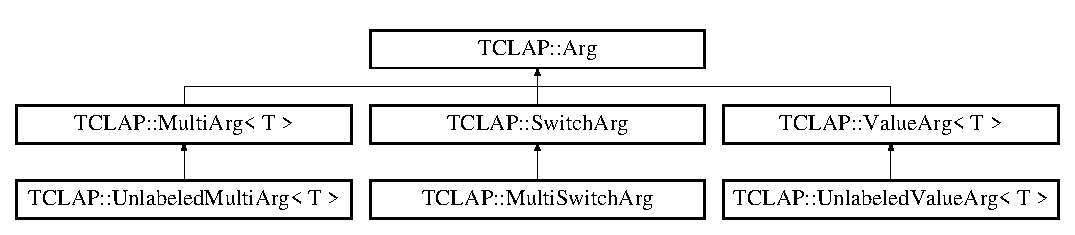
\includegraphics[height=2.705314cm]{classTCLAP_1_1Arg}
\end{center}
\end{figure}
\subsection*{Public Member Functions}
\begin{DoxyCompactItemize}
\item 
virtual {\bf $\sim$\+Arg} ()
\begin{DoxyCompactList}\small\item\em Destructor. \end{DoxyCompactList}\item 
virtual void {\bf add\+To\+List} (std\+::list$<$ {\bf Arg} $\ast$ $>$ \&arg\+List) const 
\begin{DoxyCompactList}\small\item\em Adds this to the specified list of Args. \end{DoxyCompactList}\item 
virtual bool {\bf process\+Arg} (int $\ast$i, std\+::vector$<$ std\+::string $>$ \&args)=0
\begin{DoxyCompactList}\small\item\em Pure virtual method meant to handle the parsing and value assignment of the string on the command line. \end{DoxyCompactList}\item 
virtual bool {\bf operator==} (const {\bf Arg} \&a) const 
\begin{DoxyCompactList}\small\item\em Operator ==. \end{DoxyCompactList}\item 
const std\+::string \& {\bf get\+Flag} () const 
\begin{DoxyCompactList}\small\item\em Returns the argument flag. \end{DoxyCompactList}\item 
const std\+::string \& {\bf get\+Name} () const 
\begin{DoxyCompactList}\small\item\em Returns the argument name. \end{DoxyCompactList}\item 
std\+::string {\bf get\+Description} () const 
\begin{DoxyCompactList}\small\item\em Returns the argument description. \end{DoxyCompactList}\item 
virtual bool {\bf is\+Required} () const 
\begin{DoxyCompactList}\small\item\em Indicates whether the argument is required. \end{DoxyCompactList}\item 
void {\bf force\+Required} ()
\begin{DoxyCompactList}\small\item\em Sets \+\_\+required to true. \end{DoxyCompactList}\item 
void {\bf xor\+Set} ()
\begin{DoxyCompactList}\small\item\em Sets the \+\_\+already\+Set value to true. \end{DoxyCompactList}\item 
bool {\bf is\+Value\+Required} () const 
\begin{DoxyCompactList}\small\item\em Indicates whether a value must be specified for argument. \end{DoxyCompactList}\item 
bool {\bf is\+Set} () const 
\begin{DoxyCompactList}\small\item\em Indicates whether the argument has already been set. \end{DoxyCompactList}\item 
bool {\bf is\+Ignoreable} () const 
\begin{DoxyCompactList}\small\item\em Indicates whether the argument can be ignored, if desired. \end{DoxyCompactList}\item 
virtual bool {\bf arg\+Matches} (const std\+::string \&s) const 
\begin{DoxyCompactList}\small\item\em A method that tests whether a string matches this argument. \end{DoxyCompactList}\item 
virtual std\+::string {\bf to\+String} () const 
\begin{DoxyCompactList}\small\item\em Returns a simple string representation of the argument. \end{DoxyCompactList}\item 
virtual std\+::string {\bf short\+I\+D} (const std\+::string \&value\+Id=\char`\"{}val\char`\"{}) const 
\begin{DoxyCompactList}\small\item\em Returns a short I\+D for the usage. \end{DoxyCompactList}\item 
virtual std\+::string {\bf long\+I\+D} (const std\+::string \&value\+Id=\char`\"{}val\char`\"{}) const 
\begin{DoxyCompactList}\small\item\em Returns a long I\+D for the usage. \end{DoxyCompactList}\item 
virtual void {\bf trim\+Flag} (std\+::string \&flag, std\+::string \&value) const 
\begin{DoxyCompactList}\small\item\em Trims a value off of the flag. \end{DoxyCompactList}\item 
bool {\bf \+\_\+has\+Blanks} (const std\+::string \&s) const 
\begin{DoxyCompactList}\small\item\em Checks whether a given string has blank chars, indicating that it is a combined \doxyref{Switch\+Arg}{p.}{classTCLAP_1_1SwitchArg}. \end{DoxyCompactList}\item 
void {\bf set\+Require\+Label} (const std\+::string \&s)
\begin{DoxyCompactList}\small\item\em Sets the require\+Label. \end{DoxyCompactList}\item 
virtual bool {\bf allow\+More} ()
\begin{DoxyCompactList}\small\item\em Used for Multi\+Args and \doxyref{Xor\+Handler}{p.}{classTCLAP_1_1XorHandler} to determine whether args can still be set. \end{DoxyCompactList}\item 
virtual bool {\bf accepts\+Multiple\+Values} ()
\begin{DoxyCompactList}\small\item\em Use by output classes to determine whether an \doxyref{Arg}{p.}{classTCLAP_1_1Arg} accepts multiple values. \end{DoxyCompactList}\item 
virtual void {\bf reset} ()
\begin{DoxyCompactList}\small\item\em Clears the \doxyref{Arg}{p.}{classTCLAP_1_1Arg} object and allows it to be reused by new command lines. \end{DoxyCompactList}\end{DoxyCompactItemize}
\subsection*{Static Public Member Functions}
\begin{DoxyCompactItemize}
\item 
static void {\bf begin\+Ignoring} ()
\begin{DoxyCompactList}\small\item\em Begin ignoring arguments since the \char`\"{}-\/-\/\char`\"{} argument was specified. \end{DoxyCompactList}\item 
static bool {\bf ignore\+Rest} ()
\begin{DoxyCompactList}\small\item\em Whether to ignore the rest. \end{DoxyCompactList}\item 
static char {\bf delimiter} ()
\begin{DoxyCompactList}\small\item\em The delimiter that separates an argument flag/name from the value. \end{DoxyCompactList}\item 
static char {\bf blank\+Char} ()
\begin{DoxyCompactList}\small\item\em The char used as a place holder when Switch\+Args are combined. \end{DoxyCompactList}\item 
static char {\bf flag\+Start\+Char} ()
\item 
static const std\+::string {\bf flag\+Start\+String} ()
\item 
static const std\+::string {\bf name\+Start\+String} ()
\item 
static const std\+::string {\bf ignore\+Name\+String} ()
\begin{DoxyCompactList}\small\item\em The name used to identify the ignore rest argument. \end{DoxyCompactList}\item 
static void {\bf set\+Delimiter} (char c)
\begin{DoxyCompactList}\small\item\em Sets the delimiter for all arguments. \end{DoxyCompactList}\end{DoxyCompactItemize}
\subsection*{Protected Member Functions}
\begin{DoxyCompactItemize}
\item 
void {\bf \+\_\+check\+With\+Visitor} () const 
\begin{DoxyCompactList}\small\item\em Performs the special handling described by the Vistitor. \end{DoxyCompactList}\item 
{\bf Arg} (const std\+::string \&flag, const std\+::string \&name, const std\+::string \&desc, bool req, bool valreq, {\bf Visitor} $\ast$v=N\+U\+L\+L)
\begin{DoxyCompactList}\small\item\em Primary constructor. \end{DoxyCompactList}\end{DoxyCompactItemize}
\subsection*{Protected Attributes}
\begin{DoxyCompactItemize}
\item 
std\+::string {\bf \+\_\+flag}
\begin{DoxyCompactList}\small\item\em The single char flag used to identify the argument. \end{DoxyCompactList}\item 
std\+::string {\bf \+\_\+name}
\begin{DoxyCompactList}\small\item\em A single work namd indentifying the argument. \end{DoxyCompactList}\item 
std\+::string {\bf \+\_\+description}
\begin{DoxyCompactList}\small\item\em Description of the argument. \end{DoxyCompactList}\item 
bool {\bf \+\_\+required}
\begin{DoxyCompactList}\small\item\em Indicating whether the argument is required. \end{DoxyCompactList}\item 
std\+::string {\bf \+\_\+require\+Label}
\begin{DoxyCompactList}\small\item\em Label to be used in usage description. \end{DoxyCompactList}\item 
bool {\bf \+\_\+value\+Required}
\begin{DoxyCompactList}\small\item\em Indicates whether a value is required for the argument. \end{DoxyCompactList}\item 
bool {\bf \+\_\+already\+Set}
\begin{DoxyCompactList}\small\item\em Indicates whether the argument has been set. \end{DoxyCompactList}\item 
{\bf Visitor} $\ast$ {\bf \+\_\+visitor}
\begin{DoxyCompactList}\small\item\em A pointer to a vistitor object. \end{DoxyCompactList}\item 
bool {\bf \+\_\+ignoreable}
\begin{DoxyCompactList}\small\item\em Whether this argument can be ignored, if desired. \end{DoxyCompactList}\item 
bool {\bf \+\_\+xor\+Set}
\begin{DoxyCompactList}\small\item\em Indicates that the arg was set as part of an X\+O\+R and not on the command line. \end{DoxyCompactList}\item 
bool {\bf \+\_\+accepts\+Multiple\+Values}
\end{DoxyCompactItemize}
\subsection*{Private Member Functions}
\begin{DoxyCompactItemize}
\item 
{\bf Arg} (const {\bf Arg} \&rhs)
\begin{DoxyCompactList}\small\item\em Prevent accidental copying. \end{DoxyCompactList}\item 
{\bf Arg} \& {\bf operator=} (const {\bf Arg} \&rhs)
\begin{DoxyCompactList}\small\item\em Prevent accidental copying. \end{DoxyCompactList}\end{DoxyCompactItemize}
\subsection*{Static Private Member Functions}
\begin{DoxyCompactItemize}
\item 
static bool \& {\bf ignore\+Rest\+Ref} ()
\begin{DoxyCompactList}\small\item\em Indicates whether the rest of the arguments should be ignored. \end{DoxyCompactList}\item 
static char \& {\bf delimiter\+Ref} ()
\begin{DoxyCompactList}\small\item\em The delimiter that separates an argument flag/name from the value. \end{DoxyCompactList}\end{DoxyCompactItemize}


\subsection{Detailed Description}
A virtual base class that defines the essential data for all arguments. 

This class, or one of its existing children, must be subclassed to do anything. 

Definition at line 64 of file Arg.\+h.



\subsection{Constructor \& Destructor Documentation}
\index{T\+C\+L\+A\+P\+::\+Arg@{T\+C\+L\+A\+P\+::\+Arg}!Arg@{Arg}}
\index{Arg@{Arg}!T\+C\+L\+A\+P\+::\+Arg@{T\+C\+L\+A\+P\+::\+Arg}}
\subsubsection[{Arg}]{\setlength{\rightskip}{0pt plus 5cm}T\+C\+L\+A\+P\+::\+Arg\+::\+Arg (
\begin{DoxyParamCaption}
\item[{const {\bf Arg} \&}]{rhs}
\end{DoxyParamCaption}
)\hspace{0.3cm}{\ttfamily [private]}}\label{classTCLAP_1_1Arg_aca23d0f3bd09d71f22dbe8f4504c04dc}


Prevent accidental copying. 

\index{T\+C\+L\+A\+P\+::\+Arg@{T\+C\+L\+A\+P\+::\+Arg}!Arg@{Arg}}
\index{Arg@{Arg}!T\+C\+L\+A\+P\+::\+Arg@{T\+C\+L\+A\+P\+::\+Arg}}
\subsubsection[{Arg}]{\setlength{\rightskip}{0pt plus 5cm}T\+C\+L\+A\+P\+::\+Arg\+::\+Arg (
\begin{DoxyParamCaption}
\item[{const std\+::string \&}]{flag, }
\item[{const std\+::string \&}]{name, }
\item[{const std\+::string \&}]{desc, }
\item[{bool}]{req, }
\item[{bool}]{valreq, }
\item[{{\bf Visitor} $\ast$}]{v = {\ttfamily NULL}}
\end{DoxyParamCaption}
)\hspace{0.3cm}{\ttfamily [inline]}, {\ttfamily [protected]}}\label{classTCLAP_1_1Arg_ab25a06db5edf82a5b965b641b3c63372}


Primary constructor. 

Y\+O\+U (yes you) should N\+E\+V\+E\+R construct an \doxyref{Arg}{p.}{classTCLAP_1_1Arg} directly, this is a base class that is extended by various children that are meant to be used. Use \doxyref{Switch\+Arg}{p.}{classTCLAP_1_1SwitchArg}, \doxyref{Value\+Arg}{p.}{classTCLAP_1_1ValueArg}, \doxyref{Multi\+Arg}{p.}{classTCLAP_1_1MultiArg}, \doxyref{Unlabeled\+Value\+Arg}{p.}{classTCLAP_1_1UnlabeledValueArg}, or \doxyref{Unlabeled\+Multi\+Arg}{p.}{classTCLAP_1_1UnlabeledMultiArg} instead.


\begin{DoxyParams}{Parameters}
{\em flag} & -\/ The flag identifying the argument. \\
\hline
{\em name} & -\/ The name identifying the argument. \\
\hline
{\em desc} & -\/ The description of the argument, used in the usage. \\
\hline
{\em req} & -\/ Whether the argument is required. \\
\hline
{\em valreq} & -\/ Whether the a value is required for the argument. \\
\hline
{\em v} & -\/ The visitor checked by the argument. Defaults to N\+U\+L\+L. \\
\hline
\end{DoxyParams}


Definition at line 462 of file Arg.\+h.



References \+\_\+flag, \+\_\+name, flag\+Start\+String(), ignore\+Name\+String(), name\+Start\+String(), and to\+String().


\begin{DoxyCode}
467                      :
468   _flag(flag),
469   _name(name),
470   _description(desc),
471   _required(req),
472   _requireLabel(\textcolor{stringliteral}{"required"}),
473   _valueRequired(valreq),
474   _alreadySet(\textcolor{keyword}{false}),
475   _visitor( v ),
476   _ignoreable(\textcolor{keyword}{true}),
477   _xorSet(\textcolor{keyword}{false}),
478   _acceptsMultipleValues(\textcolor{keyword}{false})
479 \{
480   \textcolor{keywordflow}{if} ( _flag.length() > 1 )
481     \textcolor{keywordflow}{throw}(SpecificationException(
482         \textcolor{stringliteral}{"Argument flag can only be one character long"}, toString() ) );
483 
484   \textcolor{keywordflow}{if} ( _name != ignoreNameString() &&
485      ( _flag == Arg::flagStartString() ||
486        _flag == Arg::nameStartString() ||
487        _flag == \textcolor{stringliteral}{" "} ) )
488     \textcolor{keywordflow}{throw}(SpecificationException(\textcolor{stringliteral}{"Argument flag cannot be either '"} +
489               Arg::flagStartString() + \textcolor{stringliteral}{"' or '"} +
490               Arg::nameStartString() + \textcolor{stringliteral}{"' or a space."},
491               toString() ) );
492 
493   \textcolor{keywordflow}{if} ( ( _name.substr( 0, Arg::flagStartString().length() ) == 
      Arg::flagStartString() ) ||
494      ( _name.substr( 0, Arg::nameStartString().length() ) == 
      Arg::nameStartString() ) ||
495      ( _name.find( \textcolor{stringliteral}{" "}, 0 ) != std::string::npos ) )
496     \textcolor{keywordflow}{throw}(SpecificationException(\textcolor{stringliteral}{"Argument name begin with either '"} +
497               Arg::flagStartString() + \textcolor{stringliteral}{"' or '"} +
498               Arg::nameStartString() + \textcolor{stringliteral}{"' or space."},
499               toString() ) );
500 
501 \}
\end{DoxyCode}
\index{T\+C\+L\+A\+P\+::\+Arg@{T\+C\+L\+A\+P\+::\+Arg}!````~Arg@{$\sim$\+Arg}}
\index{````~Arg@{$\sim$\+Arg}!T\+C\+L\+A\+P\+::\+Arg@{T\+C\+L\+A\+P\+::\+Arg}}
\subsubsection[{$\sim$\+Arg}]{\setlength{\rightskip}{0pt plus 5cm}T\+C\+L\+A\+P\+::\+Arg\+::$\sim$\+Arg (
\begin{DoxyParamCaption}
{}
\end{DoxyParamCaption}
)\hspace{0.3cm}{\ttfamily [inline]}, {\ttfamily [virtual]}}\label{classTCLAP_1_1Arg_a15734a7cf52c8c4ab6df70f0997bbee3}


Destructor. 



Definition at line 503 of file Arg.\+h.


\begin{DoxyCode}
503 \{ \}
\end{DoxyCode}


\subsection{Member Function Documentation}
\index{T\+C\+L\+A\+P\+::\+Arg@{T\+C\+L\+A\+P\+::\+Arg}!\+\_\+check\+With\+Visitor@{\+\_\+check\+With\+Visitor}}
\index{\+\_\+check\+With\+Visitor@{\+\_\+check\+With\+Visitor}!T\+C\+L\+A\+P\+::\+Arg@{T\+C\+L\+A\+P\+::\+Arg}}
\subsubsection[{\+\_\+check\+With\+Visitor}]{\setlength{\rightskip}{0pt plus 5cm}void T\+C\+L\+A\+P\+::\+Arg\+::\+\_\+check\+With\+Visitor (
\begin{DoxyParamCaption}
{}
\end{DoxyParamCaption}
) const\hspace{0.3cm}{\ttfamily [inline]}, {\ttfamily [protected]}}\label{classTCLAP_1_1Arg_aa963d0d4c8cb297e1f4cf74143bf6d1b}


Performs the special handling described by the Vistitor. 



Definition at line 611 of file Arg.\+h.



References \+\_\+visitor, and T\+C\+L\+A\+P\+::\+Visitor\+::visit().



Referenced by T\+C\+L\+A\+P\+::\+Switch\+Arg\+::common\+Processing(), and T\+C\+L\+A\+P\+::\+Multi\+Switch\+Arg\+::process\+Arg().


\begin{DoxyCode}
612 \{
613   \textcolor{keywordflow}{if} ( _visitor != NULL )
614     _visitor->visit();
615 \}
\end{DoxyCode}
\index{T\+C\+L\+A\+P\+::\+Arg@{T\+C\+L\+A\+P\+::\+Arg}!\+\_\+has\+Blanks@{\+\_\+has\+Blanks}}
\index{\+\_\+has\+Blanks@{\+\_\+has\+Blanks}!T\+C\+L\+A\+P\+::\+Arg@{T\+C\+L\+A\+P\+::\+Arg}}
\subsubsection[{\+\_\+has\+Blanks}]{\setlength{\rightskip}{0pt plus 5cm}bool T\+C\+L\+A\+P\+::\+Arg\+::\+\_\+has\+Blanks (
\begin{DoxyParamCaption}
\item[{const std\+::string \&}]{s}
\end{DoxyParamCaption}
) const\hspace{0.3cm}{\ttfamily [inline]}}\label{classTCLAP_1_1Arg_a2eb0ffefe163218bdc8b4b7a33a974a7}


Checks whether a given string has blank chars, indicating that it is a combined \doxyref{Switch\+Arg}{p.}{classTCLAP_1_1SwitchArg}. 

Implementation of \+\_\+has\+Blanks.

If so, return true, otherwise return false. 
\begin{DoxyParams}{Parameters}
{\em s} & -\/ string to be checked. \\
\hline
\end{DoxyParams}


Definition at line 641 of file Arg.\+h.



References blank\+Char().


\begin{DoxyCode}
642 \{
643   \textcolor{keywordflow}{for} ( \textcolor{keywordtype}{int} i = 1; \textcolor{keyword}{static\_cast<}\textcolor{keywordtype}{unsigned} \textcolor{keywordtype}{int}\textcolor{keyword}{>}(i) < s.length(); i++ )
644     \textcolor{keywordflow}{if} ( s[i] == Arg::blankChar() )
645       \textcolor{keywordflow}{return} \textcolor{keyword}{true};
646 
647   \textcolor{keywordflow}{return} \textcolor{keyword}{false};
648 \}
\end{DoxyCode}
\index{T\+C\+L\+A\+P\+::\+Arg@{T\+C\+L\+A\+P\+::\+Arg}!accepts\+Multiple\+Values@{accepts\+Multiple\+Values}}
\index{accepts\+Multiple\+Values@{accepts\+Multiple\+Values}!T\+C\+L\+A\+P\+::\+Arg@{T\+C\+L\+A\+P\+::\+Arg}}
\subsubsection[{accepts\+Multiple\+Values}]{\setlength{\rightskip}{0pt plus 5cm}bool T\+C\+L\+A\+P\+::\+Arg\+::accepts\+Multiple\+Values (
\begin{DoxyParamCaption}
{}
\end{DoxyParamCaption}
)\hspace{0.3cm}{\ttfamily [inline]}, {\ttfamily [virtual]}}\label{classTCLAP_1_1Arg_ad356870538a255d639e26b30330202ae}


Use by output classes to determine whether an \doxyref{Arg}{p.}{classTCLAP_1_1Arg} accepts multiple values. 



Definition at line 674 of file Arg.\+h.



References \+\_\+accepts\+Multiple\+Values.



Referenced by T\+C\+L\+A\+P\+::\+Zsh\+Completion\+Output\+::get\+Mutex\+List(), T\+C\+L\+A\+P\+::\+Zsh\+Completion\+Output\+::print\+Arg(), and T\+C\+L\+A\+P\+::\+Doc\+Book\+Output\+::print\+Short\+Arg().


\begin{DoxyCode}
675 \{
676   \textcolor{keywordflow}{return} _acceptsMultipleValues;
677 \}
\end{DoxyCode}
\index{T\+C\+L\+A\+P\+::\+Arg@{T\+C\+L\+A\+P\+::\+Arg}!add\+To\+List@{add\+To\+List}}
\index{add\+To\+List@{add\+To\+List}!T\+C\+L\+A\+P\+::\+Arg@{T\+C\+L\+A\+P\+::\+Arg}}
\subsubsection[{add\+To\+List}]{\setlength{\rightskip}{0pt plus 5cm}void T\+C\+L\+A\+P\+::\+Arg\+::add\+To\+List (
\begin{DoxyParamCaption}
\item[{std\+::list$<$ {\bf Arg} $\ast$ $>$ \&}]{arg\+List}
\end{DoxyParamCaption}
) const\hspace{0.3cm}{\ttfamily [inline]}, {\ttfamily [virtual]}}\label{classTCLAP_1_1Arg_a9ff1564beeea2ef855f7fa483c37d0e2}


Adds this to the specified list of Args. 

Overridden by Args that need to added to the end of the list.


\begin{DoxyParams}{Parameters}
{\em arg\+List} & -\/ The list to add this to. \\
\hline
\end{DoxyParams}


Reimplemented in {\bf T\+C\+L\+A\+P\+::\+Unlabeled\+Value\+Arg$<$ T $>$} \doxyref{}{p.}{classTCLAP_1_1UnlabeledValueArg_a8670fc7797254e602d302318063f3515}, and {\bf T\+C\+L\+A\+P\+::\+Unlabeled\+Multi\+Arg$<$ T $>$} \doxyref{}{p.}{classTCLAP_1_1UnlabeledMultiArg_a290b15792de11abb5a4cf1c312d6a0d7}.



Definition at line 664 of file Arg.\+h.



Referenced by T\+C\+L\+A\+P\+::\+Cmd\+Line\+::add().


\begin{DoxyCode}
665 \{
666   argList.push\_front( const\_cast<Arg*>(\textcolor{keyword}{this}) );
667 \}
\end{DoxyCode}
\index{T\+C\+L\+A\+P\+::\+Arg@{T\+C\+L\+A\+P\+::\+Arg}!allow\+More@{allow\+More}}
\index{allow\+More@{allow\+More}!T\+C\+L\+A\+P\+::\+Arg@{T\+C\+L\+A\+P\+::\+Arg}}
\subsubsection[{allow\+More}]{\setlength{\rightskip}{0pt plus 5cm}bool T\+C\+L\+A\+P\+::\+Arg\+::allow\+More (
\begin{DoxyParamCaption}
{}
\end{DoxyParamCaption}
)\hspace{0.3cm}{\ttfamily [inline]}, {\ttfamily [virtual]}}\label{classTCLAP_1_1Arg_a9aef735d37ef95ca1b7dc7a07850b984}


Used for Multi\+Args and \doxyref{Xor\+Handler}{p.}{classTCLAP_1_1XorHandler} to determine whether args can still be set. 



Reimplemented in {\bf T\+C\+L\+A\+P\+::\+Multi\+Arg$<$ T $>$} \doxyref{}{p.}{classTCLAP_1_1MultiArg_ab05097627c81cd65975fa1b99fae9bd0}.



Definition at line 669 of file Arg.\+h.


\begin{DoxyCode}
670 \{
671   \textcolor{keywordflow}{return} \textcolor{keyword}{false};
672 \}
\end{DoxyCode}
\index{T\+C\+L\+A\+P\+::\+Arg@{T\+C\+L\+A\+P\+::\+Arg}!arg\+Matches@{arg\+Matches}}
\index{arg\+Matches@{arg\+Matches}!T\+C\+L\+A\+P\+::\+Arg@{T\+C\+L\+A\+P\+::\+Arg}}
\subsubsection[{arg\+Matches}]{\setlength{\rightskip}{0pt plus 5cm}bool T\+C\+L\+A\+P\+::\+Arg\+::arg\+Matches (
\begin{DoxyParamCaption}
\item[{const std\+::string \&}]{s}
\end{DoxyParamCaption}
) const\hspace{0.3cm}{\ttfamily [inline]}, {\ttfamily [virtual]}}\label{classTCLAP_1_1Arg_aac37b1b734b477e5d16f2037dba9c125}


A method that tests whether a string matches this argument. 

This is generally called by the \doxyref{process\+Arg()}{p.}{classTCLAP_1_1Arg_a61ffe2f660a76111d256f7b22a686146} method. This method could be re-\/implemented by a child to change how arguments are specified on the command line. 
\begin{DoxyParams}{Parameters}
{\em s} & -\/ The string to be compared to the flag/name to determine whether the arg matches. \\
\hline
\end{DoxyParams}


Definition at line 590 of file Arg.\+h.



References \+\_\+flag, \+\_\+name, flag\+Start\+String(), and name\+Start\+String().



Referenced by T\+C\+L\+A\+P\+::\+Switch\+Arg\+::process\+Arg(), and T\+C\+L\+A\+P\+::\+Multi\+Switch\+Arg\+::process\+Arg().


\begin{DoxyCode}
591 \{
592   \textcolor{keywordflow}{if} ( ( argFlag == Arg::flagStartString() + _flag && _flag != \textcolor{stringliteral}{""} ) ||
593          argFlag == Arg::nameStartString() + _name )
594     \textcolor{keywordflow}{return} \textcolor{keyword}{true};
595   \textcolor{keywordflow}{else}
596     \textcolor{keywordflow}{return} \textcolor{keyword}{false};
597 \}
\end{DoxyCode}
\index{T\+C\+L\+A\+P\+::\+Arg@{T\+C\+L\+A\+P\+::\+Arg}!begin\+Ignoring@{begin\+Ignoring}}
\index{begin\+Ignoring@{begin\+Ignoring}!T\+C\+L\+A\+P\+::\+Arg@{T\+C\+L\+A\+P\+::\+Arg}}
\subsubsection[{begin\+Ignoring}]{\setlength{\rightskip}{0pt plus 5cm}static void T\+C\+L\+A\+P\+::\+Arg\+::begin\+Ignoring (
\begin{DoxyParamCaption}
{}
\end{DoxyParamCaption}
)\hspace{0.3cm}{\ttfamily [inline]}, {\ttfamily [static]}}\label{classTCLAP_1_1Arg_a24165d31c1ec70777fb201356b6cdf6a}


Begin ignoring arguments since the \char`\"{}-\/-\/\char`\"{} argument was specified. 



Definition at line 200 of file Arg.\+h.



References ignore\+Rest\+Ref().



Referenced by T\+C\+L\+A\+P\+::\+Ignore\+Rest\+Visitor\+::visit().


\begin{DoxyCode}
200 \{ ignoreRestRef() = \textcolor{keyword}{true}; \}
\end{DoxyCode}
\index{T\+C\+L\+A\+P\+::\+Arg@{T\+C\+L\+A\+P\+::\+Arg}!blank\+Char@{blank\+Char}}
\index{blank\+Char@{blank\+Char}!T\+C\+L\+A\+P\+::\+Arg@{T\+C\+L\+A\+P\+::\+Arg}}
\subsubsection[{blank\+Char}]{\setlength{\rightskip}{0pt plus 5cm}static char T\+C\+L\+A\+P\+::\+Arg\+::blank\+Char (
\begin{DoxyParamCaption}
{}
\end{DoxyParamCaption}
)\hspace{0.3cm}{\ttfamily [inline]}, {\ttfamily [static]}}\label{classTCLAP_1_1Arg_a0abd38f46dbf7d267078134a4817fbb2}


The char used as a place holder when Switch\+Args are combined. 

Currently set to the bell char (A\+S\+C\+I\+I 7). 

Definition at line 217 of file Arg.\+h.



Referenced by T\+C\+L\+A\+P\+::\+Cmd\+Line\+::\+\_\+empty\+Combined(), \+\_\+has\+Blanks(), T\+C\+L\+A\+P\+::\+Switch\+Arg\+::combined\+Switches\+Match(), and T\+C\+L\+A\+P\+::\+Switch\+Arg\+::last\+Combined().


\begin{DoxyCode}
217 \{ \textcolor{keywordflow}{return} (\textcolor{keywordtype}{char})7; \}
\end{DoxyCode}
\index{T\+C\+L\+A\+P\+::\+Arg@{T\+C\+L\+A\+P\+::\+Arg}!delimiter@{delimiter}}
\index{delimiter@{delimiter}!T\+C\+L\+A\+P\+::\+Arg@{T\+C\+L\+A\+P\+::\+Arg}}
\subsubsection[{delimiter}]{\setlength{\rightskip}{0pt plus 5cm}static char T\+C\+L\+A\+P\+::\+Arg\+::delimiter (
\begin{DoxyParamCaption}
{}
\end{DoxyParamCaption}
)\hspace{0.3cm}{\ttfamily [inline]}, {\ttfamily [static]}}\label{classTCLAP_1_1Arg_aadef6ca7e40f5b3d3fd03186976aea7e}


The delimiter that separates an argument flag/name from the value. 



Definition at line 211 of file Arg.\+h.



References delimiter\+Ref().



Referenced by T\+C\+L\+A\+P\+::\+Switch\+Arg\+::combined\+Switches\+Match(), long\+I\+D(), T\+C\+L\+A\+P\+::\+Multi\+Arg$<$ T $>$\+::process\+Arg(), T\+C\+L\+A\+P\+::\+Value\+Arg$<$ T $>$\+::process\+Arg(), short\+I\+D(), and trim\+Flag().


\begin{DoxyCode}
211 \{ \textcolor{keywordflow}{return} delimiterRef(); \}
\end{DoxyCode}
\index{T\+C\+L\+A\+P\+::\+Arg@{T\+C\+L\+A\+P\+::\+Arg}!delimiter\+Ref@{delimiter\+Ref}}
\index{delimiter\+Ref@{delimiter\+Ref}!T\+C\+L\+A\+P\+::\+Arg@{T\+C\+L\+A\+P\+::\+Arg}}
\subsubsection[{delimiter\+Ref}]{\setlength{\rightskip}{0pt plus 5cm}static char\& T\+C\+L\+A\+P\+::\+Arg\+::delimiter\+Ref (
\begin{DoxyParamCaption}
{}
\end{DoxyParamCaption}
)\hspace{0.3cm}{\ttfamily [inline]}, {\ttfamily [static]}, {\ttfamily [private]}}\label{classTCLAP_1_1Arg_a863591150a407ff29276ac13d0058144}


The delimiter that separates an argument flag/name from the value. 



Definition at line 86 of file Arg.\+h.



Referenced by delimiter(), and set\+Delimiter().


\begin{DoxyCode}
86 \{ \textcolor{keyword}{static} \textcolor{keywordtype}{char} delim = \textcolor{charliteral}{' '}; \textcolor{keywordflow}{return} delim; \}
\end{DoxyCode}
\index{T\+C\+L\+A\+P\+::\+Arg@{T\+C\+L\+A\+P\+::\+Arg}!flag\+Start\+Char@{flag\+Start\+Char}}
\index{flag\+Start\+Char@{flag\+Start\+Char}!T\+C\+L\+A\+P\+::\+Arg@{T\+C\+L\+A\+P\+::\+Arg}}
\subsubsection[{flag\+Start\+Char}]{\setlength{\rightskip}{0pt plus 5cm}static char T\+C\+L\+A\+P\+::\+Arg\+::flag\+Start\+Char (
\begin{DoxyParamCaption}
{}
\end{DoxyParamCaption}
)\hspace{0.3cm}{\ttfamily [inline]}, {\ttfamily [static]}}\label{classTCLAP_1_1Arg_a7f9f6af439993e9151bd5a6cd2a63dad}


Definition at line 226 of file Arg.\+h.



References T\+C\+L\+A\+P\+\_\+\+F\+L\+A\+G\+S\+T\+A\+R\+T\+C\+H\+A\+R.



Referenced by T\+C\+L\+A\+P\+::\+Cmd\+Line\+::\+\_\+empty\+Combined(), T\+C\+L\+A\+P\+::\+Zsh\+Completion\+Output\+::get\+Mutex\+List(), and T\+C\+L\+A\+P\+::\+Zsh\+Completion\+Output\+::print\+Option().


\begin{DoxyCode}
226 \{ \textcolor{keywordflow}{return} TCLAP_FLAGSTARTCHAR; \}
\end{DoxyCode}
\index{T\+C\+L\+A\+P\+::\+Arg@{T\+C\+L\+A\+P\+::\+Arg}!flag\+Start\+String@{flag\+Start\+String}}
\index{flag\+Start\+String@{flag\+Start\+String}!T\+C\+L\+A\+P\+::\+Arg@{T\+C\+L\+A\+P\+::\+Arg}}
\subsubsection[{flag\+Start\+String}]{\setlength{\rightskip}{0pt plus 5cm}static const std\+::string T\+C\+L\+A\+P\+::\+Arg\+::flag\+Start\+String (
\begin{DoxyParamCaption}
{}
\end{DoxyParamCaption}
)\hspace{0.3cm}{\ttfamily [inline]}, {\ttfamily [static]}}\label{classTCLAP_1_1Arg_af8e739295b0f75028e7bff6d670d97a1}


Definition at line 236 of file Arg.\+h.



References T\+C\+L\+A\+P\+\_\+\+F\+L\+A\+G\+S\+T\+A\+R\+T\+S\+T\+R\+I\+N\+G.



Referenced by T\+C\+L\+A\+P\+::\+Cmd\+Line\+::\+\_\+constructor(), Arg(), arg\+Matches(), T\+C\+L\+A\+P\+::\+Switch\+Arg\+::combined\+Switches\+Match(), long\+I\+D(), short\+I\+D(), and to\+String().


\begin{DoxyCode}
236 \{ \textcolor{keywordflow}{return} TCLAP_FLAGSTARTSTRING; \}
\end{DoxyCode}
\index{T\+C\+L\+A\+P\+::\+Arg@{T\+C\+L\+A\+P\+::\+Arg}!force\+Required@{force\+Required}}
\index{force\+Required@{force\+Required}!T\+C\+L\+A\+P\+::\+Arg@{T\+C\+L\+A\+P\+::\+Arg}}
\subsubsection[{force\+Required}]{\setlength{\rightskip}{0pt plus 5cm}void T\+C\+L\+A\+P\+::\+Arg\+::force\+Required (
\begin{DoxyParamCaption}
{}
\end{DoxyParamCaption}
)\hspace{0.3cm}{\ttfamily [inline]}}\label{classTCLAP_1_1Arg_a58e3de560f364d0bb6bdf36ab533a6fd}


Sets \+\_\+required to true. 

This is used by the \doxyref{Xor\+Handler}{p.}{classTCLAP_1_1XorHandler}. You really have no reason to ever use it. 

Definition at line 650 of file Arg.\+h.



References \+\_\+required.


\begin{DoxyCode}
651 \{
652   _required = \textcolor{keyword}{true};
653 \}
\end{DoxyCode}
\index{T\+C\+L\+A\+P\+::\+Arg@{T\+C\+L\+A\+P\+::\+Arg}!get\+Description@{get\+Description}}
\index{get\+Description@{get\+Description}!T\+C\+L\+A\+P\+::\+Arg@{T\+C\+L\+A\+P\+::\+Arg}}
\subsubsection[{get\+Description}]{\setlength{\rightskip}{0pt plus 5cm}std\+::string T\+C\+L\+A\+P\+::\+Arg\+::get\+Description (
\begin{DoxyParamCaption}
{}
\end{DoxyParamCaption}
) const\hspace{0.3cm}{\ttfamily [inline]}}\label{classTCLAP_1_1Arg_a1943999fadcb4f28cecd6ba55ed0b085}


Returns the argument description. 



Definition at line 554 of file Arg.\+h.



References \+\_\+description, \+\_\+required, and \+\_\+require\+Label.



Referenced by T\+C\+L\+A\+P\+::\+Unlabeled\+Multi\+Arg$<$ T $>$\+::operator==(), T\+C\+L\+A\+P\+::\+Unlabeled\+Value\+Arg$<$ T $>$\+::operator==(), and T\+C\+L\+A\+P\+::\+Zsh\+Completion\+Output\+::print\+Option().


\begin{DoxyCode}
555 \{
556   std::string desc = \textcolor{stringliteral}{""};
557   \textcolor{keywordflow}{if} ( _required )
558     desc = \textcolor{stringliteral}{"("} + _requireLabel + \textcolor{stringliteral}{")  "};
559 
560 \textcolor{comment}{//  if ( \_valueRequired )}
561 \textcolor{comment}{//    desc += "(value required)  ";}
562 
563   desc += _description;
564   \textcolor{keywordflow}{return} desc;
565 \}
\end{DoxyCode}
\index{T\+C\+L\+A\+P\+::\+Arg@{T\+C\+L\+A\+P\+::\+Arg}!get\+Flag@{get\+Flag}}
\index{get\+Flag@{get\+Flag}!T\+C\+L\+A\+P\+::\+Arg@{T\+C\+L\+A\+P\+::\+Arg}}
\subsubsection[{get\+Flag}]{\setlength{\rightskip}{0pt plus 5cm}const std\+::string \& T\+C\+L\+A\+P\+::\+Arg\+::get\+Flag (
\begin{DoxyParamCaption}
{}
\end{DoxyParamCaption}
) const\hspace{0.3cm}{\ttfamily [inline]}}\label{classTCLAP_1_1Arg_a22f616e81a423e794f13a9ae1549ac77}


Returns the argument flag. 



Definition at line 567 of file Arg.\+h.



References \+\_\+flag.



Referenced by T\+C\+L\+A\+P\+::\+Zsh\+Completion\+Output\+::get\+Mutex\+List(), and T\+C\+L\+A\+P\+::\+Zsh\+Completion\+Output\+::print\+Option().


\begin{DoxyCode}
567 \{ \textcolor{keywordflow}{return} _flag; \}
\end{DoxyCode}
\index{T\+C\+L\+A\+P\+::\+Arg@{T\+C\+L\+A\+P\+::\+Arg}!get\+Name@{get\+Name}}
\index{get\+Name@{get\+Name}!T\+C\+L\+A\+P\+::\+Arg@{T\+C\+L\+A\+P\+::\+Arg}}
\subsubsection[{get\+Name}]{\setlength{\rightskip}{0pt plus 5cm}const std\+::string \& T\+C\+L\+A\+P\+::\+Arg\+::get\+Name (
\begin{DoxyParamCaption}
{}
\end{DoxyParamCaption}
) const\hspace{0.3cm}{\ttfamily [inline]}}\label{classTCLAP_1_1Arg_a641ced141a56c74fee11d3e3a808f731}


Returns the argument name. 



Definition at line 569 of file Arg.\+h.



References \+\_\+name.



Referenced by T\+C\+L\+A\+P\+::\+Zsh\+Completion\+Output\+::get\+Mutex\+List(), T\+C\+L\+A\+P\+::\+Unlabeled\+Multi\+Arg$<$ T $>$\+::operator==(), T\+C\+L\+A\+P\+::\+Unlabeled\+Value\+Arg$<$ T $>$\+::operator==(), T\+C\+L\+A\+P\+::\+Zsh\+Completion\+Output\+::print\+Arg(), and T\+C\+L\+A\+P\+::\+Zsh\+Completion\+Output\+::print\+Option().


\begin{DoxyCode}
569 \{ \textcolor{keywordflow}{return} _name; \}
\end{DoxyCode}
\index{T\+C\+L\+A\+P\+::\+Arg@{T\+C\+L\+A\+P\+::\+Arg}!ignore\+Name\+String@{ignore\+Name\+String}}
\index{ignore\+Name\+String@{ignore\+Name\+String}!T\+C\+L\+A\+P\+::\+Arg@{T\+C\+L\+A\+P\+::\+Arg}}
\subsubsection[{ignore\+Name\+String}]{\setlength{\rightskip}{0pt plus 5cm}static const std\+::string T\+C\+L\+A\+P\+::\+Arg\+::ignore\+Name\+String (
\begin{DoxyParamCaption}
{}
\end{DoxyParamCaption}
)\hspace{0.3cm}{\ttfamily [inline]}, {\ttfamily [static]}}\label{classTCLAP_1_1Arg_a6ce0cbe4effd44679ca11f25e3c318e7}


The name used to identify the ignore rest argument. 



Definition at line 250 of file Arg.\+h.



Referenced by T\+C\+L\+A\+P\+::\+Cmd\+Line\+::\+\_\+constructor(), and Arg().


\begin{DoxyCode}
250 \{ \textcolor{keywordflow}{return} \textcolor{stringliteral}{"ignore\_rest"}; \}
\end{DoxyCode}
\index{T\+C\+L\+A\+P\+::\+Arg@{T\+C\+L\+A\+P\+::\+Arg}!ignore\+Rest@{ignore\+Rest}}
\index{ignore\+Rest@{ignore\+Rest}!T\+C\+L\+A\+P\+::\+Arg@{T\+C\+L\+A\+P\+::\+Arg}}
\subsubsection[{ignore\+Rest}]{\setlength{\rightskip}{0pt plus 5cm}static bool T\+C\+L\+A\+P\+::\+Arg\+::ignore\+Rest (
\begin{DoxyParamCaption}
{}
\end{DoxyParamCaption}
)\hspace{0.3cm}{\ttfamily [inline]}, {\ttfamily [static]}}\label{classTCLAP_1_1Arg_a4d412155b8f9b4956e64e91c48e55a3b}


Whether to ignore the rest. 



Definition at line 205 of file Arg.\+h.



References ignore\+Rest\+Ref().



Referenced by T\+C\+L\+A\+P\+::\+Cmd\+Line\+::parse(), T\+C\+L\+A\+P\+::\+Switch\+Arg\+::process\+Arg(), T\+C\+L\+A\+P\+::\+Multi\+Switch\+Arg\+::process\+Arg(), T\+C\+L\+A\+P\+::\+Multi\+Arg$<$ T $>$\+::process\+Arg(), and T\+C\+L\+A\+P\+::\+Value\+Arg$<$ T $>$\+::process\+Arg().


\begin{DoxyCode}
205 \{ \textcolor{keywordflow}{return} ignoreRestRef(); \}
\end{DoxyCode}
\index{T\+C\+L\+A\+P\+::\+Arg@{T\+C\+L\+A\+P\+::\+Arg}!ignore\+Rest\+Ref@{ignore\+Rest\+Ref}}
\index{ignore\+Rest\+Ref@{ignore\+Rest\+Ref}!T\+C\+L\+A\+P\+::\+Arg@{T\+C\+L\+A\+P\+::\+Arg}}
\subsubsection[{ignore\+Rest\+Ref}]{\setlength{\rightskip}{0pt plus 5cm}static bool\& T\+C\+L\+A\+P\+::\+Arg\+::ignore\+Rest\+Ref (
\begin{DoxyParamCaption}
{}
\end{DoxyParamCaption}
)\hspace{0.3cm}{\ttfamily [inline]}, {\ttfamily [static]}, {\ttfamily [private]}}\label{classTCLAP_1_1Arg_afa32140f7c01f99f6a9e85deb79281e1}


Indicates whether the rest of the arguments should be ignored. 



Definition at line 80 of file Arg.\+h.



Referenced by begin\+Ignoring(), and ignore\+Rest().


\begin{DoxyCode}
80 \{ \textcolor{keyword}{static} \textcolor{keywordtype}{bool} ign = \textcolor{keyword}{false}; \textcolor{keywordflow}{return} ign; \}
\end{DoxyCode}
\index{T\+C\+L\+A\+P\+::\+Arg@{T\+C\+L\+A\+P\+::\+Arg}!is\+Ignoreable@{is\+Ignoreable}}
\index{is\+Ignoreable@{is\+Ignoreable}!T\+C\+L\+A\+P\+::\+Arg@{T\+C\+L\+A\+P\+::\+Arg}}
\subsubsection[{is\+Ignoreable}]{\setlength{\rightskip}{0pt plus 5cm}bool T\+C\+L\+A\+P\+::\+Arg\+::is\+Ignoreable (
\begin{DoxyParamCaption}
{}
\end{DoxyParamCaption}
) const\hspace{0.3cm}{\ttfamily [inline]}}\label{classTCLAP_1_1Arg_a33816b5ccc58a15f3a998480e5d988e2}


Indicates whether the argument can be ignored, if desired. 



Definition at line 583 of file Arg.\+h.



References \+\_\+ignoreable.


\begin{DoxyCode}
583 \{ \textcolor{keywordflow}{return} _ignoreable; \}
\end{DoxyCode}
\index{T\+C\+L\+A\+P\+::\+Arg@{T\+C\+L\+A\+P\+::\+Arg}!is\+Required@{is\+Required}}
\index{is\+Required@{is\+Required}!T\+C\+L\+A\+P\+::\+Arg@{T\+C\+L\+A\+P\+::\+Arg}}
\subsubsection[{is\+Required}]{\setlength{\rightskip}{0pt plus 5cm}bool T\+C\+L\+A\+P\+::\+Arg\+::is\+Required (
\begin{DoxyParamCaption}
{}
\end{DoxyParamCaption}
) const\hspace{0.3cm}{\ttfamily [inline]}, {\ttfamily [virtual]}}\label{classTCLAP_1_1Arg_a00a3cfdb2b6e9a111ad39cbd4978b96c}


Indicates whether the argument is required. 



Reimplemented in {\bf T\+C\+L\+A\+P\+::\+Multi\+Arg$<$ T $>$} \doxyref{}{p.}{classTCLAP_1_1MultiArg_a3cb7fec92f3d70e0e455c6bc33fbebab}.



Definition at line 571 of file Arg.\+h.



References \+\_\+required.



Referenced by T\+C\+L\+A\+P\+::\+Cmd\+Line\+::add(), T\+C\+L\+A\+P\+::\+Xor\+Handler\+::check(), T\+C\+L\+A\+P\+::\+Zsh\+Completion\+Output\+::print\+Arg(), and T\+C\+L\+A\+P\+::\+Doc\+Book\+Output\+::print\+Short\+Arg().


\begin{DoxyCode}
571 \{ \textcolor{keywordflow}{return} _required; \}
\end{DoxyCode}
\index{T\+C\+L\+A\+P\+::\+Arg@{T\+C\+L\+A\+P\+::\+Arg}!is\+Set@{is\+Set}}
\index{is\+Set@{is\+Set}!T\+C\+L\+A\+P\+::\+Arg@{T\+C\+L\+A\+P\+::\+Arg}}
\subsubsection[{is\+Set}]{\setlength{\rightskip}{0pt plus 5cm}bool T\+C\+L\+A\+P\+::\+Arg\+::is\+Set (
\begin{DoxyParamCaption}
{}
\end{DoxyParamCaption}
) const\hspace{0.3cm}{\ttfamily [inline]}}\label{classTCLAP_1_1Arg_a6af7a1e92b5d92fc2d90c1a95aab4384}


Indicates whether the argument has already been set. 

Only true if the arg has been matched on the command line. 

Definition at line 575 of file Arg.\+h.



References \+\_\+already\+Set, and \+\_\+xor\+Set.



Referenced by T\+C\+L\+A\+P\+::\+Xor\+Handler\+::check().


\begin{DoxyCode}
576 \{
577   \textcolor{keywordflow}{if} ( _alreadySet && !_xorSet )
578     \textcolor{keywordflow}{return} \textcolor{keyword}{true};
579   \textcolor{keywordflow}{else}
580     \textcolor{keywordflow}{return} \textcolor{keyword}{false};
581 \}
\end{DoxyCode}
\index{T\+C\+L\+A\+P\+::\+Arg@{T\+C\+L\+A\+P\+::\+Arg}!is\+Value\+Required@{is\+Value\+Required}}
\index{is\+Value\+Required@{is\+Value\+Required}!T\+C\+L\+A\+P\+::\+Arg@{T\+C\+L\+A\+P\+::\+Arg}}
\subsubsection[{is\+Value\+Required}]{\setlength{\rightskip}{0pt plus 5cm}bool T\+C\+L\+A\+P\+::\+Arg\+::is\+Value\+Required (
\begin{DoxyParamCaption}
{}
\end{DoxyParamCaption}
) const\hspace{0.3cm}{\ttfamily [inline]}}\label{classTCLAP_1_1Arg_a1373d50d4b93c16db43c7600cf6d0355}


Indicates whether a value must be specified for argument. 



Definition at line 573 of file Arg.\+h.



References \+\_\+value\+Required.



Referenced by T\+C\+L\+A\+P\+::\+Zsh\+Completion\+Output\+::print\+Option().


\begin{DoxyCode}
573 \{ \textcolor{keywordflow}{return} _valueRequired; \}
\end{DoxyCode}
\index{T\+C\+L\+A\+P\+::\+Arg@{T\+C\+L\+A\+P\+::\+Arg}!long\+I\+D@{long\+I\+D}}
\index{long\+I\+D@{long\+I\+D}!T\+C\+L\+A\+P\+::\+Arg@{T\+C\+L\+A\+P\+::\+Arg}}
\subsubsection[{long\+I\+D}]{\setlength{\rightskip}{0pt plus 5cm}std\+::string T\+C\+L\+A\+P\+::\+Arg\+::long\+I\+D (
\begin{DoxyParamCaption}
\item[{const std\+::string \&}]{value\+Id = {\ttfamily \char`\"{}val\char`\"{}}}
\end{DoxyParamCaption}
) const\hspace{0.3cm}{\ttfamily [inline]}, {\ttfamily [virtual]}}\label{classTCLAP_1_1Arg_aad93aff46e1fc67e3853765f565bfa96}


Returns a long I\+D for the usage. 


\begin{DoxyParams}{Parameters}
{\em value\+Id} & -\/ The value used in the id. \\
\hline
\end{DoxyParams}


Reimplemented in {\bf T\+C\+L\+A\+P\+::\+Value\+Arg$<$ T $>$} \doxyref{}{p.}{classTCLAP_1_1ValueArg_a586d25c04c39ddf0e589605d79f72f8a}, {\bf T\+C\+L\+A\+P\+::\+Multi\+Arg$<$ T $>$} \doxyref{}{p.}{classTCLAP_1_1MultiArg_a16c00fbce6876bceabb3dab4723f7e79}, {\bf T\+C\+L\+A\+P\+::\+Unlabeled\+Value\+Arg$<$ T $>$} \doxyref{}{p.}{classTCLAP_1_1UnlabeledValueArg_ade738f42a7867324ce780b0c240b0460}, {\bf T\+C\+L\+A\+P\+::\+Unlabeled\+Multi\+Arg$<$ T $>$} \doxyref{}{p.}{classTCLAP_1_1UnlabeledMultiArg_a1e7262967b850fb30e1003890a45f1ca}, and {\bf T\+C\+L\+A\+P\+::\+Multi\+Switch\+Arg} \doxyref{}{p.}{classTCLAP_1_1MultiSwitchArg_a0b0aacc09c93462bab4347f86db0fccd}.



Definition at line 523 of file Arg.\+h.



References \+\_\+flag, \+\_\+name, \+\_\+value\+Required, delimiter(), flag\+Start\+String(), and name\+Start\+String().



Referenced by T\+C\+L\+A\+P\+::\+Cmd\+Line\+::add(), T\+C\+L\+A\+P\+::\+Multi\+Switch\+Arg\+::long\+I\+D(), T\+C\+L\+A\+P\+::\+Multi\+Arg$<$ T $>$\+::long\+I\+D(), and T\+C\+L\+A\+P\+::\+Value\+Arg$<$ T $>$\+::long\+I\+D().


\begin{DoxyCode}
524 \{
525   std::string \textcolor{keywordtype}{id} = \textcolor{stringliteral}{""};
526 
527   \textcolor{keywordflow}{if} ( _flag != \textcolor{stringliteral}{""} )
528   \{
529     \textcolor{keywordtype}{id} += Arg::flagStartString() + _flag;
530 
531     \textcolor{keywordflow}{if} ( _valueRequired )
532       \textcolor{keywordtype}{id} += std::string( 1, Arg::delimiter() ) + \textcolor{stringliteral}{"<"} + valueId + \textcolor{stringliteral}{">"};
533 
534     \textcolor{keywordtype}{id} += \textcolor{stringliteral}{",  "};
535   \}
536 
537   \textcolor{keywordtype}{id} += Arg::nameStartString() + _name;
538 
539   \textcolor{keywordflow}{if} ( _valueRequired )
540     \textcolor{keywordtype}{id} += std::string( 1, Arg::delimiter() ) + \textcolor{stringliteral}{"<"} + valueId + \textcolor{stringliteral}{">"};
541 
542   \textcolor{keywordflow}{return} id;
543 
544 \}
\end{DoxyCode}
\index{T\+C\+L\+A\+P\+::\+Arg@{T\+C\+L\+A\+P\+::\+Arg}!name\+Start\+String@{name\+Start\+String}}
\index{name\+Start\+String@{name\+Start\+String}!T\+C\+L\+A\+P\+::\+Arg@{T\+C\+L\+A\+P\+::\+Arg}}
\subsubsection[{name\+Start\+String}]{\setlength{\rightskip}{0pt plus 5cm}static const std\+::string T\+C\+L\+A\+P\+::\+Arg\+::name\+Start\+String (
\begin{DoxyParamCaption}
{}
\end{DoxyParamCaption}
)\hspace{0.3cm}{\ttfamily [inline]}, {\ttfamily [static]}}\label{classTCLAP_1_1Arg_a1df2134870528b80f9f35347fef6fd14}


Definition at line 245 of file Arg.\+h.



References T\+C\+L\+A\+P\+\_\+\+N\+A\+M\+E\+S\+T\+A\+R\+T\+S\+T\+R\+I\+N\+G.



Referenced by Arg(), arg\+Matches(), T\+C\+L\+A\+P\+::\+Switch\+Arg\+::combined\+Switches\+Match(), T\+C\+L\+A\+P\+::\+Zsh\+Completion\+Output\+::get\+Mutex\+List(), long\+I\+D(), T\+C\+L\+A\+P\+::\+Zsh\+Completion\+Output\+::print\+Option(), short\+I\+D(), and to\+String().


\begin{DoxyCode}
245 \{ \textcolor{keywordflow}{return} TCLAP_NAMESTARTSTRING; \}
\end{DoxyCode}
\index{T\+C\+L\+A\+P\+::\+Arg@{T\+C\+L\+A\+P\+::\+Arg}!operator=@{operator=}}
\index{operator=@{operator=}!T\+C\+L\+A\+P\+::\+Arg@{T\+C\+L\+A\+P\+::\+Arg}}
\subsubsection[{operator=}]{\setlength{\rightskip}{0pt plus 5cm}{\bf Arg}\& T\+C\+L\+A\+P\+::\+Arg\+::operator= (
\begin{DoxyParamCaption}
\item[{const {\bf Arg} \&}]{rhs}
\end{DoxyParamCaption}
)\hspace{0.3cm}{\ttfamily [private]}}\label{classTCLAP_1_1Arg_a580ebe03ce3af1f85db2b2e5d19fb6bc}


Prevent accidental copying. 

\index{T\+C\+L\+A\+P\+::\+Arg@{T\+C\+L\+A\+P\+::\+Arg}!operator==@{operator==}}
\index{operator==@{operator==}!T\+C\+L\+A\+P\+::\+Arg@{T\+C\+L\+A\+P\+::\+Arg}}
\subsubsection[{operator==}]{\setlength{\rightskip}{0pt plus 5cm}bool T\+C\+L\+A\+P\+::\+Arg\+::operator== (
\begin{DoxyParamCaption}
\item[{const {\bf Arg} \&}]{a}
\end{DoxyParamCaption}
) const\hspace{0.3cm}{\ttfamily [inline]}, {\ttfamily [virtual]}}\label{classTCLAP_1_1Arg_a657a8d2842b7de9ced5a5a55db01d367}


Operator ==. 

Equality operator. Must be virtual to handle unlabeled args. 
\begin{DoxyParams}{Parameters}
{\em a} & -\/ The \doxyref{Arg}{p.}{classTCLAP_1_1Arg} to be compared to this. \\
\hline
\end{DoxyParams}


Reimplemented in {\bf T\+C\+L\+A\+P\+::\+Unlabeled\+Value\+Arg$<$ T $>$} \doxyref{}{p.}{classTCLAP_1_1UnlabeledValueArg_a74632cd4d169481518cb1a871f97b412}, and {\bf T\+C\+L\+A\+P\+::\+Unlabeled\+Multi\+Arg$<$ T $>$} \doxyref{}{p.}{classTCLAP_1_1UnlabeledMultiArg_a059fa00203a9f643a10334fedbd43e39}.



Definition at line 546 of file Arg.\+h.



References \+\_\+flag, and \+\_\+name.


\begin{DoxyCode}
547 \{
548   \textcolor{keywordflow}{if} ( ( _flag != \textcolor{stringliteral}{""} && _flag == a.\_flag ) || _name == a.\_name)
549     \textcolor{keywordflow}{return} \textcolor{keyword}{true};
550   \textcolor{keywordflow}{else}
551     \textcolor{keywordflow}{return} \textcolor{keyword}{false};
552 \}
\end{DoxyCode}
\index{T\+C\+L\+A\+P\+::\+Arg@{T\+C\+L\+A\+P\+::\+Arg}!process\+Arg@{process\+Arg}}
\index{process\+Arg@{process\+Arg}!T\+C\+L\+A\+P\+::\+Arg@{T\+C\+L\+A\+P\+::\+Arg}}
\subsubsection[{process\+Arg}]{\setlength{\rightskip}{0pt plus 5cm}virtual bool T\+C\+L\+A\+P\+::\+Arg\+::process\+Arg (
\begin{DoxyParamCaption}
\item[{int $\ast$}]{i, }
\item[{std\+::vector$<$ std\+::string $>$ \&}]{args}
\end{DoxyParamCaption}
)\hspace{0.3cm}{\ttfamily [pure virtual]}}\label{classTCLAP_1_1Arg_a61ffe2f660a76111d256f7b22a686146}


Pure virtual method meant to handle the parsing and value assignment of the string on the command line. 


\begin{DoxyParams}{Parameters}
{\em i} & -\/ Pointer the the current argument in the list. \\
\hline
{\em args} & -\/ Mutable list of strings. What is passed in from main. \\
\hline
\end{DoxyParams}


Implemented in {\bf T\+C\+L\+A\+P\+::\+Value\+Arg$<$ T $>$} \doxyref{}{p.}{classTCLAP_1_1ValueArg_a71e6ee7c7324724b6fc067c5ffe31160}, {\bf T\+C\+L\+A\+P\+::\+Unlabeled\+Value\+Arg$<$ T $>$} \doxyref{}{p.}{classTCLAP_1_1UnlabeledValueArg_ad853d7950a659b0d4ee2cda3f61261fd}, {\bf T\+C\+L\+A\+P\+::\+Multi\+Arg$<$ T $>$} \doxyref{}{p.}{classTCLAP_1_1MultiArg_a344d3cf2128c510f92825e421ea667c7}, {\bf T\+C\+L\+A\+P\+::\+Unlabeled\+Multi\+Arg$<$ T $>$} \doxyref{}{p.}{classTCLAP_1_1UnlabeledMultiArg_aa5a35665519518dcb60e53d3a4858802}, {\bf T\+C\+L\+A\+P\+::\+Multi\+Switch\+Arg} \doxyref{}{p.}{classTCLAP_1_1MultiSwitchArg_a91c3d349570f21d8af6dc90767d747a2}, and {\bf T\+C\+L\+A\+P\+::\+Switch\+Arg} \doxyref{}{p.}{classTCLAP_1_1SwitchArg_a624f98df6c4907efec95ffc353e9d08c}.

\index{T\+C\+L\+A\+P\+::\+Arg@{T\+C\+L\+A\+P\+::\+Arg}!reset@{reset}}
\index{reset@{reset}!T\+C\+L\+A\+P\+::\+Arg@{T\+C\+L\+A\+P\+::\+Arg}}
\subsubsection[{reset}]{\setlength{\rightskip}{0pt plus 5cm}void T\+C\+L\+A\+P\+::\+Arg\+::reset (
\begin{DoxyParamCaption}
{}
\end{DoxyParamCaption}
)\hspace{0.3cm}{\ttfamily [inline]}, {\ttfamily [virtual]}}\label{classTCLAP_1_1Arg_ab5b5dc9a9b0381561f0684523f943a2c}


Clears the \doxyref{Arg}{p.}{classTCLAP_1_1Arg} object and allows it to be reused by new command lines. 



Reimplemented in {\bf T\+C\+L\+A\+P\+::\+Value\+Arg$<$ T $>$} \doxyref{}{p.}{classTCLAP_1_1ValueArg_a1bc480b71c4d8ac3646e796af8fb6e14}, {\bf T\+C\+L\+A\+P\+::\+Multi\+Arg$<$ T $>$} \doxyref{}{p.}{classTCLAP_1_1MultiArg_ab21f01f22978a1c0eea716399e9ff89b}, {\bf T\+C\+L\+A\+P\+::\+Multi\+Switch\+Arg} \doxyref{}{p.}{classTCLAP_1_1MultiSwitchArg_ac320530811dbca7fdcb2a41ab252fce4}, and {\bf T\+C\+L\+A\+P\+::\+Switch\+Arg} \doxyref{}{p.}{classTCLAP_1_1SwitchArg_af8561d903ec3c11f5f2175e6db179d9c}.



Definition at line 679 of file Arg.\+h.



References \+\_\+already\+Set, and \+\_\+xor\+Set.



Referenced by T\+C\+L\+A\+P\+::\+Switch\+Arg\+::reset(), T\+C\+L\+A\+P\+::\+Multi\+Arg$<$ T $>$\+::reset(), and T\+C\+L\+A\+P\+::\+Value\+Arg$<$ T $>$\+::reset().


\begin{DoxyCode}
680 \{
681   _xorSet = \textcolor{keyword}{false};
682   _alreadySet = \textcolor{keyword}{false};
683 \}
\end{DoxyCode}
\index{T\+C\+L\+A\+P\+::\+Arg@{T\+C\+L\+A\+P\+::\+Arg}!set\+Delimiter@{set\+Delimiter}}
\index{set\+Delimiter@{set\+Delimiter}!T\+C\+L\+A\+P\+::\+Arg@{T\+C\+L\+A\+P\+::\+Arg}}
\subsubsection[{set\+Delimiter}]{\setlength{\rightskip}{0pt plus 5cm}static void T\+C\+L\+A\+P\+::\+Arg\+::set\+Delimiter (
\begin{DoxyParamCaption}
\item[{char}]{c}
\end{DoxyParamCaption}
)\hspace{0.3cm}{\ttfamily [inline]}, {\ttfamily [static]}}\label{classTCLAP_1_1Arg_ad059b63424001b9aedb4c019e2854c3c}


Sets the delimiter for all arguments. 


\begin{DoxyParams}{Parameters}
{\em c} & -\/ The character that delimits flags/names from values. \\
\hline
\end{DoxyParams}


Definition at line 256 of file Arg.\+h.



References delimiter\+Ref().



Referenced by T\+C\+L\+A\+P\+::\+Cmd\+Line\+::\+\_\+constructor().


\begin{DoxyCode}
256 \{ delimiterRef() = c; \}
\end{DoxyCode}
\index{T\+C\+L\+A\+P\+::\+Arg@{T\+C\+L\+A\+P\+::\+Arg}!set\+Require\+Label@{set\+Require\+Label}}
\index{set\+Require\+Label@{set\+Require\+Label}!T\+C\+L\+A\+P\+::\+Arg@{T\+C\+L\+A\+P\+::\+Arg}}
\subsubsection[{set\+Require\+Label}]{\setlength{\rightskip}{0pt plus 5cm}void T\+C\+L\+A\+P\+::\+Arg\+::set\+Require\+Label (
\begin{DoxyParamCaption}
\item[{const std\+::string \&}]{s}
\end{DoxyParamCaption}
)\hspace{0.3cm}{\ttfamily [inline]}}\label{classTCLAP_1_1Arg_aae5c959f31af1a484a8af06f84a6e8b0}


Sets the require\+Label. 

Used by \doxyref{Xor\+Handler}{p.}{classTCLAP_1_1XorHandler}. You shouldn't ever use this. 
\begin{DoxyParams}{Parameters}
{\em s} & -\/ Set the require\+Label to this value. \\
\hline
\end{DoxyParams}


Definition at line 585 of file Arg.\+h.



References \+\_\+require\+Label.


\begin{DoxyCode}
586 \{
587   _requireLabel = s;
588 \}
\end{DoxyCode}
\index{T\+C\+L\+A\+P\+::\+Arg@{T\+C\+L\+A\+P\+::\+Arg}!short\+I\+D@{short\+I\+D}}
\index{short\+I\+D@{short\+I\+D}!T\+C\+L\+A\+P\+::\+Arg@{T\+C\+L\+A\+P\+::\+Arg}}
\subsubsection[{short\+I\+D}]{\setlength{\rightskip}{0pt plus 5cm}std\+::string T\+C\+L\+A\+P\+::\+Arg\+::short\+I\+D (
\begin{DoxyParamCaption}
\item[{const std\+::string \&}]{value\+Id = {\ttfamily \char`\"{}val\char`\"{}}}
\end{DoxyParamCaption}
) const\hspace{0.3cm}{\ttfamily [inline]}, {\ttfamily [virtual]}}\label{classTCLAP_1_1Arg_aef8efaf3811162b2b2b2a84c6db280fa}


Returns a short I\+D for the usage. 


\begin{DoxyParams}{Parameters}
{\em value\+Id} & -\/ The value used in the id. \\
\hline
\end{DoxyParams}


Reimplemented in {\bf T\+C\+L\+A\+P\+::\+Value\+Arg$<$ T $>$} \doxyref{}{p.}{classTCLAP_1_1ValueArg_abb1eb22814d0a0da49c5f8bb57362d09}, {\bf T\+C\+L\+A\+P\+::\+Multi\+Arg$<$ T $>$} \doxyref{}{p.}{classTCLAP_1_1MultiArg_ac2c962112704b899f4c8b8565f2c4bb3}, {\bf T\+C\+L\+A\+P\+::\+Unlabeled\+Value\+Arg$<$ T $>$} \doxyref{}{p.}{classTCLAP_1_1UnlabeledValueArg_abda4d1d695003ba165b6797e03007a99}, {\bf T\+C\+L\+A\+P\+::\+Unlabeled\+Multi\+Arg$<$ T $>$} \doxyref{}{p.}{classTCLAP_1_1UnlabeledMultiArg_a5971af8f29fa4d798ffde3293504c15b}, and {\bf T\+C\+L\+A\+P\+::\+Multi\+Switch\+Arg} \doxyref{}{p.}{classTCLAP_1_1MultiSwitchArg_a083c07003f948691e94ce94d0b6376ed}.



Definition at line 505 of file Arg.\+h.



References \+\_\+flag, \+\_\+name, \+\_\+required, \+\_\+value\+Required, delimiter(), flag\+Start\+String(), and name\+Start\+String().



Referenced by T\+C\+L\+A\+P\+::\+Zsh\+Completion\+Output\+::print\+Option(), T\+C\+L\+A\+P\+::\+Doc\+Book\+Output\+::print\+Short\+Arg(), T\+C\+L\+A\+P\+::\+Multi\+Switch\+Arg\+::short\+I\+D(), T\+C\+L\+A\+P\+::\+Multi\+Arg$<$ T $>$\+::short\+I\+D(), and T\+C\+L\+A\+P\+::\+Value\+Arg$<$ T $>$\+::short\+I\+D().


\begin{DoxyCode}
506 \{
507   std::string \textcolor{keywordtype}{id} = \textcolor{stringliteral}{""};
508 
509   \textcolor{keywordflow}{if} ( _flag != \textcolor{stringliteral}{""} )
510     \textcolor{keywordtype}{id} = Arg::flagStartString() + _flag;
511   \textcolor{keywordflow}{else}
512     \textcolor{keywordtype}{id} = Arg::nameStartString() + _name;
513 
514   \textcolor{keywordflow}{if} ( _valueRequired )
515     \textcolor{keywordtype}{id} += std::string( 1, Arg::delimiter() ) + \textcolor{stringliteral}{"<"} + valueId  + \textcolor{stringliteral}{">"};
516 
517   \textcolor{keywordflow}{if} ( !_required )
518     \textcolor{keywordtype}{id} = \textcolor{stringliteral}{"["} + \textcolor{keywordtype}{id} + \textcolor{stringliteral}{"]"};
519 
520   \textcolor{keywordflow}{return} id;
521 \}
\end{DoxyCode}
\index{T\+C\+L\+A\+P\+::\+Arg@{T\+C\+L\+A\+P\+::\+Arg}!to\+String@{to\+String}}
\index{to\+String@{to\+String}!T\+C\+L\+A\+P\+::\+Arg@{T\+C\+L\+A\+P\+::\+Arg}}
\subsubsection[{to\+String}]{\setlength{\rightskip}{0pt plus 5cm}std\+::string T\+C\+L\+A\+P\+::\+Arg\+::to\+String (
\begin{DoxyParamCaption}
{}
\end{DoxyParamCaption}
) const\hspace{0.3cm}{\ttfamily [inline]}, {\ttfamily [virtual]}}\label{classTCLAP_1_1Arg_ac98a357568c21f0eb6ca2220b8a3d4a2}


Returns a simple string representation of the argument. 

Primarily for debugging. 

Definition at line 599 of file Arg.\+h.



References \+\_\+flag, \+\_\+name, flag\+Start\+String(), and name\+Start\+String().



Referenced by Arg(), T\+C\+L\+A\+P\+::\+Switch\+Arg\+::common\+Processing(), T\+C\+L\+A\+P\+::\+Switch\+Arg\+::process\+Arg(), T\+C\+L\+A\+P\+::\+Unlabeled\+Multi\+Arg$<$ T $>$\+::\+Unlabeled\+Multi\+Arg(), and T\+C\+L\+A\+P\+::\+Unlabeled\+Value\+Arg$<$ T $>$\+::\+Unlabeled\+Value\+Arg().


\begin{DoxyCode}
600 \{
601   std::string s = \textcolor{stringliteral}{""};
602 
603   \textcolor{keywordflow}{if} ( _flag != \textcolor{stringliteral}{""} )
604     s += Arg::flagStartString() + _flag + \textcolor{stringliteral}{" "};
605 
606   s += \textcolor{stringliteral}{"("} + Arg::nameStartString() + _name + \textcolor{stringliteral}{")"};
607 
608   \textcolor{keywordflow}{return} s;
609 \}
\end{DoxyCode}
\index{T\+C\+L\+A\+P\+::\+Arg@{T\+C\+L\+A\+P\+::\+Arg}!trim\+Flag@{trim\+Flag}}
\index{trim\+Flag@{trim\+Flag}!T\+C\+L\+A\+P\+::\+Arg@{T\+C\+L\+A\+P\+::\+Arg}}
\subsubsection[{trim\+Flag}]{\setlength{\rightskip}{0pt plus 5cm}void T\+C\+L\+A\+P\+::\+Arg\+::trim\+Flag (
\begin{DoxyParamCaption}
\item[{std\+::string \&}]{flag, }
\item[{std\+::string \&}]{value}
\end{DoxyParamCaption}
) const\hspace{0.3cm}{\ttfamily [inline]}, {\ttfamily [virtual]}}\label{classTCLAP_1_1Arg_a54595328e81f5fb77859563690faab25}


Trims a value off of the flag. 

Implementation of trim\+Flag.


\begin{DoxyParams}{Parameters}
{\em flag} & -\/ The string from which the flag and value will be trimmed. Contains the flag once the value has been trimmed. \\
\hline
{\em value} & -\/ Where the value trimmed from the string will be stored. \\
\hline
\end{DoxyParams}


Definition at line 620 of file Arg.\+h.



References delimiter().


\begin{DoxyCode}
621 \{
622   \textcolor{keywordtype}{int} stop = 0;
623   \textcolor{keywordflow}{for} ( \textcolor{keywordtype}{int} i = 0; \textcolor{keyword}{static\_cast<}\textcolor{keywordtype}{unsigned} \textcolor{keywordtype}{int}\textcolor{keyword}{>}(i) < flag.length(); i++ )
624     \textcolor{keywordflow}{if} ( flag[i] == Arg::delimiter() )
625     \{
626       stop = i;
627       \textcolor{keywordflow}{break};
628     \}
629 
630   \textcolor{keywordflow}{if} ( stop > 1 )
631   \{
632     value = flag.substr(stop+1);
633     flag = flag.substr(0,stop);
634   \}
635 
636 \}
\end{DoxyCode}
\index{T\+C\+L\+A\+P\+::\+Arg@{T\+C\+L\+A\+P\+::\+Arg}!xor\+Set@{xor\+Set}}
\index{xor\+Set@{xor\+Set}!T\+C\+L\+A\+P\+::\+Arg@{T\+C\+L\+A\+P\+::\+Arg}}
\subsubsection[{xor\+Set}]{\setlength{\rightskip}{0pt plus 5cm}void T\+C\+L\+A\+P\+::\+Arg\+::xor\+Set (
\begin{DoxyParamCaption}
{}
\end{DoxyParamCaption}
)\hspace{0.3cm}{\ttfamily [inline]}}\label{classTCLAP_1_1Arg_aec525c8092e56f7f5aa455e71bc72374}


Sets the \+\_\+already\+Set value to true. 

This is used by the \doxyref{Xor\+Handler}{p.}{classTCLAP_1_1XorHandler}. You really have no reason to ever use it. 

Definition at line 655 of file Arg.\+h.



References \+\_\+already\+Set, and \+\_\+xor\+Set.


\begin{DoxyCode}
656 \{
657   _alreadySet = \textcolor{keyword}{true};
658   _xorSet = \textcolor{keyword}{true};
659 \}
\end{DoxyCode}


\subsection{Member Data Documentation}
\index{T\+C\+L\+A\+P\+::\+Arg@{T\+C\+L\+A\+P\+::\+Arg}!\+\_\+accepts\+Multiple\+Values@{\+\_\+accepts\+Multiple\+Values}}
\index{\+\_\+accepts\+Multiple\+Values@{\+\_\+accepts\+Multiple\+Values}!T\+C\+L\+A\+P\+::\+Arg@{T\+C\+L\+A\+P\+::\+Arg}}
\subsubsection[{\+\_\+accepts\+Multiple\+Values}]{\setlength{\rightskip}{0pt plus 5cm}bool T\+C\+L\+A\+P\+::\+Arg\+::\+\_\+accepts\+Multiple\+Values\hspace{0.3cm}{\ttfamily [protected]}}\label{classTCLAP_1_1Arg_a13130a9a5d22c57a6d42a8883c9b1e0f}


Definition at line 158 of file Arg.\+h.



Referenced by accepts\+Multiple\+Values(), and T\+C\+L\+A\+P\+::\+Multi\+Arg$<$ T $>$\+::\+Multi\+Arg().

\index{T\+C\+L\+A\+P\+::\+Arg@{T\+C\+L\+A\+P\+::\+Arg}!\+\_\+already\+Set@{\+\_\+already\+Set}}
\index{\+\_\+already\+Set@{\+\_\+already\+Set}!T\+C\+L\+A\+P\+::\+Arg@{T\+C\+L\+A\+P\+::\+Arg}}
\subsubsection[{\+\_\+already\+Set}]{\setlength{\rightskip}{0pt plus 5cm}bool T\+C\+L\+A\+P\+::\+Arg\+::\+\_\+already\+Set\hspace{0.3cm}{\ttfamily [protected]}}\label{classTCLAP_1_1Arg_a829e32129857d2683e5791a5df1208ec}


Indicates whether the argument has been set. 

Indicates that a value on the command line has matched the name/flag of this argument and the values have been set accordingly. 

Definition at line 137 of file Arg.\+h.



Referenced by T\+C\+L\+A\+P\+::\+Switch\+Arg\+::common\+Processing(), is\+Set(), T\+C\+L\+A\+P\+::\+Multi\+Switch\+Arg\+::process\+Arg(), reset(), and xor\+Set().

\index{T\+C\+L\+A\+P\+::\+Arg@{T\+C\+L\+A\+P\+::\+Arg}!\+\_\+description@{\+\_\+description}}
\index{\+\_\+description@{\+\_\+description}!T\+C\+L\+A\+P\+::\+Arg@{T\+C\+L\+A\+P\+::\+Arg}}
\subsubsection[{\+\_\+description}]{\setlength{\rightskip}{0pt plus 5cm}std\+::string T\+C\+L\+A\+P\+::\+Arg\+::\+\_\+description\hspace{0.3cm}{\ttfamily [protected]}}\label{classTCLAP_1_1Arg_a9882fe256eaab01ac53db54ac657d272}


Description of the argument. 



Definition at line 112 of file Arg.\+h.



Referenced by get\+Description().

\index{T\+C\+L\+A\+P\+::\+Arg@{T\+C\+L\+A\+P\+::\+Arg}!\+\_\+flag@{\+\_\+flag}}
\index{\+\_\+flag@{\+\_\+flag}!T\+C\+L\+A\+P\+::\+Arg@{T\+C\+L\+A\+P\+::\+Arg}}
\subsubsection[{\+\_\+flag}]{\setlength{\rightskip}{0pt plus 5cm}std\+::string T\+C\+L\+A\+P\+::\+Arg\+::\+\_\+flag\hspace{0.3cm}{\ttfamily [protected]}}\label{classTCLAP_1_1Arg_ae68407a0a8223023ad0ae3b9dc7986f5}


The single char flag used to identify the argument. 

This value (preceded by a dash \{-\/\}), can be used to identify an argument on the command line. The \+\_\+flag can be blank, in fact this is how unlabeled args work. Unlabeled args must override appropriate functions to get correct handling. Note that the \+\_\+flag does N\+O\+T include the dash as part of the flag. 

Definition at line 98 of file Arg.\+h.



Referenced by Arg(), arg\+Matches(), T\+C\+L\+A\+P\+::\+Switch\+Arg\+::combined\+Switches\+Match(), get\+Flag(), long\+I\+D(), operator==(), short\+I\+D(), and to\+String().

\index{T\+C\+L\+A\+P\+::\+Arg@{T\+C\+L\+A\+P\+::\+Arg}!\+\_\+ignoreable@{\+\_\+ignoreable}}
\index{\+\_\+ignoreable@{\+\_\+ignoreable}!T\+C\+L\+A\+P\+::\+Arg@{T\+C\+L\+A\+P\+::\+Arg}}
\subsubsection[{\+\_\+ignoreable}]{\setlength{\rightskip}{0pt plus 5cm}bool T\+C\+L\+A\+P\+::\+Arg\+::\+\_\+ignoreable\hspace{0.3cm}{\ttfamily [protected]}}\label{classTCLAP_1_1Arg_a9832bb7564f4ab472bd51b7b1bbc683f}


Whether this argument can be ignored, if desired. 



Definition at line 150 of file Arg.\+h.



Referenced by is\+Ignoreable(), T\+C\+L\+A\+P\+::\+Switch\+Arg\+::process\+Arg(), T\+C\+L\+A\+P\+::\+Multi\+Switch\+Arg\+::process\+Arg(), T\+C\+L\+A\+P\+::\+Unlabeled\+Multi\+Arg$<$ T $>$\+::\+Unlabeled\+Multi\+Arg(), and T\+C\+L\+A\+P\+::\+Unlabeled\+Value\+Arg$<$ T $>$\+::\+Unlabeled\+Value\+Arg().

\index{T\+C\+L\+A\+P\+::\+Arg@{T\+C\+L\+A\+P\+::\+Arg}!\+\_\+name@{\+\_\+name}}
\index{\+\_\+name@{\+\_\+name}!T\+C\+L\+A\+P\+::\+Arg@{T\+C\+L\+A\+P\+::\+Arg}}
\subsubsection[{\+\_\+name}]{\setlength{\rightskip}{0pt plus 5cm}std\+::string T\+C\+L\+A\+P\+::\+Arg\+::\+\_\+name\hspace{0.3cm}{\ttfamily [protected]}}\label{classTCLAP_1_1Arg_ac0f138057a99fb5d94ff4acb41a083aa}


A single work namd indentifying the argument. 

This value (preceded by two dashed \{--\}) can also be used to identify an argument on the command line. Note that the \+\_\+name does N\+O\+T include the two dashes as part of the \+\_\+name. The \+\_\+name cannot be blank. 

Definition at line 107 of file Arg.\+h.



Referenced by Arg(), arg\+Matches(), get\+Name(), long\+I\+D(), operator==(), short\+I\+D(), and to\+String().

\index{T\+C\+L\+A\+P\+::\+Arg@{T\+C\+L\+A\+P\+::\+Arg}!\+\_\+required@{\+\_\+required}}
\index{\+\_\+required@{\+\_\+required}!T\+C\+L\+A\+P\+::\+Arg@{T\+C\+L\+A\+P\+::\+Arg}}
\subsubsection[{\+\_\+required}]{\setlength{\rightskip}{0pt plus 5cm}bool T\+C\+L\+A\+P\+::\+Arg\+::\+\_\+required\hspace{0.3cm}{\ttfamily [protected]}}\label{classTCLAP_1_1Arg_ad16408bd1ca4d8b1d14d6c5129545a84}


Indicating whether the argument is required. 



Definition at line 117 of file Arg.\+h.



Referenced by force\+Required(), get\+Description(), is\+Required(), and short\+I\+D().

\index{T\+C\+L\+A\+P\+::\+Arg@{T\+C\+L\+A\+P\+::\+Arg}!\+\_\+require\+Label@{\+\_\+require\+Label}}
\index{\+\_\+require\+Label@{\+\_\+require\+Label}!T\+C\+L\+A\+P\+::\+Arg@{T\+C\+L\+A\+P\+::\+Arg}}
\subsubsection[{\+\_\+require\+Label}]{\setlength{\rightskip}{0pt plus 5cm}std\+::string T\+C\+L\+A\+P\+::\+Arg\+::\+\_\+require\+Label\hspace{0.3cm}{\ttfamily [protected]}}\label{classTCLAP_1_1Arg_a2ed097a868e34a0c4f6062ead744ac54}


Label to be used in usage description. 

Normally set to \char`\"{}required\char`\"{}, but can be changed when necessary. 

Definition at line 123 of file Arg.\+h.



Referenced by get\+Description(), and set\+Require\+Label().

\index{T\+C\+L\+A\+P\+::\+Arg@{T\+C\+L\+A\+P\+::\+Arg}!\+\_\+value\+Required@{\+\_\+value\+Required}}
\index{\+\_\+value\+Required@{\+\_\+value\+Required}!T\+C\+L\+A\+P\+::\+Arg@{T\+C\+L\+A\+P\+::\+Arg}}
\subsubsection[{\+\_\+value\+Required}]{\setlength{\rightskip}{0pt plus 5cm}bool T\+C\+L\+A\+P\+::\+Arg\+::\+\_\+value\+Required\hspace{0.3cm}{\ttfamily [protected]}}\label{classTCLAP_1_1Arg_a776682b7e19f4dc231bbad3d10034dfa}


Indicates whether a value is required for the argument. 

Note that the value may be required but the argument/value combination may not be, as specified by \+\_\+required. 

Definition at line 130 of file Arg.\+h.



Referenced by is\+Value\+Required(), long\+I\+D(), and short\+I\+D().

\index{T\+C\+L\+A\+P\+::\+Arg@{T\+C\+L\+A\+P\+::\+Arg}!\+\_\+visitor@{\+\_\+visitor}}
\index{\+\_\+visitor@{\+\_\+visitor}!T\+C\+L\+A\+P\+::\+Arg@{T\+C\+L\+A\+P\+::\+Arg}}
\subsubsection[{\+\_\+visitor}]{\setlength{\rightskip}{0pt plus 5cm}{\bf Visitor}$\ast$ T\+C\+L\+A\+P\+::\+Arg\+::\+\_\+visitor\hspace{0.3cm}{\ttfamily [protected]}}\label{classTCLAP_1_1Arg_aa9ff037e92c9fa5bd85e532f61899300}


A pointer to a vistitor object. 

The visitor allows special handling to occur as soon as the argument is matched. This defaults to N\+U\+L\+L and should not be used unless absolutely necessary. 

Definition at line 145 of file Arg.\+h.



Referenced by \+\_\+check\+With\+Visitor().

\index{T\+C\+L\+A\+P\+::\+Arg@{T\+C\+L\+A\+P\+::\+Arg}!\+\_\+xor\+Set@{\+\_\+xor\+Set}}
\index{\+\_\+xor\+Set@{\+\_\+xor\+Set}!T\+C\+L\+A\+P\+::\+Arg@{T\+C\+L\+A\+P\+::\+Arg}}
\subsubsection[{\+\_\+xor\+Set}]{\setlength{\rightskip}{0pt plus 5cm}bool T\+C\+L\+A\+P\+::\+Arg\+::\+\_\+xor\+Set\hspace{0.3cm}{\ttfamily [protected]}}\label{classTCLAP_1_1Arg_ab413bd1d8a7ecf3c89672ee23ef791ba}


Indicates that the arg was set as part of an X\+O\+R and not on the command line. 



Definition at line 156 of file Arg.\+h.



Referenced by T\+C\+L\+A\+P\+::\+Switch\+Arg\+::common\+Processing(), is\+Set(), reset(), and xor\+Set().



The documentation for this class was generated from the following file\+:\begin{DoxyCompactItemize}
\item 
{\bf Arg.\+h}\end{DoxyCompactItemize}

\section{T\+C\+L\+A\+P\+:\+:Arg\+Exception Class Reference}
\label{classTCLAP_1_1ArgException}\index{T\+C\+L\+A\+P\+::\+Arg\+Exception@{T\+C\+L\+A\+P\+::\+Arg\+Exception}}


A simple class that defines and argument exception.  




{\ttfamily \#include $<$Arg\+Exception.\+h$>$}

Inheritance diagram for T\+C\+L\+A\+P\+:\+:Arg\+Exception\+:\begin{figure}[H]
\begin{center}
\leavevmode
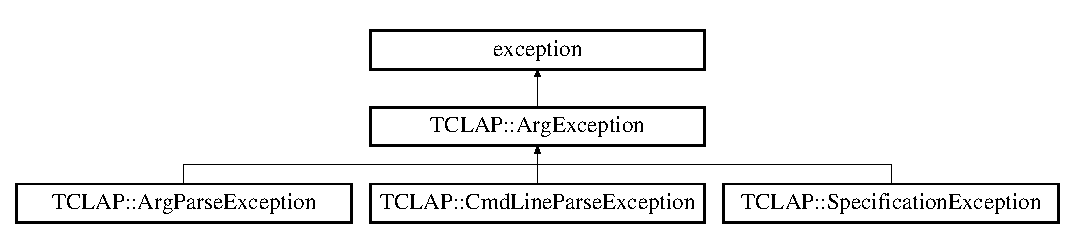
\includegraphics[height=2.758621cm]{classTCLAP_1_1ArgException}
\end{center}
\end{figure}
\subsection*{Public Member Functions}
\begin{DoxyCompactItemize}
\item 
{\bf Arg\+Exception} (const std\+::string \&text=\char`\"{}undefined exception\char`\"{}, const std\+::string \&id=\char`\"{}undefined\char`\"{}, const std\+::string \&td=\char`\"{}Generic {\bf Arg\+Exception}\char`\"{})
\begin{DoxyCompactList}\small\item\em Constructor. \end{DoxyCompactList}\item 
virtual {\bf $\sim$\+Arg\+Exception} ()  throw ()
\begin{DoxyCompactList}\small\item\em Destructor. \end{DoxyCompactList}\item 
std\+::string {\bf error} () const 
\begin{DoxyCompactList}\small\item\em Returns the error text. \end{DoxyCompactList}\item 
std\+::string {\bf arg\+Id} () const 
\begin{DoxyCompactList}\small\item\em Returns the argument id. \end{DoxyCompactList}\item 
const char $\ast$ {\bf what} () const   throw ()
\begin{DoxyCompactList}\small\item\em Returns the arg id and error text. \end{DoxyCompactList}\item 
std\+::string {\bf type\+Description} () const 
\begin{DoxyCompactList}\small\item\em Returns the type of the exception. \end{DoxyCompactList}\end{DoxyCompactItemize}
\subsection*{Private Attributes}
\begin{DoxyCompactItemize}
\item 
std\+::string {\bf \+\_\+error\+Text}
\begin{DoxyCompactList}\small\item\em The text of the exception message. \end{DoxyCompactList}\item 
std\+::string {\bf \+\_\+arg\+Id}
\begin{DoxyCompactList}\small\item\em The argument related to this exception. \end{DoxyCompactList}\item 
std\+::string {\bf \+\_\+type\+Description}
\begin{DoxyCompactList}\small\item\em Describes the type of the exception. \end{DoxyCompactList}\end{DoxyCompactItemize}


\subsection{Detailed Description}
A simple class that defines and argument exception. 

Should be caught whenever a \doxyref{Cmd\+Line}{p.}{classTCLAP_1_1CmdLine} is created and parsed. 

Definition at line 36 of file Arg\+Exception.\+h.



\subsection{Constructor \& Destructor Documentation}
\index{T\+C\+L\+A\+P\+::\+Arg\+Exception@{T\+C\+L\+A\+P\+::\+Arg\+Exception}!Arg\+Exception@{Arg\+Exception}}
\index{Arg\+Exception@{Arg\+Exception}!T\+C\+L\+A\+P\+::\+Arg\+Exception@{T\+C\+L\+A\+P\+::\+Arg\+Exception}}
\subsubsection[{Arg\+Exception}]{\setlength{\rightskip}{0pt plus 5cm}T\+C\+L\+A\+P\+::\+Arg\+Exception\+::\+Arg\+Exception (
\begin{DoxyParamCaption}
\item[{const std\+::string \&}]{text = {\ttfamily \char`\"{}undefined~exception\char`\"{}}, }
\item[{const std\+::string \&}]{id = {\ttfamily \char`\"{}undefined\char`\"{}}, }
\item[{const std\+::string \&}]{td = {\ttfamily \char`\"{}Generic~{\bf Arg\+Exception}\char`\"{}}}
\end{DoxyParamCaption}
)\hspace{0.3cm}{\ttfamily [inline]}}\label{classTCLAP_1_1ArgException_a67389912b628e95d530f8bb8de97b309}


Constructor. 


\begin{DoxyParams}{Parameters}
{\em text} & -\/ The text of the exception. \\
\hline
{\em id} & -\/ The text identifying the argument source. \\
\hline
{\em td} & -\/ Text describing the type of \doxyref{Arg\+Exception}{p.}{classTCLAP_1_1ArgException} it is. of the exception. \\
\hline
\end{DoxyParams}


Definition at line 47 of file Arg\+Exception.\+h.


\begin{DoxyCode}
50       : std::exception(), 
51         _errorText(text), 
52         _argId( \textcolor{keywordtype}{id} ), 
53         _typeDescription(td)
54     \{ \} 
\end{DoxyCode}
\index{T\+C\+L\+A\+P\+::\+Arg\+Exception@{T\+C\+L\+A\+P\+::\+Arg\+Exception}!````~Arg\+Exception@{$\sim$\+Arg\+Exception}}
\index{````~Arg\+Exception@{$\sim$\+Arg\+Exception}!T\+C\+L\+A\+P\+::\+Arg\+Exception@{T\+C\+L\+A\+P\+::\+Arg\+Exception}}
\subsubsection[{$\sim$\+Arg\+Exception}]{\setlength{\rightskip}{0pt plus 5cm}virtual T\+C\+L\+A\+P\+::\+Arg\+Exception\+::$\sim$\+Arg\+Exception (
\begin{DoxyParamCaption}
{}
\end{DoxyParamCaption}
) throw  ) \hspace{0.3cm}{\ttfamily [inline]}, {\ttfamily [virtual]}}\label{classTCLAP_1_1ArgException_a5c5df6a814b05c623a01607fb82980f4}


Destructor. 



Definition at line 59 of file Arg\+Exception.\+h.


\begin{DoxyCode}
59 \{ \}
\end{DoxyCode}


\subsection{Member Function Documentation}
\index{T\+C\+L\+A\+P\+::\+Arg\+Exception@{T\+C\+L\+A\+P\+::\+Arg\+Exception}!arg\+Id@{arg\+Id}}
\index{arg\+Id@{arg\+Id}!T\+C\+L\+A\+P\+::\+Arg\+Exception@{T\+C\+L\+A\+P\+::\+Arg\+Exception}}
\subsubsection[{arg\+Id}]{\setlength{\rightskip}{0pt plus 5cm}std\+::string T\+C\+L\+A\+P\+::\+Arg\+Exception\+::arg\+Id (
\begin{DoxyParamCaption}
{}
\end{DoxyParamCaption}
) const\hspace{0.3cm}{\ttfamily [inline]}}\label{classTCLAP_1_1ArgException_a18ffd1ad34c1799865f8e03df4ebdff1}


Returns the argument id. 



Definition at line 69 of file Arg\+Exception.\+h.



References \+\_\+arg\+Id.



Referenced by T\+C\+L\+A\+P\+::\+Std\+Output\+::failure().


\begin{DoxyCode}
70     \{ 
71       \textcolor{keywordflow}{if} ( _argId == \textcolor{stringliteral}{"undefined"} )
72         \textcolor{keywordflow}{return} \textcolor{stringliteral}{" "};
73       \textcolor{keywordflow}{else}
74         \textcolor{keywordflow}{return} ( \textcolor{stringliteral}{"Argument: "} + _argId ); 
75     \}
\end{DoxyCode}
\index{T\+C\+L\+A\+P\+::\+Arg\+Exception@{T\+C\+L\+A\+P\+::\+Arg\+Exception}!error@{error}}
\index{error@{error}!T\+C\+L\+A\+P\+::\+Arg\+Exception@{T\+C\+L\+A\+P\+::\+Arg\+Exception}}
\subsubsection[{error}]{\setlength{\rightskip}{0pt plus 5cm}std\+::string T\+C\+L\+A\+P\+::\+Arg\+Exception\+::error (
\begin{DoxyParamCaption}
{}
\end{DoxyParamCaption}
) const\hspace{0.3cm}{\ttfamily [inline]}}\label{classTCLAP_1_1ArgException_a0656dab88a7129bc288821bacd653d08}


Returns the error text. 



Definition at line 64 of file Arg\+Exception.\+h.



References \+\_\+error\+Text.



Referenced by T\+C\+L\+A\+P\+::\+Multi\+Arg$<$ T $>$\+::\+\_\+extract\+Value(), T\+C\+L\+A\+P\+::\+Value\+Arg$<$ T $>$\+::\+\_\+extract\+Value(), and T\+C\+L\+A\+P\+::\+Std\+Output\+::failure().


\begin{DoxyCode}
64 \{ \textcolor{keywordflow}{return} ( _errorText ); \}
\end{DoxyCode}
\index{T\+C\+L\+A\+P\+::\+Arg\+Exception@{T\+C\+L\+A\+P\+::\+Arg\+Exception}!type\+Description@{type\+Description}}
\index{type\+Description@{type\+Description}!T\+C\+L\+A\+P\+::\+Arg\+Exception@{T\+C\+L\+A\+P\+::\+Arg\+Exception}}
\subsubsection[{type\+Description}]{\setlength{\rightskip}{0pt plus 5cm}std\+::string T\+C\+L\+A\+P\+::\+Arg\+Exception\+::type\+Description (
\begin{DoxyParamCaption}
{}
\end{DoxyParamCaption}
) const\hspace{0.3cm}{\ttfamily [inline]}}\label{classTCLAP_1_1ArgException_abd271955e1b808bb92f8db7a16ea7c95}


Returns the type of the exception. 

Used to explain and distinguish between different child exceptions. 

Definition at line 91 of file Arg\+Exception.\+h.



References \+\_\+type\+Description.


\begin{DoxyCode}
92     \{
93       \textcolor{keywordflow}{return} _typeDescription; 
94     \}
\end{DoxyCode}
\index{T\+C\+L\+A\+P\+::\+Arg\+Exception@{T\+C\+L\+A\+P\+::\+Arg\+Exception}!what@{what}}
\index{what@{what}!T\+C\+L\+A\+P\+::\+Arg\+Exception@{T\+C\+L\+A\+P\+::\+Arg\+Exception}}
\subsubsection[{what}]{\setlength{\rightskip}{0pt plus 5cm}const char$\ast$ T\+C\+L\+A\+P\+::\+Arg\+Exception\+::what (
\begin{DoxyParamCaption}
{}
\end{DoxyParamCaption}
) const throw  ) \hspace{0.3cm}{\ttfamily [inline]}}\label{classTCLAP_1_1ArgException_af51c89da2e4ae54fc9d05038ea484c83}


Returns the arg id and error text. 



Definition at line 80 of file Arg\+Exception.\+h.



References \+\_\+arg\+Id, and \+\_\+error\+Text.



Referenced by T\+C\+L\+A\+P\+::\+Doc\+Book\+Output\+::failure(), and T\+C\+L\+A\+P\+::\+Zsh\+Completion\+Output\+::failure().


\begin{DoxyCode}
81     \{
82       \textcolor{keyword}{static} std::string ex; 
83       ex = _argId + \textcolor{stringliteral}{" -- "} + _errorText;
84       \textcolor{keywordflow}{return} ex.c\_str();
85     \}
\end{DoxyCode}


\subsection{Member Data Documentation}
\index{T\+C\+L\+A\+P\+::\+Arg\+Exception@{T\+C\+L\+A\+P\+::\+Arg\+Exception}!\+\_\+arg\+Id@{\+\_\+arg\+Id}}
\index{\+\_\+arg\+Id@{\+\_\+arg\+Id}!T\+C\+L\+A\+P\+::\+Arg\+Exception@{T\+C\+L\+A\+P\+::\+Arg\+Exception}}
\subsubsection[{\+\_\+arg\+Id}]{\setlength{\rightskip}{0pt plus 5cm}std\+::string T\+C\+L\+A\+P\+::\+Arg\+Exception\+::\+\_\+arg\+Id\hspace{0.3cm}{\ttfamily [private]}}\label{classTCLAP_1_1ArgException_a6bfa7ed4e5cc1404d6b4cc5d28cb1f28}


The argument related to this exception. 



Definition at line 107 of file Arg\+Exception.\+h.



Referenced by arg\+Id(), and what().

\index{T\+C\+L\+A\+P\+::\+Arg\+Exception@{T\+C\+L\+A\+P\+::\+Arg\+Exception}!\+\_\+error\+Text@{\+\_\+error\+Text}}
\index{\+\_\+error\+Text@{\+\_\+error\+Text}!T\+C\+L\+A\+P\+::\+Arg\+Exception@{T\+C\+L\+A\+P\+::\+Arg\+Exception}}
\subsubsection[{\+\_\+error\+Text}]{\setlength{\rightskip}{0pt plus 5cm}std\+::string T\+C\+L\+A\+P\+::\+Arg\+Exception\+::\+\_\+error\+Text\hspace{0.3cm}{\ttfamily [private]}}\label{classTCLAP_1_1ArgException_ad94d68e5948f6b74aacb8b2023e96c50}


The text of the exception message. 



Definition at line 102 of file Arg\+Exception.\+h.



Referenced by error(), and what().

\index{T\+C\+L\+A\+P\+::\+Arg\+Exception@{T\+C\+L\+A\+P\+::\+Arg\+Exception}!\+\_\+type\+Description@{\+\_\+type\+Description}}
\index{\+\_\+type\+Description@{\+\_\+type\+Description}!T\+C\+L\+A\+P\+::\+Arg\+Exception@{T\+C\+L\+A\+P\+::\+Arg\+Exception}}
\subsubsection[{\+\_\+type\+Description}]{\setlength{\rightskip}{0pt plus 5cm}std\+::string T\+C\+L\+A\+P\+::\+Arg\+Exception\+::\+\_\+type\+Description\hspace{0.3cm}{\ttfamily [private]}}\label{classTCLAP_1_1ArgException_a7c69e599ae4a5b874a3e19cd4cf7c910}


Describes the type of the exception. 

Used to distinguish between different child exceptions. 

Definition at line 113 of file Arg\+Exception.\+h.



Referenced by type\+Description().



The documentation for this class was generated from the following file\+:\begin{DoxyCompactItemize}
\item 
{\bf Arg\+Exception.\+h}\end{DoxyCompactItemize}

\section{T\+C\+L\+A\+P\+:\+:Arg\+Parse\+Exception Class Reference}
\label{classTCLAP_1_1ArgParseException}\index{T\+C\+L\+A\+P\+::\+Arg\+Parse\+Exception@{T\+C\+L\+A\+P\+::\+Arg\+Parse\+Exception}}


Thrown from within the child \doxyref{Arg}{p.}{classTCLAP_1_1Arg} classes when it fails to properly parse the argument it has been passed.  




{\ttfamily \#include $<$Arg\+Exception.\+h$>$}

Inheritance diagram for T\+C\+L\+A\+P\+:\+:Arg\+Parse\+Exception\+:\begin{figure}[H]
\begin{center}
\leavevmode
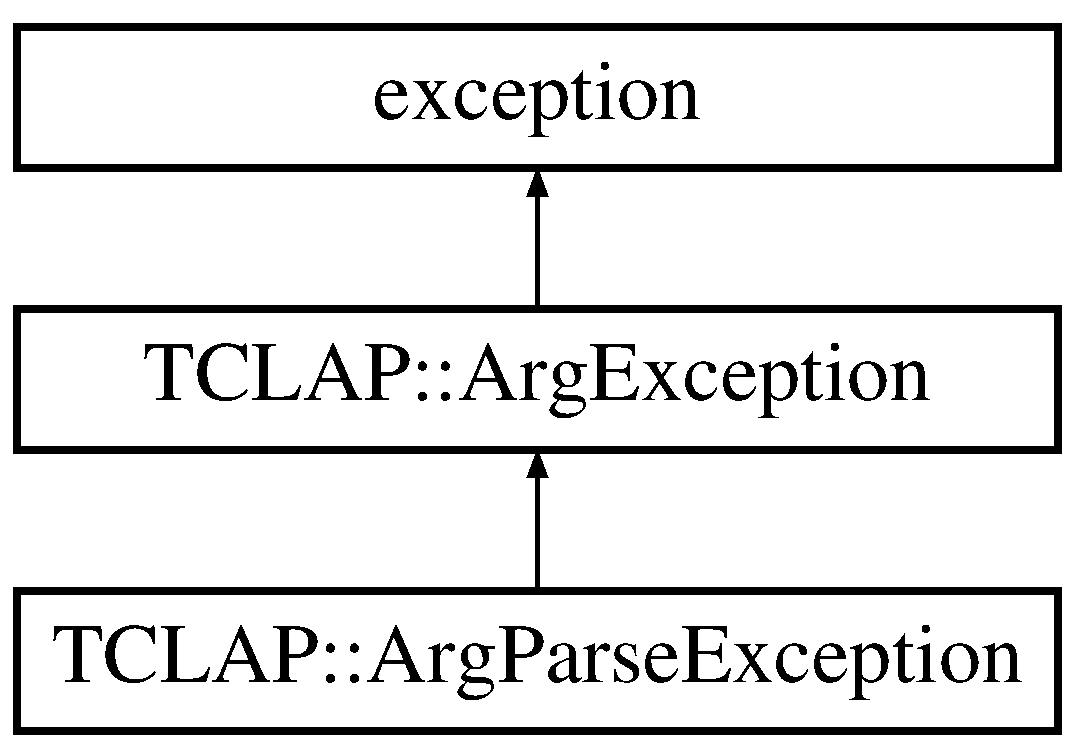
\includegraphics[height=3.000000cm]{classTCLAP_1_1ArgParseException}
\end{center}
\end{figure}
\subsection*{Public Member Functions}
\begin{DoxyCompactItemize}
\item 
{\bf Arg\+Parse\+Exception} (const std\+::string \&text=\char`\"{}undefined exception\char`\"{}, const std\+::string \&id=\char`\"{}undefined\char`\"{})
\begin{DoxyCompactList}\small\item\em Constructor. \end{DoxyCompactList}\end{DoxyCompactItemize}


\subsection{Detailed Description}
Thrown from within the child \doxyref{Arg}{p.}{classTCLAP_1_1Arg} classes when it fails to properly parse the argument it has been passed. 

Definition at line 121 of file Arg\+Exception.\+h.



\subsection{Constructor \& Destructor Documentation}
\index{T\+C\+L\+A\+P\+::\+Arg\+Parse\+Exception@{T\+C\+L\+A\+P\+::\+Arg\+Parse\+Exception}!Arg\+Parse\+Exception@{Arg\+Parse\+Exception}}
\index{Arg\+Parse\+Exception@{Arg\+Parse\+Exception}!T\+C\+L\+A\+P\+::\+Arg\+Parse\+Exception@{T\+C\+L\+A\+P\+::\+Arg\+Parse\+Exception}}
\subsubsection[{Arg\+Parse\+Exception}]{\setlength{\rightskip}{0pt plus 5cm}T\+C\+L\+A\+P\+::\+Arg\+Parse\+Exception\+::\+Arg\+Parse\+Exception (
\begin{DoxyParamCaption}
\item[{const std\+::string \&}]{text = {\ttfamily \char`\"{}undefined~exception\char`\"{}}, }
\item[{const std\+::string \&}]{id = {\ttfamily \char`\"{}undefined\char`\"{}}}
\end{DoxyParamCaption}
)\hspace{0.3cm}{\ttfamily [inline]}}\label{classTCLAP_1_1ArgParseException_aa9d9531405e505afd506491526733285}


Constructor. 


\begin{DoxyParams}{Parameters}
{\em text} & -\/ The text of the exception. \\
\hline
{\em id} & -\/ The text identifying the argument source of the exception. \\
\hline
\end{DoxyParams}


Definition at line 130 of file Arg\+Exception.\+h.


\begin{DoxyCode}
132       : ArgException( text, 
133                       \textcolor{keywordtype}{id}, 
134               std::string( \textcolor{stringliteral}{"Exception found while parsing "} ) + 
135               std::string( \textcolor{stringliteral}{"the value the Arg has been passed."} ))
136       \{ \}
\end{DoxyCode}


The documentation for this class was generated from the following file\+:\begin{DoxyCompactItemize}
\item 
{\bf Arg\+Exception.\+h}\end{DoxyCompactItemize}

\section{T\+C\+L\+A\+P\+:\+:Arg\+Traits$<$ T $>$ Struct Template Reference}
\label{structTCLAP_1_1ArgTraits}\index{T\+C\+L\+A\+P\+::\+Arg\+Traits$<$ T $>$@{T\+C\+L\+A\+P\+::\+Arg\+Traits$<$ T $>$}}


\doxyref{Arg}{p.}{classTCLAP_1_1Arg} traits are used to get compile type specialization when parsing argument values.  




{\ttfamily \#include $<$Arg\+Traits.\+h$>$}

\subsection*{Public Types}
\begin{DoxyCompactItemize}
\item 
typedef T\+::\+Value\+Category {\bf Value\+Category}
\end{DoxyCompactItemize}
\subsection*{Public Member Functions}
\begin{DoxyCompactItemize}
\item 
virtual {\bf $\sim$\+Arg\+Traits} ()
\end{DoxyCompactItemize}


\subsection{Detailed Description}
\subsubsection*{template$<$typename T$>$struct T\+C\+L\+A\+P\+::\+Arg\+Traits$<$ T $>$}

\doxyref{Arg}{p.}{classTCLAP_1_1Arg} traits are used to get compile type specialization when parsing argument values. 

Using an \doxyref{Arg\+Traits}{p.}{structTCLAP_1_1ArgTraits} you can specify the way that values gets assigned to any particular type during parsing. The two supported types are \doxyref{String\+Like}{p.}{structTCLAP_1_1StringLike} and \doxyref{Value\+Like}{p.}{structTCLAP_1_1ValueLike}. 

Definition at line 79 of file Arg\+Traits.\+h.



\subsection{Member Typedef Documentation}
\index{T\+C\+L\+A\+P\+::\+Arg\+Traits@{T\+C\+L\+A\+P\+::\+Arg\+Traits}!Value\+Category@{Value\+Category}}
\index{Value\+Category@{Value\+Category}!T\+C\+L\+A\+P\+::\+Arg\+Traits@{T\+C\+L\+A\+P\+::\+Arg\+Traits}}
\subsubsection[{Value\+Category}]{\setlength{\rightskip}{0pt plus 5cm}template$<$typename T$>$ typedef T\+::\+Value\+Category {\bf T\+C\+L\+A\+P\+::\+Arg\+Traits}$<$ T $>$\+::{\bf Value\+Category}}\label{structTCLAP_1_1ArgTraits_a346532973520fc820d6b3e5406dfa8f6}


Definition at line 80 of file Arg\+Traits.\+h.



\subsection{Constructor \& Destructor Documentation}
\index{T\+C\+L\+A\+P\+::\+Arg\+Traits@{T\+C\+L\+A\+P\+::\+Arg\+Traits}!````~Arg\+Traits@{$\sim$\+Arg\+Traits}}
\index{````~Arg\+Traits@{$\sim$\+Arg\+Traits}!T\+C\+L\+A\+P\+::\+Arg\+Traits@{T\+C\+L\+A\+P\+::\+Arg\+Traits}}
\subsubsection[{$\sim$\+Arg\+Traits}]{\setlength{\rightskip}{0pt plus 5cm}template$<$typename T$>$ virtual {\bf T\+C\+L\+A\+P\+::\+Arg\+Traits}$<$ T $>$\+::$\sim${\bf Arg\+Traits} (
\begin{DoxyParamCaption}
{}
\end{DoxyParamCaption}
)\hspace{0.3cm}{\ttfamily [inline]}, {\ttfamily [virtual]}}\label{structTCLAP_1_1ArgTraits_abbf8fe38dc8c0e0d179509cef1cf89e7}


Definition at line 81 of file Arg\+Traits.\+h.


\begin{DoxyCode}
81 \{\}
\end{DoxyCode}


The documentation for this struct was generated from the following file\+:\begin{DoxyCompactItemize}
\item 
{\bf Arg\+Traits.\+h}\end{DoxyCompactItemize}

\section{T\+C\+L\+A\+P\+:\+:Arg\+Traits$<$ bool $>$ Struct Template Reference}
\label{structTCLAP_1_1ArgTraits_3_01bool_01_4}\index{T\+C\+L\+A\+P\+::\+Arg\+Traits$<$ bool $>$@{T\+C\+L\+A\+P\+::\+Arg\+Traits$<$ bool $>$}}


bools have value-\/like semantics.  




{\ttfamily \#include $<$Standard\+Traits.\+h$>$}

\subsection*{Public Types}
\begin{DoxyCompactItemize}
\item 
typedef {\bf Value\+Like} {\bf Value\+Category}
\end{DoxyCompactItemize}


\subsection{Detailed Description}
\subsubsection*{template$<$$>$struct T\+C\+L\+A\+P\+::\+Arg\+Traits$<$ bool $>$}

bools have value-\/like semantics. 

Definition at line 176 of file Standard\+Traits.\+h.



\subsection{Member Typedef Documentation}
\index{T\+C\+L\+A\+P\+::\+Arg\+Traits$<$ bool $>$@{T\+C\+L\+A\+P\+::\+Arg\+Traits$<$ bool $>$}!Value\+Category@{Value\+Category}}
\index{Value\+Category@{Value\+Category}!T\+C\+L\+A\+P\+::\+Arg\+Traits$<$ bool $>$@{T\+C\+L\+A\+P\+::\+Arg\+Traits$<$ bool $>$}}
\subsubsection[{Value\+Category}]{\setlength{\rightskip}{0pt plus 5cm}typedef {\bf Value\+Like} {\bf T\+C\+L\+A\+P\+::\+Arg\+Traits}$<$ bool $>$\+::{\bf Value\+Category}}\label{structTCLAP_1_1ArgTraits_3_01bool_01_4_a86efe13e981aaef96d37ec465a8409a7}


Definition at line 177 of file Standard\+Traits.\+h.



The documentation for this struct was generated from the following file\+:\begin{DoxyCompactItemize}
\item 
{\bf Standard\+Traits.\+h}\end{DoxyCompactItemize}

\section{T\+C\+L\+A\+P\+:\+:Arg\+Traits$<$ char $>$ Struct Template Reference}
\label{structTCLAP_1_1ArgTraits_3_01char_01_4}\index{T\+C\+L\+A\+P\+::\+Arg\+Traits$<$ char $>$@{T\+C\+L\+A\+P\+::\+Arg\+Traits$<$ char $>$}}


chars have value-\/like semantics.  




{\ttfamily \#include $<$Standard\+Traits.\+h$>$}

\subsection*{Public Types}
\begin{DoxyCompactItemize}
\item 
typedef {\bf Value\+Like} {\bf Value\+Category}
\end{DoxyCompactItemize}


\subsection{Detailed Description}
\subsubsection*{template$<$$>$struct T\+C\+L\+A\+P\+::\+Arg\+Traits$<$ char $>$}

chars have value-\/like semantics. 

Definition at line 76 of file Standard\+Traits.\+h.



\subsection{Member Typedef Documentation}
\index{T\+C\+L\+A\+P\+::\+Arg\+Traits$<$ char $>$@{T\+C\+L\+A\+P\+::\+Arg\+Traits$<$ char $>$}!Value\+Category@{Value\+Category}}
\index{Value\+Category@{Value\+Category}!T\+C\+L\+A\+P\+::\+Arg\+Traits$<$ char $>$@{T\+C\+L\+A\+P\+::\+Arg\+Traits$<$ char $>$}}
\subsubsection[{Value\+Category}]{\setlength{\rightskip}{0pt plus 5cm}typedef {\bf Value\+Like} {\bf T\+C\+L\+A\+P\+::\+Arg\+Traits}$<$ char $>$\+::{\bf Value\+Category}}\label{structTCLAP_1_1ArgTraits_3_01char_01_4_a36f7fe1b3b1649ef8ec08ef7d6fc3160}


Definition at line 77 of file Standard\+Traits.\+h.



The documentation for this struct was generated from the following file\+:\begin{DoxyCompactItemize}
\item 
{\bf Standard\+Traits.\+h}\end{DoxyCompactItemize}

\section{T\+C\+L\+A\+P\+:\+:Arg\+Traits$<$ double $>$ Struct Template Reference}
\label{structTCLAP_1_1ArgTraits_3_01double_01_4}\index{T\+C\+L\+A\+P\+::\+Arg\+Traits$<$ double $>$@{T\+C\+L\+A\+P\+::\+Arg\+Traits$<$ double $>$}}


doubles have value-\/like semantics.  




{\ttfamily \#include $<$Standard\+Traits.\+h$>$}

\subsection*{Public Types}
\begin{DoxyCompactItemize}
\item 
typedef {\bf Value\+Like} {\bf Value\+Category}
\end{DoxyCompactItemize}


\subsection{Detailed Description}
\subsubsection*{template$<$$>$struct T\+C\+L\+A\+P\+::\+Arg\+Traits$<$ double $>$}

doubles have value-\/like semantics. 

Definition at line 164 of file Standard\+Traits.\+h.



\subsection{Member Typedef Documentation}
\index{T\+C\+L\+A\+P\+::\+Arg\+Traits$<$ double $>$@{T\+C\+L\+A\+P\+::\+Arg\+Traits$<$ double $>$}!Value\+Category@{Value\+Category}}
\index{Value\+Category@{Value\+Category}!T\+C\+L\+A\+P\+::\+Arg\+Traits$<$ double $>$@{T\+C\+L\+A\+P\+::\+Arg\+Traits$<$ double $>$}}
\subsubsection[{Value\+Category}]{\setlength{\rightskip}{0pt plus 5cm}typedef {\bf Value\+Like} {\bf T\+C\+L\+A\+P\+::\+Arg\+Traits}$<$ double $>$\+::{\bf Value\+Category}}\label{structTCLAP_1_1ArgTraits_3_01double_01_4_a06ac5f8ebfcbc537e9ce57b96836dd3d}


Definition at line 165 of file Standard\+Traits.\+h.



The documentation for this struct was generated from the following file\+:\begin{DoxyCompactItemize}
\item 
{\bf Standard\+Traits.\+h}\end{DoxyCompactItemize}

\section{T\+C\+L\+A\+P\+:\+:Arg\+Traits$<$ float $>$ Struct Template Reference}
\label{structTCLAP_1_1ArgTraits_3_01float_01_4}\index{T\+C\+L\+A\+P\+::\+Arg\+Traits$<$ float $>$@{T\+C\+L\+A\+P\+::\+Arg\+Traits$<$ float $>$}}


floats have value-\/like semantics.  




{\ttfamily \#include $<$Standard\+Traits.\+h$>$}

\subsection*{Public Types}
\begin{DoxyCompactItemize}
\item 
typedef {\bf Value\+Like} {\bf Value\+Category}
\end{DoxyCompactItemize}


\subsection{Detailed Description}
\subsubsection*{template$<$$>$struct T\+C\+L\+A\+P\+::\+Arg\+Traits$<$ float $>$}

floats have value-\/like semantics. 

Definition at line 156 of file Standard\+Traits.\+h.



\subsection{Member Typedef Documentation}
\index{T\+C\+L\+A\+P\+::\+Arg\+Traits$<$ float $>$@{T\+C\+L\+A\+P\+::\+Arg\+Traits$<$ float $>$}!Value\+Category@{Value\+Category}}
\index{Value\+Category@{Value\+Category}!T\+C\+L\+A\+P\+::\+Arg\+Traits$<$ float $>$@{T\+C\+L\+A\+P\+::\+Arg\+Traits$<$ float $>$}}
\subsubsection[{Value\+Category}]{\setlength{\rightskip}{0pt plus 5cm}typedef {\bf Value\+Like} {\bf T\+C\+L\+A\+P\+::\+Arg\+Traits}$<$ float $>$\+::{\bf Value\+Category}}\label{structTCLAP_1_1ArgTraits_3_01float_01_4_ace983d74b1b28caa692840da15313acf}


Definition at line 157 of file Standard\+Traits.\+h.



The documentation for this struct was generated from the following file\+:\begin{DoxyCompactItemize}
\item 
{\bf Standard\+Traits.\+h}\end{DoxyCompactItemize}

\section{T\+C\+L\+A\+P\+:\+:Arg\+Traits$<$ int $>$ Struct Template Reference}
\label{structTCLAP_1_1ArgTraits_3_01int_01_4}\index{T\+C\+L\+A\+P\+::\+Arg\+Traits$<$ int $>$@{T\+C\+L\+A\+P\+::\+Arg\+Traits$<$ int $>$}}


ints have value-\/like semantics.  




{\ttfamily \#include $<$Standard\+Traits.\+h$>$}

\subsection*{Public Types}
\begin{DoxyCompactItemize}
\item 
typedef {\bf Value\+Like} {\bf Value\+Category}
\end{DoxyCompactItemize}


\subsection{Detailed Description}
\subsubsection*{template$<$$>$struct T\+C\+L\+A\+P\+::\+Arg\+Traits$<$ int $>$}

ints have value-\/like semantics. 

Definition at line 60 of file Standard\+Traits.\+h.



\subsection{Member Typedef Documentation}
\index{T\+C\+L\+A\+P\+::\+Arg\+Traits$<$ int $>$@{T\+C\+L\+A\+P\+::\+Arg\+Traits$<$ int $>$}!Value\+Category@{Value\+Category}}
\index{Value\+Category@{Value\+Category}!T\+C\+L\+A\+P\+::\+Arg\+Traits$<$ int $>$@{T\+C\+L\+A\+P\+::\+Arg\+Traits$<$ int $>$}}
\subsubsection[{Value\+Category}]{\setlength{\rightskip}{0pt plus 5cm}typedef {\bf Value\+Like} {\bf T\+C\+L\+A\+P\+::\+Arg\+Traits}$<$ int $>$\+::{\bf Value\+Category}}\label{structTCLAP_1_1ArgTraits_3_01int_01_4_a8e577764b626e9e928d71567123d92a9}


Definition at line 61 of file Standard\+Traits.\+h.



The documentation for this struct was generated from the following file\+:\begin{DoxyCompactItemize}
\item 
{\bf Standard\+Traits.\+h}\end{DoxyCompactItemize}

\section{T\+C\+L\+A\+P\+:\+:Arg\+Traits$<$ long $>$ Struct Template Reference}
\label{structTCLAP_1_1ArgTraits_3_01long_01_4}\index{T\+C\+L\+A\+P\+::\+Arg\+Traits$<$ long $>$@{T\+C\+L\+A\+P\+::\+Arg\+Traits$<$ long $>$}}


longs have value-\/like semantics.  




{\ttfamily \#include $<$Standard\+Traits.\+h$>$}

\subsection*{Public Types}
\begin{DoxyCompactItemize}
\item 
typedef {\bf Value\+Like} {\bf Value\+Category}
\end{DoxyCompactItemize}


\subsection{Detailed Description}
\subsubsection*{template$<$$>$struct T\+C\+L\+A\+P\+::\+Arg\+Traits$<$ long $>$}

longs have value-\/like semantics. 

Definition at line 52 of file Standard\+Traits.\+h.



\subsection{Member Typedef Documentation}
\index{T\+C\+L\+A\+P\+::\+Arg\+Traits$<$ long $>$@{T\+C\+L\+A\+P\+::\+Arg\+Traits$<$ long $>$}!Value\+Category@{Value\+Category}}
\index{Value\+Category@{Value\+Category}!T\+C\+L\+A\+P\+::\+Arg\+Traits$<$ long $>$@{T\+C\+L\+A\+P\+::\+Arg\+Traits$<$ long $>$}}
\subsubsection[{Value\+Category}]{\setlength{\rightskip}{0pt plus 5cm}typedef {\bf Value\+Like} {\bf T\+C\+L\+A\+P\+::\+Arg\+Traits}$<$ long $>$\+::{\bf Value\+Category}}\label{structTCLAP_1_1ArgTraits_3_01long_01_4_a942d9a1e813bc3f82b51a2dcedb7316d}


Definition at line 53 of file Standard\+Traits.\+h.



The documentation for this struct was generated from the following file\+:\begin{DoxyCompactItemize}
\item 
{\bf Standard\+Traits.\+h}\end{DoxyCompactItemize}

\section{T\+C\+L\+A\+P\+:\+:Arg\+Traits$<$ short $>$ Struct Template Reference}
\label{structTCLAP_1_1ArgTraits_3_01short_01_4}\index{T\+C\+L\+A\+P\+::\+Arg\+Traits$<$ short $>$@{T\+C\+L\+A\+P\+::\+Arg\+Traits$<$ short $>$}}


shorts have value-\/like semantics.  




{\ttfamily \#include $<$Standard\+Traits.\+h$>$}

\subsection*{Public Types}
\begin{DoxyCompactItemize}
\item 
typedef {\bf Value\+Like} {\bf Value\+Category}
\end{DoxyCompactItemize}


\subsection{Detailed Description}
\subsubsection*{template$<$$>$struct T\+C\+L\+A\+P\+::\+Arg\+Traits$<$ short $>$}

shorts have value-\/like semantics. 

Definition at line 68 of file Standard\+Traits.\+h.



\subsection{Member Typedef Documentation}
\index{T\+C\+L\+A\+P\+::\+Arg\+Traits$<$ short $>$@{T\+C\+L\+A\+P\+::\+Arg\+Traits$<$ short $>$}!Value\+Category@{Value\+Category}}
\index{Value\+Category@{Value\+Category}!T\+C\+L\+A\+P\+::\+Arg\+Traits$<$ short $>$@{T\+C\+L\+A\+P\+::\+Arg\+Traits$<$ short $>$}}
\subsubsection[{Value\+Category}]{\setlength{\rightskip}{0pt plus 5cm}typedef {\bf Value\+Like} {\bf T\+C\+L\+A\+P\+::\+Arg\+Traits}$<$ short $>$\+::{\bf Value\+Category}}\label{structTCLAP_1_1ArgTraits_3_01short_01_4_a99f5d76501b120d6455b528aa7bf6896}


Definition at line 69 of file Standard\+Traits.\+h.



The documentation for this struct was generated from the following file\+:\begin{DoxyCompactItemize}
\item 
{\bf Standard\+Traits.\+h}\end{DoxyCompactItemize}

\section{T\+C\+L\+A\+P\+:\+:Arg\+Traits$<$ std\+:\+:string $>$ Struct Template Reference}
\label{structTCLAP_1_1ArgTraits_3_01std_1_1string_01_4}\index{T\+C\+L\+A\+P\+::\+Arg\+Traits$<$ std\+::string $>$@{T\+C\+L\+A\+P\+::\+Arg\+Traits$<$ std\+::string $>$}}


Strings have string like argument traits.  




{\ttfamily \#include $<$Standard\+Traits.\+h$>$}

\subsection*{Public Types}
\begin{DoxyCompactItemize}
\item 
typedef {\bf String\+Like} {\bf Value\+Category}
\end{DoxyCompactItemize}


\subsection{Detailed Description}
\subsubsection*{template$<$$>$struct T\+C\+L\+A\+P\+::\+Arg\+Traits$<$ std\+::string $>$}

Strings have string like argument traits. 

Definition at line 195 of file Standard\+Traits.\+h.



\subsection{Member Typedef Documentation}
\index{T\+C\+L\+A\+P\+::\+Arg\+Traits$<$ std\+::string $>$@{T\+C\+L\+A\+P\+::\+Arg\+Traits$<$ std\+::string $>$}!Value\+Category@{Value\+Category}}
\index{Value\+Category@{Value\+Category}!T\+C\+L\+A\+P\+::\+Arg\+Traits$<$ std\+::string $>$@{T\+C\+L\+A\+P\+::\+Arg\+Traits$<$ std\+::string $>$}}
\subsubsection[{Value\+Category}]{\setlength{\rightskip}{0pt plus 5cm}typedef {\bf String\+Like} {\bf T\+C\+L\+A\+P\+::\+Arg\+Traits}$<$ std\+::string $>$\+::{\bf Value\+Category}}\label{structTCLAP_1_1ArgTraits_3_01std_1_1string_01_4_a719adeb18786516dd4b2a16525cf4536}


Definition at line 196 of file Standard\+Traits.\+h.



The documentation for this struct was generated from the following file\+:\begin{DoxyCompactItemize}
\item 
{\bf Standard\+Traits.\+h}\end{DoxyCompactItemize}

\section{T\+C\+L\+A\+P\+:\+:Arg\+Traits$<$ unsigned char $>$ Struct Template Reference}
\label{structTCLAP_1_1ArgTraits_3_01unsigned_01char_01_4}\index{T\+C\+L\+A\+P\+::\+Arg\+Traits$<$ unsigned char $>$@{T\+C\+L\+A\+P\+::\+Arg\+Traits$<$ unsigned char $>$}}


unsigned chars have value-\/like semantics.  




{\ttfamily \#include $<$Standard\+Traits.\+h$>$}

\subsection*{Public Types}
\begin{DoxyCompactItemize}
\item 
typedef {\bf Value\+Like} {\bf Value\+Category}
\end{DoxyCompactItemize}


\subsection{Detailed Description}
\subsubsection*{template$<$$>$struct T\+C\+L\+A\+P\+::\+Arg\+Traits$<$ unsigned char $>$}

unsigned chars have value-\/like semantics. 

Definition at line 122 of file Standard\+Traits.\+h.



\subsection{Member Typedef Documentation}
\index{T\+C\+L\+A\+P\+::\+Arg\+Traits$<$ unsigned char $>$@{T\+C\+L\+A\+P\+::\+Arg\+Traits$<$ unsigned char $>$}!Value\+Category@{Value\+Category}}
\index{Value\+Category@{Value\+Category}!T\+C\+L\+A\+P\+::\+Arg\+Traits$<$ unsigned char $>$@{T\+C\+L\+A\+P\+::\+Arg\+Traits$<$ unsigned char $>$}}
\subsubsection[{Value\+Category}]{\setlength{\rightskip}{0pt plus 5cm}typedef {\bf Value\+Like} {\bf T\+C\+L\+A\+P\+::\+Arg\+Traits}$<$ unsigned char $>$\+::{\bf Value\+Category}}\label{structTCLAP_1_1ArgTraits_3_01unsigned_01char_01_4_a3cba1e41ab04d31c7b68b1c5e6e227aa}


Definition at line 123 of file Standard\+Traits.\+h.



The documentation for this struct was generated from the following file\+:\begin{DoxyCompactItemize}
\item 
{\bf Standard\+Traits.\+h}\end{DoxyCompactItemize}

\section{T\+C\+L\+A\+P\+:\+:Arg\+Traits$<$ unsigned int $>$ Struct Template Reference}
\label{structTCLAP_1_1ArgTraits_3_01unsigned_01int_01_4}\index{T\+C\+L\+A\+P\+::\+Arg\+Traits$<$ unsigned int $>$@{T\+C\+L\+A\+P\+::\+Arg\+Traits$<$ unsigned int $>$}}


unsigned ints have value-\/like semantics.  




{\ttfamily \#include $<$Standard\+Traits.\+h$>$}

\subsection*{Public Types}
\begin{DoxyCompactItemize}
\item 
typedef {\bf Value\+Like} {\bf Value\+Category}
\end{DoxyCompactItemize}


\subsection{Detailed Description}
\subsubsection*{template$<$$>$struct T\+C\+L\+A\+P\+::\+Arg\+Traits$<$ unsigned int $>$}

unsigned ints have value-\/like semantics. 

Definition at line 106 of file Standard\+Traits.\+h.



\subsection{Member Typedef Documentation}
\index{T\+C\+L\+A\+P\+::\+Arg\+Traits$<$ unsigned int $>$@{T\+C\+L\+A\+P\+::\+Arg\+Traits$<$ unsigned int $>$}!Value\+Category@{Value\+Category}}
\index{Value\+Category@{Value\+Category}!T\+C\+L\+A\+P\+::\+Arg\+Traits$<$ unsigned int $>$@{T\+C\+L\+A\+P\+::\+Arg\+Traits$<$ unsigned int $>$}}
\subsubsection[{Value\+Category}]{\setlength{\rightskip}{0pt plus 5cm}typedef {\bf Value\+Like} {\bf T\+C\+L\+A\+P\+::\+Arg\+Traits}$<$ unsigned int $>$\+::{\bf Value\+Category}}\label{structTCLAP_1_1ArgTraits_3_01unsigned_01int_01_4_ae95cdc132665581c458fc64c7e7a0490}


Definition at line 107 of file Standard\+Traits.\+h.



The documentation for this struct was generated from the following file\+:\begin{DoxyCompactItemize}
\item 
{\bf Standard\+Traits.\+h}\end{DoxyCompactItemize}

\section{T\+C\+L\+A\+P\+:\+:Arg\+Traits$<$ unsigned long $>$ Struct Template Reference}
\label{structTCLAP_1_1ArgTraits_3_01unsigned_01long_01_4}\index{T\+C\+L\+A\+P\+::\+Arg\+Traits$<$ unsigned long $>$@{T\+C\+L\+A\+P\+::\+Arg\+Traits$<$ unsigned long $>$}}


unsigned longs have value-\/like semantics.  




{\ttfamily \#include $<$Standard\+Traits.\+h$>$}

\subsection*{Public Types}
\begin{DoxyCompactItemize}
\item 
typedef {\bf Value\+Like} {\bf Value\+Category}
\end{DoxyCompactItemize}


\subsection{Detailed Description}
\subsubsection*{template$<$$>$struct T\+C\+L\+A\+P\+::\+Arg\+Traits$<$ unsigned long $>$}

unsigned longs have value-\/like semantics. 

Definition at line 98 of file Standard\+Traits.\+h.



\subsection{Member Typedef Documentation}
\index{T\+C\+L\+A\+P\+::\+Arg\+Traits$<$ unsigned long $>$@{T\+C\+L\+A\+P\+::\+Arg\+Traits$<$ unsigned long $>$}!Value\+Category@{Value\+Category}}
\index{Value\+Category@{Value\+Category}!T\+C\+L\+A\+P\+::\+Arg\+Traits$<$ unsigned long $>$@{T\+C\+L\+A\+P\+::\+Arg\+Traits$<$ unsigned long $>$}}
\subsubsection[{Value\+Category}]{\setlength{\rightskip}{0pt plus 5cm}typedef {\bf Value\+Like} {\bf T\+C\+L\+A\+P\+::\+Arg\+Traits}$<$ unsigned long $>$\+::{\bf Value\+Category}}\label{structTCLAP_1_1ArgTraits_3_01unsigned_01long_01_4_aa6aeb6243e6fbf8b5aba659083baa1ac}


Definition at line 99 of file Standard\+Traits.\+h.



The documentation for this struct was generated from the following file\+:\begin{DoxyCompactItemize}
\item 
{\bf Standard\+Traits.\+h}\end{DoxyCompactItemize}

\section{T\+C\+L\+A\+P\+:\+:Arg\+Traits$<$ unsigned short $>$ Struct Template Reference}
\label{structTCLAP_1_1ArgTraits_3_01unsigned_01short_01_4}\index{T\+C\+L\+A\+P\+::\+Arg\+Traits$<$ unsigned short $>$@{T\+C\+L\+A\+P\+::\+Arg\+Traits$<$ unsigned short $>$}}


unsigned shorts have value-\/like semantics.  




{\ttfamily \#include $<$Standard\+Traits.\+h$>$}

\subsection*{Public Types}
\begin{DoxyCompactItemize}
\item 
typedef {\bf Value\+Like} {\bf Value\+Category}
\end{DoxyCompactItemize}


\subsection{Detailed Description}
\subsubsection*{template$<$$>$struct T\+C\+L\+A\+P\+::\+Arg\+Traits$<$ unsigned short $>$}

unsigned shorts have value-\/like semantics. 

Definition at line 114 of file Standard\+Traits.\+h.



\subsection{Member Typedef Documentation}
\index{T\+C\+L\+A\+P\+::\+Arg\+Traits$<$ unsigned short $>$@{T\+C\+L\+A\+P\+::\+Arg\+Traits$<$ unsigned short $>$}!Value\+Category@{Value\+Category}}
\index{Value\+Category@{Value\+Category}!T\+C\+L\+A\+P\+::\+Arg\+Traits$<$ unsigned short $>$@{T\+C\+L\+A\+P\+::\+Arg\+Traits$<$ unsigned short $>$}}
\subsubsection[{Value\+Category}]{\setlength{\rightskip}{0pt plus 5cm}typedef {\bf Value\+Like} {\bf T\+C\+L\+A\+P\+::\+Arg\+Traits}$<$ unsigned short $>$\+::{\bf Value\+Category}}\label{structTCLAP_1_1ArgTraits_3_01unsigned_01short_01_4_a0efa2ce53e9cb98dc4a58dda24127d3a}


Definition at line 115 of file Standard\+Traits.\+h.



The documentation for this struct was generated from the following file\+:\begin{DoxyCompactItemize}
\item 
{\bf Standard\+Traits.\+h}\end{DoxyCompactItemize}

\section{T\+C\+L\+A\+P\+:\+:Arg\+Traits$<$ wchar\+\_\+t $>$ Struct Template Reference}
\label{structTCLAP_1_1ArgTraits_3_01wchar__t_01_4}\index{T\+C\+L\+A\+P\+::\+Arg\+Traits$<$ wchar\+\_\+t $>$@{T\+C\+L\+A\+P\+::\+Arg\+Traits$<$ wchar\+\_\+t $>$}}


wchar\+\_\+ts have value-\/like semantics.  




{\ttfamily \#include $<$Standard\+Traits.\+h$>$}

\subsection*{Public Types}
\begin{DoxyCompactItemize}
\item 
typedef {\bf Value\+Like} {\bf Value\+Category}
\end{DoxyCompactItemize}


\subsection{Detailed Description}
\subsubsection*{template$<$$>$struct T\+C\+L\+A\+P\+::\+Arg\+Traits$<$ wchar\+\_\+t $>$}

wchar\+\_\+ts have value-\/like semantics. 

Definition at line 186 of file Standard\+Traits.\+h.



\subsection{Member Typedef Documentation}
\index{T\+C\+L\+A\+P\+::\+Arg\+Traits$<$ wchar\+\_\+t $>$@{T\+C\+L\+A\+P\+::\+Arg\+Traits$<$ wchar\+\_\+t $>$}!Value\+Category@{Value\+Category}}
\index{Value\+Category@{Value\+Category}!T\+C\+L\+A\+P\+::\+Arg\+Traits$<$ wchar\+\_\+t $>$@{T\+C\+L\+A\+P\+::\+Arg\+Traits$<$ wchar\+\_\+t $>$}}
\subsubsection[{Value\+Category}]{\setlength{\rightskip}{0pt plus 5cm}typedef {\bf Value\+Like} {\bf T\+C\+L\+A\+P\+::\+Arg\+Traits}$<$ wchar\+\_\+t $>$\+::{\bf Value\+Category}}\label{structTCLAP_1_1ArgTraits_3_01wchar__t_01_4_a49a311297a394637af4d8d64eda7f442}


Definition at line 187 of file Standard\+Traits.\+h.



The documentation for this struct was generated from the following file\+:\begin{DoxyCompactItemize}
\item 
{\bf Standard\+Traits.\+h}\end{DoxyCompactItemize}

\section{dqm4hep\+:\+:Bigger\+Than\+Validator$<$ T $>$ Class Template Reference}
\label{classdqm4hep_1_1BiggerThanValidator}\index{dqm4hep\+::\+Bigger\+Than\+Validator$<$ T $>$@{dqm4hep\+::\+Bigger\+Than\+Validator$<$ T $>$}}


{\ttfamily \#include $<$D\+Q\+M4\+H\+E\+P.\+h$>$}

\subsection*{Public Member Functions}
\begin{DoxyCompactItemize}
\item 
{\bf Bigger\+Than\+Validator} (const T \&compare)
\item 
bool {\bf operator()} (const T \&t) const 
\end{DoxyCompactItemize}
\subsection*{Private Attributes}
\begin{DoxyCompactItemize}
\item 
T {\bf m\+\_\+compare}
\end{DoxyCompactItemize}


\subsection{Detailed Description}
\subsubsection*{template$<$typename T$>$class dqm4hep\+::\+Bigger\+Than\+Validator$<$ T $>$}



Definition at line 624 of file D\+Q\+M4\+H\+E\+P.\+h.



\subsection{Constructor \& Destructor Documentation}
\index{dqm4hep\+::\+Bigger\+Than\+Validator@{dqm4hep\+::\+Bigger\+Than\+Validator}!Bigger\+Than\+Validator@{Bigger\+Than\+Validator}}
\index{Bigger\+Than\+Validator@{Bigger\+Than\+Validator}!dqm4hep\+::\+Bigger\+Than\+Validator@{dqm4hep\+::\+Bigger\+Than\+Validator}}
\subsubsection[{Bigger\+Than\+Validator}]{\setlength{\rightskip}{0pt plus 5cm}template$<$typename T $>$ {\bf dqm4hep\+::\+Bigger\+Than\+Validator}$<$ T $>$\+::{\bf Bigger\+Than\+Validator} (
\begin{DoxyParamCaption}
\item[{const T \&}]{compare}
\end{DoxyParamCaption}
)\hspace{0.3cm}{\ttfamily [inline]}}\label{classdqm4hep_1_1BiggerThanValidator_a47ebc0956b24fdbc740bf99aae1f5d91}


Definition at line 627 of file D\+Q\+M4\+H\+E\+P.\+h.


\begin{DoxyCode}
627 : m_compare(compare) \{\}
\end{DoxyCode}


\subsection{Member Function Documentation}
\index{dqm4hep\+::\+Bigger\+Than\+Validator@{dqm4hep\+::\+Bigger\+Than\+Validator}!operator()@{operator()}}
\index{operator()@{operator()}!dqm4hep\+::\+Bigger\+Than\+Validator@{dqm4hep\+::\+Bigger\+Than\+Validator}}
\subsubsection[{operator()}]{\setlength{\rightskip}{0pt plus 5cm}template$<$typename T $>$ bool {\bf dqm4hep\+::\+Bigger\+Than\+Validator}$<$ T $>$\+::operator() (
\begin{DoxyParamCaption}
\item[{const T \&}]{t}
\end{DoxyParamCaption}
) const\hspace{0.3cm}{\ttfamily [inline]}}\label{classdqm4hep_1_1BiggerThanValidator_a2202f149c460bc5384d5792e9ea083e5}


Definition at line 629 of file D\+Q\+M4\+H\+E\+P.\+h.



References dqm4hep\+::\+Bigger\+Than\+Validator$<$ T $>$\+::m\+\_\+compare.


\begin{DoxyCode}
629 \{ \textcolor{keywordflow}{return} t>m_compare; \}
\end{DoxyCode}


\subsection{Member Data Documentation}
\index{dqm4hep\+::\+Bigger\+Than\+Validator@{dqm4hep\+::\+Bigger\+Than\+Validator}!m\+\_\+compare@{m\+\_\+compare}}
\index{m\+\_\+compare@{m\+\_\+compare}!dqm4hep\+::\+Bigger\+Than\+Validator@{dqm4hep\+::\+Bigger\+Than\+Validator}}
\subsubsection[{m\+\_\+compare}]{\setlength{\rightskip}{0pt plus 5cm}template$<$typename T $>$ T {\bf dqm4hep\+::\+Bigger\+Than\+Validator}$<$ T $>$\+::m\+\_\+compare\hspace{0.3cm}{\ttfamily [private]}}\label{classdqm4hep_1_1BiggerThanValidator_a7e59d73826d3989acffd0bd80e683d14}


Definition at line 631 of file D\+Q\+M4\+H\+E\+P.\+h.



Referenced by dqm4hep\+::\+Bigger\+Than\+Validator$<$ T $>$\+::operator()().



The documentation for this class was generated from the following file\+:\begin{DoxyCompactItemize}
\item 
{\bf D\+Q\+M4\+H\+E\+P.\+h}\end{DoxyCompactItemize}

\section{dqm4hep\+:\+:D\+Q\+M\+Dim\+Event\+Collector\+:\+:Client Class Reference}
\label{classdqm4hep_1_1DQMDimEventCollector_1_1Client}\index{dqm4hep\+::\+D\+Q\+M\+Dim\+Event\+Collector\+::\+Client@{dqm4hep\+::\+D\+Q\+M\+Dim\+Event\+Collector\+::\+Client}}


\doxyref{Client}{p.}{classdqm4hep_1_1DQMDimEventCollector_1_1Client} class.  


\subsection*{Public Attributes}
\begin{DoxyCompactItemize}
\item 
int {\bf m\+\_\+client\+Id}
\begin{DoxyCompactList}\small\item\em The client id (dim client id) \end{DoxyCompactList}\item 
bool {\bf m\+\_\+update\+Mode}
\begin{DoxyCompactList}\small\item\em Whether the client uses an update mode. \end{DoxyCompactList}\item 
std\+::string {\bf m\+\_\+sub\+Event\+Identifier}
\begin{DoxyCompactList}\small\item\em The sub event identifier received from the client from. \end{DoxyCompactList}\end{DoxyCompactItemize}


\subsection{Detailed Description}
\doxyref{Client}{p.}{classdqm4hep_1_1DQMDimEventCollector_1_1Client} class. 

Represent a client instance from the point of view of the service (id and update booleans) 

Definition at line 122 of file D\+Q\+M\+Dim\+Event\+Collector.\+h.



\subsection{Member Data Documentation}
\index{dqm4hep\+::\+D\+Q\+M\+Dim\+Event\+Collector\+::\+Client@{dqm4hep\+::\+D\+Q\+M\+Dim\+Event\+Collector\+::\+Client}!m\+\_\+client\+Id@{m\+\_\+client\+Id}}
\index{m\+\_\+client\+Id@{m\+\_\+client\+Id}!dqm4hep\+::\+D\+Q\+M\+Dim\+Event\+Collector\+::\+Client@{dqm4hep\+::\+D\+Q\+M\+Dim\+Event\+Collector\+::\+Client}}
\subsubsection[{m\+\_\+client\+Id}]{\setlength{\rightskip}{0pt plus 5cm}int dqm4hep\+::\+D\+Q\+M\+Dim\+Event\+Collector\+::\+Client\+::m\+\_\+client\+Id}\label{classdqm4hep_1_1DQMDimEventCollector_1_1Client_a1df5c1edfc23261eea17b130424b7187}


The client id (dim client id) 



Definition at line 125 of file D\+Q\+M\+Dim\+Event\+Collector.\+h.



Referenced by dqm4hep\+::\+D\+Q\+M\+Dim\+Event\+Collector\+::get\+Client().

\index{dqm4hep\+::\+D\+Q\+M\+Dim\+Event\+Collector\+::\+Client@{dqm4hep\+::\+D\+Q\+M\+Dim\+Event\+Collector\+::\+Client}!m\+\_\+sub\+Event\+Identifier@{m\+\_\+sub\+Event\+Identifier}}
\index{m\+\_\+sub\+Event\+Identifier@{m\+\_\+sub\+Event\+Identifier}!dqm4hep\+::\+D\+Q\+M\+Dim\+Event\+Collector\+::\+Client@{dqm4hep\+::\+D\+Q\+M\+Dim\+Event\+Collector\+::\+Client}}
\subsubsection[{m\+\_\+sub\+Event\+Identifier}]{\setlength{\rightskip}{0pt plus 5cm}std\+::string dqm4hep\+::\+D\+Q\+M\+Dim\+Event\+Collector\+::\+Client\+::m\+\_\+sub\+Event\+Identifier}\label{classdqm4hep_1_1DQMDimEventCollector_1_1Client_ad086b42cf088bb88fcacafd0ee69ca26}


The sub event identifier received from the client from. 



Definition at line 127 of file D\+Q\+M\+Dim\+Event\+Collector.\+h.



Referenced by dqm4hep\+::\+D\+Q\+M\+Dim\+Event\+Collector\+::command\+Handler().

\index{dqm4hep\+::\+D\+Q\+M\+Dim\+Event\+Collector\+::\+Client@{dqm4hep\+::\+D\+Q\+M\+Dim\+Event\+Collector\+::\+Client}!m\+\_\+update\+Mode@{m\+\_\+update\+Mode}}
\index{m\+\_\+update\+Mode@{m\+\_\+update\+Mode}!dqm4hep\+::\+D\+Q\+M\+Dim\+Event\+Collector\+::\+Client@{dqm4hep\+::\+D\+Q\+M\+Dim\+Event\+Collector\+::\+Client}}
\subsubsection[{m\+\_\+update\+Mode}]{\setlength{\rightskip}{0pt plus 5cm}bool dqm4hep\+::\+D\+Q\+M\+Dim\+Event\+Collector\+::\+Client\+::m\+\_\+update\+Mode}\label{classdqm4hep_1_1DQMDimEventCollector_1_1Client_adee2c7f2464b082f155d3461fdabc82b}


Whether the client uses an update mode. 



Definition at line 126 of file D\+Q\+M\+Dim\+Event\+Collector.\+h.



Referenced by dqm4hep\+::\+D\+Q\+M\+Dim\+Event\+Collector\+::command\+Handler().



The documentation for this class was generated from the following file\+:\begin{DoxyCompactItemize}
\item 
{\bf D\+Q\+M\+Dim\+Event\+Collector.\+h}\end{DoxyCompactItemize}

\section{dqm4hep\+:\+:Client\+Info Class Reference}
\label{classdqm4hep_1_1ClientInfo}\index{dqm4hep\+::\+Client\+Info@{dqm4hep\+::\+Client\+Info}}


\doxyref{Client\+Info}{p.}{classdqm4hep_1_1ClientInfo} class.  




{\ttfamily \#include $<$D\+Q\+M\+Monitor\+Element\+Collector.\+h$>$}

\subsection*{Public Member Functions}
\begin{DoxyCompactItemize}
\item 
{\bf Client\+Info} (int client\+I\+D)
\begin{DoxyCompactList}\small\item\em Constructor for monitor element clients. \end{DoxyCompactList}\item 
{\bf Client\+Info} (int client\+Id, const std\+::string \&module\+Name)
\begin{DoxyCompactList}\small\item\em Constructor for module clients. \end{DoxyCompactList}\item 
const std\+::string \& {\bf get\+Module\+Name} () const 
\begin{DoxyCompactList}\small\item\em Get the module name. \end{DoxyCompactList}\item 
bool {\bf is\+Module} () const 
\begin{DoxyCompactList}\small\item\em Whether the client is a module. \end{DoxyCompactList}\item 
int {\bf get\+Client\+I\+D} () const 
\begin{DoxyCompactList}\small\item\em Get the client id. \end{DoxyCompactList}\item 
void {\bf set\+Update\+Mode} (bool update)
\begin{DoxyCompactList}\small\item\em Set update mode (default is false) \end{DoxyCompactList}\item 
bool {\bf has\+Update\+Mode} () const 
\begin{DoxyCompactList}\small\item\em Whether the client works in update mode. \end{DoxyCompactList}\end{DoxyCompactItemize}
\subsection*{Private Attributes}
\begin{DoxyCompactItemize}
\item 
int {\bf m\+\_\+client\+I\+D}
\item 
bool {\bf m\+\_\+update\+Mode}
\item 
bool {\bf m\+\_\+is\+Module}
\item 
std\+::string {\bf m\+\_\+module\+Name}
\end{DoxyCompactItemize}


\subsection{Detailed Description}
\doxyref{Client\+Info}{p.}{classdqm4hep_1_1ClientInfo} class. 

Definition at line 144 of file D\+Q\+M\+Monitor\+Element\+Collector.\+h.



\subsection{Constructor \& Destructor Documentation}
\index{dqm4hep\+::\+Client\+Info@{dqm4hep\+::\+Client\+Info}!Client\+Info@{Client\+Info}}
\index{Client\+Info@{Client\+Info}!dqm4hep\+::\+Client\+Info@{dqm4hep\+::\+Client\+Info}}
\subsubsection[{Client\+Info}]{\setlength{\rightskip}{0pt plus 5cm}dqm4hep\+::\+Client\+Info\+::\+Client\+Info (
\begin{DoxyParamCaption}
\item[{int}]{client\+I\+D}
\end{DoxyParamCaption}
)}\label{classdqm4hep_1_1ClientInfo_a8d46ab14701ac0378d709cbc6d47455b}


Constructor for monitor element clients. 

Constructor. 

Definition at line 327 of file D\+Q\+M\+Monitor\+Element\+Collector.\+cc.


\begin{DoxyCode}
327                                    :
328     m_clientID(clientID),
329     m_updateMode(\textcolor{keyword}{false}),
330     m_isModule(\textcolor{keyword}{false}),
331     m_moduleName(\textcolor{stringliteral}{""})
332 \{
333   \textcolor{comment}{/* nop */}
334 \}
\end{DoxyCode}
\index{dqm4hep\+::\+Client\+Info@{dqm4hep\+::\+Client\+Info}!Client\+Info@{Client\+Info}}
\index{Client\+Info@{Client\+Info}!dqm4hep\+::\+Client\+Info@{dqm4hep\+::\+Client\+Info}}
\subsubsection[{Client\+Info}]{\setlength{\rightskip}{0pt plus 5cm}dqm4hep\+::\+Client\+Info\+::\+Client\+Info (
\begin{DoxyParamCaption}
\item[{int}]{client\+Id, }
\item[{const std\+::string \&}]{module\+Name}
\end{DoxyParamCaption}
)}\label{classdqm4hep_1_1ClientInfo_a802c05b963ba359b16c01a7cd411e00e}


Constructor for module clients. 



Definition at line 338 of file D\+Q\+M\+Monitor\+Element\+Collector.\+cc.


\begin{DoxyCode}
338                                                                 :
339     m_clientID(clientId),
340     m_updateMode(\textcolor{keyword}{false}),
341     m_isModule(\textcolor{keyword}{true}),
342     m_moduleName(moduleName)
343 \{
344   \textcolor{comment}{/* nop */}
345 \}
\end{DoxyCode}


\subsection{Member Function Documentation}
\index{dqm4hep\+::\+Client\+Info@{dqm4hep\+::\+Client\+Info}!get\+Client\+I\+D@{get\+Client\+I\+D}}
\index{get\+Client\+I\+D@{get\+Client\+I\+D}!dqm4hep\+::\+Client\+Info@{dqm4hep\+::\+Client\+Info}}
\subsubsection[{get\+Client\+I\+D}]{\setlength{\rightskip}{0pt plus 5cm}int dqm4hep\+::\+Client\+Info\+::get\+Client\+I\+D (
\begin{DoxyParamCaption}
{}
\end{DoxyParamCaption}
) const}\label{classdqm4hep_1_1ClientInfo_affc0ae408bfb40ab0388ac4a599ec02b}


Get the client id. 



Definition at line 363 of file D\+Q\+M\+Monitor\+Element\+Collector.\+cc.



References m\+\_\+client\+I\+D.


\begin{DoxyCode}
364 \{
365   \textcolor{keywordflow}{return} m_clientID;
366 \}
\end{DoxyCode}
\index{dqm4hep\+::\+Client\+Info@{dqm4hep\+::\+Client\+Info}!get\+Module\+Name@{get\+Module\+Name}}
\index{get\+Module\+Name@{get\+Module\+Name}!dqm4hep\+::\+Client\+Info@{dqm4hep\+::\+Client\+Info}}
\subsubsection[{get\+Module\+Name}]{\setlength{\rightskip}{0pt plus 5cm}const std\+::string \& dqm4hep\+::\+Client\+Info\+::get\+Module\+Name (
\begin{DoxyParamCaption}
{}
\end{DoxyParamCaption}
) const}\label{classdqm4hep_1_1ClientInfo_a8372636b42f0ac056a9b5cc43cb32705}


Get the module name. 

Valid only if the client is a module. 

Definition at line 349 of file D\+Q\+M\+Monitor\+Element\+Collector.\+cc.



References m\+\_\+module\+Name.


\begin{DoxyCode}
350 \{
351   \textcolor{keywordflow}{return} m_moduleName;
352 \}
\end{DoxyCode}
\index{dqm4hep\+::\+Client\+Info@{dqm4hep\+::\+Client\+Info}!has\+Update\+Mode@{has\+Update\+Mode}}
\index{has\+Update\+Mode@{has\+Update\+Mode}!dqm4hep\+::\+Client\+Info@{dqm4hep\+::\+Client\+Info}}
\subsubsection[{has\+Update\+Mode}]{\setlength{\rightskip}{0pt plus 5cm}bool dqm4hep\+::\+Client\+Info\+::has\+Update\+Mode (
\begin{DoxyParamCaption}
{}
\end{DoxyParamCaption}
) const}\label{classdqm4hep_1_1ClientInfo_a90e92025428d87964759e7d147379e7c}


Whether the client works in update mode. 



Definition at line 377 of file D\+Q\+M\+Monitor\+Element\+Collector.\+cc.



References m\+\_\+update\+Mode.


\begin{DoxyCode}
378 \{
379   \textcolor{keywordflow}{return} m_updateMode;
380 \}
\end{DoxyCode}
\index{dqm4hep\+::\+Client\+Info@{dqm4hep\+::\+Client\+Info}!is\+Module@{is\+Module}}
\index{is\+Module@{is\+Module}!dqm4hep\+::\+Client\+Info@{dqm4hep\+::\+Client\+Info}}
\subsubsection[{is\+Module}]{\setlength{\rightskip}{0pt plus 5cm}bool dqm4hep\+::\+Client\+Info\+::is\+Module (
\begin{DoxyParamCaption}
{}
\end{DoxyParamCaption}
) const}\label{classdqm4hep_1_1ClientInfo_acc4a5c95870c9d0b6014ad8bba6465bb}


Whether the client is a module. 

Opposite is a monitor element client 

Definition at line 356 of file D\+Q\+M\+Monitor\+Element\+Collector.\+cc.



References m\+\_\+is\+Module.


\begin{DoxyCode}
357 \{
358   \textcolor{keywordflow}{return} m_isModule;
359 \}
\end{DoxyCode}
\index{dqm4hep\+::\+Client\+Info@{dqm4hep\+::\+Client\+Info}!set\+Update\+Mode@{set\+Update\+Mode}}
\index{set\+Update\+Mode@{set\+Update\+Mode}!dqm4hep\+::\+Client\+Info@{dqm4hep\+::\+Client\+Info}}
\subsubsection[{set\+Update\+Mode}]{\setlength{\rightskip}{0pt plus 5cm}void dqm4hep\+::\+Client\+Info\+::set\+Update\+Mode (
\begin{DoxyParamCaption}
\item[{bool}]{update}
\end{DoxyParamCaption}
)}\label{classdqm4hep_1_1ClientInfo_ab9056fb1c9dceb78b4dad2cc6e5fb866}


Set update mode (default is false) 



Definition at line 370 of file D\+Q\+M\+Monitor\+Element\+Collector.\+cc.



References m\+\_\+update\+Mode.


\begin{DoxyCode}
371 \{
372   m_updateMode = update;
373 \}
\end{DoxyCode}


\subsection{Member Data Documentation}
\index{dqm4hep\+::\+Client\+Info@{dqm4hep\+::\+Client\+Info}!m\+\_\+client\+I\+D@{m\+\_\+client\+I\+D}}
\index{m\+\_\+client\+I\+D@{m\+\_\+client\+I\+D}!dqm4hep\+::\+Client\+Info@{dqm4hep\+::\+Client\+Info}}
\subsubsection[{m\+\_\+client\+I\+D}]{\setlength{\rightskip}{0pt plus 5cm}int dqm4hep\+::\+Client\+Info\+::m\+\_\+client\+I\+D\hspace{0.3cm}{\ttfamily [private]}}\label{classdqm4hep_1_1ClientInfo_add717915fc5c80a37c5300ef9e659926}


Definition at line 178 of file D\+Q\+M\+Monitor\+Element\+Collector.\+h.



Referenced by get\+Client\+I\+D().

\index{dqm4hep\+::\+Client\+Info@{dqm4hep\+::\+Client\+Info}!m\+\_\+is\+Module@{m\+\_\+is\+Module}}
\index{m\+\_\+is\+Module@{m\+\_\+is\+Module}!dqm4hep\+::\+Client\+Info@{dqm4hep\+::\+Client\+Info}}
\subsubsection[{m\+\_\+is\+Module}]{\setlength{\rightskip}{0pt plus 5cm}bool dqm4hep\+::\+Client\+Info\+::m\+\_\+is\+Module\hspace{0.3cm}{\ttfamily [private]}}\label{classdqm4hep_1_1ClientInfo_af42ffb0125ef3abd7887eaee320ed9bc}


Definition at line 180 of file D\+Q\+M\+Monitor\+Element\+Collector.\+h.



Referenced by is\+Module().

\index{dqm4hep\+::\+Client\+Info@{dqm4hep\+::\+Client\+Info}!m\+\_\+module\+Name@{m\+\_\+module\+Name}}
\index{m\+\_\+module\+Name@{m\+\_\+module\+Name}!dqm4hep\+::\+Client\+Info@{dqm4hep\+::\+Client\+Info}}
\subsubsection[{m\+\_\+module\+Name}]{\setlength{\rightskip}{0pt plus 5cm}std\+::string dqm4hep\+::\+Client\+Info\+::m\+\_\+module\+Name\hspace{0.3cm}{\ttfamily [private]}}\label{classdqm4hep_1_1ClientInfo_ab583315a8d32722e65afc3535fcd970b}


Definition at line 181 of file D\+Q\+M\+Monitor\+Element\+Collector.\+h.



Referenced by get\+Module\+Name().

\index{dqm4hep\+::\+Client\+Info@{dqm4hep\+::\+Client\+Info}!m\+\_\+update\+Mode@{m\+\_\+update\+Mode}}
\index{m\+\_\+update\+Mode@{m\+\_\+update\+Mode}!dqm4hep\+::\+Client\+Info@{dqm4hep\+::\+Client\+Info}}
\subsubsection[{m\+\_\+update\+Mode}]{\setlength{\rightskip}{0pt plus 5cm}bool dqm4hep\+::\+Client\+Info\+::m\+\_\+update\+Mode\hspace{0.3cm}{\ttfamily [private]}}\label{classdqm4hep_1_1ClientInfo_af5c0d50c54ff3c780fbaaf906fa0b0a0}


Definition at line 179 of file D\+Q\+M\+Monitor\+Element\+Collector.\+h.



Referenced by has\+Update\+Mode(), and set\+Update\+Mode().



The documentation for this class was generated from the following files\+:\begin{DoxyCompactItemize}
\item 
{\bf D\+Q\+M\+Monitor\+Element\+Collector.\+h}\item 
{\bf D\+Q\+M\+Monitor\+Element\+Collector.\+cc}\end{DoxyCompactItemize}

\section{T\+C\+L\+A\+P\+:\+:Cmd\+Line Class Reference}
\label{classTCLAP_1_1CmdLine}\index{T\+C\+L\+A\+P\+::\+Cmd\+Line@{T\+C\+L\+A\+P\+::\+Cmd\+Line}}


The base class that manages the command line definition and passes along the parsing to the appropriate \doxyref{Arg}{p.}{classTCLAP_1_1Arg} classes.  




{\ttfamily \#include $<$Cmd\+Line.\+h$>$}

Inheritance diagram for T\+C\+L\+A\+P\+:\+:Cmd\+Line\+:\begin{figure}[H]
\begin{center}
\leavevmode
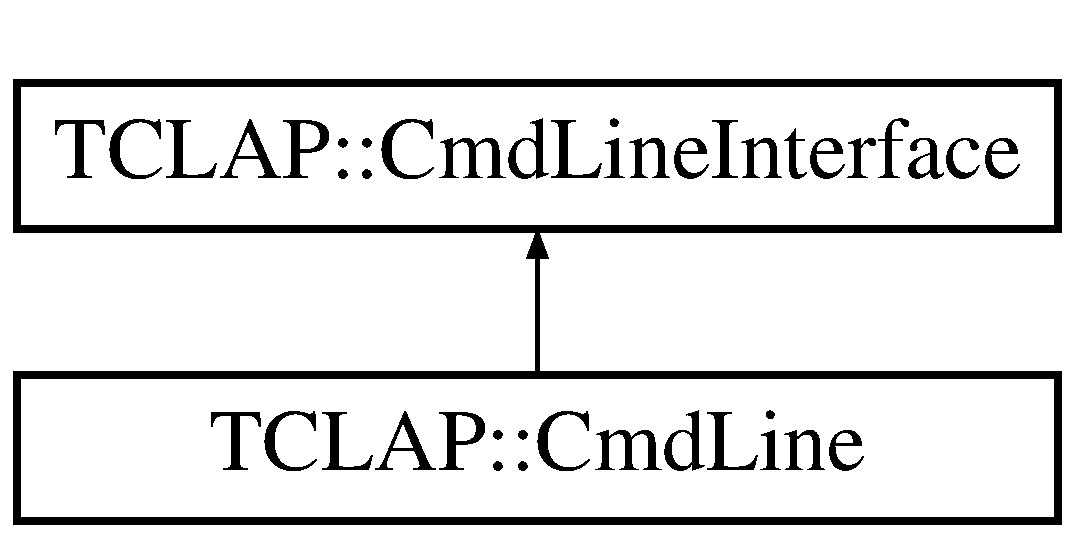
\includegraphics[height=2.000000cm]{classTCLAP_1_1CmdLine}
\end{center}
\end{figure}
\subsection*{Public Member Functions}
\begin{DoxyCompactItemize}
\item 
{\bf Cmd\+Line} (const std\+::string \&message, const char delimiter= ' ', const std\+::string \&version=\char`\"{}none\char`\"{}, bool help\+And\+Version=true)
\begin{DoxyCompactList}\small\item\em Command line constructor. \end{DoxyCompactList}\item 
virtual {\bf $\sim$\+Cmd\+Line} ()
\begin{DoxyCompactList}\small\item\em Deletes any resources allocated by a \doxyref{Cmd\+Line}{p.}{classTCLAP_1_1CmdLine} object. \end{DoxyCompactList}\item 
void {\bf add} ({\bf Arg} \&a)
\begin{DoxyCompactList}\small\item\em Adds an argument to the list of arguments to be parsed. \end{DoxyCompactList}\item 
void {\bf add} ({\bf Arg} $\ast$a)
\begin{DoxyCompactList}\small\item\em An alternative add. \end{DoxyCompactList}\item 
void {\bf xor\+Add} ({\bf Arg} \&a, {\bf Arg} \&b)
\begin{DoxyCompactList}\small\item\em Add two Args that will be xor'd. \end{DoxyCompactList}\item 
void {\bf xor\+Add} (std\+::vector$<$ {\bf Arg} $\ast$ $>$ \&xors)
\begin{DoxyCompactList}\small\item\em Add a list of Args that will be xor'd. \end{DoxyCompactList}\item 
void {\bf parse} (int argc, const char $\ast$const $\ast$argv)
\begin{DoxyCompactList}\small\item\em Parses the command line. \end{DoxyCompactList}\item 
void {\bf parse} (std\+::vector$<$ std\+::string $>$ \&args)
\begin{DoxyCompactList}\small\item\em Parses the command line. \end{DoxyCompactList}\item 
{\bf Cmd\+Line\+Output} $\ast$ {\bf get\+Output} ()
\begin{DoxyCompactList}\small\item\em Returns the \doxyref{Cmd\+Line\+Output}{p.}{classTCLAP_1_1CmdLineOutput} object. \end{DoxyCompactList}\item 
void {\bf set\+Output} ({\bf Cmd\+Line\+Output} $\ast$co)
\item 
std\+::string \& {\bf get\+Version} ()
\begin{DoxyCompactList}\small\item\em Returns the version string. \end{DoxyCompactList}\item 
std\+::string \& {\bf get\+Program\+Name} ()
\begin{DoxyCompactList}\small\item\em Returns the program name string. \end{DoxyCompactList}\item 
std\+::list$<$ {\bf Arg} $\ast$ $>$ \& {\bf get\+Arg\+List} ()
\begin{DoxyCompactList}\small\item\em Returns the arg\+List. \end{DoxyCompactList}\item 
{\bf Xor\+Handler} \& {\bf get\+Xor\+Handler} ()
\begin{DoxyCompactList}\small\item\em Returns the \doxyref{Xor\+Handler}{p.}{classTCLAP_1_1XorHandler}. \end{DoxyCompactList}\item 
char {\bf get\+Delimiter} ()
\begin{DoxyCompactList}\small\item\em Returns the delimiter string. \end{DoxyCompactList}\item 
std\+::string \& {\bf get\+Message} ()
\begin{DoxyCompactList}\small\item\em Returns the message string. \end{DoxyCompactList}\item 
bool {\bf has\+Help\+And\+Version} ()
\begin{DoxyCompactList}\small\item\em Indicates whether or not the help and version switches were created automatically. \end{DoxyCompactList}\item 
void {\bf set\+Exception\+Handling} (const bool state)
\begin{DoxyCompactList}\small\item\em Disables or enables \doxyref{Cmd\+Line}{p.}{classTCLAP_1_1CmdLine}'s internal parsing exception handling. \end{DoxyCompactList}\item 
bool {\bf get\+Exception\+Handling} () const 
\begin{DoxyCompactList}\small\item\em Returns the current state of the internal exception handling. \end{DoxyCompactList}\item 
void {\bf reset} ()
\begin{DoxyCompactList}\small\item\em Allows the \doxyref{Cmd\+Line}{p.}{classTCLAP_1_1CmdLine} object to be reused. \end{DoxyCompactList}\end{DoxyCompactItemize}
\subsection*{Protected Member Functions}
\begin{DoxyCompactItemize}
\item 
void {\bf missing\+Args\+Exception} ()
\begin{DoxyCompactList}\small\item\em Throws an exception listing the missing args. \end{DoxyCompactList}\item 
bool {\bf \+\_\+empty\+Combined} (const std\+::string \&s)
\begin{DoxyCompactList}\small\item\em Checks whether a name/flag string matches entirely matches the \doxyref{Arg\+::blank\+Char}{p.}{classTCLAP_1_1Arg_a0abd38f46dbf7d267078134a4817fbb2}. \end{DoxyCompactList}\item 
void {\bf delete\+On\+Exit} ({\bf Arg} $\ast$ptr)
\begin{DoxyCompactList}\small\item\em Perform a delete ptr; operation on ptr when this object is deleted. \end{DoxyCompactList}\item 
void {\bf delete\+On\+Exit} ({\bf Visitor} $\ast$ptr)
\begin{DoxyCompactList}\small\item\em Perform a delete ptr; operation on ptr when this object is deleted. \end{DoxyCompactList}\end{DoxyCompactItemize}
\subsection*{Protected Attributes}
\begin{DoxyCompactItemize}
\item 
std\+::list$<$ {\bf Arg} $\ast$ $>$ {\bf \+\_\+arg\+List}
\begin{DoxyCompactList}\small\item\em The list of arguments that will be tested against the command line. \end{DoxyCompactList}\item 
std\+::string {\bf \+\_\+prog\+Name}
\begin{DoxyCompactList}\small\item\em The name of the program. \end{DoxyCompactList}\item 
std\+::string {\bf \+\_\+message}
\begin{DoxyCompactList}\small\item\em A message used to describe the program. \end{DoxyCompactList}\item 
std\+::string {\bf \+\_\+version}
\begin{DoxyCompactList}\small\item\em The version to be displayed with the --version switch. \end{DoxyCompactList}\item 
int {\bf \+\_\+num\+Required}
\begin{DoxyCompactList}\small\item\em The number of arguments that are required to be present on the command line. \end{DoxyCompactList}\item 
char {\bf \+\_\+delimiter}
\begin{DoxyCompactList}\small\item\em The character that is used to separate the argument flag/name from the value. \end{DoxyCompactList}\item 
{\bf Xor\+Handler} {\bf \+\_\+xor\+Handler}
\begin{DoxyCompactList}\small\item\em The handler that manages xoring lists of args. \end{DoxyCompactList}\item 
std\+::list$<$ {\bf Arg} $\ast$ $>$ {\bf \+\_\+arg\+Delete\+On\+Exit\+List}
\begin{DoxyCompactList}\small\item\em A list of Args to be explicitly deleted when the destructor is called. \end{DoxyCompactList}\item 
std\+::list$<$ {\bf Visitor} $\ast$ $>$ {\bf \+\_\+visitor\+Delete\+On\+Exit\+List}
\begin{DoxyCompactList}\small\item\em A list of Visitors to be explicitly deleted when the destructor is called. \end{DoxyCompactList}\item 
{\bf Cmd\+Line\+Output} $\ast$ {\bf \+\_\+output}
\begin{DoxyCompactList}\small\item\em Object that handles all output for the \doxyref{Cmd\+Line}{p.}{classTCLAP_1_1CmdLine}. \end{DoxyCompactList}\item 
bool {\bf \+\_\+handle\+Exceptions}
\begin{DoxyCompactList}\small\item\em Should \doxyref{Cmd\+Line}{p.}{classTCLAP_1_1CmdLine} handle parsing exceptions internally? \end{DoxyCompactList}\end{DoxyCompactItemize}
\subsection*{Private Member Functions}
\begin{DoxyCompactItemize}
\item 
{\bf Cmd\+Line} (const {\bf Cmd\+Line} \&rhs)
\begin{DoxyCompactList}\small\item\em Prevent accidental copying. \end{DoxyCompactList}\item 
{\bf Cmd\+Line} \& {\bf operator=} (const {\bf Cmd\+Line} \&rhs)
\item 
void {\bf \+\_\+constructor} ()
\begin{DoxyCompactList}\small\item\em Encapsulates the code common to the constructors (which is all of it). \end{DoxyCompactList}\end{DoxyCompactItemize}
\subsection*{Private Attributes}
\begin{DoxyCompactItemize}
\item 
bool {\bf \+\_\+user\+Set\+Output}
\begin{DoxyCompactList}\small\item\em Is set to true when a user sets the output object. \end{DoxyCompactList}\item 
bool {\bf \+\_\+help\+And\+Version}
\begin{DoxyCompactList}\small\item\em Whether or not to automatically create help and version switches. \end{DoxyCompactList}\end{DoxyCompactItemize}


\subsection{Detailed Description}
The base class that manages the command line definition and passes along the parsing to the appropriate \doxyref{Arg}{p.}{classTCLAP_1_1Arg} classes. 

Definition at line 70 of file Cmd\+Line.\+h.



\subsection{Constructor \& Destructor Documentation}
\index{T\+C\+L\+A\+P\+::\+Cmd\+Line@{T\+C\+L\+A\+P\+::\+Cmd\+Line}!Cmd\+Line@{Cmd\+Line}}
\index{Cmd\+Line@{Cmd\+Line}!T\+C\+L\+A\+P\+::\+Cmd\+Line@{T\+C\+L\+A\+P\+::\+Cmd\+Line}}
\subsubsection[{Cmd\+Line}]{\setlength{\rightskip}{0pt plus 5cm}T\+C\+L\+A\+P\+::\+Cmd\+Line\+::\+Cmd\+Line (
\begin{DoxyParamCaption}
\item[{const {\bf Cmd\+Line} \&}]{rhs}
\end{DoxyParamCaption}
)\hspace{0.3cm}{\ttfamily [private]}}\label{classTCLAP_1_1CmdLine_ac6479892319106c49ec644bbc68a255e}


Prevent accidental copying. 

\index{T\+C\+L\+A\+P\+::\+Cmd\+Line@{T\+C\+L\+A\+P\+::\+Cmd\+Line}!Cmd\+Line@{Cmd\+Line}}
\index{Cmd\+Line@{Cmd\+Line}!T\+C\+L\+A\+P\+::\+Cmd\+Line@{T\+C\+L\+A\+P\+::\+Cmd\+Line}}
\subsubsection[{Cmd\+Line}]{\setlength{\rightskip}{0pt plus 5cm}T\+C\+L\+A\+P\+::\+Cmd\+Line\+::\+Cmd\+Line (
\begin{DoxyParamCaption}
\item[{const std\+::string \&}]{message, }
\item[{const char}]{delimiter = {\ttfamily '~'}, }
\item[{const std\+::string \&}]{version = {\ttfamily \char`\"{}none\char`\"{}}, }
\item[{bool}]{help\+And\+Version = {\ttfamily true}}
\end{DoxyParamCaption}
)\hspace{0.3cm}{\ttfamily [inline]}}\label{classTCLAP_1_1CmdLine_a2e62a3493f8700afb49a7deb872a5b96}


Command line constructor. 

Defines how the arguments will be parsed. 
\begin{DoxyParams}{Parameters}
{\em message} & -\/ The message to be used in the usage output. \\
\hline
{\em delimiter} & -\/ The character that is used to separate the argument flag/name from the value. Defaults to ' ' (space). \\
\hline
{\em version} & -\/ The version number to be used in the --version switch. \\
\hline
{\em help\+And\+Version} & -\/ Whether or not to create the Help and Version switches. Defaults to true. \\
\hline
\end{DoxyParams}


Definition at line 323 of file Cmd\+Line.\+h.



References \+\_\+constructor().


\begin{DoxyCode}
327     :
328   _argList(std::list<Arg*>()),
329   _progName(\textcolor{stringliteral}{"not\_set\_yet"}),
330   _message(m),
331   _version(v),
332   _numRequired(0),
333   _delimiter(delim),
334   _xorHandler(XorHandler()),
335   _argDeleteOnExitList(std::list<Arg*>()),
336   _visitorDeleteOnExitList(std::list<Visitor*>()),
337   _output(0),
338   _handleExceptions(\textcolor{keyword}{true}),
339   _userSetOutput(\textcolor{keyword}{false}),
340   _helpAndVersion(help)
341 \{
342   _constructor();
343 \}
\end{DoxyCode}
\index{T\+C\+L\+A\+P\+::\+Cmd\+Line@{T\+C\+L\+A\+P\+::\+Cmd\+Line}!````~Cmd\+Line@{$\sim$\+Cmd\+Line}}
\index{````~Cmd\+Line@{$\sim$\+Cmd\+Line}!T\+C\+L\+A\+P\+::\+Cmd\+Line@{T\+C\+L\+A\+P\+::\+Cmd\+Line}}
\subsubsection[{$\sim$\+Cmd\+Line}]{\setlength{\rightskip}{0pt plus 5cm}T\+C\+L\+A\+P\+::\+Cmd\+Line\+::$\sim$\+Cmd\+Line (
\begin{DoxyParamCaption}
{}
\end{DoxyParamCaption}
)\hspace{0.3cm}{\ttfamily [inline]}, {\ttfamily [virtual]}}\label{classTCLAP_1_1CmdLine_a8a7bddba32c3d96e2a01e4c8e160e6fa}


Deletes any resources allocated by a \doxyref{Cmd\+Line}{p.}{classTCLAP_1_1CmdLine} object. 



Definition at line 345 of file Cmd\+Line.\+h.



References \+\_\+arg\+Delete\+On\+Exit\+List, \+\_\+output, \+\_\+user\+Set\+Output, \+\_\+visitor\+Delete\+On\+Exit\+List, and T\+C\+L\+A\+P\+::\+Clear\+Container().


\begin{DoxyCode}
346 \{
347   ClearContainer(_argDeleteOnExitList);
348   ClearContainer(_visitorDeleteOnExitList);
349 
350   \textcolor{keywordflow}{if} ( !_userSetOutput ) \{
351     \textcolor{keyword}{delete} _output;
352     _output = 0;
353   \}
354 \}
\end{DoxyCode}


\subsection{Member Function Documentation}
\index{T\+C\+L\+A\+P\+::\+Cmd\+Line@{T\+C\+L\+A\+P\+::\+Cmd\+Line}!\+\_\+constructor@{\+\_\+constructor}}
\index{\+\_\+constructor@{\+\_\+constructor}!T\+C\+L\+A\+P\+::\+Cmd\+Line@{T\+C\+L\+A\+P\+::\+Cmd\+Line}}
\subsubsection[{\+\_\+constructor}]{\setlength{\rightskip}{0pt plus 5cm}void T\+C\+L\+A\+P\+::\+Cmd\+Line\+::\+\_\+constructor (
\begin{DoxyParamCaption}
{}
\end{DoxyParamCaption}
)\hspace{0.3cm}{\ttfamily [inline]}, {\ttfamily [private]}}\label{classTCLAP_1_1CmdLine_a955b1935c7b2e5118b2573bd2fbb958c}


Encapsulates the code common to the constructors (which is all of it). 



Definition at line 356 of file Cmd\+Line.\+h.



References \+\_\+delimiter, \+\_\+help\+And\+Version, \+\_\+output, add(), delete\+On\+Exit(), T\+C\+L\+A\+P\+::\+Arg\+::flag\+Start\+String(), T\+C\+L\+A\+P\+::\+Arg\+::ignore\+Name\+String(), and T\+C\+L\+A\+P\+::\+Arg\+::set\+Delimiter().



Referenced by Cmd\+Line().


\begin{DoxyCode}
357 \{
358   _output = \textcolor{keyword}{new} StdOutput;
359 
360   Arg::setDelimiter( _delimiter );
361 
362   Visitor* v;
363 
364   \textcolor{keywordflow}{if} ( _helpAndVersion )
365   \{
366     v = \textcolor{keyword}{new} HelpVisitor( \textcolor{keyword}{this}, &_output );
367     SwitchArg* help = \textcolor{keyword}{new} SwitchArg(\textcolor{stringliteral}{"h"},\textcolor{stringliteral}{"help"},
368                           \textcolor{stringliteral}{"Displays usage information and exits."},
369                           \textcolor{keyword}{false}, v);
370     add( help );
371     deleteOnExit(help);
372     deleteOnExit(v);
373 
374     v = \textcolor{keyword}{new} VersionVisitor( \textcolor{keyword}{this}, &_output );
375     SwitchArg* vers = \textcolor{keyword}{new} SwitchArg(\textcolor{stringliteral}{""},\textcolor{stringliteral}{"version"},
376                           \textcolor{stringliteral}{"Displays version information and exits."},
377                           \textcolor{keyword}{false}, v);
378     add( vers );
379     deleteOnExit(vers);
380     deleteOnExit(v);
381   \}
382 
383   v = \textcolor{keyword}{new} IgnoreRestVisitor();
384   SwitchArg* ignore  = \textcolor{keyword}{new} SwitchArg(Arg::flagStartString(),
385             Arg::ignoreNameString(),
386             \textcolor{stringliteral}{"Ignores the rest of the labeled arguments following this flag."},
387             \textcolor{keyword}{false}, v);
388   add( ignore );
389   deleteOnExit(ignore);
390   deleteOnExit(v);
391 \}
\end{DoxyCode}
\index{T\+C\+L\+A\+P\+::\+Cmd\+Line@{T\+C\+L\+A\+P\+::\+Cmd\+Line}!\+\_\+empty\+Combined@{\+\_\+empty\+Combined}}
\index{\+\_\+empty\+Combined@{\+\_\+empty\+Combined}!T\+C\+L\+A\+P\+::\+Cmd\+Line@{T\+C\+L\+A\+P\+::\+Cmd\+Line}}
\subsubsection[{\+\_\+empty\+Combined}]{\setlength{\rightskip}{0pt plus 5cm}bool T\+C\+L\+A\+P\+::\+Cmd\+Line\+::\+\_\+empty\+Combined (
\begin{DoxyParamCaption}
\item[{const std\+::string \&}]{s}
\end{DoxyParamCaption}
)\hspace{0.3cm}{\ttfamily [inline]}, {\ttfamily [protected]}}\label{classTCLAP_1_1CmdLine_a170a4e711c2a6d58a05e9ad3bc03c08a}


Checks whether a name/flag string matches entirely matches the \doxyref{Arg\+::blank\+Char}{p.}{classTCLAP_1_1Arg_a0abd38f46dbf7d267078134a4817fbb2}. 

Used when multiple switches are combined into a single argument. 
\begin{DoxyParams}{Parameters}
{\em s} & -\/ The message to be used in the usage. \\
\hline
\end{DoxyParams}


Definition at line 512 of file Cmd\+Line.\+h.



References T\+C\+L\+A\+P\+::\+Arg\+::blank\+Char(), and T\+C\+L\+A\+P\+::\+Arg\+::flag\+Start\+Char().



Referenced by parse().


\begin{DoxyCode}
513 \{
514   \textcolor{keywordflow}{if} ( s.length() > 0 && s[0] != Arg::flagStartChar() )
515     \textcolor{keywordflow}{return} \textcolor{keyword}{false};
516 
517   \textcolor{keywordflow}{for} ( \textcolor{keywordtype}{int} i = 1; \textcolor{keyword}{static\_cast<}\textcolor{keywordtype}{unsigned} \textcolor{keywordtype}{int}\textcolor{keyword}{>}(i) < s.length(); i++ )
518     \textcolor{keywordflow}{if} ( s[i] != Arg::blankChar() )
519       \textcolor{keywordflow}{return} \textcolor{keyword}{false};
520 
521   \textcolor{keywordflow}{return} \textcolor{keyword}{true};
522 \}
\end{DoxyCode}
\index{T\+C\+L\+A\+P\+::\+Cmd\+Line@{T\+C\+L\+A\+P\+::\+Cmd\+Line}!add@{add}}
\index{add@{add}!T\+C\+L\+A\+P\+::\+Cmd\+Line@{T\+C\+L\+A\+P\+::\+Cmd\+Line}}
\subsubsection[{add}]{\setlength{\rightskip}{0pt plus 5cm}void T\+C\+L\+A\+P\+::\+Cmd\+Line\+::add (
\begin{DoxyParamCaption}
\item[{{\bf Arg} \&}]{a}
\end{DoxyParamCaption}
)\hspace{0.3cm}{\ttfamily [inline]}, {\ttfamily [virtual]}}\label{classTCLAP_1_1CmdLine_a94c511d4735ad9b8c97edaa3827f8bbf}


Adds an argument to the list of arguments to be parsed. 


\begin{DoxyParams}{Parameters}
{\em a} & -\/ Argument to be added. \\
\hline
\end{DoxyParams}


Implements {\bf T\+C\+L\+A\+P\+::\+Cmd\+Line\+Interface} \doxyref{}{p.}{classTCLAP_1_1CmdLineInterface_a13b29ab754c030185e58f779dc355631}.



Definition at line 413 of file Cmd\+Line.\+h.



Referenced by \+\_\+constructor(), and xor\+Add().


\begin{DoxyCode}
414 \{
415   add( &a );
416 \}
\end{DoxyCode}
\index{T\+C\+L\+A\+P\+::\+Cmd\+Line@{T\+C\+L\+A\+P\+::\+Cmd\+Line}!add@{add}}
\index{add@{add}!T\+C\+L\+A\+P\+::\+Cmd\+Line@{T\+C\+L\+A\+P\+::\+Cmd\+Line}}
\subsubsection[{add}]{\setlength{\rightskip}{0pt plus 5cm}void T\+C\+L\+A\+P\+::\+Cmd\+Line\+::add (
\begin{DoxyParamCaption}
\item[{{\bf Arg} $\ast$}]{a}
\end{DoxyParamCaption}
)\hspace{0.3cm}{\ttfamily [inline]}, {\ttfamily [virtual]}}\label{classTCLAP_1_1CmdLine_ab8a08e8f4d3ca7709c85416f76e805a3}


An alternative add. 

Functionally identical. 
\begin{DoxyParams}{Parameters}
{\em a} & -\/ Argument to be added. \\
\hline
\end{DoxyParams}


Implements {\bf T\+C\+L\+A\+P\+::\+Cmd\+Line\+Interface} \doxyref{}{p.}{classTCLAP_1_1CmdLineInterface_a7c6a097c0f2a09dd1987e9da1af8b457}.



Definition at line 418 of file Cmd\+Line.\+h.



References \+\_\+arg\+List, \+\_\+num\+Required, T\+C\+L\+A\+P\+::\+Arg\+::add\+To\+List(), T\+C\+L\+A\+P\+::\+Arg\+::is\+Required(), and T\+C\+L\+A\+P\+::\+Arg\+::long\+I\+D().


\begin{DoxyCode}
419 \{
420   \textcolor{keywordflow}{for}( ArgListIterator it = _argList.begin(); it != _argList.end(); it++ )
421     \textcolor{keywordflow}{if} ( *a == *(*it) )
422       \textcolor{keywordflow}{throw}( SpecificationException(
423               \textcolor{stringliteral}{"Argument with same flag/name already exists!"},
424               a->longID() ) );
425 
426   a->addToList( _argList );
427 
428   \textcolor{keywordflow}{if} ( a->isRequired() )
429     _numRequired++;
430 \}
\end{DoxyCode}
\index{T\+C\+L\+A\+P\+::\+Cmd\+Line@{T\+C\+L\+A\+P\+::\+Cmd\+Line}!delete\+On\+Exit@{delete\+On\+Exit}}
\index{delete\+On\+Exit@{delete\+On\+Exit}!T\+C\+L\+A\+P\+::\+Cmd\+Line@{T\+C\+L\+A\+P\+::\+Cmd\+Line}}
\subsubsection[{delete\+On\+Exit}]{\setlength{\rightskip}{0pt plus 5cm}void T\+C\+L\+A\+P\+::\+Cmd\+Line\+::delete\+On\+Exit (
\begin{DoxyParamCaption}
\item[{{\bf Arg} $\ast$}]{ptr}
\end{DoxyParamCaption}
)\hspace{0.3cm}{\ttfamily [inline]}, {\ttfamily [protected]}}\label{classTCLAP_1_1CmdLine_a42d669ed2037ac24fc78883aa8600655}


Perform a delete ptr; operation on ptr when this object is deleted. 



Definition at line 551 of file Cmd\+Line.\+h.



References \+\_\+arg\+Delete\+On\+Exit\+List.



Referenced by \+\_\+constructor().


\begin{DoxyCode}
552 \{
553   _argDeleteOnExitList.push\_back(ptr);
554 \}
\end{DoxyCode}
\index{T\+C\+L\+A\+P\+::\+Cmd\+Line@{T\+C\+L\+A\+P\+::\+Cmd\+Line}!delete\+On\+Exit@{delete\+On\+Exit}}
\index{delete\+On\+Exit@{delete\+On\+Exit}!T\+C\+L\+A\+P\+::\+Cmd\+Line@{T\+C\+L\+A\+P\+::\+Cmd\+Line}}
\subsubsection[{delete\+On\+Exit}]{\setlength{\rightskip}{0pt plus 5cm}void T\+C\+L\+A\+P\+::\+Cmd\+Line\+::delete\+On\+Exit (
\begin{DoxyParamCaption}
\item[{{\bf Visitor} $\ast$}]{ptr}
\end{DoxyParamCaption}
)\hspace{0.3cm}{\ttfamily [inline]}, {\ttfamily [protected]}}\label{classTCLAP_1_1CmdLine_a262b8d929eb5b0dfbfc17637c1325c36}


Perform a delete ptr; operation on ptr when this object is deleted. 



Definition at line 556 of file Cmd\+Line.\+h.



References \+\_\+visitor\+Delete\+On\+Exit\+List.


\begin{DoxyCode}
557 \{
558   _visitorDeleteOnExitList.push\_back(ptr);
559 \}
\end{DoxyCode}
\index{T\+C\+L\+A\+P\+::\+Cmd\+Line@{T\+C\+L\+A\+P\+::\+Cmd\+Line}!get\+Arg\+List@{get\+Arg\+List}}
\index{get\+Arg\+List@{get\+Arg\+List}!T\+C\+L\+A\+P\+::\+Cmd\+Line@{T\+C\+L\+A\+P\+::\+Cmd\+Line}}
\subsubsection[{get\+Arg\+List}]{\setlength{\rightskip}{0pt plus 5cm}std\+::list$<$ {\bf Arg} $\ast$ $>$ \& T\+C\+L\+A\+P\+::\+Cmd\+Line\+::get\+Arg\+List (
\begin{DoxyParamCaption}
{}
\end{DoxyParamCaption}
)\hspace{0.3cm}{\ttfamily [inline]}, {\ttfamily [virtual]}}\label{classTCLAP_1_1CmdLine_a3c281da929a281fb883ea47632b7ad38}


Returns the arg\+List. 



Implements {\bf T\+C\+L\+A\+P\+::\+Cmd\+Line\+Interface} \doxyref{}{p.}{classTCLAP_1_1CmdLineInterface_a4de8d988f5a6f3007c4dfb0fc9dad476}.



Definition at line 584 of file Cmd\+Line.\+h.



References \+\_\+arg\+List.


\begin{DoxyCode}
585 \{
586   \textcolor{keywordflow}{return} _argList;
587 \}
\end{DoxyCode}
\index{T\+C\+L\+A\+P\+::\+Cmd\+Line@{T\+C\+L\+A\+P\+::\+Cmd\+Line}!get\+Delimiter@{get\+Delimiter}}
\index{get\+Delimiter@{get\+Delimiter}!T\+C\+L\+A\+P\+::\+Cmd\+Line@{T\+C\+L\+A\+P\+::\+Cmd\+Line}}
\subsubsection[{get\+Delimiter}]{\setlength{\rightskip}{0pt plus 5cm}char T\+C\+L\+A\+P\+::\+Cmd\+Line\+::get\+Delimiter (
\begin{DoxyParamCaption}
{}
\end{DoxyParamCaption}
)\hspace{0.3cm}{\ttfamily [inline]}, {\ttfamily [virtual]}}\label{classTCLAP_1_1CmdLine_a3e9f0ac2c1e97d1f8527da713ddd5a8f}


Returns the delimiter string. 



Implements {\bf T\+C\+L\+A\+P\+::\+Cmd\+Line\+Interface} \doxyref{}{p.}{classTCLAP_1_1CmdLineInterface_a7d6a64cff6b3a30e2cf1e81d7b1d4521}.



Definition at line 594 of file Cmd\+Line.\+h.



References \+\_\+delimiter.


\begin{DoxyCode}
595 \{
596   \textcolor{keywordflow}{return} _delimiter;
597 \}
\end{DoxyCode}
\index{T\+C\+L\+A\+P\+::\+Cmd\+Line@{T\+C\+L\+A\+P\+::\+Cmd\+Line}!get\+Exception\+Handling@{get\+Exception\+Handling}}
\index{get\+Exception\+Handling@{get\+Exception\+Handling}!T\+C\+L\+A\+P\+::\+Cmd\+Line@{T\+C\+L\+A\+P\+::\+Cmd\+Line}}
\subsubsection[{get\+Exception\+Handling}]{\setlength{\rightskip}{0pt plus 5cm}bool T\+C\+L\+A\+P\+::\+Cmd\+Line\+::get\+Exception\+Handling (
\begin{DoxyParamCaption}
{}
\end{DoxyParamCaption}
) const\hspace{0.3cm}{\ttfamily [inline]}}\label{classTCLAP_1_1CmdLine_af2cd748a91e22df97c878d7eff8c4ca3}


Returns the current state of the internal exception handling. 


\begin{DoxyRetVals}{Return values}
{\em true} & Parsing exceptions are handled internally. \\
\hline
{\em false} & Parsing exceptions are propagated to the caller. \\
\hline
\end{DoxyRetVals}


Definition at line 614 of file Cmd\+Line.\+h.



References \+\_\+handle\+Exceptions.


\begin{DoxyCode}
615 \{
616   \textcolor{keywordflow}{return} _handleExceptions;
617 \}
\end{DoxyCode}
\index{T\+C\+L\+A\+P\+::\+Cmd\+Line@{T\+C\+L\+A\+P\+::\+Cmd\+Line}!get\+Message@{get\+Message}}
\index{get\+Message@{get\+Message}!T\+C\+L\+A\+P\+::\+Cmd\+Line@{T\+C\+L\+A\+P\+::\+Cmd\+Line}}
\subsubsection[{get\+Message}]{\setlength{\rightskip}{0pt plus 5cm}std\+::string \& T\+C\+L\+A\+P\+::\+Cmd\+Line\+::get\+Message (
\begin{DoxyParamCaption}
{}
\end{DoxyParamCaption}
)\hspace{0.3cm}{\ttfamily [inline]}, {\ttfamily [virtual]}}\label{classTCLAP_1_1CmdLine_a8f61a8c201e31ada985fa998180fd40f}


Returns the message string. 



Implements {\bf T\+C\+L\+A\+P\+::\+Cmd\+Line\+Interface} \doxyref{}{p.}{classTCLAP_1_1CmdLineInterface_a30175a2567f7ab78a2c6bbea9269a2fa}.



Definition at line 599 of file Cmd\+Line.\+h.



References \+\_\+message.


\begin{DoxyCode}
600 \{
601   \textcolor{keywordflow}{return} _message;
602 \}
\end{DoxyCode}
\index{T\+C\+L\+A\+P\+::\+Cmd\+Line@{T\+C\+L\+A\+P\+::\+Cmd\+Line}!get\+Output@{get\+Output}}
\index{get\+Output@{get\+Output}!T\+C\+L\+A\+P\+::\+Cmd\+Line@{T\+C\+L\+A\+P\+::\+Cmd\+Line}}
\subsubsection[{get\+Output}]{\setlength{\rightskip}{0pt plus 5cm}{\bf Cmd\+Line\+Output} $\ast$ T\+C\+L\+A\+P\+::\+Cmd\+Line\+::get\+Output (
\begin{DoxyParamCaption}
{}
\end{DoxyParamCaption}
)\hspace{0.3cm}{\ttfamily [inline]}, {\ttfamily [virtual]}}\label{classTCLAP_1_1CmdLine_ad8aea2617edf53bbc20c8964ee5476e6}


Returns the \doxyref{Cmd\+Line\+Output}{p.}{classTCLAP_1_1CmdLineOutput} object. 



Implements {\bf T\+C\+L\+A\+P\+::\+Cmd\+Line\+Interface} \doxyref{}{p.}{classTCLAP_1_1CmdLineInterface_aebc72daedeaeb03e06bb2e6e0f00363d}.



Definition at line 561 of file Cmd\+Line.\+h.



References \+\_\+output.


\begin{DoxyCode}
562 \{
563   \textcolor{keywordflow}{return} _output;
564 \}
\end{DoxyCode}
\index{T\+C\+L\+A\+P\+::\+Cmd\+Line@{T\+C\+L\+A\+P\+::\+Cmd\+Line}!get\+Program\+Name@{get\+Program\+Name}}
\index{get\+Program\+Name@{get\+Program\+Name}!T\+C\+L\+A\+P\+::\+Cmd\+Line@{T\+C\+L\+A\+P\+::\+Cmd\+Line}}
\subsubsection[{get\+Program\+Name}]{\setlength{\rightskip}{0pt plus 5cm}std\+::string \& T\+C\+L\+A\+P\+::\+Cmd\+Line\+::get\+Program\+Name (
\begin{DoxyParamCaption}
{}
\end{DoxyParamCaption}
)\hspace{0.3cm}{\ttfamily [inline]}, {\ttfamily [virtual]}}\label{classTCLAP_1_1CmdLine_a47a6d496980ee11ffc42e27144a61797}


Returns the program name string. 



Implements {\bf T\+C\+L\+A\+P\+::\+Cmd\+Line\+Interface} \doxyref{}{p.}{classTCLAP_1_1CmdLineInterface_a1a5672df72a6b5021cd70b37c4dbd0a7}.



Definition at line 579 of file Cmd\+Line.\+h.



References \+\_\+prog\+Name.


\begin{DoxyCode}
580 \{
581   \textcolor{keywordflow}{return} _progName;
582 \}
\end{DoxyCode}
\index{T\+C\+L\+A\+P\+::\+Cmd\+Line@{T\+C\+L\+A\+P\+::\+Cmd\+Line}!get\+Version@{get\+Version}}
\index{get\+Version@{get\+Version}!T\+C\+L\+A\+P\+::\+Cmd\+Line@{T\+C\+L\+A\+P\+::\+Cmd\+Line}}
\subsubsection[{get\+Version}]{\setlength{\rightskip}{0pt plus 5cm}std\+::string \& T\+C\+L\+A\+P\+::\+Cmd\+Line\+::get\+Version (
\begin{DoxyParamCaption}
{}
\end{DoxyParamCaption}
)\hspace{0.3cm}{\ttfamily [inline]}, {\ttfamily [virtual]}}\label{classTCLAP_1_1CmdLine_a85b5653d1a5b48fe6accead64615cf33}


Returns the version string. 



Implements {\bf T\+C\+L\+A\+P\+::\+Cmd\+Line\+Interface} \doxyref{}{p.}{classTCLAP_1_1CmdLineInterface_a0a552fa57212800dfb8aec84fb07b8bb}.



Definition at line 574 of file Cmd\+Line.\+h.



References \+\_\+version.


\begin{DoxyCode}
575 \{
576   \textcolor{keywordflow}{return} _version;
577 \}
\end{DoxyCode}
\index{T\+C\+L\+A\+P\+::\+Cmd\+Line@{T\+C\+L\+A\+P\+::\+Cmd\+Line}!get\+Xor\+Handler@{get\+Xor\+Handler}}
\index{get\+Xor\+Handler@{get\+Xor\+Handler}!T\+C\+L\+A\+P\+::\+Cmd\+Line@{T\+C\+L\+A\+P\+::\+Cmd\+Line}}
\subsubsection[{get\+Xor\+Handler}]{\setlength{\rightskip}{0pt plus 5cm}{\bf Xor\+Handler} \& T\+C\+L\+A\+P\+::\+Cmd\+Line\+::get\+Xor\+Handler (
\begin{DoxyParamCaption}
{}
\end{DoxyParamCaption}
)\hspace{0.3cm}{\ttfamily [inline]}, {\ttfamily [virtual]}}\label{classTCLAP_1_1CmdLine_a805433b7718d1bc5bc9317bbd061449b}


Returns the \doxyref{Xor\+Handler}{p.}{classTCLAP_1_1XorHandler}. 



Implements {\bf T\+C\+L\+A\+P\+::\+Cmd\+Line\+Interface} \doxyref{}{p.}{classTCLAP_1_1CmdLineInterface_a11ce9c77a1111960741f05e343849e4e}.



Definition at line 589 of file Cmd\+Line.\+h.



References \+\_\+xor\+Handler.


\begin{DoxyCode}
590 \{
591   \textcolor{keywordflow}{return} _xorHandler;
592 \}
\end{DoxyCode}
\index{T\+C\+L\+A\+P\+::\+Cmd\+Line@{T\+C\+L\+A\+P\+::\+Cmd\+Line}!has\+Help\+And\+Version@{has\+Help\+And\+Version}}
\index{has\+Help\+And\+Version@{has\+Help\+And\+Version}!T\+C\+L\+A\+P\+::\+Cmd\+Line@{T\+C\+L\+A\+P\+::\+Cmd\+Line}}
\subsubsection[{has\+Help\+And\+Version}]{\setlength{\rightskip}{0pt plus 5cm}bool T\+C\+L\+A\+P\+::\+Cmd\+Line\+::has\+Help\+And\+Version (
\begin{DoxyParamCaption}
{}
\end{DoxyParamCaption}
)\hspace{0.3cm}{\ttfamily [inline]}, {\ttfamily [virtual]}}\label{classTCLAP_1_1CmdLine_a5b23895feae4f4110b77dae372226475}


Indicates whether or not the help and version switches were created automatically. 



Implements {\bf T\+C\+L\+A\+P\+::\+Cmd\+Line\+Interface} \doxyref{}{p.}{classTCLAP_1_1CmdLineInterface_a441b06b764836a62083b163508210905}.



Definition at line 604 of file Cmd\+Line.\+h.



References \+\_\+help\+And\+Version.


\begin{DoxyCode}
605 \{
606   \textcolor{keywordflow}{return} _helpAndVersion;
607 \}
\end{DoxyCode}
\index{T\+C\+L\+A\+P\+::\+Cmd\+Line@{T\+C\+L\+A\+P\+::\+Cmd\+Line}!missing\+Args\+Exception@{missing\+Args\+Exception}}
\index{missing\+Args\+Exception@{missing\+Args\+Exception}!T\+C\+L\+A\+P\+::\+Cmd\+Line@{T\+C\+L\+A\+P\+::\+Cmd\+Line}}
\subsubsection[{missing\+Args\+Exception}]{\setlength{\rightskip}{0pt plus 5cm}void T\+C\+L\+A\+P\+::\+Cmd\+Line\+::missing\+Args\+Exception (
\begin{DoxyParamCaption}
{}
\end{DoxyParamCaption}
)\hspace{0.3cm}{\ttfamily [inline]}, {\ttfamily [protected]}}\label{classTCLAP_1_1CmdLine_a698f47333350312eb949aa1ae4f89ad1}


Throws an exception listing the missing args. 



Definition at line 524 of file Cmd\+Line.\+h.



References \+\_\+arg\+List.



Referenced by parse().


\begin{DoxyCode}
525 \{
526     \textcolor{keywordtype}{int} count = 0;
527 
528     std::string missingArgList;
529     \textcolor{keywordflow}{for} (ArgListIterator it = _argList.begin(); it != _argList.end(); it++)
530     \{
531       \textcolor{keywordflow}{if} ( (*it)->isRequired() && !(*it)->isSet() )
532       \{
533         missingArgList += (*it)->getName();
534         missingArgList += \textcolor{stringliteral}{", "};
535         count++;
536       \}
537     \}
538     missingArgList = missingArgList.substr(0,missingArgList.length()-2);
539 
540     std::string msg;
541     \textcolor{keywordflow}{if} ( count > 1 )
542       msg = \textcolor{stringliteral}{"Required arguments missing: "};
543     \textcolor{keywordflow}{else}
544       msg = \textcolor{stringliteral}{"Required argument missing: "};
545 
546     msg += missingArgList;
547 
548     \textcolor{keywordflow}{throw}(CmdLineParseException(msg));
549 \}
\end{DoxyCode}
\index{T\+C\+L\+A\+P\+::\+Cmd\+Line@{T\+C\+L\+A\+P\+::\+Cmd\+Line}!operator=@{operator=}}
\index{operator=@{operator=}!T\+C\+L\+A\+P\+::\+Cmd\+Line@{T\+C\+L\+A\+P\+::\+Cmd\+Line}}
\subsubsection[{operator=}]{\setlength{\rightskip}{0pt plus 5cm}{\bf Cmd\+Line}\& T\+C\+L\+A\+P\+::\+Cmd\+Line\+::operator= (
\begin{DoxyParamCaption}
\item[{const {\bf Cmd\+Line} \&}]{rhs}
\end{DoxyParamCaption}
)\hspace{0.3cm}{\ttfamily [private]}}\label{classTCLAP_1_1CmdLine_a46fd7d72c7a5cfeeacf5e9d0ff2cacf7}
\index{T\+C\+L\+A\+P\+::\+Cmd\+Line@{T\+C\+L\+A\+P\+::\+Cmd\+Line}!parse@{parse}}
\index{parse@{parse}!T\+C\+L\+A\+P\+::\+Cmd\+Line@{T\+C\+L\+A\+P\+::\+Cmd\+Line}}
\subsubsection[{parse}]{\setlength{\rightskip}{0pt plus 5cm}void T\+C\+L\+A\+P\+::\+Cmd\+Line\+::parse (
\begin{DoxyParamCaption}
\item[{int}]{argc, }
\item[{const char $\ast$const $\ast$}]{argv}
\end{DoxyParamCaption}
)\hspace{0.3cm}{\ttfamily [inline]}, {\ttfamily [virtual]}}\label{classTCLAP_1_1CmdLine_acb07daf5a1370c176a7b4a6e4119fe6e}


Parses the command line. 


\begin{DoxyParams}{Parameters}
{\em argc} & -\/ Number of arguments. \\
\hline
{\em argv} & -\/ Array of arguments. \\
\hline
\end{DoxyParams}


Implements {\bf T\+C\+L\+A\+P\+::\+Cmd\+Line\+Interface} \doxyref{}{p.}{classTCLAP_1_1CmdLineInterface_a6649336bddfc8421148718a691fd89b4}.



Definition at line 433 of file Cmd\+Line.\+h.


\begin{DoxyCode}
434 \{
435     \textcolor{comment}{// this step is necessary so that we have easy access to}
436     \textcolor{comment}{// mutable strings.}
437     std::vector<std::string> args;
438     \textcolor{keywordflow}{for} (\textcolor{keywordtype}{int} i = 0; i < argc; i++)
439       args.push\_back(argv[i]);
440 
441     parse(args);
442 \}
\end{DoxyCode}
\index{T\+C\+L\+A\+P\+::\+Cmd\+Line@{T\+C\+L\+A\+P\+::\+Cmd\+Line}!parse@{parse}}
\index{parse@{parse}!T\+C\+L\+A\+P\+::\+Cmd\+Line@{T\+C\+L\+A\+P\+::\+Cmd\+Line}}
\subsubsection[{parse}]{\setlength{\rightskip}{0pt plus 5cm}void T\+C\+L\+A\+P\+::\+Cmd\+Line\+::parse (
\begin{DoxyParamCaption}
\item[{std\+::vector$<$ std\+::string $>$ \&}]{args}
\end{DoxyParamCaption}
)\hspace{0.3cm}{\ttfamily [inline]}}\label{classTCLAP_1_1CmdLine_a712c3edf86aa0a8a28fb0b6d504d945a}


Parses the command line. 


\begin{DoxyParams}{Parameters}
{\em args} & -\/ A vector of strings representing the args. args[0] is still the program name. \\
\hline
\end{DoxyParams}


Definition at line 444 of file Cmd\+Line.\+h.



References \+\_\+arg\+List, \+\_\+empty\+Combined(), \+\_\+handle\+Exceptions, \+\_\+num\+Required, \+\_\+output, \+\_\+prog\+Name, \+\_\+xor\+Handler, T\+C\+L\+A\+P\+::\+Xor\+Handler\+::check(), T\+C\+L\+A\+P\+::\+Cmd\+Line\+Output\+::failure(), T\+C\+L\+A\+P\+::\+Exit\+Exception\+::get\+Exit\+Status(), T\+C\+L\+A\+P\+::\+Arg\+::ignore\+Rest(), and missing\+Args\+Exception().


\begin{DoxyCode}
445 \{
446   \textcolor{keywordtype}{bool} shouldExit = \textcolor{keyword}{false};
447   \textcolor{keywordtype}{int} estat = 0;
448 
449   \textcolor{keywordflow}{try} \{
450     _progName = args.front();
451     args.erase(args.begin());
452 
453     \textcolor{keywordtype}{int} requiredCount = 0;
454 
455     \textcolor{keywordflow}{for} (\textcolor{keywordtype}{int} i = 0; \textcolor{keyword}{static\_cast<}\textcolor{keywordtype}{unsigned} \textcolor{keywordtype}{int}\textcolor{keyword}{>}(i) < args.size(); i++) 
456     \{
457 
458       \textcolor{keywordtype}{bool} matched = \textcolor{keyword}{false};
459       \textcolor{keywordflow}{for} (ArgListIterator it = _argList.begin();
460            it != _argList.end(); it++) \{
461         \textcolor{keywordflow}{if} ( (*it)->processArg( &i, args ) )
462         \{
463           requiredCount += _xorHandler.check( *it );
464           matched = \textcolor{keyword}{true};
465           \textcolor{keywordflow}{break};
466         \}
467       \}
468 
469       \textcolor{comment}{// checks to see if the argument is an empty combined}
470       \textcolor{comment}{// switch and if so, then we've actually matched it}
471       \textcolor{keywordflow}{if} ( !matched && _emptyCombined( args[i] ) )
472         matched = \textcolor{keyword}{true};
473 
474       \textcolor{keywordflow}{if} ( !matched && !Arg::ignoreRest() )
475         \textcolor{keywordflow}{throw}(CmdLineParseException(\textcolor{stringliteral}{"Couldn't find match "}
476                                     \textcolor{stringliteral}{"for argument"},
477                                     args[i]));
478     \}
479 
480     \textcolor{keywordflow}{if} ( requiredCount < _numRequired )
481       missingArgsException();
482 
483     \textcolor{keywordflow}{if} ( requiredCount > _numRequired )
484       \textcolor{keywordflow}{throw}(CmdLineParseException(\textcolor{stringliteral}{"Too many arguments!"}));
485 
486   \} \textcolor{keywordflow}{catch} ( ArgException& e ) \{
487     \textcolor{comment}{// If we're not handling the exceptions, rethrow.}
488     \textcolor{keywordflow}{if} ( !_handleExceptions) \{
489       \textcolor{keywordflow}{throw};
490     \}
491 
492     \textcolor{keywordflow}{try} \{
493       _output->failure(*\textcolor{keyword}{this},e);
494     \} \textcolor{keywordflow}{catch} ( ExitException &ee ) \{
495       estat = ee.getExitStatus();
496       shouldExit = \textcolor{keyword}{true};
497     \}
498   \} \textcolor{keywordflow}{catch} (ExitException &ee) \{
499     \textcolor{comment}{// If we're not handling the exceptions, rethrow.}
500     \textcolor{keywordflow}{if} ( !_handleExceptions) \{
501       \textcolor{keywordflow}{throw};
502     \}
503 
504     estat = ee.getExitStatus();
505     shouldExit = \textcolor{keyword}{true};
506   \}
507 
508   \textcolor{keywordflow}{if} (shouldExit)
509     exit(estat);
510 \}
\end{DoxyCode}
\index{T\+C\+L\+A\+P\+::\+Cmd\+Line@{T\+C\+L\+A\+P\+::\+Cmd\+Line}!reset@{reset}}
\index{reset@{reset}!T\+C\+L\+A\+P\+::\+Cmd\+Line@{T\+C\+L\+A\+P\+::\+Cmd\+Line}}
\subsubsection[{reset}]{\setlength{\rightskip}{0pt plus 5cm}void T\+C\+L\+A\+P\+::\+Cmd\+Line\+::reset (
\begin{DoxyParamCaption}
{}
\end{DoxyParamCaption}
)\hspace{0.3cm}{\ttfamily [inline]}, {\ttfamily [virtual]}}\label{classTCLAP_1_1CmdLine_a1721ec47c9d9f5ea2eca2f385fcfd2da}


Allows the \doxyref{Cmd\+Line}{p.}{classTCLAP_1_1CmdLine} object to be reused. 



Implements {\bf T\+C\+L\+A\+P\+::\+Cmd\+Line\+Interface} \doxyref{}{p.}{classTCLAP_1_1CmdLineInterface_a6b1fac8a9948ba7e28bc7844a18f39e4}.



Definition at line 619 of file Cmd\+Line.\+h.



References \+\_\+arg\+List, and \+\_\+prog\+Name.


\begin{DoxyCode}
620 \{
621   \textcolor{keywordflow}{for}( ArgListIterator it = _argList.begin(); it != _argList.end(); it++ )
622     (*it)->reset();
623   
624   _progName.clear();
625 \}
\end{DoxyCode}
\index{T\+C\+L\+A\+P\+::\+Cmd\+Line@{T\+C\+L\+A\+P\+::\+Cmd\+Line}!set\+Exception\+Handling@{set\+Exception\+Handling}}
\index{set\+Exception\+Handling@{set\+Exception\+Handling}!T\+C\+L\+A\+P\+::\+Cmd\+Line@{T\+C\+L\+A\+P\+::\+Cmd\+Line}}
\subsubsection[{set\+Exception\+Handling}]{\setlength{\rightskip}{0pt plus 5cm}void T\+C\+L\+A\+P\+::\+Cmd\+Line\+::set\+Exception\+Handling (
\begin{DoxyParamCaption}
\item[{const bool}]{state}
\end{DoxyParamCaption}
)\hspace{0.3cm}{\ttfamily [inline]}}\label{classTCLAP_1_1CmdLine_aa02055d8f4864bfa9b505e2d26bbbd87}


Disables or enables \doxyref{Cmd\+Line}{p.}{classTCLAP_1_1CmdLine}'s internal parsing exception handling. 


\begin{DoxyParams}{Parameters}
{\em state} & Should \doxyref{Cmd\+Line}{p.}{classTCLAP_1_1CmdLine} handle parsing exceptions internally? \\
\hline
\end{DoxyParams}


Definition at line 609 of file Cmd\+Line.\+h.



References \+\_\+handle\+Exceptions.


\begin{DoxyCode}
610 \{
611   _handleExceptions = state;
612 \}
\end{DoxyCode}
\index{T\+C\+L\+A\+P\+::\+Cmd\+Line@{T\+C\+L\+A\+P\+::\+Cmd\+Line}!set\+Output@{set\+Output}}
\index{set\+Output@{set\+Output}!T\+C\+L\+A\+P\+::\+Cmd\+Line@{T\+C\+L\+A\+P\+::\+Cmd\+Line}}
\subsubsection[{set\+Output}]{\setlength{\rightskip}{0pt plus 5cm}void T\+C\+L\+A\+P\+::\+Cmd\+Line\+::set\+Output (
\begin{DoxyParamCaption}
\item[{{\bf Cmd\+Line\+Output} $\ast$}]{co}
\end{DoxyParamCaption}
)\hspace{0.3cm}{\ttfamily [inline]}, {\ttfamily [virtual]}}\label{classTCLAP_1_1CmdLine_a4506e305cd10437c7ce5a5ba34cfed0f}

\begin{DoxyParams}{Parameters}
{\em co} & -\/ \doxyref{Cmd\+Line\+Output}{p.}{classTCLAP_1_1CmdLineOutput} object that we want to use instead. \\
\hline
\end{DoxyParams}


Implements {\bf T\+C\+L\+A\+P\+::\+Cmd\+Line\+Interface} \doxyref{}{p.}{classTCLAP_1_1CmdLineInterface_ab208b32bd9489781509d7ecddf8a92a0}.



Definition at line 566 of file Cmd\+Line.\+h.



References \+\_\+output, and \+\_\+user\+Set\+Output.


\begin{DoxyCode}
567 \{
568   \textcolor{keywordflow}{if} ( !_userSetOutput )
569     \textcolor{keyword}{delete} _output;
570   _userSetOutput = \textcolor{keyword}{true};
571   _output = co;
572 \}
\end{DoxyCode}
\index{T\+C\+L\+A\+P\+::\+Cmd\+Line@{T\+C\+L\+A\+P\+::\+Cmd\+Line}!xor\+Add@{xor\+Add}}
\index{xor\+Add@{xor\+Add}!T\+C\+L\+A\+P\+::\+Cmd\+Line@{T\+C\+L\+A\+P\+::\+Cmd\+Line}}
\subsubsection[{xor\+Add}]{\setlength{\rightskip}{0pt plus 5cm}void T\+C\+L\+A\+P\+::\+Cmd\+Line\+::xor\+Add (
\begin{DoxyParamCaption}
\item[{{\bf Arg} \&}]{a, }
\item[{{\bf Arg} \&}]{b}
\end{DoxyParamCaption}
)\hspace{0.3cm}{\ttfamily [inline]}, {\ttfamily [virtual]}}\label{classTCLAP_1_1CmdLine_afbaa2071d0c3276b383089acabdc0dd2}


Add two Args that will be xor'd. 

If this method is used, add does not need to be called. 
\begin{DoxyParams}{Parameters}
{\em a} & -\/ Argument to be added and xor'd. \\
\hline
{\em b} & -\/ Argument to be added and xor'd. \\
\hline
\end{DoxyParams}


Implements {\bf T\+C\+L\+A\+P\+::\+Cmd\+Line\+Interface} \doxyref{}{p.}{classTCLAP_1_1CmdLineInterface_a69859e3713623eb06c9c335248d9c83f}.



Definition at line 405 of file Cmd\+Line.\+h.


\begin{DoxyCode}
406 \{
407   std::vector<Arg*> ors;
408   ors.push\_back( &a );
409   ors.push\_back( &b );
410   xorAdd( ors );
411 \}
\end{DoxyCode}
\index{T\+C\+L\+A\+P\+::\+Cmd\+Line@{T\+C\+L\+A\+P\+::\+Cmd\+Line}!xor\+Add@{xor\+Add}}
\index{xor\+Add@{xor\+Add}!T\+C\+L\+A\+P\+::\+Cmd\+Line@{T\+C\+L\+A\+P\+::\+Cmd\+Line}}
\subsubsection[{xor\+Add}]{\setlength{\rightskip}{0pt plus 5cm}void T\+C\+L\+A\+P\+::\+Cmd\+Line\+::xor\+Add (
\begin{DoxyParamCaption}
\item[{std\+::vector$<$ {\bf Arg} $\ast$ $>$ \&}]{xors}
\end{DoxyParamCaption}
)\hspace{0.3cm}{\ttfamily [inline]}, {\ttfamily [virtual]}}\label{classTCLAP_1_1CmdLine_ac7f2d7ee32a5157f625ad9833ab148cf}


Add a list of Args that will be xor'd. 

If this method is used, add does not need to be called. 
\begin{DoxyParams}{Parameters}
{\em xors} & -\/ List of Args to be added and xor'd. \\
\hline
\end{DoxyParams}


Implements {\bf T\+C\+L\+A\+P\+::\+Cmd\+Line\+Interface} \doxyref{}{p.}{classTCLAP_1_1CmdLineInterface_a6a94140e522bcf6104928fcf0c434ab8}.



Definition at line 393 of file Cmd\+Line.\+h.



References \+\_\+xor\+Handler, T\+C\+L\+A\+P\+::\+Xor\+Handler\+::add(), and add().


\begin{DoxyCode}
394 \{
395   _xorHandler.add( ors );
396 
397   \textcolor{keywordflow}{for} (ArgVectorIterator it = ors.begin(); it != ors.end(); it++)
398   \{
399     (*it)->forceRequired();
400     (*it)->setRequireLabel( \textcolor{stringliteral}{"OR required"} );
401     add( *it );
402   \}
403 \}
\end{DoxyCode}


\subsection{Member Data Documentation}
\index{T\+C\+L\+A\+P\+::\+Cmd\+Line@{T\+C\+L\+A\+P\+::\+Cmd\+Line}!\+\_\+arg\+Delete\+On\+Exit\+List@{\+\_\+arg\+Delete\+On\+Exit\+List}}
\index{\+\_\+arg\+Delete\+On\+Exit\+List@{\+\_\+arg\+Delete\+On\+Exit\+List}!T\+C\+L\+A\+P\+::\+Cmd\+Line@{T\+C\+L\+A\+P\+::\+Cmd\+Line}}
\subsubsection[{\+\_\+arg\+Delete\+On\+Exit\+List}]{\setlength{\rightskip}{0pt plus 5cm}std\+::list$<${\bf Arg}$\ast$$>$ T\+C\+L\+A\+P\+::\+Cmd\+Line\+::\+\_\+arg\+Delete\+On\+Exit\+List\hspace{0.3cm}{\ttfamily [protected]}}\label{classTCLAP_1_1CmdLine_af8d37fbf9d0b60b6acbd737af380f3e5}


A list of Args to be explicitly deleted when the destructor is called. 

At the moment, this only includes the three default Args. 

Definition at line 118 of file Cmd\+Line.\+h.



Referenced by delete\+On\+Exit(), and $\sim$\+Cmd\+Line().

\index{T\+C\+L\+A\+P\+::\+Cmd\+Line@{T\+C\+L\+A\+P\+::\+Cmd\+Line}!\+\_\+arg\+List@{\+\_\+arg\+List}}
\index{\+\_\+arg\+List@{\+\_\+arg\+List}!T\+C\+L\+A\+P\+::\+Cmd\+Line@{T\+C\+L\+A\+P\+::\+Cmd\+Line}}
\subsubsection[{\+\_\+arg\+List}]{\setlength{\rightskip}{0pt plus 5cm}std\+::list$<${\bf Arg}$\ast$$>$ T\+C\+L\+A\+P\+::\+Cmd\+Line\+::\+\_\+arg\+List\hspace{0.3cm}{\ttfamily [protected]}}\label{classTCLAP_1_1CmdLine_a4d70f73542d8184e077688bff3801baf}


The list of arguments that will be tested against the command line. 



Definition at line 78 of file Cmd\+Line.\+h.



Referenced by add(), get\+Arg\+List(), missing\+Args\+Exception(), parse(), and reset().

\index{T\+C\+L\+A\+P\+::\+Cmd\+Line@{T\+C\+L\+A\+P\+::\+Cmd\+Line}!\+\_\+delimiter@{\+\_\+delimiter}}
\index{\+\_\+delimiter@{\+\_\+delimiter}!T\+C\+L\+A\+P\+::\+Cmd\+Line@{T\+C\+L\+A\+P\+::\+Cmd\+Line}}
\subsubsection[{\+\_\+delimiter}]{\setlength{\rightskip}{0pt plus 5cm}char T\+C\+L\+A\+P\+::\+Cmd\+Line\+::\+\_\+delimiter\hspace{0.3cm}{\ttfamily [protected]}}\label{classTCLAP_1_1CmdLine_a602e65692dc07ea872134f354026a54f}


The character that is used to separate the argument flag/name from the value. 

Defaults to ' ' (space). 

Definition at line 106 of file Cmd\+Line.\+h.



Referenced by \+\_\+constructor(), and get\+Delimiter().

\index{T\+C\+L\+A\+P\+::\+Cmd\+Line@{T\+C\+L\+A\+P\+::\+Cmd\+Line}!\+\_\+handle\+Exceptions@{\+\_\+handle\+Exceptions}}
\index{\+\_\+handle\+Exceptions@{\+\_\+handle\+Exceptions}!T\+C\+L\+A\+P\+::\+Cmd\+Line@{T\+C\+L\+A\+P\+::\+Cmd\+Line}}
\subsubsection[{\+\_\+handle\+Exceptions}]{\setlength{\rightskip}{0pt plus 5cm}bool T\+C\+L\+A\+P\+::\+Cmd\+Line\+::\+\_\+handle\+Exceptions\hspace{0.3cm}{\ttfamily [protected]}}\label{classTCLAP_1_1CmdLine_a3609d0c13886053b367d1df80efbe67b}


Should \doxyref{Cmd\+Line}{p.}{classTCLAP_1_1CmdLine} handle parsing exceptions internally? 



Definition at line 135 of file Cmd\+Line.\+h.



Referenced by get\+Exception\+Handling(), parse(), and set\+Exception\+Handling().

\index{T\+C\+L\+A\+P\+::\+Cmd\+Line@{T\+C\+L\+A\+P\+::\+Cmd\+Line}!\+\_\+help\+And\+Version@{\+\_\+help\+And\+Version}}
\index{\+\_\+help\+And\+Version@{\+\_\+help\+And\+Version}!T\+C\+L\+A\+P\+::\+Cmd\+Line@{T\+C\+L\+A\+P\+::\+Cmd\+Line}}
\subsubsection[{\+\_\+help\+And\+Version}]{\setlength{\rightskip}{0pt plus 5cm}bool T\+C\+L\+A\+P\+::\+Cmd\+Line\+::\+\_\+help\+And\+Version\hspace{0.3cm}{\ttfamily [private]}}\label{classTCLAP_1_1CmdLine_aea29ec639729a22384ee8759069a5017}


Whether or not to automatically create help and version switches. 



Definition at line 184 of file Cmd\+Line.\+h.



Referenced by \+\_\+constructor(), and has\+Help\+And\+Version().

\index{T\+C\+L\+A\+P\+::\+Cmd\+Line@{T\+C\+L\+A\+P\+::\+Cmd\+Line}!\+\_\+message@{\+\_\+message}}
\index{\+\_\+message@{\+\_\+message}!T\+C\+L\+A\+P\+::\+Cmd\+Line@{T\+C\+L\+A\+P\+::\+Cmd\+Line}}
\subsubsection[{\+\_\+message}]{\setlength{\rightskip}{0pt plus 5cm}std\+::string T\+C\+L\+A\+P\+::\+Cmd\+Line\+::\+\_\+message\hspace{0.3cm}{\ttfamily [protected]}}\label{classTCLAP_1_1CmdLine_a3ccd2ae40f6eb97aebca3de9a02f10cf}


A message used to describe the program. 

Used in the usage output. 

Definition at line 88 of file Cmd\+Line.\+h.



Referenced by get\+Message().

\index{T\+C\+L\+A\+P\+::\+Cmd\+Line@{T\+C\+L\+A\+P\+::\+Cmd\+Line}!\+\_\+num\+Required@{\+\_\+num\+Required}}
\index{\+\_\+num\+Required@{\+\_\+num\+Required}!T\+C\+L\+A\+P\+::\+Cmd\+Line@{T\+C\+L\+A\+P\+::\+Cmd\+Line}}
\subsubsection[{\+\_\+num\+Required}]{\setlength{\rightskip}{0pt plus 5cm}int T\+C\+L\+A\+P\+::\+Cmd\+Line\+::\+\_\+num\+Required\hspace{0.3cm}{\ttfamily [protected]}}\label{classTCLAP_1_1CmdLine_a2285207b528d5fad18c82a2ee8155f37}


The number of arguments that are required to be present on the command line. 

This is set dynamically, based on the Args added to the \doxyref{Cmd\+Line}{p.}{classTCLAP_1_1CmdLine} object. 

Definition at line 100 of file Cmd\+Line.\+h.



Referenced by add(), and parse().

\index{T\+C\+L\+A\+P\+::\+Cmd\+Line@{T\+C\+L\+A\+P\+::\+Cmd\+Line}!\+\_\+output@{\+\_\+output}}
\index{\+\_\+output@{\+\_\+output}!T\+C\+L\+A\+P\+::\+Cmd\+Line@{T\+C\+L\+A\+P\+::\+Cmd\+Line}}
\subsubsection[{\+\_\+output}]{\setlength{\rightskip}{0pt plus 5cm}{\bf Cmd\+Line\+Output}$\ast$ T\+C\+L\+A\+P\+::\+Cmd\+Line\+::\+\_\+output\hspace{0.3cm}{\ttfamily [protected]}}\label{classTCLAP_1_1CmdLine_a5152bf4ef26217583a3bc708aa0ea83e}


Object that handles all output for the \doxyref{Cmd\+Line}{p.}{classTCLAP_1_1CmdLine}. 



Definition at line 130 of file Cmd\+Line.\+h.



Referenced by \+\_\+constructor(), get\+Output(), parse(), set\+Output(), and $\sim$\+Cmd\+Line().

\index{T\+C\+L\+A\+P\+::\+Cmd\+Line@{T\+C\+L\+A\+P\+::\+Cmd\+Line}!\+\_\+prog\+Name@{\+\_\+prog\+Name}}
\index{\+\_\+prog\+Name@{\+\_\+prog\+Name}!T\+C\+L\+A\+P\+::\+Cmd\+Line@{T\+C\+L\+A\+P\+::\+Cmd\+Line}}
\subsubsection[{\+\_\+prog\+Name}]{\setlength{\rightskip}{0pt plus 5cm}std\+::string T\+C\+L\+A\+P\+::\+Cmd\+Line\+::\+\_\+prog\+Name\hspace{0.3cm}{\ttfamily [protected]}}\label{classTCLAP_1_1CmdLine_a8b856dadc54fa30d0dddba4588ef9344}


The name of the program. 

Set to argv[0]. 

Definition at line 83 of file Cmd\+Line.\+h.



Referenced by get\+Program\+Name(), parse(), and reset().

\index{T\+C\+L\+A\+P\+::\+Cmd\+Line@{T\+C\+L\+A\+P\+::\+Cmd\+Line}!\+\_\+user\+Set\+Output@{\+\_\+user\+Set\+Output}}
\index{\+\_\+user\+Set\+Output@{\+\_\+user\+Set\+Output}!T\+C\+L\+A\+P\+::\+Cmd\+Line@{T\+C\+L\+A\+P\+::\+Cmd\+Line}}
\subsubsection[{\+\_\+user\+Set\+Output}]{\setlength{\rightskip}{0pt plus 5cm}bool T\+C\+L\+A\+P\+::\+Cmd\+Line\+::\+\_\+user\+Set\+Output\hspace{0.3cm}{\ttfamily [private]}}\label{classTCLAP_1_1CmdLine_ab78aec340244f230a41dd946d0138aba}


Is set to true when a user sets the output object. 

We use this so that we don't delete objects that are created outside of this lib. 

Definition at line 179 of file Cmd\+Line.\+h.



Referenced by set\+Output(), and $\sim$\+Cmd\+Line().

\index{T\+C\+L\+A\+P\+::\+Cmd\+Line@{T\+C\+L\+A\+P\+::\+Cmd\+Line}!\+\_\+version@{\+\_\+version}}
\index{\+\_\+version@{\+\_\+version}!T\+C\+L\+A\+P\+::\+Cmd\+Line@{T\+C\+L\+A\+P\+::\+Cmd\+Line}}
\subsubsection[{\+\_\+version}]{\setlength{\rightskip}{0pt plus 5cm}std\+::string T\+C\+L\+A\+P\+::\+Cmd\+Line\+::\+\_\+version\hspace{0.3cm}{\ttfamily [protected]}}\label{classTCLAP_1_1CmdLine_a2b2b52fffed2dcb7df3cdfc582ec8fd1}


The version to be displayed with the --version switch. 



Definition at line 93 of file Cmd\+Line.\+h.



Referenced by get\+Version().

\index{T\+C\+L\+A\+P\+::\+Cmd\+Line@{T\+C\+L\+A\+P\+::\+Cmd\+Line}!\+\_\+visitor\+Delete\+On\+Exit\+List@{\+\_\+visitor\+Delete\+On\+Exit\+List}}
\index{\+\_\+visitor\+Delete\+On\+Exit\+List@{\+\_\+visitor\+Delete\+On\+Exit\+List}!T\+C\+L\+A\+P\+::\+Cmd\+Line@{T\+C\+L\+A\+P\+::\+Cmd\+Line}}
\subsubsection[{\+\_\+visitor\+Delete\+On\+Exit\+List}]{\setlength{\rightskip}{0pt plus 5cm}std\+::list$<${\bf Visitor}$\ast$$>$ T\+C\+L\+A\+P\+::\+Cmd\+Line\+::\+\_\+visitor\+Delete\+On\+Exit\+List\hspace{0.3cm}{\ttfamily [protected]}}\label{classTCLAP_1_1CmdLine_a79b8a947f8100de977574b45b91117ac}


A list of Visitors to be explicitly deleted when the destructor is called. 

At the moment, these are the Vistors created for the default Args. 

Definition at line 125 of file Cmd\+Line.\+h.



Referenced by delete\+On\+Exit(), and $\sim$\+Cmd\+Line().

\index{T\+C\+L\+A\+P\+::\+Cmd\+Line@{T\+C\+L\+A\+P\+::\+Cmd\+Line}!\+\_\+xor\+Handler@{\+\_\+xor\+Handler}}
\index{\+\_\+xor\+Handler@{\+\_\+xor\+Handler}!T\+C\+L\+A\+P\+::\+Cmd\+Line@{T\+C\+L\+A\+P\+::\+Cmd\+Line}}
\subsubsection[{\+\_\+xor\+Handler}]{\setlength{\rightskip}{0pt plus 5cm}{\bf Xor\+Handler} T\+C\+L\+A\+P\+::\+Cmd\+Line\+::\+\_\+xor\+Handler\hspace{0.3cm}{\ttfamily [protected]}}\label{classTCLAP_1_1CmdLine_a33846aa10c62ecd61640c93c16ac315d}


The handler that manages xoring lists of args. 



Definition at line 111 of file Cmd\+Line.\+h.



Referenced by get\+Xor\+Handler(), parse(), and xor\+Add().



The documentation for this class was generated from the following file\+:\begin{DoxyCompactItemize}
\item 
{\bf Cmd\+Line.\+h}\end{DoxyCompactItemize}

\section{T\+C\+L\+A\+P\+:\+:Cmd\+Line\+Interface Class Reference}
\label{classTCLAP_1_1CmdLineInterface}\index{T\+C\+L\+A\+P\+::\+Cmd\+Line\+Interface@{T\+C\+L\+A\+P\+::\+Cmd\+Line\+Interface}}


The base class that manages the command line definition and passes along the parsing to the appropriate \doxyref{Arg}{p.}{classTCLAP_1_1Arg} classes.  




{\ttfamily \#include $<$Cmd\+Line\+Interface.\+h$>$}

Inheritance diagram for T\+C\+L\+A\+P\+:\+:Cmd\+Line\+Interface\+:\begin{figure}[H]
\begin{center}
\leavevmode
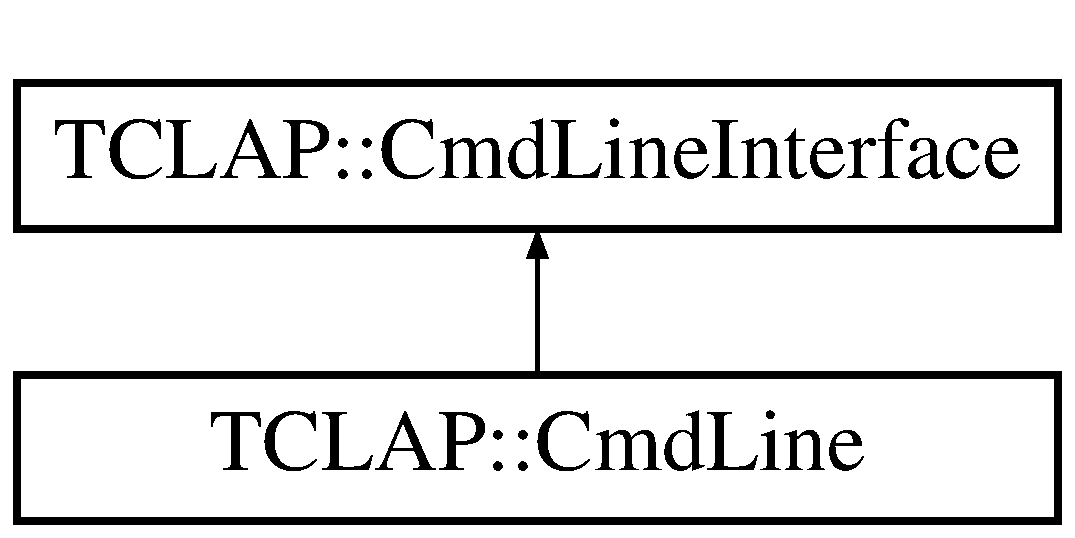
\includegraphics[height=2.000000cm]{classTCLAP_1_1CmdLineInterface}
\end{center}
\end{figure}
\subsection*{Public Member Functions}
\begin{DoxyCompactItemize}
\item 
virtual {\bf $\sim$\+Cmd\+Line\+Interface} ()
\begin{DoxyCompactList}\small\item\em Destructor. \end{DoxyCompactList}\item 
virtual void {\bf add} ({\bf Arg} \&a)=0
\begin{DoxyCompactList}\small\item\em Adds an argument to the list of arguments to be parsed. \end{DoxyCompactList}\item 
virtual void {\bf add} ({\bf Arg} $\ast$a)=0
\begin{DoxyCompactList}\small\item\em An alternative add. \end{DoxyCompactList}\item 
virtual void {\bf xor\+Add} ({\bf Arg} \&a, {\bf Arg} \&b)=0
\begin{DoxyCompactList}\small\item\em Add two Args that will be xor'd. \end{DoxyCompactList}\item 
virtual void {\bf xor\+Add} (std\+::vector$<$ {\bf Arg} $\ast$ $>$ \&xors)=0
\begin{DoxyCompactList}\small\item\em Add a list of Args that will be xor'd. \end{DoxyCompactList}\item 
virtual void {\bf parse} (int argc, const char $\ast$const $\ast$argv)=0
\begin{DoxyCompactList}\small\item\em Parses the command line. \end{DoxyCompactList}\item 
void {\bf parse} (std\+::vector$<$ std\+::string $>$ \&args)
\begin{DoxyCompactList}\small\item\em Parses the command line. \end{DoxyCompactList}\item 
virtual {\bf Cmd\+Line\+Output} $\ast$ {\bf get\+Output} ()=0
\begin{DoxyCompactList}\small\item\em Returns the \doxyref{Cmd\+Line\+Output}{p.}{classTCLAP_1_1CmdLineOutput} object. \end{DoxyCompactList}\item 
virtual void {\bf set\+Output} ({\bf Cmd\+Line\+Output} $\ast$co)=0
\item 
virtual std\+::string \& {\bf get\+Version} ()=0
\begin{DoxyCompactList}\small\item\em Returns the version string. \end{DoxyCompactList}\item 
virtual std\+::string \& {\bf get\+Program\+Name} ()=0
\begin{DoxyCompactList}\small\item\em Returns the program name string. \end{DoxyCompactList}\item 
virtual std\+::list$<$ {\bf Arg} $\ast$ $>$ \& {\bf get\+Arg\+List} ()=0
\begin{DoxyCompactList}\small\item\em Returns the arg\+List. \end{DoxyCompactList}\item 
virtual {\bf Xor\+Handler} \& {\bf get\+Xor\+Handler} ()=0
\begin{DoxyCompactList}\small\item\em Returns the \doxyref{Xor\+Handler}{p.}{classTCLAP_1_1XorHandler}. \end{DoxyCompactList}\item 
virtual char {\bf get\+Delimiter} ()=0
\begin{DoxyCompactList}\small\item\em Returns the delimiter string. \end{DoxyCompactList}\item 
virtual std\+::string \& {\bf get\+Message} ()=0
\begin{DoxyCompactList}\small\item\em Returns the message string. \end{DoxyCompactList}\item 
virtual bool {\bf has\+Help\+And\+Version} ()=0
\begin{DoxyCompactList}\small\item\em Indicates whether or not the help and version switches were created automatically. \end{DoxyCompactList}\item 
virtual void {\bf reset} ()=0
\begin{DoxyCompactList}\small\item\em Resets the instance as if it had just been constructed so that the instance can be reused. \end{DoxyCompactList}\end{DoxyCompactItemize}


\subsection{Detailed Description}
The base class that manages the command line definition and passes along the parsing to the appropriate \doxyref{Arg}{p.}{classTCLAP_1_1Arg} classes. 

Definition at line 43 of file Cmd\+Line\+Interface.\+h.



\subsection{Constructor \& Destructor Documentation}
\index{T\+C\+L\+A\+P\+::\+Cmd\+Line\+Interface@{T\+C\+L\+A\+P\+::\+Cmd\+Line\+Interface}!````~Cmd\+Line\+Interface@{$\sim$\+Cmd\+Line\+Interface}}
\index{````~Cmd\+Line\+Interface@{$\sim$\+Cmd\+Line\+Interface}!T\+C\+L\+A\+P\+::\+Cmd\+Line\+Interface@{T\+C\+L\+A\+P\+::\+Cmd\+Line\+Interface}}
\subsubsection[{$\sim$\+Cmd\+Line\+Interface}]{\setlength{\rightskip}{0pt plus 5cm}virtual T\+C\+L\+A\+P\+::\+Cmd\+Line\+Interface\+::$\sim$\+Cmd\+Line\+Interface (
\begin{DoxyParamCaption}
{}
\end{DoxyParamCaption}
)\hspace{0.3cm}{\ttfamily [inline]}, {\ttfamily [virtual]}}\label{classTCLAP_1_1CmdLineInterface_a8c7faeca5a25a96e18312da9485a94e9}


Destructor. 



Definition at line 50 of file Cmd\+Line\+Interface.\+h.


\begin{DoxyCode}
50 \{\}
\end{DoxyCode}


\subsection{Member Function Documentation}
\index{T\+C\+L\+A\+P\+::\+Cmd\+Line\+Interface@{T\+C\+L\+A\+P\+::\+Cmd\+Line\+Interface}!add@{add}}
\index{add@{add}!T\+C\+L\+A\+P\+::\+Cmd\+Line\+Interface@{T\+C\+L\+A\+P\+::\+Cmd\+Line\+Interface}}
\subsubsection[{add}]{\setlength{\rightskip}{0pt plus 5cm}virtual void T\+C\+L\+A\+P\+::\+Cmd\+Line\+Interface\+::add (
\begin{DoxyParamCaption}
\item[{{\bf Arg} \&}]{a}
\end{DoxyParamCaption}
)\hspace{0.3cm}{\ttfamily [pure virtual]}}\label{classTCLAP_1_1CmdLineInterface_a13b29ab754c030185e58f779dc355631}


Adds an argument to the list of arguments to be parsed. 


\begin{DoxyParams}{Parameters}
{\em a} & -\/ Argument to be added. \\
\hline
\end{DoxyParams}


Implemented in {\bf T\+C\+L\+A\+P\+::\+Cmd\+Line} \doxyref{}{p.}{classTCLAP_1_1CmdLine_a94c511d4735ad9b8c97edaa3827f8bbf}.



Referenced by T\+C\+L\+A\+P\+::\+Multi\+Arg$<$ T $>$\+::\+Multi\+Arg(), T\+C\+L\+A\+P\+::\+Multi\+Switch\+Arg\+::\+Multi\+Switch\+Arg(), T\+C\+L\+A\+P\+::\+Switch\+Arg\+::\+Switch\+Arg(), T\+C\+L\+A\+P\+::\+Unlabeled\+Multi\+Arg$<$ T $>$\+::\+Unlabeled\+Multi\+Arg(), T\+C\+L\+A\+P\+::\+Unlabeled\+Value\+Arg$<$ T $>$\+::\+Unlabeled\+Value\+Arg(), and T\+C\+L\+A\+P\+::\+Value\+Arg$<$ T $>$\+::\+Value\+Arg().

\index{T\+C\+L\+A\+P\+::\+Cmd\+Line\+Interface@{T\+C\+L\+A\+P\+::\+Cmd\+Line\+Interface}!add@{add}}
\index{add@{add}!T\+C\+L\+A\+P\+::\+Cmd\+Line\+Interface@{T\+C\+L\+A\+P\+::\+Cmd\+Line\+Interface}}
\subsubsection[{add}]{\setlength{\rightskip}{0pt plus 5cm}virtual void T\+C\+L\+A\+P\+::\+Cmd\+Line\+Interface\+::add (
\begin{DoxyParamCaption}
\item[{{\bf Arg} $\ast$}]{a}
\end{DoxyParamCaption}
)\hspace{0.3cm}{\ttfamily [pure virtual]}}\label{classTCLAP_1_1CmdLineInterface_a7c6a097c0f2a09dd1987e9da1af8b457}


An alternative add. 

Functionally identical. 
\begin{DoxyParams}{Parameters}
{\em a} & -\/ Argument to be added. \\
\hline
\end{DoxyParams}


Implemented in {\bf T\+C\+L\+A\+P\+::\+Cmd\+Line} \doxyref{}{p.}{classTCLAP_1_1CmdLine_ab8a08e8f4d3ca7709c85416f76e805a3}.

\index{T\+C\+L\+A\+P\+::\+Cmd\+Line\+Interface@{T\+C\+L\+A\+P\+::\+Cmd\+Line\+Interface}!get\+Arg\+List@{get\+Arg\+List}}
\index{get\+Arg\+List@{get\+Arg\+List}!T\+C\+L\+A\+P\+::\+Cmd\+Line\+Interface@{T\+C\+L\+A\+P\+::\+Cmd\+Line\+Interface}}
\subsubsection[{get\+Arg\+List}]{\setlength{\rightskip}{0pt plus 5cm}virtual std\+::list$<${\bf Arg}$\ast$$>$\& T\+C\+L\+A\+P\+::\+Cmd\+Line\+Interface\+::get\+Arg\+List (
\begin{DoxyParamCaption}
{}
\end{DoxyParamCaption}
)\hspace{0.3cm}{\ttfamily [pure virtual]}}\label{classTCLAP_1_1CmdLineInterface_a4de8d988f5a6f3007c4dfb0fc9dad476}


Returns the arg\+List. 



Implemented in {\bf T\+C\+L\+A\+P\+::\+Cmd\+Line} \doxyref{}{p.}{classTCLAP_1_1CmdLine_a3c281da929a281fb883ea47632b7ad38}.



Referenced by T\+C\+L\+A\+P\+::\+Std\+Output\+::\+\_\+long\+Usage(), T\+C\+L\+A\+P\+::\+Std\+Output\+::\+\_\+short\+Usage(), T\+C\+L\+A\+P\+::\+Doc\+Book\+Output\+::usage(), and T\+C\+L\+A\+P\+::\+Zsh\+Completion\+Output\+::usage().

\index{T\+C\+L\+A\+P\+::\+Cmd\+Line\+Interface@{T\+C\+L\+A\+P\+::\+Cmd\+Line\+Interface}!get\+Delimiter@{get\+Delimiter}}
\index{get\+Delimiter@{get\+Delimiter}!T\+C\+L\+A\+P\+::\+Cmd\+Line\+Interface@{T\+C\+L\+A\+P\+::\+Cmd\+Line\+Interface}}
\subsubsection[{get\+Delimiter}]{\setlength{\rightskip}{0pt plus 5cm}virtual char T\+C\+L\+A\+P\+::\+Cmd\+Line\+Interface\+::get\+Delimiter (
\begin{DoxyParamCaption}
{}
\end{DoxyParamCaption}
)\hspace{0.3cm}{\ttfamily [pure virtual]}}\label{classTCLAP_1_1CmdLineInterface_a7d6a64cff6b3a30e2cf1e81d7b1d4521}


Returns the delimiter string. 



Implemented in {\bf T\+C\+L\+A\+P\+::\+Cmd\+Line} \doxyref{}{p.}{classTCLAP_1_1CmdLine_a3e9f0ac2c1e97d1f8527da713ddd5a8f}.



Referenced by T\+C\+L\+A\+P\+::\+Doc\+Book\+Output\+::usage(), and T\+C\+L\+A\+P\+::\+Zsh\+Completion\+Output\+::usage().

\index{T\+C\+L\+A\+P\+::\+Cmd\+Line\+Interface@{T\+C\+L\+A\+P\+::\+Cmd\+Line\+Interface}!get\+Message@{get\+Message}}
\index{get\+Message@{get\+Message}!T\+C\+L\+A\+P\+::\+Cmd\+Line\+Interface@{T\+C\+L\+A\+P\+::\+Cmd\+Line\+Interface}}
\subsubsection[{get\+Message}]{\setlength{\rightskip}{0pt plus 5cm}virtual std\+::string\& T\+C\+L\+A\+P\+::\+Cmd\+Line\+Interface\+::get\+Message (
\begin{DoxyParamCaption}
{}
\end{DoxyParamCaption}
)\hspace{0.3cm}{\ttfamily [pure virtual]}}\label{classTCLAP_1_1CmdLineInterface_a30175a2567f7ab78a2c6bbea9269a2fa}


Returns the message string. 



Implemented in {\bf T\+C\+L\+A\+P\+::\+Cmd\+Line} \doxyref{}{p.}{classTCLAP_1_1CmdLine_a8f61a8c201e31ada985fa998180fd40f}.



Referenced by T\+C\+L\+A\+P\+::\+Std\+Output\+::\+\_\+long\+Usage(), and T\+C\+L\+A\+P\+::\+Doc\+Book\+Output\+::usage().

\index{T\+C\+L\+A\+P\+::\+Cmd\+Line\+Interface@{T\+C\+L\+A\+P\+::\+Cmd\+Line\+Interface}!get\+Output@{get\+Output}}
\index{get\+Output@{get\+Output}!T\+C\+L\+A\+P\+::\+Cmd\+Line\+Interface@{T\+C\+L\+A\+P\+::\+Cmd\+Line\+Interface}}
\subsubsection[{get\+Output}]{\setlength{\rightskip}{0pt plus 5cm}virtual {\bf Cmd\+Line\+Output}$\ast$ T\+C\+L\+A\+P\+::\+Cmd\+Line\+Interface\+::get\+Output (
\begin{DoxyParamCaption}
{}
\end{DoxyParamCaption}
)\hspace{0.3cm}{\ttfamily [pure virtual]}}\label{classTCLAP_1_1CmdLineInterface_aebc72daedeaeb03e06bb2e6e0f00363d}


Returns the \doxyref{Cmd\+Line\+Output}{p.}{classTCLAP_1_1CmdLineOutput} object. 



Implemented in {\bf T\+C\+L\+A\+P\+::\+Cmd\+Line} \doxyref{}{p.}{classTCLAP_1_1CmdLine_ad8aea2617edf53bbc20c8964ee5476e6}.

\index{T\+C\+L\+A\+P\+::\+Cmd\+Line\+Interface@{T\+C\+L\+A\+P\+::\+Cmd\+Line\+Interface}!get\+Program\+Name@{get\+Program\+Name}}
\index{get\+Program\+Name@{get\+Program\+Name}!T\+C\+L\+A\+P\+::\+Cmd\+Line\+Interface@{T\+C\+L\+A\+P\+::\+Cmd\+Line\+Interface}}
\subsubsection[{get\+Program\+Name}]{\setlength{\rightskip}{0pt plus 5cm}virtual std\+::string\& T\+C\+L\+A\+P\+::\+Cmd\+Line\+Interface\+::get\+Program\+Name (
\begin{DoxyParamCaption}
{}
\end{DoxyParamCaption}
)\hspace{0.3cm}{\ttfamily [pure virtual]}}\label{classTCLAP_1_1CmdLineInterface_a1a5672df72a6b5021cd70b37c4dbd0a7}


Returns the program name string. 



Implemented in {\bf T\+C\+L\+A\+P\+::\+Cmd\+Line} \doxyref{}{p.}{classTCLAP_1_1CmdLine_a47a6d496980ee11ffc42e27144a61797}.



Referenced by T\+C\+L\+A\+P\+::\+Std\+Output\+::\+\_\+short\+Usage(), T\+C\+L\+A\+P\+::\+Std\+Output\+::failure(), T\+C\+L\+A\+P\+::\+Doc\+Book\+Output\+::usage(), T\+C\+L\+A\+P\+::\+Zsh\+Completion\+Output\+::usage(), and T\+C\+L\+A\+P\+::\+Std\+Output\+::version().

\index{T\+C\+L\+A\+P\+::\+Cmd\+Line\+Interface@{T\+C\+L\+A\+P\+::\+Cmd\+Line\+Interface}!get\+Version@{get\+Version}}
\index{get\+Version@{get\+Version}!T\+C\+L\+A\+P\+::\+Cmd\+Line\+Interface@{T\+C\+L\+A\+P\+::\+Cmd\+Line\+Interface}}
\subsubsection[{get\+Version}]{\setlength{\rightskip}{0pt plus 5cm}virtual std\+::string\& T\+C\+L\+A\+P\+::\+Cmd\+Line\+Interface\+::get\+Version (
\begin{DoxyParamCaption}
{}
\end{DoxyParamCaption}
)\hspace{0.3cm}{\ttfamily [pure virtual]}}\label{classTCLAP_1_1CmdLineInterface_a0a552fa57212800dfb8aec84fb07b8bb}


Returns the version string. 



Implemented in {\bf T\+C\+L\+A\+P\+::\+Cmd\+Line} \doxyref{}{p.}{classTCLAP_1_1CmdLine_a85b5653d1a5b48fe6accead64615cf33}.



Referenced by T\+C\+L\+A\+P\+::\+Doc\+Book\+Output\+::usage(), T\+C\+L\+A\+P\+::\+Zsh\+Completion\+Output\+::usage(), T\+C\+L\+A\+P\+::\+Doc\+Book\+Output\+::version(), T\+C\+L\+A\+P\+::\+Std\+Output\+::version(), and T\+C\+L\+A\+P\+::\+Zsh\+Completion\+Output\+::version().

\index{T\+C\+L\+A\+P\+::\+Cmd\+Line\+Interface@{T\+C\+L\+A\+P\+::\+Cmd\+Line\+Interface}!get\+Xor\+Handler@{get\+Xor\+Handler}}
\index{get\+Xor\+Handler@{get\+Xor\+Handler}!T\+C\+L\+A\+P\+::\+Cmd\+Line\+Interface@{T\+C\+L\+A\+P\+::\+Cmd\+Line\+Interface}}
\subsubsection[{get\+Xor\+Handler}]{\setlength{\rightskip}{0pt plus 5cm}virtual {\bf Xor\+Handler}\& T\+C\+L\+A\+P\+::\+Cmd\+Line\+Interface\+::get\+Xor\+Handler (
\begin{DoxyParamCaption}
{}
\end{DoxyParamCaption}
)\hspace{0.3cm}{\ttfamily [pure virtual]}}\label{classTCLAP_1_1CmdLineInterface_a11ce9c77a1111960741f05e343849e4e}


Returns the \doxyref{Xor\+Handler}{p.}{classTCLAP_1_1XorHandler}. 



Implemented in {\bf T\+C\+L\+A\+P\+::\+Cmd\+Line} \doxyref{}{p.}{classTCLAP_1_1CmdLine_a805433b7718d1bc5bc9317bbd061449b}.



Referenced by T\+C\+L\+A\+P\+::\+Std\+Output\+::\+\_\+long\+Usage(), T\+C\+L\+A\+P\+::\+Std\+Output\+::\+\_\+short\+Usage(), T\+C\+L\+A\+P\+::\+Zsh\+Completion\+Output\+::get\+Mutex\+List(), and T\+C\+L\+A\+P\+::\+Doc\+Book\+Output\+::usage().

\index{T\+C\+L\+A\+P\+::\+Cmd\+Line\+Interface@{T\+C\+L\+A\+P\+::\+Cmd\+Line\+Interface}!has\+Help\+And\+Version@{has\+Help\+And\+Version}}
\index{has\+Help\+And\+Version@{has\+Help\+And\+Version}!T\+C\+L\+A\+P\+::\+Cmd\+Line\+Interface@{T\+C\+L\+A\+P\+::\+Cmd\+Line\+Interface}}
\subsubsection[{has\+Help\+And\+Version}]{\setlength{\rightskip}{0pt plus 5cm}virtual bool T\+C\+L\+A\+P\+::\+Cmd\+Line\+Interface\+::has\+Help\+And\+Version (
\begin{DoxyParamCaption}
{}
\end{DoxyParamCaption}
)\hspace{0.3cm}{\ttfamily [pure virtual]}}\label{classTCLAP_1_1CmdLineInterface_a441b06b764836a62083b163508210905}


Indicates whether or not the help and version switches were created automatically. 



Implemented in {\bf T\+C\+L\+A\+P\+::\+Cmd\+Line} \doxyref{}{p.}{classTCLAP_1_1CmdLine_a5b23895feae4f4110b77dae372226475}.



Referenced by T\+C\+L\+A\+P\+::\+Std\+Output\+::failure().

\index{T\+C\+L\+A\+P\+::\+Cmd\+Line\+Interface@{T\+C\+L\+A\+P\+::\+Cmd\+Line\+Interface}!parse@{parse}}
\index{parse@{parse}!T\+C\+L\+A\+P\+::\+Cmd\+Line\+Interface@{T\+C\+L\+A\+P\+::\+Cmd\+Line\+Interface}}
\subsubsection[{parse}]{\setlength{\rightskip}{0pt plus 5cm}virtual void T\+C\+L\+A\+P\+::\+Cmd\+Line\+Interface\+::parse (
\begin{DoxyParamCaption}
\item[{int}]{argc, }
\item[{const char $\ast$const $\ast$}]{argv}
\end{DoxyParamCaption}
)\hspace{0.3cm}{\ttfamily [pure virtual]}}\label{classTCLAP_1_1CmdLineInterface_a6649336bddfc8421148718a691fd89b4}


Parses the command line. 


\begin{DoxyParams}{Parameters}
{\em argc} & -\/ Number of arguments. \\
\hline
{\em argv} & -\/ Array of arguments. \\
\hline
\end{DoxyParams}


Implemented in {\bf T\+C\+L\+A\+P\+::\+Cmd\+Line} \doxyref{}{p.}{classTCLAP_1_1CmdLine_acb07daf5a1370c176a7b4a6e4119fe6e}.

\index{T\+C\+L\+A\+P\+::\+Cmd\+Line\+Interface@{T\+C\+L\+A\+P\+::\+Cmd\+Line\+Interface}!parse@{parse}}
\index{parse@{parse}!T\+C\+L\+A\+P\+::\+Cmd\+Line\+Interface@{T\+C\+L\+A\+P\+::\+Cmd\+Line\+Interface}}
\subsubsection[{parse}]{\setlength{\rightskip}{0pt plus 5cm}void T\+C\+L\+A\+P\+::\+Cmd\+Line\+Interface\+::parse (
\begin{DoxyParamCaption}
\item[{std\+::vector$<$ std\+::string $>$ \&}]{args}
\end{DoxyParamCaption}
)}\label{classTCLAP_1_1CmdLineInterface_a1b1a0cb973206a11c22003c245a4f7ed}


Parses the command line. 


\begin{DoxyParams}{Parameters}
{\em args} & -\/ A vector of strings representing the args. args[0] is still the program name. \\
\hline
\end{DoxyParams}
\index{T\+C\+L\+A\+P\+::\+Cmd\+Line\+Interface@{T\+C\+L\+A\+P\+::\+Cmd\+Line\+Interface}!reset@{reset}}
\index{reset@{reset}!T\+C\+L\+A\+P\+::\+Cmd\+Line\+Interface@{T\+C\+L\+A\+P\+::\+Cmd\+Line\+Interface}}
\subsubsection[{reset}]{\setlength{\rightskip}{0pt plus 5cm}virtual void T\+C\+L\+A\+P\+::\+Cmd\+Line\+Interface\+::reset (
\begin{DoxyParamCaption}
{}
\end{DoxyParamCaption}
)\hspace{0.3cm}{\ttfamily [pure virtual]}}\label{classTCLAP_1_1CmdLineInterface_a6b1fac8a9948ba7e28bc7844a18f39e4}


Resets the instance as if it had just been constructed so that the instance can be reused. 



Implemented in {\bf T\+C\+L\+A\+P\+::\+Cmd\+Line} \doxyref{}{p.}{classTCLAP_1_1CmdLine_a1721ec47c9d9f5ea2eca2f385fcfd2da}.

\index{T\+C\+L\+A\+P\+::\+Cmd\+Line\+Interface@{T\+C\+L\+A\+P\+::\+Cmd\+Line\+Interface}!set\+Output@{set\+Output}}
\index{set\+Output@{set\+Output}!T\+C\+L\+A\+P\+::\+Cmd\+Line\+Interface@{T\+C\+L\+A\+P\+::\+Cmd\+Line\+Interface}}
\subsubsection[{set\+Output}]{\setlength{\rightskip}{0pt plus 5cm}virtual void T\+C\+L\+A\+P\+::\+Cmd\+Line\+Interface\+::set\+Output (
\begin{DoxyParamCaption}
\item[{{\bf Cmd\+Line\+Output} $\ast$}]{co}
\end{DoxyParamCaption}
)\hspace{0.3cm}{\ttfamily [pure virtual]}}\label{classTCLAP_1_1CmdLineInterface_ab208b32bd9489781509d7ecddf8a92a0}

\begin{DoxyParams}{Parameters}
{\em co} & -\/ \doxyref{Cmd\+Line\+Output}{p.}{classTCLAP_1_1CmdLineOutput} object that we want to use instead. \\
\hline
\end{DoxyParams}


Implemented in {\bf T\+C\+L\+A\+P\+::\+Cmd\+Line} \doxyref{}{p.}{classTCLAP_1_1CmdLine_a4506e305cd10437c7ce5a5ba34cfed0f}.

\index{T\+C\+L\+A\+P\+::\+Cmd\+Line\+Interface@{T\+C\+L\+A\+P\+::\+Cmd\+Line\+Interface}!xor\+Add@{xor\+Add}}
\index{xor\+Add@{xor\+Add}!T\+C\+L\+A\+P\+::\+Cmd\+Line\+Interface@{T\+C\+L\+A\+P\+::\+Cmd\+Line\+Interface}}
\subsubsection[{xor\+Add}]{\setlength{\rightskip}{0pt plus 5cm}virtual void T\+C\+L\+A\+P\+::\+Cmd\+Line\+Interface\+::xor\+Add (
\begin{DoxyParamCaption}
\item[{{\bf Arg} \&}]{a, }
\item[{{\bf Arg} \&}]{b}
\end{DoxyParamCaption}
)\hspace{0.3cm}{\ttfamily [pure virtual]}}\label{classTCLAP_1_1CmdLineInterface_a69859e3713623eb06c9c335248d9c83f}


Add two Args that will be xor'd. 

If this method is used, add does not need to be called. 
\begin{DoxyParams}{Parameters}
{\em a} & -\/ Argument to be added and xor'd. \\
\hline
{\em b} & -\/ Argument to be added and xor'd. \\
\hline
\end{DoxyParams}


Implemented in {\bf T\+C\+L\+A\+P\+::\+Cmd\+Line} \doxyref{}{p.}{classTCLAP_1_1CmdLine_afbaa2071d0c3276b383089acabdc0dd2}.

\index{T\+C\+L\+A\+P\+::\+Cmd\+Line\+Interface@{T\+C\+L\+A\+P\+::\+Cmd\+Line\+Interface}!xor\+Add@{xor\+Add}}
\index{xor\+Add@{xor\+Add}!T\+C\+L\+A\+P\+::\+Cmd\+Line\+Interface@{T\+C\+L\+A\+P\+::\+Cmd\+Line\+Interface}}
\subsubsection[{xor\+Add}]{\setlength{\rightskip}{0pt plus 5cm}virtual void T\+C\+L\+A\+P\+::\+Cmd\+Line\+Interface\+::xor\+Add (
\begin{DoxyParamCaption}
\item[{std\+::vector$<$ {\bf Arg} $\ast$ $>$ \&}]{xors}
\end{DoxyParamCaption}
)\hspace{0.3cm}{\ttfamily [pure virtual]}}\label{classTCLAP_1_1CmdLineInterface_a6a94140e522bcf6104928fcf0c434ab8}


Add a list of Args that will be xor'd. 

If this method is used, add does not need to be called. 
\begin{DoxyParams}{Parameters}
{\em xors} & -\/ List of Args to be added and xor'd. \\
\hline
\end{DoxyParams}


Implemented in {\bf T\+C\+L\+A\+P\+::\+Cmd\+Line} \doxyref{}{p.}{classTCLAP_1_1CmdLine_ac7f2d7ee32a5157f625ad9833ab148cf}.



The documentation for this class was generated from the following file\+:\begin{DoxyCompactItemize}
\item 
{\bf Cmd\+Line\+Interface.\+h}\end{DoxyCompactItemize}

\section{T\+C\+L\+A\+P\+:\+:Cmd\+Line\+Output Class Reference}
\label{classTCLAP_1_1CmdLineOutput}\index{T\+C\+L\+A\+P\+::\+Cmd\+Line\+Output@{T\+C\+L\+A\+P\+::\+Cmd\+Line\+Output}}


The interface that any output object must implement.  




{\ttfamily \#include $<$Cmd\+Line\+Output.\+h$>$}

Inheritance diagram for T\+C\+L\+A\+P\+:\+:Cmd\+Line\+Output\+:\begin{figure}[H]
\begin{center}
\leavevmode
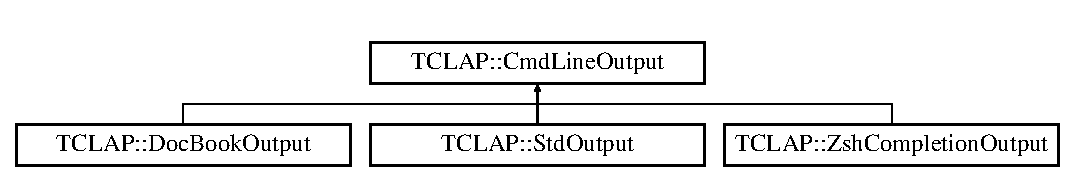
\includegraphics[height=1.996435cm]{classTCLAP_1_1CmdLineOutput}
\end{center}
\end{figure}
\subsection*{Public Member Functions}
\begin{DoxyCompactItemize}
\item 
virtual {\bf $\sim$\+Cmd\+Line\+Output} ()
\begin{DoxyCompactList}\small\item\em Virtual destructor. \end{DoxyCompactList}\item 
virtual void {\bf usage} ({\bf Cmd\+Line\+Interface} \&c)=0
\begin{DoxyCompactList}\small\item\em Generates some sort of output for the U\+S\+A\+G\+E. \end{DoxyCompactList}\item 
virtual void {\bf version} ({\bf Cmd\+Line\+Interface} \&c)=0
\begin{DoxyCompactList}\small\item\em Generates some sort of output for the version. \end{DoxyCompactList}\item 
virtual void {\bf failure} ({\bf Cmd\+Line\+Interface} \&c, {\bf Arg\+Exception} \&e)=0
\begin{DoxyCompactList}\small\item\em Generates some sort of output for a failure. \end{DoxyCompactList}\end{DoxyCompactItemize}


\subsection{Detailed Description}
The interface that any output object must implement. 

Definition at line 41 of file Cmd\+Line\+Output.\+h.



\subsection{Constructor \& Destructor Documentation}
\index{T\+C\+L\+A\+P\+::\+Cmd\+Line\+Output@{T\+C\+L\+A\+P\+::\+Cmd\+Line\+Output}!````~Cmd\+Line\+Output@{$\sim$\+Cmd\+Line\+Output}}
\index{````~Cmd\+Line\+Output@{$\sim$\+Cmd\+Line\+Output}!T\+C\+L\+A\+P\+::\+Cmd\+Line\+Output@{T\+C\+L\+A\+P\+::\+Cmd\+Line\+Output}}
\subsubsection[{$\sim$\+Cmd\+Line\+Output}]{\setlength{\rightskip}{0pt plus 5cm}virtual T\+C\+L\+A\+P\+::\+Cmd\+Line\+Output\+::$\sim$\+Cmd\+Line\+Output (
\begin{DoxyParamCaption}
{}
\end{DoxyParamCaption}
)\hspace{0.3cm}{\ttfamily [inline]}, {\ttfamily [virtual]}}\label{classTCLAP_1_1CmdLineOutput_afdf4435a2619076d9798a0a950ed405b}


Virtual destructor. 



Definition at line 49 of file Cmd\+Line\+Output.\+h.


\begin{DoxyCode}
49 \{\}
\end{DoxyCode}


\subsection{Member Function Documentation}
\index{T\+C\+L\+A\+P\+::\+Cmd\+Line\+Output@{T\+C\+L\+A\+P\+::\+Cmd\+Line\+Output}!failure@{failure}}
\index{failure@{failure}!T\+C\+L\+A\+P\+::\+Cmd\+Line\+Output@{T\+C\+L\+A\+P\+::\+Cmd\+Line\+Output}}
\subsubsection[{failure}]{\setlength{\rightskip}{0pt plus 5cm}virtual void T\+C\+L\+A\+P\+::\+Cmd\+Line\+Output\+::failure (
\begin{DoxyParamCaption}
\item[{{\bf Cmd\+Line\+Interface} \&}]{c, }
\item[{{\bf Arg\+Exception} \&}]{e}
\end{DoxyParamCaption}
)\hspace{0.3cm}{\ttfamily [pure virtual]}}\label{classTCLAP_1_1CmdLineOutput_ad23a57ac3d8d957a4328fc78aec94e16}


Generates some sort of output for a failure. 


\begin{DoxyParams}{Parameters}
{\em c} & -\/ The \doxyref{Cmd\+Line}{p.}{classTCLAP_1_1CmdLine} object the output is generated for. \\
\hline
{\em e} & -\/ The \doxyref{Arg\+Exception}{p.}{classTCLAP_1_1ArgException} that caused the failure. \\
\hline
\end{DoxyParams}


Implemented in {\bf T\+C\+L\+A\+P\+::\+Zsh\+Completion\+Output} \doxyref{}{p.}{classTCLAP_1_1ZshCompletionOutput_abcd0ba63a2ac7675d085877fc4d3e8cf}, {\bf T\+C\+L\+A\+P\+::\+Doc\+Book\+Output} \doxyref{}{p.}{classTCLAP_1_1DocBookOutput_a5e97f659fa1ab3b060a31e8bd7a0a40e}, and {\bf T\+C\+L\+A\+P\+::\+Std\+Output} \doxyref{}{p.}{classTCLAP_1_1StdOutput_a9afc267e012c3ac42c8b1afe01f98556}.



Referenced by T\+C\+L\+A\+P\+::\+Cmd\+Line\+::parse().

\index{T\+C\+L\+A\+P\+::\+Cmd\+Line\+Output@{T\+C\+L\+A\+P\+::\+Cmd\+Line\+Output}!usage@{usage}}
\index{usage@{usage}!T\+C\+L\+A\+P\+::\+Cmd\+Line\+Output@{T\+C\+L\+A\+P\+::\+Cmd\+Line\+Output}}
\subsubsection[{usage}]{\setlength{\rightskip}{0pt plus 5cm}virtual void T\+C\+L\+A\+P\+::\+Cmd\+Line\+Output\+::usage (
\begin{DoxyParamCaption}
\item[{{\bf Cmd\+Line\+Interface} \&}]{c}
\end{DoxyParamCaption}
)\hspace{0.3cm}{\ttfamily [pure virtual]}}\label{classTCLAP_1_1CmdLineOutput_a685b13db5bf6bbe5159e49169cd96bbe}


Generates some sort of output for the U\+S\+A\+G\+E. 


\begin{DoxyParams}{Parameters}
{\em c} & -\/ The \doxyref{Cmd\+Line}{p.}{classTCLAP_1_1CmdLine} object the output is generated for. \\
\hline
\end{DoxyParams}


Implemented in {\bf T\+C\+L\+A\+P\+::\+Zsh\+Completion\+Output} \doxyref{}{p.}{classTCLAP_1_1ZshCompletionOutput_a3ea685b174fce7ddf2353129863b49d7}, {\bf T\+C\+L\+A\+P\+::\+Doc\+Book\+Output} \doxyref{}{p.}{classTCLAP_1_1DocBookOutput_adc1ec93f3f7e5e912690be01c5e7d6e2}, and {\bf T\+C\+L\+A\+P\+::\+Std\+Output} \doxyref{}{p.}{classTCLAP_1_1StdOutput_aeb10eb400e0ee45f2cde689bef606b49}.

\index{T\+C\+L\+A\+P\+::\+Cmd\+Line\+Output@{T\+C\+L\+A\+P\+::\+Cmd\+Line\+Output}!version@{version}}
\index{version@{version}!T\+C\+L\+A\+P\+::\+Cmd\+Line\+Output@{T\+C\+L\+A\+P\+::\+Cmd\+Line\+Output}}
\subsubsection[{version}]{\setlength{\rightskip}{0pt plus 5cm}virtual void T\+C\+L\+A\+P\+::\+Cmd\+Line\+Output\+::version (
\begin{DoxyParamCaption}
\item[{{\bf Cmd\+Line\+Interface} \&}]{c}
\end{DoxyParamCaption}
)\hspace{0.3cm}{\ttfamily [pure virtual]}}\label{classTCLAP_1_1CmdLineOutput_ae052fea473132482296de55edb3dd480}


Generates some sort of output for the version. 


\begin{DoxyParams}{Parameters}
{\em c} & -\/ The \doxyref{Cmd\+Line}{p.}{classTCLAP_1_1CmdLine} object the output is generated for. \\
\hline
\end{DoxyParams}


Implemented in {\bf T\+C\+L\+A\+P\+::\+Zsh\+Completion\+Output} \doxyref{}{p.}{classTCLAP_1_1ZshCompletionOutput_a543e705918d769d3d6f4090c403ed0c9}, {\bf T\+C\+L\+A\+P\+::\+Doc\+Book\+Output} \doxyref{}{p.}{classTCLAP_1_1DocBookOutput_a3ccf7671dcae82aba5f0e91850ae25a4}, and {\bf T\+C\+L\+A\+P\+::\+Std\+Output} \doxyref{}{p.}{classTCLAP_1_1StdOutput_a768111a59af4753ac6e5ace3ec99482e}.



The documentation for this class was generated from the following file\+:\begin{DoxyCompactItemize}
\item 
{\bf Cmd\+Line\+Output.\+h}\end{DoxyCompactItemize}

\section{T\+C\+L\+A\+P\+:\+:Cmd\+Line\+Parse\+Exception Class Reference}
\label{classTCLAP_1_1CmdLineParseException}\index{T\+C\+L\+A\+P\+::\+Cmd\+Line\+Parse\+Exception@{T\+C\+L\+A\+P\+::\+Cmd\+Line\+Parse\+Exception}}


Thrown from \doxyref{Cmd\+Line}{p.}{classTCLAP_1_1CmdLine} when the arguments on the command line are not properly specified, e.\+g.  




{\ttfamily \#include $<$Arg\+Exception.\+h$>$}

Inheritance diagram for T\+C\+L\+A\+P\+:\+:Cmd\+Line\+Parse\+Exception\+:\begin{figure}[H]
\begin{center}
\leavevmode
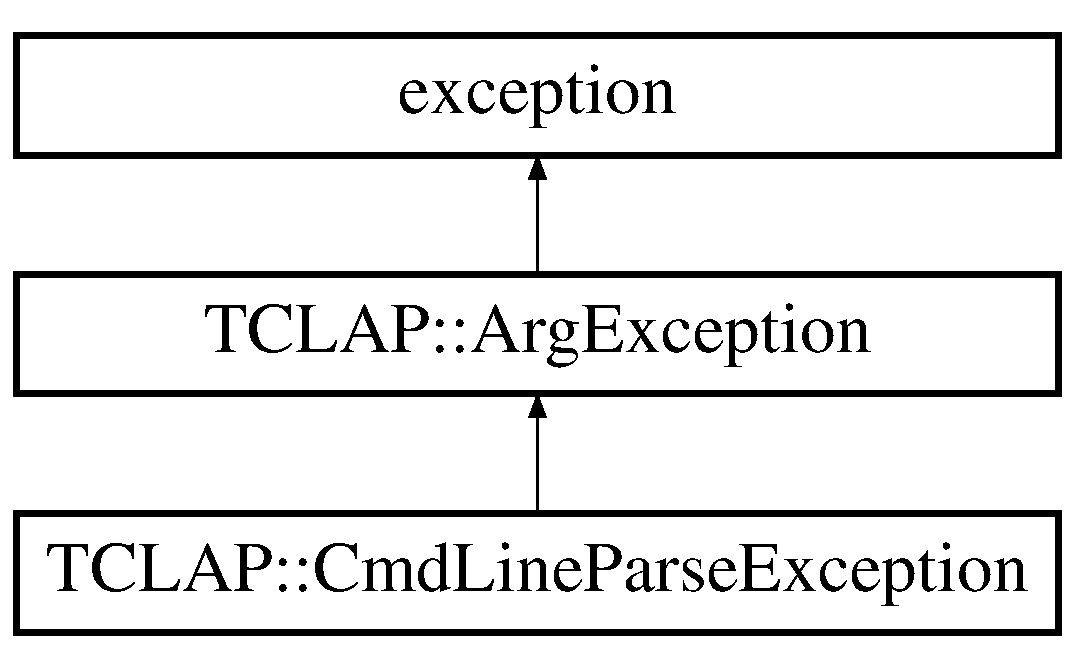
\includegraphics[height=3.000000cm]{classTCLAP_1_1CmdLineParseException}
\end{center}
\end{figure}
\subsection*{Public Member Functions}
\begin{DoxyCompactItemize}
\item 
{\bf Cmd\+Line\+Parse\+Exception} (const std\+::string \&text=\char`\"{}undefined exception\char`\"{}, const std\+::string \&id=\char`\"{}undefined\char`\"{})
\begin{DoxyCompactList}\small\item\em Constructor. \end{DoxyCompactList}\end{DoxyCompactItemize}


\subsection{Detailed Description}
Thrown from \doxyref{Cmd\+Line}{p.}{classTCLAP_1_1CmdLine} when the arguments on the command line are not properly specified, e.\+g. 

too many arguments, required argument missing, etc. 

Definition at line 143 of file Arg\+Exception.\+h.



\subsection{Constructor \& Destructor Documentation}
\index{T\+C\+L\+A\+P\+::\+Cmd\+Line\+Parse\+Exception@{T\+C\+L\+A\+P\+::\+Cmd\+Line\+Parse\+Exception}!Cmd\+Line\+Parse\+Exception@{Cmd\+Line\+Parse\+Exception}}
\index{Cmd\+Line\+Parse\+Exception@{Cmd\+Line\+Parse\+Exception}!T\+C\+L\+A\+P\+::\+Cmd\+Line\+Parse\+Exception@{T\+C\+L\+A\+P\+::\+Cmd\+Line\+Parse\+Exception}}
\subsubsection[{Cmd\+Line\+Parse\+Exception}]{\setlength{\rightskip}{0pt plus 5cm}T\+C\+L\+A\+P\+::\+Cmd\+Line\+Parse\+Exception\+::\+Cmd\+Line\+Parse\+Exception (
\begin{DoxyParamCaption}
\item[{const std\+::string \&}]{text = {\ttfamily \char`\"{}undefined~exception\char`\"{}}, }
\item[{const std\+::string \&}]{id = {\ttfamily \char`\"{}undefined\char`\"{}}}
\end{DoxyParamCaption}
)\hspace{0.3cm}{\ttfamily [inline]}}\label{classTCLAP_1_1CmdLineParseException_a3b612ba299dd699845ea108b5eaa3249}


Constructor. 


\begin{DoxyParams}{Parameters}
{\em text} & -\/ The text of the exception. \\
\hline
{\em id} & -\/ The text identifying the argument source of the exception. \\
\hline
\end{DoxyParams}


Definition at line 152 of file Arg\+Exception.\+h.


\begin{DoxyCode}
154       : ArgException( text, 
155                       \textcolor{keywordtype}{id},
156               std::string( \textcolor{stringliteral}{"Exception found when the values "}) +
157               std::string( \textcolor{stringliteral}{"on the command line do not meet "}) +
158               std::string( \textcolor{stringliteral}{"the requirements of the defined "}) +
159               std::string( \textcolor{stringliteral}{"Args."} ))
160     \{ \}
\end{DoxyCode}


The documentation for this class was generated from the following file\+:\begin{DoxyCompactItemize}
\item 
{\bf Arg\+Exception.\+h}\end{DoxyCompactItemize}

\section{T\+C\+L\+A\+P\+:\+:Constraint$<$ T $>$ Class Template Reference}
\label{classTCLAP_1_1Constraint}\index{T\+C\+L\+A\+P\+::\+Constraint$<$ T $>$@{T\+C\+L\+A\+P\+::\+Constraint$<$ T $>$}}


The interface that defines the interaction between the \doxyref{Arg}{p.}{classTCLAP_1_1Arg} and \doxyref{Constraint}{p.}{classTCLAP_1_1Constraint}.  




{\ttfamily \#include $<$Constraint.\+h$>$}

Inheritance diagram for T\+C\+L\+A\+P\+:\+:Constraint$<$ T $>$\+:\begin{figure}[H]
\begin{center}
\leavevmode
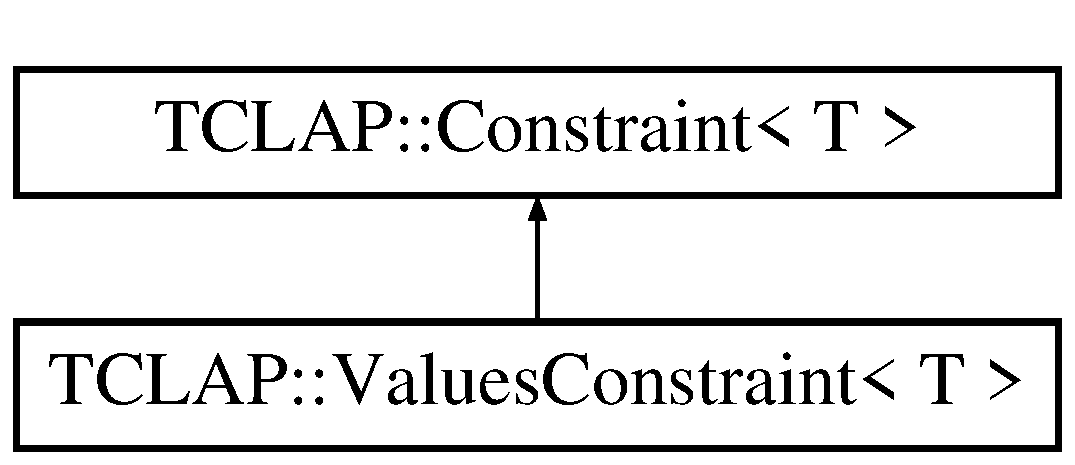
\includegraphics[height=2.000000cm]{classTCLAP_1_1Constraint}
\end{center}
\end{figure}
\subsection*{Public Member Functions}
\begin{DoxyCompactItemize}
\item 
virtual std\+::string {\bf description} () const =0
\begin{DoxyCompactList}\small\item\em Returns a description of the \doxyref{Constraint}{p.}{classTCLAP_1_1Constraint}. \end{DoxyCompactList}\item 
virtual std\+::string {\bf short\+I\+D} () const =0
\begin{DoxyCompactList}\small\item\em Returns the short I\+D for the \doxyref{Constraint}{p.}{classTCLAP_1_1Constraint}. \end{DoxyCompactList}\item 
virtual bool {\bf check} (const T \&value) const =0
\begin{DoxyCompactList}\small\item\em The method used to verify that the value parsed from the command line meets the constraint. \end{DoxyCompactList}\item 
virtual {\bf $\sim$\+Constraint} ()
\begin{DoxyCompactList}\small\item\em Destructor. \end{DoxyCompactList}\end{DoxyCompactItemize}


\subsection{Detailed Description}
\subsubsection*{template$<$class T$>$class T\+C\+L\+A\+P\+::\+Constraint$<$ T $>$}

The interface that defines the interaction between the \doxyref{Arg}{p.}{classTCLAP_1_1Arg} and \doxyref{Constraint}{p.}{classTCLAP_1_1Constraint}. 

Definition at line 38 of file Constraint.\+h.



\subsection{Constructor \& Destructor Documentation}
\index{T\+C\+L\+A\+P\+::\+Constraint@{T\+C\+L\+A\+P\+::\+Constraint}!````~Constraint@{$\sim$\+Constraint}}
\index{````~Constraint@{$\sim$\+Constraint}!T\+C\+L\+A\+P\+::\+Constraint@{T\+C\+L\+A\+P\+::\+Constraint}}
\subsubsection[{$\sim$\+Constraint}]{\setlength{\rightskip}{0pt plus 5cm}template$<$class T$>$ virtual {\bf T\+C\+L\+A\+P\+::\+Constraint}$<$ T $>$\+::$\sim${\bf Constraint} (
\begin{DoxyParamCaption}
{}
\end{DoxyParamCaption}
)\hspace{0.3cm}{\ttfamily [inline]}, {\ttfamily [virtual]}}\label{classTCLAP_1_1Constraint_ae96bbe5301e9517b68b1597b36098224}


Destructor. 

Silences warnings about \doxyref{Constraint}{p.}{classTCLAP_1_1Constraint} being a base class with virtual functions but without a virtual destructor. 

Definition at line 64 of file Constraint.\+h.


\begin{DoxyCode}
64 \{ ; \}
\end{DoxyCode}


\subsection{Member Function Documentation}
\index{T\+C\+L\+A\+P\+::\+Constraint@{T\+C\+L\+A\+P\+::\+Constraint}!check@{check}}
\index{check@{check}!T\+C\+L\+A\+P\+::\+Constraint@{T\+C\+L\+A\+P\+::\+Constraint}}
\subsubsection[{check}]{\setlength{\rightskip}{0pt plus 5cm}template$<$class T$>$ virtual bool {\bf T\+C\+L\+A\+P\+::\+Constraint}$<$ T $>$\+::check (
\begin{DoxyParamCaption}
\item[{const T \&}]{value}
\end{DoxyParamCaption}
) const\hspace{0.3cm}{\ttfamily [pure virtual]}}\label{classTCLAP_1_1Constraint_a773c3e16d0150523c1c92b7b24868c34}


The method used to verify that the value parsed from the command line meets the constraint. 


\begin{DoxyParams}{Parameters}
{\em value} & -\/ The value that will be checked. \\
\hline
\end{DoxyParams}


Implemented in {\bf T\+C\+L\+A\+P\+::\+Values\+Constraint$<$ T $>$} \doxyref{}{p.}{classTCLAP_1_1ValuesConstraint_ae132b185413cf5dea5cc040f60e7ede6}.

\index{T\+C\+L\+A\+P\+::\+Constraint@{T\+C\+L\+A\+P\+::\+Constraint}!description@{description}}
\index{description@{description}!T\+C\+L\+A\+P\+::\+Constraint@{T\+C\+L\+A\+P\+::\+Constraint}}
\subsubsection[{description}]{\setlength{\rightskip}{0pt plus 5cm}template$<$class T$>$ virtual std\+::string {\bf T\+C\+L\+A\+P\+::\+Constraint}$<$ T $>$\+::description (
\begin{DoxyParamCaption}
{}
\end{DoxyParamCaption}
) const\hspace{0.3cm}{\ttfamily [pure virtual]}}\label{classTCLAP_1_1Constraint_ae16dd80aa217fb56c0862af5478afe01}


Returns a description of the \doxyref{Constraint}{p.}{classTCLAP_1_1Constraint}. 



Implemented in {\bf T\+C\+L\+A\+P\+::\+Values\+Constraint$<$ T $>$} \doxyref{}{p.}{classTCLAP_1_1ValuesConstraint_a07b08c05a7bfcbe5815895353ffef1d5}.

\index{T\+C\+L\+A\+P\+::\+Constraint@{T\+C\+L\+A\+P\+::\+Constraint}!short\+I\+D@{short\+I\+D}}
\index{short\+I\+D@{short\+I\+D}!T\+C\+L\+A\+P\+::\+Constraint@{T\+C\+L\+A\+P\+::\+Constraint}}
\subsubsection[{short\+I\+D}]{\setlength{\rightskip}{0pt plus 5cm}template$<$class T$>$ virtual std\+::string {\bf T\+C\+L\+A\+P\+::\+Constraint}$<$ T $>$\+::short\+I\+D (
\begin{DoxyParamCaption}
{}
\end{DoxyParamCaption}
) const\hspace{0.3cm}{\ttfamily [pure virtual]}}\label{classTCLAP_1_1Constraint_a39f707895311da682439810a0bec4a5f}


Returns the short I\+D for the \doxyref{Constraint}{p.}{classTCLAP_1_1Constraint}. 



Implemented in {\bf T\+C\+L\+A\+P\+::\+Values\+Constraint$<$ T $>$} \doxyref{}{p.}{classTCLAP_1_1ValuesConstraint_a1bbe12afcb1f185ee7ac808d69e2d345}.



The documentation for this class was generated from the following file\+:\begin{DoxyCompactItemize}
\item 
{\bf Constraint.\+h}\end{DoxyCompactItemize}

\section{dqm4hep\+:\+:Dim\+Event\+Request\+Rpc Class Reference}
\label{classdqm4hep_1_1DimEventRequestRpc}\index{dqm4hep\+::\+Dim\+Event\+Request\+Rpc@{dqm4hep\+::\+Dim\+Event\+Request\+Rpc}}


\doxyref{Dim\+Event\+Request\+Rpc}{p.}{classdqm4hep_1_1DimEventRequestRpc} class.  




{\ttfamily \#include $<$D\+Q\+M\+Dim\+Event\+Collector.\+h$>$}

Inheritance diagram for dqm4hep\+:\+:Dim\+Event\+Request\+Rpc\+:\begin{figure}[H]
\begin{center}
\leavevmode
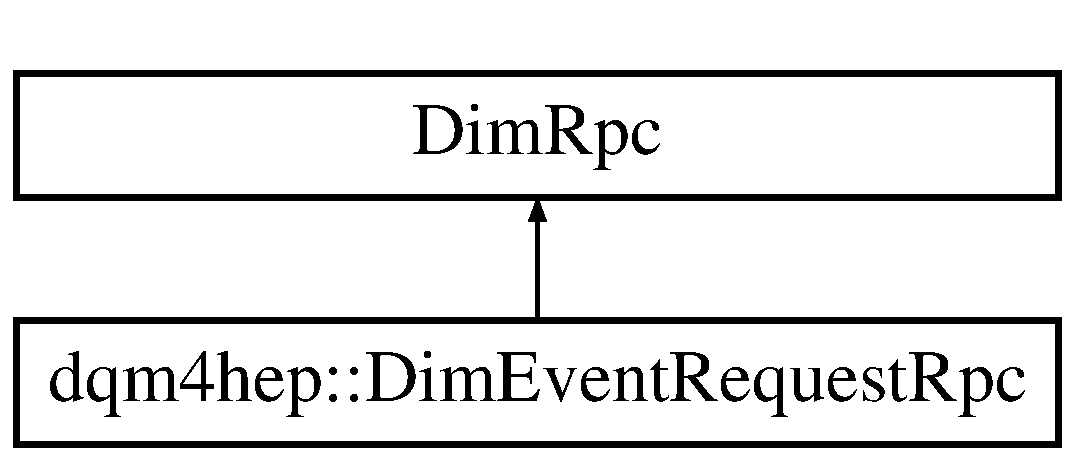
\includegraphics[height=2.000000cm]{classdqm4hep_1_1DimEventRequestRpc}
\end{center}
\end{figure}
\subsection*{Public Member Functions}
\begin{DoxyCompactItemize}
\item 
{\bf Dim\+Event\+Request\+Rpc} ({\bf D\+Q\+M\+Dim\+Event\+Collector} $\ast$p\+Collector)
\begin{DoxyCompactList}\small\item\em Constructor. \end{DoxyCompactList}\item 
void {\bf rpc\+Handler} ()
\begin{DoxyCompactList}\small\item\em The rpc handler. \end{DoxyCompactList}\end{DoxyCompactItemize}
\subsection*{Private Attributes}
\begin{DoxyCompactItemize}
\item 
{\bf D\+Q\+M\+Dim\+Event\+Collector} $\ast$ {\bf m\+\_\+p\+Collector}
\end{DoxyCompactItemize}


\subsection{Detailed Description}
\doxyref{Dim\+Event\+Request\+Rpc}{p.}{classdqm4hep_1_1DimEventRequestRpc} class. 

Definition at line 46 of file D\+Q\+M\+Dim\+Event\+Collector.\+h.



\subsection{Constructor \& Destructor Documentation}
\index{dqm4hep\+::\+Dim\+Event\+Request\+Rpc@{dqm4hep\+::\+Dim\+Event\+Request\+Rpc}!Dim\+Event\+Request\+Rpc@{Dim\+Event\+Request\+Rpc}}
\index{Dim\+Event\+Request\+Rpc@{Dim\+Event\+Request\+Rpc}!dqm4hep\+::\+Dim\+Event\+Request\+Rpc@{dqm4hep\+::\+Dim\+Event\+Request\+Rpc}}
\subsubsection[{Dim\+Event\+Request\+Rpc}]{\setlength{\rightskip}{0pt plus 5cm}dqm4hep\+::\+Dim\+Event\+Request\+Rpc\+::\+Dim\+Event\+Request\+Rpc (
\begin{DoxyParamCaption}
\item[{{\bf D\+Q\+M\+Dim\+Event\+Collector} $\ast$}]{p\+Collector}
\end{DoxyParamCaption}
)}\label{classdqm4hep_1_1DimEventRequestRpc_a117aa0f80fe1e9d0e76157757d3fac24}


Constructor. 



Definition at line 36 of file D\+Q\+M\+Dim\+Event\+Collector.\+cc.


\begin{DoxyCode}
36                                                                        :
37   DimRpc((\textcolor{keywordtype}{char}*)(\textcolor{stringliteral}{"DQM4HEP/EventCollector/"} + pCollector->getCollectorName() + \textcolor{stringliteral}{"/EVENT\_RAW\_REQUEST"}).c\_str()
      , \textcolor{stringliteral}{"C"}, \textcolor{stringliteral}{"C"}),
38   m_pCollector(pCollector)
39 \{
40   \textcolor{comment}{/* nop */}
41 \}
\end{DoxyCode}


\subsection{Member Function Documentation}
\index{dqm4hep\+::\+Dim\+Event\+Request\+Rpc@{dqm4hep\+::\+Dim\+Event\+Request\+Rpc}!rpc\+Handler@{rpc\+Handler}}
\index{rpc\+Handler@{rpc\+Handler}!dqm4hep\+::\+Dim\+Event\+Request\+Rpc@{dqm4hep\+::\+Dim\+Event\+Request\+Rpc}}
\subsubsection[{rpc\+Handler}]{\setlength{\rightskip}{0pt plus 5cm}void dqm4hep\+::\+Dim\+Event\+Request\+Rpc\+::rpc\+Handler (
\begin{DoxyParamCaption}
{}
\end{DoxyParamCaption}
)}\label{classdqm4hep_1_1DimEventRequestRpc_ad496ce317a28b5d1e63bec88db992fdd}


The rpc handler. 



Definition at line 45 of file D\+Q\+M\+Dim\+Event\+Collector.\+cc.



References dqm4hep\+::\+D\+Q\+M\+Dim\+Event\+Collector\+::handle\+Event\+Request(), and m\+\_\+p\+Collector.


\begin{DoxyCode}
46 \{
47   m_pCollector->handleEventRequest(\textcolor{keyword}{this});
48 \}
\end{DoxyCode}


\subsection{Member Data Documentation}
\index{dqm4hep\+::\+Dim\+Event\+Request\+Rpc@{dqm4hep\+::\+Dim\+Event\+Request\+Rpc}!m\+\_\+p\+Collector@{m\+\_\+p\+Collector}}
\index{m\+\_\+p\+Collector@{m\+\_\+p\+Collector}!dqm4hep\+::\+Dim\+Event\+Request\+Rpc@{dqm4hep\+::\+Dim\+Event\+Request\+Rpc}}
\subsubsection[{m\+\_\+p\+Collector}]{\setlength{\rightskip}{0pt plus 5cm}{\bf D\+Q\+M\+Dim\+Event\+Collector}$\ast$ dqm4hep\+::\+Dim\+Event\+Request\+Rpc\+::m\+\_\+p\+Collector\hspace{0.3cm}{\ttfamily [private]}}\label{classdqm4hep_1_1DimEventRequestRpc_a0ee47d9867cf28f96ef8d1ec8fa3be4c}


Definition at line 59 of file D\+Q\+M\+Dim\+Event\+Collector.\+h.



Referenced by rpc\+Handler().



The documentation for this class was generated from the following files\+:\begin{DoxyCompactItemize}
\item 
{\bf D\+Q\+M\+Dim\+Event\+Collector.\+h}\item 
{\bf D\+Q\+M\+Dim\+Event\+Collector.\+cc}\end{DoxyCompactItemize}

\section{dqm4hep\+:\+:Dim\+Event\+Rpc\+Info Class Reference}
\label{classdqm4hep_1_1DimEventRpcInfo}\index{dqm4hep\+::\+Dim\+Event\+Rpc\+Info@{dqm4hep\+::\+Dim\+Event\+Rpc\+Info}}


\doxyref{Dim\+Event\+Rpc\+Info}{p.}{classdqm4hep_1_1DimEventRpcInfo} class.  




{\ttfamily \#include $<$D\+Q\+M\+Dim\+Event\+Client.\+h$>$}

Inheritance diagram for dqm4hep\+:\+:Dim\+Event\+Rpc\+Info\+:\begin{figure}[H]
\begin{center}
\leavevmode
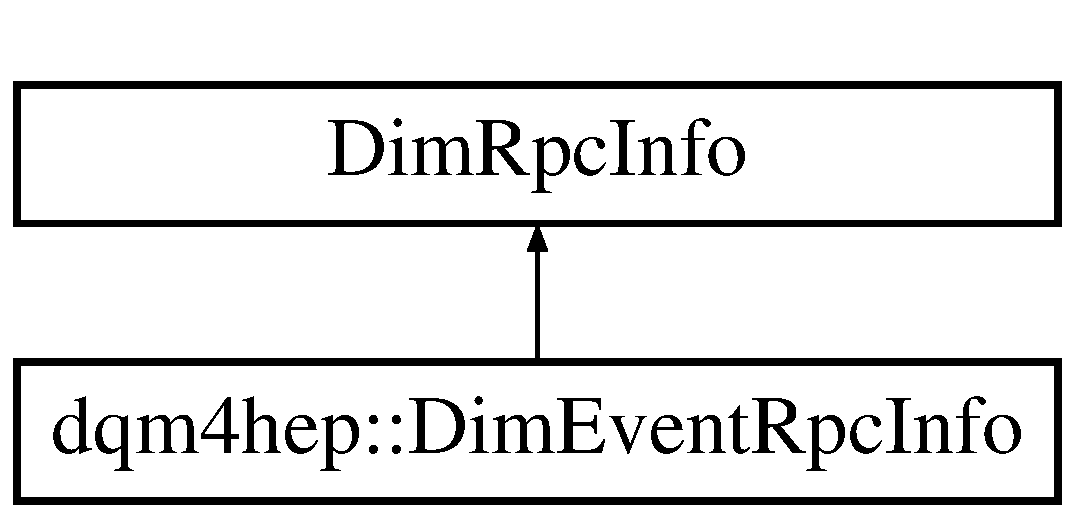
\includegraphics[height=2.000000cm]{classdqm4hep_1_1DimEventRpcInfo}
\end{center}
\end{figure}
\subsection*{Private Member Functions}
\begin{DoxyCompactItemize}
\item 
{\bf Dim\+Event\+Rpc\+Info} ({\bf D\+Q\+M\+Dim\+Event\+Client} $\ast$p\+Event\+Client)
\begin{DoxyCompactList}\small\item\em Constructor. \end{DoxyCompactList}\item 
void {\bf rpc\+Info\+Handler} ()
\begin{DoxyCompactList}\small\item\em Dim handler of rpc info. \end{DoxyCompactList}\end{DoxyCompactItemize}
\subsection*{Private Attributes}
\begin{DoxyCompactItemize}
\item 
{\bf D\+Q\+M\+Dim\+Event\+Client} $\ast$ {\bf m\+\_\+p\+Event\+Client}
\end{DoxyCompactItemize}
\subsection*{Friends}
\begin{DoxyCompactItemize}
\item 
class {\bf D\+Q\+M\+Dim\+Event\+Client}
\end{DoxyCompactItemize}


\subsection{Detailed Description}
\doxyref{Dim\+Event\+Rpc\+Info}{p.}{classdqm4hep_1_1DimEventRpcInfo} class. 

Definition at line 48 of file D\+Q\+M\+Dim\+Event\+Client.\+h.



\subsection{Constructor \& Destructor Documentation}
\index{dqm4hep\+::\+Dim\+Event\+Rpc\+Info@{dqm4hep\+::\+Dim\+Event\+Rpc\+Info}!Dim\+Event\+Rpc\+Info@{Dim\+Event\+Rpc\+Info}}
\index{Dim\+Event\+Rpc\+Info@{Dim\+Event\+Rpc\+Info}!dqm4hep\+::\+Dim\+Event\+Rpc\+Info@{dqm4hep\+::\+Dim\+Event\+Rpc\+Info}}
\subsubsection[{Dim\+Event\+Rpc\+Info}]{\setlength{\rightskip}{0pt plus 5cm}dqm4hep\+::\+Dim\+Event\+Rpc\+Info\+::\+Dim\+Event\+Rpc\+Info (
\begin{DoxyParamCaption}
\item[{{\bf D\+Q\+M\+Dim\+Event\+Client} $\ast$}]{p\+Event\+Client}
\end{DoxyParamCaption}
)\hspace{0.3cm}{\ttfamily [private]}}\label{classdqm4hep_1_1DimEventRpcInfo_a361ce42d2fba06b541ac79bc982bf0ad}


Constructor. 



Definition at line 39 of file D\+Q\+M\+Dim\+Event\+Client.\+cc.


\begin{DoxyCode}
39                                                                 :
40   DimRpcInfo((\textcolor{keywordtype}{char}*) (\textcolor{stringliteral}{"DQM4HEP/EventCollector/"} + pEventClient->getCollectorName() + \textcolor{stringliteral}{"
      /EVENT\_RAW\_BUFFER\_UPDATE"}).c\_str(), (\textcolor{keywordtype}{void}*) NULL, 0),
41   m_pEventClient(pEventClient)
42 \{
43   \textcolor{comment}{/* nop */}
44 \}
\end{DoxyCode}


\subsection{Member Function Documentation}
\index{dqm4hep\+::\+Dim\+Event\+Rpc\+Info@{dqm4hep\+::\+Dim\+Event\+Rpc\+Info}!rpc\+Info\+Handler@{rpc\+Info\+Handler}}
\index{rpc\+Info\+Handler@{rpc\+Info\+Handler}!dqm4hep\+::\+Dim\+Event\+Rpc\+Info@{dqm4hep\+::\+Dim\+Event\+Rpc\+Info}}
\subsubsection[{rpc\+Info\+Handler}]{\setlength{\rightskip}{0pt plus 5cm}void dqm4hep\+::\+Dim\+Event\+Rpc\+Info\+::rpc\+Info\+Handler (
\begin{DoxyParamCaption}
{}
\end{DoxyParamCaption}
)\hspace{0.3cm}{\ttfamily [private]}}\label{classdqm4hep_1_1DimEventRpcInfo_adf89467b00f90def581ba830ccddb0b5}


Dim handler of rpc info. 



Definition at line 48 of file D\+Q\+M\+Dim\+Event\+Client.\+cc.



References dqm4hep\+::\+D\+Q\+M\+Dim\+Event\+Client\+::event\+Reception(), and m\+\_\+p\+Event\+Client.


\begin{DoxyCode}
49 \{
50   m_pEventClient->eventReception( (dqm_char *) getData(), (dqm_uint) getSize() );
51 \}
\end{DoxyCode}


\subsection{Friends And Related Function Documentation}
\index{dqm4hep\+::\+Dim\+Event\+Rpc\+Info@{dqm4hep\+::\+Dim\+Event\+Rpc\+Info}!D\+Q\+M\+Dim\+Event\+Client@{D\+Q\+M\+Dim\+Event\+Client}}
\index{D\+Q\+M\+Dim\+Event\+Client@{D\+Q\+M\+Dim\+Event\+Client}!dqm4hep\+::\+Dim\+Event\+Rpc\+Info@{dqm4hep\+::\+Dim\+Event\+Rpc\+Info}}
\subsubsection[{D\+Q\+M\+Dim\+Event\+Client}]{\setlength{\rightskip}{0pt plus 5cm}friend class {\bf D\+Q\+M\+Dim\+Event\+Client}\hspace{0.3cm}{\ttfamily [friend]}}\label{classdqm4hep_1_1DimEventRpcInfo_a781e535ef2d0bc4f4e5475cec120f6a8}


Definition at line 50 of file D\+Q\+M\+Dim\+Event\+Client.\+h.



\subsection{Member Data Documentation}
\index{dqm4hep\+::\+Dim\+Event\+Rpc\+Info@{dqm4hep\+::\+Dim\+Event\+Rpc\+Info}!m\+\_\+p\+Event\+Client@{m\+\_\+p\+Event\+Client}}
\index{m\+\_\+p\+Event\+Client@{m\+\_\+p\+Event\+Client}!dqm4hep\+::\+Dim\+Event\+Rpc\+Info@{dqm4hep\+::\+Dim\+Event\+Rpc\+Info}}
\subsubsection[{m\+\_\+p\+Event\+Client}]{\setlength{\rightskip}{0pt plus 5cm}{\bf D\+Q\+M\+Dim\+Event\+Client}$\ast$ dqm4hep\+::\+Dim\+Event\+Rpc\+Info\+::m\+\_\+p\+Event\+Client\hspace{0.3cm}{\ttfamily [private]}}\label{classdqm4hep_1_1DimEventRpcInfo_a9e6b92e3691116e7ea69d3f07577e80e}


Definition at line 61 of file D\+Q\+M\+Dim\+Event\+Client.\+h.



Referenced by rpc\+Info\+Handler().



The documentation for this class was generated from the following files\+:\begin{DoxyCompactItemize}
\item 
{\bf D\+Q\+M\+Dim\+Event\+Client.\+h}\item 
{\bf D\+Q\+M\+Dim\+Event\+Client.\+cc}\end{DoxyCompactItemize}

\section{T\+C\+L\+A\+P\+:\+:Doc\+Book\+Output Class Reference}
\label{classTCLAP_1_1DocBookOutput}\index{T\+C\+L\+A\+P\+::\+Doc\+Book\+Output@{T\+C\+L\+A\+P\+::\+Doc\+Book\+Output}}


A class that generates Doc\+Book output for \doxyref{usage()}{p.}{classTCLAP_1_1DocBookOutput_adc1ec93f3f7e5e912690be01c5e7d6e2} method for the given \doxyref{Cmd\+Line}{p.}{classTCLAP_1_1CmdLine} and its Args.  




{\ttfamily \#include $<$Doc\+Book\+Output.\+h$>$}

Inheritance diagram for T\+C\+L\+A\+P\+:\+:Doc\+Book\+Output\+:\begin{figure}[H]
\begin{center}
\leavevmode
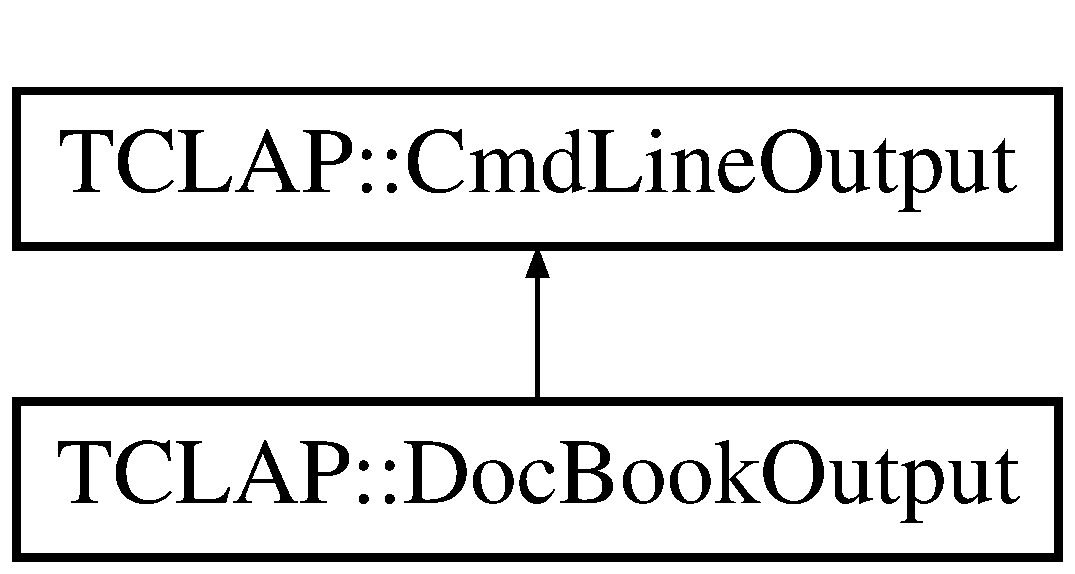
\includegraphics[height=2.000000cm]{classTCLAP_1_1DocBookOutput}
\end{center}
\end{figure}
\subsection*{Public Member Functions}
\begin{DoxyCompactItemize}
\item 
virtual void {\bf usage} ({\bf Cmd\+Line\+Interface} \&c)
\begin{DoxyCompactList}\small\item\em Prints the usage to stdout. \end{DoxyCompactList}\item 
virtual void {\bf version} ({\bf Cmd\+Line\+Interface} \&c)
\begin{DoxyCompactList}\small\item\em Prints the version to stdout. \end{DoxyCompactList}\item 
virtual void {\bf failure} ({\bf Cmd\+Line\+Interface} \&c, {\bf Arg\+Exception} \&e)
\begin{DoxyCompactList}\small\item\em Prints (to stderr) an error message, short usage Can be overridden to produce alternative behavior. \end{DoxyCompactList}\end{DoxyCompactItemize}
\subsection*{Protected Member Functions}
\begin{DoxyCompactItemize}
\item 
void {\bf substitute\+Special\+Chars} (std\+::string \&s, char r, std\+::string \&x)
\begin{DoxyCompactList}\small\item\em Substitutes the char r for string x in string s. \end{DoxyCompactList}\item 
void {\bf remove\+Char} (std\+::string \&s, char r)
\item 
void {\bf basename} (std\+::string \&s)
\item 
void {\bf print\+Short\+Arg} ({\bf Arg} $\ast$it)
\item 
void {\bf print\+Long\+Arg} ({\bf Arg} $\ast$it)
\end{DoxyCompactItemize}
\subsection*{Protected Attributes}
\begin{DoxyCompactItemize}
\item 
char {\bf the\+Delimiter}
\end{DoxyCompactItemize}


\subsection{Detailed Description}
A class that generates Doc\+Book output for \doxyref{usage()}{p.}{classTCLAP_1_1DocBookOutput_adc1ec93f3f7e5e912690be01c5e7d6e2} method for the given \doxyref{Cmd\+Line}{p.}{classTCLAP_1_1CmdLine} and its Args. 

Definition at line 43 of file Doc\+Book\+Output.\+h.



\subsection{Member Function Documentation}
\index{T\+C\+L\+A\+P\+::\+Doc\+Book\+Output@{T\+C\+L\+A\+P\+::\+Doc\+Book\+Output}!basename@{basename}}
\index{basename@{basename}!T\+C\+L\+A\+P\+::\+Doc\+Book\+Output@{T\+C\+L\+A\+P\+::\+Doc\+Book\+Output}}
\subsubsection[{basename}]{\setlength{\rightskip}{0pt plus 5cm}void T\+C\+L\+A\+P\+::\+Doc\+Book\+Output\+::basename (
\begin{DoxyParamCaption}
\item[{std\+::string \&}]{s}
\end{DoxyParamCaption}
)\hspace{0.3cm}{\ttfamily [inline]}, {\ttfamily [protected]}}\label{classTCLAP_1_1DocBookOutput_a82d49ab25845c7d191863be9c482409e}


Definition at line 203 of file Doc\+Book\+Output.\+h.



Referenced by usage().


\begin{DoxyCode}
204 \{
205   \textcolor{keywordtype}{size\_t} p = s.find\_last\_of(\textcolor{charliteral}{'/'});
206   \textcolor{keywordflow}{if} ( p != std::string::npos )
207   \{
208     s.erase(0, p + 1);
209   \}
210 \}
\end{DoxyCode}
\index{T\+C\+L\+A\+P\+::\+Doc\+Book\+Output@{T\+C\+L\+A\+P\+::\+Doc\+Book\+Output}!failure@{failure}}
\index{failure@{failure}!T\+C\+L\+A\+P\+::\+Doc\+Book\+Output@{T\+C\+L\+A\+P\+::\+Doc\+Book\+Output}}
\subsubsection[{failure}]{\setlength{\rightskip}{0pt plus 5cm}void T\+C\+L\+A\+P\+::\+Doc\+Book\+Output\+::failure (
\begin{DoxyParamCaption}
\item[{{\bf Cmd\+Line\+Interface} \&}]{c, }
\item[{{\bf Arg\+Exception} \&}]{e}
\end{DoxyParamCaption}
)\hspace{0.3cm}{\ttfamily [inline]}, {\ttfamily [virtual]}}\label{classTCLAP_1_1DocBookOutput_a5e97f659fa1ab3b060a31e8bd7a0a40e}


Prints (to stderr) an error message, short usage Can be overridden to produce alternative behavior. 


\begin{DoxyParams}{Parameters}
{\em c} & -\/ The \doxyref{Cmd\+Line}{p.}{classTCLAP_1_1CmdLine} object the output is generated for. \\
\hline
{\em e} & -\/ The \doxyref{Arg\+Exception}{p.}{classTCLAP_1_1ArgException} that caused the failure. \\
\hline
\end{DoxyParams}


Implements {\bf T\+C\+L\+A\+P\+::\+Cmd\+Line\+Output} \doxyref{}{p.}{classTCLAP_1_1CmdLineOutput_ad23a57ac3d8d957a4328fc78aec94e16}.



Definition at line 174 of file Doc\+Book\+Output.\+h.



References T\+C\+L\+A\+P\+::\+Arg\+Exception\+::what().


\begin{DoxyCode}
176 \{ 
177   \textcolor{keyword}{static\_cast<}\textcolor{keywordtype}{void}\textcolor{keyword}{>}(\_cmd); \textcolor{comment}{// unused}
178   std::cout << e.what() << std::endl;
179   \textcolor{keywordflow}{throw} ExitException(1);
180 \}
\end{DoxyCode}
\index{T\+C\+L\+A\+P\+::\+Doc\+Book\+Output@{T\+C\+L\+A\+P\+::\+Doc\+Book\+Output}!print\+Long\+Arg@{print\+Long\+Arg}}
\index{print\+Long\+Arg@{print\+Long\+Arg}!T\+C\+L\+A\+P\+::\+Doc\+Book\+Output@{T\+C\+L\+A\+P\+::\+Doc\+Book\+Output}}
\subsubsection[{print\+Long\+Arg}]{\setlength{\rightskip}{0pt plus 5cm}void T\+C\+L\+A\+P\+::\+Doc\+Book\+Output\+::print\+Long\+Arg (
\begin{DoxyParamCaption}
\item[{{\bf Arg} $\ast$}]{it}
\end{DoxyParamCaption}
)\hspace{0.3cm}{\ttfamily [inline]}, {\ttfamily [protected]}}\label{classTCLAP_1_1DocBookOutput_a891cf5ef71592b5261691575c2adad1d}


Definition at line 252 of file Doc\+Book\+Output.\+h.



Referenced by usage().


\begin{DoxyCode}
253 \{
254   std::string lt = \textcolor{stringliteral}{"&lt;"}; 
255   std::string gt = \textcolor{stringliteral}{"&gt;"}; 
256 
257   std::string desc = a->getDescription();
258   substituteSpecialChars(desc,\textcolor{charliteral}{'<'},lt);
259   substituteSpecialChars(desc,\textcolor{charliteral}{'>'},gt);
260 
261   std::cout << \textcolor{stringliteral}{"<varlistentry>"} << std::endl;
262 
263   \textcolor{keywordflow}{if} ( !a->getFlag().empty() )
264   \{
265     std::cout << \textcolor{stringliteral}{"<term>"} << std::endl;
266     std::cout << \textcolor{stringliteral}{"<option>"};
267     std::cout << a->flagStartChar() << a->getFlag();
268     std::cout << \textcolor{stringliteral}{"</option>"} << std::endl;
269     std::cout << \textcolor{stringliteral}{"</term>"} << std::endl;
270   \}
271 
272   std::cout << \textcolor{stringliteral}{"<term>"} << std::endl;
273   std::cout << \textcolor{stringliteral}{"<option>"};
274   std::cout << a->nameStartString() << a->getName();
275   \textcolor{keywordflow}{if} ( a->isValueRequired() )
276   \{
277     std::string arg = a->shortID();
278     removeChar(arg,\textcolor{charliteral}{'['});
279     removeChar(arg,\textcolor{charliteral}{']'});
280     removeChar(arg,\textcolor{charliteral}{'<'});
281     removeChar(arg,\textcolor{charliteral}{'>'});
282     arg.erase(0, arg.find\_last\_of(theDelimiter) + 1);
283     std::cout << theDelimiter;
284     std::cout << \textcolor{stringliteral}{"<replaceable>"} << arg << \textcolor{stringliteral}{"</replaceable>"};
285   \}
286   std::cout << \textcolor{stringliteral}{"</option>"} << std::endl;
287   std::cout << \textcolor{stringliteral}{"</term>"} << std::endl;
288 
289   std::cout << \textcolor{stringliteral}{"<listitem>"} << std::endl;
290   std::cout << \textcolor{stringliteral}{"<para>"} << std::endl;
291   std::cout << desc << std::endl;
292   std::cout << \textcolor{stringliteral}{"</para>"} << std::endl;
293   std::cout << \textcolor{stringliteral}{"</listitem>"} << std::endl;
294 
295   std::cout << \textcolor{stringliteral}{"</varlistentry>"} << std::endl;
296 \}
\end{DoxyCode}
\index{T\+C\+L\+A\+P\+::\+Doc\+Book\+Output@{T\+C\+L\+A\+P\+::\+Doc\+Book\+Output}!print\+Short\+Arg@{print\+Short\+Arg}}
\index{print\+Short\+Arg@{print\+Short\+Arg}!T\+C\+L\+A\+P\+::\+Doc\+Book\+Output@{T\+C\+L\+A\+P\+::\+Doc\+Book\+Output}}
\subsubsection[{print\+Short\+Arg}]{\setlength{\rightskip}{0pt plus 5cm}void T\+C\+L\+A\+P\+::\+Doc\+Book\+Output\+::print\+Short\+Arg (
\begin{DoxyParamCaption}
\item[{{\bf Arg} $\ast$}]{it}
\end{DoxyParamCaption}
)\hspace{0.3cm}{\ttfamily [inline]}, {\ttfamily [protected]}}\label{classTCLAP_1_1DocBookOutput_a980ecacfcda0186a76bb6c37a9c33726}


Definition at line 212 of file Doc\+Book\+Output.\+h.



References T\+C\+L\+A\+P\+::\+Arg\+::accepts\+Multiple\+Values(), T\+C\+L\+A\+P\+::\+Arg\+::is\+Required(), remove\+Char(), T\+C\+L\+A\+P\+::\+Arg\+::short\+I\+D(), and substitute\+Special\+Chars().



Referenced by usage().


\begin{DoxyCode}
213 \{
214   std::string lt = \textcolor{stringliteral}{"&lt;"}; 
215   std::string gt = \textcolor{stringliteral}{"&gt;"}; 
216 
217   std::string \textcolor{keywordtype}{id} = a->shortID();
218   substituteSpecialChars(\textcolor{keywordtype}{id},\textcolor{charliteral}{'<'},lt);
219   substituteSpecialChars(\textcolor{keywordtype}{id},\textcolor{charliteral}{'>'},gt);
220   removeChar(\textcolor{keywordtype}{id},\textcolor{charliteral}{'['});
221   removeChar(\textcolor{keywordtype}{id},\textcolor{charliteral}{']'});
222   
223   std::string choice = \textcolor{stringliteral}{"opt"};
224   \textcolor{keywordflow}{if} ( a->isRequired() )
225     choice = \textcolor{stringliteral}{"plain"};
226 
227   std::cout << \textcolor{stringliteral}{"<arg choice='"} << choice << \textcolor{charliteral}{'\(\backslash\)''};
228   \textcolor{keywordflow}{if} ( a->acceptsMultipleValues() )
229     std::cout << \textcolor{stringliteral}{" rep='repeat'"};
230 
231 
232   std::cout << '>\textcolor{stringliteral}{';}
233 \textcolor{stringliteral}{  if ( !a->getFlag().empty() )}
234 \textcolor{stringliteral}{    std::cout << a->flagStartChar() << a->getFlag();}
235 \textcolor{stringliteral}{  else}
236 \textcolor{stringliteral}{    std::cout << a->nameStartString() << a->getName();}
237 \textcolor{stringliteral}{  if ( a->isValueRequired() )}
238 \textcolor{stringliteral}{  \{}
239 \textcolor{stringliteral}{    std::string arg = a->shortID();}
240 \textcolor{stringliteral}{    removeChar(arg,'}[\textcolor{stringliteral}{');}
241 \textcolor{stringliteral}{    removeChar(arg,'}]\textcolor{stringliteral}{');}
242 \textcolor{stringliteral}{    removeChar(arg,'}<\textcolor{stringliteral}{');}
243 \textcolor{stringliteral}{    removeChar(arg,'}>\textcolor{stringliteral}{');}
244 \textcolor{stringliteral}{    arg.erase(0, arg.find\_last\_of(theDelimiter) + 1);}
245 \textcolor{stringliteral}{    std::cout << theDelimiter;}
246 \textcolor{stringliteral}{    std::cout << "<replaceable>" << arg << "</replaceable>";}
247 \textcolor{stringliteral}{  \}}
248 \textcolor{stringliteral}{  std::cout << "</arg>" << std::endl;}
249 \textcolor{stringliteral}{}
250 \textcolor{stringliteral}{\}}
\end{DoxyCode}
\index{T\+C\+L\+A\+P\+::\+Doc\+Book\+Output@{T\+C\+L\+A\+P\+::\+Doc\+Book\+Output}!remove\+Char@{remove\+Char}}
\index{remove\+Char@{remove\+Char}!T\+C\+L\+A\+P\+::\+Doc\+Book\+Output@{T\+C\+L\+A\+P\+::\+Doc\+Book\+Output}}
\subsubsection[{remove\+Char}]{\setlength{\rightskip}{0pt plus 5cm}void T\+C\+L\+A\+P\+::\+Doc\+Book\+Output\+::remove\+Char (
\begin{DoxyParamCaption}
\item[{std\+::string \&}]{s, }
\item[{char}]{r}
\end{DoxyParamCaption}
)\hspace{0.3cm}{\ttfamily [inline]}, {\ttfamily [protected]}}\label{classTCLAP_1_1DocBookOutput_abc059536cb97c49da4e6c5b4a22c6cef}


Definition at line 194 of file Doc\+Book\+Output.\+h.



Referenced by print\+Short\+Arg().


\begin{DoxyCode}
195 \{
196   \textcolor{keywordtype}{size\_t} p;
197   \textcolor{keywordflow}{while} ( (p = s.find\_first\_of(r)) != std::string::npos )
198   \{
199     s.erase(p,1);
200   \}
201 \}
\end{DoxyCode}
\index{T\+C\+L\+A\+P\+::\+Doc\+Book\+Output@{T\+C\+L\+A\+P\+::\+Doc\+Book\+Output}!substitute\+Special\+Chars@{substitute\+Special\+Chars}}
\index{substitute\+Special\+Chars@{substitute\+Special\+Chars}!T\+C\+L\+A\+P\+::\+Doc\+Book\+Output@{T\+C\+L\+A\+P\+::\+Doc\+Book\+Output}}
\subsubsection[{substitute\+Special\+Chars}]{\setlength{\rightskip}{0pt plus 5cm}void T\+C\+L\+A\+P\+::\+Doc\+Book\+Output\+::substitute\+Special\+Chars (
\begin{DoxyParamCaption}
\item[{std\+::string \&}]{s, }
\item[{char}]{r, }
\item[{std\+::string \&}]{x}
\end{DoxyParamCaption}
)\hspace{0.3cm}{\ttfamily [inline]}, {\ttfamily [protected]}}\label{classTCLAP_1_1DocBookOutput_a7546eaf3a0effeea1030afb27b4c698f}


Substitutes the char r for string x in string s. 


\begin{DoxyParams}{Parameters}
{\em s} & -\/ The string to operate on. \\
\hline
{\em r} & -\/ The char to replace. \\
\hline
{\em x} & -\/ What to replace r with. \\
\hline
\end{DoxyParams}


Definition at line 182 of file Doc\+Book\+Output.\+h.



Referenced by print\+Short\+Arg().


\begin{DoxyCode}
185 \{
186   \textcolor{keywordtype}{size\_t} p;
187   \textcolor{keywordflow}{while} ( (p = s.find\_first\_of(r)) != std::string::npos )
188   \{
189     s.erase(p,1);
190     s.insert(p,x);
191   \}
192 \}
\end{DoxyCode}
\index{T\+C\+L\+A\+P\+::\+Doc\+Book\+Output@{T\+C\+L\+A\+P\+::\+Doc\+Book\+Output}!usage@{usage}}
\index{usage@{usage}!T\+C\+L\+A\+P\+::\+Doc\+Book\+Output@{T\+C\+L\+A\+P\+::\+Doc\+Book\+Output}}
\subsubsection[{usage}]{\setlength{\rightskip}{0pt plus 5cm}void T\+C\+L\+A\+P\+::\+Doc\+Book\+Output\+::usage (
\begin{DoxyParamCaption}
\item[{{\bf Cmd\+Line\+Interface} \&}]{c}
\end{DoxyParamCaption}
)\hspace{0.3cm}{\ttfamily [inline]}, {\ttfamily [virtual]}}\label{classTCLAP_1_1DocBookOutput_adc1ec93f3f7e5e912690be01c5e7d6e2}


Prints the usage to stdout. 

Can be overridden to produce alternative behavior. 
\begin{DoxyParams}{Parameters}
{\em c} & -\/ The \doxyref{Cmd\+Line}{p.}{classTCLAP_1_1CmdLine} object the output is generated for. \\
\hline
\end{DoxyParams}


Implements {\bf T\+C\+L\+A\+P\+::\+Cmd\+Line\+Output} \doxyref{}{p.}{classTCLAP_1_1CmdLineOutput_a685b13db5bf6bbe5159e49169cd96bbe}.



Definition at line 95 of file Doc\+Book\+Output.\+h.



References basename(), T\+C\+L\+A\+P\+::\+Xor\+Handler\+::contains(), T\+C\+L\+A\+P\+::\+Cmd\+Line\+Interface\+::get\+Arg\+List(), T\+C\+L\+A\+P\+::\+Cmd\+Line\+Interface\+::get\+Delimiter(), T\+C\+L\+A\+P\+::\+Cmd\+Line\+Interface\+::get\+Message(), T\+C\+L\+A\+P\+::\+Cmd\+Line\+Interface\+::get\+Program\+Name(), T\+C\+L\+A\+P\+::\+Cmd\+Line\+Interface\+::get\+Version(), T\+C\+L\+A\+P\+::\+Cmd\+Line\+Interface\+::get\+Xor\+Handler(), T\+C\+L\+A\+P\+::\+Xor\+Handler\+::get\+Xor\+List(), print\+Long\+Arg(), print\+Short\+Arg(), and the\+Delimiter.


\begin{DoxyCode}
96 \{
97   std::list<Arg*> argList = \_cmd.getArgList();
98   std::string progName = \_cmd.getProgramName();
99   std::string xversion = \_cmd.getVersion();
100   theDelimiter = \_cmd.getDelimiter();
101   XorHandler xorHandler = \_cmd.getXorHandler();
102   std::vector< std::vector<Arg*> > xorList = xorHandler.getXorList();
103   basename(progName);
104 
105   std::cout << \textcolor{stringliteral}{"<?xml version='1.0'?>"} << std::endl;
106   std::cout << \textcolor{stringliteral}{"<!DOCTYPE refentry PUBLIC \(\backslash\)"-//OASIS//DTD DocBook XML V4.2//EN\(\backslash\)""} << std::endl;
107   std::cout << \textcolor{stringliteral}{"\(\backslash\)t\(\backslash\)"http://www.oasis-open.org/docbook/xml/4.2/docbookx.dtd\(\backslash\)">"} << std::endl << std::endl;
108 
109   std::cout << \textcolor{stringliteral}{"<refentry>"} << std::endl;
110 
111   std::cout << \textcolor{stringliteral}{"<refmeta>"} << std::endl;
112   std::cout << \textcolor{stringliteral}{"<refentrytitle>"} << progName << \textcolor{stringliteral}{"</refentrytitle>"} << std::endl;
113   std::cout << \textcolor{stringliteral}{"<manvolnum>1</manvolnum>"} << std::endl;
114   std::cout << \textcolor{stringliteral}{"</refmeta>"} << std::endl;
115 
116   std::cout << \textcolor{stringliteral}{"<refnamediv>"} << std::endl;
117   std::cout << \textcolor{stringliteral}{"<refname>"} << progName << \textcolor{stringliteral}{"</refname>"} << std::endl;
118   std::cout << \textcolor{stringliteral}{"<refpurpose>"} << \_cmd.getMessage() << \textcolor{stringliteral}{"</refpurpose>"} << std::endl;
119   std::cout << \textcolor{stringliteral}{"</refnamediv>"} << std::endl;
120 
121   std::cout << \textcolor{stringliteral}{"<refsynopsisdiv>"} << std::endl;
122   std::cout << \textcolor{stringliteral}{"<cmdsynopsis>"} << std::endl;
123 
124   std::cout << \textcolor{stringliteral}{"<command>"} << progName << \textcolor{stringliteral}{"</command>"} << std::endl;
125 
126   \textcolor{comment}{// xor}
127   \textcolor{keywordflow}{for} ( \textcolor{keywordtype}{int} i = 0; (\textcolor{keywordtype}{unsigned} int)i < xorList.size(); i++ )
128   \{
129     std::cout << \textcolor{stringliteral}{"<group choice='req'>"} << std::endl;
130     \textcolor{keywordflow}{for} ( ArgVectorIterator it = xorList[i].begin(); 
131             it != xorList[i].end(); it++ )
132       printShortArg((*it));
133 
134     std::cout << \textcolor{stringliteral}{"</group>"} << std::endl;
135   \}
136   
137   \textcolor{comment}{// rest of args}
138   \textcolor{keywordflow}{for} (ArgListIterator it = argList.begin(); it != argList.end(); it++)
139     \textcolor{keywordflow}{if} ( !xorHandler.contains( (*it) ) )
140       printShortArg((*it));
141 
142   std::cout << \textcolor{stringliteral}{"</cmdsynopsis>"} << std::endl;
143   std::cout << \textcolor{stringliteral}{"</refsynopsisdiv>"} << std::endl;
144 
145   std::cout << \textcolor{stringliteral}{"<refsect1>"} << std::endl;
146   std::cout << \textcolor{stringliteral}{"<title>Description</title>"} << std::endl;
147   std::cout << \textcolor{stringliteral}{"<para>"} << std::endl;
148   std::cout << \_cmd.getMessage() << std::endl; 
149   std::cout << \textcolor{stringliteral}{"</para>"} << std::endl;
150   std::cout << \textcolor{stringliteral}{"</refsect1>"} << std::endl;
151 
152   std::cout << \textcolor{stringliteral}{"<refsect1>"} << std::endl;
153   std::cout << \textcolor{stringliteral}{"<title>Options</title>"} << std::endl;
154 
155   std::cout << \textcolor{stringliteral}{"<variablelist>"} << std::endl;
156   
157   \textcolor{keywordflow}{for} (ArgListIterator it = argList.begin(); it != argList.end(); it++)
158     printLongArg((*it));
159 
160   std::cout << \textcolor{stringliteral}{"</variablelist>"} << std::endl;
161   std::cout << \textcolor{stringliteral}{"</refsect1>"} << std::endl;
162 
163   std::cout << \textcolor{stringliteral}{"<refsect1>"} << std::endl;
164   std::cout << \textcolor{stringliteral}{"<title>Version</title>"} << std::endl;
165   std::cout << \textcolor{stringliteral}{"<para>"} << std::endl;
166   std::cout << xversion << std::endl; 
167   std::cout << \textcolor{stringliteral}{"</para>"} << std::endl;
168   std::cout << \textcolor{stringliteral}{"</refsect1>"} << std::endl;
169   
170   std::cout << \textcolor{stringliteral}{"</refentry>"} << std::endl;
171 
172 \}
\end{DoxyCode}
\index{T\+C\+L\+A\+P\+::\+Doc\+Book\+Output@{T\+C\+L\+A\+P\+::\+Doc\+Book\+Output}!version@{version}}
\index{version@{version}!T\+C\+L\+A\+P\+::\+Doc\+Book\+Output@{T\+C\+L\+A\+P\+::\+Doc\+Book\+Output}}
\subsubsection[{version}]{\setlength{\rightskip}{0pt plus 5cm}void T\+C\+L\+A\+P\+::\+Doc\+Book\+Output\+::version (
\begin{DoxyParamCaption}
\item[{{\bf Cmd\+Line\+Interface} \&}]{c}
\end{DoxyParamCaption}
)\hspace{0.3cm}{\ttfamily [inline]}, {\ttfamily [virtual]}}\label{classTCLAP_1_1DocBookOutput_a3ccf7671dcae82aba5f0e91850ae25a4}


Prints the version to stdout. 

Can be overridden to produce alternative behavior. 
\begin{DoxyParams}{Parameters}
{\em c} & -\/ The \doxyref{Cmd\+Line}{p.}{classTCLAP_1_1CmdLine} object the output is generated for. \\
\hline
\end{DoxyParams}


Implements {\bf T\+C\+L\+A\+P\+::\+Cmd\+Line\+Output} \doxyref{}{p.}{classTCLAP_1_1CmdLineOutput_ae052fea473132482296de55edb3dd480}.



Definition at line 90 of file Doc\+Book\+Output.\+h.



References T\+C\+L\+A\+P\+::\+Cmd\+Line\+Interface\+::get\+Version().


\begin{DoxyCode}
91 \{ 
92   std::cout << \_cmd.getVersion() << std::endl;
93 \}
\end{DoxyCode}


\subsection{Member Data Documentation}
\index{T\+C\+L\+A\+P\+::\+Doc\+Book\+Output@{T\+C\+L\+A\+P\+::\+Doc\+Book\+Output}!the\+Delimiter@{the\+Delimiter}}
\index{the\+Delimiter@{the\+Delimiter}!T\+C\+L\+A\+P\+::\+Doc\+Book\+Output@{T\+C\+L\+A\+P\+::\+Doc\+Book\+Output}}
\subsubsection[{the\+Delimiter}]{\setlength{\rightskip}{0pt plus 5cm}char T\+C\+L\+A\+P\+::\+Doc\+Book\+Output\+::the\+Delimiter\hspace{0.3cm}{\ttfamily [protected]}}\label{classTCLAP_1_1DocBookOutput_a081a02a93ce13f694d078c79fe42a7c8}


Definition at line 86 of file Doc\+Book\+Output.\+h.



Referenced by usage().



The documentation for this class was generated from the following file\+:\begin{DoxyCompactItemize}
\item 
{\bf Doc\+Book\+Output.\+h}\end{DoxyCompactItemize}

\section{dqm4hep\+:\+:D\+Q\+M4\+H\+E\+P Class Reference}
\label{classdqm4hep_1_1DQM4HEP}\index{dqm4hep\+::\+D\+Q\+M4\+H\+E\+P@{dqm4hep\+::\+D\+Q\+M4\+H\+E\+P}}


\doxyref{D\+Q\+M4\+H\+E\+P}{p.}{classdqm4hep_1_1DQM4HEP} class.  




{\ttfamily \#include $<$D\+Q\+M4\+H\+E\+P.\+h$>$}

\subsection*{Public Member Functions}
\begin{DoxyCompactItemize}
\item 
{\footnotesize template$<$$>$ }\\bool {\bf string\+To\+Type} (const std\+::string \&s, bool \&t)
\begin{DoxyCompactList}\small\item\em Specialization for booleans. \end{DoxyCompactList}\end{DoxyCompactItemize}
\subsection*{Static Public Member Functions}
\begin{DoxyCompactItemize}
\item 
{\footnotesize template$<$class T $>$ }\\static bool {\bf string\+To\+Type} (const std\+::string \&s, T \&t)
\begin{DoxyCompactList}\small\item\em Convert std\+::string to a type. \end{DoxyCompactList}\item 
{\footnotesize template$<$class T $>$ }\\static std\+::string {\bf type\+To\+String} (const T \&t)
\begin{DoxyCompactList}\small\item\em Convert type to std\+::string. \end{DoxyCompactList}\item 
static void {\bf screen\+Splash} ()
\begin{DoxyCompactList}\small\item\em Screen splash of \doxyref{D\+Q\+M4\+H\+E\+P}{p.}{classdqm4hep_1_1DQM4HEP}. \end{DoxyCompactList}\item 
static void {\bf tokenize} (const std\+::string \&input\+String, {\bf String\+Vector} \&tokens, const std\+::string \&delimiter=\char`\"{} \char`\"{})
\begin{DoxyCompactList}\small\item\em Tokenize string with delimiter. \end{DoxyCompactList}\item 
static {\bf D\+Q\+M\+Quality} {\bf scale\+To\+Quality} (float scale)
\begin{DoxyCompactList}\small\item\em Return the quality that corresponds to a value between 0 and 1. \end{DoxyCompactList}\end{DoxyCompactItemize}


\subsection{Detailed Description}
\doxyref{D\+Q\+M4\+H\+E\+P}{p.}{classdqm4hep_1_1DQM4HEP} class. 

Definitions and utilities 

Definition at line 357 of file D\+Q\+M4\+H\+E\+P.\+h.



\subsection{Member Function Documentation}
\index{dqm4hep\+::\+D\+Q\+M4\+H\+E\+P@{dqm4hep\+::\+D\+Q\+M4\+H\+E\+P}!scale\+To\+Quality@{scale\+To\+Quality}}
\index{scale\+To\+Quality@{scale\+To\+Quality}!dqm4hep\+::\+D\+Q\+M4\+H\+E\+P@{dqm4hep\+::\+D\+Q\+M4\+H\+E\+P}}
\subsubsection[{scale\+To\+Quality}]{\setlength{\rightskip}{0pt plus 5cm}{\bf D\+Q\+M\+Quality} dqm4hep\+::\+D\+Q\+M4\+H\+E\+P\+::scale\+To\+Quality (
\begin{DoxyParamCaption}
\item[{float}]{scale}
\end{DoxyParamCaption}
)\hspace{0.3cm}{\ttfamily [static]}}\label{classdqm4hep_1_1DQM4HEP_a96cd548dd5aa7d84c97fb33c669905d7}


Return the quality that corresponds to a value between 0 and 1. 



Definition at line 126 of file D\+Q\+M4\+H\+E\+P.\+cc.



Referenced by dqm4hep\+::\+D\+Q\+M\+Mean\+Within\+Expected\+Test\+::run(), and dqm4hep\+::\+D\+Q\+M\+Chi2\+Fit\+Function\+Test\+::run().


\begin{DoxyCode}
127 \{
128   \textcolor{keywordflow}{if}(scale > 0.f && scale < 0.2f)
129     \textcolor{keywordflow}{return} VERY\_BAD\_QUALITY;
130   \textcolor{keywordflow}{else} \textcolor{keywordflow}{if}(scale < 0.4f)
131     \textcolor{keywordflow}{return} BAD\_QUALITY;
132   \textcolor{keywordflow}{else} \textcolor{keywordflow}{if}(scale < 0.6f)
133     \textcolor{keywordflow}{return} NORMAL\_QUALITY;
134   \textcolor{keywordflow}{else} \textcolor{keywordflow}{if}(scale < 0.8f)
135     \textcolor{keywordflow}{return} GOOD\_QUALITY;
136   \textcolor{keywordflow}{else} \textcolor{keywordflow}{if}(scale < 1.f)
137     \textcolor{keywordflow}{return} VERY\_GOOD\_QUALITY;
138   \textcolor{keywordflow}{else}
139     \textcolor{keywordflow}{return} NO\_QUALITY;
140 \}
\end{DoxyCode}
\index{dqm4hep\+::\+D\+Q\+M4\+H\+E\+P@{dqm4hep\+::\+D\+Q\+M4\+H\+E\+P}!screen\+Splash@{screen\+Splash}}
\index{screen\+Splash@{screen\+Splash}!dqm4hep\+::\+D\+Q\+M4\+H\+E\+P@{dqm4hep\+::\+D\+Q\+M4\+H\+E\+P}}
\subsubsection[{screen\+Splash}]{\setlength{\rightskip}{0pt plus 5cm}void dqm4hep\+::\+D\+Q\+M4\+H\+E\+P\+::screen\+Splash (
\begin{DoxyParamCaption}
{}
\end{DoxyParamCaption}
)\hspace{0.3cm}{\ttfamily [static]}}\label{classdqm4hep_1_1DQM4HEP_ae9b20898be8282f77bcfead45369ab19}


Screen splash of \doxyref{D\+Q\+M4\+H\+E\+P}{p.}{classdqm4hep_1_1DQM4HEP}. 



Definition at line 87 of file D\+Q\+M4\+H\+E\+P.\+cc.



References D\+Q\+M4\+H\+E\+P\+\_\+\+V\+E\+R\+S\+I\+O\+N\+\_\+\+S\+T\+R.


\begin{DoxyCode}
88 \{
89   time\_t t;
90   time(&t);
91   \textcolor{keywordtype}{char} *pTimeStr = \textcolor{keyword}{new} \textcolor{keywordtype}{char}[256];
92   ctime\_r(&t, pTimeStr);
93 
94   std::cout << \textcolor{stringliteral}{"#######################################################"} << std::endl;
95   std::cout << \textcolor{stringliteral}{"#"} << std::endl;
96   std::cout << \textcolor{stringliteral}{"#                    DQM4HEP"} << std::endl;
97   std::cout << \textcolor{stringliteral}{"#   (Data Quality Monitoring For High Energy Physics)"} << std::endl;
98   std::cout << \textcolor{stringliteral}{"#"} << std::endl;
99   std::cout << \textcolor{stringliteral}{"#      Version    : "} << DQM4HEP_VERSION_STR << std::endl;
100   std::cout << \textcolor{stringliteral}{"#      Started at : "} << pTimeStr << std::endl;
101   std::cout << \textcolor{stringliteral}{"#      Author     : R. Ete"} << std::endl;
102   std::cout << \textcolor{stringliteral}{"#      Mail       : <rete@ipnl.in2p3.fr> "} << std::endl;
103   std::cout << \textcolor{stringliteral}{"#"} << std::endl;
104   std::cout << \textcolor{stringliteral}{"#######################################################"} << std::endl;
105 
106   \textcolor{keyword}{delete} [] pTimeStr;
107 \}
\end{DoxyCode}
\index{dqm4hep\+::\+D\+Q\+M4\+H\+E\+P@{dqm4hep\+::\+D\+Q\+M4\+H\+E\+P}!string\+To\+Type@{string\+To\+Type}}
\index{string\+To\+Type@{string\+To\+Type}!dqm4hep\+::\+D\+Q\+M4\+H\+E\+P@{dqm4hep\+::\+D\+Q\+M4\+H\+E\+P}}
\subsubsection[{string\+To\+Type}]{\setlength{\rightskip}{0pt plus 5cm}template$<$class T $>$ bool dqm4hep\+::\+D\+Q\+M4\+H\+E\+P\+::string\+To\+Type (
\begin{DoxyParamCaption}
\item[{const std\+::string \&}]{s, }
\item[{T \&}]{t}
\end{DoxyParamCaption}
)\hspace{0.3cm}{\ttfamily [inline]}, {\ttfamily [static]}}\label{classdqm4hep_1_1DQM4HEP_a68fb565179589334d701c6a5e2ebfef7}


Convert std\+::string to a type. 



Definition at line 388 of file D\+Q\+M4\+H\+E\+P.\+h.



Referenced by dqm4hep\+::\+D\+Q\+M\+Monitor\+Element\+Manager\+::book\+Monitor\+Element(), dqm4hep\+::\+D\+Q\+M\+Xml\+Helper\+::get\+Attribute(), dqm4hep\+::\+D\+Q\+M\+Run\+::get\+Parameter(), dqm4hep\+::\+D\+Q\+M\+D\+B\+Interface\+::query(), dqm4hep\+::\+D\+Q\+M\+D\+B\+Interface\+::query\+Vector(), dqm4hep\+::\+D\+Q\+M\+Xml\+Helper\+::read2\+D\+Vector\+Of\+Values(), dqm4hep\+::\+D\+Q\+M\+Xml\+Helper\+::read\+Parameter\+Value(), dqm4hep\+::\+D\+Q\+M\+Xml\+Helper\+::read\+Parameter\+Values(), dqm4hep\+::\+D\+Q\+M\+Xml\+Helper\+::read\+Value(), and dqm4hep\+::\+D\+Q\+M\+Xml\+Helper\+::read\+Vector\+Of\+Values().


\begin{DoxyCode}
389 \{
390   std::istringstream iss(s);
391   \textcolor{keywordflow}{return} !(iss >> t).fail();
392 \}
\end{DoxyCode}
\index{dqm4hep\+::\+D\+Q\+M4\+H\+E\+P@{dqm4hep\+::\+D\+Q\+M4\+H\+E\+P}!string\+To\+Type@{string\+To\+Type}}
\index{string\+To\+Type@{string\+To\+Type}!dqm4hep\+::\+D\+Q\+M4\+H\+E\+P@{dqm4hep\+::\+D\+Q\+M4\+H\+E\+P}}
\subsubsection[{string\+To\+Type}]{\setlength{\rightskip}{0pt plus 5cm}template$<$$>$ bool dqm4hep\+::\+D\+Q\+M4\+H\+E\+P\+::string\+To\+Type (
\begin{DoxyParamCaption}
\item[{const std\+::string \&}]{s, }
\item[{bool \&}]{t}
\end{DoxyParamCaption}
)\hspace{0.3cm}{\ttfamily [inline]}}\label{classdqm4hep_1_1DQM4HEP_aabcda7533866bd3bff49e87a1e7a96f6}


Specialization for booleans. 



Definition at line 412 of file D\+Q\+M4\+H\+E\+P.\+h.


\begin{DoxyCode}
413 \{
414   \textcolor{keywordflow}{if}(s == \textcolor{stringliteral}{"on"} || s == \textcolor{stringliteral}{"1"} || s == \textcolor{stringliteral}{"true"})
415     t = \textcolor{keyword}{true};
416   \textcolor{keywordflow}{else} \textcolor{keywordflow}{if}(s == \textcolor{stringliteral}{"off"} || s == \textcolor{stringliteral}{"0"} || s == \textcolor{stringliteral}{"false"})
417     t = \textcolor{keyword}{false};
418   \textcolor{keywordflow}{else}
419     \textcolor{keywordflow}{return} \textcolor{keyword}{false};
420 
421   \textcolor{keywordflow}{return} \textcolor{keyword}{true};
422 \}
\end{DoxyCode}
\index{dqm4hep\+::\+D\+Q\+M4\+H\+E\+P@{dqm4hep\+::\+D\+Q\+M4\+H\+E\+P}!tokenize@{tokenize}}
\index{tokenize@{tokenize}!dqm4hep\+::\+D\+Q\+M4\+H\+E\+P@{dqm4hep\+::\+D\+Q\+M4\+H\+E\+P}}
\subsubsection[{tokenize}]{\setlength{\rightskip}{0pt plus 5cm}void dqm4hep\+::\+D\+Q\+M4\+H\+E\+P\+::tokenize (
\begin{DoxyParamCaption}
\item[{const std\+::string \&}]{input\+String, }
\item[{{\bf String\+Vector} \&}]{tokens, }
\item[{const std\+::string \&}]{delimiter = {\ttfamily \char`\"{}~\char`\"{}}}
\end{DoxyParamCaption}
)\hspace{0.3cm}{\ttfamily [static]}}\label{classdqm4hep_1_1DQM4HEP_a874bad0f84cbf990cf7e807d25500503}


Tokenize string with delimiter. 



Definition at line 111 of file D\+Q\+M4\+H\+E\+P.\+cc.



Referenced by dqm4hep\+::\+D\+Q\+M\+Path\+::get\+Split\+Path(), dqm4hep\+::\+D\+Q\+M\+Plugin\+Manager\+::load\+Libraries(), and dqm4hep\+::\+D\+Q\+M\+L\+C\+Event\+Streamer\+::serialize().


\begin{DoxyCode}
112 \{
113   std::string::size\_type lastPos = inputString.find\_first\_not\_of(delimiter, 0);
114   std::string::size\_type pos     = inputString.find\_first\_of(delimiter, lastPos);
115 
116   \textcolor{keywordflow}{while} ((std::string::npos != pos) || (std::string::npos != lastPos))
117   \{
118     tokens.push\_back(inputString.substr(lastPos, pos - lastPos));
119     lastPos = inputString.find\_first\_not\_of(delimiter, pos);
120     pos = inputString.find\_first\_of(delimiter, lastPos);
121   \}
122 \}
\end{DoxyCode}
\index{dqm4hep\+::\+D\+Q\+M4\+H\+E\+P@{dqm4hep\+::\+D\+Q\+M4\+H\+E\+P}!type\+To\+String@{type\+To\+String}}
\index{type\+To\+String@{type\+To\+String}!dqm4hep\+::\+D\+Q\+M4\+H\+E\+P@{dqm4hep\+::\+D\+Q\+M4\+H\+E\+P}}
\subsubsection[{type\+To\+String}]{\setlength{\rightskip}{0pt plus 5cm}template$<$class T $>$ std\+::string dqm4hep\+::\+D\+Q\+M4\+H\+E\+P\+::type\+To\+String (
\begin{DoxyParamCaption}
\item[{const T \&}]{t}
\end{DoxyParamCaption}
)\hspace{0.3cm}{\ttfamily [inline]}, {\ttfamily [static]}}\label{classdqm4hep_1_1DQM4HEP_ad631e7a04d45192aae172b994a32c6d6}


Convert type to std\+::string. 



Definition at line 397 of file D\+Q\+M4\+H\+E\+P.\+h.



Referenced by dqm4hep\+::\+D\+Q\+M\+Chi2\+Fit\+Function\+Test\+::run().


\begin{DoxyCode}
398 \{
399   std::ostringstream oss;
400 
401   \textcolor{keywordflow}{if} ((oss << t).fail())
402     \textcolor{keywordflow}{throw};
403 
404   \textcolor{keywordflow}{return} oss.str();
405 \}
\end{DoxyCode}


The documentation for this class was generated from the following files\+:\begin{DoxyCompactItemize}
\item 
{\bf D\+Q\+M4\+H\+E\+P.\+h}\item 
{\bf D\+Q\+M4\+H\+E\+P.\+cc}\end{DoxyCompactItemize}

\section{dqm4hep\+:\+:D\+Q\+M\+Analysis\+Module Class Reference}
\label{classdqm4hep_1_1DQMAnalysisModule}\index{dqm4hep\+::\+D\+Q\+M\+Analysis\+Module@{dqm4hep\+::\+D\+Q\+M\+Analysis\+Module}}


\doxyref{D\+Q\+M\+Analysis\+Module}{p.}{classdqm4hep_1_1DQMAnalysisModule} class.  




{\ttfamily \#include $<$D\+Q\+M\+Analysis\+Module.\+h$>$}

Inheritance diagram for dqm4hep\+:\+:D\+Q\+M\+Analysis\+Module\+:\begin{figure}[H]
\begin{center}
\leavevmode
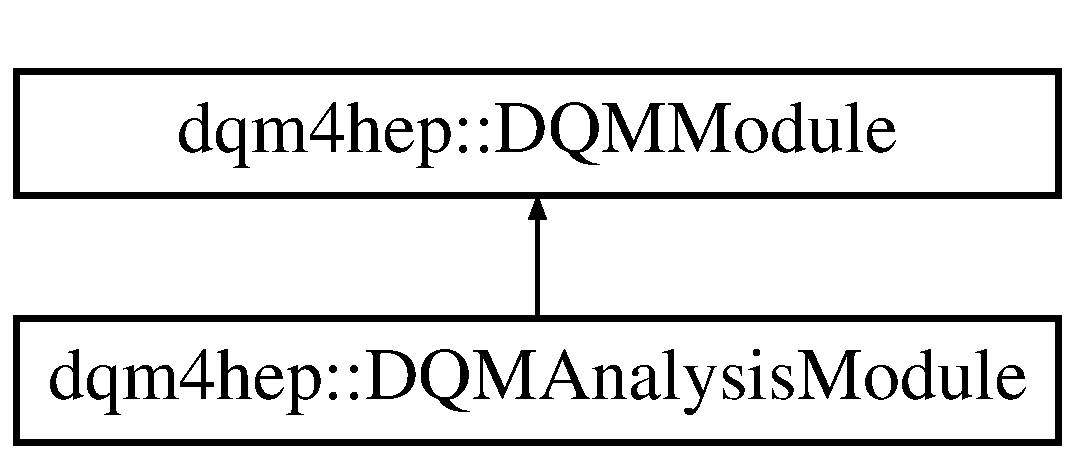
\includegraphics[height=2.000000cm]{classdqm4hep_1_1DQMAnalysisModule}
\end{center}
\end{figure}
\subsection*{Public Member Functions}
\begin{DoxyCompactItemize}
\item 
{\bf D\+Q\+M\+Analysis\+Module} ()
\begin{DoxyCompactList}\small\item\em Constructor. \end{DoxyCompactList}\item 
virtual {\bf $\sim$\+D\+Q\+M\+Analysis\+Module} ()
\begin{DoxyCompactList}\small\item\em Destructor. \end{DoxyCompactList}\item 
virtual {\bf Status\+Code} {\bf process\+Event} ({\bf D\+Q\+M\+Event} $\ast$const p\+Event)=0
\begin{DoxyCompactList}\small\item\em Process an event. \end{DoxyCompactList}\item 
virtual {\bf Status\+Code} {\bf start\+Of\+Run} ({\bf D\+Q\+M\+Run} $\ast$const p\+Run)=0
\begin{DoxyCompactList}\small\item\em Called at start of run. \end{DoxyCompactList}\item 
virtual {\bf Status\+Code} {\bf end\+Of\+Run} ({\bf D\+Q\+M\+Run} $\ast$const p\+Run)=0
\begin{DoxyCompactList}\small\item\em Called at end of run. \end{DoxyCompactList}\end{DoxyCompactItemize}
\subsection*{Friends}
\begin{DoxyCompactItemize}
\item 
class {\bf D\+Q\+M\+Analysis\+Module\+Application}
\end{DoxyCompactItemize}
\subsection*{Additional Inherited Members}


\subsection{Detailed Description}
\doxyref{D\+Q\+M\+Analysis\+Module}{p.}{classdqm4hep_1_1DQMAnalysisModule} class. 

Definition at line 44 of file D\+Q\+M\+Analysis\+Module.\+h.



\subsection{Constructor \& Destructor Documentation}
\index{dqm4hep\+::\+D\+Q\+M\+Analysis\+Module@{dqm4hep\+::\+D\+Q\+M\+Analysis\+Module}!D\+Q\+M\+Analysis\+Module@{D\+Q\+M\+Analysis\+Module}}
\index{D\+Q\+M\+Analysis\+Module@{D\+Q\+M\+Analysis\+Module}!dqm4hep\+::\+D\+Q\+M\+Analysis\+Module@{dqm4hep\+::\+D\+Q\+M\+Analysis\+Module}}
\subsubsection[{D\+Q\+M\+Analysis\+Module}]{\setlength{\rightskip}{0pt plus 5cm}dqm4hep\+::\+D\+Q\+M\+Analysis\+Module\+::\+D\+Q\+M\+Analysis\+Module (
\begin{DoxyParamCaption}
{}
\end{DoxyParamCaption}
)}\label{classdqm4hep_1_1DQMAnalysisModule_adbd6f4ed589c5c248d79479535d17f61}


Constructor. 



Definition at line 34 of file D\+Q\+M\+Analysis\+Module.\+cc.


\begin{DoxyCode}
34                                      :
35     DQMModule()
36 \{
37   \textcolor{comment}{/* nop */}
38 \}
\end{DoxyCode}
\index{dqm4hep\+::\+D\+Q\+M\+Analysis\+Module@{dqm4hep\+::\+D\+Q\+M\+Analysis\+Module}!````~D\+Q\+M\+Analysis\+Module@{$\sim$\+D\+Q\+M\+Analysis\+Module}}
\index{````~D\+Q\+M\+Analysis\+Module@{$\sim$\+D\+Q\+M\+Analysis\+Module}!dqm4hep\+::\+D\+Q\+M\+Analysis\+Module@{dqm4hep\+::\+D\+Q\+M\+Analysis\+Module}}
\subsubsection[{$\sim$\+D\+Q\+M\+Analysis\+Module}]{\setlength{\rightskip}{0pt plus 5cm}dqm4hep\+::\+D\+Q\+M\+Analysis\+Module\+::$\sim$\+D\+Q\+M\+Analysis\+Module (
\begin{DoxyParamCaption}
{}
\end{DoxyParamCaption}
)\hspace{0.3cm}{\ttfamily [virtual]}}\label{classdqm4hep_1_1DQMAnalysisModule_a3f9322e0c03ed904db53ae75ab317be4}


Destructor. 



Definition at line 42 of file D\+Q\+M\+Analysis\+Module.\+cc.


\begin{DoxyCode}
43 \{
44   \textcolor{comment}{/* nop */}
45 \}
\end{DoxyCode}


\subsection{Member Function Documentation}
\index{dqm4hep\+::\+D\+Q\+M\+Analysis\+Module@{dqm4hep\+::\+D\+Q\+M\+Analysis\+Module}!end\+Of\+Run@{end\+Of\+Run}}
\index{end\+Of\+Run@{end\+Of\+Run}!dqm4hep\+::\+D\+Q\+M\+Analysis\+Module@{dqm4hep\+::\+D\+Q\+M\+Analysis\+Module}}
\subsubsection[{end\+Of\+Run}]{\setlength{\rightskip}{0pt plus 5cm}virtual {\bf Status\+Code} dqm4hep\+::\+D\+Q\+M\+Analysis\+Module\+::end\+Of\+Run (
\begin{DoxyParamCaption}
\item[{{\bf D\+Q\+M\+Run} $\ast$const}]{p\+Run}
\end{DoxyParamCaption}
)\hspace{0.3cm}{\ttfamily [pure virtual]}}\label{classdqm4hep_1_1DQMAnalysisModule_acfae4ab693ddcc4f8d2939d50f338d3f}


Called at end of run. 



Referenced by dqm4hep\+::\+D\+Q\+M\+Analysis\+Module\+Application\+::run().

\index{dqm4hep\+::\+D\+Q\+M\+Analysis\+Module@{dqm4hep\+::\+D\+Q\+M\+Analysis\+Module}!process\+Event@{process\+Event}}
\index{process\+Event@{process\+Event}!dqm4hep\+::\+D\+Q\+M\+Analysis\+Module@{dqm4hep\+::\+D\+Q\+M\+Analysis\+Module}}
\subsubsection[{process\+Event}]{\setlength{\rightskip}{0pt plus 5cm}virtual {\bf Status\+Code} dqm4hep\+::\+D\+Q\+M\+Analysis\+Module\+::process\+Event (
\begin{DoxyParamCaption}
\item[{{\bf D\+Q\+M\+Event} $\ast$const}]{p\+Event}
\end{DoxyParamCaption}
)\hspace{0.3cm}{\ttfamily [pure virtual]}}\label{classdqm4hep_1_1DQMAnalysisModule_a832609799d8a8d5231714fa806f91142}


Process an event. 

Fill histograms in this method 

Referenced by dqm4hep\+::\+D\+Q\+M\+Analysis\+Module\+Application\+::run().

\index{dqm4hep\+::\+D\+Q\+M\+Analysis\+Module@{dqm4hep\+::\+D\+Q\+M\+Analysis\+Module}!start\+Of\+Run@{start\+Of\+Run}}
\index{start\+Of\+Run@{start\+Of\+Run}!dqm4hep\+::\+D\+Q\+M\+Analysis\+Module@{dqm4hep\+::\+D\+Q\+M\+Analysis\+Module}}
\subsubsection[{start\+Of\+Run}]{\setlength{\rightskip}{0pt plus 5cm}virtual {\bf Status\+Code} dqm4hep\+::\+D\+Q\+M\+Analysis\+Module\+::start\+Of\+Run (
\begin{DoxyParamCaption}
\item[{{\bf D\+Q\+M\+Run} $\ast$const}]{p\+Run}
\end{DoxyParamCaption}
)\hspace{0.3cm}{\ttfamily [pure virtual]}}\label{classdqm4hep_1_1DQMAnalysisModule_a6ed7c4f30a3568da5bc76bb8d71d45be}


Called at start of run. 



Referenced by dqm4hep\+::\+D\+Q\+M\+Analysis\+Module\+Application\+::run().



\subsection{Friends And Related Function Documentation}
\index{dqm4hep\+::\+D\+Q\+M\+Analysis\+Module@{dqm4hep\+::\+D\+Q\+M\+Analysis\+Module}!D\+Q\+M\+Analysis\+Module\+Application@{D\+Q\+M\+Analysis\+Module\+Application}}
\index{D\+Q\+M\+Analysis\+Module\+Application@{D\+Q\+M\+Analysis\+Module\+Application}!dqm4hep\+::\+D\+Q\+M\+Analysis\+Module@{dqm4hep\+::\+D\+Q\+M\+Analysis\+Module}}
\subsubsection[{D\+Q\+M\+Analysis\+Module\+Application}]{\setlength{\rightskip}{0pt plus 5cm}friend class {\bf D\+Q\+M\+Analysis\+Module\+Application}\hspace{0.3cm}{\ttfamily [friend]}}\label{classdqm4hep_1_1DQMAnalysisModule_a05f4747ee57a511681544ef82bdb80c3}


Definition at line 46 of file D\+Q\+M\+Analysis\+Module.\+h.



The documentation for this class was generated from the following files\+:\begin{DoxyCompactItemize}
\item 
{\bf D\+Q\+M\+Analysis\+Module.\+h}\item 
{\bf D\+Q\+M\+Analysis\+Module.\+cc}\end{DoxyCompactItemize}

\section{dqm4hep\+:\+:D\+Q\+M\+Analysis\+Module\+Application Class Reference}
\label{classdqm4hep_1_1DQMAnalysisModuleApplication}\index{dqm4hep\+::\+D\+Q\+M\+Analysis\+Module\+Application@{dqm4hep\+::\+D\+Q\+M\+Analysis\+Module\+Application}}


\doxyref{D\+Q\+M\+Analysis\+Module\+Application}{p.}{classdqm4hep_1_1DQMAnalysisModuleApplication} class.  




{\ttfamily \#include $<$D\+Q\+M\+Analysis\+Module\+Application.\+h$>$}

Inheritance diagram for dqm4hep\+:\+:D\+Q\+M\+Analysis\+Module\+Application\+:\begin{figure}[H]
\begin{center}
\leavevmode
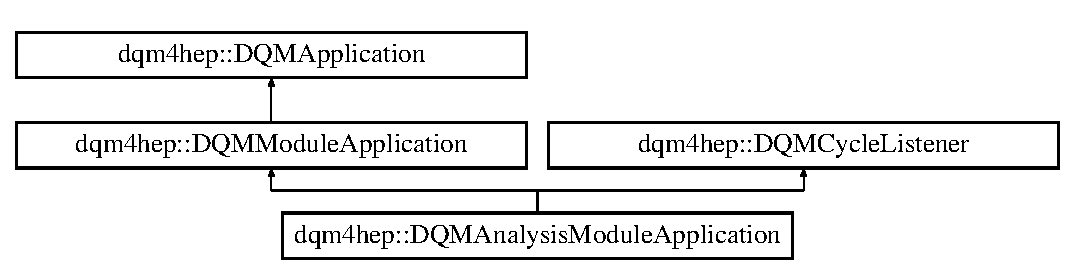
\includegraphics[height=3.000000cm]{classdqm4hep_1_1DQMAnalysisModuleApplication}
\end{center}
\end{figure}
\subsection*{Classes}
\begin{DoxyCompactItemize}
\item 
class {\bf Settings}
\begin{DoxyCompactList}\small\item\em \doxyref{Settings}{p.}{classdqm4hep_1_1DQMAnalysisModuleApplication_1_1Settings} class. \end{DoxyCompactList}\end{DoxyCompactItemize}
\subsection*{Public Member Functions}
\begin{DoxyCompactItemize}
\item 
{\bf D\+Q\+M\+Analysis\+Module\+Application} ()
\begin{DoxyCompactList}\small\item\em Constructor. \end{DoxyCompactList}\item 
{\bf $\sim$\+D\+Q\+M\+Analysis\+Module\+Application} ()
\begin{DoxyCompactList}\small\item\em Destructor. \end{DoxyCompactList}\item 
const std\+::string \& {\bf get\+Type} () const 
\begin{DoxyCompactList}\small\item\em Get the application type (\char`\"{}\+Analysis\+Module\char`\"{}) \end{DoxyCompactList}\item 
const std\+::string \& {\bf get\+Name} () const 
\begin{DoxyCompactList}\small\item\em Get the application name (\char`\"{}\+Module\+Type/\+Module\+Name\char`\"{}) \end{DoxyCompactList}\item 
{\bf Status\+Code} {\bf read\+Settings} (const std\+::string \&settings\+File)
\begin{DoxyCompactList}\small\item\em Read settings from a xml file. \end{DoxyCompactList}\item 
{\bf Status\+Code} {\bf run} ()
\begin{DoxyCompactList}\small\item\em Run the application. \end{DoxyCompactList}\end{DoxyCompactItemize}
\subsection*{Private Member Functions}
\begin{DoxyCompactItemize}
\item 
{\bf Status\+Code} {\bf configure\+Module} (const {\bf Ti\+Xml\+Handle} xml\+Handle)
\begin{DoxyCompactList}\small\item\em Configure the module. \end{DoxyCompactList}\item 
{\bf Status\+Code} {\bf configure\+Network} (const {\bf Ti\+Xml\+Handle} xml\+Handle)
\begin{DoxyCompactList}\small\item\em Configure network interface. \end{DoxyCompactList}\item 
{\bf Status\+Code} {\bf configure\+Cycle} (const {\bf Ti\+Xml\+Handle} xml\+Handle)
\begin{DoxyCompactList}\small\item\em Configure the workflow cycle. \end{DoxyCompactList}\item 
{\bf Status\+Code} {\bf configure\+Archiver} (const {\bf Ti\+Xml\+Handle} xml\+Handle)
\begin{DoxyCompactList}\small\item\em Configure the archiver. \end{DoxyCompactList}\item 
{\bf Status\+Code} {\bf start\+Services} ()
\begin{DoxyCompactList}\small\item\em Start all services. \end{DoxyCompactList}\item 
{\bf Status\+Code} {\bf stop\+Services} ()
\begin{DoxyCompactList}\small\item\em Stop all services. \end{DoxyCompactList}\item 
int {\bf get\+Current\+Run\+Number} () const 
\begin{DoxyCompactList}\small\item\em Get the current run number that was started (not from run control) \end{DoxyCompactList}\item 
void {\bf on\+Event\+Processed} (const {\bf D\+Q\+M\+Cycle} $\ast$const p\+Cycle, const {\bf D\+Q\+M\+Event} $\ast$const p\+Event)
\begin{DoxyCompactList}\small\item\em Call back function when an event is processed by the framework. \end{DoxyCompactList}\item 
void {\bf on\+Cycle\+Started} (const {\bf D\+Q\+M\+Cycle} $\ast$const p\+Cycle)
\begin{DoxyCompactList}\small\item\em Call back function when the cycle is started by the framework. \end{DoxyCompactList}\item 
void {\bf on\+Cycle\+Stopped} (const {\bf D\+Q\+M\+Cycle} $\ast$const p\+Cycle)
\begin{DoxyCompactList}\small\item\em Call back function when the cycle is stopped by the framework. \end{DoxyCompactList}\end{DoxyCompactItemize}
\subsection*{Private Attributes}
\begin{DoxyCompactItemize}
\item 
{\bf Settings} {\bf m\+\_\+settings}
\item 
{\bf D\+Q\+M\+Event\+Client} $\ast$ {\bf m\+\_\+p\+Event\+Client}
\item 
{\bf D\+Q\+M\+Run\+Control\+Client} $\ast$ {\bf m\+\_\+p\+Run\+Control\+Client}
\item 
{\bf D\+Q\+M\+Cycle} $\ast$ {\bf m\+\_\+p\+Cycle}
\item 
{\bf D\+Q\+M\+Archiver} $\ast$ {\bf m\+\_\+p\+Archiver}
\item 
std\+::string {\bf m\+\_\+application\+Type}
\item 
std\+::string {\bf m\+\_\+application\+Name}
\item 
int {\bf m\+\_\+run\+Number}
\end{DoxyCompactItemize}
\subsection*{Additional Inherited Members}


\subsection{Detailed Description}
\doxyref{D\+Q\+M\+Analysis\+Module\+Application}{p.}{classdqm4hep_1_1DQMAnalysisModuleApplication} class. 

Definition at line 49 of file D\+Q\+M\+Analysis\+Module\+Application.\+h.



\subsection{Constructor \& Destructor Documentation}
\index{dqm4hep\+::\+D\+Q\+M\+Analysis\+Module\+Application@{dqm4hep\+::\+D\+Q\+M\+Analysis\+Module\+Application}!D\+Q\+M\+Analysis\+Module\+Application@{D\+Q\+M\+Analysis\+Module\+Application}}
\index{D\+Q\+M\+Analysis\+Module\+Application@{D\+Q\+M\+Analysis\+Module\+Application}!dqm4hep\+::\+D\+Q\+M\+Analysis\+Module\+Application@{dqm4hep\+::\+D\+Q\+M\+Analysis\+Module\+Application}}
\subsubsection[{D\+Q\+M\+Analysis\+Module\+Application}]{\setlength{\rightskip}{0pt plus 5cm}dqm4hep\+::\+D\+Q\+M\+Analysis\+Module\+Application\+::\+D\+Q\+M\+Analysis\+Module\+Application (
\begin{DoxyParamCaption}
{}
\end{DoxyParamCaption}
)}\label{classdqm4hep_1_1DQMAnalysisModuleApplication_a4d117b05bc4ddf26988a41fc00bfa733}


Constructor. 



Definition at line 59 of file D\+Q\+M\+Analysis\+Module\+Application.\+cc.



References dqm4hep\+::\+D\+Q\+M\+Module\+Application\+::\+D\+Q\+M\+Archiver, and m\+\_\+p\+Archiver.


\begin{DoxyCode}
59                                                            :
60     DQMModuleApplication(),
61     m_pEventClient(NULL),
62     m_pRunControlClient(NULL),
63     m_pCycle(NULL),
64     m_applicationType(\textcolor{stringliteral}{"AnalysisModule"}),
65     m_applicationName(\textcolor{stringliteral}{"UNKNOWN"}),
66     m_runNumber(-1)
67 \{
68   m_pArchiver = \textcolor{keyword}{new} DQMArchiver();
69 \}
\end{DoxyCode}
\index{dqm4hep\+::\+D\+Q\+M\+Analysis\+Module\+Application@{dqm4hep\+::\+D\+Q\+M\+Analysis\+Module\+Application}!````~D\+Q\+M\+Analysis\+Module\+Application@{$\sim$\+D\+Q\+M\+Analysis\+Module\+Application}}
\index{````~D\+Q\+M\+Analysis\+Module\+Application@{$\sim$\+D\+Q\+M\+Analysis\+Module\+Application}!dqm4hep\+::\+D\+Q\+M\+Analysis\+Module\+Application@{dqm4hep\+::\+D\+Q\+M\+Analysis\+Module\+Application}}
\subsubsection[{$\sim$\+D\+Q\+M\+Analysis\+Module\+Application}]{\setlength{\rightskip}{0pt plus 5cm}dqm4hep\+::\+D\+Q\+M\+Analysis\+Module\+Application\+::$\sim$\+D\+Q\+M\+Analysis\+Module\+Application (
\begin{DoxyParamCaption}
{}
\end{DoxyParamCaption}
)}\label{classdqm4hep_1_1DQMAnalysisModuleApplication_a663febee6eaaeee2bc8a920ee9204eb7}


Destructor. 



Definition at line 73 of file D\+Q\+M\+Analysis\+Module\+Application.\+cc.



References m\+\_\+p\+Archiver, m\+\_\+p\+Cycle, m\+\_\+p\+Event\+Client, and m\+\_\+p\+Run\+Control\+Client.


\begin{DoxyCode}
74 \{
75   \textcolor{keyword}{delete} m_pArchiver;
76 
77   \textcolor{keywordflow}{if}(m_pEventClient)
78     \textcolor{keyword}{delete} m_pEventClient;
79 
80   \textcolor{keywordflow}{if}(m_pRunControlClient)
81     \textcolor{keyword}{delete} m_pRunControlClient;
82 
83   \textcolor{keywordflow}{if}(m_pCycle)
84     \textcolor{keyword}{delete} m_pCycle;
85 \}
\end{DoxyCode}


\subsection{Member Function Documentation}
\index{dqm4hep\+::\+D\+Q\+M\+Analysis\+Module\+Application@{dqm4hep\+::\+D\+Q\+M\+Analysis\+Module\+Application}!configure\+Archiver@{configure\+Archiver}}
\index{configure\+Archiver@{configure\+Archiver}!dqm4hep\+::\+D\+Q\+M\+Analysis\+Module\+Application@{dqm4hep\+::\+D\+Q\+M\+Analysis\+Module\+Application}}
\subsubsection[{configure\+Archiver}]{\setlength{\rightskip}{0pt plus 5cm}{\bf Status\+Code} dqm4hep\+::\+D\+Q\+M\+Analysis\+Module\+Application\+::configure\+Archiver (
\begin{DoxyParamCaption}
\item[{const {\bf Ti\+Xml\+Handle}}]{xml\+Handle}
\end{DoxyParamCaption}
)\hspace{0.3cm}{\ttfamily [private]}}\label{classdqm4hep_1_1DQMAnalysisModuleApplication_aaa1b0aae6e493636cbedc6194ac1ed2b}


Configure the archiver. 



Definition at line 547 of file D\+Q\+M\+Analysis\+Module\+Application.\+cc.



References dqm4hep\+::\+Ti\+Xml\+Handle\+::\+Element(), dqm4hep\+::\+Ti\+Xml\+Handle\+::\+First\+Child\+Element(), dqm4hep\+::\+D\+Q\+M\+Xml\+Helper\+::get\+Attribute(), dqm4hep\+::\+Status\+Code\+Exception\+::get\+Status\+Code(), dqm4hep\+::\+D\+Q\+M\+Analysis\+Module\+Application\+::\+Settings\+::m\+\_\+archive\+Directory, m\+\_\+settings, dqm4hep\+::\+D\+Q\+M\+Analysis\+Module\+Application\+::\+Settings\+::m\+\_\+should\+Open\+Archive, dqm4hep\+::\+M\+E\+S\+S\+A\+G\+E, and T\+H\+R\+O\+W\+\_\+\+R\+E\+S\+U\+L\+T\+\_\+\+I\+F.



Referenced by read\+Settings().


\begin{DoxyCode}
548 \{
549   \textcolor{keywordflow}{try}
550   \{
551     streamlog\_out(MESSAGE) << \textcolor{stringliteral}{"DQMAnalysisModuleApplication::configureArchiver: configuring ..."} << 
      std::endl;
552 
553     \textcolor{keyword}{const} TiXmlElement *\textcolor{keyword}{const} pXmlElement = xmlHandle.FirstChildElement(\textcolor{stringliteral}{"archiver"}).Element();
554 
555     THROW_RESULT_IF(STATUS\_CODE\_SUCCESS, !=, DQMXmlHelper::getAttribute(pXmlElement, \textcolor{stringliteral}{"open"}, 
      m_settings.m_shouldOpenArchive));
556     THROW_RESULT_IF(STATUS\_CODE\_SUCCESS, !=, DQMXmlHelper::getAttribute(pXmlElement, \textcolor{stringliteral}{"directory"}, 
      m_settings.m_archiveDirectory));
557 
558     streamlog\_out(MESSAGE) << \textcolor{stringliteral}{"DQMAnalysisModuleApplication::configureArchiver: configuring ... OK"} << 
      std::endl;
559   \}
560   \textcolor{keywordflow}{catch}(\textcolor{keyword}{const} StatusCodeException &exception)
561   \{
562     \textcolor{keywordflow}{return} exception.getStatusCode();
563   \}
564 
565   \textcolor{keywordflow}{return} STATUS\_CODE\_SUCCESS;
566 \}
\end{DoxyCode}
\index{dqm4hep\+::\+D\+Q\+M\+Analysis\+Module\+Application@{dqm4hep\+::\+D\+Q\+M\+Analysis\+Module\+Application}!configure\+Cycle@{configure\+Cycle}}
\index{configure\+Cycle@{configure\+Cycle}!dqm4hep\+::\+D\+Q\+M\+Analysis\+Module\+Application@{dqm4hep\+::\+D\+Q\+M\+Analysis\+Module\+Application}}
\subsubsection[{configure\+Cycle}]{\setlength{\rightskip}{0pt plus 5cm}{\bf Status\+Code} dqm4hep\+::\+D\+Q\+M\+Analysis\+Module\+Application\+::configure\+Cycle (
\begin{DoxyParamCaption}
\item[{const {\bf Ti\+Xml\+Handle}}]{xml\+Handle}
\end{DoxyParamCaption}
)\hspace{0.3cm}{\ttfamily [private]}}\label{classdqm4hep_1_1DQMAnalysisModuleApplication_a56b20945afabbcfee49e1b9b2fc23257}


Configure the workflow cycle. 



Definition at line 447 of file D\+Q\+M\+Analysis\+Module\+Application.\+cc.



References dqm4hep\+::\+D\+Q\+M\+Cycle\+::add\+Listener(), dqm4hep\+::\+D\+Q\+M\+Plugin\+Manager\+::create\+Plugin\+Class(), dqm4hep\+::\+Ti\+Xml\+Handle\+::\+Element(), dqm4hep\+::\+Ti\+Xml\+Handle\+::\+First\+Child\+Element(), dqm4hep\+::\+D\+Q\+M\+Xml\+Helper\+::get\+Attribute(), dqm4hep\+::\+Status\+Code\+Exception\+::get\+Status\+Code(), dqm4hep\+::\+D\+Q\+M\+Singleton$<$ D\+Q\+M\+Plugin\+Manager $>$\+::instance(), dqm4hep\+::\+D\+Q\+M\+Analysis\+Module\+Application\+::\+Settings\+::m\+\_\+cycle\+Timeout, dqm4hep\+::\+D\+Q\+M\+Analysis\+Module\+Application\+::\+Settings\+::m\+\_\+cycle\+Type, dqm4hep\+::\+D\+Q\+M\+Analysis\+Module\+Application\+::\+Settings\+::m\+\_\+cycle\+Value, m\+\_\+p\+Cycle, m\+\_\+settings, dqm4hep\+::\+M\+E\+S\+S\+A\+G\+E, dqm4hep\+::\+D\+Q\+M\+Cycle\+::set\+Cycle\+Value(), dqm4hep\+::\+D\+Q\+M\+Cycle\+::set\+Timeout(), and T\+H\+R\+O\+W\+\_\+\+R\+E\+S\+U\+L\+T\+\_\+\+I\+F\+\_\+\+A\+N\+D\+\_\+\+I\+F.



Referenced by read\+Settings().


\begin{DoxyCode}
448 \{
449   \textcolor{keywordflow}{try}
450   \{
451     streamlog\_out(MESSAGE) << \textcolor{stringliteral}{"DQMAnalysisModuleApplication::configureCycle: configuring ..."} << std::endl;
452 
453     \textcolor{keyword}{const} TiXmlElement *\textcolor{keyword}{const} pXmlElement = xmlHandle.FirstChildElement(\textcolor{stringliteral}{"cycle"}).Element();
454 
455     \textcolor{comment}{// default values}
456     m_settings.m_cycleType = \textcolor{stringliteral}{"TimerCycle"};
457     m_settings.m_cycleValue = 10; \textcolor{comment}{// 10 seconds}
458     m_settings.m_cycleTimeout = 3; \textcolor{comment}{// 3 seconds}
459 
460     \textcolor{keywordflow}{if}(pXmlElement)
461     \{
462       THROW_RESULT_IF_AND_IF(STATUS\_CODE\_SUCCESS, STATUS\_CODE\_NOT\_FOUND, !=, 
      DQMXmlHelper::getAttribute(pXmlElement, \textcolor{stringliteral}{"type"}, m_settings.m_cycleType));
463       THROW_RESULT_IF_AND_IF(STATUS\_CODE\_SUCCESS, STATUS\_CODE\_NOT\_FOUND, !=, 
      DQMXmlHelper::getAttribute(pXmlElement, \textcolor{stringliteral}{"value"}, m_settings.m_cycleValue));
464       THROW_RESULT_IF_AND_IF(STATUS\_CODE\_SUCCESS, STATUS\_CODE\_NOT\_FOUND, !=, 
      DQMXmlHelper::getAttribute(pXmlElement, \textcolor{stringliteral}{"timeout"}, m_settings.m_cycleTimeout));
465     \}
466 
467     \textcolor{comment}{// find the cycle plug-in}
468     streamlog\_out(MESSAGE) << \textcolor{stringliteral}{"DQMAnalysisModuleApplication::configureCycle: querying cycle to
       PluginManager ... OK"} << std::endl;
469     m_pCycle = DQMPluginManager::instance()->createPluginClass<DQMCycle>(
      m_settings.m_cycleType);
470 
471     \textcolor{keywordflow}{if}(!m_pCycle)
472       \textcolor{keywordflow}{throw} StatusCodeException(STATUS\_CODE\_FAILURE);
473 
474     streamlog\_out(MESSAGE) << \textcolor{stringliteral}{"DQMAnalysisModuleApplication::configureCycle: querying cycle to
       PluginManager ... OK"} << std::endl;
475 
476     m_pCycle->setCycleValue(m_settings.m_cycleValue);
477     m_pCycle->setTimeout(m_settings.m_cycleTimeout);
478     m_pCycle->addListener(\textcolor{keyword}{this});
479 
480     streamlog\_out(MESSAGE) << \textcolor{stringliteral}{"DQMAnalysisModuleApplication::configureCycle: configuring ... OK"} << 
      std::endl;
481   \}
482   \textcolor{keywordflow}{catch}(\textcolor{keyword}{const} StatusCodeException &exception)
483   \{
484     \textcolor{keywordflow}{return} exception.getStatusCode();
485   \}
486 
487   \textcolor{keywordflow}{return} STATUS\_CODE\_SUCCESS;
488 \}
\end{DoxyCode}
\index{dqm4hep\+::\+D\+Q\+M\+Analysis\+Module\+Application@{dqm4hep\+::\+D\+Q\+M\+Analysis\+Module\+Application}!configure\+Module@{configure\+Module}}
\index{configure\+Module@{configure\+Module}!dqm4hep\+::\+D\+Q\+M\+Analysis\+Module\+Application@{dqm4hep\+::\+D\+Q\+M\+Analysis\+Module\+Application}}
\subsubsection[{configure\+Module}]{\setlength{\rightskip}{0pt plus 5cm}{\bf Status\+Code} dqm4hep\+::\+D\+Q\+M\+Analysis\+Module\+Application\+::configure\+Module (
\begin{DoxyParamCaption}
\item[{const {\bf Ti\+Xml\+Handle}}]{xml\+Handle}
\end{DoxyParamCaption}
)\hspace{0.3cm}{\ttfamily [private]}}\label{classdqm4hep_1_1DQMAnalysisModuleApplication_aa8c1ca33abf7a1807e93d1b2738bfcfc}


Configure the module. 



Definition at line 492 of file D\+Q\+M\+Analysis\+Module\+Application.\+cc.



References dqm4hep\+::\+D\+Q\+M\+Plugin\+Manager\+::create\+Plugin\+Class(), dqm4hep\+::\+Ti\+Xml\+Handle\+::\+Element(), dqm4hep\+::\+Ti\+Xml\+Handle\+::\+First\+Child\+Element(), dqm4hep\+::\+D\+Q\+M\+Xml\+Helper\+::get\+Attribute(), dqm4hep\+::\+D\+Q\+M\+Module\+Application\+::get\+Module(), dqm4hep\+::\+D\+Q\+M\+Module\+Application\+::get\+Module\+Name(), dqm4hep\+::\+D\+Q\+M\+Module\+Application\+::get\+Module\+Type(), dqm4hep\+::\+D\+Q\+M\+Module\+::get\+Name(), dqm4hep\+::\+Status\+Code\+Exception\+::get\+Status\+Code(), dqm4hep\+::\+D\+Q\+M\+Singleton$<$ D\+Q\+M\+Plugin\+Manager $>$\+::instance(), m\+\_\+application\+Name, dqm4hep\+::\+M\+E\+S\+S\+A\+G\+E, read\+Settings(), dqm4hep\+::\+D\+Q\+M\+Module\+Application\+::set\+Module(), dqm4hep\+::\+D\+Q\+M\+Module\+Application\+::set\+Module\+Name(), dqm4hep\+::\+D\+Q\+M\+Module\+Application\+::set\+Module\+Type(), and T\+H\+R\+O\+W\+\_\+\+R\+E\+S\+U\+L\+T\+\_\+\+I\+F.



Referenced by read\+Settings().


\begin{DoxyCode}
493 \{
494   \textcolor{keywordflow}{try}
495   \{
496     streamlog\_out(MESSAGE) << \textcolor{stringliteral}{"DQMAnalysisModuleApplication::configureModule: configuring ..."} << std::endl
      ;
497 
498     TiXmlElement *\textcolor{keyword}{const} pXmlElement = xmlHandle.FirstChildElement(\textcolor{stringliteral}{"module"}).Element();
499 
500     std::string type;
501     std::string name;
502 
503     THROW_RESULT_IF(STATUS\_CODE\_SUCCESS, !=, DQMXmlHelper::getAttribute(pXmlElement, \textcolor{stringliteral}{"type"}, type));
504     THROW_RESULT_IF(STATUS\_CODE\_SUCCESS, !=, DQMXmlHelper::getAttribute(pXmlElement, \textcolor{stringliteral}{"name"}, name));
505 
506     \textcolor{keywordflow}{if}(this->getModuleType().empty())
507       this->setModuleType(type);
508 
509     \textcolor{keywordflow}{if}(this->getModuleName().empty())
510       this->setModuleName(name);
511 
512     streamlog\_out( MESSAGE ) << \textcolor{stringliteral}{"Query analysis module to PluginManager ... "} << std::endl;
513 
514     DQMAnalysisModule *pAnalysisModule = DQMPluginManager::instance()->
      createPluginClass<DQMAnalysisModule>(this->getModuleType());
515 
516     \textcolor{keywordflow}{if}(!pAnalysisModule)
517       \textcolor{keywordflow}{throw} StatusCodeException(STATUS\_CODE\_FAILURE);
518 
519     this->setModule(pAnalysisModule);
520 
521     streamlog\_out( MESSAGE ) << \textcolor{stringliteral}{"Query analysis module to PluginManager ... OK"} << std::endl;
522 
523     TiXmlHandle moduleHandle(pXmlElement);
524 
525     streamlog\_out( MESSAGE ) << \textcolor{stringliteral}{"Reading settings of active module '"} << this->
      getModule()->getName() << \textcolor{stringliteral}{"' ..."} << std::endl;
526     THROW_RESULT_IF(STATUS\_CODE\_SUCCESS, !=, this->getModule()->readSettings(moduleHandle));
527     streamlog\_out( MESSAGE ) << \textcolor{stringliteral}{"Reading settings of active module '"} << this->
      getModule()->getName() << \textcolor{stringliteral}{"' ... OK"} << std::endl;
528 
529     streamlog\_out( MESSAGE ) << \textcolor{stringliteral}{"Initializing active module '"} << this->
      getModule()->getName() << \textcolor{stringliteral}{"' ..."} << std::endl;
530     THROW_RESULT_IF( STATUS\_CODE\_SUCCESS, !=, this->getModule()->initModule() );
531     streamlog\_out( MESSAGE ) << \textcolor{stringliteral}{"Initializing active module '"} << this->
      getModule()->getName() << \textcolor{stringliteral}{"' ... OK"} << std::endl;
532 
533     m_applicationName = this->getModule()->getName();
534 
535     streamlog\_out(MESSAGE) << \textcolor{stringliteral}{"DQMAnalysisModuleApplication::configureModule: configuring ... OK"} << 
      std::endl;
536   \}
537   \textcolor{keywordflow}{catch}(\textcolor{keyword}{const} StatusCodeException &exception)
538   \{
539     \textcolor{keywordflow}{return} exception.getStatusCode();
540   \}
541 
542   \textcolor{keywordflow}{return} STATUS\_CODE\_SUCCESS;
543 \}
\end{DoxyCode}
\index{dqm4hep\+::\+D\+Q\+M\+Analysis\+Module\+Application@{dqm4hep\+::\+D\+Q\+M\+Analysis\+Module\+Application}!configure\+Network@{configure\+Network}}
\index{configure\+Network@{configure\+Network}!dqm4hep\+::\+D\+Q\+M\+Analysis\+Module\+Application@{dqm4hep\+::\+D\+Q\+M\+Analysis\+Module\+Application}}
\subsubsection[{configure\+Network}]{\setlength{\rightskip}{0pt plus 5cm}{\bf Status\+Code} dqm4hep\+::\+D\+Q\+M\+Analysis\+Module\+Application\+::configure\+Network (
\begin{DoxyParamCaption}
\item[{const {\bf Ti\+Xml\+Handle}}]{xml\+Handle}
\end{DoxyParamCaption}
)\hspace{0.3cm}{\ttfamily [private]}}\label{classdqm4hep_1_1DQMAnalysisModuleApplication_a05f3c887175b3e44191876f9ab89953f}


Configure network interface. 



Definition at line 371 of file D\+Q\+M\+Analysis\+Module\+Application.\+cc.



References dqm4hep\+::\+D\+Q\+M\+Plugin\+Manager\+::create\+Plugin\+Class(), dqm4hep\+::\+Ti\+Xml\+Handle\+::\+Element(), dqm4hep\+::\+E\+R\+R\+O\+R, dqm4hep\+::\+Ti\+Xml\+Handle\+::\+First\+Child\+Element(), dqm4hep\+::\+D\+Q\+M\+Xml\+Helper\+::get\+Attribute(), dqm4hep\+::\+D\+Q\+M\+Module\+Application\+::get\+Monitor\+Element\+Sender(), dqm4hep\+::\+Status\+Code\+Exception\+::get\+Status\+Code(), dqm4hep\+::\+D\+Q\+M\+Singleton$<$ D\+Q\+M\+Plugin\+Manager $>$\+::instance(), dqm4hep\+::\+D\+Q\+M\+Analysis\+Module\+Application\+::\+Settings\+::m\+\_\+event\+Client\+Type, dqm4hep\+::\+D\+Q\+M\+Analysis\+Module\+Application\+::\+Settings\+::m\+\_\+monitor\+Element\+Collector, m\+\_\+p\+Event\+Client, m\+\_\+p\+Run\+Control\+Client, dqm4hep\+::\+D\+Q\+M\+Analysis\+Module\+Application\+::\+Settings\+::m\+\_\+run\+Control\+Name, dqm4hep\+::\+D\+Q\+M\+Analysis\+Module\+Application\+::\+Settings\+::m\+\_\+run\+Control\+Type, m\+\_\+settings, dqm4hep\+::\+M\+E\+S\+S\+A\+G\+E, dqm4hep\+::\+D\+Q\+M\+Event\+Client\+::read\+Settings(), dqm4hep\+::\+D\+Q\+M\+Monitor\+Element\+Sender\+::set\+Collector\+Name(), dqm4hep\+::\+D\+Q\+M\+Run\+Control\+::set\+Run\+Control\+Name(), dqm4hep\+::\+D\+Q\+M\+Event\+Client\+::set\+Update\+Mode(), T\+H\+R\+O\+W\+\_\+\+R\+E\+S\+U\+L\+T\+\_\+\+I\+F, and T\+H\+R\+O\+W\+\_\+\+R\+E\+S\+U\+L\+T\+\_\+\+I\+F\+\_\+\+A\+N\+D\+\_\+\+I\+F.



Referenced by read\+Settings().


\begin{DoxyCode}
372 \{
373   \textcolor{keywordflow}{try}
374   \{
375     streamlog\_out(MESSAGE) << \textcolor{stringliteral}{"DQMAnalysisModuleApplication::configureNetwork: configuring ..."} << 
      std::endl;
376 
377     \textcolor{comment}{//}
378     \textcolor{comment}{// Get all xml attributes needed to configure network options !}
379     \textcolor{comment}{//}
380 
381     TiXmlElement *\textcolor{keyword}{const} pXmlElement = xmlHandle.FirstChildElement(\textcolor{stringliteral}{"network"}).Element();
382 
383     \textcolor{keywordflow}{if}(NULL == pXmlElement)
384     \{
385       streamlog\_out(ERROR) << \textcolor{stringliteral}{"<network> element not found !"} << std::endl;
386       \textcolor{keywordflow}{return} STATUS\_CODE\_NOT\_FOUND;
387     \}
388 
389     \textcolor{keyword}{const} TiXmlHandle networkHandle(pXmlElement);
390 
391     TiXmlElement *\textcolor{keyword}{const} pRunControlXmlElement = networkHandle.FirstChildElement(\textcolor{stringliteral}{"runcontrol"}).Element();
392     TiXmlElement *\textcolor{keyword}{const} pEventCollectorXmlElement = networkHandle.FirstChildElement(\textcolor{stringliteral}{"eventcollector"}).
      Element();
393     TiXmlElement *\textcolor{keyword}{const} pMonitorElementCollectorXmlElement = networkHandle.FirstChildElement(\textcolor{stringliteral}{"
      monitorelementcollector"}).Element();
394 
395     \textcolor{keywordflow}{if}(NULL == pRunControlXmlElement
396     || NULL == pEventCollectorXmlElement
397     || NULL == pMonitorElementCollectorXmlElement)
398     \{
399       streamlog\_out(ERROR) << \textcolor{stringliteral}{"Incomplete network xml element"} << std::endl;
400       \textcolor{keywordflow}{return} STATUS\_CODE\_NOT\_FOUND;
401     \}
402 
403     THROW_RESULT_IF(STATUS\_CODE\_SUCCESS, !=, DQMXmlHelper::getAttribute(pRunControlXmlElement, \textcolor{stringliteral}{"name"}, 
      m_settings.m_runControlName));
404     THROW_RESULT_IF_AND_IF(STATUS\_CODE\_SUCCESS, STATUS\_CODE\_NOT\_FOUND, !=, 
      DQMXmlHelper::getAttribute(pRunControlXmlElement, \textcolor{stringliteral}{"type"}, m_settings.
      m_runControlType));
405     THROW_RESULT_IF_AND_IF(STATUS\_CODE\_SUCCESS, STATUS\_CODE\_NOT\_FOUND, !=, 
      DQMXmlHelper::getAttribute(pEventCollectorXmlElement, \textcolor{stringliteral}{"type"}, m_settings.
      m_eventClientType));
406     THROW_RESULT_IF(STATUS\_CODE\_SUCCESS, !=, DQMXmlHelper::getAttribute(pMonitorElementCollectorXmlElement,
       \textcolor{stringliteral}{"name"}, m_settings.m_monitorElementCollector));
407 
408     \textcolor{comment}{//}
409     \textcolor{comment}{// Configure network form the extracted xml values}
410     \textcolor{comment}{//}
411 
412     \textcolor{comment}{// monitor element collector name}
413     this->getMonitorElementSender()->setCollectorName(m_settings.
      m_monitorElementCollector);
414 
415     \textcolor{comment}{// event client}
416     DQMEventClient *pEventClient = DQMPluginManager::instance()->
      createPluginClass<DQMEventClient>(m_settings.m_eventClientType);
417 
418     \textcolor{keywordflow}{if}( ! pEventClient )
419       \textcolor{keywordflow}{throw} StatusCodeException(STATUS\_CODE\_FAILURE);
420 
421     THROW_RESULT_IF(STATUS\_CODE\_SUCCESS, !=, pEventClient->readSettings( TiXmlHandle(
      pEventCollectorXmlElement) ));
422     \textcolor{comment}{// force update mode to false for the moment}
423     pEventClient->setUpdateMode(\textcolor{keyword}{false});
424     m_pEventClient = pEventClient;
425 
426     \textcolor{comment}{// configure run control}
427     DQMRunControlClient *pRunControlClient = DQMPluginManager::instance()->
      createPluginClass<DQMRunControlClient>(m_settings.m_runControlType);
428 
429     \textcolor{keywordflow}{if}(NULL == pRunControlClient)
430       \textcolor{keywordflow}{throw} StatusCodeException(STATUS\_CODE\_NOT\_FOUND);
431 
432     pRunControlClient->setRunControlName( m_settings.m_runControlName );
433     m_pRunControlClient = pRunControlClient;
434 
435     streamlog\_out(MESSAGE) << \textcolor{stringliteral}{"DQMAnalysisModuleApplication::configureNetwork: configuring ... OK"} << 
      std::endl;
436   \}
437   \textcolor{keywordflow}{catch}(\textcolor{keyword}{const} StatusCodeException &exception)
438   \{
439     \textcolor{keywordflow}{return} exception.getStatusCode();
440   \}
441 
442   \textcolor{keywordflow}{return} STATUS\_CODE\_SUCCESS;
443 \}
\end{DoxyCode}
\index{dqm4hep\+::\+D\+Q\+M\+Analysis\+Module\+Application@{dqm4hep\+::\+D\+Q\+M\+Analysis\+Module\+Application}!get\+Current\+Run\+Number@{get\+Current\+Run\+Number}}
\index{get\+Current\+Run\+Number@{get\+Current\+Run\+Number}!dqm4hep\+::\+D\+Q\+M\+Analysis\+Module\+Application@{dqm4hep\+::\+D\+Q\+M\+Analysis\+Module\+Application}}
\subsubsection[{get\+Current\+Run\+Number}]{\setlength{\rightskip}{0pt plus 5cm}int dqm4hep\+::\+D\+Q\+M\+Analysis\+Module\+Application\+::get\+Current\+Run\+Number (
\begin{DoxyParamCaption}
{}
\end{DoxyParamCaption}
) const\hspace{0.3cm}{\ttfamily [private]}}\label{classdqm4hep_1_1DQMAnalysisModuleApplication_ac3b9e852cbe4bb1cb64d941a83681cda}


Get the current run number that was started (not from run control) 



Definition at line 599 of file D\+Q\+M\+Analysis\+Module\+Application.\+cc.



References m\+\_\+run\+Number.



Referenced by run().


\begin{DoxyCode}
600 \{
601   \textcolor{keywordflow}{return} m_runNumber;
602 \}
\end{DoxyCode}
\index{dqm4hep\+::\+D\+Q\+M\+Analysis\+Module\+Application@{dqm4hep\+::\+D\+Q\+M\+Analysis\+Module\+Application}!get\+Name@{get\+Name}}
\index{get\+Name@{get\+Name}!dqm4hep\+::\+D\+Q\+M\+Analysis\+Module\+Application@{dqm4hep\+::\+D\+Q\+M\+Analysis\+Module\+Application}}
\subsubsection[{get\+Name}]{\setlength{\rightskip}{0pt plus 5cm}const std\+::string \& dqm4hep\+::\+D\+Q\+M\+Analysis\+Module\+Application\+::get\+Name (
\begin{DoxyParamCaption}
{}
\end{DoxyParamCaption}
) const\hspace{0.3cm}{\ttfamily [virtual]}}\label{classdqm4hep_1_1DQMAnalysisModuleApplication_a248fc1511e714851215dd49406897906}


Get the application name (\char`\"{}\+Module\+Type/\+Module\+Name\char`\"{}) 



Implements {\bf dqm4hep\+::\+D\+Q\+M\+Module\+Application} \doxyref{}{p.}{classdqm4hep_1_1DQMModuleApplication_afb07e2e9bc98060f2b1529f30355e4b9}.



Definition at line 364 of file D\+Q\+M\+Analysis\+Module\+Application.\+cc.



References m\+\_\+application\+Name.


\begin{DoxyCode}
365 \{
366   \textcolor{keywordflow}{return} m_applicationName;
367 \}
\end{DoxyCode}
\index{dqm4hep\+::\+D\+Q\+M\+Analysis\+Module\+Application@{dqm4hep\+::\+D\+Q\+M\+Analysis\+Module\+Application}!get\+Type@{get\+Type}}
\index{get\+Type@{get\+Type}!dqm4hep\+::\+D\+Q\+M\+Analysis\+Module\+Application@{dqm4hep\+::\+D\+Q\+M\+Analysis\+Module\+Application}}
\subsubsection[{get\+Type}]{\setlength{\rightskip}{0pt plus 5cm}const std\+::string \& dqm4hep\+::\+D\+Q\+M\+Analysis\+Module\+Application\+::get\+Type (
\begin{DoxyParamCaption}
{}
\end{DoxyParamCaption}
) const\hspace{0.3cm}{\ttfamily [virtual]}}\label{classdqm4hep_1_1DQMAnalysisModuleApplication_aeccec8976c667b3e644e87c82043d1ff}


Get the application type (\char`\"{}\+Analysis\+Module\char`\"{}) 



Implements {\bf dqm4hep\+::\+D\+Q\+M\+Module\+Application} \doxyref{}{p.}{classdqm4hep_1_1DQMModuleApplication_ac24026bb5647c3f0de1889318a14cf88}.



Definition at line 357 of file D\+Q\+M\+Analysis\+Module\+Application.\+cc.



References m\+\_\+application\+Type.


\begin{DoxyCode}
358 \{
359   \textcolor{keywordflow}{return} m_applicationType;
360 \}
\end{DoxyCode}
\index{dqm4hep\+::\+D\+Q\+M\+Analysis\+Module\+Application@{dqm4hep\+::\+D\+Q\+M\+Analysis\+Module\+Application}!on\+Cycle\+Started@{on\+Cycle\+Started}}
\index{on\+Cycle\+Started@{on\+Cycle\+Started}!dqm4hep\+::\+D\+Q\+M\+Analysis\+Module\+Application@{dqm4hep\+::\+D\+Q\+M\+Analysis\+Module\+Application}}
\subsubsection[{on\+Cycle\+Started}]{\setlength{\rightskip}{0pt plus 5cm}void dqm4hep\+::\+D\+Q\+M\+Analysis\+Module\+Application\+::on\+Cycle\+Started (
\begin{DoxyParamCaption}
\item[{const {\bf D\+Q\+M\+Cycle} $\ast$const}]{p\+Cycle}
\end{DoxyParamCaption}
)\hspace{0.3cm}{\ttfamily [private]}, {\ttfamily [virtual]}}\label{classdqm4hep_1_1DQMAnalysisModuleApplication_a74934c636524b8c2aa2488d083000610}


Call back function when the cycle is started by the framework. 



Implements {\bf dqm4hep\+::\+D\+Q\+M\+Cycle\+Listener} \doxyref{}{p.}{classdqm4hep_1_1DQMCycleListener_ab9d238178efd278dd88237fcfeb634bc}.



Definition at line 606 of file D\+Q\+M\+Analysis\+Module\+Application.\+cc.



References dqm4hep\+::\+D\+Q\+M\+Module\+Application\+::get\+Module(), and T\+H\+R\+O\+W\+\_\+\+R\+E\+S\+U\+L\+T\+\_\+\+I\+F.


\begin{DoxyCode}
607 \{
608   THROW_RESULT_IF(STATUS\_CODE\_SUCCESS, !=, this->getModule()->startOfCycle());
609 \}
\end{DoxyCode}
\index{dqm4hep\+::\+D\+Q\+M\+Analysis\+Module\+Application@{dqm4hep\+::\+D\+Q\+M\+Analysis\+Module\+Application}!on\+Cycle\+Stopped@{on\+Cycle\+Stopped}}
\index{on\+Cycle\+Stopped@{on\+Cycle\+Stopped}!dqm4hep\+::\+D\+Q\+M\+Analysis\+Module\+Application@{dqm4hep\+::\+D\+Q\+M\+Analysis\+Module\+Application}}
\subsubsection[{on\+Cycle\+Stopped}]{\setlength{\rightskip}{0pt plus 5cm}void dqm4hep\+::\+D\+Q\+M\+Analysis\+Module\+Application\+::on\+Cycle\+Stopped (
\begin{DoxyParamCaption}
\item[{const {\bf D\+Q\+M\+Cycle} $\ast$const}]{p\+Cycle}
\end{DoxyParamCaption}
)\hspace{0.3cm}{\ttfamily [private]}, {\ttfamily [virtual]}}\label{classdqm4hep_1_1DQMAnalysisModuleApplication_a9faa5faf7ce5f4d825d45a9be6e7b5e3}


Call back function when the cycle is stopped by the framework. 



Implements {\bf dqm4hep\+::\+D\+Q\+M\+Cycle\+Listener} \doxyref{}{p.}{classdqm4hep_1_1DQMCycleListener_a24aa4e203342ab35794b41df9a6c37ec}.



Definition at line 613 of file D\+Q\+M\+Analysis\+Module\+Application.\+cc.



References dqm4hep\+::\+D\+Q\+M\+Module\+Application\+::get\+Module(), and T\+H\+R\+O\+W\+\_\+\+R\+E\+S\+U\+L\+T\+\_\+\+I\+F.


\begin{DoxyCode}
614 \{
615   THROW_RESULT_IF(STATUS\_CODE\_SUCCESS, !=, this->getModule()->endOfCycle());
616 \}
\end{DoxyCode}
\index{dqm4hep\+::\+D\+Q\+M\+Analysis\+Module\+Application@{dqm4hep\+::\+D\+Q\+M\+Analysis\+Module\+Application}!on\+Event\+Processed@{on\+Event\+Processed}}
\index{on\+Event\+Processed@{on\+Event\+Processed}!dqm4hep\+::\+D\+Q\+M\+Analysis\+Module\+Application@{dqm4hep\+::\+D\+Q\+M\+Analysis\+Module\+Application}}
\subsubsection[{on\+Event\+Processed}]{\setlength{\rightskip}{0pt plus 5cm}void dqm4hep\+::\+D\+Q\+M\+Analysis\+Module\+Application\+::on\+Event\+Processed (
\begin{DoxyParamCaption}
\item[{const {\bf D\+Q\+M\+Cycle} $\ast$const}]{p\+Cycle, }
\item[{const {\bf D\+Q\+M\+Event} $\ast$const}]{p\+Event}
\end{DoxyParamCaption}
)\hspace{0.3cm}{\ttfamily [inline]}, {\ttfamily [private]}, {\ttfamily [virtual]}}\label{classdqm4hep_1_1DQMAnalysisModuleApplication_adaa1b8a34ba4e04e66b37c982f716e32}


Call back function when an event is processed by the framework. 



Implements {\bf dqm4hep\+::\+D\+Q\+M\+Cycle\+Listener} \doxyref{}{p.}{classdqm4hep_1_1DQMCycleListener_a2845abc69dbb59cfaf4fb6fc491bec8b}.



Definition at line 135 of file D\+Q\+M\+Analysis\+Module\+Application.\+h.


\begin{DoxyCode}
135 \{ \textcolor{comment}{/* nop */} \}
\end{DoxyCode}
\index{dqm4hep\+::\+D\+Q\+M\+Analysis\+Module\+Application@{dqm4hep\+::\+D\+Q\+M\+Analysis\+Module\+Application}!read\+Settings@{read\+Settings}}
\index{read\+Settings@{read\+Settings}!dqm4hep\+::\+D\+Q\+M\+Analysis\+Module\+Application@{dqm4hep\+::\+D\+Q\+M\+Analysis\+Module\+Application}}
\subsubsection[{read\+Settings}]{\setlength{\rightskip}{0pt plus 5cm}{\bf Status\+Code} dqm4hep\+::\+D\+Q\+M\+Analysis\+Module\+Application\+::read\+Settings (
\begin{DoxyParamCaption}
\item[{const std\+::string \&}]{settings\+File}
\end{DoxyParamCaption}
)\hspace{0.3cm}{\ttfamily [virtual]}}\label{classdqm4hep_1_1DQMAnalysisModuleApplication_a4b460e8713534da56d6bfcb775a1f5b0}


Read settings from a xml file. 

Initialize the application. Declare all the services, load the shared libraries, configure the active module 

Implements {\bf dqm4hep\+::\+D\+Q\+M\+Module\+Application} \doxyref{}{p.}{classdqm4hep_1_1DQMModuleApplication_a994bb2bea7b1def71198ea1864460806}.



Definition at line 89 of file D\+Q\+M\+Analysis\+Module\+Application.\+cc.



References configure\+Archiver(), configure\+Cycle(), configure\+Module(), configure\+Network(), dqm4hep\+::\+D\+Q\+M\+File\+Handler\+Factory\+::create\+File\+Handler(), dqm4hep\+::\+D\+E\+B\+U\+G, dqm4hep\+::\+D\+Q\+M\+File\+Handler\+::download(), dqm4hep\+::\+Ti\+Xml\+Handle\+::\+Element(), dqm4hep\+::\+E\+R\+R\+O\+R, dqm4hep\+::\+Ti\+Xml\+Handle\+::\+First\+Child\+Element(), dqm4hep\+::\+D\+Q\+M\+File\+Handler\+::get\+Local\+File\+Name(), dqm4hep\+::\+D\+Q\+M\+Module\+Application\+::get\+Module(), dqm4hep\+::\+D\+Q\+M\+Module\+::get\+Name(), dqm4hep\+::\+D\+Q\+M\+Module\+Application\+::is\+Initialized(), dqm4hep\+::\+Ti\+Xml\+Document\+::\+Load\+File(), m\+\_\+settings, dqm4hep\+::\+D\+Q\+M\+Analysis\+Module\+Application\+::\+Settings\+::m\+\_\+settings\+File\+Name, dqm4hep\+::\+D\+Q\+M\+Analysis\+Module\+Application\+::\+Settings\+::print(), R\+E\+T\+U\+R\+N\+\_\+\+R\+E\+S\+U\+L\+T\+\_\+\+I\+F, and dqm4hep\+::\+D\+Q\+M\+Module\+Application\+::set\+Initialized().



Referenced by configure\+Module().


\begin{DoxyCode}
90 \{
91   \textcolor{keywordflow}{if}(this->isInitialized())
92     \textcolor{keywordflow}{return} STATUS\_CODE\_ALREADY\_INITIALIZED;
93 
94   \textcolor{keywordtype}{size\_t} splitterPosition = settingsFileName.find(\textcolor{stringliteral}{":"});
95 
96   std::string fileHandlerType;
97   std::string filePattern;
98 
99   \textcolor{keywordflow}{if}(splitterPosition != std::string::npos)
100   \{
101     fileHandlerType = settingsFileName.substr(0, splitterPosition);
102     filePattern = settingsFileName.substr(splitterPosition+1);
103   \}
104   \textcolor{keywordflow}{else}
105   \{
106     fileHandlerType = \textcolor{stringliteral}{""};
107     filePattern = settingsFileName;
108   \}
109 
110   streamlog\_out(DEBUG) << \textcolor{stringliteral}{"File handler type : "} << fileHandlerType << std::endl;
111 
112   DQMFileHandlerFactory fileHandlerFactory;
113   DQMFileHandler *pFileHandler = fileHandlerFactory.createFileHandler(fileHandlerType);
114 
115   \textcolor{keywordflow}{if}(!pFileHandler)
116     \textcolor{keywordflow}{return} STATUS\_CODE\_FAILURE;
117 
118   StatusCode statusCode = pFileHandler->download(filePattern);
119 
120   \textcolor{keywordflow}{if}(statusCode != STATUS\_CODE\_SUCCESS)
121   \{
122     \textcolor{keyword}{delete} pFileHandler;
123     \textcolor{keywordflow}{return} statusCode;
124   \}
125 
126   std::string localSettingsFile = pFileHandler->getLocalFileName();
127   \textcolor{keyword}{delete} pFileHandler;
128 
129   TiXmlDocument xmlDocument(localSettingsFile);
130 
131     \textcolor{keywordflow}{if} (!xmlDocument.LoadFile())
132     \{
133         std::cout << \textcolor{stringliteral}{"DQMAnalysisModuleApplication::readSettings - Invalid xml file."} << std::endl;
134         \textcolor{keywordflow}{return} STATUS\_CODE\_FAILURE;
135     \}
136 
137     \textcolor{keyword}{const} TiXmlHandle xmlDocumentHandle(&xmlDocument);
138     \textcolor{keyword}{const} TiXmlHandle xmlHandle = TiXmlHandle(xmlDocumentHandle.FirstChildElement().Element());
139 
140   \textcolor{comment}{// configure module}
141   RETURN_RESULT_IF(STATUS\_CODE\_SUCCESS, !=, configureModule(xmlHandle));
142 
143   DimBrowser browser;
144   \textcolor{keywordtype}{int} nServers = browser.getServers();
145 
146   std::string moduleServerName = \textcolor{stringliteral}{"DQM4HEP/Module/"} + this->getModule()->getName();
147 
148   \textcolor{keywordflow}{if}(nServers)
149   \{
150     \textcolor{keywordtype}{char} *serverName;
151     \textcolor{keywordtype}{char} *node;
152 
153     \textcolor{keywordflow}{while}(browser.getNextServer(serverName, node))
154     \{
155       \textcolor{keywordflow}{if}(moduleServerName == serverName)
156       \{
157         streamlog\_out(ERROR) << \textcolor{stringliteral}{"Module '"} << this->getModule()->getName() << \textcolor{stringliteral}{"' already registered over
       the network.\(\backslash\)n"}
158             << \textcolor{stringliteral}{"Please, change the module name or stop the other module application with the same name !"} <
      < std::endl;
159         \textcolor{keywordflow}{return} STATUS\_CODE\_ALREADY\_PRESENT;
160       \}
161     \}
162   \}
163 
164   DimServer::start( moduleServerName.c\_str() );
165 
166   \textcolor{comment}{// configure remaining part of the application}
167   RETURN_RESULT_IF(STATUS\_CODE\_SUCCESS, !=, this->configureCycle(xmlHandle));
168   RETURN_RESULT_IF(STATUS\_CODE\_SUCCESS, !=, this->configureArchiver(xmlHandle));
169   RETURN_RESULT_IF(STATUS\_CODE\_SUCCESS, !=, this->configureNetwork(xmlHandle));
170 
171   m_settings.m_settingsFileName = settingsFileName;
172   m_settings.print();
173 
174   setInitialized(\textcolor{keyword}{true});
175 
176   \textcolor{keywordflow}{return} STATUS\_CODE\_SUCCESS;
177 \}
\end{DoxyCode}
\index{dqm4hep\+::\+D\+Q\+M\+Analysis\+Module\+Application@{dqm4hep\+::\+D\+Q\+M\+Analysis\+Module\+Application}!run@{run}}
\index{run@{run}!dqm4hep\+::\+D\+Q\+M\+Analysis\+Module\+Application@{dqm4hep\+::\+D\+Q\+M\+Analysis\+Module\+Application}}
\subsubsection[{run}]{\setlength{\rightskip}{0pt plus 5cm}{\bf Status\+Code} dqm4hep\+::\+D\+Q\+M\+Analysis\+Module\+Application\+::run (
\begin{DoxyParamCaption}
{}
\end{DoxyParamCaption}
)\hspace{0.3cm}{\ttfamily [virtual]}}\label{classdqm4hep_1_1DQMAnalysisModuleApplication_abf3fd5d59491e8f99c9ed964a487079f}


Run the application. 



Implements {\bf dqm4hep\+::\+D\+Q\+M\+Module\+Application} \doxyref{}{p.}{classdqm4hep_1_1DQMModuleApplication_a42114dcd51bf17af14479345145e5988}.



Definition at line 181 of file D\+Q\+M\+Analysis\+Module\+Application.\+cc.



References dqm4hep\+::\+D\+Q\+M\+Archiver\+::archive(), dqm4hep\+::\+D\+Q\+M\+Event\+Client\+::clear\+Queue(), dqm4hep\+::\+D\+Q\+M\+Archiver\+::close(), dqm4hep\+::\+D\+Q\+M\+Analysis\+Module\+::end\+Of\+Run(), dqm4hep\+::\+E\+R\+R\+O\+R, dqm4hep\+::\+D\+Q\+M\+Cycle\+::event\+Processed(), dqm4hep\+::\+D\+Q\+M\+Run\+Control\+::get\+Current\+Run(), dqm4hep\+::\+D\+Q\+M\+Run\+Control\+::get\+Current\+Run\+Number(), get\+Current\+Run\+Number(), dqm4hep\+::\+D\+Q\+M\+Archiver\+::get\+File\+Name(), dqm4hep\+::\+D\+Q\+M\+Module\+Application\+::get\+Module(), dqm4hep\+::\+D\+Q\+M\+Module\+Application\+::get\+Monitor\+Element\+Manager(), dqm4hep\+::\+D\+Q\+M\+Module\+Application\+::get\+Monitor\+Element\+Sender(), dqm4hep\+::\+D\+Q\+M\+Module\+::get\+Name(), dqm4hep\+::\+D\+Q\+M\+Cycle\+::get\+N\+Processed\+Events(), dqm4hep\+::\+D\+Q\+M\+Cycle\+::get\+Processing\+Rate(), dqm4hep\+::\+D\+Q\+M\+Module\+Application\+::get\+Return\+Code(), dqm4hep\+::\+D\+Q\+M\+Run\+::get\+Run\+Number(), dqm4hep\+::\+D\+Q\+M\+Cycle\+::get\+Total\+Cycle\+Time(), dqm4hep\+::\+D\+Q\+M\+Cycle\+::is\+End\+Of\+Cycle\+Reached(), dqm4hep\+::\+D\+Q\+M\+Module\+Application\+::is\+Initialized(), dqm4hep\+::\+D\+Q\+M\+Run\+Control\+::is\+Running(), dqm4hep\+::\+D\+Q\+M\+Cycle\+::is\+Timeout\+Reached(), dqm4hep\+::\+D\+Q\+M\+Analysis\+Module\+Application\+::\+Settings\+::m\+\_\+archive\+Directory, m\+\_\+p\+Archiver, m\+\_\+p\+Cycle, m\+\_\+p\+Event\+Client, m\+\_\+p\+Run\+Control\+Client, m\+\_\+run\+Number, m\+\_\+settings, dqm4hep\+::\+D\+Q\+M\+Analysis\+Module\+Application\+::\+Settings\+::m\+\_\+should\+Open\+Archive, dqm4hep\+::\+M\+E\+S\+S\+A\+G\+E, dqm4hep\+::\+D\+Q\+M\+Archiver\+::open(), dqm4hep\+::\+D\+Q\+M\+Analysis\+Module\+::process\+Event(), R\+E\+T\+U\+R\+N\+\_\+\+R\+E\+S\+U\+L\+T\+\_\+\+I\+F, dqm4hep\+::\+D\+Q\+M\+Run\+::set\+End\+Time(), dqm4hep\+::\+D\+Q\+M\+Event\+Client\+::set\+Update\+Mode(), dqm4hep\+::\+D\+Q\+M\+Module\+Application\+::should\+Stop\+Application(), dqm4hep\+::\+D\+Q\+M\+Cycle\+::start\+Cycle(), dqm4hep\+::\+D\+Q\+M\+Analysis\+Module\+::start\+Of\+Run(), start\+Services(), dqm4hep\+::\+D\+Q\+M\+Cycle\+::stop\+Cycle(), stop\+Services(), dqm4hep\+::\+D\+Q\+M\+Event\+Client\+::take\+Event(), and dqm4hep\+::\+Status\+Code\+Exception\+::to\+String().


\begin{DoxyCode}
182 \{
183   \textcolor{keywordflow}{if}(!this->isInitialized())
184     \textcolor{keywordflow}{return} STATUS\_CODE\_NOT\_INITIALIZED;
185 
186   RETURN_RESULT_IF(STATUS\_CODE\_SUCCESS, !=, this->startServices());
187 
188   \textcolor{comment}{// get casted module for easier manipulation}
189   DQMAnalysisModule *pAnalysisModule = \textcolor{keyword}{dynamic\_cast<}DQMAnalysisModule *\textcolor{keyword}{>}(this->
      getModule());
190   std::string moduleName = pAnalysisModule->getName();
191 
192   \textcolor{comment}{// infinite loop}
193   \textcolor{keywordflow}{while}(!this->shouldStopApplication())
194   \{
195     \textcolor{comment}{// wait for a start of run}
196     \textcolor{keywordtype}{bool} firstMessage = \textcolor{keyword}{true};
197 
198     \textcolor{keywordflow}{while}(!m_pRunControlClient->isRunning() && !this->shouldStopApplication())
199     \{
200       \textcolor{keywordflow}{if}(firstMessage)
201       \{
202         streamlog\_out(MESSAGE) << \textcolor{stringliteral}{"... Waiting for next run ..."} << std::endl;
203         firstMessage = \textcolor{keyword}{false};
204       \}
205 
206       timespec timesleep;
207       timesleep.tv\_sec = 0;
208       timesleep.tv\_nsec = 1000000L;
209       nanosleep(&timesleep, NULL);
210     \}
211 
212     \textcolor{keywordflow}{if}(this->shouldStopApplication())
213       \textcolor{keywordflow}{break};
214 
215     DQMRun *pRun = m_pRunControlClient->getCurrentRun();
216 
217     \textcolor{keywordflow}{if}(NULL == pRun)
218       \textcolor{keywordflow}{continue};
219 
220     m_runNumber = pRun->getRunNumber();
221 
222     streamlog\_out(MESSAGE) << \textcolor{stringliteral}{"Starting new run no "} << pRun->getRunNumber() << std::endl;
223 
224     \textcolor{comment}{// open an archive}
225     \textcolor{keywordflow}{if}(m_settings.m_shouldOpenArchive)
226     \{
227       std::stringstream archiveFileName;
228       std::string directory =
229           m_settings.m_archiveDirectory.at(m_settings.m_archiveDirectory.size() - 1) == \textcolor{charliteral}{'/'} ?
230               m_settings.m_archiveDirectory : m_settings.m_archiveDirectory + \textcolor{stringliteral}{"/"};
231 
232       archiveFileName << directory
233           << \textcolor{stringliteral}{"DQMArchive"}
234           << \textcolor{stringliteral}{"\_M"} << moduleName
235           <<  \textcolor{stringliteral}{"\_I"} << pRun->getRunNumber();
236 
237       RETURN_RESULT_IF(STATUS\_CODE\_SUCCESS, !=, m_pArchiver->open(archiveFileName.str(), \textcolor{stringliteral}{"RECREATE"}));
238       streamlog\_out(MESSAGE) << \textcolor{stringliteral}{"Archive '"} << m_pArchiver->getFileName() << \textcolor{stringliteral}{"' opened"} << std::endl;
239     \}
240 
241     \textcolor{comment}{// start of run !}
242     RETURN_RESULT_IF(STATUS\_CODE\_SUCCESS, !=, pAnalysisModule->startOfRun(pRun));
243 
244     \textcolor{comment}{// start receiving data}
245     m_pEventClient->setUpdateMode(\textcolor{keyword}{true});
246 
247     \textcolor{comment}{// while run has not ended, process cycles}
248     \textcolor{keywordflow}{while}( m_pRunControlClient->isRunning() && !this->shouldStopApplication() )
249     \{
250       \textcolor{comment}{// process a cycle}
251       streamlog\_out(MESSAGE) << \textcolor{stringliteral}{"**************************************************"} << std::endl;
252       streamlog\_out(MESSAGE) << \textcolor{stringliteral}{"***                Start of cycle              ***"} << std::endl;
253       streamlog\_out(MESSAGE) << \textcolor{stringliteral}{"**************************************************"} << std::endl;
254       m_pCycle->startCycle();
255 
256       \textcolor{keywordflow}{while}(1)
257       \{
258         \textcolor{keywordflow}{if}( m_pCycle->isEndOfCycleReached() )
259           \textcolor{keywordflow}{break};
260 
261         \textcolor{keywordflow}{if}( m_pCycle->isTimeoutReached() )
262           \textcolor{keywordflow}{break};
263 
264         \textcolor{keywordflow}{if}( this->shouldStopApplication() )
265           \textcolor{keywordflow}{break};
266 
267         DQMEvent *pEvent = NULL;
268         m_pEventClient->takeEvent(pEvent);
269 
270         \textcolor{keywordflow}{if}(NULL == pEvent)
271           \textcolor{keywordflow}{continue};
272 
273         \textcolor{keywordflow}{try}
274         \{
275           StatusCode statusCode = pAnalysisModule->processEvent(pEvent);
276           m_pCycle->eventProcessed(pEvent);
277         \}
278         \textcolor{keywordflow}{catch}(StatusCodeException &exception)
279         \{
280           streamlog\_out(ERROR) << \textcolor{stringliteral}{"Module::processEvent(evt) returned "} << exception.toString() << \textcolor{stringliteral}{" !"} << 
      std::endl;
281         \}
282         \textcolor{keywordflow}{catch}(...)
283         \{
284           streamlog\_out(ERROR) << \textcolor{stringliteral}{"Module::processEvent(evt) : caught unknown exception !"} << std::endl;
285         \}
286 
287         \textcolor{keywordflow}{if}(pEvent)
288           \textcolor{keyword}{delete} pEvent;
289       \}
290 
291       m_pCycle->stopCycle();
292 
293       streamlog\_out(MESSAGE) << \textcolor{stringliteral}{"**************************************************"} << std::endl;
294       streamlog\_out(MESSAGE) << \textcolor{stringliteral}{"***            End of cycle reached            ***"} << std::endl;
295       streamlog\_out(MESSAGE) << \textcolor{stringliteral}{"**************************************************"} << std::endl;
296       streamlog\_out(MESSAGE) << \textcolor{stringliteral}{"***                STATISTICS                  ***"} << std::endl;
297       streamlog\_out(MESSAGE) << \textcolor{stringliteral}{"*** N processed events : "} << m_pCycle->
      getNProcessedEvents() << std::endl;
298       streamlog\_out(MESSAGE) << \textcolor{stringliteral}{"*** Event rate :         "} << m_pCycle->
      getProcessingRate()*1000.f << \textcolor{stringliteral}{" evts/s"} << std::endl;
299       streamlog\_out(MESSAGE) << \textcolor{stringliteral}{"*** Processing time :    "} << m_pCycle->
      getTotalCycleTime().operator \textcolor{keywordtype}{long} long()/1000.f << \textcolor{stringliteral}{" s"} << std::endl;
300       streamlog\_out(MESSAGE) << \textcolor{stringliteral}{"**************************************************"} << std::endl;
301 
302       \textcolor{comment}{// archive publication if user asked for}
303       \textcolor{keywordflow}{if}(m_settings.m_shouldOpenArchive)
304         RETURN_RESULT_IF(STATUS\_CODE\_SUCCESS, !=, m_pArchiver->archive(pAnalysisModule));
305 
306 
307 \textcolor{comment}{//      DQMMonitorElementList monitorElementListToPublish;}
308 \textcolor{comment}{//      RETURN\_RESULT\_IF(STATUS\_CODE\_SUCCESS, !=, this->getMonitorElementManager()}
309 \textcolor{comment}{//          ->getMonitorElementListToPublish(monitorElementListToPublish));}
310 
311       \textcolor{comment}{// TODO find a way to update the run number in monitor elements}
312 \textcolor{comment}{//      // set monitor elements infos}
313 \textcolor{comment}{//      for(DQMMonitorElementList::iterator iter = monitorElementListToPublish.begin(), endIter =
       monitorElementListToPublish.end() ;}
314 \textcolor{comment}{//          endIter != iter ; ++iter)}
315 \textcolor{comment}{//        (*iter)->setRunNumber(this->getCurrentRunNumber());}
316 
317       \textcolor{comment}{// send monitor elements to collector}
318       RETURN_RESULT_IF(STATUS\_CODE\_SUCCESS, !=, this->getMonitorElementSender()->sendMonitorElements());
319 
320       \textcolor{comment}{// reset the monitor elements with end of run reset policy}
321       RETURN_RESULT_IF(STATUS\_CODE\_SUCCESS, !=, this->getMonitorElementManager()
322           ->resetMonitorElements(END\_OF\_CYCLE\_RESET\_POLICY));
323 
324       \textcolor{comment}{// stop current run if run number has changed or run stopped}
325       \textcolor{keywordflow}{if}(m_pRunControlClient->getCurrentRunNumber() != this->getCurrentRunNumber())
326         \textcolor{keywordflow}{break};
327     \}
328 
329     \textcolor{comment}{// stop receive data and clear contents}
330     m_pEventClient->setUpdateMode(\textcolor{keyword}{false});
331     m_pEventClient->clearQueue();
332 
333     \textcolor{comment}{// fill the run end time}
334     pRun->setEndTime(time(NULL));
335 
336     \textcolor{comment}{// process the end of run module stuff}
337     RETURN_RESULT_IF(STATUS\_CODE\_SUCCESS, !=, pAnalysisModule->endOfRun(pRun));
338 
339     \textcolor{comment}{// reset the monitor elements that have been reset at end of run}
340     RETURN_RESULT_IF(STATUS\_CODE\_SUCCESS, !=, this->getMonitorElementManager()
341         ->resetMonitorElements(END\_OF\_RUN\_RESET\_POLICY));
342 
343     \textcolor{comment}{// archive the monitor element if archive is opened}
344     \textcolor{keywordflow}{if}(m_settings.m_shouldOpenArchive)
345       RETURN_RESULT_IF(STATUS\_CODE\_SUCCESS, !=, m_pArchiver->close());
346   \}
347 
348   RETURN_RESULT_IF(STATUS\_CODE\_SUCCESS, !=, stopServices());
349 
350   streamlog\_out(MESSAGE) << \textcolor{stringliteral}{"DQMAnalysisModuleApplication: Exiting application ..."} << std::endl;
351 
352   \textcolor{keywordflow}{return} this->getReturnCode();
353 \}
\end{DoxyCode}
\index{dqm4hep\+::\+D\+Q\+M\+Analysis\+Module\+Application@{dqm4hep\+::\+D\+Q\+M\+Analysis\+Module\+Application}!start\+Services@{start\+Services}}
\index{start\+Services@{start\+Services}!dqm4hep\+::\+D\+Q\+M\+Analysis\+Module\+Application@{dqm4hep\+::\+D\+Q\+M\+Analysis\+Module\+Application}}
\subsubsection[{start\+Services}]{\setlength{\rightskip}{0pt plus 5cm}{\bf Status\+Code} dqm4hep\+::\+D\+Q\+M\+Analysis\+Module\+Application\+::start\+Services (
\begin{DoxyParamCaption}
{}
\end{DoxyParamCaption}
)\hspace{0.3cm}{\ttfamily [private]}}\label{classdqm4hep_1_1DQMAnalysisModuleApplication_a68298b9a893895b242bb505f9fe90edb}


Start all services. 

Called just at beginning of \doxyref{run()}{p.}{classdqm4hep_1_1DQMAnalysisModuleApplication_abf3fd5d59491e8f99c9ed964a487079f} 

Definition at line 570 of file D\+Q\+M\+Analysis\+Module\+Application.\+cc.



References dqm4hep\+::\+D\+Q\+M\+Run\+Control\+Client\+::connect\+To\+Service(), dqm4hep\+::\+D\+Q\+M\+Event\+Client\+::connect\+To\+Service(), dqm4hep\+::\+D\+Q\+M\+Module\+Application\+::get\+Monitor\+Element\+Sender(), m\+\_\+p\+Event\+Client, m\+\_\+p\+Run\+Control\+Client, and R\+E\+T\+U\+R\+N\+\_\+\+R\+E\+S\+U\+L\+T\+\_\+\+I\+F.



Referenced by run().


\begin{DoxyCode}
571 \{
572   \textcolor{comment}{// start clients}
573   RETURN_RESULT_IF(STATUS\_CODE\_SUCCESS, !=, m_pEventClient->connectToService());
574   RETURN_RESULT_IF(STATUS\_CODE\_SUCCESS, !=, m_pRunControlClient->
      connectToService());
575   RETURN_RESULT_IF(STATUS\_CODE\_SUCCESS, !=, this->getMonitorElementSender()->connectToService());
576 
577   \textcolor{keywordflow}{return} STATUS\_CODE\_SUCCESS;
578 \}
\end{DoxyCode}
\index{dqm4hep\+::\+D\+Q\+M\+Analysis\+Module\+Application@{dqm4hep\+::\+D\+Q\+M\+Analysis\+Module\+Application}!stop\+Services@{stop\+Services}}
\index{stop\+Services@{stop\+Services}!dqm4hep\+::\+D\+Q\+M\+Analysis\+Module\+Application@{dqm4hep\+::\+D\+Q\+M\+Analysis\+Module\+Application}}
\subsubsection[{stop\+Services}]{\setlength{\rightskip}{0pt plus 5cm}{\bf Status\+Code} dqm4hep\+::\+D\+Q\+M\+Analysis\+Module\+Application\+::stop\+Services (
\begin{DoxyParamCaption}
{}
\end{DoxyParamCaption}
)\hspace{0.3cm}{\ttfamily [private]}}\label{classdqm4hep_1_1DQMAnalysisModuleApplication_a40aecd3b413dd5517535a1835e7d148b}


Stop all services. 

Called at the end of \doxyref{run()}{p.}{classdqm4hep_1_1DQMAnalysisModuleApplication_abf3fd5d59491e8f99c9ed964a487079f} before exit 

Definition at line 582 of file D\+Q\+M\+Analysis\+Module\+Application.\+cc.



References dqm4hep\+::\+D\+Q\+M\+Run\+Control\+Client\+::connect\+To\+Service(), dqm4hep\+::\+D\+Q\+M\+Monitor\+Element\+Sender\+::connect\+To\+Service(), dqm4hep\+::\+D\+Q\+M\+Event\+Client\+::connect\+To\+Service(), dqm4hep\+::\+D\+Q\+M\+Module\+Application\+::get\+Monitor\+Element\+Sender(), dqm4hep\+::\+D\+Q\+M\+Run\+Control\+Client\+::is\+Connected\+To\+Service(), dqm4hep\+::\+D\+Q\+M\+Monitor\+Element\+Sender\+::is\+Connected\+To\+Service(), dqm4hep\+::\+D\+Q\+M\+Event\+Client\+::is\+Connected\+To\+Service(), m\+\_\+p\+Event\+Client, m\+\_\+p\+Run\+Control\+Client, and R\+E\+T\+U\+R\+N\+\_\+\+R\+E\+S\+U\+L\+T\+\_\+\+I\+F.



Referenced by run().


\begin{DoxyCode}
583 \{
584   \textcolor{comment}{// start clients}
585   \textcolor{keywordflow}{if}(m_pEventClient && m_pEventClient->isConnectedToService())
586     RETURN_RESULT_IF(STATUS\_CODE\_SUCCESS, !=, m_pEventClient->connectToService());
587 
588   \textcolor{keywordflow}{if}(m_pRunControlClient && m_pRunControlClient->isConnectedToService())
589     RETURN_RESULT_IF(STATUS\_CODE\_SUCCESS, !=, m_pRunControlClient->
      connectToService());
590 
591   \textcolor{keywordflow}{if}(this->getMonitorElementSender() && this->getMonitorElementSender()->
      isConnectedToService())
592     RETURN_RESULT_IF(STATUS\_CODE\_SUCCESS, !=, this->getMonitorElementSender()->
      connectToService());
593 
594   \textcolor{keywordflow}{return} STATUS\_CODE\_SUCCESS;
595 \}
\end{DoxyCode}


\subsection{Member Data Documentation}
\index{dqm4hep\+::\+D\+Q\+M\+Analysis\+Module\+Application@{dqm4hep\+::\+D\+Q\+M\+Analysis\+Module\+Application}!m\+\_\+application\+Name@{m\+\_\+application\+Name}}
\index{m\+\_\+application\+Name@{m\+\_\+application\+Name}!dqm4hep\+::\+D\+Q\+M\+Analysis\+Module\+Application@{dqm4hep\+::\+D\+Q\+M\+Analysis\+Module\+Application}}
\subsubsection[{m\+\_\+application\+Name}]{\setlength{\rightskip}{0pt plus 5cm}std\+::string dqm4hep\+::\+D\+Q\+M\+Analysis\+Module\+Application\+::m\+\_\+application\+Name\hspace{0.3cm}{\ttfamily [private]}}\label{classdqm4hep_1_1DQMAnalysisModuleApplication_a552f0b539da7771eb8f2247aad5d3190}


Definition at line 149 of file D\+Q\+M\+Analysis\+Module\+Application.\+h.



Referenced by configure\+Module(), and get\+Name().

\index{dqm4hep\+::\+D\+Q\+M\+Analysis\+Module\+Application@{dqm4hep\+::\+D\+Q\+M\+Analysis\+Module\+Application}!m\+\_\+application\+Type@{m\+\_\+application\+Type}}
\index{m\+\_\+application\+Type@{m\+\_\+application\+Type}!dqm4hep\+::\+D\+Q\+M\+Analysis\+Module\+Application@{dqm4hep\+::\+D\+Q\+M\+Analysis\+Module\+Application}}
\subsubsection[{m\+\_\+application\+Type}]{\setlength{\rightskip}{0pt plus 5cm}std\+::string dqm4hep\+::\+D\+Q\+M\+Analysis\+Module\+Application\+::m\+\_\+application\+Type\hspace{0.3cm}{\ttfamily [private]}}\label{classdqm4hep_1_1DQMAnalysisModuleApplication_a642567b57ee0697ba70b260104d51ced}


Definition at line 148 of file D\+Q\+M\+Analysis\+Module\+Application.\+h.



Referenced by get\+Type().

\index{dqm4hep\+::\+D\+Q\+M\+Analysis\+Module\+Application@{dqm4hep\+::\+D\+Q\+M\+Analysis\+Module\+Application}!m\+\_\+p\+Archiver@{m\+\_\+p\+Archiver}}
\index{m\+\_\+p\+Archiver@{m\+\_\+p\+Archiver}!dqm4hep\+::\+D\+Q\+M\+Analysis\+Module\+Application@{dqm4hep\+::\+D\+Q\+M\+Analysis\+Module\+Application}}
\subsubsection[{m\+\_\+p\+Archiver}]{\setlength{\rightskip}{0pt plus 5cm}{\bf D\+Q\+M\+Archiver}$\ast$ dqm4hep\+::\+D\+Q\+M\+Analysis\+Module\+Application\+::m\+\_\+p\+Archiver\hspace{0.3cm}{\ttfamily [private]}}\label{classdqm4hep_1_1DQMAnalysisModuleApplication_aa04afd96ed054fcdd2351cb6a91f2c6f}


Definition at line 146 of file D\+Q\+M\+Analysis\+Module\+Application.\+h.



Referenced by D\+Q\+M\+Analysis\+Module\+Application(), run(), and $\sim$\+D\+Q\+M\+Analysis\+Module\+Application().

\index{dqm4hep\+::\+D\+Q\+M\+Analysis\+Module\+Application@{dqm4hep\+::\+D\+Q\+M\+Analysis\+Module\+Application}!m\+\_\+p\+Cycle@{m\+\_\+p\+Cycle}}
\index{m\+\_\+p\+Cycle@{m\+\_\+p\+Cycle}!dqm4hep\+::\+D\+Q\+M\+Analysis\+Module\+Application@{dqm4hep\+::\+D\+Q\+M\+Analysis\+Module\+Application}}
\subsubsection[{m\+\_\+p\+Cycle}]{\setlength{\rightskip}{0pt plus 5cm}{\bf D\+Q\+M\+Cycle}$\ast$ dqm4hep\+::\+D\+Q\+M\+Analysis\+Module\+Application\+::m\+\_\+p\+Cycle\hspace{0.3cm}{\ttfamily [private]}}\label{classdqm4hep_1_1DQMAnalysisModuleApplication_ad3748e369a10a5b630b3edde5d078937}


Definition at line 145 of file D\+Q\+M\+Analysis\+Module\+Application.\+h.



Referenced by configure\+Cycle(), run(), and $\sim$\+D\+Q\+M\+Analysis\+Module\+Application().

\index{dqm4hep\+::\+D\+Q\+M\+Analysis\+Module\+Application@{dqm4hep\+::\+D\+Q\+M\+Analysis\+Module\+Application}!m\+\_\+p\+Event\+Client@{m\+\_\+p\+Event\+Client}}
\index{m\+\_\+p\+Event\+Client@{m\+\_\+p\+Event\+Client}!dqm4hep\+::\+D\+Q\+M\+Analysis\+Module\+Application@{dqm4hep\+::\+D\+Q\+M\+Analysis\+Module\+Application}}
\subsubsection[{m\+\_\+p\+Event\+Client}]{\setlength{\rightskip}{0pt plus 5cm}{\bf D\+Q\+M\+Event\+Client}$\ast$ dqm4hep\+::\+D\+Q\+M\+Analysis\+Module\+Application\+::m\+\_\+p\+Event\+Client\hspace{0.3cm}{\ttfamily [private]}}\label{classdqm4hep_1_1DQMAnalysisModuleApplication_ab3d81db1c043fa87b128161ae2bbb0c0}


Definition at line 143 of file D\+Q\+M\+Analysis\+Module\+Application.\+h.



Referenced by configure\+Network(), run(), start\+Services(), stop\+Services(), and $\sim$\+D\+Q\+M\+Analysis\+Module\+Application().

\index{dqm4hep\+::\+D\+Q\+M\+Analysis\+Module\+Application@{dqm4hep\+::\+D\+Q\+M\+Analysis\+Module\+Application}!m\+\_\+p\+Run\+Control\+Client@{m\+\_\+p\+Run\+Control\+Client}}
\index{m\+\_\+p\+Run\+Control\+Client@{m\+\_\+p\+Run\+Control\+Client}!dqm4hep\+::\+D\+Q\+M\+Analysis\+Module\+Application@{dqm4hep\+::\+D\+Q\+M\+Analysis\+Module\+Application}}
\subsubsection[{m\+\_\+p\+Run\+Control\+Client}]{\setlength{\rightskip}{0pt plus 5cm}{\bf D\+Q\+M\+Run\+Control\+Client}$\ast$ dqm4hep\+::\+D\+Q\+M\+Analysis\+Module\+Application\+::m\+\_\+p\+Run\+Control\+Client\hspace{0.3cm}{\ttfamily [private]}}\label{classdqm4hep_1_1DQMAnalysisModuleApplication_ac1626c131c6fd7e70c53ea3513271658}


Definition at line 144 of file D\+Q\+M\+Analysis\+Module\+Application.\+h.



Referenced by configure\+Network(), run(), start\+Services(), stop\+Services(), and $\sim$\+D\+Q\+M\+Analysis\+Module\+Application().

\index{dqm4hep\+::\+D\+Q\+M\+Analysis\+Module\+Application@{dqm4hep\+::\+D\+Q\+M\+Analysis\+Module\+Application}!m\+\_\+run\+Number@{m\+\_\+run\+Number}}
\index{m\+\_\+run\+Number@{m\+\_\+run\+Number}!dqm4hep\+::\+D\+Q\+M\+Analysis\+Module\+Application@{dqm4hep\+::\+D\+Q\+M\+Analysis\+Module\+Application}}
\subsubsection[{m\+\_\+run\+Number}]{\setlength{\rightskip}{0pt plus 5cm}int dqm4hep\+::\+D\+Q\+M\+Analysis\+Module\+Application\+::m\+\_\+run\+Number\hspace{0.3cm}{\ttfamily [private]}}\label{classdqm4hep_1_1DQMAnalysisModuleApplication_a7b8cb55766ae4e64670fc25a7b1d2de5}


Definition at line 151 of file D\+Q\+M\+Analysis\+Module\+Application.\+h.



Referenced by get\+Current\+Run\+Number(), and run().

\index{dqm4hep\+::\+D\+Q\+M\+Analysis\+Module\+Application@{dqm4hep\+::\+D\+Q\+M\+Analysis\+Module\+Application}!m\+\_\+settings@{m\+\_\+settings}}
\index{m\+\_\+settings@{m\+\_\+settings}!dqm4hep\+::\+D\+Q\+M\+Analysis\+Module\+Application@{dqm4hep\+::\+D\+Q\+M\+Analysis\+Module\+Application}}
\subsubsection[{m\+\_\+settings}]{\setlength{\rightskip}{0pt plus 5cm}{\bf Settings} dqm4hep\+::\+D\+Q\+M\+Analysis\+Module\+Application\+::m\+\_\+settings\hspace{0.3cm}{\ttfamily [private]}}\label{classdqm4hep_1_1DQMAnalysisModuleApplication_a84915f5f19ca241bd24df85f4831100c}


Definition at line 141 of file D\+Q\+M\+Analysis\+Module\+Application.\+h.



Referenced by configure\+Archiver(), configure\+Cycle(), configure\+Network(), read\+Settings(), and run().



The documentation for this class was generated from the following files\+:\begin{DoxyCompactItemize}
\item 
{\bf D\+Q\+M\+Analysis\+Module\+Application.\+h}\item 
{\bf D\+Q\+M\+Analysis\+Module\+Application.\+cc}\end{DoxyCompactItemize}

\section{dqm4hep\+:\+:D\+Q\+M\+Application Class Reference}
\label{classdqm4hep_1_1DQMApplication}\index{dqm4hep\+::\+D\+Q\+M\+Application@{dqm4hep\+::\+D\+Q\+M\+Application}}


\doxyref{D\+Q\+M\+Application}{p.}{classdqm4hep_1_1DQMApplication} class.  




{\ttfamily \#include $<$D\+Q\+M\+Application.\+h$>$}

Inheritance diagram for dqm4hep\+:\+:D\+Q\+M\+Application\+:\begin{figure}[H]
\begin{center}
\leavevmode
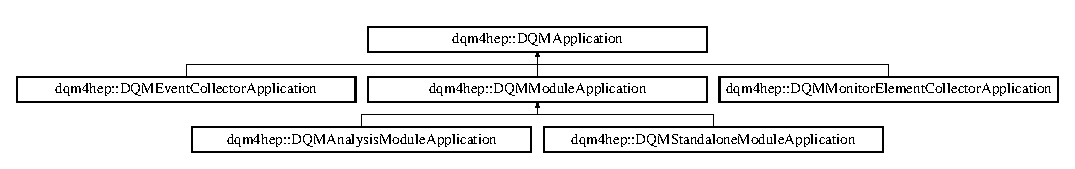
\includegraphics[height=1.824104cm]{classdqm4hep_1_1DQMApplication}
\end{center}
\end{figure}
\subsection*{Public Member Functions}
\begin{DoxyCompactItemize}
\item 
virtual {\bf $\sim$\+D\+Q\+M\+Application} ()
\begin{DoxyCompactList}\small\item\em Destructor. \end{DoxyCompactList}\item 
virtual {\bf Status\+Code} {\bf run} ()=0
\begin{DoxyCompactList}\small\item\em Run the application. \end{DoxyCompactList}\item 
virtual {\bf Status\+Code} {\bf exit} (int return\+Code)=0
\begin{DoxyCompactList}\small\item\em Stop the application. \end{DoxyCompactList}\item 
virtual {\bf Status\+Code} {\bf read\+Settings} (const std\+::string \&settings\+File)=0
\begin{DoxyCompactList}\small\item\em Read the settings from file. \end{DoxyCompactList}\item 
virtual const std\+::string \& {\bf get\+Type} () const =0
\begin{DoxyCompactList}\small\item\em Get the application type. \end{DoxyCompactList}\item 
virtual const std\+::string \& {\bf get\+Name} () const =0
\begin{DoxyCompactList}\small\item\em Get the application name. \end{DoxyCompactList}\end{DoxyCompactItemize}


\subsection{Detailed Description}
\doxyref{D\+Q\+M\+Application}{p.}{classdqm4hep_1_1DQMApplication} class. 

Definition at line 41 of file D\+Q\+M\+Application.\+h.



\subsection{Constructor \& Destructor Documentation}
\index{dqm4hep\+::\+D\+Q\+M\+Application@{dqm4hep\+::\+D\+Q\+M\+Application}!````~D\+Q\+M\+Application@{$\sim$\+D\+Q\+M\+Application}}
\index{````~D\+Q\+M\+Application@{$\sim$\+D\+Q\+M\+Application}!dqm4hep\+::\+D\+Q\+M\+Application@{dqm4hep\+::\+D\+Q\+M\+Application}}
\subsubsection[{$\sim$\+D\+Q\+M\+Application}]{\setlength{\rightskip}{0pt plus 5cm}virtual dqm4hep\+::\+D\+Q\+M\+Application\+::$\sim$\+D\+Q\+M\+Application (
\begin{DoxyParamCaption}
{}
\end{DoxyParamCaption}
)\hspace{0.3cm}{\ttfamily [inline]}, {\ttfamily [virtual]}}\label{classdqm4hep_1_1DQMApplication_aae9b6931ff64054a4a01fbad941766c2}


Destructor. 



Definition at line 46 of file D\+Q\+M\+Application.\+h.


\begin{DoxyCode}
46 \{\}
\end{DoxyCode}


\subsection{Member Function Documentation}
\index{dqm4hep\+::\+D\+Q\+M\+Application@{dqm4hep\+::\+D\+Q\+M\+Application}!exit@{exit}}
\index{exit@{exit}!dqm4hep\+::\+D\+Q\+M\+Application@{dqm4hep\+::\+D\+Q\+M\+Application}}
\subsubsection[{exit}]{\setlength{\rightskip}{0pt plus 5cm}virtual {\bf Status\+Code} dqm4hep\+::\+D\+Q\+M\+Application\+::exit (
\begin{DoxyParamCaption}
\item[{int}]{return\+Code}
\end{DoxyParamCaption}
)\hspace{0.3cm}{\ttfamily [pure virtual]}}\label{classdqm4hep_1_1DQMApplication_ad61139a41c4ba6669d26e3a0013c0f6d}


Stop the application. 



Implemented in {\bf dqm4hep\+::\+D\+Q\+M\+Module\+Application} \doxyref{}{p.}{classdqm4hep_1_1DQMModuleApplication_aca8244e836f802675b9c11188804414d}, {\bf dqm4hep\+::\+D\+Q\+M\+Event\+Collector\+Application} \doxyref{}{p.}{classdqm4hep_1_1DQMEventCollectorApplication_a7f9c7d86ca591f92bf43618dfaf12443}, and {\bf dqm4hep\+::\+D\+Q\+M\+Monitor\+Element\+Collector\+Application} \doxyref{}{p.}{classdqm4hep_1_1DQMMonitorElementCollectorApplication_a490f3e5f3678bde74a21e7f3f6c51927}.

\index{dqm4hep\+::\+D\+Q\+M\+Application@{dqm4hep\+::\+D\+Q\+M\+Application}!get\+Name@{get\+Name}}
\index{get\+Name@{get\+Name}!dqm4hep\+::\+D\+Q\+M\+Application@{dqm4hep\+::\+D\+Q\+M\+Application}}
\subsubsection[{get\+Name}]{\setlength{\rightskip}{0pt plus 5cm}virtual const std\+::string\& dqm4hep\+::\+D\+Q\+M\+Application\+::get\+Name (
\begin{DoxyParamCaption}
{}
\end{DoxyParamCaption}
) const\hspace{0.3cm}{\ttfamily [pure virtual]}}\label{classdqm4hep_1_1DQMApplication_a90d2e587390835cf90b38888498e922b}


Get the application name. 



Implemented in {\bf dqm4hep\+::\+D\+Q\+M\+Analysis\+Module\+Application} \doxyref{}{p.}{classdqm4hep_1_1DQMAnalysisModuleApplication_a248fc1511e714851215dd49406897906}, {\bf dqm4hep\+::\+D\+Q\+M\+Standalone\+Module\+Application} \doxyref{}{p.}{classdqm4hep_1_1DQMStandaloneModuleApplication_af67e009daf617aa7d07cbffeca8b9d54}, {\bf dqm4hep\+::\+D\+Q\+M\+Module\+Application} \doxyref{}{p.}{classdqm4hep_1_1DQMModuleApplication_afb07e2e9bc98060f2b1529f30355e4b9}, {\bf dqm4hep\+::\+D\+Q\+M\+Event\+Collector\+Application} \doxyref{}{p.}{classdqm4hep_1_1DQMEventCollectorApplication_ab38b4de8474b46f560bbf97b4ceba02d}, and {\bf dqm4hep\+::\+D\+Q\+M\+Monitor\+Element\+Collector\+Application} \doxyref{}{p.}{classdqm4hep_1_1DQMMonitorElementCollectorApplication_a8b014998c8c2dafbd6c54ad4fb935fe4}.

\index{dqm4hep\+::\+D\+Q\+M\+Application@{dqm4hep\+::\+D\+Q\+M\+Application}!get\+Type@{get\+Type}}
\index{get\+Type@{get\+Type}!dqm4hep\+::\+D\+Q\+M\+Application@{dqm4hep\+::\+D\+Q\+M\+Application}}
\subsubsection[{get\+Type}]{\setlength{\rightskip}{0pt plus 5cm}virtual const std\+::string\& dqm4hep\+::\+D\+Q\+M\+Application\+::get\+Type (
\begin{DoxyParamCaption}
{}
\end{DoxyParamCaption}
) const\hspace{0.3cm}{\ttfamily [pure virtual]}}\label{classdqm4hep_1_1DQMApplication_aff587d33b27ff25115a7da7655e5ab3b}


Get the application type. 



Implemented in {\bf dqm4hep\+::\+D\+Q\+M\+Analysis\+Module\+Application} \doxyref{}{p.}{classdqm4hep_1_1DQMAnalysisModuleApplication_aeccec8976c667b3e644e87c82043d1ff}, {\bf dqm4hep\+::\+D\+Q\+M\+Standalone\+Module\+Application} \doxyref{}{p.}{classdqm4hep_1_1DQMStandaloneModuleApplication_a9aba02cf03c4faecd87e47b480c984ca}, {\bf dqm4hep\+::\+D\+Q\+M\+Module\+Application} \doxyref{}{p.}{classdqm4hep_1_1DQMModuleApplication_ac24026bb5647c3f0de1889318a14cf88}, {\bf dqm4hep\+::\+D\+Q\+M\+Event\+Collector\+Application} \doxyref{}{p.}{classdqm4hep_1_1DQMEventCollectorApplication_a8bb630d63433e17105f8a07f7c54ba4a}, and {\bf dqm4hep\+::\+D\+Q\+M\+Monitor\+Element\+Collector\+Application} \doxyref{}{p.}{classdqm4hep_1_1DQMMonitorElementCollectorApplication_a120fd6fc6660b27f850cbdcfe0b7e5eb}.

\index{dqm4hep\+::\+D\+Q\+M\+Application@{dqm4hep\+::\+D\+Q\+M\+Application}!read\+Settings@{read\+Settings}}
\index{read\+Settings@{read\+Settings}!dqm4hep\+::\+D\+Q\+M\+Application@{dqm4hep\+::\+D\+Q\+M\+Application}}
\subsubsection[{read\+Settings}]{\setlength{\rightskip}{0pt plus 5cm}virtual {\bf Status\+Code} dqm4hep\+::\+D\+Q\+M\+Application\+::read\+Settings (
\begin{DoxyParamCaption}
\item[{const std\+::string \&}]{settings\+File}
\end{DoxyParamCaption}
)\hspace{0.3cm}{\ttfamily [pure virtual]}}\label{classdqm4hep_1_1DQMApplication_a8b2e28cf09eef6b6a8bde547949c37dc}


Read the settings from file. 



Implemented in {\bf dqm4hep\+::\+D\+Q\+M\+Analysis\+Module\+Application} \doxyref{}{p.}{classdqm4hep_1_1DQMAnalysisModuleApplication_a4b460e8713534da56d6bfcb775a1f5b0}, {\bf dqm4hep\+::\+D\+Q\+M\+Standalone\+Module\+Application} \doxyref{}{p.}{classdqm4hep_1_1DQMStandaloneModuleApplication_ac5450df61d38db926fe44d2557183fb8}, {\bf dqm4hep\+::\+D\+Q\+M\+Event\+Collector\+Application} \doxyref{}{p.}{classdqm4hep_1_1DQMEventCollectorApplication_afaf52f63edcb95265f397682a9915198}, {\bf dqm4hep\+::\+D\+Q\+M\+Monitor\+Element\+Collector\+Application} \doxyref{}{p.}{classdqm4hep_1_1DQMMonitorElementCollectorApplication_afab8d464da2e7430b46667262d6b3e8a}, and {\bf dqm4hep\+::\+D\+Q\+M\+Module\+Application} \doxyref{}{p.}{classdqm4hep_1_1DQMModuleApplication_a994bb2bea7b1def71198ea1864460806}.

\index{dqm4hep\+::\+D\+Q\+M\+Application@{dqm4hep\+::\+D\+Q\+M\+Application}!run@{run}}
\index{run@{run}!dqm4hep\+::\+D\+Q\+M\+Application@{dqm4hep\+::\+D\+Q\+M\+Application}}
\subsubsection[{run}]{\setlength{\rightskip}{0pt plus 5cm}virtual {\bf Status\+Code} dqm4hep\+::\+D\+Q\+M\+Application\+::run (
\begin{DoxyParamCaption}
{}
\end{DoxyParamCaption}
)\hspace{0.3cm}{\ttfamily [pure virtual]}}\label{classdqm4hep_1_1DQMApplication_aa9a37abef624ec9656478c7211cc5a48}


Run the application. 



Implemented in {\bf dqm4hep\+::\+D\+Q\+M\+Analysis\+Module\+Application} \doxyref{}{p.}{classdqm4hep_1_1DQMAnalysisModuleApplication_abf3fd5d59491e8f99c9ed964a487079f}, {\bf dqm4hep\+::\+D\+Q\+M\+Standalone\+Module\+Application} \doxyref{}{p.}{classdqm4hep_1_1DQMStandaloneModuleApplication_a3b2039cbf186ddf83bff16ded2c2dfb4}, {\bf dqm4hep\+::\+D\+Q\+M\+Module\+Application} \doxyref{}{p.}{classdqm4hep_1_1DQMModuleApplication_a42114dcd51bf17af14479345145e5988}, {\bf dqm4hep\+::\+D\+Q\+M\+Event\+Collector\+Application} \doxyref{}{p.}{classdqm4hep_1_1DQMEventCollectorApplication_ad86399bda3c734d4924043250d7e1cc6}, and {\bf dqm4hep\+::\+D\+Q\+M\+Monitor\+Element\+Collector\+Application} \doxyref{}{p.}{classdqm4hep_1_1DQMMonitorElementCollectorApplication_afac92cccea4c52718235c2a59349623f}.



The documentation for this class was generated from the following file\+:\begin{DoxyCompactItemize}
\item 
{\bf D\+Q\+M\+Application.\+h}\end{DoxyCompactItemize}

\section{dqm4hep\+:\+:D\+Q\+M\+Archiver Class Reference}
\label{classdqm4hep_1_1DQMArchiver}\index{dqm4hep\+::\+D\+Q\+M\+Archiver@{dqm4hep\+::\+D\+Q\+M\+Archiver}}


\doxyref{D\+Q\+M\+Archiver}{p.}{classdqm4hep_1_1DQMArchiver} class.  




{\ttfamily \#include $<$D\+Q\+M\+Archiver.\+h$>$}

\subsection*{Public Member Functions}
\begin{DoxyCompactItemize}
\item 
{\bf D\+Q\+M\+Archiver} ()
\begin{DoxyCompactList}\small\item\em Constructor. \end{DoxyCompactList}\item 
{\bf D\+Q\+M\+Archiver} (const std\+::string \&archive\+File\+Name, const std\+::string \&opening\+Mode=\char`\"{}R\+E\+C\+R\+E\+A\+T\+E\char`\"{})
\begin{DoxyCompactList}\small\item\em Constructor with file name and opening mode. \end{DoxyCompactList}\item 
virtual {\bf $\sim$\+D\+Q\+M\+Archiver} ()
\begin{DoxyCompactList}\small\item\em Destructor. \end{DoxyCompactList}\item 
{\bf Status\+Code} {\bf open} (const std\+::string \&archive\+File\+Name, const std\+::string \&opening\+Mode=\char`\"{}R\+E\+C\+R\+E\+A\+T\+E\char`\"{})
\begin{DoxyCompactList}\small\item\em Open a new archive. \end{DoxyCompactList}\item 
{\bf Status\+Code} {\bf close} ()
\begin{DoxyCompactList}\small\item\em Close the current archive. \end{DoxyCompactList}\item 
{\bf Status\+Code} {\bf archive} ({\bf D\+Q\+M\+Module} $\ast$p\+Module, bool archive\+All=true)
\begin{DoxyCompactList}\small\item\em Archive the monitor element list of the given module Monitor elements that are set to \char`\"{}non-\/publish\char`\"{} can be written passing the flag to true (default) \end{DoxyCompactList}\item 
{\bf Status\+Code} {\bf archive} ({\bf D\+Q\+M\+Storage} $\ast$p\+Storage, T\+Directory $\ast$p\+Directory)
\begin{DoxyCompactList}\small\item\em Archive the current state of the storage in the root T\+Directory. \end{DoxyCompactList}\item 
const std\+::string \& {\bf get\+File\+Name} () const 
\begin{DoxyCompactList}\small\item\em Get the file name. \end{DoxyCompactList}\item 
bool {\bf is\+Opened} () const 
\begin{DoxyCompactList}\small\item\em Whether the archive is opened. \end{DoxyCompactList}\item 
const std\+::string \& {\bf get\+Opening\+Mode} () const 
\begin{DoxyCompactList}\small\item\em Get the opening mode of this archive. \end{DoxyCompactList}\end{DoxyCompactItemize}
\subsection*{Protected Member Functions}
\begin{DoxyCompactItemize}
\item 
{\bf Status\+Code} {\bf recursive\+Fill} ({\bf D\+Q\+M\+Directory} $\ast$p\+Directory, T\+Directory $\ast$p\+R\+O\+O\+T\+Dir)
\begin{DoxyCompactList}\small\item\em Fill recursively the T\+Directory with the \doxyref{D\+Q\+M\+Directory}{p.}{classdqm4hep_1_1DQMDirectory}. \end{DoxyCompactList}\item 
{\bf Status\+Code} {\bf create\+T\+Directories} ({\bf D\+Q\+M\+Directory} $\ast$p\+Directory, T\+Directory $\ast$p\+R\+O\+O\+T\+Dir)
\begin{DoxyCompactList}\small\item\em Create T\+Directories as labeled in the \doxyref{D\+Q\+M\+Directory}{p.}{classdqm4hep_1_1DQMDirectory}. \end{DoxyCompactList}\item 
{\bf Status\+Code} {\bf write\+Monitor\+Elements} ({\bf D\+Q\+M\+Directory} $\ast$p\+Directory, T\+Directory $\ast$p\+R\+O\+O\+T\+Dir)
\begin{DoxyCompactList}\small\item\em Write the monitor elements contained in the \doxyref{D\+Q\+M\+Directory}{p.}{classdqm4hep_1_1DQMDirectory} in the T\+Directory. \end{DoxyCompactList}\end{DoxyCompactItemize}
\subsection*{Private Attributes}
\begin{DoxyCompactItemize}
\item 
std\+::string {\bf m\+\_\+file\+Name}
\item 
std\+::string {\bf m\+\_\+opening\+Mode}
\item 
bool {\bf m\+\_\+is\+Opened}
\item 
bool {\bf m\+\_\+first\+Archive}
\item 
T\+File $\ast$ {\bf m\+\_\+p\+Archive\+File}
\end{DoxyCompactItemize}
\subsection*{Friends}
\begin{DoxyCompactItemize}
\item 
class {\bf D\+Q\+M\+Monitor\+Element\+Manager}
\end{DoxyCompactItemize}


\subsection{Detailed Description}
\doxyref{D\+Q\+M\+Archiver}{p.}{classdqm4hep_1_1DQMArchiver} class. 

Definition at line 50 of file D\+Q\+M\+Archiver.\+h.



\subsection{Constructor \& Destructor Documentation}
\index{dqm4hep\+::\+D\+Q\+M\+Archiver@{dqm4hep\+::\+D\+Q\+M\+Archiver}!D\+Q\+M\+Archiver@{D\+Q\+M\+Archiver}}
\index{D\+Q\+M\+Archiver@{D\+Q\+M\+Archiver}!dqm4hep\+::\+D\+Q\+M\+Archiver@{dqm4hep\+::\+D\+Q\+M\+Archiver}}
\subsubsection[{D\+Q\+M\+Archiver}]{\setlength{\rightskip}{0pt plus 5cm}dqm4hep\+::\+D\+Q\+M\+Archiver\+::\+D\+Q\+M\+Archiver (
\begin{DoxyParamCaption}
{}
\end{DoxyParamCaption}
)}\label{classdqm4hep_1_1DQMArchiver_afc7c107c5a6bb62d06d184434336f331}


Constructor. 



Definition at line 49 of file D\+Q\+M\+Archiver.\+cc.


\begin{DoxyCode}
49                          :
50     m_fileName(\textcolor{stringliteral}{""}),
51     m_openingMode(\textcolor{stringliteral}{""}),
52     m_pArchiveFile(NULL),
53     m_isOpened(\textcolor{keyword}{false}),
54     m_firstArchive(\textcolor{keyword}{true})
55 \{
56   \textcolor{comment}{/* nop */}
57 \}
\end{DoxyCode}
\index{dqm4hep\+::\+D\+Q\+M\+Archiver@{dqm4hep\+::\+D\+Q\+M\+Archiver}!D\+Q\+M\+Archiver@{D\+Q\+M\+Archiver}}
\index{D\+Q\+M\+Archiver@{D\+Q\+M\+Archiver}!dqm4hep\+::\+D\+Q\+M\+Archiver@{dqm4hep\+::\+D\+Q\+M\+Archiver}}
\subsubsection[{D\+Q\+M\+Archiver}]{\setlength{\rightskip}{0pt plus 5cm}dqm4hep\+::\+D\+Q\+M\+Archiver\+::\+D\+Q\+M\+Archiver (
\begin{DoxyParamCaption}
\item[{const std\+::string \&}]{archive\+File\+Name, }
\item[{const std\+::string \&}]{opening\+Mode = {\ttfamily \char`\"{}RECREATE\char`\"{}}}
\end{DoxyParamCaption}
)}\label{classdqm4hep_1_1DQMArchiver_a6701654be5b7aaef61f69227f626752a}


Constructor with file name and opening mode. 



Definition at line 61 of file D\+Q\+M\+Archiver.\+cc.



References open(), and T\+H\+R\+O\+W\+\_\+\+R\+E\+S\+U\+L\+T\+\_\+\+I\+F.


\begin{DoxyCode}
62 \{
63   THROW_RESULT_IF(STATUS\_CODE\_SUCCESS, !=, open(archiveFileName, openingMode));
64 \}
\end{DoxyCode}
\index{dqm4hep\+::\+D\+Q\+M\+Archiver@{dqm4hep\+::\+D\+Q\+M\+Archiver}!````~D\+Q\+M\+Archiver@{$\sim$\+D\+Q\+M\+Archiver}}
\index{````~D\+Q\+M\+Archiver@{$\sim$\+D\+Q\+M\+Archiver}!dqm4hep\+::\+D\+Q\+M\+Archiver@{dqm4hep\+::\+D\+Q\+M\+Archiver}}
\subsubsection[{$\sim$\+D\+Q\+M\+Archiver}]{\setlength{\rightskip}{0pt plus 5cm}dqm4hep\+::\+D\+Q\+M\+Archiver\+::$\sim$\+D\+Q\+M\+Archiver (
\begin{DoxyParamCaption}
{}
\end{DoxyParamCaption}
)\hspace{0.3cm}{\ttfamily [virtual]}}\label{classdqm4hep_1_1DQMArchiver_aae525c0c7428cfb5070ca8030a5e158a}


Destructor. 



Definition at line 68 of file D\+Q\+M\+Archiver.\+cc.



References close(), and m\+\_\+is\+Opened.


\begin{DoxyCode}
69 \{
70   \textcolor{keywordflow}{if}(m_isOpened)
71     close();
72 \}
\end{DoxyCode}


\subsection{Member Function Documentation}
\index{dqm4hep\+::\+D\+Q\+M\+Archiver@{dqm4hep\+::\+D\+Q\+M\+Archiver}!archive@{archive}}
\index{archive@{archive}!dqm4hep\+::\+D\+Q\+M\+Archiver@{dqm4hep\+::\+D\+Q\+M\+Archiver}}
\subsubsection[{archive}]{\setlength{\rightskip}{0pt plus 5cm}{\bf Status\+Code} dqm4hep\+::\+D\+Q\+M\+Archiver\+::archive (
\begin{DoxyParamCaption}
\item[{{\bf D\+Q\+M\+Module} $\ast$}]{p\+Module, }
\item[{bool}]{archive\+All = {\ttfamily true}}
\end{DoxyParamCaption}
)}\label{classdqm4hep_1_1DQMArchiver_a40bc8d6e58d43ce24e7ee17e89df0eaa}


Archive the monitor element list of the given module Monitor elements that are set to \char`\"{}non-\/publish\char`\"{} can be written passing the flag to true (default) 



Definition at line 146 of file D\+Q\+M\+Archiver.\+cc.



References dqm4hep\+::\+D\+Q\+M\+Module\+::get\+Detector\+Name(), dqm4hep\+::\+D\+Q\+M\+Module\+::get\+Module\+Application(), dqm4hep\+::\+D\+Q\+M\+Module\+Application\+::get\+Monitor\+Element\+Manager(), dqm4hep\+::\+D\+Q\+M\+Module\+::get\+Name(), dqm4hep\+::\+D\+Q\+M\+Monitor\+Element\+Manager\+::get\+Storage(), dqm4hep\+::\+D\+Q\+M\+Module\+::get\+Version(), is\+Opened(), m\+\_\+first\+Archive, m\+\_\+p\+Archive\+File, dqm4hep\+::\+M\+E\+S\+S\+A\+G\+E, R\+E\+T\+U\+R\+N\+\_\+\+R\+E\+S\+U\+L\+T\+\_\+\+I\+F, and dqm4hep\+::\+D\+Q\+M\+Version\+::to\+String().



Referenced by dqm4hep\+::\+D\+Q\+M\+Standalone\+Module\+Application\+::run(), and dqm4hep\+::\+D\+Q\+M\+Analysis\+Module\+Application\+::run().


\begin{DoxyCode}
147 \{
148   \textcolor{keywordflow}{if}(!isOpened())
149     \textcolor{keywordflow}{return} STATUS\_CODE\_NOT\_INITIALIZED;
150 
151   streamlog\_out(MESSAGE) << \textcolor{stringliteral}{"Archiving monitor elements of module : "} << pModule->getName() << std::endl;
152 
153   \textcolor{comment}{// archive directory}
154   m_pArchiveFile->cd();
155 
156   TDirectory *pArchiveDirectory = m_pArchiveFile->GetDirectory(\textcolor{stringliteral}{"root"});
157 
158   \textcolor{keywordflow}{if}(pArchiveDirectory)
159     m_pArchiveFile->rmdir(\textcolor{stringliteral}{"root"});
160 
161   pArchiveDirectory = m_pArchiveFile->mkdir(\textcolor{stringliteral}{"root"});
162 
163   \textcolor{keywordflow}{if}(!pArchiveDirectory)
164     \textcolor{keywordflow}{return} STATUS\_CODE\_FAILURE;
165 
166   \textcolor{keywordflow}{if}(m_firstArchive)
167   \{
168     \textcolor{comment}{// write module info in the file}
169     TObjString *pModuleNameString = \textcolor{keyword}{new} TObjString();
170     pModuleNameString->SetString(pModule->getName().c\_str());
171     m_pArchiveFile->WriteTObject(pModuleNameString);
172     \textcolor{keyword}{delete} pModuleNameString;
173 
174     TObjString *pModuleVersionString = \textcolor{keyword}{new} TObjString();
175     pModuleVersionString->SetString(pModule->getVersion().toString().c\_str());
176     m_pArchiveFile->WriteTObject(pModuleVersionString);
177     \textcolor{keyword}{delete} pModuleVersionString;
178 
179     TObjString *pModuleDetectorString = \textcolor{keyword}{new} TObjString();
180     pModuleDetectorString->SetString(pModule->getDetectorName().c\_str());
181     m_pArchiveFile->WriteTObject(pModuleDetectorString);
182     \textcolor{keyword}{delete} pModuleDetectorString;
183 
184     m_firstArchive = \textcolor{keyword}{false};
185   \}
186 
187   \textcolor{comment}{// get the storage of the module}
188   DQMStorage *pStorage = pModule->getModuleApplication()->getMonitorElementManager()->getStorage();
189 
190   RETURN_RESULT_IF(STATUS\_CODE\_SUCCESS, !=, archive(pStorage, pArchiveDirectory));
191 
192   \textcolor{keyword}{delete} pArchiveDirectory;
193 
194   \textcolor{keywordflow}{return} STATUS\_CODE\_SUCCESS;
195 \}
\end{DoxyCode}
\index{dqm4hep\+::\+D\+Q\+M\+Archiver@{dqm4hep\+::\+D\+Q\+M\+Archiver}!archive@{archive}}
\index{archive@{archive}!dqm4hep\+::\+D\+Q\+M\+Archiver@{dqm4hep\+::\+D\+Q\+M\+Archiver}}
\subsubsection[{archive}]{\setlength{\rightskip}{0pt plus 5cm}{\bf Status\+Code} dqm4hep\+::\+D\+Q\+M\+Archiver\+::archive (
\begin{DoxyParamCaption}
\item[{{\bf D\+Q\+M\+Storage} $\ast$}]{p\+Storage, }
\item[{T\+Directory $\ast$}]{p\+Directory}
\end{DoxyParamCaption}
)}\label{classdqm4hep_1_1DQMArchiver_ae9dfc99eed4457ed2542217351b16397}


Archive the current state of the storage in the root T\+Directory. 



Definition at line 199 of file D\+Q\+M\+Archiver.\+cc.



References dqm4hep\+::\+D\+Q\+M\+Storage\+::get\+Root\+Directory(), m\+\_\+p\+Archive\+File, recursive\+Fill(), and R\+E\+T\+U\+R\+N\+\_\+\+R\+E\+S\+U\+L\+T\+\_\+\+I\+F.


\begin{DoxyCode}
200 \{
201   RETURN_RESULT_IF(STATUS\_CODE\_SUCCESS, !=, recursiveFill(pStorage->getRootDirectory(), pDirectory));
202 
203   m_pArchiveFile->cd();
204   m_pArchiveFile->Write();
205 
206   \textcolor{keywordflow}{return} STATUS\_CODE\_SUCCESS;
207 \}
\end{DoxyCode}
\index{dqm4hep\+::\+D\+Q\+M\+Archiver@{dqm4hep\+::\+D\+Q\+M\+Archiver}!close@{close}}
\index{close@{close}!dqm4hep\+::\+D\+Q\+M\+Archiver@{dqm4hep\+::\+D\+Q\+M\+Archiver}}
\subsubsection[{close}]{\setlength{\rightskip}{0pt plus 5cm}{\bf Status\+Code} dqm4hep\+::\+D\+Q\+M\+Archiver\+::close (
\begin{DoxyParamCaption}
{}
\end{DoxyParamCaption}
)}\label{classdqm4hep_1_1DQMArchiver_a946ccd48ba63853814a98cf85c462068}


Close the current archive. 



Definition at line 127 of file D\+Q\+M\+Archiver.\+cc.



References m\+\_\+first\+Archive, m\+\_\+is\+Opened, m\+\_\+opening\+Mode, and m\+\_\+p\+Archive\+File.



Referenced by open(), dqm4hep\+::\+D\+Q\+M\+Standalone\+Module\+Application\+::run(), dqm4hep\+::\+D\+Q\+M\+Analysis\+Module\+Application\+::run(), and $\sim$\+D\+Q\+M\+Archiver().


\begin{DoxyCode}
128 \{
129   \textcolor{keywordflow}{if}(!m_isOpened)
130     \textcolor{keywordflow}{return} STATUS\_CODE\_FAILURE;
131 
132   m_pArchiveFile->Close();
133   \textcolor{keyword}{delete} m_pArchiveFile;
134 
135   m_pArchiveFile = NULL;
136 
137   m_isOpened = \textcolor{keyword}{false};
138   m_firstArchive = \textcolor{keyword}{false};
139   m_openingMode = \textcolor{stringliteral}{""};
140 
141   \textcolor{keywordflow}{return} STATUS\_CODE\_SUCCESS;
142 \}
\end{DoxyCode}
\index{dqm4hep\+::\+D\+Q\+M\+Archiver@{dqm4hep\+::\+D\+Q\+M\+Archiver}!create\+T\+Directories@{create\+T\+Directories}}
\index{create\+T\+Directories@{create\+T\+Directories}!dqm4hep\+::\+D\+Q\+M\+Archiver@{dqm4hep\+::\+D\+Q\+M\+Archiver}}
\subsubsection[{create\+T\+Directories}]{\setlength{\rightskip}{0pt plus 5cm}{\bf Status\+Code} dqm4hep\+::\+D\+Q\+M\+Archiver\+::create\+T\+Directories (
\begin{DoxyParamCaption}
\item[{{\bf D\+Q\+M\+Directory} $\ast$}]{p\+Directory, }
\item[{T\+Directory $\ast$}]{p\+R\+O\+O\+T\+Dir}
\end{DoxyParamCaption}
)\hspace{0.3cm}{\ttfamily [protected]}}\label{classdqm4hep_1_1DQMArchiver_a7eefce11e665b98a36a1802b46ce0b4e}


Create T\+Directories as labeled in the \doxyref{D\+Q\+M\+Directory}{p.}{classdqm4hep_1_1DQMDirectory}. 

\index{dqm4hep\+::\+D\+Q\+M\+Archiver@{dqm4hep\+::\+D\+Q\+M\+Archiver}!get\+File\+Name@{get\+File\+Name}}
\index{get\+File\+Name@{get\+File\+Name}!dqm4hep\+::\+D\+Q\+M\+Archiver@{dqm4hep\+::\+D\+Q\+M\+Archiver}}
\subsubsection[{get\+File\+Name}]{\setlength{\rightskip}{0pt plus 5cm}const std\+::string \& dqm4hep\+::\+D\+Q\+M\+Archiver\+::get\+File\+Name (
\begin{DoxyParamCaption}
{}
\end{DoxyParamCaption}
) const}\label{classdqm4hep_1_1DQMArchiver_a43952ad23f2302fedcbb69eca6899264}


Get the file name. 



Definition at line 211 of file D\+Q\+M\+Archiver.\+cc.



References m\+\_\+file\+Name.



Referenced by dqm4hep\+::\+D\+Q\+M\+Standalone\+Module\+Application\+::run(), and dqm4hep\+::\+D\+Q\+M\+Analysis\+Module\+Application\+::run().


\begin{DoxyCode}
212 \{
213   \textcolor{keywordflow}{return} m_fileName;
214 \}
\end{DoxyCode}
\index{dqm4hep\+::\+D\+Q\+M\+Archiver@{dqm4hep\+::\+D\+Q\+M\+Archiver}!get\+Opening\+Mode@{get\+Opening\+Mode}}
\index{get\+Opening\+Mode@{get\+Opening\+Mode}!dqm4hep\+::\+D\+Q\+M\+Archiver@{dqm4hep\+::\+D\+Q\+M\+Archiver}}
\subsubsection[{get\+Opening\+Mode}]{\setlength{\rightskip}{0pt plus 5cm}const std\+::string \& dqm4hep\+::\+D\+Q\+M\+Archiver\+::get\+Opening\+Mode (
\begin{DoxyParamCaption}
{}
\end{DoxyParamCaption}
) const}\label{classdqm4hep_1_1DQMArchiver_a0a926d512f1b708872ba8a1e30994956}


Get the opening mode of this archive. 



Definition at line 225 of file D\+Q\+M\+Archiver.\+cc.



References m\+\_\+opening\+Mode.


\begin{DoxyCode}
226 \{
227   \textcolor{keywordflow}{return} m_openingMode;
228 \}
\end{DoxyCode}
\index{dqm4hep\+::\+D\+Q\+M\+Archiver@{dqm4hep\+::\+D\+Q\+M\+Archiver}!is\+Opened@{is\+Opened}}
\index{is\+Opened@{is\+Opened}!dqm4hep\+::\+D\+Q\+M\+Archiver@{dqm4hep\+::\+D\+Q\+M\+Archiver}}
\subsubsection[{is\+Opened}]{\setlength{\rightskip}{0pt plus 5cm}bool dqm4hep\+::\+D\+Q\+M\+Archiver\+::is\+Opened (
\begin{DoxyParamCaption}
{}
\end{DoxyParamCaption}
) const}\label{classdqm4hep_1_1DQMArchiver_a970673513f6f7b7514042b58c1e21c41}


Whether the archive is opened. 



Definition at line 218 of file D\+Q\+M\+Archiver.\+cc.



References m\+\_\+is\+Opened.



Referenced by archive().


\begin{DoxyCode}
219 \{
220   \textcolor{keywordflow}{return} m_isOpened;
221 \}
\end{DoxyCode}
\index{dqm4hep\+::\+D\+Q\+M\+Archiver@{dqm4hep\+::\+D\+Q\+M\+Archiver}!open@{open}}
\index{open@{open}!dqm4hep\+::\+D\+Q\+M\+Archiver@{dqm4hep\+::\+D\+Q\+M\+Archiver}}
\subsubsection[{open}]{\setlength{\rightskip}{0pt plus 5cm}{\bf Status\+Code} dqm4hep\+::\+D\+Q\+M\+Archiver\+::open (
\begin{DoxyParamCaption}
\item[{const std\+::string \&}]{archive\+File\+Name, }
\item[{const std\+::string \&}]{opening\+Mode = {\ttfamily \char`\"{}RECREATE\char`\"{}}}
\end{DoxyParamCaption}
)}\label{classdqm4hep_1_1DQMArchiver_aa5cfa522fec6851c81f67f8da53bffaf}


Open a new archive. 

Close the current file if opened. Supported opening mode are the T\+File opening mode option (see T\+File) 

Definition at line 76 of file D\+Q\+M\+Archiver.\+cc.



References close(), m\+\_\+file\+Name, m\+\_\+first\+Archive, m\+\_\+is\+Opened, m\+\_\+opening\+Mode, m\+\_\+p\+Archive\+File, R\+E\+T\+U\+R\+N\+\_\+\+R\+E\+S\+U\+L\+T\+\_\+\+I\+F, and dqm4hep\+::\+W\+A\+R\+N\+I\+N\+G.



Referenced by D\+Q\+M\+Archiver(), dqm4hep\+::\+D\+Q\+M\+Standalone\+Module\+Application\+::run(), and dqm4hep\+::\+D\+Q\+M\+Analysis\+Module\+Application\+::run().


\begin{DoxyCode}
77 \{
78   \textcolor{comment}{// if already open write the archive if not done}
79   \textcolor{comment}{// and close it before to re-open}
80   \textcolor{keywordflow}{if}(m_isOpened)
81     RETURN_RESULT_IF(STATUS\_CODE\_SUCCESS, !=, close());
82 
83   \textcolor{keywordflow}{if}(archiveFileName.empty())
84     \textcolor{keywordflow}{return} STATUS\_CODE\_INVALID\_PARAMETER;
85 
86   std::string fullArchiveName;
87   std::string baseArchiveName;
88 
89   \textcolor{keywordflow}{if}(archiveFileName.size() > 5 && archiveFileName.substr(archiveFileName.size()-5) == \textcolor{stringliteral}{".root"})
90   \{
91     fullArchiveName = archiveFileName;
92     baseArchiveName = archiveFileName.substr(0, archiveFileName.size()-5);
93   \}
94   \textcolor{keywordflow}{else}
95   \{
96     fullArchiveName = archiveFileName + \textcolor{stringliteral}{".root"};
97     baseArchiveName = archiveFileName;
98   \}
99 
100   \textcolor{keywordtype}{int} fileId = 0;
101 
102   \textcolor{keywordflow}{while}(!gSystem->AccessPathName(fullArchiveName.c\_str()))
103   \{
104     streamlog\_out(WARNING) << fullArchiveName << \textcolor{stringliteral}{" file already exists ..."} << std::endl;
105     fileId ++;
106     std::stringstream ss;
107     ss << baseArchiveName << \textcolor{stringliteral}{"\_"} << fileId << \textcolor{stringliteral}{".root"};
108     fullArchiveName = ss.str();
109   \}
110 
111   m_fileName = fullArchiveName;
112   m_openingMode = openingMode;
113 
114   m_pArchiveFile = \textcolor{keyword}{new} TFile(m_fileName.c\_str(), openingMode.c\_str());
115 
116   \textcolor{keywordflow}{if}(NULL == m_pArchiveFile)
117     \textcolor{keywordflow}{return} STATUS\_CODE\_FAILURE;
118 
119   m_isOpened = \textcolor{keyword}{true};
120   m_firstArchive = \textcolor{keyword}{true};
121 
122   \textcolor{keywordflow}{return} STATUS\_CODE\_SUCCESS;
123 \}
\end{DoxyCode}
\index{dqm4hep\+::\+D\+Q\+M\+Archiver@{dqm4hep\+::\+D\+Q\+M\+Archiver}!recursive\+Fill@{recursive\+Fill}}
\index{recursive\+Fill@{recursive\+Fill}!dqm4hep\+::\+D\+Q\+M\+Archiver@{dqm4hep\+::\+D\+Q\+M\+Archiver}}
\subsubsection[{recursive\+Fill}]{\setlength{\rightskip}{0pt plus 5cm}{\bf Status\+Code} dqm4hep\+::\+D\+Q\+M\+Archiver\+::recursive\+Fill (
\begin{DoxyParamCaption}
\item[{{\bf D\+Q\+M\+Directory} $\ast$}]{p\+Directory, }
\item[{T\+Directory $\ast$}]{p\+R\+O\+O\+T\+Dir}
\end{DoxyParamCaption}
)\hspace{0.3cm}{\ttfamily [protected]}}\label{classdqm4hep_1_1DQMArchiver_a86ddd95a21a7508ec31712d6b168bddd}


Fill recursively the T\+Directory with the \doxyref{D\+Q\+M\+Directory}{p.}{classdqm4hep_1_1DQMDirectory}. 



Definition at line 232 of file D\+Q\+M\+Archiver.\+cc.



References dqm4hep\+::\+D\+Q\+M\+Directory\+::get\+Monitor\+Element\+List(), dqm4hep\+::\+D\+Q\+M\+Directory\+::get\+Name(), dqm4hep\+::\+D\+Q\+M\+Directory\+::get\+Sub\+Dir\+List(), dqm4hep\+::\+D\+Q\+M\+Directory\+::mkdir(), R\+E\+T\+U\+R\+N\+\_\+\+R\+E\+S\+U\+L\+T\+\_\+\+I\+F, and write\+Monitor\+Elements().



Referenced by archive().


\begin{DoxyCode}
233 \{
234   \textcolor{keywordflow}{if}(NULL == pDirectory || NULL == pROOTDir)
235     \textcolor{keywordflow}{return} STATUS\_CODE\_INVALID\_PTR;
236 
237   pROOTDir->cd();
238 
239   \textcolor{keyword}{const} std::vector<DQMDirectory*> &subDirList(pDirectory->getSubDirList());
240 
241   \textcolor{keywordflow}{if}(!subDirList.empty())
242   \{
243     \textcolor{keywordflow}{for}(std::vector<DQMDirectory*>::const\_iterator iter = subDirList.begin(), endIter = subDirList.end() ;
244         endIter != iter ; ++iter)
245     \{
246       DQMDirectory *pSubDir = *iter;
247       TDirectory *pROOTSubDir = pROOTDir->mkdir(pSubDir->getName().c\_str());
248 
249       \textcolor{keywordflow}{if}(NULL != pROOTSubDir)
250       \{
251         RETURN_RESULT_IF(STATUS\_CODE\_SUCCESS, !=, recursiveFill(pSubDir, pROOTSubDir));
252       \}
253     \}
254   \}
255 
256   \textcolor{keyword}{const} std::vector<DQMMonitorElement*> &monitorElementList(pDirectory->getMonitorElementList());
257 
258   \textcolor{comment}{// write the monitor elements}
259   \textcolor{keywordflow}{if}(!monitorElementList.empty())
260   \{
261     RETURN_RESULT_IF(STATUS\_CODE\_SUCCESS, !=, writeMonitorElements(pDirectory, pROOTDir));
262   \}
263 
264   \textcolor{keywordflow}{return} STATUS\_CODE\_SUCCESS;
265 \}
\end{DoxyCode}
\index{dqm4hep\+::\+D\+Q\+M\+Archiver@{dqm4hep\+::\+D\+Q\+M\+Archiver}!write\+Monitor\+Elements@{write\+Monitor\+Elements}}
\index{write\+Monitor\+Elements@{write\+Monitor\+Elements}!dqm4hep\+::\+D\+Q\+M\+Archiver@{dqm4hep\+::\+D\+Q\+M\+Archiver}}
\subsubsection[{write\+Monitor\+Elements}]{\setlength{\rightskip}{0pt plus 5cm}{\bf Status\+Code} dqm4hep\+::\+D\+Q\+M\+Archiver\+::write\+Monitor\+Elements (
\begin{DoxyParamCaption}
\item[{{\bf D\+Q\+M\+Directory} $\ast$}]{p\+Directory, }
\item[{T\+Directory $\ast$}]{p\+R\+O\+O\+T\+Dir}
\end{DoxyParamCaption}
)\hspace{0.3cm}{\ttfamily [protected]}}\label{classdqm4hep_1_1DQMArchiver_a01954fa6b7ac6340046b419dd6948a56}


Write the monitor elements contained in the \doxyref{D\+Q\+M\+Directory}{p.}{classdqm4hep_1_1DQMDirectory} in the T\+Directory. 



Definition at line 269 of file D\+Q\+M\+Archiver.\+cc.



References dqm4hep\+::\+D\+Q\+M\+Directory\+::get\+Monitor\+Element\+List(), dqm4hep\+::\+D\+Q\+M\+Monitor\+Element\+::get\+Name(), and dqm4hep\+::\+D\+Q\+M\+Monitor\+Element\+::get\+Object().



Referenced by recursive\+Fill().


\begin{DoxyCode}
270 \{
271   \textcolor{keywordflow}{if}(NULL == pDirectory || NULL == pROOTDir)
272     \textcolor{keywordflow}{return} STATUS\_CODE\_INVALID\_PTR;
273 
274   pROOTDir->cd();
275 
276   \textcolor{keyword}{const} DQMMonitorElementList &monitorElementList(pDirectory->getMonitorElementList());
277 
278   \textcolor{keywordflow}{for}(DQMMonitorElementList::const\_iterator iter = monitorElementList.begin(), endIter = monitorElementList
      .end() ;
279       endIter != iter ; ++iter)
280   \{
281     DQMMonitorElement *pMonitorElement = *iter;
282 
283     TObject *pObject = pMonitorElement->getObject();
284     pROOTDir->WriteObjectAny(pObject, pObject->IsA(), pMonitorElement->getName().c\_str());
285   \}
286 
287   \textcolor{keywordflow}{return} STATUS\_CODE\_SUCCESS;
288 \}
\end{DoxyCode}


\subsection{Friends And Related Function Documentation}
\index{dqm4hep\+::\+D\+Q\+M\+Archiver@{dqm4hep\+::\+D\+Q\+M\+Archiver}!D\+Q\+M\+Monitor\+Element\+Manager@{D\+Q\+M\+Monitor\+Element\+Manager}}
\index{D\+Q\+M\+Monitor\+Element\+Manager@{D\+Q\+M\+Monitor\+Element\+Manager}!dqm4hep\+::\+D\+Q\+M\+Archiver@{dqm4hep\+::\+D\+Q\+M\+Archiver}}
\subsubsection[{D\+Q\+M\+Monitor\+Element\+Manager}]{\setlength{\rightskip}{0pt plus 5cm}friend class {\bf D\+Q\+M\+Monitor\+Element\+Manager}\hspace{0.3cm}{\ttfamily [friend]}}\label{classdqm4hep_1_1DQMArchiver_abf4f43d77cde6c1a22eeca13e12acac0}


Definition at line 52 of file D\+Q\+M\+Archiver.\+h.



\subsection{Member Data Documentation}
\index{dqm4hep\+::\+D\+Q\+M\+Archiver@{dqm4hep\+::\+D\+Q\+M\+Archiver}!m\+\_\+file\+Name@{m\+\_\+file\+Name}}
\index{m\+\_\+file\+Name@{m\+\_\+file\+Name}!dqm4hep\+::\+D\+Q\+M\+Archiver@{dqm4hep\+::\+D\+Q\+M\+Archiver}}
\subsubsection[{m\+\_\+file\+Name}]{\setlength{\rightskip}{0pt plus 5cm}std\+::string dqm4hep\+::\+D\+Q\+M\+Archiver\+::m\+\_\+file\+Name\hspace{0.3cm}{\ttfamily [private]}}\label{classdqm4hep_1_1DQMArchiver_a02b1dc52a01a57829528259a36acaf3a}


Definition at line 112 of file D\+Q\+M\+Archiver.\+h.



Referenced by get\+File\+Name(), and open().

\index{dqm4hep\+::\+D\+Q\+M\+Archiver@{dqm4hep\+::\+D\+Q\+M\+Archiver}!m\+\_\+first\+Archive@{m\+\_\+first\+Archive}}
\index{m\+\_\+first\+Archive@{m\+\_\+first\+Archive}!dqm4hep\+::\+D\+Q\+M\+Archiver@{dqm4hep\+::\+D\+Q\+M\+Archiver}}
\subsubsection[{m\+\_\+first\+Archive}]{\setlength{\rightskip}{0pt plus 5cm}bool dqm4hep\+::\+D\+Q\+M\+Archiver\+::m\+\_\+first\+Archive\hspace{0.3cm}{\ttfamily [private]}}\label{classdqm4hep_1_1DQMArchiver_a6a15b30b2a8cc4c7bdb62c4ca7ab6098}


Definition at line 115 of file D\+Q\+M\+Archiver.\+h.



Referenced by archive(), close(), and open().

\index{dqm4hep\+::\+D\+Q\+M\+Archiver@{dqm4hep\+::\+D\+Q\+M\+Archiver}!m\+\_\+is\+Opened@{m\+\_\+is\+Opened}}
\index{m\+\_\+is\+Opened@{m\+\_\+is\+Opened}!dqm4hep\+::\+D\+Q\+M\+Archiver@{dqm4hep\+::\+D\+Q\+M\+Archiver}}
\subsubsection[{m\+\_\+is\+Opened}]{\setlength{\rightskip}{0pt plus 5cm}bool dqm4hep\+::\+D\+Q\+M\+Archiver\+::m\+\_\+is\+Opened\hspace{0.3cm}{\ttfamily [private]}}\label{classdqm4hep_1_1DQMArchiver_ada36f22fc0c9d6783e5ffeffe8fbbd6d}


Definition at line 114 of file D\+Q\+M\+Archiver.\+h.



Referenced by close(), is\+Opened(), open(), and $\sim$\+D\+Q\+M\+Archiver().

\index{dqm4hep\+::\+D\+Q\+M\+Archiver@{dqm4hep\+::\+D\+Q\+M\+Archiver}!m\+\_\+opening\+Mode@{m\+\_\+opening\+Mode}}
\index{m\+\_\+opening\+Mode@{m\+\_\+opening\+Mode}!dqm4hep\+::\+D\+Q\+M\+Archiver@{dqm4hep\+::\+D\+Q\+M\+Archiver}}
\subsubsection[{m\+\_\+opening\+Mode}]{\setlength{\rightskip}{0pt plus 5cm}std\+::string dqm4hep\+::\+D\+Q\+M\+Archiver\+::m\+\_\+opening\+Mode\hspace{0.3cm}{\ttfamily [private]}}\label{classdqm4hep_1_1DQMArchiver_a9257bf90ebcccbbb572f1b61bf5e1d95}


Definition at line 113 of file D\+Q\+M\+Archiver.\+h.



Referenced by close(), get\+Opening\+Mode(), and open().

\index{dqm4hep\+::\+D\+Q\+M\+Archiver@{dqm4hep\+::\+D\+Q\+M\+Archiver}!m\+\_\+p\+Archive\+File@{m\+\_\+p\+Archive\+File}}
\index{m\+\_\+p\+Archive\+File@{m\+\_\+p\+Archive\+File}!dqm4hep\+::\+D\+Q\+M\+Archiver@{dqm4hep\+::\+D\+Q\+M\+Archiver}}
\subsubsection[{m\+\_\+p\+Archive\+File}]{\setlength{\rightskip}{0pt plus 5cm}T\+File$\ast$ dqm4hep\+::\+D\+Q\+M\+Archiver\+::m\+\_\+p\+Archive\+File\hspace{0.3cm}{\ttfamily [private]}}\label{classdqm4hep_1_1DQMArchiver_aec9ac388b45cc642df7f508558767163}


Definition at line 117 of file D\+Q\+M\+Archiver.\+h.



Referenced by archive(), close(), and open().



The documentation for this class was generated from the following files\+:\begin{DoxyCompactItemize}
\item 
{\bf D\+Q\+M\+Archiver.\+h}\item 
{\bf D\+Q\+M\+Archiver.\+cc}\end{DoxyCompactItemize}

\section{dqm4hep\+:\+:D\+Q\+M\+Calorimeter\+Hit\+Streamer Class Reference}
\label{classdqm4hep_1_1DQMCalorimeterHitStreamer}\index{dqm4hep\+::\+D\+Q\+M\+Calorimeter\+Hit\+Streamer@{dqm4hep\+::\+D\+Q\+M\+Calorimeter\+Hit\+Streamer}}


\doxyref{D\+Q\+M\+Calorimeter\+Hit\+Streamer}{p.}{classdqm4hep_1_1DQMCalorimeterHitStreamer} class.  




{\ttfamily \#include $<$D\+Q\+M\+L\+C\+Event\+Streamer.\+h$>$}

Inheritance diagram for dqm4hep\+:\+:D\+Q\+M\+Calorimeter\+Hit\+Streamer\+:\begin{figure}[H]
\begin{center}
\leavevmode
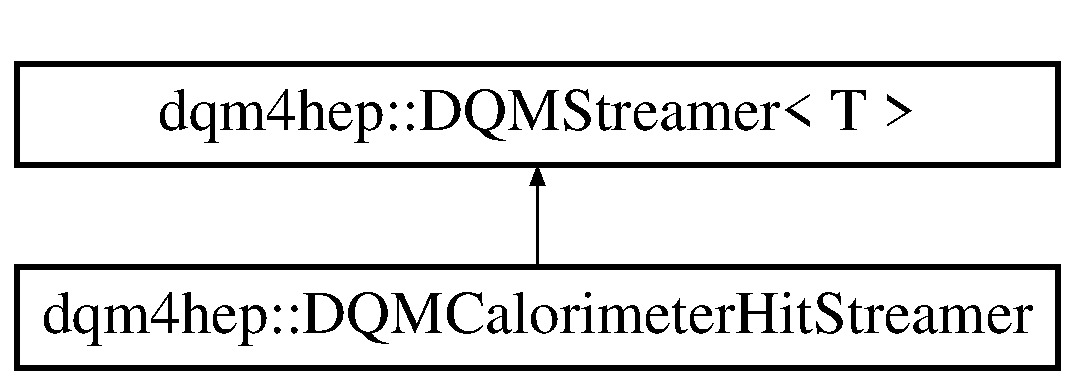
\includegraphics[height=2.000000cm]{classdqm4hep_1_1DQMCalorimeterHitStreamer}
\end{center}
\end{figure}
\subsection*{Public Member Functions}
\begin{DoxyCompactItemize}
\item 
{\bf Status\+Code} {\bf serialize} (const E\+V\+E\+N\+T\+::\+L\+C\+Object $\ast$const p\+L\+C\+Object, {\bf D\+Q\+M\+Data\+Stream} $\ast$const p\+Data\+Stream)
\begin{DoxyCompactList}\small\item\em Serialize an Calorimeter\+Hit. \end{DoxyCompactList}\item 
{\bf Status\+Code} {\bf deserialize} (E\+V\+E\+N\+T\+::\+L\+C\+Object $\ast$\&p\+L\+C\+Object, {\bf D\+Q\+M\+Data\+Stream} $\ast$const p\+Data\+Stream)
\begin{DoxyCompactList}\small\item\em Deserialize a Calorimeter\+Hit. \end{DoxyCompactList}\end{DoxyCompactItemize}


\subsection{Detailed Description}
\doxyref{D\+Q\+M\+Calorimeter\+Hit\+Streamer}{p.}{classdqm4hep_1_1DQMCalorimeterHitStreamer} class. 

Definition at line 158 of file D\+Q\+M\+L\+C\+Event\+Streamer.\+h.



\subsection{Member Function Documentation}
\index{dqm4hep\+::\+D\+Q\+M\+Calorimeter\+Hit\+Streamer@{dqm4hep\+::\+D\+Q\+M\+Calorimeter\+Hit\+Streamer}!deserialize@{deserialize}}
\index{deserialize@{deserialize}!dqm4hep\+::\+D\+Q\+M\+Calorimeter\+Hit\+Streamer@{dqm4hep\+::\+D\+Q\+M\+Calorimeter\+Hit\+Streamer}}
\subsubsection[{deserialize}]{\setlength{\rightskip}{0pt plus 5cm}{\bf Status\+Code} dqm4hep\+::\+D\+Q\+M\+Calorimeter\+Hit\+Streamer\+::deserialize (
\begin{DoxyParamCaption}
\item[{E\+V\+E\+N\+T\+::\+L\+C\+Object $\ast$\&}]{p\+L\+C\+Object, }
\item[{{\bf D\+Q\+M\+Data\+Stream} $\ast$const}]{p\+Data\+Stream}
\end{DoxyParamCaption}
)}\label{classdqm4hep_1_1DQMCalorimeterHitStreamer_a8f6c255b6871fb5546faf780b23d5526}


Deserialize a Calorimeter\+Hit. 

The object is allocated in this function 

Definition at line 713 of file D\+Q\+M\+L\+C\+Event\+Streamer.\+cc.



References dqm4hep\+::\+D\+Q\+M\+Data\+Stream\+::read(), and R\+E\+T\+U\+R\+N\+\_\+\+R\+E\+S\+U\+L\+T\+\_\+\+I\+F.


\begin{DoxyCode}
715 \{
716   pLCObject = NULL;
717 
718   IMPL::CalorimeterHitImpl *pTmpCaloHit = \textcolor{keyword}{new} IMPL::CalorimeterHitImpl();
719 
720   dqm_int cellID0 = 0;
721   RETURN_RESULT_IF(STATUS\_CODE\_SUCCESS, !=, pDataStream->read(cellID0));
722   pTmpCaloHit->setCellID0(cellID0);
723 
724   dqm_int cellID1 = 0;
725   RETURN_RESULT_IF(STATUS\_CODE\_SUCCESS, !=, pDataStream->read(cellID1));
726   pTmpCaloHit->setCellID1(cellID1);
727 
728   dqm_float energy = 0.f;
729   RETURN_RESULT_IF(STATUS\_CODE\_SUCCESS, !=, pDataStream->read(energy));
730   pTmpCaloHit->setEnergy(energy);
731 
732   dqm_float energyError = 0.f;
733   RETURN_RESULT_IF(STATUS\_CODE\_SUCCESS, !=, pDataStream->read(energyError));
734   pTmpCaloHit->setEnergyError(energyError);
735 
736   dqm_float time = 0.f;
737   RETURN_RESULT_IF(STATUS\_CODE\_SUCCESS, !=, pDataStream->read(time));
738   pTmpCaloHit->setTime(time);
739 
740   dqm_int type = 0;
741   RETURN_RESULT_IF(STATUS\_CODE\_SUCCESS, !=, pDataStream->read(type));
742   pTmpCaloHit->setType(type);
743 
744   dqm_float *pPosition = 0;
745   dqm_uint nReceivedSize = 0;
746   RETURN_RESULT_IF(STATUS\_CODE\_SUCCESS, !=, pDataStream->read(pPosition, nReceivedSize));
747 
748   \textcolor{keywordflow}{if}(nReceivedSize != 3)
749     \textcolor{keywordflow}{return} STATUS\_CODE\_FAILURE;
750 
751   pTmpCaloHit->setPosition(pPosition);
752   \textcolor{keyword}{delete} [] pPosition;
753 
754   pLCObject = pTmpCaloHit;
755 
756   \textcolor{keywordflow}{return} STATUS\_CODE\_SUCCESS;
757 \}
\end{DoxyCode}
\index{dqm4hep\+::\+D\+Q\+M\+Calorimeter\+Hit\+Streamer@{dqm4hep\+::\+D\+Q\+M\+Calorimeter\+Hit\+Streamer}!serialize@{serialize}}
\index{serialize@{serialize}!dqm4hep\+::\+D\+Q\+M\+Calorimeter\+Hit\+Streamer@{dqm4hep\+::\+D\+Q\+M\+Calorimeter\+Hit\+Streamer}}
\subsubsection[{serialize}]{\setlength{\rightskip}{0pt plus 5cm}{\bf Status\+Code} dqm4hep\+::\+D\+Q\+M\+Calorimeter\+Hit\+Streamer\+::serialize (
\begin{DoxyParamCaption}
\item[{const E\+V\+E\+N\+T\+::\+L\+C\+Object $\ast$const}]{p\+L\+C\+Object, }
\item[{{\bf D\+Q\+M\+Data\+Stream} $\ast$const}]{p\+Data\+Stream}
\end{DoxyParamCaption}
)}\label{classdqm4hep_1_1DQMCalorimeterHitStreamer_a9aea22628438c2227f24670739256009}


Serialize an Calorimeter\+Hit. 



Definition at line 679 of file D\+Q\+M\+L\+C\+Event\+Streamer.\+cc.



References R\+E\+T\+U\+R\+N\+\_\+\+R\+E\+S\+U\+L\+T\+\_\+\+I\+F, and dqm4hep\+::\+D\+Q\+M\+Data\+Stream\+::write().


\begin{DoxyCode}
681 \{
682   \textcolor{keyword}{const} EVENT::CalorimeterHit *\textcolor{keyword}{const} pCaloHit = \textcolor{keyword}{dynamic\_cast<}\textcolor{keyword}{const }EVENT::CalorimeterHit *const\textcolor{keyword}{>}(pLCObject)
      ;
683 
684   \textcolor{keywordflow}{if}(NULL == pCaloHit)
685     \textcolor{keywordflow}{return} STATUS\_CODE\_INVALID\_PARAMETER;
686 
687   dqm_int cellID0 = pCaloHit->getCellID0();
688   RETURN_RESULT_IF(STATUS\_CODE\_SUCCESS, !=, pDataStream->write(cellID0));
689 
690   dqm_int cellID1 = pCaloHit->getCellID1();
691   RETURN_RESULT_IF(STATUS\_CODE\_SUCCESS, !=, pDataStream->write(cellID1));
692 
693   dqm_float energy = pCaloHit->getEnergy();
694   RETURN_RESULT_IF(STATUS\_CODE\_SUCCESS, !=, pDataStream->write(energy));
695 
696   dqm_float energyError = pCaloHit->getEnergyError();
697   RETURN_RESULT_IF(STATUS\_CODE\_SUCCESS, !=, pDataStream->write(energyError));
698 
699   dqm_float time = pCaloHit->getTime();
700   RETURN_RESULT_IF(STATUS\_CODE\_SUCCESS, !=, pDataStream->write(time));
701 
702   dqm_int type = pCaloHit->getType();
703   RETURN_RESULT_IF(STATUS\_CODE\_SUCCESS, !=, pDataStream->write(type));
704 
705   \textcolor{keyword}{const} dqm_float *position = pCaloHit->getPosition();
706   RETURN_RESULT_IF(STATUS\_CODE\_SUCCESS, !=, pDataStream->write(position, 3));
707 
708   \textcolor{keywordflow}{return} STATUS\_CODE\_SUCCESS;
709 \}
\end{DoxyCode}


The documentation for this class was generated from the following files\+:\begin{DoxyCompactItemize}
\item 
{\bf D\+Q\+M\+L\+C\+Event\+Streamer.\+h}\item 
{\bf D\+Q\+M\+L\+C\+Event\+Streamer.\+cc}\end{DoxyCompactItemize}

\section{dqm4hep\+:\+:D\+Q\+M\+Chi2\+Fit\+Function\+Test Class Reference}
\label{classdqm4hep_1_1DQMChi2FitFunctionTest}\index{dqm4hep\+::\+D\+Q\+M\+Chi2\+Fit\+Function\+Test@{dqm4hep\+::\+D\+Q\+M\+Chi2\+Fit\+Function\+Test}}


\doxyref{D\+Q\+M\+Chi2\+Fit\+Function\+Test}{p.}{classdqm4hep_1_1DQMChi2FitFunctionTest} class.  




{\ttfamily \#include $<$D\+Q\+M\+Quality\+Test.\+h$>$}

Inheritance diagram for dqm4hep\+:\+:D\+Q\+M\+Chi2\+Fit\+Function\+Test\+:\begin{figure}[H]
\begin{center}
\leavevmode
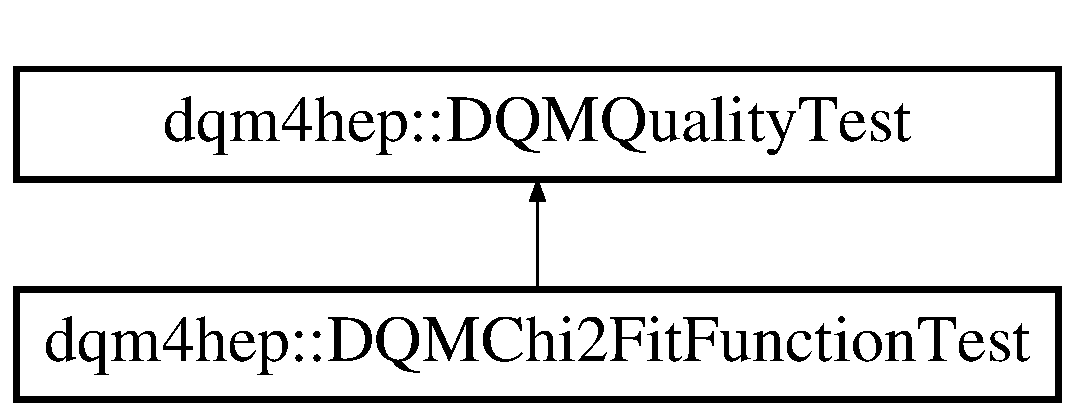
\includegraphics[height=2.000000cm]{classdqm4hep_1_1DQMChi2FitFunctionTest}
\end{center}
\end{figure}
\subsection*{Classes}
\begin{DoxyCompactItemize}
\item 
class {\bf Factory}
\begin{DoxyCompactList}\small\item\em \doxyref{Factory}{p.}{classdqm4hep_1_1DQMChi2FitFunctionTest_1_1Factory} class. \end{DoxyCompactList}\end{DoxyCompactItemize}
\subsection*{Public Member Functions}
\begin{DoxyCompactItemize}
\item 
{\bf D\+Q\+M\+Chi2\+Fit\+Function\+Test} (const std\+::string \&name)
\begin{DoxyCompactList}\small\item\em Constructor with name. \end{DoxyCompactList}\item 
virtual {\bf $\sim$\+D\+Q\+M\+Chi2\+Fit\+Function\+Test} ()
\begin{DoxyCompactList}\small\item\em Destructor. \end{DoxyCompactList}\item 
virtual {\bf Status\+Code} {\bf read\+Settings} (const {\bf Ti\+Xml\+Handle} xml\+Handle)
\begin{DoxyCompactList}\small\item\em Read the settings from the xml handle. \end{DoxyCompactList}\item 
virtual {\bf Status\+Code} {\bf init} ()
\begin{DoxyCompactList}\small\item\em Initialize the quality test. \end{DoxyCompactList}\item 
virtual {\bf Status\+Code} {\bf run} ({\bf D\+Q\+M\+Monitor\+Element} $\ast$p\+Monitor\+Element)
\begin{DoxyCompactList}\small\item\em Runs a quality test on the given monitor element. \end{DoxyCompactList}\item 
virtual bool {\bf can\+Run} ({\bf D\+Q\+M\+Monitor\+Element} $\ast$p\+Monitor\+Element) const 
\begin{DoxyCompactList}\small\item\em Whether the quality test can be run on the monitor element. \end{DoxyCompactList}\end{DoxyCompactItemize}
\subsection*{Protected Attributes}
\begin{DoxyCompactItemize}
\item 
std\+::string {\bf m\+\_\+formula}
\item 
std\+::vector$<$ double $>$ {\bf m\+\_\+input\+Parameter\+List}
\item 
unsigned int {\bf m\+\_\+function\+N\+Parameters}
\item 
double {\bf m\+\_\+function\+X\+Min}
\item 
double {\bf m\+\_\+function\+X\+Max}
\end{DoxyCompactItemize}
\subsection*{Additional Inherited Members}


\subsection{Detailed Description}
\doxyref{D\+Q\+M\+Chi2\+Fit\+Function\+Test}{p.}{classdqm4hep_1_1DQMChi2FitFunctionTest} class. 

Definition at line 244 of file D\+Q\+M\+Quality\+Test.\+h.



\subsection{Constructor \& Destructor Documentation}
\index{dqm4hep\+::\+D\+Q\+M\+Chi2\+Fit\+Function\+Test@{dqm4hep\+::\+D\+Q\+M\+Chi2\+Fit\+Function\+Test}!D\+Q\+M\+Chi2\+Fit\+Function\+Test@{D\+Q\+M\+Chi2\+Fit\+Function\+Test}}
\index{D\+Q\+M\+Chi2\+Fit\+Function\+Test@{D\+Q\+M\+Chi2\+Fit\+Function\+Test}!dqm4hep\+::\+D\+Q\+M\+Chi2\+Fit\+Function\+Test@{dqm4hep\+::\+D\+Q\+M\+Chi2\+Fit\+Function\+Test}}
\subsubsection[{D\+Q\+M\+Chi2\+Fit\+Function\+Test}]{\setlength{\rightskip}{0pt plus 5cm}dqm4hep\+::\+D\+Q\+M\+Chi2\+Fit\+Function\+Test\+::\+D\+Q\+M\+Chi2\+Fit\+Function\+Test (
\begin{DoxyParamCaption}
\item[{const std\+::string \&}]{name}
\end{DoxyParamCaption}
)}\label{classdqm4hep_1_1DQMChi2FitFunctionTest_ab71a2d8c634ccaa88643ac624b6633d9}


Constructor with name. 



Definition at line 320 of file D\+Q\+M\+Quality\+Test.\+cc.


\begin{DoxyCode}
320                                                                     :
321   DQMQualityTest(name),
322   m_functionXMin(0.f),
323   m_functionXMax(1.f),
324   m_functionNParameters(0)
325 \{
326   \textcolor{comment}{/* nop */}
327 \}
\end{DoxyCode}
\index{dqm4hep\+::\+D\+Q\+M\+Chi2\+Fit\+Function\+Test@{dqm4hep\+::\+D\+Q\+M\+Chi2\+Fit\+Function\+Test}!````~D\+Q\+M\+Chi2\+Fit\+Function\+Test@{$\sim$\+D\+Q\+M\+Chi2\+Fit\+Function\+Test}}
\index{````~D\+Q\+M\+Chi2\+Fit\+Function\+Test@{$\sim$\+D\+Q\+M\+Chi2\+Fit\+Function\+Test}!dqm4hep\+::\+D\+Q\+M\+Chi2\+Fit\+Function\+Test@{dqm4hep\+::\+D\+Q\+M\+Chi2\+Fit\+Function\+Test}}
\subsubsection[{$\sim$\+D\+Q\+M\+Chi2\+Fit\+Function\+Test}]{\setlength{\rightskip}{0pt plus 5cm}dqm4hep\+::\+D\+Q\+M\+Chi2\+Fit\+Function\+Test\+::$\sim$\+D\+Q\+M\+Chi2\+Fit\+Function\+Test (
\begin{DoxyParamCaption}
{}
\end{DoxyParamCaption}
)\hspace{0.3cm}{\ttfamily [virtual]}}\label{classdqm4hep_1_1DQMChi2FitFunctionTest_a0f6db19b1f80c17808bc3f73448d0403}


Destructor. 



Definition at line 331 of file D\+Q\+M\+Quality\+Test.\+cc.


\begin{DoxyCode}
332 \{
333   \textcolor{comment}{/* nop */}
334 \}
\end{DoxyCode}


\subsection{Member Function Documentation}
\index{dqm4hep\+::\+D\+Q\+M\+Chi2\+Fit\+Function\+Test@{dqm4hep\+::\+D\+Q\+M\+Chi2\+Fit\+Function\+Test}!can\+Run@{can\+Run}}
\index{can\+Run@{can\+Run}!dqm4hep\+::\+D\+Q\+M\+Chi2\+Fit\+Function\+Test@{dqm4hep\+::\+D\+Q\+M\+Chi2\+Fit\+Function\+Test}}
\subsubsection[{can\+Run}]{\setlength{\rightskip}{0pt plus 5cm}bool dqm4hep\+::\+D\+Q\+M\+Chi2\+Fit\+Function\+Test\+::can\+Run (
\begin{DoxyParamCaption}
\item[{{\bf D\+Q\+M\+Monitor\+Element} $\ast$}]{p\+Monitor\+Element}
\end{DoxyParamCaption}
) const\hspace{0.3cm}{\ttfamily [virtual]}}\label{classdqm4hep_1_1DQMChi2FitFunctionTest_a57451e6dbc2db6e107112223241c0f02}


Whether the quality test can be run on the monitor element. 



Implements {\bf dqm4hep\+::\+D\+Q\+M\+Quality\+Test} \doxyref{}{p.}{classdqm4hep_1_1DQMQualityTest_a94070d01ec18eac873e21f3b653ca391}.



Definition at line 432 of file D\+Q\+M\+Quality\+Test.\+cc.



References dqm4hep\+::\+D\+Q\+M\+Monitor\+Element\+::get(), and dqm4hep\+::\+D\+Q\+M\+Monitor\+Element\+::get\+Type().


\begin{DoxyCode}
433 \{
434   \textcolor{keywordflow}{if}(NULL == pMonitorElement)
435     \textcolor{keywordflow}{return} \textcolor{keyword}{false};
436 
437   DQMMonitorElementType type = pMonitorElement->getType();
438   TH1 *pHistogram = pMonitorElement->get<TH1>();
439 
440   \textcolor{comment}{// asking for a histo 1D}
441   \textcolor{keywordflow}{if}(type < INT\_HISTOGRAM\_1D\_ELEMENT\_TYPE || type > CHAR\_HISTOGRAM\_1D\_ELEMENT\_TYPE)
442     \textcolor{keywordflow}{return} \textcolor{keyword}{false};
443 
444   \textcolor{keywordflow}{if}(NULL == pHistogram)
445     \textcolor{keywordflow}{return} \textcolor{keyword}{false};
446 
447   \textcolor{keywordflow}{return} \textcolor{keyword}{true};
448 \}
\end{DoxyCode}
\index{dqm4hep\+::\+D\+Q\+M\+Chi2\+Fit\+Function\+Test@{dqm4hep\+::\+D\+Q\+M\+Chi2\+Fit\+Function\+Test}!init@{init}}
\index{init@{init}!dqm4hep\+::\+D\+Q\+M\+Chi2\+Fit\+Function\+Test@{dqm4hep\+::\+D\+Q\+M\+Chi2\+Fit\+Function\+Test}}
\subsubsection[{init}]{\setlength{\rightskip}{0pt plus 5cm}{\bf Status\+Code} dqm4hep\+::\+D\+Q\+M\+Chi2\+Fit\+Function\+Test\+::init (
\begin{DoxyParamCaption}
{}
\end{DoxyParamCaption}
)\hspace{0.3cm}{\ttfamily [virtual]}}\label{classdqm4hep_1_1DQMChi2FitFunctionTest_a464fef4b048d4c0477ce240ce6779010}


Initialize the quality test. 



Implements {\bf dqm4hep\+::\+D\+Q\+M\+Quality\+Test} \doxyref{}{p.}{classdqm4hep_1_1DQMQualityTest_a1500cae4000edbc8cae148e5ec612239}.



Definition at line 363 of file D\+Q\+M\+Quality\+Test.\+cc.


\begin{DoxyCode}
364 \{
365   \textcolor{comment}{/* nop */}
366   \textcolor{keywordflow}{return} STATUS\_CODE\_SUCCESS;
367 \}
\end{DoxyCode}
\index{dqm4hep\+::\+D\+Q\+M\+Chi2\+Fit\+Function\+Test@{dqm4hep\+::\+D\+Q\+M\+Chi2\+Fit\+Function\+Test}!read\+Settings@{read\+Settings}}
\index{read\+Settings@{read\+Settings}!dqm4hep\+::\+D\+Q\+M\+Chi2\+Fit\+Function\+Test@{dqm4hep\+::\+D\+Q\+M\+Chi2\+Fit\+Function\+Test}}
\subsubsection[{read\+Settings}]{\setlength{\rightskip}{0pt plus 5cm}{\bf Status\+Code} dqm4hep\+::\+D\+Q\+M\+Chi2\+Fit\+Function\+Test\+::read\+Settings (
\begin{DoxyParamCaption}
\item[{const {\bf Ti\+Xml\+Handle}}]{xml\+Handle}
\end{DoxyParamCaption}
)\hspace{0.3cm}{\ttfamily [virtual]}}\label{classdqm4hep_1_1DQMChi2FitFunctionTest_ac50aa5b47a66e680d6623b6c1ac93b88}


Read the settings from the xml handle. 



Implements {\bf dqm4hep\+::\+D\+Q\+M\+Quality\+Test} \doxyref{}{p.}{classdqm4hep_1_1DQMQualityTest_a34c620c4f331f22d2676eb0401997b7b}.



Definition at line 338 of file D\+Q\+M\+Quality\+Test.\+cc.



References m\+\_\+formula, m\+\_\+function\+N\+Parameters, m\+\_\+function\+X\+Max, m\+\_\+function\+X\+Min, m\+\_\+input\+Parameter\+List, dqm4hep\+::\+D\+Q\+M\+Xml\+Helper\+::read\+Value(), dqm4hep\+::\+D\+Q\+M\+Xml\+Helper\+::read\+Vector\+Of\+Values(), and R\+E\+T\+U\+R\+N\+\_\+\+R\+E\+S\+U\+L\+T\+\_\+\+I\+F.


\begin{DoxyCode}
339 \{
340   RETURN_RESULT_IF(STATUS\_CODE\_SUCCESS, !=, DQMXmlHelper::readValue(xmlHandle,
341       \textcolor{stringliteral}{"Formula"}, m_formula));
342 
343   RETURN_RESULT_IF(STATUS\_CODE\_SUCCESS, !=, DQMXmlHelper::readVectorOfValues(xmlHandle,
344       \textcolor{stringliteral}{"InputParameterList"}, m_inputParameterList));
345 
346   RETURN_RESULT_IF(STATUS\_CODE\_SUCCESS, !=, DQMXmlHelper::readValue(xmlHandle,
347       \textcolor{stringliteral}{"FunctionNParameters"}, m_functionNParameters));
348 
349   \textcolor{keywordflow}{if}(!m_inputParameterList.empty() && m_inputParameterList.size() != 
      m_functionNParameters)
350     \textcolor{keywordflow}{return} STATUS\_CODE\_INVALID\_PARAMETER;
351 
352   RETURN_RESULT_IF(STATUS\_CODE\_SUCCESS, !=, DQMXmlHelper::readValue(xmlHandle,
353       \textcolor{stringliteral}{"FunctionXMin"}, m_functionXMin));
354 
355   RETURN_RESULT_IF(STATUS\_CODE\_SUCCESS, !=, DQMXmlHelper::readValue(xmlHandle,
356       \textcolor{stringliteral}{"FunctionXMax"}, m_functionXMax));
357 
358   \textcolor{keywordflow}{return} STATUS\_CODE\_SUCCESS;
359 \}
\end{DoxyCode}
\index{dqm4hep\+::\+D\+Q\+M\+Chi2\+Fit\+Function\+Test@{dqm4hep\+::\+D\+Q\+M\+Chi2\+Fit\+Function\+Test}!run@{run}}
\index{run@{run}!dqm4hep\+::\+D\+Q\+M\+Chi2\+Fit\+Function\+Test@{dqm4hep\+::\+D\+Q\+M\+Chi2\+Fit\+Function\+Test}}
\subsubsection[{run}]{\setlength{\rightskip}{0pt plus 5cm}{\bf Status\+Code} dqm4hep\+::\+D\+Q\+M\+Chi2\+Fit\+Function\+Test\+::run (
\begin{DoxyParamCaption}
\item[{{\bf D\+Q\+M\+Monitor\+Element} $\ast$}]{p\+Monitor\+Element}
\end{DoxyParamCaption}
)\hspace{0.3cm}{\ttfamily [virtual]}}\label{classdqm4hep_1_1DQMChi2FitFunctionTest_af0e5ff51eab60ca99ff6e83f9e56052b}


Runs a quality test on the given monitor element. 



Implements {\bf dqm4hep\+::\+D\+Q\+M\+Quality\+Test} \doxyref{}{p.}{classdqm4hep_1_1DQMQualityTest_a228419cd9e4cfa60ee51ad0acc77ad0b}.



Definition at line 371 of file D\+Q\+M\+Quality\+Test.\+cc.



References dqm4hep\+::\+D\+Q\+M\+Monitor\+Element\+::get(), dqm4hep\+::\+D\+Q\+M\+Monitor\+Element\+::get\+Name(), dqm4hep\+::\+D\+Q\+M\+Quality\+Test\+::get\+Name(), m\+\_\+formula, m\+\_\+function\+N\+Parameters, m\+\_\+function\+X\+Max, m\+\_\+function\+X\+Min, m\+\_\+input\+Parameter\+List, dqm4hep\+::\+D\+Q\+M\+Quality\+Test\+::m\+\_\+is\+Successful, dqm4hep\+::\+D\+Q\+M\+Quality\+Test\+::m\+\_\+message, dqm4hep\+::\+D\+Q\+M\+Quality\+Test\+::m\+\_\+quality, dqm4hep\+::\+D\+Q\+M4\+H\+E\+P\+::scale\+To\+Quality(), and dqm4hep\+::\+D\+Q\+M4\+H\+E\+P\+::type\+To\+String().


\begin{DoxyCode}
372 \{
373   m_isSuccessful = \textcolor{keyword}{false};
374   m_quality = NO\_QUALITY;
375   m_message = \textcolor{stringliteral}{""};
376 
377   TH1 *pHistogram = pMonitorElement->get<TH1>();
378 
379   std::string functionName = \textcolor{stringliteral}{"DQMChi2FitFunctionTest\_"}+ getName() +\textcolor{stringliteral}{"\_fitFunction"};
380 
381   \textcolor{comment}{// we need to remove the function from the TH1}
382   \textcolor{comment}{// since when TH1::Fit is called, the function}
383   \textcolor{comment}{// is stored in the TH1. The function is removed and deleted}
384   \textcolor{comment}{// since we don't know if the formula is the same as the user provides}
385   TF1 *pFitFunction = pHistogram->GetFunction(functionName.c\_str());
386 
387   \textcolor{keywordflow}{if}(pFitFunction)
388   \{
389     pHistogram->RecursiveRemove(pFitFunction);
390     \textcolor{keyword}{delete} pFitFunction;
391     pFitFunction = NULL;
392   \}
393 
394   \textcolor{comment}{// declare the fit function and fill the parameter list}
395   pFitFunction = \textcolor{keyword}{new} TF1(functionName.c\_str(), m_formula.c\_str(), m_functionXMin, 
      m_functionXMax);\textcolor{comment}{//, m\_functionNParameters);}
396 
397   \textcolor{comment}{// set the parameters depending on if an}
398   \textcolor{comment}{// input has been provided or not by the user}
399   \textcolor{keywordflow}{for}(\textcolor{keywordtype}{unsigned} \textcolor{keywordtype}{int} p=0 ; p<m_functionNParameters ; p++)
400     pFitFunction->SetParameter(p, m_inputParameterList.empty() ? 0 : 
      m_inputParameterList.at(p));
401 
402   \textcolor{comment}{// Q for quiet}
403   \textcolor{comment}{// N for no draw}
404   \textcolor{keywordtype}{int} status = pHistogram->Fit(pFitFunction, \textcolor{stringliteral}{"QN"}, \textcolor{stringliteral}{""}, m_functionXMin, 
      m_functionXMax);
405 
406   \textcolor{keywordflow}{if}(status != 0)
407   \{
408     m_message = \textcolor{stringliteral}{"Try to fit function '"}+ m_formula + \textcolor{stringliteral}{"' with histogram '"} + pMonitorElement->getName() + \textcolor{stringliteral}{"
      '. "} +
409         \textcolor{stringliteral}{"Fit failed and returned status "} + DQM4HEP::typeToString(status);
410 
411     \textcolor{keywordflow}{return} STATUS\_CODE\_SUCCESS;
412   \}
413 
414   \textcolor{keywordtype}{double} chi2 = pFitFunction->GetChisquare();
415   \textcolor{keywordtype}{double} proba = TMath::Prob(chi2, m_inputParameterList.size());
416 
417   m_isSuccessful = \textcolor{keyword}{true};
418   m_quality = DQM4HEP::scaleToQuality(proba);
419   m_message = \textcolor{stringliteral}{"Function '"}+ m_formula +\textcolor{stringliteral}{"' fitted on histogram '"} + pMonitorElement->getName() + \textcolor{stringliteral}{"' ends
       with the following output :\(\backslash\)n"} +
420       \textcolor{stringliteral}{"Chi2 = "} + DQM4HEP::typeToString(chi2) + \textcolor{stringliteral}{"\(\backslash\)n"} +
421       \textcolor{stringliteral}{"Excess probability = "} + DQM4HEP::typeToString(proba) + \textcolor{stringliteral}{"\(\backslash\)n"} +
422       \textcolor{stringliteral}{"Output parameters : \(\backslash\)n"};
423 
424   \textcolor{keywordflow}{for}(\textcolor{keywordtype}{unsigned} \textcolor{keywordtype}{int} p=0 ; p<m_functionNParameters ; p++)
425     m_message += (\textcolor{stringliteral}{" p"} + DQM4HEP::typeToString(p) + \textcolor{stringliteral}{" = "} + 
      DQM4HEP::typeToString(pFitFunction->GetParameter(p)) + \textcolor{stringliteral}{"\(\backslash\)n"});
426 
427   \textcolor{keywordflow}{return} STATUS\_CODE\_SUCCESS;
428 \}
\end{DoxyCode}


\subsection{Member Data Documentation}
\index{dqm4hep\+::\+D\+Q\+M\+Chi2\+Fit\+Function\+Test@{dqm4hep\+::\+D\+Q\+M\+Chi2\+Fit\+Function\+Test}!m\+\_\+formula@{m\+\_\+formula}}
\index{m\+\_\+formula@{m\+\_\+formula}!dqm4hep\+::\+D\+Q\+M\+Chi2\+Fit\+Function\+Test@{dqm4hep\+::\+D\+Q\+M\+Chi2\+Fit\+Function\+Test}}
\subsubsection[{m\+\_\+formula}]{\setlength{\rightskip}{0pt plus 5cm}std\+::string dqm4hep\+::\+D\+Q\+M\+Chi2\+Fit\+Function\+Test\+::m\+\_\+formula\hspace{0.3cm}{\ttfamily [protected]}}\label{classdqm4hep_1_1DQMChi2FitFunctionTest_a31fbc61e6beb7d6b6fae87fbeeaa4b88}


Definition at line 283 of file D\+Q\+M\+Quality\+Test.\+h.



Referenced by read\+Settings(), and run().

\index{dqm4hep\+::\+D\+Q\+M\+Chi2\+Fit\+Function\+Test@{dqm4hep\+::\+D\+Q\+M\+Chi2\+Fit\+Function\+Test}!m\+\_\+function\+N\+Parameters@{m\+\_\+function\+N\+Parameters}}
\index{m\+\_\+function\+N\+Parameters@{m\+\_\+function\+N\+Parameters}!dqm4hep\+::\+D\+Q\+M\+Chi2\+Fit\+Function\+Test@{dqm4hep\+::\+D\+Q\+M\+Chi2\+Fit\+Function\+Test}}
\subsubsection[{m\+\_\+function\+N\+Parameters}]{\setlength{\rightskip}{0pt plus 5cm}unsigned int dqm4hep\+::\+D\+Q\+M\+Chi2\+Fit\+Function\+Test\+::m\+\_\+function\+N\+Parameters\hspace{0.3cm}{\ttfamily [protected]}}\label{classdqm4hep_1_1DQMChi2FitFunctionTest_a0277386a5c7a240924568e90500211ab}


Definition at line 285 of file D\+Q\+M\+Quality\+Test.\+h.



Referenced by read\+Settings(), and run().

\index{dqm4hep\+::\+D\+Q\+M\+Chi2\+Fit\+Function\+Test@{dqm4hep\+::\+D\+Q\+M\+Chi2\+Fit\+Function\+Test}!m\+\_\+function\+X\+Max@{m\+\_\+function\+X\+Max}}
\index{m\+\_\+function\+X\+Max@{m\+\_\+function\+X\+Max}!dqm4hep\+::\+D\+Q\+M\+Chi2\+Fit\+Function\+Test@{dqm4hep\+::\+D\+Q\+M\+Chi2\+Fit\+Function\+Test}}
\subsubsection[{m\+\_\+function\+X\+Max}]{\setlength{\rightskip}{0pt plus 5cm}double dqm4hep\+::\+D\+Q\+M\+Chi2\+Fit\+Function\+Test\+::m\+\_\+function\+X\+Max\hspace{0.3cm}{\ttfamily [protected]}}\label{classdqm4hep_1_1DQMChi2FitFunctionTest_a8f63a016f0c2e6e17138b71a8b94ff99}


Definition at line 287 of file D\+Q\+M\+Quality\+Test.\+h.



Referenced by read\+Settings(), and run().

\index{dqm4hep\+::\+D\+Q\+M\+Chi2\+Fit\+Function\+Test@{dqm4hep\+::\+D\+Q\+M\+Chi2\+Fit\+Function\+Test}!m\+\_\+function\+X\+Min@{m\+\_\+function\+X\+Min}}
\index{m\+\_\+function\+X\+Min@{m\+\_\+function\+X\+Min}!dqm4hep\+::\+D\+Q\+M\+Chi2\+Fit\+Function\+Test@{dqm4hep\+::\+D\+Q\+M\+Chi2\+Fit\+Function\+Test}}
\subsubsection[{m\+\_\+function\+X\+Min}]{\setlength{\rightskip}{0pt plus 5cm}double dqm4hep\+::\+D\+Q\+M\+Chi2\+Fit\+Function\+Test\+::m\+\_\+function\+X\+Min\hspace{0.3cm}{\ttfamily [protected]}}\label{classdqm4hep_1_1DQMChi2FitFunctionTest_a66cca74cce7fc83f555d78ae7c83ff23}


Definition at line 286 of file D\+Q\+M\+Quality\+Test.\+h.



Referenced by read\+Settings(), and run().

\index{dqm4hep\+::\+D\+Q\+M\+Chi2\+Fit\+Function\+Test@{dqm4hep\+::\+D\+Q\+M\+Chi2\+Fit\+Function\+Test}!m\+\_\+input\+Parameter\+List@{m\+\_\+input\+Parameter\+List}}
\index{m\+\_\+input\+Parameter\+List@{m\+\_\+input\+Parameter\+List}!dqm4hep\+::\+D\+Q\+M\+Chi2\+Fit\+Function\+Test@{dqm4hep\+::\+D\+Q\+M\+Chi2\+Fit\+Function\+Test}}
\subsubsection[{m\+\_\+input\+Parameter\+List}]{\setlength{\rightskip}{0pt plus 5cm}std\+::vector$<$double$>$ dqm4hep\+::\+D\+Q\+M\+Chi2\+Fit\+Function\+Test\+::m\+\_\+input\+Parameter\+List\hspace{0.3cm}{\ttfamily [protected]}}\label{classdqm4hep_1_1DQMChi2FitFunctionTest_a6af9a88c2505f5aa9854b6c35ba94030}


Definition at line 284 of file D\+Q\+M\+Quality\+Test.\+h.



Referenced by read\+Settings(), and run().



The documentation for this class was generated from the following files\+:\begin{DoxyCompactItemize}
\item 
{\bf D\+Q\+M\+Quality\+Test.\+h}\item 
{\bf D\+Q\+M\+Quality\+Test.\+cc}\end{DoxyCompactItemize}

\section{dqm4hep\+:\+:D\+Q\+M\+Cluster\+Streamer Class Reference}
\label{classdqm4hep_1_1DQMClusterStreamer}\index{dqm4hep\+::\+D\+Q\+M\+Cluster\+Streamer@{dqm4hep\+::\+D\+Q\+M\+Cluster\+Streamer}}


\doxyref{D\+Q\+M\+Cluster\+Streamer}{p.}{classdqm4hep_1_1DQMClusterStreamer} class.  




{\ttfamily \#include $<$D\+Q\+M\+L\+C\+Event\+Streamer.\+h$>$}

Inheritance diagram for dqm4hep\+:\+:D\+Q\+M\+Cluster\+Streamer\+:\begin{figure}[H]
\begin{center}
\leavevmode
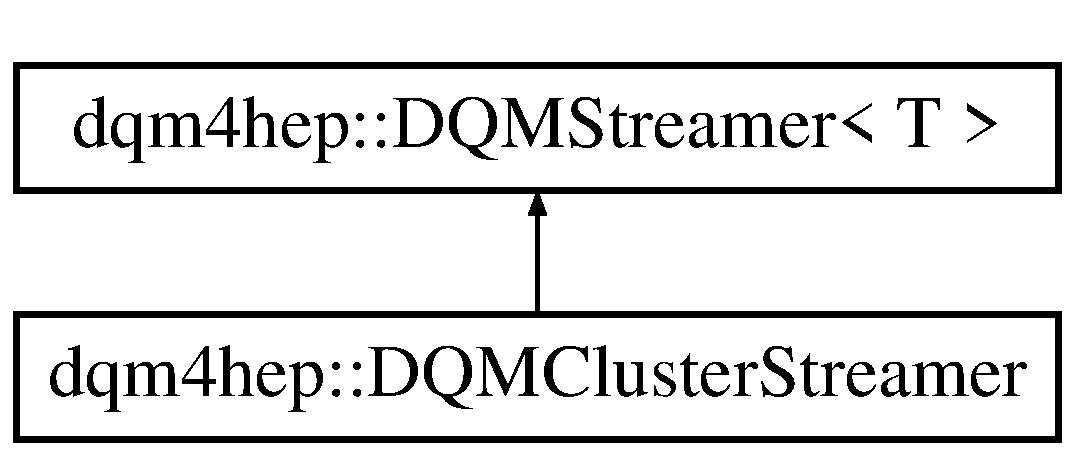
\includegraphics[height=2.000000cm]{classdqm4hep_1_1DQMClusterStreamer}
\end{center}
\end{figure}
\subsection*{Public Member Functions}
\begin{DoxyCompactItemize}
\item 
{\bf Status\+Code} {\bf serialize} (const E\+V\+E\+N\+T\+::\+L\+C\+Object $\ast$const p\+L\+C\+Object, {\bf D\+Q\+M\+Data\+Stream} $\ast$const p\+Data\+Stream)
\begin{DoxyCompactList}\small\item\em Serialize an Cluster. \end{DoxyCompactList}\item 
{\bf Status\+Code} {\bf deserialize} (E\+V\+E\+N\+T\+::\+L\+C\+Object $\ast$\&p\+L\+C\+Object, {\bf D\+Q\+M\+Data\+Stream} $\ast$const p\+Data\+Stream)
\begin{DoxyCompactList}\small\item\em Deserialize a Cluster. \end{DoxyCompactList}\end{DoxyCompactItemize}


\subsection{Detailed Description}
\doxyref{D\+Q\+M\+Cluster\+Streamer}{p.}{classdqm4hep_1_1DQMClusterStreamer} class. 

Definition at line 209 of file D\+Q\+M\+L\+C\+Event\+Streamer.\+h.



\subsection{Member Function Documentation}
\index{dqm4hep\+::\+D\+Q\+M\+Cluster\+Streamer@{dqm4hep\+::\+D\+Q\+M\+Cluster\+Streamer}!deserialize@{deserialize}}
\index{deserialize@{deserialize}!dqm4hep\+::\+D\+Q\+M\+Cluster\+Streamer@{dqm4hep\+::\+D\+Q\+M\+Cluster\+Streamer}}
\subsubsection[{deserialize}]{\setlength{\rightskip}{0pt plus 5cm}{\bf Status\+Code} dqm4hep\+::\+D\+Q\+M\+Cluster\+Streamer\+::deserialize (
\begin{DoxyParamCaption}
\item[{E\+V\+E\+N\+T\+::\+L\+C\+Object $\ast$\&}]{p\+L\+C\+Object, }
\item[{{\bf D\+Q\+M\+Data\+Stream} $\ast$const}]{p\+Data\+Stream}
\end{DoxyParamCaption}
)}\label{classdqm4hep_1_1DQMClusterStreamer_ae63075575f5da2b6aa1fe0319e54171a}


Deserialize a Cluster. 

The object is allocated in this function 

Definition at line 1000 of file D\+Q\+M\+L\+C\+Event\+Streamer.\+cc.



References dqm4hep\+::\+Status\+Code\+Exception\+::get\+Status\+Code(), dqm4hep\+::\+D\+Q\+M\+Data\+Stream\+::read(), T\+H\+R\+O\+W\+\_\+\+R\+E\+S\+U\+L\+T\+\_\+\+I\+F, and dqm4hep\+::\+D\+Q\+M\+Data\+Stream\+::write().


\begin{DoxyCode}
1001 \{
1002   IMPL::ClusterImpl *pCluster = \textcolor{keyword}{new} IMPL::ClusterImpl();
1003 
1004   \textcolor{keywordflow}{try}
1005   \{
1006     dqm_int type = 0;
1007     THROW_RESULT_IF(STATUS\_CODE\_SUCCESS, !=, pDataStream->read(type));
1008 
1009     std::bitset<32> clusterBitSet(type);
1010 
1011     \textcolor{keywordflow}{for}(dqm_uint i=0 ; i<clusterBitSet.size() ; i++)
1012       pCluster->setTypeBit(i, clusterBitSet[i]);
1013 
1014     dqm_float energy = 0.f;
1015     THROW_RESULT_IF(STATUS\_CODE\_SUCCESS, !=, pDataStream->read(energy));
1016     pCluster->setEnergy(energy);
1017 
1018     dqm_float energyError = 0;
1019     THROW_RESULT_IF(STATUS\_CODE\_SUCCESS, !=, pDataStream->read(energyError));
1020     pCluster->setEnergyError(energyError);
1021 
1022     dqm_float *pPosition = 0;
1023     dqm_uint nPos = 0;
1024     THROW_RESULT_IF(STATUS\_CODE\_SUCCESS, !=, pDataStream->read(pPosition, nPos));
1025 
1026     \textcolor{keywordflow}{if}(nPos != 3)
1027       \textcolor{keywordflow}{throw} StatusCodeException(STATUS\_CODE\_FAILURE);
1028 
1029     pCluster->setPosition(pPosition);
1030     \textcolor{keyword}{delete} [] pPosition;
1031 
1032     dqm_uint nPositionErrors = 0;
1033     THROW_RESULT_IF(STATUS\_CODE\_SUCCESS, !=, pDataStream->read(nPositionErrors));
1034 
1035     EVENT::FloatVec positionErrors;
1036 
1037     \textcolor{keywordflow}{for}(dqm_uint i=0 ; i<nPositionErrors ; i++)
1038     \{
1039       dqm_float positionError = 0;
1040       THROW_RESULT_IF(STATUS\_CODE\_SUCCESS, !=, pDataStream->read(positionError));
1041       positionErrors.push\_back(positionError);
1042     \}
1043 
1044     pCluster->setPositionError(positionErrors);
1045 
1046     dqm_float iTheta = 0;
1047     THROW_RESULT_IF(STATUS\_CODE\_SUCCESS, !=, pDataStream->read(iTheta));
1048     pCluster->setITheta(iTheta);
1049 
1050     dqm_float iPhi = 0;
1051     THROW_RESULT_IF(STATUS\_CODE\_SUCCESS, !=, pDataStream->read(iPhi));
1052     pCluster->setIPhi(iPhi);
1053 
1054     dqm_uint nDirectionErrors = 0;
1055     THROW_RESULT_IF(STATUS\_CODE\_SUCCESS, !=, pDataStream->read(nDirectionErrors));
1056 
1057     EVENT::FloatVec directionErrors;
1058 
1059     \textcolor{keywordflow}{for}(dqm_uint i=0 ; i<nDirectionErrors ; i++)
1060     \{
1061       dqm_float directionError = 0;
1062       THROW_RESULT_IF(STATUS\_CODE\_SUCCESS, !=, pDataStream->read(directionError));
1063       directionErrors.push\_back(directionError);
1064     \}
1065 
1066     pCluster->setDirectionError(directionErrors);
1067 
1068     dqm_uint nShapes = 0;
1069     THROW_RESULT_IF(STATUS\_CODE\_SUCCESS, !=, pDataStream->write(nShapes));
1070 
1071     EVENT::FloatVec shapes;
1072 
1073     \textcolor{keywordflow}{for}(dqm_uint i=0 ; i<nShapes ; i++)
1074     \{
1075       dqm_float shape = 0;
1076       THROW_RESULT_IF(STATUS\_CODE\_SUCCESS, !=, pDataStream->read(shape));
1077       shapes.push\_back(shape);
1078     \}
1079 
1080     pCluster->setShape(shapes);
1081 
1082     dqm_uint nParticleIDs = 0;
1083     THROW_RESULT_IF(STATUS\_CODE\_SUCCESS, !=, pDataStream->read(nParticleIDs));
1084 
1085     DQMParticleIDStreamer particleIDStreamer;
1086 
1087     \textcolor{keywordflow}{for}(dqm_uint i=0 ; i<nParticleIDs ; i++)
1088     \{
1089       EVENT::LCObject *pParticleID = 0;
1090       THROW_RESULT_IF(STATUS\_CODE\_SUCCESS, !=, particleIDStreamer.deserialize(pParticleID, pDataStream));
1091       pCluster->addParticleID(dynamic\_cast<EVENT::ParticleID*>(pParticleID));
1092     \}
1093 
1094     dqm_uint nSubdetectorEnergies = 0;
1095     THROW_RESULT_IF(STATUS\_CODE\_SUCCESS, !=, pDataStream->read(nSubdetectorEnergies));
1096 
1097     \textcolor{keywordflow}{for}(dqm_uint i=0 ; i<nSubdetectorEnergies ; i++)
1098     \{
1099       dqm_float subdetectorEnergy = 0;
1100       THROW_RESULT_IF(STATUS\_CODE\_SUCCESS, !=, pDataStream->read(subdetectorEnergy));
1101       pCluster->subdetectorEnergies().push\_back(subdetectorEnergy);
1102     \}
1103   \}
1104   \textcolor{keywordflow}{catch}(StatusCodeException &exception)
1105   \{
1106     \textcolor{keyword}{delete} pCluster;
1107     pCluster = 0;
1108 
1109     \textcolor{keywordflow}{return} exception.getStatusCode();
1110   \}
1111 
1112   pLCObject = pCluster;
1113 
1114   \textcolor{keywordflow}{return} STATUS\_CODE\_SUCCESS;
1115 \}
\end{DoxyCode}
\index{dqm4hep\+::\+D\+Q\+M\+Cluster\+Streamer@{dqm4hep\+::\+D\+Q\+M\+Cluster\+Streamer}!serialize@{serialize}}
\index{serialize@{serialize}!dqm4hep\+::\+D\+Q\+M\+Cluster\+Streamer@{dqm4hep\+::\+D\+Q\+M\+Cluster\+Streamer}}
\subsubsection[{serialize}]{\setlength{\rightskip}{0pt plus 5cm}{\bf Status\+Code} dqm4hep\+::\+D\+Q\+M\+Cluster\+Streamer\+::serialize (
\begin{DoxyParamCaption}
\item[{const E\+V\+E\+N\+T\+::\+L\+C\+Object $\ast$const}]{p\+L\+C\+Object, }
\item[{{\bf D\+Q\+M\+Data\+Stream} $\ast$const}]{p\+Data\+Stream}
\end{DoxyParamCaption}
)}\label{classdqm4hep_1_1DQMClusterStreamer_a2c1e88f1d76de9c33925c298d4ff78b2}


Serialize an Cluster. 



Definition at line 923 of file D\+Q\+M\+L\+C\+Event\+Streamer.\+cc.



References R\+E\+T\+U\+R\+N\+\_\+\+R\+E\+S\+U\+L\+T\+\_\+\+I\+F, and dqm4hep\+::\+D\+Q\+M\+Data\+Stream\+::write().


\begin{DoxyCode}
924 \{
925   \textcolor{keyword}{const} EVENT::Cluster *\textcolor{keyword}{const} pCluster = \textcolor{keyword}{dynamic\_cast<}\textcolor{keyword}{const }EVENT::Cluster *const\textcolor{keyword}{>}(pLCObject);
926 
927   \textcolor{keywordflow}{if}(NULL == pCluster)
928     \textcolor{keywordflow}{return} STATUS\_CODE\_INVALID\_PARAMETER;
929 
930   dqm_int type = pCluster->getType();
931   RETURN_RESULT_IF(STATUS\_CODE\_SUCCESS, !=, pDataStream->write(type));
932 
933   dqm_float energy = pCluster->getEnergy();
934   RETURN_RESULT_IF(STATUS\_CODE\_SUCCESS, !=, pDataStream->write(energy));
935 
936   dqm_float energyError = pCluster->getEnergyError();
937   RETURN_RESULT_IF(STATUS\_CODE\_SUCCESS, !=, pDataStream->write(energyError));
938 
939   \textcolor{keyword}{const} dqm_float *pPosition = pCluster->getPosition();
940   RETURN_RESULT_IF(STATUS\_CODE\_SUCCESS, !=, pDataStream->write(pPosition, 3));
941 
942   dqm_uint nPositionErrors = pCluster->getPositionError().size();
943   RETURN_RESULT_IF(STATUS\_CODE\_SUCCESS, !=, pDataStream->write(nPositionErrors));
944 
945   \textcolor{keywordflow}{for}(dqm_uint i=0 ; i<nPositionErrors ; i++)
946   \{
947     dqm_float positionError = pCluster->getPositionError().at(i);
948     RETURN_RESULT_IF(STATUS\_CODE\_SUCCESS, !=, pDataStream->write(positionError));
949   \}
950 
951   dqm_float iTheta = pCluster->getITheta();
952   RETURN_RESULT_IF(STATUS\_CODE\_SUCCESS, !=, pDataStream->write(iTheta));
953 
954   dqm_float iPhi = pCluster->getIPhi();
955   RETURN_RESULT_IF(STATUS\_CODE\_SUCCESS, !=, pDataStream->write(iPhi));
956 
957   dqm_uint nDirectionErrors = pCluster->getDirectionError().size();
958   RETURN_RESULT_IF(STATUS\_CODE\_SUCCESS, !=, pDataStream->write(nDirectionErrors));
959 
960   \textcolor{keywordflow}{for}(dqm_uint i=0 ; i<nDirectionErrors ; i++)
961   \{
962     dqm_float directionError = pCluster->getDirectionError().at(i);
963     RETURN_RESULT_IF(STATUS\_CODE\_SUCCESS, !=, pDataStream->write(directionError));
964   \}
965 
966   dqm_uint nShapes = pCluster->getShape().size();
967   RETURN_RESULT_IF(STATUS\_CODE\_SUCCESS, !=, pDataStream->write(nShapes));
968 
969   \textcolor{keywordflow}{for}(dqm_uint i=0 ; i<nShapes ; i++)
970   \{
971     dqm_float shape = pCluster->getShape().at(i);
972     RETURN_RESULT_IF(STATUS\_CODE\_SUCCESS, !=, pDataStream->write(shape));
973   \}
974 
975   dqm_uint nParticleIDs = pCluster->getParticleIDs().size();
976   RETURN_RESULT_IF(STATUS\_CODE\_SUCCESS, !=, pDataStream->write(nParticleIDs));
977 
978   DQMParticleIDStreamer particleIDStreamer;
979 
980   \textcolor{keywordflow}{for}(dqm_uint i=0 ; i<nParticleIDs ; i++)
981   \{
982     EVENT::ParticleID *pParticleID = pCluster->getParticleIDs().at(i);
983     RETURN_RESULT_IF(STATUS\_CODE\_SUCCESS, !=, particleIDStreamer.serialize(pParticleID, pDataStream));
984   \}
985 
986   dqm_uint nSubdetectorEnergies = pCluster->getSubdetectorEnergies().size();
987   RETURN_RESULT_IF(STATUS\_CODE\_SUCCESS, !=, pDataStream->write(nSubdetectorEnergies));
988 
989   \textcolor{keywordflow}{for}(dqm_uint i=0 ; i<nSubdetectorEnergies ; i++)
990   \{
991     dqm_float subdetectorEnergy = pCluster->getSubdetectorEnergies().at(i);
992     RETURN_RESULT_IF(STATUS\_CODE\_SUCCESS, !=, pDataStream->write(subdetectorEnergy));
993   \}
994 
995   \textcolor{keywordflow}{return} STATUS\_CODE\_SUCCESS;
996 \}
\end{DoxyCode}


The documentation for this class was generated from the following files\+:\begin{DoxyCompactItemize}
\item 
{\bf D\+Q\+M\+L\+C\+Event\+Streamer.\+h}\item 
{\bf D\+Q\+M\+L\+C\+Event\+Streamer.\+cc}\end{DoxyCompactItemize}

\section{dqm4hep\+:\+:D\+Q\+M\+Collector\+Info Class Reference}
\label{classdqm4hep_1_1DQMCollectorInfo}\index{dqm4hep\+::\+D\+Q\+M\+Collector\+Info@{dqm4hep\+::\+D\+Q\+M\+Collector\+Info}}


\doxyref{D\+Q\+M\+Collector\+Info}{p.}{classdqm4hep_1_1DQMCollectorInfo} class.  




{\ttfamily \#include $<$D\+Q\+M\+Messaging.\+h$>$}

Inheritance diagram for dqm4hep\+:\+:D\+Q\+M\+Collector\+Info\+:\begin{figure}[H]
\begin{center}
\leavevmode
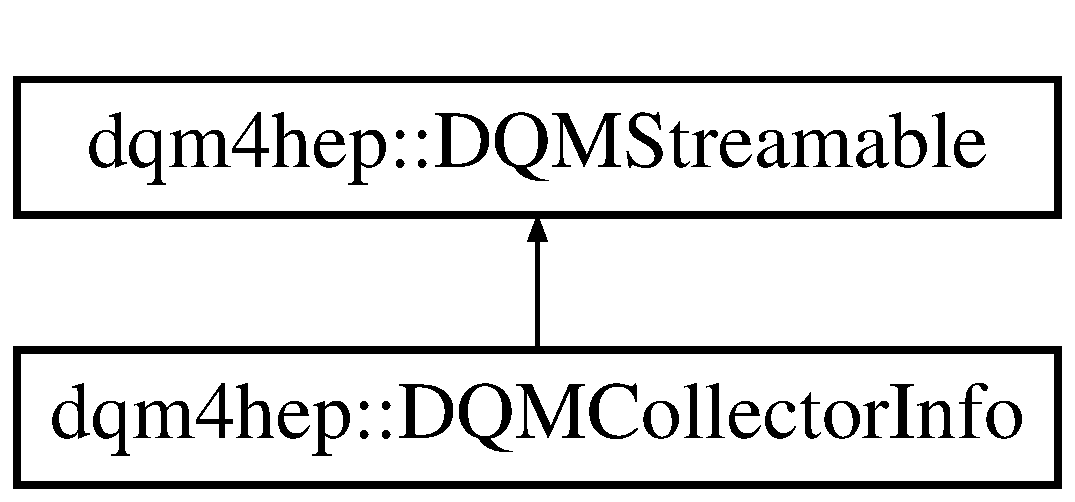
\includegraphics[height=2.000000cm]{classdqm4hep_1_1DQMCollectorInfo}
\end{center}
\end{figure}
\subsection*{Public Member Functions}
\begin{DoxyCompactItemize}
\item 
{\bf Status\+Code} {\bf serialize} ({\bf D\+Q\+M\+Data\+Stream} $\ast$const p\+Data\+Stream) const 
\begin{DoxyCompactList}\small\item\em Serialize collector infos and store it in the data stream. \end{DoxyCompactList}\item 
{\bf Status\+Code} {\bf deserialize} ({\bf D\+Q\+M\+Data\+Stream} $\ast$const p\+Data\+Stream)
\begin{DoxyCompactList}\small\item\em De-\/serialize collector infos from the data stream. \end{DoxyCompactList}\item 
{\bf D\+Q\+M\+Collector\+Info} \& {\bf operator=} (const {\bf D\+Q\+M\+Collector\+Info} \&collector\+Info)
\end{DoxyCompactItemize}
\subsection*{Public Attributes}
\begin{DoxyCompactItemize}
\item 
std\+::string {\bf m\+\_\+system\+Name}
\item 
std\+::string {\bf m\+\_\+node\+Name}
\item 
std\+::string {\bf m\+\_\+release}
\item 
std\+::string {\bf m\+\_\+version}
\item 
std\+::string {\bf m\+\_\+machine}
\item 
std\+::string {\bf m\+\_\+host\+Name}
\item 
std\+::vector$<$ std\+::string $>$ {\bf m\+\_\+module\+List\+Name}
\end{DoxyCompactItemize}


\subsection{Detailed Description}
\doxyref{D\+Q\+M\+Collector\+Info}{p.}{classdqm4hep_1_1DQMCollectorInfo} class. 

Definition at line 98 of file D\+Q\+M\+Messaging.\+h.



\subsection{Member Function Documentation}
\index{dqm4hep\+::\+D\+Q\+M\+Collector\+Info@{dqm4hep\+::\+D\+Q\+M\+Collector\+Info}!deserialize@{deserialize}}
\index{deserialize@{deserialize}!dqm4hep\+::\+D\+Q\+M\+Collector\+Info@{dqm4hep\+::\+D\+Q\+M\+Collector\+Info}}
\subsubsection[{deserialize}]{\setlength{\rightskip}{0pt plus 5cm}{\bf Status\+Code} dqm4hep\+::\+D\+Q\+M\+Collector\+Info\+::deserialize (
\begin{DoxyParamCaption}
\item[{{\bf D\+Q\+M\+Data\+Stream} $\ast$const}]{p\+Data\+Stream}
\end{DoxyParamCaption}
)\hspace{0.3cm}{\ttfamily [virtual]}}\label{classdqm4hep_1_1DQMCollectorInfo_ab3094c332ef50dc346a296e590dcaf9f}


De-\/serialize collector infos from the data stream. 



Implements {\bf dqm4hep\+::\+D\+Q\+M\+Streamable} \doxyref{}{p.}{classdqm4hep_1_1DQMStreamable_a7858bb00272667c30e61490a18ca0a6f}.



Definition at line 179 of file D\+Q\+M\+Messaging.\+cc.



References m\+\_\+host\+Name, m\+\_\+machine, m\+\_\+module\+List\+Name, m\+\_\+node\+Name, m\+\_\+release, m\+\_\+system\+Name, m\+\_\+version, dqm4hep\+::\+D\+Q\+M\+Data\+Stream\+::read(), and R\+E\+T\+U\+R\+N\+\_\+\+R\+E\+S\+U\+L\+T\+\_\+\+I\+F.


\begin{DoxyCode}
180 \{
181   RETURN_RESULT_IF(dqm4hep::STATUS\_CODE\_SUCCESS, !=, pDataStream->read(
      m_systemName));
182   RETURN_RESULT_IF(dqm4hep::STATUS\_CODE\_SUCCESS, !=, pDataStream->read(
      m_nodeName));
183   RETURN_RESULT_IF(dqm4hep::STATUS\_CODE\_SUCCESS, !=, pDataStream->read(m_release));
184   RETURN_RESULT_IF(dqm4hep::STATUS\_CODE\_SUCCESS, !=, pDataStream->read(m_version));
185   RETURN_RESULT_IF(dqm4hep::STATUS\_CODE\_SUCCESS, !=, pDataStream->read(m_machine));
186   RETURN_RESULT_IF(dqm4hep::STATUS\_CODE\_SUCCESS, !=, pDataStream->read(
      m_hostName));
187 
188   dqm_uint nModules = 0;
189   RETURN_RESULT_IF(dqm4hep::STATUS\_CODE\_SUCCESS, !=, pDataStream->read(nModules));
190 
191   \textcolor{keywordflow}{for}(\textcolor{keywordtype}{unsigned} \textcolor{keywordtype}{int} i=0 ; i<nModules ; i++)
192   \{
193     std::string moduleName;
194     RETURN_RESULT_IF(dqm4hep::STATUS\_CODE\_SUCCESS, !=, pDataStream->read(moduleName));
195     m_moduleListName.push\_back(moduleName);
196   \}
197 
198   \textcolor{keywordflow}{return} STATUS\_CODE\_SUCCESS;
199 \}
\end{DoxyCode}
\index{dqm4hep\+::\+D\+Q\+M\+Collector\+Info@{dqm4hep\+::\+D\+Q\+M\+Collector\+Info}!operator=@{operator=}}
\index{operator=@{operator=}!dqm4hep\+::\+D\+Q\+M\+Collector\+Info@{dqm4hep\+::\+D\+Q\+M\+Collector\+Info}}
\subsubsection[{operator=}]{\setlength{\rightskip}{0pt plus 5cm}{\bf D\+Q\+M\+Collector\+Info}\& dqm4hep\+::\+D\+Q\+M\+Collector\+Info\+::operator= (
\begin{DoxyParamCaption}
\item[{const {\bf D\+Q\+M\+Collector\+Info} \&}]{collector\+Info}
\end{DoxyParamCaption}
)\hspace{0.3cm}{\ttfamily [inline]}}\label{classdqm4hep_1_1DQMCollectorInfo_a219722cffe03c09d259ac3d4a54b6efe}


Definition at line 118 of file D\+Q\+M\+Messaging.\+h.



References m\+\_\+host\+Name, m\+\_\+machine, m\+\_\+module\+List\+Name, m\+\_\+node\+Name, m\+\_\+release, m\+\_\+system\+Name, and m\+\_\+version.


\begin{DoxyCode}
119   \{
120     m_systemName = collectorInfo.m\_systemName;
121     m_nodeName = collectorInfo.m\_nodeName;
122     m_release = collectorInfo.m\_release;
123     m_version = collectorInfo.m\_version;
124     m_machine = collectorInfo.m\_machine;
125     m_hostName = collectorInfo.m\_hostName;
126     m_moduleListName = collectorInfo.m\_moduleListName;
127 
128     \textcolor{keywordflow}{return} *\textcolor{keyword}{this};
129   \}
\end{DoxyCode}
\index{dqm4hep\+::\+D\+Q\+M\+Collector\+Info@{dqm4hep\+::\+D\+Q\+M\+Collector\+Info}!serialize@{serialize}}
\index{serialize@{serialize}!dqm4hep\+::\+D\+Q\+M\+Collector\+Info@{dqm4hep\+::\+D\+Q\+M\+Collector\+Info}}
\subsubsection[{serialize}]{\setlength{\rightskip}{0pt plus 5cm}{\bf Status\+Code} dqm4hep\+::\+D\+Q\+M\+Collector\+Info\+::serialize (
\begin{DoxyParamCaption}
\item[{{\bf D\+Q\+M\+Data\+Stream} $\ast$const}]{p\+Data\+Stream}
\end{DoxyParamCaption}
) const\hspace{0.3cm}{\ttfamily [virtual]}}\label{classdqm4hep_1_1DQMCollectorInfo_a657e303a9348ba314046eca335229077}


Serialize collector infos and store it in the data stream. 



Implements {\bf dqm4hep\+::\+D\+Q\+M\+Streamable} \doxyref{}{p.}{classdqm4hep_1_1DQMStreamable_aa6b45693d3b2b18cc15a76744d01b732}.



Definition at line 160 of file D\+Q\+M\+Messaging.\+cc.



References m\+\_\+host\+Name, m\+\_\+machine, m\+\_\+module\+List\+Name, m\+\_\+node\+Name, m\+\_\+release, m\+\_\+system\+Name, m\+\_\+version, R\+E\+T\+U\+R\+N\+\_\+\+R\+E\+S\+U\+L\+T\+\_\+\+I\+F, and dqm4hep\+::\+D\+Q\+M\+Data\+Stream\+::write().



Referenced by dqm4hep\+::\+D\+Q\+M\+Monitor\+Element\+Collector\+Info\+Rpc\+::rpc\+Handler().


\begin{DoxyCode}
161 \{
162   RETURN_RESULT_IF(dqm4hep::STATUS\_CODE\_SUCCESS, !=, pDataStream->write(
      m_systemName));
163   RETURN_RESULT_IF(dqm4hep::STATUS\_CODE\_SUCCESS, !=, pDataStream->write(
      m_nodeName));
164   RETURN_RESULT_IF(dqm4hep::STATUS\_CODE\_SUCCESS, !=, pDataStream->write(
      m_release));
165   RETURN_RESULT_IF(dqm4hep::STATUS\_CODE\_SUCCESS, !=, pDataStream->write(
      m_version));
166   RETURN_RESULT_IF(dqm4hep::STATUS\_CODE\_SUCCESS, !=, pDataStream->write(
      m_machine));
167   RETURN_RESULT_IF(dqm4hep::STATUS\_CODE\_SUCCESS, !=, pDataStream->write(
      m_hostName));
168 
169   RETURN_RESULT_IF(dqm4hep::STATUS\_CODE\_SUCCESS, !=, pDataStream->write((
      dqm_uint)m_moduleListName.size()));
170 
171   \textcolor{keywordflow}{for}(\textcolor{keywordtype}{unsigned} \textcolor{keywordtype}{int} i=0 ; i<m_moduleListName.size() ; i++)
172     RETURN_RESULT_IF(dqm4hep::STATUS\_CODE\_SUCCESS, !=, pDataStream->write(
      m_moduleListName.at(i)));
173 
174   \textcolor{keywordflow}{return} STATUS\_CODE\_SUCCESS;
175 \}
\end{DoxyCode}


\subsection{Member Data Documentation}
\index{dqm4hep\+::\+D\+Q\+M\+Collector\+Info@{dqm4hep\+::\+D\+Q\+M\+Collector\+Info}!m\+\_\+host\+Name@{m\+\_\+host\+Name}}
\index{m\+\_\+host\+Name@{m\+\_\+host\+Name}!dqm4hep\+::\+D\+Q\+M\+Collector\+Info@{dqm4hep\+::\+D\+Q\+M\+Collector\+Info}}
\subsubsection[{m\+\_\+host\+Name}]{\setlength{\rightskip}{0pt plus 5cm}std\+::string dqm4hep\+::\+D\+Q\+M\+Collector\+Info\+::m\+\_\+host\+Name}\label{classdqm4hep_1_1DQMCollectorInfo_ace94b37a8a5e4fb076395d69164dcc3b}


Definition at line 115 of file D\+Q\+M\+Messaging.\+h.



Referenced by deserialize(), operator=(), dqm4hep\+::\+D\+Q\+M\+Monitor\+Element\+Collector\+Info\+Rpc\+::rpc\+Handler(), and serialize().

\index{dqm4hep\+::\+D\+Q\+M\+Collector\+Info@{dqm4hep\+::\+D\+Q\+M\+Collector\+Info}!m\+\_\+machine@{m\+\_\+machine}}
\index{m\+\_\+machine@{m\+\_\+machine}!dqm4hep\+::\+D\+Q\+M\+Collector\+Info@{dqm4hep\+::\+D\+Q\+M\+Collector\+Info}}
\subsubsection[{m\+\_\+machine}]{\setlength{\rightskip}{0pt plus 5cm}std\+::string dqm4hep\+::\+D\+Q\+M\+Collector\+Info\+::m\+\_\+machine}\label{classdqm4hep_1_1DQMCollectorInfo_af55f7ccca62e73406d44c130e2ef7e2f}


Definition at line 114 of file D\+Q\+M\+Messaging.\+h.



Referenced by deserialize(), operator=(), dqm4hep\+::\+D\+Q\+M\+Monitor\+Element\+Collector\+Info\+Rpc\+::rpc\+Handler(), and serialize().

\index{dqm4hep\+::\+D\+Q\+M\+Collector\+Info@{dqm4hep\+::\+D\+Q\+M\+Collector\+Info}!m\+\_\+module\+List\+Name@{m\+\_\+module\+List\+Name}}
\index{m\+\_\+module\+List\+Name@{m\+\_\+module\+List\+Name}!dqm4hep\+::\+D\+Q\+M\+Collector\+Info@{dqm4hep\+::\+D\+Q\+M\+Collector\+Info}}
\subsubsection[{m\+\_\+module\+List\+Name}]{\setlength{\rightskip}{0pt plus 5cm}std\+::vector$<$std\+::string$>$ dqm4hep\+::\+D\+Q\+M\+Collector\+Info\+::m\+\_\+module\+List\+Name}\label{classdqm4hep_1_1DQMCollectorInfo_aa4c7746e1267209afcf1301cddd82b14}


Definition at line 116 of file D\+Q\+M\+Messaging.\+h.



Referenced by deserialize(), operator=(), dqm4hep\+::\+D\+Q\+M\+Monitor\+Element\+Collector\+Info\+Rpc\+::rpc\+Handler(), and serialize().

\index{dqm4hep\+::\+D\+Q\+M\+Collector\+Info@{dqm4hep\+::\+D\+Q\+M\+Collector\+Info}!m\+\_\+node\+Name@{m\+\_\+node\+Name}}
\index{m\+\_\+node\+Name@{m\+\_\+node\+Name}!dqm4hep\+::\+D\+Q\+M\+Collector\+Info@{dqm4hep\+::\+D\+Q\+M\+Collector\+Info}}
\subsubsection[{m\+\_\+node\+Name}]{\setlength{\rightskip}{0pt plus 5cm}std\+::string dqm4hep\+::\+D\+Q\+M\+Collector\+Info\+::m\+\_\+node\+Name}\label{classdqm4hep_1_1DQMCollectorInfo_ab549830bf7df64bf89040f4f0db219a7}


Definition at line 111 of file D\+Q\+M\+Messaging.\+h.



Referenced by deserialize(), operator=(), dqm4hep\+::\+D\+Q\+M\+Monitor\+Element\+Collector\+Info\+Rpc\+::rpc\+Handler(), and serialize().

\index{dqm4hep\+::\+D\+Q\+M\+Collector\+Info@{dqm4hep\+::\+D\+Q\+M\+Collector\+Info}!m\+\_\+release@{m\+\_\+release}}
\index{m\+\_\+release@{m\+\_\+release}!dqm4hep\+::\+D\+Q\+M\+Collector\+Info@{dqm4hep\+::\+D\+Q\+M\+Collector\+Info}}
\subsubsection[{m\+\_\+release}]{\setlength{\rightskip}{0pt plus 5cm}std\+::string dqm4hep\+::\+D\+Q\+M\+Collector\+Info\+::m\+\_\+release}\label{classdqm4hep_1_1DQMCollectorInfo_a21eb99edc4727e3facec004ef9f9243f}


Definition at line 112 of file D\+Q\+M\+Messaging.\+h.



Referenced by deserialize(), operator=(), dqm4hep\+::\+D\+Q\+M\+Monitor\+Element\+Collector\+Info\+Rpc\+::rpc\+Handler(), and serialize().

\index{dqm4hep\+::\+D\+Q\+M\+Collector\+Info@{dqm4hep\+::\+D\+Q\+M\+Collector\+Info}!m\+\_\+system\+Name@{m\+\_\+system\+Name}}
\index{m\+\_\+system\+Name@{m\+\_\+system\+Name}!dqm4hep\+::\+D\+Q\+M\+Collector\+Info@{dqm4hep\+::\+D\+Q\+M\+Collector\+Info}}
\subsubsection[{m\+\_\+system\+Name}]{\setlength{\rightskip}{0pt plus 5cm}std\+::string dqm4hep\+::\+D\+Q\+M\+Collector\+Info\+::m\+\_\+system\+Name}\label{classdqm4hep_1_1DQMCollectorInfo_ac44806f609c248e2de929780fd4f49c6}


Definition at line 110 of file D\+Q\+M\+Messaging.\+h.



Referenced by deserialize(), operator=(), dqm4hep\+::\+D\+Q\+M\+Monitor\+Element\+Collector\+Info\+Rpc\+::rpc\+Handler(), and serialize().

\index{dqm4hep\+::\+D\+Q\+M\+Collector\+Info@{dqm4hep\+::\+D\+Q\+M\+Collector\+Info}!m\+\_\+version@{m\+\_\+version}}
\index{m\+\_\+version@{m\+\_\+version}!dqm4hep\+::\+D\+Q\+M\+Collector\+Info@{dqm4hep\+::\+D\+Q\+M\+Collector\+Info}}
\subsubsection[{m\+\_\+version}]{\setlength{\rightskip}{0pt plus 5cm}std\+::string dqm4hep\+::\+D\+Q\+M\+Collector\+Info\+::m\+\_\+version}\label{classdqm4hep_1_1DQMCollectorInfo_ac0cc8ea4e0fafb5bb7af5213091b70c0}


Definition at line 113 of file D\+Q\+M\+Messaging.\+h.



Referenced by deserialize(), operator=(), dqm4hep\+::\+D\+Q\+M\+Monitor\+Element\+Collector\+Info\+Rpc\+::rpc\+Handler(), and serialize().



The documentation for this class was generated from the following files\+:\begin{DoxyCompactItemize}
\item 
{\bf D\+Q\+M\+Messaging.\+h}\item 
{\bf D\+Q\+M\+Messaging.\+cc}\end{DoxyCompactItemize}

\section{dqm4hep\+:\+:D\+Q\+M\+Core\+Tool Class Reference}
\label{classdqm4hep_1_1DQMCoreTool}\index{dqm4hep\+::\+D\+Q\+M\+Core\+Tool@{dqm4hep\+::\+D\+Q\+M\+Core\+Tool}}


\doxyref{D\+Q\+M\+Core\+Tool}{p.}{classdqm4hep_1_1DQMCoreTool} class.  




{\ttfamily \#include $<$D\+Q\+M\+Core\+Tool.\+h$>$}

\subsection*{Static Public Member Functions}
\begin{DoxyCompactItemize}
\item 
static void {\bf time\+To\+H\+M\+S} (time\+\_\+t t, int \&hours, int \&minutes, int \&seconds)
\begin{DoxyCompactList}\small\item\em Convert time\+\_\+t to hour, minutes and seconds. \end{DoxyCompactList}\item 
static void {\bf time\+To\+H\+M\+S} (time\+\_\+t t, std\+::string \&time\+Str)
\begin{DoxyCompactList}\small\item\em Convert time\+\_\+t to string format as \char`\"{}\+H\+O\+U\+R\+Sh M\+I\+N\+U\+T\+E\+Sm S\+E\+C\+O\+N\+D\+Ss\char`\"{}. \end{DoxyCompactList}\item 
static {\bf String\+Vector} {\bf get\+Special\+Character\+List} ()
\begin{DoxyCompactList}\small\item\em Get the special character list that are to be avoided in some strings. \end{DoxyCompactList}\item 
static bool {\bf contains\+Special\+Characters} (const std\+::string \&str)
\begin{DoxyCompactList}\small\item\em Whether the string contains a special character. \end{DoxyCompactList}\end{DoxyCompactItemize}


\subsection{Detailed Description}
\doxyref{D\+Q\+M\+Core\+Tool}{p.}{classdqm4hep_1_1DQMCoreTool} class. 

Definition at line 40 of file D\+Q\+M\+Core\+Tool.\+h.



\subsection{Member Function Documentation}
\index{dqm4hep\+::\+D\+Q\+M\+Core\+Tool@{dqm4hep\+::\+D\+Q\+M\+Core\+Tool}!contains\+Special\+Characters@{contains\+Special\+Characters}}
\index{contains\+Special\+Characters@{contains\+Special\+Characters}!dqm4hep\+::\+D\+Q\+M\+Core\+Tool@{dqm4hep\+::\+D\+Q\+M\+Core\+Tool}}
\subsubsection[{contains\+Special\+Characters}]{\setlength{\rightskip}{0pt plus 5cm}bool dqm4hep\+::\+D\+Q\+M\+Core\+Tool\+::contains\+Special\+Characters (
\begin{DoxyParamCaption}
\item[{const std\+::string \&}]{str}
\end{DoxyParamCaption}
)\hspace{0.3cm}{\ttfamily [static]}}\label{classdqm4hep_1_1DQMCoreTool_a90531cf2a723212b726001a336e92575}


Whether the string contains a special character. 



Definition at line 92 of file D\+Q\+M\+Core\+Tool.\+cc.



References get\+Special\+Character\+List().



Referenced by dqm4hep\+::\+D\+Q\+M\+Monitor\+Element\+Manager\+::book\+Char\+Histogram1\+D(), dqm4hep\+::\+D\+Q\+M\+Monitor\+Element\+Manager\+::book\+Char\+Histogram2\+D(), dqm4hep\+::\+D\+Q\+M\+Monitor\+Element\+Manager\+::book\+Float(), dqm4hep\+::\+D\+Q\+M\+Monitor\+Element\+Manager\+::book\+Int(), dqm4hep\+::\+D\+Q\+M\+Monitor\+Element\+Manager\+::book\+Int\+Histogram1\+D(), dqm4hep\+::\+D\+Q\+M\+Monitor\+Element\+Manager\+::book\+Int\+Histogram2\+D(), dqm4hep\+::\+D\+Q\+M\+Monitor\+Element\+Manager\+::book\+Object(), dqm4hep\+::\+D\+Q\+M\+Monitor\+Element\+Manager\+::book\+Profile1\+D(), dqm4hep\+::\+D\+Q\+M\+Monitor\+Element\+Manager\+::book\+Profile2\+D(), dqm4hep\+::\+D\+Q\+M\+Monitor\+Element\+Manager\+::book\+Real\+Histogram1\+D(), dqm4hep\+::\+D\+Q\+M\+Monitor\+Element\+Manager\+::book\+Real\+Histogram2\+D(), dqm4hep\+::\+D\+Q\+M\+Monitor\+Element\+Manager\+::book\+Short(), dqm4hep\+::\+D\+Q\+M\+Monitor\+Element\+Manager\+::book\+Short\+Histogram1\+D(), dqm4hep\+::\+D\+Q\+M\+Monitor\+Element\+Manager\+::book\+Short\+Histogram2\+D(), dqm4hep\+::\+D\+Q\+M\+Monitor\+Element\+Manager\+::book\+String(), dqm4hep\+::\+D\+Q\+M\+Directory\+::contains\+Dir(), dqm4hep\+::\+D\+Q\+M\+Path\+::is\+Valid(), and dqm4hep\+::\+D\+Q\+M\+Directory\+::mkdir().


\begin{DoxyCode}
93 \{
94   StringVector specialCharacterList = DQMCoreTool::getSpecialCharacterList();
95 
96   \textcolor{keywordflow}{for}(StringVector::iterator iter = specialCharacterList.begin(), endIter = specialCharacterList.end() ;
97       endIter != iter ; ++iter)
98   \{
99     \textcolor{keywordflow}{if}(str.find(*iter) != std::string::npos)
100       \textcolor{keywordflow}{return} \textcolor{keyword}{true};
101   \}
102 
103   \textcolor{keywordflow}{return} \textcolor{keyword}{false};
104 \}
\end{DoxyCode}
\index{dqm4hep\+::\+D\+Q\+M\+Core\+Tool@{dqm4hep\+::\+D\+Q\+M\+Core\+Tool}!get\+Special\+Character\+List@{get\+Special\+Character\+List}}
\index{get\+Special\+Character\+List@{get\+Special\+Character\+List}!dqm4hep\+::\+D\+Q\+M\+Core\+Tool@{dqm4hep\+::\+D\+Q\+M\+Core\+Tool}}
\subsubsection[{get\+Special\+Character\+List}]{\setlength{\rightskip}{0pt plus 5cm}{\bf String\+Vector} dqm4hep\+::\+D\+Q\+M\+Core\+Tool\+::get\+Special\+Character\+List (
\begin{DoxyParamCaption}
{}
\end{DoxyParamCaption}
)\hspace{0.3cm}{\ttfamily [static]}}\label{classdqm4hep_1_1DQMCoreTool_a68c88f676f13db4e815fcc43ddb1706b}


Get the special character list that are to be avoided in some strings. 



Definition at line 60 of file D\+Q\+M\+Core\+Tool.\+cc.



Referenced by contains\+Special\+Characters().


\begin{DoxyCode}
61 \{
62   StringVector specialCharacterList;
63 
64   specialCharacterList.push\_back(\textcolor{stringliteral}{"|"});
65   specialCharacterList.push\_back(\textcolor{stringliteral}{"&"});
66   specialCharacterList.push\_back(\textcolor{stringliteral}{";"});
67   specialCharacterList.push\_back(\textcolor{stringliteral}{"<"});
68   specialCharacterList.push\_back(\textcolor{stringliteral}{">"});
69   specialCharacterList.push\_back(\textcolor{stringliteral}{"("});
70   specialCharacterList.push\_back(\textcolor{stringliteral}{")"});
71   specialCharacterList.push\_back(\textcolor{stringliteral}{"$"});
72   specialCharacterList.push\_back(\textcolor{stringliteral}{"\(\backslash\)\(\backslash\)"});
73   specialCharacterList.push\_back(\textcolor{stringliteral}{"\(\backslash\)'"});
74   specialCharacterList.push\_back(\textcolor{stringliteral}{"\(\backslash\)""});
75   specialCharacterList.push\_back(\textcolor{stringliteral}{"\(\backslash\)t"});
76   specialCharacterList.push\_back(\textcolor{stringliteral}{"\(\backslash\)n"});
77   specialCharacterList.push\_back(\textcolor{stringliteral}{"*"});
78   specialCharacterList.push\_back(\textcolor{stringliteral}{"?"});
79   specialCharacterList.push\_back(\textcolor{stringliteral}{","});
80   specialCharacterList.push\_back(\textcolor{stringliteral}{"["});
81   specialCharacterList.push\_back(\textcolor{stringliteral}{"]"});
82   specialCharacterList.push\_back(\textcolor{stringliteral}{"#"});
83   specialCharacterList.push\_back(\textcolor{stringliteral}{"~"});
84   specialCharacterList.push\_back(\textcolor{stringliteral}{"="});
85   specialCharacterList.push\_back(\textcolor{stringliteral}{"%"});
86 
87   \textcolor{keywordflow}{return} specialCharacterList;
88 \}
\end{DoxyCode}
\index{dqm4hep\+::\+D\+Q\+M\+Core\+Tool@{dqm4hep\+::\+D\+Q\+M\+Core\+Tool}!time\+To\+H\+M\+S@{time\+To\+H\+M\+S}}
\index{time\+To\+H\+M\+S@{time\+To\+H\+M\+S}!dqm4hep\+::\+D\+Q\+M\+Core\+Tool@{dqm4hep\+::\+D\+Q\+M\+Core\+Tool}}
\subsubsection[{time\+To\+H\+M\+S}]{\setlength{\rightskip}{0pt plus 5cm}void dqm4hep\+::\+D\+Q\+M\+Core\+Tool\+::time\+To\+H\+M\+S (
\begin{DoxyParamCaption}
\item[{time\+\_\+t}]{t, }
\item[{int \&}]{hours, }
\item[{int \&}]{minutes, }
\item[{int \&}]{seconds}
\end{DoxyParamCaption}
)\hspace{0.3cm}{\ttfamily [static]}}\label{classdqm4hep_1_1DQMCoreTool_a652b7872b386bfc958bedb10d59740f5}


Convert time\+\_\+t to hour, minutes and seconds. 



Definition at line 34 of file D\+Q\+M\+Core\+Tool.\+cc.



Referenced by time\+To\+H\+M\+S().


\begin{DoxyCode}
35 \{
36   \textcolor{keyword}{struct }tm *pTmTime = \textcolor{keyword}{new} tm();
37   localtime\_r(&t, pTmTime);
38   hours = pTmTime->tm\_hour;
39   minutes = pTmTime->tm\_min;
40   seconds = pTmTime->tm\_sec;
41   \textcolor{keyword}{delete} pTmTime;
42 \}
\end{DoxyCode}
\index{dqm4hep\+::\+D\+Q\+M\+Core\+Tool@{dqm4hep\+::\+D\+Q\+M\+Core\+Tool}!time\+To\+H\+M\+S@{time\+To\+H\+M\+S}}
\index{time\+To\+H\+M\+S@{time\+To\+H\+M\+S}!dqm4hep\+::\+D\+Q\+M\+Core\+Tool@{dqm4hep\+::\+D\+Q\+M\+Core\+Tool}}
\subsubsection[{time\+To\+H\+M\+S}]{\setlength{\rightskip}{0pt plus 5cm}void dqm4hep\+::\+D\+Q\+M\+Core\+Tool\+::time\+To\+H\+M\+S (
\begin{DoxyParamCaption}
\item[{time\+\_\+t}]{t, }
\item[{std\+::string \&}]{time\+Str}
\end{DoxyParamCaption}
)\hspace{0.3cm}{\ttfamily [static]}}\label{classdqm4hep_1_1DQMCoreTool_ada42bd20fccb24e18409a5f9b6c96f4c}


Convert time\+\_\+t to string format as \char`\"{}\+H\+O\+U\+R\+Sh M\+I\+N\+U\+T\+E\+Sm S\+E\+C\+O\+N\+D\+Ss\char`\"{}. 



Definition at line 46 of file D\+Q\+M\+Core\+Tool.\+cc.



References time\+To\+H\+M\+S().


\begin{DoxyCode}
47 \{
48   \textcolor{comment}{// get h m and s}
49   \textcolor{keywordtype}{int} hours, minutes, seconds;
50   DQMCoreTool::timeToHMS(t, hours, minutes, seconds);
51 
52   \textcolor{comment}{// convert to str}
53   std::stringstream ss;
54   ss << hours << \textcolor{stringliteral}{"h "} << minutes << \textcolor{stringliteral}{"m "} << seconds << \textcolor{stringliteral}{"s"};
55   timeStr = ss.str();
56 \}
\end{DoxyCode}


The documentation for this class was generated from the following files\+:\begin{DoxyCompactItemize}
\item 
{\bf D\+Q\+M\+Core\+Tool.\+h}\item 
{\bf D\+Q\+M\+Core\+Tool.\+cc}\end{DoxyCompactItemize}

\section{dqm4hep\+:\+:D\+Q\+M\+Current\+Run\+Rpc Class Reference}
\label{classdqm4hep_1_1DQMCurrentRunRpc}\index{dqm4hep\+::\+D\+Q\+M\+Current\+Run\+Rpc@{dqm4hep\+::\+D\+Q\+M\+Current\+Run\+Rpc}}


\doxyref{D\+Q\+M\+Current\+Run\+Rpc}{p.}{classdqm4hep_1_1DQMCurrentRunRpc} class.  




{\ttfamily \#include $<$D\+Q\+M\+Run\+Control\+Service.\+h$>$}

Inheritance diagram for dqm4hep\+:\+:D\+Q\+M\+Current\+Run\+Rpc\+:\begin{figure}[H]
\begin{center}
\leavevmode
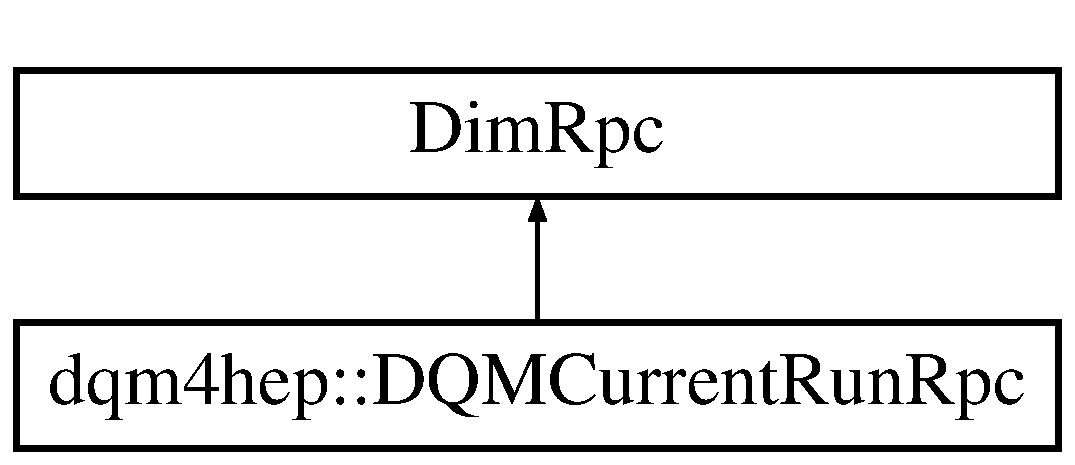
\includegraphics[height=2.000000cm]{classdqm4hep_1_1DQMCurrentRunRpc}
\end{center}
\end{figure}
\subsection*{Public Member Functions}
\begin{DoxyCompactItemize}
\item 
{\bf D\+Q\+M\+Current\+Run\+Rpc} (char $\ast$rpc\+Name, {\bf D\+Q\+M\+Run\+Control\+Service} $\ast$p\+Service)
\begin{DoxyCompactList}\small\item\em Constructor. \end{DoxyCompactList}\end{DoxyCompactItemize}
\subsection*{Private Member Functions}
\begin{DoxyCompactItemize}
\item 
void {\bf rpc\+Handler} ()
\begin{DoxyCompactList}\small\item\em Dim rpc handler. \end{DoxyCompactList}\end{DoxyCompactItemize}
\subsection*{Private Attributes}
\begin{DoxyCompactItemize}
\item 
{\bf D\+Q\+M\+Run\+Control\+Service} $\ast$ {\bf m\+\_\+p\+Service}
\end{DoxyCompactItemize}


\subsection{Detailed Description}
\doxyref{D\+Q\+M\+Current\+Run\+Rpc}{p.}{classdqm4hep_1_1DQMCurrentRunRpc} class. 

Definition at line 51 of file D\+Q\+M\+Run\+Control\+Service.\+h.



\subsection{Constructor \& Destructor Documentation}
\index{dqm4hep\+::\+D\+Q\+M\+Current\+Run\+Rpc@{dqm4hep\+::\+D\+Q\+M\+Current\+Run\+Rpc}!D\+Q\+M\+Current\+Run\+Rpc@{D\+Q\+M\+Current\+Run\+Rpc}}
\index{D\+Q\+M\+Current\+Run\+Rpc@{D\+Q\+M\+Current\+Run\+Rpc}!dqm4hep\+::\+D\+Q\+M\+Current\+Run\+Rpc@{dqm4hep\+::\+D\+Q\+M\+Current\+Run\+Rpc}}
\subsubsection[{D\+Q\+M\+Current\+Run\+Rpc}]{\setlength{\rightskip}{0pt plus 5cm}dqm4hep\+::\+D\+Q\+M\+Current\+Run\+Rpc\+::\+D\+Q\+M\+Current\+Run\+Rpc (
\begin{DoxyParamCaption}
\item[{char $\ast$}]{rpc\+Name, }
\item[{{\bf D\+Q\+M\+Run\+Control\+Service} $\ast$}]{p\+Service}
\end{DoxyParamCaption}
)}\label{classdqm4hep_1_1DQMCurrentRunRpc_afcd0b2419c556ee62fcbdf26c748f8a2}


Constructor. 



Definition at line 36 of file D\+Q\+M\+Run\+Control\+Service.\+cc.


\begin{DoxyCode}
36                                                                                 :
37     DimRpc(rpcName, \textcolor{stringliteral}{"I"}, \textcolor{stringliteral}{"C"}),
38     m_pService(pService)
39 \{
40   \textcolor{comment}{/* nop */}
41 \}
\end{DoxyCode}


\subsection{Member Function Documentation}
\index{dqm4hep\+::\+D\+Q\+M\+Current\+Run\+Rpc@{dqm4hep\+::\+D\+Q\+M\+Current\+Run\+Rpc}!rpc\+Handler@{rpc\+Handler}}
\index{rpc\+Handler@{rpc\+Handler}!dqm4hep\+::\+D\+Q\+M\+Current\+Run\+Rpc@{dqm4hep\+::\+D\+Q\+M\+Current\+Run\+Rpc}}
\subsubsection[{rpc\+Handler}]{\setlength{\rightskip}{0pt plus 5cm}void dqm4hep\+::\+D\+Q\+M\+Current\+Run\+Rpc\+::rpc\+Handler (
\begin{DoxyParamCaption}
{}
\end{DoxyParamCaption}
)\hspace{0.3cm}{\ttfamily [private]}}\label{classdqm4hep_1_1DQMCurrentRunRpc_a667563beb2e8ad55cb27b55c7f6bd180}


Dim rpc handler. 



Definition at line 45 of file D\+Q\+M\+Run\+Control\+Service.\+cc.



References dqm4hep\+::\+D\+Q\+M\+Run\+Control\+Service\+::handle\+Current\+Run\+Rpc(), and m\+\_\+p\+Service.


\begin{DoxyCode}
46 \{
47   m_pService->handleCurrentRunRpc(\textcolor{keyword}{this});
48 \}
\end{DoxyCode}


\subsection{Member Data Documentation}
\index{dqm4hep\+::\+D\+Q\+M\+Current\+Run\+Rpc@{dqm4hep\+::\+D\+Q\+M\+Current\+Run\+Rpc}!m\+\_\+p\+Service@{m\+\_\+p\+Service}}
\index{m\+\_\+p\+Service@{m\+\_\+p\+Service}!dqm4hep\+::\+D\+Q\+M\+Current\+Run\+Rpc@{dqm4hep\+::\+D\+Q\+M\+Current\+Run\+Rpc}}
\subsubsection[{m\+\_\+p\+Service}]{\setlength{\rightskip}{0pt plus 5cm}{\bf D\+Q\+M\+Run\+Control\+Service}$\ast$ dqm4hep\+::\+D\+Q\+M\+Current\+Run\+Rpc\+::m\+\_\+p\+Service\hspace{0.3cm}{\ttfamily [private]}}\label{classdqm4hep_1_1DQMCurrentRunRpc_aa5efdfc51d4872001ec551abde83172a}


Definition at line 64 of file D\+Q\+M\+Run\+Control\+Service.\+h.



Referenced by rpc\+Handler().



The documentation for this class was generated from the following files\+:\begin{DoxyCompactItemize}
\item 
{\bf D\+Q\+M\+Run\+Control\+Service.\+h}\item 
{\bf D\+Q\+M\+Run\+Control\+Service.\+cc}\end{DoxyCompactItemize}

\section{dqm4hep\+:\+:D\+Q\+M\+Current\+Run\+Rpc\+Info Class Reference}
\label{classdqm4hep_1_1DQMCurrentRunRpcInfo}\index{dqm4hep\+::\+D\+Q\+M\+Current\+Run\+Rpc\+Info@{dqm4hep\+::\+D\+Q\+M\+Current\+Run\+Rpc\+Info}}


{\ttfamily \#include $<$D\+Q\+M\+Dim\+Run\+Control\+Client.\+h$>$}

Inheritance diagram for dqm4hep\+:\+:D\+Q\+M\+Current\+Run\+Rpc\+Info\+:\begin{figure}[H]
\begin{center}
\leavevmode
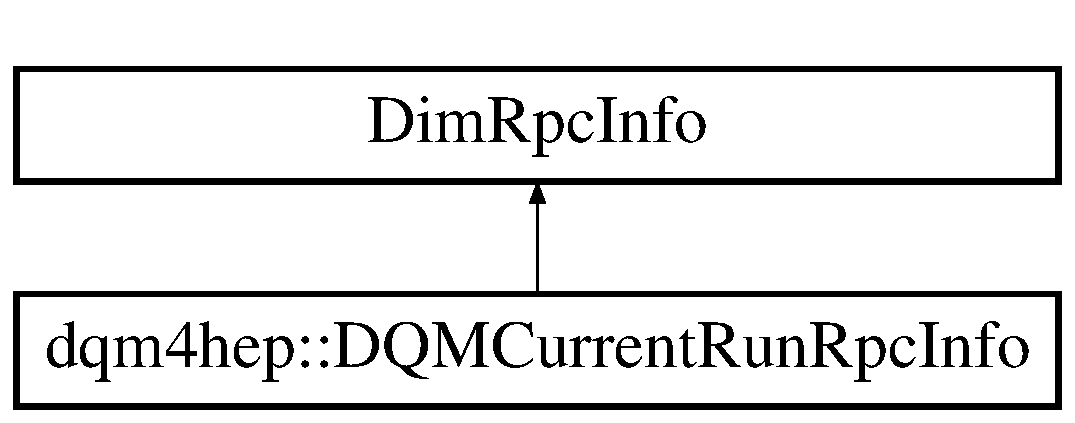
\includegraphics[height=2.000000cm]{classdqm4hep_1_1DQMCurrentRunRpcInfo}
\end{center}
\end{figure}
\subsection*{Public Member Functions}
\begin{DoxyCompactItemize}
\item 
{\bf D\+Q\+M\+Current\+Run\+Rpc\+Info} (char $\ast$rpc\+Name, {\bf D\+Q\+M\+Dim\+Run\+Control\+Client} $\ast$p\+Client)
\begin{DoxyCompactList}\small\item\em Constructor. \end{DoxyCompactList}\end{DoxyCompactItemize}
\subsection*{Private Member Functions}
\begin{DoxyCompactItemize}
\item 
void {\bf rpc\+Info\+Handler} ()
\begin{DoxyCompactList}\small\item\em Dim rpc info handler. \end{DoxyCompactList}\end{DoxyCompactItemize}
\subsection*{Private Attributes}
\begin{DoxyCompactItemize}
\item 
{\bf D\+Q\+M\+Dim\+Run\+Control\+Client} $\ast$ {\bf m\+\_\+p\+Client}
\end{DoxyCompactItemize}


\subsection{Detailed Description}


Definition at line 48 of file D\+Q\+M\+Dim\+Run\+Control\+Client.\+h.



\subsection{Constructor \& Destructor Documentation}
\index{dqm4hep\+::\+D\+Q\+M\+Current\+Run\+Rpc\+Info@{dqm4hep\+::\+D\+Q\+M\+Current\+Run\+Rpc\+Info}!D\+Q\+M\+Current\+Run\+Rpc\+Info@{D\+Q\+M\+Current\+Run\+Rpc\+Info}}
\index{D\+Q\+M\+Current\+Run\+Rpc\+Info@{D\+Q\+M\+Current\+Run\+Rpc\+Info}!dqm4hep\+::\+D\+Q\+M\+Current\+Run\+Rpc\+Info@{dqm4hep\+::\+D\+Q\+M\+Current\+Run\+Rpc\+Info}}
\subsubsection[{D\+Q\+M\+Current\+Run\+Rpc\+Info}]{\setlength{\rightskip}{0pt plus 5cm}dqm4hep\+::\+D\+Q\+M\+Current\+Run\+Rpc\+Info\+::\+D\+Q\+M\+Current\+Run\+Rpc\+Info (
\begin{DoxyParamCaption}
\item[{char $\ast$}]{rpc\+Name, }
\item[{{\bf D\+Q\+M\+Dim\+Run\+Control\+Client} $\ast$}]{p\+Client}
\end{DoxyParamCaption}
)}\label{classdqm4hep_1_1DQMCurrentRunRpcInfo_ac2bea6ccb2ba8f76a2357bd9fdc6e0aa}


Constructor. 



Definition at line 42 of file D\+Q\+M\+Dim\+Run\+Control\+Client.\+cc.


\begin{DoxyCode}
42                                                                                          :
43   DimRpcInfo(rpcName, (\textcolor{keywordtype}{void} *) NULL, 0),
44   m_pClient(pClient)
45 \{
46   \textcolor{comment}{/* nop */}
47 \}
\end{DoxyCode}


\subsection{Member Function Documentation}
\index{dqm4hep\+::\+D\+Q\+M\+Current\+Run\+Rpc\+Info@{dqm4hep\+::\+D\+Q\+M\+Current\+Run\+Rpc\+Info}!rpc\+Info\+Handler@{rpc\+Info\+Handler}}
\index{rpc\+Info\+Handler@{rpc\+Info\+Handler}!dqm4hep\+::\+D\+Q\+M\+Current\+Run\+Rpc\+Info@{dqm4hep\+::\+D\+Q\+M\+Current\+Run\+Rpc\+Info}}
\subsubsection[{rpc\+Info\+Handler}]{\setlength{\rightskip}{0pt plus 5cm}void dqm4hep\+::\+D\+Q\+M\+Current\+Run\+Rpc\+Info\+::rpc\+Info\+Handler (
\begin{DoxyParamCaption}
{}
\end{DoxyParamCaption}
)\hspace{0.3cm}{\ttfamily [private]}}\label{classdqm4hep_1_1DQMCurrentRunRpcInfo_a4547a2fb431604c7a49e364558671817}


Dim rpc info handler. 



Definition at line 51 of file D\+Q\+M\+Dim\+Run\+Control\+Client.\+cc.



References dqm4hep\+::\+D\+Q\+M\+Dim\+Run\+Control\+Client\+::handle\+Current\+Run\+Rpc\+Info(), and m\+\_\+p\+Client.


\begin{DoxyCode}
52 \{
53   m_pClient->handleCurrentRunRpcInfo(\textcolor{keyword}{this});
54 \}
\end{DoxyCode}


\subsection{Member Data Documentation}
\index{dqm4hep\+::\+D\+Q\+M\+Current\+Run\+Rpc\+Info@{dqm4hep\+::\+D\+Q\+M\+Current\+Run\+Rpc\+Info}!m\+\_\+p\+Client@{m\+\_\+p\+Client}}
\index{m\+\_\+p\+Client@{m\+\_\+p\+Client}!dqm4hep\+::\+D\+Q\+M\+Current\+Run\+Rpc\+Info@{dqm4hep\+::\+D\+Q\+M\+Current\+Run\+Rpc\+Info}}
\subsubsection[{m\+\_\+p\+Client}]{\setlength{\rightskip}{0pt plus 5cm}{\bf D\+Q\+M\+Dim\+Run\+Control\+Client}$\ast$ dqm4hep\+::\+D\+Q\+M\+Current\+Run\+Rpc\+Info\+::m\+\_\+p\+Client\hspace{0.3cm}{\ttfamily [private]}}\label{classdqm4hep_1_1DQMCurrentRunRpcInfo_ade89eb1899535749835656a8da60fe47}


Definition at line 61 of file D\+Q\+M\+Dim\+Run\+Control\+Client.\+h.



Referenced by rpc\+Info\+Handler().



The documentation for this class was generated from the following files\+:\begin{DoxyCompactItemize}
\item 
{\bf D\+Q\+M\+Dim\+Run\+Control\+Client.\+h}\item 
{\bf D\+Q\+M\+Dim\+Run\+Control\+Client.\+cc}\end{DoxyCompactItemize}

\section{dqm4hep\+:\+:D\+Q\+M\+Cycle Class Reference}
\label{classdqm4hep_1_1DQMCycle}\index{dqm4hep\+::\+D\+Q\+M\+Cycle@{dqm4hep\+::\+D\+Q\+M\+Cycle}}


\doxyref{D\+Q\+M\+Cycle}{p.}{classdqm4hep_1_1DQMCycle} class.  




{\ttfamily \#include $<$D\+Q\+M\+Cycle.\+h$>$}

Inheritance diagram for dqm4hep\+:\+:D\+Q\+M\+Cycle\+:\begin{figure}[H]
\begin{center}
\leavevmode
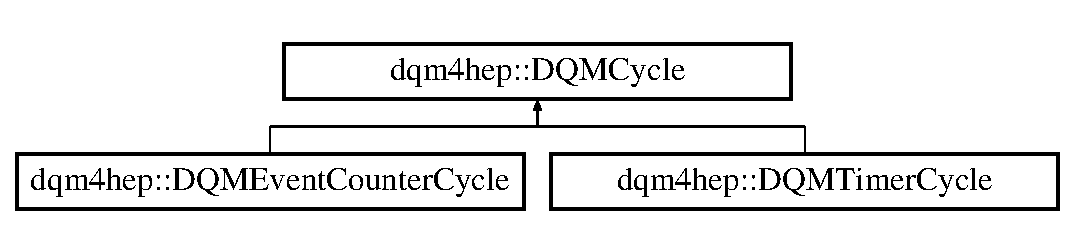
\includegraphics[height=2.000000cm]{classdqm4hep_1_1DQMCycle}
\end{center}
\end{figure}
\subsection*{Public Member Functions}
\begin{DoxyCompactItemize}
\item 
{\bf D\+Q\+M\+Cycle} ()
\begin{DoxyCompactList}\small\item\em Constructor. \end{DoxyCompactList}\item 
virtual {\bf $\sim$\+D\+Q\+M\+Cycle} ()
\begin{DoxyCompactList}\small\item\em Destructor. \end{DoxyCompactList}\item 
float {\bf get\+Cycle\+Value} () const 
\begin{DoxyCompactList}\small\item\em Get the cycle value (time, nb of events, event size) \end{DoxyCompactList}\item 
void {\bf set\+Cycle\+Value} (float value)
\begin{DoxyCompactList}\small\item\em Set the cycle value. \end{DoxyCompactList}\item 
unsigned int {\bf get\+Timeout} () const 
\begin{DoxyCompactList}\small\item\em Get the cycle timeout (in seconds) Maximum time between two process\+Event(evt) call. \end{DoxyCompactList}\item 
void {\bf set\+Timeout} (unsigned int timeout)
\begin{DoxyCompactList}\small\item\em Set the timeout. \end{DoxyCompactList}\item 
float {\bf get\+Processing\+Rate} () const 
\begin{DoxyCompactList}\small\item\em Get the processing rate. \end{DoxyCompactList}\item 
unsigned int {\bf get\+N\+Processed\+Events} () const 
\begin{DoxyCompactList}\small\item\em Get the number of processed events at the end of cycle. \end{DoxyCompactList}\item 
T\+Time {\bf get\+Total\+Cycle\+Time} () const 
\begin{DoxyCompactList}\small\item\em Get the total time spent to process the last cycle. \end{DoxyCompactList}\item 
void {\bf event\+Processed} (const {\bf D\+Q\+M\+Event} $\ast$const p\+Event)
\begin{DoxyCompactList}\small\item\em Called back when the application has processed an event. \end{DoxyCompactList}\item 
const T\+Time \& {\bf get\+Start\+Time} () const 
\begin{DoxyCompactList}\small\item\em Get the start time of the current cycle. \end{DoxyCompactList}\item 
const T\+Time \& {\bf get\+End\+Time} () const 
\begin{DoxyCompactList}\small\item\em Get the end time of the last cycle. \end{DoxyCompactList}\item 
void {\bf start\+Cycle} ()
\begin{DoxyCompactList}\small\item\em Start the cycle. \end{DoxyCompactList}\item 
void {\bf stop\+Cycle} ()
\begin{DoxyCompactList}\small\item\em Stop the cycle. \end{DoxyCompactList}\item 
{\bf D\+Q\+M\+State} {\bf get\+State} () const 
\begin{DoxyCompactList}\small\item\em Get the cycle state (running, stopped) \end{DoxyCompactList}\item 
bool {\bf is\+Timeout\+Reached} () const 
\begin{DoxyCompactList}\small\item\em Whether the timeout is reached. \end{DoxyCompactList}\item 
void {\bf add\+Listener} ({\bf D\+Q\+M\+Cycle\+Listener} $\ast$p\+Listener)
\begin{DoxyCompactList}\small\item\em Add a cycle listener. \end{DoxyCompactList}\item 
void {\bf remove\+Listener} ({\bf D\+Q\+M\+Cycle\+Listener} $\ast$p\+Listener)
\begin{DoxyCompactList}\small\item\em Remove a cycle listener. \end{DoxyCompactList}\item 
virtual void {\bf on\+Cycle\+Started} ()=0
\begin{DoxyCompactList}\small\item\em Specific call back function when a cycle is stopped. \end{DoxyCompactList}\item 
virtual void {\bf on\+Cycle\+Stopped} ()=0
\begin{DoxyCompactList}\small\item\em Specific call back function when a cycle is stopped. \end{DoxyCompactList}\item 
virtual void {\bf on\+Event\+Processed} (const {\bf D\+Q\+M\+Event} $\ast$const p\+Event)=0
\begin{DoxyCompactList}\small\item\em Specific call back function when an event is processed, depends on cycle type. \end{DoxyCompactList}\item 
virtual bool {\bf is\+End\+Of\+Cycle\+Reached} () const =0
\begin{DoxyCompactList}\small\item\em Specific function to tell the application to know whether the cycle has reached the end. \end{DoxyCompactList}\end{DoxyCompactItemize}
\subsection*{Private Attributes}
\begin{DoxyCompactItemize}
\item 
float {\bf m\+\_\+processing\+Rate}
\item 
float {\bf m\+\_\+cycle\+Value}
\item 
unsigned int {\bf m\+\_\+cycle\+Timeout}
\item 
unsigned int {\bf m\+\_\+n\+Processed\+Events}
\item 
T\+Time {\bf m\+\_\+start\+Time}
\item 
T\+Time {\bf m\+\_\+end\+Time}
\item 
T\+Time {\bf m\+\_\+last\+Event\+Processed\+Time}
\item 
std\+::set$<$ {\bf D\+Q\+M\+Cycle\+Listener} $\ast$ $>$ {\bf m\+\_\+listeners}
\item 
{\bf D\+Q\+M\+State} {\bf m\+\_\+state}
\end{DoxyCompactItemize}


\subsection{Detailed Description}
\doxyref{D\+Q\+M\+Cycle}{p.}{classdqm4hep_1_1DQMCycle} class. 

Process a cycle of process\+Event(evt) call for a \doxyref{D\+Q\+M\+Analysis\+Module}{p.}{classdqm4hep_1_1DQMAnalysisModule}. See implementation for cycle types.

The cycle value is the value for which the cycle should normally ends.

The timeout value is the maximum time between two process\+Event(evt) call When the timeout is reached, the cycle ends. The default timeout value is 10 seconds and can be changed via the method set\+Timeout(secs) 

Definition at line 78 of file D\+Q\+M\+Cycle.\+h.



\subsection{Constructor \& Destructor Documentation}
\index{dqm4hep\+::\+D\+Q\+M\+Cycle@{dqm4hep\+::\+D\+Q\+M\+Cycle}!D\+Q\+M\+Cycle@{D\+Q\+M\+Cycle}}
\index{D\+Q\+M\+Cycle@{D\+Q\+M\+Cycle}!dqm4hep\+::\+D\+Q\+M\+Cycle@{dqm4hep\+::\+D\+Q\+M\+Cycle}}
\subsubsection[{D\+Q\+M\+Cycle}]{\setlength{\rightskip}{0pt plus 5cm}dqm4hep\+::\+D\+Q\+M\+Cycle\+::\+D\+Q\+M\+Cycle (
\begin{DoxyParamCaption}
{}
\end{DoxyParamCaption}
)}\label{classdqm4hep_1_1DQMCycle_a966bbd1bee5a074bd67c4b77e6726687}


Constructor. 



Definition at line 36 of file D\+Q\+M\+Cycle.\+cc.


\begin{DoxyCode}
36                    :
37     m_processingRate(0.f),
38     m_cycleValue(0.f),
39     m_cycleTimeout(10), \textcolor{comment}{// 10 seconds is the default value}
40     m_nProcessedEvents(0)
41 \{
42   \textcolor{comment}{/* nop */}
43 \}
\end{DoxyCode}
\index{dqm4hep\+::\+D\+Q\+M\+Cycle@{dqm4hep\+::\+D\+Q\+M\+Cycle}!````~D\+Q\+M\+Cycle@{$\sim$\+D\+Q\+M\+Cycle}}
\index{````~D\+Q\+M\+Cycle@{$\sim$\+D\+Q\+M\+Cycle}!dqm4hep\+::\+D\+Q\+M\+Cycle@{dqm4hep\+::\+D\+Q\+M\+Cycle}}
\subsubsection[{$\sim$\+D\+Q\+M\+Cycle}]{\setlength{\rightskip}{0pt plus 5cm}dqm4hep\+::\+D\+Q\+M\+Cycle\+::$\sim$\+D\+Q\+M\+Cycle (
\begin{DoxyParamCaption}
{}
\end{DoxyParamCaption}
)\hspace{0.3cm}{\ttfamily [virtual]}}\label{classdqm4hep_1_1DQMCycle_a61d4e10a3f4fe8b23dad3a650455f468}


Destructor. 



Definition at line 47 of file D\+Q\+M\+Cycle.\+cc.


\begin{DoxyCode}
48 \{
49   \textcolor{comment}{/* nop */}
50 \}
\end{DoxyCode}


\subsection{Member Function Documentation}
\index{dqm4hep\+::\+D\+Q\+M\+Cycle@{dqm4hep\+::\+D\+Q\+M\+Cycle}!add\+Listener@{add\+Listener}}
\index{add\+Listener@{add\+Listener}!dqm4hep\+::\+D\+Q\+M\+Cycle@{dqm4hep\+::\+D\+Q\+M\+Cycle}}
\subsubsection[{add\+Listener}]{\setlength{\rightskip}{0pt plus 5cm}void dqm4hep\+::\+D\+Q\+M\+Cycle\+::add\+Listener (
\begin{DoxyParamCaption}
\item[{{\bf D\+Q\+M\+Cycle\+Listener} $\ast$}]{p\+Listener}
\end{DoxyParamCaption}
)}\label{classdqm4hep_1_1DQMCycle_a6ecd73e365ab8be6d56ad0b334a9a129}


Add a cycle listener. 



Definition at line 201 of file D\+Q\+M\+Cycle.\+cc.



References m\+\_\+listeners.



Referenced by dqm4hep\+::\+D\+Q\+M\+Analysis\+Module\+Application\+::configure\+Cycle(), and dqm4hep\+::\+D\+Q\+M\+Standalone\+Module\+Application\+::read\+Settings().


\begin{DoxyCode}
202 \{
203   \textcolor{keywordflow}{if}(NULL != pListener)
204     m_listeners.insert(pListener);
205 \}
\end{DoxyCode}
\index{dqm4hep\+::\+D\+Q\+M\+Cycle@{dqm4hep\+::\+D\+Q\+M\+Cycle}!event\+Processed@{event\+Processed}}
\index{event\+Processed@{event\+Processed}!dqm4hep\+::\+D\+Q\+M\+Cycle@{dqm4hep\+::\+D\+Q\+M\+Cycle}}
\subsubsection[{event\+Processed}]{\setlength{\rightskip}{0pt plus 5cm}void dqm4hep\+::\+D\+Q\+M\+Cycle\+::event\+Processed (
\begin{DoxyParamCaption}
\item[{const {\bf D\+Q\+M\+Event} $\ast$const}]{p\+Event}
\end{DoxyParamCaption}
)}\label{classdqm4hep_1_1DQMCycle_a46cec3dc6534d947e6a4c982172de1ad}


Called back when the application has processed an event. 



Definition at line 103 of file D\+Q\+M\+Cycle.\+cc.



References get\+State(), m\+\_\+last\+Event\+Processed\+Time, m\+\_\+listeners, m\+\_\+n\+Processed\+Events, and on\+Event\+Processed().



Referenced by dqm4hep\+::\+D\+Q\+M\+Analysis\+Module\+Application\+::run().


\begin{DoxyCode}
104 \{
105   \textcolor{keywordflow}{if}(this->getState() != RUNNING\_STATE)
106     \textcolor{keywordflow}{return};
107 
108   \textcolor{keywordflow}{if}(NULL == pEvent)
109     \textcolor{keywordflow}{return};
110 
111   m_nProcessedEvents++;
112   m_lastEventProcessedTime = gSystem->Now();
113 
114   \textcolor{comment}{// call back for daughter class}
115   this->onEventProcessed(pEvent);
116 
117   \textcolor{comment}{// call back from listeners}
118   \textcolor{keywordflow}{for}(std::set<DQMCycleListener*>::iterator iter = m_listeners.begin(), endIter = 
      m_listeners.end() ;
119       endIter != iter ; ++iter)
120     (*iter)->onEventProcessed(\textcolor{keyword}{this}, pEvent);
121 \}
\end{DoxyCode}
\index{dqm4hep\+::\+D\+Q\+M\+Cycle@{dqm4hep\+::\+D\+Q\+M\+Cycle}!get\+Cycle\+Value@{get\+Cycle\+Value}}
\index{get\+Cycle\+Value@{get\+Cycle\+Value}!dqm4hep\+::\+D\+Q\+M\+Cycle@{dqm4hep\+::\+D\+Q\+M\+Cycle}}
\subsubsection[{get\+Cycle\+Value}]{\setlength{\rightskip}{0pt plus 5cm}float dqm4hep\+::\+D\+Q\+M\+Cycle\+::get\+Cycle\+Value (
\begin{DoxyParamCaption}
{}
\end{DoxyParamCaption}
) const}\label{classdqm4hep_1_1DQMCycle_a4e8b30ce1ee03863b646ac07372a719f}


Get the cycle value (time, nb of events, event size) 



Definition at line 54 of file D\+Q\+M\+Cycle.\+cc.



References m\+\_\+cycle\+Value.



Referenced by dqm4hep\+::\+D\+Q\+M\+Event\+Counter\+Cycle\+::is\+End\+Of\+Cycle\+Reached(), and dqm4hep\+::\+D\+Q\+M\+Timer\+Cycle\+::is\+End\+Of\+Cycle\+Reached().


\begin{DoxyCode}
55 \{
56   \textcolor{keywordflow}{return} m_cycleValue;
57 \}
\end{DoxyCode}
\index{dqm4hep\+::\+D\+Q\+M\+Cycle@{dqm4hep\+::\+D\+Q\+M\+Cycle}!get\+End\+Time@{get\+End\+Time}}
\index{get\+End\+Time@{get\+End\+Time}!dqm4hep\+::\+D\+Q\+M\+Cycle@{dqm4hep\+::\+D\+Q\+M\+Cycle}}
\subsubsection[{get\+End\+Time}]{\setlength{\rightskip}{0pt plus 5cm}const T\+Time \& dqm4hep\+::\+D\+Q\+M\+Cycle\+::get\+End\+Time (
\begin{DoxyParamCaption}
{}
\end{DoxyParamCaption}
) const}\label{classdqm4hep_1_1DQMCycle_a8ea8a001130535696e3ccce40fb19431}


Get the end time of the last cycle. 

Valid only between two cycle after \doxyref{stop\+Cycle()}{p.}{classdqm4hep_1_1DQMCycle_a531f953ad482c9c051d8eb6f6f7ccad7} call 

Definition at line 132 of file D\+Q\+M\+Cycle.\+cc.



References m\+\_\+end\+Time.


\begin{DoxyCode}
133 \{
134   \textcolor{keywordflow}{return} m_endTime;
135 \}
\end{DoxyCode}
\index{dqm4hep\+::\+D\+Q\+M\+Cycle@{dqm4hep\+::\+D\+Q\+M\+Cycle}!get\+N\+Processed\+Events@{get\+N\+Processed\+Events}}
\index{get\+N\+Processed\+Events@{get\+N\+Processed\+Events}!dqm4hep\+::\+D\+Q\+M\+Cycle@{dqm4hep\+::\+D\+Q\+M\+Cycle}}
\subsubsection[{get\+N\+Processed\+Events}]{\setlength{\rightskip}{0pt plus 5cm}unsigned int dqm4hep\+::\+D\+Q\+M\+Cycle\+::get\+N\+Processed\+Events (
\begin{DoxyParamCaption}
{}
\end{DoxyParamCaption}
) const}\label{classdqm4hep_1_1DQMCycle_a8444637bddfb54d8b784a80d2bd36ad7}


Get the number of processed events at the end of cycle. 



Definition at line 89 of file D\+Q\+M\+Cycle.\+cc.



References m\+\_\+n\+Processed\+Events.



Referenced by dqm4hep\+::\+D\+Q\+M\+Event\+Counter\+Cycle\+::is\+End\+Of\+Cycle\+Reached(), and dqm4hep\+::\+D\+Q\+M\+Analysis\+Module\+Application\+::run().


\begin{DoxyCode}
90 \{
91   \textcolor{keywordflow}{return} m_nProcessedEvents;
92 \}
\end{DoxyCode}
\index{dqm4hep\+::\+D\+Q\+M\+Cycle@{dqm4hep\+::\+D\+Q\+M\+Cycle}!get\+Processing\+Rate@{get\+Processing\+Rate}}
\index{get\+Processing\+Rate@{get\+Processing\+Rate}!dqm4hep\+::\+D\+Q\+M\+Cycle@{dqm4hep\+::\+D\+Q\+M\+Cycle}}
\subsubsection[{get\+Processing\+Rate}]{\setlength{\rightskip}{0pt plus 5cm}float dqm4hep\+::\+D\+Q\+M\+Cycle\+::get\+Processing\+Rate (
\begin{DoxyParamCaption}
{}
\end{DoxyParamCaption}
) const}\label{classdqm4hep_1_1DQMCycle_ab4f51f9b35ae0d935c28470a3cf3a0a2}


Get the processing rate. 

May be called after \doxyref{stop\+Cycle()}{p.}{classdqm4hep_1_1DQMCycle_a531f953ad482c9c051d8eb6f6f7ccad7} to get the correct value 

Definition at line 82 of file D\+Q\+M\+Cycle.\+cc.



References m\+\_\+processing\+Rate.



Referenced by dqm4hep\+::\+D\+Q\+M\+Analysis\+Module\+Application\+::run().


\begin{DoxyCode}
83 \{
84   \textcolor{keywordflow}{return} m_processingRate;
85 \}
\end{DoxyCode}
\index{dqm4hep\+::\+D\+Q\+M\+Cycle@{dqm4hep\+::\+D\+Q\+M\+Cycle}!get\+Start\+Time@{get\+Start\+Time}}
\index{get\+Start\+Time@{get\+Start\+Time}!dqm4hep\+::\+D\+Q\+M\+Cycle@{dqm4hep\+::\+D\+Q\+M\+Cycle}}
\subsubsection[{get\+Start\+Time}]{\setlength{\rightskip}{0pt plus 5cm}const T\+Time \& dqm4hep\+::\+D\+Q\+M\+Cycle\+::get\+Start\+Time (
\begin{DoxyParamCaption}
{}
\end{DoxyParamCaption}
) const}\label{classdqm4hep_1_1DQMCycle_a1dfb0b1b4e1ff9f2b6ce0d84632c4fe5}


Get the start time of the current cycle. 



Definition at line 125 of file D\+Q\+M\+Cycle.\+cc.



References m\+\_\+start\+Time.



Referenced by dqm4hep\+::\+D\+Q\+M\+Timer\+Cycle\+::is\+End\+Of\+Cycle\+Reached().


\begin{DoxyCode}
126 \{
127   \textcolor{keywordflow}{return} m_startTime;
128 \}
\end{DoxyCode}
\index{dqm4hep\+::\+D\+Q\+M\+Cycle@{dqm4hep\+::\+D\+Q\+M\+Cycle}!get\+State@{get\+State}}
\index{get\+State@{get\+State}!dqm4hep\+::\+D\+Q\+M\+Cycle@{dqm4hep\+::\+D\+Q\+M\+Cycle}}
\subsubsection[{get\+State}]{\setlength{\rightskip}{0pt plus 5cm}{\bf D\+Q\+M\+State} dqm4hep\+::\+D\+Q\+M\+Cycle\+::get\+State (
\begin{DoxyParamCaption}
{}
\end{DoxyParamCaption}
) const}\label{classdqm4hep_1_1DQMCycle_a63ee6b7eca9fcdbc85d057cb4ae44a46}


Get the cycle state (running, stopped) 



Definition at line 181 of file D\+Q\+M\+Cycle.\+cc.



References m\+\_\+state.



Referenced by event\+Processed().


\begin{DoxyCode}
182 \{
183   \textcolor{keywordflow}{return} m_state;
184 \}
\end{DoxyCode}
\index{dqm4hep\+::\+D\+Q\+M\+Cycle@{dqm4hep\+::\+D\+Q\+M\+Cycle}!get\+Timeout@{get\+Timeout}}
\index{get\+Timeout@{get\+Timeout}!dqm4hep\+::\+D\+Q\+M\+Cycle@{dqm4hep\+::\+D\+Q\+M\+Cycle}}
\subsubsection[{get\+Timeout}]{\setlength{\rightskip}{0pt plus 5cm}unsigned int dqm4hep\+::\+D\+Q\+M\+Cycle\+::get\+Timeout (
\begin{DoxyParamCaption}
{}
\end{DoxyParamCaption}
) const}\label{classdqm4hep_1_1DQMCycle_a22cffb345526af938af9b4510671ddc3}


Get the cycle timeout (in seconds) Maximum time between two process\+Event(evt) call. 

When the timeout is reached, the cycle ends 

Definition at line 68 of file D\+Q\+M\+Cycle.\+cc.



References m\+\_\+cycle\+Timeout.



Referenced by is\+Timeout\+Reached().


\begin{DoxyCode}
69 \{
70   \textcolor{keywordflow}{return} m_cycleTimeout;
71 \}
\end{DoxyCode}
\index{dqm4hep\+::\+D\+Q\+M\+Cycle@{dqm4hep\+::\+D\+Q\+M\+Cycle}!get\+Total\+Cycle\+Time@{get\+Total\+Cycle\+Time}}
\index{get\+Total\+Cycle\+Time@{get\+Total\+Cycle\+Time}!dqm4hep\+::\+D\+Q\+M\+Cycle@{dqm4hep\+::\+D\+Q\+M\+Cycle}}
\subsubsection[{get\+Total\+Cycle\+Time}]{\setlength{\rightskip}{0pt plus 5cm}T\+Time dqm4hep\+::\+D\+Q\+M\+Cycle\+::get\+Total\+Cycle\+Time (
\begin{DoxyParamCaption}
{}
\end{DoxyParamCaption}
) const}\label{classdqm4hep_1_1DQMCycle_ac25ff87dda4fd7449e08df696d37d6c8}


Get the total time spent to process the last cycle. 



Definition at line 96 of file D\+Q\+M\+Cycle.\+cc.



References m\+\_\+end\+Time, and m\+\_\+start\+Time.



Referenced by dqm4hep\+::\+D\+Q\+M\+Analysis\+Module\+Application\+::run(), and stop\+Cycle().


\begin{DoxyCode}
97 \{
98   \textcolor{keywordflow}{return} (m_endTime - m_startTime);
99 \}
\end{DoxyCode}
\index{dqm4hep\+::\+D\+Q\+M\+Cycle@{dqm4hep\+::\+D\+Q\+M\+Cycle}!is\+End\+Of\+Cycle\+Reached@{is\+End\+Of\+Cycle\+Reached}}
\index{is\+End\+Of\+Cycle\+Reached@{is\+End\+Of\+Cycle\+Reached}!dqm4hep\+::\+D\+Q\+M\+Cycle@{dqm4hep\+::\+D\+Q\+M\+Cycle}}
\subsubsection[{is\+End\+Of\+Cycle\+Reached}]{\setlength{\rightskip}{0pt plus 5cm}virtual bool dqm4hep\+::\+D\+Q\+M\+Cycle\+::is\+End\+Of\+Cycle\+Reached (
\begin{DoxyParamCaption}
{}
\end{DoxyParamCaption}
) const\hspace{0.3cm}{\ttfamily [pure virtual]}}\label{classdqm4hep_1_1DQMCycle_a2b177a69fc0585fbef12dda7b54065d5}


Specific function to tell the application to know whether the cycle has reached the end. 



Implemented in {\bf dqm4hep\+::\+D\+Q\+M\+Timer\+Cycle} \doxyref{}{p.}{classdqm4hep_1_1DQMTimerCycle_aee022855f2262249aba47be919b404e6}, and {\bf dqm4hep\+::\+D\+Q\+M\+Event\+Counter\+Cycle} \doxyref{}{p.}{classdqm4hep_1_1DQMEventCounterCycle_a2b36be8cb34b293b7598cfebb8e2675c}.



Referenced by dqm4hep\+::\+D\+Q\+M\+Analysis\+Module\+Application\+::run().

\index{dqm4hep\+::\+D\+Q\+M\+Cycle@{dqm4hep\+::\+D\+Q\+M\+Cycle}!is\+Timeout\+Reached@{is\+Timeout\+Reached}}
\index{is\+Timeout\+Reached@{is\+Timeout\+Reached}!dqm4hep\+::\+D\+Q\+M\+Cycle@{dqm4hep\+::\+D\+Q\+M\+Cycle}}
\subsubsection[{is\+Timeout\+Reached}]{\setlength{\rightskip}{0pt plus 5cm}bool dqm4hep\+::\+D\+Q\+M\+Cycle\+::is\+Timeout\+Reached (
\begin{DoxyParamCaption}
{}
\end{DoxyParamCaption}
) const}\label{classdqm4hep_1_1DQMCycle_a154c78d3b744c5b4d6edb3ccfe3ba0e4}


Whether the timeout is reached. 



Definition at line 188 of file D\+Q\+M\+Cycle.\+cc.



References get\+Timeout(), and m\+\_\+last\+Event\+Processed\+Time.



Referenced by dqm4hep\+::\+D\+Q\+M\+Analysis\+Module\+Application\+::run().


\begin{DoxyCode}
189 \{
190   \textcolor{keywordflow}{if}(m_lastEventProcessedTime == TTime(0))
191     \textcolor{keywordflow}{return} \textcolor{keyword}{false};
192 
193   \textcolor{keywordflow}{if}( gSystem->Now() > m_lastEventProcessedTime + TTime(this->getTimeout()*1000) )
194     \textcolor{keywordflow}{return} \textcolor{keyword}{true};
195 
196   \textcolor{keywordflow}{return} \textcolor{keyword}{false};
197 \}
\end{DoxyCode}
\index{dqm4hep\+::\+D\+Q\+M\+Cycle@{dqm4hep\+::\+D\+Q\+M\+Cycle}!on\+Cycle\+Started@{on\+Cycle\+Started}}
\index{on\+Cycle\+Started@{on\+Cycle\+Started}!dqm4hep\+::\+D\+Q\+M\+Cycle@{dqm4hep\+::\+D\+Q\+M\+Cycle}}
\subsubsection[{on\+Cycle\+Started}]{\setlength{\rightskip}{0pt plus 5cm}virtual void dqm4hep\+::\+D\+Q\+M\+Cycle\+::on\+Cycle\+Started (
\begin{DoxyParamCaption}
{}
\end{DoxyParamCaption}
)\hspace{0.3cm}{\ttfamily [pure virtual]}}\label{classdqm4hep_1_1DQMCycle_a9ee9c093280a5c87802529233f7ef97d}


Specific call back function when a cycle is stopped. 



Implemented in {\bf dqm4hep\+::\+D\+Q\+M\+Timer\+Cycle} \doxyref{}{p.}{classdqm4hep_1_1DQMTimerCycle_a5f55ba5578ad39a8cd2899fe90b538df}, and {\bf dqm4hep\+::\+D\+Q\+M\+Event\+Counter\+Cycle} \doxyref{}{p.}{classdqm4hep_1_1DQMEventCounterCycle_a50af57684ff7a09ff91370d3b1250040}.



Referenced by start\+Cycle().

\index{dqm4hep\+::\+D\+Q\+M\+Cycle@{dqm4hep\+::\+D\+Q\+M\+Cycle}!on\+Cycle\+Stopped@{on\+Cycle\+Stopped}}
\index{on\+Cycle\+Stopped@{on\+Cycle\+Stopped}!dqm4hep\+::\+D\+Q\+M\+Cycle@{dqm4hep\+::\+D\+Q\+M\+Cycle}}
\subsubsection[{on\+Cycle\+Stopped}]{\setlength{\rightskip}{0pt plus 5cm}virtual void dqm4hep\+::\+D\+Q\+M\+Cycle\+::on\+Cycle\+Stopped (
\begin{DoxyParamCaption}
{}
\end{DoxyParamCaption}
)\hspace{0.3cm}{\ttfamily [pure virtual]}}\label{classdqm4hep_1_1DQMCycle_a9563479df6411c34811e820d49dc242f}


Specific call back function when a cycle is stopped. 



Implemented in {\bf dqm4hep\+::\+D\+Q\+M\+Timer\+Cycle} \doxyref{}{p.}{classdqm4hep_1_1DQMTimerCycle_af772fe5694a7463452828d257ff5310d}, and {\bf dqm4hep\+::\+D\+Q\+M\+Event\+Counter\+Cycle} \doxyref{}{p.}{classdqm4hep_1_1DQMEventCounterCycle_afae6e5fb980fc77e20dafc5d0769a392}.



Referenced by stop\+Cycle().

\index{dqm4hep\+::\+D\+Q\+M\+Cycle@{dqm4hep\+::\+D\+Q\+M\+Cycle}!on\+Event\+Processed@{on\+Event\+Processed}}
\index{on\+Event\+Processed@{on\+Event\+Processed}!dqm4hep\+::\+D\+Q\+M\+Cycle@{dqm4hep\+::\+D\+Q\+M\+Cycle}}
\subsubsection[{on\+Event\+Processed}]{\setlength{\rightskip}{0pt plus 5cm}virtual void dqm4hep\+::\+D\+Q\+M\+Cycle\+::on\+Event\+Processed (
\begin{DoxyParamCaption}
\item[{const {\bf D\+Q\+M\+Event} $\ast$const}]{p\+Event}
\end{DoxyParamCaption}
)\hspace{0.3cm}{\ttfamily [pure virtual]}}\label{classdqm4hep_1_1DQMCycle_a98871dce48f954a8299a8f130125ad59}


Specific call back function when an event is processed, depends on cycle type. 



Implemented in {\bf dqm4hep\+::\+D\+Q\+M\+Timer\+Cycle} \doxyref{}{p.}{classdqm4hep_1_1DQMTimerCycle_a8aa69a62d2c1df9fb9ad7a64eb5c732f}, and {\bf dqm4hep\+::\+D\+Q\+M\+Event\+Counter\+Cycle} \doxyref{}{p.}{classdqm4hep_1_1DQMEventCounterCycle_a6bce65f8d3a5331d96868dd28931c842}.



Referenced by event\+Processed().

\index{dqm4hep\+::\+D\+Q\+M\+Cycle@{dqm4hep\+::\+D\+Q\+M\+Cycle}!remove\+Listener@{remove\+Listener}}
\index{remove\+Listener@{remove\+Listener}!dqm4hep\+::\+D\+Q\+M\+Cycle@{dqm4hep\+::\+D\+Q\+M\+Cycle}}
\subsubsection[{remove\+Listener}]{\setlength{\rightskip}{0pt plus 5cm}void dqm4hep\+::\+D\+Q\+M\+Cycle\+::remove\+Listener (
\begin{DoxyParamCaption}
\item[{{\bf D\+Q\+M\+Cycle\+Listener} $\ast$}]{p\+Listener}
\end{DoxyParamCaption}
)}\label{classdqm4hep_1_1DQMCycle_aa86327ae5b294509c55ac2a59508dc58}


Remove a cycle listener. 



Definition at line 209 of file D\+Q\+M\+Cycle.\+cc.



References m\+\_\+listeners.


\begin{DoxyCode}
210 \{
211   m_listeners.erase(pListener);
212 \}
\end{DoxyCode}
\index{dqm4hep\+::\+D\+Q\+M\+Cycle@{dqm4hep\+::\+D\+Q\+M\+Cycle}!set\+Cycle\+Value@{set\+Cycle\+Value}}
\index{set\+Cycle\+Value@{set\+Cycle\+Value}!dqm4hep\+::\+D\+Q\+M\+Cycle@{dqm4hep\+::\+D\+Q\+M\+Cycle}}
\subsubsection[{set\+Cycle\+Value}]{\setlength{\rightskip}{0pt plus 5cm}void dqm4hep\+::\+D\+Q\+M\+Cycle\+::set\+Cycle\+Value (
\begin{DoxyParamCaption}
\item[{float}]{value}
\end{DoxyParamCaption}
)}\label{classdqm4hep_1_1DQMCycle_a896e3a4d95a97af6a8cc7d7670ae766a}


Set the cycle value. 



Definition at line 61 of file D\+Q\+M\+Cycle.\+cc.



References m\+\_\+cycle\+Value.



Referenced by dqm4hep\+::\+D\+Q\+M\+Analysis\+Module\+Application\+::configure\+Cycle(), and dqm4hep\+::\+D\+Q\+M\+Standalone\+Module\+Application\+::read\+Settings().


\begin{DoxyCode}
62 \{
63   m_cycleValue = value;
64 \}
\end{DoxyCode}
\index{dqm4hep\+::\+D\+Q\+M\+Cycle@{dqm4hep\+::\+D\+Q\+M\+Cycle}!set\+Timeout@{set\+Timeout}}
\index{set\+Timeout@{set\+Timeout}!dqm4hep\+::\+D\+Q\+M\+Cycle@{dqm4hep\+::\+D\+Q\+M\+Cycle}}
\subsubsection[{set\+Timeout}]{\setlength{\rightskip}{0pt plus 5cm}void dqm4hep\+::\+D\+Q\+M\+Cycle\+::set\+Timeout (
\begin{DoxyParamCaption}
\item[{unsigned int}]{timeout}
\end{DoxyParamCaption}
)}\label{classdqm4hep_1_1DQMCycle_a5e7f3271bedf4c4a1b501fa815004793}


Set the timeout. 



Definition at line 75 of file D\+Q\+M\+Cycle.\+cc.



References m\+\_\+cycle\+Timeout.



Referenced by dqm4hep\+::\+D\+Q\+M\+Analysis\+Module\+Application\+::configure\+Cycle(), and dqm4hep\+::\+D\+Q\+M\+Standalone\+Module\+Application\+::read\+Settings().


\begin{DoxyCode}
76 \{
77   m_cycleTimeout = timeout;
78 \}
\end{DoxyCode}
\index{dqm4hep\+::\+D\+Q\+M\+Cycle@{dqm4hep\+::\+D\+Q\+M\+Cycle}!start\+Cycle@{start\+Cycle}}
\index{start\+Cycle@{start\+Cycle}!dqm4hep\+::\+D\+Q\+M\+Cycle@{dqm4hep\+::\+D\+Q\+M\+Cycle}}
\subsubsection[{start\+Cycle}]{\setlength{\rightskip}{0pt plus 5cm}void dqm4hep\+::\+D\+Q\+M\+Cycle\+::start\+Cycle (
\begin{DoxyParamCaption}
{}
\end{DoxyParamCaption}
)}\label{classdqm4hep_1_1DQMCycle_a60d18bef9a1b7ee71e19062a3a467bb8}


Start the cycle. 



Definition at line 139 of file D\+Q\+M\+Cycle.\+cc.



References m\+\_\+end\+Time, m\+\_\+last\+Event\+Processed\+Time, m\+\_\+listeners, m\+\_\+n\+Processed\+Events, m\+\_\+processing\+Rate, m\+\_\+start\+Time, m\+\_\+state, and on\+Cycle\+Started().



Referenced by dqm4hep\+::\+D\+Q\+M\+Standalone\+Module\+Application\+::run(), and dqm4hep\+::\+D\+Q\+M\+Analysis\+Module\+Application\+::run().


\begin{DoxyCode}
140 \{
141   m_startTime = gSystem->Now();
142   m_lastEventProcessedTime = m_startTime;
143   m_endTime = TTime(0);
144 
145   m_nProcessedEvents = 0;
146   m_processingRate = 0.f;
147   m_state = RUNNING\_STATE;
148 
149   \textcolor{comment}{// call back for daughter class}
150   this->onCycleStarted();
151 
152   \textcolor{comment}{// call back from listeners}
153   \textcolor{keywordflow}{for}(std::set<DQMCycleListener*>::iterator iter = m_listeners.begin(), endIter = 
      m_listeners.end() ;
154       endIter != iter ; ++iter)
155     (*iter)->onCycleStarted(\textcolor{keyword}{this});
156 \}
\end{DoxyCode}
\index{dqm4hep\+::\+D\+Q\+M\+Cycle@{dqm4hep\+::\+D\+Q\+M\+Cycle}!stop\+Cycle@{stop\+Cycle}}
\index{stop\+Cycle@{stop\+Cycle}!dqm4hep\+::\+D\+Q\+M\+Cycle@{dqm4hep\+::\+D\+Q\+M\+Cycle}}
\subsubsection[{stop\+Cycle}]{\setlength{\rightskip}{0pt plus 5cm}void dqm4hep\+::\+D\+Q\+M\+Cycle\+::stop\+Cycle (
\begin{DoxyParamCaption}
{}
\end{DoxyParamCaption}
)}\label{classdqm4hep_1_1DQMCycle_a531f953ad482c9c051d8eb6f6f7ccad7}


Stop the cycle. 



Definition at line 160 of file D\+Q\+M\+Cycle.\+cc.



References get\+Total\+Cycle\+Time(), m\+\_\+end\+Time, m\+\_\+listeners, m\+\_\+n\+Processed\+Events, m\+\_\+processing\+Rate, m\+\_\+state, and on\+Cycle\+Stopped().



Referenced by dqm4hep\+::\+D\+Q\+M\+Standalone\+Module\+Application\+::run(), and dqm4hep\+::\+D\+Q\+M\+Analysis\+Module\+Application\+::run().


\begin{DoxyCode}
161 \{
162   m_endTime = gSystem->Now();
163   m_state = STOPPED\_STATE;
164 
165   TTime timeDifference = this->getTotalCycleTime();
166 
167   \textcolor{keywordflow}{if}(timeDifference != TTime(0))
168     m_processingRate = (\textcolor{keyword}{static\_cast<}\textcolor{keywordtype}{float}\textcolor{keyword}{>}(m_nProcessedEvents) / timeDifference.operator \textcolor{keywordtype}{long} \textcolor{keywordtype}{long}());
169 
170   \textcolor{comment}{// call back for daughter class}
171   this->onCycleStopped();
172 
173   \textcolor{comment}{// call back from listeners}
174   \textcolor{keywordflow}{for}(std::set<DQMCycleListener*>::iterator iter = m_listeners.begin(), endIter = 
      m_listeners.end() ;
175       endIter != iter ; ++iter)
176     (*iter)->onCycleStopped(\textcolor{keyword}{this});
177 \}
\end{DoxyCode}


\subsection{Member Data Documentation}
\index{dqm4hep\+::\+D\+Q\+M\+Cycle@{dqm4hep\+::\+D\+Q\+M\+Cycle}!m\+\_\+cycle\+Timeout@{m\+\_\+cycle\+Timeout}}
\index{m\+\_\+cycle\+Timeout@{m\+\_\+cycle\+Timeout}!dqm4hep\+::\+D\+Q\+M\+Cycle@{dqm4hep\+::\+D\+Q\+M\+Cycle}}
\subsubsection[{m\+\_\+cycle\+Timeout}]{\setlength{\rightskip}{0pt plus 5cm}unsigned int dqm4hep\+::\+D\+Q\+M\+Cycle\+::m\+\_\+cycle\+Timeout\hspace{0.3cm}{\ttfamily [private]}}\label{classdqm4hep_1_1DQMCycle_a8a16ce54f049dd97e9b482fb3c922261}


Definition at line 177 of file D\+Q\+M\+Cycle.\+h.



Referenced by get\+Timeout(), and set\+Timeout().

\index{dqm4hep\+::\+D\+Q\+M\+Cycle@{dqm4hep\+::\+D\+Q\+M\+Cycle}!m\+\_\+cycle\+Value@{m\+\_\+cycle\+Value}}
\index{m\+\_\+cycle\+Value@{m\+\_\+cycle\+Value}!dqm4hep\+::\+D\+Q\+M\+Cycle@{dqm4hep\+::\+D\+Q\+M\+Cycle}}
\subsubsection[{m\+\_\+cycle\+Value}]{\setlength{\rightskip}{0pt plus 5cm}float dqm4hep\+::\+D\+Q\+M\+Cycle\+::m\+\_\+cycle\+Value\hspace{0.3cm}{\ttfamily [private]}}\label{classdqm4hep_1_1DQMCycle_ab8d0221e559b3809defbdac288654c80}


Definition at line 176 of file D\+Q\+M\+Cycle.\+h.



Referenced by get\+Cycle\+Value(), and set\+Cycle\+Value().

\index{dqm4hep\+::\+D\+Q\+M\+Cycle@{dqm4hep\+::\+D\+Q\+M\+Cycle}!m\+\_\+end\+Time@{m\+\_\+end\+Time}}
\index{m\+\_\+end\+Time@{m\+\_\+end\+Time}!dqm4hep\+::\+D\+Q\+M\+Cycle@{dqm4hep\+::\+D\+Q\+M\+Cycle}}
\subsubsection[{m\+\_\+end\+Time}]{\setlength{\rightskip}{0pt plus 5cm}T\+Time dqm4hep\+::\+D\+Q\+M\+Cycle\+::m\+\_\+end\+Time\hspace{0.3cm}{\ttfamily [private]}}\label{classdqm4hep_1_1DQMCycle_aadb15f297e6797add280064cb88881de}


Definition at line 180 of file D\+Q\+M\+Cycle.\+h.



Referenced by get\+End\+Time(), get\+Total\+Cycle\+Time(), start\+Cycle(), and stop\+Cycle().

\index{dqm4hep\+::\+D\+Q\+M\+Cycle@{dqm4hep\+::\+D\+Q\+M\+Cycle}!m\+\_\+last\+Event\+Processed\+Time@{m\+\_\+last\+Event\+Processed\+Time}}
\index{m\+\_\+last\+Event\+Processed\+Time@{m\+\_\+last\+Event\+Processed\+Time}!dqm4hep\+::\+D\+Q\+M\+Cycle@{dqm4hep\+::\+D\+Q\+M\+Cycle}}
\subsubsection[{m\+\_\+last\+Event\+Processed\+Time}]{\setlength{\rightskip}{0pt plus 5cm}T\+Time dqm4hep\+::\+D\+Q\+M\+Cycle\+::m\+\_\+last\+Event\+Processed\+Time\hspace{0.3cm}{\ttfamily [private]}}\label{classdqm4hep_1_1DQMCycle_a7c94da449c29cc8f388bda89143ea7d3}


Definition at line 181 of file D\+Q\+M\+Cycle.\+h.



Referenced by event\+Processed(), is\+Timeout\+Reached(), and start\+Cycle().

\index{dqm4hep\+::\+D\+Q\+M\+Cycle@{dqm4hep\+::\+D\+Q\+M\+Cycle}!m\+\_\+listeners@{m\+\_\+listeners}}
\index{m\+\_\+listeners@{m\+\_\+listeners}!dqm4hep\+::\+D\+Q\+M\+Cycle@{dqm4hep\+::\+D\+Q\+M\+Cycle}}
\subsubsection[{m\+\_\+listeners}]{\setlength{\rightskip}{0pt plus 5cm}std\+::set$<${\bf D\+Q\+M\+Cycle\+Listener}$\ast$$>$ dqm4hep\+::\+D\+Q\+M\+Cycle\+::m\+\_\+listeners\hspace{0.3cm}{\ttfamily [private]}}\label{classdqm4hep_1_1DQMCycle_a728589d4f82dddda1d83ab8207b3a287}


Definition at line 182 of file D\+Q\+M\+Cycle.\+h.



Referenced by add\+Listener(), event\+Processed(), remove\+Listener(), start\+Cycle(), and stop\+Cycle().

\index{dqm4hep\+::\+D\+Q\+M\+Cycle@{dqm4hep\+::\+D\+Q\+M\+Cycle}!m\+\_\+n\+Processed\+Events@{m\+\_\+n\+Processed\+Events}}
\index{m\+\_\+n\+Processed\+Events@{m\+\_\+n\+Processed\+Events}!dqm4hep\+::\+D\+Q\+M\+Cycle@{dqm4hep\+::\+D\+Q\+M\+Cycle}}
\subsubsection[{m\+\_\+n\+Processed\+Events}]{\setlength{\rightskip}{0pt plus 5cm}unsigned int dqm4hep\+::\+D\+Q\+M\+Cycle\+::m\+\_\+n\+Processed\+Events\hspace{0.3cm}{\ttfamily [private]}}\label{classdqm4hep_1_1DQMCycle_afb9cb101e6be9eb5032fbd29815b25fd}


Definition at line 178 of file D\+Q\+M\+Cycle.\+h.



Referenced by event\+Processed(), get\+N\+Processed\+Events(), start\+Cycle(), and stop\+Cycle().

\index{dqm4hep\+::\+D\+Q\+M\+Cycle@{dqm4hep\+::\+D\+Q\+M\+Cycle}!m\+\_\+processing\+Rate@{m\+\_\+processing\+Rate}}
\index{m\+\_\+processing\+Rate@{m\+\_\+processing\+Rate}!dqm4hep\+::\+D\+Q\+M\+Cycle@{dqm4hep\+::\+D\+Q\+M\+Cycle}}
\subsubsection[{m\+\_\+processing\+Rate}]{\setlength{\rightskip}{0pt plus 5cm}float dqm4hep\+::\+D\+Q\+M\+Cycle\+::m\+\_\+processing\+Rate\hspace{0.3cm}{\ttfamily [private]}}\label{classdqm4hep_1_1DQMCycle_a337c715a3452e4ab3c593b61e200fab5}


Definition at line 175 of file D\+Q\+M\+Cycle.\+h.



Referenced by get\+Processing\+Rate(), start\+Cycle(), and stop\+Cycle().

\index{dqm4hep\+::\+D\+Q\+M\+Cycle@{dqm4hep\+::\+D\+Q\+M\+Cycle}!m\+\_\+start\+Time@{m\+\_\+start\+Time}}
\index{m\+\_\+start\+Time@{m\+\_\+start\+Time}!dqm4hep\+::\+D\+Q\+M\+Cycle@{dqm4hep\+::\+D\+Q\+M\+Cycle}}
\subsubsection[{m\+\_\+start\+Time}]{\setlength{\rightskip}{0pt plus 5cm}T\+Time dqm4hep\+::\+D\+Q\+M\+Cycle\+::m\+\_\+start\+Time\hspace{0.3cm}{\ttfamily [private]}}\label{classdqm4hep_1_1DQMCycle_a072a6568cf90fa587632c7823cc090f1}


Definition at line 179 of file D\+Q\+M\+Cycle.\+h.



Referenced by get\+Start\+Time(), get\+Total\+Cycle\+Time(), and start\+Cycle().

\index{dqm4hep\+::\+D\+Q\+M\+Cycle@{dqm4hep\+::\+D\+Q\+M\+Cycle}!m\+\_\+state@{m\+\_\+state}}
\index{m\+\_\+state@{m\+\_\+state}!dqm4hep\+::\+D\+Q\+M\+Cycle@{dqm4hep\+::\+D\+Q\+M\+Cycle}}
\subsubsection[{m\+\_\+state}]{\setlength{\rightskip}{0pt plus 5cm}{\bf D\+Q\+M\+State} dqm4hep\+::\+D\+Q\+M\+Cycle\+::m\+\_\+state\hspace{0.3cm}{\ttfamily [private]}}\label{classdqm4hep_1_1DQMCycle_af9c7b185b1f92bf1c80206c6450ab351}


Definition at line 183 of file D\+Q\+M\+Cycle.\+h.



Referenced by get\+State(), start\+Cycle(), and stop\+Cycle().



The documentation for this class was generated from the following files\+:\begin{DoxyCompactItemize}
\item 
{\bf D\+Q\+M\+Cycle.\+h}\item 
{\bf D\+Q\+M\+Cycle.\+cc}\end{DoxyCompactItemize}

\section{dqm4hep\+:\+:D\+Q\+M\+Cycle\+Listener Class Reference}
\label{classdqm4hep_1_1DQMCycleListener}\index{dqm4hep\+::\+D\+Q\+M\+Cycle\+Listener@{dqm4hep\+::\+D\+Q\+M\+Cycle\+Listener}}


\doxyref{D\+Q\+M\+Cycle\+Listener}{p.}{classdqm4hep_1_1DQMCycleListener} class.  




{\ttfamily \#include $<$D\+Q\+M\+Cycle.\+h$>$}

Inheritance diagram for dqm4hep\+:\+:D\+Q\+M\+Cycle\+Listener\+:\begin{figure}[H]
\begin{center}
\leavevmode
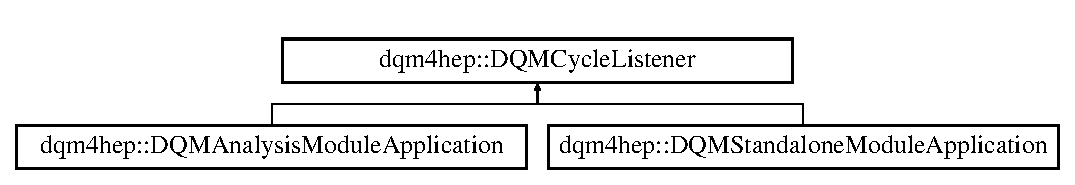
\includegraphics[height=2.000000cm]{classdqm4hep_1_1DQMCycleListener}
\end{center}
\end{figure}
\subsection*{Public Member Functions}
\begin{DoxyCompactItemize}
\item 
virtual {\bf $\sim$\+D\+Q\+M\+Cycle\+Listener} ()
\begin{DoxyCompactList}\small\item\em Destructor. \end{DoxyCompactList}\item 
virtual void {\bf on\+Event\+Processed} (const {\bf D\+Q\+M\+Cycle} $\ast$const p\+Cycle, const {\bf D\+Q\+M\+Event} $\ast$const p\+Event)=0
\begin{DoxyCompactList}\small\item\em Call back function when an event is processed by the framework. \end{DoxyCompactList}\item 
virtual void {\bf on\+Cycle\+Started} (const {\bf D\+Q\+M\+Cycle} $\ast$const p\+Cycle)=0
\begin{DoxyCompactList}\small\item\em Call back function when the cycle is started by the framework. \end{DoxyCompactList}\item 
virtual void {\bf on\+Cycle\+Stopped} (const {\bf D\+Q\+M\+Cycle} $\ast$const p\+Cycle)=0
\begin{DoxyCompactList}\small\item\em Call back function when the cycle is stopped by the framework. \end{DoxyCompactList}\end{DoxyCompactItemize}


\subsection{Detailed Description}
\doxyref{D\+Q\+M\+Cycle\+Listener}{p.}{classdqm4hep_1_1DQMCycleListener} class. 

Definition at line 44 of file D\+Q\+M\+Cycle.\+h.



\subsection{Constructor \& Destructor Documentation}
\index{dqm4hep\+::\+D\+Q\+M\+Cycle\+Listener@{dqm4hep\+::\+D\+Q\+M\+Cycle\+Listener}!````~D\+Q\+M\+Cycle\+Listener@{$\sim$\+D\+Q\+M\+Cycle\+Listener}}
\index{````~D\+Q\+M\+Cycle\+Listener@{$\sim$\+D\+Q\+M\+Cycle\+Listener}!dqm4hep\+::\+D\+Q\+M\+Cycle\+Listener@{dqm4hep\+::\+D\+Q\+M\+Cycle\+Listener}}
\subsubsection[{$\sim$\+D\+Q\+M\+Cycle\+Listener}]{\setlength{\rightskip}{0pt plus 5cm}virtual dqm4hep\+::\+D\+Q\+M\+Cycle\+Listener\+::$\sim$\+D\+Q\+M\+Cycle\+Listener (
\begin{DoxyParamCaption}
{}
\end{DoxyParamCaption}
)\hspace{0.3cm}{\ttfamily [inline]}, {\ttfamily [virtual]}}\label{classdqm4hep_1_1DQMCycleListener_ac236d094d8e89098f29843da8e7a3a6d}


Destructor. 



Definition at line 49 of file D\+Q\+M\+Cycle.\+h.


\begin{DoxyCode}
49 \{\};
\end{DoxyCode}


\subsection{Member Function Documentation}
\index{dqm4hep\+::\+D\+Q\+M\+Cycle\+Listener@{dqm4hep\+::\+D\+Q\+M\+Cycle\+Listener}!on\+Cycle\+Started@{on\+Cycle\+Started}}
\index{on\+Cycle\+Started@{on\+Cycle\+Started}!dqm4hep\+::\+D\+Q\+M\+Cycle\+Listener@{dqm4hep\+::\+D\+Q\+M\+Cycle\+Listener}}
\subsubsection[{on\+Cycle\+Started}]{\setlength{\rightskip}{0pt plus 5cm}virtual void dqm4hep\+::\+D\+Q\+M\+Cycle\+Listener\+::on\+Cycle\+Started (
\begin{DoxyParamCaption}
\item[{const {\bf D\+Q\+M\+Cycle} $\ast$const}]{p\+Cycle}
\end{DoxyParamCaption}
)\hspace{0.3cm}{\ttfamily [pure virtual]}}\label{classdqm4hep_1_1DQMCycleListener_ab9d238178efd278dd88237fcfeb634bc}


Call back function when the cycle is started by the framework. 



Implemented in {\bf dqm4hep\+::\+D\+Q\+M\+Analysis\+Module\+Application} \doxyref{}{p.}{classdqm4hep_1_1DQMAnalysisModuleApplication_a74934c636524b8c2aa2488d083000610}, and {\bf dqm4hep\+::\+D\+Q\+M\+Standalone\+Module\+Application} \doxyref{}{p.}{classdqm4hep_1_1DQMStandaloneModuleApplication_aea3bdd3fea801e56d78be70883c81c9b}.

\index{dqm4hep\+::\+D\+Q\+M\+Cycle\+Listener@{dqm4hep\+::\+D\+Q\+M\+Cycle\+Listener}!on\+Cycle\+Stopped@{on\+Cycle\+Stopped}}
\index{on\+Cycle\+Stopped@{on\+Cycle\+Stopped}!dqm4hep\+::\+D\+Q\+M\+Cycle\+Listener@{dqm4hep\+::\+D\+Q\+M\+Cycle\+Listener}}
\subsubsection[{on\+Cycle\+Stopped}]{\setlength{\rightskip}{0pt plus 5cm}virtual void dqm4hep\+::\+D\+Q\+M\+Cycle\+Listener\+::on\+Cycle\+Stopped (
\begin{DoxyParamCaption}
\item[{const {\bf D\+Q\+M\+Cycle} $\ast$const}]{p\+Cycle}
\end{DoxyParamCaption}
)\hspace{0.3cm}{\ttfamily [pure virtual]}}\label{classdqm4hep_1_1DQMCycleListener_a24aa4e203342ab35794b41df9a6c37ec}


Call back function when the cycle is stopped by the framework. 



Implemented in {\bf dqm4hep\+::\+D\+Q\+M\+Analysis\+Module\+Application} \doxyref{}{p.}{classdqm4hep_1_1DQMAnalysisModuleApplication_a9faa5faf7ce5f4d825d45a9be6e7b5e3}, and {\bf dqm4hep\+::\+D\+Q\+M\+Standalone\+Module\+Application} \doxyref{}{p.}{classdqm4hep_1_1DQMStandaloneModuleApplication_a71d5a2943bc4f0d9fa5d3629ff4b8caa}.

\index{dqm4hep\+::\+D\+Q\+M\+Cycle\+Listener@{dqm4hep\+::\+D\+Q\+M\+Cycle\+Listener}!on\+Event\+Processed@{on\+Event\+Processed}}
\index{on\+Event\+Processed@{on\+Event\+Processed}!dqm4hep\+::\+D\+Q\+M\+Cycle\+Listener@{dqm4hep\+::\+D\+Q\+M\+Cycle\+Listener}}
\subsubsection[{on\+Event\+Processed}]{\setlength{\rightskip}{0pt plus 5cm}virtual void dqm4hep\+::\+D\+Q\+M\+Cycle\+Listener\+::on\+Event\+Processed (
\begin{DoxyParamCaption}
\item[{const {\bf D\+Q\+M\+Cycle} $\ast$const}]{p\+Cycle, }
\item[{const {\bf D\+Q\+M\+Event} $\ast$const}]{p\+Event}
\end{DoxyParamCaption}
)\hspace{0.3cm}{\ttfamily [pure virtual]}}\label{classdqm4hep_1_1DQMCycleListener_a2845abc69dbb59cfaf4fb6fc491bec8b}


Call back function when an event is processed by the framework. 



Implemented in {\bf dqm4hep\+::\+D\+Q\+M\+Analysis\+Module\+Application} \doxyref{}{p.}{classdqm4hep_1_1DQMAnalysisModuleApplication_adaa1b8a34ba4e04e66b37c982f716e32}, and {\bf dqm4hep\+::\+D\+Q\+M\+Standalone\+Module\+Application} \doxyref{}{p.}{classdqm4hep_1_1DQMStandaloneModuleApplication_a46f168f9a1a2aa14c85380e81c8a3f80}.



The documentation for this class was generated from the following file\+:\begin{DoxyCompactItemize}
\item 
{\bf D\+Q\+M\+Cycle.\+h}\end{DoxyCompactItemize}

\section{dqm4hep\+:\+:D\+Q\+M\+Data\+Stream Class Reference}
\label{classdqm4hep_1_1DQMDataStream}\index{dqm4hep\+::\+D\+Q\+M\+Data\+Stream@{dqm4hep\+::\+D\+Q\+M\+Data\+Stream}}


\doxyref{D\+Q\+M\+Data\+Stream}{p.}{classdqm4hep_1_1DQMDataStream} class.  




{\ttfamily \#include $<$D\+Q\+M\+Data\+Stream.\+h$>$}

\subsection*{Public Member Functions}
\begin{DoxyCompactItemize}
\item 
{\bf D\+Q\+M\+Data\+Stream} ({\bf dqm\+\_\+uint} max\+Buffer\+Size)
\begin{DoxyCompactList}\small\item\em Constructor with an initial buffer size. \end{DoxyCompactList}\item 
virtual {\bf $\sim$\+D\+Q\+M\+Data\+Stream} ()
\begin{DoxyCompactList}\small\item\em Destructor. \end{DoxyCompactList}\item 
void {\bf reset} ()
\begin{DoxyCompactList}\small\item\em Reset the buffer ptr to beginning of the buffer. \end{DoxyCompactList}\item 
char $\ast$ {\bf get\+Buffer} () const 
\begin{DoxyCompactList}\small\item\em Get the buffer. \end{DoxyCompactList}\item 
{\bf Status\+Code} {\bf set\+Buffer} (char $\ast$p\+Buffer, {\bf dqm\+\_\+uint} size)
\begin{DoxyCompactList}\small\item\em Set the buffer with its size. \end{DoxyCompactList}\item 
{\bf dqm\+\_\+uint} {\bf get\+Max\+Buffer\+Size} () const 
\begin{DoxyCompactList}\small\item\em Get the maximum size of the allocated buffer. \end{DoxyCompactList}\item 
{\bf dqm\+\_\+uint} {\bf get\+Buffer\+Size} () const 
\begin{DoxyCompactList}\small\item\em Get the current buffer size. \end{DoxyCompactList}\item 
{\bf dqm\+\_\+uint} {\bf get\+Available\+Size} () const 
\begin{DoxyCompactList}\small\item\em Get remaining size in the buffer. \end{DoxyCompactList}\item 
bool {\bf is\+Valid} () const 
\begin{DoxyCompactList}\small\item\em Whether the buffer is valid. \end{DoxyCompactList}\item 
{\bf Status\+Code} {\bf seek} ({\bf dqm\+\_\+uint} pos=0)
\begin{DoxyCompactList}\small\item\em Seek the current buffer ptr to given position (in bytes) \end{DoxyCompactList}\item 
{\footnotesize template$<$typename T $>$ }\\{\bf Status\+Code} {\bf write} (const T \&value)
\item 
{\footnotesize template$<$typename T $>$ }\\{\bf Status\+Code} {\bf write} (const T $\ast$p\+Value, {\bf dqm\+\_\+uint} n\+Vals)
\item 
{\footnotesize template$<$typename T $>$ }\\{\bf Status\+Code} {\bf read} (T \&value)
\item 
{\footnotesize template$<$typename T $>$ }\\{\bf Status\+Code} {\bf read} (T $\ast$\&p\+Value, {\bf dqm\+\_\+uint} \&n\+Vals)
\item 
{\bf Status\+Code} {\bf write\+Address} (const void $\ast$\&p\+Address)
\item 
{\bf Status\+Code} {\bf read\+Address} (void $\ast$\&p\+Address)
\item 
{\footnotesize template$<$$>$ }\\{\bf Status\+Code} {\bf write} (const std\+::string \&value)
\item 
{\footnotesize template$<$$>$ }\\{\bf Status\+Code} {\bf read} ({\bf dqm\+\_\+char} $\ast$\&p\+Value, {\bf dqm\+\_\+uint} \&n\+Vals)
\item 
{\footnotesize template$<$$>$ }\\{\bf Status\+Code} {\bf read} (std\+::string \&value)
\end{DoxyCompactItemize}
\subsection*{Protected Member Functions}
\begin{DoxyCompactItemize}
\item 
{\bf Status\+Code} {\bf realloc\+Buffer} ({\bf dqm\+\_\+uint} new\+Size, bool copy\+Current\+Buffer=true)
\begin{DoxyCompactList}\small\item\em Reallocate the buffer with a new size. \end{DoxyCompactList}\end{DoxyCompactItemize}
\subsection*{Protected Attributes}
\begin{DoxyCompactItemize}
\item 
{\bf dqm\+\_\+uint} {\bf m\+\_\+max\+Buffer\+Size}
\item 
char $\ast$ {\bf m\+\_\+p\+Buffer}
\item 
char $\ast$ {\bf m\+\_\+p\+Buffer\+Ptr}
\item 
{\bf dqm\+\_\+uint} {\bf m\+\_\+buffer\+Size}
\item 
bool {\bf m\+\_\+is\+Valid}
\end{DoxyCompactItemize}


\subsection{Detailed Description}
\doxyref{D\+Q\+M\+Data\+Stream}{p.}{classdqm4hep_1_1DQMDataStream} class. 

Definition at line 42 of file D\+Q\+M\+Data\+Stream.\+h.



\subsection{Constructor \& Destructor Documentation}
\index{dqm4hep\+::\+D\+Q\+M\+Data\+Stream@{dqm4hep\+::\+D\+Q\+M\+Data\+Stream}!D\+Q\+M\+Data\+Stream@{D\+Q\+M\+Data\+Stream}}
\index{D\+Q\+M\+Data\+Stream@{D\+Q\+M\+Data\+Stream}!dqm4hep\+::\+D\+Q\+M\+Data\+Stream@{dqm4hep\+::\+D\+Q\+M\+Data\+Stream}}
\subsubsection[{D\+Q\+M\+Data\+Stream}]{\setlength{\rightskip}{0pt plus 5cm}dqm4hep\+::\+D\+Q\+M\+Data\+Stream\+::\+D\+Q\+M\+Data\+Stream (
\begin{DoxyParamCaption}
\item[{{\bf dqm\+\_\+uint}}]{max\+Buffer\+Size}
\end{DoxyParamCaption}
)}\label{classdqm4hep_1_1DQMDataStream_a98baab73d8b7614b37e19426f2438bc7}


Constructor with an initial buffer size. 

The buffer can be reallocated if there is not enough place to write bytes. Then max\+Buffer\+Size will change according to needed size 

Definition at line 37 of file D\+Q\+M\+Data\+Stream.\+cc.



References m\+\_\+p\+Buffer, and m\+\_\+p\+Buffer\+Ptr.


\begin{DoxyCode}
37                                                    :
38     m_maxBufferSize(maxBufferSize),
39     m_isValid(\textcolor{keyword}{false}),
40     m_bufferSize(0)
41 \{
42   m_pBuffer = \textcolor{keyword}{new} \textcolor{keywordtype}{char}[maxBufferSize];
43   m_pBufferPtr = m_pBuffer;
44   memset(m_pBuffer, 0, maxBufferSize);
45 \}
\end{DoxyCode}
\index{dqm4hep\+::\+D\+Q\+M\+Data\+Stream@{dqm4hep\+::\+D\+Q\+M\+Data\+Stream}!````~D\+Q\+M\+Data\+Stream@{$\sim$\+D\+Q\+M\+Data\+Stream}}
\index{````~D\+Q\+M\+Data\+Stream@{$\sim$\+D\+Q\+M\+Data\+Stream}!dqm4hep\+::\+D\+Q\+M\+Data\+Stream@{dqm4hep\+::\+D\+Q\+M\+Data\+Stream}}
\subsubsection[{$\sim$\+D\+Q\+M\+Data\+Stream}]{\setlength{\rightskip}{0pt plus 5cm}dqm4hep\+::\+D\+Q\+M\+Data\+Stream\+::$\sim$\+D\+Q\+M\+Data\+Stream (
\begin{DoxyParamCaption}
{}
\end{DoxyParamCaption}
)\hspace{0.3cm}{\ttfamily [virtual]}}\label{classdqm4hep_1_1DQMDataStream_a5599fc8b6dae217a33d489c4f30942bc}


Destructor. 



Definition at line 49 of file D\+Q\+M\+Data\+Stream.\+cc.



References m\+\_\+p\+Buffer, and m\+\_\+p\+Buffer\+Ptr.


\begin{DoxyCode}
50 \{
51   \textcolor{keyword}{delete} [] m_pBuffer;
52   m_pBuffer = NULL;
53   m_pBufferPtr = NULL;
54 \}
\end{DoxyCode}


\subsection{Member Function Documentation}
\index{dqm4hep\+::\+D\+Q\+M\+Data\+Stream@{dqm4hep\+::\+D\+Q\+M\+Data\+Stream}!get\+Available\+Size@{get\+Available\+Size}}
\index{get\+Available\+Size@{get\+Available\+Size}!dqm4hep\+::\+D\+Q\+M\+Data\+Stream@{dqm4hep\+::\+D\+Q\+M\+Data\+Stream}}
\subsubsection[{get\+Available\+Size}]{\setlength{\rightskip}{0pt plus 5cm}{\bf dqm\+\_\+uint} dqm4hep\+::\+D\+Q\+M\+Data\+Stream\+::get\+Available\+Size (
\begin{DoxyParamCaption}
{}
\end{DoxyParamCaption}
) const}\label{classdqm4hep_1_1DQMDataStream_a4040296d33de49b65703f790bd6a246b}


Get remaining size in the buffer. 



Definition at line 127 of file D\+Q\+M\+Data\+Stream.\+cc.



References get\+Buffer\+Size(), and get\+Max\+Buffer\+Size().


\begin{DoxyCode}
128 \{
129   \textcolor{keywordflow}{return} getMaxBufferSize() - getBufferSize();
130 \}
\end{DoxyCode}
\index{dqm4hep\+::\+D\+Q\+M\+Data\+Stream@{dqm4hep\+::\+D\+Q\+M\+Data\+Stream}!get\+Buffer@{get\+Buffer}}
\index{get\+Buffer@{get\+Buffer}!dqm4hep\+::\+D\+Q\+M\+Data\+Stream@{dqm4hep\+::\+D\+Q\+M\+Data\+Stream}}
\subsubsection[{get\+Buffer}]{\setlength{\rightskip}{0pt plus 5cm}char $\ast$ dqm4hep\+::\+D\+Q\+M\+Data\+Stream\+::get\+Buffer (
\begin{DoxyParamCaption}
{}
\end{DoxyParamCaption}
) const}\label{classdqm4hep_1_1DQMDataStream_a686d546f3a2eea2e76b3c4af1e221a7d}


Get the buffer. 



Definition at line 75 of file D\+Q\+M\+Data\+Stream.\+cc.



References m\+\_\+p\+Buffer.



Referenced by dqm4hep\+::\+D\+Q\+M\+Monitor\+Element\+Sender\+::connect\+To\+Service(), dqm4hep\+::\+D\+Q\+M\+Run\+Control\+Service\+::end\+Current\+Run(), dqm4hep\+::\+D\+Q\+M\+Run\+Control\+Service\+::handle\+Current\+Run\+Rpc(), dqm4hep\+::\+D\+Q\+M\+Dim\+Event\+Collector\+::handle\+Event\+Request(), dqm4hep\+::\+D\+Q\+M\+Monitor\+Element\+Collector\+::handle\+Me\+Query(), dqm4hep\+::\+D\+Q\+M\+Monitor\+Element\+Collector\+::notify\+Watched\+Me(), dqm4hep\+::\+D\+Q\+M\+Monitor\+Element\+Client\+::query\+Available\+Monitor\+Elements(), dqm4hep\+::\+D\+Q\+M\+Monitor\+Element\+Client\+::query\+Subscribed\+Monitor\+Elements(), dqm4hep\+::\+D\+Q\+M\+Monitor\+Element\+Client\+::replace\+Subscription(), dqm4hep\+::\+D\+Q\+M\+Monitor\+Element\+Name\+List\+Rpc\+::rpc\+Handler(), dqm4hep\+::\+D\+Q\+M\+Monitor\+Element\+Collector\+Info\+Rpc\+::rpc\+Handler(), dqm4hep\+::\+D\+Q\+M\+Monitor\+Element\+Sender\+::send\+Available\+Monitor\+Element\+List(), dqm4hep\+::\+D\+Q\+M\+Dim\+Event\+Client\+::send\+Event(), dqm4hep\+::\+D\+Q\+M\+Monitor\+Element\+Collector\+::send\+Me\+Update(), dqm4hep\+::\+D\+Q\+M\+Monitor\+Element\+Sender\+::send\+Monitor\+Elements(), dqm4hep\+::\+D\+Q\+M\+Run\+Control\+Service\+::start(), dqm4hep\+::\+D\+Q\+M\+Monitor\+Element\+Collector\+::start(), dqm4hep\+::\+D\+Q\+M\+Dim\+Event\+Collector\+::start\+Collector(), dqm4hep\+::\+D\+Q\+M\+Run\+Control\+Service\+::start\+New\+Run(), dqm4hep\+::\+D\+Q\+M\+Monitor\+Element\+Client\+::subscribe(), dqm4hep\+::\+D\+Q\+M\+Monitor\+Element\+Client\+::unsubscribe(), and dqm4hep\+::\+D\+Q\+M\+Dim\+Event\+Collector\+::update\+Event\+Service().


\begin{DoxyCode}
76 \{
77   \textcolor{keywordflow}{return} m_pBuffer;
78 \}
\end{DoxyCode}
\index{dqm4hep\+::\+D\+Q\+M\+Data\+Stream@{dqm4hep\+::\+D\+Q\+M\+Data\+Stream}!get\+Buffer\+Size@{get\+Buffer\+Size}}
\index{get\+Buffer\+Size@{get\+Buffer\+Size}!dqm4hep\+::\+D\+Q\+M\+Data\+Stream@{dqm4hep\+::\+D\+Q\+M\+Data\+Stream}}
\subsubsection[{get\+Buffer\+Size}]{\setlength{\rightskip}{0pt plus 5cm}{\bf dqm\+\_\+uint} dqm4hep\+::\+D\+Q\+M\+Data\+Stream\+::get\+Buffer\+Size (
\begin{DoxyParamCaption}
{}
\end{DoxyParamCaption}
) const}\label{classdqm4hep_1_1DQMDataStream_a3cafd81c9ceae3005384917641dfa88a}


Get the current buffer size. 



Definition at line 120 of file D\+Q\+M\+Data\+Stream.\+cc.



References m\+\_\+buffer\+Size.



Referenced by dqm4hep\+::\+D\+Q\+M\+Monitor\+Element\+Sender\+::connect\+To\+Service(), dqm4hep\+::\+D\+Q\+M\+Run\+Control\+Service\+::end\+Current\+Run(), get\+Available\+Size(), dqm4hep\+::\+D\+Q\+M\+Run\+Control\+Service\+::handle\+Current\+Run\+Rpc(), dqm4hep\+::\+D\+Q\+M\+Dim\+Event\+Collector\+::handle\+Event\+Request(), dqm4hep\+::\+D\+Q\+M\+Monitor\+Element\+Collector\+::handle\+Me\+Query(), dqm4hep\+::\+D\+Q\+M\+Monitor\+Element\+Collector\+::notify\+Watched\+Me(), dqm4hep\+::\+D\+Q\+M\+Monitor\+Element\+Client\+::query\+Available\+Monitor\+Elements(), dqm4hep\+::\+D\+Q\+M\+Monitor\+Element\+Client\+::query\+Subscribed\+Monitor\+Elements(), realloc\+Buffer(), dqm4hep\+::\+D\+Q\+M\+Monitor\+Element\+Client\+::replace\+Subscription(), dqm4hep\+::\+D\+Q\+M\+Monitor\+Element\+Name\+List\+Rpc\+::rpc\+Handler(), dqm4hep\+::\+D\+Q\+M\+Monitor\+Element\+Collector\+Info\+Rpc\+::rpc\+Handler(), seek(), dqm4hep\+::\+D\+Q\+M\+Monitor\+Element\+Sender\+::send\+Available\+Monitor\+Element\+List(), dqm4hep\+::\+D\+Q\+M\+Dim\+Event\+Client\+::send\+Event(), dqm4hep\+::\+D\+Q\+M\+Monitor\+Element\+Collector\+::send\+Me\+Update(), dqm4hep\+::\+D\+Q\+M\+Monitor\+Element\+Sender\+::send\+Monitor\+Elements(), dqm4hep\+::\+D\+Q\+M\+Run\+Control\+Service\+::start(), dqm4hep\+::\+D\+Q\+M\+Monitor\+Element\+Collector\+::start(), dqm4hep\+::\+D\+Q\+M\+Dim\+Event\+Collector\+::start\+Collector(), dqm4hep\+::\+D\+Q\+M\+Run\+Control\+Service\+::start\+New\+Run(), dqm4hep\+::\+D\+Q\+M\+Monitor\+Element\+Client\+::subscribe(), dqm4hep\+::\+D\+Q\+M\+Monitor\+Element\+Client\+::unsubscribe(), dqm4hep\+::\+D\+Q\+M\+Dim\+Event\+Collector\+::update\+Event\+Service(), and write().


\begin{DoxyCode}
121 \{
122   \textcolor{keywordflow}{return} m_bufferSize;
123 \}
\end{DoxyCode}
\index{dqm4hep\+::\+D\+Q\+M\+Data\+Stream@{dqm4hep\+::\+D\+Q\+M\+Data\+Stream}!get\+Max\+Buffer\+Size@{get\+Max\+Buffer\+Size}}
\index{get\+Max\+Buffer\+Size@{get\+Max\+Buffer\+Size}!dqm4hep\+::\+D\+Q\+M\+Data\+Stream@{dqm4hep\+::\+D\+Q\+M\+Data\+Stream}}
\subsubsection[{get\+Max\+Buffer\+Size}]{\setlength{\rightskip}{0pt plus 5cm}{\bf dqm\+\_\+uint} dqm4hep\+::\+D\+Q\+M\+Data\+Stream\+::get\+Max\+Buffer\+Size (
\begin{DoxyParamCaption}
{}
\end{DoxyParamCaption}
) const}\label{classdqm4hep_1_1DQMDataStream_a947c7eb1a7b403c059576813e3f41a6a}


Get the maximum size of the allocated buffer. 



Definition at line 113 of file D\+Q\+M\+Data\+Stream.\+cc.



References m\+\_\+max\+Buffer\+Size.



Referenced by get\+Available\+Size(), set\+Buffer(), and write().


\begin{DoxyCode}
114 \{
115   \textcolor{keywordflow}{return} m_maxBufferSize;
116 \}
\end{DoxyCode}
\index{dqm4hep\+::\+D\+Q\+M\+Data\+Stream@{dqm4hep\+::\+D\+Q\+M\+Data\+Stream}!is\+Valid@{is\+Valid}}
\index{is\+Valid@{is\+Valid}!dqm4hep\+::\+D\+Q\+M\+Data\+Stream@{dqm4hep\+::\+D\+Q\+M\+Data\+Stream}}
\subsubsection[{is\+Valid}]{\setlength{\rightskip}{0pt plus 5cm}bool dqm4hep\+::\+D\+Q\+M\+Data\+Stream\+::is\+Valid (
\begin{DoxyParamCaption}
{}
\end{DoxyParamCaption}
) const}\label{classdqm4hep_1_1DQMDataStream_a9707ae02d6731437bdac858a45287491}


Whether the buffer is valid. 

Returns true if the set buffer has been called after a reset call 

Definition at line 68 of file D\+Q\+M\+Data\+Stream.\+cc.



References m\+\_\+buffer\+Size.



Referenced by dqm4hep\+::\+D\+Q\+M\+L\+C\+Event\+Streamer\+::deserialize().


\begin{DoxyCode}
69 \{
70   \textcolor{keywordflow}{return} (m_bufferSize != 0);
71 \}
\end{DoxyCode}
\index{dqm4hep\+::\+D\+Q\+M\+Data\+Stream@{dqm4hep\+::\+D\+Q\+M\+Data\+Stream}!read@{read}}
\index{read@{read}!dqm4hep\+::\+D\+Q\+M\+Data\+Stream@{dqm4hep\+::\+D\+Q\+M\+Data\+Stream}}
\subsubsection[{read}]{\setlength{\rightskip}{0pt plus 5cm}template$<$typename T $>$ {\bf Status\+Code} dqm4hep\+::\+D\+Q\+M\+Data\+Stream\+::read (
\begin{DoxyParamCaption}
\item[{T \&}]{value}
\end{DoxyParamCaption}
)\hspace{0.3cm}{\ttfamily [inline]}}\label{classdqm4hep_1_1DQMDataStream_a2c1bc55569b5460a1a1d9a1c54dc4e33}


Definition at line 212 of file D\+Q\+M\+Data\+Stream.\+h.



References m\+\_\+p\+Buffer\+Ptr.



Referenced by dqm4hep\+::\+D\+Q\+M\+Monitor\+Element\+Publication\+::deserialize(), dqm4hep\+::\+D\+Q\+M\+Quality\+Test\+Result\+::deserialize(), dqm4hep\+::\+D\+Q\+M\+L\+C\+Parameters\+Streamer\+::deserialize(), dqm4hep\+::\+D\+Q\+M\+Monitor\+Element\+Info\+::deserialize(), dqm4hep\+::\+D\+Q\+M\+Version\+::deserialize(), dqm4hep\+::\+D\+Q\+M\+Monitor\+Element\+Info\+List\+::deserialize(), dqm4hep\+::\+D\+Q\+M\+L\+C\+Event\+Streamer\+::deserialize(), dqm4hep\+::\+D\+Q\+M\+Collector\+Info\+::deserialize(), dqm4hep\+::\+D\+Q\+M\+Run\+::deserialize(), dqm4hep\+::\+D\+Q\+M\+L\+C\+Collection\+Streamer\+::deserialize(), dqm4hep\+::\+D\+Q\+M\+Monitor\+Element\+List\+Name\+Request\+::deserialize(), dqm4hep\+::\+D\+Q\+M\+L\+C\+Generic\+Object\+Streamer\+::deserialize(), dqm4hep\+::\+D\+Q\+M\+Calorimeter\+Hit\+Streamer\+::deserialize(), dqm4hep\+::\+D\+Q\+M\+Monitor\+Element\+Request\+::deserialize(), dqm4hep\+::\+D\+Q\+M\+Raw\+Calorimeter\+Hit\+Streamer\+::deserialize(), dqm4hep\+::\+D\+Q\+M\+T\+P\+C\+Hit\+Streamer\+::deserialize(), dqm4hep\+::\+D\+Q\+M\+Cluster\+Streamer\+::deserialize(), dqm4hep\+::\+D\+Q\+M\+Particle\+I\+D\+Streamer\+::deserialize(), dqm4hep\+::\+D\+Q\+M\+L\+C\+Float\+Vec\+Streamer\+::deserialize(), dqm4hep\+::\+D\+Q\+M\+L\+C\+Int\+Vec\+Streamer\+::deserialize(), dqm4hep\+::\+D\+Q\+M\+L\+C\+Str\+Vec\+Streamer\+::deserialize(), dqm4hep\+::\+D\+Q\+M\+Monitor\+Element\+Collector\+::handle\+Available\+List\+Update(), dqm4hep\+::\+D\+Q\+M\+Monitor\+Element\+Sender\+::info\+Handler(), and read\+Address().


\begin{DoxyCode}
213 \{
214   dqm_uint *pCurrBuff = (dqm_uint *) m_pBufferPtr;
215 
216   \textcolor{comment}{// get the size of the next values to read}
217   dqm_uint size = pCurrBuff[0] & 0xFFFFFF;
218 
219   \textcolor{keywordflow}{if}(\textcolor{keyword}{sizeof}(T) != size)
220     \textcolor{keywordflow}{return} STATUS\_CODE\_INVALID\_PARAMETER;
221 
222   \textcolor{comment}{// increment the buffer ptr}
223   m_pBufferPtr += \textcolor{keyword}{sizeof}(dqm_uint);
224 
225   \textcolor{comment}{// read and copy the asked buffer region}
226   memcpy(&value, m_pBufferPtr, size);
227 
228   \textcolor{comment}{// increment the buffer ptr}
229   m_pBufferPtr += size;
230 
231   \textcolor{keywordflow}{return} STATUS\_CODE\_SUCCESS;
232 \}
\end{DoxyCode}
\index{dqm4hep\+::\+D\+Q\+M\+Data\+Stream@{dqm4hep\+::\+D\+Q\+M\+Data\+Stream}!read@{read}}
\index{read@{read}!dqm4hep\+::\+D\+Q\+M\+Data\+Stream@{dqm4hep\+::\+D\+Q\+M\+Data\+Stream}}
\subsubsection[{read}]{\setlength{\rightskip}{0pt plus 5cm}template$<$typename T $>$ {\bf Status\+Code} dqm4hep\+::\+D\+Q\+M\+Data\+Stream\+::read (
\begin{DoxyParamCaption}
\item[{T $\ast$\&}]{p\+Value, }
\item[{{\bf dqm\+\_\+uint} \&}]{n\+Vals}
\end{DoxyParamCaption}
)\hspace{0.3cm}{\ttfamily [inline]}}\label{classdqm4hep_1_1DQMDataStream_a4d53bc4cb70d5ecc33f5d7c89efdcb1a}


Definition at line 269 of file D\+Q\+M\+Data\+Stream.\+h.



References m\+\_\+p\+Buffer\+Ptr.


\begin{DoxyCode}
270 \{
271   pValue = NULL;
272 
273   dqm_uint *pCurrBuff = (dqm_uint *) m_pBufferPtr;
274 
275   \textcolor{comment}{// get the size of the next values to read}
276   dqm_uint size = pCurrBuff[0] & 0xFFFFFF;
277 
278   \textcolor{keywordflow}{if}(size%\textcolor{keyword}{sizeof}(T) != 0)
279     \textcolor{keywordflow}{return} STATUS\_CODE\_INVALID\_PARAMETER;
280 
281   \textcolor{comment}{// valid operation because of the previous check}
282   nVals = size/\textcolor{keyword}{sizeof}(T);
283 
284   \textcolor{comment}{// increment the buffer ptr}
285   m_pBufferPtr += \textcolor{keyword}{sizeof}(dqm_uint);
286 
287   \textcolor{comment}{// valid even if size is 0, then nothing happens while copying memory}
288   pValue = \textcolor{keyword}{new} T[nVals];
289 
290   \textcolor{comment}{// read and copy the asked buffer region}
291   memcpy(pValue, m_pBufferPtr, size);
292 
293   \textcolor{comment}{// increment the buffer ptr}
294   m_pBufferPtr += size;
295 
296   \textcolor{keywordflow}{return} STATUS\_CODE\_SUCCESS;
297 \}
\end{DoxyCode}
\index{dqm4hep\+::\+D\+Q\+M\+Data\+Stream@{dqm4hep\+::\+D\+Q\+M\+Data\+Stream}!read@{read}}
\index{read@{read}!dqm4hep\+::\+D\+Q\+M\+Data\+Stream@{dqm4hep\+::\+D\+Q\+M\+Data\+Stream}}
\subsubsection[{read}]{\setlength{\rightskip}{0pt plus 5cm}template$<$$>$ {\bf Status\+Code} dqm4hep\+::\+D\+Q\+M\+Data\+Stream\+::read (
\begin{DoxyParamCaption}
\item[{{\bf dqm\+\_\+char} $\ast$\&}]{p\+Value, }
\item[{{\bf dqm\+\_\+uint} \&}]{n\+Vals}
\end{DoxyParamCaption}
)\hspace{0.3cm}{\ttfamily [inline]}}\label{classdqm4hep_1_1DQMDataStream_adb5b66de9abdc46b6cbf80b269cd6e7c}


Definition at line 184 of file D\+Q\+M\+Data\+Stream.\+h.



References m\+\_\+p\+Buffer\+Ptr.


\begin{DoxyCode}
185 \{
186   dqm_uint *pCurrBuff = (dqm_uint *) m_pBufferPtr;
187 
188   \textcolor{comment}{// get the size of the next values to read}
189   dqm_uint size = pCurrBuff[0] & 0xFFFFFF;
190   nVals = size;
191 
192   \textcolor{comment}{// increment the buffer ptr}
193   m_pBufferPtr += \textcolor{keyword}{sizeof}(dqm_uint);
194 
195   \textcolor{comment}{// allocate the new buffer}
196   pValue = \textcolor{keyword}{new} dqm_char[size+1];
197   pValue[size] = \textcolor{charliteral}{'\(\backslash\)0'};
198   memset(pValue, 0, size);
199 
200   \textcolor{comment}{// read and copy the asked buffer region}
201   memcpy(pValue, m_pBufferPtr, size);
202 
203   \textcolor{comment}{// increment the buffer ptr}
204   m_pBufferPtr += size;
205 
206   \textcolor{keywordflow}{return} STATUS\_CODE\_SUCCESS;
207 \}
\end{DoxyCode}
\index{dqm4hep\+::\+D\+Q\+M\+Data\+Stream@{dqm4hep\+::\+D\+Q\+M\+Data\+Stream}!read@{read}}
\index{read@{read}!dqm4hep\+::\+D\+Q\+M\+Data\+Stream@{dqm4hep\+::\+D\+Q\+M\+Data\+Stream}}
\subsubsection[{read}]{\setlength{\rightskip}{0pt plus 5cm}template$<$$>$ {\bf Status\+Code} dqm4hep\+::\+D\+Q\+M\+Data\+Stream\+::read (
\begin{DoxyParamCaption}
\item[{std\+::string \&}]{value}
\end{DoxyParamCaption}
)\hspace{0.3cm}{\ttfamily [inline]}}\label{classdqm4hep_1_1DQMDataStream_a8016cbbc1e37bb9409527048af7461f4}


Definition at line 237 of file D\+Q\+M\+Data\+Stream.\+h.



References m\+\_\+p\+Buffer\+Ptr.


\begin{DoxyCode}
238 \{
239   dqm_uint *pCurrBuff = (dqm_uint *) m_pBufferPtr;
240 
241   \textcolor{comment}{// get the size of the next values to read}
242   dqm_uint size = pCurrBuff[0] & 0xFFFFFF;
243 
244   \textcolor{keywordtype}{char} *pString = NULL;
245   StatusCode statusCode = read<char>(pString, size);
246 
247   \textcolor{keywordflow}{if}(STATUS\_CODE\_SUCCESS != statusCode)
248   \{
249     \textcolor{keyword}{delete} [] pString;
250     \textcolor{keywordflow}{return} statusCode;
251   \}
252 
253   \textcolor{keywordflow}{if}(NULL == pString)
254     \textcolor{keywordflow}{return} STATUS\_CODE\_FAILURE;
255 
256   \textcolor{keywordflow}{if}(0 == size)
257     value.clear();
258   \textcolor{keywordflow}{else}
259     value = pString;
260 
261   \textcolor{keyword}{delete} [] pString;
262   
263   \textcolor{keywordflow}{return} STATUS\_CODE\_SUCCESS;
264 \}
\end{DoxyCode}
\index{dqm4hep\+::\+D\+Q\+M\+Data\+Stream@{dqm4hep\+::\+D\+Q\+M\+Data\+Stream}!read\+Address@{read\+Address}}
\index{read\+Address@{read\+Address}!dqm4hep\+::\+D\+Q\+M\+Data\+Stream@{dqm4hep\+::\+D\+Q\+M\+Data\+Stream}}
\subsubsection[{read\+Address}]{\setlength{\rightskip}{0pt plus 5cm}{\bf Status\+Code} dqm4hep\+::\+D\+Q\+M\+Data\+Stream\+::read\+Address (
\begin{DoxyParamCaption}
\item[{void $\ast$\&}]{p\+Address}
\end{DoxyParamCaption}
)}\label{classdqm4hep_1_1DQMDataStream_a1b578e419861e7a8b3f05a9ca6040676}


Definition at line 179 of file D\+Q\+M\+Data\+Stream.\+cc.



References read(), and R\+E\+T\+U\+R\+N\+\_\+\+R\+E\+S\+U\+L\+T\+\_\+\+I\+F.


\begin{DoxyCode}
180 \{
181   dqm_int address;
182   RETURN_RESULT_IF(STATUS\_CODE\_SUCCESS, !=, this->read(address));
183 
184   pAddress = \textcolor{keyword}{reinterpret\_cast<}\textcolor{keywordtype}{void} *\textcolor{keyword}{>}(address);
185 
186   \textcolor{keywordflow}{return} STATUS\_CODE\_SUCCESS;
187 \}
\end{DoxyCode}
\index{dqm4hep\+::\+D\+Q\+M\+Data\+Stream@{dqm4hep\+::\+D\+Q\+M\+Data\+Stream}!realloc\+Buffer@{realloc\+Buffer}}
\index{realloc\+Buffer@{realloc\+Buffer}!dqm4hep\+::\+D\+Q\+M\+Data\+Stream@{dqm4hep\+::\+D\+Q\+M\+Data\+Stream}}
\subsubsection[{realloc\+Buffer}]{\setlength{\rightskip}{0pt plus 5cm}{\bf Status\+Code} dqm4hep\+::\+D\+Q\+M\+Data\+Stream\+::realloc\+Buffer (
\begin{DoxyParamCaption}
\item[{{\bf dqm\+\_\+uint}}]{new\+Size, }
\item[{bool}]{copy\+Current\+Buffer = {\ttfamily true}}
\end{DoxyParamCaption}
)\hspace{0.3cm}{\ttfamily [protected]}}\label{classdqm4hep_1_1DQMDataStream_ab9140f4e895e097eb656a1c5ba449d24}


Reallocate the buffer with a new size. 

The buffer is copied if the flag is true (default) 

Definition at line 134 of file D\+Q\+M\+Data\+Stream.\+cc.



References get\+Buffer\+Size(), m\+\_\+max\+Buffer\+Size, m\+\_\+p\+Buffer, m\+\_\+p\+Buffer\+Ptr, and seek().



Referenced by set\+Buffer(), and write().


\begin{DoxyCode}
135 \{
136   dqm_uint bufferSize = getBufferSize();
137   dqm_uint currentPos = m_pBufferPtr - m_pBuffer;
138 
139   \textcolor{comment}{// can not shrink the current buffer or allocate 0 size buffer}
140   \textcolor{keywordflow}{if}(newSize < bufferSize || 0 == newSize)
141     \textcolor{keywordflow}{return} STATUS\_CODE\_NOT\_ALLOWED;
142 
143   \textcolor{keywordtype}{char} *pNewBuffer = \textcolor{keyword}{new} \textcolor{keywordtype}{char}[newSize];
144 
145   \textcolor{keywordflow}{if}(NULL != m\_pBuffer)
146   \{
147     \textcolor{keywordflow}{if}(copyCurrentBuffer && 0 != bufferSize)
148     \{
149       memcpy(pNewBuffer, m\_pBuffer, bufferSize);
150     \}
151     \textcolor{keywordflow}{else}
152     \{
153       memset(pNewBuffer, 0, newSize);
154     \}
155 
156     \textcolor{keyword}{delete} [] m_pBuffer;
157   \}
158   \textcolor{keywordflow}{else}
159   \{
160     memset(pNewBuffer, 0, newSize);
161   \}
162 
163   m\_pBuffer = pNewBuffer;
164   m_maxBufferSize = newSize;
165   seek(currentPos);
166 
167   \textcolor{keywordflow}{return} STATUS\_CODE\_SUCCESS;
168 \}
\end{DoxyCode}
\index{dqm4hep\+::\+D\+Q\+M\+Data\+Stream@{dqm4hep\+::\+D\+Q\+M\+Data\+Stream}!reset@{reset}}
\index{reset@{reset}!dqm4hep\+::\+D\+Q\+M\+Data\+Stream@{dqm4hep\+::\+D\+Q\+M\+Data\+Stream}}
\subsubsection[{reset}]{\setlength{\rightskip}{0pt plus 5cm}void dqm4hep\+::\+D\+Q\+M\+Data\+Stream\+::reset (
\begin{DoxyParamCaption}
{}
\end{DoxyParamCaption}
)}\label{classdqm4hep_1_1DQMDataStream_a2ffc79b073bcd79695af9d8af7214f78}


Reset the buffer ptr to beginning of the buffer. 



Definition at line 58 of file D\+Q\+M\+Data\+Stream.\+cc.



References m\+\_\+buffer\+Size, m\+\_\+is\+Valid, m\+\_\+max\+Buffer\+Size, m\+\_\+p\+Buffer, and m\+\_\+p\+Buffer\+Ptr.



Referenced by dqm4hep\+::\+D\+Q\+M\+Run\+Control\+Service\+::end\+Current\+Run(), dqm4hep\+::\+D\+Q\+M\+Monitor\+Element\+Collector\+::handle\+Available\+List\+Update(), dqm4hep\+::\+D\+Q\+M\+Monitor\+Element\+Collector\+::handle\+Client\+Request\+List(), dqm4hep\+::\+D\+Q\+M\+Monitor\+Element\+Collector\+::handle\+Client\+Subscription(), dqm4hep\+::\+D\+Q\+M\+Monitor\+Element\+Collector\+::handle\+Client\+Unsubscription(), dqm4hep\+::\+D\+Q\+M\+Run\+Control\+Service\+::handle\+Current\+Run\+Rpc(), dqm4hep\+::\+D\+Q\+M\+Dim\+Run\+Control\+Client\+::handle\+Current\+Run\+Rpc\+Info(), dqm4hep\+::\+D\+Q\+M\+Dim\+Event\+Collector\+::handle\+Event\+Request(), dqm4hep\+::\+D\+Q\+M\+Monitor\+Element\+Client\+::handle\+Me\+Collector\+Info\+Rpc\+Info(), dqm4hep\+::\+D\+Q\+M\+Monitor\+Element\+Collector\+::handle\+Me\+Collect\+Update(), dqm4hep\+::\+D\+Q\+M\+Monitor\+Element\+Client\+::handle\+Me\+List\+Name\+Rpc\+Info(), dqm4hep\+::\+D\+Q\+M\+Monitor\+Element\+Collector\+::handle\+Me\+Query(), dqm4hep\+::\+D\+Q\+M\+Monitor\+Element\+Sender\+::info\+Handler(), dqm4hep\+::\+D\+Q\+M\+Dim\+Run\+Control\+Client\+::info\+Handler(), dqm4hep\+::\+D\+Q\+M\+Monitor\+Element\+Client\+::info\+Handler(), dqm4hep\+::\+D\+Q\+M\+Monitor\+Element\+Collector\+::notify\+Watched\+Me(), dqm4hep\+::\+D\+Q\+M\+Monitor\+Element\+Client\+::query\+Available\+Monitor\+Elements(), dqm4hep\+::\+D\+Q\+M\+Monitor\+Element\+Client\+::query\+Subscribed\+Monitor\+Elements(), dqm4hep\+::\+D\+Q\+M\+Monitor\+Element\+Client\+::replace\+Subscription(), dqm4hep\+::\+D\+Q\+M\+Monitor\+Element\+Name\+List\+Rpc\+::rpc\+Handler(), dqm4hep\+::\+D\+Q\+M\+Monitor\+Element\+Collector\+Info\+Rpc\+::rpc\+Handler(), dqm4hep\+::\+D\+Q\+M\+Monitor\+Element\+Sender\+::send\+Available\+Monitor\+Element\+List(), dqm4hep\+::\+D\+Q\+M\+Dim\+Event\+Client\+::send\+Event(), dqm4hep\+::\+D\+Q\+M\+Monitor\+Element\+Collector\+::send\+Me\+Update(), dqm4hep\+::\+D\+Q\+M\+Monitor\+Element\+Sender\+::send\+Monitor\+Elements(), set\+Buffer(), dqm4hep\+::\+D\+Q\+M\+Run\+Control\+Service\+::start\+New\+Run(), dqm4hep\+::\+D\+Q\+M\+Dim\+Event\+Collector\+::stop\+Collector(), dqm4hep\+::\+D\+Q\+M\+Monitor\+Element\+Client\+::subscribe(), dqm4hep\+::\+D\+Q\+M\+Monitor\+Element\+Client\+::unsubscribe(), and dqm4hep\+::\+D\+Q\+M\+Dim\+Event\+Collector\+::update\+Event\+Service().


\begin{DoxyCode}
59 \{
60   m_pBufferPtr = m_pBuffer;
61   memset(m_pBuffer, 0, m_maxBufferSize);
62   m_bufferSize = 0;
63   m_isValid = \textcolor{keyword}{false};
64 \}
\end{DoxyCode}
\index{dqm4hep\+::\+D\+Q\+M\+Data\+Stream@{dqm4hep\+::\+D\+Q\+M\+Data\+Stream}!seek@{seek}}
\index{seek@{seek}!dqm4hep\+::\+D\+Q\+M\+Data\+Stream@{dqm4hep\+::\+D\+Q\+M\+Data\+Stream}}
\subsubsection[{seek}]{\setlength{\rightskip}{0pt plus 5cm}{\bf Status\+Code} dqm4hep\+::\+D\+Q\+M\+Data\+Stream\+::seek (
\begin{DoxyParamCaption}
\item[{{\bf dqm\+\_\+uint}}]{pos = {\ttfamily 0}}
\end{DoxyParamCaption}
)}\label{classdqm4hep_1_1DQMDataStream_a3737494a50e25c3a48faa20acc002619}


Seek the current buffer ptr to given position (in bytes) 



Definition at line 101 of file D\+Q\+M\+Data\+Stream.\+cc.



References get\+Buffer\+Size(), m\+\_\+p\+Buffer, and m\+\_\+p\+Buffer\+Ptr.



Referenced by realloc\+Buffer().


\begin{DoxyCode}
102 \{
103   \textcolor{keywordflow}{if}(pos > getBufferSize())
104     \textcolor{keywordflow}{return} STATUS\_CODE\_INVALID\_PARAMETER;
105 
106   m_pBufferPtr = m_pBuffer + pos;
107 
108   \textcolor{keywordflow}{return} STATUS\_CODE\_SUCCESS;
109 \}
\end{DoxyCode}
\index{dqm4hep\+::\+D\+Q\+M\+Data\+Stream@{dqm4hep\+::\+D\+Q\+M\+Data\+Stream}!set\+Buffer@{set\+Buffer}}
\index{set\+Buffer@{set\+Buffer}!dqm4hep\+::\+D\+Q\+M\+Data\+Stream@{dqm4hep\+::\+D\+Q\+M\+Data\+Stream}}
\subsubsection[{set\+Buffer}]{\setlength{\rightskip}{0pt plus 5cm}{\bf Status\+Code} dqm4hep\+::\+D\+Q\+M\+Data\+Stream\+::set\+Buffer (
\begin{DoxyParamCaption}
\item[{char $\ast$}]{p\+Buffer, }
\item[{{\bf dqm\+\_\+uint}}]{size}
\end{DoxyParamCaption}
)}\label{classdqm4hep_1_1DQMDataStream_a786eeb852d40efd3ff152db72f839903}


Set the buffer with its size. 



Definition at line 82 of file D\+Q\+M\+Data\+Stream.\+cc.



References get\+Max\+Buffer\+Size(), m\+\_\+buffer\+Size, m\+\_\+is\+Valid, m\+\_\+p\+Buffer, m\+\_\+p\+Buffer\+Ptr, realloc\+Buffer(), reset(), and R\+E\+T\+U\+R\+N\+\_\+\+R\+E\+S\+U\+L\+T\+\_\+\+I\+F.



Referenced by dqm4hep\+::\+D\+Q\+M\+Dim\+Event\+Client\+::event\+Reception(), dqm4hep\+::\+D\+Q\+M\+Monitor\+Element\+Collector\+::handle\+Available\+List\+Update(), dqm4hep\+::\+D\+Q\+M\+Monitor\+Element\+Collector\+::handle\+Client\+Request\+List(), dqm4hep\+::\+D\+Q\+M\+Monitor\+Element\+Collector\+::handle\+Client\+Subscription(), dqm4hep\+::\+D\+Q\+M\+Monitor\+Element\+Collector\+::handle\+Client\+Unsubscription(), dqm4hep\+::\+D\+Q\+M\+Dim\+Run\+Control\+Client\+::handle\+Current\+Run\+Rpc\+Info(), dqm4hep\+::\+D\+Q\+M\+Dim\+Event\+Collector\+::handle\+Event\+Reception(), dqm4hep\+::\+D\+Q\+M\+Monitor\+Element\+Client\+::handle\+Me\+Collector\+Info\+Rpc\+Info(), dqm4hep\+::\+D\+Q\+M\+Monitor\+Element\+Collector\+::handle\+Me\+Collect\+Update(), dqm4hep\+::\+D\+Q\+M\+Monitor\+Element\+Client\+::handle\+Me\+List\+Name\+Rpc\+Info(), dqm4hep\+::\+D\+Q\+M\+Monitor\+Element\+Collector\+::handle\+Me\+Query(), dqm4hep\+::\+D\+Q\+M\+Monitor\+Element\+Sender\+::info\+Handler(), dqm4hep\+::\+D\+Q\+M\+Dim\+Run\+Control\+Client\+::info\+Handler(), dqm4hep\+::\+D\+Q\+M\+Monitor\+Element\+Client\+::info\+Handler(), dqm4hep\+::\+D\+Q\+M\+Dim\+Event\+Client\+::query\+Event(), and dqm4hep\+::\+D\+Q\+M\+Monitor\+Element\+Name\+List\+Rpc\+::rpc\+Handler().


\begin{DoxyCode}
83 \{
84   \textcolor{keywordflow}{if}(size > this->getMaxBufferSize())
85   \{
86     RETURN_RESULT_IF(STATUS\_CODE\_SUCCESS, !=, reallocBuffer(size, \textcolor{keyword}{false}));
87   \}
88   \textcolor{keywordflow}{else}
89     reset();
90 
91   memcpy(m_pBuffer, pBuffer, size);
92   m_bufferSize = size;
93   m_isValid = \textcolor{keyword}{true};
94   m_pBufferPtr = m_pBuffer;
95 
96   \textcolor{keywordflow}{return} STATUS\_CODE\_SUCCESS;
97 \}
\end{DoxyCode}
\index{dqm4hep\+::\+D\+Q\+M\+Data\+Stream@{dqm4hep\+::\+D\+Q\+M\+Data\+Stream}!write@{write}}
\index{write@{write}!dqm4hep\+::\+D\+Q\+M\+Data\+Stream@{dqm4hep\+::\+D\+Q\+M\+Data\+Stream}}
\subsubsection[{write}]{\setlength{\rightskip}{0pt plus 5cm}template$<$typename T $>$ {\bf Status\+Code} dqm4hep\+::\+D\+Q\+M\+Data\+Stream\+::write (
\begin{DoxyParamCaption}
\item[{const T \&}]{value}
\end{DoxyParamCaption}
)\hspace{0.3cm}{\ttfamily [inline]}}\label{classdqm4hep_1_1DQMDataStream_a15db30fc082efe595c7f3a3f05a55c68}


Definition at line 127 of file D\+Q\+M\+Data\+Stream.\+h.



Referenced by dqm4hep\+::\+D\+Q\+M\+Cluster\+Streamer\+::deserialize(), dqm4hep\+::\+D\+Q\+M\+Dim\+Event\+Collector\+::\+D\+Q\+M\+Dim\+Event\+Collector(), dqm4hep\+::\+D\+Q\+M\+Monitor\+Element\+Collector\+::\+D\+Q\+M\+Monitor\+Element\+Collector(), dqm4hep\+::\+D\+Q\+M\+Monitor\+Element\+Collector\+::notify\+Watched\+Me(), dqm4hep\+::\+D\+Q\+M\+Monitor\+Element\+Sender\+::send\+Available\+Monitor\+Element\+List(), dqm4hep\+::\+D\+Q\+M\+Monitor\+Element\+Sender\+::send\+Monitor\+Elements(), dqm4hep\+::\+D\+Q\+M\+Monitor\+Element\+Publication\+::serialize(), dqm4hep\+::\+D\+Q\+M\+L\+C\+Parameters\+Streamer\+::serialize(), dqm4hep\+::\+D\+Q\+M\+Quality\+Test\+Result\+::serialize(), dqm4hep\+::\+D\+Q\+M\+Monitor\+Element\+Info\+::serialize(), dqm4hep\+::\+D\+Q\+M\+Version\+::serialize(), dqm4hep\+::\+D\+Q\+M\+Monitor\+Element\+Info\+List\+::serialize(), dqm4hep\+::\+D\+Q\+M\+L\+C\+Event\+Streamer\+::serialize(), dqm4hep\+::\+D\+Q\+M\+Collector\+Info\+::serialize(), dqm4hep\+::\+D\+Q\+M\+Run\+::serialize(), dqm4hep\+::\+D\+Q\+M\+L\+C\+Collection\+Streamer\+::serialize(), dqm4hep\+::\+D\+Q\+M\+Monitor\+Element\+List\+Name\+Request\+::serialize(), dqm4hep\+::\+D\+Q\+M\+L\+C\+Generic\+Object\+Streamer\+::serialize(), dqm4hep\+::\+D\+Q\+M\+Calorimeter\+Hit\+Streamer\+::serialize(), dqm4hep\+::\+D\+Q\+M\+Monitor\+Element\+Request\+::serialize(), dqm4hep\+::\+D\+Q\+M\+Raw\+Calorimeter\+Hit\+Streamer\+::serialize(), dqm4hep\+::\+D\+Q\+M\+T\+P\+C\+Hit\+Streamer\+::serialize(), dqm4hep\+::\+D\+Q\+M\+Cluster\+Streamer\+::serialize(), dqm4hep\+::\+D\+Q\+M\+Particle\+I\+D\+Streamer\+::serialize(), dqm4hep\+::\+D\+Q\+M\+L\+C\+Float\+Vec\+Streamer\+::serialize(), dqm4hep\+::\+D\+Q\+M\+L\+C\+Int\+Vec\+Streamer\+::serialize(), dqm4hep\+::\+D\+Q\+M\+L\+C\+Str\+Vec\+Streamer\+::serialize(), dqm4hep\+::\+D\+Q\+M\+Dim\+Event\+Collector\+::stop\+Collector(), and write\+Address().


\begin{DoxyCode}
128 \{
129   \textcolor{keywordflow}{return} write<T>(&value, 1);
130 \}
\end{DoxyCode}
\index{dqm4hep\+::\+D\+Q\+M\+Data\+Stream@{dqm4hep\+::\+D\+Q\+M\+Data\+Stream}!write@{write}}
\index{write@{write}!dqm4hep\+::\+D\+Q\+M\+Data\+Stream@{dqm4hep\+::\+D\+Q\+M\+Data\+Stream}}
\subsubsection[{write}]{\setlength{\rightskip}{0pt plus 5cm}template$<$typename T $>$ {\bf Status\+Code} dqm4hep\+::\+D\+Q\+M\+Data\+Stream\+::write (
\begin{DoxyParamCaption}
\item[{const T $\ast$}]{p\+Value, }
\item[{{\bf dqm\+\_\+uint}}]{n\+Vals}
\end{DoxyParamCaption}
)\hspace{0.3cm}{\ttfamily [inline]}}\label{classdqm4hep_1_1DQMDataStream_a0cda3822ccb249aad36a68516c2cda7f}


Definition at line 143 of file D\+Q\+M\+Data\+Stream.\+h.



References get\+Buffer\+Size(), get\+Max\+Buffer\+Size(), m\+\_\+buffer\+Size, m\+\_\+max\+Buffer\+Size, m\+\_\+p\+Buffer\+Ptr, realloc\+Buffer(), and R\+E\+T\+U\+R\+N\+\_\+\+R\+E\+S\+U\+L\+T\+\_\+\+I\+F.


\begin{DoxyCode}
144 \{
145   \textcolor{keywordflow}{if}(NULL == pValue)
146     \textcolor{keywordflow}{return} STATUS\_CODE\_INVALID\_PARAMETER;
147 
148   dqm_uint size = \textcolor{keyword}{sizeof}(T)*nVals;
149   dqm_uint availableSize = getMaxBufferSize() - getBufferSize();
150 
151   \textcolor{keywordflow}{if}(availableSize <= size+\textcolor{keyword}{sizeof}(dqm_uint))
152   \{
153     dqm_uint newSize = m_maxBufferSize + 1*1024*1024;
154 
155     \textcolor{keywordflow}{if}(size + \textcolor{keyword}{sizeof}(dqm_uint) > 1*1024*1024)
156       newSize = size + \textcolor{keyword}{sizeof}(dqm_uint);
157 
158     RETURN_RESULT_IF(STATUS\_CODE\_SUCCESS, !=, reallocBuffer(newSize));
159   \}
160 
161   \textcolor{comment}{// get the current buffer ptr}
162   dqm_uint *pCurrBuff = (dqm_uint *) m_pBufferPtr;
163 
164   \textcolor{comment}{// write the packet size}
165   pCurrBuff[0] = size;
166 
167   \textcolor{comment}{// increment the buffer}
168   m_pBufferPtr += \textcolor{keyword}{sizeof}(dqm_uint);
169   m_bufferSize += \textcolor{keyword}{sizeof}(dqm_uint);
170 
171   \textcolor{comment}{// write the packet in the buffer}
172   memcpy(m_pBufferPtr, (\textcolor{keyword}{const} \textcolor{keywordtype}{void}*)pValue, size);
173 
174   \textcolor{comment}{// increment again the buffer}
175   m_pBufferPtr += size;
176   m_bufferSize += size;
177 
178   \textcolor{keywordflow}{return} STATUS\_CODE\_SUCCESS;
179 \}
\end{DoxyCode}
\index{dqm4hep\+::\+D\+Q\+M\+Data\+Stream@{dqm4hep\+::\+D\+Q\+M\+Data\+Stream}!write@{write}}
\index{write@{write}!dqm4hep\+::\+D\+Q\+M\+Data\+Stream@{dqm4hep\+::\+D\+Q\+M\+Data\+Stream}}
\subsubsection[{write}]{\setlength{\rightskip}{0pt plus 5cm}template$<$$>$ {\bf Status\+Code} dqm4hep\+::\+D\+Q\+M\+Data\+Stream\+::write (
\begin{DoxyParamCaption}
\item[{const std\+::string \&}]{value}
\end{DoxyParamCaption}
)\hspace{0.3cm}{\ttfamily [inline]}}\label{classdqm4hep_1_1DQMDataStream_aa824e33d49d3e3351b2f1246f16bfa77}


Definition at line 135 of file D\+Q\+M\+Data\+Stream.\+h.


\begin{DoxyCode}
136 \{
137   \textcolor{keywordflow}{return} write<char>(value.c\_str(), value.size());
138 \}
\end{DoxyCode}
\index{dqm4hep\+::\+D\+Q\+M\+Data\+Stream@{dqm4hep\+::\+D\+Q\+M\+Data\+Stream}!write\+Address@{write\+Address}}
\index{write\+Address@{write\+Address}!dqm4hep\+::\+D\+Q\+M\+Data\+Stream@{dqm4hep\+::\+D\+Q\+M\+Data\+Stream}}
\subsubsection[{write\+Address}]{\setlength{\rightskip}{0pt plus 5cm}{\bf Status\+Code} dqm4hep\+::\+D\+Q\+M\+Data\+Stream\+::write\+Address (
\begin{DoxyParamCaption}
\item[{const void $\ast$\&}]{p\+Address}
\end{DoxyParamCaption}
)}\label{classdqm4hep_1_1DQMDataStream_a3a37cda3e4dbcb79bd1c781482e3a5b4}


Definition at line 172 of file D\+Q\+M\+Data\+Stream.\+cc.



References write().


\begin{DoxyCode}
173 \{
174   \textcolor{keywordflow}{return} this->write(reinterpret\_cast<dqm\_int>(pAddress));
175 \}
\end{DoxyCode}


\subsection{Member Data Documentation}
\index{dqm4hep\+::\+D\+Q\+M\+Data\+Stream@{dqm4hep\+::\+D\+Q\+M\+Data\+Stream}!m\+\_\+buffer\+Size@{m\+\_\+buffer\+Size}}
\index{m\+\_\+buffer\+Size@{m\+\_\+buffer\+Size}!dqm4hep\+::\+D\+Q\+M\+Data\+Stream@{dqm4hep\+::\+D\+Q\+M\+Data\+Stream}}
\subsubsection[{m\+\_\+buffer\+Size}]{\setlength{\rightskip}{0pt plus 5cm}{\bf dqm\+\_\+uint} dqm4hep\+::\+D\+Q\+M\+Data\+Stream\+::m\+\_\+buffer\+Size\hspace{0.3cm}{\ttfamily [protected]}}\label{classdqm4hep_1_1DQMDataStream_a8f9b1859e56faa02978b8720769d5073}


Definition at line 119 of file D\+Q\+M\+Data\+Stream.\+h.



Referenced by get\+Buffer\+Size(), is\+Valid(), reset(), set\+Buffer(), and write().

\index{dqm4hep\+::\+D\+Q\+M\+Data\+Stream@{dqm4hep\+::\+D\+Q\+M\+Data\+Stream}!m\+\_\+is\+Valid@{m\+\_\+is\+Valid}}
\index{m\+\_\+is\+Valid@{m\+\_\+is\+Valid}!dqm4hep\+::\+D\+Q\+M\+Data\+Stream@{dqm4hep\+::\+D\+Q\+M\+Data\+Stream}}
\subsubsection[{m\+\_\+is\+Valid}]{\setlength{\rightskip}{0pt plus 5cm}bool dqm4hep\+::\+D\+Q\+M\+Data\+Stream\+::m\+\_\+is\+Valid\hspace{0.3cm}{\ttfamily [protected]}}\label{classdqm4hep_1_1DQMDataStream_a467af836c8f60c7844b0682056627430}


Definition at line 120 of file D\+Q\+M\+Data\+Stream.\+h.



Referenced by reset(), and set\+Buffer().

\index{dqm4hep\+::\+D\+Q\+M\+Data\+Stream@{dqm4hep\+::\+D\+Q\+M\+Data\+Stream}!m\+\_\+max\+Buffer\+Size@{m\+\_\+max\+Buffer\+Size}}
\index{m\+\_\+max\+Buffer\+Size@{m\+\_\+max\+Buffer\+Size}!dqm4hep\+::\+D\+Q\+M\+Data\+Stream@{dqm4hep\+::\+D\+Q\+M\+Data\+Stream}}
\subsubsection[{m\+\_\+max\+Buffer\+Size}]{\setlength{\rightskip}{0pt plus 5cm}{\bf dqm\+\_\+uint} dqm4hep\+::\+D\+Q\+M\+Data\+Stream\+::m\+\_\+max\+Buffer\+Size\hspace{0.3cm}{\ttfamily [protected]}}\label{classdqm4hep_1_1DQMDataStream_a7d74d30f943c9137af17192ae1db24d4}


Definition at line 116 of file D\+Q\+M\+Data\+Stream.\+h.



Referenced by get\+Max\+Buffer\+Size(), realloc\+Buffer(), reset(), and write().

\index{dqm4hep\+::\+D\+Q\+M\+Data\+Stream@{dqm4hep\+::\+D\+Q\+M\+Data\+Stream}!m\+\_\+p\+Buffer@{m\+\_\+p\+Buffer}}
\index{m\+\_\+p\+Buffer@{m\+\_\+p\+Buffer}!dqm4hep\+::\+D\+Q\+M\+Data\+Stream@{dqm4hep\+::\+D\+Q\+M\+Data\+Stream}}
\subsubsection[{m\+\_\+p\+Buffer}]{\setlength{\rightskip}{0pt plus 5cm}char$\ast$ dqm4hep\+::\+D\+Q\+M\+Data\+Stream\+::m\+\_\+p\+Buffer\hspace{0.3cm}{\ttfamily [protected]}}\label{classdqm4hep_1_1DQMDataStream_a39810d87add9532a6b780d081cac61cd}


Definition at line 117 of file D\+Q\+M\+Data\+Stream.\+h.



Referenced by D\+Q\+M\+Data\+Stream(), get\+Buffer(), realloc\+Buffer(), reset(), seek(), set\+Buffer(), and $\sim$\+D\+Q\+M\+Data\+Stream().

\index{dqm4hep\+::\+D\+Q\+M\+Data\+Stream@{dqm4hep\+::\+D\+Q\+M\+Data\+Stream}!m\+\_\+p\+Buffer\+Ptr@{m\+\_\+p\+Buffer\+Ptr}}
\index{m\+\_\+p\+Buffer\+Ptr@{m\+\_\+p\+Buffer\+Ptr}!dqm4hep\+::\+D\+Q\+M\+Data\+Stream@{dqm4hep\+::\+D\+Q\+M\+Data\+Stream}}
\subsubsection[{m\+\_\+p\+Buffer\+Ptr}]{\setlength{\rightskip}{0pt plus 5cm}char$\ast$ dqm4hep\+::\+D\+Q\+M\+Data\+Stream\+::m\+\_\+p\+Buffer\+Ptr\hspace{0.3cm}{\ttfamily [protected]}}\label{classdqm4hep_1_1DQMDataStream_a6b5e8f6ea3c4df71db6c241c3e30b6cb}


Definition at line 118 of file D\+Q\+M\+Data\+Stream.\+h.



Referenced by D\+Q\+M\+Data\+Stream(), read(), realloc\+Buffer(), reset(), seek(), set\+Buffer(), write(), and $\sim$\+D\+Q\+M\+Data\+Stream().



The documentation for this class was generated from the following files\+:\begin{DoxyCompactItemize}
\item 
{\bf D\+Q\+M\+Data\+Stream.\+h}\item 
{\bf D\+Q\+M\+Data\+Stream.\+cc}\end{DoxyCompactItemize}

\section{dqm4hep\+:\+:D\+Q\+M\+D\+B\+File\+Handler Class Reference}
\label{classdqm4hep_1_1DQMDBFileHandler}\index{dqm4hep\+::\+D\+Q\+M\+D\+B\+File\+Handler@{dqm4hep\+::\+D\+Q\+M\+D\+B\+File\+Handler}}


\doxyref{D\+Q\+M\+D\+B\+File\+Handler}{p.}{classdqm4hep_1_1DQMDBFileHandler} class.  




{\ttfamily \#include $<$D\+Q\+M\+D\+B\+File\+Handler.\+h$>$}

Inheritance diagram for dqm4hep\+:\+:D\+Q\+M\+D\+B\+File\+Handler\+:\begin{figure}[H]
\begin{center}
\leavevmode
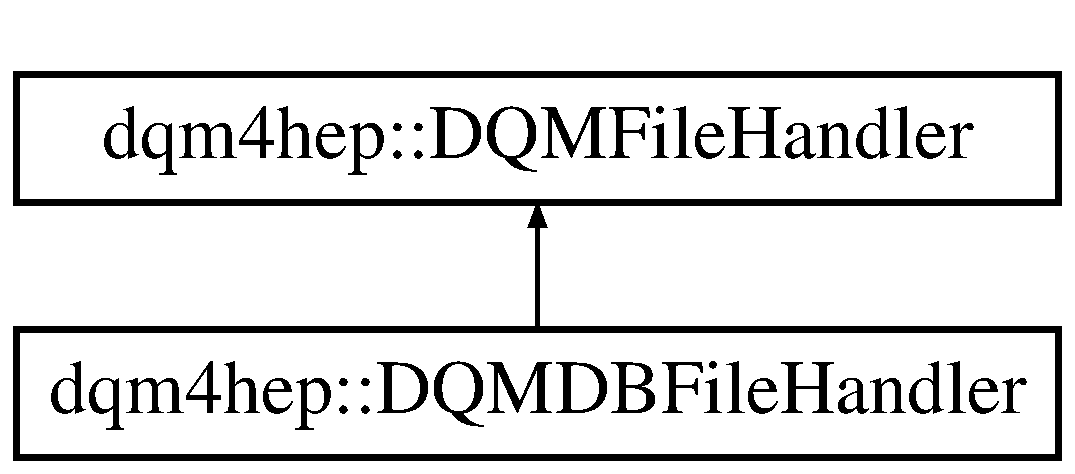
\includegraphics[height=2.000000cm]{classdqm4hep_1_1DQMDBFileHandler}
\end{center}
\end{figure}
\subsection*{Public Member Functions}
\begin{DoxyCompactItemize}
\item 
{\bf D\+Q\+M\+D\+B\+File\+Handler} ()
\begin{DoxyCompactList}\small\item\em Constructor. \end{DoxyCompactList}\item 
{\bf $\sim$\+D\+Q\+M\+D\+B\+File\+Handler} ()
\begin{DoxyCompactList}\small\item\em Destructor. \end{DoxyCompactList}\item 
const std\+::string \& {\bf type} () const 
\begin{DoxyCompactList}\small\item\em Get the file handler type as string. \end{DoxyCompactList}\item 
{\bf Status\+Code} {\bf download} (const std\+::string \&pattern)
\begin{DoxyCompactList}\small\item\em Download the file locally using the target pattern. \end{DoxyCompactList}\item 
const std\+::string \& {\bf get\+Local\+File\+Name} () const 
\begin{DoxyCompactList}\small\item\em Get the full file name after the download step. \end{DoxyCompactList}\end{DoxyCompactItemize}
\subsection*{Private Attributes}
\begin{DoxyCompactItemize}
\item 
{\bf D\+Q\+M\+D\+B\+Interface} $\ast$ {\bf m\+\_\+p\+D\+B\+Interface}
\item 
std\+::string {\bf m\+\_\+type}
\item 
std\+::string {\bf m\+\_\+local\+File\+Name}
\end{DoxyCompactItemize}


\subsection{Detailed Description}
\doxyref{D\+Q\+M\+D\+B\+File\+Handler}{p.}{classdqm4hep_1_1DQMDBFileHandler} class. 

Definition at line 41 of file D\+Q\+M\+D\+B\+File\+Handler.\+h.



\subsection{Constructor \& Destructor Documentation}
\index{dqm4hep\+::\+D\+Q\+M\+D\+B\+File\+Handler@{dqm4hep\+::\+D\+Q\+M\+D\+B\+File\+Handler}!D\+Q\+M\+D\+B\+File\+Handler@{D\+Q\+M\+D\+B\+File\+Handler}}
\index{D\+Q\+M\+D\+B\+File\+Handler@{D\+Q\+M\+D\+B\+File\+Handler}!dqm4hep\+::\+D\+Q\+M\+D\+B\+File\+Handler@{dqm4hep\+::\+D\+Q\+M\+D\+B\+File\+Handler}}
\subsubsection[{D\+Q\+M\+D\+B\+File\+Handler}]{\setlength{\rightskip}{0pt plus 5cm}dqm4hep\+::\+D\+Q\+M\+D\+B\+File\+Handler\+::\+D\+Q\+M\+D\+B\+File\+Handler (
\begin{DoxyParamCaption}
{}
\end{DoxyParamCaption}
)}\label{classdqm4hep_1_1DQMDBFileHandler_afa9537d684b7d1a3eb5b43072a084082}


Constructor. 



Definition at line 38 of file D\+Q\+M\+D\+B\+File\+Handler.\+cc.



References m\+\_\+p\+D\+B\+Interface.


\begin{DoxyCode}
38                                    :
39     m_type(\textcolor{stringliteral}{"db"})
40 \{
41   m_pDBInterface = \textcolor{keyword}{new} DQMDBInterface();
42 \}
\end{DoxyCode}
\index{dqm4hep\+::\+D\+Q\+M\+D\+B\+File\+Handler@{dqm4hep\+::\+D\+Q\+M\+D\+B\+File\+Handler}!````~D\+Q\+M\+D\+B\+File\+Handler@{$\sim$\+D\+Q\+M\+D\+B\+File\+Handler}}
\index{````~D\+Q\+M\+D\+B\+File\+Handler@{$\sim$\+D\+Q\+M\+D\+B\+File\+Handler}!dqm4hep\+::\+D\+Q\+M\+D\+B\+File\+Handler@{dqm4hep\+::\+D\+Q\+M\+D\+B\+File\+Handler}}
\subsubsection[{$\sim$\+D\+Q\+M\+D\+B\+File\+Handler}]{\setlength{\rightskip}{0pt plus 5cm}dqm4hep\+::\+D\+Q\+M\+D\+B\+File\+Handler\+::$\sim$\+D\+Q\+M\+D\+B\+File\+Handler (
\begin{DoxyParamCaption}
{}
\end{DoxyParamCaption}
)}\label{classdqm4hep_1_1DQMDBFileHandler_ab565c76f78c107d6598e933c618f8be1}


Destructor. 



Definition at line 46 of file D\+Q\+M\+D\+B\+File\+Handler.\+cc.



References m\+\_\+p\+D\+B\+Interface.


\begin{DoxyCode}
47 \{
48   \textcolor{keyword}{delete} m_pDBInterface;
49 \}
\end{DoxyCode}


\subsection{Member Function Documentation}
\index{dqm4hep\+::\+D\+Q\+M\+D\+B\+File\+Handler@{dqm4hep\+::\+D\+Q\+M\+D\+B\+File\+Handler}!download@{download}}
\index{download@{download}!dqm4hep\+::\+D\+Q\+M\+D\+B\+File\+Handler@{dqm4hep\+::\+D\+Q\+M\+D\+B\+File\+Handler}}
\subsubsection[{download}]{\setlength{\rightskip}{0pt plus 5cm}{\bf Status\+Code} dqm4hep\+::\+D\+Q\+M\+D\+B\+File\+Handler\+::download (
\begin{DoxyParamCaption}
\item[{const std\+::string \&}]{pattern}
\end{DoxyParamCaption}
)\hspace{0.3cm}{\ttfamily [virtual]}}\label{classdqm4hep_1_1DQMDBFileHandler_a598f1400a750b95348169db1337cfb5f}


Download the file locally using the target pattern. 



Implements {\bf dqm4hep\+::\+D\+Q\+M\+File\+Handler} \doxyref{}{p.}{classdqm4hep_1_1DQMFileHandler_afc41f890cb9390e88fb0c79a991cc270}.



Definition at line 60 of file D\+Q\+M\+D\+B\+File\+Handler.\+cc.



References dqm4hep\+::\+D\+Q\+M\+D\+B\+Interface\+::connect(), dqm4hep\+::\+D\+E\+B\+U\+G, dqm4hep\+::\+D\+Q\+M\+D\+B\+Interface\+::disconnect(), dqm4hep\+::\+E\+R\+R\+O\+R, dqm4hep\+::\+D\+Q\+M\+D\+B\+Interface\+::is\+Connected(), m\+\_\+local\+File\+Name, m\+\_\+p\+D\+B\+Interface, dqm4hep\+::\+D\+Q\+M\+D\+B\+Interface\+::query\+Config\+File\+Content(), and R\+E\+T\+U\+R\+N\+\_\+\+R\+E\+S\+U\+L\+T\+\_\+\+I\+F.


\begin{DoxyCode}
61 \{
62   streamlog\_out(ERROR) << \textcolor{stringliteral}{"DQMDBFileHandler: Performing download step ... "} << std::endl;
63 
64   m_localFileName = \textcolor{stringliteral}{""};
65 
66   \textcolor{keywordflow}{if}(pattern.empty())
67     \textcolor{keywordflow}{return} STATUS\_CODE\_INVALID\_PARAMETER;
68 
69   \textcolor{comment}{// pattern is :}
70   \textcolor{comment}{// "HOST:hostname:USER:username:PWD=password:FILE=filename"}
71   \textcolor{keywordtype}{size\_t} hostStart = pattern.find(\textcolor{stringliteral}{"HOST"});
72   \textcolor{keywordtype}{size\_t} userStart = pattern.find(\textcolor{stringliteral}{"USER"});
73   \textcolor{keywordtype}{size\_t} pwdStart = pattern.find(\textcolor{stringliteral}{"PWD"});
74   \textcolor{keywordtype}{size\_t} fileStart = pattern.find(\textcolor{stringliteral}{"FILE"});
75 
76   \textcolor{keywordtype}{bool} invalidPattern = hostStart != 0
77   || hostStart == std::string::npos
78   || userStart == std::string::npos
79   || pwdStart == std::string::npos
80   || fileStart == std::string::npos;
81 
82   \textcolor{keywordflow}{if}(!invalidPattern)
83   \{
84     \textcolor{keywordflow}{if}(hostStart > userStart
85     || userStart > pwdStart
86     || pwdStart > fileStart)
87       invalidPattern = \textcolor{keyword}{true};
88   \}
89 
90   \textcolor{keywordflow}{if}(invalidPattern)
91   \{
92     streamlog\_out(ERROR) << \textcolor{stringliteral}{"DQMDBFileHandler: Invalid pattern => "} << pattern << std::endl;
93     streamlog\_out(ERROR) << \textcolor{stringliteral}{"Expected pattern : 'HOST=hostname:USER=username:PWD=password:FILE=filename'"} <
      < std::endl;
94 
95     \textcolor{keywordflow}{return} STATUS\_CODE\_INVALID\_PARAMETER;
96   \}
97 
98   \textcolor{keyword}{const} std::string host = pattern.substr(5, userStart-1-5);
99   \textcolor{keyword}{const} std::string user = pattern.substr(userStart+5, pwdStart-1-userStart-5);
100   \textcolor{keyword}{const} std::string password = pattern.substr(pwdStart+4, fileStart-1-pwdStart-4);
101   \textcolor{keyword}{const} std::string fileName = pattern.substr(fileStart+5);
102 
103   streamlog\_out(DEBUG) << \textcolor{stringliteral}{"host : "} << host << std::endl;
104   streamlog\_out(DEBUG) << \textcolor{stringliteral}{"user : "} << user << std::endl;
105   streamlog\_out(DEBUG) << \textcolor{stringliteral}{"password : "} << password << std::endl;
106   streamlog\_out(DEBUG) << \textcolor{stringliteral}{"fileName : "} << fileName << std::endl;
107 
108   \textcolor{keywordflow}{if}(m_pDBInterface->isConnected())
109     RETURN_RESULT_IF(STATUS\_CODE\_SUCCESS, !=, m_pDBInterface->disconnect());
110 
111   RETURN_RESULT_IF(STATUS\_CODE\_SUCCESS, !=, m_pDBInterface->connect(host, user, password, \textcolor{stringliteral}{"DQM4HEP"}));
112 
113   std::string fileContents;
114   RETURN_RESULT_IF(STATUS\_CODE\_SUCCESS, !=, m_pDBInterface->
      queryConfigFileContent(fileName, fileContents));
115 
116   \textcolor{keywordtype}{char} templateFile[] = \textcolor{stringliteral}{"/tmp/dqmdbfilehandler\_XXXXXX.xml"};
117   \textcolor{keywordtype}{int} ret = mkstemps(templateFile, 4);
118 
119   \textcolor{keywordflow}{if}(ret < 0)
120   \{
121     streamlog\_out(ERROR) << \textcolor{stringliteral}{"Counldn't create tmp file for db download !"} << std::endl;
122     \textcolor{keywordflow}{return} STATUS\_CODE\_FAILURE;
123   \}
124 
125   m_localFileName = templateFile;
126 
127   std::ofstream file;
128   file.open(m_localFileName.c\_str(), std::ios::out);
129 
130   \textcolor{keywordflow}{if}(!file.is\_open())
131   \{
132     streamlog\_out(ERROR) << \textcolor{stringliteral}{"Counldn't open tmp file for db download !"} << std::endl;
133     m_localFileName = \textcolor{stringliteral}{""};
134 
135     \textcolor{keywordflow}{return} STATUS\_CODE\_FAILURE;
136   \}
137 
138   file << fileContents;
139   file.close();
140 
141   \textcolor{keywordflow}{return} STATUS\_CODE\_SUCCESS;
142 \}
\end{DoxyCode}
\index{dqm4hep\+::\+D\+Q\+M\+D\+B\+File\+Handler@{dqm4hep\+::\+D\+Q\+M\+D\+B\+File\+Handler}!get\+Local\+File\+Name@{get\+Local\+File\+Name}}
\index{get\+Local\+File\+Name@{get\+Local\+File\+Name}!dqm4hep\+::\+D\+Q\+M\+D\+B\+File\+Handler@{dqm4hep\+::\+D\+Q\+M\+D\+B\+File\+Handler}}
\subsubsection[{get\+Local\+File\+Name}]{\setlength{\rightskip}{0pt plus 5cm}const std\+::string \& dqm4hep\+::\+D\+Q\+M\+D\+B\+File\+Handler\+::get\+Local\+File\+Name (
\begin{DoxyParamCaption}
{}
\end{DoxyParamCaption}
) const\hspace{0.3cm}{\ttfamily [virtual]}}\label{classdqm4hep_1_1DQMDBFileHandler_a192527a0753ae800575c1712f97ce196}


Get the full file name after the download step. 



Implements {\bf dqm4hep\+::\+D\+Q\+M\+File\+Handler} \doxyref{}{p.}{classdqm4hep_1_1DQMFileHandler_a5a6dfa3bfb3965f897a1b7ee60f24ed8}.



Definition at line 146 of file D\+Q\+M\+D\+B\+File\+Handler.\+cc.



References m\+\_\+local\+File\+Name.


\begin{DoxyCode}
147 \{
148   \textcolor{keywordflow}{return} m_localFileName;
149 \}
\end{DoxyCode}
\index{dqm4hep\+::\+D\+Q\+M\+D\+B\+File\+Handler@{dqm4hep\+::\+D\+Q\+M\+D\+B\+File\+Handler}!type@{type}}
\index{type@{type}!dqm4hep\+::\+D\+Q\+M\+D\+B\+File\+Handler@{dqm4hep\+::\+D\+Q\+M\+D\+B\+File\+Handler}}
\subsubsection[{type}]{\setlength{\rightskip}{0pt plus 5cm}const std\+::string \& dqm4hep\+::\+D\+Q\+M\+D\+B\+File\+Handler\+::type (
\begin{DoxyParamCaption}
{}
\end{DoxyParamCaption}
) const\hspace{0.3cm}{\ttfamily [virtual]}}\label{classdqm4hep_1_1DQMDBFileHandler_ab681c7360694b65b36ac07bf2eb80231}


Get the file handler type as string. 



Implements {\bf dqm4hep\+::\+D\+Q\+M\+File\+Handler} \doxyref{}{p.}{classdqm4hep_1_1DQMFileHandler_adb64ac2dba492916a7e6105eacfc6837}.



Definition at line 53 of file D\+Q\+M\+D\+B\+File\+Handler.\+cc.



References m\+\_\+type.


\begin{DoxyCode}
54 \{
55   \textcolor{keywordflow}{return} m_type;
56 \}
\end{DoxyCode}


\subsection{Member Data Documentation}
\index{dqm4hep\+::\+D\+Q\+M\+D\+B\+File\+Handler@{dqm4hep\+::\+D\+Q\+M\+D\+B\+File\+Handler}!m\+\_\+local\+File\+Name@{m\+\_\+local\+File\+Name}}
\index{m\+\_\+local\+File\+Name@{m\+\_\+local\+File\+Name}!dqm4hep\+::\+D\+Q\+M\+D\+B\+File\+Handler@{dqm4hep\+::\+D\+Q\+M\+D\+B\+File\+Handler}}
\subsubsection[{m\+\_\+local\+File\+Name}]{\setlength{\rightskip}{0pt plus 5cm}std\+::string dqm4hep\+::\+D\+Q\+M\+D\+B\+File\+Handler\+::m\+\_\+local\+File\+Name\hspace{0.3cm}{\ttfamily [private]}}\label{classdqm4hep_1_1DQMDBFileHandler_af95175b18a5b60cfc442690c9a528d7b}


Definition at line 67 of file D\+Q\+M\+D\+B\+File\+Handler.\+h.



Referenced by download(), and get\+Local\+File\+Name().

\index{dqm4hep\+::\+D\+Q\+M\+D\+B\+File\+Handler@{dqm4hep\+::\+D\+Q\+M\+D\+B\+File\+Handler}!m\+\_\+p\+D\+B\+Interface@{m\+\_\+p\+D\+B\+Interface}}
\index{m\+\_\+p\+D\+B\+Interface@{m\+\_\+p\+D\+B\+Interface}!dqm4hep\+::\+D\+Q\+M\+D\+B\+File\+Handler@{dqm4hep\+::\+D\+Q\+M\+D\+B\+File\+Handler}}
\subsubsection[{m\+\_\+p\+D\+B\+Interface}]{\setlength{\rightskip}{0pt plus 5cm}{\bf D\+Q\+M\+D\+B\+Interface}$\ast$ dqm4hep\+::\+D\+Q\+M\+D\+B\+File\+Handler\+::m\+\_\+p\+D\+B\+Interface\hspace{0.3cm}{\ttfamily [private]}}\label{classdqm4hep_1_1DQMDBFileHandler_ad33bfad0431497c30558a4779247586e}


Definition at line 65 of file D\+Q\+M\+D\+B\+File\+Handler.\+h.



Referenced by download(), D\+Q\+M\+D\+B\+File\+Handler(), and $\sim$\+D\+Q\+M\+D\+B\+File\+Handler().

\index{dqm4hep\+::\+D\+Q\+M\+D\+B\+File\+Handler@{dqm4hep\+::\+D\+Q\+M\+D\+B\+File\+Handler}!m\+\_\+type@{m\+\_\+type}}
\index{m\+\_\+type@{m\+\_\+type}!dqm4hep\+::\+D\+Q\+M\+D\+B\+File\+Handler@{dqm4hep\+::\+D\+Q\+M\+D\+B\+File\+Handler}}
\subsubsection[{m\+\_\+type}]{\setlength{\rightskip}{0pt plus 5cm}std\+::string dqm4hep\+::\+D\+Q\+M\+D\+B\+File\+Handler\+::m\+\_\+type\hspace{0.3cm}{\ttfamily [private]}}\label{classdqm4hep_1_1DQMDBFileHandler_a9cbbb7512287fa1adbe7a2ee7f8d32bc}


Definition at line 66 of file D\+Q\+M\+D\+B\+File\+Handler.\+h.



Referenced by type().



The documentation for this class was generated from the following files\+:\begin{DoxyCompactItemize}
\item 
{\bf D\+Q\+M\+D\+B\+File\+Handler.\+h}\item 
{\bf D\+Q\+M\+D\+B\+File\+Handler.\+cc}\end{DoxyCompactItemize}

\section{dqm4hep\+:\+:D\+Q\+M\+D\+B\+Interface Class Reference}
\label{classdqm4hep_1_1DQMDBInterface}\index{dqm4hep\+::\+D\+Q\+M\+D\+B\+Interface@{dqm4hep\+::\+D\+Q\+M\+D\+B\+Interface}}


\doxyref{D\+Q\+M\+D\+B\+Interface}{p.}{classdqm4hep_1_1DQMDBInterface} class.  




{\ttfamily \#include $<$D\+Q\+M\+D\+B\+Interface.\+h$>$}

\subsection*{Public Member Functions}
\begin{DoxyCompactItemize}
\item 
{\bf D\+Q\+M\+D\+B\+Interface} ()
\begin{DoxyCompactList}\small\item\em Constructor. \end{DoxyCompactList}\item 
{\bf D\+Q\+M\+D\+B\+Interface} (const std\+::string \&host, const std\+::string \&user, const std\+::string \&password, const std\+::string \&database)
\begin{DoxyCompactList}\small\item\em Constructor. \end{DoxyCompactList}\item 
virtual {\bf $\sim$\+D\+Q\+M\+D\+B\+Interface} ()
\begin{DoxyCompactList}\small\item\em Destructor. \end{DoxyCompactList}\item 
{\bf Status\+Code} {\bf connect} ()
\begin{DoxyCompactList}\small\item\em Connect to the mysql server. \end{DoxyCompactList}\item 
{\bf Status\+Code} {\bf disconnect} ()
\begin{DoxyCompactList}\small\item\em Disconnect from the database. \end{DoxyCompactList}\item 
{\bf Status\+Code} {\bf connect} (const std\+::string \&host, const std\+::string \&user, const std\+::string \&password, const std\+::string \&database)
\begin{DoxyCompactList}\small\item\em Connect to the database. \end{DoxyCompactList}\item 
{\bf Status\+Code} {\bf set} (const std\+::string \&host, const std\+::string \&user, const std\+::string \&password, const std\+::string \&database)
\begin{DoxyCompactList}\small\item\em Set host, user, password and database. \end{DoxyCompactList}\item 
const std\+::string \& {\bf get\+Host} () const 
\begin{DoxyCompactList}\small\item\em Get the host. \end{DoxyCompactList}\item 
const std\+::string \& {\bf get\+User} () const 
\begin{DoxyCompactList}\small\item\em Get the user name. \end{DoxyCompactList}\item 
const std\+::string \& {\bf get\+Password} () const 
\begin{DoxyCompactList}\small\item\em Get the password. \end{DoxyCompactList}\item 
const std\+::string \& {\bf get\+Data\+Base} () const 
\begin{DoxyCompactList}\small\item\em Get the data base name. \end{DoxyCompactList}\item 
{\bf Status\+Code} {\bf query\+Raw} (const std\+::string \&{\bf query}, void $\ast$\&p\+Result)
\begin{DoxyCompactList}\small\item\em Send query to database The result is not converted. \end{DoxyCompactList}\item 
{\footnotesize template$<$typename T $>$ }\\{\bf Status\+Code} {\bf query} (const std\+::string \&query, T \&result)
\begin{DoxyCompactList}\small\item\em Send query to database. \end{DoxyCompactList}\item 
{\footnotesize template$<$typename T $>$ }\\{\bf Status\+Code} {\bf query\+Vector} (const std\+::string \&{\bf query}, std\+::vector$<$ T $>$ \&result)
\begin{DoxyCompactList}\small\item\em Send query to database. \end{DoxyCompactList}\item 
{\bf Status\+Code} {\bf execute} (const std\+::string \&{\bf query})
\begin{DoxyCompactList}\small\item\em Execute the query (no result expected) \end{DoxyCompactList}\item 
bool {\bf is\+Connected} ()
\begin{DoxyCompactList}\small\item\em Whether a connection is being handled. \end{DoxyCompactList}\item 
{\bf Status\+Code} {\bf query\+Config\+File\+Content} (const std\+::string \&config\+File\+Name, std\+::string \&file\+Contents)
\begin{DoxyCompactList}\small\item\em Query a config file content stored in the \doxyref{D\+Q\+M4\+H\+E\+P}{p.}{classdqm4hep_1_1DQM4HEP} data base (table C\+O\+N\+F\+I\+G\+\_\+\+F\+I\+L\+E\+S) \end{DoxyCompactList}\item 
{\bf Status\+Code} {\bf query\+Config\+File\+Description} (const std\+::string \&config\+File\+Name, std\+::string \&file\+Description)
\begin{DoxyCompactList}\small\item\em Query a config file description. \end{DoxyCompactList}\item 
{\bf Status\+Code} {\bf insert\+Config\+File} (const std\+::string \&local\+File\+Name, const std\+::string \&file\+Name\+Entry, const std\+::string \&file\+Description=\char`\"{}\char`\"{}, bool force\+Replace=false)
\begin{DoxyCompactList}\small\item\em Insert a new new config file entry in the database. \end{DoxyCompactList}\end{DoxyCompactItemize}
\subsection*{Private Attributes}
\begin{DoxyCompactItemize}
\item 
M\+Y\+S\+Q\+L $\ast$ {\bf m\+\_\+p\+My\+S\+Q\+L}
\item 
std\+::string {\bf m\+\_\+host}
\item 
std\+::string {\bf m\+\_\+user}
\item 
std\+::string {\bf m\+\_\+password}
\item 
std\+::string {\bf m\+\_\+database}
\item 
bool {\bf m\+\_\+is\+Connected}
\end{DoxyCompactItemize}


\subsection{Detailed Description}
\doxyref{D\+Q\+M\+D\+B\+Interface}{p.}{classdqm4hep_1_1DQMDBInterface} class. 

Definition at line 43 of file D\+Q\+M\+D\+B\+Interface.\+h.



\subsection{Constructor \& Destructor Documentation}
\index{dqm4hep\+::\+D\+Q\+M\+D\+B\+Interface@{dqm4hep\+::\+D\+Q\+M\+D\+B\+Interface}!D\+Q\+M\+D\+B\+Interface@{D\+Q\+M\+D\+B\+Interface}}
\index{D\+Q\+M\+D\+B\+Interface@{D\+Q\+M\+D\+B\+Interface}!dqm4hep\+::\+D\+Q\+M\+D\+B\+Interface@{dqm4hep\+::\+D\+Q\+M\+D\+B\+Interface}}
\subsubsection[{D\+Q\+M\+D\+B\+Interface}]{\setlength{\rightskip}{0pt plus 5cm}dqm4hep\+::\+D\+Q\+M\+D\+B\+Interface\+::\+D\+Q\+M\+D\+B\+Interface (
\begin{DoxyParamCaption}
{}
\end{DoxyParamCaption}
)}\label{classdqm4hep_1_1DQMDBInterface_ad19a63cf3d18ce116fb5e29c293a7bbf}


Constructor. 



Definition at line 36 of file D\+Q\+M\+D\+B\+Interface.\+cc.


\begin{DoxyCode}
36                                :
37     m_pMySQL(NULL),
38     m_isConnected(\textcolor{keyword}{false})
39 \{
40 
41 \}
\end{DoxyCode}
\index{dqm4hep\+::\+D\+Q\+M\+D\+B\+Interface@{dqm4hep\+::\+D\+Q\+M\+D\+B\+Interface}!D\+Q\+M\+D\+B\+Interface@{D\+Q\+M\+D\+B\+Interface}}
\index{D\+Q\+M\+D\+B\+Interface@{D\+Q\+M\+D\+B\+Interface}!dqm4hep\+::\+D\+Q\+M\+D\+B\+Interface@{dqm4hep\+::\+D\+Q\+M\+D\+B\+Interface}}
\subsubsection[{D\+Q\+M\+D\+B\+Interface}]{\setlength{\rightskip}{0pt plus 5cm}dqm4hep\+::\+D\+Q\+M\+D\+B\+Interface\+::\+D\+Q\+M\+D\+B\+Interface (
\begin{DoxyParamCaption}
\item[{const std\+::string \&}]{host, }
\item[{const std\+::string \&}]{user, }
\item[{const std\+::string \&}]{password, }
\item[{const std\+::string \&}]{database}
\end{DoxyParamCaption}
)}\label{classdqm4hep_1_1DQMDBInterface_aaebeffb91f98b21866652afc6cffafef}


Constructor. 

Connect to data base 

Definition at line 45 of file D\+Q\+M\+D\+B\+Interface.\+cc.



References connect(), and set().


\begin{DoxyCode}
45                                                                                                            
                            :
46     m_pMySQL(NULL),
47     m_isConnected(\textcolor{keyword}{false})
48 \{
49   this->set(host, user, password, database);
50   this->connect();
51 \}
\end{DoxyCode}
\index{dqm4hep\+::\+D\+Q\+M\+D\+B\+Interface@{dqm4hep\+::\+D\+Q\+M\+D\+B\+Interface}!````~D\+Q\+M\+D\+B\+Interface@{$\sim$\+D\+Q\+M\+D\+B\+Interface}}
\index{````~D\+Q\+M\+D\+B\+Interface@{$\sim$\+D\+Q\+M\+D\+B\+Interface}!dqm4hep\+::\+D\+Q\+M\+D\+B\+Interface@{dqm4hep\+::\+D\+Q\+M\+D\+B\+Interface}}
\subsubsection[{$\sim$\+D\+Q\+M\+D\+B\+Interface}]{\setlength{\rightskip}{0pt plus 5cm}dqm4hep\+::\+D\+Q\+M\+D\+B\+Interface\+::$\sim$\+D\+Q\+M\+D\+B\+Interface (
\begin{DoxyParamCaption}
{}
\end{DoxyParamCaption}
)\hspace{0.3cm}{\ttfamily [virtual]}}\label{classdqm4hep_1_1DQMDBInterface_a695a628d92f386c0464ac57b1134ee90}


Destructor. 



Definition at line 55 of file D\+Q\+M\+D\+B\+Interface.\+cc.



References disconnect(), and is\+Connected().


\begin{DoxyCode}
56 \{
57   \textcolor{keywordflow}{if}(this->isConnected())
58     this->disconnect();
59 \}
\end{DoxyCode}


\subsection{Member Function Documentation}
\index{dqm4hep\+::\+D\+Q\+M\+D\+B\+Interface@{dqm4hep\+::\+D\+Q\+M\+D\+B\+Interface}!connect@{connect}}
\index{connect@{connect}!dqm4hep\+::\+D\+Q\+M\+D\+B\+Interface@{dqm4hep\+::\+D\+Q\+M\+D\+B\+Interface}}
\subsubsection[{connect}]{\setlength{\rightskip}{0pt plus 5cm}{\bf Status\+Code} dqm4hep\+::\+D\+Q\+M\+D\+B\+Interface\+::connect (
\begin{DoxyParamCaption}
{}
\end{DoxyParamCaption}
)}\label{classdqm4hep_1_1DQMDBInterface_af1a245e65824536dd1ec4845be027576}


Connect to the mysql server. 



Definition at line 63 of file D\+Q\+M\+D\+B\+Interface.\+cc.



References dqm4hep\+::\+E\+R\+R\+O\+R, execute(), dqm4hep\+::\+Status\+Code\+Exception\+::get\+Status\+Code(), is\+Connected(), m\+\_\+database, m\+\_\+host, m\+\_\+is\+Connected, m\+\_\+password, m\+\_\+p\+My\+S\+Q\+L, m\+\_\+user, query(), and T\+H\+R\+O\+W\+\_\+\+R\+E\+S\+U\+L\+T\+\_\+\+I\+F.



Referenced by connect(), dqm4hep\+::\+D\+Q\+M\+D\+B\+File\+Handler\+::download(), and D\+Q\+M\+D\+B\+Interface().


\begin{DoxyCode}
64 \{
65   \textcolor{keywordflow}{if}(this->isConnected())
66     \textcolor{keywordflow}{return} STATUS\_CODE\_ALREADY\_INITIALIZED;
67 
68   \textcolor{keywordflow}{try}
69   \{
70     \textcolor{comment}{// create mysql instance}
71     m_pMySQL = mysql\_init(NULL);
72 
73     \textcolor{keywordflow}{if}(!m_pMySQL)
74     \{
75       streamlog\_out(ERROR) << \textcolor{stringliteral}{"Couldn't create mysql instance : "} << mysql\_error(
      m_pMySQL) << std::endl;
76       \textcolor{keywordflow}{throw} StatusCodeException(STATUS\_CODE\_FAILURE);
77     \}
78 
79     \textcolor{comment}{// create connection to database}
80     \textcolor{keywordflow}{if}(NULL == mysql\_real\_connect(m_pMySQL, m_host.c\_str(), m_user.c\_str(), 
      m_password.c\_str(),
81                              NULL, 0, NULL, 0))
82     \{
83       streamlog\_out(ERROR) << \textcolor{stringliteral}{"Couldn't initialize mysql connection : "} << mysql\_error(
      m_pMySQL) << std::endl;
84       \textcolor{keywordflow}{throw} StatusCodeException(STATUS\_CODE\_FAILURE);
85     \}
86 
87     m_isConnected = \textcolor{keyword}{true};
88 
89     \textcolor{comment}{// select data base}
90     std::stringstream query;
91     query << \textcolor{stringliteral}{"USE "} << m_database << \textcolor{stringliteral}{" ;"};
92 
93     THROW_RESULT_IF(STATUS\_CODE\_SUCCESS, !=, this->execute(query.str()));
94   \}
95   \textcolor{keywordflow}{catch}(\textcolor{keyword}{const} StatusCodeException &exception)
96   \{
97     \textcolor{keywordflow}{if}(m_pMySQL)
98       mysql\_close(m_pMySQL);
99 
100     m_isConnected = \textcolor{keyword}{false};
101 
102     \textcolor{keywordflow}{return} exception.getStatusCode();
103   \}
104 
105   \textcolor{keywordflow}{return} STATUS\_CODE\_SUCCESS;
106 \}
\end{DoxyCode}
\index{dqm4hep\+::\+D\+Q\+M\+D\+B\+Interface@{dqm4hep\+::\+D\+Q\+M\+D\+B\+Interface}!connect@{connect}}
\index{connect@{connect}!dqm4hep\+::\+D\+Q\+M\+D\+B\+Interface@{dqm4hep\+::\+D\+Q\+M\+D\+B\+Interface}}
\subsubsection[{connect}]{\setlength{\rightskip}{0pt plus 5cm}{\bf Status\+Code} dqm4hep\+::\+D\+Q\+M\+D\+B\+Interface\+::connect (
\begin{DoxyParamCaption}
\item[{const std\+::string \&}]{host, }
\item[{const std\+::string \&}]{user, }
\item[{const std\+::string \&}]{password, }
\item[{const std\+::string \&}]{database}
\end{DoxyParamCaption}
)}\label{classdqm4hep_1_1DQMDBInterface_a2b673e52fbf7898477b3918b591957f0}


Connect to the database. 

Not possible if a connection is being handled. Use \doxyref{disconnect()}{p.}{classdqm4hep_1_1DQMDBInterface_a38b368a37ddf9f4eff4fbaa11c75d5e3} first and then \doxyref{connect()}{p.}{classdqm4hep_1_1DQMDBInterface_af1a245e65824536dd1ec4845be027576} 

Definition at line 125 of file D\+Q\+M\+D\+B\+Interface.\+cc.



References connect(), R\+E\+T\+U\+R\+N\+\_\+\+R\+E\+S\+U\+L\+T\+\_\+\+I\+F, and set().


\begin{DoxyCode}
126 \{
127   RETURN_RESULT_IF(STATUS\_CODE\_SUCCESS, !=, this->set(host, user, password, database));
128   RETURN_RESULT_IF(STATUS\_CODE\_SUCCESS, !=, this->connect());
129 
130   \textcolor{keywordflow}{return} STATUS\_CODE\_SUCCESS;
131 \}
\end{DoxyCode}
\index{dqm4hep\+::\+D\+Q\+M\+D\+B\+Interface@{dqm4hep\+::\+D\+Q\+M\+D\+B\+Interface}!disconnect@{disconnect}}
\index{disconnect@{disconnect}!dqm4hep\+::\+D\+Q\+M\+D\+B\+Interface@{dqm4hep\+::\+D\+Q\+M\+D\+B\+Interface}}
\subsubsection[{disconnect}]{\setlength{\rightskip}{0pt plus 5cm}{\bf Status\+Code} dqm4hep\+::\+D\+Q\+M\+D\+B\+Interface\+::disconnect (
\begin{DoxyParamCaption}
{}
\end{DoxyParamCaption}
)}\label{classdqm4hep_1_1DQMDBInterface_a38b368a37ddf9f4eff4fbaa11c75d5e3}


Disconnect from the database. 



Definition at line 110 of file D\+Q\+M\+D\+B\+Interface.\+cc.



References is\+Connected(), m\+\_\+is\+Connected, and m\+\_\+p\+My\+S\+Q\+L.



Referenced by dqm4hep\+::\+D\+Q\+M\+D\+B\+File\+Handler\+::download(), and $\sim$\+D\+Q\+M\+D\+B\+Interface().


\begin{DoxyCode}
111 \{
112   \textcolor{keywordflow}{if}(this->isConnected())
113     \textcolor{keywordflow}{return} STATUS\_CODE\_UNCHANGED;
114 
115   \textcolor{keywordflow}{if}(m_pMySQL)
116     mysql\_close(m_pMySQL);
117 
118   m_isConnected = \textcolor{keyword}{false};
119 
120   \textcolor{keywordflow}{return} STATUS\_CODE\_SUCCESS;
121 \}
\end{DoxyCode}
\index{dqm4hep\+::\+D\+Q\+M\+D\+B\+Interface@{dqm4hep\+::\+D\+Q\+M\+D\+B\+Interface}!execute@{execute}}
\index{execute@{execute}!dqm4hep\+::\+D\+Q\+M\+D\+B\+Interface@{dqm4hep\+::\+D\+Q\+M\+D\+B\+Interface}}
\subsubsection[{execute}]{\setlength{\rightskip}{0pt plus 5cm}{\bf Status\+Code} dqm4hep\+::\+D\+Q\+M\+D\+B\+Interface\+::execute (
\begin{DoxyParamCaption}
\item[{const std\+::string \&}]{query}
\end{DoxyParamCaption}
)}\label{classdqm4hep_1_1DQMDBInterface_a5603d2fbe70b3f8866dc1c8d5bf5393e}


Execute the query (no result expected) 



Definition at line 213 of file D\+Q\+M\+D\+B\+Interface.\+cc.



References dqm4hep\+::\+E\+R\+R\+O\+R, is\+Connected(), and m\+\_\+p\+My\+S\+Q\+L.



Referenced by connect(), insert\+Config\+File(), query\+Config\+File\+Content(), and query\+Config\+File\+Description().


\begin{DoxyCode}
214 \{
215   \textcolor{keywordflow}{if}(!this->isConnected())
216     \textcolor{keywordflow}{return} STATUS\_CODE\_NOT\_INITIALIZED;
217 
218   \textcolor{keywordflow}{if}(mysql\_query(m_pMySQL, query.c\_str()))
219   \{
220     streamlog\_out(ERROR) << \textcolor{stringliteral}{"MySQL query failed : "} << mysql\_error(m_pMySQL) << std::endl;
221     \textcolor{keywordflow}{return} STATUS\_CODE\_FAILURE;
222   \}
223 
224   \textcolor{keywordflow}{return} STATUS\_CODE\_SUCCESS;
225 \}
\end{DoxyCode}
\index{dqm4hep\+::\+D\+Q\+M\+D\+B\+Interface@{dqm4hep\+::\+D\+Q\+M\+D\+B\+Interface}!get\+Data\+Base@{get\+Data\+Base}}
\index{get\+Data\+Base@{get\+Data\+Base}!dqm4hep\+::\+D\+Q\+M\+D\+B\+Interface@{dqm4hep\+::\+D\+Q\+M\+D\+B\+Interface}}
\subsubsection[{get\+Data\+Base}]{\setlength{\rightskip}{0pt plus 5cm}const std\+::string \& dqm4hep\+::\+D\+Q\+M\+D\+B\+Interface\+::get\+Data\+Base (
\begin{DoxyParamCaption}
{}
\end{DoxyParamCaption}
) const}\label{classdqm4hep_1_1DQMDBInterface_ad7b5ee4b7250c23bffe4d8b2979a0cc5}


Get the data base name. 



Definition at line 171 of file D\+Q\+M\+D\+B\+Interface.\+cc.



References m\+\_\+database.


\begin{DoxyCode}
172 \{
173   \textcolor{keywordflow}{return} m_database;
174 \}
\end{DoxyCode}
\index{dqm4hep\+::\+D\+Q\+M\+D\+B\+Interface@{dqm4hep\+::\+D\+Q\+M\+D\+B\+Interface}!get\+Host@{get\+Host}}
\index{get\+Host@{get\+Host}!dqm4hep\+::\+D\+Q\+M\+D\+B\+Interface@{dqm4hep\+::\+D\+Q\+M\+D\+B\+Interface}}
\subsubsection[{get\+Host}]{\setlength{\rightskip}{0pt plus 5cm}const std\+::string \& dqm4hep\+::\+D\+Q\+M\+D\+B\+Interface\+::get\+Host (
\begin{DoxyParamCaption}
{}
\end{DoxyParamCaption}
) const}\label{classdqm4hep_1_1DQMDBInterface_a13b2809e22cda4eff01473c56d6e24fe}


Get the host. 



Definition at line 150 of file D\+Q\+M\+D\+B\+Interface.\+cc.



References m\+\_\+host.


\begin{DoxyCode}
151 \{
152   \textcolor{keywordflow}{return} m_host;
153 \}
\end{DoxyCode}
\index{dqm4hep\+::\+D\+Q\+M\+D\+B\+Interface@{dqm4hep\+::\+D\+Q\+M\+D\+B\+Interface}!get\+Password@{get\+Password}}
\index{get\+Password@{get\+Password}!dqm4hep\+::\+D\+Q\+M\+D\+B\+Interface@{dqm4hep\+::\+D\+Q\+M\+D\+B\+Interface}}
\subsubsection[{get\+Password}]{\setlength{\rightskip}{0pt plus 5cm}const std\+::string \& dqm4hep\+::\+D\+Q\+M\+D\+B\+Interface\+::get\+Password (
\begin{DoxyParamCaption}
{}
\end{DoxyParamCaption}
) const}\label{classdqm4hep_1_1DQMDBInterface_a5a002ef0898357de67b7b8da30cc310c}


Get the password. 



Definition at line 164 of file D\+Q\+M\+D\+B\+Interface.\+cc.



References m\+\_\+password.


\begin{DoxyCode}
165 \{
166   \textcolor{keywordflow}{return} m_password;
167 \}
\end{DoxyCode}
\index{dqm4hep\+::\+D\+Q\+M\+D\+B\+Interface@{dqm4hep\+::\+D\+Q\+M\+D\+B\+Interface}!get\+User@{get\+User}}
\index{get\+User@{get\+User}!dqm4hep\+::\+D\+Q\+M\+D\+B\+Interface@{dqm4hep\+::\+D\+Q\+M\+D\+B\+Interface}}
\subsubsection[{get\+User}]{\setlength{\rightskip}{0pt plus 5cm}const std\+::string \& dqm4hep\+::\+D\+Q\+M\+D\+B\+Interface\+::get\+User (
\begin{DoxyParamCaption}
{}
\end{DoxyParamCaption}
) const}\label{classdqm4hep_1_1DQMDBInterface_aed4f5ec0410422dbc0d8bedb04ed792c}


Get the user name. 



Definition at line 157 of file D\+Q\+M\+D\+B\+Interface.\+cc.



References m\+\_\+user.


\begin{DoxyCode}
158 \{
159   \textcolor{keywordflow}{return} m_user;
160 \}
\end{DoxyCode}
\index{dqm4hep\+::\+D\+Q\+M\+D\+B\+Interface@{dqm4hep\+::\+D\+Q\+M\+D\+B\+Interface}!insert\+Config\+File@{insert\+Config\+File}}
\index{insert\+Config\+File@{insert\+Config\+File}!dqm4hep\+::\+D\+Q\+M\+D\+B\+Interface@{dqm4hep\+::\+D\+Q\+M\+D\+B\+Interface}}
\subsubsection[{insert\+Config\+File}]{\setlength{\rightskip}{0pt plus 5cm}{\bf Status\+Code} dqm4hep\+::\+D\+Q\+M\+D\+B\+Interface\+::insert\+Config\+File (
\begin{DoxyParamCaption}
\item[{const std\+::string \&}]{local\+File\+Name, }
\item[{const std\+::string \&}]{file\+Name\+Entry, }
\item[{const std\+::string \&}]{file\+Description = {\ttfamily \char`\"{}\char`\"{}}, }
\item[{bool}]{force\+Replace = {\ttfamily false}}
\end{DoxyParamCaption}
)}\label{classdqm4hep_1_1DQMDBInterface_af61cfdc2e3f485d9bb310b6e7b448fd9}


Insert a new new config file entry in the database. 



Definition at line 312 of file D\+Q\+M\+D\+B\+Interface.\+cc.



References dqm4hep\+::\+E\+R\+R\+O\+R, execute(), is\+Connected(), m\+\_\+database, query(), and R\+E\+T\+U\+R\+N\+\_\+\+R\+E\+S\+U\+L\+T\+\_\+\+I\+F.


\begin{DoxyCode}
314 \{
315   \textcolor{keywordflow}{if}(localFileName.empty() || fileNameEntry.empty())
316     \textcolor{keywordflow}{return} STATUS\_CODE\_INVALID\_PARAMETER;
317 
318   \textcolor{keywordflow}{if}(!this->isConnected())
319     \textcolor{keywordflow}{return} STATUS\_CODE\_NOT\_INITIALIZED;
320 
321   std::ifstream ifile;
322   ifile.open(localFileName.c\_str(), std::ios::in);
323 
324   \textcolor{keywordflow}{if}(!ifile.is\_open())
325   \{
326     streamlog\_out(ERROR) << \textcolor{stringliteral}{"Couln't open file '"} << localFileName << \textcolor{stringliteral}{"' !"} << std::endl;
327     \textcolor{keywordflow}{return} STATUS\_CODE\_FAILURE;
328   \}
329 
330   std::string fileContents;
331 
332   \textcolor{keywordflow}{while}(!ifile.eof())
333   \{
334     std::string str;
335     getline(ifile, str);
336     fileContents += str + \textcolor{stringliteral}{"\(\backslash\)n"};
337   \}
338 
339   \textcolor{keywordflow}{if}(fileContents.empty())
340     \textcolor{keywordflow}{return} STATUS\_CODE\_FAILURE;
341 
342   std::string queryUse = \textcolor{stringliteral}{"USE "} + m_database + \textcolor{stringliteral}{" ;"};
343 
344   \textcolor{comment}{// construct the mysql query}
345   std::stringstream query;
346 
347   \textcolor{keywordflow}{if}(forceReplace)
348     query << \textcolor{stringliteral}{"REPLACE "};
349   \textcolor{keywordflow}{else}
350     query << \textcolor{stringliteral}{"INSERT "};
351 
352   query << \textcolor{stringliteral}{"INTO CONFIG\_FILES VALUES "}
353       << \textcolor{stringliteral}{"('"} << fileNameEntry << \textcolor{stringliteral}{"' ,"}
354       << \textcolor{stringliteral}{"'"} << fileDescription << \textcolor{stringliteral}{"' ,"}
355       << \textcolor{stringliteral}{"'"} << fileContents << \textcolor{stringliteral}{"') ;"};
356 
357   \textcolor{comment}{// select DQM4HEP database}
358   \textcolor{keywordflow}{if}(m_database != \textcolor{stringliteral}{"DQM4HEP"})
359     RETURN_RESULT_IF(STATUS\_CODE\_SUCCESS, !=, this->execute(\textcolor{stringliteral}{"USE DQM4HEP ;"}));
360 
361   StatusCode statusCode = this->execute(query.str());
362 
363   \textcolor{keywordflow}{if}(STATUS\_CODE\_SUCCESS != statusCode)
364   \{
365     \textcolor{comment}{// select again the current database}
366     RETURN_RESULT_IF(STATUS\_CODE\_SUCCESS, !=, this->execute(queryUse));
367 
368     \textcolor{keywordflow}{return} statusCode;
369   \}
370 
371   \textcolor{comment}{// select again the current database}
372   RETURN_RESULT_IF(STATUS\_CODE\_SUCCESS, !=, this->execute(queryUse));
373 
374   \textcolor{keywordflow}{return} STATUS\_CODE\_SUCCESS;
375 \}
\end{DoxyCode}
\index{dqm4hep\+::\+D\+Q\+M\+D\+B\+Interface@{dqm4hep\+::\+D\+Q\+M\+D\+B\+Interface}!is\+Connected@{is\+Connected}}
\index{is\+Connected@{is\+Connected}!dqm4hep\+::\+D\+Q\+M\+D\+B\+Interface@{dqm4hep\+::\+D\+Q\+M\+D\+B\+Interface}}
\subsubsection[{is\+Connected}]{\setlength{\rightskip}{0pt plus 5cm}bool dqm4hep\+::\+D\+Q\+M\+D\+B\+Interface\+::is\+Connected (
\begin{DoxyParamCaption}
{}
\end{DoxyParamCaption}
)}\label{classdqm4hep_1_1DQMDBInterface_ab2c5f57ae704a855112521281f3fa4ca}


Whether a connection is being handled. 



Definition at line 229 of file D\+Q\+M\+D\+B\+Interface.\+cc.



References m\+\_\+is\+Connected.



Referenced by connect(), disconnect(), dqm4hep\+::\+D\+Q\+M\+D\+B\+File\+Handler\+::download(), execute(), insert\+Config\+File(), query(), query\+Config\+File\+Content(), query\+Config\+File\+Description(), query\+Raw(), query\+Vector(), set(), and $\sim$\+D\+Q\+M\+D\+B\+Interface().


\begin{DoxyCode}
230 \{
231   \textcolor{keywordflow}{return} m_isConnected;
232 \}
\end{DoxyCode}
\index{dqm4hep\+::\+D\+Q\+M\+D\+B\+Interface@{dqm4hep\+::\+D\+Q\+M\+D\+B\+Interface}!query@{query}}
\index{query@{query}!dqm4hep\+::\+D\+Q\+M\+D\+B\+Interface@{dqm4hep\+::\+D\+Q\+M\+D\+B\+Interface}}
\subsubsection[{query}]{\setlength{\rightskip}{0pt plus 5cm}template$<$typename T $>$ {\bf Status\+Code} dqm4hep\+::\+D\+Q\+M\+D\+B\+Interface\+::query (
\begin{DoxyParamCaption}
\item[{const std\+::string \&}]{query, }
\item[{T \&}]{result}
\end{DoxyParamCaption}
)\hspace{0.3cm}{\ttfamily [inline]}}\label{classdqm4hep_1_1DQMDBInterface_a11fa8e6ba898532c4480de938374cb97}


Send query to database. 

The result is streamed in type T using \doxyref{D\+Q\+M4\+H\+E\+P\+::string\+To\+Type()}{p.}{classdqm4hep_1_1DQM4HEP_a68fb565179589334d701c6a5e2ebfef7} 

Definition at line 154 of file D\+Q\+M\+D\+B\+Interface.\+h.



References dqm4hep\+::\+E\+R\+R\+O\+R, is\+Connected(), m\+\_\+p\+My\+S\+Q\+L, and dqm4hep\+::\+D\+Q\+M4\+H\+E\+P\+::string\+To\+Type().



Referenced by connect(), insert\+Config\+File(), query\+Config\+File\+Content(), and query\+Config\+File\+Description().


\begin{DoxyCode}
155 \{
156   \textcolor{keywordflow}{if}(!this->isConnected())
157     \textcolor{keywordflow}{return} STATUS\_CODE\_NOT\_INITIALIZED;
158 
159   \textcolor{keywordflow}{if}(mysql\_query(m_pMySQL, query.c\_str()))
160   \{
161     streamlog\_out(ERROR) << \textcolor{stringliteral}{"MySQL query failed : "} << mysql\_error(m_pMySQL) << std::endl;
162     \textcolor{keywordflow}{return} STATUS\_CODE\_FAILURE;
163   \}
164 
165   MYSQL\_RES *pMySQLResult = mysql\_store\_result(m_pMySQL);
166 
167   \textcolor{keywordflow}{if}(!pMySQLResult)
168   \{
169     streamlog\_out(ERROR) << \textcolor{stringliteral}{"MySQL store result failed : "} << mysql\_error(
      m_pMySQL) << std::endl;
170     \textcolor{keywordflow}{return} STATUS\_CODE\_FAILURE;
171   \}
172 
173   MYSQL\_ROW row = mysql\_fetch\_row(pMySQLResult);
174 
175   std::cout << \textcolor{stringliteral}{"DQMDBInterface::query : MySQL row[0] = "} << row[0] << std::endl;
176 
177   \textcolor{keywordflow}{if}(!DQM4HEP::stringToType(row[0], result))
178   \{
179     mysql\_free\_result(pMySQLResult);
180     \textcolor{keywordflow}{return} STATUS\_CODE\_FAILURE;
181   \}
182 
183   std::cout << \textcolor{stringliteral}{"DQMDBInterface::query : MySQL result = "} << result << std::endl;
184 
185   mysql\_free\_result(pMySQLResult);
186 
187   \textcolor{keywordflow}{return} STATUS\_CODE\_SUCCESS;
188 \}
\end{DoxyCode}
\index{dqm4hep\+::\+D\+Q\+M\+D\+B\+Interface@{dqm4hep\+::\+D\+Q\+M\+D\+B\+Interface}!query\+Config\+File\+Content@{query\+Config\+File\+Content}}
\index{query\+Config\+File\+Content@{query\+Config\+File\+Content}!dqm4hep\+::\+D\+Q\+M\+D\+B\+Interface@{dqm4hep\+::\+D\+Q\+M\+D\+B\+Interface}}
\subsubsection[{query\+Config\+File\+Content}]{\setlength{\rightskip}{0pt plus 5cm}{\bf Status\+Code} dqm4hep\+::\+D\+Q\+M\+D\+B\+Interface\+::query\+Config\+File\+Content (
\begin{DoxyParamCaption}
\item[{const std\+::string \&}]{config\+File\+Name, }
\item[{std\+::string \&}]{file\+Contents}
\end{DoxyParamCaption}
)}\label{classdqm4hep_1_1DQMDBInterface_a0cac0fdcfe4853c487c6720d5724d432}


Query a config file content stored in the \doxyref{D\+Q\+M4\+H\+E\+P}{p.}{classdqm4hep_1_1DQM4HEP} data base (table C\+O\+N\+F\+I\+G\+\_\+\+F\+I\+L\+E\+S) 



Definition at line 236 of file D\+Q\+M\+D\+B\+Interface.\+cc.



References execute(), is\+Connected(), m\+\_\+database, query(), query\+Raw(), and R\+E\+T\+U\+R\+N\+\_\+\+R\+E\+S\+U\+L\+T\+\_\+\+I\+F.



Referenced by dqm4hep\+::\+D\+Q\+M\+D\+B\+File\+Handler\+::download().


\begin{DoxyCode}
237 \{
238   \textcolor{keywordflow}{if}(configFileName.empty())
239     \textcolor{keywordflow}{return} STATUS\_CODE\_INVALID\_PARAMETER;
240 
241   \textcolor{keywordflow}{if}(!this->isConnected())
242     \textcolor{keywordflow}{return} STATUS\_CODE\_NOT\_INITIALIZED;
243 
244   \textcolor{comment}{// select DQM4HEP database}
245   \textcolor{keywordflow}{if}(m_database != \textcolor{stringliteral}{"DQM4HEP"})
246     RETURN_RESULT_IF(STATUS\_CODE\_SUCCESS, !=, this->execute(\textcolor{stringliteral}{"USE DQM4HEP ;"}));
247 
248   std::string queryUse = \textcolor{stringliteral}{"USE "} + m_database + \textcolor{stringliteral}{" ;"};
249 
250   std::stringstream query;
251   query << \textcolor{stringliteral}{"SELECT CONTENTS FROM CONFIG\_FILES WHERE FILE\_NAME=\(\backslash\)""} << configFileName << \textcolor{stringliteral}{"\(\backslash\)" ;"};
252 
253   \textcolor{keywordtype}{void} *pFileContent = NULL;
254   StatusCode statusCode = this->queryRaw(query.str(), pFileContent);
255 
256   \textcolor{keywordflow}{if}(statusCode != STATUS\_CODE\_SUCCESS)
257   \{
258     \textcolor{comment}{// select again the current database}
259     RETURN_RESULT_IF(STATUS\_CODE\_SUCCESS, !=, this->execute(queryUse));
260 
261     \textcolor{keywordflow}{return} statusCode;
262   \}
263 
264   fileContents = (\textcolor{keywordtype}{char} *) pFileContent;
265 
266   \textcolor{comment}{// select again the current database}
267   RETURN_RESULT_IF(STATUS\_CODE\_SUCCESS, !=, this->execute(queryUse));
268 
269   \textcolor{keywordflow}{return} STATUS\_CODE\_SUCCESS;
270 \}
\end{DoxyCode}
\index{dqm4hep\+::\+D\+Q\+M\+D\+B\+Interface@{dqm4hep\+::\+D\+Q\+M\+D\+B\+Interface}!query\+Config\+File\+Description@{query\+Config\+File\+Description}}
\index{query\+Config\+File\+Description@{query\+Config\+File\+Description}!dqm4hep\+::\+D\+Q\+M\+D\+B\+Interface@{dqm4hep\+::\+D\+Q\+M\+D\+B\+Interface}}
\subsubsection[{query\+Config\+File\+Description}]{\setlength{\rightskip}{0pt plus 5cm}{\bf Status\+Code} dqm4hep\+::\+D\+Q\+M\+D\+B\+Interface\+::query\+Config\+File\+Description (
\begin{DoxyParamCaption}
\item[{const std\+::string \&}]{config\+File\+Name, }
\item[{std\+::string \&}]{file\+Description}
\end{DoxyParamCaption}
)}\label{classdqm4hep_1_1DQMDBInterface_a52baec59f990896792e19a452f8b3944}


Query a config file description. 



Definition at line 274 of file D\+Q\+M\+D\+B\+Interface.\+cc.



References execute(), is\+Connected(), m\+\_\+database, query(), query\+Raw(), and R\+E\+T\+U\+R\+N\+\_\+\+R\+E\+S\+U\+L\+T\+\_\+\+I\+F.


\begin{DoxyCode}
275 \{
276   \textcolor{keywordflow}{if}(configFileName.empty())
277     \textcolor{keywordflow}{return} STATUS\_CODE\_INVALID\_PARAMETER;
278 
279   \textcolor{keywordflow}{if}(!this->isConnected())
280     \textcolor{keywordflow}{return} STATUS\_CODE\_NOT\_INITIALIZED;
281 
282   \textcolor{comment}{// select DQM4HEP database}
283   \textcolor{keywordflow}{if}(m_database != \textcolor{stringliteral}{"DQM4HEP"})
284     RETURN_RESULT_IF(STATUS\_CODE\_SUCCESS, !=, this->execute(\textcolor{stringliteral}{"USE DQM4HEP ;"}));
285 
286   std::string queryUse = \textcolor{stringliteral}{"USE "} + m_database + \textcolor{stringliteral}{" ;"};
287 
288   std::stringstream query;
289   query << \textcolor{stringliteral}{"SELECT DESCRIPTION FROM CONFIG\_FILES WHERE FILE\_NAME=\(\backslash\)""} << configFileName << \textcolor{stringliteral}{"\(\backslash\)" ;"};
290 
291   \textcolor{keywordtype}{void} *pFileDescription = NULL;
292   StatusCode statusCode = this->queryRaw(query.str(), pFileDescription);
293 
294   \textcolor{keywordflow}{if}(statusCode != STATUS\_CODE\_SUCCESS)
295   \{
296     \textcolor{comment}{// select again the current database}
297     RETURN_RESULT_IF(STATUS\_CODE\_SUCCESS, !=, this->execute(queryUse));
298 
299     \textcolor{keywordflow}{return} statusCode;
300   \}
301 
302   fileDescription = (\textcolor{keywordtype}{char} *) pFileDescription;
303 
304   \textcolor{comment}{// select again the current database}
305   RETURN_RESULT_IF(STATUS\_CODE\_SUCCESS, !=, this->execute(queryUse));
306 
307   \textcolor{keywordflow}{return} STATUS\_CODE\_SUCCESS;
308 \}
\end{DoxyCode}
\index{dqm4hep\+::\+D\+Q\+M\+D\+B\+Interface@{dqm4hep\+::\+D\+Q\+M\+D\+B\+Interface}!query\+Raw@{query\+Raw}}
\index{query\+Raw@{query\+Raw}!dqm4hep\+::\+D\+Q\+M\+D\+B\+Interface@{dqm4hep\+::\+D\+Q\+M\+D\+B\+Interface}}
\subsubsection[{query\+Raw}]{\setlength{\rightskip}{0pt plus 5cm}{\bf Status\+Code} dqm4hep\+::\+D\+Q\+M\+D\+B\+Interface\+::query\+Raw (
\begin{DoxyParamCaption}
\item[{const std\+::string \&}]{query, }
\item[{void $\ast$\&}]{p\+Result}
\end{DoxyParamCaption}
)}\label{classdqm4hep_1_1DQMDBInterface_a1658f3bdcd114937e0179fc89e1ba896}


Send query to database The result is not converted. 



Definition at line 178 of file D\+Q\+M\+D\+B\+Interface.\+cc.



References dqm4hep\+::\+E\+R\+R\+O\+R, is\+Connected(), and m\+\_\+p\+My\+S\+Q\+L.



Referenced by query\+Config\+File\+Content(), and query\+Config\+File\+Description().


\begin{DoxyCode}
179 \{
180   pResult = NULL;
181 
182   \textcolor{keywordflow}{if}(!this->isConnected())
183     \textcolor{keywordflow}{return} STATUS\_CODE\_NOT\_INITIALIZED;
184 
185   \textcolor{keywordflow}{if}(mysql\_query(m_pMySQL, query.c\_str()))
186   \{
187     streamlog\_out(ERROR) << \textcolor{stringliteral}{"MySQL query failed : "} << mysql\_error(m_pMySQL) << std::endl;
188     \textcolor{keywordflow}{return} STATUS\_CODE\_FAILURE;
189   \}
190 
191   MYSQL\_RES *pMySQLResult = mysql\_store\_result(m_pMySQL);
192 
193   \textcolor{keywordflow}{if}(!pMySQLResult)
194   \{
195     streamlog\_out(ERROR) << \textcolor{stringliteral}{"MySQL store result failed : "} << mysql\_error(
      m_pMySQL) << std::endl;
196     \textcolor{keywordflow}{return} STATUS\_CODE\_FAILURE;
197   \}
198 
199   MYSQL\_ROW row = mysql\_fetch\_row(pMySQLResult);
200 
201   pResult = (\textcolor{keywordtype}{void} *) row[0];
202 
203   mysql\_free\_result(pMySQLResult);
204 
205   \textcolor{keywordflow}{if}(NULL == pResult)
206     \textcolor{keywordflow}{return} STATUS\_CODE\_FAILURE;
207 
208   \textcolor{keywordflow}{return} STATUS\_CODE\_SUCCESS;
209 \}
\end{DoxyCode}
\index{dqm4hep\+::\+D\+Q\+M\+D\+B\+Interface@{dqm4hep\+::\+D\+Q\+M\+D\+B\+Interface}!query\+Vector@{query\+Vector}}
\index{query\+Vector@{query\+Vector}!dqm4hep\+::\+D\+Q\+M\+D\+B\+Interface@{dqm4hep\+::\+D\+Q\+M\+D\+B\+Interface}}
\subsubsection[{query\+Vector}]{\setlength{\rightskip}{0pt plus 5cm}template$<$typename T $>$ {\bf Status\+Code} dqm4hep\+::\+D\+Q\+M\+D\+B\+Interface\+::query\+Vector (
\begin{DoxyParamCaption}
\item[{const std\+::string \&}]{query, }
\item[{std\+::vector$<$ T $>$ \&}]{result}
\end{DoxyParamCaption}
)\hspace{0.3cm}{\ttfamily [inline]}}\label{classdqm4hep_1_1DQMDBInterface_a4dba8c9f88cf00e6a49cd7c335fe8bd5}


Send query to database. 

The result is streamed in a vector. Each value of the vector is streamed using \doxyref{D\+Q\+M4\+H\+E\+P\+::string\+To\+Type()}{p.}{classdqm4hep_1_1DQM4HEP_a68fb565179589334d701c6a5e2ebfef7} 

Definition at line 193 of file D\+Q\+M\+D\+B\+Interface.\+h.



References dqm4hep\+::\+E\+R\+R\+O\+R, is\+Connected(), m\+\_\+p\+My\+S\+Q\+L, and dqm4hep\+::\+D\+Q\+M4\+H\+E\+P\+::string\+To\+Type().


\begin{DoxyCode}
194 \{
195   \textcolor{keywordflow}{if}(!this->isConnected())
196     \textcolor{keywordflow}{return} STATUS\_CODE\_NOT\_INITIALIZED;
197 
198   \textcolor{keywordflow}{if}(mysql\_query(m_pMySQL, query.c\_str()))
199   \{
200     streamlog\_out(ERROR) << \textcolor{stringliteral}{"MySQL query failed : "} << mysql\_error(m_pMySQL) << std::endl;
201     \textcolor{keywordflow}{return} STATUS\_CODE\_FAILURE;
202   \}
203 
204   MYSQL\_RES *pMySQLResult = mysql\_store\_result(m_pMySQL);
205 
206   \textcolor{keywordflow}{if}(!pMySQLResult)
207   \{
208     streamlog\_out(ERROR) << \textcolor{stringliteral}{"MySQL store result failed : "} << mysql\_error(
      m_pMySQL) << std::endl;
209     \textcolor{keywordflow}{return} STATUS\_CODE\_FAILURE;
210   \}
211 
212   MYSQL\_ROW row;
213 
214   \textcolor{keywordflow}{while}( (row = mysql\_fetch\_row(pMySQLResult)) )
215   \{
216     T value = T();
217 
218     \textcolor{keywordflow}{if}(!DQM4HEP::stringToType(row[0], value))
219       \textcolor{keywordflow}{continue};
220 
221     result.push\_back(value);
222   \}
223 
224   mysql\_free\_result(pMySQLResult);
225 
226   \textcolor{keywordflow}{return} STATUS\_CODE\_SUCCESS;
227 \}
\end{DoxyCode}
\index{dqm4hep\+::\+D\+Q\+M\+D\+B\+Interface@{dqm4hep\+::\+D\+Q\+M\+D\+B\+Interface}!set@{set}}
\index{set@{set}!dqm4hep\+::\+D\+Q\+M\+D\+B\+Interface@{dqm4hep\+::\+D\+Q\+M\+D\+B\+Interface}}
\subsubsection[{set}]{\setlength{\rightskip}{0pt plus 5cm}{\bf Status\+Code} dqm4hep\+::\+D\+Q\+M\+D\+B\+Interface\+::set (
\begin{DoxyParamCaption}
\item[{const std\+::string \&}]{host, }
\item[{const std\+::string \&}]{user, }
\item[{const std\+::string \&}]{password, }
\item[{const std\+::string \&}]{database}
\end{DoxyParamCaption}
)}\label{classdqm4hep_1_1DQMDBInterface_a7adb3968d6e3e205e54508f4a6681c5c}


Set host, user, password and database. 

Not possible if a connection is being handled. Use \doxyref{disconnect()}{p.}{classdqm4hep_1_1DQMDBInterface_a38b368a37ddf9f4eff4fbaa11c75d5e3} first and then \doxyref{connect()}{p.}{classdqm4hep_1_1DQMDBInterface_af1a245e65824536dd1ec4845be027576} 

Definition at line 135 of file D\+Q\+M\+D\+B\+Interface.\+cc.



References is\+Connected(), m\+\_\+database, m\+\_\+host, m\+\_\+password, and m\+\_\+user.



Referenced by connect(), and D\+Q\+M\+D\+B\+Interface().


\begin{DoxyCode}
136 \{
137   \textcolor{keywordflow}{if}(this->isConnected())
138     \textcolor{keywordflow}{return} STATUS\_CODE\_NOT\_ALLOWED;
139 
140   m_host = host;
141   m_user = user;
142   m_password = password;
143   m_database = database;
144 
145   \textcolor{keywordflow}{return} STATUS\_CODE\_SUCCESS;
146 \}
\end{DoxyCode}


\subsection{Member Data Documentation}
\index{dqm4hep\+::\+D\+Q\+M\+D\+B\+Interface@{dqm4hep\+::\+D\+Q\+M\+D\+B\+Interface}!m\+\_\+database@{m\+\_\+database}}
\index{m\+\_\+database@{m\+\_\+database}!dqm4hep\+::\+D\+Q\+M\+D\+B\+Interface@{dqm4hep\+::\+D\+Q\+M\+D\+B\+Interface}}
\subsubsection[{m\+\_\+database}]{\setlength{\rightskip}{0pt plus 5cm}std\+::string dqm4hep\+::\+D\+Q\+M\+D\+B\+Interface\+::m\+\_\+database\hspace{0.3cm}{\ttfamily [private]}}\label{classdqm4hep_1_1DQMDBInterface_abf72094813417c21255de037a3ec6fa0}


Definition at line 145 of file D\+Q\+M\+D\+B\+Interface.\+h.



Referenced by connect(), get\+Data\+Base(), insert\+Config\+File(), query\+Config\+File\+Content(), query\+Config\+File\+Description(), and set().

\index{dqm4hep\+::\+D\+Q\+M\+D\+B\+Interface@{dqm4hep\+::\+D\+Q\+M\+D\+B\+Interface}!m\+\_\+host@{m\+\_\+host}}
\index{m\+\_\+host@{m\+\_\+host}!dqm4hep\+::\+D\+Q\+M\+D\+B\+Interface@{dqm4hep\+::\+D\+Q\+M\+D\+B\+Interface}}
\subsubsection[{m\+\_\+host}]{\setlength{\rightskip}{0pt plus 5cm}std\+::string dqm4hep\+::\+D\+Q\+M\+D\+B\+Interface\+::m\+\_\+host\hspace{0.3cm}{\ttfamily [private]}}\label{classdqm4hep_1_1DQMDBInterface_a1e4f220cd0196bd2abfe69348728ae84}


Definition at line 142 of file D\+Q\+M\+D\+B\+Interface.\+h.



Referenced by connect(), get\+Host(), and set().

\index{dqm4hep\+::\+D\+Q\+M\+D\+B\+Interface@{dqm4hep\+::\+D\+Q\+M\+D\+B\+Interface}!m\+\_\+is\+Connected@{m\+\_\+is\+Connected}}
\index{m\+\_\+is\+Connected@{m\+\_\+is\+Connected}!dqm4hep\+::\+D\+Q\+M\+D\+B\+Interface@{dqm4hep\+::\+D\+Q\+M\+D\+B\+Interface}}
\subsubsection[{m\+\_\+is\+Connected}]{\setlength{\rightskip}{0pt plus 5cm}bool dqm4hep\+::\+D\+Q\+M\+D\+B\+Interface\+::m\+\_\+is\+Connected\hspace{0.3cm}{\ttfamily [private]}}\label{classdqm4hep_1_1DQMDBInterface_a6e6bfcfca61f37006732dd49c726c00f}


Definition at line 147 of file D\+Q\+M\+D\+B\+Interface.\+h.



Referenced by connect(), disconnect(), and is\+Connected().

\index{dqm4hep\+::\+D\+Q\+M\+D\+B\+Interface@{dqm4hep\+::\+D\+Q\+M\+D\+B\+Interface}!m\+\_\+password@{m\+\_\+password}}
\index{m\+\_\+password@{m\+\_\+password}!dqm4hep\+::\+D\+Q\+M\+D\+B\+Interface@{dqm4hep\+::\+D\+Q\+M\+D\+B\+Interface}}
\subsubsection[{m\+\_\+password}]{\setlength{\rightskip}{0pt plus 5cm}std\+::string dqm4hep\+::\+D\+Q\+M\+D\+B\+Interface\+::m\+\_\+password\hspace{0.3cm}{\ttfamily [private]}}\label{classdqm4hep_1_1DQMDBInterface_ad3b5e985dcf27bdcf5c8978571498c76}


Definition at line 144 of file D\+Q\+M\+D\+B\+Interface.\+h.



Referenced by connect(), get\+Password(), and set().

\index{dqm4hep\+::\+D\+Q\+M\+D\+B\+Interface@{dqm4hep\+::\+D\+Q\+M\+D\+B\+Interface}!m\+\_\+p\+My\+S\+Q\+L@{m\+\_\+p\+My\+S\+Q\+L}}
\index{m\+\_\+p\+My\+S\+Q\+L@{m\+\_\+p\+My\+S\+Q\+L}!dqm4hep\+::\+D\+Q\+M\+D\+B\+Interface@{dqm4hep\+::\+D\+Q\+M\+D\+B\+Interface}}
\subsubsection[{m\+\_\+p\+My\+S\+Q\+L}]{\setlength{\rightskip}{0pt plus 5cm}M\+Y\+S\+Q\+L$\ast$ dqm4hep\+::\+D\+Q\+M\+D\+B\+Interface\+::m\+\_\+p\+My\+S\+Q\+L\hspace{0.3cm}{\ttfamily [private]}}\label{classdqm4hep_1_1DQMDBInterface_a37ff87a1f26d0beaeba3a0c25462fbc2}


Definition at line 140 of file D\+Q\+M\+D\+B\+Interface.\+h.



Referenced by connect(), disconnect(), execute(), query(), query\+Raw(), and query\+Vector().

\index{dqm4hep\+::\+D\+Q\+M\+D\+B\+Interface@{dqm4hep\+::\+D\+Q\+M\+D\+B\+Interface}!m\+\_\+user@{m\+\_\+user}}
\index{m\+\_\+user@{m\+\_\+user}!dqm4hep\+::\+D\+Q\+M\+D\+B\+Interface@{dqm4hep\+::\+D\+Q\+M\+D\+B\+Interface}}
\subsubsection[{m\+\_\+user}]{\setlength{\rightskip}{0pt plus 5cm}std\+::string dqm4hep\+::\+D\+Q\+M\+D\+B\+Interface\+::m\+\_\+user\hspace{0.3cm}{\ttfamily [private]}}\label{classdqm4hep_1_1DQMDBInterface_ab7b6d8c14629c967a0bd1193464f58e0}


Definition at line 143 of file D\+Q\+M\+D\+B\+Interface.\+h.



Referenced by connect(), get\+User(), and set().



The documentation for this class was generated from the following files\+:\begin{DoxyCompactItemize}
\item 
{\bf D\+Q\+M\+D\+B\+Interface.\+h}\item 
{\bf D\+Q\+M\+D\+B\+Interface.\+cc}\end{DoxyCompactItemize}

\section{dqm4hep\+:\+:D\+Q\+M\+Dim\+Event\+Client Class Reference}
\label{classdqm4hep_1_1DQMDimEventClient}\index{dqm4hep\+::\+D\+Q\+M\+Dim\+Event\+Client@{dqm4hep\+::\+D\+Q\+M\+Dim\+Event\+Client}}


\doxyref{D\+Q\+M\+Dim\+Event\+Client}{p.}{classdqm4hep_1_1DQMDimEventClient} class.  




{\ttfamily \#include $<$D\+Q\+M\+Dim\+Event\+Client.\+h$>$}

Inheritance diagram for dqm4hep\+:\+:D\+Q\+M\+Dim\+Event\+Client\+:\begin{figure}[H]
\begin{center}
\leavevmode
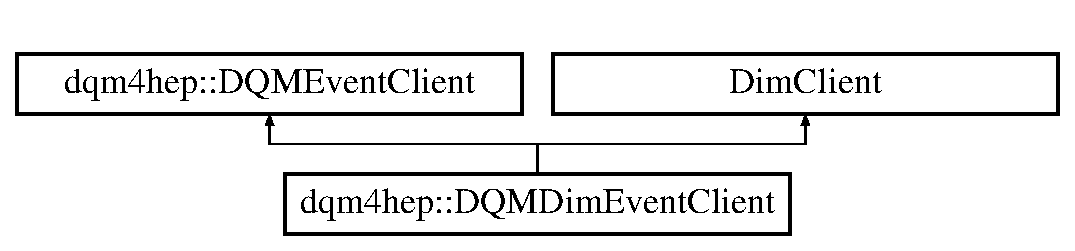
\includegraphics[height=2.000000cm]{classdqm4hep_1_1DQMDimEventClient}
\end{center}
\end{figure}
\subsection*{Public Member Functions}
\begin{DoxyCompactItemize}
\item 
{\bf D\+Q\+M\+Dim\+Event\+Client} ()
\begin{DoxyCompactList}\small\item\em Constructor. \end{DoxyCompactList}\item 
{\bf $\sim$\+D\+Q\+M\+Dim\+Event\+Client} ()
\begin{DoxyCompactList}\small\item\em Destructor. \end{DoxyCompactList}\item 
{\bf Status\+Code} {\bf perform\+Service\+Connection} ()
\begin{DoxyCompactList}\small\item\em Workhorse of the service connection. \end{DoxyCompactList}\item 
{\bf Status\+Code} {\bf perform\+Service\+Disconnection} ()
\begin{DoxyCompactList}\small\item\em Workhorse of the service connection. \end{DoxyCompactList}\item 
bool {\bf is\+Connected\+To\+Service} () const 
\begin{DoxyCompactList}\small\item\em Whether the client is connected to the collector (server) \end{DoxyCompactList}\item 
{\bf Status\+Code} {\bf send\+Event} (const {\bf D\+Q\+M\+Event} $\ast$p\+Event)
\begin{DoxyCompactList}\small\item\em Send an event to the collector (server). \end{DoxyCompactList}\item 
{\bf Status\+Code} {\bf query\+Event} ({\bf D\+Q\+M\+Event} $\ast$\&p\+Event, int timeout)
\begin{DoxyCompactList}\small\item\em Query an event to the collector (server) with a timeout and handle it without pushing it into the internal queue. \end{DoxyCompactList}\item 
{\bf Status\+Code} {\bf query\+Event} ()
\begin{DoxyCompactList}\small\item\em Query an event to the collector. \end{DoxyCompactList}\item 
void {\bf set\+Update\+Mode} (bool update\+Mode)
\begin{DoxyCompactList}\small\item\em Set the update mode. \end{DoxyCompactList}\item 
bool {\bf get\+Update\+Mode} () const 
\begin{DoxyCompactList}\small\item\em Whether the update mode is set. \end{DoxyCompactList}\end{DoxyCompactItemize}
\subsection*{Private Member Functions}
\begin{DoxyCompactItemize}
\item 
void {\bf info\+Handler} ()
\begin{DoxyCompactList}\small\item\em Dim info handler. \end{DoxyCompactList}\item 
{\bf Status\+Code} {\bf event\+Reception} ({\bf dqm\+\_\+char} $\ast$p\+Buffer, {\bf dqm\+\_\+uint} buffer\+Size)
\begin{DoxyCompactList}\small\item\em Handle the event reception as a buffer an its buffer size. \end{DoxyCompactList}\item 
void {\bf set\+Sub\+Event\+Identifier} (const std\+::string \&identifier)
\begin{DoxyCompactList}\small\item\em Set the sub event identifier. \end{DoxyCompactList}\item 
{\bf Status\+Code} {\bf read\+Settings} (const {\bf Ti\+Xml\+Handle} \&xml\+Handle)
\begin{DoxyCompactList}\small\item\em Read settings from the xml handle. \end{DoxyCompactList}\end{DoxyCompactItemize}
\subsection*{Private Attributes}
\begin{DoxyCompactItemize}
\item 
bool {\bf m\+\_\+is\+Connected}
\item 
{\bf Dim\+Event\+Rpc\+Info} $\ast$ {\bf m\+\_\+p\+Dim\+Event\+Rpc\+Info}
\item 
Dim\+Updated\+Info $\ast$ {\bf m\+\_\+p\+Client\+Id\+Info}
\begin{DoxyCompactList}\small\item\em to receive the client id stored on server \end{DoxyCompactList}\item 
Dim\+Updated\+Info $\ast$ {\bf m\+\_\+p\+Server\+State\+Info}
\begin{DoxyCompactList}\small\item\em Server state. 0 for stopped \+: 1 for running. \end{DoxyCompactList}\item 
Dim\+Updated\+Info $\ast$ {\bf m\+\_\+p\+Event\+Update\+Info}
\begin{DoxyCompactList}\small\item\em For event reception. \end{DoxyCompactList}\item 
int {\bf m\+\_\+server\+Client\+Id}
\item 
bool {\bf m\+\_\+update\+Mode}
\item 
{\bf D\+Q\+M\+Data\+Stream} {\bf m\+\_\+data\+Stream}
\item 
pthread\+\_\+mutex\+\_\+t {\bf m\+\_\+mutex}
\end{DoxyCompactItemize}
\subsection*{Friends}
\begin{DoxyCompactItemize}
\item 
class {\bf Dim\+Event\+Rpc\+Info}
\end{DoxyCompactItemize}
\subsection*{Additional Inherited Members}


\subsection{Detailed Description}
\doxyref{D\+Q\+M\+Dim\+Event\+Client}{p.}{classdqm4hep_1_1DQMDimEventClient} class. 

Definition at line 69 of file D\+Q\+M\+Dim\+Event\+Client.\+h.



\subsection{Constructor \& Destructor Documentation}
\index{dqm4hep\+::\+D\+Q\+M\+Dim\+Event\+Client@{dqm4hep\+::\+D\+Q\+M\+Dim\+Event\+Client}!D\+Q\+M\+Dim\+Event\+Client@{D\+Q\+M\+Dim\+Event\+Client}}
\index{D\+Q\+M\+Dim\+Event\+Client@{D\+Q\+M\+Dim\+Event\+Client}!dqm4hep\+::\+D\+Q\+M\+Dim\+Event\+Client@{dqm4hep\+::\+D\+Q\+M\+Dim\+Event\+Client}}
\subsubsection[{D\+Q\+M\+Dim\+Event\+Client}]{\setlength{\rightskip}{0pt plus 5cm}dqm4hep\+::\+D\+Q\+M\+Dim\+Event\+Client\+::\+D\+Q\+M\+Dim\+Event\+Client (
\begin{DoxyParamCaption}
{}
\end{DoxyParamCaption}
)}\label{classdqm4hep_1_1DQMDimEventClient_a8f7426db3b775bb5036208ff93e4d840}


Constructor. 



Definition at line 59 of file D\+Q\+M\+Dim\+Event\+Client.\+cc.


\begin{DoxyCode}
59                                      :
60   m_isConnected(\textcolor{keyword}{false}),
61   m_pDimEventRpcInfo(NULL),
62   m_updateMode(\textcolor{keyword}{false}),
63   m_serverClientId(0),
64   m_dataStream(5*1024*1024) \textcolor{comment}{// 5 Mo should be enough to start ...}
65 \{
66   pthread\_mutex\_init(&m_mutex, NULL);
67 \}
\end{DoxyCode}
\index{dqm4hep\+::\+D\+Q\+M\+Dim\+Event\+Client@{dqm4hep\+::\+D\+Q\+M\+Dim\+Event\+Client}!````~D\+Q\+M\+Dim\+Event\+Client@{$\sim$\+D\+Q\+M\+Dim\+Event\+Client}}
\index{````~D\+Q\+M\+Dim\+Event\+Client@{$\sim$\+D\+Q\+M\+Dim\+Event\+Client}!dqm4hep\+::\+D\+Q\+M\+Dim\+Event\+Client@{dqm4hep\+::\+D\+Q\+M\+Dim\+Event\+Client}}
\subsubsection[{$\sim$\+D\+Q\+M\+Dim\+Event\+Client}]{\setlength{\rightskip}{0pt plus 5cm}dqm4hep\+::\+D\+Q\+M\+Dim\+Event\+Client\+::$\sim$\+D\+Q\+M\+Dim\+Event\+Client (
\begin{DoxyParamCaption}
{}
\end{DoxyParamCaption}
)}\label{classdqm4hep_1_1DQMDimEventClient_a9ac84df31187c28d29b879f30327b198}


Destructor. 



Definition at line 71 of file D\+Q\+M\+Dim\+Event\+Client.\+cc.



References dqm4hep\+::\+D\+Q\+M\+Event\+Client\+::disconnect\+From\+Service(), is\+Connected\+To\+Service(), and m\+\_\+mutex.


\begin{DoxyCode}
72 \{
73   \textcolor{keywordflow}{if}( this->isConnectedToService() )
74     this->disconnectFromService();
75 
76   pthread\_mutex\_destroy(&m_mutex);
77 \}
\end{DoxyCode}


\subsection{Member Function Documentation}
\index{dqm4hep\+::\+D\+Q\+M\+Dim\+Event\+Client@{dqm4hep\+::\+D\+Q\+M\+Dim\+Event\+Client}!event\+Reception@{event\+Reception}}
\index{event\+Reception@{event\+Reception}!dqm4hep\+::\+D\+Q\+M\+Dim\+Event\+Client@{dqm4hep\+::\+D\+Q\+M\+Dim\+Event\+Client}}
\subsubsection[{event\+Reception}]{\setlength{\rightskip}{0pt plus 5cm}{\bf Status\+Code} dqm4hep\+::\+D\+Q\+M\+Dim\+Event\+Client\+::event\+Reception (
\begin{DoxyParamCaption}
\item[{{\bf dqm\+\_\+char} $\ast$}]{p\+Buffer, }
\item[{{\bf dqm\+\_\+uint}}]{buffer\+Size}
\end{DoxyParamCaption}
)\hspace{0.3cm}{\ttfamily [private]}}\label{classdqm4hep_1_1DQMDimEventClient_a8f33bdc6fbde1a1855f585fde3cbb4f6}


Handle the event reception as a buffer an its buffer size. 



Definition at line 338 of file D\+Q\+M\+Dim\+Event\+Client.\+cc.



References dqm4hep\+::\+D\+Q\+M\+Event\+Client\+::get\+Event\+Streamer(), m\+\_\+data\+Stream, m\+\_\+mutex, dqm4hep\+::\+D\+Q\+M\+Event\+Client\+::push\+Event(), R\+E\+T\+U\+R\+N\+\_\+\+R\+E\+S\+U\+L\+T\+\_\+\+I\+F, and dqm4hep\+::\+D\+Q\+M\+Data\+Stream\+::set\+Buffer().



Referenced by info\+Handler(), and dqm4hep\+::\+Dim\+Event\+Rpc\+Info\+::rpc\+Info\+Handler().


\begin{DoxyCode}
339 \{
340   \textcolor{keywordflow}{if}(NULL == pBuffer || 0 == bufferSize)
341     \textcolor{keywordflow}{return} STATUS\_CODE\_INVALID\_PARAMETER;
342 
343   \textcolor{comment}{// set buffer}
344   scoped\_lock( & this->m_mutex);
345   RETURN_RESULT_IF(STATUS\_CODE\_SUCCESS, !=, m_dataStream.setBuffer(pBuffer, bufferSize));
346 
347   \textcolor{comment}{// read event}
348   DQMEvent *pEvent = NULL;
349   RETURN_RESULT_IF(STATUS\_CODE\_SUCCESS, !=, this->getEventStreamer()->deserialize(pEvent, &
      m_dataStream));
350 
351   \textcolor{comment}{// add it to event queue}
352   this->pushEvent(pEvent);
353 
354   \textcolor{keywordflow}{return} STATUS\_CODE\_SUCCESS;
355 \}
\end{DoxyCode}
\index{dqm4hep\+::\+D\+Q\+M\+Dim\+Event\+Client@{dqm4hep\+::\+D\+Q\+M\+Dim\+Event\+Client}!get\+Update\+Mode@{get\+Update\+Mode}}
\index{get\+Update\+Mode@{get\+Update\+Mode}!dqm4hep\+::\+D\+Q\+M\+Dim\+Event\+Client@{dqm4hep\+::\+D\+Q\+M\+Dim\+Event\+Client}}
\subsubsection[{get\+Update\+Mode}]{\setlength{\rightskip}{0pt plus 5cm}bool dqm4hep\+::\+D\+Q\+M\+Dim\+Event\+Client\+::get\+Update\+Mode (
\begin{DoxyParamCaption}
{}
\end{DoxyParamCaption}
) const\hspace{0.3cm}{\ttfamily [virtual]}}\label{classdqm4hep_1_1DQMDimEventClient_a81a3b8cea6ac80fd86b4d4ed95d31dcb}


Whether the update mode is set. 



Implements {\bf dqm4hep\+::\+D\+Q\+M\+Event\+Client} \doxyref{}{p.}{classdqm4hep_1_1DQMEventClient_aafe333631227e6aa3a66cfd19a8b79c2}.



Definition at line 255 of file D\+Q\+M\+Dim\+Event\+Client.\+cc.



References m\+\_\+update\+Mode.



Referenced by read\+Settings().


\begin{DoxyCode}
256 \{
257   \textcolor{keywordflow}{return} m_updateMode;
258 \}
\end{DoxyCode}
\index{dqm4hep\+::\+D\+Q\+M\+Dim\+Event\+Client@{dqm4hep\+::\+D\+Q\+M\+Dim\+Event\+Client}!info\+Handler@{info\+Handler}}
\index{info\+Handler@{info\+Handler}!dqm4hep\+::\+D\+Q\+M\+Dim\+Event\+Client@{dqm4hep\+::\+D\+Q\+M\+Dim\+Event\+Client}}
\subsubsection[{info\+Handler}]{\setlength{\rightskip}{0pt plus 5cm}void dqm4hep\+::\+D\+Q\+M\+Dim\+Event\+Client\+::info\+Handler (
\begin{DoxyParamCaption}
{}
\end{DoxyParamCaption}
)\hspace{0.3cm}{\ttfamily [private]}}\label{classdqm4hep_1_1DQMDimEventClient_a27fce705d47f1cebaf362a2f71fcf583}


Dim info handler. 



Definition at line 262 of file D\+Q\+M\+Dim\+Event\+Client.\+cc.



References event\+Reception(), dqm4hep\+::\+D\+Q\+M\+Event\+Client\+::get\+Collector\+Name(), dqm4hep\+::\+D\+Q\+M\+Event\+Client\+::get\+Sub\+Event\+Identifier(), m\+\_\+p\+Client\+Id\+Info, m\+\_\+p\+Event\+Update\+Info, m\+\_\+p\+Server\+State\+Info, m\+\_\+server\+Client\+Id, m\+\_\+update\+Mode, and dqm4hep\+::\+M\+E\+S\+S\+A\+G\+E.


\begin{DoxyCode}
263 \{
264   DimInfo *pInfo = getInfo();
265 
266   \textcolor{keywordflow}{if}(!pInfo)
267     \textcolor{keywordflow}{return};
268 
269   \textcolor{comment}{// client has just been registered}
270   \textcolor{keywordflow}{if}(pInfo == m_pClientIdInfo)
271   \{
272     \textcolor{keywordtype}{int} clientId = pInfo->getInt();
273 
274     streamlog\_out(MESSAGE) << \textcolor{stringliteral}{"Client id on server : "} << clientId << std::endl;
275 
276     \textcolor{keywordflow}{if}(clientId <= 0)
277       \textcolor{keywordflow}{return};
278 
279     m_serverClientId = clientId;
280     std::string subEventIdentifierCommandName = \textcolor{stringliteral}{"DQM4HEP/EventCollector/"} + this->
      getCollectorName() + \textcolor{stringliteral}{"/SUB\_EVENT\_IDENTIFIER"};
281     std::string updateModeCommandName = \textcolor{stringliteral}{"DQM4HEP/EventCollector/"} + this->
      getCollectorName() + \textcolor{stringliteral}{"/UPDATE\_MODE"};
282 
283     \textcolor{comment}{// send to server the client parameters}
284     DimClient::sendCommandNB((\textcolor{keywordtype}{char}*) updateModeCommandName.c\_str(), \textcolor{keyword}{static\_cast<}\textcolor{keywordtype}{int}\textcolor{keyword}{>}(
      m_updateMode));
285     DimClient::sendCommandNB((\textcolor{keywordtype}{char}*) subEventIdentifierCommandName.c\_str(), (\textcolor{keywordtype}{char} *) this->
      getSubEventIdentifier().c\_str());
286 
287     \textcolor{keywordflow}{return};
288   \}
289 
290   \textcolor{keywordflow}{if}(pInfo == m_pServerStateInfo)
291   \{
292     \textcolor{keywordtype}{int} serverRunning = pInfo->getInt();
293 
294     \textcolor{comment}{// server is running}
295     \textcolor{keywordflow}{if}(serverRunning > 0)
296     \{
297       \textcolor{comment}{// client is already registered, so nothing to do ...}
298       \textcolor{keywordflow}{if}(m_serverClientId > 0)
299         \textcolor{keywordflow}{return};
300 
301       \textcolor{comment}{// client is not registered yet, we need to do it !}
302       \textcolor{keywordflow}{else}
303       \{
304         streamlog\_out(MESSAGE) << \textcolor{stringliteral}{"Registering client into event collector server application !"} << 
      std::endl;
305         DimClient::sendCommandNB((\textcolor{stringliteral}{"DQM4HEP/EventCollector/"} + this->
      getCollectorName() + \textcolor{stringliteral}{"/CLIENT\_REGISTRATION"}).c\_str(), 1);
306         \textcolor{keywordflow}{return};
307       \}
308     \}
309     \textcolor{comment}{// server is shutting down.}
310     \textcolor{comment}{// client is no longer connected and client id is no longer valid.}
311     \textcolor{keywordflow}{else} \textcolor{keywordflow}{if}(m_serverClientId > 0)
312     \{
313       m_serverClientId = 0;
314       streamlog\_out(MESSAGE) << \textcolor{stringliteral}{"Unregistered from event collector server application !"} << std::endl;
315       \textcolor{keywordflow}{return};
316     \}
317   \}
318 
319   \textcolor{keywordflow}{if}(pInfo == m_pEventUpdateInfo)
320   \{
321     \textcolor{keywordflow}{if}(m_serverClientId == 0)
322       \textcolor{keywordflow}{return};
323 
324     \textcolor{keywordtype}{char} *pBuffer = (\textcolor{keywordtype}{char}*) pInfo->getData();
325     \textcolor{keywordtype}{unsigned} \textcolor{keywordtype}{int} bufferSize = pInfo->getSize();
326 
327     \textcolor{keywordflow}{if}(NULL == pBuffer || 0 == bufferSize)
328       \textcolor{keywordflow}{return};
329 
330     this->eventReception(pBuffer, bufferSize);
331 
332     \textcolor{keywordflow}{return};
333   \}
334 \}
\end{DoxyCode}
\index{dqm4hep\+::\+D\+Q\+M\+Dim\+Event\+Client@{dqm4hep\+::\+D\+Q\+M\+Dim\+Event\+Client}!is\+Connected\+To\+Service@{is\+Connected\+To\+Service}}
\index{is\+Connected\+To\+Service@{is\+Connected\+To\+Service}!dqm4hep\+::\+D\+Q\+M\+Dim\+Event\+Client@{dqm4hep\+::\+D\+Q\+M\+Dim\+Event\+Client}}
\subsubsection[{is\+Connected\+To\+Service}]{\setlength{\rightskip}{0pt plus 5cm}bool dqm4hep\+::\+D\+Q\+M\+Dim\+Event\+Client\+::is\+Connected\+To\+Service (
\begin{DoxyParamCaption}
{}
\end{DoxyParamCaption}
) const\hspace{0.3cm}{\ttfamily [virtual]}}\label{classdqm4hep_1_1DQMDimEventClient_aa177def491c8eb9a10c2f2adfe0d9432}


Whether the client is connected to the collector (server) 



Implements {\bf dqm4hep\+::\+D\+Q\+M\+Event\+Client} \doxyref{}{p.}{classdqm4hep_1_1DQMEventClient_a2fd723aa31328fa1b97632e1e2ac31dc}.



Definition at line 138 of file D\+Q\+M\+Dim\+Event\+Client.\+cc.



References m\+\_\+is\+Connected.



Referenced by perform\+Service\+Connection(), perform\+Service\+Disconnection(), query\+Event(), read\+Settings(), set\+Sub\+Event\+Identifier(), set\+Update\+Mode(), and $\sim$\+D\+Q\+M\+Dim\+Event\+Client().


\begin{DoxyCode}
139 \{
140   \textcolor{keywordflow}{return} m_isConnected;
141 \}
\end{DoxyCode}
\index{dqm4hep\+::\+D\+Q\+M\+Dim\+Event\+Client@{dqm4hep\+::\+D\+Q\+M\+Dim\+Event\+Client}!perform\+Service\+Connection@{perform\+Service\+Connection}}
\index{perform\+Service\+Connection@{perform\+Service\+Connection}!dqm4hep\+::\+D\+Q\+M\+Dim\+Event\+Client@{dqm4hep\+::\+D\+Q\+M\+Dim\+Event\+Client}}
\subsubsection[{perform\+Service\+Connection}]{\setlength{\rightskip}{0pt plus 5cm}{\bf Status\+Code} dqm4hep\+::\+D\+Q\+M\+Dim\+Event\+Client\+::perform\+Service\+Connection (
\begin{DoxyParamCaption}
{}
\end{DoxyParamCaption}
)\hspace{0.3cm}{\ttfamily [virtual]}}\label{classdqm4hep_1_1DQMDimEventClient_a50266fbdaed8b2728f9d6e373412fb07}


Workhorse of the service connection. 



Implements {\bf dqm4hep\+::\+D\+Q\+M\+Event\+Client} \doxyref{}{p.}{classdqm4hep_1_1DQMEventClient_a5d69c657028c105556a4b5897ce0ed0b}.



Definition at line 81 of file D\+Q\+M\+Dim\+Event\+Client.\+cc.



References Dim\+Event\+Rpc\+Info, dqm4hep\+::\+D\+Q\+M\+Event\+Client\+::get\+Collector\+Name(), is\+Connected\+To\+Service(), m\+\_\+is\+Connected, m\+\_\+p\+Client\+Id\+Info, m\+\_\+p\+Dim\+Event\+Rpc\+Info, m\+\_\+p\+Event\+Update\+Info, m\+\_\+p\+Server\+State\+Info, dqm4hep\+::\+M\+E\+S\+S\+A\+G\+E, and dqm4hep\+::\+W\+A\+R\+N\+I\+N\+G.


\begin{DoxyCode}
82 \{
83   \textcolor{keywordflow}{if}(isConnectedToService())
84     \textcolor{keywordflow}{return} STATUS\_CODE\_SUCCESS;
85 
86   DimClient::setExitHandler( (\textcolor{stringliteral}{"DQM4HEP/EventCollector/"} + this->getCollectorName() ).c\_str() );
87 
88   m_pDimEventRpcInfo = \textcolor{keyword}{new} DimEventRpcInfo(\textcolor{keyword}{this});
89 
90   m_pClientIdInfo    = \textcolor{keyword}{new} DimUpdatedInfo((\textcolor{stringliteral}{"DQM4HEP/EventCollector/"} + this->
      getCollectorName() + \textcolor{stringliteral}{"/CLIENT\_REGISTERED"}).c\_str(), static\_cast<int>(0), \textcolor{keyword}{this});
91   m_pServerStateInfo = \textcolor{keyword}{new} DimUpdatedInfo((\textcolor{stringliteral}{"DQM4HEP/EventCollector/"} + this->
      getCollectorName() + \textcolor{stringliteral}{"/SERVER\_STATE"}).c\_str(), static\_cast<int>(0), \textcolor{keyword}{this});
92   m_pEventUpdateInfo = \textcolor{keyword}{new} DimUpdatedInfo((\textcolor{stringliteral}{"DQM4HEP/EventCollector/"} + this->
      getCollectorName() + \textcolor{stringliteral}{"/EVENT\_RAW\_UPDATE"}).c\_str(), (\textcolor{keywordtype}{void}*) NULL, 0, \textcolor{keyword}{this});
93 
94   m_isConnected = \textcolor{keyword}{true};
95 
96   DimCurrentInfo serverStateInfo((\textcolor{stringliteral}{"DQM4HEP/EventCollector/"} + this->
      getCollectorName() + \textcolor{stringliteral}{"/SERVER\_STATE"}).c\_str(), static\_cast<int>(0));
97   \textcolor{keywordtype}{int} serverRunning = serverStateInfo.getInt();
98 
99   \textcolor{keywordflow}{if}(!serverRunning)
100   \{
101     streamlog\_out(WARNING) << \textcolor{stringliteral}{"Server collector application not running yet"} << std::endl;
102     \textcolor{keywordflow}{return} STATUS\_CODE\_SUCCESS;
103   \}
104 
105   \textcolor{comment}{// send command to register the client on the server}
106   \textcolor{comment}{// the server is expected to update m\_pClientIdInfo info with the client id}
107   streamlog\_out(MESSAGE) << \textcolor{stringliteral}{"Registering client into server collector application !"} << std::endl;
108   DimClient::sendCommandNB((\textcolor{stringliteral}{"DQM4HEP/EventCollector/"} + this->getCollectorName() + \textcolor{stringliteral}{"/CLIENT\_REGISTRATION"}).
      c\_str(), 1);
109 
110   \textcolor{keywordflow}{return} STATUS\_CODE\_SUCCESS;
111 \}
\end{DoxyCode}
\index{dqm4hep\+::\+D\+Q\+M\+Dim\+Event\+Client@{dqm4hep\+::\+D\+Q\+M\+Dim\+Event\+Client}!perform\+Service\+Disconnection@{perform\+Service\+Disconnection}}
\index{perform\+Service\+Disconnection@{perform\+Service\+Disconnection}!dqm4hep\+::\+D\+Q\+M\+Dim\+Event\+Client@{dqm4hep\+::\+D\+Q\+M\+Dim\+Event\+Client}}
\subsubsection[{perform\+Service\+Disconnection}]{\setlength{\rightskip}{0pt plus 5cm}{\bf Status\+Code} dqm4hep\+::\+D\+Q\+M\+Dim\+Event\+Client\+::perform\+Service\+Disconnection (
\begin{DoxyParamCaption}
{}
\end{DoxyParamCaption}
)\hspace{0.3cm}{\ttfamily [virtual]}}\label{classdqm4hep_1_1DQMDimEventClient_a218c10d82a8d24f95b912d714018041b}


Workhorse of the service connection. 



Implements {\bf dqm4hep\+::\+D\+Q\+M\+Event\+Client} \doxyref{}{p.}{classdqm4hep_1_1DQMEventClient_aefc43840571a501d5bb7296afed49926}.



Definition at line 115 of file D\+Q\+M\+Dim\+Event\+Client.\+cc.



References dqm4hep\+::\+D\+Q\+M\+Event\+Client\+::get\+Collector\+Name(), is\+Connected\+To\+Service(), m\+\_\+is\+Connected, m\+\_\+p\+Client\+Id\+Info, m\+\_\+p\+Dim\+Event\+Rpc\+Info, m\+\_\+p\+Event\+Update\+Info, m\+\_\+p\+Server\+State\+Info, and m\+\_\+server\+Client\+Id.


\begin{DoxyCode}
116 \{
117   \textcolor{keywordflow}{if}(!isConnectedToService())
118     \textcolor{keywordflow}{return} STATUS\_CODE\_SUCCESS;
119 
120   \textcolor{keyword}{delete} m_pDimEventRpcInfo;
121   \textcolor{keyword}{delete} m_pClientIdInfo;
122   \textcolor{keyword}{delete} m_pServerStateInfo;
123   \textcolor{keyword}{delete} m_pEventUpdateInfo;
124 
125   m_isConnected = \textcolor{keyword}{false};
126 
127   \textcolor{comment}{// un-register client on the server}
128   \textcolor{keywordflow}{if}(m_serverClientId > 0)
129   \{
130     DimClient::sendCommandNB((\textcolor{stringliteral}{"DQM4HEP/EventCollector/"} + this->getCollectorName() + \textcolor{stringliteral}{"/CLIENT\_REGISTRATION"}
      ).c\_str(), 0);
131   \}
132 
133   \textcolor{keywordflow}{return} STATUS\_CODE\_SUCCESS;
134 \}
\end{DoxyCode}
\index{dqm4hep\+::\+D\+Q\+M\+Dim\+Event\+Client@{dqm4hep\+::\+D\+Q\+M\+Dim\+Event\+Client}!query\+Event@{query\+Event}}
\index{query\+Event@{query\+Event}!dqm4hep\+::\+D\+Q\+M\+Dim\+Event\+Client@{dqm4hep\+::\+D\+Q\+M\+Dim\+Event\+Client}}
\subsubsection[{query\+Event}]{\setlength{\rightskip}{0pt plus 5cm}{\bf Status\+Code} dqm4hep\+::\+D\+Q\+M\+Dim\+Event\+Client\+::query\+Event (
\begin{DoxyParamCaption}
\item[{{\bf D\+Q\+M\+Event} $\ast$\&}]{p\+Event, }
\item[{int}]{timeout}
\end{DoxyParamCaption}
)\hspace{0.3cm}{\ttfamily [virtual]}}\label{classdqm4hep_1_1DQMDimEventClient_a57cf87d97f33281fda6cf0c10271155d}


Query an event to the collector (server) with a timeout and handle it without pushing it into the internal queue. 



Implements {\bf dqm4hep\+::\+D\+Q\+M\+Event\+Client} \doxyref{}{p.}{classdqm4hep_1_1DQMEventClient_ac885ac90ae365a2d6452f0836b23323c}.



Definition at line 185 of file D\+Q\+M\+Dim\+Event\+Client.\+cc.



References dqm4hep\+::\+D\+Q\+M\+Event\+Streamer\+::deserialize(), dqm4hep\+::\+D\+Q\+M\+Event\+Client\+::get\+Collector\+Name(), dqm4hep\+::\+D\+Q\+M\+Event\+Client\+::get\+Event\+Streamer(), dqm4hep\+::\+D\+Q\+M\+Event\+Client\+::get\+Sub\+Event\+Identifier(), is\+Connected\+To\+Service(), m\+\_\+data\+Stream, m\+\_\+mutex, and dqm4hep\+::\+D\+Q\+M\+Data\+Stream\+::set\+Buffer().


\begin{DoxyCode}
186 \{
187   scoped\_lock( & this->m_mutex);
188 
189   \textcolor{keywordflow}{if}( ! this->isConnectedToService() )
190     \textcolor{keywordflow}{return} STATUS\_CODE\_NOT\_INITIALIZED;
191 
192   \textcolor{keywordflow}{if}( NULL == this->getEventStreamer() )
193     \textcolor{keywordflow}{return} STATUS\_CODE\_NOT\_INITIALIZED;
194 
195   \textcolor{comment}{// check for valid parameters}
196   \textcolor{keywordflow}{if}(timeout <= 0)
197     \textcolor{keywordflow}{return} STATUS\_CODE\_INVALID\_PARAMETER;
198 
199   \textcolor{comment}{// rpc service name}
200   std::string serviceName = \textcolor{stringliteral}{"DQM4HEP/EventCollector/"} + this->getCollectorName() + \textcolor{stringliteral}{"/EVENT\_RAW\_REQUEST"};
201   pEvent = NULL;
202 
203   \textcolor{comment}{// declare the rpc service info}
204   DimRpcInfo eventDimRpcInfo((\textcolor{keywordtype}{char}*) serviceName.c\_str(), timeout, (\textcolor{keywordtype}{void}*) NULL, 0);
205 
206   \textcolor{comment}{// send the query}
207   eventDimRpcInfo.setData((\textcolor{keywordtype}{char}*) this->getSubEventIdentifier().c\_str());
208 
209   \textcolor{comment}{// receive the query result}
210   \textcolor{keywordtype}{char} *pEventRawBuffer = \textcolor{keyword}{static\_cast<}\textcolor{keywordtype}{char}*\textcolor{keyword}{>}(eventDimRpcInfo.getData());
211   \textcolor{keywordtype}{int} bufferSize = eventDimRpcInfo.getSize();
212 
213   \textcolor{comment}{// check for message validity}
214   \textcolor{keywordflow}{if}(NULL == pEventRawBuffer || 0 == bufferSize)
215     \textcolor{keywordflow}{return} STATUS\_CODE\_FAILURE;
216 
217   \textcolor{comment}{// deserialize the event raw buffer}
218   m_dataStream.setBuffer(pEventRawBuffer, bufferSize);
219   \textcolor{keywordflow}{return} this->getEventStreamer()->deserialize(pEvent, &m_dataStream);
220 \}
\end{DoxyCode}
\index{dqm4hep\+::\+D\+Q\+M\+Dim\+Event\+Client@{dqm4hep\+::\+D\+Q\+M\+Dim\+Event\+Client}!query\+Event@{query\+Event}}
\index{query\+Event@{query\+Event}!dqm4hep\+::\+D\+Q\+M\+Dim\+Event\+Client@{dqm4hep\+::\+D\+Q\+M\+Dim\+Event\+Client}}
\subsubsection[{query\+Event}]{\setlength{\rightskip}{0pt plus 5cm}{\bf Status\+Code} dqm4hep\+::\+D\+Q\+M\+Dim\+Event\+Client\+::query\+Event (
\begin{DoxyParamCaption}
{}
\end{DoxyParamCaption}
)\hspace{0.3cm}{\ttfamily [virtual]}}\label{classdqm4hep_1_1DQMDimEventClient_a90a7d76cb0d30c12e4435415fd00347b}


Query an event to the collector. 

A command is send to the collector in order to send back an event. This method does not wait for the event reception.

To query a single event that is directly handled by the caller, use query\+Event(evt, timeout).

The received event is pushed in an internal event queue. 

Implements {\bf dqm4hep\+::\+D\+Q\+M\+Event\+Client} \doxyref{}{p.}{classdqm4hep_1_1DQMEventClient_a3ddc2fcf08a76390dbbfb1ee63b8efe8}.



Definition at line 224 of file D\+Q\+M\+Dim\+Event\+Client.\+cc.



References dqm4hep\+::\+D\+Q\+M\+Event\+Client\+::get\+Event\+Streamer(), dqm4hep\+::\+D\+Q\+M\+Event\+Client\+::get\+Sub\+Event\+Identifier(), is\+Connected\+To\+Service(), m\+\_\+mutex, and m\+\_\+p\+Dim\+Event\+Rpc\+Info.


\begin{DoxyCode}
225 \{
226   scoped\_lock( & this->m_mutex);
227 
228   \textcolor{keywordflow}{if}( ! this->isConnectedToService() )
229     \textcolor{keywordflow}{return} STATUS\_CODE\_NOT\_INITIALIZED;
230 
231   \textcolor{keywordflow}{if}( NULL == this->getEventStreamer() )
232     \textcolor{keywordflow}{return} STATUS\_CODE\_NOT\_INITIALIZED;
233 
234   \textcolor{comment}{// send the query}
235   m_pDimEventRpcInfo->setData((\textcolor{keywordtype}{char}*) this->getSubEventIdentifier().c\_str());
236 
237   \textcolor{keywordflow}{return} STATUS\_CODE\_SUCCESS;
238 \}
\end{DoxyCode}
\index{dqm4hep\+::\+D\+Q\+M\+Dim\+Event\+Client@{dqm4hep\+::\+D\+Q\+M\+Dim\+Event\+Client}!read\+Settings@{read\+Settings}}
\index{read\+Settings@{read\+Settings}!dqm4hep\+::\+D\+Q\+M\+Dim\+Event\+Client@{dqm4hep\+::\+D\+Q\+M\+Dim\+Event\+Client}}
\subsubsection[{read\+Settings}]{\setlength{\rightskip}{0pt plus 5cm}{\bf Status\+Code} dqm4hep\+::\+D\+Q\+M\+Dim\+Event\+Client\+::read\+Settings (
\begin{DoxyParamCaption}
\item[{const {\bf Ti\+Xml\+Handle} \&}]{xml\+Handle}
\end{DoxyParamCaption}
)\hspace{0.3cm}{\ttfamily [private]}, {\ttfamily [virtual]}}\label{classdqm4hep_1_1DQMDimEventClient_a1f272b17a6207fd5f575487775069035}


Read settings from the xml handle. 



Implements {\bf dqm4hep\+::\+D\+Q\+M\+Event\+Client} \doxyref{}{p.}{classdqm4hep_1_1DQMEventClient_a4b1465a91d073d1c2adc957f3df5d8cd}.



Definition at line 359 of file D\+Q\+M\+Dim\+Event\+Client.\+cc.



References dqm4hep\+::\+D\+Q\+M\+Event\+Client\+::connect\+To\+Service(), dqm4hep\+::\+D\+Q\+M\+Plugin\+Manager\+::create\+Plugin\+Class(), dqm4hep\+::\+D\+Q\+M\+Event\+Client\+::disconnect\+From\+Service(), dqm4hep\+::\+D\+Q\+M\+Event\+Client\+::get\+Collector\+Name(), dqm4hep\+::\+D\+Q\+M\+Event\+Client\+::get\+Maximum\+Queue\+Size(), dqm4hep\+::\+D\+Q\+M\+Event\+Client\+::get\+Sub\+Event\+Identifier(), get\+Update\+Mode(), dqm4hep\+::\+D\+Q\+M\+Singleton$<$ D\+Q\+M\+Plugin\+Manager $>$\+::instance(), is\+Connected\+To\+Service(), dqm4hep\+::\+D\+Q\+M\+Xml\+Helper\+::read\+Parameter\+Value(), R\+E\+T\+U\+R\+N\+\_\+\+R\+E\+S\+U\+L\+T\+\_\+\+I\+F, R\+E\+T\+U\+R\+N\+\_\+\+R\+E\+S\+U\+L\+T\+\_\+\+I\+F\+\_\+\+A\+N\+D\+\_\+\+I\+F, dqm4hep\+::\+D\+Q\+M\+Event\+Client\+::set\+Collector\+Name(), dqm4hep\+::\+D\+Q\+M\+Event\+Client\+::set\+Event\+Streamer(), dqm4hep\+::\+D\+Q\+M\+Event\+Client\+::set\+Maximum\+Queue\+Size(), set\+Sub\+Event\+Identifier(), and set\+Update\+Mode().


\begin{DoxyCode}
360 \{
361   \textcolor{keywordtype}{bool} reconnect = this->isConnectedToService();
362 
363   \textcolor{comment}{// first disconnect}
364   \textcolor{keywordflow}{if}( reconnect )
365     RETURN_RESULT_IF(STATUS\_CODE\_SUCCESS, !=, this->disconnectFromService());
366 
367   \textcolor{comment}{// read all xml values first}
368   std::string collectorName = this->getCollectorName();
369   RETURN_RESULT_IF_AND_IF(STATUS\_CODE\_SUCCESS, STATUS\_CODE\_NOT\_FOUND, !=, 
      DQMXmlHelper::readParameterValue(xmlHandle,
370       \textcolor{stringliteral}{"collectorName"}, collectorName));
371 
372   std::string subEventIdentifier = this->getSubEventIdentifier();
373   RETURN_RESULT_IF_AND_IF(STATUS\_CODE\_SUCCESS, STATUS\_CODE\_NOT\_FOUND, !=, 
      DQMXmlHelper::readParameterValue(xmlHandle,
374       \textcolor{stringliteral}{"subEventIdentifier"}, subEventIdentifier));
375 
376   \textcolor{keywordtype}{unsigned} \textcolor{keywordtype}{int} maxEventQueueSize = this->getMaximumQueueSize();
377   RETURN_RESULT_IF_AND_IF(STATUS\_CODE\_SUCCESS, STATUS\_CODE\_NOT\_FOUND, !=, 
      DQMXmlHelper::readParameterValue(xmlHandle,
378       \textcolor{stringliteral}{"maxQueueSize"}, maxEventQueueSize));
379 
380   \textcolor{keywordtype}{bool} updateMode = this->getUpdateMode();
381   RETURN_RESULT_IF_AND_IF(STATUS\_CODE\_SUCCESS, STATUS\_CODE\_NOT\_FOUND, !=, 
      DQMXmlHelper::readParameterValue(xmlHandle,
382       \textcolor{stringliteral}{"updateMode"}, updateMode));
383 
384   std::string eventStreamerName;
385   RETURN_RESULT_IF_AND_IF(STATUS\_CODE\_SUCCESS, STATUS\_CODE\_NOT\_FOUND, !=, 
      DQMXmlHelper::readParameterValue(xmlHandle,
386       \textcolor{stringliteral}{"streamerName"}, eventStreamerName));
387 
388   \textcolor{comment}{// configure the client}
389   \textcolor{comment}{// connection to service will come afterward}
390   this->setCollectorName(collectorName);
391   this->setSubEventIdentifier(subEventIdentifier);
392   this->setMaximumQueueSize(maxEventQueueSize);
393   this->setUpdateMode(updateMode);
394 
395   \textcolor{keywordflow}{if}( ! eventStreamerName.empty() )
396   \{
397     DQMEventStreamer *pEventStreamer = DQMPluginManager::instance()->
      createPluginClass<DQMEventStreamer>(eventStreamerName);
398 
399     \textcolor{keywordflow}{if}( ! pEventStreamer )
400       \textcolor{keywordflow}{return} STATUS\_CODE\_FAILURE;
401 
402     this->setEventStreamer(pEventStreamer, \textcolor{keyword}{true});
403   \}
404 
405   \textcolor{comment}{// reconnect only if connected before configuration}
406   \textcolor{keywordflow}{if}( reconnect )
407     RETURN_RESULT_IF(STATUS\_CODE\_SUCCESS, !=, this->connectToService());
408 
409   \textcolor{keywordflow}{return} STATUS\_CODE\_SUCCESS;
410 \}
\end{DoxyCode}
\index{dqm4hep\+::\+D\+Q\+M\+Dim\+Event\+Client@{dqm4hep\+::\+D\+Q\+M\+Dim\+Event\+Client}!send\+Event@{send\+Event}}
\index{send\+Event@{send\+Event}!dqm4hep\+::\+D\+Q\+M\+Dim\+Event\+Client@{dqm4hep\+::\+D\+Q\+M\+Dim\+Event\+Client}}
\subsubsection[{send\+Event}]{\setlength{\rightskip}{0pt plus 5cm}{\bf Status\+Code} dqm4hep\+::\+D\+Q\+M\+Dim\+Event\+Client\+::send\+Event (
\begin{DoxyParamCaption}
\item[{const {\bf D\+Q\+M\+Event} $\ast$}]{p\+Event}
\end{DoxyParamCaption}
)\hspace{0.3cm}{\ttfamily [virtual]}}\label{classdqm4hep_1_1DQMDimEventClient_a79b251a13d340fac99bd32ef67fbfe46}


Send an event to the collector (server). 

Possible only if a connection has been created (\doxyref{connect\+To\+Service()}{p.}{classdqm4hep_1_1DQMEventClient_a535302ffc201aff823c210d9a834937c}) and an event streamer set. 

Implements {\bf dqm4hep\+::\+D\+Q\+M\+Event\+Client} \doxyref{}{p.}{classdqm4hep_1_1DQMEventClient_a5c322b91355b4751235fad57ab650152}.



Definition at line 145 of file D\+Q\+M\+Dim\+Event\+Client.\+cc.



References dqm4hep\+::\+D\+Q\+M\+Data\+Stream\+::get\+Buffer(), dqm4hep\+::\+D\+Q\+M\+Data\+Stream\+::get\+Buffer\+Size(), dqm4hep\+::\+D\+Q\+M\+Event\+Client\+::get\+Collector\+Name(), dqm4hep\+::\+D\+Q\+M\+Event\+Client\+::get\+Event\+Streamer(), m\+\_\+data\+Stream, m\+\_\+mutex, dqm4hep\+::\+D\+Q\+M\+Data\+Stream\+::reset(), and R\+E\+T\+U\+R\+N\+\_\+\+R\+E\+S\+U\+L\+T\+\_\+\+I\+F.


\begin{DoxyCode}
146 \{
147   scoped\_lock( & this->m_mutex);
148 
149   \textcolor{keywordflow}{if}( NULL == this->getEventStreamer() )
150     \textcolor{keywordflow}{return} STATUS\_CODE\_NOT\_INITIALIZED;
151 
152   \textcolor{keywordflow}{if}(NULL == pEvent)
153     \textcolor{keywordflow}{return} STATUS\_CODE\_INVALID\_PARAMETER;
154 
155   m_dataStream.reset();
156   RETURN_RESULT_IF(STATUS\_CODE\_SUCCESS, !=, this->getEventStreamer()->serialize(pEvent, &
      m_dataStream));
157 
158   \textcolor{keywordtype}{char} *pBuffer = m_dataStream.getBuffer();
159   \textcolor{keywordtype}{unsigned} \textcolor{keywordtype}{int} bufferSize = m_dataStream.getBufferSize();
160 
161   \textcolor{keywordflow}{if}(NULL == pBuffer || 0 == bufferSize)
162     \textcolor{keywordflow}{return} STATUS\_CODE\_FAILURE;
163 
164   std::string commandName = \textcolor{stringliteral}{"DQM4HEP/EventCollector/"} + this->getCollectorName() + \textcolor{stringliteral}{"/COLLECT\_RAW\_EVENT"};
165   DimClient::sendCommandNB((\textcolor{keywordtype}{char}*) commandName.c\_str(), (\textcolor{keywordtype}{void} *) pBuffer, bufferSize);
166 
167   \textcolor{keywordflow}{return} STATUS\_CODE\_SUCCESS;
168 \}
\end{DoxyCode}
\index{dqm4hep\+::\+D\+Q\+M\+Dim\+Event\+Client@{dqm4hep\+::\+D\+Q\+M\+Dim\+Event\+Client}!set\+Sub\+Event\+Identifier@{set\+Sub\+Event\+Identifier}}
\index{set\+Sub\+Event\+Identifier@{set\+Sub\+Event\+Identifier}!dqm4hep\+::\+D\+Q\+M\+Dim\+Event\+Client@{dqm4hep\+::\+D\+Q\+M\+Dim\+Event\+Client}}
\subsubsection[{set\+Sub\+Event\+Identifier}]{\setlength{\rightskip}{0pt plus 5cm}void dqm4hep\+::\+D\+Q\+M\+Dim\+Event\+Client\+::set\+Sub\+Event\+Identifier (
\begin{DoxyParamCaption}
\item[{const std\+::string \&}]{identifier}
\end{DoxyParamCaption}
)\hspace{0.3cm}{\ttfamily [private]}, {\ttfamily [virtual]}}\label{classdqm4hep_1_1DQMDimEventClient_a13060fe0f26dcd57fab027fc2a3cb7e2}


Set the sub event identifier. 

This string is sent while querying events. The received event will be a sub event matching this identifier

The event sub identifier is sent the the collector is the client is connected to the service 

Reimplemented from {\bf dqm4hep\+::\+D\+Q\+M\+Event\+Client} \doxyref{}{p.}{classdqm4hep_1_1DQMEventClient_a81d480f9afc5cf984bd2d7915f9961ad}.



Definition at line 172 of file D\+Q\+M\+Dim\+Event\+Client.\+cc.



References dqm4hep\+::\+D\+Q\+M\+Event\+Client\+::get\+Collector\+Name(), is\+Connected\+To\+Service(), and dqm4hep\+::\+D\+Q\+M\+Event\+Client\+::set\+Sub\+Event\+Identifier().



Referenced by read\+Settings().


\begin{DoxyCode}
173 \{
174   DQMEventClient::setSubEventIdentifier(identifier);
175 
176   \textcolor{keywordflow}{if}( ! this->isConnectedToService() )
177     \textcolor{keywordflow}{return};
178 
179   std::string subEventIdentifierCommandName = \textcolor{stringliteral}{"DQM4HEP/EventCollector/"} + this->
      getCollectorName() + \textcolor{stringliteral}{"/SUB\_EVENT\_IDENTIFIER"};
180   DimClient::sendCommandNB((\textcolor{keywordtype}{char}*) subEventIdentifierCommandName.c\_str(), (\textcolor{keywordtype}{char} *) identifier.c\_str());
181 \}
\end{DoxyCode}
\index{dqm4hep\+::\+D\+Q\+M\+Dim\+Event\+Client@{dqm4hep\+::\+D\+Q\+M\+Dim\+Event\+Client}!set\+Update\+Mode@{set\+Update\+Mode}}
\index{set\+Update\+Mode@{set\+Update\+Mode}!dqm4hep\+::\+D\+Q\+M\+Dim\+Event\+Client@{dqm4hep\+::\+D\+Q\+M\+Dim\+Event\+Client}}
\subsubsection[{set\+Update\+Mode}]{\setlength{\rightskip}{0pt plus 5cm}void dqm4hep\+::\+D\+Q\+M\+Dim\+Event\+Client\+::set\+Update\+Mode (
\begin{DoxyParamCaption}
\item[{bool}]{update\+Mode}
\end{DoxyParamCaption}
)\hspace{0.3cm}{\ttfamily [virtual]}}\label{classdqm4hep_1_1DQMDimEventClient_a12c8e0e2fd6668a79042d1ab31036516}


Set the update mode. 

If the update mode is set to true, a command is sent to the server in order to update the client as soon as an event is received in the collector server. 

Implements {\bf dqm4hep\+::\+D\+Q\+M\+Event\+Client} \doxyref{}{p.}{classdqm4hep_1_1DQMEventClient_a6fcfec76087d886b2a9923e4e1a027a9}.



Definition at line 242 of file D\+Q\+M\+Dim\+Event\+Client.\+cc.



References dqm4hep\+::\+D\+Q\+M\+Event\+Client\+::get\+Collector\+Name(), is\+Connected\+To\+Service(), and m\+\_\+update\+Mode.



Referenced by read\+Settings().


\begin{DoxyCode}
243 \{
244   m_updateMode = updateMode;
245 
246   \textcolor{keywordflow}{if}( ! this->isConnectedToService() )
247     \textcolor{keywordflow}{return};
248 
249   \textcolor{comment}{// send command to server}
250   DimClient::sendCommandNB((\textcolor{keywordtype}{char}*) (std::string(\textcolor{stringliteral}{"DQM4HEP/EventCollector/"}) + this->
      getCollectorName() + \textcolor{stringliteral}{"/UPDATE\_MODE"} ).c\_str(), static\_cast<int>(m_updateMode));
251 \}
\end{DoxyCode}


\subsection{Friends And Related Function Documentation}
\index{dqm4hep\+::\+D\+Q\+M\+Dim\+Event\+Client@{dqm4hep\+::\+D\+Q\+M\+Dim\+Event\+Client}!Dim\+Event\+Rpc\+Info@{Dim\+Event\+Rpc\+Info}}
\index{Dim\+Event\+Rpc\+Info@{Dim\+Event\+Rpc\+Info}!dqm4hep\+::\+D\+Q\+M\+Dim\+Event\+Client@{dqm4hep\+::\+D\+Q\+M\+Dim\+Event\+Client}}
\subsubsection[{Dim\+Event\+Rpc\+Info}]{\setlength{\rightskip}{0pt plus 5cm}friend class {\bf Dim\+Event\+Rpc\+Info}\hspace{0.3cm}{\ttfamily [friend]}}\label{classdqm4hep_1_1DQMDimEventClient_a34a1404882e29c1e9ebb7019f4b11ba5}


Definition at line 71 of file D\+Q\+M\+Dim\+Event\+Client.\+h.



Referenced by perform\+Service\+Connection().



\subsection{Member Data Documentation}
\index{dqm4hep\+::\+D\+Q\+M\+Dim\+Event\+Client@{dqm4hep\+::\+D\+Q\+M\+Dim\+Event\+Client}!m\+\_\+data\+Stream@{m\+\_\+data\+Stream}}
\index{m\+\_\+data\+Stream@{m\+\_\+data\+Stream}!dqm4hep\+::\+D\+Q\+M\+Dim\+Event\+Client@{dqm4hep\+::\+D\+Q\+M\+Dim\+Event\+Client}}
\subsubsection[{m\+\_\+data\+Stream}]{\setlength{\rightskip}{0pt plus 5cm}{\bf D\+Q\+M\+Data\+Stream} dqm4hep\+::\+D\+Q\+M\+Dim\+Event\+Client\+::m\+\_\+data\+Stream\hspace{0.3cm}{\ttfamily [private]}}\label{classdqm4hep_1_1DQMDimEventClient_a768f85ed24eb9aceda2e676b8b8ffd90}


Definition at line 160 of file D\+Q\+M\+Dim\+Event\+Client.\+h.



Referenced by event\+Reception(), query\+Event(), and send\+Event().

\index{dqm4hep\+::\+D\+Q\+M\+Dim\+Event\+Client@{dqm4hep\+::\+D\+Q\+M\+Dim\+Event\+Client}!m\+\_\+is\+Connected@{m\+\_\+is\+Connected}}
\index{m\+\_\+is\+Connected@{m\+\_\+is\+Connected}!dqm4hep\+::\+D\+Q\+M\+Dim\+Event\+Client@{dqm4hep\+::\+D\+Q\+M\+Dim\+Event\+Client}}
\subsubsection[{m\+\_\+is\+Connected}]{\setlength{\rightskip}{0pt plus 5cm}bool dqm4hep\+::\+D\+Q\+M\+Dim\+Event\+Client\+::m\+\_\+is\+Connected\hspace{0.3cm}{\ttfamily [private]}}\label{classdqm4hep_1_1DQMDimEventClient_a7cb6a3f81140c18fb630d3fe4b36e11a}


Definition at line 151 of file D\+Q\+M\+Dim\+Event\+Client.\+h.



Referenced by is\+Connected\+To\+Service(), perform\+Service\+Connection(), and perform\+Service\+Disconnection().

\index{dqm4hep\+::\+D\+Q\+M\+Dim\+Event\+Client@{dqm4hep\+::\+D\+Q\+M\+Dim\+Event\+Client}!m\+\_\+mutex@{m\+\_\+mutex}}
\index{m\+\_\+mutex@{m\+\_\+mutex}!dqm4hep\+::\+D\+Q\+M\+Dim\+Event\+Client@{dqm4hep\+::\+D\+Q\+M\+Dim\+Event\+Client}}
\subsubsection[{m\+\_\+mutex}]{\setlength{\rightskip}{0pt plus 5cm}pthread\+\_\+mutex\+\_\+t dqm4hep\+::\+D\+Q\+M\+Dim\+Event\+Client\+::m\+\_\+mutex\hspace{0.3cm}{\ttfamily [mutable]}, {\ttfamily [private]}}\label{classdqm4hep_1_1DQMDimEventClient_a15f4968fad8ded96820254a82e89f5a4}


Definition at line 161 of file D\+Q\+M\+Dim\+Event\+Client.\+h.



Referenced by event\+Reception(), query\+Event(), send\+Event(), and $\sim$\+D\+Q\+M\+Dim\+Event\+Client().

\index{dqm4hep\+::\+D\+Q\+M\+Dim\+Event\+Client@{dqm4hep\+::\+D\+Q\+M\+Dim\+Event\+Client}!m\+\_\+p\+Client\+Id\+Info@{m\+\_\+p\+Client\+Id\+Info}}
\index{m\+\_\+p\+Client\+Id\+Info@{m\+\_\+p\+Client\+Id\+Info}!dqm4hep\+::\+D\+Q\+M\+Dim\+Event\+Client@{dqm4hep\+::\+D\+Q\+M\+Dim\+Event\+Client}}
\subsubsection[{m\+\_\+p\+Client\+Id\+Info}]{\setlength{\rightskip}{0pt plus 5cm}Dim\+Updated\+Info$\ast$ dqm4hep\+::\+D\+Q\+M\+Dim\+Event\+Client\+::m\+\_\+p\+Client\+Id\+Info\hspace{0.3cm}{\ttfamily [private]}}\label{classdqm4hep_1_1DQMDimEventClient_a6fad1f2787b73ce99d7479dd6efbd710}


to receive the client id stored on server 



Definition at line 153 of file D\+Q\+M\+Dim\+Event\+Client.\+h.



Referenced by info\+Handler(), perform\+Service\+Connection(), and perform\+Service\+Disconnection().

\index{dqm4hep\+::\+D\+Q\+M\+Dim\+Event\+Client@{dqm4hep\+::\+D\+Q\+M\+Dim\+Event\+Client}!m\+\_\+p\+Dim\+Event\+Rpc\+Info@{m\+\_\+p\+Dim\+Event\+Rpc\+Info}}
\index{m\+\_\+p\+Dim\+Event\+Rpc\+Info@{m\+\_\+p\+Dim\+Event\+Rpc\+Info}!dqm4hep\+::\+D\+Q\+M\+Dim\+Event\+Client@{dqm4hep\+::\+D\+Q\+M\+Dim\+Event\+Client}}
\subsubsection[{m\+\_\+p\+Dim\+Event\+Rpc\+Info}]{\setlength{\rightskip}{0pt plus 5cm}{\bf Dim\+Event\+Rpc\+Info}$\ast$ dqm4hep\+::\+D\+Q\+M\+Dim\+Event\+Client\+::m\+\_\+p\+Dim\+Event\+Rpc\+Info\hspace{0.3cm}{\ttfamily [private]}}\label{classdqm4hep_1_1DQMDimEventClient_a58339eb1c0633a428334f672fe516ff7}


Definition at line 152 of file D\+Q\+M\+Dim\+Event\+Client.\+h.



Referenced by perform\+Service\+Connection(), perform\+Service\+Disconnection(), and query\+Event().

\index{dqm4hep\+::\+D\+Q\+M\+Dim\+Event\+Client@{dqm4hep\+::\+D\+Q\+M\+Dim\+Event\+Client}!m\+\_\+p\+Event\+Update\+Info@{m\+\_\+p\+Event\+Update\+Info}}
\index{m\+\_\+p\+Event\+Update\+Info@{m\+\_\+p\+Event\+Update\+Info}!dqm4hep\+::\+D\+Q\+M\+Dim\+Event\+Client@{dqm4hep\+::\+D\+Q\+M\+Dim\+Event\+Client}}
\subsubsection[{m\+\_\+p\+Event\+Update\+Info}]{\setlength{\rightskip}{0pt plus 5cm}Dim\+Updated\+Info$\ast$ dqm4hep\+::\+D\+Q\+M\+Dim\+Event\+Client\+::m\+\_\+p\+Event\+Update\+Info\hspace{0.3cm}{\ttfamily [private]}}\label{classdqm4hep_1_1DQMDimEventClient_a105b729c4e676cbe75f29ec8a5daaa3c}


For event reception. 



Definition at line 155 of file D\+Q\+M\+Dim\+Event\+Client.\+h.



Referenced by info\+Handler(), perform\+Service\+Connection(), and perform\+Service\+Disconnection().

\index{dqm4hep\+::\+D\+Q\+M\+Dim\+Event\+Client@{dqm4hep\+::\+D\+Q\+M\+Dim\+Event\+Client}!m\+\_\+p\+Server\+State\+Info@{m\+\_\+p\+Server\+State\+Info}}
\index{m\+\_\+p\+Server\+State\+Info@{m\+\_\+p\+Server\+State\+Info}!dqm4hep\+::\+D\+Q\+M\+Dim\+Event\+Client@{dqm4hep\+::\+D\+Q\+M\+Dim\+Event\+Client}}
\subsubsection[{m\+\_\+p\+Server\+State\+Info}]{\setlength{\rightskip}{0pt plus 5cm}Dim\+Updated\+Info$\ast$ dqm4hep\+::\+D\+Q\+M\+Dim\+Event\+Client\+::m\+\_\+p\+Server\+State\+Info\hspace{0.3cm}{\ttfamily [private]}}\label{classdqm4hep_1_1DQMDimEventClient_a6517475474af8efbf223680485463dfd}


Server state. 0 for stopped \+: 1 for running. 



Definition at line 154 of file D\+Q\+M\+Dim\+Event\+Client.\+h.



Referenced by info\+Handler(), perform\+Service\+Connection(), and perform\+Service\+Disconnection().

\index{dqm4hep\+::\+D\+Q\+M\+Dim\+Event\+Client@{dqm4hep\+::\+D\+Q\+M\+Dim\+Event\+Client}!m\+\_\+server\+Client\+Id@{m\+\_\+server\+Client\+Id}}
\index{m\+\_\+server\+Client\+Id@{m\+\_\+server\+Client\+Id}!dqm4hep\+::\+D\+Q\+M\+Dim\+Event\+Client@{dqm4hep\+::\+D\+Q\+M\+Dim\+Event\+Client}}
\subsubsection[{m\+\_\+server\+Client\+Id}]{\setlength{\rightskip}{0pt plus 5cm}int dqm4hep\+::\+D\+Q\+M\+Dim\+Event\+Client\+::m\+\_\+server\+Client\+Id\hspace{0.3cm}{\ttfamily [private]}}\label{classdqm4hep_1_1DQMDimEventClient_afec6ea72d90f89c466870920c969dd88}


Definition at line 157 of file D\+Q\+M\+Dim\+Event\+Client.\+h.



Referenced by info\+Handler(), and perform\+Service\+Disconnection().

\index{dqm4hep\+::\+D\+Q\+M\+Dim\+Event\+Client@{dqm4hep\+::\+D\+Q\+M\+Dim\+Event\+Client}!m\+\_\+update\+Mode@{m\+\_\+update\+Mode}}
\index{m\+\_\+update\+Mode@{m\+\_\+update\+Mode}!dqm4hep\+::\+D\+Q\+M\+Dim\+Event\+Client@{dqm4hep\+::\+D\+Q\+M\+Dim\+Event\+Client}}
\subsubsection[{m\+\_\+update\+Mode}]{\setlength{\rightskip}{0pt plus 5cm}bool dqm4hep\+::\+D\+Q\+M\+Dim\+Event\+Client\+::m\+\_\+update\+Mode\hspace{0.3cm}{\ttfamily [private]}}\label{classdqm4hep_1_1DQMDimEventClient_a357ffbb2b6bd9ca941d0444d6d4966e1}


Definition at line 158 of file D\+Q\+M\+Dim\+Event\+Client.\+h.



Referenced by get\+Update\+Mode(), info\+Handler(), and set\+Update\+Mode().



The documentation for this class was generated from the following files\+:\begin{DoxyCompactItemize}
\item 
{\bf D\+Q\+M\+Dim\+Event\+Client.\+h}\item 
{\bf D\+Q\+M\+Dim\+Event\+Client.\+cc}\end{DoxyCompactItemize}

\section{dqm4hep\+:\+:D\+Q\+M\+Dim\+Event\+Collector Class Reference}
\label{classdqm4hep_1_1DQMDimEventCollector}\index{dqm4hep\+::\+D\+Q\+M\+Dim\+Event\+Collector@{dqm4hep\+::\+D\+Q\+M\+Dim\+Event\+Collector}}


\doxyref{D\+Q\+M\+Dim\+Event\+Collector}{p.}{classdqm4hep_1_1DQMDimEventCollector} class.  




{\ttfamily \#include $<$D\+Q\+M\+Dim\+Event\+Collector.\+h$>$}

Inheritance diagram for dqm4hep\+:\+:D\+Q\+M\+Dim\+Event\+Collector\+:\begin{figure}[H]
\begin{center}
\leavevmode
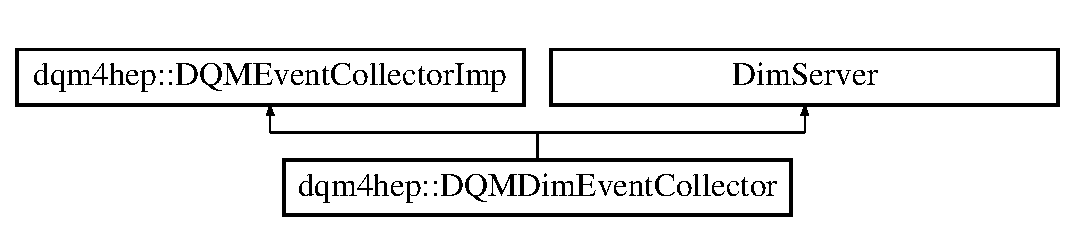
\includegraphics[height=2.000000cm]{classdqm4hep_1_1DQMDimEventCollector}
\end{center}
\end{figure}
\subsection*{Classes}
\begin{DoxyCompactItemize}
\item 
class {\bf Client}
\begin{DoxyCompactList}\small\item\em \doxyref{Client}{p.}{classdqm4hep_1_1DQMDimEventCollector_1_1Client} class. \end{DoxyCompactList}\end{DoxyCompactItemize}
\subsection*{Public Member Functions}
\begin{DoxyCompactItemize}
\item 
{\bf D\+Q\+M\+Dim\+Event\+Collector} ()
\begin{DoxyCompactList}\small\item\em Constructor. \end{DoxyCompactList}\item 
virtual {\bf $\sim$\+D\+Q\+M\+Dim\+Event\+Collector} ()
\begin{DoxyCompactList}\small\item\em Destructor. \end{DoxyCompactList}\item 
{\bf Status\+Code} {\bf set\+Collector\+Name} (const std\+::string \&collector\+Name)
\begin{DoxyCompactList}\small\item\em Set the collector name. \end{DoxyCompactList}\item 
const std\+::string \& {\bf get\+Collector\+Name} () const 
\begin{DoxyCompactList}\small\item\em Get the collector name. \end{DoxyCompactList}\item 
bool {\bf is\+Running} () const 
\begin{DoxyCompactList}\small\item\em Whether the collector server is running. \end{DoxyCompactList}\item 
{\bf Status\+Code} {\bf start\+Collector} ()
\begin{DoxyCompactList}\small\item\em Start the collector server. \end{DoxyCompactList}\item 
{\bf Status\+Code} {\bf stop\+Collector} ()
\begin{DoxyCompactList}\small\item\em Stop the collector server. \end{DoxyCompactList}\item 
void {\bf set\+Event\+Streamer} ({\bf D\+Q\+M\+Event\+Streamer} $\ast$p\+Event\+Streamer)
\begin{DoxyCompactList}\small\item\em Set the event streamer to serialize/deserialize the in/out-\/coming events. \end{DoxyCompactList}\item 
{\bf D\+Q\+M\+Event\+Streamer} $\ast$ {\bf get\+Event\+Streamer} () const 
\begin{DoxyCompactList}\small\item\em Get the event streamer. \end{DoxyCompactList}\end{DoxyCompactItemize}
\subsection*{Private Types}
\begin{DoxyCompactItemize}
\item 
typedef std\+::map$<$ int, {\bf Client} $>$ {\bf Client\+Map}
\end{DoxyCompactItemize}
\subsection*{Private Member Functions}
\begin{DoxyCompactItemize}
\item 
void {\bf command\+Handler} ()
\begin{DoxyCompactList}\small\item\em Dim command handler. \end{DoxyCompactList}\item 
void {\bf client\+Exit\+Handler} ()
\begin{DoxyCompactList}\small\item\em Dim client exit handler. \end{DoxyCompactList}\item 
void {\bf handle\+Event\+Reception} (Dim\+Command $\ast$p\+Dim\+Command)
\item 
void {\bf handle\+Event\+Request} ({\bf Dim\+Event\+Request\+Rpc} $\ast$p\+Dim\+Rpc)
\item 
{\bf Client} \& {\bf get\+Client} (int client\+Id)
\begin{DoxyCompactList}\small\item\em Get a client by id. \end{DoxyCompactList}\item 
void {\bf update\+Event\+Service} ()
\begin{DoxyCompactList}\small\item\em Update the event service for clients that have specified an update mode. \end{DoxyCompactList}\item 
void {\bf remove\+Client} (int client\+Id)
\begin{DoxyCompactList}\small\item\em Remove a client from the map. \end{DoxyCompactList}\end{DoxyCompactItemize}
\subsection*{Private Attributes}
\begin{DoxyCompactItemize}
\item 
std\+::string {\bf m\+\_\+collector\+Name}
\item 
bool {\bf m\+\_\+is\+Running}
\item 
int {\bf m\+\_\+state}
\item 
int {\bf m\+\_\+client\+Registered\+Id}
\item 
Dim\+Service $\ast$ {\bf m\+\_\+p\+Server\+State\+Service}
\item 
Dim\+Service $\ast$ {\bf m\+\_\+p\+Client\+Registered\+Service}
\item 
Dim\+Service $\ast$ {\bf m\+\_\+p\+Event\+Update\+Service}
\item 
{\bf D\+Q\+M\+Statistics\+Service} $\ast$ {\bf m\+\_\+p\+Statistics\+Service}
\item 
Dim\+Command $\ast$ {\bf m\+\_\+p\+Collect\+Event\+Command}
\item 
Dim\+Command $\ast$ {\bf m\+\_\+p\+Update\+Mode\+Command}
\item 
Dim\+Command $\ast$ {\bf m\+\_\+p\+Sub\+Event\+Identifier\+Command}
\item 
Dim\+Command $\ast$ {\bf m\+\_\+p\+Client\+Regitration\+Command}
\item 
{\bf Dim\+Event\+Request\+Rpc} $\ast$ {\bf m\+\_\+p\+Event\+Request\+Rpc}
\item 
{\bf D\+Q\+M\+Data\+Stream} {\bf m\+\_\+data\+Stream}
\item 
{\bf D\+Q\+M\+Data\+Stream} {\bf m\+\_\+sub\+Event\+Data\+Stream}
\item 
{\bf D\+Q\+M\+Event\+Streamer} $\ast$ {\bf m\+\_\+p\+Event\+Streamer}
\item 
{\bf D\+Q\+M\+Event} $\ast$ {\bf m\+\_\+p\+Current\+Event}
\item 
{\bf Client\+Map} {\bf m\+\_\+client\+Map}
\end{DoxyCompactItemize}
\subsection*{Friends}
\begin{DoxyCompactItemize}
\item 
class {\bf Dim\+Event\+Request\+Rpc}
\end{DoxyCompactItemize}


\subsection{Detailed Description}
\doxyref{D\+Q\+M\+Dim\+Event\+Collector}{p.}{classdqm4hep_1_1DQMDimEventCollector} class. 

Definition at line 67 of file D\+Q\+M\+Dim\+Event\+Collector.\+h.



\subsection{Member Typedef Documentation}
\index{dqm4hep\+::\+D\+Q\+M\+Dim\+Event\+Collector@{dqm4hep\+::\+D\+Q\+M\+Dim\+Event\+Collector}!Client\+Map@{Client\+Map}}
\index{Client\+Map@{Client\+Map}!dqm4hep\+::\+D\+Q\+M\+Dim\+Event\+Collector@{dqm4hep\+::\+D\+Q\+M\+Dim\+Event\+Collector}}
\subsubsection[{Client\+Map}]{\setlength{\rightskip}{0pt plus 5cm}typedef std\+::map$<$int, {\bf Client}$>$ {\bf dqm4hep\+::\+D\+Q\+M\+Dim\+Event\+Collector\+::\+Client\+Map}\hspace{0.3cm}{\ttfamily [private]}}\label{classdqm4hep_1_1DQMDimEventCollector_a06837db015522cab3d42b82fee876862}


Definition at line 153 of file D\+Q\+M\+Dim\+Event\+Collector.\+h.



\subsection{Constructor \& Destructor Documentation}
\index{dqm4hep\+::\+D\+Q\+M\+Dim\+Event\+Collector@{dqm4hep\+::\+D\+Q\+M\+Dim\+Event\+Collector}!D\+Q\+M\+Dim\+Event\+Collector@{D\+Q\+M\+Dim\+Event\+Collector}}
\index{D\+Q\+M\+Dim\+Event\+Collector@{D\+Q\+M\+Dim\+Event\+Collector}!dqm4hep\+::\+D\+Q\+M\+Dim\+Event\+Collector@{dqm4hep\+::\+D\+Q\+M\+Dim\+Event\+Collector}}
\subsubsection[{D\+Q\+M\+Dim\+Event\+Collector}]{\setlength{\rightskip}{0pt plus 5cm}dqm4hep\+::\+D\+Q\+M\+Dim\+Event\+Collector\+::\+D\+Q\+M\+Dim\+Event\+Collector (
\begin{DoxyParamCaption}
{}
\end{DoxyParamCaption}
)}\label{classdqm4hep_1_1DQMDimEventCollector_a768abcb5aabe2949701727303d46635a}


Constructor. 



Definition at line 53 of file D\+Q\+M\+Dim\+Event\+Collector.\+cc.



References m\+\_\+data\+Stream, T\+H\+R\+O\+W\+\_\+\+R\+E\+S\+U\+L\+T\+\_\+\+I\+F, and dqm4hep\+::\+D\+Q\+M\+Data\+Stream\+::write().


\begin{DoxyCode}
53                                            :
54     m_collectorName(\textcolor{stringliteral}{"DEFAULT"}),
55     m_isRunning(\textcolor{keyword}{false}),
56     m_pCollectEventCommand(NULL),
57     m_pEventRequestRpc(NULL),
58     m_pUpdateModeCommand(NULL),
59     m_pEventUpdateService(NULL),
60     m_pEventStreamer(NULL),
61     m_pCurrentEvent(NULL),
62     m_state(0),
63     m_clientRegisteredId(0),
64     m_dataStream(5*1024*1024),
65     m_subEventDataStream(5*1024*1024)
66 \{
67   THROW_RESULT_IF(STATUS\_CODE\_SUCCESS, !=, m_dataStream.write(std::string(\textcolor{stringliteral}{"EMPTY"})));
68   DimServer::addClientExitHandler(\textcolor{keyword}{this});
69 \}
\end{DoxyCode}
\index{dqm4hep\+::\+D\+Q\+M\+Dim\+Event\+Collector@{dqm4hep\+::\+D\+Q\+M\+Dim\+Event\+Collector}!````~D\+Q\+M\+Dim\+Event\+Collector@{$\sim$\+D\+Q\+M\+Dim\+Event\+Collector}}
\index{````~D\+Q\+M\+Dim\+Event\+Collector@{$\sim$\+D\+Q\+M\+Dim\+Event\+Collector}!dqm4hep\+::\+D\+Q\+M\+Dim\+Event\+Collector@{dqm4hep\+::\+D\+Q\+M\+Dim\+Event\+Collector}}
\subsubsection[{$\sim$\+D\+Q\+M\+Dim\+Event\+Collector}]{\setlength{\rightskip}{0pt plus 5cm}dqm4hep\+::\+D\+Q\+M\+Dim\+Event\+Collector\+::$\sim$\+D\+Q\+M\+Dim\+Event\+Collector (
\begin{DoxyParamCaption}
{}
\end{DoxyParamCaption}
)\hspace{0.3cm}{\ttfamily [virtual]}}\label{classdqm4hep_1_1DQMDimEventCollector_a8164be79f91f20b36333f4cc7159ad4c}


Destructor. 



Definition at line 73 of file D\+Q\+M\+Dim\+Event\+Collector.\+cc.



References is\+Running(), m\+\_\+p\+Current\+Event, m\+\_\+p\+Event\+Streamer, and stop\+Collector().


\begin{DoxyCode}
74 \{
75   \textcolor{keywordflow}{if}(isRunning())
76     stopCollector();
77 
78   \textcolor{keywordflow}{if}(m_pEventStreamer)
79     \textcolor{keyword}{delete} m_pEventStreamer;
80 
81   \textcolor{keywordflow}{if}(m_pCurrentEvent)
82     \textcolor{keyword}{delete} m_pCurrentEvent;
83 \}
\end{DoxyCode}


\subsection{Member Function Documentation}
\index{dqm4hep\+::\+D\+Q\+M\+Dim\+Event\+Collector@{dqm4hep\+::\+D\+Q\+M\+Dim\+Event\+Collector}!client\+Exit\+Handler@{client\+Exit\+Handler}}
\index{client\+Exit\+Handler@{client\+Exit\+Handler}!dqm4hep\+::\+D\+Q\+M\+Dim\+Event\+Collector@{dqm4hep\+::\+D\+Q\+M\+Dim\+Event\+Collector}}
\subsubsection[{client\+Exit\+Handler}]{\setlength{\rightskip}{0pt plus 5cm}void dqm4hep\+::\+D\+Q\+M\+Dim\+Event\+Collector\+::client\+Exit\+Handler (
\begin{DoxyParamCaption}
{}
\end{DoxyParamCaption}
)\hspace{0.3cm}{\ttfamily [private]}}\label{classdqm4hep_1_1DQMDimEventCollector_a0decfa42049f3762fcfbc12b593d6f0e}


Dim client exit handler. 



Definition at line 372 of file D\+Q\+M\+Dim\+Event\+Collector.\+cc.



References remove\+Client().


\begin{DoxyCode}
373 \{
374   this->removeClient(getClientId());
375 \}
\end{DoxyCode}
\index{dqm4hep\+::\+D\+Q\+M\+Dim\+Event\+Collector@{dqm4hep\+::\+D\+Q\+M\+Dim\+Event\+Collector}!command\+Handler@{command\+Handler}}
\index{command\+Handler@{command\+Handler}!dqm4hep\+::\+D\+Q\+M\+Dim\+Event\+Collector@{dqm4hep\+::\+D\+Q\+M\+Dim\+Event\+Collector}}
\subsubsection[{command\+Handler}]{\setlength{\rightskip}{0pt plus 5cm}void dqm4hep\+::\+D\+Q\+M\+Dim\+Event\+Collector\+::command\+Handler (
\begin{DoxyParamCaption}
{}
\end{DoxyParamCaption}
)\hspace{0.3cm}{\ttfamily [private]}}\label{classdqm4hep_1_1DQMDimEventCollector_a599b6cccd1cf6882585115670879a1d5}


Dim command handler. 



Definition at line 298 of file D\+Q\+M\+Dim\+Event\+Collector.\+cc.



References dqm4hep\+::\+D\+E\+B\+U\+G, get\+Client(), handle\+Event\+Reception(), m\+\_\+client\+Registered\+Id, m\+\_\+p\+Client\+Registered\+Service, m\+\_\+p\+Client\+Regitration\+Command, m\+\_\+p\+Collect\+Event\+Command, m\+\_\+p\+Sub\+Event\+Identifier\+Command, m\+\_\+p\+Update\+Mode\+Command, dqm4hep\+::\+D\+Q\+M\+Dim\+Event\+Collector\+::\+Client\+::m\+\_\+sub\+Event\+Identifier, dqm4hep\+::\+D\+Q\+M\+Dim\+Event\+Collector\+::\+Client\+::m\+\_\+update\+Mode, and remove\+Client().


\begin{DoxyCode}
299 \{
300   DimCommand *pCommand = getCommand();
301 
302   \textcolor{keywordflow}{if}(!pCommand)
303     \textcolor{keywordflow}{return};
304 
305   \textcolor{keywordflow}{if}(pCommand == m_pUpdateModeCommand)
306   \{
307     \textcolor{keywordtype}{bool} updateMode = \textcolor{keyword}{static\_cast<}\textcolor{keywordtype}{bool}\textcolor{keyword}{>}(pCommand->getInt());
308     \textcolor{keywordtype}{int} clientId = getClientId();
309 
310     \textcolor{keywordflow}{if}(clientId < 0)
311       \textcolor{keywordflow}{return};
312 
313     Client &client = getClient(clientId);
314     client.m\_updateMode = updateMode;
315     \textcolor{keywordflow}{return};
316   \}
317 
318   \textcolor{keywordflow}{if}(pCommand == m_pSubEventIdentifierCommand)
319   \{
320     \textcolor{keywordtype}{char} *pSubEventIdentifier = pCommand->getString();
321     \textcolor{keywordtype}{int} clientId = getClientId();
322     std::string subEventIdentifier;
323 
324     \textcolor{keywordflow}{if}(NULL != pSubEventIdentifier)
325       subEventIdentifier = pSubEventIdentifier;
326 
327     \textcolor{keywordflow}{if}(clientId < 0)
328       \textcolor{keywordflow}{return};
329 
330     Client &client = getClient(clientId);
331     client.m\_subEventIdentifier = subEventIdentifier;
332     \textcolor{keywordflow}{return};
333   \}
334 
335   \textcolor{keywordflow}{if}(pCommand == m_pCollectEventCommand)
336   \{
337     this->handleEventReception(pCommand);
338     \textcolor{keywordflow}{return};
339   \}
340 
341   \textcolor{keywordflow}{if}(pCommand == m_pClientRegitrationCommand)
342   \{
343     \textcolor{keywordtype}{int} clientId = getClientId();
344 
345     \textcolor{keywordflow}{if}(clientId < 0)
346       \textcolor{keywordflow}{return};
347 
348     \textcolor{keywordtype}{int} registerClient = pCommand->getInt();
349 
350     \textcolor{keywordflow}{if}(registerClient)
351     \{
352       Client &client = getClient(clientId);
353       streamlog\_out(DEBUG) << \textcolor{stringliteral}{"Client "} << clientId << \textcolor{stringliteral}{" added to server !"} << std::endl;
354 
355       \textcolor{keywordtype}{int} clientIds[2];
356       clientIds[0] = clientId;
357       clientIds[1] = 0;
358 
359       m_clientRegisteredId = clientId;
360       m_pClientRegisteredService->selectiveUpdateService(m_clientRegisteredId, &clientIds[0]);
361       m_clientRegisteredId = 0;
362     \}
363     \textcolor{keywordflow}{else}
364     \{
365       this->removeClient(clientId);
366     \}
367   \}
368 \}
\end{DoxyCode}
\index{dqm4hep\+::\+D\+Q\+M\+Dim\+Event\+Collector@{dqm4hep\+::\+D\+Q\+M\+Dim\+Event\+Collector}!get\+Client@{get\+Client}}
\index{get\+Client@{get\+Client}!dqm4hep\+::\+D\+Q\+M\+Dim\+Event\+Collector@{dqm4hep\+::\+D\+Q\+M\+Dim\+Event\+Collector}}
\subsubsection[{get\+Client}]{\setlength{\rightskip}{0pt plus 5cm}{\bf D\+Q\+M\+Dim\+Event\+Collector\+::\+Client} \& dqm4hep\+::\+D\+Q\+M\+Dim\+Event\+Collector\+::get\+Client (
\begin{DoxyParamCaption}
\item[{int}]{client\+Id}
\end{DoxyParamCaption}
)\hspace{0.3cm}{\ttfamily [private]}}\label{classdqm4hep_1_1DQMDimEventCollector_a80378b9b4178be53c174ab2ba3504d28}


Get a client by id. 

Create it if not registered 

Definition at line 279 of file D\+Q\+M\+Dim\+Event\+Collector.\+cc.



References dqm4hep\+::\+D\+Q\+M\+Dim\+Event\+Collector\+::\+Client\+::m\+\_\+client\+Id, and m\+\_\+client\+Map.



Referenced by command\+Handler().


\begin{DoxyCode}
280 \{
281   ClientMap::iterator findIter = m_clientMap.find(clientId);
282 
283   \textcolor{keywordflow}{if}(m_clientMap.end() != findIter)
284     \textcolor{keywordflow}{return} findIter->second;
285 
286   Client newClient;
287   newClient.m\_clientId = clientId;
288   newClient.m\_updateMode = \textcolor{keyword}{false};
289   newClient.m\_subEventIdentifier = \textcolor{stringliteral}{""};
290 
291   m_clientMap.insert(std::pair<int, Client>(clientId, newClient));
292 
293   \textcolor{keywordflow}{return} m_clientMap.find(clientId)->second;
294 \}
\end{DoxyCode}
\index{dqm4hep\+::\+D\+Q\+M\+Dim\+Event\+Collector@{dqm4hep\+::\+D\+Q\+M\+Dim\+Event\+Collector}!get\+Collector\+Name@{get\+Collector\+Name}}
\index{get\+Collector\+Name@{get\+Collector\+Name}!dqm4hep\+::\+D\+Q\+M\+Dim\+Event\+Collector@{dqm4hep\+::\+D\+Q\+M\+Dim\+Event\+Collector}}
\subsubsection[{get\+Collector\+Name}]{\setlength{\rightskip}{0pt plus 5cm}const std\+::string \& dqm4hep\+::\+D\+Q\+M\+Dim\+Event\+Collector\+::get\+Collector\+Name (
\begin{DoxyParamCaption}
{}
\end{DoxyParamCaption}
) const\hspace{0.3cm}{\ttfamily [virtual]}}\label{classdqm4hep_1_1DQMDimEventCollector_a38a9e06681d3348c2cef9e5efba00347}


Get the collector name. 



Implements {\bf dqm4hep\+::\+D\+Q\+M\+Event\+Collector\+Imp} \doxyref{}{p.}{classdqm4hep_1_1DQMEventCollectorImp_a4d43a74838a7d1d4b7ffcdd230a30d4d}.



Definition at line 99 of file D\+Q\+M\+Dim\+Event\+Collector.\+cc.



References m\+\_\+collector\+Name.



Referenced by start\+Collector().


\begin{DoxyCode}
100 \{
101   \textcolor{keywordflow}{return} m_collectorName;
102 \}
\end{DoxyCode}
\index{dqm4hep\+::\+D\+Q\+M\+Dim\+Event\+Collector@{dqm4hep\+::\+D\+Q\+M\+Dim\+Event\+Collector}!get\+Event\+Streamer@{get\+Event\+Streamer}}
\index{get\+Event\+Streamer@{get\+Event\+Streamer}!dqm4hep\+::\+D\+Q\+M\+Dim\+Event\+Collector@{dqm4hep\+::\+D\+Q\+M\+Dim\+Event\+Collector}}
\subsubsection[{get\+Event\+Streamer}]{\setlength{\rightskip}{0pt plus 5cm}{\bf D\+Q\+M\+Event\+Streamer} $\ast$ dqm4hep\+::\+D\+Q\+M\+Dim\+Event\+Collector\+::get\+Event\+Streamer (
\begin{DoxyParamCaption}
{}
\end{DoxyParamCaption}
) const\hspace{0.3cm}{\ttfamily [virtual]}}\label{classdqm4hep_1_1DQMDimEventCollector_aeabfafccdb40afab06453eea478b2fd2}


Get the event streamer. 



Implements {\bf dqm4hep\+::\+D\+Q\+M\+Event\+Collector\+Imp} \doxyref{}{p.}{classdqm4hep_1_1DQMEventCollectorImp_ac9ad55f2bcd2b6d674cfaa3bfa68f2b8}.



Definition at line 189 of file D\+Q\+M\+Dim\+Event\+Collector.\+cc.



References m\+\_\+p\+Event\+Streamer.


\begin{DoxyCode}
190 \{
191   \textcolor{keywordflow}{return} m_pEventStreamer;
192 \}
\end{DoxyCode}
\index{dqm4hep\+::\+D\+Q\+M\+Dim\+Event\+Collector@{dqm4hep\+::\+D\+Q\+M\+Dim\+Event\+Collector}!handle\+Event\+Reception@{handle\+Event\+Reception}}
\index{handle\+Event\+Reception@{handle\+Event\+Reception}!dqm4hep\+::\+D\+Q\+M\+Dim\+Event\+Collector@{dqm4hep\+::\+D\+Q\+M\+Dim\+Event\+Collector}}
\subsubsection[{handle\+Event\+Reception}]{\setlength{\rightskip}{0pt plus 5cm}void dqm4hep\+::\+D\+Q\+M\+Dim\+Event\+Collector\+::handle\+Event\+Reception (
\begin{DoxyParamCaption}
\item[{Dim\+Command $\ast$}]{p\+Dim\+Command}
\end{DoxyParamCaption}
)\hspace{0.3cm}{\ttfamily [private]}}\label{classdqm4hep_1_1DQMDimEventCollector_a3282d6b3ab7008f9548c02e7ad546095}


Definition at line 196 of file D\+Q\+M\+Dim\+Event\+Collector.\+cc.



References dqm4hep\+::\+D\+Q\+M\+Event\+Streamer\+::deserialize(), dqm4hep\+::\+E\+R\+R\+O\+R, dqm4hep\+::\+Status\+Code\+Exception\+::get\+Status\+Code(), m\+\_\+data\+Stream, m\+\_\+p\+Current\+Event, m\+\_\+p\+Event\+Streamer, m\+\_\+p\+Statistics\+Service, dqm4hep\+::\+D\+Q\+M\+Data\+Stream\+::set\+Buffer(), T\+H\+R\+O\+W\+\_\+\+R\+E\+S\+U\+L\+T\+\_\+\+I\+F, dqm4hep\+::\+D\+Q\+M\+Statistics\+Service\+::update(), and update\+Event\+Service().



Referenced by command\+Handler().


\begin{DoxyCode}
197 \{
198   dqm_char *pBuffer = \textcolor{keyword}{static\_cast<}\textcolor{keywordtype}{char}*\textcolor{keyword}{>}(pDimCommand->getData());
199   dqm_uint bufferSize = pDimCommand->getSize();
200 
201   \textcolor{keywordflow}{if}(NULL == pBuffer || 0 == bufferSize)
202     \textcolor{keywordflow}{return};
203 
204   m_pStatisticsService->update(bufferSize);
205   DQMEvent *pEvent = NULL;
206 
207   \textcolor{keywordflow}{try}
208   \{
209     THROW_RESULT_IF(STATUS\_CODE\_SUCCESS, !=, m_dataStream.setBuffer(pBuffer, bufferSize));
210 
211     \textcolor{comment}{// if streamer is available, de-serialize the event}
212     \textcolor{keywordflow}{if}(NULL != m_pEventStreamer)
213     \{
214       THROW_RESULT_IF(STATUS\_CODE\_SUCCESS, !=, m_pEventStreamer->deserialize(pEvent, &
      m_dataStream));
215 
216       \textcolor{comment}{// replace the current event}
217       \textcolor{keywordflow}{if}(NULL != pEvent)
218       \{
219         \textcolor{keywordflow}{if}(NULL != m_pCurrentEvent)
220           \textcolor{keyword}{delete} m_pCurrentEvent;
221 
222         m_pCurrentEvent = pEvent;
223       \}
224     \}
225   \}
226   \textcolor{keywordflow}{catch}(StatusCodeException &exception)
227   \{
228     \textcolor{keywordflow}{if}(NULL != pEvent)
229       \textcolor{keyword}{delete} pEvent;
230 
231     streamlog\_out(ERROR) << \textcolor{stringliteral}{"Couldn't deserialize the buffer : "} << exception.getStatusCode() << std::endl;
232 
233     \textcolor{keywordflow}{return};
234   \}
235 
236   this->updateEventService();
237 \}
\end{DoxyCode}
\index{dqm4hep\+::\+D\+Q\+M\+Dim\+Event\+Collector@{dqm4hep\+::\+D\+Q\+M\+Dim\+Event\+Collector}!handle\+Event\+Request@{handle\+Event\+Request}}
\index{handle\+Event\+Request@{handle\+Event\+Request}!dqm4hep\+::\+D\+Q\+M\+Dim\+Event\+Collector@{dqm4hep\+::\+D\+Q\+M\+Dim\+Event\+Collector}}
\subsubsection[{handle\+Event\+Request}]{\setlength{\rightskip}{0pt plus 5cm}void dqm4hep\+::\+D\+Q\+M\+Dim\+Event\+Collector\+::handle\+Event\+Request (
\begin{DoxyParamCaption}
\item[{{\bf Dim\+Event\+Request\+Rpc} $\ast$}]{p\+Dim\+Rpc}
\end{DoxyParamCaption}
)\hspace{0.3cm}{\ttfamily [private]}}\label{classdqm4hep_1_1DQMDimEventCollector_a5668f454a6ee64d8825ae08a58f01a79}


Definition at line 241 of file D\+Q\+M\+Dim\+Event\+Collector.\+cc.



References dqm4hep\+::\+D\+Q\+M\+Data\+Stream\+::get\+Buffer(), dqm4hep\+::\+D\+Q\+M\+Data\+Stream\+::get\+Buffer\+Size(), m\+\_\+data\+Stream, m\+\_\+p\+Current\+Event, m\+\_\+p\+Event\+Streamer, m\+\_\+sub\+Event\+Data\+Stream, dqm4hep\+::\+D\+Q\+M\+Data\+Stream\+::reset(), dqm4hep\+::\+D\+Q\+M\+Event\+Streamer\+::serialize(), and T\+H\+R\+O\+W\+\_\+\+R\+E\+S\+U\+L\+T\+\_\+\+I\+F.



Referenced by dqm4hep\+::\+Dim\+Event\+Request\+Rpc\+::rpc\+Handler().


\begin{DoxyCode}
242 \{
243   \textcolor{keywordtype}{char} *pSubEventIdentifier = pDimRpc->getString();
244   std::string subEventIdentifier;
245 
246   \textcolor{keywordflow}{if}(NULL != pSubEventIdentifier)
247     subEventIdentifier = pSubEventIdentifier;
248 
249   \textcolor{keywordflow}{if}(NULL != m_pEventStreamer && NULL != m_pCurrentEvent && !subEventIdentifier.empty())
250   \{
251     \textcolor{keywordflow}{try}
252     \{
253       m_subEventDataStream.reset();
254       THROW_RESULT_IF(STATUS\_CODE\_SUCCESS, !=, m_pEventStreamer->serialize(
      m_pCurrentEvent, subEventIdentifier, &m_subEventDataStream));
255 
256       dqm_char *pEventBuffer = m_subEventDataStream.getBuffer();
257       \textcolor{keywordtype}{int} bufferSize = m_subEventDataStream.getBufferSize();
258 
259       pDimRpc->setData((\textcolor{keywordtype}{void} *) pEventBuffer, bufferSize);
260     \}
261     \textcolor{keywordflow}{catch}(...)
262     \{
263     \}
264   \}
265   \textcolor{keywordflow}{else} \textcolor{keywordflow}{if}(NULL != m_dataStream.getBuffer() && 0 != m_dataStream.getBufferSize())
266   \{
267     pDimRpc->setData((\textcolor{keywordtype}{void} *) m_dataStream.getBuffer(), m_dataStream.
      getBufferSize());
268   \}
269   \textcolor{keywordflow}{else}
270   \{
271     dqm_char empty [] = \textcolor{stringliteral}{"EMPTY"};
272     pDimRpc->setData((\textcolor{keywordtype}{void} *) empty, 5);
273   \}
274 
275 \}
\end{DoxyCode}
\index{dqm4hep\+::\+D\+Q\+M\+Dim\+Event\+Collector@{dqm4hep\+::\+D\+Q\+M\+Dim\+Event\+Collector}!is\+Running@{is\+Running}}
\index{is\+Running@{is\+Running}!dqm4hep\+::\+D\+Q\+M\+Dim\+Event\+Collector@{dqm4hep\+::\+D\+Q\+M\+Dim\+Event\+Collector}}
\subsubsection[{is\+Running}]{\setlength{\rightskip}{0pt plus 5cm}bool dqm4hep\+::\+D\+Q\+M\+Dim\+Event\+Collector\+::is\+Running (
\begin{DoxyParamCaption}
{}
\end{DoxyParamCaption}
) const\hspace{0.3cm}{\ttfamily [virtual]}}\label{classdqm4hep_1_1DQMDimEventCollector_a5fedb202ddf13d4382fb32e52986e8de}


Whether the collector server is running. 



Implements {\bf dqm4hep\+::\+D\+Q\+M\+Event\+Collector\+Imp} \doxyref{}{p.}{classdqm4hep_1_1DQMEventCollectorImp_a7588b758cf32de97b1c1d49a55f11261}.



Definition at line 106 of file D\+Q\+M\+Dim\+Event\+Collector.\+cc.



References m\+\_\+is\+Running.



Referenced by set\+Collector\+Name(), start\+Collector(), stop\+Collector(), update\+Event\+Service(), and $\sim$\+D\+Q\+M\+Dim\+Event\+Collector().


\begin{DoxyCode}
107 \{
108   \textcolor{keywordflow}{return} m_isRunning;
109 \}
\end{DoxyCode}
\index{dqm4hep\+::\+D\+Q\+M\+Dim\+Event\+Collector@{dqm4hep\+::\+D\+Q\+M\+Dim\+Event\+Collector}!remove\+Client@{remove\+Client}}
\index{remove\+Client@{remove\+Client}!dqm4hep\+::\+D\+Q\+M\+Dim\+Event\+Collector@{dqm4hep\+::\+D\+Q\+M\+Dim\+Event\+Collector}}
\subsubsection[{remove\+Client}]{\setlength{\rightskip}{0pt plus 5cm}void dqm4hep\+::\+D\+Q\+M\+Dim\+Event\+Collector\+::remove\+Client (
\begin{DoxyParamCaption}
\item[{int}]{client\+Id}
\end{DoxyParamCaption}
)\hspace{0.3cm}{\ttfamily [private]}}\label{classdqm4hep_1_1DQMDimEventCollector_a51f152a4afc2bbc59daaa0f4b7f79151}


Remove a client from the map. 



Definition at line 439 of file D\+Q\+M\+Dim\+Event\+Collector.\+cc.



References m\+\_\+client\+Map, and dqm4hep\+::\+M\+E\+S\+S\+A\+G\+E.



Referenced by client\+Exit\+Handler(), and command\+Handler().


\begin{DoxyCode}
440 \{
441   \textcolor{keywordflow}{if}(clientId < 0)
442     \textcolor{keywordflow}{return};
443 
444   ClientMap::iterator findIter = m_clientMap.find(clientId);
445 
446   \textcolor{keywordflow}{if}(m_clientMap.end() == findIter)
447     \textcolor{keywordflow}{return};
448 
449   m_clientMap.erase(findIter);
450 
451   streamlog\_out(MESSAGE) << \textcolor{stringliteral}{"Client "} << clientId << \textcolor{stringliteral}{" removed from server !"} << std::endl;
452 \}
\end{DoxyCode}
\index{dqm4hep\+::\+D\+Q\+M\+Dim\+Event\+Collector@{dqm4hep\+::\+D\+Q\+M\+Dim\+Event\+Collector}!set\+Collector\+Name@{set\+Collector\+Name}}
\index{set\+Collector\+Name@{set\+Collector\+Name}!dqm4hep\+::\+D\+Q\+M\+Dim\+Event\+Collector@{dqm4hep\+::\+D\+Q\+M\+Dim\+Event\+Collector}}
\subsubsection[{set\+Collector\+Name}]{\setlength{\rightskip}{0pt plus 5cm}{\bf Status\+Code} dqm4hep\+::\+D\+Q\+M\+Dim\+Event\+Collector\+::set\+Collector\+Name (
\begin{DoxyParamCaption}
\item[{const std\+::string \&}]{collector\+Name}
\end{DoxyParamCaption}
)\hspace{0.3cm}{\ttfamily [virtual]}}\label{classdqm4hep_1_1DQMDimEventCollector_a61f103cd22047630a1675021d08031c8}


Set the collector name. 



Implements {\bf dqm4hep\+::\+D\+Q\+M\+Event\+Collector\+Imp} \doxyref{}{p.}{classdqm4hep_1_1DQMEventCollectorImp_a5ee8c4e1a66ec2309237968600ad8c9a}.



Definition at line 87 of file D\+Q\+M\+Dim\+Event\+Collector.\+cc.



References is\+Running(), and m\+\_\+collector\+Name.


\begin{DoxyCode}
88 \{
89   \textcolor{keywordflow}{if}(isRunning())
90     \textcolor{keywordflow}{return} STATUS\_CODE\_NOT\_ALLOWED;
91 
92   m_collectorName = collectorName;
93 
94   \textcolor{keywordflow}{return} STATUS\_CODE\_SUCCESS;
95 \}
\end{DoxyCode}
\index{dqm4hep\+::\+D\+Q\+M\+Dim\+Event\+Collector@{dqm4hep\+::\+D\+Q\+M\+Dim\+Event\+Collector}!set\+Event\+Streamer@{set\+Event\+Streamer}}
\index{set\+Event\+Streamer@{set\+Event\+Streamer}!dqm4hep\+::\+D\+Q\+M\+Dim\+Event\+Collector@{dqm4hep\+::\+D\+Q\+M\+Dim\+Event\+Collector}}
\subsubsection[{set\+Event\+Streamer}]{\setlength{\rightskip}{0pt plus 5cm}void dqm4hep\+::\+D\+Q\+M\+Dim\+Event\+Collector\+::set\+Event\+Streamer (
\begin{DoxyParamCaption}
\item[{{\bf D\+Q\+M\+Event\+Streamer} $\ast$}]{p\+Event\+Streamer}
\end{DoxyParamCaption}
)\hspace{0.3cm}{\ttfamily [virtual]}}\label{classdqm4hep_1_1DQMDimEventCollector_a8e516a2927040fb392d4a34ec0473b8e}


Set the event streamer to serialize/deserialize the in/out-\/coming events. 



Implements {\bf dqm4hep\+::\+D\+Q\+M\+Event\+Collector\+Imp} \doxyref{}{p.}{classdqm4hep_1_1DQMEventCollectorImp_af821be6ae3404262795cb567d4c37da7}.



Definition at line 179 of file D\+Q\+M\+Dim\+Event\+Collector.\+cc.



References m\+\_\+p\+Event\+Streamer.


\begin{DoxyCode}
180 \{
181   \textcolor{keywordflow}{if}(m_pEventStreamer)
182     \textcolor{keyword}{delete} m_pEventStreamer;
183 
184   m_pEventStreamer = pEventStreamer;
185 \}
\end{DoxyCode}
\index{dqm4hep\+::\+D\+Q\+M\+Dim\+Event\+Collector@{dqm4hep\+::\+D\+Q\+M\+Dim\+Event\+Collector}!start\+Collector@{start\+Collector}}
\index{start\+Collector@{start\+Collector}!dqm4hep\+::\+D\+Q\+M\+Dim\+Event\+Collector@{dqm4hep\+::\+D\+Q\+M\+Dim\+Event\+Collector}}
\subsubsection[{start\+Collector}]{\setlength{\rightskip}{0pt plus 5cm}{\bf Status\+Code} dqm4hep\+::\+D\+Q\+M\+Dim\+Event\+Collector\+::start\+Collector (
\begin{DoxyParamCaption}
{}
\end{DoxyParamCaption}
)\hspace{0.3cm}{\ttfamily [virtual]}}\label{classdqm4hep_1_1DQMDimEventCollector_ac356924a7940f67ceb82c21c85be54e7}


Start the collector server. 



Implements {\bf dqm4hep\+::\+D\+Q\+M\+Event\+Collector\+Imp} \doxyref{}{p.}{classdqm4hep_1_1DQMEventCollectorImp_a836693a1fd5853fd05d2893c313d1631}.



Definition at line 113 of file D\+Q\+M\+Dim\+Event\+Collector.\+cc.



References Dim\+Event\+Request\+Rpc, dqm4hep\+::\+D\+Q\+M\+Data\+Stream\+::get\+Buffer(), dqm4hep\+::\+D\+Q\+M\+Data\+Stream\+::get\+Buffer\+Size(), get\+Collector\+Name(), is\+Running(), m\+\_\+client\+Registered\+Id, m\+\_\+data\+Stream, m\+\_\+is\+Running, m\+\_\+p\+Client\+Registered\+Service, m\+\_\+p\+Client\+Regitration\+Command, m\+\_\+p\+Collect\+Event\+Command, m\+\_\+p\+Event\+Request\+Rpc, m\+\_\+p\+Event\+Update\+Service, m\+\_\+p\+Server\+State\+Service, m\+\_\+p\+Statistics\+Service, m\+\_\+p\+Sub\+Event\+Identifier\+Command, m\+\_\+p\+Update\+Mode\+Command, m\+\_\+state, and dqm4hep\+::\+M\+E\+S\+S\+A\+G\+E.


\begin{DoxyCode}
114 \{
115   \textcolor{keywordflow}{if}(this->isRunning())
116     \textcolor{keywordflow}{return} STATUS\_CODE\_SUCCESS;
117 
118   m_pEventRequestRpc = \textcolor{keyword}{new}  DimEventRequestRpc(\textcolor{keyword}{this});
119 
120   m_pUpdateModeCommand = \textcolor{keyword}{new} DimCommand((\textcolor{stringliteral}{"DQM4HEP/EventCollector/"} + 
      getCollectorName() + \textcolor{stringliteral}{"/UPDATE\_MODE"}).c\_str(), \textcolor{stringliteral}{"I"}, \textcolor{keyword}{this});
121   m_pCollectEventCommand = \textcolor{keyword}{new} DimCommand((\textcolor{stringliteral}{"DQM4HEP/EventCollector/"} + 
      getCollectorName() + \textcolor{stringliteral}{"/COLLECT\_RAW\_EVENT"}).c\_str(), \textcolor{stringliteral}{"C"}, \textcolor{keyword}{this});
122   m_pSubEventIdentifierCommand = \textcolor{keyword}{new} DimCommand((\textcolor{stringliteral}{"DQM4HEP/EventCollector/"} + 
      getCollectorName() + \textcolor{stringliteral}{"/SUB\_EVENT\_IDENTIFIER"}).c\_str(), \textcolor{stringliteral}{"C"}, \textcolor{keyword}{this});
123   m_pClientRegitrationCommand = \textcolor{keyword}{new} DimCommand((\textcolor{stringliteral}{"DQM4HEP/EventCollector/"} + 
      getCollectorName() + \textcolor{stringliteral}{"/CLIENT\_REGISTRATION"}).c\_str(), \textcolor{stringliteral}{"I"}, \textcolor{keyword}{this});
124 
125   m_pEventUpdateService = \textcolor{keyword}{new} DimService((\textcolor{stringliteral}{"DQM4HEP/EventCollector/"} + 
      getCollectorName() + \textcolor{stringliteral}{"/EVENT\_RAW\_UPDATE"}).c\_str(), \textcolor{stringliteral}{"C"}, (\textcolor{keywordtype}{void}*) m_dataStream.
      getBuffer(), m_dataStream.getBufferSize());
126   m_pStatisticsService = \textcolor{keyword}{new} DQMStatisticsService(\textcolor{stringliteral}{"DQM4HEP/EventCollector/"} + 
      getCollectorName() + \textcolor{stringliteral}{"/STATS"});
127   m_pClientRegisteredService = \textcolor{keyword}{new} DimService((\textcolor{stringliteral}{"DQM4HEP/EventCollector/"} + 
      getCollectorName() + \textcolor{stringliteral}{"/CLIENT\_REGISTERED"}).c\_str(), m_clientRegisteredId);
128   m_pServerStateService = \textcolor{keyword}{new} DimService((\textcolor{stringliteral}{"DQM4HEP/EventCollector/"} + 
      getCollectorName() + \textcolor{stringliteral}{"/SERVER\_STATE"}).c\_str(), m_state);
129 
130   \textcolor{comment}{// inform clients that the server is available for registrations}
131   streamlog\_out(MESSAGE) << \textcolor{stringliteral}{"Changing server application to running !"} << std::endl;
132 
133   DimServer::start( (\textcolor{stringliteral}{"DQM4HEP/EventCollector/"} + getCollectorName()).c\_str() );
134 
135   \textcolor{comment}{// time needed for registration on dns node}
136   sleep(1);
137 
138   m_state = 1;
139   m_pServerStateService->updateService(m_state);
140 
141   m_isRunning = \textcolor{keyword}{true};
142 
143   \textcolor{keywordflow}{return} STATUS\_CODE\_SUCCESS;
144 \}
\end{DoxyCode}
\index{dqm4hep\+::\+D\+Q\+M\+Dim\+Event\+Collector@{dqm4hep\+::\+D\+Q\+M\+Dim\+Event\+Collector}!stop\+Collector@{stop\+Collector}}
\index{stop\+Collector@{stop\+Collector}!dqm4hep\+::\+D\+Q\+M\+Dim\+Event\+Collector@{dqm4hep\+::\+D\+Q\+M\+Dim\+Event\+Collector}}
\subsubsection[{stop\+Collector}]{\setlength{\rightskip}{0pt plus 5cm}{\bf Status\+Code} dqm4hep\+::\+D\+Q\+M\+Dim\+Event\+Collector\+::stop\+Collector (
\begin{DoxyParamCaption}
{}
\end{DoxyParamCaption}
)\hspace{0.3cm}{\ttfamily [virtual]}}\label{classdqm4hep_1_1DQMDimEventCollector_a00bff5f75b9b1b22d95faa6981ee8183}


Stop the collector server. 



Implements {\bf dqm4hep\+::\+D\+Q\+M\+Event\+Collector\+Imp} \doxyref{}{p.}{classdqm4hep_1_1DQMEventCollectorImp_a88b0502610cdb257da0ab4cb1a09525f}.



Definition at line 148 of file D\+Q\+M\+Dim\+Event\+Collector.\+cc.



References is\+Running(), m\+\_\+data\+Stream, m\+\_\+is\+Running, m\+\_\+p\+Client\+Registered\+Service, m\+\_\+p\+Client\+Regitration\+Command, m\+\_\+p\+Collect\+Event\+Command, m\+\_\+p\+Event\+Request\+Rpc, m\+\_\+p\+Event\+Update\+Service, m\+\_\+p\+Server\+State\+Service, m\+\_\+p\+Statistics\+Service, m\+\_\+p\+Sub\+Event\+Identifier\+Command, m\+\_\+p\+Update\+Mode\+Command, m\+\_\+state, dqm4hep\+::\+D\+Q\+M\+Data\+Stream\+::reset(), R\+E\+T\+U\+R\+N\+\_\+\+R\+E\+S\+U\+L\+T\+\_\+\+I\+F, and dqm4hep\+::\+D\+Q\+M\+Data\+Stream\+::write().



Referenced by $\sim$\+D\+Q\+M\+Dim\+Event\+Collector().


\begin{DoxyCode}
149 \{
150   \textcolor{keywordflow}{if}(!this->isRunning())
151     \textcolor{keywordflow}{return} STATUS\_CODE\_SUCCESS;
152 
153   m_state = 0;
154   \textcolor{comment}{// inform clients that the server is shut down}
155   m_pServerStateService->updateService(m_state);
156 
157   \textcolor{keyword}{delete} m_pCollectEventCommand;
158   \textcolor{keyword}{delete} m_pUpdateModeCommand;
159   \textcolor{keyword}{delete} m_pSubEventIdentifierCommand;
160   \textcolor{keyword}{delete} m_pClientRegitrationCommand;
161 
162   \textcolor{keyword}{delete} m_pEventUpdateService;
163   \textcolor{keyword}{delete} m_pStatisticsService;
164   \textcolor{keyword}{delete} m_pClientRegisteredService;
165   \textcolor{keyword}{delete} m_pServerStateService;
166 
167   \textcolor{keyword}{delete} m_pEventRequestRpc;
168 
169   m_dataStream.reset();
170   RETURN_RESULT_IF(STATUS\_CODE\_SUCCESS, !=, m_dataStream.write(std::string(\textcolor{stringliteral}{"EMPTY"})));
171 
172   m_isRunning = \textcolor{keyword}{false};
173 
174   \textcolor{keywordflow}{return} STATUS\_CODE\_SUCCESS;
175 \}
\end{DoxyCode}
\index{dqm4hep\+::\+D\+Q\+M\+Dim\+Event\+Collector@{dqm4hep\+::\+D\+Q\+M\+Dim\+Event\+Collector}!update\+Event\+Service@{update\+Event\+Service}}
\index{update\+Event\+Service@{update\+Event\+Service}!dqm4hep\+::\+D\+Q\+M\+Dim\+Event\+Collector@{dqm4hep\+::\+D\+Q\+M\+Dim\+Event\+Collector}}
\subsubsection[{update\+Event\+Service}]{\setlength{\rightskip}{0pt plus 5cm}void dqm4hep\+::\+D\+Q\+M\+Dim\+Event\+Collector\+::update\+Event\+Service (
\begin{DoxyParamCaption}
{}
\end{DoxyParamCaption}
)\hspace{0.3cm}{\ttfamily [private]}}\label{classdqm4hep_1_1DQMDimEventCollector_a43d0472f86424f6e20b81d386cee338e}


Update the event service for clients that have specified an update mode. 



Definition at line 379 of file D\+Q\+M\+Dim\+Event\+Collector.\+cc.



References dqm4hep\+::\+D\+Q\+M\+Data\+Stream\+::get\+Buffer(), dqm4hep\+::\+D\+Q\+M\+Data\+Stream\+::get\+Buffer\+Size(), is\+Running(), m\+\_\+client\+Map, m\+\_\+data\+Stream, m\+\_\+p\+Current\+Event, m\+\_\+p\+Event\+Streamer, m\+\_\+p\+Event\+Update\+Service, m\+\_\+sub\+Event\+Data\+Stream, dqm4hep\+::\+D\+Q\+M\+Data\+Stream\+::reset(), and dqm4hep\+::\+D\+Q\+M\+Event\+Streamer\+::serialize().



Referenced by handle\+Event\+Reception().


\begin{DoxyCode}
380 \{
381   \textcolor{comment}{// if not running, do not update}
382   \textcolor{keywordflow}{if}(!isRunning())
383     \textcolor{keywordflow}{return};
384 
385   \textcolor{comment}{// event available ?}
386   \textcolor{keywordflow}{if}(NULL == m_dataStream.getBuffer() || 0 == m_dataStream.getBufferSize())
387     \textcolor{keywordflow}{return};
388 
389   \textcolor{keywordtype}{int} *clientIds = \textcolor{keyword}{new} \textcolor{keywordtype}{int}[m_clientMap.size()];
390   memset(&clientIds[0], 0, m_clientMap.size());
391   \textcolor{keywordtype}{int} currentId = 0;
392 
393   \textcolor{keywordflow}{for}(ClientMap::iterator iter = m_clientMap.begin(), endIter = m_clientMap.end() ;
394       endIter != iter ; ++iter)
395   \{
396     \textcolor{comment}{// check for update mode}
397     \textcolor{keywordflow}{if}(!iter->second.m\_updateMode)
398       \textcolor{keywordflow}{continue};
399 
400     \textcolor{comment}{// specific case where the client has queried a sub part of the event}
401     \textcolor{keywordflow}{if}(!iter->second.m\_subEventIdentifier.empty()
402     && (NULL != m_pEventStreamer && NULL != m_pCurrentEvent))
403     \{
404       \textcolor{comment}{// try to serialize the sub event}
405       m_subEventDataStream.reset();
406 
407       \textcolor{keywordflow}{if}(STATUS\_CODE\_SUCCESS != m_pEventStreamer->serialize(m_pCurrentEvent, iter->second.
      m\_subEventIdentifier, &m_subEventDataStream))
408         \textcolor{keywordflow}{continue};
409 
410       dqm_char *pEventBuffer = m_subEventDataStream.getBuffer();
411       \textcolor{keywordtype}{int} bufferSize = m_subEventDataStream.getBufferSize();
412 
413       \textcolor{keywordflow}{if}(NULL == pEventBuffer || 0 == bufferSize)
414         \textcolor{keywordflow}{continue};
415 
416       \textcolor{keywordtype}{int} clientIdArray[2];
417       clientIdArray[0] = iter->first;
418       clientIdArray[1] = 0;
419 
420       m_pEventUpdateService->selectiveUpdateService((\textcolor{keywordtype}{void} *) pEventBuffer, bufferSize, &clientIdArray[0]);
421 
422       \textcolor{keywordflow}{continue};
423     \}
424 
425     clientIds[currentId] = iter->first;
426     currentId ++;
427   \}
428 
429   \textcolor{keywordflow}{if}(currentId != 0)
430     m_pEventUpdateService->selectiveUpdateService((\textcolor{keywordtype}{void} *) m_dataStream.
      getBuffer(), m_dataStream.getBufferSize(), clientIds);
431 
432   \textcolor{keyword}{delete} [] clientIds;
433 
434   \textcolor{keywordflow}{return};
435 \}
\end{DoxyCode}


\subsection{Friends And Related Function Documentation}
\index{dqm4hep\+::\+D\+Q\+M\+Dim\+Event\+Collector@{dqm4hep\+::\+D\+Q\+M\+Dim\+Event\+Collector}!Dim\+Event\+Request\+Rpc@{Dim\+Event\+Request\+Rpc}}
\index{Dim\+Event\+Request\+Rpc@{Dim\+Event\+Request\+Rpc}!dqm4hep\+::\+D\+Q\+M\+Dim\+Event\+Collector@{dqm4hep\+::\+D\+Q\+M\+Dim\+Event\+Collector}}
\subsubsection[{Dim\+Event\+Request\+Rpc}]{\setlength{\rightskip}{0pt plus 5cm}friend class {\bf Dim\+Event\+Request\+Rpc}\hspace{0.3cm}{\ttfamily [friend]}}\label{classdqm4hep_1_1DQMDimEventCollector_a7dbda6d040967bb25c83b2ad81640826}


Definition at line 70 of file D\+Q\+M\+Dim\+Event\+Collector.\+h.



Referenced by start\+Collector().



\subsection{Member Data Documentation}
\index{dqm4hep\+::\+D\+Q\+M\+Dim\+Event\+Collector@{dqm4hep\+::\+D\+Q\+M\+Dim\+Event\+Collector}!m\+\_\+client\+Map@{m\+\_\+client\+Map}}
\index{m\+\_\+client\+Map@{m\+\_\+client\+Map}!dqm4hep\+::\+D\+Q\+M\+Dim\+Event\+Collector@{dqm4hep\+::\+D\+Q\+M\+Dim\+Event\+Collector}}
\subsubsection[{m\+\_\+client\+Map}]{\setlength{\rightskip}{0pt plus 5cm}{\bf Client\+Map} dqm4hep\+::\+D\+Q\+M\+Dim\+Event\+Collector\+::m\+\_\+client\+Map\hspace{0.3cm}{\ttfamily [private]}}\label{classdqm4hep_1_1DQMDimEventCollector_af1f0269d9fbe23a42889a89920e6432a}


Definition at line 183 of file D\+Q\+M\+Dim\+Event\+Collector.\+h.



Referenced by get\+Client(), remove\+Client(), and update\+Event\+Service().

\index{dqm4hep\+::\+D\+Q\+M\+Dim\+Event\+Collector@{dqm4hep\+::\+D\+Q\+M\+Dim\+Event\+Collector}!m\+\_\+client\+Registered\+Id@{m\+\_\+client\+Registered\+Id}}
\index{m\+\_\+client\+Registered\+Id@{m\+\_\+client\+Registered\+Id}!dqm4hep\+::\+D\+Q\+M\+Dim\+Event\+Collector@{dqm4hep\+::\+D\+Q\+M\+Dim\+Event\+Collector}}
\subsubsection[{m\+\_\+client\+Registered\+Id}]{\setlength{\rightskip}{0pt plus 5cm}int dqm4hep\+::\+D\+Q\+M\+Dim\+Event\+Collector\+::m\+\_\+client\+Registered\+Id\hspace{0.3cm}{\ttfamily [private]}}\label{classdqm4hep_1_1DQMDimEventCollector_a72a5d341afc38a432ccfb243996570cb}


Definition at line 158 of file D\+Q\+M\+Dim\+Event\+Collector.\+h.



Referenced by command\+Handler(), and start\+Collector().

\index{dqm4hep\+::\+D\+Q\+M\+Dim\+Event\+Collector@{dqm4hep\+::\+D\+Q\+M\+Dim\+Event\+Collector}!m\+\_\+collector\+Name@{m\+\_\+collector\+Name}}
\index{m\+\_\+collector\+Name@{m\+\_\+collector\+Name}!dqm4hep\+::\+D\+Q\+M\+Dim\+Event\+Collector@{dqm4hep\+::\+D\+Q\+M\+Dim\+Event\+Collector}}
\subsubsection[{m\+\_\+collector\+Name}]{\setlength{\rightskip}{0pt plus 5cm}std\+::string dqm4hep\+::\+D\+Q\+M\+Dim\+Event\+Collector\+::m\+\_\+collector\+Name\hspace{0.3cm}{\ttfamily [private]}}\label{classdqm4hep_1_1DQMDimEventCollector_ab56faa182e5330d3b7547f29dd36ee6b}


Definition at line 155 of file D\+Q\+M\+Dim\+Event\+Collector.\+h.



Referenced by get\+Collector\+Name(), and set\+Collector\+Name().

\index{dqm4hep\+::\+D\+Q\+M\+Dim\+Event\+Collector@{dqm4hep\+::\+D\+Q\+M\+Dim\+Event\+Collector}!m\+\_\+data\+Stream@{m\+\_\+data\+Stream}}
\index{m\+\_\+data\+Stream@{m\+\_\+data\+Stream}!dqm4hep\+::\+D\+Q\+M\+Dim\+Event\+Collector@{dqm4hep\+::\+D\+Q\+M\+Dim\+Event\+Collector}}
\subsubsection[{m\+\_\+data\+Stream}]{\setlength{\rightskip}{0pt plus 5cm}{\bf D\+Q\+M\+Data\+Stream} dqm4hep\+::\+D\+Q\+M\+Dim\+Event\+Collector\+::m\+\_\+data\+Stream\hspace{0.3cm}{\ttfamily [private]}}\label{classdqm4hep_1_1DQMDimEventCollector_ae5bbfa589343274237425a24c832ec27}


Definition at line 175 of file D\+Q\+M\+Dim\+Event\+Collector.\+h.



Referenced by D\+Q\+M\+Dim\+Event\+Collector(), handle\+Event\+Reception(), handle\+Event\+Request(), start\+Collector(), stop\+Collector(), and update\+Event\+Service().

\index{dqm4hep\+::\+D\+Q\+M\+Dim\+Event\+Collector@{dqm4hep\+::\+D\+Q\+M\+Dim\+Event\+Collector}!m\+\_\+is\+Running@{m\+\_\+is\+Running}}
\index{m\+\_\+is\+Running@{m\+\_\+is\+Running}!dqm4hep\+::\+D\+Q\+M\+Dim\+Event\+Collector@{dqm4hep\+::\+D\+Q\+M\+Dim\+Event\+Collector}}
\subsubsection[{m\+\_\+is\+Running}]{\setlength{\rightskip}{0pt plus 5cm}bool dqm4hep\+::\+D\+Q\+M\+Dim\+Event\+Collector\+::m\+\_\+is\+Running\hspace{0.3cm}{\ttfamily [private]}}\label{classdqm4hep_1_1DQMDimEventCollector_aa195a372d2872023cdf681accb824475}


Definition at line 156 of file D\+Q\+M\+Dim\+Event\+Collector.\+h.



Referenced by is\+Running(), start\+Collector(), and stop\+Collector().

\index{dqm4hep\+::\+D\+Q\+M\+Dim\+Event\+Collector@{dqm4hep\+::\+D\+Q\+M\+Dim\+Event\+Collector}!m\+\_\+p\+Client\+Registered\+Service@{m\+\_\+p\+Client\+Registered\+Service}}
\index{m\+\_\+p\+Client\+Registered\+Service@{m\+\_\+p\+Client\+Registered\+Service}!dqm4hep\+::\+D\+Q\+M\+Dim\+Event\+Collector@{dqm4hep\+::\+D\+Q\+M\+Dim\+Event\+Collector}}
\subsubsection[{m\+\_\+p\+Client\+Registered\+Service}]{\setlength{\rightskip}{0pt plus 5cm}Dim\+Service$\ast$ dqm4hep\+::\+D\+Q\+M\+Dim\+Event\+Collector\+::m\+\_\+p\+Client\+Registered\+Service\hspace{0.3cm}{\ttfamily [private]}}\label{classdqm4hep_1_1DQMDimEventCollector_a52206f58841e3fc6a98603792ff8f449}


Definition at line 162 of file D\+Q\+M\+Dim\+Event\+Collector.\+h.



Referenced by command\+Handler(), start\+Collector(), and stop\+Collector().

\index{dqm4hep\+::\+D\+Q\+M\+Dim\+Event\+Collector@{dqm4hep\+::\+D\+Q\+M\+Dim\+Event\+Collector}!m\+\_\+p\+Client\+Regitration\+Command@{m\+\_\+p\+Client\+Regitration\+Command}}
\index{m\+\_\+p\+Client\+Regitration\+Command@{m\+\_\+p\+Client\+Regitration\+Command}!dqm4hep\+::\+D\+Q\+M\+Dim\+Event\+Collector@{dqm4hep\+::\+D\+Q\+M\+Dim\+Event\+Collector}}
\subsubsection[{m\+\_\+p\+Client\+Regitration\+Command}]{\setlength{\rightskip}{0pt plus 5cm}Dim\+Command$\ast$ dqm4hep\+::\+D\+Q\+M\+Dim\+Event\+Collector\+::m\+\_\+p\+Client\+Regitration\+Command\hspace{0.3cm}{\ttfamily [private]}}\label{classdqm4hep_1_1DQMDimEventCollector_a978acd7186bcd53fcda4e406108fba3d}


Definition at line 170 of file D\+Q\+M\+Dim\+Event\+Collector.\+h.



Referenced by command\+Handler(), start\+Collector(), and stop\+Collector().

\index{dqm4hep\+::\+D\+Q\+M\+Dim\+Event\+Collector@{dqm4hep\+::\+D\+Q\+M\+Dim\+Event\+Collector}!m\+\_\+p\+Collect\+Event\+Command@{m\+\_\+p\+Collect\+Event\+Command}}
\index{m\+\_\+p\+Collect\+Event\+Command@{m\+\_\+p\+Collect\+Event\+Command}!dqm4hep\+::\+D\+Q\+M\+Dim\+Event\+Collector@{dqm4hep\+::\+D\+Q\+M\+Dim\+Event\+Collector}}
\subsubsection[{m\+\_\+p\+Collect\+Event\+Command}]{\setlength{\rightskip}{0pt plus 5cm}Dim\+Command$\ast$ dqm4hep\+::\+D\+Q\+M\+Dim\+Event\+Collector\+::m\+\_\+p\+Collect\+Event\+Command\hspace{0.3cm}{\ttfamily [private]}}\label{classdqm4hep_1_1DQMDimEventCollector_a50ad082803b459c200232df61c523470}


Definition at line 167 of file D\+Q\+M\+Dim\+Event\+Collector.\+h.



Referenced by command\+Handler(), start\+Collector(), and stop\+Collector().

\index{dqm4hep\+::\+D\+Q\+M\+Dim\+Event\+Collector@{dqm4hep\+::\+D\+Q\+M\+Dim\+Event\+Collector}!m\+\_\+p\+Current\+Event@{m\+\_\+p\+Current\+Event}}
\index{m\+\_\+p\+Current\+Event@{m\+\_\+p\+Current\+Event}!dqm4hep\+::\+D\+Q\+M\+Dim\+Event\+Collector@{dqm4hep\+::\+D\+Q\+M\+Dim\+Event\+Collector}}
\subsubsection[{m\+\_\+p\+Current\+Event}]{\setlength{\rightskip}{0pt plus 5cm}{\bf D\+Q\+M\+Event}$\ast$ dqm4hep\+::\+D\+Q\+M\+Dim\+Event\+Collector\+::m\+\_\+p\+Current\+Event\hspace{0.3cm}{\ttfamily [private]}}\label{classdqm4hep_1_1DQMDimEventCollector_a47a8bdf39c99d34b8d7e0e780f6565d9}


Definition at line 181 of file D\+Q\+M\+Dim\+Event\+Collector.\+h.



Referenced by handle\+Event\+Reception(), handle\+Event\+Request(), update\+Event\+Service(), and $\sim$\+D\+Q\+M\+Dim\+Event\+Collector().

\index{dqm4hep\+::\+D\+Q\+M\+Dim\+Event\+Collector@{dqm4hep\+::\+D\+Q\+M\+Dim\+Event\+Collector}!m\+\_\+p\+Event\+Request\+Rpc@{m\+\_\+p\+Event\+Request\+Rpc}}
\index{m\+\_\+p\+Event\+Request\+Rpc@{m\+\_\+p\+Event\+Request\+Rpc}!dqm4hep\+::\+D\+Q\+M\+Dim\+Event\+Collector@{dqm4hep\+::\+D\+Q\+M\+Dim\+Event\+Collector}}
\subsubsection[{m\+\_\+p\+Event\+Request\+Rpc}]{\setlength{\rightskip}{0pt plus 5cm}{\bf Dim\+Event\+Request\+Rpc}$\ast$ dqm4hep\+::\+D\+Q\+M\+Dim\+Event\+Collector\+::m\+\_\+p\+Event\+Request\+Rpc\hspace{0.3cm}{\ttfamily [private]}}\label{classdqm4hep_1_1DQMDimEventCollector_a492252914ff17792850a58561f4d88f1}


Definition at line 173 of file D\+Q\+M\+Dim\+Event\+Collector.\+h.



Referenced by start\+Collector(), and stop\+Collector().

\index{dqm4hep\+::\+D\+Q\+M\+Dim\+Event\+Collector@{dqm4hep\+::\+D\+Q\+M\+Dim\+Event\+Collector}!m\+\_\+p\+Event\+Streamer@{m\+\_\+p\+Event\+Streamer}}
\index{m\+\_\+p\+Event\+Streamer@{m\+\_\+p\+Event\+Streamer}!dqm4hep\+::\+D\+Q\+M\+Dim\+Event\+Collector@{dqm4hep\+::\+D\+Q\+M\+Dim\+Event\+Collector}}
\subsubsection[{m\+\_\+p\+Event\+Streamer}]{\setlength{\rightskip}{0pt plus 5cm}{\bf D\+Q\+M\+Event\+Streamer}$\ast$ dqm4hep\+::\+D\+Q\+M\+Dim\+Event\+Collector\+::m\+\_\+p\+Event\+Streamer\hspace{0.3cm}{\ttfamily [private]}}\label{classdqm4hep_1_1DQMDimEventCollector_a3cf6d02b0b94c975fc15b396cadc1aee}


Definition at line 177 of file D\+Q\+M\+Dim\+Event\+Collector.\+h.



Referenced by get\+Event\+Streamer(), handle\+Event\+Reception(), handle\+Event\+Request(), set\+Event\+Streamer(), update\+Event\+Service(), and $\sim$\+D\+Q\+M\+Dim\+Event\+Collector().

\index{dqm4hep\+::\+D\+Q\+M\+Dim\+Event\+Collector@{dqm4hep\+::\+D\+Q\+M\+Dim\+Event\+Collector}!m\+\_\+p\+Event\+Update\+Service@{m\+\_\+p\+Event\+Update\+Service}}
\index{m\+\_\+p\+Event\+Update\+Service@{m\+\_\+p\+Event\+Update\+Service}!dqm4hep\+::\+D\+Q\+M\+Dim\+Event\+Collector@{dqm4hep\+::\+D\+Q\+M\+Dim\+Event\+Collector}}
\subsubsection[{m\+\_\+p\+Event\+Update\+Service}]{\setlength{\rightskip}{0pt plus 5cm}Dim\+Service$\ast$ dqm4hep\+::\+D\+Q\+M\+Dim\+Event\+Collector\+::m\+\_\+p\+Event\+Update\+Service\hspace{0.3cm}{\ttfamily [private]}}\label{classdqm4hep_1_1DQMDimEventCollector_a6a93bb840043546e20254ef23f077ec4}


Definition at line 163 of file D\+Q\+M\+Dim\+Event\+Collector.\+h.



Referenced by start\+Collector(), stop\+Collector(), and update\+Event\+Service().

\index{dqm4hep\+::\+D\+Q\+M\+Dim\+Event\+Collector@{dqm4hep\+::\+D\+Q\+M\+Dim\+Event\+Collector}!m\+\_\+p\+Server\+State\+Service@{m\+\_\+p\+Server\+State\+Service}}
\index{m\+\_\+p\+Server\+State\+Service@{m\+\_\+p\+Server\+State\+Service}!dqm4hep\+::\+D\+Q\+M\+Dim\+Event\+Collector@{dqm4hep\+::\+D\+Q\+M\+Dim\+Event\+Collector}}
\subsubsection[{m\+\_\+p\+Server\+State\+Service}]{\setlength{\rightskip}{0pt plus 5cm}Dim\+Service$\ast$ dqm4hep\+::\+D\+Q\+M\+Dim\+Event\+Collector\+::m\+\_\+p\+Server\+State\+Service\hspace{0.3cm}{\ttfamily [private]}}\label{classdqm4hep_1_1DQMDimEventCollector_aac0eb7aed5ff23f7d63bc5384f62aac4}


Definition at line 161 of file D\+Q\+M\+Dim\+Event\+Collector.\+h.



Referenced by start\+Collector(), and stop\+Collector().

\index{dqm4hep\+::\+D\+Q\+M\+Dim\+Event\+Collector@{dqm4hep\+::\+D\+Q\+M\+Dim\+Event\+Collector}!m\+\_\+p\+Statistics\+Service@{m\+\_\+p\+Statistics\+Service}}
\index{m\+\_\+p\+Statistics\+Service@{m\+\_\+p\+Statistics\+Service}!dqm4hep\+::\+D\+Q\+M\+Dim\+Event\+Collector@{dqm4hep\+::\+D\+Q\+M\+Dim\+Event\+Collector}}
\subsubsection[{m\+\_\+p\+Statistics\+Service}]{\setlength{\rightskip}{0pt plus 5cm}{\bf D\+Q\+M\+Statistics\+Service}$\ast$ dqm4hep\+::\+D\+Q\+M\+Dim\+Event\+Collector\+::m\+\_\+p\+Statistics\+Service\hspace{0.3cm}{\ttfamily [private]}}\label{classdqm4hep_1_1DQMDimEventCollector_af12a9fb33ce8aa20b96697dede5eeb5f}


Definition at line 164 of file D\+Q\+M\+Dim\+Event\+Collector.\+h.



Referenced by handle\+Event\+Reception(), start\+Collector(), and stop\+Collector().

\index{dqm4hep\+::\+D\+Q\+M\+Dim\+Event\+Collector@{dqm4hep\+::\+D\+Q\+M\+Dim\+Event\+Collector}!m\+\_\+p\+Sub\+Event\+Identifier\+Command@{m\+\_\+p\+Sub\+Event\+Identifier\+Command}}
\index{m\+\_\+p\+Sub\+Event\+Identifier\+Command@{m\+\_\+p\+Sub\+Event\+Identifier\+Command}!dqm4hep\+::\+D\+Q\+M\+Dim\+Event\+Collector@{dqm4hep\+::\+D\+Q\+M\+Dim\+Event\+Collector}}
\subsubsection[{m\+\_\+p\+Sub\+Event\+Identifier\+Command}]{\setlength{\rightskip}{0pt plus 5cm}Dim\+Command$\ast$ dqm4hep\+::\+D\+Q\+M\+Dim\+Event\+Collector\+::m\+\_\+p\+Sub\+Event\+Identifier\+Command\hspace{0.3cm}{\ttfamily [private]}}\label{classdqm4hep_1_1DQMDimEventCollector_a691f28776833ca10d9a350f77add0172}


Definition at line 169 of file D\+Q\+M\+Dim\+Event\+Collector.\+h.



Referenced by command\+Handler(), start\+Collector(), and stop\+Collector().

\index{dqm4hep\+::\+D\+Q\+M\+Dim\+Event\+Collector@{dqm4hep\+::\+D\+Q\+M\+Dim\+Event\+Collector}!m\+\_\+p\+Update\+Mode\+Command@{m\+\_\+p\+Update\+Mode\+Command}}
\index{m\+\_\+p\+Update\+Mode\+Command@{m\+\_\+p\+Update\+Mode\+Command}!dqm4hep\+::\+D\+Q\+M\+Dim\+Event\+Collector@{dqm4hep\+::\+D\+Q\+M\+Dim\+Event\+Collector}}
\subsubsection[{m\+\_\+p\+Update\+Mode\+Command}]{\setlength{\rightskip}{0pt plus 5cm}Dim\+Command$\ast$ dqm4hep\+::\+D\+Q\+M\+Dim\+Event\+Collector\+::m\+\_\+p\+Update\+Mode\+Command\hspace{0.3cm}{\ttfamily [private]}}\label{classdqm4hep_1_1DQMDimEventCollector_a1359e08026b47116139077988f17254e}


Definition at line 168 of file D\+Q\+M\+Dim\+Event\+Collector.\+h.



Referenced by command\+Handler(), start\+Collector(), and stop\+Collector().

\index{dqm4hep\+::\+D\+Q\+M\+Dim\+Event\+Collector@{dqm4hep\+::\+D\+Q\+M\+Dim\+Event\+Collector}!m\+\_\+state@{m\+\_\+state}}
\index{m\+\_\+state@{m\+\_\+state}!dqm4hep\+::\+D\+Q\+M\+Dim\+Event\+Collector@{dqm4hep\+::\+D\+Q\+M\+Dim\+Event\+Collector}}
\subsubsection[{m\+\_\+state}]{\setlength{\rightskip}{0pt plus 5cm}int dqm4hep\+::\+D\+Q\+M\+Dim\+Event\+Collector\+::m\+\_\+state\hspace{0.3cm}{\ttfamily [private]}}\label{classdqm4hep_1_1DQMDimEventCollector_a6de401a641d708e12c594dd865e7fcc6}


Definition at line 157 of file D\+Q\+M\+Dim\+Event\+Collector.\+h.



Referenced by start\+Collector(), and stop\+Collector().

\index{dqm4hep\+::\+D\+Q\+M\+Dim\+Event\+Collector@{dqm4hep\+::\+D\+Q\+M\+Dim\+Event\+Collector}!m\+\_\+sub\+Event\+Data\+Stream@{m\+\_\+sub\+Event\+Data\+Stream}}
\index{m\+\_\+sub\+Event\+Data\+Stream@{m\+\_\+sub\+Event\+Data\+Stream}!dqm4hep\+::\+D\+Q\+M\+Dim\+Event\+Collector@{dqm4hep\+::\+D\+Q\+M\+Dim\+Event\+Collector}}
\subsubsection[{m\+\_\+sub\+Event\+Data\+Stream}]{\setlength{\rightskip}{0pt plus 5cm}{\bf D\+Q\+M\+Data\+Stream} dqm4hep\+::\+D\+Q\+M\+Dim\+Event\+Collector\+::m\+\_\+sub\+Event\+Data\+Stream\hspace{0.3cm}{\ttfamily [private]}}\label{classdqm4hep_1_1DQMDimEventCollector_a4e4fb4919bfd8b1045efb8e58841fd3f}


Definition at line 176 of file D\+Q\+M\+Dim\+Event\+Collector.\+h.



Referenced by handle\+Event\+Request(), and update\+Event\+Service().



The documentation for this class was generated from the following files\+:\begin{DoxyCompactItemize}
\item 
{\bf D\+Q\+M\+Dim\+Event\+Collector.\+h}\item 
{\bf D\+Q\+M\+Dim\+Event\+Collector.\+cc}\end{DoxyCompactItemize}

\section{dqm4hep\+:\+:D\+Q\+M\+Dim\+Run\+Control\+Client Class Reference}
\label{classdqm4hep_1_1DQMDimRunControlClient}\index{dqm4hep\+::\+D\+Q\+M\+Dim\+Run\+Control\+Client@{dqm4hep\+::\+D\+Q\+M\+Dim\+Run\+Control\+Client}}


\doxyref{D\+Q\+M\+Run\+Control\+Client}{p.}{classdqm4hep_1_1DQMRunControlClient} class.  




{\ttfamily \#include $<$D\+Q\+M\+Dim\+Run\+Control\+Client.\+h$>$}

Inheritance diagram for dqm4hep\+:\+:D\+Q\+M\+Dim\+Run\+Control\+Client\+:\begin{figure}[H]
\begin{center}
\leavevmode
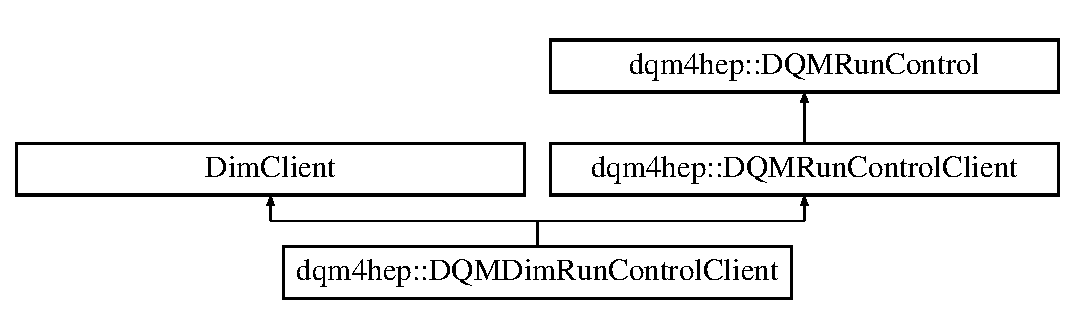
\includegraphics[height=3.000000cm]{classdqm4hep_1_1DQMDimRunControlClient}
\end{center}
\end{figure}
\subsection*{Public Member Functions}
\begin{DoxyCompactItemize}
\item 
{\bf D\+Q\+M\+Dim\+Run\+Control\+Client} ()
\begin{DoxyCompactList}\small\item\em Constructor. \end{DoxyCompactList}\item 
{\bf $\sim$\+D\+Q\+M\+Dim\+Run\+Control\+Client} ()
\begin{DoxyCompactList}\small\item\em Destructor. \end{DoxyCompactList}\item 
{\bf Status\+Code} {\bf connect\+To\+Service} ()
\begin{DoxyCompactList}\small\item\em Connect to the service. \end{DoxyCompactList}\item 
{\bf Status\+Code} {\bf disconnect\+From\+Service} ()
\begin{DoxyCompactList}\small\item\em Disconnect from the service. \end{DoxyCompactList}\item 
bool {\bf is\+Connected\+To\+Service} () const 
\begin{DoxyCompactList}\small\item\em Whether the client is connected to the service. \end{DoxyCompactList}\end{DoxyCompactItemize}
\subsection*{Private Member Functions}
\begin{DoxyCompactItemize}
\item 
void {\bf info\+Handler} ()
\begin{DoxyCompactList}\small\item\em Dim info handler. \end{DoxyCompactList}\item 
void {\bf handle\+Current\+Run\+Rpc\+Info} (Dim\+Rpc\+Info $\ast$p\+Rpc\+Info)
\begin{DoxyCompactList}\small\item\em Handle the dim current run rpc info. \end{DoxyCompactList}\end{DoxyCompactItemize}
\subsection*{Private Attributes}
\begin{DoxyCompactItemize}
\item 
bool {\bf m\+\_\+is\+Connected}
\begin{DoxyCompactList}\small\item\em Whether the client is connected to the server instance. \end{DoxyCompactList}\item 
{\bf D\+Q\+M\+Data\+Stream} {\bf m\+\_\+data\+Stream}
\begin{DoxyCompactList}\small\item\em The data stream to deserialize the run at start of run. \end{DoxyCompactList}\item 
Dim\+Info $\ast$ {\bf m\+\_\+p\+Start\+Of\+Run\+Info}
\begin{DoxyCompactList}\small\item\em The dim start of run info. \end{DoxyCompactList}\item 
Dim\+Info $\ast$ {\bf m\+\_\+p\+End\+Of\+Run\+Info}
\begin{DoxyCompactList}\small\item\em The dim end of run info. \end{DoxyCompactList}\item 
Dim\+Rpc\+Info $\ast$ {\bf m\+\_\+p\+Current\+Run\+Rpc\+Info}
\begin{DoxyCompactList}\small\item\em The dim current run rpc info. \end{DoxyCompactList}\end{DoxyCompactItemize}
\subsection*{Friends}
\begin{DoxyCompactItemize}
\item 
class {\bf D\+Q\+M\+Current\+Run\+Rpc\+Info}
\end{DoxyCompactItemize}
\subsection*{Additional Inherited Members}


\subsection{Detailed Description}
\doxyref{D\+Q\+M\+Run\+Control\+Client}{p.}{classdqm4hep_1_1DQMRunControlClient} class. 

Definition at line 69 of file D\+Q\+M\+Dim\+Run\+Control\+Client.\+h.



\subsection{Constructor \& Destructor Documentation}
\index{dqm4hep\+::\+D\+Q\+M\+Dim\+Run\+Control\+Client@{dqm4hep\+::\+D\+Q\+M\+Dim\+Run\+Control\+Client}!D\+Q\+M\+Dim\+Run\+Control\+Client@{D\+Q\+M\+Dim\+Run\+Control\+Client}}
\index{D\+Q\+M\+Dim\+Run\+Control\+Client@{D\+Q\+M\+Dim\+Run\+Control\+Client}!dqm4hep\+::\+D\+Q\+M\+Dim\+Run\+Control\+Client@{dqm4hep\+::\+D\+Q\+M\+Dim\+Run\+Control\+Client}}
\subsubsection[{D\+Q\+M\+Dim\+Run\+Control\+Client}]{\setlength{\rightskip}{0pt plus 5cm}dqm4hep\+::\+D\+Q\+M\+Dim\+Run\+Control\+Client\+::\+D\+Q\+M\+Dim\+Run\+Control\+Client (
\begin{DoxyParamCaption}
{}
\end{DoxyParamCaption}
)}\label{classdqm4hep_1_1DQMDimRunControlClient_aec198294723799dd8482435b797409a5}


Constructor. 



Definition at line 59 of file D\+Q\+M\+Dim\+Run\+Control\+Client.\+cc.


\begin{DoxyCode}
59                                                :
60     DQMRunControlClient(),
61     m_isConnected(\textcolor{keyword}{false}),
62     m_pStartOfRunInfo(NULL),
63     m_pEndOfRunInfo(NULL),
64     m_dataStream(1024) \textcolor{comment}{// 1 ko to start}
65 \{
66   \textcolor{comment}{/* nop */}
67 \}
\end{DoxyCode}
\index{dqm4hep\+::\+D\+Q\+M\+Dim\+Run\+Control\+Client@{dqm4hep\+::\+D\+Q\+M\+Dim\+Run\+Control\+Client}!````~D\+Q\+M\+Dim\+Run\+Control\+Client@{$\sim$\+D\+Q\+M\+Dim\+Run\+Control\+Client}}
\index{````~D\+Q\+M\+Dim\+Run\+Control\+Client@{$\sim$\+D\+Q\+M\+Dim\+Run\+Control\+Client}!dqm4hep\+::\+D\+Q\+M\+Dim\+Run\+Control\+Client@{dqm4hep\+::\+D\+Q\+M\+Dim\+Run\+Control\+Client}}
\subsubsection[{$\sim$\+D\+Q\+M\+Dim\+Run\+Control\+Client}]{\setlength{\rightskip}{0pt plus 5cm}dqm4hep\+::\+D\+Q\+M\+Dim\+Run\+Control\+Client\+::$\sim$\+D\+Q\+M\+Dim\+Run\+Control\+Client (
\begin{DoxyParamCaption}
{}
\end{DoxyParamCaption}
)}\label{classdqm4hep_1_1DQMDimRunControlClient_a9897f34d33b6b548d6cec468fc9e3334}


Destructor. 



Definition at line 71 of file D\+Q\+M\+Dim\+Run\+Control\+Client.\+cc.



References disconnect\+From\+Service(), and is\+Connected\+To\+Service().


\begin{DoxyCode}
72 \{
73   \textcolor{keywordflow}{if}(isConnectedToService())
74     disconnectFromService();
75 \}
\end{DoxyCode}


\subsection{Member Function Documentation}
\index{dqm4hep\+::\+D\+Q\+M\+Dim\+Run\+Control\+Client@{dqm4hep\+::\+D\+Q\+M\+Dim\+Run\+Control\+Client}!connect\+To\+Service@{connect\+To\+Service}}
\index{connect\+To\+Service@{connect\+To\+Service}!dqm4hep\+::\+D\+Q\+M\+Dim\+Run\+Control\+Client@{dqm4hep\+::\+D\+Q\+M\+Dim\+Run\+Control\+Client}}
\subsubsection[{connect\+To\+Service}]{\setlength{\rightskip}{0pt plus 5cm}{\bf Status\+Code} dqm4hep\+::\+D\+Q\+M\+Dim\+Run\+Control\+Client\+::connect\+To\+Service (
\begin{DoxyParamCaption}
{}
\end{DoxyParamCaption}
)\hspace{0.3cm}{\ttfamily [virtual]}}\label{classdqm4hep_1_1DQMDimRunControlClient_ac075d9fd330093e16e260d28c54517cb}


Connect to the service. 



Implements {\bf dqm4hep\+::\+D\+Q\+M\+Run\+Control\+Client} \doxyref{}{p.}{classdqm4hep_1_1DQMRunControlClient_a095786e35595c4536eba3513923d30f8}.



Definition at line 79 of file D\+Q\+M\+Dim\+Run\+Control\+Client.\+cc.



References D\+Q\+M\+Current\+Run\+Rpc\+Info, dqm4hep\+::\+D\+Q\+M\+Run\+Control\+::get\+Run\+Control\+Name(), is\+Connected\+To\+Service(), m\+\_\+is\+Connected, m\+\_\+p\+Current\+Run\+Rpc\+Info, m\+\_\+p\+End\+Of\+Run\+Info, and m\+\_\+p\+Start\+Of\+Run\+Info.


\begin{DoxyCode}
80 \{
81   \textcolor{keywordflow}{if}(isConnectedToService())
82     \textcolor{keywordflow}{return} STATUS\_CODE\_SUCCESS;
83 
84   std::string sorServiceName = \textcolor{stringliteral}{"DQM4HEP/RunControl/"} + this->getRunControlName() + \textcolor{stringliteral}{"/START\_OF\_RUN"};
85   std::string eorServiceName = \textcolor{stringliteral}{"DQM4HEP/RunControl/"} + this->getRunControlName() + \textcolor{stringliteral}{"/END\_OF\_RUN"};
86   std::string currentRunRpcName = \textcolor{stringliteral}{"DQM4HEP/RunControl/"} + this->
      getRunControlName() + \textcolor{stringliteral}{"/CURRENT\_RUN"};
87 
88   m_pStartOfRunInfo = \textcolor{keyword}{new} DimUpdatedInfo(sorServiceName.c\_str(), (\textcolor{keywordtype}{void}*) NULL, 0, \textcolor{keyword}{this});
89   m_pEndOfRunInfo = \textcolor{keyword}{new} DimUpdatedInfo(eorServiceName.c\_str(), (\textcolor{keywordtype}{void}*) NULL, 0, \textcolor{keyword}{this});
90   m_pCurrentRunRpcInfo = \textcolor{keyword}{new} DQMCurrentRunRpcInfo( (\textcolor{keywordtype}{char} *) currentRunRpcName.c\_str() , this );
91 
92   m_isConnected = \textcolor{keyword}{true};
93 
94   sleep(1);
95   \textcolor{keywordtype}{int} dummy = 0;
96   m_pCurrentRunRpcInfo->setData(dummy);
97 
98   \textcolor{keywordflow}{return} STATUS\_CODE\_SUCCESS;
99 \}
\end{DoxyCode}
\index{dqm4hep\+::\+D\+Q\+M\+Dim\+Run\+Control\+Client@{dqm4hep\+::\+D\+Q\+M\+Dim\+Run\+Control\+Client}!disconnect\+From\+Service@{disconnect\+From\+Service}}
\index{disconnect\+From\+Service@{disconnect\+From\+Service}!dqm4hep\+::\+D\+Q\+M\+Dim\+Run\+Control\+Client@{dqm4hep\+::\+D\+Q\+M\+Dim\+Run\+Control\+Client}}
\subsubsection[{disconnect\+From\+Service}]{\setlength{\rightskip}{0pt plus 5cm}{\bf Status\+Code} dqm4hep\+::\+D\+Q\+M\+Dim\+Run\+Control\+Client\+::disconnect\+From\+Service (
\begin{DoxyParamCaption}
{}
\end{DoxyParamCaption}
)\hspace{0.3cm}{\ttfamily [virtual]}}\label{classdqm4hep_1_1DQMDimRunControlClient_ac193d2ea248ff481e5cf15cc69d234fe}


Disconnect from the service. 



Implements {\bf dqm4hep\+::\+D\+Q\+M\+Run\+Control\+Client} \doxyref{}{p.}{classdqm4hep_1_1DQMRunControlClient_a9af1ffa45f59b8767c5b7583557fd396}.



Definition at line 103 of file D\+Q\+M\+Dim\+Run\+Control\+Client.\+cc.



References is\+Connected\+To\+Service(), m\+\_\+is\+Connected, m\+\_\+p\+Current\+Run\+Rpc\+Info, m\+\_\+p\+End\+Of\+Run\+Info, and m\+\_\+p\+Start\+Of\+Run\+Info.



Referenced by $\sim$\+D\+Q\+M\+Dim\+Run\+Control\+Client().


\begin{DoxyCode}
104 \{
105   \textcolor{keywordflow}{if}(!isConnectedToService())
106     \textcolor{keywordflow}{return} STATUS\_CODE\_SUCCESS;
107 
108   \textcolor{keyword}{delete} m_pStartOfRunInfo; m_pStartOfRunInfo = NULL;
109   \textcolor{keyword}{delete} m_pEndOfRunInfo; m_pEndOfRunInfo = NULL;
110   \textcolor{keyword}{delete} m_pCurrentRunRpcInfo; m_pCurrentRunRpcInfo = NULL;
111 
112   m_isConnected = \textcolor{keyword}{false};
113 
114   \textcolor{keywordflow}{return} STATUS\_CODE\_SUCCESS;
115 \}
\end{DoxyCode}
\index{dqm4hep\+::\+D\+Q\+M\+Dim\+Run\+Control\+Client@{dqm4hep\+::\+D\+Q\+M\+Dim\+Run\+Control\+Client}!handle\+Current\+Run\+Rpc\+Info@{handle\+Current\+Run\+Rpc\+Info}}
\index{handle\+Current\+Run\+Rpc\+Info@{handle\+Current\+Run\+Rpc\+Info}!dqm4hep\+::\+D\+Q\+M\+Dim\+Run\+Control\+Client@{dqm4hep\+::\+D\+Q\+M\+Dim\+Run\+Control\+Client}}
\subsubsection[{handle\+Current\+Run\+Rpc\+Info}]{\setlength{\rightskip}{0pt plus 5cm}void dqm4hep\+::\+D\+Q\+M\+Dim\+Run\+Control\+Client\+::handle\+Current\+Run\+Rpc\+Info (
\begin{DoxyParamCaption}
\item[{Dim\+Rpc\+Info $\ast$}]{p\+Rpc\+Info}
\end{DoxyParamCaption}
)\hspace{0.3cm}{\ttfamily [private]}}\label{classdqm4hep_1_1DQMDimRunControlClient_a888d18d42eb23e47c37380448eae66f2}


Handle the dim current run rpc info. 



Definition at line 185 of file D\+Q\+M\+Dim\+Run\+Control\+Client.\+cc.



References dqm4hep\+::\+D\+Q\+M\+Run\+::deserialize(), dqm4hep\+::\+D\+Q\+M\+Run\+::get\+Run\+Number(), is\+Connected\+To\+Service(), m\+\_\+data\+Stream, dqm4hep\+::\+D\+Q\+M\+Data\+Stream\+::reset(), dqm4hep\+::\+D\+Q\+M\+Data\+Stream\+::set\+Buffer(), dqm4hep\+::\+D\+Q\+M\+Run\+Control\+::start\+New\+Run(), and T\+H\+R\+O\+W\+\_\+\+R\+E\+S\+U\+L\+T\+\_\+\+I\+F.



Referenced by dqm4hep\+::\+D\+Q\+M\+Current\+Run\+Rpc\+Info\+::rpc\+Info\+Handler().


\begin{DoxyCode}
186 \{
187   \textcolor{keywordflow}{if}( ! this->isConnectedToService() )
188     \textcolor{keywordflow}{return};
189 
190   DQMRun *pRun = \textcolor{keyword}{new} DQMRun();
191 
192   \textcolor{keywordflow}{try}
193   \{
194     dqm_char *pBuffer = \textcolor{keyword}{static\_cast<}dqm_char*\textcolor{keyword}{>}(pRpcInfo->getData());
195     dqm_uint  bufferSize = pRpcInfo->getSize();
196 
197     \textcolor{keywordflow}{if}(NULL == pBuffer || 0 == bufferSize)
198       \textcolor{keywordflow}{throw} StatusCodeException(STATUS\_CODE\_FAILURE);
199 
200     m_dataStream.reset();
201     THROW_RESULT_IF(STATUS\_CODE\_SUCCESS, !=, m_dataStream.setBuffer(pBuffer, bufferSize));
202     THROW_RESULT_IF(STATUS\_CODE\_SUCCESS, !=, pRun->deserialize(&m_dataStream));
203 
204     \textcolor{comment}{// run number is invalid, meaning not running}
205     \textcolor{keywordflow}{if}(pRun->getRunNumber() <= 0)
206       \textcolor{keywordflow}{throw} StatusCodeException(STATUS\_CODE\_SUCCESS);
207 
208     \textcolor{comment}{// run is adopted here by the run control. No need to delete}
209     THROW_RESULT_IF(STATUS\_CODE\_SUCCESS, !=, this->startNewRun(pRun));
210 
211     \textcolor{comment}{// return avoids run deletion}
212     \textcolor{keywordflow}{return};
213   \}
214   \textcolor{keywordflow}{catch}(StatusCodeException &exception)
215   \{
216   \}
217 
218   \textcolor{keywordflow}{if}(pRun)
219     \textcolor{keyword}{delete} pRun;
220 \}
\end{DoxyCode}
\index{dqm4hep\+::\+D\+Q\+M\+Dim\+Run\+Control\+Client@{dqm4hep\+::\+D\+Q\+M\+Dim\+Run\+Control\+Client}!info\+Handler@{info\+Handler}}
\index{info\+Handler@{info\+Handler}!dqm4hep\+::\+D\+Q\+M\+Dim\+Run\+Control\+Client@{dqm4hep\+::\+D\+Q\+M\+Dim\+Run\+Control\+Client}}
\subsubsection[{info\+Handler}]{\setlength{\rightskip}{0pt plus 5cm}void dqm4hep\+::\+D\+Q\+M\+Dim\+Run\+Control\+Client\+::info\+Handler (
\begin{DoxyParamCaption}
{}
\end{DoxyParamCaption}
)\hspace{0.3cm}{\ttfamily [private]}}\label{classdqm4hep_1_1DQMDimRunControlClient_a8d53d42d94c6545be49fc67f7f1da4a7}


Dim info handler. 



Definition at line 126 of file D\+Q\+M\+Dim\+Run\+Control\+Client.\+cc.



References dqm4hep\+::\+D\+Q\+M\+Run\+Control\+::end\+Current\+Run(), is\+Connected\+To\+Service(), dqm4hep\+::\+D\+Q\+M\+Run\+Control\+::is\+Running(), m\+\_\+data\+Stream, m\+\_\+p\+End\+Of\+Run\+Info, m\+\_\+p\+Start\+Of\+Run\+Info, dqm4hep\+::\+D\+Q\+M\+Data\+Stream\+::reset(), dqm4hep\+::\+D\+Q\+M\+Data\+Stream\+::set\+Buffer(), dqm4hep\+::\+D\+Q\+M\+Run\+Control\+::start\+New\+Run(), T\+H\+R\+O\+W\+\_\+\+R\+E\+S\+U\+L\+T\+\_\+\+I\+F, dqm4hep\+::\+Status\+Code\+Exception\+::to\+String(), and dqm4hep\+::\+W\+A\+R\+N\+I\+N\+G.


\begin{DoxyCode}
127 \{
128   DimInfo *pCurrentDimInfo = getInfo();
129 
130   \textcolor{keywordflow}{if}(m_pStartOfRunInfo == pCurrentDimInfo)
131   \{
132     \textcolor{keywordflow}{if}(this->isRunning() || !this->isConnectedToService())
133       \textcolor{keywordflow}{return};
134 
135     dqm_char *pBuffer = \textcolor{keyword}{static\_cast<}dqm_char*\textcolor{keyword}{>}(pCurrentDimInfo->getData());
136     dqm_uint  bufferSize = pCurrentDimInfo->getSize();
137 
138     \textcolor{keywordflow}{if}(pBuffer == NULL || bufferSize == 0)
139       \textcolor{keywordflow}{return};
140 
141     m_dataStream.reset();
142     THROW_RESULT_IF(STATUS\_CODE\_SUCCESS, !=, m_dataStream.setBuffer(pBuffer, bufferSize));
143 
144     DQMRun *pRun = \textcolor{keyword}{new} DQMRun();
145 
146     \textcolor{keywordflow}{try}
147     \{
148       THROW_RESULT_IF(STATUS\_CODE\_SUCCESS, !=, pRun->deserialize(&m_dataStream));
149 
150       \textcolor{keywordflow}{if}(pRun->getRunNumber() < 0)
151         \textcolor{keywordflow}{throw} StatusCodeException(STATUS\_CODE\_INVALID\_PARAMETER);
152 
153       \textcolor{comment}{// run is adopted here by the run control. No need to delete}
154       THROW_RESULT_IF(STATUS\_CODE\_SUCCESS, !=, this->startNewRun(pRun));
155     \}
156     \textcolor{keywordflow}{catch}(StatusCodeException &exception)
157     \{
158       \textcolor{keywordflow}{if}(pRun)
159         \textcolor{keyword}{delete} pRun;
160     \}
161   \}
162   \textcolor{keywordflow}{else} \textcolor{keywordflow}{if}(m_pEndOfRunInfo == pCurrentDimInfo)
163   \{
164     \textcolor{keywordflow}{if}(!this->isRunning() || !this->isConnectedToService())
165       \textcolor{keywordflow}{return};
166 
167     \textcolor{keywordflow}{try}
168     \{
169       THROW_RESULT_IF(STATUS\_CODE\_SUCCESS, !=, this->endCurrentRun());
170     \}
171     \textcolor{keywordflow}{catch}(StatusCodeException &exception)
172     \{
173       streamlog\_out(WARNING) << \textcolor{stringliteral}{"Couldn't stop the run (at stop) : "} << exception.toString() << std::endl;
174       \textcolor{keywordflow}{return};
175     \}
176   \}
177   \textcolor{keywordflow}{else}
178   \{
179     streamlog\_out(WARNING) << \textcolor{stringliteral}{"Unknown info handled by the run control client : "} << pCurrentDimInfo->
      getName() << std::endl;
180   \}
181 \}
\end{DoxyCode}
\index{dqm4hep\+::\+D\+Q\+M\+Dim\+Run\+Control\+Client@{dqm4hep\+::\+D\+Q\+M\+Dim\+Run\+Control\+Client}!is\+Connected\+To\+Service@{is\+Connected\+To\+Service}}
\index{is\+Connected\+To\+Service@{is\+Connected\+To\+Service}!dqm4hep\+::\+D\+Q\+M\+Dim\+Run\+Control\+Client@{dqm4hep\+::\+D\+Q\+M\+Dim\+Run\+Control\+Client}}
\subsubsection[{is\+Connected\+To\+Service}]{\setlength{\rightskip}{0pt plus 5cm}bool dqm4hep\+::\+D\+Q\+M\+Dim\+Run\+Control\+Client\+::is\+Connected\+To\+Service (
\begin{DoxyParamCaption}
{}
\end{DoxyParamCaption}
) const\hspace{0.3cm}{\ttfamily [virtual]}}\label{classdqm4hep_1_1DQMDimRunControlClient_aaffa69541d61219872149542f6d980d9}


Whether the client is connected to the service. 



Implements {\bf dqm4hep\+::\+D\+Q\+M\+Run\+Control\+Client} \doxyref{}{p.}{classdqm4hep_1_1DQMRunControlClient_a2a7c21f48da48207f41668d44dec3b3c}.



Definition at line 119 of file D\+Q\+M\+Dim\+Run\+Control\+Client.\+cc.



References m\+\_\+is\+Connected.



Referenced by connect\+To\+Service(), disconnect\+From\+Service(), handle\+Current\+Run\+Rpc\+Info(), info\+Handler(), and $\sim$\+D\+Q\+M\+Dim\+Run\+Control\+Client().


\begin{DoxyCode}
120 \{
121   \textcolor{keywordflow}{return} m_isConnected;
122 \}
\end{DoxyCode}


\subsection{Friends And Related Function Documentation}
\index{dqm4hep\+::\+D\+Q\+M\+Dim\+Run\+Control\+Client@{dqm4hep\+::\+D\+Q\+M\+Dim\+Run\+Control\+Client}!D\+Q\+M\+Current\+Run\+Rpc\+Info@{D\+Q\+M\+Current\+Run\+Rpc\+Info}}
\index{D\+Q\+M\+Current\+Run\+Rpc\+Info@{D\+Q\+M\+Current\+Run\+Rpc\+Info}!dqm4hep\+::\+D\+Q\+M\+Dim\+Run\+Control\+Client@{dqm4hep\+::\+D\+Q\+M\+Dim\+Run\+Control\+Client}}
\subsubsection[{D\+Q\+M\+Current\+Run\+Rpc\+Info}]{\setlength{\rightskip}{0pt plus 5cm}friend class {\bf D\+Q\+M\+Current\+Run\+Rpc\+Info}\hspace{0.3cm}{\ttfamily [friend]}}\label{classdqm4hep_1_1DQMDimRunControlClient_ab62f65ba861ffa2d158987e43dbf5928}


Definition at line 109 of file D\+Q\+M\+Dim\+Run\+Control\+Client.\+h.



Referenced by connect\+To\+Service().



\subsection{Member Data Documentation}
\index{dqm4hep\+::\+D\+Q\+M\+Dim\+Run\+Control\+Client@{dqm4hep\+::\+D\+Q\+M\+Dim\+Run\+Control\+Client}!m\+\_\+data\+Stream@{m\+\_\+data\+Stream}}
\index{m\+\_\+data\+Stream@{m\+\_\+data\+Stream}!dqm4hep\+::\+D\+Q\+M\+Dim\+Run\+Control\+Client@{dqm4hep\+::\+D\+Q\+M\+Dim\+Run\+Control\+Client}}
\subsubsection[{m\+\_\+data\+Stream}]{\setlength{\rightskip}{0pt plus 5cm}{\bf D\+Q\+M\+Data\+Stream} dqm4hep\+::\+D\+Q\+M\+Dim\+Run\+Control\+Client\+::m\+\_\+data\+Stream\hspace{0.3cm}{\ttfamily [private]}}\label{classdqm4hep_1_1DQMDimRunControlClient_aab6825e9c8109ed896c081eb9ed4959d}


The data stream to deserialize the run at start of run. 



Definition at line 103 of file D\+Q\+M\+Dim\+Run\+Control\+Client.\+h.



Referenced by handle\+Current\+Run\+Rpc\+Info(), and info\+Handler().

\index{dqm4hep\+::\+D\+Q\+M\+Dim\+Run\+Control\+Client@{dqm4hep\+::\+D\+Q\+M\+Dim\+Run\+Control\+Client}!m\+\_\+is\+Connected@{m\+\_\+is\+Connected}}
\index{m\+\_\+is\+Connected@{m\+\_\+is\+Connected}!dqm4hep\+::\+D\+Q\+M\+Dim\+Run\+Control\+Client@{dqm4hep\+::\+D\+Q\+M\+Dim\+Run\+Control\+Client}}
\subsubsection[{m\+\_\+is\+Connected}]{\setlength{\rightskip}{0pt plus 5cm}bool dqm4hep\+::\+D\+Q\+M\+Dim\+Run\+Control\+Client\+::m\+\_\+is\+Connected\hspace{0.3cm}{\ttfamily [private]}}\label{classdqm4hep_1_1DQMDimRunControlClient_a6f0b280b3b9a95238d6c5e13159bc1ae}


Whether the client is connected to the server instance. 



Definition at line 102 of file D\+Q\+M\+Dim\+Run\+Control\+Client.\+h.



Referenced by connect\+To\+Service(), disconnect\+From\+Service(), and is\+Connected\+To\+Service().

\index{dqm4hep\+::\+D\+Q\+M\+Dim\+Run\+Control\+Client@{dqm4hep\+::\+D\+Q\+M\+Dim\+Run\+Control\+Client}!m\+\_\+p\+Current\+Run\+Rpc\+Info@{m\+\_\+p\+Current\+Run\+Rpc\+Info}}
\index{m\+\_\+p\+Current\+Run\+Rpc\+Info@{m\+\_\+p\+Current\+Run\+Rpc\+Info}!dqm4hep\+::\+D\+Q\+M\+Dim\+Run\+Control\+Client@{dqm4hep\+::\+D\+Q\+M\+Dim\+Run\+Control\+Client}}
\subsubsection[{m\+\_\+p\+Current\+Run\+Rpc\+Info}]{\setlength{\rightskip}{0pt plus 5cm}Dim\+Rpc\+Info$\ast$ dqm4hep\+::\+D\+Q\+M\+Dim\+Run\+Control\+Client\+::m\+\_\+p\+Current\+Run\+Rpc\+Info\hspace{0.3cm}{\ttfamily [private]}}\label{classdqm4hep_1_1DQMDimRunControlClient_af835dea4e0997f261844214308b1482a}


The dim current run rpc info. 



Definition at line 107 of file D\+Q\+M\+Dim\+Run\+Control\+Client.\+h.



Referenced by connect\+To\+Service(), and disconnect\+From\+Service().

\index{dqm4hep\+::\+D\+Q\+M\+Dim\+Run\+Control\+Client@{dqm4hep\+::\+D\+Q\+M\+Dim\+Run\+Control\+Client}!m\+\_\+p\+End\+Of\+Run\+Info@{m\+\_\+p\+End\+Of\+Run\+Info}}
\index{m\+\_\+p\+End\+Of\+Run\+Info@{m\+\_\+p\+End\+Of\+Run\+Info}!dqm4hep\+::\+D\+Q\+M\+Dim\+Run\+Control\+Client@{dqm4hep\+::\+D\+Q\+M\+Dim\+Run\+Control\+Client}}
\subsubsection[{m\+\_\+p\+End\+Of\+Run\+Info}]{\setlength{\rightskip}{0pt plus 5cm}Dim\+Info$\ast$ dqm4hep\+::\+D\+Q\+M\+Dim\+Run\+Control\+Client\+::m\+\_\+p\+End\+Of\+Run\+Info\hspace{0.3cm}{\ttfamily [private]}}\label{classdqm4hep_1_1DQMDimRunControlClient_a1ab40674b8da9c4adca3286ecaca1440}


The dim end of run info. 



Definition at line 106 of file D\+Q\+M\+Dim\+Run\+Control\+Client.\+h.



Referenced by connect\+To\+Service(), disconnect\+From\+Service(), and info\+Handler().

\index{dqm4hep\+::\+D\+Q\+M\+Dim\+Run\+Control\+Client@{dqm4hep\+::\+D\+Q\+M\+Dim\+Run\+Control\+Client}!m\+\_\+p\+Start\+Of\+Run\+Info@{m\+\_\+p\+Start\+Of\+Run\+Info}}
\index{m\+\_\+p\+Start\+Of\+Run\+Info@{m\+\_\+p\+Start\+Of\+Run\+Info}!dqm4hep\+::\+D\+Q\+M\+Dim\+Run\+Control\+Client@{dqm4hep\+::\+D\+Q\+M\+Dim\+Run\+Control\+Client}}
\subsubsection[{m\+\_\+p\+Start\+Of\+Run\+Info}]{\setlength{\rightskip}{0pt plus 5cm}Dim\+Info$\ast$ dqm4hep\+::\+D\+Q\+M\+Dim\+Run\+Control\+Client\+::m\+\_\+p\+Start\+Of\+Run\+Info\hspace{0.3cm}{\ttfamily [private]}}\label{classdqm4hep_1_1DQMDimRunControlClient_a4dbb0e67c521c37df740c7c39f719c7c}


The dim start of run info. 



Definition at line 105 of file D\+Q\+M\+Dim\+Run\+Control\+Client.\+h.



Referenced by connect\+To\+Service(), disconnect\+From\+Service(), and info\+Handler().



The documentation for this class was generated from the following files\+:\begin{DoxyCompactItemize}
\item 
{\bf D\+Q\+M\+Dim\+Run\+Control\+Client.\+h}\item 
{\bf D\+Q\+M\+Dim\+Run\+Control\+Client.\+cc}\end{DoxyCompactItemize}

\section{dqm4hep\+:\+:D\+Q\+M\+Directory Class Reference}
\label{classdqm4hep_1_1DQMDirectory}\index{dqm4hep\+::\+D\+Q\+M\+Directory@{dqm4hep\+::\+D\+Q\+M\+Directory}}


\doxyref{D\+Q\+M\+Directory}{p.}{classdqm4hep_1_1DQMDirectory} class.  




{\ttfamily \#include $<$D\+Q\+M\+Directory.\+h$>$}

\subsection*{Public Member Functions}
\begin{DoxyCompactItemize}
\item 
{\bf D\+Q\+M\+Directory} ()
\begin{DoxyCompactList}\small\item\em Default constructor. \end{DoxyCompactList}\item 
{\bf D\+Q\+M\+Directory} (const std\+::string \&name, {\bf D\+Q\+M\+Directory} $\ast$p\+Parent\+Dir=N\+U\+L\+L)
\begin{DoxyCompactList}\small\item\em Constructor with name and parent dir. \end{DoxyCompactList}\item 
{\bf $\sim$\+D\+Q\+M\+Directory} ()
\begin{DoxyCompactList}\small\item\em Destructor. \end{DoxyCompactList}\item 
{\bf Status\+Code} {\bf mkdir} (const std\+::string \&dir\+Name)
\begin{DoxyCompactList}\small\item\em Create a new directory. \end{DoxyCompactList}\item 
void {\bf ls} (bool recursive=false) const 
\begin{DoxyCompactList}\small\item\em List the directory contents and subdirs if asked. \end{DoxyCompactList}\item 
const std\+::string \& {\bf get\+Name} () const 
\begin{DoxyCompactList}\small\item\em Returns the directory name. \end{DoxyCompactList}\item 
{\bf D\+Q\+M\+Directory} $\ast$ {\bf get\+Parent\+Dir} () const 
\begin{DoxyCompactList}\small\item\em Returns the parent directory. \end{DoxyCompactList}\item 
const std\+::vector\\*
$<$ {\bf D\+Q\+M\+Directory} $\ast$ $>$ \& {\bf get\+Sub\+Dir\+List} () const 
\begin{DoxyCompactList}\small\item\em Get the sub directory list. \end{DoxyCompactList}\item 
bool {\bf contains\+Dir} (const std\+::string \&dir\+Name) const 
\begin{DoxyCompactList}\small\item\em Whether the directory contains the sub dir. \end{DoxyCompactList}\item 
{\bf Status\+Code} {\bf find\+Dir} (const std\+::string \&dir\+Name, {\bf D\+Q\+M\+Directory} $\ast$\&p\+Directory) const 
\begin{DoxyCompactList}\small\item\em Find the sub directory by name. \end{DoxyCompactList}\item 
{\bf Status\+Code} {\bf add\+Monitor\+Element} ({\bf D\+Q\+M\+Monitor\+Element} $\ast$p\+Monitor\+Element)
\begin{DoxyCompactList}\small\item\em Add a monitor elements to the directory. \end{DoxyCompactList}\item 
{\bf Status\+Code} {\bf find\+Monitor\+Element} (const std\+::string \&name, {\bf D\+Q\+M\+Monitor\+Element} $\ast$\&p\+Monitor\+Element) const 
\begin{DoxyCompactList}\small\item\em Find a monitor element with a given name in the directory. \end{DoxyCompactList}\item 
bool {\bf contains\+Monitor\+Element} (const {\bf D\+Q\+M\+Monitor\+Element} $\ast$p\+Monitor\+Element) const 
\begin{DoxyCompactList}\small\item\em Whether the directory contains the monitor element (search by ptr compare) \end{DoxyCompactList}\item 
bool {\bf contains\+Monitor\+Element} (const std\+::string \&monitor\+Element\+Name) const 
\begin{DoxyCompactList}\small\item\em Whether the directory contains the monitor element (search by name compare) \end{DoxyCompactList}\item 
{\bf Status\+Code} {\bf remove\+Monitor\+Element} ({\bf D\+Q\+M\+Monitor\+Element} $\ast$p\+Monitor\+Element)
\begin{DoxyCompactList}\small\item\em Remove the monitor element from the directory. \end{DoxyCompactList}\item 
{\bf Status\+Code} {\bf remove\+Monitor\+Element} (const std\+::string \&monitor\+Element\+Name)
\begin{DoxyCompactList}\small\item\em Remove the monitor element from the directory. \end{DoxyCompactList}\item 
const std\+::vector\\*
$<$ {\bf D\+Q\+M\+Monitor\+Element} $\ast$ $>$ \& {\bf get\+Monitor\+Element\+List} () const 
\begin{DoxyCompactList}\small\item\em Get the monitor element list. \end{DoxyCompactList}\item 
{\bf Status\+Code} {\bf remove\+Dir} (const std\+::string \&dir\+Name, bool deep\+Clean=false)
\begin{DoxyCompactList}\small\item\em Remove the directory and its contents Delete monitor element if deep\+Clean set to true. \end{DoxyCompactList}\item 
{\bf Status\+Code} {\bf clear} (bool deep\+Clean=false)
\begin{DoxyCompactList}\small\item\em Clear the directory by calling delete on each sub-\/dirs and clear the monitor element list by calling delete if asked. \end{DoxyCompactList}\item 
{\bf D\+Q\+M\+Path} {\bf get\+Full\+Path\+Name} () const 
\begin{DoxyCompactList}\small\item\em Get the full path name of the directory. \end{DoxyCompactList}\item 
bool {\bf is\+Root\+Dir} () const 
\begin{DoxyCompactList}\small\item\em Whether the directory is a root directory. \end{DoxyCompactList}\item 
bool {\bf is\+Empty} () const 
\begin{DoxyCompactList}\small\item\em Whether the directory is empty. \end{DoxyCompactList}\end{DoxyCompactItemize}
\subsection*{Private Member Functions}
\begin{DoxyCompactItemize}
\item 
void {\bf ls} (int depth) const 
\begin{DoxyCompactList}\small\item\em Recursive print of sub directory structure (dirs and contents) \end{DoxyCompactList}\end{DoxyCompactItemize}
\subsection*{Private Attributes}
\begin{DoxyCompactItemize}
\item 
std\+::string {\bf m\+\_\+name}
\item 
{\bf D\+Q\+M\+Directory} $\ast$ {\bf m\+\_\+p\+Parent\+Dir}
\item 
std\+::vector$<$ {\bf D\+Q\+M\+Directory} $\ast$ $>$ {\bf m\+\_\+directory\+List}
\item 
std\+::vector$<$ {\bf D\+Q\+M\+Monitor\+Element} $\ast$ $>$ {\bf m\+\_\+contents\+List}
\end{DoxyCompactItemize}


\subsection{Detailed Description}
\doxyref{D\+Q\+M\+Directory}{p.}{classdqm4hep_1_1DQMDirectory} class. 

A directory is the owner of its sub-\/directories. Monitor elements owning depends on how the method are called (default \+: not owner)

This interface doesn't allow moving sub-\/directories 

Definition at line 49 of file D\+Q\+M\+Directory.\+h.



\subsection{Constructor \& Destructor Documentation}
\index{dqm4hep\+::\+D\+Q\+M\+Directory@{dqm4hep\+::\+D\+Q\+M\+Directory}!D\+Q\+M\+Directory@{D\+Q\+M\+Directory}}
\index{D\+Q\+M\+Directory@{D\+Q\+M\+Directory}!dqm4hep\+::\+D\+Q\+M\+Directory@{dqm4hep\+::\+D\+Q\+M\+Directory}}
\subsubsection[{D\+Q\+M\+Directory}]{\setlength{\rightskip}{0pt plus 5cm}dqm4hep\+::\+D\+Q\+M\+Directory\+::\+D\+Q\+M\+Directory (
\begin{DoxyParamCaption}
{}
\end{DoxyParamCaption}
)}\label{classdqm4hep_1_1DQMDirectory_ac7153e642eb1ba4b52f23a6f5b38fd46}


Default constructor. 



Definition at line 37 of file D\+Q\+M\+Directory.\+cc.



Referenced by mkdir().


\begin{DoxyCode}
37                            :
38   m_name(\textcolor{stringliteral}{""}),
39   m_pParentDir(NULL)
40 \{
41   \textcolor{comment}{/* nop */}
42 \}
\end{DoxyCode}
\index{dqm4hep\+::\+D\+Q\+M\+Directory@{dqm4hep\+::\+D\+Q\+M\+Directory}!D\+Q\+M\+Directory@{D\+Q\+M\+Directory}}
\index{D\+Q\+M\+Directory@{D\+Q\+M\+Directory}!dqm4hep\+::\+D\+Q\+M\+Directory@{dqm4hep\+::\+D\+Q\+M\+Directory}}
\subsubsection[{D\+Q\+M\+Directory}]{\setlength{\rightskip}{0pt plus 5cm}dqm4hep\+::\+D\+Q\+M\+Directory\+::\+D\+Q\+M\+Directory (
\begin{DoxyParamCaption}
\item[{const std\+::string \&}]{name, }
\item[{{\bf D\+Q\+M\+Directory} $\ast$}]{p\+Parent\+Dir = {\ttfamily NULL}}
\end{DoxyParamCaption}
)}\label{classdqm4hep_1_1DQMDirectory_a29f39ec352e46d18a3887cae1cb4c902}


Constructor with name and parent dir. 



Definition at line 46 of file D\+Q\+M\+Directory.\+cc.


\begin{DoxyCode}
46                                                                           :
47   m_name(name),
48   m_pParentDir(pParentDir)
49 \{
50   \textcolor{comment}{/* nop */}
51 \}
\end{DoxyCode}
\index{dqm4hep\+::\+D\+Q\+M\+Directory@{dqm4hep\+::\+D\+Q\+M\+Directory}!````~D\+Q\+M\+Directory@{$\sim$\+D\+Q\+M\+Directory}}
\index{````~D\+Q\+M\+Directory@{$\sim$\+D\+Q\+M\+Directory}!dqm4hep\+::\+D\+Q\+M\+Directory@{dqm4hep\+::\+D\+Q\+M\+Directory}}
\subsubsection[{$\sim$\+D\+Q\+M\+Directory}]{\setlength{\rightskip}{0pt plus 5cm}dqm4hep\+::\+D\+Q\+M\+Directory\+::$\sim$\+D\+Q\+M\+Directory (
\begin{DoxyParamCaption}
{}
\end{DoxyParamCaption}
)}\label{classdqm4hep_1_1DQMDirectory_a48f107543aee2ae5d159356eaedb15e2}


Destructor. 

Delete the subdirectories but not the contents 

Definition at line 55 of file D\+Q\+M\+Directory.\+cc.



References clear().


\begin{DoxyCode}
56 \{
57   clear();
58 \}
\end{DoxyCode}


\subsection{Member Function Documentation}
\index{dqm4hep\+::\+D\+Q\+M\+Directory@{dqm4hep\+::\+D\+Q\+M\+Directory}!add\+Monitor\+Element@{add\+Monitor\+Element}}
\index{add\+Monitor\+Element@{add\+Monitor\+Element}!dqm4hep\+::\+D\+Q\+M\+Directory@{dqm4hep\+::\+D\+Q\+M\+Directory}}
\subsubsection[{add\+Monitor\+Element}]{\setlength{\rightskip}{0pt plus 5cm}{\bf Status\+Code} dqm4hep\+::\+D\+Q\+M\+Directory\+::add\+Monitor\+Element (
\begin{DoxyParamCaption}
\item[{{\bf D\+Q\+M\+Monitor\+Element} $\ast$}]{p\+Monitor\+Element}
\end{DoxyParamCaption}
)}\label{classdqm4hep_1_1DQMDirectory_a42b1bc21ac7cbd225668cbc6010519f5}


Add a monitor elements to the directory. 



Definition at line 175 of file D\+Q\+M\+Directory.\+cc.



References contains\+Monitor\+Element(), and m\+\_\+contents\+List.



Referenced by dqm4hep\+::\+D\+Q\+M\+Storage\+::add\+Monitor\+Element().


\begin{DoxyCode}
176 \{
177   \textcolor{keywordflow}{if}(NULL == pMonitorElement)
178     \textcolor{keywordflow}{return} STATUS\_CODE\_INVALID\_PTR;
179 
180   \textcolor{keywordflow}{if}(containsMonitorElement(pMonitorElement))
181     \textcolor{keywordflow}{return} STATUS\_CODE\_ALREADY\_PRESENT;
182 
183   m_contentsList.push\_back(pMonitorElement);
184 
185   \textcolor{keywordflow}{return} STATUS\_CODE\_SUCCESS;
186 \}
\end{DoxyCode}
\index{dqm4hep\+::\+D\+Q\+M\+Directory@{dqm4hep\+::\+D\+Q\+M\+Directory}!clear@{clear}}
\index{clear@{clear}!dqm4hep\+::\+D\+Q\+M\+Directory@{dqm4hep\+::\+D\+Q\+M\+Directory}}
\subsubsection[{clear}]{\setlength{\rightskip}{0pt plus 5cm}{\bf Status\+Code} dqm4hep\+::\+D\+Q\+M\+Directory\+::clear (
\begin{DoxyParamCaption}
\item[{bool}]{deep\+Clean = {\ttfamily false}}
\end{DoxyParamCaption}
)}\label{classdqm4hep_1_1DQMDirectory_a37b2d897ed05b7cdd7d86bf1e6985eeb}


Clear the directory by calling delete on each sub-\/dirs and clear the monitor element list by calling delete if asked. 

The operation is done recursively 

Definition at line 282 of file D\+Q\+M\+Directory.\+cc.



References clear(), m\+\_\+contents\+List, m\+\_\+directory\+List, and R\+E\+T\+U\+R\+N\+\_\+\+R\+E\+S\+U\+L\+T\+\_\+\+I\+F.



Referenced by clear(), dqm4hep\+::\+D\+Q\+M\+Storage\+::clear(), remove\+Dir(), and $\sim$\+D\+Q\+M\+Directory().


\begin{DoxyCode}
283 \{
284   \textcolor{keywordflow}{if}(deepClean)
285   \{
286     \textcolor{keywordflow}{for}(std::vector<DQMMonitorElement*>::const\_iterator iter = m_contentsList.begin(), endIter = 
      m_contentsList.end() ;
287         endIter != iter ; ++iter)
288     \{
289       DQMMonitorElement *pMonitorElement = *iter;
290       \textcolor{keyword}{delete} pMonitorElement;
291     \}
292   \}
293 
294   m_contentsList.clear();
295 
296 
297 
298   \textcolor{keywordflow}{for}(std::vector<DQMDirectory*>::iterator iter = m_directoryList.begin(), endIter = 
      m_directoryList.end() ;
299       endIter != iter ; ++iter)
300   \{
301     DQMDirectory *pDirectory = *iter;
302     \textcolor{comment}{// clear recursively the sub dir}
303     RETURN_RESULT_IF(STATUS\_CODE\_SUCCESS, !=, pDirectory->clear(deepClean));
304     \textcolor{comment}{// delete ptr}
305     \textcolor{keyword}{delete} pDirectory;
306   \}
307 
308   m_directoryList.clear();
309 
310   \textcolor{keywordflow}{return} STATUS\_CODE\_SUCCESS;
311 \}
\end{DoxyCode}
\index{dqm4hep\+::\+D\+Q\+M\+Directory@{dqm4hep\+::\+D\+Q\+M\+Directory}!contains\+Dir@{contains\+Dir}}
\index{contains\+Dir@{contains\+Dir}!dqm4hep\+::\+D\+Q\+M\+Directory@{dqm4hep\+::\+D\+Q\+M\+Directory}}
\subsubsection[{contains\+Dir}]{\setlength{\rightskip}{0pt plus 5cm}bool dqm4hep\+::\+D\+Q\+M\+Directory\+::contains\+Dir (
\begin{DoxyParamCaption}
\item[{const std\+::string \&}]{dir\+Name}
\end{DoxyParamCaption}
) const}\label{classdqm4hep_1_1DQMDirectory_a3f38ca78665c0533a40674f11293f2d6}


Whether the directory contains the sub dir. 



Definition at line 135 of file D\+Q\+M\+Directory.\+cc.



References dqm4hep\+::\+D\+Q\+M\+Core\+Tool\+::contains\+Special\+Characters(), get\+Name(), and m\+\_\+directory\+List.



Referenced by mkdir(), and dqm4hep\+::\+D\+Q\+M\+Storage\+::mkdir().


\begin{DoxyCode}
136 \{
137   \textcolor{keywordflow}{if}(dirName.find(\textcolor{stringliteral}{"/"}) != std::string::npos || 
      DQMCoreTool::containsSpecialCharacters(dirName) || dirName.empty())
138     \textcolor{keywordflow}{return} \textcolor{keyword}{false};
139 
140   \textcolor{keywordflow}{for}(std::vector<DQMDirectory*>::const\_iterator iter = m_directoryList.begin(), endIter = 
      m_directoryList.end() ;
141       endIter != iter ; ++iter)
142   \{
143     DQMDirectory *pDirectory = *iter;
144 
145     \textcolor{keywordflow}{if}(pDirectory->getName() == dirName)
146       \textcolor{keywordflow}{return} \textcolor{keyword}{true};
147   \}
148 
149   \textcolor{keywordflow}{return} \textcolor{keyword}{false};
150 \}
\end{DoxyCode}
\index{dqm4hep\+::\+D\+Q\+M\+Directory@{dqm4hep\+::\+D\+Q\+M\+Directory}!contains\+Monitor\+Element@{contains\+Monitor\+Element}}
\index{contains\+Monitor\+Element@{contains\+Monitor\+Element}!dqm4hep\+::\+D\+Q\+M\+Directory@{dqm4hep\+::\+D\+Q\+M\+Directory}}
\subsubsection[{contains\+Monitor\+Element}]{\setlength{\rightskip}{0pt plus 5cm}bool dqm4hep\+::\+D\+Q\+M\+Directory\+::contains\+Monitor\+Element (
\begin{DoxyParamCaption}
\item[{const {\bf D\+Q\+M\+Monitor\+Element} $\ast$}]{p\+Monitor\+Element}
\end{DoxyParamCaption}
) const}\label{classdqm4hep_1_1DQMDirectory_a1389bb38f9c79863bebaa067a464f0a7}


Whether the directory contains the monitor element (search by ptr compare) 



Definition at line 212 of file D\+Q\+M\+Directory.\+cc.



References dqm4hep\+::\+D\+Q\+M\+Monitor\+Element\+::get\+Name().



Referenced by add\+Monitor\+Element(), and dqm4hep\+::\+D\+Q\+M\+Storage\+::monitor\+Element\+Exists().


\begin{DoxyCode}
213 \{
214   \textcolor{keywordflow}{return} containsMonitorElement(pMonitorElement->getName());
215 \}
\end{DoxyCode}
\index{dqm4hep\+::\+D\+Q\+M\+Directory@{dqm4hep\+::\+D\+Q\+M\+Directory}!contains\+Monitor\+Element@{contains\+Monitor\+Element}}
\index{contains\+Monitor\+Element@{contains\+Monitor\+Element}!dqm4hep\+::\+D\+Q\+M\+Directory@{dqm4hep\+::\+D\+Q\+M\+Directory}}
\subsubsection[{contains\+Monitor\+Element}]{\setlength{\rightskip}{0pt plus 5cm}bool dqm4hep\+::\+D\+Q\+M\+Directory\+::contains\+Monitor\+Element (
\begin{DoxyParamCaption}
\item[{const std\+::string \&}]{monitor\+Element\+Name}
\end{DoxyParamCaption}
) const}\label{classdqm4hep_1_1DQMDirectory_a6e3ab71aec1b4ca92e6f64c7eb753528}


Whether the directory contains the monitor element (search by name compare) 



Definition at line 219 of file D\+Q\+M\+Directory.\+cc.



References find\+Monitor\+Element().


\begin{DoxyCode}
220 \{
221   DQMMonitorElement *pMonitorElement = NULL;
222   \textcolor{keywordflow}{return} findMonitorElement(monitorElementName, pMonitorElement) == STATUS\_CODE\_SUCCESS;
223 \}
\end{DoxyCode}
\index{dqm4hep\+::\+D\+Q\+M\+Directory@{dqm4hep\+::\+D\+Q\+M\+Directory}!find\+Dir@{find\+Dir}}
\index{find\+Dir@{find\+Dir}!dqm4hep\+::\+D\+Q\+M\+Directory@{dqm4hep\+::\+D\+Q\+M\+Directory}}
\subsubsection[{find\+Dir}]{\setlength{\rightskip}{0pt plus 5cm}{\bf Status\+Code} dqm4hep\+::\+D\+Q\+M\+Directory\+::find\+Dir (
\begin{DoxyParamCaption}
\item[{const std\+::string \&}]{dir\+Name, }
\item[{{\bf D\+Q\+M\+Directory} $\ast$\&}]{p\+Directory}
\end{DoxyParamCaption}
) const}\label{classdqm4hep_1_1DQMDirectory_a6da0415416e8da80da8b36f7014b68f0}


Find the sub directory by name. 



Definition at line 154 of file D\+Q\+M\+Directory.\+cc.



References get\+Name(), and m\+\_\+directory\+List.



Referenced by dqm4hep\+::\+D\+Q\+M\+Storage\+::cd(), dqm4hep\+::\+D\+Q\+M\+Storage\+::find\+Dir(), and dqm4hep\+::\+D\+Q\+M\+Storage\+::mkdir().


\begin{DoxyCode}
155 \{
156   pDirectory = NULL;
157 
158   \textcolor{keywordflow}{for}(std::vector<DQMDirectory*>::const\_iterator iter = m_directoryList.begin(), endIter = 
      m_directoryList.end() ;
159       endIter != iter ; ++iter)
160   \{
161     DQMDirectory *pDir = *iter;
162 
163     \textcolor{keywordflow}{if}(pDir->getName() == dirName)
164     \{
165       pDirectory = pDir;
166       \textcolor{keywordflow}{return} STATUS\_CODE\_SUCCESS;
167     \}
168   \}
169 
170   \textcolor{keywordflow}{return} STATUS\_CODE\_NOT\_FOUND;
171 \}
\end{DoxyCode}
\index{dqm4hep\+::\+D\+Q\+M\+Directory@{dqm4hep\+::\+D\+Q\+M\+Directory}!find\+Monitor\+Element@{find\+Monitor\+Element}}
\index{find\+Monitor\+Element@{find\+Monitor\+Element}!dqm4hep\+::\+D\+Q\+M\+Directory@{dqm4hep\+::\+D\+Q\+M\+Directory}}
\subsubsection[{find\+Monitor\+Element}]{\setlength{\rightskip}{0pt plus 5cm}{\bf Status\+Code} dqm4hep\+::\+D\+Q\+M\+Directory\+::find\+Monitor\+Element (
\begin{DoxyParamCaption}
\item[{const std\+::string \&}]{name, }
\item[{{\bf D\+Q\+M\+Monitor\+Element} $\ast$\&}]{p\+Monitor\+Element}
\end{DoxyParamCaption}
) const}\label{classdqm4hep_1_1DQMDirectory_addbf7057f9ff505273b7a9f9e2ec2a28}


Find a monitor element with a given name in the directory. 



Definition at line 190 of file D\+Q\+M\+Directory.\+cc.



References dqm4hep\+::\+D\+Q\+M\+Monitor\+Element\+::get\+Name(), and m\+\_\+contents\+List.



Referenced by contains\+Monitor\+Element(), dqm4hep\+::\+D\+Q\+M\+Storage\+::get\+Monitor\+Element(), and dqm4hep\+::\+D\+Q\+M\+Storage\+::remove\+Monitor\+Element().


\begin{DoxyCode}
191 \{
192   pMonitorElement = NULL;
193 
194   \textcolor{comment}{// print contents first}
195   \textcolor{keywordflow}{for}(std::vector<DQMMonitorElement*>::const\_iterator iter = m_contentsList.begin(), endIter = 
      m_contentsList.end() ;
196       endIter != iter ; ++iter)
197   \{
198     DQMMonitorElement *pME = *iter;
199 
200     \textcolor{keywordflow}{if}(pME->getName() == name)
201     \{
202       pMonitorElement = pME;
203       \textcolor{keywordflow}{return} STATUS\_CODE\_SUCCESS;
204     \}
205   \}
206 
207   \textcolor{keywordflow}{return} STATUS\_CODE\_NOT\_FOUND;
208 \}
\end{DoxyCode}
\index{dqm4hep\+::\+D\+Q\+M\+Directory@{dqm4hep\+::\+D\+Q\+M\+Directory}!get\+Full\+Path\+Name@{get\+Full\+Path\+Name}}
\index{get\+Full\+Path\+Name@{get\+Full\+Path\+Name}!dqm4hep\+::\+D\+Q\+M\+Directory@{dqm4hep\+::\+D\+Q\+M\+Directory}}
\subsubsection[{get\+Full\+Path\+Name}]{\setlength{\rightskip}{0pt plus 5cm}{\bf D\+Q\+M\+Path} dqm4hep\+::\+D\+Q\+M\+Directory\+::get\+Full\+Path\+Name (
\begin{DoxyParamCaption}
{}
\end{DoxyParamCaption}
) const}\label{classdqm4hep_1_1DQMDirectory_ad6ef7078ba8db43ab06485f09cd6ea07}


Get the full path name of the directory. 



Definition at line 315 of file D\+Q\+M\+Directory.\+cc.



References get\+Name(), and get\+Parent\+Dir().



Referenced by dqm4hep\+::\+D\+Q\+M\+Storage\+::add\+Monitor\+Element(), dqm4hep\+::\+D\+Q\+M\+Monitor\+Element\+Manager\+::book\+Char\+Histogram1\+D(), dqm4hep\+::\+D\+Q\+M\+Monitor\+Element\+Manager\+::book\+Char\+Histogram2\+D(), dqm4hep\+::\+D\+Q\+M\+Monitor\+Element\+Manager\+::book\+Int\+Histogram1\+D(), dqm4hep\+::\+D\+Q\+M\+Monitor\+Element\+Manager\+::book\+Int\+Histogram2\+D(), dqm4hep\+::\+D\+Q\+M\+Monitor\+Element\+Manager\+::book\+Profile1\+D(), dqm4hep\+::\+D\+Q\+M\+Monitor\+Element\+Manager\+::book\+Profile2\+D(), dqm4hep\+::\+D\+Q\+M\+Monitor\+Element\+Manager\+::book\+Real\+Histogram1\+D(), dqm4hep\+::\+D\+Q\+M\+Monitor\+Element\+Manager\+::book\+Real\+Histogram2\+D(), dqm4hep\+::\+D\+Q\+M\+Monitor\+Element\+Manager\+::book\+Short\+Histogram1\+D(), dqm4hep\+::\+D\+Q\+M\+Monitor\+Element\+Manager\+::book\+Short\+Histogram2\+D(), dqm4hep\+::\+D\+Q\+M\+Monitor\+Element\+Manager\+::get\+Current\+Directory\+Full\+Path\+Name(), dqm4hep\+::\+D\+Q\+M\+Monitor\+Element\+Manager\+::get\+Full\+Path\+Name(), and dqm4hep\+::\+D\+Q\+M\+Storage\+::rmdir().


\begin{DoxyCode}
316 \{
317   DQMPath fullPath = this->getName();
318   \textcolor{keyword}{const} DQMDirectory *pDir = \textcolor{keyword}{this};
319 
320   \textcolor{keywordflow}{while}(1)
321   \{
322     \textcolor{keyword}{const} DQMDirectory *pParentDir = pDir->getParentDir();
323 
324     \textcolor{keywordflow}{if}(NULL != pParentDir)
325     \{
326       fullPath = pParentDir->getName() + fullPath;
327       pDir = pParentDir;
328     \}
329     \textcolor{keywordflow}{else}
330       \textcolor{keywordflow}{break};
331   \}
332 
333   \textcolor{keywordflow}{return} fullPath;
334 \}
\end{DoxyCode}
\index{dqm4hep\+::\+D\+Q\+M\+Directory@{dqm4hep\+::\+D\+Q\+M\+Directory}!get\+Monitor\+Element\+List@{get\+Monitor\+Element\+List}}
\index{get\+Monitor\+Element\+List@{get\+Monitor\+Element\+List}!dqm4hep\+::\+D\+Q\+M\+Directory@{dqm4hep\+::\+D\+Q\+M\+Directory}}
\subsubsection[{get\+Monitor\+Element\+List}]{\setlength{\rightskip}{0pt plus 5cm}const std\+::vector$<$ {\bf D\+Q\+M\+Monitor\+Element} $\ast$ $>$ \& dqm4hep\+::\+D\+Q\+M\+Directory\+::get\+Monitor\+Element\+List (
\begin{DoxyParamCaption}
{}
\end{DoxyParamCaption}
) const}\label{classdqm4hep_1_1DQMDirectory_ac143ca3d53c6df35c3d346721597e363}


Get the monitor element list. 



Definition at line 253 of file D\+Q\+M\+Directory.\+cc.



References m\+\_\+contents\+List.



Referenced by dqm4hep\+::\+D\+Q\+M\+Storage\+::recursive\+Content\+List(), dqm4hep\+::\+D\+Q\+M\+Archiver\+::recursive\+Fill(), and dqm4hep\+::\+D\+Q\+M\+Archiver\+::write\+Monitor\+Elements().


\begin{DoxyCode}
254 \{
255   \textcolor{keywordflow}{return} m_contentsList;
256 \}
\end{DoxyCode}
\index{dqm4hep\+::\+D\+Q\+M\+Directory@{dqm4hep\+::\+D\+Q\+M\+Directory}!get\+Name@{get\+Name}}
\index{get\+Name@{get\+Name}!dqm4hep\+::\+D\+Q\+M\+Directory@{dqm4hep\+::\+D\+Q\+M\+Directory}}
\subsubsection[{get\+Name}]{\setlength{\rightskip}{0pt plus 5cm}const std\+::string \& dqm4hep\+::\+D\+Q\+M\+Directory\+::get\+Name (
\begin{DoxyParamCaption}
{}
\end{DoxyParamCaption}
) const}\label{classdqm4hep_1_1DQMDirectory_a3ab98865b568c8b2c1be35288b56c9e7}


Returns the directory name. 



Definition at line 98 of file D\+Q\+M\+Directory.\+cc.



References m\+\_\+name.



Referenced by contains\+Dir(), find\+Dir(), dqm4hep\+::\+D\+Q\+M\+Monitor\+Element\+Manager\+::get\+Current\+Directory\+Name(), get\+Full\+Path\+Name(), dqm4hep\+::\+D\+Q\+M\+Storage\+::pwd(), dqm4hep\+::\+D\+Q\+M\+Archiver\+::recursive\+Fill(), remove\+Dir(), and dqm4hep\+::\+D\+Q\+M\+Storage\+::rmdir().


\begin{DoxyCode}
99 \{
100   \textcolor{keywordflow}{return} m_name;
101 \}
\end{DoxyCode}
\index{dqm4hep\+::\+D\+Q\+M\+Directory@{dqm4hep\+::\+D\+Q\+M\+Directory}!get\+Parent\+Dir@{get\+Parent\+Dir}}
\index{get\+Parent\+Dir@{get\+Parent\+Dir}!dqm4hep\+::\+D\+Q\+M\+Directory@{dqm4hep\+::\+D\+Q\+M\+Directory}}
\subsubsection[{get\+Parent\+Dir}]{\setlength{\rightskip}{0pt plus 5cm}{\bf D\+Q\+M\+Directory} $\ast$ dqm4hep\+::\+D\+Q\+M\+Directory\+::get\+Parent\+Dir (
\begin{DoxyParamCaption}
{}
\end{DoxyParamCaption}
) const}\label{classdqm4hep_1_1DQMDirectory_a2ff4f2f461304b8a780ba18cf9463b58}


Returns the parent directory. 



Definition at line 105 of file D\+Q\+M\+Directory.\+cc.



References m\+\_\+p\+Parent\+Dir.



Referenced by get\+Full\+Path\+Name(), dqm4hep\+::\+D\+Q\+M\+Storage\+::go\+Up(), and dqm4hep\+::\+D\+Q\+M\+Storage\+::rmdir().


\begin{DoxyCode}
106 \{
107   \textcolor{keywordflow}{return} m_pParentDir;
108 \}
\end{DoxyCode}
\index{dqm4hep\+::\+D\+Q\+M\+Directory@{dqm4hep\+::\+D\+Q\+M\+Directory}!get\+Sub\+Dir\+List@{get\+Sub\+Dir\+List}}
\index{get\+Sub\+Dir\+List@{get\+Sub\+Dir\+List}!dqm4hep\+::\+D\+Q\+M\+Directory@{dqm4hep\+::\+D\+Q\+M\+Directory}}
\subsubsection[{get\+Sub\+Dir\+List}]{\setlength{\rightskip}{0pt plus 5cm}const std\+::vector$<$ {\bf D\+Q\+M\+Directory} $\ast$ $>$ \& dqm4hep\+::\+D\+Q\+M\+Directory\+::get\+Sub\+Dir\+List (
\begin{DoxyParamCaption}
{}
\end{DoxyParamCaption}
) const}\label{classdqm4hep_1_1DQMDirectory_ac4117c55d0bfe47122c38052601886f3}


Get the sub directory list. 



Definition at line 112 of file D\+Q\+M\+Directory.\+cc.



References m\+\_\+directory\+List.



Referenced by dqm4hep\+::\+D\+Q\+M\+Storage\+::recursive\+Content\+List(), and dqm4hep\+::\+D\+Q\+M\+Archiver\+::recursive\+Fill().


\begin{DoxyCode}
113 \{
114   \textcolor{keywordflow}{return} m_directoryList;
115 \}
\end{DoxyCode}
\index{dqm4hep\+::\+D\+Q\+M\+Directory@{dqm4hep\+::\+D\+Q\+M\+Directory}!is\+Empty@{is\+Empty}}
\index{is\+Empty@{is\+Empty}!dqm4hep\+::\+D\+Q\+M\+Directory@{dqm4hep\+::\+D\+Q\+M\+Directory}}
\subsubsection[{is\+Empty}]{\setlength{\rightskip}{0pt plus 5cm}bool dqm4hep\+::\+D\+Q\+M\+Directory\+::is\+Empty (
\begin{DoxyParamCaption}
{}
\end{DoxyParamCaption}
) const}\label{classdqm4hep_1_1DQMDirectory_a12c6c70250adacb24b78edecd134f99a}


Whether the directory is empty. 



Definition at line 370 of file D\+Q\+M\+Directory.\+cc.



References m\+\_\+contents\+List, and m\+\_\+directory\+List.


\begin{DoxyCode}
371 \{
372   \textcolor{keywordflow}{return} (m_directoryList.empty() && m_contentsList.empty());
373 \}
\end{DoxyCode}
\index{dqm4hep\+::\+D\+Q\+M\+Directory@{dqm4hep\+::\+D\+Q\+M\+Directory}!is\+Root\+Dir@{is\+Root\+Dir}}
\index{is\+Root\+Dir@{is\+Root\+Dir}!dqm4hep\+::\+D\+Q\+M\+Directory@{dqm4hep\+::\+D\+Q\+M\+Directory}}
\subsubsection[{is\+Root\+Dir}]{\setlength{\rightskip}{0pt plus 5cm}bool dqm4hep\+::\+D\+Q\+M\+Directory\+::is\+Root\+Dir (
\begin{DoxyParamCaption}
{}
\end{DoxyParamCaption}
) const}\label{classdqm4hep_1_1DQMDirectory_afe5e6fb0e383c2de9a82c1021cb5772e}


Whether the directory is a root directory. 



Definition at line 363 of file D\+Q\+M\+Directory.\+cc.



References m\+\_\+p\+Parent\+Dir.



Referenced by dqm4hep\+::\+D\+Q\+M\+Storage\+::go\+Up().


\begin{DoxyCode}
364 \{
365   \textcolor{keywordflow}{return} (m_pParentDir == NULL);
366 \}
\end{DoxyCode}
\index{dqm4hep\+::\+D\+Q\+M\+Directory@{dqm4hep\+::\+D\+Q\+M\+Directory}!ls@{ls}}
\index{ls@{ls}!dqm4hep\+::\+D\+Q\+M\+Directory@{dqm4hep\+::\+D\+Q\+M\+Directory}}
\subsubsection[{ls}]{\setlength{\rightskip}{0pt plus 5cm}void dqm4hep\+::\+D\+Q\+M\+Directory\+::ls (
\begin{DoxyParamCaption}
\item[{bool}]{recursive = {\ttfamily false}}
\end{DoxyParamCaption}
) const}\label{classdqm4hep_1_1DQMDirectory_a7a788a1adb5c86232f14c98ca89f1ede}


List the directory contents and subdirs if asked. 



Definition at line 62 of file D\+Q\+M\+Directory.\+cc.



References dqm4hep\+::\+D\+Q\+M\+Monitor\+Element\+::get\+Name(), ls(), m\+\_\+contents\+List, m\+\_\+directory\+List, m\+\_\+name, m\+\_\+p\+Parent\+Dir, and dqm4hep\+::\+M\+E\+S\+S\+A\+G\+E.



Referenced by ls(), and dqm4hep\+::\+D\+Q\+M\+Storage\+::ls().


\begin{DoxyCode}
63 \{
64   \textcolor{keywordtype}{int} depth = 0;
65   std::string parentDirName = m_pParentDir == NULL ? \textcolor{stringliteral}{"\(\backslash\)"\(\backslash\)""} : m_pParentDir->
      m_name;
66 
67   streamlog\_out(MESSAGE) << \textcolor{stringliteral}{"Directory "} << m_name << \textcolor{stringliteral}{" (parent = "} << parentDirName << \textcolor{stringliteral}{") :"} << std::endl;
68 
69   \textcolor{comment}{// print contents first}
70   \textcolor{keywordflow}{for}(std::vector<DQMMonitorElement*>::const\_iterator iter = m_contentsList.begin(), endIter = 
      m_contentsList.end() ;
71       endIter != iter ; ++iter)
72   \{
73     DQMMonitorElement *pMonitorElement = *iter;
74     streamlog\_out(MESSAGE) << \textcolor{stringliteral}{" [ME]  "} << pMonitorElement->getName() << std::endl;
75   \}
76 
77   \textcolor{comment}{// print sub-directories}
78   \textcolor{keywordflow}{for}(std::vector<DQMDirectory*>::const\_iterator iter = m_directoryList.begin(), endIter = 
      m_directoryList.end() ;
79       endIter != iter ; ++iter)
80   \{
81     DQMDirectory *pDirectory = *iter;
82 
83     \textcolor{keywordflow}{if}(recursive)
84     \{
85       pDirectory->ls(depth+1);
86     \}
87     \textcolor{keywordflow}{else}
88     \{
89       streamlog\_out(MESSAGE) << \textcolor{stringliteral}{" [DIR] "} << pDirectory->m\_name << std::endl;
90     \}
91   \}
92 
93   streamlog\_out(MESSAGE) << std::endl;
94 \}
\end{DoxyCode}
\index{dqm4hep\+::\+D\+Q\+M\+Directory@{dqm4hep\+::\+D\+Q\+M\+Directory}!ls@{ls}}
\index{ls@{ls}!dqm4hep\+::\+D\+Q\+M\+Directory@{dqm4hep\+::\+D\+Q\+M\+Directory}}
\subsubsection[{ls}]{\setlength{\rightskip}{0pt plus 5cm}void dqm4hep\+::\+D\+Q\+M\+Directory\+::ls (
\begin{DoxyParamCaption}
\item[{int}]{depth}
\end{DoxyParamCaption}
) const\hspace{0.3cm}{\ttfamily [private]}}\label{classdqm4hep_1_1DQMDirectory_a4b51b54d871f25fc78135ed1c6eddfaa}


Recursive print of sub directory structure (dirs and contents) 



Definition at line 338 of file D\+Q\+M\+Directory.\+cc.



References dqm4hep\+::\+D\+Q\+M\+Monitor\+Element\+::get\+Name(), ls(), m\+\_\+contents\+List, m\+\_\+directory\+List, m\+\_\+name, m\+\_\+p\+Parent\+Dir, and dqm4hep\+::\+M\+E\+S\+S\+A\+G\+E.


\begin{DoxyCode}
339 \{
340   std::string parentDirName = m_pParentDir == NULL ? \textcolor{stringliteral}{"\(\backslash\)"\(\backslash\)""} : m_pParentDir->
      m_name;
341 
342   streamlog\_out(MESSAGE) << std::string(depth*3, \textcolor{charliteral}{' '}) << \textcolor{stringliteral}{"Directory "} << m_name << \textcolor{stringliteral}{" (parent = "} << 
      parentDirName << \textcolor{stringliteral}{") :"} << std::endl;
343 
344   \textcolor{comment}{// print contents first}
345   \textcolor{keywordflow}{for}(std::vector<DQMMonitorElement*>::const\_iterator iter = m_contentsList.begin(), endIter = 
      m_contentsList.end() ;
346       endIter != iter ; ++iter)
347   \{
348     DQMMonitorElement *pMonitorElement = *iter;
349     streamlog\_out(MESSAGE) << std::string(depth*3, \textcolor{charliteral}{' '}) << \textcolor{stringliteral}{" [ME]  "} << pMonitorElement->getName() << 
      std::endl;
350   \}
351 
352   \textcolor{comment}{// print sub dirs}
353   \textcolor{keywordflow}{for}(std::vector<DQMDirectory*>::const\_iterator iter = m_directoryList.begin(), endIter = 
      m_directoryList.end() ;
354       endIter != iter ; ++iter)
355   \{
356     DQMDirectory *pDirectory = *iter;
357     pDirectory->ls(depth+1);
358   \}
359 \}
\end{DoxyCode}
\index{dqm4hep\+::\+D\+Q\+M\+Directory@{dqm4hep\+::\+D\+Q\+M\+Directory}!mkdir@{mkdir}}
\index{mkdir@{mkdir}!dqm4hep\+::\+D\+Q\+M\+Directory@{dqm4hep\+::\+D\+Q\+M\+Directory}}
\subsubsection[{mkdir}]{\setlength{\rightskip}{0pt plus 5cm}{\bf Status\+Code} dqm4hep\+::\+D\+Q\+M\+Directory\+::mkdir (
\begin{DoxyParamCaption}
\item[{const std\+::string \&}]{dir\+Name}
\end{DoxyParamCaption}
)}\label{classdqm4hep_1_1DQMDirectory_a7740388427ba5f0bb72c5b38393272fd}


Create a new directory. 



Definition at line 119 of file D\+Q\+M\+Directory.\+cc.



References contains\+Dir(), dqm4hep\+::\+D\+Q\+M\+Core\+Tool\+::contains\+Special\+Characters(), D\+Q\+M\+Directory(), and m\+\_\+directory\+List.



Referenced by dqm4hep\+::\+D\+Q\+M\+Storage\+::mkdir(), and dqm4hep\+::\+D\+Q\+M\+Archiver\+::recursive\+Fill().


\begin{DoxyCode}
120 \{
121   \textcolor{keywordflow}{if}(containsDir(dirName))
122     \textcolor{keywordflow}{return} STATUS\_CODE\_ALREADY\_PRESENT;
123 
124   \textcolor{keywordflow}{if}(dirName.find(\textcolor{stringliteral}{"/"}) != std::string::npos || 
      DQMCoreTool::containsSpecialCharacters(dirName) || dirName.empty())
125     \textcolor{keywordflow}{return} STATUS\_CODE\_INVALID\_PARAMETER;
126 
127   DQMDirectory *pNewDirectory = \textcolor{keyword}{new} DQMDirectory(dirName, \textcolor{keyword}{this});
128   m_directoryList.push\_back(pNewDirectory);
129 
130   \textcolor{keywordflow}{return} STATUS\_CODE\_SUCCESS;
131 \}
\end{DoxyCode}
\index{dqm4hep\+::\+D\+Q\+M\+Directory@{dqm4hep\+::\+D\+Q\+M\+Directory}!remove\+Dir@{remove\+Dir}}
\index{remove\+Dir@{remove\+Dir}!dqm4hep\+::\+D\+Q\+M\+Directory@{dqm4hep\+::\+D\+Q\+M\+Directory}}
\subsubsection[{remove\+Dir}]{\setlength{\rightskip}{0pt plus 5cm}{\bf Status\+Code} dqm4hep\+::\+D\+Q\+M\+Directory\+::remove\+Dir (
\begin{DoxyParamCaption}
\item[{const std\+::string \&}]{dir\+Name, }
\item[{bool}]{deep\+Clean = {\ttfamily false}}
\end{DoxyParamCaption}
)}\label{classdqm4hep_1_1DQMDirectory_a7f5848fd500d19ed66cf1536eb8f23dc}


Remove the directory and its contents Delete monitor element if deep\+Clean set to true. 



Definition at line 260 of file D\+Q\+M\+Directory.\+cc.



References clear(), get\+Name(), m\+\_\+directory\+List, and R\+E\+T\+U\+R\+N\+\_\+\+R\+E\+S\+U\+L\+T\+\_\+\+I\+F.



Referenced by dqm4hep\+::\+D\+Q\+M\+Storage\+::rmdir().


\begin{DoxyCode}
261 \{
262   \textcolor{keywordflow}{for}(std::vector<DQMDirectory*>::iterator iter = m_directoryList.begin(), endIter = 
      m_directoryList.end() ;
263       endIter != iter ; ++iter)
264   \{
265     DQMDirectory *pDirectory = *iter;
266 
267     \textcolor{keywordflow}{if}(pDirectory->getName() == dirName)
268     \{
269       RETURN_RESULT_IF(STATUS\_CODE\_SUCCESS, !=, pDirectory->clear(deepClean));
270       \textcolor{keyword}{delete} pDirectory;
271       m_directoryList.erase(iter);
272 
273       \textcolor{keywordflow}{return} STATUS\_CODE\_SUCCESS;
274     \}
275   \}
276 
277   \textcolor{keywordflow}{return} STATUS\_CODE\_NOT\_FOUND;
278 \}
\end{DoxyCode}
\index{dqm4hep\+::\+D\+Q\+M\+Directory@{dqm4hep\+::\+D\+Q\+M\+Directory}!remove\+Monitor\+Element@{remove\+Monitor\+Element}}
\index{remove\+Monitor\+Element@{remove\+Monitor\+Element}!dqm4hep\+::\+D\+Q\+M\+Directory@{dqm4hep\+::\+D\+Q\+M\+Directory}}
\subsubsection[{remove\+Monitor\+Element}]{\setlength{\rightskip}{0pt plus 5cm}{\bf Status\+Code} dqm4hep\+::\+D\+Q\+M\+Directory\+::remove\+Monitor\+Element (
\begin{DoxyParamCaption}
\item[{{\bf D\+Q\+M\+Monitor\+Element} $\ast$}]{p\+Monitor\+Element}
\end{DoxyParamCaption}
)}\label{classdqm4hep_1_1DQMDirectory_aa3cfe4196512c5e384e2aa974e48e682}


Remove the monitor element from the directory. 



Definition at line 227 of file D\+Q\+M\+Directory.\+cc.



References dqm4hep\+::\+D\+Q\+M\+Monitor\+Element\+::get\+Name().



Referenced by dqm4hep\+::\+D\+Q\+M\+Storage\+::remove\+Monitor\+Element().


\begin{DoxyCode}
228 \{
229   \textcolor{keywordflow}{return} removeMonitorElement(pMonitorElement->getName());
230 \}
\end{DoxyCode}
\index{dqm4hep\+::\+D\+Q\+M\+Directory@{dqm4hep\+::\+D\+Q\+M\+Directory}!remove\+Monitor\+Element@{remove\+Monitor\+Element}}
\index{remove\+Monitor\+Element@{remove\+Monitor\+Element}!dqm4hep\+::\+D\+Q\+M\+Directory@{dqm4hep\+::\+D\+Q\+M\+Directory}}
\subsubsection[{remove\+Monitor\+Element}]{\setlength{\rightskip}{0pt plus 5cm}{\bf Status\+Code} dqm4hep\+::\+D\+Q\+M\+Directory\+::remove\+Monitor\+Element (
\begin{DoxyParamCaption}
\item[{const std\+::string \&}]{monitor\+Element\+Name}
\end{DoxyParamCaption}
)}\label{classdqm4hep_1_1DQMDirectory_a88ad53d27ca85b1753222bdc84815cc0}


Remove the monitor element from the directory. 



Definition at line 234 of file D\+Q\+M\+Directory.\+cc.



References dqm4hep\+::\+D\+Q\+M\+Monitor\+Element\+::get\+Name(), and m\+\_\+contents\+List.


\begin{DoxyCode}
235 \{
236   \textcolor{keywordflow}{for}(std::vector<DQMMonitorElement*>::iterator iter = m_contentsList.begin(), endIter = 
      m_contentsList.end() ;
237       endIter != iter ; ++iter)
238   \{
239     DQMMonitorElement *pME = *iter;
240 
241     \textcolor{keywordflow}{if}(pME->getName() == monitorElementName)
242     \{
243       m_contentsList.erase(iter);
244       \textcolor{keywordflow}{return} STATUS\_CODE\_SUCCESS;
245     \}
246   \}
247 
248   \textcolor{keywordflow}{return} STATUS\_CODE\_NOT\_FOUND;
249 \}
\end{DoxyCode}


\subsection{Member Data Documentation}
\index{dqm4hep\+::\+D\+Q\+M\+Directory@{dqm4hep\+::\+D\+Q\+M\+Directory}!m\+\_\+contents\+List@{m\+\_\+contents\+List}}
\index{m\+\_\+contents\+List@{m\+\_\+contents\+List}!dqm4hep\+::\+D\+Q\+M\+Directory@{dqm4hep\+::\+D\+Q\+M\+Directory}}
\subsubsection[{m\+\_\+contents\+List}]{\setlength{\rightskip}{0pt plus 5cm}std\+::vector$<${\bf D\+Q\+M\+Monitor\+Element}$\ast$$>$ dqm4hep\+::\+D\+Q\+M\+Directory\+::m\+\_\+contents\+List\hspace{0.3cm}{\ttfamily [private]}}\label{classdqm4hep_1_1DQMDirectory_af1f88470e78505ac4d715e4145d81987}


Definition at line 154 of file D\+Q\+M\+Directory.\+h.



Referenced by add\+Monitor\+Element(), clear(), find\+Monitor\+Element(), get\+Monitor\+Element\+List(), is\+Empty(), ls(), and remove\+Monitor\+Element().

\index{dqm4hep\+::\+D\+Q\+M\+Directory@{dqm4hep\+::\+D\+Q\+M\+Directory}!m\+\_\+directory\+List@{m\+\_\+directory\+List}}
\index{m\+\_\+directory\+List@{m\+\_\+directory\+List}!dqm4hep\+::\+D\+Q\+M\+Directory@{dqm4hep\+::\+D\+Q\+M\+Directory}}
\subsubsection[{m\+\_\+directory\+List}]{\setlength{\rightskip}{0pt plus 5cm}std\+::vector$<${\bf D\+Q\+M\+Directory}$\ast$$>$ dqm4hep\+::\+D\+Q\+M\+Directory\+::m\+\_\+directory\+List\hspace{0.3cm}{\ttfamily [private]}}\label{classdqm4hep_1_1DQMDirectory_aff22484a3b9c946f4ed1fd636cab1f3e}


Definition at line 153 of file D\+Q\+M\+Directory.\+h.



Referenced by clear(), contains\+Dir(), find\+Dir(), get\+Sub\+Dir\+List(), is\+Empty(), ls(), mkdir(), and remove\+Dir().

\index{dqm4hep\+::\+D\+Q\+M\+Directory@{dqm4hep\+::\+D\+Q\+M\+Directory}!m\+\_\+name@{m\+\_\+name}}
\index{m\+\_\+name@{m\+\_\+name}!dqm4hep\+::\+D\+Q\+M\+Directory@{dqm4hep\+::\+D\+Q\+M\+Directory}}
\subsubsection[{m\+\_\+name}]{\setlength{\rightskip}{0pt plus 5cm}std\+::string dqm4hep\+::\+D\+Q\+M\+Directory\+::m\+\_\+name\hspace{0.3cm}{\ttfamily [private]}}\label{classdqm4hep_1_1DQMDirectory_a13da241e86012942963ed89764297783}


Definition at line 151 of file D\+Q\+M\+Directory.\+h.



Referenced by get\+Name(), and ls().

\index{dqm4hep\+::\+D\+Q\+M\+Directory@{dqm4hep\+::\+D\+Q\+M\+Directory}!m\+\_\+p\+Parent\+Dir@{m\+\_\+p\+Parent\+Dir}}
\index{m\+\_\+p\+Parent\+Dir@{m\+\_\+p\+Parent\+Dir}!dqm4hep\+::\+D\+Q\+M\+Directory@{dqm4hep\+::\+D\+Q\+M\+Directory}}
\subsubsection[{m\+\_\+p\+Parent\+Dir}]{\setlength{\rightskip}{0pt plus 5cm}{\bf D\+Q\+M\+Directory}$\ast$ dqm4hep\+::\+D\+Q\+M\+Directory\+::m\+\_\+p\+Parent\+Dir\hspace{0.3cm}{\ttfamily [private]}}\label{classdqm4hep_1_1DQMDirectory_a3efb9727a11f75cfde41d8215742bcaa}


Definition at line 152 of file D\+Q\+M\+Directory.\+h.



Referenced by get\+Parent\+Dir(), is\+Root\+Dir(), and ls().



The documentation for this class was generated from the following files\+:\begin{DoxyCompactItemize}
\item 
{\bf D\+Q\+M\+Directory.\+h}\item 
{\bf D\+Q\+M\+Directory.\+cc}\end{DoxyCompactItemize}

\section{dqm4hep\+:\+:D\+Q\+M\+Event Class Reference}
\label{classdqm4hep_1_1DQMEvent}\index{dqm4hep\+::\+D\+Q\+M\+Event@{dqm4hep\+::\+D\+Q\+M\+Event}}


\doxyref{D\+Q\+M\+Event}{p.}{classdqm4hep_1_1DQMEvent} class.  




{\ttfamily \#include $<$D\+Q\+M\+Event.\+h$>$}

Inheritance diagram for dqm4hep\+:\+:D\+Q\+M\+Event\+:\begin{figure}[H]
\begin{center}
\leavevmode
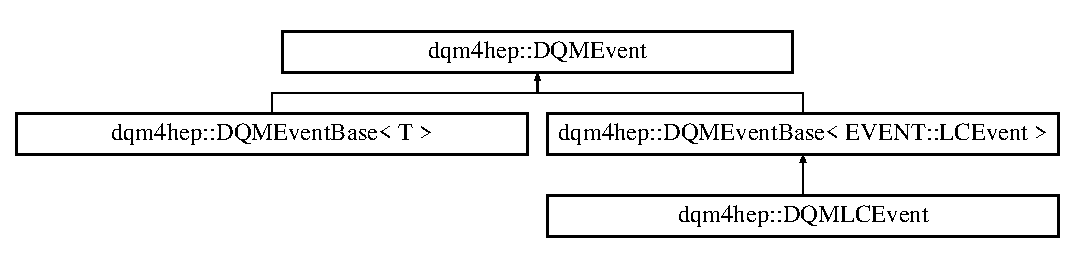
\includegraphics[height=2.947368cm]{classdqm4hep_1_1DQMEvent}
\end{center}
\end{figure}
\subsection*{Public Member Functions}
\begin{DoxyCompactItemize}
\item 
virtual {\bf $\sim$\+D\+Q\+M\+Event} ()
\begin{DoxyCompactList}\small\item\em Destructor. \end{DoxyCompactList}\item 
{\footnotesize template$<$typename T $>$ }\\T $\ast$ {\bf get\+Event} () const 
\begin{DoxyCompactList}\small\item\em Returns the event converted to asked type. \end{DoxyCompactList}\item 
{\footnotesize template$<$typename T $>$ }\\void {\bf set\+Event} (T $\ast$p\+Event, bool {\bf is\+Owner}=true)
\begin{DoxyCompactList}\small\item\em Set the event. \end{DoxyCompactList}\item 
{\footnotesize template$<$typename T $>$ }\\void {\bf clear} ()
\begin{DoxyCompactList}\small\item\em Clear the event (normally delete the event structure) \end{DoxyCompactList}\item 
bool {\bf is\+Owner} () const 
\begin{DoxyCompactList}\small\item\em Whether the dqm event is the owner of the wrapped event. \end{DoxyCompactList}\end{DoxyCompactItemize}
\subsection*{Protected Member Functions}
\begin{DoxyCompactItemize}
\item 
{\bf D\+Q\+M\+Event} ()
\begin{DoxyCompactList}\small\item\em Private constructor. \end{DoxyCompactList}\end{DoxyCompactItemize}
\subsection*{Protected Attributes}
\begin{DoxyCompactItemize}
\item 
bool {\bf m\+\_\+is\+Owner}
\end{DoxyCompactItemize}


\subsection{Detailed Description}
\doxyref{D\+Q\+M\+Event}{p.}{classdqm4hep_1_1DQMEvent} class. 

Main interface to a monitored event through the framework. This class is passed to modules in order to monitor its contents. The real data structure can be accessed via the get\+Event methods which convert the interface into a \doxyref{D\+Q\+M\+Event\+Base}{p.}{singletondqm4hep_1_1DQMEventBase} (see below).

To define an event, the user should always inherits the \doxyref{D\+Q\+M\+Event\+Base}{p.}{singletondqm4hep_1_1DQMEventBase} class in order to have valid operations. 

Definition at line 51 of file D\+Q\+M\+Event.\+h.



\subsection{Constructor \& Destructor Documentation}
\index{dqm4hep\+::\+D\+Q\+M\+Event@{dqm4hep\+::\+D\+Q\+M\+Event}!````~D\+Q\+M\+Event@{$\sim$\+D\+Q\+M\+Event}}
\index{````~D\+Q\+M\+Event@{$\sim$\+D\+Q\+M\+Event}!dqm4hep\+::\+D\+Q\+M\+Event@{dqm4hep\+::\+D\+Q\+M\+Event}}
\subsubsection[{$\sim$\+D\+Q\+M\+Event}]{\setlength{\rightskip}{0pt plus 5cm}dqm4hep\+::\+D\+Q\+M\+Event\+::$\sim$\+D\+Q\+M\+Event (
\begin{DoxyParamCaption}
{}
\end{DoxyParamCaption}
)\hspace{0.3cm}{\ttfamily [inline]}, {\ttfamily [virtual]}}\label{classdqm4hep_1_1DQMEvent_a575c5d7cc907c301b12236ac1927c0b2}


Destructor. 



Definition at line 122 of file D\+Q\+M\+Event.\+h.


\begin{DoxyCode}
123 \{
124 \}
\end{DoxyCode}
\index{dqm4hep\+::\+D\+Q\+M\+Event@{dqm4hep\+::\+D\+Q\+M\+Event}!D\+Q\+M\+Event@{D\+Q\+M\+Event}}
\index{D\+Q\+M\+Event@{D\+Q\+M\+Event}!dqm4hep\+::\+D\+Q\+M\+Event@{dqm4hep\+::\+D\+Q\+M\+Event}}
\subsubsection[{D\+Q\+M\+Event}]{\setlength{\rightskip}{0pt plus 5cm}dqm4hep\+::\+D\+Q\+M\+Event\+::\+D\+Q\+M\+Event (
\begin{DoxyParamCaption}
{}
\end{DoxyParamCaption}
)\hspace{0.3cm}{\ttfamily [inline]}, {\ttfamily [protected]}}\label{classdqm4hep_1_1DQMEvent_a1e91cdbbdee8172bcc9d07d1308d522d}


Private constructor. 



Definition at line 115 of file D\+Q\+M\+Event.\+h.


\begin{DoxyCode}
115                           :
116     m_isOwner(\textcolor{keyword}{true})
117 \{
118 \}
\end{DoxyCode}


\subsection{Member Function Documentation}
\index{dqm4hep\+::\+D\+Q\+M\+Event@{dqm4hep\+::\+D\+Q\+M\+Event}!clear@{clear}}
\index{clear@{clear}!dqm4hep\+::\+D\+Q\+M\+Event@{dqm4hep\+::\+D\+Q\+M\+Event}}
\subsubsection[{clear}]{\setlength{\rightskip}{0pt plus 5cm}template$<$typename T $>$ void dqm4hep\+::\+D\+Q\+M\+Event\+::clear (
\begin{DoxyParamCaption}
{}
\end{DoxyParamCaption}
)\hspace{0.3cm}{\ttfamily [inline]}}\label{classdqm4hep_1_1DQMEvent_af2c9017b9953c2b11114003ddb706f56}


Clear the event (normally delete the event structure) 



Definition at line 156 of file D\+Q\+M\+Event.\+h.



References dqm4hep\+::\+D\+Q\+M\+Event\+Base$<$ T $>$\+::clear(), and m\+\_\+is\+Owner.


\begin{DoxyCode}
157 \{
158   \textcolor{keywordflow}{if}(m_isOwner)
159   \{
160     DQMEventBase<T> *pBaseEvent = \textcolor{keyword}{dynamic\_cast<}DQMEventBase<T>*\textcolor{keyword}{>}(\textcolor{keyword}{this});
161 
162     \textcolor{keywordflow}{if}(NULL == pBaseEvent)
163       \textcolor{keywordflow}{return};
164 
165     pBaseEvent->clear();
166   \}
167 \}
\end{DoxyCode}
\index{dqm4hep\+::\+D\+Q\+M\+Event@{dqm4hep\+::\+D\+Q\+M\+Event}!get\+Event@{get\+Event}}
\index{get\+Event@{get\+Event}!dqm4hep\+::\+D\+Q\+M\+Event@{dqm4hep\+::\+D\+Q\+M\+Event}}
\subsubsection[{get\+Event}]{\setlength{\rightskip}{0pt plus 5cm}template$<$typename T $>$ T $\ast$ dqm4hep\+::\+D\+Q\+M\+Event\+::get\+Event (
\begin{DoxyParamCaption}
{}
\end{DoxyParamCaption}
) const\hspace{0.3cm}{\ttfamily [inline]}}\label{classdqm4hep_1_1DQMEvent_ada841cbe41f65f2baf6e2ebc4501565b}


Returns the event converted to asked type. 



Definition at line 129 of file D\+Q\+M\+Event.\+h.



References dqm4hep\+::\+D\+Q\+M\+Event\+Base$<$ T $>$\+::get\+Event().



Referenced by dqm4hep\+::\+D\+Q\+M\+L\+C\+Event\+Streamer\+::serialize().


\begin{DoxyCode}
130 \{
131   \textcolor{keyword}{const} DQMEventBase<T> *pBaseEvent = \textcolor{keyword}{dynamic\_cast<}\textcolor{keyword}{const }DQMEventBase<T>*\textcolor{keyword}{>}(\textcolor{keyword}{this});
132 
133   \textcolor{keywordflow}{if}(NULL == pBaseEvent)
134     \textcolor{keywordflow}{return} 0;
135 
136   \textcolor{keywordflow}{return} pBaseEvent->getEvent();
137 \}
\end{DoxyCode}
\index{dqm4hep\+::\+D\+Q\+M\+Event@{dqm4hep\+::\+D\+Q\+M\+Event}!is\+Owner@{is\+Owner}}
\index{is\+Owner@{is\+Owner}!dqm4hep\+::\+D\+Q\+M\+Event@{dqm4hep\+::\+D\+Q\+M\+Event}}
\subsubsection[{is\+Owner}]{\setlength{\rightskip}{0pt plus 5cm}bool dqm4hep\+::\+D\+Q\+M\+Event\+::is\+Owner (
\begin{DoxyParamCaption}
{}
\end{DoxyParamCaption}
) const\hspace{0.3cm}{\ttfamily [inline]}}\label{classdqm4hep_1_1DQMEvent_ad623d9befb698e59b9e8b9327335bf2b}


Whether the dqm event is the owner of the wrapped event. 



Definition at line 171 of file D\+Q\+M\+Event.\+h.



References m\+\_\+is\+Owner.



Referenced by dqm4hep\+::\+D\+Q\+M\+L\+C\+Event\+::clear(), and set\+Event().


\begin{DoxyCode}
172 \{
173   \textcolor{keywordflow}{return} m_isOwner;
174 \}
\end{DoxyCode}
\index{dqm4hep\+::\+D\+Q\+M\+Event@{dqm4hep\+::\+D\+Q\+M\+Event}!set\+Event@{set\+Event}}
\index{set\+Event@{set\+Event}!dqm4hep\+::\+D\+Q\+M\+Event@{dqm4hep\+::\+D\+Q\+M\+Event}}
\subsubsection[{set\+Event}]{\setlength{\rightskip}{0pt plus 5cm}template$<$typename T $>$ void dqm4hep\+::\+D\+Q\+M\+Event\+::set\+Event (
\begin{DoxyParamCaption}
\item[{T $\ast$}]{p\+Event, }
\item[{bool}]{is\+Owner = {\ttfamily true}}
\end{DoxyParamCaption}
)\hspace{0.3cm}{\ttfamily [inline]}}\label{classdqm4hep_1_1DQMEvent_ac590d787912a2b34cdb15259ea594aad}


Set the event. 

The dqm event can own the wrapped event is the second arguement is set to true 

Definition at line 142 of file D\+Q\+M\+Event.\+h.



References is\+Owner(), m\+\_\+is\+Owner, and dqm4hep\+::\+D\+Q\+M\+Event\+Base$<$ T $>$\+::set\+Event().



Referenced by dqm4hep\+::\+D\+Q\+M\+L\+C\+Event\+Streamer\+::deserialize(), and dqm4hep\+::\+D\+Q\+M\+Lcio\+Reader\+Listener\+::process\+Event().


\begin{DoxyCode}
143 \{
144   DQMEventBase<T> *pBaseEvent = \textcolor{keyword}{dynamic\_cast<}DQMEventBase<T>*\textcolor{keyword}{>}(\textcolor{keyword}{this});
145 
146   \textcolor{keywordflow}{if}(NULL == pBaseEvent)
147     \textcolor{keywordflow}{return};
148 
149   pBaseEvent->setEvent(pEvent);
150   m_isOwner = isOwner;
151 \}
\end{DoxyCode}


\subsection{Member Data Documentation}
\index{dqm4hep\+::\+D\+Q\+M\+Event@{dqm4hep\+::\+D\+Q\+M\+Event}!m\+\_\+is\+Owner@{m\+\_\+is\+Owner}}
\index{m\+\_\+is\+Owner@{m\+\_\+is\+Owner}!dqm4hep\+::\+D\+Q\+M\+Event@{dqm4hep\+::\+D\+Q\+M\+Event}}
\subsubsection[{m\+\_\+is\+Owner}]{\setlength{\rightskip}{0pt plus 5cm}bool dqm4hep\+::\+D\+Q\+M\+Event\+::m\+\_\+is\+Owner\hspace{0.3cm}{\ttfamily [protected]}}\label{classdqm4hep_1_1DQMEvent_aa1b71739e26c5c96b794c18480eb7230}


Definition at line 85 of file D\+Q\+M\+Event.\+h.



Referenced by clear(), is\+Owner(), and set\+Event().



The documentation for this class was generated from the following file\+:\begin{DoxyCompactItemize}
\item 
{\bf D\+Q\+M\+Event.\+h}\end{DoxyCompactItemize}

\section{dqm4hep\+:\+:D\+Q\+M\+Event\+Base$<$ T $>$ Class Template Reference}
\label{singletondqm4hep_1_1DQMEventBase}\index{dqm4hep\+::\+D\+Q\+M\+Event\+Base$<$ T $>$@{dqm4hep\+::\+D\+Q\+M\+Event\+Base$<$ T $>$}}


{\ttfamily \#include $<$D\+Q\+M\+Event.\+h$>$}

Inheritance diagram for dqm4hep\+:\+:D\+Q\+M\+Event\+Base$<$ T $>$\+:\begin{figure}[H]
\begin{center}
\leavevmode
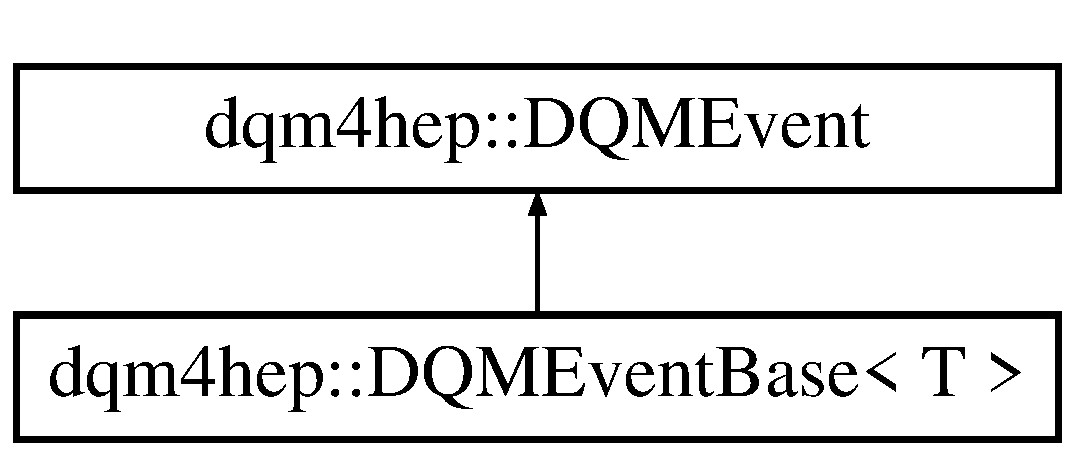
\includegraphics[height=2.000000cm]{singletondqm4hep_1_1DQMEventBase}
\end{center}
\end{figure}
\subsection*{Public Member Functions}
\begin{DoxyCompactItemize}
\item 
virtual {\bf $\sim$\+D\+Q\+M\+Event\+Base} ()
\begin{DoxyCompactList}\small\item\em Destructor. \end{DoxyCompactList}\item 
virtual T $\ast$ {\bf get\+Event} () const =0
\begin{DoxyCompactList}\small\item\em Returns the stored event. \end{DoxyCompactList}\item 
virtual void {\bf set\+Event} (T $\ast$p\+Event)=0
\begin{DoxyCompactList}\small\item\em Set the handled event. \end{DoxyCompactList}\item 
virtual void {\bf clear} ()=0
\begin{DoxyCompactList}\small\item\em Clear the handler by deleting the handled event. \end{DoxyCompactList}\end{DoxyCompactItemize}
\subsection*{Additional Inherited Members}


\subsection{Detailed Description}
\subsubsection*{template$<$typename T$>$class dqm4hep\+::\+D\+Q\+M\+Event\+Base$<$ T $>$}



Definition at line 39 of file D\+Q\+M\+Event.\+h.



\subsection{Constructor \& Destructor Documentation}
\index{dqm4hep\+::\+D\+Q\+M\+Event\+Base@{dqm4hep\+::\+D\+Q\+M\+Event\+Base}!````~D\+Q\+M\+Event\+Base@{$\sim$\+D\+Q\+M\+Event\+Base}}
\index{````~D\+Q\+M\+Event\+Base@{$\sim$\+D\+Q\+M\+Event\+Base}!dqm4hep\+::\+D\+Q\+M\+Event\+Base@{dqm4hep\+::\+D\+Q\+M\+Event\+Base}}
\subsubsection[{$\sim$\+D\+Q\+M\+Event\+Base}]{\setlength{\rightskip}{0pt plus 5cm}template$<$typename T $>$ {\bf dqm4hep\+::\+D\+Q\+M\+Event\+Base}$<$ T $>$\+::$\sim${\bf D\+Q\+M\+Event\+Base} (
\begin{DoxyParamCaption}
{}
\end{DoxyParamCaption}
)\hspace{0.3cm}{\ttfamily [inline]}, {\ttfamily [virtual]}}\label{singletondqm4hep_1_1DQMEventBase_aa778e7eb791f8b24138cf8ed57a7d421}


Destructor. 



Definition at line 180 of file D\+Q\+M\+Event.\+h.


\begin{DoxyCode}
181 \{
182 \}
\end{DoxyCode}


\subsection{Member Function Documentation}
\index{dqm4hep\+::\+D\+Q\+M\+Event\+Base@{dqm4hep\+::\+D\+Q\+M\+Event\+Base}!clear@{clear}}
\index{clear@{clear}!dqm4hep\+::\+D\+Q\+M\+Event\+Base@{dqm4hep\+::\+D\+Q\+M\+Event\+Base}}
\subsubsection[{clear}]{\setlength{\rightskip}{0pt plus 5cm}template$<$typename T$>$ virtual void {\bf dqm4hep\+::\+D\+Q\+M\+Event\+Base}$<$ T $>$\+::clear (
\begin{DoxyParamCaption}
{}
\end{DoxyParamCaption}
)\hspace{0.3cm}{\ttfamily [pure virtual]}}\label{singletondqm4hep_1_1DQMEventBase_afe7236fd5fe7e2fa719a1464e2195636}


Clear the handler by deleting the handled event. 



Implemented in {\bf dqm4hep\+::\+D\+Q\+M\+L\+C\+Event} \doxyref{}{p.}{classdqm4hep_1_1DQMLCEvent_a47b8653da5ab6d64277b756f553758bd}.



Referenced by dqm4hep\+::\+D\+Q\+M\+Event\+::clear().

\index{dqm4hep\+::\+D\+Q\+M\+Event\+Base@{dqm4hep\+::\+D\+Q\+M\+Event\+Base}!get\+Event@{get\+Event}}
\index{get\+Event@{get\+Event}!dqm4hep\+::\+D\+Q\+M\+Event\+Base@{dqm4hep\+::\+D\+Q\+M\+Event\+Base}}
\subsubsection[{get\+Event}]{\setlength{\rightskip}{0pt plus 5cm}template$<$typename T$>$ virtual T$\ast$ {\bf dqm4hep\+::\+D\+Q\+M\+Event\+Base}$<$ T $>$\+::get\+Event (
\begin{DoxyParamCaption}
{}
\end{DoxyParamCaption}
) const\hspace{0.3cm}{\ttfamily [pure virtual]}}\label{singletondqm4hep_1_1DQMEventBase_a2363bc09cadffa4806098fc9f031543f}


Returns the stored event. 



Implemented in {\bf dqm4hep\+::\+D\+Q\+M\+L\+C\+Event} \doxyref{}{p.}{classdqm4hep_1_1DQMLCEvent_a3e2a3489740b65b9359decc4766fcee7}.



Referenced by dqm4hep\+::\+D\+Q\+M\+Event\+::get\+Event().

\index{dqm4hep\+::\+D\+Q\+M\+Event\+Base@{dqm4hep\+::\+D\+Q\+M\+Event\+Base}!set\+Event@{set\+Event}}
\index{set\+Event@{set\+Event}!dqm4hep\+::\+D\+Q\+M\+Event\+Base@{dqm4hep\+::\+D\+Q\+M\+Event\+Base}}
\subsubsection[{set\+Event}]{\setlength{\rightskip}{0pt plus 5cm}template$<$typename T$>$ virtual void {\bf dqm4hep\+::\+D\+Q\+M\+Event\+Base}$<$ T $>$\+::set\+Event (
\begin{DoxyParamCaption}
\item[{T $\ast$}]{p\+Event}
\end{DoxyParamCaption}
)\hspace{0.3cm}{\ttfamily [pure virtual]}}\label{singletondqm4hep_1_1DQMEventBase_afe393ecc545e9eb6dead7309c119f436}


Set the handled event. 



Implemented in {\bf dqm4hep\+::\+D\+Q\+M\+L\+C\+Event} \doxyref{}{p.}{classdqm4hep_1_1DQMLCEvent_a9085e7483f683553be7d0b8bde36c260}.



Referenced by dqm4hep\+::\+D\+Q\+M\+Event\+::set\+Event().



The documentation for this class was generated from the following file\+:\begin{DoxyCompactItemize}
\item 
{\bf D\+Q\+M\+Event.\+h}\end{DoxyCompactItemize}

\section{dqm4hep\+:\+:D\+Q\+M\+Event\+Client Class Reference}
\label{classdqm4hep_1_1DQMEventClient}\index{dqm4hep\+::\+D\+Q\+M\+Event\+Client@{dqm4hep\+::\+D\+Q\+M\+Event\+Client}}


\doxyref{D\+Q\+M\+Event\+Client}{p.}{classdqm4hep_1_1DQMEventClient} class.  




{\ttfamily \#include $<$D\+Q\+M\+Event\+Client.\+h$>$}

Inheritance diagram for dqm4hep\+:\+:D\+Q\+M\+Event\+Client\+:\begin{figure}[H]
\begin{center}
\leavevmode
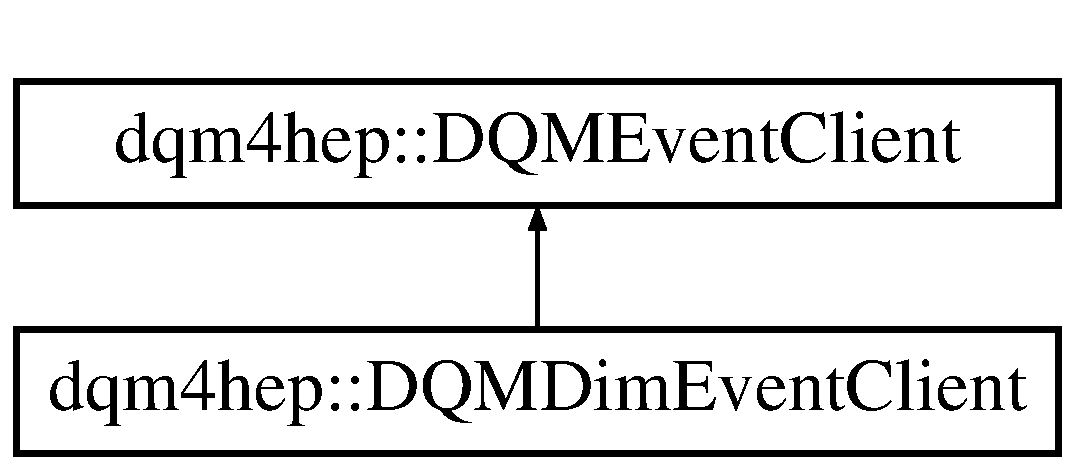
\includegraphics[height=2.000000cm]{classdqm4hep_1_1DQMEventClient}
\end{center}
\end{figure}
\subsection*{Public Member Functions}
\begin{DoxyCompactItemize}
\item 
{\bf D\+Q\+M\+Event\+Client} ()
\begin{DoxyCompactList}\small\item\em Constructor. \end{DoxyCompactList}\item 
virtual {\bf $\sim$\+D\+Q\+M\+Event\+Client} ()
\begin{DoxyCompactList}\small\item\em Destructor. \end{DoxyCompactList}\item 
virtual void {\bf set\+Collector\+Name} (const std\+::string \&collector\+Name)
\begin{DoxyCompactList}\small\item\em Set the collector to connect to. \end{DoxyCompactList}\item 
const std\+::string \& {\bf get\+Collector\+Name} () const 
\begin{DoxyCompactList}\small\item\em Get the collector name. \end{DoxyCompactList}\item 
virtual void {\bf set\+Event\+Streamer} ({\bf D\+Q\+M\+Event\+Streamer} $\ast$p\+Event\+Streamer, bool owner=true)
\begin{DoxyCompactList}\small\item\em Set the streamer that will stream in/out the sent/received event(s). \end{DoxyCompactList}\item 
{\bf D\+Q\+M\+Event\+Streamer} $\ast$ {\bf get\+Event\+Streamer} () const 
\begin{DoxyCompactList}\small\item\em Get the event streamer. \end{DoxyCompactList}\item 
virtual void {\bf set\+Maximum\+Queue\+Size} (unsigned int queue\+Size)
\begin{DoxyCompactList}\small\item\em Set the queue size that stores the received events. \end{DoxyCompactList}\item 
virtual unsigned int {\bf get\+Maximum\+Queue\+Size} () const 
\begin{DoxyCompactList}\small\item\em Get the maximum number of events that the client can store in its event queue. \end{DoxyCompactList}\item 
virtual void {\bf clear\+Queue} ()
\begin{DoxyCompactList}\small\item\em Clear the event queue. \end{DoxyCompactList}\item 
virtual void {\bf set\+Sub\+Event\+Identifier} (const std\+::string \&identifier)
\begin{DoxyCompactList}\small\item\em Set the sub event identifier. \end{DoxyCompactList}\item 
const std\+::string \& {\bf get\+Sub\+Event\+Identifier} () const 
\begin{DoxyCompactList}\small\item\em Get the sub event identifier. \end{DoxyCompactList}\item 
void {\bf take\+Event} ({\bf D\+Q\+M\+Event} $\ast$\&p\+Event)
\begin{DoxyCompactList}\small\item\em Take an event from the event queue (pop front) and return the pointer to the caller. \end{DoxyCompactList}\item 
void {\bf add\+Listener} ({\bf D\+Q\+M\+Event\+Client\+Listener} $\ast$p\+Listener)
\begin{DoxyCompactList}\small\item\em Add a listener to this event client. \end{DoxyCompactList}\item 
void {\bf remove\+Listener} ({\bf D\+Q\+M\+Event\+Client\+Listener} $\ast$p\+Listener)
\begin{DoxyCompactList}\small\item\em Remove a listener from this event client. \end{DoxyCompactList}\item 
{\bf Status\+Code} {\bf connect\+To\+Service} ()
\begin{DoxyCompactList}\small\item\em Connect to the collector service (server) \end{DoxyCompactList}\item 
{\bf Status\+Code} {\bf disconnect\+From\+Service} ()
\begin{DoxyCompactList}\small\item\em Disconnect the client from the collector (server) \end{DoxyCompactList}\item 
virtual bool {\bf is\+Connected\+To\+Service} () const =0
\begin{DoxyCompactList}\small\item\em Whether the client is connected to the collector (server) \end{DoxyCompactList}\item 
virtual {\bf Status\+Code} {\bf send\+Event} (const {\bf D\+Q\+M\+Event} $\ast$const p\+Event)=0
\begin{DoxyCompactList}\small\item\em Send an event to the collector (server). \end{DoxyCompactList}\item 
virtual {\bf Status\+Code} {\bf query\+Event} ({\bf D\+Q\+M\+Event} $\ast$\&p\+Event, int timeout)=0
\begin{DoxyCompactList}\small\item\em Query an event to the collector (server) with a timeout and handle it without pushing it into the internal queue. \end{DoxyCompactList}\item 
virtual {\bf Status\+Code} {\bf query\+Event} ()=0
\begin{DoxyCompactList}\small\item\em Query an event to the collector. \end{DoxyCompactList}\item 
virtual void {\bf set\+Update\+Mode} (bool update\+Mode)=0
\begin{DoxyCompactList}\small\item\em Set the update mode. \end{DoxyCompactList}\item 
virtual bool {\bf get\+Update\+Mode} () const =0
\begin{DoxyCompactList}\small\item\em Whether the update mode is set. \end{DoxyCompactList}\item 
virtual {\bf Status\+Code} {\bf read\+Settings} (const {\bf Ti\+Xml\+Handle} \&xml\+Handle)=0
\begin{DoxyCompactList}\small\item\em Read settings from the xml handle. \end{DoxyCompactList}\end{DoxyCompactItemize}
\subsection*{Protected Member Functions}
\begin{DoxyCompactItemize}
\item 
virtual {\bf Status\+Code} {\bf perform\+Service\+Connection} ()=0
\begin{DoxyCompactList}\small\item\em Workhorse of the service connection. \end{DoxyCompactList}\item 
virtual {\bf Status\+Code} {\bf perform\+Service\+Disconnection} ()=0
\begin{DoxyCompactList}\small\item\em Workhorse of the service connection. \end{DoxyCompactList}\item 
void {\bf push\+Event} ({\bf D\+Q\+M\+Event} $\ast$p\+Event)
\begin{DoxyCompactList}\small\item\em Push a new event in the event queue. \end{DoxyCompactList}\end{DoxyCompactItemize}
\subsection*{Private Attributes}
\begin{DoxyCompactItemize}
\item 
bool {\bf m\+\_\+event\+Streamer\+Owner}
\item 
{\bf D\+Q\+M\+Event\+Streamer} $\ast$ {\bf m\+\_\+p\+Event\+Streamer}
\item 
std\+::string {\bf m\+\_\+collector\+Name}
\item 
std\+::string {\bf m\+\_\+sub\+Event\+Identifier}
\item 
{\bf D\+Q\+M\+Event\+Queue} {\bf m\+\_\+event\+Queue}
\item 
unsigned int {\bf m\+\_\+maximum\+Queue\+Size}
\item 
std\+::set\\*
$<$ {\bf D\+Q\+M\+Event\+Client\+Listener} $\ast$ $>$ {\bf m\+\_\+listeners}
\item 
pthread\+\_\+mutex\+\_\+t {\bf m\+\_\+mutex}
\end{DoxyCompactItemize}


\subsection{Detailed Description}
\doxyref{D\+Q\+M\+Event\+Client}{p.}{classdqm4hep_1_1DQMEventClient} class. 

Main interface for sending events to a collector (server part) and for event queries.

Note that pushing/taking events in the event queue is thread-\/safe. 

Definition at line 80 of file D\+Q\+M\+Event\+Client.\+h.



\subsection{Constructor \& Destructor Documentation}
\index{dqm4hep\+::\+D\+Q\+M\+Event\+Client@{dqm4hep\+::\+D\+Q\+M\+Event\+Client}!D\+Q\+M\+Event\+Client@{D\+Q\+M\+Event\+Client}}
\index{D\+Q\+M\+Event\+Client@{D\+Q\+M\+Event\+Client}!dqm4hep\+::\+D\+Q\+M\+Event\+Client@{dqm4hep\+::\+D\+Q\+M\+Event\+Client}}
\subsubsection[{D\+Q\+M\+Event\+Client}]{\setlength{\rightskip}{0pt plus 5cm}dqm4hep\+::\+D\+Q\+M\+Event\+Client\+::\+D\+Q\+M\+Event\+Client (
\begin{DoxyParamCaption}
{}
\end{DoxyParamCaption}
)}\label{classdqm4hep_1_1DQMEventClient_ad0282690a4ab8dc26784ebaefdd16ea3}


Constructor. 



Definition at line 36 of file D\+Q\+M\+Event\+Client.\+cc.



References m\+\_\+mutex.


\begin{DoxyCode}
36                                :
37     m_pEventStreamer(NULL),
38     m_maximumQueueSize(100),
39     m_eventStreamerOwner(\textcolor{keyword}{true})
40 \{
41   pthread\_mutex\_init(&m_mutex, NULL);
42 \}
\end{DoxyCode}
\index{dqm4hep\+::\+D\+Q\+M\+Event\+Client@{dqm4hep\+::\+D\+Q\+M\+Event\+Client}!````~D\+Q\+M\+Event\+Client@{$\sim$\+D\+Q\+M\+Event\+Client}}
\index{````~D\+Q\+M\+Event\+Client@{$\sim$\+D\+Q\+M\+Event\+Client}!dqm4hep\+::\+D\+Q\+M\+Event\+Client@{dqm4hep\+::\+D\+Q\+M\+Event\+Client}}
\subsubsection[{$\sim$\+D\+Q\+M\+Event\+Client}]{\setlength{\rightskip}{0pt plus 5cm}dqm4hep\+::\+D\+Q\+M\+Event\+Client\+::$\sim$\+D\+Q\+M\+Event\+Client (
\begin{DoxyParamCaption}
{}
\end{DoxyParamCaption}
)\hspace{0.3cm}{\ttfamily [virtual]}}\label{classdqm4hep_1_1DQMEventClient_a0c5bda759a3912ca99748974e108e00d}


Destructor. 



Definition at line 46 of file D\+Q\+M\+Event\+Client.\+cc.



References clear\+Queue(), m\+\_\+event\+Streamer\+Owner, m\+\_\+mutex, and m\+\_\+p\+Event\+Streamer.


\begin{DoxyCode}
47 \{
48   this->clearQueue();
49 
50   \textcolor{keywordflow}{if}( m_eventStreamerOwner && NULL != m_pEventStreamer )
51     \textcolor{keyword}{delete} m_pEventStreamer;
52 
53   pthread\_mutex\_destroy(&m_mutex);
54 \}
\end{DoxyCode}


\subsection{Member Function Documentation}
\index{dqm4hep\+::\+D\+Q\+M\+Event\+Client@{dqm4hep\+::\+D\+Q\+M\+Event\+Client}!add\+Listener@{add\+Listener}}
\index{add\+Listener@{add\+Listener}!dqm4hep\+::\+D\+Q\+M\+Event\+Client@{dqm4hep\+::\+D\+Q\+M\+Event\+Client}}
\subsubsection[{add\+Listener}]{\setlength{\rightskip}{0pt plus 5cm}void dqm4hep\+::\+D\+Q\+M\+Event\+Client\+::add\+Listener (
\begin{DoxyParamCaption}
\item[{{\bf D\+Q\+M\+Event\+Client\+Listener} $\ast$}]{p\+Listener}
\end{DoxyParamCaption}
)}\label{classdqm4hep_1_1DQMEventClient_aa6aac26ee1286d2adfbe5879f6c3215d}


Add a listener to this event client. 



Definition at line 160 of file D\+Q\+M\+Event\+Client.\+cc.



References m\+\_\+listeners, and m\+\_\+mutex.


\begin{DoxyCode}
161 \{
162   scoped\_lock( & this->m_mutex);
163 
164   \textcolor{keywordflow}{if}(NULL == pListener)
165     \textcolor{keywordflow}{return};
166 
167   m_listeners.insert(pListener);
168 \}
\end{DoxyCode}
\index{dqm4hep\+::\+D\+Q\+M\+Event\+Client@{dqm4hep\+::\+D\+Q\+M\+Event\+Client}!clear\+Queue@{clear\+Queue}}
\index{clear\+Queue@{clear\+Queue}!dqm4hep\+::\+D\+Q\+M\+Event\+Client@{dqm4hep\+::\+D\+Q\+M\+Event\+Client}}
\subsubsection[{clear\+Queue}]{\setlength{\rightskip}{0pt plus 5cm}void dqm4hep\+::\+D\+Q\+M\+Event\+Client\+::clear\+Queue (
\begin{DoxyParamCaption}
{}
\end{DoxyParamCaption}
)\hspace{0.3cm}{\ttfamily [virtual]}}\label{classdqm4hep_1_1DQMEventClient_a57e2b09e0035463be5772d5681e13b42}


Clear the event queue. 



Definition at line 120 of file D\+Q\+M\+Event\+Client.\+cc.



References m\+\_\+event\+Queue, and m\+\_\+mutex.



Referenced by dqm4hep\+::\+D\+Q\+M\+Analysis\+Module\+Application\+::run(), and $\sim$\+D\+Q\+M\+Event\+Client().


\begin{DoxyCode}
121 \{
122   scoped\_lock( & this->m_mutex);
123 
124   \textcolor{keywordflow}{while}( ! m_eventQueue.empty() )
125   \{
126     \textcolor{keyword}{delete} m_eventQueue.front();
127     m_eventQueue.pop();
128   \}
129 \}
\end{DoxyCode}
\index{dqm4hep\+::\+D\+Q\+M\+Event\+Client@{dqm4hep\+::\+D\+Q\+M\+Event\+Client}!connect\+To\+Service@{connect\+To\+Service}}
\index{connect\+To\+Service@{connect\+To\+Service}!dqm4hep\+::\+D\+Q\+M\+Event\+Client@{dqm4hep\+::\+D\+Q\+M\+Event\+Client}}
\subsubsection[{connect\+To\+Service}]{\setlength{\rightskip}{0pt plus 5cm}{\bf Status\+Code} dqm4hep\+::\+D\+Q\+M\+Event\+Client\+::connect\+To\+Service (
\begin{DoxyParamCaption}
{}
\end{DoxyParamCaption}
)}\label{classdqm4hep_1_1DQMEventClient_a535302ffc201aff823c210d9a834937c}


Connect to the collector service (server) 



Definition at line 209 of file D\+Q\+M\+Event\+Client.\+cc.



References m\+\_\+listeners, perform\+Service\+Connection(), and R\+E\+T\+U\+R\+N\+\_\+\+R\+E\+S\+U\+L\+T\+\_\+\+I\+F.



Referenced by dqm4hep\+::\+D\+Q\+M\+Dim\+Event\+Client\+::read\+Settings(), dqm4hep\+::\+D\+Q\+M\+Analysis\+Module\+Application\+::start\+Services(), and dqm4hep\+::\+D\+Q\+M\+Analysis\+Module\+Application\+::stop\+Services().


\begin{DoxyCode}
210 \{
211   RETURN_RESULT_IF(STATUS\_CODE\_SUCCESS, !=, this->performServiceConnection());
212 
213   \textcolor{keywordflow}{for}(std::set<DQMEventClientListener*>::iterator iter = m_listeners.begin(), endIter = 
      m_listeners.end() ;
214       endIter != iter ; ++iter)
215     (*iter)->onEventClientConnnect(\textcolor{keyword}{this});
216 
217   \textcolor{keywordflow}{return} STATUS\_CODE\_SUCCESS;
218 \}
\end{DoxyCode}
\index{dqm4hep\+::\+D\+Q\+M\+Event\+Client@{dqm4hep\+::\+D\+Q\+M\+Event\+Client}!disconnect\+From\+Service@{disconnect\+From\+Service}}
\index{disconnect\+From\+Service@{disconnect\+From\+Service}!dqm4hep\+::\+D\+Q\+M\+Event\+Client@{dqm4hep\+::\+D\+Q\+M\+Event\+Client}}
\subsubsection[{disconnect\+From\+Service}]{\setlength{\rightskip}{0pt plus 5cm}{\bf Status\+Code} dqm4hep\+::\+D\+Q\+M\+Event\+Client\+::disconnect\+From\+Service (
\begin{DoxyParamCaption}
{}
\end{DoxyParamCaption}
)}\label{classdqm4hep_1_1DQMEventClient_a469dc13739fc07759a50d258990179b1}


Disconnect the client from the collector (server) 



Definition at line 222 of file D\+Q\+M\+Event\+Client.\+cc.



References m\+\_\+listeners, perform\+Service\+Disconnection(), and R\+E\+T\+U\+R\+N\+\_\+\+R\+E\+S\+U\+L\+T\+\_\+\+I\+F.



Referenced by dqm4hep\+::\+D\+Q\+M\+Dim\+Event\+Client\+::read\+Settings(), and dqm4hep\+::\+D\+Q\+M\+Dim\+Event\+Client\+::$\sim$\+D\+Q\+M\+Dim\+Event\+Client().


\begin{DoxyCode}
223 \{
224   RETURN_RESULT_IF(STATUS\_CODE\_SUCCESS, !=, this->performServiceDisconnection());
225 
226   \textcolor{keywordflow}{for}(std::set<DQMEventClientListener*>::iterator iter = m_listeners.begin(), endIter = 
      m_listeners.end() ;
227       endIter != iter ; ++iter)
228     (*iter)->onEventClientDisconnnect(\textcolor{keyword}{this});
229 
230   \textcolor{keywordflow}{return} STATUS\_CODE\_SUCCESS;
231 \}
\end{DoxyCode}
\index{dqm4hep\+::\+D\+Q\+M\+Event\+Client@{dqm4hep\+::\+D\+Q\+M\+Event\+Client}!get\+Collector\+Name@{get\+Collector\+Name}}
\index{get\+Collector\+Name@{get\+Collector\+Name}!dqm4hep\+::\+D\+Q\+M\+Event\+Client@{dqm4hep\+::\+D\+Q\+M\+Event\+Client}}
\subsubsection[{get\+Collector\+Name}]{\setlength{\rightskip}{0pt plus 5cm}const std\+::string \& dqm4hep\+::\+D\+Q\+M\+Event\+Client\+::get\+Collector\+Name (
\begin{DoxyParamCaption}
{}
\end{DoxyParamCaption}
) const}\label{classdqm4hep_1_1DQMEventClient_a39d24fd0151e0c95318b7b1000fb7573}


Get the collector name. 



Definition at line 69 of file D\+Q\+M\+Event\+Client.\+cc.



References m\+\_\+collector\+Name.



Referenced by dqm4hep\+::\+D\+Q\+M\+Dim\+Event\+Client\+::info\+Handler(), dqm4hep\+::\+D\+Q\+M\+Dim\+Event\+Client\+::perform\+Service\+Connection(), dqm4hep\+::\+D\+Q\+M\+Dim\+Event\+Client\+::perform\+Service\+Disconnection(), dqm4hep\+::\+D\+Q\+M\+Dim\+Event\+Client\+::query\+Event(), dqm4hep\+::\+D\+Q\+M\+Dim\+Event\+Client\+::read\+Settings(), dqm4hep\+::\+D\+Q\+M\+Dim\+Event\+Client\+::send\+Event(), dqm4hep\+::\+D\+Q\+M\+Dim\+Event\+Client\+::set\+Sub\+Event\+Identifier(), and dqm4hep\+::\+D\+Q\+M\+Dim\+Event\+Client\+::set\+Update\+Mode().


\begin{DoxyCode}
70 \{
71   \textcolor{keywordflow}{return} m_collectorName;
72 \}
\end{DoxyCode}
\index{dqm4hep\+::\+D\+Q\+M\+Event\+Client@{dqm4hep\+::\+D\+Q\+M\+Event\+Client}!get\+Event\+Streamer@{get\+Event\+Streamer}}
\index{get\+Event\+Streamer@{get\+Event\+Streamer}!dqm4hep\+::\+D\+Q\+M\+Event\+Client@{dqm4hep\+::\+D\+Q\+M\+Event\+Client}}
\subsubsection[{get\+Event\+Streamer}]{\setlength{\rightskip}{0pt plus 5cm}{\bf D\+Q\+M\+Event\+Streamer} $\ast$ dqm4hep\+::\+D\+Q\+M\+Event\+Client\+::get\+Event\+Streamer (
\begin{DoxyParamCaption}
{}
\end{DoxyParamCaption}
) const}\label{classdqm4hep_1_1DQMEventClient_a2fce96936f18cc5db5ddade3bd826774}


Get the event streamer. 



Definition at line 87 of file D\+Q\+M\+Event\+Client.\+cc.



References m\+\_\+p\+Event\+Streamer.



Referenced by dqm4hep\+::\+D\+Q\+M\+Dim\+Event\+Client\+::event\+Reception(), dqm4hep\+::\+D\+Q\+M\+Dim\+Event\+Client\+::query\+Event(), and dqm4hep\+::\+D\+Q\+M\+Dim\+Event\+Client\+::send\+Event().


\begin{DoxyCode}
88 \{
89   \textcolor{keywordflow}{return} m_pEventStreamer;
90 \}
\end{DoxyCode}
\index{dqm4hep\+::\+D\+Q\+M\+Event\+Client@{dqm4hep\+::\+D\+Q\+M\+Event\+Client}!get\+Maximum\+Queue\+Size@{get\+Maximum\+Queue\+Size}}
\index{get\+Maximum\+Queue\+Size@{get\+Maximum\+Queue\+Size}!dqm4hep\+::\+D\+Q\+M\+Event\+Client@{dqm4hep\+::\+D\+Q\+M\+Event\+Client}}
\subsubsection[{get\+Maximum\+Queue\+Size}]{\setlength{\rightskip}{0pt plus 5cm}unsigned int dqm4hep\+::\+D\+Q\+M\+Event\+Client\+::get\+Maximum\+Queue\+Size (
\begin{DoxyParamCaption}
{}
\end{DoxyParamCaption}
) const\hspace{0.3cm}{\ttfamily [virtual]}}\label{classdqm4hep_1_1DQMEventClient_a36c326731a7e6a3d56a1d37bb334bafa}


Get the maximum number of events that the client can store in its event queue. 



Definition at line 113 of file D\+Q\+M\+Event\+Client.\+cc.



References m\+\_\+maximum\+Queue\+Size.



Referenced by dqm4hep\+::\+D\+Q\+M\+Dim\+Event\+Client\+::read\+Settings().


\begin{DoxyCode}
114 \{
115   \textcolor{keywordflow}{return} m_maximumQueueSize;
116 \}
\end{DoxyCode}
\index{dqm4hep\+::\+D\+Q\+M\+Event\+Client@{dqm4hep\+::\+D\+Q\+M\+Event\+Client}!get\+Sub\+Event\+Identifier@{get\+Sub\+Event\+Identifier}}
\index{get\+Sub\+Event\+Identifier@{get\+Sub\+Event\+Identifier}!dqm4hep\+::\+D\+Q\+M\+Event\+Client@{dqm4hep\+::\+D\+Q\+M\+Event\+Client}}
\subsubsection[{get\+Sub\+Event\+Identifier}]{\setlength{\rightskip}{0pt plus 5cm}const std\+::string \& dqm4hep\+::\+D\+Q\+M\+Event\+Client\+::get\+Sub\+Event\+Identifier (
\begin{DoxyParamCaption}
{}
\end{DoxyParamCaption}
) const}\label{classdqm4hep_1_1DQMEventClient_ad3143137f96dab6b91ce2a0c1e9f2d21}


Get the sub event identifier. 



Definition at line 140 of file D\+Q\+M\+Event\+Client.\+cc.



References m\+\_\+sub\+Event\+Identifier.



Referenced by dqm4hep\+::\+D\+Q\+M\+Dim\+Event\+Client\+::info\+Handler(), dqm4hep\+::\+D\+Q\+M\+Dim\+Event\+Client\+::query\+Event(), and dqm4hep\+::\+D\+Q\+M\+Dim\+Event\+Client\+::read\+Settings().


\begin{DoxyCode}
141 \{
142   \textcolor{keywordflow}{return} m_subEventIdentifier;
143 \}
\end{DoxyCode}
\index{dqm4hep\+::\+D\+Q\+M\+Event\+Client@{dqm4hep\+::\+D\+Q\+M\+Event\+Client}!get\+Update\+Mode@{get\+Update\+Mode}}
\index{get\+Update\+Mode@{get\+Update\+Mode}!dqm4hep\+::\+D\+Q\+M\+Event\+Client@{dqm4hep\+::\+D\+Q\+M\+Event\+Client}}
\subsubsection[{get\+Update\+Mode}]{\setlength{\rightskip}{0pt plus 5cm}virtual bool dqm4hep\+::\+D\+Q\+M\+Event\+Client\+::get\+Update\+Mode (
\begin{DoxyParamCaption}
{}
\end{DoxyParamCaption}
) const\hspace{0.3cm}{\ttfamily [pure virtual]}}\label{classdqm4hep_1_1DQMEventClient_aafe333631227e6aa3a66cfd19a8b79c2}


Whether the update mode is set. 



Implemented in {\bf dqm4hep\+::\+D\+Q\+M\+Dim\+Event\+Client} \doxyref{}{p.}{classdqm4hep_1_1DQMDimEventClient_a81a3b8cea6ac80fd86b4d4ed95d31dcb}.

\index{dqm4hep\+::\+D\+Q\+M\+Event\+Client@{dqm4hep\+::\+D\+Q\+M\+Event\+Client}!is\+Connected\+To\+Service@{is\+Connected\+To\+Service}}
\index{is\+Connected\+To\+Service@{is\+Connected\+To\+Service}!dqm4hep\+::\+D\+Q\+M\+Event\+Client@{dqm4hep\+::\+D\+Q\+M\+Event\+Client}}
\subsubsection[{is\+Connected\+To\+Service}]{\setlength{\rightskip}{0pt plus 5cm}virtual bool dqm4hep\+::\+D\+Q\+M\+Event\+Client\+::is\+Connected\+To\+Service (
\begin{DoxyParamCaption}
{}
\end{DoxyParamCaption}
) const\hspace{0.3cm}{\ttfamily [pure virtual]}}\label{classdqm4hep_1_1DQMEventClient_a2fd723aa31328fa1b97632e1e2ac31dc}


Whether the client is connected to the collector (server) 



Implemented in {\bf dqm4hep\+::\+D\+Q\+M\+Dim\+Event\+Client} \doxyref{}{p.}{classdqm4hep_1_1DQMDimEventClient_aa177def491c8eb9a10c2f2adfe0d9432}.



Referenced by set\+Collector\+Name(), and dqm4hep\+::\+D\+Q\+M\+Analysis\+Module\+Application\+::stop\+Services().

\index{dqm4hep\+::\+D\+Q\+M\+Event\+Client@{dqm4hep\+::\+D\+Q\+M\+Event\+Client}!perform\+Service\+Connection@{perform\+Service\+Connection}}
\index{perform\+Service\+Connection@{perform\+Service\+Connection}!dqm4hep\+::\+D\+Q\+M\+Event\+Client@{dqm4hep\+::\+D\+Q\+M\+Event\+Client}}
\subsubsection[{perform\+Service\+Connection}]{\setlength{\rightskip}{0pt plus 5cm}virtual {\bf Status\+Code} dqm4hep\+::\+D\+Q\+M\+Event\+Client\+::perform\+Service\+Connection (
\begin{DoxyParamCaption}
{}
\end{DoxyParamCaption}
)\hspace{0.3cm}{\ttfamily [protected]}, {\ttfamily [pure virtual]}}\label{classdqm4hep_1_1DQMEventClient_a5d69c657028c105556a4b5897ce0ed0b}


Workhorse of the service connection. 



Implemented in {\bf dqm4hep\+::\+D\+Q\+M\+Dim\+Event\+Client} \doxyref{}{p.}{classdqm4hep_1_1DQMDimEventClient_a50266fbdaed8b2728f9d6e373412fb07}.



Referenced by connect\+To\+Service().

\index{dqm4hep\+::\+D\+Q\+M\+Event\+Client@{dqm4hep\+::\+D\+Q\+M\+Event\+Client}!perform\+Service\+Disconnection@{perform\+Service\+Disconnection}}
\index{perform\+Service\+Disconnection@{perform\+Service\+Disconnection}!dqm4hep\+::\+D\+Q\+M\+Event\+Client@{dqm4hep\+::\+D\+Q\+M\+Event\+Client}}
\subsubsection[{perform\+Service\+Disconnection}]{\setlength{\rightskip}{0pt plus 5cm}virtual {\bf Status\+Code} dqm4hep\+::\+D\+Q\+M\+Event\+Client\+::perform\+Service\+Disconnection (
\begin{DoxyParamCaption}
{}
\end{DoxyParamCaption}
)\hspace{0.3cm}{\ttfamily [protected]}, {\ttfamily [pure virtual]}}\label{classdqm4hep_1_1DQMEventClient_aefc43840571a501d5bb7296afed49926}


Workhorse of the service connection. 



Implemented in {\bf dqm4hep\+::\+D\+Q\+M\+Dim\+Event\+Client} \doxyref{}{p.}{classdqm4hep_1_1DQMDimEventClient_a218c10d82a8d24f95b912d714018041b}.



Referenced by disconnect\+From\+Service().

\index{dqm4hep\+::\+D\+Q\+M\+Event\+Client@{dqm4hep\+::\+D\+Q\+M\+Event\+Client}!push\+Event@{push\+Event}}
\index{push\+Event@{push\+Event}!dqm4hep\+::\+D\+Q\+M\+Event\+Client@{dqm4hep\+::\+D\+Q\+M\+Event\+Client}}
\subsubsection[{push\+Event}]{\setlength{\rightskip}{0pt plus 5cm}void dqm4hep\+::\+D\+Q\+M\+Event\+Client\+::push\+Event (
\begin{DoxyParamCaption}
\item[{{\bf D\+Q\+M\+Event} $\ast$}]{p\+Event}
\end{DoxyParamCaption}
)\hspace{0.3cm}{\ttfamily [protected]}}\label{classdqm4hep_1_1DQMEventClient_abe629415c01a7a00b0679f9d88d2da20}


Push a new event in the event queue. 

If the event queue has reaches its maximum size the front element of the queue is first deleted and popped.

Listeners are notified of a 'push event' 

Definition at line 184 of file D\+Q\+M\+Event\+Client.\+cc.



References m\+\_\+event\+Queue, m\+\_\+listeners, m\+\_\+maximum\+Queue\+Size, and m\+\_\+mutex.



Referenced by dqm4hep\+::\+D\+Q\+M\+Dim\+Event\+Client\+::event\+Reception().


\begin{DoxyCode}
185 \{
186   \textcolor{keywordflow}{if}(NULL == pEvent)
187     \textcolor{keywordflow}{return};
188 
189   pthread\_mutex\_lock(& this->m_mutex);
190 
191   \textcolor{keywordflow}{if}( m_eventQueue.size() == m_maximumQueueSize )
192   \{
193     \textcolor{keyword}{delete} m_eventQueue.front();
194     m_eventQueue.pop();
195   \}
196 
197   m_eventQueue.push(pEvent);
198 
199   \textcolor{comment}{// need unlock before notifying}
200   pthread\_mutex\_unlock(& this->m_mutex );
201 
202   \textcolor{keywordflow}{for}(std::set<DQMEventClientListener*>::iterator iter = m_listeners.begin(), endIter = 
      m_listeners.end() ;
203       endIter != iter ; ++iter)
204     (*iter)->eventPushed(\textcolor{keyword}{this});
205 \}
\end{DoxyCode}
\index{dqm4hep\+::\+D\+Q\+M\+Event\+Client@{dqm4hep\+::\+D\+Q\+M\+Event\+Client}!query\+Event@{query\+Event}}
\index{query\+Event@{query\+Event}!dqm4hep\+::\+D\+Q\+M\+Event\+Client@{dqm4hep\+::\+D\+Q\+M\+Event\+Client}}
\subsubsection[{query\+Event}]{\setlength{\rightskip}{0pt plus 5cm}virtual {\bf Status\+Code} dqm4hep\+::\+D\+Q\+M\+Event\+Client\+::query\+Event (
\begin{DoxyParamCaption}
\item[{{\bf D\+Q\+M\+Event} $\ast$\&}]{p\+Event, }
\item[{int}]{timeout}
\end{DoxyParamCaption}
)\hspace{0.3cm}{\ttfamily [pure virtual]}}\label{classdqm4hep_1_1DQMEventClient_ac885ac90ae365a2d6452f0836b23323c}


Query an event to the collector (server) with a timeout and handle it without pushing it into the internal queue. 



Implemented in {\bf dqm4hep\+::\+D\+Q\+M\+Dim\+Event\+Client} \doxyref{}{p.}{classdqm4hep_1_1DQMDimEventClient_a57cf87d97f33281fda6cf0c10271155d}.

\index{dqm4hep\+::\+D\+Q\+M\+Event\+Client@{dqm4hep\+::\+D\+Q\+M\+Event\+Client}!query\+Event@{query\+Event}}
\index{query\+Event@{query\+Event}!dqm4hep\+::\+D\+Q\+M\+Event\+Client@{dqm4hep\+::\+D\+Q\+M\+Event\+Client}}
\subsubsection[{query\+Event}]{\setlength{\rightskip}{0pt plus 5cm}virtual {\bf Status\+Code} dqm4hep\+::\+D\+Q\+M\+Event\+Client\+::query\+Event (
\begin{DoxyParamCaption}
{}
\end{DoxyParamCaption}
)\hspace{0.3cm}{\ttfamily [pure virtual]}}\label{classdqm4hep_1_1DQMEventClient_a3ddc2fcf08a76390dbbfb1ee63b8efe8}


Query an event to the collector. 

A command is send to the collector in order to send back an event. This method does not wait for the event reception.

To query a single event that is directly handled by the caller, use query\+Single\+Event().

The received event is push in an internal event queue. 

Implemented in {\bf dqm4hep\+::\+D\+Q\+M\+Dim\+Event\+Client} \doxyref{}{p.}{classdqm4hep_1_1DQMDimEventClient_a90a7d76cb0d30c12e4435415fd00347b}.

\index{dqm4hep\+::\+D\+Q\+M\+Event\+Client@{dqm4hep\+::\+D\+Q\+M\+Event\+Client}!read\+Settings@{read\+Settings}}
\index{read\+Settings@{read\+Settings}!dqm4hep\+::\+D\+Q\+M\+Event\+Client@{dqm4hep\+::\+D\+Q\+M\+Event\+Client}}
\subsubsection[{read\+Settings}]{\setlength{\rightskip}{0pt plus 5cm}virtual {\bf Status\+Code} dqm4hep\+::\+D\+Q\+M\+Event\+Client\+::read\+Settings (
\begin{DoxyParamCaption}
\item[{const {\bf Ti\+Xml\+Handle} \&}]{xml\+Handle}
\end{DoxyParamCaption}
)\hspace{0.3cm}{\ttfamily [pure virtual]}}\label{classdqm4hep_1_1DQMEventClient_a4b1465a91d073d1c2adc957f3df5d8cd}


Read settings from the xml handle. 



Implemented in {\bf dqm4hep\+::\+D\+Q\+M\+Dim\+Event\+Client} \doxyref{}{p.}{classdqm4hep_1_1DQMDimEventClient_a1f272b17a6207fd5f575487775069035}.



Referenced by dqm4hep\+::\+D\+Q\+M\+Analysis\+Module\+Application\+::configure\+Network().

\index{dqm4hep\+::\+D\+Q\+M\+Event\+Client@{dqm4hep\+::\+D\+Q\+M\+Event\+Client}!remove\+Listener@{remove\+Listener}}
\index{remove\+Listener@{remove\+Listener}!dqm4hep\+::\+D\+Q\+M\+Event\+Client@{dqm4hep\+::\+D\+Q\+M\+Event\+Client}}
\subsubsection[{remove\+Listener}]{\setlength{\rightskip}{0pt plus 5cm}void dqm4hep\+::\+D\+Q\+M\+Event\+Client\+::remove\+Listener (
\begin{DoxyParamCaption}
\item[{{\bf D\+Q\+M\+Event\+Client\+Listener} $\ast$}]{p\+Listener}
\end{DoxyParamCaption}
)}\label{classdqm4hep_1_1DQMEventClient_aa0b4bc69f0e96cc7c4191fdfe8e839f1}


Remove a listener from this event client. 



Definition at line 172 of file D\+Q\+M\+Event\+Client.\+cc.



References m\+\_\+listeners, and m\+\_\+mutex.


\begin{DoxyCode}
173 \{
174   scoped\_lock( & this->m_mutex);
175 
176   \textcolor{keywordflow}{if}(NULL == pListener)
177     \textcolor{keywordflow}{return};
178 
179   m_listeners.erase(pListener);
180 \}
\end{DoxyCode}
\index{dqm4hep\+::\+D\+Q\+M\+Event\+Client@{dqm4hep\+::\+D\+Q\+M\+Event\+Client}!send\+Event@{send\+Event}}
\index{send\+Event@{send\+Event}!dqm4hep\+::\+D\+Q\+M\+Event\+Client@{dqm4hep\+::\+D\+Q\+M\+Event\+Client}}
\subsubsection[{send\+Event}]{\setlength{\rightskip}{0pt plus 5cm}virtual {\bf Status\+Code} dqm4hep\+::\+D\+Q\+M\+Event\+Client\+::send\+Event (
\begin{DoxyParamCaption}
\item[{const {\bf D\+Q\+M\+Event} $\ast$const}]{p\+Event}
\end{DoxyParamCaption}
)\hspace{0.3cm}{\ttfamily [pure virtual]}}\label{classdqm4hep_1_1DQMEventClient_a5c322b91355b4751235fad57ab650152}


Send an event to the collector (server). 

Possible only if a connection has been created (\doxyref{connect\+To\+Service()}{p.}{classdqm4hep_1_1DQMEventClient_a535302ffc201aff823c210d9a834937c}) and an event streamer set. 

Implemented in {\bf dqm4hep\+::\+D\+Q\+M\+Dim\+Event\+Client} \doxyref{}{p.}{classdqm4hep_1_1DQMDimEventClient_a79b251a13d340fac99bd32ef67fbfe46}.



Referenced by dqm4hep\+::\+D\+Q\+M\+Lcio\+Reader\+Listener\+::process\+Event().

\index{dqm4hep\+::\+D\+Q\+M\+Event\+Client@{dqm4hep\+::\+D\+Q\+M\+Event\+Client}!set\+Collector\+Name@{set\+Collector\+Name}}
\index{set\+Collector\+Name@{set\+Collector\+Name}!dqm4hep\+::\+D\+Q\+M\+Event\+Client@{dqm4hep\+::\+D\+Q\+M\+Event\+Client}}
\subsubsection[{set\+Collector\+Name}]{\setlength{\rightskip}{0pt plus 5cm}void dqm4hep\+::\+D\+Q\+M\+Event\+Client\+::set\+Collector\+Name (
\begin{DoxyParamCaption}
\item[{const std\+::string \&}]{collector\+Name}
\end{DoxyParamCaption}
)\hspace{0.3cm}{\ttfamily [virtual]}}\label{classdqm4hep_1_1DQMEventClient_ab81532be3cc27110b8295d7189805cd1}


Set the collector to connect to. 

Can set the name only if client not yet connected 

Definition at line 58 of file D\+Q\+M\+Event\+Client.\+cc.



References is\+Connected\+To\+Service(), and m\+\_\+collector\+Name.



Referenced by dqm4hep\+::\+D\+Q\+M\+Dim\+Event\+Client\+::read\+Settings().


\begin{DoxyCode}
59 \{
60   \textcolor{comment}{// if connected to service, can't change collector name}
61   \textcolor{keywordflow}{if}( this->isConnectedToService() )
62     \textcolor{keywordflow}{return};
63 
64   m_collectorName = collectorName;
65 \}
\end{DoxyCode}
\index{dqm4hep\+::\+D\+Q\+M\+Event\+Client@{dqm4hep\+::\+D\+Q\+M\+Event\+Client}!set\+Event\+Streamer@{set\+Event\+Streamer}}
\index{set\+Event\+Streamer@{set\+Event\+Streamer}!dqm4hep\+::\+D\+Q\+M\+Event\+Client@{dqm4hep\+::\+D\+Q\+M\+Event\+Client}}
\subsubsection[{set\+Event\+Streamer}]{\setlength{\rightskip}{0pt plus 5cm}void dqm4hep\+::\+D\+Q\+M\+Event\+Client\+::set\+Event\+Streamer (
\begin{DoxyParamCaption}
\item[{{\bf D\+Q\+M\+Event\+Streamer} $\ast$}]{p\+Event\+Streamer, }
\item[{bool}]{owner = {\ttfamily true}}
\end{DoxyParamCaption}
)\hspace{0.3cm}{\ttfamily [virtual]}}\label{classdqm4hep_1_1DQMEventClient_a068fa99a364f790541d2ac911e2e624e}


Set the streamer that will stream in/out the sent/received event(s). 

No default streamer is provided. User must provide one before querying/sending events from/to collector (server). Note that the client does not own the streamer ! 

Definition at line 76 of file D\+Q\+M\+Event\+Client.\+cc.



References m\+\_\+event\+Streamer\+Owner, and m\+\_\+p\+Event\+Streamer.



Referenced by dqm4hep\+::\+D\+Q\+M\+Dim\+Event\+Client\+::read\+Settings().


\begin{DoxyCode}
77 \{
78   \textcolor{keywordflow}{if}( m_eventStreamerOwner && NULL != m_pEventStreamer )
79     \textcolor{keyword}{delete} m_pEventStreamer;
80 
81   m_pEventStreamer = pEventStreamer;
82   m_eventStreamerOwner = owner;
83 \}
\end{DoxyCode}
\index{dqm4hep\+::\+D\+Q\+M\+Event\+Client@{dqm4hep\+::\+D\+Q\+M\+Event\+Client}!set\+Maximum\+Queue\+Size@{set\+Maximum\+Queue\+Size}}
\index{set\+Maximum\+Queue\+Size@{set\+Maximum\+Queue\+Size}!dqm4hep\+::\+D\+Q\+M\+Event\+Client@{dqm4hep\+::\+D\+Q\+M\+Event\+Client}}
\subsubsection[{set\+Maximum\+Queue\+Size}]{\setlength{\rightskip}{0pt plus 5cm}void dqm4hep\+::\+D\+Q\+M\+Event\+Client\+::set\+Maximum\+Queue\+Size (
\begin{DoxyParamCaption}
\item[{unsigned int}]{queue\+Size}
\end{DoxyParamCaption}
)\hspace{0.3cm}{\ttfamily [virtual]}}\label{classdqm4hep_1_1DQMEventClient_a210936955c64682e7243b3efca7110cc}


Set the queue size that stores the received events. 



Definition at line 94 of file D\+Q\+M\+Event\+Client.\+cc.



References m\+\_\+event\+Queue, m\+\_\+maximum\+Queue\+Size, and m\+\_\+mutex.



Referenced by dqm4hep\+::\+D\+Q\+M\+Dim\+Event\+Client\+::read\+Settings().


\begin{DoxyCode}
95 \{
96   \textcolor{keywordflow}{if}( 0 == maxQueueSize )
97     \textcolor{keywordflow}{return};
98 
99   m_maximumQueueSize = maxQueueSize;
100 
101   scoped\_lock( & this->m_mutex);
102 
103   \textcolor{comment}{// shrink the queue to fit the new max queue size}
104   \textcolor{keywordflow}{while}( m_eventQueue.size() >  m_maximumQueueSize )
105   \{
106     \textcolor{keyword}{delete} m_eventQueue.front();
107     m_eventQueue.pop();
108   \}
109 \}
\end{DoxyCode}
\index{dqm4hep\+::\+D\+Q\+M\+Event\+Client@{dqm4hep\+::\+D\+Q\+M\+Event\+Client}!set\+Sub\+Event\+Identifier@{set\+Sub\+Event\+Identifier}}
\index{set\+Sub\+Event\+Identifier@{set\+Sub\+Event\+Identifier}!dqm4hep\+::\+D\+Q\+M\+Event\+Client@{dqm4hep\+::\+D\+Q\+M\+Event\+Client}}
\subsubsection[{set\+Sub\+Event\+Identifier}]{\setlength{\rightskip}{0pt plus 5cm}void dqm4hep\+::\+D\+Q\+M\+Event\+Client\+::set\+Sub\+Event\+Identifier (
\begin{DoxyParamCaption}
\item[{const std\+::string \&}]{identifier}
\end{DoxyParamCaption}
)\hspace{0.3cm}{\ttfamily [virtual]}}\label{classdqm4hep_1_1DQMEventClient_a81d480f9afc5cf984bd2d7915f9961ad}


Set the sub event identifier. 

This string is sent while querying events. The received event will be a sub event matching this identifier 

Reimplemented in {\bf dqm4hep\+::\+D\+Q\+M\+Dim\+Event\+Client} \doxyref{}{p.}{classdqm4hep_1_1DQMDimEventClient_a13060fe0f26dcd57fab027fc2a3cb7e2}.



Definition at line 133 of file D\+Q\+M\+Event\+Client.\+cc.



References m\+\_\+sub\+Event\+Identifier.



Referenced by dqm4hep\+::\+D\+Q\+M\+Dim\+Event\+Client\+::set\+Sub\+Event\+Identifier().


\begin{DoxyCode}
134 \{
135   m_subEventIdentifier = identifier;
136 \}
\end{DoxyCode}
\index{dqm4hep\+::\+D\+Q\+M\+Event\+Client@{dqm4hep\+::\+D\+Q\+M\+Event\+Client}!set\+Update\+Mode@{set\+Update\+Mode}}
\index{set\+Update\+Mode@{set\+Update\+Mode}!dqm4hep\+::\+D\+Q\+M\+Event\+Client@{dqm4hep\+::\+D\+Q\+M\+Event\+Client}}
\subsubsection[{set\+Update\+Mode}]{\setlength{\rightskip}{0pt plus 5cm}virtual void dqm4hep\+::\+D\+Q\+M\+Event\+Client\+::set\+Update\+Mode (
\begin{DoxyParamCaption}
\item[{bool}]{update\+Mode}
\end{DoxyParamCaption}
)\hspace{0.3cm}{\ttfamily [pure virtual]}}\label{classdqm4hep_1_1DQMEventClient_a6fcfec76087d886b2a9923e4e1a027a9}


Set the update mode. 

If the update mode is set to true, a command is sent to the server in order to update the client as soon as an event is received in the collector server. 

Implemented in {\bf dqm4hep\+::\+D\+Q\+M\+Dim\+Event\+Client} \doxyref{}{p.}{classdqm4hep_1_1DQMDimEventClient_a12c8e0e2fd6668a79042d1ab31036516}.



Referenced by dqm4hep\+::\+D\+Q\+M\+Analysis\+Module\+Application\+::configure\+Network(), and dqm4hep\+::\+D\+Q\+M\+Analysis\+Module\+Application\+::run().

\index{dqm4hep\+::\+D\+Q\+M\+Event\+Client@{dqm4hep\+::\+D\+Q\+M\+Event\+Client}!take\+Event@{take\+Event}}
\index{take\+Event@{take\+Event}!dqm4hep\+::\+D\+Q\+M\+Event\+Client@{dqm4hep\+::\+D\+Q\+M\+Event\+Client}}
\subsubsection[{take\+Event}]{\setlength{\rightskip}{0pt plus 5cm}void dqm4hep\+::\+D\+Q\+M\+Event\+Client\+::take\+Event (
\begin{DoxyParamCaption}
\item[{{\bf D\+Q\+M\+Event} $\ast$\&}]{p\+Event}
\end{DoxyParamCaption}
)}\label{classdqm4hep_1_1DQMEventClient_a20618b3251bd9936f64d3caba6abdab3}


Take an event from the event queue (pop front) and return the pointer to the caller. 

The event is removed from the queue, meaning that the caller is responsible for the event deletion. If no event is available, the queue remains unchanged and the pointer is not set 

Definition at line 147 of file D\+Q\+M\+Event\+Client.\+cc.



References m\+\_\+event\+Queue, and m\+\_\+mutex.



Referenced by dqm4hep\+::\+D\+Q\+M\+Analysis\+Module\+Application\+::run().


\begin{DoxyCode}
148 \{
149   scoped\_lock( & this->m_mutex);
150 
151   \textcolor{keywordflow}{if}( ! m_eventQueue.empty() )
152   \{
153     pEvent = m_eventQueue.front();
154     m_eventQueue.pop();
155   \}
156 \}
\end{DoxyCode}


\subsection{Member Data Documentation}
\index{dqm4hep\+::\+D\+Q\+M\+Event\+Client@{dqm4hep\+::\+D\+Q\+M\+Event\+Client}!m\+\_\+collector\+Name@{m\+\_\+collector\+Name}}
\index{m\+\_\+collector\+Name@{m\+\_\+collector\+Name}!dqm4hep\+::\+D\+Q\+M\+Event\+Client@{dqm4hep\+::\+D\+Q\+M\+Event\+Client}}
\subsubsection[{m\+\_\+collector\+Name}]{\setlength{\rightskip}{0pt plus 5cm}std\+::string dqm4hep\+::\+D\+Q\+M\+Event\+Client\+::m\+\_\+collector\+Name\hspace{0.3cm}{\ttfamily [private]}}\label{classdqm4hep_1_1DQMEventClient_a90cc5a303e3e0fbe868ef19432b27577}


Definition at line 222 of file D\+Q\+M\+Event\+Client.\+h.



Referenced by get\+Collector\+Name(), and set\+Collector\+Name().

\index{dqm4hep\+::\+D\+Q\+M\+Event\+Client@{dqm4hep\+::\+D\+Q\+M\+Event\+Client}!m\+\_\+event\+Queue@{m\+\_\+event\+Queue}}
\index{m\+\_\+event\+Queue@{m\+\_\+event\+Queue}!dqm4hep\+::\+D\+Q\+M\+Event\+Client@{dqm4hep\+::\+D\+Q\+M\+Event\+Client}}
\subsubsection[{m\+\_\+event\+Queue}]{\setlength{\rightskip}{0pt plus 5cm}{\bf D\+Q\+M\+Event\+Queue} dqm4hep\+::\+D\+Q\+M\+Event\+Client\+::m\+\_\+event\+Queue\hspace{0.3cm}{\ttfamily [private]}}\label{classdqm4hep_1_1DQMEventClient_a3f7c87c26645c695d4faa877c76c4f68}


Definition at line 224 of file D\+Q\+M\+Event\+Client.\+h.



Referenced by clear\+Queue(), push\+Event(), set\+Maximum\+Queue\+Size(), and take\+Event().

\index{dqm4hep\+::\+D\+Q\+M\+Event\+Client@{dqm4hep\+::\+D\+Q\+M\+Event\+Client}!m\+\_\+event\+Streamer\+Owner@{m\+\_\+event\+Streamer\+Owner}}
\index{m\+\_\+event\+Streamer\+Owner@{m\+\_\+event\+Streamer\+Owner}!dqm4hep\+::\+D\+Q\+M\+Event\+Client@{dqm4hep\+::\+D\+Q\+M\+Event\+Client}}
\subsubsection[{m\+\_\+event\+Streamer\+Owner}]{\setlength{\rightskip}{0pt plus 5cm}bool dqm4hep\+::\+D\+Q\+M\+Event\+Client\+::m\+\_\+event\+Streamer\+Owner\hspace{0.3cm}{\ttfamily [private]}}\label{classdqm4hep_1_1DQMEventClient_a8951595967bd385108082d6787869767}


Definition at line 220 of file D\+Q\+M\+Event\+Client.\+h.



Referenced by set\+Event\+Streamer(), and $\sim$\+D\+Q\+M\+Event\+Client().

\index{dqm4hep\+::\+D\+Q\+M\+Event\+Client@{dqm4hep\+::\+D\+Q\+M\+Event\+Client}!m\+\_\+listeners@{m\+\_\+listeners}}
\index{m\+\_\+listeners@{m\+\_\+listeners}!dqm4hep\+::\+D\+Q\+M\+Event\+Client@{dqm4hep\+::\+D\+Q\+M\+Event\+Client}}
\subsubsection[{m\+\_\+listeners}]{\setlength{\rightskip}{0pt plus 5cm}std\+::set$<${\bf D\+Q\+M\+Event\+Client\+Listener}$\ast$$>$ dqm4hep\+::\+D\+Q\+M\+Event\+Client\+::m\+\_\+listeners\hspace{0.3cm}{\ttfamily [private]}}\label{classdqm4hep_1_1DQMEventClient_afbb6de73b2240483acaa182cf00538a4}


Definition at line 226 of file D\+Q\+M\+Event\+Client.\+h.



Referenced by add\+Listener(), connect\+To\+Service(), disconnect\+From\+Service(), push\+Event(), and remove\+Listener().

\index{dqm4hep\+::\+D\+Q\+M\+Event\+Client@{dqm4hep\+::\+D\+Q\+M\+Event\+Client}!m\+\_\+maximum\+Queue\+Size@{m\+\_\+maximum\+Queue\+Size}}
\index{m\+\_\+maximum\+Queue\+Size@{m\+\_\+maximum\+Queue\+Size}!dqm4hep\+::\+D\+Q\+M\+Event\+Client@{dqm4hep\+::\+D\+Q\+M\+Event\+Client}}
\subsubsection[{m\+\_\+maximum\+Queue\+Size}]{\setlength{\rightskip}{0pt plus 5cm}unsigned int dqm4hep\+::\+D\+Q\+M\+Event\+Client\+::m\+\_\+maximum\+Queue\+Size\hspace{0.3cm}{\ttfamily [private]}}\label{classdqm4hep_1_1DQMEventClient_a2ad8b923c3afb9575cf85265b5d2e852}


Definition at line 225 of file D\+Q\+M\+Event\+Client.\+h.



Referenced by get\+Maximum\+Queue\+Size(), push\+Event(), and set\+Maximum\+Queue\+Size().

\index{dqm4hep\+::\+D\+Q\+M\+Event\+Client@{dqm4hep\+::\+D\+Q\+M\+Event\+Client}!m\+\_\+mutex@{m\+\_\+mutex}}
\index{m\+\_\+mutex@{m\+\_\+mutex}!dqm4hep\+::\+D\+Q\+M\+Event\+Client@{dqm4hep\+::\+D\+Q\+M\+Event\+Client}}
\subsubsection[{m\+\_\+mutex}]{\setlength{\rightskip}{0pt plus 5cm}pthread\+\_\+mutex\+\_\+t dqm4hep\+::\+D\+Q\+M\+Event\+Client\+::m\+\_\+mutex\hspace{0.3cm}{\ttfamily [mutable]}, {\ttfamily [private]}}\label{classdqm4hep_1_1DQMEventClient_a0f9472daad6ac90f13f3604023572903}


Definition at line 227 of file D\+Q\+M\+Event\+Client.\+h.



Referenced by add\+Listener(), clear\+Queue(), D\+Q\+M\+Event\+Client(), push\+Event(), remove\+Listener(), set\+Maximum\+Queue\+Size(), take\+Event(), and $\sim$\+D\+Q\+M\+Event\+Client().

\index{dqm4hep\+::\+D\+Q\+M\+Event\+Client@{dqm4hep\+::\+D\+Q\+M\+Event\+Client}!m\+\_\+p\+Event\+Streamer@{m\+\_\+p\+Event\+Streamer}}
\index{m\+\_\+p\+Event\+Streamer@{m\+\_\+p\+Event\+Streamer}!dqm4hep\+::\+D\+Q\+M\+Event\+Client@{dqm4hep\+::\+D\+Q\+M\+Event\+Client}}
\subsubsection[{m\+\_\+p\+Event\+Streamer}]{\setlength{\rightskip}{0pt plus 5cm}{\bf D\+Q\+M\+Event\+Streamer}$\ast$ dqm4hep\+::\+D\+Q\+M\+Event\+Client\+::m\+\_\+p\+Event\+Streamer\hspace{0.3cm}{\ttfamily [private]}}\label{classdqm4hep_1_1DQMEventClient_a2c25d0a76a08bea2df52d95e006986ae}


Definition at line 221 of file D\+Q\+M\+Event\+Client.\+h.



Referenced by get\+Event\+Streamer(), set\+Event\+Streamer(), and $\sim$\+D\+Q\+M\+Event\+Client().

\index{dqm4hep\+::\+D\+Q\+M\+Event\+Client@{dqm4hep\+::\+D\+Q\+M\+Event\+Client}!m\+\_\+sub\+Event\+Identifier@{m\+\_\+sub\+Event\+Identifier}}
\index{m\+\_\+sub\+Event\+Identifier@{m\+\_\+sub\+Event\+Identifier}!dqm4hep\+::\+D\+Q\+M\+Event\+Client@{dqm4hep\+::\+D\+Q\+M\+Event\+Client}}
\subsubsection[{m\+\_\+sub\+Event\+Identifier}]{\setlength{\rightskip}{0pt plus 5cm}std\+::string dqm4hep\+::\+D\+Q\+M\+Event\+Client\+::m\+\_\+sub\+Event\+Identifier\hspace{0.3cm}{\ttfamily [private]}}\label{classdqm4hep_1_1DQMEventClient_ab87e955bc7d5c457269d62f0b599a01d}


Definition at line 223 of file D\+Q\+M\+Event\+Client.\+h.



Referenced by get\+Sub\+Event\+Identifier(), and set\+Sub\+Event\+Identifier().



The documentation for this class was generated from the following files\+:\begin{DoxyCompactItemize}
\item 
{\bf D\+Q\+M\+Event\+Client.\+h}\item 
{\bf D\+Q\+M\+Event\+Client.\+cc}\end{DoxyCompactItemize}

\section{dqm4hep\+:\+:D\+Q\+M\+Event\+Client\+Listener Class Reference}
\label{classdqm4hep_1_1DQMEventClientListener}\index{dqm4hep\+::\+D\+Q\+M\+Event\+Client\+Listener@{dqm4hep\+::\+D\+Q\+M\+Event\+Client\+Listener}}


\doxyref{D\+Q\+M\+Event\+Client\+Listener}{p.}{classdqm4hep_1_1DQMEventClientListener} class.  




{\ttfamily \#include $<$D\+Q\+M\+Event\+Client.\+h$>$}

\subsection*{Public Member Functions}
\begin{DoxyCompactItemize}
\item 
virtual {\bf $\sim$\+D\+Q\+M\+Event\+Client\+Listener} ()
\begin{DoxyCompactList}\small\item\em Destructor. \end{DoxyCompactList}\item 
virtual void {\bf on\+Event\+Client\+Connnect} ({\bf D\+Q\+M\+Event\+Client} $\ast$const p\+Client)=0
\begin{DoxyCompactList}\small\item\em Called back when an event client connects to the service. \end{DoxyCompactList}\item 
virtual void {\bf on\+Event\+Client\+Disconnnect} ({\bf D\+Q\+M\+Event\+Client} $\ast$const p\+Client)=0
\begin{DoxyCompactList}\small\item\em Called back when an event client disconnects from the service. \end{DoxyCompactList}\item 
virtual void {\bf event\+Pushed} ({\bf D\+Q\+M\+Event\+Client} $\ast$const p\+Client)=0
\begin{DoxyCompactList}\small\item\em Called back when an event has been pushed in the queue of the event client. \end{DoxyCompactList}\end{DoxyCompactItemize}


\subsection{Detailed Description}
\doxyref{D\+Q\+M\+Event\+Client\+Listener}{p.}{classdqm4hep_1_1DQMEventClientListener} class. 

Definition at line 47 of file D\+Q\+M\+Event\+Client.\+h.



\subsection{Constructor \& Destructor Documentation}
\index{dqm4hep\+::\+D\+Q\+M\+Event\+Client\+Listener@{dqm4hep\+::\+D\+Q\+M\+Event\+Client\+Listener}!````~D\+Q\+M\+Event\+Client\+Listener@{$\sim$\+D\+Q\+M\+Event\+Client\+Listener}}
\index{````~D\+Q\+M\+Event\+Client\+Listener@{$\sim$\+D\+Q\+M\+Event\+Client\+Listener}!dqm4hep\+::\+D\+Q\+M\+Event\+Client\+Listener@{dqm4hep\+::\+D\+Q\+M\+Event\+Client\+Listener}}
\subsubsection[{$\sim$\+D\+Q\+M\+Event\+Client\+Listener}]{\setlength{\rightskip}{0pt plus 5cm}virtual dqm4hep\+::\+D\+Q\+M\+Event\+Client\+Listener\+::$\sim$\+D\+Q\+M\+Event\+Client\+Listener (
\begin{DoxyParamCaption}
{}
\end{DoxyParamCaption}
)\hspace{0.3cm}{\ttfamily [inline]}, {\ttfamily [virtual]}}\label{classdqm4hep_1_1DQMEventClientListener_a17cc91696a0545752cfe20fd93310e71}


Destructor. 



Definition at line 52 of file D\+Q\+M\+Event\+Client.\+h.


\begin{DoxyCode}
52 \{\}
\end{DoxyCode}


\subsection{Member Function Documentation}
\index{dqm4hep\+::\+D\+Q\+M\+Event\+Client\+Listener@{dqm4hep\+::\+D\+Q\+M\+Event\+Client\+Listener}!event\+Pushed@{event\+Pushed}}
\index{event\+Pushed@{event\+Pushed}!dqm4hep\+::\+D\+Q\+M\+Event\+Client\+Listener@{dqm4hep\+::\+D\+Q\+M\+Event\+Client\+Listener}}
\subsubsection[{event\+Pushed}]{\setlength{\rightskip}{0pt plus 5cm}virtual void dqm4hep\+::\+D\+Q\+M\+Event\+Client\+Listener\+::event\+Pushed (
\begin{DoxyParamCaption}
\item[{{\bf D\+Q\+M\+Event\+Client} $\ast$const}]{p\+Client}
\end{DoxyParamCaption}
)\hspace{0.3cm}{\ttfamily [pure virtual]}}\label{classdqm4hep_1_1DQMEventClientListener_a26aea9aa132d53edbf97adc5ed1037a5}


Called back when an event has been pushed in the queue of the event client. 

Listeners can accessed to the oldest event pushed in the queue of the client using \doxyref{D\+Q\+M\+Event\+Client\+::take\+Event(\+D\+Q\+M\+Event $\ast$\&p\+Event)}{p.}{classdqm4hep_1_1DQMEventClient_a20618b3251bd9936f64d3caba6abdab3} \index{dqm4hep\+::\+D\+Q\+M\+Event\+Client\+Listener@{dqm4hep\+::\+D\+Q\+M\+Event\+Client\+Listener}!on\+Event\+Client\+Connnect@{on\+Event\+Client\+Connnect}}
\index{on\+Event\+Client\+Connnect@{on\+Event\+Client\+Connnect}!dqm4hep\+::\+D\+Q\+M\+Event\+Client\+Listener@{dqm4hep\+::\+D\+Q\+M\+Event\+Client\+Listener}}
\subsubsection[{on\+Event\+Client\+Connnect}]{\setlength{\rightskip}{0pt plus 5cm}virtual void dqm4hep\+::\+D\+Q\+M\+Event\+Client\+Listener\+::on\+Event\+Client\+Connnect (
\begin{DoxyParamCaption}
\item[{{\bf D\+Q\+M\+Event\+Client} $\ast$const}]{p\+Client}
\end{DoxyParamCaption}
)\hspace{0.3cm}{\ttfamily [pure virtual]}}\label{classdqm4hep_1_1DQMEventClientListener_a3fb6e3d644af249806330d0568e96ea9}


Called back when an event client connects to the service. 

\index{dqm4hep\+::\+D\+Q\+M\+Event\+Client\+Listener@{dqm4hep\+::\+D\+Q\+M\+Event\+Client\+Listener}!on\+Event\+Client\+Disconnnect@{on\+Event\+Client\+Disconnnect}}
\index{on\+Event\+Client\+Disconnnect@{on\+Event\+Client\+Disconnnect}!dqm4hep\+::\+D\+Q\+M\+Event\+Client\+Listener@{dqm4hep\+::\+D\+Q\+M\+Event\+Client\+Listener}}
\subsubsection[{on\+Event\+Client\+Disconnnect}]{\setlength{\rightskip}{0pt plus 5cm}virtual void dqm4hep\+::\+D\+Q\+M\+Event\+Client\+Listener\+::on\+Event\+Client\+Disconnnect (
\begin{DoxyParamCaption}
\item[{{\bf D\+Q\+M\+Event\+Client} $\ast$const}]{p\+Client}
\end{DoxyParamCaption}
)\hspace{0.3cm}{\ttfamily [pure virtual]}}\label{classdqm4hep_1_1DQMEventClientListener_afcda7ca25441ec13c66c6774e9cf0b49}


Called back when an event client disconnects from the service. 



The documentation for this class was generated from the following file\+:\begin{DoxyCompactItemize}
\item 
{\bf D\+Q\+M\+Event\+Client.\+h}\end{DoxyCompactItemize}

\section{dqm4hep\+:\+:D\+Q\+M\+Event\+Collector Class Reference}
\label{classdqm4hep_1_1DQMEventCollector}\index{dqm4hep\+::\+D\+Q\+M\+Event\+Collector@{dqm4hep\+::\+D\+Q\+M\+Event\+Collector}}


\doxyref{D\+Q\+M\+Event\+Collector}{p.}{classdqm4hep_1_1DQMEventCollector} class.  




{\ttfamily \#include $<$D\+Q\+M\+Event\+Collector.\+h$>$}

\subsection*{Public Member Functions}
\begin{DoxyCompactItemize}
\item 
{\bf D\+Q\+M\+Event\+Collector} ()
\begin{DoxyCompactList}\small\item\em Constructor. \end{DoxyCompactList}\item 
{\bf D\+Q\+M\+Event\+Collector} ({\bf D\+Q\+M\+Event\+Collector\+Imp} $\ast$p\+Collector\+Imp)
\begin{DoxyCompactList}\small\item\em Constructor with collector implementation. \end{DoxyCompactList}\item 
{\bf $\sim$\+D\+Q\+M\+Event\+Collector} ()
\begin{DoxyCompactList}\small\item\em Destructor. \end{DoxyCompactList}\item 
{\bf Status\+Code} {\bf set\+Collector\+Name} (const std\+::string \&collector\+Name)
\begin{DoxyCompactList}\small\item\em Set the collctor name. \end{DoxyCompactList}\item 
const std\+::string \& {\bf get\+Collector\+Name} () const 
\begin{DoxyCompactList}\small\item\em Get the collector name. \end{DoxyCompactList}\item 
bool {\bf is\+Running} () const 
\begin{DoxyCompactList}\small\item\em Whether the collector server is running. \end{DoxyCompactList}\item 
{\bf Status\+Code} {\bf start\+Collector} ()
\begin{DoxyCompactList}\small\item\em Start the collector server. \end{DoxyCompactList}\item 
{\bf Status\+Code} {\bf stop\+Collector} ()
\begin{DoxyCompactList}\small\item\em Stop the collector server. \end{DoxyCompactList}\item 
void {\bf set\+Event\+Collector\+Imp} ({\bf D\+Q\+M\+Event\+Collector\+Imp} $\ast$p\+Collector\+Imp)
\begin{DoxyCompactList}\small\item\em Set the event collector implementation. \end{DoxyCompactList}\item 
void {\bf set\+Event\+Streamer} ({\bf D\+Q\+M\+Event\+Streamer} $\ast$p\+Event\+Streamer)
\begin{DoxyCompactList}\small\item\em Set the event streamer to serialize/deserialize the in/out-\/coming events. \end{DoxyCompactList}\item 
{\bf D\+Q\+M\+Event\+Streamer} $\ast$ {\bf get\+Event\+Streamer} () const 
\begin{DoxyCompactList}\small\item\em Get the event streamer. \end{DoxyCompactList}\end{DoxyCompactItemize}
\subsection*{Private Attributes}
\begin{DoxyCompactItemize}
\item 
{\bf D\+Q\+M\+Event\+Collector\+Imp} $\ast$ {\bf m\+\_\+p\+Collector\+Imp}
\end{DoxyCompactItemize}


\subsection{Detailed Description}
\doxyref{D\+Q\+M\+Event\+Collector}{p.}{classdqm4hep_1_1DQMEventCollector} class. 

Definition at line 41 of file D\+Q\+M\+Event\+Collector.\+h.



\subsection{Constructor \& Destructor Documentation}
\index{dqm4hep\+::\+D\+Q\+M\+Event\+Collector@{dqm4hep\+::\+D\+Q\+M\+Event\+Collector}!D\+Q\+M\+Event\+Collector@{D\+Q\+M\+Event\+Collector}}
\index{D\+Q\+M\+Event\+Collector@{D\+Q\+M\+Event\+Collector}!dqm4hep\+::\+D\+Q\+M\+Event\+Collector@{dqm4hep\+::\+D\+Q\+M\+Event\+Collector}}
\subsubsection[{D\+Q\+M\+Event\+Collector}]{\setlength{\rightskip}{0pt plus 5cm}dqm4hep\+::\+D\+Q\+M\+Event\+Collector\+::\+D\+Q\+M\+Event\+Collector (
\begin{DoxyParamCaption}
{}
\end{DoxyParamCaption}
)}\label{classdqm4hep_1_1DQMEventCollector_a7452c155fc78fc457fbcf536787c0fbe}


Constructor. 



Definition at line 34 of file D\+Q\+M\+Event\+Collector.\+cc.



References m\+\_\+p\+Collector\+Imp.


\begin{DoxyCode}
35 \{
36   \textcolor{comment}{// default implementation is the DIM one}
37   m_pCollectorImp = \textcolor{keyword}{new} DQMDimEventCollector();
38 \}
\end{DoxyCode}
\index{dqm4hep\+::\+D\+Q\+M\+Event\+Collector@{dqm4hep\+::\+D\+Q\+M\+Event\+Collector}!D\+Q\+M\+Event\+Collector@{D\+Q\+M\+Event\+Collector}}
\index{D\+Q\+M\+Event\+Collector@{D\+Q\+M\+Event\+Collector}!dqm4hep\+::\+D\+Q\+M\+Event\+Collector@{dqm4hep\+::\+D\+Q\+M\+Event\+Collector}}
\subsubsection[{D\+Q\+M\+Event\+Collector}]{\setlength{\rightskip}{0pt plus 5cm}dqm4hep\+::\+D\+Q\+M\+Event\+Collector\+::\+D\+Q\+M\+Event\+Collector (
\begin{DoxyParamCaption}
\item[{{\bf D\+Q\+M\+Event\+Collector\+Imp} $\ast$}]{p\+Collector\+Imp}
\end{DoxyParamCaption}
)}\label{classdqm4hep_1_1DQMEventCollector_a7592b0f9005af3ebe1c2cf3fb512842a}


Constructor with collector implementation. 



Definition at line 42 of file D\+Q\+M\+Event\+Collector.\+cc.


\begin{DoxyCode}
42                                                                         :
43     m_pCollectorImp(pCollectorImp)
44 \{
45   \textcolor{comment}{/* nop */}
46 \}
\end{DoxyCode}
\index{dqm4hep\+::\+D\+Q\+M\+Event\+Collector@{dqm4hep\+::\+D\+Q\+M\+Event\+Collector}!````~D\+Q\+M\+Event\+Collector@{$\sim$\+D\+Q\+M\+Event\+Collector}}
\index{````~D\+Q\+M\+Event\+Collector@{$\sim$\+D\+Q\+M\+Event\+Collector}!dqm4hep\+::\+D\+Q\+M\+Event\+Collector@{dqm4hep\+::\+D\+Q\+M\+Event\+Collector}}
\subsubsection[{$\sim$\+D\+Q\+M\+Event\+Collector}]{\setlength{\rightskip}{0pt plus 5cm}dqm4hep\+::\+D\+Q\+M\+Event\+Collector\+::$\sim$\+D\+Q\+M\+Event\+Collector (
\begin{DoxyParamCaption}
{}
\end{DoxyParamCaption}
)}\label{classdqm4hep_1_1DQMEventCollector_a54ff812a8c1e92b2d6757f00c3e7d908}


Destructor. 



Definition at line 50 of file D\+Q\+M\+Event\+Collector.\+cc.



References m\+\_\+p\+Collector\+Imp.


\begin{DoxyCode}
51 \{
52   \textcolor{keyword}{delete} m_pCollectorImp;
53 \}
\end{DoxyCode}


\subsection{Member Function Documentation}
\index{dqm4hep\+::\+D\+Q\+M\+Event\+Collector@{dqm4hep\+::\+D\+Q\+M\+Event\+Collector}!get\+Collector\+Name@{get\+Collector\+Name}}
\index{get\+Collector\+Name@{get\+Collector\+Name}!dqm4hep\+::\+D\+Q\+M\+Event\+Collector@{dqm4hep\+::\+D\+Q\+M\+Event\+Collector}}
\subsubsection[{get\+Collector\+Name}]{\setlength{\rightskip}{0pt plus 5cm}const std\+::string \& dqm4hep\+::\+D\+Q\+M\+Event\+Collector\+::get\+Collector\+Name (
\begin{DoxyParamCaption}
{}
\end{DoxyParamCaption}
) const}\label{classdqm4hep_1_1DQMEventCollector_a91f6e02a51c1421cdc92e96b11b7726f}


Get the collector name. 



Definition at line 64 of file D\+Q\+M\+Event\+Collector.\+cc.



References dqm4hep\+::\+D\+Q\+M\+Event\+Collector\+Imp\+::get\+Collector\+Name(), and m\+\_\+p\+Collector\+Imp.



Referenced by dqm4hep\+::\+D\+Q\+M\+Event\+Collector\+Application\+::get\+Name().


\begin{DoxyCode}
65 \{
66   \textcolor{keywordflow}{return} m_pCollectorImp->getCollectorName();
67 \}
\end{DoxyCode}
\index{dqm4hep\+::\+D\+Q\+M\+Event\+Collector@{dqm4hep\+::\+D\+Q\+M\+Event\+Collector}!get\+Event\+Streamer@{get\+Event\+Streamer}}
\index{get\+Event\+Streamer@{get\+Event\+Streamer}!dqm4hep\+::\+D\+Q\+M\+Event\+Collector@{dqm4hep\+::\+D\+Q\+M\+Event\+Collector}}
\subsubsection[{get\+Event\+Streamer}]{\setlength{\rightskip}{0pt plus 5cm}{\bf D\+Q\+M\+Event\+Streamer} $\ast$ dqm4hep\+::\+D\+Q\+M\+Event\+Collector\+::get\+Event\+Streamer (
\begin{DoxyParamCaption}
{}
\end{DoxyParamCaption}
) const}\label{classdqm4hep_1_1DQMEventCollector_aa2b393b94c1c2322885bf4565d89426f}


Get the event streamer. 



Definition at line 110 of file D\+Q\+M\+Event\+Collector.\+cc.



References dqm4hep\+::\+D\+Q\+M\+Event\+Collector\+Imp\+::get\+Event\+Streamer(), and m\+\_\+p\+Collector\+Imp.



Referenced by dqm4hep\+::\+D\+Q\+M\+Event\+Collector\+Application\+::get\+Event\+Streamer().


\begin{DoxyCode}
111 \{
112   \textcolor{keywordflow}{return} m_pCollectorImp->getEventStreamer();
113 \}
\end{DoxyCode}
\index{dqm4hep\+::\+D\+Q\+M\+Event\+Collector@{dqm4hep\+::\+D\+Q\+M\+Event\+Collector}!is\+Running@{is\+Running}}
\index{is\+Running@{is\+Running}!dqm4hep\+::\+D\+Q\+M\+Event\+Collector@{dqm4hep\+::\+D\+Q\+M\+Event\+Collector}}
\subsubsection[{is\+Running}]{\setlength{\rightskip}{0pt plus 5cm}bool dqm4hep\+::\+D\+Q\+M\+Event\+Collector\+::is\+Running (
\begin{DoxyParamCaption}
{}
\end{DoxyParamCaption}
) const}\label{classdqm4hep_1_1DQMEventCollector_a55a9c91c3cc59ba89fa6ef2d14d97079}


Whether the collector server is running. 



Definition at line 71 of file D\+Q\+M\+Event\+Collector.\+cc.



References dqm4hep\+::\+D\+Q\+M\+Event\+Collector\+Imp\+::is\+Running(), and m\+\_\+p\+Collector\+Imp.



Referenced by dqm4hep\+::\+D\+Q\+M\+Event\+Collector\+Application\+::$\sim$\+D\+Q\+M\+Event\+Collector\+Application().


\begin{DoxyCode}
72 \{
73   \textcolor{keywordflow}{return} m_pCollectorImp->isRunning();
74 \}
\end{DoxyCode}
\index{dqm4hep\+::\+D\+Q\+M\+Event\+Collector@{dqm4hep\+::\+D\+Q\+M\+Event\+Collector}!set\+Collector\+Name@{set\+Collector\+Name}}
\index{set\+Collector\+Name@{set\+Collector\+Name}!dqm4hep\+::\+D\+Q\+M\+Event\+Collector@{dqm4hep\+::\+D\+Q\+M\+Event\+Collector}}
\subsubsection[{set\+Collector\+Name}]{\setlength{\rightskip}{0pt plus 5cm}{\bf Status\+Code} dqm4hep\+::\+D\+Q\+M\+Event\+Collector\+::set\+Collector\+Name (
\begin{DoxyParamCaption}
\item[{const std\+::string \&}]{collector\+Name}
\end{DoxyParamCaption}
)}\label{classdqm4hep_1_1DQMEventCollector_a83715e5415c28f092d24344116befad4}


Set the collctor name. 



Definition at line 57 of file D\+Q\+M\+Event\+Collector.\+cc.



References m\+\_\+p\+Collector\+Imp, and dqm4hep\+::\+D\+Q\+M\+Event\+Collector\+Imp\+::set\+Collector\+Name().



Referenced by dqm4hep\+::\+D\+Q\+M\+Event\+Collector\+Application\+::set\+Collector\+Name().


\begin{DoxyCode}
58 \{
59   \textcolor{keywordflow}{return} m_pCollectorImp->setCollectorName(collectorName);
60 \}
\end{DoxyCode}
\index{dqm4hep\+::\+D\+Q\+M\+Event\+Collector@{dqm4hep\+::\+D\+Q\+M\+Event\+Collector}!set\+Event\+Collector\+Imp@{set\+Event\+Collector\+Imp}}
\index{set\+Event\+Collector\+Imp@{set\+Event\+Collector\+Imp}!dqm4hep\+::\+D\+Q\+M\+Event\+Collector@{dqm4hep\+::\+D\+Q\+M\+Event\+Collector}}
\subsubsection[{set\+Event\+Collector\+Imp}]{\setlength{\rightskip}{0pt plus 5cm}void dqm4hep\+::\+D\+Q\+M\+Event\+Collector\+::set\+Event\+Collector\+Imp (
\begin{DoxyParamCaption}
\item[{{\bf D\+Q\+M\+Event\+Collector\+Imp} $\ast$}]{p\+Collector\+Imp}
\end{DoxyParamCaption}
)}\label{classdqm4hep_1_1DQMEventCollector_a17036054668819edaf5f939f1eb1ece4}


Set the event collector implementation. 



Definition at line 92 of file D\+Q\+M\+Event\+Collector.\+cc.



References m\+\_\+p\+Collector\+Imp.



Referenced by dqm4hep\+::\+D\+Q\+M\+Event\+Collector\+Application\+::set\+Event\+Collector\+Imp().


\begin{DoxyCode}
93 \{
94   \textcolor{keywordflow}{if}(NULL == pCollectorImp)
95     \textcolor{keywordflow}{return};
96 
97   \textcolor{keyword}{delete} m_pCollectorImp;
98   m_pCollectorImp = pCollectorImp;
99 \}
\end{DoxyCode}
\index{dqm4hep\+::\+D\+Q\+M\+Event\+Collector@{dqm4hep\+::\+D\+Q\+M\+Event\+Collector}!set\+Event\+Streamer@{set\+Event\+Streamer}}
\index{set\+Event\+Streamer@{set\+Event\+Streamer}!dqm4hep\+::\+D\+Q\+M\+Event\+Collector@{dqm4hep\+::\+D\+Q\+M\+Event\+Collector}}
\subsubsection[{set\+Event\+Streamer}]{\setlength{\rightskip}{0pt plus 5cm}void dqm4hep\+::\+D\+Q\+M\+Event\+Collector\+::set\+Event\+Streamer (
\begin{DoxyParamCaption}
\item[{{\bf D\+Q\+M\+Event\+Streamer} $\ast$}]{p\+Event\+Streamer}
\end{DoxyParamCaption}
)}\label{classdqm4hep_1_1DQMEventCollector_abb8098260921fe1402c07857b63de6a7}


Set the event streamer to serialize/deserialize the in/out-\/coming events. 



Definition at line 103 of file D\+Q\+M\+Event\+Collector.\+cc.



References m\+\_\+p\+Collector\+Imp, and dqm4hep\+::\+D\+Q\+M\+Event\+Collector\+Imp\+::set\+Event\+Streamer().



Referenced by dqm4hep\+::\+D\+Q\+M\+Event\+Collector\+Application\+::set\+Event\+Streamer().


\begin{DoxyCode}
104 \{
105   m_pCollectorImp->setEventStreamer(pEventStreamer);
106 \}
\end{DoxyCode}
\index{dqm4hep\+::\+D\+Q\+M\+Event\+Collector@{dqm4hep\+::\+D\+Q\+M\+Event\+Collector}!start\+Collector@{start\+Collector}}
\index{start\+Collector@{start\+Collector}!dqm4hep\+::\+D\+Q\+M\+Event\+Collector@{dqm4hep\+::\+D\+Q\+M\+Event\+Collector}}
\subsubsection[{start\+Collector}]{\setlength{\rightskip}{0pt plus 5cm}{\bf Status\+Code} dqm4hep\+::\+D\+Q\+M\+Event\+Collector\+::start\+Collector (
\begin{DoxyParamCaption}
{}
\end{DoxyParamCaption}
)}\label{classdqm4hep_1_1DQMEventCollector_a889d899f8c416b5f229141c9e4332fb5}


Start the collector server. 



Definition at line 78 of file D\+Q\+M\+Event\+Collector.\+cc.



References m\+\_\+p\+Collector\+Imp, and dqm4hep\+::\+D\+Q\+M\+Event\+Collector\+Imp\+::start\+Collector().



Referenced by dqm4hep\+::\+D\+Q\+M\+Event\+Collector\+Application\+::run().


\begin{DoxyCode}
79 \{
80   \textcolor{keywordflow}{return} m_pCollectorImp->startCollector();
81 \}
\end{DoxyCode}
\index{dqm4hep\+::\+D\+Q\+M\+Event\+Collector@{dqm4hep\+::\+D\+Q\+M\+Event\+Collector}!stop\+Collector@{stop\+Collector}}
\index{stop\+Collector@{stop\+Collector}!dqm4hep\+::\+D\+Q\+M\+Event\+Collector@{dqm4hep\+::\+D\+Q\+M\+Event\+Collector}}
\subsubsection[{stop\+Collector}]{\setlength{\rightskip}{0pt plus 5cm}{\bf Status\+Code} dqm4hep\+::\+D\+Q\+M\+Event\+Collector\+::stop\+Collector (
\begin{DoxyParamCaption}
{}
\end{DoxyParamCaption}
)}\label{classdqm4hep_1_1DQMEventCollector_aa75757da45c99215d653e1be21358047}


Stop the collector server. 



Definition at line 85 of file D\+Q\+M\+Event\+Collector.\+cc.



References m\+\_\+p\+Collector\+Imp, and dqm4hep\+::\+D\+Q\+M\+Event\+Collector\+Imp\+::stop\+Collector().



Referenced by dqm4hep\+::\+D\+Q\+M\+Event\+Collector\+Application\+::exit(), and dqm4hep\+::\+D\+Q\+M\+Event\+Collector\+Application\+::$\sim$\+D\+Q\+M\+Event\+Collector\+Application().


\begin{DoxyCode}
86 \{
87   \textcolor{keywordflow}{return} m_pCollectorImp->stopCollector();
88 \}
\end{DoxyCode}


\subsection{Member Data Documentation}
\index{dqm4hep\+::\+D\+Q\+M\+Event\+Collector@{dqm4hep\+::\+D\+Q\+M\+Event\+Collector}!m\+\_\+p\+Collector\+Imp@{m\+\_\+p\+Collector\+Imp}}
\index{m\+\_\+p\+Collector\+Imp@{m\+\_\+p\+Collector\+Imp}!dqm4hep\+::\+D\+Q\+M\+Event\+Collector@{dqm4hep\+::\+D\+Q\+M\+Event\+Collector}}
\subsubsection[{m\+\_\+p\+Collector\+Imp}]{\setlength{\rightskip}{0pt plus 5cm}{\bf D\+Q\+M\+Event\+Collector\+Imp}$\ast$ dqm4hep\+::\+D\+Q\+M\+Event\+Collector\+::m\+\_\+p\+Collector\+Imp\hspace{0.3cm}{\ttfamily [private]}}\label{classdqm4hep_1_1DQMEventCollector_aa26487236256e3bdaac099bdbd1b94ef}


Definition at line 90 of file D\+Q\+M\+Event\+Collector.\+h.



Referenced by D\+Q\+M\+Event\+Collector(), get\+Collector\+Name(), get\+Event\+Streamer(), is\+Running(), set\+Collector\+Name(), set\+Event\+Collector\+Imp(), set\+Event\+Streamer(), start\+Collector(), stop\+Collector(), and $\sim$\+D\+Q\+M\+Event\+Collector().



The documentation for this class was generated from the following files\+:\begin{DoxyCompactItemize}
\item 
{\bf D\+Q\+M\+Event\+Collector.\+h}\item 
{\bf D\+Q\+M\+Event\+Collector.\+cc}\end{DoxyCompactItemize}

\section{dqm4hep\+:\+:D\+Q\+M\+Event\+Collector\+Application Class Reference}
\label{classdqm4hep_1_1DQMEventCollectorApplication}\index{dqm4hep\+::\+D\+Q\+M\+Event\+Collector\+Application@{dqm4hep\+::\+D\+Q\+M\+Event\+Collector\+Application}}


\doxyref{D\+Q\+M\+Event\+Collector\+Application}{p.}{classdqm4hep_1_1DQMEventCollectorApplication} class.  




{\ttfamily \#include $<$D\+Q\+M\+Event\+Collector\+Application.\+h$>$}

Inheritance diagram for dqm4hep\+:\+:D\+Q\+M\+Event\+Collector\+Application\+:\begin{figure}[H]
\begin{center}
\leavevmode
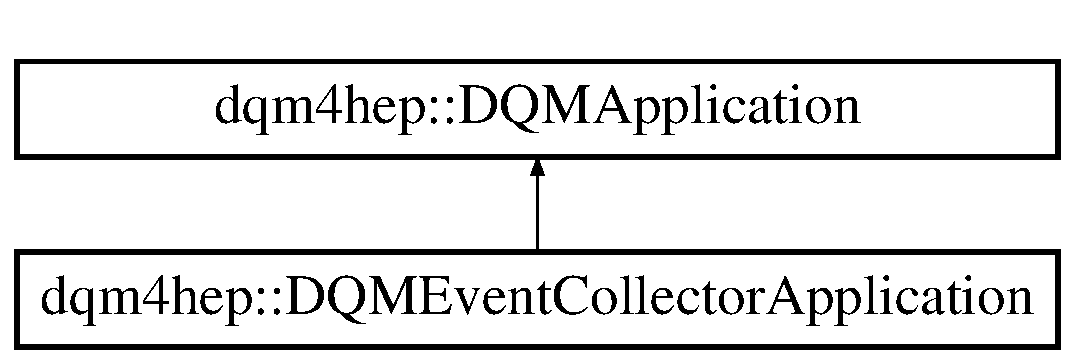
\includegraphics[height=2.000000cm]{classdqm4hep_1_1DQMEventCollectorApplication}
\end{center}
\end{figure}
\subsection*{Public Member Functions}
\begin{DoxyCompactItemize}
\item 
{\bf D\+Q\+M\+Event\+Collector\+Application} ()
\begin{DoxyCompactList}\small\item\em Constructor with collector name. \end{DoxyCompactList}\item 
{\bf $\sim$\+D\+Q\+M\+Event\+Collector\+Application} ()
\begin{DoxyCompactList}\small\item\em Destructor. \end{DoxyCompactList}\item 
{\bf Status\+Code} {\bf run} ()
\begin{DoxyCompactList}\small\item\em Run the application. \end{DoxyCompactList}\item 
{\bf Status\+Code} {\bf exit} (int return\+Code)
\begin{DoxyCompactList}\small\item\em Stop the application. \end{DoxyCompactList}\item 
const std\+::string \& {\bf get\+Name} () const 
\begin{DoxyCompactList}\small\item\em Get the application name. \end{DoxyCompactList}\item 
const std\+::string \& {\bf get\+Type} () const 
\begin{DoxyCompactList}\small\item\em Get the application type. \end{DoxyCompactList}\item 
{\bf Status\+Code} {\bf set\+Collector\+Name} (const std\+::string \&collector\+Name)
\begin{DoxyCompactList}\small\item\em Set the event collector name. \end{DoxyCompactList}\item 
void {\bf set\+Event\+Collector\+Imp} ({\bf D\+Q\+M\+Event\+Collector\+Imp} $\ast$p\+Collector\+Imp)
\begin{DoxyCompactList}\small\item\em Set the event collector implementation. \end{DoxyCompactList}\item 
void {\bf set\+Event\+Streamer} ({\bf D\+Q\+M\+Event\+Streamer} $\ast$p\+Event\+Streamer)
\begin{DoxyCompactList}\small\item\em Set the event streamer to serialize/deserialize the in/out-\/coming events. \end{DoxyCompactList}\item 
{\bf D\+Q\+M\+Event\+Streamer} $\ast$ {\bf get\+Event\+Streamer} () const 
\begin{DoxyCompactList}\small\item\em Get the event streamer. \end{DoxyCompactList}\end{DoxyCompactItemize}
\subsection*{Protected Member Functions}
\begin{DoxyCompactItemize}
\item 
{\bf Status\+Code} {\bf read\+Settings} (const std\+::string \&settings\+File=\char`\"{}\char`\"{})
\begin{DoxyCompactList}\small\item\em No settings to read. \end{DoxyCompactList}\end{DoxyCompactItemize}
\subsection*{Protected Attributes}
\begin{DoxyCompactItemize}
\item 
bool {\bf m\+\_\+should\+Exit}
\item 
std\+::string {\bf m\+\_\+type}
\item 
std\+::string {\bf m\+\_\+network\+Name}
\item 
{\bf D\+Q\+M\+State} {\bf m\+\_\+application\+State}
\item 
{\bf D\+Q\+M\+Event\+Collector} $\ast$ {\bf m\+\_\+p\+Event\+Collector}
\end{DoxyCompactItemize}


\subsection{Detailed Description}
\doxyref{D\+Q\+M\+Event\+Collector\+Application}{p.}{classdqm4hep_1_1DQMEventCollectorApplication} class. 

Definition at line 44 of file D\+Q\+M\+Event\+Collector\+Application.\+h.



\subsection{Constructor \& Destructor Documentation}
\index{dqm4hep\+::\+D\+Q\+M\+Event\+Collector\+Application@{dqm4hep\+::\+D\+Q\+M\+Event\+Collector\+Application}!D\+Q\+M\+Event\+Collector\+Application@{D\+Q\+M\+Event\+Collector\+Application}}
\index{D\+Q\+M\+Event\+Collector\+Application@{D\+Q\+M\+Event\+Collector\+Application}!dqm4hep\+::\+D\+Q\+M\+Event\+Collector\+Application@{dqm4hep\+::\+D\+Q\+M\+Event\+Collector\+Application}}
\subsubsection[{D\+Q\+M\+Event\+Collector\+Application}]{\setlength{\rightskip}{0pt plus 5cm}dqm4hep\+::\+D\+Q\+M\+Event\+Collector\+Application\+::\+D\+Q\+M\+Event\+Collector\+Application (
\begin{DoxyParamCaption}
{}
\end{DoxyParamCaption}
)}\label{classdqm4hep_1_1DQMEventCollectorApplication_ad4d171d907a0deeea311eb2b662d248e}


Constructor with collector name. 



Definition at line 36 of file D\+Q\+M\+Event\+Collector\+Application.\+cc.



References m\+\_\+p\+Event\+Collector.


\begin{DoxyCode}
36                                                            :
37     m_applicationState(STOPPED\_STATE),
38     m_shouldExit(\textcolor{keyword}{false}),
39     m_type(\textcolor{stringliteral}{"EventCollector"}),
40     m_pEventCollector(NULL)
41 \{
42   m_pEventCollector = \textcolor{keyword}{new} DQMEventCollector();
43 \}
\end{DoxyCode}
\index{dqm4hep\+::\+D\+Q\+M\+Event\+Collector\+Application@{dqm4hep\+::\+D\+Q\+M\+Event\+Collector\+Application}!````~D\+Q\+M\+Event\+Collector\+Application@{$\sim$\+D\+Q\+M\+Event\+Collector\+Application}}
\index{````~D\+Q\+M\+Event\+Collector\+Application@{$\sim$\+D\+Q\+M\+Event\+Collector\+Application}!dqm4hep\+::\+D\+Q\+M\+Event\+Collector\+Application@{dqm4hep\+::\+D\+Q\+M\+Event\+Collector\+Application}}
\subsubsection[{$\sim$\+D\+Q\+M\+Event\+Collector\+Application}]{\setlength{\rightskip}{0pt plus 5cm}dqm4hep\+::\+D\+Q\+M\+Event\+Collector\+Application\+::$\sim$\+D\+Q\+M\+Event\+Collector\+Application (
\begin{DoxyParamCaption}
{}
\end{DoxyParamCaption}
)}\label{classdqm4hep_1_1DQMEventCollectorApplication_a3004cbaf2ae30b35a3ccaa7c28049c88}


Destructor. 



Definition at line 47 of file D\+Q\+M\+Event\+Collector\+Application.\+cc.



References dqm4hep\+::\+D\+Q\+M\+Event\+Collector\+::is\+Running(), m\+\_\+p\+Event\+Collector, and dqm4hep\+::\+D\+Q\+M\+Event\+Collector\+::stop\+Collector().


\begin{DoxyCode}
48 \{
49   \textcolor{keywordflow}{if}(m_pEventCollector->isRunning())
50     m_pEventCollector->stopCollector();
51 
52   \textcolor{keyword}{delete} m_pEventCollector;
53 \}
\end{DoxyCode}


\subsection{Member Function Documentation}
\index{dqm4hep\+::\+D\+Q\+M\+Event\+Collector\+Application@{dqm4hep\+::\+D\+Q\+M\+Event\+Collector\+Application}!exit@{exit}}
\index{exit@{exit}!dqm4hep\+::\+D\+Q\+M\+Event\+Collector\+Application@{dqm4hep\+::\+D\+Q\+M\+Event\+Collector\+Application}}
\subsubsection[{exit}]{\setlength{\rightskip}{0pt plus 5cm}{\bf Status\+Code} dqm4hep\+::\+D\+Q\+M\+Event\+Collector\+Application\+::exit (
\begin{DoxyParamCaption}
\item[{int}]{return\+Code}
\end{DoxyParamCaption}
)\hspace{0.3cm}{\ttfamily [virtual]}}\label{classdqm4hep_1_1DQMEventCollectorApplication_a7f9c7d86ca591f92bf43618dfaf12443}


Stop the application. 



Implements {\bf dqm4hep\+::\+D\+Q\+M\+Application} \doxyref{}{p.}{classdqm4hep_1_1DQMApplication_ad61139a41c4ba6669d26e3a0013c0f6d}.



Definition at line 79 of file D\+Q\+M\+Event\+Collector\+Application.\+cc.



References m\+\_\+application\+State, m\+\_\+p\+Event\+Collector, m\+\_\+should\+Exit, dqm4hep\+::\+N\+U\+M\+B\+E\+R\+\_\+\+O\+F\+\_\+\+S\+T\+A\+T\+U\+S\+\_\+\+C\+O\+D\+E\+S, R\+E\+T\+U\+R\+N\+\_\+\+R\+E\+S\+U\+L\+T\+\_\+\+I\+F, and dqm4hep\+::\+D\+Q\+M\+Event\+Collector\+::stop\+Collector().


\begin{DoxyCode}
80 \{
81   \textcolor{keywordflow}{if}(m_applicationState == STOPPED\_STATE)
82     \textcolor{keywordflow}{return} STATUS\_CODE\_FAILURE;
83 
84   RETURN_RESULT_IF(STATUS\_CODE\_SUCCESS, !=, m_pEventCollector->stopCollector());
85 
86   m_shouldExit = \textcolor{keyword}{true};
87   m_applicationState = STOPPED\_STATE;
88 
89   StatusCode returnStatusCode;
90 
91   \textcolor{keywordflow}{if}(returnCode >= 0 && returnCode < NUMBER_OF_STATUS_CODES)
92     returnStatusCode = \textcolor{keyword}{static\_cast<}StatusCode\textcolor{keyword}{>}(returnCode);
93   \textcolor{keywordflow}{else}
94     returnStatusCode = STATUS\_CODE\_FAILURE;
95 
96   \textcolor{keywordflow}{return} returnStatusCode;
97 \}
\end{DoxyCode}
\index{dqm4hep\+::\+D\+Q\+M\+Event\+Collector\+Application@{dqm4hep\+::\+D\+Q\+M\+Event\+Collector\+Application}!get\+Event\+Streamer@{get\+Event\+Streamer}}
\index{get\+Event\+Streamer@{get\+Event\+Streamer}!dqm4hep\+::\+D\+Q\+M\+Event\+Collector\+Application@{dqm4hep\+::\+D\+Q\+M\+Event\+Collector\+Application}}
\subsubsection[{get\+Event\+Streamer}]{\setlength{\rightskip}{0pt plus 5cm}{\bf D\+Q\+M\+Event\+Streamer} $\ast$ dqm4hep\+::\+D\+Q\+M\+Event\+Collector\+Application\+::get\+Event\+Streamer (
\begin{DoxyParamCaption}
{}
\end{DoxyParamCaption}
) const}\label{classdqm4hep_1_1DQMEventCollectorApplication_a385871f0059f871e49c36febfcc3e6cf}


Get the event streamer. 



Definition at line 139 of file D\+Q\+M\+Event\+Collector\+Application.\+cc.



References dqm4hep\+::\+D\+Q\+M\+Event\+Collector\+::get\+Event\+Streamer(), and m\+\_\+p\+Event\+Collector.


\begin{DoxyCode}
140 \{
141   \textcolor{keywordflow}{return} m_pEventCollector->getEventStreamer();
142 \}
\end{DoxyCode}
\index{dqm4hep\+::\+D\+Q\+M\+Event\+Collector\+Application@{dqm4hep\+::\+D\+Q\+M\+Event\+Collector\+Application}!get\+Name@{get\+Name}}
\index{get\+Name@{get\+Name}!dqm4hep\+::\+D\+Q\+M\+Event\+Collector\+Application@{dqm4hep\+::\+D\+Q\+M\+Event\+Collector\+Application}}
\subsubsection[{get\+Name}]{\setlength{\rightskip}{0pt plus 5cm}const std\+::string \& dqm4hep\+::\+D\+Q\+M\+Event\+Collector\+Application\+::get\+Name (
\begin{DoxyParamCaption}
{}
\end{DoxyParamCaption}
) const\hspace{0.3cm}{\ttfamily [virtual]}}\label{classdqm4hep_1_1DQMEventCollectorApplication_ab38b4de8474b46f560bbf97b4ceba02d}


Get the application name. 



Implements {\bf dqm4hep\+::\+D\+Q\+M\+Application} \doxyref{}{p.}{classdqm4hep_1_1DQMApplication_a90d2e587390835cf90b38888498e922b}.



Definition at line 101 of file D\+Q\+M\+Event\+Collector\+Application.\+cc.



References dqm4hep\+::\+D\+Q\+M\+Event\+Collector\+::get\+Collector\+Name(), and m\+\_\+p\+Event\+Collector.


\begin{DoxyCode}
102 \{
103   \textcolor{keywordflow}{return} m_pEventCollector->getCollectorName();
104 \}
\end{DoxyCode}
\index{dqm4hep\+::\+D\+Q\+M\+Event\+Collector\+Application@{dqm4hep\+::\+D\+Q\+M\+Event\+Collector\+Application}!get\+Type@{get\+Type}}
\index{get\+Type@{get\+Type}!dqm4hep\+::\+D\+Q\+M\+Event\+Collector\+Application@{dqm4hep\+::\+D\+Q\+M\+Event\+Collector\+Application}}
\subsubsection[{get\+Type}]{\setlength{\rightskip}{0pt plus 5cm}const std\+::string \& dqm4hep\+::\+D\+Q\+M\+Event\+Collector\+Application\+::get\+Type (
\begin{DoxyParamCaption}
{}
\end{DoxyParamCaption}
) const\hspace{0.3cm}{\ttfamily [virtual]}}\label{classdqm4hep_1_1DQMEventCollectorApplication_a8bb630d63433e17105f8a07f7c54ba4a}


Get the application type. 



Implements {\bf dqm4hep\+::\+D\+Q\+M\+Application} \doxyref{}{p.}{classdqm4hep_1_1DQMApplication_aff587d33b27ff25115a7da7655e5ab3b}.



Definition at line 108 of file D\+Q\+M\+Event\+Collector\+Application.\+cc.



References m\+\_\+type.


\begin{DoxyCode}
109 \{
110   \textcolor{keywordflow}{return} m_type;
111 \}
\end{DoxyCode}
\index{dqm4hep\+::\+D\+Q\+M\+Event\+Collector\+Application@{dqm4hep\+::\+D\+Q\+M\+Event\+Collector\+Application}!read\+Settings@{read\+Settings}}
\index{read\+Settings@{read\+Settings}!dqm4hep\+::\+D\+Q\+M\+Event\+Collector\+Application@{dqm4hep\+::\+D\+Q\+M\+Event\+Collector\+Application}}
\subsubsection[{read\+Settings}]{\setlength{\rightskip}{0pt plus 5cm}{\bf Status\+Code} dqm4hep\+::\+D\+Q\+M\+Event\+Collector\+Application\+::read\+Settings (
\begin{DoxyParamCaption}
\item[{const std\+::string \&}]{settings\+File = {\ttfamily \char`\"{}\char`\"{}}}
\end{DoxyParamCaption}
)\hspace{0.3cm}{\ttfamily [inline]}, {\ttfamily [protected]}, {\ttfamily [virtual]}}\label{classdqm4hep_1_1DQMEventCollectorApplication_afaf52f63edcb95265f397682a9915198}


No settings to read. 



Implements {\bf dqm4hep\+::\+D\+Q\+M\+Application} \doxyref{}{p.}{classdqm4hep_1_1DQMApplication_a8b2e28cf09eef6b6a8bde547949c37dc}.



Definition at line 90 of file D\+Q\+M\+Event\+Collector\+Application.\+h.


\begin{DoxyCode}
90 \{ \textcolor{keywordflow}{return} STATUS\_CODE\_SUCCESS; \}
\end{DoxyCode}
\index{dqm4hep\+::\+D\+Q\+M\+Event\+Collector\+Application@{dqm4hep\+::\+D\+Q\+M\+Event\+Collector\+Application}!run@{run}}
\index{run@{run}!dqm4hep\+::\+D\+Q\+M\+Event\+Collector\+Application@{dqm4hep\+::\+D\+Q\+M\+Event\+Collector\+Application}}
\subsubsection[{run}]{\setlength{\rightskip}{0pt plus 5cm}{\bf Status\+Code} dqm4hep\+::\+D\+Q\+M\+Event\+Collector\+Application\+::run (
\begin{DoxyParamCaption}
{}
\end{DoxyParamCaption}
)\hspace{0.3cm}{\ttfamily [virtual]}}\label{classdqm4hep_1_1DQMEventCollectorApplication_ad86399bda3c734d4924043250d7e1cc6}


Run the application. 



Implements {\bf dqm4hep\+::\+D\+Q\+M\+Application} \doxyref{}{p.}{classdqm4hep_1_1DQMApplication_aa9a37abef624ec9656478c7211cc5a48}.



Definition at line 57 of file D\+Q\+M\+Event\+Collector\+Application.\+cc.



References m\+\_\+application\+State, m\+\_\+p\+Event\+Collector, m\+\_\+should\+Exit, R\+E\+T\+U\+R\+N\+\_\+\+R\+E\+S\+U\+L\+T\+\_\+\+I\+F, and dqm4hep\+::\+D\+Q\+M\+Event\+Collector\+::start\+Collector().


\begin{DoxyCode}
58 \{
59   \textcolor{keywordflow}{if}(m_applicationState == RUNNING\_STATE)
60     \textcolor{keywordflow}{return} STATUS\_CODE\_FAILURE;
61 
62   RETURN_RESULT_IF(STATUS\_CODE\_SUCCESS, !=, m_pEventCollector->startCollector());
63 
64   m_applicationState = RUNNING\_STATE;
65 
66   \textcolor{keywordflow}{while}(!m_shouldExit)
67   \{
68     timespec timesleep;
69       timesleep.tv\_sec = 0;
70       timesleep.tv\_nsec = 100000L;
71     nanosleep(&timesleep, NULL);
72   \}
73 
74   \textcolor{keywordflow}{return} STATUS\_CODE\_SUCCESS;
75 \}
\end{DoxyCode}
\index{dqm4hep\+::\+D\+Q\+M\+Event\+Collector\+Application@{dqm4hep\+::\+D\+Q\+M\+Event\+Collector\+Application}!set\+Collector\+Name@{set\+Collector\+Name}}
\index{set\+Collector\+Name@{set\+Collector\+Name}!dqm4hep\+::\+D\+Q\+M\+Event\+Collector\+Application@{dqm4hep\+::\+D\+Q\+M\+Event\+Collector\+Application}}
\subsubsection[{set\+Collector\+Name}]{\setlength{\rightskip}{0pt plus 5cm}{\bf Status\+Code} dqm4hep\+::\+D\+Q\+M\+Event\+Collector\+Application\+::set\+Collector\+Name (
\begin{DoxyParamCaption}
\item[{const std\+::string \&}]{collector\+Name}
\end{DoxyParamCaption}
)}\label{classdqm4hep_1_1DQMEventCollectorApplication_a2fe96cd9923909ce864bcc63b49f8c70}


Set the event collector name. 



Definition at line 115 of file D\+Q\+M\+Event\+Collector\+Application.\+cc.



References m\+\_\+p\+Event\+Collector, and dqm4hep\+::\+D\+Q\+M\+Event\+Collector\+::set\+Collector\+Name().


\begin{DoxyCode}
116 \{
117   \textcolor{keywordflow}{return} m_pEventCollector->setCollectorName(collectorName);
118 \}
\end{DoxyCode}
\index{dqm4hep\+::\+D\+Q\+M\+Event\+Collector\+Application@{dqm4hep\+::\+D\+Q\+M\+Event\+Collector\+Application}!set\+Event\+Collector\+Imp@{set\+Event\+Collector\+Imp}}
\index{set\+Event\+Collector\+Imp@{set\+Event\+Collector\+Imp}!dqm4hep\+::\+D\+Q\+M\+Event\+Collector\+Application@{dqm4hep\+::\+D\+Q\+M\+Event\+Collector\+Application}}
\subsubsection[{set\+Event\+Collector\+Imp}]{\setlength{\rightskip}{0pt plus 5cm}void dqm4hep\+::\+D\+Q\+M\+Event\+Collector\+Application\+::set\+Event\+Collector\+Imp (
\begin{DoxyParamCaption}
\item[{{\bf D\+Q\+M\+Event\+Collector\+Imp} $\ast$}]{p\+Collector\+Imp}
\end{DoxyParamCaption}
)}\label{classdqm4hep_1_1DQMEventCollectorApplication_a5fa8a1c75ee24f47f855ffbe1760750c}


Set the event collector implementation. 



Definition at line 122 of file D\+Q\+M\+Event\+Collector\+Application.\+cc.



References m\+\_\+p\+Event\+Collector, and dqm4hep\+::\+D\+Q\+M\+Event\+Collector\+::set\+Event\+Collector\+Imp().


\begin{DoxyCode}
123 \{
124   \textcolor{keywordflow}{if}(NULL == pCollectorImp)
125     \textcolor{keywordflow}{return};
126 
127   m_pEventCollector->setEventCollectorImp(pCollectorImp);
128 \}
\end{DoxyCode}
\index{dqm4hep\+::\+D\+Q\+M\+Event\+Collector\+Application@{dqm4hep\+::\+D\+Q\+M\+Event\+Collector\+Application}!set\+Event\+Streamer@{set\+Event\+Streamer}}
\index{set\+Event\+Streamer@{set\+Event\+Streamer}!dqm4hep\+::\+D\+Q\+M\+Event\+Collector\+Application@{dqm4hep\+::\+D\+Q\+M\+Event\+Collector\+Application}}
\subsubsection[{set\+Event\+Streamer}]{\setlength{\rightskip}{0pt plus 5cm}void dqm4hep\+::\+D\+Q\+M\+Event\+Collector\+Application\+::set\+Event\+Streamer (
\begin{DoxyParamCaption}
\item[{{\bf D\+Q\+M\+Event\+Streamer} $\ast$}]{p\+Event\+Streamer}
\end{DoxyParamCaption}
)}\label{classdqm4hep_1_1DQMEventCollectorApplication_a15578668dd61107e4a4083ff722895ba}


Set the event streamer to serialize/deserialize the in/out-\/coming events. 



Definition at line 132 of file D\+Q\+M\+Event\+Collector\+Application.\+cc.



References m\+\_\+p\+Event\+Collector, and dqm4hep\+::\+D\+Q\+M\+Event\+Collector\+::set\+Event\+Streamer().


\begin{DoxyCode}
133 \{
134   m_pEventCollector->setEventStreamer(pEventStreamer);
135 \}
\end{DoxyCode}


\subsection{Member Data Documentation}
\index{dqm4hep\+::\+D\+Q\+M\+Event\+Collector\+Application@{dqm4hep\+::\+D\+Q\+M\+Event\+Collector\+Application}!m\+\_\+application\+State@{m\+\_\+application\+State}}
\index{m\+\_\+application\+State@{m\+\_\+application\+State}!dqm4hep\+::\+D\+Q\+M\+Event\+Collector\+Application@{dqm4hep\+::\+D\+Q\+M\+Event\+Collector\+Application}}
\subsubsection[{m\+\_\+application\+State}]{\setlength{\rightskip}{0pt plus 5cm}{\bf D\+Q\+M\+State} dqm4hep\+::\+D\+Q\+M\+Event\+Collector\+Application\+::m\+\_\+application\+State\hspace{0.3cm}{\ttfamily [protected]}}\label{classdqm4hep_1_1DQMEventCollectorApplication_ad585260887cca7ca276b3ccd7b8a2334}


Definition at line 95 of file D\+Q\+M\+Event\+Collector\+Application.\+h.



Referenced by exit(), and run().

\index{dqm4hep\+::\+D\+Q\+M\+Event\+Collector\+Application@{dqm4hep\+::\+D\+Q\+M\+Event\+Collector\+Application}!m\+\_\+network\+Name@{m\+\_\+network\+Name}}
\index{m\+\_\+network\+Name@{m\+\_\+network\+Name}!dqm4hep\+::\+D\+Q\+M\+Event\+Collector\+Application@{dqm4hep\+::\+D\+Q\+M\+Event\+Collector\+Application}}
\subsubsection[{m\+\_\+network\+Name}]{\setlength{\rightskip}{0pt plus 5cm}std\+::string dqm4hep\+::\+D\+Q\+M\+Event\+Collector\+Application\+::m\+\_\+network\+Name\hspace{0.3cm}{\ttfamily [protected]}}\label{classdqm4hep_1_1DQMEventCollectorApplication_a064910c6b4b7f260e698ea09882e640f}


Definition at line 94 of file D\+Q\+M\+Event\+Collector\+Application.\+h.

\index{dqm4hep\+::\+D\+Q\+M\+Event\+Collector\+Application@{dqm4hep\+::\+D\+Q\+M\+Event\+Collector\+Application}!m\+\_\+p\+Event\+Collector@{m\+\_\+p\+Event\+Collector}}
\index{m\+\_\+p\+Event\+Collector@{m\+\_\+p\+Event\+Collector}!dqm4hep\+::\+D\+Q\+M\+Event\+Collector\+Application@{dqm4hep\+::\+D\+Q\+M\+Event\+Collector\+Application}}
\subsubsection[{m\+\_\+p\+Event\+Collector}]{\setlength{\rightskip}{0pt plus 5cm}{\bf D\+Q\+M\+Event\+Collector}$\ast$ dqm4hep\+::\+D\+Q\+M\+Event\+Collector\+Application\+::m\+\_\+p\+Event\+Collector\hspace{0.3cm}{\ttfamily [protected]}}\label{classdqm4hep_1_1DQMEventCollectorApplication_a82b0e83e01776f78b233774923b434a0}


Definition at line 96 of file D\+Q\+M\+Event\+Collector\+Application.\+h.



Referenced by D\+Q\+M\+Event\+Collector\+Application(), exit(), get\+Event\+Streamer(), get\+Name(), run(), set\+Collector\+Name(), set\+Event\+Collector\+Imp(), set\+Event\+Streamer(), and $\sim$\+D\+Q\+M\+Event\+Collector\+Application().

\index{dqm4hep\+::\+D\+Q\+M\+Event\+Collector\+Application@{dqm4hep\+::\+D\+Q\+M\+Event\+Collector\+Application}!m\+\_\+should\+Exit@{m\+\_\+should\+Exit}}
\index{m\+\_\+should\+Exit@{m\+\_\+should\+Exit}!dqm4hep\+::\+D\+Q\+M\+Event\+Collector\+Application@{dqm4hep\+::\+D\+Q\+M\+Event\+Collector\+Application}}
\subsubsection[{m\+\_\+should\+Exit}]{\setlength{\rightskip}{0pt plus 5cm}bool dqm4hep\+::\+D\+Q\+M\+Event\+Collector\+Application\+::m\+\_\+should\+Exit\hspace{0.3cm}{\ttfamily [protected]}}\label{classdqm4hep_1_1DQMEventCollectorApplication_ab66ce1c0618b2200a139ec689db044e8}


Definition at line 92 of file D\+Q\+M\+Event\+Collector\+Application.\+h.



Referenced by exit(), and run().

\index{dqm4hep\+::\+D\+Q\+M\+Event\+Collector\+Application@{dqm4hep\+::\+D\+Q\+M\+Event\+Collector\+Application}!m\+\_\+type@{m\+\_\+type}}
\index{m\+\_\+type@{m\+\_\+type}!dqm4hep\+::\+D\+Q\+M\+Event\+Collector\+Application@{dqm4hep\+::\+D\+Q\+M\+Event\+Collector\+Application}}
\subsubsection[{m\+\_\+type}]{\setlength{\rightskip}{0pt plus 5cm}std\+::string dqm4hep\+::\+D\+Q\+M\+Event\+Collector\+Application\+::m\+\_\+type\hspace{0.3cm}{\ttfamily [protected]}}\label{classdqm4hep_1_1DQMEventCollectorApplication_a7dc467c209edda778b513ad3c341915b}


Definition at line 93 of file D\+Q\+M\+Event\+Collector\+Application.\+h.



Referenced by get\+Type().



The documentation for this class was generated from the following files\+:\begin{DoxyCompactItemize}
\item 
{\bf D\+Q\+M\+Event\+Collector\+Application.\+h}\item 
{\bf D\+Q\+M\+Event\+Collector\+Application.\+cc}\end{DoxyCompactItemize}

\section{dqm4hep\+:\+:D\+Q\+M\+Event\+Collector\+Imp Class Reference}
\label{classdqm4hep_1_1DQMEventCollectorImp}\index{dqm4hep\+::\+D\+Q\+M\+Event\+Collector\+Imp@{dqm4hep\+::\+D\+Q\+M\+Event\+Collector\+Imp}}


\doxyref{D\+Q\+M\+Event\+Collector\+Imp}{p.}{classdqm4hep_1_1DQMEventCollectorImp} class.  




{\ttfamily \#include $<$D\+Q\+M\+Event\+Collector\+Imp.\+h$>$}

Inheritance diagram for dqm4hep\+:\+:D\+Q\+M\+Event\+Collector\+Imp\+:\begin{figure}[H]
\begin{center}
\leavevmode
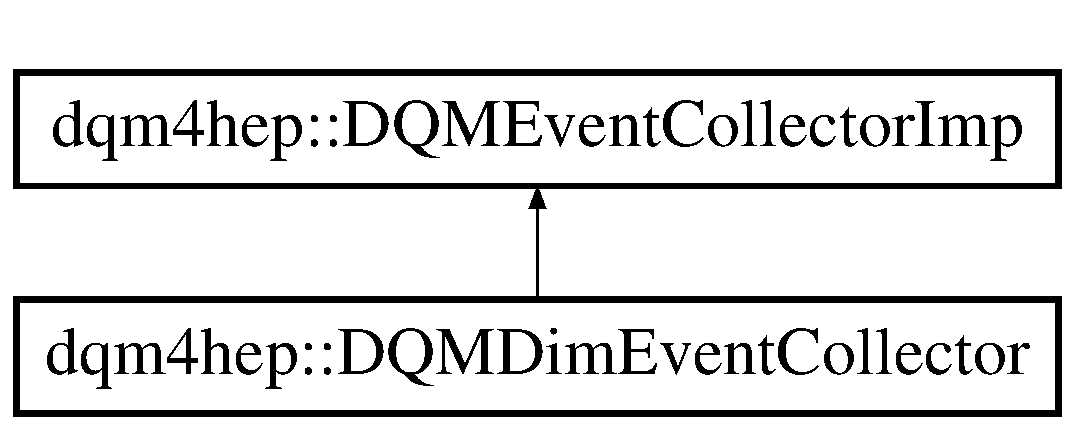
\includegraphics[height=2.000000cm]{classdqm4hep_1_1DQMEventCollectorImp}
\end{center}
\end{figure}
\subsection*{Public Member Functions}
\begin{DoxyCompactItemize}
\item 
virtual {\bf $\sim$\+D\+Q\+M\+Event\+Collector\+Imp} ()
\begin{DoxyCompactList}\small\item\em Destructor. \end{DoxyCompactList}\item 
virtual {\bf Status\+Code} {\bf set\+Collector\+Name} (const std\+::string \&collector\+Name)=0
\begin{DoxyCompactList}\small\item\em Set the collector name. \end{DoxyCompactList}\item 
virtual const std\+::string \& {\bf get\+Collector\+Name} () const =0
\begin{DoxyCompactList}\small\item\em Get the collector name. \end{DoxyCompactList}\item 
virtual bool {\bf is\+Running} () const =0
\begin{DoxyCompactList}\small\item\em Whether the collector server is running. \end{DoxyCompactList}\item 
virtual {\bf Status\+Code} {\bf start\+Collector} ()=0
\begin{DoxyCompactList}\small\item\em Start the collector server. \end{DoxyCompactList}\item 
virtual {\bf Status\+Code} {\bf stop\+Collector} ()=0
\begin{DoxyCompactList}\small\item\em Stop the collector server. \end{DoxyCompactList}\item 
virtual void {\bf set\+Event\+Streamer} ({\bf D\+Q\+M\+Event\+Streamer} $\ast$p\+Event\+Streamer)=0
\begin{DoxyCompactList}\small\item\em Set the event streamer to serialize/deserialize the in/out-\/coming events. \end{DoxyCompactList}\item 
virtual {\bf D\+Q\+M\+Event\+Streamer} $\ast$ {\bf get\+Event\+Streamer} () const =0
\begin{DoxyCompactList}\small\item\em Get the event streamer. \end{DoxyCompactList}\end{DoxyCompactItemize}


\subsection{Detailed Description}
\doxyref{D\+Q\+M\+Event\+Collector\+Imp}{p.}{classdqm4hep_1_1DQMEventCollectorImp} class. 

Definition at line 39 of file D\+Q\+M\+Event\+Collector\+Imp.\+h.



\subsection{Constructor \& Destructor Documentation}
\index{dqm4hep\+::\+D\+Q\+M\+Event\+Collector\+Imp@{dqm4hep\+::\+D\+Q\+M\+Event\+Collector\+Imp}!````~D\+Q\+M\+Event\+Collector\+Imp@{$\sim$\+D\+Q\+M\+Event\+Collector\+Imp}}
\index{````~D\+Q\+M\+Event\+Collector\+Imp@{$\sim$\+D\+Q\+M\+Event\+Collector\+Imp}!dqm4hep\+::\+D\+Q\+M\+Event\+Collector\+Imp@{dqm4hep\+::\+D\+Q\+M\+Event\+Collector\+Imp}}
\subsubsection[{$\sim$\+D\+Q\+M\+Event\+Collector\+Imp}]{\setlength{\rightskip}{0pt plus 5cm}virtual dqm4hep\+::\+D\+Q\+M\+Event\+Collector\+Imp\+::$\sim$\+D\+Q\+M\+Event\+Collector\+Imp (
\begin{DoxyParamCaption}
{}
\end{DoxyParamCaption}
)\hspace{0.3cm}{\ttfamily [inline]}, {\ttfamily [virtual]}}\label{classdqm4hep_1_1DQMEventCollectorImp_af5bc3bc187b96db3b89c128c376ab5c0}


Destructor. 



Definition at line 44 of file D\+Q\+M\+Event\+Collector\+Imp.\+h.


\begin{DoxyCode}
44 \{\}
\end{DoxyCode}


\subsection{Member Function Documentation}
\index{dqm4hep\+::\+D\+Q\+M\+Event\+Collector\+Imp@{dqm4hep\+::\+D\+Q\+M\+Event\+Collector\+Imp}!get\+Collector\+Name@{get\+Collector\+Name}}
\index{get\+Collector\+Name@{get\+Collector\+Name}!dqm4hep\+::\+D\+Q\+M\+Event\+Collector\+Imp@{dqm4hep\+::\+D\+Q\+M\+Event\+Collector\+Imp}}
\subsubsection[{get\+Collector\+Name}]{\setlength{\rightskip}{0pt plus 5cm}virtual const std\+::string\& dqm4hep\+::\+D\+Q\+M\+Event\+Collector\+Imp\+::get\+Collector\+Name (
\begin{DoxyParamCaption}
{}
\end{DoxyParamCaption}
) const\hspace{0.3cm}{\ttfamily [pure virtual]}}\label{classdqm4hep_1_1DQMEventCollectorImp_a4d43a74838a7d1d4b7ffcdd230a30d4d}


Get the collector name. 



Implemented in {\bf dqm4hep\+::\+D\+Q\+M\+Dim\+Event\+Collector} \doxyref{}{p.}{classdqm4hep_1_1DQMDimEventCollector_a38a9e06681d3348c2cef9e5efba00347}.



Referenced by dqm4hep\+::\+D\+Q\+M\+Event\+Collector\+::get\+Collector\+Name().

\index{dqm4hep\+::\+D\+Q\+M\+Event\+Collector\+Imp@{dqm4hep\+::\+D\+Q\+M\+Event\+Collector\+Imp}!get\+Event\+Streamer@{get\+Event\+Streamer}}
\index{get\+Event\+Streamer@{get\+Event\+Streamer}!dqm4hep\+::\+D\+Q\+M\+Event\+Collector\+Imp@{dqm4hep\+::\+D\+Q\+M\+Event\+Collector\+Imp}}
\subsubsection[{get\+Event\+Streamer}]{\setlength{\rightskip}{0pt plus 5cm}virtual {\bf D\+Q\+M\+Event\+Streamer}$\ast$ dqm4hep\+::\+D\+Q\+M\+Event\+Collector\+Imp\+::get\+Event\+Streamer (
\begin{DoxyParamCaption}
{}
\end{DoxyParamCaption}
) const\hspace{0.3cm}{\ttfamily [pure virtual]}}\label{classdqm4hep_1_1DQMEventCollectorImp_ac9ad55f2bcd2b6d674cfaa3bfa68f2b8}


Get the event streamer. 



Implemented in {\bf dqm4hep\+::\+D\+Q\+M\+Dim\+Event\+Collector} \doxyref{}{p.}{classdqm4hep_1_1DQMDimEventCollector_aeabfafccdb40afab06453eea478b2fd2}.



Referenced by dqm4hep\+::\+D\+Q\+M\+Event\+Collector\+::get\+Event\+Streamer().

\index{dqm4hep\+::\+D\+Q\+M\+Event\+Collector\+Imp@{dqm4hep\+::\+D\+Q\+M\+Event\+Collector\+Imp}!is\+Running@{is\+Running}}
\index{is\+Running@{is\+Running}!dqm4hep\+::\+D\+Q\+M\+Event\+Collector\+Imp@{dqm4hep\+::\+D\+Q\+M\+Event\+Collector\+Imp}}
\subsubsection[{is\+Running}]{\setlength{\rightskip}{0pt plus 5cm}virtual bool dqm4hep\+::\+D\+Q\+M\+Event\+Collector\+Imp\+::is\+Running (
\begin{DoxyParamCaption}
{}
\end{DoxyParamCaption}
) const\hspace{0.3cm}{\ttfamily [pure virtual]}}\label{classdqm4hep_1_1DQMEventCollectorImp_a7588b758cf32de97b1c1d49a55f11261}


Whether the collector server is running. 



Implemented in {\bf dqm4hep\+::\+D\+Q\+M\+Dim\+Event\+Collector} \doxyref{}{p.}{classdqm4hep_1_1DQMDimEventCollector_a5fedb202ddf13d4382fb32e52986e8de}.



Referenced by dqm4hep\+::\+D\+Q\+M\+Event\+Collector\+::is\+Running().

\index{dqm4hep\+::\+D\+Q\+M\+Event\+Collector\+Imp@{dqm4hep\+::\+D\+Q\+M\+Event\+Collector\+Imp}!set\+Collector\+Name@{set\+Collector\+Name}}
\index{set\+Collector\+Name@{set\+Collector\+Name}!dqm4hep\+::\+D\+Q\+M\+Event\+Collector\+Imp@{dqm4hep\+::\+D\+Q\+M\+Event\+Collector\+Imp}}
\subsubsection[{set\+Collector\+Name}]{\setlength{\rightskip}{0pt plus 5cm}virtual {\bf Status\+Code} dqm4hep\+::\+D\+Q\+M\+Event\+Collector\+Imp\+::set\+Collector\+Name (
\begin{DoxyParamCaption}
\item[{const std\+::string \&}]{collector\+Name}
\end{DoxyParamCaption}
)\hspace{0.3cm}{\ttfamily [pure virtual]}}\label{classdqm4hep_1_1DQMEventCollectorImp_a5ee8c4e1a66ec2309237968600ad8c9a}


Set the collector name. 



Implemented in {\bf dqm4hep\+::\+D\+Q\+M\+Dim\+Event\+Collector} \doxyref{}{p.}{classdqm4hep_1_1DQMDimEventCollector_a61f103cd22047630a1675021d08031c8}.



Referenced by dqm4hep\+::\+D\+Q\+M\+Event\+Collector\+::set\+Collector\+Name().

\index{dqm4hep\+::\+D\+Q\+M\+Event\+Collector\+Imp@{dqm4hep\+::\+D\+Q\+M\+Event\+Collector\+Imp}!set\+Event\+Streamer@{set\+Event\+Streamer}}
\index{set\+Event\+Streamer@{set\+Event\+Streamer}!dqm4hep\+::\+D\+Q\+M\+Event\+Collector\+Imp@{dqm4hep\+::\+D\+Q\+M\+Event\+Collector\+Imp}}
\subsubsection[{set\+Event\+Streamer}]{\setlength{\rightskip}{0pt plus 5cm}virtual void dqm4hep\+::\+D\+Q\+M\+Event\+Collector\+Imp\+::set\+Event\+Streamer (
\begin{DoxyParamCaption}
\item[{{\bf D\+Q\+M\+Event\+Streamer} $\ast$}]{p\+Event\+Streamer}
\end{DoxyParamCaption}
)\hspace{0.3cm}{\ttfamily [pure virtual]}}\label{classdqm4hep_1_1DQMEventCollectorImp_af821be6ae3404262795cb567d4c37da7}


Set the event streamer to serialize/deserialize the in/out-\/coming events. 



Implemented in {\bf dqm4hep\+::\+D\+Q\+M\+Dim\+Event\+Collector} \doxyref{}{p.}{classdqm4hep_1_1DQMDimEventCollector_a8e516a2927040fb392d4a34ec0473b8e}.



Referenced by dqm4hep\+::\+D\+Q\+M\+Event\+Collector\+::set\+Event\+Streamer().

\index{dqm4hep\+::\+D\+Q\+M\+Event\+Collector\+Imp@{dqm4hep\+::\+D\+Q\+M\+Event\+Collector\+Imp}!start\+Collector@{start\+Collector}}
\index{start\+Collector@{start\+Collector}!dqm4hep\+::\+D\+Q\+M\+Event\+Collector\+Imp@{dqm4hep\+::\+D\+Q\+M\+Event\+Collector\+Imp}}
\subsubsection[{start\+Collector}]{\setlength{\rightskip}{0pt plus 5cm}virtual {\bf Status\+Code} dqm4hep\+::\+D\+Q\+M\+Event\+Collector\+Imp\+::start\+Collector (
\begin{DoxyParamCaption}
{}
\end{DoxyParamCaption}
)\hspace{0.3cm}{\ttfamily [pure virtual]}}\label{classdqm4hep_1_1DQMEventCollectorImp_a836693a1fd5853fd05d2893c313d1631}


Start the collector server. 



Implemented in {\bf dqm4hep\+::\+D\+Q\+M\+Dim\+Event\+Collector} \doxyref{}{p.}{classdqm4hep_1_1DQMDimEventCollector_ac356924a7940f67ceb82c21c85be54e7}.



Referenced by dqm4hep\+::\+D\+Q\+M\+Event\+Collector\+::start\+Collector().

\index{dqm4hep\+::\+D\+Q\+M\+Event\+Collector\+Imp@{dqm4hep\+::\+D\+Q\+M\+Event\+Collector\+Imp}!stop\+Collector@{stop\+Collector}}
\index{stop\+Collector@{stop\+Collector}!dqm4hep\+::\+D\+Q\+M\+Event\+Collector\+Imp@{dqm4hep\+::\+D\+Q\+M\+Event\+Collector\+Imp}}
\subsubsection[{stop\+Collector}]{\setlength{\rightskip}{0pt plus 5cm}virtual {\bf Status\+Code} dqm4hep\+::\+D\+Q\+M\+Event\+Collector\+Imp\+::stop\+Collector (
\begin{DoxyParamCaption}
{}
\end{DoxyParamCaption}
)\hspace{0.3cm}{\ttfamily [pure virtual]}}\label{classdqm4hep_1_1DQMEventCollectorImp_a88b0502610cdb257da0ab4cb1a09525f}


Stop the collector server. 



Implemented in {\bf dqm4hep\+::\+D\+Q\+M\+Dim\+Event\+Collector} \doxyref{}{p.}{classdqm4hep_1_1DQMDimEventCollector_a00bff5f75b9b1b22d95faa6981ee8183}.



Referenced by dqm4hep\+::\+D\+Q\+M\+Event\+Collector\+::stop\+Collector().



The documentation for this class was generated from the following file\+:\begin{DoxyCompactItemize}
\item 
{\bf D\+Q\+M\+Event\+Collector\+Imp.\+h}\end{DoxyCompactItemize}

\section{dqm4hep\+:\+:D\+Q\+M\+Event\+Counter\+Cycle Class Reference}
\label{classdqm4hep_1_1DQMEventCounterCycle}\index{dqm4hep\+::\+D\+Q\+M\+Event\+Counter\+Cycle@{dqm4hep\+::\+D\+Q\+M\+Event\+Counter\+Cycle}}


\doxyref{D\+Q\+M\+Event\+Counter\+Cycle}{p.}{classdqm4hep_1_1DQMEventCounterCycle} class.  




{\ttfamily \#include $<$D\+Q\+M\+Event\+Counter\+Cycle.\+h$>$}

Inheritance diagram for dqm4hep\+:\+:D\+Q\+M\+Event\+Counter\+Cycle\+:\begin{figure}[H]
\begin{center}
\leavevmode
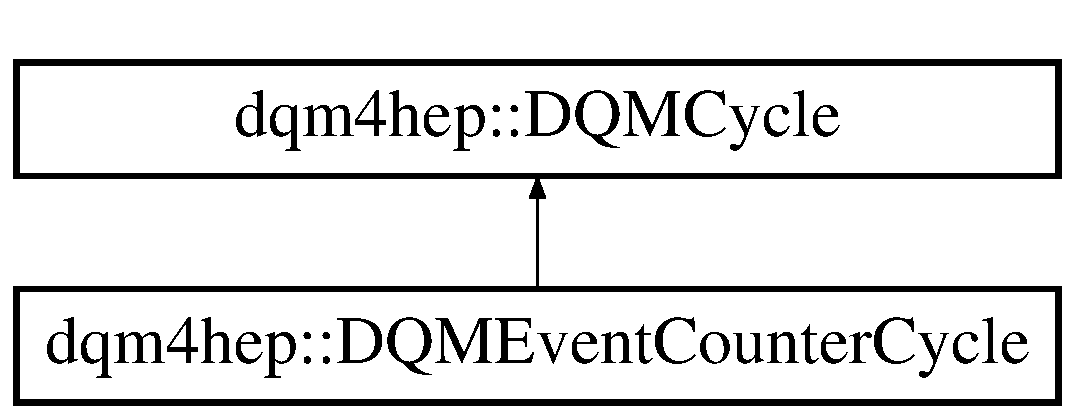
\includegraphics[height=2.000000cm]{classdqm4hep_1_1DQMEventCounterCycle}
\end{center}
\end{figure}
\subsection*{Public Member Functions}
\begin{DoxyCompactItemize}
\item 
{\bf D\+Q\+M\+Event\+Counter\+Cycle} ()
\begin{DoxyCompactList}\small\item\em Constructor. \end{DoxyCompactList}\item 
{\bf $\sim$\+D\+Q\+M\+Event\+Counter\+Cycle} ()
\begin{DoxyCompactList}\small\item\em Destructor. \end{DoxyCompactList}\item 
void {\bf on\+Cycle\+Started} ()
\begin{DoxyCompactList}\small\item\em Specific call back function when a cycle is stopped. \end{DoxyCompactList}\item 
void {\bf on\+Cycle\+Stopped} ()
\begin{DoxyCompactList}\small\item\em Specific call back function when a cycle is stopped. \end{DoxyCompactList}\item 
void {\bf on\+Event\+Processed} (const {\bf D\+Q\+M\+Event} $\ast$const )
\begin{DoxyCompactList}\small\item\em Specific call back function when an event is processed, depends on cycle type. \end{DoxyCompactList}\item 
bool {\bf is\+End\+Of\+Cycle\+Reached} () const 
\begin{DoxyCompactList}\small\item\em Specific function to tell the application to know whether the cycle has reached the end. \end{DoxyCompactList}\end{DoxyCompactItemize}


\subsection{Detailed Description}
\doxyref{D\+Q\+M\+Event\+Counter\+Cycle}{p.}{classdqm4hep_1_1DQMEventCounterCycle} class. 

Definition at line 40 of file D\+Q\+M\+Event\+Counter\+Cycle.\+h.



\subsection{Constructor \& Destructor Documentation}
\index{dqm4hep\+::\+D\+Q\+M\+Event\+Counter\+Cycle@{dqm4hep\+::\+D\+Q\+M\+Event\+Counter\+Cycle}!D\+Q\+M\+Event\+Counter\+Cycle@{D\+Q\+M\+Event\+Counter\+Cycle}}
\index{D\+Q\+M\+Event\+Counter\+Cycle@{D\+Q\+M\+Event\+Counter\+Cycle}!dqm4hep\+::\+D\+Q\+M\+Event\+Counter\+Cycle@{dqm4hep\+::\+D\+Q\+M\+Event\+Counter\+Cycle}}
\subsubsection[{D\+Q\+M\+Event\+Counter\+Cycle}]{\setlength{\rightskip}{0pt plus 5cm}dqm4hep\+::\+D\+Q\+M\+Event\+Counter\+Cycle\+::\+D\+Q\+M\+Event\+Counter\+Cycle (
\begin{DoxyParamCaption}
{}
\end{DoxyParamCaption}
)}\label{classdqm4hep_1_1DQMEventCounterCycle_a4e3141a8ad947fce074400f344fb8a86}


Constructor. 



Definition at line 40 of file D\+Q\+M\+Event\+Counter\+Cycle.\+cc.


\begin{DoxyCode}
40                                            :
41     DQMCycle()
42 \{
43   \textcolor{comment}{// default value}
44   setCycleValue(100);
45 \}
\end{DoxyCode}
\index{dqm4hep\+::\+D\+Q\+M\+Event\+Counter\+Cycle@{dqm4hep\+::\+D\+Q\+M\+Event\+Counter\+Cycle}!````~D\+Q\+M\+Event\+Counter\+Cycle@{$\sim$\+D\+Q\+M\+Event\+Counter\+Cycle}}
\index{````~D\+Q\+M\+Event\+Counter\+Cycle@{$\sim$\+D\+Q\+M\+Event\+Counter\+Cycle}!dqm4hep\+::\+D\+Q\+M\+Event\+Counter\+Cycle@{dqm4hep\+::\+D\+Q\+M\+Event\+Counter\+Cycle}}
\subsubsection[{$\sim$\+D\+Q\+M\+Event\+Counter\+Cycle}]{\setlength{\rightskip}{0pt plus 5cm}dqm4hep\+::\+D\+Q\+M\+Event\+Counter\+Cycle\+::$\sim$\+D\+Q\+M\+Event\+Counter\+Cycle (
\begin{DoxyParamCaption}
{}
\end{DoxyParamCaption}
)}\label{classdqm4hep_1_1DQMEventCounterCycle_a45c712eedc2265c41c81ea3301f1b2a4}


Destructor. 



Definition at line 49 of file D\+Q\+M\+Event\+Counter\+Cycle.\+cc.


\begin{DoxyCode}
50 \{
51   \textcolor{comment}{/* nop */}
52 \}
\end{DoxyCode}


\subsection{Member Function Documentation}
\index{dqm4hep\+::\+D\+Q\+M\+Event\+Counter\+Cycle@{dqm4hep\+::\+D\+Q\+M\+Event\+Counter\+Cycle}!is\+End\+Of\+Cycle\+Reached@{is\+End\+Of\+Cycle\+Reached}}
\index{is\+End\+Of\+Cycle\+Reached@{is\+End\+Of\+Cycle\+Reached}!dqm4hep\+::\+D\+Q\+M\+Event\+Counter\+Cycle@{dqm4hep\+::\+D\+Q\+M\+Event\+Counter\+Cycle}}
\subsubsection[{is\+End\+Of\+Cycle\+Reached}]{\setlength{\rightskip}{0pt plus 5cm}bool dqm4hep\+::\+D\+Q\+M\+Event\+Counter\+Cycle\+::is\+End\+Of\+Cycle\+Reached (
\begin{DoxyParamCaption}
{}
\end{DoxyParamCaption}
) const\hspace{0.3cm}{\ttfamily [virtual]}}\label{classdqm4hep_1_1DQMEventCounterCycle_a2b36be8cb34b293b7598cfebb8e2675c}


Specific function to tell the application to know whether the cycle has reached the end. 



Implements {\bf dqm4hep\+::\+D\+Q\+M\+Cycle} \doxyref{}{p.}{classdqm4hep_1_1DQMCycle_a2b177a69fc0585fbef12dda7b54065d5}.



Definition at line 56 of file D\+Q\+M\+Event\+Counter\+Cycle.\+cc.



References dqm4hep\+::\+D\+Q\+M\+Cycle\+::get\+Cycle\+Value(), and dqm4hep\+::\+D\+Q\+M\+Cycle\+::get\+N\+Processed\+Events().


\begin{DoxyCode}
57 \{
58   \textcolor{keywordflow}{if}( this->getNProcessedEvents() >= static\_cast<unsigned int>(this->
      getCycleValue()) )
59     \textcolor{keywordflow}{return} \textcolor{keyword}{true};
60 
61   \textcolor{keywordflow}{return} \textcolor{keyword}{false};
62 \}
\end{DoxyCode}
\index{dqm4hep\+::\+D\+Q\+M\+Event\+Counter\+Cycle@{dqm4hep\+::\+D\+Q\+M\+Event\+Counter\+Cycle}!on\+Cycle\+Started@{on\+Cycle\+Started}}
\index{on\+Cycle\+Started@{on\+Cycle\+Started}!dqm4hep\+::\+D\+Q\+M\+Event\+Counter\+Cycle@{dqm4hep\+::\+D\+Q\+M\+Event\+Counter\+Cycle}}
\subsubsection[{on\+Cycle\+Started}]{\setlength{\rightskip}{0pt plus 5cm}void dqm4hep\+::\+D\+Q\+M\+Event\+Counter\+Cycle\+::on\+Cycle\+Started (
\begin{DoxyParamCaption}
{}
\end{DoxyParamCaption}
)\hspace{0.3cm}{\ttfamily [inline]}, {\ttfamily [virtual]}}\label{classdqm4hep_1_1DQMEventCounterCycle_a50af57684ff7a09ff91370d3b1250040}


Specific call back function when a cycle is stopped. 



Implements {\bf dqm4hep\+::\+D\+Q\+M\+Cycle} \doxyref{}{p.}{classdqm4hep_1_1DQMCycle_a9ee9c093280a5c87802529233f7ef97d}.



Definition at line 51 of file D\+Q\+M\+Event\+Counter\+Cycle.\+h.


\begin{DoxyCode}
51 \{ \textcolor{comment}{/* nop */} \}
\end{DoxyCode}
\index{dqm4hep\+::\+D\+Q\+M\+Event\+Counter\+Cycle@{dqm4hep\+::\+D\+Q\+M\+Event\+Counter\+Cycle}!on\+Cycle\+Stopped@{on\+Cycle\+Stopped}}
\index{on\+Cycle\+Stopped@{on\+Cycle\+Stopped}!dqm4hep\+::\+D\+Q\+M\+Event\+Counter\+Cycle@{dqm4hep\+::\+D\+Q\+M\+Event\+Counter\+Cycle}}
\subsubsection[{on\+Cycle\+Stopped}]{\setlength{\rightskip}{0pt plus 5cm}void dqm4hep\+::\+D\+Q\+M\+Event\+Counter\+Cycle\+::on\+Cycle\+Stopped (
\begin{DoxyParamCaption}
{}
\end{DoxyParamCaption}
)\hspace{0.3cm}{\ttfamily [inline]}, {\ttfamily [virtual]}}\label{classdqm4hep_1_1DQMEventCounterCycle_afae6e5fb980fc77e20dafc5d0769a392}


Specific call back function when a cycle is stopped. 



Implements {\bf dqm4hep\+::\+D\+Q\+M\+Cycle} \doxyref{}{p.}{classdqm4hep_1_1DQMCycle_a9563479df6411c34811e820d49dc242f}.



Definition at line 52 of file D\+Q\+M\+Event\+Counter\+Cycle.\+h.


\begin{DoxyCode}
52 \{ \textcolor{comment}{/* nop */} \}
\end{DoxyCode}
\index{dqm4hep\+::\+D\+Q\+M\+Event\+Counter\+Cycle@{dqm4hep\+::\+D\+Q\+M\+Event\+Counter\+Cycle}!on\+Event\+Processed@{on\+Event\+Processed}}
\index{on\+Event\+Processed@{on\+Event\+Processed}!dqm4hep\+::\+D\+Q\+M\+Event\+Counter\+Cycle@{dqm4hep\+::\+D\+Q\+M\+Event\+Counter\+Cycle}}
\subsubsection[{on\+Event\+Processed}]{\setlength{\rightskip}{0pt plus 5cm}void dqm4hep\+::\+D\+Q\+M\+Event\+Counter\+Cycle\+::on\+Event\+Processed (
\begin{DoxyParamCaption}
\item[{const {\bf D\+Q\+M\+Event} $\ast$}]{p\+Event}
\end{DoxyParamCaption}
)\hspace{0.3cm}{\ttfamily [inline]}, {\ttfamily [virtual]}}\label{classdqm4hep_1_1DQMEventCounterCycle_a6bce65f8d3a5331d96868dd28931c842}


Specific call back function when an event is processed, depends on cycle type. 



Implements {\bf dqm4hep\+::\+D\+Q\+M\+Cycle} \doxyref{}{p.}{classdqm4hep_1_1DQMCycle_a98871dce48f954a8299a8f130125ad59}.



Definition at line 53 of file D\+Q\+M\+Event\+Counter\+Cycle.\+h.


\begin{DoxyCode}
53 \{ \textcolor{comment}{/* nop */} \}
\end{DoxyCode}


The documentation for this class was generated from the following files\+:\begin{DoxyCompactItemize}
\item 
{\bf D\+Q\+M\+Event\+Counter\+Cycle.\+h}\item 
{\bf D\+Q\+M\+Event\+Counter\+Cycle.\+cc}\end{DoxyCompactItemize}

\section{dqm4hep\+:\+:D\+Q\+M\+Event\+Streamer Class Reference}
\label{classdqm4hep_1_1DQMEventStreamer}\index{dqm4hep\+::\+D\+Q\+M\+Event\+Streamer@{dqm4hep\+::\+D\+Q\+M\+Event\+Streamer}}


\doxyref{D\+Q\+M\+Event\+Streamer}{p.}{classdqm4hep_1_1DQMEventStreamer} class.  




{\ttfamily \#include $<$D\+Q\+M\+Event\+Streamer.\+h$>$}

Inheritance diagram for dqm4hep\+:\+:D\+Q\+M\+Event\+Streamer\+:\begin{figure}[H]
\begin{center}
\leavevmode
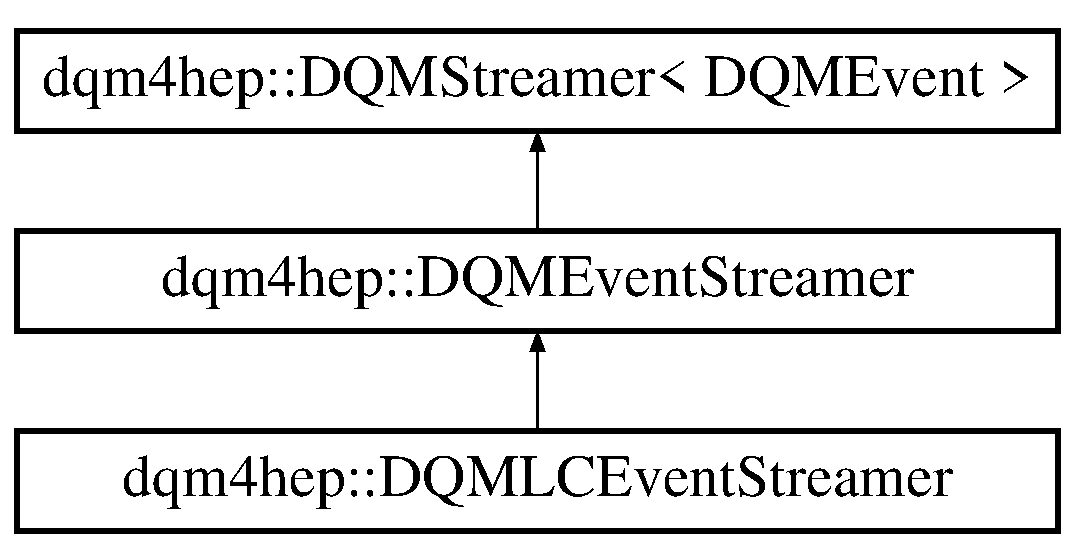
\includegraphics[height=3.000000cm]{classdqm4hep_1_1DQMEventStreamer}
\end{center}
\end{figure}
\subsection*{Public Member Functions}
\begin{DoxyCompactItemize}
\item 
virtual {\bf $\sim$\+D\+Q\+M\+Event\+Streamer} ()
\begin{DoxyCompactList}\small\item\em Destructor. \end{DoxyCompactList}\item 
virtual {\bf Status\+Code} {\bf serialize} (const {\bf D\+Q\+M\+Event} $\ast$const p\+Object, {\bf D\+Q\+M\+Data\+Stream} $\ast$const p\+Data\+Stream)=0
\begin{DoxyCompactList}\small\item\em Serialize a \doxyref{D\+Q\+M\+Event}{p.}{classdqm4hep_1_1DQMEvent} object and store it in the data stream. \end{DoxyCompactList}\item 
virtual {\bf Status\+Code} {\bf deserialize} ({\bf D\+Q\+M\+Event} $\ast$\&p\+Object, {\bf D\+Q\+M\+Data\+Stream} $\ast$const p\+Data\+Stream)=0
\begin{DoxyCompactList}\small\item\em De-\/serialize a \doxyref{D\+Q\+M\+Event}{p.}{classdqm4hep_1_1DQMEvent} given from the data stream. \end{DoxyCompactList}\item 
virtual {\bf Status\+Code} {\bf serialize} (const {\bf D\+Q\+M\+Event} $\ast$const p\+Object, const std\+::string \&sub\+Event\+Identifier, {\bf D\+Q\+M\+Data\+Stream} $\ast$const p\+Data\+Stream)=0
\begin{DoxyCompactList}\small\item\em Serialize a part of a \doxyref{D\+Q\+M\+Event}{p.}{classdqm4hep_1_1DQMEvent} object identified by the reg exp 'sub\+Event\+Identifier' and store it in the data stream. \end{DoxyCompactList}\end{DoxyCompactItemize}


\subsection{Detailed Description}
\doxyref{D\+Q\+M\+Event\+Streamer}{p.}{classdqm4hep_1_1DQMEventStreamer} class. 

Definition at line 41 of file D\+Q\+M\+Event\+Streamer.\+h.



\subsection{Constructor \& Destructor Documentation}
\index{dqm4hep\+::\+D\+Q\+M\+Event\+Streamer@{dqm4hep\+::\+D\+Q\+M\+Event\+Streamer}!````~D\+Q\+M\+Event\+Streamer@{$\sim$\+D\+Q\+M\+Event\+Streamer}}
\index{````~D\+Q\+M\+Event\+Streamer@{$\sim$\+D\+Q\+M\+Event\+Streamer}!dqm4hep\+::\+D\+Q\+M\+Event\+Streamer@{dqm4hep\+::\+D\+Q\+M\+Event\+Streamer}}
\subsubsection[{$\sim$\+D\+Q\+M\+Event\+Streamer}]{\setlength{\rightskip}{0pt plus 5cm}virtual dqm4hep\+::\+D\+Q\+M\+Event\+Streamer\+::$\sim$\+D\+Q\+M\+Event\+Streamer (
\begin{DoxyParamCaption}
{}
\end{DoxyParamCaption}
)\hspace{0.3cm}{\ttfamily [inline]}, {\ttfamily [virtual]}}\label{classdqm4hep_1_1DQMEventStreamer_ae17d9b98e09dacc41ccbd3ec40fe1c30}


Destructor. 



Definition at line 46 of file D\+Q\+M\+Event\+Streamer.\+h.


\begin{DoxyCode}
46 \{\}
\end{DoxyCode}


\subsection{Member Function Documentation}
\index{dqm4hep\+::\+D\+Q\+M\+Event\+Streamer@{dqm4hep\+::\+D\+Q\+M\+Event\+Streamer}!deserialize@{deserialize}}
\index{deserialize@{deserialize}!dqm4hep\+::\+D\+Q\+M\+Event\+Streamer@{dqm4hep\+::\+D\+Q\+M\+Event\+Streamer}}
\subsubsection[{deserialize}]{\setlength{\rightskip}{0pt plus 5cm}virtual {\bf Status\+Code} dqm4hep\+::\+D\+Q\+M\+Event\+Streamer\+::deserialize (
\begin{DoxyParamCaption}
\item[{{\bf D\+Q\+M\+Event} $\ast$\&}]{p\+Object, }
\item[{{\bf D\+Q\+M\+Data\+Stream} $\ast$const}]{p\+Data\+Stream}
\end{DoxyParamCaption}
)\hspace{0.3cm}{\ttfamily [pure virtual]}}\label{classdqm4hep_1_1DQMEventStreamer_a063e71f73dd06404b736438c3f42b602}


De-\/serialize a \doxyref{D\+Q\+M\+Event}{p.}{classdqm4hep_1_1DQMEvent} given from the data stream. 



Implements {\bf dqm4hep\+::\+D\+Q\+M\+Streamer$<$ D\+Q\+M\+Event $>$} \doxyref{}{p.}{singletondqm4hep_1_1DQMStreamer_a45424f285015b093ccbd7bfd3a38249d}.



Implemented in {\bf dqm4hep\+::\+D\+Q\+M\+L\+C\+Event\+Streamer} \doxyref{}{p.}{classdqm4hep_1_1DQMLCEventStreamer_a9f54db23849818556fe1c898d1019b17}.



Referenced by dqm4hep\+::\+D\+Q\+M\+Dim\+Event\+Collector\+::handle\+Event\+Reception(), and dqm4hep\+::\+D\+Q\+M\+Dim\+Event\+Client\+::query\+Event().

\index{dqm4hep\+::\+D\+Q\+M\+Event\+Streamer@{dqm4hep\+::\+D\+Q\+M\+Event\+Streamer}!serialize@{serialize}}
\index{serialize@{serialize}!dqm4hep\+::\+D\+Q\+M\+Event\+Streamer@{dqm4hep\+::\+D\+Q\+M\+Event\+Streamer}}
\subsubsection[{serialize}]{\setlength{\rightskip}{0pt plus 5cm}virtual {\bf Status\+Code} dqm4hep\+::\+D\+Q\+M\+Event\+Streamer\+::serialize (
\begin{DoxyParamCaption}
\item[{const {\bf D\+Q\+M\+Event} $\ast$const}]{p\+Object, }
\item[{{\bf D\+Q\+M\+Data\+Stream} $\ast$const}]{p\+Data\+Stream}
\end{DoxyParamCaption}
)\hspace{0.3cm}{\ttfamily [pure virtual]}}\label{classdqm4hep_1_1DQMEventStreamer_a9f6ffa9b9977ca02564bb0c8cd248be4}


Serialize a \doxyref{D\+Q\+M\+Event}{p.}{classdqm4hep_1_1DQMEvent} object and store it in the data stream. 



Implements {\bf dqm4hep\+::\+D\+Q\+M\+Streamer$<$ D\+Q\+M\+Event $>$} \doxyref{}{p.}{singletondqm4hep_1_1DQMStreamer_abc54751ecafff0a88046f41fa4110fcf}.



Implemented in {\bf dqm4hep\+::\+D\+Q\+M\+L\+C\+Event\+Streamer} \doxyref{}{p.}{classdqm4hep_1_1DQMLCEventStreamer_a308293cdebf98ee5dcfbad4c34f31d38}.



Referenced by dqm4hep\+::\+D\+Q\+M\+Dim\+Event\+Collector\+::handle\+Event\+Request(), and dqm4hep\+::\+D\+Q\+M\+Dim\+Event\+Collector\+::update\+Event\+Service().

\index{dqm4hep\+::\+D\+Q\+M\+Event\+Streamer@{dqm4hep\+::\+D\+Q\+M\+Event\+Streamer}!serialize@{serialize}}
\index{serialize@{serialize}!dqm4hep\+::\+D\+Q\+M\+Event\+Streamer@{dqm4hep\+::\+D\+Q\+M\+Event\+Streamer}}
\subsubsection[{serialize}]{\setlength{\rightskip}{0pt plus 5cm}virtual {\bf Status\+Code} dqm4hep\+::\+D\+Q\+M\+Event\+Streamer\+::serialize (
\begin{DoxyParamCaption}
\item[{const {\bf D\+Q\+M\+Event} $\ast$const}]{p\+Object, }
\item[{const std\+::string \&}]{sub\+Event\+Identifier, }
\item[{{\bf D\+Q\+M\+Data\+Stream} $\ast$const}]{p\+Data\+Stream}
\end{DoxyParamCaption}
)\hspace{0.3cm}{\ttfamily [pure virtual]}}\label{classdqm4hep_1_1DQMEventStreamer_a015898c0d96bdbcb523fa54431fb2a45}


Serialize a part of a \doxyref{D\+Q\+M\+Event}{p.}{classdqm4hep_1_1DQMEvent} object identified by the reg exp 'sub\+Event\+Identifier' and store it in the data stream. 

Example \+: sub\+Event\+Identifier = \char`\"{}\+My\+Collection1\+:\+My\+Collection2\char`\"{} sub\+Event\+Identifier = \char`\"{}$\ast$\+Tpc\+Collection\char`\"{}

The identifier decoding has to be performed by the user, based on the event contents itself 

Implemented in {\bf dqm4hep\+::\+D\+Q\+M\+L\+C\+Event\+Streamer} \doxyref{}{p.}{classdqm4hep_1_1DQMLCEventStreamer_afabcb0328b2d2be0e9c08ef38a5c81f3}.



The documentation for this class was generated from the following file\+:\begin{DoxyCompactItemize}
\item 
{\bf D\+Q\+M\+Event\+Streamer.\+h}\end{DoxyCompactItemize}

\section{dqm4hep\+:\+:D\+Q\+M\+File\+Handler Class Reference}
\label{classdqm4hep_1_1DQMFileHandler}\index{dqm4hep\+::\+D\+Q\+M\+File\+Handler@{dqm4hep\+::\+D\+Q\+M\+File\+Handler}}


\doxyref{D\+Q\+M\+File\+Handler}{p.}{classdqm4hep_1_1DQMFileHandler} interface.  




{\ttfamily \#include $<$D\+Q\+M\+File\+Handler.\+h$>$}

Inheritance diagram for dqm4hep\+:\+:D\+Q\+M\+File\+Handler\+:\begin{figure}[H]
\begin{center}
\leavevmode
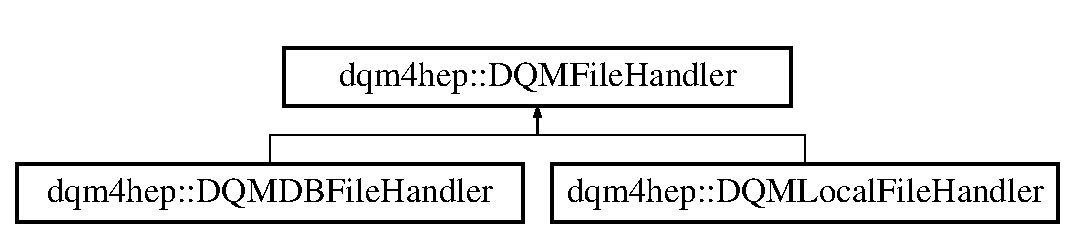
\includegraphics[height=2.000000cm]{classdqm4hep_1_1DQMFileHandler}
\end{center}
\end{figure}
\subsection*{Public Member Functions}
\begin{DoxyCompactItemize}
\item 
virtual {\bf $\sim$\+D\+Q\+M\+File\+Handler} ()
\begin{DoxyCompactList}\small\item\em Destructor. \end{DoxyCompactList}\item 
virtual const std\+::string \& {\bf type} () const =0
\begin{DoxyCompactList}\small\item\em Get the file handler type as string. \end{DoxyCompactList}\item 
virtual {\bf Status\+Code} {\bf download} (const std\+::string \&pattern)=0
\begin{DoxyCompactList}\small\item\em Download the file locally using the target pattern. \end{DoxyCompactList}\item 
virtual const std\+::string \& {\bf get\+Local\+File\+Name} () const =0
\begin{DoxyCompactList}\small\item\em Get the full file name after the download step. \end{DoxyCompactList}\end{DoxyCompactItemize}


\subsection{Detailed Description}
\doxyref{D\+Q\+M\+File\+Handler}{p.}{classdqm4hep_1_1DQMFileHandler} interface. 

Definition at line 39 of file D\+Q\+M\+File\+Handler.\+h.



\subsection{Constructor \& Destructor Documentation}
\index{dqm4hep\+::\+D\+Q\+M\+File\+Handler@{dqm4hep\+::\+D\+Q\+M\+File\+Handler}!````~D\+Q\+M\+File\+Handler@{$\sim$\+D\+Q\+M\+File\+Handler}}
\index{````~D\+Q\+M\+File\+Handler@{$\sim$\+D\+Q\+M\+File\+Handler}!dqm4hep\+::\+D\+Q\+M\+File\+Handler@{dqm4hep\+::\+D\+Q\+M\+File\+Handler}}
\subsubsection[{$\sim$\+D\+Q\+M\+File\+Handler}]{\setlength{\rightskip}{0pt plus 5cm}virtual dqm4hep\+::\+D\+Q\+M\+File\+Handler\+::$\sim$\+D\+Q\+M\+File\+Handler (
\begin{DoxyParamCaption}
{}
\end{DoxyParamCaption}
)\hspace{0.3cm}{\ttfamily [inline]}, {\ttfamily [virtual]}}\label{classdqm4hep_1_1DQMFileHandler_ae419aadf73021a9ad8898a07cce5b204}


Destructor. 



Definition at line 44 of file D\+Q\+M\+File\+Handler.\+h.


\begin{DoxyCode}
44 \{\}
\end{DoxyCode}


\subsection{Member Function Documentation}
\index{dqm4hep\+::\+D\+Q\+M\+File\+Handler@{dqm4hep\+::\+D\+Q\+M\+File\+Handler}!download@{download}}
\index{download@{download}!dqm4hep\+::\+D\+Q\+M\+File\+Handler@{dqm4hep\+::\+D\+Q\+M\+File\+Handler}}
\subsubsection[{download}]{\setlength{\rightskip}{0pt plus 5cm}virtual {\bf Status\+Code} dqm4hep\+::\+D\+Q\+M\+File\+Handler\+::download (
\begin{DoxyParamCaption}
\item[{const std\+::string \&}]{pattern}
\end{DoxyParamCaption}
)\hspace{0.3cm}{\ttfamily [pure virtual]}}\label{classdqm4hep_1_1DQMFileHandler_afc41f890cb9390e88fb0c79a991cc270}


Download the file locally using the target pattern. 



Implemented in {\bf dqm4hep\+::\+D\+Q\+M\+D\+B\+File\+Handler} \doxyref{}{p.}{classdqm4hep_1_1DQMDBFileHandler_a598f1400a750b95348169db1337cfb5f}, and {\bf dqm4hep\+::\+D\+Q\+M\+Local\+File\+Handler} \doxyref{}{p.}{classdqm4hep_1_1DQMLocalFileHandler_aecbd2ba5e8a920b641d0d47b104349d1}.



Referenced by dqm4hep\+::\+D\+Q\+M\+Standalone\+Module\+Application\+::read\+Settings(), and dqm4hep\+::\+D\+Q\+M\+Analysis\+Module\+Application\+::read\+Settings().

\index{dqm4hep\+::\+D\+Q\+M\+File\+Handler@{dqm4hep\+::\+D\+Q\+M\+File\+Handler}!get\+Local\+File\+Name@{get\+Local\+File\+Name}}
\index{get\+Local\+File\+Name@{get\+Local\+File\+Name}!dqm4hep\+::\+D\+Q\+M\+File\+Handler@{dqm4hep\+::\+D\+Q\+M\+File\+Handler}}
\subsubsection[{get\+Local\+File\+Name}]{\setlength{\rightskip}{0pt plus 5cm}virtual const std\+::string\& dqm4hep\+::\+D\+Q\+M\+File\+Handler\+::get\+Local\+File\+Name (
\begin{DoxyParamCaption}
{}
\end{DoxyParamCaption}
) const\hspace{0.3cm}{\ttfamily [pure virtual]}}\label{classdqm4hep_1_1DQMFileHandler_a5a6dfa3bfb3965f897a1b7ee60f24ed8}


Get the full file name after the download step. 



Implemented in {\bf dqm4hep\+::\+D\+Q\+M\+D\+B\+File\+Handler} \doxyref{}{p.}{classdqm4hep_1_1DQMDBFileHandler_a192527a0753ae800575c1712f97ce196}, and {\bf dqm4hep\+::\+D\+Q\+M\+Local\+File\+Handler} \doxyref{}{p.}{classdqm4hep_1_1DQMLocalFileHandler_ab8926e367e5992de8fb2ccb935b432c1}.



Referenced by dqm4hep\+::\+D\+Q\+M\+Standalone\+Module\+Application\+::read\+Settings(), and dqm4hep\+::\+D\+Q\+M\+Analysis\+Module\+Application\+::read\+Settings().

\index{dqm4hep\+::\+D\+Q\+M\+File\+Handler@{dqm4hep\+::\+D\+Q\+M\+File\+Handler}!type@{type}}
\index{type@{type}!dqm4hep\+::\+D\+Q\+M\+File\+Handler@{dqm4hep\+::\+D\+Q\+M\+File\+Handler}}
\subsubsection[{type}]{\setlength{\rightskip}{0pt plus 5cm}virtual const std\+::string\& dqm4hep\+::\+D\+Q\+M\+File\+Handler\+::type (
\begin{DoxyParamCaption}
{}
\end{DoxyParamCaption}
) const\hspace{0.3cm}{\ttfamily [pure virtual]}}\label{classdqm4hep_1_1DQMFileHandler_adb64ac2dba492916a7e6105eacfc6837}


Get the file handler type as string. 



Implemented in {\bf dqm4hep\+::\+D\+Q\+M\+D\+B\+File\+Handler} \doxyref{}{p.}{classdqm4hep_1_1DQMDBFileHandler_ab681c7360694b65b36ac07bf2eb80231}, and {\bf dqm4hep\+::\+D\+Q\+M\+Local\+File\+Handler} \doxyref{}{p.}{classdqm4hep_1_1DQMLocalFileHandler_ae6b4b96b530e94ca376cbc91422bd8f6}.



The documentation for this class was generated from the following file\+:\begin{DoxyCompactItemize}
\item 
{\bf D\+Q\+M\+File\+Handler.\+h}\end{DoxyCompactItemize}

\section{dqm4hep\+:\+:D\+Q\+M\+File\+Handler\+Factory Class Reference}
\label{classdqm4hep_1_1DQMFileHandlerFactory}\index{dqm4hep\+::\+D\+Q\+M\+File\+Handler\+Factory@{dqm4hep\+::\+D\+Q\+M\+File\+Handler\+Factory}}


\doxyref{D\+Q\+M\+File\+Handler\+Factory}{p.}{classdqm4hep_1_1DQMFileHandlerFactory} class.  




{\ttfamily \#include $<$D\+Q\+M\+File\+Handler\+Factory.\+h$>$}

\subsection*{Public Member Functions}
\begin{DoxyCompactItemize}
\item 
{\bf D\+Q\+M\+File\+Handler\+Factory} ()
\begin{DoxyCompactList}\small\item\em Constructor. \end{DoxyCompactList}\item 
{\bf D\+Q\+M\+File\+Handler} $\ast$ {\bf create\+File\+Handler} (const std\+::string \&file\+Handler\+Type) const 
\begin{DoxyCompactList}\small\item\em Create a file handler with target type. \end{DoxyCompactList}\end{DoxyCompactItemize}


\subsection{Detailed Description}
\doxyref{D\+Q\+M\+File\+Handler\+Factory}{p.}{classdqm4hep_1_1DQMFileHandlerFactory} class. 

Definition at line 42 of file D\+Q\+M\+File\+Handler\+Factory.\+h.



\subsection{Constructor \& Destructor Documentation}
\index{dqm4hep\+::\+D\+Q\+M\+File\+Handler\+Factory@{dqm4hep\+::\+D\+Q\+M\+File\+Handler\+Factory}!D\+Q\+M\+File\+Handler\+Factory@{D\+Q\+M\+File\+Handler\+Factory}}
\index{D\+Q\+M\+File\+Handler\+Factory@{D\+Q\+M\+File\+Handler\+Factory}!dqm4hep\+::\+D\+Q\+M\+File\+Handler\+Factory@{dqm4hep\+::\+D\+Q\+M\+File\+Handler\+Factory}}
\subsubsection[{D\+Q\+M\+File\+Handler\+Factory}]{\setlength{\rightskip}{0pt plus 5cm}dqm4hep\+::\+D\+Q\+M\+File\+Handler\+Factory\+::\+D\+Q\+M\+File\+Handler\+Factory (
\begin{DoxyParamCaption}
{}
\end{DoxyParamCaption}
)}\label{classdqm4hep_1_1DQMFileHandlerFactory_a434b6c2744dbd5f0da918591839843e2}


Constructor. 



Definition at line 37 of file D\+Q\+M\+File\+Handler\+Factory.\+cc.


\begin{DoxyCode}
38 \{
39   \textcolor{comment}{/* nop */}
40 \}
\end{DoxyCode}


\subsection{Member Function Documentation}
\index{dqm4hep\+::\+D\+Q\+M\+File\+Handler\+Factory@{dqm4hep\+::\+D\+Q\+M\+File\+Handler\+Factory}!create\+File\+Handler@{create\+File\+Handler}}
\index{create\+File\+Handler@{create\+File\+Handler}!dqm4hep\+::\+D\+Q\+M\+File\+Handler\+Factory@{dqm4hep\+::\+D\+Q\+M\+File\+Handler\+Factory}}
\subsubsection[{create\+File\+Handler}]{\setlength{\rightskip}{0pt plus 5cm}{\bf D\+Q\+M\+File\+Handler} $\ast$ dqm4hep\+::\+D\+Q\+M\+File\+Handler\+Factory\+::create\+File\+Handler (
\begin{DoxyParamCaption}
\item[{const std\+::string \&}]{file\+Handler\+Type}
\end{DoxyParamCaption}
) const}\label{classdqm4hep_1_1DQMFileHandlerFactory_ae9869c36006001f0421b4d0c554ae22e}


Create a file handler with target type. 



Definition at line 44 of file D\+Q\+M\+File\+Handler\+Factory.\+cc.



Referenced by dqm4hep\+::\+D\+Q\+M\+Standalone\+Module\+Application\+::read\+Settings(), and dqm4hep\+::\+D\+Q\+M\+Analysis\+Module\+Application\+::read\+Settings().


\begin{DoxyCode}
45 \{
46   \textcolor{keywordflow}{if}(fileHandlerType == \textcolor{stringliteral}{"local"})
47     \textcolor{keywordflow}{return} \textcolor{keyword}{new} DQMLocalFileHandler();
48   \textcolor{keywordflow}{else} \textcolor{keywordflow}{if}(fileHandlerType == \textcolor{stringliteral}{"db"})
49     \textcolor{keywordflow}{return} \textcolor{keyword}{new} DQMDBFileHandler();
50   \textcolor{keywordflow}{else}
51     \textcolor{keywordflow}{return} \textcolor{keyword}{new} DQMLocalFileHandler();
52 \}
\end{DoxyCode}


The documentation for this class was generated from the following files\+:\begin{DoxyCompactItemize}
\item 
{\bf D\+Q\+M\+File\+Handler\+Factory.\+h}\item 
{\bf D\+Q\+M\+File\+Handler\+Factory.\+cc}\end{DoxyCompactItemize}

\section{dqm4hep\+:\+:D\+Q\+M\+L\+C\+Collection\+Streamer Class Reference}
\label{classdqm4hep_1_1DQMLCCollectionStreamer}\index{dqm4hep\+::\+D\+Q\+M\+L\+C\+Collection\+Streamer@{dqm4hep\+::\+D\+Q\+M\+L\+C\+Collection\+Streamer}}


\doxyref{D\+Q\+M\+L\+C\+Collection\+Streamer}{p.}{classdqm4hep_1_1DQMLCCollectionStreamer} class.  




{\ttfamily \#include $<$D\+Q\+M\+L\+C\+Event\+Streamer.\+h$>$}

Inheritance diagram for dqm4hep\+:\+:D\+Q\+M\+L\+C\+Collection\+Streamer\+:\begin{figure}[H]
\begin{center}
\leavevmode
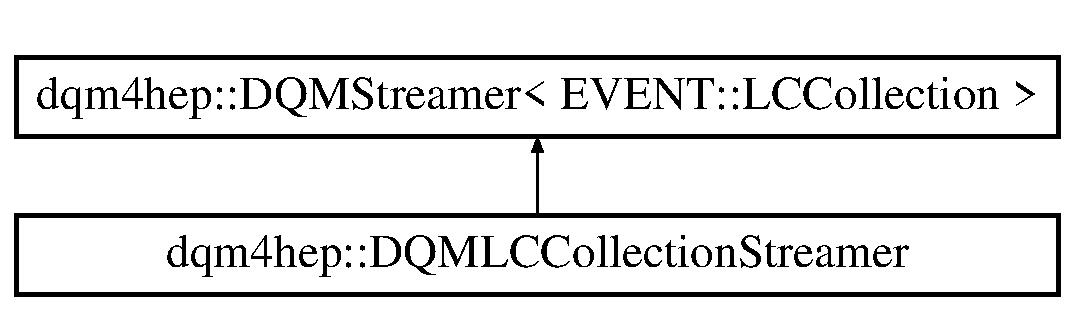
\includegraphics[height=2.000000cm]{classdqm4hep_1_1DQMLCCollectionStreamer}
\end{center}
\end{figure}
\subsection*{Public Member Functions}
\begin{DoxyCompactItemize}
\item 
{\bf D\+Q\+M\+L\+C\+Collection\+Streamer} (const std\+::string \&collection\+Type, {\bf D\+Q\+M\+L\+C\+Object\+Streamer} $\ast$p\+L\+C\+Object\+Streamer)
\begin{DoxyCompactList}\small\item\em Constructor with a lc object streamer. \end{DoxyCompactList}\item 
{\bf $\sim$\+D\+Q\+M\+L\+C\+Collection\+Streamer} ()
\begin{DoxyCompactList}\small\item\em Destructor. \end{DoxyCompactList}\item 
{\bf Status\+Code} {\bf serialize} (const E\+V\+E\+N\+T\+::\+L\+C\+Collection $\ast$const p\+L\+C\+Collection, {\bf D\+Q\+M\+Data\+Stream} $\ast$const p\+Data\+Stream)
\begin{DoxyCompactList}\small\item\em Serialize an L\+C\+Collection. \end{DoxyCompactList}\item 
{\bf Status\+Code} {\bf deserialize} (E\+V\+E\+N\+T\+::\+L\+C\+Collection $\ast$\&p\+L\+C\+Collection, {\bf D\+Q\+M\+Data\+Stream} $\ast$const p\+Data\+Stream)
\begin{DoxyCompactList}\small\item\em Deserialize an L\+C\+Collection. \end{DoxyCompactList}\end{DoxyCompactItemize}
\subsection*{Protected Attributes}
\begin{DoxyCompactItemize}
\item 
const std\+::string {\bf m\+\_\+collection\+Type}
\item 
{\bf D\+Q\+M\+L\+C\+Object\+Streamer} $\ast$ {\bf m\+\_\+p\+L\+C\+Object\+Streamer}
\item 
{\bf D\+Q\+M\+L\+C\+Parameters\+Streamer} {\bf m\+\_\+lc\+Parameters\+Streamer}
\end{DoxyCompactItemize}


\subsection{Detailed Description}
\doxyref{D\+Q\+M\+L\+C\+Collection\+Streamer}{p.}{classdqm4hep_1_1DQMLCCollectionStreamer} class. 

Definition at line 110 of file D\+Q\+M\+L\+C\+Event\+Streamer.\+h.



\subsection{Constructor \& Destructor Documentation}
\index{dqm4hep\+::\+D\+Q\+M\+L\+C\+Collection\+Streamer@{dqm4hep\+::\+D\+Q\+M\+L\+C\+Collection\+Streamer}!D\+Q\+M\+L\+C\+Collection\+Streamer@{D\+Q\+M\+L\+C\+Collection\+Streamer}}
\index{D\+Q\+M\+L\+C\+Collection\+Streamer@{D\+Q\+M\+L\+C\+Collection\+Streamer}!dqm4hep\+::\+D\+Q\+M\+L\+C\+Collection\+Streamer@{dqm4hep\+::\+D\+Q\+M\+L\+C\+Collection\+Streamer}}
\subsubsection[{D\+Q\+M\+L\+C\+Collection\+Streamer}]{\setlength{\rightskip}{0pt plus 5cm}dqm4hep\+::\+D\+Q\+M\+L\+C\+Collection\+Streamer\+::\+D\+Q\+M\+L\+C\+Collection\+Streamer (
\begin{DoxyParamCaption}
\item[{const std\+::string \&}]{collection\+Type, }
\item[{{\bf D\+Q\+M\+L\+C\+Object\+Streamer} $\ast$}]{p\+L\+C\+Object\+Streamer}
\end{DoxyParamCaption}
)}\label{classdqm4hep_1_1DQMLCCollectionStreamer_a7172343cd57554a46b0d9fa17d899956}


Constructor with a lc object streamer. 



Definition at line 490 of file D\+Q\+M\+L\+C\+Event\+Streamer.\+cc.


\begin{DoxyCode}
490                                                                                                            
                   :
491     m_collectionType(collectionType),
492     m_pLCObjectStreamer(pLCObjectStreamer)
493 \{
494   \textcolor{comment}{/* nop */}
495 \}
\end{DoxyCode}
\index{dqm4hep\+::\+D\+Q\+M\+L\+C\+Collection\+Streamer@{dqm4hep\+::\+D\+Q\+M\+L\+C\+Collection\+Streamer}!````~D\+Q\+M\+L\+C\+Collection\+Streamer@{$\sim$\+D\+Q\+M\+L\+C\+Collection\+Streamer}}
\index{````~D\+Q\+M\+L\+C\+Collection\+Streamer@{$\sim$\+D\+Q\+M\+L\+C\+Collection\+Streamer}!dqm4hep\+::\+D\+Q\+M\+L\+C\+Collection\+Streamer@{dqm4hep\+::\+D\+Q\+M\+L\+C\+Collection\+Streamer}}
\subsubsection[{$\sim$\+D\+Q\+M\+L\+C\+Collection\+Streamer}]{\setlength{\rightskip}{0pt plus 5cm}dqm4hep\+::\+D\+Q\+M\+L\+C\+Collection\+Streamer\+::$\sim$\+D\+Q\+M\+L\+C\+Collection\+Streamer (
\begin{DoxyParamCaption}
{}
\end{DoxyParamCaption}
)}\label{classdqm4hep_1_1DQMLCCollectionStreamer_afa297f5b34586ab7ccc18d1b3f85c202}


Destructor. 



Definition at line 499 of file D\+Q\+M\+L\+C\+Event\+Streamer.\+cc.



References m\+\_\+p\+L\+C\+Object\+Streamer.


\begin{DoxyCode}
500 \{
501   \textcolor{keyword}{delete} m_pLCObjectStreamer;
502 \}
\end{DoxyCode}


\subsection{Member Function Documentation}
\index{dqm4hep\+::\+D\+Q\+M\+L\+C\+Collection\+Streamer@{dqm4hep\+::\+D\+Q\+M\+L\+C\+Collection\+Streamer}!deserialize@{deserialize}}
\index{deserialize@{deserialize}!dqm4hep\+::\+D\+Q\+M\+L\+C\+Collection\+Streamer@{dqm4hep\+::\+D\+Q\+M\+L\+C\+Collection\+Streamer}}
\subsubsection[{deserialize}]{\setlength{\rightskip}{0pt plus 5cm}{\bf Status\+Code} dqm4hep\+::\+D\+Q\+M\+L\+C\+Collection\+Streamer\+::deserialize (
\begin{DoxyParamCaption}
\item[{E\+V\+E\+N\+T\+::\+L\+C\+Collection $\ast$\&}]{p\+L\+C\+Collection, }
\item[{{\bf D\+Q\+M\+Data\+Stream} $\ast$const}]{p\+Data\+Stream}
\end{DoxyParamCaption}
)\hspace{0.3cm}{\ttfamily [virtual]}}\label{classdqm4hep_1_1DQMLCCollectionStreamer_ac9ec8a358fab2039a620bbbefc6cbc7e}


Deserialize an L\+C\+Collection. 

The collection must be allocated in this function 

Implements {\bf dqm4hep\+::\+D\+Q\+M\+Streamer$<$ E\+V\+E\+N\+T\+::\+L\+C\+Collection $>$} \doxyref{}{p.}{singletondqm4hep_1_1DQMStreamer_a45424f285015b093ccbd7bfd3a38249d}.



Definition at line 539 of file D\+Q\+M\+L\+C\+Event\+Streamer.\+cc.



References dqm4hep\+::\+D\+Q\+M\+Streamer$<$ T $>$\+::deserialize(), dqm4hep\+::\+D\+Q\+M\+L\+C\+Parameters\+Streamer\+::deserialize(), m\+\_\+collection\+Type, m\+\_\+lc\+Parameters\+Streamer, m\+\_\+p\+L\+C\+Object\+Streamer, P\+R\+O\+C\+E\+S\+S\+\_\+\+C\+O\+D\+E\+\_\+\+I\+F\+\_\+\+A\+N\+D\+\_\+\+R\+E\+T\+U\+R\+N, dqm4hep\+::\+D\+Q\+M\+Data\+Stream\+::read(), and R\+E\+T\+U\+R\+N\+\_\+\+R\+E\+S\+U\+L\+T\+\_\+\+I\+F.


\begin{DoxyCode}
541 \{
542   pLCCollection = NULL;
543 
544   IMPL::LCCollectionVec *pTmpLCCollection = \textcolor{keyword}{new} IMPL::LCCollectionVec(
      m_collectionType);
545 
546   dqm_int flag = 0;
547   RETURN_RESULT_IF(STATUS\_CODE\_SUCCESS, !=, pDataStream->read(flag));
548   pTmpLCCollection->setFlag(flag);
549 
550   dqm_bool isTransient = \textcolor{keyword}{false};
551   RETURN_RESULT_IF(STATUS\_CODE\_SUCCESS, !=, pDataStream->read(isTransient));
552   pTmpLCCollection->setTransient(isTransient);
553 
554   dqm_bool isDefault = \textcolor{keyword}{false};
555   RETURN_RESULT_IF(STATUS\_CODE\_SUCCESS, !=, pDataStream->read(isDefault));
556   pTmpLCCollection->setDefault(isDefault);
557 
558   dqm_bool isSubset = \textcolor{keyword}{false};
559   RETURN_RESULT_IF(STATUS\_CODE\_SUCCESS, !=, pDataStream->read(isSubset));
560   pTmpLCCollection->setSubset(isSubset);
561 
562   EVENT::LCParameters *pLCParameters = &pTmpLCCollection->parameters();
563   PROCESS_CODE_IF_AND_RETURN(STATUS\_CODE\_SUCCESS, !=, m_lcParametersStreamer.
      deserialize(pLCParameters, pDataStream),
564     \textcolor{keyword}{delete} pTmpLCCollection;
565   );
566 
567   dqm_int nElements = 0;
568   RETURN_RESULT_IF(STATUS\_CODE\_SUCCESS, !=, pDataStream->read(nElements));
569 
570   \textcolor{keywordflow}{for}(\textcolor{keywordtype}{int} i=0 ; i<nElements ; i++)
571   \{
572     EVENT::LCObject *pLCObject = NULL;
573     PROCESS_CODE_IF_AND_RETURN(STATUS\_CODE\_SUCCESS, !=, m_pLCObjectStreamer->
      deserialize(pLCObject, pDataStream),
574       \textcolor{keyword}{delete} pTmpLCCollection;
575     );
576     pTmpLCCollection->addElement(pLCObject);
577   \}
578 
579   pLCCollection = pTmpLCCollection;
580 
581   \textcolor{keywordflow}{return} STATUS\_CODE\_SUCCESS;
582 \}
\end{DoxyCode}
\index{dqm4hep\+::\+D\+Q\+M\+L\+C\+Collection\+Streamer@{dqm4hep\+::\+D\+Q\+M\+L\+C\+Collection\+Streamer}!serialize@{serialize}}
\index{serialize@{serialize}!dqm4hep\+::\+D\+Q\+M\+L\+C\+Collection\+Streamer@{dqm4hep\+::\+D\+Q\+M\+L\+C\+Collection\+Streamer}}
\subsubsection[{serialize}]{\setlength{\rightskip}{0pt plus 5cm}{\bf Status\+Code} dqm4hep\+::\+D\+Q\+M\+L\+C\+Collection\+Streamer\+::serialize (
\begin{DoxyParamCaption}
\item[{const E\+V\+E\+N\+T\+::\+L\+C\+Collection $\ast$const}]{p\+L\+C\+Collection, }
\item[{{\bf D\+Q\+M\+Data\+Stream} $\ast$const}]{p\+Data\+Stream}
\end{DoxyParamCaption}
)\hspace{0.3cm}{\ttfamily [virtual]}}\label{classdqm4hep_1_1DQMLCCollectionStreamer_af0a898bc791dbd0f035df3132e46075f}


Serialize an L\+C\+Collection. 



Implements {\bf dqm4hep\+::\+D\+Q\+M\+Streamer$<$ E\+V\+E\+N\+T\+::\+L\+C\+Collection $>$} \doxyref{}{p.}{singletondqm4hep_1_1DQMStreamer_abc54751ecafff0a88046f41fa4110fcf}.



Definition at line 506 of file D\+Q\+M\+L\+C\+Event\+Streamer.\+cc.



References m\+\_\+collection\+Type, m\+\_\+lc\+Parameters\+Streamer, m\+\_\+p\+L\+C\+Object\+Streamer, R\+E\+T\+U\+R\+N\+\_\+\+R\+E\+S\+U\+L\+T\+\_\+\+I\+F, dqm4hep\+::\+D\+Q\+M\+Streamer$<$ T $>$\+::serialize(), dqm4hep\+::\+D\+Q\+M\+L\+C\+Parameters\+Streamer\+::serialize(), and dqm4hep\+::\+D\+Q\+M\+Data\+Stream\+::write().


\begin{DoxyCode}
508 \{
509   \textcolor{keywordflow}{if}(pLCCollection->getTypeName() != m_collectionType)
510     \textcolor{keywordflow}{return} STATUS\_CODE\_INVALID\_PARAMETER;
511 
512   dqm_int flag = pLCCollection->getFlag();
513   RETURN_RESULT_IF(STATUS\_CODE\_SUCCESS, !=, pDataStream->write(flag));
514 
515   dqm_bool isTransient = pLCCollection->isTransient();
516   RETURN_RESULT_IF(STATUS\_CODE\_SUCCESS, !=, pDataStream->write(isTransient));
517 
518   dqm_bool isDefault = pLCCollection->isDefault();
519   RETURN_RESULT_IF(STATUS\_CODE\_SUCCESS, !=, pDataStream->write(isDefault));
520 
521   dqm_bool isSubset = pLCCollection->isSubset();
522   RETURN_RESULT_IF(STATUS\_CODE\_SUCCESS, !=, pDataStream->write(isSubset));
523 
524   RETURN_RESULT_IF(STATUS\_CODE\_SUCCESS, !=, m_lcParametersStreamer.serialize(&pLCCollection->getParameters(
      ), pDataStream));
525 
526   dqm_int nElements = pLCCollection->getNumberOfElements();
527   RETURN_RESULT_IF(STATUS\_CODE\_SUCCESS, !=, pDataStream->write(nElements));
528 
529   \textcolor{keywordflow}{for}(\textcolor{keywordtype}{int} i=0 ; i<pLCCollection->getNumberOfElements() ; i++)
530   \{
531     RETURN_RESULT_IF(STATUS\_CODE\_SUCCESS, !=, m_pLCObjectStreamer->serialize(pLCCollection->getElementAt(i)
      , pDataStream));
532   \}
533 
534   \textcolor{keywordflow}{return} STATUS\_CODE\_SUCCESS;
535 \}
\end{DoxyCode}


\subsection{Member Data Documentation}
\index{dqm4hep\+::\+D\+Q\+M\+L\+C\+Collection\+Streamer@{dqm4hep\+::\+D\+Q\+M\+L\+C\+Collection\+Streamer}!m\+\_\+collection\+Type@{m\+\_\+collection\+Type}}
\index{m\+\_\+collection\+Type@{m\+\_\+collection\+Type}!dqm4hep\+::\+D\+Q\+M\+L\+C\+Collection\+Streamer@{dqm4hep\+::\+D\+Q\+M\+L\+C\+Collection\+Streamer}}
\subsubsection[{m\+\_\+collection\+Type}]{\setlength{\rightskip}{0pt plus 5cm}const std\+::string dqm4hep\+::\+D\+Q\+M\+L\+C\+Collection\+Streamer\+::m\+\_\+collection\+Type\hspace{0.3cm}{\ttfamily [protected]}}\label{classdqm4hep_1_1DQMLCCollectionStreamer_a6995d2282672287377e468d0843b3df4}


Definition at line 131 of file D\+Q\+M\+L\+C\+Event\+Streamer.\+h.



Referenced by deserialize(), and serialize().

\index{dqm4hep\+::\+D\+Q\+M\+L\+C\+Collection\+Streamer@{dqm4hep\+::\+D\+Q\+M\+L\+C\+Collection\+Streamer}!m\+\_\+lc\+Parameters\+Streamer@{m\+\_\+lc\+Parameters\+Streamer}}
\index{m\+\_\+lc\+Parameters\+Streamer@{m\+\_\+lc\+Parameters\+Streamer}!dqm4hep\+::\+D\+Q\+M\+L\+C\+Collection\+Streamer@{dqm4hep\+::\+D\+Q\+M\+L\+C\+Collection\+Streamer}}
\subsubsection[{m\+\_\+lc\+Parameters\+Streamer}]{\setlength{\rightskip}{0pt plus 5cm}{\bf D\+Q\+M\+L\+C\+Parameters\+Streamer} dqm4hep\+::\+D\+Q\+M\+L\+C\+Collection\+Streamer\+::m\+\_\+lc\+Parameters\+Streamer\hspace{0.3cm}{\ttfamily [protected]}}\label{classdqm4hep_1_1DQMLCCollectionStreamer_aa050d1f99680437783b4b909b0d76ebb}


Definition at line 133 of file D\+Q\+M\+L\+C\+Event\+Streamer.\+h.



Referenced by deserialize(), and serialize().

\index{dqm4hep\+::\+D\+Q\+M\+L\+C\+Collection\+Streamer@{dqm4hep\+::\+D\+Q\+M\+L\+C\+Collection\+Streamer}!m\+\_\+p\+L\+C\+Object\+Streamer@{m\+\_\+p\+L\+C\+Object\+Streamer}}
\index{m\+\_\+p\+L\+C\+Object\+Streamer@{m\+\_\+p\+L\+C\+Object\+Streamer}!dqm4hep\+::\+D\+Q\+M\+L\+C\+Collection\+Streamer@{dqm4hep\+::\+D\+Q\+M\+L\+C\+Collection\+Streamer}}
\subsubsection[{m\+\_\+p\+L\+C\+Object\+Streamer}]{\setlength{\rightskip}{0pt plus 5cm}{\bf D\+Q\+M\+L\+C\+Object\+Streamer}$\ast$ dqm4hep\+::\+D\+Q\+M\+L\+C\+Collection\+Streamer\+::m\+\_\+p\+L\+C\+Object\+Streamer\hspace{0.3cm}{\ttfamily [protected]}}\label{classdqm4hep_1_1DQMLCCollectionStreamer_ade815b40fc17156875389b6824d5ece2}


Definition at line 132 of file D\+Q\+M\+L\+C\+Event\+Streamer.\+h.



Referenced by deserialize(), serialize(), and $\sim$\+D\+Q\+M\+L\+C\+Collection\+Streamer().



The documentation for this class was generated from the following files\+:\begin{DoxyCompactItemize}
\item 
{\bf D\+Q\+M\+L\+C\+Event\+Streamer.\+h}\item 
{\bf D\+Q\+M\+L\+C\+Event\+Streamer.\+cc}\end{DoxyCompactItemize}

\section{dqm4hep\+:\+:D\+Q\+M\+L\+C\+Event Class Reference}
\label{classdqm4hep_1_1DQMLCEvent}\index{dqm4hep\+::\+D\+Q\+M\+L\+C\+Event@{dqm4hep\+::\+D\+Q\+M\+L\+C\+Event}}


\doxyref{D\+Q\+M\+L\+C\+Event}{p.}{classdqm4hep_1_1DQMLCEvent} class.  




{\ttfamily \#include $<$D\+Q\+M\+L\+C\+Event.\+h$>$}

Inheritance diagram for dqm4hep\+:\+:D\+Q\+M\+L\+C\+Event\+:\begin{figure}[H]
\begin{center}
\leavevmode
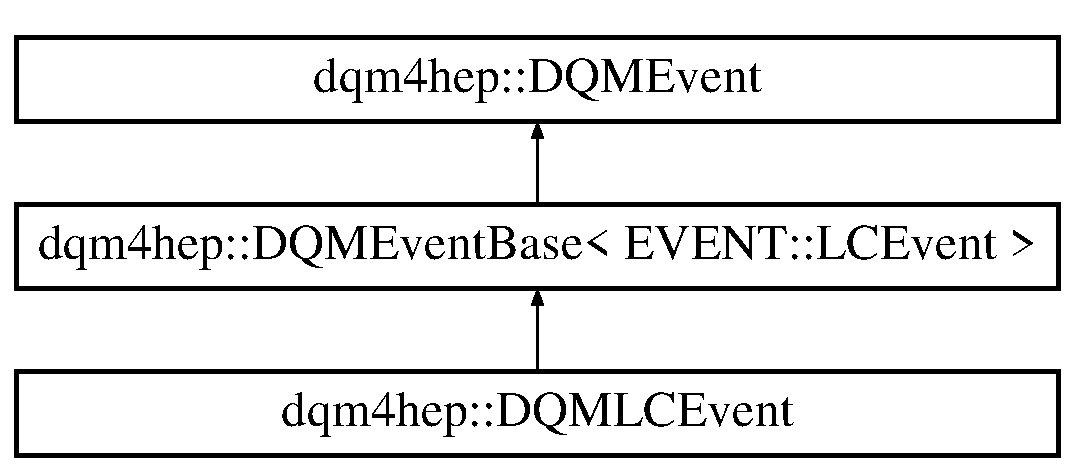
\includegraphics[height=3.000000cm]{classdqm4hep_1_1DQMLCEvent}
\end{center}
\end{figure}
\subsection*{Public Member Functions}
\begin{DoxyCompactItemize}
\item 
{\bf D\+Q\+M\+L\+C\+Event} ()
\begin{DoxyCompactList}\small\item\em Constructor. \end{DoxyCompactList}\item 
{\bf $\sim$\+D\+Q\+M\+L\+C\+Event} ()
\begin{DoxyCompactList}\small\item\em Destructor. \end{DoxyCompactList}\item 
E\+V\+E\+N\+T\+::\+L\+C\+Event $\ast$ {\bf get\+Event} () const 
\begin{DoxyCompactList}\small\item\em Returns the stored lc event. \end{DoxyCompactList}\item 
void {\bf set\+Event} (E\+V\+E\+N\+T\+::\+L\+C\+Event $\ast$p\+L\+C\+Event)
\begin{DoxyCompactList}\small\item\em Set the handled lc event. \end{DoxyCompactList}\item 
void {\bf clear} ()
\begin{DoxyCompactList}\small\item\em Clear the handler by deleting the handled lc event. \end{DoxyCompactList}\end{DoxyCompactItemize}
\subsection*{Private Attributes}
\begin{DoxyCompactItemize}
\item 
E\+V\+E\+N\+T\+::\+L\+C\+Event $\ast$ {\bf m\+\_\+p\+L\+C\+Event}
\end{DoxyCompactItemize}
\subsection*{Additional Inherited Members}


\subsection{Detailed Description}
\doxyref{D\+Q\+M\+L\+C\+Event}{p.}{classdqm4hep_1_1DQMLCEvent} class. 

Wrapper for L\+C\+Event class to be used in D\+Q\+M system. Used in D\+Q\+M\+Analysis\+Module\+::process\+Event(\+D\+Q\+M\+Event) to monitor event. See \doxyref{D\+Q\+M\+Analysis\+Module}{p.}{classdqm4hep_1_1DQMAnalysisModule} on how to process it in the D\+Q\+M system framework 

Definition at line 48 of file D\+Q\+M\+L\+C\+Event.\+h.



\subsection{Constructor \& Destructor Documentation}
\index{dqm4hep\+::\+D\+Q\+M\+L\+C\+Event@{dqm4hep\+::\+D\+Q\+M\+L\+C\+Event}!D\+Q\+M\+L\+C\+Event@{D\+Q\+M\+L\+C\+Event}}
\index{D\+Q\+M\+L\+C\+Event@{D\+Q\+M\+L\+C\+Event}!dqm4hep\+::\+D\+Q\+M\+L\+C\+Event@{dqm4hep\+::\+D\+Q\+M\+L\+C\+Event}}
\subsubsection[{D\+Q\+M\+L\+C\+Event}]{\setlength{\rightskip}{0pt plus 5cm}dqm4hep\+::\+D\+Q\+M\+L\+C\+Event\+::\+D\+Q\+M\+L\+C\+Event (
\begin{DoxyParamCaption}
{}
\end{DoxyParamCaption}
)\hspace{0.3cm}{\ttfamily [inline]}}\label{classdqm4hep_1_1DQMLCEvent_abccb39776f75708a476769b77a6ddac0}


Constructor. 



Definition at line 78 of file D\+Q\+M\+L\+C\+Event.\+h.


\begin{DoxyCode}
78                               :
79     m_pLCEvent(0)
80 \{
81 \}
\end{DoxyCode}
\index{dqm4hep\+::\+D\+Q\+M\+L\+C\+Event@{dqm4hep\+::\+D\+Q\+M\+L\+C\+Event}!````~D\+Q\+M\+L\+C\+Event@{$\sim$\+D\+Q\+M\+L\+C\+Event}}
\index{````~D\+Q\+M\+L\+C\+Event@{$\sim$\+D\+Q\+M\+L\+C\+Event}!dqm4hep\+::\+D\+Q\+M\+L\+C\+Event@{dqm4hep\+::\+D\+Q\+M\+L\+C\+Event}}
\subsubsection[{$\sim$\+D\+Q\+M\+L\+C\+Event}]{\setlength{\rightskip}{0pt plus 5cm}dqm4hep\+::\+D\+Q\+M\+L\+C\+Event\+::$\sim$\+D\+Q\+M\+L\+C\+Event (
\begin{DoxyParamCaption}
{}
\end{DoxyParamCaption}
)\hspace{0.3cm}{\ttfamily [inline]}}\label{classdqm4hep_1_1DQMLCEvent_a6412cd6fc08a95ba35e4732a732b9f75}


Destructor. 



Definition at line 85 of file D\+Q\+M\+L\+C\+Event.\+h.



References clear().


\begin{DoxyCode}
86 \{
87   clear();
88 \}
\end{DoxyCode}


\subsection{Member Function Documentation}
\index{dqm4hep\+::\+D\+Q\+M\+L\+C\+Event@{dqm4hep\+::\+D\+Q\+M\+L\+C\+Event}!clear@{clear}}
\index{clear@{clear}!dqm4hep\+::\+D\+Q\+M\+L\+C\+Event@{dqm4hep\+::\+D\+Q\+M\+L\+C\+Event}}
\subsubsection[{clear}]{\setlength{\rightskip}{0pt plus 5cm}void dqm4hep\+::\+D\+Q\+M\+L\+C\+Event\+::clear (
\begin{DoxyParamCaption}
{}
\end{DoxyParamCaption}
)\hspace{0.3cm}{\ttfamily [inline]}, {\ttfamily [virtual]}}\label{classdqm4hep_1_1DQMLCEvent_a47b8653da5ab6d64277b756f553758bd}


Clear the handler by deleting the handled lc event. 



Implements {\bf dqm4hep\+::\+D\+Q\+M\+Event\+Base$<$ E\+V\+E\+N\+T\+::\+L\+C\+Event $>$} \doxyref{}{p.}{singletondqm4hep_1_1DQMEventBase_afe7236fd5fe7e2fa719a1464e2195636}.



Definition at line 107 of file D\+Q\+M\+L\+C\+Event.\+h.



References dqm4hep\+::\+D\+Q\+M\+Event\+::is\+Owner(), and m\+\_\+p\+L\+C\+Event.



Referenced by set\+Event(), and $\sim$\+D\+Q\+M\+L\+C\+Event().


\begin{DoxyCode}
108 \{
109   \textcolor{keywordflow}{if}(0 != m_pLCEvent && this->isOwner())
110     \textcolor{keyword}{delete} m_pLCEvent;
111 \}
\end{DoxyCode}
\index{dqm4hep\+::\+D\+Q\+M\+L\+C\+Event@{dqm4hep\+::\+D\+Q\+M\+L\+C\+Event}!get\+Event@{get\+Event}}
\index{get\+Event@{get\+Event}!dqm4hep\+::\+D\+Q\+M\+L\+C\+Event@{dqm4hep\+::\+D\+Q\+M\+L\+C\+Event}}
\subsubsection[{get\+Event}]{\setlength{\rightskip}{0pt plus 5cm}E\+V\+E\+N\+T\+::\+L\+C\+Event $\ast$ dqm4hep\+::\+D\+Q\+M\+L\+C\+Event\+::get\+Event (
\begin{DoxyParamCaption}
{}
\end{DoxyParamCaption}
) const\hspace{0.3cm}{\ttfamily [inline]}, {\ttfamily [virtual]}}\label{classdqm4hep_1_1DQMLCEvent_a3e2a3489740b65b9359decc4766fcee7}


Returns the stored lc event. 



Implements {\bf dqm4hep\+::\+D\+Q\+M\+Event\+Base$<$ E\+V\+E\+N\+T\+::\+L\+C\+Event $>$} \doxyref{}{p.}{singletondqm4hep_1_1DQMEventBase_a2363bc09cadffa4806098fc9f031543f}.



Definition at line 92 of file D\+Q\+M\+L\+C\+Event.\+h.



References m\+\_\+p\+L\+C\+Event.


\begin{DoxyCode}
93 \{
94   \textcolor{keywordflow}{return} m_pLCEvent;
95 \}
\end{DoxyCode}
\index{dqm4hep\+::\+D\+Q\+M\+L\+C\+Event@{dqm4hep\+::\+D\+Q\+M\+L\+C\+Event}!set\+Event@{set\+Event}}
\index{set\+Event@{set\+Event}!dqm4hep\+::\+D\+Q\+M\+L\+C\+Event@{dqm4hep\+::\+D\+Q\+M\+L\+C\+Event}}
\subsubsection[{set\+Event}]{\setlength{\rightskip}{0pt plus 5cm}void dqm4hep\+::\+D\+Q\+M\+L\+C\+Event\+::set\+Event (
\begin{DoxyParamCaption}
\item[{E\+V\+E\+N\+T\+::\+L\+C\+Event $\ast$}]{p\+L\+C\+Event}
\end{DoxyParamCaption}
)\hspace{0.3cm}{\ttfamily [inline]}, {\ttfamily [virtual]}}\label{classdqm4hep_1_1DQMLCEvent_a9085e7483f683553be7d0b8bde36c260}


Set the handled lc event. 



Implements {\bf dqm4hep\+::\+D\+Q\+M\+Event\+Base$<$ E\+V\+E\+N\+T\+::\+L\+C\+Event $>$} \doxyref{}{p.}{singletondqm4hep_1_1DQMEventBase_afe393ecc545e9eb6dead7309c119f436}.



Definition at line 99 of file D\+Q\+M\+L\+C\+Event.\+h.



References clear(), and m\+\_\+p\+L\+C\+Event.


\begin{DoxyCode}
100 \{
101   clear();
102   m_pLCEvent = pLCEvent;
103 \}
\end{DoxyCode}


\subsection{Member Data Documentation}
\index{dqm4hep\+::\+D\+Q\+M\+L\+C\+Event@{dqm4hep\+::\+D\+Q\+M\+L\+C\+Event}!m\+\_\+p\+L\+C\+Event@{m\+\_\+p\+L\+C\+Event}}
\index{m\+\_\+p\+L\+C\+Event@{m\+\_\+p\+L\+C\+Event}!dqm4hep\+::\+D\+Q\+M\+L\+C\+Event@{dqm4hep\+::\+D\+Q\+M\+L\+C\+Event}}
\subsubsection[{m\+\_\+p\+L\+C\+Event}]{\setlength{\rightskip}{0pt plus 5cm}E\+V\+E\+N\+T\+::\+L\+C\+Event$\ast$ dqm4hep\+::\+D\+Q\+M\+L\+C\+Event\+::m\+\_\+p\+L\+C\+Event\hspace{0.3cm}{\ttfamily [private]}}\label{classdqm4hep_1_1DQMLCEvent_aa4352d35f6b79ae67b97012c1e84d17d}


Definition at line 72 of file D\+Q\+M\+L\+C\+Event.\+h.



Referenced by clear(), get\+Event(), and set\+Event().



The documentation for this class was generated from the following file\+:\begin{DoxyCompactItemize}
\item 
{\bf D\+Q\+M\+L\+C\+Event.\+h}\end{DoxyCompactItemize}

\section{dqm4hep\+:\+:D\+Q\+M\+L\+C\+Event\+Streamer Class Reference}
\label{classdqm4hep_1_1DQMLCEventStreamer}\index{dqm4hep\+::\+D\+Q\+M\+L\+C\+Event\+Streamer@{dqm4hep\+::\+D\+Q\+M\+L\+C\+Event\+Streamer}}


\doxyref{D\+Q\+M\+L\+C\+Event\+Streamer}{p.}{classdqm4hep_1_1DQMLCEventStreamer} class.  




{\ttfamily \#include $<$D\+Q\+M\+L\+C\+Event\+Streamer.\+h$>$}

Inheritance diagram for dqm4hep\+:\+:D\+Q\+M\+L\+C\+Event\+Streamer\+:\begin{figure}[H]
\begin{center}
\leavevmode
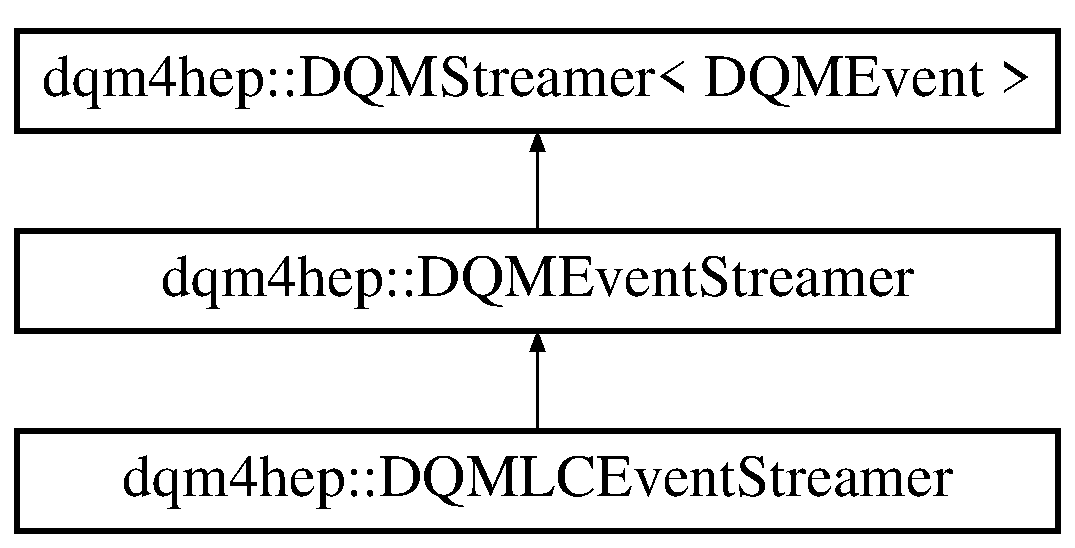
\includegraphics[height=3.000000cm]{classdqm4hep_1_1DQMLCEventStreamer}
\end{center}
\end{figure}
\subsection*{Public Member Functions}
\begin{DoxyCompactItemize}
\item 
{\bf D\+Q\+M\+L\+C\+Event\+Streamer} ()
\begin{DoxyCompactList}\small\item\em Constructor. \end{DoxyCompactList}\item 
{\bf $\sim$\+D\+Q\+M\+L\+C\+Event\+Streamer} ()
\begin{DoxyCompactList}\small\item\em Destructor. \end{DoxyCompactList}\item 
{\bf Status\+Code} {\bf serialize} (const {\bf D\+Q\+M\+Event} $\ast$const p\+Event, {\bf D\+Q\+M\+Data\+Stream} $\ast$const p\+Data\+Stream)
\begin{DoxyCompactList}\small\item\em Serialize the event and store it into a data stream. \end{DoxyCompactList}\item 
{\bf Status\+Code} {\bf deserialize} ({\bf D\+Q\+M\+Event} $\ast$\&p\+Event, {\bf D\+Q\+M\+Data\+Stream} $\ast$const p\+Data\+Stream)
\begin{DoxyCompactList}\small\item\em De-\/serialize the lcio event. \end{DoxyCompactList}\item 
{\bf Status\+Code} {\bf serialize} (const {\bf D\+Q\+M\+Event} $\ast$const p\+Object, const std\+::string \&sub\+Event\+Identifier, {\bf D\+Q\+M\+Data\+Stream} $\ast$const p\+Data\+Stream)
\begin{DoxyCompactList}\small\item\em Serialize the a part of the event and store it into a data stream. \end{DoxyCompactList}\end{DoxyCompactItemize}
\subsection*{Private Attributes}
\begin{DoxyCompactItemize}
\item 
{\bf D\+Q\+M\+L\+C\+Collection\+Streamer\+Map} {\bf m\+\_\+lc\+Collection\+Streamer\+Map}
\item 
{\bf D\+Q\+M\+L\+C\+Parameters\+Streamer} {\bf m\+\_\+lc\+Parameters\+Streamer}
\end{DoxyCompactItemize}


\subsection{Detailed Description}
\doxyref{D\+Q\+M\+L\+C\+Event\+Streamer}{p.}{classdqm4hep_1_1DQMLCEventStreamer} class. 

Definition at line 73 of file D\+Q\+M\+L\+C\+Event\+Streamer.\+h.



\subsection{Constructor \& Destructor Documentation}
\index{dqm4hep\+::\+D\+Q\+M\+L\+C\+Event\+Streamer@{dqm4hep\+::\+D\+Q\+M\+L\+C\+Event\+Streamer}!D\+Q\+M\+L\+C\+Event\+Streamer@{D\+Q\+M\+L\+C\+Event\+Streamer}}
\index{D\+Q\+M\+L\+C\+Event\+Streamer@{D\+Q\+M\+L\+C\+Event\+Streamer}!dqm4hep\+::\+D\+Q\+M\+L\+C\+Event\+Streamer@{dqm4hep\+::\+D\+Q\+M\+L\+C\+Event\+Streamer}}
\subsubsection[{D\+Q\+M\+L\+C\+Event\+Streamer}]{\setlength{\rightskip}{0pt plus 5cm}dqm4hep\+::\+D\+Q\+M\+L\+C\+Event\+Streamer\+::\+D\+Q\+M\+L\+C\+Event\+Streamer (
\begin{DoxyParamCaption}
{}
\end{DoxyParamCaption}
)}\label{classdqm4hep_1_1DQMLCEventStreamer_ad22b961a639194339726642a84ad16c0}


Constructor. 



Definition at line 61 of file D\+Q\+M\+L\+C\+Event\+Streamer.\+cc.


\begin{DoxyCode}
62 \{
63   m_lcCollectionStreamerMap[EVENT::LCIO::LCGENERICOBJECT] = \textcolor{keyword}{new} DQMLCCollectionStreamer(
      EVENT::LCIO::LCGENERICOBJECT, \textcolor{keyword}{new} DQMLCGenericObjectStreamer());
64   m_lcCollectionStreamerMap[EVENT::LCIO::CALORIMETERHIT]  = \textcolor{keyword}{new} DQMLCCollectionStreamer(
      EVENT::LCIO::CALORIMETERHIT,  \textcolor{keyword}{new} DQMCalorimeterHitStreamer());
65   m_lcCollectionStreamerMap[EVENT::LCIO::RAWCALORIMETERHIT]  = \textcolor{keyword}{new} DQMLCCollectionStreamer(
      EVENT::LCIO::RAWCALORIMETERHIT,  \textcolor{keyword}{new} DQMRawCalorimeterHitStreamer());
66   m_lcCollectionStreamerMap[EVENT::LCIO::TPCHIT]  = \textcolor{keyword}{new} DQMLCCollectionStreamer(EVENT::LCIO::TPCHIT,  \textcolor{keyword}{new} 
      DQMTPCHitStreamer());
67   m_lcCollectionStreamerMap[EVENT::LCIO::CLUSTER]  = \textcolor{keyword}{new} DQMLCCollectionStreamer(EVENT::LCIO::CLUSTER,  \textcolor{keyword}{new}
       DQMClusterStreamer());
68   m_lcCollectionStreamerMap[EVENT::LCIO::PARTICLEID]  = \textcolor{keyword}{new} DQMLCCollectionStreamer(EVENT::LCIO::PARTICLEID
      ,  \textcolor{keyword}{new} DQMParticleIDStreamer());
69   m_lcCollectionStreamerMap[EVENT::LCIO::LCFLOATVEC]  = \textcolor{keyword}{new} DQMLCCollectionStreamer(EVENT::LCIO::LCFLOATVEC
      ,  \textcolor{keyword}{new} DQMLCFloatVecStreamer());
70   m_lcCollectionStreamerMap[EVENT::LCIO::LCINTVEC]  = \textcolor{keyword}{new} DQMLCCollectionStreamer(EVENT::LCIO::LCINTVEC,  \textcolor{keyword}{
      new} DQMLCIntVecStreamer());
71   m_lcCollectionStreamerMap[EVENT::LCIO::LCSTRVEC]  = \textcolor{keyword}{new} DQMLCCollectionStreamer(EVENT::LCIO::LCSTRVEC,  \textcolor{keyword}{
      new} DQMLCStrVecStreamer());
72 \}
\end{DoxyCode}
\index{dqm4hep\+::\+D\+Q\+M\+L\+C\+Event\+Streamer@{dqm4hep\+::\+D\+Q\+M\+L\+C\+Event\+Streamer}!````~D\+Q\+M\+L\+C\+Event\+Streamer@{$\sim$\+D\+Q\+M\+L\+C\+Event\+Streamer}}
\index{````~D\+Q\+M\+L\+C\+Event\+Streamer@{$\sim$\+D\+Q\+M\+L\+C\+Event\+Streamer}!dqm4hep\+::\+D\+Q\+M\+L\+C\+Event\+Streamer@{dqm4hep\+::\+D\+Q\+M\+L\+C\+Event\+Streamer}}
\subsubsection[{$\sim$\+D\+Q\+M\+L\+C\+Event\+Streamer}]{\setlength{\rightskip}{0pt plus 5cm}dqm4hep\+::\+D\+Q\+M\+L\+C\+Event\+Streamer\+::$\sim$\+D\+Q\+M\+L\+C\+Event\+Streamer (
\begin{DoxyParamCaption}
{}
\end{DoxyParamCaption}
)}\label{classdqm4hep_1_1DQMLCEventStreamer_aaeb019ba921d633876ba7fe62c9960c7}


Destructor. 



Definition at line 76 of file D\+Q\+M\+L\+C\+Event\+Streamer.\+cc.



References m\+\_\+lc\+Collection\+Streamer\+Map.


\begin{DoxyCode}
77 \{
78   \textcolor{keywordflow}{for}(DQMLCCollectionStreamerMap::iterator iter = m_lcCollectionStreamerMap.begin() , endIter = 
      m_lcCollectionStreamerMap.end() ;
79       endIter != iter ; ++iter)
80     \textcolor{keyword}{delete} iter->second;
81 
82   m_lcCollectionStreamerMap.clear();
83 \}
\end{DoxyCode}


\subsection{Member Function Documentation}
\index{dqm4hep\+::\+D\+Q\+M\+L\+C\+Event\+Streamer@{dqm4hep\+::\+D\+Q\+M\+L\+C\+Event\+Streamer}!deserialize@{deserialize}}
\index{deserialize@{deserialize}!dqm4hep\+::\+D\+Q\+M\+L\+C\+Event\+Streamer@{dqm4hep\+::\+D\+Q\+M\+L\+C\+Event\+Streamer}}
\subsubsection[{deserialize}]{\setlength{\rightskip}{0pt plus 5cm}{\bf Status\+Code} dqm4hep\+::\+D\+Q\+M\+L\+C\+Event\+Streamer\+::deserialize (
\begin{DoxyParamCaption}
\item[{{\bf D\+Q\+M\+Event} $\ast$\&}]{p\+Event, }
\item[{{\bf D\+Q\+M\+Data\+Stream} $\ast$const}]{p\+Data\+Stream}
\end{DoxyParamCaption}
)\hspace{0.3cm}{\ttfamily [virtual]}}\label{classdqm4hep_1_1DQMLCEventStreamer_a9f54db23849818556fe1c898d1019b17}


De-\/serialize the lcio event. 



Implements {\bf dqm4hep\+::\+D\+Q\+M\+Event\+Streamer} \doxyref{}{p.}{classdqm4hep_1_1DQMEventStreamer_a063e71f73dd06404b736438c3f42b602}.



Definition at line 149 of file D\+Q\+M\+L\+C\+Event\+Streamer.\+cc.



References dqm4hep\+::\+D\+Q\+M\+L\+C\+Parameters\+Streamer\+::deserialize(), dqm4hep\+::\+D\+Q\+M\+Data\+Stream\+::is\+Valid(), m\+\_\+lc\+Collection\+Streamer\+Map, m\+\_\+lc\+Parameters\+Streamer, P\+R\+O\+C\+E\+S\+S\+\_\+\+C\+O\+D\+E\+\_\+\+I\+F\+\_\+\+A\+N\+D\+\_\+\+R\+E\+T\+U\+R\+N, dqm4hep\+::\+D\+Q\+M\+Data\+Stream\+::read(), R\+E\+T\+U\+R\+N\+\_\+\+R\+E\+S\+U\+L\+T\+\_\+\+I\+F, dqm4hep\+::\+D\+Q\+M\+Event\+::set\+Event(), and dqm4hep\+::\+W\+A\+R\+N\+I\+N\+G.


\begin{DoxyCode}
150 \{
151   pEvent = NULL;
152 
153   \textcolor{keywordflow}{if}(!pDataStream->isValid())
154   \{
155     streamlog\_out(WARNING) << \textcolor{stringliteral}{"Invalid buffer while deserializing a LCEvent !"} << std::endl;
156     \textcolor{keywordflow}{return} STATUS\_CODE\_NOT\_INITIALIZED;
157   \}
158 
159   pEvent = \textcolor{keyword}{new} DQMLCEvent();
160   IMPL::LCEventImpl *pTmpLCEvent = \textcolor{keyword}{new} IMPL::LCEventImpl();
161 
162   pEvent->setEvent<EVENT::LCEvent>(pTmpLCEvent);
163 
164   dqm_int runNumber = 0;
165   RETURN_RESULT_IF(STATUS\_CODE\_SUCCESS, !=, pDataStream->read(runNumber));
166   pTmpLCEvent->setRunNumber(runNumber);
167 
168   dqm_int eventNumber = 0;
169   RETURN_RESULT_IF(STATUS\_CODE\_SUCCESS, !=, pDataStream->read(eventNumber));
170   pTmpLCEvent->setEventNumber(eventNumber);
171 
172   std::string detectorName;
173   RETURN_RESULT_IF(STATUS\_CODE\_SUCCESS, !=, pDataStream->read(detectorName));
174   pTmpLCEvent->setDetectorName(detectorName);
175 
176   dqm_lint timeStamp = 0;
177   RETURN_RESULT_IF(STATUS\_CODE\_SUCCESS, !=, pDataStream->read(timeStamp));
178   pTmpLCEvent->setTimeStamp(timeStamp);
179 
180   dqm_double weight = 0.;
181   RETURN_RESULT_IF(STATUS\_CODE\_SUCCESS, !=, pDataStream->read(weight));
182   pTmpLCEvent->setWeight(weight);
183 
184   EVENT::LCParameters *pLCParameters = &pTmpLCEvent->parameters();
185 
186   PROCESS_CODE_IF_AND_RETURN(STATUS\_CODE\_SUCCESS, !=, m_lcParametersStreamer.
      deserialize(pLCParameters, pDataStream),
187     \textcolor{keyword}{delete} pEvent;
188   );
189 
190   dqm_int nCollections = 0;
191   RETURN_RESULT_IF(STATUS\_CODE\_SUCCESS, !=, pDataStream->read(nCollections));
192 
193   \textcolor{keywordflow}{for}(\textcolor{keywordtype}{int} i=0 ; i<nCollections ; i++)
194   \{
195     EVENT::LCCollection *pCollection = NULL;
196 
197     std::string collectionName;
198     RETURN_RESULT_IF(STATUS\_CODE\_SUCCESS, !=, pDataStream->read(collectionName));
199 
200     std::string collectionType;
201     RETURN_RESULT_IF(STATUS\_CODE\_SUCCESS, !=, pDataStream->read(collectionType));
202 
203     DQMLCCollectionStreamerMap::const\_iterator findIter = 
      m_lcCollectionStreamerMap.find(collectionType);
204 
205     \textcolor{keywordflow}{if}(m_lcCollectionStreamerMap.end() == findIter)
206     \{
207       streamlog\_out(WARNING) << \textcolor{stringliteral}{"Couldn't deserialize collection of type '"} << collectionType << \textcolor{stringliteral}{"'. "} << 
      std::endl
208             << \textcolor{stringliteral}{"The serializer for this collection type is not yet implemented!"} << std::endl;
209 
210       \textcolor{keyword}{delete} pEvent;
211 
212       \textcolor{keywordflow}{return} STATUS\_CODE\_FAILURE;
213     \}
214 
215     PROCESS_CODE_IF_AND_RETURN(STATUS\_CODE\_SUCCESS, !=, findIter->second->deserialize(pCollection, 
      pDataStream),
216       \textcolor{keyword}{delete} pEvent;
217     );
218 
219     pTmpLCEvent->addCollection(pCollection, collectionName);
220   \}
221 
222   \textcolor{keywordflow}{return} STATUS\_CODE\_SUCCESS;
223 \}
\end{DoxyCode}
\index{dqm4hep\+::\+D\+Q\+M\+L\+C\+Event\+Streamer@{dqm4hep\+::\+D\+Q\+M\+L\+C\+Event\+Streamer}!serialize@{serialize}}
\index{serialize@{serialize}!dqm4hep\+::\+D\+Q\+M\+L\+C\+Event\+Streamer@{dqm4hep\+::\+D\+Q\+M\+L\+C\+Event\+Streamer}}
\subsubsection[{serialize}]{\setlength{\rightskip}{0pt plus 5cm}{\bf Status\+Code} dqm4hep\+::\+D\+Q\+M\+L\+C\+Event\+Streamer\+::serialize (
\begin{DoxyParamCaption}
\item[{const {\bf D\+Q\+M\+Event} $\ast$const}]{p\+Event, }
\item[{{\bf D\+Q\+M\+Data\+Stream} $\ast$const}]{p\+Data\+Stream}
\end{DoxyParamCaption}
)\hspace{0.3cm}{\ttfamily [virtual]}}\label{classdqm4hep_1_1DQMLCEventStreamer_a308293cdebf98ee5dcfbad4c34f31d38}


Serialize the event and store it into a data stream. 



Implements {\bf dqm4hep\+::\+D\+Q\+M\+Event\+Streamer} \doxyref{}{p.}{classdqm4hep_1_1DQMEventStreamer_a9f6ffa9b9977ca02564bb0c8cd248be4}.



Definition at line 87 of file D\+Q\+M\+L\+C\+Event\+Streamer.\+cc.



References dqm4hep\+::\+D\+Q\+M\+Event\+::get\+Event(), m\+\_\+lc\+Collection\+Streamer\+Map, m\+\_\+lc\+Parameters\+Streamer, R\+E\+T\+U\+R\+N\+\_\+\+R\+E\+S\+U\+L\+T\+\_\+\+I\+F, dqm4hep\+::\+D\+Q\+M\+L\+C\+Parameters\+Streamer\+::serialize(), dqm4hep\+::\+W\+A\+R\+N\+I\+N\+G, and dqm4hep\+::\+D\+Q\+M\+Data\+Stream\+::write().



Referenced by serialize().


\begin{DoxyCode}
88 \{
89   \textcolor{keywordflow}{if}(NULL == pEvent)
90     \textcolor{keywordflow}{return} STATUS\_CODE\_INVALID\_PTR;
91 
92   EVENT::LCEvent *pLCEvent = pEvent->getEvent<EVENT::LCEvent>();
93 
94   \textcolor{keywordflow}{if}(NULL == pLCEvent)
95     \textcolor{keywordflow}{return} STATUS\_CODE\_FAILURE;
96 
97   \textcolor{comment}{// start filling with event parameters}
98   dqm_int runNumber = pLCEvent->getRunNumber();
99   RETURN_RESULT_IF(STATUS\_CODE\_SUCCESS, !=, pDataStream->write(runNumber));
100 
101   dqm_int eventNumber = pLCEvent->getEventNumber();
102   RETURN_RESULT_IF(STATUS\_CODE\_SUCCESS, !=, pDataStream->write(eventNumber));
103 
104   std::string detectorName = pLCEvent->getDetectorName();
105   RETURN_RESULT_IF(STATUS\_CODE\_SUCCESS, !=, pDataStream->write(detectorName));
106 
107   dqm_lint timeStamp = pLCEvent->getTimeStamp();
108   RETURN_RESULT_IF(STATUS\_CODE\_SUCCESS, !=, pDataStream->write(timeStamp));
109 
110   dqm_double weight = pLCEvent->getWeight();
111   RETURN_RESULT_IF(STATUS\_CODE\_SUCCESS, !=, pDataStream->write(weight));
112 
113   RETURN_RESULT_IF(STATUS\_CODE\_SUCCESS, !=, m_lcParametersStreamer.serialize(&pLCEvent->parameters(), 
      pDataStream));
114 
115   \textcolor{keyword}{const} std::vector<std::string> *collectionNames = pLCEvent->getCollectionNames();
116 
117   dqm_int nCollections = collectionNames->size();
118   RETURN_RESULT_IF(STATUS\_CODE\_SUCCESS, !=, pDataStream->write(nCollections));
119 
120   \textcolor{comment}{// write all collections if possible}
121   \textcolor{keywordflow}{for}(std::vector<std::string>::const\_iterator iter = collectionNames->begin() , endIter = collectionNames
      ->end() ;
122       endIter != iter ; ++iter)
123   \{
124     EVENT::LCCollection *pCollection = pLCEvent->getCollection(*iter);
125     DQMLCCollectionStreamerMap::const\_iterator findIter = 
      m_lcCollectionStreamerMap.find(pCollection->getTypeName());
126 
127     \textcolor{keywordflow}{if}(m_lcCollectionStreamerMap.end() == findIter)
128     \{
129       streamlog\_out(WARNING) << \textcolor{stringliteral}{"Couldn't serialize collection of type '"} << pCollection->getTypeName() << \textcolor{stringliteral}{
      "'. "} << std::endl
130             << \textcolor{stringliteral}{"The serializer for this collection type is not yet implemented!"} << std::endl
131             << \textcolor{stringliteral}{"Will skip this collection"} << std::endl;;
132       \textcolor{keywordflow}{continue};
133     \}
134 
135     std::string collectionName = (*iter);
136     RETURN_RESULT_IF(STATUS\_CODE\_SUCCESS, !=, pDataStream->write(collectionName));
137 
138     std::string collectionType = pCollection->getTypeName();
139     RETURN_RESULT_IF(STATUS\_CODE\_SUCCESS, !=, pDataStream->write(collectionType));
140 
141     RETURN_RESULT_IF(STATUS\_CODE\_SUCCESS, !=, findIter->second->serialize(pCollection, pDataStream));
142   \}
143 
144   \textcolor{keywordflow}{return} STATUS\_CODE\_SUCCESS;
145 \}
\end{DoxyCode}
\index{dqm4hep\+::\+D\+Q\+M\+L\+C\+Event\+Streamer@{dqm4hep\+::\+D\+Q\+M\+L\+C\+Event\+Streamer}!serialize@{serialize}}
\index{serialize@{serialize}!dqm4hep\+::\+D\+Q\+M\+L\+C\+Event\+Streamer@{dqm4hep\+::\+D\+Q\+M\+L\+C\+Event\+Streamer}}
\subsubsection[{serialize}]{\setlength{\rightskip}{0pt plus 5cm}{\bf Status\+Code} dqm4hep\+::\+D\+Q\+M\+L\+C\+Event\+Streamer\+::serialize (
\begin{DoxyParamCaption}
\item[{const {\bf D\+Q\+M\+Event} $\ast$const}]{p\+Object, }
\item[{const std\+::string \&}]{sub\+Event\+Identifier, }
\item[{{\bf D\+Q\+M\+Data\+Stream} $\ast$const}]{p\+Data\+Stream}
\end{DoxyParamCaption}
)\hspace{0.3cm}{\ttfamily [virtual]}}\label{classdqm4hep_1_1DQMLCEventStreamer_afabcb0328b2d2be0e9c08ef38a5c81f3}


Serialize the a part of the event and store it into a data stream. 

The sub event identifier is a string of the collection names concatenated with semi columns \+: \char`\"{}collection\+Name1\+:collection\+Name2\+:collection\+Name3\char`\"{} If the sub event identifier is empty the whole event is serialized 

Implements {\bf dqm4hep\+::\+D\+Q\+M\+Event\+Streamer} \doxyref{}{p.}{classdqm4hep_1_1DQMEventStreamer_a015898c0d96bdbcb523fa54431fb2a45}.



Definition at line 227 of file D\+Q\+M\+L\+C\+Event\+Streamer.\+cc.



References dqm4hep\+::\+E\+R\+R\+O\+R, dqm4hep\+::\+D\+Q\+M\+Event\+::get\+Event(), m\+\_\+lc\+Collection\+Streamer\+Map, m\+\_\+lc\+Parameters\+Streamer, R\+E\+T\+U\+R\+N\+\_\+\+R\+E\+S\+U\+L\+T\+\_\+\+I\+F, dqm4hep\+::\+D\+Q\+M\+L\+C\+Parameters\+Streamer\+::serialize(), serialize(), dqm4hep\+::\+D\+Q\+M4\+H\+E\+P\+::tokenize(), dqm4hep\+::\+W\+A\+R\+N\+I\+N\+G, and dqm4hep\+::\+D\+Q\+M\+Data\+Stream\+::write().


\begin{DoxyCode}
228 \{
229   \textcolor{comment}{// no sub event queried -> serialize the whole event}
230   \textcolor{keywordflow}{if}(subEventIdentifier.empty())
231     \textcolor{keywordflow}{return} this->serialize(pEvent, pDataStream);
232 
233   \textcolor{comment}{// split the collection names separated by semi columns}
234   StringVector collectionNames;
235   DQM4HEP::tokenize(subEventIdentifier, collectionNames, \textcolor{stringliteral}{":"});
236 
237   \textcolor{keywordflow}{if}(collectionNames.empty())
238     \textcolor{keywordflow}{return} STATUS\_CODE\_FAILURE;
239 
240   \textcolor{keywordflow}{if}(NULL == pEvent)
241     \textcolor{keywordflow}{return} STATUS\_CODE\_INVALID\_PTR;
242 
243   EVENT::LCEvent *pLCEvent = pEvent->getEvent<EVENT::LCEvent>();
244 
245   \textcolor{keywordflow}{if}(NULL == pLCEvent)
246     \textcolor{keywordflow}{return} STATUS\_CODE\_FAILURE;
247 
248   \textcolor{keyword}{const} std::vector<std::string> *pAvailableCollections = pLCEvent->getCollectionNames();
249   StringVector serializeCollectionNames;
250 
251   \textcolor{keywordflow}{for}(StringVector::iterator iter = collectionNames.begin(), endIter = collectionNames.end() ;
252       endIter != iter ; ++iter)
253   \{
254     \textcolor{keyword}{const} std::string &collectionName(*iter);
255 
256     \textcolor{keywordflow}{if}(std::find(pAvailableCollections->begin(), pAvailableCollections->end(), collectionName) != 
      pAvailableCollections->end())
257     \{
258       serializeCollectionNames.push\_back(collectionName);
259     \}
260   \}
261 
262   collectionNames = serializeCollectionNames;
263 
264   \textcolor{keywordflow}{if}(collectionNames.empty())
265   \{
266     streamlog\_out(ERROR) << \textcolor{stringliteral}{"None of the specified collections is available. Couldn't serialize the event !
      "} << std::endl;
267     \textcolor{keywordflow}{return} STATUS\_CODE\_FAILURE;
268   \}
269 
270   \textcolor{comment}{// start filling with event parameters}
271   dqm_int runNumber = pLCEvent->getRunNumber();
272   RETURN_RESULT_IF(STATUS\_CODE\_SUCCESS, !=, pDataStream->write(runNumber));
273 
274   dqm_int eventNumber = pLCEvent->getEventNumber();
275   RETURN_RESULT_IF(STATUS\_CODE\_SUCCESS, !=, pDataStream->write(eventNumber));
276 
277   std::string detectorName = pLCEvent->getDetectorName();
278   RETURN_RESULT_IF(STATUS\_CODE\_SUCCESS, !=, pDataStream->write(detectorName));
279 
280   dqm_lint timeStamp = pLCEvent->getTimeStamp();
281   RETURN_RESULT_IF(STATUS\_CODE\_SUCCESS, !=, pDataStream->write(timeStamp));
282 
283   dqm_double weight = pLCEvent->getWeight();
284   RETURN_RESULT_IF(STATUS\_CODE\_SUCCESS, !=, pDataStream->write(weight));
285 
286   RETURN_RESULT_IF(STATUS\_CODE\_SUCCESS, !=, m_lcParametersStreamer.serialize(&pLCEvent->parameters(), 
      pDataStream));
287 
288   dqm_int nCollections = collectionNames.size();
289   RETURN_RESULT_IF(STATUS\_CODE\_SUCCESS, !=, pDataStream->write(nCollections));
290 
291   \textcolor{keywordflow}{for}(std::vector<std::string>::const\_iterator iter = collectionNames.begin() , endIter = collectionNames.
      end() ;
292       endIter != iter ; ++iter)
293   \{
294     EVENT::LCCollection *pCollection = pLCEvent->getCollection(*iter);
295     DQMLCCollectionStreamerMap::const\_iterator findIter = 
      m_lcCollectionStreamerMap.find(pCollection->getTypeName());
296 
297     \textcolor{keywordflow}{if}(m_lcCollectionStreamerMap.end() == findIter)
298     \{
299       streamlog\_out(WARNING) << \textcolor{stringliteral}{"Couldn't serialize collection of type '"} << pCollection->getTypeName() << \textcolor{stringliteral}{
      "'. "} << std::endl
300             << \textcolor{stringliteral}{"The serializer for this collection type is not yet implemented!"} << std::endl;
301 
302       \textcolor{keywordflow}{return} STATUS\_CODE\_FAILURE;
303     \}
304 
305     std::string collectionName = (*iter);
306     RETURN_RESULT_IF(STATUS\_CODE\_SUCCESS, !=, pDataStream->write(collectionName));
307 
308     std::string collectionType = pCollection->getTypeName();
309     RETURN_RESULT_IF(STATUS\_CODE\_SUCCESS, !=, pDataStream->write(collectionType));
310 
311     RETURN_RESULT_IF(STATUS\_CODE\_SUCCESS, !=, findIter->second->serialize(pCollection, pDataStream));
312   \}
313 
314   \textcolor{keywordflow}{return} STATUS\_CODE\_SUCCESS;
315 \}
\end{DoxyCode}


\subsection{Member Data Documentation}
\index{dqm4hep\+::\+D\+Q\+M\+L\+C\+Event\+Streamer@{dqm4hep\+::\+D\+Q\+M\+L\+C\+Event\+Streamer}!m\+\_\+lc\+Collection\+Streamer\+Map@{m\+\_\+lc\+Collection\+Streamer\+Map}}
\index{m\+\_\+lc\+Collection\+Streamer\+Map@{m\+\_\+lc\+Collection\+Streamer\+Map}!dqm4hep\+::\+D\+Q\+M\+L\+C\+Event\+Streamer@{dqm4hep\+::\+D\+Q\+M\+L\+C\+Event\+Streamer}}
\subsubsection[{m\+\_\+lc\+Collection\+Streamer\+Map}]{\setlength{\rightskip}{0pt plus 5cm}{\bf D\+Q\+M\+L\+C\+Collection\+Streamer\+Map} dqm4hep\+::\+D\+Q\+M\+L\+C\+Event\+Streamer\+::m\+\_\+lc\+Collection\+Streamer\+Map\hspace{0.3cm}{\ttfamily [private]}}\label{classdqm4hep_1_1DQMLCEventStreamer_a635756f66e74d97e5aa822fd5a2f4e09}


Definition at line 101 of file D\+Q\+M\+L\+C\+Event\+Streamer.\+h.



Referenced by deserialize(), serialize(), and $\sim$\+D\+Q\+M\+L\+C\+Event\+Streamer().

\index{dqm4hep\+::\+D\+Q\+M\+L\+C\+Event\+Streamer@{dqm4hep\+::\+D\+Q\+M\+L\+C\+Event\+Streamer}!m\+\_\+lc\+Parameters\+Streamer@{m\+\_\+lc\+Parameters\+Streamer}}
\index{m\+\_\+lc\+Parameters\+Streamer@{m\+\_\+lc\+Parameters\+Streamer}!dqm4hep\+::\+D\+Q\+M\+L\+C\+Event\+Streamer@{dqm4hep\+::\+D\+Q\+M\+L\+C\+Event\+Streamer}}
\subsubsection[{m\+\_\+lc\+Parameters\+Streamer}]{\setlength{\rightskip}{0pt plus 5cm}{\bf D\+Q\+M\+L\+C\+Parameters\+Streamer} dqm4hep\+::\+D\+Q\+M\+L\+C\+Event\+Streamer\+::m\+\_\+lc\+Parameters\+Streamer\hspace{0.3cm}{\ttfamily [private]}}\label{classdqm4hep_1_1DQMLCEventStreamer_a43ae54799ed95237dba966baaaa0ccd9}


Definition at line 102 of file D\+Q\+M\+L\+C\+Event\+Streamer.\+h.



Referenced by deserialize(), and serialize().



The documentation for this class was generated from the following files\+:\begin{DoxyCompactItemize}
\item 
{\bf D\+Q\+M\+L\+C\+Event\+Streamer.\+h}\item 
{\bf D\+Q\+M\+L\+C\+Event\+Streamer.\+cc}\end{DoxyCompactItemize}

\section{dqm4hep\+:\+:D\+Q\+M\+L\+C\+Float\+Vec\+Streamer Class Reference}
\label{classdqm4hep_1_1DQMLCFloatVecStreamer}\index{dqm4hep\+::\+D\+Q\+M\+L\+C\+Float\+Vec\+Streamer@{dqm4hep\+::\+D\+Q\+M\+L\+C\+Float\+Vec\+Streamer}}


\doxyref{D\+Q\+M\+L\+C\+Float\+Vec\+Streamer}{p.}{classdqm4hep_1_1DQMLCFloatVecStreamer} class.  




{\ttfamily \#include $<$D\+Q\+M\+L\+C\+Event\+Streamer.\+h$>$}

Inheritance diagram for dqm4hep\+:\+:D\+Q\+M\+L\+C\+Float\+Vec\+Streamer\+:\begin{figure}[H]
\begin{center}
\leavevmode
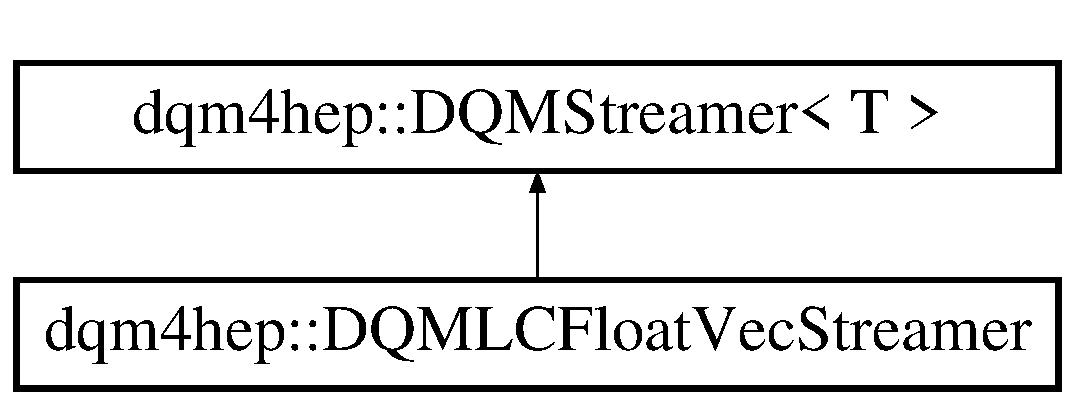
\includegraphics[height=2.000000cm]{classdqm4hep_1_1DQMLCFloatVecStreamer}
\end{center}
\end{figure}
\subsection*{Public Member Functions}
\begin{DoxyCompactItemize}
\item 
{\bf Status\+Code} {\bf serialize} (const E\+V\+E\+N\+T\+::\+L\+C\+Object $\ast$const p\+L\+C\+Object, {\bf D\+Q\+M\+Data\+Stream} $\ast$const p\+Data\+Stream)
\begin{DoxyCompactList}\small\item\em Serialize a L\+C\+Float\+Vec. \end{DoxyCompactList}\item 
{\bf Status\+Code} {\bf deserialize} (E\+V\+E\+N\+T\+::\+L\+C\+Object $\ast$\&p\+L\+C\+Object, {\bf D\+Q\+M\+Data\+Stream} $\ast$const p\+Data\+Stream)
\begin{DoxyCompactList}\small\item\em Deserialize a L\+C\+Float\+Vec. \end{DoxyCompactList}\end{DoxyCompactItemize}


\subsection{Detailed Description}
\doxyref{D\+Q\+M\+L\+C\+Float\+Vec\+Streamer}{p.}{classdqm4hep_1_1DQMLCFloatVecStreamer} class. 

Definition at line 243 of file D\+Q\+M\+L\+C\+Event\+Streamer.\+h.



\subsection{Member Function Documentation}
\index{dqm4hep\+::\+D\+Q\+M\+L\+C\+Float\+Vec\+Streamer@{dqm4hep\+::\+D\+Q\+M\+L\+C\+Float\+Vec\+Streamer}!deserialize@{deserialize}}
\index{deserialize@{deserialize}!dqm4hep\+::\+D\+Q\+M\+L\+C\+Float\+Vec\+Streamer@{dqm4hep\+::\+D\+Q\+M\+L\+C\+Float\+Vec\+Streamer}}
\subsubsection[{deserialize}]{\setlength{\rightskip}{0pt plus 5cm}{\bf Status\+Code} dqm4hep\+::\+D\+Q\+M\+L\+C\+Float\+Vec\+Streamer\+::deserialize (
\begin{DoxyParamCaption}
\item[{E\+V\+E\+N\+T\+::\+L\+C\+Object $\ast$\&}]{p\+L\+C\+Object, }
\item[{{\bf D\+Q\+M\+Data\+Stream} $\ast$const}]{p\+Data\+Stream}
\end{DoxyParamCaption}
)}\label{classdqm4hep_1_1DQMLCFloatVecStreamer_a9c8175e4cd14e87ba772a3fba111f3cf}


Deserialize a L\+C\+Float\+Vec. 

The object is allocated in this function 

Definition at line 1223 of file D\+Q\+M\+L\+C\+Event\+Streamer.\+cc.



References dqm4hep\+::\+Status\+Code\+Exception\+::get\+Status\+Code(), dqm4hep\+::\+D\+Q\+M\+Data\+Stream\+::read(), and T\+H\+R\+O\+W\+\_\+\+R\+E\+S\+U\+L\+T\+\_\+\+I\+F.


\begin{DoxyCode}
1224 \{
1225   pLCObject = 0;
1226   EVENT::LCFloatVec *pFloatVec = \textcolor{keyword}{new} EVENT::LCFloatVec();
1227 
1228   \textcolor{keywordflow}{try}
1229   \{
1230     dqm_uint nVals = 0;
1231     THROW_RESULT_IF(STATUS\_CODE\_SUCCESS, !=, pDataStream->read(nVals));
1232 
1233     \textcolor{keywordflow}{for}(dqm_uint i=0 ; i<nVals ; i++)
1234     \{
1235       dqm_float value = 0;
1236       THROW_RESULT_IF(STATUS\_CODE\_SUCCESS, !=, pDataStream->read(value));
1237       pFloatVec->push\_back(value);
1238     \}
1239   \}
1240   \textcolor{keywordflow}{catch}(StatusCodeException &exception)
1241   \{
1242     \textcolor{keyword}{delete} pFloatVec;
1243     pFloatVec = 0;
1244     pLCObject = 0;
1245 
1246     \textcolor{keywordflow}{return} exception.getStatusCode();
1247   \}
1248 
1249   pLCObject = pFloatVec;
1250 
1251   \textcolor{keywordflow}{return} STATUS\_CODE\_SUCCESS;
1252 \}
\end{DoxyCode}
\index{dqm4hep\+::\+D\+Q\+M\+L\+C\+Float\+Vec\+Streamer@{dqm4hep\+::\+D\+Q\+M\+L\+C\+Float\+Vec\+Streamer}!serialize@{serialize}}
\index{serialize@{serialize}!dqm4hep\+::\+D\+Q\+M\+L\+C\+Float\+Vec\+Streamer@{dqm4hep\+::\+D\+Q\+M\+L\+C\+Float\+Vec\+Streamer}}
\subsubsection[{serialize}]{\setlength{\rightskip}{0pt plus 5cm}{\bf Status\+Code} dqm4hep\+::\+D\+Q\+M\+L\+C\+Float\+Vec\+Streamer\+::serialize (
\begin{DoxyParamCaption}
\item[{const E\+V\+E\+N\+T\+::\+L\+C\+Object $\ast$const}]{p\+L\+C\+Object, }
\item[{{\bf D\+Q\+M\+Data\+Stream} $\ast$const}]{p\+Data\+Stream}
\end{DoxyParamCaption}
)}\label{classdqm4hep_1_1DQMLCFloatVecStreamer_a1cc02bc6cb58723309925097e96252d8}


Serialize a L\+C\+Float\+Vec. 



Definition at line 1202 of file D\+Q\+M\+L\+C\+Event\+Streamer.\+cc.



References R\+E\+T\+U\+R\+N\+\_\+\+R\+E\+S\+U\+L\+T\+\_\+\+I\+F, and dqm4hep\+::\+D\+Q\+M\+Data\+Stream\+::write().


\begin{DoxyCode}
1203 \{
1204   \textcolor{keyword}{const} EVENT::LCFloatVec *\textcolor{keyword}{const} pFloatVec = \textcolor{keyword}{dynamic\_cast<}\textcolor{keyword}{const }EVENT::LCFloatVec *const\textcolor{keyword}{>}(pLCObject);
1205 
1206   \textcolor{keywordflow}{if}(NULL == pFloatVec)
1207     \textcolor{keywordflow}{return} STATUS\_CODE\_INVALID\_PARAMETER;
1208 
1209   dqm_uint nVals = pFloatVec->size();
1210   RETURN_RESULT_IF(STATUS\_CODE\_SUCCESS, !=, pDataStream->write(nVals));
1211 
1212   \textcolor{keywordflow}{for}(dqm_uint i=0 ; i<nVals ; i++)
1213   \{
1214     dqm_float value = pFloatVec->at(i);
1215     RETURN_RESULT_IF(STATUS\_CODE\_SUCCESS, !=, pDataStream->write(value));
1216   \}
1217 
1218   \textcolor{keywordflow}{return} STATUS\_CODE\_SUCCESS;
1219 \}
\end{DoxyCode}


The documentation for this class was generated from the following files\+:\begin{DoxyCompactItemize}
\item 
{\bf D\+Q\+M\+L\+C\+Event\+Streamer.\+h}\item 
{\bf D\+Q\+M\+L\+C\+Event\+Streamer.\+cc}\end{DoxyCompactItemize}

\section{dqm4hep\+:\+:D\+Q\+M\+L\+C\+Generic\+Object\+Streamer Class Reference}
\label{classdqm4hep_1_1DQMLCGenericObjectStreamer}\index{dqm4hep\+::\+D\+Q\+M\+L\+C\+Generic\+Object\+Streamer@{dqm4hep\+::\+D\+Q\+M\+L\+C\+Generic\+Object\+Streamer}}


\doxyref{D\+Q\+M\+L\+C\+Generic\+Object\+Streamer}{p.}{classdqm4hep_1_1DQMLCGenericObjectStreamer} class.  




{\ttfamily \#include $<$D\+Q\+M\+L\+C\+Event\+Streamer.\+h$>$}

Inheritance diagram for dqm4hep\+:\+:D\+Q\+M\+L\+C\+Generic\+Object\+Streamer\+:\begin{figure}[H]
\begin{center}
\leavevmode
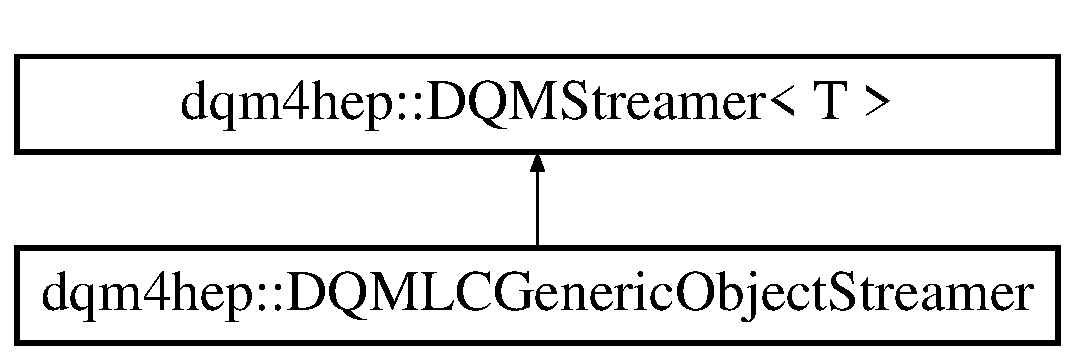
\includegraphics[height=2.000000cm]{classdqm4hep_1_1DQMLCGenericObjectStreamer}
\end{center}
\end{figure}
\subsection*{Public Member Functions}
\begin{DoxyCompactItemize}
\item 
{\bf Status\+Code} {\bf serialize} (const E\+V\+E\+N\+T\+::\+L\+C\+Object $\ast$const p\+L\+C\+Object, {\bf D\+Q\+M\+Data\+Stream} $\ast$const p\+Data\+Stream)
\begin{DoxyCompactList}\small\item\em Serialize an L\+C\+Generic\+Object. \end{DoxyCompactList}\item 
{\bf Status\+Code} {\bf deserialize} (E\+V\+E\+N\+T\+::\+L\+C\+Object $\ast$\&p\+L\+C\+Object, {\bf D\+Q\+M\+Data\+Stream} $\ast$const p\+Data\+Stream)
\begin{DoxyCompactList}\small\item\em Deserialize a L\+C\+Generic\+Object. \end{DoxyCompactList}\end{DoxyCompactItemize}


\subsection{Detailed Description}
\doxyref{D\+Q\+M\+L\+C\+Generic\+Object\+Streamer}{p.}{classdqm4hep_1_1DQMLCGenericObjectStreamer} class. 

Definition at line 141 of file D\+Q\+M\+L\+C\+Event\+Streamer.\+h.



\subsection{Member Function Documentation}
\index{dqm4hep\+::\+D\+Q\+M\+L\+C\+Generic\+Object\+Streamer@{dqm4hep\+::\+D\+Q\+M\+L\+C\+Generic\+Object\+Streamer}!deserialize@{deserialize}}
\index{deserialize@{deserialize}!dqm4hep\+::\+D\+Q\+M\+L\+C\+Generic\+Object\+Streamer@{dqm4hep\+::\+D\+Q\+M\+L\+C\+Generic\+Object\+Streamer}}
\subsubsection[{deserialize}]{\setlength{\rightskip}{0pt plus 5cm}{\bf Status\+Code} dqm4hep\+::\+D\+Q\+M\+L\+C\+Generic\+Object\+Streamer\+::deserialize (
\begin{DoxyParamCaption}
\item[{E\+V\+E\+N\+T\+::\+L\+C\+Object $\ast$\&}]{p\+L\+C\+Object, }
\item[{{\bf D\+Q\+M\+Data\+Stream} $\ast$const}]{p\+Data\+Stream}
\end{DoxyParamCaption}
)}\label{classdqm4hep_1_1DQMLCGenericObjectStreamer_aad56bcc506a734dd7d8e4fba6aa257a6}


Deserialize a L\+C\+Generic\+Object. 

The object is allocated in this function 

Definition at line 630 of file D\+Q\+M\+L\+C\+Event\+Streamer.\+cc.



References dqm4hep\+::\+D\+Q\+M\+Data\+Stream\+::read(), and R\+E\+T\+U\+R\+N\+\_\+\+R\+E\+S\+U\+L\+T\+\_\+\+I\+F.


\begin{DoxyCode}
632 \{
633   pLCObject = NULL;
634 
635   dqm_bool isFixedSize = \textcolor{keyword}{false};
636   RETURN_RESULT_IF(STATUS\_CODE\_SUCCESS, !=, pDataStream->read(isFixedSize));
637 
638   dqm_int nInt = 0;
639   RETURN_RESULT_IF(STATUS\_CODE\_SUCCESS, !=, pDataStream->read(nInt));
640 
641   dqm_int nFloat = 0;
642   RETURN_RESULT_IF(STATUS\_CODE\_SUCCESS, !=, pDataStream->read(nFloat));
643 
644   dqm_int nDouble = 0;
645   RETURN_RESULT_IF(STATUS\_CODE\_SUCCESS, !=, pDataStream->read(nDouble));
646 
647   IMPL::LCGenericObjectImpl *pTmpGenericObject =
648       isFixedSize ? \textcolor{keyword}{new} IMPL::LCGenericObjectImpl(nInt, nFloat, nDouble) : new IMPL::LCGenericObjectImpl();
649 
650   \textcolor{keywordflow}{for}(dqm_int i=0 ; i<nInt ; i++)
651   \{
652     dqm_int value = 0;
653     RETURN_RESULT_IF(STATUS\_CODE\_SUCCESS, !=, pDataStream->read(value));
654     pTmpGenericObject->setIntVal(i, value);
655   \}
656 
657   \textcolor{keywordflow}{for}(dqm_int i=0 ; i<nFloat ; i++)
658   \{
659     dqm_float value = 0.f;
660     RETURN_RESULT_IF(STATUS\_CODE\_SUCCESS, !=, pDataStream->read(value));
661     pTmpGenericObject->setFloatVal(i, value);
662   \}
663 
664   \textcolor{keywordflow}{for}(dqm_int i=0 ; i<nDouble ; i++)
665   \{
666     dqm_double value = 0;
667     RETURN_RESULT_IF(STATUS\_CODE\_SUCCESS, !=, pDataStream->read(value));
668     pTmpGenericObject->setDoubleVal(i, value);
669   \}
670 
671   pLCObject = pTmpGenericObject;
672 
673   \textcolor{keywordflow}{return} STATUS\_CODE\_SUCCESS;
674 \}
\end{DoxyCode}
\index{dqm4hep\+::\+D\+Q\+M\+L\+C\+Generic\+Object\+Streamer@{dqm4hep\+::\+D\+Q\+M\+L\+C\+Generic\+Object\+Streamer}!serialize@{serialize}}
\index{serialize@{serialize}!dqm4hep\+::\+D\+Q\+M\+L\+C\+Generic\+Object\+Streamer@{dqm4hep\+::\+D\+Q\+M\+L\+C\+Generic\+Object\+Streamer}}
\subsubsection[{serialize}]{\setlength{\rightskip}{0pt plus 5cm}{\bf Status\+Code} dqm4hep\+::\+D\+Q\+M\+L\+C\+Generic\+Object\+Streamer\+::serialize (
\begin{DoxyParamCaption}
\item[{const E\+V\+E\+N\+T\+::\+L\+C\+Object $\ast$const}]{p\+L\+C\+Object, }
\item[{{\bf D\+Q\+M\+Data\+Stream} $\ast$const}]{p\+Data\+Stream}
\end{DoxyParamCaption}
)}\label{classdqm4hep_1_1DQMLCGenericObjectStreamer_a19c8e8ab7b9fcc9a69e85c9abc237b74}


Serialize an L\+C\+Generic\+Object. 



Definition at line 587 of file D\+Q\+M\+L\+C\+Event\+Streamer.\+cc.



References R\+E\+T\+U\+R\+N\+\_\+\+R\+E\+S\+U\+L\+T\+\_\+\+I\+F, and dqm4hep\+::\+D\+Q\+M\+Data\+Stream\+::write().


\begin{DoxyCode}
589 \{
590   \textcolor{keyword}{const} EVENT::LCGenericObject *\textcolor{keyword}{const} pLCGenericObject = \textcolor{keyword}{dynamic\_cast<}\textcolor{keyword}{const }EVENT::LCGenericObject *const\textcolor{keyword}{>}(
      pLCObject);
591 
592   \textcolor{keywordflow}{if}(NULL == pLCGenericObject)
593     \textcolor{keywordflow}{return} STATUS\_CODE\_INVALID\_PARAMETER;
594 
595   dqm_bool isFixedSize = pLCGenericObject->isFixedSize();
596   RETURN_RESULT_IF(STATUS\_CODE\_SUCCESS, !=, pDataStream->write(isFixedSize));
597 
598   dqm_int nInt = pLCGenericObject->getNInt();
599   RETURN_RESULT_IF(STATUS\_CODE\_SUCCESS, !=, pDataStream->write(nInt));
600 
601   dqm_int nFloat = pLCGenericObject->getNFloat();
602   RETURN_RESULT_IF(STATUS\_CODE\_SUCCESS, !=, pDataStream->write(nFloat));
603 
604   dqm_int nDouble = pLCGenericObject->getNDouble();
605   RETURN_RESULT_IF(STATUS\_CODE\_SUCCESS, !=, pDataStream->write(nDouble));
606 
607   \textcolor{keywordflow}{for}(\textcolor{keywordtype}{int} i=0 ; i<pLCGenericObject->getNInt() ; i++)
608   \{
609     dqm_int value = pLCGenericObject->getIntVal(i);
610     RETURN_RESULT_IF(STATUS\_CODE\_SUCCESS, !=, pDataStream->write(value));
611   \}
612 
613   \textcolor{keywordflow}{for}(\textcolor{keywordtype}{int} i=0 ; i<pLCGenericObject->getNFloat() ; i++)
614   \{
615     dqm_float value = pLCGenericObject->getFloatVal(i);
616     RETURN_RESULT_IF(STATUS\_CODE\_SUCCESS, !=, pDataStream->write(value));
617   \}
618 
619   \textcolor{keywordflow}{for}(\textcolor{keywordtype}{int} i=0 ; i<pLCGenericObject->getNDouble() ; i++)
620   \{
621     dqm_double value = pLCGenericObject->getDoubleVal(i);
622     RETURN_RESULT_IF(STATUS\_CODE\_SUCCESS, !=, pDataStream->write(value));
623   \}
624 
625   \textcolor{keywordflow}{return} STATUS\_CODE\_SUCCESS;
626 \}
\end{DoxyCode}


The documentation for this class was generated from the following files\+:\begin{DoxyCompactItemize}
\item 
{\bf D\+Q\+M\+L\+C\+Event\+Streamer.\+h}\item 
{\bf D\+Q\+M\+L\+C\+Event\+Streamer.\+cc}\end{DoxyCompactItemize}

\section{dqm4hep\+:\+:D\+Q\+M\+L\+C\+Int\+Vec\+Streamer Class Reference}
\label{classdqm4hep_1_1DQMLCIntVecStreamer}\index{dqm4hep\+::\+D\+Q\+M\+L\+C\+Int\+Vec\+Streamer@{dqm4hep\+::\+D\+Q\+M\+L\+C\+Int\+Vec\+Streamer}}


\doxyref{D\+Q\+M\+L\+C\+Int\+Vec\+Streamer}{p.}{classdqm4hep_1_1DQMLCIntVecStreamer} class.  




{\ttfamily \#include $<$D\+Q\+M\+L\+C\+Event\+Streamer.\+h$>$}

Inheritance diagram for dqm4hep\+:\+:D\+Q\+M\+L\+C\+Int\+Vec\+Streamer\+:\begin{figure}[H]
\begin{center}
\leavevmode
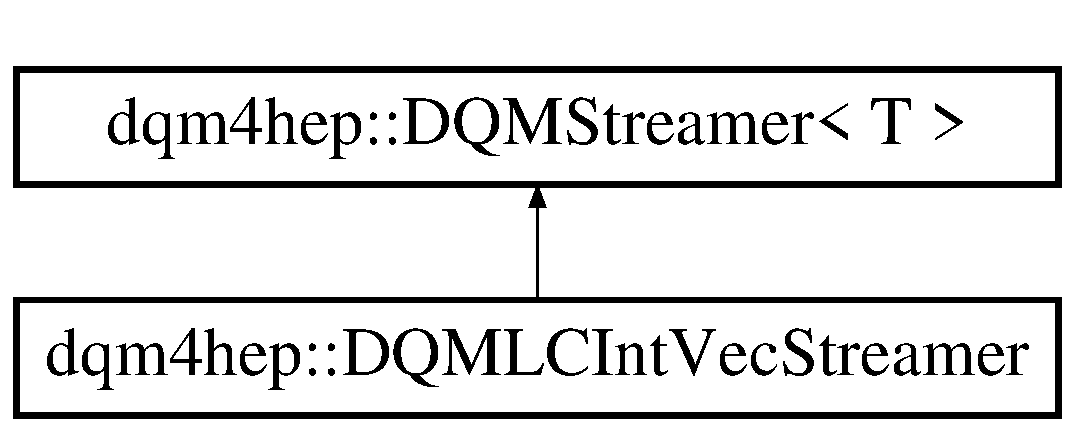
\includegraphics[height=2.000000cm]{classdqm4hep_1_1DQMLCIntVecStreamer}
\end{center}
\end{figure}
\subsection*{Public Member Functions}
\begin{DoxyCompactItemize}
\item 
{\bf Status\+Code} {\bf serialize} (const E\+V\+E\+N\+T\+::\+L\+C\+Object $\ast$const p\+L\+C\+Object, {\bf D\+Q\+M\+Data\+Stream} $\ast$const p\+Data\+Stream)
\begin{DoxyCompactList}\small\item\em Serialize a L\+C\+Int\+Vec. \end{DoxyCompactList}\item 
{\bf Status\+Code} {\bf deserialize} (E\+V\+E\+N\+T\+::\+L\+C\+Object $\ast$\&p\+L\+C\+Object, {\bf D\+Q\+M\+Data\+Stream} $\ast$const p\+Data\+Stream)
\begin{DoxyCompactList}\small\item\em Deserialize a L\+C\+Int\+Vec. \end{DoxyCompactList}\end{DoxyCompactItemize}


\subsection{Detailed Description}
\doxyref{D\+Q\+M\+L\+C\+Int\+Vec\+Streamer}{p.}{classdqm4hep_1_1DQMLCIntVecStreamer} class. 

Definition at line 260 of file D\+Q\+M\+L\+C\+Event\+Streamer.\+h.



\subsection{Member Function Documentation}
\index{dqm4hep\+::\+D\+Q\+M\+L\+C\+Int\+Vec\+Streamer@{dqm4hep\+::\+D\+Q\+M\+L\+C\+Int\+Vec\+Streamer}!deserialize@{deserialize}}
\index{deserialize@{deserialize}!dqm4hep\+::\+D\+Q\+M\+L\+C\+Int\+Vec\+Streamer@{dqm4hep\+::\+D\+Q\+M\+L\+C\+Int\+Vec\+Streamer}}
\subsubsection[{deserialize}]{\setlength{\rightskip}{0pt plus 5cm}{\bf Status\+Code} dqm4hep\+::\+D\+Q\+M\+L\+C\+Int\+Vec\+Streamer\+::deserialize (
\begin{DoxyParamCaption}
\item[{E\+V\+E\+N\+T\+::\+L\+C\+Object $\ast$\&}]{p\+L\+C\+Object, }
\item[{{\bf D\+Q\+M\+Data\+Stream} $\ast$const}]{p\+Data\+Stream}
\end{DoxyParamCaption}
)}\label{classdqm4hep_1_1DQMLCIntVecStreamer_adc1dde742800e440336c3b6e1bcd2084}


Deserialize a L\+C\+Int\+Vec. 

The object is allocated in this function 

Definition at line 1278 of file D\+Q\+M\+L\+C\+Event\+Streamer.\+cc.



References dqm4hep\+::\+Status\+Code\+Exception\+::get\+Status\+Code(), dqm4hep\+::\+D\+Q\+M\+Data\+Stream\+::read(), and T\+H\+R\+O\+W\+\_\+\+R\+E\+S\+U\+L\+T\+\_\+\+I\+F.


\begin{DoxyCode}
1279 \{
1280   pLCObject = 0;
1281   EVENT::LCIntVec *pIntVec = \textcolor{keyword}{new} EVENT::LCIntVec();
1282 
1283   \textcolor{keywordflow}{try}
1284   \{
1285     dqm_uint nVals = 0;
1286     THROW_RESULT_IF(STATUS\_CODE\_SUCCESS, !=, pDataStream->read(nVals));
1287 
1288     \textcolor{keywordflow}{for}(dqm_uint i=0 ; i<nVals ; i++)
1289     \{
1290       dqm_int value = 0;
1291       THROW_RESULT_IF(STATUS\_CODE\_SUCCESS, !=, pDataStream->read(value));
1292       pIntVec->push\_back(value);
1293     \}
1294   \}
1295   \textcolor{keywordflow}{catch}(StatusCodeException &exception)
1296   \{
1297     \textcolor{keyword}{delete} pIntVec;
1298     pIntVec = 0;
1299     pLCObject = 0;
1300 
1301     \textcolor{keywordflow}{return} exception.getStatusCode();
1302   \}
1303 
1304   pLCObject = pIntVec;
1305 
1306   \textcolor{keywordflow}{return} STATUS\_CODE\_SUCCESS;
1307 \}
\end{DoxyCode}
\index{dqm4hep\+::\+D\+Q\+M\+L\+C\+Int\+Vec\+Streamer@{dqm4hep\+::\+D\+Q\+M\+L\+C\+Int\+Vec\+Streamer}!serialize@{serialize}}
\index{serialize@{serialize}!dqm4hep\+::\+D\+Q\+M\+L\+C\+Int\+Vec\+Streamer@{dqm4hep\+::\+D\+Q\+M\+L\+C\+Int\+Vec\+Streamer}}
\subsubsection[{serialize}]{\setlength{\rightskip}{0pt plus 5cm}{\bf Status\+Code} dqm4hep\+::\+D\+Q\+M\+L\+C\+Int\+Vec\+Streamer\+::serialize (
\begin{DoxyParamCaption}
\item[{const E\+V\+E\+N\+T\+::\+L\+C\+Object $\ast$const}]{p\+L\+C\+Object, }
\item[{{\bf D\+Q\+M\+Data\+Stream} $\ast$const}]{p\+Data\+Stream}
\end{DoxyParamCaption}
)}\label{classdqm4hep_1_1DQMLCIntVecStreamer_a06a5d0ab21360f2c42784c7b2a829a48}


Serialize a L\+C\+Int\+Vec. 



Definition at line 1257 of file D\+Q\+M\+L\+C\+Event\+Streamer.\+cc.



References R\+E\+T\+U\+R\+N\+\_\+\+R\+E\+S\+U\+L\+T\+\_\+\+I\+F, and dqm4hep\+::\+D\+Q\+M\+Data\+Stream\+::write().


\begin{DoxyCode}
1258 \{
1259   \textcolor{keyword}{const} EVENT::LCIntVec *\textcolor{keyword}{const} pIntVec = \textcolor{keyword}{dynamic\_cast<}\textcolor{keyword}{const }EVENT::LCIntVec *const\textcolor{keyword}{>}(pLCObject);
1260 
1261   \textcolor{keywordflow}{if}(NULL == pIntVec)
1262     \textcolor{keywordflow}{return} STATUS\_CODE\_INVALID\_PARAMETER;
1263 
1264   dqm_uint nVals = pIntVec->size();
1265   RETURN_RESULT_IF(STATUS\_CODE\_SUCCESS, !=, pDataStream->write(nVals));
1266 
1267   \textcolor{keywordflow}{for}(dqm_uint i=0 ; i<nVals ; i++)
1268   \{
1269     dqm_int value = pIntVec->at(i);
1270     RETURN_RESULT_IF(STATUS\_CODE\_SUCCESS, !=, pDataStream->write(value));
1271   \}
1272 
1273   \textcolor{keywordflow}{return} STATUS\_CODE\_SUCCESS;
1274 \}
\end{DoxyCode}


The documentation for this class was generated from the following files\+:\begin{DoxyCompactItemize}
\item 
{\bf D\+Q\+M\+L\+C\+Event\+Streamer.\+h}\item 
{\bf D\+Q\+M\+L\+C\+Event\+Streamer.\+cc}\end{DoxyCompactItemize}

\section{dqm4hep\+:\+:D\+Q\+M\+Lcio\+Reader\+Listener Class Reference}
\label{classdqm4hep_1_1DQMLcioReaderListener}\index{dqm4hep\+::\+D\+Q\+M\+Lcio\+Reader\+Listener@{dqm4hep\+::\+D\+Q\+M\+Lcio\+Reader\+Listener}}


\doxyref{D\+Q\+M\+Lcio\+Reader\+Listener}{p.}{classdqm4hep_1_1DQMLcioReaderListener} class.  




{\ttfamily \#include $<$D\+Q\+M\+Lcio\+Reader\+Listener.\+h$>$}

Inheritance diagram for dqm4hep\+:\+:D\+Q\+M\+Lcio\+Reader\+Listener\+:\begin{figure}[H]
\begin{center}
\leavevmode
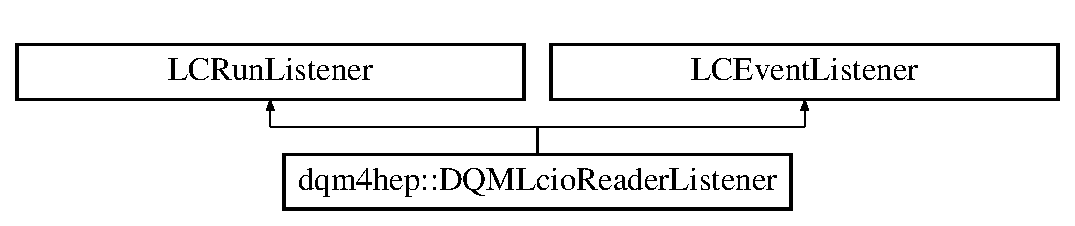
\includegraphics[height=2.000000cm]{classdqm4hep_1_1DQMLcioReaderListener}
\end{center}
\end{figure}
\subsection*{Public Member Functions}
\begin{DoxyCompactItemize}
\item 
{\bf D\+Q\+M\+Lcio\+Reader\+Listener} (I\+O\+::\+L\+C\+Reader $\ast$p\+L\+C\+Reader)
\begin{DoxyCompactList}\small\item\em Constructor with a data service. \end{DoxyCompactList}\item 
virtual {\bf $\sim$\+D\+Q\+M\+Lcio\+Reader\+Listener} ()
\begin{DoxyCompactList}\small\item\em Destructor. \end{DoxyCompactList}\item 
void {\bf set\+Sleep\+Time} (unsigned int usleep\+Time)
\begin{DoxyCompactList}\small\item\em Set the time for a usleep call between each event (in u secs) \end{DoxyCompactList}\item 
void {\bf set\+Event\+Client} ({\bf D\+Q\+M\+Event\+Client} $\ast$p\+Event\+Client)
\begin{DoxyCompactList}\small\item\em Set the event collector client that will publish the event over the network. \end{DoxyCompactList}\item 
void {\bf set\+Simulate\+Spill} (bool simulate)
\begin{DoxyCompactList}\small\item\em Whether the listener has to simulate a spill time structure. \end{DoxyCompactList}\item 
void {\bf process\+Event} (E\+V\+E\+N\+T\+::\+L\+C\+Event $\ast$p\+L\+C\+Event)
\item 
void {\bf modify\+Event} (E\+V\+E\+N\+T\+::\+L\+C\+Event $\ast$p\+L\+C\+Event)
\item 
void {\bf process\+Run\+Header} (E\+V\+E\+N\+T\+::\+L\+C\+Run\+Header $\ast$p\+L\+C\+Run\+Header)
\item 
void {\bf modify\+Run\+Header} (E\+V\+E\+N\+T\+::\+L\+C\+Run\+Header $\ast$p\+L\+C\+Run\+Header)
\end{DoxyCompactItemize}
\subsection*{Protected Attributes}
\begin{DoxyCompactItemize}
\item 
{\bf D\+Q\+M\+Event\+Client} $\ast$ {\bf m\+\_\+p\+Event\+Client}
\item 
I\+O\+::\+L\+C\+Reader $\ast$ {\bf m\+\_\+p\+L\+C\+Reader}
\item 
unsigned int {\bf m\+\_\+sleep\+Time}
\item 
bool {\bf m\+\_\+simulate\+Spill}
\item 
E\+V\+E\+N\+T\+::long64 {\bf m\+\_\+previous\+Time\+Stamp}
\end{DoxyCompactItemize}


\subsection{Detailed Description}
\doxyref{D\+Q\+M\+Lcio\+Reader\+Listener}{p.}{classdqm4hep_1_1DQMLcioReaderListener} class. 

Definition at line 47 of file D\+Q\+M\+Lcio\+Reader\+Listener.\+h.



\subsection{Constructor \& Destructor Documentation}
\index{dqm4hep\+::\+D\+Q\+M\+Lcio\+Reader\+Listener@{dqm4hep\+::\+D\+Q\+M\+Lcio\+Reader\+Listener}!D\+Q\+M\+Lcio\+Reader\+Listener@{D\+Q\+M\+Lcio\+Reader\+Listener}}
\index{D\+Q\+M\+Lcio\+Reader\+Listener@{D\+Q\+M\+Lcio\+Reader\+Listener}!dqm4hep\+::\+D\+Q\+M\+Lcio\+Reader\+Listener@{dqm4hep\+::\+D\+Q\+M\+Lcio\+Reader\+Listener}}
\subsubsection[{D\+Q\+M\+Lcio\+Reader\+Listener}]{\setlength{\rightskip}{0pt plus 5cm}dqm4hep\+::\+D\+Q\+M\+Lcio\+Reader\+Listener\+::\+D\+Q\+M\+Lcio\+Reader\+Listener (
\begin{DoxyParamCaption}
\item[{I\+O\+::\+L\+C\+Reader $\ast$}]{p\+L\+C\+Reader}
\end{DoxyParamCaption}
)}\label{classdqm4hep_1_1DQMLcioReaderListener_a2707676bd1b563300add1727023c14fc}


Constructor with a data service. 



Definition at line 43 of file D\+Q\+M\+Lcio\+Reader\+Listener.\+cc.



References m\+\_\+p\+L\+C\+Reader.


\begin{DoxyCode}
43                                                                   :
44     m_pLCReader(pLCReader),
45     m_pEventClient(NULL),
46     m_sleepTime(0),
47     m_simulateSpill(\textcolor{keyword}{false}),
48     m_previousTimeStamp(0)
49 \{
50   \textcolor{keywordflow}{if}(NULL == m_pLCReader)
51     \textcolor{keywordflow}{throw} dqm4hep::StatusCodeException(dqm4hep::STATUS\_CODE\_INVALID\_PTR);
52 
53   m_pLCReader->registerLCEventListener(\textcolor{keyword}{this});
54   m_pLCReader->registerLCRunListener(\textcolor{keyword}{this});
55 \}
\end{DoxyCode}
\index{dqm4hep\+::\+D\+Q\+M\+Lcio\+Reader\+Listener@{dqm4hep\+::\+D\+Q\+M\+Lcio\+Reader\+Listener}!````~D\+Q\+M\+Lcio\+Reader\+Listener@{$\sim$\+D\+Q\+M\+Lcio\+Reader\+Listener}}
\index{````~D\+Q\+M\+Lcio\+Reader\+Listener@{$\sim$\+D\+Q\+M\+Lcio\+Reader\+Listener}!dqm4hep\+::\+D\+Q\+M\+Lcio\+Reader\+Listener@{dqm4hep\+::\+D\+Q\+M\+Lcio\+Reader\+Listener}}
\subsubsection[{$\sim$\+D\+Q\+M\+Lcio\+Reader\+Listener}]{\setlength{\rightskip}{0pt plus 5cm}dqm4hep\+::\+D\+Q\+M\+Lcio\+Reader\+Listener\+::$\sim$\+D\+Q\+M\+Lcio\+Reader\+Listener (
\begin{DoxyParamCaption}
{}
\end{DoxyParamCaption}
)\hspace{0.3cm}{\ttfamily [virtual]}}\label{classdqm4hep_1_1DQMLcioReaderListener_ac5fdc3b960f78f01f7472135aa31600d}


Destructor. 



Definition at line 59 of file D\+Q\+M\+Lcio\+Reader\+Listener.\+cc.



References m\+\_\+p\+L\+C\+Reader.


\begin{DoxyCode}
60 \{
61   \textcolor{keywordflow}{if}(m_pLCReader)
62   \{
63     m_pLCReader->removeLCEventListener(\textcolor{keyword}{this});
64     m_pLCReader->removeLCRunListener(\textcolor{keyword}{this});
65  \}
66 \}
\end{DoxyCode}


\subsection{Member Function Documentation}
\index{dqm4hep\+::\+D\+Q\+M\+Lcio\+Reader\+Listener@{dqm4hep\+::\+D\+Q\+M\+Lcio\+Reader\+Listener}!modify\+Event@{modify\+Event}}
\index{modify\+Event@{modify\+Event}!dqm4hep\+::\+D\+Q\+M\+Lcio\+Reader\+Listener@{dqm4hep\+::\+D\+Q\+M\+Lcio\+Reader\+Listener}}
\subsubsection[{modify\+Event}]{\setlength{\rightskip}{0pt plus 5cm}void dqm4hep\+::\+D\+Q\+M\+Lcio\+Reader\+Listener\+::modify\+Event (
\begin{DoxyParamCaption}
\item[{E\+V\+E\+N\+T\+::\+L\+C\+Event $\ast$}]{p\+L\+C\+Event}
\end{DoxyParamCaption}
)}\label{classdqm4hep_1_1DQMLcioReaderListener_a16fa4ee99f7cc19f79aab0ebd9741100}


Definition at line 115 of file D\+Q\+M\+Lcio\+Reader\+Listener.\+cc.


\begin{DoxyCode}
116 \{
117  \textcolor{comment}{/* nop */}
118 \}
\end{DoxyCode}
\index{dqm4hep\+::\+D\+Q\+M\+Lcio\+Reader\+Listener@{dqm4hep\+::\+D\+Q\+M\+Lcio\+Reader\+Listener}!modify\+Run\+Header@{modify\+Run\+Header}}
\index{modify\+Run\+Header@{modify\+Run\+Header}!dqm4hep\+::\+D\+Q\+M\+Lcio\+Reader\+Listener@{dqm4hep\+::\+D\+Q\+M\+Lcio\+Reader\+Listener}}
\subsubsection[{modify\+Run\+Header}]{\setlength{\rightskip}{0pt plus 5cm}void dqm4hep\+::\+D\+Q\+M\+Lcio\+Reader\+Listener\+::modify\+Run\+Header (
\begin{DoxyParamCaption}
\item[{E\+V\+E\+N\+T\+::\+L\+C\+Run\+Header $\ast$}]{p\+L\+C\+Run\+Header}
\end{DoxyParamCaption}
)}\label{classdqm4hep_1_1DQMLcioReaderListener_a869a17d9e69d510dd19c42850d4d357f}


Definition at line 129 of file D\+Q\+M\+Lcio\+Reader\+Listener.\+cc.


\begin{DoxyCode}
130 \{
131  \textcolor{comment}{/* nop */}
132 \}
\end{DoxyCode}
\index{dqm4hep\+::\+D\+Q\+M\+Lcio\+Reader\+Listener@{dqm4hep\+::\+D\+Q\+M\+Lcio\+Reader\+Listener}!process\+Event@{process\+Event}}
\index{process\+Event@{process\+Event}!dqm4hep\+::\+D\+Q\+M\+Lcio\+Reader\+Listener@{dqm4hep\+::\+D\+Q\+M\+Lcio\+Reader\+Listener}}
\subsubsection[{process\+Event}]{\setlength{\rightskip}{0pt plus 5cm}void dqm4hep\+::\+D\+Q\+M\+Lcio\+Reader\+Listener\+::process\+Event (
\begin{DoxyParamCaption}
\item[{E\+V\+E\+N\+T\+::\+L\+C\+Event $\ast$}]{p\+L\+C\+Event}
\end{DoxyParamCaption}
)}\label{classdqm4hep_1_1DQMLcioReaderListener_ae85237eac47f231949676bb359541ec5}


Definition at line 70 of file D\+Q\+M\+Lcio\+Reader\+Listener.\+cc.



References dqm4hep\+::\+D\+E\+B\+U\+G, m\+\_\+p\+Event\+Client, m\+\_\+previous\+Time\+Stamp, m\+\_\+simulate\+Spill, m\+\_\+sleep\+Time, dqm4hep\+::\+D\+Q\+M\+Event\+Client\+::send\+Event(), dqm4hep\+::\+D\+Q\+M\+Event\+::set\+Event(), and T\+H\+R\+O\+W\+\_\+\+R\+E\+S\+U\+L\+T\+\_\+\+I\+F.


\begin{DoxyCode}
71 \{
72   \textcolor{keywordflow}{if}(NULL == m_pEventClient)
73     \textcolor{keywordflow}{throw} dqm4hep::StatusCodeException(dqm4hep::STATUS\_CODE\_NOT\_INITIALIZED);
74 
75   DQMEvent *pDqmEvent = \textcolor{keyword}{new} DQMLCEvent();
76   pDqmEvent->setEvent<EVENT::LCEvent>(pLCEvent, \textcolor{keyword}{false});
77 
78   \textcolor{keywordflow}{if}(m_simulateSpill)
79   \{
80     EVENT::long64 timeStamp = pLCEvent->getTimeStamp();
81     EVENT::long64 timeStampDifference = (timeStamp - m_previousTimeStamp);
82 
83     \textcolor{keywordflow}{if}(timeStampDifference > 0 && m_previousTimeStamp != 0)
84     \{
85       streamlog\_out(DEBUG) << \textcolor{stringliteral}{"Sleeping "} << timeStampDifference << \textcolor{stringliteral}{" sec ..."} << std::endl;
86       sleep(timeStampDifference);
87     \}
88 
89     m_previousTimeStamp = timeStamp;
90 
91     streamlog\_out(DEBUG) << \textcolor{stringliteral}{"Sending event no "} << pLCEvent->getEventNumber() << std::endl;
92     THROW_RESULT_IF(dqm4hep::STATUS\_CODE\_SUCCESS, !=, m_pEventClient->sendEvent(pDqmEvent));
93     streamlog\_out(DEBUG) << \textcolor{stringliteral}{"Event no "} << pLCEvent->getEventNumber() << \textcolor{stringliteral}{" sent"} << std::endl;
94   \}
95   \textcolor{keywordflow}{else}
96   \{
97     streamlog\_out(DEBUG) << \textcolor{stringliteral}{"Sending event no "} << pLCEvent->getEventNumber() << std::endl;
98     THROW_RESULT_IF(dqm4hep::STATUS\_CODE\_SUCCESS, !=, m_pEventClient->sendEvent(pDqmEvent));
99     streamlog\_out(DEBUG) << \textcolor{stringliteral}{"Event no "} << pLCEvent->getEventNumber() << \textcolor{stringliteral}{" sent"} << std::endl;
100 
101     \textcolor{keywordflow}{if}(m_sleepTime != 0)
102     \{
103       timespec timesleep;
104         timesleep.tv\_sec = 0;
105         timesleep.tv\_nsec = 1000*m_sleepTime;
106       nanosleep(&timesleep, NULL);
107     \}
108   \}
109 
110   \textcolor{keyword}{delete} pDqmEvent;
111 \}
\end{DoxyCode}
\index{dqm4hep\+::\+D\+Q\+M\+Lcio\+Reader\+Listener@{dqm4hep\+::\+D\+Q\+M\+Lcio\+Reader\+Listener}!process\+Run\+Header@{process\+Run\+Header}}
\index{process\+Run\+Header@{process\+Run\+Header}!dqm4hep\+::\+D\+Q\+M\+Lcio\+Reader\+Listener@{dqm4hep\+::\+D\+Q\+M\+Lcio\+Reader\+Listener}}
\subsubsection[{process\+Run\+Header}]{\setlength{\rightskip}{0pt plus 5cm}void dqm4hep\+::\+D\+Q\+M\+Lcio\+Reader\+Listener\+::process\+Run\+Header (
\begin{DoxyParamCaption}
\item[{E\+V\+E\+N\+T\+::\+L\+C\+Run\+Header $\ast$}]{p\+L\+C\+Run\+Header}
\end{DoxyParamCaption}
)}\label{classdqm4hep_1_1DQMLcioReaderListener_a43b466dd3455eacf7fc073f98df91d3f}


Definition at line 122 of file D\+Q\+M\+Lcio\+Reader\+Listener.\+cc.


\begin{DoxyCode}
123 \{
124   \textcolor{comment}{/* nop */}
125 \}
\end{DoxyCode}
\index{dqm4hep\+::\+D\+Q\+M\+Lcio\+Reader\+Listener@{dqm4hep\+::\+D\+Q\+M\+Lcio\+Reader\+Listener}!set\+Event\+Client@{set\+Event\+Client}}
\index{set\+Event\+Client@{set\+Event\+Client}!dqm4hep\+::\+D\+Q\+M\+Lcio\+Reader\+Listener@{dqm4hep\+::\+D\+Q\+M\+Lcio\+Reader\+Listener}}
\subsubsection[{set\+Event\+Client}]{\setlength{\rightskip}{0pt plus 5cm}void dqm4hep\+::\+D\+Q\+M\+Lcio\+Reader\+Listener\+::set\+Event\+Client (
\begin{DoxyParamCaption}
\item[{{\bf D\+Q\+M\+Event\+Client} $\ast$}]{p\+Event\+Client}
\end{DoxyParamCaption}
)}\label{classdqm4hep_1_1DQMLcioReaderListener_aa7b1e47458578b8d6daf15963ee5a6da}


Set the event collector client that will publish the event over the network. 



Definition at line 150 of file D\+Q\+M\+Lcio\+Reader\+Listener.\+cc.



References m\+\_\+p\+Event\+Client.


\begin{DoxyCode}
151 \{
152   m_pEventClient = pEventClient;
153 \}
\end{DoxyCode}
\index{dqm4hep\+::\+D\+Q\+M\+Lcio\+Reader\+Listener@{dqm4hep\+::\+D\+Q\+M\+Lcio\+Reader\+Listener}!set\+Simulate\+Spill@{set\+Simulate\+Spill}}
\index{set\+Simulate\+Spill@{set\+Simulate\+Spill}!dqm4hep\+::\+D\+Q\+M\+Lcio\+Reader\+Listener@{dqm4hep\+::\+D\+Q\+M\+Lcio\+Reader\+Listener}}
\subsubsection[{set\+Simulate\+Spill}]{\setlength{\rightskip}{0pt plus 5cm}void dqm4hep\+::\+D\+Q\+M\+Lcio\+Reader\+Listener\+::set\+Simulate\+Spill (
\begin{DoxyParamCaption}
\item[{bool}]{simulate}
\end{DoxyParamCaption}
)}\label{classdqm4hep_1_1DQMLcioReaderListener_ab912936b13fb088891b52eff61637e8e}


Whether the listener has to simulate a spill time structure. 

The time stamp is looked-\/up in L\+C\+Events and a sleep(n) is called between each event sending where n is the difference of time stamp 

Definition at line 143 of file D\+Q\+M\+Lcio\+Reader\+Listener.\+cc.



References m\+\_\+simulate\+Spill.


\begin{DoxyCode}
144 \{
145   m_simulateSpill = simulate;
146 \}
\end{DoxyCode}
\index{dqm4hep\+::\+D\+Q\+M\+Lcio\+Reader\+Listener@{dqm4hep\+::\+D\+Q\+M\+Lcio\+Reader\+Listener}!set\+Sleep\+Time@{set\+Sleep\+Time}}
\index{set\+Sleep\+Time@{set\+Sleep\+Time}!dqm4hep\+::\+D\+Q\+M\+Lcio\+Reader\+Listener@{dqm4hep\+::\+D\+Q\+M\+Lcio\+Reader\+Listener}}
\subsubsection[{set\+Sleep\+Time}]{\setlength{\rightskip}{0pt plus 5cm}void dqm4hep\+::\+D\+Q\+M\+Lcio\+Reader\+Listener\+::set\+Sleep\+Time (
\begin{DoxyParamCaption}
\item[{unsigned int}]{usleep\+Time}
\end{DoxyParamCaption}
)}\label{classdqm4hep_1_1DQMLcioReaderListener_a7f8e0ca5154d5c4d274773b5fed9d1cb}


Set the time for a usleep call between each event (in u secs) 



Definition at line 136 of file D\+Q\+M\+Lcio\+Reader\+Listener.\+cc.



References m\+\_\+sleep\+Time.


\begin{DoxyCode}
137 \{
138   m_sleepTime = usleepTime;
139 \}
\end{DoxyCode}


\subsection{Member Data Documentation}
\index{dqm4hep\+::\+D\+Q\+M\+Lcio\+Reader\+Listener@{dqm4hep\+::\+D\+Q\+M\+Lcio\+Reader\+Listener}!m\+\_\+p\+Event\+Client@{m\+\_\+p\+Event\+Client}}
\index{m\+\_\+p\+Event\+Client@{m\+\_\+p\+Event\+Client}!dqm4hep\+::\+D\+Q\+M\+Lcio\+Reader\+Listener@{dqm4hep\+::\+D\+Q\+M\+Lcio\+Reader\+Listener}}
\subsubsection[{m\+\_\+p\+Event\+Client}]{\setlength{\rightskip}{0pt plus 5cm}{\bf D\+Q\+M\+Event\+Client}$\ast$ dqm4hep\+::\+D\+Q\+M\+Lcio\+Reader\+Listener\+::m\+\_\+p\+Event\+Client\hspace{0.3cm}{\ttfamily [protected]}}\label{classdqm4hep_1_1DQMLcioReaderListener_a7d2d0a5959c15568050f382b4943283c}


Definition at line 79 of file D\+Q\+M\+Lcio\+Reader\+Listener.\+h.



Referenced by process\+Event(), and set\+Event\+Client().

\index{dqm4hep\+::\+D\+Q\+M\+Lcio\+Reader\+Listener@{dqm4hep\+::\+D\+Q\+M\+Lcio\+Reader\+Listener}!m\+\_\+p\+L\+C\+Reader@{m\+\_\+p\+L\+C\+Reader}}
\index{m\+\_\+p\+L\+C\+Reader@{m\+\_\+p\+L\+C\+Reader}!dqm4hep\+::\+D\+Q\+M\+Lcio\+Reader\+Listener@{dqm4hep\+::\+D\+Q\+M\+Lcio\+Reader\+Listener}}
\subsubsection[{m\+\_\+p\+L\+C\+Reader}]{\setlength{\rightskip}{0pt plus 5cm}I\+O\+::\+L\+C\+Reader$\ast$ dqm4hep\+::\+D\+Q\+M\+Lcio\+Reader\+Listener\+::m\+\_\+p\+L\+C\+Reader\hspace{0.3cm}{\ttfamily [protected]}}\label{classdqm4hep_1_1DQMLcioReaderListener_a0e6e1e813ec99978a1029f0636cca107}


Definition at line 80 of file D\+Q\+M\+Lcio\+Reader\+Listener.\+h.



Referenced by D\+Q\+M\+Lcio\+Reader\+Listener(), and $\sim$\+D\+Q\+M\+Lcio\+Reader\+Listener().

\index{dqm4hep\+::\+D\+Q\+M\+Lcio\+Reader\+Listener@{dqm4hep\+::\+D\+Q\+M\+Lcio\+Reader\+Listener}!m\+\_\+previous\+Time\+Stamp@{m\+\_\+previous\+Time\+Stamp}}
\index{m\+\_\+previous\+Time\+Stamp@{m\+\_\+previous\+Time\+Stamp}!dqm4hep\+::\+D\+Q\+M\+Lcio\+Reader\+Listener@{dqm4hep\+::\+D\+Q\+M\+Lcio\+Reader\+Listener}}
\subsubsection[{m\+\_\+previous\+Time\+Stamp}]{\setlength{\rightskip}{0pt plus 5cm}E\+V\+E\+N\+T\+::long64 dqm4hep\+::\+D\+Q\+M\+Lcio\+Reader\+Listener\+::m\+\_\+previous\+Time\+Stamp\hspace{0.3cm}{\ttfamily [protected]}}\label{classdqm4hep_1_1DQMLcioReaderListener_ad1926a3a5986ca6bf0eb980cceba3c31}


Definition at line 83 of file D\+Q\+M\+Lcio\+Reader\+Listener.\+h.



Referenced by process\+Event().

\index{dqm4hep\+::\+D\+Q\+M\+Lcio\+Reader\+Listener@{dqm4hep\+::\+D\+Q\+M\+Lcio\+Reader\+Listener}!m\+\_\+simulate\+Spill@{m\+\_\+simulate\+Spill}}
\index{m\+\_\+simulate\+Spill@{m\+\_\+simulate\+Spill}!dqm4hep\+::\+D\+Q\+M\+Lcio\+Reader\+Listener@{dqm4hep\+::\+D\+Q\+M\+Lcio\+Reader\+Listener}}
\subsubsection[{m\+\_\+simulate\+Spill}]{\setlength{\rightskip}{0pt plus 5cm}bool dqm4hep\+::\+D\+Q\+M\+Lcio\+Reader\+Listener\+::m\+\_\+simulate\+Spill\hspace{0.3cm}{\ttfamily [protected]}}\label{classdqm4hep_1_1DQMLcioReaderListener_ad7aebaf825976993f862fce9d23c5e08}


Definition at line 82 of file D\+Q\+M\+Lcio\+Reader\+Listener.\+h.



Referenced by process\+Event(), and set\+Simulate\+Spill().

\index{dqm4hep\+::\+D\+Q\+M\+Lcio\+Reader\+Listener@{dqm4hep\+::\+D\+Q\+M\+Lcio\+Reader\+Listener}!m\+\_\+sleep\+Time@{m\+\_\+sleep\+Time}}
\index{m\+\_\+sleep\+Time@{m\+\_\+sleep\+Time}!dqm4hep\+::\+D\+Q\+M\+Lcio\+Reader\+Listener@{dqm4hep\+::\+D\+Q\+M\+Lcio\+Reader\+Listener}}
\subsubsection[{m\+\_\+sleep\+Time}]{\setlength{\rightskip}{0pt plus 5cm}unsigned int dqm4hep\+::\+D\+Q\+M\+Lcio\+Reader\+Listener\+::m\+\_\+sleep\+Time\hspace{0.3cm}{\ttfamily [protected]}}\label{classdqm4hep_1_1DQMLcioReaderListener_ab2e19ce1dd6149cd7bf530c7d0a75b3a}


Definition at line 81 of file D\+Q\+M\+Lcio\+Reader\+Listener.\+h.



Referenced by process\+Event(), and set\+Sleep\+Time().



The documentation for this class was generated from the following files\+:\begin{DoxyCompactItemize}
\item 
{\bf D\+Q\+M\+Lcio\+Reader\+Listener.\+h}\item 
{\bf D\+Q\+M\+Lcio\+Reader\+Listener.\+cc}\end{DoxyCompactItemize}

\section{dqm4hep\+:\+:D\+Q\+M\+L\+C\+Parameters\+Streamer Class Reference}
\label{classdqm4hep_1_1DQMLCParametersStreamer}\index{dqm4hep\+::\+D\+Q\+M\+L\+C\+Parameters\+Streamer@{dqm4hep\+::\+D\+Q\+M\+L\+C\+Parameters\+Streamer}}


\doxyref{D\+Q\+M\+L\+C\+Parameters\+Streamer}{p.}{classdqm4hep_1_1DQMLCParametersStreamer} class.  




{\ttfamily \#include $<$D\+Q\+M\+L\+C\+Event\+Streamer.\+h$>$}

Inheritance diagram for dqm4hep\+:\+:D\+Q\+M\+L\+C\+Parameters\+Streamer\+:\begin{figure}[H]
\begin{center}
\leavevmode
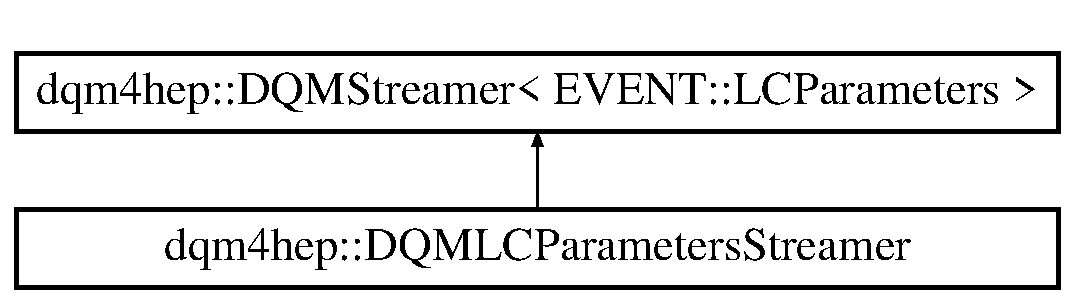
\includegraphics[height=2.000000cm]{classdqm4hep_1_1DQMLCParametersStreamer}
\end{center}
\end{figure}
\subsection*{Public Member Functions}
\begin{DoxyCompactItemize}
\item 
{\bf Status\+Code} {\bf serialize} (const E\+V\+E\+N\+T\+::\+L\+C\+Parameters $\ast$const p\+L\+Carameters, {\bf D\+Q\+M\+Data\+Stream} $\ast$const p\+Data\+Stream)
\begin{DoxyCompactList}\small\item\em Serialize the L\+C\+Parameters in data\+Stream. \end{DoxyCompactList}\item 
{\bf Status\+Code} {\bf deserialize} (E\+V\+E\+N\+T\+::\+L\+C\+Parameters $\ast$\&p\+L\+C\+Parameters, {\bf D\+Q\+M\+Data\+Stream} $\ast$const p\+Data\+Stream)
\begin{DoxyCompactList}\small\item\em Deserialize the L\+C\+Parameters from data\+Stream. \end{DoxyCompactList}\end{DoxyCompactItemize}


\subsection{Detailed Description}
\doxyref{D\+Q\+M\+L\+C\+Parameters\+Streamer}{p.}{classdqm4hep_1_1DQMLCParametersStreamer} class. 

Definition at line 56 of file D\+Q\+M\+L\+C\+Event\+Streamer.\+h.



\subsection{Member Function Documentation}
\index{dqm4hep\+::\+D\+Q\+M\+L\+C\+Parameters\+Streamer@{dqm4hep\+::\+D\+Q\+M\+L\+C\+Parameters\+Streamer}!deserialize@{deserialize}}
\index{deserialize@{deserialize}!dqm4hep\+::\+D\+Q\+M\+L\+C\+Parameters\+Streamer@{dqm4hep\+::\+D\+Q\+M\+L\+C\+Parameters\+Streamer}}
\subsubsection[{deserialize}]{\setlength{\rightskip}{0pt plus 5cm}{\bf Status\+Code} dqm4hep\+::\+D\+Q\+M\+L\+C\+Parameters\+Streamer\+::deserialize (
\begin{DoxyParamCaption}
\item[{E\+V\+E\+N\+T\+::\+L\+C\+Parameters $\ast$\&}]{p\+L\+C\+Parameters, }
\item[{{\bf D\+Q\+M\+Data\+Stream} $\ast$const}]{p\+Data\+Stream}
\end{DoxyParamCaption}
)\hspace{0.3cm}{\ttfamily [virtual]}}\label{classdqm4hep_1_1DQMLCParametersStreamer_a31488fa0a108c8e6db29ae1242807cbd}


Deserialize the L\+C\+Parameters from data\+Stream. 



Implements {\bf dqm4hep\+::\+D\+Q\+M\+Streamer$<$ E\+V\+E\+N\+T\+::\+L\+C\+Parameters $>$} \doxyref{}{p.}{singletondqm4hep_1_1DQMStreamer_a45424f285015b093ccbd7bfd3a38249d}.



Definition at line 403 of file D\+Q\+M\+L\+C\+Event\+Streamer.\+cc.



References dqm4hep\+::\+D\+Q\+M\+Data\+Stream\+::read(), and R\+E\+T\+U\+R\+N\+\_\+\+R\+E\+S\+U\+L\+T\+\_\+\+I\+F.



Referenced by dqm4hep\+::\+D\+Q\+M\+L\+C\+Event\+Streamer\+::deserialize(), and dqm4hep\+::\+D\+Q\+M\+L\+C\+Collection\+Streamer\+::deserialize().


\begin{DoxyCode}
405 \{
406   dqm_int nInt = 0;
407   RETURN_RESULT_IF(STATUS\_CODE\_SUCCESS, !=, pDataStream->read(nInt));
408 
409   \textcolor{keywordflow}{if}(nInt != 0)
410   \{
411     \textcolor{keywordflow}{for}(\textcolor{keywordtype}{int} i=0 ; i<nInt ; i++)
412     \{
413       std::string key;
414       RETURN_RESULT_IF(STATUS\_CODE\_SUCCESS, !=, pDataStream->read(key));
415 
416       dqm_int vecSize = 0;
417       RETURN_RESULT_IF(STATUS\_CODE\_SUCCESS, !=, pDataStream->read(vecSize));
418 
419       EVENT::IntVec intValues;
420 
421       \textcolor{keywordflow}{for}(\textcolor{keywordtype}{int} j=0 ; j<vecSize ; j++)
422       \{
423         dqm_int value = 0;
424         RETURN_RESULT_IF(STATUS\_CODE\_SUCCESS, !=, pDataStream->read(value));
425         intValues.push\_back(value);
426       \}
427 
428       pLCParameters->setValues(key, intValues);
429     \}
430   \}
431 
432   dqm_int nFloat = 0;
433   RETURN_RESULT_IF(STATUS\_CODE\_SUCCESS, !=, pDataStream->read(nFloat));
434 
435   \textcolor{keywordflow}{if}(nFloat != 0)
436   \{
437     \textcolor{keywordflow}{for}(\textcolor{keywordtype}{int} i=0 ; i<nFloat ; i++)
438     \{
439       std::string key;
440       RETURN_RESULT_IF(STATUS\_CODE\_SUCCESS, !=, pDataStream->read(key));
441 
442       dqm_int vecSize = 0;
443       RETURN_RESULT_IF(STATUS\_CODE\_SUCCESS, !=, pDataStream->read(vecSize));
444 
445       EVENT::FloatVec floatValues;
446 
447       \textcolor{keywordflow}{for}(\textcolor{keywordtype}{int} j=0 ; j<vecSize ; j++)
448       \{
449         dqm_float value = 0.f;
450         RETURN_RESULT_IF(STATUS\_CODE\_SUCCESS, !=, pDataStream->read(value));
451         floatValues.push\_back(value);
452       \}
453 
454       pLCParameters->setValues(key, floatValues);
455     \}
456   \}
457 
458   dqm_int nString = 0;
459   RETURN_RESULT_IF(STATUS\_CODE\_SUCCESS, !=, pDataStream->read(nString));
460 
461   \textcolor{keywordflow}{if}(nString != 0)
462   \{
463     \textcolor{keywordflow}{for}(\textcolor{keywordtype}{int} i=0 ; i<nString ; i++)
464     \{
465       std::string key;
466       RETURN_RESULT_IF(STATUS\_CODE\_SUCCESS, !=, pDataStream->read(key));
467 
468       dqm_int vecSize = 0;
469       RETURN_RESULT_IF(STATUS\_CODE\_SUCCESS, !=, pDataStream->read(vecSize));
470 
471       EVENT::StringVec stringValues;
472 
473       \textcolor{keywordflow}{for}(\textcolor{keywordtype}{int} j=0 ; j<vecSize ; j++)
474       \{
475         std::string value;
476         RETURN_RESULT_IF(STATUS\_CODE\_SUCCESS, !=, pDataStream->read(value));
477         stringValues.push\_back(value);
478       \}
479 
480       pLCParameters->setValues(key, stringValues);
481     \}
482   \}
483 
484   \textcolor{keywordflow}{return} STATUS\_CODE\_SUCCESS;
485 \}
\end{DoxyCode}
\index{dqm4hep\+::\+D\+Q\+M\+L\+C\+Parameters\+Streamer@{dqm4hep\+::\+D\+Q\+M\+L\+C\+Parameters\+Streamer}!serialize@{serialize}}
\index{serialize@{serialize}!dqm4hep\+::\+D\+Q\+M\+L\+C\+Parameters\+Streamer@{dqm4hep\+::\+D\+Q\+M\+L\+C\+Parameters\+Streamer}}
\subsubsection[{serialize}]{\setlength{\rightskip}{0pt plus 5cm}{\bf Status\+Code} dqm4hep\+::\+D\+Q\+M\+L\+C\+Parameters\+Streamer\+::serialize (
\begin{DoxyParamCaption}
\item[{const E\+V\+E\+N\+T\+::\+L\+C\+Parameters $\ast$const}]{p\+L\+Carameters, }
\item[{{\bf D\+Q\+M\+Data\+Stream} $\ast$const}]{p\+Data\+Stream}
\end{DoxyParamCaption}
)\hspace{0.3cm}{\ttfamily [virtual]}}\label{classdqm4hep_1_1DQMLCParametersStreamer_a0b60a1d164f9441ef525909528aebc8b}


Serialize the L\+C\+Parameters in data\+Stream. 



Implements {\bf dqm4hep\+::\+D\+Q\+M\+Streamer$<$ E\+V\+E\+N\+T\+::\+L\+C\+Parameters $>$} \doxyref{}{p.}{singletondqm4hep_1_1DQMStreamer_abc54751ecafff0a88046f41fa4110fcf}.



Definition at line 320 of file D\+Q\+M\+L\+C\+Event\+Streamer.\+cc.



References R\+E\+T\+U\+R\+N\+\_\+\+R\+E\+S\+U\+L\+T\+\_\+\+I\+F, and dqm4hep\+::\+D\+Q\+M\+Data\+Stream\+::write().



Referenced by dqm4hep\+::\+D\+Q\+M\+L\+C\+Event\+Streamer\+::serialize(), and dqm4hep\+::\+D\+Q\+M\+L\+C\+Collection\+Streamer\+::serialize().


\begin{DoxyCode}
322 \{
323   \textcolor{comment}{// write int keys/values}
324   EVENT::StringVec keys;
325   pLCParameters->getIntKeys(keys);
326   dqm_int nKeys = keys.size();
327 
328   RETURN_RESULT_IF(STATUS\_CODE\_SUCCESS, !=, pDataStream->write(nKeys));
329 
330   \textcolor{keywordflow}{for}(\textcolor{keywordtype}{int} i=0 ; i<keys.size() ; i++)
331   \{
332     EVENT::IntVec intVec;
333     pLCParameters->getIntVals(keys.at(i), intVec);
334 
335     std::string key = keys.at(i);
336     RETURN_RESULT_IF(STATUS\_CODE\_SUCCESS, !=, pDataStream->write(key));
337 
338     dqm_int nKeyParams = intVec.size();
339     RETURN_RESULT_IF(STATUS\_CODE\_SUCCESS, !=, pDataStream->write(nKeyParams));
340 
341     \textcolor{keywordflow}{for}(\textcolor{keywordtype}{int} j=0 ; j<intVec.size() ; j++)
342     \{
343       dqm_int val = intVec.at(j);
344       RETURN_RESULT_IF(STATUS\_CODE\_SUCCESS, !=, pDataStream->write(val));
345     \}
346   \}
347 
348 
349   \textcolor{comment}{// write float keys/values}
350   keys.clear();
351   pLCParameters->getFloatKeys(keys);
352   nKeys = keys.size();
353   RETURN_RESULT_IF(STATUS\_CODE\_SUCCESS, !=, pDataStream->write(nKeys));
354 
355   \textcolor{keywordflow}{for}(\textcolor{keywordtype}{int} i=0 ; i<keys.size() ; i++)
356   \{
357     EVENT::FloatVec floatVec;
358     pLCParameters->getFloatVals(keys.at(i), floatVec);
359 
360     std::string key = keys.at(i);
361     RETURN_RESULT_IF(STATUS\_CODE\_SUCCESS, !=, pDataStream->write(key));
362 
363     dqm_int nKeyParams = floatVec.size();
364     RETURN_RESULT_IF(STATUS\_CODE\_SUCCESS, !=, pDataStream->write(nKeyParams));
365 
366     \textcolor{keywordflow}{for}(\textcolor{keywordtype}{int} j=0 ; j<floatVec.size() ; j++)
367     \{
368       dqm_float val = floatVec.at(j);
369       RETURN_RESULT_IF(STATUS\_CODE\_SUCCESS, !=, pDataStream->write(val));
370     \}
371   \}
372 
373 
374   \textcolor{comment}{// write string keys/values}
375   keys.clear();
376   pLCParameters->getStringKeys(keys);
377   nKeys = keys.size();
378   RETURN_RESULT_IF(STATUS\_CODE\_SUCCESS, !=, pDataStream->write(nKeys));
379 
380   \textcolor{keywordflow}{for}(\textcolor{keywordtype}{int} i=0 ; i<keys.size() ; i++)
381   \{
382     EVENT::StringVec stringVec;
383     pLCParameters->getStringVals(keys.at(i), stringVec);
384 
385     std::string key = keys.at(i);
386     RETURN_RESULT_IF(STATUS\_CODE\_SUCCESS, !=, pDataStream->write(key));
387 
388     dqm_int nKeyParams = stringVec.size();
389     RETURN_RESULT_IF(STATUS\_CODE\_SUCCESS, !=, pDataStream->write(nKeyParams));
390 
391     \textcolor{keywordflow}{for}(\textcolor{keywordtype}{int} j=0 ; j<stringVec.size() ; j++)
392     \{
393       std::string val = stringVec.at(j);
394       RETURN_RESULT_IF(STATUS\_CODE\_SUCCESS, !=, pDataStream->write(val));
395     \}
396   \}
397 
398   \textcolor{keywordflow}{return} STATUS\_CODE\_SUCCESS;
399 \}
\end{DoxyCode}


The documentation for this class was generated from the following files\+:\begin{DoxyCompactItemize}
\item 
{\bf D\+Q\+M\+L\+C\+Event\+Streamer.\+h}\item 
{\bf D\+Q\+M\+L\+C\+Event\+Streamer.\+cc}\end{DoxyCompactItemize}

\section{dqm4hep\+:\+:D\+Q\+M\+L\+C\+Str\+Vec\+Streamer Class Reference}
\label{classdqm4hep_1_1DQMLCStrVecStreamer}\index{dqm4hep\+::\+D\+Q\+M\+L\+C\+Str\+Vec\+Streamer@{dqm4hep\+::\+D\+Q\+M\+L\+C\+Str\+Vec\+Streamer}}


\doxyref{D\+Q\+M\+L\+C\+Str\+Vec\+Streamer}{p.}{classdqm4hep_1_1DQMLCStrVecStreamer} class.  




{\ttfamily \#include $<$D\+Q\+M\+L\+C\+Event\+Streamer.\+h$>$}

Inheritance diagram for dqm4hep\+:\+:D\+Q\+M\+L\+C\+Str\+Vec\+Streamer\+:\begin{figure}[H]
\begin{center}
\leavevmode
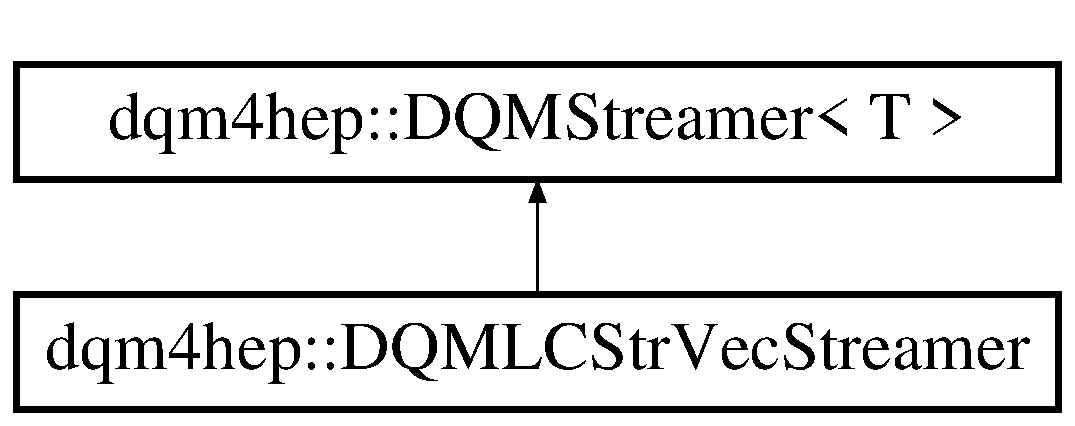
\includegraphics[height=2.000000cm]{classdqm4hep_1_1DQMLCStrVecStreamer}
\end{center}
\end{figure}
\subsection*{Public Member Functions}
\begin{DoxyCompactItemize}
\item 
{\bf Status\+Code} {\bf serialize} (const E\+V\+E\+N\+T\+::\+L\+C\+Object $\ast$const p\+L\+C\+Object, {\bf D\+Q\+M\+Data\+Stream} $\ast$const p\+Data\+Stream)
\begin{DoxyCompactList}\small\item\em Serialize a L\+C\+Str\+Vec. \end{DoxyCompactList}\item 
{\bf Status\+Code} {\bf deserialize} (E\+V\+E\+N\+T\+::\+L\+C\+Object $\ast$\&p\+L\+C\+Object, {\bf D\+Q\+M\+Data\+Stream} $\ast$const p\+Data\+Stream)
\begin{DoxyCompactList}\small\item\em Deserialize a L\+C\+Str\+Vec. \end{DoxyCompactList}\end{DoxyCompactItemize}


\subsection{Detailed Description}
\doxyref{D\+Q\+M\+L\+C\+Str\+Vec\+Streamer}{p.}{classdqm4hep_1_1DQMLCStrVecStreamer} class. 

Definition at line 277 of file D\+Q\+M\+L\+C\+Event\+Streamer.\+h.



\subsection{Member Function Documentation}
\index{dqm4hep\+::\+D\+Q\+M\+L\+C\+Str\+Vec\+Streamer@{dqm4hep\+::\+D\+Q\+M\+L\+C\+Str\+Vec\+Streamer}!deserialize@{deserialize}}
\index{deserialize@{deserialize}!dqm4hep\+::\+D\+Q\+M\+L\+C\+Str\+Vec\+Streamer@{dqm4hep\+::\+D\+Q\+M\+L\+C\+Str\+Vec\+Streamer}}
\subsubsection[{deserialize}]{\setlength{\rightskip}{0pt plus 5cm}{\bf Status\+Code} dqm4hep\+::\+D\+Q\+M\+L\+C\+Str\+Vec\+Streamer\+::deserialize (
\begin{DoxyParamCaption}
\item[{E\+V\+E\+N\+T\+::\+L\+C\+Object $\ast$\&}]{p\+L\+C\+Object, }
\item[{{\bf D\+Q\+M\+Data\+Stream} $\ast$const}]{p\+Data\+Stream}
\end{DoxyParamCaption}
)}\label{classdqm4hep_1_1DQMLCStrVecStreamer_a3945b4482895a7bb72b42daa38fa2c03}


Deserialize a L\+C\+Str\+Vec. 

The object is allocated in this function 

Definition at line 1333 of file D\+Q\+M\+L\+C\+Event\+Streamer.\+cc.



References dqm4hep\+::\+Status\+Code\+Exception\+::get\+Status\+Code(), dqm4hep\+::\+D\+Q\+M\+Data\+Stream\+::read(), and T\+H\+R\+O\+W\+\_\+\+R\+E\+S\+U\+L\+T\+\_\+\+I\+F.


\begin{DoxyCode}
1334 \{
1335   pLCObject = 0;
1336   EVENT::LCStrVec *pStrVec = \textcolor{keyword}{new} EVENT::LCStrVec();
1337 
1338   \textcolor{keywordflow}{try}
1339   \{
1340     dqm_uint nVals = 0;
1341     THROW_RESULT_IF(STATUS\_CODE\_SUCCESS, !=, pDataStream->read(nVals));
1342 
1343     \textcolor{keywordflow}{for}(dqm_uint i=0 ; i<nVals ; i++)
1344     \{
1345       std::string value;
1346       THROW_RESULT_IF(STATUS\_CODE\_SUCCESS, !=, pDataStream->read(value));
1347       pStrVec->push\_back(value);
1348     \}
1349   \}
1350   \textcolor{keywordflow}{catch}(StatusCodeException &exception)
1351   \{
1352     \textcolor{keyword}{delete} pStrVec;
1353     pStrVec = 0;
1354     pLCObject = 0;
1355 
1356     \textcolor{keywordflow}{return} exception.getStatusCode();
1357   \}
1358 
1359   pLCObject = pStrVec;
1360 
1361   \textcolor{keywordflow}{return} STATUS\_CODE\_SUCCESS;
1362 \}
\end{DoxyCode}
\index{dqm4hep\+::\+D\+Q\+M\+L\+C\+Str\+Vec\+Streamer@{dqm4hep\+::\+D\+Q\+M\+L\+C\+Str\+Vec\+Streamer}!serialize@{serialize}}
\index{serialize@{serialize}!dqm4hep\+::\+D\+Q\+M\+L\+C\+Str\+Vec\+Streamer@{dqm4hep\+::\+D\+Q\+M\+L\+C\+Str\+Vec\+Streamer}}
\subsubsection[{serialize}]{\setlength{\rightskip}{0pt plus 5cm}{\bf Status\+Code} dqm4hep\+::\+D\+Q\+M\+L\+C\+Str\+Vec\+Streamer\+::serialize (
\begin{DoxyParamCaption}
\item[{const E\+V\+E\+N\+T\+::\+L\+C\+Object $\ast$const}]{p\+L\+C\+Object, }
\item[{{\bf D\+Q\+M\+Data\+Stream} $\ast$const}]{p\+Data\+Stream}
\end{DoxyParamCaption}
)}\label{classdqm4hep_1_1DQMLCStrVecStreamer_a39884bb8160d4f2d7bf7a472b5eaa650}


Serialize a L\+C\+Str\+Vec. 



Definition at line 1312 of file D\+Q\+M\+L\+C\+Event\+Streamer.\+cc.



References R\+E\+T\+U\+R\+N\+\_\+\+R\+E\+S\+U\+L\+T\+\_\+\+I\+F, and dqm4hep\+::\+D\+Q\+M\+Data\+Stream\+::write().


\begin{DoxyCode}
1313 \{
1314   \textcolor{keyword}{const} EVENT::LCStrVec *\textcolor{keyword}{const} pStrVec = \textcolor{keyword}{dynamic\_cast<}\textcolor{keyword}{const }EVENT::LCStrVec *const\textcolor{keyword}{>}(pLCObject);
1315 
1316   \textcolor{keywordflow}{if}(NULL == pStrVec)
1317     \textcolor{keywordflow}{return} STATUS\_CODE\_INVALID\_PARAMETER;
1318 
1319   dqm_uint nVals = pStrVec->size();
1320   RETURN_RESULT_IF(STATUS\_CODE\_SUCCESS, !=, pDataStream->write(nVals));
1321 
1322   \textcolor{keywordflow}{for}(dqm_uint i=0 ; i<nVals ; i++)
1323   \{
1324     std::string value = pStrVec->at(i);
1325     RETURN_RESULT_IF(STATUS\_CODE\_SUCCESS, !=, pDataStream->write(value));
1326   \}
1327 
1328   \textcolor{keywordflow}{return} STATUS\_CODE\_SUCCESS;
1329 \}
\end{DoxyCode}


The documentation for this class was generated from the following files\+:\begin{DoxyCompactItemize}
\item 
{\bf D\+Q\+M\+L\+C\+Event\+Streamer.\+h}\item 
{\bf D\+Q\+M\+L\+C\+Event\+Streamer.\+cc}\end{DoxyCompactItemize}

\section{dqm4hep\+:\+:D\+Q\+M\+Local\+File\+Handler Class Reference}
\label{classdqm4hep_1_1DQMLocalFileHandler}\index{dqm4hep\+::\+D\+Q\+M\+Local\+File\+Handler@{dqm4hep\+::\+D\+Q\+M\+Local\+File\+Handler}}


\doxyref{D\+Q\+M\+Local\+File\+Handler}{p.}{classdqm4hep_1_1DQMLocalFileHandler} class.  




{\ttfamily \#include $<$D\+Q\+M\+Local\+File\+Handler.\+h$>$}

Inheritance diagram for dqm4hep\+:\+:D\+Q\+M\+Local\+File\+Handler\+:\begin{figure}[H]
\begin{center}
\leavevmode
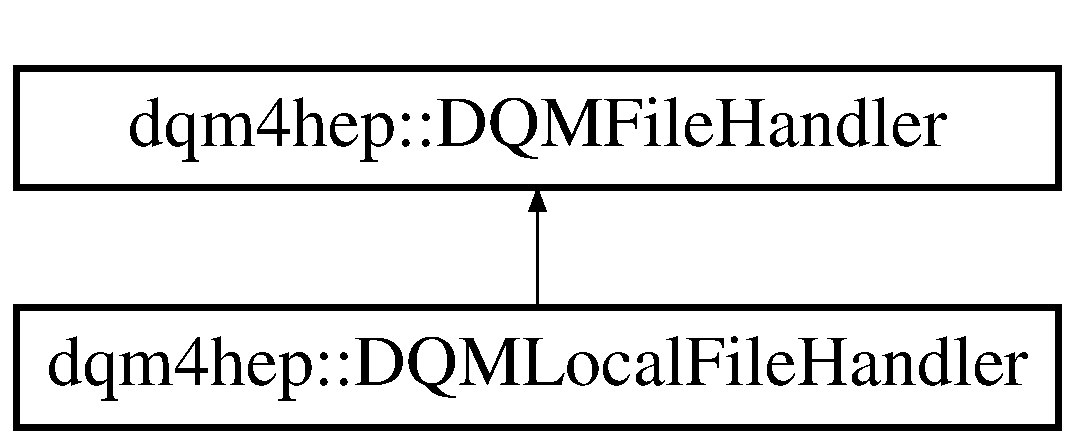
\includegraphics[height=2.000000cm]{classdqm4hep_1_1DQMLocalFileHandler}
\end{center}
\end{figure}
\subsection*{Public Member Functions}
\begin{DoxyCompactItemize}
\item 
{\bf D\+Q\+M\+Local\+File\+Handler} ()
\begin{DoxyCompactList}\small\item\em Constructor. \end{DoxyCompactList}\item 
{\bf $\sim$\+D\+Q\+M\+Local\+File\+Handler} ()
\begin{DoxyCompactList}\small\item\em Destructor. \end{DoxyCompactList}\item 
const std\+::string \& {\bf type} () const 
\begin{DoxyCompactList}\small\item\em Get the file handler type as string. \end{DoxyCompactList}\item 
{\bf Status\+Code} {\bf download} (const std\+::string \&file\+Name)
\begin{DoxyCompactList}\small\item\em Download the file locally using the target pattern. \end{DoxyCompactList}\item 
const std\+::string \& {\bf get\+Local\+File\+Name} () const 
\begin{DoxyCompactList}\small\item\em Get the full file name after the download step. \end{DoxyCompactList}\end{DoxyCompactItemize}
\subsection*{Private Attributes}
\begin{DoxyCompactItemize}
\item 
std\+::string {\bf m\+\_\+type}
\item 
std\+::string {\bf m\+\_\+local\+File\+Name}
\end{DoxyCompactItemize}


\subsection{Detailed Description}
\doxyref{D\+Q\+M\+Local\+File\+Handler}{p.}{classdqm4hep_1_1DQMLocalFileHandler} class. 

Definition at line 39 of file D\+Q\+M\+Local\+File\+Handler.\+h.



\subsection{Constructor \& Destructor Documentation}
\index{dqm4hep\+::\+D\+Q\+M\+Local\+File\+Handler@{dqm4hep\+::\+D\+Q\+M\+Local\+File\+Handler}!D\+Q\+M\+Local\+File\+Handler@{D\+Q\+M\+Local\+File\+Handler}}
\index{D\+Q\+M\+Local\+File\+Handler@{D\+Q\+M\+Local\+File\+Handler}!dqm4hep\+::\+D\+Q\+M\+Local\+File\+Handler@{dqm4hep\+::\+D\+Q\+M\+Local\+File\+Handler}}
\subsubsection[{D\+Q\+M\+Local\+File\+Handler}]{\setlength{\rightskip}{0pt plus 5cm}dqm4hep\+::\+D\+Q\+M\+Local\+File\+Handler\+::\+D\+Q\+M\+Local\+File\+Handler (
\begin{DoxyParamCaption}
{}
\end{DoxyParamCaption}
)}\label{classdqm4hep_1_1DQMLocalFileHandler_a07ed63d57cb29d8c2dd8d765fa934944}


Constructor. 



Definition at line 34 of file D\+Q\+M\+Local\+File\+Handler.\+cc.


\begin{DoxyCode}
34                                          :
35     m_type(\textcolor{stringliteral}{"local"})
36 \{
37   \textcolor{comment}{/* nop */}
38 \}
\end{DoxyCode}
\index{dqm4hep\+::\+D\+Q\+M\+Local\+File\+Handler@{dqm4hep\+::\+D\+Q\+M\+Local\+File\+Handler}!````~D\+Q\+M\+Local\+File\+Handler@{$\sim$\+D\+Q\+M\+Local\+File\+Handler}}
\index{````~D\+Q\+M\+Local\+File\+Handler@{$\sim$\+D\+Q\+M\+Local\+File\+Handler}!dqm4hep\+::\+D\+Q\+M\+Local\+File\+Handler@{dqm4hep\+::\+D\+Q\+M\+Local\+File\+Handler}}
\subsubsection[{$\sim$\+D\+Q\+M\+Local\+File\+Handler}]{\setlength{\rightskip}{0pt plus 5cm}dqm4hep\+::\+D\+Q\+M\+Local\+File\+Handler\+::$\sim$\+D\+Q\+M\+Local\+File\+Handler (
\begin{DoxyParamCaption}
{}
\end{DoxyParamCaption}
)}\label{classdqm4hep_1_1DQMLocalFileHandler_ae27f6577158792c7e42dd453780124a8}


Destructor. 



Definition at line 42 of file D\+Q\+M\+Local\+File\+Handler.\+cc.


\begin{DoxyCode}
43 \{
44   \textcolor{comment}{/* nop */}
45 \}
\end{DoxyCode}


\subsection{Member Function Documentation}
\index{dqm4hep\+::\+D\+Q\+M\+Local\+File\+Handler@{dqm4hep\+::\+D\+Q\+M\+Local\+File\+Handler}!download@{download}}
\index{download@{download}!dqm4hep\+::\+D\+Q\+M\+Local\+File\+Handler@{dqm4hep\+::\+D\+Q\+M\+Local\+File\+Handler}}
\subsubsection[{download}]{\setlength{\rightskip}{0pt plus 5cm}{\bf Status\+Code} dqm4hep\+::\+D\+Q\+M\+Local\+File\+Handler\+::download (
\begin{DoxyParamCaption}
\item[{const std\+::string \&}]{file\+Name}
\end{DoxyParamCaption}
)\hspace{0.3cm}{\ttfamily [virtual]}}\label{classdqm4hep_1_1DQMLocalFileHandler_aecbd2ba5e8a920b641d0d47b104349d1}


Download the file locally using the target pattern. 



Implements {\bf dqm4hep\+::\+D\+Q\+M\+File\+Handler} \doxyref{}{p.}{classdqm4hep_1_1DQMFileHandler_afc41f890cb9390e88fb0c79a991cc270}.



Definition at line 56 of file D\+Q\+M\+Local\+File\+Handler.\+cc.



References m\+\_\+local\+File\+Name.


\begin{DoxyCode}
57 \{
58   \textcolor{keywordflow}{if}(fileName.empty())
59     \textcolor{keywordflow}{return} STATUS\_CODE\_INVALID\_PARAMETER;
60 
61   m_localFileName = fileName;
62 
63   \textcolor{keywordflow}{return} STATUS\_CODE\_SUCCESS;
64 \}
\end{DoxyCode}
\index{dqm4hep\+::\+D\+Q\+M\+Local\+File\+Handler@{dqm4hep\+::\+D\+Q\+M\+Local\+File\+Handler}!get\+Local\+File\+Name@{get\+Local\+File\+Name}}
\index{get\+Local\+File\+Name@{get\+Local\+File\+Name}!dqm4hep\+::\+D\+Q\+M\+Local\+File\+Handler@{dqm4hep\+::\+D\+Q\+M\+Local\+File\+Handler}}
\subsubsection[{get\+Local\+File\+Name}]{\setlength{\rightskip}{0pt plus 5cm}const std\+::string \& dqm4hep\+::\+D\+Q\+M\+Local\+File\+Handler\+::get\+Local\+File\+Name (
\begin{DoxyParamCaption}
{}
\end{DoxyParamCaption}
) const\hspace{0.3cm}{\ttfamily [virtual]}}\label{classdqm4hep_1_1DQMLocalFileHandler_ab8926e367e5992de8fb2ccb935b432c1}


Get the full file name after the download step. 



Implements {\bf dqm4hep\+::\+D\+Q\+M\+File\+Handler} \doxyref{}{p.}{classdqm4hep_1_1DQMFileHandler_a5a6dfa3bfb3965f897a1b7ee60f24ed8}.



Definition at line 68 of file D\+Q\+M\+Local\+File\+Handler.\+cc.



References m\+\_\+local\+File\+Name.


\begin{DoxyCode}
69 \{
70   \textcolor{keywordflow}{return} m_localFileName;
71 \}
\end{DoxyCode}
\index{dqm4hep\+::\+D\+Q\+M\+Local\+File\+Handler@{dqm4hep\+::\+D\+Q\+M\+Local\+File\+Handler}!type@{type}}
\index{type@{type}!dqm4hep\+::\+D\+Q\+M\+Local\+File\+Handler@{dqm4hep\+::\+D\+Q\+M\+Local\+File\+Handler}}
\subsubsection[{type}]{\setlength{\rightskip}{0pt plus 5cm}const std\+::string \& dqm4hep\+::\+D\+Q\+M\+Local\+File\+Handler\+::type (
\begin{DoxyParamCaption}
{}
\end{DoxyParamCaption}
) const\hspace{0.3cm}{\ttfamily [virtual]}}\label{classdqm4hep_1_1DQMLocalFileHandler_ae6b4b96b530e94ca376cbc91422bd8f6}


Get the file handler type as string. 



Implements {\bf dqm4hep\+::\+D\+Q\+M\+File\+Handler} \doxyref{}{p.}{classdqm4hep_1_1DQMFileHandler_adb64ac2dba492916a7e6105eacfc6837}.



Definition at line 49 of file D\+Q\+M\+Local\+File\+Handler.\+cc.



References m\+\_\+type.


\begin{DoxyCode}
50 \{
51   \textcolor{keywordflow}{return} m_type;
52 \}
\end{DoxyCode}


\subsection{Member Data Documentation}
\index{dqm4hep\+::\+D\+Q\+M\+Local\+File\+Handler@{dqm4hep\+::\+D\+Q\+M\+Local\+File\+Handler}!m\+\_\+local\+File\+Name@{m\+\_\+local\+File\+Name}}
\index{m\+\_\+local\+File\+Name@{m\+\_\+local\+File\+Name}!dqm4hep\+::\+D\+Q\+M\+Local\+File\+Handler@{dqm4hep\+::\+D\+Q\+M\+Local\+File\+Handler}}
\subsubsection[{m\+\_\+local\+File\+Name}]{\setlength{\rightskip}{0pt plus 5cm}std\+::string dqm4hep\+::\+D\+Q\+M\+Local\+File\+Handler\+::m\+\_\+local\+File\+Name\hspace{0.3cm}{\ttfamily [private]}}\label{classdqm4hep_1_1DQMLocalFileHandler_abb343c5f3e8dedb42d936ae3dccc0ba4}


Definition at line 64 of file D\+Q\+M\+Local\+File\+Handler.\+h.



Referenced by download(), and get\+Local\+File\+Name().

\index{dqm4hep\+::\+D\+Q\+M\+Local\+File\+Handler@{dqm4hep\+::\+D\+Q\+M\+Local\+File\+Handler}!m\+\_\+type@{m\+\_\+type}}
\index{m\+\_\+type@{m\+\_\+type}!dqm4hep\+::\+D\+Q\+M\+Local\+File\+Handler@{dqm4hep\+::\+D\+Q\+M\+Local\+File\+Handler}}
\subsubsection[{m\+\_\+type}]{\setlength{\rightskip}{0pt plus 5cm}std\+::string dqm4hep\+::\+D\+Q\+M\+Local\+File\+Handler\+::m\+\_\+type\hspace{0.3cm}{\ttfamily [private]}}\label{classdqm4hep_1_1DQMLocalFileHandler_a402f7a667cf8fe5b2384fd45b92d4b1b}


Definition at line 63 of file D\+Q\+M\+Local\+File\+Handler.\+h.



Referenced by type().



The documentation for this class was generated from the following files\+:\begin{DoxyCompactItemize}
\item 
{\bf D\+Q\+M\+Local\+File\+Handler.\+h}\item 
{\bf D\+Q\+M\+Local\+File\+Handler.\+cc}\end{DoxyCompactItemize}

\section{dqm4hep\+:\+:D\+Q\+M\+Logger Class Reference}
\label{classdqm4hep_1_1DQMLogger}\index{dqm4hep\+::\+D\+Q\+M\+Logger@{dqm4hep\+::\+D\+Q\+M\+Logger}}


\doxyref{D\+Q\+M\+Logger}{p.}{classdqm4hep_1_1DQMLogger} interface.  




{\ttfamily \#include $<$D\+Q\+M\+Logger.\+h$>$}

\subsection*{Public Member Functions}
\begin{DoxyCompactItemize}
\item 
virtual {\bf $\sim$\+D\+Q\+M\+Logger} ()
\begin{DoxyCompactList}\small\item\em Destructor. \end{DoxyCompactList}\item 
virtual void {\bf log} (const std\+::string \&message)=0
\begin{DoxyCompactList}\small\item\em Log in the logger without specifying the log level. \end{DoxyCompactList}\item 
virtual void {\bf log} ({\bf Log\+Level} level, const std\+::string \&message)=0
\begin{DoxyCompactList}\small\item\em Log in the logger with a log level. \end{DoxyCompactList}\end{DoxyCompactItemize}


\subsection{Detailed Description}
\doxyref{D\+Q\+M\+Logger}{p.}{classdqm4hep_1_1DQMLogger} interface. 

Definition at line 43 of file D\+Q\+M\+Logger.\+h.



\subsection{Constructor \& Destructor Documentation}
\index{dqm4hep\+::\+D\+Q\+M\+Logger@{dqm4hep\+::\+D\+Q\+M\+Logger}!````~D\+Q\+M\+Logger@{$\sim$\+D\+Q\+M\+Logger}}
\index{````~D\+Q\+M\+Logger@{$\sim$\+D\+Q\+M\+Logger}!dqm4hep\+::\+D\+Q\+M\+Logger@{dqm4hep\+::\+D\+Q\+M\+Logger}}
\subsubsection[{$\sim$\+D\+Q\+M\+Logger}]{\setlength{\rightskip}{0pt plus 5cm}virtual dqm4hep\+::\+D\+Q\+M\+Logger\+::$\sim$\+D\+Q\+M\+Logger (
\begin{DoxyParamCaption}
{}
\end{DoxyParamCaption}
)\hspace{0.3cm}{\ttfamily [inline]}, {\ttfamily [virtual]}}\label{classdqm4hep_1_1DQMLogger_a62842cb9c743d0f37f1c6aa70fdd58b3}


Destructor. 



Definition at line 48 of file D\+Q\+M\+Logger.\+h.


\begin{DoxyCode}
48 \{\}
\end{DoxyCode}


\subsection{Member Function Documentation}
\index{dqm4hep\+::\+D\+Q\+M\+Logger@{dqm4hep\+::\+D\+Q\+M\+Logger}!log@{log}}
\index{log@{log}!dqm4hep\+::\+D\+Q\+M\+Logger@{dqm4hep\+::\+D\+Q\+M\+Logger}}
\subsubsection[{log}]{\setlength{\rightskip}{0pt plus 5cm}virtual void dqm4hep\+::\+D\+Q\+M\+Logger\+::log (
\begin{DoxyParamCaption}
\item[{const std\+::string \&}]{message}
\end{DoxyParamCaption}
)\hspace{0.3cm}{\ttfamily [pure virtual]}}\label{classdqm4hep_1_1DQMLogger_abc031b29034cace9fa65d0368bb14cf9}


Log in the logger without specifying the log level. 

The level can be a default one chosen by impl \index{dqm4hep\+::\+D\+Q\+M\+Logger@{dqm4hep\+::\+D\+Q\+M\+Logger}!log@{log}}
\index{log@{log}!dqm4hep\+::\+D\+Q\+M\+Logger@{dqm4hep\+::\+D\+Q\+M\+Logger}}
\subsubsection[{log}]{\setlength{\rightskip}{0pt plus 5cm}virtual void dqm4hep\+::\+D\+Q\+M\+Logger\+::log (
\begin{DoxyParamCaption}
\item[{{\bf Log\+Level}}]{level, }
\item[{const std\+::string \&}]{message}
\end{DoxyParamCaption}
)\hspace{0.3cm}{\ttfamily [pure virtual]}}\label{classdqm4hep_1_1DQMLogger_a22e3ff8fd3b01c3145e8af2157c9484a}


Log in the logger with a log level. 



The documentation for this class was generated from the following file\+:\begin{DoxyCompactItemize}
\item 
{\bf D\+Q\+M\+Logger.\+h}\end{DoxyCompactItemize}

\section{dqm4hep\+:\+:D\+Q\+M\+Mean\+Within\+Expected\+Test Class Reference}
\label{classdqm4hep_1_1DQMMeanWithinExpectedTest}\index{dqm4hep\+::\+D\+Q\+M\+Mean\+Within\+Expected\+Test@{dqm4hep\+::\+D\+Q\+M\+Mean\+Within\+Expected\+Test}}


\doxyref{D\+Q\+M\+Mean\+Within\+Expected\+Test}{p.}{classdqm4hep_1_1DQMMeanWithinExpectedTest} class.  




{\ttfamily \#include $<$D\+Q\+M\+Quality\+Test.\+h$>$}

Inheritance diagram for dqm4hep\+:\+:D\+Q\+M\+Mean\+Within\+Expected\+Test\+:\begin{figure}[H]
\begin{center}
\leavevmode
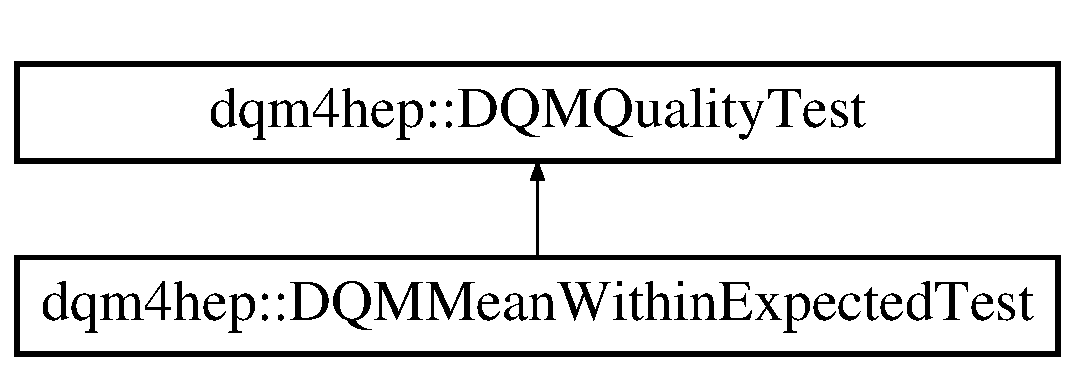
\includegraphics[height=2.000000cm]{classdqm4hep_1_1DQMMeanWithinExpectedTest}
\end{center}
\end{figure}
\subsection*{Classes}
\begin{DoxyCompactItemize}
\item 
class {\bf Factory}
\begin{DoxyCompactList}\small\item\em \doxyref{Factory}{p.}{classdqm4hep_1_1DQMMeanWithinExpectedTest_1_1Factory} class. \end{DoxyCompactList}\end{DoxyCompactItemize}
\subsection*{Public Member Functions}
\begin{DoxyCompactItemize}
\item 
{\bf D\+Q\+M\+Mean\+Within\+Expected\+Test} (const std\+::string \&name)
\begin{DoxyCompactList}\small\item\em Constructor with name. \end{DoxyCompactList}\item 
virtual {\bf $\sim$\+D\+Q\+M\+Mean\+Within\+Expected\+Test} ()
\begin{DoxyCompactList}\small\item\em Destructor. \end{DoxyCompactList}\item 
virtual {\bf Status\+Code} {\bf read\+Settings} (const {\bf Ti\+Xml\+Handle} xml\+Handle)
\begin{DoxyCompactList}\small\item\em Read the settings from the xml handle. \end{DoxyCompactList}\item 
virtual {\bf Status\+Code} {\bf init} ()
\begin{DoxyCompactList}\small\item\em Initialize the quality test. \end{DoxyCompactList}\item 
virtual {\bf Status\+Code} {\bf run} ({\bf D\+Q\+M\+Monitor\+Element} $\ast$p\+Monitor\+Element)
\begin{DoxyCompactList}\small\item\em Runs a quality test on the given monitor element. \end{DoxyCompactList}\item 
virtual bool {\bf can\+Run} ({\bf D\+Q\+M\+Monitor\+Element} $\ast$p\+Monitor\+Element) const 
\begin{DoxyCompactList}\small\item\em Whether the quality test can be run on the monitor element. \end{DoxyCompactList}\end{DoxyCompactItemize}
\subsection*{Protected Attributes}
\begin{DoxyCompactItemize}
\item 
unsigned int {\bf m\+\_\+strategy}
\item 
float {\bf m\+\_\+x\+Min}
\item 
float {\bf m\+\_\+x\+Max}
\item 
float {\bf m\+\_\+expected\+Mean}
\item 
float {\bf m\+\_\+sigma}
\end{DoxyCompactItemize}
\subsection*{Additional Inherited Members}


\subsection{Detailed Description}
\doxyref{D\+Q\+M\+Mean\+Within\+Expected\+Test}{p.}{classdqm4hep_1_1DQMMeanWithinExpectedTest} class. 

Definition at line 185 of file D\+Q\+M\+Quality\+Test.\+h.



\subsection{Constructor \& Destructor Documentation}
\index{dqm4hep\+::\+D\+Q\+M\+Mean\+Within\+Expected\+Test@{dqm4hep\+::\+D\+Q\+M\+Mean\+Within\+Expected\+Test}!D\+Q\+M\+Mean\+Within\+Expected\+Test@{D\+Q\+M\+Mean\+Within\+Expected\+Test}}
\index{D\+Q\+M\+Mean\+Within\+Expected\+Test@{D\+Q\+M\+Mean\+Within\+Expected\+Test}!dqm4hep\+::\+D\+Q\+M\+Mean\+Within\+Expected\+Test@{dqm4hep\+::\+D\+Q\+M\+Mean\+Within\+Expected\+Test}}
\subsubsection[{D\+Q\+M\+Mean\+Within\+Expected\+Test}]{\setlength{\rightskip}{0pt plus 5cm}dqm4hep\+::\+D\+Q\+M\+Mean\+Within\+Expected\+Test\+::\+D\+Q\+M\+Mean\+Within\+Expected\+Test (
\begin{DoxyParamCaption}
\item[{const std\+::string \&}]{name}
\end{DoxyParamCaption}
)}\label{classdqm4hep_1_1DQMMeanWithinExpectedTest_aca2acf79499cd07e402629ae4dd7611a}


Constructor with name. 



Definition at line 183 of file D\+Q\+M\+Quality\+Test.\+cc.



Referenced by dqm4hep\+::\+D\+Q\+M\+Mean\+Within\+Expected\+Test\+::\+Factory\+::create\+Quality\+Test().


\begin{DoxyCode}
183                                                                           :
184   DQMQualityTest(name),
185   m_strategy(0),
186   m_xMin(0.f),
187   m_xMax(0.f),
188   m_expectedMean(0.f),
189   m_sigma(0.f)
190 \{
191   \textcolor{comment}{/* nop */}
192 \}
\end{DoxyCode}
\index{dqm4hep\+::\+D\+Q\+M\+Mean\+Within\+Expected\+Test@{dqm4hep\+::\+D\+Q\+M\+Mean\+Within\+Expected\+Test}!````~D\+Q\+M\+Mean\+Within\+Expected\+Test@{$\sim$\+D\+Q\+M\+Mean\+Within\+Expected\+Test}}
\index{````~D\+Q\+M\+Mean\+Within\+Expected\+Test@{$\sim$\+D\+Q\+M\+Mean\+Within\+Expected\+Test}!dqm4hep\+::\+D\+Q\+M\+Mean\+Within\+Expected\+Test@{dqm4hep\+::\+D\+Q\+M\+Mean\+Within\+Expected\+Test}}
\subsubsection[{$\sim$\+D\+Q\+M\+Mean\+Within\+Expected\+Test}]{\setlength{\rightskip}{0pt plus 5cm}dqm4hep\+::\+D\+Q\+M\+Mean\+Within\+Expected\+Test\+::$\sim$\+D\+Q\+M\+Mean\+Within\+Expected\+Test (
\begin{DoxyParamCaption}
{}
\end{DoxyParamCaption}
)\hspace{0.3cm}{\ttfamily [virtual]}}\label{classdqm4hep_1_1DQMMeanWithinExpectedTest_aaa2bc1d88e9f352d5b6ef69096a65362}


Destructor. 



Definition at line 196 of file D\+Q\+M\+Quality\+Test.\+cc.


\begin{DoxyCode}
197 \{
198   \textcolor{comment}{/* nop */}
199 \}
\end{DoxyCode}


\subsection{Member Function Documentation}
\index{dqm4hep\+::\+D\+Q\+M\+Mean\+Within\+Expected\+Test@{dqm4hep\+::\+D\+Q\+M\+Mean\+Within\+Expected\+Test}!can\+Run@{can\+Run}}
\index{can\+Run@{can\+Run}!dqm4hep\+::\+D\+Q\+M\+Mean\+Within\+Expected\+Test@{dqm4hep\+::\+D\+Q\+M\+Mean\+Within\+Expected\+Test}}
\subsubsection[{can\+Run}]{\setlength{\rightskip}{0pt plus 5cm}bool dqm4hep\+::\+D\+Q\+M\+Mean\+Within\+Expected\+Test\+::can\+Run (
\begin{DoxyParamCaption}
\item[{{\bf D\+Q\+M\+Monitor\+Element} $\ast$}]{p\+Monitor\+Element}
\end{DoxyParamCaption}
) const\hspace{0.3cm}{\ttfamily [virtual]}}\label{classdqm4hep_1_1DQMMeanWithinExpectedTest_a7ff8e4b3c3e92338fd268e46504231d1}


Whether the quality test can be run on the monitor element. 



Implements {\bf dqm4hep\+::\+D\+Q\+M\+Quality\+Test} \doxyref{}{p.}{classdqm4hep_1_1DQMQualityTest_a94070d01ec18eac873e21f3b653ca391}.



Definition at line 299 of file D\+Q\+M\+Quality\+Test.\+cc.



References dqm4hep\+::\+D\+Q\+M\+Monitor\+Element\+::get(), and dqm4hep\+::\+D\+Q\+M\+Monitor\+Element\+::get\+Type().


\begin{DoxyCode}
300 \{
301   \textcolor{keywordflow}{if}(NULL == pMonitorElement)
302     \textcolor{keywordflow}{return} \textcolor{keyword}{false};
303 
304   DQMMonitorElementType type = pMonitorElement->getType();
305   TH1 *pHistogram = pMonitorElement->get<TH1>();
306 
307   \textcolor{comment}{// asking for a histo 1D}
308   \textcolor{keywordflow}{if}(type < INT\_HISTOGRAM\_1D\_ELEMENT\_TYPE || type > CHAR\_HISTOGRAM\_1D\_ELEMENT\_TYPE)
309     \textcolor{keywordflow}{return} \textcolor{keyword}{false};
310 
311   \textcolor{keywordflow}{if}(NULL == pHistogram)
312     \textcolor{keywordflow}{return} \textcolor{keyword}{false};
313 
314   \textcolor{keywordflow}{return} \textcolor{keyword}{true};
315 \}
\end{DoxyCode}
\index{dqm4hep\+::\+D\+Q\+M\+Mean\+Within\+Expected\+Test@{dqm4hep\+::\+D\+Q\+M\+Mean\+Within\+Expected\+Test}!init@{init}}
\index{init@{init}!dqm4hep\+::\+D\+Q\+M\+Mean\+Within\+Expected\+Test@{dqm4hep\+::\+D\+Q\+M\+Mean\+Within\+Expected\+Test}}
\subsubsection[{init}]{\setlength{\rightskip}{0pt plus 5cm}{\bf Status\+Code} dqm4hep\+::\+D\+Q\+M\+Mean\+Within\+Expected\+Test\+::init (
\begin{DoxyParamCaption}
{}
\end{DoxyParamCaption}
)\hspace{0.3cm}{\ttfamily [virtual]}}\label{classdqm4hep_1_1DQMMeanWithinExpectedTest_acde69f485735b67223f538a66735e1e3}


Initialize the quality test. 



Implements {\bf dqm4hep\+::\+D\+Q\+M\+Quality\+Test} \doxyref{}{p.}{classdqm4hep_1_1DQMQualityTest_a1500cae4000edbc8cae148e5ec612239}.



Definition at line 237 of file D\+Q\+M\+Quality\+Test.\+cc.


\begin{DoxyCode}
238 \{
239   \textcolor{comment}{/* nop */}
240   \textcolor{keywordflow}{return} STATUS\_CODE\_SUCCESS;
241 \}
\end{DoxyCode}
\index{dqm4hep\+::\+D\+Q\+M\+Mean\+Within\+Expected\+Test@{dqm4hep\+::\+D\+Q\+M\+Mean\+Within\+Expected\+Test}!read\+Settings@{read\+Settings}}
\index{read\+Settings@{read\+Settings}!dqm4hep\+::\+D\+Q\+M\+Mean\+Within\+Expected\+Test@{dqm4hep\+::\+D\+Q\+M\+Mean\+Within\+Expected\+Test}}
\subsubsection[{read\+Settings}]{\setlength{\rightskip}{0pt plus 5cm}{\bf Status\+Code} dqm4hep\+::\+D\+Q\+M\+Mean\+Within\+Expected\+Test\+::read\+Settings (
\begin{DoxyParamCaption}
\item[{const {\bf Ti\+Xml\+Handle}}]{xml\+Handle}
\end{DoxyParamCaption}
)\hspace{0.3cm}{\ttfamily [virtual]}}\label{classdqm4hep_1_1DQMMeanWithinExpectedTest_a8100bc47c0143e319fa42f0ab4dbbd7a}


Read the settings from the xml handle. 



Implements {\bf dqm4hep\+::\+D\+Q\+M\+Quality\+Test} \doxyref{}{p.}{classdqm4hep_1_1DQMQualityTest_a34c620c4f331f22d2676eb0401997b7b}.



Definition at line 203 of file D\+Q\+M\+Quality\+Test.\+cc.



References m\+\_\+expected\+Mean, m\+\_\+sigma, m\+\_\+strategy, m\+\_\+x\+Max, m\+\_\+x\+Min, dqm4hep\+::\+D\+Q\+M\+Xml\+Helper\+::read\+Value(), and R\+E\+T\+U\+R\+N\+\_\+\+R\+E\+S\+U\+L\+T\+\_\+\+I\+F.


\begin{DoxyCode}
204 \{
205   RETURN_RESULT_IF(STATUS\_CODE\_SUCCESS, !=, DQMXmlHelper::readValue(xmlHandle,
206       \textcolor{stringliteral}{"Strategy"}, m_strategy));
207 
208   \textcolor{keywordflow}{if}(0 == m_strategy)
209   \{
210     RETURN_RESULT_IF(STATUS\_CODE\_SUCCESS, !=, DQMXmlHelper::readValue(xmlHandle,
211         \textcolor{stringliteral}{"XMin"}, m_xMin));
212 
213     RETURN_RESULT_IF(STATUS\_CODE\_SUCCESS, !=, DQMXmlHelper::readValue(xmlHandle,
214         \textcolor{stringliteral}{"XMax"}, m_xMax));
215   \}
216   \textcolor{keywordflow}{else} \textcolor{keywordflow}{if}(1 == m_strategy)
217   \{
218     RETURN_RESULT_IF(STATUS\_CODE\_SUCCESS, !=, DQMXmlHelper::readValue(xmlHandle,
219         \textcolor{stringliteral}{"ExpectedMean"}, m_expectedMean));
220 
221     RETURN_RESULT_IF(STATUS\_CODE\_SUCCESS, !=, DQMXmlHelper::readValue(xmlHandle,
222         \textcolor{stringliteral}{"Sigma"}, m_sigma));
223   \}
224   \textcolor{keywordflow}{else} \textcolor{keywordflow}{if}(2 == m_strategy)
225   \{
226     RETURN_RESULT_IF(STATUS\_CODE\_SUCCESS, !=, DQMXmlHelper::readValue(xmlHandle,
227         \textcolor{stringliteral}{"ExpectedMean"}, m_expectedMean));
228   \}
229   \textcolor{keywordflow}{else}
230     \textcolor{keywordflow}{return} STATUS\_CODE\_INVALID\_PARAMETER;
231 
232   \textcolor{keywordflow}{return} STATUS\_CODE\_SUCCESS;
233 \}
\end{DoxyCode}
\index{dqm4hep\+::\+D\+Q\+M\+Mean\+Within\+Expected\+Test@{dqm4hep\+::\+D\+Q\+M\+Mean\+Within\+Expected\+Test}!run@{run}}
\index{run@{run}!dqm4hep\+::\+D\+Q\+M\+Mean\+Within\+Expected\+Test@{dqm4hep\+::\+D\+Q\+M\+Mean\+Within\+Expected\+Test}}
\subsubsection[{run}]{\setlength{\rightskip}{0pt plus 5cm}{\bf Status\+Code} dqm4hep\+::\+D\+Q\+M\+Mean\+Within\+Expected\+Test\+::run (
\begin{DoxyParamCaption}
\item[{{\bf D\+Q\+M\+Monitor\+Element} $\ast$}]{p\+Monitor\+Element}
\end{DoxyParamCaption}
)\hspace{0.3cm}{\ttfamily [virtual]}}\label{classdqm4hep_1_1DQMMeanWithinExpectedTest_a4eb11a126fc4150c171031d10ae37124}


Runs a quality test on the given monitor element. 



Implements {\bf dqm4hep\+::\+D\+Q\+M\+Quality\+Test} \doxyref{}{p.}{classdqm4hep_1_1DQMQualityTest_a228419cd9e4cfa60ee51ad0acc77ad0b}.



Definition at line 245 of file D\+Q\+M\+Quality\+Test.\+cc.



References dqm4hep\+::\+D\+Q\+M\+Monitor\+Element\+::get(), m\+\_\+expected\+Mean, dqm4hep\+::\+D\+Q\+M\+Quality\+Test\+::m\+\_\+is\+Successful, dqm4hep\+::\+D\+Q\+M\+Quality\+Test\+::m\+\_\+message, dqm4hep\+::\+D\+Q\+M\+Quality\+Test\+::m\+\_\+quality, m\+\_\+sigma, m\+\_\+strategy, m\+\_\+x\+Max, and dqm4hep\+::\+D\+Q\+M4\+H\+E\+P\+::scale\+To\+Quality().


\begin{DoxyCode}
246 \{
247   m_isSuccessful = \textcolor{keyword}{false};
248   m_quality = NO\_QUALITY;
249   m_message = \textcolor{stringliteral}{""};
250 
251   TH1 *pHistogram = pMonitorElement->get<TH1>();
252 
253   \textcolor{keywordflow}{if}(0 == m_strategy)
254   \{
255     \textcolor{keywordtype}{float} mean = pHistogram->GetMean();
256 
257     \textcolor{comment}{// test failed ?}
258     \textcolor{keywordflow}{if}(mean < m\_xMin || mean > m_xMax)
259     \{
260       m_quality = VERY\_BAD\_QUALITY;
261       m_message = \textcolor{stringliteral}{"Out of range !"};
262     \}
263     \textcolor{keywordflow}{else}
264     \{
265       m_quality = VERY\_GOOD\_QUALITY;
266       m_message = \textcolor{stringliteral}{""};
267     \}
268 
269     m_isSuccessful = \textcolor{keyword}{true};
270   \}
271   \textcolor{keywordflow}{else} \textcolor{keywordflow}{if}(1 == m_strategy)
272   \{
273     \textcolor{keywordtype}{float} chi = (pHistogram->GetMean() - m_expectedMean)/m_sigma;
274     \textcolor{keywordtype}{float} probability = TMath::Prob(chi*chi, 1);
275 
276     m_quality = DQM4HEP::scaleToQuality(probability);
277     m_isSuccessful = \textcolor{keyword}{true};
278   \}
279   \textcolor{keywordflow}{else} \textcolor{keywordflow}{if}(2 == m_strategy)
280   \{
281     \textcolor{keywordtype}{float} chi = (pHistogram->GetMean() - m_expectedMean)/pHistogram->GetRMS();
282     \textcolor{keywordtype}{float} probability = TMath::Prob(chi*chi, 1);
283 
284     m_quality = DQM4HEP::scaleToQuality(probability);
285     m_isSuccessful = \textcolor{keyword}{true};
286   \}
287   \textcolor{keywordflow}{else}
288   \{
289     m_isSuccessful = \textcolor{keyword}{false};
290     m_quality = NO\_QUALITY;
291     m_message = \textcolor{stringliteral}{"Undefined strategy for this test"};
292   \}
293 
294   \textcolor{keywordflow}{return} STATUS\_CODE\_SUCCESS;
295 \}
\end{DoxyCode}


\subsection{Member Data Documentation}
\index{dqm4hep\+::\+D\+Q\+M\+Mean\+Within\+Expected\+Test@{dqm4hep\+::\+D\+Q\+M\+Mean\+Within\+Expected\+Test}!m\+\_\+expected\+Mean@{m\+\_\+expected\+Mean}}
\index{m\+\_\+expected\+Mean@{m\+\_\+expected\+Mean}!dqm4hep\+::\+D\+Q\+M\+Mean\+Within\+Expected\+Test@{dqm4hep\+::\+D\+Q\+M\+Mean\+Within\+Expected\+Test}}
\subsubsection[{m\+\_\+expected\+Mean}]{\setlength{\rightskip}{0pt plus 5cm}float dqm4hep\+::\+D\+Q\+M\+Mean\+Within\+Expected\+Test\+::m\+\_\+expected\+Mean\hspace{0.3cm}{\ttfamily [protected]}}\label{classdqm4hep_1_1DQMMeanWithinExpectedTest_a4e2f16e85646b29865f906cf73a45590}


Definition at line 227 of file D\+Q\+M\+Quality\+Test.\+h.



Referenced by read\+Settings(), and run().

\index{dqm4hep\+::\+D\+Q\+M\+Mean\+Within\+Expected\+Test@{dqm4hep\+::\+D\+Q\+M\+Mean\+Within\+Expected\+Test}!m\+\_\+sigma@{m\+\_\+sigma}}
\index{m\+\_\+sigma@{m\+\_\+sigma}!dqm4hep\+::\+D\+Q\+M\+Mean\+Within\+Expected\+Test@{dqm4hep\+::\+D\+Q\+M\+Mean\+Within\+Expected\+Test}}
\subsubsection[{m\+\_\+sigma}]{\setlength{\rightskip}{0pt plus 5cm}float dqm4hep\+::\+D\+Q\+M\+Mean\+Within\+Expected\+Test\+::m\+\_\+sigma\hspace{0.3cm}{\ttfamily [protected]}}\label{classdqm4hep_1_1DQMMeanWithinExpectedTest_ac3083377b81d36dc9f3418ac8f6d664f}


Definition at line 228 of file D\+Q\+M\+Quality\+Test.\+h.



Referenced by read\+Settings(), and run().

\index{dqm4hep\+::\+D\+Q\+M\+Mean\+Within\+Expected\+Test@{dqm4hep\+::\+D\+Q\+M\+Mean\+Within\+Expected\+Test}!m\+\_\+strategy@{m\+\_\+strategy}}
\index{m\+\_\+strategy@{m\+\_\+strategy}!dqm4hep\+::\+D\+Q\+M\+Mean\+Within\+Expected\+Test@{dqm4hep\+::\+D\+Q\+M\+Mean\+Within\+Expected\+Test}}
\subsubsection[{m\+\_\+strategy}]{\setlength{\rightskip}{0pt plus 5cm}unsigned int dqm4hep\+::\+D\+Q\+M\+Mean\+Within\+Expected\+Test\+::m\+\_\+strategy\hspace{0.3cm}{\ttfamily [protected]}}\label{classdqm4hep_1_1DQMMeanWithinExpectedTest_ab60169780c06713711816a82c2dfc3ae}


Definition at line 224 of file D\+Q\+M\+Quality\+Test.\+h.



Referenced by read\+Settings(), and run().

\index{dqm4hep\+::\+D\+Q\+M\+Mean\+Within\+Expected\+Test@{dqm4hep\+::\+D\+Q\+M\+Mean\+Within\+Expected\+Test}!m\+\_\+x\+Max@{m\+\_\+x\+Max}}
\index{m\+\_\+x\+Max@{m\+\_\+x\+Max}!dqm4hep\+::\+D\+Q\+M\+Mean\+Within\+Expected\+Test@{dqm4hep\+::\+D\+Q\+M\+Mean\+Within\+Expected\+Test}}
\subsubsection[{m\+\_\+x\+Max}]{\setlength{\rightskip}{0pt plus 5cm}float dqm4hep\+::\+D\+Q\+M\+Mean\+Within\+Expected\+Test\+::m\+\_\+x\+Max\hspace{0.3cm}{\ttfamily [protected]}}\label{classdqm4hep_1_1DQMMeanWithinExpectedTest_a7ec1a7ced83c6c2085df2bc99632e337}


Definition at line 226 of file D\+Q\+M\+Quality\+Test.\+h.



Referenced by read\+Settings(), and run().

\index{dqm4hep\+::\+D\+Q\+M\+Mean\+Within\+Expected\+Test@{dqm4hep\+::\+D\+Q\+M\+Mean\+Within\+Expected\+Test}!m\+\_\+x\+Min@{m\+\_\+x\+Min}}
\index{m\+\_\+x\+Min@{m\+\_\+x\+Min}!dqm4hep\+::\+D\+Q\+M\+Mean\+Within\+Expected\+Test@{dqm4hep\+::\+D\+Q\+M\+Mean\+Within\+Expected\+Test}}
\subsubsection[{m\+\_\+x\+Min}]{\setlength{\rightskip}{0pt plus 5cm}float dqm4hep\+::\+D\+Q\+M\+Mean\+Within\+Expected\+Test\+::m\+\_\+x\+Min\hspace{0.3cm}{\ttfamily [protected]}}\label{classdqm4hep_1_1DQMMeanWithinExpectedTest_a80a9ec34763cbbfca2e88b1030402392}


Definition at line 225 of file D\+Q\+M\+Quality\+Test.\+h.



Referenced by read\+Settings().



The documentation for this class was generated from the following files\+:\begin{DoxyCompactItemize}
\item 
{\bf D\+Q\+M\+Quality\+Test.\+h}\item 
{\bf D\+Q\+M\+Quality\+Test.\+cc}\end{DoxyCompactItemize}

\section{dqm4hep\+:\+:D\+Q\+M\+Me\+Collector\+Info\+Rpc\+Info Class Reference}
\label{classdqm4hep_1_1DQMMeCollectorInfoRpcInfo}\index{dqm4hep\+::\+D\+Q\+M\+Me\+Collector\+Info\+Rpc\+Info@{dqm4hep\+::\+D\+Q\+M\+Me\+Collector\+Info\+Rpc\+Info}}


{\ttfamily \#include $<$D\+Q\+M\+Monitor\+Element\+Client.\+h$>$}

Inheritance diagram for dqm4hep\+:\+:D\+Q\+M\+Me\+Collector\+Info\+Rpc\+Info\+:\begin{figure}[H]
\begin{center}
\leavevmode
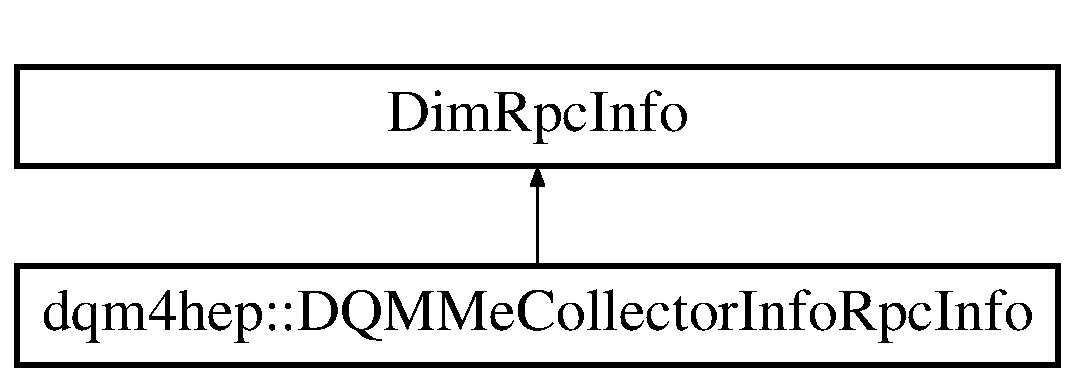
\includegraphics[height=2.000000cm]{classdqm4hep_1_1DQMMeCollectorInfoRpcInfo}
\end{center}
\end{figure}
\subsection*{Public Member Functions}
\begin{DoxyCompactItemize}
\item 
{\bf D\+Q\+M\+Me\+Collector\+Info\+Rpc\+Info} (char $\ast$rpc\+Info\+Name, {\bf D\+Q\+M\+Monitor\+Element\+Client} $\ast$p\+Client)
\item 
void {\bf rpc\+Info\+Handler} ()
\end{DoxyCompactItemize}
\subsection*{Private Attributes}
\begin{DoxyCompactItemize}
\item 
{\bf D\+Q\+M\+Monitor\+Element\+Client} $\ast$ {\bf m\+\_\+p\+Client}
\end{DoxyCompactItemize}


\subsection{Detailed Description}


Definition at line 47 of file D\+Q\+M\+Monitor\+Element\+Client.\+h.



\subsection{Constructor \& Destructor Documentation}
\index{dqm4hep\+::\+D\+Q\+M\+Me\+Collector\+Info\+Rpc\+Info@{dqm4hep\+::\+D\+Q\+M\+Me\+Collector\+Info\+Rpc\+Info}!D\+Q\+M\+Me\+Collector\+Info\+Rpc\+Info@{D\+Q\+M\+Me\+Collector\+Info\+Rpc\+Info}}
\index{D\+Q\+M\+Me\+Collector\+Info\+Rpc\+Info@{D\+Q\+M\+Me\+Collector\+Info\+Rpc\+Info}!dqm4hep\+::\+D\+Q\+M\+Me\+Collector\+Info\+Rpc\+Info@{dqm4hep\+::\+D\+Q\+M\+Me\+Collector\+Info\+Rpc\+Info}}
\subsubsection[{D\+Q\+M\+Me\+Collector\+Info\+Rpc\+Info}]{\setlength{\rightskip}{0pt plus 5cm}dqm4hep\+::\+D\+Q\+M\+Me\+Collector\+Info\+Rpc\+Info\+::\+D\+Q\+M\+Me\+Collector\+Info\+Rpc\+Info (
\begin{DoxyParamCaption}
\item[{char $\ast$}]{rpc\+Info\+Name, }
\item[{{\bf D\+Q\+M\+Monitor\+Element\+Client} $\ast$}]{p\+Client}
\end{DoxyParamCaption}
)}\label{classdqm4hep_1_1DQMMeCollectorInfoRpcInfo_a19a633ebe9c765bf92b13cdfc041b45a}


Definition at line 39 of file D\+Q\+M\+Monitor\+Element\+Client.\+cc.


\begin{DoxyCode}
39                                                                                                         :
40     DimRpcInfo(rpcInfoName, (\textcolor{keywordtype}{void}*) DQMMonitorElementClient::m_emptyBufferStr.c\_str(), 
      DQMMonitorElementClient::m_emptyBufferStr.size()),
41     m_pClient(pClient)
42 \{
43   \textcolor{comment}{/* nop */}
44 \}
\end{DoxyCode}


\subsection{Member Function Documentation}
\index{dqm4hep\+::\+D\+Q\+M\+Me\+Collector\+Info\+Rpc\+Info@{dqm4hep\+::\+D\+Q\+M\+Me\+Collector\+Info\+Rpc\+Info}!rpc\+Info\+Handler@{rpc\+Info\+Handler}}
\index{rpc\+Info\+Handler@{rpc\+Info\+Handler}!dqm4hep\+::\+D\+Q\+M\+Me\+Collector\+Info\+Rpc\+Info@{dqm4hep\+::\+D\+Q\+M\+Me\+Collector\+Info\+Rpc\+Info}}
\subsubsection[{rpc\+Info\+Handler}]{\setlength{\rightskip}{0pt plus 5cm}void dqm4hep\+::\+D\+Q\+M\+Me\+Collector\+Info\+Rpc\+Info\+::rpc\+Info\+Handler (
\begin{DoxyParamCaption}
{}
\end{DoxyParamCaption}
)}\label{classdqm4hep_1_1DQMMeCollectorInfoRpcInfo_a7efeb76180897a0ea2f6c54685229213}


Definition at line 48 of file D\+Q\+M\+Monitor\+Element\+Client.\+cc.



References dqm4hep\+::\+D\+Q\+M\+Monitor\+Element\+Client\+::handle\+Me\+Collector\+Info\+Rpc\+Info(), and m\+\_\+p\+Client.


\begin{DoxyCode}
49 \{
50   m_pClient->handleMeCollectorInfoRpcInfo(\textcolor{keyword}{this});
51 \}
\end{DoxyCode}


\subsection{Member Data Documentation}
\index{dqm4hep\+::\+D\+Q\+M\+Me\+Collector\+Info\+Rpc\+Info@{dqm4hep\+::\+D\+Q\+M\+Me\+Collector\+Info\+Rpc\+Info}!m\+\_\+p\+Client@{m\+\_\+p\+Client}}
\index{m\+\_\+p\+Client@{m\+\_\+p\+Client}!dqm4hep\+::\+D\+Q\+M\+Me\+Collector\+Info\+Rpc\+Info@{dqm4hep\+::\+D\+Q\+M\+Me\+Collector\+Info\+Rpc\+Info}}
\subsubsection[{m\+\_\+p\+Client}]{\setlength{\rightskip}{0pt plus 5cm}{\bf D\+Q\+M\+Monitor\+Element\+Client}$\ast$ dqm4hep\+::\+D\+Q\+M\+Me\+Collector\+Info\+Rpc\+Info\+::m\+\_\+p\+Client\hspace{0.3cm}{\ttfamily [private]}}\label{classdqm4hep_1_1DQMMeCollectorInfoRpcInfo_a38dfa3df9389017c4cf14d1ff8b9ad0e}


Definition at line 54 of file D\+Q\+M\+Monitor\+Element\+Client.\+h.



Referenced by rpc\+Info\+Handler().



The documentation for this class was generated from the following files\+:\begin{DoxyCompactItemize}
\item 
{\bf D\+Q\+M\+Monitor\+Element\+Client.\+h}\item 
{\bf D\+Q\+M\+Monitor\+Element\+Client.\+cc}\end{DoxyCompactItemize}

\section{dqm4hep\+:\+:D\+Q\+M\+Me\+List\+Name\+Rpc\+Info Class Reference}
\label{classdqm4hep_1_1DQMMeListNameRpcInfo}\index{dqm4hep\+::\+D\+Q\+M\+Me\+List\+Name\+Rpc\+Info@{dqm4hep\+::\+D\+Q\+M\+Me\+List\+Name\+Rpc\+Info}}


{\ttfamily \#include $<$D\+Q\+M\+Monitor\+Element\+Client.\+h$>$}

Inheritance diagram for dqm4hep\+:\+:D\+Q\+M\+Me\+List\+Name\+Rpc\+Info\+:\begin{figure}[H]
\begin{center}
\leavevmode
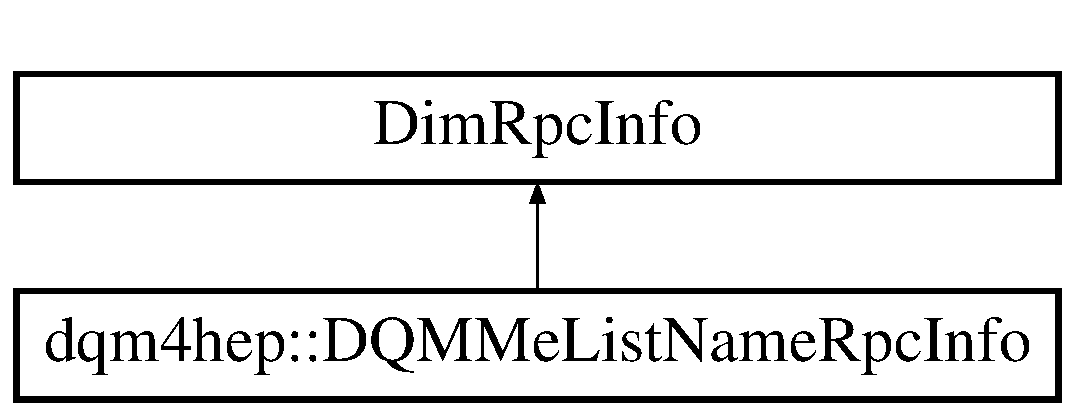
\includegraphics[height=2.000000cm]{classdqm4hep_1_1DQMMeListNameRpcInfo}
\end{center}
\end{figure}
\subsection*{Public Member Functions}
\begin{DoxyCompactItemize}
\item 
{\bf D\+Q\+M\+Me\+List\+Name\+Rpc\+Info} (char $\ast$rpc\+Info\+Name, {\bf D\+Q\+M\+Monitor\+Element\+Client} $\ast$p\+Client)
\item 
void {\bf rpc\+Info\+Handler} ()
\end{DoxyCompactItemize}
\subsection*{Private Attributes}
\begin{DoxyCompactItemize}
\item 
{\bf D\+Q\+M\+Monitor\+Element\+Client} $\ast$ {\bf m\+\_\+p\+Client}
\end{DoxyCompactItemize}


\subsection{Detailed Description}


Definition at line 60 of file D\+Q\+M\+Monitor\+Element\+Client.\+h.



\subsection{Constructor \& Destructor Documentation}
\index{dqm4hep\+::\+D\+Q\+M\+Me\+List\+Name\+Rpc\+Info@{dqm4hep\+::\+D\+Q\+M\+Me\+List\+Name\+Rpc\+Info}!D\+Q\+M\+Me\+List\+Name\+Rpc\+Info@{D\+Q\+M\+Me\+List\+Name\+Rpc\+Info}}
\index{D\+Q\+M\+Me\+List\+Name\+Rpc\+Info@{D\+Q\+M\+Me\+List\+Name\+Rpc\+Info}!dqm4hep\+::\+D\+Q\+M\+Me\+List\+Name\+Rpc\+Info@{dqm4hep\+::\+D\+Q\+M\+Me\+List\+Name\+Rpc\+Info}}
\subsubsection[{D\+Q\+M\+Me\+List\+Name\+Rpc\+Info}]{\setlength{\rightskip}{0pt plus 5cm}dqm4hep\+::\+D\+Q\+M\+Me\+List\+Name\+Rpc\+Info\+::\+D\+Q\+M\+Me\+List\+Name\+Rpc\+Info (
\begin{DoxyParamCaption}
\item[{char $\ast$}]{rpc\+Info\+Name, }
\item[{{\bf D\+Q\+M\+Monitor\+Element\+Client} $\ast$}]{p\+Client}
\end{DoxyParamCaption}
)}\label{classdqm4hep_1_1DQMMeListNameRpcInfo_a6b991570b3fc5ddfb14d3a195a003ed7}


Definition at line 56 of file D\+Q\+M\+Monitor\+Element\+Client.\+cc.


\begin{DoxyCode}
56                                                                                               :
57     DimRpcInfo(rpcInfoName, (\textcolor{keywordtype}{void}*) DQMMonitorElementClient::m_emptyBufferStr.c\_str(), 
      DQMMonitorElementClient::m_emptyBufferStr.size()),
58     m_pClient(pClient)
59 \{
60   \textcolor{comment}{/* nop */}
61 \}
\end{DoxyCode}


\subsection{Member Function Documentation}
\index{dqm4hep\+::\+D\+Q\+M\+Me\+List\+Name\+Rpc\+Info@{dqm4hep\+::\+D\+Q\+M\+Me\+List\+Name\+Rpc\+Info}!rpc\+Info\+Handler@{rpc\+Info\+Handler}}
\index{rpc\+Info\+Handler@{rpc\+Info\+Handler}!dqm4hep\+::\+D\+Q\+M\+Me\+List\+Name\+Rpc\+Info@{dqm4hep\+::\+D\+Q\+M\+Me\+List\+Name\+Rpc\+Info}}
\subsubsection[{rpc\+Info\+Handler}]{\setlength{\rightskip}{0pt plus 5cm}void dqm4hep\+::\+D\+Q\+M\+Me\+List\+Name\+Rpc\+Info\+::rpc\+Info\+Handler (
\begin{DoxyParamCaption}
{}
\end{DoxyParamCaption}
)}\label{classdqm4hep_1_1DQMMeListNameRpcInfo_aebe3adf43a158c6090106240968c69d0}


Definition at line 65 of file D\+Q\+M\+Monitor\+Element\+Client.\+cc.



References dqm4hep\+::\+D\+Q\+M\+Monitor\+Element\+Client\+::handle\+Me\+List\+Name\+Rpc\+Info(), and m\+\_\+p\+Client.


\begin{DoxyCode}
66 \{
67   m_pClient->handleMeListNameRpcInfo(\textcolor{keyword}{this});
68 \}
\end{DoxyCode}


\subsection{Member Data Documentation}
\index{dqm4hep\+::\+D\+Q\+M\+Me\+List\+Name\+Rpc\+Info@{dqm4hep\+::\+D\+Q\+M\+Me\+List\+Name\+Rpc\+Info}!m\+\_\+p\+Client@{m\+\_\+p\+Client}}
\index{m\+\_\+p\+Client@{m\+\_\+p\+Client}!dqm4hep\+::\+D\+Q\+M\+Me\+List\+Name\+Rpc\+Info@{dqm4hep\+::\+D\+Q\+M\+Me\+List\+Name\+Rpc\+Info}}
\subsubsection[{m\+\_\+p\+Client}]{\setlength{\rightskip}{0pt plus 5cm}{\bf D\+Q\+M\+Monitor\+Element\+Client}$\ast$ dqm4hep\+::\+D\+Q\+M\+Me\+List\+Name\+Rpc\+Info\+::m\+\_\+p\+Client\hspace{0.3cm}{\ttfamily [private]}}\label{classdqm4hep_1_1DQMMeListNameRpcInfo_a03d611ceb0f11bc2adf3911990cb464d}


Definition at line 67 of file D\+Q\+M\+Monitor\+Element\+Client.\+h.



Referenced by rpc\+Info\+Handler().



The documentation for this class was generated from the following files\+:\begin{DoxyCompactItemize}
\item 
{\bf D\+Q\+M\+Monitor\+Element\+Client.\+h}\item 
{\bf D\+Q\+M\+Monitor\+Element\+Client.\+cc}\end{DoxyCompactItemize}

\section{dqm4hep\+:\+:D\+Q\+M\+Module Class Reference}
\label{classdqm4hep_1_1DQMModule}\index{dqm4hep\+::\+D\+Q\+M\+Module@{dqm4hep\+::\+D\+Q\+M\+Module}}


\doxyref{D\+Q\+M\+Module}{p.}{classdqm4hep_1_1DQMModule} base class.  




{\ttfamily \#include $<$D\+Q\+M\+Module.\+h$>$}

Inheritance diagram for dqm4hep\+:\+:D\+Q\+M\+Module\+:\begin{figure}[H]
\begin{center}
\leavevmode
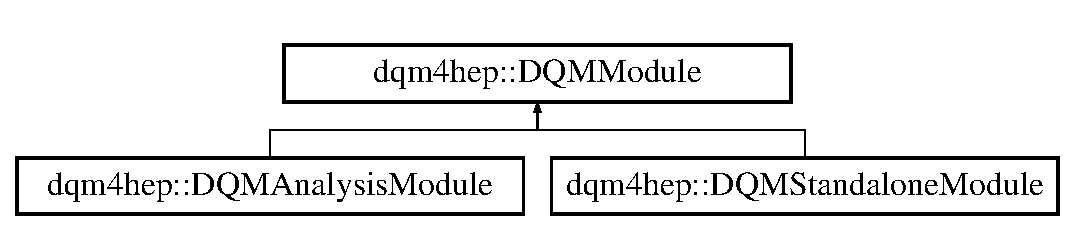
\includegraphics[height=2.000000cm]{classdqm4hep_1_1DQMModule}
\end{center}
\end{figure}
\subsection*{Public Member Functions}
\begin{DoxyCompactItemize}
\item 
{\bf D\+Q\+M\+Module} ()
\begin{DoxyCompactList}\small\item\em Constructor. \end{DoxyCompactList}\item 
virtual {\bf $\sim$\+D\+Q\+M\+Module} ()
\begin{DoxyCompactList}\small\item\em Destructor. \end{DoxyCompactList}\item 
const std\+::string \& {\bf get\+Name} () const 
\begin{DoxyCompactList}\small\item\em Get the module name. \end{DoxyCompactList}\item 
const std\+::string \& {\bf get\+Detector\+Name} () const 
\begin{DoxyCompactList}\small\item\em Get the detector name associated to this module. \end{DoxyCompactList}\item 
const {\bf D\+Q\+M\+Version} \& {\bf get\+Version} () const 
\begin{DoxyCompactList}\small\item\em Get the module version. \end{DoxyCompactList}\item 
virtual {\bf Status\+Code} {\bf init\+Module} ()=0
\begin{DoxyCompactList}\small\item\em Initialize the module. \end{DoxyCompactList}\item 
virtual {\bf Status\+Code} {\bf read\+Settings} (const {\bf Ti\+Xml\+Handle} handle)=0
\begin{DoxyCompactList}\small\item\em Read the input settings from a xml handle. \end{DoxyCompactList}\item 
virtual {\bf Status\+Code} {\bf start\+Of\+Cycle} ()=0
\begin{DoxyCompactList}\small\item\em Called at start of cycle. \end{DoxyCompactList}\item 
virtual {\bf Status\+Code} {\bf end\+Of\+Cycle} ()=0
\begin{DoxyCompactList}\small\item\em Called at end of cycle before publishing monitor elements. \end{DoxyCompactList}\item 
virtual {\bf Status\+Code} {\bf end\+Module} ()=0
\begin{DoxyCompactList}\small\item\em End the module. \end{DoxyCompactList}\end{DoxyCompactItemize}
\subsection*{Protected Member Functions}
\begin{DoxyCompactItemize}
\item 
void {\bf set\+Detector\+Name} (const std\+::string \&detector\+Name)
\begin{DoxyCompactList}\small\item\em Set the detector name for this module. \end{DoxyCompactList}\item 
void {\bf set\+Name} (const std\+::string \&name)
\begin{DoxyCompactList}\small\item\em Set the module name. \end{DoxyCompactList}\item 
void {\bf set\+Version} (unsigned int major, unsigned int minor, unsigned int patch)
\begin{DoxyCompactList}\small\item\em Set the module version. \end{DoxyCompactList}\end{DoxyCompactItemize}
\subsection*{Private Member Functions}
\begin{DoxyCompactItemize}
\item 
{\bf D\+Q\+M\+Module\+Application} $\ast$ {\bf get\+Module\+Application} () const 
\begin{DoxyCompactList}\small\item\em Get the module application in which the module is registered. \end{DoxyCompactList}\item 
void {\bf set\+Module\+Application} ({\bf D\+Q\+M\+Module\+Application} $\ast$p\+Module\+Application)
\begin{DoxyCompactList}\small\item\em Set the module application in which the module is registered. \end{DoxyCompactList}\end{DoxyCompactItemize}
\subsection*{Private Attributes}
\begin{DoxyCompactItemize}
\item 
std\+::string {\bf m\+\_\+name}
\begin{DoxyCompactList}\small\item\em The module name. \end{DoxyCompactList}\item 
std\+::string {\bf m\+\_\+detector\+Name}
\begin{DoxyCompactList}\small\item\em The detector name for this module. \end{DoxyCompactList}\item 
{\bf D\+Q\+M\+Version} {\bf m\+\_\+version}
\begin{DoxyCompactList}\small\item\em The module version. \end{DoxyCompactList}\item 
{\bf D\+Q\+M\+Module\+Application} $\ast$ {\bf m\+\_\+p\+Module\+Application}
\begin{DoxyCompactList}\small\item\em The monitor element manager. \end{DoxyCompactList}\end{DoxyCompactItemize}
\subsection*{Friends}
\begin{DoxyCompactItemize}
\item 
class {\bf D\+Q\+M\+Module\+Api}
\item 
class {\bf D\+Q\+M\+Archiver}
\item 
class {\bf D\+Q\+M\+Module\+Application}
\end{DoxyCompactItemize}


\subsection{Detailed Description}
\doxyref{D\+Q\+M\+Module}{p.}{classdqm4hep_1_1DQMModule} base class. 

Base class for monitor element booking modules. See daughter classes for specific implementations.

This class owns a monitor element manager used to book monitor elements through the \doxyref{D\+Q\+M\+Module\+Api}{p.}{classdqm4hep_1_1DQMModuleApi}.

\begin{DoxyAuthor}{Author}
R.\+Ete 
\end{DoxyAuthor}


Definition at line 53 of file D\+Q\+M\+Module.\+h.



\subsection{Constructor \& Destructor Documentation}
\index{dqm4hep\+::\+D\+Q\+M\+Module@{dqm4hep\+::\+D\+Q\+M\+Module}!D\+Q\+M\+Module@{D\+Q\+M\+Module}}
\index{D\+Q\+M\+Module@{D\+Q\+M\+Module}!dqm4hep\+::\+D\+Q\+M\+Module@{dqm4hep\+::\+D\+Q\+M\+Module}}
\subsubsection[{D\+Q\+M\+Module}]{\setlength{\rightskip}{0pt plus 5cm}dqm4hep\+::\+D\+Q\+M\+Module\+::\+D\+Q\+M\+Module (
\begin{DoxyParamCaption}
{}
\end{DoxyParamCaption}
)}\label{classdqm4hep_1_1DQMModule_aff277524c1f495f7b0753bdf720b03b1}


Constructor. 



Definition at line 35 of file D\+Q\+M\+Module.\+cc.


\begin{DoxyCode}
35                      :
36     m_name( \textcolor{stringliteral}{""} ),
37     m_pModuleApplication(NULL)
38 \{
39   \textcolor{comment}{/* nop */}
40 \}
\end{DoxyCode}
\index{dqm4hep\+::\+D\+Q\+M\+Module@{dqm4hep\+::\+D\+Q\+M\+Module}!````~D\+Q\+M\+Module@{$\sim$\+D\+Q\+M\+Module}}
\index{````~D\+Q\+M\+Module@{$\sim$\+D\+Q\+M\+Module}!dqm4hep\+::\+D\+Q\+M\+Module@{dqm4hep\+::\+D\+Q\+M\+Module}}
\subsubsection[{$\sim$\+D\+Q\+M\+Module}]{\setlength{\rightskip}{0pt plus 5cm}dqm4hep\+::\+D\+Q\+M\+Module\+::$\sim$\+D\+Q\+M\+Module (
\begin{DoxyParamCaption}
{}
\end{DoxyParamCaption}
)\hspace{0.3cm}{\ttfamily [virtual]}}\label{classdqm4hep_1_1DQMModule_acdc0f3b46174de5d4f6df56552593e32}


Destructor. 



Definition at line 44 of file D\+Q\+M\+Module.\+cc.


\begin{DoxyCode}
45 \{
46   \textcolor{comment}{/* nop */}
47 \}
\end{DoxyCode}


\subsection{Member Function Documentation}
\index{dqm4hep\+::\+D\+Q\+M\+Module@{dqm4hep\+::\+D\+Q\+M\+Module}!end\+Module@{end\+Module}}
\index{end\+Module@{end\+Module}!dqm4hep\+::\+D\+Q\+M\+Module@{dqm4hep\+::\+D\+Q\+M\+Module}}
\subsubsection[{end\+Module}]{\setlength{\rightskip}{0pt plus 5cm}virtual {\bf Status\+Code} dqm4hep\+::\+D\+Q\+M\+Module\+::end\+Module (
\begin{DoxyParamCaption}
{}
\end{DoxyParamCaption}
)\hspace{0.3cm}{\ttfamily [pure virtual]}}\label{classdqm4hep_1_1DQMModule_afc83b6725cbd71fa918646f656247039}


End the module. 

Called at termination of the process. 

Referenced by dqm4hep\+::\+D\+Q\+M\+Standalone\+Module\+Application\+::run().

\index{dqm4hep\+::\+D\+Q\+M\+Module@{dqm4hep\+::\+D\+Q\+M\+Module}!end\+Of\+Cycle@{end\+Of\+Cycle}}
\index{end\+Of\+Cycle@{end\+Of\+Cycle}!dqm4hep\+::\+D\+Q\+M\+Module@{dqm4hep\+::\+D\+Q\+M\+Module}}
\subsubsection[{end\+Of\+Cycle}]{\setlength{\rightskip}{0pt plus 5cm}virtual {\bf Status\+Code} dqm4hep\+::\+D\+Q\+M\+Module\+::end\+Of\+Cycle (
\begin{DoxyParamCaption}
{}
\end{DoxyParamCaption}
)\hspace{0.3cm}{\ttfamily [pure virtual]}}\label{classdqm4hep_1_1DQMModule_a8140d494973ae221cde3e54e85cd5386}


Called at end of cycle before publishing monitor elements. 

User should not reset monitor elements in this method. Generally used to set the quality of monitor elements or set some of them to do not be published. \index{dqm4hep\+::\+D\+Q\+M\+Module@{dqm4hep\+::\+D\+Q\+M\+Module}!get\+Detector\+Name@{get\+Detector\+Name}}
\index{get\+Detector\+Name@{get\+Detector\+Name}!dqm4hep\+::\+D\+Q\+M\+Module@{dqm4hep\+::\+D\+Q\+M\+Module}}
\subsubsection[{get\+Detector\+Name}]{\setlength{\rightskip}{0pt plus 5cm}const std\+::string \& dqm4hep\+::\+D\+Q\+M\+Module\+::get\+Detector\+Name (
\begin{DoxyParamCaption}
{}
\end{DoxyParamCaption}
) const}\label{classdqm4hep_1_1DQMModule_a6457463fc7afc0f4b36a5ebb3c433b08}


Get the detector name associated to this module. 



Definition at line 65 of file D\+Q\+M\+Module.\+cc.



References m\+\_\+detector\+Name.



Referenced by dqm4hep\+::\+D\+Q\+M\+Archiver\+::archive().


\begin{DoxyCode}
66 \{
67   \textcolor{keywordflow}{return} m_detectorName;
68 \}
\end{DoxyCode}
\index{dqm4hep\+::\+D\+Q\+M\+Module@{dqm4hep\+::\+D\+Q\+M\+Module}!get\+Module\+Application@{get\+Module\+Application}}
\index{get\+Module\+Application@{get\+Module\+Application}!dqm4hep\+::\+D\+Q\+M\+Module@{dqm4hep\+::\+D\+Q\+M\+Module}}
\subsubsection[{get\+Module\+Application}]{\setlength{\rightskip}{0pt plus 5cm}{\bf D\+Q\+M\+Module\+Application} $\ast$ dqm4hep\+::\+D\+Q\+M\+Module\+::get\+Module\+Application (
\begin{DoxyParamCaption}
{}
\end{DoxyParamCaption}
) const\hspace{0.3cm}{\ttfamily [private]}}\label{classdqm4hep_1_1DQMModule_aba2bb53dc496e9f61bd8de82ecb25f5a}


Get the module application in which the module is registered. 



Definition at line 93 of file D\+Q\+M\+Module.\+cc.



References m\+\_\+p\+Module\+Application.



Referenced by dqm4hep\+::\+D\+Q\+M\+Module\+Api\+::add\+Quality\+Test(), dqm4hep\+::\+D\+Q\+M\+Archiver\+::archive(), dqm4hep\+::\+D\+Q\+M\+Module\+Api\+::book\+Char\+Histogram1\+D(), dqm4hep\+::\+D\+Q\+M\+Module\+Api\+::book\+Char\+Histogram2\+D(), dqm4hep\+::\+D\+Q\+M\+Module\+Api\+::book\+Float(), dqm4hep\+::\+D\+Q\+M\+Module\+Api\+::book\+Int(), dqm4hep\+::\+D\+Q\+M\+Module\+Api\+::book\+Int\+Histogram1\+D(), dqm4hep\+::\+D\+Q\+M\+Module\+Api\+::book\+Int\+Histogram2\+D(), dqm4hep\+::\+D\+Q\+M\+Module\+Api\+::book\+Monitor\+Element(), dqm4hep\+::\+D\+Q\+M\+Module\+Api\+::book\+Object(), dqm4hep\+::\+D\+Q\+M\+Module\+Api\+::book\+Profile1\+D(), dqm4hep\+::\+D\+Q\+M\+Module\+Api\+::book\+Profile2\+D(), dqm4hep\+::\+D\+Q\+M\+Module\+Api\+::book\+Real\+Histogram1\+D(), dqm4hep\+::\+D\+Q\+M\+Module\+Api\+::book\+Real\+Histogram2\+D(), dqm4hep\+::\+D\+Q\+M\+Module\+Api\+::book\+Short(), dqm4hep\+::\+D\+Q\+M\+Module\+Api\+::book\+Short\+Histogram1\+D(), dqm4hep\+::\+D\+Q\+M\+Module\+Api\+::book\+Short\+Histogram2\+D(), dqm4hep\+::\+D\+Q\+M\+Module\+Api\+::book\+String(), dqm4hep\+::\+D\+Q\+M\+Module\+Api\+::cd(), dqm4hep\+::\+D\+Q\+M\+Module\+Api\+::create\+Quality\+Test(), dqm4hep\+::\+D\+Q\+M\+Module\+Api\+::delete\+Monitor\+Element(), dqm4hep\+::\+D\+Q\+M\+Module\+Api\+::get\+All\+Monitor\+Elements(), dqm4hep\+::\+D\+Q\+M\+Module\+Api\+::get\+Monitor\+Element(), dqm4hep\+::\+D\+Q\+M\+Module\+Api\+::go\+Up(), dqm4hep\+::\+D\+Q\+M\+Module\+Api\+::ls(), dqm4hep\+::\+D\+Q\+M\+Module\+Api\+::mkdir(), dqm4hep\+::\+D\+Q\+M\+Module\+Api\+::pwd(), dqm4hep\+::\+D\+Q\+M\+Module\+Api\+::register\+Quality\+Test\+Factory(), dqm4hep\+::\+D\+Q\+M\+Module\+Api\+::reset\+Monitor\+Elements(), dqm4hep\+::\+D\+Q\+M\+Module\+Api\+::rmdir(), dqm4hep\+::\+D\+Q\+M\+Module\+Api\+::run\+Quality\+Test(), and dqm4hep\+::\+D\+Q\+M\+Module\+Api\+::run\+Quality\+Tests().


\begin{DoxyCode}
94 \{
95   \textcolor{keywordflow}{return} m_pModuleApplication;
96 \}
\end{DoxyCode}
\index{dqm4hep\+::\+D\+Q\+M\+Module@{dqm4hep\+::\+D\+Q\+M\+Module}!get\+Name@{get\+Name}}
\index{get\+Name@{get\+Name}!dqm4hep\+::\+D\+Q\+M\+Module@{dqm4hep\+::\+D\+Q\+M\+Module}}
\subsubsection[{get\+Name}]{\setlength{\rightskip}{0pt plus 5cm}const std\+::string \& dqm4hep\+::\+D\+Q\+M\+Module\+::get\+Name (
\begin{DoxyParamCaption}
{}
\end{DoxyParamCaption}
) const}\label{classdqm4hep_1_1DQMModule_a1b06da79454d2984ec30726357f20c54}


Get the module name. 



Definition at line 58 of file D\+Q\+M\+Module.\+cc.



References m\+\_\+name.



Referenced by dqm4hep\+::\+D\+Q\+M\+Monitor\+Element\+Sender\+::add\+Available\+Monitor\+Element(), dqm4hep\+::\+D\+Q\+M\+Archiver\+::archive(), dqm4hep\+::\+D\+Q\+M\+Module\+Api\+::book\+Char\+Histogram1\+D(), dqm4hep\+::\+D\+Q\+M\+Module\+Api\+::book\+Char\+Histogram2\+D(), dqm4hep\+::\+D\+Q\+M\+Module\+Api\+::book\+Float(), dqm4hep\+::\+D\+Q\+M\+Module\+Api\+::book\+Int(), dqm4hep\+::\+D\+Q\+M\+Module\+Api\+::book\+Int\+Histogram1\+D(), dqm4hep\+::\+D\+Q\+M\+Module\+Api\+::book\+Int\+Histogram2\+D(), dqm4hep\+::\+D\+Q\+M\+Module\+Api\+::book\+Monitor\+Element(), dqm4hep\+::\+D\+Q\+M\+Module\+Api\+::book\+Object(), dqm4hep\+::\+D\+Q\+M\+Module\+Api\+::book\+Profile1\+D(), dqm4hep\+::\+D\+Q\+M\+Module\+Api\+::book\+Profile2\+D(), dqm4hep\+::\+D\+Q\+M\+Module\+Api\+::book\+Real\+Histogram1\+D(), dqm4hep\+::\+D\+Q\+M\+Module\+Api\+::book\+Real\+Histogram2\+D(), dqm4hep\+::\+D\+Q\+M\+Module\+Api\+::book\+Short(), dqm4hep\+::\+D\+Q\+M\+Module\+Api\+::book\+Short\+Histogram1\+D(), dqm4hep\+::\+D\+Q\+M\+Module\+Api\+::book\+Short\+Histogram2\+D(), dqm4hep\+::\+D\+Q\+M\+Module\+Api\+::book\+String(), dqm4hep\+::\+D\+Q\+M\+Analysis\+Module\+Application\+::configure\+Module(), dqm4hep\+::\+D\+Q\+M\+Module\+Application\+::get\+Module\+Name(), dqm4hep\+::\+D\+Q\+M\+Standalone\+Module\+Application\+::read\+Settings(), dqm4hep\+::\+D\+Q\+M\+Analysis\+Module\+Application\+::read\+Settings(), dqm4hep\+::\+D\+Q\+M\+Analysis\+Module\+Application\+::run(), dqm4hep\+::\+D\+Q\+M\+Monitor\+Element\+Sender\+::send\+Available\+Monitor\+Element\+List(), and dqm4hep\+::\+D\+Q\+M\+Monitor\+Element\+Sender\+::send\+Monitor\+Elements().


\begin{DoxyCode}
59 \{
60   \textcolor{keywordflow}{return} m_name;
61 \}
\end{DoxyCode}
\index{dqm4hep\+::\+D\+Q\+M\+Module@{dqm4hep\+::\+D\+Q\+M\+Module}!get\+Version@{get\+Version}}
\index{get\+Version@{get\+Version}!dqm4hep\+::\+D\+Q\+M\+Module@{dqm4hep\+::\+D\+Q\+M\+Module}}
\subsubsection[{get\+Version}]{\setlength{\rightskip}{0pt plus 5cm}const {\bf D\+Q\+M\+Version} \& dqm4hep\+::\+D\+Q\+M\+Module\+::get\+Version (
\begin{DoxyParamCaption}
{}
\end{DoxyParamCaption}
) const}\label{classdqm4hep_1_1DQMModule_abb6c844f383603625db42d6eba880174}


Get the module version. 



Definition at line 79 of file D\+Q\+M\+Module.\+cc.



References m\+\_\+version.



Referenced by dqm4hep\+::\+D\+Q\+M\+Archiver\+::archive().


\begin{DoxyCode}
80 \{
81   \textcolor{keywordflow}{return} m_version;
82 \}
\end{DoxyCode}
\index{dqm4hep\+::\+D\+Q\+M\+Module@{dqm4hep\+::\+D\+Q\+M\+Module}!init\+Module@{init\+Module}}
\index{init\+Module@{init\+Module}!dqm4hep\+::\+D\+Q\+M\+Module@{dqm4hep\+::\+D\+Q\+M\+Module}}
\subsubsection[{init\+Module}]{\setlength{\rightskip}{0pt plus 5cm}virtual {\bf Status\+Code} dqm4hep\+::\+D\+Q\+M\+Module\+::init\+Module (
\begin{DoxyParamCaption}
{}
\end{DoxyParamCaption}
)\hspace{0.3cm}{\ttfamily [pure virtual]}}\label{classdqm4hep_1_1DQMModule_ad371270ee0a6203a967f72eea08a04dc}


Initialize the module. 

It is generally in this method that monitor elements are booked. \index{dqm4hep\+::\+D\+Q\+M\+Module@{dqm4hep\+::\+D\+Q\+M\+Module}!read\+Settings@{read\+Settings}}
\index{read\+Settings@{read\+Settings}!dqm4hep\+::\+D\+Q\+M\+Module@{dqm4hep\+::\+D\+Q\+M\+Module}}
\subsubsection[{read\+Settings}]{\setlength{\rightskip}{0pt plus 5cm}virtual {\bf Status\+Code} dqm4hep\+::\+D\+Q\+M\+Module\+::read\+Settings (
\begin{DoxyParamCaption}
\item[{const {\bf Ti\+Xml\+Handle}}]{handle}
\end{DoxyParamCaption}
)\hspace{0.3cm}{\ttfamily [pure virtual]}}\label{classdqm4hep_1_1DQMModule_a90eff1d21a4220cbb721989577c27678}


Read the input settings from a xml handle. 

\index{dqm4hep\+::\+D\+Q\+M\+Module@{dqm4hep\+::\+D\+Q\+M\+Module}!set\+Detector\+Name@{set\+Detector\+Name}}
\index{set\+Detector\+Name@{set\+Detector\+Name}!dqm4hep\+::\+D\+Q\+M\+Module@{dqm4hep\+::\+D\+Q\+M\+Module}}
\subsubsection[{set\+Detector\+Name}]{\setlength{\rightskip}{0pt plus 5cm}void dqm4hep\+::\+D\+Q\+M\+Module\+::set\+Detector\+Name (
\begin{DoxyParamCaption}
\item[{const std\+::string \&}]{detector\+Name}
\end{DoxyParamCaption}
)\hspace{0.3cm}{\ttfamily [protected]}}\label{classdqm4hep_1_1DQMModule_a31ad8171bb4c364c6472e97601f49d00}


Set the detector name for this module. 



Definition at line 72 of file D\+Q\+M\+Module.\+cc.



References m\+\_\+detector\+Name.


\begin{DoxyCode}
73 \{
74   m_detectorName = detectorName;
75 \}
\end{DoxyCode}
\index{dqm4hep\+::\+D\+Q\+M\+Module@{dqm4hep\+::\+D\+Q\+M\+Module}!set\+Module\+Application@{set\+Module\+Application}}
\index{set\+Module\+Application@{set\+Module\+Application}!dqm4hep\+::\+D\+Q\+M\+Module@{dqm4hep\+::\+D\+Q\+M\+Module}}
\subsubsection[{set\+Module\+Application}]{\setlength{\rightskip}{0pt plus 5cm}void dqm4hep\+::\+D\+Q\+M\+Module\+::set\+Module\+Application (
\begin{DoxyParamCaption}
\item[{{\bf D\+Q\+M\+Module\+Application} $\ast$}]{p\+Module\+Application}
\end{DoxyParamCaption}
)\hspace{0.3cm}{\ttfamily [private]}}\label{classdqm4hep_1_1DQMModule_a7fa5b9e77ddbbc460628a436b83fc8e8}


Set the module application in which the module is registered. 



Definition at line 100 of file D\+Q\+M\+Module.\+cc.



References m\+\_\+p\+Module\+Application.



Referenced by dqm4hep\+::\+D\+Q\+M\+Module\+Application\+::set\+Module().


\begin{DoxyCode}
101 \{
102   m_pModuleApplication = pModuleApplication;
103 \}
\end{DoxyCode}
\index{dqm4hep\+::\+D\+Q\+M\+Module@{dqm4hep\+::\+D\+Q\+M\+Module}!set\+Name@{set\+Name}}
\index{set\+Name@{set\+Name}!dqm4hep\+::\+D\+Q\+M\+Module@{dqm4hep\+::\+D\+Q\+M\+Module}}
\subsubsection[{set\+Name}]{\setlength{\rightskip}{0pt plus 5cm}void dqm4hep\+::\+D\+Q\+M\+Module\+::set\+Name (
\begin{DoxyParamCaption}
\item[{const std\+::string \&}]{name}
\end{DoxyParamCaption}
)\hspace{0.3cm}{\ttfamily [protected]}}\label{classdqm4hep_1_1DQMModule_a4621e6f42299ab491053918094448127}


Set the module name. 



Definition at line 51 of file D\+Q\+M\+Module.\+cc.



References m\+\_\+name.



Referenced by dqm4hep\+::\+D\+Q\+M\+Module\+Application\+::set\+Module(), and dqm4hep\+::\+D\+Q\+M\+Module\+Application\+::set\+Module\+Name().


\begin{DoxyCode}
52 \{
53   m_name = name;
54 \}
\end{DoxyCode}
\index{dqm4hep\+::\+D\+Q\+M\+Module@{dqm4hep\+::\+D\+Q\+M\+Module}!set\+Version@{set\+Version}}
\index{set\+Version@{set\+Version}!dqm4hep\+::\+D\+Q\+M\+Module@{dqm4hep\+::\+D\+Q\+M\+Module}}
\subsubsection[{set\+Version}]{\setlength{\rightskip}{0pt plus 5cm}void dqm4hep\+::\+D\+Q\+M\+Module\+::set\+Version (
\begin{DoxyParamCaption}
\item[{unsigned int}]{major, }
\item[{unsigned int}]{minor, }
\item[{unsigned int}]{patch}
\end{DoxyParamCaption}
)\hspace{0.3cm}{\ttfamily [protected]}}\label{classdqm4hep_1_1DQMModule_a590d44261ecc558a6844ff244141f7fa}


Set the module version. 



Definition at line 86 of file D\+Q\+M\+Module.\+cc.



References m\+\_\+version, and dqm4hep\+::\+D\+Q\+M\+Version\+::set().


\begin{DoxyCode}
87 \{
88   m_version.set(major, minor, patch);
89 \}
\end{DoxyCode}
\index{dqm4hep\+::\+D\+Q\+M\+Module@{dqm4hep\+::\+D\+Q\+M\+Module}!start\+Of\+Cycle@{start\+Of\+Cycle}}
\index{start\+Of\+Cycle@{start\+Of\+Cycle}!dqm4hep\+::\+D\+Q\+M\+Module@{dqm4hep\+::\+D\+Q\+M\+Module}}
\subsubsection[{start\+Of\+Cycle}]{\setlength{\rightskip}{0pt plus 5cm}virtual {\bf Status\+Code} dqm4hep\+::\+D\+Q\+M\+Module\+::start\+Of\+Cycle (
\begin{DoxyParamCaption}
{}
\end{DoxyParamCaption}
)\hspace{0.3cm}{\ttfamily [pure virtual]}}\label{classdqm4hep_1_1DQMModule_a805b7ef17eecf372953af950fbc5eb33}


Called at start of cycle. 

User can reset the monitor elements if needed in this method. 

\subsection{Friends And Related Function Documentation}
\index{dqm4hep\+::\+D\+Q\+M\+Module@{dqm4hep\+::\+D\+Q\+M\+Module}!D\+Q\+M\+Archiver@{D\+Q\+M\+Archiver}}
\index{D\+Q\+M\+Archiver@{D\+Q\+M\+Archiver}!dqm4hep\+::\+D\+Q\+M\+Module@{dqm4hep\+::\+D\+Q\+M\+Module}}
\subsubsection[{D\+Q\+M\+Archiver}]{\setlength{\rightskip}{0pt plus 5cm}friend class {\bf D\+Q\+M\+Archiver}\hspace{0.3cm}{\ttfamily [friend]}}\label{classdqm4hep_1_1DQMModule_ae0db2100e97c65c1c8bd82363b34e7b4}


Definition at line 56 of file D\+Q\+M\+Module.\+h.

\index{dqm4hep\+::\+D\+Q\+M\+Module@{dqm4hep\+::\+D\+Q\+M\+Module}!D\+Q\+M\+Module\+Api@{D\+Q\+M\+Module\+Api}}
\index{D\+Q\+M\+Module\+Api@{D\+Q\+M\+Module\+Api}!dqm4hep\+::\+D\+Q\+M\+Module@{dqm4hep\+::\+D\+Q\+M\+Module}}
\subsubsection[{D\+Q\+M\+Module\+Api}]{\setlength{\rightskip}{0pt plus 5cm}friend class {\bf D\+Q\+M\+Module\+Api}\hspace{0.3cm}{\ttfamily [friend]}}\label{classdqm4hep_1_1DQMModule_a34f448c0d2a0a6cbec1a2d2414bc2231}


Definition at line 55 of file D\+Q\+M\+Module.\+h.

\index{dqm4hep\+::\+D\+Q\+M\+Module@{dqm4hep\+::\+D\+Q\+M\+Module}!D\+Q\+M\+Module\+Application@{D\+Q\+M\+Module\+Application}}
\index{D\+Q\+M\+Module\+Application@{D\+Q\+M\+Module\+Application}!dqm4hep\+::\+D\+Q\+M\+Module@{dqm4hep\+::\+D\+Q\+M\+Module}}
\subsubsection[{D\+Q\+M\+Module\+Application}]{\setlength{\rightskip}{0pt plus 5cm}friend class {\bf D\+Q\+M\+Module\+Application}\hspace{0.3cm}{\ttfamily [friend]}}\label{classdqm4hep_1_1DQMModule_a25cb5bcef576b3967a8da742ffcc93c1}


Definition at line 57 of file D\+Q\+M\+Module.\+h.



\subsection{Member Data Documentation}
\index{dqm4hep\+::\+D\+Q\+M\+Module@{dqm4hep\+::\+D\+Q\+M\+Module}!m\+\_\+detector\+Name@{m\+\_\+detector\+Name}}
\index{m\+\_\+detector\+Name@{m\+\_\+detector\+Name}!dqm4hep\+::\+D\+Q\+M\+Module@{dqm4hep\+::\+D\+Q\+M\+Module}}
\subsubsection[{m\+\_\+detector\+Name}]{\setlength{\rightskip}{0pt plus 5cm}std\+::string dqm4hep\+::\+D\+Q\+M\+Module\+::m\+\_\+detector\+Name\hspace{0.3cm}{\ttfamily [private]}}\label{classdqm4hep_1_1DQMModule_aa76f56c9db050522bac4dfda0c7abe14}


The detector name for this module. 



Definition at line 133 of file D\+Q\+M\+Module.\+h.



Referenced by get\+Detector\+Name(), and set\+Detector\+Name().

\index{dqm4hep\+::\+D\+Q\+M\+Module@{dqm4hep\+::\+D\+Q\+M\+Module}!m\+\_\+name@{m\+\_\+name}}
\index{m\+\_\+name@{m\+\_\+name}!dqm4hep\+::\+D\+Q\+M\+Module@{dqm4hep\+::\+D\+Q\+M\+Module}}
\subsubsection[{m\+\_\+name}]{\setlength{\rightskip}{0pt plus 5cm}std\+::string dqm4hep\+::\+D\+Q\+M\+Module\+::m\+\_\+name\hspace{0.3cm}{\ttfamily [private]}}\label{classdqm4hep_1_1DQMModule_acbe70914daf803f45d68396be9bb3fa2}


The module name. 



Definition at line 132 of file D\+Q\+M\+Module.\+h.



Referenced by get\+Name(), and set\+Name().

\index{dqm4hep\+::\+D\+Q\+M\+Module@{dqm4hep\+::\+D\+Q\+M\+Module}!m\+\_\+p\+Module\+Application@{m\+\_\+p\+Module\+Application}}
\index{m\+\_\+p\+Module\+Application@{m\+\_\+p\+Module\+Application}!dqm4hep\+::\+D\+Q\+M\+Module@{dqm4hep\+::\+D\+Q\+M\+Module}}
\subsubsection[{m\+\_\+p\+Module\+Application}]{\setlength{\rightskip}{0pt plus 5cm}{\bf D\+Q\+M\+Module\+Application}$\ast$ dqm4hep\+::\+D\+Q\+M\+Module\+::m\+\_\+p\+Module\+Application\hspace{0.3cm}{\ttfamily [private]}}\label{classdqm4hep_1_1DQMModule_abbdbdbe2979858bdb07f2be6ca468e99}


The monitor element manager. 



Definition at line 135 of file D\+Q\+M\+Module.\+h.



Referenced by get\+Module\+Application(), and set\+Module\+Application().

\index{dqm4hep\+::\+D\+Q\+M\+Module@{dqm4hep\+::\+D\+Q\+M\+Module}!m\+\_\+version@{m\+\_\+version}}
\index{m\+\_\+version@{m\+\_\+version}!dqm4hep\+::\+D\+Q\+M\+Module@{dqm4hep\+::\+D\+Q\+M\+Module}}
\subsubsection[{m\+\_\+version}]{\setlength{\rightskip}{0pt plus 5cm}{\bf D\+Q\+M\+Version} dqm4hep\+::\+D\+Q\+M\+Module\+::m\+\_\+version\hspace{0.3cm}{\ttfamily [private]}}\label{classdqm4hep_1_1DQMModule_aab3f197330acc81432d9ac3d5185cf4c}


The module version. 



Definition at line 134 of file D\+Q\+M\+Module.\+h.



Referenced by get\+Version(), and set\+Version().



The documentation for this class was generated from the following files\+:\begin{DoxyCompactItemize}
\item 
{\bf D\+Q\+M\+Module.\+h}\item 
{\bf D\+Q\+M\+Module.\+cc}\end{DoxyCompactItemize}

\section{dqm4hep\+:\+:D\+Q\+M\+Module\+Api Class Reference}
\label{classdqm4hep_1_1DQMModuleApi}\index{dqm4hep\+::\+D\+Q\+M\+Module\+Api@{dqm4hep\+::\+D\+Q\+M\+Module\+Api}}


\doxyref{D\+Q\+M\+Module\+Api}{p.}{classdqm4hep_1_1DQMModuleApi} class.  




{\ttfamily \#include $<$D\+Q\+M\+Module\+Api.\+h$>$}

\subsection*{Static Public Member Functions}
\begin{DoxyCompactItemize}
\item 
static void {\bf cd} (const {\bf D\+Q\+M\+Module} $\ast$const p\+Module)
\begin{DoxyCompactList}\small\item\em Go back to root directory. \end{DoxyCompactList}\item 
static {\bf Status\+Code} {\bf cd} (const {\bf D\+Q\+M\+Module} $\ast$const p\+Module, const std\+::string \&dir\+Name)
\begin{DoxyCompactList}\small\item\em Go to directory 'dir\+Name'. \end{DoxyCompactList}\item 
static {\bf Status\+Code} {\bf mkdir} (const {\bf D\+Q\+M\+Module} $\ast$const p\+Module, const std\+::string \&dir\+Name)
\begin{DoxyCompactList}\small\item\em Create the directory 'dir\+Name'. \end{DoxyCompactList}\item 
static void {\bf ls} (const {\bf D\+Q\+M\+Module} $\ast$const p\+Module, bool recursive=false)
\begin{DoxyCompactList}\small\item\em List the current directory content. \end{DoxyCompactList}\item 
static const std\+::string \& {\bf pwd} (const {\bf D\+Q\+M\+Module} $\ast$const p\+Module)
\begin{DoxyCompactList}\small\item\em Get the current directory name. \end{DoxyCompactList}\item 
static {\bf Status\+Code} {\bf go\+Up} (const {\bf D\+Q\+M\+Module} $\ast$const p\+Module)
\begin{DoxyCompactList}\small\item\em Navigate backward in the directory structure. \end{DoxyCompactList}\item 
static {\bf Status\+Code} {\bf rmdir} (const {\bf D\+Q\+M\+Module} $\ast$const p\+Module, const std\+::string \&dir\+Name)
\begin{DoxyCompactList}\small\item\em Remove the directory 'dir\+Name'. \end{DoxyCompactList}\item 
static {\bf Status\+Code} {\bf book\+Real\+Histogram1\+D} (const {\bf D\+Q\+M\+Module} $\ast$const p\+Module, {\bf D\+Q\+M\+Monitor\+Element} $\ast$\&p\+Monitor\+Element, const std\+::string \&name, const std\+::string \&title, int n\+Bins, float minimum, float maximum)
\begin{DoxyCompactList}\small\item\em Book a 1\+D float histogram. \end{DoxyCompactList}\item 
static {\bf Status\+Code} {\bf book\+Int\+Histogram1\+D} (const {\bf D\+Q\+M\+Module} $\ast$const p\+Module, {\bf D\+Q\+M\+Monitor\+Element} $\ast$\&p\+Monitor\+Element, const std\+::string \&name, const std\+::string \&title, int n\+Bins, float minimum, float maximum)
\begin{DoxyCompactList}\small\item\em Book a 1\+D integer histogram. \end{DoxyCompactList}\item 
static {\bf Status\+Code} {\bf book\+Char\+Histogram1\+D} (const {\bf D\+Q\+M\+Module} $\ast$const p\+Module, {\bf D\+Q\+M\+Monitor\+Element} $\ast$\&p\+Monitor\+Element, const std\+::string \&name, const std\+::string \&title, int n\+Bins, float minimum, float maximum)
\begin{DoxyCompactList}\small\item\em Book a 1\+D char histogram. \end{DoxyCompactList}\item 
static {\bf Status\+Code} {\bf book\+Short\+Histogram1\+D} (const {\bf D\+Q\+M\+Module} $\ast$const p\+Module, {\bf D\+Q\+M\+Monitor\+Element} $\ast$\&p\+Monitor\+Element, const std\+::string \&name, const std\+::string \&title, int n\+Bins, float minimum, float maximum)
\begin{DoxyCompactList}\small\item\em Book a 1\+D short histogram. \end{DoxyCompactList}\item 
static {\bf Status\+Code} {\bf book\+Real\+Histogram2\+D} (const {\bf D\+Q\+M\+Module} $\ast$const p\+Module, {\bf D\+Q\+M\+Monitor\+Element} $\ast$\&p\+Monitor\+Element, const std\+::string \&name, const std\+::string \&title, int n\+X\+Bins, float x\+Min, float x\+Max, int n\+Y\+Bins, float y\+Min, float y\+Max)
\begin{DoxyCompactList}\small\item\em Book a 2\+D float histogram. \end{DoxyCompactList}\item 
static {\bf Status\+Code} {\bf book\+Int\+Histogram2\+D} (const {\bf D\+Q\+M\+Module} $\ast$const p\+Module, {\bf D\+Q\+M\+Monitor\+Element} $\ast$\&p\+Monitor\+Element, const std\+::string \&name, const std\+::string \&title, int n\+X\+Bins, float x\+Min, float x\+Max, int n\+Y\+Bins, float y\+Min, float y\+Max)
\begin{DoxyCompactList}\small\item\em Book a 2\+D integer histogram. \end{DoxyCompactList}\item 
static {\bf Status\+Code} {\bf book\+Char\+Histogram2\+D} (const {\bf D\+Q\+M\+Module} $\ast$const p\+Module, {\bf D\+Q\+M\+Monitor\+Element} $\ast$\&p\+Monitor\+Element, const std\+::string \&name, const std\+::string \&title, int n\+X\+Bins, float x\+Min, float x\+Max, int n\+Y\+Bins, float y\+Min, float y\+Max)
\begin{DoxyCompactList}\small\item\em Book a 2\+D char histogram. \end{DoxyCompactList}\item 
static {\bf Status\+Code} {\bf book\+Short\+Histogram2\+D} (const {\bf D\+Q\+M\+Module} $\ast$const p\+Module, {\bf D\+Q\+M\+Monitor\+Element} $\ast$\&p\+Monitor\+Element, const std\+::string \&name, const std\+::string \&title, int n\+X\+Bins, float x\+Min, float x\+Max, int n\+Y\+Bins, float y\+Min, float y\+Max)
\begin{DoxyCompactList}\small\item\em Book a 2\+D short histogram. \end{DoxyCompactList}\item 
static {\bf Status\+Code} {\bf book\+Profile1\+D} (const {\bf D\+Q\+M\+Module} $\ast$const p\+Module, {\bf D\+Q\+M\+Monitor\+Element} $\ast$\&p\+Monitor\+Element, const std\+::string \&name, const std\+::string \&title, int n\+X\+Bins, float x\+Min, float x\+Max, float y\+Min, float y\+Max)
\begin{DoxyCompactList}\small\item\em Book a 1\+D profile. \end{DoxyCompactList}\item 
static {\bf Status\+Code} {\bf book\+Profile2\+D} (const {\bf D\+Q\+M\+Module} $\ast$const p\+Module, {\bf D\+Q\+M\+Monitor\+Element} $\ast$\&p\+Monitor\+Element, const std\+::string \&name, const std\+::string \&title, int n\+X\+Bins, float x\+Min, float x\+Max, int n\+Y\+Bins, float y\+Min, float y\+Max, float z\+Min, float z\+Max)
\begin{DoxyCompactList}\small\item\em Book a 2\+D profile. \end{DoxyCompactList}\item 
static {\bf Status\+Code} {\bf book\+Int} (const {\bf D\+Q\+M\+Module} $\ast$const p\+Module, {\bf D\+Q\+M\+Monitor\+Element} $\ast$\&p\+Monitor\+Element, const std\+::string \&name, const std\+::string \&title, const int \&value)
\begin{DoxyCompactList}\small\item\em Book an integer scalar element. \end{DoxyCompactList}\item 
static {\bf Status\+Code} {\bf book\+Float} (const {\bf D\+Q\+M\+Module} $\ast$const p\+Module, {\bf D\+Q\+M\+Monitor\+Element} $\ast$\&p\+Monitor\+Element, const std\+::string \&name, const std\+::string \&title, const float \&value)
\begin{DoxyCompactList}\small\item\em Book a float scalar element. \end{DoxyCompactList}\item 
static {\bf Status\+Code} {\bf book\+Short} (const {\bf D\+Q\+M\+Module} $\ast$const p\+Module, {\bf D\+Q\+M\+Monitor\+Element} $\ast$\&p\+Monitor\+Element, const std\+::string \&name, const std\+::string \&title, const short \&value)
\begin{DoxyCompactList}\small\item\em Book a short scalar element. \end{DoxyCompactList}\item 
static {\bf Status\+Code} {\bf book\+String} (const {\bf D\+Q\+M\+Module} $\ast$const p\+Module, {\bf D\+Q\+M\+Monitor\+Element} $\ast$\&p\+Monitor\+Element, const std\+::string \&name, const std\+::string \&title, const std\+::string \&value)
\begin{DoxyCompactList}\small\item\em Book a std\+::string scalar element. \end{DoxyCompactList}\item 
static {\bf Status\+Code} {\bf book\+Object} (const {\bf D\+Q\+M\+Module} $\ast$const p\+Module, {\bf D\+Q\+M\+Monitor\+Element} $\ast$\&p\+Monitor\+Element, const std\+::string \&name, const std\+::string \&title, T\+Object $\ast$p\+R\+O\+O\+T\+Object)
\begin{DoxyCompactList}\small\item\em Book a generic T\+Object. \end{DoxyCompactList}\item 
static {\bf Status\+Code} {\bf book\+Real\+Histogram1\+D} (const {\bf D\+Q\+M\+Module} $\ast$const p\+Module, {\bf D\+Q\+M\+Monitor\+Element} $\ast$\&p\+Monitor\+Element, const std\+::string \&directory, const std\+::string \&name, const std\+::string \&title, int n\+Bins, float minimum, float maximum)
\begin{DoxyCompactList}\small\item\em Book a 1\+D float histogram. \end{DoxyCompactList}\item 
static {\bf Status\+Code} {\bf book\+Int\+Histogram1\+D} (const {\bf D\+Q\+M\+Module} $\ast$const p\+Module, {\bf D\+Q\+M\+Monitor\+Element} $\ast$\&p\+Monitor\+Element, const std\+::string \&directory, const std\+::string \&name, const std\+::string \&title, int n\+Bins, float minimum, float maximum)
\begin{DoxyCompactList}\small\item\em Book a 1\+D integer histogram. \end{DoxyCompactList}\item 
static {\bf Status\+Code} {\bf book\+Char\+Histogram1\+D} (const {\bf D\+Q\+M\+Module} $\ast$const p\+Module, {\bf D\+Q\+M\+Monitor\+Element} $\ast$\&p\+Monitor\+Element, const std\+::string \&directory, const std\+::string \&name, const std\+::string \&title, int n\+Bins, float minimum, float maximum)
\begin{DoxyCompactList}\small\item\em Book a 1\+D char histogram. \end{DoxyCompactList}\item 
static {\bf Status\+Code} {\bf book\+Short\+Histogram1\+D} (const {\bf D\+Q\+M\+Module} $\ast$const p\+Module, {\bf D\+Q\+M\+Monitor\+Element} $\ast$\&p\+Monitor\+Element, const std\+::string \&directory, const std\+::string \&name, const std\+::string \&title, int n\+Bins, float minimum, float maximum)
\begin{DoxyCompactList}\small\item\em Book a 1\+D short histogram. \end{DoxyCompactList}\item 
static {\bf Status\+Code} {\bf book\+Real\+Histogram2\+D} (const {\bf D\+Q\+M\+Module} $\ast$const p\+Module, {\bf D\+Q\+M\+Monitor\+Element} $\ast$\&p\+Monitor\+Element, const std\+::string \&directory, const std\+::string \&name, const std\+::string \&title, int n\+X\+Bins, float x\+Min, float x\+Max, int n\+Y\+Bins, float y\+Min, float y\+Max)
\begin{DoxyCompactList}\small\item\em Book a 2\+D float histogram. \end{DoxyCompactList}\item 
static {\bf Status\+Code} {\bf book\+Int\+Histogram2\+D} (const {\bf D\+Q\+M\+Module} $\ast$const p\+Module, {\bf D\+Q\+M\+Monitor\+Element} $\ast$\&p\+Monitor\+Element, const std\+::string \&directory, const std\+::string \&name, const std\+::string \&title, int n\+X\+Bins, float x\+Min, float x\+Max, int n\+Y\+Bins, float y\+Min, float y\+Max)
\begin{DoxyCompactList}\small\item\em Book a 2\+D integer histogram. \end{DoxyCompactList}\item 
static {\bf Status\+Code} {\bf book\+Char\+Histogram2\+D} (const {\bf D\+Q\+M\+Module} $\ast$const p\+Module, {\bf D\+Q\+M\+Monitor\+Element} $\ast$\&p\+Monitor\+Element, const std\+::string \&directory, const std\+::string \&name, const std\+::string \&title, int n\+X\+Bins, float x\+Min, float x\+Max, int n\+Y\+Bins, float y\+Min, float y\+Max)
\begin{DoxyCompactList}\small\item\em Book a 2\+D char histogram. \end{DoxyCompactList}\item 
static {\bf Status\+Code} {\bf book\+Short\+Histogram2\+D} (const {\bf D\+Q\+M\+Module} $\ast$const p\+Module, {\bf D\+Q\+M\+Monitor\+Element} $\ast$\&p\+Monitor\+Element, const std\+::string \&directory, const std\+::string \&name, const std\+::string \&title, int n\+X\+Bins, float x\+Min, float x\+Max, int n\+Y\+Bins, float y\+Min, float y\+Max)
\begin{DoxyCompactList}\small\item\em Book a 2\+D short histogram. \end{DoxyCompactList}\item 
static {\bf Status\+Code} {\bf book\+Profile1\+D} (const {\bf D\+Q\+M\+Module} $\ast$const p\+Module, {\bf D\+Q\+M\+Monitor\+Element} $\ast$\&p\+Monitor\+Element, const std\+::string \&directory, const std\+::string \&name, const std\+::string \&title, int n\+X\+Bins, float x\+Min, float x\+Max, float y\+Min, float y\+Max)
\begin{DoxyCompactList}\small\item\em Book a 1\+D profile. \end{DoxyCompactList}\item 
static {\bf Status\+Code} {\bf book\+Profile2\+D} (const {\bf D\+Q\+M\+Module} $\ast$const p\+Module, {\bf D\+Q\+M\+Monitor\+Element} $\ast$\&p\+Monitor\+Element, const std\+::string \&directory, const std\+::string \&name, const std\+::string \&title, int n\+X\+Bins, float x\+Min, float x\+Max, int n\+Y\+Bins, float y\+Min, float y\+Max, float z\+Min, float z\+Max)
\begin{DoxyCompactList}\small\item\em Book a 2\+D profile. \end{DoxyCompactList}\item 
static {\bf Status\+Code} {\bf book\+Int} (const {\bf D\+Q\+M\+Module} $\ast$const p\+Module, {\bf D\+Q\+M\+Monitor\+Element} $\ast$\&p\+Monitor\+Element, const std\+::string \&directory, const std\+::string \&name, const std\+::string \&title, const int \&value)
\begin{DoxyCompactList}\small\item\em Book an integer scalar element. \end{DoxyCompactList}\item 
static {\bf Status\+Code} {\bf book\+Float} (const {\bf D\+Q\+M\+Module} $\ast$const p\+Module, {\bf D\+Q\+M\+Monitor\+Element} $\ast$\&p\+Monitor\+Element, const std\+::string \&directory, const std\+::string \&name, const std\+::string \&title, const float \&value)
\begin{DoxyCompactList}\small\item\em Book a float scalar element. \end{DoxyCompactList}\item 
static {\bf Status\+Code} {\bf book\+Short} (const {\bf D\+Q\+M\+Module} $\ast$const p\+Module, {\bf D\+Q\+M\+Monitor\+Element} $\ast$\&p\+Monitor\+Element, const std\+::string \&directory, const std\+::string \&name, const std\+::string \&title, const short \&value)
\begin{DoxyCompactList}\small\item\em Book a short scalar element. \end{DoxyCompactList}\item 
static {\bf Status\+Code} {\bf book\+String} (const {\bf D\+Q\+M\+Module} $\ast$const p\+Module, {\bf D\+Q\+M\+Monitor\+Element} $\ast$\&p\+Monitor\+Element, const std\+::string \&directory, const std\+::string \&name, const std\+::string \&title, const std\+::string \&value)
\begin{DoxyCompactList}\small\item\em Book a std\+::string scalar element. \end{DoxyCompactList}\item 
static {\bf Status\+Code} {\bf book\+Object} (const {\bf D\+Q\+M\+Module} $\ast$const p\+Module, {\bf D\+Q\+M\+Monitor\+Element} $\ast$\&p\+Monitor\+Element, const std\+::string \&directory, const std\+::string \&name, const std\+::string \&title, T\+Object $\ast$p\+R\+O\+O\+T\+Object)
\begin{DoxyCompactList}\small\item\em Book a generic T\+Object. \end{DoxyCompactList}\item 
static {\bf Status\+Code} {\bf get\+All\+Monitor\+Elements} (const {\bf D\+Q\+M\+Module} $\ast$const p\+Module, std\+::vector$<$ {\bf D\+Q\+M\+Monitor\+Element} $\ast$ $>$ \&monitor\+Element\+List)
\begin{DoxyCompactList}\small\item\em Get all the monitor elements already booked by this module in all the directories. \end{DoxyCompactList}\item 
static {\bf Status\+Code} {\bf get\+Monitor\+Element} (const {\bf D\+Q\+M\+Module} $\ast$const p\+Module, const std\+::string \&monitor\+Element\+Name, {\bf D\+Q\+M\+Monitor\+Element} $\ast$\&p\+Monitor\+Element)
\begin{DoxyCompactList}\small\item\em Get the monitor element in the current directory (result by ptr reference) \end{DoxyCompactList}\item 
static {\bf Status\+Code} {\bf get\+Monitor\+Element} (const {\bf D\+Q\+M\+Module} $\ast$const p\+Module, const std\+::string \&dir\+Name, const std\+::string \&monitor\+Element\+Name, {\bf D\+Q\+M\+Monitor\+Element} $\ast$\&p\+Monitor\+Element)
\begin{DoxyCompactList}\small\item\em Get the monitor element in the given directory (result by ptr reference) \end{DoxyCompactList}\item 
static {\bf D\+Q\+M\+Monitor\+Element} $\ast$ {\bf get\+Monitor\+Element} (const {\bf D\+Q\+M\+Module} $\ast$const p\+Module, const std\+::string \&monitor\+Element\+Name)
\begin{DoxyCompactList}\small\item\em Get the monitor element in the current directory. \end{DoxyCompactList}\item 
static {\bf D\+Q\+M\+Monitor\+Element} $\ast$ {\bf get\+Monitor\+Element} (const {\bf D\+Q\+M\+Module} $\ast$const p\+Module, const std\+::string \&dir\+Name, const std\+::string \&monitor\+Element\+Name)
\begin{DoxyCompactList}\small\item\em Get the monitor element in the given directory. \end{DoxyCompactList}\item 
static {\bf Status\+Code} {\bf delete\+Monitor\+Element} (const {\bf D\+Q\+M\+Module} $\ast$const p\+Module, {\bf D\+Q\+M\+Monitor\+Element} $\ast$p\+Monitor\+Element)
\begin{DoxyCompactList}\small\item\em Delete the monitor element (by element ptr) \end{DoxyCompactList}\item 
static {\bf Status\+Code} {\bf register\+Quality\+Test\+Factory} (const {\bf D\+Q\+M\+Module} $\ast$const p\+Module, const std\+::string \&quality\+Test\+Factory\+Name, const {\bf D\+Q\+M\+Quality\+Test\+Factory} $\ast$const p\+Quality\+Test\+Factory)
\begin{DoxyCompactList}\small\item\em Delete the monitor element (by element name) \end{DoxyCompactList}\item 
static {\bf Status\+Code} {\bf create\+Quality\+Test} (const {\bf D\+Q\+M\+Module} $\ast$const p\+Module, {\bf Ti\+Xml\+Element} $\ast$const p\+Xml\+Element)
\begin{DoxyCompactList}\small\item\em Create a quality test from the xml element. \end{DoxyCompactList}\item 
static {\bf Status\+Code} {\bf add\+Quality\+Test} (const {\bf D\+Q\+M\+Module} $\ast$const p\+Module, {\bf D\+Q\+M\+Monitor\+Element} $\ast$p\+Monitor\+Element, const std\+::string \&quality\+Test\+Name)
\begin{DoxyCompactList}\small\item\em Add a quality test to a given monitor element. \end{DoxyCompactList}\item 
static {\bf Status\+Code} {\bf run\+Quality\+Tests} (const {\bf D\+Q\+M\+Module} $\ast$const p\+Module, {\bf D\+Q\+M\+Monitor\+Element} $\ast$p\+Monitor\+Element)
\begin{DoxyCompactList}\small\item\em Run all the quality test attached to this monitor element. \end{DoxyCompactList}\item 
static {\bf Status\+Code} {\bf run\+Quality\+Test} (const {\bf D\+Q\+M\+Module} $\ast$const p\+Module, {\bf D\+Q\+M\+Monitor\+Element} $\ast$p\+Monitor\+Element, const std\+::string \&quality\+Test\+Name)
\begin{DoxyCompactList}\small\item\em Run a specific quality test attached to this monitor element. \end{DoxyCompactList}\item 
static {\bf Status\+Code} {\bf run\+Quality\+Tests} (const {\bf D\+Q\+M\+Module} $\ast$const p\+Module)
\begin{DoxyCompactList}\small\item\em Run all the quality test of all the monitor elements of this module. \end{DoxyCompactList}\item 
static {\bf Status\+Code} {\bf reset\+Monitor\+Elements} (const {\bf D\+Q\+M\+Module} $\ast$const p\+Module, {\bf D\+Q\+M\+Reset\+Policy} policy)
\begin{DoxyCompactList}\small\item\em Reset all the monitor elements that have the given reset policy. \end{DoxyCompactList}\item 
static {\bf Status\+Code} {\bf reset\+Monitor\+Elements} (const {\bf D\+Q\+M\+Module} $\ast$const p\+Module)
\begin{DoxyCompactList}\small\item\em Reset all the monitor elements of this module. \end{DoxyCompactList}\end{DoxyCompactItemize}
\subsection*{Static Private Member Functions}
\begin{DoxyCompactItemize}
\item 
static {\bf Status\+Code} {\bf book\+Monitor\+Element} (const {\bf D\+Q\+M\+Module} $\ast$const p\+Module, const {\bf Ti\+Xml\+Element} $\ast$const p\+Xml\+Element, {\bf D\+Q\+M\+Monitor\+Element} $\ast$\&p\+Monitor\+Element)
\begin{DoxyCompactList}\small\item\em Archive the current state of this module. \end{DoxyCompactList}\end{DoxyCompactItemize}
\subsection*{Friends}
\begin{DoxyCompactItemize}
\item 
class {\bf D\+Q\+M\+Xml\+Helper}
\end{DoxyCompactItemize}


\subsection{Detailed Description}
\doxyref{D\+Q\+M\+Module\+Api}{p.}{classdqm4hep_1_1DQMModuleApi} class. 

Responsible for direct operation on module application and modules such as monitor element booking and directory navigation. Monitor element booking should be done via a \doxyref{D\+Q\+M\+Module}{p.}{classdqm4hep_1_1DQMModule}.

Example \+:


\begin{DoxyCode}
DQMMonitorElement *pMyRealHistogram1DElement = NULL;
DQMModuleApi::bookRealHistogram1D(\textcolor{keyword}{this}, pMyRealHistogram1DElement, \textcolor{stringliteral}{"MyHisto"}, \textcolor{stringliteral}{"My histo title"}, 10, 1, 10);
\end{DoxyCode}
 

Definition at line 73 of file D\+Q\+M\+Module\+Api.\+h.



\subsection{Member Function Documentation}
\index{dqm4hep\+::\+D\+Q\+M\+Module\+Api@{dqm4hep\+::\+D\+Q\+M\+Module\+Api}!add\+Quality\+Test@{add\+Quality\+Test}}
\index{add\+Quality\+Test@{add\+Quality\+Test}!dqm4hep\+::\+D\+Q\+M\+Module\+Api@{dqm4hep\+::\+D\+Q\+M\+Module\+Api}}
\subsubsection[{add\+Quality\+Test}]{\setlength{\rightskip}{0pt plus 5cm}{\bf Status\+Code} dqm4hep\+::\+D\+Q\+M\+Module\+Api\+::add\+Quality\+Test (
\begin{DoxyParamCaption}
\item[{const {\bf D\+Q\+M\+Module} $\ast$const}]{p\+Module, }
\item[{{\bf D\+Q\+M\+Monitor\+Element} $\ast$}]{p\+Monitor\+Element, }
\item[{const std\+::string \&}]{quality\+Test\+Name}
\end{DoxyParamCaption}
)\hspace{0.3cm}{\ttfamily [static]}}\label{classdqm4hep_1_1DQMModuleApi_aef12ffc68ac9bd9bffd6a222ab3ab3ec}


Add a quality test to a given monitor element. 

The quality test must have been registered in the framework before calling this method. 

Definition at line 509 of file D\+Q\+M\+Module\+Api.\+cc.



References dqm4hep\+::\+D\+Q\+M\+Monitor\+Element\+Manager\+::add\+Quality\+Test(), dqm4hep\+::\+D\+Q\+M\+Module\+::get\+Module\+Application(), and dqm4hep\+::\+D\+Q\+M\+Module\+Application\+::get\+Monitor\+Element\+Manager().


\begin{DoxyCode}
510 \{
511   \textcolor{keywordflow}{return} pModule->getModuleApplication()->getMonitorElementManager()->addQualityTest(pMonitorElement, 
      qualityTestName);
512 \}
\end{DoxyCode}
\index{dqm4hep\+::\+D\+Q\+M\+Module\+Api@{dqm4hep\+::\+D\+Q\+M\+Module\+Api}!book\+Char\+Histogram1\+D@{book\+Char\+Histogram1\+D}}
\index{book\+Char\+Histogram1\+D@{book\+Char\+Histogram1\+D}!dqm4hep\+::\+D\+Q\+M\+Module\+Api@{dqm4hep\+::\+D\+Q\+M\+Module\+Api}}
\subsubsection[{book\+Char\+Histogram1\+D}]{\setlength{\rightskip}{0pt plus 5cm}{\bf Status\+Code} dqm4hep\+::\+D\+Q\+M\+Module\+Api\+::book\+Char\+Histogram1\+D (
\begin{DoxyParamCaption}
\item[{const {\bf D\+Q\+M\+Module} $\ast$const}]{p\+Module, }
\item[{{\bf D\+Q\+M\+Monitor\+Element} $\ast$\&}]{p\+Monitor\+Element, }
\item[{const std\+::string \&}]{name, }
\item[{const std\+::string \&}]{title, }
\item[{int}]{n\+Bins, }
\item[{float}]{minimum, }
\item[{float}]{maximum}
\end{DoxyParamCaption}
)\hspace{0.3cm}{\ttfamily [static]}}\label{classdqm4hep_1_1DQMModuleApi_a0412b41e41d73c921068afcaf97dfa06}


Book a 1\+D char histogram. 

The histogram is encapsulated in the \doxyref{D\+Q\+M\+Monitor\+Element}{p.}{classdqm4hep_1_1DQMMonitorElement} and added to monitor element list of the module. Such a function should be used in \doxyref{D\+Q\+M\+Module}{p.}{classdqm4hep_1_1DQMModule} implementation by passing 'this' as first argument 

Definition at line 113 of file D\+Q\+M\+Module\+Api.\+cc.



References dqm4hep\+::\+D\+Q\+M\+Monitor\+Element\+Sender\+::add\+Available\+Monitor\+Element(), dqm4hep\+::\+D\+Q\+M\+Monitor\+Element\+Manager\+::book\+Char\+Histogram1\+D(), dqm4hep\+::\+D\+Q\+M\+Module\+::get\+Module\+Application(), dqm4hep\+::\+D\+Q\+M\+Module\+Application\+::get\+Monitor\+Element\+Manager(), dqm4hep\+::\+D\+Q\+M\+Module\+Application\+::get\+Monitor\+Element\+Sender(), dqm4hep\+::\+D\+Q\+M\+Module\+::get\+Name(), and R\+E\+T\+U\+R\+N\+\_\+\+R\+E\+S\+U\+L\+T\+\_\+\+I\+F.


\begin{DoxyCode}
114 \{
115   RETURN_RESULT_IF(STATUS\_CODE\_SUCCESS, !=, pModule->getModuleApplication()->getMonitorElementManager()->
      bookCharHistogram1D(pMonitorElement, name, title, pModule->getName(), nBins, minimum, maximum));
116   pModule->getModuleApplication()->getMonitorElementSender()->addAvailableMonitorElement(pMonitorElement);
117 
118   \textcolor{keywordflow}{return} STATUS\_CODE\_SUCCESS;
119 \}
\end{DoxyCode}
\index{dqm4hep\+::\+D\+Q\+M\+Module\+Api@{dqm4hep\+::\+D\+Q\+M\+Module\+Api}!book\+Char\+Histogram1\+D@{book\+Char\+Histogram1\+D}}
\index{book\+Char\+Histogram1\+D@{book\+Char\+Histogram1\+D}!dqm4hep\+::\+D\+Q\+M\+Module\+Api@{dqm4hep\+::\+D\+Q\+M\+Module\+Api}}
\subsubsection[{book\+Char\+Histogram1\+D}]{\setlength{\rightskip}{0pt plus 5cm}{\bf Status\+Code} dqm4hep\+::\+D\+Q\+M\+Module\+Api\+::book\+Char\+Histogram1\+D (
\begin{DoxyParamCaption}
\item[{const {\bf D\+Q\+M\+Module} $\ast$const}]{p\+Module, }
\item[{{\bf D\+Q\+M\+Monitor\+Element} $\ast$\&}]{p\+Monitor\+Element, }
\item[{const std\+::string \&}]{directory, }
\item[{const std\+::string \&}]{name, }
\item[{const std\+::string \&}]{title, }
\item[{int}]{n\+Bins, }
\item[{float}]{minimum, }
\item[{float}]{maximum}
\end{DoxyParamCaption}
)\hspace{0.3cm}{\ttfamily [static]}}\label{classdqm4hep_1_1DQMModuleApi_aad3119caefccaee5cb0d0d0c8dd20164}


Book a 1\+D char histogram. 

The histogram is encapsulated in the \doxyref{D\+Q\+M\+Monitor\+Element}{p.}{classdqm4hep_1_1DQMMonitorElement} Such a function should be used in \doxyref{D\+Q\+M\+Module}{p.}{classdqm4hep_1_1DQMModule} implementation 

Definition at line 278 of file D\+Q\+M\+Module\+Api.\+cc.



References dqm4hep\+::\+D\+Q\+M\+Monitor\+Element\+Sender\+::add\+Available\+Monitor\+Element(), dqm4hep\+::\+D\+Q\+M\+Monitor\+Element\+Manager\+::book\+Char\+Histogram1\+D(), dqm4hep\+::\+D\+Q\+M\+Module\+::get\+Module\+Application(), dqm4hep\+::\+D\+Q\+M\+Module\+Application\+::get\+Monitor\+Element\+Manager(), dqm4hep\+::\+D\+Q\+M\+Module\+Application\+::get\+Monitor\+Element\+Sender(), dqm4hep\+::\+D\+Q\+M\+Module\+::get\+Name(), and R\+E\+T\+U\+R\+N\+\_\+\+R\+E\+S\+U\+L\+T\+\_\+\+I\+F.


\begin{DoxyCode}
279 \{
280   RETURN_RESULT_IF(STATUS\_CODE\_SUCCESS, !=, pModule->getModuleApplication()->getMonitorElementManager()->
      bookCharHistogram1D(pMonitorElement, dirName, name, title, pModule->getName(), nBins, minimum, maximum));
281   pModule->getModuleApplication()->getMonitorElementSender()->addAvailableMonitorElement(pMonitorElement);
282 
283   \textcolor{keywordflow}{return} STATUS\_CODE\_SUCCESS;
284 \}
\end{DoxyCode}
\index{dqm4hep\+::\+D\+Q\+M\+Module\+Api@{dqm4hep\+::\+D\+Q\+M\+Module\+Api}!book\+Char\+Histogram2\+D@{book\+Char\+Histogram2\+D}}
\index{book\+Char\+Histogram2\+D@{book\+Char\+Histogram2\+D}!dqm4hep\+::\+D\+Q\+M\+Module\+Api@{dqm4hep\+::\+D\+Q\+M\+Module\+Api}}
\subsubsection[{book\+Char\+Histogram2\+D}]{\setlength{\rightskip}{0pt plus 5cm}{\bf Status\+Code} dqm4hep\+::\+D\+Q\+M\+Module\+Api\+::book\+Char\+Histogram2\+D (
\begin{DoxyParamCaption}
\item[{const {\bf D\+Q\+M\+Module} $\ast$const}]{p\+Module, }
\item[{{\bf D\+Q\+M\+Monitor\+Element} $\ast$\&}]{p\+Monitor\+Element, }
\item[{const std\+::string \&}]{name, }
\item[{const std\+::string \&}]{title, }
\item[{int}]{n\+X\+Bins, }
\item[{float}]{x\+Min, }
\item[{float}]{x\+Max, }
\item[{int}]{n\+Y\+Bins, }
\item[{float}]{y\+Min, }
\item[{float}]{y\+Max}
\end{DoxyParamCaption}
)\hspace{0.3cm}{\ttfamily [static]}}\label{classdqm4hep_1_1DQMModuleApi_ae7c6988e14c24b6436c465cc1f275f0f}


Book a 2\+D char histogram. 

The histogram is encapsulated in the \doxyref{D\+Q\+M\+Monitor\+Element}{p.}{classdqm4hep_1_1DQMMonitorElement} and added to monitor element list of the module. Such a function should be used in \doxyref{D\+Q\+M\+Module}{p.}{classdqm4hep_1_1DQMModule} implementation by passing 'this' as first argument 

Definition at line 157 of file D\+Q\+M\+Module\+Api.\+cc.



References dqm4hep\+::\+D\+Q\+M\+Monitor\+Element\+Sender\+::add\+Available\+Monitor\+Element(), dqm4hep\+::\+D\+Q\+M\+Monitor\+Element\+Manager\+::book\+Char\+Histogram2\+D(), dqm4hep\+::\+D\+Q\+M\+Module\+::get\+Module\+Application(), dqm4hep\+::\+D\+Q\+M\+Module\+Application\+::get\+Monitor\+Element\+Manager(), dqm4hep\+::\+D\+Q\+M\+Module\+Application\+::get\+Monitor\+Element\+Sender(), dqm4hep\+::\+D\+Q\+M\+Module\+::get\+Name(), and R\+E\+T\+U\+R\+N\+\_\+\+R\+E\+S\+U\+L\+T\+\_\+\+I\+F.


\begin{DoxyCode}
160 \{
161   RETURN_RESULT_IF(STATUS\_CODE\_SUCCESS, !=, pModule->getModuleApplication()->getMonitorElementManager()->
      bookCharHistogram2D(pMonitorElement, name, title, pModule->getName(), nXBins, xMin, xMax, nYBins, yMin, yMax))
      ;
162   pModule->getModuleApplication()->getMonitorElementSender()->addAvailableMonitorElement(pMonitorElement);
163 
164   \textcolor{keywordflow}{return} STATUS\_CODE\_SUCCESS;
165 \}
\end{DoxyCode}
\index{dqm4hep\+::\+D\+Q\+M\+Module\+Api@{dqm4hep\+::\+D\+Q\+M\+Module\+Api}!book\+Char\+Histogram2\+D@{book\+Char\+Histogram2\+D}}
\index{book\+Char\+Histogram2\+D@{book\+Char\+Histogram2\+D}!dqm4hep\+::\+D\+Q\+M\+Module\+Api@{dqm4hep\+::\+D\+Q\+M\+Module\+Api}}
\subsubsection[{book\+Char\+Histogram2\+D}]{\setlength{\rightskip}{0pt plus 5cm}{\bf Status\+Code} dqm4hep\+::\+D\+Q\+M\+Module\+Api\+::book\+Char\+Histogram2\+D (
\begin{DoxyParamCaption}
\item[{const {\bf D\+Q\+M\+Module} $\ast$const}]{p\+Module, }
\item[{{\bf D\+Q\+M\+Monitor\+Element} $\ast$\&}]{p\+Monitor\+Element, }
\item[{const std\+::string \&}]{directory, }
\item[{const std\+::string \&}]{name, }
\item[{const std\+::string \&}]{title, }
\item[{int}]{n\+X\+Bins, }
\item[{float}]{x\+Min, }
\item[{float}]{x\+Max, }
\item[{int}]{n\+Y\+Bins, }
\item[{float}]{y\+Min, }
\item[{float}]{y\+Max}
\end{DoxyParamCaption}
)\hspace{0.3cm}{\ttfamily [static]}}\label{classdqm4hep_1_1DQMModuleApi_a11d4ef9fde8f7c8879e8d727844a476c}


Book a 2\+D char histogram. 

The histogram is encapsulated in the \doxyref{D\+Q\+M\+Monitor\+Element}{p.}{classdqm4hep_1_1DQMMonitorElement} Such a function should be used in \doxyref{D\+Q\+M\+Module}{p.}{classdqm4hep_1_1DQMModule} implementation 

Definition at line 322 of file D\+Q\+M\+Module\+Api.\+cc.



References dqm4hep\+::\+D\+Q\+M\+Monitor\+Element\+Sender\+::add\+Available\+Monitor\+Element(), dqm4hep\+::\+D\+Q\+M\+Monitor\+Element\+Manager\+::book\+Char\+Histogram2\+D(), dqm4hep\+::\+D\+Q\+M\+Module\+::get\+Module\+Application(), dqm4hep\+::\+D\+Q\+M\+Module\+Application\+::get\+Monitor\+Element\+Manager(), dqm4hep\+::\+D\+Q\+M\+Module\+Application\+::get\+Monitor\+Element\+Sender(), dqm4hep\+::\+D\+Q\+M\+Module\+::get\+Name(), and R\+E\+T\+U\+R\+N\+\_\+\+R\+E\+S\+U\+L\+T\+\_\+\+I\+F.


\begin{DoxyCode}
325 \{
326   RETURN_RESULT_IF(STATUS\_CODE\_SUCCESS, !=, pModule->getModuleApplication()->getMonitorElementManager()->
      bookCharHistogram2D(pMonitorElement, dirName, name, title, pModule->getName(), nXBins, xMin, xMax, nYBins, 
      yMin, yMax));
327   pModule->getModuleApplication()->getMonitorElementSender()->addAvailableMonitorElement(pMonitorElement);
328 
329   \textcolor{keywordflow}{return} STATUS\_CODE\_SUCCESS;
330 \}
\end{DoxyCode}
\index{dqm4hep\+::\+D\+Q\+M\+Module\+Api@{dqm4hep\+::\+D\+Q\+M\+Module\+Api}!book\+Float@{book\+Float}}
\index{book\+Float@{book\+Float}!dqm4hep\+::\+D\+Q\+M\+Module\+Api@{dqm4hep\+::\+D\+Q\+M\+Module\+Api}}
\subsubsection[{book\+Float}]{\setlength{\rightskip}{0pt plus 5cm}{\bf Status\+Code} dqm4hep\+::\+D\+Q\+M\+Module\+Api\+::book\+Float (
\begin{DoxyParamCaption}
\item[{const {\bf D\+Q\+M\+Module} $\ast$const}]{p\+Module, }
\item[{{\bf D\+Q\+M\+Monitor\+Element} $\ast$\&}]{p\+Monitor\+Element, }
\item[{const std\+::string \&}]{name, }
\item[{const std\+::string \&}]{title, }
\item[{const float \&}]{value}
\end{DoxyParamCaption}
)\hspace{0.3cm}{\ttfamily [static]}}\label{classdqm4hep_1_1DQMModuleApi_ae69aa5597b509c0f58d0a78273053202}


Book a float scalar element. 

The scalar is encapsulated in the \doxyref{D\+Q\+M\+Monitor\+Element}{p.}{classdqm4hep_1_1DQMMonitorElement} and added to monitor element list of the module. Such a function should be used in \doxyref{D\+Q\+M\+Module}{p.}{classdqm4hep_1_1DQMModule} implementation by passing 'this' as first argument 

Definition at line 215 of file D\+Q\+M\+Module\+Api.\+cc.



References dqm4hep\+::\+D\+Q\+M\+Monitor\+Element\+Sender\+::add\+Available\+Monitor\+Element(), dqm4hep\+::\+D\+Q\+M\+Monitor\+Element\+Manager\+::book\+Float(), dqm4hep\+::\+D\+Q\+M\+Module\+::get\+Module\+Application(), dqm4hep\+::\+D\+Q\+M\+Module\+Application\+::get\+Monitor\+Element\+Manager(), dqm4hep\+::\+D\+Q\+M\+Module\+Application\+::get\+Monitor\+Element\+Sender(), dqm4hep\+::\+D\+Q\+M\+Module\+::get\+Name(), and R\+E\+T\+U\+R\+N\+\_\+\+R\+E\+S\+U\+L\+T\+\_\+\+I\+F.


\begin{DoxyCode}
216 \{
217   RETURN_RESULT_IF(STATUS\_CODE\_SUCCESS, !=, pModule->getModuleApplication()->getMonitorElementManager()->
      bookFloat(pMonitorElement, name, title, pModule->getName(), value));
218   pModule->getModuleApplication()->getMonitorElementSender()->addAvailableMonitorElement(pMonitorElement);
219 
220   \textcolor{keywordflow}{return} STATUS\_CODE\_SUCCESS;
221 \}
\end{DoxyCode}
\index{dqm4hep\+::\+D\+Q\+M\+Module\+Api@{dqm4hep\+::\+D\+Q\+M\+Module\+Api}!book\+Float@{book\+Float}}
\index{book\+Float@{book\+Float}!dqm4hep\+::\+D\+Q\+M\+Module\+Api@{dqm4hep\+::\+D\+Q\+M\+Module\+Api}}
\subsubsection[{book\+Float}]{\setlength{\rightskip}{0pt plus 5cm}{\bf Status\+Code} dqm4hep\+::\+D\+Q\+M\+Module\+Api\+::book\+Float (
\begin{DoxyParamCaption}
\item[{const {\bf D\+Q\+M\+Module} $\ast$const}]{p\+Module, }
\item[{{\bf D\+Q\+M\+Monitor\+Element} $\ast$\&}]{p\+Monitor\+Element, }
\item[{const std\+::string \&}]{directory, }
\item[{const std\+::string \&}]{name, }
\item[{const std\+::string \&}]{title, }
\item[{const float \&}]{value}
\end{DoxyParamCaption}
)\hspace{0.3cm}{\ttfamily [static]}}\label{classdqm4hep_1_1DQMModuleApi_a27152b5a771d214c93344b2d5c0ef479}


Book a float scalar element. 

The scalar is encapsulated in the \doxyref{D\+Q\+M\+Monitor\+Element}{p.}{classdqm4hep_1_1DQMMonitorElement} Such a function should be used in \doxyref{D\+Q\+M\+Module}{p.}{classdqm4hep_1_1DQMModule} implementation 

Definition at line 380 of file D\+Q\+M\+Module\+Api.\+cc.



References dqm4hep\+::\+D\+Q\+M\+Monitor\+Element\+Sender\+::add\+Available\+Monitor\+Element(), dqm4hep\+::\+D\+Q\+M\+Monitor\+Element\+Manager\+::book\+Float(), dqm4hep\+::\+D\+Q\+M\+Module\+::get\+Module\+Application(), dqm4hep\+::\+D\+Q\+M\+Module\+Application\+::get\+Monitor\+Element\+Manager(), dqm4hep\+::\+D\+Q\+M\+Module\+Application\+::get\+Monitor\+Element\+Sender(), dqm4hep\+::\+D\+Q\+M\+Module\+::get\+Name(), and R\+E\+T\+U\+R\+N\+\_\+\+R\+E\+S\+U\+L\+T\+\_\+\+I\+F.


\begin{DoxyCode}
381 \{
382   RETURN_RESULT_IF(STATUS\_CODE\_SUCCESS, !=, pModule->getModuleApplication()->getMonitorElementManager()->
      bookFloat(pMonitorElement, dirName, name, title, pModule->getName(), value));
383   pModule->getModuleApplication()->getMonitorElementSender()->addAvailableMonitorElement(pMonitorElement);
384 
385   \textcolor{keywordflow}{return} STATUS\_CODE\_SUCCESS;
386 \}
\end{DoxyCode}
\index{dqm4hep\+::\+D\+Q\+M\+Module\+Api@{dqm4hep\+::\+D\+Q\+M\+Module\+Api}!book\+Int@{book\+Int}}
\index{book\+Int@{book\+Int}!dqm4hep\+::\+D\+Q\+M\+Module\+Api@{dqm4hep\+::\+D\+Q\+M\+Module\+Api}}
\subsubsection[{book\+Int}]{\setlength{\rightskip}{0pt plus 5cm}{\bf Status\+Code} dqm4hep\+::\+D\+Q\+M\+Module\+Api\+::book\+Int (
\begin{DoxyParamCaption}
\item[{const {\bf D\+Q\+M\+Module} $\ast$const}]{p\+Module, }
\item[{{\bf D\+Q\+M\+Monitor\+Element} $\ast$\&}]{p\+Monitor\+Element, }
\item[{const std\+::string \&}]{name, }
\item[{const std\+::string \&}]{title, }
\item[{const int \&}]{value}
\end{DoxyParamCaption}
)\hspace{0.3cm}{\ttfamily [static]}}\label{classdqm4hep_1_1DQMModuleApi_a8dff00bef007ba2e1bc8e8f696bb00a6}


Book an integer scalar element. 

The scalar is encapsulated in the \doxyref{D\+Q\+M\+Monitor\+Element}{p.}{classdqm4hep_1_1DQMMonitorElement} and added to monitor element list of the module. Such a function should be used in \doxyref{D\+Q\+M\+Module}{p.}{classdqm4hep_1_1DQMModule} implementation by passing 'this' as first argument 

Definition at line 205 of file D\+Q\+M\+Module\+Api.\+cc.



References dqm4hep\+::\+D\+Q\+M\+Monitor\+Element\+Sender\+::add\+Available\+Monitor\+Element(), dqm4hep\+::\+D\+Q\+M\+Monitor\+Element\+Manager\+::book\+Int(), dqm4hep\+::\+D\+Q\+M\+Module\+::get\+Module\+Application(), dqm4hep\+::\+D\+Q\+M\+Module\+Application\+::get\+Monitor\+Element\+Manager(), dqm4hep\+::\+D\+Q\+M\+Module\+Application\+::get\+Monitor\+Element\+Sender(), dqm4hep\+::\+D\+Q\+M\+Module\+::get\+Name(), and R\+E\+T\+U\+R\+N\+\_\+\+R\+E\+S\+U\+L\+T\+\_\+\+I\+F.


\begin{DoxyCode}
206 \{
207   RETURN_RESULT_IF(STATUS\_CODE\_SUCCESS, !=, pModule->getModuleApplication()->getMonitorElementManager()->
      bookInt(pMonitorElement, name, title, pModule->getName(), value));
208   pModule->getModuleApplication()->getMonitorElementSender()->addAvailableMonitorElement(pMonitorElement);
209 
210   \textcolor{keywordflow}{return} STATUS\_CODE\_SUCCESS;
211 \}
\end{DoxyCode}
\index{dqm4hep\+::\+D\+Q\+M\+Module\+Api@{dqm4hep\+::\+D\+Q\+M\+Module\+Api}!book\+Int@{book\+Int}}
\index{book\+Int@{book\+Int}!dqm4hep\+::\+D\+Q\+M\+Module\+Api@{dqm4hep\+::\+D\+Q\+M\+Module\+Api}}
\subsubsection[{book\+Int}]{\setlength{\rightskip}{0pt plus 5cm}{\bf Status\+Code} dqm4hep\+::\+D\+Q\+M\+Module\+Api\+::book\+Int (
\begin{DoxyParamCaption}
\item[{const {\bf D\+Q\+M\+Module} $\ast$const}]{p\+Module, }
\item[{{\bf D\+Q\+M\+Monitor\+Element} $\ast$\&}]{p\+Monitor\+Element, }
\item[{const std\+::string \&}]{directory, }
\item[{const std\+::string \&}]{name, }
\item[{const std\+::string \&}]{title, }
\item[{const int \&}]{value}
\end{DoxyParamCaption}
)\hspace{0.3cm}{\ttfamily [static]}}\label{classdqm4hep_1_1DQMModuleApi_ae5c3bc6f4a2385b09e7e2f670f653467}


Book an integer scalar element. 

The scalar is encapsulated in the \doxyref{D\+Q\+M\+Monitor\+Element}{p.}{classdqm4hep_1_1DQMMonitorElement} Such a function should be used in \doxyref{D\+Q\+M\+Module}{p.}{classdqm4hep_1_1DQMModule} implementation 

Definition at line 370 of file D\+Q\+M\+Module\+Api.\+cc.



References dqm4hep\+::\+D\+Q\+M\+Monitor\+Element\+Sender\+::add\+Available\+Monitor\+Element(), dqm4hep\+::\+D\+Q\+M\+Monitor\+Element\+Manager\+::book\+Int(), dqm4hep\+::\+D\+Q\+M\+Module\+::get\+Module\+Application(), dqm4hep\+::\+D\+Q\+M\+Module\+Application\+::get\+Monitor\+Element\+Manager(), dqm4hep\+::\+D\+Q\+M\+Module\+Application\+::get\+Monitor\+Element\+Sender(), dqm4hep\+::\+D\+Q\+M\+Module\+::get\+Name(), and R\+E\+T\+U\+R\+N\+\_\+\+R\+E\+S\+U\+L\+T\+\_\+\+I\+F.


\begin{DoxyCode}
371 \{
372   RETURN_RESULT_IF(STATUS\_CODE\_SUCCESS, !=, pModule->getModuleApplication()->getMonitorElementManager()->
      bookInt(pMonitorElement, dirName, name, title, pModule->getName(), value));
373   pModule->getModuleApplication()->getMonitorElementSender()->addAvailableMonitorElement(pMonitorElement);
374 
375   \textcolor{keywordflow}{return} STATUS\_CODE\_SUCCESS;
376 \}
\end{DoxyCode}
\index{dqm4hep\+::\+D\+Q\+M\+Module\+Api@{dqm4hep\+::\+D\+Q\+M\+Module\+Api}!book\+Int\+Histogram1\+D@{book\+Int\+Histogram1\+D}}
\index{book\+Int\+Histogram1\+D@{book\+Int\+Histogram1\+D}!dqm4hep\+::\+D\+Q\+M\+Module\+Api@{dqm4hep\+::\+D\+Q\+M\+Module\+Api}}
\subsubsection[{book\+Int\+Histogram1\+D}]{\setlength{\rightskip}{0pt plus 5cm}{\bf Status\+Code} dqm4hep\+::\+D\+Q\+M\+Module\+Api\+::book\+Int\+Histogram1\+D (
\begin{DoxyParamCaption}
\item[{const {\bf D\+Q\+M\+Module} $\ast$const}]{p\+Module, }
\item[{{\bf D\+Q\+M\+Monitor\+Element} $\ast$\&}]{p\+Monitor\+Element, }
\item[{const std\+::string \&}]{name, }
\item[{const std\+::string \&}]{title, }
\item[{int}]{n\+Bins, }
\item[{float}]{minimum, }
\item[{float}]{maximum}
\end{DoxyParamCaption}
)\hspace{0.3cm}{\ttfamily [static]}}\label{classdqm4hep_1_1DQMModuleApi_a0cd0df15e42e6d83598656a172953990}


Book a 1\+D integer histogram. 

The histogram is encapsulated in the \doxyref{D\+Q\+M\+Monitor\+Element}{p.}{classdqm4hep_1_1DQMMonitorElement} and added to monitor element list of the module. Such a function should be used in \doxyref{D\+Q\+M\+Module}{p.}{classdqm4hep_1_1DQMModule} implementation by passing 'this' as first argument 

Definition at line 103 of file D\+Q\+M\+Module\+Api.\+cc.



References dqm4hep\+::\+D\+Q\+M\+Monitor\+Element\+Sender\+::add\+Available\+Monitor\+Element(), dqm4hep\+::\+D\+Q\+M\+Monitor\+Element\+Manager\+::book\+Int\+Histogram1\+D(), dqm4hep\+::\+D\+Q\+M\+Module\+::get\+Module\+Application(), dqm4hep\+::\+D\+Q\+M\+Module\+Application\+::get\+Monitor\+Element\+Manager(), dqm4hep\+::\+D\+Q\+M\+Module\+Application\+::get\+Monitor\+Element\+Sender(), dqm4hep\+::\+D\+Q\+M\+Module\+::get\+Name(), and R\+E\+T\+U\+R\+N\+\_\+\+R\+E\+S\+U\+L\+T\+\_\+\+I\+F.


\begin{DoxyCode}
104 \{
105   RETURN_RESULT_IF(STATUS\_CODE\_SUCCESS, !=, pModule->getModuleApplication()->getMonitorElementManager()->
      bookIntHistogram1D(pMonitorElement, name, title, pModule->getName(), nBins, minimum, maximum));
106   pModule->getModuleApplication()->getMonitorElementSender()->addAvailableMonitorElement(pMonitorElement);
107 
108   \textcolor{keywordflow}{return} STATUS\_CODE\_SUCCESS;
109 \}
\end{DoxyCode}
\index{dqm4hep\+::\+D\+Q\+M\+Module\+Api@{dqm4hep\+::\+D\+Q\+M\+Module\+Api}!book\+Int\+Histogram1\+D@{book\+Int\+Histogram1\+D}}
\index{book\+Int\+Histogram1\+D@{book\+Int\+Histogram1\+D}!dqm4hep\+::\+D\+Q\+M\+Module\+Api@{dqm4hep\+::\+D\+Q\+M\+Module\+Api}}
\subsubsection[{book\+Int\+Histogram1\+D}]{\setlength{\rightskip}{0pt plus 5cm}{\bf Status\+Code} dqm4hep\+::\+D\+Q\+M\+Module\+Api\+::book\+Int\+Histogram1\+D (
\begin{DoxyParamCaption}
\item[{const {\bf D\+Q\+M\+Module} $\ast$const}]{p\+Module, }
\item[{{\bf D\+Q\+M\+Monitor\+Element} $\ast$\&}]{p\+Monitor\+Element, }
\item[{const std\+::string \&}]{directory, }
\item[{const std\+::string \&}]{name, }
\item[{const std\+::string \&}]{title, }
\item[{int}]{n\+Bins, }
\item[{float}]{minimum, }
\item[{float}]{maximum}
\end{DoxyParamCaption}
)\hspace{0.3cm}{\ttfamily [static]}}\label{classdqm4hep_1_1DQMModuleApi_a1a4818eb8334200b97ad191d1c12d86a}


Book a 1\+D integer histogram. 

The histogram is encapsulated in the \doxyref{D\+Q\+M\+Monitor\+Element}{p.}{classdqm4hep_1_1DQMMonitorElement} Such a function should be used in \doxyref{D\+Q\+M\+Module}{p.}{classdqm4hep_1_1DQMModule} implementation 

Definition at line 268 of file D\+Q\+M\+Module\+Api.\+cc.



References dqm4hep\+::\+D\+Q\+M\+Monitor\+Element\+Sender\+::add\+Available\+Monitor\+Element(), dqm4hep\+::\+D\+Q\+M\+Monitor\+Element\+Manager\+::book\+Int\+Histogram1\+D(), dqm4hep\+::\+D\+Q\+M\+Module\+::get\+Module\+Application(), dqm4hep\+::\+D\+Q\+M\+Module\+Application\+::get\+Monitor\+Element\+Manager(), dqm4hep\+::\+D\+Q\+M\+Module\+Application\+::get\+Monitor\+Element\+Sender(), dqm4hep\+::\+D\+Q\+M\+Module\+::get\+Name(), and R\+E\+T\+U\+R\+N\+\_\+\+R\+E\+S\+U\+L\+T\+\_\+\+I\+F.


\begin{DoxyCode}
269 \{
270   RETURN_RESULT_IF(STATUS\_CODE\_SUCCESS, !=, pModule->getModuleApplication()->getMonitorElementManager()->
      bookIntHistogram1D(pMonitorElement, dirName, name, title, pModule->getName(), nBins, minimum, maximum));
271   pModule->getModuleApplication()->getMonitorElementSender()->addAvailableMonitorElement(pMonitorElement);
272 
273   \textcolor{keywordflow}{return} STATUS\_CODE\_SUCCESS;
274 \}
\end{DoxyCode}
\index{dqm4hep\+::\+D\+Q\+M\+Module\+Api@{dqm4hep\+::\+D\+Q\+M\+Module\+Api}!book\+Int\+Histogram2\+D@{book\+Int\+Histogram2\+D}}
\index{book\+Int\+Histogram2\+D@{book\+Int\+Histogram2\+D}!dqm4hep\+::\+D\+Q\+M\+Module\+Api@{dqm4hep\+::\+D\+Q\+M\+Module\+Api}}
\subsubsection[{book\+Int\+Histogram2\+D}]{\setlength{\rightskip}{0pt plus 5cm}{\bf Status\+Code} dqm4hep\+::\+D\+Q\+M\+Module\+Api\+::book\+Int\+Histogram2\+D (
\begin{DoxyParamCaption}
\item[{const {\bf D\+Q\+M\+Module} $\ast$const}]{p\+Module, }
\item[{{\bf D\+Q\+M\+Monitor\+Element} $\ast$\&}]{p\+Monitor\+Element, }
\item[{const std\+::string \&}]{name, }
\item[{const std\+::string \&}]{title, }
\item[{int}]{n\+X\+Bins, }
\item[{float}]{x\+Min, }
\item[{float}]{x\+Max, }
\item[{int}]{n\+Y\+Bins, }
\item[{float}]{y\+Min, }
\item[{float}]{y\+Max}
\end{DoxyParamCaption}
)\hspace{0.3cm}{\ttfamily [static]}}\label{classdqm4hep_1_1DQMModuleApi_ae44b7d590ba953a8868f418db19ec498}


Book a 2\+D integer histogram. 

The histogram is encapsulated in the \doxyref{D\+Q\+M\+Monitor\+Element}{p.}{classdqm4hep_1_1DQMMonitorElement} and added to monitor element list of the module. Such a function should be used in \doxyref{D\+Q\+M\+Module}{p.}{classdqm4hep_1_1DQMModule} implementation by passing 'this' as first argument 

Definition at line 145 of file D\+Q\+M\+Module\+Api.\+cc.



References dqm4hep\+::\+D\+Q\+M\+Monitor\+Element\+Sender\+::add\+Available\+Monitor\+Element(), dqm4hep\+::\+D\+Q\+M\+Monitor\+Element\+Manager\+::book\+Int\+Histogram2\+D(), dqm4hep\+::\+D\+Q\+M\+Module\+::get\+Module\+Application(), dqm4hep\+::\+D\+Q\+M\+Module\+Application\+::get\+Monitor\+Element\+Manager(), dqm4hep\+::\+D\+Q\+M\+Module\+Application\+::get\+Monitor\+Element\+Sender(), dqm4hep\+::\+D\+Q\+M\+Module\+::get\+Name(), and R\+E\+T\+U\+R\+N\+\_\+\+R\+E\+S\+U\+L\+T\+\_\+\+I\+F.


\begin{DoxyCode}
148 \{
149   RETURN_RESULT_IF(STATUS\_CODE\_SUCCESS, !=, pModule->getModuleApplication()->getMonitorElementManager()->
      bookIntHistogram2D(pMonitorElement, name, title, pModule->getName(), nXBins, xMin, xMax, nYBins, yMin, yMax));
150   pModule->getModuleApplication()->getMonitorElementSender()->addAvailableMonitorElement(pMonitorElement);
151 
152   \textcolor{keywordflow}{return} STATUS\_CODE\_SUCCESS;
153 \}
\end{DoxyCode}
\index{dqm4hep\+::\+D\+Q\+M\+Module\+Api@{dqm4hep\+::\+D\+Q\+M\+Module\+Api}!book\+Int\+Histogram2\+D@{book\+Int\+Histogram2\+D}}
\index{book\+Int\+Histogram2\+D@{book\+Int\+Histogram2\+D}!dqm4hep\+::\+D\+Q\+M\+Module\+Api@{dqm4hep\+::\+D\+Q\+M\+Module\+Api}}
\subsubsection[{book\+Int\+Histogram2\+D}]{\setlength{\rightskip}{0pt plus 5cm}{\bf Status\+Code} dqm4hep\+::\+D\+Q\+M\+Module\+Api\+::book\+Int\+Histogram2\+D (
\begin{DoxyParamCaption}
\item[{const {\bf D\+Q\+M\+Module} $\ast$const}]{p\+Module, }
\item[{{\bf D\+Q\+M\+Monitor\+Element} $\ast$\&}]{p\+Monitor\+Element, }
\item[{const std\+::string \&}]{directory, }
\item[{const std\+::string \&}]{name, }
\item[{const std\+::string \&}]{title, }
\item[{int}]{n\+X\+Bins, }
\item[{float}]{x\+Min, }
\item[{float}]{x\+Max, }
\item[{int}]{n\+Y\+Bins, }
\item[{float}]{y\+Min, }
\item[{float}]{y\+Max}
\end{DoxyParamCaption}
)\hspace{0.3cm}{\ttfamily [static]}}\label{classdqm4hep_1_1DQMModuleApi_a2962b673f9c91c9052413c3995ec8746}


Book a 2\+D integer histogram. 

The histogram is encapsulated in the \doxyref{D\+Q\+M\+Monitor\+Element}{p.}{classdqm4hep_1_1DQMMonitorElement} Such a function should be used in \doxyref{D\+Q\+M\+Module}{p.}{classdqm4hep_1_1DQMModule} implementation 

Definition at line 310 of file D\+Q\+M\+Module\+Api.\+cc.



References dqm4hep\+::\+D\+Q\+M\+Monitor\+Element\+Sender\+::add\+Available\+Monitor\+Element(), dqm4hep\+::\+D\+Q\+M\+Monitor\+Element\+Manager\+::book\+Int\+Histogram2\+D(), dqm4hep\+::\+D\+Q\+M\+Module\+::get\+Module\+Application(), dqm4hep\+::\+D\+Q\+M\+Module\+Application\+::get\+Monitor\+Element\+Manager(), dqm4hep\+::\+D\+Q\+M\+Module\+Application\+::get\+Monitor\+Element\+Sender(), dqm4hep\+::\+D\+Q\+M\+Module\+::get\+Name(), and R\+E\+T\+U\+R\+N\+\_\+\+R\+E\+S\+U\+L\+T\+\_\+\+I\+F.


\begin{DoxyCode}
313 \{
314   RETURN_RESULT_IF(STATUS\_CODE\_SUCCESS, !=, pModule->getModuleApplication()->getMonitorElementManager()->
      bookIntHistogram2D(pMonitorElement, dirName, name, title, pModule->getName(), nXBins, xMin, xMax, nYBins, yMin
      , yMax));
315   pModule->getModuleApplication()->getMonitorElementSender()->addAvailableMonitorElement(pMonitorElement);
316 
317   \textcolor{keywordflow}{return} STATUS\_CODE\_SUCCESS;
318 \}
\end{DoxyCode}
\index{dqm4hep\+::\+D\+Q\+M\+Module\+Api@{dqm4hep\+::\+D\+Q\+M\+Module\+Api}!book\+Monitor\+Element@{book\+Monitor\+Element}}
\index{book\+Monitor\+Element@{book\+Monitor\+Element}!dqm4hep\+::\+D\+Q\+M\+Module\+Api@{dqm4hep\+::\+D\+Q\+M\+Module\+Api}}
\subsubsection[{book\+Monitor\+Element}]{\setlength{\rightskip}{0pt plus 5cm}{\bf Status\+Code} dqm4hep\+::\+D\+Q\+M\+Module\+Api\+::book\+Monitor\+Element (
\begin{DoxyParamCaption}
\item[{const {\bf D\+Q\+M\+Module} $\ast$const}]{p\+Module, }
\item[{const {\bf Ti\+Xml\+Element} $\ast$const}]{p\+Xml\+Element, }
\item[{{\bf D\+Q\+M\+Monitor\+Element} $\ast$\&}]{p\+Monitor\+Element}
\end{DoxyParamCaption}
)\hspace{0.3cm}{\ttfamily [static]}, {\ttfamily [private]}}\label{classdqm4hep_1_1DQMModuleApi_a3c8bd9cb3de87e77ad744aa586225a91}


Archive the current state of this module. 

Simply write the directory structure with the monitor elements in a root file\+Book a monitor element from the xml element 

Definition at line 537 of file D\+Q\+M\+Module\+Api.\+cc.



References dqm4hep\+::\+D\+Q\+M\+Monitor\+Element\+Sender\+::add\+Available\+Monitor\+Element(), dqm4hep\+::\+D\+Q\+M\+Monitor\+Element\+Manager\+::book\+Monitor\+Element(), dqm4hep\+::\+D\+Q\+M\+Module\+::get\+Module\+Application(), dqm4hep\+::\+D\+Q\+M\+Module\+Application\+::get\+Monitor\+Element\+Manager(), dqm4hep\+::\+D\+Q\+M\+Module\+Application\+::get\+Monitor\+Element\+Sender(), dqm4hep\+::\+D\+Q\+M\+Module\+::get\+Name(), and R\+E\+T\+U\+R\+N\+\_\+\+R\+E\+S\+U\+L\+T\+\_\+\+I\+F.



Referenced by dqm4hep\+::\+D\+Q\+M\+Xml\+Helper\+::book\+Monitor\+Element().


\begin{DoxyCode}
538 \{
539   RETURN_RESULT_IF(STATUS\_CODE\_SUCCESS, !=, pModule->getModuleApplication()->getMonitorElementManager()->
      bookMonitorElement(pXmlElement, pModule->getName(), pMonitorElement));
540   pModule->getModuleApplication()->getMonitorElementSender()->addAvailableMonitorElement(pMonitorElement);
541 
542   \textcolor{keywordflow}{return} STATUS\_CODE\_SUCCESS;
543 \}
\end{DoxyCode}
\index{dqm4hep\+::\+D\+Q\+M\+Module\+Api@{dqm4hep\+::\+D\+Q\+M\+Module\+Api}!book\+Object@{book\+Object}}
\index{book\+Object@{book\+Object}!dqm4hep\+::\+D\+Q\+M\+Module\+Api@{dqm4hep\+::\+D\+Q\+M\+Module\+Api}}
\subsubsection[{book\+Object}]{\setlength{\rightskip}{0pt plus 5cm}{\bf Status\+Code} dqm4hep\+::\+D\+Q\+M\+Module\+Api\+::book\+Object (
\begin{DoxyParamCaption}
\item[{const {\bf D\+Q\+M\+Module} $\ast$const}]{p\+Module, }
\item[{{\bf D\+Q\+M\+Monitor\+Element} $\ast$\&}]{p\+Monitor\+Element, }
\item[{const std\+::string \&}]{name, }
\item[{const std\+::string \&}]{title, }
\item[{T\+Object $\ast$}]{p\+R\+O\+O\+T\+Object}
\end{DoxyParamCaption}
)\hspace{0.3cm}{\ttfamily [static]}}\label{classdqm4hep_1_1DQMModuleApi_aa0ad6ce92e952b9da03df6b270db161a}


Book a generic T\+Object. 

The T\+Object must be valid and must be a built-\/in R\+O\+O\+T object or a user defined class inheriting from T\+Object and providing a dictionary. Such a function should be used in \doxyref{D\+Q\+M\+Module}{p.}{classdqm4hep_1_1DQMModule} implementation by passing 'this' as first argument 

Definition at line 246 of file D\+Q\+M\+Module\+Api.\+cc.



References dqm4hep\+::\+D\+Q\+M\+Monitor\+Element\+Sender\+::add\+Available\+Monitor\+Element(), dqm4hep\+::\+D\+Q\+M\+Monitor\+Element\+Manager\+::book\+Object(), dqm4hep\+::\+D\+Q\+M\+Module\+::get\+Module\+Application(), dqm4hep\+::\+D\+Q\+M\+Module\+Application\+::get\+Monitor\+Element\+Manager(), dqm4hep\+::\+D\+Q\+M\+Module\+Application\+::get\+Monitor\+Element\+Sender(), dqm4hep\+::\+D\+Q\+M\+Module\+::get\+Name(), and R\+E\+T\+U\+R\+N\+\_\+\+R\+E\+S\+U\+L\+T\+\_\+\+I\+F.


\begin{DoxyCode}
248 \{
249   RETURN_RESULT_IF(STATUS\_CODE\_SUCCESS, !=, pModule->getModuleApplication()->getMonitorElementManager()->
      bookObject(pMonitorElement, name, title, pModule->getName(), pROOTObject));
250   pModule->getModuleApplication()->getMonitorElementSender()->addAvailableMonitorElement(pMonitorElement);
251 
252   \textcolor{keywordflow}{return} STATUS\_CODE\_SUCCESS;
253 \}
\end{DoxyCode}
\index{dqm4hep\+::\+D\+Q\+M\+Module\+Api@{dqm4hep\+::\+D\+Q\+M\+Module\+Api}!book\+Object@{book\+Object}}
\index{book\+Object@{book\+Object}!dqm4hep\+::\+D\+Q\+M\+Module\+Api@{dqm4hep\+::\+D\+Q\+M\+Module\+Api}}
\subsubsection[{book\+Object}]{\setlength{\rightskip}{0pt plus 5cm}{\bf Status\+Code} dqm4hep\+::\+D\+Q\+M\+Module\+Api\+::book\+Object (
\begin{DoxyParamCaption}
\item[{const {\bf D\+Q\+M\+Module} $\ast$const}]{p\+Module, }
\item[{{\bf D\+Q\+M\+Monitor\+Element} $\ast$\&}]{p\+Monitor\+Element, }
\item[{const std\+::string \&}]{directory, }
\item[{const std\+::string \&}]{name, }
\item[{const std\+::string \&}]{title, }
\item[{T\+Object $\ast$}]{p\+R\+O\+O\+T\+Object}
\end{DoxyParamCaption}
)\hspace{0.3cm}{\ttfamily [static]}}\label{classdqm4hep_1_1DQMModuleApi_a1ea7b6c4f248e10725ba26b5448ca46e}


Book a generic T\+Object. 

The T\+Object must be valid and must be a built-\/in R\+O\+O\+T object or a user defined class inheriting from T\+Object and providing a dictionary. Such a function should be used in \doxyref{D\+Q\+M\+Module}{p.}{classdqm4hep_1_1DQMModule} implementation by passing 'this' as first argument 

Definition at line 410 of file D\+Q\+M\+Module\+Api.\+cc.



References dqm4hep\+::\+D\+Q\+M\+Monitor\+Element\+Sender\+::add\+Available\+Monitor\+Element(), dqm4hep\+::\+D\+Q\+M\+Monitor\+Element\+Manager\+::book\+Object(), dqm4hep\+::\+D\+Q\+M\+Module\+::get\+Module\+Application(), dqm4hep\+::\+D\+Q\+M\+Module\+Application\+::get\+Monitor\+Element\+Manager(), dqm4hep\+::\+D\+Q\+M\+Module\+Application\+::get\+Monitor\+Element\+Sender(), dqm4hep\+::\+D\+Q\+M\+Module\+::get\+Name(), and R\+E\+T\+U\+R\+N\+\_\+\+R\+E\+S\+U\+L\+T\+\_\+\+I\+F.


\begin{DoxyCode}
412 \{
413   RETURN_RESULT_IF(STATUS\_CODE\_SUCCESS, !=, pModule->getModuleApplication()->getMonitorElementManager()->
      bookObject(pMonitorElement, dirName, name, title, pModule->getName(), pROOTObject));
414   pModule->getModuleApplication()->getMonitorElementSender()->addAvailableMonitorElement(pMonitorElement);
415 
416   \textcolor{keywordflow}{return} STATUS\_CODE\_SUCCESS;
417 \}
\end{DoxyCode}
\index{dqm4hep\+::\+D\+Q\+M\+Module\+Api@{dqm4hep\+::\+D\+Q\+M\+Module\+Api}!book\+Profile1\+D@{book\+Profile1\+D}}
\index{book\+Profile1\+D@{book\+Profile1\+D}!dqm4hep\+::\+D\+Q\+M\+Module\+Api@{dqm4hep\+::\+D\+Q\+M\+Module\+Api}}
\subsubsection[{book\+Profile1\+D}]{\setlength{\rightskip}{0pt plus 5cm}{\bf Status\+Code} dqm4hep\+::\+D\+Q\+M\+Module\+Api\+::book\+Profile1\+D (
\begin{DoxyParamCaption}
\item[{const {\bf D\+Q\+M\+Module} $\ast$const}]{p\+Module, }
\item[{{\bf D\+Q\+M\+Monitor\+Element} $\ast$\&}]{p\+Monitor\+Element, }
\item[{const std\+::string \&}]{name, }
\item[{const std\+::string \&}]{title, }
\item[{int}]{n\+X\+Bins, }
\item[{float}]{x\+Min, }
\item[{float}]{x\+Max, }
\item[{float}]{y\+Min, }
\item[{float}]{y\+Max}
\end{DoxyParamCaption}
)\hspace{0.3cm}{\ttfamily [static]}}\label{classdqm4hep_1_1DQMModuleApi_a979f154e54c188e14f1a3032d4239f3d}


Book a 1\+D profile. 

The profile is encapsulated in the \doxyref{D\+Q\+M\+Monitor\+Element}{p.}{classdqm4hep_1_1DQMMonitorElement} and added to monitor element list of the module. Such a function should be used in \doxyref{D\+Q\+M\+Module}{p.}{classdqm4hep_1_1DQMModule} implementation by passing 'this' as first argument 

Definition at line 181 of file D\+Q\+M\+Module\+Api.\+cc.



References dqm4hep\+::\+D\+Q\+M\+Monitor\+Element\+Sender\+::add\+Available\+Monitor\+Element(), dqm4hep\+::\+D\+Q\+M\+Monitor\+Element\+Manager\+::book\+Profile1\+D(), dqm4hep\+::\+D\+Q\+M\+Module\+::get\+Module\+Application(), dqm4hep\+::\+D\+Q\+M\+Module\+Application\+::get\+Monitor\+Element\+Manager(), dqm4hep\+::\+D\+Q\+M\+Module\+Application\+::get\+Monitor\+Element\+Sender(), dqm4hep\+::\+D\+Q\+M\+Module\+::get\+Name(), and R\+E\+T\+U\+R\+N\+\_\+\+R\+E\+S\+U\+L\+T\+\_\+\+I\+F.


\begin{DoxyCode}
183 \{
184   RETURN_RESULT_IF(STATUS\_CODE\_SUCCESS, !=, pModule->getModuleApplication()->getMonitorElementManager()->
      bookProfile1D(pMonitorElement, name, title, pModule->getName(), nXBins, xMin, xMax, yMin, yMax));
185   pModule->getModuleApplication()->getMonitorElementSender()->addAvailableMonitorElement(pMonitorElement);
186 
187   \textcolor{keywordflow}{return} STATUS\_CODE\_SUCCESS;
188 \}
\end{DoxyCode}
\index{dqm4hep\+::\+D\+Q\+M\+Module\+Api@{dqm4hep\+::\+D\+Q\+M\+Module\+Api}!book\+Profile1\+D@{book\+Profile1\+D}}
\index{book\+Profile1\+D@{book\+Profile1\+D}!dqm4hep\+::\+D\+Q\+M\+Module\+Api@{dqm4hep\+::\+D\+Q\+M\+Module\+Api}}
\subsubsection[{book\+Profile1\+D}]{\setlength{\rightskip}{0pt plus 5cm}{\bf Status\+Code} dqm4hep\+::\+D\+Q\+M\+Module\+Api\+::book\+Profile1\+D (
\begin{DoxyParamCaption}
\item[{const {\bf D\+Q\+M\+Module} $\ast$const}]{p\+Module, }
\item[{{\bf D\+Q\+M\+Monitor\+Element} $\ast$\&}]{p\+Monitor\+Element, }
\item[{const std\+::string \&}]{directory, }
\item[{const std\+::string \&}]{name, }
\item[{const std\+::string \&}]{title, }
\item[{int}]{n\+X\+Bins, }
\item[{float}]{x\+Min, }
\item[{float}]{x\+Max, }
\item[{float}]{y\+Min, }
\item[{float}]{y\+Max}
\end{DoxyParamCaption}
)\hspace{0.3cm}{\ttfamily [static]}}\label{classdqm4hep_1_1DQMModuleApi_aeeb902d60dc531c1611ae1c69cea9cdf}


Book a 1\+D profile. 

The profile is encapsulated in the \doxyref{D\+Q\+M\+Monitor\+Element}{p.}{classdqm4hep_1_1DQMMonitorElement} Such a function should be used in \doxyref{D\+Q\+M\+Module}{p.}{classdqm4hep_1_1DQMModule} implementation 

Definition at line 346 of file D\+Q\+M\+Module\+Api.\+cc.



References dqm4hep\+::\+D\+Q\+M\+Monitor\+Element\+Sender\+::add\+Available\+Monitor\+Element(), dqm4hep\+::\+D\+Q\+M\+Monitor\+Element\+Manager\+::book\+Profile1\+D(), dqm4hep\+::\+D\+Q\+M\+Module\+::get\+Module\+Application(), dqm4hep\+::\+D\+Q\+M\+Module\+Application\+::get\+Monitor\+Element\+Manager(), dqm4hep\+::\+D\+Q\+M\+Module\+Application\+::get\+Monitor\+Element\+Sender(), dqm4hep\+::\+D\+Q\+M\+Module\+::get\+Name(), and R\+E\+T\+U\+R\+N\+\_\+\+R\+E\+S\+U\+L\+T\+\_\+\+I\+F.


\begin{DoxyCode}
348 \{
349   RETURN_RESULT_IF(STATUS\_CODE\_SUCCESS, !=, pModule->getModuleApplication()->getMonitorElementManager()->
      bookProfile1D(pMonitorElement, dirName, name, title, pModule->getName(), nXBins, xMin, xMax, yMin, yMax));
350   pModule->getModuleApplication()->getMonitorElementSender()->addAvailableMonitorElement(pMonitorElement);
351 
352   \textcolor{keywordflow}{return} STATUS\_CODE\_SUCCESS;
353 \}
\end{DoxyCode}
\index{dqm4hep\+::\+D\+Q\+M\+Module\+Api@{dqm4hep\+::\+D\+Q\+M\+Module\+Api}!book\+Profile2\+D@{book\+Profile2\+D}}
\index{book\+Profile2\+D@{book\+Profile2\+D}!dqm4hep\+::\+D\+Q\+M\+Module\+Api@{dqm4hep\+::\+D\+Q\+M\+Module\+Api}}
\subsubsection[{book\+Profile2\+D}]{\setlength{\rightskip}{0pt plus 5cm}{\bf Status\+Code} dqm4hep\+::\+D\+Q\+M\+Module\+Api\+::book\+Profile2\+D (
\begin{DoxyParamCaption}
\item[{const {\bf D\+Q\+M\+Module} $\ast$const}]{p\+Module, }
\item[{{\bf D\+Q\+M\+Monitor\+Element} $\ast$\&}]{p\+Monitor\+Element, }
\item[{const std\+::string \&}]{name, }
\item[{const std\+::string \&}]{title, }
\item[{int}]{n\+X\+Bins, }
\item[{float}]{x\+Min, }
\item[{float}]{x\+Max, }
\item[{int}]{n\+Y\+Bins, }
\item[{float}]{y\+Min, }
\item[{float}]{y\+Max, }
\item[{float}]{z\+Min, }
\item[{float}]{z\+Max}
\end{DoxyParamCaption}
)\hspace{0.3cm}{\ttfamily [static]}}\label{classdqm4hep_1_1DQMModuleApi_a7654f5519644a2279de08097f3ef82c7}


Book a 2\+D profile. 

The profile is encapsulated in the \doxyref{D\+Q\+M\+Monitor\+Element}{p.}{classdqm4hep_1_1DQMMonitorElement} and added to monitor element list of the module. Such a function should be used in \doxyref{D\+Q\+M\+Module}{p.}{classdqm4hep_1_1DQMModule} implementation by passing 'this' as first argument 

Definition at line 192 of file D\+Q\+M\+Module\+Api.\+cc.



References dqm4hep\+::\+D\+Q\+M\+Monitor\+Element\+Sender\+::add\+Available\+Monitor\+Element(), dqm4hep\+::\+D\+Q\+M\+Monitor\+Element\+Manager\+::book\+Profile2\+D(), dqm4hep\+::\+D\+Q\+M\+Module\+::get\+Module\+Application(), dqm4hep\+::\+D\+Q\+M\+Module\+Application\+::get\+Monitor\+Element\+Manager(), dqm4hep\+::\+D\+Q\+M\+Module\+Application\+::get\+Monitor\+Element\+Sender(), dqm4hep\+::\+D\+Q\+M\+Module\+::get\+Name(), and R\+E\+T\+U\+R\+N\+\_\+\+R\+E\+S\+U\+L\+T\+\_\+\+I\+F.


\begin{DoxyCode}
196 \{
197   RETURN_RESULT_IF(STATUS\_CODE\_SUCCESS, !=, pModule->getModuleApplication()->getMonitorElementManager()->
      bookProfile2D(pMonitorElement, name, title, pModule->getName(), nXBins, xMin, xMax, nYBins, yMin, yMax, zMin, 
      zMax));
198   pModule->getModuleApplication()->getMonitorElementSender()->addAvailableMonitorElement(pMonitorElement);
199 
200   \textcolor{keywordflow}{return} STATUS\_CODE\_SUCCESS;
201 \}
\end{DoxyCode}
\index{dqm4hep\+::\+D\+Q\+M\+Module\+Api@{dqm4hep\+::\+D\+Q\+M\+Module\+Api}!book\+Profile2\+D@{book\+Profile2\+D}}
\index{book\+Profile2\+D@{book\+Profile2\+D}!dqm4hep\+::\+D\+Q\+M\+Module\+Api@{dqm4hep\+::\+D\+Q\+M\+Module\+Api}}
\subsubsection[{book\+Profile2\+D}]{\setlength{\rightskip}{0pt plus 5cm}{\bf Status\+Code} dqm4hep\+::\+D\+Q\+M\+Module\+Api\+::book\+Profile2\+D (
\begin{DoxyParamCaption}
\item[{const {\bf D\+Q\+M\+Module} $\ast$const}]{p\+Module, }
\item[{{\bf D\+Q\+M\+Monitor\+Element} $\ast$\&}]{p\+Monitor\+Element, }
\item[{const std\+::string \&}]{directory, }
\item[{const std\+::string \&}]{name, }
\item[{const std\+::string \&}]{title, }
\item[{int}]{n\+X\+Bins, }
\item[{float}]{x\+Min, }
\item[{float}]{x\+Max, }
\item[{int}]{n\+Y\+Bins, }
\item[{float}]{y\+Min, }
\item[{float}]{y\+Max, }
\item[{float}]{z\+Min, }
\item[{float}]{z\+Max}
\end{DoxyParamCaption}
)\hspace{0.3cm}{\ttfamily [static]}}\label{classdqm4hep_1_1DQMModuleApi_ad5ef35d9ed4a16db900ad69521d6c44c}


Book a 2\+D profile. 

The profile is encapsulated in the \doxyref{D\+Q\+M\+Monitor\+Element}{p.}{classdqm4hep_1_1DQMMonitorElement} Such a function should be used in \doxyref{D\+Q\+M\+Module}{p.}{classdqm4hep_1_1DQMModule} implementation 

Definition at line 357 of file D\+Q\+M\+Module\+Api.\+cc.



References dqm4hep\+::\+D\+Q\+M\+Monitor\+Element\+Sender\+::add\+Available\+Monitor\+Element(), dqm4hep\+::\+D\+Q\+M\+Monitor\+Element\+Manager\+::book\+Profile2\+D(), dqm4hep\+::\+D\+Q\+M\+Module\+::get\+Module\+Application(), dqm4hep\+::\+D\+Q\+M\+Module\+Application\+::get\+Monitor\+Element\+Manager(), dqm4hep\+::\+D\+Q\+M\+Module\+Application\+::get\+Monitor\+Element\+Sender(), dqm4hep\+::\+D\+Q\+M\+Module\+::get\+Name(), and R\+E\+T\+U\+R\+N\+\_\+\+R\+E\+S\+U\+L\+T\+\_\+\+I\+F.


\begin{DoxyCode}
361 \{
362   RETURN_RESULT_IF(STATUS\_CODE\_SUCCESS, !=, pModule->getModuleApplication()->getMonitorElementManager()->
      bookProfile2D(pMonitorElement, dirName, name, title, pModule->getName(), nXBins, xMin, xMax, nYBins, yMin, 
      yMax, zMin, zMax));
363   pModule->getModuleApplication()->getMonitorElementSender()->addAvailableMonitorElement(pMonitorElement);
364 
365   \textcolor{keywordflow}{return} STATUS\_CODE\_SUCCESS;
366 \}
\end{DoxyCode}
\index{dqm4hep\+::\+D\+Q\+M\+Module\+Api@{dqm4hep\+::\+D\+Q\+M\+Module\+Api}!book\+Real\+Histogram1\+D@{book\+Real\+Histogram1\+D}}
\index{book\+Real\+Histogram1\+D@{book\+Real\+Histogram1\+D}!dqm4hep\+::\+D\+Q\+M\+Module\+Api@{dqm4hep\+::\+D\+Q\+M\+Module\+Api}}
\subsubsection[{book\+Real\+Histogram1\+D}]{\setlength{\rightskip}{0pt plus 5cm}{\bf Status\+Code} dqm4hep\+::\+D\+Q\+M\+Module\+Api\+::book\+Real\+Histogram1\+D (
\begin{DoxyParamCaption}
\item[{const {\bf D\+Q\+M\+Module} $\ast$const}]{p\+Module, }
\item[{{\bf D\+Q\+M\+Monitor\+Element} $\ast$\&}]{p\+Monitor\+Element, }
\item[{const std\+::string \&}]{name, }
\item[{const std\+::string \&}]{title, }
\item[{int}]{n\+Bins, }
\item[{float}]{minimum, }
\item[{float}]{maximum}
\end{DoxyParamCaption}
)\hspace{0.3cm}{\ttfamily [static]}}\label{classdqm4hep_1_1DQMModuleApi_a5dd79d6b323bda580128d4901c421ffb}


Book a 1\+D float histogram. 

The histogram is encapsulated in the \doxyref{D\+Q\+M\+Monitor\+Element}{p.}{classdqm4hep_1_1DQMMonitorElement} and added to monitor element list of the module. Such a function should be used in \doxyref{D\+Q\+M\+Module}{p.}{classdqm4hep_1_1DQMModule} implementation by passing 'this' as first argument 

Definition at line 93 of file D\+Q\+M\+Module\+Api.\+cc.



References dqm4hep\+::\+D\+Q\+M\+Monitor\+Element\+Sender\+::add\+Available\+Monitor\+Element(), dqm4hep\+::\+D\+Q\+M\+Monitor\+Element\+Manager\+::book\+Real\+Histogram1\+D(), dqm4hep\+::\+D\+Q\+M\+Module\+::get\+Module\+Application(), dqm4hep\+::\+D\+Q\+M\+Module\+Application\+::get\+Monitor\+Element\+Manager(), dqm4hep\+::\+D\+Q\+M\+Module\+Application\+::get\+Monitor\+Element\+Sender(), dqm4hep\+::\+D\+Q\+M\+Module\+::get\+Name(), and R\+E\+T\+U\+R\+N\+\_\+\+R\+E\+S\+U\+L\+T\+\_\+\+I\+F.


\begin{DoxyCode}
94 \{
95   RETURN_RESULT_IF(STATUS\_CODE\_SUCCESS, !=, pModule->getModuleApplication()->getMonitorElementManager()->
      bookRealHistogram1D(pMonitorElement, name, title, pModule->getName(), nBins, minimum, maximum));
96   pModule->getModuleApplication()->getMonitorElementSender()->addAvailableMonitorElement(pMonitorElement);
97 
98   \textcolor{keywordflow}{return} STATUS\_CODE\_SUCCESS;
99 \}
\end{DoxyCode}
\index{dqm4hep\+::\+D\+Q\+M\+Module\+Api@{dqm4hep\+::\+D\+Q\+M\+Module\+Api}!book\+Real\+Histogram1\+D@{book\+Real\+Histogram1\+D}}
\index{book\+Real\+Histogram1\+D@{book\+Real\+Histogram1\+D}!dqm4hep\+::\+D\+Q\+M\+Module\+Api@{dqm4hep\+::\+D\+Q\+M\+Module\+Api}}
\subsubsection[{book\+Real\+Histogram1\+D}]{\setlength{\rightskip}{0pt plus 5cm}{\bf Status\+Code} dqm4hep\+::\+D\+Q\+M\+Module\+Api\+::book\+Real\+Histogram1\+D (
\begin{DoxyParamCaption}
\item[{const {\bf D\+Q\+M\+Module} $\ast$const}]{p\+Module, }
\item[{{\bf D\+Q\+M\+Monitor\+Element} $\ast$\&}]{p\+Monitor\+Element, }
\item[{const std\+::string \&}]{directory, }
\item[{const std\+::string \&}]{name, }
\item[{const std\+::string \&}]{title, }
\item[{int}]{n\+Bins, }
\item[{float}]{minimum, }
\item[{float}]{maximum}
\end{DoxyParamCaption}
)\hspace{0.3cm}{\ttfamily [static]}}\label{classdqm4hep_1_1DQMModuleApi_a9261e276aa2103bdd8b81f034fac9fa9}


Book a 1\+D float histogram. 

The histogram is encapsulated in the \doxyref{D\+Q\+M\+Monitor\+Element}{p.}{classdqm4hep_1_1DQMMonitorElement} Such a function should be used in \doxyref{D\+Q\+M\+Module}{p.}{classdqm4hep_1_1DQMModule} implementation 

Definition at line 258 of file D\+Q\+M\+Module\+Api.\+cc.



References dqm4hep\+::\+D\+Q\+M\+Monitor\+Element\+Sender\+::add\+Available\+Monitor\+Element(), dqm4hep\+::\+D\+Q\+M\+Monitor\+Element\+Manager\+::book\+Real\+Histogram1\+D(), dqm4hep\+::\+D\+Q\+M\+Module\+::get\+Module\+Application(), dqm4hep\+::\+D\+Q\+M\+Module\+Application\+::get\+Monitor\+Element\+Manager(), dqm4hep\+::\+D\+Q\+M\+Module\+Application\+::get\+Monitor\+Element\+Sender(), dqm4hep\+::\+D\+Q\+M\+Module\+::get\+Name(), and R\+E\+T\+U\+R\+N\+\_\+\+R\+E\+S\+U\+L\+T\+\_\+\+I\+F.


\begin{DoxyCode}
259 \{
260   RETURN_RESULT_IF(STATUS\_CODE\_SUCCESS, !=, pModule->getModuleApplication()->getMonitorElementManager()->
      bookRealHistogram1D(pMonitorElement, dirName, name, title, pModule->getName(), nBins, minimum, maximum));
261   pModule->getModuleApplication()->getMonitorElementSender()->addAvailableMonitorElement(pMonitorElement);
262 
263   \textcolor{keywordflow}{return} STATUS\_CODE\_SUCCESS;
264 \}
\end{DoxyCode}
\index{dqm4hep\+::\+D\+Q\+M\+Module\+Api@{dqm4hep\+::\+D\+Q\+M\+Module\+Api}!book\+Real\+Histogram2\+D@{book\+Real\+Histogram2\+D}}
\index{book\+Real\+Histogram2\+D@{book\+Real\+Histogram2\+D}!dqm4hep\+::\+D\+Q\+M\+Module\+Api@{dqm4hep\+::\+D\+Q\+M\+Module\+Api}}
\subsubsection[{book\+Real\+Histogram2\+D}]{\setlength{\rightskip}{0pt plus 5cm}{\bf Status\+Code} dqm4hep\+::\+D\+Q\+M\+Module\+Api\+::book\+Real\+Histogram2\+D (
\begin{DoxyParamCaption}
\item[{const {\bf D\+Q\+M\+Module} $\ast$const}]{p\+Module, }
\item[{{\bf D\+Q\+M\+Monitor\+Element} $\ast$\&}]{p\+Monitor\+Element, }
\item[{const std\+::string \&}]{name, }
\item[{const std\+::string \&}]{title, }
\item[{int}]{n\+X\+Bins, }
\item[{float}]{x\+Min, }
\item[{float}]{x\+Max, }
\item[{int}]{n\+Y\+Bins, }
\item[{float}]{y\+Min, }
\item[{float}]{y\+Max}
\end{DoxyParamCaption}
)\hspace{0.3cm}{\ttfamily [static]}}\label{classdqm4hep_1_1DQMModuleApi_af6da681708f8d48a6e2fb9bb576cd32a}


Book a 2\+D float histogram. 

The histogram is encapsulated in the \doxyref{D\+Q\+M\+Monitor\+Element}{p.}{classdqm4hep_1_1DQMMonitorElement} and added to monitor element list of the module. Such a function should be used in \doxyref{D\+Q\+M\+Module}{p.}{classdqm4hep_1_1DQMModule} implementation by passing 'this' as first argument 

Definition at line 133 of file D\+Q\+M\+Module\+Api.\+cc.



References dqm4hep\+::\+D\+Q\+M\+Monitor\+Element\+Sender\+::add\+Available\+Monitor\+Element(), dqm4hep\+::\+D\+Q\+M\+Monitor\+Element\+Manager\+::book\+Real\+Histogram2\+D(), dqm4hep\+::\+D\+Q\+M\+Module\+::get\+Module\+Application(), dqm4hep\+::\+D\+Q\+M\+Module\+Application\+::get\+Monitor\+Element\+Manager(), dqm4hep\+::\+D\+Q\+M\+Module\+Application\+::get\+Monitor\+Element\+Sender(), dqm4hep\+::\+D\+Q\+M\+Module\+::get\+Name(), and R\+E\+T\+U\+R\+N\+\_\+\+R\+E\+S\+U\+L\+T\+\_\+\+I\+F.


\begin{DoxyCode}
136 \{
137   RETURN_RESULT_IF(STATUS\_CODE\_SUCCESS, !=, pModule->getModuleApplication()->getMonitorElementManager()->
      bookRealHistogram2D(pMonitorElement, name, title, pModule->getName(), nXBins, xMin, xMax, nYBins, yMin, yMax))
      ;
138   pModule->getModuleApplication()->getMonitorElementSender()->addAvailableMonitorElement(pMonitorElement);
139 
140   \textcolor{keywordflow}{return} STATUS\_CODE\_SUCCESS;
141 \}
\end{DoxyCode}
\index{dqm4hep\+::\+D\+Q\+M\+Module\+Api@{dqm4hep\+::\+D\+Q\+M\+Module\+Api}!book\+Real\+Histogram2\+D@{book\+Real\+Histogram2\+D}}
\index{book\+Real\+Histogram2\+D@{book\+Real\+Histogram2\+D}!dqm4hep\+::\+D\+Q\+M\+Module\+Api@{dqm4hep\+::\+D\+Q\+M\+Module\+Api}}
\subsubsection[{book\+Real\+Histogram2\+D}]{\setlength{\rightskip}{0pt plus 5cm}{\bf Status\+Code} dqm4hep\+::\+D\+Q\+M\+Module\+Api\+::book\+Real\+Histogram2\+D (
\begin{DoxyParamCaption}
\item[{const {\bf D\+Q\+M\+Module} $\ast$const}]{p\+Module, }
\item[{{\bf D\+Q\+M\+Monitor\+Element} $\ast$\&}]{p\+Monitor\+Element, }
\item[{const std\+::string \&}]{directory, }
\item[{const std\+::string \&}]{name, }
\item[{const std\+::string \&}]{title, }
\item[{int}]{n\+X\+Bins, }
\item[{float}]{x\+Min, }
\item[{float}]{x\+Max, }
\item[{int}]{n\+Y\+Bins, }
\item[{float}]{y\+Min, }
\item[{float}]{y\+Max}
\end{DoxyParamCaption}
)\hspace{0.3cm}{\ttfamily [static]}}\label{classdqm4hep_1_1DQMModuleApi_a964281245b59f3e34f16ab764fcc5337}


Book a 2\+D float histogram. 

The histogram is encapsulated in the \doxyref{D\+Q\+M\+Monitor\+Element}{p.}{classdqm4hep_1_1DQMMonitorElement} Such a function should be used in \doxyref{D\+Q\+M\+Module}{p.}{classdqm4hep_1_1DQMModule} implementation 

Definition at line 298 of file D\+Q\+M\+Module\+Api.\+cc.



References dqm4hep\+::\+D\+Q\+M\+Monitor\+Element\+Sender\+::add\+Available\+Monitor\+Element(), dqm4hep\+::\+D\+Q\+M\+Monitor\+Element\+Manager\+::book\+Real\+Histogram2\+D(), dqm4hep\+::\+D\+Q\+M\+Module\+::get\+Module\+Application(), dqm4hep\+::\+D\+Q\+M\+Module\+Application\+::get\+Monitor\+Element\+Manager(), dqm4hep\+::\+D\+Q\+M\+Module\+Application\+::get\+Monitor\+Element\+Sender(), dqm4hep\+::\+D\+Q\+M\+Module\+::get\+Name(), and R\+E\+T\+U\+R\+N\+\_\+\+R\+E\+S\+U\+L\+T\+\_\+\+I\+F.


\begin{DoxyCode}
301 \{
302   RETURN_RESULT_IF(STATUS\_CODE\_SUCCESS, !=, pModule->getModuleApplication()->getMonitorElementManager()->
      bookRealHistogram2D(pMonitorElement, dirName, name, title, pModule->getName(), nXBins, xMin, xMax, nYBins, 
      yMin, yMax));
303   pModule->getModuleApplication()->getMonitorElementSender()->addAvailableMonitorElement(pMonitorElement);
304 
305   \textcolor{keywordflow}{return} STATUS\_CODE\_SUCCESS;
306 \}
\end{DoxyCode}
\index{dqm4hep\+::\+D\+Q\+M\+Module\+Api@{dqm4hep\+::\+D\+Q\+M\+Module\+Api}!book\+Short@{book\+Short}}
\index{book\+Short@{book\+Short}!dqm4hep\+::\+D\+Q\+M\+Module\+Api@{dqm4hep\+::\+D\+Q\+M\+Module\+Api}}
\subsubsection[{book\+Short}]{\setlength{\rightskip}{0pt plus 5cm}{\bf Status\+Code} dqm4hep\+::\+D\+Q\+M\+Module\+Api\+::book\+Short (
\begin{DoxyParamCaption}
\item[{const {\bf D\+Q\+M\+Module} $\ast$const}]{p\+Module, }
\item[{{\bf D\+Q\+M\+Monitor\+Element} $\ast$\&}]{p\+Monitor\+Element, }
\item[{const std\+::string \&}]{name, }
\item[{const std\+::string \&}]{title, }
\item[{const short \&}]{value}
\end{DoxyParamCaption}
)\hspace{0.3cm}{\ttfamily [static]}}\label{classdqm4hep_1_1DQMModuleApi_a5fbd1f98978d7dfea590143a396e0d42}


Book a short scalar element. 

The scalar is encapsulated in the \doxyref{D\+Q\+M\+Monitor\+Element}{p.}{classdqm4hep_1_1DQMMonitorElement} and added to monitor element list of the module. Such a function should be used in \doxyref{D\+Q\+M\+Module}{p.}{classdqm4hep_1_1DQMModule} implementation by passing 'this' as first argument 

Definition at line 225 of file D\+Q\+M\+Module\+Api.\+cc.



References dqm4hep\+::\+D\+Q\+M\+Monitor\+Element\+Sender\+::add\+Available\+Monitor\+Element(), dqm4hep\+::\+D\+Q\+M\+Monitor\+Element\+Manager\+::book\+Short(), dqm4hep\+::\+D\+Q\+M\+Module\+::get\+Module\+Application(), dqm4hep\+::\+D\+Q\+M\+Module\+Application\+::get\+Monitor\+Element\+Manager(), dqm4hep\+::\+D\+Q\+M\+Module\+Application\+::get\+Monitor\+Element\+Sender(), dqm4hep\+::\+D\+Q\+M\+Module\+::get\+Name(), and R\+E\+T\+U\+R\+N\+\_\+\+R\+E\+S\+U\+L\+T\+\_\+\+I\+F.


\begin{DoxyCode}
226 \{
227   RETURN_RESULT_IF(STATUS\_CODE\_SUCCESS, !=, pModule->getModuleApplication()->getMonitorElementManager()->
      bookShort(pMonitorElement, name, title, pModule->getName(), value));
228   pModule->getModuleApplication()->getMonitorElementSender()->addAvailableMonitorElement(pMonitorElement);
229 
230   \textcolor{keywordflow}{return} STATUS\_CODE\_SUCCESS;
231 \}
\end{DoxyCode}
\index{dqm4hep\+::\+D\+Q\+M\+Module\+Api@{dqm4hep\+::\+D\+Q\+M\+Module\+Api}!book\+Short@{book\+Short}}
\index{book\+Short@{book\+Short}!dqm4hep\+::\+D\+Q\+M\+Module\+Api@{dqm4hep\+::\+D\+Q\+M\+Module\+Api}}
\subsubsection[{book\+Short}]{\setlength{\rightskip}{0pt plus 5cm}{\bf Status\+Code} dqm4hep\+::\+D\+Q\+M\+Module\+Api\+::book\+Short (
\begin{DoxyParamCaption}
\item[{const {\bf D\+Q\+M\+Module} $\ast$const}]{p\+Module, }
\item[{{\bf D\+Q\+M\+Monitor\+Element} $\ast$\&}]{p\+Monitor\+Element, }
\item[{const std\+::string \&}]{directory, }
\item[{const std\+::string \&}]{name, }
\item[{const std\+::string \&}]{title, }
\item[{const short \&}]{value}
\end{DoxyParamCaption}
)\hspace{0.3cm}{\ttfamily [static]}}\label{classdqm4hep_1_1DQMModuleApi_a275e8087bc22c9ee3a17e91335eb5c66}


Book a short scalar element. 

The scalar is encapsulated in the \doxyref{D\+Q\+M\+Monitor\+Element}{p.}{classdqm4hep_1_1DQMMonitorElement} Such a function should be used in \doxyref{D\+Q\+M\+Module}{p.}{classdqm4hep_1_1DQMModule} implementation 

Definition at line 390 of file D\+Q\+M\+Module\+Api.\+cc.



References dqm4hep\+::\+D\+Q\+M\+Monitor\+Element\+Sender\+::add\+Available\+Monitor\+Element(), dqm4hep\+::\+D\+Q\+M\+Monitor\+Element\+Manager\+::book\+Short(), dqm4hep\+::\+D\+Q\+M\+Module\+::get\+Module\+Application(), dqm4hep\+::\+D\+Q\+M\+Module\+Application\+::get\+Monitor\+Element\+Manager(), dqm4hep\+::\+D\+Q\+M\+Module\+Application\+::get\+Monitor\+Element\+Sender(), dqm4hep\+::\+D\+Q\+M\+Module\+::get\+Name(), and R\+E\+T\+U\+R\+N\+\_\+\+R\+E\+S\+U\+L\+T\+\_\+\+I\+F.


\begin{DoxyCode}
391 \{
392   RETURN_RESULT_IF(STATUS\_CODE\_SUCCESS, !=, pModule->getModuleApplication()->getMonitorElementManager()->
      bookShort(pMonitorElement, dirName, name, title, pModule->getName(), value));
393   pModule->getModuleApplication()->getMonitorElementSender()->addAvailableMonitorElement(pMonitorElement);
394 
395   \textcolor{keywordflow}{return} STATUS\_CODE\_SUCCESS;
396 \}
\end{DoxyCode}
\index{dqm4hep\+::\+D\+Q\+M\+Module\+Api@{dqm4hep\+::\+D\+Q\+M\+Module\+Api}!book\+Short\+Histogram1\+D@{book\+Short\+Histogram1\+D}}
\index{book\+Short\+Histogram1\+D@{book\+Short\+Histogram1\+D}!dqm4hep\+::\+D\+Q\+M\+Module\+Api@{dqm4hep\+::\+D\+Q\+M\+Module\+Api}}
\subsubsection[{book\+Short\+Histogram1\+D}]{\setlength{\rightskip}{0pt plus 5cm}{\bf Status\+Code} dqm4hep\+::\+D\+Q\+M\+Module\+Api\+::book\+Short\+Histogram1\+D (
\begin{DoxyParamCaption}
\item[{const {\bf D\+Q\+M\+Module} $\ast$const}]{p\+Module, }
\item[{{\bf D\+Q\+M\+Monitor\+Element} $\ast$\&}]{p\+Monitor\+Element, }
\item[{const std\+::string \&}]{name, }
\item[{const std\+::string \&}]{title, }
\item[{int}]{n\+Bins, }
\item[{float}]{minimum, }
\item[{float}]{maximum}
\end{DoxyParamCaption}
)\hspace{0.3cm}{\ttfamily [static]}}\label{classdqm4hep_1_1DQMModuleApi_a79ffb06f36fdc9dcf25e6a5d353197b2}


Book a 1\+D short histogram. 

The histogram is encapsulated in the \doxyref{D\+Q\+M\+Monitor\+Element}{p.}{classdqm4hep_1_1DQMMonitorElement} and added to monitor element list of the module. Such a function should be used in \doxyref{D\+Q\+M\+Module}{p.}{classdqm4hep_1_1DQMModule} implementation by passing 'this' as first argument 

Definition at line 123 of file D\+Q\+M\+Module\+Api.\+cc.



References dqm4hep\+::\+D\+Q\+M\+Monitor\+Element\+Sender\+::add\+Available\+Monitor\+Element(), dqm4hep\+::\+D\+Q\+M\+Monitor\+Element\+Manager\+::book\+Short\+Histogram1\+D(), dqm4hep\+::\+D\+Q\+M\+Module\+::get\+Module\+Application(), dqm4hep\+::\+D\+Q\+M\+Module\+Application\+::get\+Monitor\+Element\+Manager(), dqm4hep\+::\+D\+Q\+M\+Module\+Application\+::get\+Monitor\+Element\+Sender(), dqm4hep\+::\+D\+Q\+M\+Module\+::get\+Name(), and R\+E\+T\+U\+R\+N\+\_\+\+R\+E\+S\+U\+L\+T\+\_\+\+I\+F.


\begin{DoxyCode}
124 \{
125   RETURN_RESULT_IF(STATUS\_CODE\_SUCCESS, !=, pModule->getModuleApplication()->getMonitorElementManager()->
      bookShortHistogram1D(pMonitorElement, name, title, pModule->getName(), nBins, minimum, maximum));
126   pModule->getModuleApplication()->getMonitorElementSender()->addAvailableMonitorElement(pMonitorElement);
127 
128   \textcolor{keywordflow}{return} STATUS\_CODE\_SUCCESS;
129 \}
\end{DoxyCode}
\index{dqm4hep\+::\+D\+Q\+M\+Module\+Api@{dqm4hep\+::\+D\+Q\+M\+Module\+Api}!book\+Short\+Histogram1\+D@{book\+Short\+Histogram1\+D}}
\index{book\+Short\+Histogram1\+D@{book\+Short\+Histogram1\+D}!dqm4hep\+::\+D\+Q\+M\+Module\+Api@{dqm4hep\+::\+D\+Q\+M\+Module\+Api}}
\subsubsection[{book\+Short\+Histogram1\+D}]{\setlength{\rightskip}{0pt plus 5cm}{\bf Status\+Code} dqm4hep\+::\+D\+Q\+M\+Module\+Api\+::book\+Short\+Histogram1\+D (
\begin{DoxyParamCaption}
\item[{const {\bf D\+Q\+M\+Module} $\ast$const}]{p\+Module, }
\item[{{\bf D\+Q\+M\+Monitor\+Element} $\ast$\&}]{p\+Monitor\+Element, }
\item[{const std\+::string \&}]{directory, }
\item[{const std\+::string \&}]{name, }
\item[{const std\+::string \&}]{title, }
\item[{int}]{n\+Bins, }
\item[{float}]{minimum, }
\item[{float}]{maximum}
\end{DoxyParamCaption}
)\hspace{0.3cm}{\ttfamily [static]}}\label{classdqm4hep_1_1DQMModuleApi_a4c8159ba58686806005a1f8e2e3b219e}


Book a 1\+D short histogram. 

The histogram is encapsulated in the \doxyref{D\+Q\+M\+Monitor\+Element}{p.}{classdqm4hep_1_1DQMMonitorElement} Such a function should be used in \doxyref{D\+Q\+M\+Module}{p.}{classdqm4hep_1_1DQMModule} implementation 

Definition at line 288 of file D\+Q\+M\+Module\+Api.\+cc.



References dqm4hep\+::\+D\+Q\+M\+Monitor\+Element\+Sender\+::add\+Available\+Monitor\+Element(), dqm4hep\+::\+D\+Q\+M\+Monitor\+Element\+Manager\+::book\+Short\+Histogram1\+D(), dqm4hep\+::\+D\+Q\+M\+Module\+::get\+Module\+Application(), dqm4hep\+::\+D\+Q\+M\+Module\+Application\+::get\+Monitor\+Element\+Manager(), dqm4hep\+::\+D\+Q\+M\+Module\+Application\+::get\+Monitor\+Element\+Sender(), dqm4hep\+::\+D\+Q\+M\+Module\+::get\+Name(), and R\+E\+T\+U\+R\+N\+\_\+\+R\+E\+S\+U\+L\+T\+\_\+\+I\+F.


\begin{DoxyCode}
289 \{
290   RETURN_RESULT_IF(STATUS\_CODE\_SUCCESS, !=, pModule->getModuleApplication()->getMonitorElementManager()->
      bookShortHistogram1D(pMonitorElement, dirName, name, title, pModule->getName(), nBins, minimum, maximum));
291   pModule->getModuleApplication()->getMonitorElementSender()->addAvailableMonitorElement(pMonitorElement);
292 
293   \textcolor{keywordflow}{return} STATUS\_CODE\_SUCCESS;
294 \}
\end{DoxyCode}
\index{dqm4hep\+::\+D\+Q\+M\+Module\+Api@{dqm4hep\+::\+D\+Q\+M\+Module\+Api}!book\+Short\+Histogram2\+D@{book\+Short\+Histogram2\+D}}
\index{book\+Short\+Histogram2\+D@{book\+Short\+Histogram2\+D}!dqm4hep\+::\+D\+Q\+M\+Module\+Api@{dqm4hep\+::\+D\+Q\+M\+Module\+Api}}
\subsubsection[{book\+Short\+Histogram2\+D}]{\setlength{\rightskip}{0pt plus 5cm}{\bf Status\+Code} dqm4hep\+::\+D\+Q\+M\+Module\+Api\+::book\+Short\+Histogram2\+D (
\begin{DoxyParamCaption}
\item[{const {\bf D\+Q\+M\+Module} $\ast$const}]{p\+Module, }
\item[{{\bf D\+Q\+M\+Monitor\+Element} $\ast$\&}]{p\+Monitor\+Element, }
\item[{const std\+::string \&}]{name, }
\item[{const std\+::string \&}]{title, }
\item[{int}]{n\+X\+Bins, }
\item[{float}]{x\+Min, }
\item[{float}]{x\+Max, }
\item[{int}]{n\+Y\+Bins, }
\item[{float}]{y\+Min, }
\item[{float}]{y\+Max}
\end{DoxyParamCaption}
)\hspace{0.3cm}{\ttfamily [static]}}\label{classdqm4hep_1_1DQMModuleApi_a515a865dc97f40558f9e99919f8a6087}


Book a 2\+D short histogram. 

The histogram is encapsulated in the \doxyref{D\+Q\+M\+Monitor\+Element}{p.}{classdqm4hep_1_1DQMMonitorElement} and added to monitor element list of the module. Such a function should be used in \doxyref{D\+Q\+M\+Module}{p.}{classdqm4hep_1_1DQMModule} implementation by passing 'this' as first argument 

Definition at line 169 of file D\+Q\+M\+Module\+Api.\+cc.



References dqm4hep\+::\+D\+Q\+M\+Monitor\+Element\+Sender\+::add\+Available\+Monitor\+Element(), dqm4hep\+::\+D\+Q\+M\+Monitor\+Element\+Manager\+::book\+Short\+Histogram2\+D(), dqm4hep\+::\+D\+Q\+M\+Module\+::get\+Module\+Application(), dqm4hep\+::\+D\+Q\+M\+Module\+Application\+::get\+Monitor\+Element\+Manager(), dqm4hep\+::\+D\+Q\+M\+Module\+Application\+::get\+Monitor\+Element\+Sender(), dqm4hep\+::\+D\+Q\+M\+Module\+::get\+Name(), and R\+E\+T\+U\+R\+N\+\_\+\+R\+E\+S\+U\+L\+T\+\_\+\+I\+F.


\begin{DoxyCode}
172 \{
173   RETURN_RESULT_IF(STATUS\_CODE\_SUCCESS, !=, pModule->getModuleApplication()->getMonitorElementManager()->
      bookShortHistogram2D(pMonitorElement, name, title, pModule->getName(), nXBins, xMin, xMax, nYBins, yMin, yMax)
      );
174   pModule->getModuleApplication()->getMonitorElementSender()->addAvailableMonitorElement(pMonitorElement);
175 
176   \textcolor{keywordflow}{return} STATUS\_CODE\_SUCCESS;
177 \}
\end{DoxyCode}
\index{dqm4hep\+::\+D\+Q\+M\+Module\+Api@{dqm4hep\+::\+D\+Q\+M\+Module\+Api}!book\+Short\+Histogram2\+D@{book\+Short\+Histogram2\+D}}
\index{book\+Short\+Histogram2\+D@{book\+Short\+Histogram2\+D}!dqm4hep\+::\+D\+Q\+M\+Module\+Api@{dqm4hep\+::\+D\+Q\+M\+Module\+Api}}
\subsubsection[{book\+Short\+Histogram2\+D}]{\setlength{\rightskip}{0pt plus 5cm}{\bf Status\+Code} dqm4hep\+::\+D\+Q\+M\+Module\+Api\+::book\+Short\+Histogram2\+D (
\begin{DoxyParamCaption}
\item[{const {\bf D\+Q\+M\+Module} $\ast$const}]{p\+Module, }
\item[{{\bf D\+Q\+M\+Monitor\+Element} $\ast$\&}]{p\+Monitor\+Element, }
\item[{const std\+::string \&}]{directory, }
\item[{const std\+::string \&}]{name, }
\item[{const std\+::string \&}]{title, }
\item[{int}]{n\+X\+Bins, }
\item[{float}]{x\+Min, }
\item[{float}]{x\+Max, }
\item[{int}]{n\+Y\+Bins, }
\item[{float}]{y\+Min, }
\item[{float}]{y\+Max}
\end{DoxyParamCaption}
)\hspace{0.3cm}{\ttfamily [static]}}\label{classdqm4hep_1_1DQMModuleApi_a6fd20db981e2a7685feeaf48f4670a80}


Book a 2\+D short histogram. 

The histogram is encapsulated in the \doxyref{D\+Q\+M\+Monitor\+Element}{p.}{classdqm4hep_1_1DQMMonitorElement} Such a function should be used in \doxyref{D\+Q\+M\+Module}{p.}{classdqm4hep_1_1DQMModule} implementation 

Definition at line 334 of file D\+Q\+M\+Module\+Api.\+cc.



References dqm4hep\+::\+D\+Q\+M\+Monitor\+Element\+Sender\+::add\+Available\+Monitor\+Element(), dqm4hep\+::\+D\+Q\+M\+Monitor\+Element\+Manager\+::book\+Short\+Histogram2\+D(), dqm4hep\+::\+D\+Q\+M\+Module\+::get\+Module\+Application(), dqm4hep\+::\+D\+Q\+M\+Module\+Application\+::get\+Monitor\+Element\+Manager(), dqm4hep\+::\+D\+Q\+M\+Module\+Application\+::get\+Monitor\+Element\+Sender(), dqm4hep\+::\+D\+Q\+M\+Module\+::get\+Name(), and R\+E\+T\+U\+R\+N\+\_\+\+R\+E\+S\+U\+L\+T\+\_\+\+I\+F.


\begin{DoxyCode}
337 \{
338   RETURN_RESULT_IF(STATUS\_CODE\_SUCCESS, !=, pModule->getModuleApplication()->getMonitorElementManager()->
      bookShortHistogram2D(pMonitorElement, dirName, name, title, pModule->getName(), nXBins, xMin, xMax, nYBins, 
      yMin, yMax));
339   pModule->getModuleApplication()->getMonitorElementSender()->addAvailableMonitorElement(pMonitorElement);
340 
341   \textcolor{keywordflow}{return} STATUS\_CODE\_SUCCESS;
342 \}
\end{DoxyCode}
\index{dqm4hep\+::\+D\+Q\+M\+Module\+Api@{dqm4hep\+::\+D\+Q\+M\+Module\+Api}!book\+String@{book\+String}}
\index{book\+String@{book\+String}!dqm4hep\+::\+D\+Q\+M\+Module\+Api@{dqm4hep\+::\+D\+Q\+M\+Module\+Api}}
\subsubsection[{book\+String}]{\setlength{\rightskip}{0pt plus 5cm}{\bf Status\+Code} dqm4hep\+::\+D\+Q\+M\+Module\+Api\+::book\+String (
\begin{DoxyParamCaption}
\item[{const {\bf D\+Q\+M\+Module} $\ast$const}]{p\+Module, }
\item[{{\bf D\+Q\+M\+Monitor\+Element} $\ast$\&}]{p\+Monitor\+Element, }
\item[{const std\+::string \&}]{name, }
\item[{const std\+::string \&}]{title, }
\item[{const std\+::string \&}]{value}
\end{DoxyParamCaption}
)\hspace{0.3cm}{\ttfamily [static]}}\label{classdqm4hep_1_1DQMModuleApi_a2af7d6e01d7ba0f321fa3c6339e89e60}


Book a std\+::string scalar element. 

The scalar is encapsulated in the \doxyref{D\+Q\+M\+Monitor\+Element}{p.}{classdqm4hep_1_1DQMMonitorElement} and added to monitor element list of the module. Such a function should be used in \doxyref{D\+Q\+M\+Module}{p.}{classdqm4hep_1_1DQMModule} implementation by passing 'this' as first argument 

Definition at line 235 of file D\+Q\+M\+Module\+Api.\+cc.



References dqm4hep\+::\+D\+Q\+M\+Monitor\+Element\+Sender\+::add\+Available\+Monitor\+Element(), dqm4hep\+::\+D\+Q\+M\+Monitor\+Element\+Manager\+::book\+String(), dqm4hep\+::\+D\+Q\+M\+Module\+::get\+Module\+Application(), dqm4hep\+::\+D\+Q\+M\+Module\+Application\+::get\+Monitor\+Element\+Manager(), dqm4hep\+::\+D\+Q\+M\+Module\+Application\+::get\+Monitor\+Element\+Sender(), dqm4hep\+::\+D\+Q\+M\+Module\+::get\+Name(), and R\+E\+T\+U\+R\+N\+\_\+\+R\+E\+S\+U\+L\+T\+\_\+\+I\+F.


\begin{DoxyCode}
236 \{
237   RETURN_RESULT_IF(STATUS\_CODE\_SUCCESS, !=, pModule->getModuleApplication()->getMonitorElementManager()->
      bookString(pMonitorElement, name, title, pModule->getName(), value));
238   pModule->getModuleApplication()->getMonitorElementSender()->addAvailableMonitorElement(pMonitorElement);
239 
240   \textcolor{keywordflow}{return} STATUS\_CODE\_SUCCESS;
241 \}
\end{DoxyCode}
\index{dqm4hep\+::\+D\+Q\+M\+Module\+Api@{dqm4hep\+::\+D\+Q\+M\+Module\+Api}!book\+String@{book\+String}}
\index{book\+String@{book\+String}!dqm4hep\+::\+D\+Q\+M\+Module\+Api@{dqm4hep\+::\+D\+Q\+M\+Module\+Api}}
\subsubsection[{book\+String}]{\setlength{\rightskip}{0pt plus 5cm}{\bf Status\+Code} dqm4hep\+::\+D\+Q\+M\+Module\+Api\+::book\+String (
\begin{DoxyParamCaption}
\item[{const {\bf D\+Q\+M\+Module} $\ast$const}]{p\+Module, }
\item[{{\bf D\+Q\+M\+Monitor\+Element} $\ast$\&}]{p\+Monitor\+Element, }
\item[{const std\+::string \&}]{directory, }
\item[{const std\+::string \&}]{name, }
\item[{const std\+::string \&}]{title, }
\item[{const std\+::string \&}]{value}
\end{DoxyParamCaption}
)\hspace{0.3cm}{\ttfamily [static]}}\label{classdqm4hep_1_1DQMModuleApi_a2b15f380664999a248a9ebf8394c54fb}


Book a std\+::string scalar element. 

The scalar is encapsulated in the \doxyref{D\+Q\+M\+Monitor\+Element}{p.}{classdqm4hep_1_1DQMMonitorElement} Such a function should be used in \doxyref{D\+Q\+M\+Module}{p.}{classdqm4hep_1_1DQMModule} implementation 

Definition at line 400 of file D\+Q\+M\+Module\+Api.\+cc.



References dqm4hep\+::\+D\+Q\+M\+Monitor\+Element\+Sender\+::add\+Available\+Monitor\+Element(), dqm4hep\+::\+D\+Q\+M\+Monitor\+Element\+Manager\+::book\+String(), dqm4hep\+::\+D\+Q\+M\+Module\+::get\+Module\+Application(), dqm4hep\+::\+D\+Q\+M\+Module\+Application\+::get\+Monitor\+Element\+Manager(), dqm4hep\+::\+D\+Q\+M\+Module\+Application\+::get\+Monitor\+Element\+Sender(), dqm4hep\+::\+D\+Q\+M\+Module\+::get\+Name(), and R\+E\+T\+U\+R\+N\+\_\+\+R\+E\+S\+U\+L\+T\+\_\+\+I\+F.


\begin{DoxyCode}
401 \{
402   RETURN_RESULT_IF(STATUS\_CODE\_SUCCESS, !=, pModule->getModuleApplication()->getMonitorElementManager()->
      bookString(pMonitorElement, dirName, name, title, pModule->getName(), value));
403   pModule->getModuleApplication()->getMonitorElementSender()->addAvailableMonitorElement(pMonitorElement);
404 
405   \textcolor{keywordflow}{return} STATUS\_CODE\_SUCCESS;
406 \}
\end{DoxyCode}
\index{dqm4hep\+::\+D\+Q\+M\+Module\+Api@{dqm4hep\+::\+D\+Q\+M\+Module\+Api}!cd@{cd}}
\index{cd@{cd}!dqm4hep\+::\+D\+Q\+M\+Module\+Api@{dqm4hep\+::\+D\+Q\+M\+Module\+Api}}
\subsubsection[{cd}]{\setlength{\rightskip}{0pt plus 5cm}void dqm4hep\+::\+D\+Q\+M\+Module\+Api\+::cd (
\begin{DoxyParamCaption}
\item[{const {\bf D\+Q\+M\+Module} $\ast$const}]{p\+Module}
\end{DoxyParamCaption}
)\hspace{0.3cm}{\ttfamily [static]}}\label{classdqm4hep_1_1DQMModuleApi_a95538f6001c3c26dc9d495bee5de2b4a}


Go back to root directory. 



Definition at line 43 of file D\+Q\+M\+Module\+Api.\+cc.



References dqm4hep\+::\+D\+Q\+M\+Monitor\+Element\+Manager\+::cd(), dqm4hep\+::\+D\+Q\+M\+Module\+::get\+Module\+Application(), and dqm4hep\+::\+D\+Q\+M\+Module\+Application\+::get\+Monitor\+Element\+Manager().


\begin{DoxyCode}
44 \{
45   pModule->getModuleApplication()->getMonitorElementManager()->cd();
46 \}
\end{DoxyCode}
\index{dqm4hep\+::\+D\+Q\+M\+Module\+Api@{dqm4hep\+::\+D\+Q\+M\+Module\+Api}!cd@{cd}}
\index{cd@{cd}!dqm4hep\+::\+D\+Q\+M\+Module\+Api@{dqm4hep\+::\+D\+Q\+M\+Module\+Api}}
\subsubsection[{cd}]{\setlength{\rightskip}{0pt plus 5cm}{\bf Status\+Code} dqm4hep\+::\+D\+Q\+M\+Module\+Api\+::cd (
\begin{DoxyParamCaption}
\item[{const {\bf D\+Q\+M\+Module} $\ast$const}]{p\+Module, }
\item[{const std\+::string \&}]{dir\+Name}
\end{DoxyParamCaption}
)\hspace{0.3cm}{\ttfamily [static]}}\label{classdqm4hep_1_1DQMModuleApi_a2f782ef2260e118c5e85237af4c55703}


Go to directory 'dir\+Name'. 



Definition at line 50 of file D\+Q\+M\+Module\+Api.\+cc.



References dqm4hep\+::\+D\+Q\+M\+Monitor\+Element\+Manager\+::cd(), dqm4hep\+::\+D\+Q\+M\+Module\+::get\+Module\+Application(), and dqm4hep\+::\+D\+Q\+M\+Module\+Application\+::get\+Monitor\+Element\+Manager().


\begin{DoxyCode}
51 \{
52   \textcolor{keywordflow}{return} pModule->getModuleApplication()->getMonitorElementManager()->cd(dirName);
53 \}
\end{DoxyCode}
\index{dqm4hep\+::\+D\+Q\+M\+Module\+Api@{dqm4hep\+::\+D\+Q\+M\+Module\+Api}!create\+Quality\+Test@{create\+Quality\+Test}}
\index{create\+Quality\+Test@{create\+Quality\+Test}!dqm4hep\+::\+D\+Q\+M\+Module\+Api@{dqm4hep\+::\+D\+Q\+M\+Module\+Api}}
\subsubsection[{create\+Quality\+Test}]{\setlength{\rightskip}{0pt plus 5cm}{\bf Status\+Code} dqm4hep\+::\+D\+Q\+M\+Module\+Api\+::create\+Quality\+Test (
\begin{DoxyParamCaption}
\item[{const {\bf D\+Q\+M\+Module} $\ast$const}]{p\+Module, }
\item[{{\bf Ti\+Xml\+Element} $\ast$const}]{p\+Xml\+Element}
\end{DoxyParamCaption}
)\hspace{0.3cm}{\ttfamily [static]}}\label{classdqm4hep_1_1DQMModuleApi_ab4b352d83c7e1ee3b8d8d6a2e5f0aaf3}


Create a quality test from the xml element. 

The xml element must contain the attribute 'type' and 'name' 

Definition at line 502 of file D\+Q\+M\+Module\+Api.\+cc.



References dqm4hep\+::\+D\+Q\+M\+Monitor\+Element\+Manager\+::create\+Quality\+Test(), dqm4hep\+::\+D\+Q\+M\+Module\+::get\+Module\+Application(), and dqm4hep\+::\+D\+Q\+M\+Module\+Application\+::get\+Monitor\+Element\+Manager().



Referenced by dqm4hep\+::\+D\+Q\+M\+Xml\+Helper\+::create\+Quality\+Test().


\begin{DoxyCode}
503 \{
504   \textcolor{keywordflow}{return} pModule->getModuleApplication()->getMonitorElementManager()->createQualityTest(pXmlElement);
505 \}
\end{DoxyCode}
\index{dqm4hep\+::\+D\+Q\+M\+Module\+Api@{dqm4hep\+::\+D\+Q\+M\+Module\+Api}!delete\+Monitor\+Element@{delete\+Monitor\+Element}}
\index{delete\+Monitor\+Element@{delete\+Monitor\+Element}!dqm4hep\+::\+D\+Q\+M\+Module\+Api@{dqm4hep\+::\+D\+Q\+M\+Module\+Api}}
\subsubsection[{delete\+Monitor\+Element}]{\setlength{\rightskip}{0pt plus 5cm}{\bf Status\+Code} dqm4hep\+::\+D\+Q\+M\+Module\+Api\+::delete\+Monitor\+Element (
\begin{DoxyParamCaption}
\item[{const {\bf D\+Q\+M\+Module} $\ast$const}]{p\+Module, }
\item[{{\bf D\+Q\+M\+Monitor\+Element} $\ast$}]{p\+Monitor\+Element}
\end{DoxyParamCaption}
)\hspace{0.3cm}{\ttfamily [static]}}\label{classdqm4hep_1_1DQMModuleApi_ac727f077d68c862f622f5276c1cd0972}


Delete the monitor element (by element ptr) 



Definition at line 457 of file D\+Q\+M\+Module\+Api.\+cc.



References dqm4hep\+::\+D\+Q\+M\+Monitor\+Element\+Manager\+::delete\+Monitor\+Element(), dqm4hep\+::\+D\+Q\+M\+Module\+::get\+Module\+Application(), dqm4hep\+::\+D\+Q\+M\+Module\+Application\+::get\+Monitor\+Element\+Manager(), dqm4hep\+::\+D\+Q\+M\+Module\+Application\+::get\+Monitor\+Element\+Sender(), dqm4hep\+::\+D\+Q\+M\+Monitor\+Element\+::get\+Name(), dqm4hep\+::\+D\+Q\+M\+Monitor\+Element\+::get\+Path(), dqm4hep\+::\+D\+Q\+M\+Monitor\+Element\+Sender\+::remove\+Available\+Monitor\+Element(), and R\+E\+T\+U\+R\+N\+\_\+\+R\+E\+S\+U\+L\+T\+\_\+\+I\+F.


\begin{DoxyCode}
458 \{
459   std::string fullName = (pMonitorElement->getPath() + pMonitorElement->getName()).getPath();
460   RETURN_RESULT_IF(STATUS\_CODE\_SUCCESS, !=, pModule->getModuleApplication()->getMonitorElementManager()->
      deleteMonitorElement(pMonitorElement));
461   pModule->getModuleApplication()->getMonitorElementSender()->removeAvailableMonitorElement(fullName);
462 
463   \textcolor{keywordflow}{return} STATUS\_CODE\_SUCCESS;
464 \}
\end{DoxyCode}
\index{dqm4hep\+::\+D\+Q\+M\+Module\+Api@{dqm4hep\+::\+D\+Q\+M\+Module\+Api}!get\+All\+Monitor\+Elements@{get\+All\+Monitor\+Elements}}
\index{get\+All\+Monitor\+Elements@{get\+All\+Monitor\+Elements}!dqm4hep\+::\+D\+Q\+M\+Module\+Api@{dqm4hep\+::\+D\+Q\+M\+Module\+Api}}
\subsubsection[{get\+All\+Monitor\+Elements}]{\setlength{\rightskip}{0pt plus 5cm}{\bf Status\+Code} dqm4hep\+::\+D\+Q\+M\+Module\+Api\+::get\+All\+Monitor\+Elements (
\begin{DoxyParamCaption}
\item[{const {\bf D\+Q\+M\+Module} $\ast$const}]{p\+Module, }
\item[{std\+::vector$<$ {\bf D\+Q\+M\+Monitor\+Element} $\ast$ $>$ \&}]{monitor\+Element\+List}
\end{DoxyParamCaption}
)\hspace{0.3cm}{\ttfamily [static]}}\label{classdqm4hep_1_1DQMModuleApi_a8a88b701ae965b9a62290d2c26ae1ed9}


Get all the monitor elements already booked by this module in all the directories. 



Definition at line 421 of file D\+Q\+M\+Module\+Api.\+cc.



References dqm4hep\+::\+D\+Q\+M\+Monitor\+Element\+Manager\+::get\+All\+Monitor\+Elements(), dqm4hep\+::\+D\+Q\+M\+Module\+::get\+Module\+Application(), and dqm4hep\+::\+D\+Q\+M\+Module\+Application\+::get\+Monitor\+Element\+Manager().


\begin{DoxyCode}
422 \{
423   \textcolor{keywordflow}{return} pModule->getModuleApplication()->getMonitorElementManager()->getAllMonitorElements(
      monitorElementList);
424 \}
\end{DoxyCode}
\index{dqm4hep\+::\+D\+Q\+M\+Module\+Api@{dqm4hep\+::\+D\+Q\+M\+Module\+Api}!get\+Monitor\+Element@{get\+Monitor\+Element}}
\index{get\+Monitor\+Element@{get\+Monitor\+Element}!dqm4hep\+::\+D\+Q\+M\+Module\+Api@{dqm4hep\+::\+D\+Q\+M\+Module\+Api}}
\subsubsection[{get\+Monitor\+Element}]{\setlength{\rightskip}{0pt plus 5cm}{\bf Status\+Code} dqm4hep\+::\+D\+Q\+M\+Module\+Api\+::get\+Monitor\+Element (
\begin{DoxyParamCaption}
\item[{const {\bf D\+Q\+M\+Module} $\ast$const}]{p\+Module, }
\item[{const std\+::string \&}]{monitor\+Element\+Name, }
\item[{{\bf D\+Q\+M\+Monitor\+Element} $\ast$\&}]{p\+Monitor\+Element}
\end{DoxyParamCaption}
)\hspace{0.3cm}{\ttfamily [static]}}\label{classdqm4hep_1_1DQMModuleApi_a206daae3e84f5eb36db0de407d797e9c}


Get the monitor element in the current directory (result by ptr reference) 



Definition at line 428 of file D\+Q\+M\+Module\+Api.\+cc.



References dqm4hep\+::\+D\+Q\+M\+Module\+::get\+Module\+Application(), dqm4hep\+::\+D\+Q\+M\+Monitor\+Element\+Manager\+::get\+Monitor\+Element(), and dqm4hep\+::\+D\+Q\+M\+Module\+Application\+::get\+Monitor\+Element\+Manager().



Referenced by dqm4hep\+::\+D\+Q\+M\+Monitor\+Element\+Sender\+::send\+Monitor\+Elements().


\begin{DoxyCode}
429 \{
430   \textcolor{keywordflow}{return} pModule->getModuleApplication()->getMonitorElementManager()->getMonitorElement(monitorElementName,
       pMonitorElement);
431 \}
\end{DoxyCode}
\index{dqm4hep\+::\+D\+Q\+M\+Module\+Api@{dqm4hep\+::\+D\+Q\+M\+Module\+Api}!get\+Monitor\+Element@{get\+Monitor\+Element}}
\index{get\+Monitor\+Element@{get\+Monitor\+Element}!dqm4hep\+::\+D\+Q\+M\+Module\+Api@{dqm4hep\+::\+D\+Q\+M\+Module\+Api}}
\subsubsection[{get\+Monitor\+Element}]{\setlength{\rightskip}{0pt plus 5cm}{\bf Status\+Code} dqm4hep\+::\+D\+Q\+M\+Module\+Api\+::get\+Monitor\+Element (
\begin{DoxyParamCaption}
\item[{const {\bf D\+Q\+M\+Module} $\ast$const}]{p\+Module, }
\item[{const std\+::string \&}]{dir\+Name, }
\item[{const std\+::string \&}]{monitor\+Element\+Name, }
\item[{{\bf D\+Q\+M\+Monitor\+Element} $\ast$\&}]{p\+Monitor\+Element}
\end{DoxyParamCaption}
)\hspace{0.3cm}{\ttfamily [static]}}\label{classdqm4hep_1_1DQMModuleApi_acfbb7970e423393c3ce2832b1a1fb184}


Get the monitor element in the given directory (result by ptr reference) 



Definition at line 435 of file D\+Q\+M\+Module\+Api.\+cc.



References dqm4hep\+::\+D\+Q\+M\+Module\+::get\+Module\+Application(), dqm4hep\+::\+D\+Q\+M\+Monitor\+Element\+Manager\+::get\+Monitor\+Element(), and dqm4hep\+::\+D\+Q\+M\+Module\+Application\+::get\+Monitor\+Element\+Manager().


\begin{DoxyCode}
436 \{
437   \textcolor{keywordflow}{return} pModule->getModuleApplication()->getMonitorElementManager()->getMonitorElement(dirName, 
      monitorElementName, pMonitorElement);
438 \}
\end{DoxyCode}
\index{dqm4hep\+::\+D\+Q\+M\+Module\+Api@{dqm4hep\+::\+D\+Q\+M\+Module\+Api}!get\+Monitor\+Element@{get\+Monitor\+Element}}
\index{get\+Monitor\+Element@{get\+Monitor\+Element}!dqm4hep\+::\+D\+Q\+M\+Module\+Api@{dqm4hep\+::\+D\+Q\+M\+Module\+Api}}
\subsubsection[{get\+Monitor\+Element}]{\setlength{\rightskip}{0pt plus 5cm}{\bf D\+Q\+M\+Monitor\+Element} $\ast$ dqm4hep\+::\+D\+Q\+M\+Module\+Api\+::get\+Monitor\+Element (
\begin{DoxyParamCaption}
\item[{const {\bf D\+Q\+M\+Module} $\ast$const}]{p\+Module, }
\item[{const std\+::string \&}]{monitor\+Element\+Name}
\end{DoxyParamCaption}
)\hspace{0.3cm}{\ttfamily [static]}}\label{classdqm4hep_1_1DQMModuleApi_a768244ca95ebe7e9f01a23de3eb846ef}


Get the monitor element in the current directory. 

The element is directly returned without any ptr check 

Definition at line 442 of file D\+Q\+M\+Module\+Api.\+cc.



References dqm4hep\+::\+D\+Q\+M\+Module\+::get\+Module\+Application(), dqm4hep\+::\+D\+Q\+M\+Monitor\+Element\+Manager\+::get\+Monitor\+Element(), and dqm4hep\+::\+D\+Q\+M\+Module\+Application\+::get\+Monitor\+Element\+Manager().


\begin{DoxyCode}
443 \{
444   \textcolor{keywordflow}{return} pModule->getModuleApplication()->getMonitorElementManager()->getMonitorElement(monitorElementName)
      ;
445 \}
\end{DoxyCode}
\index{dqm4hep\+::\+D\+Q\+M\+Module\+Api@{dqm4hep\+::\+D\+Q\+M\+Module\+Api}!get\+Monitor\+Element@{get\+Monitor\+Element}}
\index{get\+Monitor\+Element@{get\+Monitor\+Element}!dqm4hep\+::\+D\+Q\+M\+Module\+Api@{dqm4hep\+::\+D\+Q\+M\+Module\+Api}}
\subsubsection[{get\+Monitor\+Element}]{\setlength{\rightskip}{0pt plus 5cm}{\bf D\+Q\+M\+Monitor\+Element} $\ast$ dqm4hep\+::\+D\+Q\+M\+Module\+Api\+::get\+Monitor\+Element (
\begin{DoxyParamCaption}
\item[{const {\bf D\+Q\+M\+Module} $\ast$const}]{p\+Module, }
\item[{const std\+::string \&}]{dir\+Name, }
\item[{const std\+::string \&}]{monitor\+Element\+Name}
\end{DoxyParamCaption}
)\hspace{0.3cm}{\ttfamily [static]}}\label{classdqm4hep_1_1DQMModuleApi_a00a321dc581dce60d5c84f680aadfc46}


Get the monitor element in the given directory. 

The element is directly returned without any ptr check 

Definition at line 449 of file D\+Q\+M\+Module\+Api.\+cc.



References dqm4hep\+::\+D\+Q\+M\+Module\+::get\+Module\+Application(), dqm4hep\+::\+D\+Q\+M\+Monitor\+Element\+Manager\+::get\+Monitor\+Element(), and dqm4hep\+::\+D\+Q\+M\+Module\+Application\+::get\+Monitor\+Element\+Manager().


\begin{DoxyCode}
450 \{
451   \textcolor{keywordflow}{return} pModule->getModuleApplication()->getMonitorElementManager()->getMonitorElement(dirName, 
      monitorElementName);
452 \}
\end{DoxyCode}
\index{dqm4hep\+::\+D\+Q\+M\+Module\+Api@{dqm4hep\+::\+D\+Q\+M\+Module\+Api}!go\+Up@{go\+Up}}
\index{go\+Up@{go\+Up}!dqm4hep\+::\+D\+Q\+M\+Module\+Api@{dqm4hep\+::\+D\+Q\+M\+Module\+Api}}
\subsubsection[{go\+Up}]{\setlength{\rightskip}{0pt plus 5cm}{\bf Status\+Code} dqm4hep\+::\+D\+Q\+M\+Module\+Api\+::go\+Up (
\begin{DoxyParamCaption}
\item[{const {\bf D\+Q\+M\+Module} $\ast$const}]{p\+Module}
\end{DoxyParamCaption}
)\hspace{0.3cm}{\ttfamily [static]}}\label{classdqm4hep_1_1DQMModuleApi_aab6b48d5b917ba882bf18e656fe11c8f}


Navigate backward in the directory structure. 



Definition at line 78 of file D\+Q\+M\+Module\+Api.\+cc.



References dqm4hep\+::\+D\+Q\+M\+Module\+::get\+Module\+Application(), dqm4hep\+::\+D\+Q\+M\+Module\+Application\+::get\+Monitor\+Element\+Manager(), and dqm4hep\+::\+D\+Q\+M\+Monitor\+Element\+Manager\+::go\+Up().


\begin{DoxyCode}
79 \{
80   \textcolor{keywordflow}{return} pModule->getModuleApplication()->getMonitorElementManager()->goUp();
81 \}
\end{DoxyCode}
\index{dqm4hep\+::\+D\+Q\+M\+Module\+Api@{dqm4hep\+::\+D\+Q\+M\+Module\+Api}!ls@{ls}}
\index{ls@{ls}!dqm4hep\+::\+D\+Q\+M\+Module\+Api@{dqm4hep\+::\+D\+Q\+M\+Module\+Api}}
\subsubsection[{ls}]{\setlength{\rightskip}{0pt plus 5cm}void dqm4hep\+::\+D\+Q\+M\+Module\+Api\+::ls (
\begin{DoxyParamCaption}
\item[{const {\bf D\+Q\+M\+Module} $\ast$const}]{p\+Module, }
\item[{bool}]{recursive = {\ttfamily false}}
\end{DoxyParamCaption}
)\hspace{0.3cm}{\ttfamily [static]}}\label{classdqm4hep_1_1DQMModuleApi_ad92f963204c5ba05bbcde6912426f638}


List the current directory content. 



Definition at line 64 of file D\+Q\+M\+Module\+Api.\+cc.



References dqm4hep\+::\+D\+Q\+M\+Module\+::get\+Module\+Application(), dqm4hep\+::\+D\+Q\+M\+Module\+Application\+::get\+Monitor\+Element\+Manager(), and dqm4hep\+::\+D\+Q\+M\+Monitor\+Element\+Manager\+::ls().


\begin{DoxyCode}
65 \{
66   pModule->getModuleApplication()->getMonitorElementManager()->ls(recursive);
67 \}
\end{DoxyCode}
\index{dqm4hep\+::\+D\+Q\+M\+Module\+Api@{dqm4hep\+::\+D\+Q\+M\+Module\+Api}!mkdir@{mkdir}}
\index{mkdir@{mkdir}!dqm4hep\+::\+D\+Q\+M\+Module\+Api@{dqm4hep\+::\+D\+Q\+M\+Module\+Api}}
\subsubsection[{mkdir}]{\setlength{\rightskip}{0pt plus 5cm}{\bf Status\+Code} dqm4hep\+::\+D\+Q\+M\+Module\+Api\+::mkdir (
\begin{DoxyParamCaption}
\item[{const {\bf D\+Q\+M\+Module} $\ast$const}]{p\+Module, }
\item[{const std\+::string \&}]{dir\+Name}
\end{DoxyParamCaption}
)\hspace{0.3cm}{\ttfamily [static]}}\label{classdqm4hep_1_1DQMModuleApi_a6809df9fe6f92e79b72815939dc965de}


Create the directory 'dir\+Name'. 



Definition at line 57 of file D\+Q\+M\+Module\+Api.\+cc.



References dqm4hep\+::\+D\+Q\+M\+Module\+::get\+Module\+Application(), dqm4hep\+::\+D\+Q\+M\+Module\+Application\+::get\+Monitor\+Element\+Manager(), and dqm4hep\+::\+D\+Q\+M\+Monitor\+Element\+Manager\+::mkdir().


\begin{DoxyCode}
58 \{
59   \textcolor{keywordflow}{return} pModule->getModuleApplication()->getMonitorElementManager()->mkdir(dirName);
60 \}
\end{DoxyCode}
\index{dqm4hep\+::\+D\+Q\+M\+Module\+Api@{dqm4hep\+::\+D\+Q\+M\+Module\+Api}!pwd@{pwd}}
\index{pwd@{pwd}!dqm4hep\+::\+D\+Q\+M\+Module\+Api@{dqm4hep\+::\+D\+Q\+M\+Module\+Api}}
\subsubsection[{pwd}]{\setlength{\rightskip}{0pt plus 5cm}const std\+::string \& dqm4hep\+::\+D\+Q\+M\+Module\+Api\+::pwd (
\begin{DoxyParamCaption}
\item[{const {\bf D\+Q\+M\+Module} $\ast$const}]{p\+Module}
\end{DoxyParamCaption}
)\hspace{0.3cm}{\ttfamily [static]}}\label{classdqm4hep_1_1DQMModuleApi_afdda26ec55026421f2708666104bd5eb}


Get the current directory name. 



Definition at line 71 of file D\+Q\+M\+Module\+Api.\+cc.



References dqm4hep\+::\+D\+Q\+M\+Module\+::get\+Module\+Application(), dqm4hep\+::\+D\+Q\+M\+Module\+Application\+::get\+Monitor\+Element\+Manager(), and dqm4hep\+::\+D\+Q\+M\+Monitor\+Element\+Manager\+::pwd().


\begin{DoxyCode}
72 \{
73   \textcolor{keywordflow}{return} pModule->getModuleApplication()->getMonitorElementManager()->pwd();
74 \}
\end{DoxyCode}
\index{dqm4hep\+::\+D\+Q\+M\+Module\+Api@{dqm4hep\+::\+D\+Q\+M\+Module\+Api}!register\+Quality\+Test\+Factory@{register\+Quality\+Test\+Factory}}
\index{register\+Quality\+Test\+Factory@{register\+Quality\+Test\+Factory}!dqm4hep\+::\+D\+Q\+M\+Module\+Api@{dqm4hep\+::\+D\+Q\+M\+Module\+Api}}
\subsubsection[{register\+Quality\+Test\+Factory}]{\setlength{\rightskip}{0pt plus 5cm}{\bf Status\+Code} dqm4hep\+::\+D\+Q\+M\+Module\+Api\+::register\+Quality\+Test\+Factory (
\begin{DoxyParamCaption}
\item[{const {\bf D\+Q\+M\+Module} $\ast$const}]{p\+Module, }
\item[{const std\+::string \&}]{quality\+Test\+Factory\+Name, }
\item[{const {\bf D\+Q\+M\+Quality\+Test\+Factory} $\ast$const}]{p\+Quality\+Test\+Factory}
\end{DoxyParamCaption}
)\hspace{0.3cm}{\ttfamily [static]}}\label{classdqm4hep_1_1DQMModuleApi_aadf35d318ce8049bdf80234573f16015}


Delete the monitor element (by element name) 

Register a new quality test factory.

Must be called while reading module settings and before calling \doxyref{D\+Q\+M\+Module\+Api\+::create\+Quality\+Test()}{p.}{classdqm4hep_1_1DQMModuleApi_ab4b352d83c7e1ee3b8d8d6a2e5f0aaf3} 

Definition at line 495 of file D\+Q\+M\+Module\+Api.\+cc.



References dqm4hep\+::\+D\+Q\+M\+Module\+::get\+Module\+Application(), dqm4hep\+::\+D\+Q\+M\+Module\+Application\+::get\+Monitor\+Element\+Manager(), and dqm4hep\+::\+D\+Q\+M\+Monitor\+Element\+Manager\+::register\+Quality\+Test\+Factory().


\begin{DoxyCode}
496 \{
497   \textcolor{keywordflow}{return} pModule->getModuleApplication()->getMonitorElementManager()->registerQualityTestFactory(
      qualityTestFactoryName, pQualityTestFactory);
498 \}
\end{DoxyCode}
\index{dqm4hep\+::\+D\+Q\+M\+Module\+Api@{dqm4hep\+::\+D\+Q\+M\+Module\+Api}!reset\+Monitor\+Elements@{reset\+Monitor\+Elements}}
\index{reset\+Monitor\+Elements@{reset\+Monitor\+Elements}!dqm4hep\+::\+D\+Q\+M\+Module\+Api@{dqm4hep\+::\+D\+Q\+M\+Module\+Api}}
\subsubsection[{reset\+Monitor\+Elements}]{\setlength{\rightskip}{0pt plus 5cm}{\bf Status\+Code} dqm4hep\+::\+D\+Q\+M\+Module\+Api\+::reset\+Monitor\+Elements (
\begin{DoxyParamCaption}
\item[{const {\bf D\+Q\+M\+Module} $\ast$const}]{p\+Module, }
\item[{{\bf D\+Q\+M\+Reset\+Policy}}]{policy}
\end{DoxyParamCaption}
)\hspace{0.3cm}{\ttfamily [static]}}\label{classdqm4hep_1_1DQMModuleApi_a53c668d14303a066b0f3fa1472a04114}


Reset all the monitor elements that have the given reset policy. 



Definition at line 480 of file D\+Q\+M\+Module\+Api.\+cc.



References dqm4hep\+::\+D\+Q\+M\+Module\+::get\+Module\+Application(), dqm4hep\+::\+D\+Q\+M\+Module\+Application\+::get\+Monitor\+Element\+Manager(), and dqm4hep\+::\+D\+Q\+M\+Monitor\+Element\+Manager\+::reset\+Monitor\+Elements().


\begin{DoxyCode}
481 \{
482   \textcolor{keywordflow}{return} pModule->getModuleApplication()->getMonitorElementManager()->resetMonitorElements(policy);
483 \}
\end{DoxyCode}
\index{dqm4hep\+::\+D\+Q\+M\+Module\+Api@{dqm4hep\+::\+D\+Q\+M\+Module\+Api}!reset\+Monitor\+Elements@{reset\+Monitor\+Elements}}
\index{reset\+Monitor\+Elements@{reset\+Monitor\+Elements}!dqm4hep\+::\+D\+Q\+M\+Module\+Api@{dqm4hep\+::\+D\+Q\+M\+Module\+Api}}
\subsubsection[{reset\+Monitor\+Elements}]{\setlength{\rightskip}{0pt plus 5cm}{\bf Status\+Code} dqm4hep\+::\+D\+Q\+M\+Module\+Api\+::reset\+Monitor\+Elements (
\begin{DoxyParamCaption}
\item[{const {\bf D\+Q\+M\+Module} $\ast$const}]{p\+Module}
\end{DoxyParamCaption}
)\hspace{0.3cm}{\ttfamily [static]}}\label{classdqm4hep_1_1DQMModuleApi_a7eeed9956404fea46c35cf1df7e82df2}


Reset all the monitor elements of this module. 



Definition at line 487 of file D\+Q\+M\+Module\+Api.\+cc.



References dqm4hep\+::\+D\+Q\+M\+Module\+::get\+Module\+Application(), dqm4hep\+::\+D\+Q\+M\+Module\+Application\+::get\+Monitor\+Element\+Manager(), and dqm4hep\+::\+D\+Q\+M\+Monitor\+Element\+Manager\+::reset\+Monitor\+Elements().


\begin{DoxyCode}
488 \{
489   \textcolor{keywordflow}{return} pModule->getModuleApplication()->getMonitorElementManager()->resetMonitorElements();
490 \}
\end{DoxyCode}
\index{dqm4hep\+::\+D\+Q\+M\+Module\+Api@{dqm4hep\+::\+D\+Q\+M\+Module\+Api}!rmdir@{rmdir}}
\index{rmdir@{rmdir}!dqm4hep\+::\+D\+Q\+M\+Module\+Api@{dqm4hep\+::\+D\+Q\+M\+Module\+Api}}
\subsubsection[{rmdir}]{\setlength{\rightskip}{0pt plus 5cm}{\bf Status\+Code} dqm4hep\+::\+D\+Q\+M\+Module\+Api\+::rmdir (
\begin{DoxyParamCaption}
\item[{const {\bf D\+Q\+M\+Module} $\ast$const}]{p\+Module, }
\item[{const std\+::string \&}]{dir\+Name}
\end{DoxyParamCaption}
)\hspace{0.3cm}{\ttfamily [static]}}\label{classdqm4hep_1_1DQMModuleApi_aa62dc5b99dfe7a4941015d8d897ce08b}


Remove the directory 'dir\+Name'. 



Definition at line 85 of file D\+Q\+M\+Module\+Api.\+cc.



References dqm4hep\+::\+D\+Q\+M\+Module\+::get\+Module\+Application(), dqm4hep\+::\+D\+Q\+M\+Module\+Application\+::get\+Monitor\+Element\+Manager(), and dqm4hep\+::\+D\+Q\+M\+Monitor\+Element\+Manager\+::rmdir().


\begin{DoxyCode}
86 \{
87   \textcolor{keywordflow}{return} pModule->getModuleApplication()->getMonitorElementManager()->rmdir(dirName);
88 \}
\end{DoxyCode}
\index{dqm4hep\+::\+D\+Q\+M\+Module\+Api@{dqm4hep\+::\+D\+Q\+M\+Module\+Api}!run\+Quality\+Test@{run\+Quality\+Test}}
\index{run\+Quality\+Test@{run\+Quality\+Test}!dqm4hep\+::\+D\+Q\+M\+Module\+Api@{dqm4hep\+::\+D\+Q\+M\+Module\+Api}}
\subsubsection[{run\+Quality\+Test}]{\setlength{\rightskip}{0pt plus 5cm}{\bf Status\+Code} dqm4hep\+::\+D\+Q\+M\+Module\+Api\+::run\+Quality\+Test (
\begin{DoxyParamCaption}
\item[{const {\bf D\+Q\+M\+Module} $\ast$const}]{p\+Module, }
\item[{{\bf D\+Q\+M\+Monitor\+Element} $\ast$}]{p\+Monitor\+Element, }
\item[{const std\+::string \&}]{quality\+Test\+Name}
\end{DoxyParamCaption}
)\hspace{0.3cm}{\ttfamily [static]}}\label{classdqm4hep_1_1DQMModuleApi_ad72e5e0ba0a83a2349f0575d4369a384}


Run a specific quality test attached to this monitor element. 



Definition at line 523 of file D\+Q\+M\+Module\+Api.\+cc.



References dqm4hep\+::\+D\+Q\+M\+Module\+::get\+Module\+Application(), dqm4hep\+::\+D\+Q\+M\+Module\+Application\+::get\+Monitor\+Element\+Manager(), and dqm4hep\+::\+D\+Q\+M\+Monitor\+Element\+Manager\+::run\+Quality\+Test().


\begin{DoxyCode}
524 \{
525   \textcolor{keywordflow}{return} pModule->getModuleApplication()->getMonitorElementManager()->runQualityTest(pMonitorElement, 
      qualityTestName);
526 \}
\end{DoxyCode}
\index{dqm4hep\+::\+D\+Q\+M\+Module\+Api@{dqm4hep\+::\+D\+Q\+M\+Module\+Api}!run\+Quality\+Tests@{run\+Quality\+Tests}}
\index{run\+Quality\+Tests@{run\+Quality\+Tests}!dqm4hep\+::\+D\+Q\+M\+Module\+Api@{dqm4hep\+::\+D\+Q\+M\+Module\+Api}}
\subsubsection[{run\+Quality\+Tests}]{\setlength{\rightskip}{0pt plus 5cm}{\bf Status\+Code} dqm4hep\+::\+D\+Q\+M\+Module\+Api\+::run\+Quality\+Tests (
\begin{DoxyParamCaption}
\item[{const {\bf D\+Q\+M\+Module} $\ast$const}]{p\+Module, }
\item[{{\bf D\+Q\+M\+Monitor\+Element} $\ast$}]{p\+Monitor\+Element}
\end{DoxyParamCaption}
)\hspace{0.3cm}{\ttfamily [static]}}\label{classdqm4hep_1_1DQMModuleApi_a49637c44886da12c34964e5b3f03f54f}


Run all the quality test attached to this monitor element. 



Definition at line 516 of file D\+Q\+M\+Module\+Api.\+cc.



References dqm4hep\+::\+D\+Q\+M\+Module\+::get\+Module\+Application(), dqm4hep\+::\+D\+Q\+M\+Module\+Application\+::get\+Monitor\+Element\+Manager(), and dqm4hep\+::\+D\+Q\+M\+Monitor\+Element\+Manager\+::run\+Quality\+Tests().


\begin{DoxyCode}
517 \{
518   \textcolor{keywordflow}{return} pModule->getModuleApplication()->getMonitorElementManager()->runQualityTests(pMonitorElement);
519 \}
\end{DoxyCode}
\index{dqm4hep\+::\+D\+Q\+M\+Module\+Api@{dqm4hep\+::\+D\+Q\+M\+Module\+Api}!run\+Quality\+Tests@{run\+Quality\+Tests}}
\index{run\+Quality\+Tests@{run\+Quality\+Tests}!dqm4hep\+::\+D\+Q\+M\+Module\+Api@{dqm4hep\+::\+D\+Q\+M\+Module\+Api}}
\subsubsection[{run\+Quality\+Tests}]{\setlength{\rightskip}{0pt plus 5cm}{\bf Status\+Code} dqm4hep\+::\+D\+Q\+M\+Module\+Api\+::run\+Quality\+Tests (
\begin{DoxyParamCaption}
\item[{const {\bf D\+Q\+M\+Module} $\ast$const}]{p\+Module}
\end{DoxyParamCaption}
)\hspace{0.3cm}{\ttfamily [static]}}\label{classdqm4hep_1_1DQMModuleApi_a00ae3a5689f03205873c4ce289944c6c}


Run all the quality test of all the monitor elements of this module. 



Definition at line 530 of file D\+Q\+M\+Module\+Api.\+cc.



References dqm4hep\+::\+D\+Q\+M\+Module\+::get\+Module\+Application(), dqm4hep\+::\+D\+Q\+M\+Module\+Application\+::get\+Monitor\+Element\+Manager(), and dqm4hep\+::\+D\+Q\+M\+Monitor\+Element\+Manager\+::run\+Quality\+Tests().


\begin{DoxyCode}
531 \{
532   \textcolor{keywordflow}{return} pModule->getModuleApplication()->getMonitorElementManager()->runQualityTests();
533 \}
\end{DoxyCode}


\subsection{Friends And Related Function Documentation}
\index{dqm4hep\+::\+D\+Q\+M\+Module\+Api@{dqm4hep\+::\+D\+Q\+M\+Module\+Api}!D\+Q\+M\+Xml\+Helper@{D\+Q\+M\+Xml\+Helper}}
\index{D\+Q\+M\+Xml\+Helper@{D\+Q\+M\+Xml\+Helper}!dqm4hep\+::\+D\+Q\+M\+Module\+Api@{dqm4hep\+::\+D\+Q\+M\+Module\+Api}}
\subsubsection[{D\+Q\+M\+Xml\+Helper}]{\setlength{\rightskip}{0pt plus 5cm}friend class {\bf D\+Q\+M\+Xml\+Helper}\hspace{0.3cm}{\ttfamily [friend]}}\label{classdqm4hep_1_1DQMModuleApi_a5ce0eed5ec7bd346beaadd3af40bc340}


Definition at line 412 of file D\+Q\+M\+Module\+Api.\+h.



The documentation for this class was generated from the following files\+:\begin{DoxyCompactItemize}
\item 
{\bf D\+Q\+M\+Module\+Api.\+h}\item 
{\bf D\+Q\+M\+Module\+Api.\+cc}\end{DoxyCompactItemize}

\section{dqm4hep\+:\+:D\+Q\+M\+Module\+Application Class Reference}
\label{classdqm4hep_1_1DQMModuleApplication}\index{dqm4hep\+::\+D\+Q\+M\+Module\+Application@{dqm4hep\+::\+D\+Q\+M\+Module\+Application}}


\doxyref{D\+Q\+M\+Module\+Application}{p.}{classdqm4hep_1_1DQMModuleApplication} class.  




{\ttfamily \#include $<$D\+Q\+M\+Module\+Application.\+h$>$}

Inheritance diagram for dqm4hep\+:\+:D\+Q\+M\+Module\+Application\+:\begin{figure}[H]
\begin{center}
\leavevmode
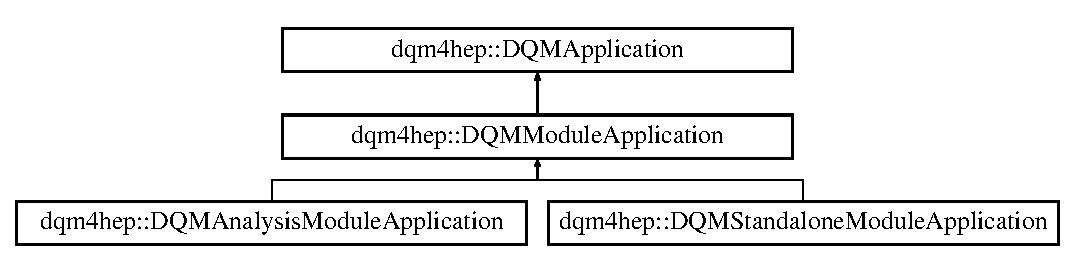
\includegraphics[height=3.000000cm]{classdqm4hep_1_1DQMModuleApplication}
\end{center}
\end{figure}
\subsection*{Public Member Functions}
\begin{DoxyCompactItemize}
\item 
{\bf D\+Q\+M\+Module\+Application} ()
\begin{DoxyCompactList}\small\item\em Constructor. \end{DoxyCompactList}\item 
virtual {\bf $\sim$\+D\+Q\+M\+Module\+Application} ()
\begin{DoxyCompactList}\small\item\em Destructor. \end{DoxyCompactList}\item 
virtual {\bf Status\+Code} {\bf run} ()=0
\begin{DoxyCompactList}\small\item\em Run the application. \end{DoxyCompactList}\item 
virtual {\bf Status\+Code} {\bf exit} (int return\+Code)
\begin{DoxyCompactList}\small\item\em Stop the application. \end{DoxyCompactList}\item 
virtual {\bf Status\+Code} {\bf read\+Settings} (const std\+::string \&settings\+File)=0
\begin{DoxyCompactList}\small\item\em Read the settings from file. \end{DoxyCompactList}\item 
virtual const std\+::string \& {\bf get\+Type} () const =0
\begin{DoxyCompactList}\small\item\em Get the application type. \end{DoxyCompactList}\item 
virtual const std\+::string \& {\bf get\+Name} () const =0
\begin{DoxyCompactList}\small\item\em Get the application name. \end{DoxyCompactList}\item 
{\bf D\+Q\+M\+Module} $\ast$ {\bf get\+Module} () const 
\begin{DoxyCompactList}\small\item\em Get the module for this application. \end{DoxyCompactList}\item 
bool {\bf should\+Stop\+Application} () const 
\begin{DoxyCompactList}\small\item\em Whether the module application should stop. \end{DoxyCompactList}\item 
void {\bf set\+Stop\+Application} (bool stop\+Application)
\begin{DoxyCompactList}\small\item\em Set the application stop flag. \end{DoxyCompactList}\item 
{\bf Status\+Code} {\bf set\+Module\+Name} (const std\+::string \&name)
\begin{DoxyCompactList}\small\item\em Set the module name in used. \end{DoxyCompactList}\item 
{\bf Status\+Code} {\bf set\+Module\+Type} (const std\+::string \&type)
\begin{DoxyCompactList}\small\item\em Set the module type to look for (before calling \doxyref{read\+Settings()}{p.}{classdqm4hep_1_1DQMModuleApplication_a994bb2bea7b1def71198ea1864460806}) \end{DoxyCompactList}\item 
const std\+::string \& {\bf get\+Module\+Name} () const 
\begin{DoxyCompactList}\small\item\em Get the module name in used. \end{DoxyCompactList}\item 
const std\+::string \& {\bf get\+Module\+Type} () const 
\begin{DoxyCompactList}\small\item\em Get the module type in used. \end{DoxyCompactList}\item 
bool {\bf is\+Initialized} () const 
\begin{DoxyCompactList}\small\item\em Whether the application is initialized. \end{DoxyCompactList}\item 
{\bf Status\+Code} {\bf get\+Return\+Code} () const 
\begin{DoxyCompactList}\small\item\em Get the return code when application ends. \end{DoxyCompactList}\end{DoxyCompactItemize}
\subsection*{Protected Member Functions}
\begin{DoxyCompactItemize}
\item 
void {\bf set\+Initialized} (bool initialized)
\begin{DoxyCompactList}\small\item\em Set the application has initialized. \end{DoxyCompactList}\item 
{\bf D\+Q\+M\+Monitor\+Element\+Manager} $\ast$ {\bf get\+Monitor\+Element\+Manager} () const 
\begin{DoxyCompactList}\small\item\em Get the monitor element manager. \end{DoxyCompactList}\item 
{\bf D\+Q\+M\+Monitor\+Element\+Sender} $\ast$ {\bf get\+Monitor\+Element\+Sender} () const 
\begin{DoxyCompactList}\small\item\em Get the monitor element sender. \end{DoxyCompactList}\item 
{\bf Status\+Code} {\bf set\+Module} ({\bf D\+Q\+M\+Module} $\ast$p\+Module)
\begin{DoxyCompactList}\small\item\em Set the module in use in this application. \end{DoxyCompactList}\end{DoxyCompactItemize}
\subsection*{Protected Attributes}
\begin{DoxyCompactItemize}
\item 
{\bf Status\+Code} {\bf m\+\_\+return\+Code}
\item 
{\bf D\+Q\+M\+Module} $\ast$ {\bf m\+\_\+p\+Module}
\end{DoxyCompactItemize}
\subsection*{Private Attributes}
\begin{DoxyCompactItemize}
\item 
bool {\bf m\+\_\+is\+Initialized}
\item 
bool {\bf m\+\_\+should\+Stop}
\item 
std\+::string {\bf m\+\_\+module\+Type}
\item 
std\+::string {\bf m\+\_\+module\+Name}
\item 
{\bf D\+Q\+M\+Monitor\+Element\+Manager} $\ast$ {\bf m\+\_\+p\+Monitor\+Element\+Manager}
\item 
{\bf D\+Q\+M\+Monitor\+Element\+Sender} $\ast$ {\bf m\+\_\+p\+Monitor\+Element\+Sender}
\end{DoxyCompactItemize}
\subsection*{Friends}
\begin{DoxyCompactItemize}
\item 
class {\bf D\+Q\+M\+Archiver}
\item 
class {\bf D\+Q\+M\+Module\+Api}
\end{DoxyCompactItemize}


\subsection{Detailed Description}
\doxyref{D\+Q\+M\+Module\+Application}{p.}{classdqm4hep_1_1DQMModuleApplication} class. 

Definition at line 47 of file D\+Q\+M\+Module\+Application.\+h.



\subsection{Constructor \& Destructor Documentation}
\index{dqm4hep\+::\+D\+Q\+M\+Module\+Application@{dqm4hep\+::\+D\+Q\+M\+Module\+Application}!D\+Q\+M\+Module\+Application@{D\+Q\+M\+Module\+Application}}
\index{D\+Q\+M\+Module\+Application@{D\+Q\+M\+Module\+Application}!dqm4hep\+::\+D\+Q\+M\+Module\+Application@{dqm4hep\+::\+D\+Q\+M\+Module\+Application}}
\subsubsection[{D\+Q\+M\+Module\+Application}]{\setlength{\rightskip}{0pt plus 5cm}dqm4hep\+::\+D\+Q\+M\+Module\+Application\+::\+D\+Q\+M\+Module\+Application (
\begin{DoxyParamCaption}
{}
\end{DoxyParamCaption}
)}\label{classdqm4hep_1_1DQMModuleApplication_aaf9ebc433b8556c24dc190bb33a63c29}


Constructor. 



Definition at line 36 of file D\+Q\+M\+Module\+Application.\+cc.



References m\+\_\+p\+Monitor\+Element\+Manager, and m\+\_\+p\+Monitor\+Element\+Sender.


\begin{DoxyCode}
36                                            :
37     m_isInitialized(\textcolor{keyword}{false}),
38     m_shouldStop(\textcolor{keyword}{false}),
39     m_pModule(NULL),
40     m_pMonitorElementManager(NULL),
41     m_pMonitorElementSender(NULL)
42 \{
43   m_pMonitorElementManager = \textcolor{keyword}{new} DQMMonitorElementManager();
44   m_pMonitorElementSender = \textcolor{keyword}{new} DQMMonitorElementSender(\textcolor{keyword}{this});
45 \}
\end{DoxyCode}
\index{dqm4hep\+::\+D\+Q\+M\+Module\+Application@{dqm4hep\+::\+D\+Q\+M\+Module\+Application}!````~D\+Q\+M\+Module\+Application@{$\sim$\+D\+Q\+M\+Module\+Application}}
\index{````~D\+Q\+M\+Module\+Application@{$\sim$\+D\+Q\+M\+Module\+Application}!dqm4hep\+::\+D\+Q\+M\+Module\+Application@{dqm4hep\+::\+D\+Q\+M\+Module\+Application}}
\subsubsection[{$\sim$\+D\+Q\+M\+Module\+Application}]{\setlength{\rightskip}{0pt plus 5cm}dqm4hep\+::\+D\+Q\+M\+Module\+Application\+::$\sim$\+D\+Q\+M\+Module\+Application (
\begin{DoxyParamCaption}
{}
\end{DoxyParamCaption}
)\hspace{0.3cm}{\ttfamily [virtual]}}\label{classdqm4hep_1_1DQMModuleApplication_a9178deb117b310cf34ca77a3860c02ce}


Destructor. 



Definition at line 49 of file D\+Q\+M\+Module\+Application.\+cc.



References m\+\_\+p\+Module, m\+\_\+p\+Monitor\+Element\+Manager, and m\+\_\+p\+Monitor\+Element\+Sender.


\begin{DoxyCode}
50 \{
51   \textcolor{keyword}{delete} m_pMonitorElementManager;
52   \textcolor{keyword}{delete} m_pMonitorElementSender;
53 
54   \textcolor{keywordflow}{if}(m_pModule)
55     \textcolor{keyword}{delete} m_pModule;
56 \}
\end{DoxyCode}


\subsection{Member Function Documentation}
\index{dqm4hep\+::\+D\+Q\+M\+Module\+Application@{dqm4hep\+::\+D\+Q\+M\+Module\+Application}!exit@{exit}}
\index{exit@{exit}!dqm4hep\+::\+D\+Q\+M\+Module\+Application@{dqm4hep\+::\+D\+Q\+M\+Module\+Application}}
\subsubsection[{exit}]{\setlength{\rightskip}{0pt plus 5cm}{\bf Status\+Code} dqm4hep\+::\+D\+Q\+M\+Module\+Application\+::exit (
\begin{DoxyParamCaption}
\item[{int}]{return\+Code}
\end{DoxyParamCaption}
)\hspace{0.3cm}{\ttfamily [virtual]}}\label{classdqm4hep_1_1DQMModuleApplication_aca8244e836f802675b9c11188804414d}


Stop the application. 



Implements {\bf dqm4hep\+::\+D\+Q\+M\+Application} \doxyref{}{p.}{classdqm4hep_1_1DQMApplication_ad61139a41c4ba6669d26e3a0013c0f6d}.



Definition at line 60 of file D\+Q\+M\+Module\+Application.\+cc.



References is\+Initialized(), m\+\_\+return\+Code, dqm4hep\+::\+M\+E\+S\+S\+A\+G\+E, dqm4hep\+::\+N\+U\+M\+B\+E\+R\+\_\+\+O\+F\+\_\+\+S\+T\+A\+T\+U\+S\+\_\+\+C\+O\+D\+E\+S, and set\+Stop\+Application().


\begin{DoxyCode}
61 \{
62   streamlog\_out(MESSAGE) << \textcolor{stringliteral}{"Exiting application ..."} << std::endl;
63 
64   \textcolor{keywordflow}{if}(!this->isInitialized())
65     \textcolor{keywordflow}{return} STATUS\_CODE\_NOT\_INITIALIZED;
66 
67   \textcolor{keywordflow}{if}( returnCode >= 0 && returnCode < NUMBER_OF_STATUS_CODES )
68     m_returnCode = \textcolor{keyword}{static\_cast<} StatusCode \textcolor{keyword}{>}( returnCode );
69   \textcolor{keywordflow}{else}
70     m_returnCode = STATUS\_CODE\_FAILURE;
71 
72   this->setStopApplication(\textcolor{keyword}{true});
73 
74   streamlog\_out(MESSAGE) << \textcolor{stringliteral}{"Exiting application ... OK"} << std::endl;
75 
76   \textcolor{keywordflow}{return} m_returnCode;
77 \}
\end{DoxyCode}
\index{dqm4hep\+::\+D\+Q\+M\+Module\+Application@{dqm4hep\+::\+D\+Q\+M\+Module\+Application}!get\+Module@{get\+Module}}
\index{get\+Module@{get\+Module}!dqm4hep\+::\+D\+Q\+M\+Module\+Application@{dqm4hep\+::\+D\+Q\+M\+Module\+Application}}
\subsubsection[{get\+Module}]{\setlength{\rightskip}{0pt plus 5cm}{\bf D\+Q\+M\+Module} $\ast$ dqm4hep\+::\+D\+Q\+M\+Module\+Application\+::get\+Module (
\begin{DoxyParamCaption}
{}
\end{DoxyParamCaption}
) const}\label{classdqm4hep_1_1DQMModuleApplication_a4049bbd6e1aa4ab76c7fd98738a0cef2}


Get the module for this application. 



Definition at line 81 of file D\+Q\+M\+Module\+Application.\+cc.



References m\+\_\+p\+Module.



Referenced by dqm4hep\+::\+D\+Q\+M\+Monitor\+Element\+Sender\+::add\+Available\+Monitor\+Element(), dqm4hep\+::\+D\+Q\+M\+Analysis\+Module\+Application\+::configure\+Module(), dqm4hep\+::\+D\+Q\+M\+Standalone\+Module\+Application\+::on\+Cycle\+Started(), dqm4hep\+::\+D\+Q\+M\+Analysis\+Module\+Application\+::on\+Cycle\+Started(), dqm4hep\+::\+D\+Q\+M\+Standalone\+Module\+Application\+::on\+Cycle\+Stopped(), dqm4hep\+::\+D\+Q\+M\+Analysis\+Module\+Application\+::on\+Cycle\+Stopped(), dqm4hep\+::\+D\+Q\+M\+Standalone\+Module\+Application\+::read\+Settings(), dqm4hep\+::\+D\+Q\+M\+Analysis\+Module\+Application\+::read\+Settings(), dqm4hep\+::\+D\+Q\+M\+Standalone\+Module\+Application\+::run(), dqm4hep\+::\+D\+Q\+M\+Analysis\+Module\+Application\+::run(), dqm4hep\+::\+D\+Q\+M\+Monitor\+Element\+Sender\+::send\+Available\+Monitor\+Element\+List(), and dqm4hep\+::\+D\+Q\+M\+Monitor\+Element\+Sender\+::send\+Monitor\+Elements().


\begin{DoxyCode}
82 \{
83   \textcolor{keywordflow}{return} m_pModule;
84 \}
\end{DoxyCode}
\index{dqm4hep\+::\+D\+Q\+M\+Module\+Application@{dqm4hep\+::\+D\+Q\+M\+Module\+Application}!get\+Module\+Name@{get\+Module\+Name}}
\index{get\+Module\+Name@{get\+Module\+Name}!dqm4hep\+::\+D\+Q\+M\+Module\+Application@{dqm4hep\+::\+D\+Q\+M\+Module\+Application}}
\subsubsection[{get\+Module\+Name}]{\setlength{\rightskip}{0pt plus 5cm}const std\+::string \& dqm4hep\+::\+D\+Q\+M\+Module\+Application\+::get\+Module\+Name (
\begin{DoxyParamCaption}
{}
\end{DoxyParamCaption}
) const}\label{classdqm4hep_1_1DQMModuleApplication_a5409dcefef80a2798411dc5ca13c069f}


Get the module name in used. 



Definition at line 129 of file D\+Q\+M\+Module\+Application.\+cc.



References dqm4hep\+::\+D\+Q\+M\+Module\+::get\+Name(), m\+\_\+module\+Name, and m\+\_\+p\+Module.



Referenced by dqm4hep\+::\+D\+Q\+M\+Analysis\+Module\+Application\+::configure\+Module(), and dqm4hep\+::\+D\+Q\+M\+Standalone\+Module\+Application\+::read\+Settings().


\begin{DoxyCode}
130 \{
131   \textcolor{keywordflow}{if}(m_pModule)
132     \textcolor{keywordflow}{return} m_pModule->getName();
133 
134   \textcolor{keywordflow}{return} m_moduleName;
135 \}
\end{DoxyCode}
\index{dqm4hep\+::\+D\+Q\+M\+Module\+Application@{dqm4hep\+::\+D\+Q\+M\+Module\+Application}!get\+Module\+Type@{get\+Module\+Type}}
\index{get\+Module\+Type@{get\+Module\+Type}!dqm4hep\+::\+D\+Q\+M\+Module\+Application@{dqm4hep\+::\+D\+Q\+M\+Module\+Application}}
\subsubsection[{get\+Module\+Type}]{\setlength{\rightskip}{0pt plus 5cm}const std\+::string \& dqm4hep\+::\+D\+Q\+M\+Module\+Application\+::get\+Module\+Type (
\begin{DoxyParamCaption}
{}
\end{DoxyParamCaption}
) const}\label{classdqm4hep_1_1DQMModuleApplication_afe7047c04c808815cefb84bd683b9e25}


Get the module type in used. 



Definition at line 139 of file D\+Q\+M\+Module\+Application.\+cc.



References m\+\_\+module\+Type.



Referenced by dqm4hep\+::\+D\+Q\+M\+Analysis\+Module\+Application\+::configure\+Module(), and dqm4hep\+::\+D\+Q\+M\+Standalone\+Module\+Application\+::read\+Settings().


\begin{DoxyCode}
140 \{
141   \textcolor{keywordflow}{return} m_moduleType;
142 \}
\end{DoxyCode}
\index{dqm4hep\+::\+D\+Q\+M\+Module\+Application@{dqm4hep\+::\+D\+Q\+M\+Module\+Application}!get\+Monitor\+Element\+Manager@{get\+Monitor\+Element\+Manager}}
\index{get\+Monitor\+Element\+Manager@{get\+Monitor\+Element\+Manager}!dqm4hep\+::\+D\+Q\+M\+Module\+Application@{dqm4hep\+::\+D\+Q\+M\+Module\+Application}}
\subsubsection[{get\+Monitor\+Element\+Manager}]{\setlength{\rightskip}{0pt plus 5cm}{\bf D\+Q\+M\+Monitor\+Element\+Manager} $\ast$ dqm4hep\+::\+D\+Q\+M\+Module\+Application\+::get\+Monitor\+Element\+Manager (
\begin{DoxyParamCaption}
{}
\end{DoxyParamCaption}
) const\hspace{0.3cm}{\ttfamily [protected]}}\label{classdqm4hep_1_1DQMModuleApplication_a8e344a68b7a3bcee90068eb4580b0c3f}


Get the monitor element manager. 



Definition at line 167 of file D\+Q\+M\+Module\+Application.\+cc.



References m\+\_\+p\+Monitor\+Element\+Manager.



Referenced by dqm4hep\+::\+D\+Q\+M\+Module\+Api\+::add\+Quality\+Test(), dqm4hep\+::\+D\+Q\+M\+Archiver\+::archive(), dqm4hep\+::\+D\+Q\+M\+Module\+Api\+::book\+Char\+Histogram1\+D(), dqm4hep\+::\+D\+Q\+M\+Module\+Api\+::book\+Char\+Histogram2\+D(), dqm4hep\+::\+D\+Q\+M\+Module\+Api\+::book\+Float(), dqm4hep\+::\+D\+Q\+M\+Module\+Api\+::book\+Int(), dqm4hep\+::\+D\+Q\+M\+Module\+Api\+::book\+Int\+Histogram1\+D(), dqm4hep\+::\+D\+Q\+M\+Module\+Api\+::book\+Int\+Histogram2\+D(), dqm4hep\+::\+D\+Q\+M\+Module\+Api\+::book\+Monitor\+Element(), dqm4hep\+::\+D\+Q\+M\+Module\+Api\+::book\+Object(), dqm4hep\+::\+D\+Q\+M\+Module\+Api\+::book\+Profile1\+D(), dqm4hep\+::\+D\+Q\+M\+Module\+Api\+::book\+Profile2\+D(), dqm4hep\+::\+D\+Q\+M\+Module\+Api\+::book\+Real\+Histogram1\+D(), dqm4hep\+::\+D\+Q\+M\+Module\+Api\+::book\+Real\+Histogram2\+D(), dqm4hep\+::\+D\+Q\+M\+Module\+Api\+::book\+Short(), dqm4hep\+::\+D\+Q\+M\+Module\+Api\+::book\+Short\+Histogram1\+D(), dqm4hep\+::\+D\+Q\+M\+Module\+Api\+::book\+Short\+Histogram2\+D(), dqm4hep\+::\+D\+Q\+M\+Module\+Api\+::book\+String(), dqm4hep\+::\+D\+Q\+M\+Module\+Api\+::cd(), dqm4hep\+::\+D\+Q\+M\+Module\+Api\+::create\+Quality\+Test(), dqm4hep\+::\+D\+Q\+M\+Module\+Api\+::delete\+Monitor\+Element(), dqm4hep\+::\+D\+Q\+M\+Module\+Api\+::get\+All\+Monitor\+Elements(), dqm4hep\+::\+D\+Q\+M\+Module\+Api\+::get\+Monitor\+Element(), dqm4hep\+::\+D\+Q\+M\+Module\+Api\+::go\+Up(), dqm4hep\+::\+D\+Q\+M\+Module\+Api\+::ls(), dqm4hep\+::\+D\+Q\+M\+Module\+Api\+::mkdir(), dqm4hep\+::\+D\+Q\+M\+Module\+Api\+::pwd(), dqm4hep\+::\+D\+Q\+M\+Module\+Api\+::register\+Quality\+Test\+Factory(), dqm4hep\+::\+D\+Q\+M\+Module\+Api\+::reset\+Monitor\+Elements(), dqm4hep\+::\+D\+Q\+M\+Module\+Api\+::rmdir(), dqm4hep\+::\+D\+Q\+M\+Analysis\+Module\+Application\+::run(), dqm4hep\+::\+D\+Q\+M\+Module\+Api\+::run\+Quality\+Test(), and dqm4hep\+::\+D\+Q\+M\+Module\+Api\+::run\+Quality\+Tests().


\begin{DoxyCode}
168 \{
169   \textcolor{keywordflow}{return} m_pMonitorElementManager;
170 \}
\end{DoxyCode}
\index{dqm4hep\+::\+D\+Q\+M\+Module\+Application@{dqm4hep\+::\+D\+Q\+M\+Module\+Application}!get\+Monitor\+Element\+Sender@{get\+Monitor\+Element\+Sender}}
\index{get\+Monitor\+Element\+Sender@{get\+Monitor\+Element\+Sender}!dqm4hep\+::\+D\+Q\+M\+Module\+Application@{dqm4hep\+::\+D\+Q\+M\+Module\+Application}}
\subsubsection[{get\+Monitor\+Element\+Sender}]{\setlength{\rightskip}{0pt plus 5cm}{\bf D\+Q\+M\+Monitor\+Element\+Sender} $\ast$ dqm4hep\+::\+D\+Q\+M\+Module\+Application\+::get\+Monitor\+Element\+Sender (
\begin{DoxyParamCaption}
{}
\end{DoxyParamCaption}
) const\hspace{0.3cm}{\ttfamily [protected]}}\label{classdqm4hep_1_1DQMModuleApplication_a9315e635c87cf200f7057ab6f0917e0b}


Get the monitor element sender. 



Definition at line 174 of file D\+Q\+M\+Module\+Application.\+cc.



References m\+\_\+p\+Monitor\+Element\+Sender.



Referenced by dqm4hep\+::\+D\+Q\+M\+Module\+Api\+::book\+Char\+Histogram1\+D(), dqm4hep\+::\+D\+Q\+M\+Module\+Api\+::book\+Char\+Histogram2\+D(), dqm4hep\+::\+D\+Q\+M\+Module\+Api\+::book\+Float(), dqm4hep\+::\+D\+Q\+M\+Module\+Api\+::book\+Int(), dqm4hep\+::\+D\+Q\+M\+Module\+Api\+::book\+Int\+Histogram1\+D(), dqm4hep\+::\+D\+Q\+M\+Module\+Api\+::book\+Int\+Histogram2\+D(), dqm4hep\+::\+D\+Q\+M\+Module\+Api\+::book\+Monitor\+Element(), dqm4hep\+::\+D\+Q\+M\+Module\+Api\+::book\+Object(), dqm4hep\+::\+D\+Q\+M\+Module\+Api\+::book\+Profile1\+D(), dqm4hep\+::\+D\+Q\+M\+Module\+Api\+::book\+Profile2\+D(), dqm4hep\+::\+D\+Q\+M\+Module\+Api\+::book\+Real\+Histogram1\+D(), dqm4hep\+::\+D\+Q\+M\+Module\+Api\+::book\+Real\+Histogram2\+D(), dqm4hep\+::\+D\+Q\+M\+Module\+Api\+::book\+Short(), dqm4hep\+::\+D\+Q\+M\+Module\+Api\+::book\+Short\+Histogram1\+D(), dqm4hep\+::\+D\+Q\+M\+Module\+Api\+::book\+Short\+Histogram2\+D(), dqm4hep\+::\+D\+Q\+M\+Module\+Api\+::book\+String(), dqm4hep\+::\+D\+Q\+M\+Analysis\+Module\+Application\+::configure\+Network(), dqm4hep\+::\+D\+Q\+M\+Module\+Api\+::delete\+Monitor\+Element(), dqm4hep\+::\+D\+Q\+M\+Standalone\+Module\+Application\+::read\+Settings(), dqm4hep\+::\+D\+Q\+M\+Standalone\+Module\+Application\+::run(), dqm4hep\+::\+D\+Q\+M\+Analysis\+Module\+Application\+::run(), dqm4hep\+::\+D\+Q\+M\+Analysis\+Module\+Application\+::start\+Services(), and dqm4hep\+::\+D\+Q\+M\+Analysis\+Module\+Application\+::stop\+Services().


\begin{DoxyCode}
175 \{
176   \textcolor{keywordflow}{return} m_pMonitorElementSender;
177 \}
\end{DoxyCode}
\index{dqm4hep\+::\+D\+Q\+M\+Module\+Application@{dqm4hep\+::\+D\+Q\+M\+Module\+Application}!get\+Name@{get\+Name}}
\index{get\+Name@{get\+Name}!dqm4hep\+::\+D\+Q\+M\+Module\+Application@{dqm4hep\+::\+D\+Q\+M\+Module\+Application}}
\subsubsection[{get\+Name}]{\setlength{\rightskip}{0pt plus 5cm}virtual const std\+::string\& dqm4hep\+::\+D\+Q\+M\+Module\+Application\+::get\+Name (
\begin{DoxyParamCaption}
{}
\end{DoxyParamCaption}
) const\hspace{0.3cm}{\ttfamily [pure virtual]}}\label{classdqm4hep_1_1DQMModuleApplication_afb07e2e9bc98060f2b1529f30355e4b9}


Get the application name. 



Implements {\bf dqm4hep\+::\+D\+Q\+M\+Application} \doxyref{}{p.}{classdqm4hep_1_1DQMApplication_a90d2e587390835cf90b38888498e922b}.



Implemented in {\bf dqm4hep\+::\+D\+Q\+M\+Analysis\+Module\+Application} \doxyref{}{p.}{classdqm4hep_1_1DQMAnalysisModuleApplication_a248fc1511e714851215dd49406897906}, and {\bf dqm4hep\+::\+D\+Q\+M\+Standalone\+Module\+Application} \doxyref{}{p.}{classdqm4hep_1_1DQMStandaloneModuleApplication_af67e009daf617aa7d07cbffeca8b9d54}.

\index{dqm4hep\+::\+D\+Q\+M\+Module\+Application@{dqm4hep\+::\+D\+Q\+M\+Module\+Application}!get\+Return\+Code@{get\+Return\+Code}}
\index{get\+Return\+Code@{get\+Return\+Code}!dqm4hep\+::\+D\+Q\+M\+Module\+Application@{dqm4hep\+::\+D\+Q\+M\+Module\+Application}}
\subsubsection[{get\+Return\+Code}]{\setlength{\rightskip}{0pt plus 5cm}{\bf Status\+Code} dqm4hep\+::\+D\+Q\+M\+Module\+Application\+::get\+Return\+Code (
\begin{DoxyParamCaption}
{}
\end{DoxyParamCaption}
) const}\label{classdqm4hep_1_1DQMModuleApplication_a157bd2b54d6c4291a56ea02ea72d1e39}


Get the return code when application ends. 



Definition at line 153 of file D\+Q\+M\+Module\+Application.\+cc.



References m\+\_\+return\+Code.



Referenced by dqm4hep\+::\+D\+Q\+M\+Analysis\+Module\+Application\+::run().


\begin{DoxyCode}
154 \{
155   \textcolor{keywordflow}{return} m_returnCode;
156 \}
\end{DoxyCode}
\index{dqm4hep\+::\+D\+Q\+M\+Module\+Application@{dqm4hep\+::\+D\+Q\+M\+Module\+Application}!get\+Type@{get\+Type}}
\index{get\+Type@{get\+Type}!dqm4hep\+::\+D\+Q\+M\+Module\+Application@{dqm4hep\+::\+D\+Q\+M\+Module\+Application}}
\subsubsection[{get\+Type}]{\setlength{\rightskip}{0pt plus 5cm}virtual const std\+::string\& dqm4hep\+::\+D\+Q\+M\+Module\+Application\+::get\+Type (
\begin{DoxyParamCaption}
{}
\end{DoxyParamCaption}
) const\hspace{0.3cm}{\ttfamily [pure virtual]}}\label{classdqm4hep_1_1DQMModuleApplication_ac24026bb5647c3f0de1889318a14cf88}


Get the application type. 



Implements {\bf dqm4hep\+::\+D\+Q\+M\+Application} \doxyref{}{p.}{classdqm4hep_1_1DQMApplication_aff587d33b27ff25115a7da7655e5ab3b}.



Implemented in {\bf dqm4hep\+::\+D\+Q\+M\+Analysis\+Module\+Application} \doxyref{}{p.}{classdqm4hep_1_1DQMAnalysisModuleApplication_aeccec8976c667b3e644e87c82043d1ff}, and {\bf dqm4hep\+::\+D\+Q\+M\+Standalone\+Module\+Application} \doxyref{}{p.}{classdqm4hep_1_1DQMStandaloneModuleApplication_a9aba02cf03c4faecd87e47b480c984ca}.

\index{dqm4hep\+::\+D\+Q\+M\+Module\+Application@{dqm4hep\+::\+D\+Q\+M\+Module\+Application}!is\+Initialized@{is\+Initialized}}
\index{is\+Initialized@{is\+Initialized}!dqm4hep\+::\+D\+Q\+M\+Module\+Application@{dqm4hep\+::\+D\+Q\+M\+Module\+Application}}
\subsubsection[{is\+Initialized}]{\setlength{\rightskip}{0pt plus 5cm}bool dqm4hep\+::\+D\+Q\+M\+Module\+Application\+::is\+Initialized (
\begin{DoxyParamCaption}
{}
\end{DoxyParamCaption}
) const}\label{classdqm4hep_1_1DQMModuleApplication_a7c076c800127648d40945120cc9298aa}


Whether the application is initialized. 



Definition at line 146 of file D\+Q\+M\+Module\+Application.\+cc.



References m\+\_\+is\+Initialized.



Referenced by exit(), dqm4hep\+::\+D\+Q\+M\+Standalone\+Module\+Application\+::read\+Settings(), dqm4hep\+::\+D\+Q\+M\+Analysis\+Module\+Application\+::read\+Settings(), dqm4hep\+::\+D\+Q\+M\+Standalone\+Module\+Application\+::run(), dqm4hep\+::\+D\+Q\+M\+Analysis\+Module\+Application\+::run(), set\+Module\+Name(), and set\+Module\+Type().


\begin{DoxyCode}
147 \{
148   \textcolor{keywordflow}{return} m_isInitialized;
149 \}
\end{DoxyCode}
\index{dqm4hep\+::\+D\+Q\+M\+Module\+Application@{dqm4hep\+::\+D\+Q\+M\+Module\+Application}!read\+Settings@{read\+Settings}}
\index{read\+Settings@{read\+Settings}!dqm4hep\+::\+D\+Q\+M\+Module\+Application@{dqm4hep\+::\+D\+Q\+M\+Module\+Application}}
\subsubsection[{read\+Settings}]{\setlength{\rightskip}{0pt plus 5cm}virtual {\bf Status\+Code} dqm4hep\+::\+D\+Q\+M\+Module\+Application\+::read\+Settings (
\begin{DoxyParamCaption}
\item[{const std\+::string \&}]{settings\+File}
\end{DoxyParamCaption}
)\hspace{0.3cm}{\ttfamily [pure virtual]}}\label{classdqm4hep_1_1DQMModuleApplication_a994bb2bea7b1def71198ea1864460806}


Read the settings from file. 



Implements {\bf dqm4hep\+::\+D\+Q\+M\+Application} \doxyref{}{p.}{classdqm4hep_1_1DQMApplication_a8b2e28cf09eef6b6a8bde547949c37dc}.



Implemented in {\bf dqm4hep\+::\+D\+Q\+M\+Analysis\+Module\+Application} \doxyref{}{p.}{classdqm4hep_1_1DQMAnalysisModuleApplication_a4b460e8713534da56d6bfcb775a1f5b0}, and {\bf dqm4hep\+::\+D\+Q\+M\+Standalone\+Module\+Application} \doxyref{}{p.}{classdqm4hep_1_1DQMStandaloneModuleApplication_ac5450df61d38db926fe44d2557183fb8}.

\index{dqm4hep\+::\+D\+Q\+M\+Module\+Application@{dqm4hep\+::\+D\+Q\+M\+Module\+Application}!run@{run}}
\index{run@{run}!dqm4hep\+::\+D\+Q\+M\+Module\+Application@{dqm4hep\+::\+D\+Q\+M\+Module\+Application}}
\subsubsection[{run}]{\setlength{\rightskip}{0pt plus 5cm}virtual {\bf Status\+Code} dqm4hep\+::\+D\+Q\+M\+Module\+Application\+::run (
\begin{DoxyParamCaption}
{}
\end{DoxyParamCaption}
)\hspace{0.3cm}{\ttfamily [pure virtual]}}\label{classdqm4hep_1_1DQMModuleApplication_a42114dcd51bf17af14479345145e5988}


Run the application. 



Implements {\bf dqm4hep\+::\+D\+Q\+M\+Application} \doxyref{}{p.}{classdqm4hep_1_1DQMApplication_aa9a37abef624ec9656478c7211cc5a48}.



Implemented in {\bf dqm4hep\+::\+D\+Q\+M\+Analysis\+Module\+Application} \doxyref{}{p.}{classdqm4hep_1_1DQMAnalysisModuleApplication_abf3fd5d59491e8f99c9ed964a487079f}, and {\bf dqm4hep\+::\+D\+Q\+M\+Standalone\+Module\+Application} \doxyref{}{p.}{classdqm4hep_1_1DQMStandaloneModuleApplication_a3b2039cbf186ddf83bff16ded2c2dfb4}.

\index{dqm4hep\+::\+D\+Q\+M\+Module\+Application@{dqm4hep\+::\+D\+Q\+M\+Module\+Application}!set\+Initialized@{set\+Initialized}}
\index{set\+Initialized@{set\+Initialized}!dqm4hep\+::\+D\+Q\+M\+Module\+Application@{dqm4hep\+::\+D\+Q\+M\+Module\+Application}}
\subsubsection[{set\+Initialized}]{\setlength{\rightskip}{0pt plus 5cm}void dqm4hep\+::\+D\+Q\+M\+Module\+Application\+::set\+Initialized (
\begin{DoxyParamCaption}
\item[{bool}]{initialized}
\end{DoxyParamCaption}
)\hspace{0.3cm}{\ttfamily [protected]}}\label{classdqm4hep_1_1DQMModuleApplication_a3b9bf9554261c29a83c4d6439aa9ee2a}


Set the application has initialized. 



Definition at line 160 of file D\+Q\+M\+Module\+Application.\+cc.



References m\+\_\+is\+Initialized.



Referenced by dqm4hep\+::\+D\+Q\+M\+Standalone\+Module\+Application\+::read\+Settings(), and dqm4hep\+::\+D\+Q\+M\+Analysis\+Module\+Application\+::read\+Settings().


\begin{DoxyCode}
161 \{
162   m_isInitialized = initialized;
163 \}
\end{DoxyCode}
\index{dqm4hep\+::\+D\+Q\+M\+Module\+Application@{dqm4hep\+::\+D\+Q\+M\+Module\+Application}!set\+Module@{set\+Module}}
\index{set\+Module@{set\+Module}!dqm4hep\+::\+D\+Q\+M\+Module\+Application@{dqm4hep\+::\+D\+Q\+M\+Module\+Application}}
\subsubsection[{set\+Module}]{\setlength{\rightskip}{0pt plus 5cm}{\bf Status\+Code} dqm4hep\+::\+D\+Q\+M\+Module\+Application\+::set\+Module (
\begin{DoxyParamCaption}
\item[{{\bf D\+Q\+M\+Module} $\ast$}]{p\+Module}
\end{DoxyParamCaption}
)\hspace{0.3cm}{\ttfamily [protected]}}\label{classdqm4hep_1_1DQMModuleApplication_a95919b0bbd449464eb60e58aafbad42c}


Set the module in use in this application. 



Definition at line 181 of file D\+Q\+M\+Module\+Application.\+cc.



References m\+\_\+module\+Name, m\+\_\+p\+Module, dqm4hep\+::\+D\+Q\+M\+Module\+::set\+Module\+Application(), and dqm4hep\+::\+D\+Q\+M\+Module\+::set\+Name().



Referenced by dqm4hep\+::\+D\+Q\+M\+Analysis\+Module\+Application\+::configure\+Module(), and dqm4hep\+::\+D\+Q\+M\+Standalone\+Module\+Application\+::read\+Settings().


\begin{DoxyCode}
182 \{
183   \textcolor{keywordflow}{if}(!pModule)
184     \textcolor{keywordflow}{return} STATUS\_CODE\_INVALID\_PTR;
185 
186   m_pModule = pModule;
187   m_pModule->setName(m_moduleName);
188   m_pModule->setModuleApplication(\textcolor{keyword}{this});
189 
190   \textcolor{keywordflow}{return} STATUS\_CODE\_SUCCESS;
191 \}
\end{DoxyCode}
\index{dqm4hep\+::\+D\+Q\+M\+Module\+Application@{dqm4hep\+::\+D\+Q\+M\+Module\+Application}!set\+Module\+Name@{set\+Module\+Name}}
\index{set\+Module\+Name@{set\+Module\+Name}!dqm4hep\+::\+D\+Q\+M\+Module\+Application@{dqm4hep\+::\+D\+Q\+M\+Module\+Application}}
\subsubsection[{set\+Module\+Name}]{\setlength{\rightskip}{0pt plus 5cm}{\bf Status\+Code} dqm4hep\+::\+D\+Q\+M\+Module\+Application\+::set\+Module\+Name (
\begin{DoxyParamCaption}
\item[{const std\+::string \&}]{name}
\end{DoxyParamCaption}
)}\label{classdqm4hep_1_1DQMModuleApplication_ad088d86e398ba6f144e63a8bd2a3ccf7}


Set the module name in used. 



Definition at line 102 of file D\+Q\+M\+Module\+Application.\+cc.



References is\+Initialized(), m\+\_\+module\+Name, m\+\_\+p\+Module, and dqm4hep\+::\+D\+Q\+M\+Module\+::set\+Name().



Referenced by dqm4hep\+::\+D\+Q\+M\+Analysis\+Module\+Application\+::configure\+Module(), and dqm4hep\+::\+D\+Q\+M\+Standalone\+Module\+Application\+::read\+Settings().


\begin{DoxyCode}
103 \{
104   \textcolor{keywordflow}{if}(this->isInitialized())
105     \textcolor{keywordflow}{return} STATUS\_CODE\_ALREADY\_INITIALIZED;
106 
107   m_moduleName = name;
108 
109   \textcolor{keywordflow}{if}(m_pModule)
110     m_pModule->setName(name);
111 
112   \textcolor{keywordflow}{return} STATUS\_CODE\_SUCCESS;
113 \}
\end{DoxyCode}
\index{dqm4hep\+::\+D\+Q\+M\+Module\+Application@{dqm4hep\+::\+D\+Q\+M\+Module\+Application}!set\+Module\+Type@{set\+Module\+Type}}
\index{set\+Module\+Type@{set\+Module\+Type}!dqm4hep\+::\+D\+Q\+M\+Module\+Application@{dqm4hep\+::\+D\+Q\+M\+Module\+Application}}
\subsubsection[{set\+Module\+Type}]{\setlength{\rightskip}{0pt plus 5cm}{\bf Status\+Code} dqm4hep\+::\+D\+Q\+M\+Module\+Application\+::set\+Module\+Type (
\begin{DoxyParamCaption}
\item[{const std\+::string \&}]{type}
\end{DoxyParamCaption}
)}\label{classdqm4hep_1_1DQMModuleApplication_ab4be93745c1f1966e0dc0ceac9021341}


Set the module type to look for (before calling \doxyref{read\+Settings()}{p.}{classdqm4hep_1_1DQMModuleApplication_a994bb2bea7b1def71198ea1864460806}) 



Definition at line 117 of file D\+Q\+M\+Module\+Application.\+cc.



References is\+Initialized(), and m\+\_\+module\+Type.



Referenced by dqm4hep\+::\+D\+Q\+M\+Analysis\+Module\+Application\+::configure\+Module(), and dqm4hep\+::\+D\+Q\+M\+Standalone\+Module\+Application\+::read\+Settings().


\begin{DoxyCode}
118 \{
119   \textcolor{keywordflow}{if}(this->isInitialized())
120     \textcolor{keywordflow}{return} STATUS\_CODE\_ALREADY\_INITIALIZED;
121 
122   m_moduleType = type;
123 
124   \textcolor{keywordflow}{return} STATUS\_CODE\_SUCCESS;
125 \}
\end{DoxyCode}
\index{dqm4hep\+::\+D\+Q\+M\+Module\+Application@{dqm4hep\+::\+D\+Q\+M\+Module\+Application}!set\+Stop\+Application@{set\+Stop\+Application}}
\index{set\+Stop\+Application@{set\+Stop\+Application}!dqm4hep\+::\+D\+Q\+M\+Module\+Application@{dqm4hep\+::\+D\+Q\+M\+Module\+Application}}
\subsubsection[{set\+Stop\+Application}]{\setlength{\rightskip}{0pt plus 5cm}void dqm4hep\+::\+D\+Q\+M\+Module\+Application\+::set\+Stop\+Application (
\begin{DoxyParamCaption}
\item[{bool}]{stop\+Application}
\end{DoxyParamCaption}
)}\label{classdqm4hep_1_1DQMModuleApplication_a6136b17a7d6e6fa465bd82305eaa9b34}


Set the application stop flag. 



Definition at line 95 of file D\+Q\+M\+Module\+Application.\+cc.



References m\+\_\+should\+Stop.



Referenced by exit().


\begin{DoxyCode}
96 \{
97   m_shouldStop = stopApplication;
98 \}
\end{DoxyCode}
\index{dqm4hep\+::\+D\+Q\+M\+Module\+Application@{dqm4hep\+::\+D\+Q\+M\+Module\+Application}!should\+Stop\+Application@{should\+Stop\+Application}}
\index{should\+Stop\+Application@{should\+Stop\+Application}!dqm4hep\+::\+D\+Q\+M\+Module\+Application@{dqm4hep\+::\+D\+Q\+M\+Module\+Application}}
\subsubsection[{should\+Stop\+Application}]{\setlength{\rightskip}{0pt plus 5cm}bool dqm4hep\+::\+D\+Q\+M\+Module\+Application\+::should\+Stop\+Application (
\begin{DoxyParamCaption}
{}
\end{DoxyParamCaption}
) const}\label{classdqm4hep_1_1DQMModuleApplication_aca58d3971c2fa46585a82c754e0ac528}


Whether the module application should stop. 



Definition at line 88 of file D\+Q\+M\+Module\+Application.\+cc.



References m\+\_\+should\+Stop.



Referenced by dqm4hep\+::\+D\+Q\+M\+Standalone\+Module\+Application\+::run(), and dqm4hep\+::\+D\+Q\+M\+Analysis\+Module\+Application\+::run().


\begin{DoxyCode}
89 \{
90   \textcolor{keywordflow}{return} m_shouldStop;
91 \}
\end{DoxyCode}


\subsection{Friends And Related Function Documentation}
\index{dqm4hep\+::\+D\+Q\+M\+Module\+Application@{dqm4hep\+::\+D\+Q\+M\+Module\+Application}!D\+Q\+M\+Archiver@{D\+Q\+M\+Archiver}}
\index{D\+Q\+M\+Archiver@{D\+Q\+M\+Archiver}!dqm4hep\+::\+D\+Q\+M\+Module\+Application@{dqm4hep\+::\+D\+Q\+M\+Module\+Application}}
\subsubsection[{D\+Q\+M\+Archiver}]{\setlength{\rightskip}{0pt plus 5cm}friend class {\bf D\+Q\+M\+Archiver}\hspace{0.3cm}{\ttfamily [friend]}}\label{classdqm4hep_1_1DQMModuleApplication_ae0db2100e97c65c1c8bd82363b34e7b4}


Definition at line 49 of file D\+Q\+M\+Module\+Application.\+h.



Referenced by dqm4hep\+::\+D\+Q\+M\+Analysis\+Module\+Application\+::\+D\+Q\+M\+Analysis\+Module\+Application(), and dqm4hep\+::\+D\+Q\+M\+Standalone\+Module\+Application\+::\+D\+Q\+M\+Standalone\+Module\+Application().

\index{dqm4hep\+::\+D\+Q\+M\+Module\+Application@{dqm4hep\+::\+D\+Q\+M\+Module\+Application}!D\+Q\+M\+Module\+Api@{D\+Q\+M\+Module\+Api}}
\index{D\+Q\+M\+Module\+Api@{D\+Q\+M\+Module\+Api}!dqm4hep\+::\+D\+Q\+M\+Module\+Application@{dqm4hep\+::\+D\+Q\+M\+Module\+Application}}
\subsubsection[{D\+Q\+M\+Module\+Api}]{\setlength{\rightskip}{0pt plus 5cm}friend class {\bf D\+Q\+M\+Module\+Api}\hspace{0.3cm}{\ttfamily [friend]}}\label{classdqm4hep_1_1DQMModuleApplication_a34f448c0d2a0a6cbec1a2d2414bc2231}


Definition at line 50 of file D\+Q\+M\+Module\+Application.\+h.



\subsection{Member Data Documentation}
\index{dqm4hep\+::\+D\+Q\+M\+Module\+Application@{dqm4hep\+::\+D\+Q\+M\+Module\+Application}!m\+\_\+is\+Initialized@{m\+\_\+is\+Initialized}}
\index{m\+\_\+is\+Initialized@{m\+\_\+is\+Initialized}!dqm4hep\+::\+D\+Q\+M\+Module\+Application@{dqm4hep\+::\+D\+Q\+M\+Module\+Application}}
\subsubsection[{m\+\_\+is\+Initialized}]{\setlength{\rightskip}{0pt plus 5cm}bool dqm4hep\+::\+D\+Q\+M\+Module\+Application\+::m\+\_\+is\+Initialized\hspace{0.3cm}{\ttfamily [private]}}\label{classdqm4hep_1_1DQMModuleApplication_a5cb686b30171548ac3280564ed0c8c46}


Definition at line 138 of file D\+Q\+M\+Module\+Application.\+h.



Referenced by is\+Initialized(), and set\+Initialized().

\index{dqm4hep\+::\+D\+Q\+M\+Module\+Application@{dqm4hep\+::\+D\+Q\+M\+Module\+Application}!m\+\_\+module\+Name@{m\+\_\+module\+Name}}
\index{m\+\_\+module\+Name@{m\+\_\+module\+Name}!dqm4hep\+::\+D\+Q\+M\+Module\+Application@{dqm4hep\+::\+D\+Q\+M\+Module\+Application}}
\subsubsection[{m\+\_\+module\+Name}]{\setlength{\rightskip}{0pt plus 5cm}std\+::string dqm4hep\+::\+D\+Q\+M\+Module\+Application\+::m\+\_\+module\+Name\hspace{0.3cm}{\ttfamily [private]}}\label{classdqm4hep_1_1DQMModuleApplication_a1c7b813c0a112cf44e6147453b822a0e}


Definition at line 141 of file D\+Q\+M\+Module\+Application.\+h.



Referenced by get\+Module\+Name(), dqm4hep\+::\+D\+Q\+M\+Standalone\+Module\+Application\+::\+Settings\+::print(), set\+Module(), and set\+Module\+Name().

\index{dqm4hep\+::\+D\+Q\+M\+Module\+Application@{dqm4hep\+::\+D\+Q\+M\+Module\+Application}!m\+\_\+module\+Type@{m\+\_\+module\+Type}}
\index{m\+\_\+module\+Type@{m\+\_\+module\+Type}!dqm4hep\+::\+D\+Q\+M\+Module\+Application@{dqm4hep\+::\+D\+Q\+M\+Module\+Application}}
\subsubsection[{m\+\_\+module\+Type}]{\setlength{\rightskip}{0pt plus 5cm}std\+::string dqm4hep\+::\+D\+Q\+M\+Module\+Application\+::m\+\_\+module\+Type\hspace{0.3cm}{\ttfamily [private]}}\label{classdqm4hep_1_1DQMModuleApplication_addf2c98c57e6800a5cef0dfacebdf0d9}


Definition at line 140 of file D\+Q\+M\+Module\+Application.\+h.



Referenced by get\+Module\+Type(), dqm4hep\+::\+D\+Q\+M\+Standalone\+Module\+Application\+::\+Settings\+::print(), and set\+Module\+Type().

\index{dqm4hep\+::\+D\+Q\+M\+Module\+Application@{dqm4hep\+::\+D\+Q\+M\+Module\+Application}!m\+\_\+p\+Module@{m\+\_\+p\+Module}}
\index{m\+\_\+p\+Module@{m\+\_\+p\+Module}!dqm4hep\+::\+D\+Q\+M\+Module\+Application@{dqm4hep\+::\+D\+Q\+M\+Module\+Application}}
\subsubsection[{m\+\_\+p\+Module}]{\setlength{\rightskip}{0pt plus 5cm}{\bf D\+Q\+M\+Module}$\ast$ dqm4hep\+::\+D\+Q\+M\+Module\+Application\+::m\+\_\+p\+Module\hspace{0.3cm}{\ttfamily [protected]}}\label{classdqm4hep_1_1DQMModuleApplication_af72e17465c7b753bd71018af62041d5c}


Definition at line 135 of file D\+Q\+M\+Module\+Application.\+h.



Referenced by get\+Module(), get\+Module\+Name(), set\+Module(), set\+Module\+Name(), and $\sim$\+D\+Q\+M\+Module\+Application().

\index{dqm4hep\+::\+D\+Q\+M\+Module\+Application@{dqm4hep\+::\+D\+Q\+M\+Module\+Application}!m\+\_\+p\+Monitor\+Element\+Manager@{m\+\_\+p\+Monitor\+Element\+Manager}}
\index{m\+\_\+p\+Monitor\+Element\+Manager@{m\+\_\+p\+Monitor\+Element\+Manager}!dqm4hep\+::\+D\+Q\+M\+Module\+Application@{dqm4hep\+::\+D\+Q\+M\+Module\+Application}}
\subsubsection[{m\+\_\+p\+Monitor\+Element\+Manager}]{\setlength{\rightskip}{0pt plus 5cm}{\bf D\+Q\+M\+Monitor\+Element\+Manager}$\ast$ dqm4hep\+::\+D\+Q\+M\+Module\+Application\+::m\+\_\+p\+Monitor\+Element\+Manager\hspace{0.3cm}{\ttfamily [private]}}\label{classdqm4hep_1_1DQMModuleApplication_a6cc4860ed1591717cc0b8519dbaa59b4}


Definition at line 143 of file D\+Q\+M\+Module\+Application.\+h.



Referenced by D\+Q\+M\+Module\+Application(), get\+Monitor\+Element\+Manager(), and $\sim$\+D\+Q\+M\+Module\+Application().

\index{dqm4hep\+::\+D\+Q\+M\+Module\+Application@{dqm4hep\+::\+D\+Q\+M\+Module\+Application}!m\+\_\+p\+Monitor\+Element\+Sender@{m\+\_\+p\+Monitor\+Element\+Sender}}
\index{m\+\_\+p\+Monitor\+Element\+Sender@{m\+\_\+p\+Monitor\+Element\+Sender}!dqm4hep\+::\+D\+Q\+M\+Module\+Application@{dqm4hep\+::\+D\+Q\+M\+Module\+Application}}
\subsubsection[{m\+\_\+p\+Monitor\+Element\+Sender}]{\setlength{\rightskip}{0pt plus 5cm}{\bf D\+Q\+M\+Monitor\+Element\+Sender}$\ast$ dqm4hep\+::\+D\+Q\+M\+Module\+Application\+::m\+\_\+p\+Monitor\+Element\+Sender\hspace{0.3cm}{\ttfamily [private]}}\label{classdqm4hep_1_1DQMModuleApplication_ac5a0911fe6e2c49825f85fac9cfd2813}


Definition at line 144 of file D\+Q\+M\+Module\+Application.\+h.



Referenced by D\+Q\+M\+Module\+Application(), get\+Monitor\+Element\+Sender(), and $\sim$\+D\+Q\+M\+Module\+Application().

\index{dqm4hep\+::\+D\+Q\+M\+Module\+Application@{dqm4hep\+::\+D\+Q\+M\+Module\+Application}!m\+\_\+return\+Code@{m\+\_\+return\+Code}}
\index{m\+\_\+return\+Code@{m\+\_\+return\+Code}!dqm4hep\+::\+D\+Q\+M\+Module\+Application@{dqm4hep\+::\+D\+Q\+M\+Module\+Application}}
\subsubsection[{m\+\_\+return\+Code}]{\setlength{\rightskip}{0pt plus 5cm}{\bf Status\+Code} dqm4hep\+::\+D\+Q\+M\+Module\+Application\+::m\+\_\+return\+Code\hspace{0.3cm}{\ttfamily [protected]}}\label{classdqm4hep_1_1DQMModuleApplication_a9f0be7f42c6bd2ef60a0ef42f297d3a8}


Definition at line 134 of file D\+Q\+M\+Module\+Application.\+h.



Referenced by exit(), and get\+Return\+Code().

\index{dqm4hep\+::\+D\+Q\+M\+Module\+Application@{dqm4hep\+::\+D\+Q\+M\+Module\+Application}!m\+\_\+should\+Stop@{m\+\_\+should\+Stop}}
\index{m\+\_\+should\+Stop@{m\+\_\+should\+Stop}!dqm4hep\+::\+D\+Q\+M\+Module\+Application@{dqm4hep\+::\+D\+Q\+M\+Module\+Application}}
\subsubsection[{m\+\_\+should\+Stop}]{\setlength{\rightskip}{0pt plus 5cm}bool dqm4hep\+::\+D\+Q\+M\+Module\+Application\+::m\+\_\+should\+Stop\hspace{0.3cm}{\ttfamily [private]}}\label{classdqm4hep_1_1DQMModuleApplication_a059cf272bb8e0cff42dd713d03332e34}


Definition at line 139 of file D\+Q\+M\+Module\+Application.\+h.



Referenced by set\+Stop\+Application(), and should\+Stop\+Application().



The documentation for this class was generated from the following files\+:\begin{DoxyCompactItemize}
\item 
{\bf D\+Q\+M\+Module\+Application.\+h}\item 
{\bf D\+Q\+M\+Module\+Application.\+cc}\end{DoxyCompactItemize}

\section{dqm4hep\+:\+:D\+Q\+M\+Monitor\+Element Class Reference}
\label{classdqm4hep_1_1DQMMonitorElement}\index{dqm4hep\+::\+D\+Q\+M\+Monitor\+Element@{dqm4hep\+::\+D\+Q\+M\+Monitor\+Element}}


\doxyref{D\+Q\+M\+Monitor\+Element}{p.}{classdqm4hep_1_1DQMMonitorElement} class.  




{\ttfamily \#include $<$D\+Q\+M\+Monitor\+Element.\+h$>$}

\subsection*{Public Member Functions}
\begin{DoxyCompactItemize}
\item 
{\bf D\+Q\+M\+Monitor\+Element} ({\bf D\+Q\+M\+Monitor\+Element\+Type} type=N\+O\+\_\+\+E\+L\+E\+M\+E\+N\+T\+\_\+\+T\+Y\+P\+E, const std\+::string \&name=\char`\"{}\char`\"{}, const std\+::string \&title=\char`\"{}\char`\"{}, const std\+::string \&module\+Name=\char`\"{}\char`\"{})
\begin{DoxyCompactList}\small\item\em Default constructor. \end{DoxyCompactList}\item 
{\bf D\+Q\+M\+Monitor\+Element} (T\+Object $\ast$p\+Object, {\bf D\+Q\+M\+Monitor\+Element\+Type} type, const std\+::string \&name, const std\+::string \&title, const std\+::string \&module\+Name)
\begin{DoxyCompactList}\small\item\em \doxyref{D\+Q\+M\+Monitor\+Element}{p.}{classdqm4hep_1_1DQMMonitorElement} with type, name and title. \end{DoxyCompactList}\item 
virtual {\bf $\sim$\+D\+Q\+M\+Monitor\+Element} ()
\begin{DoxyCompactList}\small\item\em Destructor. \end{DoxyCompactList}\item 
{\bf D\+Q\+M\+Monitor\+Element\+Type} {\bf get\+Type} () const 
\begin{DoxyCompactList}\small\item\em Returns the element type. \end{DoxyCompactList}\item 
virtual const std\+::string \& {\bf get\+Name} () const 
\begin{DoxyCompactList}\small\item\em Returns the name of the element. \end{DoxyCompactList}\item 
const {\bf D\+Q\+M\+Path} \& {\bf get\+Path} () const 
\begin{DoxyCompactList}\small\item\em Get the path (directory) of this element. \end{DoxyCompactList}\item 
void {\bf set\+Path} (const {\bf D\+Q\+M\+Path} \&path)
\begin{DoxyCompactList}\small\item\em Set the path (directory) for this element. \end{DoxyCompactList}\item 
const std\+::string \& {\bf get\+Collector\+Name} () const 
\begin{DoxyCompactList}\small\item\em Get the collector name where this element is collected (or will be) Set by the framework after collect. \end{DoxyCompactList}\item 
void {\bf set\+Collector\+Name} (const std\+::string \&collector\+Name)
\begin{DoxyCompactList}\small\item\em Set the collector name where this element is collected (or will be) Used by the framework after collect. \end{DoxyCompactList}\item 
const std\+::string \& {\bf get\+Module\+Name} () const 
\begin{DoxyCompactList}\small\item\em Get the module name that has booked this element. \end{DoxyCompactList}\item 
bool {\bf is\+Histogram} () const 
\begin{DoxyCompactList}\small\item\em Whether the monitor element is a histogram. \end{DoxyCompactList}\item 
bool {\bf is\+Scalar} () const 
\begin{DoxyCompactList}\small\item\em Whether the monitor element is a scalar value. \end{DoxyCompactList}\item 
{\bf D\+Q\+M\+Quality} {\bf get\+Quality} () const 
\begin{DoxyCompactList}\small\item\em Returns the element quality. \end{DoxyCompactList}\item 
void {\bf set\+Quality} ({\bf D\+Q\+M\+Quality} quality)
\begin{DoxyCompactList}\small\item\em Set the element quality. \end{DoxyCompactList}\item 
{\bf D\+Q\+M\+Reset\+Policy} {\bf get\+Reset\+Policy} () const 
\begin{DoxyCompactList}\small\item\em Returns the reset policy of the element. \end{DoxyCompactList}\item 
void {\bf set\+Reset\+Policy} ({\bf D\+Q\+M\+Reset\+Policy} policy)
\begin{DoxyCompactList}\small\item\em Sets the reset policy of the element. \end{DoxyCompactList}\item 
virtual const std\+::string \& {\bf get\+Title} () const 
\begin{DoxyCompactList}\small\item\em Returns the title of the object. \end{DoxyCompactList}\item 
virtual void {\bf set\+Title} (const std\+::string \&title)
\begin{DoxyCompactList}\small\item\em Sets the element title. \end{DoxyCompactList}\item 
const std\+::string \& {\bf get\+Description} () const 
\begin{DoxyCompactList}\small\item\em Returns the element description. \end{DoxyCompactList}\item 
void {\bf set\+Description} (const std\+::string \&description)
\begin{DoxyCompactList}\small\item\em Sets the element description. \end{DoxyCompactList}\item 
const std\+::string \& {\bf get\+Draw\+Option} () const 
\begin{DoxyCompactList}\small\item\em Return the draw option. \end{DoxyCompactList}\item 
void {\bf set\+Draw\+Option} (const std\+::string \&draw\+Option)
\begin{DoxyCompactList}\small\item\em Set the draw option. \end{DoxyCompactList}\item 
unsigned int {\bf get\+Run\+Number} () const 
\begin{DoxyCompactList}\small\item\em Returns the current run for this monitor element. \end{DoxyCompactList}\item 
void {\bf set\+Run\+Number} (unsigned int run\+Number)
\begin{DoxyCompactList}\small\item\em Sets the current run number. \end{DoxyCompactList}\item 
void {\bf set\+To\+Publish} (bool publish)
\begin{DoxyCompactList}\small\item\em Sets whether the element has to be published at the next end of cycle. \end{DoxyCompactList}\item 
bool {\bf is\+To\+Publish} () const 
\begin{DoxyCompactList}\small\item\em Whether the element has to be published at the next end of cycle. \end{DoxyCompactList}\item 
T\+Object $\ast$ {\bf get\+Object} () const 
\begin{DoxyCompactList}\small\item\em Return the associated T\+Object that is monitored. \end{DoxyCompactList}\item 
{\footnotesize template$<$typename T $>$ }\\T $\ast$ {\bf get} () const 
\begin{DoxyCompactList}\small\item\em Return the monitor object after a dynamic cast of the asked type. \end{DoxyCompactList}\item 
const {\bf D\+Q\+M\+Quality\+Test\+Result\+Map} \& {\bf get\+Quality\+Test\+Results} () const 
\begin{DoxyCompactList}\small\item\em Return the quality test results map. \end{DoxyCompactList}\item 
void {\bf reset} ()
\begin{DoxyCompactList}\small\item\em Reset the element. \end{DoxyCompactList}\item 
{\bf Status\+Code} {\bf serialize} ({\bf D\+Q\+M\+Data\+Stream} $\ast$const p\+Data\+Stream) const 
\item 
{\bf Status\+Code} {\bf deserialize} ({\bf D\+Q\+M\+Data\+Stream} $\ast$const p\+Data\+Stream)
\end{DoxyCompactItemize}
\subsection*{Private Member Functions}
\begin{DoxyCompactItemize}
\item 
{\bf Status\+Code} {\bf run\+Quality\+Test} (const std\+::string \&quality\+Test\+Name)
\begin{DoxyCompactList}\small\item\em Run the given quality test. \end{DoxyCompactList}\item 
{\bf Status\+Code} {\bf run\+Quality\+Tests} ()
\begin{DoxyCompactList}\small\item\em Run all the quality tests. \end{DoxyCompactList}\item 
{\bf Status\+Code} {\bf add\+Quality\+Test} ({\bf D\+Q\+M\+Quality\+Test} $\ast$p\+Quality\+Test)
\begin{DoxyCompactList}\small\item\em Add a quality test. \end{DoxyCompactList}\item 
{\bf Status\+Code} {\bf remove\+Quality\+Test} ({\bf D\+Q\+M\+Quality\+Test} $\ast$p\+Quality\+Test)
\begin{DoxyCompactList}\small\item\em Remove a quality test. \end{DoxyCompactList}\item 
{\bf Status\+Code} {\bf remove\+Quality\+Test} (const std\+::string \&quality\+Test\+Name)
\begin{DoxyCompactList}\small\item\em Remove a quality test. \end{DoxyCompactList}\end{DoxyCompactItemize}
\subsection*{Private Attributes}
\begin{DoxyCompactItemize}
\item 
T\+Object $\ast$ {\bf m\+\_\+p\+Object}
\begin{DoxyCompactList}\small\item\em The monitored T\+Object. \end{DoxyCompactList}\item 
std\+::string {\bf m\+\_\+name}
\begin{DoxyCompactList}\small\item\em The element name. \end{DoxyCompactList}\item 
std\+::string {\bf m\+\_\+title}
\begin{DoxyCompactList}\small\item\em The element title. \end{DoxyCompactList}\item 
std\+::string {\bf m\+\_\+description}
\begin{DoxyCompactList}\small\item\em The element description. \end{DoxyCompactList}\item 
std\+::string {\bf m\+\_\+draw\+Option}
\begin{DoxyCompactList}\small\item\em The draw option to apply while drawing. \end{DoxyCompactList}\item 
std\+::string {\bf m\+\_\+module\+Name}
\begin{DoxyCompactList}\small\item\em The module name that have booked this element. \end{DoxyCompactList}\item 
std\+::string {\bf m\+\_\+collector\+Name}
\begin{DoxyCompactList}\small\item\em The collector name that have collected this element. \end{DoxyCompactList}\item 
{\bf D\+Q\+M\+Path} {\bf m\+\_\+path}
\item 
{\bf D\+Q\+M\+Monitor\+Element\+Type} {\bf m\+\_\+type}
\begin{DoxyCompactList}\small\item\em The element type. \end{DoxyCompactList}\item 
{\bf D\+Q\+M\+Quality} {\bf m\+\_\+quality}
\begin{DoxyCompactList}\small\item\em The element quality has defined by the user. \end{DoxyCompactList}\item 
{\bf D\+Q\+M\+Reset\+Policy} {\bf m\+\_\+reset\+Policy}
\begin{DoxyCompactList}\small\item\em The reset policy. See enumerator definition. \end{DoxyCompactList}\item 
unsigned int {\bf m\+\_\+run\+Number}
\begin{DoxyCompactList}\small\item\em The run number when the element is published. \end{DoxyCompactList}\item 
bool {\bf m\+\_\+to\+Publish}
\begin{DoxyCompactList}\small\item\em Whether the element has to be published at end of cycle. \end{DoxyCompactList}\item 
std\+::map$<$ std\+::string, \\*
{\bf D\+Q\+M\+Quality\+Test} $\ast$ $>$ {\bf m\+\_\+quality\+Test\+Map}
\item 
std\+::map$<$ std\+::string, \\*
{\bf D\+Q\+M\+Quality\+Test\+Result} $>$ {\bf m\+\_\+quality\+Test\+Result\+Map}
\begin{DoxyCompactList}\small\item\em The quality test map to perform. \end{DoxyCompactList}\end{DoxyCompactItemize}
\subsection*{Friends}
\begin{DoxyCompactItemize}
\item 
class {\bf D\+Q\+M\+Module\+Api}
\item 
class {\bf D\+Q\+M\+Storage}
\item 
class {\bf D\+Q\+M\+Directory}
\item 
class {\bf D\+Q\+M\+Monitor\+Element\+Manager}
\end{DoxyCompactItemize}


\subsection{Detailed Description}
\doxyref{D\+Q\+M\+Monitor\+Element}{p.}{classdqm4hep_1_1DQMMonitorElement} class. 

Base class for plots and scalars that can be monitored via a user module. Monitor elements can be booked via the \doxyref{D\+Q\+M\+Module\+Api}{p.}{classdqm4hep_1_1DQMModuleApi} in order to be published.

\begin{DoxyAuthor}{Author}
R.\+Ete 
\end{DoxyAuthor}


Definition at line 58 of file D\+Q\+M\+Monitor\+Element.\+h.



\subsection{Constructor \& Destructor Documentation}
\index{dqm4hep\+::\+D\+Q\+M\+Monitor\+Element@{dqm4hep\+::\+D\+Q\+M\+Monitor\+Element}!D\+Q\+M\+Monitor\+Element@{D\+Q\+M\+Monitor\+Element}}
\index{D\+Q\+M\+Monitor\+Element@{D\+Q\+M\+Monitor\+Element}!dqm4hep\+::\+D\+Q\+M\+Monitor\+Element@{dqm4hep\+::\+D\+Q\+M\+Monitor\+Element}}
\subsubsection[{D\+Q\+M\+Monitor\+Element}]{\setlength{\rightskip}{0pt plus 5cm}dqm4hep\+::\+D\+Q\+M\+Monitor\+Element\+::\+D\+Q\+M\+Monitor\+Element (
\begin{DoxyParamCaption}
\item[{{\bf D\+Q\+M\+Monitor\+Element\+Type}}]{type = {\ttfamily NO\+\_\+ELEMENT\+\_\+TYPE}, }
\item[{const std\+::string \&}]{name = {\ttfamily \char`\"{}\char`\"{}}, }
\item[{const std\+::string \&}]{title = {\ttfamily \char`\"{}\char`\"{}}, }
\item[{const std\+::string \&}]{module\+Name = {\ttfamily \char`\"{}\char`\"{}}}
\end{DoxyParamCaption}
)}\label{classdqm4hep_1_1DQMMonitorElement_aab7978131f1aecf343303b9afc6d661f}


Default constructor. 

\index{dqm4hep\+::\+D\+Q\+M\+Monitor\+Element@{dqm4hep\+::\+D\+Q\+M\+Monitor\+Element}!D\+Q\+M\+Monitor\+Element@{D\+Q\+M\+Monitor\+Element}}
\index{D\+Q\+M\+Monitor\+Element@{D\+Q\+M\+Monitor\+Element}!dqm4hep\+::\+D\+Q\+M\+Monitor\+Element@{dqm4hep\+::\+D\+Q\+M\+Monitor\+Element}}
\subsubsection[{D\+Q\+M\+Monitor\+Element}]{\setlength{\rightskip}{0pt plus 5cm}dqm4hep\+::\+D\+Q\+M\+Monitor\+Element\+::\+D\+Q\+M\+Monitor\+Element (
\begin{DoxyParamCaption}
\item[{T\+Object $\ast$}]{p\+Object, }
\item[{{\bf D\+Q\+M\+Monitor\+Element\+Type}}]{type, }
\item[{const std\+::string \&}]{name, }
\item[{const std\+::string \&}]{title, }
\item[{const std\+::string \&}]{module\+Name}
\end{DoxyParamCaption}
)}\label{classdqm4hep_1_1DQMMonitorElement_a39dc4fb87f8164ba1f99f68b695ecd93}


\doxyref{D\+Q\+M\+Monitor\+Element}{p.}{classdqm4hep_1_1DQMMonitorElement} with type, name and title. 

\index{dqm4hep\+::\+D\+Q\+M\+Monitor\+Element@{dqm4hep\+::\+D\+Q\+M\+Monitor\+Element}!````~D\+Q\+M\+Monitor\+Element@{$\sim$\+D\+Q\+M\+Monitor\+Element}}
\index{````~D\+Q\+M\+Monitor\+Element@{$\sim$\+D\+Q\+M\+Monitor\+Element}!dqm4hep\+::\+D\+Q\+M\+Monitor\+Element@{dqm4hep\+::\+D\+Q\+M\+Monitor\+Element}}
\subsubsection[{$\sim$\+D\+Q\+M\+Monitor\+Element}]{\setlength{\rightskip}{0pt plus 5cm}virtual dqm4hep\+::\+D\+Q\+M\+Monitor\+Element\+::$\sim$\+D\+Q\+M\+Monitor\+Element (
\begin{DoxyParamCaption}
{}
\end{DoxyParamCaption}
)\hspace{0.3cm}{\ttfamily [virtual]}}\label{classdqm4hep_1_1DQMMonitorElement_ac9b2ebd0394609523040189f70c64569}


Destructor. 



\subsection{Member Function Documentation}
\index{dqm4hep\+::\+D\+Q\+M\+Monitor\+Element@{dqm4hep\+::\+D\+Q\+M\+Monitor\+Element}!add\+Quality\+Test@{add\+Quality\+Test}}
\index{add\+Quality\+Test@{add\+Quality\+Test}!dqm4hep\+::\+D\+Q\+M\+Monitor\+Element@{dqm4hep\+::\+D\+Q\+M\+Monitor\+Element}}
\subsubsection[{add\+Quality\+Test}]{\setlength{\rightskip}{0pt plus 5cm}{\bf Status\+Code} dqm4hep\+::\+D\+Q\+M\+Monitor\+Element\+::add\+Quality\+Test (
\begin{DoxyParamCaption}
\item[{{\bf D\+Q\+M\+Quality\+Test} $\ast$}]{p\+Quality\+Test}
\end{DoxyParamCaption}
)\hspace{0.3cm}{\ttfamily [private]}}\label{classdqm4hep_1_1DQMMonitorElement_a75baca8846d736018b58286eae578ff7}


Add a quality test. 



Referenced by dqm4hep\+::\+D\+Q\+M\+Monitor\+Element\+Manager\+::add\+Quality\+Test().

\index{dqm4hep\+::\+D\+Q\+M\+Monitor\+Element@{dqm4hep\+::\+D\+Q\+M\+Monitor\+Element}!deserialize@{deserialize}}
\index{deserialize@{deserialize}!dqm4hep\+::\+D\+Q\+M\+Monitor\+Element@{dqm4hep\+::\+D\+Q\+M\+Monitor\+Element}}
\subsubsection[{deserialize}]{\setlength{\rightskip}{0pt plus 5cm}{\bf Status\+Code} dqm4hep\+::\+D\+Q\+M\+Monitor\+Element\+::deserialize (
\begin{DoxyParamCaption}
\item[{{\bf D\+Q\+M\+Data\+Stream} $\ast$const}]{p\+Data\+Stream}
\end{DoxyParamCaption}
)}\label{classdqm4hep_1_1DQMMonitorElement_a19c7de73a98b0f2b4140b0f0d91efa57}


Referenced by dqm4hep\+::\+D\+Q\+M\+Monitor\+Element\+Publication\+::deserialize().

\index{dqm4hep\+::\+D\+Q\+M\+Monitor\+Element@{dqm4hep\+::\+D\+Q\+M\+Monitor\+Element}!get@{get}}
\index{get@{get}!dqm4hep\+::\+D\+Q\+M\+Monitor\+Element@{dqm4hep\+::\+D\+Q\+M\+Monitor\+Element}}
\subsubsection[{get}]{\setlength{\rightskip}{0pt plus 5cm}template$<$typename T $>$ T $\ast$ dqm4hep\+::\+D\+Q\+M\+Monitor\+Element\+::get (
\begin{DoxyParamCaption}
{}
\end{DoxyParamCaption}
) const}\label{classdqm4hep_1_1DQMMonitorElement_a102a7cc916a9767001e3a4bafd732540}


Return the monitor object after a dynamic cast of the asked type. 



Definition at line 245 of file D\+Q\+M\+Monitor\+Element.\+h.



References m\+\_\+p\+Object.



Referenced by dqm4hep\+::\+D\+Q\+M\+Mean\+Within\+Expected\+Test\+::can\+Run(), dqm4hep\+::\+D\+Q\+M\+Chi2\+Fit\+Function\+Test\+::can\+Run(), dqm4hep\+::\+D\+Q\+M\+Mean\+Within\+Expected\+Test\+::run(), and dqm4hep\+::\+D\+Q\+M\+Chi2\+Fit\+Function\+Test\+::run().


\begin{DoxyCode}
246 \{
247   \textcolor{keywordflow}{return} \textcolor{keyword}{dynamic\_cast<}T*\textcolor{keyword}{>}(m_pObject);
248 \}
\end{DoxyCode}
\index{dqm4hep\+::\+D\+Q\+M\+Monitor\+Element@{dqm4hep\+::\+D\+Q\+M\+Monitor\+Element}!get\+Collector\+Name@{get\+Collector\+Name}}
\index{get\+Collector\+Name@{get\+Collector\+Name}!dqm4hep\+::\+D\+Q\+M\+Monitor\+Element@{dqm4hep\+::\+D\+Q\+M\+Monitor\+Element}}
\subsubsection[{get\+Collector\+Name}]{\setlength{\rightskip}{0pt plus 5cm}const std\+::string\& dqm4hep\+::\+D\+Q\+M\+Monitor\+Element\+::get\+Collector\+Name (
\begin{DoxyParamCaption}
{}
\end{DoxyParamCaption}
) const}\label{classdqm4hep_1_1DQMMonitorElement_ac36c1b627145fed4f4677ed86b85922e}


Get the collector name where this element is collected (or will be) Set by the framework after collect. 

\index{dqm4hep\+::\+D\+Q\+M\+Monitor\+Element@{dqm4hep\+::\+D\+Q\+M\+Monitor\+Element}!get\+Description@{get\+Description}}
\index{get\+Description@{get\+Description}!dqm4hep\+::\+D\+Q\+M\+Monitor\+Element@{dqm4hep\+::\+D\+Q\+M\+Monitor\+Element}}
\subsubsection[{get\+Description}]{\setlength{\rightskip}{0pt plus 5cm}const std\+::string\& dqm4hep\+::\+D\+Q\+M\+Monitor\+Element\+::get\+Description (
\begin{DoxyParamCaption}
{}
\end{DoxyParamCaption}
) const}\label{classdqm4hep_1_1DQMMonitorElement_afa54d2f6d74db063c433c75d0c257b57}


Returns the element description. 



Referenced by dqm4hep\+::\+D\+Q\+M\+Monitor\+Element\+Sender\+::add\+Available\+Monitor\+Element().

\index{dqm4hep\+::\+D\+Q\+M\+Monitor\+Element@{dqm4hep\+::\+D\+Q\+M\+Monitor\+Element}!get\+Draw\+Option@{get\+Draw\+Option}}
\index{get\+Draw\+Option@{get\+Draw\+Option}!dqm4hep\+::\+D\+Q\+M\+Monitor\+Element@{dqm4hep\+::\+D\+Q\+M\+Monitor\+Element}}
\subsubsection[{get\+Draw\+Option}]{\setlength{\rightskip}{0pt plus 5cm}const std\+::string\& dqm4hep\+::\+D\+Q\+M\+Monitor\+Element\+::get\+Draw\+Option (
\begin{DoxyParamCaption}
{}
\end{DoxyParamCaption}
) const}\label{classdqm4hep_1_1DQMMonitorElement_addd8e8042990f3ab5f3edab95ce720c5}


Return the draw option. 

\index{dqm4hep\+::\+D\+Q\+M\+Monitor\+Element@{dqm4hep\+::\+D\+Q\+M\+Monitor\+Element}!get\+Module\+Name@{get\+Module\+Name}}
\index{get\+Module\+Name@{get\+Module\+Name}!dqm4hep\+::\+D\+Q\+M\+Monitor\+Element@{dqm4hep\+::\+D\+Q\+M\+Monitor\+Element}}
\subsubsection[{get\+Module\+Name}]{\setlength{\rightskip}{0pt plus 5cm}const std\+::string\& dqm4hep\+::\+D\+Q\+M\+Monitor\+Element\+::get\+Module\+Name (
\begin{DoxyParamCaption}
{}
\end{DoxyParamCaption}
) const}\label{classdqm4hep_1_1DQMMonitorElement_aad825ff38c0efb52ad7b48445aedc7a2}


Get the module name that has booked this element. 

\index{dqm4hep\+::\+D\+Q\+M\+Monitor\+Element@{dqm4hep\+::\+D\+Q\+M\+Monitor\+Element}!get\+Name@{get\+Name}}
\index{get\+Name@{get\+Name}!dqm4hep\+::\+D\+Q\+M\+Monitor\+Element@{dqm4hep\+::\+D\+Q\+M\+Monitor\+Element}}
\subsubsection[{get\+Name}]{\setlength{\rightskip}{0pt plus 5cm}virtual const std\+::string\& dqm4hep\+::\+D\+Q\+M\+Monitor\+Element\+::get\+Name (
\begin{DoxyParamCaption}
{}
\end{DoxyParamCaption}
) const\hspace{0.3cm}{\ttfamily [virtual]}}\label{classdqm4hep_1_1DQMMonitorElement_a34251d9823b4ba7ff3b7645f671fa6ba}


Returns the name of the element. 



Referenced by dqm4hep\+::\+D\+Q\+M\+Monitor\+Element\+Sender\+::add\+Available\+Monitor\+Element(), dqm4hep\+::\+D\+Q\+M\+Directory\+::contains\+Monitor\+Element(), dqm4hep\+::\+D\+Q\+M\+Module\+Api\+::delete\+Monitor\+Element(), dqm4hep\+::\+D\+Q\+M\+Monitor\+Element\+Manager\+::delete\+Monitor\+Element(), dqm4hep\+::\+D\+Q\+M\+Directory\+::find\+Monitor\+Element(), dqm4hep\+::\+D\+Q\+M\+Directory\+::ls(), dqm4hep\+::\+D\+Q\+M\+Directory\+::remove\+Monitor\+Element(), dqm4hep\+::\+D\+Q\+M\+Chi2\+Fit\+Function\+Test\+::run(), dqm4hep\+::\+Module\+Me\+Info\+::update\+Monitor\+Element(), and dqm4hep\+::\+D\+Q\+M\+Archiver\+::write\+Monitor\+Elements().

\index{dqm4hep\+::\+D\+Q\+M\+Monitor\+Element@{dqm4hep\+::\+D\+Q\+M\+Monitor\+Element}!get\+Object@{get\+Object}}
\index{get\+Object@{get\+Object}!dqm4hep\+::\+D\+Q\+M\+Monitor\+Element@{dqm4hep\+::\+D\+Q\+M\+Monitor\+Element}}
\subsubsection[{get\+Object}]{\setlength{\rightskip}{0pt plus 5cm}T\+Object$\ast$ dqm4hep\+::\+D\+Q\+M\+Monitor\+Element\+::get\+Object (
\begin{DoxyParamCaption}
{}
\end{DoxyParamCaption}
) const}\label{classdqm4hep_1_1DQMMonitorElement_a105a1db7906f58d2cfccee2ad25b5d56}


Return the associated T\+Object that is monitored. 



Referenced by dqm4hep\+::\+D\+Q\+M\+Archiver\+::write\+Monitor\+Elements().

\index{dqm4hep\+::\+D\+Q\+M\+Monitor\+Element@{dqm4hep\+::\+D\+Q\+M\+Monitor\+Element}!get\+Path@{get\+Path}}
\index{get\+Path@{get\+Path}!dqm4hep\+::\+D\+Q\+M\+Monitor\+Element@{dqm4hep\+::\+D\+Q\+M\+Monitor\+Element}}
\subsubsection[{get\+Path}]{\setlength{\rightskip}{0pt plus 5cm}const {\bf D\+Q\+M\+Path}\& dqm4hep\+::\+D\+Q\+M\+Monitor\+Element\+::get\+Path (
\begin{DoxyParamCaption}
{}
\end{DoxyParamCaption}
) const}\label{classdqm4hep_1_1DQMMonitorElement_a373b0ea7068e467e3a6478b406b7242f}


Get the path (directory) of this element. 



Referenced by dqm4hep\+::\+D\+Q\+M\+Monitor\+Element\+Sender\+::add\+Available\+Monitor\+Element(), dqm4hep\+::\+D\+Q\+M\+Module\+Api\+::delete\+Monitor\+Element(), dqm4hep\+::\+D\+Q\+M\+Monitor\+Element\+Manager\+::delete\+Monitor\+Element(), and dqm4hep\+::\+Module\+Me\+Info\+::update\+Monitor\+Element().

\index{dqm4hep\+::\+D\+Q\+M\+Monitor\+Element@{dqm4hep\+::\+D\+Q\+M\+Monitor\+Element}!get\+Quality@{get\+Quality}}
\index{get\+Quality@{get\+Quality}!dqm4hep\+::\+D\+Q\+M\+Monitor\+Element@{dqm4hep\+::\+D\+Q\+M\+Monitor\+Element}}
\subsubsection[{get\+Quality}]{\setlength{\rightskip}{0pt plus 5cm}{\bf D\+Q\+M\+Quality} dqm4hep\+::\+D\+Q\+M\+Monitor\+Element\+::get\+Quality (
\begin{DoxyParamCaption}
{}
\end{DoxyParamCaption}
) const}\label{classdqm4hep_1_1DQMMonitorElement_aeae8c1a672252f0f2fa556fd65e88104}


Returns the element quality. 

\index{dqm4hep\+::\+D\+Q\+M\+Monitor\+Element@{dqm4hep\+::\+D\+Q\+M\+Monitor\+Element}!get\+Quality\+Test\+Results@{get\+Quality\+Test\+Results}}
\index{get\+Quality\+Test\+Results@{get\+Quality\+Test\+Results}!dqm4hep\+::\+D\+Q\+M\+Monitor\+Element@{dqm4hep\+::\+D\+Q\+M\+Monitor\+Element}}
\subsubsection[{get\+Quality\+Test\+Results}]{\setlength{\rightskip}{0pt plus 5cm}const {\bf D\+Q\+M\+Quality\+Test\+Result\+Map}\& dqm4hep\+::\+D\+Q\+M\+Monitor\+Element\+::get\+Quality\+Test\+Results (
\begin{DoxyParamCaption}
{}
\end{DoxyParamCaption}
) const}\label{classdqm4hep_1_1DQMMonitorElement_a0754e4a2b3f1007173ca0e96567bf112}


Return the quality test results map. 

Key \+: quality test name, value \+: quality test result 

Referenced by dqm4hep\+::\+D\+Q\+M\+Monitor\+Element\+Manager\+::get\+Quality\+Test\+Results().

\index{dqm4hep\+::\+D\+Q\+M\+Monitor\+Element@{dqm4hep\+::\+D\+Q\+M\+Monitor\+Element}!get\+Reset\+Policy@{get\+Reset\+Policy}}
\index{get\+Reset\+Policy@{get\+Reset\+Policy}!dqm4hep\+::\+D\+Q\+M\+Monitor\+Element@{dqm4hep\+::\+D\+Q\+M\+Monitor\+Element}}
\subsubsection[{get\+Reset\+Policy}]{\setlength{\rightskip}{0pt plus 5cm}{\bf D\+Q\+M\+Reset\+Policy} dqm4hep\+::\+D\+Q\+M\+Monitor\+Element\+::get\+Reset\+Policy (
\begin{DoxyParamCaption}
{}
\end{DoxyParamCaption}
) const}\label{classdqm4hep_1_1DQMMonitorElement_a684c51784ea9555d68c092bfa3a82a06}


Returns the reset policy of the element. 

See enumerator definition 

Referenced by dqm4hep\+::\+D\+Q\+M\+Monitor\+Element\+Manager\+::reset\+Monitor\+Elements().

\index{dqm4hep\+::\+D\+Q\+M\+Monitor\+Element@{dqm4hep\+::\+D\+Q\+M\+Monitor\+Element}!get\+Run\+Number@{get\+Run\+Number}}
\index{get\+Run\+Number@{get\+Run\+Number}!dqm4hep\+::\+D\+Q\+M\+Monitor\+Element@{dqm4hep\+::\+D\+Q\+M\+Monitor\+Element}}
\subsubsection[{get\+Run\+Number}]{\setlength{\rightskip}{0pt plus 5cm}unsigned int dqm4hep\+::\+D\+Q\+M\+Monitor\+Element\+::get\+Run\+Number (
\begin{DoxyParamCaption}
{}
\end{DoxyParamCaption}
) const}\label{classdqm4hep_1_1DQMMonitorElement_a999ebd3a59101320f6f7d062b109b9ee}


Returns the current run for this monitor element. 

\index{dqm4hep\+::\+D\+Q\+M\+Monitor\+Element@{dqm4hep\+::\+D\+Q\+M\+Monitor\+Element}!get\+Title@{get\+Title}}
\index{get\+Title@{get\+Title}!dqm4hep\+::\+D\+Q\+M\+Monitor\+Element@{dqm4hep\+::\+D\+Q\+M\+Monitor\+Element}}
\subsubsection[{get\+Title}]{\setlength{\rightskip}{0pt plus 5cm}virtual const std\+::string\& dqm4hep\+::\+D\+Q\+M\+Monitor\+Element\+::get\+Title (
\begin{DoxyParamCaption}
{}
\end{DoxyParamCaption}
) const\hspace{0.3cm}{\ttfamily [virtual]}}\label{classdqm4hep_1_1DQMMonitorElement_a8dec20c0c78f757e439736e81ae68e22}


Returns the title of the object. 

\index{dqm4hep\+::\+D\+Q\+M\+Monitor\+Element@{dqm4hep\+::\+D\+Q\+M\+Monitor\+Element}!get\+Type@{get\+Type}}
\index{get\+Type@{get\+Type}!dqm4hep\+::\+D\+Q\+M\+Monitor\+Element@{dqm4hep\+::\+D\+Q\+M\+Monitor\+Element}}
\subsubsection[{get\+Type}]{\setlength{\rightskip}{0pt plus 5cm}{\bf D\+Q\+M\+Monitor\+Element\+Type} dqm4hep\+::\+D\+Q\+M\+Monitor\+Element\+::get\+Type (
\begin{DoxyParamCaption}
{}
\end{DoxyParamCaption}
) const}\label{classdqm4hep_1_1DQMMonitorElement_a7c0a82ac4eb044f0bfe1791dcd446c64}


Returns the element type. 



Referenced by dqm4hep\+::\+D\+Q\+M\+Monitor\+Element\+Sender\+::add\+Available\+Monitor\+Element(), dqm4hep\+::\+D\+Q\+M\+Mean\+Within\+Expected\+Test\+::can\+Run(), and dqm4hep\+::\+D\+Q\+M\+Chi2\+Fit\+Function\+Test\+::can\+Run().

\index{dqm4hep\+::\+D\+Q\+M\+Monitor\+Element@{dqm4hep\+::\+D\+Q\+M\+Monitor\+Element}!is\+Histogram@{is\+Histogram}}
\index{is\+Histogram@{is\+Histogram}!dqm4hep\+::\+D\+Q\+M\+Monitor\+Element@{dqm4hep\+::\+D\+Q\+M\+Monitor\+Element}}
\subsubsection[{is\+Histogram}]{\setlength{\rightskip}{0pt plus 5cm}bool dqm4hep\+::\+D\+Q\+M\+Monitor\+Element\+::is\+Histogram (
\begin{DoxyParamCaption}
{}
\end{DoxyParamCaption}
) const}\label{classdqm4hep_1_1DQMMonitorElement_ac10cc5402e80dd3cc5c64abf0f8698ae}


Whether the monitor element is a histogram. 

\index{dqm4hep\+::\+D\+Q\+M\+Monitor\+Element@{dqm4hep\+::\+D\+Q\+M\+Monitor\+Element}!is\+Scalar@{is\+Scalar}}
\index{is\+Scalar@{is\+Scalar}!dqm4hep\+::\+D\+Q\+M\+Monitor\+Element@{dqm4hep\+::\+D\+Q\+M\+Monitor\+Element}}
\subsubsection[{is\+Scalar}]{\setlength{\rightskip}{0pt plus 5cm}bool dqm4hep\+::\+D\+Q\+M\+Monitor\+Element\+::is\+Scalar (
\begin{DoxyParamCaption}
{}
\end{DoxyParamCaption}
) const}\label{classdqm4hep_1_1DQMMonitorElement_abc3e3b7282f186f21b42feaea8a346be}


Whether the monitor element is a scalar value. 

\index{dqm4hep\+::\+D\+Q\+M\+Monitor\+Element@{dqm4hep\+::\+D\+Q\+M\+Monitor\+Element}!is\+To\+Publish@{is\+To\+Publish}}
\index{is\+To\+Publish@{is\+To\+Publish}!dqm4hep\+::\+D\+Q\+M\+Monitor\+Element@{dqm4hep\+::\+D\+Q\+M\+Monitor\+Element}}
\subsubsection[{is\+To\+Publish}]{\setlength{\rightskip}{0pt plus 5cm}bool dqm4hep\+::\+D\+Q\+M\+Monitor\+Element\+::is\+To\+Publish (
\begin{DoxyParamCaption}
{}
\end{DoxyParamCaption}
) const}\label{classdqm4hep_1_1DQMMonitorElement_abead4fca976651bd689f9c94bc23cbfa}


Whether the element has to be published at the next end of cycle. 



Referenced by dqm4hep\+::\+D\+Q\+M\+Monitor\+Element\+Manager\+::get\+Monitor\+Element\+List\+To\+Publish().

\index{dqm4hep\+::\+D\+Q\+M\+Monitor\+Element@{dqm4hep\+::\+D\+Q\+M\+Monitor\+Element}!remove\+Quality\+Test@{remove\+Quality\+Test}}
\index{remove\+Quality\+Test@{remove\+Quality\+Test}!dqm4hep\+::\+D\+Q\+M\+Monitor\+Element@{dqm4hep\+::\+D\+Q\+M\+Monitor\+Element}}
\subsubsection[{remove\+Quality\+Test}]{\setlength{\rightskip}{0pt plus 5cm}{\bf Status\+Code} dqm4hep\+::\+D\+Q\+M\+Monitor\+Element\+::remove\+Quality\+Test (
\begin{DoxyParamCaption}
\item[{{\bf D\+Q\+M\+Quality\+Test} $\ast$}]{p\+Quality\+Test}
\end{DoxyParamCaption}
)\hspace{0.3cm}{\ttfamily [private]}}\label{classdqm4hep_1_1DQMMonitorElement_a7d49eb42478dc4afcc4991bfc4c0692e}


Remove a quality test. 

\index{dqm4hep\+::\+D\+Q\+M\+Monitor\+Element@{dqm4hep\+::\+D\+Q\+M\+Monitor\+Element}!remove\+Quality\+Test@{remove\+Quality\+Test}}
\index{remove\+Quality\+Test@{remove\+Quality\+Test}!dqm4hep\+::\+D\+Q\+M\+Monitor\+Element@{dqm4hep\+::\+D\+Q\+M\+Monitor\+Element}}
\subsubsection[{remove\+Quality\+Test}]{\setlength{\rightskip}{0pt plus 5cm}{\bf Status\+Code} dqm4hep\+::\+D\+Q\+M\+Monitor\+Element\+::remove\+Quality\+Test (
\begin{DoxyParamCaption}
\item[{const std\+::string \&}]{quality\+Test\+Name}
\end{DoxyParamCaption}
)\hspace{0.3cm}{\ttfamily [private]}}\label{classdqm4hep_1_1DQMMonitorElement_a0bbdcce490c606205ae2f6984ad2f4fc}


Remove a quality test. 

\index{dqm4hep\+::\+D\+Q\+M\+Monitor\+Element@{dqm4hep\+::\+D\+Q\+M\+Monitor\+Element}!reset@{reset}}
\index{reset@{reset}!dqm4hep\+::\+D\+Q\+M\+Monitor\+Element@{dqm4hep\+::\+D\+Q\+M\+Monitor\+Element}}
\subsubsection[{reset}]{\setlength{\rightskip}{0pt plus 5cm}void dqm4hep\+::\+D\+Q\+M\+Monitor\+Element\+::reset (
\begin{DoxyParamCaption}
{}
\end{DoxyParamCaption}
)}\label{classdqm4hep_1_1DQMMonitorElement_abf9b8eaa0486a73784b19e3bdef5a8f0}


Reset the element. 



Referenced by dqm4hep\+::\+D\+Q\+M\+Monitor\+Element\+Manager\+::reset\+Monitor\+Elements().

\index{dqm4hep\+::\+D\+Q\+M\+Monitor\+Element@{dqm4hep\+::\+D\+Q\+M\+Monitor\+Element}!run\+Quality\+Test@{run\+Quality\+Test}}
\index{run\+Quality\+Test@{run\+Quality\+Test}!dqm4hep\+::\+D\+Q\+M\+Monitor\+Element@{dqm4hep\+::\+D\+Q\+M\+Monitor\+Element}}
\subsubsection[{run\+Quality\+Test}]{\setlength{\rightskip}{0pt plus 5cm}{\bf Status\+Code} dqm4hep\+::\+D\+Q\+M\+Monitor\+Element\+::run\+Quality\+Test (
\begin{DoxyParamCaption}
\item[{const std\+::string \&}]{quality\+Test\+Name}
\end{DoxyParamCaption}
)\hspace{0.3cm}{\ttfamily [private]}}\label{classdqm4hep_1_1DQMMonitorElement_aa4eebdc52954566dcb24df6e69731a6c}


Run the given quality test. 



Referenced by dqm4hep\+::\+D\+Q\+M\+Monitor\+Element\+Manager\+::run\+Quality\+Test().

\index{dqm4hep\+::\+D\+Q\+M\+Monitor\+Element@{dqm4hep\+::\+D\+Q\+M\+Monitor\+Element}!run\+Quality\+Tests@{run\+Quality\+Tests}}
\index{run\+Quality\+Tests@{run\+Quality\+Tests}!dqm4hep\+::\+D\+Q\+M\+Monitor\+Element@{dqm4hep\+::\+D\+Q\+M\+Monitor\+Element}}
\subsubsection[{run\+Quality\+Tests}]{\setlength{\rightskip}{0pt plus 5cm}{\bf Status\+Code} dqm4hep\+::\+D\+Q\+M\+Monitor\+Element\+::run\+Quality\+Tests (
\begin{DoxyParamCaption}
{}
\end{DoxyParamCaption}
)\hspace{0.3cm}{\ttfamily [private]}}\label{classdqm4hep_1_1DQMMonitorElement_a31cfe29bccb3cf8e70a0e762edafe944}


Run all the quality tests. 



Referenced by dqm4hep\+::\+D\+Q\+M\+Monitor\+Element\+Manager\+::run\+Quality\+Tests().

\index{dqm4hep\+::\+D\+Q\+M\+Monitor\+Element@{dqm4hep\+::\+D\+Q\+M\+Monitor\+Element}!serialize@{serialize}}
\index{serialize@{serialize}!dqm4hep\+::\+D\+Q\+M\+Monitor\+Element@{dqm4hep\+::\+D\+Q\+M\+Monitor\+Element}}
\subsubsection[{serialize}]{\setlength{\rightskip}{0pt plus 5cm}{\bf Status\+Code} dqm4hep\+::\+D\+Q\+M\+Monitor\+Element\+::serialize (
\begin{DoxyParamCaption}
\item[{{\bf D\+Q\+M\+Data\+Stream} $\ast$const}]{p\+Data\+Stream}
\end{DoxyParamCaption}
) const}\label{classdqm4hep_1_1DQMMonitorElement_ac5a4077b0663400510abe660b3f62de3}


Referenced by dqm4hep\+::\+D\+Q\+M\+Monitor\+Element\+Publication\+::serialize().

\index{dqm4hep\+::\+D\+Q\+M\+Monitor\+Element@{dqm4hep\+::\+D\+Q\+M\+Monitor\+Element}!set\+Collector\+Name@{set\+Collector\+Name}}
\index{set\+Collector\+Name@{set\+Collector\+Name}!dqm4hep\+::\+D\+Q\+M\+Monitor\+Element@{dqm4hep\+::\+D\+Q\+M\+Monitor\+Element}}
\subsubsection[{set\+Collector\+Name}]{\setlength{\rightskip}{0pt plus 5cm}void dqm4hep\+::\+D\+Q\+M\+Monitor\+Element\+::set\+Collector\+Name (
\begin{DoxyParamCaption}
\item[{const std\+::string \&}]{collector\+Name}
\end{DoxyParamCaption}
)}\label{classdqm4hep_1_1DQMMonitorElement_a86489f7611c1bfa3028833809485517c}


Set the collector name where this element is collected (or will be) Used by the framework after collect. 

\index{dqm4hep\+::\+D\+Q\+M\+Monitor\+Element@{dqm4hep\+::\+D\+Q\+M\+Monitor\+Element}!set\+Description@{set\+Description}}
\index{set\+Description@{set\+Description}!dqm4hep\+::\+D\+Q\+M\+Monitor\+Element@{dqm4hep\+::\+D\+Q\+M\+Monitor\+Element}}
\subsubsection[{set\+Description}]{\setlength{\rightskip}{0pt plus 5cm}void dqm4hep\+::\+D\+Q\+M\+Monitor\+Element\+::set\+Description (
\begin{DoxyParamCaption}
\item[{const std\+::string \&}]{description}
\end{DoxyParamCaption}
)}\label{classdqm4hep_1_1DQMMonitorElement_afd1ffb1451258e958acdb9c2730c586e}


Sets the element description. 



Referenced by dqm4hep\+::\+D\+Q\+M\+Monitor\+Element\+Manager\+::book\+Monitor\+Element().

\index{dqm4hep\+::\+D\+Q\+M\+Monitor\+Element@{dqm4hep\+::\+D\+Q\+M\+Monitor\+Element}!set\+Draw\+Option@{set\+Draw\+Option}}
\index{set\+Draw\+Option@{set\+Draw\+Option}!dqm4hep\+::\+D\+Q\+M\+Monitor\+Element@{dqm4hep\+::\+D\+Q\+M\+Monitor\+Element}}
\subsubsection[{set\+Draw\+Option}]{\setlength{\rightskip}{0pt plus 5cm}void dqm4hep\+::\+D\+Q\+M\+Monitor\+Element\+::set\+Draw\+Option (
\begin{DoxyParamCaption}
\item[{const std\+::string \&}]{draw\+Option}
\end{DoxyParamCaption}
)}\label{classdqm4hep_1_1DQMMonitorElement_a596940de5d136d1510b42d11501f07e0}


Set the draw option. 



Referenced by dqm4hep\+::\+D\+Q\+M\+Monitor\+Element\+Manager\+::book\+Monitor\+Element().

\index{dqm4hep\+::\+D\+Q\+M\+Monitor\+Element@{dqm4hep\+::\+D\+Q\+M\+Monitor\+Element}!set\+Path@{set\+Path}}
\index{set\+Path@{set\+Path}!dqm4hep\+::\+D\+Q\+M\+Monitor\+Element@{dqm4hep\+::\+D\+Q\+M\+Monitor\+Element}}
\subsubsection[{set\+Path}]{\setlength{\rightskip}{0pt plus 5cm}void dqm4hep\+::\+D\+Q\+M\+Monitor\+Element\+::set\+Path (
\begin{DoxyParamCaption}
\item[{const {\bf D\+Q\+M\+Path} \&}]{path}
\end{DoxyParamCaption}
)}\label{classdqm4hep_1_1DQMMonitorElement_a4a7715c959c02f1b5b89f9415782843c}


Set the path (directory) for this element. 



Referenced by dqm4hep\+::\+D\+Q\+M\+Storage\+::add\+Monitor\+Element(), and dqm4hep\+::\+D\+Q\+M\+Storage\+::remove\+Monitor\+Element().

\index{dqm4hep\+::\+D\+Q\+M\+Monitor\+Element@{dqm4hep\+::\+D\+Q\+M\+Monitor\+Element}!set\+Quality@{set\+Quality}}
\index{set\+Quality@{set\+Quality}!dqm4hep\+::\+D\+Q\+M\+Monitor\+Element@{dqm4hep\+::\+D\+Q\+M\+Monitor\+Element}}
\subsubsection[{set\+Quality}]{\setlength{\rightskip}{0pt plus 5cm}void dqm4hep\+::\+D\+Q\+M\+Monitor\+Element\+::set\+Quality (
\begin{DoxyParamCaption}
\item[{{\bf D\+Q\+M\+Quality}}]{quality}
\end{DoxyParamCaption}
)}\label{classdqm4hep_1_1DQMMonitorElement_a6015b1e4c5c59936808962087d90d752}


Set the element quality. 

\index{dqm4hep\+::\+D\+Q\+M\+Monitor\+Element@{dqm4hep\+::\+D\+Q\+M\+Monitor\+Element}!set\+Reset\+Policy@{set\+Reset\+Policy}}
\index{set\+Reset\+Policy@{set\+Reset\+Policy}!dqm4hep\+::\+D\+Q\+M\+Monitor\+Element@{dqm4hep\+::\+D\+Q\+M\+Monitor\+Element}}
\subsubsection[{set\+Reset\+Policy}]{\setlength{\rightskip}{0pt plus 5cm}void dqm4hep\+::\+D\+Q\+M\+Monitor\+Element\+::set\+Reset\+Policy (
\begin{DoxyParamCaption}
\item[{{\bf D\+Q\+M\+Reset\+Policy}}]{policy}
\end{DoxyParamCaption}
)}\label{classdqm4hep_1_1DQMMonitorElement_adcca27f8e5b58363cb80c2b40817fafc}


Sets the reset policy of the element. 

See enumerator definition 

Referenced by dqm4hep\+::\+D\+Q\+M\+Monitor\+Element\+Manager\+::book\+Monitor\+Element().

\index{dqm4hep\+::\+D\+Q\+M\+Monitor\+Element@{dqm4hep\+::\+D\+Q\+M\+Monitor\+Element}!set\+Run\+Number@{set\+Run\+Number}}
\index{set\+Run\+Number@{set\+Run\+Number}!dqm4hep\+::\+D\+Q\+M\+Monitor\+Element@{dqm4hep\+::\+D\+Q\+M\+Monitor\+Element}}
\subsubsection[{set\+Run\+Number}]{\setlength{\rightskip}{0pt plus 5cm}void dqm4hep\+::\+D\+Q\+M\+Monitor\+Element\+::set\+Run\+Number (
\begin{DoxyParamCaption}
\item[{unsigned int}]{run\+Number}
\end{DoxyParamCaption}
)}\label{classdqm4hep_1_1DQMMonitorElement_a03b6073f366dad74488447f929305593}


Sets the current run number. 

\index{dqm4hep\+::\+D\+Q\+M\+Monitor\+Element@{dqm4hep\+::\+D\+Q\+M\+Monitor\+Element}!set\+Title@{set\+Title}}
\index{set\+Title@{set\+Title}!dqm4hep\+::\+D\+Q\+M\+Monitor\+Element@{dqm4hep\+::\+D\+Q\+M\+Monitor\+Element}}
\subsubsection[{set\+Title}]{\setlength{\rightskip}{0pt plus 5cm}virtual void dqm4hep\+::\+D\+Q\+M\+Monitor\+Element\+::set\+Title (
\begin{DoxyParamCaption}
\item[{const std\+::string \&}]{title}
\end{DoxyParamCaption}
)\hspace{0.3cm}{\ttfamily [virtual]}}\label{classdqm4hep_1_1DQMMonitorElement_a918e916246d47c5f2c7b8570e190e920}


Sets the element title. 

\index{dqm4hep\+::\+D\+Q\+M\+Monitor\+Element@{dqm4hep\+::\+D\+Q\+M\+Monitor\+Element}!set\+To\+Publish@{set\+To\+Publish}}
\index{set\+To\+Publish@{set\+To\+Publish}!dqm4hep\+::\+D\+Q\+M\+Monitor\+Element@{dqm4hep\+::\+D\+Q\+M\+Monitor\+Element}}
\subsubsection[{set\+To\+Publish}]{\setlength{\rightskip}{0pt plus 5cm}void dqm4hep\+::\+D\+Q\+M\+Monitor\+Element\+::set\+To\+Publish (
\begin{DoxyParamCaption}
\item[{bool}]{publish}
\end{DoxyParamCaption}
)}\label{classdqm4hep_1_1DQMMonitorElement_a4c9db255658b6bd50e79ecd68296aa2a}


Sets whether the element has to be published at the next end of cycle. 

This flag is not reset by the framework. The user is responsible for publishing or not the element. 

\subsection{Friends And Related Function Documentation}
\index{dqm4hep\+::\+D\+Q\+M\+Monitor\+Element@{dqm4hep\+::\+D\+Q\+M\+Monitor\+Element}!D\+Q\+M\+Directory@{D\+Q\+M\+Directory}}
\index{D\+Q\+M\+Directory@{D\+Q\+M\+Directory}!dqm4hep\+::\+D\+Q\+M\+Monitor\+Element@{dqm4hep\+::\+D\+Q\+M\+Monitor\+Element}}
\subsubsection[{D\+Q\+M\+Directory}]{\setlength{\rightskip}{0pt plus 5cm}friend class {\bf D\+Q\+M\+Directory}\hspace{0.3cm}{\ttfamily [friend]}}\label{classdqm4hep_1_1DQMMonitorElement_ac0297913bd15881c919bc437b75c9361}


Definition at line 62 of file D\+Q\+M\+Monitor\+Element.\+h.

\index{dqm4hep\+::\+D\+Q\+M\+Monitor\+Element@{dqm4hep\+::\+D\+Q\+M\+Monitor\+Element}!D\+Q\+M\+Module\+Api@{D\+Q\+M\+Module\+Api}}
\index{D\+Q\+M\+Module\+Api@{D\+Q\+M\+Module\+Api}!dqm4hep\+::\+D\+Q\+M\+Monitor\+Element@{dqm4hep\+::\+D\+Q\+M\+Monitor\+Element}}
\subsubsection[{D\+Q\+M\+Module\+Api}]{\setlength{\rightskip}{0pt plus 5cm}friend class {\bf D\+Q\+M\+Module\+Api}\hspace{0.3cm}{\ttfamily [friend]}}\label{classdqm4hep_1_1DQMMonitorElement_a34f448c0d2a0a6cbec1a2d2414bc2231}


Definition at line 60 of file D\+Q\+M\+Monitor\+Element.\+h.

\index{dqm4hep\+::\+D\+Q\+M\+Monitor\+Element@{dqm4hep\+::\+D\+Q\+M\+Monitor\+Element}!D\+Q\+M\+Monitor\+Element\+Manager@{D\+Q\+M\+Monitor\+Element\+Manager}}
\index{D\+Q\+M\+Monitor\+Element\+Manager@{D\+Q\+M\+Monitor\+Element\+Manager}!dqm4hep\+::\+D\+Q\+M\+Monitor\+Element@{dqm4hep\+::\+D\+Q\+M\+Monitor\+Element}}
\subsubsection[{D\+Q\+M\+Monitor\+Element\+Manager}]{\setlength{\rightskip}{0pt plus 5cm}friend class {\bf D\+Q\+M\+Monitor\+Element\+Manager}\hspace{0.3cm}{\ttfamily [friend]}}\label{classdqm4hep_1_1DQMMonitorElement_abf4f43d77cde6c1a22eeca13e12acac0}


Definition at line 63 of file D\+Q\+M\+Monitor\+Element.\+h.

\index{dqm4hep\+::\+D\+Q\+M\+Monitor\+Element@{dqm4hep\+::\+D\+Q\+M\+Monitor\+Element}!D\+Q\+M\+Storage@{D\+Q\+M\+Storage}}
\index{D\+Q\+M\+Storage@{D\+Q\+M\+Storage}!dqm4hep\+::\+D\+Q\+M\+Monitor\+Element@{dqm4hep\+::\+D\+Q\+M\+Monitor\+Element}}
\subsubsection[{D\+Q\+M\+Storage}]{\setlength{\rightskip}{0pt plus 5cm}friend class {\bf D\+Q\+M\+Storage}\hspace{0.3cm}{\ttfamily [friend]}}\label{classdqm4hep_1_1DQMMonitorElement_a8c9d833242db2ea84cf2f1b0f142b6b6}


Definition at line 61 of file D\+Q\+M\+Monitor\+Element.\+h.



\subsection{Member Data Documentation}
\index{dqm4hep\+::\+D\+Q\+M\+Monitor\+Element@{dqm4hep\+::\+D\+Q\+M\+Monitor\+Element}!m\+\_\+collector\+Name@{m\+\_\+collector\+Name}}
\index{m\+\_\+collector\+Name@{m\+\_\+collector\+Name}!dqm4hep\+::\+D\+Q\+M\+Monitor\+Element@{dqm4hep\+::\+D\+Q\+M\+Monitor\+Element}}
\subsubsection[{m\+\_\+collector\+Name}]{\setlength{\rightskip}{0pt plus 5cm}std\+::string dqm4hep\+::\+D\+Q\+M\+Monitor\+Element\+::m\+\_\+collector\+Name\hspace{0.3cm}{\ttfamily [private]}}\label{classdqm4hep_1_1DQMMonitorElement_a47821149e90e72eb28e3669a24646b49}


The collector name that have collected this element. 



Definition at line 227 of file D\+Q\+M\+Monitor\+Element.\+h.

\index{dqm4hep\+::\+D\+Q\+M\+Monitor\+Element@{dqm4hep\+::\+D\+Q\+M\+Monitor\+Element}!m\+\_\+description@{m\+\_\+description}}
\index{m\+\_\+description@{m\+\_\+description}!dqm4hep\+::\+D\+Q\+M\+Monitor\+Element@{dqm4hep\+::\+D\+Q\+M\+Monitor\+Element}}
\subsubsection[{m\+\_\+description}]{\setlength{\rightskip}{0pt plus 5cm}std\+::string dqm4hep\+::\+D\+Q\+M\+Monitor\+Element\+::m\+\_\+description\hspace{0.3cm}{\ttfamily [private]}}\label{classdqm4hep_1_1DQMMonitorElement_a5995fe454ef11ca223096d580663b1d2}


The element description. 



Definition at line 224 of file D\+Q\+M\+Monitor\+Element.\+h.

\index{dqm4hep\+::\+D\+Q\+M\+Monitor\+Element@{dqm4hep\+::\+D\+Q\+M\+Monitor\+Element}!m\+\_\+draw\+Option@{m\+\_\+draw\+Option}}
\index{m\+\_\+draw\+Option@{m\+\_\+draw\+Option}!dqm4hep\+::\+D\+Q\+M\+Monitor\+Element@{dqm4hep\+::\+D\+Q\+M\+Monitor\+Element}}
\subsubsection[{m\+\_\+draw\+Option}]{\setlength{\rightskip}{0pt plus 5cm}std\+::string dqm4hep\+::\+D\+Q\+M\+Monitor\+Element\+::m\+\_\+draw\+Option\hspace{0.3cm}{\ttfamily [private]}}\label{classdqm4hep_1_1DQMMonitorElement_a23ffc08a782e2787d3a008a41e1f9374}


The draw option to apply while drawing. 



Definition at line 225 of file D\+Q\+M\+Monitor\+Element.\+h.

\index{dqm4hep\+::\+D\+Q\+M\+Monitor\+Element@{dqm4hep\+::\+D\+Q\+M\+Monitor\+Element}!m\+\_\+module\+Name@{m\+\_\+module\+Name}}
\index{m\+\_\+module\+Name@{m\+\_\+module\+Name}!dqm4hep\+::\+D\+Q\+M\+Monitor\+Element@{dqm4hep\+::\+D\+Q\+M\+Monitor\+Element}}
\subsubsection[{m\+\_\+module\+Name}]{\setlength{\rightskip}{0pt plus 5cm}std\+::string dqm4hep\+::\+D\+Q\+M\+Monitor\+Element\+::m\+\_\+module\+Name\hspace{0.3cm}{\ttfamily [private]}}\label{classdqm4hep_1_1DQMMonitorElement_ad2c9e543845bf7454582ea7d757d073a}


The module name that have booked this element. 



Definition at line 226 of file D\+Q\+M\+Monitor\+Element.\+h.

\index{dqm4hep\+::\+D\+Q\+M\+Monitor\+Element@{dqm4hep\+::\+D\+Q\+M\+Monitor\+Element}!m\+\_\+name@{m\+\_\+name}}
\index{m\+\_\+name@{m\+\_\+name}!dqm4hep\+::\+D\+Q\+M\+Monitor\+Element@{dqm4hep\+::\+D\+Q\+M\+Monitor\+Element}}
\subsubsection[{m\+\_\+name}]{\setlength{\rightskip}{0pt plus 5cm}std\+::string dqm4hep\+::\+D\+Q\+M\+Monitor\+Element\+::m\+\_\+name\hspace{0.3cm}{\ttfamily [private]}}\label{classdqm4hep_1_1DQMMonitorElement_a0380732091721398ccf28b50569dddcf}


The element name. 



Definition at line 222 of file D\+Q\+M\+Monitor\+Element.\+h.

\index{dqm4hep\+::\+D\+Q\+M\+Monitor\+Element@{dqm4hep\+::\+D\+Q\+M\+Monitor\+Element}!m\+\_\+path@{m\+\_\+path}}
\index{m\+\_\+path@{m\+\_\+path}!dqm4hep\+::\+D\+Q\+M\+Monitor\+Element@{dqm4hep\+::\+D\+Q\+M\+Monitor\+Element}}
\subsubsection[{m\+\_\+path}]{\setlength{\rightskip}{0pt plus 5cm}{\bf D\+Q\+M\+Path} dqm4hep\+::\+D\+Q\+M\+Monitor\+Element\+::m\+\_\+path\hspace{0.3cm}{\ttfamily [private]}}\label{classdqm4hep_1_1DQMMonitorElement_a945ef3d3599d850a7afe6e14546908ba}


Definition at line 229 of file D\+Q\+M\+Monitor\+Element.\+h.

\index{dqm4hep\+::\+D\+Q\+M\+Monitor\+Element@{dqm4hep\+::\+D\+Q\+M\+Monitor\+Element}!m\+\_\+p\+Object@{m\+\_\+p\+Object}}
\index{m\+\_\+p\+Object@{m\+\_\+p\+Object}!dqm4hep\+::\+D\+Q\+M\+Monitor\+Element@{dqm4hep\+::\+D\+Q\+M\+Monitor\+Element}}
\subsubsection[{m\+\_\+p\+Object}]{\setlength{\rightskip}{0pt plus 5cm}T\+Object$\ast$ dqm4hep\+::\+D\+Q\+M\+Monitor\+Element\+::m\+\_\+p\+Object\hspace{0.3cm}{\ttfamily [private]}}\label{classdqm4hep_1_1DQMMonitorElement_a3b987dae4c7a3933bef79c56868e8935}


The monitored T\+Object. 



Definition at line 220 of file D\+Q\+M\+Monitor\+Element.\+h.



Referenced by get().

\index{dqm4hep\+::\+D\+Q\+M\+Monitor\+Element@{dqm4hep\+::\+D\+Q\+M\+Monitor\+Element}!m\+\_\+quality@{m\+\_\+quality}}
\index{m\+\_\+quality@{m\+\_\+quality}!dqm4hep\+::\+D\+Q\+M\+Monitor\+Element@{dqm4hep\+::\+D\+Q\+M\+Monitor\+Element}}
\subsubsection[{m\+\_\+quality}]{\setlength{\rightskip}{0pt plus 5cm}{\bf D\+Q\+M\+Quality} dqm4hep\+::\+D\+Q\+M\+Monitor\+Element\+::m\+\_\+quality\hspace{0.3cm}{\ttfamily [private]}}\label{classdqm4hep_1_1DQMMonitorElement_a72702157942e0f66c7abec938ae136fd}


The element quality has defined by the user. 



Definition at line 231 of file D\+Q\+M\+Monitor\+Element.\+h.

\index{dqm4hep\+::\+D\+Q\+M\+Monitor\+Element@{dqm4hep\+::\+D\+Q\+M\+Monitor\+Element}!m\+\_\+quality\+Test\+Map@{m\+\_\+quality\+Test\+Map}}
\index{m\+\_\+quality\+Test\+Map@{m\+\_\+quality\+Test\+Map}!dqm4hep\+::\+D\+Q\+M\+Monitor\+Element@{dqm4hep\+::\+D\+Q\+M\+Monitor\+Element}}
\subsubsection[{m\+\_\+quality\+Test\+Map}]{\setlength{\rightskip}{0pt plus 5cm}std\+::map$<$std\+::string, {\bf D\+Q\+M\+Quality\+Test}$\ast$$>$ dqm4hep\+::\+D\+Q\+M\+Monitor\+Element\+::m\+\_\+quality\+Test\+Map\hspace{0.3cm}{\ttfamily [private]}}\label{classdqm4hep_1_1DQMMonitorElement_af30f5fb69afb177b6358006b27414de3}


Definition at line 237 of file D\+Q\+M\+Monitor\+Element.\+h.

\index{dqm4hep\+::\+D\+Q\+M\+Monitor\+Element@{dqm4hep\+::\+D\+Q\+M\+Monitor\+Element}!m\+\_\+quality\+Test\+Result\+Map@{m\+\_\+quality\+Test\+Result\+Map}}
\index{m\+\_\+quality\+Test\+Result\+Map@{m\+\_\+quality\+Test\+Result\+Map}!dqm4hep\+::\+D\+Q\+M\+Monitor\+Element@{dqm4hep\+::\+D\+Q\+M\+Monitor\+Element}}
\subsubsection[{m\+\_\+quality\+Test\+Result\+Map}]{\setlength{\rightskip}{0pt plus 5cm}std\+::map$<$std\+::string, {\bf D\+Q\+M\+Quality\+Test\+Result}$>$ dqm4hep\+::\+D\+Q\+M\+Monitor\+Element\+::m\+\_\+quality\+Test\+Result\+Map\hspace{0.3cm}{\ttfamily [private]}}\label{classdqm4hep_1_1DQMMonitorElement_a68acb8e3091ea0bc073228676fc7fbc2}


The quality test map to perform. 



Definition at line 238 of file D\+Q\+M\+Monitor\+Element.\+h.

\index{dqm4hep\+::\+D\+Q\+M\+Monitor\+Element@{dqm4hep\+::\+D\+Q\+M\+Monitor\+Element}!m\+\_\+reset\+Policy@{m\+\_\+reset\+Policy}}
\index{m\+\_\+reset\+Policy@{m\+\_\+reset\+Policy}!dqm4hep\+::\+D\+Q\+M\+Monitor\+Element@{dqm4hep\+::\+D\+Q\+M\+Monitor\+Element}}
\subsubsection[{m\+\_\+reset\+Policy}]{\setlength{\rightskip}{0pt plus 5cm}{\bf D\+Q\+M\+Reset\+Policy} dqm4hep\+::\+D\+Q\+M\+Monitor\+Element\+::m\+\_\+reset\+Policy\hspace{0.3cm}{\ttfamily [private]}}\label{classdqm4hep_1_1DQMMonitorElement_a40bf6185f14916b9e1fa0665f9f56dbb}


The reset policy. See enumerator definition. 



Definition at line 232 of file D\+Q\+M\+Monitor\+Element.\+h.

\index{dqm4hep\+::\+D\+Q\+M\+Monitor\+Element@{dqm4hep\+::\+D\+Q\+M\+Monitor\+Element}!m\+\_\+run\+Number@{m\+\_\+run\+Number}}
\index{m\+\_\+run\+Number@{m\+\_\+run\+Number}!dqm4hep\+::\+D\+Q\+M\+Monitor\+Element@{dqm4hep\+::\+D\+Q\+M\+Monitor\+Element}}
\subsubsection[{m\+\_\+run\+Number}]{\setlength{\rightskip}{0pt plus 5cm}unsigned int dqm4hep\+::\+D\+Q\+M\+Monitor\+Element\+::m\+\_\+run\+Number\hspace{0.3cm}{\ttfamily [private]}}\label{classdqm4hep_1_1DQMMonitorElement_a08e223890a47654d9d19a2c710cc4549}


The run number when the element is published. 



Definition at line 234 of file D\+Q\+M\+Monitor\+Element.\+h.

\index{dqm4hep\+::\+D\+Q\+M\+Monitor\+Element@{dqm4hep\+::\+D\+Q\+M\+Monitor\+Element}!m\+\_\+title@{m\+\_\+title}}
\index{m\+\_\+title@{m\+\_\+title}!dqm4hep\+::\+D\+Q\+M\+Monitor\+Element@{dqm4hep\+::\+D\+Q\+M\+Monitor\+Element}}
\subsubsection[{m\+\_\+title}]{\setlength{\rightskip}{0pt plus 5cm}std\+::string dqm4hep\+::\+D\+Q\+M\+Monitor\+Element\+::m\+\_\+title\hspace{0.3cm}{\ttfamily [private]}}\label{classdqm4hep_1_1DQMMonitorElement_ad4e876215e0254bb1b9ac76633a97578}


The element title. 



Definition at line 223 of file D\+Q\+M\+Monitor\+Element.\+h.

\index{dqm4hep\+::\+D\+Q\+M\+Monitor\+Element@{dqm4hep\+::\+D\+Q\+M\+Monitor\+Element}!m\+\_\+to\+Publish@{m\+\_\+to\+Publish}}
\index{m\+\_\+to\+Publish@{m\+\_\+to\+Publish}!dqm4hep\+::\+D\+Q\+M\+Monitor\+Element@{dqm4hep\+::\+D\+Q\+M\+Monitor\+Element}}
\subsubsection[{m\+\_\+to\+Publish}]{\setlength{\rightskip}{0pt plus 5cm}bool dqm4hep\+::\+D\+Q\+M\+Monitor\+Element\+::m\+\_\+to\+Publish\hspace{0.3cm}{\ttfamily [private]}}\label{classdqm4hep_1_1DQMMonitorElement_ae0f2de921a7223e27ea0ad4ac5373d55}


Whether the element has to be published at end of cycle. 



Definition at line 235 of file D\+Q\+M\+Monitor\+Element.\+h.

\index{dqm4hep\+::\+D\+Q\+M\+Monitor\+Element@{dqm4hep\+::\+D\+Q\+M\+Monitor\+Element}!m\+\_\+type@{m\+\_\+type}}
\index{m\+\_\+type@{m\+\_\+type}!dqm4hep\+::\+D\+Q\+M\+Monitor\+Element@{dqm4hep\+::\+D\+Q\+M\+Monitor\+Element}}
\subsubsection[{m\+\_\+type}]{\setlength{\rightskip}{0pt plus 5cm}{\bf D\+Q\+M\+Monitor\+Element\+Type} dqm4hep\+::\+D\+Q\+M\+Monitor\+Element\+::m\+\_\+type\hspace{0.3cm}{\ttfamily [private]}}\label{classdqm4hep_1_1DQMMonitorElement_a48d969dc0b9a690ac2f65ccbf0e1a779}


The element type. 



Definition at line 230 of file D\+Q\+M\+Monitor\+Element.\+h.



The documentation for this class was generated from the following file\+:\begin{DoxyCompactItemize}
\item 
{\bf D\+Q\+M\+Monitor\+Element.\+h}\end{DoxyCompactItemize}

\section{dqm4hep\+:\+:D\+Q\+M\+Monitor\+Element\+Client Class Reference}
\label{classdqm4hep_1_1DQMMonitorElementClient}\index{dqm4hep\+::\+D\+Q\+M\+Monitor\+Element\+Client@{dqm4hep\+::\+D\+Q\+M\+Monitor\+Element\+Client}}


\doxyref{D\+Q\+M\+Monitor\+Element\+Client}{p.}{classdqm4hep_1_1DQMMonitorElementClient} class.  




{\ttfamily \#include $<$D\+Q\+M\+Monitor\+Element\+Client.\+h$>$}

Inheritance diagram for dqm4hep\+:\+:D\+Q\+M\+Monitor\+Element\+Client\+:\begin{figure}[H]
\begin{center}
\leavevmode
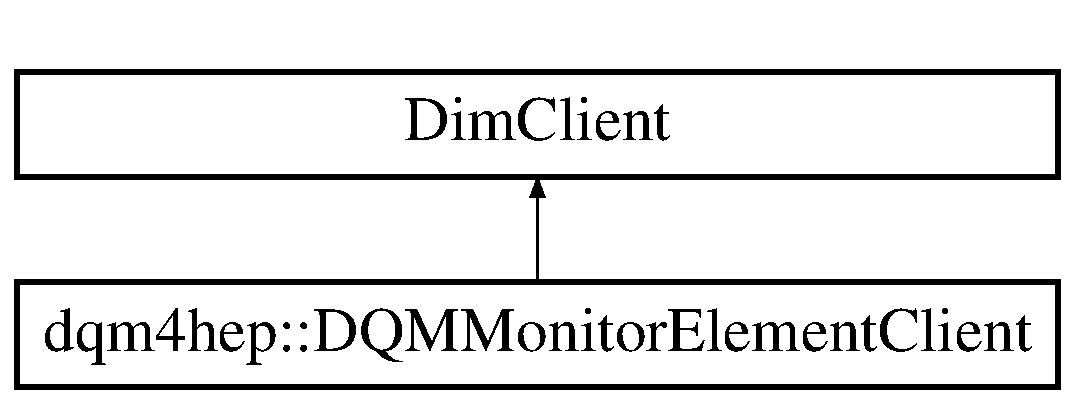
\includegraphics[height=2.000000cm]{classdqm4hep_1_1DQMMonitorElementClient}
\end{center}
\end{figure}
\subsection*{Public Member Functions}
\begin{DoxyCompactItemize}
\item 
{\bf D\+Q\+M\+Monitor\+Element\+Client} ()
\begin{DoxyCompactList}\small\item\em Constructor. \end{DoxyCompactList}\item 
{\bf $\sim$\+D\+Q\+M\+Monitor\+Element\+Client} ()
\begin{DoxyCompactList}\small\item\em Destructor. \end{DoxyCompactList}\item 
{\bf Status\+Code} {\bf set\+Collector\+Name} (const std\+::string \&collector\+Name)
\begin{DoxyCompactList}\small\item\em Set the collector name. \end{DoxyCompactList}\item 
const std\+::string \& {\bf get\+Collector\+Name} () const 
\begin{DoxyCompactList}\small\item\em Get the collector name. \end{DoxyCompactList}\item 
{\bf Status\+Code} {\bf connect\+To\+Service} ()
\begin{DoxyCompactList}\small\item\em Connect the client to the service. \end{DoxyCompactList}\item 
{\bf Status\+Code} {\bf disconnect\+From\+Service} ()
\begin{DoxyCompactList}\small\item\em Disconnect the client from the service. \end{DoxyCompactList}\item 
bool {\bf is\+Connected\+To\+Service} () const 
\begin{DoxyCompactList}\small\item\em Whether the client is connected to the service. \end{DoxyCompactList}\item 
{\bf Status\+Code} {\bf query\+Collector\+Info} ()
\begin{DoxyCompactList}\small\item\em Sent a request to the collector to get back the collector informations. \end{DoxyCompactList}\item 
{\bf Status\+Code} {\bf query\+Available\+Monitor\+Elements} (const {\bf D\+Q\+M\+Monitor\+Element\+List\+Name\+Request} \&request)
\begin{DoxyCompactList}\small\item\em Send a request to get back monitor element list name (small packet info) \end{DoxyCompactList}\item 
{\bf Status\+Code} {\bf subscribe} (const {\bf D\+Q\+M\+Monitor\+Element\+Request} \&request)
\begin{DoxyCompactList}\small\item\em Unsubscribe to monitor elements. \end{DoxyCompactList}\item 
{\bf Status\+Code} {\bf unsubscribe} (const {\bf D\+Q\+M\+Monitor\+Element\+Request} \&request)
\begin{DoxyCompactList}\small\item\em Subscribe to monitor elements. \end{DoxyCompactList}\item 
{\bf Status\+Code} {\bf replace\+Subscription} (const {\bf D\+Q\+M\+Monitor\+Element\+Request} \&request)
\begin{DoxyCompactList}\small\item\em Unsubscribe to all monitor elements the client has already subscribed and subscribe to monitor elements. \end{DoxyCompactList}\item 
{\bf Status\+Code} {\bf query\+Subscribed\+Monitor\+Elements} (const {\bf D\+Q\+M\+Monitor\+Element\+Request} \&request)
\begin{DoxyCompactList}\small\item\em Send a command to query the monitor element list. \end{DoxyCompactList}\item 
{\bf Status\+Code} {\bf query\+Subscribed\+Monitor\+Elements} ()
\begin{DoxyCompactList}\small\item\em Send a command to query the monitor element list that the client subscribed. \end{DoxyCompactList}\item 
void {\bf set\+Update\+Mode} (bool update\+Mode)
\begin{DoxyCompactList}\small\item\em Set the update mode. \end{DoxyCompactList}\item 
bool {\bf get\+Update\+Mode} () const 
\begin{DoxyCompactList}\small\item\em Get the update mode. \end{DoxyCompactList}\item 
bool {\bf is\+Collector\+Running} () const 
\begin{DoxyCompactList}\small\item\em Whether the collector is running. \end{DoxyCompactList}\item 
bool {\bf add\+Listener} ({\bf D\+Q\+M\+Monitor\+Element\+Client\+Listener} $\ast$p\+Listener)
\begin{DoxyCompactList}\small\item\em Add a listener to this client (observer pattern). \end{DoxyCompactList}\item 
void {\bf remove\+Listener} ({\bf D\+Q\+M\+Monitor\+Element\+Client\+Listener} $\ast$p\+Listener)
\begin{DoxyCompactList}\small\item\em Remove a listener from this client. \end{DoxyCompactList}\end{DoxyCompactItemize}
\subsection*{Static Public Attributes}
\begin{DoxyCompactItemize}
\item 
static const std\+::string {\bf m\+\_\+empty\+Buffer\+Str} = \char`\"{}E\+M\+P\+T\+Y\char`\"{}
\end{DoxyCompactItemize}
\subsection*{Private Member Functions}
\begin{DoxyCompactItemize}
\item 
void {\bf handle\+Me\+Collector\+Info\+Rpc\+Info} (Dim\+Rpc\+Info $\ast$p\+Rpc\+Info)
\begin{DoxyCompactList}\small\item\em Handle the collector info rpc callback. \end{DoxyCompactList}\item 
void {\bf handle\+Me\+List\+Name\+Rpc\+Info} (Dim\+Rpc\+Info $\ast$p\+Rpc\+Info)
\begin{DoxyCompactList}\small\item\em Handle the me name list rpc callback. \end{DoxyCompactList}\item 
void {\bf info\+Handler} ()
\begin{DoxyCompactList}\small\item\em Dim info handler. \end{DoxyCompactList}\item 
void {\bf clear\+Publication} ({\bf D\+Q\+M\+Monitor\+Element\+Publication} \&publication)
\begin{DoxyCompactList}\small\item\em Deep clear of publication. \end{DoxyCompactList}\end{DoxyCompactItemize}
\subsection*{Private Attributes}
\begin{DoxyCompactItemize}
\item 
Dim\+Rpc\+Info $\ast$ {\bf m\+\_\+p\+Me\+Collector\+Info\+Rpc\+Info}
\item 
Dim\+Rpc\+Info $\ast$ {\bf m\+\_\+p\+Me\+List\+Name\+Rpc\+Info}
\item 
Dim\+Updated\+Info $\ast$ {\bf m\+\_\+p\+Me\+Update\+Info}
\item 
Dim\+Info $\ast$ {\bf m\+\_\+p\+Collector\+State\+Info}
\item 
{\bf D\+Q\+M\+Data\+Stream} {\bf m\+\_\+in\+Data\+Stream}
\item 
{\bf D\+Q\+M\+Data\+Stream} {\bf m\+\_\+out\+Data\+Stream}
\item 
std\+::string {\bf m\+\_\+collector\+Name}
\item 
bool {\bf m\+\_\+is\+Connected}
\item 
bool {\bf m\+\_\+update\+Mode}
\item 
bool {\bf m\+\_\+is\+Collector\+Running}
\item 
std\+::vector\\*
$<$ {\bf D\+Q\+M\+Monitor\+Element\+Client\+Listener} $\ast$ $>$ {\bf m\+\_\+listeners}
\end{DoxyCompactItemize}
\subsection*{Friends}
\begin{DoxyCompactItemize}
\item 
class {\bf D\+Q\+M\+Me\+Collector\+Info\+Rpc\+Info}
\item 
class {\bf D\+Q\+M\+Me\+List\+Name\+Rpc\+Info}
\end{DoxyCompactItemize}


\subsection{Detailed Description}
\doxyref{D\+Q\+M\+Monitor\+Element\+Client}{p.}{classdqm4hep_1_1DQMMonitorElementClient} class. 

Definition at line 122 of file D\+Q\+M\+Monitor\+Element\+Client.\+h.



\subsection{Constructor \& Destructor Documentation}
\index{dqm4hep\+::\+D\+Q\+M\+Monitor\+Element\+Client@{dqm4hep\+::\+D\+Q\+M\+Monitor\+Element\+Client}!D\+Q\+M\+Monitor\+Element\+Client@{D\+Q\+M\+Monitor\+Element\+Client}}
\index{D\+Q\+M\+Monitor\+Element\+Client@{D\+Q\+M\+Monitor\+Element\+Client}!dqm4hep\+::\+D\+Q\+M\+Monitor\+Element\+Client@{dqm4hep\+::\+D\+Q\+M\+Monitor\+Element\+Client}}
\subsubsection[{D\+Q\+M\+Monitor\+Element\+Client}]{\setlength{\rightskip}{0pt plus 5cm}dqm4hep\+::\+D\+Q\+M\+Monitor\+Element\+Client\+::\+D\+Q\+M\+Monitor\+Element\+Client (
\begin{DoxyParamCaption}
{}
\end{DoxyParamCaption}
)}\label{classdqm4hep_1_1DQMMonitorElementClient_af0685bb980fdcbc5b80d64cce49efe21}


Constructor. 



Definition at line 78 of file D\+Q\+M\+Monitor\+Element\+Client.\+cc.


\begin{DoxyCode}
78                                                  :
79     m_isConnected(\textcolor{keyword}{false}),
80     m_pMeCollectorInfoRpcInfo(NULL),
81     m_pMeListNameRpcInfo(NULL),
82     m_inDataStream(4*1024*1024),
83     m_outDataStream(1024*1024),
84     m_updateMode(\textcolor{keyword}{false}),
85     m_isCollectorRunning(\textcolor{keyword}{false})
86 \{
87   \textcolor{comment}{/* nop */}
88 \}
\end{DoxyCode}
\index{dqm4hep\+::\+D\+Q\+M\+Monitor\+Element\+Client@{dqm4hep\+::\+D\+Q\+M\+Monitor\+Element\+Client}!````~D\+Q\+M\+Monitor\+Element\+Client@{$\sim$\+D\+Q\+M\+Monitor\+Element\+Client}}
\index{````~D\+Q\+M\+Monitor\+Element\+Client@{$\sim$\+D\+Q\+M\+Monitor\+Element\+Client}!dqm4hep\+::\+D\+Q\+M\+Monitor\+Element\+Client@{dqm4hep\+::\+D\+Q\+M\+Monitor\+Element\+Client}}
\subsubsection[{$\sim$\+D\+Q\+M\+Monitor\+Element\+Client}]{\setlength{\rightskip}{0pt plus 5cm}dqm4hep\+::\+D\+Q\+M\+Monitor\+Element\+Client\+::$\sim$\+D\+Q\+M\+Monitor\+Element\+Client (
\begin{DoxyParamCaption}
{}
\end{DoxyParamCaption}
)}\label{classdqm4hep_1_1DQMMonitorElementClient_a6b7e228eddd6fc062142d62efe9683fc}


Destructor. 



Definition at line 92 of file D\+Q\+M\+Monitor\+Element\+Client.\+cc.



References disconnect\+From\+Service(), and is\+Connected\+To\+Service().


\begin{DoxyCode}
93 \{
94   \textcolor{keywordflow}{if}(isConnectedToService())
95     disconnectFromService();
96 \}
\end{DoxyCode}


\subsection{Member Function Documentation}
\index{dqm4hep\+::\+D\+Q\+M\+Monitor\+Element\+Client@{dqm4hep\+::\+D\+Q\+M\+Monitor\+Element\+Client}!add\+Listener@{add\+Listener}}
\index{add\+Listener@{add\+Listener}!dqm4hep\+::\+D\+Q\+M\+Monitor\+Element\+Client@{dqm4hep\+::\+D\+Q\+M\+Monitor\+Element\+Client}}
\subsubsection[{add\+Listener}]{\setlength{\rightskip}{0pt plus 5cm}bool dqm4hep\+::\+D\+Q\+M\+Monitor\+Element\+Client\+::add\+Listener (
\begin{DoxyParamCaption}
\item[{{\bf D\+Q\+M\+Monitor\+Element\+Client\+Listener} $\ast$}]{p\+Listener}
\end{DoxyParamCaption}
)}\label{classdqm4hep_1_1DQMMonitorElementClient_ada19ca74696b7b0411c15be4790caabb}


Add a listener to this client (observer pattern). 



Definition at line 323 of file D\+Q\+M\+Monitor\+Element\+Client.\+cc.



References m\+\_\+listeners.


\begin{DoxyCode}
324 \{
325   \textcolor{keywordflow}{if}(NULL == pListener)
326     \textcolor{keywordflow}{return} \textcolor{keyword}{false};
327 
328   std::vector<DQMMonitorElementClientListener *>::iterator findIter = std::find( 
      m_listeners.begin(), m_listeners.end(), pListener );
329 
330   \textcolor{comment}{// if already added, return ok}
331   \textcolor{keywordflow}{if}(m_listeners.end() != findIter)
332     \textcolor{keywordflow}{return} \textcolor{keyword}{true};
333 
334   m_listeners.push\_back(pListener);
335 
336   \textcolor{keywordflow}{return} \textcolor{keyword}{true};
337 \}
\end{DoxyCode}
\index{dqm4hep\+::\+D\+Q\+M\+Monitor\+Element\+Client@{dqm4hep\+::\+D\+Q\+M\+Monitor\+Element\+Client}!clear\+Publication@{clear\+Publication}}
\index{clear\+Publication@{clear\+Publication}!dqm4hep\+::\+D\+Q\+M\+Monitor\+Element\+Client@{dqm4hep\+::\+D\+Q\+M\+Monitor\+Element\+Client}}
\subsubsection[{clear\+Publication}]{\setlength{\rightskip}{0pt plus 5cm}void dqm4hep\+::\+D\+Q\+M\+Monitor\+Element\+Client\+::clear\+Publication (
\begin{DoxyParamCaption}
\item[{{\bf D\+Q\+M\+Monitor\+Element\+Publication} \&}]{publication}
\end{DoxyParamCaption}
)\hspace{0.3cm}{\ttfamily [private]}}\label{classdqm4hep_1_1DQMMonitorElementClient_a8365bc3030e2977b970069ede94c9216}


Deep clear of publication. 



Definition at line 497 of file D\+Q\+M\+Monitor\+Element\+Client.\+cc.



Referenced by info\+Handler().


\begin{DoxyCode}
498 \{
499   \textcolor{keywordflow}{for}(DQMMonitorElementPublication::iterator iter = publication.begin(), endIter = publication.end() ;
500       endIter != iter ; ++iter)
501   \{
502     \textcolor{keywordflow}{for}(DQMMonitorElementList::iterator meIter = iter->second.begin(), meEndIter = iter->second.end() ;
503         meEndIter != meIter ; ++meIter)
504     \{
505       \textcolor{keyword}{delete} *meIter;
506     \}
507   \}
508 
509   publication.clear();
510 \}
\end{DoxyCode}
\index{dqm4hep\+::\+D\+Q\+M\+Monitor\+Element\+Client@{dqm4hep\+::\+D\+Q\+M\+Monitor\+Element\+Client}!connect\+To\+Service@{connect\+To\+Service}}
\index{connect\+To\+Service@{connect\+To\+Service}!dqm4hep\+::\+D\+Q\+M\+Monitor\+Element\+Client@{dqm4hep\+::\+D\+Q\+M\+Monitor\+Element\+Client}}
\subsubsection[{connect\+To\+Service}]{\setlength{\rightskip}{0pt plus 5cm}{\bf Status\+Code} dqm4hep\+::\+D\+Q\+M\+Monitor\+Element\+Client\+::connect\+To\+Service (
\begin{DoxyParamCaption}
{}
\end{DoxyParamCaption}
)}\label{classdqm4hep_1_1DQMMonitorElementClient_ad04a041285d5b9621f06292bf0d8404a}


Connect the client to the service. 



Definition at line 122 of file D\+Q\+M\+Monitor\+Element\+Client.\+cc.



References D\+Q\+M\+Me\+Collector\+Info\+Rpc\+Info, D\+Q\+M\+Me\+List\+Name\+Rpc\+Info, get\+Update\+Mode(), is\+Connected\+To\+Service(), m\+\_\+collector\+Name, m\+\_\+is\+Connected, m\+\_\+listeners, m\+\_\+p\+Collector\+State\+Info, m\+\_\+p\+Me\+Collector\+Info\+Rpc\+Info, m\+\_\+p\+Me\+List\+Name\+Rpc\+Info, m\+\_\+p\+Me\+Update\+Info, and set\+Update\+Mode().


\begin{DoxyCode}
123 \{
124   \textcolor{keywordflow}{if}(isConnectedToService())
125     \textcolor{keywordflow}{return} STATUS\_CODE\_SUCCESS;
126 
127   std::string collectorName = \textcolor{stringliteral}{"DQM4HEP/MonitorElementCollector/"} + 
      m_collectorName + \textcolor{stringliteral}{"/"};
128   std::stringstream ss;
129 
130   ss << collectorName << \textcolor{stringliteral}{"COLLECTOR\_INFO\_RPC"};
131   m_pMeCollectorInfoRpcInfo = \textcolor{keyword}{new} DQMMeCollectorInfoRpcInfo((\textcolor{keywordtype}{char}*) ss.str().c\_str(), \textcolor{keyword}{this});
132 
133   ss.str(\textcolor{stringliteral}{""});
134   ss << collectorName << \textcolor{stringliteral}{"MONITOR\_ELEMENT\_NAME\_LIST\_RPC"};
135   m_pMeListNameRpcInfo = \textcolor{keyword}{new} DQMMeListNameRpcInfo((\textcolor{keywordtype}{char}*) ss.str().c\_str(), \textcolor{keyword}{this});
136 
137   ss.str(\textcolor{stringliteral}{""});
138   ss << collectorName << \textcolor{stringliteral}{"ME\_UPDATE\_SVC"};
139   m_pMeUpdateInfo = \textcolor{keyword}{new} DimUpdatedInfo( (\textcolor{keywordtype}{char}*) ss.str().c\_str() , (\textcolor{keywordtype}{void} *) NULL , 0, \textcolor{keyword}{this} );
140 
141   ss.str(\textcolor{stringliteral}{""});
142   ss << collectorName << \textcolor{stringliteral}{"COLLECTOR\_STATE\_SVC"};
143   m_pCollectorStateInfo = \textcolor{keyword}{new} DimInfo( (\textcolor{keywordtype}{char}*) ss.str().c\_str() , \textcolor{keyword}{static\_cast<}\textcolor{keywordtype}{int}\textcolor{keyword}{>}(STOPPED\_STATE) , \textcolor{keyword}{this} );
144 
145   m_isConnected = \textcolor{keyword}{true};
146 
147   this->setUpdateMode(this->getUpdateMode());
148 
149   \textcolor{keywordflow}{for}(std::vector<DQMMonitorElementClientListener *>::iterator iter = 
      m_listeners.begin(), endIter = m_listeners.end() ;
150       endIter != iter ; ++iter)
151     (*iter)->onMonitorElementClientConnect(\textcolor{keyword}{this});
152 
153   \textcolor{keywordflow}{return} STATUS\_CODE\_SUCCESS;
154 \}
\end{DoxyCode}
\index{dqm4hep\+::\+D\+Q\+M\+Monitor\+Element\+Client@{dqm4hep\+::\+D\+Q\+M\+Monitor\+Element\+Client}!disconnect\+From\+Service@{disconnect\+From\+Service}}
\index{disconnect\+From\+Service@{disconnect\+From\+Service}!dqm4hep\+::\+D\+Q\+M\+Monitor\+Element\+Client@{dqm4hep\+::\+D\+Q\+M\+Monitor\+Element\+Client}}
\subsubsection[{disconnect\+From\+Service}]{\setlength{\rightskip}{0pt plus 5cm}{\bf Status\+Code} dqm4hep\+::\+D\+Q\+M\+Monitor\+Element\+Client\+::disconnect\+From\+Service (
\begin{DoxyParamCaption}
{}
\end{DoxyParamCaption}
)}\label{classdqm4hep_1_1DQMMonitorElementClient_aade12b321bce1e34b7cb6687cbf3eac8}


Disconnect the client from the service. 



Definition at line 158 of file D\+Q\+M\+Monitor\+Element\+Client.\+cc.



References is\+Connected\+To\+Service(), m\+\_\+is\+Connected, m\+\_\+listeners, m\+\_\+p\+Collector\+State\+Info, m\+\_\+p\+Me\+Collector\+Info\+Rpc\+Info, m\+\_\+p\+Me\+List\+Name\+Rpc\+Info, and m\+\_\+p\+Me\+Update\+Info.



Referenced by $\sim$\+D\+Q\+M\+Monitor\+Element\+Client().


\begin{DoxyCode}
159 \{
160   \textcolor{keywordflow}{if}(!isConnectedToService())
161     \textcolor{keywordflow}{return} STATUS\_CODE\_SUCCESS;
162 
163   \textcolor{keyword}{delete} m_pMeCollectorInfoRpcInfo; m_pMeCollectorInfoRpcInfo = NULL;
164   \textcolor{keyword}{delete} m_pMeListNameRpcInfo; m_pMeListNameRpcInfo = NULL;
165   \textcolor{keyword}{delete} m_pMeUpdateInfo; m_pMeUpdateInfo = NULL;
166   \textcolor{keyword}{delete} m_pCollectorStateInfo; m_pCollectorStateInfo = NULL;
167 
168   m_isConnected = \textcolor{keyword}{false};
169 
170   \textcolor{keywordflow}{for}(std::vector<DQMMonitorElementClientListener *>::iterator iter = 
      m_listeners.begin(), endIter = m_listeners.end() ;
171       endIter != iter ; ++iter)
172     (*iter)->onMonitorElementClientDisconnect(\textcolor{keyword}{this});
173 
174   \textcolor{keywordflow}{return} STATUS\_CODE\_SUCCESS;
175 \}
\end{DoxyCode}
\index{dqm4hep\+::\+D\+Q\+M\+Monitor\+Element\+Client@{dqm4hep\+::\+D\+Q\+M\+Monitor\+Element\+Client}!get\+Collector\+Name@{get\+Collector\+Name}}
\index{get\+Collector\+Name@{get\+Collector\+Name}!dqm4hep\+::\+D\+Q\+M\+Monitor\+Element\+Client@{dqm4hep\+::\+D\+Q\+M\+Monitor\+Element\+Client}}
\subsubsection[{get\+Collector\+Name}]{\setlength{\rightskip}{0pt plus 5cm}const std\+::string \& dqm4hep\+::\+D\+Q\+M\+Monitor\+Element\+Client\+::get\+Collector\+Name (
\begin{DoxyParamCaption}
{}
\end{DoxyParamCaption}
) const}\label{classdqm4hep_1_1DQMMonitorElementClient_a5d5c335de0bfba4b57e3348cccdac549}


Get the collector name. 



Definition at line 115 of file D\+Q\+M\+Monitor\+Element\+Client.\+cc.



References m\+\_\+collector\+Name.


\begin{DoxyCode}
116 \{
117   \textcolor{keywordflow}{return} m_collectorName;
118 \}
\end{DoxyCode}
\index{dqm4hep\+::\+D\+Q\+M\+Monitor\+Element\+Client@{dqm4hep\+::\+D\+Q\+M\+Monitor\+Element\+Client}!get\+Update\+Mode@{get\+Update\+Mode}}
\index{get\+Update\+Mode@{get\+Update\+Mode}!dqm4hep\+::\+D\+Q\+M\+Monitor\+Element\+Client@{dqm4hep\+::\+D\+Q\+M\+Monitor\+Element\+Client}}
\subsubsection[{get\+Update\+Mode}]{\setlength{\rightskip}{0pt plus 5cm}bool dqm4hep\+::\+D\+Q\+M\+Monitor\+Element\+Client\+::get\+Update\+Mode (
\begin{DoxyParamCaption}
{}
\end{DoxyParamCaption}
) const}\label{classdqm4hep_1_1DQMMonitorElementClient_a71057f98bc7e129542053c39aee4581d}


Get the update mode. 



Definition at line 316 of file D\+Q\+M\+Monitor\+Element\+Client.\+cc.



References m\+\_\+update\+Mode.



Referenced by connect\+To\+Service(), and info\+Handler().


\begin{DoxyCode}
317 \{
318   \textcolor{keywordflow}{return} m_updateMode;
319 \}
\end{DoxyCode}
\index{dqm4hep\+::\+D\+Q\+M\+Monitor\+Element\+Client@{dqm4hep\+::\+D\+Q\+M\+Monitor\+Element\+Client}!handle\+Me\+Collector\+Info\+Rpc\+Info@{handle\+Me\+Collector\+Info\+Rpc\+Info}}
\index{handle\+Me\+Collector\+Info\+Rpc\+Info@{handle\+Me\+Collector\+Info\+Rpc\+Info}!dqm4hep\+::\+D\+Q\+M\+Monitor\+Element\+Client@{dqm4hep\+::\+D\+Q\+M\+Monitor\+Element\+Client}}
\subsubsection[{handle\+Me\+Collector\+Info\+Rpc\+Info}]{\setlength{\rightskip}{0pt plus 5cm}void dqm4hep\+::\+D\+Q\+M\+Monitor\+Element\+Client\+::handle\+Me\+Collector\+Info\+Rpc\+Info (
\begin{DoxyParamCaption}
\item[{Dim\+Rpc\+Info $\ast$}]{p\+Rpc\+Info}
\end{DoxyParamCaption}
)\hspace{0.3cm}{\ttfamily [private]}}\label{classdqm4hep_1_1DQMMonitorElementClient_a09746fd53f5639560f7f4ea38f3fb8ef}


Handle the collector info rpc callback. 



Definition at line 356 of file D\+Q\+M\+Monitor\+Element\+Client.\+cc.



References m\+\_\+in\+Data\+Stream, m\+\_\+listeners, dqm4hep\+::\+D\+Q\+M\+Data\+Stream\+::reset(), dqm4hep\+::\+D\+Q\+M\+Data\+Stream\+::set\+Buffer(), and T\+H\+R\+O\+W\+\_\+\+R\+E\+S\+U\+L\+T\+\_\+\+I\+F.



Referenced by dqm4hep\+::\+D\+Q\+M\+Me\+Collector\+Info\+Rpc\+Info\+::rpc\+Info\+Handler().


\begin{DoxyCode}
357 \{
358   \textcolor{keywordflow}{try}
359   \{
360     \textcolor{keywordflow}{if}(m_listeners.empty())
361       \textcolor{keywordflow}{return};
362 
363     dqm_char *pBuffer = \textcolor{keyword}{static\_cast<}dqm_char *\textcolor{keyword}{>}(pRpcInfo->getData());
364     dqm_uint bufferSize = pRpcInfo->getSize();
365 
366     \textcolor{keywordflow}{if}(NULL == pBuffer || 0 == bufferSize)
367       \textcolor{keywordflow}{return};
368 
369     m_inDataStream.reset();
370     THROW_RESULT_IF(STATUS\_CODE\_SUCCESS, !=, m_inDataStream.setBuffer(pBuffer, bufferSize));
371 
372     \textcolor{comment}{// deserialize and notify}
373     DQMCollectorInfo collectorInfo;
374     THROW_RESULT_IF(STATUS\_CODE\_SUCCESS, !=, collectorInfo.deserialize(&
      m_inDataStream));
375 
376     \textcolor{keywordflow}{for}(std::vector<DQMMonitorElementClientListener *>::iterator iter = 
      m_listeners.begin(), endIter = m_listeners.end() ;
377         endIter != iter ; ++iter)
378       (*iter)->monitorElementCollectorInfoReceived(\textcolor{keyword}{this}, collectorInfo);
379   \}
380   \textcolor{keywordflow}{catch}(StatusCodeException &exception)
381   \{
382   \}
383   \textcolor{keywordflow}{catch}(...)
384   \{
385   \}
386 \}
\end{DoxyCode}
\index{dqm4hep\+::\+D\+Q\+M\+Monitor\+Element\+Client@{dqm4hep\+::\+D\+Q\+M\+Monitor\+Element\+Client}!handle\+Me\+List\+Name\+Rpc\+Info@{handle\+Me\+List\+Name\+Rpc\+Info}}
\index{handle\+Me\+List\+Name\+Rpc\+Info@{handle\+Me\+List\+Name\+Rpc\+Info}!dqm4hep\+::\+D\+Q\+M\+Monitor\+Element\+Client@{dqm4hep\+::\+D\+Q\+M\+Monitor\+Element\+Client}}
\subsubsection[{handle\+Me\+List\+Name\+Rpc\+Info}]{\setlength{\rightskip}{0pt plus 5cm}void dqm4hep\+::\+D\+Q\+M\+Monitor\+Element\+Client\+::handle\+Me\+List\+Name\+Rpc\+Info (
\begin{DoxyParamCaption}
\item[{Dim\+Rpc\+Info $\ast$}]{p\+Rpc\+Info}
\end{DoxyParamCaption}
)\hspace{0.3cm}{\ttfamily [private]}}\label{classdqm4hep_1_1DQMMonitorElementClient_a171749b4a10ed37c3d75c751892cb8b2}


Handle the me name list rpc callback. 



Definition at line 390 of file D\+Q\+M\+Monitor\+Element\+Client.\+cc.



References m\+\_\+in\+Data\+Stream, m\+\_\+listeners, dqm4hep\+::\+D\+Q\+M\+Data\+Stream\+::reset(), dqm4hep\+::\+D\+Q\+M\+Data\+Stream\+::set\+Buffer(), and T\+H\+R\+O\+W\+\_\+\+R\+E\+S\+U\+L\+T\+\_\+\+I\+F.



Referenced by dqm4hep\+::\+D\+Q\+M\+Me\+List\+Name\+Rpc\+Info\+::rpc\+Info\+Handler().


\begin{DoxyCode}
391 \{
392   \textcolor{keywordflow}{try}
393   \{
394     \textcolor{keywordflow}{if}(m_listeners.empty())
395       \textcolor{keywordflow}{return};
396 
397     dqm_char *pBuffer = \textcolor{keyword}{static\_cast<}dqm_char*\textcolor{keyword}{>}(pRpcInfo->getData());
398     dqm_uint bufferSize = pRpcInfo->getSize();
399 
400     \textcolor{keywordflow}{if}(NULL == pBuffer || 0 == bufferSize)
401       \textcolor{keywordflow}{throw} StatusCodeException(STATUS\_CODE\_FAILURE);
402 
403     m_inDataStream.reset();
404     THROW_RESULT_IF(STATUS\_CODE\_SUCCESS, !=, m_inDataStream.setBuffer(pBuffer, bufferSize));
405 
406     \textcolor{comment}{// deserialize and notify}
407     DQMMonitorElementInfoList monitorElementInfoList;
408     THROW_RESULT_IF(STATUS\_CODE\_SUCCESS, !=, monitorElementInfoList.deserialize(&
      m_inDataStream));
409 
410     \textcolor{keywordflow}{for}(std::vector<DQMMonitorElementClientListener *>::iterator iter = 
      m_listeners.begin(), endIter = m_listeners.end() ;
411         endIter != iter ; ++iter)
412       (*iter)->availableMonitorElementListReceived(\textcolor{keyword}{this}, monitorElementInfoList);
413   \}
414   \textcolor{keywordflow}{catch}(StatusCodeException &exception)
415   \{
416   \}
417   \textcolor{keywordflow}{catch}(...)
418   \{
419   \}
420 \}
\end{DoxyCode}
\index{dqm4hep\+::\+D\+Q\+M\+Monitor\+Element\+Client@{dqm4hep\+::\+D\+Q\+M\+Monitor\+Element\+Client}!info\+Handler@{info\+Handler}}
\index{info\+Handler@{info\+Handler}!dqm4hep\+::\+D\+Q\+M\+Monitor\+Element\+Client@{dqm4hep\+::\+D\+Q\+M\+Monitor\+Element\+Client}}
\subsubsection[{info\+Handler}]{\setlength{\rightskip}{0pt plus 5cm}void dqm4hep\+::\+D\+Q\+M\+Monitor\+Element\+Client\+::info\+Handler (
\begin{DoxyParamCaption}
{}
\end{DoxyParamCaption}
)\hspace{0.3cm}{\ttfamily [private]}}\label{classdqm4hep_1_1DQMMonitorElementClient_a60254d6777128eeee051c3372ae09c41}


Dim info handler. 



Definition at line 424 of file D\+Q\+M\+Monitor\+Element\+Client.\+cc.



References clear\+Publication(), dqm4hep\+::\+D\+Q\+M\+Monitor\+Element\+Publication\+::deserialize(), get\+Update\+Mode(), is\+Collector\+Running(), m\+\_\+in\+Data\+Stream, m\+\_\+is\+Collector\+Running, m\+\_\+listeners, m\+\_\+p\+Collector\+State\+Info, m\+\_\+p\+Me\+Update\+Info, dqm4hep\+::\+D\+Q\+M\+Data\+Stream\+::reset(), dqm4hep\+::\+D\+Q\+M\+Data\+Stream\+::set\+Buffer(), set\+Update\+Mode(), and T\+H\+R\+O\+W\+\_\+\+R\+E\+S\+U\+L\+T\+\_\+\+I\+F.


\begin{DoxyCode}
425 \{
426   DimInfo *pInfo = getInfo();
427 
428   std::cout << \textcolor{stringliteral}{"Received info : "} << pInfo->getName() << std::endl;
429 
430   \textcolor{keywordflow}{if}(pInfo == m_pMeUpdateInfo)
431   \{
432     DQMMonitorElementPublication monitorElementPublication;
433 
434     \textcolor{keywordflow}{try}
435     \{
436       \textcolor{keywordflow}{if}(m_listeners.empty())
437         \textcolor{keywordflow}{return};
438 
439       dqm_char *pBuffer = \textcolor{keyword}{static\_cast<}dqm_char *\textcolor{keyword}{>}(m_pMeUpdateInfo->getData());
440       dqm_uint bufferSize = m_pMeUpdateInfo->getSize();
441 
442       \textcolor{keywordflow}{if}(NULL == pBuffer || 0 == bufferSize)
443         \textcolor{keywordflow}{throw} StatusCodeException(STATUS\_CODE\_FAILURE);
444 
445       m_inDataStream.reset();
446       THROW_RESULT_IF(STATUS\_CODE\_SUCCESS, !=, m_inDataStream.setBuffer(pBuffer, bufferSize));
447 
448       \textcolor{comment}{// deserialize and call the user call back function}
449       THROW_RESULT_IF(STATUS\_CODE\_SUCCESS, !=, monitorElementPublication.deserialize(&
      m_inDataStream));
450 
451       \textcolor{keywordflow}{for}(std::vector<DQMMonitorElementClientListener *>::iterator iter = 
      m_listeners.begin(), endIter = m_listeners.end() ;
452           endIter != iter ; ++iter)
453         (*iter)->monitorElementsReceived(\textcolor{keyword}{this}, monitorElementPublication);
454     \}
455     \textcolor{keywordflow}{catch}(StatusCodeException &exception)
456     \{
457     \}
458     \textcolor{keywordflow}{catch}(...)
459     \{
460     \}
461 
462     std::cout << \textcolor{stringliteral}{"Clearing publication !"} << std::endl;
463     this->clearPublication(monitorElementPublication);
464   \}
465   \textcolor{keywordflow}{else} \textcolor{keywordflow}{if}(pInfo == m_pCollectorStateInfo)
466   \{
467     \textcolor{keywordtype}{bool} isCollectorRunning = \textcolor{keyword}{static\_cast<}\textcolor{keywordtype}{bool}\textcolor{keyword}{>}(m_pCollectorStateInfo->getInt());
468     std::cout << \textcolor{stringliteral}{"Received collector state : "} << isCollectorRunning << std::endl;
469 
470     \textcolor{keywordflow}{if}(isCollectorRunning == m_isCollectorRunning)
471       \textcolor{keywordflow}{return};
472 
473     m_isCollectorRunning = isCollectorRunning;
474 
475     \textcolor{keywordflow}{if}(m_isCollectorRunning)
476     \{
477       \textcolor{comment}{// send back update mode info to collector}
478       this->setUpdateMode(this->getUpdateMode());
479 
480       \textcolor{comment}{// notify server state !}
481       \textcolor{keywordflow}{for}(std::vector<DQMMonitorElementClientListener *>::iterator iter = 
      m_listeners.begin(), endIter = m_listeners.end() ;
482           endIter != iter ; ++iter)
483         (*iter)->onServerStartup(\textcolor{keyword}{this});
484     \}
485     \textcolor{keywordflow}{else}
486     \{
487       \textcolor{comment}{// notify server state !}
488       \textcolor{keywordflow}{for}(std::vector<DQMMonitorElementClientListener *>::iterator iter = 
      m_listeners.begin(), endIter = m_listeners.end() ;
489           endIter != iter ; ++iter)
490         (*iter)->onServerShutdown(\textcolor{keyword}{this});
491     \}
492   \}
493 \}
\end{DoxyCode}
\index{dqm4hep\+::\+D\+Q\+M\+Monitor\+Element\+Client@{dqm4hep\+::\+D\+Q\+M\+Monitor\+Element\+Client}!is\+Collector\+Running@{is\+Collector\+Running}}
\index{is\+Collector\+Running@{is\+Collector\+Running}!dqm4hep\+::\+D\+Q\+M\+Monitor\+Element\+Client@{dqm4hep\+::\+D\+Q\+M\+Monitor\+Element\+Client}}
\subsubsection[{is\+Collector\+Running}]{\setlength{\rightskip}{0pt plus 5cm}bool dqm4hep\+::\+D\+Q\+M\+Monitor\+Element\+Client\+::is\+Collector\+Running (
\begin{DoxyParamCaption}
{}
\end{DoxyParamCaption}
) const}\label{classdqm4hep_1_1DQMMonitorElementClient_a23be9f1ce7f14f261ab26dec46418d79}


Whether the collector is running. 



Definition at line 514 of file D\+Q\+M\+Monitor\+Element\+Client.\+cc.



References m\+\_\+is\+Collector\+Running.



Referenced by info\+Handler().


\begin{DoxyCode}
515 \{
516   \textcolor{keywordflow}{return} m_isCollectorRunning;
517 \}
\end{DoxyCode}
\index{dqm4hep\+::\+D\+Q\+M\+Monitor\+Element\+Client@{dqm4hep\+::\+D\+Q\+M\+Monitor\+Element\+Client}!is\+Connected\+To\+Service@{is\+Connected\+To\+Service}}
\index{is\+Connected\+To\+Service@{is\+Connected\+To\+Service}!dqm4hep\+::\+D\+Q\+M\+Monitor\+Element\+Client@{dqm4hep\+::\+D\+Q\+M\+Monitor\+Element\+Client}}
\subsubsection[{is\+Connected\+To\+Service}]{\setlength{\rightskip}{0pt plus 5cm}bool dqm4hep\+::\+D\+Q\+M\+Monitor\+Element\+Client\+::is\+Connected\+To\+Service (
\begin{DoxyParamCaption}
{}
\end{DoxyParamCaption}
) const}\label{classdqm4hep_1_1DQMMonitorElementClient_a25b7d5d325cedf1b3016b3261fbdb8af}


Whether the client is connected to the service. 



Definition at line 179 of file D\+Q\+M\+Monitor\+Element\+Client.\+cc.



References m\+\_\+is\+Connected.



Referenced by connect\+To\+Service(), disconnect\+From\+Service(), query\+Available\+Monitor\+Elements(), query\+Collector\+Info(), query\+Subscribed\+Monitor\+Elements(), replace\+Subscription(), set\+Collector\+Name(), set\+Update\+Mode(), subscribe(), unsubscribe(), and $\sim$\+D\+Q\+M\+Monitor\+Element\+Client().


\begin{DoxyCode}
180 \{
181   \textcolor{keywordflow}{return} m_isConnected;
182 \}
\end{DoxyCode}
\index{dqm4hep\+::\+D\+Q\+M\+Monitor\+Element\+Client@{dqm4hep\+::\+D\+Q\+M\+Monitor\+Element\+Client}!query\+Available\+Monitor\+Elements@{query\+Available\+Monitor\+Elements}}
\index{query\+Available\+Monitor\+Elements@{query\+Available\+Monitor\+Elements}!dqm4hep\+::\+D\+Q\+M\+Monitor\+Element\+Client@{dqm4hep\+::\+D\+Q\+M\+Monitor\+Element\+Client}}
\subsubsection[{query\+Available\+Monitor\+Elements}]{\setlength{\rightskip}{0pt plus 5cm}{\bf Status\+Code} dqm4hep\+::\+D\+Q\+M\+Monitor\+Element\+Client\+::query\+Available\+Monitor\+Elements (
\begin{DoxyParamCaption}
\item[{const {\bf D\+Q\+M\+Monitor\+Element\+List\+Name\+Request} \&}]{request}
\end{DoxyParamCaption}
)}\label{classdqm4hep_1_1DQMMonitorElementClient_a575caef703179df7c02ccfb705d402c9}


Send a request to get back monitor element list name (small packet info) 



Definition at line 199 of file D\+Q\+M\+Monitor\+Element\+Client.\+cc.



References dqm4hep\+::\+D\+Q\+M\+Data\+Stream\+::get\+Buffer(), dqm4hep\+::\+D\+Q\+M\+Data\+Stream\+::get\+Buffer\+Size(), is\+Connected\+To\+Service(), m\+\_\+out\+Data\+Stream, m\+\_\+p\+Me\+List\+Name\+Rpc\+Info, dqm4hep\+::\+D\+Q\+M\+Data\+Stream\+::reset(), R\+E\+T\+U\+R\+N\+\_\+\+R\+E\+S\+U\+L\+T\+\_\+\+I\+F, and dqm4hep\+::\+D\+Q\+M\+Monitor\+Element\+List\+Name\+Request\+::serialize().


\begin{DoxyCode}
200 \{
201   \textcolor{keywordflow}{if}(!isConnectedToService())
202     \textcolor{keywordflow}{return} STATUS\_CODE\_NOT\_ALLOWED;
203 
204   \textcolor{comment}{// serialize the list}
205   m_outDataStream.reset();
206   RETURN_RESULT_IF(STATUS\_CODE\_SUCCESS, !=, request.serialize(&m_outDataStream));
207 
208   \textcolor{comment}{// send query}
209   m_pMeListNameRpcInfo->setData((\textcolor{keywordtype}{void} *) m_outDataStream.getBuffer(), 
      m_outDataStream.getBufferSize());
210 
211   \textcolor{keywordflow}{return} STATUS\_CODE\_SUCCESS;
212 \}
\end{DoxyCode}
\index{dqm4hep\+::\+D\+Q\+M\+Monitor\+Element\+Client@{dqm4hep\+::\+D\+Q\+M\+Monitor\+Element\+Client}!query\+Collector\+Info@{query\+Collector\+Info}}
\index{query\+Collector\+Info@{query\+Collector\+Info}!dqm4hep\+::\+D\+Q\+M\+Monitor\+Element\+Client@{dqm4hep\+::\+D\+Q\+M\+Monitor\+Element\+Client}}
\subsubsection[{query\+Collector\+Info}]{\setlength{\rightskip}{0pt plus 5cm}{\bf Status\+Code} dqm4hep\+::\+D\+Q\+M\+Monitor\+Element\+Client\+::query\+Collector\+Info (
\begin{DoxyParamCaption}
{}
\end{DoxyParamCaption}
)}\label{classdqm4hep_1_1DQMMonitorElementClient_a6a7a86107d6c9d702b491c7272975bda}


Sent a request to the collector to get back the collector informations. 



Definition at line 186 of file D\+Q\+M\+Monitor\+Element\+Client.\+cc.



References is\+Connected\+To\+Service(), and m\+\_\+p\+Me\+Collector\+Info\+Rpc\+Info.


\begin{DoxyCode}
187 \{
188   \textcolor{keywordflow}{if}(!isConnectedToService())
189     \textcolor{keywordflow}{return} STATUS\_CODE\_NOT\_ALLOWED;
190 
191   \textcolor{keywordtype}{char} buf[] = \textcolor{stringliteral}{"\(\backslash\)0"};
192   m_pMeCollectorInfoRpcInfo->setData((\textcolor{keywordtype}{void} *) &buf[0], 1);
193 
194   \textcolor{keywordflow}{return} STATUS\_CODE\_SUCCESS;
195 \}
\end{DoxyCode}
\index{dqm4hep\+::\+D\+Q\+M\+Monitor\+Element\+Client@{dqm4hep\+::\+D\+Q\+M\+Monitor\+Element\+Client}!query\+Subscribed\+Monitor\+Elements@{query\+Subscribed\+Monitor\+Elements}}
\index{query\+Subscribed\+Monitor\+Elements@{query\+Subscribed\+Monitor\+Elements}!dqm4hep\+::\+D\+Q\+M\+Monitor\+Element\+Client@{dqm4hep\+::\+D\+Q\+M\+Monitor\+Element\+Client}}
\subsubsection[{query\+Subscribed\+Monitor\+Elements}]{\setlength{\rightskip}{0pt plus 5cm}{\bf Status\+Code} dqm4hep\+::\+D\+Q\+M\+Monitor\+Element\+Client\+::query\+Subscribed\+Monitor\+Elements (
\begin{DoxyParamCaption}
\item[{const {\bf D\+Q\+M\+Monitor\+Element\+Request} \&}]{request}
\end{DoxyParamCaption}
)}\label{classdqm4hep_1_1DQMMonitorElementClient_aa8eee2730c0eccfdd8d119ceb9046d2f}


Send a command to query the monitor element list. 

The element in the list are first subscribed. Then a query is sent to update only the element in the request 

Definition at line 216 of file D\+Q\+M\+Monitor\+Element\+Client.\+cc.



References dqm4hep\+::\+D\+Q\+M\+Data\+Stream\+::get\+Buffer(), dqm4hep\+::\+D\+Q\+M\+Data\+Stream\+::get\+Buffer\+Size(), is\+Connected\+To\+Service(), m\+\_\+collector\+Name, m\+\_\+out\+Data\+Stream, dqm4hep\+::\+D\+Q\+M\+Data\+Stream\+::reset(), R\+E\+T\+U\+R\+N\+\_\+\+R\+E\+S\+U\+L\+T\+\_\+\+I\+F, and dqm4hep\+::\+D\+Q\+M\+Monitor\+Element\+Request\+::serialize().


\begin{DoxyCode}
217 \{
218   \textcolor{keywordflow}{if}(!isConnectedToService())
219     \textcolor{keywordflow}{return} STATUS\_CODE\_NOT\_ALLOWED;
220 
221   \textcolor{comment}{// serialize the request}
222   m_outDataStream.reset();
223   RETURN_RESULT_IF(STATUS\_CODE\_SUCCESS, !=, request.serialize(&m_outDataStream));
224 
225   \textcolor{comment}{// send the request}
226   std::string commandName = \textcolor{stringliteral}{"DQM4HEP/MonitorElementCollector/"} + m_collectorName + \textcolor{stringliteral}{"/QUERY\_ME\_CMD"};
227   DimClient::sendCommandNB( commandName.c\_str() , (\textcolor{keywordtype}{void} *) m_outDataStream.
      getBuffer() , m_outDataStream.getBufferSize() );
228 
229   \textcolor{keywordflow}{return} STATUS\_CODE\_SUCCESS;
230 \}
\end{DoxyCode}
\index{dqm4hep\+::\+D\+Q\+M\+Monitor\+Element\+Client@{dqm4hep\+::\+D\+Q\+M\+Monitor\+Element\+Client}!query\+Subscribed\+Monitor\+Elements@{query\+Subscribed\+Monitor\+Elements}}
\index{query\+Subscribed\+Monitor\+Elements@{query\+Subscribed\+Monitor\+Elements}!dqm4hep\+::\+D\+Q\+M\+Monitor\+Element\+Client@{dqm4hep\+::\+D\+Q\+M\+Monitor\+Element\+Client}}
\subsubsection[{query\+Subscribed\+Monitor\+Elements}]{\setlength{\rightskip}{0pt plus 5cm}{\bf Status\+Code} dqm4hep\+::\+D\+Q\+M\+Monitor\+Element\+Client\+::query\+Subscribed\+Monitor\+Elements (
\begin{DoxyParamCaption}
{}
\end{DoxyParamCaption}
)}\label{classdqm4hep_1_1DQMMonitorElementClient_a0d39210a4c198fefdd64909fdf1a6483}


Send a command to query the monitor element list that the client subscribed. 



Definition at line 234 of file D\+Q\+M\+Monitor\+Element\+Client.\+cc.


\begin{DoxyCode}
235 \{
236   \textcolor{comment}{// send empty request.}
237   DQMMonitorElementRequest request;
238   \textcolor{keywordflow}{return} this->querySubscribedMonitorElements(request);
239 \}
\end{DoxyCode}
\index{dqm4hep\+::\+D\+Q\+M\+Monitor\+Element\+Client@{dqm4hep\+::\+D\+Q\+M\+Monitor\+Element\+Client}!remove\+Listener@{remove\+Listener}}
\index{remove\+Listener@{remove\+Listener}!dqm4hep\+::\+D\+Q\+M\+Monitor\+Element\+Client@{dqm4hep\+::\+D\+Q\+M\+Monitor\+Element\+Client}}
\subsubsection[{remove\+Listener}]{\setlength{\rightskip}{0pt plus 5cm}void dqm4hep\+::\+D\+Q\+M\+Monitor\+Element\+Client\+::remove\+Listener (
\begin{DoxyParamCaption}
\item[{{\bf D\+Q\+M\+Monitor\+Element\+Client\+Listener} $\ast$}]{p\+Listener}
\end{DoxyParamCaption}
)}\label{classdqm4hep_1_1DQMMonitorElementClient_aa728443b8806d9303d4412aa9d90adc4}


Remove a listener from this client. 



Definition at line 341 of file D\+Q\+M\+Monitor\+Element\+Client.\+cc.



References m\+\_\+listeners.


\begin{DoxyCode}
342 \{
343   \textcolor{keywordflow}{if}(NULL == pListener)
344     \textcolor{keywordflow}{return};
345 
346   std::vector<DQMMonitorElementClientListener *>::iterator findIter = std::find( 
      m_listeners.begin(), m_listeners.end(), pListener );
347 
348   \textcolor{keywordflow}{if}(m_listeners.end() == findIter)
349     \textcolor{keywordflow}{return};
350 
351   m_listeners.erase(findIter);
352 \}
\end{DoxyCode}
\index{dqm4hep\+::\+D\+Q\+M\+Monitor\+Element\+Client@{dqm4hep\+::\+D\+Q\+M\+Monitor\+Element\+Client}!replace\+Subscription@{replace\+Subscription}}
\index{replace\+Subscription@{replace\+Subscription}!dqm4hep\+::\+D\+Q\+M\+Monitor\+Element\+Client@{dqm4hep\+::\+D\+Q\+M\+Monitor\+Element\+Client}}
\subsubsection[{replace\+Subscription}]{\setlength{\rightskip}{0pt plus 5cm}{\bf Status\+Code} dqm4hep\+::\+D\+Q\+M\+Monitor\+Element\+Client\+::replace\+Subscription (
\begin{DoxyParamCaption}
\item[{const {\bf D\+Q\+M\+Monitor\+Element\+Request} \&}]{request}
\end{DoxyParamCaption}
)}\label{classdqm4hep_1_1DQMMonitorElementClient_a16b6f37dc28811430e1fd260af525cfc}


Unsubscribe to all monitor elements the client has already subscribed and subscribe to monitor elements. 



Definition at line 285 of file D\+Q\+M\+Monitor\+Element\+Client.\+cc.



References dqm4hep\+::\+D\+Q\+M\+Data\+Stream\+::get\+Buffer(), dqm4hep\+::\+D\+Q\+M\+Data\+Stream\+::get\+Buffer\+Size(), is\+Connected\+To\+Service(), m\+\_\+collector\+Name, m\+\_\+out\+Data\+Stream, dqm4hep\+::\+D\+Q\+M\+Data\+Stream\+::reset(), R\+E\+T\+U\+R\+N\+\_\+\+R\+E\+S\+U\+L\+T\+\_\+\+I\+F, and dqm4hep\+::\+D\+Q\+M\+Monitor\+Element\+Request\+::serialize().


\begin{DoxyCode}
286 \{
287   \textcolor{keywordflow}{if}(!isConnectedToService())
288     \textcolor{keywordflow}{return} STATUS\_CODE\_NOT\_ALLOWED;
289 
290   \textcolor{comment}{// serialize the request}
291   m_outDataStream.reset();
292   RETURN_RESULT_IF(STATUS\_CODE\_SUCCESS, !=,  request.serialize(&m_outDataStream));
293 
294   \textcolor{comment}{// send the request}
295   std::string commandName = \textcolor{stringliteral}{"DQM4HEP/MonitorElementCollector/"} + m_collectorName + \textcolor{stringliteral}{"/SET\_SUBSCRIPTION\_CMD"};
296   DimClient::sendCommandNB( commandName.c\_str() , (\textcolor{keywordtype}{void} *) m_outDataStream.
      getBuffer( ), m_outDataStream.getBufferSize() );
297 
298   \textcolor{keywordflow}{return} STATUS\_CODE\_SUCCESS;
299 \}
\end{DoxyCode}
\index{dqm4hep\+::\+D\+Q\+M\+Monitor\+Element\+Client@{dqm4hep\+::\+D\+Q\+M\+Monitor\+Element\+Client}!set\+Collector\+Name@{set\+Collector\+Name}}
\index{set\+Collector\+Name@{set\+Collector\+Name}!dqm4hep\+::\+D\+Q\+M\+Monitor\+Element\+Client@{dqm4hep\+::\+D\+Q\+M\+Monitor\+Element\+Client}}
\subsubsection[{set\+Collector\+Name}]{\setlength{\rightskip}{0pt plus 5cm}{\bf Status\+Code} dqm4hep\+::\+D\+Q\+M\+Monitor\+Element\+Client\+::set\+Collector\+Name (
\begin{DoxyParamCaption}
\item[{const std\+::string \&}]{collector\+Name}
\end{DoxyParamCaption}
)}\label{classdqm4hep_1_1DQMMonitorElementClient_a8ac3e435b0a66a34c5cc8d6b0a5dc9bd}


Set the collector name. 

Can be done only if the client is not yet connected to collector service 

Definition at line 100 of file D\+Q\+M\+Monitor\+Element\+Client.\+cc.



References is\+Connected\+To\+Service(), and m\+\_\+collector\+Name.


\begin{DoxyCode}
101 \{
102   \textcolor{keywordflow}{if}(collectorName.empty())
103     \textcolor{keywordflow}{return} STATUS\_CODE\_INVALID\_PARAMETER;
104 
105   \textcolor{keywordflow}{if}(isConnectedToService())
106     \textcolor{keywordflow}{return} STATUS\_CODE\_NOT\_ALLOWED;
107 
108   m_collectorName = collectorName;
109 
110   \textcolor{keywordflow}{return} STATUS\_CODE\_SUCCESS;
111 \}
\end{DoxyCode}
\index{dqm4hep\+::\+D\+Q\+M\+Monitor\+Element\+Client@{dqm4hep\+::\+D\+Q\+M\+Monitor\+Element\+Client}!set\+Update\+Mode@{set\+Update\+Mode}}
\index{set\+Update\+Mode@{set\+Update\+Mode}!dqm4hep\+::\+D\+Q\+M\+Monitor\+Element\+Client@{dqm4hep\+::\+D\+Q\+M\+Monitor\+Element\+Client}}
\subsubsection[{set\+Update\+Mode}]{\setlength{\rightskip}{0pt plus 5cm}void dqm4hep\+::\+D\+Q\+M\+Monitor\+Element\+Client\+::set\+Update\+Mode (
\begin{DoxyParamCaption}
\item[{bool}]{update\+Mode}
\end{DoxyParamCaption}
)}\label{classdqm4hep_1_1DQMMonitorElementClient_a2b0a1f9b3337e46b4610484f58f0ade4}


Set the update mode. 

If set to true, subscribed monitor elements will be received when an update is performed on the collector server side 

Definition at line 303 of file D\+Q\+M\+Monitor\+Element\+Client.\+cc.



References is\+Connected\+To\+Service(), m\+\_\+collector\+Name, and m\+\_\+update\+Mode.



Referenced by connect\+To\+Service(), and info\+Handler().


\begin{DoxyCode}
304 \{
305   \textcolor{keywordflow}{if}(this->isConnectedToService())
306   \{
307     std::string commandName = \textcolor{stringliteral}{"DQM4HEP/MonitorElementCollector/"} + 
      m_collectorName + \textcolor{stringliteral}{"/SET\_UPDATE\_MODE\_CMD"};
308     DimClient::sendCommandNB( commandName.c\_str() , \textcolor{keyword}{static\_cast<}\textcolor{keywordtype}{int}\textcolor{keyword}{>}(updateMode) );
309   \}
310 
311   m_updateMode = updateMode;
312 \}
\end{DoxyCode}
\index{dqm4hep\+::\+D\+Q\+M\+Monitor\+Element\+Client@{dqm4hep\+::\+D\+Q\+M\+Monitor\+Element\+Client}!subscribe@{subscribe}}
\index{subscribe@{subscribe}!dqm4hep\+::\+D\+Q\+M\+Monitor\+Element\+Client@{dqm4hep\+::\+D\+Q\+M\+Monitor\+Element\+Client}}
\subsubsection[{subscribe}]{\setlength{\rightskip}{0pt plus 5cm}{\bf Status\+Code} dqm4hep\+::\+D\+Q\+M\+Monitor\+Element\+Client\+::subscribe (
\begin{DoxyParamCaption}
\item[{const {\bf D\+Q\+M\+Monitor\+Element\+Request} \&}]{request}
\end{DoxyParamCaption}
)}\label{classdqm4hep_1_1DQMMonitorElementClient_aafd4fc2c4009fb8fc8b2f237797c6b57}


Unsubscribe to monitor elements. 



Definition at line 243 of file D\+Q\+M\+Monitor\+Element\+Client.\+cc.



References dqm4hep\+::\+D\+Q\+M\+Data\+Stream\+::get\+Buffer(), dqm4hep\+::\+D\+Q\+M\+Data\+Stream\+::get\+Buffer\+Size(), is\+Connected\+To\+Service(), m\+\_\+collector\+Name, m\+\_\+out\+Data\+Stream, dqm4hep\+::\+D\+Q\+M\+Data\+Stream\+::reset(), R\+E\+T\+U\+R\+N\+\_\+\+R\+E\+S\+U\+L\+T\+\_\+\+I\+F, and dqm4hep\+::\+D\+Q\+M\+Monitor\+Element\+Request\+::serialize().


\begin{DoxyCode}
244 \{
245   \textcolor{keywordflow}{if}(!isConnectedToService())
246     \textcolor{keywordflow}{return} STATUS\_CODE\_NOT\_ALLOWED;
247 
248   \textcolor{keywordflow}{for}(DQMMonitorElementRequest::const\_iterator iter = request.begin(), endIter = request.end() ;
249       endIter != iter ; ++iter)
250   \{
251     std::cout << \textcolor{stringliteral}{"Sending subscription : "} << iter->first << \textcolor{stringliteral}{" , "} << iter->second << std::endl;
252   \}
253 
254   \textcolor{comment}{// serialize the request}
255   m_outDataStream.reset();
256   RETURN_RESULT_IF(STATUS\_CODE\_SUCCESS, !=,  request.serialize(&m_outDataStream));
257 
258   \textcolor{comment}{// send the request}
259   std::string commandName = \textcolor{stringliteral}{"DQM4HEP/MonitorElementCollector/"} + m_collectorName + \textcolor{stringliteral}{"/SUBSCRIBE\_CMD"};
260   DimClient::sendCommandNB( commandName.c\_str() , (\textcolor{keywordtype}{void} *) m_outDataStream.
      getBuffer( ), m_outDataStream.getBufferSize() );
261 
262   \textcolor{keywordflow}{return} STATUS\_CODE\_SUCCESS;
263 \}
\end{DoxyCode}
\index{dqm4hep\+::\+D\+Q\+M\+Monitor\+Element\+Client@{dqm4hep\+::\+D\+Q\+M\+Monitor\+Element\+Client}!unsubscribe@{unsubscribe}}
\index{unsubscribe@{unsubscribe}!dqm4hep\+::\+D\+Q\+M\+Monitor\+Element\+Client@{dqm4hep\+::\+D\+Q\+M\+Monitor\+Element\+Client}}
\subsubsection[{unsubscribe}]{\setlength{\rightskip}{0pt plus 5cm}{\bf Status\+Code} dqm4hep\+::\+D\+Q\+M\+Monitor\+Element\+Client\+::unsubscribe (
\begin{DoxyParamCaption}
\item[{const {\bf D\+Q\+M\+Monitor\+Element\+Request} \&}]{request}
\end{DoxyParamCaption}
)}\label{classdqm4hep_1_1DQMMonitorElementClient_aec219f7ed920ceb11c69ac3a440f3f26}


Subscribe to monitor elements. 



Definition at line 267 of file D\+Q\+M\+Monitor\+Element\+Client.\+cc.



References dqm4hep\+::\+D\+Q\+M\+Data\+Stream\+::get\+Buffer(), dqm4hep\+::\+D\+Q\+M\+Data\+Stream\+::get\+Buffer\+Size(), is\+Connected\+To\+Service(), m\+\_\+collector\+Name, m\+\_\+out\+Data\+Stream, dqm4hep\+::\+D\+Q\+M\+Data\+Stream\+::reset(), R\+E\+T\+U\+R\+N\+\_\+\+R\+E\+S\+U\+L\+T\+\_\+\+I\+F, and dqm4hep\+::\+D\+Q\+M\+Monitor\+Element\+Request\+::serialize().


\begin{DoxyCode}
268 \{
269   \textcolor{keywordflow}{if}(!isConnectedToService())
270     \textcolor{keywordflow}{return} STATUS\_CODE\_NOT\_ALLOWED;
271 
272   \textcolor{comment}{// serialize the request}
273   m_outDataStream.reset();
274   RETURN_RESULT_IF(STATUS\_CODE\_SUCCESS, !=,  request.serialize(&m_outDataStream));
275 
276   \textcolor{comment}{// send the request}
277   std::string commandName = \textcolor{stringliteral}{"DQM4HEP/MonitorElementCollector/"} + m_collectorName + \textcolor{stringliteral}{"/UNSUBSCRIBE\_CMD"};
278   DimClient::sendCommandNB( commandName.c\_str() , (\textcolor{keywordtype}{void} *) m_outDataStream.
      getBuffer( ), m_outDataStream.getBufferSize() );
279 
280   \textcolor{keywordflow}{return} STATUS\_CODE\_SUCCESS;
281 \}
\end{DoxyCode}


\subsection{Friends And Related Function Documentation}
\index{dqm4hep\+::\+D\+Q\+M\+Monitor\+Element\+Client@{dqm4hep\+::\+D\+Q\+M\+Monitor\+Element\+Client}!D\+Q\+M\+Me\+Collector\+Info\+Rpc\+Info@{D\+Q\+M\+Me\+Collector\+Info\+Rpc\+Info}}
\index{D\+Q\+M\+Me\+Collector\+Info\+Rpc\+Info@{D\+Q\+M\+Me\+Collector\+Info\+Rpc\+Info}!dqm4hep\+::\+D\+Q\+M\+Monitor\+Element\+Client@{dqm4hep\+::\+D\+Q\+M\+Monitor\+Element\+Client}}
\subsubsection[{D\+Q\+M\+Me\+Collector\+Info\+Rpc\+Info}]{\setlength{\rightskip}{0pt plus 5cm}friend class {\bf D\+Q\+M\+Me\+Collector\+Info\+Rpc\+Info}\hspace{0.3cm}{\ttfamily [friend]}}\label{classdqm4hep_1_1DQMMonitorElementClient_a559e26adcf17f905d99e1fa48a297ffe}


Definition at line 243 of file D\+Q\+M\+Monitor\+Element\+Client.\+h.



Referenced by connect\+To\+Service().

\index{dqm4hep\+::\+D\+Q\+M\+Monitor\+Element\+Client@{dqm4hep\+::\+D\+Q\+M\+Monitor\+Element\+Client}!D\+Q\+M\+Me\+List\+Name\+Rpc\+Info@{D\+Q\+M\+Me\+List\+Name\+Rpc\+Info}}
\index{D\+Q\+M\+Me\+List\+Name\+Rpc\+Info@{D\+Q\+M\+Me\+List\+Name\+Rpc\+Info}!dqm4hep\+::\+D\+Q\+M\+Monitor\+Element\+Client@{dqm4hep\+::\+D\+Q\+M\+Monitor\+Element\+Client}}
\subsubsection[{D\+Q\+M\+Me\+List\+Name\+Rpc\+Info}]{\setlength{\rightskip}{0pt plus 5cm}friend class {\bf D\+Q\+M\+Me\+List\+Name\+Rpc\+Info}\hspace{0.3cm}{\ttfamily [friend]}}\label{classdqm4hep_1_1DQMMonitorElementClient_a372668af714472b28dbbf6be9cc1d703}


Definition at line 244 of file D\+Q\+M\+Monitor\+Element\+Client.\+h.



Referenced by connect\+To\+Service().



\subsection{Member Data Documentation}
\index{dqm4hep\+::\+D\+Q\+M\+Monitor\+Element\+Client@{dqm4hep\+::\+D\+Q\+M\+Monitor\+Element\+Client}!m\+\_\+collector\+Name@{m\+\_\+collector\+Name}}
\index{m\+\_\+collector\+Name@{m\+\_\+collector\+Name}!dqm4hep\+::\+D\+Q\+M\+Monitor\+Element\+Client@{dqm4hep\+::\+D\+Q\+M\+Monitor\+Element\+Client}}
\subsubsection[{m\+\_\+collector\+Name}]{\setlength{\rightskip}{0pt plus 5cm}std\+::string dqm4hep\+::\+D\+Q\+M\+Monitor\+Element\+Client\+::m\+\_\+collector\+Name\hspace{0.3cm}{\ttfamily [private]}}\label{classdqm4hep_1_1DQMMonitorElementClient_a64db47b2a487654a48de63c176acb873}


Definition at line 235 of file D\+Q\+M\+Monitor\+Element\+Client.\+h.



Referenced by connect\+To\+Service(), get\+Collector\+Name(), query\+Subscribed\+Monitor\+Elements(), replace\+Subscription(), set\+Collector\+Name(), set\+Update\+Mode(), subscribe(), and unsubscribe().

\index{dqm4hep\+::\+D\+Q\+M\+Monitor\+Element\+Client@{dqm4hep\+::\+D\+Q\+M\+Monitor\+Element\+Client}!m\+\_\+empty\+Buffer\+Str@{m\+\_\+empty\+Buffer\+Str}}
\index{m\+\_\+empty\+Buffer\+Str@{m\+\_\+empty\+Buffer\+Str}!dqm4hep\+::\+D\+Q\+M\+Monitor\+Element\+Client@{dqm4hep\+::\+D\+Q\+M\+Monitor\+Element\+Client}}
\subsubsection[{m\+\_\+empty\+Buffer\+Str}]{\setlength{\rightskip}{0pt plus 5cm}const std\+::string dqm4hep\+::\+D\+Q\+M\+Monitor\+Element\+Client\+::m\+\_\+empty\+Buffer\+Str = \char`\"{}E\+M\+P\+T\+Y\char`\"{}\hspace{0.3cm}{\ttfamily [static]}}\label{classdqm4hep_1_1DQMMonitorElementClient_a7cbc6558bb3c8da7e7b32600e446ca8e}


Definition at line 207 of file D\+Q\+M\+Monitor\+Element\+Client.\+h.

\index{dqm4hep\+::\+D\+Q\+M\+Monitor\+Element\+Client@{dqm4hep\+::\+D\+Q\+M\+Monitor\+Element\+Client}!m\+\_\+in\+Data\+Stream@{m\+\_\+in\+Data\+Stream}}
\index{m\+\_\+in\+Data\+Stream@{m\+\_\+in\+Data\+Stream}!dqm4hep\+::\+D\+Q\+M\+Monitor\+Element\+Client@{dqm4hep\+::\+D\+Q\+M\+Monitor\+Element\+Client}}
\subsubsection[{m\+\_\+in\+Data\+Stream}]{\setlength{\rightskip}{0pt plus 5cm}{\bf D\+Q\+M\+Data\+Stream} dqm4hep\+::\+D\+Q\+M\+Monitor\+Element\+Client\+::m\+\_\+in\+Data\+Stream\hspace{0.3cm}{\ttfamily [private]}}\label{classdqm4hep_1_1DQMMonitorElementClient_af11092e4544e3b989b029a7cd6a9d599}


Definition at line 232 of file D\+Q\+M\+Monitor\+Element\+Client.\+h.



Referenced by handle\+Me\+Collector\+Info\+Rpc\+Info(), handle\+Me\+List\+Name\+Rpc\+Info(), and info\+Handler().

\index{dqm4hep\+::\+D\+Q\+M\+Monitor\+Element\+Client@{dqm4hep\+::\+D\+Q\+M\+Monitor\+Element\+Client}!m\+\_\+is\+Collector\+Running@{m\+\_\+is\+Collector\+Running}}
\index{m\+\_\+is\+Collector\+Running@{m\+\_\+is\+Collector\+Running}!dqm4hep\+::\+D\+Q\+M\+Monitor\+Element\+Client@{dqm4hep\+::\+D\+Q\+M\+Monitor\+Element\+Client}}
\subsubsection[{m\+\_\+is\+Collector\+Running}]{\setlength{\rightskip}{0pt plus 5cm}bool dqm4hep\+::\+D\+Q\+M\+Monitor\+Element\+Client\+::m\+\_\+is\+Collector\+Running\hspace{0.3cm}{\ttfamily [private]}}\label{classdqm4hep_1_1DQMMonitorElementClient_a9de05968c161472a3f2033bc3880db85}


Definition at line 238 of file D\+Q\+M\+Monitor\+Element\+Client.\+h.



Referenced by info\+Handler(), and is\+Collector\+Running().

\index{dqm4hep\+::\+D\+Q\+M\+Monitor\+Element\+Client@{dqm4hep\+::\+D\+Q\+M\+Monitor\+Element\+Client}!m\+\_\+is\+Connected@{m\+\_\+is\+Connected}}
\index{m\+\_\+is\+Connected@{m\+\_\+is\+Connected}!dqm4hep\+::\+D\+Q\+M\+Monitor\+Element\+Client@{dqm4hep\+::\+D\+Q\+M\+Monitor\+Element\+Client}}
\subsubsection[{m\+\_\+is\+Connected}]{\setlength{\rightskip}{0pt plus 5cm}bool dqm4hep\+::\+D\+Q\+M\+Monitor\+Element\+Client\+::m\+\_\+is\+Connected\hspace{0.3cm}{\ttfamily [private]}}\label{classdqm4hep_1_1DQMMonitorElementClient_ab1aa221ad648c5ac299e97de8f130e79}


Definition at line 236 of file D\+Q\+M\+Monitor\+Element\+Client.\+h.



Referenced by connect\+To\+Service(), disconnect\+From\+Service(), and is\+Connected\+To\+Service().

\index{dqm4hep\+::\+D\+Q\+M\+Monitor\+Element\+Client@{dqm4hep\+::\+D\+Q\+M\+Monitor\+Element\+Client}!m\+\_\+listeners@{m\+\_\+listeners}}
\index{m\+\_\+listeners@{m\+\_\+listeners}!dqm4hep\+::\+D\+Q\+M\+Monitor\+Element\+Client@{dqm4hep\+::\+D\+Q\+M\+Monitor\+Element\+Client}}
\subsubsection[{m\+\_\+listeners}]{\setlength{\rightskip}{0pt plus 5cm}std\+::vector$<${\bf D\+Q\+M\+Monitor\+Element\+Client\+Listener} $\ast$$>$ dqm4hep\+::\+D\+Q\+M\+Monitor\+Element\+Client\+::m\+\_\+listeners\hspace{0.3cm}{\ttfamily [private]}}\label{classdqm4hep_1_1DQMMonitorElementClient_a977fd57252dbfefc9eb1f0a58507aae7}


Definition at line 241 of file D\+Q\+M\+Monitor\+Element\+Client.\+h.



Referenced by add\+Listener(), connect\+To\+Service(), disconnect\+From\+Service(), handle\+Me\+Collector\+Info\+Rpc\+Info(), handle\+Me\+List\+Name\+Rpc\+Info(), info\+Handler(), and remove\+Listener().

\index{dqm4hep\+::\+D\+Q\+M\+Monitor\+Element\+Client@{dqm4hep\+::\+D\+Q\+M\+Monitor\+Element\+Client}!m\+\_\+out\+Data\+Stream@{m\+\_\+out\+Data\+Stream}}
\index{m\+\_\+out\+Data\+Stream@{m\+\_\+out\+Data\+Stream}!dqm4hep\+::\+D\+Q\+M\+Monitor\+Element\+Client@{dqm4hep\+::\+D\+Q\+M\+Monitor\+Element\+Client}}
\subsubsection[{m\+\_\+out\+Data\+Stream}]{\setlength{\rightskip}{0pt plus 5cm}{\bf D\+Q\+M\+Data\+Stream} dqm4hep\+::\+D\+Q\+M\+Monitor\+Element\+Client\+::m\+\_\+out\+Data\+Stream\hspace{0.3cm}{\ttfamily [private]}}\label{classdqm4hep_1_1DQMMonitorElementClient_a3426d894fc911cc2cbee309556ac4a04}


Definition at line 233 of file D\+Q\+M\+Monitor\+Element\+Client.\+h.



Referenced by query\+Available\+Monitor\+Elements(), query\+Subscribed\+Monitor\+Elements(), replace\+Subscription(), subscribe(), and unsubscribe().

\index{dqm4hep\+::\+D\+Q\+M\+Monitor\+Element\+Client@{dqm4hep\+::\+D\+Q\+M\+Monitor\+Element\+Client}!m\+\_\+p\+Collector\+State\+Info@{m\+\_\+p\+Collector\+State\+Info}}
\index{m\+\_\+p\+Collector\+State\+Info@{m\+\_\+p\+Collector\+State\+Info}!dqm4hep\+::\+D\+Q\+M\+Monitor\+Element\+Client@{dqm4hep\+::\+D\+Q\+M\+Monitor\+Element\+Client}}
\subsubsection[{m\+\_\+p\+Collector\+State\+Info}]{\setlength{\rightskip}{0pt plus 5cm}Dim\+Info$\ast$ dqm4hep\+::\+D\+Q\+M\+Monitor\+Element\+Client\+::m\+\_\+p\+Collector\+State\+Info\hspace{0.3cm}{\ttfamily [private]}}\label{classdqm4hep_1_1DQMMonitorElementClient_aa6e87944d2687351c975db7139a8cbdf}


Definition at line 230 of file D\+Q\+M\+Monitor\+Element\+Client.\+h.



Referenced by connect\+To\+Service(), disconnect\+From\+Service(), and info\+Handler().

\index{dqm4hep\+::\+D\+Q\+M\+Monitor\+Element\+Client@{dqm4hep\+::\+D\+Q\+M\+Monitor\+Element\+Client}!m\+\_\+p\+Me\+Collector\+Info\+Rpc\+Info@{m\+\_\+p\+Me\+Collector\+Info\+Rpc\+Info}}
\index{m\+\_\+p\+Me\+Collector\+Info\+Rpc\+Info@{m\+\_\+p\+Me\+Collector\+Info\+Rpc\+Info}!dqm4hep\+::\+D\+Q\+M\+Monitor\+Element\+Client@{dqm4hep\+::\+D\+Q\+M\+Monitor\+Element\+Client}}
\subsubsection[{m\+\_\+p\+Me\+Collector\+Info\+Rpc\+Info}]{\setlength{\rightskip}{0pt plus 5cm}Dim\+Rpc\+Info$\ast$ dqm4hep\+::\+D\+Q\+M\+Monitor\+Element\+Client\+::m\+\_\+p\+Me\+Collector\+Info\+Rpc\+Info\hspace{0.3cm}{\ttfamily [private]}}\label{classdqm4hep_1_1DQMMonitorElementClient_a10954b9273077a94424af298e34396d9}


Definition at line 227 of file D\+Q\+M\+Monitor\+Element\+Client.\+h.



Referenced by connect\+To\+Service(), disconnect\+From\+Service(), and query\+Collector\+Info().

\index{dqm4hep\+::\+D\+Q\+M\+Monitor\+Element\+Client@{dqm4hep\+::\+D\+Q\+M\+Monitor\+Element\+Client}!m\+\_\+p\+Me\+List\+Name\+Rpc\+Info@{m\+\_\+p\+Me\+List\+Name\+Rpc\+Info}}
\index{m\+\_\+p\+Me\+List\+Name\+Rpc\+Info@{m\+\_\+p\+Me\+List\+Name\+Rpc\+Info}!dqm4hep\+::\+D\+Q\+M\+Monitor\+Element\+Client@{dqm4hep\+::\+D\+Q\+M\+Monitor\+Element\+Client}}
\subsubsection[{m\+\_\+p\+Me\+List\+Name\+Rpc\+Info}]{\setlength{\rightskip}{0pt plus 5cm}Dim\+Rpc\+Info$\ast$ dqm4hep\+::\+D\+Q\+M\+Monitor\+Element\+Client\+::m\+\_\+p\+Me\+List\+Name\+Rpc\+Info\hspace{0.3cm}{\ttfamily [private]}}\label{classdqm4hep_1_1DQMMonitorElementClient_ab46d9f9bfa02051fc94eb0af0670065a}


Definition at line 228 of file D\+Q\+M\+Monitor\+Element\+Client.\+h.



Referenced by connect\+To\+Service(), disconnect\+From\+Service(), and query\+Available\+Monitor\+Elements().

\index{dqm4hep\+::\+D\+Q\+M\+Monitor\+Element\+Client@{dqm4hep\+::\+D\+Q\+M\+Monitor\+Element\+Client}!m\+\_\+p\+Me\+Update\+Info@{m\+\_\+p\+Me\+Update\+Info}}
\index{m\+\_\+p\+Me\+Update\+Info@{m\+\_\+p\+Me\+Update\+Info}!dqm4hep\+::\+D\+Q\+M\+Monitor\+Element\+Client@{dqm4hep\+::\+D\+Q\+M\+Monitor\+Element\+Client}}
\subsubsection[{m\+\_\+p\+Me\+Update\+Info}]{\setlength{\rightskip}{0pt plus 5cm}Dim\+Updated\+Info$\ast$ dqm4hep\+::\+D\+Q\+M\+Monitor\+Element\+Client\+::m\+\_\+p\+Me\+Update\+Info\hspace{0.3cm}{\ttfamily [private]}}\label{classdqm4hep_1_1DQMMonitorElementClient_a9319cf5b64f8e99af2a0c672f15f5b04}


Definition at line 229 of file D\+Q\+M\+Monitor\+Element\+Client.\+h.



Referenced by connect\+To\+Service(), disconnect\+From\+Service(), and info\+Handler().

\index{dqm4hep\+::\+D\+Q\+M\+Monitor\+Element\+Client@{dqm4hep\+::\+D\+Q\+M\+Monitor\+Element\+Client}!m\+\_\+update\+Mode@{m\+\_\+update\+Mode}}
\index{m\+\_\+update\+Mode@{m\+\_\+update\+Mode}!dqm4hep\+::\+D\+Q\+M\+Monitor\+Element\+Client@{dqm4hep\+::\+D\+Q\+M\+Monitor\+Element\+Client}}
\subsubsection[{m\+\_\+update\+Mode}]{\setlength{\rightskip}{0pt plus 5cm}bool dqm4hep\+::\+D\+Q\+M\+Monitor\+Element\+Client\+::m\+\_\+update\+Mode\hspace{0.3cm}{\ttfamily [private]}}\label{classdqm4hep_1_1DQMMonitorElementClient_ad01e49e4c4440f0fcb63ffd279e38a01}


Definition at line 237 of file D\+Q\+M\+Monitor\+Element\+Client.\+h.



Referenced by get\+Update\+Mode(), and set\+Update\+Mode().



The documentation for this class was generated from the following files\+:\begin{DoxyCompactItemize}
\item 
{\bf D\+Q\+M\+Monitor\+Element\+Client.\+h}\item 
{\bf D\+Q\+M\+Monitor\+Element\+Client.\+cc}\end{DoxyCompactItemize}

\section{dqm4hep\+:\+:D\+Q\+M\+Monitor\+Element\+Client\+Listener Class Reference}
\label{classdqm4hep_1_1DQMMonitorElementClientListener}\index{dqm4hep\+::\+D\+Q\+M\+Monitor\+Element\+Client\+Listener@{dqm4hep\+::\+D\+Q\+M\+Monitor\+Element\+Client\+Listener}}


\doxyref{D\+Q\+M\+Monitor\+Element\+Client\+Listener}{p.}{classdqm4hep_1_1DQMMonitorElementClientListener} class.  




{\ttfamily \#include $<$D\+Q\+M\+Monitor\+Element\+Client.\+h$>$}

\subsection*{Public Member Functions}
\begin{DoxyCompactItemize}
\item 
virtual {\bf $\sim$\+D\+Q\+M\+Monitor\+Element\+Client\+Listener} ()
\begin{DoxyCompactList}\small\item\em Destructor. \end{DoxyCompactList}\item 
virtual void {\bf on\+Monitor\+Element\+Client\+Connect} ({\bf D\+Q\+M\+Monitor\+Element\+Client} $\ast$)
\begin{DoxyCompactList}\small\item\em Called back on client connection. \end{DoxyCompactList}\item 
virtual void {\bf on\+Monitor\+Element\+Client\+Disconnect} ({\bf D\+Q\+M\+Monitor\+Element\+Client} $\ast$)
\begin{DoxyCompactList}\small\item\em Called back on client disconnection. \end{DoxyCompactList}\item 
virtual void {\bf on\+Server\+Startup} ({\bf D\+Q\+M\+Monitor\+Element\+Client} $\ast$)
\begin{DoxyCompactList}\small\item\em Called back on server connection. \end{DoxyCompactList}\item 
virtual void {\bf on\+Server\+Shutdown} ({\bf D\+Q\+M\+Monitor\+Element\+Client} $\ast$)
\begin{DoxyCompactList}\small\item\em Called back when the server is shutdown. \end{DoxyCompactList}\item 
virtual void {\bf available\+Monitor\+Element\+List\+Received} ({\bf D\+Q\+M\+Monitor\+Element\+Client} $\ast$, const {\bf D\+Q\+M\+Monitor\+Element\+Info\+List} \&)
\begin{DoxyCompactList}\small\item\em Called back when available me list is received. \end{DoxyCompactList}\item 
virtual void {\bf monitor\+Element\+Collector\+Info\+Received} ({\bf D\+Q\+M\+Monitor\+Element\+Client} $\ast$, const {\bf D\+Q\+M\+Collector\+Info} \&)
\begin{DoxyCompactList}\small\item\em Called back when me collector info is received. \end{DoxyCompactList}\item 
virtual void {\bf monitor\+Elements\+Received} ({\bf D\+Q\+M\+Monitor\+Element\+Client} $\ast$, {\bf D\+Q\+M\+Monitor\+Element\+Publication} \&)
\begin{DoxyCompactList}\small\item\em Called back when monitor elements are received. \end{DoxyCompactList}\end{DoxyCompactItemize}


\subsection{Detailed Description}
\doxyref{D\+Q\+M\+Monitor\+Element\+Client\+Listener}{p.}{classdqm4hep_1_1DQMMonitorElementClientListener} class. 

Listeners receive notifications for each of the callback methods above 

Definition at line 77 of file D\+Q\+M\+Monitor\+Element\+Client.\+h.



\subsection{Constructor \& Destructor Documentation}
\index{dqm4hep\+::\+D\+Q\+M\+Monitor\+Element\+Client\+Listener@{dqm4hep\+::\+D\+Q\+M\+Monitor\+Element\+Client\+Listener}!````~D\+Q\+M\+Monitor\+Element\+Client\+Listener@{$\sim$\+D\+Q\+M\+Monitor\+Element\+Client\+Listener}}
\index{````~D\+Q\+M\+Monitor\+Element\+Client\+Listener@{$\sim$\+D\+Q\+M\+Monitor\+Element\+Client\+Listener}!dqm4hep\+::\+D\+Q\+M\+Monitor\+Element\+Client\+Listener@{dqm4hep\+::\+D\+Q\+M\+Monitor\+Element\+Client\+Listener}}
\subsubsection[{$\sim$\+D\+Q\+M\+Monitor\+Element\+Client\+Listener}]{\setlength{\rightskip}{0pt plus 5cm}virtual dqm4hep\+::\+D\+Q\+M\+Monitor\+Element\+Client\+Listener\+::$\sim$\+D\+Q\+M\+Monitor\+Element\+Client\+Listener (
\begin{DoxyParamCaption}
{}
\end{DoxyParamCaption}
)\hspace{0.3cm}{\ttfamily [inline]}, {\ttfamily [virtual]}}\label{classdqm4hep_1_1DQMMonitorElementClientListener_a3c14c635a75906e92cfe7b90dd6b101b}


Destructor. 



Definition at line 82 of file D\+Q\+M\+Monitor\+Element\+Client.\+h.


\begin{DoxyCode}
82 \{\}
\end{DoxyCode}


\subsection{Member Function Documentation}
\index{dqm4hep\+::\+D\+Q\+M\+Monitor\+Element\+Client\+Listener@{dqm4hep\+::\+D\+Q\+M\+Monitor\+Element\+Client\+Listener}!available\+Monitor\+Element\+List\+Received@{available\+Monitor\+Element\+List\+Received}}
\index{available\+Monitor\+Element\+List\+Received@{available\+Monitor\+Element\+List\+Received}!dqm4hep\+::\+D\+Q\+M\+Monitor\+Element\+Client\+Listener@{dqm4hep\+::\+D\+Q\+M\+Monitor\+Element\+Client\+Listener}}
\subsubsection[{available\+Monitor\+Element\+List\+Received}]{\setlength{\rightskip}{0pt plus 5cm}virtual void dqm4hep\+::\+D\+Q\+M\+Monitor\+Element\+Client\+Listener\+::available\+Monitor\+Element\+List\+Received (
\begin{DoxyParamCaption}
\item[{{\bf D\+Q\+M\+Monitor\+Element\+Client} $\ast$}]{, }
\item[{const {\bf D\+Q\+M\+Monitor\+Element\+Info\+List} \&}]{}
\end{DoxyParamCaption}
)\hspace{0.3cm}{\ttfamily [inline]}, {\ttfamily [virtual]}}\label{classdqm4hep_1_1DQMMonitorElementClientListener_a851a926d19442efeb7c57db15b47c482}


Called back when available me list is received. 



Definition at line 102 of file D\+Q\+M\+Monitor\+Element\+Client.\+h.


\begin{DoxyCode}
102 \{\}
\end{DoxyCode}
\index{dqm4hep\+::\+D\+Q\+M\+Monitor\+Element\+Client\+Listener@{dqm4hep\+::\+D\+Q\+M\+Monitor\+Element\+Client\+Listener}!monitor\+Element\+Collector\+Info\+Received@{monitor\+Element\+Collector\+Info\+Received}}
\index{monitor\+Element\+Collector\+Info\+Received@{monitor\+Element\+Collector\+Info\+Received}!dqm4hep\+::\+D\+Q\+M\+Monitor\+Element\+Client\+Listener@{dqm4hep\+::\+D\+Q\+M\+Monitor\+Element\+Client\+Listener}}
\subsubsection[{monitor\+Element\+Collector\+Info\+Received}]{\setlength{\rightskip}{0pt plus 5cm}virtual void dqm4hep\+::\+D\+Q\+M\+Monitor\+Element\+Client\+Listener\+::monitor\+Element\+Collector\+Info\+Received (
\begin{DoxyParamCaption}
\item[{{\bf D\+Q\+M\+Monitor\+Element\+Client} $\ast$}]{, }
\item[{const {\bf D\+Q\+M\+Collector\+Info} \&}]{}
\end{DoxyParamCaption}
)\hspace{0.3cm}{\ttfamily [inline]}, {\ttfamily [virtual]}}\label{classdqm4hep_1_1DQMMonitorElementClientListener_af11c3a286a2c00f46ac5b696721eb220}


Called back when me collector info is received. 



Definition at line 106 of file D\+Q\+M\+Monitor\+Element\+Client.\+h.


\begin{DoxyCode}
106 \{\}
\end{DoxyCode}
\index{dqm4hep\+::\+D\+Q\+M\+Monitor\+Element\+Client\+Listener@{dqm4hep\+::\+D\+Q\+M\+Monitor\+Element\+Client\+Listener}!monitor\+Elements\+Received@{monitor\+Elements\+Received}}
\index{monitor\+Elements\+Received@{monitor\+Elements\+Received}!dqm4hep\+::\+D\+Q\+M\+Monitor\+Element\+Client\+Listener@{dqm4hep\+::\+D\+Q\+M\+Monitor\+Element\+Client\+Listener}}
\subsubsection[{monitor\+Elements\+Received}]{\setlength{\rightskip}{0pt plus 5cm}virtual void dqm4hep\+::\+D\+Q\+M\+Monitor\+Element\+Client\+Listener\+::monitor\+Elements\+Received (
\begin{DoxyParamCaption}
\item[{{\bf D\+Q\+M\+Monitor\+Element\+Client} $\ast$}]{, }
\item[{{\bf D\+Q\+M\+Monitor\+Element\+Publication} \&}]{}
\end{DoxyParamCaption}
)\hspace{0.3cm}{\ttfamily [inline]}, {\ttfamily [virtual]}}\label{classdqm4hep_1_1DQMMonitorElementClientListener_ae96c88b60a21f9a5b30549eacace47fe}


Called back when monitor elements are received. 

W\+A\+R\+N\+I\+N\+G ! The client owns the publication passed in argument. After notifying the publication is cleared and monitor elements deleted. Since the publication is not constant, the listener can take elements and remove them from the publication. 

Definition at line 114 of file D\+Q\+M\+Monitor\+Element\+Client.\+h.


\begin{DoxyCode}
114 \{\}
\end{DoxyCode}
\index{dqm4hep\+::\+D\+Q\+M\+Monitor\+Element\+Client\+Listener@{dqm4hep\+::\+D\+Q\+M\+Monitor\+Element\+Client\+Listener}!on\+Monitor\+Element\+Client\+Connect@{on\+Monitor\+Element\+Client\+Connect}}
\index{on\+Monitor\+Element\+Client\+Connect@{on\+Monitor\+Element\+Client\+Connect}!dqm4hep\+::\+D\+Q\+M\+Monitor\+Element\+Client\+Listener@{dqm4hep\+::\+D\+Q\+M\+Monitor\+Element\+Client\+Listener}}
\subsubsection[{on\+Monitor\+Element\+Client\+Connect}]{\setlength{\rightskip}{0pt plus 5cm}virtual void dqm4hep\+::\+D\+Q\+M\+Monitor\+Element\+Client\+Listener\+::on\+Monitor\+Element\+Client\+Connect (
\begin{DoxyParamCaption}
\item[{{\bf D\+Q\+M\+Monitor\+Element\+Client} $\ast$}]{}
\end{DoxyParamCaption}
)\hspace{0.3cm}{\ttfamily [inline]}, {\ttfamily [virtual]}}\label{classdqm4hep_1_1DQMMonitorElementClientListener_a206202a6962037e11f14fd67cc0b51d9}


Called back on client connection. 



Definition at line 86 of file D\+Q\+M\+Monitor\+Element\+Client.\+h.


\begin{DoxyCode}
86 \{\}
\end{DoxyCode}
\index{dqm4hep\+::\+D\+Q\+M\+Monitor\+Element\+Client\+Listener@{dqm4hep\+::\+D\+Q\+M\+Monitor\+Element\+Client\+Listener}!on\+Monitor\+Element\+Client\+Disconnect@{on\+Monitor\+Element\+Client\+Disconnect}}
\index{on\+Monitor\+Element\+Client\+Disconnect@{on\+Monitor\+Element\+Client\+Disconnect}!dqm4hep\+::\+D\+Q\+M\+Monitor\+Element\+Client\+Listener@{dqm4hep\+::\+D\+Q\+M\+Monitor\+Element\+Client\+Listener}}
\subsubsection[{on\+Monitor\+Element\+Client\+Disconnect}]{\setlength{\rightskip}{0pt plus 5cm}virtual void dqm4hep\+::\+D\+Q\+M\+Monitor\+Element\+Client\+Listener\+::on\+Monitor\+Element\+Client\+Disconnect (
\begin{DoxyParamCaption}
\item[{{\bf D\+Q\+M\+Monitor\+Element\+Client} $\ast$}]{}
\end{DoxyParamCaption}
)\hspace{0.3cm}{\ttfamily [inline]}, {\ttfamily [virtual]}}\label{classdqm4hep_1_1DQMMonitorElementClientListener_a178f11dccebb8d9069fe090a15ab810d}


Called back on client disconnection. 



Definition at line 90 of file D\+Q\+M\+Monitor\+Element\+Client.\+h.


\begin{DoxyCode}
90 \{\};
\end{DoxyCode}
\index{dqm4hep\+::\+D\+Q\+M\+Monitor\+Element\+Client\+Listener@{dqm4hep\+::\+D\+Q\+M\+Monitor\+Element\+Client\+Listener}!on\+Server\+Shutdown@{on\+Server\+Shutdown}}
\index{on\+Server\+Shutdown@{on\+Server\+Shutdown}!dqm4hep\+::\+D\+Q\+M\+Monitor\+Element\+Client\+Listener@{dqm4hep\+::\+D\+Q\+M\+Monitor\+Element\+Client\+Listener}}
\subsubsection[{on\+Server\+Shutdown}]{\setlength{\rightskip}{0pt plus 5cm}virtual void dqm4hep\+::\+D\+Q\+M\+Monitor\+Element\+Client\+Listener\+::on\+Server\+Shutdown (
\begin{DoxyParamCaption}
\item[{{\bf D\+Q\+M\+Monitor\+Element\+Client} $\ast$}]{}
\end{DoxyParamCaption}
)\hspace{0.3cm}{\ttfamily [inline]}, {\ttfamily [virtual]}}\label{classdqm4hep_1_1DQMMonitorElementClientListener_a7ac5b99d07080a4d1311c3dc66970cee}


Called back when the server is shutdown. 



Definition at line 98 of file D\+Q\+M\+Monitor\+Element\+Client.\+h.


\begin{DoxyCode}
98 \{\}
\end{DoxyCode}
\index{dqm4hep\+::\+D\+Q\+M\+Monitor\+Element\+Client\+Listener@{dqm4hep\+::\+D\+Q\+M\+Monitor\+Element\+Client\+Listener}!on\+Server\+Startup@{on\+Server\+Startup}}
\index{on\+Server\+Startup@{on\+Server\+Startup}!dqm4hep\+::\+D\+Q\+M\+Monitor\+Element\+Client\+Listener@{dqm4hep\+::\+D\+Q\+M\+Monitor\+Element\+Client\+Listener}}
\subsubsection[{on\+Server\+Startup}]{\setlength{\rightskip}{0pt plus 5cm}virtual void dqm4hep\+::\+D\+Q\+M\+Monitor\+Element\+Client\+Listener\+::on\+Server\+Startup (
\begin{DoxyParamCaption}
\item[{{\bf D\+Q\+M\+Monitor\+Element\+Client} $\ast$}]{}
\end{DoxyParamCaption}
)\hspace{0.3cm}{\ttfamily [inline]}, {\ttfamily [virtual]}}\label{classdqm4hep_1_1DQMMonitorElementClientListener_adb0fbf46ede6cbee21574ddfd2851faf}


Called back on server connection. 



Definition at line 94 of file D\+Q\+M\+Monitor\+Element\+Client.\+h.


\begin{DoxyCode}
94 \{\}
\end{DoxyCode}


The documentation for this class was generated from the following file\+:\begin{DoxyCompactItemize}
\item 
{\bf D\+Q\+M\+Monitor\+Element\+Client.\+h}\end{DoxyCompactItemize}

\section{dqm4hep\+:\+:D\+Q\+M\+Monitor\+Element\+Collector Class Reference}
\label{classdqm4hep_1_1DQMMonitorElementCollector}\index{dqm4hep\+::\+D\+Q\+M\+Monitor\+Element\+Collector@{dqm4hep\+::\+D\+Q\+M\+Monitor\+Element\+Collector}}


\doxyref{D\+Q\+M\+Monitor\+Element\+Collector}{p.}{classdqm4hep_1_1DQMMonitorElementCollector} class.  




{\ttfamily \#include $<$D\+Q\+M\+Monitor\+Element\+Collector.\+h$>$}

Inheritance diagram for dqm4hep\+:\+:D\+Q\+M\+Monitor\+Element\+Collector\+:\begin{figure}[H]
\begin{center}
\leavevmode
\includegraphics[height=2.000000cm]{classdqm4hep_1_1DQMMonitorElementCollector}
\end{center}
\end{figure}
\subsection*{Public Types}
\begin{DoxyCompactItemize}
\item 
typedef std\+::map$<$ std\+::string, \\*
{\bf D\+Q\+M\+Monitor\+Element\+List} $>$ {\bf D\+Q\+M\+Monitor\+Element\+List\+Map}
\begin{DoxyCompactList}\small\item\em Module name to element list map. \end{DoxyCompactList}\item 
typedef std\+::map$<$ std\+::string, \\*
{\bf Module\+Me\+Info} $\ast$ $>$ {\bf Module\+Me\+Info\+Map}
\begin{DoxyCompactList}\small\item\em Module element storage. \end{DoxyCompactList}\item 
typedef std\+::set\\*
$<$ {\bf D\+Q\+M\+Monitor\+Element} $\ast$ $>$ {\bf D\+Q\+M\+Monitor\+Element\+Set}
\item 
typedef std\+::map$<$ int, \\*
{\bf D\+Q\+M\+Monitor\+Element\+Set} $>$ {\bf Client\+Update\+Map}
\begin{DoxyCompactList}\small\item\em Map of monitor element list to update. \end{DoxyCompactList}\end{DoxyCompactItemize}
\subsection*{Public Member Functions}
\begin{DoxyCompactItemize}
\item 
{\bf D\+Q\+M\+Monitor\+Element\+Collector} ()
\begin{DoxyCompactList}\small\item\em Constructor. \end{DoxyCompactList}\item 
{\bf $\sim$\+D\+Q\+M\+Monitor\+Element\+Collector} ()
\begin{DoxyCompactList}\small\item\em Destructor. \end{DoxyCompactList}\item 
{\bf Status\+Code} {\bf set\+Collector\+Name} (const std\+::string \&collector\+Name)
\begin{DoxyCompactList}\small\item\em Set the collector name. \end{DoxyCompactList}\item 
const std\+::string \& {\bf get\+Collector\+Name} () const 
\begin{DoxyCompactList}\small\item\em Get the collector name. \end{DoxyCompactList}\item 
{\bf Status\+Code} {\bf start} ()
\begin{DoxyCompactList}\small\item\em Start the collector. \end{DoxyCompactList}\item 
{\bf Status\+Code} {\bf stop} ()
\begin{DoxyCompactList}\small\item\em Stop the collector. \end{DoxyCompactList}\item 
{\bf D\+Q\+M\+State} {\bf get\+State} () const 
\begin{DoxyCompactList}\small\item\em Get the collector state. \end{DoxyCompactList}\item 
bool {\bf is\+Running} () const 
\begin{DoxyCompactList}\small\item\em Whether the collector is running. \end{DoxyCompactList}\end{DoxyCompactItemize}
\subsection*{Static Public Attributes}
\begin{DoxyCompactItemize}
\item 
static const std\+::string {\bf m\+\_\+empty\+Buffer\+Str} = \char`\"{}E\+M\+P\+T\+Y\char`\"{}
\end{DoxyCompactItemize}
\subsection*{Private Member Functions}
\begin{DoxyCompactItemize}
\item 
void {\bf command\+Handler} ()
\begin{DoxyCompactList}\small\item\em Dim command handler. \end{DoxyCompactList}\item 
void {\bf client\+Exit\+Handler} ()
\begin{DoxyCompactList}\small\item\em Dim client exit handler. \end{DoxyCompactList}\item 
void {\bf update\+Clients} (const {\bf Client\+Update\+Map} \&client\+Update\+Map, bool force\+Update=false)
\begin{DoxyCompactList}\small\item\em Update client side with the monitor elements. \end{DoxyCompactList}\item 
void {\bf handle\+Me\+Collect\+Update} (Dim\+Command $\ast$p\+Command)
\begin{DoxyCompactList}\small\item\em Handle the monitor element packet reception from a module application. \end{DoxyCompactList}\item 
void {\bf handle\+Available\+List\+Update} (Dim\+Command $\ast$p\+Command)
\begin{DoxyCompactList}\small\item\em Handle the available list of monitor element on module side. \end{DoxyCompactList}\item 
void {\bf handle\+Client\+Subscription} (int client\+I\+D, Dim\+Command $\ast$p\+Command)
\begin{DoxyCompactList}\small\item\em Handle a client subscription. \end{DoxyCompactList}\item 
void {\bf handle\+Client\+Unsubscription} (int client\+I\+D, Dim\+Command $\ast$p\+Command)
\begin{DoxyCompactList}\small\item\em Handle a client unsubscription. \end{DoxyCompactList}\item 
void {\bf handle\+Client\+Update\+Mode} (int client\+Id, bool update\+Mode)
\begin{DoxyCompactList}\small\item\em Handle client automatic update mode. \end{DoxyCompactList}\item 
void {\bf handle\+Client\+Request\+List} (int client\+Id, Dim\+Command $\ast$p\+Command)
\begin{DoxyCompactList}\small\item\em Handle client me name request list update. \end{DoxyCompactList}\item 
void {\bf handle\+Me\+Query} (int client\+Id, Dim\+Command $\ast$p\+Command)
\begin{DoxyCompactList}\small\item\em Handle the me query of target client id. \end{DoxyCompactList}\item 
void {\bf send\+Me\+Update} (int client\+I\+D)
\begin{DoxyCompactList}\small\item\em Update the monitor element publication service for a specific client. \end{DoxyCompactList}\item 
void {\bf notify\+Watched\+Me} (const std\+::string \&module\+Name)
\begin{DoxyCompactList}\small\item\em Notify the module that users are watching a different set of monitor elements provided by the module. \end{DoxyCompactList}\item 
bool {\bf register\+Client} (int client\+Id)
\begin{DoxyCompactList}\small\item\em Register a monitor element client. \end{DoxyCompactList}\item 
bool {\bf register\+Client} (int client\+Id, const std\+::string module\+Name)
\begin{DoxyCompactList}\small\item\em Register a module client. \end{DoxyCompactList}\item 
bool {\bf deregister\+Client} (int client\+Id)
\begin{DoxyCompactList}\small\item\em De-\/register a client. \end{DoxyCompactList}\item 
int {\bf get\+Module\+Client\+I\+D} (const std\+::string \&module\+Name) const 
\begin{DoxyCompactList}\small\item\em Get the module client I\+D. \end{DoxyCompactList}\end{DoxyCompactItemize}
\subsection*{Private Attributes}
\begin{DoxyCompactItemize}
\item 
std\+::string {\bf m\+\_\+collector\+Name}
\item 
{\bf D\+Q\+M\+Monitor\+Element\+Name\+List\+Rpc} $\ast$ {\bf m\+\_\+p\+Monitor\+Element\+Name\+List\+Rpc}
\item 
{\bf D\+Q\+M\+Monitor\+Element\+Collector\+Info\+Rpc} $\ast$ {\bf m\+\_\+p\+Monitor\+Element\+Collector\+Info\+Rpc}
\item 
Dim\+Command $\ast$ {\bf m\+\_\+p\+Collect\+Me\+Command}
\item 
Dim\+Command $\ast$ {\bf m\+\_\+p\+Available\+Me\+List\+Command}
\item 
Dim\+Command $\ast$ {\bf m\+\_\+p\+Me\+Query\+Command}
\item 
Dim\+Command $\ast$ {\bf m\+\_\+p\+Set\+Update\+Mode\+Command}
\item 
Dim\+Command $\ast$ {\bf m\+\_\+p\+Subscribe\+Command}
\item 
Dim\+Command $\ast$ {\bf m\+\_\+p\+Unsubscribe\+Command}
\item 
Dim\+Command $\ast$ {\bf m\+\_\+p\+Set\+Subscription\+Command}
\item 
Dim\+Command $\ast$ {\bf m\+\_\+p\+Query\+Subscribed\+Command}
\item 
Dim\+Service $\ast$ {\bf m\+\_\+p\+Me\+Update\+Service}
\item 
Dim\+Service $\ast$ {\bf m\+\_\+p\+Notify\+Watched\+Me\+Service}
\item 
Dim\+Service $\ast$ {\bf m\+\_\+p\+Collector\+State\+Service}
\item 
{\bf D\+Q\+M\+Statistics\+Service} $\ast$ {\bf m\+\_\+p\+Statistics\+Service}
\item 
int {\bf m\+\_\+collector\+State}
\item 
{\bf D\+Q\+M\+Data\+Stream} {\bf m\+\_\+data\+Stream}
\begin{DoxyCompactList}\small\item\em To deserialize incoming monitor elements from modules. \end{DoxyCompactList}\item 
{\bf Module\+Me\+Info\+Map} {\bf m\+\_\+module\+Me\+Info\+Map}
\item 
{\bf Client\+Map} {\bf m\+\_\+client\+Map}
\end{DoxyCompactItemize}
\subsection*{Friends}
\begin{DoxyCompactItemize}
\item 
class {\bf D\+Q\+M\+Collector\+Command\+Handler}
\item 
class {\bf D\+Q\+M\+Monitor\+Element\+Name\+List\+Rpc}
\item 
class {\bf D\+Q\+M\+Monitor\+Element\+Collector\+Info\+Rpc}
\end{DoxyCompactItemize}


\subsection{Detailed Description}
\doxyref{D\+Q\+M\+Monitor\+Element\+Collector}{p.}{classdqm4hep_1_1DQMMonitorElementCollector} class. 

Definition at line 219 of file D\+Q\+M\+Monitor\+Element\+Collector.\+h.



\subsection{Member Typedef Documentation}
\index{dqm4hep\+::\+D\+Q\+M\+Monitor\+Element\+Collector@{dqm4hep\+::\+D\+Q\+M\+Monitor\+Element\+Collector}!Client\+Update\+Map@{Client\+Update\+Map}}
\index{Client\+Update\+Map@{Client\+Update\+Map}!dqm4hep\+::\+D\+Q\+M\+Monitor\+Element\+Collector@{dqm4hep\+::\+D\+Q\+M\+Monitor\+Element\+Collector}}
\subsubsection[{Client\+Update\+Map}]{\setlength{\rightskip}{0pt plus 5cm}typedef std\+::map$<$int, {\bf D\+Q\+M\+Monitor\+Element\+Set}$>$ {\bf dqm4hep\+::\+D\+Q\+M\+Monitor\+Element\+Collector\+::\+Client\+Update\+Map}}\label{classdqm4hep_1_1DQMMonitorElementCollector_a0ddbc799bd0481470678225b5f61c960}


Map of monitor element list to update. 



Definition at line 259 of file D\+Q\+M\+Monitor\+Element\+Collector.\+h.

\index{dqm4hep\+::\+D\+Q\+M\+Monitor\+Element\+Collector@{dqm4hep\+::\+D\+Q\+M\+Monitor\+Element\+Collector}!D\+Q\+M\+Monitor\+Element\+List\+Map@{D\+Q\+M\+Monitor\+Element\+List\+Map}}
\index{D\+Q\+M\+Monitor\+Element\+List\+Map@{D\+Q\+M\+Monitor\+Element\+List\+Map}!dqm4hep\+::\+D\+Q\+M\+Monitor\+Element\+Collector@{dqm4hep\+::\+D\+Q\+M\+Monitor\+Element\+Collector}}
\subsubsection[{D\+Q\+M\+Monitor\+Element\+List\+Map}]{\setlength{\rightskip}{0pt plus 5cm}typedef std\+::map$<$std\+::string, {\bf D\+Q\+M\+Monitor\+Element\+List}$>$ {\bf dqm4hep\+::\+D\+Q\+M\+Monitor\+Element\+Collector\+::\+D\+Q\+M\+Monitor\+Element\+List\+Map}}\label{classdqm4hep_1_1DQMMonitorElementCollector_ae0b6153b92b1b0763facac7b03586ad5}


Module name to element list map. 



Definition at line 256 of file D\+Q\+M\+Monitor\+Element\+Collector.\+h.

\index{dqm4hep\+::\+D\+Q\+M\+Monitor\+Element\+Collector@{dqm4hep\+::\+D\+Q\+M\+Monitor\+Element\+Collector}!D\+Q\+M\+Monitor\+Element\+Set@{D\+Q\+M\+Monitor\+Element\+Set}}
\index{D\+Q\+M\+Monitor\+Element\+Set@{D\+Q\+M\+Monitor\+Element\+Set}!dqm4hep\+::\+D\+Q\+M\+Monitor\+Element\+Collector@{dqm4hep\+::\+D\+Q\+M\+Monitor\+Element\+Collector}}
\subsubsection[{D\+Q\+M\+Monitor\+Element\+Set}]{\setlength{\rightskip}{0pt plus 5cm}typedef std\+::set$<${\bf D\+Q\+M\+Monitor\+Element} $\ast$$>$ {\bf dqm4hep\+::\+D\+Q\+M\+Monitor\+Element\+Collector\+::\+D\+Q\+M\+Monitor\+Element\+Set}}\label{classdqm4hep_1_1DQMMonitorElementCollector_aa45a79267da930e4b7d9e7102a3b24e8}


Definition at line 258 of file D\+Q\+M\+Monitor\+Element\+Collector.\+h.

\index{dqm4hep\+::\+D\+Q\+M\+Monitor\+Element\+Collector@{dqm4hep\+::\+D\+Q\+M\+Monitor\+Element\+Collector}!Module\+Me\+Info\+Map@{Module\+Me\+Info\+Map}}
\index{Module\+Me\+Info\+Map@{Module\+Me\+Info\+Map}!dqm4hep\+::\+D\+Q\+M\+Monitor\+Element\+Collector@{dqm4hep\+::\+D\+Q\+M\+Monitor\+Element\+Collector}}
\subsubsection[{Module\+Me\+Info\+Map}]{\setlength{\rightskip}{0pt plus 5cm}typedef std\+::map$<$std\+::string, {\bf Module\+Me\+Info} $\ast$$>$ {\bf dqm4hep\+::\+D\+Q\+M\+Monitor\+Element\+Collector\+::\+Module\+Me\+Info\+Map}}\label{classdqm4hep_1_1DQMMonitorElementCollector_a36bd1931049b242e8a1a1ebfbdfc8692}


Module element storage. 



Definition at line 257 of file D\+Q\+M\+Monitor\+Element\+Collector.\+h.



\subsection{Constructor \& Destructor Documentation}
\index{dqm4hep\+::\+D\+Q\+M\+Monitor\+Element\+Collector@{dqm4hep\+::\+D\+Q\+M\+Monitor\+Element\+Collector}!D\+Q\+M\+Monitor\+Element\+Collector@{D\+Q\+M\+Monitor\+Element\+Collector}}
\index{D\+Q\+M\+Monitor\+Element\+Collector@{D\+Q\+M\+Monitor\+Element\+Collector}!dqm4hep\+::\+D\+Q\+M\+Monitor\+Element\+Collector@{dqm4hep\+::\+D\+Q\+M\+Monitor\+Element\+Collector}}
\subsubsection[{D\+Q\+M\+Monitor\+Element\+Collector}]{\setlength{\rightskip}{0pt plus 5cm}dqm4hep\+::\+D\+Q\+M\+Monitor\+Element\+Collector\+::\+D\+Q\+M\+Monitor\+Element\+Collector (
\begin{DoxyParamCaption}
{}
\end{DoxyParamCaption}
)}\label{classdqm4hep_1_1DQMMonitorElementCollector_abb155cebbc9e0d8bc3b567f320d4d38e}


Constructor. 



Definition at line 390 of file D\+Q\+M\+Monitor\+Element\+Collector.\+cc.



References m\+\_\+data\+Stream, m\+\_\+empty\+Buffer\+Str, and dqm4hep\+::\+D\+Q\+M\+Data\+Stream\+::write().


\begin{DoxyCode}
390                                                        :
391     m_collectorName(\textcolor{stringliteral}{"DEFAULT"}),
392     m_collectorState(STOPPED\_STATE),
393     m_pMonitorElementNameListRpc(NULL),
394     m_pMonitorElementCollectorInfoRpc(NULL),
395     m_dataStream(5*1024*1024)
396 \{
397   m_dataStream.write(m_emptyBufferStr);
398 \}
\end{DoxyCode}
\index{dqm4hep\+::\+D\+Q\+M\+Monitor\+Element\+Collector@{dqm4hep\+::\+D\+Q\+M\+Monitor\+Element\+Collector}!````~D\+Q\+M\+Monitor\+Element\+Collector@{$\sim$\+D\+Q\+M\+Monitor\+Element\+Collector}}
\index{````~D\+Q\+M\+Monitor\+Element\+Collector@{$\sim$\+D\+Q\+M\+Monitor\+Element\+Collector}!dqm4hep\+::\+D\+Q\+M\+Monitor\+Element\+Collector@{dqm4hep\+::\+D\+Q\+M\+Monitor\+Element\+Collector}}
\subsubsection[{$\sim$\+D\+Q\+M\+Monitor\+Element\+Collector}]{\setlength{\rightskip}{0pt plus 5cm}dqm4hep\+::\+D\+Q\+M\+Monitor\+Element\+Collector\+::$\sim$\+D\+Q\+M\+Monitor\+Element\+Collector (
\begin{DoxyParamCaption}
{}
\end{DoxyParamCaption}
)}\label{classdqm4hep_1_1DQMMonitorElementCollector_a66db2fc0198647847e7cd0be0e18c856}


Destructor. 



Definition at line 402 of file D\+Q\+M\+Monitor\+Element\+Collector.\+cc.



References is\+Running(), and stop().


\begin{DoxyCode}
403 \{
404   \textcolor{keywordflow}{if}(isRunning())
405     stop();
406 \}
\end{DoxyCode}


\subsection{Member Function Documentation}
\index{dqm4hep\+::\+D\+Q\+M\+Monitor\+Element\+Collector@{dqm4hep\+::\+D\+Q\+M\+Monitor\+Element\+Collector}!client\+Exit\+Handler@{client\+Exit\+Handler}}
\index{client\+Exit\+Handler@{client\+Exit\+Handler}!dqm4hep\+::\+D\+Q\+M\+Monitor\+Element\+Collector@{dqm4hep\+::\+D\+Q\+M\+Monitor\+Element\+Collector}}
\subsubsection[{client\+Exit\+Handler}]{\setlength{\rightskip}{0pt plus 5cm}void dqm4hep\+::\+D\+Q\+M\+Monitor\+Element\+Collector\+::client\+Exit\+Handler (
\begin{DoxyParamCaption}
{}
\end{DoxyParamCaption}
)\hspace{0.3cm}{\ttfamily [private]}}\label{classdqm4hep_1_1DQMMonitorElementCollector_afc9a40df0cb6ca739468c6b6ae67a7c6}


Dim client exit handler. 



Definition at line 617 of file D\+Q\+M\+Monitor\+Element\+Collector.\+cc.



References deregister\+Client().


\begin{DoxyCode}
618 \{
619   \textcolor{keywordtype}{int} clientId = getClientId();
620   this->deregisterClient(clientId);
621 \}
\end{DoxyCode}
\index{dqm4hep\+::\+D\+Q\+M\+Monitor\+Element\+Collector@{dqm4hep\+::\+D\+Q\+M\+Monitor\+Element\+Collector}!command\+Handler@{command\+Handler}}
\index{command\+Handler@{command\+Handler}!dqm4hep\+::\+D\+Q\+M\+Monitor\+Element\+Collector@{dqm4hep\+::\+D\+Q\+M\+Monitor\+Element\+Collector}}
\subsubsection[{command\+Handler}]{\setlength{\rightskip}{0pt plus 5cm}void dqm4hep\+::\+D\+Q\+M\+Monitor\+Element\+Collector\+::command\+Handler (
\begin{DoxyParamCaption}
{}
\end{DoxyParamCaption}
)\hspace{0.3cm}{\ttfamily [private]}}\label{classdqm4hep_1_1DQMMonitorElementCollector_aa50cbeceebf819e89d34c171a02dfee9}


Dim command handler. 



Definition at line 577 of file D\+Q\+M\+Monitor\+Element\+Collector.\+cc.



References handle\+Available\+List\+Update(), handle\+Client\+Request\+List(), handle\+Client\+Subscription(), handle\+Client\+Unsubscription(), handle\+Client\+Update\+Mode(), handle\+Me\+Collect\+Update(), handle\+Me\+Query(), m\+\_\+p\+Available\+Me\+List\+Command, m\+\_\+p\+Collect\+Me\+Command, m\+\_\+p\+Me\+Query\+Command, m\+\_\+p\+Set\+Subscription\+Command, m\+\_\+p\+Set\+Update\+Mode\+Command, m\+\_\+p\+Subscribe\+Command, and m\+\_\+p\+Unsubscribe\+Command.


\begin{DoxyCode}
578 \{
579   DimCommand *pReceivedCommand = getCommand();
580 
581   std::cout << \textcolor{stringliteral}{"Received command : "} << pReceivedCommand->getName() << std::endl;
582 
583   \textcolor{comment}{// from modules}
584   \textcolor{keywordflow}{if}(pReceivedCommand == m_pCollectMeCommand)
585   \{
586     this->handleMeCollectUpdate(pReceivedCommand);
587   \}
588   \textcolor{keywordflow}{else} \textcolor{keywordflow}{if}(pReceivedCommand == m_pAvailableMeListCommand)
589   \{
590     this->handleAvailableListUpdate(pReceivedCommand);
591   \}
592   \textcolor{comment}{// from client side}
593   \textcolor{keywordflow}{else} \textcolor{keywordflow}{if}(pReceivedCommand == m_pMeQueryCommand)
594   \{
595     this->handleMeQuery(getClientId(), m_pMeQueryCommand);
596   \}
597   \textcolor{keywordflow}{else} \textcolor{keywordflow}{if}(pReceivedCommand == m_pSetUpdateModeCommand)
598   \{
599     this->handleClientUpdateMode(getClientId(), static\_cast<bool>(pReceivedCommand->getInt()));
600   \}
601   \textcolor{keywordflow}{else} \textcolor{keywordflow}{if}(pReceivedCommand == m_pSubscribeCommand)
602   \{
603     this->handleClientSubscription(getClientId(), pReceivedCommand);
604   \}
605   \textcolor{keywordflow}{else} \textcolor{keywordflow}{if}(pReceivedCommand == m_pUnsubscribeCommand)
606   \{
607     this->handleClientUnsubscription(getClientId(), pReceivedCommand);
608   \}
609   \textcolor{keywordflow}{else} \textcolor{keywordflow}{if}(pReceivedCommand == m_pSetSubscriptionCommand)
610   \{
611     this->handleClientRequestList(getClientId(), pReceivedCommand);
612   \}
613 \}
\end{DoxyCode}
\index{dqm4hep\+::\+D\+Q\+M\+Monitor\+Element\+Collector@{dqm4hep\+::\+D\+Q\+M\+Monitor\+Element\+Collector}!deregister\+Client@{deregister\+Client}}
\index{deregister\+Client@{deregister\+Client}!dqm4hep\+::\+D\+Q\+M\+Monitor\+Element\+Collector@{dqm4hep\+::\+D\+Q\+M\+Monitor\+Element\+Collector}}
\subsubsection[{deregister\+Client}]{\setlength{\rightskip}{0pt plus 5cm}bool dqm4hep\+::\+D\+Q\+M\+Monitor\+Element\+Collector\+::deregister\+Client (
\begin{DoxyParamCaption}
\item[{int}]{client\+Id}
\end{DoxyParamCaption}
)\hspace{0.3cm}{\ttfamily [private]}}\label{classdqm4hep_1_1DQMMonitorElementCollector_a0d2b6bff689b97a17fa946be50cf7d07}


De-\/register a client. 



Definition at line 1183 of file D\+Q\+M\+Monitor\+Element\+Collector.\+cc.



References dqm4hep\+::\+D\+E\+B\+U\+G, m\+\_\+client\+Map, m\+\_\+module\+Me\+Info\+Map, and notify\+Watched\+Me().



Referenced by client\+Exit\+Handler().


\begin{DoxyCode}
1184 \{
1185   ClientMap::iterator findIter = m_clientMap.find(clientId);
1186 
1187   \textcolor{keywordflow}{if}(findIter == m_clientMap.end())
1188     \textcolor{keywordflow}{return} \textcolor{keyword}{false};
1189 
1190   DimServer::clearClientExitHandler(clientId);
1191 
1192   \textcolor{comment}{// module client case}
1193   \textcolor{keywordflow}{if}(findIter->second.isModule())
1194   \{
1195     std::string moduleName = findIter->second.getModuleName();
1196 
1197     ModuleMeInfoMap::iterator moduleFindIter = m_moduleMeInfoMap.find(moduleName);
1198 
1199     \textcolor{keywordflow}{if}(moduleFindIter != m_moduleMeInfoMap.end())
1200     \{
1201       \textcolor{keyword}{delete} moduleFindIter->second;
1202       m_moduleMeInfoMap.erase(moduleFindIter);
1203     \}
1204 
1205     streamlog\_out(DEBUG) << \textcolor{stringliteral}{"Deregistering module "} << moduleName << \textcolor{stringliteral}{" with client id "} << clientId << 
      std::endl;
1206   \}
1207   \textcolor{comment}{// monitor element client case}
1208   \textcolor{keywordflow}{else}
1209   \{
1210     \textcolor{comment}{// unsubscribe to all element that the client subscribed}
1211     \textcolor{comment}{// this will update the list of watched monitor elements}
1212     \textcolor{comment}{// We then have to notify modules that watched elements are not the same}
1213     \textcolor{keywordflow}{for}(ModuleMeInfoMap::iterator iter = m_moduleMeInfoMap.begin(), endIter = 
      m_moduleMeInfoMap.end() ;
1214         endIter != iter ; ++iter)
1215     \{
1216       \textcolor{comment}{// this returns if at least one element has been removed}
1217       \textcolor{comment}{// from the watched list. Use it to trigger update if necessary}
1218       \textcolor{keywordtype}{bool} updateService = iter->second->unsubscribe(clientId);
1219 
1220       \textcolor{keywordflow}{if}(updateService)
1221         this->notifyWatchedMe(iter->first);
1222     \}
1223 
1224     streamlog\_out(DEBUG) << \textcolor{stringliteral}{"Registering me client "} << clientId << std::endl;
1225   \}
1226 
1227   \textcolor{comment}{// finally remove the client from the map}
1228   m_clientMap.erase(findIter);
1229 
1230   \textcolor{keywordflow}{return} \textcolor{keyword}{true};
1231 \}
\end{DoxyCode}
\index{dqm4hep\+::\+D\+Q\+M\+Monitor\+Element\+Collector@{dqm4hep\+::\+D\+Q\+M\+Monitor\+Element\+Collector}!get\+Collector\+Name@{get\+Collector\+Name}}
\index{get\+Collector\+Name@{get\+Collector\+Name}!dqm4hep\+::\+D\+Q\+M\+Monitor\+Element\+Collector@{dqm4hep\+::\+D\+Q\+M\+Monitor\+Element\+Collector}}
\subsubsection[{get\+Collector\+Name}]{\setlength{\rightskip}{0pt plus 5cm}const std\+::string \& dqm4hep\+::\+D\+Q\+M\+Monitor\+Element\+Collector\+::get\+Collector\+Name (
\begin{DoxyParamCaption}
{}
\end{DoxyParamCaption}
) const}\label{classdqm4hep_1_1DQMMonitorElementCollector_a96715602ee9fe34423d5c2196b6d67c5}


Get the collector name. 



Definition at line 422 of file D\+Q\+M\+Monitor\+Element\+Collector.\+cc.



References m\+\_\+collector\+Name.



Referenced by dqm4hep\+::\+D\+Q\+M\+Monitor\+Element\+Collector\+Application\+::get\+Name(), and handle\+Me\+Collect\+Update().


\begin{DoxyCode}
423 \{
424   \textcolor{keywordflow}{return} m_collectorName;
425 \}
\end{DoxyCode}
\index{dqm4hep\+::\+D\+Q\+M\+Monitor\+Element\+Collector@{dqm4hep\+::\+D\+Q\+M\+Monitor\+Element\+Collector}!get\+Module\+Client\+I\+D@{get\+Module\+Client\+I\+D}}
\index{get\+Module\+Client\+I\+D@{get\+Module\+Client\+I\+D}!dqm4hep\+::\+D\+Q\+M\+Monitor\+Element\+Collector@{dqm4hep\+::\+D\+Q\+M\+Monitor\+Element\+Collector}}
\subsubsection[{get\+Module\+Client\+I\+D}]{\setlength{\rightskip}{0pt plus 5cm}int dqm4hep\+::\+D\+Q\+M\+Monitor\+Element\+Collector\+::get\+Module\+Client\+I\+D (
\begin{DoxyParamCaption}
\item[{const std\+::string \&}]{module\+Name}
\end{DoxyParamCaption}
) const\hspace{0.3cm}{\ttfamily [private]}}\label{classdqm4hep_1_1DQMMonitorElementCollector_adca18d3a975c5cfac472dd8268c61358}


Get the module client I\+D. 

Return 0 is not found (invalid for dim) 

Definition at line 1235 of file D\+Q\+M\+Monitor\+Element\+Collector.\+cc.



References m\+\_\+client\+Map.



Referenced by notify\+Watched\+Me().


\begin{DoxyCode}
1236 \{
1237   \textcolor{keywordflow}{for}(ClientMap::const\_iterator iter = m_clientMap.begin(), endIter = 
      m_clientMap.end() ;
1238       endIter != iter ; ++iter)
1239   \{
1240     \textcolor{keywordflow}{if}( ! iter->second.isModule() )
1241       \textcolor{keywordflow}{continue};
1242 
1243     \textcolor{keywordflow}{if}( iter->second.getModuleName() == moduleName )
1244       \textcolor{keywordflow}{return} iter->first;
1245   \}
1246 
1247   \textcolor{keywordflow}{return} 0;
1248 \}
\end{DoxyCode}
\index{dqm4hep\+::\+D\+Q\+M\+Monitor\+Element\+Collector@{dqm4hep\+::\+D\+Q\+M\+Monitor\+Element\+Collector}!get\+State@{get\+State}}
\index{get\+State@{get\+State}!dqm4hep\+::\+D\+Q\+M\+Monitor\+Element\+Collector@{dqm4hep\+::\+D\+Q\+M\+Monitor\+Element\+Collector}}
\subsubsection[{get\+State}]{\setlength{\rightskip}{0pt plus 5cm}{\bf D\+Q\+M\+State} dqm4hep\+::\+D\+Q\+M\+Monitor\+Element\+Collector\+::get\+State (
\begin{DoxyParamCaption}
{}
\end{DoxyParamCaption}
) const}\label{classdqm4hep_1_1DQMMonitorElementCollector_a336b38aa8a7ee6d5cd9b27af5d2d0de7}


Get the collector state. 

See D\+Q\+M\+State enum (\doxyref{D\+Q\+M4\+H\+E\+P.\+h}{p.}{DQM4HEP_8h}) 

Definition at line 537 of file D\+Q\+M\+Monitor\+Element\+Collector.\+cc.



References m\+\_\+collector\+State.


\begin{DoxyCode}
538 \{
539   \textcolor{keywordflow}{return} \textcolor{keyword}{static\_cast<}DQMState\textcolor{keyword}{>}(m_collectorState);
540 \}
\end{DoxyCode}
\index{dqm4hep\+::\+D\+Q\+M\+Monitor\+Element\+Collector@{dqm4hep\+::\+D\+Q\+M\+Monitor\+Element\+Collector}!handle\+Available\+List\+Update@{handle\+Available\+List\+Update}}
\index{handle\+Available\+List\+Update@{handle\+Available\+List\+Update}!dqm4hep\+::\+D\+Q\+M\+Monitor\+Element\+Collector@{dqm4hep\+::\+D\+Q\+M\+Monitor\+Element\+Collector}}
\subsubsection[{handle\+Available\+List\+Update}]{\setlength{\rightskip}{0pt plus 5cm}void dqm4hep\+::\+D\+Q\+M\+Monitor\+Element\+Collector\+::handle\+Available\+List\+Update (
\begin{DoxyParamCaption}
\item[{Dim\+Command $\ast$}]{p\+Command}
\end{DoxyParamCaption}
)\hspace{0.3cm}{\ttfamily [private]}}\label{classdqm4hep_1_1DQMMonitorElementCollector_abae0114a4161a353c2e7c22798c1de99}


Handle the available list of monitor element on module side. 



Definition at line 714 of file D\+Q\+M\+Monitor\+Element\+Collector.\+cc.



References dqm4hep\+::\+D\+E\+B\+U\+G, dqm4hep\+::\+D\+Q\+M\+Monitor\+Element\+Info\+List\+::deserialize(), is\+Running(), m\+\_\+data\+Stream, m\+\_\+module\+Me\+Info\+Map, notify\+Watched\+Me(), dqm4hep\+::\+D\+Q\+M\+Data\+Stream\+::read(), register\+Client(), dqm4hep\+::\+D\+Q\+M\+Data\+Stream\+::reset(), dqm4hep\+::\+D\+Q\+M\+Data\+Stream\+::set\+Buffer(), T\+H\+R\+O\+W\+\_\+\+R\+E\+S\+U\+L\+T\+\_\+\+I\+F, dqm4hep\+::\+Status\+Code\+Exception\+::to\+String(), and dqm4hep\+::\+W\+A\+R\+N\+I\+N\+G.



Referenced by command\+Handler().


\begin{DoxyCode}
715 \{
716   \textcolor{keywordflow}{if}(!this->isRunning())
717     \textcolor{keywordflow}{return};
718 
719   \textcolor{keywordflow}{try}
720   \{
721     dqm_char *pBuffer = \textcolor{keyword}{static\_cast<}dqm_char *\textcolor{keyword}{>}(pCommand->getData());
722     dqm_uint bufferSize = pCommand->getSize();
723 
724     \textcolor{keywordflow}{if}(NULL == pBuffer || 0 == bufferSize)
725       \textcolor{keywordflow}{return};
726 
727     m_dataStream.reset();
728     THROW_RESULT_IF(STATUS\_CODE\_SUCCESS, !=, m_dataStream.setBuffer(pBuffer, bufferSize));
729 
730     \textcolor{comment}{// read the buffer}
731     std::string moduleName;
732     THROW_RESULT_IF(STATUS\_CODE\_SUCCESS, !=, m_dataStream.read(moduleName));
733 
734     \textcolor{keywordflow}{if}(moduleName.empty())
735       \textcolor{keywordflow}{return};
736 
737     DQMMonitorElementInfoList availableMeList;
738     THROW_RESULT_IF(STATUS\_CODE\_SUCCESS, !=, availableMeList.deserialize(&
      m_dataStream));
739 
740     \textcolor{comment}{// register client, even if maybe already registered}
741     \textcolor{keywordtype}{bool} newClient = this->registerClient(getClientId(), moduleName);
742 
743     \textcolor{comment}{// look for module entry to update}
744     ModuleMeInfoMap::iterator findIter = m_moduleMeInfoMap.find(moduleName);
745 
746     \textcolor{comment}{// if not found, add the entry}
747     \textcolor{keywordflow}{if}(findIter == m_moduleMeInfoMap.end())
748       findIter = m_moduleMeInfoMap.insert(ModuleMeInfoMap::value\_type(moduleName, \textcolor{keyword}{new} ModuleMeInfo())).
      first;
749 
750     \textcolor{comment}{// update the entry}
751     findIter->second->setAvailableMeList(availableMeList);
752     streamlog\_out(DEBUG) << \textcolor{stringliteral}{"Received "} << availableMeList.size() << \textcolor{stringliteral}{" available element from module "} << 
      moduleName << std::endl;
753 
754     \textcolor{keywordflow}{if}(newClient)
755       this->notifyWatchedMe(moduleName);
756   \}
757   \textcolor{keywordflow}{catch}(\textcolor{keyword}{const} StatusCodeException &exception)
758   \{
759     streamlog\_out(WARNING) << \textcolor{stringliteral}{"Exception caught : "} << exception.toString() << std::endl;
760   \}
761 \}
\end{DoxyCode}
\index{dqm4hep\+::\+D\+Q\+M\+Monitor\+Element\+Collector@{dqm4hep\+::\+D\+Q\+M\+Monitor\+Element\+Collector}!handle\+Client\+Request\+List@{handle\+Client\+Request\+List}}
\index{handle\+Client\+Request\+List@{handle\+Client\+Request\+List}!dqm4hep\+::\+D\+Q\+M\+Monitor\+Element\+Collector@{dqm4hep\+::\+D\+Q\+M\+Monitor\+Element\+Collector}}
\subsubsection[{handle\+Client\+Request\+List}]{\setlength{\rightskip}{0pt plus 5cm}void dqm4hep\+::\+D\+Q\+M\+Monitor\+Element\+Collector\+::handle\+Client\+Request\+List (
\begin{DoxyParamCaption}
\item[{int}]{client\+Id, }
\item[{Dim\+Command $\ast$}]{p\+Command}
\end{DoxyParamCaption}
)\hspace{0.3cm}{\ttfamily [private]}}\label{classdqm4hep_1_1DQMMonitorElementCollector_a1d7a8767289c9065dcf5bf8fd873c9f2}


Handle client me name request list update. 



Definition at line 788 of file D\+Q\+M\+Monitor\+Element\+Collector.\+cc.



References dqm4hep\+::\+D\+E\+B\+U\+G, is\+Running(), m\+\_\+data\+Stream, m\+\_\+module\+Me\+Info\+Map, notify\+Watched\+Me(), register\+Client(), dqm4hep\+::\+D\+Q\+M\+Data\+Stream\+::reset(), dqm4hep\+::\+D\+Q\+M\+Data\+Stream\+::set\+Buffer(), T\+H\+R\+O\+W\+\_\+\+R\+E\+S\+U\+L\+T\+\_\+\+I\+F, dqm4hep\+::\+Status\+Code\+Exception\+::to\+String(), and dqm4hep\+::\+W\+A\+R\+N\+I\+N\+G.



Referenced by command\+Handler().


\begin{DoxyCode}
789 \{
790   \textcolor{keywordflow}{if}(!this->isRunning())
791     \textcolor{keywordflow}{return};
792 
793   \textcolor{keywordflow}{try}
794   \{
795     dqm_char *pBuffer = \textcolor{keyword}{static\_cast<}dqm_char *\textcolor{keyword}{>}(pCommand->getData());
796     dqm_uint bufferSize = pCommand->getSize();
797 
798     \textcolor{keywordflow}{if}(NULL == pBuffer || 0 == bufferSize)
799       \textcolor{keywordflow}{return};
800 
801     this->registerClient(clientId);
802 
803     m_dataStream.reset();
804     THROW_RESULT_IF(STATUS\_CODE\_SUCCESS, !=, m_dataStream.setBuffer(pBuffer, bufferSize));
805 
806     DQMMonitorElementRequest request;
807     THROW_RESULT_IF(STATUS\_CODE\_SUCCESS, !=, request.deserialize(&m_dataStream));
808 
809     \textcolor{keywordflow}{for}(DQMMonitorElementRequest::iterator iter = request.begin(), endIter = request.end() ;
810         endIter != iter ; ++iter)
811     \{
812       ModuleMeInfoMap::iterator moduleIter = m_moduleMeInfoMap.find(iter->first);
813 
814       \textcolor{keywordflow}{if}(moduleIter == m_moduleMeInfoMap.end())
815         \textcolor{keywordflow}{continue};
816 
817       streamlog\_out(DEBUG) << \textcolor{stringliteral}{"Found module : "} << iter->first << std::endl;
818 
819       \textcolor{comment}{// first unsubscribe to all elements}
820       moduleIter->second->unsubscribe(clientId);
821       moduleIter->second->subscribe(clientId, iter->second);
822 
823       \textcolor{comment}{// in case the subscribed element is different}
824       this->notifyWatchedMe(iter->first);
825     \}
826   \}
827   \textcolor{keywordflow}{catch}(\textcolor{keyword}{const} StatusCodeException &exception)
828   \{
829     streamlog\_out(WARNING) << \textcolor{stringliteral}{"Exception caught : "} << exception.toString() << std::endl;
830   \}
831 \}
\end{DoxyCode}
\index{dqm4hep\+::\+D\+Q\+M\+Monitor\+Element\+Collector@{dqm4hep\+::\+D\+Q\+M\+Monitor\+Element\+Collector}!handle\+Client\+Subscription@{handle\+Client\+Subscription}}
\index{handle\+Client\+Subscription@{handle\+Client\+Subscription}!dqm4hep\+::\+D\+Q\+M\+Monitor\+Element\+Collector@{dqm4hep\+::\+D\+Q\+M\+Monitor\+Element\+Collector}}
\subsubsection[{handle\+Client\+Subscription}]{\setlength{\rightskip}{0pt plus 5cm}void dqm4hep\+::\+D\+Q\+M\+Monitor\+Element\+Collector\+::handle\+Client\+Subscription (
\begin{DoxyParamCaption}
\item[{int}]{client\+I\+D, }
\item[{Dim\+Command $\ast$}]{p\+Command}
\end{DoxyParamCaption}
)\hspace{0.3cm}{\ttfamily [private]}}\label{classdqm4hep_1_1DQMMonitorElementCollector_ab8f7e98a8b3ae4f0d0f19c06732995f3}


Handle a client subscription. 



Definition at line 934 of file D\+Q\+M\+Monitor\+Element\+Collector.\+cc.



References dqm4hep\+::\+D\+E\+B\+U\+G, is\+Running(), m\+\_\+data\+Stream, m\+\_\+module\+Me\+Info\+Map, notify\+Watched\+Me(), register\+Client(), dqm4hep\+::\+D\+Q\+M\+Data\+Stream\+::reset(), dqm4hep\+::\+D\+Q\+M\+Data\+Stream\+::set\+Buffer(), T\+H\+R\+O\+W\+\_\+\+R\+E\+S\+U\+L\+T\+\_\+\+I\+F, dqm4hep\+::\+Status\+Code\+Exception\+::to\+String(), and dqm4hep\+::\+W\+A\+R\+N\+I\+N\+G.



Referenced by command\+Handler().


\begin{DoxyCode}
935 \{
936   \textcolor{keywordflow}{if}(!this->isRunning())
937     \textcolor{keywordflow}{return};
938 
939   \textcolor{keywordflow}{try}
940   \{
941     dqm_char *pBuffer = \textcolor{keyword}{static\_cast<}dqm_char *\textcolor{keyword}{>}(pCommand->getData());
942     dqm_uint bufferSize = pCommand->getSize();
943 
944     \textcolor{keywordflow}{if}(NULL == pBuffer || 0 == bufferSize)
945       \textcolor{keywordflow}{return};
946 
947     m_dataStream.reset();
948     THROW_RESULT_IF(STATUS\_CODE\_SUCCESS, !=, m_dataStream.setBuffer(pBuffer, bufferSize));
949 
950     DQMMonitorElementRequest request;
951     THROW_RESULT_IF(STATUS\_CODE\_SUCCESS, !=, request.deserialize(&m_dataStream));
952 
953     \textcolor{comment}{// if nothing specified in the request, return}
954     \textcolor{keywordflow}{if}(request.empty())
955     \{
956       streamlog\_out(DEBUG) << \textcolor{stringliteral}{"No element to subscribe !"} << std::endl;
957       \textcolor{keywordflow}{return};
958     \}
959 
960     this->registerClient(clientId);
961 
962     StringSet updateModuleList;
963 
964     \textcolor{keywordflow}{for}(DQMMonitorElementRequest::iterator iter = request.begin(), endIter = request.end() ;
965         endIter != iter ; ++iter)
966     \{
967       ModuleMeInfoMap::iterator moduleIter = m_moduleMeInfoMap.find(iter->first);
968 
969       \textcolor{keywordflow}{if}(moduleIter == m_moduleMeInfoMap.end())
970         \textcolor{keywordflow}{continue};
971 
972       \textcolor{keywordflow}{if}( moduleIter->second->subscribe(clientId, iter->second).second )
973       \{
974         streamlog\_out(DEBUG) << \textcolor{stringliteral}{"New subscription for element : "} << iter->second << std::endl;
975         updateModuleList.insert(iter->first);
976       \}
977     \}
978 
979     \textcolor{keywordflow}{for}(StringSet::iterator iter = updateModuleList.begin(), endIter = updateModuleList.end() ;
980         endIter != iter ; ++iter)
981     \{
982       streamlog\_out(DEBUG) << \textcolor{stringliteral}{"Module "} << *iter << \textcolor{stringliteral}{" notified to send new me list !"} << std::endl;
983       this->notifyWatchedMe(*iter);
984     \}
985   \}
986   \textcolor{keywordflow}{catch}(\textcolor{keyword}{const} StatusCodeException &exception)
987   \{
988     streamlog\_out(WARNING) << \textcolor{stringliteral}{"Exception caught : "} << exception.toString() << std::endl;
989   \}
990 \}
\end{DoxyCode}
\index{dqm4hep\+::\+D\+Q\+M\+Monitor\+Element\+Collector@{dqm4hep\+::\+D\+Q\+M\+Monitor\+Element\+Collector}!handle\+Client\+Unsubscription@{handle\+Client\+Unsubscription}}
\index{handle\+Client\+Unsubscription@{handle\+Client\+Unsubscription}!dqm4hep\+::\+D\+Q\+M\+Monitor\+Element\+Collector@{dqm4hep\+::\+D\+Q\+M\+Monitor\+Element\+Collector}}
\subsubsection[{handle\+Client\+Unsubscription}]{\setlength{\rightskip}{0pt plus 5cm}void dqm4hep\+::\+D\+Q\+M\+Monitor\+Element\+Collector\+::handle\+Client\+Unsubscription (
\begin{DoxyParamCaption}
\item[{int}]{client\+I\+D, }
\item[{Dim\+Command $\ast$}]{p\+Command}
\end{DoxyParamCaption}
)\hspace{0.3cm}{\ttfamily [private]}}\label{classdqm4hep_1_1DQMMonitorElementCollector_abddf6cb6ea23398bb78dfe12a65b92f1}


Handle a client unsubscription. 



Definition at line 994 of file D\+Q\+M\+Monitor\+Element\+Collector.\+cc.



References dqm4hep\+::\+D\+E\+B\+U\+G, is\+Running(), m\+\_\+data\+Stream, m\+\_\+module\+Me\+Info\+Map, notify\+Watched\+Me(), register\+Client(), dqm4hep\+::\+D\+Q\+M\+Data\+Stream\+::reset(), dqm4hep\+::\+D\+Q\+M\+Data\+Stream\+::set\+Buffer(), T\+H\+R\+O\+W\+\_\+\+R\+E\+S\+U\+L\+T\+\_\+\+I\+F, dqm4hep\+::\+Status\+Code\+Exception\+::to\+String(), and dqm4hep\+::\+W\+A\+R\+N\+I\+N\+G.



Referenced by command\+Handler().


\begin{DoxyCode}
995 \{
996   \textcolor{keywordflow}{if}(!this->isRunning())
997     \textcolor{keywordflow}{return};
998 
999   \textcolor{keywordflow}{try}
1000   \{
1001     dqm_char *pBuffer = \textcolor{keyword}{static\_cast<}dqm_char *\textcolor{keyword}{>}(pCommand->getData());
1002     dqm_uint bufferSize = pCommand->getSize();
1003 
1004     \textcolor{keywordflow}{if}(NULL == pBuffer || 0 == bufferSize)
1005       \textcolor{keywordflow}{return};
1006 
1007     m_dataStream.reset();
1008     THROW_RESULT_IF(STATUS\_CODE\_SUCCESS, !=, m_dataStream.setBuffer(pBuffer, bufferSize));
1009 
1010     DQMMonitorElementRequest request;
1011     THROW_RESULT_IF(STATUS\_CODE\_SUCCESS, !=, request.deserialize(&m_dataStream));
1012 
1013     \textcolor{comment}{// if nothing specified in the request, return}
1014     \textcolor{keywordflow}{if}(request.empty())
1015     \{
1016       streamlog\_out(DEBUG) << \textcolor{stringliteral}{"No element to unsubscribe !"} << std::endl;
1017       \textcolor{keywordflow}{return};
1018     \}
1019 
1020     this->registerClient(clientId);
1021 
1022     StringSet updateModuleList;
1023 
1024     \textcolor{keywordflow}{for}(DQMMonitorElementRequest::iterator iter = request.begin(), endIter = request.end() ;
1025         endIter != iter ; ++iter)
1026     \{
1027       ModuleMeInfoMap::iterator moduleIter = m_moduleMeInfoMap.find(iter->first);
1028 
1029       \textcolor{keywordflow}{if}(moduleIter == m_moduleMeInfoMap.end())
1030         \textcolor{keywordflow}{continue};
1031 
1032       \textcolor{keywordflow}{if}( moduleIter->second->unsubscribe(clientId, iter->second).second )
1033       \{
1034         streamlog\_out(DEBUG) << \textcolor{stringliteral}{"Element un-subscribed : "} << iter->second << std::endl;
1035         updateModuleList.insert(iter->first);
1036       \}
1037     \}
1038 
1039     \textcolor{keywordflow}{for}(StringSet::iterator iter = updateModuleList.begin(), endIter = updateModuleList.end() ;
1040         endIter != iter ; ++iter)
1041     \{
1042       streamlog\_out(DEBUG) << \textcolor{stringliteral}{"Module "} << *iter << \textcolor{stringliteral}{" notified to send new me list !"} << std::endl;
1043       this->notifyWatchedMe(*iter);
1044     \}
1045   \}
1046   \textcolor{keywordflow}{catch}(\textcolor{keyword}{const} StatusCodeException &exception)
1047   \{
1048     streamlog\_out(WARNING) << \textcolor{stringliteral}{"Exception caught : "} << exception.toString() << std::endl;
1049   \}
1050 \}
\end{DoxyCode}
\index{dqm4hep\+::\+D\+Q\+M\+Monitor\+Element\+Collector@{dqm4hep\+::\+D\+Q\+M\+Monitor\+Element\+Collector}!handle\+Client\+Update\+Mode@{handle\+Client\+Update\+Mode}}
\index{handle\+Client\+Update\+Mode@{handle\+Client\+Update\+Mode}!dqm4hep\+::\+D\+Q\+M\+Monitor\+Element\+Collector@{dqm4hep\+::\+D\+Q\+M\+Monitor\+Element\+Collector}}
\subsubsection[{handle\+Client\+Update\+Mode}]{\setlength{\rightskip}{0pt plus 5cm}void dqm4hep\+::\+D\+Q\+M\+Monitor\+Element\+Collector\+::handle\+Client\+Update\+Mode (
\begin{DoxyParamCaption}
\item[{int}]{client\+Id, }
\item[{bool}]{update\+Mode}
\end{DoxyParamCaption}
)\hspace{0.3cm}{\ttfamily [private]}}\label{classdqm4hep_1_1DQMMonitorElementCollector_a1af55c26439d16bbd36d0fddbd166a95}


Handle client automatic update mode. 



Definition at line 765 of file D\+Q\+M\+Monitor\+Element\+Collector.\+cc.



References dqm4hep\+::\+D\+E\+B\+U\+G, m\+\_\+client\+Map, and send\+Me\+Update().



Referenced by command\+Handler().


\begin{DoxyCode}
766 \{
767   ClientMap::iterator findIter = m_clientMap.find(clientId);
768 
769   \textcolor{keywordflow}{if}(findIter != m_clientMap.end())
770   \{
771     \textcolor{keywordflow}{if}( ! findIter->second.hasUpdateMode() && updateMode)
772     \{
773       streamlog\_out(DEBUG) << \textcolor{stringliteral}{"Client no "} << clientId << \textcolor{stringliteral}{" update mode switched ON. Sending updates !"} << 
      std::endl;
774       this->sendMeUpdate(clientId);
775     \}
776 
777     streamlog\_out(DEBUG) << \textcolor{stringliteral}{"Client no "} << clientId << \textcolor{stringliteral}{" setting update mode to "} << updateMode << 
      std::endl;
778     findIter->second.setUpdateMode(updateMode);
779 
780     \textcolor{keywordflow}{return};
781   \}
782 
783   streamlog\_out(DEBUG) << \textcolor{stringliteral}{"Client no "} << clientId << \textcolor{stringliteral}{" not registered !"} << std::endl;
784 \}
\end{DoxyCode}
\index{dqm4hep\+::\+D\+Q\+M\+Monitor\+Element\+Collector@{dqm4hep\+::\+D\+Q\+M\+Monitor\+Element\+Collector}!handle\+Me\+Collect\+Update@{handle\+Me\+Collect\+Update}}
\index{handle\+Me\+Collect\+Update@{handle\+Me\+Collect\+Update}!dqm4hep\+::\+D\+Q\+M\+Monitor\+Element\+Collector@{dqm4hep\+::\+D\+Q\+M\+Monitor\+Element\+Collector}}
\subsubsection[{handle\+Me\+Collect\+Update}]{\setlength{\rightskip}{0pt plus 5cm}void dqm4hep\+::\+D\+Q\+M\+Monitor\+Element\+Collector\+::handle\+Me\+Collect\+Update (
\begin{DoxyParamCaption}
\item[{Dim\+Command $\ast$}]{p\+Command}
\end{DoxyParamCaption}
)\hspace{0.3cm}{\ttfamily [private]}}\label{classdqm4hep_1_1DQMMonitorElementCollector_a8638605df6c538af4c6afec4a9df077c}


Handle the monitor element packet reception from a module application. 



Definition at line 625 of file D\+Q\+M\+Monitor\+Element\+Collector.\+cc.



References dqm4hep\+::\+D\+E\+B\+U\+G, get\+Collector\+Name(), m\+\_\+data\+Stream, m\+\_\+module\+Me\+Info\+Map, m\+\_\+p\+Statistics\+Service, dqm4hep\+::\+D\+Q\+M\+Data\+Stream\+::reset(), dqm4hep\+::\+D\+Q\+M\+Data\+Stream\+::set\+Buffer(), T\+H\+R\+O\+W\+\_\+\+R\+E\+S\+U\+L\+T\+\_\+\+I\+F, dqm4hep\+::\+Status\+Code\+Exception\+::to\+String(), dqm4hep\+::\+D\+Q\+M\+Statistics\+Service\+::update(), update\+Clients(), and dqm4hep\+::\+W\+A\+R\+N\+I\+N\+G.



Referenced by command\+Handler().


\begin{DoxyCode}
626 \{
627   \textcolor{keywordflow}{try}
628   \{
629     \textcolor{keywordtype}{char} *pBuffer = \textcolor{keyword}{static\_cast<}\textcolor{keywordtype}{char} *\textcolor{keyword}{>}(pCommand->getData());
630     \textcolor{keywordtype}{int} bufferSize = pCommand->getSize();
631 
632     \textcolor{keywordflow}{if}(bufferSize == 0 || NULL == pBuffer)
633     \{
634       streamlog\_out(WARNING) << \textcolor{stringliteral}{"Empty buffer, skipping packet ..."} << std::endl;
635       \textcolor{keywordflow}{throw} StatusCodeException(STATUS\_CODE\_SUCCESS);
636     \}
637 
638     m_dataStream.reset();
639     THROW_RESULT_IF(STATUS\_CODE\_SUCCESS, !=, m_dataStream.setBuffer(pBuffer, bufferSize));
640 
641     DQMMonitorElementPublication publication;
642     THROW_RESULT_IF(STATUS\_CODE\_SUCCESS, !=, publication.deserialize(&
      m_dataStream));
643 
644     \textcolor{keywordflow}{if}(publication.empty())
645     \{
646       streamlog\_out(WARNING) << \textcolor{stringliteral}{"Empty publication, skipping packet ..."} << std::endl;
647       \textcolor{keywordflow}{throw} StatusCodeException(STATUS\_CODE\_SUCCESS);
648     \}
649 
650     \textcolor{keywordtype}{int} nElements = 0;
651     ClientUpdateMap clientUpdateMap;
652 
653     \textcolor{comment}{// update the monitor element with ones received !}
654     \textcolor{comment}{// build the monitor element list to update for each client}
655     \textcolor{keywordflow}{for}(DQMMonitorElementPublication::iterator iter = publication.begin(),
656         endIter = publication.end() ; endIter != iter ; ++iter)
657     \{
658       ModuleMeInfoMap::iterator findIter = m_moduleMeInfoMap.find(iter->first);
659 
660       \textcolor{comment}{// if module not found, clean the monitor elements related to this module}
661       \textcolor{keywordflow}{if}(findIter == m_moduleMeInfoMap.end())
662       \{
663         \textcolor{keywordflow}{for}(DQMMonitorElementList::iterator meIter = iter->second.begin(), meEndIter = iter->second.end() ;
664             meEndIter != meIter ; ++meIter)
665           \textcolor{keyword}{delete} *meIter;
666 
667         \textcolor{keywordflow}{continue};
668       \}
669 
670       \textcolor{comment}{// update monitor elements !}
671       \textcolor{keywordflow}{for}(DQMMonitorElementList::iterator meIter = iter->second.begin(), meEndIter = iter->second.end() ;
672                   meEndIter != meIter ; ++meIter)
673       \{
674         \textcolor{keywordtype}{bool} updated = findIter->second->updateMonitorElement(*meIter);
675 
676         \textcolor{keywordflow}{if}(!updated)
677           \textcolor{keyword}{delete} *meIter;
678 
679         nElements++;
680 
681         (*meIter)->setCollectorName(this->getCollectorName());
682 
683         \textcolor{comment}{// get the client ids that have subscribed to these elements}
684         std::string meFullName = ( (*meIter)->getPath() + (*meIter)->getName() ).getPath();
685 
686         \textcolor{keywordflow}{if}(meFullName.at(0) != \textcolor{charliteral}{'/'})
687           meFullName = \textcolor{stringliteral}{"/"} + meFullName;
688 
689         streamlog\_out(DEBUG) << \textcolor{stringliteral}{"meFullName on collect : "} << meFullName << std::endl;
690         std::set<int> clientIdSet = findIter->second->getSubscribers(meFullName);
691 
692         \textcolor{comment}{// add the monitor element entry into the update map}
693         \textcolor{keywordflow}{for}(std::set<int>::iterator cliIter = clientIdSet.begin(), cliEndIter = clientIdSet.end() ;
694             cliEndIter != cliIter ; ++cliIter)
695         \{
696           clientUpdateMap[*cliIter].insert(*meIter);
697         \}
698       \}
699     \}
700 
701     m_pStatisticsService->update(nElements);
702 
703     streamlog\_out(DEBUG) << \textcolor{stringliteral}{"Received n elements : "} << nElements << \textcolor{stringliteral}{" from "} << publication.size() << \textcolor{stringliteral}{"
       modules"} << std::endl;
704     this->updateClients(clientUpdateMap);
705   \}
706   \textcolor{keywordflow}{catch}(StatusCodeException &exception)
707   \{
708     streamlog\_out(WARNING) << \textcolor{stringliteral}{"Exception caught : "} << exception.toString() << std::endl;
709   \}
710 \}
\end{DoxyCode}
\index{dqm4hep\+::\+D\+Q\+M\+Monitor\+Element\+Collector@{dqm4hep\+::\+D\+Q\+M\+Monitor\+Element\+Collector}!handle\+Me\+Query@{handle\+Me\+Query}}
\index{handle\+Me\+Query@{handle\+Me\+Query}!dqm4hep\+::\+D\+Q\+M\+Monitor\+Element\+Collector@{dqm4hep\+::\+D\+Q\+M\+Monitor\+Element\+Collector}}
\subsubsection[{handle\+Me\+Query}]{\setlength{\rightskip}{0pt plus 5cm}void dqm4hep\+::\+D\+Q\+M\+Monitor\+Element\+Collector\+::handle\+Me\+Query (
\begin{DoxyParamCaption}
\item[{int}]{client\+Id, }
\item[{Dim\+Command $\ast$}]{p\+Command}
\end{DoxyParamCaption}
)\hspace{0.3cm}{\ttfamily [private]}}\label{classdqm4hep_1_1DQMMonitorElementCollector_afd9c5a68d5c5213fe2c1ff34501fd832}


Handle the me query of target client id. 



Definition at line 835 of file D\+Q\+M\+Monitor\+Element\+Collector.\+cc.



References dqm4hep\+::\+D\+E\+B\+U\+G, dqm4hep\+::\+D\+Q\+M\+Data\+Stream\+::get\+Buffer(), dqm4hep\+::\+D\+Q\+M\+Data\+Stream\+::get\+Buffer\+Size(), is\+Running(), m\+\_\+data\+Stream, m\+\_\+module\+Me\+Info\+Map, m\+\_\+p\+Me\+Update\+Service, notify\+Watched\+Me(), register\+Client(), dqm4hep\+::\+D\+Q\+M\+Data\+Stream\+::reset(), send\+Me\+Update(), dqm4hep\+::\+D\+Q\+M\+Monitor\+Element\+Publication\+::serialize(), dqm4hep\+::\+D\+Q\+M\+Data\+Stream\+::set\+Buffer(), T\+H\+R\+O\+W\+\_\+\+R\+E\+S\+U\+L\+T\+\_\+\+I\+F, dqm4hep\+::\+Status\+Code\+Exception\+::to\+String(), and dqm4hep\+::\+W\+A\+R\+N\+I\+N\+G.



Referenced by command\+Handler().


\begin{DoxyCode}
836 \{
837   \textcolor{keywordflow}{if}(!this->isRunning())
838     \textcolor{keywordflow}{return};
839 
840   \textcolor{keywordflow}{try}
841   \{
842     dqm_char *pBuffer = \textcolor{keyword}{static\_cast<}dqm_char *\textcolor{keyword}{>}(pCommand->getData());
843     dqm_uint bufferSize = pCommand->getSize();
844 
845     \textcolor{keywordflow}{if}(NULL == pBuffer || 0 == bufferSize)
846       \textcolor{keywordflow}{return};
847 
848     m_dataStream.reset();
849     THROW_RESULT_IF(STATUS\_CODE\_SUCCESS, !=, m_dataStream.setBuffer(pBuffer, bufferSize));
850 
851     DQMMonitorElementRequest request;
852     THROW_RESULT_IF(STATUS\_CODE\_SUCCESS, !=, request.deserialize(&m_dataStream));
853 
854     \textcolor{comment}{// if nothing specified in the request, just send updates}
855     \textcolor{keywordflow}{if}(request.empty())
856     \{
857       streamlog\_out(DEBUG) << \textcolor{stringliteral}{"Sending me updates from client query"} << std::endl;
858       this->sendMeUpdate(clientId);
859       \textcolor{keywordflow}{return};
860     \}
861 
862     this->registerClient(clientId);
863 
864     StringSet updateModuleList;
865     DQMMonitorElementPublication monitorElementPublication;
866 
867     streamlog\_out(DEBUG) << \textcolor{stringliteral}{"Request size : "} << request.size() << std::endl;
868 
869     \textcolor{keywordflow}{for}(DQMMonitorElementRequest::iterator iter = request.begin(), endIter = request.end() ;
870         endIter != iter ; ++iter)
871     \{
872       ModuleMeInfoMap::iterator moduleIter = m_moduleMeInfoMap.find(iter->first);
873 
874       \textcolor{keywordflow}{if}(moduleIter == m_moduleMeInfoMap.end())
875         \textcolor{keywordflow}{continue};
876 
877       streamlog\_out(DEBUG) << \textcolor{stringliteral}{"Found module : "} << iter->first << std::endl;
878 
879       \textcolor{comment}{// subscribe to me if not done yet}
880       \textcolor{keywordflow}{if}( moduleIter->second->subscribe(clientId, iter->second).second )
881       \{
882         streamlog\_out(DEBUG) << \textcolor{stringliteral}{"New subscription for element : "} << iter->second << std::endl;
883         updateModuleList.insert(iter->first);
884       \}
885       \textcolor{keywordflow}{else}
886       \{
887         streamlog\_out(DEBUG) << \textcolor{stringliteral}{"Element : "} << iter->second << \textcolor{stringliteral}{" already subscribed !"} << std::endl;
888       \}
889 
890       \textcolor{comment}{// find the monitor element}
891       DQMMonitorElement *pMonitorElement = moduleIter->second->getMonitorElement(iter->second);
892 
893       \textcolor{keywordflow}{if}(NULL == pMonitorElement)
894         \textcolor{keywordflow}{continue};
895 
896       streamlog\_out(DEBUG) << \textcolor{stringliteral}{"Element : "} << iter->second << \textcolor{stringliteral}{" found !"} << std::endl;
897       monitorElementPublication[iter->first].push\_back(pMonitorElement);
898     \}
899 
900     \textcolor{keywordflow}{for}(StringSet::iterator iter = updateModuleList.begin(), endIter = updateModuleList.end() ;
901         endIter != iter ; ++iter)
902     \{
903       streamlog\_out(DEBUG) << \textcolor{stringliteral}{"Module "} << *iter << \textcolor{stringliteral}{" notified to send new me list !"} << std::endl;
904       this->notifyWatchedMe(*iter);
905     \}
906 
907     \textcolor{keywordflow}{if}(monitorElementPublication.empty())
908       \textcolor{keywordflow}{return};
909 
910     m_dataStream.reset();
911     StatusCode statusCode = monitorElementPublication.serialize(&m_dataStream);
912 
913     \textcolor{keywordflow}{if}(statusCode != STATUS\_CODE\_SUCCESS)
914     \{
915       m_dataStream.reset();
916       \textcolor{keywordflow}{return};
917     \}
918 
919     \textcolor{keywordtype}{int} clientIds[2];
920     clientIds[0] = clientId;
921     clientIds[1] = 0;
922 
923     streamlog\_out(DEBUG) << \textcolor{stringliteral}{"Me update service called (on query) !"} << std::endl;
924     m_pMeUpdateService->selectiveUpdateService((\textcolor{keywordtype}{void} *) m_dataStream.getBuffer(), 
      m_dataStream.getBufferSize() , &clientIds[0]);
925   \}
926   \textcolor{keywordflow}{catch}(\textcolor{keyword}{const} StatusCodeException &exception)
927   \{
928     streamlog\_out(WARNING) << \textcolor{stringliteral}{"Exception caught : "} << exception.toString() << std::endl;
929   \}
930 \}
\end{DoxyCode}
\index{dqm4hep\+::\+D\+Q\+M\+Monitor\+Element\+Collector@{dqm4hep\+::\+D\+Q\+M\+Monitor\+Element\+Collector}!is\+Running@{is\+Running}}
\index{is\+Running@{is\+Running}!dqm4hep\+::\+D\+Q\+M\+Monitor\+Element\+Collector@{dqm4hep\+::\+D\+Q\+M\+Monitor\+Element\+Collector}}
\subsubsection[{is\+Running}]{\setlength{\rightskip}{0pt plus 5cm}bool dqm4hep\+::\+D\+Q\+M\+Monitor\+Element\+Collector\+::is\+Running (
\begin{DoxyParamCaption}
{}
\end{DoxyParamCaption}
) const}\label{classdqm4hep_1_1DQMMonitorElementCollector_afc6030d34cecf78a14e93f9f8ffa2a42}


Whether the collector is running. 



Definition at line 544 of file D\+Q\+M\+Monitor\+Element\+Collector.\+cc.



References m\+\_\+collector\+State.



Referenced by handle\+Available\+List\+Update(), handle\+Client\+Request\+List(), handle\+Client\+Subscription(), handle\+Client\+Unsubscription(), handle\+Me\+Query(), dqm4hep\+::\+D\+Q\+M\+Monitor\+Element\+Name\+List\+Rpc\+::rpc\+Handler(), send\+Me\+Update(), set\+Collector\+Name(), start(), stop(), $\sim$\+D\+Q\+M\+Monitor\+Element\+Collector(), and dqm4hep\+::\+D\+Q\+M\+Monitor\+Element\+Collector\+Application\+::$\sim$\+D\+Q\+M\+Monitor\+Element\+Collector\+Application().


\begin{DoxyCode}
545 \{
546   \textcolor{keywordflow}{return} (m_collectorState == RUNNING\_STATE);
547 \}
\end{DoxyCode}
\index{dqm4hep\+::\+D\+Q\+M\+Monitor\+Element\+Collector@{dqm4hep\+::\+D\+Q\+M\+Monitor\+Element\+Collector}!notify\+Watched\+Me@{notify\+Watched\+Me}}
\index{notify\+Watched\+Me@{notify\+Watched\+Me}!dqm4hep\+::\+D\+Q\+M\+Monitor\+Element\+Collector@{dqm4hep\+::\+D\+Q\+M\+Monitor\+Element\+Collector}}
\subsubsection[{notify\+Watched\+Me}]{\setlength{\rightskip}{0pt plus 5cm}void dqm4hep\+::\+D\+Q\+M\+Monitor\+Element\+Collector\+::notify\+Watched\+Me (
\begin{DoxyParamCaption}
\item[{const std\+::string \&}]{module\+Name}
\end{DoxyParamCaption}
)\hspace{0.3cm}{\ttfamily [private]}}\label{classdqm4hep_1_1DQMMonitorElementCollector_ab3d6117a388be2e83f665819057e2b55}


Notify the module that users are watching a different set of monitor elements provided by the module. 



Definition at line 1104 of file D\+Q\+M\+Monitor\+Element\+Collector.\+cc.



References dqm4hep\+::\+D\+Q\+M\+Data\+Stream\+::get\+Buffer(), dqm4hep\+::\+D\+Q\+M\+Data\+Stream\+::get\+Buffer\+Size(), get\+Module\+Client\+I\+D(), m\+\_\+data\+Stream, m\+\_\+module\+Me\+Info\+Map, m\+\_\+p\+Notify\+Watched\+Me\+Service, dqm4hep\+::\+D\+Q\+M\+Data\+Stream\+::reset(), and dqm4hep\+::\+D\+Q\+M\+Data\+Stream\+::write().



Referenced by deregister\+Client(), handle\+Available\+List\+Update(), handle\+Client\+Request\+List(), handle\+Client\+Subscription(), handle\+Client\+Unsubscription(), and handle\+Me\+Query().


\begin{DoxyCode}
1105 \{
1106   \textcolor{keywordtype}{int} clientId = this->getModuleClientID(moduleName);
1107 
1108   \textcolor{keywordflow}{if}(0 == clientId)
1109     \textcolor{keywordflow}{return};
1110 
1111   ModuleMeInfoMap::iterator moduleFindIter = m_moduleMeInfoMap.find(moduleName);
1112 
1113   \textcolor{keywordflow}{if}(moduleFindIter == m_moduleMeInfoMap.end())
1114     \textcolor{keywordflow}{return};
1115 
1116   StringSet watchedMeList = moduleFindIter->second->getSubscribedList();
1117 
1118   m_dataStream.reset();
1119 
1120   \textcolor{keywordflow}{if}(STATUS\_CODE\_SUCCESS != m_dataStream.write(static\_cast<dqm\_uint>(watchedMeList.size())))
1121   \{
1122     m_dataStream.reset();
1123     \textcolor{keywordflow}{return};
1124   \}
1125 
1126   \textcolor{keywordflow}{for}(StringSet::iterator iter = watchedMeList.begin(), endIter = watchedMeList.end() ;
1127       endIter != iter ; ++iter)
1128   \{
1129     \textcolor{keywordflow}{if}(STATUS\_CODE\_SUCCESS != m_dataStream.write(*iter))
1130     \{
1131       m_dataStream.reset();
1132       \textcolor{keywordflow}{return};
1133     \}
1134   \}
1135 
1136   \textcolor{keywordtype}{int} clientIds[2];
1137   clientIds[0] = clientId;
1138   clientIds[1] = 0;
1139 
1140   m_pNotifyWatchedMeService->selectiveUpdateService( (\textcolor{keywordtype}{void} *) m_dataStream.
      getBuffer(), m_dataStream.getBufferSize(), &clientIds[0] );
1141 \}
\end{DoxyCode}
\index{dqm4hep\+::\+D\+Q\+M\+Monitor\+Element\+Collector@{dqm4hep\+::\+D\+Q\+M\+Monitor\+Element\+Collector}!register\+Client@{register\+Client}}
\index{register\+Client@{register\+Client}!dqm4hep\+::\+D\+Q\+M\+Monitor\+Element\+Collector@{dqm4hep\+::\+D\+Q\+M\+Monitor\+Element\+Collector}}
\subsubsection[{register\+Client}]{\setlength{\rightskip}{0pt plus 5cm}bool dqm4hep\+::\+D\+Q\+M\+Monitor\+Element\+Collector\+::register\+Client (
\begin{DoxyParamCaption}
\item[{int}]{client\+Id}
\end{DoxyParamCaption}
)\hspace{0.3cm}{\ttfamily [private]}}\label{classdqm4hep_1_1DQMMonitorElementCollector_a78f4ff447c758e83c5acc5b9ac94e1d9}


Register a monitor element client. 



Definition at line 1145 of file D\+Q\+M\+Monitor\+Element\+Collector.\+cc.



References m\+\_\+client\+Map.



Referenced by handle\+Available\+List\+Update(), handle\+Client\+Request\+List(), handle\+Client\+Subscription(), handle\+Client\+Unsubscription(), handle\+Me\+Query(), and send\+Me\+Update().


\begin{DoxyCode}
1146 \{
1147   ClientMap::iterator findIter = m_clientMap.find(clientId);
1148 
1149   \textcolor{keywordflow}{if}(findIter != m_clientMap.end())
1150     \textcolor{keywordflow}{return} \textcolor{keyword}{false};
1151 
1152   \textcolor{comment}{// just insert a new client}
1153   m_clientMap.insert( ClientMap::value\_type( clientId, ClientInfo(clientId) ) );
1154   DimServer::setClientExitHandler(clientId);
1155 
1156   \textcolor{keywordflow}{return} \textcolor{keyword}{true};
1157 \}
\end{DoxyCode}
\index{dqm4hep\+::\+D\+Q\+M\+Monitor\+Element\+Collector@{dqm4hep\+::\+D\+Q\+M\+Monitor\+Element\+Collector}!register\+Client@{register\+Client}}
\index{register\+Client@{register\+Client}!dqm4hep\+::\+D\+Q\+M\+Monitor\+Element\+Collector@{dqm4hep\+::\+D\+Q\+M\+Monitor\+Element\+Collector}}
\subsubsection[{register\+Client}]{\setlength{\rightskip}{0pt plus 5cm}bool dqm4hep\+::\+D\+Q\+M\+Monitor\+Element\+Collector\+::register\+Client (
\begin{DoxyParamCaption}
\item[{int}]{client\+Id, }
\item[{const std\+::string}]{module\+Name}
\end{DoxyParamCaption}
)\hspace{0.3cm}{\ttfamily [private]}}\label{classdqm4hep_1_1DQMMonitorElementCollector_af1d9f6c128f0c4a664b1f38866e08915}


Register a module client. 



Definition at line 1161 of file D\+Q\+M\+Monitor\+Element\+Collector.\+cc.



References dqm4hep\+::\+D\+E\+B\+U\+G, m\+\_\+client\+Map, and m\+\_\+module\+Me\+Info\+Map.


\begin{DoxyCode}
1162 \{
1163   ClientMap::iterator findIter = m_clientMap.find(clientId);
1164 
1165   \textcolor{keywordflow}{if}(findIter != m_clientMap.end())
1166     \textcolor{keywordflow}{return} \textcolor{keyword}{false};
1167 
1168   streamlog\_out(DEBUG) << \textcolor{stringliteral}{"Registering module "} << moduleName << \textcolor{stringliteral}{" with client id "} << clientId << 
      std::endl;
1169 
1170   \textcolor{comment}{// insert a new client}
1171   m_clientMap.insert( ClientMap::value\_type( clientId, ClientInfo(clientId, moduleName) ) );
1172 
1173   \textcolor{comment}{// create monitor element storage}
1174   m_moduleMeInfoMap.insert( ModuleMeInfoMap::value\_type( moduleName, \textcolor{keyword}{new} ModuleMeInfo() ) );
1175 
1176   DimServer::setClientExitHandler(clientId);
1177 
1178   \textcolor{keywordflow}{return} \textcolor{keyword}{true};
1179 \}
\end{DoxyCode}
\index{dqm4hep\+::\+D\+Q\+M\+Monitor\+Element\+Collector@{dqm4hep\+::\+D\+Q\+M\+Monitor\+Element\+Collector}!send\+Me\+Update@{send\+Me\+Update}}
\index{send\+Me\+Update@{send\+Me\+Update}!dqm4hep\+::\+D\+Q\+M\+Monitor\+Element\+Collector@{dqm4hep\+::\+D\+Q\+M\+Monitor\+Element\+Collector}}
\subsubsection[{send\+Me\+Update}]{\setlength{\rightskip}{0pt plus 5cm}void dqm4hep\+::\+D\+Q\+M\+Monitor\+Element\+Collector\+::send\+Me\+Update (
\begin{DoxyParamCaption}
\item[{int}]{client\+I\+D}
\end{DoxyParamCaption}
)\hspace{0.3cm}{\ttfamily [private]}}\label{classdqm4hep_1_1DQMMonitorElementCollector_a6eb1ca2da7216f9812ec4c92ac3ee032}


Update the monitor element publication service for a specific client. 



Definition at line 1054 of file D\+Q\+M\+Monitor\+Element\+Collector.\+cc.



References dqm4hep\+::\+D\+E\+B\+U\+G, dqm4hep\+::\+D\+Q\+M\+Data\+Stream\+::get\+Buffer(), dqm4hep\+::\+D\+Q\+M\+Data\+Stream\+::get\+Buffer\+Size(), is\+Running(), m\+\_\+data\+Stream, m\+\_\+module\+Me\+Info\+Map, m\+\_\+p\+Me\+Update\+Service, register\+Client(), dqm4hep\+::\+D\+Q\+M\+Data\+Stream\+::reset(), and dqm4hep\+::\+D\+Q\+M\+Monitor\+Element\+Publication\+::serialize().



Referenced by handle\+Client\+Update\+Mode(), handle\+Me\+Query(), and update\+Clients().


\begin{DoxyCode}
1055 \{
1056   \textcolor{keywordflow}{if}(!this->isRunning())
1057     \textcolor{keywordflow}{return};
1058 
1059   this->registerClient(clientId);
1060 
1061   DQMMonitorElementPublication monitorElementPublication;
1062   streamlog\_out(DEBUG) << \textcolor{stringliteral}{"Building publication to send to client"} << std::endl;
1063 
1064   \textcolor{keywordflow}{for}(ModuleMeInfoMap::const\_iterator iter = m_moduleMeInfoMap.begin(), endIter = 
      m_moduleMeInfoMap.end() ;
1065       endIter != iter ; ++iter)
1066   \{
1067     std::string moduleName = iter->first;
1068 
1069     DQMMonitorElementList subscribedMeList = iter->second->getSubscribedMeList(clientId);
1070 
1071     \textcolor{keywordflow}{if}(subscribedMeList.empty())
1072       \textcolor{keywordflow}{continue};
1073 
1074     streamlog\_out(DEBUG) << \textcolor{stringliteral}{"Module "} << moduleName << \textcolor{stringliteral}{", total me list = "} << subscribedMeList.size() << 
      std::endl;
1075 
1076     monitorElementPublication.insert(DQMMonitorElementPublication::value\_type(moduleName, subscribedMeList)
      );
1077   \}
1078 
1079   \textcolor{keywordflow}{if}(monitorElementPublication.empty())
1080   \{
1081     streamlog\_out(DEBUG) << \textcolor{stringliteral}{"Empty publication ! Nothing will be sent !"} << std::endl;
1082     \textcolor{keywordflow}{return};
1083   \}
1084 
1085   m_dataStream.reset();
1086   StatusCode statusCode = monitorElementPublication.serialize(&m_dataStream);
1087 
1088   \textcolor{keywordflow}{if}(statusCode != STATUS\_CODE\_SUCCESS)
1089   \{
1090     m_dataStream.reset();
1091     \textcolor{keywordflow}{return};
1092   \}
1093 
1094   \textcolor{keywordtype}{int} clientIds[2];
1095   clientIds[0] = clientId;
1096   clientIds[1] = 0;
1097 
1098   streamlog\_out(DEBUG) << \textcolor{stringliteral}{"Me update service called (on update)!"} << std::endl;
1099   m_pMeUpdateService->selectiveUpdateService((\textcolor{keywordtype}{void} *) m_dataStream.getBuffer(), 
      m_dataStream.getBufferSize() , &clientIds[0]);
1100 \}
\end{DoxyCode}
\index{dqm4hep\+::\+D\+Q\+M\+Monitor\+Element\+Collector@{dqm4hep\+::\+D\+Q\+M\+Monitor\+Element\+Collector}!set\+Collector\+Name@{set\+Collector\+Name}}
\index{set\+Collector\+Name@{set\+Collector\+Name}!dqm4hep\+::\+D\+Q\+M\+Monitor\+Element\+Collector@{dqm4hep\+::\+D\+Q\+M\+Monitor\+Element\+Collector}}
\subsubsection[{set\+Collector\+Name}]{\setlength{\rightskip}{0pt plus 5cm}{\bf Status\+Code} dqm4hep\+::\+D\+Q\+M\+Monitor\+Element\+Collector\+::set\+Collector\+Name (
\begin{DoxyParamCaption}
\item[{const std\+::string \&}]{collector\+Name}
\end{DoxyParamCaption}
)}\label{classdqm4hep_1_1DQMMonitorElementCollector_ad83bf1cace896deab0f5e6ef9f67b012}


Set the collector name. 

Can be set only if the collector is not running. The collector name is used to build the service and command names over the network 

Definition at line 410 of file D\+Q\+M\+Monitor\+Element\+Collector.\+cc.



References is\+Running(), and m\+\_\+collector\+Name.



Referenced by dqm4hep\+::\+D\+Q\+M\+Monitor\+Element\+Collector\+Application\+::set\+Collector\+Name().


\begin{DoxyCode}
411 \{
412   \textcolor{keywordflow}{if}(isRunning())
413     \textcolor{keywordflow}{return} STATUS\_CODE\_NOT\_ALLOWED;
414 
415   m_collectorName = collectorName;
416 
417   \textcolor{keywordflow}{return} STATUS\_CODE\_SUCCESS;
418 \}
\end{DoxyCode}
\index{dqm4hep\+::\+D\+Q\+M\+Monitor\+Element\+Collector@{dqm4hep\+::\+D\+Q\+M\+Monitor\+Element\+Collector}!start@{start}}
\index{start@{start}!dqm4hep\+::\+D\+Q\+M\+Monitor\+Element\+Collector@{dqm4hep\+::\+D\+Q\+M\+Monitor\+Element\+Collector}}
\subsubsection[{start}]{\setlength{\rightskip}{0pt plus 5cm}{\bf Status\+Code} dqm4hep\+::\+D\+Q\+M\+Monitor\+Element\+Collector\+::start (
\begin{DoxyParamCaption}
{}
\end{DoxyParamCaption}
)}\label{classdqm4hep_1_1DQMMonitorElementCollector_a3e4361c301a7804794acfe6b8e21b1f8}


Start the collector. 

Allocate services and commands 

Definition at line 429 of file D\+Q\+M\+Monitor\+Element\+Collector.\+cc.



References dqm4hep\+::\+D\+E\+B\+U\+G, D\+Q\+M\+Monitor\+Element\+Collector\+Info\+Rpc, D\+Q\+M\+Monitor\+Element\+Name\+List\+Rpc, dqm4hep\+::\+D\+Q\+M\+Data\+Stream\+::get\+Buffer(), dqm4hep\+::\+D\+Q\+M\+Data\+Stream\+::get\+Buffer\+Size(), is\+Running(), m\+\_\+collector\+Name, m\+\_\+collector\+State, m\+\_\+data\+Stream, m\+\_\+p\+Available\+Me\+List\+Command, m\+\_\+p\+Collect\+Me\+Command, m\+\_\+p\+Collector\+State\+Service, m\+\_\+p\+Me\+Query\+Command, m\+\_\+p\+Me\+Update\+Service, m\+\_\+p\+Monitor\+Element\+Collector\+Info\+Rpc, m\+\_\+p\+Monitor\+Element\+Name\+List\+Rpc, m\+\_\+p\+Notify\+Watched\+Me\+Service, m\+\_\+p\+Set\+Subscription\+Command, m\+\_\+p\+Set\+Update\+Mode\+Command, m\+\_\+p\+Statistics\+Service, m\+\_\+p\+Subscribe\+Command, and m\+\_\+p\+Unsubscribe\+Command.



Referenced by dqm4hep\+::\+D\+Q\+M\+Monitor\+Element\+Collector\+Application\+::run().


\begin{DoxyCode}
430 \{
431   \textcolor{keywordflow}{if}(isRunning())
432     \textcolor{keywordflow}{return} STATUS\_CODE\_SUCCESS;
433 
434   std::string baseName = \textcolor{stringliteral}{"DQM4HEP/MonitorElementCollector/"} + m_collectorName + \textcolor{stringliteral}{"/"};
435   std::stringstream ss;
436 
437   ss << baseName << \textcolor{stringliteral}{"MONITOR\_ELEMENT\_NAME\_LIST\_RPC"};
438   m_pMonitorElementNameListRpc = \textcolor{keyword}{new} DQMMonitorElementNameListRpc((\textcolor{keywordtype}{char} *)ss.str().c\_str(), \textcolor{keyword}{this});
439 
440   ss.str(\textcolor{stringliteral}{""});
441   ss << baseName << \textcolor{stringliteral}{"COLLECTOR\_INFO\_RPC"};
442   m_pMonitorElementCollectorInfoRpc = \textcolor{keyword}{new} DQMMonitorElementCollectorInfoRpc((\textcolor{keywordtype}{char} *)ss.str().c\_str(), \textcolor{keyword}{this})
      ;
443 
444   \textcolor{comment}{// from modules}
445   ss.str(\textcolor{stringliteral}{""});
446   ss << baseName << \textcolor{stringliteral}{"COLLECT\_ME\_CMD"};
447   m_pCollectMeCommand = \textcolor{keyword}{new} DimCommand((\textcolor{keywordtype}{char} *)ss.str().c\_str(), \textcolor{stringliteral}{"C"}, \textcolor{keyword}{this});
448 
449   ss.str(\textcolor{stringliteral}{""});
450   ss << baseName << \textcolor{stringliteral}{"NOTIFY\_WATCHED\_ME\_SVC"};
451   m_pNotifyWatchedMeService = \textcolor{keyword}{new} DimService((\textcolor{keywordtype}{char} *)ss.str().c\_str(), \textcolor{stringliteral}{"C"},
452       (\textcolor{keywordtype}{void}*) m_dataStream.getBuffer(), m_dataStream.getBufferSize());
453 
454 
455 
456   \textcolor{comment}{// from clients}
457   ss.str(\textcolor{stringliteral}{""});
458   ss << baseName << \textcolor{stringliteral}{"AVAILABLE\_ME\_CMD"};
459   m_pAvailableMeListCommand = \textcolor{keyword}{new} DimCommand((\textcolor{keywordtype}{char} *)ss.str().c\_str(), \textcolor{stringliteral}{"C"}, \textcolor{keyword}{this});
460 
461   ss.str(\textcolor{stringliteral}{""});
462   ss << baseName << \textcolor{stringliteral}{"QUERY\_ME\_CMD"};
463   m_pMeQueryCommand = \textcolor{keyword}{new} DimCommand((\textcolor{keywordtype}{char} *)ss.str().c\_str(), \textcolor{stringliteral}{"C"}, \textcolor{keyword}{this});
464 
465   ss.str(\textcolor{stringliteral}{""});
466   ss << baseName << \textcolor{stringliteral}{"SET\_UPDATE\_MODE\_CMD"};
467   m_pSetUpdateModeCommand = \textcolor{keyword}{new} DimCommand((\textcolor{keywordtype}{char} *)ss.str().c\_str(), \textcolor{stringliteral}{"I"}, \textcolor{keyword}{this});
468 
469   ss.str(\textcolor{stringliteral}{""});
470   ss << baseName << \textcolor{stringliteral}{"SUBSCRIBE\_CMD"};
471   m_pSubscribeCommand = \textcolor{keyword}{new} DimCommand((\textcolor{keywordtype}{char} *)ss.str().c\_str(), \textcolor{stringliteral}{"C"}, \textcolor{keyword}{this});
472 
473   ss.str(\textcolor{stringliteral}{""});
474   ss << baseName << \textcolor{stringliteral}{"UNSUBSCRIBE\_CMD"};
475   m_pUnsubscribeCommand = \textcolor{keyword}{new} DimCommand((\textcolor{keywordtype}{char} *)ss.str().c\_str(), \textcolor{stringliteral}{"C"}, \textcolor{keyword}{this});
476 
477   ss.str(\textcolor{stringliteral}{""});
478   ss << baseName << \textcolor{stringliteral}{"SET\_SUBSCRIPTION\_CMD"};
479   m_pSetSubscriptionCommand = \textcolor{keyword}{new} DimCommand((\textcolor{keywordtype}{char} *)ss.str().c\_str(), \textcolor{stringliteral}{"C"}, \textcolor{keyword}{this});
480 
481   ss.str(\textcolor{stringliteral}{""});
482   ss << baseName << \textcolor{stringliteral}{"STATS"};
483   m_pStatisticsService = \textcolor{keyword}{new} DQMStatisticsService(ss.str());
484 
485   ss.str(\textcolor{stringliteral}{""});
486   ss << baseName << \textcolor{stringliteral}{"ME\_UPDATE\_SVC"};
487   m_pMeUpdateService = \textcolor{keyword}{new} DimService((\textcolor{keywordtype}{char} *)ss.str().c\_str(), \textcolor{stringliteral}{"C"},
488       (\textcolor{keywordtype}{void}*) m_dataStream.getBuffer(), m_dataStream.getBufferSize());
489 
490 
491   m_collectorState = RUNNING\_STATE;
492 
493   ss.str(\textcolor{stringliteral}{""});
494   ss << baseName << \textcolor{stringliteral}{"COLLECTOR\_STATE\_SVC"};
495   m_pCollectorStateService = \textcolor{keyword}{new} DimService((\textcolor{keywordtype}{char} *)ss.str().c\_str(), 
      m_collectorState);
496 
497   \textcolor{comment}{// for registration on dns ...}
498   sleep(1);
499 
500   \textcolor{comment}{// notify server running !}
501   streamlog\_out(DEBUG) << \textcolor{stringliteral}{"Server started !"} << std::endl;
502   m_pCollectorStateService->updateService(m\_collectorState);
503 
504   \textcolor{keywordflow}{return} STATUS\_CODE\_SUCCESS;
505 \}
\end{DoxyCode}
\index{dqm4hep\+::\+D\+Q\+M\+Monitor\+Element\+Collector@{dqm4hep\+::\+D\+Q\+M\+Monitor\+Element\+Collector}!stop@{stop}}
\index{stop@{stop}!dqm4hep\+::\+D\+Q\+M\+Monitor\+Element\+Collector@{dqm4hep\+::\+D\+Q\+M\+Monitor\+Element\+Collector}}
\subsubsection[{stop}]{\setlength{\rightskip}{0pt plus 5cm}{\bf Status\+Code} dqm4hep\+::\+D\+Q\+M\+Monitor\+Element\+Collector\+::stop (
\begin{DoxyParamCaption}
{}
\end{DoxyParamCaption}
)}\label{classdqm4hep_1_1DQMMonitorElementCollector_a5f2262d464c00cff2874ef2b3f207d6e}


Stop the collector. 

Destroy the commands and services 

Definition at line 509 of file D\+Q\+M\+Monitor\+Element\+Collector.\+cc.



References is\+Running(), m\+\_\+collector\+State, m\+\_\+p\+Available\+Me\+List\+Command, m\+\_\+p\+Collect\+Me\+Command, m\+\_\+p\+Collector\+State\+Service, m\+\_\+p\+Me\+Query\+Command, m\+\_\+p\+Me\+Update\+Service, m\+\_\+p\+Monitor\+Element\+Collector\+Info\+Rpc, m\+\_\+p\+Monitor\+Element\+Name\+List\+Rpc, m\+\_\+p\+Notify\+Watched\+Me\+Service, m\+\_\+p\+Set\+Subscription\+Command, m\+\_\+p\+Set\+Update\+Mode\+Command, m\+\_\+p\+Statistics\+Service, m\+\_\+p\+Subscribe\+Command, and m\+\_\+p\+Unsubscribe\+Command.



Referenced by dqm4hep\+::\+D\+Q\+M\+Monitor\+Element\+Collector\+Application\+::exit(), $\sim$\+D\+Q\+M\+Monitor\+Element\+Collector(), and dqm4hep\+::\+D\+Q\+M\+Monitor\+Element\+Collector\+Application\+::$\sim$\+D\+Q\+M\+Monitor\+Element\+Collector\+Application().


\begin{DoxyCode}
510 \{
511   \textcolor{keywordflow}{if}(!isRunning())
512     \textcolor{keywordflow}{return} STATUS\_CODE\_SUCCESS;
513 
514   \textcolor{keyword}{delete} m_pCollectMeCommand;
515   \textcolor{keyword}{delete} m_pAvailableMeListCommand;
516   \textcolor{keyword}{delete} m_pMeQueryCommand;
517   \textcolor{keyword}{delete} m_pSetUpdateModeCommand;
518   \textcolor{keyword}{delete} m_pSubscribeCommand;
519   \textcolor{keyword}{delete} m_pUnsubscribeCommand;
520   \textcolor{keyword}{delete} m_pSetSubscriptionCommand;
521 
522   \textcolor{keyword}{delete} m_pMonitorElementNameListRpc;
523   \textcolor{keyword}{delete} m_pMonitorElementCollectorInfoRpc;
524   \textcolor{keyword}{delete} m_pStatisticsService;
525   \textcolor{keyword}{delete} m_pMeUpdateService;
526   \textcolor{keyword}{delete} m_pNotifyWatchedMeService;
527 
528   m_collectorState = STOPPED\_STATE;
529   m_pCollectorStateService->updateService(m_collectorState);
530   \textcolor{keyword}{delete} m_pCollectorStateService;
531 
532   \textcolor{keywordflow}{return} STATUS\_CODE\_SUCCESS;
533 \}
\end{DoxyCode}
\index{dqm4hep\+::\+D\+Q\+M\+Monitor\+Element\+Collector@{dqm4hep\+::\+D\+Q\+M\+Monitor\+Element\+Collector}!update\+Clients@{update\+Clients}}
\index{update\+Clients@{update\+Clients}!dqm4hep\+::\+D\+Q\+M\+Monitor\+Element\+Collector@{dqm4hep\+::\+D\+Q\+M\+Monitor\+Element\+Collector}}
\subsubsection[{update\+Clients}]{\setlength{\rightskip}{0pt plus 5cm}void dqm4hep\+::\+D\+Q\+M\+Monitor\+Element\+Collector\+::update\+Clients (
\begin{DoxyParamCaption}
\item[{const {\bf Client\+Update\+Map} \&}]{client\+Update\+Map, }
\item[{bool}]{force\+Update = {\ttfamily false}}
\end{DoxyParamCaption}
)\hspace{0.3cm}{\ttfamily [private]}}\label{classdqm4hep_1_1DQMMonitorElementCollector_abde1b5f011773c32748eaf6902615110}


Update client side with the monitor elements. 



Definition at line 551 of file D\+Q\+M\+Monitor\+Element\+Collector.\+cc.



References dqm4hep\+::\+D\+E\+B\+U\+G, m\+\_\+client\+Map, and send\+Me\+Update().



Referenced by handle\+Me\+Collect\+Update().


\begin{DoxyCode}
552 \{
553   \textcolor{keywordflow}{for}(ClientUpdateMap::const\_iterator iter = clientUpdateMap.begin(), endIter = clientUpdateMap.end() ;
554       endIter != iter ; ++iter)
555   \{
556     ClientMap::iterator clientIter = m_clientMap.find(iter->first);
557 
558     \textcolor{keywordflow}{if}(clientIter == m_clientMap.end())
559     \{
560       streamlog\_out(DEBUG) << \textcolor{stringliteral}{"Client no "} << iter->first << \textcolor{stringliteral}{" not registered. Skipping ..."} << std::endl;
561       \textcolor{keywordflow}{continue};
562     \}
563 
564     \textcolor{keywordflow}{if}(!clientIter->second.hasUpdateMode() && !forceUpdate)
565     \{
566       streamlog\_out(DEBUG) << \textcolor{stringliteral}{"Client no "} << iter->first << \textcolor{stringliteral}{" is not in update mode. Skipping ..."} << 
      std::endl;
567       \textcolor{keywordflow}{continue};
568     \}
569 
570     streamlog\_out(DEBUG) << \textcolor{stringliteral}{"Sending updates to client no "} << iter->first << std::endl;
571     this->sendMeUpdate(clientIter->first);
572   \}
573 \}
\end{DoxyCode}


\subsection{Friends And Related Function Documentation}
\index{dqm4hep\+::\+D\+Q\+M\+Monitor\+Element\+Collector@{dqm4hep\+::\+D\+Q\+M\+Monitor\+Element\+Collector}!D\+Q\+M\+Collector\+Command\+Handler@{D\+Q\+M\+Collector\+Command\+Handler}}
\index{D\+Q\+M\+Collector\+Command\+Handler@{D\+Q\+M\+Collector\+Command\+Handler}!dqm4hep\+::\+D\+Q\+M\+Monitor\+Element\+Collector@{dqm4hep\+::\+D\+Q\+M\+Monitor\+Element\+Collector}}
\subsubsection[{D\+Q\+M\+Collector\+Command\+Handler}]{\setlength{\rightskip}{0pt plus 5cm}friend class D\+Q\+M\+Collector\+Command\+Handler\hspace{0.3cm}{\ttfamily [friend]}}\label{classdqm4hep_1_1DQMMonitorElementCollector_af8c96254f465d5d0ce5c49cd585ce866}


Definition at line 363 of file D\+Q\+M\+Monitor\+Element\+Collector.\+h.

\index{dqm4hep\+::\+D\+Q\+M\+Monitor\+Element\+Collector@{dqm4hep\+::\+D\+Q\+M\+Monitor\+Element\+Collector}!D\+Q\+M\+Monitor\+Element\+Collector\+Info\+Rpc@{D\+Q\+M\+Monitor\+Element\+Collector\+Info\+Rpc}}
\index{D\+Q\+M\+Monitor\+Element\+Collector\+Info\+Rpc@{D\+Q\+M\+Monitor\+Element\+Collector\+Info\+Rpc}!dqm4hep\+::\+D\+Q\+M\+Monitor\+Element\+Collector@{dqm4hep\+::\+D\+Q\+M\+Monitor\+Element\+Collector}}
\subsubsection[{D\+Q\+M\+Monitor\+Element\+Collector\+Info\+Rpc}]{\setlength{\rightskip}{0pt plus 5cm}friend class {\bf D\+Q\+M\+Monitor\+Element\+Collector\+Info\+Rpc}\hspace{0.3cm}{\ttfamily [friend]}}\label{classdqm4hep_1_1DQMMonitorElementCollector_a6d4fcba557dc65ee7f164cee0aa29686}


Definition at line 365 of file D\+Q\+M\+Monitor\+Element\+Collector.\+h.



Referenced by start().

\index{dqm4hep\+::\+D\+Q\+M\+Monitor\+Element\+Collector@{dqm4hep\+::\+D\+Q\+M\+Monitor\+Element\+Collector}!D\+Q\+M\+Monitor\+Element\+Name\+List\+Rpc@{D\+Q\+M\+Monitor\+Element\+Name\+List\+Rpc}}
\index{D\+Q\+M\+Monitor\+Element\+Name\+List\+Rpc@{D\+Q\+M\+Monitor\+Element\+Name\+List\+Rpc}!dqm4hep\+::\+D\+Q\+M\+Monitor\+Element\+Collector@{dqm4hep\+::\+D\+Q\+M\+Monitor\+Element\+Collector}}
\subsubsection[{D\+Q\+M\+Monitor\+Element\+Name\+List\+Rpc}]{\setlength{\rightskip}{0pt plus 5cm}friend class {\bf D\+Q\+M\+Monitor\+Element\+Name\+List\+Rpc}\hspace{0.3cm}{\ttfamily [friend]}}\label{classdqm4hep_1_1DQMMonitorElementCollector_a26abb5db7ac5bca0175fe92ba376e1ab}


Definition at line 364 of file D\+Q\+M\+Monitor\+Element\+Collector.\+h.



Referenced by start().



\subsection{Member Data Documentation}
\index{dqm4hep\+::\+D\+Q\+M\+Monitor\+Element\+Collector@{dqm4hep\+::\+D\+Q\+M\+Monitor\+Element\+Collector}!m\+\_\+client\+Map@{m\+\_\+client\+Map}}
\index{m\+\_\+client\+Map@{m\+\_\+client\+Map}!dqm4hep\+::\+D\+Q\+M\+Monitor\+Element\+Collector@{dqm4hep\+::\+D\+Q\+M\+Monitor\+Element\+Collector}}
\subsubsection[{m\+\_\+client\+Map}]{\setlength{\rightskip}{0pt plus 5cm}{\bf Client\+Map} dqm4hep\+::\+D\+Q\+M\+Monitor\+Element\+Collector\+::m\+\_\+client\+Map\hspace{0.3cm}{\ttfamily [private]}}\label{classdqm4hep_1_1DQMMonitorElementCollector_a2ce5ca5919b59348e1a83d2fc38028ac}


Definition at line 361 of file D\+Q\+M\+Monitor\+Element\+Collector.\+h.



Referenced by deregister\+Client(), get\+Module\+Client\+I\+D(), handle\+Client\+Update\+Mode(), register\+Client(), and update\+Clients().

\index{dqm4hep\+::\+D\+Q\+M\+Monitor\+Element\+Collector@{dqm4hep\+::\+D\+Q\+M\+Monitor\+Element\+Collector}!m\+\_\+collector\+Name@{m\+\_\+collector\+Name}}
\index{m\+\_\+collector\+Name@{m\+\_\+collector\+Name}!dqm4hep\+::\+D\+Q\+M\+Monitor\+Element\+Collector@{dqm4hep\+::\+D\+Q\+M\+Monitor\+Element\+Collector}}
\subsubsection[{m\+\_\+collector\+Name}]{\setlength{\rightskip}{0pt plus 5cm}std\+::string dqm4hep\+::\+D\+Q\+M\+Monitor\+Element\+Collector\+::m\+\_\+collector\+Name\hspace{0.3cm}{\ttfamily [private]}}\label{classdqm4hep_1_1DQMMonitorElementCollector_a0b62efc7612c6c5d2ec0c01a36bbb068}


Definition at line 335 of file D\+Q\+M\+Monitor\+Element\+Collector.\+h.



Referenced by get\+Collector\+Name(), set\+Collector\+Name(), and start().

\index{dqm4hep\+::\+D\+Q\+M\+Monitor\+Element\+Collector@{dqm4hep\+::\+D\+Q\+M\+Monitor\+Element\+Collector}!m\+\_\+collector\+State@{m\+\_\+collector\+State}}
\index{m\+\_\+collector\+State@{m\+\_\+collector\+State}!dqm4hep\+::\+D\+Q\+M\+Monitor\+Element\+Collector@{dqm4hep\+::\+D\+Q\+M\+Monitor\+Element\+Collector}}
\subsubsection[{m\+\_\+collector\+State}]{\setlength{\rightskip}{0pt plus 5cm}int dqm4hep\+::\+D\+Q\+M\+Monitor\+Element\+Collector\+::m\+\_\+collector\+State\hspace{0.3cm}{\ttfamily [private]}}\label{classdqm4hep_1_1DQMMonitorElementCollector_ad74dd7fe0efe00e830f92c043ba62fc8}


Definition at line 356 of file D\+Q\+M\+Monitor\+Element\+Collector.\+h.



Referenced by get\+State(), is\+Running(), start(), and stop().

\index{dqm4hep\+::\+D\+Q\+M\+Monitor\+Element\+Collector@{dqm4hep\+::\+D\+Q\+M\+Monitor\+Element\+Collector}!m\+\_\+data\+Stream@{m\+\_\+data\+Stream}}
\index{m\+\_\+data\+Stream@{m\+\_\+data\+Stream}!dqm4hep\+::\+D\+Q\+M\+Monitor\+Element\+Collector@{dqm4hep\+::\+D\+Q\+M\+Monitor\+Element\+Collector}}
\subsubsection[{m\+\_\+data\+Stream}]{\setlength{\rightskip}{0pt plus 5cm}{\bf D\+Q\+M\+Data\+Stream} dqm4hep\+::\+D\+Q\+M\+Monitor\+Element\+Collector\+::m\+\_\+data\+Stream\hspace{0.3cm}{\ttfamily [private]}}\label{classdqm4hep_1_1DQMMonitorElementCollector_a8e2267a813091ea214dfe155be1ab937}


To deserialize incoming monitor elements from modules. 



Definition at line 357 of file D\+Q\+M\+Monitor\+Element\+Collector.\+h.



Referenced by D\+Q\+M\+Monitor\+Element\+Collector(), handle\+Available\+List\+Update(), handle\+Client\+Request\+List(), handle\+Client\+Subscription(), handle\+Client\+Unsubscription(), handle\+Me\+Collect\+Update(), handle\+Me\+Query(), notify\+Watched\+Me(), send\+Me\+Update(), and start().

\index{dqm4hep\+::\+D\+Q\+M\+Monitor\+Element\+Collector@{dqm4hep\+::\+D\+Q\+M\+Monitor\+Element\+Collector}!m\+\_\+empty\+Buffer\+Str@{m\+\_\+empty\+Buffer\+Str}}
\index{m\+\_\+empty\+Buffer\+Str@{m\+\_\+empty\+Buffer\+Str}!dqm4hep\+::\+D\+Q\+M\+Monitor\+Element\+Collector@{dqm4hep\+::\+D\+Q\+M\+Monitor\+Element\+Collector}}
\subsubsection[{m\+\_\+empty\+Buffer\+Str}]{\setlength{\rightskip}{0pt plus 5cm}const std\+::string dqm4hep\+::\+D\+Q\+M\+Monitor\+Element\+Collector\+::m\+\_\+empty\+Buffer\+Str = \char`\"{}E\+M\+P\+T\+Y\char`\"{}\hspace{0.3cm}{\ttfamily [static]}}\label{classdqm4hep_1_1DQMMonitorElementCollector_af1b9a7cbecd3f3c8961c12bb7fc7b7b4}


Definition at line 261 of file D\+Q\+M\+Monitor\+Element\+Collector.\+h.



Referenced by D\+Q\+M\+Monitor\+Element\+Collector().

\index{dqm4hep\+::\+D\+Q\+M\+Monitor\+Element\+Collector@{dqm4hep\+::\+D\+Q\+M\+Monitor\+Element\+Collector}!m\+\_\+module\+Me\+Info\+Map@{m\+\_\+module\+Me\+Info\+Map}}
\index{m\+\_\+module\+Me\+Info\+Map@{m\+\_\+module\+Me\+Info\+Map}!dqm4hep\+::\+D\+Q\+M\+Monitor\+Element\+Collector@{dqm4hep\+::\+D\+Q\+M\+Monitor\+Element\+Collector}}
\subsubsection[{m\+\_\+module\+Me\+Info\+Map}]{\setlength{\rightskip}{0pt plus 5cm}{\bf Module\+Me\+Info\+Map} dqm4hep\+::\+D\+Q\+M\+Monitor\+Element\+Collector\+::m\+\_\+module\+Me\+Info\+Map\hspace{0.3cm}{\ttfamily [private]}}\label{classdqm4hep_1_1DQMMonitorElementCollector_ae537e81d20367aba811a5380fc3df9c9}


Definition at line 360 of file D\+Q\+M\+Monitor\+Element\+Collector.\+h.



Referenced by deregister\+Client(), handle\+Available\+List\+Update(), handle\+Client\+Request\+List(), handle\+Client\+Subscription(), handle\+Client\+Unsubscription(), handle\+Me\+Collect\+Update(), handle\+Me\+Query(), notify\+Watched\+Me(), register\+Client(), dqm4hep\+::\+D\+Q\+M\+Monitor\+Element\+Name\+List\+Rpc\+::rpc\+Handler(), dqm4hep\+::\+D\+Q\+M\+Monitor\+Element\+Collector\+Info\+Rpc\+::rpc\+Handler(), and send\+Me\+Update().

\index{dqm4hep\+::\+D\+Q\+M\+Monitor\+Element\+Collector@{dqm4hep\+::\+D\+Q\+M\+Monitor\+Element\+Collector}!m\+\_\+p\+Available\+Me\+List\+Command@{m\+\_\+p\+Available\+Me\+List\+Command}}
\index{m\+\_\+p\+Available\+Me\+List\+Command@{m\+\_\+p\+Available\+Me\+List\+Command}!dqm4hep\+::\+D\+Q\+M\+Monitor\+Element\+Collector@{dqm4hep\+::\+D\+Q\+M\+Monitor\+Element\+Collector}}
\subsubsection[{m\+\_\+p\+Available\+Me\+List\+Command}]{\setlength{\rightskip}{0pt plus 5cm}Dim\+Command$\ast$ dqm4hep\+::\+D\+Q\+M\+Monitor\+Element\+Collector\+::m\+\_\+p\+Available\+Me\+List\+Command\hspace{0.3cm}{\ttfamily [private]}}\label{classdqm4hep_1_1DQMMonitorElementCollector_a39100901b62f23c06fbddc86fc8d1c67}


Definition at line 342 of file D\+Q\+M\+Monitor\+Element\+Collector.\+h.



Referenced by command\+Handler(), start(), and stop().

\index{dqm4hep\+::\+D\+Q\+M\+Monitor\+Element\+Collector@{dqm4hep\+::\+D\+Q\+M\+Monitor\+Element\+Collector}!m\+\_\+p\+Collect\+Me\+Command@{m\+\_\+p\+Collect\+Me\+Command}}
\index{m\+\_\+p\+Collect\+Me\+Command@{m\+\_\+p\+Collect\+Me\+Command}!dqm4hep\+::\+D\+Q\+M\+Monitor\+Element\+Collector@{dqm4hep\+::\+D\+Q\+M\+Monitor\+Element\+Collector}}
\subsubsection[{m\+\_\+p\+Collect\+Me\+Command}]{\setlength{\rightskip}{0pt plus 5cm}Dim\+Command$\ast$ dqm4hep\+::\+D\+Q\+M\+Monitor\+Element\+Collector\+::m\+\_\+p\+Collect\+Me\+Command\hspace{0.3cm}{\ttfamily [private]}}\label{classdqm4hep_1_1DQMMonitorElementCollector_aa2f8f3dee6f6bc58683e525efef4a6a5}


Definition at line 341 of file D\+Q\+M\+Monitor\+Element\+Collector.\+h.



Referenced by command\+Handler(), start(), and stop().

\index{dqm4hep\+::\+D\+Q\+M\+Monitor\+Element\+Collector@{dqm4hep\+::\+D\+Q\+M\+Monitor\+Element\+Collector}!m\+\_\+p\+Collector\+State\+Service@{m\+\_\+p\+Collector\+State\+Service}}
\index{m\+\_\+p\+Collector\+State\+Service@{m\+\_\+p\+Collector\+State\+Service}!dqm4hep\+::\+D\+Q\+M\+Monitor\+Element\+Collector@{dqm4hep\+::\+D\+Q\+M\+Monitor\+Element\+Collector}}
\subsubsection[{m\+\_\+p\+Collector\+State\+Service}]{\setlength{\rightskip}{0pt plus 5cm}Dim\+Service$\ast$ dqm4hep\+::\+D\+Q\+M\+Monitor\+Element\+Collector\+::m\+\_\+p\+Collector\+State\+Service\hspace{0.3cm}{\ttfamily [private]}}\label{classdqm4hep_1_1DQMMonitorElementCollector_a936166490fa24db07eb513529b87cb91}


Definition at line 352 of file D\+Q\+M\+Monitor\+Element\+Collector.\+h.



Referenced by start(), and stop().

\index{dqm4hep\+::\+D\+Q\+M\+Monitor\+Element\+Collector@{dqm4hep\+::\+D\+Q\+M\+Monitor\+Element\+Collector}!m\+\_\+p\+Me\+Query\+Command@{m\+\_\+p\+Me\+Query\+Command}}
\index{m\+\_\+p\+Me\+Query\+Command@{m\+\_\+p\+Me\+Query\+Command}!dqm4hep\+::\+D\+Q\+M\+Monitor\+Element\+Collector@{dqm4hep\+::\+D\+Q\+M\+Monitor\+Element\+Collector}}
\subsubsection[{m\+\_\+p\+Me\+Query\+Command}]{\setlength{\rightskip}{0pt plus 5cm}Dim\+Command$\ast$ dqm4hep\+::\+D\+Q\+M\+Monitor\+Element\+Collector\+::m\+\_\+p\+Me\+Query\+Command\hspace{0.3cm}{\ttfamily [private]}}\label{classdqm4hep_1_1DQMMonitorElementCollector_a95986498cb3ad276d1d42c49fae9b9df}


Definition at line 343 of file D\+Q\+M\+Monitor\+Element\+Collector.\+h.



Referenced by command\+Handler(), start(), and stop().

\index{dqm4hep\+::\+D\+Q\+M\+Monitor\+Element\+Collector@{dqm4hep\+::\+D\+Q\+M\+Monitor\+Element\+Collector}!m\+\_\+p\+Me\+Update\+Service@{m\+\_\+p\+Me\+Update\+Service}}
\index{m\+\_\+p\+Me\+Update\+Service@{m\+\_\+p\+Me\+Update\+Service}!dqm4hep\+::\+D\+Q\+M\+Monitor\+Element\+Collector@{dqm4hep\+::\+D\+Q\+M\+Monitor\+Element\+Collector}}
\subsubsection[{m\+\_\+p\+Me\+Update\+Service}]{\setlength{\rightskip}{0pt plus 5cm}Dim\+Service$\ast$ dqm4hep\+::\+D\+Q\+M\+Monitor\+Element\+Collector\+::m\+\_\+p\+Me\+Update\+Service\hspace{0.3cm}{\ttfamily [private]}}\label{classdqm4hep_1_1DQMMonitorElementCollector_a48d4632cb6f94962aaa9f6674cea73ff}


Definition at line 350 of file D\+Q\+M\+Monitor\+Element\+Collector.\+h.



Referenced by handle\+Me\+Query(), send\+Me\+Update(), start(), and stop().

\index{dqm4hep\+::\+D\+Q\+M\+Monitor\+Element\+Collector@{dqm4hep\+::\+D\+Q\+M\+Monitor\+Element\+Collector}!m\+\_\+p\+Monitor\+Element\+Collector\+Info\+Rpc@{m\+\_\+p\+Monitor\+Element\+Collector\+Info\+Rpc}}
\index{m\+\_\+p\+Monitor\+Element\+Collector\+Info\+Rpc@{m\+\_\+p\+Monitor\+Element\+Collector\+Info\+Rpc}!dqm4hep\+::\+D\+Q\+M\+Monitor\+Element\+Collector@{dqm4hep\+::\+D\+Q\+M\+Monitor\+Element\+Collector}}
\subsubsection[{m\+\_\+p\+Monitor\+Element\+Collector\+Info\+Rpc}]{\setlength{\rightskip}{0pt plus 5cm}{\bf D\+Q\+M\+Monitor\+Element\+Collector\+Info\+Rpc}$\ast$ dqm4hep\+::\+D\+Q\+M\+Monitor\+Element\+Collector\+::m\+\_\+p\+Monitor\+Element\+Collector\+Info\+Rpc\hspace{0.3cm}{\ttfamily [private]}}\label{classdqm4hep_1_1DQMMonitorElementCollector_af998ec9790318d6d27e786d8ee36e4cb}


Definition at line 339 of file D\+Q\+M\+Monitor\+Element\+Collector.\+h.



Referenced by start(), and stop().

\index{dqm4hep\+::\+D\+Q\+M\+Monitor\+Element\+Collector@{dqm4hep\+::\+D\+Q\+M\+Monitor\+Element\+Collector}!m\+\_\+p\+Monitor\+Element\+Name\+List\+Rpc@{m\+\_\+p\+Monitor\+Element\+Name\+List\+Rpc}}
\index{m\+\_\+p\+Monitor\+Element\+Name\+List\+Rpc@{m\+\_\+p\+Monitor\+Element\+Name\+List\+Rpc}!dqm4hep\+::\+D\+Q\+M\+Monitor\+Element\+Collector@{dqm4hep\+::\+D\+Q\+M\+Monitor\+Element\+Collector}}
\subsubsection[{m\+\_\+p\+Monitor\+Element\+Name\+List\+Rpc}]{\setlength{\rightskip}{0pt plus 5cm}{\bf D\+Q\+M\+Monitor\+Element\+Name\+List\+Rpc}$\ast$ dqm4hep\+::\+D\+Q\+M\+Monitor\+Element\+Collector\+::m\+\_\+p\+Monitor\+Element\+Name\+List\+Rpc\hspace{0.3cm}{\ttfamily [private]}}\label{classdqm4hep_1_1DQMMonitorElementCollector_a36a5014893fe6206cd1d8ff235eecfde}


Definition at line 338 of file D\+Q\+M\+Monitor\+Element\+Collector.\+h.



Referenced by start(), and stop().

\index{dqm4hep\+::\+D\+Q\+M\+Monitor\+Element\+Collector@{dqm4hep\+::\+D\+Q\+M\+Monitor\+Element\+Collector}!m\+\_\+p\+Notify\+Watched\+Me\+Service@{m\+\_\+p\+Notify\+Watched\+Me\+Service}}
\index{m\+\_\+p\+Notify\+Watched\+Me\+Service@{m\+\_\+p\+Notify\+Watched\+Me\+Service}!dqm4hep\+::\+D\+Q\+M\+Monitor\+Element\+Collector@{dqm4hep\+::\+D\+Q\+M\+Monitor\+Element\+Collector}}
\subsubsection[{m\+\_\+p\+Notify\+Watched\+Me\+Service}]{\setlength{\rightskip}{0pt plus 5cm}Dim\+Service$\ast$ dqm4hep\+::\+D\+Q\+M\+Monitor\+Element\+Collector\+::m\+\_\+p\+Notify\+Watched\+Me\+Service\hspace{0.3cm}{\ttfamily [private]}}\label{classdqm4hep_1_1DQMMonitorElementCollector_af750d908326b42bd0a719ea7d4e39978}


Definition at line 351 of file D\+Q\+M\+Monitor\+Element\+Collector.\+h.



Referenced by notify\+Watched\+Me(), start(), and stop().

\index{dqm4hep\+::\+D\+Q\+M\+Monitor\+Element\+Collector@{dqm4hep\+::\+D\+Q\+M\+Monitor\+Element\+Collector}!m\+\_\+p\+Query\+Subscribed\+Command@{m\+\_\+p\+Query\+Subscribed\+Command}}
\index{m\+\_\+p\+Query\+Subscribed\+Command@{m\+\_\+p\+Query\+Subscribed\+Command}!dqm4hep\+::\+D\+Q\+M\+Monitor\+Element\+Collector@{dqm4hep\+::\+D\+Q\+M\+Monitor\+Element\+Collector}}
\subsubsection[{m\+\_\+p\+Query\+Subscribed\+Command}]{\setlength{\rightskip}{0pt plus 5cm}Dim\+Command$\ast$ dqm4hep\+::\+D\+Q\+M\+Monitor\+Element\+Collector\+::m\+\_\+p\+Query\+Subscribed\+Command\hspace{0.3cm}{\ttfamily [private]}}\label{classdqm4hep_1_1DQMMonitorElementCollector_a1c1c229d61ae550d1eaa3785e74a428a}


Definition at line 348 of file D\+Q\+M\+Monitor\+Element\+Collector.\+h.

\index{dqm4hep\+::\+D\+Q\+M\+Monitor\+Element\+Collector@{dqm4hep\+::\+D\+Q\+M\+Monitor\+Element\+Collector}!m\+\_\+p\+Set\+Subscription\+Command@{m\+\_\+p\+Set\+Subscription\+Command}}
\index{m\+\_\+p\+Set\+Subscription\+Command@{m\+\_\+p\+Set\+Subscription\+Command}!dqm4hep\+::\+D\+Q\+M\+Monitor\+Element\+Collector@{dqm4hep\+::\+D\+Q\+M\+Monitor\+Element\+Collector}}
\subsubsection[{m\+\_\+p\+Set\+Subscription\+Command}]{\setlength{\rightskip}{0pt plus 5cm}Dim\+Command$\ast$ dqm4hep\+::\+D\+Q\+M\+Monitor\+Element\+Collector\+::m\+\_\+p\+Set\+Subscription\+Command\hspace{0.3cm}{\ttfamily [private]}}\label{classdqm4hep_1_1DQMMonitorElementCollector_a53a57d391b3f008db4c244b5b793c087}


Definition at line 347 of file D\+Q\+M\+Monitor\+Element\+Collector.\+h.



Referenced by command\+Handler(), start(), and stop().

\index{dqm4hep\+::\+D\+Q\+M\+Monitor\+Element\+Collector@{dqm4hep\+::\+D\+Q\+M\+Monitor\+Element\+Collector}!m\+\_\+p\+Set\+Update\+Mode\+Command@{m\+\_\+p\+Set\+Update\+Mode\+Command}}
\index{m\+\_\+p\+Set\+Update\+Mode\+Command@{m\+\_\+p\+Set\+Update\+Mode\+Command}!dqm4hep\+::\+D\+Q\+M\+Monitor\+Element\+Collector@{dqm4hep\+::\+D\+Q\+M\+Monitor\+Element\+Collector}}
\subsubsection[{m\+\_\+p\+Set\+Update\+Mode\+Command}]{\setlength{\rightskip}{0pt plus 5cm}Dim\+Command$\ast$ dqm4hep\+::\+D\+Q\+M\+Monitor\+Element\+Collector\+::m\+\_\+p\+Set\+Update\+Mode\+Command\hspace{0.3cm}{\ttfamily [private]}}\label{classdqm4hep_1_1DQMMonitorElementCollector_a6733ae07ddedba381b5d00c059317476}


Definition at line 344 of file D\+Q\+M\+Monitor\+Element\+Collector.\+h.



Referenced by command\+Handler(), start(), and stop().

\index{dqm4hep\+::\+D\+Q\+M\+Monitor\+Element\+Collector@{dqm4hep\+::\+D\+Q\+M\+Monitor\+Element\+Collector}!m\+\_\+p\+Statistics\+Service@{m\+\_\+p\+Statistics\+Service}}
\index{m\+\_\+p\+Statistics\+Service@{m\+\_\+p\+Statistics\+Service}!dqm4hep\+::\+D\+Q\+M\+Monitor\+Element\+Collector@{dqm4hep\+::\+D\+Q\+M\+Monitor\+Element\+Collector}}
\subsubsection[{m\+\_\+p\+Statistics\+Service}]{\setlength{\rightskip}{0pt plus 5cm}{\bf D\+Q\+M\+Statistics\+Service}$\ast$ dqm4hep\+::\+D\+Q\+M\+Monitor\+Element\+Collector\+::m\+\_\+p\+Statistics\+Service\hspace{0.3cm}{\ttfamily [private]}}\label{classdqm4hep_1_1DQMMonitorElementCollector_adde6ea9e191540b6625b7ca50f89dfc6}


Definition at line 353 of file D\+Q\+M\+Monitor\+Element\+Collector.\+h.



Referenced by handle\+Me\+Collect\+Update(), start(), and stop().

\index{dqm4hep\+::\+D\+Q\+M\+Monitor\+Element\+Collector@{dqm4hep\+::\+D\+Q\+M\+Monitor\+Element\+Collector}!m\+\_\+p\+Subscribe\+Command@{m\+\_\+p\+Subscribe\+Command}}
\index{m\+\_\+p\+Subscribe\+Command@{m\+\_\+p\+Subscribe\+Command}!dqm4hep\+::\+D\+Q\+M\+Monitor\+Element\+Collector@{dqm4hep\+::\+D\+Q\+M\+Monitor\+Element\+Collector}}
\subsubsection[{m\+\_\+p\+Subscribe\+Command}]{\setlength{\rightskip}{0pt plus 5cm}Dim\+Command$\ast$ dqm4hep\+::\+D\+Q\+M\+Monitor\+Element\+Collector\+::m\+\_\+p\+Subscribe\+Command\hspace{0.3cm}{\ttfamily [private]}}\label{classdqm4hep_1_1DQMMonitorElementCollector_a50b2f908d499789f1c8d1b01bdcf6223}


Definition at line 345 of file D\+Q\+M\+Monitor\+Element\+Collector.\+h.



Referenced by command\+Handler(), start(), and stop().

\index{dqm4hep\+::\+D\+Q\+M\+Monitor\+Element\+Collector@{dqm4hep\+::\+D\+Q\+M\+Monitor\+Element\+Collector}!m\+\_\+p\+Unsubscribe\+Command@{m\+\_\+p\+Unsubscribe\+Command}}
\index{m\+\_\+p\+Unsubscribe\+Command@{m\+\_\+p\+Unsubscribe\+Command}!dqm4hep\+::\+D\+Q\+M\+Monitor\+Element\+Collector@{dqm4hep\+::\+D\+Q\+M\+Monitor\+Element\+Collector}}
\subsubsection[{m\+\_\+p\+Unsubscribe\+Command}]{\setlength{\rightskip}{0pt plus 5cm}Dim\+Command$\ast$ dqm4hep\+::\+D\+Q\+M\+Monitor\+Element\+Collector\+::m\+\_\+p\+Unsubscribe\+Command\hspace{0.3cm}{\ttfamily [private]}}\label{classdqm4hep_1_1DQMMonitorElementCollector_a3b75bae0d315c256eee0a7bcf086d733}


Definition at line 346 of file D\+Q\+M\+Monitor\+Element\+Collector.\+h.



Referenced by command\+Handler(), start(), and stop().



The documentation for this class was generated from the following files\+:\begin{DoxyCompactItemize}
\item 
{\bf D\+Q\+M\+Monitor\+Element\+Collector.\+h}\item 
{\bf D\+Q\+M\+Monitor\+Element\+Collector.\+cc}\end{DoxyCompactItemize}

\section{dqm4hep\+:\+:D\+Q\+M\+Monitor\+Element\+Collector\+Application Class Reference}
\label{classdqm4hep_1_1DQMMonitorElementCollectorApplication}\index{dqm4hep\+::\+D\+Q\+M\+Monitor\+Element\+Collector\+Application@{dqm4hep\+::\+D\+Q\+M\+Monitor\+Element\+Collector\+Application}}


\doxyref{D\+Q\+M\+Monitor\+Element\+Collector\+Application}{p.}{classdqm4hep_1_1DQMMonitorElementCollectorApplication} class.  




{\ttfamily \#include $<$D\+Q\+M\+Monitor\+Element\+Collector\+Application.\+h$>$}

Inheritance diagram for dqm4hep\+:\+:D\+Q\+M\+Monitor\+Element\+Collector\+Application\+:\begin{figure}[H]
\begin{center}
\leavevmode
\includegraphics[height=2.000000cm]{classdqm4hep_1_1DQMMonitorElementCollectorApplication}
\end{center}
\end{figure}
\subsection*{Public Member Functions}
\begin{DoxyCompactItemize}
\item 
{\bf D\+Q\+M\+Monitor\+Element\+Collector\+Application} ()
\begin{DoxyCompactList}\small\item\em Constructor with collector name. \end{DoxyCompactList}\item 
{\bf $\sim$\+D\+Q\+M\+Monitor\+Element\+Collector\+Application} ()
\begin{DoxyCompactList}\small\item\em Destructor. \end{DoxyCompactList}\item 
{\bf Status\+Code} {\bf run} ()
\begin{DoxyCompactList}\small\item\em Run the application. \end{DoxyCompactList}\item 
{\bf Status\+Code} {\bf exit} (int return\+Code)
\begin{DoxyCompactList}\small\item\em Stop the application. \end{DoxyCompactList}\item 
const std\+::string \& {\bf get\+Name} () const 
\begin{DoxyCompactList}\small\item\em Get the application name. \end{DoxyCompactList}\item 
const std\+::string \& {\bf get\+Type} () const 
\begin{DoxyCompactList}\small\item\em Get the application type. \end{DoxyCompactList}\item 
{\bf Status\+Code} {\bf set\+Collector\+Name} (const std\+::string \&collector\+Name)
\begin{DoxyCompactList}\small\item\em Set the monitor element collector name. \end{DoxyCompactList}\end{DoxyCompactItemize}
\subsection*{Protected Member Functions}
\begin{DoxyCompactItemize}
\item 
{\bf Status\+Code} {\bf read\+Settings} (const std\+::string \&settings\+File=\char`\"{}\char`\"{})
\begin{DoxyCompactList}\small\item\em No settings to read. \end{DoxyCompactList}\end{DoxyCompactItemize}
\subsection*{Protected Attributes}
\begin{DoxyCompactItemize}
\item 
bool {\bf m\+\_\+should\+Exit}
\item 
std\+::string {\bf m\+\_\+type}
\item 
{\bf D\+Q\+M\+State} {\bf m\+\_\+application\+State}
\item 
{\bf D\+Q\+M\+Monitor\+Element\+Collector} $\ast$ {\bf m\+\_\+p\+Monitor\+Element\+Collector}
\end{DoxyCompactItemize}


\subsection{Detailed Description}
\doxyref{D\+Q\+M\+Monitor\+Element\+Collector\+Application}{p.}{classdqm4hep_1_1DQMMonitorElementCollectorApplication} class. 

Definition at line 41 of file D\+Q\+M\+Monitor\+Element\+Collector\+Application.\+h.



\subsection{Constructor \& Destructor Documentation}
\index{dqm4hep\+::\+D\+Q\+M\+Monitor\+Element\+Collector\+Application@{dqm4hep\+::\+D\+Q\+M\+Monitor\+Element\+Collector\+Application}!D\+Q\+M\+Monitor\+Element\+Collector\+Application@{D\+Q\+M\+Monitor\+Element\+Collector\+Application}}
\index{D\+Q\+M\+Monitor\+Element\+Collector\+Application@{D\+Q\+M\+Monitor\+Element\+Collector\+Application}!dqm4hep\+::\+D\+Q\+M\+Monitor\+Element\+Collector\+Application@{dqm4hep\+::\+D\+Q\+M\+Monitor\+Element\+Collector\+Application}}
\subsubsection[{D\+Q\+M\+Monitor\+Element\+Collector\+Application}]{\setlength{\rightskip}{0pt plus 5cm}dqm4hep\+::\+D\+Q\+M\+Monitor\+Element\+Collector\+Application\+::\+D\+Q\+M\+Monitor\+Element\+Collector\+Application (
\begin{DoxyParamCaption}
{}
\end{DoxyParamCaption}
)}\label{classdqm4hep_1_1DQMMonitorElementCollectorApplication_ae7b453b7888ecb3cb0bcd60bd504d2db}


Constructor with collector name. 



Definition at line 38 of file D\+Q\+M\+Monitor\+Element\+Collector\+Application.\+cc.



References m\+\_\+p\+Monitor\+Element\+Collector.


\begin{DoxyCode}
38                                                                              :
39     m_applicationState(STOPPED\_STATE),
40     m_shouldExit(\textcolor{keyword}{false}),
41     m_type(\textcolor{stringliteral}{"MonitorElementCollector"})
42 \{
43   m_pMonitorElementCollector = \textcolor{keyword}{new} DQMMonitorElementCollector();
44 \}
\end{DoxyCode}
\index{dqm4hep\+::\+D\+Q\+M\+Monitor\+Element\+Collector\+Application@{dqm4hep\+::\+D\+Q\+M\+Monitor\+Element\+Collector\+Application}!````~D\+Q\+M\+Monitor\+Element\+Collector\+Application@{$\sim$\+D\+Q\+M\+Monitor\+Element\+Collector\+Application}}
\index{````~D\+Q\+M\+Monitor\+Element\+Collector\+Application@{$\sim$\+D\+Q\+M\+Monitor\+Element\+Collector\+Application}!dqm4hep\+::\+D\+Q\+M\+Monitor\+Element\+Collector\+Application@{dqm4hep\+::\+D\+Q\+M\+Monitor\+Element\+Collector\+Application}}
\subsubsection[{$\sim$\+D\+Q\+M\+Monitor\+Element\+Collector\+Application}]{\setlength{\rightskip}{0pt plus 5cm}dqm4hep\+::\+D\+Q\+M\+Monitor\+Element\+Collector\+Application\+::$\sim$\+D\+Q\+M\+Monitor\+Element\+Collector\+Application (
\begin{DoxyParamCaption}
{}
\end{DoxyParamCaption}
)}\label{classdqm4hep_1_1DQMMonitorElementCollectorApplication_ab9f96ca2a868ea31d47069d0b7aa8e51}


Destructor. 



Definition at line 48 of file D\+Q\+M\+Monitor\+Element\+Collector\+Application.\+cc.



References dqm4hep\+::\+D\+Q\+M\+Monitor\+Element\+Collector\+::is\+Running(), m\+\_\+p\+Monitor\+Element\+Collector, and dqm4hep\+::\+D\+Q\+M\+Monitor\+Element\+Collector\+::stop().


\begin{DoxyCode}
49 \{
50   \textcolor{keywordflow}{if}(m_pMonitorElementCollector->isRunning())
51     m_pMonitorElementCollector->stop();
52 
53   \textcolor{keyword}{delete} m_pMonitorElementCollector;
54 \}
\end{DoxyCode}


\subsection{Member Function Documentation}
\index{dqm4hep\+::\+D\+Q\+M\+Monitor\+Element\+Collector\+Application@{dqm4hep\+::\+D\+Q\+M\+Monitor\+Element\+Collector\+Application}!exit@{exit}}
\index{exit@{exit}!dqm4hep\+::\+D\+Q\+M\+Monitor\+Element\+Collector\+Application@{dqm4hep\+::\+D\+Q\+M\+Monitor\+Element\+Collector\+Application}}
\subsubsection[{exit}]{\setlength{\rightskip}{0pt plus 5cm}{\bf Status\+Code} dqm4hep\+::\+D\+Q\+M\+Monitor\+Element\+Collector\+Application\+::exit (
\begin{DoxyParamCaption}
\item[{int}]{return\+Code}
\end{DoxyParamCaption}
)\hspace{0.3cm}{\ttfamily [virtual]}}\label{classdqm4hep_1_1DQMMonitorElementCollectorApplication_a490f3e5f3678bde74a21e7f3f6c51927}


Stop the application. 



Implements {\bf dqm4hep\+::\+D\+Q\+M\+Application} \doxyref{}{p.}{classdqm4hep_1_1DQMApplication_ad61139a41c4ba6669d26e3a0013c0f6d}.



Definition at line 83 of file D\+Q\+M\+Monitor\+Element\+Collector\+Application.\+cc.



References m\+\_\+application\+State, m\+\_\+p\+Monitor\+Element\+Collector, m\+\_\+should\+Exit, dqm4hep\+::\+N\+U\+M\+B\+E\+R\+\_\+\+O\+F\+\_\+\+S\+T\+A\+T\+U\+S\+\_\+\+C\+O\+D\+E\+S, R\+E\+T\+U\+R\+N\+\_\+\+R\+E\+S\+U\+L\+T\+\_\+\+I\+F, and dqm4hep\+::\+D\+Q\+M\+Monitor\+Element\+Collector\+::stop().


\begin{DoxyCode}
84 \{
85   \textcolor{keywordflow}{if}(m_applicationState == STOPPED\_STATE)
86     \textcolor{keywordflow}{return} STATUS\_CODE\_FAILURE;
87 
88   RETURN_RESULT_IF(STATUS\_CODE\_SUCCESS, !=, m_pMonitorElementCollector->stop());
89 
90   m_shouldExit = \textcolor{keyword}{true};
91   m_applicationState = STOPPED\_STATE;
92 
93   StatusCode returnStatusCode;
94 
95   \textcolor{keywordflow}{if}(returnCode >= 0 && returnCode < NUMBER_OF_STATUS_CODES)
96     returnStatusCode = \textcolor{keyword}{static\_cast<}StatusCode\textcolor{keyword}{>}(returnCode);
97   \textcolor{keywordflow}{else}
98     returnStatusCode = STATUS\_CODE\_FAILURE;
99 
100   \textcolor{keywordflow}{return} returnStatusCode;
101 \}
\end{DoxyCode}
\index{dqm4hep\+::\+D\+Q\+M\+Monitor\+Element\+Collector\+Application@{dqm4hep\+::\+D\+Q\+M\+Monitor\+Element\+Collector\+Application}!get\+Name@{get\+Name}}
\index{get\+Name@{get\+Name}!dqm4hep\+::\+D\+Q\+M\+Monitor\+Element\+Collector\+Application@{dqm4hep\+::\+D\+Q\+M\+Monitor\+Element\+Collector\+Application}}
\subsubsection[{get\+Name}]{\setlength{\rightskip}{0pt plus 5cm}const std\+::string \& dqm4hep\+::\+D\+Q\+M\+Monitor\+Element\+Collector\+Application\+::get\+Name (
\begin{DoxyParamCaption}
{}
\end{DoxyParamCaption}
) const\hspace{0.3cm}{\ttfamily [virtual]}}\label{classdqm4hep_1_1DQMMonitorElementCollectorApplication_a8b014998c8c2dafbd6c54ad4fb935fe4}


Get the application name. 



Implements {\bf dqm4hep\+::\+D\+Q\+M\+Application} \doxyref{}{p.}{classdqm4hep_1_1DQMApplication_a90d2e587390835cf90b38888498e922b}.



Definition at line 105 of file D\+Q\+M\+Monitor\+Element\+Collector\+Application.\+cc.



References dqm4hep\+::\+D\+Q\+M\+Monitor\+Element\+Collector\+::get\+Collector\+Name(), and m\+\_\+p\+Monitor\+Element\+Collector.



Referenced by run().


\begin{DoxyCode}
106 \{
107   \textcolor{keywordflow}{return} m_pMonitorElementCollector->getCollectorName();
108 \}
\end{DoxyCode}
\index{dqm4hep\+::\+D\+Q\+M\+Monitor\+Element\+Collector\+Application@{dqm4hep\+::\+D\+Q\+M\+Monitor\+Element\+Collector\+Application}!get\+Type@{get\+Type}}
\index{get\+Type@{get\+Type}!dqm4hep\+::\+D\+Q\+M\+Monitor\+Element\+Collector\+Application@{dqm4hep\+::\+D\+Q\+M\+Monitor\+Element\+Collector\+Application}}
\subsubsection[{get\+Type}]{\setlength{\rightskip}{0pt plus 5cm}const std\+::string \& dqm4hep\+::\+D\+Q\+M\+Monitor\+Element\+Collector\+Application\+::get\+Type (
\begin{DoxyParamCaption}
{}
\end{DoxyParamCaption}
) const\hspace{0.3cm}{\ttfamily [virtual]}}\label{classdqm4hep_1_1DQMMonitorElementCollectorApplication_a120fd6fc6660b27f850cbdcfe0b7e5eb}


Get the application type. 



Implements {\bf dqm4hep\+::\+D\+Q\+M\+Application} \doxyref{}{p.}{classdqm4hep_1_1DQMApplication_aff587d33b27ff25115a7da7655e5ab3b}.



Definition at line 112 of file D\+Q\+M\+Monitor\+Element\+Collector\+Application.\+cc.



References m\+\_\+type.



Referenced by run().


\begin{DoxyCode}
113 \{
114   \textcolor{keywordflow}{return} m_type;
115 \}
\end{DoxyCode}
\index{dqm4hep\+::\+D\+Q\+M\+Monitor\+Element\+Collector\+Application@{dqm4hep\+::\+D\+Q\+M\+Monitor\+Element\+Collector\+Application}!read\+Settings@{read\+Settings}}
\index{read\+Settings@{read\+Settings}!dqm4hep\+::\+D\+Q\+M\+Monitor\+Element\+Collector\+Application@{dqm4hep\+::\+D\+Q\+M\+Monitor\+Element\+Collector\+Application}}
\subsubsection[{read\+Settings}]{\setlength{\rightskip}{0pt plus 5cm}{\bf Status\+Code} dqm4hep\+::\+D\+Q\+M\+Monitor\+Element\+Collector\+Application\+::read\+Settings (
\begin{DoxyParamCaption}
\item[{const std\+::string \&}]{settings\+File = {\ttfamily \char`\"{}\char`\"{}}}
\end{DoxyParamCaption}
)\hspace{0.3cm}{\ttfamily [inline]}, {\ttfamily [protected]}, {\ttfamily [virtual]}}\label{classdqm4hep_1_1DQMMonitorElementCollectorApplication_afab8d464da2e7430b46667262d6b3e8a}


No settings to read. 



Implements {\bf dqm4hep\+::\+D\+Q\+M\+Application} \doxyref{}{p.}{classdqm4hep_1_1DQMApplication_a8b2e28cf09eef6b6a8bde547949c37dc}.



Definition at line 75 of file D\+Q\+M\+Monitor\+Element\+Collector\+Application.\+h.


\begin{DoxyCode}
75 \{ \textcolor{keywordflow}{return} STATUS\_CODE\_SUCCESS; \}
\end{DoxyCode}
\index{dqm4hep\+::\+D\+Q\+M\+Monitor\+Element\+Collector\+Application@{dqm4hep\+::\+D\+Q\+M\+Monitor\+Element\+Collector\+Application}!run@{run}}
\index{run@{run}!dqm4hep\+::\+D\+Q\+M\+Monitor\+Element\+Collector\+Application@{dqm4hep\+::\+D\+Q\+M\+Monitor\+Element\+Collector\+Application}}
\subsubsection[{run}]{\setlength{\rightskip}{0pt plus 5cm}{\bf Status\+Code} dqm4hep\+::\+D\+Q\+M\+Monitor\+Element\+Collector\+Application\+::run (
\begin{DoxyParamCaption}
{}
\end{DoxyParamCaption}
)\hspace{0.3cm}{\ttfamily [virtual]}}\label{classdqm4hep_1_1DQMMonitorElementCollectorApplication_afac92cccea4c52718235c2a59349623f}


Run the application. 



Implements {\bf dqm4hep\+::\+D\+Q\+M\+Application} \doxyref{}{p.}{classdqm4hep_1_1DQMApplication_aa9a37abef624ec9656478c7211cc5a48}.



Definition at line 58 of file D\+Q\+M\+Monitor\+Element\+Collector\+Application.\+cc.



References get\+Name(), get\+Type(), m\+\_\+application\+State, m\+\_\+p\+Monitor\+Element\+Collector, m\+\_\+should\+Exit, R\+E\+T\+U\+R\+N\+\_\+\+R\+E\+S\+U\+L\+T\+\_\+\+I\+F, and dqm4hep\+::\+D\+Q\+M\+Monitor\+Element\+Collector\+::start().


\begin{DoxyCode}
59 \{
60   \textcolor{keywordflow}{if}(m_applicationState == RUNNING\_STATE)
61     \textcolor{keywordflow}{return} STATUS\_CODE\_FAILURE;
62 
63   m_applicationState = RUNNING\_STATE;
64 
65   DimServer::addClientExitHandler(m_pMonitorElementCollector);
66   DimServer::start( (\textcolor{stringliteral}{"DQM4HEP/"} + getType() + \textcolor{stringliteral}{"/"} + getName()).c\_str() );
67 
68   RETURN_RESULT_IF(STATUS\_CODE\_SUCCESS, !=, m_pMonitorElementCollector->start());
69 
70   \textcolor{keywordflow}{while}(!m_shouldExit)
71   \{
72     timespec timesleep;
73       timesleep.tv\_sec = 0;
74       timesleep.tv\_nsec = 100000L;
75     nanosleep(&timesleep, NULL);
76   \}
77 
78   \textcolor{keywordflow}{return} STATUS\_CODE\_SUCCESS;
79 \}
\end{DoxyCode}
\index{dqm4hep\+::\+D\+Q\+M\+Monitor\+Element\+Collector\+Application@{dqm4hep\+::\+D\+Q\+M\+Monitor\+Element\+Collector\+Application}!set\+Collector\+Name@{set\+Collector\+Name}}
\index{set\+Collector\+Name@{set\+Collector\+Name}!dqm4hep\+::\+D\+Q\+M\+Monitor\+Element\+Collector\+Application@{dqm4hep\+::\+D\+Q\+M\+Monitor\+Element\+Collector\+Application}}
\subsubsection[{set\+Collector\+Name}]{\setlength{\rightskip}{0pt plus 5cm}{\bf Status\+Code} dqm4hep\+::\+D\+Q\+M\+Monitor\+Element\+Collector\+Application\+::set\+Collector\+Name (
\begin{DoxyParamCaption}
\item[{const std\+::string \&}]{collector\+Name}
\end{DoxyParamCaption}
)}\label{classdqm4hep_1_1DQMMonitorElementCollectorApplication_a5776769465e9273190afb73ac02570a0}


Set the monitor element collector name. 



Definition at line 119 of file D\+Q\+M\+Monitor\+Element\+Collector\+Application.\+cc.



References m\+\_\+p\+Monitor\+Element\+Collector, and dqm4hep\+::\+D\+Q\+M\+Monitor\+Element\+Collector\+::set\+Collector\+Name().


\begin{DoxyCode}
120 \{
121   \textcolor{keywordflow}{return} m_pMonitorElementCollector->setCollectorName(collectorName);
122 \}
\end{DoxyCode}


\subsection{Member Data Documentation}
\index{dqm4hep\+::\+D\+Q\+M\+Monitor\+Element\+Collector\+Application@{dqm4hep\+::\+D\+Q\+M\+Monitor\+Element\+Collector\+Application}!m\+\_\+application\+State@{m\+\_\+application\+State}}
\index{m\+\_\+application\+State@{m\+\_\+application\+State}!dqm4hep\+::\+D\+Q\+M\+Monitor\+Element\+Collector\+Application@{dqm4hep\+::\+D\+Q\+M\+Monitor\+Element\+Collector\+Application}}
\subsubsection[{m\+\_\+application\+State}]{\setlength{\rightskip}{0pt plus 5cm}{\bf D\+Q\+M\+State} dqm4hep\+::\+D\+Q\+M\+Monitor\+Element\+Collector\+Application\+::m\+\_\+application\+State\hspace{0.3cm}{\ttfamily [protected]}}\label{classdqm4hep_1_1DQMMonitorElementCollectorApplication_a1a74602792de48a37134917ad28a8c4c}


Definition at line 79 of file D\+Q\+M\+Monitor\+Element\+Collector\+Application.\+h.



Referenced by exit(), and run().

\index{dqm4hep\+::\+D\+Q\+M\+Monitor\+Element\+Collector\+Application@{dqm4hep\+::\+D\+Q\+M\+Monitor\+Element\+Collector\+Application}!m\+\_\+p\+Monitor\+Element\+Collector@{m\+\_\+p\+Monitor\+Element\+Collector}}
\index{m\+\_\+p\+Monitor\+Element\+Collector@{m\+\_\+p\+Monitor\+Element\+Collector}!dqm4hep\+::\+D\+Q\+M\+Monitor\+Element\+Collector\+Application@{dqm4hep\+::\+D\+Q\+M\+Monitor\+Element\+Collector\+Application}}
\subsubsection[{m\+\_\+p\+Monitor\+Element\+Collector}]{\setlength{\rightskip}{0pt plus 5cm}{\bf D\+Q\+M\+Monitor\+Element\+Collector}$\ast$ dqm4hep\+::\+D\+Q\+M\+Monitor\+Element\+Collector\+Application\+::m\+\_\+p\+Monitor\+Element\+Collector\hspace{0.3cm}{\ttfamily [protected]}}\label{classdqm4hep_1_1DQMMonitorElementCollectorApplication_acaa3bfb898440d648cbfb2c629bb47b1}


Definition at line 80 of file D\+Q\+M\+Monitor\+Element\+Collector\+Application.\+h.



Referenced by D\+Q\+M\+Monitor\+Element\+Collector\+Application(), exit(), get\+Name(), run(), set\+Collector\+Name(), and $\sim$\+D\+Q\+M\+Monitor\+Element\+Collector\+Application().

\index{dqm4hep\+::\+D\+Q\+M\+Monitor\+Element\+Collector\+Application@{dqm4hep\+::\+D\+Q\+M\+Monitor\+Element\+Collector\+Application}!m\+\_\+should\+Exit@{m\+\_\+should\+Exit}}
\index{m\+\_\+should\+Exit@{m\+\_\+should\+Exit}!dqm4hep\+::\+D\+Q\+M\+Monitor\+Element\+Collector\+Application@{dqm4hep\+::\+D\+Q\+M\+Monitor\+Element\+Collector\+Application}}
\subsubsection[{m\+\_\+should\+Exit}]{\setlength{\rightskip}{0pt plus 5cm}bool dqm4hep\+::\+D\+Q\+M\+Monitor\+Element\+Collector\+Application\+::m\+\_\+should\+Exit\hspace{0.3cm}{\ttfamily [protected]}}\label{classdqm4hep_1_1DQMMonitorElementCollectorApplication_a3984d370d4748e12bb46c4f3e95c2efe}


Definition at line 77 of file D\+Q\+M\+Monitor\+Element\+Collector\+Application.\+h.



Referenced by exit(), and run().

\index{dqm4hep\+::\+D\+Q\+M\+Monitor\+Element\+Collector\+Application@{dqm4hep\+::\+D\+Q\+M\+Monitor\+Element\+Collector\+Application}!m\+\_\+type@{m\+\_\+type}}
\index{m\+\_\+type@{m\+\_\+type}!dqm4hep\+::\+D\+Q\+M\+Monitor\+Element\+Collector\+Application@{dqm4hep\+::\+D\+Q\+M\+Monitor\+Element\+Collector\+Application}}
\subsubsection[{m\+\_\+type}]{\setlength{\rightskip}{0pt plus 5cm}std\+::string dqm4hep\+::\+D\+Q\+M\+Monitor\+Element\+Collector\+Application\+::m\+\_\+type\hspace{0.3cm}{\ttfamily [protected]}}\label{classdqm4hep_1_1DQMMonitorElementCollectorApplication_a26190e62e98a59347923b1f9ad57d1ac}


Definition at line 78 of file D\+Q\+M\+Monitor\+Element\+Collector\+Application.\+h.



Referenced by get\+Type().



The documentation for this class was generated from the following files\+:\begin{DoxyCompactItemize}
\item 
{\bf D\+Q\+M\+Monitor\+Element\+Collector\+Application.\+h}\item 
{\bf D\+Q\+M\+Monitor\+Element\+Collector\+Application.\+cc}\end{DoxyCompactItemize}

\section{dqm4hep\+:\+:D\+Q\+M\+Monitor\+Element\+Collector\+Info\+Rpc Class Reference}
\label{classdqm4hep_1_1DQMMonitorElementCollectorInfoRpc}\index{dqm4hep\+::\+D\+Q\+M\+Monitor\+Element\+Collector\+Info\+Rpc@{dqm4hep\+::\+D\+Q\+M\+Monitor\+Element\+Collector\+Info\+Rpc}}


{\ttfamily \#include $<$D\+Q\+M\+Monitor\+Element\+Collector.\+h$>$}

Inheritance diagram for dqm4hep\+:\+:D\+Q\+M\+Monitor\+Element\+Collector\+Info\+Rpc\+:\begin{figure}[H]
\begin{center}
\leavevmode
\includegraphics[height=2.000000cm]{classdqm4hep_1_1DQMMonitorElementCollectorInfoRpc}
\end{center}
\end{figure}
\subsection*{Public Member Functions}
\begin{DoxyCompactItemize}
\item 
{\bf D\+Q\+M\+Monitor\+Element\+Collector\+Info\+Rpc} (char $\ast$rpc\+Name, {\bf D\+Q\+M\+Monitor\+Element\+Collector} $\ast$p\+Collector)
\item 
void {\bf rpc\+Handler} ()
\end{DoxyCompactItemize}
\subsection*{Private Attributes}
\begin{DoxyCompactItemize}
\item 
{\bf D\+Q\+M\+Monitor\+Element\+Collector} $\ast$ {\bf m\+\_\+p\+Collector}
\item 
{\bf D\+Q\+M\+Data\+Stream} {\bf m\+\_\+data\+Stream}
\end{DoxyCompactItemize}


\subsection{Detailed Description}


Definition at line 203 of file D\+Q\+M\+Monitor\+Element\+Collector.\+h.



\subsection{Constructor \& Destructor Documentation}
\index{dqm4hep\+::\+D\+Q\+M\+Monitor\+Element\+Collector\+Info\+Rpc@{dqm4hep\+::\+D\+Q\+M\+Monitor\+Element\+Collector\+Info\+Rpc}!D\+Q\+M\+Monitor\+Element\+Collector\+Info\+Rpc@{D\+Q\+M\+Monitor\+Element\+Collector\+Info\+Rpc}}
\index{D\+Q\+M\+Monitor\+Element\+Collector\+Info\+Rpc@{D\+Q\+M\+Monitor\+Element\+Collector\+Info\+Rpc}!dqm4hep\+::\+D\+Q\+M\+Monitor\+Element\+Collector\+Info\+Rpc@{dqm4hep\+::\+D\+Q\+M\+Monitor\+Element\+Collector\+Info\+Rpc}}
\subsubsection[{D\+Q\+M\+Monitor\+Element\+Collector\+Info\+Rpc}]{\setlength{\rightskip}{0pt plus 5cm}dqm4hep\+::\+D\+Q\+M\+Monitor\+Element\+Collector\+Info\+Rpc\+::\+D\+Q\+M\+Monitor\+Element\+Collector\+Info\+Rpc (
\begin{DoxyParamCaption}
\item[{char $\ast$}]{rpc\+Name, }
\item[{{\bf D\+Q\+M\+Monitor\+Element\+Collector} $\ast$}]{p\+Collector}
\end{DoxyParamCaption}
)}\label{classdqm4hep_1_1DQMMonitorElementCollectorInfoRpc_a258db60dca1027145f29cdc88be884e6}


Definition at line 1344 of file D\+Q\+M\+Monitor\+Element\+Collector.\+cc.


\begin{DoxyCode}
1344                                                                                                            
                     :
1345     DimRpc(rpcName, \textcolor{stringliteral}{"C"}, \textcolor{stringliteral}{"C"}),
1346     m_pCollector(pCollector),
1347     m_dataStream(128*1024)
1348 \{
1349   \textcolor{comment}{/* nop */}
1350 \}
\end{DoxyCode}


\subsection{Member Function Documentation}
\index{dqm4hep\+::\+D\+Q\+M\+Monitor\+Element\+Collector\+Info\+Rpc@{dqm4hep\+::\+D\+Q\+M\+Monitor\+Element\+Collector\+Info\+Rpc}!rpc\+Handler@{rpc\+Handler}}
\index{rpc\+Handler@{rpc\+Handler}!dqm4hep\+::\+D\+Q\+M\+Monitor\+Element\+Collector\+Info\+Rpc@{dqm4hep\+::\+D\+Q\+M\+Monitor\+Element\+Collector\+Info\+Rpc}}
\subsubsection[{rpc\+Handler}]{\setlength{\rightskip}{0pt plus 5cm}void dqm4hep\+::\+D\+Q\+M\+Monitor\+Element\+Collector\+Info\+Rpc\+::rpc\+Handler (
\begin{DoxyParamCaption}
{}
\end{DoxyParamCaption}
)}\label{classdqm4hep_1_1DQMMonitorElementCollectorInfoRpc_ab44c9ae871fde1b5fdd398f346b8ddd5}


Definition at line 1354 of file D\+Q\+M\+Monitor\+Element\+Collector.\+cc.



References dqm4hep\+::\+D\+Q\+M\+Data\+Stream\+::get\+Buffer(), dqm4hep\+::\+D\+Q\+M\+Data\+Stream\+::get\+Buffer\+Size(), m\+\_\+data\+Stream, dqm4hep\+::\+D\+Q\+M\+Collector\+Info\+::m\+\_\+host\+Name, dqm4hep\+::\+D\+Q\+M\+Collector\+Info\+::m\+\_\+machine, dqm4hep\+::\+D\+Q\+M\+Collector\+Info\+::m\+\_\+module\+List\+Name, dqm4hep\+::\+D\+Q\+M\+Monitor\+Element\+Collector\+::m\+\_\+module\+Me\+Info\+Map, dqm4hep\+::\+D\+Q\+M\+Collector\+Info\+::m\+\_\+node\+Name, m\+\_\+p\+Collector, dqm4hep\+::\+D\+Q\+M\+Collector\+Info\+::m\+\_\+release, dqm4hep\+::\+D\+Q\+M\+Collector\+Info\+::m\+\_\+system\+Name, dqm4hep\+::\+D\+Q\+M\+Collector\+Info\+::m\+\_\+version, dqm4hep\+::\+D\+Q\+M\+Data\+Stream\+::reset(), dqm4hep\+::\+D\+Q\+M\+Collector\+Info\+::serialize(), and T\+H\+R\+O\+W\+\_\+\+R\+E\+S\+U\+L\+T\+\_\+\+I\+F.


\begin{DoxyCode}
1355 \{
1356   \textcolor{keywordflow}{try}
1357   \{
1358     DQMCollectorInfo collectorInfo;
1359 
1360     \textcolor{comment}{// uname}
1361     \textcolor{keyword}{struct }utsname unameStruct;
1362     uname(&unameStruct);
1363     collectorInfo.m\_systemName = unameStruct.sysname;
1364     collectorInfo.m\_nodeName = unameStruct.nodename;
1365     collectorInfo.m\_release = unameStruct.release;
1366     collectorInfo.m\_version = unameStruct.version;
1367     collectorInfo.m\_machine = unameStruct.machine;
1368 
1369     \textcolor{comment}{// hostname}
1370     \textcolor{keywordtype}{char} host[256];
1371     gethostname(host, 256);
1372     collectorInfo.m\_hostName = host;
1373 
1374     \textcolor{comment}{// module name list}
1375     \textcolor{keywordflow}{for}(DQMMonitorElementCollector::ModuleMeInfoMap::iterator iter = 
      m_pCollector->m_moduleMeInfoMap.begin(),
1376         endIter = m_pCollector->m_moduleMeInfoMap.end() ; endIter != iter ; ++iter)
1377       collectorInfo.m\_moduleListName.push\_back(iter->first);
1378 
1379     \textcolor{comment}{// serialize the packet}
1380     m_dataStream.reset();
1381     THROW_RESULT_IF(STATUS\_CODE\_SUCCESS, !=, collectorInfo.serialize(&
      m_dataStream));
1382 
1383     \textcolor{comment}{// get the buffer}
1384     dqm_char *pBuffer = m_dataStream.getBuffer();
1385     dqm_uint bufferSize = m_dataStream.getBufferSize();
1386 
1387     \textcolor{comment}{// and set it as data to send back}
1388     setData((\textcolor{keywordtype}{void}*) pBuffer, bufferSize);
1389   \}
1390   \textcolor{keywordflow}{catch}(StatusCodeException &exception)
1391   \{
1392   \}
1393   \textcolor{keywordflow}{catch}(...)
1394   \{
1395   \}
1396 \}
\end{DoxyCode}


\subsection{Member Data Documentation}
\index{dqm4hep\+::\+D\+Q\+M\+Monitor\+Element\+Collector\+Info\+Rpc@{dqm4hep\+::\+D\+Q\+M\+Monitor\+Element\+Collector\+Info\+Rpc}!m\+\_\+data\+Stream@{m\+\_\+data\+Stream}}
\index{m\+\_\+data\+Stream@{m\+\_\+data\+Stream}!dqm4hep\+::\+D\+Q\+M\+Monitor\+Element\+Collector\+Info\+Rpc@{dqm4hep\+::\+D\+Q\+M\+Monitor\+Element\+Collector\+Info\+Rpc}}
\subsubsection[{m\+\_\+data\+Stream}]{\setlength{\rightskip}{0pt plus 5cm}{\bf D\+Q\+M\+Data\+Stream} dqm4hep\+::\+D\+Q\+M\+Monitor\+Element\+Collector\+Info\+Rpc\+::m\+\_\+data\+Stream\hspace{0.3cm}{\ttfamily [private]}}\label{classdqm4hep_1_1DQMMonitorElementCollectorInfoRpc_af93ca1652c73152491aa2c101ae399d5}


Definition at line 211 of file D\+Q\+M\+Monitor\+Element\+Collector.\+h.



Referenced by rpc\+Handler().

\index{dqm4hep\+::\+D\+Q\+M\+Monitor\+Element\+Collector\+Info\+Rpc@{dqm4hep\+::\+D\+Q\+M\+Monitor\+Element\+Collector\+Info\+Rpc}!m\+\_\+p\+Collector@{m\+\_\+p\+Collector}}
\index{m\+\_\+p\+Collector@{m\+\_\+p\+Collector}!dqm4hep\+::\+D\+Q\+M\+Monitor\+Element\+Collector\+Info\+Rpc@{dqm4hep\+::\+D\+Q\+M\+Monitor\+Element\+Collector\+Info\+Rpc}}
\subsubsection[{m\+\_\+p\+Collector}]{\setlength{\rightskip}{0pt plus 5cm}{\bf D\+Q\+M\+Monitor\+Element\+Collector}$\ast$ dqm4hep\+::\+D\+Q\+M\+Monitor\+Element\+Collector\+Info\+Rpc\+::m\+\_\+p\+Collector\hspace{0.3cm}{\ttfamily [private]}}\label{classdqm4hep_1_1DQMMonitorElementCollectorInfoRpc_af95eb70b6cdcebb992c8056604c99d5e}


Definition at line 210 of file D\+Q\+M\+Monitor\+Element\+Collector.\+h.



Referenced by rpc\+Handler().



The documentation for this class was generated from the following files\+:\begin{DoxyCompactItemize}
\item 
{\bf D\+Q\+M\+Monitor\+Element\+Collector.\+h}\item 
{\bf D\+Q\+M\+Monitor\+Element\+Collector.\+cc}\end{DoxyCompactItemize}

\section{dqm4hep\+:\+:D\+Q\+M\+Monitor\+Element\+Info Class Reference}
\label{classdqm4hep_1_1DQMMonitorElementInfo}\index{dqm4hep\+::\+D\+Q\+M\+Monitor\+Element\+Info@{dqm4hep\+::\+D\+Q\+M\+Monitor\+Element\+Info}}


\doxyref{D\+Q\+M\+Monitor\+Element\+Info}{p.}{classdqm4hep_1_1DQMMonitorElementInfo} class Short summary of a \doxyref{D\+Q\+M\+Monitor\+Element}{p.}{classdqm4hep_1_1DQMMonitorElement} that is sent through the network.  




{\ttfamily \#include $<$D\+Q\+M\+Messaging.\+h$>$}

Inheritance diagram for dqm4hep\+:\+:D\+Q\+M\+Monitor\+Element\+Info\+:\begin{figure}[H]
\begin{center}
\leavevmode
\includegraphics[height=2.000000cm]{classdqm4hep_1_1DQMMonitorElementInfo}
\end{center}
\end{figure}
\subsection*{Public Member Functions}
\begin{DoxyCompactItemize}
\item 
{\bf Status\+Code} {\bf serialize} ({\bf D\+Q\+M\+Data\+Stream} $\ast$const p\+Data\+Stream) const 
\begin{DoxyCompactList}\small\item\em Serialize a monitor element publication and store it in the data stream. \end{DoxyCompactList}\item 
{\bf Status\+Code} {\bf deserialize} ({\bf D\+Q\+M\+Data\+Stream} $\ast$const p\+Data\+Stream)
\begin{DoxyCompactList}\small\item\em De-\/serialize a monitor element publication from the data stream. \end{DoxyCompactList}\end{DoxyCompactItemize}
\subsection*{Public Attributes}
\begin{DoxyCompactItemize}
\item 
std\+::string {\bf m\+\_\+module\+Name}
\item 
std\+::string {\bf m\+\_\+monitor\+Element\+Full\+Path}
\item 
std\+::string {\bf m\+\_\+monitor\+Element\+Type}
\item 
std\+::string {\bf m\+\_\+monitor\+Element\+Name}
\item 
std\+::string {\bf m\+\_\+monitor\+Element\+Description}
\end{DoxyCompactItemize}


\subsection{Detailed Description}
\doxyref{D\+Q\+M\+Monitor\+Element\+Info}{p.}{classdqm4hep_1_1DQMMonitorElementInfo} class Short summary of a \doxyref{D\+Q\+M\+Monitor\+Element}{p.}{classdqm4hep_1_1DQMMonitorElement} that is sent through the network. 

Definition at line 59 of file D\+Q\+M\+Messaging.\+h.



\subsection{Member Function Documentation}
\index{dqm4hep\+::\+D\+Q\+M\+Monitor\+Element\+Info@{dqm4hep\+::\+D\+Q\+M\+Monitor\+Element\+Info}!deserialize@{deserialize}}
\index{deserialize@{deserialize}!dqm4hep\+::\+D\+Q\+M\+Monitor\+Element\+Info@{dqm4hep\+::\+D\+Q\+M\+Monitor\+Element\+Info}}
\subsubsection[{deserialize}]{\setlength{\rightskip}{0pt plus 5cm}{\bf Status\+Code} dqm4hep\+::\+D\+Q\+M\+Monitor\+Element\+Info\+::deserialize (
\begin{DoxyParamCaption}
\item[{{\bf D\+Q\+M\+Data\+Stream} $\ast$const}]{p\+Data\+Stream}
\end{DoxyParamCaption}
)\hspace{0.3cm}{\ttfamily [virtual]}}\label{classdqm4hep_1_1DQMMonitorElementInfo_af3ad7b9e053d7c8ecedb262813cbfcd6}


De-\/serialize a monitor element publication from the data stream. 



Implements {\bf dqm4hep\+::\+D\+Q\+M\+Streamable} \doxyref{}{p.}{classdqm4hep_1_1DQMStreamable_a7858bb00272667c30e61490a18ca0a6f}.



Definition at line 110 of file D\+Q\+M\+Messaging.\+cc.



References m\+\_\+module\+Name, m\+\_\+monitor\+Element\+Description, m\+\_\+monitor\+Element\+Full\+Path, m\+\_\+monitor\+Element\+Name, m\+\_\+monitor\+Element\+Type, dqm4hep\+::\+D\+Q\+M\+Data\+Stream\+::read(), and R\+E\+T\+U\+R\+N\+\_\+\+R\+E\+S\+U\+L\+T\+\_\+\+I\+F.



Referenced by dqm4hep\+::\+D\+Q\+M\+Monitor\+Element\+Info\+List\+::deserialize().


\begin{DoxyCode}
111 \{
112   RETURN_RESULT_IF(dqm4hep::STATUS\_CODE\_SUCCESS, !=, pDataStream->read(
      m_moduleName));
113   RETURN_RESULT_IF(dqm4hep::STATUS\_CODE\_SUCCESS, !=, pDataStream->read(
      m_monitorElementFullPath));
114   RETURN_RESULT_IF(dqm4hep::STATUS\_CODE\_SUCCESS, !=, pDataStream->read(
      m_monitorElementName));
115   RETURN_RESULT_IF(dqm4hep::STATUS\_CODE\_SUCCESS, !=, pDataStream->read(
      m_monitorElementDescription));
116   RETURN_RESULT_IF(dqm4hep::STATUS\_CODE\_SUCCESS, !=, pDataStream->read(
      m_monitorElementType));
117 
118   \textcolor{keywordflow}{return} STATUS\_CODE\_SUCCESS;
119 \}
\end{DoxyCode}
\index{dqm4hep\+::\+D\+Q\+M\+Monitor\+Element\+Info@{dqm4hep\+::\+D\+Q\+M\+Monitor\+Element\+Info}!serialize@{serialize}}
\index{serialize@{serialize}!dqm4hep\+::\+D\+Q\+M\+Monitor\+Element\+Info@{dqm4hep\+::\+D\+Q\+M\+Monitor\+Element\+Info}}
\subsubsection[{serialize}]{\setlength{\rightskip}{0pt plus 5cm}{\bf Status\+Code} dqm4hep\+::\+D\+Q\+M\+Monitor\+Element\+Info\+::serialize (
\begin{DoxyParamCaption}
\item[{{\bf D\+Q\+M\+Data\+Stream} $\ast$const}]{p\+Data\+Stream}
\end{DoxyParamCaption}
) const\hspace{0.3cm}{\ttfamily [virtual]}}\label{classdqm4hep_1_1DQMMonitorElementInfo_a29d1b6bfab67c69679073697f02bcd63}


Serialize a monitor element publication and store it in the data stream. 



Implements {\bf dqm4hep\+::\+D\+Q\+M\+Streamable} \doxyref{}{p.}{classdqm4hep_1_1DQMStreamable_aa6b45693d3b2b18cc15a76744d01b732}.



Definition at line 97 of file D\+Q\+M\+Messaging.\+cc.



References m\+\_\+module\+Name, m\+\_\+monitor\+Element\+Description, m\+\_\+monitor\+Element\+Full\+Path, m\+\_\+monitor\+Element\+Name, m\+\_\+monitor\+Element\+Type, R\+E\+T\+U\+R\+N\+\_\+\+R\+E\+S\+U\+L\+T\+\_\+\+I\+F, and dqm4hep\+::\+D\+Q\+M\+Data\+Stream\+::write().


\begin{DoxyCode}
98 \{
99   RETURN_RESULT_IF(dqm4hep::STATUS\_CODE\_SUCCESS, !=, pDataStream->write(
      m_moduleName));
100   RETURN_RESULT_IF(dqm4hep::STATUS\_CODE\_SUCCESS, !=, pDataStream->write(
      m_monitorElementFullPath));
101   RETURN_RESULT_IF(dqm4hep::STATUS\_CODE\_SUCCESS, !=, pDataStream->write(
      m_monitorElementName));
102   RETURN_RESULT_IF(dqm4hep::STATUS\_CODE\_SUCCESS, !=, pDataStream->write(
      m_monitorElementDescription));
103   RETURN_RESULT_IF(dqm4hep::STATUS\_CODE\_SUCCESS, !=, pDataStream->write(
      m_monitorElementType));
104 
105   \textcolor{keywordflow}{return} STATUS\_CODE\_SUCCESS;
106 \}
\end{DoxyCode}


\subsection{Member Data Documentation}
\index{dqm4hep\+::\+D\+Q\+M\+Monitor\+Element\+Info@{dqm4hep\+::\+D\+Q\+M\+Monitor\+Element\+Info}!m\+\_\+module\+Name@{m\+\_\+module\+Name}}
\index{m\+\_\+module\+Name@{m\+\_\+module\+Name}!dqm4hep\+::\+D\+Q\+M\+Monitor\+Element\+Info@{dqm4hep\+::\+D\+Q\+M\+Monitor\+Element\+Info}}
\subsubsection[{m\+\_\+module\+Name}]{\setlength{\rightskip}{0pt plus 5cm}std\+::string dqm4hep\+::\+D\+Q\+M\+Monitor\+Element\+Info\+::m\+\_\+module\+Name}\label{classdqm4hep_1_1DQMMonitorElementInfo_a68158e1aa5378a9b31b8b31b1c51ee3a}


Definition at line 71 of file D\+Q\+M\+Messaging.\+h.



Referenced by deserialize(), and serialize().

\index{dqm4hep\+::\+D\+Q\+M\+Monitor\+Element\+Info@{dqm4hep\+::\+D\+Q\+M\+Monitor\+Element\+Info}!m\+\_\+monitor\+Element\+Description@{m\+\_\+monitor\+Element\+Description}}
\index{m\+\_\+monitor\+Element\+Description@{m\+\_\+monitor\+Element\+Description}!dqm4hep\+::\+D\+Q\+M\+Monitor\+Element\+Info@{dqm4hep\+::\+D\+Q\+M\+Monitor\+Element\+Info}}
\subsubsection[{m\+\_\+monitor\+Element\+Description}]{\setlength{\rightskip}{0pt plus 5cm}std\+::string dqm4hep\+::\+D\+Q\+M\+Monitor\+Element\+Info\+::m\+\_\+monitor\+Element\+Description}\label{classdqm4hep_1_1DQMMonitorElementInfo_aa236b81c7692e5659d0f099b0aecac5d}


Definition at line 75 of file D\+Q\+M\+Messaging.\+h.



Referenced by deserialize(), and serialize().

\index{dqm4hep\+::\+D\+Q\+M\+Monitor\+Element\+Info@{dqm4hep\+::\+D\+Q\+M\+Monitor\+Element\+Info}!m\+\_\+monitor\+Element\+Full\+Path@{m\+\_\+monitor\+Element\+Full\+Path}}
\index{m\+\_\+monitor\+Element\+Full\+Path@{m\+\_\+monitor\+Element\+Full\+Path}!dqm4hep\+::\+D\+Q\+M\+Monitor\+Element\+Info@{dqm4hep\+::\+D\+Q\+M\+Monitor\+Element\+Info}}
\subsubsection[{m\+\_\+monitor\+Element\+Full\+Path}]{\setlength{\rightskip}{0pt plus 5cm}std\+::string dqm4hep\+::\+D\+Q\+M\+Monitor\+Element\+Info\+::m\+\_\+monitor\+Element\+Full\+Path}\label{classdqm4hep_1_1DQMMonitorElementInfo_a047edebe7ad4beb79a6522c54803de51}


Definition at line 72 of file D\+Q\+M\+Messaging.\+h.



Referenced by deserialize(), and serialize().

\index{dqm4hep\+::\+D\+Q\+M\+Monitor\+Element\+Info@{dqm4hep\+::\+D\+Q\+M\+Monitor\+Element\+Info}!m\+\_\+monitor\+Element\+Name@{m\+\_\+monitor\+Element\+Name}}
\index{m\+\_\+monitor\+Element\+Name@{m\+\_\+monitor\+Element\+Name}!dqm4hep\+::\+D\+Q\+M\+Monitor\+Element\+Info@{dqm4hep\+::\+D\+Q\+M\+Monitor\+Element\+Info}}
\subsubsection[{m\+\_\+monitor\+Element\+Name}]{\setlength{\rightskip}{0pt plus 5cm}std\+::string dqm4hep\+::\+D\+Q\+M\+Monitor\+Element\+Info\+::m\+\_\+monitor\+Element\+Name}\label{classdqm4hep_1_1DQMMonitorElementInfo_acb008984d7064344bf52367883fc6b23}


Definition at line 74 of file D\+Q\+M\+Messaging.\+h.



Referenced by deserialize(), and serialize().

\index{dqm4hep\+::\+D\+Q\+M\+Monitor\+Element\+Info@{dqm4hep\+::\+D\+Q\+M\+Monitor\+Element\+Info}!m\+\_\+monitor\+Element\+Type@{m\+\_\+monitor\+Element\+Type}}
\index{m\+\_\+monitor\+Element\+Type@{m\+\_\+monitor\+Element\+Type}!dqm4hep\+::\+D\+Q\+M\+Monitor\+Element\+Info@{dqm4hep\+::\+D\+Q\+M\+Monitor\+Element\+Info}}
\subsubsection[{m\+\_\+monitor\+Element\+Type}]{\setlength{\rightskip}{0pt plus 5cm}std\+::string dqm4hep\+::\+D\+Q\+M\+Monitor\+Element\+Info\+::m\+\_\+monitor\+Element\+Type}\label{classdqm4hep_1_1DQMMonitorElementInfo_aada506ea6af3fb4481b99dde99bc5a85}


Definition at line 73 of file D\+Q\+M\+Messaging.\+h.



Referenced by deserialize(), and serialize().



The documentation for this class was generated from the following files\+:\begin{DoxyCompactItemize}
\item 
{\bf D\+Q\+M\+Messaging.\+h}\item 
{\bf D\+Q\+M\+Messaging.\+cc}\end{DoxyCompactItemize}

\section{dqm4hep\+:\+:D\+Q\+M\+Monitor\+Element\+Info\+List Class Reference}
\label{classdqm4hep_1_1DQMMonitorElementInfoList}\index{dqm4hep\+::\+D\+Q\+M\+Monitor\+Element\+Info\+List@{dqm4hep\+::\+D\+Q\+M\+Monitor\+Element\+Info\+List}}


{\ttfamily \#include $<$D\+Q\+M\+Messaging.\+h$>$}

Inheritance diagram for dqm4hep\+:\+:D\+Q\+M\+Monitor\+Element\+Info\+List\+:\begin{figure}[H]
\begin{center}
\leavevmode
\includegraphics[height=2.000000cm]{classdqm4hep_1_1DQMMonitorElementInfoList}
\end{center}
\end{figure}
\subsection*{Public Member Functions}
\begin{DoxyCompactItemize}
\item 
{\bf Status\+Code} {\bf serialize} ({\bf D\+Q\+M\+Data\+Stream} $\ast$const p\+Data\+Stream) const 
\begin{DoxyCompactList}\small\item\em Serialize a monitor element publication and store it in the data stream. \end{DoxyCompactList}\item 
{\bf Status\+Code} {\bf deserialize} ({\bf D\+Q\+M\+Data\+Stream} $\ast$const p\+Data\+Stream)
\begin{DoxyCompactList}\small\item\em De-\/serialize a monitor element publication from the data stream. \end{DoxyCompactList}\end{DoxyCompactItemize}


\subsection{Detailed Description}


Definition at line 81 of file D\+Q\+M\+Messaging.\+h.



\subsection{Member Function Documentation}
\index{dqm4hep\+::\+D\+Q\+M\+Monitor\+Element\+Info\+List@{dqm4hep\+::\+D\+Q\+M\+Monitor\+Element\+Info\+List}!deserialize@{deserialize}}
\index{deserialize@{deserialize}!dqm4hep\+::\+D\+Q\+M\+Monitor\+Element\+Info\+List@{dqm4hep\+::\+D\+Q\+M\+Monitor\+Element\+Info\+List}}
\subsubsection[{deserialize}]{\setlength{\rightskip}{0pt plus 5cm}{\bf Status\+Code} dqm4hep\+::\+D\+Q\+M\+Monitor\+Element\+Info\+List\+::deserialize (
\begin{DoxyParamCaption}
\item[{{\bf D\+Q\+M\+Data\+Stream} $\ast$const}]{p\+Data\+Stream}
\end{DoxyParamCaption}
)}\label{classdqm4hep_1_1DQMMonitorElementInfoList_a9b58ce66876b75871bbee2576d31ce82}


De-\/serialize a monitor element publication from the data stream. 



Definition at line 139 of file D\+Q\+M\+Messaging.\+cc.



References dqm4hep\+::\+D\+Q\+M\+Monitor\+Element\+Info\+::deserialize(), dqm4hep\+::\+D\+Q\+M\+Data\+Stream\+::read(), and R\+E\+T\+U\+R\+N\+\_\+\+R\+E\+S\+U\+L\+T\+\_\+\+I\+F.



Referenced by dqm4hep\+::\+D\+Q\+M\+Monitor\+Element\+Collector\+::handle\+Available\+List\+Update().


\begin{DoxyCode}
140 \{
141   clear();
142 
143   dqm_uint nMonitorElement = 0;
144   RETURN_RESULT_IF(dqm4hep::STATUS\_CODE\_SUCCESS, !=, pDataStream->read(nMonitorElement));
145 
146   \textcolor{keywordflow}{for}(\textcolor{keywordtype}{unsigned} \textcolor{keywordtype}{int} i=0 ; i<nMonitorElement ; i++)
147   \{
148     DQMMonitorElementInfo info;
149     RETURN_RESULT_IF(dqm4hep::STATUS\_CODE\_SUCCESS, !=, info.deserialize(pDataStream));
150 
151     this->push\_back(info);
152   \}
153 
154   \textcolor{keywordflow}{return} STATUS\_CODE\_SUCCESS;
155 \}
\end{DoxyCode}
\index{dqm4hep\+::\+D\+Q\+M\+Monitor\+Element\+Info\+List@{dqm4hep\+::\+D\+Q\+M\+Monitor\+Element\+Info\+List}!serialize@{serialize}}
\index{serialize@{serialize}!dqm4hep\+::\+D\+Q\+M\+Monitor\+Element\+Info\+List@{dqm4hep\+::\+D\+Q\+M\+Monitor\+Element\+Info\+List}}
\subsubsection[{serialize}]{\setlength{\rightskip}{0pt plus 5cm}{\bf Status\+Code} dqm4hep\+::\+D\+Q\+M\+Monitor\+Element\+Info\+List\+::serialize (
\begin{DoxyParamCaption}
\item[{{\bf D\+Q\+M\+Data\+Stream} $\ast$const}]{p\+Data\+Stream}
\end{DoxyParamCaption}
) const}\label{classdqm4hep_1_1DQMMonitorElementInfoList_a5461ce7cd359ace84d5743e8d31cbc29}


Serialize a monitor element publication and store it in the data stream. 



Definition at line 124 of file D\+Q\+M\+Messaging.\+cc.



References R\+E\+T\+U\+R\+N\+\_\+\+R\+E\+S\+U\+L\+T\+\_\+\+I\+F, and dqm4hep\+::\+D\+Q\+M\+Data\+Stream\+::write().



Referenced by dqm4hep\+::\+D\+Q\+M\+Monitor\+Element\+Sender\+::send\+Available\+Monitor\+Element\+List().


\begin{DoxyCode}
125 \{
126   dqm_uint nMonitorElementInfo = size();
127   RETURN_RESULT_IF(dqm4hep::STATUS\_CODE\_SUCCESS, !=, pDataStream->write(nMonitorElementInfo));
128 
129   \textcolor{keywordflow}{for}(\textcolor{keywordtype}{unsigned} \textcolor{keywordtype}{int} i=0 ; i<nMonitorElementInfo ; i++)
130   \{
131     RETURN_RESULT_IF(dqm4hep::STATUS\_CODE\_SUCCESS, !=, this->at(i).serialize(pDataStream));
132   \}
133 
134   \textcolor{keywordflow}{return} STATUS\_CODE\_SUCCESS;
135 \}
\end{DoxyCode}


The documentation for this class was generated from the following files\+:\begin{DoxyCompactItemize}
\item 
{\bf D\+Q\+M\+Messaging.\+h}\item 
{\bf D\+Q\+M\+Messaging.\+cc}\end{DoxyCompactItemize}

\section{dqm4hep\+:\+:D\+Q\+M\+Monitor\+Element\+List\+Name\+Request Class Reference}
\label{classdqm4hep_1_1DQMMonitorElementListNameRequest}\index{dqm4hep\+::\+D\+Q\+M\+Monitor\+Element\+List\+Name\+Request@{dqm4hep\+::\+D\+Q\+M\+Monitor\+Element\+List\+Name\+Request}}


\doxyref{D\+Q\+M\+Monitor\+Element\+List\+Name\+Request}{p.}{classdqm4hep_1_1DQMMonitorElementListNameRequest} class.  




{\ttfamily \#include $<$D\+Q\+M\+Messaging.\+h$>$}

Inheritance diagram for dqm4hep\+:\+:D\+Q\+M\+Monitor\+Element\+List\+Name\+Request\+:\begin{figure}[H]
\begin{center}
\leavevmode
\includegraphics[height=2.000000cm]{classdqm4hep_1_1DQMMonitorElementListNameRequest}
\end{center}
\end{figure}
\subsection*{Public Member Functions}
\begin{DoxyCompactItemize}
\item 
{\bf Status\+Code} {\bf serialize} ({\bf D\+Q\+M\+Data\+Stream} $\ast$const p\+Data\+Stream) const 
\begin{DoxyCompactList}\small\item\em Serialize a monitor element list name request and store it in the data stream. \end{DoxyCompactList}\item 
{\bf Status\+Code} {\bf deserialize} ({\bf D\+Q\+M\+Data\+Stream} $\ast$const p\+Data\+Stream)
\begin{DoxyCompactList}\small\item\em De-\/serialize a monitor element list name request from the data stream. \end{DoxyCompactList}\end{DoxyCompactItemize}
\subsection*{Public Attributes}
\begin{DoxyCompactItemize}
\item 
std\+::string {\bf m\+\_\+module\+Name}
\item 
std\+::string {\bf m\+\_\+monitor\+Element\+Name}
\item 
std\+::string {\bf m\+\_\+detector\+Name}
\item 
{\bf D\+Q\+M\+Monitor\+Element\+Type} {\bf m\+\_\+monitor\+Element\+Type}
\end{DoxyCompactItemize}


\subsection{Detailed Description}
\doxyref{D\+Q\+M\+Monitor\+Element\+List\+Name\+Request}{p.}{classdqm4hep_1_1DQMMonitorElementListNameRequest} class. 

Definition at line 137 of file D\+Q\+M\+Messaging.\+h.



\subsection{Member Function Documentation}
\index{dqm4hep\+::\+D\+Q\+M\+Monitor\+Element\+List\+Name\+Request@{dqm4hep\+::\+D\+Q\+M\+Monitor\+Element\+List\+Name\+Request}!deserialize@{deserialize}}
\index{deserialize@{deserialize}!dqm4hep\+::\+D\+Q\+M\+Monitor\+Element\+List\+Name\+Request@{dqm4hep\+::\+D\+Q\+M\+Monitor\+Element\+List\+Name\+Request}}
\subsubsection[{deserialize}]{\setlength{\rightskip}{0pt plus 5cm}{\bf Status\+Code} dqm4hep\+::\+D\+Q\+M\+Monitor\+Element\+List\+Name\+Request\+::deserialize (
\begin{DoxyParamCaption}
\item[{{\bf D\+Q\+M\+Data\+Stream} $\ast$const}]{p\+Data\+Stream}
\end{DoxyParamCaption}
)\hspace{0.3cm}{\ttfamily [virtual]}}\label{classdqm4hep_1_1DQMMonitorElementListNameRequest_a5a8067aec223cd8db50f5a1231b0e000}


De-\/serialize a monitor element list name request from the data stream. 



Implements {\bf dqm4hep\+::\+D\+Q\+M\+Streamable} \doxyref{}{p.}{classdqm4hep_1_1DQMStreamable_a7858bb00272667c30e61490a18ca0a6f}.



Definition at line 216 of file D\+Q\+M\+Messaging.\+cc.



References m\+\_\+detector\+Name, m\+\_\+module\+Name, m\+\_\+monitor\+Element\+Name, m\+\_\+monitor\+Element\+Type, dqm4hep\+::\+D\+Q\+M\+Data\+Stream\+::read(), and R\+E\+T\+U\+R\+N\+\_\+\+R\+E\+S\+U\+L\+T\+\_\+\+I\+F.


\begin{DoxyCode}
217 \{
218   RETURN_RESULT_IF(dqm4hep::STATUS\_CODE\_SUCCESS, !=, pDataStream->read(
      m_moduleName));
219   RETURN_RESULT_IF(dqm4hep::STATUS\_CODE\_SUCCESS, !=, pDataStream->read(
      m_monitorElementName));
220   RETURN_RESULT_IF(dqm4hep::STATUS\_CODE\_SUCCESS, !=, pDataStream->read(
      m_detectorName));
221   RETURN_RESULT_IF(dqm4hep::STATUS\_CODE\_SUCCESS, !=, pDataStream->read((dqm_uint &)
      m_monitorElementType));
222 
223   \textcolor{keywordflow}{return} STATUS\_CODE\_SUCCESS;
224 \}
\end{DoxyCode}
\index{dqm4hep\+::\+D\+Q\+M\+Monitor\+Element\+List\+Name\+Request@{dqm4hep\+::\+D\+Q\+M\+Monitor\+Element\+List\+Name\+Request}!serialize@{serialize}}
\index{serialize@{serialize}!dqm4hep\+::\+D\+Q\+M\+Monitor\+Element\+List\+Name\+Request@{dqm4hep\+::\+D\+Q\+M\+Monitor\+Element\+List\+Name\+Request}}
\subsubsection[{serialize}]{\setlength{\rightskip}{0pt plus 5cm}{\bf Status\+Code} dqm4hep\+::\+D\+Q\+M\+Monitor\+Element\+List\+Name\+Request\+::serialize (
\begin{DoxyParamCaption}
\item[{{\bf D\+Q\+M\+Data\+Stream} $\ast$const}]{p\+Data\+Stream}
\end{DoxyParamCaption}
) const\hspace{0.3cm}{\ttfamily [virtual]}}\label{classdqm4hep_1_1DQMMonitorElementListNameRequest_a11886dad6c5a6cd9e03a16b47724f071}


Serialize a monitor element list name request and store it in the data stream. 



Implements {\bf dqm4hep\+::\+D\+Q\+M\+Streamable} \doxyref{}{p.}{classdqm4hep_1_1DQMStreamable_aa6b45693d3b2b18cc15a76744d01b732}.



Definition at line 204 of file D\+Q\+M\+Messaging.\+cc.



References m\+\_\+detector\+Name, m\+\_\+module\+Name, m\+\_\+monitor\+Element\+Name, m\+\_\+monitor\+Element\+Type, R\+E\+T\+U\+R\+N\+\_\+\+R\+E\+S\+U\+L\+T\+\_\+\+I\+F, and dqm4hep\+::\+D\+Q\+M\+Data\+Stream\+::write().



Referenced by dqm4hep\+::\+D\+Q\+M\+Monitor\+Element\+Client\+::query\+Available\+Monitor\+Elements().


\begin{DoxyCode}
205 \{
206   RETURN_RESULT_IF(dqm4hep::STATUS\_CODE\_SUCCESS, !=, pDataStream->write(
      m_moduleName));
207   RETURN_RESULT_IF(dqm4hep::STATUS\_CODE\_SUCCESS, !=, pDataStream->write(
      m_monitorElementName));
208   RETURN_RESULT_IF(dqm4hep::STATUS\_CODE\_SUCCESS, !=, pDataStream->write(
      m_detectorName));
209   RETURN_RESULT_IF(dqm4hep::STATUS\_CODE\_SUCCESS, !=, pDataStream->write((
      dqm_uint)m_monitorElementType));
210 
211   \textcolor{keywordflow}{return} STATUS\_CODE\_SUCCESS;
212 \}
\end{DoxyCode}


\subsection{Member Data Documentation}
\index{dqm4hep\+::\+D\+Q\+M\+Monitor\+Element\+List\+Name\+Request@{dqm4hep\+::\+D\+Q\+M\+Monitor\+Element\+List\+Name\+Request}!m\+\_\+detector\+Name@{m\+\_\+detector\+Name}}
\index{m\+\_\+detector\+Name@{m\+\_\+detector\+Name}!dqm4hep\+::\+D\+Q\+M\+Monitor\+Element\+List\+Name\+Request@{dqm4hep\+::\+D\+Q\+M\+Monitor\+Element\+List\+Name\+Request}}
\subsubsection[{m\+\_\+detector\+Name}]{\setlength{\rightskip}{0pt plus 5cm}std\+::string dqm4hep\+::\+D\+Q\+M\+Monitor\+Element\+List\+Name\+Request\+::m\+\_\+detector\+Name}\label{classdqm4hep_1_1DQMMonitorElementListNameRequest_afd4391874652384b54b9da0a6773c01d}


Definition at line 151 of file D\+Q\+M\+Messaging.\+h.



Referenced by deserialize(), and serialize().

\index{dqm4hep\+::\+D\+Q\+M\+Monitor\+Element\+List\+Name\+Request@{dqm4hep\+::\+D\+Q\+M\+Monitor\+Element\+List\+Name\+Request}!m\+\_\+module\+Name@{m\+\_\+module\+Name}}
\index{m\+\_\+module\+Name@{m\+\_\+module\+Name}!dqm4hep\+::\+D\+Q\+M\+Monitor\+Element\+List\+Name\+Request@{dqm4hep\+::\+D\+Q\+M\+Monitor\+Element\+List\+Name\+Request}}
\subsubsection[{m\+\_\+module\+Name}]{\setlength{\rightskip}{0pt plus 5cm}std\+::string dqm4hep\+::\+D\+Q\+M\+Monitor\+Element\+List\+Name\+Request\+::m\+\_\+module\+Name}\label{classdqm4hep_1_1DQMMonitorElementListNameRequest_a3227e6e65f159d3393bb457a71e5a182}


Definition at line 149 of file D\+Q\+M\+Messaging.\+h.



Referenced by deserialize(), and serialize().

\index{dqm4hep\+::\+D\+Q\+M\+Monitor\+Element\+List\+Name\+Request@{dqm4hep\+::\+D\+Q\+M\+Monitor\+Element\+List\+Name\+Request}!m\+\_\+monitor\+Element\+Name@{m\+\_\+monitor\+Element\+Name}}
\index{m\+\_\+monitor\+Element\+Name@{m\+\_\+monitor\+Element\+Name}!dqm4hep\+::\+D\+Q\+M\+Monitor\+Element\+List\+Name\+Request@{dqm4hep\+::\+D\+Q\+M\+Monitor\+Element\+List\+Name\+Request}}
\subsubsection[{m\+\_\+monitor\+Element\+Name}]{\setlength{\rightskip}{0pt plus 5cm}std\+::string dqm4hep\+::\+D\+Q\+M\+Monitor\+Element\+List\+Name\+Request\+::m\+\_\+monitor\+Element\+Name}\label{classdqm4hep_1_1DQMMonitorElementListNameRequest_ae3b07b77d6a926e46c7efac38fa363a2}


Definition at line 150 of file D\+Q\+M\+Messaging.\+h.



Referenced by deserialize(), and serialize().

\index{dqm4hep\+::\+D\+Q\+M\+Monitor\+Element\+List\+Name\+Request@{dqm4hep\+::\+D\+Q\+M\+Monitor\+Element\+List\+Name\+Request}!m\+\_\+monitor\+Element\+Type@{m\+\_\+monitor\+Element\+Type}}
\index{m\+\_\+monitor\+Element\+Type@{m\+\_\+monitor\+Element\+Type}!dqm4hep\+::\+D\+Q\+M\+Monitor\+Element\+List\+Name\+Request@{dqm4hep\+::\+D\+Q\+M\+Monitor\+Element\+List\+Name\+Request}}
\subsubsection[{m\+\_\+monitor\+Element\+Type}]{\setlength{\rightskip}{0pt plus 5cm}{\bf D\+Q\+M\+Monitor\+Element\+Type} dqm4hep\+::\+D\+Q\+M\+Monitor\+Element\+List\+Name\+Request\+::m\+\_\+monitor\+Element\+Type}\label{classdqm4hep_1_1DQMMonitorElementListNameRequest_a4d067f7f00b75f11b9d98db9d9078320}


Definition at line 152 of file D\+Q\+M\+Messaging.\+h.



Referenced by deserialize(), and serialize().



The documentation for this class was generated from the following files\+:\begin{DoxyCompactItemize}
\item 
{\bf D\+Q\+M\+Messaging.\+h}\item 
{\bf D\+Q\+M\+Messaging.\+cc}\end{DoxyCompactItemize}

\section{dqm4hep\+:\+:D\+Q\+M\+Monitor\+Element\+Manager Class Reference}
\label{classdqm4hep_1_1DQMMonitorElementManager}\index{dqm4hep\+::\+D\+Q\+M\+Monitor\+Element\+Manager@{dqm4hep\+::\+D\+Q\+M\+Monitor\+Element\+Manager}}


\doxyref{D\+Q\+M\+Monitor\+Element\+Manager}{p.}{classdqm4hep_1_1DQMMonitorElementManager} class.  




{\ttfamily \#include $<$D\+Q\+M\+Monitor\+Element\+Manager.\+h$>$}

\subsection*{Public Member Functions}
\begin{DoxyCompactItemize}
\item 
{\bf D\+Q\+M\+Monitor\+Element\+Manager} ()
\begin{DoxyCompactList}\small\item\em Constructor. \end{DoxyCompactList}\item 
{\bf $\sim$\+D\+Q\+M\+Monitor\+Element\+Manager} ()
\begin{DoxyCompactList}\small\item\em Dtor. \end{DoxyCompactList}\item 
void {\bf cd} ()
\begin{DoxyCompactList}\small\item\em Read the settings for quality tests and initialized them. \end{DoxyCompactList}\item 
{\bf Status\+Code} {\bf cd} (const std\+::string \&dir\+Name)
\begin{DoxyCompactList}\small\item\em Go to directory 'dir\+Name'. \end{DoxyCompactList}\item 
{\bf Status\+Code} {\bf mkdir} (const std\+::string \&dir\+Name)
\begin{DoxyCompactList}\small\item\em Create the directory 'dir\+Name'. \end{DoxyCompactList}\item 
void {\bf ls} (bool recursive=false)
\begin{DoxyCompactList}\small\item\em List the current directory content. \end{DoxyCompactList}\item 
const std\+::string \& {\bf pwd} ()
\begin{DoxyCompactList}\small\item\em Get the current directory name. \end{DoxyCompactList}\item 
{\bf Status\+Code} {\bf go\+Up} ()
\begin{DoxyCompactList}\small\item\em Navigate backward in the directory structure. \end{DoxyCompactList}\item 
{\bf Status\+Code} {\bf rmdir} (const std\+::string \&dir\+Name)
\begin{DoxyCompactList}\small\item\em Remove the directory 'dir\+Name'. \end{DoxyCompactList}\item 
const std\+::string \& {\bf get\+Current\+Directory\+Name} () const 
\begin{DoxyCompactList}\small\item\em Get the current directory name (always defined) \end{DoxyCompactList}\item 
{\bf D\+Q\+M\+Path} {\bf get\+Current\+Directory\+Full\+Path\+Name} () const 
\begin{DoxyCompactList}\small\item\em Get the current directory full path name (always defined) \end{DoxyCompactList}\item 
{\bf Status\+Code} {\bf get\+Full\+Path\+Name} (const std\+::string \&sub\+Dir\+Name, {\bf D\+Q\+M\+Path} \&full\+Path\+Name) const 
\begin{DoxyCompactList}\small\item\em Get the full path name of the sub directory. \end{DoxyCompactList}\item 
{\bf Status\+Code} {\bf book\+Real\+Histogram1\+D} ({\bf D\+Q\+M\+Monitor\+Element} $\ast$\&p\+Monitor\+Element, const std\+::string \&name, const std\+::string \&title, const std\+::string \&module\+Name, int n\+Bins, float minimum, float maximum)
\begin{DoxyCompactList}\small\item\em Book a 1\+D float histogram. \end{DoxyCompactList}\item 
{\bf Status\+Code} {\bf book\+Int\+Histogram1\+D} ({\bf D\+Q\+M\+Monitor\+Element} $\ast$\&p\+Monitor\+Element, const std\+::string \&name, const std\+::string \&title, const std\+::string \&module\+Name, int n\+Bins, float minimum, float maximum)
\begin{DoxyCompactList}\small\item\em Book a 1\+D integer histogram. \end{DoxyCompactList}\item 
{\bf Status\+Code} {\bf book\+Char\+Histogram1\+D} ({\bf D\+Q\+M\+Monitor\+Element} $\ast$\&p\+Monitor\+Element, const std\+::string \&name, const std\+::string \&title, const std\+::string \&module\+Name, int n\+Bins, float minimum, float maximum)
\begin{DoxyCompactList}\small\item\em Book a 1\+D char histogram. \end{DoxyCompactList}\item 
{\bf Status\+Code} {\bf book\+Short\+Histogram1\+D} ({\bf D\+Q\+M\+Monitor\+Element} $\ast$\&p\+Monitor\+Element, const std\+::string \&name, const std\+::string \&title, const std\+::string \&module\+Name, int n\+Bins, float minimum, float maximum)
\begin{DoxyCompactList}\small\item\em Book a 1\+D short histogram. \end{DoxyCompactList}\item 
{\bf Status\+Code} {\bf book\+Real\+Histogram2\+D} ({\bf D\+Q\+M\+Monitor\+Element} $\ast$\&p\+Monitor\+Element, const std\+::string \&name, const std\+::string \&title, const std\+::string \&module\+Name, int n\+X\+Bins, float x\+Min, float x\+Max, int n\+Y\+Bins, float y\+Min, float y\+Max)
\begin{DoxyCompactList}\small\item\em Book a 2\+D float histogram. \end{DoxyCompactList}\item 
{\bf Status\+Code} {\bf book\+Int\+Histogram2\+D} ({\bf D\+Q\+M\+Monitor\+Element} $\ast$\&p\+Monitor\+Element, const std\+::string \&name, const std\+::string \&title, const std\+::string \&module\+Name, int n\+X\+Bins, float x\+Min, float x\+Max, int n\+Y\+Bins, float y\+Min, float y\+Max)
\begin{DoxyCompactList}\small\item\em Book a 2\+D integer histogram. \end{DoxyCompactList}\item 
{\bf Status\+Code} {\bf book\+Char\+Histogram2\+D} ({\bf D\+Q\+M\+Monitor\+Element} $\ast$\&p\+Monitor\+Element, const std\+::string \&name, const std\+::string \&title, const std\+::string \&module\+Name, int n\+X\+Bins, float x\+Min, float x\+Max, int n\+Y\+Bins, float y\+Min, float y\+Max)
\begin{DoxyCompactList}\small\item\em Book a 2\+D char histogram. \end{DoxyCompactList}\item 
{\bf Status\+Code} {\bf book\+Short\+Histogram2\+D} ({\bf D\+Q\+M\+Monitor\+Element} $\ast$\&p\+Monitor\+Element, const std\+::string \&name, const std\+::string \&title, const std\+::string \&module\+Name, int n\+X\+Bins, float x\+Min, float x\+Max, int n\+Y\+Bins, float y\+Min, float y\+Max)
\begin{DoxyCompactList}\small\item\em Book a 2\+D short histogram. \end{DoxyCompactList}\item 
{\bf Status\+Code} {\bf book\+Profile1\+D} ({\bf D\+Q\+M\+Monitor\+Element} $\ast$\&p\+Monitor\+Element, const std\+::string \&name, const std\+::string \&title, const std\+::string \&module\+Name, int n\+X\+Bins, float x\+Min, float x\+Max, float y\+Min, float y\+Max)
\begin{DoxyCompactList}\small\item\em Book a 1\+D profile. \end{DoxyCompactList}\item 
{\bf Status\+Code} {\bf book\+Profile2\+D} ({\bf D\+Q\+M\+Monitor\+Element} $\ast$\&p\+Monitor\+Element, const std\+::string \&name, const std\+::string \&title, const std\+::string \&module\+Name, int n\+X\+Bins, float x\+Min, float x\+Max, int n\+Y\+Bins, float y\+Min, float y\+Max, float z\+Min, float z\+Max)
\begin{DoxyCompactList}\small\item\em Book a 2\+D profile. \end{DoxyCompactList}\item 
{\bf Status\+Code} {\bf book\+Int} ({\bf D\+Q\+M\+Monitor\+Element} $\ast$\&p\+Monitor\+Element, const std\+::string \&name, const std\+::string \&title, const std\+::string \&module\+Name, const int \&value)
\begin{DoxyCompactList}\small\item\em Book an integer scalar element. \end{DoxyCompactList}\item 
{\bf Status\+Code} {\bf book\+Float} ({\bf D\+Q\+M\+Monitor\+Element} $\ast$\&p\+Monitor\+Element, const std\+::string \&name, const std\+::string \&title, const std\+::string \&module\+Name, const float \&value)
\begin{DoxyCompactList}\small\item\em Book a float scalar element. \end{DoxyCompactList}\item 
{\bf Status\+Code} {\bf book\+Short} ({\bf D\+Q\+M\+Monitor\+Element} $\ast$\&p\+Monitor\+Element, const std\+::string \&name, const std\+::string \&title, const std\+::string \&module\+Name, const short \&value)
\begin{DoxyCompactList}\small\item\em Book a short scalar element. \end{DoxyCompactList}\item 
{\bf Status\+Code} {\bf book\+String} ({\bf D\+Q\+M\+Monitor\+Element} $\ast$\&p\+Monitor\+Element, const std\+::string \&name, const std\+::string \&title, const std\+::string \&module\+Name, const std\+::string \&value)
\begin{DoxyCompactList}\small\item\em Book a std\+::string scalar element. \end{DoxyCompactList}\item 
{\bf Status\+Code} {\bf book\+Object} ({\bf D\+Q\+M\+Monitor\+Element} $\ast$\&p\+Monitor\+Element, const std\+::string \&name, const std\+::string \&title, const std\+::string \&module\+Name, T\+Object $\ast$p\+R\+O\+O\+T\+Object)
\begin{DoxyCompactList}\small\item\em Book a generic T\+Object. \end{DoxyCompactList}\item 
{\bf Status\+Code} {\bf book\+Real\+Histogram1\+D} ({\bf D\+Q\+M\+Monitor\+Element} $\ast$\&p\+Monitor\+Element, const std\+::string \&directory, const std\+::string \&name, const std\+::string \&title, const std\+::string \&module\+Name, int n\+Bins, float minimum, float maximum)
\begin{DoxyCompactList}\small\item\em Book a 1\+D float histogram. \end{DoxyCompactList}\item 
{\bf Status\+Code} {\bf book\+Int\+Histogram1\+D} ({\bf D\+Q\+M\+Monitor\+Element} $\ast$\&p\+Monitor\+Element, const std\+::string \&directory, const std\+::string \&name, const std\+::string \&title, const std\+::string \&module\+Name, int n\+Bins, float minimum, float maximum)
\begin{DoxyCompactList}\small\item\em Book a 1\+D integer histogram. \end{DoxyCompactList}\item 
{\bf Status\+Code} {\bf book\+Char\+Histogram1\+D} ({\bf D\+Q\+M\+Monitor\+Element} $\ast$\&p\+Monitor\+Element, const std\+::string \&directory, const std\+::string \&name, const std\+::string \&title, const std\+::string \&module\+Name, int n\+Bins, float minimum, float maximum)
\begin{DoxyCompactList}\small\item\em Book a 1\+D char histogram. \end{DoxyCompactList}\item 
{\bf Status\+Code} {\bf book\+Short\+Histogram1\+D} ({\bf D\+Q\+M\+Monitor\+Element} $\ast$\&p\+Monitor\+Element, const std\+::string \&directory, const std\+::string \&name, const std\+::string \&title, const std\+::string \&module\+Name, int n\+Bins, float minimum, float maximum)
\begin{DoxyCompactList}\small\item\em Book a 1\+D short histogram. \end{DoxyCompactList}\item 
{\bf Status\+Code} {\bf book\+Real\+Histogram2\+D} ({\bf D\+Q\+M\+Monitor\+Element} $\ast$\&p\+Monitor\+Element, const std\+::string \&directory, const std\+::string \&name, const std\+::string \&title, const std\+::string \&module\+Name, int n\+X\+Bins, float x\+Min, float x\+Max, int n\+Y\+Bins, float y\+Min, float y\+Max)
\begin{DoxyCompactList}\small\item\em Book a 2\+D float histogram. \end{DoxyCompactList}\item 
{\bf Status\+Code} {\bf book\+Int\+Histogram2\+D} ({\bf D\+Q\+M\+Monitor\+Element} $\ast$\&p\+Monitor\+Element, const std\+::string \&directory, const std\+::string \&name, const std\+::string \&title, const std\+::string \&module\+Name, int n\+X\+Bins, float x\+Min, float x\+Max, int n\+Y\+Bins, float y\+Min, float y\+Max)
\begin{DoxyCompactList}\small\item\em Book a 2\+D integer histogram. \end{DoxyCompactList}\item 
{\bf Status\+Code} {\bf book\+Char\+Histogram2\+D} ({\bf D\+Q\+M\+Monitor\+Element} $\ast$\&p\+Monitor\+Element, const std\+::string \&directory, const std\+::string \&name, const std\+::string \&title, const std\+::string \&module\+Name, int n\+X\+Bins, float x\+Min, float x\+Max, int n\+Y\+Bins, float y\+Min, float y\+Max)
\begin{DoxyCompactList}\small\item\em Book a 2\+D char histogram. \end{DoxyCompactList}\item 
{\bf Status\+Code} {\bf book\+Short\+Histogram2\+D} ({\bf D\+Q\+M\+Monitor\+Element} $\ast$\&p\+Monitor\+Element, const std\+::string \&directory, const std\+::string \&name, const std\+::string \&title, const std\+::string \&module\+Name, int n\+X\+Bins, float x\+Min, float x\+Max, int n\+Y\+Bins, float y\+Min, float y\+Max)
\begin{DoxyCompactList}\small\item\em Book a 2\+D short histogram. \end{DoxyCompactList}\item 
{\bf Status\+Code} {\bf book\+Profile1\+D} ({\bf D\+Q\+M\+Monitor\+Element} $\ast$\&p\+Monitor\+Element, const std\+::string \&directory, const std\+::string \&name, const std\+::string \&title, const std\+::string \&module\+Name, int n\+X\+Bins, float x\+Min, float x\+Max, float y\+Min, float y\+Max)
\begin{DoxyCompactList}\small\item\em Book a 1\+D profile. \end{DoxyCompactList}\item 
{\bf Status\+Code} {\bf book\+Profile2\+D} ({\bf D\+Q\+M\+Monitor\+Element} $\ast$\&p\+Monitor\+Element, const std\+::string \&directory, const std\+::string \&name, const std\+::string \&title, const std\+::string \&module\+Name, int n\+X\+Bins, float x\+Min, float x\+Max, int n\+Y\+Bins, float y\+Min, float y\+Max, float z\+Min, float z\+Max)
\begin{DoxyCompactList}\small\item\em Book a 2\+D profile. \end{DoxyCompactList}\item 
{\bf Status\+Code} {\bf book\+Int} ({\bf D\+Q\+M\+Monitor\+Element} $\ast$\&p\+Monitor\+Element, const std\+::string \&directory, const std\+::string \&name, const std\+::string \&title, const std\+::string \&module\+Name, const int \&value)
\begin{DoxyCompactList}\small\item\em Book an integer scalar element. \end{DoxyCompactList}\item 
{\bf Status\+Code} {\bf book\+Float} ({\bf D\+Q\+M\+Monitor\+Element} $\ast$\&p\+Monitor\+Element, const std\+::string \&directory, const std\+::string \&name, const std\+::string \&title, const std\+::string \&module\+Name, const float \&value)
\begin{DoxyCompactList}\small\item\em Book a float scalar element. \end{DoxyCompactList}\item 
{\bf Status\+Code} {\bf book\+Short} ({\bf D\+Q\+M\+Monitor\+Element} $\ast$\&p\+Monitor\+Element, const std\+::string \&directory, const std\+::string \&name, const std\+::string \&title, const std\+::string \&module\+Name, const short \&value)
\begin{DoxyCompactList}\small\item\em Book a short scalar element. \end{DoxyCompactList}\item 
{\bf Status\+Code} {\bf book\+String} ({\bf D\+Q\+M\+Monitor\+Element} $\ast$\&p\+Monitor\+Element, const std\+::string \&directory, const std\+::string \&name, const std\+::string \&title, const std\+::string \&module\+Name, const std\+::string \&value)
\begin{DoxyCompactList}\small\item\em Book a std\+::string scalar element. \end{DoxyCompactList}\item 
{\bf Status\+Code} {\bf book\+Object} ({\bf D\+Q\+M\+Monitor\+Element} $\ast$\&p\+Monitor\+Element, const std\+::string \&directory, const std\+::string \&name, const std\+::string \&title, const std\+::string \&module\+Name, T\+Object $\ast$p\+R\+O\+O\+T\+Object)
\begin{DoxyCompactList}\small\item\em Book a generic T\+Object. \end{DoxyCompactList}\item 
{\bf Status\+Code} {\bf book\+Monitor\+Element} (const {\bf Ti\+Xml\+Element} $\ast$const p\+Xml\+Element, const std\+::string \&module\+Name, {\bf D\+Q\+M\+Monitor\+Element} $\ast$\&p\+Monitor\+Element)
\begin{DoxyCompactList}\small\item\em Book a monitor element from the xml element. \end{DoxyCompactList}\item 
{\bf Status\+Code} {\bf get\+All\+Monitor\+Elements} (std\+::vector$<$ {\bf D\+Q\+M\+Monitor\+Element} $\ast$ $>$ \&monitor\+Element\+List) const 
\begin{DoxyCompactList}\small\item\em Get all the monitor elements already booked by this module in all the directories. \end{DoxyCompactList}\item 
{\bf Status\+Code} {\bf get\+Monitor\+Element} (const std\+::string \&monitor\+Element\+Name, {\bf D\+Q\+M\+Monitor\+Element} $\ast$\&p\+Monitor\+Element) const 
\begin{DoxyCompactList}\small\item\em Get the monitor element in the current directory (result by ptr reference) \end{DoxyCompactList}\item 
{\bf Status\+Code} {\bf get\+Monitor\+Element} (const std\+::string \&dir\+Name, const std\+::string \&monitor\+Element\+Name, {\bf D\+Q\+M\+Monitor\+Element} $\ast$\&p\+Monitor\+Element) const 
\begin{DoxyCompactList}\small\item\em Get the monitor element in the given directory (result by ptr reference) \end{DoxyCompactList}\item 
{\bf D\+Q\+M\+Monitor\+Element} $\ast$ {\bf get\+Monitor\+Element} (const std\+::string \&monitor\+Element\+Name) const 
\begin{DoxyCompactList}\small\item\em Get the monitor element in the current directory. \end{DoxyCompactList}\item 
{\bf D\+Q\+M\+Monitor\+Element} $\ast$ {\bf get\+Monitor\+Element} (const std\+::string \&dir\+Name, const std\+::string \&monitor\+Element\+Name) const 
\begin{DoxyCompactList}\small\item\em Get the monitor element in the given directory. \end{DoxyCompactList}\item 
{\bf Status\+Code} {\bf delete\+Monitor\+Element} ({\bf D\+Q\+M\+Monitor\+Element} $\ast$p\+Monitor\+Element)
\begin{DoxyCompactList}\small\item\em Delete the monitor element (by element ptr) \end{DoxyCompactList}\item 
{\bf Status\+Code} {\bf delete\+Monitor\+Element} (const std\+::string \&dir\+Name, const std\+::string \&monitor\+Element)
\begin{DoxyCompactList}\small\item\em Delete the monitor element (by element name) \end{DoxyCompactList}\item 
{\bf Status\+Code} {\bf register\+Quality\+Test\+Factory} (const std\+::string \&quality\+Test\+Type, const {\bf D\+Q\+M\+Quality\+Test\+Factory} $\ast$const p\+Quality\+Test\+Factory)
\begin{DoxyCompactList}\small\item\em Register a new quality test. \end{DoxyCompactList}\item 
{\bf Status\+Code} {\bf create\+Quality\+Test} ({\bf Ti\+Xml\+Element} $\ast$const p\+Xml\+Element)
\begin{DoxyCompactList}\small\item\em Create a quality test from the xml element. \end{DoxyCompactList}\item 
{\bf Status\+Code} {\bf add\+Quality\+Test} ({\bf D\+Q\+M\+Monitor\+Element} $\ast$p\+Monitor\+Element, const std\+::string \&quality\+Test\+Name) const 
\begin{DoxyCompactList}\small\item\em Add a quality test to a given monitor element. \end{DoxyCompactList}\item 
{\bf Status\+Code} {\bf remove\+Quality\+Test} ({\bf D\+Q\+M\+Monitor\+Element} $\ast$p\+Monitor\+Element, const std\+::string \&quality\+Test\+Name)
\begin{DoxyCompactList}\small\item\em Remove a specific quality test attached to this monitor element. \end{DoxyCompactList}\item 
{\bf Status\+Code} {\bf remove\+Quality\+Tests} ({\bf D\+Q\+M\+Monitor\+Element} $\ast$p\+Monitor\+Element)
\begin{DoxyCompactList}\small\item\em Remove all quality tests attached to this monitor element. \end{DoxyCompactList}\item 
{\bf Status\+Code} {\bf run\+Quality\+Tests} ({\bf D\+Q\+M\+Monitor\+Element} $\ast$p\+Monitor\+Element)
\begin{DoxyCompactList}\small\item\em Run all the quality test attached to this monitor element. \end{DoxyCompactList}\item 
{\bf Status\+Code} {\bf run\+Quality\+Test} ({\bf D\+Q\+M\+Monitor\+Element} $\ast$p\+Monitor\+Element, const std\+::string \&quality\+Test\+Name)
\begin{DoxyCompactList}\small\item\em Run a specific quality test attached to this monitor element. \end{DoxyCompactList}\item 
{\bf Status\+Code} {\bf run\+Quality\+Tests} ()
\begin{DoxyCompactList}\small\item\em Run all the quality test of all the monitor elements. \end{DoxyCompactList}\item 
{\bf Status\+Code} {\bf get\+Quality\+Test\+Results} ({\bf D\+Q\+M\+Quality\+Test\+Result\+Map} \&results) const 
\begin{DoxyCompactList}\small\item\em Get all the quality test results. \end{DoxyCompactList}\item 
{\bf Status\+Code} {\bf reset\+Monitor\+Elements} ({\bf D\+Q\+M\+Reset\+Policy} policy) const 
\begin{DoxyCompactList}\small\item\em Reset all the monitor elements that have the given reset policy. \end{DoxyCompactList}\item 
{\bf Status\+Code} {\bf reset\+Monitor\+Elements} () const 
\begin{DoxyCompactList}\small\item\em Reset all the monitor elements of this module. \end{DoxyCompactList}\item 
{\bf Status\+Code} {\bf get\+Monitor\+Element\+List\+To\+Publish} ({\bf D\+Q\+M\+Monitor\+Element\+List} \&monitor\+Element\+List) const 
\begin{DoxyCompactList}\small\item\em Get the monitor element list for which the flag \char`\"{}set\+To\+Publish\char`\"{} is true. \end{DoxyCompactList}\end{DoxyCompactItemize}
\subsection*{Private Types}
\begin{DoxyCompactItemize}
\item 
typedef std\+::map$<$ const \\*
std\+::string, {\bf D\+Q\+M\+Quality\+Test} $\ast$ $>$ {\bf D\+Q\+M\+Quality\+Test\+Map}
\item 
typedef std\+::map$<$ const \\*
std\+::string, const \\*
{\bf D\+Q\+M\+Quality\+Test\+Factory} $\ast$ $>$ {\bf D\+Q\+M\+Quality\+Test\+Factory\+Map}
\end{DoxyCompactItemize}
\subsection*{Private Member Functions}
\begin{DoxyCompactItemize}
\item 
{\bf Status\+Code} {\bf get\+Quality\+Test} (const std\+::string \&quality\+Test\+Name, {\bf D\+Q\+M\+Quality\+Test} $\ast$\&p\+Quality\+Test) const 
\item 
{\bf Status\+Code} {\bf run\+Quality\+Tests} (const {\bf D\+Q\+M\+Monitor\+Element\+List} \&monitor\+Element\+List)
\item 
{\bf D\+Q\+M\+Storage} $\ast$ {\bf get\+Storage} () const 
\begin{DoxyCompactList}\small\item\em Get the monitor element storage. \end{DoxyCompactList}\end{DoxyCompactItemize}
\subsection*{Private Attributes}
\begin{DoxyCompactItemize}
\item 
{\bf D\+Q\+M\+Storage} $\ast$ {\bf m\+\_\+p\+Monitor\+Element\+Storage}
\item 
{\bf D\+Q\+M\+Quality\+Test\+Factory\+Map} {\bf m\+\_\+quality\+Test\+Factory\+Map}
\item 
{\bf D\+Q\+M\+Quality\+Test\+Map} {\bf m\+\_\+quality\+Test\+Map}
\end{DoxyCompactItemize}
\subsection*{Friends}
\begin{DoxyCompactItemize}
\item 
class {\bf D\+Q\+M\+Archiver}
\end{DoxyCompactItemize}


\subsection{Detailed Description}
\doxyref{D\+Q\+M\+Monitor\+Element\+Manager}{p.}{classdqm4hep_1_1DQMMonitorElementManager} class. 

Definition at line 50 of file D\+Q\+M\+Monitor\+Element\+Manager.\+h.



\subsection{Member Typedef Documentation}
\index{dqm4hep\+::\+D\+Q\+M\+Monitor\+Element\+Manager@{dqm4hep\+::\+D\+Q\+M\+Monitor\+Element\+Manager}!D\+Q\+M\+Quality\+Test\+Factory\+Map@{D\+Q\+M\+Quality\+Test\+Factory\+Map}}
\index{D\+Q\+M\+Quality\+Test\+Factory\+Map@{D\+Q\+M\+Quality\+Test\+Factory\+Map}!dqm4hep\+::\+D\+Q\+M\+Monitor\+Element\+Manager@{dqm4hep\+::\+D\+Q\+M\+Monitor\+Element\+Manager}}
\subsubsection[{D\+Q\+M\+Quality\+Test\+Factory\+Map}]{\setlength{\rightskip}{0pt plus 5cm}typedef std\+::map$<$const std\+::string, const {\bf D\+Q\+M\+Quality\+Test\+Factory} $\ast$$>$ {\bf dqm4hep\+::\+D\+Q\+M\+Monitor\+Element\+Manager\+::\+D\+Q\+M\+Quality\+Test\+Factory\+Map}\hspace{0.3cm}{\ttfamily [private]}}\label{classdqm4hep_1_1DQMMonitorElementManager_aa116ad9292828d4bb6b81e07aba7a5f6}


Definition at line 55 of file D\+Q\+M\+Monitor\+Element\+Manager.\+h.

\index{dqm4hep\+::\+D\+Q\+M\+Monitor\+Element\+Manager@{dqm4hep\+::\+D\+Q\+M\+Monitor\+Element\+Manager}!D\+Q\+M\+Quality\+Test\+Map@{D\+Q\+M\+Quality\+Test\+Map}}
\index{D\+Q\+M\+Quality\+Test\+Map@{D\+Q\+M\+Quality\+Test\+Map}!dqm4hep\+::\+D\+Q\+M\+Monitor\+Element\+Manager@{dqm4hep\+::\+D\+Q\+M\+Monitor\+Element\+Manager}}
\subsubsection[{D\+Q\+M\+Quality\+Test\+Map}]{\setlength{\rightskip}{0pt plus 5cm}typedef std\+::map$<$const std\+::string, {\bf D\+Q\+M\+Quality\+Test} $\ast$$>$ {\bf dqm4hep\+::\+D\+Q\+M\+Monitor\+Element\+Manager\+::\+D\+Q\+M\+Quality\+Test\+Map}\hspace{0.3cm}{\ttfamily [private]}}\label{classdqm4hep_1_1DQMMonitorElementManager_aaac1804c44563c0a2e84886392603ade}


Definition at line 54 of file D\+Q\+M\+Monitor\+Element\+Manager.\+h.



\subsection{Constructor \& Destructor Documentation}
\index{dqm4hep\+::\+D\+Q\+M\+Monitor\+Element\+Manager@{dqm4hep\+::\+D\+Q\+M\+Monitor\+Element\+Manager}!D\+Q\+M\+Monitor\+Element\+Manager@{D\+Q\+M\+Monitor\+Element\+Manager}}
\index{D\+Q\+M\+Monitor\+Element\+Manager@{D\+Q\+M\+Monitor\+Element\+Manager}!dqm4hep\+::\+D\+Q\+M\+Monitor\+Element\+Manager@{dqm4hep\+::\+D\+Q\+M\+Monitor\+Element\+Manager}}
\subsubsection[{D\+Q\+M\+Monitor\+Element\+Manager}]{\setlength{\rightskip}{0pt plus 5cm}dqm4hep\+::\+D\+Q\+M\+Monitor\+Element\+Manager\+::\+D\+Q\+M\+Monitor\+Element\+Manager (
\begin{DoxyParamCaption}
{}
\end{DoxyParamCaption}
)}\label{classdqm4hep_1_1DQMMonitorElementManager_a50e371da431299c10b504974e5403cb5}


Constructor. 



Definition at line 59 of file D\+Q\+M\+Monitor\+Element\+Manager.\+cc.



References m\+\_\+p\+Monitor\+Element\+Storage.


\begin{DoxyCode}
60 \{
61   m_pMonitorElementStorage = \textcolor{keyword}{new} DQMStorage();
62 \}
\end{DoxyCode}
\index{dqm4hep\+::\+D\+Q\+M\+Monitor\+Element\+Manager@{dqm4hep\+::\+D\+Q\+M\+Monitor\+Element\+Manager}!````~D\+Q\+M\+Monitor\+Element\+Manager@{$\sim$\+D\+Q\+M\+Monitor\+Element\+Manager}}
\index{````~D\+Q\+M\+Monitor\+Element\+Manager@{$\sim$\+D\+Q\+M\+Monitor\+Element\+Manager}!dqm4hep\+::\+D\+Q\+M\+Monitor\+Element\+Manager@{dqm4hep\+::\+D\+Q\+M\+Monitor\+Element\+Manager}}
\subsubsection[{$\sim$\+D\+Q\+M\+Monitor\+Element\+Manager}]{\setlength{\rightskip}{0pt plus 5cm}dqm4hep\+::\+D\+Q\+M\+Monitor\+Element\+Manager\+::$\sim$\+D\+Q\+M\+Monitor\+Element\+Manager (
\begin{DoxyParamCaption}
{}
\end{DoxyParamCaption}
)}\label{classdqm4hep_1_1DQMMonitorElementManager_aece5a7d3cc6dc97280e4c133bfc01b5c}


Dtor. 



Definition at line 66 of file D\+Q\+M\+Monitor\+Element\+Manager.\+cc.



References m\+\_\+p\+Monitor\+Element\+Storage, m\+\_\+quality\+Test\+Factory\+Map, and m\+\_\+quality\+Test\+Map.


\begin{DoxyCode}
67 \{
68   \textcolor{keyword}{delete} m_pMonitorElementStorage;
69 
70   \textcolor{keywordflow}{for}(DQMQualityTestFactoryMap::iterator iter = m_qualityTestFactoryMap.begin(), endIter = 
      m_qualityTestFactoryMap.end() ;
71       endIter != iter ; ++iter)
72     \textcolor{keyword}{delete} iter->second;
73 
74   \textcolor{keywordflow}{for}(DQMQualityTestMap::iterator iter = m_qualityTestMap.begin(), endIter = 
      m_qualityTestMap.end() ;
75       endIter != iter ; ++iter)
76     \textcolor{keyword}{delete} iter->second;
77 
78   m_qualityTestFactoryMap.clear();
79   m_qualityTestMap.clear();
80 \}
\end{DoxyCode}


\subsection{Member Function Documentation}
\index{dqm4hep\+::\+D\+Q\+M\+Monitor\+Element\+Manager@{dqm4hep\+::\+D\+Q\+M\+Monitor\+Element\+Manager}!add\+Quality\+Test@{add\+Quality\+Test}}
\index{add\+Quality\+Test@{add\+Quality\+Test}!dqm4hep\+::\+D\+Q\+M\+Monitor\+Element\+Manager@{dqm4hep\+::\+D\+Q\+M\+Monitor\+Element\+Manager}}
\subsubsection[{add\+Quality\+Test}]{\setlength{\rightskip}{0pt plus 5cm}{\bf Status\+Code} dqm4hep\+::\+D\+Q\+M\+Monitor\+Element\+Manager\+::add\+Quality\+Test (
\begin{DoxyParamCaption}
\item[{{\bf D\+Q\+M\+Monitor\+Element} $\ast$}]{p\+Monitor\+Element, }
\item[{const std\+::string \&}]{quality\+Test\+Name}
\end{DoxyParamCaption}
) const}\label{classdqm4hep_1_1DQMMonitorElementManager_a710e14f73839c78169c611a8738f2491}


Add a quality test to a given monitor element. 

The quality test must have been registered in the framework before calling this method. 

Definition at line 2030 of file D\+Q\+M\+Monitor\+Element\+Manager.\+cc.



References dqm4hep\+::\+D\+Q\+M\+Monitor\+Element\+::add\+Quality\+Test(), get\+Quality\+Test(), and R\+E\+T\+U\+R\+N\+\_\+\+R\+E\+S\+U\+L\+T\+\_\+\+I\+F.



Referenced by dqm4hep\+::\+D\+Q\+M\+Module\+Api\+::add\+Quality\+Test().


\begin{DoxyCode}
2031 \{
2032   \textcolor{keywordflow}{if}(NULL == pMonitorElement)
2033     \textcolor{keywordflow}{return} STATUS\_CODE\_INVALID\_PTR;
2034 
2035   DQMQualityTest *pQualityTest = NULL;
2036   RETURN_RESULT_IF(STATUS\_CODE\_SUCCESS, !=, this->getQualityTest(qualityTestName, pQualityTest));
2037   RETURN_RESULT_IF(STATUS\_CODE\_SUCCESS, !=, pMonitorElement->addQualityTest(pQualityTest));
2038 
2039   \textcolor{keywordflow}{return} STATUS\_CODE\_SUCCESS;
2040 \}
\end{DoxyCode}
\index{dqm4hep\+::\+D\+Q\+M\+Monitor\+Element\+Manager@{dqm4hep\+::\+D\+Q\+M\+Monitor\+Element\+Manager}!book\+Char\+Histogram1\+D@{book\+Char\+Histogram1\+D}}
\index{book\+Char\+Histogram1\+D@{book\+Char\+Histogram1\+D}!dqm4hep\+::\+D\+Q\+M\+Monitor\+Element\+Manager@{dqm4hep\+::\+D\+Q\+M\+Monitor\+Element\+Manager}}
\subsubsection[{book\+Char\+Histogram1\+D}]{\setlength{\rightskip}{0pt plus 5cm}{\bf Status\+Code} dqm4hep\+::\+D\+Q\+M\+Monitor\+Element\+Manager\+::book\+Char\+Histogram1\+D (
\begin{DoxyParamCaption}
\item[{{\bf D\+Q\+M\+Monitor\+Element} $\ast$\&}]{p\+Monitor\+Element, }
\item[{const std\+::string \&}]{name, }
\item[{const std\+::string \&}]{title, }
\item[{const std\+::string \&}]{module\+Name, }
\item[{int}]{n\+Bins, }
\item[{float}]{minimum, }
\item[{float}]{maximum}
\end{DoxyParamCaption}
)}\label{classdqm4hep_1_1DQMMonitorElementManager_ad48b399c4fcdefa31ad5d8b70fc18e40}


Book a 1\+D char histogram. 

The histogram is encapsulated in the \doxyref{D\+Q\+M\+Monitor\+Element}{p.}{classdqm4hep_1_1DQMMonitorElement} and added to monitor element list of the module. Such a function should be used in \doxyref{D\+Q\+M\+Module}{p.}{classdqm4hep_1_1DQMModule} implementation by passing 'this' as first argument 

Definition at line 254 of file D\+Q\+M\+Monitor\+Element\+Manager.\+cc.



References dqm4hep\+::\+D\+Q\+M\+Storage\+::add\+Monitor\+Element(), dqm4hep\+::\+D\+Q\+M\+Core\+Tool\+::contains\+Special\+Characters(), dqm4hep\+::\+E\+R\+R\+O\+R, dqm4hep\+::\+D\+Q\+M\+Storage\+::get\+Current\+Directory(), dqm4hep\+::\+D\+Q\+M\+Directory\+::get\+Full\+Path\+Name(), dqm4hep\+::\+Status\+Code\+Exception\+::get\+Status\+Code(), m\+\_\+p\+Monitor\+Element\+Storage, T\+H\+R\+O\+W\+\_\+\+R\+E\+S\+U\+L\+T\+\_\+\+I\+F, and dqm4hep\+::\+Status\+Code\+Exception\+::to\+String().



Referenced by dqm4hep\+::\+D\+Q\+M\+Module\+Api\+::book\+Char\+Histogram1\+D(), and book\+Monitor\+Element().


\begin{DoxyCode}
256 \{
257   pMonitorElement = NULL;
258   TH1 *pHistogram = NULL;
259 
260   \textcolor{keywordflow}{if}(name.empty() || DQMCoreTool::containsSpecialCharacters(name) || name.find(\textcolor{stringliteral}{"/"}) != std::string::npos)
261     \textcolor{keywordflow}{return} STATUS\_CODE\_INVALID\_PARAMETER;
262 
263   \textcolor{keywordflow}{try}
264   \{
265     DQMPath currentDirPath = m_pMonitorElementStorage->getCurrentDirectory()->
      getFullPathName();
266     std::string objectName = (currentDirPath + name).getPath();
267 
268     \textcolor{comment}{// create the histogram first}
269     pHistogram = \textcolor{keyword}{new} TH1C(objectName.c\_str(), title.c\_str(), nBins, minimum, maximum);
270 
271     \textcolor{keywordflow}{if}(NULL == pHistogram)
272       \textcolor{keywordflow}{throw} StatusCodeException(STATUS\_CODE\_FAILURE);
273 
274     \textcolor{comment}{// and the monitor element}
275     pMonitorElement = \textcolor{keyword}{new} DQMMonitorElement(pHistogram, CHAR\_HISTOGRAM\_1D\_ELEMENT\_TYPE, name, title, 
      moduleName);
276 
277     \textcolor{keywordflow}{if}(NULL == pMonitorElement)
278       \textcolor{keywordflow}{throw} StatusCodeException(STATUS\_CODE\_FAILURE);
279 
280     \textcolor{comment}{// add it to the monitor element list of the module}
281     THROW_RESULT_IF(STATUS\_CODE\_SUCCESS, !=, m_pMonitorElementStorage->
      addMonitorElement(pMonitorElement));
282   \}
283   \textcolor{keywordflow}{catch}(StatusCodeException &exception)
284   \{
285     streamlog\_out(ERROR) << \textcolor{stringliteral}{"Couldn't create monitor element '"} << name << \textcolor{stringliteral}{"'. Status code exception caught
       : "} << exception.toString() << std::endl;
286 
287     \textcolor{keywordflow}{if}(NULL != pHistogram)
288       \textcolor{keyword}{delete} pHistogram;
289 
290     \textcolor{keywordflow}{if}(NULL != pMonitorElement)
291       \textcolor{keyword}{delete} pMonitorElement;
292 
293     \textcolor{keywordflow}{return} exception.getStatusCode();
294   \}
295 
296   \textcolor{keywordflow}{return} STATUS\_CODE\_SUCCESS;
297 \}
\end{DoxyCode}
\index{dqm4hep\+::\+D\+Q\+M\+Monitor\+Element\+Manager@{dqm4hep\+::\+D\+Q\+M\+Monitor\+Element\+Manager}!book\+Char\+Histogram1\+D@{book\+Char\+Histogram1\+D}}
\index{book\+Char\+Histogram1\+D@{book\+Char\+Histogram1\+D}!dqm4hep\+::\+D\+Q\+M\+Monitor\+Element\+Manager@{dqm4hep\+::\+D\+Q\+M\+Monitor\+Element\+Manager}}
\subsubsection[{book\+Char\+Histogram1\+D}]{\setlength{\rightskip}{0pt plus 5cm}{\bf Status\+Code} dqm4hep\+::\+D\+Q\+M\+Monitor\+Element\+Manager\+::book\+Char\+Histogram1\+D (
\begin{DoxyParamCaption}
\item[{{\bf D\+Q\+M\+Monitor\+Element} $\ast$\&}]{p\+Monitor\+Element, }
\item[{const std\+::string \&}]{directory, }
\item[{const std\+::string \&}]{name, }
\item[{const std\+::string \&}]{title, }
\item[{const std\+::string \&}]{module\+Name, }
\item[{int}]{n\+Bins, }
\item[{float}]{minimum, }
\item[{float}]{maximum}
\end{DoxyParamCaption}
)}\label{classdqm4hep_1_1DQMMonitorElementManager_a5587f4cdaf3b98e72e8c2dd5a76686c5}


Book a 1\+D char histogram. 

The histogram is encapsulated in the \doxyref{D\+Q\+M\+Monitor\+Element}{p.}{classdqm4hep_1_1DQMMonitorElement} Such a function should be used in \doxyref{D\+Q\+M\+Module}{p.}{classdqm4hep_1_1DQMModule} implementation 

Definition at line 938 of file D\+Q\+M\+Monitor\+Element\+Manager.\+cc.



References dqm4hep\+::\+D\+Q\+M\+Storage\+::add\+Monitor\+Element(), dqm4hep\+::\+D\+Q\+M\+Core\+Tool\+::contains\+Special\+Characters(), dqm4hep\+::\+E\+R\+R\+O\+R, dqm4hep\+::\+D\+Q\+M\+Storage\+::find\+Dir(), dqm4hep\+::\+D\+Q\+M\+Directory\+::get\+Full\+Path\+Name(), dqm4hep\+::\+Status\+Code\+Exception\+::get\+Status\+Code(), m\+\_\+p\+Monitor\+Element\+Storage, T\+H\+R\+O\+W\+\_\+\+R\+E\+S\+U\+L\+T\+\_\+\+I\+F, and dqm4hep\+::\+Status\+Code\+Exception\+::to\+String().


\begin{DoxyCode}
940 \{
941   pMonitorElement = NULL;
942   TH1 *pHistogram = NULL;
943 
944   \textcolor{keywordflow}{if}(name.empty() || DQMCoreTool::containsSpecialCharacters(name) || name.find(\textcolor{stringliteral}{"/"}) != std::string::npos)
945     \textcolor{keywordflow}{return} STATUS\_CODE\_INVALID\_PARAMETER;
946 
947   \textcolor{keywordflow}{try}
948   \{
949     DQMDirectory *pDirectory = NULL;
950     THROW_RESULT_IF(STATUS\_CODE\_SUCCESS, !=, m_pMonitorElementStorage->findDir(dirName, pDirectory));
951     std::string objectName = (pDirectory->getFullPathName() + name).getPath();
952 
953     \textcolor{comment}{// create the histogram first}
954     pHistogram = \textcolor{keyword}{new} TH1C(objectName.c\_str(), title.c\_str(), nBins, minimum, maximum);
955 
956     \textcolor{keywordflow}{if}(NULL == pHistogram)
957       \textcolor{keywordflow}{throw} StatusCodeException(STATUS\_CODE\_FAILURE);
958 
959     \textcolor{comment}{// and the monitor element}
960     pMonitorElement = \textcolor{keyword}{new} DQMMonitorElement(pHistogram, CHAR\_HISTOGRAM\_1D\_ELEMENT\_TYPE, name, title, 
      moduleName);
961 
962     \textcolor{keywordflow}{if}(NULL == pMonitorElement)
963       \textcolor{keywordflow}{throw} StatusCodeException(STATUS\_CODE\_FAILURE);
964 
965     \textcolor{comment}{// add it to the monitor element list of the module}
966     THROW_RESULT_IF(STATUS\_CODE\_SUCCESS, !=, m_pMonitorElementStorage->
      addMonitorElement(dirName, pMonitorElement));
967   \}
968   \textcolor{keywordflow}{catch}(StatusCodeException &exception)
969   \{
970     streamlog\_out(ERROR) << \textcolor{stringliteral}{"Couldn't create monitor element '"} << name << \textcolor{stringliteral}{"'. Status code exception caught
       : "} << exception.toString() << std::endl;
971 
972     \textcolor{keywordflow}{if}(NULL != pHistogram)
973       \textcolor{keyword}{delete} pHistogram;
974 
975     \textcolor{keywordflow}{if}(NULL != pMonitorElement)
976       \textcolor{keyword}{delete} pMonitorElement;
977 
978     \textcolor{keywordflow}{return} exception.getStatusCode();
979   \}
980 
981   \textcolor{keywordflow}{return} STATUS\_CODE\_SUCCESS;
982 \}
\end{DoxyCode}
\index{dqm4hep\+::\+D\+Q\+M\+Monitor\+Element\+Manager@{dqm4hep\+::\+D\+Q\+M\+Monitor\+Element\+Manager}!book\+Char\+Histogram2\+D@{book\+Char\+Histogram2\+D}}
\index{book\+Char\+Histogram2\+D@{book\+Char\+Histogram2\+D}!dqm4hep\+::\+D\+Q\+M\+Monitor\+Element\+Manager@{dqm4hep\+::\+D\+Q\+M\+Monitor\+Element\+Manager}}
\subsubsection[{book\+Char\+Histogram2\+D}]{\setlength{\rightskip}{0pt plus 5cm}{\bf Status\+Code} dqm4hep\+::\+D\+Q\+M\+Monitor\+Element\+Manager\+::book\+Char\+Histogram2\+D (
\begin{DoxyParamCaption}
\item[{{\bf D\+Q\+M\+Monitor\+Element} $\ast$\&}]{p\+Monitor\+Element, }
\item[{const std\+::string \&}]{name, }
\item[{const std\+::string \&}]{title, }
\item[{const std\+::string \&}]{module\+Name, }
\item[{int}]{n\+X\+Bins, }
\item[{float}]{x\+Min, }
\item[{float}]{x\+Max, }
\item[{int}]{n\+Y\+Bins, }
\item[{float}]{y\+Min, }
\item[{float}]{y\+Max}
\end{DoxyParamCaption}
)}\label{classdqm4hep_1_1DQMMonitorElementManager_a58b1f023ea856fd734391e2ae34e75e5}


Book a 2\+D char histogram. 

The histogram is encapsulated in the \doxyref{D\+Q\+M\+Monitor\+Element}{p.}{classdqm4hep_1_1DQMMonitorElement} and added to monitor element list of the module. Such a function should be used in \doxyref{D\+Q\+M\+Module}{p.}{classdqm4hep_1_1DQMModule} implementation by passing 'this' as first argument 

Definition at line 442 of file D\+Q\+M\+Monitor\+Element\+Manager.\+cc.



References dqm4hep\+::\+D\+Q\+M\+Storage\+::add\+Monitor\+Element(), dqm4hep\+::\+D\+Q\+M\+Core\+Tool\+::contains\+Special\+Characters(), dqm4hep\+::\+E\+R\+R\+O\+R, dqm4hep\+::\+D\+Q\+M\+Storage\+::get\+Current\+Directory(), dqm4hep\+::\+D\+Q\+M\+Directory\+::get\+Full\+Path\+Name(), dqm4hep\+::\+Status\+Code\+Exception\+::get\+Status\+Code(), m\+\_\+p\+Monitor\+Element\+Storage, T\+H\+R\+O\+W\+\_\+\+R\+E\+S\+U\+L\+T\+\_\+\+I\+F, and dqm4hep\+::\+Status\+Code\+Exception\+::to\+String().



Referenced by dqm4hep\+::\+D\+Q\+M\+Module\+Api\+::book\+Char\+Histogram2\+D(), and book\+Monitor\+Element().


\begin{DoxyCode}
444 \{
445   pMonitorElement = NULL;
446   TH2 *pHistogram = NULL;
447 
448   \textcolor{keywordflow}{if}(name.empty() || DQMCoreTool::containsSpecialCharacters(name) || name.find(\textcolor{stringliteral}{"/"}) != std::string::npos)
449     \textcolor{keywordflow}{return} STATUS\_CODE\_INVALID\_PARAMETER;
450 
451   \textcolor{keywordflow}{try}
452   \{
453     DQMPath currentDirPath = m_pMonitorElementStorage->getCurrentDirectory()->
      getFullPathName();
454     std::string objectName = (currentDirPath + name).getPath();
455 
456     \textcolor{comment}{// create the histogram first}
457     pHistogram = \textcolor{keyword}{new} TH2C(objectName.c\_str(), title.c\_str(), nXBins, xMin, xMax, nYBins, yMin, yMax);
458 
459     \textcolor{keywordflow}{if}(NULL == pHistogram)
460       \textcolor{keywordflow}{throw} StatusCodeException(STATUS\_CODE\_FAILURE);
461 
462     \textcolor{comment}{// and the monitor element}
463     pMonitorElement = \textcolor{keyword}{new} DQMMonitorElement(pHistogram, CHAR\_HISTOGRAM\_2D\_ELEMENT\_TYPE, name, title, 
      moduleName);
464 
465     \textcolor{keywordflow}{if}(NULL == pMonitorElement)
466       \textcolor{keywordflow}{throw} StatusCodeException(STATUS\_CODE\_FAILURE);
467 
468     \textcolor{comment}{// add it to the monitor element list of the module}
469     THROW_RESULT_IF(STATUS\_CODE\_SUCCESS, !=, m_pMonitorElementStorage->
      addMonitorElement(pMonitorElement));
470   \}
471   \textcolor{keywordflow}{catch}(StatusCodeException &exception)
472   \{
473     streamlog\_out(ERROR) << \textcolor{stringliteral}{"Couldn't create monitor element '"} << name << \textcolor{stringliteral}{"'. Status code exception caught
       : "} << exception.toString() << std::endl;
474 
475     \textcolor{keywordflow}{if}(NULL != pHistogram)
476       \textcolor{keyword}{delete} pHistogram;
477 
478     \textcolor{keywordflow}{if}(NULL != pMonitorElement)
479       \textcolor{keyword}{delete} pMonitorElement;
480 
481     \textcolor{keywordflow}{return} exception.getStatusCode();
482   \}
483 
484   \textcolor{keywordflow}{return} STATUS\_CODE\_SUCCESS;
485 \}
\end{DoxyCode}
\index{dqm4hep\+::\+D\+Q\+M\+Monitor\+Element\+Manager@{dqm4hep\+::\+D\+Q\+M\+Monitor\+Element\+Manager}!book\+Char\+Histogram2\+D@{book\+Char\+Histogram2\+D}}
\index{book\+Char\+Histogram2\+D@{book\+Char\+Histogram2\+D}!dqm4hep\+::\+D\+Q\+M\+Monitor\+Element\+Manager@{dqm4hep\+::\+D\+Q\+M\+Monitor\+Element\+Manager}}
\subsubsection[{book\+Char\+Histogram2\+D}]{\setlength{\rightskip}{0pt plus 5cm}{\bf Status\+Code} dqm4hep\+::\+D\+Q\+M\+Monitor\+Element\+Manager\+::book\+Char\+Histogram2\+D (
\begin{DoxyParamCaption}
\item[{{\bf D\+Q\+M\+Monitor\+Element} $\ast$\&}]{p\+Monitor\+Element, }
\item[{const std\+::string \&}]{directory, }
\item[{const std\+::string \&}]{name, }
\item[{const std\+::string \&}]{title, }
\item[{const std\+::string \&}]{module\+Name, }
\item[{int}]{n\+X\+Bins, }
\item[{float}]{x\+Min, }
\item[{float}]{x\+Max, }
\item[{int}]{n\+Y\+Bins, }
\item[{float}]{y\+Min, }
\item[{float}]{y\+Max}
\end{DoxyParamCaption}
)}\label{classdqm4hep_1_1DQMMonitorElementManager_a6be3f1d23a600bfea90fcf9afa0a82f2}


Book a 2\+D char histogram. 

The histogram is encapsulated in the \doxyref{D\+Q\+M\+Monitor\+Element}{p.}{classdqm4hep_1_1DQMMonitorElement} Such a function should be used in \doxyref{D\+Q\+M\+Module}{p.}{classdqm4hep_1_1DQMModule} implementation 

Definition at line 1130 of file D\+Q\+M\+Monitor\+Element\+Manager.\+cc.



References dqm4hep\+::\+D\+Q\+M\+Storage\+::add\+Monitor\+Element(), dqm4hep\+::\+D\+Q\+M\+Core\+Tool\+::contains\+Special\+Characters(), dqm4hep\+::\+E\+R\+R\+O\+R, dqm4hep\+::\+D\+Q\+M\+Storage\+::find\+Dir(), dqm4hep\+::\+D\+Q\+M\+Directory\+::get\+Full\+Path\+Name(), dqm4hep\+::\+Status\+Code\+Exception\+::get\+Status\+Code(), m\+\_\+p\+Monitor\+Element\+Storage, T\+H\+R\+O\+W\+\_\+\+R\+E\+S\+U\+L\+T\+\_\+\+I\+F, and dqm4hep\+::\+Status\+Code\+Exception\+::to\+String().


\begin{DoxyCode}
1132 \{
1133   pMonitorElement = NULL;
1134   TH2 *pHistogram = NULL;
1135 
1136   \textcolor{keywordflow}{if}(name.empty() || DQMCoreTool::containsSpecialCharacters(name) || name.find(\textcolor{stringliteral}{"/"}) != std::string::npos)
1137     \textcolor{keywordflow}{return} STATUS\_CODE\_INVALID\_PARAMETER;
1138 
1139   \textcolor{keywordflow}{try}
1140   \{
1141     DQMDirectory *pDirectory = NULL;
1142     THROW_RESULT_IF(STATUS\_CODE\_SUCCESS, !=, m_pMonitorElementStorage->findDir(dirName, pDirectory));
1143     std::string objectName = (pDirectory->getFullPathName() + name).getPath();
1144 
1145     \textcolor{comment}{// create the histogram first}
1146     pHistogram = \textcolor{keyword}{new} TH2C(objectName.c\_str(), title.c\_str(), nXBins, xMin, xMax, nYBins, yMin, yMax);
1147 
1148     \textcolor{keywordflow}{if}(NULL == pHistogram)
1149       \textcolor{keywordflow}{throw} StatusCodeException(STATUS\_CODE\_FAILURE);
1150 
1151     \textcolor{comment}{// and the monitor element}
1152     pMonitorElement = \textcolor{keyword}{new} DQMMonitorElement(pHistogram, CHAR\_HISTOGRAM\_2D\_ELEMENT\_TYPE, name, title, 
      moduleName);
1153 
1154     \textcolor{keywordflow}{if}(NULL == pMonitorElement)
1155       \textcolor{keywordflow}{throw} StatusCodeException(STATUS\_CODE\_FAILURE);
1156 
1157     \textcolor{comment}{// add it to the monitor element list of the module}
1158     THROW_RESULT_IF(STATUS\_CODE\_SUCCESS, !=, m_pMonitorElementStorage->
      addMonitorElement(dirName, pMonitorElement));
1159   \}
1160   \textcolor{keywordflow}{catch}(StatusCodeException &exception)
1161   \{
1162     streamlog\_out(ERROR) << \textcolor{stringliteral}{"Couldn't create monitor element '"} << name << \textcolor{stringliteral}{"'. Status code exception caught
       : "} << exception.toString() << std::endl;
1163 
1164     \textcolor{keywordflow}{if}(NULL != pHistogram)
1165       \textcolor{keyword}{delete} pHistogram;
1166 
1167     \textcolor{keywordflow}{if}(NULL != pMonitorElement)
1168       \textcolor{keyword}{delete} pMonitorElement;
1169 
1170     \textcolor{keywordflow}{return} exception.getStatusCode();
1171   \}
1172 
1173   \textcolor{keywordflow}{return} STATUS\_CODE\_SUCCESS;
1174 \}
\end{DoxyCode}
\index{dqm4hep\+::\+D\+Q\+M\+Monitor\+Element\+Manager@{dqm4hep\+::\+D\+Q\+M\+Monitor\+Element\+Manager}!book\+Float@{book\+Float}}
\index{book\+Float@{book\+Float}!dqm4hep\+::\+D\+Q\+M\+Monitor\+Element\+Manager@{dqm4hep\+::\+D\+Q\+M\+Monitor\+Element\+Manager}}
\subsubsection[{book\+Float}]{\setlength{\rightskip}{0pt plus 5cm}{\bf Status\+Code} dqm4hep\+::\+D\+Q\+M\+Monitor\+Element\+Manager\+::book\+Float (
\begin{DoxyParamCaption}
\item[{{\bf D\+Q\+M\+Monitor\+Element} $\ast$\&}]{p\+Monitor\+Element, }
\item[{const std\+::string \&}]{name, }
\item[{const std\+::string \&}]{title, }
\item[{const std\+::string \&}]{module\+Name, }
\item[{const float \&}]{value}
\end{DoxyParamCaption}
)}\label{classdqm4hep_1_1DQMMonitorElementManager_a18c080c4f3e009fcb62d6ec1798bde5b}


Book a float scalar element. 

The scalar is encapsulated in the \doxyref{D\+Q\+M\+Monitor\+Element}{p.}{classdqm4hep_1_1DQMMonitorElement} and added to monitor element list of the module. Such a function should be used in \doxyref{D\+Q\+M\+Module}{p.}{classdqm4hep_1_1DQMModule} implementation by passing 'this' as first argument 

Definition at line 674 of file D\+Q\+M\+Monitor\+Element\+Manager.\+cc.



References dqm4hep\+::\+D\+Q\+M\+Storage\+::add\+Monitor\+Element(), dqm4hep\+::\+D\+Q\+M\+Core\+Tool\+::contains\+Special\+Characters(), dqm4hep\+::\+E\+R\+R\+O\+R, dqm4hep\+::\+Status\+Code\+Exception\+::get\+Status\+Code(), m\+\_\+p\+Monitor\+Element\+Storage, T\+H\+R\+O\+W\+\_\+\+R\+E\+S\+U\+L\+T\+\_\+\+I\+F, and dqm4hep\+::\+Status\+Code\+Exception\+::to\+String().



Referenced by dqm4hep\+::\+D\+Q\+M\+Module\+Api\+::book\+Float(), and book\+Monitor\+Element().


\begin{DoxyCode}
676 \{
677   pMonitorElement = NULL;
678   TScalarFloat *pScalarObject = NULL;
679 
680   \textcolor{keywordflow}{if}(name.empty() || DQMCoreTool::containsSpecialCharacters(name) || name.find(\textcolor{stringliteral}{"/"}) != std::string::npos)
681     \textcolor{keywordflow}{return} STATUS\_CODE\_INVALID\_PARAMETER;
682 
683   \textcolor{keywordflow}{try}
684   \{
685     \textcolor{comment}{// create the histogram first}
686     pScalarObject = \textcolor{keyword}{new} TScalarFloat(value);
687 
688     \textcolor{keywordflow}{if}(NULL == pScalarObject)
689       \textcolor{keywordflow}{throw} StatusCodeException(STATUS\_CODE\_FAILURE);
690 
691     \textcolor{comment}{// and the monitor element}
692     pMonitorElement = \textcolor{keyword}{new} DQMMonitorElement(pScalarObject, REAL\_ELEMENT\_TYPE, name, title, moduleName);
693 
694     \textcolor{keywordflow}{if}(NULL == pMonitorElement)
695       \textcolor{keywordflow}{throw} StatusCodeException(STATUS\_CODE\_FAILURE);
696 
697     \textcolor{comment}{// add it to the monitor element list of the module}
698     THROW_RESULT_IF(STATUS\_CODE\_SUCCESS, !=, m_pMonitorElementStorage->
      addMonitorElement(pMonitorElement));
699   \}
700   \textcolor{keywordflow}{catch}(StatusCodeException &exception)
701   \{
702     streamlog\_out(ERROR) << \textcolor{stringliteral}{"Couldn't create monitor element '"} << name << \textcolor{stringliteral}{"'. Status code exception caught
       : "} << exception.toString() << std::endl;
703 
704     \textcolor{keywordflow}{if}(NULL != pScalarObject)
705       \textcolor{keyword}{delete} pScalarObject;
706 
707     \textcolor{keywordflow}{if}(NULL != pMonitorElement)
708       \textcolor{keyword}{delete} pMonitorElement;
709 
710     \textcolor{keywordflow}{return} exception.getStatusCode();
711   \}
712 
713   \textcolor{keywordflow}{return} STATUS\_CODE\_SUCCESS;
714 \}
\end{DoxyCode}
\index{dqm4hep\+::\+D\+Q\+M\+Monitor\+Element\+Manager@{dqm4hep\+::\+D\+Q\+M\+Monitor\+Element\+Manager}!book\+Float@{book\+Float}}
\index{book\+Float@{book\+Float}!dqm4hep\+::\+D\+Q\+M\+Monitor\+Element\+Manager@{dqm4hep\+::\+D\+Q\+M\+Monitor\+Element\+Manager}}
\subsubsection[{book\+Float}]{\setlength{\rightskip}{0pt plus 5cm}{\bf Status\+Code} dqm4hep\+::\+D\+Q\+M\+Monitor\+Element\+Manager\+::book\+Float (
\begin{DoxyParamCaption}
\item[{{\bf D\+Q\+M\+Monitor\+Element} $\ast$\&}]{p\+Monitor\+Element, }
\item[{const std\+::string \&}]{directory, }
\item[{const std\+::string \&}]{name, }
\item[{const std\+::string \&}]{title, }
\item[{const std\+::string \&}]{module\+Name, }
\item[{const float \&}]{value}
\end{DoxyParamCaption}
)}\label{classdqm4hep_1_1DQMMonitorElementManager_ac46b2cd90c8cc189489276642785337f}


Book a float scalar element. 

The scalar is encapsulated in the \doxyref{D\+Q\+M\+Monitor\+Element}{p.}{classdqm4hep_1_1DQMMonitorElement} Such a function should be used in \doxyref{D\+Q\+M\+Module}{p.}{classdqm4hep_1_1DQMModule} implementation 

Definition at line 1366 of file D\+Q\+M\+Monitor\+Element\+Manager.\+cc.



References dqm4hep\+::\+D\+Q\+M\+Storage\+::add\+Monitor\+Element(), dqm4hep\+::\+D\+Q\+M\+Core\+Tool\+::contains\+Special\+Characters(), dqm4hep\+::\+E\+R\+R\+O\+R, dqm4hep\+::\+Status\+Code\+Exception\+::get\+Status\+Code(), m\+\_\+p\+Monitor\+Element\+Storage, T\+H\+R\+O\+W\+\_\+\+R\+E\+S\+U\+L\+T\+\_\+\+I\+F, and dqm4hep\+::\+Status\+Code\+Exception\+::to\+String().


\begin{DoxyCode}
1368 \{
1369   pMonitorElement = NULL;
1370   TScalarFloat *pScalarObject = NULL;
1371 
1372   \textcolor{keywordflow}{if}(name.empty() || DQMCoreTool::containsSpecialCharacters(name) || name.find(\textcolor{stringliteral}{"/"}) != std::string::npos)
1373     \textcolor{keywordflow}{return} STATUS\_CODE\_INVALID\_PARAMETER;
1374 
1375   \textcolor{keywordflow}{try}
1376   \{
1377     \textcolor{comment}{// create the histogram first}
1378     pScalarObject = \textcolor{keyword}{new} TScalarFloat(value);
1379 
1380     \textcolor{keywordflow}{if}(NULL == pScalarObject)
1381       \textcolor{keywordflow}{throw} StatusCodeException(STATUS\_CODE\_FAILURE);
1382 
1383     \textcolor{comment}{// and the monitor element}
1384     pMonitorElement = \textcolor{keyword}{new} DQMMonitorElement(pScalarObject, REAL\_ELEMENT\_TYPE, name, title, moduleName);
1385 
1386     \textcolor{keywordflow}{if}(NULL == pMonitorElement)
1387       \textcolor{keywordflow}{throw} StatusCodeException(STATUS\_CODE\_FAILURE);
1388 
1389     \textcolor{comment}{// add it to the monitor element list of the module}
1390     THROW_RESULT_IF(STATUS\_CODE\_SUCCESS, !=, m_pMonitorElementStorage->
      addMonitorElement(dirName, pMonitorElement));
1391   \}
1392   \textcolor{keywordflow}{catch}(StatusCodeException &exception)
1393   \{
1394     streamlog\_out(ERROR) << \textcolor{stringliteral}{"Couldn't create monitor element '"} << name << \textcolor{stringliteral}{"'. Status code exception caught
       : "} << exception.toString() << std::endl;
1395 
1396     \textcolor{keywordflow}{if}(NULL != pScalarObject)
1397       \textcolor{keyword}{delete} pScalarObject;
1398 
1399     \textcolor{keywordflow}{if}(NULL != pMonitorElement)
1400       \textcolor{keyword}{delete} pMonitorElement;
1401 
1402     \textcolor{keywordflow}{return} exception.getStatusCode();
1403   \}
1404 
1405   \textcolor{keywordflow}{return} STATUS\_CODE\_SUCCESS;
1406 \}
\end{DoxyCode}
\index{dqm4hep\+::\+D\+Q\+M\+Monitor\+Element\+Manager@{dqm4hep\+::\+D\+Q\+M\+Monitor\+Element\+Manager}!book\+Int@{book\+Int}}
\index{book\+Int@{book\+Int}!dqm4hep\+::\+D\+Q\+M\+Monitor\+Element\+Manager@{dqm4hep\+::\+D\+Q\+M\+Monitor\+Element\+Manager}}
\subsubsection[{book\+Int}]{\setlength{\rightskip}{0pt plus 5cm}{\bf Status\+Code} dqm4hep\+::\+D\+Q\+M\+Monitor\+Element\+Manager\+::book\+Int (
\begin{DoxyParamCaption}
\item[{{\bf D\+Q\+M\+Monitor\+Element} $\ast$\&}]{p\+Monitor\+Element, }
\item[{const std\+::string \&}]{name, }
\item[{const std\+::string \&}]{title, }
\item[{const std\+::string \&}]{module\+Name, }
\item[{const int \&}]{value}
\end{DoxyParamCaption}
)}\label{classdqm4hep_1_1DQMMonitorElementManager_a851151ffdf497e50983017ba75b0796f}


Book an integer scalar element. 

The scalar is encapsulated in the \doxyref{D\+Q\+M\+Monitor\+Element}{p.}{classdqm4hep_1_1DQMMonitorElement} and added to monitor element list of the module. Such a function should be used in \doxyref{D\+Q\+M\+Module}{p.}{classdqm4hep_1_1DQMModule} implementation by passing 'this' as first argument 

Definition at line 630 of file D\+Q\+M\+Monitor\+Element\+Manager.\+cc.



References dqm4hep\+::\+D\+Q\+M\+Storage\+::add\+Monitor\+Element(), dqm4hep\+::\+D\+Q\+M\+Core\+Tool\+::contains\+Special\+Characters(), dqm4hep\+::\+E\+R\+R\+O\+R, dqm4hep\+::\+Status\+Code\+Exception\+::get\+Status\+Code(), m\+\_\+p\+Monitor\+Element\+Storage, T\+H\+R\+O\+W\+\_\+\+R\+E\+S\+U\+L\+T\+\_\+\+I\+F, and dqm4hep\+::\+Status\+Code\+Exception\+::to\+String().



Referenced by dqm4hep\+::\+D\+Q\+M\+Module\+Api\+::book\+Int(), and book\+Monitor\+Element().


\begin{DoxyCode}
632 \{
633   pMonitorElement = NULL;
634   TScalarInt *pScalarObject = NULL;
635 
636   \textcolor{keywordflow}{if}(name.empty() || DQMCoreTool::containsSpecialCharacters(name) || name.find(\textcolor{stringliteral}{"/"}) != std::string::npos)
637     \textcolor{keywordflow}{return} STATUS\_CODE\_INVALID\_PARAMETER;
638 
639   \textcolor{keywordflow}{try}
640   \{
641     \textcolor{comment}{// create the histogram first}
642     pScalarObject = \textcolor{keyword}{new} TScalarInt(value);
643 
644     \textcolor{keywordflow}{if}(NULL == pScalarObject)
645       \textcolor{keywordflow}{throw} StatusCodeException(STATUS\_CODE\_FAILURE);
646 
647     \textcolor{comment}{// and the monitor element}
648     pMonitorElement = \textcolor{keyword}{new} DQMMonitorElement(pScalarObject, INT\_ELEMENT\_TYPE, name, title, moduleName);
649 
650     \textcolor{keywordflow}{if}(NULL == pMonitorElement)
651       \textcolor{keywordflow}{throw} StatusCodeException(STATUS\_CODE\_FAILURE);
652 
653     \textcolor{comment}{// add it to the monitor element list of the module}
654     THROW_RESULT_IF(STATUS\_CODE\_SUCCESS, !=, m_pMonitorElementStorage->
      addMonitorElement(pMonitorElement));
655   \}
656   \textcolor{keywordflow}{catch}(StatusCodeException &exception)
657   \{
658     streamlog\_out(ERROR) << \textcolor{stringliteral}{"Couldn't create monitor element '"} << name << \textcolor{stringliteral}{"'. Status code exception caught
       : "} << exception.toString() << std::endl;
659 
660     \textcolor{keywordflow}{if}(NULL != pScalarObject)
661       \textcolor{keyword}{delete} pScalarObject;
662 
663     \textcolor{keywordflow}{if}(NULL != pMonitorElement)
664       \textcolor{keyword}{delete} pMonitorElement;
665 
666     \textcolor{keywordflow}{return} exception.getStatusCode();
667   \}
668 
669   \textcolor{keywordflow}{return} STATUS\_CODE\_SUCCESS;
670 \}
\end{DoxyCode}
\index{dqm4hep\+::\+D\+Q\+M\+Monitor\+Element\+Manager@{dqm4hep\+::\+D\+Q\+M\+Monitor\+Element\+Manager}!book\+Int@{book\+Int}}
\index{book\+Int@{book\+Int}!dqm4hep\+::\+D\+Q\+M\+Monitor\+Element\+Manager@{dqm4hep\+::\+D\+Q\+M\+Monitor\+Element\+Manager}}
\subsubsection[{book\+Int}]{\setlength{\rightskip}{0pt plus 5cm}{\bf Status\+Code} dqm4hep\+::\+D\+Q\+M\+Monitor\+Element\+Manager\+::book\+Int (
\begin{DoxyParamCaption}
\item[{{\bf D\+Q\+M\+Monitor\+Element} $\ast$\&}]{p\+Monitor\+Element, }
\item[{const std\+::string \&}]{directory, }
\item[{const std\+::string \&}]{name, }
\item[{const std\+::string \&}]{title, }
\item[{const std\+::string \&}]{module\+Name, }
\item[{const int \&}]{value}
\end{DoxyParamCaption}
)}\label{classdqm4hep_1_1DQMMonitorElementManager_a7c575a3faedb5c34a57b8ed5784e5899}


Book an integer scalar element. 

The scalar is encapsulated in the \doxyref{D\+Q\+M\+Monitor\+Element}{p.}{classdqm4hep_1_1DQMMonitorElement} Such a function should be used in \doxyref{D\+Q\+M\+Module}{p.}{classdqm4hep_1_1DQMModule} implementation 

Definition at line 1322 of file D\+Q\+M\+Monitor\+Element\+Manager.\+cc.



References dqm4hep\+::\+D\+Q\+M\+Storage\+::add\+Monitor\+Element(), dqm4hep\+::\+D\+Q\+M\+Core\+Tool\+::contains\+Special\+Characters(), dqm4hep\+::\+E\+R\+R\+O\+R, dqm4hep\+::\+Status\+Code\+Exception\+::get\+Status\+Code(), m\+\_\+p\+Monitor\+Element\+Storage, T\+H\+R\+O\+W\+\_\+\+R\+E\+S\+U\+L\+T\+\_\+\+I\+F, and dqm4hep\+::\+Status\+Code\+Exception\+::to\+String().


\begin{DoxyCode}
1324 \{
1325   pMonitorElement = NULL;
1326   TScalarInt *pScalarObject = NULL;
1327 
1328   \textcolor{keywordflow}{if}(name.empty() || DQMCoreTool::containsSpecialCharacters(name) || name.find(\textcolor{stringliteral}{"/"}) != std::string::npos)
1329     \textcolor{keywordflow}{return} STATUS\_CODE\_INVALID\_PARAMETER;
1330 
1331   \textcolor{keywordflow}{try}
1332   \{
1333     \textcolor{comment}{// create the histogram first}
1334     pScalarObject = \textcolor{keyword}{new} TScalarInt(value);
1335 
1336     \textcolor{keywordflow}{if}(NULL == pScalarObject)
1337       \textcolor{keywordflow}{throw} StatusCodeException(STATUS\_CODE\_FAILURE);
1338 
1339     \textcolor{comment}{// and the monitor element}
1340     pMonitorElement = \textcolor{keyword}{new} DQMMonitorElement(pScalarObject, INT\_ELEMENT\_TYPE, name, title, moduleName);
1341 
1342     \textcolor{keywordflow}{if}(NULL == pMonitorElement)
1343       \textcolor{keywordflow}{throw} StatusCodeException(STATUS\_CODE\_FAILURE);
1344 
1345     \textcolor{comment}{// add it to the monitor element list of the module}
1346     THROW_RESULT_IF(STATUS\_CODE\_SUCCESS, !=, m_pMonitorElementStorage->
      addMonitorElement(dirName, pMonitorElement));
1347   \}
1348   \textcolor{keywordflow}{catch}(StatusCodeException &exception)
1349   \{
1350     streamlog\_out(ERROR) << \textcolor{stringliteral}{"Couldn't create monitor element '"} << name << \textcolor{stringliteral}{"'. Status code exception caught
       : "} << exception.toString() << std::endl;
1351 
1352     \textcolor{keywordflow}{if}(NULL != pScalarObject)
1353       \textcolor{keyword}{delete} pScalarObject;
1354 
1355     \textcolor{keywordflow}{if}(NULL != pMonitorElement)
1356       \textcolor{keyword}{delete} pMonitorElement;
1357 
1358     \textcolor{keywordflow}{return} exception.getStatusCode();
1359   \}
1360 
1361   \textcolor{keywordflow}{return} STATUS\_CODE\_SUCCESS;
1362 \}
\end{DoxyCode}
\index{dqm4hep\+::\+D\+Q\+M\+Monitor\+Element\+Manager@{dqm4hep\+::\+D\+Q\+M\+Monitor\+Element\+Manager}!book\+Int\+Histogram1\+D@{book\+Int\+Histogram1\+D}}
\index{book\+Int\+Histogram1\+D@{book\+Int\+Histogram1\+D}!dqm4hep\+::\+D\+Q\+M\+Monitor\+Element\+Manager@{dqm4hep\+::\+D\+Q\+M\+Monitor\+Element\+Manager}}
\subsubsection[{book\+Int\+Histogram1\+D}]{\setlength{\rightskip}{0pt plus 5cm}{\bf Status\+Code} dqm4hep\+::\+D\+Q\+M\+Monitor\+Element\+Manager\+::book\+Int\+Histogram1\+D (
\begin{DoxyParamCaption}
\item[{{\bf D\+Q\+M\+Monitor\+Element} $\ast$\&}]{p\+Monitor\+Element, }
\item[{const std\+::string \&}]{name, }
\item[{const std\+::string \&}]{title, }
\item[{const std\+::string \&}]{module\+Name, }
\item[{int}]{n\+Bins, }
\item[{float}]{minimum, }
\item[{float}]{maximum}
\end{DoxyParamCaption}
)}\label{classdqm4hep_1_1DQMMonitorElementManager_af82bec465dd386a6136c90e1aa21ef84}


Book a 1\+D integer histogram. 

The histogram is encapsulated in the \doxyref{D\+Q\+M\+Monitor\+Element}{p.}{classdqm4hep_1_1DQMMonitorElement} and added to monitor element list of the module. Such a function should be used in \doxyref{D\+Q\+M\+Module}{p.}{classdqm4hep_1_1DQMModule} implementation by passing 'this' as first argument 

Definition at line 207 of file D\+Q\+M\+Monitor\+Element\+Manager.\+cc.



References dqm4hep\+::\+D\+Q\+M\+Storage\+::add\+Monitor\+Element(), dqm4hep\+::\+D\+Q\+M\+Core\+Tool\+::contains\+Special\+Characters(), dqm4hep\+::\+E\+R\+R\+O\+R, dqm4hep\+::\+D\+Q\+M\+Storage\+::get\+Current\+Directory(), dqm4hep\+::\+D\+Q\+M\+Directory\+::get\+Full\+Path\+Name(), dqm4hep\+::\+Status\+Code\+Exception\+::get\+Status\+Code(), m\+\_\+p\+Monitor\+Element\+Storage, T\+H\+R\+O\+W\+\_\+\+R\+E\+S\+U\+L\+T\+\_\+\+I\+F, and dqm4hep\+::\+Status\+Code\+Exception\+::to\+String().



Referenced by dqm4hep\+::\+D\+Q\+M\+Module\+Api\+::book\+Int\+Histogram1\+D(), and book\+Monitor\+Element().


\begin{DoxyCode}
209 \{
210   pMonitorElement = NULL;
211   TH1 *pHistogram = NULL;
212 
213   \textcolor{keywordflow}{if}(name.empty() || DQMCoreTool::containsSpecialCharacters(name) || name.find(\textcolor{stringliteral}{"/"}) != std::string::npos)
214     \textcolor{keywordflow}{return} STATUS\_CODE\_INVALID\_PARAMETER;
215 
216   \textcolor{keywordflow}{try}
217   \{
218     DQMPath currentDirPath = m_pMonitorElementStorage->getCurrentDirectory()->
      getFullPathName();
219     std::string objectName = (currentDirPath + name).getPath();
220 
221     \textcolor{comment}{// create the histogram first}
222     pHistogram = \textcolor{keyword}{new} TH1I(objectName.c\_str(), title.c\_str(), nBins, minimum, maximum);
223 
224     \textcolor{keywordflow}{if}(NULL == pHistogram)
225       \textcolor{keywordflow}{throw} StatusCodeException(STATUS\_CODE\_FAILURE);
226 
227     \textcolor{comment}{// and the monitor element}
228     pMonitorElement = \textcolor{keyword}{new} DQMMonitorElement(pHistogram, INT\_HISTOGRAM\_1D\_ELEMENT\_TYPE, name, title, 
      moduleName);
229 
230     \textcolor{keywordflow}{if}(NULL == pMonitorElement)
231       \textcolor{keywordflow}{throw} StatusCodeException(STATUS\_CODE\_FAILURE);
232 
233     \textcolor{comment}{// add it to the monitor element list of the module}
234     THROW_RESULT_IF(STATUS\_CODE\_SUCCESS, !=, m_pMonitorElementStorage->
      addMonitorElement(pMonitorElement));
235   \}
236   \textcolor{keywordflow}{catch}(StatusCodeException &exception)
237   \{
238     streamlog\_out(ERROR) << \textcolor{stringliteral}{"Couldn't create monitor element '"} << name << \textcolor{stringliteral}{"'. Status code exception caught
       : "} << exception.toString() << std::endl;
239 
240     \textcolor{keywordflow}{if}(NULL != pHistogram)
241       \textcolor{keyword}{delete} pHistogram;
242 
243     \textcolor{keywordflow}{if}(NULL != pMonitorElement)
244       \textcolor{keyword}{delete} pMonitorElement;
245 
246     \textcolor{keywordflow}{return} exception.getStatusCode();
247   \}
248 
249   \textcolor{keywordflow}{return} STATUS\_CODE\_SUCCESS;
250 \}
\end{DoxyCode}
\index{dqm4hep\+::\+D\+Q\+M\+Monitor\+Element\+Manager@{dqm4hep\+::\+D\+Q\+M\+Monitor\+Element\+Manager}!book\+Int\+Histogram1\+D@{book\+Int\+Histogram1\+D}}
\index{book\+Int\+Histogram1\+D@{book\+Int\+Histogram1\+D}!dqm4hep\+::\+D\+Q\+M\+Monitor\+Element\+Manager@{dqm4hep\+::\+D\+Q\+M\+Monitor\+Element\+Manager}}
\subsubsection[{book\+Int\+Histogram1\+D}]{\setlength{\rightskip}{0pt plus 5cm}{\bf Status\+Code} dqm4hep\+::\+D\+Q\+M\+Monitor\+Element\+Manager\+::book\+Int\+Histogram1\+D (
\begin{DoxyParamCaption}
\item[{{\bf D\+Q\+M\+Monitor\+Element} $\ast$\&}]{p\+Monitor\+Element, }
\item[{const std\+::string \&}]{directory, }
\item[{const std\+::string \&}]{name, }
\item[{const std\+::string \&}]{title, }
\item[{const std\+::string \&}]{module\+Name, }
\item[{int}]{n\+Bins, }
\item[{float}]{minimum, }
\item[{float}]{maximum}
\end{DoxyParamCaption}
)}\label{classdqm4hep_1_1DQMMonitorElementManager_a9101c8a158b362953224b1d1e4339782}


Book a 1\+D integer histogram. 

The histogram is encapsulated in the \doxyref{D\+Q\+M\+Monitor\+Element}{p.}{classdqm4hep_1_1DQMMonitorElement} Such a function should be used in \doxyref{D\+Q\+M\+Module}{p.}{classdqm4hep_1_1DQMModule} implementation 

Definition at line 890 of file D\+Q\+M\+Monitor\+Element\+Manager.\+cc.



References dqm4hep\+::\+D\+Q\+M\+Storage\+::add\+Monitor\+Element(), dqm4hep\+::\+D\+Q\+M\+Core\+Tool\+::contains\+Special\+Characters(), dqm4hep\+::\+E\+R\+R\+O\+R, dqm4hep\+::\+D\+Q\+M\+Storage\+::find\+Dir(), dqm4hep\+::\+D\+Q\+M\+Directory\+::get\+Full\+Path\+Name(), dqm4hep\+::\+Status\+Code\+Exception\+::get\+Status\+Code(), m\+\_\+p\+Monitor\+Element\+Storage, T\+H\+R\+O\+W\+\_\+\+R\+E\+S\+U\+L\+T\+\_\+\+I\+F, and dqm4hep\+::\+Status\+Code\+Exception\+::to\+String().


\begin{DoxyCode}
892 \{
893   pMonitorElement = NULL;
894   TH1 *pHistogram = NULL;
895 
896   \textcolor{keywordflow}{if}(name.empty() || DQMCoreTool::containsSpecialCharacters(name) || name.find(\textcolor{stringliteral}{"/"}) != std::string::npos)
897     \textcolor{keywordflow}{return} STATUS\_CODE\_INVALID\_PARAMETER;
898 
899   \textcolor{keywordflow}{try}
900   \{
901     DQMDirectory *pDirectory = NULL;
902     THROW_RESULT_IF(STATUS\_CODE\_SUCCESS, !=, m_pMonitorElementStorage->findDir(dirName, pDirectory));
903     std::string objectName = (pDirectory->getFullPathName() + name).getPath();
904 
905     \textcolor{comment}{// create the histogram first}
906     pHistogram = \textcolor{keyword}{new} TH1I(objectName.c\_str(), title.c\_str(), nBins, minimum, maximum);
907 
908     \textcolor{keywordflow}{if}(NULL == pHistogram)
909       \textcolor{keywordflow}{throw} StatusCodeException(STATUS\_CODE\_FAILURE);
910 
911     \textcolor{comment}{// and the monitor element}
912     pMonitorElement = \textcolor{keyword}{new} DQMMonitorElement(pHistogram, INT\_HISTOGRAM\_1D\_ELEMENT\_TYPE, name, title, 
      moduleName);
913 
914     \textcolor{keywordflow}{if}(NULL == pMonitorElement)
915       \textcolor{keywordflow}{throw} StatusCodeException(STATUS\_CODE\_FAILURE);
916 
917     \textcolor{comment}{// add it to the monitor element list of the module}
918     THROW_RESULT_IF(STATUS\_CODE\_SUCCESS, !=, m_pMonitorElementStorage->
      addMonitorElement(dirName, pMonitorElement));
919   \}
920   \textcolor{keywordflow}{catch}(StatusCodeException &exception)
921   \{
922     streamlog\_out(ERROR) << \textcolor{stringliteral}{"Couldn't create monitor element '"} << name << \textcolor{stringliteral}{"'. Status code exception caught
       : "} << exception.toString() << std::endl;
923 
924     \textcolor{keywordflow}{if}(NULL != pHistogram)
925       \textcolor{keyword}{delete} pHistogram;
926 
927     \textcolor{keywordflow}{if}(NULL != pMonitorElement)
928       \textcolor{keyword}{delete} pMonitorElement;
929 
930     \textcolor{keywordflow}{return} exception.getStatusCode();
931   \}
932 
933   \textcolor{keywordflow}{return} STATUS\_CODE\_SUCCESS;
934 \}
\end{DoxyCode}
\index{dqm4hep\+::\+D\+Q\+M\+Monitor\+Element\+Manager@{dqm4hep\+::\+D\+Q\+M\+Monitor\+Element\+Manager}!book\+Int\+Histogram2\+D@{book\+Int\+Histogram2\+D}}
\index{book\+Int\+Histogram2\+D@{book\+Int\+Histogram2\+D}!dqm4hep\+::\+D\+Q\+M\+Monitor\+Element\+Manager@{dqm4hep\+::\+D\+Q\+M\+Monitor\+Element\+Manager}}
\subsubsection[{book\+Int\+Histogram2\+D}]{\setlength{\rightskip}{0pt plus 5cm}{\bf Status\+Code} dqm4hep\+::\+D\+Q\+M\+Monitor\+Element\+Manager\+::book\+Int\+Histogram2\+D (
\begin{DoxyParamCaption}
\item[{{\bf D\+Q\+M\+Monitor\+Element} $\ast$\&}]{p\+Monitor\+Element, }
\item[{const std\+::string \&}]{name, }
\item[{const std\+::string \&}]{title, }
\item[{const std\+::string \&}]{module\+Name, }
\item[{int}]{n\+X\+Bins, }
\item[{float}]{x\+Min, }
\item[{float}]{x\+Max, }
\item[{int}]{n\+Y\+Bins, }
\item[{float}]{y\+Min, }
\item[{float}]{y\+Max}
\end{DoxyParamCaption}
)}\label{classdqm4hep_1_1DQMMonitorElementManager_a15b8d1f706f9a1840f4bba1798a5e44d}


Book a 2\+D integer histogram. 

The histogram is encapsulated in the \doxyref{D\+Q\+M\+Monitor\+Element}{p.}{classdqm4hep_1_1DQMMonitorElement} and added to monitor element list of the module. Such a function should be used in \doxyref{D\+Q\+M\+Module}{p.}{classdqm4hep_1_1DQMModule} implementation by passing 'this' as first argument 

Definition at line 395 of file D\+Q\+M\+Monitor\+Element\+Manager.\+cc.



References dqm4hep\+::\+D\+Q\+M\+Storage\+::add\+Monitor\+Element(), dqm4hep\+::\+D\+Q\+M\+Core\+Tool\+::contains\+Special\+Characters(), dqm4hep\+::\+E\+R\+R\+O\+R, dqm4hep\+::\+D\+Q\+M\+Storage\+::get\+Current\+Directory(), dqm4hep\+::\+D\+Q\+M\+Directory\+::get\+Full\+Path\+Name(), dqm4hep\+::\+Status\+Code\+Exception\+::get\+Status\+Code(), m\+\_\+p\+Monitor\+Element\+Storage, T\+H\+R\+O\+W\+\_\+\+R\+E\+S\+U\+L\+T\+\_\+\+I\+F, and dqm4hep\+::\+Status\+Code\+Exception\+::to\+String().



Referenced by dqm4hep\+::\+D\+Q\+M\+Module\+Api\+::book\+Int\+Histogram2\+D(), and book\+Monitor\+Element().


\begin{DoxyCode}
397 \{
398   pMonitorElement = NULL;
399   TH2 *pHistogram = NULL;
400 
401   \textcolor{keywordflow}{if}(name.empty() || DQMCoreTool::containsSpecialCharacters(name) || name.find(\textcolor{stringliteral}{"/"}) != std::string::npos)
402     \textcolor{keywordflow}{return} STATUS\_CODE\_INVALID\_PARAMETER;
403 
404   \textcolor{keywordflow}{try}
405   \{
406     DQMPath currentDirPath = m_pMonitorElementStorage->getCurrentDirectory()->
      getFullPathName();
407     std::string objectName = (currentDirPath + name).getPath();
408 
409     \textcolor{comment}{// create the histogram first}
410     pHistogram = \textcolor{keyword}{new} TH2I(objectName.c\_str(), title.c\_str(), nXBins, xMin, xMax, nYBins, yMin, yMax);
411 
412     \textcolor{keywordflow}{if}(NULL == pHistogram)
413       \textcolor{keywordflow}{throw} StatusCodeException(STATUS\_CODE\_FAILURE);
414 
415     \textcolor{comment}{// and the monitor element}
416     pMonitorElement = \textcolor{keyword}{new} DQMMonitorElement(pHistogram, INT\_HISTOGRAM\_2D\_ELEMENT\_TYPE, name, title, 
      moduleName);
417 
418     \textcolor{keywordflow}{if}(NULL == pMonitorElement)
419       \textcolor{keywordflow}{throw} StatusCodeException(STATUS\_CODE\_FAILURE);
420 
421     \textcolor{comment}{// add it to the monitor element list of the module}
422     THROW_RESULT_IF(STATUS\_CODE\_SUCCESS, !=, m_pMonitorElementStorage->
      addMonitorElement(pMonitorElement));
423   \}
424   \textcolor{keywordflow}{catch}(StatusCodeException &exception)
425   \{
426     streamlog\_out(ERROR) << \textcolor{stringliteral}{"Couldn't create monitor element '"} << name << \textcolor{stringliteral}{"'. Status code exception caught
       : "} << exception.toString() << std::endl;
427 
428     \textcolor{keywordflow}{if}(NULL != pHistogram)
429       \textcolor{keyword}{delete} pHistogram;
430 
431     \textcolor{keywordflow}{if}(NULL != pMonitorElement)
432       \textcolor{keyword}{delete} pMonitorElement;
433 
434     \textcolor{keywordflow}{return} exception.getStatusCode();
435   \}
436 
437   \textcolor{keywordflow}{return} STATUS\_CODE\_SUCCESS;
438 \}
\end{DoxyCode}
\index{dqm4hep\+::\+D\+Q\+M\+Monitor\+Element\+Manager@{dqm4hep\+::\+D\+Q\+M\+Monitor\+Element\+Manager}!book\+Int\+Histogram2\+D@{book\+Int\+Histogram2\+D}}
\index{book\+Int\+Histogram2\+D@{book\+Int\+Histogram2\+D}!dqm4hep\+::\+D\+Q\+M\+Monitor\+Element\+Manager@{dqm4hep\+::\+D\+Q\+M\+Monitor\+Element\+Manager}}
\subsubsection[{book\+Int\+Histogram2\+D}]{\setlength{\rightskip}{0pt plus 5cm}{\bf Status\+Code} dqm4hep\+::\+D\+Q\+M\+Monitor\+Element\+Manager\+::book\+Int\+Histogram2\+D (
\begin{DoxyParamCaption}
\item[{{\bf D\+Q\+M\+Monitor\+Element} $\ast$\&}]{p\+Monitor\+Element, }
\item[{const std\+::string \&}]{directory, }
\item[{const std\+::string \&}]{name, }
\item[{const std\+::string \&}]{title, }
\item[{const std\+::string \&}]{module\+Name, }
\item[{int}]{n\+X\+Bins, }
\item[{float}]{x\+Min, }
\item[{float}]{x\+Max, }
\item[{int}]{n\+Y\+Bins, }
\item[{float}]{y\+Min, }
\item[{float}]{y\+Max}
\end{DoxyParamCaption}
)}\label{classdqm4hep_1_1DQMMonitorElementManager_a8cbcf2ab3bc0190515de4ba7c30de5c1}


Book a 2\+D integer histogram. 

The histogram is encapsulated in the \doxyref{D\+Q\+M\+Monitor\+Element}{p.}{classdqm4hep_1_1DQMMonitorElement} Such a function should be used in \doxyref{D\+Q\+M\+Module}{p.}{classdqm4hep_1_1DQMModule} implementation 

Definition at line 1082 of file D\+Q\+M\+Monitor\+Element\+Manager.\+cc.



References dqm4hep\+::\+D\+Q\+M\+Storage\+::add\+Monitor\+Element(), dqm4hep\+::\+D\+Q\+M\+Core\+Tool\+::contains\+Special\+Characters(), dqm4hep\+::\+E\+R\+R\+O\+R, dqm4hep\+::\+D\+Q\+M\+Storage\+::find\+Dir(), dqm4hep\+::\+D\+Q\+M\+Directory\+::get\+Full\+Path\+Name(), dqm4hep\+::\+Status\+Code\+Exception\+::get\+Status\+Code(), m\+\_\+p\+Monitor\+Element\+Storage, T\+H\+R\+O\+W\+\_\+\+R\+E\+S\+U\+L\+T\+\_\+\+I\+F, and dqm4hep\+::\+Status\+Code\+Exception\+::to\+String().


\begin{DoxyCode}
1084 \{
1085   pMonitorElement = NULL;
1086   TH2 *pHistogram = NULL;
1087 
1088   \textcolor{keywordflow}{if}(name.empty() || DQMCoreTool::containsSpecialCharacters(name) || name.find(\textcolor{stringliteral}{"/"}) != std::string::npos)
1089     \textcolor{keywordflow}{return} STATUS\_CODE\_INVALID\_PARAMETER;
1090 
1091   \textcolor{keywordflow}{try}
1092   \{
1093     DQMDirectory *pDirectory = NULL;
1094     THROW_RESULT_IF(STATUS\_CODE\_SUCCESS, !=, m_pMonitorElementStorage->findDir(dirName, pDirectory));
1095     std::string objectName = (pDirectory->getFullPathName() + name).getPath();
1096 
1097     \textcolor{comment}{// create the histogram first}
1098     pHistogram = \textcolor{keyword}{new} TH2I(objectName.c\_str(), title.c\_str(), nXBins, xMin, xMax, nYBins, yMin, yMax);
1099 
1100     \textcolor{keywordflow}{if}(NULL == pHistogram)
1101       \textcolor{keywordflow}{throw} StatusCodeException(STATUS\_CODE\_FAILURE);
1102 
1103     \textcolor{comment}{// and the monitor element}
1104     pMonitorElement = \textcolor{keyword}{new} DQMMonitorElement(pHistogram, INT\_HISTOGRAM\_2D\_ELEMENT\_TYPE, name, title, 
      moduleName);
1105 
1106     \textcolor{keywordflow}{if}(NULL == pMonitorElement)
1107       \textcolor{keywordflow}{throw} StatusCodeException(STATUS\_CODE\_FAILURE);
1108 
1109     \textcolor{comment}{// add it to the monitor element list of the module}
1110     THROW_RESULT_IF(STATUS\_CODE\_SUCCESS, !=, m_pMonitorElementStorage->
      addMonitorElement(dirName, pMonitorElement));
1111   \}
1112   \textcolor{keywordflow}{catch}(StatusCodeException &exception)
1113   \{
1114     streamlog\_out(ERROR) << \textcolor{stringliteral}{"Couldn't create monitor element '"} << name << \textcolor{stringliteral}{"'. Status code exception caught
       : "} << exception.toString() << std::endl;
1115 
1116     \textcolor{keywordflow}{if}(NULL != pHistogram)
1117       \textcolor{keyword}{delete} pHistogram;
1118 
1119     \textcolor{keywordflow}{if}(NULL != pMonitorElement)
1120       \textcolor{keyword}{delete} pMonitorElement;
1121 
1122     \textcolor{keywordflow}{return} exception.getStatusCode();
1123   \}
1124 
1125   \textcolor{keywordflow}{return} STATUS\_CODE\_SUCCESS;
1126 \}
\end{DoxyCode}
\index{dqm4hep\+::\+D\+Q\+M\+Monitor\+Element\+Manager@{dqm4hep\+::\+D\+Q\+M\+Monitor\+Element\+Manager}!book\+Monitor\+Element@{book\+Monitor\+Element}}
\index{book\+Monitor\+Element@{book\+Monitor\+Element}!dqm4hep\+::\+D\+Q\+M\+Monitor\+Element\+Manager@{dqm4hep\+::\+D\+Q\+M\+Monitor\+Element\+Manager}}
\subsubsection[{book\+Monitor\+Element}]{\setlength{\rightskip}{0pt plus 5cm}{\bf Status\+Code} dqm4hep\+::\+D\+Q\+M\+Monitor\+Element\+Manager\+::book\+Monitor\+Element (
\begin{DoxyParamCaption}
\item[{const {\bf Ti\+Xml\+Element} $\ast$const}]{p\+Xml\+Element, }
\item[{const std\+::string \&}]{module\+Name, }
\item[{{\bf D\+Q\+M\+Monitor\+Element} $\ast$\&}]{p\+Monitor\+Element}
\end{DoxyParamCaption}
)}\label{classdqm4hep_1_1DQMMonitorElementManager_a632210d739b6665a4ea981da360acd6a}


Book a monitor element from the xml element. 



Definition at line 1532 of file D\+Q\+M\+Monitor\+Element\+Manager.\+cc.



References book\+Char\+Histogram1\+D(), book\+Char\+Histogram2\+D(), book\+Float(), book\+Int(), book\+Int\+Histogram1\+D(), book\+Int\+Histogram2\+D(), book\+Object(), book\+Profile1\+D(), book\+Profile2\+D(), book\+Real\+Histogram1\+D(), book\+Real\+Histogram2\+D(), book\+Short(), book\+Short\+Histogram1\+D(), book\+Short\+Histogram2\+D(), book\+String(), dqm4hep\+::\+D\+Q\+M\+Xml\+Helper\+::get\+Attribute(), mkdir(), dqm4hep\+::\+N\+U\+M\+B\+E\+R\+\_\+\+O\+F\+\_\+\+D\+Q\+M\+\_\+\+M\+O\+N\+I\+T\+O\+R\+\_\+\+E\+L\+E\+M\+E\+N\+T\+\_\+\+T\+Y\+P\+E\+S, R\+E\+T\+U\+R\+N\+\_\+\+R\+E\+S\+U\+L\+T\+\_\+\+I\+F, R\+E\+T\+U\+R\+N\+\_\+\+R\+E\+S\+U\+L\+T\+\_\+\+I\+F\+\_\+\+A\+N\+D\+\_\+\+I\+F, dqm4hep\+::\+D\+Q\+M\+Monitor\+Element\+::set\+Description(), dqm4hep\+::\+D\+Q\+M\+Monitor\+Element\+::set\+Draw\+Option(), dqm4hep\+::\+D\+Q\+M\+Monitor\+Element\+::set\+Reset\+Policy(), dqm4hep\+::string\+To\+Monitor\+Element\+Root\+Type(), dqm4hep\+::string\+To\+Reset\+Policy(), and dqm4hep\+::\+D\+Q\+M4\+H\+E\+P\+::string\+To\+Type().



Referenced by dqm4hep\+::\+D\+Q\+M\+Module\+Api\+::book\+Monitor\+Element().


\begin{DoxyCode}
1533 \{
1534   \textcolor{keywordflow}{if}(NULL == pXmlElement)
1535     \textcolor{keywordflow}{return} STATUS\_CODE\_INVALID\_PTR;
1536 
1537   std::string type;
1538   RETURN_RESULT_IF(STATUS\_CODE\_SUCCESS, !=, DQMXmlHelper::getAttribute(pXmlElement, \textcolor{stringliteral}{"type"}, type));
1539 
1540   DQMMonitorElementType monitorElementType = stringToMonitorElementRootType(type);
1541 
1542   \textcolor{keywordflow}{if}(NO\_ELEMENT\_TYPE == monitorElementType || monitorElementType >= 
      NUMBER_OF_DQM_MONITOR_ELEMENT_TYPES)
1543     \textcolor{keywordflow}{return} STATUS\_CODE\_INVALID\_PARAMETER;
1544 
1545   std::string name;
1546   RETURN_RESULT_IF(STATUS\_CODE\_SUCCESS, !=, DQMXmlHelper::getAttribute(pXmlElement, \textcolor{stringliteral}{"name"}, name));
1547 
1548   \textcolor{comment}{// empty path means current directory}
1549   std::string path;
1550   RETURN_RESULT_IF_AND_IF(STATUS\_CODE\_SUCCESS, STATUS\_CODE\_NOT\_FOUND, !=, 
      DQMXmlHelper::getAttribute(pXmlElement, \textcolor{stringliteral}{"path"}, path));
1551 
1552   \textcolor{comment}{// create dir}
1553   RETURN_RESULT_IF_AND_IF(STATUS\_CODE\_SUCCESS, STATUS\_CODE\_ALREADY\_PRESENT, !=, this->
      mkdir(path));
1554 
1555   \textcolor{comment}{// not mandatory}
1556   std::string title;
1557   RETURN_RESULT_IF_AND_IF(STATUS\_CODE\_SUCCESS, STATUS\_CODE\_NOT\_FOUND, !=, 
      DQMXmlHelper::getAttribute(pXmlElement, \textcolor{stringliteral}{"title"}, title));
1558 
1559   \textcolor{comment}{// not mandatory}
1560   std::string description;
1561   RETURN_RESULT_IF_AND_IF(STATUS\_CODE\_SUCCESS, STATUS\_CODE\_NOT\_FOUND, !=, 
      DQMXmlHelper::getAttribute(pXmlElement, \textcolor{stringliteral}{"description"}, description));
1562 
1563   \textcolor{comment}{// not mandatory}
1564   std::string drawOption;
1565   RETURN_RESULT_IF_AND_IF(STATUS\_CODE\_SUCCESS, STATUS\_CODE\_NOT\_FOUND, !=, 
      DQMXmlHelper::getAttribute(pXmlElement, \textcolor{stringliteral}{"drawOption"}, drawOption));
1566 
1567   \textcolor{comment}{// not mandatory}
1568   std::string resetPolicyStr;
1569   RETURN_RESULT_IF_AND_IF(STATUS\_CODE\_SUCCESS, STATUS\_CODE\_NOT\_FOUND, !=, 
      DQMXmlHelper::getAttribute(pXmlElement, \textcolor{stringliteral}{"resetPolicy"}, resetPolicyStr));
1570 
1571   \textcolor{comment}{// for scalar values}
1572   std::string value;
1573   RETURN_RESULT_IF_AND_IF(STATUS\_CODE\_SUCCESS, STATUS\_CODE\_NOT\_FOUND, !=, 
      DQMXmlHelper::getAttribute(pXmlElement, \textcolor{stringliteral}{"value"}, value));
1574 
1575   \textcolor{keywordflow}{switch}(monitorElementType)
1576   \{
1577   \textcolor{keywordflow}{case} INT\_ELEMENT\_TYPE :
1578   \{
1579 
1580     \textcolor{keywordtype}{int} intValue;
1581 
1582     \textcolor{keywordflow}{if}(!DQM4HEP::stringToType(value, intValue))
1583       \textcolor{keywordflow}{return} STATUS\_CODE\_FAILURE;
1584 
1585     RETURN_RESULT_IF(STATUS\_CODE\_SUCCESS, !=, this->bookInt(pMonitorElement, path, name, title, moduleName,
       intValue));
1586 
1587     \textcolor{keywordflow}{break};
1588   \}
1589   \textcolor{keywordflow}{case} REAL\_ELEMENT\_TYPE :
1590   \{
1591     \textcolor{keywordtype}{float} floatValue;
1592 
1593     \textcolor{keywordflow}{if}(!DQM4HEP::stringToType(value, floatValue))
1594       \textcolor{keywordflow}{return} STATUS\_CODE\_FAILURE;
1595 
1596     RETURN_RESULT_IF(STATUS\_CODE\_SUCCESS, !=, this->bookFloat(pMonitorElement, path, name, title, 
      moduleName, floatValue));
1597 
1598     \textcolor{keywordflow}{break};
1599   \}
1600   \textcolor{keywordflow}{case} SHORT\_ELEMENT\_TYPE :
1601   \{
1602 
1603     \textcolor{keywordtype}{short} shortValue;
1604 
1605     \textcolor{keywordflow}{if}(!DQM4HEP::stringToType(value, shortValue))
1606       \textcolor{keywordflow}{return} STATUS\_CODE\_FAILURE;
1607 
1608     RETURN_RESULT_IF(STATUS\_CODE\_SUCCESS, !=, this->bookShort(pMonitorElement, path, name, title, 
      moduleName, shortValue));
1609 
1610     \textcolor{keywordflow}{break};
1611   \}
1612   \textcolor{keywordflow}{case} STRING\_ELEMENT\_TYPE :
1613   \{
1614     RETURN_RESULT_IF(STATUS\_CODE\_SUCCESS, !=, this->bookString(pMonitorElement, path, name, title, 
      moduleName, value));
1615 
1616     \textcolor{keywordflow}{break};
1617   \}
1618   \textcolor{keywordflow}{case} INT\_HISTOGRAM\_1D\_ELEMENT\_TYPE :
1619   \{
1620     \textcolor{keywordtype}{int} nBins;
1621       RETURN_RESULT_IF(STATUS\_CODE\_SUCCESS, !=, DQMXmlHelper::getAttribute(pXmlElement, \textcolor{stringliteral}{"nBins"}, nBins, &
      PositiveValidator<int>::validate ));
1622       \textcolor{keywordtype}{float} min, max;
1623       RETURN_RESULT_IF(STATUS\_CODE\_SUCCESS, !=, DQMXmlHelper::getAttribute(pXmlElement, \textcolor{stringliteral}{"min"}, min));
1624       RETURN_RESULT_IF(STATUS\_CODE\_SUCCESS, !=, DQMXmlHelper::getAttribute(pXmlElement, \textcolor{stringliteral}{"max"}, max, 
      BiggerThanValidator<float>(min) ));
1625 
1626       RETURN_RESULT_IF(STATUS\_CODE\_SUCCESS, !=, this->bookIntHistogram1D(pMonitorElement, path, name, title
      , moduleName, nBins, min, max));
1627 
1628       \textcolor{keywordflow}{break};
1629   \}
1630   \textcolor{keywordflow}{case} REAL\_HISTOGRAM\_1D\_ELEMENT\_TYPE :
1631   \{
1632     \textcolor{keywordtype}{int} nBins;
1633       RETURN_RESULT_IF(STATUS\_CODE\_SUCCESS, !=, DQMXmlHelper::getAttribute(pXmlElement, \textcolor{stringliteral}{"nBins"}, nBins, &
      PositiveValidator<int>::validate ));
1634       \textcolor{keywordtype}{float} min, max;
1635       RETURN_RESULT_IF(STATUS\_CODE\_SUCCESS, !=, DQMXmlHelper::getAttribute(pXmlElement, \textcolor{stringliteral}{"min"}, min));
1636       RETURN_RESULT_IF(STATUS\_CODE\_SUCCESS, !=, DQMXmlHelper::getAttribute(pXmlElement, \textcolor{stringliteral}{"max"}, max, 
      BiggerThanValidator<float>(min) ));
1637 
1638       RETURN_RESULT_IF(STATUS\_CODE\_SUCCESS, !=, this->bookRealHistogram1D(pMonitorElement, path, name, 
      title, moduleName, nBins, min, max));
1639 
1640       \textcolor{keywordflow}{break};
1641   \}
1642   \textcolor{keywordflow}{case} SHORT\_HISTOGRAM\_1D\_ELEMENT\_TYPE :
1643   \{
1644     \textcolor{keywordtype}{int} nBins;
1645       RETURN_RESULT_IF(STATUS\_CODE\_SUCCESS, !=, DQMXmlHelper::getAttribute(pXmlElement, \textcolor{stringliteral}{"nBins"}, nBins, &
      PositiveValidator<int>::validate ));
1646       \textcolor{keywordtype}{float} min, max;
1647       RETURN_RESULT_IF(STATUS\_CODE\_SUCCESS, !=, DQMXmlHelper::getAttribute(pXmlElement, \textcolor{stringliteral}{"min"}, min));
1648       RETURN_RESULT_IF(STATUS\_CODE\_SUCCESS, !=, DQMXmlHelper::getAttribute(pXmlElement, \textcolor{stringliteral}{"max"}, max, 
      BiggerThanValidator<float>(min) ));
1649 
1650       RETURN_RESULT_IF(STATUS\_CODE\_SUCCESS, !=, this->bookShortHistogram1D(pMonitorElement, path, name, 
      title, moduleName, nBins, min, max));
1651 
1652       \textcolor{keywordflow}{break};
1653   \}
1654   \textcolor{keywordflow}{case} CHAR\_HISTOGRAM\_1D\_ELEMENT\_TYPE :
1655   \{
1656     \textcolor{keywordtype}{int} nBins;
1657       RETURN_RESULT_IF(STATUS\_CODE\_SUCCESS, !=, DQMXmlHelper::getAttribute(pXmlElement, \textcolor{stringliteral}{"nBins"}, nBins, &
      PositiveValidator<int>::validate ));
1658       \textcolor{keywordtype}{float} min, max;
1659       RETURN_RESULT_IF(STATUS\_CODE\_SUCCESS, !=, DQMXmlHelper::getAttribute(pXmlElement, \textcolor{stringliteral}{"min"}, min));
1660       RETURN_RESULT_IF(STATUS\_CODE\_SUCCESS, !=, DQMXmlHelper::getAttribute(pXmlElement, \textcolor{stringliteral}{"max"}, max, 
      BiggerThanValidator<float>(min) ));
1661 
1662       RETURN_RESULT_IF(STATUS\_CODE\_SUCCESS, !=, this->bookCharHistogram1D(pMonitorElement, path, name, 
      title, moduleName, nBins, min, max));
1663 
1664       \textcolor{keywordflow}{break};
1665   \}
1666   \textcolor{keywordflow}{case} INT\_HISTOGRAM\_2D\_ELEMENT\_TYPE :
1667   \{
1668     \textcolor{keywordtype}{int} nBinsX;
1669       RETURN_RESULT_IF(STATUS\_CODE\_SUCCESS, !=, DQMXmlHelper::getAttribute(pXmlElement, \textcolor{stringliteral}{"nBinsX"}, nBinsX, &
      PositiveValidator<int>::validate ));
1670       \textcolor{keywordtype}{float} minX, maxX;
1671       RETURN_RESULT_IF(STATUS\_CODE\_SUCCESS, !=, DQMXmlHelper::getAttribute(pXmlElement, \textcolor{stringliteral}{"minX"}, minX));
1672       RETURN_RESULT_IF(STATUS\_CODE\_SUCCESS, !=, DQMXmlHelper::getAttribute(pXmlElement, \textcolor{stringliteral}{"maxX"}, maxX, 
      BiggerThanValidator<float>(minX) ));
1673 
1674     \textcolor{keywordtype}{int} nBinsY;
1675       RETURN_RESULT_IF(STATUS\_CODE\_SUCCESS, !=, DQMXmlHelper::getAttribute(pXmlElement, \textcolor{stringliteral}{"nBinsY"}, nBinsY, &
      PositiveValidator<int>::validate ));
1676       \textcolor{keywordtype}{float} minY, maxY;
1677       RETURN_RESULT_IF(STATUS\_CODE\_SUCCESS, !=, DQMXmlHelper::getAttribute(pXmlElement, \textcolor{stringliteral}{"minY"}, minY));
1678       RETURN_RESULT_IF(STATUS\_CODE\_SUCCESS, !=, DQMXmlHelper::getAttribute(pXmlElement, \textcolor{stringliteral}{"maxY"}, maxY, 
      BiggerThanValidator<float>(minY) ));
1679 
1680       RETURN_RESULT_IF(STATUS\_CODE\_SUCCESS, !=, this->bookIntHistogram2D(pMonitorElement, path, name, title
      , moduleName, nBinsX, minX, maxX, nBinsY, minY, maxY));
1681 
1682       \textcolor{keywordflow}{break};
1683   \}
1684   \textcolor{keywordflow}{case} REAL\_HISTOGRAM\_2D\_ELEMENT\_TYPE :
1685   \{
1686     \textcolor{keywordtype}{int} nBinsX;
1687       RETURN_RESULT_IF(STATUS\_CODE\_SUCCESS, !=, DQMXmlHelper::getAttribute(pXmlElement, \textcolor{stringliteral}{"nBinsX"}, nBinsX, &
      PositiveValidator<int>::validate ));
1688       \textcolor{keywordtype}{float} minX, maxX;
1689       RETURN_RESULT_IF(STATUS\_CODE\_SUCCESS, !=, DQMXmlHelper::getAttribute(pXmlElement, \textcolor{stringliteral}{"minX"}, minX));
1690       RETURN_RESULT_IF(STATUS\_CODE\_SUCCESS, !=, DQMXmlHelper::getAttribute(pXmlElement, \textcolor{stringliteral}{"maxX"}, maxX, 
      BiggerThanValidator<float>(minX) ));
1691 
1692     \textcolor{keywordtype}{int} nBinsY;
1693       RETURN_RESULT_IF(STATUS\_CODE\_SUCCESS, !=, DQMXmlHelper::getAttribute(pXmlElement, \textcolor{stringliteral}{"nBinsY"}, nBinsY, &
      PositiveValidator<int>::validate ));
1694       \textcolor{keywordtype}{float} minY, maxY;
1695       RETURN_RESULT_IF(STATUS\_CODE\_SUCCESS, !=, DQMXmlHelper::getAttribute(pXmlElement, \textcolor{stringliteral}{"minY"}, minY));
1696       RETURN_RESULT_IF(STATUS\_CODE\_SUCCESS, !=, DQMXmlHelper::getAttribute(pXmlElement, \textcolor{stringliteral}{"maxY"}, maxY, 
      BiggerThanValidator<float>(minY) ));
1697 
1698       RETURN_RESULT_IF(STATUS\_CODE\_SUCCESS, !=, this->bookRealHistogram2D(pMonitorElement, path, name, 
      title, moduleName, nBinsX, minX, maxX, nBinsY, minY, maxY));
1699 
1700       \textcolor{keywordflow}{break};
1701   \}
1702   \textcolor{keywordflow}{case} CHAR\_HISTOGRAM\_2D\_ELEMENT\_TYPE :
1703   \{
1704     \textcolor{keywordtype}{int} nBinsX;
1705       RETURN_RESULT_IF(STATUS\_CODE\_SUCCESS, !=, DQMXmlHelper::getAttribute(pXmlElement, \textcolor{stringliteral}{"nBinsX"}, nBinsX, &
      PositiveValidator<int>::validate ));
1706       \textcolor{keywordtype}{float} minX, maxX;
1707       RETURN_RESULT_IF(STATUS\_CODE\_SUCCESS, !=, DQMXmlHelper::getAttribute(pXmlElement, \textcolor{stringliteral}{"minX"}, minX));
1708       RETURN_RESULT_IF(STATUS\_CODE\_SUCCESS, !=, DQMXmlHelper::getAttribute(pXmlElement, \textcolor{stringliteral}{"maxX"}, maxX, 
      BiggerThanValidator<float>(minX) ));
1709 
1710     \textcolor{keywordtype}{int} nBinsY;
1711       RETURN_RESULT_IF(STATUS\_CODE\_SUCCESS, !=, DQMXmlHelper::getAttribute(pXmlElement, \textcolor{stringliteral}{"nBinsY"}, nBinsY, &
      PositiveValidator<int>::validate ));
1712       \textcolor{keywordtype}{float} minY, maxY;
1713       RETURN_RESULT_IF(STATUS\_CODE\_SUCCESS, !=, DQMXmlHelper::getAttribute(pXmlElement, \textcolor{stringliteral}{"minY"}, minY));
1714       RETURN_RESULT_IF(STATUS\_CODE\_SUCCESS, !=, DQMXmlHelper::getAttribute(pXmlElement, \textcolor{stringliteral}{"maxY"}, maxY, 
      BiggerThanValidator<float>(minY) ));
1715 
1716       RETURN_RESULT_IF(STATUS\_CODE\_SUCCESS, !=, this->bookCharHistogram2D(pMonitorElement, path, name, 
      title, moduleName, nBinsX, minX, maxX, nBinsY, minY, maxY));
1717 
1718       \textcolor{keywordflow}{break};
1719   \}
1720   \textcolor{keywordflow}{case} SHORT\_HISTOGRAM\_2D\_ELEMENT\_TYPE :
1721   \{
1722     \textcolor{keywordtype}{int} nBinsX;
1723       RETURN_RESULT_IF(STATUS\_CODE\_SUCCESS, !=, DQMXmlHelper::getAttribute(pXmlElement, \textcolor{stringliteral}{"nBinsX"}, nBinsX, &
      PositiveValidator<int>::validate ));
1724       \textcolor{keywordtype}{float} minX, maxX;
1725       RETURN_RESULT_IF(STATUS\_CODE\_SUCCESS, !=, DQMXmlHelper::getAttribute(pXmlElement, \textcolor{stringliteral}{"minX"}, minX));
1726       RETURN_RESULT_IF(STATUS\_CODE\_SUCCESS, !=, DQMXmlHelper::getAttribute(pXmlElement, \textcolor{stringliteral}{"maxX"}, maxX, 
      BiggerThanValidator<float>(minX) ));
1727 
1728     \textcolor{keywordtype}{int} nBinsY;
1729       RETURN_RESULT_IF(STATUS\_CODE\_SUCCESS, !=, DQMXmlHelper::getAttribute(pXmlElement, \textcolor{stringliteral}{"nBinsY"}, nBinsY, &
      PositiveValidator<int>::validate ));
1730       \textcolor{keywordtype}{float} minY, maxY;
1731       RETURN_RESULT_IF(STATUS\_CODE\_SUCCESS, !=, DQMXmlHelper::getAttribute(pXmlElement, \textcolor{stringliteral}{"minY"}, minY));
1732       RETURN_RESULT_IF(STATUS\_CODE\_SUCCESS, !=, DQMXmlHelper::getAttribute(pXmlElement, \textcolor{stringliteral}{"maxY"}, maxY, 
      BiggerThanValidator<float>(minY) ));
1733 
1734       RETURN_RESULT_IF(STATUS\_CODE\_SUCCESS, !=, this->bookShortHistogram2D(pMonitorElement, path, name, 
      title, moduleName, nBinsX, minX, maxX, nBinsY, minY, maxY));
1735 
1736       \textcolor{keywordflow}{break};
1737   \}
1738   \textcolor{keywordflow}{case} PROFILE\_1D\_ELEMENT\_TYPE :
1739   \{
1740     \textcolor{keywordtype}{int} nBinsX;
1741       RETURN_RESULT_IF(STATUS\_CODE\_SUCCESS, !=, DQMXmlHelper::getAttribute(pXmlElement, \textcolor{stringliteral}{"nBinsX"}, nBinsX, &
      PositiveValidator<int>::validate ));
1742       \textcolor{keywordtype}{float} minX, maxX;
1743       RETURN_RESULT_IF(STATUS\_CODE\_SUCCESS, !=, DQMXmlHelper::getAttribute(pXmlElement, \textcolor{stringliteral}{"minX"}, minX));
1744       RETURN_RESULT_IF(STATUS\_CODE\_SUCCESS, !=, DQMXmlHelper::getAttribute(pXmlElement, \textcolor{stringliteral}{"maxX"}, maxX, 
      BiggerThanValidator<float>(minX) ));
1745 
1746       \textcolor{keywordtype}{float} minY, maxY;
1747       RETURN_RESULT_IF(STATUS\_CODE\_SUCCESS, !=, DQMXmlHelper::getAttribute(pXmlElement, \textcolor{stringliteral}{"minY"}, minY));
1748       RETURN_RESULT_IF(STATUS\_CODE\_SUCCESS, !=, DQMXmlHelper::getAttribute(pXmlElement, \textcolor{stringliteral}{"maxY"}, maxX, 
      BiggerThanValidator<float>(minY) ));
1749 
1750       RETURN_RESULT_IF(STATUS\_CODE\_SUCCESS, !=, this->bookProfile1D(pMonitorElement, path, name, title, 
      moduleName, nBinsX, minX, maxX, minY, maxY));
1751 
1752       \textcolor{keywordflow}{break};
1753   \}
1754   \textcolor{keywordflow}{case} PROFILE\_2D\_ELEMENT\_TYPE :
1755   \{
1756     \textcolor{keywordtype}{int} nBinsX;
1757       RETURN_RESULT_IF(STATUS\_CODE\_SUCCESS, !=, DQMXmlHelper::getAttribute(pXmlElement, \textcolor{stringliteral}{"nBinsX"}, nBinsX, &
      PositiveValidator<int>::validate ));
1758       \textcolor{keywordtype}{float} minX, maxX;
1759       RETURN_RESULT_IF(STATUS\_CODE\_SUCCESS, !=, DQMXmlHelper::getAttribute(pXmlElement, \textcolor{stringliteral}{"minX"}, minX));
1760       RETURN_RESULT_IF(STATUS\_CODE\_SUCCESS, !=, DQMXmlHelper::getAttribute(pXmlElement, \textcolor{stringliteral}{"maxX"}, maxX, 
      BiggerThanValidator<float>(minX) ));
1761 
1762     \textcolor{keywordtype}{int} nBinsY;
1763       RETURN_RESULT_IF(STATUS\_CODE\_SUCCESS, !=, DQMXmlHelper::getAttribute(pXmlElement, \textcolor{stringliteral}{"nBinsY"}, nBinsY, &
      PositiveValidator<int>::validate ));
1764       \textcolor{keywordtype}{float} minY, maxY;
1765       RETURN_RESULT_IF(STATUS\_CODE\_SUCCESS, !=, DQMXmlHelper::getAttribute(pXmlElement, \textcolor{stringliteral}{"minY"}, minY));
1766       RETURN_RESULT_IF(STATUS\_CODE\_SUCCESS, !=, DQMXmlHelper::getAttribute(pXmlElement, \textcolor{stringliteral}{"maxY"}, maxY, 
      BiggerThanValidator<float>(minY) ));
1767 
1768       \textcolor{keywordtype}{float} minZ, maxZ;
1769       RETURN_RESULT_IF(STATUS\_CODE\_SUCCESS, !=, DQMXmlHelper::getAttribute(pXmlElement, \textcolor{stringliteral}{"minZ"}, minZ));
1770       RETURN_RESULT_IF(STATUS\_CODE\_SUCCESS, !=, DQMXmlHelper::getAttribute(pXmlElement, \textcolor{stringliteral}{"maxZ"}, maxZ, 
      BiggerThanValidator<float>(minZ) ));
1771 
1772       RETURN_RESULT_IF(STATUS\_CODE\_SUCCESS, !=, this->bookProfile2D(pMonitorElement, path, name, title, 
      moduleName, nBinsX, minX, maxX, nBinsY, minY, maxY, minZ, maxZ));
1773 
1774       \textcolor{keywordflow}{break};
1775   \}
1776   \textcolor{keywordflow}{case} USER\_DEFINED\_ELEMENT\_TYPE :
1777   \{
1778     std::string rootClass;
1779       RETURN_RESULT_IF(STATUS\_CODE\_SUCCESS, !=, DQMXmlHelper::getAttribute(pXmlElement, \textcolor{stringliteral}{"ROOTClass"}, 
      rootClass));
1780 
1781       TClass *pClass = gROOT->GetClass(rootClass.c\_str());
1782 
1783       \textcolor{keywordflow}{if}(!pClass)
1784         \textcolor{keywordflow}{return} STATUS\_CODE\_FAILURE;
1785 
1786       TObject *pObject = \textcolor{keyword}{reinterpret\_cast<}TObject *\textcolor{keyword}{>}(pClass->New());
1787       \textcolor{keyword}{delete} pClass; \textcolor{comment}{// no longer needed}
1788 
1789       \textcolor{keywordflow}{if}(!pObject)
1790         \textcolor{keywordflow}{return} STATUS\_CODE\_FAILURE;
1791 
1792       RETURN_RESULT_IF(STATUS\_CODE\_SUCCESS, !=, this->bookObject(pMonitorElement, path, name, title, 
      moduleName, pObject));
1793 
1794       \textcolor{keywordflow}{break};
1795   \}
1796   \textcolor{keywordflow}{default}:
1797     \textcolor{keywordflow}{return} STATUS\_CODE\_FAILURE;
1798   \}
1799 
1800   pMonitorElement->setDrawOption(drawOption);
1801   pMonitorElement->setDescription(description);
1802   pMonitorElement->setResetPolicy(stringToResetPolicy(resetPolicyStr));
1803 
1804   \textcolor{keywordflow}{return} STATUS\_CODE\_SUCCESS;
1805 \}
\end{DoxyCode}
\index{dqm4hep\+::\+D\+Q\+M\+Monitor\+Element\+Manager@{dqm4hep\+::\+D\+Q\+M\+Monitor\+Element\+Manager}!book\+Object@{book\+Object}}
\index{book\+Object@{book\+Object}!dqm4hep\+::\+D\+Q\+M\+Monitor\+Element\+Manager@{dqm4hep\+::\+D\+Q\+M\+Monitor\+Element\+Manager}}
\subsubsection[{book\+Object}]{\setlength{\rightskip}{0pt plus 5cm}{\bf Status\+Code} dqm4hep\+::\+D\+Q\+M\+Monitor\+Element\+Manager\+::book\+Object (
\begin{DoxyParamCaption}
\item[{{\bf D\+Q\+M\+Monitor\+Element} $\ast$\&}]{p\+Monitor\+Element, }
\item[{const std\+::string \&}]{name, }
\item[{const std\+::string \&}]{title, }
\item[{const std\+::string \&}]{module\+Name, }
\item[{T\+Object $\ast$}]{p\+R\+O\+O\+T\+Object}
\end{DoxyParamCaption}
)}\label{classdqm4hep_1_1DQMMonitorElementManager_a0e32dc1d5f4345605d4ddd3609b87a61}


Book a generic T\+Object. 

The T\+Object must be valid and must be a built-\/in R\+O\+O\+T object or a user defined class inheriting from T\+Object and providing a dictionary. Such a function should be used in \doxyref{D\+Q\+M\+Module}{p.}{classdqm4hep_1_1DQMModule} implementation by passing 'this' as first argument 

Definition at line 807 of file D\+Q\+M\+Monitor\+Element\+Manager.\+cc.



References dqm4hep\+::\+D\+Q\+M\+Storage\+::add\+Monitor\+Element(), dqm4hep\+::\+D\+Q\+M\+Core\+Tool\+::contains\+Special\+Characters(), dqm4hep\+::\+E\+R\+R\+O\+R, dqm4hep\+::\+Status\+Code\+Exception\+::get\+Status\+Code(), m\+\_\+p\+Monitor\+Element\+Storage, T\+H\+R\+O\+W\+\_\+\+R\+E\+S\+U\+L\+T\+\_\+\+I\+F, and dqm4hep\+::\+Status\+Code\+Exception\+::to\+String().



Referenced by book\+Monitor\+Element(), and dqm4hep\+::\+D\+Q\+M\+Module\+Api\+::book\+Object().


\begin{DoxyCode}
809 \{
810   pMonitorElement = NULL;
811 
812   \textcolor{keywordflow}{if}(name.empty() || DQMCoreTool::containsSpecialCharacters(name) || name.find(\textcolor{stringliteral}{"/"}) != std::string::npos)
813     \textcolor{keywordflow}{return} STATUS\_CODE\_INVALID\_PARAMETER;
814 
815   \textcolor{keywordflow}{try}
816   \{
817     \textcolor{comment}{// create the monitor element}
818     pMonitorElement = \textcolor{keyword}{new} DQMMonitorElement(pROOTObject, USER\_DEFINED\_ELEMENT\_TYPE, name, title, moduleName
      );
819 
820     \textcolor{keywordflow}{if}(NULL == pMonitorElement)
821       \textcolor{keywordflow}{throw} StatusCodeException(STATUS\_CODE\_FAILURE);
822 
823     \textcolor{comment}{// add it to the monitor element list of the module}
824     THROW_RESULT_IF(STATUS\_CODE\_SUCCESS, !=, m_pMonitorElementStorage->
      addMonitorElement(pMonitorElement));
825   \}
826   \textcolor{keywordflow}{catch}(StatusCodeException &exception)
827   \{
828     streamlog\_out(ERROR) << \textcolor{stringliteral}{"Couldn't create monitor element '"} << name << \textcolor{stringliteral}{"'. Status code exception caught
       : "} << exception.toString() << std::endl;
829 
830     \textcolor{keywordflow}{if}(NULL != pMonitorElement)
831       \textcolor{keyword}{delete} pMonitorElement;
832 
833     \textcolor{keywordflow}{return} exception.getStatusCode();
834   \}
835 
836   \textcolor{keywordflow}{return} STATUS\_CODE\_SUCCESS;
837 \}
\end{DoxyCode}
\index{dqm4hep\+::\+D\+Q\+M\+Monitor\+Element\+Manager@{dqm4hep\+::\+D\+Q\+M\+Monitor\+Element\+Manager}!book\+Object@{book\+Object}}
\index{book\+Object@{book\+Object}!dqm4hep\+::\+D\+Q\+M\+Monitor\+Element\+Manager@{dqm4hep\+::\+D\+Q\+M\+Monitor\+Element\+Manager}}
\subsubsection[{book\+Object}]{\setlength{\rightskip}{0pt plus 5cm}{\bf Status\+Code} dqm4hep\+::\+D\+Q\+M\+Monitor\+Element\+Manager\+::book\+Object (
\begin{DoxyParamCaption}
\item[{{\bf D\+Q\+M\+Monitor\+Element} $\ast$\&}]{p\+Monitor\+Element, }
\item[{const std\+::string \&}]{directory, }
\item[{const std\+::string \&}]{name, }
\item[{const std\+::string \&}]{title, }
\item[{const std\+::string \&}]{module\+Name, }
\item[{T\+Object $\ast$}]{p\+R\+O\+O\+T\+Object}
\end{DoxyParamCaption}
)}\label{classdqm4hep_1_1DQMMonitorElementManager_ac697bd152e2d5541131e99622ea1dc8b}


Book a generic T\+Object. 

The T\+Object must be valid and must be a built-\/in R\+O\+O\+T object or a user defined class inheriting from T\+Object and providing a dictionary. Such a function should be used in \doxyref{D\+Q\+M\+Module}{p.}{classdqm4hep_1_1DQMModule} implementation by passing 'this' as first argument 

Definition at line 1498 of file D\+Q\+M\+Monitor\+Element\+Manager.\+cc.



References dqm4hep\+::\+D\+Q\+M\+Storage\+::add\+Monitor\+Element(), dqm4hep\+::\+D\+Q\+M\+Core\+Tool\+::contains\+Special\+Characters(), dqm4hep\+::\+E\+R\+R\+O\+R, dqm4hep\+::\+Status\+Code\+Exception\+::get\+Status\+Code(), m\+\_\+p\+Monitor\+Element\+Storage, T\+H\+R\+O\+W\+\_\+\+R\+E\+S\+U\+L\+T\+\_\+\+I\+F, and dqm4hep\+::\+Status\+Code\+Exception\+::to\+String().


\begin{DoxyCode}
1500 \{
1501   pMonitorElement = NULL;
1502 
1503   \textcolor{keywordflow}{if}(name.empty() || DQMCoreTool::containsSpecialCharacters(name) || name.find(\textcolor{stringliteral}{"/"}) != std::string::npos)
1504     \textcolor{keywordflow}{return} STATUS\_CODE\_INVALID\_PARAMETER;
1505 
1506   \textcolor{keywordflow}{try}
1507   \{
1508     \textcolor{comment}{// create the monitor element}
1509     pMonitorElement = \textcolor{keyword}{new} DQMMonitorElement(pROOTObject, USER\_DEFINED\_ELEMENT\_TYPE, name, title, moduleName
      );
1510 
1511     \textcolor{keywordflow}{if}(NULL == pMonitorElement)
1512       \textcolor{keywordflow}{throw} StatusCodeException(STATUS\_CODE\_FAILURE);
1513 
1514     \textcolor{comment}{// add it to the monitor element list of the module}
1515     THROW_RESULT_IF(STATUS\_CODE\_SUCCESS, !=, m_pMonitorElementStorage->
      addMonitorElement(directory, pMonitorElement));
1516   \}
1517   \textcolor{keywordflow}{catch}(StatusCodeException &exception)
1518   \{
1519     streamlog\_out(ERROR) << \textcolor{stringliteral}{"Couldn't create monitor element '"} << name << \textcolor{stringliteral}{"'. Status code exception caught
       : "} << exception.toString() << std::endl;
1520 
1521     \textcolor{keywordflow}{if}(NULL != pMonitorElement)
1522       \textcolor{keyword}{delete} pMonitorElement;
1523 
1524     \textcolor{keywordflow}{return} exception.getStatusCode();
1525   \}
1526 
1527   \textcolor{keywordflow}{return} STATUS\_CODE\_SUCCESS;
1528 \}
\end{DoxyCode}
\index{dqm4hep\+::\+D\+Q\+M\+Monitor\+Element\+Manager@{dqm4hep\+::\+D\+Q\+M\+Monitor\+Element\+Manager}!book\+Profile1\+D@{book\+Profile1\+D}}
\index{book\+Profile1\+D@{book\+Profile1\+D}!dqm4hep\+::\+D\+Q\+M\+Monitor\+Element\+Manager@{dqm4hep\+::\+D\+Q\+M\+Monitor\+Element\+Manager}}
\subsubsection[{book\+Profile1\+D}]{\setlength{\rightskip}{0pt plus 5cm}{\bf Status\+Code} dqm4hep\+::\+D\+Q\+M\+Monitor\+Element\+Manager\+::book\+Profile1\+D (
\begin{DoxyParamCaption}
\item[{{\bf D\+Q\+M\+Monitor\+Element} $\ast$\&}]{p\+Monitor\+Element, }
\item[{const std\+::string \&}]{name, }
\item[{const std\+::string \&}]{title, }
\item[{const std\+::string \&}]{module\+Name, }
\item[{int}]{n\+X\+Bins, }
\item[{float}]{x\+Min, }
\item[{float}]{x\+Max, }
\item[{float}]{y\+Min, }
\item[{float}]{y\+Max}
\end{DoxyParamCaption}
)}\label{classdqm4hep_1_1DQMMonitorElementManager_abfe998b2b4d6b8bee3f65d70c82e3190}


Book a 1\+D profile. 

The profile is encapsulated in the \doxyref{D\+Q\+M\+Monitor\+Element}{p.}{classdqm4hep_1_1DQMMonitorElement} and added to monitor element list of the module. Such a function should be used in \doxyref{D\+Q\+M\+Module}{p.}{classdqm4hep_1_1DQMModule} implementation by passing 'this' as first argument 

Definition at line 536 of file D\+Q\+M\+Monitor\+Element\+Manager.\+cc.



References dqm4hep\+::\+D\+Q\+M\+Storage\+::add\+Monitor\+Element(), dqm4hep\+::\+D\+Q\+M\+Core\+Tool\+::contains\+Special\+Characters(), dqm4hep\+::\+E\+R\+R\+O\+R, dqm4hep\+::\+D\+Q\+M\+Storage\+::get\+Current\+Directory(), dqm4hep\+::\+D\+Q\+M\+Directory\+::get\+Full\+Path\+Name(), dqm4hep\+::\+Status\+Code\+Exception\+::get\+Status\+Code(), m\+\_\+p\+Monitor\+Element\+Storage, T\+H\+R\+O\+W\+\_\+\+R\+E\+S\+U\+L\+T\+\_\+\+I\+F, and dqm4hep\+::\+Status\+Code\+Exception\+::to\+String().



Referenced by book\+Monitor\+Element(), and dqm4hep\+::\+D\+Q\+M\+Module\+Api\+::book\+Profile1\+D().


\begin{DoxyCode}
538 \{
539   pMonitorElement = NULL;
540   TProfile *pProfile = NULL;
541 
542   \textcolor{keywordflow}{if}(name.empty() || DQMCoreTool::containsSpecialCharacters(name) || name.find(\textcolor{stringliteral}{"/"}) != std::string::npos)
543     \textcolor{keywordflow}{return} STATUS\_CODE\_INVALID\_PARAMETER;
544 
545   \textcolor{keywordflow}{try}
546   \{
547     DQMPath currentDirPath = m_pMonitorElementStorage->getCurrentDirectory()->
      getFullPathName();
548     std::string objectName = (currentDirPath + name).getPath();
549 
550     \textcolor{comment}{// create the histogram first}
551     pProfile = \textcolor{keyword}{new} TProfile(objectName.c\_str(), title.c\_str(), nXBins, xMin, xMax, yMin, yMax);
552 
553     \textcolor{keywordflow}{if}(NULL == pProfile)
554       \textcolor{keywordflow}{throw} StatusCodeException(STATUS\_CODE\_FAILURE);
555 
556     \textcolor{comment}{// and the monitor element}
557     pMonitorElement = \textcolor{keyword}{new} DQMMonitorElement(pProfile, PROFILE\_1D\_ELEMENT\_TYPE, name, title, moduleName);
558 
559     \textcolor{keywordflow}{if}(NULL == pMonitorElement)
560       \textcolor{keywordflow}{throw} StatusCodeException(STATUS\_CODE\_FAILURE);
561 
562     \textcolor{comment}{// add it to the monitor element list of the module}
563     THROW_RESULT_IF(STATUS\_CODE\_SUCCESS, !=, m_pMonitorElementStorage->
      addMonitorElement(pMonitorElement));
564   \}
565   \textcolor{keywordflow}{catch}(StatusCodeException &exception)
566   \{
567     streamlog\_out(ERROR) << \textcolor{stringliteral}{"Couldn't create monitor element '"} << name << \textcolor{stringliteral}{"'. Status code exception caught
       : "} << exception.toString() << std::endl;
568 
569     \textcolor{keywordflow}{if}(NULL != pProfile)
570       \textcolor{keyword}{delete} pProfile;
571 
572     \textcolor{keywordflow}{if}(NULL != pMonitorElement)
573       \textcolor{keyword}{delete} pMonitorElement;
574 
575     \textcolor{keywordflow}{return} exception.getStatusCode();
576   \}
577 
578   \textcolor{keywordflow}{return} STATUS\_CODE\_SUCCESS;
579 \}
\end{DoxyCode}
\index{dqm4hep\+::\+D\+Q\+M\+Monitor\+Element\+Manager@{dqm4hep\+::\+D\+Q\+M\+Monitor\+Element\+Manager}!book\+Profile1\+D@{book\+Profile1\+D}}
\index{book\+Profile1\+D@{book\+Profile1\+D}!dqm4hep\+::\+D\+Q\+M\+Monitor\+Element\+Manager@{dqm4hep\+::\+D\+Q\+M\+Monitor\+Element\+Manager}}
\subsubsection[{book\+Profile1\+D}]{\setlength{\rightskip}{0pt plus 5cm}{\bf Status\+Code} dqm4hep\+::\+D\+Q\+M\+Monitor\+Element\+Manager\+::book\+Profile1\+D (
\begin{DoxyParamCaption}
\item[{{\bf D\+Q\+M\+Monitor\+Element} $\ast$\&}]{p\+Monitor\+Element, }
\item[{const std\+::string \&}]{directory, }
\item[{const std\+::string \&}]{name, }
\item[{const std\+::string \&}]{title, }
\item[{const std\+::string \&}]{module\+Name, }
\item[{int}]{n\+X\+Bins, }
\item[{float}]{x\+Min, }
\item[{float}]{x\+Max, }
\item[{float}]{y\+Min, }
\item[{float}]{y\+Max}
\end{DoxyParamCaption}
)}\label{classdqm4hep_1_1DQMMonitorElementManager_a27cee6bdebe6f9dd247ab76c64f09432}


Book a 1\+D profile. 

The profile is encapsulated in the \doxyref{D\+Q\+M\+Monitor\+Element}{p.}{classdqm4hep_1_1DQMMonitorElement} Such a function should be used in \doxyref{D\+Q\+M\+Module}{p.}{classdqm4hep_1_1DQMModule} implementation 

Definition at line 1226 of file D\+Q\+M\+Monitor\+Element\+Manager.\+cc.



References dqm4hep\+::\+D\+Q\+M\+Storage\+::add\+Monitor\+Element(), dqm4hep\+::\+D\+Q\+M\+Core\+Tool\+::contains\+Special\+Characters(), dqm4hep\+::\+E\+R\+R\+O\+R, dqm4hep\+::\+D\+Q\+M\+Storage\+::find\+Dir(), dqm4hep\+::\+D\+Q\+M\+Directory\+::get\+Full\+Path\+Name(), dqm4hep\+::\+Status\+Code\+Exception\+::get\+Status\+Code(), m\+\_\+p\+Monitor\+Element\+Storage, T\+H\+R\+O\+W\+\_\+\+R\+E\+S\+U\+L\+T\+\_\+\+I\+F, and dqm4hep\+::\+Status\+Code\+Exception\+::to\+String().


\begin{DoxyCode}
1228 \{
1229   pMonitorElement = NULL;
1230   TProfile *pProfile = NULL;
1231 
1232   \textcolor{keywordflow}{if}(name.empty() || DQMCoreTool::containsSpecialCharacters(name) || name.find(\textcolor{stringliteral}{"/"}) != std::string::npos)
1233     \textcolor{keywordflow}{return} STATUS\_CODE\_INVALID\_PARAMETER;
1234 
1235   \textcolor{keywordflow}{try}
1236   \{
1237     DQMDirectory *pDirectory = NULL;
1238     THROW_RESULT_IF(STATUS\_CODE\_SUCCESS, !=, m_pMonitorElementStorage->findDir(dirName, pDirectory));
1239     std::string objectName = (pDirectory->getFullPathName() + name).getPath();
1240 
1241     \textcolor{comment}{// create the histogram first}
1242     pProfile = \textcolor{keyword}{new} TProfile(objectName.c\_str(), title.c\_str(), nXBins, xMin, xMax, yMin, yMax);
1243 
1244     \textcolor{keywordflow}{if}(NULL == pProfile)
1245       \textcolor{keywordflow}{throw} StatusCodeException(STATUS\_CODE\_FAILURE);
1246 
1247     \textcolor{comment}{// and the monitor element}
1248     pMonitorElement = \textcolor{keyword}{new} DQMMonitorElement(pProfile, PROFILE\_1D\_ELEMENT\_TYPE, name, title, moduleName);
1249 
1250     \textcolor{keywordflow}{if}(NULL == pMonitorElement)
1251       \textcolor{keywordflow}{throw} StatusCodeException(STATUS\_CODE\_FAILURE);
1252 
1253     \textcolor{comment}{// add it to the monitor element list of the module}
1254     THROW_RESULT_IF(STATUS\_CODE\_SUCCESS, !=, m_pMonitorElementStorage->
      addMonitorElement(dirName, pMonitorElement));
1255   \}
1256   \textcolor{keywordflow}{catch}(StatusCodeException &exception)
1257   \{
1258     streamlog\_out(ERROR) << \textcolor{stringliteral}{"Couldn't create monitor element '"} << name << \textcolor{stringliteral}{"'. Status code exception caught
       : "} << exception.toString() << std::endl;
1259 
1260     \textcolor{keywordflow}{if}(NULL != pProfile)
1261       \textcolor{keyword}{delete} pProfile;
1262 
1263     \textcolor{keywordflow}{if}(NULL != pMonitorElement)
1264       \textcolor{keyword}{delete} pMonitorElement;
1265 
1266     \textcolor{keywordflow}{return} exception.getStatusCode();
1267   \}
1268 
1269   \textcolor{keywordflow}{return} STATUS\_CODE\_SUCCESS;
1270 \}
\end{DoxyCode}
\index{dqm4hep\+::\+D\+Q\+M\+Monitor\+Element\+Manager@{dqm4hep\+::\+D\+Q\+M\+Monitor\+Element\+Manager}!book\+Profile2\+D@{book\+Profile2\+D}}
\index{book\+Profile2\+D@{book\+Profile2\+D}!dqm4hep\+::\+D\+Q\+M\+Monitor\+Element\+Manager@{dqm4hep\+::\+D\+Q\+M\+Monitor\+Element\+Manager}}
\subsubsection[{book\+Profile2\+D}]{\setlength{\rightskip}{0pt plus 5cm}{\bf Status\+Code} dqm4hep\+::\+D\+Q\+M\+Monitor\+Element\+Manager\+::book\+Profile2\+D (
\begin{DoxyParamCaption}
\item[{{\bf D\+Q\+M\+Monitor\+Element} $\ast$\&}]{p\+Monitor\+Element, }
\item[{const std\+::string \&}]{name, }
\item[{const std\+::string \&}]{title, }
\item[{const std\+::string \&}]{module\+Name, }
\item[{int}]{n\+X\+Bins, }
\item[{float}]{x\+Min, }
\item[{float}]{x\+Max, }
\item[{int}]{n\+Y\+Bins, }
\item[{float}]{y\+Min, }
\item[{float}]{y\+Max, }
\item[{float}]{z\+Min, }
\item[{float}]{z\+Max}
\end{DoxyParamCaption}
)}\label{classdqm4hep_1_1DQMMonitorElementManager_a0b6154cfaf323534724edd69289339e6}


Book a 2\+D profile. 

The profile is encapsulated in the \doxyref{D\+Q\+M\+Monitor\+Element}{p.}{classdqm4hep_1_1DQMMonitorElement} and added to monitor element list of the module. Such a function should be used in \doxyref{D\+Q\+M\+Module}{p.}{classdqm4hep_1_1DQMModule} implementation by passing 'this' as first argument 

Definition at line 583 of file D\+Q\+M\+Monitor\+Element\+Manager.\+cc.



References dqm4hep\+::\+D\+Q\+M\+Storage\+::add\+Monitor\+Element(), dqm4hep\+::\+D\+Q\+M\+Core\+Tool\+::contains\+Special\+Characters(), dqm4hep\+::\+E\+R\+R\+O\+R, dqm4hep\+::\+D\+Q\+M\+Storage\+::get\+Current\+Directory(), dqm4hep\+::\+D\+Q\+M\+Directory\+::get\+Full\+Path\+Name(), dqm4hep\+::\+Status\+Code\+Exception\+::get\+Status\+Code(), m\+\_\+p\+Monitor\+Element\+Storage, T\+H\+R\+O\+W\+\_\+\+R\+E\+S\+U\+L\+T\+\_\+\+I\+F, and dqm4hep\+::\+Status\+Code\+Exception\+::to\+String().



Referenced by book\+Monitor\+Element(), and dqm4hep\+::\+D\+Q\+M\+Module\+Api\+::book\+Profile2\+D().


\begin{DoxyCode}
585 \{
586   pMonitorElement = NULL;
587   TProfile2D *pProfile = NULL;
588 
589   \textcolor{keywordflow}{if}(name.empty() || DQMCoreTool::containsSpecialCharacters(name) || name.find(\textcolor{stringliteral}{"/"}) != std::string::npos)
590     \textcolor{keywordflow}{return} STATUS\_CODE\_INVALID\_PARAMETER;
591 
592   \textcolor{keywordflow}{try}
593   \{
594     DQMPath currentDirPath = m_pMonitorElementStorage->getCurrentDirectory()->
      getFullPathName();
595     std::string objectName = (currentDirPath + name).getPath();
596 
597     \textcolor{comment}{// create the histogram first}
598     pProfile = \textcolor{keyword}{new} TProfile2D(objectName.c\_str(), title.c\_str(), nXBins, xMin, xMax, nYBins, yMin, yMax, 
      zMin, zMax);
599 
600     \textcolor{keywordflow}{if}(NULL == pProfile)
601       \textcolor{keywordflow}{throw} StatusCodeException(STATUS\_CODE\_FAILURE);
602 
603     \textcolor{comment}{// and the monitor element}
604     pMonitorElement = \textcolor{keyword}{new} DQMMonitorElement(pProfile, PROFILE\_2D\_ELEMENT\_TYPE, name, title, moduleName);
605 
606     \textcolor{keywordflow}{if}(NULL == pMonitorElement)
607       \textcolor{keywordflow}{throw} StatusCodeException(STATUS\_CODE\_FAILURE);
608 
609     \textcolor{comment}{// add it to the monitor element list of the module}
610     THROW_RESULT_IF(STATUS\_CODE\_SUCCESS, !=, m_pMonitorElementStorage->
      addMonitorElement(pMonitorElement));
611   \}
612   \textcolor{keywordflow}{catch}(StatusCodeException &exception)
613   \{
614     streamlog\_out(ERROR) << \textcolor{stringliteral}{"Couldn't create monitor element '"} << name << \textcolor{stringliteral}{"'. Status code exception caught
       : "} << exception.toString() << std::endl;
615 
616     \textcolor{keywordflow}{if}(NULL != pProfile)
617       \textcolor{keyword}{delete} pProfile;
618 
619     \textcolor{keywordflow}{if}(NULL != pMonitorElement)
620       \textcolor{keyword}{delete} pMonitorElement;
621 
622     \textcolor{keywordflow}{return} exception.getStatusCode();
623   \}
624 
625   \textcolor{keywordflow}{return} STATUS\_CODE\_SUCCESS;
626 \}
\end{DoxyCode}
\index{dqm4hep\+::\+D\+Q\+M\+Monitor\+Element\+Manager@{dqm4hep\+::\+D\+Q\+M\+Monitor\+Element\+Manager}!book\+Profile2\+D@{book\+Profile2\+D}}
\index{book\+Profile2\+D@{book\+Profile2\+D}!dqm4hep\+::\+D\+Q\+M\+Monitor\+Element\+Manager@{dqm4hep\+::\+D\+Q\+M\+Monitor\+Element\+Manager}}
\subsubsection[{book\+Profile2\+D}]{\setlength{\rightskip}{0pt plus 5cm}{\bf Status\+Code} dqm4hep\+::\+D\+Q\+M\+Monitor\+Element\+Manager\+::book\+Profile2\+D (
\begin{DoxyParamCaption}
\item[{{\bf D\+Q\+M\+Monitor\+Element} $\ast$\&}]{p\+Monitor\+Element, }
\item[{const std\+::string \&}]{directory, }
\item[{const std\+::string \&}]{name, }
\item[{const std\+::string \&}]{title, }
\item[{const std\+::string \&}]{module\+Name, }
\item[{int}]{n\+X\+Bins, }
\item[{float}]{x\+Min, }
\item[{float}]{x\+Max, }
\item[{int}]{n\+Y\+Bins, }
\item[{float}]{y\+Min, }
\item[{float}]{y\+Max, }
\item[{float}]{z\+Min, }
\item[{float}]{z\+Max}
\end{DoxyParamCaption}
)}\label{classdqm4hep_1_1DQMMonitorElementManager_a4eccc51b903b2c9108af65b001e34054}


Book a 2\+D profile. 

The profile is encapsulated in the \doxyref{D\+Q\+M\+Monitor\+Element}{p.}{classdqm4hep_1_1DQMMonitorElement} Such a function should be used in \doxyref{D\+Q\+M\+Module}{p.}{classdqm4hep_1_1DQMModule} implementation 

Definition at line 1274 of file D\+Q\+M\+Monitor\+Element\+Manager.\+cc.



References dqm4hep\+::\+D\+Q\+M\+Storage\+::add\+Monitor\+Element(), dqm4hep\+::\+D\+Q\+M\+Core\+Tool\+::contains\+Special\+Characters(), dqm4hep\+::\+E\+R\+R\+O\+R, dqm4hep\+::\+D\+Q\+M\+Storage\+::find\+Dir(), dqm4hep\+::\+D\+Q\+M\+Directory\+::get\+Full\+Path\+Name(), dqm4hep\+::\+Status\+Code\+Exception\+::get\+Status\+Code(), m\+\_\+p\+Monitor\+Element\+Storage, T\+H\+R\+O\+W\+\_\+\+R\+E\+S\+U\+L\+T\+\_\+\+I\+F, and dqm4hep\+::\+Status\+Code\+Exception\+::to\+String().


\begin{DoxyCode}
1276 \{
1277   pMonitorElement = NULL;
1278   TProfile2D *pProfile = NULL;
1279 
1280   \textcolor{keywordflow}{if}(name.empty() || DQMCoreTool::containsSpecialCharacters(name) || name.find(\textcolor{stringliteral}{"/"}) != std::string::npos)
1281     \textcolor{keywordflow}{return} STATUS\_CODE\_INVALID\_PARAMETER;
1282 
1283   \textcolor{keywordflow}{try}
1284   \{
1285     DQMDirectory *pDirectory = NULL;
1286     THROW_RESULT_IF(STATUS\_CODE\_SUCCESS, !=, m_pMonitorElementStorage->findDir(dirName, pDirectory));
1287     std::string objectName = (pDirectory->getFullPathName() + name).getPath();
1288 
1289     \textcolor{comment}{// create the histogram first}
1290     pProfile = \textcolor{keyword}{new} TProfile2D(objectName.c\_str(), title.c\_str(), nXBins, xMin, xMax, nYBins, yMin, yMax, 
      zMin, zMax);
1291 
1292     \textcolor{keywordflow}{if}(NULL == pProfile)
1293       \textcolor{keywordflow}{throw} StatusCodeException(STATUS\_CODE\_FAILURE);
1294 
1295     \textcolor{comment}{// and the monitor element}
1296     pMonitorElement = \textcolor{keyword}{new} DQMMonitorElement(pProfile, PROFILE\_2D\_ELEMENT\_TYPE, name, title, moduleName);
1297 
1298     \textcolor{keywordflow}{if}(NULL == pMonitorElement)
1299       \textcolor{keywordflow}{throw} StatusCodeException(STATUS\_CODE\_FAILURE);
1300 
1301     \textcolor{comment}{// add it to the monitor element list of the module}
1302     THROW_RESULT_IF(STATUS\_CODE\_SUCCESS, !=, m_pMonitorElementStorage->
      addMonitorElement(dirName, pMonitorElement));
1303   \}
1304   \textcolor{keywordflow}{catch}(StatusCodeException &exception)
1305   \{
1306     streamlog\_out(ERROR) << \textcolor{stringliteral}{"Couldn't create monitor element '"} << name << \textcolor{stringliteral}{"'. Status code exception caught
       : "} << exception.toString() << std::endl;
1307 
1308     \textcolor{keywordflow}{if}(NULL != pProfile)
1309       \textcolor{keyword}{delete} pProfile;
1310 
1311     \textcolor{keywordflow}{if}(NULL != pMonitorElement)
1312       \textcolor{keyword}{delete} pMonitorElement;
1313 
1314     \textcolor{keywordflow}{return} exception.getStatusCode();
1315   \}
1316 
1317   \textcolor{keywordflow}{return} STATUS\_CODE\_SUCCESS;
1318 \}
\end{DoxyCode}
\index{dqm4hep\+::\+D\+Q\+M\+Monitor\+Element\+Manager@{dqm4hep\+::\+D\+Q\+M\+Monitor\+Element\+Manager}!book\+Real\+Histogram1\+D@{book\+Real\+Histogram1\+D}}
\index{book\+Real\+Histogram1\+D@{book\+Real\+Histogram1\+D}!dqm4hep\+::\+D\+Q\+M\+Monitor\+Element\+Manager@{dqm4hep\+::\+D\+Q\+M\+Monitor\+Element\+Manager}}
\subsubsection[{book\+Real\+Histogram1\+D}]{\setlength{\rightskip}{0pt plus 5cm}{\bf Status\+Code} dqm4hep\+::\+D\+Q\+M\+Monitor\+Element\+Manager\+::book\+Real\+Histogram1\+D (
\begin{DoxyParamCaption}
\item[{{\bf D\+Q\+M\+Monitor\+Element} $\ast$\&}]{p\+Monitor\+Element, }
\item[{const std\+::string \&}]{name, }
\item[{const std\+::string \&}]{title, }
\item[{const std\+::string \&}]{module\+Name, }
\item[{int}]{n\+Bins, }
\item[{float}]{minimum, }
\item[{float}]{maximum}
\end{DoxyParamCaption}
)}\label{classdqm4hep_1_1DQMMonitorElementManager_ae17664f19cc614d792024bda93b419a4}


Book a 1\+D float histogram. 

The histogram is encapsulated in the \doxyref{D\+Q\+M\+Monitor\+Element}{p.}{classdqm4hep_1_1DQMMonitorElement} and added to monitor element list of the module. Such a function should be used in \doxyref{D\+Q\+M\+Module}{p.}{classdqm4hep_1_1DQMModule} implementation by passing 'this' as first argument 

Definition at line 160 of file D\+Q\+M\+Monitor\+Element\+Manager.\+cc.



References dqm4hep\+::\+D\+Q\+M\+Storage\+::add\+Monitor\+Element(), dqm4hep\+::\+D\+Q\+M\+Core\+Tool\+::contains\+Special\+Characters(), dqm4hep\+::\+E\+R\+R\+O\+R, dqm4hep\+::\+D\+Q\+M\+Storage\+::get\+Current\+Directory(), dqm4hep\+::\+D\+Q\+M\+Directory\+::get\+Full\+Path\+Name(), dqm4hep\+::\+Status\+Code\+Exception\+::get\+Status\+Code(), m\+\_\+p\+Monitor\+Element\+Storage, T\+H\+R\+O\+W\+\_\+\+R\+E\+S\+U\+L\+T\+\_\+\+I\+F, and dqm4hep\+::\+Status\+Code\+Exception\+::to\+String().



Referenced by book\+Monitor\+Element(), and dqm4hep\+::\+D\+Q\+M\+Module\+Api\+::book\+Real\+Histogram1\+D().


\begin{DoxyCode}
162 \{
163   pMonitorElement = NULL;
164   TH1 *pHistogram = NULL;
165 
166   \textcolor{keywordflow}{if}(name.empty() || DQMCoreTool::containsSpecialCharacters(name) || name.find(\textcolor{stringliteral}{"/"}) != std::string::npos)
167     \textcolor{keywordflow}{return} STATUS\_CODE\_INVALID\_PARAMETER;
168 
169   \textcolor{keywordflow}{try}
170   \{
171     DQMPath currentDirPath = m_pMonitorElementStorage->getCurrentDirectory()->
      getFullPathName();
172     std::string objectName = (currentDirPath + name).getPath();
173 
174     \textcolor{comment}{// create the histogram first}
175     pHistogram = \textcolor{keyword}{new} TH1F(objectName.c\_str(), title.c\_str(), nBins, minimum, maximum);
176 
177     \textcolor{keywordflow}{if}(NULL == pHistogram)
178       \textcolor{keywordflow}{throw} StatusCodeException(STATUS\_CODE\_FAILURE);
179 
180     \textcolor{comment}{// and the monitor element}
181     pMonitorElement = \textcolor{keyword}{new} DQMMonitorElement(pHistogram, REAL\_HISTOGRAM\_1D\_ELEMENT\_TYPE, name, title, 
      moduleName);
182 
183     \textcolor{keywordflow}{if}(NULL == pMonitorElement)
184       \textcolor{keywordflow}{throw} StatusCodeException(STATUS\_CODE\_FAILURE);
185 
186     \textcolor{comment}{// add it to the monitor element list of the module}
187     THROW_RESULT_IF(STATUS\_CODE\_SUCCESS, !=, m_pMonitorElementStorage->
      addMonitorElement(pMonitorElement));
188   \}
189   \textcolor{keywordflow}{catch}(StatusCodeException &exception)
190   \{
191     streamlog\_out(ERROR) << \textcolor{stringliteral}{"Couldn't create monitor element '"} << name << \textcolor{stringliteral}{"'. Status code exception caught
       : "} << exception.toString() << std::endl;
192 
193     \textcolor{keywordflow}{if}(NULL != pHistogram)
194       \textcolor{keyword}{delete} pHistogram;
195 
196     \textcolor{keywordflow}{if}(NULL != pMonitorElement)
197       \textcolor{keyword}{delete} pMonitorElement;
198 
199     \textcolor{keywordflow}{return} exception.getStatusCode();
200   \}
201 
202   \textcolor{keywordflow}{return} STATUS\_CODE\_SUCCESS;
203 \}
\end{DoxyCode}
\index{dqm4hep\+::\+D\+Q\+M\+Monitor\+Element\+Manager@{dqm4hep\+::\+D\+Q\+M\+Monitor\+Element\+Manager}!book\+Real\+Histogram1\+D@{book\+Real\+Histogram1\+D}}
\index{book\+Real\+Histogram1\+D@{book\+Real\+Histogram1\+D}!dqm4hep\+::\+D\+Q\+M\+Monitor\+Element\+Manager@{dqm4hep\+::\+D\+Q\+M\+Monitor\+Element\+Manager}}
\subsubsection[{book\+Real\+Histogram1\+D}]{\setlength{\rightskip}{0pt plus 5cm}{\bf Status\+Code} dqm4hep\+::\+D\+Q\+M\+Monitor\+Element\+Manager\+::book\+Real\+Histogram1\+D (
\begin{DoxyParamCaption}
\item[{{\bf D\+Q\+M\+Monitor\+Element} $\ast$\&}]{p\+Monitor\+Element, }
\item[{const std\+::string \&}]{directory, }
\item[{const std\+::string \&}]{name, }
\item[{const std\+::string \&}]{title, }
\item[{const std\+::string \&}]{module\+Name, }
\item[{int}]{n\+Bins, }
\item[{float}]{minimum, }
\item[{float}]{maximum}
\end{DoxyParamCaption}
)}\label{classdqm4hep_1_1DQMMonitorElementManager_ae8d375b9f08ad15fc0e9c19ada1df05f}


Book a 1\+D float histogram. 

The histogram is encapsulated in the \doxyref{D\+Q\+M\+Monitor\+Element}{p.}{classdqm4hep_1_1DQMMonitorElement} Such a function should be used in \doxyref{D\+Q\+M\+Module}{p.}{classdqm4hep_1_1DQMModule} implementation 

Definition at line 842 of file D\+Q\+M\+Monitor\+Element\+Manager.\+cc.



References dqm4hep\+::\+D\+Q\+M\+Storage\+::add\+Monitor\+Element(), dqm4hep\+::\+D\+Q\+M\+Core\+Tool\+::contains\+Special\+Characters(), dqm4hep\+::\+E\+R\+R\+O\+R, dqm4hep\+::\+D\+Q\+M\+Storage\+::find\+Dir(), dqm4hep\+::\+D\+Q\+M\+Directory\+::get\+Full\+Path\+Name(), dqm4hep\+::\+Status\+Code\+Exception\+::get\+Status\+Code(), m\+\_\+p\+Monitor\+Element\+Storage, T\+H\+R\+O\+W\+\_\+\+R\+E\+S\+U\+L\+T\+\_\+\+I\+F, and dqm4hep\+::\+Status\+Code\+Exception\+::to\+String().


\begin{DoxyCode}
844 \{
845   pMonitorElement = NULL;
846   TH1 *pHistogram = NULL;
847 
848   \textcolor{keywordflow}{if}(name.empty() || DQMCoreTool::containsSpecialCharacters(name) || name.find(\textcolor{stringliteral}{"/"}) != std::string::npos)
849     \textcolor{keywordflow}{return} STATUS\_CODE\_INVALID\_PARAMETER;
850 
851   \textcolor{keywordflow}{try}
852   \{
853     DQMDirectory *pDirectory = NULL;
854     THROW_RESULT_IF(STATUS\_CODE\_SUCCESS, !=, m_pMonitorElementStorage->findDir(dirName, pDirectory));
855     std::string objectName = (pDirectory->getFullPathName() + name).getPath();
856 
857     \textcolor{comment}{// create the histogram first}
858     pHistogram = \textcolor{keyword}{new} TH1F(objectName.c\_str(), title.c\_str(), nBins, minimum, maximum);
859 
860     \textcolor{keywordflow}{if}(NULL == pHistogram)
861       \textcolor{keywordflow}{throw} StatusCodeException(STATUS\_CODE\_FAILURE);
862 
863     \textcolor{comment}{// and the monitor element}
864     pMonitorElement = \textcolor{keyword}{new} DQMMonitorElement(pHistogram, REAL\_HISTOGRAM\_1D\_ELEMENT\_TYPE, name, title, 
      moduleName);
865 
866     \textcolor{keywordflow}{if}(NULL == pMonitorElement)
867       \textcolor{keywordflow}{throw} StatusCodeException(STATUS\_CODE\_FAILURE);
868 
869     \textcolor{comment}{// add it to the monitor element list of the module}
870     THROW_RESULT_IF(STATUS\_CODE\_SUCCESS, !=, m_pMonitorElementStorage->
      addMonitorElement(dirName, pMonitorElement));
871   \}
872   \textcolor{keywordflow}{catch}(StatusCodeException &exception)
873   \{
874     streamlog\_out(ERROR) << \textcolor{stringliteral}{"Couldn't create monitor element '"} << name << \textcolor{stringliteral}{"'. Status code exception caught
       : "} << exception.toString() << std::endl;
875 
876     \textcolor{keywordflow}{if}(NULL != pHistogram)
877       \textcolor{keyword}{delete} pHistogram;
878 
879     \textcolor{keywordflow}{if}(NULL != pMonitorElement)
880       \textcolor{keyword}{delete} pMonitorElement;
881 
882     \textcolor{keywordflow}{return} exception.getStatusCode();
883   \}
884 
885   \textcolor{keywordflow}{return} STATUS\_CODE\_SUCCESS;
886 \}
\end{DoxyCode}
\index{dqm4hep\+::\+D\+Q\+M\+Monitor\+Element\+Manager@{dqm4hep\+::\+D\+Q\+M\+Monitor\+Element\+Manager}!book\+Real\+Histogram2\+D@{book\+Real\+Histogram2\+D}}
\index{book\+Real\+Histogram2\+D@{book\+Real\+Histogram2\+D}!dqm4hep\+::\+D\+Q\+M\+Monitor\+Element\+Manager@{dqm4hep\+::\+D\+Q\+M\+Monitor\+Element\+Manager}}
\subsubsection[{book\+Real\+Histogram2\+D}]{\setlength{\rightskip}{0pt plus 5cm}{\bf Status\+Code} dqm4hep\+::\+D\+Q\+M\+Monitor\+Element\+Manager\+::book\+Real\+Histogram2\+D (
\begin{DoxyParamCaption}
\item[{{\bf D\+Q\+M\+Monitor\+Element} $\ast$\&}]{p\+Monitor\+Element, }
\item[{const std\+::string \&}]{name, }
\item[{const std\+::string \&}]{title, }
\item[{const std\+::string \&}]{module\+Name, }
\item[{int}]{n\+X\+Bins, }
\item[{float}]{x\+Min, }
\item[{float}]{x\+Max, }
\item[{int}]{n\+Y\+Bins, }
\item[{float}]{y\+Min, }
\item[{float}]{y\+Max}
\end{DoxyParamCaption}
)}\label{classdqm4hep_1_1DQMMonitorElementManager_a9cd302903f925bbbc16c56089761b7ef}


Book a 2\+D float histogram. 

The histogram is encapsulated in the \doxyref{D\+Q\+M\+Monitor\+Element}{p.}{classdqm4hep_1_1DQMMonitorElement} and added to monitor element list of the module. Such a function should be used in \doxyref{D\+Q\+M\+Module}{p.}{classdqm4hep_1_1DQMModule} implementation by passing 'this' as first argument 

Definition at line 348 of file D\+Q\+M\+Monitor\+Element\+Manager.\+cc.



References dqm4hep\+::\+D\+Q\+M\+Storage\+::add\+Monitor\+Element(), dqm4hep\+::\+D\+Q\+M\+Core\+Tool\+::contains\+Special\+Characters(), dqm4hep\+::\+E\+R\+R\+O\+R, dqm4hep\+::\+D\+Q\+M\+Storage\+::get\+Current\+Directory(), dqm4hep\+::\+D\+Q\+M\+Directory\+::get\+Full\+Path\+Name(), dqm4hep\+::\+Status\+Code\+Exception\+::get\+Status\+Code(), m\+\_\+p\+Monitor\+Element\+Storage, T\+H\+R\+O\+W\+\_\+\+R\+E\+S\+U\+L\+T\+\_\+\+I\+F, and dqm4hep\+::\+Status\+Code\+Exception\+::to\+String().



Referenced by book\+Monitor\+Element(), and dqm4hep\+::\+D\+Q\+M\+Module\+Api\+::book\+Real\+Histogram2\+D().


\begin{DoxyCode}
350 \{
351   pMonitorElement = NULL;
352   TH2 *pHistogram = NULL;
353 
354   \textcolor{keywordflow}{if}(name.empty() || DQMCoreTool::containsSpecialCharacters(name) || name.find(\textcolor{stringliteral}{"/"}) != std::string::npos)
355     \textcolor{keywordflow}{return} STATUS\_CODE\_INVALID\_PARAMETER;
356 
357   \textcolor{keywordflow}{try}
358   \{
359     DQMPath currentDirPath = m_pMonitorElementStorage->getCurrentDirectory()->
      getFullPathName();
360     std::string objectName = (currentDirPath + name).getPath();
361 
362     \textcolor{comment}{// create the histogram first}
363     pHistogram = \textcolor{keyword}{new} TH2F(objectName.c\_str(), title.c\_str(), nXBins, xMin, xMax, nYBins, yMin, yMax);
364 
365     \textcolor{keywordflow}{if}(NULL == pHistogram)
366       \textcolor{keywordflow}{throw} StatusCodeException(STATUS\_CODE\_FAILURE);
367 
368     \textcolor{comment}{// and the monitor element}
369     pMonitorElement = \textcolor{keyword}{new} DQMMonitorElement(pHistogram, REAL\_HISTOGRAM\_2D\_ELEMENT\_TYPE, name, title, 
      moduleName);
370 
371     \textcolor{keywordflow}{if}(NULL == pMonitorElement)
372       \textcolor{keywordflow}{throw} StatusCodeException(STATUS\_CODE\_FAILURE);
373 
374     \textcolor{comment}{// add it to the monitor element list of the module}
375     THROW_RESULT_IF(STATUS\_CODE\_SUCCESS, !=, m_pMonitorElementStorage->
      addMonitorElement(pMonitorElement));
376   \}
377   \textcolor{keywordflow}{catch}(StatusCodeException &exception)
378   \{
379     streamlog\_out(ERROR) << \textcolor{stringliteral}{"Couldn't create monitor element '"} << name << \textcolor{stringliteral}{"'. Status code exception caught
       : "} << exception.toString() << std::endl;
380 
381     \textcolor{keywordflow}{if}(NULL != pHistogram)
382       \textcolor{keyword}{delete} pHistogram;
383 
384     \textcolor{keywordflow}{if}(NULL != pMonitorElement)
385       \textcolor{keyword}{delete} pMonitorElement;
386 
387     \textcolor{keywordflow}{return} exception.getStatusCode();
388   \}
389 
390   \textcolor{keywordflow}{return} STATUS\_CODE\_SUCCESS;
391 \}
\end{DoxyCode}
\index{dqm4hep\+::\+D\+Q\+M\+Monitor\+Element\+Manager@{dqm4hep\+::\+D\+Q\+M\+Monitor\+Element\+Manager}!book\+Real\+Histogram2\+D@{book\+Real\+Histogram2\+D}}
\index{book\+Real\+Histogram2\+D@{book\+Real\+Histogram2\+D}!dqm4hep\+::\+D\+Q\+M\+Monitor\+Element\+Manager@{dqm4hep\+::\+D\+Q\+M\+Monitor\+Element\+Manager}}
\subsubsection[{book\+Real\+Histogram2\+D}]{\setlength{\rightskip}{0pt plus 5cm}{\bf Status\+Code} dqm4hep\+::\+D\+Q\+M\+Monitor\+Element\+Manager\+::book\+Real\+Histogram2\+D (
\begin{DoxyParamCaption}
\item[{{\bf D\+Q\+M\+Monitor\+Element} $\ast$\&}]{p\+Monitor\+Element, }
\item[{const std\+::string \&}]{directory, }
\item[{const std\+::string \&}]{name, }
\item[{const std\+::string \&}]{title, }
\item[{const std\+::string \&}]{module\+Name, }
\item[{int}]{n\+X\+Bins, }
\item[{float}]{x\+Min, }
\item[{float}]{x\+Max, }
\item[{int}]{n\+Y\+Bins, }
\item[{float}]{y\+Min, }
\item[{float}]{y\+Max}
\end{DoxyParamCaption}
)}\label{classdqm4hep_1_1DQMMonitorElementManager_a950132725d30088cc9273604c2b61623}


Book a 2\+D float histogram. 

The histogram is encapsulated in the \doxyref{D\+Q\+M\+Monitor\+Element}{p.}{classdqm4hep_1_1DQMMonitorElement} Such a function should be used in \doxyref{D\+Q\+M\+Module}{p.}{classdqm4hep_1_1DQMModule} implementation 

Definition at line 1034 of file D\+Q\+M\+Monitor\+Element\+Manager.\+cc.



References dqm4hep\+::\+D\+Q\+M\+Storage\+::add\+Monitor\+Element(), dqm4hep\+::\+D\+Q\+M\+Core\+Tool\+::contains\+Special\+Characters(), dqm4hep\+::\+E\+R\+R\+O\+R, dqm4hep\+::\+D\+Q\+M\+Storage\+::find\+Dir(), dqm4hep\+::\+D\+Q\+M\+Directory\+::get\+Full\+Path\+Name(), dqm4hep\+::\+Status\+Code\+Exception\+::get\+Status\+Code(), m\+\_\+p\+Monitor\+Element\+Storage, T\+H\+R\+O\+W\+\_\+\+R\+E\+S\+U\+L\+T\+\_\+\+I\+F, and dqm4hep\+::\+Status\+Code\+Exception\+::to\+String().


\begin{DoxyCode}
1036 \{
1037   pMonitorElement = NULL;
1038   TH2 *pHistogram = NULL;
1039 
1040   \textcolor{keywordflow}{if}(name.empty() || DQMCoreTool::containsSpecialCharacters(name) || name.find(\textcolor{stringliteral}{"/"}) != std::string::npos)
1041     \textcolor{keywordflow}{return} STATUS\_CODE\_INVALID\_PARAMETER;
1042 
1043   \textcolor{keywordflow}{try}
1044   \{
1045     DQMDirectory *pDirectory = NULL;
1046     THROW_RESULT_IF(STATUS\_CODE\_SUCCESS, !=, m_pMonitorElementStorage->findDir(dirName, pDirectory));
1047     std::string objectName = (pDirectory->getFullPathName() + name).getPath();
1048 
1049     \textcolor{comment}{// create the histogram first}
1050     pHistogram = \textcolor{keyword}{new} TH2F(objectName.c\_str(), title.c\_str(), nXBins, xMin, xMax, nYBins, yMin, yMax);
1051 
1052     \textcolor{keywordflow}{if}(NULL == pHistogram)
1053       \textcolor{keywordflow}{throw} StatusCodeException(STATUS\_CODE\_FAILURE);
1054 
1055     \textcolor{comment}{// and the monitor element}
1056     pMonitorElement = \textcolor{keyword}{new} DQMMonitorElement(pHistogram, REAL\_HISTOGRAM\_2D\_ELEMENT\_TYPE, name, title, 
      moduleName);
1057 
1058     \textcolor{keywordflow}{if}(NULL == pMonitorElement)
1059       \textcolor{keywordflow}{throw} StatusCodeException(STATUS\_CODE\_FAILURE);
1060 
1061     \textcolor{comment}{// add it to the monitor element list of the module}
1062     THROW_RESULT_IF(STATUS\_CODE\_SUCCESS, !=, m_pMonitorElementStorage->
      addMonitorElement(dirName, pMonitorElement));
1063   \}
1064   \textcolor{keywordflow}{catch}(StatusCodeException &exception)
1065   \{
1066     streamlog\_out(ERROR) << \textcolor{stringliteral}{"Couldn't create monitor element '"} << name << \textcolor{stringliteral}{"'. Status code exception caught
       : "} << exception.toString() << std::endl;
1067 
1068     \textcolor{keywordflow}{if}(NULL != pHistogram)
1069       \textcolor{keyword}{delete} pHistogram;
1070 
1071     \textcolor{keywordflow}{if}(NULL != pMonitorElement)
1072       \textcolor{keyword}{delete} pMonitorElement;
1073 
1074     \textcolor{keywordflow}{return} exception.getStatusCode();
1075   \}
1076 
1077   \textcolor{keywordflow}{return} STATUS\_CODE\_SUCCESS;
1078 \}
\end{DoxyCode}
\index{dqm4hep\+::\+D\+Q\+M\+Monitor\+Element\+Manager@{dqm4hep\+::\+D\+Q\+M\+Monitor\+Element\+Manager}!book\+Short@{book\+Short}}
\index{book\+Short@{book\+Short}!dqm4hep\+::\+D\+Q\+M\+Monitor\+Element\+Manager@{dqm4hep\+::\+D\+Q\+M\+Monitor\+Element\+Manager}}
\subsubsection[{book\+Short}]{\setlength{\rightskip}{0pt plus 5cm}{\bf Status\+Code} dqm4hep\+::\+D\+Q\+M\+Monitor\+Element\+Manager\+::book\+Short (
\begin{DoxyParamCaption}
\item[{{\bf D\+Q\+M\+Monitor\+Element} $\ast$\&}]{p\+Monitor\+Element, }
\item[{const std\+::string \&}]{name, }
\item[{const std\+::string \&}]{title, }
\item[{const std\+::string \&}]{module\+Name, }
\item[{const short \&}]{value}
\end{DoxyParamCaption}
)}\label{classdqm4hep_1_1DQMMonitorElementManager_a38ccae6bc972f16c7b4e863f715faa66}


Book a short scalar element. 

The scalar is encapsulated in the \doxyref{D\+Q\+M\+Monitor\+Element}{p.}{classdqm4hep_1_1DQMMonitorElement} and added to monitor element list of the module. Such a function should be used in \doxyref{D\+Q\+M\+Module}{p.}{classdqm4hep_1_1DQMModule} implementation by passing 'this' as first argument 

Definition at line 718 of file D\+Q\+M\+Monitor\+Element\+Manager.\+cc.



References dqm4hep\+::\+D\+Q\+M\+Storage\+::add\+Monitor\+Element(), dqm4hep\+::\+D\+Q\+M\+Core\+Tool\+::contains\+Special\+Characters(), dqm4hep\+::\+E\+R\+R\+O\+R, dqm4hep\+::\+Status\+Code\+Exception\+::get\+Status\+Code(), m\+\_\+p\+Monitor\+Element\+Storage, T\+H\+R\+O\+W\+\_\+\+R\+E\+S\+U\+L\+T\+\_\+\+I\+F, and dqm4hep\+::\+Status\+Code\+Exception\+::to\+String().



Referenced by book\+Monitor\+Element(), and dqm4hep\+::\+D\+Q\+M\+Module\+Api\+::book\+Short().


\begin{DoxyCode}
720 \{
721   pMonitorElement = NULL;
722   TScalarShort *pScalarObject = NULL;
723 
724   \textcolor{keywordflow}{if}(name.empty() || DQMCoreTool::containsSpecialCharacters(name) || name.find(\textcolor{stringliteral}{"/"}) != std::string::npos)
725     \textcolor{keywordflow}{return} STATUS\_CODE\_INVALID\_PARAMETER;
726 
727   \textcolor{keywordflow}{try}
728   \{
729     \textcolor{comment}{// create the histogram first}
730     pScalarObject = \textcolor{keyword}{new} TScalarShort(value);
731 
732     \textcolor{keywordflow}{if}(NULL == pScalarObject)
733       \textcolor{keywordflow}{throw} StatusCodeException(STATUS\_CODE\_FAILURE);
734 
735     \textcolor{comment}{// and the monitor element}
736     pMonitorElement = \textcolor{keyword}{new} DQMMonitorElement(pScalarObject, SHORT\_ELEMENT\_TYPE, name, title, moduleName);
737 
738     \textcolor{keywordflow}{if}(NULL == pMonitorElement)
739       \textcolor{keywordflow}{throw} StatusCodeException(STATUS\_CODE\_FAILURE);
740 
741     \textcolor{comment}{// add it to the monitor element list of the module}
742     THROW_RESULT_IF(STATUS\_CODE\_SUCCESS, !=, m_pMonitorElementStorage->
      addMonitorElement(pMonitorElement));
743   \}
744   \textcolor{keywordflow}{catch}(StatusCodeException &exception)
745   \{
746     streamlog\_out(ERROR) << \textcolor{stringliteral}{"Couldn't create monitor element '"} << name << \textcolor{stringliteral}{"'. Status code exception caught
       : "} << exception.toString() << std::endl;
747 
748     \textcolor{keywordflow}{if}(NULL != pScalarObject)
749       \textcolor{keyword}{delete} pScalarObject;
750 
751     \textcolor{keywordflow}{if}(NULL != pMonitorElement)
752       \textcolor{keyword}{delete} pMonitorElement;
753 
754     \textcolor{keywordflow}{return} exception.getStatusCode();
755   \}
756 
757   \textcolor{keywordflow}{return} STATUS\_CODE\_SUCCESS;
758 \}
\end{DoxyCode}
\index{dqm4hep\+::\+D\+Q\+M\+Monitor\+Element\+Manager@{dqm4hep\+::\+D\+Q\+M\+Monitor\+Element\+Manager}!book\+Short@{book\+Short}}
\index{book\+Short@{book\+Short}!dqm4hep\+::\+D\+Q\+M\+Monitor\+Element\+Manager@{dqm4hep\+::\+D\+Q\+M\+Monitor\+Element\+Manager}}
\subsubsection[{book\+Short}]{\setlength{\rightskip}{0pt plus 5cm}{\bf Status\+Code} dqm4hep\+::\+D\+Q\+M\+Monitor\+Element\+Manager\+::book\+Short (
\begin{DoxyParamCaption}
\item[{{\bf D\+Q\+M\+Monitor\+Element} $\ast$\&}]{p\+Monitor\+Element, }
\item[{const std\+::string \&}]{directory, }
\item[{const std\+::string \&}]{name, }
\item[{const std\+::string \&}]{title, }
\item[{const std\+::string \&}]{module\+Name, }
\item[{const short \&}]{value}
\end{DoxyParamCaption}
)}\label{classdqm4hep_1_1DQMMonitorElementManager_a73d1cc6206fd57b4650d41686de54aec}


Book a short scalar element. 

The scalar is encapsulated in the \doxyref{D\+Q\+M\+Monitor\+Element}{p.}{classdqm4hep_1_1DQMMonitorElement} Such a function should be used in \doxyref{D\+Q\+M\+Module}{p.}{classdqm4hep_1_1DQMModule} implementation 

Definition at line 1410 of file D\+Q\+M\+Monitor\+Element\+Manager.\+cc.



References dqm4hep\+::\+D\+Q\+M\+Storage\+::add\+Monitor\+Element(), dqm4hep\+::\+D\+Q\+M\+Core\+Tool\+::contains\+Special\+Characters(), dqm4hep\+::\+E\+R\+R\+O\+R, dqm4hep\+::\+Status\+Code\+Exception\+::get\+Status\+Code(), m\+\_\+p\+Monitor\+Element\+Storage, T\+H\+R\+O\+W\+\_\+\+R\+E\+S\+U\+L\+T\+\_\+\+I\+F, and dqm4hep\+::\+Status\+Code\+Exception\+::to\+String().


\begin{DoxyCode}
1412 \{
1413   pMonitorElement = NULL;
1414   TScalarShort *pScalarObject = NULL;
1415 
1416   \textcolor{keywordflow}{if}(name.empty() || DQMCoreTool::containsSpecialCharacters(name) || name.find(\textcolor{stringliteral}{"/"}) != std::string::npos)
1417     \textcolor{keywordflow}{return} STATUS\_CODE\_INVALID\_PARAMETER;
1418 
1419   \textcolor{keywordflow}{try}
1420   \{
1421     \textcolor{comment}{// create the histogram first}
1422     pScalarObject = \textcolor{keyword}{new} TScalarShort(value);
1423 
1424     \textcolor{keywordflow}{if}(NULL == pScalarObject)
1425       \textcolor{keywordflow}{throw} StatusCodeException(STATUS\_CODE\_FAILURE);
1426 
1427     \textcolor{comment}{// and the monitor element}
1428     pMonitorElement = \textcolor{keyword}{new} DQMMonitorElement(pScalarObject, SHORT\_ELEMENT\_TYPE, name, title, moduleName);
1429 
1430     \textcolor{keywordflow}{if}(NULL == pMonitorElement)
1431       \textcolor{keywordflow}{throw} StatusCodeException(STATUS\_CODE\_FAILURE);
1432 
1433     \textcolor{comment}{// add it to the monitor element list of the module}
1434     THROW_RESULT_IF(STATUS\_CODE\_SUCCESS, !=, m_pMonitorElementStorage->
      addMonitorElement(dirName, pMonitorElement));
1435   \}
1436   \textcolor{keywordflow}{catch}(StatusCodeException &exception)
1437   \{
1438     streamlog\_out(ERROR) << \textcolor{stringliteral}{"Couldn't create monitor element '"} << name << \textcolor{stringliteral}{"'. Status code exception caught
       : "} << exception.toString() << std::endl;
1439 
1440     \textcolor{keywordflow}{if}(NULL != pScalarObject)
1441       \textcolor{keyword}{delete} pScalarObject;
1442 
1443     \textcolor{keywordflow}{if}(NULL != pMonitorElement)
1444       \textcolor{keyword}{delete} pMonitorElement;
1445 
1446     \textcolor{keywordflow}{return} exception.getStatusCode();
1447   \}
1448 
1449   \textcolor{keywordflow}{return} STATUS\_CODE\_SUCCESS;
1450 \}
\end{DoxyCode}
\index{dqm4hep\+::\+D\+Q\+M\+Monitor\+Element\+Manager@{dqm4hep\+::\+D\+Q\+M\+Monitor\+Element\+Manager}!book\+Short\+Histogram1\+D@{book\+Short\+Histogram1\+D}}
\index{book\+Short\+Histogram1\+D@{book\+Short\+Histogram1\+D}!dqm4hep\+::\+D\+Q\+M\+Monitor\+Element\+Manager@{dqm4hep\+::\+D\+Q\+M\+Monitor\+Element\+Manager}}
\subsubsection[{book\+Short\+Histogram1\+D}]{\setlength{\rightskip}{0pt plus 5cm}{\bf Status\+Code} dqm4hep\+::\+D\+Q\+M\+Monitor\+Element\+Manager\+::book\+Short\+Histogram1\+D (
\begin{DoxyParamCaption}
\item[{{\bf D\+Q\+M\+Monitor\+Element} $\ast$\&}]{p\+Monitor\+Element, }
\item[{const std\+::string \&}]{name, }
\item[{const std\+::string \&}]{title, }
\item[{const std\+::string \&}]{module\+Name, }
\item[{int}]{n\+Bins, }
\item[{float}]{minimum, }
\item[{float}]{maximum}
\end{DoxyParamCaption}
)}\label{classdqm4hep_1_1DQMMonitorElementManager_a9f5d5591ab7f2287d28b8e36524801f7}


Book a 1\+D short histogram. 

The histogram is encapsulated in the \doxyref{D\+Q\+M\+Monitor\+Element}{p.}{classdqm4hep_1_1DQMMonitorElement} and added to monitor element list of the module. Such a function should be used in \doxyref{D\+Q\+M\+Module}{p.}{classdqm4hep_1_1DQMModule} implementation by passing 'this' as first argument 

Definition at line 301 of file D\+Q\+M\+Monitor\+Element\+Manager.\+cc.



References dqm4hep\+::\+D\+Q\+M\+Storage\+::add\+Monitor\+Element(), dqm4hep\+::\+D\+Q\+M\+Core\+Tool\+::contains\+Special\+Characters(), dqm4hep\+::\+E\+R\+R\+O\+R, dqm4hep\+::\+D\+Q\+M\+Storage\+::get\+Current\+Directory(), dqm4hep\+::\+D\+Q\+M\+Directory\+::get\+Full\+Path\+Name(), dqm4hep\+::\+Status\+Code\+Exception\+::get\+Status\+Code(), m\+\_\+p\+Monitor\+Element\+Storage, T\+H\+R\+O\+W\+\_\+\+R\+E\+S\+U\+L\+T\+\_\+\+I\+F, and dqm4hep\+::\+Status\+Code\+Exception\+::to\+String().



Referenced by book\+Monitor\+Element(), and dqm4hep\+::\+D\+Q\+M\+Module\+Api\+::book\+Short\+Histogram1\+D().


\begin{DoxyCode}
303 \{
304   pMonitorElement = NULL;
305   TH1 *pHistogram = NULL;
306 
307   \textcolor{keywordflow}{if}(name.empty() || DQMCoreTool::containsSpecialCharacters(name) || name.find(\textcolor{stringliteral}{"/"}) != std::string::npos)
308     \textcolor{keywordflow}{return} STATUS\_CODE\_INVALID\_PARAMETER;
309 
310   \textcolor{keywordflow}{try}
311   \{
312     DQMPath currentDirPath = m_pMonitorElementStorage->getCurrentDirectory()->
      getFullPathName();
313     std::string objectName = (currentDirPath + name).getPath();
314 
315     \textcolor{comment}{// create the histogram first}
316     pHistogram = \textcolor{keyword}{new} TH1S(objectName.c\_str(), title.c\_str(), nBins, minimum, maximum);
317 
318     \textcolor{keywordflow}{if}(NULL == pHistogram)
319       \textcolor{keywordflow}{throw} StatusCodeException(STATUS\_CODE\_FAILURE);
320 
321     \textcolor{comment}{// and the monitor element}
322     pMonitorElement = \textcolor{keyword}{new} DQMMonitorElement(pHistogram, SHORT\_HISTOGRAM\_1D\_ELEMENT\_TYPE, name, title, 
      moduleName);
323 
324     \textcolor{keywordflow}{if}(NULL == pMonitorElement)
325       \textcolor{keywordflow}{throw} StatusCodeException(STATUS\_CODE\_FAILURE);
326 
327     \textcolor{comment}{// add it to the monitor element list of the module}
328     THROW_RESULT_IF(STATUS\_CODE\_SUCCESS, !=, m_pMonitorElementStorage->
      addMonitorElement(pMonitorElement));
329   \}
330   \textcolor{keywordflow}{catch}(StatusCodeException &exception)
331   \{
332     streamlog\_out(ERROR) << \textcolor{stringliteral}{"Couldn't create monitor element '"} << name << \textcolor{stringliteral}{"'. Status code exception caught
       : "} << exception.toString() << std::endl;
333 
334     \textcolor{keywordflow}{if}(NULL != pHistogram)
335       \textcolor{keyword}{delete} pHistogram;
336 
337     \textcolor{keywordflow}{if}(NULL != pMonitorElement)
338       \textcolor{keyword}{delete} pMonitorElement;
339 
340     \textcolor{keywordflow}{return} exception.getStatusCode();
341   \}
342 
343   \textcolor{keywordflow}{return} STATUS\_CODE\_SUCCESS;
344 \}
\end{DoxyCode}
\index{dqm4hep\+::\+D\+Q\+M\+Monitor\+Element\+Manager@{dqm4hep\+::\+D\+Q\+M\+Monitor\+Element\+Manager}!book\+Short\+Histogram1\+D@{book\+Short\+Histogram1\+D}}
\index{book\+Short\+Histogram1\+D@{book\+Short\+Histogram1\+D}!dqm4hep\+::\+D\+Q\+M\+Monitor\+Element\+Manager@{dqm4hep\+::\+D\+Q\+M\+Monitor\+Element\+Manager}}
\subsubsection[{book\+Short\+Histogram1\+D}]{\setlength{\rightskip}{0pt plus 5cm}{\bf Status\+Code} dqm4hep\+::\+D\+Q\+M\+Monitor\+Element\+Manager\+::book\+Short\+Histogram1\+D (
\begin{DoxyParamCaption}
\item[{{\bf D\+Q\+M\+Monitor\+Element} $\ast$\&}]{p\+Monitor\+Element, }
\item[{const std\+::string \&}]{directory, }
\item[{const std\+::string \&}]{name, }
\item[{const std\+::string \&}]{title, }
\item[{const std\+::string \&}]{module\+Name, }
\item[{int}]{n\+Bins, }
\item[{float}]{minimum, }
\item[{float}]{maximum}
\end{DoxyParamCaption}
)}\label{classdqm4hep_1_1DQMMonitorElementManager_a78b6c539e8c131f5a56177778b48aa63}


Book a 1\+D short histogram. 

The histogram is encapsulated in the \doxyref{D\+Q\+M\+Monitor\+Element}{p.}{classdqm4hep_1_1DQMMonitorElement} Such a function should be used in \doxyref{D\+Q\+M\+Module}{p.}{classdqm4hep_1_1DQMModule} implementation 

Definition at line 986 of file D\+Q\+M\+Monitor\+Element\+Manager.\+cc.



References dqm4hep\+::\+D\+Q\+M\+Storage\+::add\+Monitor\+Element(), dqm4hep\+::\+D\+Q\+M\+Core\+Tool\+::contains\+Special\+Characters(), dqm4hep\+::\+E\+R\+R\+O\+R, dqm4hep\+::\+D\+Q\+M\+Storage\+::find\+Dir(), dqm4hep\+::\+D\+Q\+M\+Directory\+::get\+Full\+Path\+Name(), dqm4hep\+::\+Status\+Code\+Exception\+::get\+Status\+Code(), m\+\_\+p\+Monitor\+Element\+Storage, T\+H\+R\+O\+W\+\_\+\+R\+E\+S\+U\+L\+T\+\_\+\+I\+F, and dqm4hep\+::\+Status\+Code\+Exception\+::to\+String().


\begin{DoxyCode}
988 \{
989   pMonitorElement = NULL;
990   TH1 *pHistogram = NULL;
991 
992   \textcolor{keywordflow}{if}(name.empty() || DQMCoreTool::containsSpecialCharacters(name) || name.find(\textcolor{stringliteral}{"/"}) != std::string::npos)
993     \textcolor{keywordflow}{return} STATUS\_CODE\_INVALID\_PARAMETER;
994 
995   \textcolor{keywordflow}{try}
996   \{
997     DQMDirectory *pDirectory = NULL;
998     THROW_RESULT_IF(STATUS\_CODE\_SUCCESS, !=, m_pMonitorElementStorage->findDir(dirName, pDirectory));
999     std::string objectName = (pDirectory->getFullPathName() + name).getPath();
1000 
1001     \textcolor{comment}{// create the histogram first}
1002     pHistogram = \textcolor{keyword}{new} TH1S(objectName.c\_str(), title.c\_str(), nBins, minimum, maximum);
1003 
1004     \textcolor{keywordflow}{if}(NULL == pHistogram)
1005       \textcolor{keywordflow}{throw} StatusCodeException(STATUS\_CODE\_FAILURE);
1006 
1007     \textcolor{comment}{// and the monitor element}
1008     pMonitorElement = \textcolor{keyword}{new} DQMMonitorElement(pHistogram, SHORT\_HISTOGRAM\_1D\_ELEMENT\_TYPE, name, title, 
      moduleName);
1009 
1010     \textcolor{keywordflow}{if}(NULL == pMonitorElement)
1011       \textcolor{keywordflow}{throw} StatusCodeException(STATUS\_CODE\_FAILURE);
1012 
1013     \textcolor{comment}{// add it to the monitor element list of the module}
1014     THROW_RESULT_IF(STATUS\_CODE\_SUCCESS, !=, m_pMonitorElementStorage->
      addMonitorElement(dirName, pMonitorElement));
1015   \}
1016   \textcolor{keywordflow}{catch}(StatusCodeException &exception)
1017   \{
1018     streamlog\_out(ERROR) << \textcolor{stringliteral}{"Couldn't create monitor element '"} << name << \textcolor{stringliteral}{"'. Status code exception caught
       : "} << exception.toString() << std::endl;
1019 
1020     \textcolor{keywordflow}{if}(NULL != pHistogram)
1021       \textcolor{keyword}{delete} pHistogram;
1022 
1023     \textcolor{keywordflow}{if}(NULL != pMonitorElement)
1024       \textcolor{keyword}{delete} pMonitorElement;
1025 
1026     \textcolor{keywordflow}{return} exception.getStatusCode();
1027   \}
1028 
1029   \textcolor{keywordflow}{return} STATUS\_CODE\_SUCCESS;
1030 \}
\end{DoxyCode}
\index{dqm4hep\+::\+D\+Q\+M\+Monitor\+Element\+Manager@{dqm4hep\+::\+D\+Q\+M\+Monitor\+Element\+Manager}!book\+Short\+Histogram2\+D@{book\+Short\+Histogram2\+D}}
\index{book\+Short\+Histogram2\+D@{book\+Short\+Histogram2\+D}!dqm4hep\+::\+D\+Q\+M\+Monitor\+Element\+Manager@{dqm4hep\+::\+D\+Q\+M\+Monitor\+Element\+Manager}}
\subsubsection[{book\+Short\+Histogram2\+D}]{\setlength{\rightskip}{0pt plus 5cm}{\bf Status\+Code} dqm4hep\+::\+D\+Q\+M\+Monitor\+Element\+Manager\+::book\+Short\+Histogram2\+D (
\begin{DoxyParamCaption}
\item[{{\bf D\+Q\+M\+Monitor\+Element} $\ast$\&}]{p\+Monitor\+Element, }
\item[{const std\+::string \&}]{name, }
\item[{const std\+::string \&}]{title, }
\item[{const std\+::string \&}]{module\+Name, }
\item[{int}]{n\+X\+Bins, }
\item[{float}]{x\+Min, }
\item[{float}]{x\+Max, }
\item[{int}]{n\+Y\+Bins, }
\item[{float}]{y\+Min, }
\item[{float}]{y\+Max}
\end{DoxyParamCaption}
)}\label{classdqm4hep_1_1DQMMonitorElementManager_af226c8d39947ffcd48784aa14d54b4ae}


Book a 2\+D short histogram. 

The histogram is encapsulated in the \doxyref{D\+Q\+M\+Monitor\+Element}{p.}{classdqm4hep_1_1DQMMonitorElement} and added to monitor element list of the module. Such a function should be used in \doxyref{D\+Q\+M\+Module}{p.}{classdqm4hep_1_1DQMModule} implementation by passing 'this' as first argument 

Definition at line 489 of file D\+Q\+M\+Monitor\+Element\+Manager.\+cc.



References dqm4hep\+::\+D\+Q\+M\+Storage\+::add\+Monitor\+Element(), dqm4hep\+::\+D\+Q\+M\+Core\+Tool\+::contains\+Special\+Characters(), dqm4hep\+::\+E\+R\+R\+O\+R, dqm4hep\+::\+D\+Q\+M\+Storage\+::get\+Current\+Directory(), dqm4hep\+::\+D\+Q\+M\+Directory\+::get\+Full\+Path\+Name(), dqm4hep\+::\+Status\+Code\+Exception\+::get\+Status\+Code(), m\+\_\+p\+Monitor\+Element\+Storage, T\+H\+R\+O\+W\+\_\+\+R\+E\+S\+U\+L\+T\+\_\+\+I\+F, and dqm4hep\+::\+Status\+Code\+Exception\+::to\+String().



Referenced by book\+Monitor\+Element(), and dqm4hep\+::\+D\+Q\+M\+Module\+Api\+::book\+Short\+Histogram2\+D().


\begin{DoxyCode}
491 \{
492   pMonitorElement = NULL;
493   TH2 *pHistogram = NULL;
494 
495   \textcolor{keywordflow}{if}(name.empty() || DQMCoreTool::containsSpecialCharacters(name) || name.find(\textcolor{stringliteral}{"/"}) != std::string::npos)
496     \textcolor{keywordflow}{return} STATUS\_CODE\_INVALID\_PARAMETER;
497 
498   \textcolor{keywordflow}{try}
499   \{
500     DQMPath currentDirPath = m_pMonitorElementStorage->getCurrentDirectory()->
      getFullPathName();
501     std::string objectName = (currentDirPath + name).getPath();
502 
503     \textcolor{comment}{// create the histogram first}
504     pHistogram = \textcolor{keyword}{new} TH2S(objectName.c\_str(), title.c\_str(), nXBins, xMin, xMax, nYBins, yMin, yMax);
505 
506     \textcolor{keywordflow}{if}(NULL == pHistogram)
507       \textcolor{keywordflow}{throw} StatusCodeException(STATUS\_CODE\_FAILURE);
508 
509     \textcolor{comment}{// and the monitor element}
510     pMonitorElement = \textcolor{keyword}{new} DQMMonitorElement(pHistogram, SHORT\_HISTOGRAM\_2D\_ELEMENT\_TYPE, name, title, 
      moduleName);
511 
512     \textcolor{keywordflow}{if}(NULL == pMonitorElement)
513       \textcolor{keywordflow}{throw} StatusCodeException(STATUS\_CODE\_FAILURE);
514 
515     \textcolor{comment}{// add it to the monitor element list of the module}
516     THROW_RESULT_IF(STATUS\_CODE\_SUCCESS, !=, m_pMonitorElementStorage->
      addMonitorElement(pMonitorElement));
517   \}
518   \textcolor{keywordflow}{catch}(StatusCodeException &exception)
519   \{
520     streamlog\_out(ERROR) << \textcolor{stringliteral}{"Couldn't create monitor element '"} << name << \textcolor{stringliteral}{"'. Status code exception caught
       : "} << exception.toString() << std::endl;
521 
522     \textcolor{keywordflow}{if}(NULL != pHistogram)
523       \textcolor{keyword}{delete} pHistogram;
524 
525     \textcolor{keywordflow}{if}(NULL != pMonitorElement)
526       \textcolor{keyword}{delete} pMonitorElement;
527 
528     \textcolor{keywordflow}{return} exception.getStatusCode();
529   \}
530 
531   \textcolor{keywordflow}{return} STATUS\_CODE\_SUCCESS;
532 \}
\end{DoxyCode}
\index{dqm4hep\+::\+D\+Q\+M\+Monitor\+Element\+Manager@{dqm4hep\+::\+D\+Q\+M\+Monitor\+Element\+Manager}!book\+Short\+Histogram2\+D@{book\+Short\+Histogram2\+D}}
\index{book\+Short\+Histogram2\+D@{book\+Short\+Histogram2\+D}!dqm4hep\+::\+D\+Q\+M\+Monitor\+Element\+Manager@{dqm4hep\+::\+D\+Q\+M\+Monitor\+Element\+Manager}}
\subsubsection[{book\+Short\+Histogram2\+D}]{\setlength{\rightskip}{0pt plus 5cm}{\bf Status\+Code} dqm4hep\+::\+D\+Q\+M\+Monitor\+Element\+Manager\+::book\+Short\+Histogram2\+D (
\begin{DoxyParamCaption}
\item[{{\bf D\+Q\+M\+Monitor\+Element} $\ast$\&}]{p\+Monitor\+Element, }
\item[{const std\+::string \&}]{directory, }
\item[{const std\+::string \&}]{name, }
\item[{const std\+::string \&}]{title, }
\item[{const std\+::string \&}]{module\+Name, }
\item[{int}]{n\+X\+Bins, }
\item[{float}]{x\+Min, }
\item[{float}]{x\+Max, }
\item[{int}]{n\+Y\+Bins, }
\item[{float}]{y\+Min, }
\item[{float}]{y\+Max}
\end{DoxyParamCaption}
)}\label{classdqm4hep_1_1DQMMonitorElementManager_ab64c4c12372f79972449e06bc79174ab}


Book a 2\+D short histogram. 

The histogram is encapsulated in the \doxyref{D\+Q\+M\+Monitor\+Element}{p.}{classdqm4hep_1_1DQMMonitorElement} Such a function should be used in \doxyref{D\+Q\+M\+Module}{p.}{classdqm4hep_1_1DQMModule} implementation 

Definition at line 1178 of file D\+Q\+M\+Monitor\+Element\+Manager.\+cc.



References dqm4hep\+::\+D\+Q\+M\+Storage\+::add\+Monitor\+Element(), dqm4hep\+::\+D\+Q\+M\+Core\+Tool\+::contains\+Special\+Characters(), dqm4hep\+::\+E\+R\+R\+O\+R, dqm4hep\+::\+D\+Q\+M\+Storage\+::find\+Dir(), dqm4hep\+::\+D\+Q\+M\+Directory\+::get\+Full\+Path\+Name(), dqm4hep\+::\+Status\+Code\+Exception\+::get\+Status\+Code(), m\+\_\+p\+Monitor\+Element\+Storage, T\+H\+R\+O\+W\+\_\+\+R\+E\+S\+U\+L\+T\+\_\+\+I\+F, and dqm4hep\+::\+Status\+Code\+Exception\+::to\+String().


\begin{DoxyCode}
1180 \{
1181   pMonitorElement = NULL;
1182   TH2 *pHistogram = NULL;
1183 
1184   \textcolor{keywordflow}{if}(name.empty() || DQMCoreTool::containsSpecialCharacters(name) || name.find(\textcolor{stringliteral}{"/"}) != std::string::npos)
1185     \textcolor{keywordflow}{return} STATUS\_CODE\_INVALID\_PARAMETER;
1186 
1187   \textcolor{keywordflow}{try}
1188   \{
1189     DQMDirectory *pDirectory = NULL;
1190     THROW_RESULT_IF(STATUS\_CODE\_SUCCESS, !=, m_pMonitorElementStorage->findDir(dirName, pDirectory));
1191     std::string objectName = (pDirectory->getFullPathName() + name).getPath();
1192 
1193     \textcolor{comment}{// create the histogram first}
1194     pHistogram = \textcolor{keyword}{new} TH2S(objectName.c\_str(), title.c\_str(), nXBins, xMin, xMax, nYBins, yMin, yMax);
1195 
1196     \textcolor{keywordflow}{if}(NULL == pHistogram)
1197       \textcolor{keywordflow}{throw} StatusCodeException(STATUS\_CODE\_FAILURE);
1198 
1199     \textcolor{comment}{// and the monitor element}
1200     pMonitorElement = \textcolor{keyword}{new} DQMMonitorElement(pHistogram, SHORT\_HISTOGRAM\_2D\_ELEMENT\_TYPE, name, title, 
      moduleName);
1201 
1202     \textcolor{keywordflow}{if}(NULL == pMonitorElement)
1203       \textcolor{keywordflow}{throw} StatusCodeException(STATUS\_CODE\_FAILURE);
1204 
1205     \textcolor{comment}{// add it to the monitor element list of the module}
1206     THROW_RESULT_IF(STATUS\_CODE\_SUCCESS, !=, m_pMonitorElementStorage->
      addMonitorElement(dirName, pMonitorElement));
1207   \}
1208   \textcolor{keywordflow}{catch}(StatusCodeException &exception)
1209   \{
1210     streamlog\_out(ERROR) << \textcolor{stringliteral}{"Couldn't create monitor element '"} << name << \textcolor{stringliteral}{"'. Status code exception caught
       : "} << exception.toString() << std::endl;
1211 
1212     \textcolor{keywordflow}{if}(NULL != pHistogram)
1213       \textcolor{keyword}{delete} pHistogram;
1214 
1215     \textcolor{keywordflow}{if}(NULL != pMonitorElement)
1216       \textcolor{keyword}{delete} pMonitorElement;
1217 
1218     \textcolor{keywordflow}{return} exception.getStatusCode();
1219   \}
1220 
1221   \textcolor{keywordflow}{return} STATUS\_CODE\_SUCCESS;
1222 \}
\end{DoxyCode}
\index{dqm4hep\+::\+D\+Q\+M\+Monitor\+Element\+Manager@{dqm4hep\+::\+D\+Q\+M\+Monitor\+Element\+Manager}!book\+String@{book\+String}}
\index{book\+String@{book\+String}!dqm4hep\+::\+D\+Q\+M\+Monitor\+Element\+Manager@{dqm4hep\+::\+D\+Q\+M\+Monitor\+Element\+Manager}}
\subsubsection[{book\+String}]{\setlength{\rightskip}{0pt plus 5cm}{\bf Status\+Code} dqm4hep\+::\+D\+Q\+M\+Monitor\+Element\+Manager\+::book\+String (
\begin{DoxyParamCaption}
\item[{{\bf D\+Q\+M\+Monitor\+Element} $\ast$\&}]{p\+Monitor\+Element, }
\item[{const std\+::string \&}]{name, }
\item[{const std\+::string \&}]{title, }
\item[{const std\+::string \&}]{module\+Name, }
\item[{const std\+::string \&}]{value}
\end{DoxyParamCaption}
)}\label{classdqm4hep_1_1DQMMonitorElementManager_ac43fb0b0d272f051b365e00326917c53}


Book a std\+::string scalar element. 

The scalar is encapsulated in the \doxyref{D\+Q\+M\+Monitor\+Element}{p.}{classdqm4hep_1_1DQMMonitorElement} and added to monitor element list of the module. Such a function should be used in \doxyref{D\+Q\+M\+Module}{p.}{classdqm4hep_1_1DQMModule} implementation by passing 'this' as first argument 

Definition at line 762 of file D\+Q\+M\+Monitor\+Element\+Manager.\+cc.



References dqm4hep\+::\+D\+Q\+M\+Storage\+::add\+Monitor\+Element(), dqm4hep\+::\+D\+Q\+M\+Core\+Tool\+::contains\+Special\+Characters(), dqm4hep\+::\+E\+R\+R\+O\+R, dqm4hep\+::\+Status\+Code\+Exception\+::get\+Status\+Code(), m\+\_\+p\+Monitor\+Element\+Storage, T\+H\+R\+O\+W\+\_\+\+R\+E\+S\+U\+L\+T\+\_\+\+I\+F, and dqm4hep\+::\+Status\+Code\+Exception\+::to\+String().



Referenced by book\+Monitor\+Element(), and dqm4hep\+::\+D\+Q\+M\+Module\+Api\+::book\+String().


\begin{DoxyCode}
764 \{
765   pMonitorElement = NULL;
766   TScalarString *pScalarObject = NULL;
767 
768   \textcolor{keywordflow}{if}(name.empty() || DQMCoreTool::containsSpecialCharacters(name) || name.find(\textcolor{stringliteral}{"/"}) != std::string::npos)
769     \textcolor{keywordflow}{return} STATUS\_CODE\_INVALID\_PARAMETER;
770 
771   \textcolor{keywordflow}{try}
772   \{
773     \textcolor{comment}{// create the histogram first}
774     pScalarObject = \textcolor{keyword}{new} TScalarString(value);
775 
776     \textcolor{keywordflow}{if}(NULL == pScalarObject)
777       \textcolor{keywordflow}{throw} StatusCodeException(STATUS\_CODE\_FAILURE);
778 
779     \textcolor{comment}{// and the monitor element}
780     pMonitorElement = \textcolor{keyword}{new} DQMMonitorElement(pScalarObject, STRING\_ELEMENT\_TYPE, name, title, moduleName);
781 
782     \textcolor{keywordflow}{if}(NULL == pMonitorElement)
783       \textcolor{keywordflow}{throw} StatusCodeException(STATUS\_CODE\_FAILURE);
784 
785     \textcolor{comment}{// add it to the monitor element list of the module}
786     THROW_RESULT_IF(STATUS\_CODE\_SUCCESS, !=, m_pMonitorElementStorage->
      addMonitorElement(pMonitorElement));
787   \}
788   \textcolor{keywordflow}{catch}(StatusCodeException &exception)
789   \{
790     streamlog\_out(ERROR) << \textcolor{stringliteral}{"Couldn't create monitor element '"} << name << \textcolor{stringliteral}{"'. Status code exception caught
       : "} << exception.toString() << std::endl;
791 
792     \textcolor{keywordflow}{if}(NULL != pScalarObject)
793       \textcolor{keyword}{delete} pScalarObject;
794 
795     \textcolor{keywordflow}{if}(NULL != pMonitorElement)
796       \textcolor{keyword}{delete} pMonitorElement;
797 
798     \textcolor{keywordflow}{return} exception.getStatusCode();
799   \}
800 
801   \textcolor{keywordflow}{return} STATUS\_CODE\_SUCCESS;
802 \}
\end{DoxyCode}
\index{dqm4hep\+::\+D\+Q\+M\+Monitor\+Element\+Manager@{dqm4hep\+::\+D\+Q\+M\+Monitor\+Element\+Manager}!book\+String@{book\+String}}
\index{book\+String@{book\+String}!dqm4hep\+::\+D\+Q\+M\+Monitor\+Element\+Manager@{dqm4hep\+::\+D\+Q\+M\+Monitor\+Element\+Manager}}
\subsubsection[{book\+String}]{\setlength{\rightskip}{0pt plus 5cm}{\bf Status\+Code} dqm4hep\+::\+D\+Q\+M\+Monitor\+Element\+Manager\+::book\+String (
\begin{DoxyParamCaption}
\item[{{\bf D\+Q\+M\+Monitor\+Element} $\ast$\&}]{p\+Monitor\+Element, }
\item[{const std\+::string \&}]{directory, }
\item[{const std\+::string \&}]{name, }
\item[{const std\+::string \&}]{title, }
\item[{const std\+::string \&}]{module\+Name, }
\item[{const std\+::string \&}]{value}
\end{DoxyParamCaption}
)}\label{classdqm4hep_1_1DQMMonitorElementManager_a161862ca238a9bc3640ef831852a3960}


Book a std\+::string scalar element. 

The scalar is encapsulated in the \doxyref{D\+Q\+M\+Monitor\+Element}{p.}{classdqm4hep_1_1DQMMonitorElement} Such a function should be used in \doxyref{D\+Q\+M\+Module}{p.}{classdqm4hep_1_1DQMModule} implementation 

Definition at line 1454 of file D\+Q\+M\+Monitor\+Element\+Manager.\+cc.



References dqm4hep\+::\+D\+Q\+M\+Storage\+::add\+Monitor\+Element(), dqm4hep\+::\+D\+Q\+M\+Core\+Tool\+::contains\+Special\+Characters(), dqm4hep\+::\+E\+R\+R\+O\+R, dqm4hep\+::\+Status\+Code\+Exception\+::get\+Status\+Code(), m\+\_\+p\+Monitor\+Element\+Storage, T\+H\+R\+O\+W\+\_\+\+R\+E\+S\+U\+L\+T\+\_\+\+I\+F, and dqm4hep\+::\+Status\+Code\+Exception\+::to\+String().


\begin{DoxyCode}
1456 \{
1457   pMonitorElement = NULL;
1458   TScalarString *pScalarObject = NULL;
1459 
1460   \textcolor{keywordflow}{if}(name.empty() || DQMCoreTool::containsSpecialCharacters(name) || name.find(\textcolor{stringliteral}{"/"}) != std::string::npos)
1461     \textcolor{keywordflow}{return} STATUS\_CODE\_INVALID\_PARAMETER;
1462 
1463   \textcolor{keywordflow}{try}
1464   \{
1465     \textcolor{comment}{// create the histogram first}
1466     pScalarObject = \textcolor{keyword}{new} TScalarString(value);
1467 
1468     \textcolor{keywordflow}{if}(NULL == pScalarObject)
1469       \textcolor{keywordflow}{throw} StatusCodeException(STATUS\_CODE\_FAILURE);
1470 
1471     \textcolor{comment}{// and the monitor element}
1472     pMonitorElement = \textcolor{keyword}{new} DQMMonitorElement(pScalarObject, STRING\_ELEMENT\_TYPE, name, title, moduleName);
1473 
1474     \textcolor{keywordflow}{if}(NULL == pMonitorElement)
1475       \textcolor{keywordflow}{throw} StatusCodeException(STATUS\_CODE\_FAILURE);
1476 
1477     \textcolor{comment}{// add it to the monitor element list of the module}
1478     THROW_RESULT_IF(STATUS\_CODE\_SUCCESS, !=, m_pMonitorElementStorage->
      addMonitorElement(dirName, pMonitorElement));
1479   \}
1480   \textcolor{keywordflow}{catch}(StatusCodeException &exception)
1481   \{
1482     streamlog\_out(ERROR) << \textcolor{stringliteral}{"Couldn't create monitor element '"} << name << \textcolor{stringliteral}{"'. Status code exception caught
       : "} << exception.toString() << std::endl;
1483 
1484     \textcolor{keywordflow}{if}(NULL != pScalarObject)
1485       \textcolor{keyword}{delete} pScalarObject;
1486 
1487     \textcolor{keywordflow}{if}(NULL != pMonitorElement)
1488       \textcolor{keyword}{delete} pMonitorElement;
1489 
1490     \textcolor{keywordflow}{return} exception.getStatusCode();
1491   \}
1492 
1493   \textcolor{keywordflow}{return} STATUS\_CODE\_SUCCESS;
1494 \}
\end{DoxyCode}
\index{dqm4hep\+::\+D\+Q\+M\+Monitor\+Element\+Manager@{dqm4hep\+::\+D\+Q\+M\+Monitor\+Element\+Manager}!cd@{cd}}
\index{cd@{cd}!dqm4hep\+::\+D\+Q\+M\+Monitor\+Element\+Manager@{dqm4hep\+::\+D\+Q\+M\+Monitor\+Element\+Manager}}
\subsubsection[{cd}]{\setlength{\rightskip}{0pt plus 5cm}void dqm4hep\+::\+D\+Q\+M\+Monitor\+Element\+Manager\+::cd (
\begin{DoxyParamCaption}
{}
\end{DoxyParamCaption}
)}\label{classdqm4hep_1_1DQMMonitorElementManager_af0f89781e2534647b6ca4f2f7e35d311}


Read the settings for quality tests and initialized them. 

Create the quality tests which must be registered before calling this method\+Go back to root directory 

Definition at line 84 of file D\+Q\+M\+Monitor\+Element\+Manager.\+cc.



References dqm4hep\+::\+D\+Q\+M\+Storage\+::cd(), and m\+\_\+p\+Monitor\+Element\+Storage.



Referenced by dqm4hep\+::\+D\+Q\+M\+Module\+Api\+::cd().


\begin{DoxyCode}
85 \{
86   m_pMonitorElementStorage->cd();
87 \}
\end{DoxyCode}
\index{dqm4hep\+::\+D\+Q\+M\+Monitor\+Element\+Manager@{dqm4hep\+::\+D\+Q\+M\+Monitor\+Element\+Manager}!cd@{cd}}
\index{cd@{cd}!dqm4hep\+::\+D\+Q\+M\+Monitor\+Element\+Manager@{dqm4hep\+::\+D\+Q\+M\+Monitor\+Element\+Manager}}
\subsubsection[{cd}]{\setlength{\rightskip}{0pt plus 5cm}{\bf Status\+Code} dqm4hep\+::\+D\+Q\+M\+Monitor\+Element\+Manager\+::cd (
\begin{DoxyParamCaption}
\item[{const std\+::string \&}]{dir\+Name}
\end{DoxyParamCaption}
)}\label{classdqm4hep_1_1DQMMonitorElementManager_ae47d368aea9bfcc4232bf7d80db409db}


Go to directory 'dir\+Name'. 



Definition at line 91 of file D\+Q\+M\+Monitor\+Element\+Manager.\+cc.



References dqm4hep\+::\+D\+Q\+M\+Storage\+::cd(), and m\+\_\+p\+Monitor\+Element\+Storage.


\begin{DoxyCode}
92 \{
93   \textcolor{keywordflow}{return} m_pMonitorElementStorage->cd(dirName);
94 \}
\end{DoxyCode}
\index{dqm4hep\+::\+D\+Q\+M\+Monitor\+Element\+Manager@{dqm4hep\+::\+D\+Q\+M\+Monitor\+Element\+Manager}!create\+Quality\+Test@{create\+Quality\+Test}}
\index{create\+Quality\+Test@{create\+Quality\+Test}!dqm4hep\+::\+D\+Q\+M\+Monitor\+Element\+Manager@{dqm4hep\+::\+D\+Q\+M\+Monitor\+Element\+Manager}}
\subsubsection[{create\+Quality\+Test}]{\setlength{\rightskip}{0pt plus 5cm}{\bf Status\+Code} dqm4hep\+::\+D\+Q\+M\+Monitor\+Element\+Manager\+::create\+Quality\+Test (
\begin{DoxyParamCaption}
\item[{{\bf Ti\+Xml\+Element} $\ast$const}]{p\+Xml\+Element}
\end{DoxyParamCaption}
)}\label{classdqm4hep_1_1DQMMonitorElementManager_ae8737d8145ecc853b7a770c02d761a3d}


Create a quality test from the xml element. 

The xml element must contain the attribute 'type' and 'name' 

Definition at line 1988 of file D\+Q\+M\+Monitor\+Element\+Manager.\+cc.



References dqm4hep\+::\+D\+E\+B\+U\+G, dqm4hep\+::\+D\+Q\+M\+Xml\+Helper\+::get\+Attribute(), dqm4hep\+::\+Status\+Code\+Exception\+::get\+Status\+Code(), dqm4hep\+::\+D\+Q\+M\+Quality\+Test\+::init(), m\+\_\+quality\+Test\+Factory\+Map, m\+\_\+quality\+Test\+Map, dqm4hep\+::\+D\+Q\+M\+Quality\+Test\+::m\+\_\+type, dqm4hep\+::\+D\+Q\+M\+Quality\+Test\+::read\+Settings(), R\+E\+T\+U\+R\+N\+\_\+\+R\+E\+S\+U\+L\+T\+\_\+\+I\+F, and T\+H\+R\+O\+W\+\_\+\+R\+E\+S\+U\+L\+T\+\_\+\+I\+F.



Referenced by dqm4hep\+::\+D\+Q\+M\+Module\+Api\+::create\+Quality\+Test().


\begin{DoxyCode}
1989 \{
1990   std::string name;
1991   std::string type;
1992 
1993   RETURN_RESULT_IF(STATUS\_CODE\_SUCCESS, !=, DQMXmlHelper::getAttribute(pXmlElement, \textcolor{stringliteral}{"name"}, name));
1994   RETURN_RESULT_IF(STATUS\_CODE\_SUCCESS, !=, DQMXmlHelper::getAttribute(pXmlElement, \textcolor{stringliteral}{"type"}, type));
1995 
1996   DQMQualityTestMap::iterator findIter = m_qualityTestMap.find(name);
1997 
1998   \textcolor{keywordflow}{if}(m_qualityTestMap.end() != findIter)
1999     \textcolor{keywordflow}{return} STATUS\_CODE\_ALREADY\_PRESENT;
2000 
2001   DQMQualityTestFactoryMap::iterator findFactoryIter = m_qualityTestFactoryMap.find(type);
2002 
2003   \textcolor{keywordflow}{if}(m_qualityTestFactoryMap.end() == findFactoryIter)
2004       \textcolor{keywordflow}{return} STATUS\_CODE\_NOT\_FOUND;
2005 
2006   DQMQualityTest *\textcolor{keyword}{const} pQualityTest = findFactoryIter->second->createQualityTest(name);
2007   pQualityTest->m\_type = type;
2008 
2009   \textcolor{keywordflow}{try}
2010   \{
2011     THROW_RESULT_IF(STATUS\_CODE\_SUCCESS, !=, pQualityTest->readSettings(TiXmlHandle(pXmlElement)));
2012     THROW_RESULT_IF(STATUS\_CODE\_SUCCESS, !=, pQualityTest->init());
2013 
2014     \textcolor{keywordflow}{if}(!m_qualityTestMap.insert(DQMQualityTestMap::value\_type(name, pQualityTest)).second)
2015       \textcolor{keywordflow}{throw} StatusCodeException(STATUS\_CODE\_FAILURE);
2016   \}
2017   \textcolor{keywordflow}{catch}(\textcolor{keyword}{const} StatusCodeException &exception)
2018   \{
2019     \textcolor{keyword}{delete} pQualityTest;
2020     \textcolor{keywordflow}{return} exception.getStatusCode();
2021   \}
2022 
2023   streamlog\_out(DEBUG) << \textcolor{stringliteral}{"Quality test: type '"} << type << \textcolor{stringliteral}{"' , name '"} << name << \textcolor{stringliteral}{"' created"} << 
      std::endl;
2024 
2025   \textcolor{keywordflow}{return} STATUS\_CODE\_SUCCESS;
2026 \}
\end{DoxyCode}
\index{dqm4hep\+::\+D\+Q\+M\+Monitor\+Element\+Manager@{dqm4hep\+::\+D\+Q\+M\+Monitor\+Element\+Manager}!delete\+Monitor\+Element@{delete\+Monitor\+Element}}
\index{delete\+Monitor\+Element@{delete\+Monitor\+Element}!dqm4hep\+::\+D\+Q\+M\+Monitor\+Element\+Manager@{dqm4hep\+::\+D\+Q\+M\+Monitor\+Element\+Manager}}
\subsubsection[{delete\+Monitor\+Element}]{\setlength{\rightskip}{0pt plus 5cm}{\bf Status\+Code} dqm4hep\+::\+D\+Q\+M\+Monitor\+Element\+Manager\+::delete\+Monitor\+Element (
\begin{DoxyParamCaption}
\item[{{\bf D\+Q\+M\+Monitor\+Element} $\ast$}]{p\+Monitor\+Element}
\end{DoxyParamCaption}
)}\label{classdqm4hep_1_1DQMMonitorElementManager_aaf5aa4fda9dbff87ceed84910f0d2574}


Delete the monitor element (by element ptr) 



Definition at line 1850 of file D\+Q\+M\+Monitor\+Element\+Manager.\+cc.



References dqm4hep\+::\+D\+Q\+M\+Monitor\+Element\+::get\+Name(), dqm4hep\+::\+D\+Q\+M\+Path\+::get\+Path(), dqm4hep\+::\+D\+Q\+M\+Monitor\+Element\+::get\+Path(), dqm4hep\+::\+D\+Q\+M\+Storage\+::is\+Owner(), m\+\_\+p\+Monitor\+Element\+Storage, dqm4hep\+::\+D\+Q\+M\+Storage\+::remove\+Monitor\+Element(), and R\+E\+T\+U\+R\+N\+\_\+\+R\+E\+S\+U\+L\+T\+\_\+\+I\+F.



Referenced by dqm4hep\+::\+D\+Q\+M\+Module\+Api\+::delete\+Monitor\+Element().


\begin{DoxyCode}
1851 \{
1852   \textcolor{keywordflow}{if}(NULL == pMonitorElement)
1853     \textcolor{keywordflow}{return} STATUS\_CODE\_INVALID\_PTR;
1854 
1855   \textcolor{keyword}{const} std::string fullPath = pMonitorElement->getPath().getPath();
1856   \textcolor{keyword}{const} std::string name = pMonitorElement->getName();
1857 
1858   RETURN_RESULT_IF(STATUS\_CODE\_SUCCESS, !=, m_pMonitorElementStorage->
      removeMonitorElement(fullPath, name));
1859 
1860   \textcolor{keywordflow}{if}(!m_pMonitorElementStorage->isOwner() && NULL != pMonitorElement)
1861     \textcolor{keyword}{delete} pMonitorElement;
1862 
1863   \textcolor{keywordflow}{return} STATUS\_CODE\_SUCCESS;
1864 \}
\end{DoxyCode}
\index{dqm4hep\+::\+D\+Q\+M\+Monitor\+Element\+Manager@{dqm4hep\+::\+D\+Q\+M\+Monitor\+Element\+Manager}!delete\+Monitor\+Element@{delete\+Monitor\+Element}}
\index{delete\+Monitor\+Element@{delete\+Monitor\+Element}!dqm4hep\+::\+D\+Q\+M\+Monitor\+Element\+Manager@{dqm4hep\+::\+D\+Q\+M\+Monitor\+Element\+Manager}}
\subsubsection[{delete\+Monitor\+Element}]{\setlength{\rightskip}{0pt plus 5cm}{\bf Status\+Code} dqm4hep\+::\+D\+Q\+M\+Monitor\+Element\+Manager\+::delete\+Monitor\+Element (
\begin{DoxyParamCaption}
\item[{const std\+::string \&}]{dir\+Name, }
\item[{const std\+::string \&}]{monitor\+Element}
\end{DoxyParamCaption}
)}\label{classdqm4hep_1_1DQMMonitorElementManager_a0c48c6f2dae613d533742bd8d28ee3aa}


Delete the monitor element (by element name) 



Definition at line 1868 of file D\+Q\+M\+Monitor\+Element\+Manager.\+cc.



References dqm4hep\+::\+D\+Q\+M\+Storage\+::get\+Monitor\+Element(), dqm4hep\+::\+D\+Q\+M\+Storage\+::is\+Owner(), m\+\_\+p\+Monitor\+Element\+Storage, dqm4hep\+::\+D\+Q\+M\+Storage\+::remove\+Monitor\+Element(), and R\+E\+T\+U\+R\+N\+\_\+\+R\+E\+S\+U\+L\+T\+\_\+\+I\+F.


\begin{DoxyCode}
1869 \{
1870   \textcolor{keywordflow}{if}(m_pMonitorElementStorage->isOwner())
1871   \{
1872     RETURN_RESULT_IF(STATUS\_CODE\_SUCCESS, !=, m_pMonitorElementStorage->
      removeMonitorElement(dirName, monitorElementName));
1873   \}
1874   \textcolor{keywordflow}{else}
1875   \{
1876     DQMMonitorElement *pMonitorElement = NULL;
1877 
1878     RETURN_RESULT_IF(STATUS\_CODE\_SUCCESS, !=, m_pMonitorElementStorage->
      getMonitorElement(dirName, monitorElementName, pMonitorElement));
1879     RETURN_RESULT_IF(STATUS\_CODE\_SUCCESS, !=, m_pMonitorElementStorage->
      removeMonitorElement(dirName, monitorElementName));
1880 
1881     \textcolor{keywordflow}{if}(NULL != pMonitorElement)
1882       \textcolor{keyword}{delete} pMonitorElement;
1883   \}
1884 
1885   \textcolor{keywordflow}{return} STATUS\_CODE\_SUCCESS;
1886 \}
\end{DoxyCode}
\index{dqm4hep\+::\+D\+Q\+M\+Monitor\+Element\+Manager@{dqm4hep\+::\+D\+Q\+M\+Monitor\+Element\+Manager}!get\+All\+Monitor\+Elements@{get\+All\+Monitor\+Elements}}
\index{get\+All\+Monitor\+Elements@{get\+All\+Monitor\+Elements}!dqm4hep\+::\+D\+Q\+M\+Monitor\+Element\+Manager@{dqm4hep\+::\+D\+Q\+M\+Monitor\+Element\+Manager}}
\subsubsection[{get\+All\+Monitor\+Elements}]{\setlength{\rightskip}{0pt plus 5cm}{\bf Status\+Code} dqm4hep\+::\+D\+Q\+M\+Monitor\+Element\+Manager\+::get\+All\+Monitor\+Elements (
\begin{DoxyParamCaption}
\item[{std\+::vector$<$ {\bf D\+Q\+M\+Monitor\+Element} $\ast$ $>$ \&}]{monitor\+Element\+List}
\end{DoxyParamCaption}
) const}\label{classdqm4hep_1_1DQMMonitorElementManager_a1ab31ed94261145250cb8158c0979756}


Get all the monitor elements already booked by this module in all the directories. 



Definition at line 1810 of file D\+Q\+M\+Monitor\+Element\+Manager.\+cc.



References dqm4hep\+::\+D\+Q\+M\+Storage\+::get\+All\+Monitor\+Elements(), and m\+\_\+p\+Monitor\+Element\+Storage.



Referenced by dqm4hep\+::\+D\+Q\+M\+Module\+Api\+::get\+All\+Monitor\+Elements(), get\+Monitor\+Element\+List\+To\+Publish(), get\+Quality\+Test\+Results(), reset\+Monitor\+Elements(), and run\+Quality\+Tests().


\begin{DoxyCode}
1811 \{
1812   \textcolor{keywordflow}{return} m_pMonitorElementStorage->getAllMonitorElements(monitorElementList);
1813 \}
\end{DoxyCode}
\index{dqm4hep\+::\+D\+Q\+M\+Monitor\+Element\+Manager@{dqm4hep\+::\+D\+Q\+M\+Monitor\+Element\+Manager}!get\+Current\+Directory\+Full\+Path\+Name@{get\+Current\+Directory\+Full\+Path\+Name}}
\index{get\+Current\+Directory\+Full\+Path\+Name@{get\+Current\+Directory\+Full\+Path\+Name}!dqm4hep\+::\+D\+Q\+M\+Monitor\+Element\+Manager@{dqm4hep\+::\+D\+Q\+M\+Monitor\+Element\+Manager}}
\subsubsection[{get\+Current\+Directory\+Full\+Path\+Name}]{\setlength{\rightskip}{0pt plus 5cm}{\bf D\+Q\+M\+Path} dqm4hep\+::\+D\+Q\+M\+Monitor\+Element\+Manager\+::get\+Current\+Directory\+Full\+Path\+Name (
\begin{DoxyParamCaption}
{}
\end{DoxyParamCaption}
) const}\label{classdqm4hep_1_1DQMMonitorElementManager_afb086f69ab5262958b84bc3a5da0f634}


Get the current directory full path name (always defined) 



Definition at line 140 of file D\+Q\+M\+Monitor\+Element\+Manager.\+cc.



References dqm4hep\+::\+D\+Q\+M\+Storage\+::get\+Current\+Directory(), dqm4hep\+::\+D\+Q\+M\+Directory\+::get\+Full\+Path\+Name(), and m\+\_\+p\+Monitor\+Element\+Storage.


\begin{DoxyCode}
141 \{
142   \textcolor{keywordflow}{return} m_pMonitorElementStorage->getCurrentDirectory()->getFullPathName();
143 \}
\end{DoxyCode}
\index{dqm4hep\+::\+D\+Q\+M\+Monitor\+Element\+Manager@{dqm4hep\+::\+D\+Q\+M\+Monitor\+Element\+Manager}!get\+Current\+Directory\+Name@{get\+Current\+Directory\+Name}}
\index{get\+Current\+Directory\+Name@{get\+Current\+Directory\+Name}!dqm4hep\+::\+D\+Q\+M\+Monitor\+Element\+Manager@{dqm4hep\+::\+D\+Q\+M\+Monitor\+Element\+Manager}}
\subsubsection[{get\+Current\+Directory\+Name}]{\setlength{\rightskip}{0pt plus 5cm}const std\+::string \& dqm4hep\+::\+D\+Q\+M\+Monitor\+Element\+Manager\+::get\+Current\+Directory\+Name (
\begin{DoxyParamCaption}
{}
\end{DoxyParamCaption}
) const}\label{classdqm4hep_1_1DQMMonitorElementManager_ac96e8402c2b33468dc0a24871c653edd}


Get the current directory name (always defined) 



Definition at line 133 of file D\+Q\+M\+Monitor\+Element\+Manager.\+cc.



References dqm4hep\+::\+D\+Q\+M\+Storage\+::get\+Current\+Directory(), dqm4hep\+::\+D\+Q\+M\+Directory\+::get\+Name(), and m\+\_\+p\+Monitor\+Element\+Storage.


\begin{DoxyCode}
134 \{
135   \textcolor{keywordflow}{return} m_pMonitorElementStorage->getCurrentDirectory()->getName();
136 \}
\end{DoxyCode}
\index{dqm4hep\+::\+D\+Q\+M\+Monitor\+Element\+Manager@{dqm4hep\+::\+D\+Q\+M\+Monitor\+Element\+Manager}!get\+Full\+Path\+Name@{get\+Full\+Path\+Name}}
\index{get\+Full\+Path\+Name@{get\+Full\+Path\+Name}!dqm4hep\+::\+D\+Q\+M\+Monitor\+Element\+Manager@{dqm4hep\+::\+D\+Q\+M\+Monitor\+Element\+Manager}}
\subsubsection[{get\+Full\+Path\+Name}]{\setlength{\rightskip}{0pt plus 5cm}{\bf Status\+Code} dqm4hep\+::\+D\+Q\+M\+Monitor\+Element\+Manager\+::get\+Full\+Path\+Name (
\begin{DoxyParamCaption}
\item[{const std\+::string \&}]{sub\+Dir\+Name, }
\item[{{\bf D\+Q\+M\+Path} \&}]{full\+Path\+Name}
\end{DoxyParamCaption}
) const}\label{classdqm4hep_1_1DQMMonitorElementManager_ab101fb52b331a12eff725aaf09d56d4c}


Get the full path name of the sub directory. 



Definition at line 147 of file D\+Q\+M\+Monitor\+Element\+Manager.\+cc.



References dqm4hep\+::\+D\+Q\+M\+Storage\+::find\+Dir(), dqm4hep\+::\+D\+Q\+M\+Directory\+::get\+Full\+Path\+Name(), m\+\_\+p\+Monitor\+Element\+Storage, and T\+H\+R\+O\+W\+\_\+\+R\+E\+S\+U\+L\+T\+\_\+\+I\+F.


\begin{DoxyCode}
148 \{
149   DQMDirectory *pDirectory = NULL;
150   THROW_RESULT_IF(STATUS\_CODE\_SUCCESS, !=, m_pMonitorElementStorage->findDir(subDirName, pDirectory));
151 
152   fullPathName = pDirectory->getFullPathName();
153 
154   \textcolor{keywordflow}{return} STATUS\_CODE\_SUCCESS;
155 \}
\end{DoxyCode}
\index{dqm4hep\+::\+D\+Q\+M\+Monitor\+Element\+Manager@{dqm4hep\+::\+D\+Q\+M\+Monitor\+Element\+Manager}!get\+Monitor\+Element@{get\+Monitor\+Element}}
\index{get\+Monitor\+Element@{get\+Monitor\+Element}!dqm4hep\+::\+D\+Q\+M\+Monitor\+Element\+Manager@{dqm4hep\+::\+D\+Q\+M\+Monitor\+Element\+Manager}}
\subsubsection[{get\+Monitor\+Element}]{\setlength{\rightskip}{0pt plus 5cm}{\bf Status\+Code} dqm4hep\+::\+D\+Q\+M\+Monitor\+Element\+Manager\+::get\+Monitor\+Element (
\begin{DoxyParamCaption}
\item[{const std\+::string \&}]{monitor\+Element\+Name, }
\item[{{\bf D\+Q\+M\+Monitor\+Element} $\ast$\&}]{p\+Monitor\+Element}
\end{DoxyParamCaption}
) const}\label{classdqm4hep_1_1DQMMonitorElementManager_a2648131dd8755d74c9c3bc5a487c0968}


Get the monitor element in the current directory (result by ptr reference) 



Definition at line 1817 of file D\+Q\+M\+Monitor\+Element\+Manager.\+cc.



References dqm4hep\+::\+D\+Q\+M\+Storage\+::get\+Monitor\+Element(), and m\+\_\+p\+Monitor\+Element\+Storage.



Referenced by dqm4hep\+::\+D\+Q\+M\+Module\+Api\+::get\+Monitor\+Element(), and get\+Monitor\+Element().


\begin{DoxyCode}
1818 \{
1819   \textcolor{keywordflow}{return} m_pMonitorElementStorage->getMonitorElement(monitorElementName, pMonitorElement);
1820 \}
\end{DoxyCode}
\index{dqm4hep\+::\+D\+Q\+M\+Monitor\+Element\+Manager@{dqm4hep\+::\+D\+Q\+M\+Monitor\+Element\+Manager}!get\+Monitor\+Element@{get\+Monitor\+Element}}
\index{get\+Monitor\+Element@{get\+Monitor\+Element}!dqm4hep\+::\+D\+Q\+M\+Monitor\+Element\+Manager@{dqm4hep\+::\+D\+Q\+M\+Monitor\+Element\+Manager}}
\subsubsection[{get\+Monitor\+Element}]{\setlength{\rightskip}{0pt plus 5cm}{\bf Status\+Code} dqm4hep\+::\+D\+Q\+M\+Monitor\+Element\+Manager\+::get\+Monitor\+Element (
\begin{DoxyParamCaption}
\item[{const std\+::string \&}]{dir\+Name, }
\item[{const std\+::string \&}]{monitor\+Element\+Name, }
\item[{{\bf D\+Q\+M\+Monitor\+Element} $\ast$\&}]{p\+Monitor\+Element}
\end{DoxyParamCaption}
) const}\label{classdqm4hep_1_1DQMMonitorElementManager_ada7c25c8194fa4b6246d651fff4cb61f}


Get the monitor element in the given directory (result by ptr reference) 



Definition at line 1824 of file D\+Q\+M\+Monitor\+Element\+Manager.\+cc.



References dqm4hep\+::\+D\+Q\+M\+Storage\+::get\+Monitor\+Element(), and m\+\_\+p\+Monitor\+Element\+Storage.


\begin{DoxyCode}
1825 \{
1826   \textcolor{keywordflow}{return} m_pMonitorElementStorage->getMonitorElement(dirName, monitorElementName, pMonitorElement);
1827 \}
\end{DoxyCode}
\index{dqm4hep\+::\+D\+Q\+M\+Monitor\+Element\+Manager@{dqm4hep\+::\+D\+Q\+M\+Monitor\+Element\+Manager}!get\+Monitor\+Element@{get\+Monitor\+Element}}
\index{get\+Monitor\+Element@{get\+Monitor\+Element}!dqm4hep\+::\+D\+Q\+M\+Monitor\+Element\+Manager@{dqm4hep\+::\+D\+Q\+M\+Monitor\+Element\+Manager}}
\subsubsection[{get\+Monitor\+Element}]{\setlength{\rightskip}{0pt plus 5cm}{\bf D\+Q\+M\+Monitor\+Element} $\ast$ dqm4hep\+::\+D\+Q\+M\+Monitor\+Element\+Manager\+::get\+Monitor\+Element (
\begin{DoxyParamCaption}
\item[{const std\+::string \&}]{monitor\+Element\+Name}
\end{DoxyParamCaption}
) const}\label{classdqm4hep_1_1DQMMonitorElementManager_a3c33cfbe0af9245494def9eda2d2b45c}


Get the monitor element in the current directory. 

The element is directly returned without any ptr check 

Definition at line 1831 of file D\+Q\+M\+Monitor\+Element\+Manager.\+cc.



References get\+Monitor\+Element().


\begin{DoxyCode}
1832 \{
1833   DQMMonitorElement *pMonitorElement = NULL;
1834   this->getMonitorElement(monitorElementName, pMonitorElement);
1835   \textcolor{keywordflow}{return} pMonitorElement;
1836 \}
\end{DoxyCode}
\index{dqm4hep\+::\+D\+Q\+M\+Monitor\+Element\+Manager@{dqm4hep\+::\+D\+Q\+M\+Monitor\+Element\+Manager}!get\+Monitor\+Element@{get\+Monitor\+Element}}
\index{get\+Monitor\+Element@{get\+Monitor\+Element}!dqm4hep\+::\+D\+Q\+M\+Monitor\+Element\+Manager@{dqm4hep\+::\+D\+Q\+M\+Monitor\+Element\+Manager}}
\subsubsection[{get\+Monitor\+Element}]{\setlength{\rightskip}{0pt plus 5cm}{\bf D\+Q\+M\+Monitor\+Element} $\ast$ dqm4hep\+::\+D\+Q\+M\+Monitor\+Element\+Manager\+::get\+Monitor\+Element (
\begin{DoxyParamCaption}
\item[{const std\+::string \&}]{dir\+Name, }
\item[{const std\+::string \&}]{monitor\+Element\+Name}
\end{DoxyParamCaption}
) const}\label{classdqm4hep_1_1DQMMonitorElementManager_a86eb267a34fecbf7fe228d1cd3962e6f}


Get the monitor element in the given directory. 

The element is directly returned without any ptr check 

Definition at line 1840 of file D\+Q\+M\+Monitor\+Element\+Manager.\+cc.



References get\+Monitor\+Element().


\begin{DoxyCode}
1841 \{
1842   DQMMonitorElement *pMonitorElement = NULL;
1843   this->getMonitorElement(dirName, monitorElementName, pMonitorElement);
1844   \textcolor{keywordflow}{return} pMonitorElement;
1845 \}
\end{DoxyCode}
\index{dqm4hep\+::\+D\+Q\+M\+Monitor\+Element\+Manager@{dqm4hep\+::\+D\+Q\+M\+Monitor\+Element\+Manager}!get\+Monitor\+Element\+List\+To\+Publish@{get\+Monitor\+Element\+List\+To\+Publish}}
\index{get\+Monitor\+Element\+List\+To\+Publish@{get\+Monitor\+Element\+List\+To\+Publish}!dqm4hep\+::\+D\+Q\+M\+Monitor\+Element\+Manager@{dqm4hep\+::\+D\+Q\+M\+Monitor\+Element\+Manager}}
\subsubsection[{get\+Monitor\+Element\+List\+To\+Publish}]{\setlength{\rightskip}{0pt plus 5cm}{\bf Status\+Code} dqm4hep\+::\+D\+Q\+M\+Monitor\+Element\+Manager\+::get\+Monitor\+Element\+List\+To\+Publish (
\begin{DoxyParamCaption}
\item[{{\bf D\+Q\+M\+Monitor\+Element\+List} \&}]{monitor\+Element\+List}
\end{DoxyParamCaption}
) const}\label{classdqm4hep_1_1DQMMonitorElementManager_afb5d7e250cfec41bf6133a99eb4718b6}


Get the monitor element list for which the flag \char`\"{}set\+To\+Publish\char`\"{} is true. 



Definition at line 1934 of file D\+Q\+M\+Monitor\+Element\+Manager.\+cc.



References get\+All\+Monitor\+Elements(), dqm4hep\+::\+D\+Q\+M\+Monitor\+Element\+::is\+To\+Publish(), and R\+E\+T\+U\+R\+N\+\_\+\+R\+E\+S\+U\+L\+T\+\_\+\+I\+F.


\begin{DoxyCode}
1935 \{
1936   DQMMonitorElementList moduleElementList;
1937   RETURN_RESULT_IF( STATUS\_CODE\_SUCCESS, !=, this->getAllMonitorElements( moduleElementList ) );
1938 
1939   \textcolor{keywordflow}{for}( DQMMonitorElementList::const\_iterator iter = moduleElementList.begin(), endIter = moduleElementList.
      end() ;
1940       endIter != iter ; ++iter )
1941   \{
1942     DQMMonitorElement *pMonitorElement = *iter;
1943 
1944     \textcolor{keywordflow}{if}( pMonitorElement->isToPublish() )
1945       monitorElementListToPublish.push\_back( pMonitorElement );
1946   \}
1947 
1948   \textcolor{keywordflow}{return} STATUS\_CODE\_SUCCESS;
1949 \}
\end{DoxyCode}
\index{dqm4hep\+::\+D\+Q\+M\+Monitor\+Element\+Manager@{dqm4hep\+::\+D\+Q\+M\+Monitor\+Element\+Manager}!get\+Quality\+Test@{get\+Quality\+Test}}
\index{get\+Quality\+Test@{get\+Quality\+Test}!dqm4hep\+::\+D\+Q\+M\+Monitor\+Element\+Manager@{dqm4hep\+::\+D\+Q\+M\+Monitor\+Element\+Manager}}
\subsubsection[{get\+Quality\+Test}]{\setlength{\rightskip}{0pt plus 5cm}{\bf Status\+Code} dqm4hep\+::\+D\+Q\+M\+Monitor\+Element\+Manager\+::get\+Quality\+Test (
\begin{DoxyParamCaption}
\item[{const std\+::string \&}]{quality\+Test\+Name, }
\item[{{\bf D\+Q\+M\+Quality\+Test} $\ast$\&}]{p\+Quality\+Test}
\end{DoxyParamCaption}
) const\hspace{0.3cm}{\ttfamily [private]}}\label{classdqm4hep_1_1DQMMonitorElementManager_acbe9d5862c5261ffead206954cc49a49}


Definition at line 2087 of file D\+Q\+M\+Monitor\+Element\+Manager.\+cc.



References m\+\_\+quality\+Test\+Map.



Referenced by add\+Quality\+Test().


\begin{DoxyCode}
2088 \{
2089   pQualityTest = NULL;
2090 
2091   \textcolor{comment}{// look for an existing quality test in the map}
2092   DQMQualityTestMap::const\_iterator qTestFindIter = m_qualityTestMap.find(qualityTestName);
2093 
2094   \textcolor{keywordflow}{if}(m_qualityTestMap.end() == qTestFindIter)
2095     \textcolor{keywordflow}{return} STATUS\_CODE\_NOT\_FOUND;
2096 
2097   pQualityTest = qTestFindIter->second;
2098 
2099   \textcolor{keywordflow}{return} STATUS\_CODE\_SUCCESS;
2100 \}
\end{DoxyCode}
\index{dqm4hep\+::\+D\+Q\+M\+Monitor\+Element\+Manager@{dqm4hep\+::\+D\+Q\+M\+Monitor\+Element\+Manager}!get\+Quality\+Test\+Results@{get\+Quality\+Test\+Results}}
\index{get\+Quality\+Test\+Results@{get\+Quality\+Test\+Results}!dqm4hep\+::\+D\+Q\+M\+Monitor\+Element\+Manager@{dqm4hep\+::\+D\+Q\+M\+Monitor\+Element\+Manager}}
\subsubsection[{get\+Quality\+Test\+Results}]{\setlength{\rightskip}{0pt plus 5cm}{\bf Status\+Code} dqm4hep\+::\+D\+Q\+M\+Monitor\+Element\+Manager\+::get\+Quality\+Test\+Results (
\begin{DoxyParamCaption}
\item[{{\bf D\+Q\+M\+Quality\+Test\+Result\+Map} \&}]{results}
\end{DoxyParamCaption}
) const}\label{classdqm4hep_1_1DQMMonitorElementManager_a7e276829cb34d5c35afc321e447b1725}


Get all the quality test results. 



Definition at line 2104 of file D\+Q\+M\+Monitor\+Element\+Manager.\+cc.



References get\+All\+Monitor\+Elements(), dqm4hep\+::\+D\+Q\+M\+Monitor\+Element\+::get\+Quality\+Test\+Results(), and R\+E\+T\+U\+R\+N\+\_\+\+R\+E\+S\+U\+L\+T\+\_\+\+I\+F.


\begin{DoxyCode}
2105 \{
2106   DQMMonitorElementList monitorElementList;
2107   RETURN_RESULT_IF(STATUS\_CODE\_SUCCESS, !=, this->getAllMonitorElements(monitorElementList));
2108 
2109   \textcolor{keywordflow}{for}( DQMMonitorElementList::const\_iterator iter = monitorElementList.begin(), endIter = 
      monitorElementList.end() ;
2110       endIter != iter ; ++iter )
2111   \{
2112     DQMMonitorElement *pMonitorElement = *iter;
2113 
2114     \textcolor{keyword}{const} DQMQualityTestResultMap &meResults(pMonitorElement->getQualityTestResults());
2115     results.insert(meResults.begin(), meResults.end());
2116   \}
2117 
2118   \textcolor{keywordflow}{return} STATUS\_CODE\_SUCCESS;
2119 \}
\end{DoxyCode}
\index{dqm4hep\+::\+D\+Q\+M\+Monitor\+Element\+Manager@{dqm4hep\+::\+D\+Q\+M\+Monitor\+Element\+Manager}!get\+Storage@{get\+Storage}}
\index{get\+Storage@{get\+Storage}!dqm4hep\+::\+D\+Q\+M\+Monitor\+Element\+Manager@{dqm4hep\+::\+D\+Q\+M\+Monitor\+Element\+Manager}}
\subsubsection[{get\+Storage}]{\setlength{\rightskip}{0pt plus 5cm}{\bf D\+Q\+M\+Storage} $\ast$ dqm4hep\+::\+D\+Q\+M\+Monitor\+Element\+Manager\+::get\+Storage (
\begin{DoxyParamCaption}
{}
\end{DoxyParamCaption}
) const\hspace{0.3cm}{\ttfamily [private]}}\label{classdqm4hep_1_1DQMMonitorElementManager_acd224b24f6230ebd305b0a5b91545ac8}


Get the monitor element storage. 



Definition at line 2123 of file D\+Q\+M\+Monitor\+Element\+Manager.\+cc.



References m\+\_\+p\+Monitor\+Element\+Storage.



Referenced by dqm4hep\+::\+D\+Q\+M\+Archiver\+::archive().


\begin{DoxyCode}
2124 \{
2125   \textcolor{keywordflow}{return} m_pMonitorElementStorage;
2126 \}
\end{DoxyCode}
\index{dqm4hep\+::\+D\+Q\+M\+Monitor\+Element\+Manager@{dqm4hep\+::\+D\+Q\+M\+Monitor\+Element\+Manager}!go\+Up@{go\+Up}}
\index{go\+Up@{go\+Up}!dqm4hep\+::\+D\+Q\+M\+Monitor\+Element\+Manager@{dqm4hep\+::\+D\+Q\+M\+Monitor\+Element\+Manager}}
\subsubsection[{go\+Up}]{\setlength{\rightskip}{0pt plus 5cm}{\bf Status\+Code} dqm4hep\+::\+D\+Q\+M\+Monitor\+Element\+Manager\+::go\+Up (
\begin{DoxyParamCaption}
{}
\end{DoxyParamCaption}
)}\label{classdqm4hep_1_1DQMMonitorElementManager_a4f5bacbb55432cf4ebf078d7187b9e90}


Navigate backward in the directory structure. 



Definition at line 119 of file D\+Q\+M\+Monitor\+Element\+Manager.\+cc.



References dqm4hep\+::\+D\+Q\+M\+Storage\+::go\+Up(), and m\+\_\+p\+Monitor\+Element\+Storage.



Referenced by dqm4hep\+::\+D\+Q\+M\+Module\+Api\+::go\+Up().


\begin{DoxyCode}
120 \{
121   \textcolor{keywordflow}{return} m_pMonitorElementStorage->goUp();
122 \}
\end{DoxyCode}
\index{dqm4hep\+::\+D\+Q\+M\+Monitor\+Element\+Manager@{dqm4hep\+::\+D\+Q\+M\+Monitor\+Element\+Manager}!ls@{ls}}
\index{ls@{ls}!dqm4hep\+::\+D\+Q\+M\+Monitor\+Element\+Manager@{dqm4hep\+::\+D\+Q\+M\+Monitor\+Element\+Manager}}
\subsubsection[{ls}]{\setlength{\rightskip}{0pt plus 5cm}void dqm4hep\+::\+D\+Q\+M\+Monitor\+Element\+Manager\+::ls (
\begin{DoxyParamCaption}
\item[{bool}]{recursive = {\ttfamily false}}
\end{DoxyParamCaption}
)}\label{classdqm4hep_1_1DQMMonitorElementManager_adcb2b8602a358681eda44f5788eabd67}


List the current directory content. 



Definition at line 105 of file D\+Q\+M\+Monitor\+Element\+Manager.\+cc.



References dqm4hep\+::\+D\+Q\+M\+Storage\+::ls(), and m\+\_\+p\+Monitor\+Element\+Storage.



Referenced by dqm4hep\+::\+D\+Q\+M\+Module\+Api\+::ls().


\begin{DoxyCode}
106 \{
107   m_pMonitorElementStorage->ls(recursive);
108 \}
\end{DoxyCode}
\index{dqm4hep\+::\+D\+Q\+M\+Monitor\+Element\+Manager@{dqm4hep\+::\+D\+Q\+M\+Monitor\+Element\+Manager}!mkdir@{mkdir}}
\index{mkdir@{mkdir}!dqm4hep\+::\+D\+Q\+M\+Monitor\+Element\+Manager@{dqm4hep\+::\+D\+Q\+M\+Monitor\+Element\+Manager}}
\subsubsection[{mkdir}]{\setlength{\rightskip}{0pt plus 5cm}{\bf Status\+Code} dqm4hep\+::\+D\+Q\+M\+Monitor\+Element\+Manager\+::mkdir (
\begin{DoxyParamCaption}
\item[{const std\+::string \&}]{dir\+Name}
\end{DoxyParamCaption}
)}\label{classdqm4hep_1_1DQMMonitorElementManager_a7c0712b464639fc85b4b145c8d7d8a5a}


Create the directory 'dir\+Name'. 



Definition at line 98 of file D\+Q\+M\+Monitor\+Element\+Manager.\+cc.



References m\+\_\+p\+Monitor\+Element\+Storage, and dqm4hep\+::\+D\+Q\+M\+Storage\+::mkdir().



Referenced by book\+Monitor\+Element(), and dqm4hep\+::\+D\+Q\+M\+Module\+Api\+::mkdir().


\begin{DoxyCode}
99 \{
100   \textcolor{keywordflow}{return} m_pMonitorElementStorage->mkdir(dirName);
101 \}
\end{DoxyCode}
\index{dqm4hep\+::\+D\+Q\+M\+Monitor\+Element\+Manager@{dqm4hep\+::\+D\+Q\+M\+Monitor\+Element\+Manager}!pwd@{pwd}}
\index{pwd@{pwd}!dqm4hep\+::\+D\+Q\+M\+Monitor\+Element\+Manager@{dqm4hep\+::\+D\+Q\+M\+Monitor\+Element\+Manager}}
\subsubsection[{pwd}]{\setlength{\rightskip}{0pt plus 5cm}const std\+::string \& dqm4hep\+::\+D\+Q\+M\+Monitor\+Element\+Manager\+::pwd (
\begin{DoxyParamCaption}
{}
\end{DoxyParamCaption}
)}\label{classdqm4hep_1_1DQMMonitorElementManager_aa9dd3b5408820c0b6b9d0a6278e33156}


Get the current directory name. 



Definition at line 112 of file D\+Q\+M\+Monitor\+Element\+Manager.\+cc.



References m\+\_\+p\+Monitor\+Element\+Storage, and dqm4hep\+::\+D\+Q\+M\+Storage\+::pwd().



Referenced by dqm4hep\+::\+D\+Q\+M\+Module\+Api\+::pwd().


\begin{DoxyCode}
113 \{
114   \textcolor{keywordflow}{return} m_pMonitorElementStorage->pwd();
115 \}
\end{DoxyCode}
\index{dqm4hep\+::\+D\+Q\+M\+Monitor\+Element\+Manager@{dqm4hep\+::\+D\+Q\+M\+Monitor\+Element\+Manager}!register\+Quality\+Test\+Factory@{register\+Quality\+Test\+Factory}}
\index{register\+Quality\+Test\+Factory@{register\+Quality\+Test\+Factory}!dqm4hep\+::\+D\+Q\+M\+Monitor\+Element\+Manager@{dqm4hep\+::\+D\+Q\+M\+Monitor\+Element\+Manager}}
\subsubsection[{register\+Quality\+Test\+Factory}]{\setlength{\rightskip}{0pt plus 5cm}{\bf Status\+Code} dqm4hep\+::\+D\+Q\+M\+Monitor\+Element\+Manager\+::register\+Quality\+Test\+Factory (
\begin{DoxyParamCaption}
\item[{const std\+::string \&}]{quality\+Test\+Type, }
\item[{const {\bf D\+Q\+M\+Quality\+Test\+Factory} $\ast$const}]{p\+Quality\+Test\+Factory}
\end{DoxyParamCaption}
)}\label{classdqm4hep_1_1DQMMonitorElementManager_a82cc59d566dbf67f632abd67b60cb526}


Register a new quality test. 

Ownership transfered to the manager. 

Definition at line 1967 of file D\+Q\+M\+Monitor\+Element\+Manager.\+cc.



References dqm4hep\+::\+D\+E\+B\+U\+G, and m\+\_\+quality\+Test\+Factory\+Map.



Referenced by dqm4hep\+::\+D\+Q\+M\+Module\+Api\+::register\+Quality\+Test\+Factory().


\begin{DoxyCode}
1968 \{
1969   \textcolor{keywordflow}{if}(NULL == pQualityTestFactory)
1970     \textcolor{keywordflow}{return} STATUS\_CODE\_INVALID\_PTR;
1971 
1972   DQMQualityTestFactoryMap::iterator findIter = m_qualityTestFactoryMap.find(qualityTestFactoryName);
1973 
1974   \textcolor{keywordflow}{if}(m_qualityTestFactoryMap.end() != findIter)
1975   \{
1976     \textcolor{keyword}{delete} pQualityTestFactory;
1977     \textcolor{keywordflow}{return} STATUS\_CODE\_ALREADY\_PRESENT;
1978   \}
1979 
1980   m_qualityTestFactoryMap[qualityTestFactoryName] = pQualityTestFactory;
1981   streamlog\_out(DEBUG) << \textcolor{stringliteral}{"Quality test "} << qualityTestFactoryName << \textcolor{stringliteral}{" registered !"} << std::endl;
1982 
1983   \textcolor{keywordflow}{return} STATUS\_CODE\_SUCCESS;
1984 \}
\end{DoxyCode}
\index{dqm4hep\+::\+D\+Q\+M\+Monitor\+Element\+Manager@{dqm4hep\+::\+D\+Q\+M\+Monitor\+Element\+Manager}!remove\+Quality\+Test@{remove\+Quality\+Test}}
\index{remove\+Quality\+Test@{remove\+Quality\+Test}!dqm4hep\+::\+D\+Q\+M\+Monitor\+Element\+Manager@{dqm4hep\+::\+D\+Q\+M\+Monitor\+Element\+Manager}}
\subsubsection[{remove\+Quality\+Test}]{\setlength{\rightskip}{0pt plus 5cm}{\bf Status\+Code} dqm4hep\+::\+D\+Q\+M\+Monitor\+Element\+Manager\+::remove\+Quality\+Test (
\begin{DoxyParamCaption}
\item[{{\bf D\+Q\+M\+Monitor\+Element} $\ast$}]{p\+Monitor\+Element, }
\item[{const std\+::string \&}]{quality\+Test\+Name}
\end{DoxyParamCaption}
)}\label{classdqm4hep_1_1DQMMonitorElementManager_a8070ba7bd7564dad0d37f87740256300}


Remove a specific quality test attached to this monitor element. 

\index{dqm4hep\+::\+D\+Q\+M\+Monitor\+Element\+Manager@{dqm4hep\+::\+D\+Q\+M\+Monitor\+Element\+Manager}!remove\+Quality\+Tests@{remove\+Quality\+Tests}}
\index{remove\+Quality\+Tests@{remove\+Quality\+Tests}!dqm4hep\+::\+D\+Q\+M\+Monitor\+Element\+Manager@{dqm4hep\+::\+D\+Q\+M\+Monitor\+Element\+Manager}}
\subsubsection[{remove\+Quality\+Tests}]{\setlength{\rightskip}{0pt plus 5cm}{\bf Status\+Code} dqm4hep\+::\+D\+Q\+M\+Monitor\+Element\+Manager\+::remove\+Quality\+Tests (
\begin{DoxyParamCaption}
\item[{{\bf D\+Q\+M\+Monitor\+Element} $\ast$}]{p\+Monitor\+Element}
\end{DoxyParamCaption}
)}\label{classdqm4hep_1_1DQMMonitorElementManager_a4aea79a8f3d5738796ef2a66d56872e3}


Remove all quality tests attached to this monitor element. 

\index{dqm4hep\+::\+D\+Q\+M\+Monitor\+Element\+Manager@{dqm4hep\+::\+D\+Q\+M\+Monitor\+Element\+Manager}!reset\+Monitor\+Elements@{reset\+Monitor\+Elements}}
\index{reset\+Monitor\+Elements@{reset\+Monitor\+Elements}!dqm4hep\+::\+D\+Q\+M\+Monitor\+Element\+Manager@{dqm4hep\+::\+D\+Q\+M\+Monitor\+Element\+Manager}}
\subsubsection[{reset\+Monitor\+Elements}]{\setlength{\rightskip}{0pt plus 5cm}{\bf Status\+Code} dqm4hep\+::\+D\+Q\+M\+Monitor\+Element\+Manager\+::reset\+Monitor\+Elements (
\begin{DoxyParamCaption}
\item[{{\bf D\+Q\+M\+Reset\+Policy}}]{policy}
\end{DoxyParamCaption}
) const}\label{classdqm4hep_1_1DQMMonitorElementManager_a0e7ae781e172788677f22d2702172127}


Reset all the monitor elements that have the given reset policy. 



Definition at line 1891 of file D\+Q\+M\+Monitor\+Element\+Manager.\+cc.



References get\+All\+Monitor\+Elements(), dqm4hep\+::\+D\+Q\+M\+Monitor\+Element\+::get\+Reset\+Policy(), dqm4hep\+::\+D\+Q\+M\+Monitor\+Element\+::reset(), and R\+E\+T\+U\+R\+N\+\_\+\+R\+E\+S\+U\+L\+T\+\_\+\+I\+F.



Referenced by dqm4hep\+::\+D\+Q\+M\+Module\+Api\+::reset\+Monitor\+Elements().


\begin{DoxyCode}
1892 \{
1893   DQMMonitorElementList monitorElementList;
1894   RETURN_RESULT_IF(STATUS\_CODE\_SUCCESS, !=, this->getAllMonitorElements(monitorElementList));
1895 
1896   \textcolor{keywordflow}{for}(DQMMonitorElementList::iterator iter = monitorElementList.begin(), endIter = monitorElementList.end()
       ;
1897       endIter != iter ; ++iter)
1898   \{
1899     DQMMonitorElement *pMonitorElement = *iter;
1900 
1901     \textcolor{keywordflow}{if}(NULL == pMonitorElement)
1902       \textcolor{keywordflow}{continue};
1903 
1904     \textcolor{keywordflow}{if}(policy == pMonitorElement->getResetPolicy())
1905       pMonitorElement->reset();
1906   \}
1907 
1908   \textcolor{keywordflow}{return} STATUS\_CODE\_SUCCESS;
1909 \}
\end{DoxyCode}
\index{dqm4hep\+::\+D\+Q\+M\+Monitor\+Element\+Manager@{dqm4hep\+::\+D\+Q\+M\+Monitor\+Element\+Manager}!reset\+Monitor\+Elements@{reset\+Monitor\+Elements}}
\index{reset\+Monitor\+Elements@{reset\+Monitor\+Elements}!dqm4hep\+::\+D\+Q\+M\+Monitor\+Element\+Manager@{dqm4hep\+::\+D\+Q\+M\+Monitor\+Element\+Manager}}
\subsubsection[{reset\+Monitor\+Elements}]{\setlength{\rightskip}{0pt plus 5cm}{\bf Status\+Code} dqm4hep\+::\+D\+Q\+M\+Monitor\+Element\+Manager\+::reset\+Monitor\+Elements (
\begin{DoxyParamCaption}
{}
\end{DoxyParamCaption}
) const}\label{classdqm4hep_1_1DQMMonitorElementManager_ac7f168e48a056081ad5f87a78165d8f5}


Reset all the monitor elements of this module. 



Definition at line 1913 of file D\+Q\+M\+Monitor\+Element\+Manager.\+cc.



References get\+All\+Monitor\+Elements(), dqm4hep\+::\+D\+Q\+M\+Monitor\+Element\+::reset(), and R\+E\+T\+U\+R\+N\+\_\+\+R\+E\+S\+U\+L\+T\+\_\+\+I\+F.


\begin{DoxyCode}
1914 \{
1915   DQMMonitorElementList monitorElementList;
1916   RETURN_RESULT_IF(STATUS\_CODE\_SUCCESS, !=, this->getAllMonitorElements(monitorElementList));
1917 
1918   \textcolor{keywordflow}{for}(DQMMonitorElementList::iterator iter = monitorElementList.begin(), endIter = monitorElementList.end()
       ;
1919       endIter != iter ; ++iter)
1920   \{
1921     DQMMonitorElement *pMonitorElement = *iter;
1922 
1923     \textcolor{keywordflow}{if}(NULL == pMonitorElement)
1924       \textcolor{keywordflow}{continue};
1925 
1926     pMonitorElement->reset();
1927   \}
1928 
1929   \textcolor{keywordflow}{return} STATUS\_CODE\_SUCCESS;
1930 \}
\end{DoxyCode}
\index{dqm4hep\+::\+D\+Q\+M\+Monitor\+Element\+Manager@{dqm4hep\+::\+D\+Q\+M\+Monitor\+Element\+Manager}!rmdir@{rmdir}}
\index{rmdir@{rmdir}!dqm4hep\+::\+D\+Q\+M\+Monitor\+Element\+Manager@{dqm4hep\+::\+D\+Q\+M\+Monitor\+Element\+Manager}}
\subsubsection[{rmdir}]{\setlength{\rightskip}{0pt plus 5cm}{\bf Status\+Code} dqm4hep\+::\+D\+Q\+M\+Monitor\+Element\+Manager\+::rmdir (
\begin{DoxyParamCaption}
\item[{const std\+::string \&}]{dir\+Name}
\end{DoxyParamCaption}
)}\label{classdqm4hep_1_1DQMMonitorElementManager_a154f269e7bbc337b62092a967ef18ae9}


Remove the directory 'dir\+Name'. 



Definition at line 126 of file D\+Q\+M\+Monitor\+Element\+Manager.\+cc.



References m\+\_\+p\+Monitor\+Element\+Storage, and dqm4hep\+::\+D\+Q\+M\+Storage\+::rmdir().



Referenced by dqm4hep\+::\+D\+Q\+M\+Module\+Api\+::rmdir().


\begin{DoxyCode}
127 \{
128   \textcolor{keywordflow}{return} m_pMonitorElementStorage->rmdir(dirName);
129 \}
\end{DoxyCode}
\index{dqm4hep\+::\+D\+Q\+M\+Monitor\+Element\+Manager@{dqm4hep\+::\+D\+Q\+M\+Monitor\+Element\+Manager}!run\+Quality\+Test@{run\+Quality\+Test}}
\index{run\+Quality\+Test@{run\+Quality\+Test}!dqm4hep\+::\+D\+Q\+M\+Monitor\+Element\+Manager@{dqm4hep\+::\+D\+Q\+M\+Monitor\+Element\+Manager}}
\subsubsection[{run\+Quality\+Test}]{\setlength{\rightskip}{0pt plus 5cm}{\bf Status\+Code} dqm4hep\+::\+D\+Q\+M\+Monitor\+Element\+Manager\+::run\+Quality\+Test (
\begin{DoxyParamCaption}
\item[{{\bf D\+Q\+M\+Monitor\+Element} $\ast$}]{p\+Monitor\+Element, }
\item[{const std\+::string \&}]{quality\+Test\+Name}
\end{DoxyParamCaption}
)}\label{classdqm4hep_1_1DQMMonitorElementManager_adb91f5ab949cdf1d108cc20934b64ac5}


Run a specific quality test attached to this monitor element. 



Definition at line 2054 of file D\+Q\+M\+Monitor\+Element\+Manager.\+cc.



References dqm4hep\+::\+D\+Q\+M\+Monitor\+Element\+::run\+Quality\+Test().



Referenced by dqm4hep\+::\+D\+Q\+M\+Module\+Api\+::run\+Quality\+Test().


\begin{DoxyCode}
2055 \{
2056   \textcolor{keywordflow}{if}(NULL == pMonitorElement)
2057     \textcolor{keywordflow}{return} STATUS\_CODE\_INVALID\_PTR;
2058 
2059   \textcolor{keywordflow}{return} pMonitorElement->runQualityTest(qualityTestName);
2060 \}
\end{DoxyCode}
\index{dqm4hep\+::\+D\+Q\+M\+Monitor\+Element\+Manager@{dqm4hep\+::\+D\+Q\+M\+Monitor\+Element\+Manager}!run\+Quality\+Tests@{run\+Quality\+Tests}}
\index{run\+Quality\+Tests@{run\+Quality\+Tests}!dqm4hep\+::\+D\+Q\+M\+Monitor\+Element\+Manager@{dqm4hep\+::\+D\+Q\+M\+Monitor\+Element\+Manager}}
\subsubsection[{run\+Quality\+Tests}]{\setlength{\rightskip}{0pt plus 5cm}{\bf Status\+Code} dqm4hep\+::\+D\+Q\+M\+Monitor\+Element\+Manager\+::run\+Quality\+Tests (
\begin{DoxyParamCaption}
\item[{{\bf D\+Q\+M\+Monitor\+Element} $\ast$}]{p\+Monitor\+Element}
\end{DoxyParamCaption}
)}\label{classdqm4hep_1_1DQMMonitorElementManager_a4d55702c6682ea7507c1594d1e1166d6}


Run all the quality test attached to this monitor element. 



Definition at line 2044 of file D\+Q\+M\+Monitor\+Element\+Manager.\+cc.



References dqm4hep\+::\+D\+Q\+M\+Monitor\+Element\+::run\+Quality\+Tests().



Referenced by dqm4hep\+::\+D\+Q\+M\+Module\+Api\+::run\+Quality\+Tests().


\begin{DoxyCode}
2045 \{
2046   \textcolor{keywordflow}{if}(NULL == pMonitorElement)
2047     \textcolor{keywordflow}{return} STATUS\_CODE\_INVALID\_PTR;
2048 
2049   \textcolor{keywordflow}{return} pMonitorElement->runQualityTests();
2050 \}
\end{DoxyCode}
\index{dqm4hep\+::\+D\+Q\+M\+Monitor\+Element\+Manager@{dqm4hep\+::\+D\+Q\+M\+Monitor\+Element\+Manager}!run\+Quality\+Tests@{run\+Quality\+Tests}}
\index{run\+Quality\+Tests@{run\+Quality\+Tests}!dqm4hep\+::\+D\+Q\+M\+Monitor\+Element\+Manager@{dqm4hep\+::\+D\+Q\+M\+Monitor\+Element\+Manager}}
\subsubsection[{run\+Quality\+Tests}]{\setlength{\rightskip}{0pt plus 5cm}{\bf Status\+Code} dqm4hep\+::\+D\+Q\+M\+Monitor\+Element\+Manager\+::run\+Quality\+Tests (
\begin{DoxyParamCaption}
{}
\end{DoxyParamCaption}
)}\label{classdqm4hep_1_1DQMMonitorElementManager_a88cd8fef0ff506eb4d29e75ee39912e5}


Run all the quality test of all the monitor elements. 



Definition at line 2064 of file D\+Q\+M\+Monitor\+Element\+Manager.\+cc.



References get\+All\+Monitor\+Elements(), and R\+E\+T\+U\+R\+N\+\_\+\+R\+E\+S\+U\+L\+T\+\_\+\+I\+F.



Referenced by run\+Quality\+Tests().


\begin{DoxyCode}
2065 \{
2066   DQMMonitorElementList monitorElementList;
2067   RETURN_RESULT_IF(STATUS\_CODE\_SUCCESS, !=, this->getAllMonitorElements(monitorElementList));
2068 
2069   \textcolor{keywordflow}{return} this->runQualityTests(monitorElementList);
2070 \}
\end{DoxyCode}
\index{dqm4hep\+::\+D\+Q\+M\+Monitor\+Element\+Manager@{dqm4hep\+::\+D\+Q\+M\+Monitor\+Element\+Manager}!run\+Quality\+Tests@{run\+Quality\+Tests}}
\index{run\+Quality\+Tests@{run\+Quality\+Tests}!dqm4hep\+::\+D\+Q\+M\+Monitor\+Element\+Manager@{dqm4hep\+::\+D\+Q\+M\+Monitor\+Element\+Manager}}
\subsubsection[{run\+Quality\+Tests}]{\setlength{\rightskip}{0pt plus 5cm}{\bf Status\+Code} dqm4hep\+::\+D\+Q\+M\+Monitor\+Element\+Manager\+::run\+Quality\+Tests (
\begin{DoxyParamCaption}
\item[{const {\bf D\+Q\+M\+Monitor\+Element\+List} \&}]{monitor\+Element\+List}
\end{DoxyParamCaption}
)\hspace{0.3cm}{\ttfamily [private]}}\label{classdqm4hep_1_1DQMMonitorElementManager_af9afaa25b4704755e3bb2e34985d661f}


Definition at line 2074 of file D\+Q\+M\+Monitor\+Element\+Manager.\+cc.



References R\+E\+T\+U\+R\+N\+\_\+\+R\+E\+S\+U\+L\+T\+\_\+\+I\+F, and run\+Quality\+Tests().


\begin{DoxyCode}
2075 \{
2076   \textcolor{keywordflow}{for}(DQMMonitorElementList::const\_iterator iter = monitorElementList.begin(), endIter = monitorElementList
      .end() ;
2077       endIter != iter ; ++iter)
2078   \{
2079     RETURN_RESULT_IF(STATUS\_CODE\_SUCCESS, !=, this->runQualityTests(*iter));
2080   \}
2081 
2082   \textcolor{keywordflow}{return} STATUS\_CODE\_SUCCESS;
2083 \}
\end{DoxyCode}


\subsection{Friends And Related Function Documentation}
\index{dqm4hep\+::\+D\+Q\+M\+Monitor\+Element\+Manager@{dqm4hep\+::\+D\+Q\+M\+Monitor\+Element\+Manager}!D\+Q\+M\+Archiver@{D\+Q\+M\+Archiver}}
\index{D\+Q\+M\+Archiver@{D\+Q\+M\+Archiver}!dqm4hep\+::\+D\+Q\+M\+Monitor\+Element\+Manager@{dqm4hep\+::\+D\+Q\+M\+Monitor\+Element\+Manager}}
\subsubsection[{D\+Q\+M\+Archiver}]{\setlength{\rightskip}{0pt plus 5cm}friend class {\bf D\+Q\+M\+Archiver}\hspace{0.3cm}{\ttfamily [friend]}}\label{classdqm4hep_1_1DQMMonitorElementManager_ae0db2100e97c65c1c8bd82363b34e7b4}


Definition at line 52 of file D\+Q\+M\+Monitor\+Element\+Manager.\+h.



\subsection{Member Data Documentation}
\index{dqm4hep\+::\+D\+Q\+M\+Monitor\+Element\+Manager@{dqm4hep\+::\+D\+Q\+M\+Monitor\+Element\+Manager}!m\+\_\+p\+Monitor\+Element\+Storage@{m\+\_\+p\+Monitor\+Element\+Storage}}
\index{m\+\_\+p\+Monitor\+Element\+Storage@{m\+\_\+p\+Monitor\+Element\+Storage}!dqm4hep\+::\+D\+Q\+M\+Monitor\+Element\+Manager@{dqm4hep\+::\+D\+Q\+M\+Monitor\+Element\+Manager}}
\subsubsection[{m\+\_\+p\+Monitor\+Element\+Storage}]{\setlength{\rightskip}{0pt plus 5cm}{\bf D\+Q\+M\+Storage}$\ast$ dqm4hep\+::\+D\+Q\+M\+Monitor\+Element\+Manager\+::m\+\_\+p\+Monitor\+Element\+Storage\hspace{0.3cm}{\ttfamily [private]}}\label{classdqm4hep_1_1DQMMonitorElementManager_a166f261f75c837494d01540f4b564dc8}


Definition at line 450 of file D\+Q\+M\+Monitor\+Element\+Manager.\+h.



Referenced by book\+Char\+Histogram1\+D(), book\+Char\+Histogram2\+D(), book\+Float(), book\+Int(), book\+Int\+Histogram1\+D(), book\+Int\+Histogram2\+D(), book\+Object(), book\+Profile1\+D(), book\+Profile2\+D(), book\+Real\+Histogram1\+D(), book\+Real\+Histogram2\+D(), book\+Short(), book\+Short\+Histogram1\+D(), book\+Short\+Histogram2\+D(), book\+String(), cd(), delete\+Monitor\+Element(), D\+Q\+M\+Monitor\+Element\+Manager(), get\+All\+Monitor\+Elements(), get\+Current\+Directory\+Full\+Path\+Name(), get\+Current\+Directory\+Name(), get\+Full\+Path\+Name(), get\+Monitor\+Element(), get\+Storage(), go\+Up(), ls(), mkdir(), pwd(), rmdir(), and $\sim$\+D\+Q\+M\+Monitor\+Element\+Manager().

\index{dqm4hep\+::\+D\+Q\+M\+Monitor\+Element\+Manager@{dqm4hep\+::\+D\+Q\+M\+Monitor\+Element\+Manager}!m\+\_\+quality\+Test\+Factory\+Map@{m\+\_\+quality\+Test\+Factory\+Map}}
\index{m\+\_\+quality\+Test\+Factory\+Map@{m\+\_\+quality\+Test\+Factory\+Map}!dqm4hep\+::\+D\+Q\+M\+Monitor\+Element\+Manager@{dqm4hep\+::\+D\+Q\+M\+Monitor\+Element\+Manager}}
\subsubsection[{m\+\_\+quality\+Test\+Factory\+Map}]{\setlength{\rightskip}{0pt plus 5cm}{\bf D\+Q\+M\+Quality\+Test\+Factory\+Map} dqm4hep\+::\+D\+Q\+M\+Monitor\+Element\+Manager\+::m\+\_\+quality\+Test\+Factory\+Map\hspace{0.3cm}{\ttfamily [private]}}\label{classdqm4hep_1_1DQMMonitorElementManager_a9df1696025a379422453d6acab91e680}


Definition at line 451 of file D\+Q\+M\+Monitor\+Element\+Manager.\+h.



Referenced by create\+Quality\+Test(), register\+Quality\+Test\+Factory(), and $\sim$\+D\+Q\+M\+Monitor\+Element\+Manager().

\index{dqm4hep\+::\+D\+Q\+M\+Monitor\+Element\+Manager@{dqm4hep\+::\+D\+Q\+M\+Monitor\+Element\+Manager}!m\+\_\+quality\+Test\+Map@{m\+\_\+quality\+Test\+Map}}
\index{m\+\_\+quality\+Test\+Map@{m\+\_\+quality\+Test\+Map}!dqm4hep\+::\+D\+Q\+M\+Monitor\+Element\+Manager@{dqm4hep\+::\+D\+Q\+M\+Monitor\+Element\+Manager}}
\subsubsection[{m\+\_\+quality\+Test\+Map}]{\setlength{\rightskip}{0pt plus 5cm}{\bf D\+Q\+M\+Quality\+Test\+Map} dqm4hep\+::\+D\+Q\+M\+Monitor\+Element\+Manager\+::m\+\_\+quality\+Test\+Map\hspace{0.3cm}{\ttfamily [private]}}\label{classdqm4hep_1_1DQMMonitorElementManager_aa3d3ea6ba10bd3395c8a6e821973c25b}


Definition at line 452 of file D\+Q\+M\+Monitor\+Element\+Manager.\+h.



Referenced by create\+Quality\+Test(), get\+Quality\+Test(), and $\sim$\+D\+Q\+M\+Monitor\+Element\+Manager().



The documentation for this class was generated from the following files\+:\begin{DoxyCompactItemize}
\item 
{\bf D\+Q\+M\+Monitor\+Element\+Manager.\+h}\item 
{\bf D\+Q\+M\+Monitor\+Element\+Manager.\+cc}\end{DoxyCompactItemize}

\section{dqm4hep\+:\+:D\+Q\+M\+Monitor\+Element\+Name\+List\+Rpc Class Reference}
\label{classdqm4hep_1_1DQMMonitorElementNameListRpc}\index{dqm4hep\+::\+D\+Q\+M\+Monitor\+Element\+Name\+List\+Rpc@{dqm4hep\+::\+D\+Q\+M\+Monitor\+Element\+Name\+List\+Rpc}}


{\ttfamily \#include $<$D\+Q\+M\+Monitor\+Element\+Collector.\+h$>$}

Inheritance diagram for dqm4hep\+:\+:D\+Q\+M\+Monitor\+Element\+Name\+List\+Rpc\+:\begin{figure}[H]
\begin{center}
\leavevmode
\includegraphics[height=2.000000cm]{classdqm4hep_1_1DQMMonitorElementNameListRpc}
\end{center}
\end{figure}
\subsection*{Public Member Functions}
\begin{DoxyCompactItemize}
\item 
{\bf D\+Q\+M\+Monitor\+Element\+Name\+List\+Rpc} (char $\ast$rpc\+Name, {\bf D\+Q\+M\+Monitor\+Element\+Collector} $\ast$p\+Collector)
\item 
void {\bf rpc\+Handler} ()
\end{DoxyCompactItemize}
\subsection*{Private Attributes}
\begin{DoxyCompactItemize}
\item 
{\bf D\+Q\+M\+Monitor\+Element\+Collector} $\ast$ {\bf m\+\_\+p\+Collector}
\item 
{\bf D\+Q\+M\+Data\+Stream} {\bf m\+\_\+data\+Stream}
\end{DoxyCompactItemize}


\subsection{Detailed Description}


Definition at line 189 of file D\+Q\+M\+Monitor\+Element\+Collector.\+h.



\subsection{Constructor \& Destructor Documentation}
\index{dqm4hep\+::\+D\+Q\+M\+Monitor\+Element\+Name\+List\+Rpc@{dqm4hep\+::\+D\+Q\+M\+Monitor\+Element\+Name\+List\+Rpc}!D\+Q\+M\+Monitor\+Element\+Name\+List\+Rpc@{D\+Q\+M\+Monitor\+Element\+Name\+List\+Rpc}}
\index{D\+Q\+M\+Monitor\+Element\+Name\+List\+Rpc@{D\+Q\+M\+Monitor\+Element\+Name\+List\+Rpc}!dqm4hep\+::\+D\+Q\+M\+Monitor\+Element\+Name\+List\+Rpc@{dqm4hep\+::\+D\+Q\+M\+Monitor\+Element\+Name\+List\+Rpc}}
\subsubsection[{D\+Q\+M\+Monitor\+Element\+Name\+List\+Rpc}]{\setlength{\rightskip}{0pt plus 5cm}dqm4hep\+::\+D\+Q\+M\+Monitor\+Element\+Name\+List\+Rpc\+::\+D\+Q\+M\+Monitor\+Element\+Name\+List\+Rpc (
\begin{DoxyParamCaption}
\item[{char $\ast$}]{rpc\+Name, }
\item[{{\bf D\+Q\+M\+Monitor\+Element\+Collector} $\ast$}]{p\+Collector}
\end{DoxyParamCaption}
)}\label{classdqm4hep_1_1DQMMonitorElementNameListRpc_a5803695048ed61349eec0cbef29041b4}


Definition at line 1253 of file D\+Q\+M\+Monitor\+Element\+Collector.\+cc.


\begin{DoxyCode}
1253                                                                                                            
           :
1254     DimRpc(rpcName, \textcolor{stringliteral}{"C"}, \textcolor{stringliteral}{"C"}),
1255     m_pCollector(pCollector),
1256     m_dataStream(1024*1024)
1257 \{
1258   \textcolor{comment}{/* nop */}
1259 \}
\end{DoxyCode}


\subsection{Member Function Documentation}
\index{dqm4hep\+::\+D\+Q\+M\+Monitor\+Element\+Name\+List\+Rpc@{dqm4hep\+::\+D\+Q\+M\+Monitor\+Element\+Name\+List\+Rpc}!rpc\+Handler@{rpc\+Handler}}
\index{rpc\+Handler@{rpc\+Handler}!dqm4hep\+::\+D\+Q\+M\+Monitor\+Element\+Name\+List\+Rpc@{dqm4hep\+::\+D\+Q\+M\+Monitor\+Element\+Name\+List\+Rpc}}
\subsubsection[{rpc\+Handler}]{\setlength{\rightskip}{0pt plus 5cm}void dqm4hep\+::\+D\+Q\+M\+Monitor\+Element\+Name\+List\+Rpc\+::rpc\+Handler (
\begin{DoxyParamCaption}
{}
\end{DoxyParamCaption}
)}\label{classdqm4hep_1_1DQMMonitorElementNameListRpc_a90186f07b130af5d1a2b04c0121a1c1d}


Definition at line 1263 of file D\+Q\+M\+Monitor\+Element\+Collector.\+cc.



References dqm4hep\+::\+D\+Q\+M\+Data\+Stream\+::get\+Buffer(), dqm4hep\+::\+D\+Q\+M\+Data\+Stream\+::get\+Buffer\+Size(), dqm4hep\+::\+D\+Q\+M\+Monitor\+Element\+Collector\+::is\+Running(), m\+\_\+data\+Stream, dqm4hep\+::\+D\+Q\+M\+Monitor\+Element\+Collector\+::m\+\_\+module\+Me\+Info\+Map, m\+\_\+p\+Collector, dqm4hep\+::monitor\+Element\+Type\+To\+String(), dqm4hep\+::\+D\+Q\+M\+Data\+Stream\+::reset(), dqm4hep\+::\+D\+Q\+M\+Data\+Stream\+::set\+Buffer(), and T\+H\+R\+O\+W\+\_\+\+R\+E\+S\+U\+L\+T\+\_\+\+I\+F.


\begin{DoxyCode}
1264 \{
1265   \textcolor{keywordflow}{try}
1266   \{
1267     \textcolor{keywordflow}{if}(!m_pCollector->isRunning())
1268       \textcolor{keywordflow}{return};
1269 
1270     dqm_char *pBuffer = \textcolor{keyword}{static\_cast<}dqm_char *\textcolor{keyword}{>}(getData());
1271     dqm_uint bufferSize = getSize();
1272 
1273     \textcolor{keywordflow}{if}(NULL == pBuffer || 0 == bufferSize)
1274       \textcolor{keywordflow}{return};
1275 
1276     m_dataStream.reset();
1277     THROW_RESULT_IF(STATUS\_CODE\_SUCCESS, !=, m_dataStream.setBuffer(pBuffer, bufferSize));
1278 
1279     DQMMonitorElementListNameRequest request;
1280     THROW_RESULT_IF(STATUS\_CODE\_SUCCESS, !=, request.deserialize(&m_dataStream));
1281 
1282     \textcolor{comment}{// transform module name to lower for easier comparison}
1283     std::transform(request.m\_moduleName.begin(), request.m\_moduleName.end(), request.m\_moduleName.begin(), 
      ::tolower);
1284     std::transform(request.m\_monitorElementName.begin(), request.m\_monitorElementName.end(), request.
      m\_monitorElementName.begin(), ::tolower);
1285 
1286     DQMMonitorElementInfoList infoList;
1287 
1288     \textcolor{comment}{// loop over available contents and apply some filter to anwser the client query}
1289     \textcolor{keywordflow}{for}(DQMMonitorElementCollector::ModuleMeInfoMap::const\_iterator iter = 
      m_pCollector->m_moduleMeInfoMap.begin(),
1290         endIter = m_pCollector->m_moduleMeInfoMap.end() ; endIter != iter ; ++iter)
1291     \{
1292       std::string moduleName = iter->first;
1293       std::transform(moduleName.begin(), moduleName.end(), moduleName.begin(), ::tolower);
1294 
1295       \textcolor{comment}{// partial and lower case compare of module name}
1296       \textcolor{keywordflow}{if}(moduleName.find(request.m\_moduleName) == std::string::npos && !request.m\_moduleName.empty())
1297         \textcolor{keywordflow}{continue};
1298 
1299       \textcolor{keyword}{const} std::vector<DQMMonitorElementInfo> &availableMeList = iter->second->getAvailableMeList();
1300 
1301       \textcolor{keywordflow}{for}(std::vector<DQMMonitorElementInfo>::const\_iterator meIter = availableMeList.begin(), meEndIter = 
      availableMeList.end() ;
1302           meEndIter != meIter ; ++meIter)
1303       \{
1304         std::string meName = meIter->m\_monitorElementName;
1305         std::transform(meName.begin(), meName.end(), meName.begin(), ::tolower);
1306 
1307         std::string path = meIter->m\_monitorElementFullPath;
1308         std::transform(path.begin(), path.end(), path.begin(), ::tolower);
1309 
1310         \textcolor{comment}{// partial and lower case compare of me name}
1311         \textcolor{keywordflow}{if}(meName.find(request.m\_monitorElementName) == std::string::npos && !request.m\_monitorElementName.
      empty())
1312           \textcolor{keywordflow}{continue};
1313 
1314         \textcolor{comment}{// partial and lower case compare of path using me name}
1315         \textcolor{keywordflow}{if}(path.find(request.m\_monitorElementName) == std::string::npos && !request.m\_monitorElementName.
      empty())
1316           \textcolor{keywordflow}{continue};
1317 
1318         \textcolor{comment}{// compare me type}
1319         \textcolor{keywordflow}{if}(meIter->m\_monitorElementType != monitorElementTypeToString(request.m\_monitorElementType) && 
      NO\_ELEMENT\_TYPE != request.m\_monitorElementType)
1320           \textcolor{keywordflow}{continue};
1321 
1322         infoList.push\_back(*meIter);
1323       \}
1324     \}
1325 
1326     \textcolor{comment}{// serialize the packet}
1327     m_dataStream.reset();
1328     THROW_RESULT_IF(STATUS\_CODE\_SUCCESS, !=, infoList.serialize(&m_dataStream));
1329 
1330     \textcolor{comment}{// and set it as data to send back}
1331     setData((\textcolor{keywordtype}{void}*) m_dataStream.getBuffer(), m_dataStream.getBufferSize());
1332   \}
1333   \textcolor{keywordflow}{catch}(StatusCodeException &exception)
1334   \{
1335   \}
1336   \textcolor{keywordflow}{catch}(...)
1337   \{
1338   \}
1339 \}
\end{DoxyCode}


\subsection{Member Data Documentation}
\index{dqm4hep\+::\+D\+Q\+M\+Monitor\+Element\+Name\+List\+Rpc@{dqm4hep\+::\+D\+Q\+M\+Monitor\+Element\+Name\+List\+Rpc}!m\+\_\+data\+Stream@{m\+\_\+data\+Stream}}
\index{m\+\_\+data\+Stream@{m\+\_\+data\+Stream}!dqm4hep\+::\+D\+Q\+M\+Monitor\+Element\+Name\+List\+Rpc@{dqm4hep\+::\+D\+Q\+M\+Monitor\+Element\+Name\+List\+Rpc}}
\subsubsection[{m\+\_\+data\+Stream}]{\setlength{\rightskip}{0pt plus 5cm}{\bf D\+Q\+M\+Data\+Stream} dqm4hep\+::\+D\+Q\+M\+Monitor\+Element\+Name\+List\+Rpc\+::m\+\_\+data\+Stream\hspace{0.3cm}{\ttfamily [private]}}\label{classdqm4hep_1_1DQMMonitorElementNameListRpc_a99fcd147ccd5259589c14755554f319d}


Definition at line 197 of file D\+Q\+M\+Monitor\+Element\+Collector.\+h.



Referenced by rpc\+Handler().

\index{dqm4hep\+::\+D\+Q\+M\+Monitor\+Element\+Name\+List\+Rpc@{dqm4hep\+::\+D\+Q\+M\+Monitor\+Element\+Name\+List\+Rpc}!m\+\_\+p\+Collector@{m\+\_\+p\+Collector}}
\index{m\+\_\+p\+Collector@{m\+\_\+p\+Collector}!dqm4hep\+::\+D\+Q\+M\+Monitor\+Element\+Name\+List\+Rpc@{dqm4hep\+::\+D\+Q\+M\+Monitor\+Element\+Name\+List\+Rpc}}
\subsubsection[{m\+\_\+p\+Collector}]{\setlength{\rightskip}{0pt plus 5cm}{\bf D\+Q\+M\+Monitor\+Element\+Collector}$\ast$ dqm4hep\+::\+D\+Q\+M\+Monitor\+Element\+Name\+List\+Rpc\+::m\+\_\+p\+Collector\hspace{0.3cm}{\ttfamily [private]}}\label{classdqm4hep_1_1DQMMonitorElementNameListRpc_ae64f3e1466222ec0de79885bd850b14d}


Definition at line 196 of file D\+Q\+M\+Monitor\+Element\+Collector.\+h.



Referenced by rpc\+Handler().



The documentation for this class was generated from the following files\+:\begin{DoxyCompactItemize}
\item 
{\bf D\+Q\+M\+Monitor\+Element\+Collector.\+h}\item 
{\bf D\+Q\+M\+Monitor\+Element\+Collector.\+cc}\end{DoxyCompactItemize}

\section{dqm4hep\+:\+:D\+Q\+M\+Monitor\+Element\+Publication Class Reference}
\label{classdqm4hep_1_1DQMMonitorElementPublication}\index{dqm4hep\+::\+D\+Q\+M\+Monitor\+Element\+Publication@{dqm4hep\+::\+D\+Q\+M\+Monitor\+Element\+Publication}}


\doxyref{D\+Q\+M\+Monitor\+Element\+Publication}{p.}{classdqm4hep_1_1DQMMonitorElementPublication} class.  




{\ttfamily \#include $<$D\+Q\+M\+Messaging.\+h$>$}

Inheritance diagram for dqm4hep\+:\+:D\+Q\+M\+Monitor\+Element\+Publication\+:\begin{figure}[H]
\begin{center}
\leavevmode
\includegraphics[height=1.951220cm]{classdqm4hep_1_1DQMMonitorElementPublication}
\end{center}
\end{figure}
\subsection*{Public Member Functions}
\begin{DoxyCompactItemize}
\item 
{\bf Status\+Code} {\bf serialize} ({\bf D\+Q\+M\+Data\+Stream} $\ast$const p\+Data\+Stream) const 
\begin{DoxyCompactList}\small\item\em Serialize a monitor element publication and store it in the data stream. \end{DoxyCompactList}\item 
{\bf Status\+Code} {\bf deserialize} ({\bf D\+Q\+M\+Data\+Stream} $\ast$const p\+Data\+Stream)
\begin{DoxyCompactList}\small\item\em De-\/serialize a monitor element publication from the data stream. \end{DoxyCompactList}\end{DoxyCompactItemize}


\subsection{Detailed Description}
\doxyref{D\+Q\+M\+Monitor\+Element\+Publication}{p.}{classdqm4hep_1_1DQMMonitorElementPublication} class. 

Definition at line 41 of file D\+Q\+M\+Messaging.\+h.



\subsection{Member Function Documentation}
\index{dqm4hep\+::\+D\+Q\+M\+Monitor\+Element\+Publication@{dqm4hep\+::\+D\+Q\+M\+Monitor\+Element\+Publication}!deserialize@{deserialize}}
\index{deserialize@{deserialize}!dqm4hep\+::\+D\+Q\+M\+Monitor\+Element\+Publication@{dqm4hep\+::\+D\+Q\+M\+Monitor\+Element\+Publication}}
\subsubsection[{deserialize}]{\setlength{\rightskip}{0pt plus 5cm}{\bf Status\+Code} dqm4hep\+::\+D\+Q\+M\+Monitor\+Element\+Publication\+::deserialize (
\begin{DoxyParamCaption}
\item[{{\bf D\+Q\+M\+Data\+Stream} $\ast$const}]{p\+Data\+Stream}
\end{DoxyParamCaption}
)\hspace{0.3cm}{\ttfamily [virtual]}}\label{classdqm4hep_1_1DQMMonitorElementPublication_a2256d93f60670c4cc322c3e6a9d2b3a5}


De-\/serialize a monitor element publication from the data stream. 



Implements {\bf dqm4hep\+::\+D\+Q\+M\+Streamable} \doxyref{}{p.}{classdqm4hep_1_1DQMStreamable_a7858bb00272667c30e61490a18ca0a6f}.



Definition at line 62 of file D\+Q\+M\+Messaging.\+cc.



References dqm4hep\+::\+D\+Q\+M\+Monitor\+Element\+::deserialize(), P\+R\+O\+C\+E\+S\+S\+\_\+\+C\+O\+D\+E\+\_\+\+I\+F\+\_\+\+A\+N\+D\+\_\+\+R\+E\+T\+U\+R\+N, dqm4hep\+::\+D\+Q\+M\+Data\+Stream\+::read(), and R\+E\+T\+U\+R\+N\+\_\+\+R\+E\+S\+U\+L\+T\+\_\+\+I\+F.



Referenced by dqm4hep\+::\+D\+Q\+M\+Monitor\+Element\+Client\+::info\+Handler().


\begin{DoxyCode}
63 \{
64   dqm_uint mapSize = 0;
65   RETURN_RESULT_IF(dqm4hep::STATUS\_CODE\_SUCCESS, !=, pDataStream->read(mapSize));
66 
67   \textcolor{keywordflow}{for}(\textcolor{keywordtype}{unsigned} \textcolor{keywordtype}{int} i=0 ; i<mapSize ; i++)
68   \{
69     std::string moduleName;
70     RETURN_RESULT_IF(dqm4hep::STATUS\_CODE\_SUCCESS, !=, pDataStream->read(moduleName));
71 
72     dqm_uint meListSize = 0;
73     RETURN_RESULT_IF(dqm4hep::STATUS\_CODE\_SUCCESS, !=, pDataStream->read(meListSize));
74 
75     DQMMonitorElementList meList;
76 
77     \textcolor{keywordflow}{for}(\textcolor{keywordtype}{unsigned} \textcolor{keywordtype}{int} i=0 ; i<meListSize ; i++)
78     \{
79       DQMMonitorElement *pMonitorElement = \textcolor{keyword}{new} DQMMonitorElement();
80 
81       PROCESS_CODE_IF_AND_RETURN(STATUS\_CODE\_SUCCESS, !=, pMonitorElement->deserialize(pDataStream),
82           \textcolor{keyword}{delete} pMonitorElement;
83       );
84 
85       meList.push\_back(pMonitorElement);
86     \}
87 
88     (*this)[moduleName] = meList;
89   \}
90 
91   \textcolor{keywordflow}{return} STATUS\_CODE\_SUCCESS;
92 \}
\end{DoxyCode}
\index{dqm4hep\+::\+D\+Q\+M\+Monitor\+Element\+Publication@{dqm4hep\+::\+D\+Q\+M\+Monitor\+Element\+Publication}!serialize@{serialize}}
\index{serialize@{serialize}!dqm4hep\+::\+D\+Q\+M\+Monitor\+Element\+Publication@{dqm4hep\+::\+D\+Q\+M\+Monitor\+Element\+Publication}}
\subsubsection[{serialize}]{\setlength{\rightskip}{0pt plus 5cm}{\bf Status\+Code} dqm4hep\+::\+D\+Q\+M\+Monitor\+Element\+Publication\+::serialize (
\begin{DoxyParamCaption}
\item[{{\bf D\+Q\+M\+Data\+Stream} $\ast$const}]{p\+Data\+Stream}
\end{DoxyParamCaption}
) const\hspace{0.3cm}{\ttfamily [virtual]}}\label{classdqm4hep_1_1DQMMonitorElementPublication_ad46b96412ed2276f51040b4dfbe173ca}


Serialize a monitor element publication and store it in the data stream. 



Implements {\bf dqm4hep\+::\+D\+Q\+M\+Streamable} \doxyref{}{p.}{classdqm4hep_1_1DQMStreamable_aa6b45693d3b2b18cc15a76744d01b732}.



Definition at line 36 of file D\+Q\+M\+Messaging.\+cc.



References R\+E\+T\+U\+R\+N\+\_\+\+R\+E\+S\+U\+L\+T\+\_\+\+I\+F, dqm4hep\+::\+D\+Q\+M\+Monitor\+Element\+::serialize(), and dqm4hep\+::\+D\+Q\+M\+Data\+Stream\+::write().



Referenced by dqm4hep\+::\+D\+Q\+M\+Monitor\+Element\+Collector\+::handle\+Me\+Query(), dqm4hep\+::\+D\+Q\+M\+Monitor\+Element\+Collector\+::send\+Me\+Update(), and dqm4hep\+::\+D\+Q\+M\+Monitor\+Element\+Sender\+::send\+Monitor\+Elements().


\begin{DoxyCode}
37 \{
38   dqm_uint mapSize = this->size();
39   RETURN_RESULT_IF(dqm4hep::STATUS\_CODE\_SUCCESS, !=, pDataStream->write(mapSize));
40 
41   \textcolor{keywordflow}{for}(std::map<std::string, std::vector<DQMMonitorElement *> >::const\_iterator iter = this->begin(), 
      endIter = this->end() ;
42     endIter != iter ; ++iter)
43   \{
44     std::string moduleName(iter->first);
45     DQMMonitorElementList meList(iter->second);
46 
47     RETURN_RESULT_IF(dqm4hep::STATUS\_CODE\_SUCCESS, !=, pDataStream->write(moduleName));
48     RETURN_RESULT_IF(dqm4hep::STATUS\_CODE\_SUCCESS, !=, pDataStream->write((
      dqm_uint)meList.size()));
49 
50     \textcolor{keywordflow}{for}(\textcolor{keywordtype}{unsigned} \textcolor{keywordtype}{int} i=0 ; i<meList.size() ; i++)
51     \{
52       DQMMonitorElement *pMonitorElement = meList.at(i);
53       RETURN_RESULT_IF(STATUS\_CODE\_SUCCESS, !=, pMonitorElement->serialize(pDataStream));
54     \}
55   \}
56 
57   \textcolor{keywordflow}{return} STATUS\_CODE\_SUCCESS;
58 \}
\end{DoxyCode}


The documentation for this class was generated from the following files\+:\begin{DoxyCompactItemize}
\item 
{\bf D\+Q\+M\+Messaging.\+h}\item 
{\bf D\+Q\+M\+Messaging.\+cc}\end{DoxyCompactItemize}

\section{dqm4hep\+:\+:D\+Q\+M\+Monitor\+Element\+Request Class Reference}
\label{classdqm4hep_1_1DQMMonitorElementRequest}\index{dqm4hep\+::\+D\+Q\+M\+Monitor\+Element\+Request@{dqm4hep\+::\+D\+Q\+M\+Monitor\+Element\+Request}}


\doxyref{D\+Q\+M\+Monitor\+Element\+Request}{p.}{classdqm4hep_1_1DQMMonitorElementRequest} class.  




{\ttfamily \#include $<$D\+Q\+M\+Messaging.\+h$>$}

Inheritance diagram for dqm4hep\+:\+:D\+Q\+M\+Monitor\+Element\+Request\+:\begin{figure}[H]
\begin{center}
\leavevmode
\includegraphics[height=1.964912cm]{classdqm4hep_1_1DQMMonitorElementRequest}
\end{center}
\end{figure}
\subsection*{Public Member Functions}
\begin{DoxyCompactItemize}
\item 
{\bf Status\+Code} {\bf serialize} ({\bf D\+Q\+M\+Data\+Stream} $\ast$const p\+Data\+Stream) const 
\begin{DoxyCompactList}\small\item\em Serialize a monitor element request and store it in the data stream. \end{DoxyCompactList}\item 
{\bf Status\+Code} {\bf deserialize} ({\bf D\+Q\+M\+Data\+Stream} $\ast$const p\+Data\+Stream)
\begin{DoxyCompactList}\small\item\em De-\/serialize a monitor element request from the data stream. \end{DoxyCompactList}\end{DoxyCompactItemize}


\subsection{Detailed Description}
\doxyref{D\+Q\+M\+Monitor\+Element\+Request}{p.}{classdqm4hep_1_1DQMMonitorElementRequest} class. 

Definition at line 160 of file D\+Q\+M\+Messaging.\+h.



\subsection{Member Function Documentation}
\index{dqm4hep\+::\+D\+Q\+M\+Monitor\+Element\+Request@{dqm4hep\+::\+D\+Q\+M\+Monitor\+Element\+Request}!deserialize@{deserialize}}
\index{deserialize@{deserialize}!dqm4hep\+::\+D\+Q\+M\+Monitor\+Element\+Request@{dqm4hep\+::\+D\+Q\+M\+Monitor\+Element\+Request}}
\subsubsection[{deserialize}]{\setlength{\rightskip}{0pt plus 5cm}{\bf Status\+Code} dqm4hep\+::\+D\+Q\+M\+Monitor\+Element\+Request\+::deserialize (
\begin{DoxyParamCaption}
\item[{{\bf D\+Q\+M\+Data\+Stream} $\ast$const}]{p\+Data\+Stream}
\end{DoxyParamCaption}
)\hspace{0.3cm}{\ttfamily [virtual]}}\label{classdqm4hep_1_1DQMMonitorElementRequest_a6026fec115e837cd0c67abe377ecca20}


De-\/serialize a monitor element request from the data stream. 



Implements {\bf dqm4hep\+::\+D\+Q\+M\+Streamable} \doxyref{}{p.}{classdqm4hep_1_1DQMStreamable_a7858bb00272667c30e61490a18ca0a6f}.



Definition at line 244 of file D\+Q\+M\+Messaging.\+cc.



References dqm4hep\+::\+D\+Q\+M\+Data\+Stream\+::read(), and R\+E\+T\+U\+R\+N\+\_\+\+R\+E\+S\+U\+L\+T\+\_\+\+I\+F.


\begin{DoxyCode}
245 \{
246   dqm_uint requestListSize = 0;
247   RETURN_RESULT_IF(dqm4hep::STATUS\_CODE\_SUCCESS, !=, pDataStream->read(requestListSize));
248 
249   \textcolor{keywordflow}{for}(\textcolor{keywordtype}{unsigned} \textcolor{keywordtype}{int} i=0 ; i<requestListSize ; i++)
250   \{
251     value\_type requestedPair;
252 
253     RETURN_RESULT_IF(dqm4hep::STATUS\_CODE\_SUCCESS, !=, pDataStream->read(requestedPair.first));
254     RETURN_RESULT_IF(dqm4hep::STATUS\_CODE\_SUCCESS, !=, pDataStream->read(requestedPair.second));
255 
256     this->push\_back(requestedPair);
257   \}
258 
259   \textcolor{keywordflow}{return} STATUS\_CODE\_SUCCESS;
260 \}
\end{DoxyCode}
\index{dqm4hep\+::\+D\+Q\+M\+Monitor\+Element\+Request@{dqm4hep\+::\+D\+Q\+M\+Monitor\+Element\+Request}!serialize@{serialize}}
\index{serialize@{serialize}!dqm4hep\+::\+D\+Q\+M\+Monitor\+Element\+Request@{dqm4hep\+::\+D\+Q\+M\+Monitor\+Element\+Request}}
\subsubsection[{serialize}]{\setlength{\rightskip}{0pt plus 5cm}{\bf Status\+Code} dqm4hep\+::\+D\+Q\+M\+Monitor\+Element\+Request\+::serialize (
\begin{DoxyParamCaption}
\item[{{\bf D\+Q\+M\+Data\+Stream} $\ast$const}]{p\+Data\+Stream}
\end{DoxyParamCaption}
) const\hspace{0.3cm}{\ttfamily [virtual]}}\label{classdqm4hep_1_1DQMMonitorElementRequest_a37df81cd96b855c20bd2c12e4ea5b2eb}


Serialize a monitor element request and store it in the data stream. 



Implements {\bf dqm4hep\+::\+D\+Q\+M\+Streamable} \doxyref{}{p.}{classdqm4hep_1_1DQMStreamable_aa6b45693d3b2b18cc15a76744d01b732}.



Definition at line 229 of file D\+Q\+M\+Messaging.\+cc.



References R\+E\+T\+U\+R\+N\+\_\+\+R\+E\+S\+U\+L\+T\+\_\+\+I\+F, and dqm4hep\+::\+D\+Q\+M\+Data\+Stream\+::write().



Referenced by dqm4hep\+::\+D\+Q\+M\+Monitor\+Element\+Client\+::query\+Subscribed\+Monitor\+Elements(), dqm4hep\+::\+D\+Q\+M\+Monitor\+Element\+Client\+::replace\+Subscription(), dqm4hep\+::\+D\+Q\+M\+Monitor\+Element\+Client\+::subscribe(), and dqm4hep\+::\+D\+Q\+M\+Monitor\+Element\+Client\+::unsubscribe().


\begin{DoxyCode}
230 \{
231   RETURN_RESULT_IF(dqm4hep::STATUS\_CODE\_SUCCESS, !=, pDataStream->write((
      dqm_uint)this->size()));
232 
233   \textcolor{keywordflow}{for}(\textcolor{keywordtype}{unsigned} \textcolor{keywordtype}{int} i=0 ; i<this->size() ; i++)
234   \{
235     RETURN_RESULT_IF(dqm4hep::STATUS\_CODE\_SUCCESS, !=, pDataStream->write(this->at(i).first));
236     RETURN_RESULT_IF(dqm4hep::STATUS\_CODE\_SUCCESS, !=, pDataStream->write(this->at(i).second));
237   \}
238 
239   \textcolor{keywordflow}{return} STATUS\_CODE\_SUCCESS;
240 \}
\end{DoxyCode}


The documentation for this class was generated from the following files\+:\begin{DoxyCompactItemize}
\item 
{\bf D\+Q\+M\+Messaging.\+h}\item 
{\bf D\+Q\+M\+Messaging.\+cc}\end{DoxyCompactItemize}

\section{dqm4hep\+:\+:D\+Q\+M\+Monitor\+Element\+Sender Class Reference}
\label{classdqm4hep_1_1DQMMonitorElementSender}\index{dqm4hep\+::\+D\+Q\+M\+Monitor\+Element\+Sender@{dqm4hep\+::\+D\+Q\+M\+Monitor\+Element\+Sender}}


\doxyref{D\+Q\+M\+Monitor\+Element\+Sender}{p.}{classdqm4hep_1_1DQMMonitorElementSender} class.  




{\ttfamily \#include $<$D\+Q\+M\+Monitor\+Element\+Sender.\+h$>$}

Inheritance diagram for dqm4hep\+:\+:D\+Q\+M\+Monitor\+Element\+Sender\+:\begin{figure}[H]
\begin{center}
\leavevmode
\includegraphics[height=2.000000cm]{classdqm4hep_1_1DQMMonitorElementSender}
\end{center}
\end{figure}
\subsection*{Public Member Functions}
\begin{DoxyCompactItemize}
\item 
{\bf D\+Q\+M\+Monitor\+Element\+Sender} ({\bf D\+Q\+M\+Module\+Application} $\ast$p\+Application)
\begin{DoxyCompactList}\small\item\em Constructor. \end{DoxyCompactList}\item 
{\bf $\sim$\+D\+Q\+M\+Monitor\+Element\+Sender} ()
\begin{DoxyCompactList}\small\item\em Destructor. \end{DoxyCompactList}\item 
{\bf Status\+Code} {\bf set\+Collector\+Name} (const std\+::string \&collector\+Name)
\begin{DoxyCompactList}\small\item\em Set the collector name to which the elements will be sent. \end{DoxyCompactList}\item 
{\bf Status\+Code} {\bf send\+Monitor\+Elements} ()
\begin{DoxyCompactList}\small\item\em Send the subscribed monitor element to the collector. \end{DoxyCompactList}\item 
{\bf Status\+Code} {\bf connect\+To\+Service} ()
\begin{DoxyCompactList}\small\item\em Connect the sender to the collector. \end{DoxyCompactList}\item 
{\bf Status\+Code} {\bf disconnect\+From\+Service} ()
\begin{DoxyCompactList}\small\item\em Disconnect the sender to the collector. \end{DoxyCompactList}\item 
bool {\bf is\+Connected\+To\+Service} () const 
\begin{DoxyCompactList}\small\item\em Whether the sender is connected to the collector. \end{DoxyCompactList}\end{DoxyCompactItemize}
\subsection*{Private Types}
\begin{DoxyCompactItemize}
\item 
typedef std\+::map$<$ std\+::string, \\*
{\bf D\+Q\+M\+Monitor\+Element\+Info} $>$ {\bf D\+Q\+M\+Monitor\+Element\+Info\+Map}
\end{DoxyCompactItemize}
\subsection*{Private Member Functions}
\begin{DoxyCompactItemize}
\item 
void {\bf info\+Handler} ()
\item 
void {\bf add\+Available\+Monitor\+Element} ({\bf D\+Q\+M\+Monitor\+Element} $\ast$p\+Monitor\+Element)
\item 
void {\bf remove\+Available\+Monitor\+Element} (const std\+::string \&monitor\+Element\+Name)
\item 
void {\bf send\+Available\+Monitor\+Element\+List} ()
\end{DoxyCompactItemize}
\subsection*{Private Attributes}
\begin{DoxyCompactItemize}
\item 
{\bf D\+Q\+M\+Module\+Application} $\ast$ {\bf m\+\_\+p\+Application}
\begin{DoxyCompactList}\small\item\em The module application that sends elements to the collector. \end{DoxyCompactList}\item 
std\+::string {\bf m\+\_\+collector\+Name}
\begin{DoxyCompactList}\small\item\em The collector name to which the monitor elements will be sent. \end{DoxyCompactList}\item 
{\bf D\+Q\+M\+Data\+Stream} {\bf m\+\_\+data\+Stream}
\begin{DoxyCompactList}\small\item\em The data stream used to serialize the monitor elements. \end{DoxyCompactList}\item 
{\bf D\+Q\+M\+Data\+Stream} {\bf m\+\_\+in\+Data\+Stream}
\begin{DoxyCompactList}\small\item\em The data stream used to serialize dim info. \end{DoxyCompactList}\item 
{\bf String\+Set} {\bf m\+\_\+subscribed\+Me\+List}
\begin{DoxyCompactList}\small\item\em The subscribed monitor element list. \end{DoxyCompactList}\item 
{\bf D\+Q\+M\+Monitor\+Element\+Info\+Map} {\bf m\+\_\+available\+Me\+Map}
\begin{DoxyCompactList}\small\item\em The available monitor element list. \end{DoxyCompactList}\item 
pthread\+\_\+mutex\+\_\+t {\bf m\+\_\+mutex}
\begin{DoxyCompactList}\small\item\em Mutex to lock unlock on service update. \end{DoxyCompactList}\item 
bool {\bf m\+\_\+send\+Available\+Me\+List}
\begin{DoxyCompactList}\small\item\em Whether the list of available me has to be re-\/sent to the collector. \end{DoxyCompactList}\item 
bool {\bf m\+\_\+is\+Connected}
\begin{DoxyCompactList}\small\item\em Whether the sender is connected to the collector. \end{DoxyCompactList}\item 
Dim\+Updated\+Info $\ast$ {\bf m\+\_\+p\+Subscribed\+List\+Info}
\begin{DoxyCompactList}\small\item\em The dim info to receive subscribed me list from collector. \end{DoxyCompactList}\item 
Dim\+Updated\+Info $\ast$ {\bf m\+\_\+p\+Collector\+State\+Info}
\begin{DoxyCompactList}\small\item\em The dim info to receive when the collector state changes. \end{DoxyCompactList}\end{DoxyCompactItemize}
\subsection*{Friends}
\begin{DoxyCompactItemize}
\item 
class {\bf D\+Q\+M\+Module\+Api}
\end{DoxyCompactItemize}


\subsection{Detailed Description}
\doxyref{D\+Q\+M\+Monitor\+Element\+Sender}{p.}{classdqm4hep_1_1DQMMonitorElementSender} class. 

Definition at line 46 of file D\+Q\+M\+Monitor\+Element\+Sender.\+h.



\subsection{Member Typedef Documentation}
\index{dqm4hep\+::\+D\+Q\+M\+Monitor\+Element\+Sender@{dqm4hep\+::\+D\+Q\+M\+Monitor\+Element\+Sender}!D\+Q\+M\+Monitor\+Element\+Info\+Map@{D\+Q\+M\+Monitor\+Element\+Info\+Map}}
\index{D\+Q\+M\+Monitor\+Element\+Info\+Map@{D\+Q\+M\+Monitor\+Element\+Info\+Map}!dqm4hep\+::\+D\+Q\+M\+Monitor\+Element\+Sender@{dqm4hep\+::\+D\+Q\+M\+Monitor\+Element\+Sender}}
\subsubsection[{D\+Q\+M\+Monitor\+Element\+Info\+Map}]{\setlength{\rightskip}{0pt plus 5cm}typedef std\+::map$<$std\+::string, {\bf D\+Q\+M\+Monitor\+Element\+Info}$>$ {\bf dqm4hep\+::\+D\+Q\+M\+Monitor\+Element\+Sender\+::\+D\+Q\+M\+Monitor\+Element\+Info\+Map}\hspace{0.3cm}{\ttfamily [private]}}\label{classdqm4hep_1_1DQMMonitorElementSender_a3c107c27aa91a104c057330035e07956}


Definition at line 96 of file D\+Q\+M\+Monitor\+Element\+Sender.\+h.



\subsection{Constructor \& Destructor Documentation}
\index{dqm4hep\+::\+D\+Q\+M\+Monitor\+Element\+Sender@{dqm4hep\+::\+D\+Q\+M\+Monitor\+Element\+Sender}!D\+Q\+M\+Monitor\+Element\+Sender@{D\+Q\+M\+Monitor\+Element\+Sender}}
\index{D\+Q\+M\+Monitor\+Element\+Sender@{D\+Q\+M\+Monitor\+Element\+Sender}!dqm4hep\+::\+D\+Q\+M\+Monitor\+Element\+Sender@{dqm4hep\+::\+D\+Q\+M\+Monitor\+Element\+Sender}}
\subsubsection[{D\+Q\+M\+Monitor\+Element\+Sender}]{\setlength{\rightskip}{0pt plus 5cm}dqm4hep\+::\+D\+Q\+M\+Monitor\+Element\+Sender\+::\+D\+Q\+M\+Monitor\+Element\+Sender (
\begin{DoxyParamCaption}
\item[{{\bf D\+Q\+M\+Module\+Application} $\ast$}]{p\+Application}
\end{DoxyParamCaption}
)}\label{classdqm4hep_1_1DQMMonitorElementSender_a41de8986c966e3ede2e40e7e034302cc}


Constructor. 



Definition at line 41 of file D\+Q\+M\+Monitor\+Element\+Sender.\+cc.



References m\+\_\+mutex.


\begin{DoxyCode}
41                                                                                    :
42     m_pApplication(pApplication),
43     m_collectorName(\textcolor{stringliteral}{"DEFAULT"}),
44     m_dataStream(4*1024*1024),    \textcolor{comment}{// 4 Mo to start}
45     m_inDataStream(1024*1024),
46     m_sendAvailableMeList(\textcolor{keyword}{true})
47 \{
48   pthread\_mutex\_init(&m_mutex, NULL);
49 \}
\end{DoxyCode}
\index{dqm4hep\+::\+D\+Q\+M\+Monitor\+Element\+Sender@{dqm4hep\+::\+D\+Q\+M\+Monitor\+Element\+Sender}!````~D\+Q\+M\+Monitor\+Element\+Sender@{$\sim$\+D\+Q\+M\+Monitor\+Element\+Sender}}
\index{````~D\+Q\+M\+Monitor\+Element\+Sender@{$\sim$\+D\+Q\+M\+Monitor\+Element\+Sender}!dqm4hep\+::\+D\+Q\+M\+Monitor\+Element\+Sender@{dqm4hep\+::\+D\+Q\+M\+Monitor\+Element\+Sender}}
\subsubsection[{$\sim$\+D\+Q\+M\+Monitor\+Element\+Sender}]{\setlength{\rightskip}{0pt plus 5cm}dqm4hep\+::\+D\+Q\+M\+Monitor\+Element\+Sender\+::$\sim$\+D\+Q\+M\+Monitor\+Element\+Sender (
\begin{DoxyParamCaption}
{}
\end{DoxyParamCaption}
)}\label{classdqm4hep_1_1DQMMonitorElementSender_a4c3f10f2e5c0cda71100b79f7ff53ea5}


Destructor. 



Definition at line 53 of file D\+Q\+M\+Monitor\+Element\+Sender.\+cc.



References m\+\_\+mutex.


\begin{DoxyCode}
54 \{
55   pthread\_mutex\_destroy(&m_mutex);
56 \}
\end{DoxyCode}


\subsection{Member Function Documentation}
\index{dqm4hep\+::\+D\+Q\+M\+Monitor\+Element\+Sender@{dqm4hep\+::\+D\+Q\+M\+Monitor\+Element\+Sender}!add\+Available\+Monitor\+Element@{add\+Available\+Monitor\+Element}}
\index{add\+Available\+Monitor\+Element@{add\+Available\+Monitor\+Element}!dqm4hep\+::\+D\+Q\+M\+Monitor\+Element\+Sender@{dqm4hep\+::\+D\+Q\+M\+Monitor\+Element\+Sender}}
\subsubsection[{add\+Available\+Monitor\+Element}]{\setlength{\rightskip}{0pt plus 5cm}void dqm4hep\+::\+D\+Q\+M\+Monitor\+Element\+Sender\+::add\+Available\+Monitor\+Element (
\begin{DoxyParamCaption}
\item[{{\bf D\+Q\+M\+Monitor\+Element} $\ast$}]{p\+Monitor\+Element}
\end{DoxyParamCaption}
)\hspace{0.3cm}{\ttfamily [private]}}\label{classdqm4hep_1_1DQMMonitorElementSender_a499d43b71041098c154de1ad2b8e1f93}


Definition at line 273 of file D\+Q\+M\+Monitor\+Element\+Sender.\+cc.



References dqm4hep\+::\+D\+Q\+M\+Monitor\+Element\+::get\+Description(), dqm4hep\+::\+D\+Q\+M\+Module\+Application\+::get\+Module(), dqm4hep\+::\+D\+Q\+M\+Module\+::get\+Name(), dqm4hep\+::\+D\+Q\+M\+Monitor\+Element\+::get\+Name(), dqm4hep\+::\+D\+Q\+M\+Path\+::get\+Path(), dqm4hep\+::\+D\+Q\+M\+Monitor\+Element\+::get\+Path(), dqm4hep\+::\+D\+Q\+M\+Monitor\+Element\+::get\+Type(), m\+\_\+available\+Me\+Map, m\+\_\+p\+Application, m\+\_\+send\+Available\+Me\+List, and dqm4hep\+::monitor\+Element\+Type\+To\+String().



Referenced by dqm4hep\+::\+D\+Q\+M\+Module\+Api\+::book\+Char\+Histogram1\+D(), dqm4hep\+::\+D\+Q\+M\+Module\+Api\+::book\+Char\+Histogram2\+D(), dqm4hep\+::\+D\+Q\+M\+Module\+Api\+::book\+Float(), dqm4hep\+::\+D\+Q\+M\+Module\+Api\+::book\+Int(), dqm4hep\+::\+D\+Q\+M\+Module\+Api\+::book\+Int\+Histogram1\+D(), dqm4hep\+::\+D\+Q\+M\+Module\+Api\+::book\+Int\+Histogram2\+D(), dqm4hep\+::\+D\+Q\+M\+Module\+Api\+::book\+Monitor\+Element(), dqm4hep\+::\+D\+Q\+M\+Module\+Api\+::book\+Object(), dqm4hep\+::\+D\+Q\+M\+Module\+Api\+::book\+Profile1\+D(), dqm4hep\+::\+D\+Q\+M\+Module\+Api\+::book\+Profile2\+D(), dqm4hep\+::\+D\+Q\+M\+Module\+Api\+::book\+Real\+Histogram1\+D(), dqm4hep\+::\+D\+Q\+M\+Module\+Api\+::book\+Real\+Histogram2\+D(), dqm4hep\+::\+D\+Q\+M\+Module\+Api\+::book\+Short(), dqm4hep\+::\+D\+Q\+M\+Module\+Api\+::book\+Short\+Histogram1\+D(), dqm4hep\+::\+D\+Q\+M\+Module\+Api\+::book\+Short\+Histogram2\+D(), and dqm4hep\+::\+D\+Q\+M\+Module\+Api\+::book\+String().


\begin{DoxyCode}
274 \{
275   std::string fullName = ( pMonitorElement->getPath() + pMonitorElement->getName() ).getPath();
276 
277   \textcolor{keywordflow}{if}(fullName.at(0) != \textcolor{charliteral}{'/'})
278     fullName = \textcolor{stringliteral}{"/"} + fullName;
279 
280   \textcolor{comment}{// prepare for insert}
281   DQMMonitorElementInfoMap::value\_type insertValue( fullName , DQMMonitorElementInfo() );
282 
283   \textcolor{comment}{// insert it}
284   std::pair<DQMMonitorElementInfoMap::iterator, bool> ret = m_availableMeMap.insert(insertValue);
285 
286   \textcolor{comment}{// return is already present}
287   \textcolor{keywordflow}{if}(!ret.second)
288     \textcolor{keywordflow}{return};
289 
290   \textcolor{comment}{// fill info}
291   ret.first->second.m\_moduleName = m_pApplication->getModule()->getName();
292   ret.first->second.m\_monitorElementFullPath = pMonitorElement->getPath().getPath();
293   ret.first->second.m\_monitorElementType = monitorElementTypeToString(pMonitorElement->getType());
294   ret.first->second.m\_monitorElementName = pMonitorElement->getName();
295   ret.first->second.m\_monitorElementDescription = pMonitorElement->getDescription();
296 
297   std::cout << \textcolor{stringliteral}{"me : "} << pMonitorElement->getName() << \textcolor{stringliteral}{" added in sender"} << std::endl;
298 
299   \textcolor{comment}{// for future update on the collector side}
300   m_sendAvailableMeList = \textcolor{keyword}{true};
301 \}
\end{DoxyCode}
\index{dqm4hep\+::\+D\+Q\+M\+Monitor\+Element\+Sender@{dqm4hep\+::\+D\+Q\+M\+Monitor\+Element\+Sender}!connect\+To\+Service@{connect\+To\+Service}}
\index{connect\+To\+Service@{connect\+To\+Service}!dqm4hep\+::\+D\+Q\+M\+Monitor\+Element\+Sender@{dqm4hep\+::\+D\+Q\+M\+Monitor\+Element\+Sender}}
\subsubsection[{connect\+To\+Service}]{\setlength{\rightskip}{0pt plus 5cm}{\bf Status\+Code} dqm4hep\+::\+D\+Q\+M\+Monitor\+Element\+Sender\+::connect\+To\+Service (
\begin{DoxyParamCaption}
{}
\end{DoxyParamCaption}
)}\label{classdqm4hep_1_1DQMMonitorElementSender_a9e3f91d24466c343306b8fcaf82b4d81}


Connect the sender to the collector. 



Definition at line 166 of file D\+Q\+M\+Monitor\+Element\+Sender.\+cc.



References dqm4hep\+::\+D\+Q\+M\+Data\+Stream\+::get\+Buffer(), dqm4hep\+::\+D\+Q\+M\+Data\+Stream\+::get\+Buffer\+Size(), is\+Connected\+To\+Service(), m\+\_\+collector\+Name, m\+\_\+in\+Data\+Stream, m\+\_\+is\+Connected, m\+\_\+p\+Collector\+State\+Info, and m\+\_\+p\+Subscribed\+List\+Info.



Referenced by dqm4hep\+::\+D\+Q\+M\+Analysis\+Module\+Application\+::stop\+Services().


\begin{DoxyCode}
167 \{
168   \textcolor{keywordflow}{if}(this->isConnectedToService())
169     \textcolor{keywordflow}{return} STATUS\_CODE\_SUCCESS;
170 
171   std::string serviceName = \textcolor{stringliteral}{"DQM4HEP/MonitorElementCollector/"} + m_collectorName + \textcolor{stringliteral}{"/NOTIFY\_WATCHED\_ME\_SVC"}
      ;
172   m_pSubscribedListInfo = \textcolor{keyword}{new} DimUpdatedInfo( (\textcolor{keywordtype}{char} *) serviceName.c\_str() , (\textcolor{keywordtype}{void} *) 
      m_inDataStream.getBuffer() , m_inDataStream.getBufferSize() ,  this );
173 
174   serviceName = \textcolor{stringliteral}{"DQM4HEP/MonitorElementCollector/"} + m_collectorName + \textcolor{stringliteral}{"/COLLECTOR\_STATE\_SVC"};
175   m_pCollectorStateInfo = \textcolor{keyword}{new} DimUpdatedInfo( (\textcolor{keywordtype}{char} *) serviceName.c\_str(), STOPPED\_STATE , this );
176 
177   m_isConnected = \textcolor{keyword}{true};
178 
179   \textcolor{keywordflow}{return} STATUS\_CODE\_SUCCESS;
180 \}
\end{DoxyCode}
\index{dqm4hep\+::\+D\+Q\+M\+Monitor\+Element\+Sender@{dqm4hep\+::\+D\+Q\+M\+Monitor\+Element\+Sender}!disconnect\+From\+Service@{disconnect\+From\+Service}}
\index{disconnect\+From\+Service@{disconnect\+From\+Service}!dqm4hep\+::\+D\+Q\+M\+Monitor\+Element\+Sender@{dqm4hep\+::\+D\+Q\+M\+Monitor\+Element\+Sender}}
\subsubsection[{disconnect\+From\+Service}]{\setlength{\rightskip}{0pt plus 5cm}{\bf Status\+Code} dqm4hep\+::\+D\+Q\+M\+Monitor\+Element\+Sender\+::disconnect\+From\+Service (
\begin{DoxyParamCaption}
{}
\end{DoxyParamCaption}
)}\label{classdqm4hep_1_1DQMMonitorElementSender_a6702d1a4ff84aa6b9d56d10fa87aceca}


Disconnect the sender to the collector. 



Definition at line 184 of file D\+Q\+M\+Monitor\+Element\+Sender.\+cc.



References is\+Connected\+To\+Service(), m\+\_\+is\+Connected, m\+\_\+p\+Collector\+State\+Info, and m\+\_\+p\+Subscribed\+List\+Info.


\begin{DoxyCode}
185 \{
186   \textcolor{keywordflow}{if}( ! this->isConnectedToService() )
187     \textcolor{keywordflow}{return} STATUS\_CODE\_SUCCESS;
188 
189   \textcolor{keyword}{delete} m_pSubscribedListInfo;
190   \textcolor{keyword}{delete} m_pCollectorStateInfo;
191 
192   m_isConnected = \textcolor{keyword}{false};
193 
194   \textcolor{keywordflow}{return} STATUS\_CODE\_SUCCESS;
195 \}
\end{DoxyCode}
\index{dqm4hep\+::\+D\+Q\+M\+Monitor\+Element\+Sender@{dqm4hep\+::\+D\+Q\+M\+Monitor\+Element\+Sender}!info\+Handler@{info\+Handler}}
\index{info\+Handler@{info\+Handler}!dqm4hep\+::\+D\+Q\+M\+Monitor\+Element\+Sender@{dqm4hep\+::\+D\+Q\+M\+Monitor\+Element\+Sender}}
\subsubsection[{info\+Handler}]{\setlength{\rightskip}{0pt plus 5cm}void dqm4hep\+::\+D\+Q\+M\+Monitor\+Element\+Sender\+::info\+Handler (
\begin{DoxyParamCaption}
{}
\end{DoxyParamCaption}
)\hspace{0.3cm}{\ttfamily [private]}}\label{classdqm4hep_1_1DQMMonitorElementSender_abd378b9333033de8c497c751a1d8acea}


Definition at line 206 of file D\+Q\+M\+Monitor\+Element\+Sender.\+cc.



References dqm4hep\+::\+D\+E\+B\+U\+G, m\+\_\+in\+Data\+Stream, m\+\_\+mutex, m\+\_\+p\+Collector\+State\+Info, m\+\_\+p\+Subscribed\+List\+Info, m\+\_\+send\+Available\+Me\+List, m\+\_\+subscribed\+Me\+List, dqm4hep\+::\+D\+Q\+M\+Data\+Stream\+::read(), dqm4hep\+::\+D\+Q\+M\+Data\+Stream\+::reset(), and dqm4hep\+::\+D\+Q\+M\+Data\+Stream\+::set\+Buffer().


\begin{DoxyCode}
207 \{
208   DimInfo *pInfo = getInfo();
209 
210   streamlog\_out(DEBUG) << \textcolor{stringliteral}{"Received info : "} << pInfo->getName() << std::endl;
211 
212   \textcolor{keywordflow}{if}(pInfo == m_pSubscribedListInfo)
213   \{
214     dqm_char *pBuffer = (dqm_char *) m_pSubscribedListInfo->getData();
215     dqm_uint bufferSize = m_pSubscribedListInfo->getSize();
216 
217     \textcolor{keywordflow}{if}(!pBuffer || bufferSize == 0)
218       \textcolor{keywordflow}{return};
219 
220     m_inDataStream.reset();
221     m_inDataStream.setBuffer(pBuffer, bufferSize);
222 
223     StringVector subscribedMeList;
224     dqm_uint size;
225 
226     \textcolor{keywordflow}{if}(STATUS\_CODE\_SUCCESS != m_inDataStream.read(size))
227     \{
228       m_inDataStream.reset();
229       \textcolor{keywordflow}{return};
230     \}
231 
232     subscribedMeList.resize(size);
233 
234     \textcolor{keywordflow}{for}(dqm_uint i=0 ; i<size ; i++)
235     \{
236       \textcolor{keywordflow}{if}(STATUS\_CODE\_SUCCESS != m_inDataStream.read(subscribedMeList[i]))
237       \{
238         m_inDataStream.reset();
239         \textcolor{keywordflow}{return};
240       \}
241     \}
242 
243     \textcolor{comment}{// update the list}
244     pthread\_mutex\_lock(&m_mutex);
245     std::cout << \textcolor{stringliteral}{"Received subscribed list size : "} << subscribedMeList.size() << std::endl;
246     m_subscribedMeList.clear();
247     m_subscribedMeList.insert( subscribedMeList.begin(), subscribedMeList.end() );
248     pthread\_mutex\_unlock(&m_mutex);
249   \}
250   \textcolor{keywordflow}{else} \textcolor{keywordflow}{if}(pInfo == m_pCollectorStateInfo)
251   \{
252     \textcolor{keywordflow}{if}(m_pCollectorStateInfo->getInt() == RUNNING\_STATE)
253     \{
254       streamlog\_out(DEBUG) << \textcolor{stringliteral}{"Force update available list on next EOC !"} << std::endl;
255 
256       pthread\_mutex\_lock(&m_mutex);
257       m_sendAvailableMeList = \textcolor{keyword}{true};
258       pthread\_mutex\_unlock(&m_mutex);
259     \}
260     \textcolor{keywordflow}{else} \textcolor{keywordflow}{if}(m_pCollectorStateInfo->getInt() == STOPPED\_STATE)
261     \{
262       streamlog\_out(DEBUG) << \textcolor{stringliteral}{"Server is down -> Clearing subscribed me list !"} << std::endl;
263 
264       pthread\_mutex\_lock(&m_mutex);
265       m_subscribedMeList.clear();
266       pthread\_mutex\_unlock(&m_mutex);
267     \}
268   \}
269 \}
\end{DoxyCode}
\index{dqm4hep\+::\+D\+Q\+M\+Monitor\+Element\+Sender@{dqm4hep\+::\+D\+Q\+M\+Monitor\+Element\+Sender}!is\+Connected\+To\+Service@{is\+Connected\+To\+Service}}
\index{is\+Connected\+To\+Service@{is\+Connected\+To\+Service}!dqm4hep\+::\+D\+Q\+M\+Monitor\+Element\+Sender@{dqm4hep\+::\+D\+Q\+M\+Monitor\+Element\+Sender}}
\subsubsection[{is\+Connected\+To\+Service}]{\setlength{\rightskip}{0pt plus 5cm}bool dqm4hep\+::\+D\+Q\+M\+Monitor\+Element\+Sender\+::is\+Connected\+To\+Service (
\begin{DoxyParamCaption}
{}
\end{DoxyParamCaption}
) const}\label{classdqm4hep_1_1DQMMonitorElementSender_a152ed9fdf7fc42227c3fb132dce1ac14}


Whether the sender is connected to the collector. 



Definition at line 199 of file D\+Q\+M\+Monitor\+Element\+Sender.\+cc.



References m\+\_\+is\+Connected.



Referenced by connect\+To\+Service(), disconnect\+From\+Service(), set\+Collector\+Name(), and dqm4hep\+::\+D\+Q\+M\+Analysis\+Module\+Application\+::stop\+Services().


\begin{DoxyCode}
200 \{
201   \textcolor{keywordflow}{return} m_isConnected;
202 \}
\end{DoxyCode}
\index{dqm4hep\+::\+D\+Q\+M\+Monitor\+Element\+Sender@{dqm4hep\+::\+D\+Q\+M\+Monitor\+Element\+Sender}!remove\+Available\+Monitor\+Element@{remove\+Available\+Monitor\+Element}}
\index{remove\+Available\+Monitor\+Element@{remove\+Available\+Monitor\+Element}!dqm4hep\+::\+D\+Q\+M\+Monitor\+Element\+Sender@{dqm4hep\+::\+D\+Q\+M\+Monitor\+Element\+Sender}}
\subsubsection[{remove\+Available\+Monitor\+Element}]{\setlength{\rightskip}{0pt plus 5cm}void dqm4hep\+::\+D\+Q\+M\+Monitor\+Element\+Sender\+::remove\+Available\+Monitor\+Element (
\begin{DoxyParamCaption}
\item[{const std\+::string \&}]{monitor\+Element\+Name}
\end{DoxyParamCaption}
)\hspace{0.3cm}{\ttfamily [private]}}\label{classdqm4hep_1_1DQMMonitorElementSender_afb757f67a88a6048eb706206422917d2}


Definition at line 305 of file D\+Q\+M\+Monitor\+Element\+Sender.\+cc.



References m\+\_\+available\+Me\+Map, and m\+\_\+send\+Available\+Me\+List.



Referenced by dqm4hep\+::\+D\+Q\+M\+Module\+Api\+::delete\+Monitor\+Element().


\begin{DoxyCode}
306 \{
307   DQMMonitorElementInfoMap::iterator findIter = m_availableMeMap.find(monitorElementName);
308 
309   \textcolor{keywordflow}{if}(findIter == m_availableMeMap.end())
310     \textcolor{keywordflow}{return};
311 
312   \textcolor{comment}{// do it baby !}
313   m_availableMeMap.erase(findIter);
314 
315   \textcolor{comment}{// for future update on the collector side}
316   m_sendAvailableMeList = \textcolor{keyword}{true};
317 \}
\end{DoxyCode}
\index{dqm4hep\+::\+D\+Q\+M\+Monitor\+Element\+Sender@{dqm4hep\+::\+D\+Q\+M\+Monitor\+Element\+Sender}!send\+Available\+Monitor\+Element\+List@{send\+Available\+Monitor\+Element\+List}}
\index{send\+Available\+Monitor\+Element\+List@{send\+Available\+Monitor\+Element\+List}!dqm4hep\+::\+D\+Q\+M\+Monitor\+Element\+Sender@{dqm4hep\+::\+D\+Q\+M\+Monitor\+Element\+Sender}}
\subsubsection[{send\+Available\+Monitor\+Element\+List}]{\setlength{\rightskip}{0pt plus 5cm}void dqm4hep\+::\+D\+Q\+M\+Monitor\+Element\+Sender\+::send\+Available\+Monitor\+Element\+List (
\begin{DoxyParamCaption}
{}
\end{DoxyParamCaption}
)\hspace{0.3cm}{\ttfamily [private]}}\label{classdqm4hep_1_1DQMMonitorElementSender_af775468764185457d67d07bfc2316026}


Definition at line 321 of file D\+Q\+M\+Monitor\+Element\+Sender.\+cc.



References dqm4hep\+::\+E\+R\+R\+O\+R, dqm4hep\+::\+D\+Q\+M\+Data\+Stream\+::get\+Buffer(), dqm4hep\+::\+D\+Q\+M\+Data\+Stream\+::get\+Buffer\+Size(), dqm4hep\+::\+D\+Q\+M\+Module\+Application\+::get\+Module(), dqm4hep\+::\+D\+Q\+M\+Module\+::get\+Name(), dqm4hep\+::\+Status\+Code\+Exception\+::get\+Status\+Code(), m\+\_\+available\+Me\+Map, m\+\_\+collector\+Name, m\+\_\+data\+Stream, m\+\_\+p\+Application, dqm4hep\+::\+D\+Q\+M\+Data\+Stream\+::reset(), dqm4hep\+::\+D\+Q\+M\+Monitor\+Element\+Info\+List\+::serialize(), T\+H\+R\+O\+W\+\_\+\+R\+E\+S\+U\+L\+T\+\_\+\+I\+F, and dqm4hep\+::\+D\+Q\+M\+Data\+Stream\+::write().



Referenced by send\+Monitor\+Elements().


\begin{DoxyCode}
322 \{
323   \textcolor{keywordflow}{if}(m_availableMeMap.empty())
324     \textcolor{keywordflow}{return};
325 
326   DQMMonitorElementInfoList monitorElementInfoList;
327 
328   \textcolor{keywordflow}{for}(DQMMonitorElementInfoMap::iterator iter = m_availableMeMap.begin(), endIter = 
      m_availableMeMap.end() ;
329       endIter != iter ; ++iter)
330     monitorElementInfoList.push\_back(iter->second);
331 
332   \textcolor{keywordflow}{try}
333   \{
334     m_dataStream.reset();
335 
336     \textcolor{comment}{// first write the module name}
337     THROW_RESULT_IF(STATUS\_CODE\_SUCCESS, !=, m_dataStream.write(m_pApplication->
      getModule()->getName()));
338 
339     \textcolor{comment}{// write the monitor element info list}
340     THROW_RESULT_IF(STATUS\_CODE\_SUCCESS, !=, monitorElementInfoList.serialize(&
      m_dataStream));
341 
342     \textcolor{comment}{// send the packet !}
343     std::string commandName = \textcolor{stringliteral}{"DQM4HEP/MonitorElementCollector/"} + 
      m_collectorName + \textcolor{stringliteral}{"/AVAILABLE\_ME\_CMD"};
344     DimClient::sendCommandNB( commandName.c\_str() , (\textcolor{keywordtype}{void} *) m_dataStream.
      getBuffer() , m_dataStream.getBufferSize() );
345   \}
346   \textcolor{keywordflow}{catch}(\textcolor{keyword}{const} StatusCodeException &exception)
347   \{
348     streamlog\_out(ERROR) << \textcolor{stringliteral}{"Couldn't send available monitor element info list : "} << exception.
      getStatusCode() << std::endl;
349   \}
350 \}
\end{DoxyCode}
\index{dqm4hep\+::\+D\+Q\+M\+Monitor\+Element\+Sender@{dqm4hep\+::\+D\+Q\+M\+Monitor\+Element\+Sender}!send\+Monitor\+Elements@{send\+Monitor\+Elements}}
\index{send\+Monitor\+Elements@{send\+Monitor\+Elements}!dqm4hep\+::\+D\+Q\+M\+Monitor\+Element\+Sender@{dqm4hep\+::\+D\+Q\+M\+Monitor\+Element\+Sender}}
\subsubsection[{send\+Monitor\+Elements}]{\setlength{\rightskip}{0pt plus 5cm}{\bf Status\+Code} dqm4hep\+::\+D\+Q\+M\+Monitor\+Element\+Sender\+::send\+Monitor\+Elements (
\begin{DoxyParamCaption}
{}
\end{DoxyParamCaption}
)}\label{classdqm4hep_1_1DQMMonitorElementSender_a48fc230406a3c070d67a91e56a7f4fc6}


Send the subscribed monitor element to the collector. 



Definition at line 75 of file D\+Q\+M\+Monitor\+Element\+Sender.\+cc.



References dqm4hep\+::\+D\+E\+B\+U\+G, dqm4hep\+::\+D\+Q\+M\+Data\+Stream\+::get\+Buffer(), dqm4hep\+::\+D\+Q\+M\+Data\+Stream\+::get\+Buffer\+Size(), dqm4hep\+::\+D\+Q\+M\+Module\+Application\+::get\+Module(), dqm4hep\+::\+D\+Q\+M\+Module\+Api\+::get\+Monitor\+Element(), dqm4hep\+::\+D\+Q\+M\+Module\+::get\+Name(), m\+\_\+collector\+Name, m\+\_\+data\+Stream, m\+\_\+mutex, m\+\_\+p\+Application, m\+\_\+send\+Available\+Me\+List, m\+\_\+subscribed\+Me\+List, dqm4hep\+::\+M\+E\+S\+S\+A\+G\+E, dqm4hep\+::\+D\+Q\+M\+Data\+Stream\+::reset(), R\+E\+T\+U\+R\+N\+\_\+\+R\+E\+S\+U\+L\+T\+\_\+\+I\+F, send\+Available\+Monitor\+Element\+List(), dqm4hep\+::\+D\+Q\+M\+Monitor\+Element\+Publication\+::serialize(), and dqm4hep\+::\+D\+Q\+M\+Data\+Stream\+::write().


\begin{DoxyCode}
76 \{
77   \textcolor{keywordflow}{if}(NULL == m_pApplication)
78     \textcolor{keywordflow}{return} STATUS\_CODE\_NOT\_INITIALIZED;
79 
80   \textcolor{keywordflow}{if}(m_sendAvailableMeList)
81   \{
82     this->sendAvailableMonitorElementList();
83     m_sendAvailableMeList = \textcolor{keyword}{false};
84   \}
85 
86   std::string moduleName = m_pApplication->getModule()->getName();
87 
88   \textcolor{comment}{// get subscribed me list copy}
89   pthread\_mutex\_lock(&m_mutex);
90   StringSet subscribedMeList = m_subscribedMeList;
91   pthread\_mutex\_unlock(&m_mutex);
92 
93   \textcolor{comment}{// if nothing to send, log and return}
94   \textcolor{keywordflow}{if}(subscribedMeList.empty())
95   \{
96     streamlog\_out(MESSAGE) << \textcolor{stringliteral}{"No monitor element sent !"} << std::endl;
97     \textcolor{keywordflow}{return} STATUS\_CODE\_SUCCESS;
98   \}
99 
100   DQMMonitorElementPublication publication;
101 
102   DQMMonitorElementPublication::iterator publicationIter =
103       publication.insert(
104           DQMMonitorElementPublication::value\_type(moduleName, 
      DQMMonitorElementList() ) ).first;
105 
106   \textcolor{comment}{// build the publication to send}
107   streamlog\_out(DEBUG) << \textcolor{stringliteral}{"N subscribed me : "} << subscribedMeList.size() << std::endl;
108 
109   \textcolor{keywordflow}{for}(StringSet::iterator iter = subscribedMeList.begin(), endIter = subscribedMeList.end() ;
110       endIter != iter ; ++iter)
111   \{
112     \textcolor{keywordtype}{size\_t} pos = iter->find\_last\_of(\textcolor{charliteral}{'/'});
113 
114     streamlog\_out(DEBUG) << \textcolor{stringliteral}{"Full me name : "} << *iter << std::endl;
115     streamlog\_out(DEBUG) << \textcolor{stringliteral}{"Last of / pos : "} << pos << std::endl;
116 
117     std::string path;
118     std::string meName;
119 
120     \textcolor{keywordflow}{if}(pos == std::string::npos)
121     \{
122       path = \textcolor{stringliteral}{"/"};
123       meName = *iter;
124     \}
125     \textcolor{keywordflow}{else}
126     \{
127       path = iter->substr(0, pos+1);
128       meName = iter->substr(pos+1);
129     \}
130 
131     streamlog\_out(DEBUG) << \textcolor{stringliteral}{"Me path : "} << path << \textcolor{stringliteral}{" , name : "} << meName << std::endl;
132 
133     \textcolor{keywordflow}{if}(path.empty() || meName.empty())
134       \textcolor{keywordflow}{continue};
135 
136     DQMMonitorElement *pMonitorElement = NULL;
137 
138     \textcolor{keywordflow}{if}(STATUS\_CODE\_SUCCESS !=  DQMModuleApi::getMonitorElement(m_pApplication->
      getModule(), path, meName, pMonitorElement))
139       \textcolor{keywordflow}{continue};
140 
141     streamlog\_out(DEBUG) << \textcolor{stringliteral}{"Found !!"} << std::endl;
142 
143     publicationIter->second.push\_back(pMonitorElement);
144   \}
145 
146   \textcolor{keywordflow}{if}(publication.empty())
147     \textcolor{keywordflow}{return} STATUS\_CODE\_SUCCESS;
148 
149   streamlog\_out(MESSAGE) << \textcolor{stringliteral}{"Number of monitor element sent : "} << publicationIter->second.size() << 
      std::endl;
150 
151   \textcolor{comment}{// write module name}
152   RETURN_RESULT_IF(STATUS\_CODE\_SUCCESS, !=, m_dataStream.write(moduleName));
153 
154   \textcolor{comment}{// stream the whole publication}
155   m_dataStream.reset();
156   RETURN_RESULT_IF(STATUS\_CODE\_SUCCESS, !=, publication.serialize(&m_dataStream));
157 
158   std::string commandName = \textcolor{stringliteral}{"DQM4HEP/MonitorElementCollector/"} + m_collectorName + \textcolor{stringliteral}{"/COLLECT\_ME\_CMD"};
159   DimClient::sendCommandNB(commandName.c\_str(), (\textcolor{keywordtype}{void} *)m_dataStream.getBuffer(), 
      m_dataStream.getBufferSize());
160 
161   \textcolor{keywordflow}{return} STATUS\_CODE\_SUCCESS;
162 \}
\end{DoxyCode}
\index{dqm4hep\+::\+D\+Q\+M\+Monitor\+Element\+Sender@{dqm4hep\+::\+D\+Q\+M\+Monitor\+Element\+Sender}!set\+Collector\+Name@{set\+Collector\+Name}}
\index{set\+Collector\+Name@{set\+Collector\+Name}!dqm4hep\+::\+D\+Q\+M\+Monitor\+Element\+Sender@{dqm4hep\+::\+D\+Q\+M\+Monitor\+Element\+Sender}}
\subsubsection[{set\+Collector\+Name}]{\setlength{\rightskip}{0pt plus 5cm}{\bf Status\+Code} dqm4hep\+::\+D\+Q\+M\+Monitor\+Element\+Sender\+::set\+Collector\+Name (
\begin{DoxyParamCaption}
\item[{const std\+::string \&}]{collector\+Name}
\end{DoxyParamCaption}
)}\label{classdqm4hep_1_1DQMMonitorElementSender_a5ad32dc517e41cd1d8f272207da58037}


Set the collector name to which the elements will be sent. 



Definition at line 60 of file D\+Q\+M\+Monitor\+Element\+Sender.\+cc.



References is\+Connected\+To\+Service(), and m\+\_\+collector\+Name.



Referenced by dqm4hep\+::\+D\+Q\+M\+Analysis\+Module\+Application\+::configure\+Network(), and dqm4hep\+::\+D\+Q\+M\+Standalone\+Module\+Application\+::read\+Settings().


\begin{DoxyCode}
61 \{
62   \textcolor{keywordflow}{if}(collectorName.empty())
63     \textcolor{keywordflow}{return} STATUS\_CODE\_INVALID\_PARAMETER;
64 
65   \textcolor{keywordflow}{if}(this->isConnectedToService())
66     \textcolor{keywordflow}{return} STATUS\_CODE\_NOT\_ALLOWED;
67 
68   m_collectorName = collectorName;
69 
70   \textcolor{keywordflow}{return} STATUS\_CODE\_SUCCESS;
71 \}
\end{DoxyCode}


\subsection{Friends And Related Function Documentation}
\index{dqm4hep\+::\+D\+Q\+M\+Monitor\+Element\+Sender@{dqm4hep\+::\+D\+Q\+M\+Monitor\+Element\+Sender}!D\+Q\+M\+Module\+Api@{D\+Q\+M\+Module\+Api}}
\index{D\+Q\+M\+Module\+Api@{D\+Q\+M\+Module\+Api}!dqm4hep\+::\+D\+Q\+M\+Monitor\+Element\+Sender@{dqm4hep\+::\+D\+Q\+M\+Monitor\+Element\+Sender}}
\subsubsection[{D\+Q\+M\+Module\+Api}]{\setlength{\rightskip}{0pt plus 5cm}friend class {\bf D\+Q\+M\+Module\+Api}\hspace{0.3cm}{\ttfamily [friend]}}\label{classdqm4hep_1_1DQMMonitorElementSender_a34f448c0d2a0a6cbec1a2d2414bc2231}


Definition at line 48 of file D\+Q\+M\+Monitor\+Element\+Sender.\+h.



\subsection{Member Data Documentation}
\index{dqm4hep\+::\+D\+Q\+M\+Monitor\+Element\+Sender@{dqm4hep\+::\+D\+Q\+M\+Monitor\+Element\+Sender}!m\+\_\+available\+Me\+Map@{m\+\_\+available\+Me\+Map}}
\index{m\+\_\+available\+Me\+Map@{m\+\_\+available\+Me\+Map}!dqm4hep\+::\+D\+Q\+M\+Monitor\+Element\+Sender@{dqm4hep\+::\+D\+Q\+M\+Monitor\+Element\+Sender}}
\subsubsection[{m\+\_\+available\+Me\+Map}]{\setlength{\rightskip}{0pt plus 5cm}{\bf D\+Q\+M\+Monitor\+Element\+Info\+Map} dqm4hep\+::\+D\+Q\+M\+Monitor\+Element\+Sender\+::m\+\_\+available\+Me\+Map\hspace{0.3cm}{\ttfamily [private]}}\label{classdqm4hep_1_1DQMMonitorElementSender_a98ec70ac096ed0b3c67dbe4d726491ba}


The available monitor element list. 



Definition at line 107 of file D\+Q\+M\+Monitor\+Element\+Sender.\+h.



Referenced by add\+Available\+Monitor\+Element(), remove\+Available\+Monitor\+Element(), and send\+Available\+Monitor\+Element\+List().

\index{dqm4hep\+::\+D\+Q\+M\+Monitor\+Element\+Sender@{dqm4hep\+::\+D\+Q\+M\+Monitor\+Element\+Sender}!m\+\_\+collector\+Name@{m\+\_\+collector\+Name}}
\index{m\+\_\+collector\+Name@{m\+\_\+collector\+Name}!dqm4hep\+::\+D\+Q\+M\+Monitor\+Element\+Sender@{dqm4hep\+::\+D\+Q\+M\+Monitor\+Element\+Sender}}
\subsubsection[{m\+\_\+collector\+Name}]{\setlength{\rightskip}{0pt plus 5cm}std\+::string dqm4hep\+::\+D\+Q\+M\+Monitor\+Element\+Sender\+::m\+\_\+collector\+Name\hspace{0.3cm}{\ttfamily [private]}}\label{classdqm4hep_1_1DQMMonitorElementSender_a280d02086b3db533722699fecf715b1f}


The collector name to which the monitor elements will be sent. 



Definition at line 100 of file D\+Q\+M\+Monitor\+Element\+Sender.\+h.



Referenced by connect\+To\+Service(), send\+Available\+Monitor\+Element\+List(), send\+Monitor\+Elements(), and set\+Collector\+Name().

\index{dqm4hep\+::\+D\+Q\+M\+Monitor\+Element\+Sender@{dqm4hep\+::\+D\+Q\+M\+Monitor\+Element\+Sender}!m\+\_\+data\+Stream@{m\+\_\+data\+Stream}}
\index{m\+\_\+data\+Stream@{m\+\_\+data\+Stream}!dqm4hep\+::\+D\+Q\+M\+Monitor\+Element\+Sender@{dqm4hep\+::\+D\+Q\+M\+Monitor\+Element\+Sender}}
\subsubsection[{m\+\_\+data\+Stream}]{\setlength{\rightskip}{0pt plus 5cm}{\bf D\+Q\+M\+Data\+Stream} dqm4hep\+::\+D\+Q\+M\+Monitor\+Element\+Sender\+::m\+\_\+data\+Stream\hspace{0.3cm}{\ttfamily [private]}}\label{classdqm4hep_1_1DQMMonitorElementSender_a610f6f85b041e36e19344b1d0bb4b05f}


The data stream used to serialize the monitor elements. 



Definition at line 102 of file D\+Q\+M\+Monitor\+Element\+Sender.\+h.



Referenced by send\+Available\+Monitor\+Element\+List(), and send\+Monitor\+Elements().

\index{dqm4hep\+::\+D\+Q\+M\+Monitor\+Element\+Sender@{dqm4hep\+::\+D\+Q\+M\+Monitor\+Element\+Sender}!m\+\_\+in\+Data\+Stream@{m\+\_\+in\+Data\+Stream}}
\index{m\+\_\+in\+Data\+Stream@{m\+\_\+in\+Data\+Stream}!dqm4hep\+::\+D\+Q\+M\+Monitor\+Element\+Sender@{dqm4hep\+::\+D\+Q\+M\+Monitor\+Element\+Sender}}
\subsubsection[{m\+\_\+in\+Data\+Stream}]{\setlength{\rightskip}{0pt plus 5cm}{\bf D\+Q\+M\+Data\+Stream} dqm4hep\+::\+D\+Q\+M\+Monitor\+Element\+Sender\+::m\+\_\+in\+Data\+Stream\hspace{0.3cm}{\ttfamily [private]}}\label{classdqm4hep_1_1DQMMonitorElementSender_a017eccdd797e4b3cc95d6f9ca5b0f093}


The data stream used to serialize dim info. 



Definition at line 103 of file D\+Q\+M\+Monitor\+Element\+Sender.\+h.



Referenced by connect\+To\+Service(), and info\+Handler().

\index{dqm4hep\+::\+D\+Q\+M\+Monitor\+Element\+Sender@{dqm4hep\+::\+D\+Q\+M\+Monitor\+Element\+Sender}!m\+\_\+is\+Connected@{m\+\_\+is\+Connected}}
\index{m\+\_\+is\+Connected@{m\+\_\+is\+Connected}!dqm4hep\+::\+D\+Q\+M\+Monitor\+Element\+Sender@{dqm4hep\+::\+D\+Q\+M\+Monitor\+Element\+Sender}}
\subsubsection[{m\+\_\+is\+Connected}]{\setlength{\rightskip}{0pt plus 5cm}bool dqm4hep\+::\+D\+Q\+M\+Monitor\+Element\+Sender\+::m\+\_\+is\+Connected\hspace{0.3cm}{\ttfamily [private]}}\label{classdqm4hep_1_1DQMMonitorElementSender_aed9adf9a6980c0a8f02a8b0014b94413}


Whether the sender is connected to the collector. 



Definition at line 110 of file D\+Q\+M\+Monitor\+Element\+Sender.\+h.



Referenced by connect\+To\+Service(), disconnect\+From\+Service(), and is\+Connected\+To\+Service().

\index{dqm4hep\+::\+D\+Q\+M\+Monitor\+Element\+Sender@{dqm4hep\+::\+D\+Q\+M\+Monitor\+Element\+Sender}!m\+\_\+mutex@{m\+\_\+mutex}}
\index{m\+\_\+mutex@{m\+\_\+mutex}!dqm4hep\+::\+D\+Q\+M\+Monitor\+Element\+Sender@{dqm4hep\+::\+D\+Q\+M\+Monitor\+Element\+Sender}}
\subsubsection[{m\+\_\+mutex}]{\setlength{\rightskip}{0pt plus 5cm}pthread\+\_\+mutex\+\_\+t dqm4hep\+::\+D\+Q\+M\+Monitor\+Element\+Sender\+::m\+\_\+mutex\hspace{0.3cm}{\ttfamily [private]}}\label{classdqm4hep_1_1DQMMonitorElementSender_a57aa86298e6b1e95f4f4459c734242f6}


Mutex to lock unlock on service update. 



Definition at line 108 of file D\+Q\+M\+Monitor\+Element\+Sender.\+h.



Referenced by D\+Q\+M\+Monitor\+Element\+Sender(), info\+Handler(), send\+Monitor\+Elements(), and $\sim$\+D\+Q\+M\+Monitor\+Element\+Sender().

\index{dqm4hep\+::\+D\+Q\+M\+Monitor\+Element\+Sender@{dqm4hep\+::\+D\+Q\+M\+Monitor\+Element\+Sender}!m\+\_\+p\+Application@{m\+\_\+p\+Application}}
\index{m\+\_\+p\+Application@{m\+\_\+p\+Application}!dqm4hep\+::\+D\+Q\+M\+Monitor\+Element\+Sender@{dqm4hep\+::\+D\+Q\+M\+Monitor\+Element\+Sender}}
\subsubsection[{m\+\_\+p\+Application}]{\setlength{\rightskip}{0pt plus 5cm}{\bf D\+Q\+M\+Module\+Application}$\ast$ dqm4hep\+::\+D\+Q\+M\+Monitor\+Element\+Sender\+::m\+\_\+p\+Application\hspace{0.3cm}{\ttfamily [private]}}\label{classdqm4hep_1_1DQMMonitorElementSender_ac35f8583da4e217df97072c5ca226dbe}


The module application that sends elements to the collector. 



Definition at line 99 of file D\+Q\+M\+Monitor\+Element\+Sender.\+h.



Referenced by add\+Available\+Monitor\+Element(), send\+Available\+Monitor\+Element\+List(), and send\+Monitor\+Elements().

\index{dqm4hep\+::\+D\+Q\+M\+Monitor\+Element\+Sender@{dqm4hep\+::\+D\+Q\+M\+Monitor\+Element\+Sender}!m\+\_\+p\+Collector\+State\+Info@{m\+\_\+p\+Collector\+State\+Info}}
\index{m\+\_\+p\+Collector\+State\+Info@{m\+\_\+p\+Collector\+State\+Info}!dqm4hep\+::\+D\+Q\+M\+Monitor\+Element\+Sender@{dqm4hep\+::\+D\+Q\+M\+Monitor\+Element\+Sender}}
\subsubsection[{m\+\_\+p\+Collector\+State\+Info}]{\setlength{\rightskip}{0pt plus 5cm}Dim\+Updated\+Info$\ast$ dqm4hep\+::\+D\+Q\+M\+Monitor\+Element\+Sender\+::m\+\_\+p\+Collector\+State\+Info\hspace{0.3cm}{\ttfamily [private]}}\label{classdqm4hep_1_1DQMMonitorElementSender_ae6aa6d838d6cb6626e37c723e1465d40}


The dim info to receive when the collector state changes. 



Definition at line 113 of file D\+Q\+M\+Monitor\+Element\+Sender.\+h.



Referenced by connect\+To\+Service(), disconnect\+From\+Service(), and info\+Handler().

\index{dqm4hep\+::\+D\+Q\+M\+Monitor\+Element\+Sender@{dqm4hep\+::\+D\+Q\+M\+Monitor\+Element\+Sender}!m\+\_\+p\+Subscribed\+List\+Info@{m\+\_\+p\+Subscribed\+List\+Info}}
\index{m\+\_\+p\+Subscribed\+List\+Info@{m\+\_\+p\+Subscribed\+List\+Info}!dqm4hep\+::\+D\+Q\+M\+Monitor\+Element\+Sender@{dqm4hep\+::\+D\+Q\+M\+Monitor\+Element\+Sender}}
\subsubsection[{m\+\_\+p\+Subscribed\+List\+Info}]{\setlength{\rightskip}{0pt plus 5cm}Dim\+Updated\+Info$\ast$ dqm4hep\+::\+D\+Q\+M\+Monitor\+Element\+Sender\+::m\+\_\+p\+Subscribed\+List\+Info\hspace{0.3cm}{\ttfamily [private]}}\label{classdqm4hep_1_1DQMMonitorElementSender_af17986098f58c4088f5f678c9bca7a34}


The dim info to receive subscribed me list from collector. 



Definition at line 112 of file D\+Q\+M\+Monitor\+Element\+Sender.\+h.



Referenced by connect\+To\+Service(), disconnect\+From\+Service(), and info\+Handler().

\index{dqm4hep\+::\+D\+Q\+M\+Monitor\+Element\+Sender@{dqm4hep\+::\+D\+Q\+M\+Monitor\+Element\+Sender}!m\+\_\+send\+Available\+Me\+List@{m\+\_\+send\+Available\+Me\+List}}
\index{m\+\_\+send\+Available\+Me\+List@{m\+\_\+send\+Available\+Me\+List}!dqm4hep\+::\+D\+Q\+M\+Monitor\+Element\+Sender@{dqm4hep\+::\+D\+Q\+M\+Monitor\+Element\+Sender}}
\subsubsection[{m\+\_\+send\+Available\+Me\+List}]{\setlength{\rightskip}{0pt plus 5cm}bool dqm4hep\+::\+D\+Q\+M\+Monitor\+Element\+Sender\+::m\+\_\+send\+Available\+Me\+List\hspace{0.3cm}{\ttfamily [private]}}\label{classdqm4hep_1_1DQMMonitorElementSender_a6eb7b75c09ad3c2e07bcd783a30dccf8}


Whether the list of available me has to be re-\/sent to the collector. 



Definition at line 109 of file D\+Q\+M\+Monitor\+Element\+Sender.\+h.



Referenced by add\+Available\+Monitor\+Element(), info\+Handler(), remove\+Available\+Monitor\+Element(), and send\+Monitor\+Elements().

\index{dqm4hep\+::\+D\+Q\+M\+Monitor\+Element\+Sender@{dqm4hep\+::\+D\+Q\+M\+Monitor\+Element\+Sender}!m\+\_\+subscribed\+Me\+List@{m\+\_\+subscribed\+Me\+List}}
\index{m\+\_\+subscribed\+Me\+List@{m\+\_\+subscribed\+Me\+List}!dqm4hep\+::\+D\+Q\+M\+Monitor\+Element\+Sender@{dqm4hep\+::\+D\+Q\+M\+Monitor\+Element\+Sender}}
\subsubsection[{m\+\_\+subscribed\+Me\+List}]{\setlength{\rightskip}{0pt plus 5cm}{\bf String\+Set} dqm4hep\+::\+D\+Q\+M\+Monitor\+Element\+Sender\+::m\+\_\+subscribed\+Me\+List\hspace{0.3cm}{\ttfamily [private]}}\label{classdqm4hep_1_1DQMMonitorElementSender_a5b50c5084bf2fc960ce94b1af671f963}


The subscribed monitor element list. 



Definition at line 106 of file D\+Q\+M\+Monitor\+Element\+Sender.\+h.



Referenced by info\+Handler(), and send\+Monitor\+Elements().



The documentation for this class was generated from the following files\+:\begin{DoxyCompactItemize}
\item 
{\bf D\+Q\+M\+Monitor\+Element\+Sender.\+h}\item 
{\bf D\+Q\+M\+Monitor\+Element\+Sender.\+cc}\end{DoxyCompactItemize}

\section{dqm4hep\+:\+:D\+Q\+M\+Network\+Tool Class Reference}
\label{classdqm4hep_1_1DQMNetworkTool}\index{dqm4hep\+::\+D\+Q\+M\+Network\+Tool@{dqm4hep\+::\+D\+Q\+M\+Network\+Tool}}


\doxyref{D\+Q\+M\+Network\+Tool}{p.}{classdqm4hep_1_1DQMNetworkTool} class.  




{\ttfamily \#include $<$D\+Q\+M\+Network\+Tool.\+h$>$}

\subsection*{Static Public Member Functions}
\begin{DoxyCompactItemize}
\item 
static {\bf String\+Vector} {\bf get\+Event\+Collectors} ()
\begin{DoxyCompactList}\small\item\em Returns the event collector list currently running on the network. \end{DoxyCompactList}\item 
static {\bf String\+Vector} {\bf get\+Monitor\+Element\+Collectors} ()
\begin{DoxyCompactList}\small\item\em Returns the monitor element collector list currently running on the network. \end{DoxyCompactList}\item 
static bool {\bf event\+Collector\+Exists} (const std\+::string \&collector\+Name)
\begin{DoxyCompactList}\small\item\em Whether the data collector is currently running on the network. \end{DoxyCompactList}\item 
static bool {\bf monitor\+Element\+Collector\+Exists} (const std\+::string \&collector\+Name)
\begin{DoxyCompactList}\small\item\em Whether the monitor element collector is currently running on the network. \end{DoxyCompactList}\end{DoxyCompactItemize}


\subsection{Detailed Description}
\doxyref{D\+Q\+M\+Network\+Tool}{p.}{classdqm4hep_1_1DQMNetworkTool} class. 

Definition at line 40 of file D\+Q\+M\+Network\+Tool.\+h.



\subsection{Member Function Documentation}
\index{dqm4hep\+::\+D\+Q\+M\+Network\+Tool@{dqm4hep\+::\+D\+Q\+M\+Network\+Tool}!event\+Collector\+Exists@{event\+Collector\+Exists}}
\index{event\+Collector\+Exists@{event\+Collector\+Exists}!dqm4hep\+::\+D\+Q\+M\+Network\+Tool@{dqm4hep\+::\+D\+Q\+M\+Network\+Tool}}
\subsubsection[{event\+Collector\+Exists}]{\setlength{\rightskip}{0pt plus 5cm}bool dqm4hep\+::\+D\+Q\+M\+Network\+Tool\+::event\+Collector\+Exists (
\begin{DoxyParamCaption}
\item[{const std\+::string \&}]{collector\+Name}
\end{DoxyParamCaption}
)\hspace{0.3cm}{\ttfamily [static]}}\label{classdqm4hep_1_1DQMNetworkTool_ab95af921c862f867590a148fbdc737c1}


Whether the data collector is currently running on the network. 



Definition at line 108 of file D\+Q\+M\+Network\+Tool.\+cc.



References get\+Event\+Collectors().


\begin{DoxyCode}
109 \{
110   \textcolor{comment}{// get the whole list}
111   StringVector eventCollectorList = DQMNetworkTool::getEventCollectors();
112 
113   \textcolor{comment}{// and find the specific one}
114   \textcolor{keywordflow}{return} ( std::find(eventCollectorList.begin(), eventCollectorList.end(), collectorName) != 
      eventCollectorList.end() );
115 \}
\end{DoxyCode}
\index{dqm4hep\+::\+D\+Q\+M\+Network\+Tool@{dqm4hep\+::\+D\+Q\+M\+Network\+Tool}!get\+Event\+Collectors@{get\+Event\+Collectors}}
\index{get\+Event\+Collectors@{get\+Event\+Collectors}!dqm4hep\+::\+D\+Q\+M\+Network\+Tool@{dqm4hep\+::\+D\+Q\+M\+Network\+Tool}}
\subsubsection[{get\+Event\+Collectors}]{\setlength{\rightskip}{0pt plus 5cm}{\bf String\+Vector} dqm4hep\+::\+D\+Q\+M\+Network\+Tool\+::get\+Event\+Collectors (
\begin{DoxyParamCaption}
{}
\end{DoxyParamCaption}
)\hspace{0.3cm}{\ttfamily [static]}}\label{classdqm4hep_1_1DQMNetworkTool_ad1f225d0b700c79e633a91ec50e379cf}


Returns the event collector list currently running on the network. 



Definition at line 40 of file D\+Q\+M\+Network\+Tool.\+cc.



Referenced by event\+Collector\+Exists().


\begin{DoxyCode}
41 \{
42   DimBrowser browser;
43   std::string collectorBase = \textcolor{stringliteral}{"DQM4HEP/EventCollector/"};
44   \textcolor{keywordtype}{int} nServers = browser.getServers();
45 
46   \textcolor{keywordflow}{if}(nServers == 0)
47     \textcolor{keywordflow}{return} StringVector();
48 
49   \textcolor{keywordtype}{char} *pServer;
50   \textcolor{keywordtype}{char} *pNode;
51 
52   StringVector collectorNameList;
53 
54   \textcolor{comment}{// iterates one servers}
55   \textcolor{keywordflow}{while}(browser.getNextServer(pServer, pNode))
56   \{
57     std::string server = pServer;
58 
59     \textcolor{keywordflow}{if}(server.size() < collectorBase.size())
60       \textcolor{keywordflow}{continue};
61 
62     \textcolor{keywordflow}{if}(server.substr(0, collectorBase.size()) == collectorBase)
63     \{
64       std::string collectorName = server.substr(collectorBase.size());
65       collectorNameList.push\_back(collectorName);
66     \}
67   \}
68 
69   \textcolor{keywordflow}{return} collectorNameList;
70 \}
\end{DoxyCode}
\index{dqm4hep\+::\+D\+Q\+M\+Network\+Tool@{dqm4hep\+::\+D\+Q\+M\+Network\+Tool}!get\+Monitor\+Element\+Collectors@{get\+Monitor\+Element\+Collectors}}
\index{get\+Monitor\+Element\+Collectors@{get\+Monitor\+Element\+Collectors}!dqm4hep\+::\+D\+Q\+M\+Network\+Tool@{dqm4hep\+::\+D\+Q\+M\+Network\+Tool}}
\subsubsection[{get\+Monitor\+Element\+Collectors}]{\setlength{\rightskip}{0pt plus 5cm}{\bf String\+Vector} dqm4hep\+::\+D\+Q\+M\+Network\+Tool\+::get\+Monitor\+Element\+Collectors (
\begin{DoxyParamCaption}
{}
\end{DoxyParamCaption}
)\hspace{0.3cm}{\ttfamily [static]}}\label{classdqm4hep_1_1DQMNetworkTool_af62b2b2ce226c314277d4f51ef836e7f}


Returns the monitor element collector list currently running on the network. 



Definition at line 74 of file D\+Q\+M\+Network\+Tool.\+cc.



Referenced by monitor\+Element\+Collector\+Exists().


\begin{DoxyCode}
75 \{
76   DimBrowser browser;
77   std::string collectorBase = \textcolor{stringliteral}{"DQM4HEP/MonitorElementCollector/"};
78   \textcolor{keywordtype}{int} nServers = browser.getServers();
79 
80   \textcolor{keywordflow}{if}(nServers == 0)
81     \textcolor{keywordflow}{return} StringVector();
82 
83   \textcolor{keywordtype}{char} *pServer;
84   \textcolor{keywordtype}{char} *pNode;
85 
86   StringVector collectorNameList;
87 
88   \textcolor{comment}{// iterates one servers}
89   \textcolor{keywordflow}{while}(browser.getNextServer(pServer, pNode))
90   \{
91     std::string server = pServer;
92 
93     \textcolor{keywordflow}{if}(server.size() < collectorBase.size())
94       \textcolor{keywordflow}{continue};
95 
96     \textcolor{keywordflow}{if}(server.substr(0, collectorBase.size()) == collectorBase)
97     \{
98       std::string collectorName = server.substr(collectorBase.size());
99       collectorNameList.push\_back(collectorName);
100     \}
101   \}
102 
103   \textcolor{keywordflow}{return} collectorNameList;
104 \}
\end{DoxyCode}
\index{dqm4hep\+::\+D\+Q\+M\+Network\+Tool@{dqm4hep\+::\+D\+Q\+M\+Network\+Tool}!monitor\+Element\+Collector\+Exists@{monitor\+Element\+Collector\+Exists}}
\index{monitor\+Element\+Collector\+Exists@{monitor\+Element\+Collector\+Exists}!dqm4hep\+::\+D\+Q\+M\+Network\+Tool@{dqm4hep\+::\+D\+Q\+M\+Network\+Tool}}
\subsubsection[{monitor\+Element\+Collector\+Exists}]{\setlength{\rightskip}{0pt plus 5cm}bool dqm4hep\+::\+D\+Q\+M\+Network\+Tool\+::monitor\+Element\+Collector\+Exists (
\begin{DoxyParamCaption}
\item[{const std\+::string \&}]{collector\+Name}
\end{DoxyParamCaption}
)\hspace{0.3cm}{\ttfamily [static]}}\label{classdqm4hep_1_1DQMNetworkTool_afd5b0e89ac74056830f0cb36c888fd26}


Whether the monitor element collector is currently running on the network. 



Definition at line 119 of file D\+Q\+M\+Network\+Tool.\+cc.



References get\+Monitor\+Element\+Collectors().


\begin{DoxyCode}
120 \{
121   \textcolor{comment}{// get the whole list}
122   StringVector monitorElementCollectorList = 
      DQMNetworkTool::getMonitorElementCollectors();
123 
124   \textcolor{comment}{// and find the specific one}
125   \textcolor{keywordflow}{return} ( std::find(monitorElementCollectorList.begin(), monitorElementCollectorList.end(), collectorName)
       != monitorElementCollectorList.end() );
126 \}
\end{DoxyCode}


The documentation for this class was generated from the following files\+:\begin{DoxyCompactItemize}
\item 
{\bf D\+Q\+M\+Network\+Tool.\+h}\item 
{\bf D\+Q\+M\+Network\+Tool.\+cc}\end{DoxyCompactItemize}

\section{dqm4hep\+:\+:D\+Q\+M\+Particle\+I\+D\+Streamer Class Reference}
\label{classdqm4hep_1_1DQMParticleIDStreamer}\index{dqm4hep\+::\+D\+Q\+M\+Particle\+I\+D\+Streamer@{dqm4hep\+::\+D\+Q\+M\+Particle\+I\+D\+Streamer}}


\doxyref{D\+Q\+M\+Particle\+I\+D\+Streamer}{p.}{classdqm4hep_1_1DQMParticleIDStreamer} class.  




{\ttfamily \#include $<$D\+Q\+M\+L\+C\+Event\+Streamer.\+h$>$}

Inheritance diagram for dqm4hep\+:\+:D\+Q\+M\+Particle\+I\+D\+Streamer\+:\begin{figure}[H]
\begin{center}
\leavevmode
\includegraphics[height=2.000000cm]{classdqm4hep_1_1DQMParticleIDStreamer}
\end{center}
\end{figure}
\subsection*{Public Member Functions}
\begin{DoxyCompactItemize}
\item 
{\bf Status\+Code} {\bf serialize} (const E\+V\+E\+N\+T\+::\+L\+C\+Object $\ast$const p\+L\+C\+Object, {\bf D\+Q\+M\+Data\+Stream} $\ast$const p\+Data\+Stream)
\begin{DoxyCompactList}\small\item\em Serialize an Particle\+I\+D. \end{DoxyCompactList}\item 
{\bf Status\+Code} {\bf deserialize} (E\+V\+E\+N\+T\+::\+L\+C\+Object $\ast$\&p\+L\+C\+Object, {\bf D\+Q\+M\+Data\+Stream} $\ast$const p\+Data\+Stream)
\begin{DoxyCompactList}\small\item\em Deserialize a Particle\+I\+D. \end{DoxyCompactList}\end{DoxyCompactItemize}


\subsection{Detailed Description}
\doxyref{D\+Q\+M\+Particle\+I\+D\+Streamer}{p.}{classdqm4hep_1_1DQMParticleIDStreamer} class. 

Definition at line 226 of file D\+Q\+M\+L\+C\+Event\+Streamer.\+h.



\subsection{Member Function Documentation}
\index{dqm4hep\+::\+D\+Q\+M\+Particle\+I\+D\+Streamer@{dqm4hep\+::\+D\+Q\+M\+Particle\+I\+D\+Streamer}!deserialize@{deserialize}}
\index{deserialize@{deserialize}!dqm4hep\+::\+D\+Q\+M\+Particle\+I\+D\+Streamer@{dqm4hep\+::\+D\+Q\+M\+Particle\+I\+D\+Streamer}}
\subsubsection[{deserialize}]{\setlength{\rightskip}{0pt plus 5cm}{\bf Status\+Code} dqm4hep\+::\+D\+Q\+M\+Particle\+I\+D\+Streamer\+::deserialize (
\begin{DoxyParamCaption}
\item[{E\+V\+E\+N\+T\+::\+L\+C\+Object $\ast$\&}]{p\+L\+C\+Object, }
\item[{{\bf D\+Q\+M\+Data\+Stream} $\ast$const}]{p\+Data\+Stream}
\end{DoxyParamCaption}
)}\label{classdqm4hep_1_1DQMParticleIDStreamer_aafd22c35a5c7c884baaaf53e853fcc4b}


Deserialize a Particle\+I\+D. 

The object is allocated in this function 

Definition at line 1153 of file D\+Q\+M\+L\+C\+Event\+Streamer.\+cc.



References dqm4hep\+::\+Status\+Code\+Exception\+::get\+Status\+Code(), dqm4hep\+::\+D\+Q\+M\+Data\+Stream\+::read(), and T\+H\+R\+O\+W\+\_\+\+R\+E\+S\+U\+L\+T\+\_\+\+I\+F.


\begin{DoxyCode}
1154 \{
1155   pLCObject = 0;
1156   IMPL::ParticleIDImpl *pParticleID = \textcolor{keyword}{new} IMPL::ParticleIDImpl();
1157 
1158   \textcolor{keywordflow}{try}
1159   \{
1160     dqm_int type = 0;
1161     THROW_RESULT_IF(STATUS\_CODE\_SUCCESS, !=, pDataStream->read(type));
1162     pParticleID->setType(type);
1163 
1164     dqm_int pdg = 0;
1165     THROW_RESULT_IF(STATUS\_CODE\_SUCCESS, !=, pDataStream->read(pdg));
1166     pParticleID->setPDG(pdg);
1167 
1168     dqm_float likelihood = 0;
1169     THROW_RESULT_IF(STATUS\_CODE\_SUCCESS, !=, pDataStream->read(likelihood));
1170     pParticleID->setLikelihood(likelihood);
1171 
1172     dqm_int algorithmType = 0;
1173     THROW_RESULT_IF(STATUS\_CODE\_SUCCESS, !=, pDataStream->read(algorithmType));
1174     pParticleID->setAlgorithmType(algorithmType);
1175 
1176     dqm_uint nParameters = 0;
1177     THROW_RESULT_IF(STATUS\_CODE\_SUCCESS, !=, pDataStream->read(nParameters));
1178 
1179     \textcolor{keywordflow}{for}(dqm_uint i=0 ; i<nParameters ; i++)
1180     \{
1181       dqm_float parameter = 0;
1182       THROW_RESULT_IF(STATUS\_CODE\_SUCCESS, !=, pDataStream->read(parameter));
1183       pParticleID->parameters().push\_back(parameter);
1184     \}
1185   \}
1186   \textcolor{keywordflow}{catch}(StatusCodeException &exception)
1187   \{
1188     \textcolor{keyword}{delete} pParticleID;
1189     pParticleID = 0;
1190     pLCObject = 0;
1191 
1192     \textcolor{keywordflow}{return} exception.getStatusCode();
1193   \}
1194 
1195   pLCObject = pParticleID;
1196 
1197   \textcolor{keywordflow}{return} STATUS\_CODE\_SUCCESS;
1198 \}
\end{DoxyCode}
\index{dqm4hep\+::\+D\+Q\+M\+Particle\+I\+D\+Streamer@{dqm4hep\+::\+D\+Q\+M\+Particle\+I\+D\+Streamer}!serialize@{serialize}}
\index{serialize@{serialize}!dqm4hep\+::\+D\+Q\+M\+Particle\+I\+D\+Streamer@{dqm4hep\+::\+D\+Q\+M\+Particle\+I\+D\+Streamer}}
\subsubsection[{serialize}]{\setlength{\rightskip}{0pt plus 5cm}{\bf Status\+Code} dqm4hep\+::\+D\+Q\+M\+Particle\+I\+D\+Streamer\+::serialize (
\begin{DoxyParamCaption}
\item[{const E\+V\+E\+N\+T\+::\+L\+C\+Object $\ast$const}]{p\+L\+C\+Object, }
\item[{{\bf D\+Q\+M\+Data\+Stream} $\ast$const}]{p\+Data\+Stream}
\end{DoxyParamCaption}
)}\label{classdqm4hep_1_1DQMParticleIDStreamer_af6356dfdb629b3977f365ccf1a802b33}


Serialize an Particle\+I\+D. 



Definition at line 1120 of file D\+Q\+M\+L\+C\+Event\+Streamer.\+cc.



References R\+E\+T\+U\+R\+N\+\_\+\+R\+E\+S\+U\+L\+T\+\_\+\+I\+F, and dqm4hep\+::\+D\+Q\+M\+Data\+Stream\+::write().


\begin{DoxyCode}
1121 \{
1122   \textcolor{keyword}{const} EVENT::ParticleID *\textcolor{keyword}{const} pParticleID = \textcolor{keyword}{dynamic\_cast<}\textcolor{keyword}{const }EVENT::ParticleID *const\textcolor{keyword}{>}(pLCObject);
1123 
1124   \textcolor{keywordflow}{if}(NULL == pParticleID)
1125     \textcolor{keywordflow}{return} STATUS\_CODE\_INVALID\_PARAMETER;
1126 
1127   dqm_int type = pParticleID->getType();
1128   RETURN_RESULT_IF(STATUS\_CODE\_SUCCESS, !=, pDataStream->write(type));
1129 
1130   dqm_int pdg = pParticleID->getPDG();
1131   RETURN_RESULT_IF(STATUS\_CODE\_SUCCESS, !=, pDataStream->write(pdg));
1132 
1133   dqm_float likelihood = pParticleID->getLikelihood();
1134   RETURN_RESULT_IF(STATUS\_CODE\_SUCCESS, !=, pDataStream->write(likelihood));
1135 
1136   dqm_int algorithmType = pParticleID->getAlgorithmType();
1137   RETURN_RESULT_IF(STATUS\_CODE\_SUCCESS, !=, pDataStream->write(algorithmType));
1138 
1139   dqm_uint nParameters = pParticleID->getParameters().size();
1140   RETURN_RESULT_IF(STATUS\_CODE\_SUCCESS, !=, pDataStream->write(nParameters));
1141 
1142   \textcolor{keywordflow}{for}(dqm_uint i=0 ; i<nParameters ; i++)
1143   \{
1144     dqm_float parameter = pParticleID->getParameters().at(i);
1145     RETURN_RESULT_IF(STATUS\_CODE\_SUCCESS, !=, pDataStream->write(parameter));
1146   \}
1147 
1148   \textcolor{keywordflow}{return} STATUS\_CODE\_SUCCESS;
1149 \}
\end{DoxyCode}


The documentation for this class was generated from the following files\+:\begin{DoxyCompactItemize}
\item 
{\bf D\+Q\+M\+L\+C\+Event\+Streamer.\+h}\item 
{\bf D\+Q\+M\+L\+C\+Event\+Streamer.\+cc}\end{DoxyCompactItemize}

\section{dqm4hep\+:\+:D\+Q\+M\+Path Class Reference}
\label{classdqm4hep_1_1DQMPath}\index{dqm4hep\+::\+D\+Q\+M\+Path@{dqm4hep\+::\+D\+Q\+M\+Path}}


\doxyref{D\+Q\+M\+Path}{p.}{classdqm4hep_1_1DQMPath} class.  




{\ttfamily \#include $<$D\+Q\+M\+Path.\+h$>$}

\subsection*{Public Member Functions}
\begin{DoxyCompactItemize}
\item 
{\bf D\+Q\+M\+Path} ()
\begin{DoxyCompactList}\small\item\em Constructor. \end{DoxyCompactList}\item 
{\bf D\+Q\+M\+Path} (const std\+::string \&path)
\begin{DoxyCompactList}\small\item\em Constructor with path. \end{DoxyCompactList}\item 
std\+::vector$<$ std\+::string $>$ {\bf get\+Split\+Path} () const 
\begin{DoxyCompactList}\small\item\em Get the path, split by '/' in a vector. \end{DoxyCompactList}\item 
const std\+::string \& {\bf get\+Path} () const 
\begin{DoxyCompactList}\small\item\em Get the path as string. \end{DoxyCompactList}\item 
bool {\bf is\+Valid} () const 
\begin{DoxyCompactList}\small\item\em Whether the path is valid. \end{DoxyCompactList}\item 
bool {\bf is\+Relative} () const 
\begin{DoxyCompactList}\small\item\em Whether the path is relative (does not start with '/') \end{DoxyCompactList}\item 
{\bf D\+Q\+M\+Path} \& {\bf operator+=} (const {\bf D\+Q\+M\+Path} \&path)
\begin{DoxyCompactList}\small\item\em += operator \end{DoxyCompactList}\item 
{\bf D\+Q\+M\+Path} \& {\bf operator=} (const {\bf D\+Q\+M\+Path} \&path)
\begin{DoxyCompactList}\small\item\em Assignment operator with path. \end{DoxyCompactList}\item 
{\bf D\+Q\+M\+Path} \& {\bf operator=} (const std\+::string \&path)
\begin{DoxyCompactList}\small\item\em Assignment operator with string. \end{DoxyCompactList}\end{DoxyCompactItemize}
\subsection*{Static Public Member Functions}
\begin{DoxyCompactItemize}
\item 
static std\+::string \& {\bf normalize} (std\+::string \&path)
\begin{DoxyCompactList}\small\item\em Normalize the path. \end{DoxyCompactList}\end{DoxyCompactItemize}
\subsection*{Private Attributes}
\begin{DoxyCompactItemize}
\item 
std\+::string {\bf m\+\_\+path}
\end{DoxyCompactItemize}
\subsection*{Friends}
\begin{DoxyCompactItemize}
\item 
{\bf D\+Q\+M\+Path} {\bf operator+} (const {\bf D\+Q\+M\+Path} \&lhs, const {\bf D\+Q\+M\+Path} \&rhs)
\item 
std\+::ostream \& {\bf operator$<$$<$} (std\+::ostream \&out, const {\bf D\+Q\+M\+Path} \&path)
\begin{DoxyCompactList}\small\item\em $<$$<$ operator \end{DoxyCompactList}\item 
bool {\bf operator==} (const {\bf D\+Q\+M\+Path} \&lhs, const {\bf D\+Q\+M\+Path} \&rhs)
\begin{DoxyCompactList}\small\item\em == operator \end{DoxyCompactList}\end{DoxyCompactItemize}


\subsection{Detailed Description}
\doxyref{D\+Q\+M\+Path}{p.}{classdqm4hep_1_1DQMPath} class. 

Definition at line 40 of file D\+Q\+M\+Path.\+h.



\subsection{Constructor \& Destructor Documentation}
\index{dqm4hep\+::\+D\+Q\+M\+Path@{dqm4hep\+::\+D\+Q\+M\+Path}!D\+Q\+M\+Path@{D\+Q\+M\+Path}}
\index{D\+Q\+M\+Path@{D\+Q\+M\+Path}!dqm4hep\+::\+D\+Q\+M\+Path@{dqm4hep\+::\+D\+Q\+M\+Path}}
\subsubsection[{D\+Q\+M\+Path}]{\setlength{\rightskip}{0pt plus 5cm}dqm4hep\+::\+D\+Q\+M\+Path\+::\+D\+Q\+M\+Path (
\begin{DoxyParamCaption}
{}
\end{DoxyParamCaption}
)}\label{classdqm4hep_1_1DQMPath_ad8fb6e640b34a3b29e84e473d15a3fe4}


Constructor. 



Definition at line 37 of file D\+Q\+M\+Path.\+cc.


\begin{DoxyCode}
38 \{
39 
40 \}
\end{DoxyCode}
\index{dqm4hep\+::\+D\+Q\+M\+Path@{dqm4hep\+::\+D\+Q\+M\+Path}!D\+Q\+M\+Path@{D\+Q\+M\+Path}}
\index{D\+Q\+M\+Path@{D\+Q\+M\+Path}!dqm4hep\+::\+D\+Q\+M\+Path@{dqm4hep\+::\+D\+Q\+M\+Path}}
\subsubsection[{D\+Q\+M\+Path}]{\setlength{\rightskip}{0pt plus 5cm}dqm4hep\+::\+D\+Q\+M\+Path\+::\+D\+Q\+M\+Path (
\begin{DoxyParamCaption}
\item[{const std\+::string \&}]{path}
\end{DoxyParamCaption}
)}\label{classdqm4hep_1_1DQMPath_abdbc9e379de51bdb138efaac20607003}


Constructor with path. 



Definition at line 44 of file D\+Q\+M\+Path.\+cc.



References m\+\_\+path, and normalize().


\begin{DoxyCode}
44                                       :
45     m_path(path)
46 \{
47   DQMPath::normalize(m_path);
48 \}
\end{DoxyCode}


\subsection{Member Function Documentation}
\index{dqm4hep\+::\+D\+Q\+M\+Path@{dqm4hep\+::\+D\+Q\+M\+Path}!get\+Path@{get\+Path}}
\index{get\+Path@{get\+Path}!dqm4hep\+::\+D\+Q\+M\+Path@{dqm4hep\+::\+D\+Q\+M\+Path}}
\subsubsection[{get\+Path}]{\setlength{\rightskip}{0pt plus 5cm}const std\+::string \& dqm4hep\+::\+D\+Q\+M\+Path\+::get\+Path (
\begin{DoxyParamCaption}
{}
\end{DoxyParamCaption}
) const}\label{classdqm4hep_1_1DQMPath_a1a4fb7b7629e48d7a17c81eecfc0decd}


Get the path as string. 



Definition at line 65 of file D\+Q\+M\+Path.\+cc.



References m\+\_\+path.



Referenced by dqm4hep\+::\+D\+Q\+M\+Monitor\+Element\+Sender\+::add\+Available\+Monitor\+Element(), dqm4hep\+::\+D\+Q\+M\+Monitor\+Element\+Manager\+::delete\+Monitor\+Element(), and dqm4hep\+::\+D\+Q\+M\+Storage\+::rmdir().


\begin{DoxyCode}
66 \{
67   \textcolor{keywordflow}{return} m_path;
68 \}
\end{DoxyCode}
\index{dqm4hep\+::\+D\+Q\+M\+Path@{dqm4hep\+::\+D\+Q\+M\+Path}!get\+Split\+Path@{get\+Split\+Path}}
\index{get\+Split\+Path@{get\+Split\+Path}!dqm4hep\+::\+D\+Q\+M\+Path@{dqm4hep\+::\+D\+Q\+M\+Path}}
\subsubsection[{get\+Split\+Path}]{\setlength{\rightskip}{0pt plus 5cm}std\+::vector$<$ std\+::string $>$ dqm4hep\+::\+D\+Q\+M\+Path\+::get\+Split\+Path (
\begin{DoxyParamCaption}
{}
\end{DoxyParamCaption}
) const}\label{classdqm4hep_1_1DQMPath_ab1e6fc7636e681ef9c6dd0441907ceac}


Get the path, split by '/' in a vector. 



Definition at line 52 of file D\+Q\+M\+Path.\+cc.



References is\+Valid(), m\+\_\+path, and dqm4hep\+::\+D\+Q\+M4\+H\+E\+P\+::tokenize().



Referenced by dqm4hep\+::\+D\+Q\+M\+Storage\+::cd(), dqm4hep\+::\+D\+Q\+M\+Storage\+::find\+Dir(), dqm4hep\+::\+D\+Q\+M\+Storage\+::mkdir(), and dqm4hep\+::operator==().


\begin{DoxyCode}
53 \{
54   \textcolor{keywordflow}{if}(!this->isValid())
55     \textcolor{keywordflow}{return} std::vector<std::string>();
56 
57   std::vector<std::string> splitPath;
58   DQM4HEP::tokenize(m_path, splitPath, \textcolor{stringliteral}{"/"});
59 
60   \textcolor{keywordflow}{return} splitPath;
61 \}
\end{DoxyCode}
\index{dqm4hep\+::\+D\+Q\+M\+Path@{dqm4hep\+::\+D\+Q\+M\+Path}!is\+Relative@{is\+Relative}}
\index{is\+Relative@{is\+Relative}!dqm4hep\+::\+D\+Q\+M\+Path@{dqm4hep\+::\+D\+Q\+M\+Path}}
\subsubsection[{is\+Relative}]{\setlength{\rightskip}{0pt plus 5cm}bool dqm4hep\+::\+D\+Q\+M\+Path\+::is\+Relative (
\begin{DoxyParamCaption}
{}
\end{DoxyParamCaption}
) const}\label{classdqm4hep_1_1DQMPath_a800e467a44ed2ee6dda4425b457ec562}


Whether the path is relative (does not start with '/') 



Definition at line 85 of file D\+Q\+M\+Path.\+cc.



References is\+Valid(), and m\+\_\+path.



Referenced by dqm4hep\+::\+D\+Q\+M\+Storage\+::cd(), dqm4hep\+::\+D\+Q\+M\+Storage\+::find\+Dir(), and dqm4hep\+::\+D\+Q\+M\+Storage\+::mkdir().


\begin{DoxyCode}
86 \{
87   \textcolor{keywordflow}{if}(!this->isValid())
88     \textcolor{keywordflow}{return} \textcolor{keyword}{false};
89 
90   \textcolor{keywordflow}{if}(m_path.empty())
91     \textcolor{keywordflow}{return} \textcolor{keyword}{true};
92 
93   \textcolor{keywordflow}{if}(m_path.at(0) == \textcolor{charliteral}{'/'})
94     \textcolor{keywordflow}{return} \textcolor{keyword}{false};
95 
96   \textcolor{keywordflow}{return} \textcolor{keyword}{true};
97 \}
\end{DoxyCode}
\index{dqm4hep\+::\+D\+Q\+M\+Path@{dqm4hep\+::\+D\+Q\+M\+Path}!is\+Valid@{is\+Valid}}
\index{is\+Valid@{is\+Valid}!dqm4hep\+::\+D\+Q\+M\+Path@{dqm4hep\+::\+D\+Q\+M\+Path}}
\subsubsection[{is\+Valid}]{\setlength{\rightskip}{0pt plus 5cm}bool dqm4hep\+::\+D\+Q\+M\+Path\+::is\+Valid (
\begin{DoxyParamCaption}
{}
\end{DoxyParamCaption}
) const}\label{classdqm4hep_1_1DQMPath_a6604eabc2218cfc33e33fb1eac66dde1}


Whether the path is valid. 



Definition at line 72 of file D\+Q\+M\+Path.\+cc.



References dqm4hep\+::\+D\+Q\+M\+Core\+Tool\+::contains\+Special\+Characters(), and m\+\_\+path.



Referenced by dqm4hep\+::\+D\+Q\+M\+Storage\+::cd(), dqm4hep\+::\+D\+Q\+M\+Storage\+::find\+Dir(), get\+Split\+Path(), is\+Relative(), and dqm4hep\+::\+D\+Q\+M\+Storage\+::mkdir().


\begin{DoxyCode}
73 \{
74   \textcolor{keywordflow}{if}(DQMCoreTool::containsSpecialCharacters(m_path))
75     \textcolor{keywordflow}{return} \textcolor{keyword}{false};
76 
77   \textcolor{keywordflow}{if}(std::string::npos != m_path.find(\textcolor{stringliteral}{"//"}))
78     \textcolor{keywordflow}{return} \textcolor{keyword}{false};
79 
80   \textcolor{keywordflow}{return} \textcolor{keyword}{true};
81 \}
\end{DoxyCode}
\index{dqm4hep\+::\+D\+Q\+M\+Path@{dqm4hep\+::\+D\+Q\+M\+Path}!normalize@{normalize}}
\index{normalize@{normalize}!dqm4hep\+::\+D\+Q\+M\+Path@{dqm4hep\+::\+D\+Q\+M\+Path}}
\subsubsection[{normalize}]{\setlength{\rightskip}{0pt plus 5cm}std\+::string \& dqm4hep\+::\+D\+Q\+M\+Path\+::normalize (
\begin{DoxyParamCaption}
\item[{std\+::string \&}]{path}
\end{DoxyParamCaption}
)\hspace{0.3cm}{\ttfamily [static]}}\label{classdqm4hep_1_1DQMPath_ab805eb9a6c908a093d44958cd53cf16a}


Normalize the path. 

Replace all \char`\"{}//\char`\"{} and \char`\"{}/./\char`\"{} by \char`\"{}/\char`\"{} only characters 

Definition at line 101 of file D\+Q\+M\+Path.\+cc.



Referenced by D\+Q\+M\+Path(), operator+=(), and operator=().


\begin{DoxyCode}
102 \{
103   \textcolor{keywordtype}{size\_t} pos = path.find(\textcolor{stringliteral}{"//"});
104 
105   \textcolor{keywordflow}{while}(std::string::npos != pos)
106   \{
107     path.replace(pos, 2, \textcolor{stringliteral}{"/"});
108     pos = path.find(\textcolor{stringliteral}{"//"});
109   \}
110 
111   pos = path.find(\textcolor{stringliteral}{"/./"});
112 
113   \textcolor{keywordflow}{while}(std::string::npos != pos)
114   \{
115     path.replace(pos, 3, \textcolor{stringliteral}{"/"});
116     pos = path.find(\textcolor{stringliteral}{"/./"});
117   \}
118 
119   \textcolor{keywordflow}{return} path;
120 \}
\end{DoxyCode}
\index{dqm4hep\+::\+D\+Q\+M\+Path@{dqm4hep\+::\+D\+Q\+M\+Path}!operator+=@{operator+=}}
\index{operator+=@{operator+=}!dqm4hep\+::\+D\+Q\+M\+Path@{dqm4hep\+::\+D\+Q\+M\+Path}}
\subsubsection[{operator+=}]{\setlength{\rightskip}{0pt plus 5cm}{\bf D\+Q\+M\+Path} \& dqm4hep\+::\+D\+Q\+M\+Path\+::operator+= (
\begin{DoxyParamCaption}
\item[{const {\bf D\+Q\+M\+Path} \&}]{path}
\end{DoxyParamCaption}
)}\label{classdqm4hep_1_1DQMPath_a02eb47d46c00e3db547e786620653718}


+= operator 



Definition at line 124 of file D\+Q\+M\+Path.\+cc.



References m\+\_\+path, and normalize().


\begin{DoxyCode}
125 \{
126   \textcolor{keywordflow}{if}(path.m\_path.empty())
127     \textcolor{keywordflow}{return} *\textcolor{keyword}{this};
128 
129   \textcolor{keywordflow}{if}(m_path.empty())
130   \{
131     m_path = path.m\_path;
132     \textcolor{keywordflow}{return} *\textcolor{keyword}{this};
133   \}
134 
135   \textcolor{keywordtype}{size\_t} pos = std::string::npos;
136 
137   pos = m_path.find\_last\_not\_of(\textcolor{stringliteral}{"/"});
138   std::string path1 = (pos == std::string::npos) ? m_path : m_path.substr(0, pos+1);
139 
140   pos = path.m\_path.find\_first\_not\_of(\textcolor{stringliteral}{"/"});
141   std::string path2 = (pos == std::string::npos) ? path.m\_path : path.m\_path.substr(pos);
142 
143   m_path = path1 + \textcolor{stringliteral}{"/"} + path2;
144   DQMPath::normalize(m_path);
145 
146   \textcolor{keywordflow}{return} *\textcolor{keyword}{this};
147 \}
\end{DoxyCode}
\index{dqm4hep\+::\+D\+Q\+M\+Path@{dqm4hep\+::\+D\+Q\+M\+Path}!operator=@{operator=}}
\index{operator=@{operator=}!dqm4hep\+::\+D\+Q\+M\+Path@{dqm4hep\+::\+D\+Q\+M\+Path}}
\subsubsection[{operator=}]{\setlength{\rightskip}{0pt plus 5cm}{\bf D\+Q\+M\+Path} \& dqm4hep\+::\+D\+Q\+M\+Path\+::operator= (
\begin{DoxyParamCaption}
\item[{const {\bf D\+Q\+M\+Path} \&}]{path}
\end{DoxyParamCaption}
)}\label{classdqm4hep_1_1DQMPath_a8af4dd263e9153ba5b2c559a689088c2}


Assignment operator with path. 



Definition at line 151 of file D\+Q\+M\+Path.\+cc.



References m\+\_\+path.


\begin{DoxyCode}
152 \{
153   m_path = path.m\_path;
154   \textcolor{keywordflow}{return} *\textcolor{keyword}{this};
155 \}
\end{DoxyCode}
\index{dqm4hep\+::\+D\+Q\+M\+Path@{dqm4hep\+::\+D\+Q\+M\+Path}!operator=@{operator=}}
\index{operator=@{operator=}!dqm4hep\+::\+D\+Q\+M\+Path@{dqm4hep\+::\+D\+Q\+M\+Path}}
\subsubsection[{operator=}]{\setlength{\rightskip}{0pt plus 5cm}{\bf D\+Q\+M\+Path} \& dqm4hep\+::\+D\+Q\+M\+Path\+::operator= (
\begin{DoxyParamCaption}
\item[{const std\+::string \&}]{path}
\end{DoxyParamCaption}
)}\label{classdqm4hep_1_1DQMPath_af594fd7c3248d94b7e626b5f5dcf8964}


Assignment operator with string. 



Definition at line 159 of file D\+Q\+M\+Path.\+cc.



References m\+\_\+path, and normalize().


\begin{DoxyCode}
160 \{
161   m_path = path;
162   DQMPath::normalize(m_path);
163 
164   \textcolor{keywordflow}{return} *\textcolor{keyword}{this};
165 \}
\end{DoxyCode}


\subsection{Friends And Related Function Documentation}
\index{dqm4hep\+::\+D\+Q\+M\+Path@{dqm4hep\+::\+D\+Q\+M\+Path}!operator+@{operator+}}
\index{operator+@{operator+}!dqm4hep\+::\+D\+Q\+M\+Path@{dqm4hep\+::\+D\+Q\+M\+Path}}
\subsubsection[{operator+}]{\setlength{\rightskip}{0pt plus 5cm}{\bf D\+Q\+M\+Path} operator+ (
\begin{DoxyParamCaption}
\item[{const {\bf D\+Q\+M\+Path} \&}]{lhs, }
\item[{const {\bf D\+Q\+M\+Path} \&}]{rhs}
\end{DoxyParamCaption}
)\hspace{0.3cm}{\ttfamily [friend]}}\label{classdqm4hep_1_1DQMPath_ad9caff077c46d8f9cea193aa9898f586}

\begin{DoxyItemize}
\item operator 
\end{DoxyItemize}

Definition at line 102 of file D\+Q\+M\+Path.\+h.


\begin{DoxyCode}
103 \{
104   DQMPath path(lhs.m\_path);
105   path += rhs;
106 
107   \textcolor{keywordflow}{return} path;
108 \}
\end{DoxyCode}
\index{dqm4hep\+::\+D\+Q\+M\+Path@{dqm4hep\+::\+D\+Q\+M\+Path}!operator$<$$<$@{operator$<$$<$}}
\index{operator$<$$<$@{operator$<$$<$}!dqm4hep\+::\+D\+Q\+M\+Path@{dqm4hep\+::\+D\+Q\+M\+Path}}
\subsubsection[{operator$<$$<$}]{\setlength{\rightskip}{0pt plus 5cm}std\+::ostream\& operator$<$$<$ (
\begin{DoxyParamCaption}
\item[{std\+::ostream \&}]{out, }
\item[{const {\bf D\+Q\+M\+Path} \&}]{path}
\end{DoxyParamCaption}
)\hspace{0.3cm}{\ttfamily [friend]}}\label{classdqm4hep_1_1DQMPath_aebe2ce8cf54135152fddfa9bbcfe8e9f}


$<$$<$ operator 



Definition at line 112 of file D\+Q\+M\+Path.\+h.


\begin{DoxyCode}
113 \{
114   out << path.m\_path;
115 
116   \textcolor{keywordflow}{return} out;
117 \}
\end{DoxyCode}
\index{dqm4hep\+::\+D\+Q\+M\+Path@{dqm4hep\+::\+D\+Q\+M\+Path}!operator==@{operator==}}
\index{operator==@{operator==}!dqm4hep\+::\+D\+Q\+M\+Path@{dqm4hep\+::\+D\+Q\+M\+Path}}
\subsubsection[{operator==}]{\setlength{\rightskip}{0pt plus 5cm}bool operator== (
\begin{DoxyParamCaption}
\item[{const {\bf D\+Q\+M\+Path} \&}]{lhs, }
\item[{const {\bf D\+Q\+M\+Path} \&}]{rhs}
\end{DoxyParamCaption}
)\hspace{0.3cm}{\ttfamily [friend]}}\label{classdqm4hep_1_1DQMPath_adbf0fdac556ab940bf56b70b9e15dd4c}


== operator 



Definition at line 121 of file D\+Q\+M\+Path.\+h.


\begin{DoxyCode}
122 \{
123   \textcolor{keywordflow}{return} (lhs.getSplitPath() == rhs.getSplitPath());
124 \}
\end{DoxyCode}


\subsection{Member Data Documentation}
\index{dqm4hep\+::\+D\+Q\+M\+Path@{dqm4hep\+::\+D\+Q\+M\+Path}!m\+\_\+path@{m\+\_\+path}}
\index{m\+\_\+path@{m\+\_\+path}!dqm4hep\+::\+D\+Q\+M\+Path@{dqm4hep\+::\+D\+Q\+M\+Path}}
\subsubsection[{m\+\_\+path}]{\setlength{\rightskip}{0pt plus 5cm}std\+::string dqm4hep\+::\+D\+Q\+M\+Path\+::m\+\_\+path\hspace{0.3cm}{\ttfamily [private]}}\label{classdqm4hep_1_1DQMPath_a1fae696d08e45b671606d439dd25076f}


Definition at line 96 of file D\+Q\+M\+Path.\+h.



Referenced by D\+Q\+M\+Path(), get\+Path(), get\+Split\+Path(), is\+Relative(), is\+Valid(), dqm4hep\+::operator+(), operator+=(), dqm4hep\+::operator$<$$<$(), and operator=().



The documentation for this class was generated from the following files\+:\begin{DoxyCompactItemize}
\item 
{\bf D\+Q\+M\+Path.\+h}\item 
{\bf D\+Q\+M\+Path.\+cc}\end{DoxyCompactItemize}

\section{dqm4hep\+:\+:D\+Q\+M\+Plugin Class Reference}
\label{classdqm4hep_1_1DQMPlugin}\index{dqm4hep\+::\+D\+Q\+M\+Plugin@{dqm4hep\+::\+D\+Q\+M\+Plugin}}


\doxyref{D\+Q\+M\+Plugin}{p.}{classdqm4hep_1_1DQMPlugin} class.  




{\ttfamily \#include $<$D\+Q\+M\+Plugin.\+h$>$}

\subsection*{Public Member Functions}
\begin{DoxyCompactItemize}
\item 
{\bf D\+Q\+M\+Plugin} (const std\+::string \&plugin\+Name, bool should\+Register)
\begin{DoxyCompactList}\small\item\em Constructor. \end{DoxyCompactList}\item 
virtual {\bf $\sim$\+D\+Q\+M\+Plugin} ()
\begin{DoxyCompactList}\small\item\em Destructor. \end{DoxyCompactList}\item 
const std\+::string \& {\bf get\+Plugin\+Name} () const 
\begin{DoxyCompactList}\small\item\em Returns the plug-\/in name. \end{DoxyCompactList}\item 
virtual {\bf D\+Q\+M\+Plugin} $\ast$ {\bf create} () const =0
\begin{DoxyCompactList}\small\item\em Create a new instance of the wrapped class. \end{DoxyCompactList}\end{DoxyCompactItemize}
\subsection*{Private Attributes}
\begin{DoxyCompactItemize}
\item 
const std\+::string {\bf m\+\_\+plugin\+Name}
\end{DoxyCompactItemize}
\subsection*{Friends}
\begin{DoxyCompactItemize}
\item 
class {\bf D\+Q\+M\+Plugin\+Manager}
\end{DoxyCompactItemize}


\subsection{Detailed Description}
\doxyref{D\+Q\+M\+Plugin}{p.}{classdqm4hep_1_1DQMPlugin} class. 

Definition at line 41 of file D\+Q\+M\+Plugin.\+h.



\subsection{Constructor \& Destructor Documentation}
\index{dqm4hep\+::\+D\+Q\+M\+Plugin@{dqm4hep\+::\+D\+Q\+M\+Plugin}!D\+Q\+M\+Plugin@{D\+Q\+M\+Plugin}}
\index{D\+Q\+M\+Plugin@{D\+Q\+M\+Plugin}!dqm4hep\+::\+D\+Q\+M\+Plugin@{dqm4hep\+::\+D\+Q\+M\+Plugin}}
\subsubsection[{D\+Q\+M\+Plugin}]{\setlength{\rightskip}{0pt plus 5cm}dqm4hep\+::\+D\+Q\+M\+Plugin\+::\+D\+Q\+M\+Plugin (
\begin{DoxyParamCaption}
\item[{const std\+::string \&}]{plugin\+Name, }
\item[{bool}]{should\+Register}
\end{DoxyParamCaption}
)}\label{classdqm4hep_1_1DQMPlugin_a75ec43f6a830313c12d25dc552fa9503}


Constructor. 



Definition at line 35 of file D\+Q\+M\+Plugin.\+cc.



References dqm4hep\+::\+D\+Q\+M\+Singleton$<$ D\+Q\+M\+Plugin\+Manager $>$\+::instance(), and T\+H\+R\+O\+W\+\_\+\+R\+E\+S\+U\+L\+T\+\_\+\+I\+F.


\begin{DoxyCode}
35                                                                      :
36     m_pluginName( pluginName )
37 \{
38   \textcolor{keywordflow}{if}(shouldRegister)
39     THROW_RESULT_IF( STATUS\_CODE\_SUCCESS, !=, DQMPluginManager::instance()->registerPlugin( \textcolor{keyword}{this} ) );
40 \}
\end{DoxyCode}
\index{dqm4hep\+::\+D\+Q\+M\+Plugin@{dqm4hep\+::\+D\+Q\+M\+Plugin}!````~D\+Q\+M\+Plugin@{$\sim$\+D\+Q\+M\+Plugin}}
\index{````~D\+Q\+M\+Plugin@{$\sim$\+D\+Q\+M\+Plugin}!dqm4hep\+::\+D\+Q\+M\+Plugin@{dqm4hep\+::\+D\+Q\+M\+Plugin}}
\subsubsection[{$\sim$\+D\+Q\+M\+Plugin}]{\setlength{\rightskip}{0pt plus 5cm}dqm4hep\+::\+D\+Q\+M\+Plugin\+::$\sim$\+D\+Q\+M\+Plugin (
\begin{DoxyParamCaption}
{}
\end{DoxyParamCaption}
)\hspace{0.3cm}{\ttfamily [virtual]}}\label{classdqm4hep_1_1DQMPlugin_a950cf7b779a781a1bb42ab3aa0e7ccdb}


Destructor. 



Definition at line 44 of file D\+Q\+M\+Plugin.\+cc.


\begin{DoxyCode}
45 \{
46   \textcolor{comment}{/* nop */}
47 \}
\end{DoxyCode}


\subsection{Member Function Documentation}
\index{dqm4hep\+::\+D\+Q\+M\+Plugin@{dqm4hep\+::\+D\+Q\+M\+Plugin}!create@{create}}
\index{create@{create}!dqm4hep\+::\+D\+Q\+M\+Plugin@{dqm4hep\+::\+D\+Q\+M\+Plugin}}
\subsubsection[{create}]{\setlength{\rightskip}{0pt plus 5cm}virtual {\bf D\+Q\+M\+Plugin}$\ast$ dqm4hep\+::\+D\+Q\+M\+Plugin\+::create (
\begin{DoxyParamCaption}
{}
\end{DoxyParamCaption}
) const\hspace{0.3cm}{\ttfamily [pure virtual]}}\label{classdqm4hep_1_1DQMPlugin_a231ec01532b2fe29d1a21d1ac36d1b86}


Create a new instance of the wrapped class. 



Referenced by dqm4hep\+::\+D\+Q\+M\+Plugin\+Manager\+::create\+Plugin\+Class().

\index{dqm4hep\+::\+D\+Q\+M\+Plugin@{dqm4hep\+::\+D\+Q\+M\+Plugin}!get\+Plugin\+Name@{get\+Plugin\+Name}}
\index{get\+Plugin\+Name@{get\+Plugin\+Name}!dqm4hep\+::\+D\+Q\+M\+Plugin@{dqm4hep\+::\+D\+Q\+M\+Plugin}}
\subsubsection[{get\+Plugin\+Name}]{\setlength{\rightskip}{0pt plus 5cm}const std\+::string \& dqm4hep\+::\+D\+Q\+M\+Plugin\+::get\+Plugin\+Name (
\begin{DoxyParamCaption}
{}
\end{DoxyParamCaption}
) const}\label{classdqm4hep_1_1DQMPlugin_a5abbc62d4a77855ab078585d27e50df6}


Returns the plug-\/in name. 



Definition at line 51 of file D\+Q\+M\+Plugin.\+cc.



References m\+\_\+plugin\+Name.



Referenced by dqm4hep\+::\+D\+Q\+M\+Plugin\+Manager\+::register\+Plugin().


\begin{DoxyCode}
52 \{
53   \textcolor{keywordflow}{return} m_pluginName;
54 \}
\end{DoxyCode}


\subsection{Friends And Related Function Documentation}
\index{dqm4hep\+::\+D\+Q\+M\+Plugin@{dqm4hep\+::\+D\+Q\+M\+Plugin}!D\+Q\+M\+Plugin\+Manager@{D\+Q\+M\+Plugin\+Manager}}
\index{D\+Q\+M\+Plugin\+Manager@{D\+Q\+M\+Plugin\+Manager}!dqm4hep\+::\+D\+Q\+M\+Plugin@{dqm4hep\+::\+D\+Q\+M\+Plugin}}
\subsubsection[{D\+Q\+M\+Plugin\+Manager}]{\setlength{\rightskip}{0pt plus 5cm}friend class {\bf D\+Q\+M\+Plugin\+Manager}\hspace{0.3cm}{\ttfamily [friend]}}\label{classdqm4hep_1_1DQMPlugin_a9b1eee7a207485970ec8424d62fe69ff}


Definition at line 43 of file D\+Q\+M\+Plugin.\+h.



\subsection{Member Data Documentation}
\index{dqm4hep\+::\+D\+Q\+M\+Plugin@{dqm4hep\+::\+D\+Q\+M\+Plugin}!m\+\_\+plugin\+Name@{m\+\_\+plugin\+Name}}
\index{m\+\_\+plugin\+Name@{m\+\_\+plugin\+Name}!dqm4hep\+::\+D\+Q\+M\+Plugin@{dqm4hep\+::\+D\+Q\+M\+Plugin}}
\subsubsection[{m\+\_\+plugin\+Name}]{\setlength{\rightskip}{0pt plus 5cm}const std\+::string dqm4hep\+::\+D\+Q\+M\+Plugin\+::m\+\_\+plugin\+Name\hspace{0.3cm}{\ttfamily [private]}}\label{classdqm4hep_1_1DQMPlugin_a73277c83ca9d13abc2923d0fb7943725}


Definition at line 62 of file D\+Q\+M\+Plugin.\+h.



Referenced by get\+Plugin\+Name().



The documentation for this class was generated from the following files\+:\begin{DoxyCompactItemize}
\item 
{\bf D\+Q\+M\+Plugin.\+h}\item 
{\bf D\+Q\+M\+Plugin.\+cc}\end{DoxyCompactItemize}

\section{dqm4hep\+:\+:D\+Q\+M\+Plugin\+Manager Class Reference}
\label{classdqm4hep_1_1DQMPluginManager}\index{dqm4hep\+::\+D\+Q\+M\+Plugin\+Manager@{dqm4hep\+::\+D\+Q\+M\+Plugin\+Manager}}


\doxyref{D\+Q\+M\+Plugin\+Manager}{p.}{classdqm4hep_1_1DQMPluginManager} class.  




{\ttfamily \#include $<$D\+Q\+M\+Plugin\+Manager.\+h$>$}

Inheritance diagram for dqm4hep\+:\+:D\+Q\+M\+Plugin\+Manager\+:\begin{figure}[H]
\begin{center}
\leavevmode
\includegraphics[height=2.000000cm]{classdqm4hep_1_1DQMPluginManager}
\end{center}
\end{figure}
\subsection*{Public Member Functions}
\begin{DoxyCompactItemize}
\item 
{\bf Status\+Code} {\bf load\+Libraries} ()
\begin{DoxyCompactList}\small\item\em Load shared libraries from the environment variable D\+Q\+M4\+H\+E\+P\+\_\+\+P\+L\+U\+G\+I\+N\+\_\+\+D\+L\+L. \end{DoxyCompactList}\item 
{\bf Status\+Code} {\bf load\+Libraries} (const {\bf String\+Vector} \&library\+Name\+List)
\begin{DoxyCompactList}\small\item\em Load the shared libraries. \end{DoxyCompactList}\item 
{\bf Status\+Code} {\bf load\+Library} (const std\+::string \&library\+Name)
\begin{DoxyCompactList}\small\item\em Load the shared library. \end{DoxyCompactList}\item 
{\bf D\+Q\+M\+Plugin} $\ast$ {\bf get\+Plugin} (const std\+::string \&plugin\+Name) const 
\begin{DoxyCompactList}\small\item\em Get the plug-\/in by name. \end{DoxyCompactList}\item 
{\footnotesize template$<$typename T $>$ }\\T $\ast$ {\bf create\+Plugin\+Class} (const std\+::string \&plugin\+Name) const 
\begin{DoxyCompactList}\small\item\em Get the plug-\/in clone. \end{DoxyCompactList}\item 
bool {\bf is\+Plugin\+Registered} (const std\+::string \&plugin\+Name) const 
\begin{DoxyCompactList}\small\item\em Whether the plug-\/in is registered within the plug-\/in manager. \end{DoxyCompactList}\item 
{\bf String\+Vector} {\bf get\+Plugin\+Name\+List} () const 
\begin{DoxyCompactList}\small\item\em Get the plug-\/in name list. \end{DoxyCompactList}\end{DoxyCompactItemize}
\subsection*{Private Types}
\begin{DoxyCompactItemize}
\item 
typedef std\+::map$<$ const \\*
std\+::string, {\bf D\+Q\+M\+Plugin} $\ast$ $>$ {\bf D\+Q\+M\+Plugin\+Map}
\end{DoxyCompactItemize}
\subsection*{Private Member Functions}
\begin{DoxyCompactItemize}
\item 
{\bf D\+Q\+M\+Plugin\+Manager} ()
\begin{DoxyCompactList}\small\item\em Constructor. \end{DoxyCompactList}\item 
{\bf $\sim$\+D\+Q\+M\+Plugin\+Manager} ()
\begin{DoxyCompactList}\small\item\em Destructor. \end{DoxyCompactList}\item 
{\bf Status\+Code} {\bf register\+Plugin} ({\bf D\+Q\+M\+Plugin} $\ast$p\+Plugin)
\begin{DoxyCompactList}\small\item\em Register the plug-\/in. \end{DoxyCompactList}\end{DoxyCompactItemize}
\subsection*{Private Attributes}
\begin{DoxyCompactItemize}
\item 
{\bf D\+Q\+M\+Plugin\+Map} {\bf m\+\_\+plugin\+Map}
\end{DoxyCompactItemize}
\subsection*{Friends}
\begin{DoxyCompactItemize}
\item 
class {\bf D\+Q\+M\+Singleton$<$ D\+Q\+M\+Plugin\+Manager $>$}
\item 
class {\bf D\+Q\+M\+Plugin}
\end{DoxyCompactItemize}
\subsection*{Additional Inherited Members}


\subsection{Detailed Description}
\doxyref{D\+Q\+M\+Plugin\+Manager}{p.}{classdqm4hep_1_1DQMPluginManager} class. 

Responsible for loading shared libraries that contains \doxyref{D\+Q\+M\+Plugin}{p.}{classdqm4hep_1_1DQMPlugin} instances 

Definition at line 45 of file D\+Q\+M\+Plugin\+Manager.\+h.



\subsection{Member Typedef Documentation}
\index{dqm4hep\+::\+D\+Q\+M\+Plugin\+Manager@{dqm4hep\+::\+D\+Q\+M\+Plugin\+Manager}!D\+Q\+M\+Plugin\+Map@{D\+Q\+M\+Plugin\+Map}}
\index{D\+Q\+M\+Plugin\+Map@{D\+Q\+M\+Plugin\+Map}!dqm4hep\+::\+D\+Q\+M\+Plugin\+Manager@{dqm4hep\+::\+D\+Q\+M\+Plugin\+Manager}}
\subsubsection[{D\+Q\+M\+Plugin\+Map}]{\setlength{\rightskip}{0pt plus 5cm}typedef std\+::map$<$const std\+::string, {\bf D\+Q\+M\+Plugin}$\ast$$>$ {\bf dqm4hep\+::\+D\+Q\+M\+Plugin\+Manager\+::\+D\+Q\+M\+Plugin\+Map}\hspace{0.3cm}{\ttfamily [private]}}\label{classdqm4hep_1_1DQMPluginManager_ab041e200e9dee0b7f47f52bef3955339}


Definition at line 50 of file D\+Q\+M\+Plugin\+Manager.\+h.



\subsection{Constructor \& Destructor Documentation}
\index{dqm4hep\+::\+D\+Q\+M\+Plugin\+Manager@{dqm4hep\+::\+D\+Q\+M\+Plugin\+Manager}!D\+Q\+M\+Plugin\+Manager@{D\+Q\+M\+Plugin\+Manager}}
\index{D\+Q\+M\+Plugin\+Manager@{D\+Q\+M\+Plugin\+Manager}!dqm4hep\+::\+D\+Q\+M\+Plugin\+Manager@{dqm4hep\+::\+D\+Q\+M\+Plugin\+Manager}}
\subsubsection[{D\+Q\+M\+Plugin\+Manager}]{\setlength{\rightskip}{0pt plus 5cm}dqm4hep\+::\+D\+Q\+M\+Plugin\+Manager\+::\+D\+Q\+M\+Plugin\+Manager (
\begin{DoxyParamCaption}
{}
\end{DoxyParamCaption}
)\hspace{0.3cm}{\ttfamily [private]}}\label{classdqm4hep_1_1DQMPluginManager_af76fc4c6b92a513e01df287e50a6f7b2}


Constructor. 



Definition at line 38 of file D\+Q\+M\+Plugin\+Manager.\+cc.


\begin{DoxyCode}
39 \{
40   \textcolor{comment}{/* nop */}
41 \}
\end{DoxyCode}
\index{dqm4hep\+::\+D\+Q\+M\+Plugin\+Manager@{dqm4hep\+::\+D\+Q\+M\+Plugin\+Manager}!````~D\+Q\+M\+Plugin\+Manager@{$\sim$\+D\+Q\+M\+Plugin\+Manager}}
\index{````~D\+Q\+M\+Plugin\+Manager@{$\sim$\+D\+Q\+M\+Plugin\+Manager}!dqm4hep\+::\+D\+Q\+M\+Plugin\+Manager@{dqm4hep\+::\+D\+Q\+M\+Plugin\+Manager}}
\subsubsection[{$\sim$\+D\+Q\+M\+Plugin\+Manager}]{\setlength{\rightskip}{0pt plus 5cm}dqm4hep\+::\+D\+Q\+M\+Plugin\+Manager\+::$\sim$\+D\+Q\+M\+Plugin\+Manager (
\begin{DoxyParamCaption}
{}
\end{DoxyParamCaption}
)\hspace{0.3cm}{\ttfamily [private]}}\label{classdqm4hep_1_1DQMPluginManager_afbf508bd92beac6a68b7645ea6a9a1e4}


Destructor. 



Definition at line 45 of file D\+Q\+M\+Plugin\+Manager.\+cc.



References m\+\_\+plugin\+Map.


\begin{DoxyCode}
46 \{
47   \textcolor{keywordflow}{for}( DQMPluginMap::const\_iterator iter = m_pluginMap.begin(), endIter = 
      m_pluginMap.end() ;
48       endIter != iter ; ++iter )
49   \{
50     \textcolor{keyword}{delete} iter->second;
51   \}
52 
53   m_pluginMap.clear();
54 \}
\end{DoxyCode}


\subsection{Member Function Documentation}
\index{dqm4hep\+::\+D\+Q\+M\+Plugin\+Manager@{dqm4hep\+::\+D\+Q\+M\+Plugin\+Manager}!create\+Plugin\+Class@{create\+Plugin\+Class}}
\index{create\+Plugin\+Class@{create\+Plugin\+Class}!dqm4hep\+::\+D\+Q\+M\+Plugin\+Manager@{dqm4hep\+::\+D\+Q\+M\+Plugin\+Manager}}
\subsubsection[{create\+Plugin\+Class}]{\setlength{\rightskip}{0pt plus 5cm}template$<$typename T $>$ T $\ast$ dqm4hep\+::\+D\+Q\+M\+Plugin\+Manager\+::create\+Plugin\+Class (
\begin{DoxyParamCaption}
\item[{const std\+::string \&}]{plugin\+Name}
\end{DoxyParamCaption}
) const\hspace{0.3cm}{\ttfamily [inline]}}\label{classdqm4hep_1_1DQMPluginManager_afa6ce479d56c1a95b45b31e95d24add8}


Get the plug-\/in clone. 

A new plug-\/in instance is allocated and returned to the user. Ownership of the plug-\/in transfered to the caller. 

Definition at line 104 of file D\+Q\+M\+Plugin\+Manager.\+h.



References dqm4hep\+::\+D\+Q\+M\+Plugin\+::create(), and get\+Plugin().



Referenced by dqm4hep\+::\+D\+Q\+M\+Analysis\+Module\+Application\+::configure\+Cycle(), dqm4hep\+::\+D\+Q\+M\+Analysis\+Module\+Application\+::configure\+Module(), dqm4hep\+::\+D\+Q\+M\+Analysis\+Module\+Application\+::configure\+Network(), dqm4hep\+::\+D\+Q\+M\+Standalone\+Module\+Application\+::read\+Settings(), and dqm4hep\+::\+D\+Q\+M\+Dim\+Event\+Client\+::read\+Settings().


\begin{DoxyCode}
105 \{
106   DQMPlugin *pPlugin = this->getPlugin( pluginName );
107 
108   \textcolor{keywordflow}{if}(!pPlugin)
109     \textcolor{keywordflow}{return} 0;
110 
111   DQMPlugin *pClass = pPlugin->create();
112 
113   \textcolor{keywordflow}{if}(NULL == pClass)
114     \textcolor{keywordflow}{return} 0;
115 
116   \textcolor{keywordflow}{return} \textcolor{keyword}{dynamic\_cast<}T *\textcolor{keyword}{>}(pClass);
117 \}
\end{DoxyCode}
\index{dqm4hep\+::\+D\+Q\+M\+Plugin\+Manager@{dqm4hep\+::\+D\+Q\+M\+Plugin\+Manager}!get\+Plugin@{get\+Plugin}}
\index{get\+Plugin@{get\+Plugin}!dqm4hep\+::\+D\+Q\+M\+Plugin\+Manager@{dqm4hep\+::\+D\+Q\+M\+Plugin\+Manager}}
\subsubsection[{get\+Plugin}]{\setlength{\rightskip}{0pt plus 5cm}{\bf D\+Q\+M\+Plugin} $\ast$ dqm4hep\+::\+D\+Q\+M\+Plugin\+Manager\+::get\+Plugin (
\begin{DoxyParamCaption}
\item[{const std\+::string \&}]{plugin\+Name}
\end{DoxyParamCaption}
) const}\label{classdqm4hep_1_1DQMPluginManager_a42a04e78048f0fc740d2c613033c09b5}


Get the plug-\/in by name. 



Definition at line 133 of file D\+Q\+M\+Plugin\+Manager.\+cc.



References is\+Plugin\+Registered(), and m\+\_\+plugin\+Map.



Referenced by create\+Plugin\+Class().


\begin{DoxyCode}
134 \{
135   \textcolor{keywordflow}{if}( ! isPluginRegistered( pluginName ) )
136     \textcolor{keywordflow}{return} 0;
137 
138   \textcolor{keywordflow}{return} m_pluginMap.find( pluginName )->second;
139 \}
\end{DoxyCode}
\index{dqm4hep\+::\+D\+Q\+M\+Plugin\+Manager@{dqm4hep\+::\+D\+Q\+M\+Plugin\+Manager}!get\+Plugin\+Name\+List@{get\+Plugin\+Name\+List}}
\index{get\+Plugin\+Name\+List@{get\+Plugin\+Name\+List}!dqm4hep\+::\+D\+Q\+M\+Plugin\+Manager@{dqm4hep\+::\+D\+Q\+M\+Plugin\+Manager}}
\subsubsection[{get\+Plugin\+Name\+List}]{\setlength{\rightskip}{0pt plus 5cm}{\bf String\+Vector} dqm4hep\+::\+D\+Q\+M\+Plugin\+Manager\+::get\+Plugin\+Name\+List (
\begin{DoxyParamCaption}
{}
\end{DoxyParamCaption}
) const}\label{classdqm4hep_1_1DQMPluginManager_a90eeddfd359cb39862f6116743e50966}


Get the plug-\/in name list. 



Definition at line 150 of file D\+Q\+M\+Plugin\+Manager.\+cc.



References m\+\_\+plugin\+Map.


\begin{DoxyCode}
151 \{
152   StringVector pluginNameList;
153 
154   \textcolor{keywordflow}{for}( DQMPluginMap::const\_iterator iter = m_pluginMap.begin(), endIter = 
      m_pluginMap.end() ;
155       endIter != iter ; ++iter )
156   \{
157     pluginNameList.push\_back( iter->first );
158   \}
159 
160   \textcolor{keywordflow}{return} pluginNameList;
161 \}
\end{DoxyCode}
\index{dqm4hep\+::\+D\+Q\+M\+Plugin\+Manager@{dqm4hep\+::\+D\+Q\+M\+Plugin\+Manager}!is\+Plugin\+Registered@{is\+Plugin\+Registered}}
\index{is\+Plugin\+Registered@{is\+Plugin\+Registered}!dqm4hep\+::\+D\+Q\+M\+Plugin\+Manager@{dqm4hep\+::\+D\+Q\+M\+Plugin\+Manager}}
\subsubsection[{is\+Plugin\+Registered}]{\setlength{\rightskip}{0pt plus 5cm}bool dqm4hep\+::\+D\+Q\+M\+Plugin\+Manager\+::is\+Plugin\+Registered (
\begin{DoxyParamCaption}
\item[{const std\+::string \&}]{plugin\+Name}
\end{DoxyParamCaption}
) const}\label{classdqm4hep_1_1DQMPluginManager_a32bc677aa487a46646e3dd9d579346ff}


Whether the plug-\/in is registered within the plug-\/in manager. 



Definition at line 143 of file D\+Q\+M\+Plugin\+Manager.\+cc.



References m\+\_\+plugin\+Map.



Referenced by get\+Plugin(), and register\+Plugin().


\begin{DoxyCode}
144 \{
145   \textcolor{keywordflow}{return} ( m_pluginMap.find( pluginName ) != m_pluginMap.end() );
146 \}
\end{DoxyCode}
\index{dqm4hep\+::\+D\+Q\+M\+Plugin\+Manager@{dqm4hep\+::\+D\+Q\+M\+Plugin\+Manager}!load\+Libraries@{load\+Libraries}}
\index{load\+Libraries@{load\+Libraries}!dqm4hep\+::\+D\+Q\+M\+Plugin\+Manager@{dqm4hep\+::\+D\+Q\+M\+Plugin\+Manager}}
\subsubsection[{load\+Libraries}]{\setlength{\rightskip}{0pt plus 5cm}{\bf Status\+Code} dqm4hep\+::\+D\+Q\+M\+Plugin\+Manager\+::load\+Libraries (
\begin{DoxyParamCaption}
{}
\end{DoxyParamCaption}
)}\label{classdqm4hep_1_1DQMPluginManager_ad93edc3603e3a00c29bdaa147993fcf1}


Load shared libraries from the environment variable D\+Q\+M4\+H\+E\+P\+\_\+\+P\+L\+U\+G\+I\+N\+\_\+\+D\+L\+L. 



Definition at line 58 of file D\+Q\+M\+Plugin\+Manager.\+cc.



References dqm4hep\+::\+E\+R\+R\+O\+R, and dqm4hep\+::\+D\+Q\+M4\+H\+E\+P\+::tokenize().


\begin{DoxyCode}
59 \{
60   \textcolor{comment}{// get the environment plug-in dll variable}
61   \textcolor{keywordtype}{char} *pPluginDllEnv = getenv( \textcolor{stringliteral}{"DQM4HEP\_PLUGIN\_DLL"} );
62 
63   \textcolor{keywordflow}{if}( pPluginDllEnv == 0 )
64   \{
65     streamlog\_out( ERROR ) << \textcolor{stringliteral}{"Environment variable DQM4HEP\_PLUGIN\_DLL not found ! \(\backslash\)n"}
66         \textcolor{stringliteral}{"Set it before loading shared libraries. \(\backslash\)n"}
67         \textcolor{stringliteral}{"Example : export DQM4HEP\_PLUGIN\_DLL=libPlugin1.so:libPlugin2.so"} << std::endl;
68 
69     \textcolor{keywordflow}{return} STATUS\_CODE\_NOT\_INITIALIZED;
70   \}
71 
72   \textcolor{comment}{// split the string into a list}
73   std::string libraryConcatenateList( pPluginDllEnv );
74   StringVector libraryList;
75 
76   DQM4HEP::tokenize( libraryConcatenateList, libraryList, \textcolor{stringliteral}{":"} );
77 
78   \textcolor{comment}{// load the shared libraries}
79   \textcolor{keywordflow}{return} this->loadLibraries( libraryList );
80 \}
\end{DoxyCode}
\index{dqm4hep\+::\+D\+Q\+M\+Plugin\+Manager@{dqm4hep\+::\+D\+Q\+M\+Plugin\+Manager}!load\+Libraries@{load\+Libraries}}
\index{load\+Libraries@{load\+Libraries}!dqm4hep\+::\+D\+Q\+M\+Plugin\+Manager@{dqm4hep\+::\+D\+Q\+M\+Plugin\+Manager}}
\subsubsection[{load\+Libraries}]{\setlength{\rightskip}{0pt plus 5cm}{\bf Status\+Code} dqm4hep\+::\+D\+Q\+M\+Plugin\+Manager\+::load\+Libraries (
\begin{DoxyParamCaption}
\item[{const {\bf String\+Vector} \&}]{library\+Name\+List}
\end{DoxyParamCaption}
)}\label{classdqm4hep_1_1DQMPluginManager_ae6ed8e489aa9161df10eaf25921d5190}


Load the shared libraries. 



Definition at line 84 of file D\+Q\+M\+Plugin\+Manager.\+cc.



References load\+Library(), and R\+E\+T\+U\+R\+N\+\_\+\+R\+E\+S\+U\+L\+T\+\_\+\+I\+F.


\begin{DoxyCode}
85 \{
86   \textcolor{keywordflow}{for}( StringVector::const\_iterator iter = libraryNameList.begin(), endIter = libraryNameList.end() ;
87       endIter != iter ; ++iter )
88   \{
89     RETURN_RESULT_IF( STATUS\_CODE\_SUCCESS, !=, this->loadLibrary( *iter ) );
90   \}
91 
92   \textcolor{keywordflow}{return} STATUS\_CODE\_SUCCESS;
93 \}
\end{DoxyCode}
\index{dqm4hep\+::\+D\+Q\+M\+Plugin\+Manager@{dqm4hep\+::\+D\+Q\+M\+Plugin\+Manager}!load\+Library@{load\+Library}}
\index{load\+Library@{load\+Library}!dqm4hep\+::\+D\+Q\+M\+Plugin\+Manager@{dqm4hep\+::\+D\+Q\+M\+Plugin\+Manager}}
\subsubsection[{load\+Library}]{\setlength{\rightskip}{0pt plus 5cm}{\bf Status\+Code} dqm4hep\+::\+D\+Q\+M\+Plugin\+Manager\+::load\+Library (
\begin{DoxyParamCaption}
\item[{const std\+::string \&}]{library\+Name}
\end{DoxyParamCaption}
)}\label{classdqm4hep_1_1DQMPluginManager_ab95b15a626515eeac4a34db9f61620d1}


Load the shared library. 



Definition at line 97 of file D\+Q\+M\+Plugin\+Manager.\+cc.



Referenced by load\+Libraries().


\begin{DoxyCode}
98 \{
99   \textcolor{keywordtype}{size\_t} idx = libraryName.find\_last\_of( \textcolor{stringliteral}{"/"} );
100 
101   \textcolor{comment}{// the library basename, i.e. /path/to/libBlah.so --> libBlah.so}
102   std::string libBaseName( libraryName.substr( idx + 1 ) );
103 
104   \textcolor{keywordtype}{char} *real\_path = realpath( libraryName.c\_str(), NULL );
105 
106   \textcolor{keywordflow}{if}( NULL != real\_path )
107   \{
108     std::cout << \textcolor{stringliteral}{"<!-- Loading shared library : "} << real\_path << \textcolor{stringliteral}{" ("}<< libBaseName << \textcolor{stringliteral}{")-->"} << std::endl
       ;
109 
110     \textcolor{comment}{// use real\_path}
111     free( real\_path );
112   \}
113   \textcolor{keywordflow}{else}
114   \{
115     std::cout << \textcolor{stringliteral}{"<!-- Loading shared library : "} << libraryName << \textcolor{stringliteral}{" ("}<< libBaseName << \textcolor{stringliteral}{")-->"} << 
      std::endl ;
116   \}
117 
118   \textcolor{keywordtype}{void} *pLibPointer = dlopen( libraryName.c\_str(), RTLD\_LAZY | RTLD\_GLOBAL );
119 
120   \textcolor{keywordflow}{if}( pLibPointer == 0 )
121   \{
122     std::cout << std::endl << \textcolor{stringliteral}{"<!-- ERROR loading shared library : "} << libraryName << std::endl
123                         << \textcolor{stringliteral}{"    ->    "}   << dlerror() << \textcolor{stringliteral}{" -->"} << std::endl << std::endl;
124 
125     \textcolor{keywordflow}{return} STATUS\_CODE\_FAILURE;
126   \}
127   \textcolor{keywordflow}{else}
128     \textcolor{keywordflow}{return} STATUS\_CODE\_SUCCESS;
129 \}
\end{DoxyCode}
\index{dqm4hep\+::\+D\+Q\+M\+Plugin\+Manager@{dqm4hep\+::\+D\+Q\+M\+Plugin\+Manager}!register\+Plugin@{register\+Plugin}}
\index{register\+Plugin@{register\+Plugin}!dqm4hep\+::\+D\+Q\+M\+Plugin\+Manager@{dqm4hep\+::\+D\+Q\+M\+Plugin\+Manager}}
\subsubsection[{register\+Plugin}]{\setlength{\rightskip}{0pt plus 5cm}{\bf Status\+Code} dqm4hep\+::\+D\+Q\+M\+Plugin\+Manager\+::register\+Plugin (
\begin{DoxyParamCaption}
\item[{{\bf D\+Q\+M\+Plugin} $\ast$}]{p\+Plugin}
\end{DoxyParamCaption}
)\hspace{0.3cm}{\ttfamily [private]}}\label{classdqm4hep_1_1DQMPluginManager_a5ab2c607e6d9758450ab04228b54ab04}


Register the plug-\/in. 

Only available by plug-\/ins themselves 

Definition at line 165 of file D\+Q\+M\+Plugin\+Manager.\+cc.



References dqm4hep\+::\+D\+Q\+M\+Plugin\+::get\+Plugin\+Name(), is\+Plugin\+Registered(), and m\+\_\+plugin\+Map.


\begin{DoxyCode}
166 \{
167   \textcolor{comment}{// null ptr case}
168   \textcolor{keywordflow}{if}( NULL == pPlugin )
169     \textcolor{keywordflow}{return} STATUS\_CODE\_INVALID\_PTR;
170 
171   \textcolor{comment}{// check if the plug is already registered}
172   \textcolor{keywordflow}{if}( isPluginRegistered( pPlugin->getPluginName() ) )
173   \{
174     \textcolor{keyword}{delete} pPlugin;
175     pPlugin = NULL;
176     \textcolor{keywordflow}{return} STATUS\_CODE\_ALREADY\_PRESENT;
177   \}
178 
179   \textcolor{comment}{// try to register it}
180   \textcolor{keywordflow}{if}( ! m_pluginMap.insert( DQMPluginMap::value\_type( pPlugin->getPluginName(), pPlugin ) ).second )
181   \{
182     \textcolor{keyword}{delete} pPlugin;
183     pPlugin = NULL;
184 
185     \textcolor{keywordflow}{return} STATUS\_CODE\_FAILURE;
186   \}
187 
188   \textcolor{keywordflow}{return} STATUS\_CODE\_SUCCESS;
189 \}
\end{DoxyCode}


\subsection{Friends And Related Function Documentation}
\index{dqm4hep\+::\+D\+Q\+M\+Plugin\+Manager@{dqm4hep\+::\+D\+Q\+M\+Plugin\+Manager}!D\+Q\+M\+Plugin@{D\+Q\+M\+Plugin}}
\index{D\+Q\+M\+Plugin@{D\+Q\+M\+Plugin}!dqm4hep\+::\+D\+Q\+M\+Plugin\+Manager@{dqm4hep\+::\+D\+Q\+M\+Plugin\+Manager}}
\subsubsection[{D\+Q\+M\+Plugin}]{\setlength{\rightskip}{0pt plus 5cm}friend class {\bf D\+Q\+M\+Plugin}\hspace{0.3cm}{\ttfamily [friend]}}\label{classdqm4hep_1_1DQMPluginManager_adc5aab8b0ba6690e1916f3e63bb0476e}


Definition at line 48 of file D\+Q\+M\+Plugin\+Manager.\+h.

\index{dqm4hep\+::\+D\+Q\+M\+Plugin\+Manager@{dqm4hep\+::\+D\+Q\+M\+Plugin\+Manager}!D\+Q\+M\+Singleton$<$ D\+Q\+M\+Plugin\+Manager $>$@{D\+Q\+M\+Singleton$<$ D\+Q\+M\+Plugin\+Manager $>$}}
\index{D\+Q\+M\+Singleton$<$ D\+Q\+M\+Plugin\+Manager $>$@{D\+Q\+M\+Singleton$<$ D\+Q\+M\+Plugin\+Manager $>$}!dqm4hep\+::\+D\+Q\+M\+Plugin\+Manager@{dqm4hep\+::\+D\+Q\+M\+Plugin\+Manager}}
\subsubsection[{D\+Q\+M\+Singleton$<$ D\+Q\+M\+Plugin\+Manager $>$}]{\setlength{\rightskip}{0pt plus 5cm}friend class {\bf D\+Q\+M\+Singleton}$<$ {\bf D\+Q\+M\+Plugin\+Manager} $>$\hspace{0.3cm}{\ttfamily [friend]}}\label{classdqm4hep_1_1DQMPluginManager_a02f3058917f0df5a3711f3aa1b9b4e5f}


Definition at line 47 of file D\+Q\+M\+Plugin\+Manager.\+h.



\subsection{Member Data Documentation}
\index{dqm4hep\+::\+D\+Q\+M\+Plugin\+Manager@{dqm4hep\+::\+D\+Q\+M\+Plugin\+Manager}!m\+\_\+plugin\+Map@{m\+\_\+plugin\+Map}}
\index{m\+\_\+plugin\+Map@{m\+\_\+plugin\+Map}!dqm4hep\+::\+D\+Q\+M\+Plugin\+Manager@{dqm4hep\+::\+D\+Q\+M\+Plugin\+Manager}}
\subsubsection[{m\+\_\+plugin\+Map}]{\setlength{\rightskip}{0pt plus 5cm}{\bf D\+Q\+M\+Plugin\+Map} dqm4hep\+::\+D\+Q\+M\+Plugin\+Manager\+::m\+\_\+plugin\+Map\hspace{0.3cm}{\ttfamily [private]}}\label{classdqm4hep_1_1DQMPluginManager_afcfa53c8c17d4c6bccceeb849466fb0c}


Definition at line 97 of file D\+Q\+M\+Plugin\+Manager.\+h.



Referenced by get\+Plugin(), get\+Plugin\+Name\+List(), is\+Plugin\+Registered(), register\+Plugin(), and $\sim$\+D\+Q\+M\+Plugin\+Manager().



The documentation for this class was generated from the following files\+:\begin{DoxyCompactItemize}
\item 
{\bf D\+Q\+M\+Plugin\+Manager.\+h}\item 
{\bf D\+Q\+M\+Plugin\+Manager.\+cc}\end{DoxyCompactItemize}

\section{dqm4hep\+:\+:D\+Q\+M\+Quality\+Test Class Reference}
\label{classdqm4hep_1_1DQMQualityTest}\index{dqm4hep\+::\+D\+Q\+M\+Quality\+Test@{dqm4hep\+::\+D\+Q\+M\+Quality\+Test}}


\doxyref{D\+Q\+M\+Quality\+Test}{p.}{classdqm4hep_1_1DQMQualityTest} class.  




{\ttfamily \#include $<$D\+Q\+M\+Quality\+Test.\+h$>$}

Inheritance diagram for dqm4hep\+:\+:D\+Q\+M\+Quality\+Test\+:\begin{figure}[H]
\begin{center}
\leavevmode
\includegraphics[height=2.000000cm]{classdqm4hep_1_1DQMQualityTest}
\end{center}
\end{figure}
\subsection*{Public Member Functions}
\begin{DoxyCompactItemize}
\item 
{\bf D\+Q\+M\+Quality\+Test} (const std\+::string \&name)
\begin{DoxyCompactList}\small\item\em Constructor with quality test name (unique identifier) \end{DoxyCompactList}\item 
virtual {\bf $\sim$\+D\+Q\+M\+Quality\+Test} ()
\begin{DoxyCompactList}\small\item\em Destructor. \end{DoxyCompactList}\item 
const std\+::string \& {\bf get\+Type} () const 
\begin{DoxyCompactList}\small\item\em Get the quality test type. \end{DoxyCompactList}\item 
const std\+::string \& {\bf get\+Name} () const 
\begin{DoxyCompactList}\small\item\em Get the quality test name (unique identifier) \end{DoxyCompactList}\item 
const std\+::string \& {\bf get\+Message} () const 
\begin{DoxyCompactList}\small\item\em Get the message after quality test. \end{DoxyCompactList}\item 
{\bf D\+Q\+M\+Quality} {\bf get\+Quality} () const 
\begin{DoxyCompactList}\small\item\em Get the quality flag. \end{DoxyCompactList}\item 
bool {\bf is\+Successful} () const 
\begin{DoxyCompactList}\small\item\em Whether the quality test is successful. \end{DoxyCompactList}\end{DoxyCompactItemize}
\subsection*{Protected Member Functions}
\begin{DoxyCompactItemize}
\item 
virtual {\bf Status\+Code} {\bf read\+Settings} (const {\bf Ti\+Xml\+Handle} xml\+Handle)=0
\begin{DoxyCompactList}\small\item\em Read the settings from the xml handle. \end{DoxyCompactList}\item 
virtual {\bf Status\+Code} {\bf init} ()=0
\begin{DoxyCompactList}\small\item\em Initialize the quality test. \end{DoxyCompactList}\item 
virtual {\bf Status\+Code} {\bf run} ({\bf D\+Q\+M\+Monitor\+Element} $\ast$p\+Monitor\+Element)=0
\begin{DoxyCompactList}\small\item\em Runs a quality test on the given monitor element. \end{DoxyCompactList}\item 
virtual bool {\bf can\+Run} ({\bf D\+Q\+M\+Monitor\+Element} $\ast$p\+Monitor\+Element) const =0
\begin{DoxyCompactList}\small\item\em Whether the quality test can be run on the monitor element. \end{DoxyCompactList}\end{DoxyCompactItemize}
\subsection*{Protected Attributes}
\begin{DoxyCompactItemize}
\item 
std\+::string {\bf m\+\_\+message}
\item 
bool {\bf m\+\_\+is\+Successful}
\item 
{\bf D\+Q\+M\+Quality} {\bf m\+\_\+quality}
\end{DoxyCompactItemize}
\subsection*{Private Member Functions}
\begin{DoxyCompactItemize}
\item 
{\bf Status\+Code} {\bf run} ({\bf D\+Q\+M\+Monitor\+Element} $\ast$p\+Monitor\+Element, {\bf D\+Q\+M\+Quality\+Test\+Result} \&result)
\begin{DoxyCompactList}\small\item\em Perform the quality test result and fill the quality test result object. \end{DoxyCompactList}\end{DoxyCompactItemize}
\subsection*{Private Attributes}
\begin{DoxyCompactItemize}
\item 
std\+::string {\bf m\+\_\+type}
\item 
std\+::string {\bf m\+\_\+name}
\end{DoxyCompactItemize}
\subsection*{Friends}
\begin{DoxyCompactItemize}
\item 
class {\bf D\+Q\+M\+Monitor\+Element\+Manager}
\item 
class {\bf D\+Q\+M\+Monitor\+Element}
\end{DoxyCompactItemize}


\subsection{Detailed Description}
\doxyref{D\+Q\+M\+Quality\+Test}{p.}{classdqm4hep_1_1DQMQualityTest} class. 

Definition at line 78 of file D\+Q\+M\+Quality\+Test.\+h.



\subsection{Constructor \& Destructor Documentation}
\index{dqm4hep\+::\+D\+Q\+M\+Quality\+Test@{dqm4hep\+::\+D\+Q\+M\+Quality\+Test}!D\+Q\+M\+Quality\+Test@{D\+Q\+M\+Quality\+Test}}
\index{D\+Q\+M\+Quality\+Test@{D\+Q\+M\+Quality\+Test}!dqm4hep\+::\+D\+Q\+M\+Quality\+Test@{dqm4hep\+::\+D\+Q\+M\+Quality\+Test}}
\subsubsection[{D\+Q\+M\+Quality\+Test}]{\setlength{\rightskip}{0pt plus 5cm}dqm4hep\+::\+D\+Q\+M\+Quality\+Test\+::\+D\+Q\+M\+Quality\+Test (
\begin{DoxyParamCaption}
\item[{const std\+::string \&}]{name}
\end{DoxyParamCaption}
)}\label{classdqm4hep_1_1DQMQualityTest_aaaedef4ce5ed054807a326d8d7ae2032}


Constructor with quality test name (unique identifier) 



Definition at line 104 of file D\+Q\+M\+Quality\+Test.\+cc.


\begin{DoxyCode}
104                                                     :
105     m_name(name),
106     m_quality(NO\_QUALITY),
107     m_isSuccessful(\textcolor{keyword}{true})
108 \{
109   \textcolor{comment}{/* nop */}
110 \}
\end{DoxyCode}
\index{dqm4hep\+::\+D\+Q\+M\+Quality\+Test@{dqm4hep\+::\+D\+Q\+M\+Quality\+Test}!````~D\+Q\+M\+Quality\+Test@{$\sim$\+D\+Q\+M\+Quality\+Test}}
\index{````~D\+Q\+M\+Quality\+Test@{$\sim$\+D\+Q\+M\+Quality\+Test}!dqm4hep\+::\+D\+Q\+M\+Quality\+Test@{dqm4hep\+::\+D\+Q\+M\+Quality\+Test}}
\subsubsection[{$\sim$\+D\+Q\+M\+Quality\+Test}]{\setlength{\rightskip}{0pt plus 5cm}dqm4hep\+::\+D\+Q\+M\+Quality\+Test\+::$\sim$\+D\+Q\+M\+Quality\+Test (
\begin{DoxyParamCaption}
{}
\end{DoxyParamCaption}
)\hspace{0.3cm}{\ttfamily [virtual]}}\label{classdqm4hep_1_1DQMQualityTest_a292c4da15c714fb34d4a819d849dc388}


Destructor. 



Definition at line 114 of file D\+Q\+M\+Quality\+Test.\+cc.


\begin{DoxyCode}
115 \{
116   \textcolor{comment}{/* nop */}
117 \}
\end{DoxyCode}


\subsection{Member Function Documentation}
\index{dqm4hep\+::\+D\+Q\+M\+Quality\+Test@{dqm4hep\+::\+D\+Q\+M\+Quality\+Test}!can\+Run@{can\+Run}}
\index{can\+Run@{can\+Run}!dqm4hep\+::\+D\+Q\+M\+Quality\+Test@{dqm4hep\+::\+D\+Q\+M\+Quality\+Test}}
\subsubsection[{can\+Run}]{\setlength{\rightskip}{0pt plus 5cm}virtual bool dqm4hep\+::\+D\+Q\+M\+Quality\+Test\+::can\+Run (
\begin{DoxyParamCaption}
\item[{{\bf D\+Q\+M\+Monitor\+Element} $\ast$}]{p\+Monitor\+Element}
\end{DoxyParamCaption}
) const\hspace{0.3cm}{\ttfamily [protected]}, {\ttfamily [pure virtual]}}\label{classdqm4hep_1_1DQMQualityTest_a94070d01ec18eac873e21f3b653ca391}


Whether the quality test can be run on the monitor element. 



Implemented in {\bf dqm4hep\+::\+D\+Q\+M\+Chi2\+Fit\+Function\+Test} \doxyref{}{p.}{classdqm4hep_1_1DQMChi2FitFunctionTest_a57451e6dbc2db6e107112223241c0f02}, and {\bf dqm4hep\+::\+D\+Q\+M\+Mean\+Within\+Expected\+Test} \doxyref{}{p.}{classdqm4hep_1_1DQMMeanWithinExpectedTest_a7ff8e4b3c3e92338fd268e46504231d1}.



Referenced by run().

\index{dqm4hep\+::\+D\+Q\+M\+Quality\+Test@{dqm4hep\+::\+D\+Q\+M\+Quality\+Test}!get\+Message@{get\+Message}}
\index{get\+Message@{get\+Message}!dqm4hep\+::\+D\+Q\+M\+Quality\+Test@{dqm4hep\+::\+D\+Q\+M\+Quality\+Test}}
\subsubsection[{get\+Message}]{\setlength{\rightskip}{0pt plus 5cm}const std\+::string \& dqm4hep\+::\+D\+Q\+M\+Quality\+Test\+::get\+Message (
\begin{DoxyParamCaption}
{}
\end{DoxyParamCaption}
) const}\label{classdqm4hep_1_1DQMQualityTest_a4717ee8c36002e4f9500128d22ade6a7}


Get the message after quality test. 



Definition at line 135 of file D\+Q\+M\+Quality\+Test.\+cc.



References m\+\_\+message.



Referenced by run().


\begin{DoxyCode}
136 \{
137   \textcolor{keywordflow}{return} m_message;
138 \}
\end{DoxyCode}
\index{dqm4hep\+::\+D\+Q\+M\+Quality\+Test@{dqm4hep\+::\+D\+Q\+M\+Quality\+Test}!get\+Name@{get\+Name}}
\index{get\+Name@{get\+Name}!dqm4hep\+::\+D\+Q\+M\+Quality\+Test@{dqm4hep\+::\+D\+Q\+M\+Quality\+Test}}
\subsubsection[{get\+Name}]{\setlength{\rightskip}{0pt plus 5cm}const std\+::string \& dqm4hep\+::\+D\+Q\+M\+Quality\+Test\+::get\+Name (
\begin{DoxyParamCaption}
{}
\end{DoxyParamCaption}
) const}\label{classdqm4hep_1_1DQMQualityTest_a7a316bca3a871aad831cbae347d39ae1}


Get the quality test name (unique identifier) 



Definition at line 128 of file D\+Q\+M\+Quality\+Test.\+cc.



References m\+\_\+name.



Referenced by run(), and dqm4hep\+::\+D\+Q\+M\+Chi2\+Fit\+Function\+Test\+::run().


\begin{DoxyCode}
129 \{
130   \textcolor{keywordflow}{return} m_name;
131 \}
\end{DoxyCode}
\index{dqm4hep\+::\+D\+Q\+M\+Quality\+Test@{dqm4hep\+::\+D\+Q\+M\+Quality\+Test}!get\+Quality@{get\+Quality}}
\index{get\+Quality@{get\+Quality}!dqm4hep\+::\+D\+Q\+M\+Quality\+Test@{dqm4hep\+::\+D\+Q\+M\+Quality\+Test}}
\subsubsection[{get\+Quality}]{\setlength{\rightskip}{0pt plus 5cm}{\bf D\+Q\+M\+Quality} dqm4hep\+::\+D\+Q\+M\+Quality\+Test\+::get\+Quality (
\begin{DoxyParamCaption}
{}
\end{DoxyParamCaption}
) const}\label{classdqm4hep_1_1DQMQualityTest_aa8f313c4ce57f0b6e75b8496e81abca6}


Get the quality flag. 



Definition at line 149 of file D\+Q\+M\+Quality\+Test.\+cc.



References m\+\_\+quality.



Referenced by run().


\begin{DoxyCode}
150 \{
151   \textcolor{keywordflow}{return} m_quality;
152 \}
\end{DoxyCode}
\index{dqm4hep\+::\+D\+Q\+M\+Quality\+Test@{dqm4hep\+::\+D\+Q\+M\+Quality\+Test}!get\+Type@{get\+Type}}
\index{get\+Type@{get\+Type}!dqm4hep\+::\+D\+Q\+M\+Quality\+Test@{dqm4hep\+::\+D\+Q\+M\+Quality\+Test}}
\subsubsection[{get\+Type}]{\setlength{\rightskip}{0pt plus 5cm}const std\+::string \& dqm4hep\+::\+D\+Q\+M\+Quality\+Test\+::get\+Type (
\begin{DoxyParamCaption}
{}
\end{DoxyParamCaption}
) const}\label{classdqm4hep_1_1DQMQualityTest_ad0b33dbb323abf004a366f80670a44bd}


Get the quality test type. 



Definition at line 121 of file D\+Q\+M\+Quality\+Test.\+cc.



References m\+\_\+type.



Referenced by run().


\begin{DoxyCode}
122 \{
123   \textcolor{keywordflow}{return} m_type;
124 \}
\end{DoxyCode}
\index{dqm4hep\+::\+D\+Q\+M\+Quality\+Test@{dqm4hep\+::\+D\+Q\+M\+Quality\+Test}!init@{init}}
\index{init@{init}!dqm4hep\+::\+D\+Q\+M\+Quality\+Test@{dqm4hep\+::\+D\+Q\+M\+Quality\+Test}}
\subsubsection[{init}]{\setlength{\rightskip}{0pt plus 5cm}virtual {\bf Status\+Code} dqm4hep\+::\+D\+Q\+M\+Quality\+Test\+::init (
\begin{DoxyParamCaption}
{}
\end{DoxyParamCaption}
)\hspace{0.3cm}{\ttfamily [protected]}, {\ttfamily [pure virtual]}}\label{classdqm4hep_1_1DQMQualityTest_a1500cae4000edbc8cae148e5ec612239}


Initialize the quality test. 



Implemented in {\bf dqm4hep\+::\+D\+Q\+M\+Chi2\+Fit\+Function\+Test} \doxyref{}{p.}{classdqm4hep_1_1DQMChi2FitFunctionTest_a464fef4b048d4c0477ce240ce6779010}, and {\bf dqm4hep\+::\+D\+Q\+M\+Mean\+Within\+Expected\+Test} \doxyref{}{p.}{classdqm4hep_1_1DQMMeanWithinExpectedTest_acde69f485735b67223f538a66735e1e3}.



Referenced by dqm4hep\+::\+D\+Q\+M\+Monitor\+Element\+Manager\+::create\+Quality\+Test().

\index{dqm4hep\+::\+D\+Q\+M\+Quality\+Test@{dqm4hep\+::\+D\+Q\+M\+Quality\+Test}!is\+Successful@{is\+Successful}}
\index{is\+Successful@{is\+Successful}!dqm4hep\+::\+D\+Q\+M\+Quality\+Test@{dqm4hep\+::\+D\+Q\+M\+Quality\+Test}}
\subsubsection[{is\+Successful}]{\setlength{\rightskip}{0pt plus 5cm}bool dqm4hep\+::\+D\+Q\+M\+Quality\+Test\+::is\+Successful (
\begin{DoxyParamCaption}
{}
\end{DoxyParamCaption}
) const}\label{classdqm4hep_1_1DQMQualityTest_a7dc43655a6747166d83301844ce3be39}


Whether the quality test is successful. 



Definition at line 142 of file D\+Q\+M\+Quality\+Test.\+cc.



References m\+\_\+is\+Successful.



Referenced by run().


\begin{DoxyCode}
143 \{
144   \textcolor{keywordflow}{return} m_isSuccessful;
145 \}
\end{DoxyCode}
\index{dqm4hep\+::\+D\+Q\+M\+Quality\+Test@{dqm4hep\+::\+D\+Q\+M\+Quality\+Test}!read\+Settings@{read\+Settings}}
\index{read\+Settings@{read\+Settings}!dqm4hep\+::\+D\+Q\+M\+Quality\+Test@{dqm4hep\+::\+D\+Q\+M\+Quality\+Test}}
\subsubsection[{read\+Settings}]{\setlength{\rightskip}{0pt plus 5cm}virtual {\bf Status\+Code} dqm4hep\+::\+D\+Q\+M\+Quality\+Test\+::read\+Settings (
\begin{DoxyParamCaption}
\item[{const {\bf Ti\+Xml\+Handle}}]{xml\+Handle}
\end{DoxyParamCaption}
)\hspace{0.3cm}{\ttfamily [protected]}, {\ttfamily [pure virtual]}}\label{classdqm4hep_1_1DQMQualityTest_a34c620c4f331f22d2676eb0401997b7b}


Read the settings from the xml handle. 



Implemented in {\bf dqm4hep\+::\+D\+Q\+M\+Chi2\+Fit\+Function\+Test} \doxyref{}{p.}{classdqm4hep_1_1DQMChi2FitFunctionTest_ac50aa5b47a66e680d6623b6c1ac93b88}, and {\bf dqm4hep\+::\+D\+Q\+M\+Mean\+Within\+Expected\+Test} \doxyref{}{p.}{classdqm4hep_1_1DQMMeanWithinExpectedTest_a8100bc47c0143e319fa42f0ab4dbbd7a}.



Referenced by dqm4hep\+::\+D\+Q\+M\+Monitor\+Element\+Manager\+::create\+Quality\+Test().

\index{dqm4hep\+::\+D\+Q\+M\+Quality\+Test@{dqm4hep\+::\+D\+Q\+M\+Quality\+Test}!run@{run}}
\index{run@{run}!dqm4hep\+::\+D\+Q\+M\+Quality\+Test@{dqm4hep\+::\+D\+Q\+M\+Quality\+Test}}
\subsubsection[{run}]{\setlength{\rightskip}{0pt plus 5cm}virtual {\bf Status\+Code} dqm4hep\+::\+D\+Q\+M\+Quality\+Test\+::run (
\begin{DoxyParamCaption}
\item[{{\bf D\+Q\+M\+Monitor\+Element} $\ast$}]{p\+Monitor\+Element}
\end{DoxyParamCaption}
)\hspace{0.3cm}{\ttfamily [protected]}, {\ttfamily [pure virtual]}}\label{classdqm4hep_1_1DQMQualityTest_a228419cd9e4cfa60ee51ad0acc77ad0b}


Runs a quality test on the given monitor element. 



Implemented in {\bf dqm4hep\+::\+D\+Q\+M\+Chi2\+Fit\+Function\+Test} \doxyref{}{p.}{classdqm4hep_1_1DQMChi2FitFunctionTest_af0e5ff51eab60ca99ff6e83f9e56052b}, and {\bf dqm4hep\+::\+D\+Q\+M\+Mean\+Within\+Expected\+Test} \doxyref{}{p.}{classdqm4hep_1_1DQMMeanWithinExpectedTest_a4eb11a126fc4150c171031d10ae37124}.



Referenced by run().

\index{dqm4hep\+::\+D\+Q\+M\+Quality\+Test@{dqm4hep\+::\+D\+Q\+M\+Quality\+Test}!run@{run}}
\index{run@{run}!dqm4hep\+::\+D\+Q\+M\+Quality\+Test@{dqm4hep\+::\+D\+Q\+M\+Quality\+Test}}
\subsubsection[{run}]{\setlength{\rightskip}{0pt plus 5cm}{\bf Status\+Code} dqm4hep\+::\+D\+Q\+M\+Quality\+Test\+::run (
\begin{DoxyParamCaption}
\item[{{\bf D\+Q\+M\+Monitor\+Element} $\ast$}]{p\+Monitor\+Element, }
\item[{{\bf D\+Q\+M\+Quality\+Test\+Result} \&}]{result}
\end{DoxyParamCaption}
)\hspace{0.3cm}{\ttfamily [private]}}\label{classdqm4hep_1_1DQMQualityTest_a04340357f7d32c4fca90b1a7132259ea}


Perform the quality test result and fill the quality test result object. 



Definition at line 156 of file D\+Q\+M\+Quality\+Test.\+cc.



References can\+Run(), get\+Message(), get\+Name(), get\+Quality(), get\+Type(), is\+Successful(), dqm4hep\+::\+D\+Q\+M\+Quality\+Test\+Result\+::m\+\_\+is\+Successful, dqm4hep\+::\+D\+Q\+M\+Quality\+Test\+Result\+::m\+\_\+message, dqm4hep\+::\+D\+Q\+M\+Quality\+Test\+Result\+::m\+\_\+quality, dqm4hep\+::\+D\+Q\+M\+Quality\+Test\+Result\+::m\+\_\+quality\+Test\+Name, dqm4hep\+::\+D\+Q\+M\+Quality\+Test\+Result\+::m\+\_\+quality\+Test\+Type, R\+E\+T\+U\+R\+N\+\_\+\+R\+E\+S\+U\+L\+T\+\_\+\+I\+F, and run().


\begin{DoxyCode}
157 \{
158   result.m\_qualityTestType = this->getType();
159   result.m\_qualityTestName = this->getName();
160 
161   \textcolor{keywordflow}{if}(this->canRun(pMonitorElement))
162   \{
163     RETURN_RESULT_IF(STATUS\_CODE\_SUCCESS, !=, run(pMonitorElement));
164 
165     result.m\_message = getMessage();
166     result.m\_isSuccessful = isSuccessful();
167     result.m\_quality = getQuality();
168   \}
169   \textcolor{keywordflow}{else}
170   \{
171     result.m\_message = \textcolor{stringliteral}{"Couldn't run quality test"};
172     result.m\_isSuccessful = \textcolor{keyword}{false};
173     result.m\_quality = NO\_QUALITY;
174   \}
175 
176   \textcolor{keywordflow}{return} STATUS\_CODE\_SUCCESS;
177 \}
\end{DoxyCode}


\subsection{Friends And Related Function Documentation}
\index{dqm4hep\+::\+D\+Q\+M\+Quality\+Test@{dqm4hep\+::\+D\+Q\+M\+Quality\+Test}!D\+Q\+M\+Monitor\+Element@{D\+Q\+M\+Monitor\+Element}}
\index{D\+Q\+M\+Monitor\+Element@{D\+Q\+M\+Monitor\+Element}!dqm4hep\+::\+D\+Q\+M\+Quality\+Test@{dqm4hep\+::\+D\+Q\+M\+Quality\+Test}}
\subsubsection[{D\+Q\+M\+Monitor\+Element}]{\setlength{\rightskip}{0pt plus 5cm}friend class {\bf D\+Q\+M\+Monitor\+Element}\hspace{0.3cm}{\ttfamily [friend]}}\label{classdqm4hep_1_1DQMQualityTest_ae57845ce5abdfb7d0e221426553be13b}


Definition at line 147 of file D\+Q\+M\+Quality\+Test.\+h.

\index{dqm4hep\+::\+D\+Q\+M\+Quality\+Test@{dqm4hep\+::\+D\+Q\+M\+Quality\+Test}!D\+Q\+M\+Monitor\+Element\+Manager@{D\+Q\+M\+Monitor\+Element\+Manager}}
\index{D\+Q\+M\+Monitor\+Element\+Manager@{D\+Q\+M\+Monitor\+Element\+Manager}!dqm4hep\+::\+D\+Q\+M\+Quality\+Test@{dqm4hep\+::\+D\+Q\+M\+Quality\+Test}}
\subsubsection[{D\+Q\+M\+Monitor\+Element\+Manager}]{\setlength{\rightskip}{0pt plus 5cm}friend class {\bf D\+Q\+M\+Monitor\+Element\+Manager}\hspace{0.3cm}{\ttfamily [friend]}}\label{classdqm4hep_1_1DQMQualityTest_abf4f43d77cde6c1a22eeca13e12acac0}


Definition at line 146 of file D\+Q\+M\+Quality\+Test.\+h.



\subsection{Member Data Documentation}
\index{dqm4hep\+::\+D\+Q\+M\+Quality\+Test@{dqm4hep\+::\+D\+Q\+M\+Quality\+Test}!m\+\_\+is\+Successful@{m\+\_\+is\+Successful}}
\index{m\+\_\+is\+Successful@{m\+\_\+is\+Successful}!dqm4hep\+::\+D\+Q\+M\+Quality\+Test@{dqm4hep\+::\+D\+Q\+M\+Quality\+Test}}
\subsubsection[{m\+\_\+is\+Successful}]{\setlength{\rightskip}{0pt plus 5cm}bool dqm4hep\+::\+D\+Q\+M\+Quality\+Test\+::m\+\_\+is\+Successful\hspace{0.3cm}{\ttfamily [protected]}}\label{classdqm4hep_1_1DQMQualityTest_a649d955e20167ec8a64ed74e89521dfc}


Definition at line 137 of file D\+Q\+M\+Quality\+Test.\+h.



Referenced by is\+Successful(), dqm4hep\+::\+D\+Q\+M\+Mean\+Within\+Expected\+Test\+::run(), and dqm4hep\+::\+D\+Q\+M\+Chi2\+Fit\+Function\+Test\+::run().

\index{dqm4hep\+::\+D\+Q\+M\+Quality\+Test@{dqm4hep\+::\+D\+Q\+M\+Quality\+Test}!m\+\_\+message@{m\+\_\+message}}
\index{m\+\_\+message@{m\+\_\+message}!dqm4hep\+::\+D\+Q\+M\+Quality\+Test@{dqm4hep\+::\+D\+Q\+M\+Quality\+Test}}
\subsubsection[{m\+\_\+message}]{\setlength{\rightskip}{0pt plus 5cm}std\+::string dqm4hep\+::\+D\+Q\+M\+Quality\+Test\+::m\+\_\+message\hspace{0.3cm}{\ttfamily [protected]}}\label{classdqm4hep_1_1DQMQualityTest_a5cf92e668d30e6672f4e678078ff36b3}


Definition at line 136 of file D\+Q\+M\+Quality\+Test.\+h.



Referenced by get\+Message(), dqm4hep\+::\+D\+Q\+M\+Mean\+Within\+Expected\+Test\+::run(), and dqm4hep\+::\+D\+Q\+M\+Chi2\+Fit\+Function\+Test\+::run().

\index{dqm4hep\+::\+D\+Q\+M\+Quality\+Test@{dqm4hep\+::\+D\+Q\+M\+Quality\+Test}!m\+\_\+name@{m\+\_\+name}}
\index{m\+\_\+name@{m\+\_\+name}!dqm4hep\+::\+D\+Q\+M\+Quality\+Test@{dqm4hep\+::\+D\+Q\+M\+Quality\+Test}}
\subsubsection[{m\+\_\+name}]{\setlength{\rightskip}{0pt plus 5cm}std\+::string dqm4hep\+::\+D\+Q\+M\+Quality\+Test\+::m\+\_\+name\hspace{0.3cm}{\ttfamily [private]}}\label{classdqm4hep_1_1DQMQualityTest_a16dab181e31c6b17fdcc3336e1b1d9df}


Definition at line 143 of file D\+Q\+M\+Quality\+Test.\+h.



Referenced by get\+Name().

\index{dqm4hep\+::\+D\+Q\+M\+Quality\+Test@{dqm4hep\+::\+D\+Q\+M\+Quality\+Test}!m\+\_\+quality@{m\+\_\+quality}}
\index{m\+\_\+quality@{m\+\_\+quality}!dqm4hep\+::\+D\+Q\+M\+Quality\+Test@{dqm4hep\+::\+D\+Q\+M\+Quality\+Test}}
\subsubsection[{m\+\_\+quality}]{\setlength{\rightskip}{0pt plus 5cm}{\bf D\+Q\+M\+Quality} dqm4hep\+::\+D\+Q\+M\+Quality\+Test\+::m\+\_\+quality\hspace{0.3cm}{\ttfamily [protected]}}\label{classdqm4hep_1_1DQMQualityTest_ae2aaa8ef47ad8f6626f772218ed82e85}


Definition at line 138 of file D\+Q\+M\+Quality\+Test.\+h.



Referenced by get\+Quality(), dqm4hep\+::\+D\+Q\+M\+Mean\+Within\+Expected\+Test\+::run(), and dqm4hep\+::\+D\+Q\+M\+Chi2\+Fit\+Function\+Test\+::run().

\index{dqm4hep\+::\+D\+Q\+M\+Quality\+Test@{dqm4hep\+::\+D\+Q\+M\+Quality\+Test}!m\+\_\+type@{m\+\_\+type}}
\index{m\+\_\+type@{m\+\_\+type}!dqm4hep\+::\+D\+Q\+M\+Quality\+Test@{dqm4hep\+::\+D\+Q\+M\+Quality\+Test}}
\subsubsection[{m\+\_\+type}]{\setlength{\rightskip}{0pt plus 5cm}std\+::string dqm4hep\+::\+D\+Q\+M\+Quality\+Test\+::m\+\_\+type\hspace{0.3cm}{\ttfamily [private]}}\label{classdqm4hep_1_1DQMQualityTest_ab1e38f7f370508d7d7b5f4fb83763236}


Definition at line 142 of file D\+Q\+M\+Quality\+Test.\+h.



Referenced by dqm4hep\+::\+D\+Q\+M\+Monitor\+Element\+Manager\+::create\+Quality\+Test(), and get\+Type().



The documentation for this class was generated from the following files\+:\begin{DoxyCompactItemize}
\item 
{\bf D\+Q\+M\+Quality\+Test.\+h}\item 
{\bf D\+Q\+M\+Quality\+Test.\+cc}\end{DoxyCompactItemize}

\section{dqm4hep\+:\+:D\+Q\+M\+Quality\+Test\+Factory Class Reference}
\label{classdqm4hep_1_1DQMQualityTestFactory}\index{dqm4hep\+::\+D\+Q\+M\+Quality\+Test\+Factory@{dqm4hep\+::\+D\+Q\+M\+Quality\+Test\+Factory}}


\doxyref{D\+Q\+M\+Quality\+Test\+Factory}{p.}{classdqm4hep_1_1DQMQualityTestFactory} class.  




{\ttfamily \#include $<$D\+Q\+M\+Quality\+Test.\+h$>$}

Inheritance diagram for dqm4hep\+:\+:D\+Q\+M\+Quality\+Test\+Factory\+:\begin{figure}[H]
\begin{center}
\leavevmode
\includegraphics[height=1.885522cm]{classdqm4hep_1_1DQMQualityTestFactory}
\end{center}
\end{figure}
\subsection*{Public Member Functions}
\begin{DoxyCompactItemize}
\item 
virtual {\bf $\sim$\+D\+Q\+M\+Quality\+Test\+Factory} ()
\begin{DoxyCompactList}\small\item\em Destructor. \end{DoxyCompactList}\item 
virtual {\bf D\+Q\+M\+Quality\+Test} $\ast$ {\bf create\+Quality\+Test} (const std\+::string \&name) const =0
\begin{DoxyCompactList}\small\item\em Create a quality test. \end{DoxyCompactList}\end{DoxyCompactItemize}


\subsection{Detailed Description}
\doxyref{D\+Q\+M\+Quality\+Test\+Factory}{p.}{classdqm4hep_1_1DQMQualityTestFactory} class. 

Definition at line 155 of file D\+Q\+M\+Quality\+Test.\+h.



\subsection{Constructor \& Destructor Documentation}
\index{dqm4hep\+::\+D\+Q\+M\+Quality\+Test\+Factory@{dqm4hep\+::\+D\+Q\+M\+Quality\+Test\+Factory}!````~D\+Q\+M\+Quality\+Test\+Factory@{$\sim$\+D\+Q\+M\+Quality\+Test\+Factory}}
\index{````~D\+Q\+M\+Quality\+Test\+Factory@{$\sim$\+D\+Q\+M\+Quality\+Test\+Factory}!dqm4hep\+::\+D\+Q\+M\+Quality\+Test\+Factory@{dqm4hep\+::\+D\+Q\+M\+Quality\+Test\+Factory}}
\subsubsection[{$\sim$\+D\+Q\+M\+Quality\+Test\+Factory}]{\setlength{\rightskip}{0pt plus 5cm}dqm4hep\+::\+D\+Q\+M\+Quality\+Test\+Factory\+::$\sim$\+D\+Q\+M\+Quality\+Test\+Factory (
\begin{DoxyParamCaption}
{}
\end{DoxyParamCaption}
)\hspace{0.3cm}{\ttfamily [inline]}, {\ttfamily [virtual]}}\label{classdqm4hep_1_1DQMQualityTestFactory_a7843e3d70c713f30d000cf3a088a29c4}


Destructor. 



Definition at line 170 of file D\+Q\+M\+Quality\+Test.\+h.


\begin{DoxyCode}
171 \{
172   \textcolor{comment}{/* nop */}
173 \}
\end{DoxyCode}


\subsection{Member Function Documentation}
\index{dqm4hep\+::\+D\+Q\+M\+Quality\+Test\+Factory@{dqm4hep\+::\+D\+Q\+M\+Quality\+Test\+Factory}!create\+Quality\+Test@{create\+Quality\+Test}}
\index{create\+Quality\+Test@{create\+Quality\+Test}!dqm4hep\+::\+D\+Q\+M\+Quality\+Test\+Factory@{dqm4hep\+::\+D\+Q\+M\+Quality\+Test\+Factory}}
\subsubsection[{create\+Quality\+Test}]{\setlength{\rightskip}{0pt plus 5cm}virtual {\bf D\+Q\+M\+Quality\+Test}$\ast$ dqm4hep\+::\+D\+Q\+M\+Quality\+Test\+Factory\+::create\+Quality\+Test (
\begin{DoxyParamCaption}
\item[{const std\+::string \&}]{name}
\end{DoxyParamCaption}
) const\hspace{0.3cm}{\ttfamily [pure virtual]}}\label{classdqm4hep_1_1DQMQualityTestFactory_a6416fc42fe519de808dfa53aa3155dbc}


Create a quality test. 



Implemented in {\bf dqm4hep\+::\+D\+Q\+M\+Chi2\+Fit\+Function\+Test\+::\+Factory} \doxyref{}{p.}{classdqm4hep_1_1DQMChi2FitFunctionTest_1_1Factory_aba2fce52db615d0dfcf6799f1e4a3f95}, and {\bf dqm4hep\+::\+D\+Q\+M\+Mean\+Within\+Expected\+Test\+::\+Factory} \doxyref{}{p.}{classdqm4hep_1_1DQMMeanWithinExpectedTest_1_1Factory_aa1a9eaa2600d5837309d6b7d49a199d1}.



The documentation for this class was generated from the following file\+:\begin{DoxyCompactItemize}
\item 
{\bf D\+Q\+M\+Quality\+Test.\+h}\end{DoxyCompactItemize}

\section{dqm4hep\+:\+:D\+Q\+M\+Quality\+Test\+Result Class Reference}
\label{classdqm4hep_1_1DQMQualityTestResult}\index{dqm4hep\+::\+D\+Q\+M\+Quality\+Test\+Result@{dqm4hep\+::\+D\+Q\+M\+Quality\+Test\+Result}}


\doxyref{D\+Q\+M\+Quality\+Test\+Result}{p.}{classdqm4hep_1_1DQMQualityTestResult} class Hanlde the result of a quality test.  




{\ttfamily \#include $<$D\+Q\+M\+Quality\+Test.\+h$>$}

Inheritance diagram for dqm4hep\+:\+:D\+Q\+M\+Quality\+Test\+Result\+:\begin{figure}[H]
\begin{center}
\leavevmode
\includegraphics[height=2.000000cm]{classdqm4hep_1_1DQMQualityTestResult}
\end{center}
\end{figure}
\subsection*{Public Member Functions}
\begin{DoxyCompactItemize}
\item 
{\bf D\+Q\+M\+Quality\+Test\+Result} ()
\begin{DoxyCompactList}\small\item\em Constructor. \end{DoxyCompactList}\item 
{\bf D\+Q\+M\+Quality\+Test\+Result} (const {\bf D\+Q\+M\+Quality\+Test\+Result} \&quality\+Test\+Result)
\begin{DoxyCompactList}\small\item\em Copy constructor. \end{DoxyCompactList}\item 
{\bf D\+Q\+M\+Quality\+Test\+Result} \& {\bf operator=} (const {\bf D\+Q\+M\+Quality\+Test\+Result} \&quality\+Test\+Result)
\begin{DoxyCompactList}\small\item\em Assignment operator. \end{DoxyCompactList}\item 
{\bf Status\+Code} {\bf serialize} ({\bf D\+Q\+M\+Data\+Stream} $\ast$const p\+Data\+Stream) const 
\begin{DoxyCompactList}\small\item\em Serialize the object and store the result in the data stream. \end{DoxyCompactList}\item 
{\bf Status\+Code} {\bf deserialize} ({\bf D\+Q\+M\+Data\+Stream} $\ast$const p\+Data\+Stream)
\begin{DoxyCompactList}\small\item\em Deserialize the object from the data stream. \end{DoxyCompactList}\end{DoxyCompactItemize}
\subsection*{Public Attributes}
\begin{DoxyCompactItemize}
\item 
std\+::string {\bf m\+\_\+quality\+Test\+Name}
\item 
std\+::string {\bf m\+\_\+quality\+Test\+Type}
\item 
std\+::string {\bf m\+\_\+message}
\item 
{\bf D\+Q\+M\+Quality} {\bf m\+\_\+quality}
\item 
bool {\bf m\+\_\+is\+Successful}
\end{DoxyCompactItemize}


\subsection{Detailed Description}
\doxyref{D\+Q\+M\+Quality\+Test\+Result}{p.}{classdqm4hep_1_1DQMQualityTestResult} class Hanlde the result of a quality test. 

Definition at line 47 of file D\+Q\+M\+Quality\+Test.\+h.



\subsection{Constructor \& Destructor Documentation}
\index{dqm4hep\+::\+D\+Q\+M\+Quality\+Test\+Result@{dqm4hep\+::\+D\+Q\+M\+Quality\+Test\+Result}!D\+Q\+M\+Quality\+Test\+Result@{D\+Q\+M\+Quality\+Test\+Result}}
\index{D\+Q\+M\+Quality\+Test\+Result@{D\+Q\+M\+Quality\+Test\+Result}!dqm4hep\+::\+D\+Q\+M\+Quality\+Test\+Result@{dqm4hep\+::\+D\+Q\+M\+Quality\+Test\+Result}}
\subsubsection[{D\+Q\+M\+Quality\+Test\+Result}]{\setlength{\rightskip}{0pt plus 5cm}dqm4hep\+::\+D\+Q\+M\+Quality\+Test\+Result\+::\+D\+Q\+M\+Quality\+Test\+Result (
\begin{DoxyParamCaption}
{}
\end{DoxyParamCaption}
)}\label{classdqm4hep_1_1DQMQualityTestResult_a5ecbfa6dbfb2c614ccdc41b97453fe07}


Constructor. 



Definition at line 44 of file D\+Q\+M\+Quality\+Test.\+cc.


\begin{DoxyCode}
44                                            :
45     m_quality(NO\_QUALITY),
46     m_isSuccessful(\textcolor{keyword}{true})
47 \{
48   \textcolor{comment}{/* nop */}
49 \}
\end{DoxyCode}
\index{dqm4hep\+::\+D\+Q\+M\+Quality\+Test\+Result@{dqm4hep\+::\+D\+Q\+M\+Quality\+Test\+Result}!D\+Q\+M\+Quality\+Test\+Result@{D\+Q\+M\+Quality\+Test\+Result}}
\index{D\+Q\+M\+Quality\+Test\+Result@{D\+Q\+M\+Quality\+Test\+Result}!dqm4hep\+::\+D\+Q\+M\+Quality\+Test\+Result@{dqm4hep\+::\+D\+Q\+M\+Quality\+Test\+Result}}
\subsubsection[{D\+Q\+M\+Quality\+Test\+Result}]{\setlength{\rightskip}{0pt plus 5cm}dqm4hep\+::\+D\+Q\+M\+Quality\+Test\+Result\+::\+D\+Q\+M\+Quality\+Test\+Result (
\begin{DoxyParamCaption}
\item[{const {\bf D\+Q\+M\+Quality\+Test\+Result} \&}]{quality\+Test\+Result}
\end{DoxyParamCaption}
)}\label{classdqm4hep_1_1DQMQualityTestResult_a2c8bdd1a849a341daad26ad9bc0798d3}


Copy constructor. 



Definition at line 53 of file D\+Q\+M\+Quality\+Test.\+cc.


\begin{DoxyCode}
54 \{
55   *\textcolor{keyword}{this} = qualityTestResult;
56 \}
\end{DoxyCode}


\subsection{Member Function Documentation}
\index{dqm4hep\+::\+D\+Q\+M\+Quality\+Test\+Result@{dqm4hep\+::\+D\+Q\+M\+Quality\+Test\+Result}!deserialize@{deserialize}}
\index{deserialize@{deserialize}!dqm4hep\+::\+D\+Q\+M\+Quality\+Test\+Result@{dqm4hep\+::\+D\+Q\+M\+Quality\+Test\+Result}}
\subsubsection[{deserialize}]{\setlength{\rightskip}{0pt plus 5cm}{\bf Status\+Code} dqm4hep\+::\+D\+Q\+M\+Quality\+Test\+Result\+::deserialize (
\begin{DoxyParamCaption}
\item[{{\bf D\+Q\+M\+Data\+Stream} $\ast$const}]{p\+Data\+Stream}
\end{DoxyParamCaption}
)\hspace{0.3cm}{\ttfamily [virtual]}}\label{classdqm4hep_1_1DQMQualityTestResult_ae79641f7e2c27a0e556562c2bd98067d}


Deserialize the object from the data stream. 



Implements {\bf dqm4hep\+::\+D\+Q\+M\+Streamable} \doxyref{}{p.}{classdqm4hep_1_1DQMStreamable_a7858bb00272667c30e61490a18ca0a6f}.



Definition at line 86 of file D\+Q\+M\+Quality\+Test.\+cc.



References m\+\_\+is\+Successful, m\+\_\+message, m\+\_\+quality, m\+\_\+quality\+Test\+Name, m\+\_\+quality\+Test\+Type, dqm4hep\+::\+D\+Q\+M\+Data\+Stream\+::read(), and R\+E\+T\+U\+R\+N\+\_\+\+R\+E\+S\+U\+L\+T\+\_\+\+I\+F.


\begin{DoxyCode}
87 \{
88   RETURN_RESULT_IF(STATUS\_CODE\_SUCCESS, !=, pDataStream->read(m_qualityTestType));
89   RETURN_RESULT_IF(STATUS\_CODE\_SUCCESS, !=, pDataStream->read(m_qualityTestName));
90   RETURN_RESULT_IF(STATUS\_CODE\_SUCCESS, !=, pDataStream->read(m_message));
91 
92   dqm_int quality = \textcolor{keyword}{static\_cast<}dqm_int\textcolor{keyword}{>}(m_quality);
93   RETURN_RESULT_IF(STATUS\_CODE\_SUCCESS, !=, pDataStream->read(quality));
94   m_quality = \textcolor{keyword}{static\_cast<}DQMQuality\textcolor{keyword}{>}(quality);
95 
96   RETURN_RESULT_IF(STATUS\_CODE\_SUCCESS, !=, pDataStream->read(m_isSuccessful));
97 
98   \textcolor{keywordflow}{return} STATUS\_CODE\_SUCCESS;
99 \}
\end{DoxyCode}
\index{dqm4hep\+::\+D\+Q\+M\+Quality\+Test\+Result@{dqm4hep\+::\+D\+Q\+M\+Quality\+Test\+Result}!operator=@{operator=}}
\index{operator=@{operator=}!dqm4hep\+::\+D\+Q\+M\+Quality\+Test\+Result@{dqm4hep\+::\+D\+Q\+M\+Quality\+Test\+Result}}
\subsubsection[{operator=}]{\setlength{\rightskip}{0pt plus 5cm}{\bf D\+Q\+M\+Quality\+Test\+Result} \& dqm4hep\+::\+D\+Q\+M\+Quality\+Test\+Result\+::operator= (
\begin{DoxyParamCaption}
\item[{const {\bf D\+Q\+M\+Quality\+Test\+Result} \&}]{quality\+Test\+Result}
\end{DoxyParamCaption}
)}\label{classdqm4hep_1_1DQMQualityTestResult_ac88715c79f5181061f4287eba54905bc}


Assignment operator. 



Definition at line 60 of file D\+Q\+M\+Quality\+Test.\+cc.



References m\+\_\+is\+Successful, m\+\_\+message, m\+\_\+quality, m\+\_\+quality\+Test\+Name, and m\+\_\+quality\+Test\+Type.


\begin{DoxyCode}
61 \{
62   m_qualityTestType = qualityTestResult.m\_qualityTestType;
63   m_qualityTestName = qualityTestResult.m\_qualityTestName;
64   m_message = qualityTestResult.m\_message;
65   m_quality = qualityTestResult.m\_quality;
66   m_isSuccessful = qualityTestResult.m\_isSuccessful;
67 
68   \textcolor{keywordflow}{return} *\textcolor{keyword}{this};
69 \}
\end{DoxyCode}
\index{dqm4hep\+::\+D\+Q\+M\+Quality\+Test\+Result@{dqm4hep\+::\+D\+Q\+M\+Quality\+Test\+Result}!serialize@{serialize}}
\index{serialize@{serialize}!dqm4hep\+::\+D\+Q\+M\+Quality\+Test\+Result@{dqm4hep\+::\+D\+Q\+M\+Quality\+Test\+Result}}
\subsubsection[{serialize}]{\setlength{\rightskip}{0pt plus 5cm}{\bf Status\+Code} dqm4hep\+::\+D\+Q\+M\+Quality\+Test\+Result\+::serialize (
\begin{DoxyParamCaption}
\item[{{\bf D\+Q\+M\+Data\+Stream} $\ast$const}]{p\+Data\+Stream}
\end{DoxyParamCaption}
) const\hspace{0.3cm}{\ttfamily [virtual]}}\label{classdqm4hep_1_1DQMQualityTestResult_adff015de9728a4a86fd407272ededf72}


Serialize the object and store the result in the data stream. 



Implements {\bf dqm4hep\+::\+D\+Q\+M\+Streamable} \doxyref{}{p.}{classdqm4hep_1_1DQMStreamable_aa6b45693d3b2b18cc15a76744d01b732}.



Definition at line 73 of file D\+Q\+M\+Quality\+Test.\+cc.



References m\+\_\+is\+Successful, m\+\_\+message, m\+\_\+quality, m\+\_\+quality\+Test\+Name, m\+\_\+quality\+Test\+Type, R\+E\+T\+U\+R\+N\+\_\+\+R\+E\+S\+U\+L\+T\+\_\+\+I\+F, and dqm4hep\+::\+D\+Q\+M\+Data\+Stream\+::write().


\begin{DoxyCode}
74 \{
75   RETURN_RESULT_IF(STATUS\_CODE\_SUCCESS, !=, pDataStream->write(m_qualityTestType));
76   RETURN_RESULT_IF(STATUS\_CODE\_SUCCESS, !=, pDataStream->write(m_qualityTestName));
77   RETURN_RESULT_IF(STATUS\_CODE\_SUCCESS, !=, pDataStream->write(m_message));
78   RETURN_RESULT_IF(STATUS\_CODE\_SUCCESS, !=, pDataStream->write(static\_cast<dqm\_int>(
      m_quality)));
79   RETURN_RESULT_IF(STATUS\_CODE\_SUCCESS, !=, pDataStream->write(m_isSuccessful));
80 
81   \textcolor{keywordflow}{return} STATUS\_CODE\_SUCCESS;
82 \}
\end{DoxyCode}


\subsection{Member Data Documentation}
\index{dqm4hep\+::\+D\+Q\+M\+Quality\+Test\+Result@{dqm4hep\+::\+D\+Q\+M\+Quality\+Test\+Result}!m\+\_\+is\+Successful@{m\+\_\+is\+Successful}}
\index{m\+\_\+is\+Successful@{m\+\_\+is\+Successful}!dqm4hep\+::\+D\+Q\+M\+Quality\+Test\+Result@{dqm4hep\+::\+D\+Q\+M\+Quality\+Test\+Result}}
\subsubsection[{m\+\_\+is\+Successful}]{\setlength{\rightskip}{0pt plus 5cm}bool dqm4hep\+::\+D\+Q\+M\+Quality\+Test\+Result\+::m\+\_\+is\+Successful}\label{classdqm4hep_1_1DQMQualityTestResult_a65e2dda7db30ed15b118405c9badb50f}


Definition at line 70 of file D\+Q\+M\+Quality\+Test.\+h.



Referenced by deserialize(), operator=(), dqm4hep\+::\+D\+Q\+M\+Quality\+Test\+::run(), and serialize().

\index{dqm4hep\+::\+D\+Q\+M\+Quality\+Test\+Result@{dqm4hep\+::\+D\+Q\+M\+Quality\+Test\+Result}!m\+\_\+message@{m\+\_\+message}}
\index{m\+\_\+message@{m\+\_\+message}!dqm4hep\+::\+D\+Q\+M\+Quality\+Test\+Result@{dqm4hep\+::\+D\+Q\+M\+Quality\+Test\+Result}}
\subsubsection[{m\+\_\+message}]{\setlength{\rightskip}{0pt plus 5cm}std\+::string dqm4hep\+::\+D\+Q\+M\+Quality\+Test\+Result\+::m\+\_\+message}\label{classdqm4hep_1_1DQMQualityTestResult_a54027b5936a0cb1a13a9ed447578230d}


Definition at line 68 of file D\+Q\+M\+Quality\+Test.\+h.



Referenced by deserialize(), operator=(), dqm4hep\+::\+D\+Q\+M\+Quality\+Test\+::run(), and serialize().

\index{dqm4hep\+::\+D\+Q\+M\+Quality\+Test\+Result@{dqm4hep\+::\+D\+Q\+M\+Quality\+Test\+Result}!m\+\_\+quality@{m\+\_\+quality}}
\index{m\+\_\+quality@{m\+\_\+quality}!dqm4hep\+::\+D\+Q\+M\+Quality\+Test\+Result@{dqm4hep\+::\+D\+Q\+M\+Quality\+Test\+Result}}
\subsubsection[{m\+\_\+quality}]{\setlength{\rightskip}{0pt plus 5cm}{\bf D\+Q\+M\+Quality} dqm4hep\+::\+D\+Q\+M\+Quality\+Test\+Result\+::m\+\_\+quality}\label{classdqm4hep_1_1DQMQualityTestResult_a0fe52aa03b9ff12c7a6fc976db8d5248}


Definition at line 69 of file D\+Q\+M\+Quality\+Test.\+h.



Referenced by deserialize(), operator=(), dqm4hep\+::\+D\+Q\+M\+Quality\+Test\+::run(), and serialize().

\index{dqm4hep\+::\+D\+Q\+M\+Quality\+Test\+Result@{dqm4hep\+::\+D\+Q\+M\+Quality\+Test\+Result}!m\+\_\+quality\+Test\+Name@{m\+\_\+quality\+Test\+Name}}
\index{m\+\_\+quality\+Test\+Name@{m\+\_\+quality\+Test\+Name}!dqm4hep\+::\+D\+Q\+M\+Quality\+Test\+Result@{dqm4hep\+::\+D\+Q\+M\+Quality\+Test\+Result}}
\subsubsection[{m\+\_\+quality\+Test\+Name}]{\setlength{\rightskip}{0pt plus 5cm}std\+::string dqm4hep\+::\+D\+Q\+M\+Quality\+Test\+Result\+::m\+\_\+quality\+Test\+Name}\label{classdqm4hep_1_1DQMQualityTestResult_aa308f46c8dcc9fc336ac06cef4247535}


Definition at line 66 of file D\+Q\+M\+Quality\+Test.\+h.



Referenced by deserialize(), operator=(), dqm4hep\+::\+D\+Q\+M\+Quality\+Test\+::run(), and serialize().

\index{dqm4hep\+::\+D\+Q\+M\+Quality\+Test\+Result@{dqm4hep\+::\+D\+Q\+M\+Quality\+Test\+Result}!m\+\_\+quality\+Test\+Type@{m\+\_\+quality\+Test\+Type}}
\index{m\+\_\+quality\+Test\+Type@{m\+\_\+quality\+Test\+Type}!dqm4hep\+::\+D\+Q\+M\+Quality\+Test\+Result@{dqm4hep\+::\+D\+Q\+M\+Quality\+Test\+Result}}
\subsubsection[{m\+\_\+quality\+Test\+Type}]{\setlength{\rightskip}{0pt plus 5cm}std\+::string dqm4hep\+::\+D\+Q\+M\+Quality\+Test\+Result\+::m\+\_\+quality\+Test\+Type}\label{classdqm4hep_1_1DQMQualityTestResult_a9b74f21e1be9e505af5cd32baa36c477}


Definition at line 67 of file D\+Q\+M\+Quality\+Test.\+h.



Referenced by deserialize(), operator=(), dqm4hep\+::\+D\+Q\+M\+Quality\+Test\+::run(), and serialize().



The documentation for this class was generated from the following files\+:\begin{DoxyCompactItemize}
\item 
{\bf D\+Q\+M\+Quality\+Test.\+h}\item 
{\bf D\+Q\+M\+Quality\+Test.\+cc}\end{DoxyCompactItemize}

\section{dqm4hep\+:\+:D\+Q\+M\+Raw\+Calorimeter\+Hit\+Streamer Class Reference}
\label{classdqm4hep_1_1DQMRawCalorimeterHitStreamer}\index{dqm4hep\+::\+D\+Q\+M\+Raw\+Calorimeter\+Hit\+Streamer@{dqm4hep\+::\+D\+Q\+M\+Raw\+Calorimeter\+Hit\+Streamer}}


\doxyref{D\+Q\+M\+Raw\+Calorimeter\+Hit\+Streamer}{p.}{classdqm4hep_1_1DQMRawCalorimeterHitStreamer} class.  




{\ttfamily \#include $<$D\+Q\+M\+L\+C\+Event\+Streamer.\+h$>$}

Inheritance diagram for dqm4hep\+:\+:D\+Q\+M\+Raw\+Calorimeter\+Hit\+Streamer\+:\begin{figure}[H]
\begin{center}
\leavevmode
\includegraphics[height=2.000000cm]{classdqm4hep_1_1DQMRawCalorimeterHitStreamer}
\end{center}
\end{figure}
\subsection*{Public Member Functions}
\begin{DoxyCompactItemize}
\item 
{\bf Status\+Code} {\bf serialize} (const E\+V\+E\+N\+T\+::\+L\+C\+Object $\ast$const p\+L\+C\+Object, {\bf D\+Q\+M\+Data\+Stream} $\ast$const p\+Data\+Stream)
\begin{DoxyCompactList}\small\item\em Serialize an Raw\+Calorimeter\+Hit. \end{DoxyCompactList}\item 
{\bf Status\+Code} {\bf deserialize} (E\+V\+E\+N\+T\+::\+L\+C\+Object $\ast$\&p\+L\+C\+Object, {\bf D\+Q\+M\+Data\+Stream} $\ast$const p\+Data\+Stream)
\begin{DoxyCompactList}\small\item\em Deserialize a Raw\+Calorimeter\+Hit. \end{DoxyCompactList}\end{DoxyCompactItemize}


\subsection{Detailed Description}
\doxyref{D\+Q\+M\+Raw\+Calorimeter\+Hit\+Streamer}{p.}{classdqm4hep_1_1DQMRawCalorimeterHitStreamer} class. 

Definition at line 175 of file D\+Q\+M\+L\+C\+Event\+Streamer.\+h.



\subsection{Member Function Documentation}
\index{dqm4hep\+::\+D\+Q\+M\+Raw\+Calorimeter\+Hit\+Streamer@{dqm4hep\+::\+D\+Q\+M\+Raw\+Calorimeter\+Hit\+Streamer}!deserialize@{deserialize}}
\index{deserialize@{deserialize}!dqm4hep\+::\+D\+Q\+M\+Raw\+Calorimeter\+Hit\+Streamer@{dqm4hep\+::\+D\+Q\+M\+Raw\+Calorimeter\+Hit\+Streamer}}
\subsubsection[{deserialize}]{\setlength{\rightskip}{0pt plus 5cm}{\bf Status\+Code} dqm4hep\+::\+D\+Q\+M\+Raw\+Calorimeter\+Hit\+Streamer\+::deserialize (
\begin{DoxyParamCaption}
\item[{E\+V\+E\+N\+T\+::\+L\+C\+Object $\ast$\&}]{p\+L\+C\+Object, }
\item[{{\bf D\+Q\+M\+Data\+Stream} $\ast$const}]{p\+Data\+Stream}
\end{DoxyParamCaption}
)}\label{classdqm4hep_1_1DQMRawCalorimeterHitStreamer_acb94a11c5b0f7e1742d149de5b7e0c10}


Deserialize a Raw\+Calorimeter\+Hit. 

The object is allocated in this function 

Definition at line 787 of file D\+Q\+M\+L\+C\+Event\+Streamer.\+cc.



References dqm4hep\+::\+D\+Q\+M\+Data\+Stream\+::read(), and T\+H\+R\+O\+W\+\_\+\+R\+E\+S\+U\+L\+T\+\_\+\+I\+F.


\begin{DoxyCode}
789 \{
790   pLCObject = 0;
791 
792   IMPL::RawCalorimeterHitImpl *pTmpCaloHit = \textcolor{keyword}{new} IMPL::RawCalorimeterHitImpl();
793 
794   \textcolor{keywordflow}{try}
795   \{
796     dqm_int cellID0 = 0;
797     THROW_RESULT_IF(STATUS\_CODE\_SUCCESS, !=, pDataStream->read(cellID0));
798     pTmpCaloHit->setCellID0(cellID0);
799 
800     dqm_int cellID1 = 0;
801     THROW_RESULT_IF(STATUS\_CODE\_SUCCESS, !=, pDataStream->read(cellID1));
802     pTmpCaloHit->setCellID1(cellID1);
803 
804     dqm_float amplitude = 0.f;
805     THROW_RESULT_IF(STATUS\_CODE\_SUCCESS, !=, pDataStream->read(amplitude));
806     pTmpCaloHit->setAmplitude(amplitude);
807 
808     dqm_float timeStamp = 0.f;
809     THROW_RESULT_IF(STATUS\_CODE\_SUCCESS, !=, pDataStream->read(timeStamp));
810     pTmpCaloHit->setTimeStamp(timeStamp);
811   \}
812   \textcolor{keywordflow}{catch}(StatusCodeException &exception)
813   \{
814     \textcolor{keyword}{delete} pTmpCaloHit;
815     pTmpCaloHit = 0;
816     pLCObject = 0;
817   \}
818 
819   pLCObject = pTmpCaloHit;
820 
821   \textcolor{keywordflow}{return} STATUS\_CODE\_SUCCESS;
822 \}
\end{DoxyCode}
\index{dqm4hep\+::\+D\+Q\+M\+Raw\+Calorimeter\+Hit\+Streamer@{dqm4hep\+::\+D\+Q\+M\+Raw\+Calorimeter\+Hit\+Streamer}!serialize@{serialize}}
\index{serialize@{serialize}!dqm4hep\+::\+D\+Q\+M\+Raw\+Calorimeter\+Hit\+Streamer@{dqm4hep\+::\+D\+Q\+M\+Raw\+Calorimeter\+Hit\+Streamer}}
\subsubsection[{serialize}]{\setlength{\rightskip}{0pt plus 5cm}{\bf Status\+Code} dqm4hep\+::\+D\+Q\+M\+Raw\+Calorimeter\+Hit\+Streamer\+::serialize (
\begin{DoxyParamCaption}
\item[{const E\+V\+E\+N\+T\+::\+L\+C\+Object $\ast$const}]{p\+L\+C\+Object, }
\item[{{\bf D\+Q\+M\+Data\+Stream} $\ast$const}]{p\+Data\+Stream}
\end{DoxyParamCaption}
)}\label{classdqm4hep_1_1DQMRawCalorimeterHitStreamer_aa32caf16096aa3a2a67c399d664ca7c1}


Serialize an Raw\+Calorimeter\+Hit. 



Definition at line 762 of file D\+Q\+M\+L\+C\+Event\+Streamer.\+cc.



References R\+E\+T\+U\+R\+N\+\_\+\+R\+E\+S\+U\+L\+T\+\_\+\+I\+F, and dqm4hep\+::\+D\+Q\+M\+Data\+Stream\+::write().


\begin{DoxyCode}
764 \{
765   \textcolor{keyword}{const} EVENT::RawCalorimeterHit *\textcolor{keyword}{const} pCaloHit = \textcolor{keyword}{dynamic\_cast<}\textcolor{keyword}{const }EVENT::RawCalorimeterHit *const\textcolor{keyword}{>}(
      pLCObject);
766 
767   \textcolor{keywordflow}{if}(NULL == pCaloHit)
768     \textcolor{keywordflow}{return} STATUS\_CODE\_INVALID\_PARAMETER;
769 
770   dqm_int cellID0 = pCaloHit->getCellID0();
771   RETURN_RESULT_IF(STATUS\_CODE\_SUCCESS, !=, pDataStream->write(cellID0));
772 
773   dqm_int cellID1 = pCaloHit->getCellID1();
774   RETURN_RESULT_IF(STATUS\_CODE\_SUCCESS, !=, pDataStream->write(cellID1));
775 
776   dqm_float amplitude = pCaloHit->getAmplitude();
777   RETURN_RESULT_IF(STATUS\_CODE\_SUCCESS, !=, pDataStream->write(amplitude));
778 
779   dqm_float timeStamp = pCaloHit->getTimeStamp();
780   RETURN_RESULT_IF(STATUS\_CODE\_SUCCESS, !=, pDataStream->write(timeStamp));
781 
782   \textcolor{keywordflow}{return} STATUS\_CODE\_SUCCESS;
783 \}
\end{DoxyCode}


The documentation for this class was generated from the following files\+:\begin{DoxyCompactItemize}
\item 
{\bf D\+Q\+M\+L\+C\+Event\+Streamer.\+h}\item 
{\bf D\+Q\+M\+L\+C\+Event\+Streamer.\+cc}\end{DoxyCompactItemize}

\section{dqm4hep\+:\+:D\+Q\+M\+Run Class Reference}
\label{classdqm4hep_1_1DQMRun}\index{dqm4hep\+::\+D\+Q\+M\+Run@{dqm4hep\+::\+D\+Q\+M\+Run}}


\doxyref{D\+Q\+M\+Run}{p.}{classdqm4hep_1_1DQMRun} class.  




{\ttfamily \#include $<$D\+Q\+M\+Run.\+h$>$}

Inheritance diagram for dqm4hep\+:\+:D\+Q\+M\+Run\+:\begin{figure}[H]
\begin{center}
\leavevmode
\includegraphics[height=2.000000cm]{classdqm4hep_1_1DQMRun}
\end{center}
\end{figure}
\subsection*{Public Member Functions}
\begin{DoxyCompactItemize}
\item 
{\bf D\+Q\+M\+Run} (int run\+Number=0, const std\+::string \&description=\char`\"{}\char`\"{}, const std\+::string \&detector\+Name=\char`\"{}\char`\"{})
\begin{DoxyCompactList}\small\item\em Constructor with run number (optional) \end{DoxyCompactList}\item 
{\bf $\sim$\+D\+Q\+M\+Run} ()
\begin{DoxyCompactList}\small\item\em Destructor. \end{DoxyCompactList}\item 
int {\bf get\+Run\+Number} () const 
\begin{DoxyCompactList}\small\item\em Get the run number. \end{DoxyCompactList}\item 
time\+\_\+t {\bf get\+Start\+Time} () const 
\begin{DoxyCompactList}\small\item\em Get the start time. \end{DoxyCompactList}\item 
time\+\_\+t {\bf get\+End\+Time} () const 
\begin{DoxyCompactList}\small\item\em Get the end time. \end{DoxyCompactList}\item 
const std\+::string \& {\bf get\+Description} () const 
\begin{DoxyCompactList}\small\item\em Get the run description. \end{DoxyCompactList}\item 
const std\+::string \& {\bf get\+Detector\+Name} () const 
\begin{DoxyCompactList}\small\item\em Get the detector name related to this run. \end{DoxyCompactList}\item 
void {\bf set\+Run\+Number} (int run\+Number)
\begin{DoxyCompactList}\small\item\em Set the run number. \end{DoxyCompactList}\item 
void {\bf set\+Start\+Time} (time\+\_\+t start\+Time)
\begin{DoxyCompactList}\small\item\em Set the start time. \end{DoxyCompactList}\item 
void {\bf set\+End\+Time} (time\+\_\+t end\+Time)
\begin{DoxyCompactList}\small\item\em Set the end time. \end{DoxyCompactList}\item 
void {\bf set\+Description} (const std\+::string \&description)
\begin{DoxyCompactList}\small\item\em Set the run description. \end{DoxyCompactList}\item 
void {\bf set\+Detector\+Name} (const std\+::string \&detector\+Name)
\begin{DoxyCompactList}\small\item\em Set the detector name related to this run. \end{DoxyCompactList}\item 
{\footnotesize template$<$typename T $>$ }\\void {\bf set\+Parameter} (const std\+::string \&key, const T \&value)
\begin{DoxyCompactList}\small\item\em Set a parameter. \end{DoxyCompactList}\item 
{\footnotesize template$<$typename T $>$ }\\void {\bf get\+Parameter} (const std\+::string \&key, T \&value) const 
\begin{DoxyCompactList}\small\item\em Get a parameter. \end{DoxyCompactList}\item 
unsigned int {\bf get\+N\+Parameters} () const 
\begin{DoxyCompactList}\small\item\em Get the number of parameters. \end{DoxyCompactList}\item 
{\bf Status\+Code} {\bf serialize} ({\bf D\+Q\+M\+Data\+Stream} $\ast$const p\+Data\+Stream) const 
\begin{DoxyCompactList}\small\item\em Serialize the object and store the result in the data stream. \end{DoxyCompactList}\item 
{\bf Status\+Code} {\bf deserialize} ({\bf D\+Q\+M\+Data\+Stream} $\ast$const p\+Data\+Stream)
\begin{DoxyCompactList}\small\item\em Deserialize the object from the data stream. \end{DoxyCompactList}\end{DoxyCompactItemize}
\subsection*{Protected Attributes}
\begin{DoxyCompactItemize}
\item 
int {\bf m\+\_\+run\+Number}
\item 
time\+\_\+t {\bf m\+\_\+start\+Time}
\item 
time\+\_\+t {\bf m\+\_\+end\+Time}
\item 
std\+::string {\bf m\+\_\+detector\+Name}
\item 
std\+::string {\bf m\+\_\+description}
\item 
std\+::map$<$ std\+::string, \\*
std\+::string $>$ {\bf m\+\_\+parameters\+Map}
\end{DoxyCompactItemize}


\subsection{Detailed Description}
\doxyref{D\+Q\+M\+Run}{p.}{classdqm4hep_1_1DQMRun} class. 

Definition at line 45 of file D\+Q\+M\+Run.\+h.



\subsection{Constructor \& Destructor Documentation}
\index{dqm4hep\+::\+D\+Q\+M\+Run@{dqm4hep\+::\+D\+Q\+M\+Run}!D\+Q\+M\+Run@{D\+Q\+M\+Run}}
\index{D\+Q\+M\+Run@{D\+Q\+M\+Run}!dqm4hep\+::\+D\+Q\+M\+Run@{dqm4hep\+::\+D\+Q\+M\+Run}}
\subsubsection[{D\+Q\+M\+Run}]{\setlength{\rightskip}{0pt plus 5cm}dqm4hep\+::\+D\+Q\+M\+Run\+::\+D\+Q\+M\+Run (
\begin{DoxyParamCaption}
\item[{int}]{run\+Number = {\ttfamily 0}, }
\item[{const std\+::string \&}]{description = {\ttfamily \char`\"{}\char`\"{}}, }
\item[{const std\+::string \&}]{detector\+Name = {\ttfamily \char`\"{}\char`\"{}}}
\end{DoxyParamCaption}
)}\label{classdqm4hep_1_1DQMRun_ad78e3d69443c9936a06ffdd662935750}


Constructor with run number (optional) 



Definition at line 37 of file D\+Q\+M\+Run.\+cc.


\begin{DoxyCode}
37                                                                                          :
38     m_runNumber(runNumber),
39     m_description(description),
40     m_detectorName(detectorName),
41     m_startTime(time(0)),
42     m_endTime(0)
43 \{
44   \textcolor{comment}{/* nop */}
45 \}
\end{DoxyCode}
\index{dqm4hep\+::\+D\+Q\+M\+Run@{dqm4hep\+::\+D\+Q\+M\+Run}!````~D\+Q\+M\+Run@{$\sim$\+D\+Q\+M\+Run}}
\index{````~D\+Q\+M\+Run@{$\sim$\+D\+Q\+M\+Run}!dqm4hep\+::\+D\+Q\+M\+Run@{dqm4hep\+::\+D\+Q\+M\+Run}}
\subsubsection[{$\sim$\+D\+Q\+M\+Run}]{\setlength{\rightskip}{0pt plus 5cm}dqm4hep\+::\+D\+Q\+M\+Run\+::$\sim$\+D\+Q\+M\+Run (
\begin{DoxyParamCaption}
{}
\end{DoxyParamCaption}
)}\label{classdqm4hep_1_1DQMRun_ac62d1afc39dfa7384246d2e52a52f3f5}


Destructor. 



Definition at line 49 of file D\+Q\+M\+Run.\+cc.


\begin{DoxyCode}
50 \{
51   \textcolor{comment}{/* nop */}
52 \}
\end{DoxyCode}


\subsection{Member Function Documentation}
\index{dqm4hep\+::\+D\+Q\+M\+Run@{dqm4hep\+::\+D\+Q\+M\+Run}!deserialize@{deserialize}}
\index{deserialize@{deserialize}!dqm4hep\+::\+D\+Q\+M\+Run@{dqm4hep\+::\+D\+Q\+M\+Run}}
\subsubsection[{deserialize}]{\setlength{\rightskip}{0pt plus 5cm}{\bf Status\+Code} dqm4hep\+::\+D\+Q\+M\+Run\+::deserialize (
\begin{DoxyParamCaption}
\item[{{\bf D\+Q\+M\+Data\+Stream} $\ast$const}]{p\+Data\+Stream}
\end{DoxyParamCaption}
)\hspace{0.3cm}{\ttfamily [virtual]}}\label{classdqm4hep_1_1DQMRun_a7049d8c0382efecda1421fd1ce0c32bd}


Deserialize the object from the data stream. 



Implements {\bf dqm4hep\+::\+D\+Q\+M\+Streamable} \doxyref{}{p.}{classdqm4hep_1_1DQMStreamable_a7858bb00272667c30e61490a18ca0a6f}.



Definition at line 77 of file D\+Q\+M\+Run.\+cc.



References m\+\_\+description, m\+\_\+detector\+Name, m\+\_\+end\+Time, m\+\_\+parameters\+Map, m\+\_\+run\+Number, m\+\_\+start\+Time, dqm4hep\+::\+D\+Q\+M\+Data\+Stream\+::read(), and R\+E\+T\+U\+R\+N\+\_\+\+R\+E\+S\+U\+L\+T\+\_\+\+I\+F.



Referenced by dqm4hep\+::\+D\+Q\+M\+Dim\+Run\+Control\+Client\+::handle\+Current\+Run\+Rpc\+Info().


\begin{DoxyCode}
78 \{
79   dqm_int runNumber = 0;
80   RETURN_RESULT_IF(STATUS\_CODE\_SUCCESS, !=, pDataStream->read(runNumber));
81   m_runNumber = runNumber;
82 
83   dqm_uint startTime = 0;
84   RETURN_RESULT_IF(STATUS\_CODE\_SUCCESS, !=, pDataStream->read(startTime));
85   m_startTime = startTime;
86 
87   dqm_uint endTime = 0;
88   RETURN_RESULT_IF(STATUS\_CODE\_SUCCESS, !=, pDataStream->read(endTime));
89   m_endTime = endTime;
90 
91   RETURN_RESULT_IF(STATUS\_CODE\_SUCCESS, !=, pDataStream->read(m_detectorName));
92   RETURN_RESULT_IF(STATUS\_CODE\_SUCCESS, !=, pDataStream->read(m_description));
93 
94   dqm_uint nParameters = 0;
95   RETURN_RESULT_IF(STATUS\_CODE\_SUCCESS, !=, pDataStream->read(nParameters));
96 
97   \textcolor{keywordflow}{for}(\textcolor{keywordtype}{unsigned} \textcolor{keywordtype}{int} i=0 ; i<nParameters ; i++)
98   \{
99     std::string key;
100     std::string value;
101 
102     RETURN_RESULT_IF(STATUS\_CODE\_SUCCESS, !=, pDataStream->read(key));
103     RETURN_RESULT_IF(STATUS\_CODE\_SUCCESS, !=, pDataStream->read(value));
104 
105     m_parametersMap[key] = value;
106   \}
107 
108   \textcolor{keywordflow}{return} STATUS\_CODE\_SUCCESS;
109 \}
\end{DoxyCode}
\index{dqm4hep\+::\+D\+Q\+M\+Run@{dqm4hep\+::\+D\+Q\+M\+Run}!get\+Description@{get\+Description}}
\index{get\+Description@{get\+Description}!dqm4hep\+::\+D\+Q\+M\+Run@{dqm4hep\+::\+D\+Q\+M\+Run}}
\subsubsection[{get\+Description}]{\setlength{\rightskip}{0pt plus 5cm}const std\+::string \& dqm4hep\+::\+D\+Q\+M\+Run\+::get\+Description (
\begin{DoxyParamCaption}
{}
\end{DoxyParamCaption}
) const\hspace{0.3cm}{\ttfamily [inline]}}\label{classdqm4hep_1_1DQMRun_a7ebd56e1c38fd6f31383aad7c9816c2c}


Get the run description. 



Definition at line 150 of file D\+Q\+M\+Run.\+h.



References m\+\_\+description.


\begin{DoxyCode}
151 \{
152   \textcolor{keywordflow}{return} m_description;
153 \}
\end{DoxyCode}
\index{dqm4hep\+::\+D\+Q\+M\+Run@{dqm4hep\+::\+D\+Q\+M\+Run}!get\+Detector\+Name@{get\+Detector\+Name}}
\index{get\+Detector\+Name@{get\+Detector\+Name}!dqm4hep\+::\+D\+Q\+M\+Run@{dqm4hep\+::\+D\+Q\+M\+Run}}
\subsubsection[{get\+Detector\+Name}]{\setlength{\rightskip}{0pt plus 5cm}const std\+::string \& dqm4hep\+::\+D\+Q\+M\+Run\+::get\+Detector\+Name (
\begin{DoxyParamCaption}
{}
\end{DoxyParamCaption}
) const\hspace{0.3cm}{\ttfamily [inline]}}\label{classdqm4hep_1_1DQMRun_a15c99c8124c7065c8953210e79e0a512}


Get the detector name related to this run. 



Definition at line 157 of file D\+Q\+M\+Run.\+h.



References m\+\_\+detector\+Name.


\begin{DoxyCode}
158 \{
159   \textcolor{keywordflow}{return} m_detectorName;
160 \}
\end{DoxyCode}
\index{dqm4hep\+::\+D\+Q\+M\+Run@{dqm4hep\+::\+D\+Q\+M\+Run}!get\+End\+Time@{get\+End\+Time}}
\index{get\+End\+Time@{get\+End\+Time}!dqm4hep\+::\+D\+Q\+M\+Run@{dqm4hep\+::\+D\+Q\+M\+Run}}
\subsubsection[{get\+End\+Time}]{\setlength{\rightskip}{0pt plus 5cm}time\+\_\+t dqm4hep\+::\+D\+Q\+M\+Run\+::get\+End\+Time (
\begin{DoxyParamCaption}
{}
\end{DoxyParamCaption}
) const\hspace{0.3cm}{\ttfamily [inline]}}\label{classdqm4hep_1_1DQMRun_a9c34a6f82c665bb5fa7d7fcb2bf1a042}


Get the end time. 



Definition at line 143 of file D\+Q\+M\+Run.\+h.



References m\+\_\+end\+Time.


\begin{DoxyCode}
144 \{
145   \textcolor{keywordflow}{return} m_endTime;
146 \}
\end{DoxyCode}
\index{dqm4hep\+::\+D\+Q\+M\+Run@{dqm4hep\+::\+D\+Q\+M\+Run}!get\+N\+Parameters@{get\+N\+Parameters}}
\index{get\+N\+Parameters@{get\+N\+Parameters}!dqm4hep\+::\+D\+Q\+M\+Run@{dqm4hep\+::\+D\+Q\+M\+Run}}
\subsubsection[{get\+N\+Parameters}]{\setlength{\rightskip}{0pt plus 5cm}unsigned int dqm4hep\+::\+D\+Q\+M\+Run\+::get\+N\+Parameters (
\begin{DoxyParamCaption}
{}
\end{DoxyParamCaption}
) const\hspace{0.3cm}{\ttfamily [inline]}}\label{classdqm4hep_1_1DQMRun_aae50f6fa6d3fc3c9c2b2b6d0406be25c}


Get the number of parameters. 



Definition at line 220 of file D\+Q\+M\+Run.\+h.



References m\+\_\+parameters\+Map.


\begin{DoxyCode}
221 \{
222   \textcolor{keywordflow}{return} m_parametersMap.size();
223 \}
\end{DoxyCode}
\index{dqm4hep\+::\+D\+Q\+M\+Run@{dqm4hep\+::\+D\+Q\+M\+Run}!get\+Parameter@{get\+Parameter}}
\index{get\+Parameter@{get\+Parameter}!dqm4hep\+::\+D\+Q\+M\+Run@{dqm4hep\+::\+D\+Q\+M\+Run}}
\subsubsection[{get\+Parameter}]{\setlength{\rightskip}{0pt plus 5cm}template$<$typename T $>$ void dqm4hep\+::\+D\+Q\+M\+Run\+::get\+Parameter (
\begin{DoxyParamCaption}
\item[{const std\+::string \&}]{key, }
\item[{T \&}]{value}
\end{DoxyParamCaption}
) const\hspace{0.3cm}{\ttfamily [inline]}}\label{classdqm4hep_1_1DQMRun_adc271a14186501b9dd190871f7c0b8e1}


Get a parameter. 

The value is converted into asked type. If the parameter is not found, the value remains unchanged 

Definition at line 208 of file D\+Q\+M\+Run.\+h.



References m\+\_\+parameters\+Map, and dqm4hep\+::\+D\+Q\+M4\+H\+E\+P\+::string\+To\+Type().


\begin{DoxyCode}
209 \{
210   std::map<std::string, std::string>::const\_iterator findIter = m_parametersMap.find(key);
211 
212   \textcolor{keywordflow}{if}(m_parametersMap.end() == findIter)
213     \textcolor{keywordflow}{return};
214 
215   DQM4HEP::stringToType(findIter->second, value);
216 \}
\end{DoxyCode}
\index{dqm4hep\+::\+D\+Q\+M\+Run@{dqm4hep\+::\+D\+Q\+M\+Run}!get\+Run\+Number@{get\+Run\+Number}}
\index{get\+Run\+Number@{get\+Run\+Number}!dqm4hep\+::\+D\+Q\+M\+Run@{dqm4hep\+::\+D\+Q\+M\+Run}}
\subsubsection[{get\+Run\+Number}]{\setlength{\rightskip}{0pt plus 5cm}int dqm4hep\+::\+D\+Q\+M\+Run\+::get\+Run\+Number (
\begin{DoxyParamCaption}
{}
\end{DoxyParamCaption}
) const\hspace{0.3cm}{\ttfamily [inline]}}\label{classdqm4hep_1_1DQMRun_aa690836fef838e111dc47994a46859c7}


Get the run number. 



Definition at line 129 of file D\+Q\+M\+Run.\+h.



References m\+\_\+run\+Number.



Referenced by dqm4hep\+::\+D\+Q\+M\+Run\+Control\+::get\+Current\+Run\+Number(), dqm4hep\+::\+D\+Q\+M\+Dim\+Run\+Control\+Client\+::handle\+Current\+Run\+Rpc\+Info(), dqm4hep\+::\+D\+Q\+M\+Analysis\+Module\+Application\+::run(), and dqm4hep\+::\+D\+Q\+M\+Run\+Control\+Service\+::start\+New\+Run().


\begin{DoxyCode}
130 \{
131   \textcolor{keywordflow}{return} m_runNumber;
132 \}
\end{DoxyCode}
\index{dqm4hep\+::\+D\+Q\+M\+Run@{dqm4hep\+::\+D\+Q\+M\+Run}!get\+Start\+Time@{get\+Start\+Time}}
\index{get\+Start\+Time@{get\+Start\+Time}!dqm4hep\+::\+D\+Q\+M\+Run@{dqm4hep\+::\+D\+Q\+M\+Run}}
\subsubsection[{get\+Start\+Time}]{\setlength{\rightskip}{0pt plus 5cm}time\+\_\+t dqm4hep\+::\+D\+Q\+M\+Run\+::get\+Start\+Time (
\begin{DoxyParamCaption}
{}
\end{DoxyParamCaption}
) const\hspace{0.3cm}{\ttfamily [inline]}}\label{classdqm4hep_1_1DQMRun_a9690e4ca28359ac3fa24e14a2d9003b8}


Get the start time. 



Definition at line 136 of file D\+Q\+M\+Run.\+h.



References m\+\_\+start\+Time.


\begin{DoxyCode}
137 \{
138   \textcolor{keywordflow}{return} m_startTime;
139 \}
\end{DoxyCode}
\index{dqm4hep\+::\+D\+Q\+M\+Run@{dqm4hep\+::\+D\+Q\+M\+Run}!serialize@{serialize}}
\index{serialize@{serialize}!dqm4hep\+::\+D\+Q\+M\+Run@{dqm4hep\+::\+D\+Q\+M\+Run}}
\subsubsection[{serialize}]{\setlength{\rightskip}{0pt plus 5cm}{\bf Status\+Code} dqm4hep\+::\+D\+Q\+M\+Run\+::serialize (
\begin{DoxyParamCaption}
\item[{{\bf D\+Q\+M\+Data\+Stream} $\ast$const}]{p\+Data\+Stream}
\end{DoxyParamCaption}
) const\hspace{0.3cm}{\ttfamily [virtual]}}\label{classdqm4hep_1_1DQMRun_a4047cac2bc7f413688eee9c9a93bc00b}


Serialize the object and store the result in the data stream. 



Implements {\bf dqm4hep\+::\+D\+Q\+M\+Streamable} \doxyref{}{p.}{classdqm4hep_1_1DQMStreamable_aa6b45693d3b2b18cc15a76744d01b732}.



Definition at line 56 of file D\+Q\+M\+Run.\+cc.



References m\+\_\+description, m\+\_\+detector\+Name, m\+\_\+end\+Time, m\+\_\+parameters\+Map, m\+\_\+run\+Number, m\+\_\+start\+Time, R\+E\+T\+U\+R\+N\+\_\+\+R\+E\+S\+U\+L\+T\+\_\+\+I\+F, and dqm4hep\+::\+D\+Q\+M\+Data\+Stream\+::write().



Referenced by dqm4hep\+::\+D\+Q\+M\+Run\+Control\+Service\+::end\+Current\+Run(), dqm4hep\+::\+D\+Q\+M\+Run\+Control\+Service\+::handle\+Current\+Run\+Rpc(), and dqm4hep\+::\+D\+Q\+M\+Run\+Control\+Service\+::start\+New\+Run().


\begin{DoxyCode}
57 \{
58   RETURN_RESULT_IF(STATUS\_CODE\_SUCCESS, !=, pDataStream->write(static\_cast<dqm\_int>(
      m_runNumber)));
59   RETURN_RESULT_IF(STATUS\_CODE\_SUCCESS, !=, pDataStream->write(static\_cast<dqm\_uint>(
      m_startTime)));
60   RETURN_RESULT_IF(STATUS\_CODE\_SUCCESS, !=, pDataStream->write(static\_cast<dqm\_uint>(
      m_endTime)));
61   RETURN_RESULT_IF(STATUS\_CODE\_SUCCESS, !=, pDataStream->write(m_detectorName));
62   RETURN_RESULT_IF(STATUS\_CODE\_SUCCESS, !=, pDataStream->write(m_description));
63   RETURN_RESULT_IF(STATUS\_CODE\_SUCCESS, !=, pDataStream->write(static\_cast<dqm\_uint>(this->getNParameters()
      )));
64 
65   \textcolor{keywordflow}{for}(std::map<std::string, std::string>::const\_iterator iter = m_parametersMap.begin(), endIter = 
      m_parametersMap.end() ;
66       endIter != iter ; ++iter)
67   \{
68     RETURN_RESULT_IF(STATUS\_CODE\_SUCCESS, !=, pDataStream->write(iter->first));
69     RETURN_RESULT_IF(STATUS\_CODE\_SUCCESS, !=, pDataStream->write(iter->second));
70   \}
71 
72   \textcolor{keywordflow}{return} STATUS\_CODE\_SUCCESS;
73 \}
\end{DoxyCode}
\index{dqm4hep\+::\+D\+Q\+M\+Run@{dqm4hep\+::\+D\+Q\+M\+Run}!set\+Description@{set\+Description}}
\index{set\+Description@{set\+Description}!dqm4hep\+::\+D\+Q\+M\+Run@{dqm4hep\+::\+D\+Q\+M\+Run}}
\subsubsection[{set\+Description}]{\setlength{\rightskip}{0pt plus 5cm}void dqm4hep\+::\+D\+Q\+M\+Run\+::set\+Description (
\begin{DoxyParamCaption}
\item[{const std\+::string \&}]{description}
\end{DoxyParamCaption}
)\hspace{0.3cm}{\ttfamily [inline]}}\label{classdqm4hep_1_1DQMRun_a35d036304a7c1a0e31326abfe35799f7}


Set the run description. 



Definition at line 185 of file D\+Q\+M\+Run.\+h.



References m\+\_\+description.


\begin{DoxyCode}
186 \{
187   m_description = description;
188 \}
\end{DoxyCode}
\index{dqm4hep\+::\+D\+Q\+M\+Run@{dqm4hep\+::\+D\+Q\+M\+Run}!set\+Detector\+Name@{set\+Detector\+Name}}
\index{set\+Detector\+Name@{set\+Detector\+Name}!dqm4hep\+::\+D\+Q\+M\+Run@{dqm4hep\+::\+D\+Q\+M\+Run}}
\subsubsection[{set\+Detector\+Name}]{\setlength{\rightskip}{0pt plus 5cm}void dqm4hep\+::\+D\+Q\+M\+Run\+::set\+Detector\+Name (
\begin{DoxyParamCaption}
\item[{const std\+::string \&}]{detector\+Name}
\end{DoxyParamCaption}
)\hspace{0.3cm}{\ttfamily [inline]}}\label{classdqm4hep_1_1DQMRun_a7e92dd45c2f686b31797e01e77e764ad}


Set the detector name related to this run. 



Definition at line 192 of file D\+Q\+M\+Run.\+h.



References m\+\_\+detector\+Name.


\begin{DoxyCode}
193 \{
194   m_detectorName = detectorName;
195 \}
\end{DoxyCode}
\index{dqm4hep\+::\+D\+Q\+M\+Run@{dqm4hep\+::\+D\+Q\+M\+Run}!set\+End\+Time@{set\+End\+Time}}
\index{set\+End\+Time@{set\+End\+Time}!dqm4hep\+::\+D\+Q\+M\+Run@{dqm4hep\+::\+D\+Q\+M\+Run}}
\subsubsection[{set\+End\+Time}]{\setlength{\rightskip}{0pt plus 5cm}void dqm4hep\+::\+D\+Q\+M\+Run\+::set\+End\+Time (
\begin{DoxyParamCaption}
\item[{time\+\_\+t}]{end\+Time}
\end{DoxyParamCaption}
)\hspace{0.3cm}{\ttfamily [inline]}}\label{classdqm4hep_1_1DQMRun_afc6d500a38d7f47d8e98af1f2c84f45b}


Set the end time. 



Definition at line 178 of file D\+Q\+M\+Run.\+h.



References m\+\_\+end\+Time.



Referenced by dqm4hep\+::\+D\+Q\+M\+Run\+Control\+Service\+::end\+Current\+Run(), and dqm4hep\+::\+D\+Q\+M\+Analysis\+Module\+Application\+::run().


\begin{DoxyCode}
179 \{
180   m_endTime = endTime;
181 \}
\end{DoxyCode}
\index{dqm4hep\+::\+D\+Q\+M\+Run@{dqm4hep\+::\+D\+Q\+M\+Run}!set\+Parameter@{set\+Parameter}}
\index{set\+Parameter@{set\+Parameter}!dqm4hep\+::\+D\+Q\+M\+Run@{dqm4hep\+::\+D\+Q\+M\+Run}}
\subsubsection[{set\+Parameter}]{\setlength{\rightskip}{0pt plus 5cm}template$<$typename T $>$ void dqm4hep\+::\+D\+Q\+M\+Run\+::set\+Parameter (
\begin{DoxyParamCaption}
\item[{const std\+::string \&}]{key, }
\item[{const T \&}]{value}
\end{DoxyParamCaption}
)\hspace{0.3cm}{\ttfamily [inline]}}\label{classdqm4hep_1_1DQMRun_a8da8b99e0bcce989822ca4291bb98caa}


Set a parameter. 

The template value is converted into string 

Definition at line 200 of file D\+Q\+M\+Run.\+h.



References m\+\_\+parameters\+Map.


\begin{DoxyCode}
201 \{
202   m_parametersMap[key] = DQM4HEP::typeToString<T>(value);
203 \}
\end{DoxyCode}
\index{dqm4hep\+::\+D\+Q\+M\+Run@{dqm4hep\+::\+D\+Q\+M\+Run}!set\+Run\+Number@{set\+Run\+Number}}
\index{set\+Run\+Number@{set\+Run\+Number}!dqm4hep\+::\+D\+Q\+M\+Run@{dqm4hep\+::\+D\+Q\+M\+Run}}
\subsubsection[{set\+Run\+Number}]{\setlength{\rightskip}{0pt plus 5cm}void dqm4hep\+::\+D\+Q\+M\+Run\+::set\+Run\+Number (
\begin{DoxyParamCaption}
\item[{int}]{run\+Number}
\end{DoxyParamCaption}
)\hspace{0.3cm}{\ttfamily [inline]}}\label{classdqm4hep_1_1DQMRun_a4f7af9b7f31a70a1268df07a73ad9d78}


Set the run number. 



Definition at line 164 of file D\+Q\+M\+Run.\+h.



References m\+\_\+run\+Number.


\begin{DoxyCode}
165 \{
166   m_runNumber = runNumber;
167 \}
\end{DoxyCode}
\index{dqm4hep\+::\+D\+Q\+M\+Run@{dqm4hep\+::\+D\+Q\+M\+Run}!set\+Start\+Time@{set\+Start\+Time}}
\index{set\+Start\+Time@{set\+Start\+Time}!dqm4hep\+::\+D\+Q\+M\+Run@{dqm4hep\+::\+D\+Q\+M\+Run}}
\subsubsection[{set\+Start\+Time}]{\setlength{\rightskip}{0pt plus 5cm}void dqm4hep\+::\+D\+Q\+M\+Run\+::set\+Start\+Time (
\begin{DoxyParamCaption}
\item[{time\+\_\+t}]{start\+Time}
\end{DoxyParamCaption}
)\hspace{0.3cm}{\ttfamily [inline]}}\label{classdqm4hep_1_1DQMRun_a13959b055ba633ecf900673acfd38a2b}


Set the start time. 



Definition at line 171 of file D\+Q\+M\+Run.\+h.



References m\+\_\+start\+Time.


\begin{DoxyCode}
172 \{
173   m_startTime = startTime;
174 \}
\end{DoxyCode}


\subsection{Member Data Documentation}
\index{dqm4hep\+::\+D\+Q\+M\+Run@{dqm4hep\+::\+D\+Q\+M\+Run}!m\+\_\+description@{m\+\_\+description}}
\index{m\+\_\+description@{m\+\_\+description}!dqm4hep\+::\+D\+Q\+M\+Run@{dqm4hep\+::\+D\+Q\+M\+Run}}
\subsubsection[{m\+\_\+description}]{\setlength{\rightskip}{0pt plus 5cm}std\+::string dqm4hep\+::\+D\+Q\+M\+Run\+::m\+\_\+description\hspace{0.3cm}{\ttfamily [protected]}}\label{classdqm4hep_1_1DQMRun_a6524149e7c1a053d54e0ce00822b4be1}


Definition at line 122 of file D\+Q\+M\+Run.\+h.



Referenced by deserialize(), get\+Description(), serialize(), and set\+Description().

\index{dqm4hep\+::\+D\+Q\+M\+Run@{dqm4hep\+::\+D\+Q\+M\+Run}!m\+\_\+detector\+Name@{m\+\_\+detector\+Name}}
\index{m\+\_\+detector\+Name@{m\+\_\+detector\+Name}!dqm4hep\+::\+D\+Q\+M\+Run@{dqm4hep\+::\+D\+Q\+M\+Run}}
\subsubsection[{m\+\_\+detector\+Name}]{\setlength{\rightskip}{0pt plus 5cm}std\+::string dqm4hep\+::\+D\+Q\+M\+Run\+::m\+\_\+detector\+Name\hspace{0.3cm}{\ttfamily [protected]}}\label{classdqm4hep_1_1DQMRun_aafc56727cfe96d4512eeb345b8403534}


Definition at line 121 of file D\+Q\+M\+Run.\+h.



Referenced by deserialize(), get\+Detector\+Name(), serialize(), and set\+Detector\+Name().

\index{dqm4hep\+::\+D\+Q\+M\+Run@{dqm4hep\+::\+D\+Q\+M\+Run}!m\+\_\+end\+Time@{m\+\_\+end\+Time}}
\index{m\+\_\+end\+Time@{m\+\_\+end\+Time}!dqm4hep\+::\+D\+Q\+M\+Run@{dqm4hep\+::\+D\+Q\+M\+Run}}
\subsubsection[{m\+\_\+end\+Time}]{\setlength{\rightskip}{0pt plus 5cm}time\+\_\+t dqm4hep\+::\+D\+Q\+M\+Run\+::m\+\_\+end\+Time\hspace{0.3cm}{\ttfamily [protected]}}\label{classdqm4hep_1_1DQMRun_a5ebf0139ad919c5e38fdb415df5bcae3}


Definition at line 120 of file D\+Q\+M\+Run.\+h.



Referenced by deserialize(), get\+End\+Time(), serialize(), and set\+End\+Time().

\index{dqm4hep\+::\+D\+Q\+M\+Run@{dqm4hep\+::\+D\+Q\+M\+Run}!m\+\_\+parameters\+Map@{m\+\_\+parameters\+Map}}
\index{m\+\_\+parameters\+Map@{m\+\_\+parameters\+Map}!dqm4hep\+::\+D\+Q\+M\+Run@{dqm4hep\+::\+D\+Q\+M\+Run}}
\subsubsection[{m\+\_\+parameters\+Map}]{\setlength{\rightskip}{0pt plus 5cm}std\+::map$<$std\+::string, std\+::string$>$ dqm4hep\+::\+D\+Q\+M\+Run\+::m\+\_\+parameters\+Map\hspace{0.3cm}{\ttfamily [protected]}}\label{classdqm4hep_1_1DQMRun_a8f0895e6fb7c437fb2e012d803564c92}


Definition at line 123 of file D\+Q\+M\+Run.\+h.



Referenced by deserialize(), get\+N\+Parameters(), get\+Parameter(), serialize(), and set\+Parameter().

\index{dqm4hep\+::\+D\+Q\+M\+Run@{dqm4hep\+::\+D\+Q\+M\+Run}!m\+\_\+run\+Number@{m\+\_\+run\+Number}}
\index{m\+\_\+run\+Number@{m\+\_\+run\+Number}!dqm4hep\+::\+D\+Q\+M\+Run@{dqm4hep\+::\+D\+Q\+M\+Run}}
\subsubsection[{m\+\_\+run\+Number}]{\setlength{\rightskip}{0pt plus 5cm}int dqm4hep\+::\+D\+Q\+M\+Run\+::m\+\_\+run\+Number\hspace{0.3cm}{\ttfamily [protected]}}\label{classdqm4hep_1_1DQMRun_ae411d1799bc617a66457cff1a4341a84}


Definition at line 118 of file D\+Q\+M\+Run.\+h.



Referenced by deserialize(), get\+Run\+Number(), serialize(), and set\+Run\+Number().

\index{dqm4hep\+::\+D\+Q\+M\+Run@{dqm4hep\+::\+D\+Q\+M\+Run}!m\+\_\+start\+Time@{m\+\_\+start\+Time}}
\index{m\+\_\+start\+Time@{m\+\_\+start\+Time}!dqm4hep\+::\+D\+Q\+M\+Run@{dqm4hep\+::\+D\+Q\+M\+Run}}
\subsubsection[{m\+\_\+start\+Time}]{\setlength{\rightskip}{0pt plus 5cm}time\+\_\+t dqm4hep\+::\+D\+Q\+M\+Run\+::m\+\_\+start\+Time\hspace{0.3cm}{\ttfamily [protected]}}\label{classdqm4hep_1_1DQMRun_a9634d96912c88a4ed81b3cbcd54fb4a9}


Definition at line 119 of file D\+Q\+M\+Run.\+h.



Referenced by deserialize(), get\+Start\+Time(), serialize(), and set\+Start\+Time().



The documentation for this class was generated from the following files\+:\begin{DoxyCompactItemize}
\item 
{\bf D\+Q\+M\+Run.\+h}\item 
{\bf D\+Q\+M\+Run.\+cc}\end{DoxyCompactItemize}

\section{dqm4hep\+:\+:D\+Q\+M\+Run\+Control Class Reference}
\label{classdqm4hep_1_1DQMRunControl}\index{dqm4hep\+::\+D\+Q\+M\+Run\+Control@{dqm4hep\+::\+D\+Q\+M\+Run\+Control}}


\doxyref{D\+Q\+M\+Run\+Control}{p.}{classdqm4hep_1_1DQMRunControl} class.  




{\ttfamily \#include $<$D\+Q\+M\+Run\+Control.\+h$>$}

Inheritance diagram for dqm4hep\+:\+:D\+Q\+M\+Run\+Control\+:\begin{figure}[H]
\begin{center}
\leavevmode
\includegraphics[height=3.000000cm]{classdqm4hep_1_1DQMRunControl}
\end{center}
\end{figure}
\subsection*{Public Member Functions}
\begin{DoxyCompactItemize}
\item 
{\bf D\+Q\+M\+Run\+Control} ()
\begin{DoxyCompactList}\small\item\em Constructor. \end{DoxyCompactList}\item 
{\bf D\+Q\+M\+Run\+Control} (const std\+::string \&run\+Control\+Name)
\begin{DoxyCompactList}\small\item\em Constructor with name. \end{DoxyCompactList}\item 
virtual {\bf $\sim$\+D\+Q\+M\+Run\+Control} ()
\begin{DoxyCompactList}\small\item\em Destructor. \end{DoxyCompactList}\item 
void {\bf set\+Run\+Control\+Name} (const std\+::string \&run\+Control\+Name)
\begin{DoxyCompactList}\small\item\em Set the run control name. \end{DoxyCompactList}\item 
const std\+::string \& {\bf get\+Run\+Control\+Name} () const 
\begin{DoxyCompactList}\small\item\em Get the run control name. \end{DoxyCompactList}\item 
{\bf Status\+Code} {\bf start\+New\+Run} ({\bf D\+Q\+M\+Run} $\ast$p\+Run)
\begin{DoxyCompactList}\small\item\em Create a new run from a \doxyref{D\+Q\+M\+Run}{p.}{classdqm4hep_1_1DQMRun} The run control is the owner the run. \end{DoxyCompactList}\item 
{\bf Status\+Code} {\bf start\+New\+Run} (int run\+Number, const std\+::string \&description=\char`\"{}\char`\"{}, const std\+::string \&detector\+Name=\char`\"{}\char`\"{})
\begin{DoxyCompactList}\small\item\em Create a new run. \end{DoxyCompactList}\item 
{\bf Status\+Code} {\bf end\+Current\+Run} ()
\begin{DoxyCompactList}\small\item\em End the current run. \end{DoxyCompactList}\item 
int {\bf get\+Current\+Run\+Number} () const 
\begin{DoxyCompactList}\small\item\em Get the current run number. \end{DoxyCompactList}\item 
{\bf D\+Q\+M\+Run} $\ast$ {\bf get\+Current\+Run} () const 
\begin{DoxyCompactList}\small\item\em Get the current run header. \end{DoxyCompactList}\item 
{\bf D\+Q\+M\+State} {\bf get\+Run\+State} () const 
\begin{DoxyCompactList}\small\item\em Get the run state (running or not) \end{DoxyCompactList}\item 
bool {\bf is\+Running} () const 
\begin{DoxyCompactList}\small\item\em Whether a run has been started. \end{DoxyCompactList}\item 
void {\bf add\+Listener} ({\bf D\+Q\+M\+Run\+Listener} $\ast$p\+Listener)
\begin{DoxyCompactList}\small\item\em Add a listener to the run control. \end{DoxyCompactList}\item 
void {\bf remove\+Listener} ({\bf D\+Q\+M\+Run\+Listener} $\ast$p\+Listener)
\begin{DoxyCompactList}\small\item\em Remove a listener from the run control. \end{DoxyCompactList}\end{DoxyCompactItemize}
\subsection*{Protected Attributes}
\begin{DoxyCompactItemize}
\item 
{\bf D\+Q\+M\+State} {\bf m\+\_\+run\+State}
\item 
{\bf D\+Q\+M\+Run} $\ast$ {\bf m\+\_\+p\+Current\+Run}
\item 
std\+::string {\bf m\+\_\+run\+Control\+Name}
\item 
std\+::vector$<$ {\bf D\+Q\+M\+Run\+Listener} $\ast$ $>$ {\bf m\+\_\+listeners}
\end{DoxyCompactItemize}


\subsection{Detailed Description}
\doxyref{D\+Q\+M\+Run\+Control}{p.}{classdqm4hep_1_1DQMRunControl} class. 

Definition at line 63 of file D\+Q\+M\+Run\+Control.\+h.



\subsection{Constructor \& Destructor Documentation}
\index{dqm4hep\+::\+D\+Q\+M\+Run\+Control@{dqm4hep\+::\+D\+Q\+M\+Run\+Control}!D\+Q\+M\+Run\+Control@{D\+Q\+M\+Run\+Control}}
\index{D\+Q\+M\+Run\+Control@{D\+Q\+M\+Run\+Control}!dqm4hep\+::\+D\+Q\+M\+Run\+Control@{dqm4hep\+::\+D\+Q\+M\+Run\+Control}}
\subsubsection[{D\+Q\+M\+Run\+Control}]{\setlength{\rightskip}{0pt plus 5cm}dqm4hep\+::\+D\+Q\+M\+Run\+Control\+::\+D\+Q\+M\+Run\+Control (
\begin{DoxyParamCaption}
{}
\end{DoxyParamCaption}
)}\label{classdqm4hep_1_1DQMRunControl_a2c7571a6bf2b89451b4506f34564160e}


Constructor. 



Definition at line 38 of file D\+Q\+M\+Run\+Control.\+cc.


\begin{DoxyCode}
38                              :
39     m_runState(STOPPED\_STATE),
40     m_pCurrentRun(NULL),
41     m_runControlName(\textcolor{stringliteral}{"DEFAULT"})
42 \{
43   \textcolor{comment}{/* nop */}
44 \}
\end{DoxyCode}
\index{dqm4hep\+::\+D\+Q\+M\+Run\+Control@{dqm4hep\+::\+D\+Q\+M\+Run\+Control}!D\+Q\+M\+Run\+Control@{D\+Q\+M\+Run\+Control}}
\index{D\+Q\+M\+Run\+Control@{D\+Q\+M\+Run\+Control}!dqm4hep\+::\+D\+Q\+M\+Run\+Control@{dqm4hep\+::\+D\+Q\+M\+Run\+Control}}
\subsubsection[{D\+Q\+M\+Run\+Control}]{\setlength{\rightskip}{0pt plus 5cm}dqm4hep\+::\+D\+Q\+M\+Run\+Control\+::\+D\+Q\+M\+Run\+Control (
\begin{DoxyParamCaption}
\item[{const std\+::string \&}]{run\+Control\+Name}
\end{DoxyParamCaption}
)}\label{classdqm4hep_1_1DQMRunControl_a140fa36f89f924d6f1bf8f5c1400e8ba}


Constructor with name. 



Definition at line 48 of file D\+Q\+M\+Run\+Control.\+cc.


\begin{DoxyCode}
48                                                             :
49     m_runState(STOPPED\_STATE),
50     m_pCurrentRun(NULL),
51     m_runControlName(runControlName)
52 \{
53   \textcolor{comment}{/* nop */}
54 \}
\end{DoxyCode}
\index{dqm4hep\+::\+D\+Q\+M\+Run\+Control@{dqm4hep\+::\+D\+Q\+M\+Run\+Control}!````~D\+Q\+M\+Run\+Control@{$\sim$\+D\+Q\+M\+Run\+Control}}
\index{````~D\+Q\+M\+Run\+Control@{$\sim$\+D\+Q\+M\+Run\+Control}!dqm4hep\+::\+D\+Q\+M\+Run\+Control@{dqm4hep\+::\+D\+Q\+M\+Run\+Control}}
\subsubsection[{$\sim$\+D\+Q\+M\+Run\+Control}]{\setlength{\rightskip}{0pt plus 5cm}dqm4hep\+::\+D\+Q\+M\+Run\+Control\+::$\sim$\+D\+Q\+M\+Run\+Control (
\begin{DoxyParamCaption}
{}
\end{DoxyParamCaption}
)\hspace{0.3cm}{\ttfamily [virtual]}}\label{classdqm4hep_1_1DQMRunControl_af08906c0390f5546fbbf3614f7f81fb2}


Destructor. 



Definition at line 58 of file D\+Q\+M\+Run\+Control.\+cc.



References end\+Current\+Run(), and is\+Running().


\begin{DoxyCode}
59 \{
60   \textcolor{keywordflow}{if}(isRunning())
61     endCurrentRun();
62 \}
\end{DoxyCode}


\subsection{Member Function Documentation}
\index{dqm4hep\+::\+D\+Q\+M\+Run\+Control@{dqm4hep\+::\+D\+Q\+M\+Run\+Control}!add\+Listener@{add\+Listener}}
\index{add\+Listener@{add\+Listener}!dqm4hep\+::\+D\+Q\+M\+Run\+Control@{dqm4hep\+::\+D\+Q\+M\+Run\+Control}}
\subsubsection[{add\+Listener}]{\setlength{\rightskip}{0pt plus 5cm}void dqm4hep\+::\+D\+Q\+M\+Run\+Control\+::add\+Listener (
\begin{DoxyParamCaption}
\item[{{\bf D\+Q\+M\+Run\+Listener} $\ast$}]{p\+Listener}
\end{DoxyParamCaption}
)}\label{classdqm4hep_1_1DQMRunControl_adbeef0ad83d0239e941a6593f8803fcc}


Add a listener to the run control. 



Definition at line 175 of file D\+Q\+M\+Run\+Control.\+cc.



References m\+\_\+listeners.


\begin{DoxyCode}
176 \{
177   \textcolor{keywordflow}{if}(NULL == pListener)
178     \textcolor{keywordflow}{return};
179 
180   \textcolor{keywordflow}{if}(std::find(m_listeners.begin(), m_listeners.end(), pListener) == m_listeners.end())
181     m_listeners.push\_back(pListener);
182 \}
\end{DoxyCode}
\index{dqm4hep\+::\+D\+Q\+M\+Run\+Control@{dqm4hep\+::\+D\+Q\+M\+Run\+Control}!end\+Current\+Run@{end\+Current\+Run}}
\index{end\+Current\+Run@{end\+Current\+Run}!dqm4hep\+::\+D\+Q\+M\+Run\+Control@{dqm4hep\+::\+D\+Q\+M\+Run\+Control}}
\subsubsection[{end\+Current\+Run}]{\setlength{\rightskip}{0pt plus 5cm}{\bf Status\+Code} dqm4hep\+::\+D\+Q\+M\+Run\+Control\+::end\+Current\+Run (
\begin{DoxyParamCaption}
{}
\end{DoxyParamCaption}
)}\label{classdqm4hep_1_1DQMRunControl_a3295db984345a11244b42e1aef1dfe73}


End the current run. 



Definition at line 120 of file D\+Q\+M\+Run\+Control.\+cc.



References is\+Running(), m\+\_\+listeners, m\+\_\+p\+Current\+Run, and m\+\_\+run\+State.



Referenced by dqm4hep\+::\+D\+Q\+M\+Run\+Control\+Service\+::end\+Current\+Run(), dqm4hep\+::\+D\+Q\+M\+Dim\+Run\+Control\+Client\+::info\+Handler(), set\+Run\+Control\+Name(), start\+New\+Run(), and $\sim$\+D\+Q\+M\+Run\+Control().


\begin{DoxyCode}
121 \{
122   \textcolor{keywordflow}{if}(!isRunning())
123     \textcolor{keywordflow}{return} STATUS\_CODE\_SUCCESS;
124 
125   m_runState = STOPPED\_STATE;
126 
127   \textcolor{keywordflow}{if}(NULL != m_pCurrentRun)
128   \{
129     \textcolor{comment}{// notify before deletion}
130     \textcolor{keywordflow}{for}(std::vector<DQMRunListener*>::iterator iter = m_listeners.begin(), endIter = 
      m_listeners.end() ;
131         endIter != iter ; ++iter)
132       (*iter)->onEndOfRun(m_pCurrentRun);
133 
134     \textcolor{keyword}{delete} m_pCurrentRun;
135   \}
136 
137   m_pCurrentRun = NULL;
138 
139   \textcolor{keywordflow}{return} STATUS\_CODE\_SUCCESS;
140 \}
\end{DoxyCode}
\index{dqm4hep\+::\+D\+Q\+M\+Run\+Control@{dqm4hep\+::\+D\+Q\+M\+Run\+Control}!get\+Current\+Run@{get\+Current\+Run}}
\index{get\+Current\+Run@{get\+Current\+Run}!dqm4hep\+::\+D\+Q\+M\+Run\+Control@{dqm4hep\+::\+D\+Q\+M\+Run\+Control}}
\subsubsection[{get\+Current\+Run}]{\setlength{\rightskip}{0pt plus 5cm}{\bf D\+Q\+M\+Run} $\ast$ dqm4hep\+::\+D\+Q\+M\+Run\+Control\+::get\+Current\+Run (
\begin{DoxyParamCaption}
{}
\end{DoxyParamCaption}
) const}\label{classdqm4hep_1_1DQMRunControl_ae932b007a80cf8e239eddd50fc722397}


Get the current run header. 



Definition at line 154 of file D\+Q\+M\+Run\+Control.\+cc.



References m\+\_\+p\+Current\+Run.



Referenced by dqm4hep\+::\+D\+Q\+M\+Run\+Control\+Service\+::end\+Current\+Run(), dqm4hep\+::\+D\+Q\+M\+Run\+Control\+Service\+::get\+Current\+Run(), dqm4hep\+::\+D\+Q\+M\+Run\+Control\+Service\+::handle\+Current\+Run\+Rpc(), dqm4hep\+::\+D\+Q\+M\+Analysis\+Module\+Application\+::run(), and dqm4hep\+::\+D\+Q\+M\+Run\+Control\+Service\+::start\+New\+Run().


\begin{DoxyCode}
155 \{
156   \textcolor{keywordflow}{return} m_pCurrentRun;
157 \}
\end{DoxyCode}
\index{dqm4hep\+::\+D\+Q\+M\+Run\+Control@{dqm4hep\+::\+D\+Q\+M\+Run\+Control}!get\+Current\+Run\+Number@{get\+Current\+Run\+Number}}
\index{get\+Current\+Run\+Number@{get\+Current\+Run\+Number}!dqm4hep\+::\+D\+Q\+M\+Run\+Control@{dqm4hep\+::\+D\+Q\+M\+Run\+Control}}
\subsubsection[{get\+Current\+Run\+Number}]{\setlength{\rightskip}{0pt plus 5cm}int dqm4hep\+::\+D\+Q\+M\+Run\+Control\+::get\+Current\+Run\+Number (
\begin{DoxyParamCaption}
{}
\end{DoxyParamCaption}
) const}\label{classdqm4hep_1_1DQMRunControl_a1b937da754377b3e3b240cf50ddc3468}


Get the current run number. 



Definition at line 144 of file D\+Q\+M\+Run\+Control.\+cc.



References dqm4hep\+::\+D\+Q\+M\+Run\+::get\+Run\+Number(), and m\+\_\+p\+Current\+Run.



Referenced by dqm4hep\+::\+D\+Q\+M\+Analysis\+Module\+Application\+::run().


\begin{DoxyCode}
145 \{
146   \textcolor{keywordflow}{if}(NULL != m_pCurrentRun)
147     \textcolor{keywordflow}{return} m_pCurrentRun->getRunNumber();
148   \textcolor{keywordflow}{else}
149     \textcolor{keywordflow}{return} 0;
150 \}
\end{DoxyCode}
\index{dqm4hep\+::\+D\+Q\+M\+Run\+Control@{dqm4hep\+::\+D\+Q\+M\+Run\+Control}!get\+Run\+Control\+Name@{get\+Run\+Control\+Name}}
\index{get\+Run\+Control\+Name@{get\+Run\+Control\+Name}!dqm4hep\+::\+D\+Q\+M\+Run\+Control@{dqm4hep\+::\+D\+Q\+M\+Run\+Control}}
\subsubsection[{get\+Run\+Control\+Name}]{\setlength{\rightskip}{0pt plus 5cm}const std\+::string \& dqm4hep\+::\+D\+Q\+M\+Run\+Control\+::get\+Run\+Control\+Name (
\begin{DoxyParamCaption}
{}
\end{DoxyParamCaption}
) const}\label{classdqm4hep_1_1DQMRunControl_a5e42e50bbe23cbbc8b169a0f8d00ded7}


Get the run control name. 



Definition at line 76 of file D\+Q\+M\+Run\+Control.\+cc.



References m\+\_\+run\+Control\+Name.



Referenced by dqm4hep\+::\+D\+Q\+M\+Dim\+Run\+Control\+Client\+::connect\+To\+Service().


\begin{DoxyCode}
77 \{
78   \textcolor{keywordflow}{return} m_runControlName;
79 \}
\end{DoxyCode}
\index{dqm4hep\+::\+D\+Q\+M\+Run\+Control@{dqm4hep\+::\+D\+Q\+M\+Run\+Control}!get\+Run\+State@{get\+Run\+State}}
\index{get\+Run\+State@{get\+Run\+State}!dqm4hep\+::\+D\+Q\+M\+Run\+Control@{dqm4hep\+::\+D\+Q\+M\+Run\+Control}}
\subsubsection[{get\+Run\+State}]{\setlength{\rightskip}{0pt plus 5cm}{\bf D\+Q\+M\+State} dqm4hep\+::\+D\+Q\+M\+Run\+Control\+::get\+Run\+State (
\begin{DoxyParamCaption}
{}
\end{DoxyParamCaption}
) const}\label{classdqm4hep_1_1DQMRunControl_af648f712be43893e92ed671dfa8c742b}


Get the run state (running or not) 



Definition at line 161 of file D\+Q\+M\+Run\+Control.\+cc.



References m\+\_\+run\+State.



Referenced by dqm4hep\+::\+D\+Q\+M\+Run\+Control\+Service\+::get\+Run\+State(), and dqm4hep\+::\+D\+Q\+M\+Run\+Control\+Service\+::$\sim$\+D\+Q\+M\+Run\+Control\+Service().


\begin{DoxyCode}
162 \{
163   \textcolor{keywordflow}{return} m_runState;
164 \}
\end{DoxyCode}
\index{dqm4hep\+::\+D\+Q\+M\+Run\+Control@{dqm4hep\+::\+D\+Q\+M\+Run\+Control}!is\+Running@{is\+Running}}
\index{is\+Running@{is\+Running}!dqm4hep\+::\+D\+Q\+M\+Run\+Control@{dqm4hep\+::\+D\+Q\+M\+Run\+Control}}
\subsubsection[{is\+Running}]{\setlength{\rightskip}{0pt plus 5cm}bool dqm4hep\+::\+D\+Q\+M\+Run\+Control\+::is\+Running (
\begin{DoxyParamCaption}
{}
\end{DoxyParamCaption}
) const}\label{classdqm4hep_1_1DQMRunControl_a7eac6fc3ec0070d156ecd4649a8b0b24}


Whether a run has been started. 



Definition at line 168 of file D\+Q\+M\+Run\+Control.\+cc.



References m\+\_\+run\+State.



Referenced by end\+Current\+Run(), dqm4hep\+::\+D\+Q\+M\+Run\+Control\+Service\+::handle\+Current\+Run\+Rpc(), dqm4hep\+::\+D\+Q\+M\+Dim\+Run\+Control\+Client\+::info\+Handler(), dqm4hep\+::\+D\+Q\+M\+Analysis\+Module\+Application\+::run(), set\+Run\+Control\+Name(), start\+New\+Run(), and $\sim$\+D\+Q\+M\+Run\+Control().


\begin{DoxyCode}
169 \{
170   \textcolor{keywordflow}{return} m_runState == RUNNING\_STATE;
171 \}
\end{DoxyCode}
\index{dqm4hep\+::\+D\+Q\+M\+Run\+Control@{dqm4hep\+::\+D\+Q\+M\+Run\+Control}!remove\+Listener@{remove\+Listener}}
\index{remove\+Listener@{remove\+Listener}!dqm4hep\+::\+D\+Q\+M\+Run\+Control@{dqm4hep\+::\+D\+Q\+M\+Run\+Control}}
\subsubsection[{remove\+Listener}]{\setlength{\rightskip}{0pt plus 5cm}void dqm4hep\+::\+D\+Q\+M\+Run\+Control\+::remove\+Listener (
\begin{DoxyParamCaption}
\item[{{\bf D\+Q\+M\+Run\+Listener} $\ast$}]{p\+Listener}
\end{DoxyParamCaption}
)}\label{classdqm4hep_1_1DQMRunControl_a7e327fb8c7fbfe29106132aee0da90d1}


Remove a listener from the run control. 



Definition at line 186 of file D\+Q\+M\+Run\+Control.\+cc.



References m\+\_\+listeners.


\begin{DoxyCode}
187 \{
188   std::vector<DQMRunListener*>::iterator findIter = std::find(m_listeners.begin(), 
      m_listeners.end(), pListener);
189 
190   \textcolor{keywordflow}{if}(findIter != m_listeners.end())
191     m_listeners.erase(findIter);
192 \}
\end{DoxyCode}
\index{dqm4hep\+::\+D\+Q\+M\+Run\+Control@{dqm4hep\+::\+D\+Q\+M\+Run\+Control}!set\+Run\+Control\+Name@{set\+Run\+Control\+Name}}
\index{set\+Run\+Control\+Name@{set\+Run\+Control\+Name}!dqm4hep\+::\+D\+Q\+M\+Run\+Control@{dqm4hep\+::\+D\+Q\+M\+Run\+Control}}
\subsubsection[{set\+Run\+Control\+Name}]{\setlength{\rightskip}{0pt plus 5cm}void dqm4hep\+::\+D\+Q\+M\+Run\+Control\+::set\+Run\+Control\+Name (
\begin{DoxyParamCaption}
\item[{const std\+::string \&}]{run\+Control\+Name}
\end{DoxyParamCaption}
)}\label{classdqm4hep_1_1DQMRunControl_a1ac93242398b11a7f6cdc412038ab601}


Set the run control name. 

This stops the current before 

Definition at line 66 of file D\+Q\+M\+Run\+Control.\+cc.



References end\+Current\+Run(), is\+Running(), and m\+\_\+run\+Control\+Name.



Referenced by dqm4hep\+::\+D\+Q\+M\+Analysis\+Module\+Application\+::configure\+Network().


\begin{DoxyCode}
67 \{
68   \textcolor{keywordflow}{if}(this->isRunning())
69     endCurrentRun();
70 
71   m_runControlName = runControlName;
72 \}
\end{DoxyCode}
\index{dqm4hep\+::\+D\+Q\+M\+Run\+Control@{dqm4hep\+::\+D\+Q\+M\+Run\+Control}!start\+New\+Run@{start\+New\+Run}}
\index{start\+New\+Run@{start\+New\+Run}!dqm4hep\+::\+D\+Q\+M\+Run\+Control@{dqm4hep\+::\+D\+Q\+M\+Run\+Control}}
\subsubsection[{start\+New\+Run}]{\setlength{\rightskip}{0pt plus 5cm}{\bf Status\+Code} dqm4hep\+::\+D\+Q\+M\+Run\+Control\+::start\+New\+Run (
\begin{DoxyParamCaption}
\item[{{\bf D\+Q\+M\+Run} $\ast$}]{p\+Run}
\end{DoxyParamCaption}
)}\label{classdqm4hep_1_1DQMRunControl_a042b1107acd6aed4b265f79304296db8}


Create a new run from a \doxyref{D\+Q\+M\+Run}{p.}{classdqm4hep_1_1DQMRun} The run control is the owner the run. 



Definition at line 83 of file D\+Q\+M\+Run\+Control.\+cc.



References end\+Current\+Run(), is\+Running(), m\+\_\+listeners, m\+\_\+p\+Current\+Run, m\+\_\+run\+State, and R\+E\+T\+U\+R\+N\+\_\+\+R\+E\+S\+U\+L\+T\+\_\+\+I\+F.



Referenced by dqm4hep\+::\+D\+Q\+M\+Dim\+Run\+Control\+Client\+::handle\+Current\+Run\+Rpc\+Info(), dqm4hep\+::\+D\+Q\+M\+Dim\+Run\+Control\+Client\+::info\+Handler(), and dqm4hep\+::\+D\+Q\+M\+Run\+Control\+Service\+::start\+New\+Run().


\begin{DoxyCode}
84 \{
85   \textcolor{keywordflow}{if}(NULL == pRun)
86     \textcolor{keywordflow}{return} STATUS\_CODE\_INVALID\_PTR;
87 
88   \textcolor{keywordflow}{if}(isRunning())
89     RETURN_RESULT_IF(STATUS\_CODE\_SUCCESS, !=, endCurrentRun());
90 
91   m_pCurrentRun = pRun;
92   m_runState = RUNNING\_STATE;
93 
94   \textcolor{keywordflow}{for}(std::vector<DQMRunListener*>::iterator iter = m_listeners.begin(), endIter = 
      m_listeners.end() ;
95       endIter != iter ; ++iter)
96     (*iter)->onStartOfRun(m_pCurrentRun);
97 
98   \textcolor{keywordflow}{return} STATUS\_CODE\_SUCCESS;
99 \}
\end{DoxyCode}
\index{dqm4hep\+::\+D\+Q\+M\+Run\+Control@{dqm4hep\+::\+D\+Q\+M\+Run\+Control}!start\+New\+Run@{start\+New\+Run}}
\index{start\+New\+Run@{start\+New\+Run}!dqm4hep\+::\+D\+Q\+M\+Run\+Control@{dqm4hep\+::\+D\+Q\+M\+Run\+Control}}
\subsubsection[{start\+New\+Run}]{\setlength{\rightskip}{0pt plus 5cm}{\bf Status\+Code} dqm4hep\+::\+D\+Q\+M\+Run\+Control\+::start\+New\+Run (
\begin{DoxyParamCaption}
\item[{int}]{run\+Number, }
\item[{const std\+::string \&}]{description = {\ttfamily \char`\"{}\char`\"{}}, }
\item[{const std\+::string \&}]{detector\+Name = {\ttfamily \char`\"{}\char`\"{}}}
\end{DoxyParamCaption}
)}\label{classdqm4hep_1_1DQMRunControl_ad6a45ffad8cfbe9ff08de62c88bd9a36}


Create a new run. 

End the current run if running 

Definition at line 103 of file D\+Q\+M\+Run\+Control.\+cc.



References end\+Current\+Run(), is\+Running(), m\+\_\+listeners, m\+\_\+p\+Current\+Run, m\+\_\+run\+State, and R\+E\+T\+U\+R\+N\+\_\+\+R\+E\+S\+U\+L\+T\+\_\+\+I\+F.


\begin{DoxyCode}
104 \{
105   \textcolor{keywordflow}{if}(isRunning())
106     RETURN_RESULT_IF(STATUS\_CODE\_SUCCESS, !=, endCurrentRun());
107 
108   m_pCurrentRun = \textcolor{keyword}{new} DQMRun(runNumber, description, detectorName);
109   m_runState = RUNNING\_STATE;
110 
111   \textcolor{keywordflow}{for}(std::vector<DQMRunListener*>::iterator iter = m_listeners.begin(), endIter = 
      m_listeners.end() ;
112       endIter != iter ; ++iter)
113     (*iter)->onStartOfRun(m_pCurrentRun);
114 
115   \textcolor{keywordflow}{return} STATUS\_CODE\_SUCCESS;
116 \}
\end{DoxyCode}


\subsection{Member Data Documentation}
\index{dqm4hep\+::\+D\+Q\+M\+Run\+Control@{dqm4hep\+::\+D\+Q\+M\+Run\+Control}!m\+\_\+listeners@{m\+\_\+listeners}}
\index{m\+\_\+listeners@{m\+\_\+listeners}!dqm4hep\+::\+D\+Q\+M\+Run\+Control@{dqm4hep\+::\+D\+Q\+M\+Run\+Control}}
\subsubsection[{m\+\_\+listeners}]{\setlength{\rightskip}{0pt plus 5cm}std\+::vector$<${\bf D\+Q\+M\+Run\+Listener} $\ast$$>$ dqm4hep\+::\+D\+Q\+M\+Run\+Control\+::m\+\_\+listeners\hspace{0.3cm}{\ttfamily [protected]}}\label{classdqm4hep_1_1DQMRunControl_a3cb67f28e32fc3c5cc11d59fc0898c3e}


Definition at line 128 of file D\+Q\+M\+Run\+Control.\+h.



Referenced by add\+Listener(), end\+Current\+Run(), remove\+Listener(), and start\+New\+Run().

\index{dqm4hep\+::\+D\+Q\+M\+Run\+Control@{dqm4hep\+::\+D\+Q\+M\+Run\+Control}!m\+\_\+p\+Current\+Run@{m\+\_\+p\+Current\+Run}}
\index{m\+\_\+p\+Current\+Run@{m\+\_\+p\+Current\+Run}!dqm4hep\+::\+D\+Q\+M\+Run\+Control@{dqm4hep\+::\+D\+Q\+M\+Run\+Control}}
\subsubsection[{m\+\_\+p\+Current\+Run}]{\setlength{\rightskip}{0pt plus 5cm}{\bf D\+Q\+M\+Run}$\ast$ dqm4hep\+::\+D\+Q\+M\+Run\+Control\+::m\+\_\+p\+Current\+Run\hspace{0.3cm}{\ttfamily [protected]}}\label{classdqm4hep_1_1DQMRunControl_a3eb4aac24bc7168bd42c6ad9cc8e864d}


Definition at line 126 of file D\+Q\+M\+Run\+Control.\+h.



Referenced by end\+Current\+Run(), get\+Current\+Run(), get\+Current\+Run\+Number(), and start\+New\+Run().

\index{dqm4hep\+::\+D\+Q\+M\+Run\+Control@{dqm4hep\+::\+D\+Q\+M\+Run\+Control}!m\+\_\+run\+Control\+Name@{m\+\_\+run\+Control\+Name}}
\index{m\+\_\+run\+Control\+Name@{m\+\_\+run\+Control\+Name}!dqm4hep\+::\+D\+Q\+M\+Run\+Control@{dqm4hep\+::\+D\+Q\+M\+Run\+Control}}
\subsubsection[{m\+\_\+run\+Control\+Name}]{\setlength{\rightskip}{0pt plus 5cm}std\+::string dqm4hep\+::\+D\+Q\+M\+Run\+Control\+::m\+\_\+run\+Control\+Name\hspace{0.3cm}{\ttfamily [protected]}}\label{classdqm4hep_1_1DQMRunControl_a1b0865c046558c15c9e935dea50b1848}


Definition at line 127 of file D\+Q\+M\+Run\+Control.\+h.



Referenced by get\+Run\+Control\+Name(), and set\+Run\+Control\+Name().

\index{dqm4hep\+::\+D\+Q\+M\+Run\+Control@{dqm4hep\+::\+D\+Q\+M\+Run\+Control}!m\+\_\+run\+State@{m\+\_\+run\+State}}
\index{m\+\_\+run\+State@{m\+\_\+run\+State}!dqm4hep\+::\+D\+Q\+M\+Run\+Control@{dqm4hep\+::\+D\+Q\+M\+Run\+Control}}
\subsubsection[{m\+\_\+run\+State}]{\setlength{\rightskip}{0pt plus 5cm}{\bf D\+Q\+M\+State} dqm4hep\+::\+D\+Q\+M\+Run\+Control\+::m\+\_\+run\+State\hspace{0.3cm}{\ttfamily [protected]}}\label{classdqm4hep_1_1DQMRunControl_a60fae61793212c99f6a4628827fe0a39}


Definition at line 125 of file D\+Q\+M\+Run\+Control.\+h.



Referenced by end\+Current\+Run(), get\+Run\+State(), is\+Running(), and start\+New\+Run().



The documentation for this class was generated from the following files\+:\begin{DoxyCompactItemize}
\item 
{\bf D\+Q\+M\+Run\+Control.\+h}\item 
{\bf D\+Q\+M\+Run\+Control.\+cc}\end{DoxyCompactItemize}

\section{dqm4hep\+:\+:D\+Q\+M\+Run\+Control\+Client Class Reference}
\label{classdqm4hep_1_1DQMRunControlClient}\index{dqm4hep\+::\+D\+Q\+M\+Run\+Control\+Client@{dqm4hep\+::\+D\+Q\+M\+Run\+Control\+Client}}


\doxyref{D\+Q\+M\+Run\+Control\+Client}{p.}{classdqm4hep_1_1DQMRunControlClient} interface.  




{\ttfamily \#include $<$D\+Q\+M\+Run\+Control\+Client.\+h$>$}

Inheritance diagram for dqm4hep\+:\+:D\+Q\+M\+Run\+Control\+Client\+:\begin{figure}[H]
\begin{center}
\leavevmode
\includegraphics[height=3.000000cm]{classdqm4hep_1_1DQMRunControlClient}
\end{center}
\end{figure}
\subsection*{Public Member Functions}
\begin{DoxyCompactItemize}
\item 
{\bf D\+Q\+M\+Run\+Control\+Client} ()
\begin{DoxyCompactList}\small\item\em Constructor. \end{DoxyCompactList}\item 
virtual {\bf $\sim$\+D\+Q\+M\+Run\+Control\+Client} ()
\begin{DoxyCompactList}\small\item\em Destructor. \end{DoxyCompactList}\item 
virtual {\bf Status\+Code} {\bf connect\+To\+Service} ()=0
\begin{DoxyCompactList}\small\item\em Connect to the service. \end{DoxyCompactList}\item 
virtual {\bf Status\+Code} {\bf disconnect\+From\+Service} ()=0
\begin{DoxyCompactList}\small\item\em Disconnect from the service. \end{DoxyCompactList}\item 
virtual bool {\bf is\+Connected\+To\+Service} () const =0
\begin{DoxyCompactList}\small\item\em Whether the client is connected to the service. \end{DoxyCompactList}\end{DoxyCompactItemize}
\subsection*{Additional Inherited Members}


\subsection{Detailed Description}
\doxyref{D\+Q\+M\+Run\+Control\+Client}{p.}{classdqm4hep_1_1DQMRunControlClient} interface. 

Definition at line 46 of file D\+Q\+M\+Run\+Control\+Client.\+h.



\subsection{Constructor \& Destructor Documentation}
\index{dqm4hep\+::\+D\+Q\+M\+Run\+Control\+Client@{dqm4hep\+::\+D\+Q\+M\+Run\+Control\+Client}!D\+Q\+M\+Run\+Control\+Client@{D\+Q\+M\+Run\+Control\+Client}}
\index{D\+Q\+M\+Run\+Control\+Client@{D\+Q\+M\+Run\+Control\+Client}!dqm4hep\+::\+D\+Q\+M\+Run\+Control\+Client@{dqm4hep\+::\+D\+Q\+M\+Run\+Control\+Client}}
\subsubsection[{D\+Q\+M\+Run\+Control\+Client}]{\setlength{\rightskip}{0pt plus 5cm}dqm4hep\+::\+D\+Q\+M\+Run\+Control\+Client\+::\+D\+Q\+M\+Run\+Control\+Client (
\begin{DoxyParamCaption}
{}
\end{DoxyParamCaption}
)\hspace{0.3cm}{\ttfamily [inline]}}\label{classdqm4hep_1_1DQMRunControlClient_a6d1a9d541cae70c65c71b052ee4e9612}


Constructor. 



Definition at line 51 of file D\+Q\+M\+Run\+Control\+Client.\+h.


\begin{DoxyCode}
51 : DQMRunControl () \{\}
\end{DoxyCode}
\index{dqm4hep\+::\+D\+Q\+M\+Run\+Control\+Client@{dqm4hep\+::\+D\+Q\+M\+Run\+Control\+Client}!````~D\+Q\+M\+Run\+Control\+Client@{$\sim$\+D\+Q\+M\+Run\+Control\+Client}}
\index{````~D\+Q\+M\+Run\+Control\+Client@{$\sim$\+D\+Q\+M\+Run\+Control\+Client}!dqm4hep\+::\+D\+Q\+M\+Run\+Control\+Client@{dqm4hep\+::\+D\+Q\+M\+Run\+Control\+Client}}
\subsubsection[{$\sim$\+D\+Q\+M\+Run\+Control\+Client}]{\setlength{\rightskip}{0pt plus 5cm}virtual dqm4hep\+::\+D\+Q\+M\+Run\+Control\+Client\+::$\sim$\+D\+Q\+M\+Run\+Control\+Client (
\begin{DoxyParamCaption}
{}
\end{DoxyParamCaption}
)\hspace{0.3cm}{\ttfamily [inline]}, {\ttfamily [virtual]}}\label{classdqm4hep_1_1DQMRunControlClient_a487baa1c621fdcaf5500cffd8b52253d}


Destructor. 



Definition at line 55 of file D\+Q\+M\+Run\+Control\+Client.\+h.


\begin{DoxyCode}
55 \{\}
\end{DoxyCode}


\subsection{Member Function Documentation}
\index{dqm4hep\+::\+D\+Q\+M\+Run\+Control\+Client@{dqm4hep\+::\+D\+Q\+M\+Run\+Control\+Client}!connect\+To\+Service@{connect\+To\+Service}}
\index{connect\+To\+Service@{connect\+To\+Service}!dqm4hep\+::\+D\+Q\+M\+Run\+Control\+Client@{dqm4hep\+::\+D\+Q\+M\+Run\+Control\+Client}}
\subsubsection[{connect\+To\+Service}]{\setlength{\rightskip}{0pt plus 5cm}virtual {\bf Status\+Code} dqm4hep\+::\+D\+Q\+M\+Run\+Control\+Client\+::connect\+To\+Service (
\begin{DoxyParamCaption}
{}
\end{DoxyParamCaption}
)\hspace{0.3cm}{\ttfamily [pure virtual]}}\label{classdqm4hep_1_1DQMRunControlClient_a095786e35595c4536eba3513923d30f8}


Connect to the service. 



Implemented in {\bf dqm4hep\+::\+D\+Q\+M\+Dim\+Run\+Control\+Client} \doxyref{}{p.}{classdqm4hep_1_1DQMDimRunControlClient_ac075d9fd330093e16e260d28c54517cb}.



Referenced by dqm4hep\+::\+D\+Q\+M\+Analysis\+Module\+Application\+::start\+Services(), and dqm4hep\+::\+D\+Q\+M\+Analysis\+Module\+Application\+::stop\+Services().

\index{dqm4hep\+::\+D\+Q\+M\+Run\+Control\+Client@{dqm4hep\+::\+D\+Q\+M\+Run\+Control\+Client}!disconnect\+From\+Service@{disconnect\+From\+Service}}
\index{disconnect\+From\+Service@{disconnect\+From\+Service}!dqm4hep\+::\+D\+Q\+M\+Run\+Control\+Client@{dqm4hep\+::\+D\+Q\+M\+Run\+Control\+Client}}
\subsubsection[{disconnect\+From\+Service}]{\setlength{\rightskip}{0pt plus 5cm}virtual {\bf Status\+Code} dqm4hep\+::\+D\+Q\+M\+Run\+Control\+Client\+::disconnect\+From\+Service (
\begin{DoxyParamCaption}
{}
\end{DoxyParamCaption}
)\hspace{0.3cm}{\ttfamily [pure virtual]}}\label{classdqm4hep_1_1DQMRunControlClient_a9af1ffa45f59b8767c5b7583557fd396}


Disconnect from the service. 



Implemented in {\bf dqm4hep\+::\+D\+Q\+M\+Dim\+Run\+Control\+Client} \doxyref{}{p.}{classdqm4hep_1_1DQMDimRunControlClient_ac193d2ea248ff481e5cf15cc69d234fe}.

\index{dqm4hep\+::\+D\+Q\+M\+Run\+Control\+Client@{dqm4hep\+::\+D\+Q\+M\+Run\+Control\+Client}!is\+Connected\+To\+Service@{is\+Connected\+To\+Service}}
\index{is\+Connected\+To\+Service@{is\+Connected\+To\+Service}!dqm4hep\+::\+D\+Q\+M\+Run\+Control\+Client@{dqm4hep\+::\+D\+Q\+M\+Run\+Control\+Client}}
\subsubsection[{is\+Connected\+To\+Service}]{\setlength{\rightskip}{0pt plus 5cm}virtual bool dqm4hep\+::\+D\+Q\+M\+Run\+Control\+Client\+::is\+Connected\+To\+Service (
\begin{DoxyParamCaption}
{}
\end{DoxyParamCaption}
) const\hspace{0.3cm}{\ttfamily [pure virtual]}}\label{classdqm4hep_1_1DQMRunControlClient_a2a7c21f48da48207f41668d44dec3b3c}


Whether the client is connected to the service. 



Implemented in {\bf dqm4hep\+::\+D\+Q\+M\+Dim\+Run\+Control\+Client} \doxyref{}{p.}{classdqm4hep_1_1DQMDimRunControlClient_aaffa69541d61219872149542f6d980d9}.



Referenced by dqm4hep\+::\+D\+Q\+M\+Analysis\+Module\+Application\+::stop\+Services().



The documentation for this class was generated from the following file\+:\begin{DoxyCompactItemize}
\item 
{\bf D\+Q\+M\+Run\+Control\+Client.\+h}\end{DoxyCompactItemize}

\section{dqm4hep\+:\+:D\+Q\+M\+Run\+Control\+Service Class Reference}
\label{classdqm4hep_1_1DQMRunControlService}\index{dqm4hep\+::\+D\+Q\+M\+Run\+Control\+Service@{dqm4hep\+::\+D\+Q\+M\+Run\+Control\+Service}}


\doxyref{D\+Q\+M\+Run\+Control\+Service}{p.}{classdqm4hep_1_1DQMRunControlService} class.  




{\ttfamily \#include $<$D\+Q\+M\+Run\+Control\+Service.\+h$>$}

\subsection*{Public Member Functions}
\begin{DoxyCompactItemize}
\item 
{\bf D\+Q\+M\+Run\+Control\+Service} ()
\begin{DoxyCompactList}\small\item\em Constructor. \end{DoxyCompactList}\item 
{\bf $\sim$\+D\+Q\+M\+Run\+Control\+Service} ()
\begin{DoxyCompactList}\small\item\em Destructor. \end{DoxyCompactList}\item 
{\bf Status\+Code} {\bf start} ()
\begin{DoxyCompactList}\small\item\em Start the service. \end{DoxyCompactList}\item 
{\bf Status\+Code} {\bf stop} ()
\begin{DoxyCompactList}\small\item\em Stop the service. \end{DoxyCompactList}\item 
{\bf Status\+Code} {\bf pause} ()
\begin{DoxyCompactList}\small\item\em Pause the service until restart is called. \end{DoxyCompactList}\item 
{\bf Status\+Code} {\bf restart} ()
\begin{DoxyCompactList}\small\item\em Restart the service. \end{DoxyCompactList}\item 
{\bf D\+Q\+M\+State} {\bf get\+State} () const 
\begin{DoxyCompactList}\small\item\em Get the service state. \end{DoxyCompactList}\item 
bool {\bf is\+Running} () const 
\begin{DoxyCompactList}\small\item\em Whether the service is running. \end{DoxyCompactList}\item 
{\bf Status\+Code} {\bf set\+Run\+Control\+Name} (const std\+::string \&run\+Control\+Name)
\begin{DoxyCompactList}\small\item\em Set the run control name. \end{DoxyCompactList}\item 
const std\+::string \& {\bf get\+Run\+Control\+Name} () const 
\begin{DoxyCompactList}\small\item\em Get the run control name. \end{DoxyCompactList}\item 
{\bf Status\+Code} {\bf start\+New\+Run} (unsigned int run\+Number, const std\+::string \&description=\char`\"{}\char`\"{}, const std\+::string \&detector\+Name=\char`\"{}\char`\"{})
\begin{DoxyCompactList}\small\item\em Create a new run. \end{DoxyCompactList}\item 
{\bf Status\+Code} {\bf start\+New\+Run} ({\bf D\+Q\+M\+Run} $\ast$p\+Run)
\begin{DoxyCompactList}\small\item\em Create a new run. \end{DoxyCompactList}\item 
{\bf Status\+Code} {\bf end\+Current\+Run} ()
\begin{DoxyCompactList}\small\item\em End the current run. \end{DoxyCompactList}\item 
int {\bf get\+Current\+Run\+Number} () const 
\begin{DoxyCompactList}\small\item\em Get the current run number. \end{DoxyCompactList}\item 
{\bf D\+Q\+M\+State} {\bf get\+Run\+State} () const 
\begin{DoxyCompactList}\small\item\em Get the run state (running or not) \end{DoxyCompactList}\item 
{\bf D\+Q\+M\+Run} $\ast$ {\bf get\+Current\+Run} () const 
\begin{DoxyCompactList}\small\item\em Get the current run. \end{DoxyCompactList}\end{DoxyCompactItemize}
\subsection*{Private Member Functions}
\begin{DoxyCompactItemize}
\item 
void {\bf handle\+Current\+Run\+Rpc} (Dim\+Rpc $\ast$p\+Rpc)
\end{DoxyCompactItemize}
\subsection*{Private Attributes}
\begin{DoxyCompactItemize}
\item 
int {\bf m\+\_\+current\+Run\+Number}
\item 
{\bf D\+Q\+M\+State} {\bf m\+\_\+service\+State}
\item 
{\bf D\+Q\+M\+Run\+Control} $\ast$ {\bf m\+\_\+p\+Run\+Control}
\item 
std\+::string {\bf m\+\_\+run\+Control\+Name}
\item 
Dim\+Service $\ast$ {\bf m\+\_\+p\+Start\+Of\+Run\+Service}
\item 
Dim\+Service $\ast$ {\bf m\+\_\+p\+End\+Of\+Run\+Service}
\item 
Dim\+Rpc $\ast$ {\bf m\+\_\+p\+Current\+Run\+Rpc}
\item 
{\bf D\+Q\+M\+Data\+Stream} {\bf m\+\_\+data\+Stream}
\item 
{\bf dqm\+\_\+char} $\ast$ {\bf m\+\_\+p\+Run\+Buffer}
\item 
{\bf dqm\+\_\+uint} {\bf m\+\_\+run\+Buffer\+Size}
\end{DoxyCompactItemize}
\subsection*{Friends}
\begin{DoxyCompactItemize}
\item 
class {\bf D\+Q\+M\+Current\+Run\+Rpc}
\end{DoxyCompactItemize}


\subsection{Detailed Description}
\doxyref{D\+Q\+M\+Run\+Control\+Service}{p.}{classdqm4hep_1_1DQMRunControlService} class. 

Definition at line 72 of file D\+Q\+M\+Run\+Control\+Service.\+h.



\subsection{Constructor \& Destructor Documentation}
\index{dqm4hep\+::\+D\+Q\+M\+Run\+Control\+Service@{dqm4hep\+::\+D\+Q\+M\+Run\+Control\+Service}!D\+Q\+M\+Run\+Control\+Service@{D\+Q\+M\+Run\+Control\+Service}}
\index{D\+Q\+M\+Run\+Control\+Service@{D\+Q\+M\+Run\+Control\+Service}!dqm4hep\+::\+D\+Q\+M\+Run\+Control\+Service@{dqm4hep\+::\+D\+Q\+M\+Run\+Control\+Service}}
\subsubsection[{D\+Q\+M\+Run\+Control\+Service}]{\setlength{\rightskip}{0pt plus 5cm}dqm4hep\+::\+D\+Q\+M\+Run\+Control\+Service\+::\+D\+Q\+M\+Run\+Control\+Service (
\begin{DoxyParamCaption}
{}
\end{DoxyParamCaption}
)}\label{classdqm4hep_1_1DQMRunControlService_ad30108f2859bcd4819dd449def69a730}


Constructor. 



Definition at line 53 of file D\+Q\+M\+Run\+Control\+Service.\+cc.



References m\+\_\+p\+Run\+Control.


\begin{DoxyCode}
53                                            :
54     m_currentRunNumber(-1),
55     m_serviceState(STOPPED\_STATE),
56     m_pStartOfRunService(NULL),
57     m_pEndOfRunService(NULL),
58     m_pRunControl(NULL),
59     m_pCurrentRunRpc(NULL),
60     m_runControlName(\textcolor{stringliteral}{"DEFAULT"}),
61     m_dataStream(1024)
62 \{
63   m_pRunControl = \textcolor{keyword}{new} DQMRunControl();
64 \}
\end{DoxyCode}
\index{dqm4hep\+::\+D\+Q\+M\+Run\+Control\+Service@{dqm4hep\+::\+D\+Q\+M\+Run\+Control\+Service}!````~D\+Q\+M\+Run\+Control\+Service@{$\sim$\+D\+Q\+M\+Run\+Control\+Service}}
\index{````~D\+Q\+M\+Run\+Control\+Service@{$\sim$\+D\+Q\+M\+Run\+Control\+Service}!dqm4hep\+::\+D\+Q\+M\+Run\+Control\+Service@{dqm4hep\+::\+D\+Q\+M\+Run\+Control\+Service}}
\subsubsection[{$\sim$\+D\+Q\+M\+Run\+Control\+Service}]{\setlength{\rightskip}{0pt plus 5cm}dqm4hep\+::\+D\+Q\+M\+Run\+Control\+Service\+::$\sim$\+D\+Q\+M\+Run\+Control\+Service (
\begin{DoxyParamCaption}
{}
\end{DoxyParamCaption}
)}\label{classdqm4hep_1_1DQMRunControlService_a0ee9142422796955bd989d5e2fcb8cd8}


Destructor. 



Definition at line 68 of file D\+Q\+M\+Run\+Control\+Service.\+cc.



References end\+Current\+Run(), dqm4hep\+::\+D\+Q\+M\+Run\+Control\+::get\+Run\+State(), is\+Running(), m\+\_\+p\+Run\+Buffer, m\+\_\+p\+Run\+Control, and stop().


\begin{DoxyCode}
69 \{
70   \textcolor{keywordflow}{if}(isRunning())
71   \{
72     \textcolor{keywordflow}{if}(RUNNING\_STATE == m_pRunControl->getRunState())
73       endCurrentRun();
74 
75     stop();
76   \}
77 
78   \textcolor{keyword}{delete} m_pRunControl;
79 
80   \textcolor{keywordflow}{if}(m_pRunBuffer)
81     \textcolor{keyword}{delete} [] m_pRunBuffer;
82 \}
\end{DoxyCode}


\subsection{Member Function Documentation}
\index{dqm4hep\+::\+D\+Q\+M\+Run\+Control\+Service@{dqm4hep\+::\+D\+Q\+M\+Run\+Control\+Service}!end\+Current\+Run@{end\+Current\+Run}}
\index{end\+Current\+Run@{end\+Current\+Run}!dqm4hep\+::\+D\+Q\+M\+Run\+Control\+Service@{dqm4hep\+::\+D\+Q\+M\+Run\+Control\+Service}}
\subsubsection[{end\+Current\+Run}]{\setlength{\rightskip}{0pt plus 5cm}{\bf Status\+Code} dqm4hep\+::\+D\+Q\+M\+Run\+Control\+Service\+::end\+Current\+Run (
\begin{DoxyParamCaption}
{}
\end{DoxyParamCaption}
)}\label{classdqm4hep_1_1DQMRunControlService_a669f4aaebcffa4ec4688e6aeac940471}


End the current run. 



Definition at line 194 of file D\+Q\+M\+Run\+Control\+Service.\+cc.



References dqm4hep\+::\+D\+Q\+M\+Run\+Control\+::end\+Current\+Run(), dqm4hep\+::\+D\+Q\+M\+Data\+Stream\+::get\+Buffer(), dqm4hep\+::\+D\+Q\+M\+Data\+Stream\+::get\+Buffer\+Size(), dqm4hep\+::\+D\+Q\+M\+Run\+Control\+::get\+Current\+Run(), get\+Run\+State(), is\+Running(), m\+\_\+current\+Run\+Number, m\+\_\+data\+Stream, m\+\_\+p\+End\+Of\+Run\+Service, m\+\_\+p\+Run\+Control, dqm4hep\+::\+D\+Q\+M\+Data\+Stream\+::reset(), R\+E\+T\+U\+R\+N\+\_\+\+R\+E\+S\+U\+L\+T\+\_\+\+I\+F, dqm4hep\+::\+D\+Q\+M\+Run\+::serialize(), and dqm4hep\+::\+D\+Q\+M\+Run\+::set\+End\+Time().



Referenced by start\+New\+Run(), and $\sim$\+D\+Q\+M\+Run\+Control\+Service().


\begin{DoxyCode}
195 \{
196   \textcolor{keywordflow}{if}(!isRunning())
197     \textcolor{keywordflow}{return} STATUS\_CODE\_NOT\_INITIALIZED;
198 
199   \textcolor{keywordflow}{if}(RUNNING\_STATE != getRunState())
200     \textcolor{keywordflow}{return} STATUS\_CODE\_SUCCESS;
201 
202   m_currentRunNumber = -1;
203 
204   m_pRunControl->getCurrentRun()->setEndTime(time(0));
205 
206   m_dataStream.reset();
207   RETURN_RESULT_IF(STATUS\_CODE\_SUCCESS, !=, m_pRunControl->getCurrentRun()->
      serialize(&m_dataStream));
208 
209   RETURN_RESULT_IF(STATUS\_CODE\_SUCCESS, !=, m_pRunControl->endCurrentRun());
210 
211   m_pEndOfRunService->updateService(m_dataStream.getBuffer(), m_dataStream.
      getBufferSize());
212 
213   \textcolor{keywordflow}{return} STATUS\_CODE\_SUCCESS;
214 \}
\end{DoxyCode}
\index{dqm4hep\+::\+D\+Q\+M\+Run\+Control\+Service@{dqm4hep\+::\+D\+Q\+M\+Run\+Control\+Service}!get\+Current\+Run@{get\+Current\+Run}}
\index{get\+Current\+Run@{get\+Current\+Run}!dqm4hep\+::\+D\+Q\+M\+Run\+Control\+Service@{dqm4hep\+::\+D\+Q\+M\+Run\+Control\+Service}}
\subsubsection[{get\+Current\+Run}]{\setlength{\rightskip}{0pt plus 5cm}{\bf D\+Q\+M\+Run} $\ast$ dqm4hep\+::\+D\+Q\+M\+Run\+Control\+Service\+::get\+Current\+Run (
\begin{DoxyParamCaption}
{}
\end{DoxyParamCaption}
) const}\label{classdqm4hep_1_1DQMRunControlService_a2266c31f474c3210ac289076b6c22dad}


Get the current run. 

Return N\+U\+L\+L if not running 

Definition at line 265 of file D\+Q\+M\+Run\+Control\+Service.\+cc.



References dqm4hep\+::\+D\+Q\+M\+Run\+Control\+::get\+Current\+Run(), and m\+\_\+p\+Run\+Control.


\begin{DoxyCode}
266 \{
267   \textcolor{keywordflow}{return} m_pRunControl->getCurrentRun();
268 \}
\end{DoxyCode}
\index{dqm4hep\+::\+D\+Q\+M\+Run\+Control\+Service@{dqm4hep\+::\+D\+Q\+M\+Run\+Control\+Service}!get\+Current\+Run\+Number@{get\+Current\+Run\+Number}}
\index{get\+Current\+Run\+Number@{get\+Current\+Run\+Number}!dqm4hep\+::\+D\+Q\+M\+Run\+Control\+Service@{dqm4hep\+::\+D\+Q\+M\+Run\+Control\+Service}}
\subsubsection[{get\+Current\+Run\+Number}]{\setlength{\rightskip}{0pt plus 5cm}int dqm4hep\+::\+D\+Q\+M\+Run\+Control\+Service\+::get\+Current\+Run\+Number (
\begin{DoxyParamCaption}
{}
\end{DoxyParamCaption}
) const}\label{classdqm4hep_1_1DQMRunControlService_a7c43146c92e6fd93411408df28b47c0a}


Get the current run number. 



Definition at line 218 of file D\+Q\+M\+Run\+Control\+Service.\+cc.



References m\+\_\+current\+Run\+Number.


\begin{DoxyCode}
219 \{
220   \textcolor{keywordflow}{return} m_currentRunNumber;
221 \}
\end{DoxyCode}
\index{dqm4hep\+::\+D\+Q\+M\+Run\+Control\+Service@{dqm4hep\+::\+D\+Q\+M\+Run\+Control\+Service}!get\+Run\+Control\+Name@{get\+Run\+Control\+Name}}
\index{get\+Run\+Control\+Name@{get\+Run\+Control\+Name}!dqm4hep\+::\+D\+Q\+M\+Run\+Control\+Service@{dqm4hep\+::\+D\+Q\+M\+Run\+Control\+Service}}
\subsubsection[{get\+Run\+Control\+Name}]{\setlength{\rightskip}{0pt plus 5cm}const std\+::string \& dqm4hep\+::\+D\+Q\+M\+Run\+Control\+Service\+::get\+Run\+Control\+Name (
\begin{DoxyParamCaption}
{}
\end{DoxyParamCaption}
) const}\label{classdqm4hep_1_1DQMRunControlService_a6a7d40b1e7a6a8eb52d393729053e3ab}


Get the run control name. 



Definition at line 258 of file D\+Q\+M\+Run\+Control\+Service.\+cc.



References m\+\_\+run\+Control\+Name.


\begin{DoxyCode}
259 \{
260   \textcolor{keywordflow}{return} m_runControlName;
261 \}
\end{DoxyCode}
\index{dqm4hep\+::\+D\+Q\+M\+Run\+Control\+Service@{dqm4hep\+::\+D\+Q\+M\+Run\+Control\+Service}!get\+Run\+State@{get\+Run\+State}}
\index{get\+Run\+State@{get\+Run\+State}!dqm4hep\+::\+D\+Q\+M\+Run\+Control\+Service@{dqm4hep\+::\+D\+Q\+M\+Run\+Control\+Service}}
\subsubsection[{get\+Run\+State}]{\setlength{\rightskip}{0pt plus 5cm}{\bf D\+Q\+M\+State} dqm4hep\+::\+D\+Q\+M\+Run\+Control\+Service\+::get\+Run\+State (
\begin{DoxyParamCaption}
{}
\end{DoxyParamCaption}
) const}\label{classdqm4hep_1_1DQMRunControlService_aea7cabbb534f861543c57899adb09d75}


Get the run state (running or not) 



Definition at line 225 of file D\+Q\+M\+Run\+Control\+Service.\+cc.



References dqm4hep\+::\+D\+Q\+M\+Run\+Control\+::get\+Run\+State(), and m\+\_\+p\+Run\+Control.



Referenced by end\+Current\+Run(), and start\+New\+Run().


\begin{DoxyCode}
226 \{
227   \textcolor{keywordflow}{return} m_pRunControl->getRunState();
228 \}
\end{DoxyCode}
\index{dqm4hep\+::\+D\+Q\+M\+Run\+Control\+Service@{dqm4hep\+::\+D\+Q\+M\+Run\+Control\+Service}!get\+State@{get\+State}}
\index{get\+State@{get\+State}!dqm4hep\+::\+D\+Q\+M\+Run\+Control\+Service@{dqm4hep\+::\+D\+Q\+M\+Run\+Control\+Service}}
\subsubsection[{get\+State}]{\setlength{\rightskip}{0pt plus 5cm}{\bf D\+Q\+M\+State} dqm4hep\+::\+D\+Q\+M\+Run\+Control\+Service\+::get\+State (
\begin{DoxyParamCaption}
{}
\end{DoxyParamCaption}
) const}\label{classdqm4hep_1_1DQMRunControlService_a1aa172fd04d8b3f6d8cc1cb886f93394}


Get the service state. 

See D\+Q\+M\+State enum (\doxyref{D\+Q\+M4\+H\+E\+P.\+h}{p.}{DQM4HEP_8h}) 

Definition at line 239 of file D\+Q\+M\+Run\+Control\+Service.\+cc.



References m\+\_\+service\+State.


\begin{DoxyCode}
240 \{
241   \textcolor{keywordflow}{return} m_serviceState;
242 \}
\end{DoxyCode}
\index{dqm4hep\+::\+D\+Q\+M\+Run\+Control\+Service@{dqm4hep\+::\+D\+Q\+M\+Run\+Control\+Service}!handle\+Current\+Run\+Rpc@{handle\+Current\+Run\+Rpc}}
\index{handle\+Current\+Run\+Rpc@{handle\+Current\+Run\+Rpc}!dqm4hep\+::\+D\+Q\+M\+Run\+Control\+Service@{dqm4hep\+::\+D\+Q\+M\+Run\+Control\+Service}}
\subsubsection[{handle\+Current\+Run\+Rpc}]{\setlength{\rightskip}{0pt plus 5cm}void dqm4hep\+::\+D\+Q\+M\+Run\+Control\+Service\+::handle\+Current\+Run\+Rpc (
\begin{DoxyParamCaption}
\item[{Dim\+Rpc $\ast$}]{p\+Rpc}
\end{DoxyParamCaption}
)\hspace{0.3cm}{\ttfamily [private]}}\label{classdqm4hep_1_1DQMRunControlService_a8bb36d0f8aec193f6de3b6c94bdf7e3b}


Definition at line 272 of file D\+Q\+M\+Run\+Control\+Service.\+cc.



References dqm4hep\+::\+D\+Q\+M\+Data\+Stream\+::get\+Buffer(), dqm4hep\+::\+D\+Q\+M\+Data\+Stream\+::get\+Buffer\+Size(), dqm4hep\+::\+D\+Q\+M\+Run\+Control\+::get\+Current\+Run(), is\+Running(), dqm4hep\+::\+D\+Q\+M\+Run\+Control\+::is\+Running(), m\+\_\+data\+Stream, m\+\_\+p\+Run\+Control, dqm4hep\+::\+D\+Q\+M\+Data\+Stream\+::reset(), dqm4hep\+::\+D\+Q\+M\+Run\+::serialize(), T\+H\+R\+O\+W\+\_\+\+R\+E\+S\+U\+L\+T\+\_\+\+I\+F, and dqm4hep\+::\+Status\+Code\+Exception\+::to\+String().



Referenced by dqm4hep\+::\+D\+Q\+M\+Current\+Run\+Rpc\+::rpc\+Handler().


\begin{DoxyCode}
273 \{
274   \textcolor{keywordflow}{if}(!this->isRunning())
275     \textcolor{keywordflow}{return};
276 
277   std::cout << \textcolor{stringliteral}{"Handling current run rpc !"} << std::endl;
278 
279   \textcolor{keywordflow}{try}
280   \{
281     \textcolor{comment}{// if running send the current run}
282     \textcolor{comment}{// else send back an empty run}
283     \textcolor{keywordflow}{if}(m_pRunControl->isRunning())
284     \{
285       \textcolor{comment}{// stream}
286       m_dataStream.reset();
287       THROW_RESULT_IF(STATUS\_CODE\_SUCCESS, !=, m_pRunControl->getCurrentRun()->
      serialize(&m_dataStream));
288 
289       \textcolor{comment}{// send back current run}
290       pRpc->setData( (\textcolor{keywordtype}{void} *) m_dataStream.getBuffer() , m_dataStream.
      getBufferSize() );
291 
292       \textcolor{comment}{// reset}
293       m_dataStream.reset();
294     \}
295     \textcolor{keywordflow}{else}
296     \{
297       DQMRun emptyRun;
298 
299       \textcolor{comment}{// stream}
300       m_dataStream.reset();
301       THROW_RESULT_IF(STATUS\_CODE\_SUCCESS, !=, emptyRun.serialize(&m_dataStream));
302 
303       \textcolor{comment}{// send back empty run}
304       pRpc->setData( (\textcolor{keywordtype}{void} *) m_dataStream.getBuffer() , m_dataStream.
      getBufferSize() );
305 
306       \textcolor{comment}{// reset}
307       m_dataStream.reset();
308     \}
309   \}
310   \textcolor{keywordflow}{catch}(StatusCodeException &exception)
311   \{
312     std::cout << \textcolor{stringliteral}{"Couldn't send back current run : "} << exception.toString() << std::endl;
313   \}
314 \}
\end{DoxyCode}
\index{dqm4hep\+::\+D\+Q\+M\+Run\+Control\+Service@{dqm4hep\+::\+D\+Q\+M\+Run\+Control\+Service}!is\+Running@{is\+Running}}
\index{is\+Running@{is\+Running}!dqm4hep\+::\+D\+Q\+M\+Run\+Control\+Service@{dqm4hep\+::\+D\+Q\+M\+Run\+Control\+Service}}
\subsubsection[{is\+Running}]{\setlength{\rightskip}{0pt plus 5cm}bool dqm4hep\+::\+D\+Q\+M\+Run\+Control\+Service\+::is\+Running (
\begin{DoxyParamCaption}
{}
\end{DoxyParamCaption}
) const}\label{classdqm4hep_1_1DQMRunControlService_a42c114e41b83cae50186a3fd49f75074}


Whether the service is running. 



Definition at line 232 of file D\+Q\+M\+Run\+Control\+Service.\+cc.



References m\+\_\+service\+State.



Referenced by end\+Current\+Run(), handle\+Current\+Run\+Rpc(), restart(), set\+Run\+Control\+Name(), start(), start\+New\+Run(), stop(), and $\sim$\+D\+Q\+M\+Run\+Control\+Service().


\begin{DoxyCode}
233 \{
234   \textcolor{keywordflow}{return} (m_serviceState == RUNNING\_STATE);
235 \}
\end{DoxyCode}
\index{dqm4hep\+::\+D\+Q\+M\+Run\+Control\+Service@{dqm4hep\+::\+D\+Q\+M\+Run\+Control\+Service}!pause@{pause}}
\index{pause@{pause}!dqm4hep\+::\+D\+Q\+M\+Run\+Control\+Service@{dqm4hep\+::\+D\+Q\+M\+Run\+Control\+Service}}
\subsubsection[{pause}]{\setlength{\rightskip}{0pt plus 5cm}{\bf Status\+Code} dqm4hep\+::\+D\+Q\+M\+Run\+Control\+Service\+::pause (
\begin{DoxyParamCaption}
{}
\end{DoxyParamCaption}
)}\label{classdqm4hep_1_1DQMRunControlService_a7713f7c5439591994de1be7bdbde7a37}


Pause the service until restart is called. 



Definition at line 124 of file D\+Q\+M\+Run\+Control\+Service.\+cc.



References stop().


\begin{DoxyCode}
125 \{
126   \textcolor{keywordflow}{return} stop();
127 \}
\end{DoxyCode}
\index{dqm4hep\+::\+D\+Q\+M\+Run\+Control\+Service@{dqm4hep\+::\+D\+Q\+M\+Run\+Control\+Service}!restart@{restart}}
\index{restart@{restart}!dqm4hep\+::\+D\+Q\+M\+Run\+Control\+Service@{dqm4hep\+::\+D\+Q\+M\+Run\+Control\+Service}}
\subsubsection[{restart}]{\setlength{\rightskip}{0pt plus 5cm}{\bf Status\+Code} dqm4hep\+::\+D\+Q\+M\+Run\+Control\+Service\+::restart (
\begin{DoxyParamCaption}
{}
\end{DoxyParamCaption}
)}\label{classdqm4hep_1_1DQMRunControlService_a7f302c80970bd7b9d4765a4cb90495d6}


Restart the service. 



Definition at line 131 of file D\+Q\+M\+Run\+Control\+Service.\+cc.



References is\+Running(), R\+E\+T\+U\+R\+N\+\_\+\+R\+E\+S\+U\+L\+T\+\_\+\+I\+F, start(), and stop().


\begin{DoxyCode}
132 \{
133   \textcolor{keywordflow}{if}(isRunning())
134   \{
135     RETURN_RESULT_IF(STATUS\_CODE\_SUCCESS, !=, stop());
136     RETURN_RESULT_IF(STATUS\_CODE\_SUCCESS, !=, start());
137 
138     \textcolor{keywordflow}{return} STATUS\_CODE\_SUCCESS;
139   \}
140   \textcolor{keywordflow}{else}
141   \{
142     RETURN_RESULT_IF(STATUS\_CODE\_SUCCESS, !=, start());
143 
144     \textcolor{keywordflow}{return} STATUS\_CODE\_SUCCESS;
145   \}
146 \}
\end{DoxyCode}
\index{dqm4hep\+::\+D\+Q\+M\+Run\+Control\+Service@{dqm4hep\+::\+D\+Q\+M\+Run\+Control\+Service}!set\+Run\+Control\+Name@{set\+Run\+Control\+Name}}
\index{set\+Run\+Control\+Name@{set\+Run\+Control\+Name}!dqm4hep\+::\+D\+Q\+M\+Run\+Control\+Service@{dqm4hep\+::\+D\+Q\+M\+Run\+Control\+Service}}
\subsubsection[{set\+Run\+Control\+Name}]{\setlength{\rightskip}{0pt plus 5cm}{\bf Status\+Code} dqm4hep\+::\+D\+Q\+M\+Run\+Control\+Service\+::set\+Run\+Control\+Name (
\begin{DoxyParamCaption}
\item[{const std\+::string \&}]{run\+Control\+Name}
\end{DoxyParamCaption}
)}\label{classdqm4hep_1_1DQMRunControlService_aea77c0080915ac66c533dd8fff0559bf}


Set the run control name. 



Definition at line 246 of file D\+Q\+M\+Run\+Control\+Service.\+cc.



References is\+Running(), and m\+\_\+run\+Control\+Name.


\begin{DoxyCode}
247 \{
248   \textcolor{keywordflow}{if}(isRunning())
249     \textcolor{keywordflow}{return} STATUS\_CODE\_NOT\_ALLOWED;
250 
251   m_runControlName = runControlName;
252 
253   \textcolor{keywordflow}{return} STATUS\_CODE\_SUCCESS;
254 \}
\end{DoxyCode}
\index{dqm4hep\+::\+D\+Q\+M\+Run\+Control\+Service@{dqm4hep\+::\+D\+Q\+M\+Run\+Control\+Service}!start@{start}}
\index{start@{start}!dqm4hep\+::\+D\+Q\+M\+Run\+Control\+Service@{dqm4hep\+::\+D\+Q\+M\+Run\+Control\+Service}}
\subsubsection[{start}]{\setlength{\rightskip}{0pt plus 5cm}{\bf Status\+Code} dqm4hep\+::\+D\+Q\+M\+Run\+Control\+Service\+::start (
\begin{DoxyParamCaption}
{}
\end{DoxyParamCaption}
)}\label{classdqm4hep_1_1DQMRunControlService_a3d742f1b54fe76db1d98a6867836e2f0}


Start the service. 



Definition at line 86 of file D\+Q\+M\+Run\+Control\+Service.\+cc.



References D\+Q\+M\+Current\+Run\+Rpc, dqm4hep\+::\+D\+Q\+M\+Data\+Stream\+::get\+Buffer(), dqm4hep\+::\+D\+Q\+M\+Data\+Stream\+::get\+Buffer\+Size(), is\+Running(), m\+\_\+data\+Stream, m\+\_\+p\+Current\+Run\+Rpc, m\+\_\+p\+End\+Of\+Run\+Service, m\+\_\+p\+Start\+Of\+Run\+Service, m\+\_\+run\+Control\+Name, and m\+\_\+service\+State.



Referenced by restart().


\begin{DoxyCode}
87 \{
88   \textcolor{keywordflow}{if}(isRunning())
89     \textcolor{keywordflow}{return} STATUS\_CODE\_ALREADY\_INITIALIZED;
90 
91   std::string sorServiceName = \textcolor{stringliteral}{"DQM4HEP/RunControl/"} + m_runControlName + \textcolor{stringliteral}{"/START\_OF\_RUN"};
92   std::string eorServiceName = \textcolor{stringliteral}{"DQM4HEP/RunControl/"} + m_runControlName + \textcolor{stringliteral}{"/END\_OF\_RUN"};
93   std::string currentRunRpcName = \textcolor{stringliteral}{"DQM4HEP/RunControl/"} + m_runControlName + \textcolor{stringliteral}{"/CURRENT\_RUN"};
94 
95   m_pStartOfRunService = \textcolor{keyword}{new} DimService(sorServiceName.c\_str(), \textcolor{stringliteral}{"C"}, (\textcolor{keywordtype}{void}*) 
      m_dataStream.getBuffer(), m_dataStream.getBufferSize());
96   m_pEndOfRunService   = \textcolor{keyword}{new} DimService(eorServiceName.c\_str(), \textcolor{stringliteral}{"C"}, (\textcolor{keywordtype}{void}*) 
      m_dataStream.getBuffer(), m_dataStream.getBufferSize());
97   m_pCurrentRunRpc = \textcolor{keyword}{new} DQMCurrentRunRpc( (\textcolor{keywordtype}{char} *) currentRunRpcName.c\_str(), \textcolor{keyword}{this});
98 
99   m_serviceState = RUNNING\_STATE;
100 
101   \textcolor{keywordflow}{return} STATUS\_CODE\_SUCCESS;
102 \}
\end{DoxyCode}
\index{dqm4hep\+::\+D\+Q\+M\+Run\+Control\+Service@{dqm4hep\+::\+D\+Q\+M\+Run\+Control\+Service}!start\+New\+Run@{start\+New\+Run}}
\index{start\+New\+Run@{start\+New\+Run}!dqm4hep\+::\+D\+Q\+M\+Run\+Control\+Service@{dqm4hep\+::\+D\+Q\+M\+Run\+Control\+Service}}
\subsubsection[{start\+New\+Run}]{\setlength{\rightskip}{0pt plus 5cm}{\bf Status\+Code} dqm4hep\+::\+D\+Q\+M\+Run\+Control\+Service\+::start\+New\+Run (
\begin{DoxyParamCaption}
\item[{unsigned int}]{run\+Number, }
\item[{const std\+::string \&}]{description = {\ttfamily \char`\"{}\char`\"{}}, }
\item[{const std\+::string \&}]{detector\+Name = {\ttfamily \char`\"{}\char`\"{}}}
\end{DoxyParamCaption}
)}\label{classdqm4hep_1_1DQMRunControlService_a19c630660a2a997ecfb7d2eb4639ef6d}


Create a new run. 

End the current run if there is one. 

Definition at line 150 of file D\+Q\+M\+Run\+Control\+Service.\+cc.



References end\+Current\+Run(), dqm4hep\+::\+D\+Q\+M\+Data\+Stream\+::get\+Buffer(), dqm4hep\+::\+D\+Q\+M\+Data\+Stream\+::get\+Buffer\+Size(), dqm4hep\+::\+D\+Q\+M\+Run\+Control\+::get\+Current\+Run(), get\+Run\+State(), is\+Running(), m\+\_\+current\+Run\+Number, m\+\_\+data\+Stream, m\+\_\+p\+Run\+Control, m\+\_\+p\+Start\+Of\+Run\+Service, dqm4hep\+::\+D\+Q\+M\+Data\+Stream\+::reset(), R\+E\+T\+U\+R\+N\+\_\+\+R\+E\+S\+U\+L\+T\+\_\+\+I\+F, dqm4hep\+::\+D\+Q\+M\+Run\+::serialize(), and dqm4hep\+::\+D\+Q\+M\+Run\+Control\+::start\+New\+Run().


\begin{DoxyCode}
151 \{
152   \textcolor{keywordflow}{if}(!isRunning())
153     \textcolor{keywordflow}{return} STATUS\_CODE\_NOT\_INITIALIZED;
154 
155   \textcolor{keywordflow}{if}(RUNNING\_STATE == getRunState())
156     RETURN_RESULT_IF(STATUS\_CODE\_SUCCESS, !=, endCurrentRun());
157 
158   m_currentRunNumber = runNumber;
159   RETURN_RESULT_IF(STATUS\_CODE\_SUCCESS, !=, m_pRunControl->startNewRun(
      m_currentRunNumber, description, detectorName));
160 
161   m_dataStream.reset();
162   RETURN_RESULT_IF(STATUS\_CODE\_SUCCESS, !=, m_pRunControl->getCurrentRun()->
      serialize(&m_dataStream));
163 
164   m_pStartOfRunService->updateService(m_dataStream.getBuffer(), m_dataStream.
      getBufferSize());
165   m_dataStream.reset();
166 
167   \textcolor{keywordflow}{return} STATUS\_CODE\_SUCCESS;
168 \}
\end{DoxyCode}
\index{dqm4hep\+::\+D\+Q\+M\+Run\+Control\+Service@{dqm4hep\+::\+D\+Q\+M\+Run\+Control\+Service}!start\+New\+Run@{start\+New\+Run}}
\index{start\+New\+Run@{start\+New\+Run}!dqm4hep\+::\+D\+Q\+M\+Run\+Control\+Service@{dqm4hep\+::\+D\+Q\+M\+Run\+Control\+Service}}
\subsubsection[{start\+New\+Run}]{\setlength{\rightskip}{0pt plus 5cm}{\bf Status\+Code} dqm4hep\+::\+D\+Q\+M\+Run\+Control\+Service\+::start\+New\+Run (
\begin{DoxyParamCaption}
\item[{{\bf D\+Q\+M\+Run} $\ast$}]{p\+Run}
\end{DoxyParamCaption}
)}\label{classdqm4hep_1_1DQMRunControlService_a5cda58ca315da6de690287ad9dd20258}


Create a new run. 

End the current run if there is one. 

Definition at line 172 of file D\+Q\+M\+Run\+Control\+Service.\+cc.



References end\+Current\+Run(), dqm4hep\+::\+D\+Q\+M\+Data\+Stream\+::get\+Buffer(), dqm4hep\+::\+D\+Q\+M\+Data\+Stream\+::get\+Buffer\+Size(), dqm4hep\+::\+D\+Q\+M\+Run\+Control\+::get\+Current\+Run(), dqm4hep\+::\+D\+Q\+M\+Run\+::get\+Run\+Number(), get\+Run\+State(), is\+Running(), m\+\_\+current\+Run\+Number, m\+\_\+data\+Stream, m\+\_\+p\+Run\+Control, m\+\_\+p\+Start\+Of\+Run\+Service, dqm4hep\+::\+D\+Q\+M\+Data\+Stream\+::reset(), R\+E\+T\+U\+R\+N\+\_\+\+R\+E\+S\+U\+L\+T\+\_\+\+I\+F, dqm4hep\+::\+D\+Q\+M\+Run\+::serialize(), and dqm4hep\+::\+D\+Q\+M\+Run\+Control\+::start\+New\+Run().


\begin{DoxyCode}
173 \{
174   \textcolor{keywordflow}{if}(!isRunning())
175     \textcolor{keywordflow}{return} STATUS\_CODE\_NOT\_INITIALIZED;
176 
177   \textcolor{keywordflow}{if}(RUNNING\_STATE == getRunState())
178     RETURN_RESULT_IF(STATUS\_CODE\_SUCCESS, !=, endCurrentRun());
179 
180   m_currentRunNumber = pRun->getRunNumber();
181   RETURN_RESULT_IF(STATUS\_CODE\_SUCCESS, !=, m_pRunControl->startNewRun(pRun));
182 
183   m_dataStream.reset();
184   RETURN_RESULT_IF(STATUS\_CODE\_SUCCESS, !=, m_pRunControl->getCurrentRun()->
      serialize(&m_dataStream));
185 
186   m_pStartOfRunService->updateService(m_dataStream.getBuffer(), m_dataStream.
      getBufferSize());
187   m_dataStream.reset();
188 
189   \textcolor{keywordflow}{return} STATUS\_CODE\_SUCCESS;
190 \}
\end{DoxyCode}
\index{dqm4hep\+::\+D\+Q\+M\+Run\+Control\+Service@{dqm4hep\+::\+D\+Q\+M\+Run\+Control\+Service}!stop@{stop}}
\index{stop@{stop}!dqm4hep\+::\+D\+Q\+M\+Run\+Control\+Service@{dqm4hep\+::\+D\+Q\+M\+Run\+Control\+Service}}
\subsubsection[{stop}]{\setlength{\rightskip}{0pt plus 5cm}{\bf Status\+Code} dqm4hep\+::\+D\+Q\+M\+Run\+Control\+Service\+::stop (
\begin{DoxyParamCaption}
{}
\end{DoxyParamCaption}
)}\label{classdqm4hep_1_1DQMRunControlService_abae79f836b1463000b9aeeab04c2b6b4}


Stop the service. 

Remove all connections and clean up the service. Use pause to stop the service temporarily. 

Definition at line 106 of file D\+Q\+M\+Run\+Control\+Service.\+cc.



References is\+Running(), m\+\_\+p\+End\+Of\+Run\+Service, m\+\_\+p\+Start\+Of\+Run\+Service, and m\+\_\+service\+State.



Referenced by pause(), restart(), and $\sim$\+D\+Q\+M\+Run\+Control\+Service().


\begin{DoxyCode}
107 \{
108   \textcolor{keywordflow}{if}(!isRunning())
109     \textcolor{keywordflow}{return} STATUS\_CODE\_NOT\_INITIALIZED;
110 
111   \textcolor{keyword}{delete} m_pStartOfRunService;
112   \textcolor{keyword}{delete} m_pEndOfRunService;
113 
114   m_pStartOfRunService = NULL;
115   m_pEndOfRunService = NULL;
116 
117   m_serviceState = STOPPED\_STATE;
118 
119   \textcolor{keywordflow}{return} STATUS\_CODE\_SUCCESS;
120 \}
\end{DoxyCode}


\subsection{Friends And Related Function Documentation}
\index{dqm4hep\+::\+D\+Q\+M\+Run\+Control\+Service@{dqm4hep\+::\+D\+Q\+M\+Run\+Control\+Service}!D\+Q\+M\+Current\+Run\+Rpc@{D\+Q\+M\+Current\+Run\+Rpc}}
\index{D\+Q\+M\+Current\+Run\+Rpc@{D\+Q\+M\+Current\+Run\+Rpc}!dqm4hep\+::\+D\+Q\+M\+Run\+Control\+Service@{dqm4hep\+::\+D\+Q\+M\+Run\+Control\+Service}}
\subsubsection[{D\+Q\+M\+Current\+Run\+Rpc}]{\setlength{\rightskip}{0pt plus 5cm}friend class {\bf D\+Q\+M\+Current\+Run\+Rpc}\hspace{0.3cm}{\ttfamily [friend]}}\label{classdqm4hep_1_1DQMRunControlService_a02c95441c13c70056eef8cb6a5fd53f3}


Definition at line 165 of file D\+Q\+M\+Run\+Control\+Service.\+h.



Referenced by start().



\subsection{Member Data Documentation}
\index{dqm4hep\+::\+D\+Q\+M\+Run\+Control\+Service@{dqm4hep\+::\+D\+Q\+M\+Run\+Control\+Service}!m\+\_\+current\+Run\+Number@{m\+\_\+current\+Run\+Number}}
\index{m\+\_\+current\+Run\+Number@{m\+\_\+current\+Run\+Number}!dqm4hep\+::\+D\+Q\+M\+Run\+Control\+Service@{dqm4hep\+::\+D\+Q\+M\+Run\+Control\+Service}}
\subsubsection[{m\+\_\+current\+Run\+Number}]{\setlength{\rightskip}{0pt plus 5cm}int dqm4hep\+::\+D\+Q\+M\+Run\+Control\+Service\+::m\+\_\+current\+Run\+Number\hspace{0.3cm}{\ttfamily [private]}}\label{classdqm4hep_1_1DQMRunControlService_aeef7351a34d4c513931f245c45b81762}


Definition at line 150 of file D\+Q\+M\+Run\+Control\+Service.\+h.



Referenced by end\+Current\+Run(), get\+Current\+Run\+Number(), and start\+New\+Run().

\index{dqm4hep\+::\+D\+Q\+M\+Run\+Control\+Service@{dqm4hep\+::\+D\+Q\+M\+Run\+Control\+Service}!m\+\_\+data\+Stream@{m\+\_\+data\+Stream}}
\index{m\+\_\+data\+Stream@{m\+\_\+data\+Stream}!dqm4hep\+::\+D\+Q\+M\+Run\+Control\+Service@{dqm4hep\+::\+D\+Q\+M\+Run\+Control\+Service}}
\subsubsection[{m\+\_\+data\+Stream}]{\setlength{\rightskip}{0pt plus 5cm}{\bf D\+Q\+M\+Data\+Stream} dqm4hep\+::\+D\+Q\+M\+Run\+Control\+Service\+::m\+\_\+data\+Stream\hspace{0.3cm}{\ttfamily [private]}}\label{classdqm4hep_1_1DQMRunControlService_ab0aa058156481ea5abb87cdf87137834}


Definition at line 160 of file D\+Q\+M\+Run\+Control\+Service.\+h.



Referenced by end\+Current\+Run(), handle\+Current\+Run\+Rpc(), start(), and start\+New\+Run().

\index{dqm4hep\+::\+D\+Q\+M\+Run\+Control\+Service@{dqm4hep\+::\+D\+Q\+M\+Run\+Control\+Service}!m\+\_\+p\+Current\+Run\+Rpc@{m\+\_\+p\+Current\+Run\+Rpc}}
\index{m\+\_\+p\+Current\+Run\+Rpc@{m\+\_\+p\+Current\+Run\+Rpc}!dqm4hep\+::\+D\+Q\+M\+Run\+Control\+Service@{dqm4hep\+::\+D\+Q\+M\+Run\+Control\+Service}}
\subsubsection[{m\+\_\+p\+Current\+Run\+Rpc}]{\setlength{\rightskip}{0pt plus 5cm}Dim\+Rpc$\ast$ dqm4hep\+::\+D\+Q\+M\+Run\+Control\+Service\+::m\+\_\+p\+Current\+Run\+Rpc\hspace{0.3cm}{\ttfamily [private]}}\label{classdqm4hep_1_1DQMRunControlService_aa6a633f67f6ed2375aa996516ada60c7}


Definition at line 158 of file D\+Q\+M\+Run\+Control\+Service.\+h.



Referenced by start().

\index{dqm4hep\+::\+D\+Q\+M\+Run\+Control\+Service@{dqm4hep\+::\+D\+Q\+M\+Run\+Control\+Service}!m\+\_\+p\+End\+Of\+Run\+Service@{m\+\_\+p\+End\+Of\+Run\+Service}}
\index{m\+\_\+p\+End\+Of\+Run\+Service@{m\+\_\+p\+End\+Of\+Run\+Service}!dqm4hep\+::\+D\+Q\+M\+Run\+Control\+Service@{dqm4hep\+::\+D\+Q\+M\+Run\+Control\+Service}}
\subsubsection[{m\+\_\+p\+End\+Of\+Run\+Service}]{\setlength{\rightskip}{0pt plus 5cm}Dim\+Service$\ast$ dqm4hep\+::\+D\+Q\+M\+Run\+Control\+Service\+::m\+\_\+p\+End\+Of\+Run\+Service\hspace{0.3cm}{\ttfamily [private]}}\label{classdqm4hep_1_1DQMRunControlService_a8a878f3ca173fa0343338b76c10813ac}


Definition at line 157 of file D\+Q\+M\+Run\+Control\+Service.\+h.



Referenced by end\+Current\+Run(), start(), and stop().

\index{dqm4hep\+::\+D\+Q\+M\+Run\+Control\+Service@{dqm4hep\+::\+D\+Q\+M\+Run\+Control\+Service}!m\+\_\+p\+Run\+Buffer@{m\+\_\+p\+Run\+Buffer}}
\index{m\+\_\+p\+Run\+Buffer@{m\+\_\+p\+Run\+Buffer}!dqm4hep\+::\+D\+Q\+M\+Run\+Control\+Service@{dqm4hep\+::\+D\+Q\+M\+Run\+Control\+Service}}
\subsubsection[{m\+\_\+p\+Run\+Buffer}]{\setlength{\rightskip}{0pt plus 5cm}{\bf dqm\+\_\+char}$\ast$ dqm4hep\+::\+D\+Q\+M\+Run\+Control\+Service\+::m\+\_\+p\+Run\+Buffer\hspace{0.3cm}{\ttfamily [private]}}\label{classdqm4hep_1_1DQMRunControlService_aad10824d44bce995065bde6b398c16fb}


Definition at line 162 of file D\+Q\+M\+Run\+Control\+Service.\+h.



Referenced by $\sim$\+D\+Q\+M\+Run\+Control\+Service().

\index{dqm4hep\+::\+D\+Q\+M\+Run\+Control\+Service@{dqm4hep\+::\+D\+Q\+M\+Run\+Control\+Service}!m\+\_\+p\+Run\+Control@{m\+\_\+p\+Run\+Control}}
\index{m\+\_\+p\+Run\+Control@{m\+\_\+p\+Run\+Control}!dqm4hep\+::\+D\+Q\+M\+Run\+Control\+Service@{dqm4hep\+::\+D\+Q\+M\+Run\+Control\+Service}}
\subsubsection[{m\+\_\+p\+Run\+Control}]{\setlength{\rightskip}{0pt plus 5cm}{\bf D\+Q\+M\+Run\+Control}$\ast$ dqm4hep\+::\+D\+Q\+M\+Run\+Control\+Service\+::m\+\_\+p\+Run\+Control\hspace{0.3cm}{\ttfamily [private]}}\label{classdqm4hep_1_1DQMRunControlService_aae11a41799dbb0e05eda1e12e0523ee3}


Definition at line 152 of file D\+Q\+M\+Run\+Control\+Service.\+h.



Referenced by D\+Q\+M\+Run\+Control\+Service(), end\+Current\+Run(), get\+Current\+Run(), get\+Run\+State(), handle\+Current\+Run\+Rpc(), start\+New\+Run(), and $\sim$\+D\+Q\+M\+Run\+Control\+Service().

\index{dqm4hep\+::\+D\+Q\+M\+Run\+Control\+Service@{dqm4hep\+::\+D\+Q\+M\+Run\+Control\+Service}!m\+\_\+p\+Start\+Of\+Run\+Service@{m\+\_\+p\+Start\+Of\+Run\+Service}}
\index{m\+\_\+p\+Start\+Of\+Run\+Service@{m\+\_\+p\+Start\+Of\+Run\+Service}!dqm4hep\+::\+D\+Q\+M\+Run\+Control\+Service@{dqm4hep\+::\+D\+Q\+M\+Run\+Control\+Service}}
\subsubsection[{m\+\_\+p\+Start\+Of\+Run\+Service}]{\setlength{\rightskip}{0pt plus 5cm}Dim\+Service$\ast$ dqm4hep\+::\+D\+Q\+M\+Run\+Control\+Service\+::m\+\_\+p\+Start\+Of\+Run\+Service\hspace{0.3cm}{\ttfamily [private]}}\label{classdqm4hep_1_1DQMRunControlService_acbddb5b92e366c31edd7d1456f3897c3}


Definition at line 156 of file D\+Q\+M\+Run\+Control\+Service.\+h.



Referenced by start(), start\+New\+Run(), and stop().

\index{dqm4hep\+::\+D\+Q\+M\+Run\+Control\+Service@{dqm4hep\+::\+D\+Q\+M\+Run\+Control\+Service}!m\+\_\+run\+Buffer\+Size@{m\+\_\+run\+Buffer\+Size}}
\index{m\+\_\+run\+Buffer\+Size@{m\+\_\+run\+Buffer\+Size}!dqm4hep\+::\+D\+Q\+M\+Run\+Control\+Service@{dqm4hep\+::\+D\+Q\+M\+Run\+Control\+Service}}
\subsubsection[{m\+\_\+run\+Buffer\+Size}]{\setlength{\rightskip}{0pt plus 5cm}{\bf dqm\+\_\+uint} dqm4hep\+::\+D\+Q\+M\+Run\+Control\+Service\+::m\+\_\+run\+Buffer\+Size\hspace{0.3cm}{\ttfamily [private]}}\label{classdqm4hep_1_1DQMRunControlService_a5623108d86e633f42fb91315d57313c6}


Definition at line 163 of file D\+Q\+M\+Run\+Control\+Service.\+h.

\index{dqm4hep\+::\+D\+Q\+M\+Run\+Control\+Service@{dqm4hep\+::\+D\+Q\+M\+Run\+Control\+Service}!m\+\_\+run\+Control\+Name@{m\+\_\+run\+Control\+Name}}
\index{m\+\_\+run\+Control\+Name@{m\+\_\+run\+Control\+Name}!dqm4hep\+::\+D\+Q\+M\+Run\+Control\+Service@{dqm4hep\+::\+D\+Q\+M\+Run\+Control\+Service}}
\subsubsection[{m\+\_\+run\+Control\+Name}]{\setlength{\rightskip}{0pt plus 5cm}std\+::string dqm4hep\+::\+D\+Q\+M\+Run\+Control\+Service\+::m\+\_\+run\+Control\+Name\hspace{0.3cm}{\ttfamily [private]}}\label{classdqm4hep_1_1DQMRunControlService_a3fd3d6afcefeaf17106f027c22bb9ea9}


Definition at line 154 of file D\+Q\+M\+Run\+Control\+Service.\+h.



Referenced by get\+Run\+Control\+Name(), set\+Run\+Control\+Name(), and start().

\index{dqm4hep\+::\+D\+Q\+M\+Run\+Control\+Service@{dqm4hep\+::\+D\+Q\+M\+Run\+Control\+Service}!m\+\_\+service\+State@{m\+\_\+service\+State}}
\index{m\+\_\+service\+State@{m\+\_\+service\+State}!dqm4hep\+::\+D\+Q\+M\+Run\+Control\+Service@{dqm4hep\+::\+D\+Q\+M\+Run\+Control\+Service}}
\subsubsection[{m\+\_\+service\+State}]{\setlength{\rightskip}{0pt plus 5cm}{\bf D\+Q\+M\+State} dqm4hep\+::\+D\+Q\+M\+Run\+Control\+Service\+::m\+\_\+service\+State\hspace{0.3cm}{\ttfamily [private]}}\label{classdqm4hep_1_1DQMRunControlService_a79c97f88aa83a164092db8940d865a6d}


Definition at line 151 of file D\+Q\+M\+Run\+Control\+Service.\+h.



Referenced by get\+State(), is\+Running(), start(), and stop().



The documentation for this class was generated from the following files\+:\begin{DoxyCompactItemize}
\item 
{\bf D\+Q\+M\+Run\+Control\+Service.\+h}\item 
{\bf D\+Q\+M\+Run\+Control\+Service.\+cc}\end{DoxyCompactItemize}

\section{dqm4hep\+:\+:D\+Q\+M\+Run\+Listener Class Reference}
\label{classdqm4hep_1_1DQMRunListener}\index{dqm4hep\+::\+D\+Q\+M\+Run\+Listener@{dqm4hep\+::\+D\+Q\+M\+Run\+Listener}}


\doxyref{D\+Q\+M\+Run\+Listener}{p.}{classdqm4hep_1_1DQMRunListener} class.  




{\ttfamily \#include $<$D\+Q\+M\+Run\+Control.\+h$>$}

\subsection*{Public Member Functions}
\begin{DoxyCompactItemize}
\item 
virtual {\bf $\sim$\+D\+Q\+M\+Run\+Listener} ()
\begin{DoxyCompactList}\small\item\em Destructor. \end{DoxyCompactList}\item 
virtual void {\bf on\+Start\+Of\+Run} ({\bf D\+Q\+M\+Run} $\ast$const p\+Run)=0
\begin{DoxyCompactList}\small\item\em Called back when a run is started. \end{DoxyCompactList}\item 
virtual void {\bf on\+End\+Of\+Run} (const {\bf D\+Q\+M\+Run} $\ast$const p\+Run)=0
\begin{DoxyCompactList}\small\item\em Called back when a run ends. \end{DoxyCompactList}\end{DoxyCompactItemize}


\subsection{Detailed Description}
\doxyref{D\+Q\+M\+Run\+Listener}{p.}{classdqm4hep_1_1DQMRunListener} class. 

Definition at line 42 of file D\+Q\+M\+Run\+Control.\+h.



\subsection{Constructor \& Destructor Documentation}
\index{dqm4hep\+::\+D\+Q\+M\+Run\+Listener@{dqm4hep\+::\+D\+Q\+M\+Run\+Listener}!````~D\+Q\+M\+Run\+Listener@{$\sim$\+D\+Q\+M\+Run\+Listener}}
\index{````~D\+Q\+M\+Run\+Listener@{$\sim$\+D\+Q\+M\+Run\+Listener}!dqm4hep\+::\+D\+Q\+M\+Run\+Listener@{dqm4hep\+::\+D\+Q\+M\+Run\+Listener}}
\subsubsection[{$\sim$\+D\+Q\+M\+Run\+Listener}]{\setlength{\rightskip}{0pt plus 5cm}virtual dqm4hep\+::\+D\+Q\+M\+Run\+Listener\+::$\sim$\+D\+Q\+M\+Run\+Listener (
\begin{DoxyParamCaption}
{}
\end{DoxyParamCaption}
)\hspace{0.3cm}{\ttfamily [inline]}, {\ttfamily [virtual]}}\label{classdqm4hep_1_1DQMRunListener_abdece0a4ebd8a8e3ab9f4aaecf181913}


Destructor. 



Definition at line 47 of file D\+Q\+M\+Run\+Control.\+h.


\begin{DoxyCode}
47 \{\}
\end{DoxyCode}


\subsection{Member Function Documentation}
\index{dqm4hep\+::\+D\+Q\+M\+Run\+Listener@{dqm4hep\+::\+D\+Q\+M\+Run\+Listener}!on\+End\+Of\+Run@{on\+End\+Of\+Run}}
\index{on\+End\+Of\+Run@{on\+End\+Of\+Run}!dqm4hep\+::\+D\+Q\+M\+Run\+Listener@{dqm4hep\+::\+D\+Q\+M\+Run\+Listener}}
\subsubsection[{on\+End\+Of\+Run}]{\setlength{\rightskip}{0pt plus 5cm}virtual void dqm4hep\+::\+D\+Q\+M\+Run\+Listener\+::on\+End\+Of\+Run (
\begin{DoxyParamCaption}
\item[{const {\bf D\+Q\+M\+Run} $\ast$const}]{p\+Run}
\end{DoxyParamCaption}
)\hspace{0.3cm}{\ttfamily [pure virtual]}}\label{classdqm4hep_1_1DQMRunListener_af98c21e835d66c3540dd6907ff3ffee0}


Called back when a run ends. 

\index{dqm4hep\+::\+D\+Q\+M\+Run\+Listener@{dqm4hep\+::\+D\+Q\+M\+Run\+Listener}!on\+Start\+Of\+Run@{on\+Start\+Of\+Run}}
\index{on\+Start\+Of\+Run@{on\+Start\+Of\+Run}!dqm4hep\+::\+D\+Q\+M\+Run\+Listener@{dqm4hep\+::\+D\+Q\+M\+Run\+Listener}}
\subsubsection[{on\+Start\+Of\+Run}]{\setlength{\rightskip}{0pt plus 5cm}virtual void dqm4hep\+::\+D\+Q\+M\+Run\+Listener\+::on\+Start\+Of\+Run (
\begin{DoxyParamCaption}
\item[{{\bf D\+Q\+M\+Run} $\ast$const}]{p\+Run}
\end{DoxyParamCaption}
)\hspace{0.3cm}{\ttfamily [pure virtual]}}\label{classdqm4hep_1_1DQMRunListener_accd3e866cf59dccacdd0a0a982f67322}


Called back when a run is started. 



The documentation for this class was generated from the following file\+:\begin{DoxyCompactItemize}
\item 
{\bf D\+Q\+M\+Run\+Control.\+h}\end{DoxyCompactItemize}

\section{dqm4hep\+:\+:D\+Q\+M\+Singleton$<$ T $>$ Class Template Reference}
\label{classdqm4hep_1_1DQMSingleton}\index{dqm4hep\+::\+D\+Q\+M\+Singleton$<$ T $>$@{dqm4hep\+::\+D\+Q\+M\+Singleton$<$ T $>$}}


\doxyref{D\+Q\+M\+Singleton}{p.}{classdqm4hep_1_1DQMSingleton} class.  




{\ttfamily \#include $<$D\+Q\+M\+Singleton.\+h$>$}

\subsection*{Public Member Functions}
\begin{DoxyCompactItemize}
\item 
{\bf D\+Q\+M\+Singleton} ()
\begin{DoxyCompactList}\small\item\em Constructor. \end{DoxyCompactList}\item 
{\bf $\sim$\+D\+Q\+M\+Singleton} ()
\begin{DoxyCompactList}\small\item\em Destructor. \end{DoxyCompactList}\end{DoxyCompactItemize}
\subsection*{Static Public Member Functions}
\begin{DoxyCompactItemize}
\item 
static T $\ast$ {\bf instance} ()
\begin{DoxyCompactList}\small\item\em Return a unique instance of the class. \end{DoxyCompactList}\item 
static void {\bf kill} ()
\begin{DoxyCompactList}\small\item\em Kill the unique instance of the class. \end{DoxyCompactList}\end{DoxyCompactItemize}
\subsection*{Static Protected Attributes}
\begin{DoxyCompactItemize}
\item 
static T $\ast$ {\bf m\+\_\+p\+Instance} = N\+U\+L\+L
\begin{DoxyCompactList}\small\item\em The unique instance of the class. \end{DoxyCompactList}\end{DoxyCompactItemize}


\subsection{Detailed Description}
\subsubsection*{template$<$typename T$>$class dqm4hep\+::\+D\+Q\+M\+Singleton$<$ T $>$}

\doxyref{D\+Q\+M\+Singleton}{p.}{classdqm4hep_1_1DQMSingleton} class. 

Definition at line 41 of file D\+Q\+M\+Singleton.\+h.



\subsection{Constructor \& Destructor Documentation}
\index{dqm4hep\+::\+D\+Q\+M\+Singleton@{dqm4hep\+::\+D\+Q\+M\+Singleton}!D\+Q\+M\+Singleton@{D\+Q\+M\+Singleton}}
\index{D\+Q\+M\+Singleton@{D\+Q\+M\+Singleton}!dqm4hep\+::\+D\+Q\+M\+Singleton@{dqm4hep\+::\+D\+Q\+M\+Singleton}}
\subsubsection[{D\+Q\+M\+Singleton}]{\setlength{\rightskip}{0pt plus 5cm}template$<$typename T $>$ {\bf dqm4hep\+::\+D\+Q\+M\+Singleton}$<$ T $>$\+::{\bf D\+Q\+M\+Singleton} (
\begin{DoxyParamCaption}
{}
\end{DoxyParamCaption}
)}\label{classdqm4hep_1_1DQMSingleton_aeccb3f3299b359a55cb534d60c09d288}


Constructor. 



Definition at line 73 of file D\+Q\+M\+Singleton.\+h.


\begin{DoxyCode}
74 \{
75   \textcolor{comment}{/* nop */}
76 \}
\end{DoxyCode}
\index{dqm4hep\+::\+D\+Q\+M\+Singleton@{dqm4hep\+::\+D\+Q\+M\+Singleton}!````~D\+Q\+M\+Singleton@{$\sim$\+D\+Q\+M\+Singleton}}
\index{````~D\+Q\+M\+Singleton@{$\sim$\+D\+Q\+M\+Singleton}!dqm4hep\+::\+D\+Q\+M\+Singleton@{dqm4hep\+::\+D\+Q\+M\+Singleton}}
\subsubsection[{$\sim$\+D\+Q\+M\+Singleton}]{\setlength{\rightskip}{0pt plus 5cm}template$<$typename T $>$ {\bf dqm4hep\+::\+D\+Q\+M\+Singleton}$<$ T $>$\+::$\sim${\bf D\+Q\+M\+Singleton} (
\begin{DoxyParamCaption}
{}
\end{DoxyParamCaption}
)}\label{classdqm4hep_1_1DQMSingleton_a411a8ef16d3c646d40b6603b30608111}


Destructor. 



Definition at line 81 of file D\+Q\+M\+Singleton.\+h.


\begin{DoxyCode}
82 \{
83   \textcolor{comment}{/* nop */}
84 \}
\end{DoxyCode}


\subsection{Member Function Documentation}
\index{dqm4hep\+::\+D\+Q\+M\+Singleton@{dqm4hep\+::\+D\+Q\+M\+Singleton}!instance@{instance}}
\index{instance@{instance}!dqm4hep\+::\+D\+Q\+M\+Singleton@{dqm4hep\+::\+D\+Q\+M\+Singleton}}
\subsubsection[{instance}]{\setlength{\rightskip}{0pt plus 5cm}template$<$typename T $>$ T $\ast$ {\bf dqm4hep\+::\+D\+Q\+M\+Singleton}$<$ T $>$\+::instance (
\begin{DoxyParamCaption}
{}
\end{DoxyParamCaption}
)\hspace{0.3cm}{\ttfamily [static]}}\label{classdqm4hep_1_1DQMSingleton_a79e25b3607a5c4effdb74afa5d4b43a6}


Return a unique instance of the class. 



Definition at line 89 of file D\+Q\+M\+Singleton.\+h.


\begin{DoxyCode}
90 \{
91   \textcolor{keywordflow}{if}(NULL == m_pInstance)
92     m_pInstance = \textcolor{keyword}{new} T();
93 
94   \textcolor{keywordflow}{return} m_pInstance;
95 \}
\end{DoxyCode}
\index{dqm4hep\+::\+D\+Q\+M\+Singleton@{dqm4hep\+::\+D\+Q\+M\+Singleton}!kill@{kill}}
\index{kill@{kill}!dqm4hep\+::\+D\+Q\+M\+Singleton@{dqm4hep\+::\+D\+Q\+M\+Singleton}}
\subsubsection[{kill}]{\setlength{\rightskip}{0pt plus 5cm}template$<$typename T $>$ void {\bf dqm4hep\+::\+D\+Q\+M\+Singleton}$<$ T $>$\+::kill (
\begin{DoxyParamCaption}
{}
\end{DoxyParamCaption}
)\hspace{0.3cm}{\ttfamily [static]}}\label{classdqm4hep_1_1DQMSingleton_a7a920c8cb32170fee19dd97d68763fbf}


Kill the unique instance of the class. 



Definition at line 100 of file D\+Q\+M\+Singleton.\+h.


\begin{DoxyCode}
101 \{
102   \textcolor{keywordflow}{if}(NULL == m_pInstance)
103     \textcolor{keywordflow}{return};
104 
105   \textcolor{keyword}{delete} m_pInstance;
106   m_pInstance = NULL;
107 \}
\end{DoxyCode}


\subsection{Member Data Documentation}
\index{dqm4hep\+::\+D\+Q\+M\+Singleton@{dqm4hep\+::\+D\+Q\+M\+Singleton}!m\+\_\+p\+Instance@{m\+\_\+p\+Instance}}
\index{m\+\_\+p\+Instance@{m\+\_\+p\+Instance}!dqm4hep\+::\+D\+Q\+M\+Singleton@{dqm4hep\+::\+D\+Q\+M\+Singleton}}
\subsubsection[{m\+\_\+p\+Instance}]{\setlength{\rightskip}{0pt plus 5cm}template$<$typename T$>$ T $\ast$ {\bf dqm4hep\+::\+D\+Q\+M\+Singleton}$<$ T $>$\+::m\+\_\+p\+Instance = N\+U\+L\+L\hspace{0.3cm}{\ttfamily [static]}, {\ttfamily [protected]}}\label{classdqm4hep_1_1DQMSingleton_a5d9c8994bd08dbe746cddf519626f4ca}


The unique instance of the class. 



Definition at line 61 of file D\+Q\+M\+Singleton.\+h.



The documentation for this class was generated from the following file\+:\begin{DoxyCompactItemize}
\item 
{\bf D\+Q\+M\+Singleton.\+h}\end{DoxyCompactItemize}

\section{dqm4hep\+:\+:D\+Q\+M\+Standalone\+Module Class Reference}
\label{classdqm4hep_1_1DQMStandaloneModule}\index{dqm4hep\+::\+D\+Q\+M\+Standalone\+Module@{dqm4hep\+::\+D\+Q\+M\+Standalone\+Module}}


\doxyref{D\+Q\+M\+Standalone\+Module}{p.}{classdqm4hep_1_1DQMStandaloneModule} class.  




{\ttfamily \#include $<$D\+Q\+M\+Standalone\+Module.\+h$>$}

Inheritance diagram for dqm4hep\+:\+:D\+Q\+M\+Standalone\+Module\+:\begin{figure}[H]
\begin{center}
\leavevmode
\includegraphics[height=2.000000cm]{classdqm4hep_1_1DQMStandaloneModule}
\end{center}
\end{figure}
\subsection*{Public Member Functions}
\begin{DoxyCompactItemize}
\item 
{\bf D\+Q\+M\+Standalone\+Module} ()
\begin{DoxyCompactList}\small\item\em Constructor. \end{DoxyCompactList}\item 
virtual {\bf $\sim$\+D\+Q\+M\+Standalone\+Module} ()
\begin{DoxyCompactList}\small\item\em Destructor. \end{DoxyCompactList}\item 
virtual {\bf Status\+Code} {\bf process} ()=0
\begin{DoxyCompactList}\small\item\em Process the module. \end{DoxyCompactList}\end{DoxyCompactItemize}
\subsection*{Friends}
\begin{DoxyCompactItemize}
\item 
class {\bf D\+Q\+M\+Standalone\+Module\+Application}
\end{DoxyCompactItemize}
\subsection*{Additional Inherited Members}


\subsection{Detailed Description}
\doxyref{D\+Q\+M\+Standalone\+Module}{p.}{classdqm4hep_1_1DQMStandaloneModule} class. 

Definition at line 43 of file D\+Q\+M\+Standalone\+Module.\+h.



\subsection{Constructor \& Destructor Documentation}
\index{dqm4hep\+::\+D\+Q\+M\+Standalone\+Module@{dqm4hep\+::\+D\+Q\+M\+Standalone\+Module}!D\+Q\+M\+Standalone\+Module@{D\+Q\+M\+Standalone\+Module}}
\index{D\+Q\+M\+Standalone\+Module@{D\+Q\+M\+Standalone\+Module}!dqm4hep\+::\+D\+Q\+M\+Standalone\+Module@{dqm4hep\+::\+D\+Q\+M\+Standalone\+Module}}
\subsubsection[{D\+Q\+M\+Standalone\+Module}]{\setlength{\rightskip}{0pt plus 5cm}dqm4hep\+::\+D\+Q\+M\+Standalone\+Module\+::\+D\+Q\+M\+Standalone\+Module (
\begin{DoxyParamCaption}
{}
\end{DoxyParamCaption}
)}\label{classdqm4hep_1_1DQMStandaloneModule_a6300f46b4c4712c7e1ca3fa160403a0a}


Constructor. 



Definition at line 34 of file D\+Q\+M\+Standalone\+Module.\+cc.


\begin{DoxyCode}
34                                          :
35     DQMModule()
36 \{
37   \textcolor{comment}{/* nop */}
38 \}
\end{DoxyCode}
\index{dqm4hep\+::\+D\+Q\+M\+Standalone\+Module@{dqm4hep\+::\+D\+Q\+M\+Standalone\+Module}!````~D\+Q\+M\+Standalone\+Module@{$\sim$\+D\+Q\+M\+Standalone\+Module}}
\index{````~D\+Q\+M\+Standalone\+Module@{$\sim$\+D\+Q\+M\+Standalone\+Module}!dqm4hep\+::\+D\+Q\+M\+Standalone\+Module@{dqm4hep\+::\+D\+Q\+M\+Standalone\+Module}}
\subsubsection[{$\sim$\+D\+Q\+M\+Standalone\+Module}]{\setlength{\rightskip}{0pt plus 5cm}dqm4hep\+::\+D\+Q\+M\+Standalone\+Module\+::$\sim$\+D\+Q\+M\+Standalone\+Module (
\begin{DoxyParamCaption}
{}
\end{DoxyParamCaption}
)\hspace{0.3cm}{\ttfamily [virtual]}}\label{classdqm4hep_1_1DQMStandaloneModule_a8509180d41b7598ad62d936842fc6e54}


Destructor. 



Definition at line 42 of file D\+Q\+M\+Standalone\+Module.\+cc.


\begin{DoxyCode}
43 \{
44   \textcolor{comment}{/* nop */}
45 \}
\end{DoxyCode}


\subsection{Member Function Documentation}
\index{dqm4hep\+::\+D\+Q\+M\+Standalone\+Module@{dqm4hep\+::\+D\+Q\+M\+Standalone\+Module}!process@{process}}
\index{process@{process}!dqm4hep\+::\+D\+Q\+M\+Standalone\+Module@{dqm4hep\+::\+D\+Q\+M\+Standalone\+Module}}
\subsubsection[{process}]{\setlength{\rightskip}{0pt plus 5cm}virtual {\bf Status\+Code} dqm4hep\+::\+D\+Q\+M\+Standalone\+Module\+::process (
\begin{DoxyParamCaption}
{}
\end{DoxyParamCaption}
)\hspace{0.3cm}{\ttfamily [pure virtual]}}\label{classdqm4hep_1_1DQMStandaloneModule_ae2bd625110f59e33046bb446617c609d}


Process the module. 

See \doxyref{D\+Q\+M\+Standalone\+Module\+Application}{p.}{classdqm4hep_1_1DQMStandaloneModuleApplication} class for explanations 

Referenced by dqm4hep\+::\+D\+Q\+M\+Standalone\+Module\+Application\+::run().



\subsection{Friends And Related Function Documentation}
\index{dqm4hep\+::\+D\+Q\+M\+Standalone\+Module@{dqm4hep\+::\+D\+Q\+M\+Standalone\+Module}!D\+Q\+M\+Standalone\+Module\+Application@{D\+Q\+M\+Standalone\+Module\+Application}}
\index{D\+Q\+M\+Standalone\+Module\+Application@{D\+Q\+M\+Standalone\+Module\+Application}!dqm4hep\+::\+D\+Q\+M\+Standalone\+Module@{dqm4hep\+::\+D\+Q\+M\+Standalone\+Module}}
\subsubsection[{D\+Q\+M\+Standalone\+Module\+Application}]{\setlength{\rightskip}{0pt plus 5cm}friend class {\bf D\+Q\+M\+Standalone\+Module\+Application}\hspace{0.3cm}{\ttfamily [friend]}}\label{classdqm4hep_1_1DQMStandaloneModule_a2b374023458ecf5033d371c7ddeb12f7}


Definition at line 45 of file D\+Q\+M\+Standalone\+Module.\+h.



The documentation for this class was generated from the following files\+:\begin{DoxyCompactItemize}
\item 
{\bf D\+Q\+M\+Standalone\+Module.\+h}\item 
{\bf D\+Q\+M\+Standalone\+Module.\+cc}\end{DoxyCompactItemize}

\section{dqm4hep\+:\+:D\+Q\+M\+Standalone\+Module\+Application Class Reference}
\label{classdqm4hep_1_1DQMStandaloneModuleApplication}\index{dqm4hep\+::\+D\+Q\+M\+Standalone\+Module\+Application@{dqm4hep\+::\+D\+Q\+M\+Standalone\+Module\+Application}}


\doxyref{D\+Q\+M\+Standalone\+Module\+Application}{p.}{classdqm4hep_1_1DQMStandaloneModuleApplication} class.  




{\ttfamily \#include $<$D\+Q\+M\+Standalone\+Module\+Application.\+h$>$}

Inheritance diagram for dqm4hep\+:\+:D\+Q\+M\+Standalone\+Module\+Application\+:\begin{figure}[H]
\begin{center}
\leavevmode
\includegraphics[height=3.000000cm]{classdqm4hep_1_1DQMStandaloneModuleApplication}
\end{center}
\end{figure}
\subsection*{Classes}
\begin{DoxyCompactItemize}
\item 
class {\bf Settings}
\begin{DoxyCompactList}\small\item\em \doxyref{Settings}{p.}{classdqm4hep_1_1DQMStandaloneModuleApplication_1_1Settings} class. \end{DoxyCompactList}\end{DoxyCompactItemize}
\subsection*{Public Member Functions}
\begin{DoxyCompactItemize}
\item 
{\bf D\+Q\+M\+Standalone\+Module\+Application} ()
\begin{DoxyCompactList}\small\item\em Constructor. \end{DoxyCompactList}\item 
{\bf $\sim$\+D\+Q\+M\+Standalone\+Module\+Application} ()
\begin{DoxyCompactList}\small\item\em Destructor. \end{DoxyCompactList}\item 
const std\+::string \& {\bf get\+Type} () const 
\begin{DoxyCompactList}\small\item\em Get the application type (\char`\"{}\+Standalone\+Module\char`\"{}) \end{DoxyCompactList}\item 
const std\+::string \& {\bf get\+Name} () const 
\begin{DoxyCompactList}\small\item\em Get the application name ( module name) \end{DoxyCompactList}\item 
{\bf Status\+Code} {\bf read\+Settings} (const std\+::string \&settings\+File)
\begin{DoxyCompactList}\small\item\em Read settings from a xml file. \end{DoxyCompactList}\item 
{\bf Status\+Code} {\bf run} ()
\begin{DoxyCompactList}\small\item\em Run the application. \end{DoxyCompactList}\end{DoxyCompactItemize}
\subsection*{Private Member Functions}
\begin{DoxyCompactItemize}
\item 
void {\bf on\+Event\+Processed} (const {\bf D\+Q\+M\+Cycle} $\ast$const p\+Cycle, const {\bf D\+Q\+M\+Event} $\ast$const p\+Event)
\begin{DoxyCompactList}\small\item\em Call back function when an event is processed by the framework. \end{DoxyCompactList}\item 
void {\bf on\+Cycle\+Started} (const {\bf D\+Q\+M\+Cycle} $\ast$const p\+Cycle)
\begin{DoxyCompactList}\small\item\em Call back function when the cycle is started by the framework. \end{DoxyCompactList}\item 
void {\bf on\+Cycle\+Stopped} (const {\bf D\+Q\+M\+Cycle} $\ast$const p\+Cycle)
\begin{DoxyCompactList}\small\item\em Call back function when the cycle is stopped by the framework. \end{DoxyCompactList}\end{DoxyCompactItemize}
\subsection*{Private Attributes}
\begin{DoxyCompactItemize}
\item 
bool {\bf m\+\_\+stop\+Flag}
\item 
bool {\bf m\+\_\+is\+Initialized}
\item 
{\bf D\+Q\+M\+Timer\+Cycle} $\ast$ {\bf m\+\_\+p\+Timer\+Cycle}
\item 
{\bf D\+Q\+M\+Archiver} $\ast$ {\bf m\+\_\+p\+Archiver}
\item 
{\bf Settings} {\bf m\+\_\+settings}
\item 
std\+::string {\bf m\+\_\+name}
\item 
std\+::string {\bf m\+\_\+type}
\item 
{\bf Status\+Code} {\bf m\+\_\+return\+Status\+Code}
\end{DoxyCompactItemize}
\subsection*{Additional Inherited Members}


\subsection{Detailed Description}
\doxyref{D\+Q\+M\+Standalone\+Module\+Application}{p.}{classdqm4hep_1_1DQMStandaloneModuleApplication} class. 

Definition at line 45 of file D\+Q\+M\+Standalone\+Module\+Application.\+h.



\subsection{Constructor \& Destructor Documentation}
\index{dqm4hep\+::\+D\+Q\+M\+Standalone\+Module\+Application@{dqm4hep\+::\+D\+Q\+M\+Standalone\+Module\+Application}!D\+Q\+M\+Standalone\+Module\+Application@{D\+Q\+M\+Standalone\+Module\+Application}}
\index{D\+Q\+M\+Standalone\+Module\+Application@{D\+Q\+M\+Standalone\+Module\+Application}!dqm4hep\+::\+D\+Q\+M\+Standalone\+Module\+Application@{dqm4hep\+::\+D\+Q\+M\+Standalone\+Module\+Application}}
\subsubsection[{D\+Q\+M\+Standalone\+Module\+Application}]{\setlength{\rightskip}{0pt plus 5cm}dqm4hep\+::\+D\+Q\+M\+Standalone\+Module\+Application\+::\+D\+Q\+M\+Standalone\+Module\+Application (
\begin{DoxyParamCaption}
{}
\end{DoxyParamCaption}
)}\label{classdqm4hep_1_1DQMStandaloneModuleApplication_a1297bc9d15f54b3f509dabc8ba7e1914}


Constructor. 



Definition at line 52 of file D\+Q\+M\+Standalone\+Module\+Application.\+cc.



References dqm4hep\+::\+D\+Q\+M\+Module\+Application\+::\+D\+Q\+M\+Archiver, and m\+\_\+p\+Archiver.


\begin{DoxyCode}
52                                                                :
53     DQMModuleApplication(),
54     m_pTimerCycle(NULL),
55     m_type(\textcolor{stringliteral}{"StandaloneModule"}),
56     m_name(\textcolor{stringliteral}{"Unknown"}),
57     m_returnStatusCode(STATUS\_CODE\_SUCCESS)
58 \{
59   m_pArchiver = \textcolor{keyword}{new} DQMArchiver();
60 \}
\end{DoxyCode}
\index{dqm4hep\+::\+D\+Q\+M\+Standalone\+Module\+Application@{dqm4hep\+::\+D\+Q\+M\+Standalone\+Module\+Application}!````~D\+Q\+M\+Standalone\+Module\+Application@{$\sim$\+D\+Q\+M\+Standalone\+Module\+Application}}
\index{````~D\+Q\+M\+Standalone\+Module\+Application@{$\sim$\+D\+Q\+M\+Standalone\+Module\+Application}!dqm4hep\+::\+D\+Q\+M\+Standalone\+Module\+Application@{dqm4hep\+::\+D\+Q\+M\+Standalone\+Module\+Application}}
\subsubsection[{$\sim$\+D\+Q\+M\+Standalone\+Module\+Application}]{\setlength{\rightskip}{0pt plus 5cm}dqm4hep\+::\+D\+Q\+M\+Standalone\+Module\+Application\+::$\sim$\+D\+Q\+M\+Standalone\+Module\+Application (
\begin{DoxyParamCaption}
{}
\end{DoxyParamCaption}
)}\label{classdqm4hep_1_1DQMStandaloneModuleApplication_a9848351edc42d9f12a742025bd41d877}


Destructor. 



Definition at line 64 of file D\+Q\+M\+Standalone\+Module\+Application.\+cc.



References m\+\_\+p\+Archiver, and m\+\_\+p\+Timer\+Cycle.


\begin{DoxyCode}
65 \{
66   \textcolor{keywordflow}{if}(m_pTimerCycle)
67     \textcolor{keyword}{delete} m_pTimerCycle;
68 
69   \textcolor{keyword}{delete} m_pArchiver;
70 \}
\end{DoxyCode}


\subsection{Member Function Documentation}
\index{dqm4hep\+::\+D\+Q\+M\+Standalone\+Module\+Application@{dqm4hep\+::\+D\+Q\+M\+Standalone\+Module\+Application}!get\+Name@{get\+Name}}
\index{get\+Name@{get\+Name}!dqm4hep\+::\+D\+Q\+M\+Standalone\+Module\+Application@{dqm4hep\+::\+D\+Q\+M\+Standalone\+Module\+Application}}
\subsubsection[{get\+Name}]{\setlength{\rightskip}{0pt plus 5cm}const std\+::string \& dqm4hep\+::\+D\+Q\+M\+Standalone\+Module\+Application\+::get\+Name (
\begin{DoxyParamCaption}
{}
\end{DoxyParamCaption}
) const\hspace{0.3cm}{\ttfamily [virtual]}}\label{classdqm4hep_1_1DQMStandaloneModuleApplication_af67e009daf617aa7d07cbffeca8b9d54}


Get the application name ( module name) 



Implements {\bf dqm4hep\+::\+D\+Q\+M\+Module\+Application} \doxyref{}{p.}{classdqm4hep_1_1DQMModuleApplication_afb07e2e9bc98060f2b1529f30355e4b9}.



Definition at line 81 of file D\+Q\+M\+Standalone\+Module\+Application.\+cc.



References m\+\_\+name.


\begin{DoxyCode}
82 \{
83   \textcolor{keywordflow}{return} m_name;
84 \}
\end{DoxyCode}
\index{dqm4hep\+::\+D\+Q\+M\+Standalone\+Module\+Application@{dqm4hep\+::\+D\+Q\+M\+Standalone\+Module\+Application}!get\+Type@{get\+Type}}
\index{get\+Type@{get\+Type}!dqm4hep\+::\+D\+Q\+M\+Standalone\+Module\+Application@{dqm4hep\+::\+D\+Q\+M\+Standalone\+Module\+Application}}
\subsubsection[{get\+Type}]{\setlength{\rightskip}{0pt plus 5cm}const std\+::string \& dqm4hep\+::\+D\+Q\+M\+Standalone\+Module\+Application\+::get\+Type (
\begin{DoxyParamCaption}
{}
\end{DoxyParamCaption}
) const\hspace{0.3cm}{\ttfamily [virtual]}}\label{classdqm4hep_1_1DQMStandaloneModuleApplication_a9aba02cf03c4faecd87e47b480c984ca}


Get the application type (\char`\"{}\+Standalone\+Module\char`\"{}) 



Implements {\bf dqm4hep\+::\+D\+Q\+M\+Module\+Application} \doxyref{}{p.}{classdqm4hep_1_1DQMModuleApplication_ac24026bb5647c3f0de1889318a14cf88}.



Definition at line 74 of file D\+Q\+M\+Standalone\+Module\+Application.\+cc.



References m\+\_\+type.


\begin{DoxyCode}
75 \{
76   \textcolor{keywordflow}{return} m_type;
77 \}
\end{DoxyCode}
\index{dqm4hep\+::\+D\+Q\+M\+Standalone\+Module\+Application@{dqm4hep\+::\+D\+Q\+M\+Standalone\+Module\+Application}!on\+Cycle\+Started@{on\+Cycle\+Started}}
\index{on\+Cycle\+Started@{on\+Cycle\+Started}!dqm4hep\+::\+D\+Q\+M\+Standalone\+Module\+Application@{dqm4hep\+::\+D\+Q\+M\+Standalone\+Module\+Application}}
\subsubsection[{on\+Cycle\+Started}]{\setlength{\rightskip}{0pt plus 5cm}void dqm4hep\+::\+D\+Q\+M\+Standalone\+Module\+Application\+::on\+Cycle\+Started (
\begin{DoxyParamCaption}
\item[{const {\bf D\+Q\+M\+Cycle} $\ast$const}]{p\+Cycle}
\end{DoxyParamCaption}
)\hspace{0.3cm}{\ttfamily [private]}, {\ttfamily [virtual]}}\label{classdqm4hep_1_1DQMStandaloneModuleApplication_aea3bdd3fea801e56d78be70883c81c9b}


Call back function when the cycle is started by the framework. 



Implements {\bf dqm4hep\+::\+D\+Q\+M\+Cycle\+Listener} \doxyref{}{p.}{classdqm4hep_1_1DQMCycleListener_ab9d238178efd278dd88237fcfeb634bc}.



Definition at line 337 of file D\+Q\+M\+Standalone\+Module\+Application.\+cc.



References dqm4hep\+::\+D\+Q\+M\+Module\+Application\+::get\+Module(), and T\+H\+R\+O\+W\+\_\+\+R\+E\+S\+U\+L\+T\+\_\+\+I\+F.


\begin{DoxyCode}
338 \{
339   THROW_RESULT_IF(STATUS\_CODE\_SUCCESS, !=, this->getModule()->startOfCycle());
340 \}
\end{DoxyCode}
\index{dqm4hep\+::\+D\+Q\+M\+Standalone\+Module\+Application@{dqm4hep\+::\+D\+Q\+M\+Standalone\+Module\+Application}!on\+Cycle\+Stopped@{on\+Cycle\+Stopped}}
\index{on\+Cycle\+Stopped@{on\+Cycle\+Stopped}!dqm4hep\+::\+D\+Q\+M\+Standalone\+Module\+Application@{dqm4hep\+::\+D\+Q\+M\+Standalone\+Module\+Application}}
\subsubsection[{on\+Cycle\+Stopped}]{\setlength{\rightskip}{0pt plus 5cm}void dqm4hep\+::\+D\+Q\+M\+Standalone\+Module\+Application\+::on\+Cycle\+Stopped (
\begin{DoxyParamCaption}
\item[{const {\bf D\+Q\+M\+Cycle} $\ast$const}]{p\+Cycle}
\end{DoxyParamCaption}
)\hspace{0.3cm}{\ttfamily [private]}, {\ttfamily [virtual]}}\label{classdqm4hep_1_1DQMStandaloneModuleApplication_a71d5a2943bc4f0d9fa5d3629ff4b8caa}


Call back function when the cycle is stopped by the framework. 



Implements {\bf dqm4hep\+::\+D\+Q\+M\+Cycle\+Listener} \doxyref{}{p.}{classdqm4hep_1_1DQMCycleListener_a24aa4e203342ab35794b41df9a6c37ec}.



Definition at line 344 of file D\+Q\+M\+Standalone\+Module\+Application.\+cc.



References dqm4hep\+::\+D\+Q\+M\+Module\+Application\+::get\+Module(), and T\+H\+R\+O\+W\+\_\+\+R\+E\+S\+U\+L\+T\+\_\+\+I\+F.


\begin{DoxyCode}
345 \{
346   THROW_RESULT_IF(STATUS\_CODE\_SUCCESS, !=, this->getModule()->endOfCycle());
347 \}
\end{DoxyCode}
\index{dqm4hep\+::\+D\+Q\+M\+Standalone\+Module\+Application@{dqm4hep\+::\+D\+Q\+M\+Standalone\+Module\+Application}!on\+Event\+Processed@{on\+Event\+Processed}}
\index{on\+Event\+Processed@{on\+Event\+Processed}!dqm4hep\+::\+D\+Q\+M\+Standalone\+Module\+Application@{dqm4hep\+::\+D\+Q\+M\+Standalone\+Module\+Application}}
\subsubsection[{on\+Event\+Processed}]{\setlength{\rightskip}{0pt plus 5cm}void dqm4hep\+::\+D\+Q\+M\+Standalone\+Module\+Application\+::on\+Event\+Processed (
\begin{DoxyParamCaption}
\item[{const {\bf D\+Q\+M\+Cycle} $\ast$const}]{p\+Cycle, }
\item[{const {\bf D\+Q\+M\+Event} $\ast$const}]{p\+Event}
\end{DoxyParamCaption}
)\hspace{0.3cm}{\ttfamily [inline]}, {\ttfamily [private]}, {\ttfamily [virtual]}}\label{classdqm4hep_1_1DQMStandaloneModuleApplication_a46f168f9a1a2aa14c85380e81c8a3f80}


Call back function when an event is processed by the framework. 



Implements {\bf dqm4hep\+::\+D\+Q\+M\+Cycle\+Listener} \doxyref{}{p.}{classdqm4hep_1_1DQMCycleListener_a2845abc69dbb59cfaf4fb6fc491bec8b}.



Definition at line 103 of file D\+Q\+M\+Standalone\+Module\+Application.\+h.


\begin{DoxyCode}
103 \{ \textcolor{comment}{/* nop */} \}
\end{DoxyCode}
\index{dqm4hep\+::\+D\+Q\+M\+Standalone\+Module\+Application@{dqm4hep\+::\+D\+Q\+M\+Standalone\+Module\+Application}!read\+Settings@{read\+Settings}}
\index{read\+Settings@{read\+Settings}!dqm4hep\+::\+D\+Q\+M\+Standalone\+Module\+Application@{dqm4hep\+::\+D\+Q\+M\+Standalone\+Module\+Application}}
\subsubsection[{read\+Settings}]{\setlength{\rightskip}{0pt plus 5cm}{\bf Status\+Code} dqm4hep\+::\+D\+Q\+M\+Standalone\+Module\+Application\+::read\+Settings (
\begin{DoxyParamCaption}
\item[{const std\+::string \&}]{settings\+File}
\end{DoxyParamCaption}
)\hspace{0.3cm}{\ttfamily [virtual]}}\label{classdqm4hep_1_1DQMStandaloneModuleApplication_ac5450df61d38db926fe44d2557183fb8}


Read settings from a xml file. 

Initialize the application. Declare all the services, load the shared libraries, configure the active module 

Implements {\bf dqm4hep\+::\+D\+Q\+M\+Module\+Application} \doxyref{}{p.}{classdqm4hep_1_1DQMModuleApplication_a994bb2bea7b1def71198ea1864460806}.



Definition at line 88 of file D\+Q\+M\+Standalone\+Module\+Application.\+cc.



References dqm4hep\+::\+D\+Q\+M\+Cycle\+::add\+Listener(), dqm4hep\+::\+D\+Q\+M\+File\+Handler\+Factory\+::create\+File\+Handler(), dqm4hep\+::\+D\+Q\+M\+Plugin\+Manager\+::create\+Plugin\+Class(), dqm4hep\+::\+D\+E\+B\+U\+G, dqm4hep\+::\+D\+Q\+M\+File\+Handler\+::download(), dqm4hep\+::\+Ti\+Xml\+Handle\+::\+Element(), dqm4hep\+::\+E\+R\+R\+O\+R, dqm4hep\+::\+Ti\+Xml\+Handle\+::\+First\+Child\+Element(), dqm4hep\+::\+D\+Q\+M\+Xml\+Helper\+::get\+Attribute(), dqm4hep\+::\+D\+Q\+M\+File\+Handler\+::get\+Local\+File\+Name(), dqm4hep\+::\+D\+Q\+M\+Module\+Application\+::get\+Module(), dqm4hep\+::\+D\+Q\+M\+Module\+Application\+::get\+Module\+Name(), dqm4hep\+::\+D\+Q\+M\+Module\+Application\+::get\+Module\+Type(), dqm4hep\+::\+D\+Q\+M\+Module\+Application\+::get\+Monitor\+Element\+Sender(), dqm4hep\+::\+D\+Q\+M\+Module\+::get\+Name(), dqm4hep\+::\+Status\+Code\+Exception\+::get\+Status\+Code(), dqm4hep\+::\+D\+Q\+M\+Singleton$<$ D\+Q\+M\+Plugin\+Manager $>$\+::instance(), dqm4hep\+::\+D\+Q\+M\+Module\+Application\+::is\+Initialized(), dqm4hep\+::\+Ti\+Xml\+Document\+::\+Load\+File(), dqm4hep\+::\+D\+Q\+M\+Standalone\+Module\+Application\+::\+Settings\+::m\+\_\+archive\+Directory, dqm4hep\+::\+D\+Q\+M\+Standalone\+Module\+Application\+::\+Settings\+::m\+\_\+cycle\+Period, dqm4hep\+::\+D\+Q\+M\+Standalone\+Module\+Application\+::\+Settings\+::m\+\_\+module\+Name, dqm4hep\+::\+D\+Q\+M\+Standalone\+Module\+Application\+::\+Settings\+::m\+\_\+module\+Type, dqm4hep\+::\+D\+Q\+M\+Standalone\+Module\+Application\+::\+Settings\+::m\+\_\+monitor\+Element\+Collector, m\+\_\+name, dqm4hep\+::\+D\+Q\+M\+Standalone\+Module\+Application\+::\+Settings\+::m\+\_\+open\+Archive, m\+\_\+p\+Timer\+Cycle, m\+\_\+settings, dqm4hep\+::\+D\+Q\+M\+Standalone\+Module\+Application\+::\+Settings\+::m\+\_\+settings\+File\+Name, dqm4hep\+::\+D\+Q\+M\+Standalone\+Module\+Application\+::\+Settings\+::m\+\_\+sleep\+Time, dqm4hep\+::\+M\+E\+S\+S\+A\+G\+E, dqm4hep\+::\+D\+Q\+M\+Standalone\+Module\+Application\+::\+Settings\+::print(), R\+E\+T\+U\+R\+N\+\_\+\+R\+E\+S\+U\+L\+T\+\_\+\+I\+F, dqm4hep\+::\+D\+Q\+M\+Monitor\+Element\+Sender\+::set\+Collector\+Name(), dqm4hep\+::\+D\+Q\+M\+Cycle\+::set\+Cycle\+Value(), dqm4hep\+::\+D\+Q\+M\+Module\+Application\+::set\+Initialized(), dqm4hep\+::\+D\+Q\+M\+Module\+Application\+::set\+Module(), dqm4hep\+::\+D\+Q\+M\+Module\+Application\+::set\+Module\+Name(), dqm4hep\+::\+D\+Q\+M\+Module\+Application\+::set\+Module\+Type(), dqm4hep\+::\+D\+Q\+M\+Cycle\+::set\+Timeout(), and T\+H\+R\+O\+W\+\_\+\+R\+E\+S\+U\+L\+T\+\_\+\+I\+F.


\begin{DoxyCode}
89 \{
90   \textcolor{keywordflow}{if}(this->isInitialized())
91     \textcolor{keywordflow}{return} STATUS\_CODE\_ALREADY\_INITIALIZED;
92 
93   \textcolor{keywordtype}{size\_t} splitterPosition = settingsFileName.find(\textcolor{stringliteral}{":"});
94 
95   std::string fileHandlerType;
96   std::string filePattern;
97 
98   \textcolor{keywordflow}{if}(splitterPosition != std::string::npos)
99   \{
100     fileHandlerType = settingsFileName.substr(0, splitterPosition);
101     filePattern = settingsFileName.substr(splitterPosition+1);
102   \}
103   \textcolor{keywordflow}{else}
104   \{
105     fileHandlerType = \textcolor{stringliteral}{""};
106     filePattern = settingsFileName;
107   \}
108 
109   streamlog\_out(DEBUG) << \textcolor{stringliteral}{"File handler type : "} << fileHandlerType << std::endl;
110 
111   DQMFileHandlerFactory fileHandlerFactory;
112   DQMFileHandler *pFileHandler = fileHandlerFactory.createFileHandler(fileHandlerType);
113 
114   \textcolor{keywordflow}{if}(!pFileHandler)
115     \textcolor{keywordflow}{return} STATUS\_CODE\_FAILURE;
116 
117   StatusCode statusCode = pFileHandler->download(filePattern);
118 
119   \textcolor{keywordflow}{if}(statusCode != STATUS\_CODE\_SUCCESS)
120   \{
121     \textcolor{keyword}{delete} pFileHandler;
122     \textcolor{keywordflow}{return} statusCode;
123   \}
124 
125   m_settings.m_settingsFileName = pFileHandler->getLocalFileName();
126   \textcolor{keyword}{delete} pFileHandler;
127 
128     TiXmlDocument xmlDocument(m_settings.m_settingsFileName);
129 
130     \textcolor{keywordflow}{if} (!xmlDocument.LoadFile())
131     \{
132         std::cout << \textcolor{stringliteral}{"DQMAnalysisModuleApplication::readSettings - Invalid xml file."} << std::endl;
133         \textcolor{keywordflow}{return} STATUS\_CODE\_FAILURE;
134     \}
135 
136     \textcolor{keyword}{const} TiXmlHandle xmlDocumentHandle(&xmlDocument);
137     \textcolor{keyword}{const} TiXmlHandle xmlHandle = TiXmlHandle(xmlDocumentHandle.FirstChildElement().Element());
138 
139 
140 
141     \textcolor{comment}{// monitor element sender}
142   TiXmlElement *\textcolor{keyword}{const} pMeCollectorElement = xmlHandle.FirstChildElement(\textcolor{stringliteral}{"monitorelementcollector"}).Element(
      );
143 
144   \textcolor{keywordflow}{if}(NULL == pMeCollectorElement)
145   \{
146     streamlog\_out(ERROR) << \textcolor{stringliteral}{"<monitorelementcollector> element not found !"} << std::endl;
147     \textcolor{keywordflow}{return} STATUS\_CODE\_NOT\_FOUND;
148   \}
149 
150   RETURN_RESULT_IF(STATUS\_CODE\_SUCCESS, !=, DQMXmlHelper::getAttribute(pMeCollectorElement, \textcolor{stringliteral}{"name"}, 
      m_settings.m_monitorElementCollector));
151 
152   this->getMonitorElementSender()->setCollectorName(m_settings.
      m_monitorElementCollector);
153   RETURN_RESULT_IF(STATUS\_CODE\_SUCCESS, !=, this->getMonitorElementSender()->connectToService());
154 
155 
156   \textcolor{comment}{// cycle}
157   TiXmlElement *\textcolor{keyword}{const} pCycleElement = xmlHandle.FirstChildElement(\textcolor{stringliteral}{"cycle"}).Element();
158 
159   \textcolor{keywordflow}{if}(pCycleElement)
160   \{
161     RETURN_RESULT_IF(STATUS\_CODE\_SUCCESS, !=, DQMXmlHelper::getAttribute(pCycleElement, \textcolor{stringliteral}{"sleep"}, 
      m_settings.m_sleepTime));
162     RETURN_RESULT_IF(STATUS\_CODE\_SUCCESS, !=, DQMXmlHelper::getAttribute(pCycleElement, \textcolor{stringliteral}{"period"}, 
      m_settings.m_cyclePeriod));
163   \}
164 
165   m_pTimerCycle = \textcolor{keyword}{new} DQMTimerCycle();
166   m_pTimerCycle->setCycleValue(m_settings.m_cyclePeriod);
167   m_pTimerCycle->setTimeout(0);
168   m_pTimerCycle->addListener(\textcolor{keyword}{this});
169 
170 
171 
172 
173   \textcolor{comment}{// module}
174   TiXmlElement *\textcolor{keyword}{const} pXmlElement = xmlHandle.FirstChildElement(\textcolor{stringliteral}{"module"}).Element();
175 
176   RETURN_RESULT_IF(STATUS\_CODE\_SUCCESS, !=, DQMXmlHelper::getAttribute(pXmlElement, \textcolor{stringliteral}{"type"}, 
      m_settings.m_moduleType));
177   RETURN_RESULT_IF(STATUS\_CODE\_SUCCESS, !=, DQMXmlHelper::getAttribute(pXmlElement, \textcolor{stringliteral}{"name"}, 
      m_settings.m_moduleName));
178 
179   \textcolor{keywordflow}{if}(this->getModuleType().empty())
180     this->setModuleType(m_settings.m_moduleType);
181 
182   \textcolor{keywordflow}{if}(this->getModuleName().empty())
183     this->setModuleName(m_settings.m_moduleName);
184 
185   streamlog\_out( MESSAGE ) << \textcolor{stringliteral}{"Query standalone module to PluginManager ... "} << std::endl;
186 
187   DQMStandaloneModule *pStandaloneModule = DQMPluginManager::instance()->
      createPluginClass<DQMStandaloneModule>(this->getModuleType());
188 
189   \textcolor{keywordflow}{if}(!pStandaloneModule)
190     \textcolor{keywordflow}{return} STATUS\_CODE\_FAILURE;
191 
192   this->setModule(pStandaloneModule);
193 
194   streamlog\_out( MESSAGE ) << \textcolor{stringliteral}{"Query standalone module to PluginManager ... OK"} << std::endl;
195 
196   TiXmlHandle moduleHandle(pXmlElement);
197 
198   streamlog\_out( MESSAGE ) << \textcolor{stringliteral}{"Reading settings of active module '"} << this->
      getModule()->getName() << \textcolor{stringliteral}{"' ..."} << std::endl;
199   RETURN_RESULT_IF(STATUS\_CODE\_SUCCESS, !=, this->getModule()->readSettings(moduleHandle));
200   streamlog\_out( MESSAGE ) << \textcolor{stringliteral}{"Reading settings of active module '"} << this->
      getModule()->getName() << \textcolor{stringliteral}{"' ... OK"} << std::endl;
201 
202   streamlog\_out( MESSAGE ) << \textcolor{stringliteral}{"Initializing active module '"} << this->getModule()->
      getName() << \textcolor{stringliteral}{"' ..."} << std::endl;
203   RETURN_RESULT_IF( STATUS\_CODE\_SUCCESS, !=, this->getModule()->initModule() );
204   streamlog\_out( MESSAGE ) << \textcolor{stringliteral}{"Initializing active module '"} << this->getModule()->
      getName() << \textcolor{stringliteral}{"' ... OK"} << std::endl;
205 
206 
207 
208   \textcolor{keywordflow}{try}
209   \{
210     streamlog\_out(MESSAGE) << \textcolor{stringliteral}{"Configuring archiver ..."} << std::endl;
211 
212     \textcolor{keyword}{const} TiXmlElement *\textcolor{keyword}{const} pXmlElement = xmlHandle.FirstChildElement(\textcolor{stringliteral}{"archiver"}).Element();
213 
214     THROW_RESULT_IF(STATUS\_CODE\_SUCCESS, !=, DQMXmlHelper::getAttribute(pXmlElement, \textcolor{stringliteral}{"open"}, 
      m_settings.m_openArchive));
215     THROW_RESULT_IF(STATUS\_CODE\_SUCCESS, !=, DQMXmlHelper::getAttribute(pXmlElement, \textcolor{stringliteral}{"directory"}, 
      m_settings.m_archiveDirectory));
216 
217     streamlog\_out(MESSAGE) << \textcolor{stringliteral}{"Configuring archiver ... OK"} << std::endl;
218   \}
219   \textcolor{keywordflow}{catch}(\textcolor{keyword}{const} StatusCodeException &exception)
220   \{
221     \textcolor{keywordflow}{return} exception.getStatusCode();
222   \}
223 
224 
225 
226   m_name = this->getModule()->getName();
227 
228   DimBrowser browser;
229   \textcolor{keywordtype}{int} nServers = browser.getServers();
230 
231   std::string moduleServerName = \textcolor{stringliteral}{"DQM4HEP/Module/"} + this->getModule()->getName();
232 
233   \textcolor{keywordflow}{if}(nServers)
234   \{
235     \textcolor{keywordtype}{char} *serverName;
236     \textcolor{keywordtype}{char} *node;
237 
238     \textcolor{keywordflow}{while}(browser.getNextServer(serverName, node))
239     \{
240       \textcolor{keywordflow}{if}(moduleServerName == serverName)
241       \{
242         streamlog\_out(ERROR) << \textcolor{stringliteral}{"Module '"} << this->getModule()->getName() << \textcolor{stringliteral}{"' already registered over
       the network.\(\backslash\)n"}
243             << \textcolor{stringliteral}{"Please, change the module name or stop the other module application with the same name !"} <
      < std::endl;
244         \textcolor{keywordflow}{return} STATUS\_CODE\_ALREADY\_PRESENT;
245       \}
246     \}
247   \}
248 
249   DimServer::start( moduleServerName.c\_str() );
250 
251   RETURN_RESULT_IF( STATUS\_CODE\_SUCCESS, !=, this->getMonitorElementSender()->connectToService() );
252 
253   this->setInitialized(\textcolor{keyword}{true});
254 
255   m_settings.print();
256 
257   \textcolor{keywordflow}{return} STATUS\_CODE\_SUCCESS;
258 \}
\end{DoxyCode}
\index{dqm4hep\+::\+D\+Q\+M\+Standalone\+Module\+Application@{dqm4hep\+::\+D\+Q\+M\+Standalone\+Module\+Application}!run@{run}}
\index{run@{run}!dqm4hep\+::\+D\+Q\+M\+Standalone\+Module\+Application@{dqm4hep\+::\+D\+Q\+M\+Standalone\+Module\+Application}}
\subsubsection[{run}]{\setlength{\rightskip}{0pt plus 5cm}{\bf Status\+Code} dqm4hep\+::\+D\+Q\+M\+Standalone\+Module\+Application\+::run (
\begin{DoxyParamCaption}
{}
\end{DoxyParamCaption}
)\hspace{0.3cm}{\ttfamily [virtual]}}\label{classdqm4hep_1_1DQMStandaloneModuleApplication_a3b2039cbf186ddf83bff16ded2c2dfb4}


Run the application. 



Implements {\bf dqm4hep\+::\+D\+Q\+M\+Module\+Application} \doxyref{}{p.}{classdqm4hep_1_1DQMModuleApplication_a42114dcd51bf17af14479345145e5988}.



Definition at line 262 of file D\+Q\+M\+Standalone\+Module\+Application.\+cc.



References dqm4hep\+::\+D\+Q\+M\+Archiver\+::archive(), dqm4hep\+::\+D\+Q\+M\+Archiver\+::close(), dqm4hep\+::\+D\+Q\+M\+Module\+::end\+Module(), dqm4hep\+::\+D\+Q\+M\+Archiver\+::get\+File\+Name(), dqm4hep\+::\+D\+Q\+M\+Module\+Application\+::get\+Module(), dqm4hep\+::\+D\+Q\+M\+Module\+Application\+::get\+Monitor\+Element\+Sender(), dqm4hep\+::\+D\+Q\+M\+Timer\+Cycle\+::is\+End\+Of\+Cycle\+Reached(), dqm4hep\+::\+D\+Q\+M\+Module\+Application\+::is\+Initialized(), dqm4hep\+::\+D\+Q\+M\+Standalone\+Module\+Application\+::\+Settings\+::m\+\_\+archive\+Directory, dqm4hep\+::\+D\+Q\+M\+Standalone\+Module\+Application\+::\+Settings\+::m\+\_\+module\+Name, dqm4hep\+::\+D\+Q\+M\+Standalone\+Module\+Application\+::\+Settings\+::m\+\_\+open\+Archive, m\+\_\+p\+Archiver, m\+\_\+p\+Timer\+Cycle, m\+\_\+settings, dqm4hep\+::\+D\+Q\+M\+Standalone\+Module\+Application\+::\+Settings\+::m\+\_\+sleep\+Time, dqm4hep\+::\+M\+E\+S\+S\+A\+G\+E, dqm4hep\+::\+D\+Q\+M\+Archiver\+::open(), dqm4hep\+::\+D\+Q\+M\+Standalone\+Module\+::process(), R\+E\+T\+U\+R\+N\+\_\+\+R\+E\+S\+U\+L\+T\+\_\+\+I\+F, dqm4hep\+::\+D\+Q\+M\+Module\+Application\+::should\+Stop\+Application(), dqm4hep\+::\+D\+Q\+M\+Cycle\+::start\+Cycle(), and dqm4hep\+::\+D\+Q\+M\+Cycle\+::stop\+Cycle().


\begin{DoxyCode}
263 \{
264   \textcolor{keywordflow}{if}(!this->isInitialized())
265     \textcolor{keywordflow}{return} STATUS\_CODE\_NOT\_INITIALIZED;
266 
267   \textcolor{keywordtype}{bool} callStartOfCycle = \textcolor{keyword}{true};
268 
269   \textcolor{comment}{// get casted module for easier manipulation}
270   DQMStandaloneModule *pStandaloneModule = \textcolor{keyword}{dynamic\_cast<}DQMStandaloneModule *\textcolor{keyword}{>}(this->
      getModule());
271 
272 
273   \textcolor{comment}{// open an archive}
274   \textcolor{keywordflow}{if}(m_settings.m_openArchive)
275   \{
276     std::stringstream archiveFileName;
277     std::string directory =
278         m_settings.m_archiveDirectory.at(m_settings.m_archiveDirectory.size() - 1) == \textcolor{charliteral}{'/'} ?
279             m_settings.m_archiveDirectory : m_settings.m_archiveDirectory + \textcolor{stringliteral}{"/"};
280 
281     archiveFileName << directory
282         << \textcolor{stringliteral}{"DQMArchive"}
283         << \textcolor{stringliteral}{"\_M"} << m_settings.m_moduleName;
284 
285     RETURN_RESULT_IF(STATUS\_CODE\_SUCCESS, !=, m_pArchiver->open(archiveFileName.str(), \textcolor{stringliteral}{"RECREATE"}));
286     streamlog\_out(MESSAGE) << \textcolor{stringliteral}{"Archive '"} << m_pArchiver->getFileName() << \textcolor{stringliteral}{"' opened"} << std::endl;
287   \}
288 
289 
290   \textcolor{keywordflow}{while}(!this->shouldStopApplication())
291   \{
292     \textcolor{comment}{// process a cycle}
293     streamlog\_out(MESSAGE) << \textcolor{stringliteral}{"**************************************************"} << std::endl;
294     streamlog\_out(MESSAGE) << \textcolor{stringliteral}{"***                Start of cycle              ***"} << std::endl;
295     streamlog\_out(MESSAGE) << \textcolor{stringliteral}{"**************************************************"} << std::endl;
296     m_pTimerCycle->startCycle();
297 
298     \textcolor{keywordflow}{while}(1)
299     \{
300       \textcolor{keywordflow}{if}( m_pTimerCycle->isEndOfCycleReached() )
301         \textcolor{keywordflow}{break};
302 
303       \textcolor{keywordflow}{if}( this->shouldStopApplication() )
304         \textcolor{keywordflow}{break};
305 
306       RETURN_RESULT_IF(STATUS\_CODE\_SUCCESS, !=, pStandaloneModule->process());
307 
308       usleep(m_settings.m_sleepTime);
309     \}
310 
311     m_pTimerCycle->stopCycle();
312 
313     streamlog\_out(MESSAGE) << \textcolor{stringliteral}{"**************************************************"} << std::endl;
314     streamlog\_out(MESSAGE) << \textcolor{stringliteral}{"***            End of cycle reached            ***"} << std::endl;
315     streamlog\_out(MESSAGE) << \textcolor{stringliteral}{"**************************************************"} << std::endl;
316 
317     streamlog\_out(MESSAGE) << \textcolor{stringliteral}{"Sending monitor elements to collector"} << std::endl;
318 
319     RETURN_RESULT_IF(STATUS\_CODE\_SUCCESS, !=, this->getMonitorElementSender()->sendMonitorElements());
320 
321     \textcolor{comment}{// archive publication if user asked for}
322     \textcolor{keywordflow}{if}(m_settings.m_openArchive)
323       RETURN_RESULT_IF(STATUS\_CODE\_SUCCESS, !=, m_pArchiver->archive(pStandaloneModule));
324   \}
325 
326   RETURN_RESULT_IF(STATUS\_CODE\_SUCCESS, !=, pStandaloneModule->endModule());
327 
328   \textcolor{comment}{// archive the monitor element if archive is opened}
329   \textcolor{keywordflow}{if}(m_settings.m_openArchive)
330     RETURN_RESULT_IF(STATUS\_CODE\_SUCCESS, !=, m_pArchiver->close());
331 
332   \textcolor{keywordflow}{return} STATUS\_CODE\_SUCCESS;
333 \}
\end{DoxyCode}


\subsection{Member Data Documentation}
\index{dqm4hep\+::\+D\+Q\+M\+Standalone\+Module\+Application@{dqm4hep\+::\+D\+Q\+M\+Standalone\+Module\+Application}!m\+\_\+is\+Initialized@{m\+\_\+is\+Initialized}}
\index{m\+\_\+is\+Initialized@{m\+\_\+is\+Initialized}!dqm4hep\+::\+D\+Q\+M\+Standalone\+Module\+Application@{dqm4hep\+::\+D\+Q\+M\+Standalone\+Module\+Application}}
\subsubsection[{m\+\_\+is\+Initialized}]{\setlength{\rightskip}{0pt plus 5cm}bool dqm4hep\+::\+D\+Q\+M\+Standalone\+Module\+Application\+::m\+\_\+is\+Initialized\hspace{0.3cm}{\ttfamily [private]}}\label{classdqm4hep_1_1DQMStandaloneModuleApplication_aca72afaa4f026c926832474ee80e6b69}


Definition at line 109 of file D\+Q\+M\+Standalone\+Module\+Application.\+h.

\index{dqm4hep\+::\+D\+Q\+M\+Standalone\+Module\+Application@{dqm4hep\+::\+D\+Q\+M\+Standalone\+Module\+Application}!m\+\_\+name@{m\+\_\+name}}
\index{m\+\_\+name@{m\+\_\+name}!dqm4hep\+::\+D\+Q\+M\+Standalone\+Module\+Application@{dqm4hep\+::\+D\+Q\+M\+Standalone\+Module\+Application}}
\subsubsection[{m\+\_\+name}]{\setlength{\rightskip}{0pt plus 5cm}std\+::string dqm4hep\+::\+D\+Q\+M\+Standalone\+Module\+Application\+::m\+\_\+name\hspace{0.3cm}{\ttfamily [private]}}\label{classdqm4hep_1_1DQMStandaloneModuleApplication_a0e50c5c1336d40c628d5f059bcb2f901}


Definition at line 118 of file D\+Q\+M\+Standalone\+Module\+Application.\+h.



Referenced by get\+Name(), and read\+Settings().

\index{dqm4hep\+::\+D\+Q\+M\+Standalone\+Module\+Application@{dqm4hep\+::\+D\+Q\+M\+Standalone\+Module\+Application}!m\+\_\+p\+Archiver@{m\+\_\+p\+Archiver}}
\index{m\+\_\+p\+Archiver@{m\+\_\+p\+Archiver}!dqm4hep\+::\+D\+Q\+M\+Standalone\+Module\+Application@{dqm4hep\+::\+D\+Q\+M\+Standalone\+Module\+Application}}
\subsubsection[{m\+\_\+p\+Archiver}]{\setlength{\rightskip}{0pt plus 5cm}{\bf D\+Q\+M\+Archiver}$\ast$ dqm4hep\+::\+D\+Q\+M\+Standalone\+Module\+Application\+::m\+\_\+p\+Archiver\hspace{0.3cm}{\ttfamily [private]}}\label{classdqm4hep_1_1DQMStandaloneModuleApplication_a247831f7a157873d7b4856cf886c5896}


Definition at line 113 of file D\+Q\+M\+Standalone\+Module\+Application.\+h.



Referenced by D\+Q\+M\+Standalone\+Module\+Application(), run(), and $\sim$\+D\+Q\+M\+Standalone\+Module\+Application().

\index{dqm4hep\+::\+D\+Q\+M\+Standalone\+Module\+Application@{dqm4hep\+::\+D\+Q\+M\+Standalone\+Module\+Application}!m\+\_\+p\+Timer\+Cycle@{m\+\_\+p\+Timer\+Cycle}}
\index{m\+\_\+p\+Timer\+Cycle@{m\+\_\+p\+Timer\+Cycle}!dqm4hep\+::\+D\+Q\+M\+Standalone\+Module\+Application@{dqm4hep\+::\+D\+Q\+M\+Standalone\+Module\+Application}}
\subsubsection[{m\+\_\+p\+Timer\+Cycle}]{\setlength{\rightskip}{0pt plus 5cm}{\bf D\+Q\+M\+Timer\+Cycle}$\ast$ dqm4hep\+::\+D\+Q\+M\+Standalone\+Module\+Application\+::m\+\_\+p\+Timer\+Cycle\hspace{0.3cm}{\ttfamily [private]}}\label{classdqm4hep_1_1DQMStandaloneModuleApplication_a8c7d1a3f2c2e6e9099fb502de9b0e600}


Definition at line 112 of file D\+Q\+M\+Standalone\+Module\+Application.\+h.



Referenced by read\+Settings(), run(), and $\sim$\+D\+Q\+M\+Standalone\+Module\+Application().

\index{dqm4hep\+::\+D\+Q\+M\+Standalone\+Module\+Application@{dqm4hep\+::\+D\+Q\+M\+Standalone\+Module\+Application}!m\+\_\+return\+Status\+Code@{m\+\_\+return\+Status\+Code}}
\index{m\+\_\+return\+Status\+Code@{m\+\_\+return\+Status\+Code}!dqm4hep\+::\+D\+Q\+M\+Standalone\+Module\+Application@{dqm4hep\+::\+D\+Q\+M\+Standalone\+Module\+Application}}
\subsubsection[{m\+\_\+return\+Status\+Code}]{\setlength{\rightskip}{0pt plus 5cm}{\bf Status\+Code} dqm4hep\+::\+D\+Q\+M\+Standalone\+Module\+Application\+::m\+\_\+return\+Status\+Code\hspace{0.3cm}{\ttfamily [private]}}\label{classdqm4hep_1_1DQMStandaloneModuleApplication_a4130c4d5a87450cf9431f87206ea8293}


Definition at line 121 of file D\+Q\+M\+Standalone\+Module\+Application.\+h.

\index{dqm4hep\+::\+D\+Q\+M\+Standalone\+Module\+Application@{dqm4hep\+::\+D\+Q\+M\+Standalone\+Module\+Application}!m\+\_\+settings@{m\+\_\+settings}}
\index{m\+\_\+settings@{m\+\_\+settings}!dqm4hep\+::\+D\+Q\+M\+Standalone\+Module\+Application@{dqm4hep\+::\+D\+Q\+M\+Standalone\+Module\+Application}}
\subsubsection[{m\+\_\+settings}]{\setlength{\rightskip}{0pt plus 5cm}{\bf Settings} dqm4hep\+::\+D\+Q\+M\+Standalone\+Module\+Application\+::m\+\_\+settings\hspace{0.3cm}{\ttfamily [private]}}\label{classdqm4hep_1_1DQMStandaloneModuleApplication_a7278265f3ef06ac546e6a5295ce6c54f}


Definition at line 116 of file D\+Q\+M\+Standalone\+Module\+Application.\+h.



Referenced by read\+Settings(), and run().

\index{dqm4hep\+::\+D\+Q\+M\+Standalone\+Module\+Application@{dqm4hep\+::\+D\+Q\+M\+Standalone\+Module\+Application}!m\+\_\+stop\+Flag@{m\+\_\+stop\+Flag}}
\index{m\+\_\+stop\+Flag@{m\+\_\+stop\+Flag}!dqm4hep\+::\+D\+Q\+M\+Standalone\+Module\+Application@{dqm4hep\+::\+D\+Q\+M\+Standalone\+Module\+Application}}
\subsubsection[{m\+\_\+stop\+Flag}]{\setlength{\rightskip}{0pt plus 5cm}bool dqm4hep\+::\+D\+Q\+M\+Standalone\+Module\+Application\+::m\+\_\+stop\+Flag\hspace{0.3cm}{\ttfamily [private]}}\label{classdqm4hep_1_1DQMStandaloneModuleApplication_ae490d0af495aacf7a27b60fc2aa2266b}


Definition at line 108 of file D\+Q\+M\+Standalone\+Module\+Application.\+h.

\index{dqm4hep\+::\+D\+Q\+M\+Standalone\+Module\+Application@{dqm4hep\+::\+D\+Q\+M\+Standalone\+Module\+Application}!m\+\_\+type@{m\+\_\+type}}
\index{m\+\_\+type@{m\+\_\+type}!dqm4hep\+::\+D\+Q\+M\+Standalone\+Module\+Application@{dqm4hep\+::\+D\+Q\+M\+Standalone\+Module\+Application}}
\subsubsection[{m\+\_\+type}]{\setlength{\rightskip}{0pt plus 5cm}std\+::string dqm4hep\+::\+D\+Q\+M\+Standalone\+Module\+Application\+::m\+\_\+type\hspace{0.3cm}{\ttfamily [private]}}\label{classdqm4hep_1_1DQMStandaloneModuleApplication_a99f8e6db455dc4c454a508223bf21894}


Definition at line 119 of file D\+Q\+M\+Standalone\+Module\+Application.\+h.



Referenced by get\+Type().



The documentation for this class was generated from the following files\+:\begin{DoxyCompactItemize}
\item 
{\bf D\+Q\+M\+Standalone\+Module\+Application.\+h}\item 
{\bf D\+Q\+M\+Standalone\+Module\+Application.\+cc}\end{DoxyCompactItemize}

\section{dqm4hep\+:\+:D\+Q\+M\+Statistics\+Client Class Reference}
\label{classdqm4hep_1_1DQMStatisticsClient}\index{dqm4hep\+::\+D\+Q\+M\+Statistics\+Client@{dqm4hep\+::\+D\+Q\+M\+Statistics\+Client}}


\doxyref{D\+Q\+M\+Statistics\+Client}{p.}{classdqm4hep_1_1DQMStatisticsClient} class.  




{\ttfamily \#include $<$D\+Q\+M\+Statistics\+Client.\+h$>$}

Inheritance diagram for dqm4hep\+:\+:D\+Q\+M\+Statistics\+Client\+:\begin{figure}[H]
\begin{center}
\leavevmode
\includegraphics[height=2.000000cm]{classdqm4hep_1_1DQMStatisticsClient}
\end{center}
\end{figure}
\subsection*{Public Member Functions}
\begin{DoxyCompactItemize}
\item 
{\bf D\+Q\+M\+Statistics\+Client} (const std\+::string \&base\+Service\+Name)
\begin{DoxyCompactList}\small\item\em Constructor. \end{DoxyCompactList}\item 
{\bf $\sim$\+D\+Q\+M\+Statistics\+Client} ()
\begin{DoxyCompactList}\small\item\em Destructor. \end{DoxyCompactList}\item 
int {\bf get\+Last\+Update\+Time} () const 
\begin{DoxyCompactList}\small\item\em Get the last update time. \end{DoxyCompactList}\item 
float {\bf get\+Rate} () const 
\begin{DoxyCompactList}\small\item\em Get the service rate. \end{DoxyCompactList}\item 
float {\bf get\+Mean\+Stats} () const 
\begin{DoxyCompactList}\small\item\em Get the mean statistics recorded by the service. \end{DoxyCompactList}\item 
float {\bf get\+Last\+Stats} () const 
\begin{DoxyCompactList}\small\item\em Get the last statistics received by the service. \end{DoxyCompactList}\item 
virtual void {\bf updated} ()
\begin{DoxyCompactList}\small\item\em Call back method called when one of the services is updated. \end{DoxyCompactList}\end{DoxyCompactItemize}
\subsection*{Private Member Functions}
\begin{DoxyCompactItemize}
\item 
void {\bf info\+Handler} ()
\begin{DoxyCompactList}\small\item\em Dim call back methods when data are received. \end{DoxyCompactList}\end{DoxyCompactItemize}
\subsection*{Private Attributes}
\begin{DoxyCompactItemize}
\item 
int {\bf m\+\_\+last\+Stats\+Timestamp}
\item 
float {\bf m\+\_\+rate}
\item 
float {\bf m\+\_\+mean\+Stats}
\item 
int {\bf m\+\_\+last\+Statistics}
\item 
Dim\+Updated\+Info $\ast$ {\bf m\+\_\+p\+Last\+Update\+Time\+Info}
\item 
Dim\+Updated\+Info $\ast$ {\bf m\+\_\+p\+Rate\+Info}
\item 
Dim\+Updated\+Info $\ast$ {\bf m\+\_\+p\+Mean\+Stats\+Info}
\item 
Dim\+Updated\+Info $\ast$ {\bf m\+\_\+p\+Last\+Update\+Statistics\+Info}
\item 
pthread\+\_\+mutex\+\_\+t {\bf m\+\_\+mutex}
\end{DoxyCompactItemize}


\subsection{Detailed Description}
\doxyref{D\+Q\+M\+Statistics\+Client}{p.}{classdqm4hep_1_1DQMStatisticsClient} class. 

Definition at line 45 of file D\+Q\+M\+Statistics\+Client.\+h.



\subsection{Constructor \& Destructor Documentation}
\index{dqm4hep\+::\+D\+Q\+M\+Statistics\+Client@{dqm4hep\+::\+D\+Q\+M\+Statistics\+Client}!D\+Q\+M\+Statistics\+Client@{D\+Q\+M\+Statistics\+Client}}
\index{D\+Q\+M\+Statistics\+Client@{D\+Q\+M\+Statistics\+Client}!dqm4hep\+::\+D\+Q\+M\+Statistics\+Client@{dqm4hep\+::\+D\+Q\+M\+Statistics\+Client}}
\subsubsection[{D\+Q\+M\+Statistics\+Client}]{\setlength{\rightskip}{0pt plus 5cm}dqm4hep\+::\+D\+Q\+M\+Statistics\+Client\+::\+D\+Q\+M\+Statistics\+Client (
\begin{DoxyParamCaption}
\item[{const std\+::string \&}]{base\+Service\+Name}
\end{DoxyParamCaption}
)}\label{classdqm4hep_1_1DQMStatisticsClient_a64857d797ff2965f362b112241d62b87}


Constructor. 



Definition at line 33 of file D\+Q\+M\+Statistics\+Client.\+cc.



References m\+\_\+mutex, m\+\_\+p\+Last\+Update\+Statistics\+Info, m\+\_\+p\+Last\+Update\+Time\+Info, m\+\_\+p\+Mean\+Stats\+Info, and m\+\_\+p\+Rate\+Info.


\begin{DoxyCode}
33                                                                          :
34     m_lastStatsTimestamp(0),
35     m_rate(0.f),
36     m_meanStats(0.f),
37     m_lastStatistics(0)
38 \{
39   m_pLastUpdateTimeInfo = \textcolor{keyword}{new} DimUpdatedInfo((baseServiceName + \textcolor{stringliteral}{"/LAST\_UPDATE\_TIME"}).c\_str(), 
      static\_cast<int>(0), \textcolor{keyword}{this});
40   m_pRateInfo = \textcolor{keyword}{new} DimUpdatedInfo((baseServiceName + \textcolor{stringliteral}{"/RATE"}).c\_str(), static\_cast<float>(0.f), \textcolor{keyword}{this});
41   m_pMeanStatsInfo = \textcolor{keyword}{new} DimUpdatedInfo((baseServiceName + \textcolor{stringliteral}{"/MEAN\_STATS"}).c\_str(), static\_cast<float>(0.f),
       \textcolor{keyword}{this});
42   m_pLastUpdateStatisticsInfo = \textcolor{keyword}{new} DimUpdatedInfo((baseServiceName + \textcolor{stringliteral}{"/LAST\_UPDATE\_STATS"}).c\_str(), 
      static\_cast<int>(0), \textcolor{keyword}{this});
43 
44   pthread\_mutex\_init(&m_mutex, NULL);
45 \}
\end{DoxyCode}
\index{dqm4hep\+::\+D\+Q\+M\+Statistics\+Client@{dqm4hep\+::\+D\+Q\+M\+Statistics\+Client}!````~D\+Q\+M\+Statistics\+Client@{$\sim$\+D\+Q\+M\+Statistics\+Client}}
\index{````~D\+Q\+M\+Statistics\+Client@{$\sim$\+D\+Q\+M\+Statistics\+Client}!dqm4hep\+::\+D\+Q\+M\+Statistics\+Client@{dqm4hep\+::\+D\+Q\+M\+Statistics\+Client}}
\subsubsection[{$\sim$\+D\+Q\+M\+Statistics\+Client}]{\setlength{\rightskip}{0pt plus 5cm}dqm4hep\+::\+D\+Q\+M\+Statistics\+Client\+::$\sim$\+D\+Q\+M\+Statistics\+Client (
\begin{DoxyParamCaption}
{}
\end{DoxyParamCaption}
)}\label{classdqm4hep_1_1DQMStatisticsClient_a9e60bd905b0b70e8fefc7d1c2983be24}


Destructor. 



Definition at line 49 of file D\+Q\+M\+Statistics\+Client.\+cc.



References m\+\_\+mutex, m\+\_\+p\+Last\+Update\+Statistics\+Info, m\+\_\+p\+Last\+Update\+Time\+Info, m\+\_\+p\+Mean\+Stats\+Info, and m\+\_\+p\+Rate\+Info.


\begin{DoxyCode}
50 \{
51   \textcolor{keyword}{delete} m_pLastUpdateTimeInfo;
52   \textcolor{keyword}{delete} m_pRateInfo;
53   \textcolor{keyword}{delete} m_pMeanStatsInfo;
54   \textcolor{keyword}{delete} m_pLastUpdateStatisticsInfo;
55 
56   pthread\_mutex\_destroy(&m_mutex);
57 \}
\end{DoxyCode}


\subsection{Member Function Documentation}
\index{dqm4hep\+::\+D\+Q\+M\+Statistics\+Client@{dqm4hep\+::\+D\+Q\+M\+Statistics\+Client}!get\+Last\+Stats@{get\+Last\+Stats}}
\index{get\+Last\+Stats@{get\+Last\+Stats}!dqm4hep\+::\+D\+Q\+M\+Statistics\+Client@{dqm4hep\+::\+D\+Q\+M\+Statistics\+Client}}
\subsubsection[{get\+Last\+Stats}]{\setlength{\rightskip}{0pt plus 5cm}float dqm4hep\+::\+D\+Q\+M\+Statistics\+Client\+::get\+Last\+Stats (
\begin{DoxyParamCaption}
{}
\end{DoxyParamCaption}
) const}\label{classdqm4hep_1_1DQMStatisticsClient_a931516a18b64cc9327de913835e4c2f8}


Get the last statistics received by the service. 



Definition at line 94 of file D\+Q\+M\+Statistics\+Client.\+cc.



References m\+\_\+last\+Statistics, and m\+\_\+mutex.


\begin{DoxyCode}
95 \{
96   pthread\_mutex\_lock(&m_mutex);
97   \textcolor{keywordtype}{int} lastStatistics = m_lastStatistics;
98   pthread\_mutex\_unlock(&m_mutex);
99 
100   \textcolor{keywordflow}{return} lastStatistics;
101 \}
\end{DoxyCode}
\index{dqm4hep\+::\+D\+Q\+M\+Statistics\+Client@{dqm4hep\+::\+D\+Q\+M\+Statistics\+Client}!get\+Last\+Update\+Time@{get\+Last\+Update\+Time}}
\index{get\+Last\+Update\+Time@{get\+Last\+Update\+Time}!dqm4hep\+::\+D\+Q\+M\+Statistics\+Client@{dqm4hep\+::\+D\+Q\+M\+Statistics\+Client}}
\subsubsection[{get\+Last\+Update\+Time}]{\setlength{\rightskip}{0pt plus 5cm}int dqm4hep\+::\+D\+Q\+M\+Statistics\+Client\+::get\+Last\+Update\+Time (
\begin{DoxyParamCaption}
{}
\end{DoxyParamCaption}
) const}\label{classdqm4hep_1_1DQMStatisticsClient_a773f5155d4526b9c67ceaa12695b2639}


Get the last update time. 



Definition at line 61 of file D\+Q\+M\+Statistics\+Client.\+cc.



References m\+\_\+last\+Stats\+Timestamp, and m\+\_\+mutex.


\begin{DoxyCode}
62 \{
63   pthread\_mutex\_lock(&m_mutex);
64   \textcolor{keywordtype}{int} lastStatsTimestamp = m_lastStatsTimestamp;
65   pthread\_mutex\_unlock(&m_mutex);
66 
67   \textcolor{keywordflow}{return} lastStatsTimestamp;
68 \}
\end{DoxyCode}
\index{dqm4hep\+::\+D\+Q\+M\+Statistics\+Client@{dqm4hep\+::\+D\+Q\+M\+Statistics\+Client}!get\+Mean\+Stats@{get\+Mean\+Stats}}
\index{get\+Mean\+Stats@{get\+Mean\+Stats}!dqm4hep\+::\+D\+Q\+M\+Statistics\+Client@{dqm4hep\+::\+D\+Q\+M\+Statistics\+Client}}
\subsubsection[{get\+Mean\+Stats}]{\setlength{\rightskip}{0pt plus 5cm}float dqm4hep\+::\+D\+Q\+M\+Statistics\+Client\+::get\+Mean\+Stats (
\begin{DoxyParamCaption}
{}
\end{DoxyParamCaption}
) const}\label{classdqm4hep_1_1DQMStatisticsClient_a11a70d28024f4714813bb52d9081160d}


Get the mean statistics recorded by the service. 



Definition at line 83 of file D\+Q\+M\+Statistics\+Client.\+cc.



References m\+\_\+mean\+Stats, and m\+\_\+mutex.


\begin{DoxyCode}
84 \{
85   pthread\_mutex\_lock(&m_mutex);
86   \textcolor{keywordtype}{int} meanStats = m_meanStats;
87   pthread\_mutex\_unlock(&m_mutex);
88 
89   \textcolor{keywordflow}{return} meanStats;
90 \}
\end{DoxyCode}
\index{dqm4hep\+::\+D\+Q\+M\+Statistics\+Client@{dqm4hep\+::\+D\+Q\+M\+Statistics\+Client}!get\+Rate@{get\+Rate}}
\index{get\+Rate@{get\+Rate}!dqm4hep\+::\+D\+Q\+M\+Statistics\+Client@{dqm4hep\+::\+D\+Q\+M\+Statistics\+Client}}
\subsubsection[{get\+Rate}]{\setlength{\rightskip}{0pt plus 5cm}float dqm4hep\+::\+D\+Q\+M\+Statistics\+Client\+::get\+Rate (
\begin{DoxyParamCaption}
{}
\end{DoxyParamCaption}
) const}\label{classdqm4hep_1_1DQMStatisticsClient_a7af4ec62f52add9733eaeccde8214532}


Get the service rate. 



Definition at line 72 of file D\+Q\+M\+Statistics\+Client.\+cc.



References m\+\_\+mutex, and m\+\_\+rate.


\begin{DoxyCode}
73 \{
74   pthread\_mutex\_lock(&m_mutex);
75   \textcolor{keywordtype}{int} rate = m_rate;
76   pthread\_mutex\_unlock(&m_mutex);
77 
78   \textcolor{keywordflow}{return} rate;
79 \}
\end{DoxyCode}
\index{dqm4hep\+::\+D\+Q\+M\+Statistics\+Client@{dqm4hep\+::\+D\+Q\+M\+Statistics\+Client}!info\+Handler@{info\+Handler}}
\index{info\+Handler@{info\+Handler}!dqm4hep\+::\+D\+Q\+M\+Statistics\+Client@{dqm4hep\+::\+D\+Q\+M\+Statistics\+Client}}
\subsubsection[{info\+Handler}]{\setlength{\rightskip}{0pt plus 5cm}void dqm4hep\+::\+D\+Q\+M\+Statistics\+Client\+::info\+Handler (
\begin{DoxyParamCaption}
{}
\end{DoxyParamCaption}
)\hspace{0.3cm}{\ttfamily [private]}}\label{classdqm4hep_1_1DQMStatisticsClient_ac1e706c425736f27e32309c68d54dacc}


Dim call back methods when data are received. 

W\+A\+R\+N\+I\+N\+G \+: this method is called in a different thread 

Definition at line 112 of file D\+Q\+M\+Statistics\+Client.\+cc.



References m\+\_\+last\+Statistics, m\+\_\+last\+Stats\+Timestamp, m\+\_\+mean\+Stats, m\+\_\+mutex, m\+\_\+p\+Last\+Update\+Statistics\+Info, m\+\_\+p\+Last\+Update\+Time\+Info, m\+\_\+p\+Mean\+Stats\+Info, m\+\_\+p\+Rate\+Info, m\+\_\+rate, and updated().


\begin{DoxyCode}
113 \{
114   DimInfo *pCurrentInfo = getInfo();
115 
116   pthread\_mutex\_lock(&m_mutex);
117 
118   \textcolor{keywordflow}{if}(pCurrentInfo == m_pLastUpdateTimeInfo)
119   \{
120     m_lastStatsTimestamp = pCurrentInfo->getInt();
121   \}
122   \textcolor{keywordflow}{else} \textcolor{keywordflow}{if}(pCurrentInfo == m_pRateInfo)
123   \{
124     m_rate = pCurrentInfo->getFloat();
125   \}
126   \textcolor{keywordflow}{else} \textcolor{keywordflow}{if}(pCurrentInfo == m_pMeanStatsInfo)
127   \{
128     m_meanStats = pCurrentInfo->getFloat();
129   \}
130   \textcolor{keywordflow}{else} \textcolor{keywordflow}{if}(pCurrentInfo == m_pLastUpdateStatisticsInfo)
131   \{
132     m_lastStatistics = pCurrentInfo->getInt();
133   \}
134 
135   pthread\_mutex\_unlock(&m_mutex);
136 
137   this->updated();
138 \}
\end{DoxyCode}
\index{dqm4hep\+::\+D\+Q\+M\+Statistics\+Client@{dqm4hep\+::\+D\+Q\+M\+Statistics\+Client}!updated@{updated}}
\index{updated@{updated}!dqm4hep\+::\+D\+Q\+M\+Statistics\+Client@{dqm4hep\+::\+D\+Q\+M\+Statistics\+Client}}
\subsubsection[{updated}]{\setlength{\rightskip}{0pt plus 5cm}void dqm4hep\+::\+D\+Q\+M\+Statistics\+Client\+::updated (
\begin{DoxyParamCaption}
{}
\end{DoxyParamCaption}
)\hspace{0.3cm}{\ttfamily [virtual]}}\label{classdqm4hep_1_1DQMStatisticsClient_a4ca78168835cb5bdf505b74f0bb59990}


Call back method called when one of the services is updated. 



Definition at line 105 of file D\+Q\+M\+Statistics\+Client.\+cc.



Referenced by info\+Handler().


\begin{DoxyCode}
106 \{
107   \textcolor{comment}{/* nop */}
108 \}
\end{DoxyCode}


\subsection{Member Data Documentation}
\index{dqm4hep\+::\+D\+Q\+M\+Statistics\+Client@{dqm4hep\+::\+D\+Q\+M\+Statistics\+Client}!m\+\_\+last\+Statistics@{m\+\_\+last\+Statistics}}
\index{m\+\_\+last\+Statistics@{m\+\_\+last\+Statistics}!dqm4hep\+::\+D\+Q\+M\+Statistics\+Client@{dqm4hep\+::\+D\+Q\+M\+Statistics\+Client}}
\subsubsection[{m\+\_\+last\+Statistics}]{\setlength{\rightskip}{0pt plus 5cm}int dqm4hep\+::\+D\+Q\+M\+Statistics\+Client\+::m\+\_\+last\+Statistics\hspace{0.3cm}{\ttfamily [private]}}\label{classdqm4hep_1_1DQMStatisticsClient_ab7ade07ef980e27c8a1662047a697720}


Definition at line 86 of file D\+Q\+M\+Statistics\+Client.\+h.



Referenced by get\+Last\+Stats(), and info\+Handler().

\index{dqm4hep\+::\+D\+Q\+M\+Statistics\+Client@{dqm4hep\+::\+D\+Q\+M\+Statistics\+Client}!m\+\_\+last\+Stats\+Timestamp@{m\+\_\+last\+Stats\+Timestamp}}
\index{m\+\_\+last\+Stats\+Timestamp@{m\+\_\+last\+Stats\+Timestamp}!dqm4hep\+::\+D\+Q\+M\+Statistics\+Client@{dqm4hep\+::\+D\+Q\+M\+Statistics\+Client}}
\subsubsection[{m\+\_\+last\+Stats\+Timestamp}]{\setlength{\rightskip}{0pt plus 5cm}int dqm4hep\+::\+D\+Q\+M\+Statistics\+Client\+::m\+\_\+last\+Stats\+Timestamp\hspace{0.3cm}{\ttfamily [private]}}\label{classdqm4hep_1_1DQMStatisticsClient_a485feb430f21ffd4b5f5f129bb76d29e}


Definition at line 83 of file D\+Q\+M\+Statistics\+Client.\+h.



Referenced by get\+Last\+Update\+Time(), and info\+Handler().

\index{dqm4hep\+::\+D\+Q\+M\+Statistics\+Client@{dqm4hep\+::\+D\+Q\+M\+Statistics\+Client}!m\+\_\+mean\+Stats@{m\+\_\+mean\+Stats}}
\index{m\+\_\+mean\+Stats@{m\+\_\+mean\+Stats}!dqm4hep\+::\+D\+Q\+M\+Statistics\+Client@{dqm4hep\+::\+D\+Q\+M\+Statistics\+Client}}
\subsubsection[{m\+\_\+mean\+Stats}]{\setlength{\rightskip}{0pt plus 5cm}float dqm4hep\+::\+D\+Q\+M\+Statistics\+Client\+::m\+\_\+mean\+Stats\hspace{0.3cm}{\ttfamily [private]}}\label{classdqm4hep_1_1DQMStatisticsClient_a47b7c5167d718bec0768c88fa516d007}


Definition at line 85 of file D\+Q\+M\+Statistics\+Client.\+h.



Referenced by get\+Mean\+Stats(), and info\+Handler().

\index{dqm4hep\+::\+D\+Q\+M\+Statistics\+Client@{dqm4hep\+::\+D\+Q\+M\+Statistics\+Client}!m\+\_\+mutex@{m\+\_\+mutex}}
\index{m\+\_\+mutex@{m\+\_\+mutex}!dqm4hep\+::\+D\+Q\+M\+Statistics\+Client@{dqm4hep\+::\+D\+Q\+M\+Statistics\+Client}}
\subsubsection[{m\+\_\+mutex}]{\setlength{\rightskip}{0pt plus 5cm}pthread\+\_\+mutex\+\_\+t dqm4hep\+::\+D\+Q\+M\+Statistics\+Client\+::m\+\_\+mutex\hspace{0.3cm}{\ttfamily [mutable]}, {\ttfamily [private]}}\label{classdqm4hep_1_1DQMStatisticsClient_afd63f47c2258081c90fc14fe3323c199}


Definition at line 93 of file D\+Q\+M\+Statistics\+Client.\+h.



Referenced by D\+Q\+M\+Statistics\+Client(), get\+Last\+Stats(), get\+Last\+Update\+Time(), get\+Mean\+Stats(), get\+Rate(), info\+Handler(), and $\sim$\+D\+Q\+M\+Statistics\+Client().

\index{dqm4hep\+::\+D\+Q\+M\+Statistics\+Client@{dqm4hep\+::\+D\+Q\+M\+Statistics\+Client}!m\+\_\+p\+Last\+Update\+Statistics\+Info@{m\+\_\+p\+Last\+Update\+Statistics\+Info}}
\index{m\+\_\+p\+Last\+Update\+Statistics\+Info@{m\+\_\+p\+Last\+Update\+Statistics\+Info}!dqm4hep\+::\+D\+Q\+M\+Statistics\+Client@{dqm4hep\+::\+D\+Q\+M\+Statistics\+Client}}
\subsubsection[{m\+\_\+p\+Last\+Update\+Statistics\+Info}]{\setlength{\rightskip}{0pt plus 5cm}Dim\+Updated\+Info$\ast$ dqm4hep\+::\+D\+Q\+M\+Statistics\+Client\+::m\+\_\+p\+Last\+Update\+Statistics\+Info\hspace{0.3cm}{\ttfamily [private]}}\label{classdqm4hep_1_1DQMStatisticsClient_a29e25ab9ea8dca7407b2896d441c1409}


Definition at line 91 of file D\+Q\+M\+Statistics\+Client.\+h.



Referenced by D\+Q\+M\+Statistics\+Client(), info\+Handler(), and $\sim$\+D\+Q\+M\+Statistics\+Client().

\index{dqm4hep\+::\+D\+Q\+M\+Statistics\+Client@{dqm4hep\+::\+D\+Q\+M\+Statistics\+Client}!m\+\_\+p\+Last\+Update\+Time\+Info@{m\+\_\+p\+Last\+Update\+Time\+Info}}
\index{m\+\_\+p\+Last\+Update\+Time\+Info@{m\+\_\+p\+Last\+Update\+Time\+Info}!dqm4hep\+::\+D\+Q\+M\+Statistics\+Client@{dqm4hep\+::\+D\+Q\+M\+Statistics\+Client}}
\subsubsection[{m\+\_\+p\+Last\+Update\+Time\+Info}]{\setlength{\rightskip}{0pt plus 5cm}Dim\+Updated\+Info$\ast$ dqm4hep\+::\+D\+Q\+M\+Statistics\+Client\+::m\+\_\+p\+Last\+Update\+Time\+Info\hspace{0.3cm}{\ttfamily [private]}}\label{classdqm4hep_1_1DQMStatisticsClient_a38d107cf93f3530b035cf56a46230469}


Definition at line 88 of file D\+Q\+M\+Statistics\+Client.\+h.



Referenced by D\+Q\+M\+Statistics\+Client(), info\+Handler(), and $\sim$\+D\+Q\+M\+Statistics\+Client().

\index{dqm4hep\+::\+D\+Q\+M\+Statistics\+Client@{dqm4hep\+::\+D\+Q\+M\+Statistics\+Client}!m\+\_\+p\+Mean\+Stats\+Info@{m\+\_\+p\+Mean\+Stats\+Info}}
\index{m\+\_\+p\+Mean\+Stats\+Info@{m\+\_\+p\+Mean\+Stats\+Info}!dqm4hep\+::\+D\+Q\+M\+Statistics\+Client@{dqm4hep\+::\+D\+Q\+M\+Statistics\+Client}}
\subsubsection[{m\+\_\+p\+Mean\+Stats\+Info}]{\setlength{\rightskip}{0pt plus 5cm}Dim\+Updated\+Info$\ast$ dqm4hep\+::\+D\+Q\+M\+Statistics\+Client\+::m\+\_\+p\+Mean\+Stats\+Info\hspace{0.3cm}{\ttfamily [private]}}\label{classdqm4hep_1_1DQMStatisticsClient_a620d07f0f505657863db7de3d5bba34a}


Definition at line 90 of file D\+Q\+M\+Statistics\+Client.\+h.



Referenced by D\+Q\+M\+Statistics\+Client(), info\+Handler(), and $\sim$\+D\+Q\+M\+Statistics\+Client().

\index{dqm4hep\+::\+D\+Q\+M\+Statistics\+Client@{dqm4hep\+::\+D\+Q\+M\+Statistics\+Client}!m\+\_\+p\+Rate\+Info@{m\+\_\+p\+Rate\+Info}}
\index{m\+\_\+p\+Rate\+Info@{m\+\_\+p\+Rate\+Info}!dqm4hep\+::\+D\+Q\+M\+Statistics\+Client@{dqm4hep\+::\+D\+Q\+M\+Statistics\+Client}}
\subsubsection[{m\+\_\+p\+Rate\+Info}]{\setlength{\rightskip}{0pt plus 5cm}Dim\+Updated\+Info$\ast$ dqm4hep\+::\+D\+Q\+M\+Statistics\+Client\+::m\+\_\+p\+Rate\+Info\hspace{0.3cm}{\ttfamily [private]}}\label{classdqm4hep_1_1DQMStatisticsClient_a4b4b7addf3c2e792980a8aaca52d6716}


Definition at line 89 of file D\+Q\+M\+Statistics\+Client.\+h.



Referenced by D\+Q\+M\+Statistics\+Client(), info\+Handler(), and $\sim$\+D\+Q\+M\+Statistics\+Client().

\index{dqm4hep\+::\+D\+Q\+M\+Statistics\+Client@{dqm4hep\+::\+D\+Q\+M\+Statistics\+Client}!m\+\_\+rate@{m\+\_\+rate}}
\index{m\+\_\+rate@{m\+\_\+rate}!dqm4hep\+::\+D\+Q\+M\+Statistics\+Client@{dqm4hep\+::\+D\+Q\+M\+Statistics\+Client}}
\subsubsection[{m\+\_\+rate}]{\setlength{\rightskip}{0pt plus 5cm}float dqm4hep\+::\+D\+Q\+M\+Statistics\+Client\+::m\+\_\+rate\hspace{0.3cm}{\ttfamily [private]}}\label{classdqm4hep_1_1DQMStatisticsClient_af0a0040e05ad0416fe4f14e3330a13b0}


Definition at line 84 of file D\+Q\+M\+Statistics\+Client.\+h.



Referenced by get\+Rate(), and info\+Handler().



The documentation for this class was generated from the following files\+:\begin{DoxyCompactItemize}
\item 
{\bf D\+Q\+M\+Statistics\+Client.\+h}\item 
{\bf D\+Q\+M\+Statistics\+Client.\+cc}\end{DoxyCompactItemize}

\section{dqm4hep\+:\+:D\+Q\+M\+Statistics\+Service Class Reference}
\label{classdqm4hep_1_1DQMStatisticsService}\index{dqm4hep\+::\+D\+Q\+M\+Statistics\+Service@{dqm4hep\+::\+D\+Q\+M\+Statistics\+Service}}


\doxyref{D\+Q\+M\+Statistics\+Service}{p.}{classdqm4hep_1_1DQMStatisticsService} class.  




{\ttfamily \#include $<$D\+Q\+M\+Statistics\+Service.\+h$>$}

\subsection*{Public Member Functions}
\begin{DoxyCompactItemize}
\item 
{\bf D\+Q\+M\+Statistics\+Service} (const std\+::string \&base\+Service\+Name)
\begin{DoxyCompactList}\small\item\em Constructor. \end{DoxyCompactList}\item 
{\bf $\sim$\+D\+Q\+M\+Statistics\+Service} ()
\begin{DoxyCompactList}\small\item\em Destructor. \end{DoxyCompactList}\item 
void {\bf update} (unsigned int statistics)
\begin{DoxyCompactList}\small\item\em Update the service with the new statistics. \end{DoxyCompactList}\end{DoxyCompactItemize}
\subsection*{Static Private Member Functions}
\begin{DoxyCompactItemize}
\item 
static unsigned int {\bf accumulate\+Stats} (unsigned int sum, const {\bf D\+Q\+M\+Stats} \&stats)
\begin{DoxyCompactList}\small\item\em Static function to pass to std\+::accumulate. \end{DoxyCompactList}\end{DoxyCompactItemize}
\subsection*{Private Attributes}
\begin{DoxyCompactItemize}
\item 
{\bf D\+Q\+M\+Stats\+List} {\bf m\+\_\+stats\+List}
\item 
Dim\+Service $\ast$ {\bf m\+\_\+p\+Last\+Update\+Time\+Service}
\item 
Dim\+Service $\ast$ {\bf m\+\_\+p\+Rate\+Service}
\item 
Dim\+Service $\ast$ {\bf m\+\_\+p\+Mean\+Stats\+Service}
\item 
Dim\+Service $\ast$ {\bf m\+\_\+p\+Last\+Update\+Statistics\+Service}
\item 
long long int {\bf m\+\_\+last\+Stats\+Timestamp}
\item 
float {\bf m\+\_\+rate}
\item 
float {\bf m\+\_\+mean\+Stats}
\item 
int {\bf m\+\_\+last\+Statistics}
\end{DoxyCompactItemize}


\subsection{Detailed Description}
\doxyref{D\+Q\+M\+Statistics\+Service}{p.}{classdqm4hep_1_1DQMStatisticsService} class. 

Definition at line 42 of file D\+Q\+M\+Statistics\+Service.\+h.



\subsection{Constructor \& Destructor Documentation}
\index{dqm4hep\+::\+D\+Q\+M\+Statistics\+Service@{dqm4hep\+::\+D\+Q\+M\+Statistics\+Service}!D\+Q\+M\+Statistics\+Service@{D\+Q\+M\+Statistics\+Service}}
\index{D\+Q\+M\+Statistics\+Service@{D\+Q\+M\+Statistics\+Service}!dqm4hep\+::\+D\+Q\+M\+Statistics\+Service@{dqm4hep\+::\+D\+Q\+M\+Statistics\+Service}}
\subsubsection[{D\+Q\+M\+Statistics\+Service}]{\setlength{\rightskip}{0pt plus 5cm}dqm4hep\+::\+D\+Q\+M\+Statistics\+Service\+::\+D\+Q\+M\+Statistics\+Service (
\begin{DoxyParamCaption}
\item[{const std\+::string \&}]{base\+Service\+Name}
\end{DoxyParamCaption}
)}\label{classdqm4hep_1_1DQMStatisticsService_a4f66bd2f69e835eb20b3b0dbfa7fc70d}


Constructor. 



Definition at line 36 of file D\+Q\+M\+Statistics\+Service.\+cc.



References m\+\_\+last\+Statistics, m\+\_\+last\+Stats\+Timestamp, m\+\_\+mean\+Stats, m\+\_\+p\+Last\+Update\+Statistics\+Service, m\+\_\+p\+Last\+Update\+Time\+Service, m\+\_\+p\+Mean\+Stats\+Service, m\+\_\+p\+Rate\+Service, and m\+\_\+rate.


\begin{DoxyCode}
37 \{
38   m_lastStatsTimestamp = 0;
39   m_rate = 0;
40   m_meanStats = 0;
41   m_lastStatistics = 0;
42 
43   m_pLastUpdateTimeService = \textcolor{keyword}{new} DimService((baseServiceName + \textcolor{stringliteral}{"/LAST\_UPDATE\_TIME"}).c\_str(), 
      m_lastStatsTimestamp);
44   m_pRateService = \textcolor{keyword}{new} DimService((baseServiceName + \textcolor{stringliteral}{"/RATE"}).c\_str(), m_rate);
45   m_pMeanStatsService = \textcolor{keyword}{new} DimService((baseServiceName + \textcolor{stringliteral}{"/MEAN\_STATS"}).c\_str(), 
      m_meanStats);
46   m_pLastUpdateStatisticsService = \textcolor{keyword}{new} DimService((baseServiceName + \textcolor{stringliteral}{"/LAST\_UPDATE\_STATS"}).c\_str(), 
      m_lastStatistics);
47 \}
\end{DoxyCode}
\index{dqm4hep\+::\+D\+Q\+M\+Statistics\+Service@{dqm4hep\+::\+D\+Q\+M\+Statistics\+Service}!````~D\+Q\+M\+Statistics\+Service@{$\sim$\+D\+Q\+M\+Statistics\+Service}}
\index{````~D\+Q\+M\+Statistics\+Service@{$\sim$\+D\+Q\+M\+Statistics\+Service}!dqm4hep\+::\+D\+Q\+M\+Statistics\+Service@{dqm4hep\+::\+D\+Q\+M\+Statistics\+Service}}
\subsubsection[{$\sim$\+D\+Q\+M\+Statistics\+Service}]{\setlength{\rightskip}{0pt plus 5cm}dqm4hep\+::\+D\+Q\+M\+Statistics\+Service\+::$\sim$\+D\+Q\+M\+Statistics\+Service (
\begin{DoxyParamCaption}
{}
\end{DoxyParamCaption}
)}\label{classdqm4hep_1_1DQMStatisticsService_a64a3839e9cde89e407ea254ccd5c25e6}


Destructor. 



Definition at line 51 of file D\+Q\+M\+Statistics\+Service.\+cc.



References m\+\_\+p\+Last\+Update\+Statistics\+Service, m\+\_\+p\+Last\+Update\+Time\+Service, m\+\_\+p\+Mean\+Stats\+Service, and m\+\_\+p\+Rate\+Service.


\begin{DoxyCode}
52 \{
53   \textcolor{keyword}{delete} m_pLastUpdateTimeService;
54   \textcolor{keyword}{delete} m_pRateService;
55   \textcolor{keyword}{delete} m_pMeanStatsService;
56   \textcolor{keyword}{delete} m_pLastUpdateStatisticsService;
57 \}
\end{DoxyCode}


\subsection{Member Function Documentation}
\index{dqm4hep\+::\+D\+Q\+M\+Statistics\+Service@{dqm4hep\+::\+D\+Q\+M\+Statistics\+Service}!accumulate\+Stats@{accumulate\+Stats}}
\index{accumulate\+Stats@{accumulate\+Stats}!dqm4hep\+::\+D\+Q\+M\+Statistics\+Service@{dqm4hep\+::\+D\+Q\+M\+Statistics\+Service}}
\subsubsection[{accumulate\+Stats}]{\setlength{\rightskip}{0pt plus 5cm}unsigned int dqm4hep\+::\+D\+Q\+M\+Statistics\+Service\+::accumulate\+Stats (
\begin{DoxyParamCaption}
\item[{unsigned int}]{sum, }
\item[{const {\bf D\+Q\+M\+Stats} \&}]{stats}
\end{DoxyParamCaption}
)\hspace{0.3cm}{\ttfamily [static]}, {\ttfamily [private]}}\label{classdqm4hep_1_1DQMStatisticsService_ada41375e259d742f7cca17e6171ad0cc}


Static function to pass to std\+::accumulate. 



Definition at line 90 of file D\+Q\+M\+Statistics\+Service.\+cc.



References dqm4hep\+::\+D\+Q\+M\+Stats\+::m\+\_\+statistics.



Referenced by update().


\begin{DoxyCode}
91 \{
92   \textcolor{keywordflow}{return} sum + stats.m\_statistics;
93 \}
\end{DoxyCode}
\index{dqm4hep\+::\+D\+Q\+M\+Statistics\+Service@{dqm4hep\+::\+D\+Q\+M\+Statistics\+Service}!update@{update}}
\index{update@{update}!dqm4hep\+::\+D\+Q\+M\+Statistics\+Service@{dqm4hep\+::\+D\+Q\+M\+Statistics\+Service}}
\subsubsection[{update}]{\setlength{\rightskip}{0pt plus 5cm}void dqm4hep\+::\+D\+Q\+M\+Statistics\+Service\+::update (
\begin{DoxyParamCaption}
\item[{unsigned int}]{statistics}
\end{DoxyParamCaption}
)}\label{classdqm4hep_1_1DQMStatisticsService_a72a72ca0d40535574a6d490db4d56450}


Update the service with the new statistics. 



Definition at line 61 of file D\+Q\+M\+Statistics\+Service.\+cc.



References accumulate\+Stats(), m\+\_\+last\+Statistics, m\+\_\+last\+Stats\+Timestamp, m\+\_\+mean\+Stats, m\+\_\+p\+Last\+Update\+Statistics\+Service, m\+\_\+p\+Last\+Update\+Time\+Service, m\+\_\+p\+Mean\+Stats\+Service, m\+\_\+p\+Rate\+Service, m\+\_\+rate, dqm4hep\+::\+D\+Q\+M\+Stats\+::m\+\_\+statistics, m\+\_\+stats\+List, and dqm4hep\+::\+D\+Q\+M\+Stats\+::m\+\_\+time\+Stamp.



Referenced by dqm4hep\+::\+D\+Q\+M\+Dim\+Event\+Collector\+::handle\+Event\+Reception(), and dqm4hep\+::\+D\+Q\+M\+Monitor\+Element\+Collector\+::handle\+Me\+Collect\+Update().


\begin{DoxyCode}
62 \{
63   \textcolor{keywordflow}{if}(m_statsList.size() == 1000)
64     m_statsList.erase(m_statsList.begin());
65 
66   DQMStats stats;
67   stats.m\_timeStamp = time(0);
68   stats.m\_statistics = statistics;
69   m_statsList.push\_back(stats);
70 
71   \textcolor{keywordtype}{float} timeDif = \textcolor{keyword}{static\_cast<}\textcolor{keywordtype}{float}\textcolor{keyword}{>}(difftime((*(m_statsList.end()-1)).m\_timeStamp, (*
      m_statsList.begin()).m\_timeStamp));
72 
73   \textcolor{comment}{// WARNING !! wrong calculation but avoid NaN}
74   \textcolor{keywordflow}{if}(timeDif - 0.f < std::numeric\_limits<float>::epsilon())
75     timeDif = 1.f;
76 
77   m_lastStatsTimestamp = stats.m\_timeStamp;
78   m_rate = \textcolor{keyword}{static\_cast<}\textcolor{keywordtype}{float}\textcolor{keyword}{>}(m_statsList.size()) / static\_cast<float>(timeDif);
79   m_meanStats = \textcolor{keyword}{static\_cast<}\textcolor{keywordtype}{float}\textcolor{keyword}{>}(std::accumulate(m_statsList.begin(), 
      m_statsList.end(), 0, DQMStatisticsService::accumulateStats)) / \textcolor{keyword}{static\_cast<}\textcolor{keywordtype}{float}\textcolor{keyword}{>}(
      m_statsList.size());
80   m_lastStatistics = statistics;
81 
82   m_pLastUpdateTimeService->updateService(m_lastStatsTimestamp);
83   m_pRateService->updateService(m_rate);
84   m_pMeanStatsService->updateService(m_meanStats);
85   m_pLastUpdateStatisticsService->updateService(m_lastStatistics);
86 \}
\end{DoxyCode}


\subsection{Member Data Documentation}
\index{dqm4hep\+::\+D\+Q\+M\+Statistics\+Service@{dqm4hep\+::\+D\+Q\+M\+Statistics\+Service}!m\+\_\+last\+Statistics@{m\+\_\+last\+Statistics}}
\index{m\+\_\+last\+Statistics@{m\+\_\+last\+Statistics}!dqm4hep\+::\+D\+Q\+M\+Statistics\+Service@{dqm4hep\+::\+D\+Q\+M\+Statistics\+Service}}
\subsubsection[{m\+\_\+last\+Statistics}]{\setlength{\rightskip}{0pt plus 5cm}int dqm4hep\+::\+D\+Q\+M\+Statistics\+Service\+::m\+\_\+last\+Statistics\hspace{0.3cm}{\ttfamily [private]}}\label{classdqm4hep_1_1DQMStatisticsService_acfcec80b81758d43ff3650d088c7b915}


Definition at line 73 of file D\+Q\+M\+Statistics\+Service.\+h.



Referenced by D\+Q\+M\+Statistics\+Service(), and update().

\index{dqm4hep\+::\+D\+Q\+M\+Statistics\+Service@{dqm4hep\+::\+D\+Q\+M\+Statistics\+Service}!m\+\_\+last\+Stats\+Timestamp@{m\+\_\+last\+Stats\+Timestamp}}
\index{m\+\_\+last\+Stats\+Timestamp@{m\+\_\+last\+Stats\+Timestamp}!dqm4hep\+::\+D\+Q\+M\+Statistics\+Service@{dqm4hep\+::\+D\+Q\+M\+Statistics\+Service}}
\subsubsection[{m\+\_\+last\+Stats\+Timestamp}]{\setlength{\rightskip}{0pt plus 5cm}long long int dqm4hep\+::\+D\+Q\+M\+Statistics\+Service\+::m\+\_\+last\+Stats\+Timestamp\hspace{0.3cm}{\ttfamily [private]}}\label{classdqm4hep_1_1DQMStatisticsService_aced9b777ff2d9a5645d78486a75ebda8}


Definition at line 70 of file D\+Q\+M\+Statistics\+Service.\+h.



Referenced by D\+Q\+M\+Statistics\+Service(), and update().

\index{dqm4hep\+::\+D\+Q\+M\+Statistics\+Service@{dqm4hep\+::\+D\+Q\+M\+Statistics\+Service}!m\+\_\+mean\+Stats@{m\+\_\+mean\+Stats}}
\index{m\+\_\+mean\+Stats@{m\+\_\+mean\+Stats}!dqm4hep\+::\+D\+Q\+M\+Statistics\+Service@{dqm4hep\+::\+D\+Q\+M\+Statistics\+Service}}
\subsubsection[{m\+\_\+mean\+Stats}]{\setlength{\rightskip}{0pt plus 5cm}float dqm4hep\+::\+D\+Q\+M\+Statistics\+Service\+::m\+\_\+mean\+Stats\hspace{0.3cm}{\ttfamily [private]}}\label{classdqm4hep_1_1DQMStatisticsService_af4eac564ffd040f6698935ab489b6ea2}


Definition at line 72 of file D\+Q\+M\+Statistics\+Service.\+h.



Referenced by D\+Q\+M\+Statistics\+Service(), and update().

\index{dqm4hep\+::\+D\+Q\+M\+Statistics\+Service@{dqm4hep\+::\+D\+Q\+M\+Statistics\+Service}!m\+\_\+p\+Last\+Update\+Statistics\+Service@{m\+\_\+p\+Last\+Update\+Statistics\+Service}}
\index{m\+\_\+p\+Last\+Update\+Statistics\+Service@{m\+\_\+p\+Last\+Update\+Statistics\+Service}!dqm4hep\+::\+D\+Q\+M\+Statistics\+Service@{dqm4hep\+::\+D\+Q\+M\+Statistics\+Service}}
\subsubsection[{m\+\_\+p\+Last\+Update\+Statistics\+Service}]{\setlength{\rightskip}{0pt plus 5cm}Dim\+Service$\ast$ dqm4hep\+::\+D\+Q\+M\+Statistics\+Service\+::m\+\_\+p\+Last\+Update\+Statistics\+Service\hspace{0.3cm}{\ttfamily [private]}}\label{classdqm4hep_1_1DQMStatisticsService_aafe28918a623558922bcc716e95c82a8}


Definition at line 68 of file D\+Q\+M\+Statistics\+Service.\+h.



Referenced by D\+Q\+M\+Statistics\+Service(), update(), and $\sim$\+D\+Q\+M\+Statistics\+Service().

\index{dqm4hep\+::\+D\+Q\+M\+Statistics\+Service@{dqm4hep\+::\+D\+Q\+M\+Statistics\+Service}!m\+\_\+p\+Last\+Update\+Time\+Service@{m\+\_\+p\+Last\+Update\+Time\+Service}}
\index{m\+\_\+p\+Last\+Update\+Time\+Service@{m\+\_\+p\+Last\+Update\+Time\+Service}!dqm4hep\+::\+D\+Q\+M\+Statistics\+Service@{dqm4hep\+::\+D\+Q\+M\+Statistics\+Service}}
\subsubsection[{m\+\_\+p\+Last\+Update\+Time\+Service}]{\setlength{\rightskip}{0pt plus 5cm}Dim\+Service$\ast$ dqm4hep\+::\+D\+Q\+M\+Statistics\+Service\+::m\+\_\+p\+Last\+Update\+Time\+Service\hspace{0.3cm}{\ttfamily [private]}}\label{classdqm4hep_1_1DQMStatisticsService_a6a507a322090693e41a35778705f270e}


Definition at line 65 of file D\+Q\+M\+Statistics\+Service.\+h.



Referenced by D\+Q\+M\+Statistics\+Service(), update(), and $\sim$\+D\+Q\+M\+Statistics\+Service().

\index{dqm4hep\+::\+D\+Q\+M\+Statistics\+Service@{dqm4hep\+::\+D\+Q\+M\+Statistics\+Service}!m\+\_\+p\+Mean\+Stats\+Service@{m\+\_\+p\+Mean\+Stats\+Service}}
\index{m\+\_\+p\+Mean\+Stats\+Service@{m\+\_\+p\+Mean\+Stats\+Service}!dqm4hep\+::\+D\+Q\+M\+Statistics\+Service@{dqm4hep\+::\+D\+Q\+M\+Statistics\+Service}}
\subsubsection[{m\+\_\+p\+Mean\+Stats\+Service}]{\setlength{\rightskip}{0pt plus 5cm}Dim\+Service$\ast$ dqm4hep\+::\+D\+Q\+M\+Statistics\+Service\+::m\+\_\+p\+Mean\+Stats\+Service\hspace{0.3cm}{\ttfamily [private]}}\label{classdqm4hep_1_1DQMStatisticsService_a9a82c990117d46dfe94b70f707df7730}


Definition at line 67 of file D\+Q\+M\+Statistics\+Service.\+h.



Referenced by D\+Q\+M\+Statistics\+Service(), update(), and $\sim$\+D\+Q\+M\+Statistics\+Service().

\index{dqm4hep\+::\+D\+Q\+M\+Statistics\+Service@{dqm4hep\+::\+D\+Q\+M\+Statistics\+Service}!m\+\_\+p\+Rate\+Service@{m\+\_\+p\+Rate\+Service}}
\index{m\+\_\+p\+Rate\+Service@{m\+\_\+p\+Rate\+Service}!dqm4hep\+::\+D\+Q\+M\+Statistics\+Service@{dqm4hep\+::\+D\+Q\+M\+Statistics\+Service}}
\subsubsection[{m\+\_\+p\+Rate\+Service}]{\setlength{\rightskip}{0pt plus 5cm}Dim\+Service$\ast$ dqm4hep\+::\+D\+Q\+M\+Statistics\+Service\+::m\+\_\+p\+Rate\+Service\hspace{0.3cm}{\ttfamily [private]}}\label{classdqm4hep_1_1DQMStatisticsService_a119a73beaa28e7c74307f11784de9760}


Definition at line 66 of file D\+Q\+M\+Statistics\+Service.\+h.



Referenced by D\+Q\+M\+Statistics\+Service(), update(), and $\sim$\+D\+Q\+M\+Statistics\+Service().

\index{dqm4hep\+::\+D\+Q\+M\+Statistics\+Service@{dqm4hep\+::\+D\+Q\+M\+Statistics\+Service}!m\+\_\+rate@{m\+\_\+rate}}
\index{m\+\_\+rate@{m\+\_\+rate}!dqm4hep\+::\+D\+Q\+M\+Statistics\+Service@{dqm4hep\+::\+D\+Q\+M\+Statistics\+Service}}
\subsubsection[{m\+\_\+rate}]{\setlength{\rightskip}{0pt plus 5cm}float dqm4hep\+::\+D\+Q\+M\+Statistics\+Service\+::m\+\_\+rate\hspace{0.3cm}{\ttfamily [private]}}\label{classdqm4hep_1_1DQMStatisticsService_ae217b7e02bc0fb156b7f40fc84b9ca75}


Definition at line 71 of file D\+Q\+M\+Statistics\+Service.\+h.



Referenced by D\+Q\+M\+Statistics\+Service(), and update().

\index{dqm4hep\+::\+D\+Q\+M\+Statistics\+Service@{dqm4hep\+::\+D\+Q\+M\+Statistics\+Service}!m\+\_\+stats\+List@{m\+\_\+stats\+List}}
\index{m\+\_\+stats\+List@{m\+\_\+stats\+List}!dqm4hep\+::\+D\+Q\+M\+Statistics\+Service@{dqm4hep\+::\+D\+Q\+M\+Statistics\+Service}}
\subsubsection[{m\+\_\+stats\+List}]{\setlength{\rightskip}{0pt plus 5cm}{\bf D\+Q\+M\+Stats\+List} dqm4hep\+::\+D\+Q\+M\+Statistics\+Service\+::m\+\_\+stats\+List\hspace{0.3cm}{\ttfamily [private]}}\label{classdqm4hep_1_1DQMStatisticsService_a834e94084e7afb83984c03d4327c3273}


Definition at line 63 of file D\+Q\+M\+Statistics\+Service.\+h.



Referenced by update().



The documentation for this class was generated from the following files\+:\begin{DoxyCompactItemize}
\item 
{\bf D\+Q\+M\+Statistics\+Service.\+h}\item 
{\bf D\+Q\+M\+Statistics\+Service.\+cc}\end{DoxyCompactItemize}

\section{dqm4hep\+:\+:D\+Q\+M\+Stats Struct Reference}
\label{structdqm4hep_1_1DQMStats}\index{dqm4hep\+::\+D\+Q\+M\+Stats@{dqm4hep\+::\+D\+Q\+M\+Stats}}


Stats struct.  




{\ttfamily \#include $<$D\+Q\+M4\+H\+E\+P.\+h$>$}

\subsection*{Public Attributes}
\begin{DoxyCompactItemize}
\item 
time\+\_\+t {\bf m\+\_\+time\+Stamp}
\item 
unsigned int {\bf m\+\_\+statistics}
\end{DoxyCompactItemize}


\subsection{Detailed Description}
Stats struct. 

Definition at line 573 of file D\+Q\+M4\+H\+E\+P.\+h.



\subsection{Member Data Documentation}
\index{dqm4hep\+::\+D\+Q\+M\+Stats@{dqm4hep\+::\+D\+Q\+M\+Stats}!m\+\_\+statistics@{m\+\_\+statistics}}
\index{m\+\_\+statistics@{m\+\_\+statistics}!dqm4hep\+::\+D\+Q\+M\+Stats@{dqm4hep\+::\+D\+Q\+M\+Stats}}
\subsubsection[{m\+\_\+statistics}]{\setlength{\rightskip}{0pt plus 5cm}unsigned int dqm4hep\+::\+D\+Q\+M\+Stats\+::m\+\_\+statistics}\label{structdqm4hep_1_1DQMStats_a80956aa6babd448d7cfb518c36f63498}


Definition at line 576 of file D\+Q\+M4\+H\+E\+P.\+h.



Referenced by dqm4hep\+::\+D\+Q\+M\+Statistics\+Service\+::accumulate\+Stats(), and dqm4hep\+::\+D\+Q\+M\+Statistics\+Service\+::update().

\index{dqm4hep\+::\+D\+Q\+M\+Stats@{dqm4hep\+::\+D\+Q\+M\+Stats}!m\+\_\+time\+Stamp@{m\+\_\+time\+Stamp}}
\index{m\+\_\+time\+Stamp@{m\+\_\+time\+Stamp}!dqm4hep\+::\+D\+Q\+M\+Stats@{dqm4hep\+::\+D\+Q\+M\+Stats}}
\subsubsection[{m\+\_\+time\+Stamp}]{\setlength{\rightskip}{0pt plus 5cm}time\+\_\+t dqm4hep\+::\+D\+Q\+M\+Stats\+::m\+\_\+time\+Stamp}\label{structdqm4hep_1_1DQMStats_af90993e4bbd389ba2ed4288eb42ee4b0}


Definition at line 575 of file D\+Q\+M4\+H\+E\+P.\+h.



Referenced by dqm4hep\+::\+D\+Q\+M\+Statistics\+Service\+::update().



The documentation for this struct was generated from the following file\+:\begin{DoxyCompactItemize}
\item 
{\bf D\+Q\+M4\+H\+E\+P.\+h}\end{DoxyCompactItemize}

\section{dqm4hep\+:\+:D\+Q\+M\+Storage Class Reference}
\label{classdqm4hep_1_1DQMStorage}\index{dqm4hep\+::\+D\+Q\+M\+Storage@{dqm4hep\+::\+D\+Q\+M\+Storage}}


\doxyref{D\+Q\+M\+Storage}{p.}{classdqm4hep_1_1DQMStorage} class.  




{\ttfamily \#include $<$D\+Q\+M\+Storage.\+h$>$}

\subsection*{Public Member Functions}
\begin{DoxyCompactItemize}
\item 
{\bf D\+Q\+M\+Storage} (bool owner=true)
\begin{DoxyCompactList}\small\item\em Constructor. \end{DoxyCompactList}\item 
{\bf $\sim$\+D\+Q\+M\+Storage} ()
\begin{DoxyCompactList}\small\item\em Destructor. \end{DoxyCompactList}\item 
{\bf Status\+Code} {\bf mkdir} (const std\+::string \&dir\+Name)
\begin{DoxyCompactList}\small\item\em Create a new directory. \end{DoxyCompactList}\item 
void {\bf cd} ()
\begin{DoxyCompactList}\small\item\em Go back to root directory. \end{DoxyCompactList}\item 
{\bf Status\+Code} {\bf cd} (const std\+::string \&dir\+Name)
\begin{DoxyCompactList}\small\item\em Go to directory. \end{DoxyCompactList}\item 
void {\bf ls} (bool recursive=false) const 
\begin{DoxyCompactList}\small\item\em List the current directory contents. \end{DoxyCompactList}\item 
bool {\bf dir\+Exists} (const std\+::string \&dir\+Name) const 
\begin{DoxyCompactList}\small\item\em Whether the directory exists. \end{DoxyCompactList}\item 
const std\+::string \& {\bf pwd} () const 
\begin{DoxyCompactList}\small\item\em Get the current directory name. \end{DoxyCompactList}\item 
{\bf Status\+Code} {\bf go\+Up} ()
\begin{DoxyCompactList}\small\item\em Navigate backward in the directory structure. \end{DoxyCompactList}\item 
{\bf Status\+Code} {\bf rmdir} (const std\+::string \&full\+Dir\+Name)
\begin{DoxyCompactList}\small\item\em Remove the given directory. \end{DoxyCompactList}\item 
bool {\bf is\+Owner} () const 
\begin{DoxyCompactList}\small\item\em Whether the storage is the owner of the monitor elements. \end{DoxyCompactList}\item 
{\bf Status\+Code} {\bf add\+Monitor\+Element} ({\bf D\+Q\+M\+Monitor\+Element} $\ast$p\+Monitor\+Element)
\begin{DoxyCompactList}\small\item\em Add a monitor element to the current directory. \end{DoxyCompactList}\item 
{\bf Status\+Code} {\bf add\+Monitor\+Element} (const std\+::string \&dir\+Name, {\bf D\+Q\+M\+Monitor\+Element} $\ast$p\+Monitor\+Element)
\begin{DoxyCompactList}\small\item\em Add a monitor element to the given directory. \end{DoxyCompactList}\item 
{\bf Status\+Code} {\bf remove\+Monitor\+Element} (const std\+::string \&monitor\+Element\+Name)
\begin{DoxyCompactList}\small\item\em Remove a monitor element from the current directory. \end{DoxyCompactList}\item 
{\bf Status\+Code} {\bf remove\+Monitor\+Element} (const std\+::string \&dir\+Name, const std\+::string \&monitor\+Element\+Name)
\begin{DoxyCompactList}\small\item\em Remove a monitor element from the given directory. \end{DoxyCompactList}\item 
{\bf Status\+Code} {\bf get\+Monitor\+Element} (const std\+::string \&monitor\+Element\+Name, {\bf D\+Q\+M\+Monitor\+Element} $\ast$\&p\+Monitor\+Element) const 
\begin{DoxyCompactList}\small\item\em Get the monitor element in the current directory. \end{DoxyCompactList}\item 
{\bf Status\+Code} {\bf get\+Monitor\+Element} (const std\+::string \&dir\+Name, const std\+::string \&monitor\+Element\+Name, {\bf D\+Q\+M\+Monitor\+Element} $\ast$\&p\+Monitor\+Element) const 
\begin{DoxyCompactList}\small\item\em Get the monitor element in the given directory. \end{DoxyCompactList}\item 
{\bf Status\+Code} {\bf get\+All\+Monitor\+Elements} (std\+::vector$<$ {\bf D\+Q\+M\+Monitor\+Element} $\ast$ $>$ \&monitor\+Element\+List)
\begin{DoxyCompactList}\small\item\em Get all monitor elements in all the directories starting from the root directory. \end{DoxyCompactList}\item 
bool {\bf monitor\+Element\+Exists} ({\bf D\+Q\+M\+Monitor\+Element} $\ast$p\+Monitor\+Element) const 
\begin{DoxyCompactList}\small\item\em Whether the monitor element exists in the current dir. \end{DoxyCompactList}\item 
bool {\bf monitor\+Element\+Exists} (const std\+::string \&dir\+Name, {\bf D\+Q\+M\+Monitor\+Element} $\ast$p\+Monitor\+Element) const 
\begin{DoxyCompactList}\small\item\em Whether the monitor element exists in the current dir. \end{DoxyCompactList}\item 
{\bf Status\+Code} {\bf clear} ()
\begin{DoxyCompactList}\small\item\em Clear the storage. \end{DoxyCompactList}\item 
{\bf D\+Q\+M\+Directory} $\ast$ {\bf get\+Root\+Directory} () const 
\begin{DoxyCompactList}\small\item\em Get the root directory. \end{DoxyCompactList}\item 
{\bf D\+Q\+M\+Directory} $\ast$ {\bf get\+Current\+Directory} () const 
\begin{DoxyCompactList}\small\item\em Get the current directory. \end{DoxyCompactList}\item 
{\bf Status\+Code} {\bf find\+Dir} (const std\+::string \&dir\+Name, {\bf D\+Q\+M\+Directory} $\ast$\&p\+Directory) const 
\begin{DoxyCompactList}\small\item\em Find a sub directory. \end{DoxyCompactList}\end{DoxyCompactItemize}
\subsection*{Static Public Member Functions}
\begin{DoxyCompactItemize}
\item 
static {\bf Status\+Code} {\bf recursive\+Content\+List} ({\bf D\+Q\+M\+Directory} $\ast$p\+Directory, std\+::vector$<$ {\bf D\+Q\+M\+Monitor\+Element} $\ast$ $>$ \&monitor\+Element\+List)
\begin{DoxyCompactList}\small\item\em Get recursively all the monitor elements in the sub dirs. \end{DoxyCompactList}\end{DoxyCompactItemize}
\subsection*{Private Attributes}
\begin{DoxyCompactItemize}
\item 
{\bf D\+Q\+M\+Directory} $\ast$ {\bf m\+\_\+p\+Current\+Dir}
\item 
{\bf D\+Q\+M\+Directory} $\ast$ {\bf m\+\_\+p\+Root\+Dir}
\item 
bool {\bf m\+\_\+is\+Owner}
\end{DoxyCompactItemize}


\subsection{Detailed Description}
\doxyref{D\+Q\+M\+Storage}{p.}{classdqm4hep_1_1DQMStorage} class. 

A simple storage class for monitor elements with a directory structure (see \doxyref{D\+Q\+M\+Directory}{p.}{classdqm4hep_1_1DQMDirectory}).

All dir\+Name strings passed in argument of this interface refers to an absolute path if it starts by the '/' character. In this case it is considered to start from the root dir and else from the current directory.

Set the storage to be the owner of the monitor elements by passing the flag owner to true in the constructor. 

Definition at line 54 of file D\+Q\+M\+Storage.\+h.



\subsection{Constructor \& Destructor Documentation}
\index{dqm4hep\+::\+D\+Q\+M\+Storage@{dqm4hep\+::\+D\+Q\+M\+Storage}!D\+Q\+M\+Storage@{D\+Q\+M\+Storage}}
\index{D\+Q\+M\+Storage@{D\+Q\+M\+Storage}!dqm4hep\+::\+D\+Q\+M\+Storage@{dqm4hep\+::\+D\+Q\+M\+Storage}}
\subsubsection[{D\+Q\+M\+Storage}]{\setlength{\rightskip}{0pt plus 5cm}dqm4hep\+::\+D\+Q\+M\+Storage\+::\+D\+Q\+M\+Storage (
\begin{DoxyParamCaption}
\item[{bool}]{owner = {\ttfamily true}}
\end{DoxyParamCaption}
)}\label{classdqm4hep_1_1DQMStorage_a4ac5446e3ec128dd006c26a3bdbaef76}


Constructor. 



Definition at line 38 of file D\+Q\+M\+Storage.\+cc.



References m\+\_\+p\+Current\+Dir, and m\+\_\+p\+Root\+Dir.


\begin{DoxyCode}
38                                  :
39     m_isOwner(owner)
40 \{
41   m_pRootDir = \textcolor{keyword}{new} DQMDirectory(\textcolor{stringliteral}{""});
42   m_pCurrentDir = m_pRootDir;
43 \}
\end{DoxyCode}
\index{dqm4hep\+::\+D\+Q\+M\+Storage@{dqm4hep\+::\+D\+Q\+M\+Storage}!````~D\+Q\+M\+Storage@{$\sim$\+D\+Q\+M\+Storage}}
\index{````~D\+Q\+M\+Storage@{$\sim$\+D\+Q\+M\+Storage}!dqm4hep\+::\+D\+Q\+M\+Storage@{dqm4hep\+::\+D\+Q\+M\+Storage}}
\subsubsection[{$\sim$\+D\+Q\+M\+Storage}]{\setlength{\rightskip}{0pt plus 5cm}dqm4hep\+::\+D\+Q\+M\+Storage\+::$\sim$\+D\+Q\+M\+Storage (
\begin{DoxyParamCaption}
{}
\end{DoxyParamCaption}
)}\label{classdqm4hep_1_1DQMStorage_a57dba2882ad891355774a4ea66e58d43}


Destructor. 



Definition at line 47 of file D\+Q\+M\+Storage.\+cc.



References m\+\_\+p\+Current\+Dir, and m\+\_\+p\+Root\+Dir.


\begin{DoxyCode}
48 \{
49   \textcolor{keyword}{delete} m_pRootDir;
50   m_pCurrentDir = NULL;
51 \}
\end{DoxyCode}


\subsection{Member Function Documentation}
\index{dqm4hep\+::\+D\+Q\+M\+Storage@{dqm4hep\+::\+D\+Q\+M\+Storage}!add\+Monitor\+Element@{add\+Monitor\+Element}}
\index{add\+Monitor\+Element@{add\+Monitor\+Element}!dqm4hep\+::\+D\+Q\+M\+Storage@{dqm4hep\+::\+D\+Q\+M\+Storage}}
\subsubsection[{add\+Monitor\+Element}]{\setlength{\rightskip}{0pt plus 5cm}{\bf Status\+Code} dqm4hep\+::\+D\+Q\+M\+Storage\+::add\+Monitor\+Element (
\begin{DoxyParamCaption}
\item[{{\bf D\+Q\+M\+Monitor\+Element} $\ast$}]{p\+Monitor\+Element}
\end{DoxyParamCaption}
)}\label{classdqm4hep_1_1DQMStorage_ae03648b9bbafd97d4bf94b4a63583bbb}


Add a monitor element to the current directory. 



Definition at line 268 of file D\+Q\+M\+Storage.\+cc.



References dqm4hep\+::\+D\+Q\+M\+Directory\+::add\+Monitor\+Element(), dqm4hep\+::\+D\+Q\+M\+Directory\+::get\+Full\+Path\+Name(), m\+\_\+p\+Current\+Dir, and dqm4hep\+::\+D\+Q\+M\+Monitor\+Element\+::set\+Path().



Referenced by dqm4hep\+::\+D\+Q\+M\+Monitor\+Element\+Manager\+::book\+Char\+Histogram1\+D(), dqm4hep\+::\+D\+Q\+M\+Monitor\+Element\+Manager\+::book\+Char\+Histogram2\+D(), dqm4hep\+::\+D\+Q\+M\+Monitor\+Element\+Manager\+::book\+Float(), dqm4hep\+::\+D\+Q\+M\+Monitor\+Element\+Manager\+::book\+Int(), dqm4hep\+::\+D\+Q\+M\+Monitor\+Element\+Manager\+::book\+Int\+Histogram1\+D(), dqm4hep\+::\+D\+Q\+M\+Monitor\+Element\+Manager\+::book\+Int\+Histogram2\+D(), dqm4hep\+::\+D\+Q\+M\+Monitor\+Element\+Manager\+::book\+Object(), dqm4hep\+::\+D\+Q\+M\+Monitor\+Element\+Manager\+::book\+Profile1\+D(), dqm4hep\+::\+D\+Q\+M\+Monitor\+Element\+Manager\+::book\+Profile2\+D(), dqm4hep\+::\+D\+Q\+M\+Monitor\+Element\+Manager\+::book\+Real\+Histogram1\+D(), dqm4hep\+::\+D\+Q\+M\+Monitor\+Element\+Manager\+::book\+Real\+Histogram2\+D(), dqm4hep\+::\+D\+Q\+M\+Monitor\+Element\+Manager\+::book\+Short(), dqm4hep\+::\+D\+Q\+M\+Monitor\+Element\+Manager\+::book\+Short\+Histogram1\+D(), dqm4hep\+::\+D\+Q\+M\+Monitor\+Element\+Manager\+::book\+Short\+Histogram2\+D(), and dqm4hep\+::\+D\+Q\+M\+Monitor\+Element\+Manager\+::book\+String().


\begin{DoxyCode}
269 \{
270   DQMPath path = m_pCurrentDir->getFullPathName();
271   pMonitorElement->setPath(path);
272 
273   \textcolor{keywordflow}{return} m_pCurrentDir->addMonitorElement(pMonitorElement);
274 \}
\end{DoxyCode}
\index{dqm4hep\+::\+D\+Q\+M\+Storage@{dqm4hep\+::\+D\+Q\+M\+Storage}!add\+Monitor\+Element@{add\+Monitor\+Element}}
\index{add\+Monitor\+Element@{add\+Monitor\+Element}!dqm4hep\+::\+D\+Q\+M\+Storage@{dqm4hep\+::\+D\+Q\+M\+Storage}}
\subsubsection[{add\+Monitor\+Element}]{\setlength{\rightskip}{0pt plus 5cm}{\bf Status\+Code} dqm4hep\+::\+D\+Q\+M\+Storage\+::add\+Monitor\+Element (
\begin{DoxyParamCaption}
\item[{const std\+::string \&}]{dir\+Name, }
\item[{{\bf D\+Q\+M\+Monitor\+Element} $\ast$}]{p\+Monitor\+Element}
\end{DoxyParamCaption}
)}\label{classdqm4hep_1_1DQMStorage_a9d0c31173226c13e30b776cdaf00496d}


Add a monitor element to the given directory. 



Definition at line 278 of file D\+Q\+M\+Storage.\+cc.



References dqm4hep\+::\+D\+Q\+M\+Directory\+::add\+Monitor\+Element(), find\+Dir(), dqm4hep\+::\+D\+Q\+M\+Directory\+::get\+Full\+Path\+Name(), mkdir(), R\+E\+T\+U\+R\+N\+\_\+\+R\+E\+S\+U\+L\+T\+\_\+\+I\+F, and dqm4hep\+::\+D\+Q\+M\+Monitor\+Element\+::set\+Path().


\begin{DoxyCode}
279 \{
280   DQMDirectory *pDirectory = NULL;
281   RETURN_RESULT_IF(STATUS\_CODE\_SUCCESS, !=, mkdir(dirName));
282   RETURN_RESULT_IF(STATUS\_CODE\_SUCCESS, !=, findDir(dirName, pDirectory));
283 
284   DQMPath path = pDirectory->getFullPathName();
285   pMonitorElement->setPath(path);
286 
287   \textcolor{keywordflow}{return} pDirectory->addMonitorElement(pMonitorElement);
288 \}
\end{DoxyCode}
\index{dqm4hep\+::\+D\+Q\+M\+Storage@{dqm4hep\+::\+D\+Q\+M\+Storage}!cd@{cd}}
\index{cd@{cd}!dqm4hep\+::\+D\+Q\+M\+Storage@{dqm4hep\+::\+D\+Q\+M\+Storage}}
\subsubsection[{cd}]{\setlength{\rightskip}{0pt plus 5cm}void dqm4hep\+::\+D\+Q\+M\+Storage\+::cd (
\begin{DoxyParamCaption}
{}
\end{DoxyParamCaption}
)}\label{classdqm4hep_1_1DQMStorage_a87dff1854ebdf137365bf037fa4c8158}


Go back to root directory. 



Definition at line 93 of file D\+Q\+M\+Storage.\+cc.



References m\+\_\+p\+Current\+Dir, and m\+\_\+p\+Root\+Dir.



Referenced by dqm4hep\+::\+D\+Q\+M\+Monitor\+Element\+Manager\+::cd(), and cd().


\begin{DoxyCode}
94 \{
95   m_pCurrentDir = m_pRootDir;
96 \}
\end{DoxyCode}
\index{dqm4hep\+::\+D\+Q\+M\+Storage@{dqm4hep\+::\+D\+Q\+M\+Storage}!cd@{cd}}
\index{cd@{cd}!dqm4hep\+::\+D\+Q\+M\+Storage@{dqm4hep\+::\+D\+Q\+M\+Storage}}
\subsubsection[{cd}]{\setlength{\rightskip}{0pt plus 5cm}{\bf Status\+Code} dqm4hep\+::\+D\+Q\+M\+Storage\+::cd (
\begin{DoxyParamCaption}
\item[{const std\+::string \&}]{dir\+Name}
\end{DoxyParamCaption}
)}\label{classdqm4hep_1_1DQMStorage_ac88f66a634f7c8925e2517ec50009ed3}


Go to directory. 

If dir\+Name starts with '/' then the path is absolute and refers to the root directory. Any directory matching \char`\"{}..\char`\"{} referes to the parent dir (unix style) 

Definition at line 100 of file D\+Q\+M\+Storage.\+cc.



References cd(), dqm4hep\+::\+D\+Q\+M\+Directory\+::find\+Dir(), dqm4hep\+::\+D\+Q\+M\+Path\+::get\+Split\+Path(), dqm4hep\+::\+D\+Q\+M\+Path\+::is\+Relative(), dqm4hep\+::\+D\+Q\+M\+Path\+::is\+Valid(), m\+\_\+p\+Current\+Dir, m\+\_\+p\+Root\+Dir, and R\+E\+T\+U\+R\+N\+\_\+\+R\+E\+S\+U\+L\+T\+\_\+\+I\+F.


\begin{DoxyCode}
101 \{
102   \textcolor{comment}{// go back to sub dir}
103   \textcolor{keywordflow}{if}(dirName.empty())
104   \{
105     cd();
106     \textcolor{keywordflow}{return} STATUS\_CODE\_SUCCESS;
107   \}
108 
109   DQMPath path(dirName);
110 
111   \textcolor{keywordflow}{if}(!path.isValid())
112     \textcolor{keywordflow}{return} STATUS\_CODE\_INVALID\_PARAMETER;
113 
114 \textcolor{comment}{//  bool startFromRoot = dirName[0] == '/';}
115 \textcolor{comment}{//  DQMDirectory *pDirectory = startFromRoot ? m\_pRootDir : m\_pCurrentDir;}
116 
117   DQMDirectory *pDirectory = !path.isRelative() ? m_pRootDir : m_pCurrentDir;
118 
119 \textcolor{comment}{//  StringVector directoryList;}
120 \textcolor{comment}{//  DQM4HEP::tokenize(dirName, directoryList, "/");}
121 
122   StringVector directoryList = path.getSplitPath();
123 
124   \textcolor{keywordflow}{for}(StringVector::iterator iter = directoryList.begin(), endIter = directoryList.end() ;
125       endIter != iter ; ++iter)
126   \{
127     std::string dirName = *iter;
128 
129     \textcolor{comment}{// navigate forward}
130     RETURN_RESULT_IF(STATUS\_CODE\_SUCCESS, !=, pDirectory->findDir(dirName, pDirectory));
131   \}
132 
133   \textcolor{keywordflow}{if}(NULL == pDirectory)
134     \textcolor{keywordflow}{return} STATUS\_CODE\_FAILURE;
135 
136   m_pCurrentDir = pDirectory;
137 
138   \textcolor{keywordflow}{return} STATUS\_CODE\_SUCCESS;
139 \}
\end{DoxyCode}
\index{dqm4hep\+::\+D\+Q\+M\+Storage@{dqm4hep\+::\+D\+Q\+M\+Storage}!clear@{clear}}
\index{clear@{clear}!dqm4hep\+::\+D\+Q\+M\+Storage@{dqm4hep\+::\+D\+Q\+M\+Storage}}
\subsubsection[{clear}]{\setlength{\rightskip}{0pt plus 5cm}{\bf Status\+Code} dqm4hep\+::\+D\+Q\+M\+Storage\+::clear (
\begin{DoxyParamCaption}
{}
\end{DoxyParamCaption}
)}\label{classdqm4hep_1_1DQMStorage_a6a3ae9d88df04ee73872cfb65d591ee8}


Clear the storage. 

If the flag 'owner' in the constructor has been passed, then the monitor elements will be deleted recursively. Users can check the flag using the method \doxyref{is\+Owner()}{p.}{classdqm4hep_1_1DQMStorage_ae0ec476914f034b5a9e18dc126fbe9df} 

Definition at line 400 of file D\+Q\+M\+Storage.\+cc.



References dqm4hep\+::\+D\+Q\+M\+Directory\+::clear(), m\+\_\+p\+Current\+Dir, m\+\_\+p\+Root\+Dir, and R\+E\+T\+U\+R\+N\+\_\+\+R\+E\+S\+U\+L\+T\+\_\+\+I\+F.


\begin{DoxyCode}
401 \{
402   RETURN_RESULT_IF(STATUS\_CODE\_SUCCESS, !=, m_pRootDir->clear(\textcolor{keyword}{true}));
403   m_pCurrentDir = m_pRootDir;
404 
405   \textcolor{keywordflow}{return} STATUS\_CODE\_SUCCESS;
406 \}
\end{DoxyCode}
\index{dqm4hep\+::\+D\+Q\+M\+Storage@{dqm4hep\+::\+D\+Q\+M\+Storage}!dir\+Exists@{dir\+Exists}}
\index{dir\+Exists@{dir\+Exists}!dqm4hep\+::\+D\+Q\+M\+Storage@{dqm4hep\+::\+D\+Q\+M\+Storage}}
\subsubsection[{dir\+Exists}]{\setlength{\rightskip}{0pt plus 5cm}bool dqm4hep\+::\+D\+Q\+M\+Storage\+::dir\+Exists (
\begin{DoxyParamCaption}
\item[{const std\+::string \&}]{dir\+Name}
\end{DoxyParamCaption}
) const}\label{classdqm4hep_1_1DQMStorage_a7ab024dfee5fbab6942942cb108b8e41}


Whether the directory exists. 



Definition at line 150 of file D\+Q\+M\+Storage.\+cc.



References find\+Dir().



Referenced by monitor\+Element\+Exists().


\begin{DoxyCode}
151 \{
152   DQMDirectory *pDirectory = NULL;
153   \textcolor{keywordflow}{return} findDir(dirName, pDirectory) == STATUS\_CODE\_SUCCESS;
154 \}
\end{DoxyCode}
\index{dqm4hep\+::\+D\+Q\+M\+Storage@{dqm4hep\+::\+D\+Q\+M\+Storage}!find\+Dir@{find\+Dir}}
\index{find\+Dir@{find\+Dir}!dqm4hep\+::\+D\+Q\+M\+Storage@{dqm4hep\+::\+D\+Q\+M\+Storage}}
\subsubsection[{find\+Dir}]{\setlength{\rightskip}{0pt plus 5cm}{\bf Status\+Code} dqm4hep\+::\+D\+Q\+M\+Storage\+::find\+Dir (
\begin{DoxyParamCaption}
\item[{const std\+::string \&}]{dir\+Name, }
\item[{{\bf D\+Q\+M\+Directory} $\ast$\&}]{p\+Directory}
\end{DoxyParamCaption}
) const}\label{classdqm4hep_1_1DQMStorage_a5304d87bab74e64e8d67616bc6919cdb}


Find a sub directory. 



Definition at line 204 of file D\+Q\+M\+Storage.\+cc.



References dqm4hep\+::\+D\+Q\+M\+Directory\+::find\+Dir(), dqm4hep\+::\+D\+Q\+M\+Path\+::get\+Split\+Path(), dqm4hep\+::\+D\+Q\+M\+Path\+::is\+Relative(), dqm4hep\+::\+D\+Q\+M\+Path\+::is\+Valid(), m\+\_\+p\+Current\+Dir, and m\+\_\+p\+Root\+Dir.



Referenced by add\+Monitor\+Element(), dqm4hep\+::\+D\+Q\+M\+Monitor\+Element\+Manager\+::book\+Char\+Histogram1\+D(), dqm4hep\+::\+D\+Q\+M\+Monitor\+Element\+Manager\+::book\+Char\+Histogram2\+D(), dqm4hep\+::\+D\+Q\+M\+Monitor\+Element\+Manager\+::book\+Int\+Histogram1\+D(), dqm4hep\+::\+D\+Q\+M\+Monitor\+Element\+Manager\+::book\+Int\+Histogram2\+D(), dqm4hep\+::\+D\+Q\+M\+Monitor\+Element\+Manager\+::book\+Profile1\+D(), dqm4hep\+::\+D\+Q\+M\+Monitor\+Element\+Manager\+::book\+Profile2\+D(), dqm4hep\+::\+D\+Q\+M\+Monitor\+Element\+Manager\+::book\+Real\+Histogram1\+D(), dqm4hep\+::\+D\+Q\+M\+Monitor\+Element\+Manager\+::book\+Real\+Histogram2\+D(), dqm4hep\+::\+D\+Q\+M\+Monitor\+Element\+Manager\+::book\+Short\+Histogram1\+D(), dqm4hep\+::\+D\+Q\+M\+Monitor\+Element\+Manager\+::book\+Short\+Histogram2\+D(), dir\+Exists(), dqm4hep\+::\+D\+Q\+M\+Monitor\+Element\+Manager\+::get\+Full\+Path\+Name(), get\+Monitor\+Element(), monitor\+Element\+Exists(), remove\+Monitor\+Element(), and rmdir().


\begin{DoxyCode}
205 \{
206   pDirectory = NULL;
207 
208   \textcolor{comment}{// go back to sub dir}
209   \textcolor{keywordflow}{if}(dirName.empty() || dirName == \textcolor{stringliteral}{"."} || dirName == \textcolor{stringliteral}{"./"})
210   \{
211     pDirectory = m_pCurrentDir;
212     \textcolor{keywordflow}{return} STATUS\_CODE\_SUCCESS;
213   \}
214 
215   DQMPath path(dirName);
216 
217   \textcolor{keywordflow}{if}(!path.isValid())
218     \textcolor{keywordflow}{return} STATUS\_CODE\_INVALID\_PARAMETER;
219 
220 \textcolor{comment}{//  bool startFromRoot = dirName[0] == '/';}
221 \textcolor{comment}{//  DQMDirectory *pDirectory = startFromRoot ? m\_pRootDir : m\_pCurrentDir;}
222 
223   pDirectory = !path.isRelative() ? m_pRootDir : m_pCurrentDir;
224 
225 \textcolor{comment}{//  StringVector directoryList;}
226 \textcolor{comment}{//  DQM4HEP::tokenize(dirName, directoryList, "/");}
227 
228   StringVector directoryList = path.getSplitPath();
229 
230   \textcolor{keywordflow}{for}(StringVector::iterator iter = directoryList.begin(), endIter = directoryList.end() ;
231       endIter != iter ; ++iter)
232   \{
233     std::string dirName = *iter;
234 
235     \textcolor{comment}{// navigate forward}
236     StatusCode statusCode = pDirectory->findDir(dirName, pDirectory);
237 
238     \textcolor{keywordflow}{if}(statusCode != STATUS\_CODE\_SUCCESS)
239       \textcolor{keywordflow}{return} statusCode;
240   \}
241 
242   \textcolor{keywordflow}{return} STATUS\_CODE\_SUCCESS;
243 \}
\end{DoxyCode}
\index{dqm4hep\+::\+D\+Q\+M\+Storage@{dqm4hep\+::\+D\+Q\+M\+Storage}!get\+All\+Monitor\+Elements@{get\+All\+Monitor\+Elements}}
\index{get\+All\+Monitor\+Elements@{get\+All\+Monitor\+Elements}!dqm4hep\+::\+D\+Q\+M\+Storage@{dqm4hep\+::\+D\+Q\+M\+Storage}}
\subsubsection[{get\+All\+Monitor\+Elements}]{\setlength{\rightskip}{0pt plus 5cm}{\bf Status\+Code} dqm4hep\+::\+D\+Q\+M\+Storage\+::get\+All\+Monitor\+Elements (
\begin{DoxyParamCaption}
\item[{std\+::vector$<$ {\bf D\+Q\+M\+Monitor\+Element} $\ast$ $>$ \&}]{monitor\+Element\+List}
\end{DoxyParamCaption}
)}\label{classdqm4hep_1_1DQMStorage_ad122f28d940e737bd73947ebc0ab7093}


Get all monitor elements in all the directories starting from the root directory. 



Definition at line 366 of file D\+Q\+M\+Storage.\+cc.



References m\+\_\+p\+Root\+Dir, and recursive\+Content\+List().



Referenced by dqm4hep\+::\+D\+Q\+M\+Monitor\+Element\+Manager\+::get\+All\+Monitor\+Elements().


\begin{DoxyCode}
367 \{
368   \textcolor{keywordflow}{return} DQMStorage::recursiveContentList(m_pRootDir, monitorElementList);
369 \}
\end{DoxyCode}
\index{dqm4hep\+::\+D\+Q\+M\+Storage@{dqm4hep\+::\+D\+Q\+M\+Storage}!get\+Current\+Directory@{get\+Current\+Directory}}
\index{get\+Current\+Directory@{get\+Current\+Directory}!dqm4hep\+::\+D\+Q\+M\+Storage@{dqm4hep\+::\+D\+Q\+M\+Storage}}
\subsubsection[{get\+Current\+Directory}]{\setlength{\rightskip}{0pt plus 5cm}{\bf D\+Q\+M\+Directory} $\ast$ dqm4hep\+::\+D\+Q\+M\+Storage\+::get\+Current\+Directory (
\begin{DoxyParamCaption}
{}
\end{DoxyParamCaption}
) const}\label{classdqm4hep_1_1DQMStorage_a9ed991ce91e4ea0a9d4c5634612b5edb}


Get the current directory. 



Definition at line 254 of file D\+Q\+M\+Storage.\+cc.



References m\+\_\+p\+Current\+Dir.



Referenced by dqm4hep\+::\+D\+Q\+M\+Monitor\+Element\+Manager\+::book\+Char\+Histogram1\+D(), dqm4hep\+::\+D\+Q\+M\+Monitor\+Element\+Manager\+::book\+Char\+Histogram2\+D(), dqm4hep\+::\+D\+Q\+M\+Monitor\+Element\+Manager\+::book\+Int\+Histogram1\+D(), dqm4hep\+::\+D\+Q\+M\+Monitor\+Element\+Manager\+::book\+Int\+Histogram2\+D(), dqm4hep\+::\+D\+Q\+M\+Monitor\+Element\+Manager\+::book\+Profile1\+D(), dqm4hep\+::\+D\+Q\+M\+Monitor\+Element\+Manager\+::book\+Profile2\+D(), dqm4hep\+::\+D\+Q\+M\+Monitor\+Element\+Manager\+::book\+Real\+Histogram1\+D(), dqm4hep\+::\+D\+Q\+M\+Monitor\+Element\+Manager\+::book\+Real\+Histogram2\+D(), dqm4hep\+::\+D\+Q\+M\+Monitor\+Element\+Manager\+::book\+Short\+Histogram1\+D(), dqm4hep\+::\+D\+Q\+M\+Monitor\+Element\+Manager\+::book\+Short\+Histogram2\+D(), dqm4hep\+::\+D\+Q\+M\+Monitor\+Element\+Manager\+::get\+Current\+Directory\+Full\+Path\+Name(), and dqm4hep\+::\+D\+Q\+M\+Monitor\+Element\+Manager\+::get\+Current\+Directory\+Name().


\begin{DoxyCode}
255 \{
256   \textcolor{keywordflow}{return} m_pCurrentDir;
257 \}
\end{DoxyCode}
\index{dqm4hep\+::\+D\+Q\+M\+Storage@{dqm4hep\+::\+D\+Q\+M\+Storage}!get\+Monitor\+Element@{get\+Monitor\+Element}}
\index{get\+Monitor\+Element@{get\+Monitor\+Element}!dqm4hep\+::\+D\+Q\+M\+Storage@{dqm4hep\+::\+D\+Q\+M\+Storage}}
\subsubsection[{get\+Monitor\+Element}]{\setlength{\rightskip}{0pt plus 5cm}{\bf Status\+Code} dqm4hep\+::\+D\+Q\+M\+Storage\+::get\+Monitor\+Element (
\begin{DoxyParamCaption}
\item[{const std\+::string \&}]{monitor\+Element\+Name, }
\item[{{\bf D\+Q\+M\+Monitor\+Element} $\ast$\&}]{p\+Monitor\+Element}
\end{DoxyParamCaption}
) const}\label{classdqm4hep_1_1DQMStorage_ab9bf184c9c5292c920ddecd4f250d81f}


Get the monitor element in the current directory. 



Definition at line 327 of file D\+Q\+M\+Storage.\+cc.



References dqm4hep\+::\+D\+Q\+M\+Directory\+::find\+Monitor\+Element(), and m\+\_\+p\+Current\+Dir.



Referenced by dqm4hep\+::\+D\+Q\+M\+Monitor\+Element\+Manager\+::delete\+Monitor\+Element(), and dqm4hep\+::\+D\+Q\+M\+Monitor\+Element\+Manager\+::get\+Monitor\+Element().


\begin{DoxyCode}
328 \{
329   pMonitorElement = NULL;
330   \textcolor{keywordflow}{return} m_pCurrentDir->findMonitorElement(monitorElementName, pMonitorElement);
331 \}
\end{DoxyCode}
\index{dqm4hep\+::\+D\+Q\+M\+Storage@{dqm4hep\+::\+D\+Q\+M\+Storage}!get\+Monitor\+Element@{get\+Monitor\+Element}}
\index{get\+Monitor\+Element@{get\+Monitor\+Element}!dqm4hep\+::\+D\+Q\+M\+Storage@{dqm4hep\+::\+D\+Q\+M\+Storage}}
\subsubsection[{get\+Monitor\+Element}]{\setlength{\rightskip}{0pt plus 5cm}{\bf Status\+Code} dqm4hep\+::\+D\+Q\+M\+Storage\+::get\+Monitor\+Element (
\begin{DoxyParamCaption}
\item[{const std\+::string \&}]{dir\+Name, }
\item[{const std\+::string \&}]{monitor\+Element\+Name, }
\item[{{\bf D\+Q\+M\+Monitor\+Element} $\ast$\&}]{p\+Monitor\+Element}
\end{DoxyParamCaption}
) const}\label{classdqm4hep_1_1DQMStorage_ae550691126887a238544bd55290003eb}


Get the monitor element in the given directory. 



Definition at line 335 of file D\+Q\+M\+Storage.\+cc.



References find\+Dir(), dqm4hep\+::\+D\+Q\+M\+Directory\+::find\+Monitor\+Element(), and R\+E\+T\+U\+R\+N\+\_\+\+R\+E\+S\+U\+L\+T\+\_\+\+I\+F.


\begin{DoxyCode}
336 \{
337   DQMDirectory *pDirectory = NULL;
338   RETURN_RESULT_IF(STATUS\_CODE\_SUCCESS, !=, findDir(dirName, pDirectory));
339 
340   \textcolor{keywordflow}{return} pDirectory->findMonitorElement(monitorElementName, pMonitorElement);
341 \}
\end{DoxyCode}
\index{dqm4hep\+::\+D\+Q\+M\+Storage@{dqm4hep\+::\+D\+Q\+M\+Storage}!get\+Root\+Directory@{get\+Root\+Directory}}
\index{get\+Root\+Directory@{get\+Root\+Directory}!dqm4hep\+::\+D\+Q\+M\+Storage@{dqm4hep\+::\+D\+Q\+M\+Storage}}
\subsubsection[{get\+Root\+Directory}]{\setlength{\rightskip}{0pt plus 5cm}{\bf D\+Q\+M\+Directory} $\ast$ dqm4hep\+::\+D\+Q\+M\+Storage\+::get\+Root\+Directory (
\begin{DoxyParamCaption}
{}
\end{DoxyParamCaption}
) const}\label{classdqm4hep_1_1DQMStorage_aaed17529361c80b31081099c96727351}


Get the root directory. 



Definition at line 247 of file D\+Q\+M\+Storage.\+cc.



References m\+\_\+p\+Root\+Dir.



Referenced by dqm4hep\+::\+D\+Q\+M\+Archiver\+::archive().


\begin{DoxyCode}
248 \{
249   \textcolor{keywordflow}{return} m_pRootDir;
250 \}
\end{DoxyCode}
\index{dqm4hep\+::\+D\+Q\+M\+Storage@{dqm4hep\+::\+D\+Q\+M\+Storage}!go\+Up@{go\+Up}}
\index{go\+Up@{go\+Up}!dqm4hep\+::\+D\+Q\+M\+Storage@{dqm4hep\+::\+D\+Q\+M\+Storage}}
\subsubsection[{go\+Up}]{\setlength{\rightskip}{0pt plus 5cm}{\bf Status\+Code} dqm4hep\+::\+D\+Q\+M\+Storage\+::go\+Up (
\begin{DoxyParamCaption}
{}
\end{DoxyParamCaption}
)}\label{classdqm4hep_1_1DQMStorage_a70c698256043ae4a3193c48c9630356e}


Navigate backward in the directory structure. 

Equivalent to cd(\char`\"{}..\char`\"{}) 

Definition at line 165 of file D\+Q\+M\+Storage.\+cc.



References dqm4hep\+::\+D\+Q\+M\+Directory\+::get\+Parent\+Dir(), dqm4hep\+::\+D\+Q\+M\+Directory\+::is\+Root\+Dir(), and m\+\_\+p\+Current\+Dir.



Referenced by dqm4hep\+::\+D\+Q\+M\+Monitor\+Element\+Manager\+::go\+Up().


\begin{DoxyCode}
166 \{
167   \textcolor{keywordflow}{if}(m_pCurrentDir->isRootDir())
168     \textcolor{keywordflow}{return} STATUS\_CODE\_NOT\_ALLOWED;
169 
170   m_pCurrentDir = m_pCurrentDir->getParentDir();
171 
172   \textcolor{keywordflow}{return} STATUS\_CODE\_SUCCESS;
173 \}
\end{DoxyCode}
\index{dqm4hep\+::\+D\+Q\+M\+Storage@{dqm4hep\+::\+D\+Q\+M\+Storage}!is\+Owner@{is\+Owner}}
\index{is\+Owner@{is\+Owner}!dqm4hep\+::\+D\+Q\+M\+Storage@{dqm4hep\+::\+D\+Q\+M\+Storage}}
\subsubsection[{is\+Owner}]{\setlength{\rightskip}{0pt plus 5cm}bool dqm4hep\+::\+D\+Q\+M\+Storage\+::is\+Owner (
\begin{DoxyParamCaption}
{}
\end{DoxyParamCaption}
) const}\label{classdqm4hep_1_1DQMStorage_ae0ec476914f034b5a9e18dc126fbe9df}


Whether the storage is the owner of the monitor elements. 



Definition at line 261 of file D\+Q\+M\+Storage.\+cc.



References m\+\_\+is\+Owner.



Referenced by dqm4hep\+::\+D\+Q\+M\+Monitor\+Element\+Manager\+::delete\+Monitor\+Element(), and remove\+Monitor\+Element().


\begin{DoxyCode}
262 \{
263   \textcolor{keywordflow}{return} m_isOwner;
264 \}
\end{DoxyCode}
\index{dqm4hep\+::\+D\+Q\+M\+Storage@{dqm4hep\+::\+D\+Q\+M\+Storage}!ls@{ls}}
\index{ls@{ls}!dqm4hep\+::\+D\+Q\+M\+Storage@{dqm4hep\+::\+D\+Q\+M\+Storage}}
\subsubsection[{ls}]{\setlength{\rightskip}{0pt plus 5cm}void dqm4hep\+::\+D\+Q\+M\+Storage\+::ls (
\begin{DoxyParamCaption}
\item[{bool}]{recursive = {\ttfamily false}}
\end{DoxyParamCaption}
) const}\label{classdqm4hep_1_1DQMStorage_a3b7288368696a7d83837fae2506473e7}


List the current directory contents. 



Definition at line 143 of file D\+Q\+M\+Storage.\+cc.



References dqm4hep\+::\+D\+Q\+M\+Directory\+::ls(), and m\+\_\+p\+Current\+Dir.



Referenced by dqm4hep\+::\+D\+Q\+M\+Monitor\+Element\+Manager\+::ls().


\begin{DoxyCode}
144 \{
145   m_pCurrentDir->ls(recursive);
146 \}
\end{DoxyCode}
\index{dqm4hep\+::\+D\+Q\+M\+Storage@{dqm4hep\+::\+D\+Q\+M\+Storage}!mkdir@{mkdir}}
\index{mkdir@{mkdir}!dqm4hep\+::\+D\+Q\+M\+Storage@{dqm4hep\+::\+D\+Q\+M\+Storage}}
\subsubsection[{mkdir}]{\setlength{\rightskip}{0pt plus 5cm}{\bf Status\+Code} dqm4hep\+::\+D\+Q\+M\+Storage\+::mkdir (
\begin{DoxyParamCaption}
\item[{const std\+::string \&}]{dir\+Name}
\end{DoxyParamCaption}
)}\label{classdqm4hep_1_1DQMStorage_a263e9f6118e0554e81244dfbcecea097}


Create a new directory. 



Definition at line 55 of file D\+Q\+M\+Storage.\+cc.



References dqm4hep\+::\+D\+Q\+M\+Directory\+::contains\+Dir(), dqm4hep\+::\+D\+Q\+M\+Directory\+::find\+Dir(), dqm4hep\+::\+D\+Q\+M\+Path\+::get\+Split\+Path(), dqm4hep\+::\+D\+Q\+M\+Path\+::is\+Relative(), dqm4hep\+::\+D\+Q\+M\+Path\+::is\+Valid(), m\+\_\+p\+Current\+Dir, m\+\_\+p\+Root\+Dir, dqm4hep\+::\+D\+Q\+M\+Directory\+::mkdir(), and R\+E\+T\+U\+R\+N\+\_\+\+R\+E\+S\+U\+L\+T\+\_\+\+I\+F.



Referenced by add\+Monitor\+Element(), and dqm4hep\+::\+D\+Q\+M\+Monitor\+Element\+Manager\+::mkdir().


\begin{DoxyCode}
56 \{
57   \textcolor{keywordflow}{if}(dirName.empty())
58     \textcolor{keywordflow}{return} STATUS\_CODE\_INVALID\_PARAMETER;
59 
60   DQMPath path(dirName);
61 
62   \textcolor{keywordflow}{if}(!path.isValid())
63     \textcolor{keywordflow}{return} STATUS\_CODE\_INVALID\_PARAMETER;
64 
65 \textcolor{comment}{//  bool startFromRoot = dirName[0] == '/';}
66 \textcolor{comment}{//  DQMDirectory *pDirectory = startFromRoot ? m\_pRootDir : m\_pCurrentDir;}
67 
68   DQMDirectory *pDirectory = !path.isRelative() ? m_pRootDir : m_pCurrentDir;
69 
70 \textcolor{comment}{//  StringVector directoryList;}
71 \textcolor{comment}{//  DQM4HEP::tokenize(dirName, directoryList, "/");}
72 
73   StringVector directoryList = path.getSplitPath();
74 
75   \textcolor{keywordflow}{for}(StringVector::iterator iter = directoryList.begin(), endIter = directoryList.end() ;
76       endIter != iter ; ++iter)
77   \{
78     std::string dirName = *iter;
79 
80     \textcolor{comment}{// if sub dir doesn't exists, create it}
81     \textcolor{keywordflow}{if}(!pDirectory->containsDir(dirName))
82       RETURN_RESULT_IF(STATUS\_CODE\_SUCCESS, !=, pDirectory->mkdir(dirName));
83 
84     \textcolor{comment}{// navigate forward}
85     RETURN_RESULT_IF(STATUS\_CODE\_SUCCESS, !=, pDirectory->findDir(dirName, pDirectory));
86   \}
87 
88   \textcolor{keywordflow}{return} STATUS\_CODE\_SUCCESS;
89 \}
\end{DoxyCode}
\index{dqm4hep\+::\+D\+Q\+M\+Storage@{dqm4hep\+::\+D\+Q\+M\+Storage}!monitor\+Element\+Exists@{monitor\+Element\+Exists}}
\index{monitor\+Element\+Exists@{monitor\+Element\+Exists}!dqm4hep\+::\+D\+Q\+M\+Storage@{dqm4hep\+::\+D\+Q\+M\+Storage}}
\subsubsection[{monitor\+Element\+Exists}]{\setlength{\rightskip}{0pt plus 5cm}bool dqm4hep\+::\+D\+Q\+M\+Storage\+::monitor\+Element\+Exists (
\begin{DoxyParamCaption}
\item[{{\bf D\+Q\+M\+Monitor\+Element} $\ast$}]{p\+Monitor\+Element}
\end{DoxyParamCaption}
) const}\label{classdqm4hep_1_1DQMStorage_aef9c8475c0b2c0be93ffc5e8c384588a}


Whether the monitor element exists in the current dir. 



Definition at line 345 of file D\+Q\+M\+Storage.\+cc.



References dqm4hep\+::\+D\+Q\+M\+Directory\+::contains\+Monitor\+Element(), and m\+\_\+p\+Current\+Dir.


\begin{DoxyCode}
346 \{
347   \textcolor{keywordflow}{return} m_pCurrentDir->containsMonitorElement(pMonitorElement);
348 \}
\end{DoxyCode}
\index{dqm4hep\+::\+D\+Q\+M\+Storage@{dqm4hep\+::\+D\+Q\+M\+Storage}!monitor\+Element\+Exists@{monitor\+Element\+Exists}}
\index{monitor\+Element\+Exists@{monitor\+Element\+Exists}!dqm4hep\+::\+D\+Q\+M\+Storage@{dqm4hep\+::\+D\+Q\+M\+Storage}}
\subsubsection[{monitor\+Element\+Exists}]{\setlength{\rightskip}{0pt plus 5cm}bool dqm4hep\+::\+D\+Q\+M\+Storage\+::monitor\+Element\+Exists (
\begin{DoxyParamCaption}
\item[{const std\+::string \&}]{dir\+Name, }
\item[{{\bf D\+Q\+M\+Monitor\+Element} $\ast$}]{p\+Monitor\+Element}
\end{DoxyParamCaption}
) const}\label{classdqm4hep_1_1DQMStorage_ace17dd2873f4c46d2a5b5ec784bf4e9d}


Whether the monitor element exists in the current dir. 



Definition at line 352 of file D\+Q\+M\+Storage.\+cc.



References dqm4hep\+::\+D\+Q\+M\+Directory\+::contains\+Monitor\+Element(), dir\+Exists(), find\+Dir(), and R\+E\+T\+U\+R\+N\+\_\+\+R\+E\+S\+U\+L\+T\+\_\+\+I\+F.


\begin{DoxyCode}
353 \{
354   DQMDirectory *pDirectory = NULL;
355 
356   \textcolor{keywordflow}{if}(!dirExists(dirName))
357     \textcolor{keywordflow}{return} \textcolor{keyword}{false};
358 
359   RETURN_RESULT_IF(STATUS\_CODE\_SUCCESS, !=, findDir(dirName, pDirectory));
360 
361   \textcolor{keywordflow}{return} pDirectory->containsMonitorElement(pMonitorElement);
362 \}
\end{DoxyCode}
\index{dqm4hep\+::\+D\+Q\+M\+Storage@{dqm4hep\+::\+D\+Q\+M\+Storage}!pwd@{pwd}}
\index{pwd@{pwd}!dqm4hep\+::\+D\+Q\+M\+Storage@{dqm4hep\+::\+D\+Q\+M\+Storage}}
\subsubsection[{pwd}]{\setlength{\rightskip}{0pt plus 5cm}const std\+::string \& dqm4hep\+::\+D\+Q\+M\+Storage\+::pwd (
\begin{DoxyParamCaption}
{}
\end{DoxyParamCaption}
) const}\label{classdqm4hep_1_1DQMStorage_a0510b9849e1b4bbcd1c185255e71effb}


Get the current directory name. 



Definition at line 158 of file D\+Q\+M\+Storage.\+cc.



References dqm4hep\+::\+D\+Q\+M\+Directory\+::get\+Name(), and m\+\_\+p\+Current\+Dir.



Referenced by dqm4hep\+::\+D\+Q\+M\+Monitor\+Element\+Manager\+::pwd().


\begin{DoxyCode}
159 \{
160   \textcolor{keywordflow}{return} m_pCurrentDir->getName();
161 \}
\end{DoxyCode}
\index{dqm4hep\+::\+D\+Q\+M\+Storage@{dqm4hep\+::\+D\+Q\+M\+Storage}!recursive\+Content\+List@{recursive\+Content\+List}}
\index{recursive\+Content\+List@{recursive\+Content\+List}!dqm4hep\+::\+D\+Q\+M\+Storage@{dqm4hep\+::\+D\+Q\+M\+Storage}}
\subsubsection[{recursive\+Content\+List}]{\setlength{\rightskip}{0pt plus 5cm}{\bf Status\+Code} dqm4hep\+::\+D\+Q\+M\+Storage\+::recursive\+Content\+List (
\begin{DoxyParamCaption}
\item[{{\bf D\+Q\+M\+Directory} $\ast$}]{p\+Directory, }
\item[{std\+::vector$<$ {\bf D\+Q\+M\+Monitor\+Element} $\ast$ $>$ \&}]{monitor\+Element\+List}
\end{DoxyParamCaption}
)\hspace{0.3cm}{\ttfamily [static]}}\label{classdqm4hep_1_1DQMStorage_a38ef0558420981059427f4d8485acf00}


Get recursively all the monitor elements in the sub dirs. 



Definition at line 373 of file D\+Q\+M\+Storage.\+cc.



References dqm4hep\+::\+D\+Q\+M\+Directory\+::get\+Monitor\+Element\+List(), dqm4hep\+::\+D\+Q\+M\+Directory\+::get\+Sub\+Dir\+List(), and R\+E\+T\+U\+R\+N\+\_\+\+R\+E\+S\+U\+L\+T\+\_\+\+I\+F.



Referenced by get\+All\+Monitor\+Elements().


\begin{DoxyCode}
374 \{
375   \textcolor{keywordflow}{if}(NULL == pDirectory)
376     \textcolor{keywordflow}{return} STATUS\_CODE\_INVALID\_PTR;
377 
378   \textcolor{comment}{// add directory contents}
379   \textcolor{keyword}{const} std::vector<DQMMonitorElement*> &directoryMonitorElementList(pDirectory->getMonitorElementList());
380   monitorElementList.insert(monitorElementList.end(), directoryMonitorElementList.begin(), 
      directoryMonitorElementList.end());
381 
382   \textcolor{comment}{// get the sub dir list ...}
383   \textcolor{keyword}{const} std::vector<DQMDirectory*> &subDirList(pDirectory->getSubDirList());
384 
385   \textcolor{keywordflow}{if}(subDirList.empty())
386     \textcolor{keywordflow}{return} STATUS\_CODE\_SUCCESS;
387 
388   \textcolor{comment}{// ... and loop over to add the contents}
389   \textcolor{keywordflow}{for}(std::vector<DQMDirectory*>::const\_iterator iter = subDirList.begin(), endIter = subDirList.end() ;
390       endIter != iter ; ++iter)
391   \{
392     RETURN_RESULT_IF(STATUS\_CODE\_SUCCESS, !=, DQMStorage::recursiveContentList(*iter, monitorElementList));
393   \}
394 
395   \textcolor{keywordflow}{return} STATUS\_CODE\_SUCCESS;
396 \}
\end{DoxyCode}
\index{dqm4hep\+::\+D\+Q\+M\+Storage@{dqm4hep\+::\+D\+Q\+M\+Storage}!remove\+Monitor\+Element@{remove\+Monitor\+Element}}
\index{remove\+Monitor\+Element@{remove\+Monitor\+Element}!dqm4hep\+::\+D\+Q\+M\+Storage@{dqm4hep\+::\+D\+Q\+M\+Storage}}
\subsubsection[{remove\+Monitor\+Element}]{\setlength{\rightskip}{0pt plus 5cm}{\bf Status\+Code} dqm4hep\+::\+D\+Q\+M\+Storage\+::remove\+Monitor\+Element (
\begin{DoxyParamCaption}
\item[{const std\+::string \&}]{monitor\+Element\+Name}
\end{DoxyParamCaption}
)}\label{classdqm4hep_1_1DQMStorage_a036c2c1f1bee13622080a74c7a3e307d}


Remove a monitor element from the current directory. 



Definition at line 292 of file D\+Q\+M\+Storage.\+cc.



References dqm4hep\+::\+D\+Q\+M\+Directory\+::find\+Monitor\+Element(), is\+Owner(), m\+\_\+p\+Current\+Dir, dqm4hep\+::\+D\+Q\+M\+Directory\+::remove\+Monitor\+Element(), R\+E\+T\+U\+R\+N\+\_\+\+R\+E\+S\+U\+L\+T\+\_\+\+I\+F, and dqm4hep\+::\+D\+Q\+M\+Monitor\+Element\+::set\+Path().



Referenced by dqm4hep\+::\+D\+Q\+M\+Monitor\+Element\+Manager\+::delete\+Monitor\+Element().


\begin{DoxyCode}
293 \{
294   DQMMonitorElement *pMonitorElement = NULL;
295   RETURN_RESULT_IF(STATUS\_CODE\_SUCCESS, !=, m_pCurrentDir->findMonitorElement(monitorElementName, 
      pMonitorElement));
296   RETURN_RESULT_IF(STATUS\_CODE\_SUCCESS, !=, m_pCurrentDir->removeMonitorElement(pMonitorElement));
297 
298   pMonitorElement->setPath(DQMPath(\textcolor{stringliteral}{""}));
299 
300   \textcolor{keywordflow}{if}(isOwner())
301     \textcolor{keyword}{delete} pMonitorElement;
302 
303   \textcolor{keywordflow}{return} STATUS\_CODE\_SUCCESS;
304 \}
\end{DoxyCode}
\index{dqm4hep\+::\+D\+Q\+M\+Storage@{dqm4hep\+::\+D\+Q\+M\+Storage}!remove\+Monitor\+Element@{remove\+Monitor\+Element}}
\index{remove\+Monitor\+Element@{remove\+Monitor\+Element}!dqm4hep\+::\+D\+Q\+M\+Storage@{dqm4hep\+::\+D\+Q\+M\+Storage}}
\subsubsection[{remove\+Monitor\+Element}]{\setlength{\rightskip}{0pt plus 5cm}{\bf Status\+Code} dqm4hep\+::\+D\+Q\+M\+Storage\+::remove\+Monitor\+Element (
\begin{DoxyParamCaption}
\item[{const std\+::string \&}]{dir\+Name, }
\item[{const std\+::string \&}]{monitor\+Element\+Name}
\end{DoxyParamCaption}
)}\label{classdqm4hep_1_1DQMStorage_acd231026c4fd300eedab14fca20e3884}


Remove a monitor element from the given directory. 



Definition at line 308 of file D\+Q\+M\+Storage.\+cc.



References find\+Dir(), dqm4hep\+::\+D\+Q\+M\+Directory\+::find\+Monitor\+Element(), is\+Owner(), dqm4hep\+::\+D\+Q\+M\+Directory\+::remove\+Monitor\+Element(), R\+E\+T\+U\+R\+N\+\_\+\+R\+E\+S\+U\+L\+T\+\_\+\+I\+F, and dqm4hep\+::\+D\+Q\+M\+Monitor\+Element\+::set\+Path().


\begin{DoxyCode}
309 \{
310   DQMDirectory *pDirectory = NULL;
311   RETURN_RESULT_IF(STATUS\_CODE\_SUCCESS, !=, findDir(dirName, pDirectory));
312 
313   DQMMonitorElement *pMonitorElement = NULL;
314   RETURN_RESULT_IF(STATUS\_CODE\_SUCCESS, !=, pDirectory->findMonitorElement(monitorElementName, 
      pMonitorElement));
315   RETURN_RESULT_IF(STATUS\_CODE\_SUCCESS, !=, pDirectory->removeMonitorElement(pMonitorElement));
316 
317   pMonitorElement->setPath(DQMPath(\textcolor{stringliteral}{""}));
318 
319   \textcolor{keywordflow}{if}(isOwner())
320     \textcolor{keyword}{delete} pMonitorElement;
321 
322   \textcolor{keywordflow}{return} STATUS\_CODE\_SUCCESS;
323 \}
\end{DoxyCode}
\index{dqm4hep\+::\+D\+Q\+M\+Storage@{dqm4hep\+::\+D\+Q\+M\+Storage}!rmdir@{rmdir}}
\index{rmdir@{rmdir}!dqm4hep\+::\+D\+Q\+M\+Storage@{dqm4hep\+::\+D\+Q\+M\+Storage}}
\subsubsection[{rmdir}]{\setlength{\rightskip}{0pt plus 5cm}{\bf Status\+Code} dqm4hep\+::\+D\+Q\+M\+Storage\+::rmdir (
\begin{DoxyParamCaption}
\item[{const std\+::string \&}]{full\+Dir\+Name}
\end{DoxyParamCaption}
)}\label{classdqm4hep_1_1DQMStorage_a14dc5f66ca6d58bcdd565b86c9a5ae82}


Remove the given directory. 

It can't be the root directory or a parent directory of the current directory. The contents will be deleted if the flag 'owner' in the constructor has been passed. Users can check the flag using the method \doxyref{is\+Owner()}{p.}{classdqm4hep_1_1DQMStorage_ae0ec476914f034b5a9e18dc126fbe9df} and take appropriate action to avoid memory leak 

Definition at line 177 of file D\+Q\+M\+Storage.\+cc.



References find\+Dir(), dqm4hep\+::\+D\+Q\+M\+Directory\+::get\+Full\+Path\+Name(), dqm4hep\+::\+D\+Q\+M\+Directory\+::get\+Name(), dqm4hep\+::\+D\+Q\+M\+Directory\+::get\+Parent\+Dir(), dqm4hep\+::\+D\+Q\+M\+Path\+::get\+Path(), m\+\_\+is\+Owner, m\+\_\+p\+Current\+Dir, m\+\_\+p\+Root\+Dir, dqm4hep\+::\+D\+Q\+M\+Directory\+::remove\+Dir(), and R\+E\+T\+U\+R\+N\+\_\+\+R\+E\+S\+U\+L\+T\+\_\+\+I\+F.



Referenced by dqm4hep\+::\+D\+Q\+M\+Monitor\+Element\+Manager\+::rmdir().


\begin{DoxyCode}
178 \{
179   \textcolor{keywordflow}{if}(dirName.empty())
180     \textcolor{keywordflow}{return} STATUS\_CODE\_NOT\_ALLOWED;
181 
182   DQMDirectory *pDirectory = NULL;
183   RETURN_RESULT_IF(STATUS\_CODE\_SUCCESS, !=, findDir(dirName, pDirectory));
184 
185   \textcolor{keywordflow}{if}(pDirectory == m_pRootDir)
186     \textcolor{keywordflow}{return} STATUS\_CODE\_NOT\_ALLOWED;
187 
188   std::string fullPathDirName = pDirectory->getFullPathName().getPath();
189   std::string currentFullPathDirName = m_pCurrentDir->getFullPathName().getPath();
190   \textcolor{keywordtype}{size\_t} pos = currentFullPathDirName.find(fullPathDirName);
191 
192   \textcolor{comment}{// this mean that the directory that we try}
193   \textcolor{comment}{// to remove is a parent of the current one.}
194   \textcolor{keywordflow}{if}(pos == 0 || pos != std::string::npos)
195     \textcolor{keywordflow}{return} STATUS\_CODE\_FAILURE;
196 
197   RETURN_RESULT_IF(STATUS\_CODE\_SUCCESS, !=, pDirectory->getParentDir()->removeDir(pDirectory->getName(), 
      m_isOwner));
198 
199   \textcolor{keywordflow}{return} STATUS\_CODE\_SUCCESS;
200 \}
\end{DoxyCode}


\subsection{Member Data Documentation}
\index{dqm4hep\+::\+D\+Q\+M\+Storage@{dqm4hep\+::\+D\+Q\+M\+Storage}!m\+\_\+is\+Owner@{m\+\_\+is\+Owner}}
\index{m\+\_\+is\+Owner@{m\+\_\+is\+Owner}!dqm4hep\+::\+D\+Q\+M\+Storage@{dqm4hep\+::\+D\+Q\+M\+Storage}}
\subsubsection[{m\+\_\+is\+Owner}]{\setlength{\rightskip}{0pt plus 5cm}bool dqm4hep\+::\+D\+Q\+M\+Storage\+::m\+\_\+is\+Owner\hspace{0.3cm}{\ttfamily [private]}}\label{classdqm4hep_1_1DQMStorage_a30580702e52b50e3ba15fbb808f0f29f}


Definition at line 177 of file D\+Q\+M\+Storage.\+h.



Referenced by is\+Owner(), and rmdir().

\index{dqm4hep\+::\+D\+Q\+M\+Storage@{dqm4hep\+::\+D\+Q\+M\+Storage}!m\+\_\+p\+Current\+Dir@{m\+\_\+p\+Current\+Dir}}
\index{m\+\_\+p\+Current\+Dir@{m\+\_\+p\+Current\+Dir}!dqm4hep\+::\+D\+Q\+M\+Storage@{dqm4hep\+::\+D\+Q\+M\+Storage}}
\subsubsection[{m\+\_\+p\+Current\+Dir}]{\setlength{\rightskip}{0pt plus 5cm}{\bf D\+Q\+M\+Directory}$\ast$ dqm4hep\+::\+D\+Q\+M\+Storage\+::m\+\_\+p\+Current\+Dir\hspace{0.3cm}{\ttfamily [private]}}\label{classdqm4hep_1_1DQMStorage_a34a2dac648555686563631953b598239}


Definition at line 175 of file D\+Q\+M\+Storage.\+h.



Referenced by add\+Monitor\+Element(), cd(), clear(), D\+Q\+M\+Storage(), find\+Dir(), get\+Current\+Directory(), get\+Monitor\+Element(), go\+Up(), ls(), mkdir(), monitor\+Element\+Exists(), pwd(), remove\+Monitor\+Element(), rmdir(), and $\sim$\+D\+Q\+M\+Storage().

\index{dqm4hep\+::\+D\+Q\+M\+Storage@{dqm4hep\+::\+D\+Q\+M\+Storage}!m\+\_\+p\+Root\+Dir@{m\+\_\+p\+Root\+Dir}}
\index{m\+\_\+p\+Root\+Dir@{m\+\_\+p\+Root\+Dir}!dqm4hep\+::\+D\+Q\+M\+Storage@{dqm4hep\+::\+D\+Q\+M\+Storage}}
\subsubsection[{m\+\_\+p\+Root\+Dir}]{\setlength{\rightskip}{0pt plus 5cm}{\bf D\+Q\+M\+Directory}$\ast$ dqm4hep\+::\+D\+Q\+M\+Storage\+::m\+\_\+p\+Root\+Dir\hspace{0.3cm}{\ttfamily [private]}}\label{classdqm4hep_1_1DQMStorage_a4caa440d5d9d31f25ac2ac5070080347}


Definition at line 176 of file D\+Q\+M\+Storage.\+h.



Referenced by cd(), clear(), D\+Q\+M\+Storage(), find\+Dir(), get\+All\+Monitor\+Elements(), get\+Root\+Directory(), mkdir(), rmdir(), and $\sim$\+D\+Q\+M\+Storage().



The documentation for this class was generated from the following files\+:\begin{DoxyCompactItemize}
\item 
{\bf D\+Q\+M\+Storage.\+h}\item 
{\bf D\+Q\+M\+Storage.\+cc}\end{DoxyCompactItemize}

\section{dqm4hep\+:\+:D\+Q\+M\+Streamable Class Reference}
\label{classdqm4hep_1_1DQMStreamable}\index{dqm4hep\+::\+D\+Q\+M\+Streamable@{dqm4hep\+::\+D\+Q\+M\+Streamable}}


\doxyref{D\+Q\+M\+Streamable}{p.}{classdqm4hep_1_1DQMStreamable} interface.  




{\ttfamily \#include $<$D\+Q\+M\+Streamable.\+h$>$}

Inheritance diagram for dqm4hep\+:\+:D\+Q\+M\+Streamable\+:\begin{figure}[H]
\begin{center}
\leavevmode
\includegraphics[height=8.750000cm]{classdqm4hep_1_1DQMStreamable}
\end{center}
\end{figure}
\subsection*{Public Member Functions}
\begin{DoxyCompactItemize}
\item 
virtual {\bf $\sim$\+D\+Q\+M\+Streamable} ()
\begin{DoxyCompactList}\small\item\em Destructor. \end{DoxyCompactList}\item 
virtual {\bf Status\+Code} {\bf serialize} ({\bf D\+Q\+M\+Data\+Stream} $\ast$const p\+Data\+Stream) const =0
\begin{DoxyCompactList}\small\item\em Serialize the object and store the result in the data stream. \end{DoxyCompactList}\item 
virtual {\bf Status\+Code} {\bf deserialize} ({\bf D\+Q\+M\+Data\+Stream} $\ast$const p\+Data\+Stream)=0
\begin{DoxyCompactList}\small\item\em Deserialize the object from the data stream. \end{DoxyCompactList}\end{DoxyCompactItemize}


\subsection{Detailed Description}
\doxyref{D\+Q\+M\+Streamable}{p.}{classdqm4hep_1_1DQMStreamable} interface. 

Definition at line 42 of file D\+Q\+M\+Streamable.\+h.



\subsection{Constructor \& Destructor Documentation}
\index{dqm4hep\+::\+D\+Q\+M\+Streamable@{dqm4hep\+::\+D\+Q\+M\+Streamable}!````~D\+Q\+M\+Streamable@{$\sim$\+D\+Q\+M\+Streamable}}
\index{````~D\+Q\+M\+Streamable@{$\sim$\+D\+Q\+M\+Streamable}!dqm4hep\+::\+D\+Q\+M\+Streamable@{dqm4hep\+::\+D\+Q\+M\+Streamable}}
\subsubsection[{$\sim$\+D\+Q\+M\+Streamable}]{\setlength{\rightskip}{0pt plus 5cm}dqm4hep\+::\+D\+Q\+M\+Streamable\+::$\sim$\+D\+Q\+M\+Streamable (
\begin{DoxyParamCaption}
{}
\end{DoxyParamCaption}
)\hspace{0.3cm}{\ttfamily [inline]}, {\ttfamily [virtual]}}\label{classdqm4hep_1_1DQMStreamable_afc8d91302ac541ccee1c7c28ea4a2aa1}


Destructor. 



Definition at line 61 of file D\+Q\+M\+Streamable.\+h.


\begin{DoxyCode}
62 \{
63   \textcolor{comment}{/* nop */}
64 \}
\end{DoxyCode}


\subsection{Member Function Documentation}
\index{dqm4hep\+::\+D\+Q\+M\+Streamable@{dqm4hep\+::\+D\+Q\+M\+Streamable}!deserialize@{deserialize}}
\index{deserialize@{deserialize}!dqm4hep\+::\+D\+Q\+M\+Streamable@{dqm4hep\+::\+D\+Q\+M\+Streamable}}
\subsubsection[{deserialize}]{\setlength{\rightskip}{0pt plus 5cm}virtual {\bf Status\+Code} dqm4hep\+::\+D\+Q\+M\+Streamable\+::deserialize (
\begin{DoxyParamCaption}
\item[{{\bf D\+Q\+M\+Data\+Stream} $\ast$const}]{p\+Data\+Stream}
\end{DoxyParamCaption}
)\hspace{0.3cm}{\ttfamily [pure virtual]}}\label{classdqm4hep_1_1DQMStreamable_a7858bb00272667c30e61490a18ca0a6f}


Deserialize the object from the data stream. 



Implemented in {\bf dqm4hep\+::\+D\+Q\+M\+Monitor\+Element\+Request} \doxyref{}{p.}{classdqm4hep_1_1DQMMonitorElementRequest_a6026fec115e837cd0c67abe377ecca20}, {\bf dqm4hep\+::\+D\+Q\+M\+Monitor\+Element\+List\+Name\+Request} \doxyref{}{p.}{classdqm4hep_1_1DQMMonitorElementListNameRequest_a5a8067aec223cd8db50f5a1231b0e000}, {\bf dqm4hep\+::\+D\+Q\+M\+Run} \doxyref{}{p.}{classdqm4hep_1_1DQMRun_a7049d8c0382efecda1421fd1ce0c32bd}, {\bf dqm4hep\+::\+D\+Q\+M\+Collector\+Info} \doxyref{}{p.}{classdqm4hep_1_1DQMCollectorInfo_ab3094c332ef50dc346a296e590dcaf9f}, {\bf dqm4hep\+::\+D\+Q\+M\+Version} \doxyref{}{p.}{classdqm4hep_1_1DQMVersion_a1b05aa63b59326d07898ba629c5ea3f2}, {\bf dqm4hep\+::\+D\+Q\+M\+Monitor\+Element\+Info} \doxyref{}{p.}{classdqm4hep_1_1DQMMonitorElementInfo_af3ad7b9e053d7c8ecedb262813cbfcd6}, {\bf dqm4hep\+::\+D\+Q\+M\+Quality\+Test\+Result} \doxyref{}{p.}{classdqm4hep_1_1DQMQualityTestResult_ae79641f7e2c27a0e556562c2bd98067d}, and {\bf dqm4hep\+::\+D\+Q\+M\+Monitor\+Element\+Publication} \doxyref{}{p.}{classdqm4hep_1_1DQMMonitorElementPublication_a2256d93f60670c4cc322c3e6a9d2b3a5}.

\index{dqm4hep\+::\+D\+Q\+M\+Streamable@{dqm4hep\+::\+D\+Q\+M\+Streamable}!serialize@{serialize}}
\index{serialize@{serialize}!dqm4hep\+::\+D\+Q\+M\+Streamable@{dqm4hep\+::\+D\+Q\+M\+Streamable}}
\subsubsection[{serialize}]{\setlength{\rightskip}{0pt plus 5cm}virtual {\bf Status\+Code} dqm4hep\+::\+D\+Q\+M\+Streamable\+::serialize (
\begin{DoxyParamCaption}
\item[{{\bf D\+Q\+M\+Data\+Stream} $\ast$const}]{p\+Data\+Stream}
\end{DoxyParamCaption}
) const\hspace{0.3cm}{\ttfamily [pure virtual]}}\label{classdqm4hep_1_1DQMStreamable_aa6b45693d3b2b18cc15a76744d01b732}


Serialize the object and store the result in the data stream. 



Implemented in {\bf dqm4hep\+::\+D\+Q\+M\+Monitor\+Element\+Request} \doxyref{}{p.}{classdqm4hep_1_1DQMMonitorElementRequest_a37df81cd96b855c20bd2c12e4ea5b2eb}, {\bf dqm4hep\+::\+D\+Q\+M\+Monitor\+Element\+List\+Name\+Request} \doxyref{}{p.}{classdqm4hep_1_1DQMMonitorElementListNameRequest_a11886dad6c5a6cd9e03a16b47724f071}, {\bf dqm4hep\+::\+D\+Q\+M\+Run} \doxyref{}{p.}{classdqm4hep_1_1DQMRun_a4047cac2bc7f413688eee9c9a93bc00b}, {\bf dqm4hep\+::\+D\+Q\+M\+Collector\+Info} \doxyref{}{p.}{classdqm4hep_1_1DQMCollectorInfo_a657e303a9348ba314046eca335229077}, {\bf dqm4hep\+::\+D\+Q\+M\+Version} \doxyref{}{p.}{classdqm4hep_1_1DQMVersion_a9e4f28922ab0468bcca5d13ef1ce0dfb}, {\bf dqm4hep\+::\+D\+Q\+M\+Monitor\+Element\+Info} \doxyref{}{p.}{classdqm4hep_1_1DQMMonitorElementInfo_a29d1b6bfab67c69679073697f02bcd63}, {\bf dqm4hep\+::\+D\+Q\+M\+Quality\+Test\+Result} \doxyref{}{p.}{classdqm4hep_1_1DQMQualityTestResult_adff015de9728a4a86fd407272ededf72}, and {\bf dqm4hep\+::\+D\+Q\+M\+Monitor\+Element\+Publication} \doxyref{}{p.}{classdqm4hep_1_1DQMMonitorElementPublication_ad46b96412ed2276f51040b4dfbe173ca}.



The documentation for this class was generated from the following file\+:\begin{DoxyCompactItemize}
\item 
{\bf D\+Q\+M\+Streamable.\+h}\end{DoxyCompactItemize}

\section{dqm4hep\+:\+:D\+Q\+M\+Streamer$<$ T $>$ Class Template Reference}
\label{singletondqm4hep_1_1DQMStreamer}\index{dqm4hep\+::\+D\+Q\+M\+Streamer$<$ T $>$@{dqm4hep\+::\+D\+Q\+M\+Streamer$<$ T $>$}}


\doxyref{D\+Q\+M\+Streamer}{p.}{singletondqm4hep_1_1DQMStreamer} interface.  




{\ttfamily \#include $<$D\+Q\+M4\+H\+E\+P.\+h$>$}

Inheritance diagram for dqm4hep\+:\+:D\+Q\+M\+Streamer$<$ T $>$\+:\begin{figure}[H]
\begin{center}
\leavevmode
\includegraphics[height=10.000000cm]{singletondqm4hep_1_1DQMStreamer}
\end{center}
\end{figure}
\subsection*{Public Member Functions}
\begin{DoxyCompactItemize}
\item 
virtual {\bf $\sim$\+D\+Q\+M\+Streamer} ()
\begin{DoxyCompactList}\small\item\em Destructor. \end{DoxyCompactList}\item 
virtual {\bf Status\+Code} {\bf serialize} (const T $\ast$const p\+Object, {\bf D\+Q\+M\+Data\+Stream} $\ast$const p\+Data\+Stream)=0
\begin{DoxyCompactList}\small\item\em Serialize a given object and store it in the data stream. \end{DoxyCompactList}\item 
virtual {\bf Status\+Code} {\bf deserialize} (T $\ast$\&p\+Object, {\bf D\+Q\+M\+Data\+Stream} $\ast$const p\+Data\+Stream)=0
\begin{DoxyCompactList}\small\item\em De-\/serialize a given from the data stream. \end{DoxyCompactList}\end{DoxyCompactItemize}


\subsection{Detailed Description}
\subsubsection*{template$<$typename T$>$class dqm4hep\+::\+D\+Q\+M\+Streamer$<$ T $>$}

\doxyref{D\+Q\+M\+Streamer}{p.}{singletondqm4hep_1_1DQMStreamer} interface. 

Helper interface to stream a particular object in a data stream 

Definition at line 100 of file D\+Q\+M4\+H\+E\+P.\+h.



\subsection{Constructor \& Destructor Documentation}
\index{dqm4hep\+::\+D\+Q\+M\+Streamer@{dqm4hep\+::\+D\+Q\+M\+Streamer}!````~D\+Q\+M\+Streamer@{$\sim$\+D\+Q\+M\+Streamer}}
\index{````~D\+Q\+M\+Streamer@{$\sim$\+D\+Q\+M\+Streamer}!dqm4hep\+::\+D\+Q\+M\+Streamer@{dqm4hep\+::\+D\+Q\+M\+Streamer}}
\subsubsection[{$\sim$\+D\+Q\+M\+Streamer}]{\setlength{\rightskip}{0pt plus 5cm}template$<$typename T $>$ {\bf dqm4hep\+::\+D\+Q\+M\+Streamer}$<$ T $>$\+::$\sim${\bf D\+Q\+M\+Streamer} (
\begin{DoxyParamCaption}
{}
\end{DoxyParamCaption}
)\hspace{0.3cm}{\ttfamily [inline]}, {\ttfamily [virtual]}}\label{singletondqm4hep_1_1DQMStreamer_ae77af24562068528c78290e81ea8e907}


Destructor. 



Definition at line 67 of file D\+Q\+M\+Streamer.\+h.


\begin{DoxyCode}
68 \{
69   \textcolor{comment}{/* nop */}
70 \}
\end{DoxyCode}


\subsection{Member Function Documentation}
\index{dqm4hep\+::\+D\+Q\+M\+Streamer@{dqm4hep\+::\+D\+Q\+M\+Streamer}!deserialize@{deserialize}}
\index{deserialize@{deserialize}!dqm4hep\+::\+D\+Q\+M\+Streamer@{dqm4hep\+::\+D\+Q\+M\+Streamer}}
\subsubsection[{deserialize}]{\setlength{\rightskip}{0pt plus 5cm}template$<$typename T$>$ virtual {\bf Status\+Code} {\bf dqm4hep\+::\+D\+Q\+M\+Streamer}$<$ T $>$\+::deserialize (
\begin{DoxyParamCaption}
\item[{T $\ast$\&}]{p\+Object, }
\item[{{\bf D\+Q\+M\+Data\+Stream} $\ast$const}]{p\+Data\+Stream}
\end{DoxyParamCaption}
)\hspace{0.3cm}{\ttfamily [pure virtual]}}\label{singletondqm4hep_1_1DQMStreamer_a45424f285015b093ccbd7bfd3a38249d}


De-\/serialize a given from the data stream. 



Implemented in {\bf dqm4hep\+::\+D\+Q\+M\+L\+C\+Collection\+Streamer} \doxyref{}{p.}{classdqm4hep_1_1DQMLCCollectionStreamer_ac9ec8a358fab2039a620bbbefc6cbc7e}, {\bf dqm4hep\+::\+D\+Q\+M\+L\+C\+Event\+Streamer} \doxyref{}{p.}{classdqm4hep_1_1DQMLCEventStreamer_a9f54db23849818556fe1c898d1019b17}, {\bf dqm4hep\+::\+D\+Q\+M\+L\+C\+Parameters\+Streamer} \doxyref{}{p.}{classdqm4hep_1_1DQMLCParametersStreamer_a31488fa0a108c8e6db29ae1242807cbd}, and {\bf dqm4hep\+::\+D\+Q\+M\+Event\+Streamer} \doxyref{}{p.}{classdqm4hep_1_1DQMEventStreamer_a063e71f73dd06404b736438c3f42b602}.



Referenced by dqm4hep\+::\+D\+Q\+M\+L\+C\+Collection\+Streamer\+::deserialize().

\index{dqm4hep\+::\+D\+Q\+M\+Streamer@{dqm4hep\+::\+D\+Q\+M\+Streamer}!serialize@{serialize}}
\index{serialize@{serialize}!dqm4hep\+::\+D\+Q\+M\+Streamer@{dqm4hep\+::\+D\+Q\+M\+Streamer}}
\subsubsection[{serialize}]{\setlength{\rightskip}{0pt plus 5cm}template$<$typename T$>$ virtual {\bf Status\+Code} {\bf dqm4hep\+::\+D\+Q\+M\+Streamer}$<$ T $>$\+::serialize (
\begin{DoxyParamCaption}
\item[{const T $\ast$const}]{p\+Object, }
\item[{{\bf D\+Q\+M\+Data\+Stream} $\ast$const}]{p\+Data\+Stream}
\end{DoxyParamCaption}
)\hspace{0.3cm}{\ttfamily [pure virtual]}}\label{singletondqm4hep_1_1DQMStreamer_abc54751ecafff0a88046f41fa4110fcf}


Serialize a given object and store it in the data stream. 



Implemented in {\bf dqm4hep\+::\+D\+Q\+M\+L\+C\+Collection\+Streamer} \doxyref{}{p.}{classdqm4hep_1_1DQMLCCollectionStreamer_af0a898bc791dbd0f035df3132e46075f}, {\bf dqm4hep\+::\+D\+Q\+M\+L\+C\+Event\+Streamer} \doxyref{}{p.}{classdqm4hep_1_1DQMLCEventStreamer_a308293cdebf98ee5dcfbad4c34f31d38}, {\bf dqm4hep\+::\+D\+Q\+M\+L\+C\+Parameters\+Streamer} \doxyref{}{p.}{classdqm4hep_1_1DQMLCParametersStreamer_a0b60a1d164f9441ef525909528aebc8b}, and {\bf dqm4hep\+::\+D\+Q\+M\+Event\+Streamer} \doxyref{}{p.}{classdqm4hep_1_1DQMEventStreamer_a9f6ffa9b9977ca02564bb0c8cd248be4}.



Referenced by dqm4hep\+::\+D\+Q\+M\+L\+C\+Collection\+Streamer\+::serialize().



The documentation for this class was generated from the following files\+:\begin{DoxyCompactItemize}
\item 
{\bf D\+Q\+M4\+H\+E\+P.\+h}\item 
{\bf D\+Q\+M\+Streamer.\+h}\end{DoxyCompactItemize}

\section{dqm4hep\+:\+:D\+Q\+M\+Timer\+Cycle Class Reference}
\label{classdqm4hep_1_1DQMTimerCycle}\index{dqm4hep\+::\+D\+Q\+M\+Timer\+Cycle@{dqm4hep\+::\+D\+Q\+M\+Timer\+Cycle}}


\doxyref{D\+Q\+M\+Timer\+Cycle}{p.}{classdqm4hep_1_1DQMTimerCycle} class.  




{\ttfamily \#include $<$D\+Q\+M\+Timer\+Cycle.\+h$>$}

Inheritance diagram for dqm4hep\+:\+:D\+Q\+M\+Timer\+Cycle\+:\begin{figure}[H]
\begin{center}
\leavevmode
\includegraphics[height=2.000000cm]{classdqm4hep_1_1DQMTimerCycle}
\end{center}
\end{figure}
\subsection*{Public Member Functions}
\begin{DoxyCompactItemize}
\item 
{\bf D\+Q\+M\+Timer\+Cycle} ()
\begin{DoxyCompactList}\small\item\em Constructor. \end{DoxyCompactList}\item 
{\bf $\sim$\+D\+Q\+M\+Timer\+Cycle} ()
\begin{DoxyCompactList}\small\item\em Destructor. \end{DoxyCompactList}\item 
void {\bf on\+Cycle\+Started} ()
\begin{DoxyCompactList}\small\item\em Specific call back function when a cycle is stopped. \end{DoxyCompactList}\item 
void {\bf on\+Cycle\+Stopped} ()
\begin{DoxyCompactList}\small\item\em Specific call back function when a cycle is stopped. \end{DoxyCompactList}\item 
void {\bf on\+Event\+Processed} (const {\bf D\+Q\+M\+Event} $\ast$const )
\begin{DoxyCompactList}\small\item\em Specific call back function when an event is processed, depends on cycle type. \end{DoxyCompactList}\item 
bool {\bf is\+End\+Of\+Cycle\+Reached} () const 
\begin{DoxyCompactList}\small\item\em Specific function to tell the application to know whether the cycle has reached the end. \end{DoxyCompactList}\end{DoxyCompactItemize}


\subsection{Detailed Description}
\doxyref{D\+Q\+M\+Timer\+Cycle}{p.}{classdqm4hep_1_1DQMTimerCycle} class. 

\doxyref{D\+Q\+M\+Cycle}{p.}{classdqm4hep_1_1DQMCycle} based on a time cycle in seconds. process\+Cycle() called during n seconds 

Definition at line 42 of file D\+Q\+M\+Timer\+Cycle.\+h.



\subsection{Constructor \& Destructor Documentation}
\index{dqm4hep\+::\+D\+Q\+M\+Timer\+Cycle@{dqm4hep\+::\+D\+Q\+M\+Timer\+Cycle}!D\+Q\+M\+Timer\+Cycle@{D\+Q\+M\+Timer\+Cycle}}
\index{D\+Q\+M\+Timer\+Cycle@{D\+Q\+M\+Timer\+Cycle}!dqm4hep\+::\+D\+Q\+M\+Timer\+Cycle@{dqm4hep\+::\+D\+Q\+M\+Timer\+Cycle}}
\subsubsection[{D\+Q\+M\+Timer\+Cycle}]{\setlength{\rightskip}{0pt plus 5cm}dqm4hep\+::\+D\+Q\+M\+Timer\+Cycle\+::\+D\+Q\+M\+Timer\+Cycle (
\begin{DoxyParamCaption}
{}
\end{DoxyParamCaption}
)}\label{classdqm4hep_1_1DQMTimerCycle_a2cf7511b07a6dbdfae31c50154e60e42}


Constructor. 



Definition at line 43 of file D\+Q\+M\+Timer\+Cycle.\+cc.


\begin{DoxyCode}
43                              :
44     DQMCycle()
45 \{
46   setCycleValue(30.f); \textcolor{comment}{// default set to 30 seconds}
47 \}
\end{DoxyCode}
\index{dqm4hep\+::\+D\+Q\+M\+Timer\+Cycle@{dqm4hep\+::\+D\+Q\+M\+Timer\+Cycle}!````~D\+Q\+M\+Timer\+Cycle@{$\sim$\+D\+Q\+M\+Timer\+Cycle}}
\index{````~D\+Q\+M\+Timer\+Cycle@{$\sim$\+D\+Q\+M\+Timer\+Cycle}!dqm4hep\+::\+D\+Q\+M\+Timer\+Cycle@{dqm4hep\+::\+D\+Q\+M\+Timer\+Cycle}}
\subsubsection[{$\sim$\+D\+Q\+M\+Timer\+Cycle}]{\setlength{\rightskip}{0pt plus 5cm}dqm4hep\+::\+D\+Q\+M\+Timer\+Cycle\+::$\sim$\+D\+Q\+M\+Timer\+Cycle (
\begin{DoxyParamCaption}
{}
\end{DoxyParamCaption}
)}\label{classdqm4hep_1_1DQMTimerCycle_a788e425b5f25c9202fe3072e75a92014}


Destructor. 



Definition at line 51 of file D\+Q\+M\+Timer\+Cycle.\+cc.


\begin{DoxyCode}
52 \{
53   \textcolor{comment}{/* nop */}
54 \}
\end{DoxyCode}


\subsection{Member Function Documentation}
\index{dqm4hep\+::\+D\+Q\+M\+Timer\+Cycle@{dqm4hep\+::\+D\+Q\+M\+Timer\+Cycle}!is\+End\+Of\+Cycle\+Reached@{is\+End\+Of\+Cycle\+Reached}}
\index{is\+End\+Of\+Cycle\+Reached@{is\+End\+Of\+Cycle\+Reached}!dqm4hep\+::\+D\+Q\+M\+Timer\+Cycle@{dqm4hep\+::\+D\+Q\+M\+Timer\+Cycle}}
\subsubsection[{is\+End\+Of\+Cycle\+Reached}]{\setlength{\rightskip}{0pt plus 5cm}bool dqm4hep\+::\+D\+Q\+M\+Timer\+Cycle\+::is\+End\+Of\+Cycle\+Reached (
\begin{DoxyParamCaption}
{}
\end{DoxyParamCaption}
) const\hspace{0.3cm}{\ttfamily [virtual]}}\label{classdqm4hep_1_1DQMTimerCycle_aee022855f2262249aba47be919b404e6}


Specific function to tell the application to know whether the cycle has reached the end. 



Implements {\bf dqm4hep\+::\+D\+Q\+M\+Cycle} \doxyref{}{p.}{classdqm4hep_1_1DQMCycle_a2b177a69fc0585fbef12dda7b54065d5}.



Definition at line 58 of file D\+Q\+M\+Timer\+Cycle.\+cc.



References dqm4hep\+::\+D\+Q\+M\+Cycle\+::get\+Cycle\+Value(), and dqm4hep\+::\+D\+Q\+M\+Cycle\+::get\+Start\+Time().



Referenced by dqm4hep\+::\+D\+Q\+M\+Standalone\+Module\+Application\+::run().


\begin{DoxyCode}
59 \{
60   \textcolor{keywordflow}{if}( gSystem->Now() > this->getStartTime() + TTime(this->getCycleValue()*1000) )
61     \textcolor{keywordflow}{return} \textcolor{keyword}{true};
62 
63   \textcolor{keywordflow}{return} \textcolor{keyword}{false};
64 \}
\end{DoxyCode}
\index{dqm4hep\+::\+D\+Q\+M\+Timer\+Cycle@{dqm4hep\+::\+D\+Q\+M\+Timer\+Cycle}!on\+Cycle\+Started@{on\+Cycle\+Started}}
\index{on\+Cycle\+Started@{on\+Cycle\+Started}!dqm4hep\+::\+D\+Q\+M\+Timer\+Cycle@{dqm4hep\+::\+D\+Q\+M\+Timer\+Cycle}}
\subsubsection[{on\+Cycle\+Started}]{\setlength{\rightskip}{0pt plus 5cm}void dqm4hep\+::\+D\+Q\+M\+Timer\+Cycle\+::on\+Cycle\+Started (
\begin{DoxyParamCaption}
{}
\end{DoxyParamCaption}
)\hspace{0.3cm}{\ttfamily [inline]}, {\ttfamily [virtual]}}\label{classdqm4hep_1_1DQMTimerCycle_a5f55ba5578ad39a8cd2899fe90b538df}


Specific call back function when a cycle is stopped. 



Implements {\bf dqm4hep\+::\+D\+Q\+M\+Cycle} \doxyref{}{p.}{classdqm4hep_1_1DQMCycle_a9ee9c093280a5c87802529233f7ef97d}.



Definition at line 53 of file D\+Q\+M\+Timer\+Cycle.\+h.


\begin{DoxyCode}
53 \{ \textcolor{comment}{/* nop */} \}
\end{DoxyCode}
\index{dqm4hep\+::\+D\+Q\+M\+Timer\+Cycle@{dqm4hep\+::\+D\+Q\+M\+Timer\+Cycle}!on\+Cycle\+Stopped@{on\+Cycle\+Stopped}}
\index{on\+Cycle\+Stopped@{on\+Cycle\+Stopped}!dqm4hep\+::\+D\+Q\+M\+Timer\+Cycle@{dqm4hep\+::\+D\+Q\+M\+Timer\+Cycle}}
\subsubsection[{on\+Cycle\+Stopped}]{\setlength{\rightskip}{0pt plus 5cm}void dqm4hep\+::\+D\+Q\+M\+Timer\+Cycle\+::on\+Cycle\+Stopped (
\begin{DoxyParamCaption}
{}
\end{DoxyParamCaption}
)\hspace{0.3cm}{\ttfamily [inline]}, {\ttfamily [virtual]}}\label{classdqm4hep_1_1DQMTimerCycle_af772fe5694a7463452828d257ff5310d}


Specific call back function when a cycle is stopped. 



Implements {\bf dqm4hep\+::\+D\+Q\+M\+Cycle} \doxyref{}{p.}{classdqm4hep_1_1DQMCycle_a9563479df6411c34811e820d49dc242f}.



Definition at line 54 of file D\+Q\+M\+Timer\+Cycle.\+h.


\begin{DoxyCode}
54 \{ \textcolor{comment}{/* nop */} \}
\end{DoxyCode}
\index{dqm4hep\+::\+D\+Q\+M\+Timer\+Cycle@{dqm4hep\+::\+D\+Q\+M\+Timer\+Cycle}!on\+Event\+Processed@{on\+Event\+Processed}}
\index{on\+Event\+Processed@{on\+Event\+Processed}!dqm4hep\+::\+D\+Q\+M\+Timer\+Cycle@{dqm4hep\+::\+D\+Q\+M\+Timer\+Cycle}}
\subsubsection[{on\+Event\+Processed}]{\setlength{\rightskip}{0pt plus 5cm}void dqm4hep\+::\+D\+Q\+M\+Timer\+Cycle\+::on\+Event\+Processed (
\begin{DoxyParamCaption}
\item[{const {\bf D\+Q\+M\+Event} $\ast$}]{p\+Event}
\end{DoxyParamCaption}
)\hspace{0.3cm}{\ttfamily [inline]}, {\ttfamily [virtual]}}\label{classdqm4hep_1_1DQMTimerCycle_a8aa69a62d2c1df9fb9ad7a64eb5c732f}


Specific call back function when an event is processed, depends on cycle type. 



Implements {\bf dqm4hep\+::\+D\+Q\+M\+Cycle} \doxyref{}{p.}{classdqm4hep_1_1DQMCycle_a98871dce48f954a8299a8f130125ad59}.



Definition at line 55 of file D\+Q\+M\+Timer\+Cycle.\+h.


\begin{DoxyCode}
55 \{ \textcolor{comment}{/* nop */} \}
\end{DoxyCode}


The documentation for this class was generated from the following files\+:\begin{DoxyCompactItemize}
\item 
{\bf D\+Q\+M\+Timer\+Cycle.\+h}\item 
{\bf D\+Q\+M\+Timer\+Cycle.\+cc}\end{DoxyCompactItemize}

\section{dqm4hep\+:\+:D\+Q\+M\+T\+P\+C\+Hit\+Streamer Class Reference}
\label{classdqm4hep_1_1DQMTPCHitStreamer}\index{dqm4hep\+::\+D\+Q\+M\+T\+P\+C\+Hit\+Streamer@{dqm4hep\+::\+D\+Q\+M\+T\+P\+C\+Hit\+Streamer}}


\doxyref{D\+Q\+M\+T\+P\+C\+Hit\+Streamer}{p.}{classdqm4hep_1_1DQMTPCHitStreamer} class.  




{\ttfamily \#include $<$D\+Q\+M\+L\+C\+Event\+Streamer.\+h$>$}

Inheritance diagram for dqm4hep\+:\+:D\+Q\+M\+T\+P\+C\+Hit\+Streamer\+:\begin{figure}[H]
\begin{center}
\leavevmode
\includegraphics[height=2.000000cm]{classdqm4hep_1_1DQMTPCHitStreamer}
\end{center}
\end{figure}
\subsection*{Public Member Functions}
\begin{DoxyCompactItemize}
\item 
{\bf Status\+Code} {\bf serialize} (const E\+V\+E\+N\+T\+::\+L\+C\+Object $\ast$const p\+L\+C\+Object, {\bf D\+Q\+M\+Data\+Stream} $\ast$const p\+Data\+Stream)
\begin{DoxyCompactList}\small\item\em Serialize a T\+P\+C\+Hit. \end{DoxyCompactList}\item 
{\bf Status\+Code} {\bf deserialize} (E\+V\+E\+N\+T\+::\+L\+C\+Object $\ast$\&p\+L\+C\+Object, {\bf D\+Q\+M\+Data\+Stream} $\ast$const p\+Data\+Stream)
\begin{DoxyCompactList}\small\item\em Deserialize a T\+P\+C\+Hit. \end{DoxyCompactList}\end{DoxyCompactItemize}


\subsection{Detailed Description}
\doxyref{D\+Q\+M\+T\+P\+C\+Hit\+Streamer}{p.}{classdqm4hep_1_1DQMTPCHitStreamer} class. 

Definition at line 192 of file D\+Q\+M\+L\+C\+Event\+Streamer.\+h.



\subsection{Member Function Documentation}
\index{dqm4hep\+::\+D\+Q\+M\+T\+P\+C\+Hit\+Streamer@{dqm4hep\+::\+D\+Q\+M\+T\+P\+C\+Hit\+Streamer}!deserialize@{deserialize}}
\index{deserialize@{deserialize}!dqm4hep\+::\+D\+Q\+M\+T\+P\+C\+Hit\+Streamer@{dqm4hep\+::\+D\+Q\+M\+T\+P\+C\+Hit\+Streamer}}
\subsubsection[{deserialize}]{\setlength{\rightskip}{0pt plus 5cm}{\bf Status\+Code} dqm4hep\+::\+D\+Q\+M\+T\+P\+C\+Hit\+Streamer\+::deserialize (
\begin{DoxyParamCaption}
\item[{E\+V\+E\+N\+T\+::\+L\+C\+Object $\ast$\&}]{p\+L\+C\+Object, }
\item[{{\bf D\+Q\+M\+Data\+Stream} $\ast$const}]{p\+Data\+Stream}
\end{DoxyParamCaption}
)}\label{classdqm4hep_1_1DQMTPCHitStreamer_a5c41251633dc8443a7ab98d3152bed8c}


Deserialize a T\+P\+C\+Hit. 

The object is allocated in this function 

Definition at line 861 of file D\+Q\+M\+L\+C\+Event\+Streamer.\+cc.



References dqm4hep\+::\+Status\+Code\+Exception\+::get\+Status\+Code(), dqm4hep\+::\+D\+Q\+M\+Data\+Stream\+::read(), and T\+H\+R\+O\+W\+\_\+\+R\+E\+S\+U\+L\+T\+\_\+\+I\+F.


\begin{DoxyCode}
863 \{
864   pLCObject = 0;
865 
866   IMPL::TPCHitImpl *pTPCHit = \textcolor{keyword}{new} IMPL::TPCHitImpl();
867 
868   \textcolor{keywordflow}{try}
869   \{
870     dqm_int cellID = 0;
871     THROW_RESULT_IF(STATUS\_CODE\_SUCCESS, !=, pDataStream->read(cellID));
872     pTPCHit->setCellID(cellID);
873 
874     dqm_int time = 0;
875     THROW_RESULT_IF(STATUS\_CODE\_SUCCESS, !=, pDataStream->read(time));
876     pTPCHit->setTime(time);
877 
878     dqm_float charge = 0.f;
879     THROW_RESULT_IF(STATUS\_CODE\_SUCCESS, !=, pDataStream->read(charge));
880     pTPCHit->setCharge(charge);
881 
882     dqm_int quality = 0;
883     THROW_RESULT_IF(STATUS\_CODE\_SUCCESS, !=, pDataStream->read(quality));
884     pTPCHit->setQuality(quality);
885 
886     dqm_uint nRawDataWords = 0.f;
887     THROW_RESULT_IF(STATUS\_CODE\_SUCCESS, !=, pDataStream->read(nRawDataWords));
888 
889     \textcolor{keywordtype}{int} *pRawData = \textcolor{keyword}{new} \textcolor{keywordtype}{int}[nRawDataWords];
890 
891     \textcolor{keywordflow}{try}
892     \{
893       \textcolor{keywordflow}{for}(dqm_uint i=0 ; i<nRawDataWords ; i++)
894       \{
895         dqm_int rawDataWord = 0;
896         THROW_RESULT_IF(STATUS\_CODE\_SUCCESS, !=, pDataStream->read(rawDataWord));
897         pRawData[i] = rawDataWord;
898       \}
899 
900       pTPCHit->setRawData(pRawData, nRawDataWords);
901     \}
902     \textcolor{keywordflow}{catch}(\textcolor{keyword}{const} StatusCodeException &exception)
903     \{
904       \textcolor{keyword}{delete} [] pRawData;
905       \textcolor{keywordflow}{throw} StatusCodeException(exception.getStatusCode());
906     \}
907   \}
908   \textcolor{keywordflow}{catch}(StatusCodeException &exception)
909   \{
910     \textcolor{keyword}{delete} pTPCHit;
911     pTPCHit = 0;
912     pLCObject = 0;
913   \}
914 
915   pLCObject = pTPCHit;
916 
917   \textcolor{keywordflow}{return} STATUS\_CODE\_SUCCESS;
918 \}
\end{DoxyCode}
\index{dqm4hep\+::\+D\+Q\+M\+T\+P\+C\+Hit\+Streamer@{dqm4hep\+::\+D\+Q\+M\+T\+P\+C\+Hit\+Streamer}!serialize@{serialize}}
\index{serialize@{serialize}!dqm4hep\+::\+D\+Q\+M\+T\+P\+C\+Hit\+Streamer@{dqm4hep\+::\+D\+Q\+M\+T\+P\+C\+Hit\+Streamer}}
\subsubsection[{serialize}]{\setlength{\rightskip}{0pt plus 5cm}{\bf Status\+Code} dqm4hep\+::\+D\+Q\+M\+T\+P\+C\+Hit\+Streamer\+::serialize (
\begin{DoxyParamCaption}
\item[{const E\+V\+E\+N\+T\+::\+L\+C\+Object $\ast$const}]{p\+L\+C\+Object, }
\item[{{\bf D\+Q\+M\+Data\+Stream} $\ast$const}]{p\+Data\+Stream}
\end{DoxyParamCaption}
)}\label{classdqm4hep_1_1DQMTPCHitStreamer_a4805a4726184fc7a540d1f5938326c32}


Serialize a T\+P\+C\+Hit. 



Definition at line 827 of file D\+Q\+M\+L\+C\+Event\+Streamer.\+cc.



References R\+E\+T\+U\+R\+N\+\_\+\+R\+E\+S\+U\+L\+T\+\_\+\+I\+F, and dqm4hep\+::\+D\+Q\+M\+Data\+Stream\+::write().


\begin{DoxyCode}
829 \{
830   \textcolor{keyword}{const} EVENT::TPCHit *\textcolor{keyword}{const} pTPCHit = \textcolor{keyword}{dynamic\_cast<}\textcolor{keyword}{const }EVENT::TPCHit *const\textcolor{keyword}{>}(pLCObject);
831 
832   \textcolor{keywordflow}{if}(NULL == pTPCHit)
833     \textcolor{keywordflow}{return} STATUS\_CODE\_INVALID\_PARAMETER;
834 
835   dqm_int cellID = pTPCHit->getCellID();
836   RETURN_RESULT_IF(STATUS\_CODE\_SUCCESS, !=, pDataStream->write(cellID));
837 
838   dqm_float time = pTPCHit->getTime();
839   RETURN_RESULT_IF(STATUS\_CODE\_SUCCESS, !=, pDataStream->write(time));
840 
841   dqm_float charge = pTPCHit->getCharge();
842   RETURN_RESULT_IF(STATUS\_CODE\_SUCCESS, !=, pDataStream->write(charge));
843 
844   dqm_int quality = pTPCHit->getQuality();
845   RETURN_RESULT_IF(STATUS\_CODE\_SUCCESS, !=, pDataStream->write(quality));
846 
847   dqm_uint nRawDataWords = pTPCHit->getNRawDataWords();
848   RETURN_RESULT_IF(STATUS\_CODE\_SUCCESS, !=, pDataStream->write(nRawDataWords));
849 
850   \textcolor{keywordflow}{for}(dqm_uint i=0 ; i<nRawDataWords ; i++)
851   \{
852     dqm_uint rawDataWord = pTPCHit->getRawDataWord(i);
853     RETURN_RESULT_IF(STATUS\_CODE\_SUCCESS, !=, pDataStream->write(rawDataWord));
854   \}
855 
856   \textcolor{keywordflow}{return} STATUS\_CODE\_SUCCESS;
857 \}
\end{DoxyCode}


The documentation for this class was generated from the following files\+:\begin{DoxyCompactItemize}
\item 
{\bf D\+Q\+M\+L\+C\+Event\+Streamer.\+h}\item 
{\bf D\+Q\+M\+L\+C\+Event\+Streamer.\+cc}\end{DoxyCompactItemize}

\section{dqm4hep\+:\+:D\+Q\+M\+Version Class Reference}
\label{classdqm4hep_1_1DQMVersion}\index{dqm4hep\+::\+D\+Q\+M\+Version@{dqm4hep\+::\+D\+Q\+M\+Version}}


\doxyref{D\+Q\+M\+Version}{p.}{classdqm4hep_1_1DQMVersion} class.  




{\ttfamily \#include $<$D\+Q\+M\+Version.\+h$>$}

Inheritance diagram for dqm4hep\+:\+:D\+Q\+M\+Version\+:\begin{figure}[H]
\begin{center}
\leavevmode
\includegraphics[height=2.000000cm]{classdqm4hep_1_1DQMVersion}
\end{center}
\end{figure}
\subsection*{Public Member Functions}
\begin{DoxyCompactItemize}
\item 
{\bf D\+Q\+M\+Version} ()
\begin{DoxyCompactList}\small\item\em Constructor. \end{DoxyCompactList}\item 
{\bf D\+Q\+M\+Version} (unsigned int major, unsigned int minor, unsigned int patch)
\begin{DoxyCompactList}\small\item\em Constructor with version numbers. \end{DoxyCompactList}\item 
{\bf $\sim$\+D\+Q\+M\+Version} ()
\begin{DoxyCompactList}\small\item\em Destructor. \end{DoxyCompactList}\item 
unsigned int {\bf get\+Major} () const 
\begin{DoxyCompactList}\small\item\em Get the major version number. \end{DoxyCompactList}\item 
unsigned int {\bf get\+Minor} () const 
\begin{DoxyCompactList}\small\item\em Get the minor version number. \end{DoxyCompactList}\item 
unsigned int {\bf get\+Patch} () const 
\begin{DoxyCompactList}\small\item\em Get the patch version number. \end{DoxyCompactList}\item 
void {\bf set} (unsigned int major, unsigned int minor, unsigned int patch)
\begin{DoxyCompactList}\small\item\em Set the complete version numbers. \end{DoxyCompactList}\item 
const std\+::string \& {\bf to\+String} () const 
\begin{DoxyCompactList}\small\item\em Get the version to string. \end{DoxyCompactList}\item 
{\bf D\+Q\+M\+Version} \& {\bf operator=} (const {\bf D\+Q\+M\+Version} \&version)
\begin{DoxyCompactList}\small\item\em Assignment operator. \end{DoxyCompactList}\item 
{\bf Status\+Code} {\bf serialize} ({\bf D\+Q\+M\+Data\+Stream} $\ast$const p\+Data\+Stream) const 
\begin{DoxyCompactList}\small\item\em Serialize the object and store the result in the data stream. \end{DoxyCompactList}\item 
{\bf Status\+Code} {\bf deserialize} ({\bf D\+Q\+M\+Data\+Stream} $\ast$const p\+Data\+Stream)
\begin{DoxyCompactList}\small\item\em Deserialize the object from the data stream. \end{DoxyCompactList}\end{DoxyCompactItemize}
\subsection*{Private Attributes}
\begin{DoxyCompactItemize}
\item 
unsigned int {\bf m\+\_\+major}
\item 
unsigned int {\bf m\+\_\+minor}
\item 
unsigned int {\bf m\+\_\+patch}
\item 
std\+::string {\bf m\+\_\+version\+String}
\end{DoxyCompactItemize}


\subsection{Detailed Description}
\doxyref{D\+Q\+M\+Version}{p.}{classdqm4hep_1_1DQMVersion} class. 

Definition at line 41 of file D\+Q\+M\+Version.\+h.



\subsection{Constructor \& Destructor Documentation}
\index{dqm4hep\+::\+D\+Q\+M\+Version@{dqm4hep\+::\+D\+Q\+M\+Version}!D\+Q\+M\+Version@{D\+Q\+M\+Version}}
\index{D\+Q\+M\+Version@{D\+Q\+M\+Version}!dqm4hep\+::\+D\+Q\+M\+Version@{dqm4hep\+::\+D\+Q\+M\+Version}}
\subsubsection[{D\+Q\+M\+Version}]{\setlength{\rightskip}{0pt plus 5cm}dqm4hep\+::\+D\+Q\+M\+Version\+::\+D\+Q\+M\+Version (
\begin{DoxyParamCaption}
{}
\end{DoxyParamCaption}
)}\label{classdqm4hep_1_1DQMVersion_ac50786e92b0caa2e956a0b1b5af8e1a1}


Constructor. 



Definition at line 35 of file D\+Q\+M\+Version.\+cc.


\begin{DoxyCode}
35                        :
36     m_major( 0 ),
37     m_minor( 0 ),
38     m_patch( 0 )
39 \{
40   \textcolor{comment}{/* nop */}
41 \}
\end{DoxyCode}
\index{dqm4hep\+::\+D\+Q\+M\+Version@{dqm4hep\+::\+D\+Q\+M\+Version}!D\+Q\+M\+Version@{D\+Q\+M\+Version}}
\index{D\+Q\+M\+Version@{D\+Q\+M\+Version}!dqm4hep\+::\+D\+Q\+M\+Version@{dqm4hep\+::\+D\+Q\+M\+Version}}
\subsubsection[{D\+Q\+M\+Version}]{\setlength{\rightskip}{0pt plus 5cm}dqm4hep\+::\+D\+Q\+M\+Version\+::\+D\+Q\+M\+Version (
\begin{DoxyParamCaption}
\item[{unsigned int}]{major, }
\item[{unsigned int}]{minor, }
\item[{unsigned int}]{patch}
\end{DoxyParamCaption}
)}\label{classdqm4hep_1_1DQMVersion_a0081666cb65788e0765d780aef4fdc37}


Constructor with version numbers. 



Definition at line 45 of file D\+Q\+M\+Version.\+cc.



References m\+\_\+major, m\+\_\+minor, m\+\_\+patch, and set().


\begin{DoxyCode}
46 \{
47   set( m_major, m_minor, m_patch );
48 \}
\end{DoxyCode}
\index{dqm4hep\+::\+D\+Q\+M\+Version@{dqm4hep\+::\+D\+Q\+M\+Version}!````~D\+Q\+M\+Version@{$\sim$\+D\+Q\+M\+Version}}
\index{````~D\+Q\+M\+Version@{$\sim$\+D\+Q\+M\+Version}!dqm4hep\+::\+D\+Q\+M\+Version@{dqm4hep\+::\+D\+Q\+M\+Version}}
\subsubsection[{$\sim$\+D\+Q\+M\+Version}]{\setlength{\rightskip}{0pt plus 5cm}dqm4hep\+::\+D\+Q\+M\+Version\+::$\sim$\+D\+Q\+M\+Version (
\begin{DoxyParamCaption}
{}
\end{DoxyParamCaption}
)}\label{classdqm4hep_1_1DQMVersion_ad977e031de8de6e22bfb5b8c8502fe11}


Destructor. 



Definition at line 52 of file D\+Q\+M\+Version.\+cc.


\begin{DoxyCode}
53 \{
54   \textcolor{comment}{/* nop */}
55 \}
\end{DoxyCode}


\subsection{Member Function Documentation}
\index{dqm4hep\+::\+D\+Q\+M\+Version@{dqm4hep\+::\+D\+Q\+M\+Version}!deserialize@{deserialize}}
\index{deserialize@{deserialize}!dqm4hep\+::\+D\+Q\+M\+Version@{dqm4hep\+::\+D\+Q\+M\+Version}}
\subsubsection[{deserialize}]{\setlength{\rightskip}{0pt plus 5cm}{\bf Status\+Code} dqm4hep\+::\+D\+Q\+M\+Version\+::deserialize (
\begin{DoxyParamCaption}
\item[{{\bf D\+Q\+M\+Data\+Stream} $\ast$const}]{p\+Data\+Stream}
\end{DoxyParamCaption}
)\hspace{0.3cm}{\ttfamily [virtual]}}\label{classdqm4hep_1_1DQMVersion_a1b05aa63b59326d07898ba629c5ea3f2}


Deserialize the object from the data stream. 



Implements {\bf dqm4hep\+::\+D\+Q\+M\+Streamable} \doxyref{}{p.}{classdqm4hep_1_1DQMStreamable_a7858bb00272667c30e61490a18ca0a6f}.



Definition at line 188 of file D\+Q\+M\+Version.\+cc.



References dqm4hep\+::\+D\+Q\+M\+Data\+Stream\+::read(), R\+E\+T\+U\+R\+N\+\_\+\+R\+E\+S\+U\+L\+T\+\_\+\+I\+F, and set().


\begin{DoxyCode}
189 \{
190   dqm_uint major = 0;
191   RETURN_RESULT_IF( STATUS\_CODE\_SUCCESS, !=, pDataStream->read( major ) );
192 
193   dqm_uint minor = 0;
194   RETURN_RESULT_IF( STATUS\_CODE\_SUCCESS, !=, pDataStream->read( major ) );
195 
196   dqm_uint patch = 0;
197   RETURN_RESULT_IF( STATUS\_CODE\_SUCCESS, !=, pDataStream->read( major ) );
198 
199   set( major, minor, patch );
200 
201   \textcolor{keywordflow}{return} STATUS\_CODE\_SUCCESS;
202 \}
\end{DoxyCode}
\index{dqm4hep\+::\+D\+Q\+M\+Version@{dqm4hep\+::\+D\+Q\+M\+Version}!get\+Major@{get\+Major}}
\index{get\+Major@{get\+Major}!dqm4hep\+::\+D\+Q\+M\+Version@{dqm4hep\+::\+D\+Q\+M\+Version}}
\subsubsection[{get\+Major}]{\setlength{\rightskip}{0pt plus 5cm}unsigned int dqm4hep\+::\+D\+Q\+M\+Version\+::get\+Major (
\begin{DoxyParamCaption}
{}
\end{DoxyParamCaption}
) const}\label{classdqm4hep_1_1DQMVersion_a0810fe4dae5e8898afda9f5f39731023}


Get the major version number. 



Definition at line 59 of file D\+Q\+M\+Version.\+cc.



References m\+\_\+major.



Referenced by dqm4hep\+::operator$<$(), dqm4hep\+::operator$<$=(), dqm4hep\+::operator==(), and serialize().


\begin{DoxyCode}
60 \{
61   \textcolor{keywordflow}{return} m_major;
62 \}
\end{DoxyCode}
\index{dqm4hep\+::\+D\+Q\+M\+Version@{dqm4hep\+::\+D\+Q\+M\+Version}!get\+Minor@{get\+Minor}}
\index{get\+Minor@{get\+Minor}!dqm4hep\+::\+D\+Q\+M\+Version@{dqm4hep\+::\+D\+Q\+M\+Version}}
\subsubsection[{get\+Minor}]{\setlength{\rightskip}{0pt plus 5cm}unsigned int dqm4hep\+::\+D\+Q\+M\+Version\+::get\+Minor (
\begin{DoxyParamCaption}
{}
\end{DoxyParamCaption}
) const}\label{classdqm4hep_1_1DQMVersion_ad4738d37e3ed0e2b7ccb72fdf635c4e8}


Get the minor version number. 



Definition at line 66 of file D\+Q\+M\+Version.\+cc.



References m\+\_\+minor.



Referenced by dqm4hep\+::operator$<$(), dqm4hep\+::operator$<$=(), dqm4hep\+::operator==(), and serialize().


\begin{DoxyCode}
67 \{
68   \textcolor{keywordflow}{return} m_minor;
69 \}
\end{DoxyCode}
\index{dqm4hep\+::\+D\+Q\+M\+Version@{dqm4hep\+::\+D\+Q\+M\+Version}!get\+Patch@{get\+Patch}}
\index{get\+Patch@{get\+Patch}!dqm4hep\+::\+D\+Q\+M\+Version@{dqm4hep\+::\+D\+Q\+M\+Version}}
\subsubsection[{get\+Patch}]{\setlength{\rightskip}{0pt plus 5cm}unsigned int dqm4hep\+::\+D\+Q\+M\+Version\+::get\+Patch (
\begin{DoxyParamCaption}
{}
\end{DoxyParamCaption}
) const}\label{classdqm4hep_1_1DQMVersion_a933c3a74253c071b7713fdbec1815b1a}


Get the patch version number. 



Definition at line 73 of file D\+Q\+M\+Version.\+cc.



References m\+\_\+patch.



Referenced by dqm4hep\+::operator$<$(), dqm4hep\+::operator$<$=(), dqm4hep\+::operator==(), and serialize().


\begin{DoxyCode}
74 \{
75   \textcolor{keywordflow}{return} m_patch;
76 \}
\end{DoxyCode}
\index{dqm4hep\+::\+D\+Q\+M\+Version@{dqm4hep\+::\+D\+Q\+M\+Version}!operator=@{operator=}}
\index{operator=@{operator=}!dqm4hep\+::\+D\+Q\+M\+Version@{dqm4hep\+::\+D\+Q\+M\+Version}}
\subsubsection[{operator=}]{\setlength{\rightskip}{0pt plus 5cm}{\bf D\+Q\+M\+Version} \& dqm4hep\+::\+D\+Q\+M\+Version\+::operator= (
\begin{DoxyParamCaption}
\item[{const {\bf D\+Q\+M\+Version} \&}]{version}
\end{DoxyParamCaption}
)}\label{classdqm4hep_1_1DQMVersion_a798dde9b05158afe92da40c5c84b9e51}


Assignment operator. 



Definition at line 99 of file D\+Q\+M\+Version.\+cc.



References m\+\_\+major, m\+\_\+minor, m\+\_\+patch, m\+\_\+version\+String, and to\+String().


\begin{DoxyCode}
100 \{
101   m_major = version.m\_major;
102   m_minor = version.m\_minor;
103   m_patch = version.m\_patch;
104   m_versionString = version.toString();
105 
106   \textcolor{keywordflow}{return} *\textcolor{keyword}{this};
107 \}
\end{DoxyCode}
\index{dqm4hep\+::\+D\+Q\+M\+Version@{dqm4hep\+::\+D\+Q\+M\+Version}!serialize@{serialize}}
\index{serialize@{serialize}!dqm4hep\+::\+D\+Q\+M\+Version@{dqm4hep\+::\+D\+Q\+M\+Version}}
\subsubsection[{serialize}]{\setlength{\rightskip}{0pt plus 5cm}{\bf Status\+Code} dqm4hep\+::\+D\+Q\+M\+Version\+::serialize (
\begin{DoxyParamCaption}
\item[{{\bf D\+Q\+M\+Data\+Stream} $\ast$const}]{p\+Data\+Stream}
\end{DoxyParamCaption}
) const\hspace{0.3cm}{\ttfamily [virtual]}}\label{classdqm4hep_1_1DQMVersion_a9e4f28922ab0468bcca5d13ef1ce0dfb}


Serialize the object and store the result in the data stream. 



Implements {\bf dqm4hep\+::\+D\+Q\+M\+Streamable} \doxyref{}{p.}{classdqm4hep_1_1DQMStreamable_aa6b45693d3b2b18cc15a76744d01b732}.



Definition at line 172 of file D\+Q\+M\+Version.\+cc.



References get\+Major(), get\+Minor(), get\+Patch(), R\+E\+T\+U\+R\+N\+\_\+\+R\+E\+S\+U\+L\+T\+\_\+\+I\+F, and dqm4hep\+::\+D\+Q\+M\+Data\+Stream\+::write().


\begin{DoxyCode}
173 \{
174   dqm_uint major = getMajor();
175   RETURN_RESULT_IF( STATUS\_CODE\_SUCCESS, !=, pDataStream->write( major ) );
176 
177   dqm_uint minor = getMinor();
178   RETURN_RESULT_IF( STATUS\_CODE\_SUCCESS, !=, pDataStream->write( minor ) );
179 
180   dqm_uint patch = getPatch();
181   RETURN_RESULT_IF( STATUS\_CODE\_SUCCESS, !=, pDataStream->write( patch ) );
182 
183   \textcolor{keywordflow}{return} STATUS\_CODE\_SUCCESS;
184 \}
\end{DoxyCode}
\index{dqm4hep\+::\+D\+Q\+M\+Version@{dqm4hep\+::\+D\+Q\+M\+Version}!set@{set}}
\index{set@{set}!dqm4hep\+::\+D\+Q\+M\+Version@{dqm4hep\+::\+D\+Q\+M\+Version}}
\subsubsection[{set}]{\setlength{\rightskip}{0pt plus 5cm}void dqm4hep\+::\+D\+Q\+M\+Version\+::set (
\begin{DoxyParamCaption}
\item[{unsigned int}]{major, }
\item[{unsigned int}]{minor, }
\item[{unsigned int}]{patch}
\end{DoxyParamCaption}
)}\label{classdqm4hep_1_1DQMVersion_aaba00d7d4ff89fd9248f188181fca38f}


Set the complete version numbers. 



Definition at line 80 of file D\+Q\+M\+Version.\+cc.



References m\+\_\+major, m\+\_\+minor, m\+\_\+patch, and m\+\_\+version\+String.



Referenced by deserialize(), D\+Q\+M\+Version(), and dqm4hep\+::\+D\+Q\+M\+Module\+::set\+Version().


\begin{DoxyCode}
81 \{
82   m_major = major;
83   m_minor = minor;
84   m_patch = patch;
85   std::stringstream ss;
86   ss << m_major << \textcolor{stringliteral}{"."} << m_minor << \textcolor{stringliteral}{"."} << m_patch;
87   m_versionString = ss.str();
88 \}
\end{DoxyCode}
\index{dqm4hep\+::\+D\+Q\+M\+Version@{dqm4hep\+::\+D\+Q\+M\+Version}!to\+String@{to\+String}}
\index{to\+String@{to\+String}!dqm4hep\+::\+D\+Q\+M\+Version@{dqm4hep\+::\+D\+Q\+M\+Version}}
\subsubsection[{to\+String}]{\setlength{\rightskip}{0pt plus 5cm}const std\+::string \& dqm4hep\+::\+D\+Q\+M\+Version\+::to\+String (
\begin{DoxyParamCaption}
{}
\end{DoxyParamCaption}
) const}\label{classdqm4hep_1_1DQMVersion_a451c379d9c4e499bdea96fc050e52517}


Get the version to string. 



Definition at line 92 of file D\+Q\+M\+Version.\+cc.



References m\+\_\+version\+String.



Referenced by dqm4hep\+::\+D\+Q\+M\+Archiver\+::archive(), and operator=().


\begin{DoxyCode}
93 \{
94   \textcolor{keywordflow}{return} m_versionString;
95 \}
\end{DoxyCode}


\subsection{Member Data Documentation}
\index{dqm4hep\+::\+D\+Q\+M\+Version@{dqm4hep\+::\+D\+Q\+M\+Version}!m\+\_\+major@{m\+\_\+major}}
\index{m\+\_\+major@{m\+\_\+major}!dqm4hep\+::\+D\+Q\+M\+Version@{dqm4hep\+::\+D\+Q\+M\+Version}}
\subsubsection[{m\+\_\+major}]{\setlength{\rightskip}{0pt plus 5cm}unsigned int dqm4hep\+::\+D\+Q\+M\+Version\+::m\+\_\+major\hspace{0.3cm}{\ttfamily [private]}}\label{classdqm4hep_1_1DQMVersion_a9b67589968a786aeefcce1cdb484fd57}


Definition at line 85 of file D\+Q\+M\+Version.\+h.



Referenced by D\+Q\+M\+Version(), get\+Major(), operator=(), and set().

\index{dqm4hep\+::\+D\+Q\+M\+Version@{dqm4hep\+::\+D\+Q\+M\+Version}!m\+\_\+minor@{m\+\_\+minor}}
\index{m\+\_\+minor@{m\+\_\+minor}!dqm4hep\+::\+D\+Q\+M\+Version@{dqm4hep\+::\+D\+Q\+M\+Version}}
\subsubsection[{m\+\_\+minor}]{\setlength{\rightskip}{0pt plus 5cm}unsigned int dqm4hep\+::\+D\+Q\+M\+Version\+::m\+\_\+minor\hspace{0.3cm}{\ttfamily [private]}}\label{classdqm4hep_1_1DQMVersion_abb7001d8bcec5d922edd0e40995b73c5}


Definition at line 86 of file D\+Q\+M\+Version.\+h.



Referenced by D\+Q\+M\+Version(), get\+Minor(), operator=(), and set().

\index{dqm4hep\+::\+D\+Q\+M\+Version@{dqm4hep\+::\+D\+Q\+M\+Version}!m\+\_\+patch@{m\+\_\+patch}}
\index{m\+\_\+patch@{m\+\_\+patch}!dqm4hep\+::\+D\+Q\+M\+Version@{dqm4hep\+::\+D\+Q\+M\+Version}}
\subsubsection[{m\+\_\+patch}]{\setlength{\rightskip}{0pt plus 5cm}unsigned int dqm4hep\+::\+D\+Q\+M\+Version\+::m\+\_\+patch\hspace{0.3cm}{\ttfamily [private]}}\label{classdqm4hep_1_1DQMVersion_a0198bcc08eef84167fa01f85025e1728}


Definition at line 87 of file D\+Q\+M\+Version.\+h.



Referenced by D\+Q\+M\+Version(), get\+Patch(), operator=(), and set().

\index{dqm4hep\+::\+D\+Q\+M\+Version@{dqm4hep\+::\+D\+Q\+M\+Version}!m\+\_\+version\+String@{m\+\_\+version\+String}}
\index{m\+\_\+version\+String@{m\+\_\+version\+String}!dqm4hep\+::\+D\+Q\+M\+Version@{dqm4hep\+::\+D\+Q\+M\+Version}}
\subsubsection[{m\+\_\+version\+String}]{\setlength{\rightskip}{0pt plus 5cm}std\+::string dqm4hep\+::\+D\+Q\+M\+Version\+::m\+\_\+version\+String\hspace{0.3cm}{\ttfamily [private]}}\label{classdqm4hep_1_1DQMVersion_a2c4278e05ceb919f47140721d09dd2f8}


Definition at line 88 of file D\+Q\+M\+Version.\+h.



Referenced by operator=(), set(), and to\+String().



The documentation for this class was generated from the following files\+:\begin{DoxyCompactItemize}
\item 
{\bf D\+Q\+M\+Version.\+h}\item 
{\bf D\+Q\+M\+Version.\+cc}\end{DoxyCompactItemize}

\section{dqm4hep\+:\+:D\+Q\+M\+Xml\+Helper Class Reference}
\label{classdqm4hep_1_1DQMXmlHelper}\index{dqm4hep\+::\+D\+Q\+M\+Xml\+Helper@{dqm4hep\+::\+D\+Q\+M\+Xml\+Helper}}


\doxyref{D\+Q\+M\+Xml\+Helper}{p.}{classdqm4hep_1_1DQMXmlHelper} class.  




{\ttfamily \#include $<$D\+Q\+M\+Xml\+Helper.\+h$>$}

\subsection*{Public Member Functions}
\begin{DoxyCompactItemize}
\item 
{\footnotesize template$<$$>$ }\\{\bf Status\+Code} {\bf read\+Value} (const {\bf Ti\+Xml\+Handle} \&xml\+Handle, const std\+::string \&xml\+Element\+Name, bool \&t)
\item 
{\footnotesize template$<$$>$ }\\{\bf Status\+Code} {\bf get\+Attribute} (const {\bf Ti\+Xml\+Element} $\ast$const p\+Xml\+Element, const std\+::string \&attribute\+Name, std\+::string \&attribute\+Value)
\end{DoxyCompactItemize}
\subsection*{Static Public Member Functions}
\begin{DoxyCompactItemize}
\item 
{\footnotesize template$<$typename T $>$ }\\static {\bf Status\+Code} {\bf read\+Value} (const {\bf Ti\+Xml\+Handle} \&xml\+Handle, const std\+::string \&xml\+Element\+Name, T \&t)
\begin{DoxyCompactList}\small\item\em Read a value from an xml element. \end{DoxyCompactList}\item 
{\footnotesize template$<$typename T $>$ }\\static {\bf Status\+Code} {\bf read\+Vector\+Of\+Values} (const {\bf Ti\+Xml\+Handle} \&xml\+Handle, const std\+::string \&xml\+Element\+Name, std\+::vector$<$ T $>$ \&vector)
\begin{DoxyCompactList}\small\item\em Read a vector of values from a (space separated) list in an xml element. \end{DoxyCompactList}\item 
{\footnotesize template$<$typename T $>$ }\\static {\bf Status\+Code} {\bf read2\+D\+Vector\+Of\+Values} (const {\bf Ti\+Xml\+Handle} \&xml\+Handle, const std\+::string \&xml\+Element\+Name, const std\+::string \&row\+Name, std\+::vector$<$ std\+::vector$<$ T $>$ $>$ \&vector)
\begin{DoxyCompactList}\small\item\em Read a two-\/dimensional array of values into a vector of vectors. \end{DoxyCompactList}\item 
{\footnotesize template$<$typename T $>$ }\\static {\bf Status\+Code} {\bf get\+Attribute} (const {\bf Ti\+Xml\+Element} $\ast$const p\+Xml\+Element, const std\+::string \&attribute\+Name, T \&attribute\+Value)
\begin{DoxyCompactList}\small\item\em Get the attribute of the xml element. \end{DoxyCompactList}\item 
{\footnotesize template$<$typename T , typename Validator $>$ }\\static {\bf Status\+Code} {\bf get\+Attribute} (const {\bf Ti\+Xml\+Element} $\ast$const p\+Xml\+Element, const std\+::string \&attribute\+Name, T \&attribute\+Value, Validator validator)
\begin{DoxyCompactList}\small\item\em Get the attribute of the xml element and use a validator to validate the value. \end{DoxyCompactList}\item 
{\footnotesize template$<$typename T $>$ }\\static {\bf Status\+Code} {\bf read\+Parameter\+Value} (const {\bf Ti\+Xml\+Handle} \&xml\+Handle, const std\+::string \&parameter\+Name, T \&t)
\begin{DoxyCompactList}\small\item\em Read a parameter value from an xml element. \end{DoxyCompactList}\item 
{\footnotesize template$<$typename T $>$ }\\static {\bf Status\+Code} {\bf read\+Parameter\+Values} (const {\bf Ti\+Xml\+Handle} \&xml\+Handle, const std\+::string \&parameter\+Name, std\+::vector$<$ T $>$ \&vector)
\begin{DoxyCompactList}\small\item\em Read a vector of values for a parameter from a (space separated) list in an xml element. \end{DoxyCompactList}\item 
static {\bf Status\+Code} {\bf create\+Quality\+Test} (const {\bf D\+Q\+M\+Module} $\ast$const p\+Module, const {\bf Ti\+Xml\+Handle} \&xml\+Handle, const std\+::string \&quality\+Test\+Name)
\begin{DoxyCompactList}\small\item\em Create a quality test. \end{DoxyCompactList}\item 
static {\bf Status\+Code} {\bf book\+Monitor\+Element} (const {\bf D\+Q\+M\+Module} $\ast$const p\+Module, const {\bf Ti\+Xml\+Handle} \&xml\+Handle, const std\+::string \&me\+String\+Id, {\bf D\+Q\+M\+Monitor\+Element} $\ast$\&p\+Monitor\+Element)
\begin{DoxyCompactList}\small\item\em Create a built-\/in monitor element from a xml handle. \end{DoxyCompactList}\item 
static void {\bf tokenize\+String} (const std\+::string \&input\+String, {\bf String\+Vector} \&tokens, const std\+::string \&delimiter=\char`\"{} \char`\"{})
\begin{DoxyCompactList}\small\item\em Tokenize a string. \end{DoxyCompactList}\end{DoxyCompactItemize}


\subsection{Detailed Description}
\doxyref{D\+Q\+M\+Xml\+Helper}{p.}{classdqm4hep_1_1DQMXmlHelper} class. 

Definition at line 43 of file D\+Q\+M\+Xml\+Helper.\+h.



\subsection{Member Function Documentation}
\index{dqm4hep\+::\+D\+Q\+M\+Xml\+Helper@{dqm4hep\+::\+D\+Q\+M\+Xml\+Helper}!book\+Monitor\+Element@{book\+Monitor\+Element}}
\index{book\+Monitor\+Element@{book\+Monitor\+Element}!dqm4hep\+::\+D\+Q\+M\+Xml\+Helper@{dqm4hep\+::\+D\+Q\+M\+Xml\+Helper}}
\subsubsection[{book\+Monitor\+Element}]{\setlength{\rightskip}{0pt plus 5cm}{\bf Status\+Code} dqm4hep\+::\+D\+Q\+M\+Xml\+Helper\+::book\+Monitor\+Element (
\begin{DoxyParamCaption}
\item[{const {\bf D\+Q\+M\+Module} $\ast$const}]{p\+Module, }
\item[{const {\bf Ti\+Xml\+Handle} \&}]{xml\+Handle, }
\item[{const std\+::string \&}]{me\+String\+Id, }
\item[{{\bf D\+Q\+M\+Monitor\+Element} $\ast$\&}]{p\+Monitor\+Element}
\end{DoxyParamCaption}
)\hspace{0.3cm}{\ttfamily [static]}}\label{classdqm4hep_1_1DQMXmlHelper_a9226ec0095d9797cb2b04bcf86f8e03f}


Create a built-\/in monitor element from a xml handle. 



Definition at line 74 of file D\+Q\+M\+Xml\+Helper.\+cc.



References dqm4hep\+::\+D\+Q\+M\+Module\+Api\+::book\+Monitor\+Element(), dqm4hep\+::\+Ti\+Xml\+Handle\+::\+Element(), dqm4hep\+::\+Ti\+Xml\+Handle\+::\+First\+Child(), get\+Attribute(), dqm4hep\+::\+Ti\+Xml\+Node\+::\+Next\+Sibling\+Element(), and R\+E\+T\+U\+R\+N\+\_\+\+R\+E\+S\+U\+L\+T\+\_\+\+I\+F.


\begin{DoxyCode}
76 \{
77     \textcolor{keywordflow}{for} (TiXmlElement *pXmlElement = xmlHandle.FirstChild(\textcolor{stringliteral}{"monitorElement"}).Element(); NULL != pXmlElement;
78         pXmlElement = pXmlElement->NextSiblingElement(\textcolor{stringliteral}{"monitorElement"}))
79     \{
80       std::string meId;
81       RETURN_RESULT_IF(STATUS\_CODE\_SUCCESS, !=, DQMXmlHelper::getAttribute(pXmlElement, \textcolor{stringliteral}{"ID"}, meId));
82 
83       \textcolor{keywordflow}{if}(meId != meStringId)
84         \textcolor{keywordflow}{continue};
85 
86       \textcolor{keywordflow}{return} DQMModuleApi::bookMonitorElement(pModule, pXmlElement, pMonitorElement);
87     \}
88 
89   \textcolor{keywordflow}{return} STATUS\_CODE\_NOT\_FOUND;
90 \}
\end{DoxyCode}
\index{dqm4hep\+::\+D\+Q\+M\+Xml\+Helper@{dqm4hep\+::\+D\+Q\+M\+Xml\+Helper}!create\+Quality\+Test@{create\+Quality\+Test}}
\index{create\+Quality\+Test@{create\+Quality\+Test}!dqm4hep\+::\+D\+Q\+M\+Xml\+Helper@{dqm4hep\+::\+D\+Q\+M\+Xml\+Helper}}
\subsubsection[{create\+Quality\+Test}]{\setlength{\rightskip}{0pt plus 5cm}{\bf Status\+Code} dqm4hep\+::\+D\+Q\+M\+Xml\+Helper\+::create\+Quality\+Test (
\begin{DoxyParamCaption}
\item[{const {\bf D\+Q\+M\+Module} $\ast$const}]{p\+Module, }
\item[{const {\bf Ti\+Xml\+Handle} \&}]{xml\+Handle, }
\item[{const std\+::string \&}]{quality\+Test\+Name}
\end{DoxyParamCaption}
)\hspace{0.3cm}{\ttfamily [static]}}\label{classdqm4hep_1_1DQMXmlHelper_ab9f7c28624d0e04482898d1f913981c2}


Create a quality test. 

Works if the quality test factory has been registered first 

Definition at line 53 of file D\+Q\+M\+Xml\+Helper.\+cc.



References dqm4hep\+::\+D\+Q\+M\+Module\+Api\+::create\+Quality\+Test(), dqm4hep\+::\+Ti\+Xml\+Handle\+::\+Element(), dqm4hep\+::\+Ti\+Xml\+Handle\+::\+First\+Child(), get\+Attribute(), dqm4hep\+::\+Ti\+Xml\+Node\+::\+Next\+Sibling\+Element(), and R\+E\+T\+U\+R\+N\+\_\+\+R\+E\+S\+U\+L\+T\+\_\+\+I\+F.


\begin{DoxyCode}
54 \{
55     \textcolor{keywordflow}{for} (TiXmlElement *pXmlElement = xmlHandle.FirstChild(\textcolor{stringliteral}{"qualitytest"}).Element(); NULL != pXmlElement;
56         pXmlElement = pXmlElement->NextSiblingElement(\textcolor{stringliteral}{"qualitytest"}))
57     \{
58       std::string name;
59       RETURN_RESULT_IF(STATUS\_CODE\_SUCCESS, !=, DQMXmlHelper::getAttribute(pXmlElement, \textcolor{stringliteral}{"name"}, name));
60 
61       \textcolor{keywordflow}{if}(name != qualityTestName)
62         \textcolor{keywordflow}{continue};
63 
64       RETURN_RESULT_IF(STATUS\_CODE\_SUCCESS, !=, DQMModuleApi::createQualityTest(pModule, pXmlElement));
65 
66       \textcolor{keywordflow}{return} STATUS\_CODE\_SUCCESS;
67     \}
68 
69     \textcolor{keywordflow}{return} STATUS\_CODE\_NOT\_FOUND;
70 \}
\end{DoxyCode}
\index{dqm4hep\+::\+D\+Q\+M\+Xml\+Helper@{dqm4hep\+::\+D\+Q\+M\+Xml\+Helper}!get\+Attribute@{get\+Attribute}}
\index{get\+Attribute@{get\+Attribute}!dqm4hep\+::\+D\+Q\+M\+Xml\+Helper@{dqm4hep\+::\+D\+Q\+M\+Xml\+Helper}}
\subsubsection[{get\+Attribute}]{\setlength{\rightskip}{0pt plus 5cm}template$<$typename T $>$ {\bf Status\+Code} dqm4hep\+::\+D\+Q\+M\+Xml\+Helper\+::get\+Attribute (
\begin{DoxyParamCaption}
\item[{const {\bf Ti\+Xml\+Element} $\ast$const}]{p\+Xml\+Element, }
\item[{const std\+::string \&}]{attribute\+Name, }
\item[{T \&}]{attribute\+Value}
\end{DoxyParamCaption}
)\hspace{0.3cm}{\ttfamily [inline]}, {\ttfamily [static]}}\label{classdqm4hep_1_1DQMXmlHelper_ac0f698853cca6a8832df320c9184fcd9}


Get the attribute of the xml element. 



Definition at line 210 of file D\+Q\+M\+Xml\+Helper.\+h.



References dqm4hep\+::\+Ti\+Xml\+Element\+::\+Attribute(), and dqm4hep\+::\+D\+Q\+M4\+H\+E\+P\+::string\+To\+Type().



Referenced by book\+Monitor\+Element(), dqm4hep\+::\+D\+Q\+M\+Monitor\+Element\+Manager\+::book\+Monitor\+Element(), dqm4hep\+::\+D\+Q\+M\+Analysis\+Module\+Application\+::configure\+Archiver(), dqm4hep\+::\+D\+Q\+M\+Analysis\+Module\+Application\+::configure\+Cycle(), dqm4hep\+::\+D\+Q\+M\+Analysis\+Module\+Application\+::configure\+Module(), dqm4hep\+::\+D\+Q\+M\+Analysis\+Module\+Application\+::configure\+Network(), create\+Quality\+Test(), dqm4hep\+::\+D\+Q\+M\+Monitor\+Element\+Manager\+::create\+Quality\+Test(), read\+Parameter\+Value(), read\+Parameter\+Values(), and dqm4hep\+::\+D\+Q\+M\+Standalone\+Module\+Application\+::read\+Settings().


\begin{DoxyCode}
211 \{
212   \textcolor{keywordflow}{if}(NULL == pXmlElement)
213     \textcolor{keywordflow}{return} STATUS\_CODE\_INVALID\_PTR;
214 
215   \textcolor{keyword}{const} \textcolor{keywordtype}{char} *pAttributePtr(pXmlElement->Attribute(attributeName.c\_str()));
216 
217   \textcolor{keywordflow}{if}(NULL == pAttributePtr)
218     \textcolor{keywordflow}{return} STATUS\_CODE\_NOT\_FOUND;
219 
220   std::string attributeStr(pAttributePtr);
221 
222   \textcolor{keywordflow}{if}(!DQM4HEP::stringToType(attributeStr, attributeValue))
223     \textcolor{keywordflow}{return} STATUS\_CODE\_FAILURE;
224 
225   \textcolor{keywordflow}{return} STATUS\_CODE\_SUCCESS;
226 \}
\end{DoxyCode}
\index{dqm4hep\+::\+D\+Q\+M\+Xml\+Helper@{dqm4hep\+::\+D\+Q\+M\+Xml\+Helper}!get\+Attribute@{get\+Attribute}}
\index{get\+Attribute@{get\+Attribute}!dqm4hep\+::\+D\+Q\+M\+Xml\+Helper@{dqm4hep\+::\+D\+Q\+M\+Xml\+Helper}}
\subsubsection[{get\+Attribute}]{\setlength{\rightskip}{0pt plus 5cm}template$<$typename T , typename Validator $>$ {\bf Status\+Code} dqm4hep\+::\+D\+Q\+M\+Xml\+Helper\+::get\+Attribute (
\begin{DoxyParamCaption}
\item[{const {\bf Ti\+Xml\+Element} $\ast$const}]{p\+Xml\+Element, }
\item[{const std\+::string \&}]{attribute\+Name, }
\item[{T \&}]{attribute\+Value, }
\item[{Validator}]{validator}
\end{DoxyParamCaption}
)\hspace{0.3cm}{\ttfamily [inline]}, {\ttfamily [static]}}\label{classdqm4hep_1_1DQMXmlHelper_a661676f024c9b793f8e193e53eec6fff}


Get the attribute of the xml element and use a validator to validate the value. 



Definition at line 231 of file D\+Q\+M\+Xml\+Helper.\+h.



References R\+E\+T\+U\+R\+N\+\_\+\+R\+E\+S\+U\+L\+T\+\_\+\+I\+F.


\begin{DoxyCode}
232 \{
233   RETURN_RESULT_IF(STATUS\_CODE\_SUCCESS, !=, DQMXmlHelper::getAttribute<T>(pXmlElement, attributeName, 
      attributeValue));
234 
235   \textcolor{keywordflow}{if}(!validator(attributeValue))
236     \textcolor{keywordflow}{return} STATUS\_CODE\_INVALID\_PARAMETER;
237 
238   \textcolor{keywordflow}{return} STATUS\_CODE\_SUCCESS;
239 \}
\end{DoxyCode}
\index{dqm4hep\+::\+D\+Q\+M\+Xml\+Helper@{dqm4hep\+::\+D\+Q\+M\+Xml\+Helper}!get\+Attribute@{get\+Attribute}}
\index{get\+Attribute@{get\+Attribute}!dqm4hep\+::\+D\+Q\+M\+Xml\+Helper@{dqm4hep\+::\+D\+Q\+M\+Xml\+Helper}}
\subsubsection[{get\+Attribute}]{\setlength{\rightskip}{0pt plus 5cm}template$<$$>$ {\bf Status\+Code} dqm4hep\+::\+D\+Q\+M\+Xml\+Helper\+::get\+Attribute (
\begin{DoxyParamCaption}
\item[{const {\bf Ti\+Xml\+Element} $\ast$const}]{p\+Xml\+Element, }
\item[{const std\+::string \&}]{attribute\+Name, }
\item[{std\+::string \&}]{attribute\+Value}
\end{DoxyParamCaption}
)\hspace{0.3cm}{\ttfamily [inline]}}\label{classdqm4hep_1_1DQMXmlHelper_a4961b628d785c02587403d477c5504f5}


Definition at line 244 of file D\+Q\+M\+Xml\+Helper.\+h.



References dqm4hep\+::\+Ti\+Xml\+Element\+::\+Attribute().


\begin{DoxyCode}
245 \{
246   \textcolor{keywordflow}{if}(NULL == pXmlElement)
247     \textcolor{keywordflow}{return} STATUS\_CODE\_INVALID\_PTR;
248 
249   \textcolor{keyword}{const} \textcolor{keywordtype}{char} *pAttributePtr(pXmlElement->Attribute(attributeName.c\_str()));
250 
251   \textcolor{keywordflow}{if}(NULL == pAttributePtr)
252     \textcolor{keywordflow}{return} STATUS\_CODE\_NOT\_FOUND;
253 
254   attributeValue = pAttributePtr;
255 
256   \textcolor{keywordflow}{return} STATUS\_CODE\_SUCCESS;
257 \}
\end{DoxyCode}
\index{dqm4hep\+::\+D\+Q\+M\+Xml\+Helper@{dqm4hep\+::\+D\+Q\+M\+Xml\+Helper}!read2\+D\+Vector\+Of\+Values@{read2\+D\+Vector\+Of\+Values}}
\index{read2\+D\+Vector\+Of\+Values@{read2\+D\+Vector\+Of\+Values}!dqm4hep\+::\+D\+Q\+M\+Xml\+Helper@{dqm4hep\+::\+D\+Q\+M\+Xml\+Helper}}
\subsubsection[{read2\+D\+Vector\+Of\+Values}]{\setlength{\rightskip}{0pt plus 5cm}template$<$typename T $>$ {\bf Status\+Code} dqm4hep\+::\+D\+Q\+M\+Xml\+Helper\+::read2\+D\+Vector\+Of\+Values (
\begin{DoxyParamCaption}
\item[{const {\bf Ti\+Xml\+Handle} \&}]{xml\+Handle, }
\item[{const std\+::string \&}]{xml\+Element\+Name, }
\item[{const std\+::string \&}]{row\+Name, }
\item[{std\+::vector$<$ std\+::vector$<$ T $>$ $>$ \&}]{vector}
\end{DoxyParamCaption}
)\hspace{0.3cm}{\ttfamily [inline]}, {\ttfamily [static]}}\label{classdqm4hep_1_1DQMXmlHelper_ad0b0caddb1a37c41d418e164b41a160c}


Read a two-\/dimensional array of values into a vector of vectors. 

Each row of values must be contained within $<$rowname$>$$<$/rowname$>$ xml tags, whilst the values in the row must be space separated 

Definition at line 171 of file D\+Q\+M\+Xml\+Helper.\+h.



References dqm4hep\+::\+Ti\+Xml\+Handle\+::\+Element(), dqm4hep\+::\+Ti\+Xml\+Handle\+::\+First\+Child(), dqm4hep\+::\+Ti\+Xml\+Element\+::\+Get\+Text(), dqm4hep\+::\+Ti\+Xml\+Node\+::\+Next\+Sibling\+Element(), dqm4hep\+::\+D\+Q\+M4\+H\+E\+P\+::string\+To\+Type(), and tokenize\+String().


\begin{DoxyCode}
173 \{
174     TiXmlElement *pXmlElement = xmlHandle.FirstChild(xmlElementName).Element();
175 
176     \textcolor{keywordflow}{if} (NULL == pXmlElement)
177         \textcolor{keywordflow}{return} STATUS\_CODE\_NOT\_FOUND;
178 
179     TiXmlElement *pXmlRowElement = TiXmlHandle(pXmlElement).FirstChild(rowName).Element();
180 
181     \textcolor{keywordflow}{if} (NULL == pXmlRowElement)
182         \textcolor{keywordflow}{return} STATUS\_CODE\_NOT\_FOUND;
183 
184     \textcolor{keywordflow}{for} ( ; NULL != pXmlRowElement; pXmlRowElement = pXmlRowElement->NextSiblingElement(rowName))
185     \{
186         std::vector<T> rowVector;
187 
188         StringVector tokens;
189         tokenizeString(pXmlRowElement->GetText(), tokens);
190 
191         \textcolor{keywordflow}{for} (StringVector::const\_iterator iter = tokens.begin(), iterEnd = tokens.end(); iter != iterEnd; +
      +iter)
192         \{
193             T t;
194 
195             \textcolor{keywordflow}{if} (!DQM4HEP::stringToType(*iter, t))
196                 \textcolor{keywordflow}{return} STATUS\_CODE\_FAILURE;
197 
198             rowVector.push\_back(t);
199         \}
200 
201         vector.push\_back(rowVector);
202     \}
203 
204     \textcolor{keywordflow}{return} STATUS\_CODE\_SUCCESS;
205 \}
\end{DoxyCode}
\index{dqm4hep\+::\+D\+Q\+M\+Xml\+Helper@{dqm4hep\+::\+D\+Q\+M\+Xml\+Helper}!read\+Parameter\+Value@{read\+Parameter\+Value}}
\index{read\+Parameter\+Value@{read\+Parameter\+Value}!dqm4hep\+::\+D\+Q\+M\+Xml\+Helper@{dqm4hep\+::\+D\+Q\+M\+Xml\+Helper}}
\subsubsection[{read\+Parameter\+Value}]{\setlength{\rightskip}{0pt plus 5cm}template$<$typename T $>$ {\bf Status\+Code} dqm4hep\+::\+D\+Q\+M\+Xml\+Helper\+::read\+Parameter\+Value (
\begin{DoxyParamCaption}
\item[{const {\bf Ti\+Xml\+Handle} \&}]{xml\+Handle, }
\item[{const std\+::string \&}]{parameter\+Name, }
\item[{T \&}]{t}
\end{DoxyParamCaption}
)\hspace{0.3cm}{\ttfamily [inline]}, {\ttfamily [static]}}\label{classdqm4hep_1_1DQMXmlHelper_a1c161215561c5743dfd2ea76b96c82ae}


Read a parameter value from an xml element. 



Definition at line 262 of file D\+Q\+M\+Xml\+Helper.\+h.



References dqm4hep\+::\+Ti\+Xml\+Handle\+::\+Element(), dqm4hep\+::\+Ti\+Xml\+Handle\+::\+First\+Child(), get\+Attribute(), dqm4hep\+::\+Ti\+Xml\+Node\+::\+Next\+Sibling\+Element(), R\+E\+T\+U\+R\+N\+\_\+\+R\+E\+S\+U\+L\+T\+\_\+\+I\+F, and dqm4hep\+::\+D\+Q\+M4\+H\+E\+P\+::string\+To\+Type().



Referenced by dqm4hep\+::\+D\+Q\+M\+Dim\+Event\+Client\+::read\+Settings().


\begin{DoxyCode}
263 \{
264     \textcolor{keywordflow}{for} (TiXmlElement *pXmlElement = xmlHandle.FirstChild(\textcolor{stringliteral}{"parameter"}).Element(); NULL != pXmlElement;
265         pXmlElement = pXmlElement->NextSiblingElement(\textcolor{stringliteral}{"parameter"}))
266     \{
267       std::string name;
268       RETURN_RESULT_IF(STATUS\_CODE\_SUCCESS, !=, DQMXmlHelper::getAttribute(pXmlElement, \textcolor{stringliteral}{"name"}, name));
269 
270       \textcolor{keywordflow}{if}(name != parameterName)
271         \textcolor{keywordflow}{continue};
272 
273         \textcolor{keywordflow}{if} (!DQM4HEP::stringToType(pXmlElement->GetText(), t))
274             \textcolor{keywordflow}{return} STATUS\_CODE\_FAILURE;
275 
276         \textcolor{keywordflow}{return} STATUS\_CODE\_SUCCESS;
277     \}
278 
279     \textcolor{keywordflow}{return} STATUS\_CODE\_NOT\_FOUND;
280 \}
\end{DoxyCode}
\index{dqm4hep\+::\+D\+Q\+M\+Xml\+Helper@{dqm4hep\+::\+D\+Q\+M\+Xml\+Helper}!read\+Parameter\+Values@{read\+Parameter\+Values}}
\index{read\+Parameter\+Values@{read\+Parameter\+Values}!dqm4hep\+::\+D\+Q\+M\+Xml\+Helper@{dqm4hep\+::\+D\+Q\+M\+Xml\+Helper}}
\subsubsection[{read\+Parameter\+Values}]{\setlength{\rightskip}{0pt plus 5cm}template$<$typename T $>$ {\bf Status\+Code} dqm4hep\+::\+D\+Q\+M\+Xml\+Helper\+::read\+Parameter\+Values (
\begin{DoxyParamCaption}
\item[{const {\bf Ti\+Xml\+Handle} \&}]{xml\+Handle, }
\item[{const std\+::string \&}]{parameter\+Name, }
\item[{std\+::vector$<$ T $>$ \&}]{vector}
\end{DoxyParamCaption}
)\hspace{0.3cm}{\ttfamily [inline]}, {\ttfamily [static]}}\label{classdqm4hep_1_1DQMXmlHelper_a0102144e0fba84935500594dc411bf52}


Read a vector of values for a parameter from a (space separated) list in an xml element. 



Definition at line 285 of file D\+Q\+M\+Xml\+Helper.\+h.



References dqm4hep\+::\+Ti\+Xml\+Handle\+::\+Element(), dqm4hep\+::\+Ti\+Xml\+Handle\+::\+First\+Child(), get\+Attribute(), dqm4hep\+::\+Ti\+Xml\+Node\+::\+Next\+Sibling\+Element(), R\+E\+T\+U\+R\+N\+\_\+\+R\+E\+S\+U\+L\+T\+\_\+\+I\+F, dqm4hep\+::\+D\+Q\+M4\+H\+E\+P\+::string\+To\+Type(), and tokenize\+String().


\begin{DoxyCode}
286 \{
287     \textcolor{keywordflow}{for} (TiXmlElement *pXmlElement = xmlHandle.FirstChild(\textcolor{stringliteral}{"parameter"}).Element(); NULL != pXmlElement;
288         pXmlElement = pXmlElement->NextSiblingElement(\textcolor{stringliteral}{"parameter"}))
289     \{
290       std::string name;
291       RETURN_RESULT_IF(STATUS\_CODE\_SUCCESS, !=, DQMXmlHelper::getAttribute(pXmlElement, \textcolor{stringliteral}{"name"}, name));
292 
293       \textcolor{keywordflow}{if}(name != parameterName)
294         \textcolor{keywordflow}{continue};
295 
296         StringVector tokens;
297         tokenizeString(pXmlElement->GetText(), tokens);
298 
299         \textcolor{keywordflow}{for} (StringVector::const\_iterator iter = tokens.begin(), iterEnd = tokens.end(); iter != iterEnd; +
      +iter)
300         \{
301             T t;
302 
303             \textcolor{keywordflow}{if} (!DQM4HEP::stringToType(*iter, t))
304                 \textcolor{keywordflow}{return} STATUS\_CODE\_FAILURE;
305 
306             vector.push\_back(t);
307         \}
308 
309         \textcolor{keywordflow}{return} STATUS\_CODE\_SUCCESS;
310     \}
311 
312     \textcolor{keywordflow}{return} STATUS\_CODE\_NOT\_FOUND;
313 \}
\end{DoxyCode}
\index{dqm4hep\+::\+D\+Q\+M\+Xml\+Helper@{dqm4hep\+::\+D\+Q\+M\+Xml\+Helper}!read\+Value@{read\+Value}}
\index{read\+Value@{read\+Value}!dqm4hep\+::\+D\+Q\+M\+Xml\+Helper@{dqm4hep\+::\+D\+Q\+M\+Xml\+Helper}}
\subsubsection[{read\+Value}]{\setlength{\rightskip}{0pt plus 5cm}template$<$typename T $>$ {\bf Status\+Code} dqm4hep\+::\+D\+Q\+M\+Xml\+Helper\+::read\+Value (
\begin{DoxyParamCaption}
\item[{const {\bf Ti\+Xml\+Handle} \&}]{xml\+Handle, }
\item[{const std\+::string \&}]{xml\+Element\+Name, }
\item[{T \&}]{t}
\end{DoxyParamCaption}
)\hspace{0.3cm}{\ttfamily [inline]}, {\ttfamily [static]}}\label{classdqm4hep_1_1DQMXmlHelper_af9fe5ddf537ecc27bebdc426239d4373}


Read a value from an xml element. 



Definition at line 101 of file D\+Q\+M\+Xml\+Helper.\+h.



References dqm4hep\+::\+Ti\+Xml\+Handle\+::\+Element(), dqm4hep\+::\+Ti\+Xml\+Handle\+::\+First\+Child(), dqm4hep\+::\+Ti\+Xml\+Element\+::\+Get\+Text(), and dqm4hep\+::\+D\+Q\+M4\+H\+E\+P\+::string\+To\+Type().



Referenced by dqm4hep\+::\+D\+Q\+M\+Mean\+Within\+Expected\+Test\+::read\+Settings(), and dqm4hep\+::\+D\+Q\+M\+Chi2\+Fit\+Function\+Test\+::read\+Settings().


\begin{DoxyCode}
102 \{
103     \textcolor{keyword}{const} TiXmlElement *\textcolor{keyword}{const} pXmlElement = xmlHandle.FirstChild(xmlElementName).Element();
104 
105     \textcolor{keywordflow}{if} (NULL == pXmlElement)
106         \textcolor{keywordflow}{return} STATUS\_CODE\_NOT\_FOUND;
107 
108     \textcolor{keywordflow}{if} (!DQM4HEP::stringToType(pXmlElement->GetText(), t))
109         \textcolor{keywordflow}{return} STATUS\_CODE\_FAILURE;
110 
111     \textcolor{keywordflow}{return} STATUS\_CODE\_SUCCESS;
112 \}
\end{DoxyCode}
\index{dqm4hep\+::\+D\+Q\+M\+Xml\+Helper@{dqm4hep\+::\+D\+Q\+M\+Xml\+Helper}!read\+Value@{read\+Value}}
\index{read\+Value@{read\+Value}!dqm4hep\+::\+D\+Q\+M\+Xml\+Helper@{dqm4hep\+::\+D\+Q\+M\+Xml\+Helper}}
\subsubsection[{read\+Value}]{\setlength{\rightskip}{0pt plus 5cm}template$<$$>$ {\bf Status\+Code} dqm4hep\+::\+D\+Q\+M\+Xml\+Helper\+::read\+Value (
\begin{DoxyParamCaption}
\item[{const {\bf Ti\+Xml\+Handle} \&}]{xml\+Handle, }
\item[{const std\+::string \&}]{xml\+Element\+Name, }
\item[{bool \&}]{t}
\end{DoxyParamCaption}
)\hspace{0.3cm}{\ttfamily [inline]}}\label{classdqm4hep_1_1DQMXmlHelper_a9a936da74129f67dad819ff515157d04}


Definition at line 117 of file D\+Q\+M\+Xml\+Helper.\+h.



References dqm4hep\+::\+Ti\+Xml\+Node\+::\+First\+Child(), and dqm4hep\+::\+Ti\+Xml\+Element\+::\+Get\+Text().


\begin{DoxyCode}
118 \{
119     \textcolor{keyword}{const} TiXmlElement *\textcolor{keyword}{const} pXmlElement = xmlHandle.FirstChild(xmlElementName).Element();
120 
121     \textcolor{keywordflow}{if} (NULL == pXmlElement)
122         \textcolor{keywordflow}{return} STATUS\_CODE\_NOT\_FOUND;
123 
124     \textcolor{keyword}{const} std::string xmlElementString = pXmlElement->GetText();
125 
126     \textcolor{keywordflow}{if} ((xmlElementString == \textcolor{stringliteral}{"1"}) || (xmlElementString == \textcolor{stringliteral}{"true"}))
127     \{
128         t = \textcolor{keyword}{true};
129     \}
130     \textcolor{keywordflow}{else} \textcolor{keywordflow}{if} ((xmlElementString == \textcolor{stringliteral}{"0"}) || (xmlElementString == \textcolor{stringliteral}{"false"}))
131     \{
132         t = \textcolor{keyword}{false};
133     \}
134     \textcolor{keywordflow}{else}
135     \{
136         \textcolor{keywordflow}{return} STATUS\_CODE\_FAILURE;
137     \}
138 
139     \textcolor{keywordflow}{return} STATUS\_CODE\_SUCCESS;
140 \}
\end{DoxyCode}
\index{dqm4hep\+::\+D\+Q\+M\+Xml\+Helper@{dqm4hep\+::\+D\+Q\+M\+Xml\+Helper}!read\+Vector\+Of\+Values@{read\+Vector\+Of\+Values}}
\index{read\+Vector\+Of\+Values@{read\+Vector\+Of\+Values}!dqm4hep\+::\+D\+Q\+M\+Xml\+Helper@{dqm4hep\+::\+D\+Q\+M\+Xml\+Helper}}
\subsubsection[{read\+Vector\+Of\+Values}]{\setlength{\rightskip}{0pt plus 5cm}template$<$typename T $>$ {\bf Status\+Code} dqm4hep\+::\+D\+Q\+M\+Xml\+Helper\+::read\+Vector\+Of\+Values (
\begin{DoxyParamCaption}
\item[{const {\bf Ti\+Xml\+Handle} \&}]{xml\+Handle, }
\item[{const std\+::string \&}]{xml\+Element\+Name, }
\item[{std\+::vector$<$ T $>$ \&}]{vector}
\end{DoxyParamCaption}
)\hspace{0.3cm}{\ttfamily [inline]}, {\ttfamily [static]}}\label{classdqm4hep_1_1DQMXmlHelper_af94bb9be8f1ce055c33b868b03dca048}


Read a vector of values from a (space separated) list in an xml element. 



Definition at line 145 of file D\+Q\+M\+Xml\+Helper.\+h.



References dqm4hep\+::\+Ti\+Xml\+Handle\+::\+Element(), dqm4hep\+::\+Ti\+Xml\+Handle\+::\+First\+Child(), dqm4hep\+::\+Ti\+Xml\+Element\+::\+Get\+Text(), dqm4hep\+::\+D\+Q\+M4\+H\+E\+P\+::string\+To\+Type(), and tokenize\+String().



Referenced by dqm4hep\+::\+D\+Q\+M\+Chi2\+Fit\+Function\+Test\+::read\+Settings().


\begin{DoxyCode}
146 \{
147     \textcolor{keyword}{const} TiXmlElement *\textcolor{keyword}{const} pXmlElement = xmlHandle.FirstChild(xmlElementName).Element();
148 
149     \textcolor{keywordflow}{if} (NULL == pXmlElement)
150         \textcolor{keywordflow}{return} STATUS\_CODE\_NOT\_FOUND;
151 
152     StringVector tokens;
153     tokenizeString(pXmlElement->GetText(), tokens);
154 
155     \textcolor{keywordflow}{for} (StringVector::const\_iterator iter = tokens.begin(), iterEnd = tokens.end(); iter != iterEnd; ++
      iter)
156     \{
157         T t;
158 
159         \textcolor{keywordflow}{if} (!DQM4HEP::stringToType(*iter, t))
160             \textcolor{keywordflow}{return} STATUS\_CODE\_FAILURE;
161 
162         vector.push\_back(t);
163     \}
164 
165     \textcolor{keywordflow}{return} STATUS\_CODE\_SUCCESS;
166 \}
\end{DoxyCode}
\index{dqm4hep\+::\+D\+Q\+M\+Xml\+Helper@{dqm4hep\+::\+D\+Q\+M\+Xml\+Helper}!tokenize\+String@{tokenize\+String}}
\index{tokenize\+String@{tokenize\+String}!dqm4hep\+::\+D\+Q\+M\+Xml\+Helper@{dqm4hep\+::\+D\+Q\+M\+Xml\+Helper}}
\subsubsection[{tokenize\+String}]{\setlength{\rightskip}{0pt plus 5cm}void dqm4hep\+::\+D\+Q\+M\+Xml\+Helper\+::tokenize\+String (
\begin{DoxyParamCaption}
\item[{const std\+::string \&}]{input\+String, }
\item[{{\bf String\+Vector} \&}]{tokens, }
\item[{const std\+::string \&}]{delimiter = {\ttfamily \char`\"{}~\char`\"{}}}
\end{DoxyParamCaption}
)\hspace{0.3cm}{\ttfamily [static]}}\label{classdqm4hep_1_1DQMXmlHelper_ad0c7a5f57cd52dfc3db847c0e031cbda}


Tokenize a string. 



Definition at line 38 of file D\+Q\+M\+Xml\+Helper.\+cc.



Referenced by read2\+D\+Vector\+Of\+Values(), read\+Parameter\+Values(), and read\+Vector\+Of\+Values().


\begin{DoxyCode}
39 \{
40     std::string::size\_type lastPos = inputString.find\_first\_not\_of(delimiter, 0);
41     std::string::size\_type pos     = inputString.find\_first\_of(delimiter, lastPos);
42 
43     \textcolor{keywordflow}{while} ((std::string::npos != pos) || (std::string::npos != lastPos))
44     \{
45         tokens.push\_back(inputString.substr(lastPos, pos - lastPos));
46         lastPos = inputString.find\_first\_not\_of(delimiter, pos);
47         pos = inputString.find\_first\_of(delimiter, lastPos);
48     \}
49 \}
\end{DoxyCode}


The documentation for this class was generated from the following files\+:\begin{DoxyCompactItemize}
\item 
{\bf D\+Q\+M\+Xml\+Helper.\+h}\item 
{\bf D\+Q\+M\+Xml\+Helper.\+cc}\end{DoxyCompactItemize}

\section{dqm4hep\+:\+:D\+Q\+M\+Xml\+I\+O Class Reference}
\label{classdqm4hep_1_1DQMXmlIO}\index{dqm4hep\+::\+D\+Q\+M\+Xml\+I\+O@{dqm4hep\+::\+D\+Q\+M\+Xml\+I\+O}}


\doxyref{D\+Q\+M\+Xml\+I\+O}{p.}{classdqm4hep_1_1DQMXmlIO} class.  




{\ttfamily \#include $<$D\+Q\+M\+Xml\+I\+O.\+h$>$}

\subsection*{Public Member Functions}
\begin{DoxyCompactItemize}
\item 
virtual {\bf $\sim$\+D\+Q\+M\+Xml\+I\+O} ()
\begin{DoxyCompactList}\small\item\em Destructor. \end{DoxyCompactList}\item 
virtual {\bf Ti\+Xml\+Element} $\ast$ {\bf to\+Xml} () const =0
\begin{DoxyCompactList}\small\item\em Export settings to xml element. \end{DoxyCompactList}\item 
virtual void {\bf from\+Xml} ({\bf Ti\+Xml\+Element} $\ast$const p\+Xml\+Element)=0
\begin{DoxyCompactList}\small\item\em Import settings from xml element. \end{DoxyCompactList}\end{DoxyCompactItemize}


\subsection{Detailed Description}
\doxyref{D\+Q\+M\+Xml\+I\+O}{p.}{classdqm4hep_1_1DQMXmlIO} class. 

Definition at line 39 of file D\+Q\+M\+Xml\+I\+O.\+h.



\subsection{Constructor \& Destructor Documentation}
\index{dqm4hep\+::\+D\+Q\+M\+Xml\+I\+O@{dqm4hep\+::\+D\+Q\+M\+Xml\+I\+O}!````~D\+Q\+M\+Xml\+I\+O@{$\sim$\+D\+Q\+M\+Xml\+I\+O}}
\index{````~D\+Q\+M\+Xml\+I\+O@{$\sim$\+D\+Q\+M\+Xml\+I\+O}!dqm4hep\+::\+D\+Q\+M\+Xml\+I\+O@{dqm4hep\+::\+D\+Q\+M\+Xml\+I\+O}}
\subsubsection[{$\sim$\+D\+Q\+M\+Xml\+I\+O}]{\setlength{\rightskip}{0pt plus 5cm}virtual dqm4hep\+::\+D\+Q\+M\+Xml\+I\+O\+::$\sim$\+D\+Q\+M\+Xml\+I\+O (
\begin{DoxyParamCaption}
{}
\end{DoxyParamCaption}
)\hspace{0.3cm}{\ttfamily [inline]}, {\ttfamily [virtual]}}\label{classdqm4hep_1_1DQMXmlIO_ab627461f3a399be35726423084e00760}


Destructor. 



Definition at line 44 of file D\+Q\+M\+Xml\+I\+O.\+h.


\begin{DoxyCode}
44 \{\}
\end{DoxyCode}


\subsection{Member Function Documentation}
\index{dqm4hep\+::\+D\+Q\+M\+Xml\+I\+O@{dqm4hep\+::\+D\+Q\+M\+Xml\+I\+O}!from\+Xml@{from\+Xml}}
\index{from\+Xml@{from\+Xml}!dqm4hep\+::\+D\+Q\+M\+Xml\+I\+O@{dqm4hep\+::\+D\+Q\+M\+Xml\+I\+O}}
\subsubsection[{from\+Xml}]{\setlength{\rightskip}{0pt plus 5cm}virtual void dqm4hep\+::\+D\+Q\+M\+Xml\+I\+O\+::from\+Xml (
\begin{DoxyParamCaption}
\item[{{\bf Ti\+Xml\+Element} $\ast$const}]{p\+Xml\+Element}
\end{DoxyParamCaption}
)\hspace{0.3cm}{\ttfamily [pure virtual]}}\label{classdqm4hep_1_1DQMXmlIO_af90fc0b0c5605fe2c47e3b075ae59716}


Import settings from xml element. 

\index{dqm4hep\+::\+D\+Q\+M\+Xml\+I\+O@{dqm4hep\+::\+D\+Q\+M\+Xml\+I\+O}!to\+Xml@{to\+Xml}}
\index{to\+Xml@{to\+Xml}!dqm4hep\+::\+D\+Q\+M\+Xml\+I\+O@{dqm4hep\+::\+D\+Q\+M\+Xml\+I\+O}}
\subsubsection[{to\+Xml}]{\setlength{\rightskip}{0pt plus 5cm}virtual {\bf Ti\+Xml\+Element}$\ast$ dqm4hep\+::\+D\+Q\+M\+Xml\+I\+O\+::to\+Xml (
\begin{DoxyParamCaption}
{}
\end{DoxyParamCaption}
) const\hspace{0.3cm}{\ttfamily [pure virtual]}}\label{classdqm4hep_1_1DQMXmlIO_a7851aa6d16bcc7c4ada01003ba945648}


Export settings to xml element. 



The documentation for this class was generated from the following file\+:\begin{DoxyCompactItemize}
\item 
{\bf D\+Q\+M\+Xml\+I\+O.\+h}\end{DoxyCompactItemize}

\section{dqm4hep\+:\+:E\+Log Class Reference}
\label{classdqm4hep_1_1ELog}\index{dqm4hep\+::\+E\+Log@{dqm4hep\+::\+E\+Log}}


{\ttfamily \#include $<$E\+Log\+Interface.\+h$>$}

\subsection*{Public Member Functions}
\begin{DoxyCompactItemize}
\item 
{\bf E\+Log} ()
\begin{DoxyCompactList}\small\item\em Default constructor. \end{DoxyCompactList}\item 
{\bf E\+Log} (const std\+::string \&host, int port)
\begin{DoxyCompactList}\small\item\em Constructor with host and port. \end{DoxyCompactList}\item 
{\bf E\+Log} (const std\+::string \&host, int port, const std\+::string \&user\+Name, const std\+::string \&password)
\begin{DoxyCompactList}\small\item\em Constructor with host, port, user name and password. \end{DoxyCompactList}\item 
void {\bf set\+Host} (const std\+::string \&host)
\begin{DoxyCompactList}\small\item\em Set the host of the logbook. \end{DoxyCompactList}\item 
void {\bf set\+Port} (int port)
\begin{DoxyCompactList}\small\item\em Set the port on which the entries will be logged. \end{DoxyCompactList}\item 
void {\bf set\+User} (const std\+::string \&user)
\begin{DoxyCompactList}\small\item\em Set the user name for the logbook. \end{DoxyCompactList}\item 
void {\bf set\+Password} (const std\+::string \&password)
\begin{DoxyCompactList}\small\item\em Set the password for the logbook. \end{DoxyCompactList}\item 
void {\bf set\+Logbook} (const std\+::string \&logbook)
\begin{DoxyCompactList}\small\item\em Set the logbook in which the entries will be published. \end{DoxyCompactList}\item 
void {\bf use\+S\+S\+L} (bool use\+S\+S\+L)
\begin{DoxyCompactList}\small\item\em Whether to use ssl to log. \end{DoxyCompactList}\item 
void {\bf set\+Encoding} ({\bf Encoding} encoding)
\begin{DoxyCompactList}\small\item\em Set the logbook encoding. \end{DoxyCompactList}\item 
void {\bf suppress\+Email\+Notification} (bool suppress)
\begin{DoxyCompactList}\small\item\em Whether to suppres notification. \end{DoxyCompactList}\item 
{\bf Status\+Code} {\bf add\+Entry} (const std\+::string \&name, const std\+::string \&value)
\begin{DoxyCompactList}\small\item\em Add an entry to the next logbook publication. \end{DoxyCompactList}\item 
{\bf Status\+Code} {\bf add\+Entry} (const {\bf Logbook\+Entry} \&entry)
\begin{DoxyCompactList}\small\item\em Add an entry to the next logbook publication. \end{DoxyCompactList}\item 
{\bf Status\+Code} {\bf add\+Entries} (const {\bf Logbook\+Entry\+Map} \&entry\+Map)
\begin{DoxyCompactList}\small\item\em Add entries to the next logbook publication. \end{DoxyCompactList}\item 
void {\bf set\+Message} (const std\+::string \&message)
\begin{DoxyCompactList}\small\item\em Set the message that will goes in the next logged entry. \end{DoxyCompactList}\item 
{\bf Status\+Code} {\bf log} ()
\begin{DoxyCompactList}\small\item\em Log in the logbook. \end{DoxyCompactList}\item 
{\bf Status\+Code} {\bf log} (const {\bf Logbook\+Entry\+Map} \&entry\+Map, const std\+::string \&message=\char`\"{}\char`\"{})
\begin{DoxyCompactList}\small\item\em Log in the logbook. \end{DoxyCompactList}\item 
{\bf Status\+Code} {\bf log} (const std\+::string \&logbook)
\begin{DoxyCompactList}\small\item\em Log in the logbook. \end{DoxyCompactList}\item 
{\bf Status\+Code} {\bf log} (const std\+::string \&logbook, const {\bf Logbook\+Entry\+Map} \&entry\+Map, const std\+::string \&message=\char`\"{}\char`\"{})
\begin{DoxyCompactList}\small\item\em Log in the logbook. \end{DoxyCompactList}\item 
void {\bf clear} ()
\begin{DoxyCompactList}\small\item\em Clear the \doxyref{E\+Log}{p.}{classdqm4hep_1_1ELog} interface. \end{DoxyCompactList}\end{DoxyCompactItemize}
\subsection*{Private Types}
\begin{DoxyCompactItemize}
\item 
enum {\bf Encoding} \{ {\bf E\+L\+O\+G\+\_\+\+C\+O\+D\+E}, 
{\bf P\+L\+A\+I\+N}, 
{\bf H\+T\+M\+L}
 \}
\begin{DoxyCompactList}\small\item\em Encoding enumerator. \end{DoxyCompactList}\end{DoxyCompactItemize}
\subsection*{Private Member Functions}
\begin{DoxyCompactItemize}
\item 
bool {\bf check\+Consistency} () const 
\item 
int {\bf process\+E\+Log\+Command} () const 
\begin{DoxyCompactList}\small\item\em Process the elog command. \end{DoxyCompactList}\end{DoxyCompactItemize}
\subsection*{Private Attributes}
\begin{DoxyCompactItemize}
\item 
std\+::string {\bf m\+\_\+e\+Log\+Command}
\item 
std\+::string {\bf m\+\_\+host}
\item 
int {\bf m\+\_\+port}
\item 
std\+::string {\bf m\+\_\+user\+Name}
\item 
std\+::string {\bf m\+\_\+password}
\item 
std\+::string {\bf m\+\_\+logbook}
\item 
std\+::string {\bf m\+\_\+message}
\item 
{\bf Logbook\+Entry\+Map} {\bf m\+\_\+logbook\+Entry\+Map}
\item 
{\bf Encoding} {\bf m\+\_\+encoding}
\item 
bool {\bf m\+\_\+use\+S\+S\+L}
\item 
bool {\bf m\+\_\+suppresss\+Email\+Notification}
\end{DoxyCompactItemize}


\subsection{Detailed Description}


Definition at line 41 of file E\+Log\+Interface.\+h.



\subsection{Member Enumeration Documentation}
\index{dqm4hep\+::\+E\+Log@{dqm4hep\+::\+E\+Log}!Encoding@{Encoding}}
\index{Encoding@{Encoding}!dqm4hep\+::\+E\+Log@{dqm4hep\+::\+E\+Log}}
\subsubsection[{Encoding}]{\setlength{\rightskip}{0pt plus 5cm}enum {\bf dqm4hep\+::\+E\+Log\+::\+Encoding}\hspace{0.3cm}{\ttfamily [private]}}\label{classdqm4hep_1_1ELog_a90bb0b53f3e6aea9924c111959a4c020}


Encoding enumerator. 

\begin{Desc}
\item[Enumerator]\par
\begin{description}
\index{E\+L\+O\+G\+\_\+\+C\+O\+D\+E@{E\+L\+O\+G\+\_\+\+C\+O\+D\+E}!dqm4hep\+::\+E\+Log@{dqm4hep\+::\+E\+Log}}\index{dqm4hep\+::\+E\+Log@{dqm4hep\+::\+E\+Log}!E\+L\+O\+G\+\_\+\+C\+O\+D\+E@{E\+L\+O\+G\+\_\+\+C\+O\+D\+E}}\item[{\em 
E\+L\+O\+G\+\_\+\+C\+O\+D\+E\label{classdqm4hep_1_1ELog_a90bb0b53f3e6aea9924c111959a4c020ae53f22bbbf4d84c6f13953a938bab4fe}
}]\index{P\+L\+A\+I\+N@{P\+L\+A\+I\+N}!dqm4hep\+::\+E\+Log@{dqm4hep\+::\+E\+Log}}\index{dqm4hep\+::\+E\+Log@{dqm4hep\+::\+E\+Log}!P\+L\+A\+I\+N@{P\+L\+A\+I\+N}}\item[{\em 
P\+L\+A\+I\+N\label{classdqm4hep_1_1ELog_a90bb0b53f3e6aea9924c111959a4c020aeef0f74343d9111a8810ef6ae7e3772a}
}]\index{H\+T\+M\+L@{H\+T\+M\+L}!dqm4hep\+::\+E\+Log@{dqm4hep\+::\+E\+Log}}\index{dqm4hep\+::\+E\+Log@{dqm4hep\+::\+E\+Log}!H\+T\+M\+L@{H\+T\+M\+L}}\item[{\em 
H\+T\+M\+L\label{classdqm4hep_1_1ELog_a90bb0b53f3e6aea9924c111959a4c020a523e86f9b110b2faa70f56a998a08ad5}
}]\end{description}
\end{Desc}


Definition at line 45 of file E\+Log\+Interface.\+h.


\begin{DoxyCode}
46   \{
47     ELOG_CODE,
48     PLAIN,
49     HTML
50   \};
\end{DoxyCode}


\subsection{Constructor \& Destructor Documentation}
\index{dqm4hep\+::\+E\+Log@{dqm4hep\+::\+E\+Log}!E\+Log@{E\+Log}}
\index{E\+Log@{E\+Log}!dqm4hep\+::\+E\+Log@{dqm4hep\+::\+E\+Log}}
\subsubsection[{E\+Log}]{\setlength{\rightskip}{0pt plus 5cm}dqm4hep\+::\+E\+Log\+::\+E\+Log (
\begin{DoxyParamCaption}
{}
\end{DoxyParamCaption}
)}\label{classdqm4hep_1_1ELog_aefbecdb5de1e09fedd2e0ae3459c926d}


Default constructor. 

Default command is defined as D\+Q\+M4\+H\+E\+P\+\_\+\+E\+L\+O\+G\+\_\+\+C\+O\+M\+M\+A\+N\+D in \doxyref{D\+Q\+M\+Core\+Config.\+h}{p.}{DQMCoreConfig_8h} 

Definition at line 38 of file E\+Log\+Interface.\+cc.


\begin{DoxyCode}
38            :
39     m_eLogCommand(DQM4HEP_ELOG_EXECUTABLE),
40     m_host(\textcolor{stringliteral}{""}),
41     m_port(80),
42     m_userName(\textcolor{stringliteral}{""}),
43     m_password(\textcolor{stringliteral}{""}),
44     m_logbook(\textcolor{stringliteral}{""}),
45     m_encoding(ELog::PLAIN),
46     m_useSSL(\textcolor{keyword}{false}),
47     m_suppresssEmailNotification(\textcolor{keyword}{false})
48 \{
49 \textcolor{preprocessor}{#ifndef DQM4HEP\_USE\_ELOG}
50   \textcolor{keywordflow}{throw} StatusCodeException(STATUS\_COE\_FAILURE);
51 \textcolor{preprocessor}{#endif}
52 \}
\end{DoxyCode}
\index{dqm4hep\+::\+E\+Log@{dqm4hep\+::\+E\+Log}!E\+Log@{E\+Log}}
\index{E\+Log@{E\+Log}!dqm4hep\+::\+E\+Log@{dqm4hep\+::\+E\+Log}}
\subsubsection[{E\+Log}]{\setlength{\rightskip}{0pt plus 5cm}dqm4hep\+::\+E\+Log\+::\+E\+Log (
\begin{DoxyParamCaption}
\item[{const std\+::string \&}]{host, }
\item[{int}]{port}
\end{DoxyParamCaption}
)}\label{classdqm4hep_1_1ELog_a6e9ef7107eed291c52df20171169b597}


Constructor with host and port. 



Definition at line 56 of file E\+Log\+Interface.\+cc.


\begin{DoxyCode}
56                                           :
57     m_eLogCommand(DQM4HEP_ELOG_EXECUTABLE),
58     m_host(host),
59     m_port(port),
60     m_userName(\textcolor{stringliteral}{""}),
61     m_password(\textcolor{stringliteral}{""}),
62     m_logbook(\textcolor{stringliteral}{""}),
63     m_encoding(ELog::PLAIN),
64     m_useSSL(\textcolor{keyword}{false}),
65     m_suppresssEmailNotification(\textcolor{keyword}{false})
66 \{
67 \textcolor{preprocessor}{#ifndef DQM4HEP\_USE\_ELOG}
68   \textcolor{keywordflow}{throw} StatusCodeException(STATUS\_COE\_FAILURE);
69 \textcolor{preprocessor}{#endif}
70 \}
\end{DoxyCode}
\index{dqm4hep\+::\+E\+Log@{dqm4hep\+::\+E\+Log}!E\+Log@{E\+Log}}
\index{E\+Log@{E\+Log}!dqm4hep\+::\+E\+Log@{dqm4hep\+::\+E\+Log}}
\subsubsection[{E\+Log}]{\setlength{\rightskip}{0pt plus 5cm}dqm4hep\+::\+E\+Log\+::\+E\+Log (
\begin{DoxyParamCaption}
\item[{const std\+::string \&}]{host, }
\item[{int}]{port, }
\item[{const std\+::string \&}]{user\+Name, }
\item[{const std\+::string \&}]{password}
\end{DoxyParamCaption}
)}\label{classdqm4hep_1_1ELog_a69f840906badd3a344c948c071cdf106}


Constructor with host, port, user name and password. 



Definition at line 74 of file E\+Log\+Interface.\+cc.


\begin{DoxyCode}
74                                                                                                 :
75     m_eLogCommand(DQM4HEP_ELOG_EXECUTABLE),
76     m_host(host),
77     m_port(port),
78     m_userName(userName),
79     m_password(password),
80     m_logbook(\textcolor{stringliteral}{""}),
81     m_encoding(ELog::PLAIN),
82     m_useSSL(\textcolor{keyword}{false}),
83     m_suppresssEmailNotification(\textcolor{keyword}{false})
84 \{
85 \textcolor{preprocessor}{#ifndef DQM4HEP\_USE\_ELOG}
86   \textcolor{keywordflow}{throw} StatusCodeException(STATUS\_COE\_FAILURE);
87 \textcolor{preprocessor}{#endif}
88 \}
\end{DoxyCode}


\subsection{Member Function Documentation}
\index{dqm4hep\+::\+E\+Log@{dqm4hep\+::\+E\+Log}!add\+Entries@{add\+Entries}}
\index{add\+Entries@{add\+Entries}!dqm4hep\+::\+E\+Log@{dqm4hep\+::\+E\+Log}}
\subsubsection[{add\+Entries}]{\setlength{\rightskip}{0pt plus 5cm}{\bf Status\+Code} dqm4hep\+::\+E\+Log\+::add\+Entries (
\begin{DoxyParamCaption}
\item[{const {\bf Logbook\+Entry\+Map} \&}]{entry\+Map}
\end{DoxyParamCaption}
)}\label{classdqm4hep_1_1ELog_ad31d00492697c4cf6a360f0acccb17d7}


Add entries to the next logbook publication. 



Definition at line 172 of file E\+Log\+Interface.\+cc.



References add\+Entry(), and R\+E\+T\+U\+R\+N\+\_\+\+R\+E\+S\+U\+L\+T\+\_\+\+I\+F.



Referenced by log().


\begin{DoxyCode}
173 \{
174   \textcolor{keywordflow}{for}(LogbookEntryMap::const\_iterator iter = entryMap.begin(), endIter = entryMap.end() ;
175       endIter != iter ; ++iter)
176   \{
177     RETURN_RESULT_IF(STATUS\_CODE\_SUCCESS, !=, addEntry(iter->first, iter->second));
178   \}
179 
180   \textcolor{keywordflow}{return} STATUS\_CODE\_SUCCESS;
181 \}
\end{DoxyCode}
\index{dqm4hep\+::\+E\+Log@{dqm4hep\+::\+E\+Log}!add\+Entry@{add\+Entry}}
\index{add\+Entry@{add\+Entry}!dqm4hep\+::\+E\+Log@{dqm4hep\+::\+E\+Log}}
\subsubsection[{add\+Entry}]{\setlength{\rightskip}{0pt plus 5cm}{\bf Status\+Code} dqm4hep\+::\+E\+Log\+::add\+Entry (
\begin{DoxyParamCaption}
\item[{const std\+::string \&}]{name, }
\item[{const std\+::string \&}]{value}
\end{DoxyParamCaption}
)}\label{classdqm4hep_1_1ELog_a62e08b6a13ad97db04565031518f8ca2}


Add an entry to the next logbook publication. 



Definition at line 148 of file E\+Log\+Interface.\+cc.



References m\+\_\+logbook\+Entry\+Map.



Referenced by add\+Entries().


\begin{DoxyCode}
149 \{
150   \textcolor{keywordflow}{if}(name.empty())
151     \textcolor{keywordflow}{return} STATUS\_CODE\_INVALID\_PARAMETER;
152 
153   m_logbookEntryMap[name] = value;
154 
155   \textcolor{keywordflow}{return} STATUS\_CODE\_SUCCESS;
156 \}
\end{DoxyCode}
\index{dqm4hep\+::\+E\+Log@{dqm4hep\+::\+E\+Log}!add\+Entry@{add\+Entry}}
\index{add\+Entry@{add\+Entry}!dqm4hep\+::\+E\+Log@{dqm4hep\+::\+E\+Log}}
\subsubsection[{add\+Entry}]{\setlength{\rightskip}{0pt plus 5cm}{\bf Status\+Code} dqm4hep\+::\+E\+Log\+::add\+Entry (
\begin{DoxyParamCaption}
\item[{const {\bf Logbook\+Entry} \&}]{entry}
\end{DoxyParamCaption}
)}\label{classdqm4hep_1_1ELog_a365d80aaefc3d4ca269421e863f1ecc1}


Add an entry to the next logbook publication. 



Definition at line 160 of file E\+Log\+Interface.\+cc.



References m\+\_\+logbook\+Entry\+Map.


\begin{DoxyCode}
161 \{
162   \textcolor{keywordflow}{if}(entry.first.empty())
163     \textcolor{keywordflow}{return} STATUS\_CODE\_INVALID\_PARAMETER;
164 
165   m_logbookEntryMap[entry.first] = entry.second;
166 
167   \textcolor{keywordflow}{return} STATUS\_CODE\_SUCCESS;
168 \}
\end{DoxyCode}
\index{dqm4hep\+::\+E\+Log@{dqm4hep\+::\+E\+Log}!check\+Consistency@{check\+Consistency}}
\index{check\+Consistency@{check\+Consistency}!dqm4hep\+::\+E\+Log@{dqm4hep\+::\+E\+Log}}
\subsubsection[{check\+Consistency}]{\setlength{\rightskip}{0pt plus 5cm}bool dqm4hep\+::\+E\+Log\+::check\+Consistency (
\begin{DoxyParamCaption}
{}
\end{DoxyParamCaption}
) const\hspace{0.3cm}{\ttfamily [private]}}\label{classdqm4hep_1_1ELog_a597605a0a6a3faefe35dd989a7086547}


Definition at line 235 of file E\+Log\+Interface.\+cc.



References m\+\_\+e\+Log\+Command, m\+\_\+host, m\+\_\+logbook, m\+\_\+logbook\+Entry\+Map, m\+\_\+password, and m\+\_\+user\+Name.



Referenced by log().


\begin{DoxyCode}
236 \{
237   \textcolor{keywordflow}{if}(m_eLogCommand.empty()
238   || m_host.empty()
239   || m_userName.empty()
240   || m_password.empty()
241   || m_logbook.empty()
242   || m_logbookEntryMap.empty())
243     \textcolor{keywordflow}{return} \textcolor{keyword}{false};
244 
245   \textcolor{keywordflow}{if}(m_logbookEntryMap.size() > 50)
246     \textcolor{keywordflow}{return} \textcolor{keyword}{false};
247 
248   \textcolor{keywordflow}{return} \textcolor{keyword}{true};
249 \}
\end{DoxyCode}
\index{dqm4hep\+::\+E\+Log@{dqm4hep\+::\+E\+Log}!clear@{clear}}
\index{clear@{clear}!dqm4hep\+::\+E\+Log@{dqm4hep\+::\+E\+Log}}
\subsubsection[{clear}]{\setlength{\rightskip}{0pt plus 5cm}void dqm4hep\+::\+E\+Log\+::clear (
\begin{DoxyParamCaption}
{}
\end{DoxyParamCaption}
)}\label{classdqm4hep_1_1ELog_a4c6485bb42534ea0e9e9bca5c6ba2832}


Clear the \doxyref{E\+Log}{p.}{classdqm4hep_1_1ELog} interface. 

Remove all previously added entries 

Definition at line 284 of file E\+Log\+Interface.\+cc.



References m\+\_\+logbook\+Entry\+Map.



Referenced by log().


\begin{DoxyCode}
285 \{
286   m_logbookEntryMap.clear();
287 \}
\end{DoxyCode}
\index{dqm4hep\+::\+E\+Log@{dqm4hep\+::\+E\+Log}!log@{log}}
\index{log@{log}!dqm4hep\+::\+E\+Log@{dqm4hep\+::\+E\+Log}}
\subsubsection[{log}]{\setlength{\rightskip}{0pt plus 5cm}{\bf Status\+Code} dqm4hep\+::\+E\+Log\+::log (
\begin{DoxyParamCaption}
{}
\end{DoxyParamCaption}
)}\label{classdqm4hep_1_1ELog_a7e4d87166d47d2e08d7603cddeffcfbf}


Log in the logbook. 

User must have set the logbook name, user name and password. Command not run if nothing was added with \doxyref{add\+Entry()}{p.}{classdqm4hep_1_1ELog_a62e08b6a13ad97db04565031518f8ca2} functions 

Definition at line 192 of file E\+Log\+Interface.\+cc.



References check\+Consistency(), clear(), and process\+E\+Log\+Command().



Referenced by log().


\begin{DoxyCode}
193 \{
194   \textcolor{keywordflow}{if}(!checkConsistency())
195     \textcolor{keywordflow}{return} STATUS\_CODE\_FAILURE;
196 
197   \textcolor{keywordflow}{if}(processELogCommand())
198     \textcolor{keywordflow}{return} STATUS\_CODE\_FAILURE;
199 
200   clear();
201 
202   \textcolor{keywordflow}{return} STATUS\_CODE\_SUCCESS;
203 \}
\end{DoxyCode}
\index{dqm4hep\+::\+E\+Log@{dqm4hep\+::\+E\+Log}!log@{log}}
\index{log@{log}!dqm4hep\+::\+E\+Log@{dqm4hep\+::\+E\+Log}}
\subsubsection[{log}]{\setlength{\rightskip}{0pt plus 5cm}{\bf Status\+Code} dqm4hep\+::\+E\+Log\+::log (
\begin{DoxyParamCaption}
\item[{const {\bf Logbook\+Entry\+Map} \&}]{entry\+Map, }
\item[{const std\+::string \&}]{message = {\ttfamily \char`\"{}\char`\"{}}}
\end{DoxyParamCaption}
)}\label{classdqm4hep_1_1ELog_a87c955276a984f3f70387fda180ecd72}


Log in the logbook. 

User must have set the logbook name, user name and password. Command not run if the map is empty. 

Definition at line 207 of file E\+Log\+Interface.\+cc.



References add\+Entries(), clear(), log(), R\+E\+T\+U\+R\+N\+\_\+\+R\+E\+S\+U\+L\+T\+\_\+\+I\+F, and set\+Message().


\begin{DoxyCode}
208 \{
209   clear();
210   RETURN_RESULT_IF(STATUS\_CODE\_SUCCESS, !=, addEntries(entryMap));
211   setMessage(message);
212   \textcolor{keywordflow}{return} this->log();
213 \}
\end{DoxyCode}
\index{dqm4hep\+::\+E\+Log@{dqm4hep\+::\+E\+Log}!log@{log}}
\index{log@{log}!dqm4hep\+::\+E\+Log@{dqm4hep\+::\+E\+Log}}
\subsubsection[{log}]{\setlength{\rightskip}{0pt plus 5cm}{\bf Status\+Code} dqm4hep\+::\+E\+Log\+::log (
\begin{DoxyParamCaption}
\item[{const std\+::string \&}]{logbook}
\end{DoxyParamCaption}
)}\label{classdqm4hep_1_1ELog_a16038f9d4bee3a84178617db85d52fcf}


Log in the logbook. 

User must have set the user name, password. Command not run if nothing was added with \doxyref{add\+Entry()}{p.}{classdqm4hep_1_1ELog_a62e08b6a13ad97db04565031518f8ca2} functions 

Definition at line 217 of file E\+Log\+Interface.\+cc.



References log(), and set\+Logbook().


\begin{DoxyCode}
218 \{
219   setLogbook(logbook);
220   \textcolor{keywordflow}{return} this->log();
221 \}
\end{DoxyCode}
\index{dqm4hep\+::\+E\+Log@{dqm4hep\+::\+E\+Log}!log@{log}}
\index{log@{log}!dqm4hep\+::\+E\+Log@{dqm4hep\+::\+E\+Log}}
\subsubsection[{log}]{\setlength{\rightskip}{0pt plus 5cm}{\bf Status\+Code} dqm4hep\+::\+E\+Log\+::log (
\begin{DoxyParamCaption}
\item[{const std\+::string \&}]{logbook, }
\item[{const {\bf Logbook\+Entry\+Map} \&}]{entry\+Map, }
\item[{const std\+::string \&}]{message = {\ttfamily \char`\"{}\char`\"{}}}
\end{DoxyParamCaption}
)}\label{classdqm4hep_1_1ELog_a4bd830210cc4d5e86fb69ada08b7959a}


Log in the logbook. 

User must have set the user name, password. Command not run if the map is empty. 

Definition at line 225 of file E\+Log\+Interface.\+cc.



References add\+Entries(), log(), R\+E\+T\+U\+R\+N\+\_\+\+R\+E\+S\+U\+L\+T\+\_\+\+I\+F, set\+Logbook(), and set\+Message().


\begin{DoxyCode}
226 \{
227   setLogbook(logbook);
228   setMessage(message);
229   RETURN_RESULT_IF(STATUS\_CODE\_SUCCESS, !=, addEntries(entryMap));
230   \textcolor{keywordflow}{return} this->log();
231 \}
\end{DoxyCode}
\index{dqm4hep\+::\+E\+Log@{dqm4hep\+::\+E\+Log}!process\+E\+Log\+Command@{process\+E\+Log\+Command}}
\index{process\+E\+Log\+Command@{process\+E\+Log\+Command}!dqm4hep\+::\+E\+Log@{dqm4hep\+::\+E\+Log}}
\subsubsection[{process\+E\+Log\+Command}]{\setlength{\rightskip}{0pt plus 5cm}int dqm4hep\+::\+E\+Log\+::process\+E\+Log\+Command (
\begin{DoxyParamCaption}
{}
\end{DoxyParamCaption}
) const\hspace{0.3cm}{\ttfamily [private]}}\label{classdqm4hep_1_1ELog_a63ef1afb0c5e24d85e8d95b98437090b}


Process the elog command. 

The user input has to be valid (see \doxyref{check\+Consistency()}{p.}{classdqm4hep_1_1ELog_a597605a0a6a3faefe35dd989a7086547}) 

Definition at line 253 of file E\+Log\+Interface.\+cc.



References m\+\_\+e\+Log\+Command, m\+\_\+encoding, m\+\_\+host, m\+\_\+logbook, m\+\_\+logbook\+Entry\+Map, m\+\_\+message, m\+\_\+password, m\+\_\+port, m\+\_\+suppresss\+Email\+Notification, m\+\_\+user\+Name, m\+\_\+use\+S\+S\+L, and dqm4hep\+::\+M\+E\+S\+S\+A\+G\+E.



Referenced by log().


\begin{DoxyCode}
254 \{
255   std::stringstream command;
256   command << m_eLogCommand
257       << \textcolor{stringliteral}{" -h \(\backslash\)""} << m_host << \textcolor{stringliteral}{"\(\backslash\)""}
258       << \textcolor{stringliteral}{" -p "} << m_port
259       << \textcolor{stringliteral}{" -u \(\backslash\)""} << m_userName << \textcolor{stringliteral}{"\(\backslash\)" \(\backslash\)""} << m_password << \textcolor{stringliteral}{"\(\backslash\)""}
260       << \textcolor{stringliteral}{" -l \(\backslash\)""} << m_logbook << \textcolor{stringliteral}{"\(\backslash\)""};
261 
262   \textcolor{keywordflow}{for}(LogbookEntryMap::const\_iterator iter = m_logbookEntryMap.begin(), endIter = 
      m_logbookEntryMap.end() ;
263       endIter != iter ; ++iter)
264   \{
265     command << \textcolor{stringliteral}{" -a \(\backslash\)""} << iter->first << \textcolor{stringliteral}{"\(\backslash\)"=\(\backslash\)""} << iter->second << \textcolor{stringliteral}{"\(\backslash\)""};
266   \}
267 
268   command << \textcolor{stringliteral}{" -n "} << m_encoding;
269 
270   \textcolor{keywordflow}{if}(m_useSSL)
271     command << \textcolor{stringliteral}{" -s "};
272 
273   \textcolor{keywordflow}{if}(m_suppresssEmailNotification)
274     command << \textcolor{stringliteral}{" -x "};
275 
276   command << \textcolor{stringliteral}{" \(\backslash\)""} << m_message << \textcolor{stringliteral}{"\(\backslash\)""};
277 
278   streamlog\_out(MESSAGE) << \textcolor{stringliteral}{"Processing logbook command : '"} << command.str() << \textcolor{stringliteral}{"'"} << std::endl;
279   \textcolor{keywordflow}{return} system(command.str().c\_str());
280 \}
\end{DoxyCode}
\index{dqm4hep\+::\+E\+Log@{dqm4hep\+::\+E\+Log}!set\+Encoding@{set\+Encoding}}
\index{set\+Encoding@{set\+Encoding}!dqm4hep\+::\+E\+Log@{dqm4hep\+::\+E\+Log}}
\subsubsection[{set\+Encoding}]{\setlength{\rightskip}{0pt plus 5cm}void dqm4hep\+::\+E\+Log\+::set\+Encoding (
\begin{DoxyParamCaption}
\item[{{\bf Encoding}}]{encoding}
\end{DoxyParamCaption}
)}\label{classdqm4hep_1_1ELog_a93e1abbdc9805a853e05766fd27b00cb}


Set the logbook encoding. 

Default is \doxyref{E\+Log\+::\+P\+L\+A\+I\+N}{p.}{classdqm4hep_1_1ELog_a90bb0b53f3e6aea9924c111959a4c020aeef0f74343d9111a8810ef6ae7e3772a} 

Definition at line 134 of file E\+Log\+Interface.\+cc.



References m\+\_\+encoding.


\begin{DoxyCode}
135 \{
136   m_encoding = encoding;
137 \}
\end{DoxyCode}
\index{dqm4hep\+::\+E\+Log@{dqm4hep\+::\+E\+Log}!set\+Host@{set\+Host}}
\index{set\+Host@{set\+Host}!dqm4hep\+::\+E\+Log@{dqm4hep\+::\+E\+Log}}
\subsubsection[{set\+Host}]{\setlength{\rightskip}{0pt plus 5cm}void dqm4hep\+::\+E\+Log\+::set\+Host (
\begin{DoxyParamCaption}
\item[{const std\+::string \&}]{host}
\end{DoxyParamCaption}
)}\label{classdqm4hep_1_1ELog_ab3b304939de5b62c6bd071516471fe1c}


Set the host of the logbook. 



Definition at line 92 of file E\+Log\+Interface.\+cc.



References m\+\_\+host.


\begin{DoxyCode}
93 \{
94   m_host = host;
95 \}
\end{DoxyCode}
\index{dqm4hep\+::\+E\+Log@{dqm4hep\+::\+E\+Log}!set\+Logbook@{set\+Logbook}}
\index{set\+Logbook@{set\+Logbook}!dqm4hep\+::\+E\+Log@{dqm4hep\+::\+E\+Log}}
\subsubsection[{set\+Logbook}]{\setlength{\rightskip}{0pt plus 5cm}void dqm4hep\+::\+E\+Log\+::set\+Logbook (
\begin{DoxyParamCaption}
\item[{const std\+::string \&}]{logbook}
\end{DoxyParamCaption}
)}\label{classdqm4hep_1_1ELog_a3d603de5f871e2e84e07100fae06da95}


Set the logbook in which the entries will be published. 



Definition at line 120 of file E\+Log\+Interface.\+cc.



References m\+\_\+logbook.



Referenced by log().


\begin{DoxyCode}
121 \{
122   m_logbook = logbook;
123 \}
\end{DoxyCode}
\index{dqm4hep\+::\+E\+Log@{dqm4hep\+::\+E\+Log}!set\+Message@{set\+Message}}
\index{set\+Message@{set\+Message}!dqm4hep\+::\+E\+Log@{dqm4hep\+::\+E\+Log}}
\subsubsection[{set\+Message}]{\setlength{\rightskip}{0pt plus 5cm}void dqm4hep\+::\+E\+Log\+::set\+Message (
\begin{DoxyParamCaption}
\item[{const std\+::string \&}]{message}
\end{DoxyParamCaption}
)}\label{classdqm4hep_1_1ELog_a06f8a9123639c83e7905b90b5583e218}


Set the message that will goes in the next logged entry. 



Definition at line 185 of file E\+Log\+Interface.\+cc.



References m\+\_\+message.



Referenced by log().


\begin{DoxyCode}
186 \{
187   m_message = message;
188 \}
\end{DoxyCode}
\index{dqm4hep\+::\+E\+Log@{dqm4hep\+::\+E\+Log}!set\+Password@{set\+Password}}
\index{set\+Password@{set\+Password}!dqm4hep\+::\+E\+Log@{dqm4hep\+::\+E\+Log}}
\subsubsection[{set\+Password}]{\setlength{\rightskip}{0pt plus 5cm}void dqm4hep\+::\+E\+Log\+::set\+Password (
\begin{DoxyParamCaption}
\item[{const std\+::string \&}]{password}
\end{DoxyParamCaption}
)}\label{classdqm4hep_1_1ELog_ac0073d3b7236c1dccbf125ac5aeaaaef}


Set the password for the logbook. 



Definition at line 113 of file E\+Log\+Interface.\+cc.



References m\+\_\+password.


\begin{DoxyCode}
114 \{
115   m_password = password;
116 \}
\end{DoxyCode}
\index{dqm4hep\+::\+E\+Log@{dqm4hep\+::\+E\+Log}!set\+Port@{set\+Port}}
\index{set\+Port@{set\+Port}!dqm4hep\+::\+E\+Log@{dqm4hep\+::\+E\+Log}}
\subsubsection[{set\+Port}]{\setlength{\rightskip}{0pt plus 5cm}void dqm4hep\+::\+E\+Log\+::set\+Port (
\begin{DoxyParamCaption}
\item[{int}]{port}
\end{DoxyParamCaption}
)}\label{classdqm4hep_1_1ELog_a9ec304a1b132d9ad16be0fac9842fce1}


Set the port on which the entries will be logged. 



Definition at line 99 of file E\+Log\+Interface.\+cc.



References m\+\_\+port.


\begin{DoxyCode}
100 \{
101   m_port = port;
102 \}
\end{DoxyCode}
\index{dqm4hep\+::\+E\+Log@{dqm4hep\+::\+E\+Log}!set\+User@{set\+User}}
\index{set\+User@{set\+User}!dqm4hep\+::\+E\+Log@{dqm4hep\+::\+E\+Log}}
\subsubsection[{set\+User}]{\setlength{\rightskip}{0pt plus 5cm}void dqm4hep\+::\+E\+Log\+::set\+User (
\begin{DoxyParamCaption}
\item[{const std\+::string \&}]{user}
\end{DoxyParamCaption}
)}\label{classdqm4hep_1_1ELog_a24cf2dfdd448ce89505a5cc2915d6e5a}


Set the user name for the logbook. 



Definition at line 106 of file E\+Log\+Interface.\+cc.



References m\+\_\+user\+Name.


\begin{DoxyCode}
107 \{
108   m_userName = user;
109 \}
\end{DoxyCode}
\index{dqm4hep\+::\+E\+Log@{dqm4hep\+::\+E\+Log}!suppress\+Email\+Notification@{suppress\+Email\+Notification}}
\index{suppress\+Email\+Notification@{suppress\+Email\+Notification}!dqm4hep\+::\+E\+Log@{dqm4hep\+::\+E\+Log}}
\subsubsection[{suppress\+Email\+Notification}]{\setlength{\rightskip}{0pt plus 5cm}void dqm4hep\+::\+E\+Log\+::suppress\+Email\+Notification (
\begin{DoxyParamCaption}
\item[{bool}]{suppress}
\end{DoxyParamCaption}
)}\label{classdqm4hep_1_1ELog_a4db060dc7fcfefc1bf369e984efa6fcb}


Whether to suppres notification. 

Default is false 

Definition at line 141 of file E\+Log\+Interface.\+cc.



References m\+\_\+suppresss\+Email\+Notification.


\begin{DoxyCode}
142 \{
143   m_suppresssEmailNotification = suppress;
144 \}
\end{DoxyCode}
\index{dqm4hep\+::\+E\+Log@{dqm4hep\+::\+E\+Log}!use\+S\+S\+L@{use\+S\+S\+L}}
\index{use\+S\+S\+L@{use\+S\+S\+L}!dqm4hep\+::\+E\+Log@{dqm4hep\+::\+E\+Log}}
\subsubsection[{use\+S\+S\+L}]{\setlength{\rightskip}{0pt plus 5cm}void dqm4hep\+::\+E\+Log\+::use\+S\+S\+L (
\begin{DoxyParamCaption}
\item[{bool}]{use\+S\+S\+L}
\end{DoxyParamCaption}
)}\label{classdqm4hep_1_1ELog_ab90075e4b50f37d810810622ae594607}


Whether to use ssl to log. 

Default is false 

Definition at line 127 of file E\+Log\+Interface.\+cc.



References m\+\_\+use\+S\+S\+L.


\begin{DoxyCode}
128 \{
129   m_useSSL = useSSL;
130 \}
\end{DoxyCode}


\subsection{Member Data Documentation}
\index{dqm4hep\+::\+E\+Log@{dqm4hep\+::\+E\+Log}!m\+\_\+e\+Log\+Command@{m\+\_\+e\+Log\+Command}}
\index{m\+\_\+e\+Log\+Command@{m\+\_\+e\+Log\+Command}!dqm4hep\+::\+E\+Log@{dqm4hep\+::\+E\+Log}}
\subsubsection[{m\+\_\+e\+Log\+Command}]{\setlength{\rightskip}{0pt plus 5cm}std\+::string dqm4hep\+::\+E\+Log\+::m\+\_\+e\+Log\+Command\hspace{0.3cm}{\ttfamily [private]}}\label{classdqm4hep_1_1ELog_a2a40472f09c9ea2796f617c74a779e14}


Definition at line 170 of file E\+Log\+Interface.\+h.



Referenced by check\+Consistency(), and process\+E\+Log\+Command().

\index{dqm4hep\+::\+E\+Log@{dqm4hep\+::\+E\+Log}!m\+\_\+encoding@{m\+\_\+encoding}}
\index{m\+\_\+encoding@{m\+\_\+encoding}!dqm4hep\+::\+E\+Log@{dqm4hep\+::\+E\+Log}}
\subsubsection[{m\+\_\+encoding}]{\setlength{\rightskip}{0pt plus 5cm}{\bf Encoding} dqm4hep\+::\+E\+Log\+::m\+\_\+encoding\hspace{0.3cm}{\ttfamily [private]}}\label{classdqm4hep_1_1ELog_a32fabacbf557af584e43bead54b9d61b}


Definition at line 178 of file E\+Log\+Interface.\+h.



Referenced by process\+E\+Log\+Command(), and set\+Encoding().

\index{dqm4hep\+::\+E\+Log@{dqm4hep\+::\+E\+Log}!m\+\_\+host@{m\+\_\+host}}
\index{m\+\_\+host@{m\+\_\+host}!dqm4hep\+::\+E\+Log@{dqm4hep\+::\+E\+Log}}
\subsubsection[{m\+\_\+host}]{\setlength{\rightskip}{0pt plus 5cm}std\+::string dqm4hep\+::\+E\+Log\+::m\+\_\+host\hspace{0.3cm}{\ttfamily [private]}}\label{classdqm4hep_1_1ELog_a0b5634e31fc6acc018984ab7a4f30a26}


Definition at line 171 of file E\+Log\+Interface.\+h.



Referenced by check\+Consistency(), process\+E\+Log\+Command(), and set\+Host().

\index{dqm4hep\+::\+E\+Log@{dqm4hep\+::\+E\+Log}!m\+\_\+logbook@{m\+\_\+logbook}}
\index{m\+\_\+logbook@{m\+\_\+logbook}!dqm4hep\+::\+E\+Log@{dqm4hep\+::\+E\+Log}}
\subsubsection[{m\+\_\+logbook}]{\setlength{\rightskip}{0pt plus 5cm}std\+::string dqm4hep\+::\+E\+Log\+::m\+\_\+logbook\hspace{0.3cm}{\ttfamily [private]}}\label{classdqm4hep_1_1ELog_a2cf69eed19105f9cb8fd69136306fbb7}


Definition at line 175 of file E\+Log\+Interface.\+h.



Referenced by check\+Consistency(), process\+E\+Log\+Command(), and set\+Logbook().

\index{dqm4hep\+::\+E\+Log@{dqm4hep\+::\+E\+Log}!m\+\_\+logbook\+Entry\+Map@{m\+\_\+logbook\+Entry\+Map}}
\index{m\+\_\+logbook\+Entry\+Map@{m\+\_\+logbook\+Entry\+Map}!dqm4hep\+::\+E\+Log@{dqm4hep\+::\+E\+Log}}
\subsubsection[{m\+\_\+logbook\+Entry\+Map}]{\setlength{\rightskip}{0pt plus 5cm}{\bf Logbook\+Entry\+Map} dqm4hep\+::\+E\+Log\+::m\+\_\+logbook\+Entry\+Map\hspace{0.3cm}{\ttfamily [private]}}\label{classdqm4hep_1_1ELog_a7685f069d5eb2a35b44a52907b38e014}


Definition at line 177 of file E\+Log\+Interface.\+h.



Referenced by add\+Entry(), check\+Consistency(), clear(), and process\+E\+Log\+Command().

\index{dqm4hep\+::\+E\+Log@{dqm4hep\+::\+E\+Log}!m\+\_\+message@{m\+\_\+message}}
\index{m\+\_\+message@{m\+\_\+message}!dqm4hep\+::\+E\+Log@{dqm4hep\+::\+E\+Log}}
\subsubsection[{m\+\_\+message}]{\setlength{\rightskip}{0pt plus 5cm}std\+::string dqm4hep\+::\+E\+Log\+::m\+\_\+message\hspace{0.3cm}{\ttfamily [private]}}\label{classdqm4hep_1_1ELog_a6fb7747bac3ab5d28ad980929d86cffe}


Definition at line 176 of file E\+Log\+Interface.\+h.



Referenced by process\+E\+Log\+Command(), and set\+Message().

\index{dqm4hep\+::\+E\+Log@{dqm4hep\+::\+E\+Log}!m\+\_\+password@{m\+\_\+password}}
\index{m\+\_\+password@{m\+\_\+password}!dqm4hep\+::\+E\+Log@{dqm4hep\+::\+E\+Log}}
\subsubsection[{m\+\_\+password}]{\setlength{\rightskip}{0pt plus 5cm}std\+::string dqm4hep\+::\+E\+Log\+::m\+\_\+password\hspace{0.3cm}{\ttfamily [private]}}\label{classdqm4hep_1_1ELog_a699bdd8eed2d2932d18756a45fe162c5}


Definition at line 174 of file E\+Log\+Interface.\+h.



Referenced by check\+Consistency(), process\+E\+Log\+Command(), and set\+Password().

\index{dqm4hep\+::\+E\+Log@{dqm4hep\+::\+E\+Log}!m\+\_\+port@{m\+\_\+port}}
\index{m\+\_\+port@{m\+\_\+port}!dqm4hep\+::\+E\+Log@{dqm4hep\+::\+E\+Log}}
\subsubsection[{m\+\_\+port}]{\setlength{\rightskip}{0pt plus 5cm}int dqm4hep\+::\+E\+Log\+::m\+\_\+port\hspace{0.3cm}{\ttfamily [private]}}\label{classdqm4hep_1_1ELog_a2303bd8f5dacae7d98eda27d5ff571f9}


Definition at line 172 of file E\+Log\+Interface.\+h.



Referenced by process\+E\+Log\+Command(), and set\+Port().

\index{dqm4hep\+::\+E\+Log@{dqm4hep\+::\+E\+Log}!m\+\_\+suppresss\+Email\+Notification@{m\+\_\+suppresss\+Email\+Notification}}
\index{m\+\_\+suppresss\+Email\+Notification@{m\+\_\+suppresss\+Email\+Notification}!dqm4hep\+::\+E\+Log@{dqm4hep\+::\+E\+Log}}
\subsubsection[{m\+\_\+suppresss\+Email\+Notification}]{\setlength{\rightskip}{0pt plus 5cm}bool dqm4hep\+::\+E\+Log\+::m\+\_\+suppresss\+Email\+Notification\hspace{0.3cm}{\ttfamily [private]}}\label{classdqm4hep_1_1ELog_a21d76810a307366fb0daa0d57ba67189}


Definition at line 180 of file E\+Log\+Interface.\+h.



Referenced by process\+E\+Log\+Command(), and suppress\+Email\+Notification().

\index{dqm4hep\+::\+E\+Log@{dqm4hep\+::\+E\+Log}!m\+\_\+user\+Name@{m\+\_\+user\+Name}}
\index{m\+\_\+user\+Name@{m\+\_\+user\+Name}!dqm4hep\+::\+E\+Log@{dqm4hep\+::\+E\+Log}}
\subsubsection[{m\+\_\+user\+Name}]{\setlength{\rightskip}{0pt plus 5cm}std\+::string dqm4hep\+::\+E\+Log\+::m\+\_\+user\+Name\hspace{0.3cm}{\ttfamily [private]}}\label{classdqm4hep_1_1ELog_abeb1ca4f8c673565263bbac7942afee8}


Definition at line 173 of file E\+Log\+Interface.\+h.



Referenced by check\+Consistency(), process\+E\+Log\+Command(), and set\+User().

\index{dqm4hep\+::\+E\+Log@{dqm4hep\+::\+E\+Log}!m\+\_\+use\+S\+S\+L@{m\+\_\+use\+S\+S\+L}}
\index{m\+\_\+use\+S\+S\+L@{m\+\_\+use\+S\+S\+L}!dqm4hep\+::\+E\+Log@{dqm4hep\+::\+E\+Log}}
\subsubsection[{m\+\_\+use\+S\+S\+L}]{\setlength{\rightskip}{0pt plus 5cm}bool dqm4hep\+::\+E\+Log\+::m\+\_\+use\+S\+S\+L\hspace{0.3cm}{\ttfamily [private]}}\label{classdqm4hep_1_1ELog_a55946a7dc9b7b8eeb639681954b8324b}


Definition at line 179 of file E\+Log\+Interface.\+h.



Referenced by process\+E\+Log\+Command(), and use\+S\+S\+L().



The documentation for this class was generated from the following files\+:\begin{DoxyCompactItemize}
\item 
{\bf E\+Log\+Interface.\+h}\item 
{\bf E\+Log\+Interface.\+cc}\end{DoxyCompactItemize}

\section{dqm4hep\+:\+:Ti\+Xml\+Base\+:\+:Entity Struct Reference}
\label{structdqm4hep_1_1TiXmlBase_1_1Entity}\index{dqm4hep\+::\+Ti\+Xml\+Base\+::\+Entity@{dqm4hep\+::\+Ti\+Xml\+Base\+::\+Entity}}
\subsection*{Public Attributes}
\begin{DoxyCompactItemize}
\item 
const char $\ast$ {\bf str}
\item 
unsigned int {\bf str\+Length}
\item 
char {\bf chr}
\end{DoxyCompactItemize}


\subsection{Detailed Description}


Definition at line 406 of file tinyxml.\+h.



\subsection{Member Data Documentation}
\index{dqm4hep\+::\+Ti\+Xml\+Base\+::\+Entity@{dqm4hep\+::\+Ti\+Xml\+Base\+::\+Entity}!chr@{chr}}
\index{chr@{chr}!dqm4hep\+::\+Ti\+Xml\+Base\+::\+Entity@{dqm4hep\+::\+Ti\+Xml\+Base\+::\+Entity}}
\subsubsection[{chr}]{\setlength{\rightskip}{0pt plus 5cm}char dqm4hep\+::\+Ti\+Xml\+Base\+::\+Entity\+::chr}\label{structdqm4hep_1_1TiXmlBase_1_1Entity_a5d6780a278a7e39126a6932d315b1748}


Definition at line 410 of file tinyxml.\+h.



Referenced by dqm4hep\+::\+Ti\+Xml\+Base\+::\+Get\+Entity().

\index{dqm4hep\+::\+Ti\+Xml\+Base\+::\+Entity@{dqm4hep\+::\+Ti\+Xml\+Base\+::\+Entity}!str@{str}}
\index{str@{str}!dqm4hep\+::\+Ti\+Xml\+Base\+::\+Entity@{dqm4hep\+::\+Ti\+Xml\+Base\+::\+Entity}}
\subsubsection[{str}]{\setlength{\rightskip}{0pt plus 5cm}const char$\ast$ dqm4hep\+::\+Ti\+Xml\+Base\+::\+Entity\+::str}\label{structdqm4hep_1_1TiXmlBase_1_1Entity_ad4816f6cc4b3dc6dab7612a07dcc6dc3}


Definition at line 408 of file tinyxml.\+h.

\index{dqm4hep\+::\+Ti\+Xml\+Base\+::\+Entity@{dqm4hep\+::\+Ti\+Xml\+Base\+::\+Entity}!str\+Length@{str\+Length}}
\index{str\+Length@{str\+Length}!dqm4hep\+::\+Ti\+Xml\+Base\+::\+Entity@{dqm4hep\+::\+Ti\+Xml\+Base\+::\+Entity}}
\subsubsection[{str\+Length}]{\setlength{\rightskip}{0pt plus 5cm}unsigned int dqm4hep\+::\+Ti\+Xml\+Base\+::\+Entity\+::str\+Length}\label{structdqm4hep_1_1TiXmlBase_1_1Entity_a431c0a5bf983b1ebdf36aaa49d724f68}


Definition at line 409 of file tinyxml.\+h.



The documentation for this struct was generated from the following file\+:\begin{DoxyCompactItemize}
\item 
{\bf tinyxml.\+h}\end{DoxyCompactItemize}

\section{T\+C\+L\+A\+P\+:\+:Exit\+Exception Class Reference}
\label{classTCLAP_1_1ExitException}\index{T\+C\+L\+A\+P\+::\+Exit\+Exception@{T\+C\+L\+A\+P\+::\+Exit\+Exception}}


{\ttfamily \#include $<$Arg\+Exception.\+h$>$}

\subsection*{Public Member Functions}
\begin{DoxyCompactItemize}
\item 
{\bf Exit\+Exception} (int estat)
\item 
int {\bf get\+Exit\+Status} () const 
\end{DoxyCompactItemize}
\subsection*{Private Attributes}
\begin{DoxyCompactItemize}
\item 
int {\bf \+\_\+estat}
\end{DoxyCompactItemize}


\subsection{Detailed Description}


Definition at line 187 of file Arg\+Exception.\+h.



\subsection{Constructor \& Destructor Documentation}
\index{T\+C\+L\+A\+P\+::\+Exit\+Exception@{T\+C\+L\+A\+P\+::\+Exit\+Exception}!Exit\+Exception@{Exit\+Exception}}
\index{Exit\+Exception@{Exit\+Exception}!T\+C\+L\+A\+P\+::\+Exit\+Exception@{T\+C\+L\+A\+P\+::\+Exit\+Exception}}
\subsubsection[{Exit\+Exception}]{\setlength{\rightskip}{0pt plus 5cm}T\+C\+L\+A\+P\+::\+Exit\+Exception\+::\+Exit\+Exception (
\begin{DoxyParamCaption}
\item[{int}]{estat}
\end{DoxyParamCaption}
)\hspace{0.3cm}{\ttfamily [inline]}}\label{classTCLAP_1_1ExitException_a03a48ed9da416c8261edbd9cbbf85b27}


Definition at line 189 of file Arg\+Exception.\+h.


\begin{DoxyCode}
189 : _estat(estat) \{\}
\end{DoxyCode}


\subsection{Member Function Documentation}
\index{T\+C\+L\+A\+P\+::\+Exit\+Exception@{T\+C\+L\+A\+P\+::\+Exit\+Exception}!get\+Exit\+Status@{get\+Exit\+Status}}
\index{get\+Exit\+Status@{get\+Exit\+Status}!T\+C\+L\+A\+P\+::\+Exit\+Exception@{T\+C\+L\+A\+P\+::\+Exit\+Exception}}
\subsubsection[{get\+Exit\+Status}]{\setlength{\rightskip}{0pt plus 5cm}int T\+C\+L\+A\+P\+::\+Exit\+Exception\+::get\+Exit\+Status (
\begin{DoxyParamCaption}
{}
\end{DoxyParamCaption}
) const\hspace{0.3cm}{\ttfamily [inline]}}\label{classTCLAP_1_1ExitException_acf7fd20c9cfb67b5718031ed0debda1c}


Definition at line 191 of file Arg\+Exception.\+h.



References \+\_\+estat.



Referenced by T\+C\+L\+A\+P\+::\+Cmd\+Line\+::parse().


\begin{DoxyCode}
191 \{ \textcolor{keywordflow}{return} _estat; \}
\end{DoxyCode}


\subsection{Member Data Documentation}
\index{T\+C\+L\+A\+P\+::\+Exit\+Exception@{T\+C\+L\+A\+P\+::\+Exit\+Exception}!\+\_\+estat@{\+\_\+estat}}
\index{\+\_\+estat@{\+\_\+estat}!T\+C\+L\+A\+P\+::\+Exit\+Exception@{T\+C\+L\+A\+P\+::\+Exit\+Exception}}
\subsubsection[{\+\_\+estat}]{\setlength{\rightskip}{0pt plus 5cm}int T\+C\+L\+A\+P\+::\+Exit\+Exception\+::\+\_\+estat\hspace{0.3cm}{\ttfamily [private]}}\label{classTCLAP_1_1ExitException_ad1e2fb2092d0e3470ff837d6e6f84f89}


Definition at line 194 of file Arg\+Exception.\+h.



Referenced by get\+Exit\+Status().



The documentation for this class was generated from the following file\+:\begin{DoxyCompactItemize}
\item 
{\bf Arg\+Exception.\+h}\end{DoxyCompactItemize}

\section{dqm4hep\+:\+:D\+Q\+M\+Chi2\+Fit\+Function\+Test\+:\+:Factory Class Reference}
\label{classdqm4hep_1_1DQMChi2FitFunctionTest_1_1Factory}\index{dqm4hep\+::\+D\+Q\+M\+Chi2\+Fit\+Function\+Test\+::\+Factory@{dqm4hep\+::\+D\+Q\+M\+Chi2\+Fit\+Function\+Test\+::\+Factory}}


\doxyref{Factory}{p.}{classdqm4hep_1_1DQMChi2FitFunctionTest_1_1Factory} class.  




{\ttfamily \#include $<$D\+Q\+M\+Quality\+Test.\+h$>$}

Inheritance diagram for dqm4hep\+:\+:D\+Q\+M\+Chi2\+Fit\+Function\+Test\+:\+:Factory\+:\begin{figure}[H]
\begin{center}
\leavevmode
\includegraphics[height=2.000000cm]{classdqm4hep_1_1DQMChi2FitFunctionTest_1_1Factory}
\end{center}
\end{figure}
\subsection*{Public Member Functions}
\begin{DoxyCompactItemize}
\item 
{\bf D\+Q\+M\+Quality\+Test} $\ast$ {\bf create\+Quality\+Test} (const std\+::string \&name) const 
\begin{DoxyCompactList}\small\item\em Create a quality test. \end{DoxyCompactList}\end{DoxyCompactItemize}


\subsection{Detailed Description}
\doxyref{Factory}{p.}{classdqm4hep_1_1DQMChi2FitFunctionTest_1_1Factory} class. 

Definition at line 249 of file D\+Q\+M\+Quality\+Test.\+h.



\subsection{Member Function Documentation}
\index{dqm4hep\+::\+D\+Q\+M\+Chi2\+Fit\+Function\+Test\+::\+Factory@{dqm4hep\+::\+D\+Q\+M\+Chi2\+Fit\+Function\+Test\+::\+Factory}!create\+Quality\+Test@{create\+Quality\+Test}}
\index{create\+Quality\+Test@{create\+Quality\+Test}!dqm4hep\+::\+D\+Q\+M\+Chi2\+Fit\+Function\+Test\+::\+Factory@{dqm4hep\+::\+D\+Q\+M\+Chi2\+Fit\+Function\+Test\+::\+Factory}}
\subsubsection[{create\+Quality\+Test}]{\setlength{\rightskip}{0pt plus 5cm}{\bf D\+Q\+M\+Quality\+Test} $\ast$ dqm4hep\+::\+D\+Q\+M\+Chi2\+Fit\+Function\+Test\+::\+Factory\+::create\+Quality\+Test (
\begin{DoxyParamCaption}
\item[{const std\+::string \&}]{name}
\end{DoxyParamCaption}
) const\hspace{0.3cm}{\ttfamily [inline]}, {\ttfamily [virtual]}}\label{classdqm4hep_1_1DQMChi2FitFunctionTest_1_1Factory_aba2fce52db615d0dfcf6799f1e4a3f95}


Create a quality test. 



Implements {\bf dqm4hep\+::\+D\+Q\+M\+Quality\+Test\+Factory} \doxyref{}{p.}{classdqm4hep_1_1DQMQualityTestFactory_a6416fc42fe519de808dfa53aa3155dbc}.



Definition at line 293 of file D\+Q\+M\+Quality\+Test.\+h.


\begin{DoxyCode}
294 \{
295   \textcolor{keywordflow}{return} \textcolor{keyword}{new} DQMChi2FitFunctionTest(name);
296 \}
\end{DoxyCode}


The documentation for this class was generated from the following file\+:\begin{DoxyCompactItemize}
\item 
{\bf D\+Q\+M\+Quality\+Test.\+h}\end{DoxyCompactItemize}

\section{dqm4hep\+:\+:D\+Q\+M\+Mean\+Within\+Expected\+Test\+:\+:Factory Class Reference}
\label{classdqm4hep_1_1DQMMeanWithinExpectedTest_1_1Factory}\index{dqm4hep\+::\+D\+Q\+M\+Mean\+Within\+Expected\+Test\+::\+Factory@{dqm4hep\+::\+D\+Q\+M\+Mean\+Within\+Expected\+Test\+::\+Factory}}


\doxyref{Factory}{p.}{classdqm4hep_1_1DQMMeanWithinExpectedTest_1_1Factory} class.  




{\ttfamily \#include $<$D\+Q\+M\+Quality\+Test.\+h$>$}

Inheritance diagram for dqm4hep\+:\+:D\+Q\+M\+Mean\+Within\+Expected\+Test\+:\+:Factory\+:\begin{figure}[H]
\begin{center}
\leavevmode
\includegraphics[height=2.000000cm]{classdqm4hep_1_1DQMMeanWithinExpectedTest_1_1Factory}
\end{center}
\end{figure}
\subsection*{Public Member Functions}
\begin{DoxyCompactItemize}
\item 
{\bf D\+Q\+M\+Quality\+Test} $\ast$ {\bf create\+Quality\+Test} (const std\+::string \&name) const 
\begin{DoxyCompactList}\small\item\em Create a quality test. \end{DoxyCompactList}\end{DoxyCompactItemize}


\subsection{Detailed Description}
\doxyref{Factory}{p.}{classdqm4hep_1_1DQMMeanWithinExpectedTest_1_1Factory} class. 

Definition at line 190 of file D\+Q\+M\+Quality\+Test.\+h.



\subsection{Member Function Documentation}
\index{dqm4hep\+::\+D\+Q\+M\+Mean\+Within\+Expected\+Test\+::\+Factory@{dqm4hep\+::\+D\+Q\+M\+Mean\+Within\+Expected\+Test\+::\+Factory}!create\+Quality\+Test@{create\+Quality\+Test}}
\index{create\+Quality\+Test@{create\+Quality\+Test}!dqm4hep\+::\+D\+Q\+M\+Mean\+Within\+Expected\+Test\+::\+Factory@{dqm4hep\+::\+D\+Q\+M\+Mean\+Within\+Expected\+Test\+::\+Factory}}
\subsubsection[{create\+Quality\+Test}]{\setlength{\rightskip}{0pt plus 5cm}{\bf D\+Q\+M\+Quality\+Test} $\ast$ dqm4hep\+::\+D\+Q\+M\+Mean\+Within\+Expected\+Test\+::\+Factory\+::create\+Quality\+Test (
\begin{DoxyParamCaption}
\item[{const std\+::string \&}]{name}
\end{DoxyParamCaption}
) const\hspace{0.3cm}{\ttfamily [inline]}, {\ttfamily [virtual]}}\label{classdqm4hep_1_1DQMMeanWithinExpectedTest_1_1Factory_aa1a9eaa2600d5837309d6b7d49a199d1}


Create a quality test. 



Implements {\bf dqm4hep\+::\+D\+Q\+M\+Quality\+Test\+Factory} \doxyref{}{p.}{classdqm4hep_1_1DQMQualityTestFactory_a6416fc42fe519de808dfa53aa3155dbc}.



Definition at line 234 of file D\+Q\+M\+Quality\+Test.\+h.



References dqm4hep\+::\+D\+Q\+M\+Mean\+Within\+Expected\+Test\+::\+D\+Q\+M\+Mean\+Within\+Expected\+Test().


\begin{DoxyCode}
235 \{
236   \textcolor{keywordflow}{return} \textcolor{keyword}{new} DQMMeanWithinExpectedTest(name);
237 \}
\end{DoxyCode}


The documentation for this class was generated from the following file\+:\begin{DoxyCompactItemize}
\item 
{\bf D\+Q\+M\+Quality\+Test.\+h}\end{DoxyCompactItemize}

\section{T\+C\+L\+A\+P\+:\+:Help\+Visitor Class Reference}
\label{classTCLAP_1_1HelpVisitor}\index{T\+C\+L\+A\+P\+::\+Help\+Visitor@{T\+C\+L\+A\+P\+::\+Help\+Visitor}}


A \doxyref{Visitor}{p.}{classTCLAP_1_1Visitor} object that calls the usage method of the given \doxyref{Cmd\+Line\+Output}{p.}{classTCLAP_1_1CmdLineOutput} object for the specified \doxyref{Cmd\+Line}{p.}{classTCLAP_1_1CmdLine} object.  




{\ttfamily \#include $<$Help\+Visitor.\+h$>$}

Inheritance diagram for T\+C\+L\+A\+P\+:\+:Help\+Visitor\+:\begin{figure}[H]
\begin{center}
\leavevmode
\includegraphics[height=2.000000cm]{classTCLAP_1_1HelpVisitor}
\end{center}
\end{figure}
\subsection*{Public Member Functions}
\begin{DoxyCompactItemize}
\item 
{\bf Help\+Visitor} ({\bf Cmd\+Line\+Interface} $\ast$cmd, {\bf Cmd\+Line\+Output} $\ast$$\ast$out)
\begin{DoxyCompactList}\small\item\em Constructor. \end{DoxyCompactList}\item 
void {\bf visit} ()
\begin{DoxyCompactList}\small\item\em Calls the usage method of the \doxyref{Cmd\+Line\+Output}{p.}{classTCLAP_1_1CmdLineOutput} for the specified \doxyref{Cmd\+Line}{p.}{classTCLAP_1_1CmdLine}. \end{DoxyCompactList}\end{DoxyCompactItemize}
\subsection*{Protected Attributes}
\begin{DoxyCompactItemize}
\item 
{\bf Cmd\+Line\+Interface} $\ast$ {\bf \+\_\+cmd}
\begin{DoxyCompactList}\small\item\em The \doxyref{Cmd\+Line}{p.}{classTCLAP_1_1CmdLine} the output will be generated for. \end{DoxyCompactList}\item 
{\bf Cmd\+Line\+Output} $\ast$$\ast$ {\bf \+\_\+out}
\begin{DoxyCompactList}\small\item\em The output object. \end{DoxyCompactList}\end{DoxyCompactItemize}
\subsection*{Private Member Functions}
\begin{DoxyCompactItemize}
\item 
{\bf Help\+Visitor} (const {\bf Help\+Visitor} \&rhs)
\begin{DoxyCompactList}\small\item\em Prevent accidental copying. \end{DoxyCompactList}\item 
{\bf Help\+Visitor} \& {\bf operator=} (const {\bf Help\+Visitor} \&rhs)
\end{DoxyCompactItemize}


\subsection{Detailed Description}
A \doxyref{Visitor}{p.}{classTCLAP_1_1Visitor} object that calls the usage method of the given \doxyref{Cmd\+Line\+Output}{p.}{classTCLAP_1_1CmdLineOutput} object for the specified \doxyref{Cmd\+Line}{p.}{classTCLAP_1_1CmdLine} object. 

Definition at line 35 of file Help\+Visitor.\+h.



\subsection{Constructor \& Destructor Documentation}
\index{T\+C\+L\+A\+P\+::\+Help\+Visitor@{T\+C\+L\+A\+P\+::\+Help\+Visitor}!Help\+Visitor@{Help\+Visitor}}
\index{Help\+Visitor@{Help\+Visitor}!T\+C\+L\+A\+P\+::\+Help\+Visitor@{T\+C\+L\+A\+P\+::\+Help\+Visitor}}
\subsubsection[{Help\+Visitor}]{\setlength{\rightskip}{0pt plus 5cm}T\+C\+L\+A\+P\+::\+Help\+Visitor\+::\+Help\+Visitor (
\begin{DoxyParamCaption}
\item[{const {\bf Help\+Visitor} \&}]{rhs}
\end{DoxyParamCaption}
)\hspace{0.3cm}{\ttfamily [private]}}\label{classTCLAP_1_1HelpVisitor_a847527061ec9ef34758f85b445256b3f}


Prevent accidental copying. 

\index{T\+C\+L\+A\+P\+::\+Help\+Visitor@{T\+C\+L\+A\+P\+::\+Help\+Visitor}!Help\+Visitor@{Help\+Visitor}}
\index{Help\+Visitor@{Help\+Visitor}!T\+C\+L\+A\+P\+::\+Help\+Visitor@{T\+C\+L\+A\+P\+::\+Help\+Visitor}}
\subsubsection[{Help\+Visitor}]{\setlength{\rightskip}{0pt plus 5cm}T\+C\+L\+A\+P\+::\+Help\+Visitor\+::\+Help\+Visitor (
\begin{DoxyParamCaption}
\item[{{\bf Cmd\+Line\+Interface} $\ast$}]{cmd, }
\item[{{\bf Cmd\+Line\+Output} $\ast$$\ast$}]{out}
\end{DoxyParamCaption}
)\hspace{0.3cm}{\ttfamily [inline]}}\label{classTCLAP_1_1HelpVisitor_a425e96efa6950b1949f1f81d4ff133f1}


Constructor. 


\begin{DoxyParams}{Parameters}
{\em cmd} & -\/ The \doxyref{Cmd\+Line}{p.}{classTCLAP_1_1CmdLine} the output will be generated for. \\
\hline
{\em out} & -\/ The type of output. \\
\hline
\end{DoxyParams}


Definition at line 63 of file Help\+Visitor.\+h.


\begin{DoxyCode}
64         : Visitor(), _cmd( cmd ), _out( out ) \{ \}
\end{DoxyCode}


\subsection{Member Function Documentation}
\index{T\+C\+L\+A\+P\+::\+Help\+Visitor@{T\+C\+L\+A\+P\+::\+Help\+Visitor}!operator=@{operator=}}
\index{operator=@{operator=}!T\+C\+L\+A\+P\+::\+Help\+Visitor@{T\+C\+L\+A\+P\+::\+Help\+Visitor}}
\subsubsection[{operator=}]{\setlength{\rightskip}{0pt plus 5cm}{\bf Help\+Visitor}\& T\+C\+L\+A\+P\+::\+Help\+Visitor\+::operator= (
\begin{DoxyParamCaption}
\item[{const {\bf Help\+Visitor} \&}]{rhs}
\end{DoxyParamCaption}
)\hspace{0.3cm}{\ttfamily [private]}}\label{classTCLAP_1_1HelpVisitor_a04059ef68cc42eda0f786a892a853dd0}
\index{T\+C\+L\+A\+P\+::\+Help\+Visitor@{T\+C\+L\+A\+P\+::\+Help\+Visitor}!visit@{visit}}
\index{visit@{visit}!T\+C\+L\+A\+P\+::\+Help\+Visitor@{T\+C\+L\+A\+P\+::\+Help\+Visitor}}
\subsubsection[{visit}]{\setlength{\rightskip}{0pt plus 5cm}void T\+C\+L\+A\+P\+::\+Help\+Visitor\+::visit (
\begin{DoxyParamCaption}
{}
\end{DoxyParamCaption}
)\hspace{0.3cm}{\ttfamily [inline]}, {\ttfamily [virtual]}}\label{classTCLAP_1_1HelpVisitor_a157294efe254edb2b713b7c458aad3f2}


Calls the usage method of the \doxyref{Cmd\+Line\+Output}{p.}{classTCLAP_1_1CmdLineOutput} for the specified \doxyref{Cmd\+Line}{p.}{classTCLAP_1_1CmdLine}. 



Reimplemented from {\bf T\+C\+L\+A\+P\+::\+Visitor} \doxyref{}{p.}{classTCLAP_1_1Visitor_a08625664637579a24ba2f0ab3e713670}.



Definition at line 70 of file Help\+Visitor.\+h.


\begin{DoxyCode}
70 \{ (*\_out)->usage(*_cmd); \textcolor{keywordflow}{throw} ExitException(0); \}
\end{DoxyCode}


\subsection{Member Data Documentation}
\index{T\+C\+L\+A\+P\+::\+Help\+Visitor@{T\+C\+L\+A\+P\+::\+Help\+Visitor}!\+\_\+cmd@{\+\_\+cmd}}
\index{\+\_\+cmd@{\+\_\+cmd}!T\+C\+L\+A\+P\+::\+Help\+Visitor@{T\+C\+L\+A\+P\+::\+Help\+Visitor}}
\subsubsection[{\+\_\+cmd}]{\setlength{\rightskip}{0pt plus 5cm}{\bf Cmd\+Line\+Interface}$\ast$ T\+C\+L\+A\+P\+::\+Help\+Visitor\+::\+\_\+cmd\hspace{0.3cm}{\ttfamily [protected]}}\label{classTCLAP_1_1HelpVisitor_afc7e0402f4e09ab6eff91680ea87ea57}


The \doxyref{Cmd\+Line}{p.}{classTCLAP_1_1CmdLine} the output will be generated for. 



Definition at line 49 of file Help\+Visitor.\+h.

\index{T\+C\+L\+A\+P\+::\+Help\+Visitor@{T\+C\+L\+A\+P\+::\+Help\+Visitor}!\+\_\+out@{\+\_\+out}}
\index{\+\_\+out@{\+\_\+out}!T\+C\+L\+A\+P\+::\+Help\+Visitor@{T\+C\+L\+A\+P\+::\+Help\+Visitor}}
\subsubsection[{\+\_\+out}]{\setlength{\rightskip}{0pt plus 5cm}{\bf Cmd\+Line\+Output}$\ast$$\ast$ T\+C\+L\+A\+P\+::\+Help\+Visitor\+::\+\_\+out\hspace{0.3cm}{\ttfamily [protected]}}\label{classTCLAP_1_1HelpVisitor_ae12c2d2208b64377a6360fb335454877}


The output object. 



Definition at line 54 of file Help\+Visitor.\+h.



The documentation for this class was generated from the following file\+:\begin{DoxyCompactItemize}
\item 
{\bf Help\+Visitor.\+h}\end{DoxyCompactItemize}

\section{T\+C\+L\+A\+P\+:\+:Ignore\+Rest\+Visitor Class Reference}
\label{classTCLAP_1_1IgnoreRestVisitor}\index{T\+C\+L\+A\+P\+::\+Ignore\+Rest\+Visitor@{T\+C\+L\+A\+P\+::\+Ignore\+Rest\+Visitor}}


A Vistor that tells the \doxyref{Cmd\+Line}{p.}{classTCLAP_1_1CmdLine} to begin ignoring arguments after this one is parsed.  




{\ttfamily \#include $<$Ignore\+Rest\+Visitor.\+h$>$}

Inheritance diagram for T\+C\+L\+A\+P\+:\+:Ignore\+Rest\+Visitor\+:\begin{figure}[H]
\begin{center}
\leavevmode
\includegraphics[height=2.000000cm]{classTCLAP_1_1IgnoreRestVisitor}
\end{center}
\end{figure}
\subsection*{Public Member Functions}
\begin{DoxyCompactItemize}
\item 
{\bf Ignore\+Rest\+Visitor} ()
\begin{DoxyCompactList}\small\item\em Constructor. \end{DoxyCompactList}\item 
void {\bf visit} ()
\begin{DoxyCompactList}\small\item\em Sets Arg\+::\+\_\+ignore\+Rest. \end{DoxyCompactList}\end{DoxyCompactItemize}


\subsection{Detailed Description}
A Vistor that tells the \doxyref{Cmd\+Line}{p.}{classTCLAP_1_1CmdLine} to begin ignoring arguments after this one is parsed. 

Definition at line 35 of file Ignore\+Rest\+Visitor.\+h.



\subsection{Constructor \& Destructor Documentation}
\index{T\+C\+L\+A\+P\+::\+Ignore\+Rest\+Visitor@{T\+C\+L\+A\+P\+::\+Ignore\+Rest\+Visitor}!Ignore\+Rest\+Visitor@{Ignore\+Rest\+Visitor}}
\index{Ignore\+Rest\+Visitor@{Ignore\+Rest\+Visitor}!T\+C\+L\+A\+P\+::\+Ignore\+Rest\+Visitor@{T\+C\+L\+A\+P\+::\+Ignore\+Rest\+Visitor}}
\subsubsection[{Ignore\+Rest\+Visitor}]{\setlength{\rightskip}{0pt plus 5cm}T\+C\+L\+A\+P\+::\+Ignore\+Rest\+Visitor\+::\+Ignore\+Rest\+Visitor (
\begin{DoxyParamCaption}
{}
\end{DoxyParamCaption}
)\hspace{0.3cm}{\ttfamily [inline]}}\label{classTCLAP_1_1IgnoreRestVisitor_a4cd949b7aeff99fba4a8494e02a1cb01}


Constructor. 



Definition at line 42 of file Ignore\+Rest\+Visitor.\+h.


\begin{DoxyCode}
42 : Visitor() \{\}
\end{DoxyCode}


\subsection{Member Function Documentation}
\index{T\+C\+L\+A\+P\+::\+Ignore\+Rest\+Visitor@{T\+C\+L\+A\+P\+::\+Ignore\+Rest\+Visitor}!visit@{visit}}
\index{visit@{visit}!T\+C\+L\+A\+P\+::\+Ignore\+Rest\+Visitor@{T\+C\+L\+A\+P\+::\+Ignore\+Rest\+Visitor}}
\subsubsection[{visit}]{\setlength{\rightskip}{0pt plus 5cm}void T\+C\+L\+A\+P\+::\+Ignore\+Rest\+Visitor\+::visit (
\begin{DoxyParamCaption}
{}
\end{DoxyParamCaption}
)\hspace{0.3cm}{\ttfamily [inline]}, {\ttfamily [virtual]}}\label{classTCLAP_1_1IgnoreRestVisitor_ac2a054ed72b16608a32021c65a600722}


Sets Arg\+::\+\_\+ignore\+Rest. 



Reimplemented from {\bf T\+C\+L\+A\+P\+::\+Visitor} \doxyref{}{p.}{classTCLAP_1_1Visitor_a08625664637579a24ba2f0ab3e713670}.



Definition at line 47 of file Ignore\+Rest\+Visitor.\+h.



References T\+C\+L\+A\+P\+::\+Arg\+::begin\+Ignoring().


\begin{DoxyCode}
47 \{ Arg::beginIgnoring();  \}
\end{DoxyCode}


The documentation for this class was generated from the following file\+:\begin{DoxyCompactItemize}
\item 
{\bf Ignore\+Rest\+Visitor.\+h}\end{DoxyCompactItemize}

\section{dqm4hep\+:\+:Interval\+Validator$<$ T $>$ Class Template Reference}
\label{classdqm4hep_1_1IntervalValidator}\index{dqm4hep\+::\+Interval\+Validator$<$ T $>$@{dqm4hep\+::\+Interval\+Validator$<$ T $>$}}


{\ttfamily \#include $<$D\+Q\+M4\+H\+E\+P.\+h$>$}

\subsection*{Public Member Functions}
\begin{DoxyCompactItemize}
\item 
{\bf Interval\+Validator} (const T \&min, const T \&max)
\item 
bool {\bf validate} (const T \&t)
\end{DoxyCompactItemize}
\subsection*{Private Attributes}
\begin{DoxyCompactItemize}
\item 
T {\bf m\+\_\+min}
\item 
T {\bf m\+\_\+max}
\end{DoxyCompactItemize}


\subsection{Detailed Description}
\subsubsection*{template$<$typename T$>$class dqm4hep\+::\+Interval\+Validator$<$ T $>$}



Definition at line 610 of file D\+Q\+M4\+H\+E\+P.\+h.



\subsection{Constructor \& Destructor Documentation}
\index{dqm4hep\+::\+Interval\+Validator@{dqm4hep\+::\+Interval\+Validator}!Interval\+Validator@{Interval\+Validator}}
\index{Interval\+Validator@{Interval\+Validator}!dqm4hep\+::\+Interval\+Validator@{dqm4hep\+::\+Interval\+Validator}}
\subsubsection[{Interval\+Validator}]{\setlength{\rightskip}{0pt plus 5cm}template$<$typename T $>$ {\bf dqm4hep\+::\+Interval\+Validator}$<$ T $>$\+::{\bf Interval\+Validator} (
\begin{DoxyParamCaption}
\item[{const T \&}]{min, }
\item[{const T \&}]{max}
\end{DoxyParamCaption}
)\hspace{0.3cm}{\ttfamily [inline]}}\label{classdqm4hep_1_1IntervalValidator_a4806f3422c0f1686eba5fe0e668f9f44}


Definition at line 613 of file D\+Q\+M4\+H\+E\+P.\+h.


\begin{DoxyCode}
613 : m_min(min), m_max(max) \{\}
\end{DoxyCode}


\subsection{Member Function Documentation}
\index{dqm4hep\+::\+Interval\+Validator@{dqm4hep\+::\+Interval\+Validator}!validate@{validate}}
\index{validate@{validate}!dqm4hep\+::\+Interval\+Validator@{dqm4hep\+::\+Interval\+Validator}}
\subsubsection[{validate}]{\setlength{\rightskip}{0pt plus 5cm}template$<$typename T $>$ bool {\bf dqm4hep\+::\+Interval\+Validator}$<$ T $>$\+::validate (
\begin{DoxyParamCaption}
\item[{const T \&}]{t}
\end{DoxyParamCaption}
)\hspace{0.3cm}{\ttfamily [inline]}}\label{classdqm4hep_1_1IntervalValidator_a7950e820bb3368bdcb503cd00e8472c5}


Definition at line 615 of file D\+Q\+M4\+H\+E\+P.\+h.



References dqm4hep\+::\+Interval\+Validator$<$ T $>$\+::m\+\_\+max, and dqm4hep\+::\+Interval\+Validator$<$ T $>$\+::m\+\_\+min.


\begin{DoxyCode}
615 \{ \textcolor{keywordflow}{return} t>m_min && t<m_max; \}
\end{DoxyCode}


\subsection{Member Data Documentation}
\index{dqm4hep\+::\+Interval\+Validator@{dqm4hep\+::\+Interval\+Validator}!m\+\_\+max@{m\+\_\+max}}
\index{m\+\_\+max@{m\+\_\+max}!dqm4hep\+::\+Interval\+Validator@{dqm4hep\+::\+Interval\+Validator}}
\subsubsection[{m\+\_\+max}]{\setlength{\rightskip}{0pt plus 5cm}template$<$typename T $>$ T {\bf dqm4hep\+::\+Interval\+Validator}$<$ T $>$\+::m\+\_\+max\hspace{0.3cm}{\ttfamily [private]}}\label{classdqm4hep_1_1IntervalValidator_a7bb3ba71fe1774451d871379572b5cf3}


Definition at line 618 of file D\+Q\+M4\+H\+E\+P.\+h.



Referenced by dqm4hep\+::\+Interval\+Validator$<$ T $>$\+::validate().

\index{dqm4hep\+::\+Interval\+Validator@{dqm4hep\+::\+Interval\+Validator}!m\+\_\+min@{m\+\_\+min}}
\index{m\+\_\+min@{m\+\_\+min}!dqm4hep\+::\+Interval\+Validator@{dqm4hep\+::\+Interval\+Validator}}
\subsubsection[{m\+\_\+min}]{\setlength{\rightskip}{0pt plus 5cm}template$<$typename T $>$ T {\bf dqm4hep\+::\+Interval\+Validator}$<$ T $>$\+::m\+\_\+min\hspace{0.3cm}{\ttfamily [private]}}\label{classdqm4hep_1_1IntervalValidator_ad927af65b7196ee77914beecaa7a228f}


Definition at line 617 of file D\+Q\+M4\+H\+E\+P.\+h.



Referenced by dqm4hep\+::\+Interval\+Validator$<$ T $>$\+::validate().



The documentation for this class was generated from the following file\+:\begin{DoxyCompactItemize}
\item 
{\bf D\+Q\+M4\+H\+E\+P.\+h}\end{DoxyCompactItemize}

\section{dqm4hep\+:\+:Less\+Than\+Validator$<$ T $>$ Class Template Reference}
\label{classdqm4hep_1_1LessThanValidator}\index{dqm4hep\+::\+Less\+Than\+Validator$<$ T $>$@{dqm4hep\+::\+Less\+Than\+Validator$<$ T $>$}}


{\ttfamily \#include $<$D\+Q\+M4\+H\+E\+P.\+h$>$}

\subsection*{Public Member Functions}
\begin{DoxyCompactItemize}
\item 
{\bf Less\+Than\+Validator} (const T \&compare)
\item 
bool {\bf operator()} (const T \&t) const 
\end{DoxyCompactItemize}
\subsection*{Private Attributes}
\begin{DoxyCompactItemize}
\item 
T {\bf m\+\_\+compare}
\end{DoxyCompactItemize}


\subsection{Detailed Description}
\subsubsection*{template$<$typename T$>$class dqm4hep\+::\+Less\+Than\+Validator$<$ T $>$}



Definition at line 637 of file D\+Q\+M4\+H\+E\+P.\+h.



\subsection{Constructor \& Destructor Documentation}
\index{dqm4hep\+::\+Less\+Than\+Validator@{dqm4hep\+::\+Less\+Than\+Validator}!Less\+Than\+Validator@{Less\+Than\+Validator}}
\index{Less\+Than\+Validator@{Less\+Than\+Validator}!dqm4hep\+::\+Less\+Than\+Validator@{dqm4hep\+::\+Less\+Than\+Validator}}
\subsubsection[{Less\+Than\+Validator}]{\setlength{\rightskip}{0pt plus 5cm}template$<$typename T $>$ {\bf dqm4hep\+::\+Less\+Than\+Validator}$<$ T $>$\+::{\bf Less\+Than\+Validator} (
\begin{DoxyParamCaption}
\item[{const T \&}]{compare}
\end{DoxyParamCaption}
)\hspace{0.3cm}{\ttfamily [inline]}}\label{classdqm4hep_1_1LessThanValidator_af011011d587b750f521ee2df2564ea71}


Definition at line 640 of file D\+Q\+M4\+H\+E\+P.\+h.


\begin{DoxyCode}
640 : m_compare(compare) \{\}
\end{DoxyCode}


\subsection{Member Function Documentation}
\index{dqm4hep\+::\+Less\+Than\+Validator@{dqm4hep\+::\+Less\+Than\+Validator}!operator()@{operator()}}
\index{operator()@{operator()}!dqm4hep\+::\+Less\+Than\+Validator@{dqm4hep\+::\+Less\+Than\+Validator}}
\subsubsection[{operator()}]{\setlength{\rightskip}{0pt plus 5cm}template$<$typename T $>$ bool {\bf dqm4hep\+::\+Less\+Than\+Validator}$<$ T $>$\+::operator() (
\begin{DoxyParamCaption}
\item[{const T \&}]{t}
\end{DoxyParamCaption}
) const\hspace{0.3cm}{\ttfamily [inline]}}\label{classdqm4hep_1_1LessThanValidator_a0d50ce53b59f8184574b7c872353cfb2}


Definition at line 642 of file D\+Q\+M4\+H\+E\+P.\+h.



References dqm4hep\+::\+Less\+Than\+Validator$<$ T $>$\+::m\+\_\+compare.


\begin{DoxyCode}
642 \{ \textcolor{keywordflow}{return} t<m_compare; \}
\end{DoxyCode}


\subsection{Member Data Documentation}
\index{dqm4hep\+::\+Less\+Than\+Validator@{dqm4hep\+::\+Less\+Than\+Validator}!m\+\_\+compare@{m\+\_\+compare}}
\index{m\+\_\+compare@{m\+\_\+compare}!dqm4hep\+::\+Less\+Than\+Validator@{dqm4hep\+::\+Less\+Than\+Validator}}
\subsubsection[{m\+\_\+compare}]{\setlength{\rightskip}{0pt plus 5cm}template$<$typename T $>$ T {\bf dqm4hep\+::\+Less\+Than\+Validator}$<$ T $>$\+::m\+\_\+compare\hspace{0.3cm}{\ttfamily [private]}}\label{classdqm4hep_1_1LessThanValidator_a0d4316e25a704167ddfe3716e63d8879}


Definition at line 644 of file D\+Q\+M4\+H\+E\+P.\+h.



Referenced by dqm4hep\+::\+Less\+Than\+Validator$<$ T $>$\+::operator()().



The documentation for this class was generated from the following file\+:\begin{DoxyCompactItemize}
\item 
{\bf D\+Q\+M4\+H\+E\+P.\+h}\end{DoxyCompactItemize}

\section{dqm4hep\+:\+:M\+E\+\_\+\+R\+E\+Q\+U\+E\+S\+T\+\_\+\+C\+O\+M\+P\+A\+R\+E Struct Reference}
\label{structdqm4hep_1_1ME__REQUEST__COMPARE}\index{dqm4hep\+::\+M\+E\+\_\+\+R\+E\+Q\+U\+E\+S\+T\+\_\+\+C\+O\+M\+P\+A\+R\+E@{dqm4hep\+::\+M\+E\+\_\+\+R\+E\+Q\+U\+E\+S\+T\+\_\+\+C\+O\+M\+P\+A\+R\+E}}


\doxyref{M\+E\+\_\+\+R\+E\+Q\+U\+E\+S\+T\+\_\+\+C\+O\+M\+P\+A\+R\+E}{p.}{structdqm4hep_1_1ME__REQUEST__COMPARE} struct.  




{\ttfamily \#include $<$D\+Q\+M\+Messaging.\+h$>$}

\subsection*{Public Member Functions}
\begin{DoxyCompactItemize}
\item 
{\bf M\+E\+\_\+\+R\+E\+Q\+U\+E\+S\+T\+\_\+\+C\+O\+M\+P\+A\+R\+E} (const std\+::string \&s)
\item 
bool {\bf operator()} (const D\+Q\+M\+Monitor\+Element\+Request\+::value\+\_\+type \&p)
\end{DoxyCompactItemize}
\subsection*{Private Attributes}
\begin{DoxyCompactItemize}
\item 
std\+::string {\bf m\+\_\+str}
\end{DoxyCompactItemize}


\subsection{Detailed Description}
\doxyref{M\+E\+\_\+\+R\+E\+Q\+U\+E\+S\+T\+\_\+\+C\+O\+M\+P\+A\+R\+E}{p.}{structdqm4hep_1_1ME__REQUEST__COMPARE} struct. 

Definition at line 177 of file D\+Q\+M\+Messaging.\+h.



\subsection{Constructor \& Destructor Documentation}
\index{dqm4hep\+::\+M\+E\+\_\+\+R\+E\+Q\+U\+E\+S\+T\+\_\+\+C\+O\+M\+P\+A\+R\+E@{dqm4hep\+::\+M\+E\+\_\+\+R\+E\+Q\+U\+E\+S\+T\+\_\+\+C\+O\+M\+P\+A\+R\+E}!M\+E\+\_\+\+R\+E\+Q\+U\+E\+S\+T\+\_\+\+C\+O\+M\+P\+A\+R\+E@{M\+E\+\_\+\+R\+E\+Q\+U\+E\+S\+T\+\_\+\+C\+O\+M\+P\+A\+R\+E}}
\index{M\+E\+\_\+\+R\+E\+Q\+U\+E\+S\+T\+\_\+\+C\+O\+M\+P\+A\+R\+E@{M\+E\+\_\+\+R\+E\+Q\+U\+E\+S\+T\+\_\+\+C\+O\+M\+P\+A\+R\+E}!dqm4hep\+::\+M\+E\+\_\+\+R\+E\+Q\+U\+E\+S\+T\+\_\+\+C\+O\+M\+P\+A\+R\+E@{dqm4hep\+::\+M\+E\+\_\+\+R\+E\+Q\+U\+E\+S\+T\+\_\+\+C\+O\+M\+P\+A\+R\+E}}
\subsubsection[{M\+E\+\_\+\+R\+E\+Q\+U\+E\+S\+T\+\_\+\+C\+O\+M\+P\+A\+R\+E}]{\setlength{\rightskip}{0pt plus 5cm}dqm4hep\+::\+M\+E\+\_\+\+R\+E\+Q\+U\+E\+S\+T\+\_\+\+C\+O\+M\+P\+A\+R\+E\+::\+M\+E\+\_\+\+R\+E\+Q\+U\+E\+S\+T\+\_\+\+C\+O\+M\+P\+A\+R\+E (
\begin{DoxyParamCaption}
\item[{const std\+::string \&}]{s}
\end{DoxyParamCaption}
)\hspace{0.3cm}{\ttfamily [inline]}}\label{structdqm4hep_1_1ME__REQUEST__COMPARE_ab98beb7bc8352d34c140ff51151132db}


Definition at line 180 of file D\+Q\+M\+Messaging.\+h.


\begin{DoxyCode}
180 : m_str(s) \{\}
\end{DoxyCode}


\subsection{Member Function Documentation}
\index{dqm4hep\+::\+M\+E\+\_\+\+R\+E\+Q\+U\+E\+S\+T\+\_\+\+C\+O\+M\+P\+A\+R\+E@{dqm4hep\+::\+M\+E\+\_\+\+R\+E\+Q\+U\+E\+S\+T\+\_\+\+C\+O\+M\+P\+A\+R\+E}!operator()@{operator()}}
\index{operator()@{operator()}!dqm4hep\+::\+M\+E\+\_\+\+R\+E\+Q\+U\+E\+S\+T\+\_\+\+C\+O\+M\+P\+A\+R\+E@{dqm4hep\+::\+M\+E\+\_\+\+R\+E\+Q\+U\+E\+S\+T\+\_\+\+C\+O\+M\+P\+A\+R\+E}}
\subsubsection[{operator()}]{\setlength{\rightskip}{0pt plus 5cm}bool dqm4hep\+::\+M\+E\+\_\+\+R\+E\+Q\+U\+E\+S\+T\+\_\+\+C\+O\+M\+P\+A\+R\+E\+::operator() (
\begin{DoxyParamCaption}
\item[{const D\+Q\+M\+Monitor\+Element\+Request\+::value\+\_\+type \&}]{p}
\end{DoxyParamCaption}
)\hspace{0.3cm}{\ttfamily [inline]}}\label{structdqm4hep_1_1ME__REQUEST__COMPARE_ae96cb4694bffee9a4bcda305ce7db28e}


Definition at line 182 of file D\+Q\+M\+Messaging.\+h.



References m\+\_\+str.


\begin{DoxyCode}
183   \{
184     \textcolor{keywordflow}{if}(p.first == m_str)
185       \textcolor{keywordflow}{return} \textcolor{keyword}{true};
186     \textcolor{keywordflow}{else}
187       \textcolor{keywordflow}{return} \textcolor{keyword}{false};
188   \}
\end{DoxyCode}


\subsection{Member Data Documentation}
\index{dqm4hep\+::\+M\+E\+\_\+\+R\+E\+Q\+U\+E\+S\+T\+\_\+\+C\+O\+M\+P\+A\+R\+E@{dqm4hep\+::\+M\+E\+\_\+\+R\+E\+Q\+U\+E\+S\+T\+\_\+\+C\+O\+M\+P\+A\+R\+E}!m\+\_\+str@{m\+\_\+str}}
\index{m\+\_\+str@{m\+\_\+str}!dqm4hep\+::\+M\+E\+\_\+\+R\+E\+Q\+U\+E\+S\+T\+\_\+\+C\+O\+M\+P\+A\+R\+E@{dqm4hep\+::\+M\+E\+\_\+\+R\+E\+Q\+U\+E\+S\+T\+\_\+\+C\+O\+M\+P\+A\+R\+E}}
\subsubsection[{m\+\_\+str}]{\setlength{\rightskip}{0pt plus 5cm}std\+::string dqm4hep\+::\+M\+E\+\_\+\+R\+E\+Q\+U\+E\+S\+T\+\_\+\+C\+O\+M\+P\+A\+R\+E\+::m\+\_\+str\hspace{0.3cm}{\ttfamily [private]}}\label{structdqm4hep_1_1ME__REQUEST__COMPARE_afafa9d1efb55353c6352a9285329360f}


Definition at line 191 of file D\+Q\+M\+Messaging.\+h.



Referenced by operator()().



The documentation for this struct was generated from the following file\+:\begin{DoxyCompactItemize}
\item 
{\bf D\+Q\+M\+Messaging.\+h}\end{DoxyCompactItemize}

\section{dqm4hep\+:\+:Module\+Me\+Info\+:\+:Me\+Info Struct Reference}
\label{structdqm4hep_1_1ModuleMeInfo_1_1MeInfo}\index{dqm4hep\+::\+Module\+Me\+Info\+::\+Me\+Info@{dqm4hep\+::\+Module\+Me\+Info\+::\+Me\+Info}}


\doxyref{Me\+Info}{p.}{structdqm4hep_1_1ModuleMeInfo_1_1MeInfo} struct.  


\subsection*{Public Attributes}
\begin{DoxyCompactItemize}
\item 
std\+::set$<$ int $>$ {\bf m\+\_\+client\+List}
\item 
{\bf D\+Q\+M\+Monitor\+Element} $\ast$ {\bf m\+\_\+p\+Monitor\+Element}
\end{DoxyCompactItemize}


\subsection{Detailed Description}
\doxyref{Me\+Info}{p.}{structdqm4hep_1_1ModuleMeInfo_1_1MeInfo} struct. 

Definition at line 53 of file D\+Q\+M\+Monitor\+Element\+Collector.\+h.



\subsection{Member Data Documentation}
\index{dqm4hep\+::\+Module\+Me\+Info\+::\+Me\+Info@{dqm4hep\+::\+Module\+Me\+Info\+::\+Me\+Info}!m\+\_\+client\+List@{m\+\_\+client\+List}}
\index{m\+\_\+client\+List@{m\+\_\+client\+List}!dqm4hep\+::\+Module\+Me\+Info\+::\+Me\+Info@{dqm4hep\+::\+Module\+Me\+Info\+::\+Me\+Info}}
\subsubsection[{m\+\_\+client\+List}]{\setlength{\rightskip}{0pt plus 5cm}std\+::set$<$int$>$ dqm4hep\+::\+Module\+Me\+Info\+::\+Me\+Info\+::m\+\_\+client\+List}\label{structdqm4hep_1_1ModuleMeInfo_1_1MeInfo_a189292ad7319ef0db5606776cfe13b8b}


Definition at line 55 of file D\+Q\+M\+Monitor\+Element\+Collector.\+h.

\index{dqm4hep\+::\+Module\+Me\+Info\+::\+Me\+Info@{dqm4hep\+::\+Module\+Me\+Info\+::\+Me\+Info}!m\+\_\+p\+Monitor\+Element@{m\+\_\+p\+Monitor\+Element}}
\index{m\+\_\+p\+Monitor\+Element@{m\+\_\+p\+Monitor\+Element}!dqm4hep\+::\+Module\+Me\+Info\+::\+Me\+Info@{dqm4hep\+::\+Module\+Me\+Info\+::\+Me\+Info}}
\subsubsection[{m\+\_\+p\+Monitor\+Element}]{\setlength{\rightskip}{0pt plus 5cm}{\bf D\+Q\+M\+Monitor\+Element}$\ast$ dqm4hep\+::\+Module\+Me\+Info\+::\+Me\+Info\+::m\+\_\+p\+Monitor\+Element}\label{structdqm4hep_1_1ModuleMeInfo_1_1MeInfo_a1c72a4a390d60ec27d67792ba163b26c}


Definition at line 56 of file D\+Q\+M\+Monitor\+Element\+Collector.\+h.



Referenced by dqm4hep\+::\+Module\+Me\+Info\+::update\+Monitor\+Element().



The documentation for this struct was generated from the following file\+:\begin{DoxyCompactItemize}
\item 
{\bf D\+Q\+M\+Monitor\+Element\+Collector.\+h}\end{DoxyCompactItemize}

\section{dqm4hep\+:\+:Module\+Me\+Info Class Reference}
\label{classdqm4hep_1_1ModuleMeInfo}\index{dqm4hep\+::\+Module\+Me\+Info@{dqm4hep\+::\+Module\+Me\+Info}}


\doxyref{Module\+Me\+Info}{p.}{classdqm4hep_1_1ModuleMeInfo} class.  




{\ttfamily \#include $<$D\+Q\+M\+Monitor\+Element\+Collector.\+h$>$}

\subsection*{Classes}
\begin{DoxyCompactItemize}
\item 
struct {\bf Me\+Info}
\begin{DoxyCompactList}\small\item\em \doxyref{Me\+Info}{p.}{structdqm4hep_1_1ModuleMeInfo_1_1MeInfo} struct. \end{DoxyCompactList}\end{DoxyCompactItemize}
\subsection*{Public Member Functions}
\begin{DoxyCompactItemize}
\item 
{\bf Module\+Me\+Info} ()
\begin{DoxyCompactList}\small\item\em Constructor. \end{DoxyCompactList}\item 
{\bf $\sim$\+Module\+Me\+Info} ()
\begin{DoxyCompactList}\small\item\em Destructor. \end{DoxyCompactList}\item 
void {\bf set\+Available\+Me\+List} (const {\bf D\+Q\+M\+Monitor\+Element\+Info\+List} \&me\+Name\+List)
\begin{DoxyCompactList}\small\item\em Set the list of monitor element available on the module application. \end{DoxyCompactList}\item 
const {\bf D\+Q\+M\+Monitor\+Element\+Info\+List} \& {\bf get\+Available\+Me\+List} () const 
\begin{DoxyCompactList}\small\item\em Get the list of monitor element available on the module application. \end{DoxyCompactList}\item 
bool {\bf update\+Monitor\+Element} ({\bf D\+Q\+M\+Monitor\+Element} $\ast$p\+Monitor\+Element)
\begin{DoxyCompactList}\small\item\em Update the monitor element entry. \end{DoxyCompactList}\item 
{\bf D\+Q\+M\+Monitor\+Element} $\ast$ {\bf get\+Monitor\+Element} (const std\+::string \&me\+Name, bool partial\+Compare=false, bool lower\+Case\+Compare=false) const 
\begin{DoxyCompactList}\small\item\em Get a specific monitor element. \end{DoxyCompactList}\item 
{\bf String\+Set} {\bf get\+Subscribed\+List} () const 
\begin{DoxyCompactList}\small\item\em Get the subscribed me name list. \end{DoxyCompactList}\item 
{\bf String\+Set} {\bf get\+Subscribed\+List} (int client\+I\+D) const 
\begin{DoxyCompactList}\small\item\em Get the subscribed me name list for a particular client. \end{DoxyCompactList}\item 
{\bf D\+Q\+M\+Monitor\+Element\+List} {\bf get\+Subscribed\+Me\+List} (int client\+I\+D) const 
\begin{DoxyCompactList}\small\item\em Get the subscribed me list for a particular client. \end{DoxyCompactList}\item 
std\+::pair$<$ size\+\_\+t, bool $>$ {\bf subscribe} (int client\+I\+D, const std\+::string \&me\+Name)
\begin{DoxyCompactList}\small\item\em Subscribe client to a monitor element. \end{DoxyCompactList}\item 
std\+::pair$<$ size\+\_\+t, bool $>$ {\bf unsubscribe} (int client\+I\+D, const std\+::string \&me\+Name)
\begin{DoxyCompactList}\small\item\em Un-\/subscribe client from a monitor element. \end{DoxyCompactList}\item 
bool {\bf unsubscribe} (int client\+I\+D)
\begin{DoxyCompactList}\small\item\em Unsubscribe all the elements for this client. \end{DoxyCompactList}\item 
size\+\_\+t {\bf get\+N\+Subscribers} (const std\+::string \&me\+Name) const 
\begin{DoxyCompactList}\small\item\em Get the number of clients that have subscribe from a particular a monitor element. \end{DoxyCompactList}\item 
size\+\_\+t {\bf get\+N\+Subscribers} () const 
\begin{DoxyCompactList}\small\item\em Get the number of clients that have subscribes to this module. \end{DoxyCompactList}\item 
std\+::set$<$ int $>$ {\bf get\+Subscribers} (const std\+::string \&me\+Name) const 
\begin{DoxyCompactList}\small\item\em Get the list of subscribers for a particular monitor element. \end{DoxyCompactList}\end{DoxyCompactItemize}
\subsection*{Private Types}
\begin{DoxyCompactItemize}
\item 
typedef std\+::map$<$ std\+::string, \\*
{\bf Me\+Info} $\ast$ $>$ {\bf Me\+Info\+Map}
\end{DoxyCompactItemize}
\subsection*{Private Attributes}
\begin{DoxyCompactItemize}
\item 
{\bf D\+Q\+M\+Monitor\+Element\+Info\+List} {\bf m\+\_\+available\+Me\+List}
\item 
{\bf String\+Set} {\bf m\+\_\+requested\+Me\+List}
\item 
{\bf Me\+Info\+Map} {\bf m\+\_\+me\+Info\+Map}
\end{DoxyCompactItemize}


\subsection{Detailed Description}
\doxyref{Module\+Me\+Info}{p.}{classdqm4hep_1_1ModuleMeInfo} class. 

Definition at line 48 of file D\+Q\+M\+Monitor\+Element\+Collector.\+h.



\subsection{Member Typedef Documentation}
\index{dqm4hep\+::\+Module\+Me\+Info@{dqm4hep\+::\+Module\+Me\+Info}!Me\+Info\+Map@{Me\+Info\+Map}}
\index{Me\+Info\+Map@{Me\+Info\+Map}!dqm4hep\+::\+Module\+Me\+Info@{dqm4hep\+::\+Module\+Me\+Info}}
\subsubsection[{Me\+Info\+Map}]{\setlength{\rightskip}{0pt plus 5cm}typedef std\+::map$<$std\+::string, {\bf Me\+Info} $\ast$$>$ {\bf dqm4hep\+::\+Module\+Me\+Info\+::\+Me\+Info\+Map}\hspace{0.3cm}{\ttfamily [private]}}\label{classdqm4hep_1_1ModuleMeInfo_aeeff92455df13542fd1cafde5c4009da}


Definition at line 58 of file D\+Q\+M\+Monitor\+Element\+Collector.\+h.



\subsection{Constructor \& Destructor Documentation}
\index{dqm4hep\+::\+Module\+Me\+Info@{dqm4hep\+::\+Module\+Me\+Info}!Module\+Me\+Info@{Module\+Me\+Info}}
\index{Module\+Me\+Info@{Module\+Me\+Info}!dqm4hep\+::\+Module\+Me\+Info@{dqm4hep\+::\+Module\+Me\+Info}}
\subsubsection[{Module\+Me\+Info}]{\setlength{\rightskip}{0pt plus 5cm}dqm4hep\+::\+Module\+Me\+Info\+::\+Module\+Me\+Info (
\begin{DoxyParamCaption}
{}
\end{DoxyParamCaption}
)}\label{classdqm4hep_1_1ModuleMeInfo_a97161381a43ba5e3e782aefa2a8a77cc}


Constructor. 



Definition at line 44 of file D\+Q\+M\+Monitor\+Element\+Collector.\+cc.


\begin{DoxyCode}
45 \{
46   \textcolor{comment}{/* nop */}
47 \}
\end{DoxyCode}
\index{dqm4hep\+::\+Module\+Me\+Info@{dqm4hep\+::\+Module\+Me\+Info}!````~Module\+Me\+Info@{$\sim$\+Module\+Me\+Info}}
\index{````~Module\+Me\+Info@{$\sim$\+Module\+Me\+Info}!dqm4hep\+::\+Module\+Me\+Info@{dqm4hep\+::\+Module\+Me\+Info}}
\subsubsection[{$\sim$\+Module\+Me\+Info}]{\setlength{\rightskip}{0pt plus 5cm}dqm4hep\+::\+Module\+Me\+Info\+::$\sim$\+Module\+Me\+Info (
\begin{DoxyParamCaption}
{}
\end{DoxyParamCaption}
)}\label{classdqm4hep_1_1ModuleMeInfo_a7b664e3a0e9e6e45d494efdb7be92d75}


Destructor. 



Definition at line 51 of file D\+Q\+M\+Monitor\+Element\+Collector.\+cc.



References m\+\_\+me\+Info\+Map.


\begin{DoxyCode}
52 \{
53   \textcolor{keywordflow}{for}(MeInfoMap::iterator iter = m_meInfoMap.begin(), endIter = m_meInfoMap.end() ;
54       endIter != iter ; ++iter)
55   \{
56     \textcolor{keywordflow}{if}(NULL != iter->second->m\_pMonitorElement)
57       \textcolor{keyword}{delete} iter->second->m\_pMonitorElement;
58 
59     \textcolor{keyword}{delete} iter->second;
60   \}
61 \}
\end{DoxyCode}


\subsection{Member Function Documentation}
\index{dqm4hep\+::\+Module\+Me\+Info@{dqm4hep\+::\+Module\+Me\+Info}!get\+Available\+Me\+List@{get\+Available\+Me\+List}}
\index{get\+Available\+Me\+List@{get\+Available\+Me\+List}!dqm4hep\+::\+Module\+Me\+Info@{dqm4hep\+::\+Module\+Me\+Info}}
\subsubsection[{get\+Available\+Me\+List}]{\setlength{\rightskip}{0pt plus 5cm}const {\bf D\+Q\+M\+Monitor\+Element\+Info\+List} \& dqm4hep\+::\+Module\+Me\+Info\+::get\+Available\+Me\+List (
\begin{DoxyParamCaption}
{}
\end{DoxyParamCaption}
) const}\label{classdqm4hep_1_1ModuleMeInfo_aa8584e0633a37a67c19cc1508934eaaa}


Get the list of monitor element available on the module application. 



Definition at line 72 of file D\+Q\+M\+Monitor\+Element\+Collector.\+cc.



References m\+\_\+available\+Me\+List.


\begin{DoxyCode}
73 \{
74   \textcolor{keywordflow}{return} m_availableMeList;
75 \}
\end{DoxyCode}
\index{dqm4hep\+::\+Module\+Me\+Info@{dqm4hep\+::\+Module\+Me\+Info}!get\+Monitor\+Element@{get\+Monitor\+Element}}
\index{get\+Monitor\+Element@{get\+Monitor\+Element}!dqm4hep\+::\+Module\+Me\+Info@{dqm4hep\+::\+Module\+Me\+Info}}
\subsubsection[{get\+Monitor\+Element}]{\setlength{\rightskip}{0pt plus 5cm}{\bf D\+Q\+M\+Monitor\+Element} $\ast$ dqm4hep\+::\+Module\+Me\+Info\+::get\+Monitor\+Element (
\begin{DoxyParamCaption}
\item[{const std\+::string \&}]{me\+Name, }
\item[{bool}]{partial\+Compare = {\ttfamily false}, }
\item[{bool}]{lower\+Case\+Compare = {\ttfamily false}}
\end{DoxyParamCaption}
) const}\label{classdqm4hep_1_1ModuleMeInfo_ad38d9c763bbcf34b53c82c24e119eb62}


Get a specific monitor element. 

Return N\+U\+L\+L is the entry doesn't exists 

Definition at line 126 of file D\+Q\+M\+Monitor\+Element\+Collector.\+cc.



References m\+\_\+me\+Info\+Map.


\begin{DoxyCode}
127 \{
128   std::string elementNameToCompare = meName;
129 
130   \textcolor{keywordflow}{if}(lowerCaseCompare)
131     std::transform(elementNameToCompare.begin(), elementNameToCompare.end(), elementNameToCompare.begin(), 
      ::tolower);
132 
133   \textcolor{keywordflow}{for}(MeInfoMap::const\_iterator iter = m_meInfoMap.begin(), endIter = 
      m_meInfoMap.end() ;
134       endIter != iter ; ++iter)
135   \{
136     std::string elementName = iter->first;
137 
138     \textcolor{keywordflow}{if}(lowerCaseCompare)
139       std::transform(elementName.begin(), elementName.end(), elementName.begin(), ::tolower);
140 
141     \textcolor{keywordflow}{if}(partialCompare)
142     \{
143       \textcolor{keywordflow}{if}(elementName.find(elementNameToCompare) == std::string::npos)
144         \textcolor{keywordflow}{continue};
145     \}
146     \textcolor{keywordflow}{else}
147     \{
148       \textcolor{keywordflow}{if}(elementName != elementNameToCompare)
149         \textcolor{keywordflow}{continue};
150     \}
151 
152     \textcolor{keywordflow}{return} iter->second->m\_pMonitorElement;
153   \}
154 
155   \textcolor{keywordflow}{return} NULL;
156 \}
\end{DoxyCode}
\index{dqm4hep\+::\+Module\+Me\+Info@{dqm4hep\+::\+Module\+Me\+Info}!get\+N\+Subscribers@{get\+N\+Subscribers}}
\index{get\+N\+Subscribers@{get\+N\+Subscribers}!dqm4hep\+::\+Module\+Me\+Info@{dqm4hep\+::\+Module\+Me\+Info}}
\subsubsection[{get\+N\+Subscribers}]{\setlength{\rightskip}{0pt plus 5cm}size\+\_\+t dqm4hep\+::\+Module\+Me\+Info\+::get\+N\+Subscribers (
\begin{DoxyParamCaption}
\item[{const std\+::string \&}]{me\+Name}
\end{DoxyParamCaption}
) const}\label{classdqm4hep_1_1ModuleMeInfo_a9e44132d647ca5e362aad5e762895685}


Get the number of clients that have subscribe from a particular a monitor element. 



Definition at line 289 of file D\+Q\+M\+Monitor\+Element\+Collector.\+cc.



References m\+\_\+me\+Info\+Map.


\begin{DoxyCode}
290 \{
291   MeInfoMap::const\_iterator findIter = m_meInfoMap.find(meName);
292   \textcolor{keywordflow}{return} ( ( findIter == m_meInfoMap.end() ) ? 0 : findIter->second->m\_clientList.size() );
293 \}
\end{DoxyCode}
\index{dqm4hep\+::\+Module\+Me\+Info@{dqm4hep\+::\+Module\+Me\+Info}!get\+N\+Subscribers@{get\+N\+Subscribers}}
\index{get\+N\+Subscribers@{get\+N\+Subscribers}!dqm4hep\+::\+Module\+Me\+Info@{dqm4hep\+::\+Module\+Me\+Info}}
\subsubsection[{get\+N\+Subscribers}]{\setlength{\rightskip}{0pt plus 5cm}size\+\_\+t dqm4hep\+::\+Module\+Me\+Info\+::get\+N\+Subscribers (
\begin{DoxyParamCaption}
{}
\end{DoxyParamCaption}
) const}\label{classdqm4hep_1_1ModuleMeInfo_a2f5e69f3d1d114165f475df08efa6cd8}


Get the number of clients that have subscribes to this module. 



Definition at line 297 of file D\+Q\+M\+Monitor\+Element\+Collector.\+cc.



References m\+\_\+me\+Info\+Map.


\begin{DoxyCode}
298 \{
299   std::set<int> clientList;
300 
301   \textcolor{keywordflow}{for}(MeInfoMap::const\_iterator iter = m_meInfoMap.begin(), endIter = 
      m_meInfoMap.end() ;
302       endIter != iter ; ++iter)
303   \{
304     clientList.insert(iter->second->m\_clientList.begin(), iter->second->m\_clientList.end());
305   \}
306 
307   \textcolor{keywordflow}{return} clientList.size();
308 \}
\end{DoxyCode}
\index{dqm4hep\+::\+Module\+Me\+Info@{dqm4hep\+::\+Module\+Me\+Info}!get\+Subscribed\+List@{get\+Subscribed\+List}}
\index{get\+Subscribed\+List@{get\+Subscribed\+List}!dqm4hep\+::\+Module\+Me\+Info@{dqm4hep\+::\+Module\+Me\+Info}}
\subsubsection[{get\+Subscribed\+List}]{\setlength{\rightskip}{0pt plus 5cm}{\bf String\+Set} dqm4hep\+::\+Module\+Me\+Info\+::get\+Subscribed\+List (
\begin{DoxyParamCaption}
{}
\end{DoxyParamCaption}
) const}\label{classdqm4hep_1_1ModuleMeInfo_aabc946a842f5d5104df98077249a0c0a}


Get the subscribed me name list. 

Simply iterate over stored monitor element and add the element to list if a client has subscribed to it 

Definition at line 160 of file D\+Q\+M\+Monitor\+Element\+Collector.\+cc.



References m\+\_\+me\+Info\+Map.


\begin{DoxyCode}
161 \{
162   StringSet requestedMeList;
163 
164   \textcolor{keywordflow}{for}(MeInfoMap::const\_iterator iter = m_meInfoMap.begin(), endIter = 
      m_meInfoMap.end() ;
165       endIter != iter ; ++iter)
166   \{
167     \textcolor{keywordflow}{if}( ! iter->second->m\_clientList.empty() )
168       requestedMeList.insert( iter->first );
169   \}
170 
171   \textcolor{keywordflow}{return} requestedMeList;
172 \}
\end{DoxyCode}
\index{dqm4hep\+::\+Module\+Me\+Info@{dqm4hep\+::\+Module\+Me\+Info}!get\+Subscribed\+List@{get\+Subscribed\+List}}
\index{get\+Subscribed\+List@{get\+Subscribed\+List}!dqm4hep\+::\+Module\+Me\+Info@{dqm4hep\+::\+Module\+Me\+Info}}
\subsubsection[{get\+Subscribed\+List}]{\setlength{\rightskip}{0pt plus 5cm}{\bf String\+Set} dqm4hep\+::\+Module\+Me\+Info\+::get\+Subscribed\+List (
\begin{DoxyParamCaption}
\item[{int}]{client\+I\+D}
\end{DoxyParamCaption}
) const}\label{classdqm4hep_1_1ModuleMeInfo_af4fe0763b13bcdebf9c5ab1b7b0dc7d4}


Get the subscribed me name list for a particular client. 



Definition at line 176 of file D\+Q\+M\+Monitor\+Element\+Collector.\+cc.



References m\+\_\+me\+Info\+Map.


\begin{DoxyCode}
177 \{
178   StringSet requestedMeList;
179 
180   \textcolor{keywordflow}{for}(MeInfoMap::const\_iterator iter = m_meInfoMap.begin(), endIter = 
      m_meInfoMap.end() ;
181       endIter != iter ; ++iter)
182   \{
183     \textcolor{keywordflow}{if}( iter->second->m\_clientList.find(clientID) != iter->second->m\_clientList.end() )
184       requestedMeList.insert( iter->first );
185   \}
186 
187   \textcolor{keywordflow}{return} requestedMeList;
188 \}
\end{DoxyCode}
\index{dqm4hep\+::\+Module\+Me\+Info@{dqm4hep\+::\+Module\+Me\+Info}!get\+Subscribed\+Me\+List@{get\+Subscribed\+Me\+List}}
\index{get\+Subscribed\+Me\+List@{get\+Subscribed\+Me\+List}!dqm4hep\+::\+Module\+Me\+Info@{dqm4hep\+::\+Module\+Me\+Info}}
\subsubsection[{get\+Subscribed\+Me\+List}]{\setlength{\rightskip}{0pt plus 5cm}{\bf D\+Q\+M\+Monitor\+Element\+List} dqm4hep\+::\+Module\+Me\+Info\+::get\+Subscribed\+Me\+List (
\begin{DoxyParamCaption}
\item[{int}]{client\+I\+D}
\end{DoxyParamCaption}
) const}\label{classdqm4hep_1_1ModuleMeInfo_a1ec89fd39f554dbc0dc34c0da88d21a5}


Get the subscribed me list for a particular client. 



Definition at line 192 of file D\+Q\+M\+Monitor\+Element\+Collector.\+cc.



References dqm4hep\+::\+D\+E\+B\+U\+G, and m\+\_\+me\+Info\+Map.


\begin{DoxyCode}
193 \{
194   DQMMonitorElementList meList;
195 
196   \textcolor{keywordflow}{for}(MeInfoMap::const\_iterator iter = m_meInfoMap.begin(), endIter = 
      m_meInfoMap.end() ;
197       endIter != iter ; ++iter)
198   \{
199     streamlog\_out(DEBUG) << \textcolor{stringliteral}{"getSubscribedMeList(), me : "} << iter->first << std::endl;
200 
201     \textcolor{keywordflow}{if}( iter->second->m\_clientList.find(clientID) != iter->second->m\_clientList.end() )
202     \{
203       streamlog\_out(DEBUG) << \textcolor{stringliteral}{"client "} << clientID << \textcolor{stringliteral}{" subscribed to it !"} << std::endl;
204 
205       \textcolor{keywordflow}{if}( NULL != iter->second->m\_pMonitorElement )
206       \{
207         streamlog\_out(DEBUG) << \textcolor{stringliteral}{"Element is not null. Pushed back !"} << std::endl;
208         meList.push\_back( iter->second->m\_pMonitorElement );
209       \}
210     \}
211   \}
212 
213   \textcolor{keywordflow}{return} meList;
214 \}
\end{DoxyCode}
\index{dqm4hep\+::\+Module\+Me\+Info@{dqm4hep\+::\+Module\+Me\+Info}!get\+Subscribers@{get\+Subscribers}}
\index{get\+Subscribers@{get\+Subscribers}!dqm4hep\+::\+Module\+Me\+Info@{dqm4hep\+::\+Module\+Me\+Info}}
\subsubsection[{get\+Subscribers}]{\setlength{\rightskip}{0pt plus 5cm}std\+::set$<$ int $>$ dqm4hep\+::\+Module\+Me\+Info\+::get\+Subscribers (
\begin{DoxyParamCaption}
\item[{const std\+::string \&}]{me\+Name}
\end{DoxyParamCaption}
) const}\label{classdqm4hep_1_1ModuleMeInfo_a218bf0dea0c5809318314e91d480886d}


Get the list of subscribers for a particular monitor element. 



Definition at line 312 of file D\+Q\+M\+Monitor\+Element\+Collector.\+cc.



References m\+\_\+me\+Info\+Map.


\begin{DoxyCode}
313 \{
314   MeInfoMap::const\_iterator findIter = m_meInfoMap.find(meName);
315 
316   \textcolor{keywordflow}{if}(findIter != m_meInfoMap.end())
317     \textcolor{keywordflow}{return} findIter->second->m\_clientList;
318 
319   \textcolor{keywordflow}{return} std::set<int>();
320 \}
\end{DoxyCode}
\index{dqm4hep\+::\+Module\+Me\+Info@{dqm4hep\+::\+Module\+Me\+Info}!set\+Available\+Me\+List@{set\+Available\+Me\+List}}
\index{set\+Available\+Me\+List@{set\+Available\+Me\+List}!dqm4hep\+::\+Module\+Me\+Info@{dqm4hep\+::\+Module\+Me\+Info}}
\subsubsection[{set\+Available\+Me\+List}]{\setlength{\rightskip}{0pt plus 5cm}void dqm4hep\+::\+Module\+Me\+Info\+::set\+Available\+Me\+List (
\begin{DoxyParamCaption}
\item[{const {\bf D\+Q\+M\+Monitor\+Element\+Info\+List} \&}]{me\+Name\+List}
\end{DoxyParamCaption}
)}\label{classdqm4hep_1_1ModuleMeInfo_af9e790d6678e2092a3536039ac343249}


Set the list of monitor element available on the module application. 



Definition at line 65 of file D\+Q\+M\+Monitor\+Element\+Collector.\+cc.



References m\+\_\+available\+Me\+List.


\begin{DoxyCode}
66 \{
67   m_availableMeList = meNameList;
68 \}
\end{DoxyCode}
\index{dqm4hep\+::\+Module\+Me\+Info@{dqm4hep\+::\+Module\+Me\+Info}!subscribe@{subscribe}}
\index{subscribe@{subscribe}!dqm4hep\+::\+Module\+Me\+Info@{dqm4hep\+::\+Module\+Me\+Info}}
\subsubsection[{subscribe}]{\setlength{\rightskip}{0pt plus 5cm}std\+::pair$<$ size\+\_\+t, bool $>$ dqm4hep\+::\+Module\+Me\+Info\+::subscribe (
\begin{DoxyParamCaption}
\item[{int}]{client\+I\+D, }
\item[{const std\+::string \&}]{me\+Name}
\end{DoxyParamCaption}
)}\label{classdqm4hep_1_1ModuleMeInfo_a19b72a8c4956e5e3bf9d65ed23a59d0b}


Subscribe client to a monitor element. 

Return a pair \+:
\begin{DoxyItemize}
\item first -\/$>$ the new size of the subscriber clients
\item second -\/$>$ whether the client was inserted in the subscriber list 
\end{DoxyItemize}

Definition at line 218 of file D\+Q\+M\+Monitor\+Element\+Collector.\+cc.



References m\+\_\+available\+Me\+List, and m\+\_\+me\+Info\+Map.


\begin{DoxyCode}
219 \{
220   MeInfoMap::iterator findIter = m_meInfoMap.find(meName);
221 
222   \textcolor{comment}{// if not existing, look if available}
223   \textcolor{keywordflow}{if}(findIter == m_meInfoMap.end())
224   \{
225     \textcolor{keywordtype}{bool} found = \textcolor{keyword}{false};
226 
227     \textcolor{keywordflow}{for}(DQMMonitorElementInfoList::iterator iter = m_availableMeList.begin(), endIter = 
      m_availableMeList.end() ;
228         endIter != iter ; ++iter)
229     \{
230       std::string fullName = (DQMPath(iter->m\_monitorElementFullPath) + iter->m\_monitorElementName).getPath
      ();
231 
232       \textcolor{keywordflow}{if}(fullName.at(0) != \textcolor{charliteral}{'/'})
233         fullName = \textcolor{stringliteral}{"/"} + fullName;
234 
235       \textcolor{keywordflow}{if}(fullName == meName)
236       \{
237         found = \textcolor{keyword}{true};
238         \textcolor{keywordflow}{break};
239       \}
240     \}
241 
242     \textcolor{keywordflow}{if}(found)
243       findIter = m_meInfoMap.insert(MeInfoMap::value\_type(meName, \textcolor{keyword}{new} MeInfo())).first;
244     \textcolor{keywordflow}{else}
245       \textcolor{keywordflow}{return} std::pair<size\_t, bool>( 0 , false );
246   \}
247 
248   \textcolor{comment}{// add client and return (new) size of client list}
249   \textcolor{keywordtype}{bool} inserted = findIter->second->m\_clientList.insert(clientID).second;
250   \textcolor{keywordtype}{size\_t} newSize = findIter->second->m\_clientList.size();
251 
252   \textcolor{keywordflow}{return} std::pair<size\_t, bool>( newSize , inserted );
253 \}
\end{DoxyCode}
\index{dqm4hep\+::\+Module\+Me\+Info@{dqm4hep\+::\+Module\+Me\+Info}!unsubscribe@{unsubscribe}}
\index{unsubscribe@{unsubscribe}!dqm4hep\+::\+Module\+Me\+Info@{dqm4hep\+::\+Module\+Me\+Info}}
\subsubsection[{unsubscribe}]{\setlength{\rightskip}{0pt plus 5cm}std\+::pair$<$ size\+\_\+t, bool $>$ dqm4hep\+::\+Module\+Me\+Info\+::unsubscribe (
\begin{DoxyParamCaption}
\item[{int}]{client\+I\+D, }
\item[{const std\+::string \&}]{me\+Name}
\end{DoxyParamCaption}
)}\label{classdqm4hep_1_1ModuleMeInfo_a8357d510b8a0237077c481b898eed803}


Un-\/subscribe client from a monitor element. 

Return a pair \+:
\begin{DoxyItemize}
\item first -\/$>$ the new size of the subscriber clients
\item second -\/$>$ whether the client was erased from the subscriber list 
\end{DoxyItemize}

Definition at line 257 of file D\+Q\+M\+Monitor\+Element\+Collector.\+cc.



References m\+\_\+me\+Info\+Map.


\begin{DoxyCode}
258 \{
259   MeInfoMap::iterator findIter = m_meInfoMap.find(meName);
260 
261   \textcolor{keywordflow}{if}(findIter == m_meInfoMap.end())
262     \textcolor{keywordflow}{return} std::pair<size\_t, bool>( 0 , \textcolor{keyword}{true} );
263 
264   \textcolor{comment}{// remove client id and return (new) size of client list}
265   \textcolor{keywordtype}{bool} erased = ( findIter->second->m\_clientList.erase(clientID) != 0 );
266   \textcolor{keywordtype}{size\_t} newSize = findIter->second->m\_clientList.size();
267 
268   \textcolor{keywordflow}{return} std::pair<size\_t, bool>( newSize , erased );
269 \}
\end{DoxyCode}
\index{dqm4hep\+::\+Module\+Me\+Info@{dqm4hep\+::\+Module\+Me\+Info}!unsubscribe@{unsubscribe}}
\index{unsubscribe@{unsubscribe}!dqm4hep\+::\+Module\+Me\+Info@{dqm4hep\+::\+Module\+Me\+Info}}
\subsubsection[{unsubscribe}]{\setlength{\rightskip}{0pt plus 5cm}bool dqm4hep\+::\+Module\+Me\+Info\+::unsubscribe (
\begin{DoxyParamCaption}
\item[{int}]{client\+I\+D}
\end{DoxyParamCaption}
)}\label{classdqm4hep_1_1ModuleMeInfo_a44cd781a99b493c278293e6c0a402b9e}


Unsubscribe all the elements for this client. 

Return true if the client at least unsubscribe to one element 

Definition at line 273 of file D\+Q\+M\+Monitor\+Element\+Collector.\+cc.



References m\+\_\+me\+Info\+Map.


\begin{DoxyCode}
274 \{
275   \textcolor{keywordtype}{bool} unsubscribeAtLeastToOne = \textcolor{keyword}{false};
276 
277   \textcolor{keywordflow}{for}(MeInfoMap::iterator iter = m_meInfoMap.begin(), endIter = m_meInfoMap.end() ;
278       endIter != iter ; ++iter)
279   \{
280     \textcolor{keywordflow}{if}(iter->second->m\_clientList.erase(clientID))
281       unsubscribeAtLeastToOne = \textcolor{keyword}{true};
282   \}
283 
284   \textcolor{keywordflow}{return} unsubscribeAtLeastToOne;
285 \}
\end{DoxyCode}
\index{dqm4hep\+::\+Module\+Me\+Info@{dqm4hep\+::\+Module\+Me\+Info}!update\+Monitor\+Element@{update\+Monitor\+Element}}
\index{update\+Monitor\+Element@{update\+Monitor\+Element}!dqm4hep\+::\+Module\+Me\+Info@{dqm4hep\+::\+Module\+Me\+Info}}
\subsubsection[{update\+Monitor\+Element}]{\setlength{\rightskip}{0pt plus 5cm}bool dqm4hep\+::\+Module\+Me\+Info\+::update\+Monitor\+Element (
\begin{DoxyParamCaption}
\item[{{\bf D\+Q\+M\+Monitor\+Element} $\ast$}]{p\+Monitor\+Element}
\end{DoxyParamCaption}
)}\label{classdqm4hep_1_1ModuleMeInfo_a2a5c39fcc7ee436f3d164c9028b36063}


Update the monitor element entry. 

Return whether the monitor element was updated 

Definition at line 79 of file D\+Q\+M\+Monitor\+Element\+Collector.\+cc.



References dqm4hep\+::\+D\+Q\+M\+Monitor\+Element\+::get\+Name(), dqm4hep\+::\+D\+Q\+M\+Monitor\+Element\+::get\+Path(), m\+\_\+me\+Info\+Map, and dqm4hep\+::\+Module\+Me\+Info\+::\+Me\+Info\+::m\+\_\+p\+Monitor\+Element.


\begin{DoxyCode}
80 \{
81   \textcolor{keywordflow}{if}(NULL == pMonitorElement)
82     \textcolor{keywordflow}{return} \textcolor{keyword}{false};
83 
84   \textcolor{comment}{// full name = path + name}
85   std::string fullName = (pMonitorElement->getPath() + pMonitorElement->getName()).getPath();
86 
87   \textcolor{keywordflow}{if}(fullName.at(0) != \textcolor{charliteral}{'/'})
88     fullName = \textcolor{stringliteral}{"/"} + fullName;
89 
90   \textcolor{comment}{// look for an existing entry}
91   MeInfoMap::iterator findIter = m_meInfoMap.find(fullName);
92 
93   \textcolor{keywordflow}{if}(findIter == m_meInfoMap.end())
94   \{
95     MeInfo *pMeInfo = \textcolor{keyword}{new} MeInfo();
96     std::pair<MeInfoMap::iterator, bool> ret = m_meInfoMap.insert(MeInfoMap::value\_type(fullName, pMeInfo))
      ;
97 
98     \textcolor{keywordflow}{if}(!ret.second)
99     \{
100       \textcolor{keyword}{delete} pMeInfo;
101       \textcolor{keywordflow}{return} \textcolor{keyword}{false};
102     \}
103 
104     findIter = ret.first;
105 
106     \textcolor{comment}{// initialize monitor element pointer}
107     findIter->second->m\_pMonitorElement = NULL;
108   \}
109 
110   \textcolor{comment}{// here, findIter is always defined !}
111   \textcolor{keywordflow}{if}(NULL != findIter->second->m\_pMonitorElement)
112   \{
113     \textcolor{comment}{// destroy it !}
114     \textcolor{keyword}{delete} findIter->second->m\_pMonitorElement;
115     findIter->second->m\_pMonitorElement = NULL;
116   \}
117 
118   \textcolor{comment}{// replace it !}
119   findIter->second->m\_pMonitorElement = pMonitorElement;
120 
121   \textcolor{keywordflow}{return} \textcolor{keyword}{true};
122 \}
\end{DoxyCode}


\subsection{Member Data Documentation}
\index{dqm4hep\+::\+Module\+Me\+Info@{dqm4hep\+::\+Module\+Me\+Info}!m\+\_\+available\+Me\+List@{m\+\_\+available\+Me\+List}}
\index{m\+\_\+available\+Me\+List@{m\+\_\+available\+Me\+List}!dqm4hep\+::\+Module\+Me\+Info@{dqm4hep\+::\+Module\+Me\+Info}}
\subsubsection[{m\+\_\+available\+Me\+List}]{\setlength{\rightskip}{0pt plus 5cm}{\bf D\+Q\+M\+Monitor\+Element\+Info\+List} dqm4hep\+::\+Module\+Me\+Info\+::m\+\_\+available\+Me\+List\hspace{0.3cm}{\ttfamily [private]}}\label{classdqm4hep_1_1ModuleMeInfo_a9d43495e96c6a6df4b0f8d51518a59eb}


Definition at line 134 of file D\+Q\+M\+Monitor\+Element\+Collector.\+h.



Referenced by get\+Available\+Me\+List(), set\+Available\+Me\+List(), and subscribe().

\index{dqm4hep\+::\+Module\+Me\+Info@{dqm4hep\+::\+Module\+Me\+Info}!m\+\_\+me\+Info\+Map@{m\+\_\+me\+Info\+Map}}
\index{m\+\_\+me\+Info\+Map@{m\+\_\+me\+Info\+Map}!dqm4hep\+::\+Module\+Me\+Info@{dqm4hep\+::\+Module\+Me\+Info}}
\subsubsection[{m\+\_\+me\+Info\+Map}]{\setlength{\rightskip}{0pt plus 5cm}{\bf Me\+Info\+Map} dqm4hep\+::\+Module\+Me\+Info\+::m\+\_\+me\+Info\+Map\hspace{0.3cm}{\ttfamily [private]}}\label{classdqm4hep_1_1ModuleMeInfo_a1844cf4dc5461321c7ccf89734ffca78}


Definition at line 136 of file D\+Q\+M\+Monitor\+Element\+Collector.\+h.



Referenced by get\+Monitor\+Element(), get\+N\+Subscribers(), get\+Subscribed\+List(), get\+Subscribed\+Me\+List(), get\+Subscribers(), subscribe(), unsubscribe(), update\+Monitor\+Element(), and $\sim$\+Module\+Me\+Info().

\index{dqm4hep\+::\+Module\+Me\+Info@{dqm4hep\+::\+Module\+Me\+Info}!m\+\_\+requested\+Me\+List@{m\+\_\+requested\+Me\+List}}
\index{m\+\_\+requested\+Me\+List@{m\+\_\+requested\+Me\+List}!dqm4hep\+::\+Module\+Me\+Info@{dqm4hep\+::\+Module\+Me\+Info}}
\subsubsection[{m\+\_\+requested\+Me\+List}]{\setlength{\rightskip}{0pt plus 5cm}{\bf String\+Set} dqm4hep\+::\+Module\+Me\+Info\+::m\+\_\+requested\+Me\+List\hspace{0.3cm}{\ttfamily [private]}}\label{classdqm4hep_1_1ModuleMeInfo_a9824cd1405c8630d5ed786ebe1e90aea}


Definition at line 135 of file D\+Q\+M\+Monitor\+Element\+Collector.\+h.



The documentation for this class was generated from the following files\+:\begin{DoxyCompactItemize}
\item 
{\bf D\+Q\+M\+Monitor\+Element\+Collector.\+h}\item 
{\bf D\+Q\+M\+Monitor\+Element\+Collector.\+cc}\end{DoxyCompactItemize}

\section{T\+C\+L\+A\+P\+:\+:Multi\+Arg$<$ T $>$ Class Template Reference}
\label{classTCLAP_1_1MultiArg}\index{T\+C\+L\+A\+P\+::\+Multi\+Arg$<$ T $>$@{T\+C\+L\+A\+P\+::\+Multi\+Arg$<$ T $>$}}


An argument that allows multiple values of type T to be specified.  




{\ttfamily \#include $<$Multi\+Arg.\+h$>$}

Inheritance diagram for T\+C\+L\+A\+P\+:\+:Multi\+Arg$<$ T $>$\+:\begin{figure}[H]
\begin{center}
\leavevmode
\includegraphics[height=3.000000cm]{classTCLAP_1_1MultiArg}
\end{center}
\end{figure}
\subsection*{Public Types}
\begin{DoxyCompactItemize}
\item 
typedef std\+::vector$<$ T $>$ {\bf container\+\_\+type}
\item 
typedef container\+\_\+type\+::iterator {\bf iterator}
\item 
typedef \\*
container\+\_\+type\+::const\+\_\+iterator {\bf const\+\_\+iterator}
\end{DoxyCompactItemize}
\subsection*{Public Member Functions}
\begin{DoxyCompactItemize}
\item 
{\bf Multi\+Arg} (const std\+::string \&flag, const std\+::string \&name, const std\+::string \&desc, bool req, const std\+::string \&type\+Desc, {\bf Visitor} $\ast$v=N\+U\+L\+L)
\begin{DoxyCompactList}\small\item\em Constructor. \end{DoxyCompactList}\item 
{\bf Multi\+Arg} (const std\+::string \&flag, const std\+::string \&name, const std\+::string \&desc, bool req, const std\+::string \&type\+Desc, {\bf Cmd\+Line\+Interface} \&parser, {\bf Visitor} $\ast$v=N\+U\+L\+L)
\begin{DoxyCompactList}\small\item\em Constructor. \end{DoxyCompactList}\item 
{\bf Multi\+Arg} (const std\+::string \&flag, const std\+::string \&name, const std\+::string \&desc, bool req, {\bf Constraint}$<$ T $>$ $\ast$constraint, {\bf Visitor} $\ast$v=N\+U\+L\+L)
\begin{DoxyCompactList}\small\item\em Constructor. \end{DoxyCompactList}\item 
{\bf Multi\+Arg} (const std\+::string \&flag, const std\+::string \&name, const std\+::string \&desc, bool req, {\bf Constraint}$<$ T $>$ $\ast$constraint, {\bf Cmd\+Line\+Interface} \&parser, {\bf Visitor} $\ast$v=N\+U\+L\+L)
\begin{DoxyCompactList}\small\item\em Constructor. \end{DoxyCompactList}\item 
virtual bool {\bf process\+Arg} (int $\ast$i, std\+::vector$<$ std\+::string $>$ \&args)
\begin{DoxyCompactList}\small\item\em Handles the processing of the argument. \end{DoxyCompactList}\item 
const std\+::vector$<$ T $>$ \& {\bf get\+Value} ()
\begin{DoxyCompactList}\small\item\em Returns a vector of type T containing the values parsed from the command line. \end{DoxyCompactList}\item 
{\bf const\+\_\+iterator} {\bf begin} () const 
\begin{DoxyCompactList}\small\item\em Returns an iterator over the values parsed from the command line. \end{DoxyCompactList}\item 
{\bf const\+\_\+iterator} {\bf end} () const 
\begin{DoxyCompactList}\small\item\em Returns the end of the values parsed from the command line. \end{DoxyCompactList}\item 
virtual std\+::string {\bf short\+I\+D} (const std\+::string \&val=\char`\"{}val\char`\"{}) const 
\begin{DoxyCompactList}\small\item\em Returns the a short id string. \end{DoxyCompactList}\item 
virtual std\+::string {\bf long\+I\+D} (const std\+::string \&val=\char`\"{}val\char`\"{}) const 
\begin{DoxyCompactList}\small\item\em Returns the a long id string. \end{DoxyCompactList}\item 
virtual bool {\bf is\+Required} () const 
\begin{DoxyCompactList}\small\item\em Once we've matched the first value, then the arg is no longer required. \end{DoxyCompactList}\item 
virtual bool {\bf allow\+More} ()
\begin{DoxyCompactList}\small\item\em Used for Multi\+Args and \doxyref{Xor\+Handler}{p.}{classTCLAP_1_1XorHandler} to determine whether args can still be set. \end{DoxyCompactList}\item 
virtual void {\bf reset} ()
\begin{DoxyCompactList}\small\item\em Clears the \doxyref{Arg}{p.}{classTCLAP_1_1Arg} object and allows it to be reused by new command lines. \end{DoxyCompactList}\end{DoxyCompactItemize}
\subsection*{Protected Member Functions}
\begin{DoxyCompactItemize}
\item 
void {\bf \+\_\+extract\+Value} (const std\+::string \&val)
\begin{DoxyCompactList}\small\item\em Extracts the value from the string. \end{DoxyCompactList}\end{DoxyCompactItemize}
\subsection*{Protected Attributes}
\begin{DoxyCompactItemize}
\item 
std\+::vector$<$ T $>$ {\bf \+\_\+values}
\begin{DoxyCompactList}\small\item\em The list of values parsed from the \doxyref{Cmd\+Line}{p.}{classTCLAP_1_1CmdLine}. \end{DoxyCompactList}\item 
std\+::string {\bf \+\_\+type\+Desc}
\begin{DoxyCompactList}\small\item\em The description of type T to be used in the usage. \end{DoxyCompactList}\item 
{\bf Constraint}$<$ T $>$ $\ast$ {\bf \+\_\+constraint}
\begin{DoxyCompactList}\small\item\em A list of constraint on this \doxyref{Arg}{p.}{classTCLAP_1_1Arg}. \end{DoxyCompactList}\item 
bool {\bf \+\_\+allow\+More}
\begin{DoxyCompactList}\small\item\em Used by \doxyref{Xor\+Handler}{p.}{classTCLAP_1_1XorHandler} to decide whether to keep parsing for this arg. \end{DoxyCompactList}\end{DoxyCompactItemize}
\subsection*{Private Member Functions}
\begin{DoxyCompactItemize}
\item 
{\bf Multi\+Arg} (const {\bf Multi\+Arg}$<$ T $>$ \&rhs)
\begin{DoxyCompactList}\small\item\em Prevent accidental copying. \end{DoxyCompactList}\item 
{\bf Multi\+Arg}$<$ T $>$ \& {\bf operator=} (const {\bf Multi\+Arg}$<$ T $>$ \&rhs)
\end{DoxyCompactItemize}
\subsection*{Additional Inherited Members}


\subsection{Detailed Description}
\subsubsection*{template$<$class T$>$class T\+C\+L\+A\+P\+::\+Multi\+Arg$<$ T $>$}

An argument that allows multiple values of type T to be specified. 

Very similar to a \doxyref{Value\+Arg}{p.}{classTCLAP_1_1ValueArg}, except a vector of values will be returned instead of just one. 

Definition at line 39 of file Multi\+Arg.\+h.



\subsection{Member Typedef Documentation}
\index{T\+C\+L\+A\+P\+::\+Multi\+Arg@{T\+C\+L\+A\+P\+::\+Multi\+Arg}!const\+\_\+iterator@{const\+\_\+iterator}}
\index{const\+\_\+iterator@{const\+\_\+iterator}!T\+C\+L\+A\+P\+::\+Multi\+Arg@{T\+C\+L\+A\+P\+::\+Multi\+Arg}}
\subsubsection[{const\+\_\+iterator}]{\setlength{\rightskip}{0pt plus 5cm}template$<$class T$>$ typedef container\+\_\+type\+::const\+\_\+iterator {\bf T\+C\+L\+A\+P\+::\+Multi\+Arg}$<$ T $>$\+::{\bf const\+\_\+iterator}}\label{classTCLAP_1_1MultiArg_a3f8e9e8f5dcc7d3e6a518f42134cf64f}


Definition at line 44 of file Multi\+Arg.\+h.

\index{T\+C\+L\+A\+P\+::\+Multi\+Arg@{T\+C\+L\+A\+P\+::\+Multi\+Arg}!container\+\_\+type@{container\+\_\+type}}
\index{container\+\_\+type@{container\+\_\+type}!T\+C\+L\+A\+P\+::\+Multi\+Arg@{T\+C\+L\+A\+P\+::\+Multi\+Arg}}
\subsubsection[{container\+\_\+type}]{\setlength{\rightskip}{0pt plus 5cm}template$<$class T$>$ typedef std\+::vector$<$T$>$ {\bf T\+C\+L\+A\+P\+::\+Multi\+Arg}$<$ T $>$\+::{\bf container\+\_\+type}}\label{classTCLAP_1_1MultiArg_adae435f03fdde769bca57327487aab78}


Definition at line 42 of file Multi\+Arg.\+h.

\index{T\+C\+L\+A\+P\+::\+Multi\+Arg@{T\+C\+L\+A\+P\+::\+Multi\+Arg}!iterator@{iterator}}
\index{iterator@{iterator}!T\+C\+L\+A\+P\+::\+Multi\+Arg@{T\+C\+L\+A\+P\+::\+Multi\+Arg}}
\subsubsection[{iterator}]{\setlength{\rightskip}{0pt plus 5cm}template$<$class T$>$ typedef container\+\_\+type\+::iterator {\bf T\+C\+L\+A\+P\+::\+Multi\+Arg}$<$ T $>$\+::{\bf iterator}}\label{classTCLAP_1_1MultiArg_a34196784baca2bd5aa079d639d49a7ca}


Definition at line 43 of file Multi\+Arg.\+h.



\subsection{Constructor \& Destructor Documentation}
\index{T\+C\+L\+A\+P\+::\+Multi\+Arg@{T\+C\+L\+A\+P\+::\+Multi\+Arg}!Multi\+Arg@{Multi\+Arg}}
\index{Multi\+Arg@{Multi\+Arg}!T\+C\+L\+A\+P\+::\+Multi\+Arg@{T\+C\+L\+A\+P\+::\+Multi\+Arg}}
\subsubsection[{Multi\+Arg}]{\setlength{\rightskip}{0pt plus 5cm}template$<$class T $>$ {\bf T\+C\+L\+A\+P\+::\+Multi\+Arg}$<$ T $>$\+::{\bf Multi\+Arg} (
\begin{DoxyParamCaption}
\item[{const std\+::string \&}]{flag, }
\item[{const std\+::string \&}]{name, }
\item[{const std\+::string \&}]{desc, }
\item[{bool}]{req, }
\item[{const std\+::string \&}]{type\+Desc, }
\item[{{\bf Visitor} $\ast$}]{v = {\ttfamily NULL}}
\end{DoxyParamCaption}
)}\label{classTCLAP_1_1MultiArg_a49b5437c7f06cd6864c07dc59814a953}


Constructor. 


\begin{DoxyParams}{Parameters}
{\em flag} & -\/ The one character flag that identifies this argument on the command line. \\
\hline
{\em name} & -\/ A one word name for the argument. Can be used as a long flag on the command line. \\
\hline
{\em desc} & -\/ A description of what the argument is for or does. \\
\hline
{\em req} & -\/ Whether the argument is required on the command line. \\
\hline
{\em type\+Desc} & -\/ A short, human readable description of the type that this object expects. This is used in the generation of the U\+S\+A\+G\+E statement. The goal is to be helpful to the end user of the program. \\
\hline
{\em v} & -\/ An optional visitor. You probably should not use this unless you have a very good reason. \\
\hline
\end{DoxyParams}


Definition at line 234 of file Multi\+Arg.\+h.



References T\+C\+L\+A\+P\+::\+Arg\+::\+\_\+accepts\+Multiple\+Values.


\begin{DoxyCode}
239                                   :
240    Arg( flag, name, desc, req, \textcolor{keyword}{true}, v ),
241   _values(std::vector<T>()),
242   _typeDesc( typeDesc ),
243   _constraint( NULL ),
244   _allowMore(\textcolor{keyword}{false})
245 \{ 
246   _acceptsMultipleValues = \textcolor{keyword}{true};
247 \}
\end{DoxyCode}
\index{T\+C\+L\+A\+P\+::\+Multi\+Arg@{T\+C\+L\+A\+P\+::\+Multi\+Arg}!Multi\+Arg@{Multi\+Arg}}
\index{Multi\+Arg@{Multi\+Arg}!T\+C\+L\+A\+P\+::\+Multi\+Arg@{T\+C\+L\+A\+P\+::\+Multi\+Arg}}
\subsubsection[{Multi\+Arg}]{\setlength{\rightskip}{0pt plus 5cm}template$<$class T $>$ {\bf T\+C\+L\+A\+P\+::\+Multi\+Arg}$<$ T $>$\+::{\bf Multi\+Arg} (
\begin{DoxyParamCaption}
\item[{const std\+::string \&}]{flag, }
\item[{const std\+::string \&}]{name, }
\item[{const std\+::string \&}]{desc, }
\item[{bool}]{req, }
\item[{const std\+::string \&}]{type\+Desc, }
\item[{{\bf Cmd\+Line\+Interface} \&}]{parser, }
\item[{{\bf Visitor} $\ast$}]{v = {\ttfamily NULL}}
\end{DoxyParamCaption}
)}\label{classTCLAP_1_1MultiArg_a48c90a873389280f72fb5d6ef707b400}


Constructor. 


\begin{DoxyParams}{Parameters}
{\em flag} & -\/ The one character flag that identifies this argument on the command line. \\
\hline
{\em name} & -\/ A one word name for the argument. Can be used as a long flag on the command line. \\
\hline
{\em desc} & -\/ A description of what the argument is for or does. \\
\hline
{\em req} & -\/ Whether the argument is required on the command line. \\
\hline
{\em type\+Desc} & -\/ A short, human readable description of the type that this object expects. This is used in the generation of the U\+S\+A\+G\+E statement. The goal is to be helpful to the end user of the program. \\
\hline
{\em parser} & -\/ A \doxyref{Cmd\+Line}{p.}{classTCLAP_1_1CmdLine} parser object to add this \doxyref{Arg}{p.}{classTCLAP_1_1Arg} to \\
\hline
{\em v} & -\/ An optional visitor. You probably should not use this unless you have a very good reason. \\
\hline
\end{DoxyParams}


Definition at line 250 of file Multi\+Arg.\+h.



References T\+C\+L\+A\+P\+::\+Arg\+::\+\_\+accepts\+Multiple\+Values, and T\+C\+L\+A\+P\+::\+Cmd\+Line\+Interface\+::add().


\begin{DoxyCode}
257 : Arg( flag, name, desc, req, \textcolor{keyword}{true}, v ),
258   _values(std::vector<T>()),
259   _typeDesc( typeDesc ),
260   _constraint( NULL ),
261   _allowMore(\textcolor{keyword}{false})
262 \{ 
263   parser.add( \textcolor{keyword}{this} );
264   _acceptsMultipleValues = \textcolor{keyword}{true};
265 \}
\end{DoxyCode}
\index{T\+C\+L\+A\+P\+::\+Multi\+Arg@{T\+C\+L\+A\+P\+::\+Multi\+Arg}!Multi\+Arg@{Multi\+Arg}}
\index{Multi\+Arg@{Multi\+Arg}!T\+C\+L\+A\+P\+::\+Multi\+Arg@{T\+C\+L\+A\+P\+::\+Multi\+Arg}}
\subsubsection[{Multi\+Arg}]{\setlength{\rightskip}{0pt plus 5cm}template$<$class T $>$ {\bf T\+C\+L\+A\+P\+::\+Multi\+Arg}$<$ T $>$\+::{\bf Multi\+Arg} (
\begin{DoxyParamCaption}
\item[{const std\+::string \&}]{flag, }
\item[{const std\+::string \&}]{name, }
\item[{const std\+::string \&}]{desc, }
\item[{bool}]{req, }
\item[{{\bf Constraint}$<$ T $>$ $\ast$}]{constraint, }
\item[{{\bf Visitor} $\ast$}]{v = {\ttfamily NULL}}
\end{DoxyParamCaption}
)}\label{classTCLAP_1_1MultiArg_a38b1e32a8189356bd1e5ec7c2d43c1a3}


Constructor. 


\begin{DoxyParams}{Parameters}
{\em flag} & -\/ The one character flag that identifies this argument on the command line. \\
\hline
{\em name} & -\/ A one word name for the argument. Can be used as a long flag on the command line. \\
\hline
{\em desc} & -\/ A description of what the argument is for or does. \\
\hline
{\em req} & -\/ Whether the argument is required on the command line. \\
\hline
{\em constraint} & -\/ A pointer to a \doxyref{Constraint}{p.}{classTCLAP_1_1Constraint} object used to constrain this \doxyref{Arg}{p.}{classTCLAP_1_1Arg}. \\
\hline
{\em v} & -\/ An optional visitor. You probably should not use this unless you have a very good reason. \\
\hline
\end{DoxyParams}


Definition at line 271 of file Multi\+Arg.\+h.



References T\+C\+L\+A\+P\+::\+Arg\+::\+\_\+accepts\+Multiple\+Values.


\begin{DoxyCode}
277 : Arg( flag, name, desc, req, \textcolor{keyword}{true}, v ),
278   _values(std::vector<T>()),
279   _typeDesc( constraint->shortID() ),
280   _constraint( constraint ),
281   _allowMore(\textcolor{keyword}{false})
282 \{ 
283   _acceptsMultipleValues = \textcolor{keyword}{true};
284 \}
\end{DoxyCode}
\index{T\+C\+L\+A\+P\+::\+Multi\+Arg@{T\+C\+L\+A\+P\+::\+Multi\+Arg}!Multi\+Arg@{Multi\+Arg}}
\index{Multi\+Arg@{Multi\+Arg}!T\+C\+L\+A\+P\+::\+Multi\+Arg@{T\+C\+L\+A\+P\+::\+Multi\+Arg}}
\subsubsection[{Multi\+Arg}]{\setlength{\rightskip}{0pt plus 5cm}template$<$class T $>$ {\bf T\+C\+L\+A\+P\+::\+Multi\+Arg}$<$ T $>$\+::{\bf Multi\+Arg} (
\begin{DoxyParamCaption}
\item[{const std\+::string \&}]{flag, }
\item[{const std\+::string \&}]{name, }
\item[{const std\+::string \&}]{desc, }
\item[{bool}]{req, }
\item[{{\bf Constraint}$<$ T $>$ $\ast$}]{constraint, }
\item[{{\bf Cmd\+Line\+Interface} \&}]{parser, }
\item[{{\bf Visitor} $\ast$}]{v = {\ttfamily NULL}}
\end{DoxyParamCaption}
)}\label{classTCLAP_1_1MultiArg_ad4fcd892de2f1ef275c30dc499215208}


Constructor. 


\begin{DoxyParams}{Parameters}
{\em flag} & -\/ The one character flag that identifies this argument on the command line. \\
\hline
{\em name} & -\/ A one word name for the argument. Can be used as a long flag on the command line. \\
\hline
{\em desc} & -\/ A description of what the argument is for or does. \\
\hline
{\em req} & -\/ Whether the argument is required on the command line. \\
\hline
{\em constraint} & -\/ A pointer to a \doxyref{Constraint}{p.}{classTCLAP_1_1Constraint} object used to constrain this \doxyref{Arg}{p.}{classTCLAP_1_1Arg}. \\
\hline
{\em parser} & -\/ A \doxyref{Cmd\+Line}{p.}{classTCLAP_1_1CmdLine} parser object to add this \doxyref{Arg}{p.}{classTCLAP_1_1Arg} to \\
\hline
{\em v} & -\/ An optional visitor. You probably should not use this unless you have a very good reason. \\
\hline
\end{DoxyParams}


Definition at line 287 of file Multi\+Arg.\+h.



References T\+C\+L\+A\+P\+::\+Arg\+::\+\_\+accepts\+Multiple\+Values, and T\+C\+L\+A\+P\+::\+Cmd\+Line\+Interface\+::add().


\begin{DoxyCode}
294 : Arg( flag, name, desc, req, \textcolor{keyword}{true}, v ),
295   _values(std::vector<T>()),
296   _typeDesc( constraint->shortID() ),
297   _constraint( constraint ),
298   _allowMore(\textcolor{keyword}{false})
299 \{ 
300   parser.add( \textcolor{keyword}{this} );
301   _acceptsMultipleValues = \textcolor{keyword}{true};
302 \}
\end{DoxyCode}
\index{T\+C\+L\+A\+P\+::\+Multi\+Arg@{T\+C\+L\+A\+P\+::\+Multi\+Arg}!Multi\+Arg@{Multi\+Arg}}
\index{Multi\+Arg@{Multi\+Arg}!T\+C\+L\+A\+P\+::\+Multi\+Arg@{T\+C\+L\+A\+P\+::\+Multi\+Arg}}
\subsubsection[{Multi\+Arg}]{\setlength{\rightskip}{0pt plus 5cm}template$<$class T$>$ {\bf T\+C\+L\+A\+P\+::\+Multi\+Arg}$<$ T $>$\+::{\bf Multi\+Arg} (
\begin{DoxyParamCaption}
\item[{const {\bf Multi\+Arg}$<$ T $>$ \&}]{rhs}
\end{DoxyParamCaption}
)\hspace{0.3cm}{\ttfamily [private]}}\label{classTCLAP_1_1MultiArg_afee487984c8a7a3bdb5221cfd0bd9e51}


Prevent accidental copying. 



\subsection{Member Function Documentation}
\index{T\+C\+L\+A\+P\+::\+Multi\+Arg@{T\+C\+L\+A\+P\+::\+Multi\+Arg}!\+\_\+extract\+Value@{\+\_\+extract\+Value}}
\index{\+\_\+extract\+Value@{\+\_\+extract\+Value}!T\+C\+L\+A\+P\+::\+Multi\+Arg@{T\+C\+L\+A\+P\+::\+Multi\+Arg}}
\subsubsection[{\+\_\+extract\+Value}]{\setlength{\rightskip}{0pt plus 5cm}template$<$class T $>$ void {\bf T\+C\+L\+A\+P\+::\+Multi\+Arg}$<$ T $>$\+::\+\_\+extract\+Value (
\begin{DoxyParamCaption}
\item[{const std\+::string \&}]{val}
\end{DoxyParamCaption}
)\hspace{0.3cm}{\ttfamily [protected]}}\label{classTCLAP_1_1MultiArg_a26cbf5e86ac66d876f9285f1fda22470}


Extracts the value from the string. 

Attempts to parse string as type T, if this fails an exception is thrown. 
\begin{DoxyParams}{Parameters}
{\em val} & -\/ The string to be read. \\
\hline
\end{DoxyParams}


Definition at line 398 of file Multi\+Arg.\+h.



References T\+C\+L\+A\+P\+::\+Arg\+Exception\+::error(), and T\+C\+L\+A\+P\+::\+Extract\+Value().


\begin{DoxyCode}
399 \{
400     \textcolor{keywordflow}{try} \{
401   T tmp;
402   ExtractValue(tmp, val, \textcolor{keyword}{typename} ArgTraits<T>::ValueCategory());
403   _values.push\_back(tmp);
404     \} \textcolor{keywordflow}{catch}( ArgParseException &e) \{
405   \textcolor{keywordflow}{throw} ArgParseException(e.error(), toString());
406     \}
407 
408     \textcolor{keywordflow}{if} ( _constraint != NULL )
409   \textcolor{keywordflow}{if} ( ! _constraint->check( _values.back() ) )
410       \textcolor{keywordflow}{throw}( CmdLineParseException( \textcolor{stringliteral}{"Value '"} + val +
411             \textcolor{stringliteral}{"' does not meet constraint: "} +
412             _constraint->description(), 
413             toString() ) );
414 \}
\end{DoxyCode}
\index{T\+C\+L\+A\+P\+::\+Multi\+Arg@{T\+C\+L\+A\+P\+::\+Multi\+Arg}!allow\+More@{allow\+More}}
\index{allow\+More@{allow\+More}!T\+C\+L\+A\+P\+::\+Multi\+Arg@{T\+C\+L\+A\+P\+::\+Multi\+Arg}}
\subsubsection[{allow\+More}]{\setlength{\rightskip}{0pt plus 5cm}template$<$class T $>$ bool {\bf T\+C\+L\+A\+P\+::\+Multi\+Arg}$<$ T $>$\+::allow\+More (
\begin{DoxyParamCaption}
{}
\end{DoxyParamCaption}
)\hspace{0.3cm}{\ttfamily [virtual]}}\label{classTCLAP_1_1MultiArg_ab05097627c81cd65975fa1b99fae9bd0}


Used for Multi\+Args and \doxyref{Xor\+Handler}{p.}{classTCLAP_1_1XorHandler} to determine whether args can still be set. 



Reimplemented from {\bf T\+C\+L\+A\+P\+::\+Arg} \doxyref{}{p.}{classTCLAP_1_1Arg_a9aef735d37ef95ca1b7dc7a07850b984}.



Definition at line 417 of file Multi\+Arg.\+h.


\begin{DoxyCode}
418 \{
419   \textcolor{keywordtype}{bool} am = _allowMore;
420   _allowMore = \textcolor{keyword}{true};
421   \textcolor{keywordflow}{return} am;
422 \}
\end{DoxyCode}
\index{T\+C\+L\+A\+P\+::\+Multi\+Arg@{T\+C\+L\+A\+P\+::\+Multi\+Arg}!begin@{begin}}
\index{begin@{begin}!T\+C\+L\+A\+P\+::\+Multi\+Arg@{T\+C\+L\+A\+P\+::\+Multi\+Arg}}
\subsubsection[{begin}]{\setlength{\rightskip}{0pt plus 5cm}template$<$class T$>$ {\bf const\+\_\+iterator} {\bf T\+C\+L\+A\+P\+::\+Multi\+Arg}$<$ T $>$\+::begin (
\begin{DoxyParamCaption}
{}
\end{DoxyParamCaption}
) const\hspace{0.3cm}{\ttfamily [inline]}}\label{classTCLAP_1_1MultiArg_a48058500cdc9ef8b9c2c9e6394ab499d}


Returns an iterator over the values parsed from the command line. 



Definition at line 194 of file Multi\+Arg.\+h.


\begin{DoxyCode}
194 \{ \textcolor{keywordflow}{return} _values.begin(); \}
\end{DoxyCode}
\index{T\+C\+L\+A\+P\+::\+Multi\+Arg@{T\+C\+L\+A\+P\+::\+Multi\+Arg}!end@{end}}
\index{end@{end}!T\+C\+L\+A\+P\+::\+Multi\+Arg@{T\+C\+L\+A\+P\+::\+Multi\+Arg}}
\subsubsection[{end}]{\setlength{\rightskip}{0pt plus 5cm}template$<$class T$>$ {\bf const\+\_\+iterator} {\bf T\+C\+L\+A\+P\+::\+Multi\+Arg}$<$ T $>$\+::end (
\begin{DoxyParamCaption}
{}
\end{DoxyParamCaption}
) const\hspace{0.3cm}{\ttfamily [inline]}}\label{classTCLAP_1_1MultiArg_ac30e414b799158ff6710fb1e7ce83aee}


Returns the end of the values parsed from the command line. 



Definition at line 200 of file Multi\+Arg.\+h.


\begin{DoxyCode}
200 \{ \textcolor{keywordflow}{return} _values.end(); \}
\end{DoxyCode}
\index{T\+C\+L\+A\+P\+::\+Multi\+Arg@{T\+C\+L\+A\+P\+::\+Multi\+Arg}!get\+Value@{get\+Value}}
\index{get\+Value@{get\+Value}!T\+C\+L\+A\+P\+::\+Multi\+Arg@{T\+C\+L\+A\+P\+::\+Multi\+Arg}}
\subsubsection[{get\+Value}]{\setlength{\rightskip}{0pt plus 5cm}template$<$class T $>$ const std\+::vector$<$ T $>$ \& {\bf T\+C\+L\+A\+P\+::\+Multi\+Arg}$<$ T $>$\+::get\+Value (
\begin{DoxyParamCaption}
{}
\end{DoxyParamCaption}
)}\label{classTCLAP_1_1MultiArg_aff4ff7f8d854dd668aaaf80511d8002b}


Returns a vector of type T containing the values parsed from the command line. 



Definition at line 305 of file Multi\+Arg.\+h.


\begin{DoxyCode}
305 \{ \textcolor{keywordflow}{return} _values; \}
\end{DoxyCode}
\index{T\+C\+L\+A\+P\+::\+Multi\+Arg@{T\+C\+L\+A\+P\+::\+Multi\+Arg}!is\+Required@{is\+Required}}
\index{is\+Required@{is\+Required}!T\+C\+L\+A\+P\+::\+Multi\+Arg@{T\+C\+L\+A\+P\+::\+Multi\+Arg}}
\subsubsection[{is\+Required}]{\setlength{\rightskip}{0pt plus 5cm}template$<$class T $>$ bool {\bf T\+C\+L\+A\+P\+::\+Multi\+Arg}$<$ T $>$\+::is\+Required (
\begin{DoxyParamCaption}
{}
\end{DoxyParamCaption}
) const\hspace{0.3cm}{\ttfamily [virtual]}}\label{classTCLAP_1_1MultiArg_a3cb7fec92f3d70e0e455c6bc33fbebab}


Once we've matched the first value, then the arg is no longer required. 



Reimplemented from {\bf T\+C\+L\+A\+P\+::\+Arg} \doxyref{}{p.}{classTCLAP_1_1Arg_a00a3cfdb2b6e9a111ad39cbd4978b96c}.



Definition at line 383 of file Multi\+Arg.\+h.


\begin{DoxyCode}
384 \{
385   \textcolor{keywordflow}{if} ( _required )
386   \{
387     \textcolor{keywordflow}{if} ( _values.size() > 1 )
388       \textcolor{keywordflow}{return} \textcolor{keyword}{false};
389     \textcolor{keywordflow}{else}
390       \textcolor{keywordflow}{return} \textcolor{keyword}{true};
391     \}
392     \textcolor{keywordflow}{else}
393     \textcolor{keywordflow}{return} \textcolor{keyword}{false};
394 
395 \}
\end{DoxyCode}
\index{T\+C\+L\+A\+P\+::\+Multi\+Arg@{T\+C\+L\+A\+P\+::\+Multi\+Arg}!long\+I\+D@{long\+I\+D}}
\index{long\+I\+D@{long\+I\+D}!T\+C\+L\+A\+P\+::\+Multi\+Arg@{T\+C\+L\+A\+P\+::\+Multi\+Arg}}
\subsubsection[{long\+I\+D}]{\setlength{\rightskip}{0pt plus 5cm}template$<$class T $>$ std\+::string {\bf T\+C\+L\+A\+P\+::\+Multi\+Arg}$<$ T $>$\+::long\+I\+D (
\begin{DoxyParamCaption}
\item[{const std\+::string \&}]{val = {\ttfamily \char`\"{}val\char`\"{}}}
\end{DoxyParamCaption}
) const\hspace{0.3cm}{\ttfamily [virtual]}}\label{classTCLAP_1_1MultiArg_a16c00fbce6876bceabb3dab4723f7e79}


Returns the a long id string. 

Used in the usage. 
\begin{DoxyParams}{Parameters}
{\em val} & -\/ value to be used. \\
\hline
\end{DoxyParams}


Reimplemented from {\bf T\+C\+L\+A\+P\+::\+Arg} \doxyref{}{p.}{classTCLAP_1_1Arg_aad93aff46e1fc67e3853765f565bfa96}.



Reimplemented in {\bf T\+C\+L\+A\+P\+::\+Unlabeled\+Multi\+Arg$<$ T $>$} \doxyref{}{p.}{classTCLAP_1_1UnlabeledMultiArg_a1e7262967b850fb30e1003890a45f1ca}.



Definition at line 372 of file Multi\+Arg.\+h.



References T\+C\+L\+A\+P\+::\+Arg\+::long\+I\+D().


\begin{DoxyCode}
373 \{
374   \textcolor{keyword}{static\_cast<}\textcolor{keywordtype}{void}\textcolor{keyword}{>}(val); \textcolor{comment}{// Ignore input, don't warn}
375   \textcolor{keywordflow}{return} Arg::longID(_typeDesc) + \textcolor{stringliteral}{"  (accepted multiple times)"};
376 \}
\end{DoxyCode}
\index{T\+C\+L\+A\+P\+::\+Multi\+Arg@{T\+C\+L\+A\+P\+::\+Multi\+Arg}!operator=@{operator=}}
\index{operator=@{operator=}!T\+C\+L\+A\+P\+::\+Multi\+Arg@{T\+C\+L\+A\+P\+::\+Multi\+Arg}}
\subsubsection[{operator=}]{\setlength{\rightskip}{0pt plus 5cm}template$<$class T$>$ {\bf Multi\+Arg}$<$T$>$\& {\bf T\+C\+L\+A\+P\+::\+Multi\+Arg}$<$ T $>$\+::operator= (
\begin{DoxyParamCaption}
\item[{const {\bf Multi\+Arg}$<$ T $>$ \&}]{rhs}
\end{DoxyParamCaption}
)\hspace{0.3cm}{\ttfamily [private]}}\label{classTCLAP_1_1MultiArg_a1f1eec634dac18c948124ef580cc972f}
\index{T\+C\+L\+A\+P\+::\+Multi\+Arg@{T\+C\+L\+A\+P\+::\+Multi\+Arg}!process\+Arg@{process\+Arg}}
\index{process\+Arg@{process\+Arg}!T\+C\+L\+A\+P\+::\+Multi\+Arg@{T\+C\+L\+A\+P\+::\+Multi\+Arg}}
\subsubsection[{process\+Arg}]{\setlength{\rightskip}{0pt plus 5cm}template$<$class T $>$ bool {\bf T\+C\+L\+A\+P\+::\+Multi\+Arg}$<$ T $>$\+::process\+Arg (
\begin{DoxyParamCaption}
\item[{int $\ast$}]{i, }
\item[{std\+::vector$<$ std\+::string $>$ \&}]{args}
\end{DoxyParamCaption}
)\hspace{0.3cm}{\ttfamily [virtual]}}\label{classTCLAP_1_1MultiArg_a344d3cf2128c510f92825e421ea667c7}


Handles the processing of the argument. 

This re-\/implements the \doxyref{Arg}{p.}{classTCLAP_1_1Arg} version of this method to set the \+\_\+value of the argument appropriately. It knows the difference between labeled and unlabeled. 
\begin{DoxyParams}{Parameters}
{\em i} & -\/ Pointer the the current argument in the list. \\
\hline
{\em args} & -\/ Mutable list of strings. Passed from main(). \\
\hline
\end{DoxyParams}


Implements {\bf T\+C\+L\+A\+P\+::\+Arg} \doxyref{}{p.}{classTCLAP_1_1Arg_a61ffe2f660a76111d256f7b22a686146}.



Reimplemented in {\bf T\+C\+L\+A\+P\+::\+Unlabeled\+Multi\+Arg$<$ T $>$} \doxyref{}{p.}{classTCLAP_1_1UnlabeledMultiArg_aa5a35665519518dcb60e53d3a4858802}.



Definition at line 308 of file Multi\+Arg.\+h.



References T\+C\+L\+A\+P\+::\+Arg\+::delimiter(), and T\+C\+L\+A\+P\+::\+Arg\+::ignore\+Rest().


\begin{DoxyCode}
309 \{
310   \textcolor{keywordflow}{if} ( _ignoreable && Arg::ignoreRest() )
311     \textcolor{keywordflow}{return} \textcolor{keyword}{false};
312 
313   \textcolor{keywordflow}{if} ( _hasBlanks( args[*i] ) )
314     \textcolor{keywordflow}{return} \textcolor{keyword}{false};
315 
316   std::string flag = args[*i];
317   std::string value = \textcolor{stringliteral}{""};
318 
319     trimFlag( flag, value );
320 
321     \textcolor{keywordflow}{if} ( argMatches( flag ) )
322     \{
323       \textcolor{keywordflow}{if} ( Arg::delimiter() != \textcolor{charliteral}{' '} && value == \textcolor{stringliteral}{""} )
324       \textcolor{keywordflow}{throw}( ArgParseException( 
325                  \textcolor{stringliteral}{"Couldn't find delimiter for this argument!"},
326              toString() ) );
327 
328     \textcolor{comment}{// always take the first one, regardless of start string}
329     \textcolor{keywordflow}{if} ( value == \textcolor{stringliteral}{""} )
330     \{
331       (*i)++;
332       \textcolor{keywordflow}{if} ( static\_cast<unsigned int>(*i) < args.size() )
333         _extractValue( args[*i] );
334       \textcolor{keywordflow}{else}
335         \textcolor{keywordflow}{throw}( ArgParseException(\textcolor{stringliteral}{"Missing a value for this argument!"},
336                                          toString() ) );
337     \} 
338     \textcolor{keywordflow}{else}
339       _extractValue( value );
340 
341     \textcolor{comment}{/*}
342 \textcolor{comment}{    // continuing taking the args until we hit one with a start string }
343 \textcolor{comment}{    while ( (unsigned int)(*i)+1 < args.size() &&}
344 \textcolor{comment}{        args[(*i)+1].find\_first\_of( Arg::flagStartString() ) != 0 &&}
345 \textcolor{comment}{            args[(*i)+1].find\_first\_of( Arg::nameStartString() ) != 0 ) }
346 \textcolor{comment}{        \_extractValue( args[++(*i)] );}
347 \textcolor{comment}{    */}
348 
349     _alreadySet = \textcolor{keyword}{true};
350     _checkWithVisitor();
351 
352     \textcolor{keywordflow}{return} \textcolor{keyword}{true};
353   \}
354   \textcolor{keywordflow}{else}
355     \textcolor{keywordflow}{return} \textcolor{keyword}{false};
356 \}
\end{DoxyCode}
\index{T\+C\+L\+A\+P\+::\+Multi\+Arg@{T\+C\+L\+A\+P\+::\+Multi\+Arg}!reset@{reset}}
\index{reset@{reset}!T\+C\+L\+A\+P\+::\+Multi\+Arg@{T\+C\+L\+A\+P\+::\+Multi\+Arg}}
\subsubsection[{reset}]{\setlength{\rightskip}{0pt plus 5cm}template$<$class T $>$ void {\bf T\+C\+L\+A\+P\+::\+Multi\+Arg}$<$ T $>$\+::reset (
\begin{DoxyParamCaption}
{}
\end{DoxyParamCaption}
)\hspace{0.3cm}{\ttfamily [virtual]}}\label{classTCLAP_1_1MultiArg_ab21f01f22978a1c0eea716399e9ff89b}


Clears the \doxyref{Arg}{p.}{classTCLAP_1_1Arg} object and allows it to be reused by new command lines. 



Reimplemented from {\bf T\+C\+L\+A\+P\+::\+Arg} \doxyref{}{p.}{classTCLAP_1_1Arg_ab5b5dc9a9b0381561f0684523f943a2c}.



Definition at line 425 of file Multi\+Arg.\+h.



References T\+C\+L\+A\+P\+::\+Arg\+::reset().


\begin{DoxyCode}
426 \{
427   Arg::reset();
428   _values.clear();
429 \}
\end{DoxyCode}
\index{T\+C\+L\+A\+P\+::\+Multi\+Arg@{T\+C\+L\+A\+P\+::\+Multi\+Arg}!short\+I\+D@{short\+I\+D}}
\index{short\+I\+D@{short\+I\+D}!T\+C\+L\+A\+P\+::\+Multi\+Arg@{T\+C\+L\+A\+P\+::\+Multi\+Arg}}
\subsubsection[{short\+I\+D}]{\setlength{\rightskip}{0pt plus 5cm}template$<$class T $>$ std\+::string {\bf T\+C\+L\+A\+P\+::\+Multi\+Arg}$<$ T $>$\+::short\+I\+D (
\begin{DoxyParamCaption}
\item[{const std\+::string \&}]{val = {\ttfamily \char`\"{}val\char`\"{}}}
\end{DoxyParamCaption}
) const\hspace{0.3cm}{\ttfamily [virtual]}}\label{classTCLAP_1_1MultiArg_ac2c962112704b899f4c8b8565f2c4bb3}


Returns the a short id string. 

Used in the usage. 
\begin{DoxyParams}{Parameters}
{\em val} & -\/ value to be used. \\
\hline
\end{DoxyParams}


Reimplemented from {\bf T\+C\+L\+A\+P\+::\+Arg} \doxyref{}{p.}{classTCLAP_1_1Arg_aef8efaf3811162b2b2b2a84c6db280fa}.



Reimplemented in {\bf T\+C\+L\+A\+P\+::\+Unlabeled\+Multi\+Arg$<$ T $>$} \doxyref{}{p.}{classTCLAP_1_1UnlabeledMultiArg_a5971af8f29fa4d798ffde3293504c15b}.



Definition at line 362 of file Multi\+Arg.\+h.



References T\+C\+L\+A\+P\+::\+Arg\+::short\+I\+D().


\begin{DoxyCode}
363 \{
364   \textcolor{keyword}{static\_cast<}\textcolor{keywordtype}{void}\textcolor{keyword}{>}(val); \textcolor{comment}{// Ignore input, don't warn}
365   \textcolor{keywordflow}{return} Arg::shortID(_typeDesc) + \textcolor{stringliteral}{" ... "};
366 \}
\end{DoxyCode}


\subsection{Member Data Documentation}
\index{T\+C\+L\+A\+P\+::\+Multi\+Arg@{T\+C\+L\+A\+P\+::\+Multi\+Arg}!\+\_\+allow\+More@{\+\_\+allow\+More}}
\index{\+\_\+allow\+More@{\+\_\+allow\+More}!T\+C\+L\+A\+P\+::\+Multi\+Arg@{T\+C\+L\+A\+P\+::\+Multi\+Arg}}
\subsubsection[{\+\_\+allow\+More}]{\setlength{\rightskip}{0pt plus 5cm}template$<$class T$>$ bool {\bf T\+C\+L\+A\+P\+::\+Multi\+Arg}$<$ T $>$\+::\+\_\+allow\+More\hspace{0.3cm}{\ttfamily [protected]}}\label{classTCLAP_1_1MultiArg_a93a3ef586f763d46839c0e737689b85f}


Used by \doxyref{Xor\+Handler}{p.}{classTCLAP_1_1XorHandler} to decide whether to keep parsing for this arg. 



Definition at line 74 of file Multi\+Arg.\+h.

\index{T\+C\+L\+A\+P\+::\+Multi\+Arg@{T\+C\+L\+A\+P\+::\+Multi\+Arg}!\+\_\+constraint@{\+\_\+constraint}}
\index{\+\_\+constraint@{\+\_\+constraint}!T\+C\+L\+A\+P\+::\+Multi\+Arg@{T\+C\+L\+A\+P\+::\+Multi\+Arg}}
\subsubsection[{\+\_\+constraint}]{\setlength{\rightskip}{0pt plus 5cm}template$<$class T$>$ {\bf Constraint}$<$T$>$$\ast$ {\bf T\+C\+L\+A\+P\+::\+Multi\+Arg}$<$ T $>$\+::\+\_\+constraint\hspace{0.3cm}{\ttfamily [protected]}}\label{classTCLAP_1_1MultiArg_afc754048b66bc3a251268947273ea906}


A list of constraint on this \doxyref{Arg}{p.}{classTCLAP_1_1Arg}. 



Definition at line 61 of file Multi\+Arg.\+h.

\index{T\+C\+L\+A\+P\+::\+Multi\+Arg@{T\+C\+L\+A\+P\+::\+Multi\+Arg}!\+\_\+type\+Desc@{\+\_\+type\+Desc}}
\index{\+\_\+type\+Desc@{\+\_\+type\+Desc}!T\+C\+L\+A\+P\+::\+Multi\+Arg@{T\+C\+L\+A\+P\+::\+Multi\+Arg}}
\subsubsection[{\+\_\+type\+Desc}]{\setlength{\rightskip}{0pt plus 5cm}template$<$class T$>$ std\+::string {\bf T\+C\+L\+A\+P\+::\+Multi\+Arg}$<$ T $>$\+::\+\_\+type\+Desc\hspace{0.3cm}{\ttfamily [protected]}}\label{classTCLAP_1_1MultiArg_a0f6a2b04fe15d1ede95165fc6e1949e8}


The description of type T to be used in the usage. 



Definition at line 56 of file Multi\+Arg.\+h.

\index{T\+C\+L\+A\+P\+::\+Multi\+Arg@{T\+C\+L\+A\+P\+::\+Multi\+Arg}!\+\_\+values@{\+\_\+values}}
\index{\+\_\+values@{\+\_\+values}!T\+C\+L\+A\+P\+::\+Multi\+Arg@{T\+C\+L\+A\+P\+::\+Multi\+Arg}}
\subsubsection[{\+\_\+values}]{\setlength{\rightskip}{0pt plus 5cm}template$<$class T$>$ std\+::vector$<$T$>$ {\bf T\+C\+L\+A\+P\+::\+Multi\+Arg}$<$ T $>$\+::\+\_\+values\hspace{0.3cm}{\ttfamily [protected]}}\label{classTCLAP_1_1MultiArg_aabcab153e09608343713a6ffef431783}


The list of values parsed from the \doxyref{Cmd\+Line}{p.}{classTCLAP_1_1CmdLine}. 



Definition at line 51 of file Multi\+Arg.\+h.



The documentation for this class was generated from the following file\+:\begin{DoxyCompactItemize}
\item 
{\bf Multi\+Arg.\+h}\end{DoxyCompactItemize}

\section{T\+C\+L\+A\+P\+:\+:Multi\+Switch\+Arg Class Reference}
\label{classTCLAP_1_1MultiSwitchArg}\index{T\+C\+L\+A\+P\+::\+Multi\+Switch\+Arg@{T\+C\+L\+A\+P\+::\+Multi\+Switch\+Arg}}


A multiple switch argument.  




{\ttfamily \#include $<$Multi\+Switch\+Arg.\+h$>$}

Inheritance diagram for T\+C\+L\+A\+P\+:\+:Multi\+Switch\+Arg\+:\begin{figure}[H]
\begin{center}
\leavevmode
\includegraphics[height=3.000000cm]{classTCLAP_1_1MultiSwitchArg}
\end{center}
\end{figure}
\subsection*{Public Member Functions}
\begin{DoxyCompactItemize}
\item 
{\bf Multi\+Switch\+Arg} (const std\+::string \&flag, const std\+::string \&name, const std\+::string \&desc, int init=0, {\bf Visitor} $\ast$v=N\+U\+L\+L)
\begin{DoxyCompactList}\small\item\em \doxyref{Multi\+Switch\+Arg}{p.}{classTCLAP_1_1MultiSwitchArg} constructor. \end{DoxyCompactList}\item 
{\bf Multi\+Switch\+Arg} (const std\+::string \&flag, const std\+::string \&name, const std\+::string \&desc, {\bf Cmd\+Line\+Interface} \&parser, int init=0, {\bf Visitor} $\ast$v=N\+U\+L\+L)
\begin{DoxyCompactList}\small\item\em \doxyref{Multi\+Switch\+Arg}{p.}{classTCLAP_1_1MultiSwitchArg} constructor. \end{DoxyCompactList}\item 
virtual bool {\bf process\+Arg} (int $\ast$i, std\+::vector$<$ std\+::string $>$ \&args)
\begin{DoxyCompactList}\small\item\em Handles the processing of the argument. \end{DoxyCompactList}\item 
int {\bf get\+Value} ()
\begin{DoxyCompactList}\small\item\em Returns int, the number of times the switch has been set. \end{DoxyCompactList}\item 
std\+::string {\bf short\+I\+D} (const std\+::string \&val) const 
\begin{DoxyCompactList}\small\item\em Returns the short\+I\+D for this \doxyref{Arg}{p.}{classTCLAP_1_1Arg}. \end{DoxyCompactList}\item 
std\+::string {\bf long\+I\+D} (const std\+::string \&val) const 
\begin{DoxyCompactList}\small\item\em Returns the long\+I\+D for this \doxyref{Arg}{p.}{classTCLAP_1_1Arg}. \end{DoxyCompactList}\item 
void {\bf reset} ()
\begin{DoxyCompactList}\small\item\em Clears the \doxyref{Arg}{p.}{classTCLAP_1_1Arg} object and allows it to be reused by new command lines. \end{DoxyCompactList}\end{DoxyCompactItemize}
\subsection*{Protected Attributes}
\begin{DoxyCompactItemize}
\item 
int {\bf \+\_\+value}
\begin{DoxyCompactList}\small\item\em The value of the switch. \end{DoxyCompactList}\item 
int {\bf \+\_\+default}
\begin{DoxyCompactList}\small\item\em Used to support the \doxyref{reset()}{p.}{classTCLAP_1_1MultiSwitchArg_ac320530811dbca7fdcb2a41ab252fce4} method so that \doxyref{Value\+Arg}{p.}{classTCLAP_1_1ValueArg} can be reset to their constructed value. \end{DoxyCompactList}\end{DoxyCompactItemize}
\subsection*{Additional Inherited Members}


\subsection{Detailed Description}
A multiple switch argument. 

If the switch is set on the command line, then the get\+Value method will return the number of times the switch appears. 

Definition at line 39 of file Multi\+Switch\+Arg.\+h.



\subsection{Constructor \& Destructor Documentation}
\index{T\+C\+L\+A\+P\+::\+Multi\+Switch\+Arg@{T\+C\+L\+A\+P\+::\+Multi\+Switch\+Arg}!Multi\+Switch\+Arg@{Multi\+Switch\+Arg}}
\index{Multi\+Switch\+Arg@{Multi\+Switch\+Arg}!T\+C\+L\+A\+P\+::\+Multi\+Switch\+Arg@{T\+C\+L\+A\+P\+::\+Multi\+Switch\+Arg}}
\subsubsection[{Multi\+Switch\+Arg}]{\setlength{\rightskip}{0pt plus 5cm}T\+C\+L\+A\+P\+::\+Multi\+Switch\+Arg\+::\+Multi\+Switch\+Arg (
\begin{DoxyParamCaption}
\item[{const std\+::string \&}]{flag, }
\item[{const std\+::string \&}]{name, }
\item[{const std\+::string \&}]{desc, }
\item[{int}]{init = {\ttfamily 0}, }
\item[{{\bf Visitor} $\ast$}]{v = {\ttfamily NULL}}
\end{DoxyParamCaption}
)\hspace{0.3cm}{\ttfamily [inline]}}\label{classTCLAP_1_1MultiSwitchArg_a37db9658517f206fd69936e1458d59b0}


\doxyref{Multi\+Switch\+Arg}{p.}{classTCLAP_1_1MultiSwitchArg} constructor. 


\begin{DoxyParams}{Parameters}
{\em flag} & -\/ The one character flag that identifies this argument on the command line. \\
\hline
{\em name} & -\/ A one word name for the argument. Can be used as a long flag on the command line. \\
\hline
{\em desc} & -\/ A description of what the argument is for or does. \\
\hline
{\em init} & -\/ Optional. The initial/default value of this \doxyref{Arg}{p.}{classTCLAP_1_1Arg}. Defaults to 0. \\
\hline
{\em v} & -\/ An optional visitor. You probably should not use this unless you have a very good reason. \\
\hline
\end{DoxyParams}


Definition at line 130 of file Multi\+Switch\+Arg.\+h.


\begin{DoxyCode}
135 : SwitchArg(flag, name, desc, \textcolor{keyword}{false}, v),
136 _value( init ),
137 _default( init )
138 \{ \}
\end{DoxyCode}
\index{T\+C\+L\+A\+P\+::\+Multi\+Switch\+Arg@{T\+C\+L\+A\+P\+::\+Multi\+Switch\+Arg}!Multi\+Switch\+Arg@{Multi\+Switch\+Arg}}
\index{Multi\+Switch\+Arg@{Multi\+Switch\+Arg}!T\+C\+L\+A\+P\+::\+Multi\+Switch\+Arg@{T\+C\+L\+A\+P\+::\+Multi\+Switch\+Arg}}
\subsubsection[{Multi\+Switch\+Arg}]{\setlength{\rightskip}{0pt plus 5cm}T\+C\+L\+A\+P\+::\+Multi\+Switch\+Arg\+::\+Multi\+Switch\+Arg (
\begin{DoxyParamCaption}
\item[{const std\+::string \&}]{flag, }
\item[{const std\+::string \&}]{name, }
\item[{const std\+::string \&}]{desc, }
\item[{{\bf Cmd\+Line\+Interface} \&}]{parser, }
\item[{int}]{init = {\ttfamily 0}, }
\item[{{\bf Visitor} $\ast$}]{v = {\ttfamily NULL}}
\end{DoxyParamCaption}
)\hspace{0.3cm}{\ttfamily [inline]}}\label{classTCLAP_1_1MultiSwitchArg_a0443d4a222630ac45aa67e40f2de3541}


\doxyref{Multi\+Switch\+Arg}{p.}{classTCLAP_1_1MultiSwitchArg} constructor. 


\begin{DoxyParams}{Parameters}
{\em flag} & -\/ The one character flag that identifies this argument on the command line. \\
\hline
{\em name} & -\/ A one word name for the argument. Can be used as a long flag on the command line. \\
\hline
{\em desc} & -\/ A description of what the argument is for or does. \\
\hline
{\em parser} & -\/ A \doxyref{Cmd\+Line}{p.}{classTCLAP_1_1CmdLine} parser object to add this \doxyref{Arg}{p.}{classTCLAP_1_1Arg} to \\
\hline
{\em init} & -\/ Optional. The initial/default value of this \doxyref{Arg}{p.}{classTCLAP_1_1Arg}. Defaults to 0. \\
\hline
{\em v} & -\/ An optional visitor. You probably should not use this unless you have a very good reason. \\
\hline
\end{DoxyParams}


Definition at line 140 of file Multi\+Switch\+Arg.\+h.



References T\+C\+L\+A\+P\+::\+Cmd\+Line\+Interface\+::add().


\begin{DoxyCode}
146 : SwitchArg(flag, name, desc, \textcolor{keyword}{false}, v),
147 _value( init ),
148 _default( init )
149 \{ 
150   parser.add( \textcolor{keyword}{this} );
151 \}
\end{DoxyCode}


\subsection{Member Function Documentation}
\index{T\+C\+L\+A\+P\+::\+Multi\+Switch\+Arg@{T\+C\+L\+A\+P\+::\+Multi\+Switch\+Arg}!get\+Value@{get\+Value}}
\index{get\+Value@{get\+Value}!T\+C\+L\+A\+P\+::\+Multi\+Switch\+Arg@{T\+C\+L\+A\+P\+::\+Multi\+Switch\+Arg}}
\subsubsection[{get\+Value}]{\setlength{\rightskip}{0pt plus 5cm}int T\+C\+L\+A\+P\+::\+Multi\+Switch\+Arg\+::get\+Value (
\begin{DoxyParamCaption}
{}
\end{DoxyParamCaption}
)\hspace{0.3cm}{\ttfamily [inline]}}\label{classTCLAP_1_1MultiSwitchArg_a0389e414c11ebbab4a88dfbbf3af18bd}


Returns int, the number of times the switch has been set. 



Definition at line 153 of file Multi\+Switch\+Arg.\+h.



References \+\_\+value.


\begin{DoxyCode}
153 \{ \textcolor{keywordflow}{return} _value; \}
\end{DoxyCode}
\index{T\+C\+L\+A\+P\+::\+Multi\+Switch\+Arg@{T\+C\+L\+A\+P\+::\+Multi\+Switch\+Arg}!long\+I\+D@{long\+I\+D}}
\index{long\+I\+D@{long\+I\+D}!T\+C\+L\+A\+P\+::\+Multi\+Switch\+Arg@{T\+C\+L\+A\+P\+::\+Multi\+Switch\+Arg}}
\subsubsection[{long\+I\+D}]{\setlength{\rightskip}{0pt plus 5cm}std\+::string T\+C\+L\+A\+P\+::\+Multi\+Switch\+Arg\+::long\+I\+D (
\begin{DoxyParamCaption}
\item[{const std\+::string \&}]{val}
\end{DoxyParamCaption}
) const\hspace{0.3cm}{\ttfamily [inline]}, {\ttfamily [virtual]}}\label{classTCLAP_1_1MultiSwitchArg_a0b0aacc09c93462bab4347f86db0fccd}


Returns the long\+I\+D for this \doxyref{Arg}{p.}{classTCLAP_1_1Arg}. 



Reimplemented from {\bf T\+C\+L\+A\+P\+::\+Arg} \doxyref{}{p.}{classTCLAP_1_1Arg_aad93aff46e1fc67e3853765f565bfa96}.



Definition at line 199 of file Multi\+Switch\+Arg.\+h.



References T\+C\+L\+A\+P\+::\+Arg\+::long\+I\+D().


\begin{DoxyCode}
200 \{
201   \textcolor{keywordflow}{return} Arg::longID(val) + \textcolor{stringliteral}{"  (accepted multiple times)"};
202 \}
\end{DoxyCode}
\index{T\+C\+L\+A\+P\+::\+Multi\+Switch\+Arg@{T\+C\+L\+A\+P\+::\+Multi\+Switch\+Arg}!process\+Arg@{process\+Arg}}
\index{process\+Arg@{process\+Arg}!T\+C\+L\+A\+P\+::\+Multi\+Switch\+Arg@{T\+C\+L\+A\+P\+::\+Multi\+Switch\+Arg}}
\subsubsection[{process\+Arg}]{\setlength{\rightskip}{0pt plus 5cm}bool T\+C\+L\+A\+P\+::\+Multi\+Switch\+Arg\+::process\+Arg (
\begin{DoxyParamCaption}
\item[{int $\ast$}]{i, }
\item[{std\+::vector$<$ std\+::string $>$ \&}]{args}
\end{DoxyParamCaption}
)\hspace{0.3cm}{\ttfamily [inline]}, {\ttfamily [virtual]}}\label{classTCLAP_1_1MultiSwitchArg_a91c3d349570f21d8af6dc90767d747a2}


Handles the processing of the argument. 

This re-\/implements the \doxyref{Switch\+Arg}{p.}{classTCLAP_1_1SwitchArg} version of this method to set the \+\_\+value of the argument appropriately. 
\begin{DoxyParams}{Parameters}
{\em i} & -\/ Pointer the the current argument in the list. \\
\hline
{\em args} & -\/ Mutable list of strings. Passed in from main(). \\
\hline
\end{DoxyParams}


Reimplemented from {\bf T\+C\+L\+A\+P\+::\+Switch\+Arg} \doxyref{}{p.}{classTCLAP_1_1SwitchArg_a624f98df6c4907efec95ffc353e9d08c}.



Definition at line 155 of file Multi\+Switch\+Arg.\+h.



References T\+C\+L\+A\+P\+::\+Arg\+::\+\_\+already\+Set, T\+C\+L\+A\+P\+::\+Arg\+::\+\_\+check\+With\+Visitor(), T\+C\+L\+A\+P\+::\+Arg\+::\+\_\+ignoreable, \+\_\+value, T\+C\+L\+A\+P\+::\+Arg\+::arg\+Matches(), T\+C\+L\+A\+P\+::\+Switch\+Arg\+::combined\+Switches\+Match(), and T\+C\+L\+A\+P\+::\+Arg\+::ignore\+Rest().


\begin{DoxyCode}
156 \{
157   \textcolor{keywordflow}{if} ( _ignoreable && Arg::ignoreRest() )
158     \textcolor{keywordflow}{return} \textcolor{keyword}{false};
159 
160   \textcolor{keywordflow}{if} ( argMatches( args[*i] ))
161   \{
162     \textcolor{comment}{// so the isSet() method will work}
163     _alreadySet = \textcolor{keyword}{true};
164 
165     \textcolor{comment}{// Matched argument: increment value.}
166     ++_value;
167 
168     _checkWithVisitor();
169 
170     \textcolor{keywordflow}{return} \textcolor{keyword}{true};
171   \}
172   \textcolor{keywordflow}{else} \textcolor{keywordflow}{if} ( combinedSwitchesMatch( args[*i] ) )
173   \{
174     \textcolor{comment}{// so the isSet() method will work}
175     _alreadySet = \textcolor{keyword}{true};
176 
177     \textcolor{comment}{// Matched argument: increment value.}
178     ++_value;
179 
180     \textcolor{comment}{// Check for more in argument and increment value.}
181     \textcolor{keywordflow}{while} ( combinedSwitchesMatch( args[*i] ) ) 
182       ++_value;
183 
184     _checkWithVisitor();
185 
186     \textcolor{keywordflow}{return} \textcolor{keyword}{false};
187   \}
188   \textcolor{keywordflow}{else}
189     \textcolor{keywordflow}{return} \textcolor{keyword}{false};
190 \}
\end{DoxyCode}
\index{T\+C\+L\+A\+P\+::\+Multi\+Switch\+Arg@{T\+C\+L\+A\+P\+::\+Multi\+Switch\+Arg}!reset@{reset}}
\index{reset@{reset}!T\+C\+L\+A\+P\+::\+Multi\+Switch\+Arg@{T\+C\+L\+A\+P\+::\+Multi\+Switch\+Arg}}
\subsubsection[{reset}]{\setlength{\rightskip}{0pt plus 5cm}void T\+C\+L\+A\+P\+::\+Multi\+Switch\+Arg\+::reset (
\begin{DoxyParamCaption}
{}
\end{DoxyParamCaption}
)\hspace{0.3cm}{\ttfamily [inline]}, {\ttfamily [virtual]}}\label{classTCLAP_1_1MultiSwitchArg_ac320530811dbca7fdcb2a41ab252fce4}


Clears the \doxyref{Arg}{p.}{classTCLAP_1_1Arg} object and allows it to be reused by new command lines. 



Reimplemented from {\bf T\+C\+L\+A\+P\+::\+Switch\+Arg} \doxyref{}{p.}{classTCLAP_1_1SwitchArg_af8561d903ec3c11f5f2175e6db179d9c}.



Definition at line 205 of file Multi\+Switch\+Arg.\+h.



References \+\_\+default, and \+\_\+value.


\begin{DoxyCode}
206 \{
207   MultiSwitchArg::_value = MultiSwitchArg::_default;
208 \}
\end{DoxyCode}
\index{T\+C\+L\+A\+P\+::\+Multi\+Switch\+Arg@{T\+C\+L\+A\+P\+::\+Multi\+Switch\+Arg}!short\+I\+D@{short\+I\+D}}
\index{short\+I\+D@{short\+I\+D}!T\+C\+L\+A\+P\+::\+Multi\+Switch\+Arg@{T\+C\+L\+A\+P\+::\+Multi\+Switch\+Arg}}
\subsubsection[{short\+I\+D}]{\setlength{\rightskip}{0pt plus 5cm}std\+::string T\+C\+L\+A\+P\+::\+Multi\+Switch\+Arg\+::short\+I\+D (
\begin{DoxyParamCaption}
\item[{const std\+::string \&}]{val}
\end{DoxyParamCaption}
) const\hspace{0.3cm}{\ttfamily [inline]}, {\ttfamily [virtual]}}\label{classTCLAP_1_1MultiSwitchArg_a083c07003f948691e94ce94d0b6376ed}


Returns the short\+I\+D for this \doxyref{Arg}{p.}{classTCLAP_1_1Arg}. 



Reimplemented from {\bf T\+C\+L\+A\+P\+::\+Arg} \doxyref{}{p.}{classTCLAP_1_1Arg_aef8efaf3811162b2b2b2a84c6db280fa}.



Definition at line 193 of file Multi\+Switch\+Arg.\+h.



References T\+C\+L\+A\+P\+::\+Arg\+::short\+I\+D().


\begin{DoxyCode}
194 \{
195   \textcolor{keywordflow}{return} Arg::shortID(val) + \textcolor{stringliteral}{" ... "};
196 \}
\end{DoxyCode}


\subsection{Member Data Documentation}
\index{T\+C\+L\+A\+P\+::\+Multi\+Switch\+Arg@{T\+C\+L\+A\+P\+::\+Multi\+Switch\+Arg}!\+\_\+default@{\+\_\+default}}
\index{\+\_\+default@{\+\_\+default}!T\+C\+L\+A\+P\+::\+Multi\+Switch\+Arg@{T\+C\+L\+A\+P\+::\+Multi\+Switch\+Arg}}
\subsubsection[{\+\_\+default}]{\setlength{\rightskip}{0pt plus 5cm}int T\+C\+L\+A\+P\+::\+Multi\+Switch\+Arg\+::\+\_\+default\hspace{0.3cm}{\ttfamily [protected]}}\label{classTCLAP_1_1MultiSwitchArg_afcd5b3e418e455af3d31aec1e300bb74}


Used to support the \doxyref{reset()}{p.}{classTCLAP_1_1MultiSwitchArg_ac320530811dbca7fdcb2a41ab252fce4} method so that \doxyref{Value\+Arg}{p.}{classTCLAP_1_1ValueArg} can be reset to their constructed value. 



Definition at line 52 of file Multi\+Switch\+Arg.\+h.



Referenced by reset().

\index{T\+C\+L\+A\+P\+::\+Multi\+Switch\+Arg@{T\+C\+L\+A\+P\+::\+Multi\+Switch\+Arg}!\+\_\+value@{\+\_\+value}}
\index{\+\_\+value@{\+\_\+value}!T\+C\+L\+A\+P\+::\+Multi\+Switch\+Arg@{T\+C\+L\+A\+P\+::\+Multi\+Switch\+Arg}}
\subsubsection[{\+\_\+value}]{\setlength{\rightskip}{0pt plus 5cm}int T\+C\+L\+A\+P\+::\+Multi\+Switch\+Arg\+::\+\_\+value\hspace{0.3cm}{\ttfamily [protected]}}\label{classTCLAP_1_1MultiSwitchArg_ab488d4bcdde96fc9edea87ee9b6f5839}


The value of the switch. 



Definition at line 46 of file Multi\+Switch\+Arg.\+h.



Referenced by get\+Value(), process\+Arg(), and reset().



The documentation for this class was generated from the following file\+:\begin{DoxyCompactItemize}
\item 
{\bf Multi\+Switch\+Arg.\+h}\end{DoxyCompactItemize}

\section{dqm4hep\+:\+:Negative\+Validator$<$ T $>$ Class Template Reference}
\label{classdqm4hep_1_1NegativeValidator}\index{dqm4hep\+::\+Negative\+Validator$<$ T $>$@{dqm4hep\+::\+Negative\+Validator$<$ T $>$}}


{\ttfamily \#include $<$D\+Q\+M4\+H\+E\+P.\+h$>$}

\subsection*{Static Public Member Functions}
\begin{DoxyCompactItemize}
\item 
static bool {\bf validate} (const T \&t)
\end{DoxyCompactItemize}


\subsection{Detailed Description}
\subsubsection*{template$<$typename T$>$class dqm4hep\+::\+Negative\+Validator$<$ T $>$}



Definition at line 592 of file D\+Q\+M4\+H\+E\+P.\+h.



\subsection{Member Function Documentation}
\index{dqm4hep\+::\+Negative\+Validator@{dqm4hep\+::\+Negative\+Validator}!validate@{validate}}
\index{validate@{validate}!dqm4hep\+::\+Negative\+Validator@{dqm4hep\+::\+Negative\+Validator}}
\subsubsection[{validate}]{\setlength{\rightskip}{0pt plus 5cm}template$<$typename T $>$ static bool {\bf dqm4hep\+::\+Negative\+Validator}$<$ T $>$\+::validate (
\begin{DoxyParamCaption}
\item[{const T \&}]{t}
\end{DoxyParamCaption}
)\hspace{0.3cm}{\ttfamily [inline]}, {\ttfamily [static]}}\label{classdqm4hep_1_1NegativeValidator_a5bfde084c9984a0bce51413eeca4799b}


Definition at line 595 of file D\+Q\+M4\+H\+E\+P.\+h.


\begin{DoxyCode}
595 \{ \textcolor{keywordflow}{return} t<0; \}
\end{DoxyCode}


The documentation for this class was generated from the following file\+:\begin{DoxyCompactItemize}
\item 
{\bf D\+Q\+M4\+H\+E\+P.\+h}\end{DoxyCompactItemize}

\section{dqm4hep\+:\+:Non\+Null\+Validator$<$ T $>$ Class Template Reference}
\label{classdqm4hep_1_1NonNullValidator}\index{dqm4hep\+::\+Non\+Null\+Validator$<$ T $>$@{dqm4hep\+::\+Non\+Null\+Validator$<$ T $>$}}


{\ttfamily \#include $<$D\+Q\+M4\+H\+E\+P.\+h$>$}

\subsection*{Static Public Member Functions}
\begin{DoxyCompactItemize}
\item 
static bool {\bf validate} (const T \&t)
\end{DoxyCompactItemize}


\subsection{Detailed Description}
\subsubsection*{template$<$typename T$>$class dqm4hep\+::\+Non\+Null\+Validator$<$ T $>$}



Definition at line 601 of file D\+Q\+M4\+H\+E\+P.\+h.



\subsection{Member Function Documentation}
\index{dqm4hep\+::\+Non\+Null\+Validator@{dqm4hep\+::\+Non\+Null\+Validator}!validate@{validate}}
\index{validate@{validate}!dqm4hep\+::\+Non\+Null\+Validator@{dqm4hep\+::\+Non\+Null\+Validator}}
\subsubsection[{validate}]{\setlength{\rightskip}{0pt plus 5cm}template$<$typename T $>$ static bool {\bf dqm4hep\+::\+Non\+Null\+Validator}$<$ T $>$\+::validate (
\begin{DoxyParamCaption}
\item[{const T \&}]{t}
\end{DoxyParamCaption}
)\hspace{0.3cm}{\ttfamily [inline]}, {\ttfamily [static]}}\label{classdqm4hep_1_1NonNullValidator_a05e69e3cb6f004630c048d40ca69cc71}


Definition at line 604 of file D\+Q\+M4\+H\+E\+P.\+h.


\begin{DoxyCode}
604 \{ \textcolor{keywordflow}{return} fabs(static\_cast<float>(t) - 0.f) < std::numeric\_limits<T>::epsilon(); \}
\end{DoxyCode}


The documentation for this class was generated from the following file\+:\begin{DoxyCompactItemize}
\item 
{\bf D\+Q\+M4\+H\+E\+P.\+h}\end{DoxyCompactItemize}

\section{T\+C\+L\+A\+P\+:\+:Optional\+Unlabeled\+Tracker Class Reference}
\label{classTCLAP_1_1OptionalUnlabeledTracker}\index{T\+C\+L\+A\+P\+::\+Optional\+Unlabeled\+Tracker@{T\+C\+L\+A\+P\+::\+Optional\+Unlabeled\+Tracker}}


{\ttfamily \#include $<$Optional\+Unlabeled\+Tracker.\+h$>$}

\subsection*{Static Public Member Functions}
\begin{DoxyCompactItemize}
\item 
static void {\bf check} (bool req, const std\+::string \&arg\+Name)
\item 
static void {\bf got\+Optional} ()
\item 
static bool \& {\bf already\+Optional} ()
\end{DoxyCompactItemize}
\subsection*{Static Private Member Functions}
\begin{DoxyCompactItemize}
\item 
static bool \& {\bf already\+Optional\+Ref} ()
\end{DoxyCompactItemize}


\subsection{Detailed Description}


Definition at line 31 of file Optional\+Unlabeled\+Tracker.\+h.



\subsection{Member Function Documentation}
\index{T\+C\+L\+A\+P\+::\+Optional\+Unlabeled\+Tracker@{T\+C\+L\+A\+P\+::\+Optional\+Unlabeled\+Tracker}!already\+Optional@{already\+Optional}}
\index{already\+Optional@{already\+Optional}!T\+C\+L\+A\+P\+::\+Optional\+Unlabeled\+Tracker@{T\+C\+L\+A\+P\+::\+Optional\+Unlabeled\+Tracker}}
\subsubsection[{already\+Optional}]{\setlength{\rightskip}{0pt plus 5cm}static bool\& T\+C\+L\+A\+P\+::\+Optional\+Unlabeled\+Tracker\+::already\+Optional (
\begin{DoxyParamCaption}
{}
\end{DoxyParamCaption}
)\hspace{0.3cm}{\ttfamily [inline]}, {\ttfamily [static]}}\label{classTCLAP_1_1OptionalUnlabeledTracker_a50fc04586196c0861491968fcdadf48b}


Definition at line 40 of file Optional\+Unlabeled\+Tracker.\+h.



References already\+Optional\+Ref().



Referenced by check().


\begin{DoxyCode}
40 \{ \textcolor{keywordflow}{return} alreadyOptionalRef(); \} 
\end{DoxyCode}
\index{T\+C\+L\+A\+P\+::\+Optional\+Unlabeled\+Tracker@{T\+C\+L\+A\+P\+::\+Optional\+Unlabeled\+Tracker}!already\+Optional\+Ref@{already\+Optional\+Ref}}
\index{already\+Optional\+Ref@{already\+Optional\+Ref}!T\+C\+L\+A\+P\+::\+Optional\+Unlabeled\+Tracker@{T\+C\+L\+A\+P\+::\+Optional\+Unlabeled\+Tracker}}
\subsubsection[{already\+Optional\+Ref}]{\setlength{\rightskip}{0pt plus 5cm}static bool\& T\+C\+L\+A\+P\+::\+Optional\+Unlabeled\+Tracker\+::already\+Optional\+Ref (
\begin{DoxyParamCaption}
{}
\end{DoxyParamCaption}
)\hspace{0.3cm}{\ttfamily [inline]}, {\ttfamily [static]}, {\ttfamily [private]}}\label{classTCLAP_1_1OptionalUnlabeledTracker_a4e773e76c24d14316fc73826793f8dd5}


Definition at line 44 of file Optional\+Unlabeled\+Tracker.\+h.



Referenced by already\+Optional(), and got\+Optional().


\begin{DoxyCode}
44 \{ \textcolor{keyword}{static} \textcolor{keywordtype}{bool} ct = \textcolor{keyword}{false}; \textcolor{keywordflow}{return} ct; \}
\end{DoxyCode}
\index{T\+C\+L\+A\+P\+::\+Optional\+Unlabeled\+Tracker@{T\+C\+L\+A\+P\+::\+Optional\+Unlabeled\+Tracker}!check@{check}}
\index{check@{check}!T\+C\+L\+A\+P\+::\+Optional\+Unlabeled\+Tracker@{T\+C\+L\+A\+P\+::\+Optional\+Unlabeled\+Tracker}}
\subsubsection[{check}]{\setlength{\rightskip}{0pt plus 5cm}void T\+C\+L\+A\+P\+::\+Optional\+Unlabeled\+Tracker\+::check (
\begin{DoxyParamCaption}
\item[{bool}]{req, }
\item[{const std\+::string \&}]{arg\+Name}
\end{DoxyParamCaption}
)\hspace{0.3cm}{\ttfamily [inline]}, {\ttfamily [static]}}\label{classTCLAP_1_1OptionalUnlabeledTracker_a59bfa7d01b45d4796500470c9218e390}


Definition at line 48 of file Optional\+Unlabeled\+Tracker.\+h.



References already\+Optional(), and got\+Optional().



Referenced by T\+C\+L\+A\+P\+::\+Unlabeled\+Multi\+Arg$<$ T $>$\+::\+Unlabeled\+Multi\+Arg(), and T\+C\+L\+A\+P\+::\+Unlabeled\+Value\+Arg$<$ T $>$\+::\+Unlabeled\+Value\+Arg().


\begin{DoxyCode}
49 \{
50     \textcolor{keywordflow}{if} ( OptionalUnlabeledTracker::alreadyOptional() )
51         \textcolor{keywordflow}{throw}( SpecificationException(
52   \textcolor{stringliteral}{"You can't specify ANY Unlabeled Arg following an optional Unlabeled Arg"},
53                   argName ) );
54 
55     \textcolor{keywordflow}{if} ( !req )
56         OptionalUnlabeledTracker::gotOptional();
57 \}
\end{DoxyCode}
\index{T\+C\+L\+A\+P\+::\+Optional\+Unlabeled\+Tracker@{T\+C\+L\+A\+P\+::\+Optional\+Unlabeled\+Tracker}!got\+Optional@{got\+Optional}}
\index{got\+Optional@{got\+Optional}!T\+C\+L\+A\+P\+::\+Optional\+Unlabeled\+Tracker@{T\+C\+L\+A\+P\+::\+Optional\+Unlabeled\+Tracker}}
\subsubsection[{got\+Optional}]{\setlength{\rightskip}{0pt plus 5cm}static void T\+C\+L\+A\+P\+::\+Optional\+Unlabeled\+Tracker\+::got\+Optional (
\begin{DoxyParamCaption}
{}
\end{DoxyParamCaption}
)\hspace{0.3cm}{\ttfamily [inline]}, {\ttfamily [static]}}\label{classTCLAP_1_1OptionalUnlabeledTracker_aca1fc2a02fbde351cce7ea05f0e6ef89}


Definition at line 38 of file Optional\+Unlabeled\+Tracker.\+h.



References already\+Optional\+Ref().



Referenced by check().


\begin{DoxyCode}
38 \{ alreadyOptionalRef() = \textcolor{keyword}{true}; \}
\end{DoxyCode}


The documentation for this class was generated from the following file\+:\begin{DoxyCompactItemize}
\item 
{\bf Optional\+Unlabeled\+Tracker.\+h}\end{DoxyCompactItemize}

\section{dqm4hep\+:\+:Positive\+Validator$<$ T $>$ Class Template Reference}
\label{classdqm4hep_1_1PositiveValidator}\index{dqm4hep\+::\+Positive\+Validator$<$ T $>$@{dqm4hep\+::\+Positive\+Validator$<$ T $>$}}


{\ttfamily \#include $<$D\+Q\+M4\+H\+E\+P.\+h$>$}

\subsection*{Static Public Member Functions}
\begin{DoxyCompactItemize}
\item 
static bool {\bf validate} (const T \&t)
\end{DoxyCompactItemize}


\subsection{Detailed Description}
\subsubsection*{template$<$typename T$>$class dqm4hep\+::\+Positive\+Validator$<$ T $>$}



Definition at line 583 of file D\+Q\+M4\+H\+E\+P.\+h.



\subsection{Member Function Documentation}
\index{dqm4hep\+::\+Positive\+Validator@{dqm4hep\+::\+Positive\+Validator}!validate@{validate}}
\index{validate@{validate}!dqm4hep\+::\+Positive\+Validator@{dqm4hep\+::\+Positive\+Validator}}
\subsubsection[{validate}]{\setlength{\rightskip}{0pt plus 5cm}template$<$typename T $>$ static bool {\bf dqm4hep\+::\+Positive\+Validator}$<$ T $>$\+::validate (
\begin{DoxyParamCaption}
\item[{const T \&}]{t}
\end{DoxyParamCaption}
)\hspace{0.3cm}{\ttfamily [inline]}, {\ttfamily [static]}}\label{classdqm4hep_1_1PositiveValidator_aa6a107bb7f374a2d83af96dcb7eed7d6}


Definition at line 586 of file D\+Q\+M4\+H\+E\+P.\+h.


\begin{DoxyCode}
586 \{ \textcolor{keywordflow}{return} t >= \textcolor{keyword}{static\_cast<}T\textcolor{keyword}{>}(0); \}
\end{DoxyCode}


The documentation for this class was generated from the following file\+:\begin{DoxyCompactItemize}
\item 
{\bf D\+Q\+M4\+H\+E\+P.\+h}\end{DoxyCompactItemize}

\section{dqm4hep\+:\+:Ti\+Xml\+String\+:\+:Rep Struct Reference}
\label{structdqm4hep_1_1TiXmlString_1_1Rep}\index{dqm4hep\+::\+Ti\+Xml\+String\+::\+Rep@{dqm4hep\+::\+Ti\+Xml\+String\+::\+Rep}}
\subsection*{Public Attributes}
\begin{DoxyCompactItemize}
\item 
{\bf size\+\_\+type} {\bf size}
\item 
{\bf size\+\_\+type} {\bf capacity}
\item 
char {\bf str} [1]
\end{DoxyCompactItemize}


\subsection{Detailed Description}


Definition at line 227 of file tinystr.\+h.



\subsection{Member Data Documentation}
\index{dqm4hep\+::\+Ti\+Xml\+String\+::\+Rep@{dqm4hep\+::\+Ti\+Xml\+String\+::\+Rep}!capacity@{capacity}}
\index{capacity@{capacity}!dqm4hep\+::\+Ti\+Xml\+String\+::\+Rep@{dqm4hep\+::\+Ti\+Xml\+String\+::\+Rep}}
\subsubsection[{capacity}]{\setlength{\rightskip}{0pt plus 5cm}{\bf size\+\_\+type} dqm4hep\+::\+Ti\+Xml\+String\+::\+Rep\+::capacity}\label{structdqm4hep_1_1TiXmlString_1_1Rep_a18725a897c7eba18516f1ff163612f30}


Definition at line 229 of file tinystr.\+h.



Referenced by dqm4hep\+::\+Ti\+Xml\+String\+::capacity(), and dqm4hep\+::\+Ti\+Xml\+String\+::init().

\index{dqm4hep\+::\+Ti\+Xml\+String\+::\+Rep@{dqm4hep\+::\+Ti\+Xml\+String\+::\+Rep}!size@{size}}
\index{size@{size}!dqm4hep\+::\+Ti\+Xml\+String\+::\+Rep@{dqm4hep\+::\+Ti\+Xml\+String\+::\+Rep}}
\subsubsection[{size}]{\setlength{\rightskip}{0pt plus 5cm}{\bf size\+\_\+type} dqm4hep\+::\+Ti\+Xml\+String\+::\+Rep\+::size}\label{structdqm4hep_1_1TiXmlString_1_1Rep_af25dddcd9f978775825fdc08690024ae}


Definition at line 229 of file tinystr.\+h.



Referenced by dqm4hep\+::\+Ti\+Xml\+String\+::empty(), dqm4hep\+::\+Ti\+Xml\+String\+::finish(), dqm4hep\+::\+Ti\+Xml\+String\+::init(), dqm4hep\+::\+Ti\+Xml\+String\+::length(), dqm4hep\+::\+Ti\+Xml\+String\+::set\+\_\+size(), and dqm4hep\+::\+Ti\+Xml\+String\+::size().

\index{dqm4hep\+::\+Ti\+Xml\+String\+::\+Rep@{dqm4hep\+::\+Ti\+Xml\+String\+::\+Rep}!str@{str}}
\index{str@{str}!dqm4hep\+::\+Ti\+Xml\+String\+::\+Rep@{dqm4hep\+::\+Ti\+Xml\+String\+::\+Rep}}
\subsubsection[{str}]{\setlength{\rightskip}{0pt plus 5cm}char dqm4hep\+::\+Ti\+Xml\+String\+::\+Rep\+::str[1]}\label{structdqm4hep_1_1TiXmlString_1_1Rep_a7908d73773663004074c74eb3476ca49}


Definition at line 230 of file tinystr.\+h.



Referenced by dqm4hep\+::\+Ti\+Xml\+String\+::at(), dqm4hep\+::\+Ti\+Xml\+String\+::c\+\_\+str(), dqm4hep\+::\+Ti\+Xml\+String\+::data(), dqm4hep\+::\+Ti\+Xml\+String\+::finish(), dqm4hep\+::\+Ti\+Xml\+String\+::init(), dqm4hep\+::\+Ti\+Xml\+String\+::operator[$\,$](), dqm4hep\+::\+Ti\+Xml\+String\+::set\+\_\+size(), and dqm4hep\+::\+Ti\+Xml\+String\+::start().



The documentation for this struct was generated from the following file\+:\begin{DoxyCompactItemize}
\item 
{\bf tinystr.\+h}\end{DoxyCompactItemize}

\section{dqm4hep\+:\+:scoped\+\_\+lock Class Reference}
\label{classdqm4hep_1_1scoped__lock}\index{dqm4hep\+::scoped\+\_\+lock@{dqm4hep\+::scoped\+\_\+lock}}


scoped\+\_\+mutex class  




{\ttfamily \#include $<$D\+Q\+M4\+H\+E\+P.\+h$>$}

\subsection*{Public Member Functions}
\begin{DoxyCompactItemize}
\item 
{\bf scoped\+\_\+lock} (pthread\+\_\+mutex\+\_\+t $\ast$p\+Mutex)
\begin{DoxyCompactList}\small\item\em Constructor that locks the mutex. \end{DoxyCompactList}\item 
{\bf $\sim$scoped\+\_\+lock} ()
\begin{DoxyCompactList}\small\item\em Destructor that unlocks the mutex. \end{DoxyCompactList}\end{DoxyCompactItemize}
\subsection*{Private Attributes}
\begin{DoxyCompactItemize}
\item 
pthread\+\_\+mutex\+\_\+t $\ast$ {\bf m\+\_\+p\+Mutex}
\end{DoxyCompactItemize}


\subsection{Detailed Description}
scoped\+\_\+mutex class 

Definition at line 652 of file D\+Q\+M4\+H\+E\+P.\+h.



\subsection{Constructor \& Destructor Documentation}
\index{dqm4hep\+::scoped\+\_\+lock@{dqm4hep\+::scoped\+\_\+lock}!scoped\+\_\+lock@{scoped\+\_\+lock}}
\index{scoped\+\_\+lock@{scoped\+\_\+lock}!dqm4hep\+::scoped\+\_\+lock@{dqm4hep\+::scoped\+\_\+lock}}
\subsubsection[{scoped\+\_\+lock}]{\setlength{\rightskip}{0pt plus 5cm}dqm4hep\+::scoped\+\_\+lock\+::scoped\+\_\+lock (
\begin{DoxyParamCaption}
\item[{pthread\+\_\+mutex\+\_\+t $\ast$}]{p\+Mutex}
\end{DoxyParamCaption}
)}\label{classdqm4hep_1_1scoped__lock_ac1f5e0e82e6c6e6d02687cd7aa0f3259}


Constructor that locks the mutex. 



Definition at line 145 of file D\+Q\+M4\+H\+E\+P.\+cc.



References m\+\_\+p\+Mutex.


\begin{DoxyCode}
145                                                 :
146   m_pMutex(pMutex)
147 \{
148   pthread\_mutex\_lock(m_pMutex);
149 \}
\end{DoxyCode}
\index{dqm4hep\+::scoped\+\_\+lock@{dqm4hep\+::scoped\+\_\+lock}!````~scoped\+\_\+lock@{$\sim$scoped\+\_\+lock}}
\index{````~scoped\+\_\+lock@{$\sim$scoped\+\_\+lock}!dqm4hep\+::scoped\+\_\+lock@{dqm4hep\+::scoped\+\_\+lock}}
\subsubsection[{$\sim$scoped\+\_\+lock}]{\setlength{\rightskip}{0pt plus 5cm}dqm4hep\+::scoped\+\_\+lock\+::$\sim$scoped\+\_\+lock (
\begin{DoxyParamCaption}
{}
\end{DoxyParamCaption}
)}\label{classdqm4hep_1_1scoped__lock_a5614f288af94b335bf77fdf7ea332267}


Destructor that unlocks the mutex. 



Definition at line 153 of file D\+Q\+M4\+H\+E\+P.\+cc.



References m\+\_\+p\+Mutex.


\begin{DoxyCode}
154 \{
155   pthread\_mutex\_unlock(m_pMutex);
156 \}
\end{DoxyCode}


\subsection{Member Data Documentation}
\index{dqm4hep\+::scoped\+\_\+lock@{dqm4hep\+::scoped\+\_\+lock}!m\+\_\+p\+Mutex@{m\+\_\+p\+Mutex}}
\index{m\+\_\+p\+Mutex@{m\+\_\+p\+Mutex}!dqm4hep\+::scoped\+\_\+lock@{dqm4hep\+::scoped\+\_\+lock}}
\subsubsection[{m\+\_\+p\+Mutex}]{\setlength{\rightskip}{0pt plus 5cm}pthread\+\_\+mutex\+\_\+t$\ast$ dqm4hep\+::scoped\+\_\+lock\+::m\+\_\+p\+Mutex\hspace{0.3cm}{\ttfamily [private]}}\label{classdqm4hep_1_1scoped__lock_a5a6f9da10d1ecb308503c920d77fd4e1}


Definition at line 663 of file D\+Q\+M4\+H\+E\+P.\+h.



Referenced by scoped\+\_\+lock(), and $\sim$scoped\+\_\+lock().



The documentation for this class was generated from the following files\+:\begin{DoxyCompactItemize}
\item 
{\bf D\+Q\+M4\+H\+E\+P.\+h}\item 
{\bf D\+Q\+M4\+H\+E\+P.\+cc}\end{DoxyCompactItemize}

\section{dqm4hep\+:\+:D\+Q\+M\+Analysis\+Module\+Application\+:\+:Settings Class Reference}
\label{classdqm4hep_1_1DQMAnalysisModuleApplication_1_1Settings}\index{dqm4hep\+::\+D\+Q\+M\+Analysis\+Module\+Application\+::\+Settings@{dqm4hep\+::\+D\+Q\+M\+Analysis\+Module\+Application\+::\+Settings}}


\doxyref{Settings}{p.}{classdqm4hep_1_1DQMAnalysisModuleApplication_1_1Settings} class.  




{\ttfamily \#include $<$D\+Q\+M\+Analysis\+Module\+Application.\+h$>$}

\subsection*{Public Member Functions}
\begin{DoxyCompactItemize}
\item 
{\bf Settings} ()
\begin{DoxyCompactList}\small\item\em Constructor. \end{DoxyCompactList}\item 
void {\bf print} ()
\begin{DoxyCompactList}\small\item\em Print the parameters. \end{DoxyCompactList}\end{DoxyCompactItemize}
\subsection*{Public Attributes}
\begin{DoxyCompactItemize}
\item 
std\+::string {\bf m\+\_\+settings\+File\+Name}
\item 
std\+::string {\bf m\+\_\+archive\+Directory}
\item 
bool {\bf m\+\_\+should\+Open\+Archive}
\item 
std\+::string {\bf m\+\_\+run\+Control\+Type}
\item 
std\+::string {\bf m\+\_\+run\+Control\+Name}
\item 
std\+::string {\bf m\+\_\+event\+Client\+Type}
\item 
std\+::string {\bf m\+\_\+monitor\+Element\+Collector}
\item 
std\+::string {\bf m\+\_\+cycle\+Type}
\item 
float {\bf m\+\_\+cycle\+Value}
\item 
unsigned int {\bf m\+\_\+cycle\+Timeout}
\end{DoxyCompactItemize}


\subsection{Detailed Description}
\doxyref{Settings}{p.}{classdqm4hep_1_1DQMAnalysisModuleApplication_1_1Settings} class. 

Definition at line 54 of file D\+Q\+M\+Analysis\+Module\+Application.\+h.



\subsection{Constructor \& Destructor Documentation}
\index{dqm4hep\+::\+D\+Q\+M\+Analysis\+Module\+Application\+::\+Settings@{dqm4hep\+::\+D\+Q\+M\+Analysis\+Module\+Application\+::\+Settings}!Settings@{Settings}}
\index{Settings@{Settings}!dqm4hep\+::\+D\+Q\+M\+Analysis\+Module\+Application\+::\+Settings@{dqm4hep\+::\+D\+Q\+M\+Analysis\+Module\+Application\+::\+Settings}}
\subsubsection[{Settings}]{\setlength{\rightskip}{0pt plus 5cm}dqm4hep\+::\+D\+Q\+M\+Analysis\+Module\+Application\+::\+Settings\+::\+Settings (
\begin{DoxyParamCaption}
{}
\end{DoxyParamCaption}
)}\label{classdqm4hep_1_1DQMAnalysisModuleApplication_1_1Settings_af70183e2535173f6d99aa0083f097fb3}


Constructor. 



Definition at line 621 of file D\+Q\+M\+Analysis\+Module\+Application.\+cc.


\begin{DoxyCode}
621                                                :
622   m_shouldOpenArchive(\textcolor{keyword}{false}),
623   m_runControlType(\textcolor{stringliteral}{"DimRunControlClient"}),
624   m_runControlName(\textcolor{stringliteral}{"DEFAULT"}),
625   m_eventClientType(\textcolor{stringliteral}{"DimEventClient"}),
626   m_monitorElementCollector(\textcolor{stringliteral}{"DEFAULT"}),
627   m_cycleType(\textcolor{stringliteral}{"TimeCycle"}),
628   m_cycleValue(30.f),
629   m_cycleTimeout(5),
630   m_archiveDirectory(\textcolor{stringliteral}{"/tmp"})
631 \{
632   \textcolor{comment}{/* nop */}
633 \}
\end{DoxyCode}


\subsection{Member Function Documentation}
\index{dqm4hep\+::\+D\+Q\+M\+Analysis\+Module\+Application\+::\+Settings@{dqm4hep\+::\+D\+Q\+M\+Analysis\+Module\+Application\+::\+Settings}!print@{print}}
\index{print@{print}!dqm4hep\+::\+D\+Q\+M\+Analysis\+Module\+Application\+::\+Settings@{dqm4hep\+::\+D\+Q\+M\+Analysis\+Module\+Application\+::\+Settings}}
\subsubsection[{print}]{\setlength{\rightskip}{0pt plus 5cm}void dqm4hep\+::\+D\+Q\+M\+Analysis\+Module\+Application\+::\+Settings\+::print (
\begin{DoxyParamCaption}
{}
\end{DoxyParamCaption}
)}\label{classdqm4hep_1_1DQMAnalysisModuleApplication_1_1Settings_a5545cc9aaa75585d22e4603a1a78b46a}


Print the parameters. 



Definition at line 637 of file D\+Q\+M\+Analysis\+Module\+Application.\+cc.



References dqm4hep\+::\+M\+E\+S\+S\+A\+G\+E.



Referenced by dqm4hep\+::\+D\+Q\+M\+Analysis\+Module\+Application\+::read\+Settings().


\begin{DoxyCode}
638 \{
639   std::string openArchive = m_shouldOpenArchive ? \textcolor{stringliteral}{"yes"} : \textcolor{stringliteral}{"no"};
640   streamlog\_out(MESSAGE) << \textcolor{stringliteral}{"**************************************"} << std::endl;
641   streamlog\_out(MESSAGE) << \textcolor{stringliteral}{"******* Application parameters *******"} << std::endl;
642   streamlog\_out(MESSAGE) << \textcolor{stringliteral}{"*** Should open archive :            "} << openArchive << std::endl;
643   streamlog\_out(MESSAGE) << \textcolor{stringliteral}{"*** Run control type :               "} << 
      m_runControlType << std::endl;
644   streamlog\_out(MESSAGE) << \textcolor{stringliteral}{"*** Run control name :               "} << 
      m_runControlName << std::endl;
645   streamlog\_out(MESSAGE) << \textcolor{stringliteral}{"*** Event client type :              "} << 
      m_eventClientType << std::endl;
646   streamlog\_out(MESSAGE) << \textcolor{stringliteral}{"*** Cycle type :                     "} << 
      m_cycleType << std::endl;
647   streamlog\_out(MESSAGE) << \textcolor{stringliteral}{"*** Cycle value :                    "} << 
      m_cycleValue << std::endl;
648   streamlog\_out(MESSAGE) << \textcolor{stringliteral}{"*** Cycle timeout :                  "} << 
      m_cycleTimeout << std::endl;
649   streamlog\_out(MESSAGE) << \textcolor{stringliteral}{"*** Archive directory :              "} << 
      m_archiveDirectory << std::endl;
650   streamlog\_out(MESSAGE) << \textcolor{stringliteral}{"*** Monitor element collector name : "} << 
      m_monitorElementCollector << std::endl;
651   streamlog\_out(MESSAGE) << \textcolor{stringliteral}{"**************************************"} << std::endl;
652 \}
\end{DoxyCode}


\subsection{Member Data Documentation}
\index{dqm4hep\+::\+D\+Q\+M\+Analysis\+Module\+Application\+::\+Settings@{dqm4hep\+::\+D\+Q\+M\+Analysis\+Module\+Application\+::\+Settings}!m\+\_\+archive\+Directory@{m\+\_\+archive\+Directory}}
\index{m\+\_\+archive\+Directory@{m\+\_\+archive\+Directory}!dqm4hep\+::\+D\+Q\+M\+Analysis\+Module\+Application\+::\+Settings@{dqm4hep\+::\+D\+Q\+M\+Analysis\+Module\+Application\+::\+Settings}}
\subsubsection[{m\+\_\+archive\+Directory}]{\setlength{\rightskip}{0pt plus 5cm}std\+::string dqm4hep\+::\+D\+Q\+M\+Analysis\+Module\+Application\+::\+Settings\+::m\+\_\+archive\+Directory}\label{classdqm4hep_1_1DQMAnalysisModuleApplication_1_1Settings_ac5afa86535ca07552d4bdb5ec48c7de3}


Definition at line 67 of file D\+Q\+M\+Analysis\+Module\+Application.\+h.



Referenced by dqm4hep\+::\+D\+Q\+M\+Analysis\+Module\+Application\+::configure\+Archiver(), and dqm4hep\+::\+D\+Q\+M\+Analysis\+Module\+Application\+::run().

\index{dqm4hep\+::\+D\+Q\+M\+Analysis\+Module\+Application\+::\+Settings@{dqm4hep\+::\+D\+Q\+M\+Analysis\+Module\+Application\+::\+Settings}!m\+\_\+cycle\+Timeout@{m\+\_\+cycle\+Timeout}}
\index{m\+\_\+cycle\+Timeout@{m\+\_\+cycle\+Timeout}!dqm4hep\+::\+D\+Q\+M\+Analysis\+Module\+Application\+::\+Settings@{dqm4hep\+::\+D\+Q\+M\+Analysis\+Module\+Application\+::\+Settings}}
\subsubsection[{m\+\_\+cycle\+Timeout}]{\setlength{\rightskip}{0pt plus 5cm}unsigned int dqm4hep\+::\+D\+Q\+M\+Analysis\+Module\+Application\+::\+Settings\+::m\+\_\+cycle\+Timeout}\label{classdqm4hep_1_1DQMAnalysisModuleApplication_1_1Settings_a48cf2d80a10e684200395db4296f8e4e}


Definition at line 75 of file D\+Q\+M\+Analysis\+Module\+Application.\+h.



Referenced by dqm4hep\+::\+D\+Q\+M\+Analysis\+Module\+Application\+::configure\+Cycle().

\index{dqm4hep\+::\+D\+Q\+M\+Analysis\+Module\+Application\+::\+Settings@{dqm4hep\+::\+D\+Q\+M\+Analysis\+Module\+Application\+::\+Settings}!m\+\_\+cycle\+Type@{m\+\_\+cycle\+Type}}
\index{m\+\_\+cycle\+Type@{m\+\_\+cycle\+Type}!dqm4hep\+::\+D\+Q\+M\+Analysis\+Module\+Application\+::\+Settings@{dqm4hep\+::\+D\+Q\+M\+Analysis\+Module\+Application\+::\+Settings}}
\subsubsection[{m\+\_\+cycle\+Type}]{\setlength{\rightskip}{0pt plus 5cm}std\+::string dqm4hep\+::\+D\+Q\+M\+Analysis\+Module\+Application\+::\+Settings\+::m\+\_\+cycle\+Type}\label{classdqm4hep_1_1DQMAnalysisModuleApplication_1_1Settings_aac37a5d7347471b9f4a7a3104b2dad49}


Definition at line 73 of file D\+Q\+M\+Analysis\+Module\+Application.\+h.



Referenced by dqm4hep\+::\+D\+Q\+M\+Analysis\+Module\+Application\+::configure\+Cycle().

\index{dqm4hep\+::\+D\+Q\+M\+Analysis\+Module\+Application\+::\+Settings@{dqm4hep\+::\+D\+Q\+M\+Analysis\+Module\+Application\+::\+Settings}!m\+\_\+cycle\+Value@{m\+\_\+cycle\+Value}}
\index{m\+\_\+cycle\+Value@{m\+\_\+cycle\+Value}!dqm4hep\+::\+D\+Q\+M\+Analysis\+Module\+Application\+::\+Settings@{dqm4hep\+::\+D\+Q\+M\+Analysis\+Module\+Application\+::\+Settings}}
\subsubsection[{m\+\_\+cycle\+Value}]{\setlength{\rightskip}{0pt plus 5cm}float dqm4hep\+::\+D\+Q\+M\+Analysis\+Module\+Application\+::\+Settings\+::m\+\_\+cycle\+Value}\label{classdqm4hep_1_1DQMAnalysisModuleApplication_1_1Settings_a7bd6b02cf613adce36718d2a4b803d33}


Definition at line 74 of file D\+Q\+M\+Analysis\+Module\+Application.\+h.



Referenced by dqm4hep\+::\+D\+Q\+M\+Analysis\+Module\+Application\+::configure\+Cycle().

\index{dqm4hep\+::\+D\+Q\+M\+Analysis\+Module\+Application\+::\+Settings@{dqm4hep\+::\+D\+Q\+M\+Analysis\+Module\+Application\+::\+Settings}!m\+\_\+event\+Client\+Type@{m\+\_\+event\+Client\+Type}}
\index{m\+\_\+event\+Client\+Type@{m\+\_\+event\+Client\+Type}!dqm4hep\+::\+D\+Q\+M\+Analysis\+Module\+Application\+::\+Settings@{dqm4hep\+::\+D\+Q\+M\+Analysis\+Module\+Application\+::\+Settings}}
\subsubsection[{m\+\_\+event\+Client\+Type}]{\setlength{\rightskip}{0pt plus 5cm}std\+::string dqm4hep\+::\+D\+Q\+M\+Analysis\+Module\+Application\+::\+Settings\+::m\+\_\+event\+Client\+Type}\label{classdqm4hep_1_1DQMAnalysisModuleApplication_1_1Settings_a2401a7d820d4ee7d6e8f4ac00ba5f1fb}


Definition at line 71 of file D\+Q\+M\+Analysis\+Module\+Application.\+h.



Referenced by dqm4hep\+::\+D\+Q\+M\+Analysis\+Module\+Application\+::configure\+Network().

\index{dqm4hep\+::\+D\+Q\+M\+Analysis\+Module\+Application\+::\+Settings@{dqm4hep\+::\+D\+Q\+M\+Analysis\+Module\+Application\+::\+Settings}!m\+\_\+monitor\+Element\+Collector@{m\+\_\+monitor\+Element\+Collector}}
\index{m\+\_\+monitor\+Element\+Collector@{m\+\_\+monitor\+Element\+Collector}!dqm4hep\+::\+D\+Q\+M\+Analysis\+Module\+Application\+::\+Settings@{dqm4hep\+::\+D\+Q\+M\+Analysis\+Module\+Application\+::\+Settings}}
\subsubsection[{m\+\_\+monitor\+Element\+Collector}]{\setlength{\rightskip}{0pt plus 5cm}std\+::string dqm4hep\+::\+D\+Q\+M\+Analysis\+Module\+Application\+::\+Settings\+::m\+\_\+monitor\+Element\+Collector}\label{classdqm4hep_1_1DQMAnalysisModuleApplication_1_1Settings_a9f2320e85396d1388cff04a08b6d47c2}


Definition at line 72 of file D\+Q\+M\+Analysis\+Module\+Application.\+h.



Referenced by dqm4hep\+::\+D\+Q\+M\+Analysis\+Module\+Application\+::configure\+Network().

\index{dqm4hep\+::\+D\+Q\+M\+Analysis\+Module\+Application\+::\+Settings@{dqm4hep\+::\+D\+Q\+M\+Analysis\+Module\+Application\+::\+Settings}!m\+\_\+run\+Control\+Name@{m\+\_\+run\+Control\+Name}}
\index{m\+\_\+run\+Control\+Name@{m\+\_\+run\+Control\+Name}!dqm4hep\+::\+D\+Q\+M\+Analysis\+Module\+Application\+::\+Settings@{dqm4hep\+::\+D\+Q\+M\+Analysis\+Module\+Application\+::\+Settings}}
\subsubsection[{m\+\_\+run\+Control\+Name}]{\setlength{\rightskip}{0pt plus 5cm}std\+::string dqm4hep\+::\+D\+Q\+M\+Analysis\+Module\+Application\+::\+Settings\+::m\+\_\+run\+Control\+Name}\label{classdqm4hep_1_1DQMAnalysisModuleApplication_1_1Settings_ad48e8ce0cd093bb2b4b65b9b02f52c55}


Definition at line 70 of file D\+Q\+M\+Analysis\+Module\+Application.\+h.



Referenced by dqm4hep\+::\+D\+Q\+M\+Analysis\+Module\+Application\+::configure\+Network().

\index{dqm4hep\+::\+D\+Q\+M\+Analysis\+Module\+Application\+::\+Settings@{dqm4hep\+::\+D\+Q\+M\+Analysis\+Module\+Application\+::\+Settings}!m\+\_\+run\+Control\+Type@{m\+\_\+run\+Control\+Type}}
\index{m\+\_\+run\+Control\+Type@{m\+\_\+run\+Control\+Type}!dqm4hep\+::\+D\+Q\+M\+Analysis\+Module\+Application\+::\+Settings@{dqm4hep\+::\+D\+Q\+M\+Analysis\+Module\+Application\+::\+Settings}}
\subsubsection[{m\+\_\+run\+Control\+Type}]{\setlength{\rightskip}{0pt plus 5cm}std\+::string dqm4hep\+::\+D\+Q\+M\+Analysis\+Module\+Application\+::\+Settings\+::m\+\_\+run\+Control\+Type}\label{classdqm4hep_1_1DQMAnalysisModuleApplication_1_1Settings_a77e499a07e56aacc9a8584bb781a5cdd}


Definition at line 69 of file D\+Q\+M\+Analysis\+Module\+Application.\+h.



Referenced by dqm4hep\+::\+D\+Q\+M\+Analysis\+Module\+Application\+::configure\+Network().

\index{dqm4hep\+::\+D\+Q\+M\+Analysis\+Module\+Application\+::\+Settings@{dqm4hep\+::\+D\+Q\+M\+Analysis\+Module\+Application\+::\+Settings}!m\+\_\+settings\+File\+Name@{m\+\_\+settings\+File\+Name}}
\index{m\+\_\+settings\+File\+Name@{m\+\_\+settings\+File\+Name}!dqm4hep\+::\+D\+Q\+M\+Analysis\+Module\+Application\+::\+Settings@{dqm4hep\+::\+D\+Q\+M\+Analysis\+Module\+Application\+::\+Settings}}
\subsubsection[{m\+\_\+settings\+File\+Name}]{\setlength{\rightskip}{0pt plus 5cm}std\+::string dqm4hep\+::\+D\+Q\+M\+Analysis\+Module\+Application\+::\+Settings\+::m\+\_\+settings\+File\+Name}\label{classdqm4hep_1_1DQMAnalysisModuleApplication_1_1Settings_a5907d50d95bdc023edff83807a0e1919}


Definition at line 66 of file D\+Q\+M\+Analysis\+Module\+Application.\+h.



Referenced by dqm4hep\+::\+D\+Q\+M\+Analysis\+Module\+Application\+::read\+Settings().

\index{dqm4hep\+::\+D\+Q\+M\+Analysis\+Module\+Application\+::\+Settings@{dqm4hep\+::\+D\+Q\+M\+Analysis\+Module\+Application\+::\+Settings}!m\+\_\+should\+Open\+Archive@{m\+\_\+should\+Open\+Archive}}
\index{m\+\_\+should\+Open\+Archive@{m\+\_\+should\+Open\+Archive}!dqm4hep\+::\+D\+Q\+M\+Analysis\+Module\+Application\+::\+Settings@{dqm4hep\+::\+D\+Q\+M\+Analysis\+Module\+Application\+::\+Settings}}
\subsubsection[{m\+\_\+should\+Open\+Archive}]{\setlength{\rightskip}{0pt plus 5cm}bool dqm4hep\+::\+D\+Q\+M\+Analysis\+Module\+Application\+::\+Settings\+::m\+\_\+should\+Open\+Archive}\label{classdqm4hep_1_1DQMAnalysisModuleApplication_1_1Settings_a0e7c6a23157c7bdc9d17d0ac25139dec}


Definition at line 68 of file D\+Q\+M\+Analysis\+Module\+Application.\+h.



Referenced by dqm4hep\+::\+D\+Q\+M\+Analysis\+Module\+Application\+::configure\+Archiver(), and dqm4hep\+::\+D\+Q\+M\+Analysis\+Module\+Application\+::run().



The documentation for this class was generated from the following files\+:\begin{DoxyCompactItemize}
\item 
{\bf D\+Q\+M\+Analysis\+Module\+Application.\+h}\item 
{\bf D\+Q\+M\+Analysis\+Module\+Application.\+cc}\end{DoxyCompactItemize}

\section{dqm4hep\+:\+:D\+Q\+M\+Standalone\+Module\+Application\+:\+:Settings Class Reference}
\label{classdqm4hep_1_1DQMStandaloneModuleApplication_1_1Settings}\index{dqm4hep\+::\+D\+Q\+M\+Standalone\+Module\+Application\+::\+Settings@{dqm4hep\+::\+D\+Q\+M\+Standalone\+Module\+Application\+::\+Settings}}


\doxyref{Settings}{p.}{classdqm4hep_1_1DQMStandaloneModuleApplication_1_1Settings} class.  




{\ttfamily \#include $<$D\+Q\+M\+Standalone\+Module\+Application.\+h$>$}

\subsection*{Public Member Functions}
\begin{DoxyCompactItemize}
\item 
{\bf Settings} ()
\begin{DoxyCompactList}\small\item\em Constructor. \end{DoxyCompactList}\item 
void {\bf print} ()
\begin{DoxyCompactList}\small\item\em Print settings. \end{DoxyCompactList}\end{DoxyCompactItemize}
\subsection*{Public Attributes}
\begin{DoxyCompactItemize}
\item 
std\+::string {\bf m\+\_\+settings\+File\+Name}
\item 
unsigned int {\bf m\+\_\+sleep\+Time}
\item 
float {\bf m\+\_\+cycle\+Period}
\item 
std\+::string {\bf m\+\_\+module\+Type}
\item 
std\+::string {\bf m\+\_\+module\+Name}
\item 
std\+::string {\bf m\+\_\+monitor\+Element\+Collector}
\item 
std\+::string {\bf m\+\_\+archive\+Directory}
\item 
bool {\bf m\+\_\+open\+Archive}
\end{DoxyCompactItemize}


\subsection{Detailed Description}
\doxyref{Settings}{p.}{classdqm4hep_1_1DQMStandaloneModuleApplication_1_1Settings} class. 

Definition at line 50 of file D\+Q\+M\+Standalone\+Module\+Application.\+h.



\subsection{Constructor \& Destructor Documentation}
\index{dqm4hep\+::\+D\+Q\+M\+Standalone\+Module\+Application\+::\+Settings@{dqm4hep\+::\+D\+Q\+M\+Standalone\+Module\+Application\+::\+Settings}!Settings@{Settings}}
\index{Settings@{Settings}!dqm4hep\+::\+D\+Q\+M\+Standalone\+Module\+Application\+::\+Settings@{dqm4hep\+::\+D\+Q\+M\+Standalone\+Module\+Application\+::\+Settings}}
\subsubsection[{Settings}]{\setlength{\rightskip}{0pt plus 5cm}dqm4hep\+::\+D\+Q\+M\+Standalone\+Module\+Application\+::\+Settings\+::\+Settings (
\begin{DoxyParamCaption}
{}
\end{DoxyParamCaption}
)}\label{classdqm4hep_1_1DQMStandaloneModuleApplication_1_1Settings_a65231c04c4e79c8699ee3d50201a9701}


Constructor. 



Definition at line 352 of file D\+Q\+M\+Standalone\+Module\+Application.\+cc.


\begin{DoxyCode}
352                                                  :
353     m_sleepTime(10),   \textcolor{comment}{// in ms}
354     m_cyclePeriod(5.f),
355     m_monitorElementCollector(\textcolor{stringliteral}{"DEFAULT"}),
356     m_archiveDirectory(\textcolor{stringliteral}{"/tmp"}),
357     m_openArchive(\textcolor{keyword}{false})
358 \{
359   \textcolor{comment}{/* nop */}
360 \}
\end{DoxyCode}


\subsection{Member Function Documentation}
\index{dqm4hep\+::\+D\+Q\+M\+Standalone\+Module\+Application\+::\+Settings@{dqm4hep\+::\+D\+Q\+M\+Standalone\+Module\+Application\+::\+Settings}!print@{print}}
\index{print@{print}!dqm4hep\+::\+D\+Q\+M\+Standalone\+Module\+Application\+::\+Settings@{dqm4hep\+::\+D\+Q\+M\+Standalone\+Module\+Application\+::\+Settings}}
\subsubsection[{print}]{\setlength{\rightskip}{0pt plus 5cm}void dqm4hep\+::\+D\+Q\+M\+Standalone\+Module\+Application\+::\+Settings\+::print (
\begin{DoxyParamCaption}
{}
\end{DoxyParamCaption}
)}\label{classdqm4hep_1_1DQMStandaloneModuleApplication_1_1Settings_a6ed64444a0e160f713999dd4e3b58288}


Print settings. 



Definition at line 364 of file D\+Q\+M\+Standalone\+Module\+Application.\+cc.



References dqm4hep\+::\+D\+Q\+M\+Module\+Application\+::m\+\_\+module\+Name, dqm4hep\+::\+D\+Q\+M\+Module\+Application\+::m\+\_\+module\+Type, and dqm4hep\+::\+M\+E\+S\+S\+A\+G\+E.



Referenced by dqm4hep\+::\+D\+Q\+M\+Standalone\+Module\+Application\+::read\+Settings().


\begin{DoxyCode}
365 \{
366   std::string openArchive = m_openArchive ? \textcolor{stringliteral}{"yes"} : \textcolor{stringliteral}{"no"};
367   streamlog\_out(MESSAGE) << \textcolor{stringliteral}{"**************************************"} << std::endl;
368   streamlog\_out(MESSAGE) << \textcolor{stringliteral}{"******* Application parameters *******"} << std::endl;
369   streamlog\_out(MESSAGE) << \textcolor{stringliteral}{"*** Settings file name :             "} << 
      m_settingsFileName << std::endl;
370   streamlog\_out(MESSAGE) << \textcolor{stringliteral}{"*** Module type :                    "} << 
      m_moduleType << std::endl;
371   streamlog\_out(MESSAGE) << \textcolor{stringliteral}{"*** Module name :                    "} << 
      m_moduleName << std::endl;
372   streamlog\_out(MESSAGE) << \textcolor{stringliteral}{"*** Cycle period :                   "} << 
      m_cyclePeriod << std::endl;
373   streamlog\_out(MESSAGE) << \textcolor{stringliteral}{"*** Open archive ?                   "} << openArchive << std::endl;
374   streamlog\_out(MESSAGE) << \textcolor{stringliteral}{"*** Archive directory :              "} << 
      m_archiveDirectory << std::endl;
375   streamlog\_out(MESSAGE) << \textcolor{stringliteral}{"*** Monitor element collector name : "} << 
      m_monitorElementCollector << std::endl;
376   streamlog\_out(MESSAGE) << \textcolor{stringliteral}{"**************************************"} << std::endl;
377 \}
\end{DoxyCode}


\subsection{Member Data Documentation}
\index{dqm4hep\+::\+D\+Q\+M\+Standalone\+Module\+Application\+::\+Settings@{dqm4hep\+::\+D\+Q\+M\+Standalone\+Module\+Application\+::\+Settings}!m\+\_\+archive\+Directory@{m\+\_\+archive\+Directory}}
\index{m\+\_\+archive\+Directory@{m\+\_\+archive\+Directory}!dqm4hep\+::\+D\+Q\+M\+Standalone\+Module\+Application\+::\+Settings@{dqm4hep\+::\+D\+Q\+M\+Standalone\+Module\+Application\+::\+Settings}}
\subsubsection[{m\+\_\+archive\+Directory}]{\setlength{\rightskip}{0pt plus 5cm}std\+::string dqm4hep\+::\+D\+Q\+M\+Standalone\+Module\+Application\+::\+Settings\+::m\+\_\+archive\+Directory}\label{classdqm4hep_1_1DQMStandaloneModuleApplication_1_1Settings_a87c7322e57c02649c148d0c391ce5583}


Definition at line 71 of file D\+Q\+M\+Standalone\+Module\+Application.\+h.



Referenced by dqm4hep\+::\+D\+Q\+M\+Standalone\+Module\+Application\+::read\+Settings(), and dqm4hep\+::\+D\+Q\+M\+Standalone\+Module\+Application\+::run().

\index{dqm4hep\+::\+D\+Q\+M\+Standalone\+Module\+Application\+::\+Settings@{dqm4hep\+::\+D\+Q\+M\+Standalone\+Module\+Application\+::\+Settings}!m\+\_\+cycle\+Period@{m\+\_\+cycle\+Period}}
\index{m\+\_\+cycle\+Period@{m\+\_\+cycle\+Period}!dqm4hep\+::\+D\+Q\+M\+Standalone\+Module\+Application\+::\+Settings@{dqm4hep\+::\+D\+Q\+M\+Standalone\+Module\+Application\+::\+Settings}}
\subsubsection[{m\+\_\+cycle\+Period}]{\setlength{\rightskip}{0pt plus 5cm}float dqm4hep\+::\+D\+Q\+M\+Standalone\+Module\+Application\+::\+Settings\+::m\+\_\+cycle\+Period}\label{classdqm4hep_1_1DQMStandaloneModuleApplication_1_1Settings_a2e25d8a1d7ff1c6a45ed234cafc1af5c}


Definition at line 65 of file D\+Q\+M\+Standalone\+Module\+Application.\+h.



Referenced by dqm4hep\+::\+D\+Q\+M\+Standalone\+Module\+Application\+::read\+Settings().

\index{dqm4hep\+::\+D\+Q\+M\+Standalone\+Module\+Application\+::\+Settings@{dqm4hep\+::\+D\+Q\+M\+Standalone\+Module\+Application\+::\+Settings}!m\+\_\+module\+Name@{m\+\_\+module\+Name}}
\index{m\+\_\+module\+Name@{m\+\_\+module\+Name}!dqm4hep\+::\+D\+Q\+M\+Standalone\+Module\+Application\+::\+Settings@{dqm4hep\+::\+D\+Q\+M\+Standalone\+Module\+Application\+::\+Settings}}
\subsubsection[{m\+\_\+module\+Name}]{\setlength{\rightskip}{0pt plus 5cm}std\+::string dqm4hep\+::\+D\+Q\+M\+Standalone\+Module\+Application\+::\+Settings\+::m\+\_\+module\+Name}\label{classdqm4hep_1_1DQMStandaloneModuleApplication_1_1Settings_a677c797a515ba277cfd197e88631c9b6}


Definition at line 68 of file D\+Q\+M\+Standalone\+Module\+Application.\+h.



Referenced by dqm4hep\+::\+D\+Q\+M\+Standalone\+Module\+Application\+::read\+Settings(), and dqm4hep\+::\+D\+Q\+M\+Standalone\+Module\+Application\+::run().

\index{dqm4hep\+::\+D\+Q\+M\+Standalone\+Module\+Application\+::\+Settings@{dqm4hep\+::\+D\+Q\+M\+Standalone\+Module\+Application\+::\+Settings}!m\+\_\+module\+Type@{m\+\_\+module\+Type}}
\index{m\+\_\+module\+Type@{m\+\_\+module\+Type}!dqm4hep\+::\+D\+Q\+M\+Standalone\+Module\+Application\+::\+Settings@{dqm4hep\+::\+D\+Q\+M\+Standalone\+Module\+Application\+::\+Settings}}
\subsubsection[{m\+\_\+module\+Type}]{\setlength{\rightskip}{0pt plus 5cm}std\+::string dqm4hep\+::\+D\+Q\+M\+Standalone\+Module\+Application\+::\+Settings\+::m\+\_\+module\+Type}\label{classdqm4hep_1_1DQMStandaloneModuleApplication_1_1Settings_a910c6bc7690153f311b233ad80a611f2}


Definition at line 67 of file D\+Q\+M\+Standalone\+Module\+Application.\+h.



Referenced by dqm4hep\+::\+D\+Q\+M\+Standalone\+Module\+Application\+::read\+Settings().

\index{dqm4hep\+::\+D\+Q\+M\+Standalone\+Module\+Application\+::\+Settings@{dqm4hep\+::\+D\+Q\+M\+Standalone\+Module\+Application\+::\+Settings}!m\+\_\+monitor\+Element\+Collector@{m\+\_\+monitor\+Element\+Collector}}
\index{m\+\_\+monitor\+Element\+Collector@{m\+\_\+monitor\+Element\+Collector}!dqm4hep\+::\+D\+Q\+M\+Standalone\+Module\+Application\+::\+Settings@{dqm4hep\+::\+D\+Q\+M\+Standalone\+Module\+Application\+::\+Settings}}
\subsubsection[{m\+\_\+monitor\+Element\+Collector}]{\setlength{\rightskip}{0pt plus 5cm}std\+::string dqm4hep\+::\+D\+Q\+M\+Standalone\+Module\+Application\+::\+Settings\+::m\+\_\+monitor\+Element\+Collector}\label{classdqm4hep_1_1DQMStandaloneModuleApplication_1_1Settings_a240bc84f17937dc067f3d222c38c81d9}


Definition at line 69 of file D\+Q\+M\+Standalone\+Module\+Application.\+h.



Referenced by dqm4hep\+::\+D\+Q\+M\+Standalone\+Module\+Application\+::read\+Settings().

\index{dqm4hep\+::\+D\+Q\+M\+Standalone\+Module\+Application\+::\+Settings@{dqm4hep\+::\+D\+Q\+M\+Standalone\+Module\+Application\+::\+Settings}!m\+\_\+open\+Archive@{m\+\_\+open\+Archive}}
\index{m\+\_\+open\+Archive@{m\+\_\+open\+Archive}!dqm4hep\+::\+D\+Q\+M\+Standalone\+Module\+Application\+::\+Settings@{dqm4hep\+::\+D\+Q\+M\+Standalone\+Module\+Application\+::\+Settings}}
\subsubsection[{m\+\_\+open\+Archive}]{\setlength{\rightskip}{0pt plus 5cm}bool dqm4hep\+::\+D\+Q\+M\+Standalone\+Module\+Application\+::\+Settings\+::m\+\_\+open\+Archive}\label{classdqm4hep_1_1DQMStandaloneModuleApplication_1_1Settings_aaeabf239e013e38adb71ea495a0e854e}


Definition at line 72 of file D\+Q\+M\+Standalone\+Module\+Application.\+h.



Referenced by dqm4hep\+::\+D\+Q\+M\+Standalone\+Module\+Application\+::read\+Settings(), and dqm4hep\+::\+D\+Q\+M\+Standalone\+Module\+Application\+::run().

\index{dqm4hep\+::\+D\+Q\+M\+Standalone\+Module\+Application\+::\+Settings@{dqm4hep\+::\+D\+Q\+M\+Standalone\+Module\+Application\+::\+Settings}!m\+\_\+settings\+File\+Name@{m\+\_\+settings\+File\+Name}}
\index{m\+\_\+settings\+File\+Name@{m\+\_\+settings\+File\+Name}!dqm4hep\+::\+D\+Q\+M\+Standalone\+Module\+Application\+::\+Settings@{dqm4hep\+::\+D\+Q\+M\+Standalone\+Module\+Application\+::\+Settings}}
\subsubsection[{m\+\_\+settings\+File\+Name}]{\setlength{\rightskip}{0pt plus 5cm}std\+::string dqm4hep\+::\+D\+Q\+M\+Standalone\+Module\+Application\+::\+Settings\+::m\+\_\+settings\+File\+Name}\label{classdqm4hep_1_1DQMStandaloneModuleApplication_1_1Settings_a4272029f2512940ae64fb3d728a86fa2}


Definition at line 62 of file D\+Q\+M\+Standalone\+Module\+Application.\+h.



Referenced by dqm4hep\+::\+D\+Q\+M\+Standalone\+Module\+Application\+::read\+Settings().

\index{dqm4hep\+::\+D\+Q\+M\+Standalone\+Module\+Application\+::\+Settings@{dqm4hep\+::\+D\+Q\+M\+Standalone\+Module\+Application\+::\+Settings}!m\+\_\+sleep\+Time@{m\+\_\+sleep\+Time}}
\index{m\+\_\+sleep\+Time@{m\+\_\+sleep\+Time}!dqm4hep\+::\+D\+Q\+M\+Standalone\+Module\+Application\+::\+Settings@{dqm4hep\+::\+D\+Q\+M\+Standalone\+Module\+Application\+::\+Settings}}
\subsubsection[{m\+\_\+sleep\+Time}]{\setlength{\rightskip}{0pt plus 5cm}unsigned int dqm4hep\+::\+D\+Q\+M\+Standalone\+Module\+Application\+::\+Settings\+::m\+\_\+sleep\+Time}\label{classdqm4hep_1_1DQMStandaloneModuleApplication_1_1Settings_ae0482422fa714a3fc3a4d9fa5e49d59a}


Definition at line 64 of file D\+Q\+M\+Standalone\+Module\+Application.\+h.



Referenced by dqm4hep\+::\+D\+Q\+M\+Standalone\+Module\+Application\+::read\+Settings(), and dqm4hep\+::\+D\+Q\+M\+Standalone\+Module\+Application\+::run().



The documentation for this class was generated from the following files\+:\begin{DoxyCompactItemize}
\item 
{\bf D\+Q\+M\+Standalone\+Module\+Application.\+h}\item 
{\bf D\+Q\+M\+Standalone\+Module\+Application.\+cc}\end{DoxyCompactItemize}

\section{T\+C\+L\+A\+P\+:\+:Specification\+Exception Class Reference}
\label{classTCLAP_1_1SpecificationException}\index{T\+C\+L\+A\+P\+::\+Specification\+Exception@{T\+C\+L\+A\+P\+::\+Specification\+Exception}}


Thrown from \doxyref{Arg}{p.}{classTCLAP_1_1Arg} and \doxyref{Cmd\+Line}{p.}{classTCLAP_1_1CmdLine} when an \doxyref{Arg}{p.}{classTCLAP_1_1Arg} is improperly specified, e.\+g.  




{\ttfamily \#include $<$Arg\+Exception.\+h$>$}

Inheritance diagram for T\+C\+L\+A\+P\+:\+:Specification\+Exception\+:\begin{figure}[H]
\begin{center}
\leavevmode
\includegraphics[height=3.000000cm]{classTCLAP_1_1SpecificationException}
\end{center}
\end{figure}
\subsection*{Public Member Functions}
\begin{DoxyCompactItemize}
\item 
{\bf Specification\+Exception} (const std\+::string \&text=\char`\"{}undefined exception\char`\"{}, const std\+::string \&id=\char`\"{}undefined\char`\"{})
\begin{DoxyCompactList}\small\item\em Constructor. \end{DoxyCompactList}\end{DoxyCompactItemize}


\subsection{Detailed Description}
Thrown from \doxyref{Arg}{p.}{classTCLAP_1_1Arg} and \doxyref{Cmd\+Line}{p.}{classTCLAP_1_1CmdLine} when an \doxyref{Arg}{p.}{classTCLAP_1_1Arg} is improperly specified, e.\+g. 

same flag as another \doxyref{Arg}{p.}{classTCLAP_1_1Arg}, same name, etc. 

Definition at line 167 of file Arg\+Exception.\+h.



\subsection{Constructor \& Destructor Documentation}
\index{T\+C\+L\+A\+P\+::\+Specification\+Exception@{T\+C\+L\+A\+P\+::\+Specification\+Exception}!Specification\+Exception@{Specification\+Exception}}
\index{Specification\+Exception@{Specification\+Exception}!T\+C\+L\+A\+P\+::\+Specification\+Exception@{T\+C\+L\+A\+P\+::\+Specification\+Exception}}
\subsubsection[{Specification\+Exception}]{\setlength{\rightskip}{0pt plus 5cm}T\+C\+L\+A\+P\+::\+Specification\+Exception\+::\+Specification\+Exception (
\begin{DoxyParamCaption}
\item[{const std\+::string \&}]{text = {\ttfamily \char`\"{}undefined~exception\char`\"{}}, }
\item[{const std\+::string \&}]{id = {\ttfamily \char`\"{}undefined\char`\"{}}}
\end{DoxyParamCaption}
)\hspace{0.3cm}{\ttfamily [inline]}}\label{classTCLAP_1_1SpecificationException_ad817016f03ebf4fc371e168636132abd}


Constructor. 


\begin{DoxyParams}{Parameters}
{\em text} & -\/ The text of the exception. \\
\hline
{\em id} & -\/ The text identifying the argument source of the exception. \\
\hline
\end{DoxyParams}


Definition at line 176 of file Arg\+Exception.\+h.


\begin{DoxyCode}
178       : ArgException( text, 
179                       \textcolor{keywordtype}{id},
180               std::string(\textcolor{stringliteral}{"Exception found when an Arg object "})+
181               std::string(\textcolor{stringliteral}{"is improperly defined by the "}) +
182               std::string(\textcolor{stringliteral}{"developer."} )) 
183     \{ \}
\end{DoxyCode}


The documentation for this class was generated from the following file\+:\begin{DoxyCompactItemize}
\item 
{\bf Arg\+Exception.\+h}\end{DoxyCompactItemize}

\section{dqm4hep\+:\+:Status\+Code\+Exception Class Reference}
\label{classdqm4hep_1_1StatusCodeException}\index{dqm4hep\+::\+Status\+Code\+Exception@{dqm4hep\+::\+Status\+Code\+Exception}}


\doxyref{Status\+Code\+Exception}{p.}{classdqm4hep_1_1StatusCodeException} class.  




{\ttfamily \#include $<$D\+Q\+M4\+H\+E\+P.\+h$>$}

Inheritance diagram for dqm4hep\+:\+:Status\+Code\+Exception\+:\begin{figure}[H]
\begin{center}
\leavevmode
\includegraphics[height=2.000000cm]{classdqm4hep_1_1StatusCodeException}
\end{center}
\end{figure}
\subsection*{Public Member Functions}
\begin{DoxyCompactItemize}
\item 
{\bf Status\+Code\+Exception} (const {\bf Status\+Code} status\+Code)
\begin{DoxyCompactList}\small\item\em Constructor. \end{DoxyCompactList}\item 
{\bf $\sim$\+Status\+Code\+Exception} ()  throw ()
\begin{DoxyCompactList}\small\item\em Constructor. \end{DoxyCompactList}\item 
{\bf Status\+Code} {\bf get\+Status\+Code} () const 
\begin{DoxyCompactList}\small\item\em Get status code. \end{DoxyCompactList}\item 
std\+::string {\bf to\+String} () const 
\begin{DoxyCompactList}\small\item\em Get status code as a string. \end{DoxyCompactList}\item 
const std\+::string \& {\bf get\+Back\+Trace} () const 
\begin{DoxyCompactList}\small\item\em Get back trace at point of exception construction (gcc only) \end{DoxyCompactList}\end{DoxyCompactItemize}
\subsection*{Private Attributes}
\begin{DoxyCompactItemize}
\item 
const {\bf Status\+Code} {\bf m\+\_\+status\+Code}
\begin{DoxyCompactList}\small\item\em The status code. \end{DoxyCompactList}\item 
std\+::string {\bf m\+\_\+back\+Trace}
\begin{DoxyCompactList}\small\item\em The back trace. \end{DoxyCompactList}\end{DoxyCompactItemize}


\subsection{Detailed Description}
\doxyref{Status\+Code\+Exception}{p.}{classdqm4hep_1_1StatusCodeException} class. 

Definition at line 293 of file D\+Q\+M4\+H\+E\+P.\+h.



\subsection{Constructor \& Destructor Documentation}
\index{dqm4hep\+::\+Status\+Code\+Exception@{dqm4hep\+::\+Status\+Code\+Exception}!Status\+Code\+Exception@{Status\+Code\+Exception}}
\index{Status\+Code\+Exception@{Status\+Code\+Exception}!dqm4hep\+::\+Status\+Code\+Exception@{dqm4hep\+::\+Status\+Code\+Exception}}
\subsubsection[{Status\+Code\+Exception}]{\setlength{\rightskip}{0pt plus 5cm}dqm4hep\+::\+Status\+Code\+Exception\+::\+Status\+Code\+Exception (
\begin{DoxyParamCaption}
\item[{const {\bf Status\+Code}}]{status\+Code}
\end{DoxyParamCaption}
)}\label{classdqm4hep_1_1StatusCodeException_afc573352a9d32be92e030094f7d4c084}


Constructor. 



Definition at line 34 of file D\+Q\+M4\+H\+E\+P.\+cc.



References m\+\_\+back\+Trace.


\begin{DoxyCode}
34                                                                     :
35     m_statusCode(statusCode)
36 \{
37 \textcolor{preprocessor}{#if defined(\_\_GNUC\_\_) && defined(BACKTRACE)}
38         \textcolor{keyword}{const} \textcolor{keywordtype}{size\_t} maxDepth = 100;
39         \textcolor{keywordtype}{void} *stackAddresses[maxDepth];
40 
41         \textcolor{keywordtype}{size\_t} stackDepth = backtrace(stackAddresses, maxDepth);
42         \textcolor{keywordtype}{char} **stackStrings = backtrace\_symbols(stackAddresses, stackDepth);
43 
44         m_backTrace = \textcolor{stringliteral}{"\(\backslash\)nBackTrace\(\backslash\)n    "};
45 
46         \textcolor{keywordflow}{for} (\textcolor{keywordtype}{size\_t} i = 1; i < stackDepth; ++i)
47         \{
48                 m_backTrace += stackStrings[i];
49                 m_backTrace += \textcolor{stringliteral}{"\(\backslash\)n    "};
50         \}
51 
52         free(stackStrings); \textcolor{comment}{// malloc()ed by backtrace\_symbols}
53 \textcolor{preprocessor}{#endif}
54 \}
\end{DoxyCode}
\index{dqm4hep\+::\+Status\+Code\+Exception@{dqm4hep\+::\+Status\+Code\+Exception}!````~Status\+Code\+Exception@{$\sim$\+Status\+Code\+Exception}}
\index{````~Status\+Code\+Exception@{$\sim$\+Status\+Code\+Exception}!dqm4hep\+::\+Status\+Code\+Exception@{dqm4hep\+::\+Status\+Code\+Exception}}
\subsubsection[{$\sim$\+Status\+Code\+Exception}]{\setlength{\rightskip}{0pt plus 5cm}dqm4hep\+::\+Status\+Code\+Exception\+::$\sim$\+Status\+Code\+Exception (
\begin{DoxyParamCaption}
{}
\end{DoxyParamCaption}
) throw  ) }\label{classdqm4hep_1_1StatusCodeException_a02fdbd722422436a438d07f7a22813c2}


Constructor. 



Definition at line 58 of file D\+Q\+M4\+H\+E\+P.\+cc.


\begin{DoxyCode}
59 \{
60   \textcolor{comment}{/* nop */}
61 \}
\end{DoxyCode}


\subsection{Member Function Documentation}
\index{dqm4hep\+::\+Status\+Code\+Exception@{dqm4hep\+::\+Status\+Code\+Exception}!get\+Back\+Trace@{get\+Back\+Trace}}
\index{get\+Back\+Trace@{get\+Back\+Trace}!dqm4hep\+::\+Status\+Code\+Exception@{dqm4hep\+::\+Status\+Code\+Exception}}
\subsubsection[{get\+Back\+Trace}]{\setlength{\rightskip}{0pt plus 5cm}const std\+::string \& dqm4hep\+::\+Status\+Code\+Exception\+::get\+Back\+Trace (
\begin{DoxyParamCaption}
{}
\end{DoxyParamCaption}
) const}\label{classdqm4hep_1_1StatusCodeException_a45ee08d222ca05c434ab53ba9ce66e48}


Get back trace at point of exception construction (gcc only) 



Definition at line 79 of file D\+Q\+M4\+H\+E\+P.\+cc.



References m\+\_\+back\+Trace.


\begin{DoxyCode}
80 \{
81   \textcolor{keywordflow}{return} m_backTrace;
82 \}
\end{DoxyCode}
\index{dqm4hep\+::\+Status\+Code\+Exception@{dqm4hep\+::\+Status\+Code\+Exception}!get\+Status\+Code@{get\+Status\+Code}}
\index{get\+Status\+Code@{get\+Status\+Code}!dqm4hep\+::\+Status\+Code\+Exception@{dqm4hep\+::\+Status\+Code\+Exception}}
\subsubsection[{get\+Status\+Code}]{\setlength{\rightskip}{0pt plus 5cm}{\bf Status\+Code} dqm4hep\+::\+Status\+Code\+Exception\+::get\+Status\+Code (
\begin{DoxyParamCaption}
{}
\end{DoxyParamCaption}
) const}\label{classdqm4hep_1_1StatusCodeException_a8775634040865119c8d4656876e3bc01}


Get status code. 



Definition at line 65 of file D\+Q\+M4\+H\+E\+P.\+cc.



References m\+\_\+status\+Code.



Referenced by dqm4hep\+::\+D\+Q\+M\+Monitor\+Element\+Manager\+::book\+Char\+Histogram1\+D(), dqm4hep\+::\+D\+Q\+M\+Monitor\+Element\+Manager\+::book\+Char\+Histogram2\+D(), dqm4hep\+::\+D\+Q\+M\+Monitor\+Element\+Manager\+::book\+Float(), dqm4hep\+::\+D\+Q\+M\+Monitor\+Element\+Manager\+::book\+Int(), dqm4hep\+::\+D\+Q\+M\+Monitor\+Element\+Manager\+::book\+Int\+Histogram1\+D(), dqm4hep\+::\+D\+Q\+M\+Monitor\+Element\+Manager\+::book\+Int\+Histogram2\+D(), dqm4hep\+::\+D\+Q\+M\+Monitor\+Element\+Manager\+::book\+Object(), dqm4hep\+::\+D\+Q\+M\+Monitor\+Element\+Manager\+::book\+Profile1\+D(), dqm4hep\+::\+D\+Q\+M\+Monitor\+Element\+Manager\+::book\+Profile2\+D(), dqm4hep\+::\+D\+Q\+M\+Monitor\+Element\+Manager\+::book\+Real\+Histogram1\+D(), dqm4hep\+::\+D\+Q\+M\+Monitor\+Element\+Manager\+::book\+Real\+Histogram2\+D(), dqm4hep\+::\+D\+Q\+M\+Monitor\+Element\+Manager\+::book\+Short(), dqm4hep\+::\+D\+Q\+M\+Monitor\+Element\+Manager\+::book\+Short\+Histogram1\+D(), dqm4hep\+::\+D\+Q\+M\+Monitor\+Element\+Manager\+::book\+Short\+Histogram2\+D(), dqm4hep\+::\+D\+Q\+M\+Monitor\+Element\+Manager\+::book\+String(), dqm4hep\+::\+D\+Q\+M\+Analysis\+Module\+Application\+::configure\+Archiver(), dqm4hep\+::\+D\+Q\+M\+Analysis\+Module\+Application\+::configure\+Cycle(), dqm4hep\+::\+D\+Q\+M\+Analysis\+Module\+Application\+::configure\+Module(), dqm4hep\+::\+D\+Q\+M\+Analysis\+Module\+Application\+::configure\+Network(), dqm4hep\+::\+D\+Q\+M\+D\+B\+Interface\+::connect(), dqm4hep\+::\+D\+Q\+M\+Monitor\+Element\+Manager\+::create\+Quality\+Test(), dqm4hep\+::\+D\+Q\+M\+T\+P\+C\+Hit\+Streamer\+::deserialize(), dqm4hep\+::\+D\+Q\+M\+Cluster\+Streamer\+::deserialize(), dqm4hep\+::\+D\+Q\+M\+Particle\+I\+D\+Streamer\+::deserialize(), dqm4hep\+::\+D\+Q\+M\+L\+C\+Float\+Vec\+Streamer\+::deserialize(), dqm4hep\+::\+D\+Q\+M\+L\+C\+Int\+Vec\+Streamer\+::deserialize(), dqm4hep\+::\+D\+Q\+M\+L\+C\+Str\+Vec\+Streamer\+::deserialize(), dqm4hep\+::\+D\+Q\+M\+Dim\+Event\+Collector\+::handle\+Event\+Reception(), dqm4hep\+::\+D\+Q\+M\+Standalone\+Module\+Application\+::read\+Settings(), and dqm4hep\+::\+D\+Q\+M\+Monitor\+Element\+Sender\+::send\+Available\+Monitor\+Element\+List().


\begin{DoxyCode}
66 \{
67   \textcolor{keywordflow}{return} m_statusCode;
68 \}
\end{DoxyCode}
\index{dqm4hep\+::\+Status\+Code\+Exception@{dqm4hep\+::\+Status\+Code\+Exception}!to\+String@{to\+String}}
\index{to\+String@{to\+String}!dqm4hep\+::\+Status\+Code\+Exception@{dqm4hep\+::\+Status\+Code\+Exception}}
\subsubsection[{to\+String}]{\setlength{\rightskip}{0pt plus 5cm}std\+::string dqm4hep\+::\+Status\+Code\+Exception\+::to\+String (
\begin{DoxyParamCaption}
{}
\end{DoxyParamCaption}
) const}\label{classdqm4hep_1_1StatusCodeException_a58b1f9a1bab70fd90fe5ff42d231453a}


Get status code as a string. 



Definition at line 72 of file D\+Q\+M4\+H\+E\+P.\+cc.



References m\+\_\+status\+Code, and dqm4hep\+::status\+Code\+To\+String().



Referenced by dqm4hep\+::\+D\+Q\+M\+Monitor\+Element\+Manager\+::book\+Char\+Histogram1\+D(), dqm4hep\+::\+D\+Q\+M\+Monitor\+Element\+Manager\+::book\+Char\+Histogram2\+D(), dqm4hep\+::\+D\+Q\+M\+Monitor\+Element\+Manager\+::book\+Float(), dqm4hep\+::\+D\+Q\+M\+Monitor\+Element\+Manager\+::book\+Int(), dqm4hep\+::\+D\+Q\+M\+Monitor\+Element\+Manager\+::book\+Int\+Histogram1\+D(), dqm4hep\+::\+D\+Q\+M\+Monitor\+Element\+Manager\+::book\+Int\+Histogram2\+D(), dqm4hep\+::\+D\+Q\+M\+Monitor\+Element\+Manager\+::book\+Object(), dqm4hep\+::\+D\+Q\+M\+Monitor\+Element\+Manager\+::book\+Profile1\+D(), dqm4hep\+::\+D\+Q\+M\+Monitor\+Element\+Manager\+::book\+Profile2\+D(), dqm4hep\+::\+D\+Q\+M\+Monitor\+Element\+Manager\+::book\+Real\+Histogram1\+D(), dqm4hep\+::\+D\+Q\+M\+Monitor\+Element\+Manager\+::book\+Real\+Histogram2\+D(), dqm4hep\+::\+D\+Q\+M\+Monitor\+Element\+Manager\+::book\+Short(), dqm4hep\+::\+D\+Q\+M\+Monitor\+Element\+Manager\+::book\+Short\+Histogram1\+D(), dqm4hep\+::\+D\+Q\+M\+Monitor\+Element\+Manager\+::book\+Short\+Histogram2\+D(), dqm4hep\+::\+D\+Q\+M\+Monitor\+Element\+Manager\+::book\+String(), dqm4hep\+::\+D\+Q\+M\+Monitor\+Element\+Collector\+::handle\+Available\+List\+Update(), dqm4hep\+::\+D\+Q\+M\+Monitor\+Element\+Collector\+::handle\+Client\+Request\+List(), dqm4hep\+::\+D\+Q\+M\+Monitor\+Element\+Collector\+::handle\+Client\+Subscription(), dqm4hep\+::\+D\+Q\+M\+Monitor\+Element\+Collector\+::handle\+Client\+Unsubscription(), dqm4hep\+::\+D\+Q\+M\+Run\+Control\+Service\+::handle\+Current\+Run\+Rpc(), dqm4hep\+::\+D\+Q\+M\+Monitor\+Element\+Collector\+::handle\+Me\+Collect\+Update(), dqm4hep\+::\+D\+Q\+M\+Monitor\+Element\+Collector\+::handle\+Me\+Query(), dqm4hep\+::\+D\+Q\+M\+Dim\+Run\+Control\+Client\+::info\+Handler(), and dqm4hep\+::\+D\+Q\+M\+Analysis\+Module\+Application\+::run().


\begin{DoxyCode}
73 \{
74   \textcolor{keywordflow}{return} statusCodeToString(m_statusCode);
75 \}
\end{DoxyCode}


\subsection{Member Data Documentation}
\index{dqm4hep\+::\+Status\+Code\+Exception@{dqm4hep\+::\+Status\+Code\+Exception}!m\+\_\+back\+Trace@{m\+\_\+back\+Trace}}
\index{m\+\_\+back\+Trace@{m\+\_\+back\+Trace}!dqm4hep\+::\+Status\+Code\+Exception@{dqm4hep\+::\+Status\+Code\+Exception}}
\subsubsection[{m\+\_\+back\+Trace}]{\setlength{\rightskip}{0pt plus 5cm}std\+::string dqm4hep\+::\+Status\+Code\+Exception\+::m\+\_\+back\+Trace\hspace{0.3cm}{\ttfamily [private]}}\label{classdqm4hep_1_1StatusCodeException_a58faca730c319a98b83aca08f648a6b5}


The back trace. 



Definition at line 320 of file D\+Q\+M4\+H\+E\+P.\+h.



Referenced by get\+Back\+Trace(), and Status\+Code\+Exception().

\index{dqm4hep\+::\+Status\+Code\+Exception@{dqm4hep\+::\+Status\+Code\+Exception}!m\+\_\+status\+Code@{m\+\_\+status\+Code}}
\index{m\+\_\+status\+Code@{m\+\_\+status\+Code}!dqm4hep\+::\+Status\+Code\+Exception@{dqm4hep\+::\+Status\+Code\+Exception}}
\subsubsection[{m\+\_\+status\+Code}]{\setlength{\rightskip}{0pt plus 5cm}const {\bf Status\+Code} dqm4hep\+::\+Status\+Code\+Exception\+::m\+\_\+status\+Code\hspace{0.3cm}{\ttfamily [private]}}\label{classdqm4hep_1_1StatusCodeException_a4a9801f298f2b90e4b2a07c9e034de74}


The status code. 



Definition at line 319 of file D\+Q\+M4\+H\+E\+P.\+h.



Referenced by get\+Status\+Code(), and to\+String().



The documentation for this class was generated from the following files\+:\begin{DoxyCompactItemize}
\item 
{\bf D\+Q\+M4\+H\+E\+P.\+h}\item 
{\bf D\+Q\+M4\+H\+E\+P.\+cc}\end{DoxyCompactItemize}

\section{T\+C\+L\+A\+P\+:\+:Std\+Output Class Reference}
\label{classTCLAP_1_1StdOutput}\index{T\+C\+L\+A\+P\+::\+Std\+Output@{T\+C\+L\+A\+P\+::\+Std\+Output}}


A class that isolates any output from the \doxyref{Cmd\+Line}{p.}{classTCLAP_1_1CmdLine} object so that it may be easily modified.  




{\ttfamily \#include $<$Std\+Output.\+h$>$}

Inheritance diagram for T\+C\+L\+A\+P\+:\+:Std\+Output\+:\begin{figure}[H]
\begin{center}
\leavevmode
\includegraphics[height=2.000000cm]{classTCLAP_1_1StdOutput}
\end{center}
\end{figure}
\subsection*{Public Member Functions}
\begin{DoxyCompactItemize}
\item 
virtual void {\bf usage} ({\bf Cmd\+Line\+Interface} \&c)
\begin{DoxyCompactList}\small\item\em Prints the usage to stdout. \end{DoxyCompactList}\item 
virtual void {\bf version} ({\bf Cmd\+Line\+Interface} \&c)
\begin{DoxyCompactList}\small\item\em Prints the version to stdout. \end{DoxyCompactList}\item 
virtual void {\bf failure} ({\bf Cmd\+Line\+Interface} \&c, {\bf Arg\+Exception} \&e)
\begin{DoxyCompactList}\small\item\em Prints (to stderr) an error message, short usage Can be overridden to produce alternative behavior. \end{DoxyCompactList}\end{DoxyCompactItemize}
\subsection*{Protected Member Functions}
\begin{DoxyCompactItemize}
\item 
void {\bf \+\_\+short\+Usage} ({\bf Cmd\+Line\+Interface} \&c, std\+::ostream \&os) const 
\begin{DoxyCompactList}\small\item\em Writes a brief usage message with short args. \end{DoxyCompactList}\item 
void {\bf \+\_\+long\+Usage} ({\bf Cmd\+Line\+Interface} \&c, std\+::ostream \&os) const 
\begin{DoxyCompactList}\small\item\em Writes a longer usage message with long and short args, provides descriptions and prints message. \end{DoxyCompactList}\item 
void {\bf space\+Print} (std\+::ostream \&os, const std\+::string \&s, int max\+Width, int indent\+Spaces, int second\+Line\+Offset) const 
\begin{DoxyCompactList}\small\item\em This function inserts line breaks and indents long strings according the params input. \end{DoxyCompactList}\end{DoxyCompactItemize}


\subsection{Detailed Description}
A class that isolates any output from the \doxyref{Cmd\+Line}{p.}{classTCLAP_1_1CmdLine} object so that it may be easily modified. 

Definition at line 43 of file Std\+Output.\+h.



\subsection{Member Function Documentation}
\index{T\+C\+L\+A\+P\+::\+Std\+Output@{T\+C\+L\+A\+P\+::\+Std\+Output}!\+\_\+long\+Usage@{\+\_\+long\+Usage}}
\index{\+\_\+long\+Usage@{\+\_\+long\+Usage}!T\+C\+L\+A\+P\+::\+Std\+Output@{T\+C\+L\+A\+P\+::\+Std\+Output}}
\subsubsection[{\+\_\+long\+Usage}]{\setlength{\rightskip}{0pt plus 5cm}void T\+C\+L\+A\+P\+::\+Std\+Output\+::\+\_\+long\+Usage (
\begin{DoxyParamCaption}
\item[{{\bf Cmd\+Line\+Interface} \&}]{c, }
\item[{std\+::ostream \&}]{os}
\end{DoxyParamCaption}
) const\hspace{0.3cm}{\ttfamily [inline]}, {\ttfamily [protected]}}\label{classTCLAP_1_1StdOutput_ace725aebd685c16f464d697e85e0327d}


Writes a longer usage message with long and short args, provides descriptions and prints message. 


\begin{DoxyParams}{Parameters}
{\em c} & -\/ The \doxyref{Cmd\+Line}{p.}{classTCLAP_1_1CmdLine} object the output is generated for. \\
\hline
{\em os} & -\/ The stream to write the message to. \\
\hline
\end{DoxyParams}


Definition at line 191 of file Std\+Output.\+h.



References T\+C\+L\+A\+P\+::\+Xor\+Handler\+::contains(), T\+C\+L\+A\+P\+::\+Cmd\+Line\+Interface\+::get\+Arg\+List(), T\+C\+L\+A\+P\+::\+Cmd\+Line\+Interface\+::get\+Message(), T\+C\+L\+A\+P\+::\+Cmd\+Line\+Interface\+::get\+Xor\+Handler(), T\+C\+L\+A\+P\+::\+Xor\+Handler\+::get\+Xor\+List(), and space\+Print().



Referenced by usage().


\begin{DoxyCode}
193 \{
194   std::list<Arg*> argList = \_cmd.getArgList();
195   std::string message = \_cmd.getMessage();
196   XorHandler xorHandler = \_cmd.getXorHandler();
197   std::vector< std::vector<Arg*> > xorList = xorHandler.getXorList();
198 
199   \textcolor{comment}{// first the xor }
200   \textcolor{keywordflow}{for} ( \textcolor{keywordtype}{int} i = 0; \textcolor{keyword}{static\_cast<}\textcolor{keywordtype}{unsigned} \textcolor{keywordtype}{int}\textcolor{keyword}{>}(i) < xorList.size(); i++ )
201     \{
202       \textcolor{keywordflow}{for} ( ArgVectorIterator it = xorList[i].begin(); 
203           it != xorList[i].end(); 
204           it++ )
205         \{
206           spacePrint( os, (*it)->longID(), 75, 3, 3 );
207           spacePrint( os, (*it)->getDescription(), 75, 5, 0 );
208 
209           \textcolor{keywordflow}{if} ( it+1 != xorList[i].end() )
210             spacePrint(os, \textcolor{stringliteral}{"-- OR --"}, 75, 9, 0);
211         \}
212       os << std::endl << std::endl;
213     \}
214 
215   \textcolor{comment}{// then the rest}
216   \textcolor{keywordflow}{for} (ArgListIterator it = argList.begin(); it != argList.end(); it++)
217     \textcolor{keywordflow}{if} ( !xorHandler.contains( (*it) ) )
218       \{
219         spacePrint( os, (*it)->longID(), 75, 3, 3 ); 
220         spacePrint( os, (*it)->getDescription(), 75, 5, 0 ); 
221         os << std::endl;
222       \}
223 
224   os << std::endl;
225 
226   spacePrint( os, message, 75, 3, 0 );
227 \}
\end{DoxyCode}
\index{T\+C\+L\+A\+P\+::\+Std\+Output@{T\+C\+L\+A\+P\+::\+Std\+Output}!\+\_\+short\+Usage@{\+\_\+short\+Usage}}
\index{\+\_\+short\+Usage@{\+\_\+short\+Usage}!T\+C\+L\+A\+P\+::\+Std\+Output@{T\+C\+L\+A\+P\+::\+Std\+Output}}
\subsubsection[{\+\_\+short\+Usage}]{\setlength{\rightskip}{0pt plus 5cm}void T\+C\+L\+A\+P\+::\+Std\+Output\+::\+\_\+short\+Usage (
\begin{DoxyParamCaption}
\item[{{\bf Cmd\+Line\+Interface} \&}]{c, }
\item[{std\+::ostream \&}]{os}
\end{DoxyParamCaption}
) const\hspace{0.3cm}{\ttfamily [inline]}, {\ttfamily [protected]}}\label{classTCLAP_1_1StdOutput_a60fa57587838d506d907f08800f2631c}


Writes a brief usage message with short args. 


\begin{DoxyParams}{Parameters}
{\em c} & -\/ The \doxyref{Cmd\+Line}{p.}{classTCLAP_1_1CmdLine} object the output is generated for. \\
\hline
{\em os} & -\/ The stream to write the message to. \\
\hline
\end{DoxyParams}


Definition at line 156 of file Std\+Output.\+h.



References T\+C\+L\+A\+P\+::\+Xor\+Handler\+::contains(), T\+C\+L\+A\+P\+::\+Cmd\+Line\+Interface\+::get\+Arg\+List(), T\+C\+L\+A\+P\+::\+Cmd\+Line\+Interface\+::get\+Program\+Name(), T\+C\+L\+A\+P\+::\+Cmd\+Line\+Interface\+::get\+Xor\+Handler(), T\+C\+L\+A\+P\+::\+Xor\+Handler\+::get\+Xor\+List(), and space\+Print().



Referenced by failure(), and usage().


\begin{DoxyCode}
158 \{
159   std::list<Arg*> argList = \_cmd.getArgList();
160   std::string progName = \_cmd.getProgramName();
161   XorHandler xorHandler = \_cmd.getXorHandler();
162   std::vector< std::vector<Arg*> > xorList = xorHandler.getXorList();
163 
164   std::string s = progName + \textcolor{stringliteral}{" "};
165 
166   \textcolor{comment}{// first the xor}
167   \textcolor{keywordflow}{for} ( \textcolor{keywordtype}{int} i = 0; \textcolor{keyword}{static\_cast<}\textcolor{keywordtype}{unsigned} \textcolor{keywordtype}{int}\textcolor{keyword}{>}(i) < xorList.size(); i++ )
168     \{
169       s += \textcolor{stringliteral}{" \{"};
170       \textcolor{keywordflow}{for} ( ArgVectorIterator it = xorList[i].begin(); 
171           it != xorList[i].end(); it++ )
172         s += (*it)->shortID() + \textcolor{stringliteral}{"|"};
173 
174       s[s.length()-1] = \textcolor{charliteral}{'\}'};
175     \}
176 
177   \textcolor{comment}{// then the rest}
178   \textcolor{keywordflow}{for} (ArgListIterator it = argList.begin(); it != argList.end(); it++)
179     \textcolor{keywordflow}{if} ( !xorHandler.contains( (*it) ) )
180       s += \textcolor{stringliteral}{" "} + (*it)->shortID();
181 
182   \textcolor{comment}{// if the program name is too long, then adjust the second line offset }
183   \textcolor{keywordtype}{int} secondLineOffset = \textcolor{keyword}{static\_cast<}\textcolor{keywordtype}{int}\textcolor{keyword}{>}(progName.length()) + 2;
184   \textcolor{keywordflow}{if} ( secondLineOffset > 75/2 )
185     secondLineOffset = \textcolor{keyword}{static\_cast<}\textcolor{keywordtype}{int}\textcolor{keyword}{>}(75/2);
186 
187   spacePrint( os, s, 75, 3, secondLineOffset );
188 \}
\end{DoxyCode}
\index{T\+C\+L\+A\+P\+::\+Std\+Output@{T\+C\+L\+A\+P\+::\+Std\+Output}!failure@{failure}}
\index{failure@{failure}!T\+C\+L\+A\+P\+::\+Std\+Output@{T\+C\+L\+A\+P\+::\+Std\+Output}}
\subsubsection[{failure}]{\setlength{\rightskip}{0pt plus 5cm}void T\+C\+L\+A\+P\+::\+Std\+Output\+::failure (
\begin{DoxyParamCaption}
\item[{{\bf Cmd\+Line\+Interface} \&}]{c, }
\item[{{\bf Arg\+Exception} \&}]{e}
\end{DoxyParamCaption}
)\hspace{0.3cm}{\ttfamily [inline]}, {\ttfamily [virtual]}}\label{classTCLAP_1_1StdOutput_a9afc267e012c3ac42c8b1afe01f98556}


Prints (to stderr) an error message, short usage Can be overridden to produce alternative behavior. 


\begin{DoxyParams}{Parameters}
{\em c} & -\/ The \doxyref{Cmd\+Line}{p.}{classTCLAP_1_1CmdLine} object the output is generated for. \\
\hline
{\em e} & -\/ The \doxyref{Arg\+Exception}{p.}{classTCLAP_1_1ArgException} that caused the failure. \\
\hline
\end{DoxyParams}


Implements {\bf T\+C\+L\+A\+P\+::\+Cmd\+Line\+Output} \doxyref{}{p.}{classTCLAP_1_1CmdLineOutput_ad23a57ac3d8d957a4328fc78aec94e16}.



Definition at line 131 of file Std\+Output.\+h.



References \+\_\+short\+Usage(), T\+C\+L\+A\+P\+::\+Arg\+Exception\+::arg\+Id(), T\+C\+L\+A\+P\+::\+Arg\+Exception\+::error(), T\+C\+L\+A\+P\+::\+Cmd\+Line\+Interface\+::get\+Program\+Name(), T\+C\+L\+A\+P\+::\+Cmd\+Line\+Interface\+::has\+Help\+And\+Version(), and usage().


\begin{DoxyCode}
133 \{
134   std::string progName = \_cmd.getProgramName();
135 
136   std::cerr << \textcolor{stringliteral}{"PARSE ERROR: "} << e.argId() << std::endl
137           << \textcolor{stringliteral}{"             "} << e.error() << std::endl << std::endl;
138 
139   \textcolor{keywordflow}{if} ( \_cmd.hasHelpAndVersion() )
140     \{
141       std::cerr << \textcolor{stringliteral}{"Brief USAGE: "} << std::endl;
142 
143       _shortUsage( \_cmd, std::cerr ); 
144 
145       std::cerr << std::endl << \textcolor{stringliteral}{"For complete USAGE and HELP type: "} 
146             << std::endl << \textcolor{stringliteral}{"   "} << progName << \textcolor{stringliteral}{" --help"} 
147             << std::endl << std::endl;
148     \}
149   \textcolor{keywordflow}{else}
150     usage(\_cmd);
151 
152   \textcolor{keywordflow}{throw} ExitException(1);
153 \}
\end{DoxyCode}
\index{T\+C\+L\+A\+P\+::\+Std\+Output@{T\+C\+L\+A\+P\+::\+Std\+Output}!space\+Print@{space\+Print}}
\index{space\+Print@{space\+Print}!T\+C\+L\+A\+P\+::\+Std\+Output@{T\+C\+L\+A\+P\+::\+Std\+Output}}
\subsubsection[{space\+Print}]{\setlength{\rightskip}{0pt plus 5cm}void T\+C\+L\+A\+P\+::\+Std\+Output\+::space\+Print (
\begin{DoxyParamCaption}
\item[{std\+::ostream \&}]{os, }
\item[{const std\+::string \&}]{s, }
\item[{int}]{max\+Width, }
\item[{int}]{indent\+Spaces, }
\item[{int}]{second\+Line\+Offset}
\end{DoxyParamCaption}
) const\hspace{0.3cm}{\ttfamily [inline]}, {\ttfamily [protected]}}\label{classTCLAP_1_1StdOutput_a38661be8895e07c442c2c3138b7444a2}


This function inserts line breaks and indents long strings according the params input. 

It will only break lines at spaces, commas and pipes. 
\begin{DoxyParams}{Parameters}
{\em os} & -\/ The stream to be printed to. \\
\hline
{\em s} & -\/ The string to be printed. \\
\hline
{\em max\+Width} & -\/ The max\+Width allowed for the output line. \\
\hline
{\em indent\+Spaces} & -\/ The number of spaces to indent the first line. \\
\hline
{\em second\+Line\+Offset} & -\/ The number of spaces to indent the second and all subsequent lines in addition to indent\+Spaces. \\
\hline
\end{DoxyParams}


Definition at line 229 of file Std\+Output.\+h.



Referenced by \+\_\+long\+Usage(), and \+\_\+short\+Usage().


\begin{DoxyCode}
234 \{
235   \textcolor{keywordtype}{int} len = \textcolor{keyword}{static\_cast<}\textcolor{keywordtype}{int}\textcolor{keyword}{>}(s.length());
236 
237   \textcolor{keywordflow}{if} ( (len + indentSpaces > maxWidth) && maxWidth > 0 )
238     \{
239       \textcolor{keywordtype}{int} allowedLen = maxWidth - indentSpaces;
240       \textcolor{keywordtype}{int} start = 0;
241       \textcolor{keywordflow}{while} ( start < len )
242         \{
243           \textcolor{comment}{// find the substring length}
244           \textcolor{comment}{// int stringLen = std::min<int>( len - start, allowedLen );}
245           \textcolor{comment}{// doing it this way to support a VisualC++ 2005 bug }
246           \textcolor{keyword}{using namespace }std; 
247           \textcolor{keywordtype}{int} stringLen = min<int>( len - start, allowedLen );
248 
249           \textcolor{comment}{// trim the length so it doesn't end in middle of a word}
250           \textcolor{keywordflow}{if} ( stringLen == allowedLen )
251             \textcolor{keywordflow}{while} ( stringLen >= 0 &&
252                 s[stringLen+start] != \textcolor{charliteral}{' '} && 
253                 s[stringLen+start] != \textcolor{charliteral}{','} &&
254                 s[stringLen+start] != \textcolor{charliteral}{'|'} ) 
255               stringLen--;
256   
257           \textcolor{comment}{// ok, the word is longer than the line, so just split }
258           \textcolor{comment}{// wherever the line ends}
259           \textcolor{keywordflow}{if} ( stringLen <= 0 )
260             stringLen = allowedLen;
261 
262           \textcolor{comment}{// check for newlines}
263           \textcolor{keywordflow}{for} ( \textcolor{keywordtype}{int} i = 0; i < stringLen; i++ )
264             \textcolor{keywordflow}{if} ( s[start+i] == \textcolor{charliteral}{'\(\backslash\)n'} )
265               stringLen = i+1;
266 
267           \textcolor{comment}{// print the indent }
268           \textcolor{keywordflow}{for} ( \textcolor{keywordtype}{int} i = 0; i < indentSpaces; i++ )
269             os << \textcolor{stringliteral}{" "};
270 
271           \textcolor{keywordflow}{if} ( start == 0 )
272             \{
273               \textcolor{comment}{// handle second line offsets}
274               indentSpaces += secondLineOffset;
275 
276               \textcolor{comment}{// adjust allowed len}
277               allowedLen -= secondLineOffset;
278             \}
279 
280           os << s.substr(start,stringLen) << std::endl;
281 
282           \textcolor{comment}{// so we don't start a line with a space}
283           \textcolor{keywordflow}{while} ( s[stringLen+start] == \textcolor{charliteral}{' '} && start < len )
284             start++;
285       
286           start += stringLen;
287         \}
288     \}
289   \textcolor{keywordflow}{else}
290     \{
291       \textcolor{keywordflow}{for} ( \textcolor{keywordtype}{int} i = 0; i < indentSpaces; i++ )
292         os << \textcolor{stringliteral}{" "};
293       os << s << std::endl;
294     \}
295 \}
\end{DoxyCode}
\index{T\+C\+L\+A\+P\+::\+Std\+Output@{T\+C\+L\+A\+P\+::\+Std\+Output}!usage@{usage}}
\index{usage@{usage}!T\+C\+L\+A\+P\+::\+Std\+Output@{T\+C\+L\+A\+P\+::\+Std\+Output}}
\subsubsection[{usage}]{\setlength{\rightskip}{0pt plus 5cm}void T\+C\+L\+A\+P\+::\+Std\+Output\+::usage (
\begin{DoxyParamCaption}
\item[{{\bf Cmd\+Line\+Interface} \&}]{c}
\end{DoxyParamCaption}
)\hspace{0.3cm}{\ttfamily [inline]}, {\ttfamily [virtual]}}\label{classTCLAP_1_1StdOutput_aeb10eb400e0ee45f2cde689bef606b49}


Prints the usage to stdout. 

Can be overridden to produce alternative behavior. 
\begin{DoxyParams}{Parameters}
{\em c} & -\/ The \doxyref{Cmd\+Line}{p.}{classTCLAP_1_1CmdLine} object the output is generated for. \\
\hline
\end{DoxyParams}


Implements {\bf T\+C\+L\+A\+P\+::\+Cmd\+Line\+Output} \doxyref{}{p.}{classTCLAP_1_1CmdLineOutput_a685b13db5bf6bbe5159e49169cd96bbe}.



Definition at line 117 of file Std\+Output.\+h.



References \+\_\+long\+Usage(), and \+\_\+short\+Usage().



Referenced by failure().


\begin{DoxyCode}
118 \{
119   std::cout << std::endl << \textcolor{stringliteral}{"USAGE: "} << std::endl << std::endl; 
120 
121   _shortUsage( \_cmd, std::cout );
122 
123   std::cout << std::endl << std::endl << \textcolor{stringliteral}{"Where: "} << std::endl << std::endl;
124 
125   _longUsage( \_cmd, std::cout );
126 
127   std::cout << std::endl; 
128 
129 \}
\end{DoxyCode}
\index{T\+C\+L\+A\+P\+::\+Std\+Output@{T\+C\+L\+A\+P\+::\+Std\+Output}!version@{version}}
\index{version@{version}!T\+C\+L\+A\+P\+::\+Std\+Output@{T\+C\+L\+A\+P\+::\+Std\+Output}}
\subsubsection[{version}]{\setlength{\rightskip}{0pt plus 5cm}void T\+C\+L\+A\+P\+::\+Std\+Output\+::version (
\begin{DoxyParamCaption}
\item[{{\bf Cmd\+Line\+Interface} \&}]{c}
\end{DoxyParamCaption}
)\hspace{0.3cm}{\ttfamily [inline]}, {\ttfamily [virtual]}}\label{classTCLAP_1_1StdOutput_a768111a59af4753ac6e5ace3ec99482e}


Prints the version to stdout. 

Can be overridden to produce alternative behavior. 
\begin{DoxyParams}{Parameters}
{\em c} & -\/ The \doxyref{Cmd\+Line}{p.}{classTCLAP_1_1CmdLine} object the output is generated for. \\
\hline
\end{DoxyParams}


Implements {\bf T\+C\+L\+A\+P\+::\+Cmd\+Line\+Output} \doxyref{}{p.}{classTCLAP_1_1CmdLineOutput_ae052fea473132482296de55edb3dd480}.



Definition at line 108 of file Std\+Output.\+h.



References T\+C\+L\+A\+P\+::\+Cmd\+Line\+Interface\+::get\+Program\+Name(), and T\+C\+L\+A\+P\+::\+Cmd\+Line\+Interface\+::get\+Version().


\begin{DoxyCode}
109 \{
110   std::string progName = \_cmd.getProgramName();
111   std::string xversion = \_cmd.getVersion();
112 
113   std::cout << std::endl << progName << \textcolor{stringliteral}{"  version: "} 
114         << xversion << std::endl << std::endl;
115 \}
\end{DoxyCode}


The documentation for this class was generated from the following file\+:\begin{DoxyCompactItemize}
\item 
{\bf Std\+Output.\+h}\end{DoxyCompactItemize}

\section{T\+C\+L\+A\+P\+:\+:String\+Like Struct Reference}
\label{structTCLAP_1_1StringLike}\index{T\+C\+L\+A\+P\+::\+String\+Like@{T\+C\+L\+A\+P\+::\+String\+Like}}


A string like argument value type is a value that can be set using operator=(string).  




{\ttfamily \#include $<$Arg\+Traits.\+h$>$}

\subsection*{Public Member Functions}
\begin{DoxyCompactItemize}
\item 
virtual {\bf $\sim$\+String\+Like} ()
\end{DoxyCompactItemize}


\subsection{Detailed Description}
A string like argument value type is a value that can be set using operator=(string). 

Usefull if the value type contains spaces which will be broken up into individual tokens by operator$>$$>$. 

Definition at line 48 of file Arg\+Traits.\+h.



\subsection{Constructor \& Destructor Documentation}
\index{T\+C\+L\+A\+P\+::\+String\+Like@{T\+C\+L\+A\+P\+::\+String\+Like}!````~String\+Like@{$\sim$\+String\+Like}}
\index{````~String\+Like@{$\sim$\+String\+Like}!T\+C\+L\+A\+P\+::\+String\+Like@{T\+C\+L\+A\+P\+::\+String\+Like}}
\subsubsection[{$\sim$\+String\+Like}]{\setlength{\rightskip}{0pt plus 5cm}virtual T\+C\+L\+A\+P\+::\+String\+Like\+::$\sim$\+String\+Like (
\begin{DoxyParamCaption}
{}
\end{DoxyParamCaption}
)\hspace{0.3cm}{\ttfamily [inline]}, {\ttfamily [virtual]}}\label{structTCLAP_1_1StringLike_ae0dd88dd58048117097b6ae0a77a0dc2}


Definition at line 49 of file Arg\+Traits.\+h.


\begin{DoxyCode}
49 \{\}
\end{DoxyCode}


The documentation for this struct was generated from the following file\+:\begin{DoxyCompactItemize}
\item 
{\bf Arg\+Traits.\+h}\end{DoxyCompactItemize}

\section{T\+C\+L\+A\+P\+:\+:String\+Like\+Trait Struct Reference}
\label{structTCLAP_1_1StringLikeTrait}\index{T\+C\+L\+A\+P\+::\+String\+Like\+Trait@{T\+C\+L\+A\+P\+::\+String\+Like\+Trait}}


A class can inherit from this object to make it have string like traits.  




{\ttfamily \#include $<$Arg\+Traits.\+h$>$}

\subsection*{Public Types}
\begin{DoxyCompactItemize}
\item 
typedef {\bf String\+Like} {\bf Value\+Category}
\end{DoxyCompactItemize}
\subsection*{Public Member Functions}
\begin{DoxyCompactItemize}
\item 
virtual {\bf $\sim$\+String\+Like\+Trait} ()
\end{DoxyCompactItemize}


\subsection{Detailed Description}
A class can inherit from this object to make it have string like traits. 

This is a compile time thing and does not add any overhead to the inherenting class. 

Definition at line 57 of file Arg\+Traits.\+h.



\subsection{Member Typedef Documentation}
\index{T\+C\+L\+A\+P\+::\+String\+Like\+Trait@{T\+C\+L\+A\+P\+::\+String\+Like\+Trait}!Value\+Category@{Value\+Category}}
\index{Value\+Category@{Value\+Category}!T\+C\+L\+A\+P\+::\+String\+Like\+Trait@{T\+C\+L\+A\+P\+::\+String\+Like\+Trait}}
\subsubsection[{Value\+Category}]{\setlength{\rightskip}{0pt plus 5cm}typedef {\bf String\+Like} {\bf T\+C\+L\+A\+P\+::\+String\+Like\+Trait\+::\+Value\+Category}}\label{structTCLAP_1_1StringLikeTrait_a7a081c80b731414dcad1b50cf80b7433}


Definition at line 58 of file Arg\+Traits.\+h.



\subsection{Constructor \& Destructor Documentation}
\index{T\+C\+L\+A\+P\+::\+String\+Like\+Trait@{T\+C\+L\+A\+P\+::\+String\+Like\+Trait}!````~String\+Like\+Trait@{$\sim$\+String\+Like\+Trait}}
\index{````~String\+Like\+Trait@{$\sim$\+String\+Like\+Trait}!T\+C\+L\+A\+P\+::\+String\+Like\+Trait@{T\+C\+L\+A\+P\+::\+String\+Like\+Trait}}
\subsubsection[{$\sim$\+String\+Like\+Trait}]{\setlength{\rightskip}{0pt plus 5cm}virtual T\+C\+L\+A\+P\+::\+String\+Like\+Trait\+::$\sim$\+String\+Like\+Trait (
\begin{DoxyParamCaption}
{}
\end{DoxyParamCaption}
)\hspace{0.3cm}{\ttfamily [inline]}, {\ttfamily [virtual]}}\label{structTCLAP_1_1StringLikeTrait_ad7353733df8665d257bd5c4af43d822d}


Definition at line 59 of file Arg\+Traits.\+h.


\begin{DoxyCode}
59 \{\}
\end{DoxyCode}


The documentation for this struct was generated from the following file\+:\begin{DoxyCompactItemize}
\item 
{\bf Arg\+Traits.\+h}\end{DoxyCompactItemize}

\section{T\+C\+L\+A\+P\+:\+:Switch\+Arg Class Reference}
\label{classTCLAP_1_1SwitchArg}\index{T\+C\+L\+A\+P\+::\+Switch\+Arg@{T\+C\+L\+A\+P\+::\+Switch\+Arg}}


A simple switch argument.  




{\ttfamily \#include $<$Switch\+Arg.\+h$>$}

Inheritance diagram for T\+C\+L\+A\+P\+:\+:Switch\+Arg\+:\begin{figure}[H]
\begin{center}
\leavevmode
\includegraphics[height=3.000000cm]{classTCLAP_1_1SwitchArg}
\end{center}
\end{figure}
\subsection*{Public Member Functions}
\begin{DoxyCompactItemize}
\item 
{\bf Switch\+Arg} (const std\+::string \&flag, const std\+::string \&name, const std\+::string \&desc, bool def=false, {\bf Visitor} $\ast$v=N\+U\+L\+L)
\begin{DoxyCompactList}\small\item\em \doxyref{Switch\+Arg}{p.}{classTCLAP_1_1SwitchArg} constructor. \end{DoxyCompactList}\item 
{\bf Switch\+Arg} (const std\+::string \&flag, const std\+::string \&name, const std\+::string \&desc, {\bf Cmd\+Line\+Interface} \&parser, bool def=false, {\bf Visitor} $\ast$v=N\+U\+L\+L)
\begin{DoxyCompactList}\small\item\em \doxyref{Switch\+Arg}{p.}{classTCLAP_1_1SwitchArg} constructor. \end{DoxyCompactList}\item 
virtual bool {\bf process\+Arg} (int $\ast$i, std\+::vector$<$ std\+::string $>$ \&args)
\begin{DoxyCompactList}\small\item\em Handles the processing of the argument. \end{DoxyCompactList}\item 
bool {\bf combined\+Switches\+Match} (std\+::string \&combined)
\begin{DoxyCompactList}\small\item\em Checks a string to see if any of the chars in the string match the flag for this Switch. \end{DoxyCompactList}\item 
bool {\bf get\+Value} ()
\begin{DoxyCompactList}\small\item\em Returns bool, whether or not the switch has been set. \end{DoxyCompactList}\item 
virtual void {\bf reset} ()
\begin{DoxyCompactList}\small\item\em Clears the \doxyref{Arg}{p.}{classTCLAP_1_1Arg} object and allows it to be reused by new command lines. \end{DoxyCompactList}\end{DoxyCompactItemize}
\subsection*{Protected Attributes}
\begin{DoxyCompactItemize}
\item 
bool {\bf \+\_\+value}
\begin{DoxyCompactList}\small\item\em The value of the switch. \end{DoxyCompactList}\item 
bool {\bf \+\_\+default}
\begin{DoxyCompactList}\small\item\em Used to support the \doxyref{reset()}{p.}{classTCLAP_1_1SwitchArg_af8561d903ec3c11f5f2175e6db179d9c} method so that \doxyref{Value\+Arg}{p.}{classTCLAP_1_1ValueArg} can be reset to their constructed value. \end{DoxyCompactList}\end{DoxyCompactItemize}
\subsection*{Private Member Functions}
\begin{DoxyCompactItemize}
\item 
bool {\bf last\+Combined} (std\+::string \&combined)
\begin{DoxyCompactList}\small\item\em Checks to see if we've found the last match in a combined string. \end{DoxyCompactList}\item 
void {\bf common\+Processing} ()
\begin{DoxyCompactList}\small\item\em Does the common processing of process\+Arg. \end{DoxyCompactList}\end{DoxyCompactItemize}
\subsection*{Additional Inherited Members}


\subsection{Detailed Description}
A simple switch argument. 

If the switch is set on the command line, then the get\+Value method will return the opposite of the default value for the switch. 

Definition at line 39 of file Switch\+Arg.\+h.



\subsection{Constructor \& Destructor Documentation}
\index{T\+C\+L\+A\+P\+::\+Switch\+Arg@{T\+C\+L\+A\+P\+::\+Switch\+Arg}!Switch\+Arg@{Switch\+Arg}}
\index{Switch\+Arg@{Switch\+Arg}!T\+C\+L\+A\+P\+::\+Switch\+Arg@{T\+C\+L\+A\+P\+::\+Switch\+Arg}}
\subsubsection[{Switch\+Arg}]{\setlength{\rightskip}{0pt plus 5cm}T\+C\+L\+A\+P\+::\+Switch\+Arg\+::\+Switch\+Arg (
\begin{DoxyParamCaption}
\item[{const std\+::string \&}]{flag, }
\item[{const std\+::string \&}]{name, }
\item[{const std\+::string \&}]{desc, }
\item[{bool}]{def = {\ttfamily false}, }
\item[{{\bf Visitor} $\ast$}]{v = {\ttfamily NULL}}
\end{DoxyParamCaption}
)\hspace{0.3cm}{\ttfamily [inline]}}\label{classTCLAP_1_1SwitchArg_a3895b036fa2d36e4fcfa41dfcdb298c1}


\doxyref{Switch\+Arg}{p.}{classTCLAP_1_1SwitchArg} constructor. 


\begin{DoxyParams}{Parameters}
{\em flag} & -\/ The one character flag that identifies this argument on the command line. \\
\hline
{\em name} & -\/ A one word name for the argument. Can be used as a long flag on the command line. \\
\hline
{\em desc} & -\/ A description of what the argument is for or does. \\
\hline
{\em def} & -\/ The default value for this Switch. \\
\hline
{\em v} & -\/ An optional visitor. You probably should not use this unless you have a very good reason. \\
\hline
\end{DoxyParams}


Definition at line 135 of file Switch\+Arg.\+h.


\begin{DoxyCode}
140 : Arg(flag, name, desc, \textcolor{keyword}{false}, \textcolor{keyword}{false}, v),
141   _value( default\_val ),
142   _default( default\_val )
143 \{ \}
\end{DoxyCode}
\index{T\+C\+L\+A\+P\+::\+Switch\+Arg@{T\+C\+L\+A\+P\+::\+Switch\+Arg}!Switch\+Arg@{Switch\+Arg}}
\index{Switch\+Arg@{Switch\+Arg}!T\+C\+L\+A\+P\+::\+Switch\+Arg@{T\+C\+L\+A\+P\+::\+Switch\+Arg}}
\subsubsection[{Switch\+Arg}]{\setlength{\rightskip}{0pt plus 5cm}T\+C\+L\+A\+P\+::\+Switch\+Arg\+::\+Switch\+Arg (
\begin{DoxyParamCaption}
\item[{const std\+::string \&}]{flag, }
\item[{const std\+::string \&}]{name, }
\item[{const std\+::string \&}]{desc, }
\item[{{\bf Cmd\+Line\+Interface} \&}]{parser, }
\item[{bool}]{def = {\ttfamily false}, }
\item[{{\bf Visitor} $\ast$}]{v = {\ttfamily NULL}}
\end{DoxyParamCaption}
)\hspace{0.3cm}{\ttfamily [inline]}}\label{classTCLAP_1_1SwitchArg_af7e9628155772af0686f6a2114dfe78b}


\doxyref{Switch\+Arg}{p.}{classTCLAP_1_1SwitchArg} constructor. 


\begin{DoxyParams}{Parameters}
{\em flag} & -\/ The one character flag that identifies this argument on the command line. \\
\hline
{\em name} & -\/ A one word name for the argument. Can be used as a long flag on the command line. \\
\hline
{\em desc} & -\/ A description of what the argument is for or does. \\
\hline
{\em parser} & -\/ A \doxyref{Cmd\+Line}{p.}{classTCLAP_1_1CmdLine} parser object to add this \doxyref{Arg}{p.}{classTCLAP_1_1Arg} to \\
\hline
{\em def} & -\/ The default value for this Switch. \\
\hline
{\em v} & -\/ An optional visitor. You probably should not use this unless you have a very good reason. \\
\hline
\end{DoxyParams}


Definition at line 145 of file Switch\+Arg.\+h.



References T\+C\+L\+A\+P\+::\+Cmd\+Line\+Interface\+::add().


\begin{DoxyCode}
151 : Arg(flag, name, desc, \textcolor{keyword}{false}, \textcolor{keyword}{false}, v),
152   _value( default\_val ),
153   _default(default\_val)
154 \{ 
155   parser.add( \textcolor{keyword}{this} );
156 \}
\end{DoxyCode}


\subsection{Member Function Documentation}
\index{T\+C\+L\+A\+P\+::\+Switch\+Arg@{T\+C\+L\+A\+P\+::\+Switch\+Arg}!combined\+Switches\+Match@{combined\+Switches\+Match}}
\index{combined\+Switches\+Match@{combined\+Switches\+Match}!T\+C\+L\+A\+P\+::\+Switch\+Arg@{T\+C\+L\+A\+P\+::\+Switch\+Arg}}
\subsubsection[{combined\+Switches\+Match}]{\setlength{\rightskip}{0pt plus 5cm}bool T\+C\+L\+A\+P\+::\+Switch\+Arg\+::combined\+Switches\+Match (
\begin{DoxyParamCaption}
\item[{std\+::string \&}]{combined}
\end{DoxyParamCaption}
)\hspace{0.3cm}{\ttfamily [inline]}}\label{classTCLAP_1_1SwitchArg_af5fbd44d462539941b09e960034d692c}


Checks a string to see if any of the chars in the string match the flag for this Switch. 



Definition at line 169 of file Switch\+Arg.\+h.



References T\+C\+L\+A\+P\+::\+Arg\+::\+\_\+flag, T\+C\+L\+A\+P\+::\+Arg\+::blank\+Char(), T\+C\+L\+A\+P\+::\+Arg\+::delimiter(), T\+C\+L\+A\+P\+::\+Arg\+::flag\+Start\+String(), and T\+C\+L\+A\+P\+::\+Arg\+::name\+Start\+String().



Referenced by process\+Arg(), and T\+C\+L\+A\+P\+::\+Multi\+Switch\+Arg\+::process\+Arg().


\begin{DoxyCode}
170 \{
171   \textcolor{comment}{// make sure this is actually a combined switch}
172   \textcolor{keywordflow}{if} ( combinedSwitches.length() > 0 &&
173        combinedSwitches[0] != Arg::flagStartString()[0] )
174     \textcolor{keywordflow}{return} \textcolor{keyword}{false};
175 
176   \textcolor{comment}{// make sure it isn't a long name }
177   \textcolor{keywordflow}{if} ( combinedSwitches.substr( 0, Arg::nameStartString().length() ) == 
178        Arg::nameStartString() )
179     \textcolor{keywordflow}{return} \textcolor{keyword}{false};
180 
181   \textcolor{comment}{// make sure the delimiter isn't in the string }
182   \textcolor{keywordflow}{if} ( combinedSwitches.find\_first\_of( Arg::delimiter() ) != std::string::npos )
183     \textcolor{keywordflow}{return} \textcolor{keyword}{false};
184 
185   \textcolor{comment}{// ok, we're not specifying a ValueArg, so we know that we have}
186   \textcolor{comment}{// a combined switch list.  }
187   \textcolor{keywordflow}{for} ( \textcolor{keywordtype}{unsigned} \textcolor{keywordtype}{int} i = 1; i < combinedSwitches.length(); i++ )
188     \textcolor{keywordflow}{if} ( _flag.length() > 0 && 
189          combinedSwitches[i] == _flag[0] &&
190          _flag[0] != Arg::flagStartString()[0] ) 
191     \{
192       \textcolor{comment}{// update the combined switches so this one is no longer present}
193       \textcolor{comment}{// this is necessary so that no unlabeled args are matched}
194       \textcolor{comment}{// later in the processing.}
195       \textcolor{comment}{//combinedSwitches.erase(i,1);}
196       combinedSwitches[i] = Arg::blankChar(); 
197       \textcolor{keywordflow}{return} \textcolor{keyword}{true};
198     \}
199 
200   \textcolor{comment}{// none of the switches passed in the list match. }
201   \textcolor{keywordflow}{return} \textcolor{keyword}{false}; 
202 \}
\end{DoxyCode}
\index{T\+C\+L\+A\+P\+::\+Switch\+Arg@{T\+C\+L\+A\+P\+::\+Switch\+Arg}!common\+Processing@{common\+Processing}}
\index{common\+Processing@{common\+Processing}!T\+C\+L\+A\+P\+::\+Switch\+Arg@{T\+C\+L\+A\+P\+::\+Switch\+Arg}}
\subsubsection[{common\+Processing}]{\setlength{\rightskip}{0pt plus 5cm}void T\+C\+L\+A\+P\+::\+Switch\+Arg\+::common\+Processing (
\begin{DoxyParamCaption}
{}
\end{DoxyParamCaption}
)\hspace{0.3cm}{\ttfamily [inline]}, {\ttfamily [private]}}\label{classTCLAP_1_1SwitchArg_aa8febb767176919bd220b235bf4ea158}


Does the common processing of process\+Arg. 



Definition at line 204 of file Switch\+Arg.\+h.



References T\+C\+L\+A\+P\+::\+Arg\+::\+\_\+already\+Set, T\+C\+L\+A\+P\+::\+Arg\+::\+\_\+check\+With\+Visitor(), \+\_\+value, T\+C\+L\+A\+P\+::\+Arg\+::\+\_\+xor\+Set, and T\+C\+L\+A\+P\+::\+Arg\+::to\+String().



Referenced by process\+Arg().


\begin{DoxyCode}
205 \{
206   \textcolor{keywordflow}{if} ( _xorSet )
207     \textcolor{keywordflow}{throw}(CmdLineParseException(
208           \textcolor{stringliteral}{"Mutually exclusive argument already set!"}, toString()));
209 
210   \textcolor{keywordflow}{if} ( _alreadySet ) 
211     \textcolor{keywordflow}{throw}(CmdLineParseException(\textcolor{stringliteral}{"Argument already set!"}, toString()));
212 
213   _alreadySet = \textcolor{keyword}{true};
214 
215   \textcolor{keywordflow}{if} ( _value == \textcolor{keyword}{true} )
216     _value = \textcolor{keyword}{false};
217   \textcolor{keywordflow}{else}
218     _value = \textcolor{keyword}{true};
219 
220   _checkWithVisitor();
221 \}
\end{DoxyCode}
\index{T\+C\+L\+A\+P\+::\+Switch\+Arg@{T\+C\+L\+A\+P\+::\+Switch\+Arg}!get\+Value@{get\+Value}}
\index{get\+Value@{get\+Value}!T\+C\+L\+A\+P\+::\+Switch\+Arg@{T\+C\+L\+A\+P\+::\+Switch\+Arg}}
\subsubsection[{get\+Value}]{\setlength{\rightskip}{0pt plus 5cm}bool T\+C\+L\+A\+P\+::\+Switch\+Arg\+::get\+Value (
\begin{DoxyParamCaption}
{}
\end{DoxyParamCaption}
)\hspace{0.3cm}{\ttfamily [inline]}}\label{classTCLAP_1_1SwitchArg_aed1bc8a81a9bda4013cfcf407ccc7716}


Returns bool, whether or not the switch has been set. 



Definition at line 158 of file Switch\+Arg.\+h.



References \+\_\+value.


\begin{DoxyCode}
158 \{ \textcolor{keywordflow}{return} _value; \}
\end{DoxyCode}
\index{T\+C\+L\+A\+P\+::\+Switch\+Arg@{T\+C\+L\+A\+P\+::\+Switch\+Arg}!last\+Combined@{last\+Combined}}
\index{last\+Combined@{last\+Combined}!T\+C\+L\+A\+P\+::\+Switch\+Arg@{T\+C\+L\+A\+P\+::\+Switch\+Arg}}
\subsubsection[{last\+Combined}]{\setlength{\rightskip}{0pt plus 5cm}bool T\+C\+L\+A\+P\+::\+Switch\+Arg\+::last\+Combined (
\begin{DoxyParamCaption}
\item[{std\+::string \&}]{combined}
\end{DoxyParamCaption}
)\hspace{0.3cm}{\ttfamily [inline]}, {\ttfamily [private]}}\label{classTCLAP_1_1SwitchArg_a8b609b058744c2bdc04f14ffabb4197f}


Checks to see if we've found the last match in a combined string. 



Definition at line 160 of file Switch\+Arg.\+h.



References T\+C\+L\+A\+P\+::\+Arg\+::blank\+Char().



Referenced by process\+Arg().


\begin{DoxyCode}
161 \{
162   \textcolor{keywordflow}{for} ( \textcolor{keywordtype}{unsigned} \textcolor{keywordtype}{int} i = 1; i < combinedSwitches.length(); i++ )
163     \textcolor{keywordflow}{if} ( combinedSwitches[i] != Arg::blankChar() )
164       \textcolor{keywordflow}{return} \textcolor{keyword}{false};
165   
166   \textcolor{keywordflow}{return} \textcolor{keyword}{true};
167 \}
\end{DoxyCode}
\index{T\+C\+L\+A\+P\+::\+Switch\+Arg@{T\+C\+L\+A\+P\+::\+Switch\+Arg}!process\+Arg@{process\+Arg}}
\index{process\+Arg@{process\+Arg}!T\+C\+L\+A\+P\+::\+Switch\+Arg@{T\+C\+L\+A\+P\+::\+Switch\+Arg}}
\subsubsection[{process\+Arg}]{\setlength{\rightskip}{0pt plus 5cm}bool T\+C\+L\+A\+P\+::\+Switch\+Arg\+::process\+Arg (
\begin{DoxyParamCaption}
\item[{int $\ast$}]{i, }
\item[{std\+::vector$<$ std\+::string $>$ \&}]{args}
\end{DoxyParamCaption}
)\hspace{0.3cm}{\ttfamily [inline]}, {\ttfamily [virtual]}}\label{classTCLAP_1_1SwitchArg_a624f98df6c4907efec95ffc353e9d08c}


Handles the processing of the argument. 

This re-\/implements the \doxyref{Arg}{p.}{classTCLAP_1_1Arg} version of this method to set the \+\_\+value of the argument appropriately. 
\begin{DoxyParams}{Parameters}
{\em i} & -\/ Pointer the the current argument in the list. \\
\hline
{\em args} & -\/ Mutable list of strings. Passed in from main(). \\
\hline
\end{DoxyParams}


Implements {\bf T\+C\+L\+A\+P\+::\+Arg} \doxyref{}{p.}{classTCLAP_1_1Arg_a61ffe2f660a76111d256f7b22a686146}.



Reimplemented in {\bf T\+C\+L\+A\+P\+::\+Multi\+Switch\+Arg} \doxyref{}{p.}{classTCLAP_1_1MultiSwitchArg_a91c3d349570f21d8af6dc90767d747a2}.



Definition at line 223 of file Switch\+Arg.\+h.



References T\+C\+L\+A\+P\+::\+Arg\+::\+\_\+ignoreable, T\+C\+L\+A\+P\+::\+Arg\+::arg\+Matches(), combined\+Switches\+Match(), common\+Processing(), T\+C\+L\+A\+P\+::\+Arg\+::ignore\+Rest(), last\+Combined(), and T\+C\+L\+A\+P\+::\+Arg\+::to\+String().


\begin{DoxyCode}
224 \{
225   \textcolor{keywordflow}{if} ( _ignoreable && Arg::ignoreRest() )
226     \textcolor{keywordflow}{return} \textcolor{keyword}{false};
227 
228   \textcolor{comment}{// if the whole string matches the flag or name string}
229   \textcolor{keywordflow}{if} ( argMatches( args[*i] ) )
230   \{
231     commonProcessing();
232 
233     \textcolor{keywordflow}{return} \textcolor{keyword}{true};
234   \}
235   \textcolor{comment}{// if a substring matches the flag as part of a combination}
236   \textcolor{keywordflow}{else} \textcolor{keywordflow}{if} ( combinedSwitchesMatch( args[*i] ) )
237   \{
238     \textcolor{comment}{// check again to ensure we don't misinterpret }
239     \textcolor{comment}{// this as a MultiSwitchArg }
240     \textcolor{keywordflow}{if} ( combinedSwitchesMatch( args[*i] ) )
241       \textcolor{keywordflow}{throw}(CmdLineParseException(\textcolor{stringliteral}{"Argument already set!"}, 
242                                   toString()));
243 
244     commonProcessing();
245 
246     \textcolor{comment}{// We only want to return true if we've found the last combined}
247     \textcolor{comment}{// match in the string, otherwise we return true so that other }
248     \textcolor{comment}{// switches in the combination will have a chance to match.}
249     \textcolor{keywordflow}{return} lastCombined( args[*i] );
250   \}
251   \textcolor{keywordflow}{else}
252     \textcolor{keywordflow}{return} \textcolor{keyword}{false};
253 \}
\end{DoxyCode}
\index{T\+C\+L\+A\+P\+::\+Switch\+Arg@{T\+C\+L\+A\+P\+::\+Switch\+Arg}!reset@{reset}}
\index{reset@{reset}!T\+C\+L\+A\+P\+::\+Switch\+Arg@{T\+C\+L\+A\+P\+::\+Switch\+Arg}}
\subsubsection[{reset}]{\setlength{\rightskip}{0pt plus 5cm}void T\+C\+L\+A\+P\+::\+Switch\+Arg\+::reset (
\begin{DoxyParamCaption}
{}
\end{DoxyParamCaption}
)\hspace{0.3cm}{\ttfamily [inline]}, {\ttfamily [virtual]}}\label{classTCLAP_1_1SwitchArg_af8561d903ec3c11f5f2175e6db179d9c}


Clears the \doxyref{Arg}{p.}{classTCLAP_1_1Arg} object and allows it to be reused by new command lines. 



Reimplemented from {\bf T\+C\+L\+A\+P\+::\+Arg} \doxyref{}{p.}{classTCLAP_1_1Arg_ab5b5dc9a9b0381561f0684523f943a2c}.



Reimplemented in {\bf T\+C\+L\+A\+P\+::\+Multi\+Switch\+Arg} \doxyref{}{p.}{classTCLAP_1_1MultiSwitchArg_ac320530811dbca7fdcb2a41ab252fce4}.



Definition at line 255 of file Switch\+Arg.\+h.



References \+\_\+default, \+\_\+value, and T\+C\+L\+A\+P\+::\+Arg\+::reset().


\begin{DoxyCode}
256 \{
257   Arg::reset();
258   _value = _default;  
259 \}
\end{DoxyCode}


\subsection{Member Data Documentation}
\index{T\+C\+L\+A\+P\+::\+Switch\+Arg@{T\+C\+L\+A\+P\+::\+Switch\+Arg}!\+\_\+default@{\+\_\+default}}
\index{\+\_\+default@{\+\_\+default}!T\+C\+L\+A\+P\+::\+Switch\+Arg@{T\+C\+L\+A\+P\+::\+Switch\+Arg}}
\subsubsection[{\+\_\+default}]{\setlength{\rightskip}{0pt plus 5cm}bool T\+C\+L\+A\+P\+::\+Switch\+Arg\+::\+\_\+default\hspace{0.3cm}{\ttfamily [protected]}}\label{classTCLAP_1_1SwitchArg_ae25a99eb06fc2ee75a3b98edba1d5d8d}


Used to support the \doxyref{reset()}{p.}{classTCLAP_1_1SwitchArg_af8561d903ec3c11f5f2175e6db179d9c} method so that \doxyref{Value\+Arg}{p.}{classTCLAP_1_1ValueArg} can be reset to their constructed value. 



Definition at line 52 of file Switch\+Arg.\+h.



Referenced by reset().

\index{T\+C\+L\+A\+P\+::\+Switch\+Arg@{T\+C\+L\+A\+P\+::\+Switch\+Arg}!\+\_\+value@{\+\_\+value}}
\index{\+\_\+value@{\+\_\+value}!T\+C\+L\+A\+P\+::\+Switch\+Arg@{T\+C\+L\+A\+P\+::\+Switch\+Arg}}
\subsubsection[{\+\_\+value}]{\setlength{\rightskip}{0pt plus 5cm}bool T\+C\+L\+A\+P\+::\+Switch\+Arg\+::\+\_\+value\hspace{0.3cm}{\ttfamily [protected]}}\label{classTCLAP_1_1SwitchArg_a0389ecebecc504d9756703d46e8cf3ca}


The value of the switch. 



Definition at line 46 of file Switch\+Arg.\+h.



Referenced by common\+Processing(), get\+Value(), and reset().



The documentation for this class was generated from the following file\+:\begin{DoxyCompactItemize}
\item 
{\bf Switch\+Arg.\+h}\end{DoxyCompactItemize}

\section{dqm4hep\+:\+:Ti\+Xml\+Attribute Class Reference}
\label{classdqm4hep_1_1TiXmlAttribute}\index{dqm4hep\+::\+Ti\+Xml\+Attribute@{dqm4hep\+::\+Ti\+Xml\+Attribute}}


An attribute is a name-\/value pair.  




{\ttfamily \#include $<$tinyxml.\+h$>$}

Inheritance diagram for dqm4hep\+:\+:Ti\+Xml\+Attribute\+:\begin{figure}[H]
\begin{center}
\leavevmode
\includegraphics[height=2.000000cm]{classdqm4hep_1_1TiXmlAttribute}
\end{center}
\end{figure}
\subsection*{Public Member Functions}
\begin{DoxyCompactItemize}
\item 
{\bf Ti\+Xml\+Attribute} ()
\begin{DoxyCompactList}\small\item\em Construct an empty attribute. \end{DoxyCompactList}\item 
{\bf Ti\+Xml\+Attribute} (const std\+::string \&\+\_\+name, const std\+::string \&\+\_\+value)
\begin{DoxyCompactList}\small\item\em std\+::string constructor. \end{DoxyCompactList}\item 
{\bf Ti\+Xml\+Attribute} (const char $\ast$\+\_\+name, const char $\ast$\+\_\+value)
\begin{DoxyCompactList}\small\item\em Construct an attribute with a name and value. \end{DoxyCompactList}\item 
const char $\ast$ {\bf Name} () const 
\begin{DoxyCompactList}\small\item\em Return the name of this attribute. \end{DoxyCompactList}\item 
const char $\ast$ {\bf Value} () const 
\begin{DoxyCompactList}\small\item\em Return the value of this attribute. \end{DoxyCompactList}\item 
const std\+::string \& {\bf Value\+Str} () const 
\begin{DoxyCompactList}\small\item\em Return the value of this attribute. \end{DoxyCompactList}\item 
int {\bf Int\+Value} () const 
\begin{DoxyCompactList}\small\item\em Return the value of this attribute, converted to an integer. \end{DoxyCompactList}\item 
double {\bf Double\+Value} () const 
\begin{DoxyCompactList}\small\item\em Return the value of this attribute, converted to a double. \end{DoxyCompactList}\item 
const {\bf T\+I\+X\+M\+L\+\_\+\+S\+T\+R\+I\+N\+G} \& {\bf Name\+T\+Str} () const 
\item 
int {\bf Query\+Int\+Value} (int $\ast$\+\_\+value) const 
\begin{DoxyCompactList}\small\item\em Query\+Int\+Value examines the value string. \end{DoxyCompactList}\item 
int {\bf Query\+Double\+Value} (double $\ast$\+\_\+value) const 
\begin{DoxyCompactList}\small\item\em Query\+Double\+Value examines the value string. See \doxyref{Query\+Int\+Value()}{p.}{classdqm4hep_1_1TiXmlAttribute_aa0047c46ea985418fd1b3a0d476340e5}. \end{DoxyCompactList}\item 
void {\bf Set\+Name} (const char $\ast$\+\_\+name)
\begin{DoxyCompactList}\small\item\em Set the name of this attribute. \end{DoxyCompactList}\item 
void {\bf Set\+Value} (const char $\ast$\+\_\+value)
\begin{DoxyCompactList}\small\item\em Set the value. \end{DoxyCompactList}\item 
void {\bf Set\+Int\+Value} (int \+\_\+value)
\begin{DoxyCompactList}\small\item\em Set the value from an integer. \end{DoxyCompactList}\item 
void {\bf Set\+Double\+Value} (double \+\_\+value)
\begin{DoxyCompactList}\small\item\em Set the value from a double. \end{DoxyCompactList}\item 
void {\bf Set\+Name} (const std\+::string \&\+\_\+name)
\begin{DoxyCompactList}\small\item\em S\+T\+L std\+::string form. \end{DoxyCompactList}\item 
void {\bf Set\+Value} (const std\+::string \&\+\_\+value)
\begin{DoxyCompactList}\small\item\em S\+T\+L std\+::string form. \end{DoxyCompactList}\item 
const {\bf Ti\+Xml\+Attribute} $\ast$ {\bf Next} () const 
\begin{DoxyCompactList}\small\item\em Get the next sibling attribute in the D\+O\+M. Returns null at end. \end{DoxyCompactList}\item 
{\bf Ti\+Xml\+Attribute} $\ast$ {\bf Next} ()
\item 
const {\bf Ti\+Xml\+Attribute} $\ast$ {\bf Previous} () const 
\begin{DoxyCompactList}\small\item\em Get the previous sibling attribute in the D\+O\+M. Returns null at beginning. \end{DoxyCompactList}\item 
{\bf Ti\+Xml\+Attribute} $\ast$ {\bf Previous} ()
\item 
bool {\bf operator==} (const {\bf Ti\+Xml\+Attribute} \&rhs) const 
\item 
bool {\bf operator$<$} (const {\bf Ti\+Xml\+Attribute} \&rhs) const 
\item 
bool {\bf operator$>$} (const {\bf Ti\+Xml\+Attribute} \&rhs) const 
\item 
virtual const char $\ast$ {\bf Parse} (const char $\ast$p, {\bf Ti\+Xml\+Parsing\+Data} $\ast$data, {\bf Ti\+Xml\+Encoding} encoding)
\item 
virtual void {\bf Print} (F\+I\+L\+E $\ast$cfile, int depth) const 
\begin{DoxyCompactList}\small\item\em All Tiny\+Xml classes can print themselves to a filestream or the string class (\doxyref{Ti\+Xml\+String}{p.}{classdqm4hep_1_1TiXmlString} in non-\/\+S\+T\+L mode, std\+::string in S\+T\+L mode.) Either or both cfile and str can be null. \end{DoxyCompactList}\item 
void {\bf Print} (F\+I\+L\+E $\ast$cfile, int depth, {\bf T\+I\+X\+M\+L\+\_\+\+S\+T\+R\+I\+N\+G} $\ast$str) const 
\item 
void {\bf Set\+Document} ({\bf Ti\+Xml\+Document} $\ast$doc)
\end{DoxyCompactItemize}
\subsection*{Private Member Functions}
\begin{DoxyCompactItemize}
\item 
{\bf Ti\+Xml\+Attribute} (const {\bf Ti\+Xml\+Attribute} \&)
\item 
void {\bf operator=} (const {\bf Ti\+Xml\+Attribute} \&base)
\end{DoxyCompactItemize}
\subsection*{Private Attributes}
\begin{DoxyCompactItemize}
\item 
{\bf Ti\+Xml\+Document} $\ast$ {\bf document}
\item 
{\bf T\+I\+X\+M\+L\+\_\+\+S\+T\+R\+I\+N\+G} {\bf name}
\item 
{\bf T\+I\+X\+M\+L\+\_\+\+S\+T\+R\+I\+N\+G} {\bf value}
\item 
{\bf Ti\+Xml\+Attribute} $\ast$ {\bf prev}
\item 
{\bf Ti\+Xml\+Attribute} $\ast$ {\bf next}
\end{DoxyCompactItemize}
\subsection*{Friends}
\begin{DoxyCompactItemize}
\item 
class {\bf Ti\+Xml\+Attribute\+Set}
\end{DoxyCompactItemize}
\subsection*{Additional Inherited Members}


\subsection{Detailed Description}
An attribute is a name-\/value pair. 

Elements have an arbitrary number of attributes, each with a unique name.

\begin{DoxyNote}{Note}
The attributes are not Ti\+Xml\+Nodes, since they are not part of the tiny\+X\+M\+L document object model. There are other suggested ways to look at this problem. 
\end{DoxyNote}


Definition at line 785 of file tinyxml.\+h.



\subsection{Constructor \& Destructor Documentation}
\index{dqm4hep\+::\+Ti\+Xml\+Attribute@{dqm4hep\+::\+Ti\+Xml\+Attribute}!Ti\+Xml\+Attribute@{Ti\+Xml\+Attribute}}
\index{Ti\+Xml\+Attribute@{Ti\+Xml\+Attribute}!dqm4hep\+::\+Ti\+Xml\+Attribute@{dqm4hep\+::\+Ti\+Xml\+Attribute}}
\subsubsection[{Ti\+Xml\+Attribute}]{\setlength{\rightskip}{0pt plus 5cm}dqm4hep\+::\+Ti\+Xml\+Attribute\+::\+Ti\+Xml\+Attribute (
\begin{DoxyParamCaption}
{}
\end{DoxyParamCaption}
)\hspace{0.3cm}{\ttfamily [inline]}}\label{classdqm4hep_1_1TiXmlAttribute_ac639f8682809306ae676a5adeabbb6d3}


Construct an empty attribute. 



Definition at line 791 of file tinyxml.\+h.



References document, next, and prev.


\begin{DoxyCode}
791                    : TiXmlBase()
792   \{
793     document = 0;
794     prev = next = 0;
795   \}
\end{DoxyCode}
\index{dqm4hep\+::\+Ti\+Xml\+Attribute@{dqm4hep\+::\+Ti\+Xml\+Attribute}!Ti\+Xml\+Attribute@{Ti\+Xml\+Attribute}}
\index{Ti\+Xml\+Attribute@{Ti\+Xml\+Attribute}!dqm4hep\+::\+Ti\+Xml\+Attribute@{dqm4hep\+::\+Ti\+Xml\+Attribute}}
\subsubsection[{Ti\+Xml\+Attribute}]{\setlength{\rightskip}{0pt plus 5cm}dqm4hep\+::\+Ti\+Xml\+Attribute\+::\+Ti\+Xml\+Attribute (
\begin{DoxyParamCaption}
\item[{const std\+::string \&}]{\+\_\+name, }
\item[{const std\+::string \&}]{\+\_\+value}
\end{DoxyParamCaption}
)\hspace{0.3cm}{\ttfamily [inline]}}\label{classdqm4hep_1_1TiXmlAttribute_a5c5ded1bb8e5702ac618f661c961606f}


std\+::string constructor. 



Definition at line 799 of file tinyxml.\+h.


\begin{DoxyCode}
800   \{
801     name = \_name;
802     value = \_value;
803     document = 0;
804     prev = next = 0;
805   \}
\end{DoxyCode}
\index{dqm4hep\+::\+Ti\+Xml\+Attribute@{dqm4hep\+::\+Ti\+Xml\+Attribute}!Ti\+Xml\+Attribute@{Ti\+Xml\+Attribute}}
\index{Ti\+Xml\+Attribute@{Ti\+Xml\+Attribute}!dqm4hep\+::\+Ti\+Xml\+Attribute@{dqm4hep\+::\+Ti\+Xml\+Attribute}}
\subsubsection[{Ti\+Xml\+Attribute}]{\setlength{\rightskip}{0pt plus 5cm}dqm4hep\+::\+Ti\+Xml\+Attribute\+::\+Ti\+Xml\+Attribute (
\begin{DoxyParamCaption}
\item[{const char $\ast$}]{\+\_\+name, }
\item[{const char $\ast$}]{\+\_\+value}
\end{DoxyParamCaption}
)\hspace{0.3cm}{\ttfamily [inline]}}\label{classdqm4hep_1_1TiXmlAttribute_a36df31d6f685a364c07706f1a3f1c457}


Construct an attribute with a name and value. 



Definition at line 809 of file tinyxml.\+h.



References document, name, next, prev, and value.


\begin{DoxyCode}
810   \{
811     name = \_name;
812     value = \_value;
813     document = 0;
814     prev = next = 0;
815   \}
\end{DoxyCode}
\index{dqm4hep\+::\+Ti\+Xml\+Attribute@{dqm4hep\+::\+Ti\+Xml\+Attribute}!Ti\+Xml\+Attribute@{Ti\+Xml\+Attribute}}
\index{Ti\+Xml\+Attribute@{Ti\+Xml\+Attribute}!dqm4hep\+::\+Ti\+Xml\+Attribute@{dqm4hep\+::\+Ti\+Xml\+Attribute}}
\subsubsection[{Ti\+Xml\+Attribute}]{\setlength{\rightskip}{0pt plus 5cm}dqm4hep\+::\+Ti\+Xml\+Attribute\+::\+Ti\+Xml\+Attribute (
\begin{DoxyParamCaption}
\item[{const {\bf Ti\+Xml\+Attribute} \&}]{}
\end{DoxyParamCaption}
)\hspace{0.3cm}{\ttfamily [private]}}\label{classdqm4hep_1_1TiXmlAttribute_a9e1e8aeaf16fb495995126f21237b95d}


\subsection{Member Function Documentation}
\index{dqm4hep\+::\+Ti\+Xml\+Attribute@{dqm4hep\+::\+Ti\+Xml\+Attribute}!Double\+Value@{Double\+Value}}
\index{Double\+Value@{Double\+Value}!dqm4hep\+::\+Ti\+Xml\+Attribute@{dqm4hep\+::\+Ti\+Xml\+Attribute}}
\subsubsection[{Double\+Value}]{\setlength{\rightskip}{0pt plus 5cm}double dqm4hep\+::\+Ti\+Xml\+Attribute\+::\+Double\+Value (
\begin{DoxyParamCaption}
{}
\end{DoxyParamCaption}
) const}\label{classdqm4hep_1_1TiXmlAttribute_a38086662edc20d8a8d25022586054bbe}


Return the value of this attribute, converted to a double. 



Definition at line 1235 of file tinyxml.\+cc.



References value.


\begin{DoxyCode}
1236 \{
1237   \textcolor{keywordflow}{return} atof (value.c\_str ());
1238 \}
\end{DoxyCode}
\index{dqm4hep\+::\+Ti\+Xml\+Attribute@{dqm4hep\+::\+Ti\+Xml\+Attribute}!Int\+Value@{Int\+Value}}
\index{Int\+Value@{Int\+Value}!dqm4hep\+::\+Ti\+Xml\+Attribute@{dqm4hep\+::\+Ti\+Xml\+Attribute}}
\subsubsection[{Int\+Value}]{\setlength{\rightskip}{0pt plus 5cm}int dqm4hep\+::\+Ti\+Xml\+Attribute\+::\+Int\+Value (
\begin{DoxyParamCaption}
{}
\end{DoxyParamCaption}
) const}\label{classdqm4hep_1_1TiXmlAttribute_af335464fecab6ceef21e23a5a14579d9}


Return the value of this attribute, converted to an integer. 



Definition at line 1230 of file tinyxml.\+cc.



References value.


\begin{DoxyCode}
1231 \{
1232   \textcolor{keywordflow}{return} atoi (value.c\_str ());
1233 \}
\end{DoxyCode}
\index{dqm4hep\+::\+Ti\+Xml\+Attribute@{dqm4hep\+::\+Ti\+Xml\+Attribute}!Name@{Name}}
\index{Name@{Name}!dqm4hep\+::\+Ti\+Xml\+Attribute@{dqm4hep\+::\+Ti\+Xml\+Attribute}}
\subsubsection[{Name}]{\setlength{\rightskip}{0pt plus 5cm}const char$\ast$ dqm4hep\+::\+Ti\+Xml\+Attribute\+::\+Name (
\begin{DoxyParamCaption}
{}
\end{DoxyParamCaption}
) const\hspace{0.3cm}{\ttfamily [inline]}}\label{classdqm4hep_1_1TiXmlAttribute_a7ef7b8f9de4004bb413a7a0487fefef8}


Return the name of this attribute. 



Definition at line 817 of file tinyxml.\+h.



References name.



Referenced by dqm4hep\+::\+Ti\+Xml\+Attribute\+Set\+::\+Add(), dqm4hep\+::\+Ti\+Xml\+Element\+::\+Copy\+To(), and dqm4hep\+::\+Ti\+Xml\+Element\+::\+Parse().

\index{dqm4hep\+::\+Ti\+Xml\+Attribute@{dqm4hep\+::\+Ti\+Xml\+Attribute}!Name\+T\+Str@{Name\+T\+Str}}
\index{Name\+T\+Str@{Name\+T\+Str}!dqm4hep\+::\+Ti\+Xml\+Attribute@{dqm4hep\+::\+Ti\+Xml\+Attribute}}
\subsubsection[{Name\+T\+Str}]{\setlength{\rightskip}{0pt plus 5cm}const {\bf T\+I\+X\+M\+L\+\_\+\+S\+T\+R\+I\+N\+G}\& dqm4hep\+::\+Ti\+Xml\+Attribute\+::\+Name\+T\+Str (
\begin{DoxyParamCaption}
{}
\end{DoxyParamCaption}
) const\hspace{0.3cm}{\ttfamily [inline]}}\label{classdqm4hep_1_1TiXmlAttribute_a56535caa451061ce0caf88d6ebc429bc}


Definition at line 826 of file tinyxml.\+h.



References name.



Referenced by dqm4hep\+::\+Ti\+Xml\+Element\+::\+Parse().


\begin{DoxyCode}
826 \{ \textcolor{keywordflow}{return} name; \}
\end{DoxyCode}
\index{dqm4hep\+::\+Ti\+Xml\+Attribute@{dqm4hep\+::\+Ti\+Xml\+Attribute}!Next@{Next}}
\index{Next@{Next}!dqm4hep\+::\+Ti\+Xml\+Attribute@{dqm4hep\+::\+Ti\+Xml\+Attribute}}
\subsubsection[{Next}]{\setlength{\rightskip}{0pt plus 5cm}const {\bf Ti\+Xml\+Attribute} $\ast$ dqm4hep\+::\+Ti\+Xml\+Attribute\+::\+Next (
\begin{DoxyParamCaption}
{}
\end{DoxyParamCaption}
) const}\label{classdqm4hep_1_1TiXmlAttribute_a9752df9a5b20dc784083a752026aeb6d}


Get the next sibling attribute in the D\+O\+M. Returns null at end. 



Definition at line 1128 of file tinyxml.\+cc.



References name, next, and value.



Referenced by dqm4hep\+::\+Ti\+Xml\+Element\+::\+Copy\+To(), dqm4hep\+::\+Ti\+Xml\+Element\+::\+Print(), and dqm4hep\+::\+Ti\+Xml\+Printer\+::\+Visit\+Enter().


\begin{DoxyCode}
1129 \{
1130   \textcolor{comment}{// We are using knowledge of the sentinel. The sentinel}
1131   \textcolor{comment}{// have a value or name.}
1132   \textcolor{keywordflow}{if} ( next->value.empty() && next->name.empty() )
1133     \textcolor{keywordflow}{return} 0;
1134   \textcolor{keywordflow}{return} next;
1135 \}
\end{DoxyCode}
\index{dqm4hep\+::\+Ti\+Xml\+Attribute@{dqm4hep\+::\+Ti\+Xml\+Attribute}!Next@{Next}}
\index{Next@{Next}!dqm4hep\+::\+Ti\+Xml\+Attribute@{dqm4hep\+::\+Ti\+Xml\+Attribute}}
\subsubsection[{Next}]{\setlength{\rightskip}{0pt plus 5cm}{\bf Ti\+Xml\+Attribute}$\ast$ dqm4hep\+::\+Ti\+Xml\+Attribute\+::\+Next (
\begin{DoxyParamCaption}
{}
\end{DoxyParamCaption}
)\hspace{0.3cm}{\ttfamily [inline]}}\label{classdqm4hep_1_1TiXmlAttribute_ad04181d2f58ea8370c1b6e6daa2ddab5}


Definition at line 856 of file tinyxml.\+h.


\begin{DoxyCode}
856                          \{
857     \textcolor{keywordflow}{return} \textcolor{keyword}{const\_cast<} TiXmlAttribute* \textcolor{keyword}{>}( (\textcolor{keyword}{const\_cast<} \textcolor{keyword}{const }TiXmlAttribute* \textcolor{keyword}{>}(\textcolor{keyword}{this}))->Next() ); 
858   \}
\end{DoxyCode}
\index{dqm4hep\+::\+Ti\+Xml\+Attribute@{dqm4hep\+::\+Ti\+Xml\+Attribute}!operator$<$@{operator$<$}}
\index{operator$<$@{operator$<$}!dqm4hep\+::\+Ti\+Xml\+Attribute@{dqm4hep\+::\+Ti\+Xml\+Attribute}}
\subsubsection[{operator$<$}]{\setlength{\rightskip}{0pt plus 5cm}bool dqm4hep\+::\+Ti\+Xml\+Attribute\+::operator$<$ (
\begin{DoxyParamCaption}
\item[{const {\bf Ti\+Xml\+Attribute} \&}]{rhs}
\end{DoxyParamCaption}
) const\hspace{0.3cm}{\ttfamily [inline]}}\label{classdqm4hep_1_1TiXmlAttribute_a107b28a2c2960df7e9809225db6fe05c}


Definition at line 867 of file tinyxml.\+h.



References name.


\begin{DoxyCode}
867 \{ \textcolor{keywordflow}{return} name < rhs.name; \}
\end{DoxyCode}
\index{dqm4hep\+::\+Ti\+Xml\+Attribute@{dqm4hep\+::\+Ti\+Xml\+Attribute}!operator=@{operator=}}
\index{operator=@{operator=}!dqm4hep\+::\+Ti\+Xml\+Attribute@{dqm4hep\+::\+Ti\+Xml\+Attribute}}
\subsubsection[{operator=}]{\setlength{\rightskip}{0pt plus 5cm}void dqm4hep\+::\+Ti\+Xml\+Attribute\+::operator= (
\begin{DoxyParamCaption}
\item[{const {\bf Ti\+Xml\+Attribute} \&}]{base}
\end{DoxyParamCaption}
)\hspace{0.3cm}{\ttfamily [private]}}\label{classdqm4hep_1_1TiXmlAttribute_a5a60980a4113102d7713cede23d4f3eb}
\index{dqm4hep\+::\+Ti\+Xml\+Attribute@{dqm4hep\+::\+Ti\+Xml\+Attribute}!operator==@{operator==}}
\index{operator==@{operator==}!dqm4hep\+::\+Ti\+Xml\+Attribute@{dqm4hep\+::\+Ti\+Xml\+Attribute}}
\subsubsection[{operator==}]{\setlength{\rightskip}{0pt plus 5cm}bool dqm4hep\+::\+Ti\+Xml\+Attribute\+::operator== (
\begin{DoxyParamCaption}
\item[{const {\bf Ti\+Xml\+Attribute} \&}]{rhs}
\end{DoxyParamCaption}
) const\hspace{0.3cm}{\ttfamily [inline]}}\label{classdqm4hep_1_1TiXmlAttribute_ae430aff65ae5e4d7567d55fbc57a049a}


Definition at line 866 of file tinyxml.\+h.



References name.


\begin{DoxyCode}
866 \{ \textcolor{keywordflow}{return} rhs.name == name; \}
\end{DoxyCode}
\index{dqm4hep\+::\+Ti\+Xml\+Attribute@{dqm4hep\+::\+Ti\+Xml\+Attribute}!operator$>$@{operator$>$}}
\index{operator$>$@{operator$>$}!dqm4hep\+::\+Ti\+Xml\+Attribute@{dqm4hep\+::\+Ti\+Xml\+Attribute}}
\subsubsection[{operator$>$}]{\setlength{\rightskip}{0pt plus 5cm}bool dqm4hep\+::\+Ti\+Xml\+Attribute\+::operator$>$ (
\begin{DoxyParamCaption}
\item[{const {\bf Ti\+Xml\+Attribute} \&}]{rhs}
\end{DoxyParamCaption}
) const\hspace{0.3cm}{\ttfamily [inline]}}\label{classdqm4hep_1_1TiXmlAttribute_a4f3ab5022924f0bed40d5d30f2f9a377}


Definition at line 868 of file tinyxml.\+h.



References name.


\begin{DoxyCode}
868 \{ \textcolor{keywordflow}{return} name > rhs.name; \}
\end{DoxyCode}
\index{dqm4hep\+::\+Ti\+Xml\+Attribute@{dqm4hep\+::\+Ti\+Xml\+Attribute}!Parse@{Parse}}
\index{Parse@{Parse}!dqm4hep\+::\+Ti\+Xml\+Attribute@{dqm4hep\+::\+Ti\+Xml\+Attribute}}
\subsubsection[{Parse}]{\setlength{\rightskip}{0pt plus 5cm}const char $\ast$ dqm4hep\+::\+Ti\+Xml\+Attribute\+::\+Parse (
\begin{DoxyParamCaption}
\item[{const char $\ast$}]{p, }
\item[{{\bf Ti\+Xml\+Parsing\+Data} $\ast$}]{data, }
\item[{{\bf Ti\+Xml\+Encoding}}]{encoding}
\end{DoxyParamCaption}
)\hspace{0.3cm}{\ttfamily [virtual]}}\label{classdqm4hep_1_1TiXmlAttribute_a279bd101fdd1f9fd2ff3c817b1cda542}


Implements {\bf dqm4hep\+::\+Ti\+Xml\+Base} \doxyref{}{p.}{classdqm4hep_1_1TiXmlBase_a41f23afd7594cbf3c16706a42b5c4c4b}.



Definition at line 1393 of file tinyxmlparser.\+cc.



References dqm4hep\+::\+Ti\+Xml\+Parsing\+Data\+::\+Cursor(), dqm4hep\+::\+Ti\+Xml\+Base\+::\+Is\+White\+Space(), dqm4hep\+::\+Ti\+Xml\+Base\+::location, name, dqm4hep\+::\+Ti\+Xml\+Base\+::\+Read\+Name(), dqm4hep\+::\+Ti\+Xml\+Base\+::\+Read\+Text(), dqm4hep\+::\+Ti\+Xml\+Document\+::\+Set\+Error(), dqm4hep\+::\+Ti\+Xml\+Base\+::\+Skip\+White\+Space(), dqm4hep\+::\+Ti\+Xml\+Parsing\+Data\+::\+Stamp(), dqm4hep\+::\+Ti\+Xml\+Base\+::\+T\+I\+X\+M\+L\+\_\+\+E\+R\+R\+O\+R\+\_\+\+R\+E\+A\+D\+I\+N\+G\+\_\+\+A\+T\+T\+R\+I\+B\+U\+T\+E\+S, and value.



Referenced by dqm4hep\+::\+Ti\+Xml\+Element\+::\+Parse(), and dqm4hep\+::\+Ti\+Xml\+Declaration\+::\+Parse().


\begin{DoxyCode}
1394 \{
1395   p = SkipWhiteSpace( p, encoding );
1396   \textcolor{keywordflow}{if} ( !p || !*p ) \textcolor{keywordflow}{return} 0;
1397 
1398   \textcolor{keywordflow}{if} ( data )
1399   \{
1400     data->Stamp( p, encoding );
1401     location = data->Cursor();
1402   \}
1403   \textcolor{comment}{// Read the name, the '=' and the value.}
1404   \textcolor{keyword}{const} \textcolor{keywordtype}{char}* pErr = p;
1405   p = ReadName( p, &name, encoding );
1406   \textcolor{keywordflow}{if} ( !p || !*p )
1407   \{
1408     \textcolor{keywordflow}{if} ( document ) document->SetError( TIXML_ERROR_READING_ATTRIBUTES, pErr, data, encoding );
1409     \textcolor{keywordflow}{return} 0;
1410   \}
1411   p = SkipWhiteSpace( p, encoding );
1412   \textcolor{keywordflow}{if} ( !p || !*p || *p != \textcolor{charliteral}{'='} )
1413   \{
1414     \textcolor{keywordflow}{if} ( document ) document->SetError( TIXML_ERROR_READING_ATTRIBUTES, p, data, encoding );
1415     \textcolor{keywordflow}{return} 0;
1416   \}
1417 
1418   ++p;  \textcolor{comment}{// skip '='}
1419   p = SkipWhiteSpace( p, encoding );
1420   \textcolor{keywordflow}{if} ( !p || !*p )
1421   \{
1422     \textcolor{keywordflow}{if} ( document ) document->SetError( TIXML_ERROR_READING_ATTRIBUTES, p, data, encoding );
1423     \textcolor{keywordflow}{return} 0;
1424   \}
1425   
1426   \textcolor{keyword}{const} \textcolor{keywordtype}{char}* end;
1427   \textcolor{keyword}{const} \textcolor{keywordtype}{char} SINGLE\_QUOTE = \textcolor{charliteral}{'\(\backslash\)''};
1428   \textcolor{keyword}{const} \textcolor{keywordtype}{char} DOUBLE\_QUOTE = \textcolor{charliteral}{'\(\backslash\)"'};
1429 
1430   \textcolor{keywordflow}{if} ( *p == SINGLE\_QUOTE )
1431   \{
1432     ++p;
1433     end = \textcolor{stringliteral}{"\(\backslash\)'"};   \textcolor{comment}{// single quote in string}
1434     p = ReadText( p, &value, \textcolor{keyword}{false}, end, \textcolor{keyword}{false}, encoding );
1435   \}
1436   \textcolor{keywordflow}{else} \textcolor{keywordflow}{if} ( *p == DOUBLE\_QUOTE )
1437   \{
1438     ++p;
1439     end = \textcolor{stringliteral}{"\(\backslash\)""};   \textcolor{comment}{// double quote in string}
1440     p = ReadText( p, &value, \textcolor{keyword}{false}, end, \textcolor{keyword}{false}, encoding );
1441   \}
1442   \textcolor{keywordflow}{else}
1443   \{
1444     \textcolor{comment}{// All attribute values should be in single or double quotes.}
1445     \textcolor{comment}{// But this is such a common error that the parser will try}
1446     \textcolor{comment}{// its best, even without them.}
1447     value = \textcolor{stringliteral}{""};
1448     \textcolor{keywordflow}{while} (    p && *p                      \textcolor{comment}{// existence}
1449         && !IsWhiteSpace( *p )                \textcolor{comment}{// whitespace}
1450         && *p != \textcolor{charliteral}{'/'} && *p != \textcolor{charliteral}{'>'} )             \textcolor{comment}{// tag end}
1451     \{
1452       \textcolor{keywordflow}{if} ( *p == SINGLE\_QUOTE || *p == DOUBLE\_QUOTE ) \{
1453         \textcolor{comment}{// [ 1451649 ] Attribute values with trailing quotes not handled correctly}
1454         \textcolor{comment}{// We did not have an opening quote but seem to have a }
1455         \textcolor{comment}{// closing one. Give up and throw an error.}
1456         \textcolor{keywordflow}{if} ( document ) document->SetError( TIXML_ERROR_READING_ATTRIBUTES, p, data, encoding );
1457         \textcolor{keywordflow}{return} 0;
1458       \}
1459       value += *p;
1460       ++p;
1461     \}
1462   \}
1463   \textcolor{keywordflow}{return} p;
1464 \}
\end{DoxyCode}
\index{dqm4hep\+::\+Ti\+Xml\+Attribute@{dqm4hep\+::\+Ti\+Xml\+Attribute}!Previous@{Previous}}
\index{Previous@{Previous}!dqm4hep\+::\+Ti\+Xml\+Attribute@{dqm4hep\+::\+Ti\+Xml\+Attribute}}
\subsubsection[{Previous}]{\setlength{\rightskip}{0pt plus 5cm}const {\bf Ti\+Xml\+Attribute} $\ast$ dqm4hep\+::\+Ti\+Xml\+Attribute\+::\+Previous (
\begin{DoxyParamCaption}
{}
\end{DoxyParamCaption}
) const}\label{classdqm4hep_1_1TiXmlAttribute_aaa664bda396423b4ce0b516e52974f63}


Get the previous sibling attribute in the D\+O\+M. Returns null at beginning. 



Definition at line 1148 of file tinyxml.\+cc.



References name, prev, and value.


\begin{DoxyCode}
1149 \{
1150   \textcolor{comment}{// We are using knowledge of the sentinel. The sentinel}
1151   \textcolor{comment}{// have a value or name.}
1152   \textcolor{keywordflow}{if} ( prev->value.empty() && prev->name.empty() )
1153     \textcolor{keywordflow}{return} 0;
1154   \textcolor{keywordflow}{return} prev;
1155 \}
\end{DoxyCode}
\index{dqm4hep\+::\+Ti\+Xml\+Attribute@{dqm4hep\+::\+Ti\+Xml\+Attribute}!Previous@{Previous}}
\index{Previous@{Previous}!dqm4hep\+::\+Ti\+Xml\+Attribute@{dqm4hep\+::\+Ti\+Xml\+Attribute}}
\subsubsection[{Previous}]{\setlength{\rightskip}{0pt plus 5cm}{\bf Ti\+Xml\+Attribute}$\ast$ dqm4hep\+::\+Ti\+Xml\+Attribute\+::\+Previous (
\begin{DoxyParamCaption}
{}
\end{DoxyParamCaption}
)\hspace{0.3cm}{\ttfamily [inline]}}\label{classdqm4hep_1_1TiXmlAttribute_a9cad7192c25148c137cd7cf8b0e5b57b}


Definition at line 862 of file tinyxml.\+h.


\begin{DoxyCode}
862                              \{
863     \textcolor{keywordflow}{return} \textcolor{keyword}{const\_cast<} TiXmlAttribute* \textcolor{keyword}{>}( (\textcolor{keyword}{const\_cast<} \textcolor{keyword}{const }TiXmlAttribute* \textcolor{keyword}{>}(\textcolor{keyword}{this}))->Previous() ); 
864   \}
\end{DoxyCode}
\index{dqm4hep\+::\+Ti\+Xml\+Attribute@{dqm4hep\+::\+Ti\+Xml\+Attribute}!Print@{Print}}
\index{Print@{Print}!dqm4hep\+::\+Ti\+Xml\+Attribute@{dqm4hep\+::\+Ti\+Xml\+Attribute}}
\subsubsection[{Print}]{\setlength{\rightskip}{0pt plus 5cm}virtual void dqm4hep\+::\+Ti\+Xml\+Attribute\+::\+Print (
\begin{DoxyParamCaption}
\item[{F\+I\+L\+E $\ast$}]{cfile, }
\item[{int}]{depth}
\end{DoxyParamCaption}
) const\hspace{0.3cm}{\ttfamily [inline]}, {\ttfamily [virtual]}}\label{classdqm4hep_1_1TiXmlAttribute_ae6353b2d3d7dd5b6096ffc8bc473dd25}


All Tiny\+Xml classes can print themselves to a filestream or the string class (\doxyref{Ti\+Xml\+String}{p.}{classdqm4hep_1_1TiXmlString} in non-\/\+S\+T\+L mode, std\+::string in S\+T\+L mode.) Either or both cfile and str can be null. 

This is a formatted print, and will insert tabs and newlines.

(For an unformatted stream, use the $<$$<$ operator.) 

Implements {\bf dqm4hep\+::\+Ti\+Xml\+Base} \doxyref{}{p.}{classdqm4hep_1_1TiXmlBase_ad5adc7976f1def10cb903144cfb11127}.



Definition at line 876 of file tinyxml.\+h.


\begin{DoxyCode}
876                                                      \{
877     Print( cfile, depth, 0 );
878   \}
\end{DoxyCode}
\index{dqm4hep\+::\+Ti\+Xml\+Attribute@{dqm4hep\+::\+Ti\+Xml\+Attribute}!Print@{Print}}
\index{Print@{Print}!dqm4hep\+::\+Ti\+Xml\+Attribute@{dqm4hep\+::\+Ti\+Xml\+Attribute}}
\subsubsection[{Print}]{\setlength{\rightskip}{0pt plus 5cm}void dqm4hep\+::\+Ti\+Xml\+Attribute\+::\+Print (
\begin{DoxyParamCaption}
\item[{F\+I\+L\+E $\ast$}]{cfile, }
\item[{int}]{depth, }
\item[{{\bf T\+I\+X\+M\+L\+\_\+\+S\+T\+R\+I\+N\+G} $\ast$}]{str}
\end{DoxyParamCaption}
) const}\label{classdqm4hep_1_1TiXmlAttribute_a52607909fa80b9370f12cb84d2a34863}


Definition at line 1168 of file tinyxml.\+cc.



References dqm4hep\+::\+Ti\+Xml\+Base\+::\+Encode\+String(), T\+I\+X\+M\+L\+\_\+\+S\+T\+R\+I\+N\+G, and value.


\begin{DoxyCode}
1169 \{
1170   TIXML_STRING n, v;
1171 
1172   EncodeString( name, &n );
1173   EncodeString( value, &v );
1174 
1175   \textcolor{keywordflow}{if} (value.find (\textcolor{charliteral}{'\(\backslash\)"'}) == TIXML\_STRING::npos) \{
1176     \textcolor{keywordflow}{if} ( cfile ) \{
1177     fprintf (cfile, \textcolor{stringliteral}{"%s=\(\backslash\)"%s\(\backslash\)""}, n.c\_str(), v.c\_str() );
1178     \}
1179     \textcolor{keywordflow}{if} ( str ) \{
1180       (*str) += n; (*str) += \textcolor{stringliteral}{"=\(\backslash\)""}; (*str) += v; (*str) += \textcolor{stringliteral}{"\(\backslash\)""};
1181     \}
1182   \}
1183   \textcolor{keywordflow}{else} \{
1184     \textcolor{keywordflow}{if} ( cfile ) \{
1185     fprintf (cfile, \textcolor{stringliteral}{"%s='%s'"}, n.c\_str(), v.c\_str() );
1186     \}
1187     \textcolor{keywordflow}{if} ( str ) \{
1188       (*str) += n; (*str) += \textcolor{stringliteral}{"='"}; (*str) += v; (*str) += \textcolor{stringliteral}{"'"};
1189     \}
1190   \}
1191 \}
\end{DoxyCode}
\index{dqm4hep\+::\+Ti\+Xml\+Attribute@{dqm4hep\+::\+Ti\+Xml\+Attribute}!Query\+Double\+Value@{Query\+Double\+Value}}
\index{Query\+Double\+Value@{Query\+Double\+Value}!dqm4hep\+::\+Ti\+Xml\+Attribute@{dqm4hep\+::\+Ti\+Xml\+Attribute}}
\subsubsection[{Query\+Double\+Value}]{\setlength{\rightskip}{0pt plus 5cm}int dqm4hep\+::\+Ti\+Xml\+Attribute\+::\+Query\+Double\+Value (
\begin{DoxyParamCaption}
\item[{double $\ast$}]{\+\_\+value}
\end{DoxyParamCaption}
) const}\label{classdqm4hep_1_1TiXmlAttribute_a5f18e21f43ebe11963c3f7ffe91360d9}


Query\+Double\+Value examines the value string. See \doxyref{Query\+Int\+Value()}{p.}{classdqm4hep_1_1TiXmlAttribute_aa0047c46ea985418fd1b3a0d476340e5}. 



Definition at line 1201 of file tinyxml.\+cc.



References T\+I\+X\+M\+L\+\_\+\+S\+S\+C\+A\+N\+F, dqm4hep\+::\+T\+I\+X\+M\+L\+\_\+\+S\+U\+C\+C\+E\+S\+S, dqm4hep\+::\+T\+I\+X\+M\+L\+\_\+\+W\+R\+O\+N\+G\+\_\+\+T\+Y\+P\+E, and value.



Referenced by dqm4hep\+::\+Ti\+Xml\+Element\+::\+Attribute(), and dqm4hep\+::\+Ti\+Xml\+Element\+::\+Query\+Double\+Attribute().


\begin{DoxyCode}
1202 \{
1203   \textcolor{keywordflow}{if} ( TIXML_SSCANF( value.c\_str(), \textcolor{stringliteral}{"%lf"}, dval ) == 1 )
1204     \textcolor{keywordflow}{return} TIXML_SUCCESS;
1205   \textcolor{keywordflow}{return} TIXML_WRONG_TYPE;
1206 \}
\end{DoxyCode}
\index{dqm4hep\+::\+Ti\+Xml\+Attribute@{dqm4hep\+::\+Ti\+Xml\+Attribute}!Query\+Int\+Value@{Query\+Int\+Value}}
\index{Query\+Int\+Value@{Query\+Int\+Value}!dqm4hep\+::\+Ti\+Xml\+Attribute@{dqm4hep\+::\+Ti\+Xml\+Attribute}}
\subsubsection[{Query\+Int\+Value}]{\setlength{\rightskip}{0pt plus 5cm}int dqm4hep\+::\+Ti\+Xml\+Attribute\+::\+Query\+Int\+Value (
\begin{DoxyParamCaption}
\item[{int $\ast$}]{\+\_\+value}
\end{DoxyParamCaption}
) const}\label{classdqm4hep_1_1TiXmlAttribute_aa0047c46ea985418fd1b3a0d476340e5}


Query\+Int\+Value examines the value string. 

It is an alternative to the \doxyref{Int\+Value()}{p.}{classdqm4hep_1_1TiXmlAttribute_af335464fecab6ceef21e23a5a14579d9} method with richer error checking. If the value is an integer, it is stored in 'value' and the call returns T\+I\+X\+M\+L\+\_\+\+S\+U\+C\+C\+E\+S\+S. If it is not an integer, it returns T\+I\+X\+M\+L\+\_\+\+W\+R\+O\+N\+G\+\_\+\+T\+Y\+P\+E.

A specialized but useful call. Note that for success it returns 0, which is the opposite of almost all other Tiny\+Xml calls. 

Definition at line 1194 of file tinyxml.\+cc.



References T\+I\+X\+M\+L\+\_\+\+S\+S\+C\+A\+N\+F, dqm4hep\+::\+T\+I\+X\+M\+L\+\_\+\+S\+U\+C\+C\+E\+S\+S, dqm4hep\+::\+T\+I\+X\+M\+L\+\_\+\+W\+R\+O\+N\+G\+\_\+\+T\+Y\+P\+E, and value.



Referenced by dqm4hep\+::\+Ti\+Xml\+Element\+::\+Attribute(), and dqm4hep\+::\+Ti\+Xml\+Element\+::\+Query\+Int\+Attribute().


\begin{DoxyCode}
1195 \{
1196   \textcolor{keywordflow}{if} ( TIXML_SSCANF( value.c\_str(), \textcolor{stringliteral}{"%d"}, ival ) == 1 )
1197     \textcolor{keywordflow}{return} TIXML_SUCCESS;
1198   \textcolor{keywordflow}{return} TIXML_WRONG_TYPE;
1199 \}
\end{DoxyCode}
\index{dqm4hep\+::\+Ti\+Xml\+Attribute@{dqm4hep\+::\+Ti\+Xml\+Attribute}!Set\+Document@{Set\+Document}}
\index{Set\+Document@{Set\+Document}!dqm4hep\+::\+Ti\+Xml\+Attribute@{dqm4hep\+::\+Ti\+Xml\+Attribute}}
\subsubsection[{Set\+Document}]{\setlength{\rightskip}{0pt plus 5cm}void dqm4hep\+::\+Ti\+Xml\+Attribute\+::\+Set\+Document (
\begin{DoxyParamCaption}
\item[{{\bf Ti\+Xml\+Document} $\ast$}]{doc}
\end{DoxyParamCaption}
)\hspace{0.3cm}{\ttfamily [inline]}}\label{classdqm4hep_1_1TiXmlAttribute_aba0de62cdb18617d88f639e1ad82dd91}


Definition at line 883 of file tinyxml.\+h.



References document.



Referenced by dqm4hep\+::\+Ti\+Xml\+Element\+::\+Parse().


\begin{DoxyCode}
883 \{ document = doc; \}
\end{DoxyCode}
\index{dqm4hep\+::\+Ti\+Xml\+Attribute@{dqm4hep\+::\+Ti\+Xml\+Attribute}!Set\+Double\+Value@{Set\+Double\+Value}}
\index{Set\+Double\+Value@{Set\+Double\+Value}!dqm4hep\+::\+Ti\+Xml\+Attribute@{dqm4hep\+::\+Ti\+Xml\+Attribute}}
\subsubsection[{Set\+Double\+Value}]{\setlength{\rightskip}{0pt plus 5cm}void dqm4hep\+::\+Ti\+Xml\+Attribute\+::\+Set\+Double\+Value (
\begin{DoxyParamCaption}
\item[{double}]{\+\_\+value}
\end{DoxyParamCaption}
)}\label{classdqm4hep_1_1TiXmlAttribute_ad7a3ad731737bb3eeb5b751938f17583}


Set the value from a double. 



Definition at line 1219 of file tinyxml.\+cc.



References Set\+Value(), and T\+I\+X\+M\+L\+\_\+\+S\+N\+P\+R\+I\+N\+T\+F.



Referenced by dqm4hep\+::\+Ti\+Xml\+Element\+::\+Set\+Double\+Attribute().


\begin{DoxyCode}
1220 \{
1221   \textcolor{keywordtype}{char} buf [256];
1222 \textcolor{preprocessor}{  #if defined(TIXML\_SNPRINTF)   }
1223     TIXML_SNPRINTF( buf, \textcolor{keyword}{sizeof}(buf), \textcolor{stringliteral}{"%g"}, \_value);
1224 \textcolor{preprocessor}{  #else}
1225     sprintf (buf, \textcolor{stringliteral}{"%g"}, \_value);
1226 \textcolor{preprocessor}{  #endif}
1227   SetValue (buf);
1228 \}
\end{DoxyCode}
\index{dqm4hep\+::\+Ti\+Xml\+Attribute@{dqm4hep\+::\+Ti\+Xml\+Attribute}!Set\+Int\+Value@{Set\+Int\+Value}}
\index{Set\+Int\+Value@{Set\+Int\+Value}!dqm4hep\+::\+Ti\+Xml\+Attribute@{dqm4hep\+::\+Ti\+Xml\+Attribute}}
\subsubsection[{Set\+Int\+Value}]{\setlength{\rightskip}{0pt plus 5cm}void dqm4hep\+::\+Ti\+Xml\+Attribute\+::\+Set\+Int\+Value (
\begin{DoxyParamCaption}
\item[{int}]{\+\_\+value}
\end{DoxyParamCaption}
)}\label{classdqm4hep_1_1TiXmlAttribute_a05ddd560ab9a534a5448182543cfed0b}


Set the value from an integer. 



Definition at line 1208 of file tinyxml.\+cc.



References Set\+Value(), and T\+I\+X\+M\+L\+\_\+\+S\+N\+P\+R\+I\+N\+T\+F.



Referenced by dqm4hep\+::\+Ti\+Xml\+Element\+::\+Set\+Attribute().


\begin{DoxyCode}
1209 \{
1210   \textcolor{keywordtype}{char} buf [64];
1211 \textcolor{preprocessor}{  #if defined(TIXML\_SNPRINTF)   }
1212     TIXML_SNPRINTF(buf, \textcolor{keyword}{sizeof}(buf), \textcolor{stringliteral}{"%d"}, \_value);
1213 \textcolor{preprocessor}{  #else}
1214     sprintf (buf, \textcolor{stringliteral}{"%d"}, \_value);
1215 \textcolor{preprocessor}{  #endif}
1216   SetValue (buf);
1217 \}
\end{DoxyCode}
\index{dqm4hep\+::\+Ti\+Xml\+Attribute@{dqm4hep\+::\+Ti\+Xml\+Attribute}!Set\+Name@{Set\+Name}}
\index{Set\+Name@{Set\+Name}!dqm4hep\+::\+Ti\+Xml\+Attribute@{dqm4hep\+::\+Ti\+Xml\+Attribute}}
\subsubsection[{Set\+Name}]{\setlength{\rightskip}{0pt plus 5cm}void dqm4hep\+::\+Ti\+Xml\+Attribute\+::\+Set\+Name (
\begin{DoxyParamCaption}
\item[{const char $\ast$}]{\+\_\+name}
\end{DoxyParamCaption}
)\hspace{0.3cm}{\ttfamily [inline]}}\label{classdqm4hep_1_1TiXmlAttribute_ab02abb1fa0b8495b45411e5baa4e0cc8}


Set the name of this attribute. 



Definition at line 841 of file tinyxml.\+h.



References name.



Referenced by dqm4hep\+::\+Ti\+Xml\+Attribute\+Set\+::\+Find\+Or\+Create().

\index{dqm4hep\+::\+Ti\+Xml\+Attribute@{dqm4hep\+::\+Ti\+Xml\+Attribute}!Set\+Name@{Set\+Name}}
\index{Set\+Name@{Set\+Name}!dqm4hep\+::\+Ti\+Xml\+Attribute@{dqm4hep\+::\+Ti\+Xml\+Attribute}}
\subsubsection[{Set\+Name}]{\setlength{\rightskip}{0pt plus 5cm}void dqm4hep\+::\+Ti\+Xml\+Attribute\+::\+Set\+Name (
\begin{DoxyParamCaption}
\item[{const std\+::string \&}]{\+\_\+name}
\end{DoxyParamCaption}
)\hspace{0.3cm}{\ttfamily [inline]}}\label{classdqm4hep_1_1TiXmlAttribute_ab7baa53a5dccc3369ef033aaf11bb67f}


S\+T\+L std\+::string form. 



Definition at line 849 of file tinyxml.\+h.


\begin{DoxyCode}
849 \{ name = \_name; \} 
\end{DoxyCode}
\index{dqm4hep\+::\+Ti\+Xml\+Attribute@{dqm4hep\+::\+Ti\+Xml\+Attribute}!Set\+Value@{Set\+Value}}
\index{Set\+Value@{Set\+Value}!dqm4hep\+::\+Ti\+Xml\+Attribute@{dqm4hep\+::\+Ti\+Xml\+Attribute}}
\subsubsection[{Set\+Value}]{\setlength{\rightskip}{0pt plus 5cm}void dqm4hep\+::\+Ti\+Xml\+Attribute\+::\+Set\+Value (
\begin{DoxyParamCaption}
\item[{const char $\ast$}]{\+\_\+value}
\end{DoxyParamCaption}
)\hspace{0.3cm}{\ttfamily [inline]}}\label{classdqm4hep_1_1TiXmlAttribute_ab7d07272d15c71b4ed5836749b586c92}


Set the value. 



Definition at line 842 of file tinyxml.\+h.



References value.



Referenced by dqm4hep\+::\+Ti\+Xml\+Element\+::\+Set\+Attribute(), Set\+Double\+Value(), and Set\+Int\+Value().

\index{dqm4hep\+::\+Ti\+Xml\+Attribute@{dqm4hep\+::\+Ti\+Xml\+Attribute}!Set\+Value@{Set\+Value}}
\index{Set\+Value@{Set\+Value}!dqm4hep\+::\+Ti\+Xml\+Attribute@{dqm4hep\+::\+Ti\+Xml\+Attribute}}
\subsubsection[{Set\+Value}]{\setlength{\rightskip}{0pt plus 5cm}void dqm4hep\+::\+Ti\+Xml\+Attribute\+::\+Set\+Value (
\begin{DoxyParamCaption}
\item[{const std\+::string \&}]{\+\_\+value}
\end{DoxyParamCaption}
)\hspace{0.3cm}{\ttfamily [inline]}}\label{classdqm4hep_1_1TiXmlAttribute_ab6823a36b9984d2fb2e064c3ed5f2746}


S\+T\+L std\+::string form. 



Definition at line 851 of file tinyxml.\+h.



References value.


\begin{DoxyCode}
851 \{ value = \_value; \}
\end{DoxyCode}
\index{dqm4hep\+::\+Ti\+Xml\+Attribute@{dqm4hep\+::\+Ti\+Xml\+Attribute}!Value@{Value}}
\index{Value@{Value}!dqm4hep\+::\+Ti\+Xml\+Attribute@{dqm4hep\+::\+Ti\+Xml\+Attribute}}
\subsubsection[{Value}]{\setlength{\rightskip}{0pt plus 5cm}const char$\ast$ dqm4hep\+::\+Ti\+Xml\+Attribute\+::\+Value (
\begin{DoxyParamCaption}
{}
\end{DoxyParamCaption}
) const\hspace{0.3cm}{\ttfamily [inline]}}\label{classdqm4hep_1_1TiXmlAttribute_adb6244f30a2d3736c827e2efcf54190e}


Return the value of this attribute. 



Definition at line 818 of file tinyxml.\+h.



References value.



Referenced by dqm4hep\+::\+Ti\+Xml\+Element\+::\+Attribute(), dqm4hep\+::\+Ti\+Xml\+Element\+::\+Copy\+To(), and dqm4hep\+::\+Ti\+Xml\+Declaration\+::\+Parse().

\index{dqm4hep\+::\+Ti\+Xml\+Attribute@{dqm4hep\+::\+Ti\+Xml\+Attribute}!Value\+Str@{Value\+Str}}
\index{Value\+Str@{Value\+Str}!dqm4hep\+::\+Ti\+Xml\+Attribute@{dqm4hep\+::\+Ti\+Xml\+Attribute}}
\subsubsection[{Value\+Str}]{\setlength{\rightskip}{0pt plus 5cm}const std\+::string\& dqm4hep\+::\+Ti\+Xml\+Attribute\+::\+Value\+Str (
\begin{DoxyParamCaption}
{}
\end{DoxyParamCaption}
) const\hspace{0.3cm}{\ttfamily [inline]}}\label{classdqm4hep_1_1TiXmlAttribute_a0c432d5d2c58c0125ea397bf94d60fe4}


Return the value of this attribute. 



Definition at line 820 of file tinyxml.\+h.



References value.



Referenced by dqm4hep\+::\+Ti\+Xml\+Element\+::\+Query\+Value\+Attribute().



\subsection{Friends And Related Function Documentation}
\index{dqm4hep\+::\+Ti\+Xml\+Attribute@{dqm4hep\+::\+Ti\+Xml\+Attribute}!Ti\+Xml\+Attribute\+Set@{Ti\+Xml\+Attribute\+Set}}
\index{Ti\+Xml\+Attribute\+Set@{Ti\+Xml\+Attribute\+Set}!dqm4hep\+::\+Ti\+Xml\+Attribute@{dqm4hep\+::\+Ti\+Xml\+Attribute}}
\subsubsection[{Ti\+Xml\+Attribute\+Set}]{\setlength{\rightskip}{0pt plus 5cm}friend class {\bf Ti\+Xml\+Attribute\+Set}\hspace{0.3cm}{\ttfamily [friend]}}\label{classdqm4hep_1_1TiXmlAttribute_a35a7b7f89f708527677d5078d41ce0bf}


Definition at line 787 of file tinyxml.\+h.



\subsection{Member Data Documentation}
\index{dqm4hep\+::\+Ti\+Xml\+Attribute@{dqm4hep\+::\+Ti\+Xml\+Attribute}!document@{document}}
\index{document@{document}!dqm4hep\+::\+Ti\+Xml\+Attribute@{dqm4hep\+::\+Ti\+Xml\+Attribute}}
\subsubsection[{document}]{\setlength{\rightskip}{0pt plus 5cm}{\bf Ti\+Xml\+Document}$\ast$ dqm4hep\+::\+Ti\+Xml\+Attribute\+::document\hspace{0.3cm}{\ttfamily [private]}}\label{classdqm4hep_1_1TiXmlAttribute_a7236bece6b7a4b9ad5a3cc7f53e6d8db}


Definition at line 889 of file tinyxml.\+h.



Referenced by Set\+Document(), and Ti\+Xml\+Attribute().

\index{dqm4hep\+::\+Ti\+Xml\+Attribute@{dqm4hep\+::\+Ti\+Xml\+Attribute}!name@{name}}
\index{name@{name}!dqm4hep\+::\+Ti\+Xml\+Attribute@{dqm4hep\+::\+Ti\+Xml\+Attribute}}
\subsubsection[{name}]{\setlength{\rightskip}{0pt plus 5cm}{\bf T\+I\+X\+M\+L\+\_\+\+S\+T\+R\+I\+N\+G} dqm4hep\+::\+Ti\+Xml\+Attribute\+::name\hspace{0.3cm}{\ttfamily [private]}}\label{classdqm4hep_1_1TiXmlAttribute_a2468dd014d52519b8cd6f8e8a2332cc4}


Definition at line 890 of file tinyxml.\+h.



Referenced by Name(), Name\+T\+Str(), Next(), operator$<$(), operator==(), operator$>$(), Parse(), Previous(), Set\+Name(), and Ti\+Xml\+Attribute().

\index{dqm4hep\+::\+Ti\+Xml\+Attribute@{dqm4hep\+::\+Ti\+Xml\+Attribute}!next@{next}}
\index{next@{next}!dqm4hep\+::\+Ti\+Xml\+Attribute@{dqm4hep\+::\+Ti\+Xml\+Attribute}}
\subsubsection[{next}]{\setlength{\rightskip}{0pt plus 5cm}{\bf Ti\+Xml\+Attribute}$\ast$ dqm4hep\+::\+Ti\+Xml\+Attribute\+::next\hspace{0.3cm}{\ttfamily [private]}}\label{classdqm4hep_1_1TiXmlAttribute_a3499baafd98eebf69db1da795cd708b7}


Definition at line 893 of file tinyxml.\+h.



Referenced by dqm4hep\+::\+Ti\+Xml\+Attribute\+Set\+::\+Add(), dqm4hep\+::\+Ti\+Xml\+Attribute\+Set\+::\+Find(), dqm4hep\+::\+Ti\+Xml\+Attribute\+Set\+::\+First(), Next(), dqm4hep\+::\+Ti\+Xml\+Attribute\+Set\+::\+Remove(), Ti\+Xml\+Attribute(), dqm4hep\+::\+Ti\+Xml\+Attribute\+Set\+::\+Ti\+Xml\+Attribute\+Set(), and dqm4hep\+::\+Ti\+Xml\+Attribute\+Set\+::$\sim$\+Ti\+Xml\+Attribute\+Set().

\index{dqm4hep\+::\+Ti\+Xml\+Attribute@{dqm4hep\+::\+Ti\+Xml\+Attribute}!prev@{prev}}
\index{prev@{prev}!dqm4hep\+::\+Ti\+Xml\+Attribute@{dqm4hep\+::\+Ti\+Xml\+Attribute}}
\subsubsection[{prev}]{\setlength{\rightskip}{0pt plus 5cm}{\bf Ti\+Xml\+Attribute}$\ast$ dqm4hep\+::\+Ti\+Xml\+Attribute\+::prev\hspace{0.3cm}{\ttfamily [private]}}\label{classdqm4hep_1_1TiXmlAttribute_a11c5f297a3cb01d217026bd4b8f7c8be}


Definition at line 892 of file tinyxml.\+h.



Referenced by dqm4hep\+::\+Ti\+Xml\+Attribute\+Set\+::\+Add(), dqm4hep\+::\+Ti\+Xml\+Attribute\+Set\+::\+Last(), Previous(), dqm4hep\+::\+Ti\+Xml\+Attribute\+Set\+::\+Remove(), Ti\+Xml\+Attribute(), dqm4hep\+::\+Ti\+Xml\+Attribute\+Set\+::\+Ti\+Xml\+Attribute\+Set(), and dqm4hep\+::\+Ti\+Xml\+Attribute\+Set\+::$\sim$\+Ti\+Xml\+Attribute\+Set().

\index{dqm4hep\+::\+Ti\+Xml\+Attribute@{dqm4hep\+::\+Ti\+Xml\+Attribute}!value@{value}}
\index{value@{value}!dqm4hep\+::\+Ti\+Xml\+Attribute@{dqm4hep\+::\+Ti\+Xml\+Attribute}}
\subsubsection[{value}]{\setlength{\rightskip}{0pt plus 5cm}{\bf T\+I\+X\+M\+L\+\_\+\+S\+T\+R\+I\+N\+G} dqm4hep\+::\+Ti\+Xml\+Attribute\+::value\hspace{0.3cm}{\ttfamily [private]}}\label{classdqm4hep_1_1TiXmlAttribute_a73f6036c535fbed02731cc78371a4f51}


Definition at line 891 of file tinyxml.\+h.



Referenced by Double\+Value(), Int\+Value(), Next(), Parse(), Previous(), Print(), Query\+Double\+Value(), Query\+Int\+Value(), Set\+Value(), Ti\+Xml\+Attribute(), Value(), and Value\+Str().



The documentation for this class was generated from the following files\+:\begin{DoxyCompactItemize}
\item 
{\bf tinyxml.\+h}\item 
{\bf tinyxml.\+cc}\item 
{\bf tinyxmlparser.\+cc}\end{DoxyCompactItemize}

\section{dqm4hep\+:\+:Ti\+Xml\+Attribute\+Set Class Reference}
\label{classdqm4hep_1_1TiXmlAttributeSet}\index{dqm4hep\+::\+Ti\+Xml\+Attribute\+Set@{dqm4hep\+::\+Ti\+Xml\+Attribute\+Set}}


{\ttfamily \#include $<$tinyxml.\+h$>$}

\subsection*{Public Member Functions}
\begin{DoxyCompactItemize}
\item 
{\bf Ti\+Xml\+Attribute\+Set} ()
\item 
{\bf $\sim$\+Ti\+Xml\+Attribute\+Set} ()
\item 
void {\bf Add} ({\bf Ti\+Xml\+Attribute} $\ast$attribute)
\item 
void {\bf Remove} ({\bf Ti\+Xml\+Attribute} $\ast$attribute)
\item 
const {\bf Ti\+Xml\+Attribute} $\ast$ {\bf First} () const 
\item 
{\bf Ti\+Xml\+Attribute} $\ast$ {\bf First} ()
\item 
const {\bf Ti\+Xml\+Attribute} $\ast$ {\bf Last} () const 
\item 
{\bf Ti\+Xml\+Attribute} $\ast$ {\bf Last} ()
\item 
{\bf Ti\+Xml\+Attribute} $\ast$ {\bf Find} (const char $\ast$\+\_\+name) const 
\item 
{\bf Ti\+Xml\+Attribute} $\ast$ {\bf Find\+Or\+Create} (const char $\ast$\+\_\+name)
\item 
{\bf Ti\+Xml\+Attribute} $\ast$ {\bf Find} (const std\+::string \&\+\_\+name) const 
\item 
{\bf Ti\+Xml\+Attribute} $\ast$ {\bf Find\+Or\+Create} (const std\+::string \&\+\_\+name)
\end{DoxyCompactItemize}
\subsection*{Private Member Functions}
\begin{DoxyCompactItemize}
\item 
{\bf Ti\+Xml\+Attribute\+Set} (const {\bf Ti\+Xml\+Attribute\+Set} \&)
\item 
void {\bf operator=} (const {\bf Ti\+Xml\+Attribute\+Set} \&)
\end{DoxyCompactItemize}
\subsection*{Private Attributes}
\begin{DoxyCompactItemize}
\item 
{\bf Ti\+Xml\+Attribute} {\bf sentinel}
\end{DoxyCompactItemize}


\subsection{Detailed Description}


Definition at line 909 of file tinyxml.\+h.



\subsection{Constructor \& Destructor Documentation}
\index{dqm4hep\+::\+Ti\+Xml\+Attribute\+Set@{dqm4hep\+::\+Ti\+Xml\+Attribute\+Set}!Ti\+Xml\+Attribute\+Set@{Ti\+Xml\+Attribute\+Set}}
\index{Ti\+Xml\+Attribute\+Set@{Ti\+Xml\+Attribute\+Set}!dqm4hep\+::\+Ti\+Xml\+Attribute\+Set@{dqm4hep\+::\+Ti\+Xml\+Attribute\+Set}}
\subsubsection[{Ti\+Xml\+Attribute\+Set}]{\setlength{\rightskip}{0pt plus 5cm}dqm4hep\+::\+Ti\+Xml\+Attribute\+Set\+::\+Ti\+Xml\+Attribute\+Set (
\begin{DoxyParamCaption}
{}
\end{DoxyParamCaption}
)}\label{classdqm4hep_1_1TiXmlAttributeSet_afbdea27c50cf5b42e2685f90f05e8a15}


Definition at line 1456 of file tinyxml.\+cc.



References dqm4hep\+::\+Ti\+Xml\+Attribute\+::next, dqm4hep\+::\+Ti\+Xml\+Attribute\+::prev, and sentinel.


\begin{DoxyCode}
1457 \{
1458   sentinel.next = &sentinel;
1459   sentinel.prev = &sentinel;
1460 \}
\end{DoxyCode}
\index{dqm4hep\+::\+Ti\+Xml\+Attribute\+Set@{dqm4hep\+::\+Ti\+Xml\+Attribute\+Set}!````~Ti\+Xml\+Attribute\+Set@{$\sim$\+Ti\+Xml\+Attribute\+Set}}
\index{````~Ti\+Xml\+Attribute\+Set@{$\sim$\+Ti\+Xml\+Attribute\+Set}!dqm4hep\+::\+Ti\+Xml\+Attribute\+Set@{dqm4hep\+::\+Ti\+Xml\+Attribute\+Set}}
\subsubsection[{$\sim$\+Ti\+Xml\+Attribute\+Set}]{\setlength{\rightskip}{0pt plus 5cm}dqm4hep\+::\+Ti\+Xml\+Attribute\+Set\+::$\sim$\+Ti\+Xml\+Attribute\+Set (
\begin{DoxyParamCaption}
{}
\end{DoxyParamCaption}
)}\label{classdqm4hep_1_1TiXmlAttributeSet_ae981b5aafaff6f367296f4bb065e36cd}


Definition at line 1463 of file tinyxml.\+cc.



References dqm4hep\+::\+Ti\+Xml\+Attribute\+::next, dqm4hep\+::\+Ti\+Xml\+Attribute\+::prev, and sentinel.


\begin{DoxyCode}
1464 \{
1465   assert( sentinel.next == &sentinel );
1466   assert( sentinel.prev == &sentinel );
1467 \}
\end{DoxyCode}
\index{dqm4hep\+::\+Ti\+Xml\+Attribute\+Set@{dqm4hep\+::\+Ti\+Xml\+Attribute\+Set}!Ti\+Xml\+Attribute\+Set@{Ti\+Xml\+Attribute\+Set}}
\index{Ti\+Xml\+Attribute\+Set@{Ti\+Xml\+Attribute\+Set}!dqm4hep\+::\+Ti\+Xml\+Attribute\+Set@{dqm4hep\+::\+Ti\+Xml\+Attribute\+Set}}
\subsubsection[{Ti\+Xml\+Attribute\+Set}]{\setlength{\rightskip}{0pt plus 5cm}dqm4hep\+::\+Ti\+Xml\+Attribute\+Set\+::\+Ti\+Xml\+Attribute\+Set (
\begin{DoxyParamCaption}
\item[{const {\bf Ti\+Xml\+Attribute\+Set} \&}]{}
\end{DoxyParamCaption}
)\hspace{0.3cm}{\ttfamily [private]}}\label{classdqm4hep_1_1TiXmlAttributeSet_a801d015416f1aad67177d5cb2f2d7fe6}


\subsection{Member Function Documentation}
\index{dqm4hep\+::\+Ti\+Xml\+Attribute\+Set@{dqm4hep\+::\+Ti\+Xml\+Attribute\+Set}!Add@{Add}}
\index{Add@{Add}!dqm4hep\+::\+Ti\+Xml\+Attribute\+Set@{dqm4hep\+::\+Ti\+Xml\+Attribute\+Set}}
\subsubsection[{Add}]{\setlength{\rightskip}{0pt plus 5cm}void dqm4hep\+::\+Ti\+Xml\+Attribute\+Set\+::\+Add (
\begin{DoxyParamCaption}
\item[{{\bf Ti\+Xml\+Attribute} $\ast$}]{attribute}
\end{DoxyParamCaption}
)}\label{classdqm4hep_1_1TiXmlAttributeSet_a7d3b0cb93a29fca18efb0250ccb365fd}


Definition at line 1470 of file tinyxml.\+cc.



References Find(), dqm4hep\+::\+Ti\+Xml\+Attribute\+::\+Name(), dqm4hep\+::\+Ti\+Xml\+Attribute\+::next, dqm4hep\+::\+Ti\+Xml\+Attribute\+::prev, sentinel, and T\+I\+X\+M\+L\+\_\+\+S\+T\+R\+I\+N\+G.



Referenced by Find\+Or\+Create(), and dqm4hep\+::\+Ti\+Xml\+Element\+::\+Parse().


\begin{DoxyCode}
1471 \{
1472 \textcolor{preprocessor}{    #ifdef TIXML\_USE\_STL}
1473   assert( !Find( TIXML_STRING( addMe->Name() ) ) ); \textcolor{comment}{// Shouldn't be multiply adding to the set.}
1474 \textcolor{preprocessor}{  #else}
1475   assert( !Find( addMe->Name() ) ); \textcolor{comment}{// Shouldn't be multiply adding to the set.}
1476 \textcolor{preprocessor}{  #endif}
1477 
1478   addMe->next = &sentinel;
1479   addMe->prev = sentinel.prev;
1480 
1481   sentinel.prev->next = addMe;
1482   sentinel.prev      = addMe;
1483 \}
\end{DoxyCode}
\index{dqm4hep\+::\+Ti\+Xml\+Attribute\+Set@{dqm4hep\+::\+Ti\+Xml\+Attribute\+Set}!Find@{Find}}
\index{Find@{Find}!dqm4hep\+::\+Ti\+Xml\+Attribute\+Set@{dqm4hep\+::\+Ti\+Xml\+Attribute\+Set}}
\subsubsection[{Find}]{\setlength{\rightskip}{0pt plus 5cm}{\bf Ti\+Xml\+Attribute} $\ast$ dqm4hep\+::\+Ti\+Xml\+Attribute\+Set\+::\+Find (
\begin{DoxyParamCaption}
\item[{const char $\ast$}]{\+\_\+name}
\end{DoxyParamCaption}
) const}\label{classdqm4hep_1_1TiXmlAttributeSet_a80ca211c2a9cd38d02706db7433ee6e7}


Definition at line 1528 of file tinyxml.\+cc.



References dqm4hep\+::\+Ti\+Xml\+Attribute\+::next, and sentinel.



Referenced by Add(), dqm4hep\+::\+Ti\+Xml\+Element\+::\+Attribute(), Find\+Or\+Create(), dqm4hep\+::\+Ti\+Xml\+Element\+::\+Parse(), dqm4hep\+::\+Ti\+Xml\+Element\+::\+Query\+Double\+Attribute(), dqm4hep\+::\+Ti\+Xml\+Element\+::\+Query\+Int\+Attribute(), dqm4hep\+::\+Ti\+Xml\+Element\+::\+Query\+Value\+Attribute(), and dqm4hep\+::\+Ti\+Xml\+Element\+::\+Remove\+Attribute().


\begin{DoxyCode}
1529 \{
1530   \textcolor{keywordflow}{for}( TiXmlAttribute* node = sentinel.next; node != &sentinel; node = node->
      next )
1531   \{
1532     \textcolor{keywordflow}{if} ( strcmp( node->name.c\_str(), name ) == 0 )
1533       \textcolor{keywordflow}{return} node;
1534   \}
1535   \textcolor{keywordflow}{return} 0;
1536 \}
\end{DoxyCode}
\index{dqm4hep\+::\+Ti\+Xml\+Attribute\+Set@{dqm4hep\+::\+Ti\+Xml\+Attribute\+Set}!Find@{Find}}
\index{Find@{Find}!dqm4hep\+::\+Ti\+Xml\+Attribute\+Set@{dqm4hep\+::\+Ti\+Xml\+Attribute\+Set}}
\subsubsection[{Find}]{\setlength{\rightskip}{0pt plus 5cm}{\bf Ti\+Xml\+Attribute}$\ast$ dqm4hep\+::\+Ti\+Xml\+Attribute\+Set\+::\+Find (
\begin{DoxyParamCaption}
\item[{const std\+::string \&}]{\+\_\+name}
\end{DoxyParamCaption}
) const}\label{classdqm4hep_1_1TiXmlAttributeSet_a9f82b0e62317dfe93a3b758ddf6d2a1a}
\index{dqm4hep\+::\+Ti\+Xml\+Attribute\+Set@{dqm4hep\+::\+Ti\+Xml\+Attribute\+Set}!Find\+Or\+Create@{Find\+Or\+Create}}
\index{Find\+Or\+Create@{Find\+Or\+Create}!dqm4hep\+::\+Ti\+Xml\+Attribute\+Set@{dqm4hep\+::\+Ti\+Xml\+Attribute\+Set}}
\subsubsection[{Find\+Or\+Create}]{\setlength{\rightskip}{0pt plus 5cm}{\bf Ti\+Xml\+Attribute} $\ast$ dqm4hep\+::\+Ti\+Xml\+Attribute\+Set\+::\+Find\+Or\+Create (
\begin{DoxyParamCaption}
\item[{const char $\ast$}]{\+\_\+name}
\end{DoxyParamCaption}
)}\label{classdqm4hep_1_1TiXmlAttributeSet_a4dd065c4985cb73c119bac0bb2880f75}


Definition at line 1539 of file tinyxml.\+cc.



References Add(), Find(), and dqm4hep\+::\+Ti\+Xml\+Attribute\+::\+Set\+Name().



Referenced by dqm4hep\+::\+Ti\+Xml\+Element\+::\+Set\+Attribute(), and dqm4hep\+::\+Ti\+Xml\+Element\+::\+Set\+Double\+Attribute().


\begin{DoxyCode}
1540 \{
1541   TiXmlAttribute* attrib = Find( \_name );
1542   \textcolor{keywordflow}{if} ( !attrib ) \{
1543     attrib = \textcolor{keyword}{new} TiXmlAttribute();
1544     Add( attrib );
1545     attrib->SetName( \_name );
1546   \}
1547   \textcolor{keywordflow}{return} attrib;
1548 \}
\end{DoxyCode}
\index{dqm4hep\+::\+Ti\+Xml\+Attribute\+Set@{dqm4hep\+::\+Ti\+Xml\+Attribute\+Set}!Find\+Or\+Create@{Find\+Or\+Create}}
\index{Find\+Or\+Create@{Find\+Or\+Create}!dqm4hep\+::\+Ti\+Xml\+Attribute\+Set@{dqm4hep\+::\+Ti\+Xml\+Attribute\+Set}}
\subsubsection[{Find\+Or\+Create}]{\setlength{\rightskip}{0pt plus 5cm}{\bf Ti\+Xml\+Attribute}$\ast$ dqm4hep\+::\+Ti\+Xml\+Attribute\+Set\+::\+Find\+Or\+Create (
\begin{DoxyParamCaption}
\item[{const std\+::string \&}]{\+\_\+name}
\end{DoxyParamCaption}
)}\label{classdqm4hep_1_1TiXmlAttributeSet_aafc2ec48c11cca5874343fad27c60303}
\index{dqm4hep\+::\+Ti\+Xml\+Attribute\+Set@{dqm4hep\+::\+Ti\+Xml\+Attribute\+Set}!First@{First}}
\index{First@{First}!dqm4hep\+::\+Ti\+Xml\+Attribute\+Set@{dqm4hep\+::\+Ti\+Xml\+Attribute\+Set}}
\subsubsection[{First}]{\setlength{\rightskip}{0pt plus 5cm}const {\bf Ti\+Xml\+Attribute}$\ast$ dqm4hep\+::\+Ti\+Xml\+Attribute\+Set\+::\+First (
\begin{DoxyParamCaption}
{}
\end{DoxyParamCaption}
) const\hspace{0.3cm}{\ttfamily [inline]}}\label{classdqm4hep_1_1TiXmlAttributeSet_a9f0cf851c32254323edf28ee7e40c470}


Definition at line 918 of file tinyxml.\+h.



References dqm4hep\+::\+Ti\+Xml\+Attribute\+::next, and sentinel.



Referenced by dqm4hep\+::\+Ti\+Xml\+Element\+::\+Accept(), dqm4hep\+::\+Ti\+Xml\+Element\+::\+Clear\+This(), dqm4hep\+::\+Ti\+Xml\+Element\+::\+Copy\+To(), dqm4hep\+::\+Ti\+Xml\+Element\+::\+First\+Attribute(), and dqm4hep\+::\+Ti\+Xml\+Element\+::\+Print().


\begin{DoxyCode}
918 \{ \textcolor{keywordflow}{return} ( sentinel.next == &sentinel ) ? 0 : sentinel.next; \}
\end{DoxyCode}
\index{dqm4hep\+::\+Ti\+Xml\+Attribute\+Set@{dqm4hep\+::\+Ti\+Xml\+Attribute\+Set}!First@{First}}
\index{First@{First}!dqm4hep\+::\+Ti\+Xml\+Attribute\+Set@{dqm4hep\+::\+Ti\+Xml\+Attribute\+Set}}
\subsubsection[{First}]{\setlength{\rightskip}{0pt plus 5cm}{\bf Ti\+Xml\+Attribute}$\ast$ dqm4hep\+::\+Ti\+Xml\+Attribute\+Set\+::\+First (
\begin{DoxyParamCaption}
{}
\end{DoxyParamCaption}
)\hspace{0.3cm}{\ttfamily [inline]}}\label{classdqm4hep_1_1TiXmlAttributeSet_adc78a9cfcb142232ba4960887f803e11}


Definition at line 919 of file tinyxml.\+h.



References dqm4hep\+::\+Ti\+Xml\+Attribute\+::next, and sentinel.


\begin{DoxyCode}
919 \{ \textcolor{keywordflow}{return} ( sentinel.next == &sentinel ) ? 0 : sentinel.next; \}
\end{DoxyCode}
\index{dqm4hep\+::\+Ti\+Xml\+Attribute\+Set@{dqm4hep\+::\+Ti\+Xml\+Attribute\+Set}!Last@{Last}}
\index{Last@{Last}!dqm4hep\+::\+Ti\+Xml\+Attribute\+Set@{dqm4hep\+::\+Ti\+Xml\+Attribute\+Set}}
\subsubsection[{Last}]{\setlength{\rightskip}{0pt plus 5cm}const {\bf Ti\+Xml\+Attribute}$\ast$ dqm4hep\+::\+Ti\+Xml\+Attribute\+Set\+::\+Last (
\begin{DoxyParamCaption}
{}
\end{DoxyParamCaption}
) const\hspace{0.3cm}{\ttfamily [inline]}}\label{classdqm4hep_1_1TiXmlAttributeSet_a51cfaec528da174ee5472a7521db3f8f}


Definition at line 920 of file tinyxml.\+h.



References dqm4hep\+::\+Ti\+Xml\+Attribute\+::prev, and sentinel.



Referenced by dqm4hep\+::\+Ti\+Xml\+Element\+::\+Last\+Attribute().


\begin{DoxyCode}
920 \{ \textcolor{keywordflow}{return} ( sentinel.prev == &sentinel ) ? 0 : sentinel.prev; \}
\end{DoxyCode}
\index{dqm4hep\+::\+Ti\+Xml\+Attribute\+Set@{dqm4hep\+::\+Ti\+Xml\+Attribute\+Set}!Last@{Last}}
\index{Last@{Last}!dqm4hep\+::\+Ti\+Xml\+Attribute\+Set@{dqm4hep\+::\+Ti\+Xml\+Attribute\+Set}}
\subsubsection[{Last}]{\setlength{\rightskip}{0pt plus 5cm}{\bf Ti\+Xml\+Attribute}$\ast$ dqm4hep\+::\+Ti\+Xml\+Attribute\+Set\+::\+Last (
\begin{DoxyParamCaption}
{}
\end{DoxyParamCaption}
)\hspace{0.3cm}{\ttfamily [inline]}}\label{classdqm4hep_1_1TiXmlAttributeSet_ae45e69a9ba2396a354922fa48f4f9188}


Definition at line 921 of file tinyxml.\+h.



References dqm4hep\+::\+Ti\+Xml\+Attribute\+::prev, and sentinel.


\begin{DoxyCode}
921 \{ \textcolor{keywordflow}{return} ( sentinel.prev == &sentinel ) ? 0 : sentinel.prev; \}
\end{DoxyCode}
\index{dqm4hep\+::\+Ti\+Xml\+Attribute\+Set@{dqm4hep\+::\+Ti\+Xml\+Attribute\+Set}!operator=@{operator=}}
\index{operator=@{operator=}!dqm4hep\+::\+Ti\+Xml\+Attribute\+Set@{dqm4hep\+::\+Ti\+Xml\+Attribute\+Set}}
\subsubsection[{operator=}]{\setlength{\rightskip}{0pt plus 5cm}void dqm4hep\+::\+Ti\+Xml\+Attribute\+Set\+::operator= (
\begin{DoxyParamCaption}
\item[{const {\bf Ti\+Xml\+Attribute\+Set} \&}]{}
\end{DoxyParamCaption}
)\hspace{0.3cm}{\ttfamily [private]}}\label{classdqm4hep_1_1TiXmlAttributeSet_ac96bd2e0b9738ef9dc5451ef2de77960}
\index{dqm4hep\+::\+Ti\+Xml\+Attribute\+Set@{dqm4hep\+::\+Ti\+Xml\+Attribute\+Set}!Remove@{Remove}}
\index{Remove@{Remove}!dqm4hep\+::\+Ti\+Xml\+Attribute\+Set@{dqm4hep\+::\+Ti\+Xml\+Attribute\+Set}}
\subsubsection[{Remove}]{\setlength{\rightskip}{0pt plus 5cm}void dqm4hep\+::\+Ti\+Xml\+Attribute\+Set\+::\+Remove (
\begin{DoxyParamCaption}
\item[{{\bf Ti\+Xml\+Attribute} $\ast$}]{attribute}
\end{DoxyParamCaption}
)}\label{classdqm4hep_1_1TiXmlAttributeSet_acc48790b16d0258cf5d9fbd13ff53467}


Definition at line 1485 of file tinyxml.\+cc.



References dqm4hep\+::\+Ti\+Xml\+Attribute\+::next, dqm4hep\+::\+Ti\+Xml\+Attribute\+::prev, and sentinel.



Referenced by dqm4hep\+::\+Ti\+Xml\+Element\+::\+Clear\+This(), and dqm4hep\+::\+Ti\+Xml\+Element\+::\+Remove\+Attribute().


\begin{DoxyCode}
1486 \{
1487   TiXmlAttribute* node;
1488 
1489   \textcolor{keywordflow}{for}( node = sentinel.next; node != &sentinel; node = node->next )
1490   \{
1491     \textcolor{keywordflow}{if} ( node == removeMe )
1492     \{
1493       node->prev->next = node->next;
1494       node->next->prev = node->prev;
1495       node->next = 0;
1496       node->prev = 0;
1497       \textcolor{keywordflow}{return};
1498     \}
1499   \}
1500   assert( 0 );    \textcolor{comment}{// we tried to remove a non-linked attribute.}
1501 \}
\end{DoxyCode}


\subsection{Member Data Documentation}
\index{dqm4hep\+::\+Ti\+Xml\+Attribute\+Set@{dqm4hep\+::\+Ti\+Xml\+Attribute\+Set}!sentinel@{sentinel}}
\index{sentinel@{sentinel}!dqm4hep\+::\+Ti\+Xml\+Attribute\+Set@{dqm4hep\+::\+Ti\+Xml\+Attribute\+Set}}
\subsubsection[{sentinel}]{\setlength{\rightskip}{0pt plus 5cm}{\bf Ti\+Xml\+Attribute} dqm4hep\+::\+Ti\+Xml\+Attribute\+Set\+::sentinel\hspace{0.3cm}{\ttfamily [private]}}\label{classdqm4hep_1_1TiXmlAttributeSet_a409fd22576e0d295abf10434c5ce6622}


Definition at line 938 of file tinyxml.\+h.



Referenced by Add(), Find(), First(), Last(), Remove(), Ti\+Xml\+Attribute\+Set(), and $\sim$\+Ti\+Xml\+Attribute\+Set().



The documentation for this class was generated from the following files\+:\begin{DoxyCompactItemize}
\item 
{\bf tinyxml.\+h}\item 
{\bf tinyxml.\+cc}\end{DoxyCompactItemize}

\section{dqm4hep\+:\+:Ti\+Xml\+Base Class Reference}
\label{classdqm4hep_1_1TiXmlBase}\index{dqm4hep\+::\+Ti\+Xml\+Base@{dqm4hep\+::\+Ti\+Xml\+Base}}


\doxyref{Ti\+Xml\+Base}{p.}{classdqm4hep_1_1TiXmlBase} is a base class for every class in Tiny\+Xml.  




{\ttfamily \#include $<$tinyxml.\+h$>$}

Inheritance diagram for dqm4hep\+:\+:Ti\+Xml\+Base\+:\begin{figure}[H]
\begin{center}
\leavevmode
\includegraphics[height=1.627907cm]{classdqm4hep_1_1TiXmlBase}
\end{center}
\end{figure}
\subsection*{Classes}
\begin{DoxyCompactItemize}
\item 
struct {\bf Entity}
\end{DoxyCompactItemize}
\subsection*{Public Types}
\begin{DoxyCompactItemize}
\item 
enum \{ \\*
{\bf T\+I\+X\+M\+L\+\_\+\+N\+O\+\_\+\+E\+R\+R\+O\+R} = 0, 
{\bf T\+I\+X\+M\+L\+\_\+\+E\+R\+R\+O\+R}, 
{\bf T\+I\+X\+M\+L\+\_\+\+E\+R\+R\+O\+R\+\_\+\+O\+P\+E\+N\+I\+N\+G\+\_\+\+F\+I\+L\+E}, 
{\bf T\+I\+X\+M\+L\+\_\+\+E\+R\+R\+O\+R\+\_\+\+P\+A\+R\+S\+I\+N\+G\+\_\+\+E\+L\+E\+M\+E\+N\+T}, 
\\*
{\bf T\+I\+X\+M\+L\+\_\+\+E\+R\+R\+O\+R\+\_\+\+F\+A\+I\+L\+E\+D\+\_\+\+T\+O\+\_\+\+R\+E\+A\+D\+\_\+\+E\+L\+E\+M\+E\+N\+T\+\_\+\+N\+A\+M\+E}, 
{\bf T\+I\+X\+M\+L\+\_\+\+E\+R\+R\+O\+R\+\_\+\+R\+E\+A\+D\+I\+N\+G\+\_\+\+E\+L\+E\+M\+E\+N\+T\+\_\+\+V\+A\+L\+U\+E}, 
{\bf T\+I\+X\+M\+L\+\_\+\+E\+R\+R\+O\+R\+\_\+\+R\+E\+A\+D\+I\+N\+G\+\_\+\+A\+T\+T\+R\+I\+B\+U\+T\+E\+S}, 
{\bf T\+I\+X\+M\+L\+\_\+\+E\+R\+R\+O\+R\+\_\+\+P\+A\+R\+S\+I\+N\+G\+\_\+\+E\+M\+P\+T\+Y}, 
\\*
{\bf T\+I\+X\+M\+L\+\_\+\+E\+R\+R\+O\+R\+\_\+\+R\+E\+A\+D\+I\+N\+G\+\_\+\+E\+N\+D\+\_\+\+T\+A\+G}, 
{\bf T\+I\+X\+M\+L\+\_\+\+E\+R\+R\+O\+R\+\_\+\+P\+A\+R\+S\+I\+N\+G\+\_\+\+U\+N\+K\+N\+O\+W\+N}, 
{\bf T\+I\+X\+M\+L\+\_\+\+E\+R\+R\+O\+R\+\_\+\+P\+A\+R\+S\+I\+N\+G\+\_\+\+C\+O\+M\+M\+E\+N\+T}, 
{\bf T\+I\+X\+M\+L\+\_\+\+E\+R\+R\+O\+R\+\_\+\+P\+A\+R\+S\+I\+N\+G\+\_\+\+D\+E\+C\+L\+A\+R\+A\+T\+I\+O\+N}, 
\\*
{\bf T\+I\+X\+M\+L\+\_\+\+E\+R\+R\+O\+R\+\_\+\+D\+O\+C\+U\+M\+E\+N\+T\+\_\+\+E\+M\+P\+T\+Y}, 
{\bf T\+I\+X\+M\+L\+\_\+\+E\+R\+R\+O\+R\+\_\+\+E\+M\+B\+E\+D\+D\+E\+D\+\_\+\+N\+U\+L\+L}, 
{\bf T\+I\+X\+M\+L\+\_\+\+E\+R\+R\+O\+R\+\_\+\+P\+A\+R\+S\+I\+N\+G\+\_\+\+C\+D\+A\+T\+A}, 
{\bf T\+I\+X\+M\+L\+\_\+\+E\+R\+R\+O\+R\+\_\+\+D\+O\+C\+U\+M\+E\+N\+T\+\_\+\+T\+O\+P\+\_\+\+O\+N\+L\+Y}, 
\\*
{\bf T\+I\+X\+M\+L\+\_\+\+E\+R\+R\+O\+R\+\_\+\+S\+T\+R\+I\+N\+G\+\_\+\+C\+O\+U\+N\+T}
 \}
\end{DoxyCompactItemize}
\subsection*{Public Member Functions}
\begin{DoxyCompactItemize}
\item 
{\bf Ti\+Xml\+Base} ()
\item 
virtual {\bf $\sim$\+Ti\+Xml\+Base} ()
\item 
virtual void {\bf Print} (F\+I\+L\+E $\ast$cfile, int depth) const =0
\begin{DoxyCompactList}\small\item\em All Tiny\+Xml classes can print themselves to a filestream or the string class (\doxyref{Ti\+Xml\+String}{p.}{classdqm4hep_1_1TiXmlString} in non-\/\+S\+T\+L mode, std\+::string in S\+T\+L mode.) Either or both cfile and str can be null. \end{DoxyCompactList}\item 
int {\bf Row} () const 
\begin{DoxyCompactList}\small\item\em Return the position, in the original source file, of this node or attribute. \end{DoxyCompactList}\item 
int {\bf Column} () const 
\begin{DoxyCompactList}\small\item\em See \doxyref{Row()}{p.}{classdqm4hep_1_1TiXmlBase_a1a246aa6e2878e6e03e710513c273d92} \end{DoxyCompactList}\item 
void {\bf Set\+User\+Data} (void $\ast$user)
\begin{DoxyCompactList}\small\item\em Set a pointer to arbitrary user data. \end{DoxyCompactList}\item 
void $\ast$ {\bf Get\+User\+Data} ()
\begin{DoxyCompactList}\small\item\em Get a pointer to arbitrary user data. \end{DoxyCompactList}\item 
const void $\ast$ {\bf Get\+User\+Data} () const 
\begin{DoxyCompactList}\small\item\em Get a pointer to arbitrary user data. \end{DoxyCompactList}\item 
virtual const char $\ast$ {\bf Parse} (const char $\ast$p, {\bf Ti\+Xml\+Parsing\+Data} $\ast$data, {\bf Ti\+Xml\+Encoding} encoding)=0
\end{DoxyCompactItemize}
\subsection*{Static Public Member Functions}
\begin{DoxyCompactItemize}
\item 
static void {\bf Set\+Condense\+White\+Space} (bool condense)
\begin{DoxyCompactList}\small\item\em The world does not agree on whether white space should be kept or not. \end{DoxyCompactList}\item 
static bool {\bf Is\+White\+Space\+Condensed} ()
\begin{DoxyCompactList}\small\item\em Return the current white space setting. \end{DoxyCompactList}\item 
static void {\bf Encode\+String} (const {\bf T\+I\+X\+M\+L\+\_\+\+S\+T\+R\+I\+N\+G} \&str, {\bf T\+I\+X\+M\+L\+\_\+\+S\+T\+R\+I\+N\+G} $\ast$out)
\begin{DoxyCompactList}\small\item\em Expands entities in a string. \end{DoxyCompactList}\end{DoxyCompactItemize}
\subsection*{Static Public Attributes}
\begin{DoxyCompactItemize}
\item 
static const int {\bf utf8\+Byte\+Table} [256]
\end{DoxyCompactItemize}
\subsection*{Static Protected Member Functions}
\begin{DoxyCompactItemize}
\item 
static const char $\ast$ {\bf Skip\+White\+Space} (const char $\ast$, {\bf Ti\+Xml\+Encoding} encoding)
\item 
static bool {\bf Is\+White\+Space} (char c)
\item 
static bool {\bf Is\+White\+Space} (int c)
\item 
static bool {\bf Stream\+White\+Space} (std\+::istream $\ast$in, {\bf T\+I\+X\+M\+L\+\_\+\+S\+T\+R\+I\+N\+G} $\ast$tag)
\item 
static bool {\bf Stream\+To} (std\+::istream $\ast$in, int character, {\bf T\+I\+X\+M\+L\+\_\+\+S\+T\+R\+I\+N\+G} $\ast$tag)
\item 
static const char $\ast$ {\bf Read\+Name} (const char $\ast$p, {\bf T\+I\+X\+M\+L\+\_\+\+S\+T\+R\+I\+N\+G} $\ast$name, {\bf Ti\+Xml\+Encoding} encoding)
\item 
static const char $\ast$ {\bf Read\+Text} (const char $\ast$in, {\bf T\+I\+X\+M\+L\+\_\+\+S\+T\+R\+I\+N\+G} $\ast$text, bool ignore\+White\+Space, const char $\ast$end\+Tag, bool ignore\+Case, {\bf Ti\+Xml\+Encoding} encoding)
\item 
static const char $\ast$ {\bf Get\+Entity} (const char $\ast$in, char $\ast$value, int $\ast$length, {\bf Ti\+Xml\+Encoding} encoding)
\item 
static const char $\ast$ {\bf Get\+Char} (const char $\ast$p, char $\ast$\+\_\+value, int $\ast$length, {\bf Ti\+Xml\+Encoding} encoding)
\item 
static bool {\bf String\+Equal} (const char $\ast$p, const char $\ast$end\+Tag, bool ignore\+Case, {\bf Ti\+Xml\+Encoding} encoding)
\item 
static int {\bf Is\+Alpha} (unsigned char any\+Byte, {\bf Ti\+Xml\+Encoding} encoding)
\item 
static int {\bf Is\+Alpha\+Num} (unsigned char any\+Byte, {\bf Ti\+Xml\+Encoding} encoding)
\item 
static int {\bf To\+Lower} (int v, {\bf Ti\+Xml\+Encoding} encoding)
\item 
static void {\bf Convert\+U\+T\+F32\+To\+U\+T\+F8} (unsigned long input, char $\ast$output, int $\ast$length)
\end{DoxyCompactItemize}
\subsection*{Protected Attributes}
\begin{DoxyCompactItemize}
\item 
{\bf Ti\+Xml\+Cursor} {\bf location}
\item 
void $\ast$ {\bf user\+Data}
\begin{DoxyCompactList}\small\item\em Field containing a generic user pointer. \end{DoxyCompactList}\end{DoxyCompactItemize}
\subsection*{Static Protected Attributes}
\begin{DoxyCompactItemize}
\item 
static const char $\ast$ {\bf error\+String} [{\bf T\+I\+X\+M\+L\+\_\+\+E\+R\+R\+O\+R\+\_\+\+S\+T\+R\+I\+N\+G\+\_\+\+C\+O\+U\+N\+T}]
\end{DoxyCompactItemize}
\subsection*{Private Types}
\begin{DoxyCompactItemize}
\item 
enum \{ {\bf N\+U\+M\+\_\+\+E\+N\+T\+I\+T\+Y} = 5, 
{\bf M\+A\+X\+\_\+\+E\+N\+T\+I\+T\+Y\+\_\+\+L\+E\+N\+G\+T\+H} = 6
 \}
\end{DoxyCompactItemize}
\subsection*{Private Member Functions}
\begin{DoxyCompactItemize}
\item 
{\bf Ti\+Xml\+Base} (const {\bf Ti\+Xml\+Base} \&)
\item 
void {\bf operator=} (const {\bf Ti\+Xml\+Base} \&base)
\end{DoxyCompactItemize}
\subsection*{Static Private Attributes}
\begin{DoxyCompactItemize}
\item 
static {\bf Entity} {\bf entity} [{\bf N\+U\+M\+\_\+\+E\+N\+T\+I\+T\+Y}]
\item 
static bool {\bf condense\+White\+Space} = true
\end{DoxyCompactItemize}
\subsection*{Friends}
\begin{DoxyCompactItemize}
\item 
class {\bf Ti\+Xml\+Node}
\item 
class {\bf Ti\+Xml\+Element}
\item 
class {\bf Ti\+Xml\+Document}
\end{DoxyCompactItemize}


\subsection{Detailed Description}
\doxyref{Ti\+Xml\+Base}{p.}{classdqm4hep_1_1TiXmlBase} is a base class for every class in Tiny\+Xml. 

It does little except to establish that Tiny\+Xml classes can be printed and provide some utility functions.

In X\+M\+L, the document and elements can contain other elements and other types of nodes.

\begin{DoxyVerb}A Document can contain: Element (container or leaf)
            Comment (leaf)
            Unknown (leaf)
            Declaration( leaf )

An Element can contain: Element (container or leaf)
            Text  (leaf)
            Attributes (not on tree)
            Comment (leaf)
            Unknown (leaf)

A Decleration contains: Attributes (not on tree)
\end{DoxyVerb}
 

Definition at line 200 of file tinyxml.\+h.



\subsection{Member Enumeration Documentation}
\subsubsection[{anonymous enum}]{\setlength{\rightskip}{0pt plus 5cm}anonymous enum}\label{classdqm4hep_1_1TiXmlBase_aaf615a2f4b8d4ffac6b2aaf5a0a7ca2a}
\begin{Desc}
\item[Enumerator]\par
\begin{description}
\index{T\+I\+X\+M\+L\+\_\+\+N\+O\+\_\+\+E\+R\+R\+O\+R@{T\+I\+X\+M\+L\+\_\+\+N\+O\+\_\+\+E\+R\+R\+O\+R}!dqm4hep\+::\+Ti\+Xml\+Base@{dqm4hep\+::\+Ti\+Xml\+Base}}\index{dqm4hep\+::\+Ti\+Xml\+Base@{dqm4hep\+::\+Ti\+Xml\+Base}!T\+I\+X\+M\+L\+\_\+\+N\+O\+\_\+\+E\+R\+R\+O\+R@{T\+I\+X\+M\+L\+\_\+\+N\+O\+\_\+\+E\+R\+R\+O\+R}}\item[{\em 
T\+I\+X\+M\+L\+\_\+\+N\+O\+\_\+\+E\+R\+R\+O\+R\label{classdqm4hep_1_1TiXmlBase_aaf615a2f4b8d4ffac6b2aaf5a0a7ca2aafc0ef3cbd4346dbe7b96fc6136b6863d}
}]\index{T\+I\+X\+M\+L\+\_\+\+E\+R\+R\+O\+R@{T\+I\+X\+M\+L\+\_\+\+E\+R\+R\+O\+R}!dqm4hep\+::\+Ti\+Xml\+Base@{dqm4hep\+::\+Ti\+Xml\+Base}}\index{dqm4hep\+::\+Ti\+Xml\+Base@{dqm4hep\+::\+Ti\+Xml\+Base}!T\+I\+X\+M\+L\+\_\+\+E\+R\+R\+O\+R@{T\+I\+X\+M\+L\+\_\+\+E\+R\+R\+O\+R}}\item[{\em 
T\+I\+X\+M\+L\+\_\+\+E\+R\+R\+O\+R\label{classdqm4hep_1_1TiXmlBase_aaf615a2f4b8d4ffac6b2aaf5a0a7ca2aaadaff071b28881b104afe85aeac60c1d}
}]\index{T\+I\+X\+M\+L\+\_\+\+E\+R\+R\+O\+R\+\_\+\+O\+P\+E\+N\+I\+N\+G\+\_\+\+F\+I\+L\+E@{T\+I\+X\+M\+L\+\_\+\+E\+R\+R\+O\+R\+\_\+\+O\+P\+E\+N\+I\+N\+G\+\_\+\+F\+I\+L\+E}!dqm4hep\+::\+Ti\+Xml\+Base@{dqm4hep\+::\+Ti\+Xml\+Base}}\index{dqm4hep\+::\+Ti\+Xml\+Base@{dqm4hep\+::\+Ti\+Xml\+Base}!T\+I\+X\+M\+L\+\_\+\+E\+R\+R\+O\+R\+\_\+\+O\+P\+E\+N\+I\+N\+G\+\_\+\+F\+I\+L\+E@{T\+I\+X\+M\+L\+\_\+\+E\+R\+R\+O\+R\+\_\+\+O\+P\+E\+N\+I\+N\+G\+\_\+\+F\+I\+L\+E}}\item[{\em 
T\+I\+X\+M\+L\+\_\+\+E\+R\+R\+O\+R\+\_\+\+O\+P\+E\+N\+I\+N\+G\+\_\+\+F\+I\+L\+E\label{classdqm4hep_1_1TiXmlBase_aaf615a2f4b8d4ffac6b2aaf5a0a7ca2aa874d610fb89e7ea9c3a2184429a17f74}
}]\index{T\+I\+X\+M\+L\+\_\+\+E\+R\+R\+O\+R\+\_\+\+P\+A\+R\+S\+I\+N\+G\+\_\+\+E\+L\+E\+M\+E\+N\+T@{T\+I\+X\+M\+L\+\_\+\+E\+R\+R\+O\+R\+\_\+\+P\+A\+R\+S\+I\+N\+G\+\_\+\+E\+L\+E\+M\+E\+N\+T}!dqm4hep\+::\+Ti\+Xml\+Base@{dqm4hep\+::\+Ti\+Xml\+Base}}\index{dqm4hep\+::\+Ti\+Xml\+Base@{dqm4hep\+::\+Ti\+Xml\+Base}!T\+I\+X\+M\+L\+\_\+\+E\+R\+R\+O\+R\+\_\+\+P\+A\+R\+S\+I\+N\+G\+\_\+\+E\+L\+E\+M\+E\+N\+T@{T\+I\+X\+M\+L\+\_\+\+E\+R\+R\+O\+R\+\_\+\+P\+A\+R\+S\+I\+N\+G\+\_\+\+E\+L\+E\+M\+E\+N\+T}}\item[{\em 
T\+I\+X\+M\+L\+\_\+\+E\+R\+R\+O\+R\+\_\+\+P\+A\+R\+S\+I\+N\+G\+\_\+\+E\+L\+E\+M\+E\+N\+T\label{classdqm4hep_1_1TiXmlBase_aaf615a2f4b8d4ffac6b2aaf5a0a7ca2aab7c16b10d5bbd601b8db0974ca1c1bc7}
}]\index{T\+I\+X\+M\+L\+\_\+\+E\+R\+R\+O\+R\+\_\+\+F\+A\+I\+L\+E\+D\+\_\+\+T\+O\+\_\+\+R\+E\+A\+D\+\_\+\+E\+L\+E\+M\+E\+N\+T\+\_\+\+N\+A\+M\+E@{T\+I\+X\+M\+L\+\_\+\+E\+R\+R\+O\+R\+\_\+\+F\+A\+I\+L\+E\+D\+\_\+\+T\+O\+\_\+\+R\+E\+A\+D\+\_\+\+E\+L\+E\+M\+E\+N\+T\+\_\+\+N\+A\+M\+E}!dqm4hep\+::\+Ti\+Xml\+Base@{dqm4hep\+::\+Ti\+Xml\+Base}}\index{dqm4hep\+::\+Ti\+Xml\+Base@{dqm4hep\+::\+Ti\+Xml\+Base}!T\+I\+X\+M\+L\+\_\+\+E\+R\+R\+O\+R\+\_\+\+F\+A\+I\+L\+E\+D\+\_\+\+T\+O\+\_\+\+R\+E\+A\+D\+\_\+\+E\+L\+E\+M\+E\+N\+T\+\_\+\+N\+A\+M\+E@{T\+I\+X\+M\+L\+\_\+\+E\+R\+R\+O\+R\+\_\+\+F\+A\+I\+L\+E\+D\+\_\+\+T\+O\+\_\+\+R\+E\+A\+D\+\_\+\+E\+L\+E\+M\+E\+N\+T\+\_\+\+N\+A\+M\+E}}\item[{\em 
T\+I\+X\+M\+L\+\_\+\+E\+R\+R\+O\+R\+\_\+\+F\+A\+I\+L\+E\+D\+\_\+\+T\+O\+\_\+\+R\+E\+A\+D\+\_\+\+E\+L\+E\+M\+E\+N\+T\+\_\+\+N\+A\+M\+E\label{classdqm4hep_1_1TiXmlBase_aaf615a2f4b8d4ffac6b2aaf5a0a7ca2aaee09025ca20317544d2928e2fca802c9}
}]\index{T\+I\+X\+M\+L\+\_\+\+E\+R\+R\+O\+R\+\_\+\+R\+E\+A\+D\+I\+N\+G\+\_\+\+E\+L\+E\+M\+E\+N\+T\+\_\+\+V\+A\+L\+U\+E@{T\+I\+X\+M\+L\+\_\+\+E\+R\+R\+O\+R\+\_\+\+R\+E\+A\+D\+I\+N\+G\+\_\+\+E\+L\+E\+M\+E\+N\+T\+\_\+\+V\+A\+L\+U\+E}!dqm4hep\+::\+Ti\+Xml\+Base@{dqm4hep\+::\+Ti\+Xml\+Base}}\index{dqm4hep\+::\+Ti\+Xml\+Base@{dqm4hep\+::\+Ti\+Xml\+Base}!T\+I\+X\+M\+L\+\_\+\+E\+R\+R\+O\+R\+\_\+\+R\+E\+A\+D\+I\+N\+G\+\_\+\+E\+L\+E\+M\+E\+N\+T\+\_\+\+V\+A\+L\+U\+E@{T\+I\+X\+M\+L\+\_\+\+E\+R\+R\+O\+R\+\_\+\+R\+E\+A\+D\+I\+N\+G\+\_\+\+E\+L\+E\+M\+E\+N\+T\+\_\+\+V\+A\+L\+U\+E}}\item[{\em 
T\+I\+X\+M\+L\+\_\+\+E\+R\+R\+O\+R\+\_\+\+R\+E\+A\+D\+I\+N\+G\+\_\+\+E\+L\+E\+M\+E\+N\+T\+\_\+\+V\+A\+L\+U\+E\label{classdqm4hep_1_1TiXmlBase_aaf615a2f4b8d4ffac6b2aaf5a0a7ca2aa07150989e0d28be360e86c0f7f3045c3}
}]\index{T\+I\+X\+M\+L\+\_\+\+E\+R\+R\+O\+R\+\_\+\+R\+E\+A\+D\+I\+N\+G\+\_\+\+A\+T\+T\+R\+I\+B\+U\+T\+E\+S@{T\+I\+X\+M\+L\+\_\+\+E\+R\+R\+O\+R\+\_\+\+R\+E\+A\+D\+I\+N\+G\+\_\+\+A\+T\+T\+R\+I\+B\+U\+T\+E\+S}!dqm4hep\+::\+Ti\+Xml\+Base@{dqm4hep\+::\+Ti\+Xml\+Base}}\index{dqm4hep\+::\+Ti\+Xml\+Base@{dqm4hep\+::\+Ti\+Xml\+Base}!T\+I\+X\+M\+L\+\_\+\+E\+R\+R\+O\+R\+\_\+\+R\+E\+A\+D\+I\+N\+G\+\_\+\+A\+T\+T\+R\+I\+B\+U\+T\+E\+S@{T\+I\+X\+M\+L\+\_\+\+E\+R\+R\+O\+R\+\_\+\+R\+E\+A\+D\+I\+N\+G\+\_\+\+A\+T\+T\+R\+I\+B\+U\+T\+E\+S}}\item[{\em 
T\+I\+X\+M\+L\+\_\+\+E\+R\+R\+O\+R\+\_\+\+R\+E\+A\+D\+I\+N\+G\+\_\+\+A\+T\+T\+R\+I\+B\+U\+T\+E\+S\label{classdqm4hep_1_1TiXmlBase_aaf615a2f4b8d4ffac6b2aaf5a0a7ca2aae6aa9cd6113a12d47d08d4f9af0bc8c7}
}]\index{T\+I\+X\+M\+L\+\_\+\+E\+R\+R\+O\+R\+\_\+\+P\+A\+R\+S\+I\+N\+G\+\_\+\+E\+M\+P\+T\+Y@{T\+I\+X\+M\+L\+\_\+\+E\+R\+R\+O\+R\+\_\+\+P\+A\+R\+S\+I\+N\+G\+\_\+\+E\+M\+P\+T\+Y}!dqm4hep\+::\+Ti\+Xml\+Base@{dqm4hep\+::\+Ti\+Xml\+Base}}\index{dqm4hep\+::\+Ti\+Xml\+Base@{dqm4hep\+::\+Ti\+Xml\+Base}!T\+I\+X\+M\+L\+\_\+\+E\+R\+R\+O\+R\+\_\+\+P\+A\+R\+S\+I\+N\+G\+\_\+\+E\+M\+P\+T\+Y@{T\+I\+X\+M\+L\+\_\+\+E\+R\+R\+O\+R\+\_\+\+P\+A\+R\+S\+I\+N\+G\+\_\+\+E\+M\+P\+T\+Y}}\item[{\em 
T\+I\+X\+M\+L\+\_\+\+E\+R\+R\+O\+R\+\_\+\+P\+A\+R\+S\+I\+N\+G\+\_\+\+E\+M\+P\+T\+Y\label{classdqm4hep_1_1TiXmlBase_aaf615a2f4b8d4ffac6b2aaf5a0a7ca2aa0c9b79a949069d4803d3803d75720366}
}]\index{T\+I\+X\+M\+L\+\_\+\+E\+R\+R\+O\+R\+\_\+\+R\+E\+A\+D\+I\+N\+G\+\_\+\+E\+N\+D\+\_\+\+T\+A\+G@{T\+I\+X\+M\+L\+\_\+\+E\+R\+R\+O\+R\+\_\+\+R\+E\+A\+D\+I\+N\+G\+\_\+\+E\+N\+D\+\_\+\+T\+A\+G}!dqm4hep\+::\+Ti\+Xml\+Base@{dqm4hep\+::\+Ti\+Xml\+Base}}\index{dqm4hep\+::\+Ti\+Xml\+Base@{dqm4hep\+::\+Ti\+Xml\+Base}!T\+I\+X\+M\+L\+\_\+\+E\+R\+R\+O\+R\+\_\+\+R\+E\+A\+D\+I\+N\+G\+\_\+\+E\+N\+D\+\_\+\+T\+A\+G@{T\+I\+X\+M\+L\+\_\+\+E\+R\+R\+O\+R\+\_\+\+R\+E\+A\+D\+I\+N\+G\+\_\+\+E\+N\+D\+\_\+\+T\+A\+G}}\item[{\em 
T\+I\+X\+M\+L\+\_\+\+E\+R\+R\+O\+R\+\_\+\+R\+E\+A\+D\+I\+N\+G\+\_\+\+E\+N\+D\+\_\+\+T\+A\+G\label{classdqm4hep_1_1TiXmlBase_aaf615a2f4b8d4ffac6b2aaf5a0a7ca2aa3a4927c0b7d6e1dd15af81ec7a646edf}
}]\index{T\+I\+X\+M\+L\+\_\+\+E\+R\+R\+O\+R\+\_\+\+P\+A\+R\+S\+I\+N\+G\+\_\+\+U\+N\+K\+N\+O\+W\+N@{T\+I\+X\+M\+L\+\_\+\+E\+R\+R\+O\+R\+\_\+\+P\+A\+R\+S\+I\+N\+G\+\_\+\+U\+N\+K\+N\+O\+W\+N}!dqm4hep\+::\+Ti\+Xml\+Base@{dqm4hep\+::\+Ti\+Xml\+Base}}\index{dqm4hep\+::\+Ti\+Xml\+Base@{dqm4hep\+::\+Ti\+Xml\+Base}!T\+I\+X\+M\+L\+\_\+\+E\+R\+R\+O\+R\+\_\+\+P\+A\+R\+S\+I\+N\+G\+\_\+\+U\+N\+K\+N\+O\+W\+N@{T\+I\+X\+M\+L\+\_\+\+E\+R\+R\+O\+R\+\_\+\+P\+A\+R\+S\+I\+N\+G\+\_\+\+U\+N\+K\+N\+O\+W\+N}}\item[{\em 
T\+I\+X\+M\+L\+\_\+\+E\+R\+R\+O\+R\+\_\+\+P\+A\+R\+S\+I\+N\+G\+\_\+\+U\+N\+K\+N\+O\+W\+N\label{classdqm4hep_1_1TiXmlBase_aaf615a2f4b8d4ffac6b2aaf5a0a7ca2aab9f2df219f995dd3692304e59af459ab}
}]\index{T\+I\+X\+M\+L\+\_\+\+E\+R\+R\+O\+R\+\_\+\+P\+A\+R\+S\+I\+N\+G\+\_\+\+C\+O\+M\+M\+E\+N\+T@{T\+I\+X\+M\+L\+\_\+\+E\+R\+R\+O\+R\+\_\+\+P\+A\+R\+S\+I\+N\+G\+\_\+\+C\+O\+M\+M\+E\+N\+T}!dqm4hep\+::\+Ti\+Xml\+Base@{dqm4hep\+::\+Ti\+Xml\+Base}}\index{dqm4hep\+::\+Ti\+Xml\+Base@{dqm4hep\+::\+Ti\+Xml\+Base}!T\+I\+X\+M\+L\+\_\+\+E\+R\+R\+O\+R\+\_\+\+P\+A\+R\+S\+I\+N\+G\+\_\+\+C\+O\+M\+M\+E\+N\+T@{T\+I\+X\+M\+L\+\_\+\+E\+R\+R\+O\+R\+\_\+\+P\+A\+R\+S\+I\+N\+G\+\_\+\+C\+O\+M\+M\+E\+N\+T}}\item[{\em 
T\+I\+X\+M\+L\+\_\+\+E\+R\+R\+O\+R\+\_\+\+P\+A\+R\+S\+I\+N\+G\+\_\+\+C\+O\+M\+M\+E\+N\+T\label{classdqm4hep_1_1TiXmlBase_aaf615a2f4b8d4ffac6b2aaf5a0a7ca2aa1f2f29eae14949d781a7267ee1ed0cf6}
}]\index{T\+I\+X\+M\+L\+\_\+\+E\+R\+R\+O\+R\+\_\+\+P\+A\+R\+S\+I\+N\+G\+\_\+\+D\+E\+C\+L\+A\+R\+A\+T\+I\+O\+N@{T\+I\+X\+M\+L\+\_\+\+E\+R\+R\+O\+R\+\_\+\+P\+A\+R\+S\+I\+N\+G\+\_\+\+D\+E\+C\+L\+A\+R\+A\+T\+I\+O\+N}!dqm4hep\+::\+Ti\+Xml\+Base@{dqm4hep\+::\+Ti\+Xml\+Base}}\index{dqm4hep\+::\+Ti\+Xml\+Base@{dqm4hep\+::\+Ti\+Xml\+Base}!T\+I\+X\+M\+L\+\_\+\+E\+R\+R\+O\+R\+\_\+\+P\+A\+R\+S\+I\+N\+G\+\_\+\+D\+E\+C\+L\+A\+R\+A\+T\+I\+O\+N@{T\+I\+X\+M\+L\+\_\+\+E\+R\+R\+O\+R\+\_\+\+P\+A\+R\+S\+I\+N\+G\+\_\+\+D\+E\+C\+L\+A\+R\+A\+T\+I\+O\+N}}\item[{\em 
T\+I\+X\+M\+L\+\_\+\+E\+R\+R\+O\+R\+\_\+\+P\+A\+R\+S\+I\+N\+G\+\_\+\+D\+E\+C\+L\+A\+R\+A\+T\+I\+O\+N\label{classdqm4hep_1_1TiXmlBase_aaf615a2f4b8d4ffac6b2aaf5a0a7ca2aa2db32149b2fa7e7ba0855695e7c7277f}
}]\index{T\+I\+X\+M\+L\+\_\+\+E\+R\+R\+O\+R\+\_\+\+D\+O\+C\+U\+M\+E\+N\+T\+\_\+\+E\+M\+P\+T\+Y@{T\+I\+X\+M\+L\+\_\+\+E\+R\+R\+O\+R\+\_\+\+D\+O\+C\+U\+M\+E\+N\+T\+\_\+\+E\+M\+P\+T\+Y}!dqm4hep\+::\+Ti\+Xml\+Base@{dqm4hep\+::\+Ti\+Xml\+Base}}\index{dqm4hep\+::\+Ti\+Xml\+Base@{dqm4hep\+::\+Ti\+Xml\+Base}!T\+I\+X\+M\+L\+\_\+\+E\+R\+R\+O\+R\+\_\+\+D\+O\+C\+U\+M\+E\+N\+T\+\_\+\+E\+M\+P\+T\+Y@{T\+I\+X\+M\+L\+\_\+\+E\+R\+R\+O\+R\+\_\+\+D\+O\+C\+U\+M\+E\+N\+T\+\_\+\+E\+M\+P\+T\+Y}}\item[{\em 
T\+I\+X\+M\+L\+\_\+\+E\+R\+R\+O\+R\+\_\+\+D\+O\+C\+U\+M\+E\+N\+T\+\_\+\+E\+M\+P\+T\+Y\label{classdqm4hep_1_1TiXmlBase_aaf615a2f4b8d4ffac6b2aaf5a0a7ca2aaaa2e221c2203057c2d6ab8200ac28d1f}
}]\index{T\+I\+X\+M\+L\+\_\+\+E\+R\+R\+O\+R\+\_\+\+E\+M\+B\+E\+D\+D\+E\+D\+\_\+\+N\+U\+L\+L@{T\+I\+X\+M\+L\+\_\+\+E\+R\+R\+O\+R\+\_\+\+E\+M\+B\+E\+D\+D\+E\+D\+\_\+\+N\+U\+L\+L}!dqm4hep\+::\+Ti\+Xml\+Base@{dqm4hep\+::\+Ti\+Xml\+Base}}\index{dqm4hep\+::\+Ti\+Xml\+Base@{dqm4hep\+::\+Ti\+Xml\+Base}!T\+I\+X\+M\+L\+\_\+\+E\+R\+R\+O\+R\+\_\+\+E\+M\+B\+E\+D\+D\+E\+D\+\_\+\+N\+U\+L\+L@{T\+I\+X\+M\+L\+\_\+\+E\+R\+R\+O\+R\+\_\+\+E\+M\+B\+E\+D\+D\+E\+D\+\_\+\+N\+U\+L\+L}}\item[{\em 
T\+I\+X\+M\+L\+\_\+\+E\+R\+R\+O\+R\+\_\+\+E\+M\+B\+E\+D\+D\+E\+D\+\_\+\+N\+U\+L\+L\label{classdqm4hep_1_1TiXmlBase_aaf615a2f4b8d4ffac6b2aaf5a0a7ca2aa39a02fb5a338646d12f2201065dec398}
}]\index{T\+I\+X\+M\+L\+\_\+\+E\+R\+R\+O\+R\+\_\+\+P\+A\+R\+S\+I\+N\+G\+\_\+\+C\+D\+A\+T\+A@{T\+I\+X\+M\+L\+\_\+\+E\+R\+R\+O\+R\+\_\+\+P\+A\+R\+S\+I\+N\+G\+\_\+\+C\+D\+A\+T\+A}!dqm4hep\+::\+Ti\+Xml\+Base@{dqm4hep\+::\+Ti\+Xml\+Base}}\index{dqm4hep\+::\+Ti\+Xml\+Base@{dqm4hep\+::\+Ti\+Xml\+Base}!T\+I\+X\+M\+L\+\_\+\+E\+R\+R\+O\+R\+\_\+\+P\+A\+R\+S\+I\+N\+G\+\_\+\+C\+D\+A\+T\+A@{T\+I\+X\+M\+L\+\_\+\+E\+R\+R\+O\+R\+\_\+\+P\+A\+R\+S\+I\+N\+G\+\_\+\+C\+D\+A\+T\+A}}\item[{\em 
T\+I\+X\+M\+L\+\_\+\+E\+R\+R\+O\+R\+\_\+\+P\+A\+R\+S\+I\+N\+G\+\_\+\+C\+D\+A\+T\+A\label{classdqm4hep_1_1TiXmlBase_aaf615a2f4b8d4ffac6b2aaf5a0a7ca2aa4cf675ab05b7e848bf0bf8f08caac4ba}
}]\index{T\+I\+X\+M\+L\+\_\+\+E\+R\+R\+O\+R\+\_\+\+D\+O\+C\+U\+M\+E\+N\+T\+\_\+\+T\+O\+P\+\_\+\+O\+N\+L\+Y@{T\+I\+X\+M\+L\+\_\+\+E\+R\+R\+O\+R\+\_\+\+D\+O\+C\+U\+M\+E\+N\+T\+\_\+\+T\+O\+P\+\_\+\+O\+N\+L\+Y}!dqm4hep\+::\+Ti\+Xml\+Base@{dqm4hep\+::\+Ti\+Xml\+Base}}\index{dqm4hep\+::\+Ti\+Xml\+Base@{dqm4hep\+::\+Ti\+Xml\+Base}!T\+I\+X\+M\+L\+\_\+\+E\+R\+R\+O\+R\+\_\+\+D\+O\+C\+U\+M\+E\+N\+T\+\_\+\+T\+O\+P\+\_\+\+O\+N\+L\+Y@{T\+I\+X\+M\+L\+\_\+\+E\+R\+R\+O\+R\+\_\+\+D\+O\+C\+U\+M\+E\+N\+T\+\_\+\+T\+O\+P\+\_\+\+O\+N\+L\+Y}}\item[{\em 
T\+I\+X\+M\+L\+\_\+\+E\+R\+R\+O\+R\+\_\+\+D\+O\+C\+U\+M\+E\+N\+T\+\_\+\+T\+O\+P\+\_\+\+O\+N\+L\+Y\label{classdqm4hep_1_1TiXmlBase_aaf615a2f4b8d4ffac6b2aaf5a0a7ca2aa93c26b7484c181c477cb890f396f8a50}
}]\index{T\+I\+X\+M\+L\+\_\+\+E\+R\+R\+O\+R\+\_\+\+S\+T\+R\+I\+N\+G\+\_\+\+C\+O\+U\+N\+T@{T\+I\+X\+M\+L\+\_\+\+E\+R\+R\+O\+R\+\_\+\+S\+T\+R\+I\+N\+G\+\_\+\+C\+O\+U\+N\+T}!dqm4hep\+::\+Ti\+Xml\+Base@{dqm4hep\+::\+Ti\+Xml\+Base}}\index{dqm4hep\+::\+Ti\+Xml\+Base@{dqm4hep\+::\+Ti\+Xml\+Base}!T\+I\+X\+M\+L\+\_\+\+E\+R\+R\+O\+R\+\_\+\+S\+T\+R\+I\+N\+G\+\_\+\+C\+O\+U\+N\+T@{T\+I\+X\+M\+L\+\_\+\+E\+R\+R\+O\+R\+\_\+\+S\+T\+R\+I\+N\+G\+\_\+\+C\+O\+U\+N\+T}}\item[{\em 
T\+I\+X\+M\+L\+\_\+\+E\+R\+R\+O\+R\+\_\+\+S\+T\+R\+I\+N\+G\+\_\+\+C\+O\+U\+N\+T\label{classdqm4hep_1_1TiXmlBase_aaf615a2f4b8d4ffac6b2aaf5a0a7ca2aa9b26df94f4407da613446d36a5f5f33f}
}]\end{description}
\end{Desc}


Definition at line 270 of file tinyxml.\+h.


\begin{DoxyCode}
271   \{
272     TIXML_NO_ERROR = 0,
273     TIXML_ERROR,
274     TIXML_ERROR_OPENING_FILE,
275     TIXML_ERROR_PARSING_ELEMENT,
276     TIXML_ERROR_FAILED_TO_READ_ELEMENT_NAME,
277     TIXML_ERROR_READING_ELEMENT_VALUE,
278     TIXML_ERROR_READING_ATTRIBUTES,
279     TIXML_ERROR_PARSING_EMPTY,
280     TIXML_ERROR_READING_END_TAG,
281     TIXML_ERROR_PARSING_UNKNOWN,
282     TIXML_ERROR_PARSING_COMMENT,
283     TIXML_ERROR_PARSING_DECLARATION,
284     TIXML_ERROR_DOCUMENT_EMPTY,
285     TIXML_ERROR_EMBEDDED_NULL,
286     TIXML_ERROR_PARSING_CDATA,
287     TIXML_ERROR_DOCUMENT_TOP_ONLY,
288 
289     TIXML_ERROR_STRING_COUNT
290   \};
\end{DoxyCode}
\subsubsection[{anonymous enum}]{\setlength{\rightskip}{0pt plus 5cm}anonymous enum\hspace{0.3cm}{\ttfamily [private]}}\label{classdqm4hep_1_1TiXmlBase_a6b11df20246da86a5e879cfe0c6998a3}
\begin{Desc}
\item[Enumerator]\par
\begin{description}
\index{N\+U\+M\+\_\+\+E\+N\+T\+I\+T\+Y@{N\+U\+M\+\_\+\+E\+N\+T\+I\+T\+Y}!dqm4hep\+::\+Ti\+Xml\+Base@{dqm4hep\+::\+Ti\+Xml\+Base}}\index{dqm4hep\+::\+Ti\+Xml\+Base@{dqm4hep\+::\+Ti\+Xml\+Base}!N\+U\+M\+\_\+\+E\+N\+T\+I\+T\+Y@{N\+U\+M\+\_\+\+E\+N\+T\+I\+T\+Y}}\item[{\em 
N\+U\+M\+\_\+\+E\+N\+T\+I\+T\+Y\label{classdqm4hep_1_1TiXmlBase_a6b11df20246da86a5e879cfe0c6998a3a9703dede11cf4406cce206a86b93811a}
}]\index{M\+A\+X\+\_\+\+E\+N\+T\+I\+T\+Y\+\_\+\+L\+E\+N\+G\+T\+H@{M\+A\+X\+\_\+\+E\+N\+T\+I\+T\+Y\+\_\+\+L\+E\+N\+G\+T\+H}!dqm4hep\+::\+Ti\+Xml\+Base@{dqm4hep\+::\+Ti\+Xml\+Base}}\index{dqm4hep\+::\+Ti\+Xml\+Base@{dqm4hep\+::\+Ti\+Xml\+Base}!M\+A\+X\+\_\+\+E\+N\+T\+I\+T\+Y\+\_\+\+L\+E\+N\+G\+T\+H@{M\+A\+X\+\_\+\+E\+N\+T\+I\+T\+Y\+\_\+\+L\+E\+N\+G\+T\+H}}\item[{\em 
M\+A\+X\+\_\+\+E\+N\+T\+I\+T\+Y\+\_\+\+L\+E\+N\+G\+T\+H\label{classdqm4hep_1_1TiXmlBase_a6b11df20246da86a5e879cfe0c6998a3a3f756bfe3e776980b956c6c1e9d7c7c9}
}]\end{description}
\end{Desc}


Definition at line 412 of file tinyxml.\+h.


\begin{DoxyCode}
413   \{
414     NUM_ENTITY = 5,
415     MAX_ENTITY_LENGTH = 6
416 
417   \};
\end{DoxyCode}


\subsection{Constructor \& Destructor Documentation}
\index{dqm4hep\+::\+Ti\+Xml\+Base@{dqm4hep\+::\+Ti\+Xml\+Base}!Ti\+Xml\+Base@{Ti\+Xml\+Base}}
\index{Ti\+Xml\+Base@{Ti\+Xml\+Base}!dqm4hep\+::\+Ti\+Xml\+Base@{dqm4hep\+::\+Ti\+Xml\+Base}}
\subsubsection[{Ti\+Xml\+Base}]{\setlength{\rightskip}{0pt plus 5cm}dqm4hep\+::\+Ti\+Xml\+Base\+::\+Ti\+Xml\+Base (
\begin{DoxyParamCaption}
{}
\end{DoxyParamCaption}
)\hspace{0.3cm}{\ttfamily [inline]}}\label{classdqm4hep_1_1TiXmlBase_ac1e4864029ed7b76f50ba9f82a63fd7e}


Definition at line 207 of file tinyxml.\+h.


\begin{DoxyCode}
207 : userData(0)   \{\}
\end{DoxyCode}
\index{dqm4hep\+::\+Ti\+Xml\+Base@{dqm4hep\+::\+Ti\+Xml\+Base}!````~Ti\+Xml\+Base@{$\sim$\+Ti\+Xml\+Base}}
\index{````~Ti\+Xml\+Base@{$\sim$\+Ti\+Xml\+Base}!dqm4hep\+::\+Ti\+Xml\+Base@{dqm4hep\+::\+Ti\+Xml\+Base}}
\subsubsection[{$\sim$\+Ti\+Xml\+Base}]{\setlength{\rightskip}{0pt plus 5cm}virtual dqm4hep\+::\+Ti\+Xml\+Base\+::$\sim$\+Ti\+Xml\+Base (
\begin{DoxyParamCaption}
{}
\end{DoxyParamCaption}
)\hspace{0.3cm}{\ttfamily [inline]}, {\ttfamily [virtual]}}\label{classdqm4hep_1_1TiXmlBase_a2fa56de40fc24a5753fd59703efe71c6}


Definition at line 208 of file tinyxml.\+h.


\begin{DoxyCode}
208 \{\}
\end{DoxyCode}
\index{dqm4hep\+::\+Ti\+Xml\+Base@{dqm4hep\+::\+Ti\+Xml\+Base}!Ti\+Xml\+Base@{Ti\+Xml\+Base}}
\index{Ti\+Xml\+Base@{Ti\+Xml\+Base}!dqm4hep\+::\+Ti\+Xml\+Base@{dqm4hep\+::\+Ti\+Xml\+Base}}
\subsubsection[{Ti\+Xml\+Base}]{\setlength{\rightskip}{0pt plus 5cm}dqm4hep\+::\+Ti\+Xml\+Base\+::\+Ti\+Xml\+Base (
\begin{DoxyParamCaption}
\item[{const {\bf Ti\+Xml\+Base} \&}]{}
\end{DoxyParamCaption}
)\hspace{0.3cm}{\ttfamily [private]}}\label{classdqm4hep_1_1TiXmlBase_afd0b6f1cddc624f6cbc0b7d159fa72dc}


\subsection{Member Function Documentation}
\index{dqm4hep\+::\+Ti\+Xml\+Base@{dqm4hep\+::\+Ti\+Xml\+Base}!Column@{Column}}
\index{Column@{Column}!dqm4hep\+::\+Ti\+Xml\+Base@{dqm4hep\+::\+Ti\+Xml\+Base}}
\subsubsection[{Column}]{\setlength{\rightskip}{0pt plus 5cm}int dqm4hep\+::\+Ti\+Xml\+Base\+::\+Column (
\begin{DoxyParamCaption}
{}
\end{DoxyParamCaption}
) const\hspace{0.3cm}{\ttfamily [inline]}}\label{classdqm4hep_1_1TiXmlBase_a3c309b9c143202c959964353b7173ba2}


See \doxyref{Row()}{p.}{classdqm4hep_1_1TiXmlBase_a1a246aa6e2878e6e03e710513c273d92} 



Definition at line 251 of file tinyxml.\+h.



References dqm4hep\+::\+Ti\+Xml\+Cursor\+::col, and location.

\index{dqm4hep\+::\+Ti\+Xml\+Base@{dqm4hep\+::\+Ti\+Xml\+Base}!Convert\+U\+T\+F32\+To\+U\+T\+F8@{Convert\+U\+T\+F32\+To\+U\+T\+F8}}
\index{Convert\+U\+T\+F32\+To\+U\+T\+F8@{Convert\+U\+T\+F32\+To\+U\+T\+F8}!dqm4hep\+::\+Ti\+Xml\+Base@{dqm4hep\+::\+Ti\+Xml\+Base}}
\subsubsection[{Convert\+U\+T\+F32\+To\+U\+T\+F8}]{\setlength{\rightskip}{0pt plus 5cm}void dqm4hep\+::\+Ti\+Xml\+Base\+::\+Convert\+U\+T\+F32\+To\+U\+T\+F8 (
\begin{DoxyParamCaption}
\item[{unsigned long}]{input, }
\item[{char $\ast$}]{output, }
\item[{int $\ast$}]{length}
\end{DoxyParamCaption}
)\hspace{0.3cm}{\ttfamily [static]}, {\ttfamily [protected]}}\label{classdqm4hep_1_1TiXmlBase_a48f48d1b64e938e489d351346582b7af}


Definition at line 91 of file tinyxmlparser.\+cc.



Referenced by Get\+Entity().


\begin{DoxyCode}
92 \{
93   \textcolor{keyword}{const} \textcolor{keywordtype}{unsigned} \textcolor{keywordtype}{long} BYTE\_MASK = 0xBF;
94   \textcolor{keyword}{const} \textcolor{keywordtype}{unsigned} \textcolor{keywordtype}{long} BYTE\_MARK = 0x80;
95   \textcolor{keyword}{const} \textcolor{keywordtype}{unsigned} \textcolor{keywordtype}{long} FIRST\_BYTE\_MARK[7] = \{ 0x00, 0x00, 0xC0, 0xE0, 0xF0, 0xF8, 0xFC \};
96 
97   \textcolor{keywordflow}{if} (input < 0x80) 
98     *length = 1;
99   \textcolor{keywordflow}{else} \textcolor{keywordflow}{if} ( input < 0x800 )
100     *length = 2;
101   \textcolor{keywordflow}{else} \textcolor{keywordflow}{if} ( input < 0x10000 )
102     *length = 3;
103   \textcolor{keywordflow}{else} \textcolor{keywordflow}{if} ( input < 0x200000 )
104     *length = 4;
105   \textcolor{keywordflow}{else}
106     \{ *length = 0; \textcolor{keywordflow}{return}; \}  \textcolor{comment}{// This code won't covert this correctly anyway.}
107 
108   output += *length;
109 
110   \textcolor{comment}{// Scary scary fall throughs.}
111   \textcolor{keywordflow}{switch} (*length) 
112   \{
113     \textcolor{keywordflow}{case} 4:
114       --output; 
115       *output = (char)((input | BYTE\_MARK) & BYTE\_MASK); 
116       input >>= 6;
117     \textcolor{keywordflow}{case} 3:
118       --output; 
119       *output = (char)((input | BYTE\_MARK) & BYTE\_MASK); 
120       input >>= 6;
121     \textcolor{keywordflow}{case} 2:
122       --output; 
123       *output = (char)((input | BYTE\_MARK) & BYTE\_MASK); 
124       input >>= 6;
125     \textcolor{keywordflow}{case} 1:
126       --output; 
127       *output = (char)(input | FIRST\_BYTE\_MARK[*length]);
128   \}
129 \}
\end{DoxyCode}
\index{dqm4hep\+::\+Ti\+Xml\+Base@{dqm4hep\+::\+Ti\+Xml\+Base}!Encode\+String@{Encode\+String}}
\index{Encode\+String@{Encode\+String}!dqm4hep\+::\+Ti\+Xml\+Base@{dqm4hep\+::\+Ti\+Xml\+Base}}
\subsubsection[{Encode\+String}]{\setlength{\rightskip}{0pt plus 5cm}void dqm4hep\+::\+Ti\+Xml\+Base\+::\+Encode\+String (
\begin{DoxyParamCaption}
\item[{const {\bf T\+I\+X\+M\+L\+\_\+\+S\+T\+R\+I\+N\+G} \&}]{str, }
\item[{{\bf T\+I\+X\+M\+L\+\_\+\+S\+T\+R\+I\+N\+G} $\ast$}]{out}
\end{DoxyParamCaption}
)\hspace{0.3cm}{\ttfamily [static]}}\label{classdqm4hep_1_1TiXmlBase_ada1d83fc1249bb3f3dff19680209e465}


Expands entities in a string. 

Note this should not contian the tag's '$<$', '$>$', etc, or they will be transformed into entities! 

Definition at line 55 of file tinyxml.\+cc.



References entity, and T\+I\+X\+M\+L\+\_\+\+S\+N\+P\+R\+I\+N\+T\+F.



Referenced by dqm4hep\+::\+Ti\+Xml\+Attribute\+::\+Print(), dqm4hep\+::\+Ti\+Xml\+Text\+::\+Print(), and dqm4hep\+::\+Ti\+Xml\+Printer\+::\+Visit().


\begin{DoxyCode}
56 \{
57   \textcolor{keywordtype}{int} i=0;
58 
59   \textcolor{keywordflow}{while}( i<(\textcolor{keywordtype}{int})str.length() )
60   \{
61     \textcolor{keywordtype}{unsigned} \textcolor{keywordtype}{char} c = (\textcolor{keywordtype}{unsigned} char) str[i];
62 
63     \textcolor{keywordflow}{if} (    c == \textcolor{charliteral}{'&'} 
64          && i < ( (\textcolor{keywordtype}{int})str.length() - 2 )
65        && str[i+1] == \textcolor{charliteral}{'#'}
66        && str[i+2] == \textcolor{charliteral}{'x'} )
67     \{
68       \textcolor{comment}{// Hexadecimal character reference.}
69       \textcolor{comment}{// Pass through unchanged.}
70       \textcolor{comment}{// &#xA9; -- copyright symbol, for example.}
71       \textcolor{comment}{//}
72       \textcolor{comment}{// The -1 is a bug fix from Rob Laveaux. It keeps}
73       \textcolor{comment}{// an overflow from happening if there is no ';'.}
74       \textcolor{comment}{// There are actually 2 ways to exit this loop -}
75       \textcolor{comment}{// while fails (error case) and break (semicolon found).}
76       \textcolor{comment}{// However, there is no mechanism (currently) for}
77       \textcolor{comment}{// this function to return an error.}
78       \textcolor{keywordflow}{while} ( i<(\textcolor{keywordtype}{int})str.length()-1 )
79       \{
80         outString->append( str.c\_str() + i, 1 );
81         ++i;
82         \textcolor{keywordflow}{if} ( str[i] == \textcolor{charliteral}{';'} )
83           \textcolor{keywordflow}{break};
84       \}
85     \}
86     \textcolor{keywordflow}{else} \textcolor{keywordflow}{if} ( c == \textcolor{charliteral}{'&'} )
87     \{
88       outString->append( entity[0].str, entity[0].strLength );
89       ++i;
90     \}
91     \textcolor{keywordflow}{else} \textcolor{keywordflow}{if} ( c == \textcolor{charliteral}{'<'} )
92     \{
93       outString->append( entity[1].str, entity[1].strLength );
94       ++i;
95     \}
96     \textcolor{keywordflow}{else} \textcolor{keywordflow}{if} ( c == \textcolor{charliteral}{'>'} )
97     \{
98       outString->append( entity[2].str, entity[2].strLength );
99       ++i;
100     \}
101     \textcolor{keywordflow}{else} \textcolor{keywordflow}{if} ( c == \textcolor{charliteral}{'\(\backslash\)"'} )
102     \{
103       outString->append( entity[3].str, entity[3].strLength );
104       ++i;
105     \}
106     \textcolor{keywordflow}{else} \textcolor{keywordflow}{if} ( c == \textcolor{charliteral}{'\(\backslash\)''} )
107     \{
108       outString->append( entity[4].str, entity[4].strLength );
109       ++i;
110     \}
111     \textcolor{keywordflow}{else} \textcolor{keywordflow}{if} ( c < 32 )
112     \{
113       \textcolor{comment}{// Easy pass at non-alpha/numeric/symbol}
114       \textcolor{comment}{// Below 32 is symbolic.}
115       \textcolor{keywordtype}{char} buf[ 32 ];
116       
117 \textcolor{preprocessor}{      #if defined(TIXML\_SNPRINTF)   }
118         TIXML_SNPRINTF( buf, \textcolor{keyword}{sizeof}(buf), \textcolor{stringliteral}{"&#x%02X;"}, (\textcolor{keywordtype}{unsigned}) ( c & 0xff ) );
119 \textcolor{preprocessor}{      #else}
120         sprintf( buf, \textcolor{stringliteral}{"&#x%02X;"}, (\textcolor{keywordtype}{unsigned}) ( c & 0xff ) );
121 \textcolor{preprocessor}{      #endif    }
122 
123       \textcolor{comment}{//*ME:  warning C4267: convert 'size\_t' to 'int'}
124       \textcolor{comment}{//*ME:  Int-Cast to make compiler happy ...}
125       outString->append( buf, (\textcolor{keywordtype}{int})strlen( buf ) );
126       ++i;
127     \}
128     \textcolor{keywordflow}{else}
129     \{
130       \textcolor{comment}{//char realc = (char) c;}
131       \textcolor{comment}{//outString->append( &realc, 1 );}
132       *outString += (char) c; \textcolor{comment}{// somewhat more efficient function call.}
133       ++i;
134     \}
135   \}
136 \}
\end{DoxyCode}
\index{dqm4hep\+::\+Ti\+Xml\+Base@{dqm4hep\+::\+Ti\+Xml\+Base}!Get\+Char@{Get\+Char}}
\index{Get\+Char@{Get\+Char}!dqm4hep\+::\+Ti\+Xml\+Base@{dqm4hep\+::\+Ti\+Xml\+Base}}
\subsubsection[{Get\+Char}]{\setlength{\rightskip}{0pt plus 5cm}static const char$\ast$ dqm4hep\+::\+Ti\+Xml\+Base\+::\+Get\+Char (
\begin{DoxyParamCaption}
\item[{const char $\ast$}]{p, }
\item[{char $\ast$}]{\+\_\+value, }
\item[{int $\ast$}]{length, }
\item[{{\bf Ti\+Xml\+Encoding}}]{encoding}
\end{DoxyParamCaption}
)\hspace{0.3cm}{\ttfamily [inline]}, {\ttfamily [static]}, {\ttfamily [protected]}}\label{classdqm4hep_1_1TiXmlBase_a4484e96a1d741c89dc34b84051017039}


Definition at line 333 of file tinyxml.\+h.



References Get\+Entity(), and dqm4hep\+::\+T\+I\+X\+M\+L\+\_\+\+E\+N\+C\+O\+D\+I\+N\+G\+\_\+\+U\+T\+F8.



Referenced by Read\+Text().


\begin{DoxyCode}
334   \{
335     assert( p );
336     \textcolor{keywordflow}{if} ( encoding == TIXML_ENCODING_UTF8 )
337     \{
338       *length = utf8ByteTable[ *((\textcolor{keyword}{const} \textcolor{keywordtype}{unsigned} \textcolor{keywordtype}{char}*)p) ];
339       assert( *length >= 0 && *length < 5 );
340     \}
341     \textcolor{keywordflow}{else}
342     \{
343       *length = 1;
344     \}
345 
346     \textcolor{keywordflow}{if} ( *length == 1 )
347     \{
348       \textcolor{keywordflow}{if} ( *p == \textcolor{charliteral}{'&'} )
349         \textcolor{keywordflow}{return} GetEntity( p, \_value, length, encoding );
350       *\_value = *p;
351       \textcolor{keywordflow}{return} p+1;
352     \}
353     \textcolor{keywordflow}{else} \textcolor{keywordflow}{if} ( *length )
354     \{
355       \textcolor{comment}{//strncpy( \_value, p, *length );  // lots of compilers don't like this function (unsafe),}
356                         \textcolor{comment}{// and the null terminator isn't needed}
357       \textcolor{keywordflow}{for}( \textcolor{keywordtype}{int} i=0; p[i] && i<*length; ++i ) \{
358         \_value[i] = p[i];
359       \}
360       \textcolor{keywordflow}{return} p + (*length);
361     \}
362     \textcolor{keywordflow}{else}
363     \{
364       \textcolor{comment}{// Not valid text.}
365       \textcolor{keywordflow}{return} 0;
366     \}
367   \}
\end{DoxyCode}
\index{dqm4hep\+::\+Ti\+Xml\+Base@{dqm4hep\+::\+Ti\+Xml\+Base}!Get\+Entity@{Get\+Entity}}
\index{Get\+Entity@{Get\+Entity}!dqm4hep\+::\+Ti\+Xml\+Base@{dqm4hep\+::\+Ti\+Xml\+Base}}
\subsubsection[{Get\+Entity}]{\setlength{\rightskip}{0pt plus 5cm}const char $\ast$ dqm4hep\+::\+Ti\+Xml\+Base\+::\+Get\+Entity (
\begin{DoxyParamCaption}
\item[{const char $\ast$}]{in, }
\item[{char $\ast$}]{value, }
\item[{int $\ast$}]{length, }
\item[{{\bf Ti\+Xml\+Encoding}}]{encoding}
\end{DoxyParamCaption}
)\hspace{0.3cm}{\ttfamily [static]}, {\ttfamily [protected]}}\label{classdqm4hep_1_1TiXmlBase_a39de707ff4badf7d48231d641390802b}


Definition at line 441 of file tinyxmlparser.\+cc.



References dqm4hep\+::\+Ti\+Xml\+Base\+::\+Entity\+::chr, Convert\+U\+T\+F32\+To\+U\+T\+F8(), entity, N\+U\+M\+\_\+\+E\+N\+T\+I\+T\+Y, dqm4hep\+::\+T\+I\+X\+M\+L\+\_\+\+E\+N\+C\+O\+D\+I\+N\+G\+\_\+\+U\+T\+F8, and T\+I\+X\+M\+L\+\_\+\+S\+T\+R\+I\+N\+G.



Referenced by Get\+Char().


\begin{DoxyCode}
442 \{
443   \textcolor{comment}{// Presume an entity, and pull it out.}
444     TIXML_STRING ent;
445   \textcolor{keywordtype}{int} i;
446   *length = 0;
447 
448   \textcolor{keywordflow}{if} ( *(p+1) && *(p+1) == \textcolor{charliteral}{'#'} && *(p+2) )
449   \{
450     \textcolor{keywordtype}{unsigned} \textcolor{keywordtype}{long} ucs = 0;
451     ptrdiff\_t delta = 0;
452     \textcolor{keywordtype}{unsigned} mult = 1;
453 
454     \textcolor{keywordflow}{if} ( *(p+2) == \textcolor{charliteral}{'x'} )
455     \{
456       \textcolor{comment}{// Hexadecimal.}
457       \textcolor{keywordflow}{if} ( !*(p+3) ) \textcolor{keywordflow}{return} 0;
458 
459       \textcolor{keyword}{const} \textcolor{keywordtype}{char}* q = p+3;
460       q = strchr( q, \textcolor{charliteral}{';'} );
461 
462       \textcolor{keywordflow}{if} ( !q || !*q ) \textcolor{keywordflow}{return} 0;
463 
464       delta = q-p;
465       --q;
466 
467       \textcolor{keywordflow}{while} ( *q != \textcolor{charliteral}{'x'} )
468       \{
469         \textcolor{keywordflow}{if} ( *q >= \textcolor{charliteral}{'0'} && *q <= \textcolor{charliteral}{'9'} )
470           ucs += mult * (*q - \textcolor{charliteral}{'0'});
471         \textcolor{keywordflow}{else} \textcolor{keywordflow}{if} ( *q >= \textcolor{charliteral}{'a'} && *q <= \textcolor{charliteral}{'f'} )
472           ucs += mult * (*q - \textcolor{charliteral}{'a'} + 10);
473         \textcolor{keywordflow}{else} \textcolor{keywordflow}{if} ( *q >= \textcolor{charliteral}{'A'} && *q <= \textcolor{charliteral}{'F'} )
474           ucs += mult * (*q - \textcolor{charliteral}{'A'} + 10 );
475         \textcolor{keywordflow}{else} 
476           \textcolor{keywordflow}{return} 0;
477         mult *= 16;
478         --q;
479       \}
480     \}
481     \textcolor{keywordflow}{else}
482     \{
483       \textcolor{comment}{// Decimal.}
484       \textcolor{keywordflow}{if} ( !*(p+2) ) \textcolor{keywordflow}{return} 0;
485 
486       \textcolor{keyword}{const} \textcolor{keywordtype}{char}* q = p+2;
487       q = strchr( q, \textcolor{charliteral}{';'} );
488 
489       \textcolor{keywordflow}{if} ( !q || !*q ) \textcolor{keywordflow}{return} 0;
490 
491       delta = q-p;
492       --q;
493 
494       \textcolor{keywordflow}{while} ( *q != \textcolor{charliteral}{'#'} )
495       \{
496         \textcolor{keywordflow}{if} ( *q >= \textcolor{charliteral}{'0'} && *q <= \textcolor{charliteral}{'9'} )
497           ucs += mult * (*q - \textcolor{charliteral}{'0'});
498         \textcolor{keywordflow}{else} 
499           \textcolor{keywordflow}{return} 0;
500         mult *= 10;
501         --q;
502       \}
503     \}
504     \textcolor{keywordflow}{if} ( encoding == TIXML_ENCODING_UTF8 )
505     \{
506       \textcolor{comment}{// convert the UCS to UTF-8}
507       ConvertUTF32ToUTF8( ucs, value, length );
508     \}
509     \textcolor{keywordflow}{else}
510     \{
511       *value = (char)ucs;
512       *length = 1;
513     \}
514     \textcolor{keywordflow}{return} p + delta + 1;
515   \}
516 
517   \textcolor{comment}{// Now try to match it.}
518   \textcolor{keywordflow}{for}( i=0; i<NUM_ENTITY; ++i )
519   \{
520     \textcolor{keywordflow}{if} ( strncmp( entity[i].str, p, entity[i].strLength ) == 0 )
521     \{
522       assert( strlen( entity[i].str ) == entity[i].strLength );
523       *value = entity[i].chr;
524       *length = 1;
525       \textcolor{keywordflow}{return} ( p + entity[i].strLength );
526     \}
527   \}
528 
529   \textcolor{comment}{// So it wasn't an entity, its unrecognized, or something like that.}
530   *value = *p;  \textcolor{comment}{// Don't put back the last one, since we return it!}
531   \textcolor{comment}{//*length = 1;  // Leave unrecognized entities - this doesn't really work.}
532           \textcolor{comment}{// Just writes strange XML.}
533   \textcolor{keywordflow}{return} p+1;
534 \}
\end{DoxyCode}
\index{dqm4hep\+::\+Ti\+Xml\+Base@{dqm4hep\+::\+Ti\+Xml\+Base}!Get\+User\+Data@{Get\+User\+Data}}
\index{Get\+User\+Data@{Get\+User\+Data}!dqm4hep\+::\+Ti\+Xml\+Base@{dqm4hep\+::\+Ti\+Xml\+Base}}
\subsubsection[{Get\+User\+Data}]{\setlength{\rightskip}{0pt plus 5cm}void$\ast$ dqm4hep\+::\+Ti\+Xml\+Base\+::\+Get\+User\+Data (
\begin{DoxyParamCaption}
{}
\end{DoxyParamCaption}
)\hspace{0.3cm}{\ttfamily [inline]}}\label{classdqm4hep_1_1TiXmlBase_a5fc746395434e224d53a9707c82518a1}


Get a pointer to arbitrary user data. 



Definition at line 254 of file tinyxml.\+h.



References user\+Data.

\index{dqm4hep\+::\+Ti\+Xml\+Base@{dqm4hep\+::\+Ti\+Xml\+Base}!Get\+User\+Data@{Get\+User\+Data}}
\index{Get\+User\+Data@{Get\+User\+Data}!dqm4hep\+::\+Ti\+Xml\+Base@{dqm4hep\+::\+Ti\+Xml\+Base}}
\subsubsection[{Get\+User\+Data}]{\setlength{\rightskip}{0pt plus 5cm}const void$\ast$ dqm4hep\+::\+Ti\+Xml\+Base\+::\+Get\+User\+Data (
\begin{DoxyParamCaption}
{}
\end{DoxyParamCaption}
) const\hspace{0.3cm}{\ttfamily [inline]}}\label{classdqm4hep_1_1TiXmlBase_adee419166ada8ebef441cef27d964218}


Get a pointer to arbitrary user data. 



Definition at line 255 of file tinyxml.\+h.



References user\+Data.

\index{dqm4hep\+::\+Ti\+Xml\+Base@{dqm4hep\+::\+Ti\+Xml\+Base}!Is\+Alpha@{Is\+Alpha}}
\index{Is\+Alpha@{Is\+Alpha}!dqm4hep\+::\+Ti\+Xml\+Base@{dqm4hep\+::\+Ti\+Xml\+Base}}
\subsubsection[{Is\+Alpha}]{\setlength{\rightskip}{0pt plus 5cm}int dqm4hep\+::\+Ti\+Xml\+Base\+::\+Is\+Alpha (
\begin{DoxyParamCaption}
\item[{unsigned char}]{any\+Byte, }
\item[{{\bf Ti\+Xml\+Encoding}}]{encoding}
\end{DoxyParamCaption}
)\hspace{0.3cm}{\ttfamily [static]}, {\ttfamily [protected]}}\label{classdqm4hep_1_1TiXmlBase_a03fa02a3cda23aecac3864f7133492e0}


Definition at line 132 of file tinyxmlparser.\+cc.



Referenced by dqm4hep\+::\+Ti\+Xml\+Node\+::\+Identify(), and Read\+Name().


\begin{DoxyCode}
133 \{
134   \textcolor{comment}{// This will only work for low-ascii, everything else is assumed to be a valid}
135   \textcolor{comment}{// letter. I'm not sure this is the best approach, but it is quite tricky trying}
136   \textcolor{comment}{// to figure out alhabetical vs. not across encoding. So take a very }
137   \textcolor{comment}{// conservative approach.}
138 
139 \textcolor{comment}{//  if ( encoding == TIXML\_ENCODING\_UTF8 )}
140 \textcolor{comment}{//  \{}
141     \textcolor{keywordflow}{if} ( anyByte < 127 )
142       \textcolor{keywordflow}{return} isalpha( anyByte );
143     \textcolor{keywordflow}{else}
144       \textcolor{keywordflow}{return} 1; \textcolor{comment}{// What else to do? The unicode set is huge...get the english ones right.}
145 \textcolor{comment}{//  \}}
146 \textcolor{comment}{//  else}
147 \textcolor{comment}{//  \{}
148 \textcolor{comment}{//    return isalpha( anyByte );}
149 \textcolor{comment}{//  \}}
150 \}
\end{DoxyCode}
\index{dqm4hep\+::\+Ti\+Xml\+Base@{dqm4hep\+::\+Ti\+Xml\+Base}!Is\+Alpha\+Num@{Is\+Alpha\+Num}}
\index{Is\+Alpha\+Num@{Is\+Alpha\+Num}!dqm4hep\+::\+Ti\+Xml\+Base@{dqm4hep\+::\+Ti\+Xml\+Base}}
\subsubsection[{Is\+Alpha\+Num}]{\setlength{\rightskip}{0pt plus 5cm}int dqm4hep\+::\+Ti\+Xml\+Base\+::\+Is\+Alpha\+Num (
\begin{DoxyParamCaption}
\item[{unsigned char}]{any\+Byte, }
\item[{{\bf Ti\+Xml\+Encoding}}]{encoding}
\end{DoxyParamCaption}
)\hspace{0.3cm}{\ttfamily [static]}, {\ttfamily [protected]}}\label{classdqm4hep_1_1TiXmlBase_ad878973a349491317008906a7a5019a5}


Definition at line 153 of file tinyxmlparser.\+cc.



Referenced by Read\+Name().


\begin{DoxyCode}
154 \{
155   \textcolor{comment}{// This will only work for low-ascii, everything else is assumed to be a valid}
156   \textcolor{comment}{// letter. I'm not sure this is the best approach, but it is quite tricky trying}
157   \textcolor{comment}{// to figure out alhabetical vs. not across encoding. So take a very }
158   \textcolor{comment}{// conservative approach.}
159 
160 \textcolor{comment}{//  if ( encoding == TIXML\_ENCODING\_UTF8 )}
161 \textcolor{comment}{//  \{}
162     \textcolor{keywordflow}{if} ( anyByte < 127 )
163       \textcolor{keywordflow}{return} isalnum( anyByte );
164     \textcolor{keywordflow}{else}
165       \textcolor{keywordflow}{return} 1; \textcolor{comment}{// What else to do? The unicode set is huge...get the english ones right.}
166 \textcolor{comment}{//  \}}
167 \textcolor{comment}{//  else}
168 \textcolor{comment}{//  \{}
169 \textcolor{comment}{//    return isalnum( anyByte );}
170 \textcolor{comment}{//  \}}
171 \}
\end{DoxyCode}
\index{dqm4hep\+::\+Ti\+Xml\+Base@{dqm4hep\+::\+Ti\+Xml\+Base}!Is\+White\+Space@{Is\+White\+Space}}
\index{Is\+White\+Space@{Is\+White\+Space}!dqm4hep\+::\+Ti\+Xml\+Base@{dqm4hep\+::\+Ti\+Xml\+Base}}
\subsubsection[{Is\+White\+Space}]{\setlength{\rightskip}{0pt plus 5cm}static bool dqm4hep\+::\+Ti\+Xml\+Base\+::\+Is\+White\+Space (
\begin{DoxyParamCaption}
\item[{char}]{c}
\end{DoxyParamCaption}
)\hspace{0.3cm}{\ttfamily [inline]}, {\ttfamily [static]}, {\ttfamily [protected]}}\label{classdqm4hep_1_1TiXmlBase_a182d911d7f7f35ed48f9d0bc21b0340f}


Definition at line 296 of file tinyxml.\+h.



Referenced by dqm4hep\+::\+Ti\+Xml\+Text\+::\+Blank(), Is\+White\+Space(), dqm4hep\+::\+Ti\+Xml\+Attribute\+::\+Parse(), dqm4hep\+::\+Ti\+Xml\+Declaration\+::\+Parse(), Read\+Text(), and Skip\+White\+Space().


\begin{DoxyCode}
297   \{ 
298     \textcolor{keywordflow}{return} ( isspace( (\textcolor{keywordtype}{unsigned} \textcolor{keywordtype}{char}) c ) || c == \textcolor{charliteral}{'\(\backslash\)n'} || c == \textcolor{charliteral}{'\(\backslash\)r'} ); 
299   \}
\end{DoxyCode}
\index{dqm4hep\+::\+Ti\+Xml\+Base@{dqm4hep\+::\+Ti\+Xml\+Base}!Is\+White\+Space@{Is\+White\+Space}}
\index{Is\+White\+Space@{Is\+White\+Space}!dqm4hep\+::\+Ti\+Xml\+Base@{dqm4hep\+::\+Ti\+Xml\+Base}}
\subsubsection[{Is\+White\+Space}]{\setlength{\rightskip}{0pt plus 5cm}static bool dqm4hep\+::\+Ti\+Xml\+Base\+::\+Is\+White\+Space (
\begin{DoxyParamCaption}
\item[{int}]{c}
\end{DoxyParamCaption}
)\hspace{0.3cm}{\ttfamily [inline]}, {\ttfamily [static]}, {\ttfamily [protected]}}\label{classdqm4hep_1_1TiXmlBase_aafdc7031c7f2c9a1a2e811bcabe296f8}


Definition at line 300 of file tinyxml.\+h.



References Is\+White\+Space().


\begin{DoxyCode}
301   \{
302     \textcolor{keywordflow}{if} ( c < 256 )
303       \textcolor{keywordflow}{return} IsWhiteSpace( (\textcolor{keywordtype}{char}) c );
304     \textcolor{keywordflow}{return} \textcolor{keyword}{false}; \textcolor{comment}{// Again, only truly correct for English/Latin...but usually works.}
305   \}
\end{DoxyCode}
\index{dqm4hep\+::\+Ti\+Xml\+Base@{dqm4hep\+::\+Ti\+Xml\+Base}!Is\+White\+Space\+Condensed@{Is\+White\+Space\+Condensed}}
\index{Is\+White\+Space\+Condensed@{Is\+White\+Space\+Condensed}!dqm4hep\+::\+Ti\+Xml\+Base@{dqm4hep\+::\+Ti\+Xml\+Base}}
\subsubsection[{Is\+White\+Space\+Condensed}]{\setlength{\rightskip}{0pt plus 5cm}static bool dqm4hep\+::\+Ti\+Xml\+Base\+::\+Is\+White\+Space\+Condensed (
\begin{DoxyParamCaption}
{}
\end{DoxyParamCaption}
)\hspace{0.3cm}{\ttfamily [inline]}, {\ttfamily [static]}}\label{classdqm4hep_1_1TiXmlBase_a118d74d8f293cfdf6a2f65f8a98f8c2a}


Return the current white space setting. 



Definition at line 230 of file tinyxml.\+h.



References condense\+White\+Space.



Referenced by dqm4hep\+::\+Ti\+Xml\+Element\+::\+Read\+Value().


\begin{DoxyCode}
230 \{ \textcolor{keywordflow}{return} condenseWhiteSpace; \}
\end{DoxyCode}
\index{dqm4hep\+::\+Ti\+Xml\+Base@{dqm4hep\+::\+Ti\+Xml\+Base}!operator=@{operator=}}
\index{operator=@{operator=}!dqm4hep\+::\+Ti\+Xml\+Base@{dqm4hep\+::\+Ti\+Xml\+Base}}
\subsubsection[{operator=}]{\setlength{\rightskip}{0pt plus 5cm}void dqm4hep\+::\+Ti\+Xml\+Base\+::operator= (
\begin{DoxyParamCaption}
\item[{const {\bf Ti\+Xml\+Base} \&}]{base}
\end{DoxyParamCaption}
)\hspace{0.3cm}{\ttfamily [private]}}\label{classdqm4hep_1_1TiXmlBase_a28e6dffbe99ec900d37c1b16e880683a}
\index{dqm4hep\+::\+Ti\+Xml\+Base@{dqm4hep\+::\+Ti\+Xml\+Base}!Parse@{Parse}}
\index{Parse@{Parse}!dqm4hep\+::\+Ti\+Xml\+Base@{dqm4hep\+::\+Ti\+Xml\+Base}}
\subsubsection[{Parse}]{\setlength{\rightskip}{0pt plus 5cm}virtual const char$\ast$ dqm4hep\+::\+Ti\+Xml\+Base\+::\+Parse (
\begin{DoxyParamCaption}
\item[{const char $\ast$}]{p, }
\item[{{\bf Ti\+Xml\+Parsing\+Data} $\ast$}]{data, }
\item[{{\bf Ti\+Xml\+Encoding}}]{encoding}
\end{DoxyParamCaption}
)\hspace{0.3cm}{\ttfamily [pure virtual]}}\label{classdqm4hep_1_1TiXmlBase_a41f23afd7594cbf3c16706a42b5c4c4b}


Implemented in {\bf dqm4hep\+::\+Ti\+Xml\+Document} \doxyref{}{p.}{classdqm4hep_1_1TiXmlDocument_a91113eb7f2ddd172896a9424d6dfbc34}, {\bf dqm4hep\+::\+Ti\+Xml\+Unknown} \doxyref{}{p.}{classdqm4hep_1_1TiXmlUnknown_a611e80ded5984d7d1fe84c1b1841b41e}, {\bf dqm4hep\+::\+Ti\+Xml\+Declaration} \doxyref{}{p.}{classdqm4hep_1_1TiXmlDeclaration_aad93ddb8ddc4a8cad224a0f686f7abd0}, {\bf dqm4hep\+::\+Ti\+Xml\+Text} \doxyref{}{p.}{classdqm4hep_1_1TiXmlText_a39a666e88642a13d559e7f0327728dc6}, {\bf dqm4hep\+::\+Ti\+Xml\+Comment} \doxyref{}{p.}{classdqm4hep_1_1TiXmlComment_adfbe7391f538e814024f4e6467d74622}, {\bf dqm4hep\+::\+Ti\+Xml\+Element} \doxyref{}{p.}{classdqm4hep_1_1TiXmlElement_a82070ee740eda1af81684dc84b1e8106}, and {\bf dqm4hep\+::\+Ti\+Xml\+Attribute} \doxyref{}{p.}{classdqm4hep_1_1TiXmlAttribute_a279bd101fdd1f9fd2ff3c817b1cda542}.



Referenced by dqm4hep\+::\+Ti\+Xml\+Document\+::\+Parse(), and dqm4hep\+::\+Ti\+Xml\+Element\+::\+Read\+Value().

\index{dqm4hep\+::\+Ti\+Xml\+Base@{dqm4hep\+::\+Ti\+Xml\+Base}!Print@{Print}}
\index{Print@{Print}!dqm4hep\+::\+Ti\+Xml\+Base@{dqm4hep\+::\+Ti\+Xml\+Base}}
\subsubsection[{Print}]{\setlength{\rightskip}{0pt plus 5cm}virtual void dqm4hep\+::\+Ti\+Xml\+Base\+::\+Print (
\begin{DoxyParamCaption}
\item[{F\+I\+L\+E $\ast$}]{cfile, }
\item[{int}]{depth}
\end{DoxyParamCaption}
) const\hspace{0.3cm}{\ttfamily [pure virtual]}}\label{classdqm4hep_1_1TiXmlBase_ad5adc7976f1def10cb903144cfb11127}


All Tiny\+Xml classes can print themselves to a filestream or the string class (\doxyref{Ti\+Xml\+String}{p.}{classdqm4hep_1_1TiXmlString} in non-\/\+S\+T\+L mode, std\+::string in S\+T\+L mode.) Either or both cfile and str can be null. 

This is a formatted print, and will insert tabs and newlines.

(For an unformatted stream, use the $<$$<$ operator.) 

Implemented in {\bf dqm4hep\+::\+Ti\+Xml\+Document} \doxyref{}{p.}{classdqm4hep_1_1TiXmlDocument_aacb44356c721cf7bc017d8dae407e146}, {\bf dqm4hep\+::\+Ti\+Xml\+Unknown} \doxyref{}{p.}{classdqm4hep_1_1TiXmlUnknown_a6eae78474f7fc287cdb4f3556346d049}, {\bf dqm4hep\+::\+Ti\+Xml\+Declaration} \doxyref{}{p.}{classdqm4hep_1_1TiXmlDeclaration_a4e6f35eb54b6694f4a5ba5ff33fcb271}, {\bf dqm4hep\+::\+Ti\+Xml\+Text} \doxyref{}{p.}{classdqm4hep_1_1TiXmlText_a7a20c25833a3f13f6cb22b5f57744244}, {\bf dqm4hep\+::\+Ti\+Xml\+Comment} \doxyref{}{p.}{classdqm4hep_1_1TiXmlComment_a31d81e455f892d07dd3f9a1b8a9558b3}, {\bf dqm4hep\+::\+Ti\+Xml\+Element} \doxyref{}{p.}{classdqm4hep_1_1TiXmlElement_aca59cbd1c62b42f0462e9e04a4c93118}, and {\bf dqm4hep\+::\+Ti\+Xml\+Attribute} \doxyref{}{p.}{classdqm4hep_1_1TiXmlAttribute_ae6353b2d3d7dd5b6096ffc8bc473dd25}.



Referenced by dqm4hep\+::\+Ti\+Xml\+Element\+::\+Print().

\index{dqm4hep\+::\+Ti\+Xml\+Base@{dqm4hep\+::\+Ti\+Xml\+Base}!Read\+Name@{Read\+Name}}
\index{Read\+Name@{Read\+Name}!dqm4hep\+::\+Ti\+Xml\+Base@{dqm4hep\+::\+Ti\+Xml\+Base}}
\subsubsection[{Read\+Name}]{\setlength{\rightskip}{0pt plus 5cm}const char $\ast$ dqm4hep\+::\+Ti\+Xml\+Base\+::\+Read\+Name (
\begin{DoxyParamCaption}
\item[{const char $\ast$}]{p, }
\item[{{\bf T\+I\+X\+M\+L\+\_\+\+S\+T\+R\+I\+N\+G} $\ast$}]{name, }
\item[{{\bf Ti\+Xml\+Encoding}}]{encoding}
\end{DoxyParamCaption}
)\hspace{0.3cm}{\ttfamily [static]}, {\ttfamily [protected]}}\label{classdqm4hep_1_1TiXmlBase_ac64df87fc75ec7b1ad9e62c3463cd8bd}


Definition at line 404 of file tinyxmlparser.\+cc.



References Is\+Alpha(), and Is\+Alpha\+Num().



Referenced by dqm4hep\+::\+Ti\+Xml\+Attribute\+::\+Parse(), and dqm4hep\+::\+Ti\+Xml\+Element\+::\+Parse().


\begin{DoxyCode}
405 \{
406   \textcolor{comment}{// Oddly, not supported on some comilers,}
407   \textcolor{comment}{//name->clear();}
408   \textcolor{comment}{// So use this:}
409   *name = \textcolor{stringliteral}{""};
410   assert( p );
411 
412   \textcolor{comment}{// Names start with letters or underscores.}
413   \textcolor{comment}{// Of course, in unicode, tinyxml has no idea what a letter *is*. The}
414   \textcolor{comment}{// algorithm is generous.}
415   \textcolor{comment}{//}
416   \textcolor{comment}{// After that, they can be letters, underscores, numbers,}
417   \textcolor{comment}{// hyphens, or colons. (Colons are valid ony for namespaces,}
418   \textcolor{comment}{// but tinyxml can't tell namespaces from names.)}
419   \textcolor{keywordflow}{if} (    p && *p 
420      && ( IsAlpha( (\textcolor{keywordtype}{unsigned} \textcolor{keywordtype}{char}) *p, encoding ) || *p == \textcolor{charliteral}{'\_'} ) )
421   \{
422     \textcolor{keyword}{const} \textcolor{keywordtype}{char}* start = p;
423     \textcolor{keywordflow}{while}(    p && *p
424         &&  (   IsAlphaNum( (\textcolor{keywordtype}{unsigned} \textcolor{keywordtype}{char} ) *p, encoding ) 
425              || *p == \textcolor{charliteral}{'\_'}
426              || *p == \textcolor{charliteral}{'-'}
427              || *p == \textcolor{charliteral}{'.'}
428              || *p == \textcolor{charliteral}{':'} ) )
429     \{
430       \textcolor{comment}{//(*name) += *p; // expensive}
431       ++p;
432     \}
433     \textcolor{keywordflow}{if} ( p-start > 0 ) \{
434       name->assign( start, p-start );
435     \}
436     \textcolor{keywordflow}{return} p;
437   \}
438   \textcolor{keywordflow}{return} 0;
439 \}
\end{DoxyCode}
\index{dqm4hep\+::\+Ti\+Xml\+Base@{dqm4hep\+::\+Ti\+Xml\+Base}!Read\+Text@{Read\+Text}}
\index{Read\+Text@{Read\+Text}!dqm4hep\+::\+Ti\+Xml\+Base@{dqm4hep\+::\+Ti\+Xml\+Base}}
\subsubsection[{Read\+Text}]{\setlength{\rightskip}{0pt plus 5cm}const char $\ast$ dqm4hep\+::\+Ti\+Xml\+Base\+::\+Read\+Text (
\begin{DoxyParamCaption}
\item[{const char $\ast$}]{in, }
\item[{{\bf T\+I\+X\+M\+L\+\_\+\+S\+T\+R\+I\+N\+G} $\ast$}]{text, }
\item[{bool}]{ignore\+White\+Space, }
\item[{const char $\ast$}]{end\+Tag, }
\item[{bool}]{ignore\+Case, }
\item[{{\bf Ti\+Xml\+Encoding}}]{encoding}
\end{DoxyParamCaption}
)\hspace{0.3cm}{\ttfamily [static]}, {\ttfamily [protected]}}\label{classdqm4hep_1_1TiXmlBase_ac2ba48e264a2188fb91f1db66cefb342}


Definition at line 577 of file tinyxmlparser.\+cc.



References condense\+White\+Space, Get\+Char(), Is\+White\+Space(), Skip\+White\+Space(), and String\+Equal().



Referenced by dqm4hep\+::\+Ti\+Xml\+Attribute\+::\+Parse(), and dqm4hep\+::\+Ti\+Xml\+Text\+::\+Parse().


\begin{DoxyCode}
583 \{
584     *text = \textcolor{stringliteral}{""};
585   \textcolor{keywordflow}{if} (    !trimWhiteSpace     \textcolor{comment}{// certain tags always keep whitespace}
586      || !condenseWhiteSpace ) \textcolor{comment}{// if true, whitespace is always kept}
587   \{
588     \textcolor{comment}{// Keep all the white space.}
589     \textcolor{keywordflow}{while} (    p && *p
590         && !StringEqual( p, endTag, caseInsensitive, encoding )
591         )
592     \{
593       \textcolor{keywordtype}{int} len;
594       \textcolor{keywordtype}{char} cArr[4] = \{ 0, 0, 0, 0 \};
595       p = GetChar( p, cArr, &len, encoding );
596       text->append( cArr, len );
597     \}
598   \}
599   \textcolor{keywordflow}{else}
600   \{
601     \textcolor{keywordtype}{bool} whitespace = \textcolor{keyword}{false};
602 
603     \textcolor{comment}{// Remove leading white space:}
604     p = SkipWhiteSpace( p, encoding );
605     \textcolor{keywordflow}{while} (    p && *p
606         && !StringEqual( p, endTag, caseInsensitive, encoding ) )
607     \{
608       \textcolor{keywordflow}{if} ( *p == \textcolor{charliteral}{'\(\backslash\)r'} || *p == \textcolor{charliteral}{'\(\backslash\)n'} )
609       \{
610         whitespace = \textcolor{keyword}{true};
611         ++p;
612       \}
613       \textcolor{keywordflow}{else} \textcolor{keywordflow}{if} ( IsWhiteSpace( *p ) )
614       \{
615         whitespace = \textcolor{keyword}{true};
616         ++p;
617       \}
618       \textcolor{keywordflow}{else}
619       \{
620         \textcolor{comment}{// If we've found whitespace, add it before the}
621         \textcolor{comment}{// new character. Any whitespace just becomes a space.}
622         \textcolor{keywordflow}{if} ( whitespace )
623         \{
624           (*text) += \textcolor{charliteral}{' '};
625           whitespace = \textcolor{keyword}{false};
626         \}
627         \textcolor{keywordtype}{int} len;
628         \textcolor{keywordtype}{char} cArr[4] = \{ 0, 0, 0, 0 \};
629         p = GetChar( p, cArr, &len, encoding );
630         \textcolor{keywordflow}{if} ( len == 1 )
631           (*text) += cArr[0]; \textcolor{comment}{// more efficient}
632         \textcolor{keywordflow}{else}
633           text->append( cArr, len );
634       \}
635     \}
636   \}
637   \textcolor{keywordflow}{if} ( p && *p ) 
638     p += strlen( endTag );
639   \textcolor{keywordflow}{return} p;
640 \}
\end{DoxyCode}
\index{dqm4hep\+::\+Ti\+Xml\+Base@{dqm4hep\+::\+Ti\+Xml\+Base}!Row@{Row}}
\index{Row@{Row}!dqm4hep\+::\+Ti\+Xml\+Base@{dqm4hep\+::\+Ti\+Xml\+Base}}
\subsubsection[{Row}]{\setlength{\rightskip}{0pt plus 5cm}int dqm4hep\+::\+Ti\+Xml\+Base\+::\+Row (
\begin{DoxyParamCaption}
{}
\end{DoxyParamCaption}
) const\hspace{0.3cm}{\ttfamily [inline]}}\label{classdqm4hep_1_1TiXmlBase_a1a246aa6e2878e6e03e710513c273d92}


Return the position, in the original source file, of this node or attribute. 

The row and column are 1-\/based. (That is the first row and first column is 1,1). If the returns values are 0 or less, then the parser does not have a row and column value.

Generally, the row and column value will be set when the Ti\+Xml\+Document\+::\+Load(), \doxyref{Ti\+Xml\+Document\+::\+Load\+File()}{p.}{classdqm4hep_1_1TiXmlDocument_a71d341459df81280ef38e0718d0f2b79}, or any \doxyref{Ti\+Xml\+Node\+::\+Parse()}{p.}{classdqm4hep_1_1TiXmlBase_a41f23afd7594cbf3c16706a42b5c4c4b} is called. It will N\+O\+T be set when the D\+O\+M was created from operator$>$$>$.

The values reflect the initial load. Once the D\+O\+M is modified programmatically (by adding or changing nodes and attributes) the new values will N\+O\+T update to reflect changes in the document.

There is a minor performance cost to computing the row and column. Computation can be disabled if \doxyref{Ti\+Xml\+Document\+::\+Set\+Tab\+Size()}{p.}{classdqm4hep_1_1TiXmlDocument_ad0cdb2c5ecc76846ff6dec4d4860710d} is called with 0 as the value.

\begin{DoxySeeAlso}{See also}
\doxyref{Ti\+Xml\+Document\+::\+Set\+Tab\+Size()}{p.}{classdqm4hep_1_1TiXmlDocument_ad0cdb2c5ecc76846ff6dec4d4860710d} 
\end{DoxySeeAlso}


Definition at line 250 of file tinyxml.\+h.



References location, and dqm4hep\+::\+Ti\+Xml\+Cursor\+::row.


\begin{DoxyCode}
250 \{ \textcolor{keywordflow}{return} location.row + 1; \}
\end{DoxyCode}
\index{dqm4hep\+::\+Ti\+Xml\+Base@{dqm4hep\+::\+Ti\+Xml\+Base}!Set\+Condense\+White\+Space@{Set\+Condense\+White\+Space}}
\index{Set\+Condense\+White\+Space@{Set\+Condense\+White\+Space}!dqm4hep\+::\+Ti\+Xml\+Base@{dqm4hep\+::\+Ti\+Xml\+Base}}
\subsubsection[{Set\+Condense\+White\+Space}]{\setlength{\rightskip}{0pt plus 5cm}static void dqm4hep\+::\+Ti\+Xml\+Base\+::\+Set\+Condense\+White\+Space (
\begin{DoxyParamCaption}
\item[{bool}]{condense}
\end{DoxyParamCaption}
)\hspace{0.3cm}{\ttfamily [inline]}, {\ttfamily [static]}}\label{classdqm4hep_1_1TiXmlBase_aa704e239534053ee766c982be509f54d}


The world does not agree on whether white space should be kept or not. 

In order to make everyone happy, these global, static functions are provided to set whether or not Tiny\+Xml will condense all white space into a single space or not. The default is to condense. Note changing this value is not thread safe. 

Definition at line 227 of file tinyxml.\+h.



References condense\+White\+Space.


\begin{DoxyCode}
227 \{ condenseWhiteSpace = condense; \}
\end{DoxyCode}
\index{dqm4hep\+::\+Ti\+Xml\+Base@{dqm4hep\+::\+Ti\+Xml\+Base}!Set\+User\+Data@{Set\+User\+Data}}
\index{Set\+User\+Data@{Set\+User\+Data}!dqm4hep\+::\+Ti\+Xml\+Base@{dqm4hep\+::\+Ti\+Xml\+Base}}
\subsubsection[{Set\+User\+Data}]{\setlength{\rightskip}{0pt plus 5cm}void dqm4hep\+::\+Ti\+Xml\+Base\+::\+Set\+User\+Data (
\begin{DoxyParamCaption}
\item[{void $\ast$}]{user}
\end{DoxyParamCaption}
)\hspace{0.3cm}{\ttfamily [inline]}}\label{classdqm4hep_1_1TiXmlBase_aa169c05b1e7f45c80dd74411e378b9bf}


Set a pointer to arbitrary user data. 



Definition at line 253 of file tinyxml.\+h.



References user\+Data.

\index{dqm4hep\+::\+Ti\+Xml\+Base@{dqm4hep\+::\+Ti\+Xml\+Base}!Skip\+White\+Space@{Skip\+White\+Space}}
\index{Skip\+White\+Space@{Skip\+White\+Space}!dqm4hep\+::\+Ti\+Xml\+Base@{dqm4hep\+::\+Ti\+Xml\+Base}}
\subsubsection[{Skip\+White\+Space}]{\setlength{\rightskip}{0pt plus 5cm}const char $\ast$ dqm4hep\+::\+Ti\+Xml\+Base\+::\+Skip\+White\+Space (
\begin{DoxyParamCaption}
\item[{const char $\ast$}]{p, }
\item[{{\bf Ti\+Xml\+Encoding}}]{encoding}
\end{DoxyParamCaption}
)\hspace{0.3cm}{\ttfamily [static]}, {\ttfamily [protected]}}\label{classdqm4hep_1_1TiXmlBase_ab6c49b8a256a4c9e64da976e040391a0}


Definition at line 317 of file tinyxmlparser.\+cc.



References Is\+White\+Space(), dqm4hep\+::\+T\+I\+X\+M\+L\+\_\+\+E\+N\+C\+O\+D\+I\+N\+G\+\_\+\+U\+T\+F8, and dqm4hep\+::\+T\+I\+X\+M\+L\+\_\+\+U\+T\+F\+\_\+\+L\+E\+A\+D\+\_\+2.



Referenced by dqm4hep\+::\+Ti\+Xml\+Node\+::\+Identify(), dqm4hep\+::\+Ti\+Xml\+Attribute\+::\+Parse(), dqm4hep\+::\+Ti\+Xml\+Element\+::\+Parse(), dqm4hep\+::\+Ti\+Xml\+Comment\+::\+Parse(), dqm4hep\+::\+Ti\+Xml\+Declaration\+::\+Parse(), dqm4hep\+::\+Ti\+Xml\+Unknown\+::\+Parse(), dqm4hep\+::\+Ti\+Xml\+Document\+::\+Parse(), Read\+Text(), and dqm4hep\+::\+Ti\+Xml\+Element\+::\+Read\+Value().


\begin{DoxyCode}
318 \{
319   \textcolor{keywordflow}{if} ( !p || !*p )
320   \{
321     \textcolor{keywordflow}{return} 0;
322   \}
323   \textcolor{keywordflow}{if} ( encoding == TIXML_ENCODING_UTF8 )
324   \{
325     \textcolor{keywordflow}{while} ( *p )
326     \{
327       \textcolor{keyword}{const} \textcolor{keywordtype}{unsigned} \textcolor{keywordtype}{char}* pU = (\textcolor{keyword}{const} \textcolor{keywordtype}{unsigned} \textcolor{keywordtype}{char}*)p;
328       
329       \textcolor{comment}{// Skip the stupid Microsoft UTF-8 Byte order marks}
330       \textcolor{keywordflow}{if} (  *(pU+0)==TIXML_UTF_LEAD_0
331          && *(pU+1)==TIXML_UTF_LEAD_1 
332          && *(pU+2)==TIXML_UTF_LEAD_2 )
333       \{
334         p += 3;
335         \textcolor{keywordflow}{continue};
336       \}
337       \textcolor{keywordflow}{else} \textcolor{keywordflow}{if}(*(pU+0)==TIXML_UTF_LEAD_0
338          && *(pU+1)==0xbfU
339          && *(pU+2)==0xbeU )
340       \{
341         p += 3;
342         \textcolor{keywordflow}{continue};
343       \}
344       \textcolor{keywordflow}{else} \textcolor{keywordflow}{if}(*(pU+0)==TIXML_UTF_LEAD_0
345          && *(pU+1)==0xbfU
346          && *(pU+2)==0xbfU )
347       \{
348         p += 3;
349         \textcolor{keywordflow}{continue};
350       \}
351 
352       \textcolor{keywordflow}{if} ( IsWhiteSpace( *p ) )   \textcolor{comment}{// Still using old rules for white space.}
353         ++p;
354       \textcolor{keywordflow}{else}
355         \textcolor{keywordflow}{break};
356     \}
357   \}
358   \textcolor{keywordflow}{else}
359   \{
360     \textcolor{keywordflow}{while} ( *p && IsWhiteSpace( *p ) )
361       ++p;
362   \}
363 
364   \textcolor{keywordflow}{return} p;
365 \}
\end{DoxyCode}
\index{dqm4hep\+::\+Ti\+Xml\+Base@{dqm4hep\+::\+Ti\+Xml\+Base}!Stream\+To@{Stream\+To}}
\index{Stream\+To@{Stream\+To}!dqm4hep\+::\+Ti\+Xml\+Base@{dqm4hep\+::\+Ti\+Xml\+Base}}
\subsubsection[{Stream\+To}]{\setlength{\rightskip}{0pt plus 5cm}static bool dqm4hep\+::\+Ti\+Xml\+Base\+::\+Stream\+To (
\begin{DoxyParamCaption}
\item[{std\+::istream $\ast$}]{in, }
\item[{int}]{character, }
\item[{{\bf T\+I\+X\+M\+L\+\_\+\+S\+T\+R\+I\+N\+G} $\ast$}]{tag}
\end{DoxyParamCaption}
)\hspace{0.3cm}{\ttfamily [static]}, {\ttfamily [protected]}}\label{classdqm4hep_1_1TiXmlBase_ac46502b980f19d322f2b4cbd96029c74}
\index{dqm4hep\+::\+Ti\+Xml\+Base@{dqm4hep\+::\+Ti\+Xml\+Base}!Stream\+White\+Space@{Stream\+White\+Space}}
\index{Stream\+White\+Space@{Stream\+White\+Space}!dqm4hep\+::\+Ti\+Xml\+Base@{dqm4hep\+::\+Ti\+Xml\+Base}}
\subsubsection[{Stream\+White\+Space}]{\setlength{\rightskip}{0pt plus 5cm}static bool dqm4hep\+::\+Ti\+Xml\+Base\+::\+Stream\+White\+Space (
\begin{DoxyParamCaption}
\item[{std\+::istream $\ast$}]{in, }
\item[{{\bf T\+I\+X\+M\+L\+\_\+\+S\+T\+R\+I\+N\+G} $\ast$}]{tag}
\end{DoxyParamCaption}
)\hspace{0.3cm}{\ttfamily [static]}, {\ttfamily [protected]}}\label{classdqm4hep_1_1TiXmlBase_a664382457bfcd079c4819469cd9d0121}
\index{dqm4hep\+::\+Ti\+Xml\+Base@{dqm4hep\+::\+Ti\+Xml\+Base}!String\+Equal@{String\+Equal}}
\index{String\+Equal@{String\+Equal}!dqm4hep\+::\+Ti\+Xml\+Base@{dqm4hep\+::\+Ti\+Xml\+Base}}
\subsubsection[{String\+Equal}]{\setlength{\rightskip}{0pt plus 5cm}bool dqm4hep\+::\+Ti\+Xml\+Base\+::\+String\+Equal (
\begin{DoxyParamCaption}
\item[{const char $\ast$}]{p, }
\item[{const char $\ast$}]{end\+Tag, }
\item[{bool}]{ignore\+Case, }
\item[{{\bf Ti\+Xml\+Encoding}}]{encoding}
\end{DoxyParamCaption}
)\hspace{0.3cm}{\ttfamily [static]}, {\ttfamily [protected]}}\label{classdqm4hep_1_1TiXmlBase_a4a6e90633430990787faa27a059551d3}


Definition at line 537 of file tinyxmlparser.\+cc.



References To\+Lower().



Referenced by dqm4hep\+::\+Ti\+Xml\+Node\+::\+Identify(), dqm4hep\+::\+Ti\+Xml\+Element\+::\+Parse(), dqm4hep\+::\+Ti\+Xml\+Comment\+::\+Parse(), dqm4hep\+::\+Ti\+Xml\+Text\+::\+Parse(), dqm4hep\+::\+Ti\+Xml\+Declaration\+::\+Parse(), dqm4hep\+::\+Ti\+Xml\+Document\+::\+Parse(), Read\+Text(), and dqm4hep\+::\+Ti\+Xml\+Element\+::\+Read\+Value().


\begin{DoxyCode}
541 \{
542   assert( p );
543   assert( tag );
544   \textcolor{keywordflow}{if} ( !p || !*p )
545   \{
546     assert( 0 );
547     \textcolor{keywordflow}{return} \textcolor{keyword}{false};
548   \}
549 
550   \textcolor{keyword}{const} \textcolor{keywordtype}{char}* q = p;
551 
552   \textcolor{keywordflow}{if} ( ignoreCase )
553   \{
554     \textcolor{keywordflow}{while} ( *q && *tag && ToLower( *q, encoding ) == ToLower( *tag, encoding ) )
555     \{
556       ++q;
557       ++tag;
558     \}
559 
560     \textcolor{keywordflow}{if} ( *tag == 0 )
561       \textcolor{keywordflow}{return} \textcolor{keyword}{true};
562   \}
563   \textcolor{keywordflow}{else}
564   \{
565     \textcolor{keywordflow}{while} ( *q && *tag && *q == *tag )
566     \{
567       ++q;
568       ++tag;
569     \}
570 
571     \textcolor{keywordflow}{if} ( *tag == 0 )    \textcolor{comment}{// Have we found the end of the tag, and everything equal?}
572       \textcolor{keywordflow}{return} \textcolor{keyword}{true};
573   \}
574   \textcolor{keywordflow}{return} \textcolor{keyword}{false};
575 \}
\end{DoxyCode}
\index{dqm4hep\+::\+Ti\+Xml\+Base@{dqm4hep\+::\+Ti\+Xml\+Base}!To\+Lower@{To\+Lower}}
\index{To\+Lower@{To\+Lower}!dqm4hep\+::\+Ti\+Xml\+Base@{dqm4hep\+::\+Ti\+Xml\+Base}}
\subsubsection[{To\+Lower}]{\setlength{\rightskip}{0pt plus 5cm}static int dqm4hep\+::\+Ti\+Xml\+Base\+::\+To\+Lower (
\begin{DoxyParamCaption}
\item[{int}]{v, }
\item[{{\bf Ti\+Xml\+Encoding}}]{encoding}
\end{DoxyParamCaption}
)\hspace{0.3cm}{\ttfamily [inline]}, {\ttfamily [static]}, {\ttfamily [protected]}}\label{classdqm4hep_1_1TiXmlBase_af3647345131e9fdd05b438b5add0fd90}


Definition at line 388 of file tinyxml.\+h.



References dqm4hep\+::\+T\+I\+X\+M\+L\+\_\+\+E\+N\+C\+O\+D\+I\+N\+G\+\_\+\+U\+T\+F8.



Referenced by String\+Equal().


\begin{DoxyCode}
389   \{
390     \textcolor{keywordflow}{if} ( encoding == TIXML_ENCODING_UTF8 )
391     \{
392       \textcolor{keywordflow}{if} ( v < 128 ) \textcolor{keywordflow}{return} tolower( v );
393       \textcolor{keywordflow}{return} v;
394     \}
395     \textcolor{keywordflow}{else}
396     \{
397       \textcolor{keywordflow}{return} tolower( v );
398     \}
399   \}
\end{DoxyCode}


\subsection{Friends And Related Function Documentation}
\index{dqm4hep\+::\+Ti\+Xml\+Base@{dqm4hep\+::\+Ti\+Xml\+Base}!Ti\+Xml\+Document@{Ti\+Xml\+Document}}
\index{Ti\+Xml\+Document@{Ti\+Xml\+Document}!dqm4hep\+::\+Ti\+Xml\+Base@{dqm4hep\+::\+Ti\+Xml\+Base}}
\subsubsection[{Ti\+Xml\+Document}]{\setlength{\rightskip}{0pt plus 5cm}friend class {\bf Ti\+Xml\+Document}\hspace{0.3cm}{\ttfamily [friend]}}\label{classdqm4hep_1_1TiXmlBase_a173617f6dfe902cf484ce5552b950475}


Definition at line 204 of file tinyxml.\+h.

\index{dqm4hep\+::\+Ti\+Xml\+Base@{dqm4hep\+::\+Ti\+Xml\+Base}!Ti\+Xml\+Element@{Ti\+Xml\+Element}}
\index{Ti\+Xml\+Element@{Ti\+Xml\+Element}!dqm4hep\+::\+Ti\+Xml\+Base@{dqm4hep\+::\+Ti\+Xml\+Base}}
\subsubsection[{Ti\+Xml\+Element}]{\setlength{\rightskip}{0pt plus 5cm}friend class {\bf Ti\+Xml\+Element}\hspace{0.3cm}{\ttfamily [friend]}}\label{classdqm4hep_1_1TiXmlBase_ab6592e32cb9132be517cc12a70564c4b}


Definition at line 203 of file tinyxml.\+h.

\index{dqm4hep\+::\+Ti\+Xml\+Base@{dqm4hep\+::\+Ti\+Xml\+Base}!Ti\+Xml\+Node@{Ti\+Xml\+Node}}
\index{Ti\+Xml\+Node@{Ti\+Xml\+Node}!dqm4hep\+::\+Ti\+Xml\+Base@{dqm4hep\+::\+Ti\+Xml\+Base}}
\subsubsection[{Ti\+Xml\+Node}]{\setlength{\rightskip}{0pt plus 5cm}friend class {\bf Ti\+Xml\+Node}\hspace{0.3cm}{\ttfamily [friend]}}\label{classdqm4hep_1_1TiXmlBase_a218872a0d985ae30e78c55adc4bdb196}


Definition at line 202 of file tinyxml.\+h.



\subsection{Member Data Documentation}
\index{dqm4hep\+::\+Ti\+Xml\+Base@{dqm4hep\+::\+Ti\+Xml\+Base}!condense\+White\+Space@{condense\+White\+Space}}
\index{condense\+White\+Space@{condense\+White\+Space}!dqm4hep\+::\+Ti\+Xml\+Base@{dqm4hep\+::\+Ti\+Xml\+Base}}
\subsubsection[{condense\+White\+Space}]{\setlength{\rightskip}{0pt plus 5cm}bool dqm4hep\+::\+Ti\+Xml\+Base\+::condense\+White\+Space = true\hspace{0.3cm}{\ttfamily [static]}, {\ttfamily [private]}}\label{classdqm4hep_1_1TiXmlBase_a61e1d548edc47f0e2a874fbcd4771658}


Definition at line 419 of file tinyxml.\+h.



Referenced by Is\+White\+Space\+Condensed(), Read\+Text(), and Set\+Condense\+White\+Space().

\index{dqm4hep\+::\+Ti\+Xml\+Base@{dqm4hep\+::\+Ti\+Xml\+Base}!entity@{entity}}
\index{entity@{entity}!dqm4hep\+::\+Ti\+Xml\+Base@{dqm4hep\+::\+Ti\+Xml\+Base}}
\subsubsection[{entity}]{\setlength{\rightskip}{0pt plus 5cm}{\bf Ti\+Xml\+Base\+::\+Entity} dqm4hep\+::\+Ti\+Xml\+Base\+::entity\hspace{0.3cm}{\ttfamily [static]}, {\ttfamily [private]}}\label{classdqm4hep_1_1TiXmlBase_aeb4d1ea39cdedfb09ecb687350f3b497}
{\bfseries Initial value\+:}
\begin{DoxyCode}
= 
\{
  \{ \textcolor{stringliteral}{"&amp;"},  5, \textcolor{charliteral}{'&'} \},
  \{ \textcolor{stringliteral}{"&lt;"},   4, \textcolor{charliteral}{'<'} \},
  \{ \textcolor{stringliteral}{"&gt;"},   4, \textcolor{charliteral}{'>'} \},
  \{ \textcolor{stringliteral}{"&quot;"}, 6, \textcolor{charliteral}{'\(\backslash\)"'} \},
  \{ \textcolor{stringliteral}{"&apos;"}, 6, \textcolor{charliteral}{'\(\backslash\)''} \}
\}
\end{DoxyCode}


Definition at line 418 of file tinyxml.\+h.



Referenced by Encode\+String(), and Get\+Entity().

\index{dqm4hep\+::\+Ti\+Xml\+Base@{dqm4hep\+::\+Ti\+Xml\+Base}!error\+String@{error\+String}}
\index{error\+String@{error\+String}!dqm4hep\+::\+Ti\+Xml\+Base@{dqm4hep\+::\+Ti\+Xml\+Base}}
\subsubsection[{error\+String}]{\setlength{\rightskip}{0pt plus 5cm}const char $\ast$ dqm4hep\+::\+Ti\+Xml\+Base\+::error\+String\hspace{0.3cm}{\ttfamily [static]}, {\ttfamily [protected]}}\label{classdqm4hep_1_1TiXmlBase_ab7a7070370da6d6b998122b28a882d9f}
{\bfseries Initial value\+:}
\begin{DoxyCode}
=
\{
  \textcolor{stringliteral}{"No error"},
  \textcolor{stringliteral}{"Error"},
  \textcolor{stringliteral}{"Failed to open file"},
  \textcolor{stringliteral}{"Error parsing Element."},
  \textcolor{stringliteral}{"Failed to read Element name"},
  \textcolor{stringliteral}{"Error reading Element value."},
  \textcolor{stringliteral}{"Error reading Attributes."},
  \textcolor{stringliteral}{"Error: empty tag."},
  \textcolor{stringliteral}{"Error reading end tag."},
  \textcolor{stringliteral}{"Error parsing Unknown."},
  \textcolor{stringliteral}{"Error parsing Comment."},
  \textcolor{stringliteral}{"Error parsing Declaration."},
  \textcolor{stringliteral}{"Error document empty."},
  \textcolor{stringliteral}{"Error null (0) or unexpected EOF found in input stream."},
  \textcolor{stringliteral}{"Error parsing CDATA."},
  \textcolor{stringliteral}{"Error when TiXmlDocument added to document, because TiXmlDocument can only be at the root."},
\}
\end{DoxyCode}


Definition at line 377 of file tinyxml.\+h.



Referenced by dqm4hep\+::\+Ti\+Xml\+Document\+::\+Set\+Error().

\index{dqm4hep\+::\+Ti\+Xml\+Base@{dqm4hep\+::\+Ti\+Xml\+Base}!location@{location}}
\index{location@{location}!dqm4hep\+::\+Ti\+Xml\+Base@{dqm4hep\+::\+Ti\+Xml\+Base}}
\subsubsection[{location}]{\setlength{\rightskip}{0pt plus 5cm}{\bf Ti\+Xml\+Cursor} dqm4hep\+::\+Ti\+Xml\+Base\+::location\hspace{0.3cm}{\ttfamily [protected]}}\label{classdqm4hep_1_1TiXmlBase_a66ad42936012654821c941909964cd97}


Definition at line 379 of file tinyxml.\+h.



Referenced by Column(), dqm4hep\+::\+Ti\+Xml\+Node\+::\+Copy\+To(), dqm4hep\+::\+Ti\+Xml\+Document\+::\+Load\+File(), dqm4hep\+::\+Ti\+Xml\+Attribute\+::\+Parse(), dqm4hep\+::\+Ti\+Xml\+Element\+::\+Parse(), dqm4hep\+::\+Ti\+Xml\+Comment\+::\+Parse(), dqm4hep\+::\+Ti\+Xml\+Text\+::\+Parse(), dqm4hep\+::\+Ti\+Xml\+Declaration\+::\+Parse(), dqm4hep\+::\+Ti\+Xml\+Unknown\+::\+Parse(), dqm4hep\+::\+Ti\+Xml\+Document\+::\+Parse(), and Row().

\index{dqm4hep\+::\+Ti\+Xml\+Base@{dqm4hep\+::\+Ti\+Xml\+Base}!user\+Data@{user\+Data}}
\index{user\+Data@{user\+Data}!dqm4hep\+::\+Ti\+Xml\+Base@{dqm4hep\+::\+Ti\+Xml\+Base}}
\subsubsection[{user\+Data}]{\setlength{\rightskip}{0pt plus 5cm}void$\ast$ dqm4hep\+::\+Ti\+Xml\+Base\+::user\+Data\hspace{0.3cm}{\ttfamily [protected]}}\label{classdqm4hep_1_1TiXmlBase_afde42c95924413ae356bb51a9e3df3b8}


Field containing a generic user pointer. 



Definition at line 382 of file tinyxml.\+h.



Referenced by dqm4hep\+::\+Ti\+Xml\+Node\+::\+Copy\+To(), Get\+User\+Data(), and Set\+User\+Data().

\index{dqm4hep\+::\+Ti\+Xml\+Base@{dqm4hep\+::\+Ti\+Xml\+Base}!utf8\+Byte\+Table@{utf8\+Byte\+Table}}
\index{utf8\+Byte\+Table@{utf8\+Byte\+Table}!dqm4hep\+::\+Ti\+Xml\+Base@{dqm4hep\+::\+Ti\+Xml\+Base}}
\subsubsection[{utf8\+Byte\+Table}]{\setlength{\rightskip}{0pt plus 5cm}const int dqm4hep\+::\+Ti\+Xml\+Base\+::utf8\+Byte\+Table\hspace{0.3cm}{\ttfamily [static]}}\label{classdqm4hep_1_1TiXmlBase_a6f237f0e87c51d906dd4f76ca9bfb928}
{\bfseries Initial value\+:}
\begin{DoxyCode}
= 
\{
  
    1,  1,  1,  1,  1,  1,  1,  1,  1,  1,  1,  1,  1,  1,  1,  1,  
    1,  1,  1,  1,  1,  1,  1,  1,  1,  1,  1,  1,  1,  1,  1,  1,  
    1,  1,  1,  1,  1,  1,  1,  1,  1,  1,  1,  1,  1,  1,  1,  1,  
    1,  1,  1,  1,  1,  1,  1,  1,  1,  1,  1,  1,  1,  1,  1,  1,  
    1,  1,  1,  1,  1,  1,  1,  1,  1,  1,  1,  1,  1,  1,  1,  1,  
    1,  1,  1,  1,  1,  1,  1,  1,  1,  1,  1,  1,  1,  1,  1,  1,  
    1,  1,  1,  1,  1,  1,  1,  1,  1,  1,  1,  1,  1,  1,  1,  1,  
    1,  1,  1,  1,  1,  1,  1,  1,  1,  1,  1,  1,  1,  1,  1,  1,  
    1,  1,  1,  1,  1,  1,  1,  1,  1,  1,  1,  1,  1,  1,  1,  1,  
    1,  1,  1,  1,  1,  1,  1,  1,  1,  1,  1,  1,  1,  1,  1,  1,  
    1,  1,  1,  1,  1,  1,  1,  1,  1,  1,  1,  1,  1,  1,  1,  1,  
    1,  1,  1,  1,  1,  1,  1,  1,  1,  1,  1,  1,  1,  1,  1,  1,  
    1,  1,  2,  2,  2,  2,  2,  2,  2,  2,  2,  2,  2,  2,  2,  2,  
    2,  2,  2,  2,  2,  2,  2,  2,  2,  2,  2,  2,  2,  2,  2,  2,  
    3,  3,  3,  3,  3,  3,  3,  3,  3,  3,  3,  3,  3,  3,  3,  3,  
    4,  4,  4,  4,  4,  1,  1,  1,  1,  1,  1,  1,  1,  1,  1,  1 
\}
\end{DoxyCode}


Definition at line 259 of file tinyxml.\+h.



The documentation for this class was generated from the following files\+:\begin{DoxyCompactItemize}
\item 
{\bf tinyxml.\+h}\item 
{\bf tinyxml.\+cc}\item 
{\bf tinyxmlerror.\+cc}\item 
{\bf tinyxmlparser.\+cc}\end{DoxyCompactItemize}

\section{dqm4hep\+:\+:Ti\+Xml\+Comment Class Reference}
\label{classdqm4hep_1_1TiXmlComment}\index{dqm4hep\+::\+Ti\+Xml\+Comment@{dqm4hep\+::\+Ti\+Xml\+Comment}}


An X\+M\+L comment.  




{\ttfamily \#include $<$tinyxml.\+h$>$}

Inheritance diagram for dqm4hep\+:\+:Ti\+Xml\+Comment\+:\begin{figure}[H]
\begin{center}
\leavevmode
\includegraphics[height=3.000000cm]{classdqm4hep_1_1TiXmlComment}
\end{center}
\end{figure}
\subsection*{Public Member Functions}
\begin{DoxyCompactItemize}
\item 
{\bf Ti\+Xml\+Comment} ()
\begin{DoxyCompactList}\small\item\em Constructs an empty comment. \end{DoxyCompactList}\item 
{\bf Ti\+Xml\+Comment} (const char $\ast$\+\_\+value)
\begin{DoxyCompactList}\small\item\em Construct a comment from text. \end{DoxyCompactList}\item 
{\bf Ti\+Xml\+Comment} (const {\bf Ti\+Xml\+Comment} \&)
\item 
void {\bf operator=} (const {\bf Ti\+Xml\+Comment} \&base)
\item 
virtual {\bf $\sim$\+Ti\+Xml\+Comment} ()
\item 
virtual {\bf Ti\+Xml\+Node} $\ast$ {\bf Clone} () const 
\begin{DoxyCompactList}\small\item\em Returns a copy of this Comment. \end{DoxyCompactList}\item 
virtual void {\bf Print} (F\+I\+L\+E $\ast$cfile, int depth) const 
\begin{DoxyCompactList}\small\item\em All Tiny\+Xml classes can print themselves to a filestream or the string class (\doxyref{Ti\+Xml\+String}{p.}{classdqm4hep_1_1TiXmlString} in non-\/\+S\+T\+L mode, std\+::string in S\+T\+L mode.) Either or both cfile and str can be null. \end{DoxyCompactList}\item 
virtual const char $\ast$ {\bf Parse} (const char $\ast$p, {\bf Ti\+Xml\+Parsing\+Data} $\ast$data, {\bf Ti\+Xml\+Encoding} encoding)
\item 
virtual const {\bf Ti\+Xml\+Comment} $\ast$ {\bf To\+Comment} () const 
\begin{DoxyCompactList}\small\item\em Cast to a more defined type. Will return null not of the requested type. \end{DoxyCompactList}\item 
virtual {\bf Ti\+Xml\+Comment} $\ast$ {\bf To\+Comment} ()
\begin{DoxyCompactList}\small\item\em Cast to a more defined type. Will return null not of the requested type. \end{DoxyCompactList}\item 
virtual bool {\bf Accept} ({\bf Ti\+Xml\+Visitor} $\ast$visitor) const 
\begin{DoxyCompactList}\small\item\em Walk the X\+M\+L tree visiting this node and all of its children. \end{DoxyCompactList}\end{DoxyCompactItemize}
\subsection*{Protected Member Functions}
\begin{DoxyCompactItemize}
\item 
void {\bf Copy\+To} ({\bf Ti\+Xml\+Comment} $\ast$target) const 
\item 
virtual void {\bf Stream\+In} (std\+::istream $\ast$in, {\bf T\+I\+X\+M\+L\+\_\+\+S\+T\+R\+I\+N\+G} $\ast$tag)
\end{DoxyCompactItemize}
\subsection*{Additional Inherited Members}


\subsection{Detailed Description}
An X\+M\+L comment. 

Definition at line 1161 of file tinyxml.\+h.



\subsection{Constructor \& Destructor Documentation}
\index{dqm4hep\+::\+Ti\+Xml\+Comment@{dqm4hep\+::\+Ti\+Xml\+Comment}!Ti\+Xml\+Comment@{Ti\+Xml\+Comment}}
\index{Ti\+Xml\+Comment@{Ti\+Xml\+Comment}!dqm4hep\+::\+Ti\+Xml\+Comment@{dqm4hep\+::\+Ti\+Xml\+Comment}}
\subsubsection[{Ti\+Xml\+Comment}]{\setlength{\rightskip}{0pt plus 5cm}dqm4hep\+::\+Ti\+Xml\+Comment\+::\+Ti\+Xml\+Comment (
\begin{DoxyParamCaption}
{}
\end{DoxyParamCaption}
)\hspace{0.3cm}{\ttfamily [inline]}}\label{classdqm4hep_1_1TiXmlComment_a329e182b968d833bd16c9b35875a76ee}


Constructs an empty comment. 



Definition at line 1165 of file tinyxml.\+h.



Referenced by Clone().


\begin{DoxyCode}
1165 : TiXmlNode( TiXmlNode::TINYXML_COMMENT ) \{\}
\end{DoxyCode}
\index{dqm4hep\+::\+Ti\+Xml\+Comment@{dqm4hep\+::\+Ti\+Xml\+Comment}!Ti\+Xml\+Comment@{Ti\+Xml\+Comment}}
\index{Ti\+Xml\+Comment@{Ti\+Xml\+Comment}!dqm4hep\+::\+Ti\+Xml\+Comment@{dqm4hep\+::\+Ti\+Xml\+Comment}}
\subsubsection[{Ti\+Xml\+Comment}]{\setlength{\rightskip}{0pt plus 5cm}dqm4hep\+::\+Ti\+Xml\+Comment\+::\+Ti\+Xml\+Comment (
\begin{DoxyParamCaption}
\item[{const char $\ast$}]{\+\_\+value}
\end{DoxyParamCaption}
)\hspace{0.3cm}{\ttfamily [inline]}}\label{classdqm4hep_1_1TiXmlComment_a219c4e68e42f7741ee5ba509135a2616}


Construct a comment from text. 



Definition at line 1167 of file tinyxml.\+h.



References dqm4hep\+::\+Ti\+Xml\+Node\+::\+Set\+Value().


\begin{DoxyCode}
1167                                      : TiXmlNode( TiXmlNode::TINYXML_COMMENT ) \{
1168     SetValue( \_value );
1169   \}
\end{DoxyCode}
\index{dqm4hep\+::\+Ti\+Xml\+Comment@{dqm4hep\+::\+Ti\+Xml\+Comment}!Ti\+Xml\+Comment@{Ti\+Xml\+Comment}}
\index{Ti\+Xml\+Comment@{Ti\+Xml\+Comment}!dqm4hep\+::\+Ti\+Xml\+Comment@{dqm4hep\+::\+Ti\+Xml\+Comment}}
\subsubsection[{Ti\+Xml\+Comment}]{\setlength{\rightskip}{0pt plus 5cm}dqm4hep\+::\+Ti\+Xml\+Comment\+::\+Ti\+Xml\+Comment (
\begin{DoxyParamCaption}
\item[{const {\bf Ti\+Xml\+Comment} \&}]{copy}
\end{DoxyParamCaption}
)}\label{classdqm4hep_1_1TiXmlComment_a399f3775a9bb918105f3ccaa090c0a49}


Definition at line 1241 of file tinyxml.\+cc.



References Copy\+To().


\begin{DoxyCode}
1241                                                      : TiXmlNode( 
      TiXmlNode::TINYXML_COMMENT )
1242 \{
1243   copy.CopyTo( \textcolor{keyword}{this} );
1244 \}
\end{DoxyCode}
\index{dqm4hep\+::\+Ti\+Xml\+Comment@{dqm4hep\+::\+Ti\+Xml\+Comment}!````~Ti\+Xml\+Comment@{$\sim$\+Ti\+Xml\+Comment}}
\index{````~Ti\+Xml\+Comment@{$\sim$\+Ti\+Xml\+Comment}!dqm4hep\+::\+Ti\+Xml\+Comment@{dqm4hep\+::\+Ti\+Xml\+Comment}}
\subsubsection[{$\sim$\+Ti\+Xml\+Comment}]{\setlength{\rightskip}{0pt plus 5cm}virtual dqm4hep\+::\+Ti\+Xml\+Comment\+::$\sim$\+Ti\+Xml\+Comment (
\begin{DoxyParamCaption}
{}
\end{DoxyParamCaption}
)\hspace{0.3cm}{\ttfamily [inline]}, {\ttfamily [virtual]}}\label{classdqm4hep_1_1TiXmlComment_ac3d461f1a853dfc879cdb27f8102775d}


Definition at line 1173 of file tinyxml.\+h.


\begin{DoxyCode}
1173 \{\}
\end{DoxyCode}


\subsection{Member Function Documentation}
\index{dqm4hep\+::\+Ti\+Xml\+Comment@{dqm4hep\+::\+Ti\+Xml\+Comment}!Accept@{Accept}}
\index{Accept@{Accept}!dqm4hep\+::\+Ti\+Xml\+Comment@{dqm4hep\+::\+Ti\+Xml\+Comment}}
\subsubsection[{Accept}]{\setlength{\rightskip}{0pt plus 5cm}bool dqm4hep\+::\+Ti\+Xml\+Comment\+::\+Accept (
\begin{DoxyParamCaption}
\item[{{\bf Ti\+Xml\+Visitor} $\ast$}]{visitor}
\end{DoxyParamCaption}
) const\hspace{0.3cm}{\ttfamily [virtual]}}\label{classdqm4hep_1_1TiXmlComment_ace5f6ba19a0ec4316d727838b2813ee8}


Walk the X\+M\+L tree visiting this node and all of its children. 



Implements {\bf dqm4hep\+::\+Ti\+Xml\+Node} \doxyref{}{p.}{classdqm4hep_1_1TiXmlNode_afcc32ba29e1a4af7b4303d8cb53f7ea6}.



Definition at line 1271 of file tinyxml.\+cc.



References dqm4hep\+::\+Ti\+Xml\+Visitor\+::\+Visit().


\begin{DoxyCode}
1272 \{
1273   \textcolor{keywordflow}{return} visitor->Visit( *\textcolor{keyword}{this} );
1274 \}
\end{DoxyCode}
\index{dqm4hep\+::\+Ti\+Xml\+Comment@{dqm4hep\+::\+Ti\+Xml\+Comment}!Clone@{Clone}}
\index{Clone@{Clone}!dqm4hep\+::\+Ti\+Xml\+Comment@{dqm4hep\+::\+Ti\+Xml\+Comment}}
\subsubsection[{Clone}]{\setlength{\rightskip}{0pt plus 5cm}{\bf Ti\+Xml\+Node} $\ast$ dqm4hep\+::\+Ti\+Xml\+Comment\+::\+Clone (
\begin{DoxyParamCaption}
{}
\end{DoxyParamCaption}
) const\hspace{0.3cm}{\ttfamily [virtual]}}\label{classdqm4hep_1_1TiXmlComment_aca3682c87bec974bb9977ff9c379eca7}


Returns a copy of this Comment. 



Implements {\bf dqm4hep\+::\+Ti\+Xml\+Node} \doxyref{}{p.}{classdqm4hep_1_1TiXmlNode_a008af87c4f1478c5720580104e80da2f}.



Definition at line 1277 of file tinyxml.\+cc.



References Copy\+To(), and Ti\+Xml\+Comment().


\begin{DoxyCode}
1278 \{
1279   TiXmlComment* clone = \textcolor{keyword}{new} TiXmlComment();
1280 
1281   \textcolor{keywordflow}{if} ( !clone )
1282     \textcolor{keywordflow}{return} 0;
1283 
1284   CopyTo( clone );
1285   \textcolor{keywordflow}{return} clone;
1286 \}
\end{DoxyCode}
\index{dqm4hep\+::\+Ti\+Xml\+Comment@{dqm4hep\+::\+Ti\+Xml\+Comment}!Copy\+To@{Copy\+To}}
\index{Copy\+To@{Copy\+To}!dqm4hep\+::\+Ti\+Xml\+Comment@{dqm4hep\+::\+Ti\+Xml\+Comment}}
\subsubsection[{Copy\+To}]{\setlength{\rightskip}{0pt plus 5cm}void dqm4hep\+::\+Ti\+Xml\+Comment\+::\+Copy\+To (
\begin{DoxyParamCaption}
\item[{{\bf Ti\+Xml\+Comment} $\ast$}]{target}
\end{DoxyParamCaption}
) const\hspace{0.3cm}{\ttfamily [protected]}}\label{classdqm4hep_1_1TiXmlComment_a0d1e8282b85d4703f10793ea509493b6}


Definition at line 1265 of file tinyxml.\+cc.



References dqm4hep\+::\+Ti\+Xml\+Node\+::\+Copy\+To().



Referenced by Clone(), operator=(), and Ti\+Xml\+Comment().


\begin{DoxyCode}
1266 \{
1267   TiXmlNode::CopyTo( target );
1268 \}
\end{DoxyCode}
\index{dqm4hep\+::\+Ti\+Xml\+Comment@{dqm4hep\+::\+Ti\+Xml\+Comment}!operator=@{operator=}}
\index{operator=@{operator=}!dqm4hep\+::\+Ti\+Xml\+Comment@{dqm4hep\+::\+Ti\+Xml\+Comment}}
\subsubsection[{operator=}]{\setlength{\rightskip}{0pt plus 5cm}void dqm4hep\+::\+Ti\+Xml\+Comment\+::operator= (
\begin{DoxyParamCaption}
\item[{const {\bf Ti\+Xml\+Comment} \&}]{base}
\end{DoxyParamCaption}
)}\label{classdqm4hep_1_1TiXmlComment_ae9be8a00f1e7ecb90d45d58c9a46a0d5}


Definition at line 1247 of file tinyxml.\+cc.



References dqm4hep\+::\+Ti\+Xml\+Node\+::\+Clear(), and Copy\+To().


\begin{DoxyCode}
1248 \{
1249   Clear();
1250   base.CopyTo( \textcolor{keyword}{this} );
1251 \}
\end{DoxyCode}
\index{dqm4hep\+::\+Ti\+Xml\+Comment@{dqm4hep\+::\+Ti\+Xml\+Comment}!Parse@{Parse}}
\index{Parse@{Parse}!dqm4hep\+::\+Ti\+Xml\+Comment@{dqm4hep\+::\+Ti\+Xml\+Comment}}
\subsubsection[{Parse}]{\setlength{\rightskip}{0pt plus 5cm}const char $\ast$ dqm4hep\+::\+Ti\+Xml\+Comment\+::\+Parse (
\begin{DoxyParamCaption}
\item[{const char $\ast$}]{p, }
\item[{{\bf Ti\+Xml\+Parsing\+Data} $\ast$}]{data, }
\item[{{\bf Ti\+Xml\+Encoding}}]{encoding}
\end{DoxyParamCaption}
)\hspace{0.3cm}{\ttfamily [virtual]}}\label{classdqm4hep_1_1TiXmlComment_adfbe7391f538e814024f4e6467d74622}


Implements {\bf dqm4hep\+::\+Ti\+Xml\+Base} \doxyref{}{p.}{classdqm4hep_1_1TiXmlBase_a41f23afd7594cbf3c16706a42b5c4c4b}.



Definition at line 1339 of file tinyxmlparser.\+cc.



References dqm4hep\+::\+Ti\+Xml\+Parsing\+Data\+::\+Cursor(), dqm4hep\+::\+Ti\+Xml\+Node\+::\+Get\+Document(), dqm4hep\+::\+Ti\+Xml\+Base\+::location, dqm4hep\+::\+Ti\+Xml\+Document\+::\+Set\+Error(), dqm4hep\+::\+Ti\+Xml\+Base\+::\+Skip\+White\+Space(), dqm4hep\+::\+Ti\+Xml\+Parsing\+Data\+::\+Stamp(), dqm4hep\+::\+Ti\+Xml\+Base\+::\+String\+Equal(), dqm4hep\+::\+Ti\+Xml\+Base\+::\+T\+I\+X\+M\+L\+\_\+\+E\+R\+R\+O\+R\+\_\+\+P\+A\+R\+S\+I\+N\+G\+\_\+\+C\+O\+M\+M\+E\+N\+T, and dqm4hep\+::\+Ti\+Xml\+Node\+::value.


\begin{DoxyCode}
1340 \{
1341   TiXmlDocument* document = GetDocument();
1342   value = \textcolor{stringliteral}{""};
1343 
1344   p = SkipWhiteSpace( p, encoding );
1345 
1346   \textcolor{keywordflow}{if} ( data )
1347   \{
1348     data->Stamp( p, encoding );
1349     location = data->Cursor();
1350   \}
1351   \textcolor{keyword}{const} \textcolor{keywordtype}{char}* startTag = \textcolor{stringliteral}{"<!--"};
1352   \textcolor{keyword}{const} \textcolor{keywordtype}{char}* endTag   = \textcolor{stringliteral}{"-->"};
1353 
1354   \textcolor{keywordflow}{if} ( !StringEqual( p, startTag, \textcolor{keyword}{false}, encoding ) )
1355   \{
1356     document->SetError( TIXML_ERROR_PARSING_COMMENT, p, data, encoding );
1357     \textcolor{keywordflow}{return} 0;
1358   \}
1359   p += strlen( startTag );
1360 
1361   \textcolor{comment}{// [ 1475201 ] TinyXML parses entities in comments}
1362   \textcolor{comment}{// Oops - ReadText doesn't work, because we don't want to parse the entities.}
1363   \textcolor{comment}{// p = ReadText( p, &value, false, endTag, false, encoding );}
1364   \textcolor{comment}{//}
1365   \textcolor{comment}{// from the XML spec:}
1366   \textcolor{comment}{/*}
1367 \textcolor{comment}{   [Definition: Comments may appear anywhere in a document outside other markup; in addition, }
1368 \textcolor{comment}{                they may appear within the document type declaration at places allowed by the grammar. }
1369 \textcolor{comment}{          They are not part of the document's character data; an XML processor MAY, but need not, }
1370 \textcolor{comment}{          make it possible for an application to retrieve the text of comments. For compatibility, }
1371 \textcolor{comment}{          the string "--" (double-hyphen) MUST NOT occur within comments.] Parameter entity }
1372 \textcolor{comment}{          references MUST NOT be recognized within comments.}
1373 \textcolor{comment}{}
1374 \textcolor{comment}{          An example of a comment:}
1375 \textcolor{comment}{}
1376 \textcolor{comment}{          <!-- declarations for <head> & <body> -->}
1377 \textcolor{comment}{  */}
1378 
1379     value = \textcolor{stringliteral}{""};
1380   \textcolor{comment}{// Keep all the white space.}
1381   \textcolor{keywordflow}{while} ( p && *p && !StringEqual( p, endTag, \textcolor{keyword}{false}, encoding ) )
1382   \{
1383     value.append( p, 1 );
1384     ++p;
1385   \}
1386   \textcolor{keywordflow}{if} ( p && *p ) 
1387     p += strlen( endTag );
1388 
1389   \textcolor{keywordflow}{return} p;
1390 \}
\end{DoxyCode}
\index{dqm4hep\+::\+Ti\+Xml\+Comment@{dqm4hep\+::\+Ti\+Xml\+Comment}!Print@{Print}}
\index{Print@{Print}!dqm4hep\+::\+Ti\+Xml\+Comment@{dqm4hep\+::\+Ti\+Xml\+Comment}}
\subsubsection[{Print}]{\setlength{\rightskip}{0pt plus 5cm}void dqm4hep\+::\+Ti\+Xml\+Comment\+::\+Print (
\begin{DoxyParamCaption}
\item[{F\+I\+L\+E $\ast$}]{cfile, }
\item[{int}]{depth}
\end{DoxyParamCaption}
) const\hspace{0.3cm}{\ttfamily [virtual]}}\label{classdqm4hep_1_1TiXmlComment_a31d81e455f892d07dd3f9a1b8a9558b3}


All Tiny\+Xml classes can print themselves to a filestream or the string class (\doxyref{Ti\+Xml\+String}{p.}{classdqm4hep_1_1TiXmlString} in non-\/\+S\+T\+L mode, std\+::string in S\+T\+L mode.) Either or both cfile and str can be null. 

This is a formatted print, and will insert tabs and newlines.

(For an unformatted stream, use the $<$$<$ operator.) 

Implements {\bf dqm4hep\+::\+Ti\+Xml\+Base} \doxyref{}{p.}{classdqm4hep_1_1TiXmlBase_ad5adc7976f1def10cb903144cfb11127}.



Definition at line 1254 of file tinyxml.\+cc.



References dqm4hep\+::\+Ti\+Xml\+Node\+::value.


\begin{DoxyCode}
1255 \{
1256   assert( cfile );
1257   \textcolor{keywordflow}{for} ( \textcolor{keywordtype}{int} i=0; i<depth; i++ )
1258   \{
1259     fprintf( cfile,  \textcolor{stringliteral}{"    "} );
1260   \}
1261   fprintf( cfile, \textcolor{stringliteral}{"<!--%s-->"}, value.c\_str() );
1262 \}
\end{DoxyCode}
\index{dqm4hep\+::\+Ti\+Xml\+Comment@{dqm4hep\+::\+Ti\+Xml\+Comment}!Stream\+In@{Stream\+In}}
\index{Stream\+In@{Stream\+In}!dqm4hep\+::\+Ti\+Xml\+Comment@{dqm4hep\+::\+Ti\+Xml\+Comment}}
\subsubsection[{Stream\+In}]{\setlength{\rightskip}{0pt plus 5cm}virtual void dqm4hep\+::\+Ti\+Xml\+Comment\+::\+Stream\+In (
\begin{DoxyParamCaption}
\item[{std\+::istream $\ast$}]{in, }
\item[{{\bf T\+I\+X\+M\+L\+\_\+\+S\+T\+R\+I\+N\+G} $\ast$}]{tag}
\end{DoxyParamCaption}
)\hspace{0.3cm}{\ttfamily [protected]}, {\ttfamily [virtual]}}\label{classdqm4hep_1_1TiXmlComment_ad5f0af9f8066b65a1f9297de3d3f4f92}


Implements {\bf dqm4hep\+::\+Ti\+Xml\+Node} \doxyref{}{p.}{classdqm4hep_1_1TiXmlNode_adea69fa1c7b9fc1831c26b3a76496859}.

\index{dqm4hep\+::\+Ti\+Xml\+Comment@{dqm4hep\+::\+Ti\+Xml\+Comment}!To\+Comment@{To\+Comment}}
\index{To\+Comment@{To\+Comment}!dqm4hep\+::\+Ti\+Xml\+Comment@{dqm4hep\+::\+Ti\+Xml\+Comment}}
\subsubsection[{To\+Comment}]{\setlength{\rightskip}{0pt plus 5cm}virtual const {\bf Ti\+Xml\+Comment}$\ast$ dqm4hep\+::\+Ti\+Xml\+Comment\+::\+To\+Comment (
\begin{DoxyParamCaption}
{}
\end{DoxyParamCaption}
) const\hspace{0.3cm}{\ttfamily [inline]}, {\ttfamily [virtual]}}\label{classdqm4hep_1_1TiXmlComment_a185fc3fe774ae46fe816272782c6e27d}


Cast to a more defined type. Will return null not of the requested type. 



Reimplemented from {\bf dqm4hep\+::\+Ti\+Xml\+Node} \doxyref{}{p.}{classdqm4hep_1_1TiXmlNode_ac1020552abd4fd0b306a1360d0d6cb93}.



Definition at line 1185 of file tinyxml.\+h.

\index{dqm4hep\+::\+Ti\+Xml\+Comment@{dqm4hep\+::\+Ti\+Xml\+Comment}!To\+Comment@{To\+Comment}}
\index{To\+Comment@{To\+Comment}!dqm4hep\+::\+Ti\+Xml\+Comment@{dqm4hep\+::\+Ti\+Xml\+Comment}}
\subsubsection[{To\+Comment}]{\setlength{\rightskip}{0pt plus 5cm}virtual {\bf Ti\+Xml\+Comment}$\ast$ dqm4hep\+::\+Ti\+Xml\+Comment\+::\+To\+Comment (
\begin{DoxyParamCaption}
{}
\end{DoxyParamCaption}
)\hspace{0.3cm}{\ttfamily [inline]}, {\ttfamily [virtual]}}\label{classdqm4hep_1_1TiXmlComment_aabf1c508e1b65f574757dd72976d81d0}


Cast to a more defined type. Will return null not of the requested type. 



Reimplemented from {\bf dqm4hep\+::\+Ti\+Xml\+Node} \doxyref{}{p.}{classdqm4hep_1_1TiXmlNode_a9a0aa3b0ce548c8888a4246fd4690b39}.



Definition at line 1186 of file tinyxml.\+h.



The documentation for this class was generated from the following files\+:\begin{DoxyCompactItemize}
\item 
{\bf tinyxml.\+h}\item 
{\bf tinyxml.\+cc}\item 
{\bf tinyxmlparser.\+cc}\end{DoxyCompactItemize}

\section{dqm4hep\+:\+:Ti\+Xml\+Cursor Struct Reference}
\label{structdqm4hep_1_1TiXmlCursor}\index{dqm4hep\+::\+Ti\+Xml\+Cursor@{dqm4hep\+::\+Ti\+Xml\+Cursor}}


{\ttfamily \#include $<$tinyxml.\+h$>$}

\subsection*{Public Member Functions}
\begin{DoxyCompactItemize}
\item 
{\bf Ti\+Xml\+Cursor} ()
\item 
void {\bf Clear} ()
\end{DoxyCompactItemize}
\subsection*{Public Attributes}
\begin{DoxyCompactItemize}
\item 
int {\bf row}
\item 
int {\bf col}
\end{DoxyCompactItemize}


\subsection{Detailed Description}


Definition at line 105 of file tinyxml.\+h.



\subsection{Constructor \& Destructor Documentation}
\index{dqm4hep\+::\+Ti\+Xml\+Cursor@{dqm4hep\+::\+Ti\+Xml\+Cursor}!Ti\+Xml\+Cursor@{Ti\+Xml\+Cursor}}
\index{Ti\+Xml\+Cursor@{Ti\+Xml\+Cursor}!dqm4hep\+::\+Ti\+Xml\+Cursor@{dqm4hep\+::\+Ti\+Xml\+Cursor}}
\subsubsection[{Ti\+Xml\+Cursor}]{\setlength{\rightskip}{0pt plus 5cm}dqm4hep\+::\+Ti\+Xml\+Cursor\+::\+Ti\+Xml\+Cursor (
\begin{DoxyParamCaption}
{}
\end{DoxyParamCaption}
)\hspace{0.3cm}{\ttfamily [inline]}}\label{structdqm4hep_1_1TiXmlCursor_addf5f1a3d542b2a08a0d559f2926f19e}


Definition at line 107 of file tinyxml.\+h.



References Clear().


\begin{DoxyCode}
107 \{ Clear(); \}
\end{DoxyCode}


\subsection{Member Function Documentation}
\index{dqm4hep\+::\+Ti\+Xml\+Cursor@{dqm4hep\+::\+Ti\+Xml\+Cursor}!Clear@{Clear}}
\index{Clear@{Clear}!dqm4hep\+::\+Ti\+Xml\+Cursor@{dqm4hep\+::\+Ti\+Xml\+Cursor}}
\subsubsection[{Clear}]{\setlength{\rightskip}{0pt plus 5cm}void dqm4hep\+::\+Ti\+Xml\+Cursor\+::\+Clear (
\begin{DoxyParamCaption}
{}
\end{DoxyParamCaption}
)\hspace{0.3cm}{\ttfamily [inline]}}\label{structdqm4hep_1_1TiXmlCursor_ad21c8c883070232fd4accfe9adbed55c}


Definition at line 108 of file tinyxml.\+h.



References col, and row.



Referenced by dqm4hep\+::\+Ti\+Xml\+Document\+::\+Load\+File(), dqm4hep\+::\+Ti\+Xml\+Document\+::\+Parse(), dqm4hep\+::\+Ti\+Xml\+Document\+::\+Set\+Error(), and Ti\+Xml\+Cursor().


\begin{DoxyCode}
108 \{ row = col = -1; \}
\end{DoxyCode}


\subsection{Member Data Documentation}
\index{dqm4hep\+::\+Ti\+Xml\+Cursor@{dqm4hep\+::\+Ti\+Xml\+Cursor}!col@{col}}
\index{col@{col}!dqm4hep\+::\+Ti\+Xml\+Cursor@{dqm4hep\+::\+Ti\+Xml\+Cursor}}
\subsubsection[{col}]{\setlength{\rightskip}{0pt plus 5cm}int dqm4hep\+::\+Ti\+Xml\+Cursor\+::col}\label{structdqm4hep_1_1TiXmlCursor_a38a9e70f335563fbf5528305caa44f4b}


Definition at line 111 of file tinyxml.\+h.



Referenced by Clear(), dqm4hep\+::\+Ti\+Xml\+Document\+::\+Clear\+Error(), dqm4hep\+::\+Ti\+Xml\+Base\+::\+Column(), dqm4hep\+::\+Ti\+Xml\+Document\+::\+Error\+Col(), dqm4hep\+::\+Ti\+Xml\+Document\+::\+Parse(), dqm4hep\+::\+Ti\+Xml\+Parsing\+Data\+::\+Stamp(), and dqm4hep\+::\+Ti\+Xml\+Parsing\+Data\+::\+Ti\+Xml\+Parsing\+Data().

\index{dqm4hep\+::\+Ti\+Xml\+Cursor@{dqm4hep\+::\+Ti\+Xml\+Cursor}!row@{row}}
\index{row@{row}!dqm4hep\+::\+Ti\+Xml\+Cursor@{dqm4hep\+::\+Ti\+Xml\+Cursor}}
\subsubsection[{row}]{\setlength{\rightskip}{0pt plus 5cm}int dqm4hep\+::\+Ti\+Xml\+Cursor\+::row}\label{structdqm4hep_1_1TiXmlCursor_aa3c9275afe68f45823115fd6ee41b454}


Definition at line 110 of file tinyxml.\+h.



Referenced by Clear(), dqm4hep\+::\+Ti\+Xml\+Document\+::\+Clear\+Error(), dqm4hep\+::\+Ti\+Xml\+Document\+::\+Error\+Row(), dqm4hep\+::\+Ti\+Xml\+Document\+::\+Parse(), dqm4hep\+::\+Ti\+Xml\+Base\+::\+Row(), dqm4hep\+::\+Ti\+Xml\+Parsing\+Data\+::\+Stamp(), and dqm4hep\+::\+Ti\+Xml\+Parsing\+Data\+::\+Ti\+Xml\+Parsing\+Data().



The documentation for this struct was generated from the following file\+:\begin{DoxyCompactItemize}
\item 
{\bf tinyxml.\+h}\end{DoxyCompactItemize}

\section{dqm4hep\+:\+:Ti\+Xml\+Declaration Class Reference}
\label{classdqm4hep_1_1TiXmlDeclaration}\index{dqm4hep\+::\+Ti\+Xml\+Declaration@{dqm4hep\+::\+Ti\+Xml\+Declaration}}


In correct X\+M\+L the declaration is the first entry in the file.  




{\ttfamily \#include $<$tinyxml.\+h$>$}

Inheritance diagram for dqm4hep\+:\+:Ti\+Xml\+Declaration\+:\begin{figure}[H]
\begin{center}
\leavevmode
\includegraphics[height=3.000000cm]{classdqm4hep_1_1TiXmlDeclaration}
\end{center}
\end{figure}
\subsection*{Public Member Functions}
\begin{DoxyCompactItemize}
\item 
{\bf Ti\+Xml\+Declaration} ()
\begin{DoxyCompactList}\small\item\em Construct an empty declaration. \end{DoxyCompactList}\item 
{\bf Ti\+Xml\+Declaration} (const std\+::string \&\+\_\+version, const std\+::string \&\+\_\+encoding, const std\+::string \&\+\_\+standalone)
\begin{DoxyCompactList}\small\item\em Constructor. \end{DoxyCompactList}\item 
{\bf Ti\+Xml\+Declaration} (const char $\ast$\+\_\+version, const char $\ast$\+\_\+encoding, const char $\ast$\+\_\+standalone)
\begin{DoxyCompactList}\small\item\em Construct. \end{DoxyCompactList}\item 
{\bf Ti\+Xml\+Declaration} (const {\bf Ti\+Xml\+Declaration} \&copy)
\item 
void {\bf operator=} (const {\bf Ti\+Xml\+Declaration} \&copy)
\item 
virtual {\bf $\sim$\+Ti\+Xml\+Declaration} ()
\item 
const char $\ast$ {\bf Version} () const 
\begin{DoxyCompactList}\small\item\em Version. Will return an empty string if none was found. \end{DoxyCompactList}\item 
const char $\ast$ {\bf Encoding} () const 
\begin{DoxyCompactList}\small\item\em Encoding. Will return an empty string if none was found. \end{DoxyCompactList}\item 
const char $\ast$ {\bf Standalone} () const 
\begin{DoxyCompactList}\small\item\em Is this a standalone document? \end{DoxyCompactList}\item 
virtual {\bf Ti\+Xml\+Node} $\ast$ {\bf Clone} () const 
\begin{DoxyCompactList}\small\item\em Creates a copy of this Declaration and returns it. \end{DoxyCompactList}\item 
virtual void {\bf Print} (F\+I\+L\+E $\ast$cfile, int depth, {\bf T\+I\+X\+M\+L\+\_\+\+S\+T\+R\+I\+N\+G} $\ast$str) const 
\item 
virtual void {\bf Print} (F\+I\+L\+E $\ast$cfile, int depth) const 
\begin{DoxyCompactList}\small\item\em All Tiny\+Xml classes can print themselves to a filestream or the string class (\doxyref{Ti\+Xml\+String}{p.}{classdqm4hep_1_1TiXmlString} in non-\/\+S\+T\+L mode, std\+::string in S\+T\+L mode.) Either or both cfile and str can be null. \end{DoxyCompactList}\item 
virtual const char $\ast$ {\bf Parse} (const char $\ast$p, {\bf Ti\+Xml\+Parsing\+Data} $\ast$data, {\bf Ti\+Xml\+Encoding} {\bf encoding})
\item 
virtual const {\bf Ti\+Xml\+Declaration} $\ast$ {\bf To\+Declaration} () const 
\begin{DoxyCompactList}\small\item\em Cast to a more defined type. Will return null not of the requested type. \end{DoxyCompactList}\item 
virtual {\bf Ti\+Xml\+Declaration} $\ast$ {\bf To\+Declaration} ()
\begin{DoxyCompactList}\small\item\em Cast to a more defined type. Will return null not of the requested type. \end{DoxyCompactList}\item 
virtual bool {\bf Accept} ({\bf Ti\+Xml\+Visitor} $\ast$visitor) const 
\begin{DoxyCompactList}\small\item\em Walk the X\+M\+L tree visiting this node and all of its children. \end{DoxyCompactList}\end{DoxyCompactItemize}
\subsection*{Protected Member Functions}
\begin{DoxyCompactItemize}
\item 
void {\bf Copy\+To} ({\bf Ti\+Xml\+Declaration} $\ast$target) const 
\item 
virtual void {\bf Stream\+In} (std\+::istream $\ast$in, {\bf T\+I\+X\+M\+L\+\_\+\+S\+T\+R\+I\+N\+G} $\ast$tag)
\end{DoxyCompactItemize}
\subsection*{Private Attributes}
\begin{DoxyCompactItemize}
\item 
{\bf T\+I\+X\+M\+L\+\_\+\+S\+T\+R\+I\+N\+G} {\bf version}
\item 
{\bf T\+I\+X\+M\+L\+\_\+\+S\+T\+R\+I\+N\+G} {\bf encoding}
\item 
{\bf T\+I\+X\+M\+L\+\_\+\+S\+T\+R\+I\+N\+G} {\bf standalone}
\end{DoxyCompactItemize}
\subsection*{Additional Inherited Members}


\subsection{Detailed Description}
In correct X\+M\+L the declaration is the first entry in the file. 

\begin{DoxyVerb}  <?xml version="1.0" standalone="yes"?>
\end{DoxyVerb}


Tiny\+Xml will happily read or write files without a declaration, however. There are 3 possible attributes to the declaration\+: version, encoding, and standalone.

Note\+: In this version of the code, the attributes are handled as special cases, not generic attributes, simply because there can only be at most 3 and they are always the same. 

Definition at line 1284 of file tinyxml.\+h.



\subsection{Constructor \& Destructor Documentation}
\index{dqm4hep\+::\+Ti\+Xml\+Declaration@{dqm4hep\+::\+Ti\+Xml\+Declaration}!Ti\+Xml\+Declaration@{Ti\+Xml\+Declaration}}
\index{Ti\+Xml\+Declaration@{Ti\+Xml\+Declaration}!dqm4hep\+::\+Ti\+Xml\+Declaration@{dqm4hep\+::\+Ti\+Xml\+Declaration}}
\subsubsection[{Ti\+Xml\+Declaration}]{\setlength{\rightskip}{0pt plus 5cm}dqm4hep\+::\+Ti\+Xml\+Declaration\+::\+Ti\+Xml\+Declaration (
\begin{DoxyParamCaption}
{}
\end{DoxyParamCaption}
)\hspace{0.3cm}{\ttfamily [inline]}}\label{classdqm4hep_1_1TiXmlDeclaration_a954f35767da1f4b2c14974fbfc8e4c22}


Construct an empty declaration. 



Definition at line 1288 of file tinyxml.\+h.



Referenced by Clone().


\begin{DoxyCode}
1288 : TiXmlNode( TiXmlNode::TINYXML_DECLARATION ) \{\}
\end{DoxyCode}
\index{dqm4hep\+::\+Ti\+Xml\+Declaration@{dqm4hep\+::\+Ti\+Xml\+Declaration}!Ti\+Xml\+Declaration@{Ti\+Xml\+Declaration}}
\index{Ti\+Xml\+Declaration@{Ti\+Xml\+Declaration}!dqm4hep\+::\+Ti\+Xml\+Declaration@{dqm4hep\+::\+Ti\+Xml\+Declaration}}
\subsubsection[{Ti\+Xml\+Declaration}]{\setlength{\rightskip}{0pt plus 5cm}dqm4hep\+::\+Ti\+Xml\+Declaration\+::\+Ti\+Xml\+Declaration (
\begin{DoxyParamCaption}
\item[{const std\+::string \&}]{\+\_\+version, }
\item[{const std\+::string \&}]{\+\_\+encoding, }
\item[{const std\+::string \&}]{\+\_\+standalone}
\end{DoxyParamCaption}
)}\label{classdqm4hep_1_1TiXmlDeclaration_a555c1f22b3aa83d23c50eb772c8918f8}


Constructor. 

\index{dqm4hep\+::\+Ti\+Xml\+Declaration@{dqm4hep\+::\+Ti\+Xml\+Declaration}!Ti\+Xml\+Declaration@{Ti\+Xml\+Declaration}}
\index{Ti\+Xml\+Declaration@{Ti\+Xml\+Declaration}!dqm4hep\+::\+Ti\+Xml\+Declaration@{dqm4hep\+::\+Ti\+Xml\+Declaration}}
\subsubsection[{Ti\+Xml\+Declaration}]{\setlength{\rightskip}{0pt plus 5cm}dqm4hep\+::\+Ti\+Xml\+Declaration\+::\+Ti\+Xml\+Declaration (
\begin{DoxyParamCaption}
\item[{const char $\ast$}]{\+\_\+version, }
\item[{const char $\ast$}]{\+\_\+encoding, }
\item[{const char $\ast$}]{\+\_\+standalone}
\end{DoxyParamCaption}
)}\label{classdqm4hep_1_1TiXmlDeclaration_a36fda997618d4e1708bebde4cae5ef42}


Construct. 



Definition at line 1336 of file tinyxml.\+cc.



References encoding, standalone, and version.


\begin{DoxyCode}
1339   : TiXmlNode( TiXmlNode::TINYXML_DECLARATION )
1340 \{
1341   version = \_version;
1342   encoding = \_encoding;
1343   standalone = \_standalone;
1344 \}
\end{DoxyCode}
\index{dqm4hep\+::\+Ti\+Xml\+Declaration@{dqm4hep\+::\+Ti\+Xml\+Declaration}!Ti\+Xml\+Declaration@{Ti\+Xml\+Declaration}}
\index{Ti\+Xml\+Declaration@{Ti\+Xml\+Declaration}!dqm4hep\+::\+Ti\+Xml\+Declaration@{dqm4hep\+::\+Ti\+Xml\+Declaration}}
\subsubsection[{Ti\+Xml\+Declaration}]{\setlength{\rightskip}{0pt plus 5cm}dqm4hep\+::\+Ti\+Xml\+Declaration\+::\+Ti\+Xml\+Declaration (
\begin{DoxyParamCaption}
\item[{const {\bf Ti\+Xml\+Declaration} \&}]{copy}
\end{DoxyParamCaption}
)}\label{classdqm4hep_1_1TiXmlDeclaration_abe256c3bc675c4c38dedb52d2d1e0576}


Definition at line 1360 of file tinyxml.\+cc.



References Copy\+To().


\begin{DoxyCode}
1361   : TiXmlNode( TiXmlNode::TINYXML_DECLARATION )
1362 \{
1363   copy.CopyTo( \textcolor{keyword}{this} );  
1364 \}
\end{DoxyCode}
\index{dqm4hep\+::\+Ti\+Xml\+Declaration@{dqm4hep\+::\+Ti\+Xml\+Declaration}!````~Ti\+Xml\+Declaration@{$\sim$\+Ti\+Xml\+Declaration}}
\index{````~Ti\+Xml\+Declaration@{$\sim$\+Ti\+Xml\+Declaration}!dqm4hep\+::\+Ti\+Xml\+Declaration@{dqm4hep\+::\+Ti\+Xml\+Declaration}}
\subsubsection[{$\sim$\+Ti\+Xml\+Declaration}]{\setlength{\rightskip}{0pt plus 5cm}virtual dqm4hep\+::\+Ti\+Xml\+Declaration\+::$\sim$\+Ti\+Xml\+Declaration (
\begin{DoxyParamCaption}
{}
\end{DoxyParamCaption}
)\hspace{0.3cm}{\ttfamily [inline]}, {\ttfamily [virtual]}}\label{classdqm4hep_1_1TiXmlDeclaration_a7d9c3fedd063e24d68d999bca5a8d416}


Definition at line 1305 of file tinyxml.\+h.


\begin{DoxyCode}
1305 \{\}
\end{DoxyCode}


\subsection{Member Function Documentation}
\index{dqm4hep\+::\+Ti\+Xml\+Declaration@{dqm4hep\+::\+Ti\+Xml\+Declaration}!Accept@{Accept}}
\index{Accept@{Accept}!dqm4hep\+::\+Ti\+Xml\+Declaration@{dqm4hep\+::\+Ti\+Xml\+Declaration}}
\subsubsection[{Accept}]{\setlength{\rightskip}{0pt plus 5cm}bool dqm4hep\+::\+Ti\+Xml\+Declaration\+::\+Accept (
\begin{DoxyParamCaption}
\item[{{\bf Ti\+Xml\+Visitor} $\ast$}]{visitor}
\end{DoxyParamCaption}
) const\hspace{0.3cm}{\ttfamily [virtual]}}\label{classdqm4hep_1_1TiXmlDeclaration_a2688b936876f0a24b8f65900d8e790b2}


Walk the X\+M\+L tree visiting this node and all of its children. 



Implements {\bf dqm4hep\+::\+Ti\+Xml\+Node} \doxyref{}{p.}{classdqm4hep_1_1TiXmlNode_afcc32ba29e1a4af7b4303d8cb53f7ea6}.



Definition at line 1406 of file tinyxml.\+cc.



References dqm4hep\+::\+Ti\+Xml\+Visitor\+::\+Visit().


\begin{DoxyCode}
1407 \{
1408   \textcolor{keywordflow}{return} visitor->Visit( *\textcolor{keyword}{this} );
1409 \}
\end{DoxyCode}
\index{dqm4hep\+::\+Ti\+Xml\+Declaration@{dqm4hep\+::\+Ti\+Xml\+Declaration}!Clone@{Clone}}
\index{Clone@{Clone}!dqm4hep\+::\+Ti\+Xml\+Declaration@{dqm4hep\+::\+Ti\+Xml\+Declaration}}
\subsubsection[{Clone}]{\setlength{\rightskip}{0pt plus 5cm}{\bf Ti\+Xml\+Node} $\ast$ dqm4hep\+::\+Ti\+Xml\+Declaration\+::\+Clone (
\begin{DoxyParamCaption}
{}
\end{DoxyParamCaption}
) const\hspace{0.3cm}{\ttfamily [virtual]}}\label{classdqm4hep_1_1TiXmlDeclaration_a5662cee6ad7bc9f809837eecbf2534c9}


Creates a copy of this Declaration and returns it. 



Implements {\bf dqm4hep\+::\+Ti\+Xml\+Node} \doxyref{}{p.}{classdqm4hep_1_1TiXmlNode_a008af87c4f1478c5720580104e80da2f}.



Definition at line 1412 of file tinyxml.\+cc.



References Copy\+To(), and Ti\+Xml\+Declaration().


\begin{DoxyCode}
1413 \{ 
1414   TiXmlDeclaration* clone = \textcolor{keyword}{new} TiXmlDeclaration();
1415 
1416   \textcolor{keywordflow}{if} ( !clone )
1417     \textcolor{keywordflow}{return} 0;
1418 
1419   CopyTo( clone );
1420   \textcolor{keywordflow}{return} clone;
1421 \}
\end{DoxyCode}
\index{dqm4hep\+::\+Ti\+Xml\+Declaration@{dqm4hep\+::\+Ti\+Xml\+Declaration}!Copy\+To@{Copy\+To}}
\index{Copy\+To@{Copy\+To}!dqm4hep\+::\+Ti\+Xml\+Declaration@{dqm4hep\+::\+Ti\+Xml\+Declaration}}
\subsubsection[{Copy\+To}]{\setlength{\rightskip}{0pt plus 5cm}void dqm4hep\+::\+Ti\+Xml\+Declaration\+::\+Copy\+To (
\begin{DoxyParamCaption}
\item[{{\bf Ti\+Xml\+Declaration} $\ast$}]{target}
\end{DoxyParamCaption}
) const\hspace{0.3cm}{\ttfamily [protected]}}\label{classdqm4hep_1_1TiXmlDeclaration_a59153c8128d6e1ea7f0d0e40992c8657}


Definition at line 1396 of file tinyxml.\+cc.



References dqm4hep\+::\+Ti\+Xml\+Node\+::\+Copy\+To(), encoding, standalone, and version.



Referenced by Clone(), operator=(), and Ti\+Xml\+Declaration().


\begin{DoxyCode}
1397 \{
1398   TiXmlNode::CopyTo( target );
1399 
1400   target->version = version;
1401   target->encoding = encoding;
1402   target->standalone = standalone;
1403 \}
\end{DoxyCode}
\index{dqm4hep\+::\+Ti\+Xml\+Declaration@{dqm4hep\+::\+Ti\+Xml\+Declaration}!Encoding@{Encoding}}
\index{Encoding@{Encoding}!dqm4hep\+::\+Ti\+Xml\+Declaration@{dqm4hep\+::\+Ti\+Xml\+Declaration}}
\subsubsection[{Encoding}]{\setlength{\rightskip}{0pt plus 5cm}const char$\ast$ dqm4hep\+::\+Ti\+Xml\+Declaration\+::\+Encoding (
\begin{DoxyParamCaption}
{}
\end{DoxyParamCaption}
) const\hspace{0.3cm}{\ttfamily [inline]}}\label{classdqm4hep_1_1TiXmlDeclaration_a610370348df1de0b718c9ebf8d58d753}


Encoding. Will return an empty string if none was found. 



Definition at line 1310 of file tinyxml.\+h.



References encoding.



Referenced by dqm4hep\+::\+Ti\+Xml\+Document\+::\+Parse().


\begin{DoxyCode}
1310 \{ \textcolor{keywordflow}{return} encoding.c\_str (); \}
\end{DoxyCode}
\index{dqm4hep\+::\+Ti\+Xml\+Declaration@{dqm4hep\+::\+Ti\+Xml\+Declaration}!operator=@{operator=}}
\index{operator=@{operator=}!dqm4hep\+::\+Ti\+Xml\+Declaration@{dqm4hep\+::\+Ti\+Xml\+Declaration}}
\subsubsection[{operator=}]{\setlength{\rightskip}{0pt plus 5cm}void dqm4hep\+::\+Ti\+Xml\+Declaration\+::operator= (
\begin{DoxyParamCaption}
\item[{const {\bf Ti\+Xml\+Declaration} \&}]{copy}
\end{DoxyParamCaption}
)}\label{classdqm4hep_1_1TiXmlDeclaration_a6c2f0b6cc352407f643efabd6bddf8ba}


Definition at line 1367 of file tinyxml.\+cc.



References dqm4hep\+::\+Ti\+Xml\+Node\+::\+Clear(), and Copy\+To().


\begin{DoxyCode}
1368 \{
1369   Clear();
1370   copy.CopyTo( \textcolor{keyword}{this} );
1371 \}
\end{DoxyCode}
\index{dqm4hep\+::\+Ti\+Xml\+Declaration@{dqm4hep\+::\+Ti\+Xml\+Declaration}!Parse@{Parse}}
\index{Parse@{Parse}!dqm4hep\+::\+Ti\+Xml\+Declaration@{dqm4hep\+::\+Ti\+Xml\+Declaration}}
\subsubsection[{Parse}]{\setlength{\rightskip}{0pt plus 5cm}const char $\ast$ dqm4hep\+::\+Ti\+Xml\+Declaration\+::\+Parse (
\begin{DoxyParamCaption}
\item[{const char $\ast$}]{p, }
\item[{{\bf Ti\+Xml\+Parsing\+Data} $\ast$}]{data, }
\item[{{\bf Ti\+Xml\+Encoding}}]{encoding}
\end{DoxyParamCaption}
)\hspace{0.3cm}{\ttfamily [virtual]}}\label{classdqm4hep_1_1TiXmlDeclaration_aad93ddb8ddc4a8cad224a0f686f7abd0}


Implements {\bf dqm4hep\+::\+Ti\+Xml\+Base} \doxyref{}{p.}{classdqm4hep_1_1TiXmlBase_a41f23afd7594cbf3c16706a42b5c4c4b}.



Definition at line 1572 of file tinyxmlparser.\+cc.



References dqm4hep\+::\+Ti\+Xml\+Parsing\+Data\+::\+Cursor(), encoding, dqm4hep\+::\+Ti\+Xml\+Node\+::\+Get\+Document(), dqm4hep\+::\+Ti\+Xml\+Base\+::\+Is\+White\+Space(), dqm4hep\+::\+Ti\+Xml\+Base\+::location, dqm4hep\+::\+Ti\+Xml\+Attribute\+::\+Parse(), dqm4hep\+::\+Ti\+Xml\+Document\+::\+Set\+Error(), dqm4hep\+::\+Ti\+Xml\+Base\+::\+Skip\+White\+Space(), dqm4hep\+::\+Ti\+Xml\+Parsing\+Data\+::\+Stamp(), standalone, dqm4hep\+::\+Ti\+Xml\+Base\+::\+String\+Equal(), dqm4hep\+::\+Ti\+Xml\+Base\+::\+T\+I\+X\+M\+L\+\_\+\+E\+R\+R\+O\+R\+\_\+\+P\+A\+R\+S\+I\+N\+G\+\_\+\+D\+E\+C\+L\+A\+R\+A\+T\+I\+O\+N, dqm4hep\+::\+Ti\+Xml\+Attribute\+::\+Value(), and version.


\begin{DoxyCode}
1573 \{
1574   p = SkipWhiteSpace( p, \_encoding );
1575   \textcolor{comment}{// Find the beginning, find the end, and look for}
1576   \textcolor{comment}{// the stuff in-between.}
1577   TiXmlDocument* document = GetDocument();
1578   \textcolor{keywordflow}{if} ( !p || !*p || !StringEqual( p, \textcolor{stringliteral}{"<?xml"}, \textcolor{keyword}{true}, \_encoding ) )
1579   \{
1580     \textcolor{keywordflow}{if} ( document ) document->SetError( TIXML_ERROR_PARSING_DECLARATION, 0, 0, \_encoding );
1581     \textcolor{keywordflow}{return} 0;
1582   \}
1583   \textcolor{keywordflow}{if} ( data )
1584   \{
1585     data->Stamp( p, \_encoding );
1586     location = data->Cursor();
1587   \}
1588   p += 5;
1589 
1590   version = \textcolor{stringliteral}{""};
1591   encoding = \textcolor{stringliteral}{""};
1592   standalone = \textcolor{stringliteral}{""};
1593 
1594   \textcolor{keywordflow}{while} ( p && *p )
1595   \{
1596     \textcolor{keywordflow}{if} ( *p == \textcolor{charliteral}{'>'} )
1597     \{
1598       ++p;
1599       \textcolor{keywordflow}{return} p;
1600     \}
1601 
1602     p = SkipWhiteSpace( p, \_encoding );
1603     \textcolor{keywordflow}{if} ( StringEqual( p, \textcolor{stringliteral}{"version"}, \textcolor{keyword}{true}, \_encoding ) )
1604     \{
1605       TiXmlAttribute attrib;
1606       p = attrib.Parse( p, data, \_encoding );   
1607       version = attrib.Value();
1608     \}
1609     \textcolor{keywordflow}{else} \textcolor{keywordflow}{if} ( StringEqual( p, \textcolor{stringliteral}{"encoding"}, \textcolor{keyword}{true}, \_encoding ) )
1610     \{
1611       TiXmlAttribute attrib;
1612       p = attrib.Parse( p, data, \_encoding );   
1613       encoding = attrib.Value();
1614     \}
1615     \textcolor{keywordflow}{else} \textcolor{keywordflow}{if} ( StringEqual( p, \textcolor{stringliteral}{"standalone"}, \textcolor{keyword}{true}, \_encoding ) )
1616     \{
1617       TiXmlAttribute attrib;
1618       p = attrib.Parse( p, data, \_encoding );   
1619       standalone = attrib.Value();
1620     \}
1621     \textcolor{keywordflow}{else}
1622     \{
1623       \textcolor{comment}{// Read over whatever it is.}
1624       \textcolor{keywordflow}{while}( p && *p && *p != \textcolor{charliteral}{'>'} && !IsWhiteSpace( *p ) )
1625         ++p;
1626     \}
1627   \}
1628   \textcolor{keywordflow}{return} 0;
1629 \}
\end{DoxyCode}
\index{dqm4hep\+::\+Ti\+Xml\+Declaration@{dqm4hep\+::\+Ti\+Xml\+Declaration}!Print@{Print}}
\index{Print@{Print}!dqm4hep\+::\+Ti\+Xml\+Declaration@{dqm4hep\+::\+Ti\+Xml\+Declaration}}
\subsubsection[{Print}]{\setlength{\rightskip}{0pt plus 5cm}void dqm4hep\+::\+Ti\+Xml\+Declaration\+::\+Print (
\begin{DoxyParamCaption}
\item[{F\+I\+L\+E $\ast$}]{cfile, }
\item[{int}]{depth, }
\item[{{\bf T\+I\+X\+M\+L\+\_\+\+S\+T\+R\+I\+N\+G} $\ast$}]{str}
\end{DoxyParamCaption}
) const\hspace{0.3cm}{\ttfamily [virtual]}}\label{classdqm4hep_1_1TiXmlDeclaration_a524f0f3a37707407dabaf0784846abbd}


Definition at line 1374 of file tinyxml.\+cc.



References encoding, standalone, and version.



Referenced by Print(), and dqm4hep\+::\+Ti\+Xml\+Printer\+::\+Visit().


\begin{DoxyCode}
1375 \{
1376   \textcolor{keywordflow}{if} ( cfile ) fprintf( cfile, \textcolor{stringliteral}{"<?xml "} );
1377   \textcolor{keywordflow}{if} ( str )   (*str) += \textcolor{stringliteral}{"<?xml "};
1378 
1379   \textcolor{keywordflow}{if} ( !version.empty() ) \{
1380     \textcolor{keywordflow}{if} ( cfile ) fprintf (cfile, \textcolor{stringliteral}{"version=\(\backslash\)"%s\(\backslash\)" "}, version.c\_str ());
1381     \textcolor{keywordflow}{if} ( str ) \{ (*str) += \textcolor{stringliteral}{"version=\(\backslash\)""}; (*str) += version; (*str) += \textcolor{stringliteral}{"\(\backslash\)" "}; \}
1382   \}
1383   \textcolor{keywordflow}{if} ( !encoding.empty() ) \{
1384     \textcolor{keywordflow}{if} ( cfile ) fprintf (cfile, \textcolor{stringliteral}{"encoding=\(\backslash\)"%s\(\backslash\)" "}, encoding.c\_str ());
1385     \textcolor{keywordflow}{if} ( str ) \{ (*str) += \textcolor{stringliteral}{"encoding=\(\backslash\)""}; (*str) += encoding; (*str) += \textcolor{stringliteral}{"\(\backslash\)" "}; \}
1386   \}
1387   \textcolor{keywordflow}{if} ( !standalone.empty() ) \{
1388     \textcolor{keywordflow}{if} ( cfile ) fprintf (cfile, \textcolor{stringliteral}{"standalone=\(\backslash\)"%s\(\backslash\)" "}, standalone.c\_str ());
1389     \textcolor{keywordflow}{if} ( str ) \{ (*str) += \textcolor{stringliteral}{"standalone=\(\backslash\)""}; (*str) += standalone; (*str) += \textcolor{stringliteral}{"\(\backslash\)" "}; \}
1390   \}
1391   \textcolor{keywordflow}{if} ( cfile ) fprintf( cfile, \textcolor{stringliteral}{"?>"} );
1392   \textcolor{keywordflow}{if} ( str )   (*str) += \textcolor{stringliteral}{"?>"};
1393 \}
\end{DoxyCode}
\index{dqm4hep\+::\+Ti\+Xml\+Declaration@{dqm4hep\+::\+Ti\+Xml\+Declaration}!Print@{Print}}
\index{Print@{Print}!dqm4hep\+::\+Ti\+Xml\+Declaration@{dqm4hep\+::\+Ti\+Xml\+Declaration}}
\subsubsection[{Print}]{\setlength{\rightskip}{0pt plus 5cm}virtual void dqm4hep\+::\+Ti\+Xml\+Declaration\+::\+Print (
\begin{DoxyParamCaption}
\item[{F\+I\+L\+E $\ast$}]{cfile, }
\item[{int}]{depth}
\end{DoxyParamCaption}
) const\hspace{0.3cm}{\ttfamily [inline]}, {\ttfamily [virtual]}}\label{classdqm4hep_1_1TiXmlDeclaration_a4e6f35eb54b6694f4a5ba5ff33fcb271}


All Tiny\+Xml classes can print themselves to a filestream or the string class (\doxyref{Ti\+Xml\+String}{p.}{classdqm4hep_1_1TiXmlString} in non-\/\+S\+T\+L mode, std\+::string in S\+T\+L mode.) Either or both cfile and str can be null. 

This is a formatted print, and will insert tabs and newlines.

(For an unformatted stream, use the $<$$<$ operator.) 

Implements {\bf dqm4hep\+::\+Ti\+Xml\+Base} \doxyref{}{p.}{classdqm4hep_1_1TiXmlBase_ad5adc7976f1def10cb903144cfb11127}.



Definition at line 1318 of file tinyxml.\+h.



References Print().


\begin{DoxyCode}
1318                                                      \{
1319     Print( cfile, depth, 0 );
1320   \}
\end{DoxyCode}
\index{dqm4hep\+::\+Ti\+Xml\+Declaration@{dqm4hep\+::\+Ti\+Xml\+Declaration}!Standalone@{Standalone}}
\index{Standalone@{Standalone}!dqm4hep\+::\+Ti\+Xml\+Declaration@{dqm4hep\+::\+Ti\+Xml\+Declaration}}
\subsubsection[{Standalone}]{\setlength{\rightskip}{0pt plus 5cm}const char$\ast$ dqm4hep\+::\+Ti\+Xml\+Declaration\+::\+Standalone (
\begin{DoxyParamCaption}
{}
\end{DoxyParamCaption}
) const\hspace{0.3cm}{\ttfamily [inline]}}\label{classdqm4hep_1_1TiXmlDeclaration_a376b9fd760f4ead60b7cf6eeff72629b}


Is this a standalone document? 



Definition at line 1312 of file tinyxml.\+h.



References standalone.


\begin{DoxyCode}
1312 \{ \textcolor{keywordflow}{return} standalone.c\_str (); \}
\end{DoxyCode}
\index{dqm4hep\+::\+Ti\+Xml\+Declaration@{dqm4hep\+::\+Ti\+Xml\+Declaration}!Stream\+In@{Stream\+In}}
\index{Stream\+In@{Stream\+In}!dqm4hep\+::\+Ti\+Xml\+Declaration@{dqm4hep\+::\+Ti\+Xml\+Declaration}}
\subsubsection[{Stream\+In}]{\setlength{\rightskip}{0pt plus 5cm}virtual void dqm4hep\+::\+Ti\+Xml\+Declaration\+::\+Stream\+In (
\begin{DoxyParamCaption}
\item[{std\+::istream $\ast$}]{in, }
\item[{{\bf T\+I\+X\+M\+L\+\_\+\+S\+T\+R\+I\+N\+G} $\ast$}]{tag}
\end{DoxyParamCaption}
)\hspace{0.3cm}{\ttfamily [protected]}, {\ttfamily [virtual]}}\label{classdqm4hep_1_1TiXmlDeclaration_a1e9ecda2c7c3b77f1885e04928664d8e}


Implements {\bf dqm4hep\+::\+Ti\+Xml\+Node} \doxyref{}{p.}{classdqm4hep_1_1TiXmlNode_adea69fa1c7b9fc1831c26b3a76496859}.

\index{dqm4hep\+::\+Ti\+Xml\+Declaration@{dqm4hep\+::\+Ti\+Xml\+Declaration}!To\+Declaration@{To\+Declaration}}
\index{To\+Declaration@{To\+Declaration}!dqm4hep\+::\+Ti\+Xml\+Declaration@{dqm4hep\+::\+Ti\+Xml\+Declaration}}
\subsubsection[{To\+Declaration}]{\setlength{\rightskip}{0pt plus 5cm}virtual const {\bf Ti\+Xml\+Declaration}$\ast$ dqm4hep\+::\+Ti\+Xml\+Declaration\+::\+To\+Declaration (
\begin{DoxyParamCaption}
{}
\end{DoxyParamCaption}
) const\hspace{0.3cm}{\ttfamily [inline]}, {\ttfamily [virtual]}}\label{classdqm4hep_1_1TiXmlDeclaration_ad3e61deb53100377fbd92164c2572749}


Cast to a more defined type. Will return null not of the requested type. 



Reimplemented from {\bf dqm4hep\+::\+Ti\+Xml\+Node} \doxyref{}{p.}{classdqm4hep_1_1TiXmlNode_aa8ab9f3d9e8bc540884e8579b881ce47}.



Definition at line 1324 of file tinyxml.\+h.

\index{dqm4hep\+::\+Ti\+Xml\+Declaration@{dqm4hep\+::\+Ti\+Xml\+Declaration}!To\+Declaration@{To\+Declaration}}
\index{To\+Declaration@{To\+Declaration}!dqm4hep\+::\+Ti\+Xml\+Declaration@{dqm4hep\+::\+Ti\+Xml\+Declaration}}
\subsubsection[{To\+Declaration}]{\setlength{\rightskip}{0pt plus 5cm}virtual {\bf Ti\+Xml\+Declaration}$\ast$ dqm4hep\+::\+Ti\+Xml\+Declaration\+::\+To\+Declaration (
\begin{DoxyParamCaption}
{}
\end{DoxyParamCaption}
)\hspace{0.3cm}{\ttfamily [inline]}, {\ttfamily [virtual]}}\label{classdqm4hep_1_1TiXmlDeclaration_a50a38fedd5f9a28af80a14d27e8cfd49}


Cast to a more defined type. Will return null not of the requested type. 



Reimplemented from {\bf dqm4hep\+::\+Ti\+Xml\+Node} \doxyref{}{p.}{classdqm4hep_1_1TiXmlNode_ab6f033c40fc3f0523981dfb7f0f6aca9}.



Definition at line 1325 of file tinyxml.\+h.

\index{dqm4hep\+::\+Ti\+Xml\+Declaration@{dqm4hep\+::\+Ti\+Xml\+Declaration}!Version@{Version}}
\index{Version@{Version}!dqm4hep\+::\+Ti\+Xml\+Declaration@{dqm4hep\+::\+Ti\+Xml\+Declaration}}
\subsubsection[{Version}]{\setlength{\rightskip}{0pt plus 5cm}const char$\ast$ dqm4hep\+::\+Ti\+Xml\+Declaration\+::\+Version (
\begin{DoxyParamCaption}
{}
\end{DoxyParamCaption}
) const\hspace{0.3cm}{\ttfamily [inline]}}\label{classdqm4hep_1_1TiXmlDeclaration_ab13df13ba51842d449623bea6338e069}


Version. Will return an empty string if none was found. 



Definition at line 1308 of file tinyxml.\+h.



References version.


\begin{DoxyCode}
1308 \{ \textcolor{keywordflow}{return} version.c\_str (); \}
\end{DoxyCode}


\subsection{Member Data Documentation}
\index{dqm4hep\+::\+Ti\+Xml\+Declaration@{dqm4hep\+::\+Ti\+Xml\+Declaration}!encoding@{encoding}}
\index{encoding@{encoding}!dqm4hep\+::\+Ti\+Xml\+Declaration@{dqm4hep\+::\+Ti\+Xml\+Declaration}}
\subsubsection[{encoding}]{\setlength{\rightskip}{0pt plus 5cm}{\bf T\+I\+X\+M\+L\+\_\+\+S\+T\+R\+I\+N\+G} dqm4hep\+::\+Ti\+Xml\+Declaration\+::encoding\hspace{0.3cm}{\ttfamily [private]}}\label{classdqm4hep_1_1TiXmlDeclaration_a40b7abc012a26f1e2b9dc92a6757358f}


Definition at line 1341 of file tinyxml.\+h.



Referenced by Copy\+To(), Encoding(), Parse(), Print(), and Ti\+Xml\+Declaration().

\index{dqm4hep\+::\+Ti\+Xml\+Declaration@{dqm4hep\+::\+Ti\+Xml\+Declaration}!standalone@{standalone}}
\index{standalone@{standalone}!dqm4hep\+::\+Ti\+Xml\+Declaration@{dqm4hep\+::\+Ti\+Xml\+Declaration}}
\subsubsection[{standalone}]{\setlength{\rightskip}{0pt plus 5cm}{\bf T\+I\+X\+M\+L\+\_\+\+S\+T\+R\+I\+N\+G} dqm4hep\+::\+Ti\+Xml\+Declaration\+::standalone\hspace{0.3cm}{\ttfamily [private]}}\label{classdqm4hep_1_1TiXmlDeclaration_a6200860ebed07d9f259bfae5ec9faf9b}


Definition at line 1342 of file tinyxml.\+h.



Referenced by Copy\+To(), Parse(), Print(), Standalone(), and Ti\+Xml\+Declaration().

\index{dqm4hep\+::\+Ti\+Xml\+Declaration@{dqm4hep\+::\+Ti\+Xml\+Declaration}!version@{version}}
\index{version@{version}!dqm4hep\+::\+Ti\+Xml\+Declaration@{dqm4hep\+::\+Ti\+Xml\+Declaration}}
\subsubsection[{version}]{\setlength{\rightskip}{0pt plus 5cm}{\bf T\+I\+X\+M\+L\+\_\+\+S\+T\+R\+I\+N\+G} dqm4hep\+::\+Ti\+Xml\+Declaration\+::version\hspace{0.3cm}{\ttfamily [private]}}\label{classdqm4hep_1_1TiXmlDeclaration_a3679e958aed81a84a4730ddd4c9d75ba}


Definition at line 1340 of file tinyxml.\+h.



Referenced by Copy\+To(), Parse(), Print(), Ti\+Xml\+Declaration(), and Version().



The documentation for this class was generated from the following files\+:\begin{DoxyCompactItemize}
\item 
{\bf tinyxml.\+h}\item 
{\bf tinyxml.\+cc}\item 
{\bf tinyxmlparser.\+cc}\end{DoxyCompactItemize}

\section{dqm4hep\+:\+:Ti\+Xml\+Document Class Reference}
\label{classdqm4hep_1_1TiXmlDocument}\index{dqm4hep\+::\+Ti\+Xml\+Document@{dqm4hep\+::\+Ti\+Xml\+Document}}


Always the top level node.  




{\ttfamily \#include $<$tinyxml.\+h$>$}

Inheritance diagram for dqm4hep\+:\+:Ti\+Xml\+Document\+:\begin{figure}[H]
\begin{center}
\leavevmode
\includegraphics[height=3.000000cm]{classdqm4hep_1_1TiXmlDocument}
\end{center}
\end{figure}
\subsection*{Public Member Functions}
\begin{DoxyCompactItemize}
\item 
{\bf Ti\+Xml\+Document} ()
\begin{DoxyCompactList}\small\item\em Create an empty document, that has no name. \end{DoxyCompactList}\item 
{\bf Ti\+Xml\+Document} (const char $\ast$document\+Name)
\begin{DoxyCompactList}\small\item\em Create a document with a name. The name of the document is also the filename of the xml. \end{DoxyCompactList}\item 
{\bf Ti\+Xml\+Document} (const std\+::string \&document\+Name)
\begin{DoxyCompactList}\small\item\em Constructor. \end{DoxyCompactList}\item 
{\bf Ti\+Xml\+Document} (const {\bf Ti\+Xml\+Document} \&copy)
\item 
void {\bf operator=} (const {\bf Ti\+Xml\+Document} \&copy)
\item 
virtual {\bf $\sim$\+Ti\+Xml\+Document} ()
\item 
bool {\bf Load\+File} ({\bf Ti\+Xml\+Encoding} encoding={\bf T\+I\+X\+M\+L\+\_\+\+D\+E\+F\+A\+U\+L\+T\+\_\+\+E\+N\+C\+O\+D\+I\+N\+G})
\begin{DoxyCompactList}\small\item\em Load a file using the current document value. \end{DoxyCompactList}\item 
bool {\bf Save\+File} () const 
\begin{DoxyCompactList}\small\item\em Save a file using the current document value. Returns true if successful. \end{DoxyCompactList}\item 
bool {\bf Load\+File} (const char $\ast$filename, {\bf Ti\+Xml\+Encoding} encoding={\bf T\+I\+X\+M\+L\+\_\+\+D\+E\+F\+A\+U\+L\+T\+\_\+\+E\+N\+C\+O\+D\+I\+N\+G})
\begin{DoxyCompactList}\small\item\em Load a file using the given filename. Returns true if successful. \end{DoxyCompactList}\item 
bool {\bf Save\+File} (const char $\ast$filename) const 
\begin{DoxyCompactList}\small\item\em Save a file using the given filename. Returns true if successful. \end{DoxyCompactList}\item 
bool {\bf Load\+File} (F\+I\+L\+E $\ast$, {\bf Ti\+Xml\+Encoding} encoding={\bf T\+I\+X\+M\+L\+\_\+\+D\+E\+F\+A\+U\+L\+T\+\_\+\+E\+N\+C\+O\+D\+I\+N\+G})
\begin{DoxyCompactList}\small\item\em Load a file using the given F\+I\+L\+E$\ast$. \end{DoxyCompactList}\item 
bool {\bf Save\+File} (F\+I\+L\+E $\ast$) const 
\begin{DoxyCompactList}\small\item\em Save a file using the given F\+I\+L\+E$\ast$. Returns true if successful. \end{DoxyCompactList}\item 
bool {\bf Load\+File} (const std\+::string \&filename, {\bf Ti\+Xml\+Encoding} encoding={\bf T\+I\+X\+M\+L\+\_\+\+D\+E\+F\+A\+U\+L\+T\+\_\+\+E\+N\+C\+O\+D\+I\+N\+G})
\item 
bool {\bf Save\+File} (const std\+::string \&filename) const 
\begin{DoxyCompactList}\small\item\em $<$ S\+T\+L std\+::string version. \end{DoxyCompactList}\item 
virtual const char $\ast$ {\bf Parse} (const char $\ast$p, {\bf Ti\+Xml\+Parsing\+Data} $\ast$data=0, {\bf Ti\+Xml\+Encoding} encoding={\bf T\+I\+X\+M\+L\+\_\+\+D\+E\+F\+A\+U\+L\+T\+\_\+\+E\+N\+C\+O\+D\+I\+N\+G})
\begin{DoxyCompactList}\small\item\em Parse the given null terminated block of xml data. \end{DoxyCompactList}\item 
const {\bf Ti\+Xml\+Element} $\ast$ {\bf Root\+Element} () const 
\begin{DoxyCompactList}\small\item\em Get the root element -- the only top level element -- of the document. \end{DoxyCompactList}\item 
{\bf Ti\+Xml\+Element} $\ast$ {\bf Root\+Element} ()
\item 
bool {\bf Error} () const 
\begin{DoxyCompactList}\small\item\em If an error occurs, Error will be set to true. \end{DoxyCompactList}\item 
const char $\ast$ {\bf Error\+Desc} () const 
\begin{DoxyCompactList}\small\item\em Contains a textual (english) description of the error if one occurs. \end{DoxyCompactList}\item 
int {\bf Error\+Id} () const 
\begin{DoxyCompactList}\small\item\em Generally, you probably want the error string ( \doxyref{Error\+Desc()}{p.}{classdqm4hep_1_1TiXmlDocument_a6433995bd954f43f47949c66668c34e7} ). \end{DoxyCompactList}\item 
int {\bf Error\+Row} () const 
\begin{DoxyCompactList}\small\item\em Returns the location (if known) of the error. \end{DoxyCompactList}\item 
int {\bf Error\+Col} () const 
\begin{DoxyCompactList}\small\item\em The column where the error occured. See \doxyref{Error\+Row()}{p.}{classdqm4hep_1_1TiXmlDocument_a7c0a961466ff753138e5aa5360c2e67b} \end{DoxyCompactList}\item 
void {\bf Set\+Tab\+Size} (int \+\_\+tabsize)
\begin{DoxyCompactList}\small\item\em \doxyref{Set\+Tab\+Size()}{p.}{classdqm4hep_1_1TiXmlDocument_ad0cdb2c5ecc76846ff6dec4d4860710d} allows the error reporting functions (\doxyref{Error\+Row()}{p.}{classdqm4hep_1_1TiXmlDocument_a7c0a961466ff753138e5aa5360c2e67b} and \doxyref{Error\+Col()}{p.}{classdqm4hep_1_1TiXmlDocument_aa0573ae7699ccf075d4e470992d84780}) to report the correct values for row and column. \end{DoxyCompactList}\item 
int {\bf Tab\+Size} () const 
\item 
void {\bf Clear\+Error} ()
\begin{DoxyCompactList}\small\item\em If you have handled the error, it can be reset with this call. \end{DoxyCompactList}\item 
void {\bf Print} () const 
\begin{DoxyCompactList}\small\item\em Write the document to standard out using formatted printing (\char`\"{}pretty print\char`\"{}). \end{DoxyCompactList}\item 
virtual void {\bf Print} (F\+I\+L\+E $\ast$cfile, int depth=0) const 
\begin{DoxyCompactList}\small\item\em Print this Document to a F\+I\+L\+E stream. \end{DoxyCompactList}\item 
void {\bf Set\+Error} (int err, const char $\ast${\bf error\+Location}, {\bf Ti\+Xml\+Parsing\+Data} $\ast$prev\+Data, {\bf Ti\+Xml\+Encoding} encoding)
\item 
virtual const {\bf Ti\+Xml\+Document} $\ast$ {\bf To\+Document} () const 
\begin{DoxyCompactList}\small\item\em Cast to a more defined type. Will return null not of the requested type. \end{DoxyCompactList}\item 
virtual {\bf Ti\+Xml\+Document} $\ast$ {\bf To\+Document} ()
\begin{DoxyCompactList}\small\item\em Cast to a more defined type. Will return null not of the requested type. \end{DoxyCompactList}\item 
virtual bool {\bf Accept} ({\bf Ti\+Xml\+Visitor} $\ast$content) const 
\begin{DoxyCompactList}\small\item\em Walk the X\+M\+L tree visiting this node and all of its children. \end{DoxyCompactList}\end{DoxyCompactItemize}
\subsection*{Protected Member Functions}
\begin{DoxyCompactItemize}
\item 
virtual {\bf Ti\+Xml\+Node} $\ast$ {\bf Clone} () const 
\begin{DoxyCompactList}\small\item\em Create an exact duplicate of this node and return it. \end{DoxyCompactList}\item 
virtual void {\bf Stream\+In} (std\+::istream $\ast$in, {\bf T\+I\+X\+M\+L\+\_\+\+S\+T\+R\+I\+N\+G} $\ast$tag)
\end{DoxyCompactItemize}
\subsection*{Private Member Functions}
\begin{DoxyCompactItemize}
\item 
void {\bf Copy\+To} ({\bf Ti\+Xml\+Document} $\ast$target) const 
\end{DoxyCompactItemize}
\subsection*{Private Attributes}
\begin{DoxyCompactItemize}
\item 
bool {\bf error}
\item 
int {\bf error\+Id}
\item 
{\bf T\+I\+X\+M\+L\+\_\+\+S\+T\+R\+I\+N\+G} {\bf error\+Desc}
\item 
int {\bf tabsize}
\item 
{\bf Ti\+Xml\+Cursor} {\bf error\+Location}
\item 
bool {\bf use\+Microsoft\+B\+O\+M}
\end{DoxyCompactItemize}
\subsection*{Additional Inherited Members}


\subsection{Detailed Description}
Always the top level node. 

A document binds together all the X\+M\+L pieces. It can be saved, loaded, and printed to the screen. The 'value' of a document node is the xml file name. 

Definition at line 1392 of file tinyxml.\+h.



\subsection{Constructor \& Destructor Documentation}
\index{dqm4hep\+::\+Ti\+Xml\+Document@{dqm4hep\+::\+Ti\+Xml\+Document}!Ti\+Xml\+Document@{Ti\+Xml\+Document}}
\index{Ti\+Xml\+Document@{Ti\+Xml\+Document}!dqm4hep\+::\+Ti\+Xml\+Document@{dqm4hep\+::\+Ti\+Xml\+Document}}
\subsubsection[{Ti\+Xml\+Document}]{\setlength{\rightskip}{0pt plus 5cm}dqm4hep\+::\+Ti\+Xml\+Document\+::\+Ti\+Xml\+Document (
\begin{DoxyParamCaption}
{}
\end{DoxyParamCaption}
)}\label{classdqm4hep_1_1TiXmlDocument_a8ba36fb7b95b67b5290f17a362eae4c6}


Create an empty document, that has no name. 



Definition at line 872 of file tinyxml.\+cc.



References Clear\+Error(), tabsize, and use\+Microsoft\+B\+O\+M.



Referenced by Clone().


\begin{DoxyCode}
872                              : TiXmlNode( TiXmlNode::TINYXML_DOCUMENT )
873 \{
874   tabsize = 4;
875   useMicrosoftBOM = \textcolor{keyword}{false};
876   ClearError();
877 \}
\end{DoxyCode}
\index{dqm4hep\+::\+Ti\+Xml\+Document@{dqm4hep\+::\+Ti\+Xml\+Document}!Ti\+Xml\+Document@{Ti\+Xml\+Document}}
\index{Ti\+Xml\+Document@{Ti\+Xml\+Document}!dqm4hep\+::\+Ti\+Xml\+Document@{dqm4hep\+::\+Ti\+Xml\+Document}}
\subsubsection[{Ti\+Xml\+Document}]{\setlength{\rightskip}{0pt plus 5cm}dqm4hep\+::\+Ti\+Xml\+Document\+::\+Ti\+Xml\+Document (
\begin{DoxyParamCaption}
\item[{const char $\ast$}]{document\+Name}
\end{DoxyParamCaption}
)}\label{classdqm4hep_1_1TiXmlDocument_a67b25e1edde1419425f66cb2c7d86b9c}


Create a document with a name. The name of the document is also the filename of the xml. 



Definition at line 879 of file tinyxml.\+cc.



References Clear\+Error(), tabsize, use\+Microsoft\+B\+O\+M, and dqm4hep\+::\+Ti\+Xml\+Node\+::value.


\begin{DoxyCode}
879                                                         : TiXmlNode( 
      TiXmlNode::TINYXML_DOCUMENT )
880 \{
881   tabsize = 4;
882   useMicrosoftBOM = \textcolor{keyword}{false};
883   value = documentName;
884   ClearError();
885 \}
\end{DoxyCode}
\index{dqm4hep\+::\+Ti\+Xml\+Document@{dqm4hep\+::\+Ti\+Xml\+Document}!Ti\+Xml\+Document@{Ti\+Xml\+Document}}
\index{Ti\+Xml\+Document@{Ti\+Xml\+Document}!dqm4hep\+::\+Ti\+Xml\+Document@{dqm4hep\+::\+Ti\+Xml\+Document}}
\subsubsection[{Ti\+Xml\+Document}]{\setlength{\rightskip}{0pt plus 5cm}dqm4hep\+::\+Ti\+Xml\+Document\+::\+Ti\+Xml\+Document (
\begin{DoxyParamCaption}
\item[{const std\+::string \&}]{document\+Name}
\end{DoxyParamCaption}
)}\label{classdqm4hep_1_1TiXmlDocument_a455099bebb0d26baf7796b614cd175a5}


Constructor. 

\index{dqm4hep\+::\+Ti\+Xml\+Document@{dqm4hep\+::\+Ti\+Xml\+Document}!Ti\+Xml\+Document@{Ti\+Xml\+Document}}
\index{Ti\+Xml\+Document@{Ti\+Xml\+Document}!dqm4hep\+::\+Ti\+Xml\+Document@{dqm4hep\+::\+Ti\+Xml\+Document}}
\subsubsection[{Ti\+Xml\+Document}]{\setlength{\rightskip}{0pt plus 5cm}dqm4hep\+::\+Ti\+Xml\+Document\+::\+Ti\+Xml\+Document (
\begin{DoxyParamCaption}
\item[{const {\bf Ti\+Xml\+Document} \&}]{copy}
\end{DoxyParamCaption}
)}\label{classdqm4hep_1_1TiXmlDocument_aeaaa08f97ada6e0a8bce4a396dc6ec9d}


Definition at line 899 of file tinyxml.\+cc.



References Copy\+To().


\begin{DoxyCode}
899                                                         : TiXmlNode( 
      TiXmlNode::TINYXML_DOCUMENT )
900 \{
901   copy.CopyTo( \textcolor{keyword}{this} );
902 \}
\end{DoxyCode}
\index{dqm4hep\+::\+Ti\+Xml\+Document@{dqm4hep\+::\+Ti\+Xml\+Document}!````~Ti\+Xml\+Document@{$\sim$\+Ti\+Xml\+Document}}
\index{````~Ti\+Xml\+Document@{$\sim$\+Ti\+Xml\+Document}!dqm4hep\+::\+Ti\+Xml\+Document@{dqm4hep\+::\+Ti\+Xml\+Document}}
\subsubsection[{$\sim$\+Ti\+Xml\+Document}]{\setlength{\rightskip}{0pt plus 5cm}virtual dqm4hep\+::\+Ti\+Xml\+Document\+::$\sim$\+Ti\+Xml\+Document (
\begin{DoxyParamCaption}
{}
\end{DoxyParamCaption}
)\hspace{0.3cm}{\ttfamily [inline]}, {\ttfamily [virtual]}}\label{classdqm4hep_1_1TiXmlDocument_ada6e57100aa795c77620ae5dd01d2ac8}


Definition at line 1408 of file tinyxml.\+h.


\begin{DoxyCode}
1408 \{\}
\end{DoxyCode}


\subsection{Member Function Documentation}
\index{dqm4hep\+::\+Ti\+Xml\+Document@{dqm4hep\+::\+Ti\+Xml\+Document}!Accept@{Accept}}
\index{Accept@{Accept}!dqm4hep\+::\+Ti\+Xml\+Document@{dqm4hep\+::\+Ti\+Xml\+Document}}
\subsubsection[{Accept}]{\setlength{\rightskip}{0pt plus 5cm}bool dqm4hep\+::\+Ti\+Xml\+Document\+::\+Accept (
\begin{DoxyParamCaption}
\item[{{\bf Ti\+Xml\+Visitor} $\ast$}]{content}
\end{DoxyParamCaption}
) const\hspace{0.3cm}{\ttfamily [virtual]}}\label{classdqm4hep_1_1TiXmlDocument_af3acdc8900fc0f250e6dc15bc5085bc7}


Walk the X\+M\+L tree visiting this node and all of its children. 



Implements {\bf dqm4hep\+::\+Ti\+Xml\+Node} \doxyref{}{p.}{classdqm4hep_1_1TiXmlNode_afcc32ba29e1a4af7b4303d8cb53f7ea6}.



Definition at line 1114 of file tinyxml.\+cc.



References dqm4hep\+::\+Ti\+Xml\+Node\+::\+First\+Child(), dqm4hep\+::\+Ti\+Xml\+Node\+::\+Next\+Sibling(), dqm4hep\+::\+Ti\+Xml\+Visitor\+::\+Visit\+Enter(), and dqm4hep\+::\+Ti\+Xml\+Visitor\+::\+Visit\+Exit().


\begin{DoxyCode}
1115 \{
1116   \textcolor{keywordflow}{if} ( visitor->VisitEnter( *\textcolor{keyword}{this} ) )
1117   \{
1118     \textcolor{keywordflow}{for} ( \textcolor{keyword}{const} TiXmlNode* node=FirstChild(); node; node=node->NextSibling() )
1119     \{
1120       \textcolor{keywordflow}{if} ( !node->Accept( visitor ) )
1121         \textcolor{keywordflow}{break};
1122     \}
1123   \}
1124   \textcolor{keywordflow}{return} visitor->VisitExit( *\textcolor{keyword}{this} );
1125 \}
\end{DoxyCode}
\index{dqm4hep\+::\+Ti\+Xml\+Document@{dqm4hep\+::\+Ti\+Xml\+Document}!Clear\+Error@{Clear\+Error}}
\index{Clear\+Error@{Clear\+Error}!dqm4hep\+::\+Ti\+Xml\+Document@{dqm4hep\+::\+Ti\+Xml\+Document}}
\subsubsection[{Clear\+Error}]{\setlength{\rightskip}{0pt plus 5cm}void dqm4hep\+::\+Ti\+Xml\+Document\+::\+Clear\+Error (
\begin{DoxyParamCaption}
{}
\end{DoxyParamCaption}
)\hspace{0.3cm}{\ttfamily [inline]}}\label{classdqm4hep_1_1TiXmlDocument_aaa74c96f55e3380f7fdec346f2285ab0}


If you have handled the error, it can be reset with this call. 

The error state is automatically cleared if you Parse a new X\+M\+L block. 

Definition at line 1510 of file tinyxml.\+h.



References dqm4hep\+::\+Ti\+Xml\+Cursor\+::col, error, error\+Desc, error\+Id, error\+Location, and dqm4hep\+::\+Ti\+Xml\+Cursor\+::row.



Referenced by Parse(), and Ti\+Xml\+Document().


\begin{DoxyCode}
1510                               \{ error = \textcolor{keyword}{false}; 
1511                         errorId = 0; 
1512                         errorDesc = \textcolor{stringliteral}{""}; 
1513                         errorLocation.row = errorLocation.col = 0; 
1514                         \textcolor{comment}{//errorLocation.last = 0; }
1515                       \}
\end{DoxyCode}
\index{dqm4hep\+::\+Ti\+Xml\+Document@{dqm4hep\+::\+Ti\+Xml\+Document}!Clone@{Clone}}
\index{Clone@{Clone}!dqm4hep\+::\+Ti\+Xml\+Document@{dqm4hep\+::\+Ti\+Xml\+Document}}
\subsubsection[{Clone}]{\setlength{\rightskip}{0pt plus 5cm}{\bf Ti\+Xml\+Node} $\ast$ dqm4hep\+::\+Ti\+Xml\+Document\+::\+Clone (
\begin{DoxyParamCaption}
{}
\end{DoxyParamCaption}
) const\hspace{0.3cm}{\ttfamily [protected]}, {\ttfamily [virtual]}}\label{classdqm4hep_1_1TiXmlDocument_a4e1348a31ec30ad87ad53e15b9d6b744}


Create an exact duplicate of this node and return it. 

The memory must be deleted by the caller. 

Implements {\bf dqm4hep\+::\+Ti\+Xml\+Node} \doxyref{}{p.}{classdqm4hep_1_1TiXmlNode_a008af87c4f1478c5720580104e80da2f}.



Definition at line 1092 of file tinyxml.\+cc.



References Copy\+To(), and Ti\+Xml\+Document().


\begin{DoxyCode}
1093 \{
1094   TiXmlDocument* clone = \textcolor{keyword}{new} TiXmlDocument();
1095   \textcolor{keywordflow}{if} ( !clone )
1096     \textcolor{keywordflow}{return} 0;
1097 
1098   CopyTo( clone );
1099   \textcolor{keywordflow}{return} clone;
1100 \}
\end{DoxyCode}
\index{dqm4hep\+::\+Ti\+Xml\+Document@{dqm4hep\+::\+Ti\+Xml\+Document}!Copy\+To@{Copy\+To}}
\index{Copy\+To@{Copy\+To}!dqm4hep\+::\+Ti\+Xml\+Document@{dqm4hep\+::\+Ti\+Xml\+Document}}
\subsubsection[{Copy\+To}]{\setlength{\rightskip}{0pt plus 5cm}void dqm4hep\+::\+Ti\+Xml\+Document\+::\+Copy\+To (
\begin{DoxyParamCaption}
\item[{{\bf Ti\+Xml\+Document} $\ast$}]{target}
\end{DoxyParamCaption}
) const\hspace{0.3cm}{\ttfamily [private]}}\label{classdqm4hep_1_1TiXmlDocument_aab3a6da37e2ed09283d7a785a9ab9a1b}


Definition at line 1073 of file tinyxml.\+cc.



References dqm4hep\+::\+Ti\+Xml\+Node\+::\+Clone(), dqm4hep\+::\+Ti\+Xml\+Node\+::\+Copy\+To(), error, error\+Desc, error\+Id, error\+Location, dqm4hep\+::\+Ti\+Xml\+Node\+::first\+Child, dqm4hep\+::\+Ti\+Xml\+Node\+::\+Link\+End\+Child(), dqm4hep\+::\+Ti\+Xml\+Node\+::\+Next\+Sibling(), tabsize, and use\+Microsoft\+B\+O\+M.



Referenced by Clone(), operator=(), and Ti\+Xml\+Document().


\begin{DoxyCode}
1074 \{
1075   TiXmlNode::CopyTo( target );
1076 
1077   target->error = error;
1078   target->errorId = errorId;
1079   target->errorDesc = errorDesc;
1080   target->tabsize = tabsize;
1081   target->errorLocation = errorLocation;
1082   target->useMicrosoftBOM = useMicrosoftBOM;
1083 
1084   TiXmlNode* node = 0;
1085   \textcolor{keywordflow}{for} ( node = firstChild; node; node = node->NextSibling() )
1086   \{
1087     target->LinkEndChild( node->Clone() );
1088   \} 
1089 \}
\end{DoxyCode}
\index{dqm4hep\+::\+Ti\+Xml\+Document@{dqm4hep\+::\+Ti\+Xml\+Document}!Error@{Error}}
\index{Error@{Error}!dqm4hep\+::\+Ti\+Xml\+Document@{dqm4hep\+::\+Ti\+Xml\+Document}}
\subsubsection[{Error}]{\setlength{\rightskip}{0pt plus 5cm}bool dqm4hep\+::\+Ti\+Xml\+Document\+::\+Error (
\begin{DoxyParamCaption}
{}
\end{DoxyParamCaption}
) const\hspace{0.3cm}{\ttfamily [inline]}}\label{classdqm4hep_1_1TiXmlDocument_a54dacea8d9496000c6310959328115d3}


If an error occurs, Error will be set to true. 

Also,
\begin{DoxyItemize}
\item The \doxyref{Error\+Id()}{p.}{classdqm4hep_1_1TiXmlDocument_a528910728d85cb5cbebc2e58965c691b} will contain the integer identifier of the error (not generally useful)
\item The \doxyref{Error\+Desc()}{p.}{classdqm4hep_1_1TiXmlDocument_a6433995bd954f43f47949c66668c34e7} method will return the name of the error. (very useful)
\item The \doxyref{Error\+Row()}{p.}{classdqm4hep_1_1TiXmlDocument_a7c0a961466ff753138e5aa5360c2e67b} and \doxyref{Error\+Col()}{p.}{classdqm4hep_1_1TiXmlDocument_aa0573ae7699ccf075d4e470992d84780} will return the location of the error (if known) 
\end{DoxyItemize}

Definition at line 1459 of file tinyxml.\+h.



References error.



Referenced by Load\+File().


\begin{DoxyCode}
1459 \{ \textcolor{keywordflow}{return} error; \}
\end{DoxyCode}
\index{dqm4hep\+::\+Ti\+Xml\+Document@{dqm4hep\+::\+Ti\+Xml\+Document}!Error\+Col@{Error\+Col}}
\index{Error\+Col@{Error\+Col}!dqm4hep\+::\+Ti\+Xml\+Document@{dqm4hep\+::\+Ti\+Xml\+Document}}
\subsubsection[{Error\+Col}]{\setlength{\rightskip}{0pt plus 5cm}int dqm4hep\+::\+Ti\+Xml\+Document\+::\+Error\+Col (
\begin{DoxyParamCaption}
{}
\end{DoxyParamCaption}
) const\hspace{0.3cm}{\ttfamily [inline]}}\label{classdqm4hep_1_1TiXmlDocument_aa0573ae7699ccf075d4e470992d84780}


The column where the error occured. See \doxyref{Error\+Row()}{p.}{classdqm4hep_1_1TiXmlDocument_a7c0a961466ff753138e5aa5360c2e67b} 



Definition at line 1477 of file tinyxml.\+h.



References dqm4hep\+::\+Ti\+Xml\+Cursor\+::col, and error\+Location.

\index{dqm4hep\+::\+Ti\+Xml\+Document@{dqm4hep\+::\+Ti\+Xml\+Document}!Error\+Desc@{Error\+Desc}}
\index{Error\+Desc@{Error\+Desc}!dqm4hep\+::\+Ti\+Xml\+Document@{dqm4hep\+::\+Ti\+Xml\+Document}}
\subsubsection[{Error\+Desc}]{\setlength{\rightskip}{0pt plus 5cm}const char$\ast$ dqm4hep\+::\+Ti\+Xml\+Document\+::\+Error\+Desc (
\begin{DoxyParamCaption}
{}
\end{DoxyParamCaption}
) const\hspace{0.3cm}{\ttfamily [inline]}}\label{classdqm4hep_1_1TiXmlDocument_a6433995bd954f43f47949c66668c34e7}


Contains a textual (english) description of the error if one occurs. 



Definition at line 1462 of file tinyxml.\+h.



References error\+Desc.


\begin{DoxyCode}
1462 \{ \textcolor{keywordflow}{return} errorDesc.c\_str (); \}
\end{DoxyCode}
\index{dqm4hep\+::\+Ti\+Xml\+Document@{dqm4hep\+::\+Ti\+Xml\+Document}!Error\+Id@{Error\+Id}}
\index{Error\+Id@{Error\+Id}!dqm4hep\+::\+Ti\+Xml\+Document@{dqm4hep\+::\+Ti\+Xml\+Document}}
\subsubsection[{Error\+Id}]{\setlength{\rightskip}{0pt plus 5cm}int dqm4hep\+::\+Ti\+Xml\+Document\+::\+Error\+Id (
\begin{DoxyParamCaption}
{}
\end{DoxyParamCaption}
) const\hspace{0.3cm}{\ttfamily [inline]}}\label{classdqm4hep_1_1TiXmlDocument_a528910728d85cb5cbebc2e58965c691b}


Generally, you probably want the error string ( \doxyref{Error\+Desc()}{p.}{classdqm4hep_1_1TiXmlDocument_a6433995bd954f43f47949c66668c34e7} ). 

But if you prefer the Error\+Id, this function will fetch it. 

Definition at line 1467 of file tinyxml.\+h.



References error\+Id.


\begin{DoxyCode}
1467 \{ \textcolor{keywordflow}{return} errorId; \}
\end{DoxyCode}
\index{dqm4hep\+::\+Ti\+Xml\+Document@{dqm4hep\+::\+Ti\+Xml\+Document}!Error\+Row@{Error\+Row}}
\index{Error\+Row@{Error\+Row}!dqm4hep\+::\+Ti\+Xml\+Document@{dqm4hep\+::\+Ti\+Xml\+Document}}
\subsubsection[{Error\+Row}]{\setlength{\rightskip}{0pt plus 5cm}int dqm4hep\+::\+Ti\+Xml\+Document\+::\+Error\+Row (
\begin{DoxyParamCaption}
{}
\end{DoxyParamCaption}
) const\hspace{0.3cm}{\ttfamily [inline]}}\label{classdqm4hep_1_1TiXmlDocument_a7c0a961466ff753138e5aa5360c2e67b}


Returns the location (if known) of the error. 

The first column is column 1, and the first row is row 1. A value of 0 means the row and column wasn't applicable (memory errors, for example, have no row/column) or the parser lost the error. (An error in the error reporting, in that case.)

\begin{DoxySeeAlso}{See also}
\doxyref{Set\+Tab\+Size}{p.}{classdqm4hep_1_1TiXmlDocument_ad0cdb2c5ecc76846ff6dec4d4860710d}, \doxyref{Row}{p.}{classdqm4hep_1_1TiXmlBase_a1a246aa6e2878e6e03e710513c273d92}, \doxyref{Column}{p.}{classdqm4hep_1_1TiXmlBase_a3c309b9c143202c959964353b7173ba2} 
\end{DoxySeeAlso}


Definition at line 1476 of file tinyxml.\+h.



References error\+Location, and dqm4hep\+::\+Ti\+Xml\+Cursor\+::row.


\begin{DoxyCode}
1476 \{ \textcolor{keywordflow}{return} errorLocation.row+1; \}
\end{DoxyCode}
\index{dqm4hep\+::\+Ti\+Xml\+Document@{dqm4hep\+::\+Ti\+Xml\+Document}!Load\+File@{Load\+File}}
\index{Load\+File@{Load\+File}!dqm4hep\+::\+Ti\+Xml\+Document@{dqm4hep\+::\+Ti\+Xml\+Document}}
\subsubsection[{Load\+File}]{\setlength{\rightskip}{0pt plus 5cm}bool dqm4hep\+::\+Ti\+Xml\+Document\+::\+Load\+File (
\begin{DoxyParamCaption}
\item[{{\bf Ti\+Xml\+Encoding}}]{encoding = {\ttfamily {\bf T\+I\+X\+M\+L\+\_\+\+D\+E\+F\+A\+U\+L\+T\+\_\+\+E\+N\+C\+O\+D\+I\+N\+G}}}
\end{DoxyParamCaption}
)}\label{classdqm4hep_1_1TiXmlDocument_a71d341459df81280ef38e0718d0f2b79}


Load a file using the current document value. 

Returns true if successful. Will delete any existing document data before loading. 

Definition at line 912 of file tinyxml.\+cc.



References dqm4hep\+::\+Ti\+Xml\+Node\+::\+Value().



Referenced by Load\+File(), dqm4hep\+::\+D\+Q\+M\+Standalone\+Module\+Application\+::read\+Settings(), and dqm4hep\+::\+D\+Q\+M\+Analysis\+Module\+Application\+::read\+Settings().


\begin{DoxyCode}
913 \{
914   \textcolor{keywordflow}{return} LoadFile( Value(), encoding );
915 \}
\end{DoxyCode}
\index{dqm4hep\+::\+Ti\+Xml\+Document@{dqm4hep\+::\+Ti\+Xml\+Document}!Load\+File@{Load\+File}}
\index{Load\+File@{Load\+File}!dqm4hep\+::\+Ti\+Xml\+Document@{dqm4hep\+::\+Ti\+Xml\+Document}}
\subsubsection[{Load\+File}]{\setlength{\rightskip}{0pt plus 5cm}bool dqm4hep\+::\+Ti\+Xml\+Document\+::\+Load\+File (
\begin{DoxyParamCaption}
\item[{const char $\ast$}]{filename, }
\item[{{\bf Ti\+Xml\+Encoding}}]{encoding = {\ttfamily {\bf T\+I\+X\+M\+L\+\_\+\+D\+E\+F\+A\+U\+L\+T\+\_\+\+E\+N\+C\+O\+D\+I\+N\+G}}}
\end{DoxyParamCaption}
)}\label{classdqm4hep_1_1TiXmlDocument_a98925e7ef6510e5efd3690b7d072832b}


Load a file using the given filename. Returns true if successful. 



Definition at line 923 of file tinyxml.\+cc.



References Load\+File(), Set\+Error(), dqm4hep\+::\+T\+I\+X\+M\+L\+\_\+\+E\+N\+C\+O\+D\+I\+N\+G\+\_\+\+U\+N\+K\+N\+O\+W\+N, dqm4hep\+::\+Ti\+Xml\+Base\+::\+T\+I\+X\+M\+L\+\_\+\+E\+R\+R\+O\+R\+\_\+\+O\+P\+E\+N\+I\+N\+G\+\_\+\+F\+I\+L\+E, T\+I\+X\+M\+L\+\_\+\+S\+T\+R\+I\+N\+G, dqm4hep\+::\+Ti\+Xml\+F\+Open(), and dqm4hep\+::\+Ti\+Xml\+Node\+::value.


\begin{DoxyCode}
924 \{
925   TIXML_STRING filename( \_filename );
926   value = filename;
927 
928   \textcolor{comment}{// reading in binary mode so that tinyxml can normalize the EOL}
929   FILE* file = TiXmlFOpen( value.c\_str (), \textcolor{stringliteral}{"rb"} );  
930 
931   \textcolor{keywordflow}{if} ( file )
932   \{
933     \textcolor{keywordtype}{bool} result = LoadFile( file, encoding );
934     fclose( file );
935     \textcolor{keywordflow}{return} result;
936   \}
937   \textcolor{keywordflow}{else}
938   \{
939     SetError( TIXML_ERROR_OPENING_FILE, 0, 0, TIXML_ENCODING_UNKNOWN );
940     \textcolor{keywordflow}{return} \textcolor{keyword}{false};
941   \}
942 \}
\end{DoxyCode}
\index{dqm4hep\+::\+Ti\+Xml\+Document@{dqm4hep\+::\+Ti\+Xml\+Document}!Load\+File@{Load\+File}}
\index{Load\+File@{Load\+File}!dqm4hep\+::\+Ti\+Xml\+Document@{dqm4hep\+::\+Ti\+Xml\+Document}}
\subsubsection[{Load\+File}]{\setlength{\rightskip}{0pt plus 5cm}bool dqm4hep\+::\+Ti\+Xml\+Document\+::\+Load\+File (
\begin{DoxyParamCaption}
\item[{F\+I\+L\+E $\ast$}]{file, }
\item[{{\bf Ti\+Xml\+Encoding}}]{encoding = {\ttfamily {\bf T\+I\+X\+M\+L\+\_\+\+D\+E\+F\+A\+U\+L\+T\+\_\+\+E\+N\+C\+O\+D\+I\+N\+G}}}
\end{DoxyParamCaption}
)}\label{classdqm4hep_1_1TiXmlDocument_a207a4ed5d05033a018c291b4d9f763d5}


Load a file using the given F\+I\+L\+E$\ast$. 

Returns true if successful. Note that this method doesn't stream -\/ the entire object pointed at by the F\+I\+L\+E$\ast$ will be interpreted as an X\+M\+L file. Tiny\+X\+M\+L doesn't stream in X\+M\+L from the current file location. Streaming may be added in the future. 

Definition at line 944 of file tinyxml.\+cc.



References dqm4hep\+::\+Ti\+Xml\+Cursor\+::\+Clear(), dqm4hep\+::\+Ti\+Xml\+Node\+::\+Clear(), Error(), dqm4hep\+::\+Ti\+Xml\+Base\+::location, Parse(), Set\+Error(), dqm4hep\+::\+T\+I\+X\+M\+L\+\_\+\+E\+N\+C\+O\+D\+I\+N\+G\+\_\+\+U\+N\+K\+N\+O\+W\+N, dqm4hep\+::\+Ti\+Xml\+Base\+::\+T\+I\+X\+M\+L\+\_\+\+E\+R\+R\+O\+R\+\_\+\+D\+O\+C\+U\+M\+E\+N\+T\+\_\+\+E\+M\+P\+T\+Y, and dqm4hep\+::\+Ti\+Xml\+Base\+::\+T\+I\+X\+M\+L\+\_\+\+E\+R\+R\+O\+R\+\_\+\+O\+P\+E\+N\+I\+N\+G\+\_\+\+F\+I\+L\+E.


\begin{DoxyCode}
945 \{
946   \textcolor{keywordflow}{if} ( !file ) 
947   \{
948     SetError( TIXML_ERROR_OPENING_FILE, 0, 0, TIXML_ENCODING_UNKNOWN );
949     \textcolor{keywordflow}{return} \textcolor{keyword}{false};
950   \}
951 
952   \textcolor{comment}{// Delete the existing data:}
953   Clear();
954   location.Clear();
955 
956   \textcolor{comment}{// Get the file size, so we can pre-allocate the string. HUGE speed impact.}
957   \textcolor{keywordtype}{long} length = 0;
958   fseek( file, 0, SEEK\_END );
959   length = ftell( file );
960   fseek( file, 0, SEEK\_SET );
961 
962   \textcolor{comment}{// Strange case, but good to handle up front.}
963   \textcolor{keywordflow}{if} ( length <= 0 )
964   \{
965     SetError( TIXML_ERROR_DOCUMENT_EMPTY, 0, 0, TIXML_ENCODING_UNKNOWN );
966     \textcolor{keywordflow}{return} \textcolor{keyword}{false};
967   \}
968 
969   \textcolor{comment}{// Subtle bug here. TinyXml did use fgets. But from the XML spec:}
970   \textcolor{comment}{// 2.11 End-of-Line Handling}
971   \textcolor{comment}{// <snip>}
972   \textcolor{comment}{// <quote>}
973   \textcolor{comment}{// ...the XML processor MUST behave as if it normalized all line breaks in external }
974   \textcolor{comment}{// parsed entities (including the document entity) on input, before parsing, by translating }
975   \textcolor{comment}{// both the two-character sequence #xD #xA and any #xD that is not followed by #xA to }
976   \textcolor{comment}{// a single #xA character.}
977   \textcolor{comment}{// </quote>}
978   \textcolor{comment}{//}
979   \textcolor{comment}{// It is not clear fgets does that, and certainly isn't clear it works cross platform. }
980   \textcolor{comment}{// Generally, you expect fgets to translate from the convention of the OS to the c/unix}
981   \textcolor{comment}{// convention, and not work generally.}
982 
983   \textcolor{comment}{/*}
984 \textcolor{comment}{  while( fgets( buf, sizeof(buf), file ) )}
985 \textcolor{comment}{  \{}
986 \textcolor{comment}{    data += buf;}
987 \textcolor{comment}{  \}}
988 \textcolor{comment}{  */}
989 
990   \textcolor{keywordtype}{char}* buf = \textcolor{keyword}{new} \textcolor{keywordtype}{char}[ length+1 ];
991   buf[0] = 0;
992 
993   \textcolor{keywordflow}{if} ( fread( buf, length, 1, file ) != 1 ) \{
994     \textcolor{keyword}{delete} [] buf;
995     SetError( TIXML_ERROR_OPENING_FILE, 0, 0, TIXML_ENCODING_UNKNOWN );
996     \textcolor{keywordflow}{return} \textcolor{keyword}{false};
997   \}
998 
999   \textcolor{comment}{// Process the buffer in place to normalize new lines. (See comment above.)}
1000   \textcolor{comment}{// Copies from the 'p' to 'q' pointer, where p can advance faster if}
1001   \textcolor{comment}{// a newline-carriage return is hit.}
1002   \textcolor{comment}{//}
1003   \textcolor{comment}{// Wikipedia:}
1004   \textcolor{comment}{// Systems based on ASCII or a compatible character set use either LF  (Line feed, '\(\backslash\)n', 0x0A, 10 in
       decimal) or }
1005   \textcolor{comment}{// CR (Carriage return, '\(\backslash\)r', 0x0D, 13 in decimal) individually, or CR followed by LF (CR+LF, 0x0D
       0x0A)...}
1006   \textcolor{comment}{//    * LF:    Multics, Unix and Unix-like systems (GNU/Linux, AIX, Xenix, Mac OS X, FreeBSD, etc.),
       BeOS, Amiga, RISC OS, and others}
1007     \textcolor{comment}{//    * CR+LF: DEC RT-11 and most other early non-Unix, non-IBM OSes, CP/M, MP/M, DOS, OS/2, Microsoft
       Windows, Symbian OS}
1008     \textcolor{comment}{//    * CR:    Commodore 8-bit machines, Apple II family, Mac OS up to version 9 and OS-9}
1009 
1010   \textcolor{keyword}{const} \textcolor{keywordtype}{char}* p = buf;  \textcolor{comment}{// the read head}
1011   \textcolor{keywordtype}{char}* q = buf;      \textcolor{comment}{// the write head}
1012   \textcolor{keyword}{const} \textcolor{keywordtype}{char} CR = 0x0d;
1013   \textcolor{keyword}{const} \textcolor{keywordtype}{char} LF = 0x0a;
1014 
1015   buf[length] = 0;
1016   \textcolor{keywordflow}{while}( *p ) \{
1017     assert( p < (buf+length) );
1018     assert( q <= (buf+length) );
1019     assert( q <= p );
1020 
1021     \textcolor{keywordflow}{if} ( *p == CR ) \{
1022       *q++ = LF;
1023       p++;
1024       \textcolor{keywordflow}{if} ( *p == LF ) \{   \textcolor{comment}{// check for CR+LF (and skip LF)}
1025         p++;
1026       \}
1027     \}
1028     \textcolor{keywordflow}{else} \{
1029       *q++ = *p++;
1030     \}
1031   \}
1032   assert( q <= (buf+length) );
1033   *q = 0;
1034 
1035   Parse( buf, 0, encoding );
1036 
1037   \textcolor{keyword}{delete} [] buf;
1038   \textcolor{keywordflow}{return} !Error();
1039 \}
\end{DoxyCode}
\index{dqm4hep\+::\+Ti\+Xml\+Document@{dqm4hep\+::\+Ti\+Xml\+Document}!Load\+File@{Load\+File}}
\index{Load\+File@{Load\+File}!dqm4hep\+::\+Ti\+Xml\+Document@{dqm4hep\+::\+Ti\+Xml\+Document}}
\subsubsection[{Load\+File}]{\setlength{\rightskip}{0pt plus 5cm}bool dqm4hep\+::\+Ti\+Xml\+Document\+::\+Load\+File (
\begin{DoxyParamCaption}
\item[{const std\+::string \&}]{filename, }
\item[{{\bf Ti\+Xml\+Encoding}}]{encoding = {\ttfamily {\bf T\+I\+X\+M\+L\+\_\+\+D\+E\+F\+A\+U\+L\+T\+\_\+\+E\+N\+C\+O\+D\+I\+N\+G}}}
\end{DoxyParamCaption}
)\hspace{0.3cm}{\ttfamily [inline]}}\label{classdqm4hep_1_1TiXmlDocument_a08dee625a49330d1b76edbdf1c81aae0}

\begin{DoxyParams}{Parameters}
{\em encoding} & S\+T\+L std\+::string version. \\
\hline
\end{DoxyParams}


Definition at line 1431 of file tinyxml.\+h.



References Load\+File().


\begin{DoxyCode}
1432   \{
1433     \textcolor{keywordflow}{return} LoadFile( filename.c\_str(), encoding );
1434   \}
\end{DoxyCode}
\index{dqm4hep\+::\+Ti\+Xml\+Document@{dqm4hep\+::\+Ti\+Xml\+Document}!operator=@{operator=}}
\index{operator=@{operator=}!dqm4hep\+::\+Ti\+Xml\+Document@{dqm4hep\+::\+Ti\+Xml\+Document}}
\subsubsection[{operator=}]{\setlength{\rightskip}{0pt plus 5cm}void dqm4hep\+::\+Ti\+Xml\+Document\+::operator= (
\begin{DoxyParamCaption}
\item[{const {\bf Ti\+Xml\+Document} \&}]{copy}
\end{DoxyParamCaption}
)}\label{classdqm4hep_1_1TiXmlDocument_a60c66e77405569612baab42ef1759c4a}


Definition at line 905 of file tinyxml.\+cc.



References dqm4hep\+::\+Ti\+Xml\+Node\+::\+Clear(), and Copy\+To().


\begin{DoxyCode}
906 \{
907   Clear();
908   copy.CopyTo( \textcolor{keyword}{this} );
909 \}
\end{DoxyCode}
\index{dqm4hep\+::\+Ti\+Xml\+Document@{dqm4hep\+::\+Ti\+Xml\+Document}!Parse@{Parse}}
\index{Parse@{Parse}!dqm4hep\+::\+Ti\+Xml\+Document@{dqm4hep\+::\+Ti\+Xml\+Document}}
\subsubsection[{Parse}]{\setlength{\rightskip}{0pt plus 5cm}const char $\ast$ dqm4hep\+::\+Ti\+Xml\+Document\+::\+Parse (
\begin{DoxyParamCaption}
\item[{const char $\ast$}]{p, }
\item[{{\bf Ti\+Xml\+Parsing\+Data} $\ast$}]{data = {\ttfamily 0}, }
\item[{{\bf Ti\+Xml\+Encoding}}]{encoding = {\ttfamily {\bf T\+I\+X\+M\+L\+\_\+\+D\+E\+F\+A\+U\+L\+T\+\_\+\+E\+N\+C\+O\+D\+I\+N\+G}}}
\end{DoxyParamCaption}
)\hspace{0.3cm}{\ttfamily [virtual]}}\label{classdqm4hep_1_1TiXmlDocument_a91113eb7f2ddd172896a9424d6dfbc34}


Parse the given null terminated block of xml data. 

Passing in an encoding to this method (either T\+I\+X\+M\+L\+\_\+\+E\+N\+C\+O\+D\+I\+N\+G\+\_\+\+L\+E\+G\+A\+C\+Y or T\+I\+X\+M\+L\+\_\+\+E\+N\+C\+O\+D\+I\+N\+G\+\_\+\+U\+T\+F8 will force Tiny\+Xml to use that encoding, regardless of what Tiny\+Xml might otherwise try to detect. 

Implements {\bf dqm4hep\+::\+Ti\+Xml\+Base} \doxyref{}{p.}{classdqm4hep_1_1TiXmlBase_a41f23afd7594cbf3c16706a42b5c4c4b}.



Definition at line 707 of file tinyxmlparser.\+cc.



References dqm4hep\+::\+Ti\+Xml\+Cursor\+::\+Clear(), Clear\+Error(), dqm4hep\+::\+Ti\+Xml\+Cursor\+::col, dqm4hep\+::\+Ti\+Xml\+Parsing\+Data\+::\+Cursor(), dqm4hep\+::\+Ti\+Xml\+Parsing\+Data\+::cursor, dqm4hep\+::\+Ti\+Xml\+Declaration\+::\+Encoding(), dqm4hep\+::\+Ti\+Xml\+Node\+::first\+Child, dqm4hep\+::\+Ti\+Xml\+Node\+::\+Identify(), dqm4hep\+::\+Ti\+Xml\+Node\+::\+Link\+End\+Child(), dqm4hep\+::\+Ti\+Xml\+Base\+::location, dqm4hep\+::\+Ti\+Xml\+Base\+::\+Parse(), dqm4hep\+::\+Ti\+Xml\+Cursor\+::row, Set\+Error(), dqm4hep\+::\+Ti\+Xml\+Base\+::\+Skip\+White\+Space(), dqm4hep\+::\+Ti\+Xml\+Base\+::\+String\+Equal(), Tab\+Size(), dqm4hep\+::\+T\+I\+X\+M\+L\+\_\+\+E\+N\+C\+O\+D\+I\+N\+G\+\_\+\+L\+E\+G\+A\+C\+Y, dqm4hep\+::\+T\+I\+X\+M\+L\+\_\+\+E\+N\+C\+O\+D\+I\+N\+G\+\_\+\+U\+N\+K\+N\+O\+W\+N, dqm4hep\+::\+T\+I\+X\+M\+L\+\_\+\+E\+N\+C\+O\+D\+I\+N\+G\+\_\+\+U\+T\+F8, dqm4hep\+::\+Ti\+Xml\+Base\+::\+T\+I\+X\+M\+L\+\_\+\+E\+R\+R\+O\+R\+\_\+\+D\+O\+C\+U\+M\+E\+N\+T\+\_\+\+E\+M\+P\+T\+Y, dqm4hep\+::\+Ti\+Xml\+Node\+::\+To\+Declaration(), and use\+Microsoft\+B\+O\+M.



Referenced by Load\+File().


\begin{DoxyCode}
708 \{
709   ClearError();
710 
711   \textcolor{comment}{// Parse away, at the document level. Since a document}
712   \textcolor{comment}{// contains nothing but other tags, most of what happens}
713   \textcolor{comment}{// here is skipping white space.}
714   \textcolor{keywordflow}{if} ( !p || !*p )
715   \{
716     SetError( TIXML_ERROR_DOCUMENT_EMPTY, 0, 0, TIXML_ENCODING_UNKNOWN );
717     \textcolor{keywordflow}{return} 0;
718   \}
719 
720   \textcolor{comment}{// Note that, for a document, this needs to come}
721   \textcolor{comment}{// before the while space skip, so that parsing}
722   \textcolor{comment}{// starts from the pointer we are given.}
723   location.Clear();
724   \textcolor{keywordflow}{if} ( prevData )
725   \{
726     location.row = prevData->cursor.row;
727     location.col = prevData->cursor.col;
728   \}
729   \textcolor{keywordflow}{else}
730   \{
731     location.row = 0;
732     location.col = 0;
733   \}
734   TiXmlParsingData data( p, TabSize(), location.row, location.col );
735   location = data.Cursor();
736 
737   \textcolor{keywordflow}{if} ( encoding == TIXML_ENCODING_UNKNOWN )
738   \{
739     \textcolor{comment}{// Check for the Microsoft UTF-8 lead bytes.}
740     \textcolor{keyword}{const} \textcolor{keywordtype}{unsigned} \textcolor{keywordtype}{char}* pU = (\textcolor{keyword}{const} \textcolor{keywordtype}{unsigned} \textcolor{keywordtype}{char}*)p;
741     \textcolor{keywordflow}{if} (  *(pU+0) && *(pU+0) == TIXML_UTF_LEAD_0
742        && *(pU+1) && *(pU+1) == TIXML_UTF_LEAD_1
743        && *(pU+2) && *(pU+2) == TIXML_UTF_LEAD_2 )
744     \{
745       encoding = TIXML_ENCODING_UTF8;
746       useMicrosoftBOM = \textcolor{keyword}{true};
747     \}
748   \}
749 
750     p = SkipWhiteSpace( p, encoding );
751   \textcolor{keywordflow}{if} ( !p )
752   \{
753     SetError( TIXML_ERROR_DOCUMENT_EMPTY, 0, 0, TIXML_ENCODING_UNKNOWN );
754     \textcolor{keywordflow}{return} 0;
755   \}
756 
757   \textcolor{keywordflow}{while} ( p && *p )
758   \{
759     TiXmlNode* node = Identify( p, encoding );
760     \textcolor{keywordflow}{if} ( node )
761     \{
762       p = node->Parse( p, &data, encoding );
763       LinkEndChild( node );
764     \}
765     \textcolor{keywordflow}{else}
766     \{
767       \textcolor{keywordflow}{break};
768     \}
769 
770     \textcolor{comment}{// Did we get encoding info?}
771     \textcolor{keywordflow}{if} (    encoding == TIXML_ENCODING_UNKNOWN
772        && node->ToDeclaration() )
773     \{
774       TiXmlDeclaration* dec = node->ToDeclaration();
775       \textcolor{keyword}{const} \textcolor{keywordtype}{char}* enc = dec->Encoding();
776       assert( enc );
777 
778       \textcolor{keywordflow}{if} ( *enc == 0 )
779         encoding = TIXML_ENCODING_UTF8;
780       \textcolor{keywordflow}{else} \textcolor{keywordflow}{if} ( StringEqual( enc, \textcolor{stringliteral}{"UTF-8"}, \textcolor{keyword}{true}, TIXML_ENCODING_UNKNOWN ) )
781         encoding = TIXML_ENCODING_UTF8;
782       \textcolor{keywordflow}{else} \textcolor{keywordflow}{if} ( StringEqual( enc, \textcolor{stringliteral}{"UTF8"}, \textcolor{keyword}{true}, TIXML_ENCODING_UNKNOWN ) )
783         encoding = TIXML_ENCODING_UTF8; \textcolor{comment}{// incorrect, but be nice}
784       \textcolor{keywordflow}{else} 
785         encoding = TIXML_ENCODING_LEGACY;
786     \}
787 
788     p = SkipWhiteSpace( p, encoding );
789   \}
790 
791   \textcolor{comment}{// Was this empty?}
792   \textcolor{keywordflow}{if} ( !firstChild ) \{
793     SetError( TIXML_ERROR_DOCUMENT_EMPTY, 0, 0, encoding );
794     \textcolor{keywordflow}{return} 0;
795   \}
796 
797   \textcolor{comment}{// All is well.}
798   \textcolor{keywordflow}{return} p;
799 \}
\end{DoxyCode}
\index{dqm4hep\+::\+Ti\+Xml\+Document@{dqm4hep\+::\+Ti\+Xml\+Document}!Print@{Print}}
\index{Print@{Print}!dqm4hep\+::\+Ti\+Xml\+Document@{dqm4hep\+::\+Ti\+Xml\+Document}}
\subsubsection[{Print}]{\setlength{\rightskip}{0pt plus 5cm}void dqm4hep\+::\+Ti\+Xml\+Document\+::\+Print (
\begin{DoxyParamCaption}
{}
\end{DoxyParamCaption}
) const\hspace{0.3cm}{\ttfamily [inline]}}\label{classdqm4hep_1_1TiXmlDocument_a4d4aebbd2ba6615d7e1e7bba4ad2a73a}


Write the document to standard out using formatted printing (\char`\"{}pretty print\char`\"{}). 



Definition at line 1518 of file tinyxml.\+h.



References Print().



Referenced by Print(), and Save\+File().


\begin{DoxyCode}
1518 \{ Print( stdout, 0 ); \}
\end{DoxyCode}
\index{dqm4hep\+::\+Ti\+Xml\+Document@{dqm4hep\+::\+Ti\+Xml\+Document}!Print@{Print}}
\index{Print@{Print}!dqm4hep\+::\+Ti\+Xml\+Document@{dqm4hep\+::\+Ti\+Xml\+Document}}
\subsubsection[{Print}]{\setlength{\rightskip}{0pt plus 5cm}void dqm4hep\+::\+Ti\+Xml\+Document\+::\+Print (
\begin{DoxyParamCaption}
\item[{F\+I\+L\+E $\ast$}]{cfile, }
\item[{int}]{depth = {\ttfamily 0}}
\end{DoxyParamCaption}
) const\hspace{0.3cm}{\ttfamily [virtual]}}\label{classdqm4hep_1_1TiXmlDocument_aacb44356c721cf7bc017d8dae407e146}


Print this Document to a F\+I\+L\+E stream. 



Implements {\bf dqm4hep\+::\+Ti\+Xml\+Base} \doxyref{}{p.}{classdqm4hep_1_1TiXmlBase_ad5adc7976f1def10cb903144cfb11127}.



Definition at line 1103 of file tinyxml.\+cc.



References dqm4hep\+::\+Ti\+Xml\+Node\+::\+First\+Child(), and dqm4hep\+::\+Ti\+Xml\+Node\+::\+Next\+Sibling().


\begin{DoxyCode}
1104 \{
1105   assert( cfile );
1106   \textcolor{keywordflow}{for} ( \textcolor{keyword}{const} TiXmlNode* node=FirstChild(); node; node=node->NextSibling() )
1107   \{
1108     node->Print( cfile, depth );
1109     fprintf( cfile, \textcolor{stringliteral}{"\(\backslash\)n"} );
1110   \}
1111 \}
\end{DoxyCode}
\index{dqm4hep\+::\+Ti\+Xml\+Document@{dqm4hep\+::\+Ti\+Xml\+Document}!Root\+Element@{Root\+Element}}
\index{Root\+Element@{Root\+Element}!dqm4hep\+::\+Ti\+Xml\+Document@{dqm4hep\+::\+Ti\+Xml\+Document}}
\subsubsection[{Root\+Element}]{\setlength{\rightskip}{0pt plus 5cm}const {\bf Ti\+Xml\+Element}$\ast$ dqm4hep\+::\+Ti\+Xml\+Document\+::\+Root\+Element (
\begin{DoxyParamCaption}
{}
\end{DoxyParamCaption}
) const\hspace{0.3cm}{\ttfamily [inline]}}\label{classdqm4hep_1_1TiXmlDocument_a9b68b95d32490542f65e393c987875a7}


Get the root element -- the only top level element -- of the document. 

In well formed X\+M\+L, there should only be one. Tiny\+Xml is tolerant of multiple elements at the document level. 

Definition at line 1451 of file tinyxml.\+h.



References dqm4hep\+::\+Ti\+Xml\+Node\+::\+First\+Child\+Element().


\begin{DoxyCode}
1451 \{ \textcolor{keywordflow}{return} FirstChildElement(); \}
\end{DoxyCode}
\index{dqm4hep\+::\+Ti\+Xml\+Document@{dqm4hep\+::\+Ti\+Xml\+Document}!Root\+Element@{Root\+Element}}
\index{Root\+Element@{Root\+Element}!dqm4hep\+::\+Ti\+Xml\+Document@{dqm4hep\+::\+Ti\+Xml\+Document}}
\subsubsection[{Root\+Element}]{\setlength{\rightskip}{0pt plus 5cm}{\bf Ti\+Xml\+Element}$\ast$ dqm4hep\+::\+Ti\+Xml\+Document\+::\+Root\+Element (
\begin{DoxyParamCaption}
{}
\end{DoxyParamCaption}
)\hspace{0.3cm}{\ttfamily [inline]}}\label{classdqm4hep_1_1TiXmlDocument_a190dcd96c113f467ce8fa050493e4571}


Definition at line 1452 of file tinyxml.\+h.



References dqm4hep\+::\+Ti\+Xml\+Node\+::\+First\+Child\+Element().


\begin{DoxyCode}
1452 \{ \textcolor{keywordflow}{return} FirstChildElement(); \}
\end{DoxyCode}
\index{dqm4hep\+::\+Ti\+Xml\+Document@{dqm4hep\+::\+Ti\+Xml\+Document}!Save\+File@{Save\+File}}
\index{Save\+File@{Save\+File}!dqm4hep\+::\+Ti\+Xml\+Document@{dqm4hep\+::\+Ti\+Xml\+Document}}
\subsubsection[{Save\+File}]{\setlength{\rightskip}{0pt plus 5cm}bool dqm4hep\+::\+Ti\+Xml\+Document\+::\+Save\+File (
\begin{DoxyParamCaption}
{}
\end{DoxyParamCaption}
) const}\label{classdqm4hep_1_1TiXmlDocument_a06d9e3d1db7412e5593da31bcba8de86}


Save a file using the current document value. Returns true if successful. 



Definition at line 918 of file tinyxml.\+cc.



References dqm4hep\+::\+Ti\+Xml\+Node\+::\+Value().



Referenced by Save\+File().


\begin{DoxyCode}
919 \{
920   \textcolor{keywordflow}{return} SaveFile( Value() );
921 \}
\end{DoxyCode}
\index{dqm4hep\+::\+Ti\+Xml\+Document@{dqm4hep\+::\+Ti\+Xml\+Document}!Save\+File@{Save\+File}}
\index{Save\+File@{Save\+File}!dqm4hep\+::\+Ti\+Xml\+Document@{dqm4hep\+::\+Ti\+Xml\+Document}}
\subsubsection[{Save\+File}]{\setlength{\rightskip}{0pt plus 5cm}bool dqm4hep\+::\+Ti\+Xml\+Document\+::\+Save\+File (
\begin{DoxyParamCaption}
\item[{const char $\ast$}]{filename}
\end{DoxyParamCaption}
) const}\label{classdqm4hep_1_1TiXmlDocument_a1392cbd8476c5e3593c92088f9862eb0}


Save a file using the given filename. Returns true if successful. 



Definition at line 1042 of file tinyxml.\+cc.



References Save\+File(), and dqm4hep\+::\+Ti\+Xml\+F\+Open().


\begin{DoxyCode}
1043 \{
1044   \textcolor{comment}{// The old c stuff lives on...}
1045   FILE* fp = TiXmlFOpen( filename, \textcolor{stringliteral}{"w"} );
1046   \textcolor{keywordflow}{if} ( fp )
1047   \{
1048     \textcolor{keywordtype}{bool} result = SaveFile( fp );
1049     fclose( fp );
1050     \textcolor{keywordflow}{return} result;
1051   \}
1052   \textcolor{keywordflow}{return} \textcolor{keyword}{false};
1053 \}
\end{DoxyCode}
\index{dqm4hep\+::\+Ti\+Xml\+Document@{dqm4hep\+::\+Ti\+Xml\+Document}!Save\+File@{Save\+File}}
\index{Save\+File@{Save\+File}!dqm4hep\+::\+Ti\+Xml\+Document@{dqm4hep\+::\+Ti\+Xml\+Document}}
\subsubsection[{Save\+File}]{\setlength{\rightskip}{0pt plus 5cm}bool dqm4hep\+::\+Ti\+Xml\+Document\+::\+Save\+File (
\begin{DoxyParamCaption}
\item[{F\+I\+L\+E $\ast$}]{fp}
\end{DoxyParamCaption}
) const}\label{classdqm4hep_1_1TiXmlDocument_a305decc02baeec09ed308cca49ec2169}


Save a file using the given F\+I\+L\+E$\ast$. Returns true if successful. 



Definition at line 1056 of file tinyxml.\+cc.



References Print(), dqm4hep\+::\+T\+I\+X\+M\+L\+\_\+\+U\+T\+F\+\_\+\+L\+E\+A\+D\+\_\+0, dqm4hep\+::\+T\+I\+X\+M\+L\+\_\+\+U\+T\+F\+\_\+\+L\+E\+A\+D\+\_\+1, dqm4hep\+::\+T\+I\+X\+M\+L\+\_\+\+U\+T\+F\+\_\+\+L\+E\+A\+D\+\_\+2, and use\+Microsoft\+B\+O\+M.


\begin{DoxyCode}
1057 \{
1058   \textcolor{keywordflow}{if} ( useMicrosoftBOM ) 
1059   \{
1060     \textcolor{keyword}{const} \textcolor{keywordtype}{unsigned} \textcolor{keywordtype}{char} TIXML_UTF_LEAD_0 = 0xefU;
1061     \textcolor{keyword}{const} \textcolor{keywordtype}{unsigned} \textcolor{keywordtype}{char} TIXML_UTF_LEAD_1 = 0xbbU;
1062     \textcolor{keyword}{const} \textcolor{keywordtype}{unsigned} \textcolor{keywordtype}{char} TIXML_UTF_LEAD_2 = 0xbfU;
1063 
1064     fputc( TIXML\_UTF\_LEAD\_0, fp );
1065     fputc( TIXML\_UTF\_LEAD\_1, fp );
1066     fputc( TIXML\_UTF\_LEAD\_2, fp );
1067   \}
1068   Print( fp, 0 );
1069   \textcolor{keywordflow}{return} (ferror(fp) == 0);
1070 \}
\end{DoxyCode}
\index{dqm4hep\+::\+Ti\+Xml\+Document@{dqm4hep\+::\+Ti\+Xml\+Document}!Save\+File@{Save\+File}}
\index{Save\+File@{Save\+File}!dqm4hep\+::\+Ti\+Xml\+Document@{dqm4hep\+::\+Ti\+Xml\+Document}}
\subsubsection[{Save\+File}]{\setlength{\rightskip}{0pt plus 5cm}bool dqm4hep\+::\+Ti\+Xml\+Document\+::\+Save\+File (
\begin{DoxyParamCaption}
\item[{const std\+::string \&}]{filename}
\end{DoxyParamCaption}
) const\hspace{0.3cm}{\ttfamily [inline]}}\label{classdqm4hep_1_1TiXmlDocument_a9d2cd9b65c37e3c3ae573f607894c04c}


$<$ S\+T\+L std\+::string version. 



Definition at line 1435 of file tinyxml.\+h.



References Save\+File().


\begin{DoxyCode}
1436   \{
1437     \textcolor{keywordflow}{return} SaveFile( filename.c\_str() );
1438   \}
\end{DoxyCode}
\index{dqm4hep\+::\+Ti\+Xml\+Document@{dqm4hep\+::\+Ti\+Xml\+Document}!Set\+Error@{Set\+Error}}
\index{Set\+Error@{Set\+Error}!dqm4hep\+::\+Ti\+Xml\+Document@{dqm4hep\+::\+Ti\+Xml\+Document}}
\subsubsection[{Set\+Error}]{\setlength{\rightskip}{0pt plus 5cm}void dqm4hep\+::\+Ti\+Xml\+Document\+::\+Set\+Error (
\begin{DoxyParamCaption}
\item[{int}]{err, }
\item[{const char $\ast$}]{error\+Location, }
\item[{{\bf Ti\+Xml\+Parsing\+Data} $\ast$}]{prev\+Data, }
\item[{{\bf Ti\+Xml\+Encoding}}]{encoding}
\end{DoxyParamCaption}
)}\label{classdqm4hep_1_1TiXmlDocument_a73dff2042de5c555bce44bfb19098eda}


Definition at line 801 of file tinyxmlparser.\+cc.



References dqm4hep\+::\+Ti\+Xml\+Cursor\+::\+Clear(), dqm4hep\+::\+Ti\+Xml\+Parsing\+Data\+::\+Cursor(), error, error\+Desc, error\+Id, error\+Location, dqm4hep\+::\+Ti\+Xml\+Base\+::error\+String, dqm4hep\+::\+Ti\+Xml\+Parsing\+Data\+::\+Stamp(), and dqm4hep\+::\+Ti\+Xml\+Base\+::\+T\+I\+X\+M\+L\+\_\+\+E\+R\+R\+O\+R\+\_\+\+S\+T\+R\+I\+N\+G\+\_\+\+C\+O\+U\+N\+T.



Referenced by dqm4hep\+::\+Ti\+Xml\+Node\+::\+Insert\+After\+Child(), dqm4hep\+::\+Ti\+Xml\+Node\+::\+Insert\+Before\+Child(), dqm4hep\+::\+Ti\+Xml\+Node\+::\+Insert\+End\+Child(), dqm4hep\+::\+Ti\+Xml\+Node\+::\+Link\+End\+Child(), Load\+File(), dqm4hep\+::\+Ti\+Xml\+Attribute\+::\+Parse(), dqm4hep\+::\+Ti\+Xml\+Element\+::\+Parse(), dqm4hep\+::\+Ti\+Xml\+Comment\+::\+Parse(), dqm4hep\+::\+Ti\+Xml\+Text\+::\+Parse(), dqm4hep\+::\+Ti\+Xml\+Declaration\+::\+Parse(), dqm4hep\+::\+Ti\+Xml\+Unknown\+::\+Parse(), Parse(), dqm4hep\+::\+Ti\+Xml\+Element\+::\+Read\+Value(), and dqm4hep\+::\+Ti\+Xml\+Node\+::\+Replace\+Child().


\begin{DoxyCode}
802 \{ 
803   \textcolor{comment}{// The first error in a chain is more accurate - don't set again!}
804   \textcolor{keywordflow}{if} ( error )
805     \textcolor{keywordflow}{return};
806 
807   assert( err > 0 && err < TIXML_ERROR_STRING_COUNT );
808   error   = \textcolor{keyword}{true};
809   errorId = err;
810   errorDesc = errorString[ errorId ];
811 
812   errorLocation.Clear();
813   \textcolor{keywordflow}{if} ( pError && data )
814   \{
815     data->Stamp( pError, encoding );
816     errorLocation = data->Cursor();
817   \}
818 \}
\end{DoxyCode}
\index{dqm4hep\+::\+Ti\+Xml\+Document@{dqm4hep\+::\+Ti\+Xml\+Document}!Set\+Tab\+Size@{Set\+Tab\+Size}}
\index{Set\+Tab\+Size@{Set\+Tab\+Size}!dqm4hep\+::\+Ti\+Xml\+Document@{dqm4hep\+::\+Ti\+Xml\+Document}}
\subsubsection[{Set\+Tab\+Size}]{\setlength{\rightskip}{0pt plus 5cm}void dqm4hep\+::\+Ti\+Xml\+Document\+::\+Set\+Tab\+Size (
\begin{DoxyParamCaption}
\item[{int}]{\+\_\+tabsize}
\end{DoxyParamCaption}
)\hspace{0.3cm}{\ttfamily [inline]}}\label{classdqm4hep_1_1TiXmlDocument_ad0cdb2c5ecc76846ff6dec4d4860710d}


\doxyref{Set\+Tab\+Size()}{p.}{classdqm4hep_1_1TiXmlDocument_ad0cdb2c5ecc76846ff6dec4d4860710d} allows the error reporting functions (\doxyref{Error\+Row()}{p.}{classdqm4hep_1_1TiXmlDocument_a7c0a961466ff753138e5aa5360c2e67b} and \doxyref{Error\+Col()}{p.}{classdqm4hep_1_1TiXmlDocument_aa0573ae7699ccf075d4e470992d84780}) to report the correct values for row and column. 

It does not change the output or input in any way.

By calling this method, with a tab size greater than 0, the row and column of each node and attribute is stored when the file is loaded. Very useful for tracking the D\+O\+M back in to the source file.

The tab size is required for calculating the location of nodes. If not set, the default of 4 is used. The tabsize is set per document. Setting the tabsize to 0 disables row/column tracking.

Note that row and column tracking is not supported when using operator$>$$>$.

The tab size needs to be enabled before the parse or load. Correct usage\+: \begin{DoxyVerb}TiXmlDocument doc;
doc.SetTabSize( 8 );
doc.Load( "myfile.xml" );
\end{DoxyVerb}


\begin{DoxySeeAlso}{See also}
\doxyref{Row}{p.}{classdqm4hep_1_1TiXmlBase_a1a246aa6e2878e6e03e710513c273d92}, \doxyref{Column}{p.}{classdqm4hep_1_1TiXmlBase_a3c309b9c143202c959964353b7173ba2} 
\end{DoxySeeAlso}


Definition at line 1503 of file tinyxml.\+h.



References tabsize.


\begin{DoxyCode}
1503 \{ tabsize = \_tabsize; \}
\end{DoxyCode}
\index{dqm4hep\+::\+Ti\+Xml\+Document@{dqm4hep\+::\+Ti\+Xml\+Document}!Stream\+In@{Stream\+In}}
\index{Stream\+In@{Stream\+In}!dqm4hep\+::\+Ti\+Xml\+Document@{dqm4hep\+::\+Ti\+Xml\+Document}}
\subsubsection[{Stream\+In}]{\setlength{\rightskip}{0pt plus 5cm}virtual void dqm4hep\+::\+Ti\+Xml\+Document\+::\+Stream\+In (
\begin{DoxyParamCaption}
\item[{std\+::istream $\ast$}]{in, }
\item[{{\bf T\+I\+X\+M\+L\+\_\+\+S\+T\+R\+I\+N\+G} $\ast$}]{tag}
\end{DoxyParamCaption}
)\hspace{0.3cm}{\ttfamily [protected]}, {\ttfamily [virtual]}}\label{classdqm4hep_1_1TiXmlDocument_a6d66ae4dc7cfd3e7727e34ad094939da}


Implements {\bf dqm4hep\+::\+Ti\+Xml\+Node} \doxyref{}{p.}{classdqm4hep_1_1TiXmlNode_adea69fa1c7b9fc1831c26b3a76496859}.

\index{dqm4hep\+::\+Ti\+Xml\+Document@{dqm4hep\+::\+Ti\+Xml\+Document}!Tab\+Size@{Tab\+Size}}
\index{Tab\+Size@{Tab\+Size}!dqm4hep\+::\+Ti\+Xml\+Document@{dqm4hep\+::\+Ti\+Xml\+Document}}
\subsubsection[{Tab\+Size}]{\setlength{\rightskip}{0pt plus 5cm}int dqm4hep\+::\+Ti\+Xml\+Document\+::\+Tab\+Size (
\begin{DoxyParamCaption}
{}
\end{DoxyParamCaption}
) const\hspace{0.3cm}{\ttfamily [inline]}}\label{classdqm4hep_1_1TiXmlDocument_ab4ac30add9e0efe1d8b1c420e8fa0d97}


Definition at line 1505 of file tinyxml.\+h.



References tabsize.



Referenced by Parse().


\begin{DoxyCode}
1505 \{ \textcolor{keywordflow}{return} tabsize; \}
\end{DoxyCode}
\index{dqm4hep\+::\+Ti\+Xml\+Document@{dqm4hep\+::\+Ti\+Xml\+Document}!To\+Document@{To\+Document}}
\index{To\+Document@{To\+Document}!dqm4hep\+::\+Ti\+Xml\+Document@{dqm4hep\+::\+Ti\+Xml\+Document}}
\subsubsection[{To\+Document}]{\setlength{\rightskip}{0pt plus 5cm}virtual const {\bf Ti\+Xml\+Document}$\ast$ dqm4hep\+::\+Ti\+Xml\+Document\+::\+To\+Document (
\begin{DoxyParamCaption}
{}
\end{DoxyParamCaption}
) const\hspace{0.3cm}{\ttfamily [inline]}, {\ttfamily [virtual]}}\label{classdqm4hep_1_1TiXmlDocument_a326e62ce0a3b894d50034cc52fc58bc4}


Cast to a more defined type. Will return null not of the requested type. 



Reimplemented from {\bf dqm4hep\+::\+Ti\+Xml\+Node} \doxyref{}{p.}{classdqm4hep_1_1TiXmlNode_a61dd0faed884e7abe2749c54d728a27c}.



Definition at line 1531 of file tinyxml.\+h.

\index{dqm4hep\+::\+Ti\+Xml\+Document@{dqm4hep\+::\+Ti\+Xml\+Document}!To\+Document@{To\+Document}}
\index{To\+Document@{To\+Document}!dqm4hep\+::\+Ti\+Xml\+Document@{dqm4hep\+::\+Ti\+Xml\+Document}}
\subsubsection[{To\+Document}]{\setlength{\rightskip}{0pt plus 5cm}virtual {\bf Ti\+Xml\+Document}$\ast$ dqm4hep\+::\+Ti\+Xml\+Document\+::\+To\+Document (
\begin{DoxyParamCaption}
{}
\end{DoxyParamCaption}
)\hspace{0.3cm}{\ttfamily [inline]}, {\ttfamily [virtual]}}\label{classdqm4hep_1_1TiXmlDocument_a9dc32d38c758e2269fcaff2ed3f2fd7e}


Cast to a more defined type. Will return null not of the requested type. 



Reimplemented from {\bf dqm4hep\+::\+Ti\+Xml\+Node} \doxyref{}{p.}{classdqm4hep_1_1TiXmlNode_afd555c50305e0fe188d9dbf9e9187722}.



Definition at line 1532 of file tinyxml.\+h.



\subsection{Member Data Documentation}
\index{dqm4hep\+::\+Ti\+Xml\+Document@{dqm4hep\+::\+Ti\+Xml\+Document}!error@{error}}
\index{error@{error}!dqm4hep\+::\+Ti\+Xml\+Document@{dqm4hep\+::\+Ti\+Xml\+Document}}
\subsubsection[{error}]{\setlength{\rightskip}{0pt plus 5cm}bool dqm4hep\+::\+Ti\+Xml\+Document\+::error\hspace{0.3cm}{\ttfamily [private]}}\label{classdqm4hep_1_1TiXmlDocument_a96b67428105a15111c8b4119a49e25c3}


Definition at line 1548 of file tinyxml.\+h.



Referenced by Clear\+Error(), Copy\+To(), Error(), and Set\+Error().

\index{dqm4hep\+::\+Ti\+Xml\+Document@{dqm4hep\+::\+Ti\+Xml\+Document}!error\+Desc@{error\+Desc}}
\index{error\+Desc@{error\+Desc}!dqm4hep\+::\+Ti\+Xml\+Document@{dqm4hep\+::\+Ti\+Xml\+Document}}
\subsubsection[{error\+Desc}]{\setlength{\rightskip}{0pt plus 5cm}{\bf T\+I\+X\+M\+L\+\_\+\+S\+T\+R\+I\+N\+G} dqm4hep\+::\+Ti\+Xml\+Document\+::error\+Desc\hspace{0.3cm}{\ttfamily [private]}}\label{classdqm4hep_1_1TiXmlDocument_a747abd604a766d6934a8a8f379e33be8}


Definition at line 1550 of file tinyxml.\+h.



Referenced by Clear\+Error(), Copy\+To(), Error\+Desc(), and Set\+Error().

\index{dqm4hep\+::\+Ti\+Xml\+Document@{dqm4hep\+::\+Ti\+Xml\+Document}!error\+Id@{error\+Id}}
\index{error\+Id@{error\+Id}!dqm4hep\+::\+Ti\+Xml\+Document@{dqm4hep\+::\+Ti\+Xml\+Document}}
\subsubsection[{error\+Id}]{\setlength{\rightskip}{0pt plus 5cm}int dqm4hep\+::\+Ti\+Xml\+Document\+::error\+Id\hspace{0.3cm}{\ttfamily [private]}}\label{classdqm4hep_1_1TiXmlDocument_ac144082aa2ac1da94439b697ab5e13cb}


Definition at line 1549 of file tinyxml.\+h.



Referenced by Clear\+Error(), Copy\+To(), Error\+Id(), and Set\+Error().

\index{dqm4hep\+::\+Ti\+Xml\+Document@{dqm4hep\+::\+Ti\+Xml\+Document}!error\+Location@{error\+Location}}
\index{error\+Location@{error\+Location}!dqm4hep\+::\+Ti\+Xml\+Document@{dqm4hep\+::\+Ti\+Xml\+Document}}
\subsubsection[{error\+Location}]{\setlength{\rightskip}{0pt plus 5cm}{\bf Ti\+Xml\+Cursor} dqm4hep\+::\+Ti\+Xml\+Document\+::error\+Location\hspace{0.3cm}{\ttfamily [private]}}\label{classdqm4hep_1_1TiXmlDocument_aecece1de194c86cd021de5c4619139d4}


Definition at line 1552 of file tinyxml.\+h.



Referenced by Clear\+Error(), Copy\+To(), Error\+Col(), Error\+Row(), and Set\+Error().

\index{dqm4hep\+::\+Ti\+Xml\+Document@{dqm4hep\+::\+Ti\+Xml\+Document}!tabsize@{tabsize}}
\index{tabsize@{tabsize}!dqm4hep\+::\+Ti\+Xml\+Document@{dqm4hep\+::\+Ti\+Xml\+Document}}
\subsubsection[{tabsize}]{\setlength{\rightskip}{0pt plus 5cm}int dqm4hep\+::\+Ti\+Xml\+Document\+::tabsize\hspace{0.3cm}{\ttfamily [private]}}\label{classdqm4hep_1_1TiXmlDocument_a81a33463b9394601c98b07c1aa7c6d11}


Definition at line 1551 of file tinyxml.\+h.



Referenced by Copy\+To(), Set\+Tab\+Size(), Tab\+Size(), and Ti\+Xml\+Document().

\index{dqm4hep\+::\+Ti\+Xml\+Document@{dqm4hep\+::\+Ti\+Xml\+Document}!use\+Microsoft\+B\+O\+M@{use\+Microsoft\+B\+O\+M}}
\index{use\+Microsoft\+B\+O\+M@{use\+Microsoft\+B\+O\+M}!dqm4hep\+::\+Ti\+Xml\+Document@{dqm4hep\+::\+Ti\+Xml\+Document}}
\subsubsection[{use\+Microsoft\+B\+O\+M}]{\setlength{\rightskip}{0pt plus 5cm}bool dqm4hep\+::\+Ti\+Xml\+Document\+::use\+Microsoft\+B\+O\+M\hspace{0.3cm}{\ttfamily [private]}}\label{classdqm4hep_1_1TiXmlDocument_a84a4da0ca1a50846d5725bb71f6df15f}


Definition at line 1553 of file tinyxml.\+h.



Referenced by Copy\+To(), Parse(), Save\+File(), and Ti\+Xml\+Document().



The documentation for this class was generated from the following files\+:\begin{DoxyCompactItemize}
\item 
{\bf tinyxml.\+h}\item 
{\bf tinyxml.\+cc}\item 
{\bf tinyxmlparser.\+cc}\end{DoxyCompactItemize}

\section{dqm4hep\+:\+:Ti\+Xml\+Element Class Reference}
\label{classdqm4hep_1_1TiXmlElement}\index{dqm4hep\+::\+Ti\+Xml\+Element@{dqm4hep\+::\+Ti\+Xml\+Element}}


The element is a container class.  




{\ttfamily \#include $<$tinyxml.\+h$>$}

Inheritance diagram for dqm4hep\+:\+:Ti\+Xml\+Element\+:\begin{figure}[H]
\begin{center}
\leavevmode
\includegraphics[height=3.000000cm]{classdqm4hep_1_1TiXmlElement}
\end{center}
\end{figure}
\subsection*{Public Member Functions}
\begin{DoxyCompactItemize}
\item 
{\bf Ti\+Xml\+Element} (const char $\ast$in\+\_\+value)
\begin{DoxyCompactList}\small\item\em Construct an element. \end{DoxyCompactList}\item 
{\bf Ti\+Xml\+Element} (const std\+::string \&\+\_\+value)
\begin{DoxyCompactList}\small\item\em std\+::string constructor. \end{DoxyCompactList}\item 
{\bf Ti\+Xml\+Element} (const {\bf Ti\+Xml\+Element} \&)
\item 
void {\bf operator=} (const {\bf Ti\+Xml\+Element} \&base)
\item 
virtual {\bf $\sim$\+Ti\+Xml\+Element} ()
\item 
const char $\ast$ {\bf Attribute} (const char $\ast$name) const 
\begin{DoxyCompactList}\small\item\em Given an attribute name, \doxyref{Attribute()}{p.}{classdqm4hep_1_1TiXmlElement_a9e0473f24d95639bf766f58208957fef} returns the value for the attribute of that name, or null if none exists. \end{DoxyCompactList}\item 
const char $\ast$ {\bf Attribute} (const char $\ast$name, int $\ast$i) const 
\begin{DoxyCompactList}\small\item\em Given an attribute name, \doxyref{Attribute()}{p.}{classdqm4hep_1_1TiXmlElement_a9e0473f24d95639bf766f58208957fef} returns the value for the attribute of that name, or null if none exists. \end{DoxyCompactList}\item 
const char $\ast$ {\bf Attribute} (const char $\ast$name, double $\ast$d) const 
\begin{DoxyCompactList}\small\item\em Given an attribute name, \doxyref{Attribute()}{p.}{classdqm4hep_1_1TiXmlElement_a9e0473f24d95639bf766f58208957fef} returns the value for the attribute of that name, or null if none exists. \end{DoxyCompactList}\item 
int {\bf Query\+Int\+Attribute} (const char $\ast$name, int $\ast$\+\_\+value) const 
\begin{DoxyCompactList}\small\item\em Query\+Int\+Attribute examines the attribute -\/ it is an alternative to the \doxyref{Attribute()}{p.}{classdqm4hep_1_1TiXmlElement_a9e0473f24d95639bf766f58208957fef} method with richer error checking. \end{DoxyCompactList}\item 
int {\bf Query\+Double\+Attribute} (const char $\ast$name, double $\ast$\+\_\+value) const 
\begin{DoxyCompactList}\small\item\em Query\+Double\+Attribute examines the attribute -\/ see \doxyref{Query\+Int\+Attribute()}{p.}{classdqm4hep_1_1TiXmlElement_a5baa87f34c74a42defe2c8a94c690574}. \end{DoxyCompactList}\item 
int {\bf Query\+Float\+Attribute} (const char $\ast$name, float $\ast$\+\_\+value) const 
\begin{DoxyCompactList}\small\item\em Query\+Float\+Attribute examines the attribute -\/ see \doxyref{Query\+Int\+Attribute()}{p.}{classdqm4hep_1_1TiXmlElement_a5baa87f34c74a42defe2c8a94c690574}. \end{DoxyCompactList}\item 
int {\bf Query\+String\+Attribute} (const char $\ast$name, std\+::string $\ast$\+\_\+value) const 
\begin{DoxyCompactList}\small\item\em Query\+String\+Attribute examines the attribute -\/ see \doxyref{Query\+Int\+Attribute()}{p.}{classdqm4hep_1_1TiXmlElement_a5baa87f34c74a42defe2c8a94c690574}. \end{DoxyCompactList}\item 
{\footnotesize template$<$typename T $>$ }\\int {\bf Query\+Value\+Attribute} (const std\+::string \&name, T $\ast$out\+Value) const 
\begin{DoxyCompactList}\small\item\em Template form of the attribute query which will try to read the attribute into the specified type. \end{DoxyCompactList}\item 
int {\bf Query\+Value\+Attribute} (const std\+::string \&name, std\+::string $\ast$out\+Value) const 
\item 
void {\bf Set\+Attribute} (const char $\ast$name, const char $\ast$\+\_\+value)
\begin{DoxyCompactList}\small\item\em Sets an attribute of name to a given value. \end{DoxyCompactList}\item 
const std\+::string $\ast$ {\bf Attribute} (const std\+::string \&name) const 
\item 
const std\+::string $\ast$ {\bf Attribute} (const std\+::string \&name, int $\ast$i) const 
\item 
const std\+::string $\ast$ {\bf Attribute} (const std\+::string \&name, double $\ast$d) const 
\item 
int {\bf Query\+Int\+Attribute} (const std\+::string \&name, int $\ast$\+\_\+value) const 
\item 
int {\bf Query\+Double\+Attribute} (const std\+::string \&name, double $\ast$\+\_\+value) const 
\item 
void {\bf Set\+Attribute} (const std\+::string \&name, const std\+::string \&\+\_\+value)
\begin{DoxyCompactList}\small\item\em S\+T\+L std\+::string form. \end{DoxyCompactList}\item 
void {\bf Set\+Attribute} (const std\+::string \&name, int \+\_\+value)
\begin{DoxyCompactList}\small\item\em S\+T\+L std\+::string form. \end{DoxyCompactList}\item 
void {\bf Set\+Double\+Attribute} (const std\+::string \&name, double {\bf value})
\item 
void {\bf Set\+Attribute} (const char $\ast$name, int {\bf value})
\begin{DoxyCompactList}\small\item\em Sets an attribute of name to a given value. \end{DoxyCompactList}\item 
void {\bf Set\+Double\+Attribute} (const char $\ast$name, double {\bf value})
\begin{DoxyCompactList}\small\item\em Sets an attribute of name to a given value. \end{DoxyCompactList}\item 
void {\bf Remove\+Attribute} (const char $\ast$name)
\begin{DoxyCompactList}\small\item\em Deletes an attribute with the given name. \end{DoxyCompactList}\item 
void {\bf Remove\+Attribute} (const std\+::string \&name)
\begin{DoxyCompactList}\small\item\em S\+T\+L std\+::string form. \end{DoxyCompactList}\item 
const {\bf Ti\+Xml\+Attribute} $\ast$ {\bf First\+Attribute} () const 
\begin{DoxyCompactList}\small\item\em Access the first attribute in this element. \end{DoxyCompactList}\item 
{\bf Ti\+Xml\+Attribute} $\ast$ {\bf First\+Attribute} ()
\item 
const {\bf Ti\+Xml\+Attribute} $\ast$ {\bf Last\+Attribute} () const 
\begin{DoxyCompactList}\small\item\em Access the last attribute in this element. \end{DoxyCompactList}\item 
{\bf Ti\+Xml\+Attribute} $\ast$ {\bf Last\+Attribute} ()
\item 
const char $\ast$ {\bf Get\+Text} () const 
\begin{DoxyCompactList}\small\item\em Convenience function for easy access to the text inside an element. \end{DoxyCompactList}\item 
virtual {\bf Ti\+Xml\+Node} $\ast$ {\bf Clone} () const 
\begin{DoxyCompactList}\small\item\em Creates a new Element and returns it -\/ the returned element is a copy. \end{DoxyCompactList}\item 
virtual void {\bf Print} (F\+I\+L\+E $\ast$cfile, int depth) const 
\begin{DoxyCompactList}\small\item\em All Tiny\+Xml classes can print themselves to a filestream or the string class (\doxyref{Ti\+Xml\+String}{p.}{classdqm4hep_1_1TiXmlString} in non-\/\+S\+T\+L mode, std\+::string in S\+T\+L mode.) Either or both cfile and str can be null. \end{DoxyCompactList}\item 
virtual const char $\ast$ {\bf Parse} (const char $\ast$p, {\bf Ti\+Xml\+Parsing\+Data} $\ast$data, {\bf Ti\+Xml\+Encoding} encoding)
\item 
virtual const {\bf Ti\+Xml\+Element} $\ast$ {\bf To\+Element} () const 
\begin{DoxyCompactList}\small\item\em Cast to a more defined type. Will return null not of the requested type. \end{DoxyCompactList}\item 
virtual {\bf Ti\+Xml\+Element} $\ast$ {\bf To\+Element} ()
\begin{DoxyCompactList}\small\item\em Cast to a more defined type. Will return null not of the requested type. \end{DoxyCompactList}\item 
virtual bool {\bf Accept} ({\bf Ti\+Xml\+Visitor} $\ast$visitor) const 
\begin{DoxyCompactList}\small\item\em Walk the X\+M\+L tree visiting this node and all of its children. \end{DoxyCompactList}\end{DoxyCompactItemize}
\subsection*{Protected Member Functions}
\begin{DoxyCompactItemize}
\item 
void {\bf Copy\+To} ({\bf Ti\+Xml\+Element} $\ast$target) const 
\item 
void {\bf Clear\+This} ()
\item 
virtual void {\bf Stream\+In} (std\+::istream $\ast$in, {\bf T\+I\+X\+M\+L\+\_\+\+S\+T\+R\+I\+N\+G} $\ast$tag)
\item 
const char $\ast$ {\bf Read\+Value} (const char $\ast$in, {\bf Ti\+Xml\+Parsing\+Data} $\ast$prev\+Data, {\bf Ti\+Xml\+Encoding} encoding)
\end{DoxyCompactItemize}
\subsection*{Private Attributes}
\begin{DoxyCompactItemize}
\item 
{\bf Ti\+Xml\+Attribute\+Set} {\bf attribute\+Set}
\end{DoxyCompactItemize}
\subsection*{Additional Inherited Members}


\subsection{Detailed Description}
The element is a container class. 

It has a value, the element name, and can contain other elements, text, comments, and unknowns. Elements also contain an arbitrary number of attributes. 

Definition at line 946 of file tinyxml.\+h.



\subsection{Constructor \& Destructor Documentation}
\index{dqm4hep\+::\+Ti\+Xml\+Element@{dqm4hep\+::\+Ti\+Xml\+Element}!Ti\+Xml\+Element@{Ti\+Xml\+Element}}
\index{Ti\+Xml\+Element@{Ti\+Xml\+Element}!dqm4hep\+::\+Ti\+Xml\+Element@{dqm4hep\+::\+Ti\+Xml\+Element}}
\subsubsection[{Ti\+Xml\+Element}]{\setlength{\rightskip}{0pt plus 5cm}dqm4hep\+::\+Ti\+Xml\+Element\+::\+Ti\+Xml\+Element (
\begin{DoxyParamCaption}
\item[{const char $\ast$}]{in\+\_\+value}
\end{DoxyParamCaption}
)}\label{classdqm4hep_1_1TiXmlElement_ad28906c21786c428ee1283929fd0d847}


Construct an element. 



Definition at line 524 of file tinyxml.\+cc.



References dqm4hep\+::\+Ti\+Xml\+Node\+::first\+Child, dqm4hep\+::\+Ti\+Xml\+Node\+::last\+Child, and dqm4hep\+::\+Ti\+Xml\+Node\+::value.



Referenced by Clone().


\begin{DoxyCode}
525   : TiXmlNode( TiXmlNode::TINYXML_ELEMENT )
526 \{
527   firstChild = lastChild = 0;
528   value = \_value;
529 \}
\end{DoxyCode}
\index{dqm4hep\+::\+Ti\+Xml\+Element@{dqm4hep\+::\+Ti\+Xml\+Element}!Ti\+Xml\+Element@{Ti\+Xml\+Element}}
\index{Ti\+Xml\+Element@{Ti\+Xml\+Element}!dqm4hep\+::\+Ti\+Xml\+Element@{dqm4hep\+::\+Ti\+Xml\+Element}}
\subsubsection[{Ti\+Xml\+Element}]{\setlength{\rightskip}{0pt plus 5cm}dqm4hep\+::\+Ti\+Xml\+Element\+::\+Ti\+Xml\+Element (
\begin{DoxyParamCaption}
\item[{const std\+::string \&}]{\+\_\+value}
\end{DoxyParamCaption}
)}\label{classdqm4hep_1_1TiXmlElement_ae23d1217aec606407b133d431b6934e2}


std\+::string constructor. 

\index{dqm4hep\+::\+Ti\+Xml\+Element@{dqm4hep\+::\+Ti\+Xml\+Element}!Ti\+Xml\+Element@{Ti\+Xml\+Element}}
\index{Ti\+Xml\+Element@{Ti\+Xml\+Element}!dqm4hep\+::\+Ti\+Xml\+Element@{dqm4hep\+::\+Ti\+Xml\+Element}}
\subsubsection[{Ti\+Xml\+Element}]{\setlength{\rightskip}{0pt plus 5cm}dqm4hep\+::\+Ti\+Xml\+Element\+::\+Ti\+Xml\+Element (
\begin{DoxyParamCaption}
\item[{const {\bf Ti\+Xml\+Element} \&}]{copy}
\end{DoxyParamCaption}
)}\label{classdqm4hep_1_1TiXmlElement_ae90c1a35b926d9e617773c3bc7d5e638}


Definition at line 542 of file tinyxml.\+cc.



References Copy\+To(), dqm4hep\+::\+Ti\+Xml\+Node\+::first\+Child, and dqm4hep\+::\+Ti\+Xml\+Node\+::last\+Child.


\begin{DoxyCode}
543   : TiXmlNode( TiXmlNode::TINYXML_ELEMENT )
544 \{
545   firstChild = lastChild = 0;
546   copy.CopyTo( \textcolor{keyword}{this} );  
547 \}
\end{DoxyCode}
\index{dqm4hep\+::\+Ti\+Xml\+Element@{dqm4hep\+::\+Ti\+Xml\+Element}!````~Ti\+Xml\+Element@{$\sim$\+Ti\+Xml\+Element}}
\index{````~Ti\+Xml\+Element@{$\sim$\+Ti\+Xml\+Element}!dqm4hep\+::\+Ti\+Xml\+Element@{dqm4hep\+::\+Ti\+Xml\+Element}}
\subsubsection[{$\sim$\+Ti\+Xml\+Element}]{\setlength{\rightskip}{0pt plus 5cm}dqm4hep\+::\+Ti\+Xml\+Element\+::$\sim$\+Ti\+Xml\+Element (
\begin{DoxyParamCaption}
{}
\end{DoxyParamCaption}
)\hspace{0.3cm}{\ttfamily [virtual]}}\label{classdqm4hep_1_1TiXmlElement_a7b420adf65492141e31fa4adad926d95}


Definition at line 557 of file tinyxml.\+cc.



References Clear\+This().


\begin{DoxyCode}
558 \{
559   ClearThis();
560 \}
\end{DoxyCode}


\subsection{Member Function Documentation}
\index{dqm4hep\+::\+Ti\+Xml\+Element@{dqm4hep\+::\+Ti\+Xml\+Element}!Accept@{Accept}}
\index{Accept@{Accept}!dqm4hep\+::\+Ti\+Xml\+Element@{dqm4hep\+::\+Ti\+Xml\+Element}}
\subsubsection[{Accept}]{\setlength{\rightskip}{0pt plus 5cm}bool dqm4hep\+::\+Ti\+Xml\+Element\+::\+Accept (
\begin{DoxyParamCaption}
\item[{{\bf Ti\+Xml\+Visitor} $\ast$}]{visitor}
\end{DoxyParamCaption}
) const\hspace{0.3cm}{\ttfamily [virtual]}}\label{classdqm4hep_1_1TiXmlElement_a5d8dbbf747b876db53ffd74adc3cc8c7}


Walk the X\+M\+L tree visiting this node and all of its children. 



Implements {\bf dqm4hep\+::\+Ti\+Xml\+Node} \doxyref{}{p.}{classdqm4hep_1_1TiXmlNode_afcc32ba29e1a4af7b4303d8cb53f7ea6}.



Definition at line 834 of file tinyxml.\+cc.



References attribute\+Set, dqm4hep\+::\+Ti\+Xml\+Attribute\+Set\+::\+First(), dqm4hep\+::\+Ti\+Xml\+Node\+::\+First\+Child(), dqm4hep\+::\+Ti\+Xml\+Node\+::\+Next\+Sibling(), dqm4hep\+::\+Ti\+Xml\+Visitor\+::\+Visit\+Enter(), and dqm4hep\+::\+Ti\+Xml\+Visitor\+::\+Visit\+Exit().


\begin{DoxyCode}
835 \{
836   \textcolor{keywordflow}{if} ( visitor->VisitEnter( *\textcolor{keyword}{this}, attributeSet.First() ) ) 
837   \{
838     \textcolor{keywordflow}{for} ( \textcolor{keyword}{const} TiXmlNode* node=FirstChild(); node; node=node->NextSibling() )
839     \{
840       \textcolor{keywordflow}{if} ( !node->Accept( visitor ) )
841         \textcolor{keywordflow}{break};
842     \}
843   \}
844   \textcolor{keywordflow}{return} visitor->VisitExit( *\textcolor{keyword}{this} );
845 \}
\end{DoxyCode}
\index{dqm4hep\+::\+Ti\+Xml\+Element@{dqm4hep\+::\+Ti\+Xml\+Element}!Attribute@{Attribute}}
\index{Attribute@{Attribute}!dqm4hep\+::\+Ti\+Xml\+Element@{dqm4hep\+::\+Ti\+Xml\+Element}}
\subsubsection[{Attribute}]{\setlength{\rightskip}{0pt plus 5cm}const char $\ast$ dqm4hep\+::\+Ti\+Xml\+Element\+::\+Attribute (
\begin{DoxyParamCaption}
\item[{const char $\ast$}]{name}
\end{DoxyParamCaption}
) const}\label{classdqm4hep_1_1TiXmlElement_a9e0473f24d95639bf766f58208957fef}


Given an attribute name, \doxyref{Attribute()}{p.}{classdqm4hep_1_1TiXmlElement_a9e0473f24d95639bf766f58208957fef} returns the value for the attribute of that name, or null if none exists. 



Definition at line 575 of file tinyxml.\+cc.



References attribute\+Set, dqm4hep\+::\+Ti\+Xml\+Attribute\+Set\+::\+Find(), and dqm4hep\+::\+Ti\+Xml\+Attribute\+::\+Value().



Referenced by dqm4hep\+::\+D\+Q\+M\+Xml\+Helper\+::get\+Attribute().


\begin{DoxyCode}
576 \{
577   \textcolor{keyword}{const} TiXmlAttribute* node = attributeSet.Find( name );
578   \textcolor{keywordflow}{if} ( node )
579     \textcolor{keywordflow}{return} node->Value();
580   \textcolor{keywordflow}{return} 0;
581 \}
\end{DoxyCode}
\index{dqm4hep\+::\+Ti\+Xml\+Element@{dqm4hep\+::\+Ti\+Xml\+Element}!Attribute@{Attribute}}
\index{Attribute@{Attribute}!dqm4hep\+::\+Ti\+Xml\+Element@{dqm4hep\+::\+Ti\+Xml\+Element}}
\subsubsection[{Attribute}]{\setlength{\rightskip}{0pt plus 5cm}const char $\ast$ dqm4hep\+::\+Ti\+Xml\+Element\+::\+Attribute (
\begin{DoxyParamCaption}
\item[{const char $\ast$}]{name, }
\item[{int $\ast$}]{i}
\end{DoxyParamCaption}
) const}\label{classdqm4hep_1_1TiXmlElement_aaf782ddea55d8a66d770b5ec3bddcb0f}


Given an attribute name, \doxyref{Attribute()}{p.}{classdqm4hep_1_1TiXmlElement_a9e0473f24d95639bf766f58208957fef} returns the value for the attribute of that name, or null if none exists. 

If the attribute exists and can be converted to an integer, the integer value will be put in the return 'i', if 'i' is non-\/null. 

Definition at line 595 of file tinyxml.\+cc.



References attribute\+Set, dqm4hep\+::\+Ti\+Xml\+Attribute\+Set\+::\+Find(), dqm4hep\+::\+Ti\+Xml\+Attribute\+::\+Query\+Int\+Value(), and dqm4hep\+::\+Ti\+Xml\+Attribute\+::\+Value().


\begin{DoxyCode}
596 \{
597   \textcolor{keyword}{const} TiXmlAttribute* attrib = attributeSet.Find( name );
598   \textcolor{keyword}{const} \textcolor{keywordtype}{char}* result = 0;
599 
600   \textcolor{keywordflow}{if} ( attrib ) \{
601     result = attrib->Value();
602     \textcolor{keywordflow}{if} ( i ) \{
603       attrib->QueryIntValue( i );
604     \}
605   \}
606   \textcolor{keywordflow}{return} result;
607 \}
\end{DoxyCode}
\index{dqm4hep\+::\+Ti\+Xml\+Element@{dqm4hep\+::\+Ti\+Xml\+Element}!Attribute@{Attribute}}
\index{Attribute@{Attribute}!dqm4hep\+::\+Ti\+Xml\+Element@{dqm4hep\+::\+Ti\+Xml\+Element}}
\subsubsection[{Attribute}]{\setlength{\rightskip}{0pt plus 5cm}const char $\ast$ dqm4hep\+::\+Ti\+Xml\+Element\+::\+Attribute (
\begin{DoxyParamCaption}
\item[{const char $\ast$}]{name, }
\item[{double $\ast$}]{d}
\end{DoxyParamCaption}
) const}\label{classdqm4hep_1_1TiXmlElement_ab7da683e155c6e72d92d0b7213c61521}


Given an attribute name, \doxyref{Attribute()}{p.}{classdqm4hep_1_1TiXmlElement_a9e0473f24d95639bf766f58208957fef} returns the value for the attribute of that name, or null if none exists. 

If the attribute exists and can be converted to an double, the double value will be put in the return 'd', if 'd' is non-\/null. 

Definition at line 627 of file tinyxml.\+cc.



References attribute\+Set, dqm4hep\+::\+Ti\+Xml\+Attribute\+Set\+::\+Find(), dqm4hep\+::\+Ti\+Xml\+Attribute\+::\+Query\+Double\+Value(), and dqm4hep\+::\+Ti\+Xml\+Attribute\+::\+Value().


\begin{DoxyCode}
628 \{
629   \textcolor{keyword}{const} TiXmlAttribute* attrib = attributeSet.Find( name );
630   \textcolor{keyword}{const} \textcolor{keywordtype}{char}* result = 0;
631 
632   \textcolor{keywordflow}{if} ( attrib ) \{
633     result = attrib->Value();
634     \textcolor{keywordflow}{if} ( d ) \{
635       attrib->QueryDoubleValue( d );
636     \}
637   \}
638   \textcolor{keywordflow}{return} result;
639 \}
\end{DoxyCode}
\index{dqm4hep\+::\+Ti\+Xml\+Element@{dqm4hep\+::\+Ti\+Xml\+Element}!Attribute@{Attribute}}
\index{Attribute@{Attribute}!dqm4hep\+::\+Ti\+Xml\+Element@{dqm4hep\+::\+Ti\+Xml\+Element}}
\subsubsection[{Attribute}]{\setlength{\rightskip}{0pt plus 5cm}const std\+::string$\ast$ dqm4hep\+::\+Ti\+Xml\+Element\+::\+Attribute (
\begin{DoxyParamCaption}
\item[{const std\+::string \&}]{name}
\end{DoxyParamCaption}
) const}\label{classdqm4hep_1_1TiXmlElement_aea7b0eb4e640600764b4d781c053555a}
\index{dqm4hep\+::\+Ti\+Xml\+Element@{dqm4hep\+::\+Ti\+Xml\+Element}!Attribute@{Attribute}}
\index{Attribute@{Attribute}!dqm4hep\+::\+Ti\+Xml\+Element@{dqm4hep\+::\+Ti\+Xml\+Element}}
\subsubsection[{Attribute}]{\setlength{\rightskip}{0pt plus 5cm}const std\+::string$\ast$ dqm4hep\+::\+Ti\+Xml\+Element\+::\+Attribute (
\begin{DoxyParamCaption}
\item[{const std\+::string \&}]{name, }
\item[{int $\ast$}]{i}
\end{DoxyParamCaption}
) const}\label{classdqm4hep_1_1TiXmlElement_a7e0ce9f9ca104e4d3dd131269e6e4d3e}
\index{dqm4hep\+::\+Ti\+Xml\+Element@{dqm4hep\+::\+Ti\+Xml\+Element}!Attribute@{Attribute}}
\index{Attribute@{Attribute}!dqm4hep\+::\+Ti\+Xml\+Element@{dqm4hep\+::\+Ti\+Xml\+Element}}
\subsubsection[{Attribute}]{\setlength{\rightskip}{0pt plus 5cm}const std\+::string$\ast$ dqm4hep\+::\+Ti\+Xml\+Element\+::\+Attribute (
\begin{DoxyParamCaption}
\item[{const std\+::string \&}]{name, }
\item[{double $\ast$}]{d}
\end{DoxyParamCaption}
) const}\label{classdqm4hep_1_1TiXmlElement_aec2cbd5c7caf9b714ff7498559def8e1}
\index{dqm4hep\+::\+Ti\+Xml\+Element@{dqm4hep\+::\+Ti\+Xml\+Element}!Clear\+This@{Clear\+This}}
\index{Clear\+This@{Clear\+This}!dqm4hep\+::\+Ti\+Xml\+Element@{dqm4hep\+::\+Ti\+Xml\+Element}}
\subsubsection[{Clear\+This}]{\setlength{\rightskip}{0pt plus 5cm}void dqm4hep\+::\+Ti\+Xml\+Element\+::\+Clear\+This (
\begin{DoxyParamCaption}
{}
\end{DoxyParamCaption}
)\hspace{0.3cm}{\ttfamily [protected]}}\label{classdqm4hep_1_1TiXmlElement_ac5753a275d1684f89d8967f70efd94d6}


Definition at line 563 of file tinyxml.\+cc.



References attribute\+Set, dqm4hep\+::\+Ti\+Xml\+Node\+::\+Clear(), dqm4hep\+::\+Ti\+Xml\+Attribute\+Set\+::\+First(), and dqm4hep\+::\+Ti\+Xml\+Attribute\+Set\+::\+Remove().



Referenced by operator=(), and $\sim$\+Ti\+Xml\+Element().


\begin{DoxyCode}
564 \{
565   Clear();
566   \textcolor{keywordflow}{while}( attributeSet.First() )
567   \{
568     TiXmlAttribute* node = attributeSet.First();
569     attributeSet.Remove( node );
570     \textcolor{keyword}{delete} node;
571   \}
572 \}
\end{DoxyCode}
\index{dqm4hep\+::\+Ti\+Xml\+Element@{dqm4hep\+::\+Ti\+Xml\+Element}!Clone@{Clone}}
\index{Clone@{Clone}!dqm4hep\+::\+Ti\+Xml\+Element@{dqm4hep\+::\+Ti\+Xml\+Element}}
\subsubsection[{Clone}]{\setlength{\rightskip}{0pt plus 5cm}{\bf Ti\+Xml\+Node} $\ast$ dqm4hep\+::\+Ti\+Xml\+Element\+::\+Clone (
\begin{DoxyParamCaption}
{}
\end{DoxyParamCaption}
) const\hspace{0.3cm}{\ttfamily [virtual]}}\label{classdqm4hep_1_1TiXmlElement_a858aea19c59a820572d41d1d1c919c54}


Creates a new Element and returns it -\/ the returned element is a copy. 



Implements {\bf dqm4hep\+::\+Ti\+Xml\+Node} \doxyref{}{p.}{classdqm4hep_1_1TiXmlNode_a008af87c4f1478c5720580104e80da2f}.



Definition at line 848 of file tinyxml.\+cc.



References Copy\+To(), Ti\+Xml\+Element(), and dqm4hep\+::\+Ti\+Xml\+Node\+::\+Value().


\begin{DoxyCode}
849 \{
850   TiXmlElement* clone = \textcolor{keyword}{new} TiXmlElement( Value() );
851   \textcolor{keywordflow}{if} ( !clone )
852     \textcolor{keywordflow}{return} 0;
853 
854   CopyTo( clone );
855   \textcolor{keywordflow}{return} clone;
856 \}
\end{DoxyCode}
\index{dqm4hep\+::\+Ti\+Xml\+Element@{dqm4hep\+::\+Ti\+Xml\+Element}!Copy\+To@{Copy\+To}}
\index{Copy\+To@{Copy\+To}!dqm4hep\+::\+Ti\+Xml\+Element@{dqm4hep\+::\+Ti\+Xml\+Element}}
\subsubsection[{Copy\+To}]{\setlength{\rightskip}{0pt plus 5cm}void dqm4hep\+::\+Ti\+Xml\+Element\+::\+Copy\+To (
\begin{DoxyParamCaption}
\item[{{\bf Ti\+Xml\+Element} $\ast$}]{target}
\end{DoxyParamCaption}
) const\hspace{0.3cm}{\ttfamily [protected]}}\label{classdqm4hep_1_1TiXmlElement_a17dcbeadc3b1ce71cfaf9868c217d2a1}


Definition at line 812 of file tinyxml.\+cc.



References attribute\+Set, dqm4hep\+::\+Ti\+Xml\+Node\+::\+Clone(), dqm4hep\+::\+Ti\+Xml\+Node\+::\+Copy\+To(), dqm4hep\+::\+Ti\+Xml\+Attribute\+Set\+::\+First(), dqm4hep\+::\+Ti\+Xml\+Node\+::first\+Child, dqm4hep\+::\+Ti\+Xml\+Node\+::\+Link\+End\+Child(), dqm4hep\+::\+Ti\+Xml\+Attribute\+::\+Name(), dqm4hep\+::\+Ti\+Xml\+Attribute\+::\+Next(), dqm4hep\+::\+Ti\+Xml\+Node\+::\+Next\+Sibling(), Set\+Attribute(), and dqm4hep\+::\+Ti\+Xml\+Attribute\+::\+Value().



Referenced by Clone(), operator=(), and Ti\+Xml\+Element().


\begin{DoxyCode}
813 \{
814   \textcolor{comment}{// superclass:}
815   TiXmlNode::CopyTo( target );
816 
817   \textcolor{comment}{// Element class: }
818   \textcolor{comment}{// Clone the attributes, then clone the children.}
819   \textcolor{keyword}{const} TiXmlAttribute* attribute = 0;
820   \textcolor{keywordflow}{for}(  attribute = attributeSet.First();
821   attribute;
822   attribute = attribute->Next() )
823   \{
824     target->SetAttribute( attribute->Name(), attribute->Value() );
825   \}
826 
827   TiXmlNode* node = 0;
828   \textcolor{keywordflow}{for} ( node = firstChild; node; node = node->NextSibling() )
829   \{
830     target->LinkEndChild( node->Clone() );
831   \}
832 \}
\end{DoxyCode}
\index{dqm4hep\+::\+Ti\+Xml\+Element@{dqm4hep\+::\+Ti\+Xml\+Element}!First\+Attribute@{First\+Attribute}}
\index{First\+Attribute@{First\+Attribute}!dqm4hep\+::\+Ti\+Xml\+Element@{dqm4hep\+::\+Ti\+Xml\+Element}}
\subsubsection[{First\+Attribute}]{\setlength{\rightskip}{0pt plus 5cm}const {\bf Ti\+Xml\+Attribute}$\ast$ dqm4hep\+::\+Ti\+Xml\+Element\+::\+First\+Attribute (
\begin{DoxyParamCaption}
{}
\end{DoxyParamCaption}
) const\hspace{0.3cm}{\ttfamily [inline]}}\label{classdqm4hep_1_1TiXmlElement_a0c822619c5040b33f3608f818dbfd769}


Access the first attribute in this element. 



Definition at line 1083 of file tinyxml.\+h.



References attribute\+Set, and dqm4hep\+::\+Ti\+Xml\+Attribute\+Set\+::\+First().

\index{dqm4hep\+::\+Ti\+Xml\+Element@{dqm4hep\+::\+Ti\+Xml\+Element}!First\+Attribute@{First\+Attribute}}
\index{First\+Attribute@{First\+Attribute}!dqm4hep\+::\+Ti\+Xml\+Element@{dqm4hep\+::\+Ti\+Xml\+Element}}
\subsubsection[{First\+Attribute}]{\setlength{\rightskip}{0pt plus 5cm}{\bf Ti\+Xml\+Attribute}$\ast$ dqm4hep\+::\+Ti\+Xml\+Element\+::\+First\+Attribute (
\begin{DoxyParamCaption}
{}
\end{DoxyParamCaption}
)\hspace{0.3cm}{\ttfamily [inline]}}\label{classdqm4hep_1_1TiXmlElement_a069ac098d4bc913717bf4d2abc7cb11a}


Definition at line 1084 of file tinyxml.\+h.



References attribute\+Set, and dqm4hep\+::\+Ti\+Xml\+Attribute\+Set\+::\+First().


\begin{DoxyCode}
1084 \{ \textcolor{keywordflow}{return} attributeSet.First(); \}
\end{DoxyCode}
\index{dqm4hep\+::\+Ti\+Xml\+Element@{dqm4hep\+::\+Ti\+Xml\+Element}!Get\+Text@{Get\+Text}}
\index{Get\+Text@{Get\+Text}!dqm4hep\+::\+Ti\+Xml\+Element@{dqm4hep\+::\+Ti\+Xml\+Element}}
\subsubsection[{Get\+Text}]{\setlength{\rightskip}{0pt plus 5cm}const char $\ast$ dqm4hep\+::\+Ti\+Xml\+Element\+::\+Get\+Text (
\begin{DoxyParamCaption}
{}
\end{DoxyParamCaption}
) const}\label{classdqm4hep_1_1TiXmlElement_aadedbd4a61ec6b4cec55594ac72315a8}


Convenience function for easy access to the text inside an element. 

Although easy and concise, \doxyref{Get\+Text()}{p.}{classdqm4hep_1_1TiXmlElement_aadedbd4a61ec6b4cec55594ac72315a8} is limited compared to getting the \doxyref{Ti\+Xml\+Text}{p.}{classdqm4hep_1_1TiXmlText} child and accessing it directly.

If the first child of 'this' is a \doxyref{Ti\+Xml\+Text}{p.}{classdqm4hep_1_1TiXmlText}, the \doxyref{Get\+Text()}{p.}{classdqm4hep_1_1TiXmlElement_aadedbd4a61ec6b4cec55594ac72315a8} returns the character string of the Text node, else null is returned.

This is a convenient method for getting the text of simple contained text\+: \begin{DoxyVerb}<foo>This is text</foo>
const char* str = fooElement->GetText();
\end{DoxyVerb}


'str' will be a pointer to \char`\"{}\+This is text\char`\"{}.

Note that this function can be misleading. If the element foo was created from this X\+M\+L\+: \begin{DoxyVerb}<foo><b>This is text</b></foo> 
\end{DoxyVerb}


then the value of str would be null. The first child node isn't a text node, it is another element. From this X\+M\+L\+: \begin{DoxyVerb}<foo>This is <b>text</b></foo> 
\end{DoxyVerb}
 \doxyref{Get\+Text()}{p.}{classdqm4hep_1_1TiXmlElement_aadedbd4a61ec6b4cec55594ac72315a8} will return \char`\"{}\+This is \char`\"{}.

W\+A\+R\+N\+I\+N\+G\+: \doxyref{Get\+Text()}{p.}{classdqm4hep_1_1TiXmlElement_aadedbd4a61ec6b4cec55594ac72315a8} accesses a child node -\/ don't become confused with the similarly named \doxyref{Ti\+Xml\+Handle\+::\+Text()}{p.}{classdqm4hep_1_1TiXmlHandle_a4d4de2afa4ca85536a06f33e04eaca9b} and \doxyref{Ti\+Xml\+Node\+::\+To\+Text()}{p.}{classdqm4hep_1_1TiXmlNode_a16fa76b8b8b6a2bfaac3b236064ec42e} which are safe type casts on the referenced node. 

Definition at line 859 of file tinyxml.\+cc.



References dqm4hep\+::\+Ti\+Xml\+Node\+::\+First\+Child(), dqm4hep\+::\+Ti\+Xml\+Node\+::\+To\+Text(), and dqm4hep\+::\+Ti\+Xml\+Node\+::\+Value().



Referenced by dqm4hep\+::\+D\+Q\+M\+Xml\+Helper\+::read2\+D\+Vector\+Of\+Values(), dqm4hep\+::\+D\+Q\+M\+Xml\+Helper\+::read\+Value(), and dqm4hep\+::\+D\+Q\+M\+Xml\+Helper\+::read\+Vector\+Of\+Values().


\begin{DoxyCode}
860 \{
861   \textcolor{keyword}{const} TiXmlNode* child = this->FirstChild();
862   \textcolor{keywordflow}{if} ( child ) \{
863     \textcolor{keyword}{const} TiXmlText* childText = child->ToText();
864     \textcolor{keywordflow}{if} ( childText ) \{
865       \textcolor{keywordflow}{return} childText->Value();
866     \}
867   \}
868   \textcolor{keywordflow}{return} 0;
869 \}
\end{DoxyCode}
\index{dqm4hep\+::\+Ti\+Xml\+Element@{dqm4hep\+::\+Ti\+Xml\+Element}!Last\+Attribute@{Last\+Attribute}}
\index{Last\+Attribute@{Last\+Attribute}!dqm4hep\+::\+Ti\+Xml\+Element@{dqm4hep\+::\+Ti\+Xml\+Element}}
\subsubsection[{Last\+Attribute}]{\setlength{\rightskip}{0pt plus 5cm}const {\bf Ti\+Xml\+Attribute}$\ast$ dqm4hep\+::\+Ti\+Xml\+Element\+::\+Last\+Attribute (
\begin{DoxyParamCaption}
{}
\end{DoxyParamCaption}
) const\hspace{0.3cm}{\ttfamily [inline]}}\label{classdqm4hep_1_1TiXmlElement_af29984c38a7ba18b551ec857b548e8dc}


Access the last attribute in this element. 



Definition at line 1085 of file tinyxml.\+h.



References attribute\+Set, and dqm4hep\+::\+Ti\+Xml\+Attribute\+Set\+::\+Last().

\index{dqm4hep\+::\+Ti\+Xml\+Element@{dqm4hep\+::\+Ti\+Xml\+Element}!Last\+Attribute@{Last\+Attribute}}
\index{Last\+Attribute@{Last\+Attribute}!dqm4hep\+::\+Ti\+Xml\+Element@{dqm4hep\+::\+Ti\+Xml\+Element}}
\subsubsection[{Last\+Attribute}]{\setlength{\rightskip}{0pt plus 5cm}{\bf Ti\+Xml\+Attribute}$\ast$ dqm4hep\+::\+Ti\+Xml\+Element\+::\+Last\+Attribute (
\begin{DoxyParamCaption}
{}
\end{DoxyParamCaption}
)\hspace{0.3cm}{\ttfamily [inline]}}\label{classdqm4hep_1_1TiXmlElement_a0aa7914b4b4dada229d72670e8c837bf}


Definition at line 1086 of file tinyxml.\+h.



References attribute\+Set, and dqm4hep\+::\+Ti\+Xml\+Attribute\+Set\+::\+Last().


\begin{DoxyCode}
1086 \{ \textcolor{keywordflow}{return} attributeSet.Last(); \}
\end{DoxyCode}
\index{dqm4hep\+::\+Ti\+Xml\+Element@{dqm4hep\+::\+Ti\+Xml\+Element}!operator=@{operator=}}
\index{operator=@{operator=}!dqm4hep\+::\+Ti\+Xml\+Element@{dqm4hep\+::\+Ti\+Xml\+Element}}
\subsubsection[{operator=}]{\setlength{\rightskip}{0pt plus 5cm}void dqm4hep\+::\+Ti\+Xml\+Element\+::operator= (
\begin{DoxyParamCaption}
\item[{const {\bf Ti\+Xml\+Element} \&}]{base}
\end{DoxyParamCaption}
)}\label{classdqm4hep_1_1TiXmlElement_ab4f1d40d30711d5425af75f9f84db407}


Definition at line 550 of file tinyxml.\+cc.



References Clear\+This(), and Copy\+To().


\begin{DoxyCode}
551 \{
552   ClearThis();
553   base.CopyTo( \textcolor{keyword}{this} );
554 \}
\end{DoxyCode}
\index{dqm4hep\+::\+Ti\+Xml\+Element@{dqm4hep\+::\+Ti\+Xml\+Element}!Parse@{Parse}}
\index{Parse@{Parse}!dqm4hep\+::\+Ti\+Xml\+Element@{dqm4hep\+::\+Ti\+Xml\+Element}}
\subsubsection[{Parse}]{\setlength{\rightskip}{0pt plus 5cm}const char $\ast$ dqm4hep\+::\+Ti\+Xml\+Element\+::\+Parse (
\begin{DoxyParamCaption}
\item[{const char $\ast$}]{p, }
\item[{{\bf Ti\+Xml\+Parsing\+Data} $\ast$}]{data, }
\item[{{\bf Ti\+Xml\+Encoding}}]{encoding}
\end{DoxyParamCaption}
)\hspace{0.3cm}{\ttfamily [virtual]}}\label{classdqm4hep_1_1TiXmlElement_a82070ee740eda1af81684dc84b1e8106}


Implements {\bf dqm4hep\+::\+Ti\+Xml\+Base} \doxyref{}{p.}{classdqm4hep_1_1TiXmlBase_a41f23afd7594cbf3c16706a42b5c4c4b}.



Definition at line 1046 of file tinyxmlparser.\+cc.



References dqm4hep\+::\+Ti\+Xml\+Attribute\+Set\+::\+Add(), attribute\+Set, dqm4hep\+::\+Ti\+Xml\+Parsing\+Data\+::\+Cursor(), dqm4hep\+::\+Ti\+Xml\+Attribute\+Set\+::\+Find(), dqm4hep\+::\+Ti\+Xml\+Node\+::\+Get\+Document(), dqm4hep\+::\+Ti\+Xml\+Base\+::location, dqm4hep\+::\+Ti\+Xml\+Attribute\+::\+Name(), dqm4hep\+::\+Ti\+Xml\+Attribute\+::\+Name\+T\+Str(), dqm4hep\+::\+Ti\+Xml\+Attribute\+::\+Parse(), dqm4hep\+::\+Ti\+Xml\+Base\+::\+Read\+Name(), Read\+Value(), dqm4hep\+::\+Ti\+Xml\+Attribute\+::\+Set\+Document(), dqm4hep\+::\+Ti\+Xml\+Document\+::\+Set\+Error(), dqm4hep\+::\+Ti\+Xml\+Base\+::\+Skip\+White\+Space(), dqm4hep\+::\+Ti\+Xml\+Parsing\+Data\+::\+Stamp(), dqm4hep\+::\+Ti\+Xml\+Base\+::\+String\+Equal(), dqm4hep\+::\+Ti\+Xml\+Base\+::\+T\+I\+X\+M\+L\+\_\+\+E\+R\+R\+O\+R\+\_\+\+F\+A\+I\+L\+E\+D\+\_\+\+T\+O\+\_\+\+R\+E\+A\+D\+\_\+\+E\+L\+E\+M\+E\+N\+T\+\_\+\+N\+A\+M\+E, dqm4hep\+::\+Ti\+Xml\+Base\+::\+T\+I\+X\+M\+L\+\_\+\+E\+R\+R\+O\+R\+\_\+\+P\+A\+R\+S\+I\+N\+G\+\_\+\+E\+L\+E\+M\+E\+N\+T, dqm4hep\+::\+Ti\+Xml\+Base\+::\+T\+I\+X\+M\+L\+\_\+\+E\+R\+R\+O\+R\+\_\+\+P\+A\+R\+S\+I\+N\+G\+\_\+\+E\+M\+P\+T\+Y, dqm4hep\+::\+Ti\+Xml\+Base\+::\+T\+I\+X\+M\+L\+\_\+\+E\+R\+R\+O\+R\+\_\+\+R\+E\+A\+D\+I\+N\+G\+\_\+\+A\+T\+T\+R\+I\+B\+U\+T\+E\+S, dqm4hep\+::\+Ti\+Xml\+Base\+::\+T\+I\+X\+M\+L\+\_\+\+E\+R\+R\+O\+R\+\_\+\+R\+E\+A\+D\+I\+N\+G\+\_\+\+E\+N\+D\+\_\+\+T\+A\+G, T\+I\+X\+M\+L\+\_\+\+S\+T\+R\+I\+N\+G, and dqm4hep\+::\+Ti\+Xml\+Node\+::value.


\begin{DoxyCode}
1047 \{
1048   p = SkipWhiteSpace( p, encoding );
1049   TiXmlDocument* document = GetDocument();
1050 
1051   \textcolor{keywordflow}{if} ( !p || !*p )
1052   \{
1053     \textcolor{keywordflow}{if} ( document ) document->SetError( TIXML_ERROR_PARSING_ELEMENT, 0, 0, encoding );
1054     \textcolor{keywordflow}{return} 0;
1055   \}
1056 
1057   \textcolor{keywordflow}{if} ( data )
1058   \{
1059     data->Stamp( p, encoding );
1060     location = data->Cursor();
1061   \}
1062 
1063   \textcolor{keywordflow}{if} ( *p != \textcolor{charliteral}{'<'} )
1064   \{
1065     \textcolor{keywordflow}{if} ( document ) document->SetError( TIXML_ERROR_PARSING_ELEMENT, p, data, encoding );
1066     \textcolor{keywordflow}{return} 0;
1067   \}
1068 
1069   p = SkipWhiteSpace( p+1, encoding );
1070 
1071   \textcolor{comment}{// Read the name.}
1072   \textcolor{keyword}{const} \textcolor{keywordtype}{char}* pErr = p;
1073 
1074     p = ReadName( p, &value, encoding );
1075   \textcolor{keywordflow}{if} ( !p || !*p )
1076   \{
1077     \textcolor{keywordflow}{if} ( document ) document->SetError( TIXML_ERROR_FAILED_TO_READ_ELEMENT_NAME, pErr, data, encoding );
1078     \textcolor{keywordflow}{return} 0;
1079   \}
1080 
1081     TIXML_STRING endTag (\textcolor{stringliteral}{"</"});
1082   endTag += value;
1083 
1084   \textcolor{comment}{// Check for and read attributes. Also look for an empty}
1085   \textcolor{comment}{// tag or an end tag.}
1086   \textcolor{keywordflow}{while} ( p && *p )
1087   \{
1088     pErr = p;
1089     p = SkipWhiteSpace( p, encoding );
1090     \textcolor{keywordflow}{if} ( !p || !*p )
1091     \{
1092       \textcolor{keywordflow}{if} ( document ) document->SetError( TIXML_ERROR_READING_ATTRIBUTES, pErr, data, encoding );
1093       \textcolor{keywordflow}{return} 0;
1094     \}
1095     \textcolor{keywordflow}{if} ( *p == \textcolor{charliteral}{'/'} )
1096     \{
1097       ++p;
1098       \textcolor{comment}{// Empty tag.}
1099       \textcolor{keywordflow}{if} ( *p  != \textcolor{charliteral}{'>'} )
1100       \{
1101         \textcolor{keywordflow}{if} ( document ) document->SetError( TIXML_ERROR_PARSING_EMPTY, p, data, encoding );   
1102         \textcolor{keywordflow}{return} 0;
1103       \}
1104       \textcolor{keywordflow}{return} (p+1);
1105     \}
1106     \textcolor{keywordflow}{else} \textcolor{keywordflow}{if} ( *p == \textcolor{charliteral}{'>'} )
1107     \{
1108       \textcolor{comment}{// Done with attributes (if there were any.)}
1109       \textcolor{comment}{// Read the value -- which can include other}
1110       \textcolor{comment}{// elements -- read the end tag, and return.}
1111       ++p;
1112       p = ReadValue( p, data, encoding );   \textcolor{comment}{// Note this is an Element method, and will set the error if
       one happens.}
1113       \textcolor{keywordflow}{if} ( !p || !*p ) \{
1114         \textcolor{comment}{// We were looking for the end tag, but found nothing.}
1115         \textcolor{comment}{// Fix for [ 1663758 ] Failure to report error on bad XML}
1116         \textcolor{keywordflow}{if} ( document ) document->SetError( TIXML_ERROR_READING_END_TAG, p, data, encoding );
1117         \textcolor{keywordflow}{return} 0;
1118       \}
1119 
1120       \textcolor{comment}{// We should find the end tag now}
1121       \textcolor{comment}{// note that:}
1122       \textcolor{comment}{// </foo > and}
1123       \textcolor{comment}{// </foo> }
1124       \textcolor{comment}{// are both valid end tags.}
1125       \textcolor{keywordflow}{if} ( StringEqual( p, endTag.c\_str(), \textcolor{keyword}{false}, encoding ) )
1126       \{
1127         p += endTag.length();
1128         p = SkipWhiteSpace( p, encoding );
1129         \textcolor{keywordflow}{if} ( p && *p && *p == \textcolor{charliteral}{'>'} ) \{
1130           ++p;
1131           \textcolor{keywordflow}{return} p;
1132         \}
1133         \textcolor{keywordflow}{if} ( document ) document->SetError( TIXML_ERROR_READING_END_TAG, p, data, encoding );
1134         \textcolor{keywordflow}{return} 0;
1135       \}
1136       \textcolor{keywordflow}{else}
1137       \{
1138         \textcolor{keywordflow}{if} ( document ) document->SetError( TIXML_ERROR_READING_END_TAG, p, data, encoding );
1139         \textcolor{keywordflow}{return} 0;
1140       \}
1141     \}
1142     \textcolor{keywordflow}{else}
1143     \{
1144       \textcolor{comment}{// Try to read an attribute:}
1145       TiXmlAttribute* attrib = \textcolor{keyword}{new} TiXmlAttribute();
1146       \textcolor{keywordflow}{if} ( !attrib )
1147       \{
1148         \textcolor{keywordflow}{return} 0;
1149       \}
1150 
1151       attrib->SetDocument( document );
1152       pErr = p;
1153       p = attrib->Parse( p, data, encoding );
1154 
1155       \textcolor{keywordflow}{if} ( !p || !*p )
1156       \{
1157         \textcolor{keywordflow}{if} ( document ) document->SetError( TIXML_ERROR_PARSING_ELEMENT, pErr, data, encoding );
1158         \textcolor{keyword}{delete} attrib;
1159         \textcolor{keywordflow}{return} 0;
1160       \}
1161 
1162       \textcolor{comment}{// Handle the strange case of double attributes:}
1163 \textcolor{preprocessor}{      #ifdef TIXML\_USE\_STL}
1164       TiXmlAttribute* node = attributeSet.Find( attrib->NameTStr() );
1165 \textcolor{preprocessor}{      #else}
1166       TiXmlAttribute* node = attributeSet.Find( attrib->Name() );
1167 \textcolor{preprocessor}{      #endif}
1168       \textcolor{keywordflow}{if} ( node )
1169       \{
1170         \textcolor{keywordflow}{if} ( document ) document->SetError( TIXML_ERROR_PARSING_ELEMENT, pErr, data, encoding );
1171         \textcolor{keyword}{delete} attrib;
1172         \textcolor{keywordflow}{return} 0;
1173       \}
1174 
1175       attributeSet.Add( attrib );
1176     \}
1177   \}
1178   \textcolor{keywordflow}{return} p;
1179 \}
\end{DoxyCode}
\index{dqm4hep\+::\+Ti\+Xml\+Element@{dqm4hep\+::\+Ti\+Xml\+Element}!Print@{Print}}
\index{Print@{Print}!dqm4hep\+::\+Ti\+Xml\+Element@{dqm4hep\+::\+Ti\+Xml\+Element}}
\subsubsection[{Print}]{\setlength{\rightskip}{0pt plus 5cm}void dqm4hep\+::\+Ti\+Xml\+Element\+::\+Print (
\begin{DoxyParamCaption}
\item[{F\+I\+L\+E $\ast$}]{cfile, }
\item[{int}]{depth}
\end{DoxyParamCaption}
) const\hspace{0.3cm}{\ttfamily [virtual]}}\label{classdqm4hep_1_1TiXmlElement_aca59cbd1c62b42f0462e9e04a4c93118}


All Tiny\+Xml classes can print themselves to a filestream or the string class (\doxyref{Ti\+Xml\+String}{p.}{classdqm4hep_1_1TiXmlString} in non-\/\+S\+T\+L mode, std\+::string in S\+T\+L mode.) Either or both cfile and str can be null. 

This is a formatted print, and will insert tabs and newlines.

(For an unformatted stream, use the $<$$<$ operator.) 

Implements {\bf dqm4hep\+::\+Ti\+Xml\+Base} \doxyref{}{p.}{classdqm4hep_1_1TiXmlBase_ad5adc7976f1def10cb903144cfb11127}.



Definition at line 759 of file tinyxml.\+cc.



References attribute\+Set, dqm4hep\+::\+Ti\+Xml\+Attribute\+Set\+::\+First(), dqm4hep\+::\+Ti\+Xml\+Node\+::first\+Child, dqm4hep\+::\+Ti\+Xml\+Node\+::last\+Child, dqm4hep\+::\+Ti\+Xml\+Attribute\+::\+Next(), dqm4hep\+::\+Ti\+Xml\+Node\+::\+Next\+Sibling(), dqm4hep\+::\+Ti\+Xml\+Base\+::\+Print(), dqm4hep\+::\+Ti\+Xml\+Node\+::\+To\+Text(), and dqm4hep\+::\+Ti\+Xml\+Node\+::value.


\begin{DoxyCode}
760 \{
761   \textcolor{keywordtype}{int} i;
762   assert( cfile );
763   \textcolor{keywordflow}{for} ( i=0; i<depth; i++ ) \{
764     fprintf( cfile, \textcolor{stringliteral}{"    "} );
765   \}
766 
767   fprintf( cfile, \textcolor{stringliteral}{"<%s"}, value.c\_str() );
768 
769   \textcolor{keyword}{const} TiXmlAttribute* attrib;
770   \textcolor{keywordflow}{for} ( attrib = attributeSet.First(); attrib; attrib = attrib->Next() )
771   \{
772     fprintf( cfile, \textcolor{stringliteral}{" "} );
773     attrib->Print( cfile, depth );
774   \}
775 
776   \textcolor{comment}{// There are 3 different formatting approaches:}
777   \textcolor{comment}{// 1) An element without children is printed as a <foo /> node}
778   \textcolor{comment}{// 2) An element with only a text child is printed as <foo> text </foo>}
779   \textcolor{comment}{// 3) An element with children is printed on multiple lines.}
780   TiXmlNode* node;
781   \textcolor{keywordflow}{if} ( !firstChild )
782   \{
783     fprintf( cfile, \textcolor{stringliteral}{" />"} );
784   \}
785   \textcolor{keywordflow}{else} \textcolor{keywordflow}{if} ( firstChild == lastChild && firstChild->ToText() )
786   \{
787     fprintf( cfile, \textcolor{stringliteral}{">"} );
788     firstChild->Print( cfile, depth + 1 );
789     fprintf( cfile, \textcolor{stringliteral}{"</%s>"}, value.c\_str() );
790   \}
791   \textcolor{keywordflow}{else}
792   \{
793     fprintf( cfile, \textcolor{stringliteral}{">"} );
794 
795     \textcolor{keywordflow}{for} ( node = firstChild; node; node=node->NextSibling() )
796     \{
797       \textcolor{keywordflow}{if} ( !node->ToText() )
798       \{
799         fprintf( cfile, \textcolor{stringliteral}{"\(\backslash\)n"} );
800       \}
801       node->Print( cfile, depth+1 );
802     \}
803     fprintf( cfile, \textcolor{stringliteral}{"\(\backslash\)n"} );
804     \textcolor{keywordflow}{for}( i=0; i<depth; ++i ) \{
805       fprintf( cfile, \textcolor{stringliteral}{"    "} );
806     \}
807     fprintf( cfile, \textcolor{stringliteral}{"</%s>"}, value.c\_str() );
808   \}
809 \}
\end{DoxyCode}
\index{dqm4hep\+::\+Ti\+Xml\+Element@{dqm4hep\+::\+Ti\+Xml\+Element}!Query\+Double\+Attribute@{Query\+Double\+Attribute}}
\index{Query\+Double\+Attribute@{Query\+Double\+Attribute}!dqm4hep\+::\+Ti\+Xml\+Element@{dqm4hep\+::\+Ti\+Xml\+Element}}
\subsubsection[{Query\+Double\+Attribute}]{\setlength{\rightskip}{0pt plus 5cm}int dqm4hep\+::\+Ti\+Xml\+Element\+::\+Query\+Double\+Attribute (
\begin{DoxyParamCaption}
\item[{const char $\ast$}]{name, }
\item[{double $\ast$}]{\+\_\+value}
\end{DoxyParamCaption}
) const}\label{classdqm4hep_1_1TiXmlElement_addcefb4909b0381daaed8e898439cb70}


Query\+Double\+Attribute examines the attribute -\/ see \doxyref{Query\+Int\+Attribute()}{p.}{classdqm4hep_1_1TiXmlElement_a5baa87f34c74a42defe2c8a94c690574}. 



Definition at line 679 of file tinyxml.\+cc.



References attribute\+Set, dqm4hep\+::\+Ti\+Xml\+Attribute\+Set\+::\+Find(), dqm4hep\+::\+Ti\+Xml\+Attribute\+::\+Query\+Double\+Value(), and dqm4hep\+::\+T\+I\+X\+M\+L\+\_\+\+N\+O\+\_\+\+A\+T\+T\+R\+I\+B\+U\+T\+E.



Referenced by Query\+Float\+Attribute().


\begin{DoxyCode}
680 \{
681   \textcolor{keyword}{const} TiXmlAttribute* attrib = attributeSet.Find( name );
682   \textcolor{keywordflow}{if} ( !attrib )
683     \textcolor{keywordflow}{return} TIXML_NO_ATTRIBUTE;
684   \textcolor{keywordflow}{return} attrib->QueryDoubleValue( dval );
685 \}
\end{DoxyCode}
\index{dqm4hep\+::\+Ti\+Xml\+Element@{dqm4hep\+::\+Ti\+Xml\+Element}!Query\+Double\+Attribute@{Query\+Double\+Attribute}}
\index{Query\+Double\+Attribute@{Query\+Double\+Attribute}!dqm4hep\+::\+Ti\+Xml\+Element@{dqm4hep\+::\+Ti\+Xml\+Element}}
\subsubsection[{Query\+Double\+Attribute}]{\setlength{\rightskip}{0pt plus 5cm}int dqm4hep\+::\+Ti\+Xml\+Element\+::\+Query\+Double\+Attribute (
\begin{DoxyParamCaption}
\item[{const std\+::string \&}]{name, }
\item[{double $\ast$}]{\+\_\+value}
\end{DoxyParamCaption}
) const}\label{classdqm4hep_1_1TiXmlElement_a63e0a3d4f933868f292a5a9ce5e9010b}
\index{dqm4hep\+::\+Ti\+Xml\+Element@{dqm4hep\+::\+Ti\+Xml\+Element}!Query\+Float\+Attribute@{Query\+Float\+Attribute}}
\index{Query\+Float\+Attribute@{Query\+Float\+Attribute}!dqm4hep\+::\+Ti\+Xml\+Element@{dqm4hep\+::\+Ti\+Xml\+Element}}
\subsubsection[{Query\+Float\+Attribute}]{\setlength{\rightskip}{0pt plus 5cm}int dqm4hep\+::\+Ti\+Xml\+Element\+::\+Query\+Float\+Attribute (
\begin{DoxyParamCaption}
\item[{const char $\ast$}]{name, }
\item[{float $\ast$}]{\+\_\+value}
\end{DoxyParamCaption}
) const\hspace{0.3cm}{\ttfamily [inline]}}\label{classdqm4hep_1_1TiXmlElement_a444c0a139664bc66ee1c5a699f09a387}


Query\+Float\+Attribute examines the attribute -\/ see \doxyref{Query\+Int\+Attribute()}{p.}{classdqm4hep_1_1TiXmlElement_a5baa87f34c74a42defe2c8a94c690574}. 



Definition at line 995 of file tinyxml.\+h.



References Query\+Double\+Attribute(), and dqm4hep\+::\+T\+I\+X\+M\+L\+\_\+\+S\+U\+C\+C\+E\+S\+S.


\begin{DoxyCode}
995                                                                    \{
996     \textcolor{keywordtype}{double} d;
997     \textcolor{keywordtype}{int} result = QueryDoubleAttribute( name, &d );
998     \textcolor{keywordflow}{if} ( result == TIXML_SUCCESS ) \{
999       *\_value = (float)d;
1000     \}
1001     \textcolor{keywordflow}{return} result;
1002   \}
\end{DoxyCode}
\index{dqm4hep\+::\+Ti\+Xml\+Element@{dqm4hep\+::\+Ti\+Xml\+Element}!Query\+Int\+Attribute@{Query\+Int\+Attribute}}
\index{Query\+Int\+Attribute@{Query\+Int\+Attribute}!dqm4hep\+::\+Ti\+Xml\+Element@{dqm4hep\+::\+Ti\+Xml\+Element}}
\subsubsection[{Query\+Int\+Attribute}]{\setlength{\rightskip}{0pt plus 5cm}int dqm4hep\+::\+Ti\+Xml\+Element\+::\+Query\+Int\+Attribute (
\begin{DoxyParamCaption}
\item[{const char $\ast$}]{name, }
\item[{int $\ast$}]{\+\_\+value}
\end{DoxyParamCaption}
) const}\label{classdqm4hep_1_1TiXmlElement_a5baa87f34c74a42defe2c8a94c690574}


Query\+Int\+Attribute examines the attribute -\/ it is an alternative to the \doxyref{Attribute()}{p.}{classdqm4hep_1_1TiXmlElement_a9e0473f24d95639bf766f58208957fef} method with richer error checking. 

If the attribute is an integer, it is stored in 'value' and the call returns T\+I\+X\+M\+L\+\_\+\+S\+U\+C\+C\+E\+S\+S. If it is not an integer, it returns T\+I\+X\+M\+L\+\_\+\+W\+R\+O\+N\+G\+\_\+\+T\+Y\+P\+E. If the attribute does not exist, then T\+I\+X\+M\+L\+\_\+\+N\+O\+\_\+\+A\+T\+T\+R\+I\+B\+U\+T\+E is returned. 

Definition at line 659 of file tinyxml.\+cc.



References attribute\+Set, dqm4hep\+::\+Ti\+Xml\+Attribute\+Set\+::\+Find(), dqm4hep\+::\+Ti\+Xml\+Attribute\+::\+Query\+Int\+Value(), and dqm4hep\+::\+T\+I\+X\+M\+L\+\_\+\+N\+O\+\_\+\+A\+T\+T\+R\+I\+B\+U\+T\+E.


\begin{DoxyCode}
660 \{
661   \textcolor{keyword}{const} TiXmlAttribute* attrib = attributeSet.Find( name );
662   \textcolor{keywordflow}{if} ( !attrib )
663     \textcolor{keywordflow}{return} TIXML_NO_ATTRIBUTE;
664   \textcolor{keywordflow}{return} attrib->QueryIntValue( ival );
665 \}
\end{DoxyCode}
\index{dqm4hep\+::\+Ti\+Xml\+Element@{dqm4hep\+::\+Ti\+Xml\+Element}!Query\+Int\+Attribute@{Query\+Int\+Attribute}}
\index{Query\+Int\+Attribute@{Query\+Int\+Attribute}!dqm4hep\+::\+Ti\+Xml\+Element@{dqm4hep\+::\+Ti\+Xml\+Element}}
\subsubsection[{Query\+Int\+Attribute}]{\setlength{\rightskip}{0pt plus 5cm}int dqm4hep\+::\+Ti\+Xml\+Element\+::\+Query\+Int\+Attribute (
\begin{DoxyParamCaption}
\item[{const std\+::string \&}]{name, }
\item[{int $\ast$}]{\+\_\+value}
\end{DoxyParamCaption}
) const}\label{classdqm4hep_1_1TiXmlElement_a895e8e9b018f82adf40bc3ac15edc0fa}
\index{dqm4hep\+::\+Ti\+Xml\+Element@{dqm4hep\+::\+Ti\+Xml\+Element}!Query\+String\+Attribute@{Query\+String\+Attribute}}
\index{Query\+String\+Attribute@{Query\+String\+Attribute}!dqm4hep\+::\+Ti\+Xml\+Element@{dqm4hep\+::\+Ti\+Xml\+Element}}
\subsubsection[{Query\+String\+Attribute}]{\setlength{\rightskip}{0pt plus 5cm}int dqm4hep\+::\+Ti\+Xml\+Element\+::\+Query\+String\+Attribute (
\begin{DoxyParamCaption}
\item[{const char $\ast$}]{name, }
\item[{std\+::string $\ast$}]{\+\_\+value}
\end{DoxyParamCaption}
) const\hspace{0.3cm}{\ttfamily [inline]}}\label{classdqm4hep_1_1TiXmlElement_a5167aa4d8b6f65eea6a85a5100319625}


Query\+String\+Attribute examines the attribute -\/ see \doxyref{Query\+Int\+Attribute()}{p.}{classdqm4hep_1_1TiXmlElement_a5baa87f34c74a42defe2c8a94c690574}. 



Definition at line 1006 of file tinyxml.\+h.


\begin{DoxyCode}
1006                                                                         \{
1007     \textcolor{keyword}{const} \textcolor{keywordtype}{char}* cstr = Attribute( name );
1008     \textcolor{keywordflow}{if} ( cstr ) \{
1009       *\_value = std::string( cstr );
1010       \textcolor{keywordflow}{return} TIXML_SUCCESS;
1011     \}
1012     \textcolor{keywordflow}{return} TIXML_NO_ATTRIBUTE;
1013   \}
\end{DoxyCode}
\index{dqm4hep\+::\+Ti\+Xml\+Element@{dqm4hep\+::\+Ti\+Xml\+Element}!Query\+Value\+Attribute@{Query\+Value\+Attribute}}
\index{Query\+Value\+Attribute@{Query\+Value\+Attribute}!dqm4hep\+::\+Ti\+Xml\+Element@{dqm4hep\+::\+Ti\+Xml\+Element}}
\subsubsection[{Query\+Value\+Attribute}]{\setlength{\rightskip}{0pt plus 5cm}template$<$typename T $>$ int dqm4hep\+::\+Ti\+Xml\+Element\+::\+Query\+Value\+Attribute (
\begin{DoxyParamCaption}
\item[{const std\+::string \&}]{name, }
\item[{T $\ast$}]{out\+Value}
\end{DoxyParamCaption}
) const\hspace{0.3cm}{\ttfamily [inline]}}\label{classdqm4hep_1_1TiXmlElement_a6fef719b14a01c4f990e5d0a1482b83a}


Template form of the attribute query which will try to read the attribute into the specified type. 

Very easy, very powerful, but be careful to make sure to call this with the correct type.

N\+O\+T\+E\+: This method doesn't work correctly for 'string' types that contain spaces.

\begin{DoxyReturn}{Returns}
T\+I\+X\+M\+L\+\_\+\+S\+U\+C\+C\+E\+S\+S, T\+I\+X\+M\+L\+\_\+\+W\+R\+O\+N\+G\+\_\+\+T\+Y\+P\+E, or T\+I\+X\+M\+L\+\_\+\+N\+O\+\_\+\+A\+T\+T\+R\+I\+B\+U\+T\+E 
\end{DoxyReturn}


Definition at line 1023 of file tinyxml.\+h.



References attribute\+Set, dqm4hep\+::\+Ti\+Xml\+Attribute\+Set\+::\+Find(), dqm4hep\+::\+T\+I\+X\+M\+L\+\_\+\+N\+O\+\_\+\+A\+T\+T\+R\+I\+B\+U\+T\+E, dqm4hep\+::\+T\+I\+X\+M\+L\+\_\+\+S\+U\+C\+C\+E\+S\+S, dqm4hep\+::\+T\+I\+X\+M\+L\+\_\+\+W\+R\+O\+N\+G\+\_\+\+T\+Y\+P\+E, and dqm4hep\+::\+Ti\+Xml\+Attribute\+::\+Value\+Str().


\begin{DoxyCode}
1024   \{
1025     \textcolor{keyword}{const} TiXmlAttribute* node = attributeSet.Find( name );
1026     \textcolor{keywordflow}{if} ( !node )
1027       \textcolor{keywordflow}{return} TIXML_NO_ATTRIBUTE;
1028 
1029     std::stringstream sstream( node->ValueStr() );
1030     sstream >> *outValue;
1031     \textcolor{keywordflow}{if} ( !sstream.fail() )
1032       \textcolor{keywordflow}{return} TIXML_SUCCESS;
1033     \textcolor{keywordflow}{return} TIXML_WRONG_TYPE;
1034   \}
\end{DoxyCode}
\index{dqm4hep\+::\+Ti\+Xml\+Element@{dqm4hep\+::\+Ti\+Xml\+Element}!Query\+Value\+Attribute@{Query\+Value\+Attribute}}
\index{Query\+Value\+Attribute@{Query\+Value\+Attribute}!dqm4hep\+::\+Ti\+Xml\+Element@{dqm4hep\+::\+Ti\+Xml\+Element}}
\subsubsection[{Query\+Value\+Attribute}]{\setlength{\rightskip}{0pt plus 5cm}int dqm4hep\+::\+Ti\+Xml\+Element\+::\+Query\+Value\+Attribute (
\begin{DoxyParamCaption}
\item[{const std\+::string \&}]{name, }
\item[{std\+::string $\ast$}]{out\+Value}
\end{DoxyParamCaption}
) const\hspace{0.3cm}{\ttfamily [inline]}}\label{classdqm4hep_1_1TiXmlElement_a58c91093935a280944ff84202896a154}


Definition at line 1036 of file tinyxml.\+h.



References attribute\+Set, dqm4hep\+::\+Ti\+Xml\+Attribute\+Set\+::\+Find(), dqm4hep\+::\+T\+I\+X\+M\+L\+\_\+\+N\+O\+\_\+\+A\+T\+T\+R\+I\+B\+U\+T\+E, dqm4hep\+::\+T\+I\+X\+M\+L\+\_\+\+S\+U\+C\+C\+E\+S\+S, and dqm4hep\+::\+Ti\+Xml\+Attribute\+::\+Value\+Str().


\begin{DoxyCode}
1037   \{
1038     \textcolor{keyword}{const} TiXmlAttribute* node = attributeSet.Find( name );
1039     \textcolor{keywordflow}{if} ( !node )
1040       \textcolor{keywordflow}{return} TIXML_NO_ATTRIBUTE;
1041     *outValue = node->ValueStr();
1042     \textcolor{keywordflow}{return} TIXML_SUCCESS;
1043   \}
\end{DoxyCode}
\index{dqm4hep\+::\+Ti\+Xml\+Element@{dqm4hep\+::\+Ti\+Xml\+Element}!Read\+Value@{Read\+Value}}
\index{Read\+Value@{Read\+Value}!dqm4hep\+::\+Ti\+Xml\+Element@{dqm4hep\+::\+Ti\+Xml\+Element}}
\subsubsection[{Read\+Value}]{\setlength{\rightskip}{0pt plus 5cm}const char $\ast$ dqm4hep\+::\+Ti\+Xml\+Element\+::\+Read\+Value (
\begin{DoxyParamCaption}
\item[{const char $\ast$}]{in, }
\item[{{\bf Ti\+Xml\+Parsing\+Data} $\ast$}]{prev\+Data, }
\item[{{\bf Ti\+Xml\+Encoding}}]{encoding}
\end{DoxyParamCaption}
)\hspace{0.3cm}{\ttfamily [protected]}}\label{classdqm4hep_1_1TiXmlElement_a90fd42a0d8e56e1d46d4b601f84a2c10}


Definition at line 1182 of file tinyxmlparser.\+cc.



References dqm4hep\+::\+Ti\+Xml\+Text\+::\+Blank(), dqm4hep\+::\+Ti\+Xml\+Node\+::\+Get\+Document(), dqm4hep\+::\+Ti\+Xml\+Node\+::\+Identify(), dqm4hep\+::\+Ti\+Xml\+Base\+::\+Is\+White\+Space\+Condensed(), dqm4hep\+::\+Ti\+Xml\+Node\+::\+Link\+End\+Child(), dqm4hep\+::\+Ti\+Xml\+Base\+::\+Parse(), dqm4hep\+::\+Ti\+Xml\+Text\+::\+Parse(), dqm4hep\+::\+Ti\+Xml\+Document\+::\+Set\+Error(), dqm4hep\+::\+Ti\+Xml\+Base\+::\+Skip\+White\+Space(), dqm4hep\+::\+Ti\+Xml\+Base\+::\+String\+Equal(), and dqm4hep\+::\+Ti\+Xml\+Base\+::\+T\+I\+X\+M\+L\+\_\+\+E\+R\+R\+O\+R\+\_\+\+R\+E\+A\+D\+I\+N\+G\+\_\+\+E\+L\+E\+M\+E\+N\+T\+\_\+\+V\+A\+L\+U\+E.



Referenced by Parse().


\begin{DoxyCode}
1183 \{
1184   TiXmlDocument* document = GetDocument();
1185 
1186   \textcolor{comment}{// Read in text and elements in any order.}
1187   \textcolor{keyword}{const} \textcolor{keywordtype}{char}* pWithWhiteSpace = p;
1188   p = SkipWhiteSpace( p, encoding );
1189 
1190   \textcolor{keywordflow}{while} ( p && *p )
1191   \{
1192     \textcolor{keywordflow}{if} ( *p != \textcolor{charliteral}{'<'} )
1193     \{
1194       \textcolor{comment}{// Take what we have, make a text element.}
1195       TiXmlText* textNode = \textcolor{keyword}{new} TiXmlText( \textcolor{stringliteral}{""} );
1196 
1197       \textcolor{keywordflow}{if} ( !textNode )
1198       \{
1199           \textcolor{keywordflow}{return} 0;
1200       \}
1201 
1202       \textcolor{keywordflow}{if} ( TiXmlBase::IsWhiteSpaceCondensed() )
1203       \{
1204         p = textNode->Parse( p, data, encoding );
1205       \}
1206       \textcolor{keywordflow}{else}
1207       \{
1208         \textcolor{comment}{// Special case: we want to keep the white space}
1209         \textcolor{comment}{// so that leading spaces aren't removed.}
1210         p = textNode->Parse( pWithWhiteSpace, data, encoding );
1211       \}
1212 
1213       \textcolor{keywordflow}{if} ( !textNode->Blank() )
1214         LinkEndChild( textNode );
1215       \textcolor{keywordflow}{else}
1216         \textcolor{keyword}{delete} textNode;
1217     \} 
1218     \textcolor{keywordflow}{else} 
1219     \{
1220       \textcolor{comment}{// We hit a '<'}
1221       \textcolor{comment}{// Have we hit a new element or an end tag? This could also be}
1222       \textcolor{comment}{// a TiXmlText in the "CDATA" style.}
1223       \textcolor{keywordflow}{if} ( StringEqual( p, \textcolor{stringliteral}{"</"}, \textcolor{keyword}{false}, encoding ) )
1224       \{
1225         \textcolor{keywordflow}{return} p;
1226       \}
1227       \textcolor{keywordflow}{else}
1228       \{
1229         TiXmlNode* node = Identify( p, encoding );
1230         \textcolor{keywordflow}{if} ( node )
1231         \{
1232           p = node->Parse( p, data, encoding );
1233           LinkEndChild( node );
1234         \}       
1235         \textcolor{keywordflow}{else}
1236         \{
1237           \textcolor{keywordflow}{return} 0;
1238         \}
1239       \}
1240     \}
1241     pWithWhiteSpace = p;
1242     p = SkipWhiteSpace( p, encoding );
1243   \}
1244 
1245   \textcolor{keywordflow}{if} ( !p )
1246   \{
1247     \textcolor{keywordflow}{if} ( document ) document->SetError( TIXML_ERROR_READING_ELEMENT_VALUE, 0, 0, encoding );
1248   \} 
1249   \textcolor{keywordflow}{return} p;
1250 \}
\end{DoxyCode}
\index{dqm4hep\+::\+Ti\+Xml\+Element@{dqm4hep\+::\+Ti\+Xml\+Element}!Remove\+Attribute@{Remove\+Attribute}}
\index{Remove\+Attribute@{Remove\+Attribute}!dqm4hep\+::\+Ti\+Xml\+Element@{dqm4hep\+::\+Ti\+Xml\+Element}}
\subsubsection[{Remove\+Attribute}]{\setlength{\rightskip}{0pt plus 5cm}void dqm4hep\+::\+Ti\+Xml\+Element\+::\+Remove\+Attribute (
\begin{DoxyParamCaption}
\item[{const char $\ast$}]{name}
\end{DoxyParamCaption}
)}\label{classdqm4hep_1_1TiXmlElement_a16237dcabbd333d0fac6128ad55d6cac}


Deletes an attribute with the given name. 



Definition at line 436 of file tinyxml.\+cc.



References attribute\+Set, dqm4hep\+::\+Ti\+Xml\+Attribute\+Set\+::\+Find(), dqm4hep\+::\+Ti\+Xml\+Attribute\+Set\+::\+Remove(), and T\+I\+X\+M\+L\+\_\+\+S\+T\+R\+I\+N\+G.


\begin{DoxyCode}
437 \{
438 \textcolor{preprocessor}{    #ifdef TIXML\_USE\_STL}
439   TIXML_STRING str( name );
440   TiXmlAttribute* node = attributeSet.Find( str );
441 \textcolor{preprocessor}{  #else}
442   TiXmlAttribute* node = attributeSet.Find( name );
443 \textcolor{preprocessor}{  #endif}
444   \textcolor{keywordflow}{if} ( node )
445   \{
446     attributeSet.Remove( node );
447     \textcolor{keyword}{delete} node;
448   \}
449 \}
\end{DoxyCode}
\index{dqm4hep\+::\+Ti\+Xml\+Element@{dqm4hep\+::\+Ti\+Xml\+Element}!Remove\+Attribute@{Remove\+Attribute}}
\index{Remove\+Attribute@{Remove\+Attribute}!dqm4hep\+::\+Ti\+Xml\+Element@{dqm4hep\+::\+Ti\+Xml\+Element}}
\subsubsection[{Remove\+Attribute}]{\setlength{\rightskip}{0pt plus 5cm}void dqm4hep\+::\+Ti\+Xml\+Element\+::\+Remove\+Attribute (
\begin{DoxyParamCaption}
\item[{const std\+::string \&}]{name}
\end{DoxyParamCaption}
)\hspace{0.3cm}{\ttfamily [inline]}}\label{classdqm4hep_1_1TiXmlElement_a4db2341b5f8f5bd3fc766a9cda1d2593}


S\+T\+L std\+::string form. 



Definition at line 1080 of file tinyxml.\+h.



References Remove\+Attribute().



Referenced by Remove\+Attribute().

\index{dqm4hep\+::\+Ti\+Xml\+Element@{dqm4hep\+::\+Ti\+Xml\+Element}!Set\+Attribute@{Set\+Attribute}}
\index{Set\+Attribute@{Set\+Attribute}!dqm4hep\+::\+Ti\+Xml\+Element@{dqm4hep\+::\+Ti\+Xml\+Element}}
\subsubsection[{Set\+Attribute}]{\setlength{\rightskip}{0pt plus 5cm}void dqm4hep\+::\+Ti\+Xml\+Element\+::\+Set\+Attribute (
\begin{DoxyParamCaption}
\item[{const char $\ast$}]{name, }
\item[{const char $\ast$}]{\+\_\+value}
\end{DoxyParamCaption}
)}\label{classdqm4hep_1_1TiXmlElement_a2c0f561710b2b67b12f2e100dec62cc8}


Sets an attribute of name to a given value. 

The attribute will be created if it does not exist, or changed if it does. 

Definition at line 739 of file tinyxml.\+cc.



References attribute\+Set, dqm4hep\+::\+Ti\+Xml\+Attribute\+Set\+::\+Find\+Or\+Create(), and dqm4hep\+::\+Ti\+Xml\+Attribute\+::\+Set\+Value().



Referenced by Copy\+To().


\begin{DoxyCode}
740 \{
741   TiXmlAttribute* attrib = attributeSet.FindOrCreate( cname );
742   \textcolor{keywordflow}{if} ( attrib ) \{
743     attrib->SetValue( cvalue );
744   \}
745 \}
\end{DoxyCode}
\index{dqm4hep\+::\+Ti\+Xml\+Element@{dqm4hep\+::\+Ti\+Xml\+Element}!Set\+Attribute@{Set\+Attribute}}
\index{Set\+Attribute@{Set\+Attribute}!dqm4hep\+::\+Ti\+Xml\+Element@{dqm4hep\+::\+Ti\+Xml\+Element}}
\subsubsection[{Set\+Attribute}]{\setlength{\rightskip}{0pt plus 5cm}void dqm4hep\+::\+Ti\+Xml\+Element\+::\+Set\+Attribute (
\begin{DoxyParamCaption}
\item[{const std\+::string \&}]{name, }
\item[{const std\+::string \&}]{\+\_\+value}
\end{DoxyParamCaption}
)}\label{classdqm4hep_1_1TiXmlElement_ae725c1c36c370e55473f456db5ad9962}


S\+T\+L std\+::string form. 

S\+T\+L std\+::string form. \index{dqm4hep\+::\+Ti\+Xml\+Element@{dqm4hep\+::\+Ti\+Xml\+Element}!Set\+Attribute@{Set\+Attribute}}
\index{Set\+Attribute@{Set\+Attribute}!dqm4hep\+::\+Ti\+Xml\+Element@{dqm4hep\+::\+Ti\+Xml\+Element}}
\subsubsection[{Set\+Attribute}]{\setlength{\rightskip}{0pt plus 5cm}void dqm4hep\+::\+Ti\+Xml\+Element\+::\+Set\+Attribute (
\begin{DoxyParamCaption}
\item[{const std\+::string \&}]{name, }
\item[{int}]{\+\_\+value}
\end{DoxyParamCaption}
)}\label{classdqm4hep_1_1TiXmlElement_a043bc482a049e54592620af5e63757bd}


S\+T\+L std\+::string form. 

\index{dqm4hep\+::\+Ti\+Xml\+Element@{dqm4hep\+::\+Ti\+Xml\+Element}!Set\+Attribute@{Set\+Attribute}}
\index{Set\+Attribute@{Set\+Attribute}!dqm4hep\+::\+Ti\+Xml\+Element@{dqm4hep\+::\+Ti\+Xml\+Element}}
\subsubsection[{Set\+Attribute}]{\setlength{\rightskip}{0pt plus 5cm}void dqm4hep\+::\+Ti\+Xml\+Element\+::\+Set\+Attribute (
\begin{DoxyParamCaption}
\item[{const char $\ast$}]{name, }
\item[{int}]{value}
\end{DoxyParamCaption}
)}\label{classdqm4hep_1_1TiXmlElement_a3fb25b46e98c79db77ef4b3c5ef43ddd}


Sets an attribute of name to a given value. 

The attribute will be created if it does not exist, or changed if it does. 

Definition at line 699 of file tinyxml.\+cc.



References attribute\+Set, dqm4hep\+::\+Ti\+Xml\+Attribute\+Set\+::\+Find\+Or\+Create(), and dqm4hep\+::\+Ti\+Xml\+Attribute\+::\+Set\+Int\+Value().


\begin{DoxyCode}
700 \{ 
701   TiXmlAttribute* attrib = attributeSet.FindOrCreate( name );
702   \textcolor{keywordflow}{if} ( attrib ) \{
703     attrib->SetIntValue( val );
704   \}
705 \}
\end{DoxyCode}
\index{dqm4hep\+::\+Ti\+Xml\+Element@{dqm4hep\+::\+Ti\+Xml\+Element}!Set\+Double\+Attribute@{Set\+Double\+Attribute}}
\index{Set\+Double\+Attribute@{Set\+Double\+Attribute}!dqm4hep\+::\+Ti\+Xml\+Element@{dqm4hep\+::\+Ti\+Xml\+Element}}
\subsubsection[{Set\+Double\+Attribute}]{\setlength{\rightskip}{0pt plus 5cm}void dqm4hep\+::\+Ti\+Xml\+Element\+::\+Set\+Double\+Attribute (
\begin{DoxyParamCaption}
\item[{const std\+::string \&}]{name, }
\item[{double}]{value}
\end{DoxyParamCaption}
)}\label{classdqm4hep_1_1TiXmlElement_ad7333269c48f74fba7e507bff073215f}
\index{dqm4hep\+::\+Ti\+Xml\+Element@{dqm4hep\+::\+Ti\+Xml\+Element}!Set\+Double\+Attribute@{Set\+Double\+Attribute}}
\index{Set\+Double\+Attribute@{Set\+Double\+Attribute}!dqm4hep\+::\+Ti\+Xml\+Element@{dqm4hep\+::\+Ti\+Xml\+Element}}
\subsubsection[{Set\+Double\+Attribute}]{\setlength{\rightskip}{0pt plus 5cm}void dqm4hep\+::\+Ti\+Xml\+Element\+::\+Set\+Double\+Attribute (
\begin{DoxyParamCaption}
\item[{const char $\ast$}]{name, }
\item[{double}]{value}
\end{DoxyParamCaption}
)}\label{classdqm4hep_1_1TiXmlElement_ab4ab856bcab478acb29e9d444f84b0e7}


Sets an attribute of name to a given value. 

The attribute will be created if it does not exist, or changed if it does. 

Definition at line 719 of file tinyxml.\+cc.



References attribute\+Set, dqm4hep\+::\+Ti\+Xml\+Attribute\+Set\+::\+Find\+Or\+Create(), and dqm4hep\+::\+Ti\+Xml\+Attribute\+::\+Set\+Double\+Value().


\begin{DoxyCode}
720 \{ 
721   TiXmlAttribute* attrib = attributeSet.FindOrCreate( name );
722   \textcolor{keywordflow}{if} ( attrib ) \{
723     attrib->SetDoubleValue( val );
724   \}
725 \}
\end{DoxyCode}
\index{dqm4hep\+::\+Ti\+Xml\+Element@{dqm4hep\+::\+Ti\+Xml\+Element}!Stream\+In@{Stream\+In}}
\index{Stream\+In@{Stream\+In}!dqm4hep\+::\+Ti\+Xml\+Element@{dqm4hep\+::\+Ti\+Xml\+Element}}
\subsubsection[{Stream\+In}]{\setlength{\rightskip}{0pt plus 5cm}virtual void dqm4hep\+::\+Ti\+Xml\+Element\+::\+Stream\+In (
\begin{DoxyParamCaption}
\item[{std\+::istream $\ast$}]{in, }
\item[{{\bf T\+I\+X\+M\+L\+\_\+\+S\+T\+R\+I\+N\+G} $\ast$}]{tag}
\end{DoxyParamCaption}
)\hspace{0.3cm}{\ttfamily [protected]}, {\ttfamily [virtual]}}\label{classdqm4hep_1_1TiXmlElement_a4ee45206998a4a6bc72ec99bae25f436}


Implements {\bf dqm4hep\+::\+Ti\+Xml\+Node} \doxyref{}{p.}{classdqm4hep_1_1TiXmlNode_adea69fa1c7b9fc1831c26b3a76496859}.

\index{dqm4hep\+::\+Ti\+Xml\+Element@{dqm4hep\+::\+Ti\+Xml\+Element}!To\+Element@{To\+Element}}
\index{To\+Element@{To\+Element}!dqm4hep\+::\+Ti\+Xml\+Element@{dqm4hep\+::\+Ti\+Xml\+Element}}
\subsubsection[{To\+Element}]{\setlength{\rightskip}{0pt plus 5cm}virtual const {\bf Ti\+Xml\+Element}$\ast$ dqm4hep\+::\+Ti\+Xml\+Element\+::\+To\+Element (
\begin{DoxyParamCaption}
{}
\end{DoxyParamCaption}
) const\hspace{0.3cm}{\ttfamily [inline]}, {\ttfamily [virtual]}}\label{classdqm4hep_1_1TiXmlElement_ab71038d3299f089a5d130516c2cda50e}


Cast to a more defined type. Will return null not of the requested type. 



Reimplemented from {\bf dqm4hep\+::\+Ti\+Xml\+Node} \doxyref{}{p.}{classdqm4hep_1_1TiXmlNode_a86a0883460f5b7f503a6607222c4c530}.



Definition at line 1132 of file tinyxml.\+h.

\index{dqm4hep\+::\+Ti\+Xml\+Element@{dqm4hep\+::\+Ti\+Xml\+Element}!To\+Element@{To\+Element}}
\index{To\+Element@{To\+Element}!dqm4hep\+::\+Ti\+Xml\+Element@{dqm4hep\+::\+Ti\+Xml\+Element}}
\subsubsection[{To\+Element}]{\setlength{\rightskip}{0pt plus 5cm}virtual {\bf Ti\+Xml\+Element}$\ast$ dqm4hep\+::\+Ti\+Xml\+Element\+::\+To\+Element (
\begin{DoxyParamCaption}
{}
\end{DoxyParamCaption}
)\hspace{0.3cm}{\ttfamily [inline]}, {\ttfamily [virtual]}}\label{classdqm4hep_1_1TiXmlElement_a71b9476b9ae2bc4eaa9d19c15d2f5b3a}


Cast to a more defined type. Will return null not of the requested type. 



Reimplemented from {\bf dqm4hep\+::\+Ti\+Xml\+Node} \doxyref{}{p.}{classdqm4hep_1_1TiXmlNode_a09079b5982a7903943547a60a236aa45}.



Definition at line 1133 of file tinyxml.\+h.



\subsection{Member Data Documentation}
\index{dqm4hep\+::\+Ti\+Xml\+Element@{dqm4hep\+::\+Ti\+Xml\+Element}!attribute\+Set@{attribute\+Set}}
\index{attribute\+Set@{attribute\+Set}!dqm4hep\+::\+Ti\+Xml\+Element@{dqm4hep\+::\+Ti\+Xml\+Element}}
\subsubsection[{attribute\+Set}]{\setlength{\rightskip}{0pt plus 5cm}{\bf Ti\+Xml\+Attribute\+Set} dqm4hep\+::\+Ti\+Xml\+Element\+::attribute\+Set\hspace{0.3cm}{\ttfamily [private]}}\label{classdqm4hep_1_1TiXmlElement_a65aa80d3c8fa4210f313187cbad6498f}


Definition at line 1155 of file tinyxml.\+h.



Referenced by Accept(), Attribute(), Clear\+This(), Copy\+To(), First\+Attribute(), Last\+Attribute(), Parse(), Print(), Query\+Double\+Attribute(), Query\+Int\+Attribute(), Query\+Value\+Attribute(), Remove\+Attribute(), Set\+Attribute(), and Set\+Double\+Attribute().



The documentation for this class was generated from the following files\+:\begin{DoxyCompactItemize}
\item 
{\bf tinyxml.\+h}\item 
{\bf tinyxml.\+cc}\item 
{\bf tinyxmlparser.\+cc}\end{DoxyCompactItemize}

\section{dqm4hep\+:\+:Ti\+Xml\+Handle Class Reference}
\label{classdqm4hep_1_1TiXmlHandle}\index{dqm4hep\+::\+Ti\+Xml\+Handle@{dqm4hep\+::\+Ti\+Xml\+Handle}}


A \doxyref{Ti\+Xml\+Handle}{p.}{classdqm4hep_1_1TiXmlHandle} is a class that wraps a node pointer with null checks; this is an incredibly useful thing.  




{\ttfamily \#include $<$tinyxml.\+h$>$}

\subsection*{Public Member Functions}
\begin{DoxyCompactItemize}
\item 
{\bf Ti\+Xml\+Handle} ({\bf Ti\+Xml\+Node} $\ast$\+\_\+node)
\begin{DoxyCompactList}\small\item\em Create a handle from any node (at any depth of the tree.) This can be a null pointer. \end{DoxyCompactList}\item 
{\bf Ti\+Xml\+Handle} (const {\bf Ti\+Xml\+Handle} \&ref)
\begin{DoxyCompactList}\small\item\em Copy constructor. \end{DoxyCompactList}\item 
{\bf Ti\+Xml\+Handle} {\bf operator=} (const {\bf Ti\+Xml\+Handle} \&ref)
\item 
{\bf Ti\+Xml\+Handle} {\bf First\+Child} () const 
\begin{DoxyCompactList}\small\item\em Return a handle to the first child node. \end{DoxyCompactList}\item 
{\bf Ti\+Xml\+Handle} {\bf First\+Child} (const char $\ast$value) const 
\begin{DoxyCompactList}\small\item\em Return a handle to the first child node with the given name. \end{DoxyCompactList}\item 
{\bf Ti\+Xml\+Handle} {\bf First\+Child\+Element} () const 
\begin{DoxyCompactList}\small\item\em Return a handle to the first child element. \end{DoxyCompactList}\item 
{\bf Ti\+Xml\+Handle} {\bf First\+Child\+Element} (const char $\ast$value) const 
\begin{DoxyCompactList}\small\item\em Return a handle to the first child element with the given name. \end{DoxyCompactList}\item 
{\bf Ti\+Xml\+Handle} {\bf Child} (const char $\ast$value, int index) const 
\begin{DoxyCompactList}\small\item\em Return a handle to the \char`\"{}index\char`\"{} child with the given name. \end{DoxyCompactList}\item 
{\bf Ti\+Xml\+Handle} {\bf Child} (int index) const 
\begin{DoxyCompactList}\small\item\em Return a handle to the \char`\"{}index\char`\"{} child. \end{DoxyCompactList}\item 
{\bf Ti\+Xml\+Handle} {\bf Child\+Element} (const char $\ast$value, int index) const 
\begin{DoxyCompactList}\small\item\em Return a handle to the \char`\"{}index\char`\"{} child element with the given name. \end{DoxyCompactList}\item 
{\bf Ti\+Xml\+Handle} {\bf Child\+Element} (int index) const 
\begin{DoxyCompactList}\small\item\em Return a handle to the \char`\"{}index\char`\"{} child element. \end{DoxyCompactList}\item 
{\bf Ti\+Xml\+Handle} {\bf First\+Child} (const std\+::string \&\+\_\+value) const 
\item 
{\bf Ti\+Xml\+Handle} {\bf First\+Child\+Element} (const std\+::string \&\+\_\+value) const 
\item 
{\bf Ti\+Xml\+Handle} {\bf Child} (const std\+::string \&\+\_\+value, int index) const 
\item 
{\bf Ti\+Xml\+Handle} {\bf Child\+Element} (const std\+::string \&\+\_\+value, int index) const 
\item 
{\bf Ti\+Xml\+Node} $\ast$ {\bf To\+Node} () const 
\begin{DoxyCompactList}\small\item\em Return the handle as a \doxyref{Ti\+Xml\+Node}{p.}{classdqm4hep_1_1TiXmlNode}. \end{DoxyCompactList}\item 
{\bf Ti\+Xml\+Element} $\ast$ {\bf To\+Element} () const 
\begin{DoxyCompactList}\small\item\em Return the handle as a \doxyref{Ti\+Xml\+Element}{p.}{classdqm4hep_1_1TiXmlElement}. \end{DoxyCompactList}\item 
{\bf Ti\+Xml\+Text} $\ast$ {\bf To\+Text} () const 
\begin{DoxyCompactList}\small\item\em Return the handle as a \doxyref{Ti\+Xml\+Text}{p.}{classdqm4hep_1_1TiXmlText}. \end{DoxyCompactList}\item 
{\bf Ti\+Xml\+Unknown} $\ast$ {\bf To\+Unknown} () const 
\begin{DoxyCompactList}\small\item\em Return the handle as a \doxyref{Ti\+Xml\+Unknown}{p.}{classdqm4hep_1_1TiXmlUnknown}. \end{DoxyCompactList}\item 
{\bf Ti\+Xml\+Node} $\ast$ {\bf Node} () const 
\item 
{\bf Ti\+Xml\+Element} $\ast$ {\bf Element} () const 
\item 
{\bf Ti\+Xml\+Text} $\ast$ {\bf Text} () const 
\item 
{\bf Ti\+Xml\+Unknown} $\ast$ {\bf Unknown} () const 
\end{DoxyCompactItemize}
\subsection*{Private Attributes}
\begin{DoxyCompactItemize}
\item 
{\bf Ti\+Xml\+Node} $\ast$ {\bf node}
\end{DoxyCompactItemize}


\subsection{Detailed Description}
A \doxyref{Ti\+Xml\+Handle}{p.}{classdqm4hep_1_1TiXmlHandle} is a class that wraps a node pointer with null checks; this is an incredibly useful thing. 

Note that \doxyref{Ti\+Xml\+Handle}{p.}{classdqm4hep_1_1TiXmlHandle} is not part of the Tiny\+Xml D\+O\+M structure. It is a separate utility class.

Take an example\+: \begin{DoxyVerb}<Document>
  <Element attributeA = "valueA">
    <Child attributeB = "value1" />
    <Child attributeB = "value2" />
  </Element>
<Document>
\end{DoxyVerb}


Assuming you want the value of \char`\"{}attribute\+B\char`\"{} in the 2nd \char`\"{}\+Child\char`\"{} element, it's very easy to write a {\itshape lot} of code that looks like\+:

\begin{DoxyVerb}TiXmlElement* root = document.FirstChildElement( "Document" );
if ( root )
{
  TiXmlElement* element = root->FirstChildElement( "Element" );
  if ( element )
  {
    TiXmlElement* child = element->FirstChildElement( "Child" );
    if ( child )
    {
      TiXmlElement* child2 = child->NextSiblingElement( "Child" );
      if ( child2 )
      {
        // Finally do something useful.
\end{DoxyVerb}


And that doesn't even cover \char`\"{}else\char`\"{} cases. \doxyref{Ti\+Xml\+Handle}{p.}{classdqm4hep_1_1TiXmlHandle} addresses the verbosity of such code. A \doxyref{Ti\+Xml\+Handle}{p.}{classdqm4hep_1_1TiXmlHandle} checks for null pointers so it is perfectly safe and correct to use\+:

\begin{DoxyVerb}TiXmlHandle docHandle( &document );
TiXmlElement* child2 = docHandle.FirstChild( "Document" ).FirstChild( "Element" ).Child( "Child", 1 ).ToElement();
if ( child2 )
{
  // do something useful
\end{DoxyVerb}


Which is M\+U\+C\+H more concise and useful.

It is also safe to copy handles -\/ internally they are nothing more than node pointers. \begin{DoxyVerb}TiXmlHandle handleCopy = handle;
\end{DoxyVerb}


What they should not be used for is iteration\+:

\begin{DoxyVerb}int i=0; 
while ( true )
{
  TiXmlElement* child = docHandle.FirstChild( "Document" ).FirstChild( "Element" ).Child( "Child", i ).ToElement();
  if ( !child )
    break;
  // do something
  ++i;
}
\end{DoxyVerb}


It seems reasonable, but it is in fact two embedded while loops. The Child method is a linear walk to find the element, so this code would iterate much more than it needs to. Instead, prefer\+:

\begin{DoxyVerb}TiXmlElement* child = docHandle.FirstChild( "Document" ).FirstChild( "Element" ).FirstChild( "Child" ).ToElement();

for( child; child; child=child->NextSiblingElement() )
{
  // do something
}
\end{DoxyVerb}
 

Definition at line 1637 of file tinyxml.\+h.



\subsection{Constructor \& Destructor Documentation}
\index{dqm4hep\+::\+Ti\+Xml\+Handle@{dqm4hep\+::\+Ti\+Xml\+Handle}!Ti\+Xml\+Handle@{Ti\+Xml\+Handle}}
\index{Ti\+Xml\+Handle@{Ti\+Xml\+Handle}!dqm4hep\+::\+Ti\+Xml\+Handle@{dqm4hep\+::\+Ti\+Xml\+Handle}}
\subsubsection[{Ti\+Xml\+Handle}]{\setlength{\rightskip}{0pt plus 5cm}dqm4hep\+::\+Ti\+Xml\+Handle\+::\+Ti\+Xml\+Handle (
\begin{DoxyParamCaption}
\item[{{\bf Ti\+Xml\+Node} $\ast$}]{\+\_\+node}
\end{DoxyParamCaption}
)\hspace{0.3cm}{\ttfamily [inline]}}\label{classdqm4hep_1_1TiXmlHandle_a422a295a46c0f883d5fc01baa694dade}


Create a handle from any node (at any depth of the tree.) This can be a null pointer. 



Definition at line 1641 of file tinyxml.\+h.



References node.



Referenced by Child(), Child\+Element(), First\+Child(), and First\+Child\+Element().


\begin{DoxyCode}
1641 \{ this->node = \_node; \}
\end{DoxyCode}
\index{dqm4hep\+::\+Ti\+Xml\+Handle@{dqm4hep\+::\+Ti\+Xml\+Handle}!Ti\+Xml\+Handle@{Ti\+Xml\+Handle}}
\index{Ti\+Xml\+Handle@{Ti\+Xml\+Handle}!dqm4hep\+::\+Ti\+Xml\+Handle@{dqm4hep\+::\+Ti\+Xml\+Handle}}
\subsubsection[{Ti\+Xml\+Handle}]{\setlength{\rightskip}{0pt plus 5cm}dqm4hep\+::\+Ti\+Xml\+Handle\+::\+Ti\+Xml\+Handle (
\begin{DoxyParamCaption}
\item[{const {\bf Ti\+Xml\+Handle} \&}]{ref}
\end{DoxyParamCaption}
)\hspace{0.3cm}{\ttfamily [inline]}}\label{classdqm4hep_1_1TiXmlHandle_a7acbcf5549c0677f2fcdf9e8d738a290}


Copy constructor. 



Definition at line 1643 of file tinyxml.\+h.



References node.


\begin{DoxyCode}
1643 \{ this->node = ref.node; \}
\end{DoxyCode}


\subsection{Member Function Documentation}
\index{dqm4hep\+::\+Ti\+Xml\+Handle@{dqm4hep\+::\+Ti\+Xml\+Handle}!Child@{Child}}
\index{Child@{Child}!dqm4hep\+::\+Ti\+Xml\+Handle@{dqm4hep\+::\+Ti\+Xml\+Handle}}
\subsubsection[{Child}]{\setlength{\rightskip}{0pt plus 5cm}{\bf Ti\+Xml\+Handle} dqm4hep\+::\+Ti\+Xml\+Handle\+::\+Child (
\begin{DoxyParamCaption}
\item[{const char $\ast$}]{value, }
\item[{int}]{index}
\end{DoxyParamCaption}
) const}\label{classdqm4hep_1_1TiXmlHandle_a782155f1ad4c89d2f892e236e4b51ed1}


Return a handle to the \char`\"{}index\char`\"{} child with the given name. 

The first child is 0, the second 1, etc. 

Definition at line 1655 of file tinyxml.\+cc.



References dqm4hep\+::\+Ti\+Xml\+Node\+::\+First\+Child(), dqm4hep\+::\+Ti\+Xml\+Node\+::\+Next\+Sibling(), node, and Ti\+Xml\+Handle().


\begin{DoxyCode}
1656 \{
1657   \textcolor{keywordflow}{if} ( node )
1658   \{
1659     \textcolor{keywordtype}{int} i;
1660     TiXmlNode* child = node->FirstChild( value );
1661     \textcolor{keywordflow}{for} ( i=0;
1662         child && i<count;
1663         child = child->NextSibling( value ), ++i )
1664     \{
1665       \textcolor{comment}{// nothing}
1666     \}
1667     \textcolor{keywordflow}{if} ( child )
1668       \textcolor{keywordflow}{return} TiXmlHandle( child );
1669   \}
1670   \textcolor{keywordflow}{return} TiXmlHandle( 0 );
1671 \}
\end{DoxyCode}
\index{dqm4hep\+::\+Ti\+Xml\+Handle@{dqm4hep\+::\+Ti\+Xml\+Handle}!Child@{Child}}
\index{Child@{Child}!dqm4hep\+::\+Ti\+Xml\+Handle@{dqm4hep\+::\+Ti\+Xml\+Handle}}
\subsubsection[{Child}]{\setlength{\rightskip}{0pt plus 5cm}{\bf Ti\+Xml\+Handle} dqm4hep\+::\+Ti\+Xml\+Handle\+::\+Child (
\begin{DoxyParamCaption}
\item[{int}]{index}
\end{DoxyParamCaption}
) const}\label{classdqm4hep_1_1TiXmlHandle_a5c5302c877d70093b25ebb6d15e3b4ea}


Return a handle to the \char`\"{}index\char`\"{} child. 

The first child is 0, the second 1, etc. 

Definition at line 1636 of file tinyxml.\+cc.



References dqm4hep\+::\+Ti\+Xml\+Node\+::\+First\+Child(), dqm4hep\+::\+Ti\+Xml\+Node\+::\+Next\+Sibling(), node, and Ti\+Xml\+Handle().


\begin{DoxyCode}
1637 \{
1638   \textcolor{keywordflow}{if} ( node )
1639   \{
1640     \textcolor{keywordtype}{int} i;
1641     TiXmlNode* child = node->FirstChild();
1642     \textcolor{keywordflow}{for} ( i=0;
1643         child && i<count;
1644         child = child->NextSibling(), ++i )
1645     \{
1646       \textcolor{comment}{// nothing}
1647     \}
1648     \textcolor{keywordflow}{if} ( child )
1649       \textcolor{keywordflow}{return} TiXmlHandle( child );
1650   \}
1651   \textcolor{keywordflow}{return} TiXmlHandle( 0 );
1652 \}
\end{DoxyCode}
\index{dqm4hep\+::\+Ti\+Xml\+Handle@{dqm4hep\+::\+Ti\+Xml\+Handle}!Child@{Child}}
\index{Child@{Child}!dqm4hep\+::\+Ti\+Xml\+Handle@{dqm4hep\+::\+Ti\+Xml\+Handle}}
\subsubsection[{Child}]{\setlength{\rightskip}{0pt plus 5cm}{\bf Ti\+Xml\+Handle} dqm4hep\+::\+Ti\+Xml\+Handle\+::\+Child (
\begin{DoxyParamCaption}
\item[{const std\+::string \&}]{\+\_\+value, }
\item[{int}]{index}
\end{DoxyParamCaption}
) const\hspace{0.3cm}{\ttfamily [inline]}}\label{classdqm4hep_1_1TiXmlHandle_ad6cd782284c28267a51f6f2028e51dc0}


Definition at line 1678 of file tinyxml.\+h.



References Child().



Referenced by Child().


\begin{DoxyCode}
1678 \{ \textcolor{keywordflow}{return} Child( \_value.c\_str(), index ); \}
\end{DoxyCode}
\index{dqm4hep\+::\+Ti\+Xml\+Handle@{dqm4hep\+::\+Ti\+Xml\+Handle}!Child\+Element@{Child\+Element}}
\index{Child\+Element@{Child\+Element}!dqm4hep\+::\+Ti\+Xml\+Handle@{dqm4hep\+::\+Ti\+Xml\+Handle}}
\subsubsection[{Child\+Element}]{\setlength{\rightskip}{0pt plus 5cm}{\bf Ti\+Xml\+Handle} dqm4hep\+::\+Ti\+Xml\+Handle\+::\+Child\+Element (
\begin{DoxyParamCaption}
\item[{const char $\ast$}]{value, }
\item[{int}]{index}
\end{DoxyParamCaption}
) const}\label{classdqm4hep_1_1TiXmlHandle_a212ead25e3443c8951f550db84604eef}


Return a handle to the \char`\"{}index\char`\"{} child element with the given name. 

The first child element is 0, the second 1, etc. Note that only Ti\+Xml\+Elements are indexed\+: other types are not counted. 

Definition at line 1693 of file tinyxml.\+cc.



References dqm4hep\+::\+Ti\+Xml\+Node\+::\+First\+Child\+Element(), dqm4hep\+::\+Ti\+Xml\+Node\+::\+Next\+Sibling\+Element(), node, and Ti\+Xml\+Handle().


\begin{DoxyCode}
1694 \{
1695   \textcolor{keywordflow}{if} ( node )
1696   \{
1697     \textcolor{keywordtype}{int} i;
1698     TiXmlElement* child = node->FirstChildElement( value );
1699     \textcolor{keywordflow}{for} ( i=0;
1700         child && i<count;
1701         child = child->NextSiblingElement( value ), ++i )
1702     \{
1703       \textcolor{comment}{// nothing}
1704     \}
1705     \textcolor{keywordflow}{if} ( child )
1706       \textcolor{keywordflow}{return} TiXmlHandle( child );
1707   \}
1708   \textcolor{keywordflow}{return} TiXmlHandle( 0 );
1709 \}
\end{DoxyCode}
\index{dqm4hep\+::\+Ti\+Xml\+Handle@{dqm4hep\+::\+Ti\+Xml\+Handle}!Child\+Element@{Child\+Element}}
\index{Child\+Element@{Child\+Element}!dqm4hep\+::\+Ti\+Xml\+Handle@{dqm4hep\+::\+Ti\+Xml\+Handle}}
\subsubsection[{Child\+Element}]{\setlength{\rightskip}{0pt plus 5cm}{\bf Ti\+Xml\+Handle} dqm4hep\+::\+Ti\+Xml\+Handle\+::\+Child\+Element (
\begin{DoxyParamCaption}
\item[{int}]{index}
\end{DoxyParamCaption}
) const}\label{classdqm4hep_1_1TiXmlHandle_a60ec37e05918726e7fb4fafd7d011c51}


Return a handle to the \char`\"{}index\char`\"{} child element. 

The first child element is 0, the second 1, etc. Note that only Ti\+Xml\+Elements are indexed\+: other types are not counted. 

Definition at line 1674 of file tinyxml.\+cc.



References dqm4hep\+::\+Ti\+Xml\+Node\+::\+First\+Child\+Element(), dqm4hep\+::\+Ti\+Xml\+Node\+::\+Next\+Sibling\+Element(), node, and Ti\+Xml\+Handle().


\begin{DoxyCode}
1675 \{
1676   \textcolor{keywordflow}{if} ( node )
1677   \{
1678     \textcolor{keywordtype}{int} i;
1679     TiXmlElement* child = node->FirstChildElement();
1680     \textcolor{keywordflow}{for} ( i=0;
1681         child && i<count;
1682         child = child->NextSiblingElement(), ++i )
1683     \{
1684       \textcolor{comment}{// nothing}
1685     \}
1686     \textcolor{keywordflow}{if} ( child )
1687       \textcolor{keywordflow}{return} TiXmlHandle( child );
1688   \}
1689   \textcolor{keywordflow}{return} TiXmlHandle( 0 );
1690 \}
\end{DoxyCode}
\index{dqm4hep\+::\+Ti\+Xml\+Handle@{dqm4hep\+::\+Ti\+Xml\+Handle}!Child\+Element@{Child\+Element}}
\index{Child\+Element@{Child\+Element}!dqm4hep\+::\+Ti\+Xml\+Handle@{dqm4hep\+::\+Ti\+Xml\+Handle}}
\subsubsection[{Child\+Element}]{\setlength{\rightskip}{0pt plus 5cm}{\bf Ti\+Xml\+Handle} dqm4hep\+::\+Ti\+Xml\+Handle\+::\+Child\+Element (
\begin{DoxyParamCaption}
\item[{const std\+::string \&}]{\+\_\+value, }
\item[{int}]{index}
\end{DoxyParamCaption}
) const\hspace{0.3cm}{\ttfamily [inline]}}\label{classdqm4hep_1_1TiXmlHandle_a8b4bc96ae5555a03793bccb44326530f}


Definition at line 1679 of file tinyxml.\+h.



References Child\+Element().



Referenced by Child\+Element().


\begin{DoxyCode}
1679 \{ \textcolor{keywordflow}{return} ChildElement( \_value.c\_str(), index ); \}
\end{DoxyCode}
\index{dqm4hep\+::\+Ti\+Xml\+Handle@{dqm4hep\+::\+Ti\+Xml\+Handle}!Element@{Element}}
\index{Element@{Element}!dqm4hep\+::\+Ti\+Xml\+Handle@{dqm4hep\+::\+Ti\+Xml\+Handle}}
\subsubsection[{Element}]{\setlength{\rightskip}{0pt plus 5cm}{\bf Ti\+Xml\+Element}$\ast$ dqm4hep\+::\+Ti\+Xml\+Handle\+::\+Element (
\begin{DoxyParamCaption}
{}
\end{DoxyParamCaption}
) const\hspace{0.3cm}{\ttfamily [inline]}}\label{classdqm4hep_1_1TiXmlHandle_a9922c0634608095010f43e9dd5a042dd}
\begin{DoxyRefDesc}{Deprecated}
\item[{\bf Deprecated}]use To\+Element.\end{DoxyRefDesc}
Return the handle as a \doxyref{Ti\+Xml\+Element}{p.}{classdqm4hep_1_1TiXmlElement}. This may return null. 

Definition at line 1702 of file tinyxml.\+h.



References To\+Element().



Referenced by dqm4hep\+::\+D\+Q\+M\+Xml\+Helper\+::book\+Monitor\+Element(), dqm4hep\+::\+D\+Q\+M\+Analysis\+Module\+Application\+::configure\+Archiver(), dqm4hep\+::\+D\+Q\+M\+Analysis\+Module\+Application\+::configure\+Cycle(), dqm4hep\+::\+D\+Q\+M\+Analysis\+Module\+Application\+::configure\+Module(), dqm4hep\+::\+D\+Q\+M\+Analysis\+Module\+Application\+::configure\+Network(), dqm4hep\+::\+D\+Q\+M\+Xml\+Helper\+::create\+Quality\+Test(), dqm4hep\+::\+D\+Q\+M\+Xml\+Helper\+::read2\+D\+Vector\+Of\+Values(), dqm4hep\+::\+D\+Q\+M\+Xml\+Helper\+::read\+Parameter\+Value(), dqm4hep\+::\+D\+Q\+M\+Xml\+Helper\+::read\+Parameter\+Values(), dqm4hep\+::\+D\+Q\+M\+Standalone\+Module\+Application\+::read\+Settings(), dqm4hep\+::\+D\+Q\+M\+Analysis\+Module\+Application\+::read\+Settings(), dqm4hep\+::\+D\+Q\+M\+Xml\+Helper\+::read\+Value(), and dqm4hep\+::\+D\+Q\+M\+Xml\+Helper\+::read\+Vector\+Of\+Values().


\begin{DoxyCode}
1702 \{ \textcolor{keywordflow}{return} ToElement(); \}
\end{DoxyCode}
\index{dqm4hep\+::\+Ti\+Xml\+Handle@{dqm4hep\+::\+Ti\+Xml\+Handle}!First\+Child@{First\+Child}}
\index{First\+Child@{First\+Child}!dqm4hep\+::\+Ti\+Xml\+Handle@{dqm4hep\+::\+Ti\+Xml\+Handle}}
\subsubsection[{First\+Child}]{\setlength{\rightskip}{0pt plus 5cm}{\bf Ti\+Xml\+Handle} dqm4hep\+::\+Ti\+Xml\+Handle\+::\+First\+Child (
\begin{DoxyParamCaption}
{}
\end{DoxyParamCaption}
) const}\label{classdqm4hep_1_1TiXmlHandle_ad982f560050032f18b5f1c6ccd93bd2b}


Return a handle to the first child node. 



Definition at line 1588 of file tinyxml.\+cc.



References dqm4hep\+::\+Ti\+Xml\+Node\+::\+First\+Child(), node, and Ti\+Xml\+Handle().



Referenced by dqm4hep\+::\+D\+Q\+M\+Xml\+Helper\+::book\+Monitor\+Element(), dqm4hep\+::\+D\+Q\+M\+Xml\+Helper\+::create\+Quality\+Test(), dqm4hep\+::\+D\+Q\+M\+Xml\+Helper\+::read2\+D\+Vector\+Of\+Values(), dqm4hep\+::\+D\+Q\+M\+Xml\+Helper\+::read\+Parameter\+Value(), dqm4hep\+::\+D\+Q\+M\+Xml\+Helper\+::read\+Parameter\+Values(), dqm4hep\+::\+D\+Q\+M\+Xml\+Helper\+::read\+Value(), and dqm4hep\+::\+D\+Q\+M\+Xml\+Helper\+::read\+Vector\+Of\+Values().


\begin{DoxyCode}
1589 \{
1590   \textcolor{keywordflow}{if} ( node )
1591   \{
1592     TiXmlNode* child = node->FirstChild();
1593     \textcolor{keywordflow}{if} ( child )
1594       \textcolor{keywordflow}{return} TiXmlHandle( child );
1595   \}
1596   \textcolor{keywordflow}{return} TiXmlHandle( 0 );
1597 \}
\end{DoxyCode}
\index{dqm4hep\+::\+Ti\+Xml\+Handle@{dqm4hep\+::\+Ti\+Xml\+Handle}!First\+Child@{First\+Child}}
\index{First\+Child@{First\+Child}!dqm4hep\+::\+Ti\+Xml\+Handle@{dqm4hep\+::\+Ti\+Xml\+Handle}}
\subsubsection[{First\+Child}]{\setlength{\rightskip}{0pt plus 5cm}{\bf Ti\+Xml\+Handle} dqm4hep\+::\+Ti\+Xml\+Handle\+::\+First\+Child (
\begin{DoxyParamCaption}
\item[{const char $\ast$}]{value}
\end{DoxyParamCaption}
) const}\label{classdqm4hep_1_1TiXmlHandle_a0a123af0320ca462201d8779c58225e7}


Return a handle to the first child node with the given name. 



Definition at line 1600 of file tinyxml.\+cc.



References dqm4hep\+::\+Ti\+Xml\+Node\+::\+First\+Child(), node, and Ti\+Xml\+Handle().


\begin{DoxyCode}
1601 \{
1602   \textcolor{keywordflow}{if} ( node )
1603   \{
1604     TiXmlNode* child = node->FirstChild( value );
1605     \textcolor{keywordflow}{if} ( child )
1606       \textcolor{keywordflow}{return} TiXmlHandle( child );
1607   \}
1608   \textcolor{keywordflow}{return} TiXmlHandle( 0 );
1609 \}
\end{DoxyCode}
\index{dqm4hep\+::\+Ti\+Xml\+Handle@{dqm4hep\+::\+Ti\+Xml\+Handle}!First\+Child@{First\+Child}}
\index{First\+Child@{First\+Child}!dqm4hep\+::\+Ti\+Xml\+Handle@{dqm4hep\+::\+Ti\+Xml\+Handle}}
\subsubsection[{First\+Child}]{\setlength{\rightskip}{0pt plus 5cm}{\bf Ti\+Xml\+Handle} dqm4hep\+::\+Ti\+Xml\+Handle\+::\+First\+Child (
\begin{DoxyParamCaption}
\item[{const std\+::string \&}]{\+\_\+value}
\end{DoxyParamCaption}
) const\hspace{0.3cm}{\ttfamily [inline]}}\label{classdqm4hep_1_1TiXmlHandle_a14c4ccd2d12d53bf1ac6afe9e010f0be}


Definition at line 1675 of file tinyxml.\+h.



References First\+Child().



Referenced by First\+Child().


\begin{DoxyCode}
1675 \{ \textcolor{keywordflow}{return} FirstChild( \_value.c\_str() ); \}
\end{DoxyCode}
\index{dqm4hep\+::\+Ti\+Xml\+Handle@{dqm4hep\+::\+Ti\+Xml\+Handle}!First\+Child\+Element@{First\+Child\+Element}}
\index{First\+Child\+Element@{First\+Child\+Element}!dqm4hep\+::\+Ti\+Xml\+Handle@{dqm4hep\+::\+Ti\+Xml\+Handle}}
\subsubsection[{First\+Child\+Element}]{\setlength{\rightskip}{0pt plus 5cm}{\bf Ti\+Xml\+Handle} dqm4hep\+::\+Ti\+Xml\+Handle\+::\+First\+Child\+Element (
\begin{DoxyParamCaption}
{}
\end{DoxyParamCaption}
) const}\label{classdqm4hep_1_1TiXmlHandle_a106ed93385760c2950d32d7ad4b0561f}


Return a handle to the first child element. 



Definition at line 1612 of file tinyxml.\+cc.



References dqm4hep\+::\+Ti\+Xml\+Node\+::\+First\+Child\+Element(), node, and Ti\+Xml\+Handle().



Referenced by dqm4hep\+::\+D\+Q\+M\+Analysis\+Module\+Application\+::configure\+Archiver(), dqm4hep\+::\+D\+Q\+M\+Analysis\+Module\+Application\+::configure\+Cycle(), dqm4hep\+::\+D\+Q\+M\+Analysis\+Module\+Application\+::configure\+Module(), dqm4hep\+::\+D\+Q\+M\+Analysis\+Module\+Application\+::configure\+Network(), dqm4hep\+::\+D\+Q\+M\+Standalone\+Module\+Application\+::read\+Settings(), and dqm4hep\+::\+D\+Q\+M\+Analysis\+Module\+Application\+::read\+Settings().


\begin{DoxyCode}
1613 \{
1614   \textcolor{keywordflow}{if} ( node )
1615   \{
1616     TiXmlElement* child = node->FirstChildElement();
1617     \textcolor{keywordflow}{if} ( child )
1618       \textcolor{keywordflow}{return} TiXmlHandle( child );
1619   \}
1620   \textcolor{keywordflow}{return} TiXmlHandle( 0 );
1621 \}
\end{DoxyCode}
\index{dqm4hep\+::\+Ti\+Xml\+Handle@{dqm4hep\+::\+Ti\+Xml\+Handle}!First\+Child\+Element@{First\+Child\+Element}}
\index{First\+Child\+Element@{First\+Child\+Element}!dqm4hep\+::\+Ti\+Xml\+Handle@{dqm4hep\+::\+Ti\+Xml\+Handle}}
\subsubsection[{First\+Child\+Element}]{\setlength{\rightskip}{0pt plus 5cm}{\bf Ti\+Xml\+Handle} dqm4hep\+::\+Ti\+Xml\+Handle\+::\+First\+Child\+Element (
\begin{DoxyParamCaption}
\item[{const char $\ast$}]{value}
\end{DoxyParamCaption}
) const}\label{classdqm4hep_1_1TiXmlHandle_ac7fe5eb7c91655c0875e686317d53101}


Return a handle to the first child element with the given name. 



Definition at line 1624 of file tinyxml.\+cc.



References dqm4hep\+::\+Ti\+Xml\+Node\+::\+First\+Child\+Element(), node, and Ti\+Xml\+Handle().


\begin{DoxyCode}
1625 \{
1626   \textcolor{keywordflow}{if} ( node )
1627   \{
1628     TiXmlElement* child = node->FirstChildElement( value );
1629     \textcolor{keywordflow}{if} ( child )
1630       \textcolor{keywordflow}{return} TiXmlHandle( child );
1631   \}
1632   \textcolor{keywordflow}{return} TiXmlHandle( 0 );
1633 \}
\end{DoxyCode}
\index{dqm4hep\+::\+Ti\+Xml\+Handle@{dqm4hep\+::\+Ti\+Xml\+Handle}!First\+Child\+Element@{First\+Child\+Element}}
\index{First\+Child\+Element@{First\+Child\+Element}!dqm4hep\+::\+Ti\+Xml\+Handle@{dqm4hep\+::\+Ti\+Xml\+Handle}}
\subsubsection[{First\+Child\+Element}]{\setlength{\rightskip}{0pt plus 5cm}{\bf Ti\+Xml\+Handle} dqm4hep\+::\+Ti\+Xml\+Handle\+::\+First\+Child\+Element (
\begin{DoxyParamCaption}
\item[{const std\+::string \&}]{\+\_\+value}
\end{DoxyParamCaption}
) const\hspace{0.3cm}{\ttfamily [inline]}}\label{classdqm4hep_1_1TiXmlHandle_a092cb32d5c29ef00df140d02bcc30451}


Definition at line 1676 of file tinyxml.\+h.



References First\+Child\+Element().



Referenced by First\+Child\+Element().


\begin{DoxyCode}
1676 \{ \textcolor{keywordflow}{return} FirstChildElement( \_value.c\_str() ); \}
\end{DoxyCode}
\index{dqm4hep\+::\+Ti\+Xml\+Handle@{dqm4hep\+::\+Ti\+Xml\+Handle}!Node@{Node}}
\index{Node@{Node}!dqm4hep\+::\+Ti\+Xml\+Handle@{dqm4hep\+::\+Ti\+Xml\+Handle}}
\subsubsection[{Node}]{\setlength{\rightskip}{0pt plus 5cm}{\bf Ti\+Xml\+Node}$\ast$ dqm4hep\+::\+Ti\+Xml\+Handle\+::\+Node (
\begin{DoxyParamCaption}
{}
\end{DoxyParamCaption}
) const\hspace{0.3cm}{\ttfamily [inline]}}\label{classdqm4hep_1_1TiXmlHandle_a49e599ba2027b82a52f3a652289868e1}
\begin{DoxyRefDesc}{Deprecated}
\item[{\bf Deprecated}]use To\+Node.\end{DoxyRefDesc}
Return the handle as a \doxyref{Ti\+Xml\+Node}{p.}{classdqm4hep_1_1TiXmlNode}. This may return null. 

Definition at line 1698 of file tinyxml.\+h.



References To\+Node().


\begin{DoxyCode}
1698 \{ \textcolor{keywordflow}{return} ToNode(); \} 
\end{DoxyCode}
\index{dqm4hep\+::\+Ti\+Xml\+Handle@{dqm4hep\+::\+Ti\+Xml\+Handle}!operator=@{operator=}}
\index{operator=@{operator=}!dqm4hep\+::\+Ti\+Xml\+Handle@{dqm4hep\+::\+Ti\+Xml\+Handle}}
\subsubsection[{operator=}]{\setlength{\rightskip}{0pt plus 5cm}{\bf Ti\+Xml\+Handle} dqm4hep\+::\+Ti\+Xml\+Handle\+::operator= (
\begin{DoxyParamCaption}
\item[{const {\bf Ti\+Xml\+Handle} \&}]{ref}
\end{DoxyParamCaption}
)\hspace{0.3cm}{\ttfamily [inline]}}\label{classdqm4hep_1_1TiXmlHandle_af410d28368a9f8d672d4398873ab578c}


Definition at line 1644 of file tinyxml.\+h.



References node.


\begin{DoxyCode}
1644 \{ this->node = ref.node; \textcolor{keywordflow}{return} *\textcolor{keyword}{this}; \}
\end{DoxyCode}
\index{dqm4hep\+::\+Ti\+Xml\+Handle@{dqm4hep\+::\+Ti\+Xml\+Handle}!Text@{Text}}
\index{Text@{Text}!dqm4hep\+::\+Ti\+Xml\+Handle@{dqm4hep\+::\+Ti\+Xml\+Handle}}
\subsubsection[{Text}]{\setlength{\rightskip}{0pt plus 5cm}{\bf Ti\+Xml\+Text}$\ast$ dqm4hep\+::\+Ti\+Xml\+Handle\+::\+Text (
\begin{DoxyParamCaption}
{}
\end{DoxyParamCaption}
) const\hspace{0.3cm}{\ttfamily [inline]}}\label{classdqm4hep_1_1TiXmlHandle_a4d4de2afa4ca85536a06f33e04eaca9b}
\begin{DoxyRefDesc}{Deprecated}
\item[{\bf Deprecated}]use \doxyref{To\+Text()}{p.}{classdqm4hep_1_1TiXmlHandle_a99f2dc8b8c182aa0c1f1de7530b42589} Return the handle as a \doxyref{Ti\+Xml\+Text}{p.}{classdqm4hep_1_1TiXmlText}.\end{DoxyRefDesc}
This may return null. 

Definition at line 1706 of file tinyxml.\+h.



References To\+Text().


\begin{DoxyCode}
1706 \{ \textcolor{keywordflow}{return} ToText(); \}
\end{DoxyCode}
\index{dqm4hep\+::\+Ti\+Xml\+Handle@{dqm4hep\+::\+Ti\+Xml\+Handle}!To\+Element@{To\+Element}}
\index{To\+Element@{To\+Element}!dqm4hep\+::\+Ti\+Xml\+Handle@{dqm4hep\+::\+Ti\+Xml\+Handle}}
\subsubsection[{To\+Element}]{\setlength{\rightskip}{0pt plus 5cm}{\bf Ti\+Xml\+Element}$\ast$ dqm4hep\+::\+Ti\+Xml\+Handle\+::\+To\+Element (
\begin{DoxyParamCaption}
{}
\end{DoxyParamCaption}
) const\hspace{0.3cm}{\ttfamily [inline]}}\label{classdqm4hep_1_1TiXmlHandle_abd5cde3e813d953e51de9faff2ec7aeb}


Return the handle as a \doxyref{Ti\+Xml\+Element}{p.}{classdqm4hep_1_1TiXmlElement}. 

This may return null. 

Definition at line 1687 of file tinyxml.\+h.



References node, and dqm4hep\+::\+Ti\+Xml\+Node\+::\+To\+Element().



Referenced by Element().


\begin{DoxyCode}
1687 \{ \textcolor{keywordflow}{return} ( ( node && node->ToElement() ) ? node->ToElement() : 0 ); \}
\end{DoxyCode}
\index{dqm4hep\+::\+Ti\+Xml\+Handle@{dqm4hep\+::\+Ti\+Xml\+Handle}!To\+Node@{To\+Node}}
\index{To\+Node@{To\+Node}!dqm4hep\+::\+Ti\+Xml\+Handle@{dqm4hep\+::\+Ti\+Xml\+Handle}}
\subsubsection[{To\+Node}]{\setlength{\rightskip}{0pt plus 5cm}{\bf Ti\+Xml\+Node}$\ast$ dqm4hep\+::\+Ti\+Xml\+Handle\+::\+To\+Node (
\begin{DoxyParamCaption}
{}
\end{DoxyParamCaption}
) const\hspace{0.3cm}{\ttfamily [inline]}}\label{classdqm4hep_1_1TiXmlHandle_af4882dfbb56745d10dafd5c71c60cd59}


Return the handle as a \doxyref{Ti\+Xml\+Node}{p.}{classdqm4hep_1_1TiXmlNode}. 

This may return null. 

Definition at line 1684 of file tinyxml.\+h.



References node.



Referenced by Node().


\begin{DoxyCode}
1684 \{ \textcolor{keywordflow}{return} node; \} 
\end{DoxyCode}
\index{dqm4hep\+::\+Ti\+Xml\+Handle@{dqm4hep\+::\+Ti\+Xml\+Handle}!To\+Text@{To\+Text}}
\index{To\+Text@{To\+Text}!dqm4hep\+::\+Ti\+Xml\+Handle@{dqm4hep\+::\+Ti\+Xml\+Handle}}
\subsubsection[{To\+Text}]{\setlength{\rightskip}{0pt plus 5cm}{\bf Ti\+Xml\+Text}$\ast$ dqm4hep\+::\+Ti\+Xml\+Handle\+::\+To\+Text (
\begin{DoxyParamCaption}
{}
\end{DoxyParamCaption}
) const\hspace{0.3cm}{\ttfamily [inline]}}\label{classdqm4hep_1_1TiXmlHandle_a99f2dc8b8c182aa0c1f1de7530b42589}


Return the handle as a \doxyref{Ti\+Xml\+Text}{p.}{classdqm4hep_1_1TiXmlText}. 

This may return null. 

Definition at line 1690 of file tinyxml.\+h.



References node, and dqm4hep\+::\+Ti\+Xml\+Node\+::\+To\+Text().



Referenced by Text().


\begin{DoxyCode}
1690 \{ \textcolor{keywordflow}{return} ( ( node && node->ToText() ) ? node->ToText() : 0 ); \}
\end{DoxyCode}
\index{dqm4hep\+::\+Ti\+Xml\+Handle@{dqm4hep\+::\+Ti\+Xml\+Handle}!To\+Unknown@{To\+Unknown}}
\index{To\+Unknown@{To\+Unknown}!dqm4hep\+::\+Ti\+Xml\+Handle@{dqm4hep\+::\+Ti\+Xml\+Handle}}
\subsubsection[{To\+Unknown}]{\setlength{\rightskip}{0pt plus 5cm}{\bf Ti\+Xml\+Unknown}$\ast$ dqm4hep\+::\+Ti\+Xml\+Handle\+::\+To\+Unknown (
\begin{DoxyParamCaption}
{}
\end{DoxyParamCaption}
) const\hspace{0.3cm}{\ttfamily [inline]}}\label{classdqm4hep_1_1TiXmlHandle_a21e41cd50ff20ed19fc7b5fa006f2a01}


Return the handle as a \doxyref{Ti\+Xml\+Unknown}{p.}{classdqm4hep_1_1TiXmlUnknown}. 

This may return null. 

Definition at line 1693 of file tinyxml.\+h.



References node, and dqm4hep\+::\+Ti\+Xml\+Node\+::\+To\+Unknown().



Referenced by Unknown().


\begin{DoxyCode}
1693 \{ \textcolor{keywordflow}{return} ( ( node && node->ToUnknown() ) ? node->ToUnknown() : 0 ); \}
\end{DoxyCode}
\index{dqm4hep\+::\+Ti\+Xml\+Handle@{dqm4hep\+::\+Ti\+Xml\+Handle}!Unknown@{Unknown}}
\index{Unknown@{Unknown}!dqm4hep\+::\+Ti\+Xml\+Handle@{dqm4hep\+::\+Ti\+Xml\+Handle}}
\subsubsection[{Unknown}]{\setlength{\rightskip}{0pt plus 5cm}{\bf Ti\+Xml\+Unknown}$\ast$ dqm4hep\+::\+Ti\+Xml\+Handle\+::\+Unknown (
\begin{DoxyParamCaption}
{}
\end{DoxyParamCaption}
) const\hspace{0.3cm}{\ttfamily [inline]}}\label{classdqm4hep_1_1TiXmlHandle_af7217429b9e563658739af559922e446}
\begin{DoxyRefDesc}{Deprecated}
\item[{\bf Deprecated}]use \doxyref{To\+Unknown()}{p.}{classdqm4hep_1_1TiXmlHandle_a21e41cd50ff20ed19fc7b5fa006f2a01} Return the handle as a \doxyref{Ti\+Xml\+Unknown}{p.}{classdqm4hep_1_1TiXmlUnknown}.\end{DoxyRefDesc}
This may return null. 

Definition at line 1710 of file tinyxml.\+h.



References To\+Unknown().


\begin{DoxyCode}
1710 \{ \textcolor{keywordflow}{return} ToUnknown(); \}
\end{DoxyCode}


\subsection{Member Data Documentation}
\index{dqm4hep\+::\+Ti\+Xml\+Handle@{dqm4hep\+::\+Ti\+Xml\+Handle}!node@{node}}
\index{node@{node}!dqm4hep\+::\+Ti\+Xml\+Handle@{dqm4hep\+::\+Ti\+Xml\+Handle}}
\subsubsection[{node}]{\setlength{\rightskip}{0pt plus 5cm}{\bf Ti\+Xml\+Node}$\ast$ dqm4hep\+::\+Ti\+Xml\+Handle\+::node\hspace{0.3cm}{\ttfamily [private]}}\label{classdqm4hep_1_1TiXmlHandle_a44e5b95c70f024e81297935944a82734}


Definition at line 1713 of file tinyxml.\+h.



Referenced by Child(), Child\+Element(), First\+Child(), First\+Child\+Element(), operator=(), Ti\+Xml\+Handle(), To\+Element(), To\+Node(), To\+Text(), and To\+Unknown().



The documentation for this class was generated from the following files\+:\begin{DoxyCompactItemize}
\item 
{\bf tinyxml.\+h}\item 
{\bf tinyxml.\+cc}\end{DoxyCompactItemize}

\section{dqm4hep\+:\+:Ti\+Xml\+Node Class Reference}
\label{classdqm4hep_1_1TiXmlNode}\index{dqm4hep\+::\+Ti\+Xml\+Node@{dqm4hep\+::\+Ti\+Xml\+Node}}


The parent class for everything in the Document Object Model.  




{\ttfamily \#include $<$tinyxml.\+h$>$}

Inheritance diagram for dqm4hep\+:\+:Ti\+Xml\+Node\+:\begin{figure}[H]
\begin{center}
\leavevmode
\includegraphics[height=1.627907cm]{classdqm4hep_1_1TiXmlNode}
\end{center}
\end{figure}
\subsection*{Public Types}
\begin{DoxyCompactItemize}
\item 
enum {\bf Node\+Type} \{ \\*
{\bf T\+I\+N\+Y\+X\+M\+L\+\_\+\+D\+O\+C\+U\+M\+E\+N\+T}, 
{\bf T\+I\+N\+Y\+X\+M\+L\+\_\+\+E\+L\+E\+M\+E\+N\+T}, 
{\bf T\+I\+N\+Y\+X\+M\+L\+\_\+\+C\+O\+M\+M\+E\+N\+T}, 
{\bf T\+I\+N\+Y\+X\+M\+L\+\_\+\+U\+N\+K\+N\+O\+W\+N}, 
\\*
{\bf T\+I\+N\+Y\+X\+M\+L\+\_\+\+T\+E\+X\+T}, 
{\bf T\+I\+N\+Y\+X\+M\+L\+\_\+\+D\+E\+C\+L\+A\+R\+A\+T\+I\+O\+N}, 
{\bf T\+I\+N\+Y\+X\+M\+L\+\_\+\+T\+Y\+P\+E\+C\+O\+U\+N\+T}
 \}
\begin{DoxyCompactList}\small\item\em The types of X\+M\+L nodes supported by Tiny\+Xml. \end{DoxyCompactList}\end{DoxyCompactItemize}
\subsection*{Public Member Functions}
\begin{DoxyCompactItemize}
\item 
virtual {\bf $\sim$\+Ti\+Xml\+Node} ()
\item 
const char $\ast$ {\bf Value} () const 
\begin{DoxyCompactList}\small\item\em The meaning of 'value' changes for the specific type of \doxyref{Ti\+Xml\+Node}{p.}{classdqm4hep_1_1TiXmlNode}. \end{DoxyCompactList}\item 
const std\+::string \& {\bf Value\+Str} () const 
\begin{DoxyCompactList}\small\item\em Return \doxyref{Value()}{p.}{classdqm4hep_1_1TiXmlNode_a1ff09a1842c11ab205423341beaf58df} as a std\+::string. \end{DoxyCompactList}\item 
const {\bf T\+I\+X\+M\+L\+\_\+\+S\+T\+R\+I\+N\+G} \& {\bf Value\+T\+Str} () const 
\item 
void {\bf Set\+Value} (const char $\ast$\+\_\+value)
\begin{DoxyCompactList}\small\item\em Changes the value of the node. \end{DoxyCompactList}\item 
void {\bf Set\+Value} (const std\+::string \&\+\_\+value)
\begin{DoxyCompactList}\small\item\em S\+T\+L std\+::string form. \end{DoxyCompactList}\item 
void {\bf Clear} ()
\begin{DoxyCompactList}\small\item\em Delete all the children of this node. Does not affect 'this'. \end{DoxyCompactList}\item 
{\bf Ti\+Xml\+Node} $\ast$ {\bf Parent} ()
\begin{DoxyCompactList}\small\item\em One step up the D\+O\+M. \end{DoxyCompactList}\item 
const {\bf Ti\+Xml\+Node} $\ast$ {\bf Parent} () const 
\item 
const {\bf Ti\+Xml\+Node} $\ast$ {\bf First\+Child} () const 
\begin{DoxyCompactList}\small\item\em The first child of this node. Will be null if there are no children. \end{DoxyCompactList}\item 
{\bf Ti\+Xml\+Node} $\ast$ {\bf First\+Child} ()
\item 
const {\bf Ti\+Xml\+Node} $\ast$ {\bf First\+Child} (const char $\ast${\bf value}) const 
\begin{DoxyCompactList}\small\item\em The first child of this node with the matching 'value'. \end{DoxyCompactList}\item 
{\bf Ti\+Xml\+Node} $\ast$ {\bf First\+Child} (const char $\ast$\+\_\+value)
\begin{DoxyCompactList}\small\item\em The first child of this node with the matching 'value'. Will be null if none found. \end{DoxyCompactList}\item 
const {\bf Ti\+Xml\+Node} $\ast$ {\bf Last\+Child} () const 
\item 
{\bf Ti\+Xml\+Node} $\ast$ {\bf Last\+Child} ()
\begin{DoxyCompactList}\small\item\em The last child of this node. Will be null if there are no children. \end{DoxyCompactList}\item 
const {\bf Ti\+Xml\+Node} $\ast$ {\bf Last\+Child} (const char $\ast${\bf value}) const 
\item 
{\bf Ti\+Xml\+Node} $\ast$ {\bf Last\+Child} (const char $\ast$\+\_\+value)
\begin{DoxyCompactList}\small\item\em The last child of this node matching 'value'. Will be null if there are no children. \end{DoxyCompactList}\item 
const {\bf Ti\+Xml\+Node} $\ast$ {\bf First\+Child} (const std\+::string \&\+\_\+value) const 
\begin{DoxyCompactList}\small\item\em S\+T\+L std\+::string form. \end{DoxyCompactList}\item 
{\bf Ti\+Xml\+Node} $\ast$ {\bf First\+Child} (const std\+::string \&\+\_\+value)
\begin{DoxyCompactList}\small\item\em S\+T\+L std\+::string form. \end{DoxyCompactList}\item 
const {\bf Ti\+Xml\+Node} $\ast$ {\bf Last\+Child} (const std\+::string \&\+\_\+value) const 
\begin{DoxyCompactList}\small\item\em S\+T\+L std\+::string form. \end{DoxyCompactList}\item 
{\bf Ti\+Xml\+Node} $\ast$ {\bf Last\+Child} (const std\+::string \&\+\_\+value)
\begin{DoxyCompactList}\small\item\em S\+T\+L std\+::string form. \end{DoxyCompactList}\item 
const {\bf Ti\+Xml\+Node} $\ast$ {\bf Iterate\+Children} (const {\bf Ti\+Xml\+Node} $\ast$previous) const 
\begin{DoxyCompactList}\small\item\em An alternate way to walk the children of a node. \end{DoxyCompactList}\item 
{\bf Ti\+Xml\+Node} $\ast$ {\bf Iterate\+Children} (const {\bf Ti\+Xml\+Node} $\ast$previous)
\item 
const {\bf Ti\+Xml\+Node} $\ast$ {\bf Iterate\+Children} (const char $\ast${\bf value}, const {\bf Ti\+Xml\+Node} $\ast$previous) const 
\begin{DoxyCompactList}\small\item\em This flavor of Iterate\+Children searches for children with a particular 'value'. \end{DoxyCompactList}\item 
{\bf Ti\+Xml\+Node} $\ast$ {\bf Iterate\+Children} (const char $\ast$\+\_\+value, const {\bf Ti\+Xml\+Node} $\ast$previous)
\item 
const {\bf Ti\+Xml\+Node} $\ast$ {\bf Iterate\+Children} (const std\+::string \&\+\_\+value, const {\bf Ti\+Xml\+Node} $\ast$previous) const 
\begin{DoxyCompactList}\small\item\em S\+T\+L std\+::string form. \end{DoxyCompactList}\item 
{\bf Ti\+Xml\+Node} $\ast$ {\bf Iterate\+Children} (const std\+::string \&\+\_\+value, const {\bf Ti\+Xml\+Node} $\ast$previous)
\begin{DoxyCompactList}\small\item\em S\+T\+L std\+::string form. \end{DoxyCompactList}\item 
{\bf Ti\+Xml\+Node} $\ast$ {\bf Insert\+End\+Child} (const {\bf Ti\+Xml\+Node} \&add\+This)
\begin{DoxyCompactList}\small\item\em Add a new node related to this. \end{DoxyCompactList}\item 
{\bf Ti\+Xml\+Node} $\ast$ {\bf Link\+End\+Child} ({\bf Ti\+Xml\+Node} $\ast$add\+This)
\begin{DoxyCompactList}\small\item\em Add a new node related to this. \end{DoxyCompactList}\item 
{\bf Ti\+Xml\+Node} $\ast$ {\bf Insert\+Before\+Child} ({\bf Ti\+Xml\+Node} $\ast$before\+This, const {\bf Ti\+Xml\+Node} \&add\+This)
\begin{DoxyCompactList}\small\item\em Add a new node related to this. \end{DoxyCompactList}\item 
{\bf Ti\+Xml\+Node} $\ast$ {\bf Insert\+After\+Child} ({\bf Ti\+Xml\+Node} $\ast$after\+This, const {\bf Ti\+Xml\+Node} \&add\+This)
\begin{DoxyCompactList}\small\item\em Add a new node related to this. \end{DoxyCompactList}\item 
{\bf Ti\+Xml\+Node} $\ast$ {\bf Replace\+Child} ({\bf Ti\+Xml\+Node} $\ast$replace\+This, const {\bf Ti\+Xml\+Node} \&with\+This)
\begin{DoxyCompactList}\small\item\em Replace a child of this node. \end{DoxyCompactList}\item 
bool {\bf Remove\+Child} ({\bf Ti\+Xml\+Node} $\ast$remove\+This)
\begin{DoxyCompactList}\small\item\em Delete a child of this node. \end{DoxyCompactList}\item 
const {\bf Ti\+Xml\+Node} $\ast$ {\bf Previous\+Sibling} () const 
\begin{DoxyCompactList}\small\item\em Navigate to a sibling node. \end{DoxyCompactList}\item 
{\bf Ti\+Xml\+Node} $\ast$ {\bf Previous\+Sibling} ()
\item 
const {\bf Ti\+Xml\+Node} $\ast$ {\bf Previous\+Sibling} (const char $\ast$) const 
\begin{DoxyCompactList}\small\item\em Navigate to a sibling node. \end{DoxyCompactList}\item 
{\bf Ti\+Xml\+Node} $\ast$ {\bf Previous\+Sibling} (const char $\ast$\+\_\+prev)
\item 
const {\bf Ti\+Xml\+Node} $\ast$ {\bf Previous\+Sibling} (const std\+::string \&\+\_\+value) const 
\begin{DoxyCompactList}\small\item\em S\+T\+L std\+::string form. \end{DoxyCompactList}\item 
{\bf Ti\+Xml\+Node} $\ast$ {\bf Previous\+Sibling} (const std\+::string \&\+\_\+value)
\begin{DoxyCompactList}\small\item\em S\+T\+L std\+::string form. \end{DoxyCompactList}\item 
const {\bf Ti\+Xml\+Node} $\ast$ {\bf Next\+Sibling} (const std\+::string \&\+\_\+value) const 
\begin{DoxyCompactList}\small\item\em S\+T\+L std\+::string form. \end{DoxyCompactList}\item 
{\bf Ti\+Xml\+Node} $\ast$ {\bf Next\+Sibling} (const std\+::string \&\+\_\+value)
\begin{DoxyCompactList}\small\item\em S\+T\+L std\+::string form. \end{DoxyCompactList}\item 
const {\bf Ti\+Xml\+Node} $\ast$ {\bf Next\+Sibling} () const 
\begin{DoxyCompactList}\small\item\em Navigate to a sibling node. \end{DoxyCompactList}\item 
{\bf Ti\+Xml\+Node} $\ast$ {\bf Next\+Sibling} ()
\item 
const {\bf Ti\+Xml\+Node} $\ast$ {\bf Next\+Sibling} (const char $\ast$) const 
\begin{DoxyCompactList}\small\item\em Navigate to a sibling node with the given 'value'. \end{DoxyCompactList}\item 
{\bf Ti\+Xml\+Node} $\ast$ {\bf Next\+Sibling} (const char $\ast$\+\_\+next)
\item 
const {\bf Ti\+Xml\+Element} $\ast$ {\bf Next\+Sibling\+Element} () const 
\begin{DoxyCompactList}\small\item\em Convenience function to get through elements. \end{DoxyCompactList}\item 
{\bf Ti\+Xml\+Element} $\ast$ {\bf Next\+Sibling\+Element} ()
\item 
const {\bf Ti\+Xml\+Element} $\ast$ {\bf Next\+Sibling\+Element} (const char $\ast$) const 
\begin{DoxyCompactList}\small\item\em Convenience function to get through elements. \end{DoxyCompactList}\item 
{\bf Ti\+Xml\+Element} $\ast$ {\bf Next\+Sibling\+Element} (const char $\ast$\+\_\+next)
\item 
const {\bf Ti\+Xml\+Element} $\ast$ {\bf Next\+Sibling\+Element} (const std\+::string \&\+\_\+value) const 
\begin{DoxyCompactList}\small\item\em S\+T\+L std\+::string form. \end{DoxyCompactList}\item 
{\bf Ti\+Xml\+Element} $\ast$ {\bf Next\+Sibling\+Element} (const std\+::string \&\+\_\+value)
\begin{DoxyCompactList}\small\item\em S\+T\+L std\+::string form. \end{DoxyCompactList}\item 
const {\bf Ti\+Xml\+Element} $\ast$ {\bf First\+Child\+Element} () const 
\begin{DoxyCompactList}\small\item\em Convenience function to get through elements. \end{DoxyCompactList}\item 
{\bf Ti\+Xml\+Element} $\ast$ {\bf First\+Child\+Element} ()
\item 
const {\bf Ti\+Xml\+Element} $\ast$ {\bf First\+Child\+Element} (const char $\ast$\+\_\+value) const 
\begin{DoxyCompactList}\small\item\em Convenience function to get through elements. \end{DoxyCompactList}\item 
{\bf Ti\+Xml\+Element} $\ast$ {\bf First\+Child\+Element} (const char $\ast$\+\_\+value)
\item 
const {\bf Ti\+Xml\+Element} $\ast$ {\bf First\+Child\+Element} (const std\+::string \&\+\_\+value) const 
\begin{DoxyCompactList}\small\item\em S\+T\+L std\+::string form. \end{DoxyCompactList}\item 
{\bf Ti\+Xml\+Element} $\ast$ {\bf First\+Child\+Element} (const std\+::string \&\+\_\+value)
\begin{DoxyCompactList}\small\item\em S\+T\+L std\+::string form. \end{DoxyCompactList}\item 
int {\bf Type} () const 
\begin{DoxyCompactList}\small\item\em Query the type (as an enumerated value, above) of this node. \end{DoxyCompactList}\item 
const {\bf Ti\+Xml\+Document} $\ast$ {\bf Get\+Document} () const 
\begin{DoxyCompactList}\small\item\em Return a pointer to the Document this node lives in. \end{DoxyCompactList}\item 
{\bf Ti\+Xml\+Document} $\ast$ {\bf Get\+Document} ()
\item 
bool {\bf No\+Children} () const 
\begin{DoxyCompactList}\small\item\em Returns true if this node has no children. \end{DoxyCompactList}\item 
virtual const {\bf Ti\+Xml\+Document} $\ast$ {\bf To\+Document} () const 
\begin{DoxyCompactList}\small\item\em Cast to a more defined type. Will return null if not of the requested type. \end{DoxyCompactList}\item 
virtual const {\bf Ti\+Xml\+Element} $\ast$ {\bf To\+Element} () const 
\begin{DoxyCompactList}\small\item\em Cast to a more defined type. Will return null if not of the requested type. \end{DoxyCompactList}\item 
virtual const {\bf Ti\+Xml\+Comment} $\ast$ {\bf To\+Comment} () const 
\begin{DoxyCompactList}\small\item\em Cast to a more defined type. Will return null if not of the requested type. \end{DoxyCompactList}\item 
virtual const {\bf Ti\+Xml\+Unknown} $\ast$ {\bf To\+Unknown} () const 
\begin{DoxyCompactList}\small\item\em Cast to a more defined type. Will return null if not of the requested type. \end{DoxyCompactList}\item 
virtual const {\bf Ti\+Xml\+Text} $\ast$ {\bf To\+Text} () const 
\begin{DoxyCompactList}\small\item\em Cast to a more defined type. Will return null if not of the requested type. \end{DoxyCompactList}\item 
virtual const {\bf Ti\+Xml\+Declaration} $\ast$ {\bf To\+Declaration} () const 
\begin{DoxyCompactList}\small\item\em Cast to a more defined type. Will return null if not of the requested type. \end{DoxyCompactList}\item 
virtual {\bf Ti\+Xml\+Document} $\ast$ {\bf To\+Document} ()
\begin{DoxyCompactList}\small\item\em Cast to a more defined type. Will return null if not of the requested type. \end{DoxyCompactList}\item 
virtual {\bf Ti\+Xml\+Element} $\ast$ {\bf To\+Element} ()
\begin{DoxyCompactList}\small\item\em Cast to a more defined type. Will return null if not of the requested type. \end{DoxyCompactList}\item 
virtual {\bf Ti\+Xml\+Comment} $\ast$ {\bf To\+Comment} ()
\begin{DoxyCompactList}\small\item\em Cast to a more defined type. Will return null if not of the requested type. \end{DoxyCompactList}\item 
virtual {\bf Ti\+Xml\+Unknown} $\ast$ {\bf To\+Unknown} ()
\begin{DoxyCompactList}\small\item\em Cast to a more defined type. Will return null if not of the requested type. \end{DoxyCompactList}\item 
virtual {\bf Ti\+Xml\+Text} $\ast$ {\bf To\+Text} ()
\begin{DoxyCompactList}\small\item\em Cast to a more defined type. Will return null if not of the requested type. \end{DoxyCompactList}\item 
virtual {\bf Ti\+Xml\+Declaration} $\ast$ {\bf To\+Declaration} ()
\begin{DoxyCompactList}\small\item\em Cast to a more defined type. Will return null if not of the requested type. \end{DoxyCompactList}\item 
virtual {\bf Ti\+Xml\+Node} $\ast$ {\bf Clone} () const =0
\begin{DoxyCompactList}\small\item\em Create an exact duplicate of this node and return it. \end{DoxyCompactList}\item 
virtual bool {\bf Accept} ({\bf Ti\+Xml\+Visitor} $\ast$visitor) const =0
\begin{DoxyCompactList}\small\item\em Accept a hierchical visit the nodes in the Tiny\+X\+M\+L D\+O\+M. \end{DoxyCompactList}\end{DoxyCompactItemize}
\subsection*{Protected Member Functions}
\begin{DoxyCompactItemize}
\item 
{\bf Ti\+Xml\+Node} ({\bf Node\+Type} \+\_\+type)
\item 
void {\bf Copy\+To} ({\bf Ti\+Xml\+Node} $\ast$target) const 
\item 
virtual void {\bf Stream\+In} (std\+::istream $\ast$in, {\bf T\+I\+X\+M\+L\+\_\+\+S\+T\+R\+I\+N\+G} $\ast$tag)=0
\item 
{\bf Ti\+Xml\+Node} $\ast$ {\bf Identify} (const char $\ast$start, {\bf Ti\+Xml\+Encoding} encoding)
\end{DoxyCompactItemize}
\subsection*{Protected Attributes}
\begin{DoxyCompactItemize}
\item 
{\bf Ti\+Xml\+Node} $\ast$ {\bf parent}
\item 
{\bf Node\+Type} {\bf type}
\item 
{\bf Ti\+Xml\+Node} $\ast$ {\bf first\+Child}
\item 
{\bf Ti\+Xml\+Node} $\ast$ {\bf last\+Child}
\item 
{\bf T\+I\+X\+M\+L\+\_\+\+S\+T\+R\+I\+N\+G} {\bf value}
\item 
{\bf Ti\+Xml\+Node} $\ast$ {\bf prev}
\item 
{\bf Ti\+Xml\+Node} $\ast$ {\bf next}
\end{DoxyCompactItemize}
\subsection*{Private Member Functions}
\begin{DoxyCompactItemize}
\item 
{\bf Ti\+Xml\+Node} (const {\bf Ti\+Xml\+Node} \&)
\item 
void {\bf operator=} (const {\bf Ti\+Xml\+Node} \&base)
\end{DoxyCompactItemize}
\subsection*{Friends}
\begin{DoxyCompactItemize}
\item 
class {\bf Ti\+Xml\+Document}
\item 
class {\bf Ti\+Xml\+Element}
\item 
std\+::istream \& {\bf operator$>$$>$} (std\+::istream \&in, {\bf Ti\+Xml\+Node} \&base)
\begin{DoxyCompactList}\small\item\em An input stream operator, for every class. \end{DoxyCompactList}\item 
std\+::ostream \& {\bf operator$<$$<$} (std\+::ostream \&out, const {\bf Ti\+Xml\+Node} \&base)
\begin{DoxyCompactList}\small\item\em An output stream operator, for every class. \end{DoxyCompactList}\item 
std\+::string \& {\bf operator$<$$<$} (std\+::string \&out, const {\bf Ti\+Xml\+Node} \&base)
\begin{DoxyCompactList}\small\item\em Appends the X\+M\+L node or attribute to a std\+::string. \end{DoxyCompactList}\end{DoxyCompactItemize}
\subsection*{Additional Inherited Members}


\subsection{Detailed Description}
The parent class for everything in the Document Object Model. 

(Except for attributes). Nodes have siblings, a parent, and children. A node can be in a document, or stand on its own. The type of a \doxyref{Ti\+Xml\+Node}{p.}{classdqm4hep_1_1TiXmlNode} can be queried, and it can be cast to its more defined type. 

Definition at line 429 of file tinyxml.\+h.



\subsection{Member Enumeration Documentation}
\index{dqm4hep\+::\+Ti\+Xml\+Node@{dqm4hep\+::\+Ti\+Xml\+Node}!Node\+Type@{Node\+Type}}
\index{Node\+Type@{Node\+Type}!dqm4hep\+::\+Ti\+Xml\+Node@{dqm4hep\+::\+Ti\+Xml\+Node}}
\subsubsection[{Node\+Type}]{\setlength{\rightskip}{0pt plus 5cm}enum {\bf dqm4hep\+::\+Ti\+Xml\+Node\+::\+Node\+Type}}\label{classdqm4hep_1_1TiXmlNode_a7c49c23a0b945318e32491fd71240bc2}


The types of X\+M\+L nodes supported by Tiny\+Xml. 

(All the unsupported types are picked up by U\+N\+K\+N\+O\+W\+N.) \begin{Desc}
\item[Enumerator]\par
\begin{description}
\index{T\+I\+N\+Y\+X\+M\+L\+\_\+\+D\+O\+C\+U\+M\+E\+N\+T@{T\+I\+N\+Y\+X\+M\+L\+\_\+\+D\+O\+C\+U\+M\+E\+N\+T}!dqm4hep\+::\+Ti\+Xml\+Node@{dqm4hep\+::\+Ti\+Xml\+Node}}\index{dqm4hep\+::\+Ti\+Xml\+Node@{dqm4hep\+::\+Ti\+Xml\+Node}!T\+I\+N\+Y\+X\+M\+L\+\_\+\+D\+O\+C\+U\+M\+E\+N\+T@{T\+I\+N\+Y\+X\+M\+L\+\_\+\+D\+O\+C\+U\+M\+E\+N\+T}}\item[{\em 
T\+I\+N\+Y\+X\+M\+L\+\_\+\+D\+O\+C\+U\+M\+E\+N\+T\label{classdqm4hep_1_1TiXmlNode_a7c49c23a0b945318e32491fd71240bc2a090b7771b2e8bb7418964c71f5f2eb28}
}]\index{T\+I\+N\+Y\+X\+M\+L\+\_\+\+E\+L\+E\+M\+E\+N\+T@{T\+I\+N\+Y\+X\+M\+L\+\_\+\+E\+L\+E\+M\+E\+N\+T}!dqm4hep\+::\+Ti\+Xml\+Node@{dqm4hep\+::\+Ti\+Xml\+Node}}\index{dqm4hep\+::\+Ti\+Xml\+Node@{dqm4hep\+::\+Ti\+Xml\+Node}!T\+I\+N\+Y\+X\+M\+L\+\_\+\+E\+L\+E\+M\+E\+N\+T@{T\+I\+N\+Y\+X\+M\+L\+\_\+\+E\+L\+E\+M\+E\+N\+T}}\item[{\em 
T\+I\+N\+Y\+X\+M\+L\+\_\+\+E\+L\+E\+M\+E\+N\+T\label{classdqm4hep_1_1TiXmlNode_a7c49c23a0b945318e32491fd71240bc2ae87547160af538c7529f59a364e72fab}
}]\index{T\+I\+N\+Y\+X\+M\+L\+\_\+\+C\+O\+M\+M\+E\+N\+T@{T\+I\+N\+Y\+X\+M\+L\+\_\+\+C\+O\+M\+M\+E\+N\+T}!dqm4hep\+::\+Ti\+Xml\+Node@{dqm4hep\+::\+Ti\+Xml\+Node}}\index{dqm4hep\+::\+Ti\+Xml\+Node@{dqm4hep\+::\+Ti\+Xml\+Node}!T\+I\+N\+Y\+X\+M\+L\+\_\+\+C\+O\+M\+M\+E\+N\+T@{T\+I\+N\+Y\+X\+M\+L\+\_\+\+C\+O\+M\+M\+E\+N\+T}}\item[{\em 
T\+I\+N\+Y\+X\+M\+L\+\_\+\+C\+O\+M\+M\+E\+N\+T\label{classdqm4hep_1_1TiXmlNode_a7c49c23a0b945318e32491fd71240bc2ab98117287245a41a2ee4d7d7ab1a4c40}
}]\index{T\+I\+N\+Y\+X\+M\+L\+\_\+\+U\+N\+K\+N\+O\+W\+N@{T\+I\+N\+Y\+X\+M\+L\+\_\+\+U\+N\+K\+N\+O\+W\+N}!dqm4hep\+::\+Ti\+Xml\+Node@{dqm4hep\+::\+Ti\+Xml\+Node}}\index{dqm4hep\+::\+Ti\+Xml\+Node@{dqm4hep\+::\+Ti\+Xml\+Node}!T\+I\+N\+Y\+X\+M\+L\+\_\+\+U\+N\+K\+N\+O\+W\+N@{T\+I\+N\+Y\+X\+M\+L\+\_\+\+U\+N\+K\+N\+O\+W\+N}}\item[{\em 
T\+I\+N\+Y\+X\+M\+L\+\_\+\+U\+N\+K\+N\+O\+W\+N\label{classdqm4hep_1_1TiXmlNode_a7c49c23a0b945318e32491fd71240bc2af83dea6a06b4dea37aab05cf4023e442}
}]\index{T\+I\+N\+Y\+X\+M\+L\+\_\+\+T\+E\+X\+T@{T\+I\+N\+Y\+X\+M\+L\+\_\+\+T\+E\+X\+T}!dqm4hep\+::\+Ti\+Xml\+Node@{dqm4hep\+::\+Ti\+Xml\+Node}}\index{dqm4hep\+::\+Ti\+Xml\+Node@{dqm4hep\+::\+Ti\+Xml\+Node}!T\+I\+N\+Y\+X\+M\+L\+\_\+\+T\+E\+X\+T@{T\+I\+N\+Y\+X\+M\+L\+\_\+\+T\+E\+X\+T}}\item[{\em 
T\+I\+N\+Y\+X\+M\+L\+\_\+\+T\+E\+X\+T\label{classdqm4hep_1_1TiXmlNode_a7c49c23a0b945318e32491fd71240bc2a4f486634afe0f02474f1f8564dd45aa6}
}]\index{T\+I\+N\+Y\+X\+M\+L\+\_\+\+D\+E\+C\+L\+A\+R\+A\+T\+I\+O\+N@{T\+I\+N\+Y\+X\+M\+L\+\_\+\+D\+E\+C\+L\+A\+R\+A\+T\+I\+O\+N}!dqm4hep\+::\+Ti\+Xml\+Node@{dqm4hep\+::\+Ti\+Xml\+Node}}\index{dqm4hep\+::\+Ti\+Xml\+Node@{dqm4hep\+::\+Ti\+Xml\+Node}!T\+I\+N\+Y\+X\+M\+L\+\_\+\+D\+E\+C\+L\+A\+R\+A\+T\+I\+O\+N@{T\+I\+N\+Y\+X\+M\+L\+\_\+\+D\+E\+C\+L\+A\+R\+A\+T\+I\+O\+N}}\item[{\em 
T\+I\+N\+Y\+X\+M\+L\+\_\+\+D\+E\+C\+L\+A\+R\+A\+T\+I\+O\+N\label{classdqm4hep_1_1TiXmlNode_a7c49c23a0b945318e32491fd71240bc2aab0ac2f0c044a932ef83e979bfa31c1e}
}]\index{T\+I\+N\+Y\+X\+M\+L\+\_\+\+T\+Y\+P\+E\+C\+O\+U\+N\+T@{T\+I\+N\+Y\+X\+M\+L\+\_\+\+T\+Y\+P\+E\+C\+O\+U\+N\+T}!dqm4hep\+::\+Ti\+Xml\+Node@{dqm4hep\+::\+Ti\+Xml\+Node}}\index{dqm4hep\+::\+Ti\+Xml\+Node@{dqm4hep\+::\+Ti\+Xml\+Node}!T\+I\+N\+Y\+X\+M\+L\+\_\+\+T\+Y\+P\+E\+C\+O\+U\+N\+T@{T\+I\+N\+Y\+X\+M\+L\+\_\+\+T\+Y\+P\+E\+C\+O\+U\+N\+T}}\item[{\em 
T\+I\+N\+Y\+X\+M\+L\+\_\+\+T\+Y\+P\+E\+C\+O\+U\+N\+T\label{classdqm4hep_1_1TiXmlNode_a7c49c23a0b945318e32491fd71240bc2a003e747bfa3a233814327888796a05dd}
}]\end{description}
\end{Desc}


Definition at line 468 of file tinyxml.\+h.


\begin{DoxyCode}
469   \{
470     TINYXML_DOCUMENT,
471     TINYXML_ELEMENT,
472     TINYXML_COMMENT,
473     TINYXML_UNKNOWN,
474     TINYXML_TEXT,
475     TINYXML_DECLARATION,
476     TINYXML_TYPECOUNT
477   \};
\end{DoxyCode}


\subsection{Constructor \& Destructor Documentation}
\index{dqm4hep\+::\+Ti\+Xml\+Node@{dqm4hep\+::\+Ti\+Xml\+Node}!````~Ti\+Xml\+Node@{$\sim$\+Ti\+Xml\+Node}}
\index{````~Ti\+Xml\+Node@{$\sim$\+Ti\+Xml\+Node}!dqm4hep\+::\+Ti\+Xml\+Node@{dqm4hep\+::\+Ti\+Xml\+Node}}
\subsubsection[{$\sim$\+Ti\+Xml\+Node}]{\setlength{\rightskip}{0pt plus 5cm}dqm4hep\+::\+Ti\+Xml\+Node\+::$\sim$\+Ti\+Xml\+Node (
\begin{DoxyParamCaption}
{}
\end{DoxyParamCaption}
)\hspace{0.3cm}{\ttfamily [virtual]}}\label{classdqm4hep_1_1TiXmlNode_aa38931ef2838175c704903aa91ffed01}


Definition at line 150 of file tinyxml.\+cc.



References first\+Child, and next.


\begin{DoxyCode}
151 \{
152   TiXmlNode* node = firstChild;
153   TiXmlNode* temp = 0;
154 
155   \textcolor{keywordflow}{while} ( node )
156   \{
157     temp = node;
158     node = node->next;
159     \textcolor{keyword}{delete} temp;
160   \} 
161 \}
\end{DoxyCode}
\index{dqm4hep\+::\+Ti\+Xml\+Node@{dqm4hep\+::\+Ti\+Xml\+Node}!Ti\+Xml\+Node@{Ti\+Xml\+Node}}
\index{Ti\+Xml\+Node@{Ti\+Xml\+Node}!dqm4hep\+::\+Ti\+Xml\+Node@{dqm4hep\+::\+Ti\+Xml\+Node}}
\subsubsection[{Ti\+Xml\+Node}]{\setlength{\rightskip}{0pt plus 5cm}dqm4hep\+::\+Ti\+Xml\+Node\+::\+Ti\+Xml\+Node (
\begin{DoxyParamCaption}
\item[{{\bf Node\+Type}}]{\+\_\+type}
\end{DoxyParamCaption}
)\hspace{0.3cm}{\ttfamily [protected]}}\label{classdqm4hep_1_1TiXmlNode_ae7726a4b97ab40994c59b3f47c021711}


Definition at line 139 of file tinyxml.\+cc.



References first\+Child, last\+Child, next, parent, prev, and type.


\begin{DoxyCode}
139                                      : TiXmlBase()
140 \{
141   parent = 0;
142   type = \_type;
143   firstChild = 0;
144   lastChild = 0;
145   prev = 0;
146   next = 0;
147 \}
\end{DoxyCode}
\index{dqm4hep\+::\+Ti\+Xml\+Node@{dqm4hep\+::\+Ti\+Xml\+Node}!Ti\+Xml\+Node@{Ti\+Xml\+Node}}
\index{Ti\+Xml\+Node@{Ti\+Xml\+Node}!dqm4hep\+::\+Ti\+Xml\+Node@{dqm4hep\+::\+Ti\+Xml\+Node}}
\subsubsection[{Ti\+Xml\+Node}]{\setlength{\rightskip}{0pt plus 5cm}dqm4hep\+::\+Ti\+Xml\+Node\+::\+Ti\+Xml\+Node (
\begin{DoxyParamCaption}
\item[{const {\bf Ti\+Xml\+Node} \&}]{}
\end{DoxyParamCaption}
)\hspace{0.3cm}{\ttfamily [private]}}\label{classdqm4hep_1_1TiXmlNode_a92aee851857977900d6bdd1d9540a986}


\subsection{Member Function Documentation}
\index{dqm4hep\+::\+Ti\+Xml\+Node@{dqm4hep\+::\+Ti\+Xml\+Node}!Accept@{Accept}}
\index{Accept@{Accept}!dqm4hep\+::\+Ti\+Xml\+Node@{dqm4hep\+::\+Ti\+Xml\+Node}}
\subsubsection[{Accept}]{\setlength{\rightskip}{0pt plus 5cm}virtual bool dqm4hep\+::\+Ti\+Xml\+Node\+::\+Accept (
\begin{DoxyParamCaption}
\item[{{\bf Ti\+Xml\+Visitor} $\ast$}]{visitor}
\end{DoxyParamCaption}
) const\hspace{0.3cm}{\ttfamily [pure virtual]}}\label{classdqm4hep_1_1TiXmlNode_afcc32ba29e1a4af7b4303d8cb53f7ea6}


Accept a hierchical visit the nodes in the Tiny\+X\+M\+L D\+O\+M. 

Every node in the X\+M\+L tree will be conditionally visited and the host will be called back via the \doxyref{Ti\+Xml\+Visitor}{p.}{classdqm4hep_1_1TiXmlVisitor} interface.

This is essentially a S\+A\+X interface for Tiny\+X\+M\+L. (Note however it doesn't re-\/parse the X\+M\+L for the callbacks, so the performance of Tiny\+X\+M\+L is unchanged by using this interface versus any other.)

The interface has been based on ideas from\+:


\begin{DoxyItemize}
\item {\tt http\+://www.\+saxproject.\+org/}
\item {\tt http\+://c2.\+com/cgi/wiki?\+Hierarchical\+Visitor\+Pattern}
\end{DoxyItemize}

Which are both good references for \char`\"{}visiting\char`\"{}.

An example of using \doxyref{Accept()}{p.}{classdqm4hep_1_1TiXmlNode_afcc32ba29e1a4af7b4303d8cb53f7ea6}\+: \begin{DoxyVerb}TiXmlPrinter printer;
tinyxmlDoc.Accept( &printer );
const char* xmlcstr = printer.CStr();
\end{DoxyVerb}
 

Implemented in {\bf dqm4hep\+::\+Ti\+Xml\+Document} \doxyref{}{p.}{classdqm4hep_1_1TiXmlDocument_af3acdc8900fc0f250e6dc15bc5085bc7}, {\bf dqm4hep\+::\+Ti\+Xml\+Unknown} \doxyref{}{p.}{classdqm4hep_1_1TiXmlUnknown_a9ec6f822784c1fd765c22facab5e84f8}, {\bf dqm4hep\+::\+Ti\+Xml\+Declaration} \doxyref{}{p.}{classdqm4hep_1_1TiXmlDeclaration_a2688b936876f0a24b8f65900d8e790b2}, {\bf dqm4hep\+::\+Ti\+Xml\+Text} \doxyref{}{p.}{classdqm4hep_1_1TiXmlText_a819c8901cdba5c1b5a97ef0c75bbc39b}, {\bf dqm4hep\+::\+Ti\+Xml\+Comment} \doxyref{}{p.}{classdqm4hep_1_1TiXmlComment_ace5f6ba19a0ec4316d727838b2813ee8}, and {\bf dqm4hep\+::\+Ti\+Xml\+Element} \doxyref{}{p.}{classdqm4hep_1_1TiXmlElement_a5d8dbbf747b876db53ffd74adc3cc8c7}.

\index{dqm4hep\+::\+Ti\+Xml\+Node@{dqm4hep\+::\+Ti\+Xml\+Node}!Clear@{Clear}}
\index{Clear@{Clear}!dqm4hep\+::\+Ti\+Xml\+Node@{dqm4hep\+::\+Ti\+Xml\+Node}}
\subsubsection[{Clear}]{\setlength{\rightskip}{0pt plus 5cm}void dqm4hep\+::\+Ti\+Xml\+Node\+::\+Clear (
\begin{DoxyParamCaption}
{}
\end{DoxyParamCaption}
)}\label{classdqm4hep_1_1TiXmlNode_a9b0f32f9c1ce15e1b14fd5f4c9978ed9}


Delete all the children of this node. Does not affect 'this'. 



Definition at line 172 of file tinyxml.\+cc.



References first\+Child, last\+Child, and next.



Referenced by dqm4hep\+::\+Ti\+Xml\+Element\+::\+Clear\+This(), dqm4hep\+::\+Ti\+Xml\+Document\+::\+Load\+File(), dqm4hep\+::\+Ti\+Xml\+Comment\+::operator=(), dqm4hep\+::\+Ti\+Xml\+Declaration\+::operator=(), and dqm4hep\+::\+Ti\+Xml\+Document\+::operator=().


\begin{DoxyCode}
173 \{
174   TiXmlNode* node = firstChild;
175   TiXmlNode* temp = 0;
176 
177   \textcolor{keywordflow}{while} ( node )
178   \{
179     temp = node;
180     node = node->next;
181     \textcolor{keyword}{delete} temp;
182   \} 
183 
184   firstChild = 0;
185   lastChild = 0;
186 \}
\end{DoxyCode}
\index{dqm4hep\+::\+Ti\+Xml\+Node@{dqm4hep\+::\+Ti\+Xml\+Node}!Clone@{Clone}}
\index{Clone@{Clone}!dqm4hep\+::\+Ti\+Xml\+Node@{dqm4hep\+::\+Ti\+Xml\+Node}}
\subsubsection[{Clone}]{\setlength{\rightskip}{0pt plus 5cm}virtual {\bf Ti\+Xml\+Node}$\ast$ dqm4hep\+::\+Ti\+Xml\+Node\+::\+Clone (
\begin{DoxyParamCaption}
{}
\end{DoxyParamCaption}
) const\hspace{0.3cm}{\ttfamily [pure virtual]}}\label{classdqm4hep_1_1TiXmlNode_a008af87c4f1478c5720580104e80da2f}


Create an exact duplicate of this node and return it. 

The memory must be deleted by the caller. 

Implemented in {\bf dqm4hep\+::\+Ti\+Xml\+Document} \doxyref{}{p.}{classdqm4hep_1_1TiXmlDocument_a4e1348a31ec30ad87ad53e15b9d6b744}, {\bf dqm4hep\+::\+Ti\+Xml\+Unknown} \doxyref{}{p.}{classdqm4hep_1_1TiXmlUnknown_ad577b01373e5edf2e1feeb3686f7fe93}, {\bf dqm4hep\+::\+Ti\+Xml\+Declaration} \doxyref{}{p.}{classdqm4hep_1_1TiXmlDeclaration_a5662cee6ad7bc9f809837eecbf2534c9}, {\bf dqm4hep\+::\+Ti\+Xml\+Text} \doxyref{}{p.}{classdqm4hep_1_1TiXmlText_aa3ead4a1e7ba33834dc629a93aa3427f}, {\bf dqm4hep\+::\+Ti\+Xml\+Comment} \doxyref{}{p.}{classdqm4hep_1_1TiXmlComment_aca3682c87bec974bb9977ff9c379eca7}, and {\bf dqm4hep\+::\+Ti\+Xml\+Element} \doxyref{}{p.}{classdqm4hep_1_1TiXmlElement_a858aea19c59a820572d41d1d1c919c54}.



Referenced by dqm4hep\+::\+Ti\+Xml\+Element\+::\+Copy\+To(), dqm4hep\+::\+Ti\+Xml\+Document\+::\+Copy\+To(), Insert\+After\+Child(), Insert\+Before\+Child(), Insert\+End\+Child(), and Replace\+Child().

\index{dqm4hep\+::\+Ti\+Xml\+Node@{dqm4hep\+::\+Ti\+Xml\+Node}!Copy\+To@{Copy\+To}}
\index{Copy\+To@{Copy\+To}!dqm4hep\+::\+Ti\+Xml\+Node@{dqm4hep\+::\+Ti\+Xml\+Node}}
\subsubsection[{Copy\+To}]{\setlength{\rightskip}{0pt plus 5cm}void dqm4hep\+::\+Ti\+Xml\+Node\+::\+Copy\+To (
\begin{DoxyParamCaption}
\item[{{\bf Ti\+Xml\+Node} $\ast$}]{target}
\end{DoxyParamCaption}
) const\hspace{0.3cm}{\ttfamily [protected]}}\label{classdqm4hep_1_1TiXmlNode_a728d51ff54e5bd50771313806715b056}


Definition at line 164 of file tinyxml.\+cc.



References dqm4hep\+::\+Ti\+Xml\+Base\+::location, Set\+Value(), dqm4hep\+::\+Ti\+Xml\+Base\+::user\+Data, and value.



Referenced by dqm4hep\+::\+Ti\+Xml\+Element\+::\+Copy\+To(), dqm4hep\+::\+Ti\+Xml\+Comment\+::\+Copy\+To(), dqm4hep\+::\+Ti\+Xml\+Text\+::\+Copy\+To(), dqm4hep\+::\+Ti\+Xml\+Declaration\+::\+Copy\+To(), dqm4hep\+::\+Ti\+Xml\+Unknown\+::\+Copy\+To(), and dqm4hep\+::\+Ti\+Xml\+Document\+::\+Copy\+To().


\begin{DoxyCode}
165 \{
166   target->SetValue (value.c\_str() );
167   target->userData = userData; 
168   target->location = location;
169 \}
\end{DoxyCode}
\index{dqm4hep\+::\+Ti\+Xml\+Node@{dqm4hep\+::\+Ti\+Xml\+Node}!First\+Child@{First\+Child}}
\index{First\+Child@{First\+Child}!dqm4hep\+::\+Ti\+Xml\+Node@{dqm4hep\+::\+Ti\+Xml\+Node}}
\subsubsection[{First\+Child}]{\setlength{\rightskip}{0pt plus 5cm}const {\bf Ti\+Xml\+Node}$\ast$ dqm4hep\+::\+Ti\+Xml\+Node\+::\+First\+Child (
\begin{DoxyParamCaption}
{}
\end{DoxyParamCaption}
) const\hspace{0.3cm}{\ttfamily [inline]}}\label{classdqm4hep_1_1TiXmlNode_aa49fc2924e1b400a8191d48e9889e1a5}


The first child of this node. Will be null if there are no children. 



Definition at line 528 of file tinyxml.\+h.



References first\+Child.



Referenced by dqm4hep\+::\+Ti\+Xml\+Element\+::\+Accept(), dqm4hep\+::\+Ti\+Xml\+Document\+::\+Accept(), dqm4hep\+::\+Ti\+Xml\+Handle\+::\+Child(), dqm4hep\+::\+Ti\+Xml\+Handle\+::\+First\+Child(), First\+Child\+Element(), dqm4hep\+::\+Ti\+Xml\+Element\+::\+Get\+Text(), Iterate\+Children(), dqm4hep\+::\+Ti\+Xml\+Document\+::\+Print(), dqm4hep\+::\+D\+Q\+M\+Xml\+Helper\+::read\+Value(), dqm4hep\+::\+Ti\+Xml\+Printer\+::\+Visit\+Enter(), and dqm4hep\+::\+Ti\+Xml\+Printer\+::\+Visit\+Exit().

\index{dqm4hep\+::\+Ti\+Xml\+Node@{dqm4hep\+::\+Ti\+Xml\+Node}!First\+Child@{First\+Child}}
\index{First\+Child@{First\+Child}!dqm4hep\+::\+Ti\+Xml\+Node@{dqm4hep\+::\+Ti\+Xml\+Node}}
\subsubsection[{First\+Child}]{\setlength{\rightskip}{0pt plus 5cm}{\bf Ti\+Xml\+Node}$\ast$ dqm4hep\+::\+Ti\+Xml\+Node\+::\+First\+Child (
\begin{DoxyParamCaption}
{}
\end{DoxyParamCaption}
)\hspace{0.3cm}{\ttfamily [inline]}}\label{classdqm4hep_1_1TiXmlNode_adeb51575240267e83df9bf0d8546ca80}


Definition at line 529 of file tinyxml.\+h.



References first\+Child.


\begin{DoxyCode}
529 \{ \textcolor{keywordflow}{return} firstChild; \}
\end{DoxyCode}
\index{dqm4hep\+::\+Ti\+Xml\+Node@{dqm4hep\+::\+Ti\+Xml\+Node}!First\+Child@{First\+Child}}
\index{First\+Child@{First\+Child}!dqm4hep\+::\+Ti\+Xml\+Node@{dqm4hep\+::\+Ti\+Xml\+Node}}
\subsubsection[{First\+Child}]{\setlength{\rightskip}{0pt plus 5cm}const {\bf Ti\+Xml\+Node} $\ast$ dqm4hep\+::\+Ti\+Xml\+Node\+::\+First\+Child (
\begin{DoxyParamCaption}
\item[{const char $\ast$}]{value}
\end{DoxyParamCaption}
) const}\label{classdqm4hep_1_1TiXmlNode_a8f7e7ab54947ac464ea924d999900c15}


The first child of this node with the matching 'value'. 

Will be null if none found. 

Definition at line 360 of file tinyxml.\+cc.



References first\+Child, next, and Value().


\begin{DoxyCode}
361 \{
362   \textcolor{keyword}{const} TiXmlNode* node;
363   \textcolor{keywordflow}{for} ( node = firstChild; node; node = node->next )
364   \{
365     \textcolor{keywordflow}{if} ( strcmp( node->Value(), \_value ) == 0 )
366       \textcolor{keywordflow}{return} node;
367   \}
368   \textcolor{keywordflow}{return} 0;
369 \}
\end{DoxyCode}
\index{dqm4hep\+::\+Ti\+Xml\+Node@{dqm4hep\+::\+Ti\+Xml\+Node}!First\+Child@{First\+Child}}
\index{First\+Child@{First\+Child}!dqm4hep\+::\+Ti\+Xml\+Node@{dqm4hep\+::\+Ti\+Xml\+Node}}
\subsubsection[{First\+Child}]{\setlength{\rightskip}{0pt plus 5cm}{\bf Ti\+Xml\+Node}$\ast$ dqm4hep\+::\+Ti\+Xml\+Node\+::\+First\+Child (
\begin{DoxyParamCaption}
\item[{const char $\ast$}]{\+\_\+value}
\end{DoxyParamCaption}
)\hspace{0.3cm}{\ttfamily [inline]}}\label{classdqm4hep_1_1TiXmlNode_a6ad928d06ce157ca19a5ce22acfe5cec}


The first child of this node with the matching 'value'. Will be null if none found. 



Definition at line 532 of file tinyxml.\+h.


\begin{DoxyCode}
532                                                \{
533     \textcolor{comment}{// Call through to the const version - safe since nothing is changed. Exiting syntax: cast this to a
       const (always safe)}
534     \textcolor{comment}{// call the method, cast the return back to non-const.}
535     \textcolor{keywordflow}{return} \textcolor{keyword}{const\_cast<} TiXmlNode* \textcolor{keyword}{>} ((\textcolor{keyword}{const\_cast<} \textcolor{keyword}{const }TiXmlNode* \textcolor{keyword}{>}(\textcolor{keyword}{this}))->FirstChild( \_value ));
536   \}
\end{DoxyCode}
\index{dqm4hep\+::\+Ti\+Xml\+Node@{dqm4hep\+::\+Ti\+Xml\+Node}!First\+Child@{First\+Child}}
\index{First\+Child@{First\+Child}!dqm4hep\+::\+Ti\+Xml\+Node@{dqm4hep\+::\+Ti\+Xml\+Node}}
\subsubsection[{First\+Child}]{\setlength{\rightskip}{0pt plus 5cm}const {\bf Ti\+Xml\+Node}$\ast$ dqm4hep\+::\+Ti\+Xml\+Node\+::\+First\+Child (
\begin{DoxyParamCaption}
\item[{const std\+::string \&}]{\+\_\+value}
\end{DoxyParamCaption}
) const\hspace{0.3cm}{\ttfamily [inline]}}\label{classdqm4hep_1_1TiXmlNode_a6bb11bc0f9a8e6a19557348f9ec4b05a}


S\+T\+L std\+::string form. 



Definition at line 546 of file tinyxml.\+h.



References First\+Child().



Referenced by First\+Child().

\index{dqm4hep\+::\+Ti\+Xml\+Node@{dqm4hep\+::\+Ti\+Xml\+Node}!First\+Child@{First\+Child}}
\index{First\+Child@{First\+Child}!dqm4hep\+::\+Ti\+Xml\+Node@{dqm4hep\+::\+Ti\+Xml\+Node}}
\subsubsection[{First\+Child}]{\setlength{\rightskip}{0pt plus 5cm}{\bf Ti\+Xml\+Node}$\ast$ dqm4hep\+::\+Ti\+Xml\+Node\+::\+First\+Child (
\begin{DoxyParamCaption}
\item[{const std\+::string \&}]{\+\_\+value}
\end{DoxyParamCaption}
)\hspace{0.3cm}{\ttfamily [inline]}}\label{classdqm4hep_1_1TiXmlNode_a78b20c6cfb06c5c88716e548a86f1f38}


S\+T\+L std\+::string form. 



Definition at line 547 of file tinyxml.\+h.



References First\+Child().



Referenced by First\+Child().

\index{dqm4hep\+::\+Ti\+Xml\+Node@{dqm4hep\+::\+Ti\+Xml\+Node}!First\+Child\+Element@{First\+Child\+Element}}
\index{First\+Child\+Element@{First\+Child\+Element}!dqm4hep\+::\+Ti\+Xml\+Node@{dqm4hep\+::\+Ti\+Xml\+Node}}
\subsubsection[{First\+Child\+Element}]{\setlength{\rightskip}{0pt plus 5cm}const {\bf Ti\+Xml\+Element} $\ast$ dqm4hep\+::\+Ti\+Xml\+Node\+::\+First\+Child\+Element (
\begin{DoxyParamCaption}
{}
\end{DoxyParamCaption}
) const}\label{classdqm4hep_1_1TiXmlNode_ab24c92746bded22348a27aaaa74d49db}


Convenience function to get through elements. 



Definition at line 451 of file tinyxml.\+cc.



References First\+Child(), Next\+Sibling(), and To\+Element().



Referenced by dqm4hep\+::\+Ti\+Xml\+Handle\+::\+Child\+Element(), dqm4hep\+::\+Ti\+Xml\+Handle\+::\+First\+Child\+Element(), and dqm4hep\+::\+Ti\+Xml\+Document\+::\+Root\+Element().


\begin{DoxyCode}
452 \{
453   \textcolor{keyword}{const} TiXmlNode* node;
454 
455   \textcolor{keywordflow}{for} ( node = FirstChild();
456       node;
457       node = node->NextSibling() )
458   \{
459     \textcolor{keywordflow}{if} ( node->ToElement() )
460       \textcolor{keywordflow}{return} node->ToElement();
461   \}
462   \textcolor{keywordflow}{return} 0;
463 \}
\end{DoxyCode}
\index{dqm4hep\+::\+Ti\+Xml\+Node@{dqm4hep\+::\+Ti\+Xml\+Node}!First\+Child\+Element@{First\+Child\+Element}}
\index{First\+Child\+Element@{First\+Child\+Element}!dqm4hep\+::\+Ti\+Xml\+Node@{dqm4hep\+::\+Ti\+Xml\+Node}}
\subsubsection[{First\+Child\+Element}]{\setlength{\rightskip}{0pt plus 5cm}{\bf Ti\+Xml\+Element}$\ast$ dqm4hep\+::\+Ti\+Xml\+Node\+::\+First\+Child\+Element (
\begin{DoxyParamCaption}
{}
\end{DoxyParamCaption}
)\hspace{0.3cm}{\ttfamily [inline]}}\label{classdqm4hep_1_1TiXmlNode_a1b6e646caec125e5342dfad591c7711c}


Definition at line 671 of file tinyxml.\+h.


\begin{DoxyCode}
671                                     \{
672     \textcolor{keywordflow}{return} \textcolor{keyword}{const\_cast<} TiXmlElement* \textcolor{keyword}{>}( (\textcolor{keyword}{const\_cast<} \textcolor{keyword}{const }TiXmlNode* \textcolor{keyword}{>}(\textcolor{keyword}{this}))->FirstChildElement() );
673   \}
\end{DoxyCode}
\index{dqm4hep\+::\+Ti\+Xml\+Node@{dqm4hep\+::\+Ti\+Xml\+Node}!First\+Child\+Element@{First\+Child\+Element}}
\index{First\+Child\+Element@{First\+Child\+Element}!dqm4hep\+::\+Ti\+Xml\+Node@{dqm4hep\+::\+Ti\+Xml\+Node}}
\subsubsection[{First\+Child\+Element}]{\setlength{\rightskip}{0pt plus 5cm}const {\bf Ti\+Xml\+Element} $\ast$ dqm4hep\+::\+Ti\+Xml\+Node\+::\+First\+Child\+Element (
\begin{DoxyParamCaption}
\item[{const char $\ast$}]{\+\_\+value}
\end{DoxyParamCaption}
) const}\label{classdqm4hep_1_1TiXmlNode_a9016a6cde2b747c23197cc2fcb94d2bc}


Convenience function to get through elements. 



Definition at line 466 of file tinyxml.\+cc.



References First\+Child(), Next\+Sibling(), and To\+Element().


\begin{DoxyCode}
467 \{
468   \textcolor{keyword}{const} TiXmlNode* node;
469 
470   \textcolor{keywordflow}{for} ( node = FirstChild( \_value );
471       node;
472       node = node->NextSibling( \_value ) )
473   \{
474     \textcolor{keywordflow}{if} ( node->ToElement() )
475       \textcolor{keywordflow}{return} node->ToElement();
476   \}
477   \textcolor{keywordflow}{return} 0;
478 \}
\end{DoxyCode}
\index{dqm4hep\+::\+Ti\+Xml\+Node@{dqm4hep\+::\+Ti\+Xml\+Node}!First\+Child\+Element@{First\+Child\+Element}}
\index{First\+Child\+Element@{First\+Child\+Element}!dqm4hep\+::\+Ti\+Xml\+Node@{dqm4hep\+::\+Ti\+Xml\+Node}}
\subsubsection[{First\+Child\+Element}]{\setlength{\rightskip}{0pt plus 5cm}{\bf Ti\+Xml\+Element}$\ast$ dqm4hep\+::\+Ti\+Xml\+Node\+::\+First\+Child\+Element (
\begin{DoxyParamCaption}
\item[{const char $\ast$}]{\+\_\+value}
\end{DoxyParamCaption}
)\hspace{0.3cm}{\ttfamily [inline]}}\label{classdqm4hep_1_1TiXmlNode_a549f2fc9e71e196ab271bf9539a6b9ff}


Definition at line 677 of file tinyxml.\+h.


\begin{DoxyCode}
677                                                          \{
678     \textcolor{keywordflow}{return} \textcolor{keyword}{const\_cast<} TiXmlElement* \textcolor{keyword}{>}( (\textcolor{keyword}{const\_cast<} \textcolor{keyword}{const }TiXmlNode* \textcolor{keyword}{>}(\textcolor{keyword}{this}))->FirstChildElement( \_value )
       );
679   \}
\end{DoxyCode}
\index{dqm4hep\+::\+Ti\+Xml\+Node@{dqm4hep\+::\+Ti\+Xml\+Node}!First\+Child\+Element@{First\+Child\+Element}}
\index{First\+Child\+Element@{First\+Child\+Element}!dqm4hep\+::\+Ti\+Xml\+Node@{dqm4hep\+::\+Ti\+Xml\+Node}}
\subsubsection[{First\+Child\+Element}]{\setlength{\rightskip}{0pt plus 5cm}const {\bf Ti\+Xml\+Element}$\ast$ dqm4hep\+::\+Ti\+Xml\+Node\+::\+First\+Child\+Element (
\begin{DoxyParamCaption}
\item[{const std\+::string \&}]{\+\_\+value}
\end{DoxyParamCaption}
) const\hspace{0.3cm}{\ttfamily [inline]}}\label{classdqm4hep_1_1TiXmlNode_a02e2451f71a17aa0c00eb4e8ab9ff4ef}


S\+T\+L std\+::string form. 



Definition at line 682 of file tinyxml.\+h.



References First\+Child\+Element().



Referenced by First\+Child\+Element().

\index{dqm4hep\+::\+Ti\+Xml\+Node@{dqm4hep\+::\+Ti\+Xml\+Node}!First\+Child\+Element@{First\+Child\+Element}}
\index{First\+Child\+Element@{First\+Child\+Element}!dqm4hep\+::\+Ti\+Xml\+Node@{dqm4hep\+::\+Ti\+Xml\+Node}}
\subsubsection[{First\+Child\+Element}]{\setlength{\rightskip}{0pt plus 5cm}{\bf Ti\+Xml\+Element}$\ast$ dqm4hep\+::\+Ti\+Xml\+Node\+::\+First\+Child\+Element (
\begin{DoxyParamCaption}
\item[{const std\+::string \&}]{\+\_\+value}
\end{DoxyParamCaption}
)\hspace{0.3cm}{\ttfamily [inline]}}\label{classdqm4hep_1_1TiXmlNode_a56f41907f77be55d783da0892c406ce2}


S\+T\+L std\+::string form. 



Definition at line 683 of file tinyxml.\+h.



References First\+Child\+Element().



Referenced by First\+Child\+Element().

\index{dqm4hep\+::\+Ti\+Xml\+Node@{dqm4hep\+::\+Ti\+Xml\+Node}!Get\+Document@{Get\+Document}}
\index{Get\+Document@{Get\+Document}!dqm4hep\+::\+Ti\+Xml\+Node@{dqm4hep\+::\+Ti\+Xml\+Node}}
\subsubsection[{Get\+Document}]{\setlength{\rightskip}{0pt plus 5cm}const {\bf Ti\+Xml\+Document} $\ast$ dqm4hep\+::\+Ti\+Xml\+Node\+::\+Get\+Document (
\begin{DoxyParamCaption}
{}
\end{DoxyParamCaption}
) const}\label{classdqm4hep_1_1TiXmlNode_ad5424315669f9ba2e083e953a8a7fc0f}


Return a pointer to the Document this node lives in. 

Returns null if not in a document. 

Definition at line 511 of file tinyxml.\+cc.



References parent, and To\+Document().



Referenced by Insert\+After\+Child(), Insert\+Before\+Child(), Insert\+End\+Child(), Link\+End\+Child(), dqm4hep\+::\+Ti\+Xml\+Element\+::\+Parse(), dqm4hep\+::\+Ti\+Xml\+Comment\+::\+Parse(), dqm4hep\+::\+Ti\+Xml\+Text\+::\+Parse(), dqm4hep\+::\+Ti\+Xml\+Declaration\+::\+Parse(), dqm4hep\+::\+Ti\+Xml\+Unknown\+::\+Parse(), dqm4hep\+::\+Ti\+Xml\+Element\+::\+Read\+Value(), and Replace\+Child().


\begin{DoxyCode}
512 \{
513   \textcolor{keyword}{const} TiXmlNode* node;
514 
515   \textcolor{keywordflow}{for}( node = \textcolor{keyword}{this}; node; node = node->parent )
516   \{
517     \textcolor{keywordflow}{if} ( node->ToDocument() )
518       \textcolor{keywordflow}{return} node->ToDocument();
519   \}
520   \textcolor{keywordflow}{return} 0;
521 \}
\end{DoxyCode}
\index{dqm4hep\+::\+Ti\+Xml\+Node@{dqm4hep\+::\+Ti\+Xml\+Node}!Get\+Document@{Get\+Document}}
\index{Get\+Document@{Get\+Document}!dqm4hep\+::\+Ti\+Xml\+Node@{dqm4hep\+::\+Ti\+Xml\+Node}}
\subsubsection[{Get\+Document}]{\setlength{\rightskip}{0pt plus 5cm}{\bf Ti\+Xml\+Document}$\ast$ dqm4hep\+::\+Ti\+Xml\+Node\+::\+Get\+Document (
\begin{DoxyParamCaption}
{}
\end{DoxyParamCaption}
)\hspace{0.3cm}{\ttfamily [inline]}}\label{classdqm4hep_1_1TiXmlNode_a0798a675bd4a88f9ea8971e003d90aed}


Definition at line 696 of file tinyxml.\+h.


\begin{DoxyCode}
696                                \{
697     \textcolor{keywordflow}{return} \textcolor{keyword}{const\_cast<} TiXmlDocument* \textcolor{keyword}{>}( (\textcolor{keyword}{const\_cast<} \textcolor{keyword}{const }TiXmlNode* \textcolor{keyword}{>}(\textcolor{keyword}{this}))->GetDocument() );
698   \}
\end{DoxyCode}
\index{dqm4hep\+::\+Ti\+Xml\+Node@{dqm4hep\+::\+Ti\+Xml\+Node}!Identify@{Identify}}
\index{Identify@{Identify}!dqm4hep\+::\+Ti\+Xml\+Node@{dqm4hep\+::\+Ti\+Xml\+Node}}
\subsubsection[{Identify}]{\setlength{\rightskip}{0pt plus 5cm}{\bf Ti\+Xml\+Node} $\ast$ dqm4hep\+::\+Ti\+Xml\+Node\+::\+Identify (
\begin{DoxyParamCaption}
\item[{const char $\ast$}]{start, }
\item[{{\bf Ti\+Xml\+Encoding}}]{encoding}
\end{DoxyParamCaption}
)\hspace{0.3cm}{\ttfamily [protected]}}\label{classdqm4hep_1_1TiXmlNode_a3cd495e4c3bf63036857204533fb6048}


Definition at line 821 of file tinyxmlparser.\+cc.



References dqm4hep\+::\+Ti\+Xml\+Base\+::\+Is\+Alpha(), parent, dqm4hep\+::\+Ti\+Xml\+Text\+::\+Set\+C\+D\+A\+T\+A(), dqm4hep\+::\+Ti\+Xml\+Base\+::\+Skip\+White\+Space(), dqm4hep\+::\+Ti\+Xml\+Base\+::\+String\+Equal(), and Ti\+Xml\+Element.



Referenced by dqm4hep\+::\+Ti\+Xml\+Document\+::\+Parse(), and dqm4hep\+::\+Ti\+Xml\+Element\+::\+Read\+Value().


\begin{DoxyCode}
822 \{
823   TiXmlNode* returnNode = 0;
824 
825   p = SkipWhiteSpace( p, encoding );
826   \textcolor{keywordflow}{if}( !p || !*p || *p != \textcolor{charliteral}{'<'} )
827   \{
828     \textcolor{keywordflow}{return} 0;
829   \}
830 
831   p = SkipWhiteSpace( p, encoding );
832 
833   \textcolor{keywordflow}{if} ( !p || !*p )
834   \{
835     \textcolor{keywordflow}{return} 0;
836   \}
837 
838   \textcolor{comment}{// What is this thing? }
839   \textcolor{comment}{// - Elements start with a letter or underscore, but xml is reserved.}
840   \textcolor{comment}{// - Comments: <!--}
841   \textcolor{comment}{// - Decleration: <?xml}
842   \textcolor{comment}{// - Everthing else is unknown to tinyxml.}
843   \textcolor{comment}{//}
844 
845   \textcolor{keyword}{const} \textcolor{keywordtype}{char}* xmlHeader = \{ \textcolor{stringliteral}{"<?xml"} \};
846   \textcolor{keyword}{const} \textcolor{keywordtype}{char}* commentHeader = \{ \textcolor{stringliteral}{"<!--"} \};
847   \textcolor{keyword}{const} \textcolor{keywordtype}{char}* dtdHeader = \{ \textcolor{stringliteral}{"<!"} \};
848   \textcolor{keyword}{const} \textcolor{keywordtype}{char}* cdataHeader = \{ \textcolor{stringliteral}{"<![CDATA["} \};
849 
850   \textcolor{keywordflow}{if} ( StringEqual( p, xmlHeader, \textcolor{keyword}{true}, encoding ) )
851   \{
852 \textcolor{preprocessor}{    #ifdef DEBUG\_PARSER}
853       TIXML\_LOG( \textcolor{stringliteral}{"XML parsing Declaration\(\backslash\)n"} );
854 \textcolor{preprocessor}{    #endif}
855     returnNode = \textcolor{keyword}{new} TiXmlDeclaration();
856   \}
857   \textcolor{keywordflow}{else} \textcolor{keywordflow}{if} ( StringEqual( p, commentHeader, \textcolor{keyword}{false}, encoding ) )
858   \{
859 \textcolor{preprocessor}{    #ifdef DEBUG\_PARSER}
860       TIXML\_LOG( \textcolor{stringliteral}{"XML parsing Comment\(\backslash\)n"} );
861 \textcolor{preprocessor}{    #endif}
862     returnNode = \textcolor{keyword}{new} TiXmlComment();
863   \}
864   \textcolor{keywordflow}{else} \textcolor{keywordflow}{if} ( StringEqual( p, cdataHeader, \textcolor{keyword}{false}, encoding ) )
865   \{
866 \textcolor{preprocessor}{    #ifdef DEBUG\_PARSER}
867       TIXML\_LOG( \textcolor{stringliteral}{"XML parsing CDATA\(\backslash\)n"} );
868 \textcolor{preprocessor}{    #endif}
869     TiXmlText* text = \textcolor{keyword}{new} TiXmlText( \textcolor{stringliteral}{""} );
870     text->SetCDATA( \textcolor{keyword}{true} );
871     returnNode = text;
872   \}
873   \textcolor{keywordflow}{else} \textcolor{keywordflow}{if} ( StringEqual( p, dtdHeader, \textcolor{keyword}{false}, encoding ) )
874   \{
875 \textcolor{preprocessor}{    #ifdef DEBUG\_PARSER}
876       TIXML\_LOG( \textcolor{stringliteral}{"XML parsing Unknown(1)\(\backslash\)n"} );
877 \textcolor{preprocessor}{    #endif}
878     returnNode = \textcolor{keyword}{new} TiXmlUnknown();
879   \}
880   \textcolor{keywordflow}{else} \textcolor{keywordflow}{if} (    IsAlpha( *(p+1), encoding )
881         || *(p+1) == \textcolor{charliteral}{'\_'} )
882   \{
883 \textcolor{preprocessor}{    #ifdef DEBUG\_PARSER}
884       TIXML\_LOG( \textcolor{stringliteral}{"XML parsing Element\(\backslash\)n"} );
885 \textcolor{preprocessor}{    #endif}
886     returnNode = \textcolor{keyword}{new} TiXmlElement( \textcolor{stringliteral}{""} );
887   \}
888   \textcolor{keywordflow}{else}
889   \{
890 \textcolor{preprocessor}{    #ifdef DEBUG\_PARSER}
891       TIXML\_LOG( \textcolor{stringliteral}{"XML parsing Unknown(2)\(\backslash\)n"} );
892 \textcolor{preprocessor}{    #endif}
893     returnNode = \textcolor{keyword}{new} TiXmlUnknown();
894   \}
895 
896   \textcolor{keywordflow}{if} ( returnNode )
897   \{
898     \textcolor{comment}{// Set the parent, so it can report errors}
899     returnNode->parent = \textcolor{keyword}{this};
900   \}
901   \textcolor{keywordflow}{return} returnNode;
902 \}
\end{DoxyCode}
\index{dqm4hep\+::\+Ti\+Xml\+Node@{dqm4hep\+::\+Ti\+Xml\+Node}!Insert\+After\+Child@{Insert\+After\+Child}}
\index{Insert\+After\+Child@{Insert\+After\+Child}!dqm4hep\+::\+Ti\+Xml\+Node@{dqm4hep\+::\+Ti\+Xml\+Node}}
\subsubsection[{Insert\+After\+Child}]{\setlength{\rightskip}{0pt plus 5cm}{\bf Ti\+Xml\+Node} $\ast$ dqm4hep\+::\+Ti\+Xml\+Node\+::\+Insert\+After\+Child (
\begin{DoxyParamCaption}
\item[{{\bf Ti\+Xml\+Node} $\ast$}]{after\+This, }
\item[{const {\bf Ti\+Xml\+Node} \&}]{add\+This}
\end{DoxyParamCaption}
)}\label{classdqm4hep_1_1TiXmlNode_a122d1d81e6addf93d9acb7c0b40fd51e}


Add a new node related to this. 

Adds a child after the specified child. Returns a pointer to the new object or N\+U\+L\+L if an error occured. 

Definition at line 263 of file tinyxml.\+cc.



References Clone(), Get\+Document(), last\+Child, next, parent, prev, dqm4hep\+::\+Ti\+Xml\+Document\+::\+Set\+Error(), T\+I\+N\+Y\+X\+M\+L\+\_\+\+D\+O\+C\+U\+M\+E\+N\+T, dqm4hep\+::\+T\+I\+X\+M\+L\+\_\+\+E\+N\+C\+O\+D\+I\+N\+G\+\_\+\+U\+N\+K\+N\+O\+W\+N, dqm4hep\+::\+Ti\+Xml\+Base\+::\+T\+I\+X\+M\+L\+\_\+\+E\+R\+R\+O\+R\+\_\+\+D\+O\+C\+U\+M\+E\+N\+T\+\_\+\+T\+O\+P\+\_\+\+O\+N\+L\+Y, and Type().


\begin{DoxyCode}
264 \{
265   \textcolor{keywordflow}{if} ( !afterThis || afterThis->parent != \textcolor{keyword}{this} ) \{
266     \textcolor{keywordflow}{return} 0;
267   \}
268   \textcolor{keywordflow}{if} ( addThis.Type() == TiXmlNode::TINYXML_DOCUMENT )
269   \{
270     \textcolor{keywordflow}{if} ( GetDocument() ) GetDocument()->SetError( TIXML_ERROR_DOCUMENT_TOP_ONLY, 0, 0, 
      TIXML_ENCODING_UNKNOWN );
271     \textcolor{keywordflow}{return} 0;
272   \}
273 
274   TiXmlNode* node = addThis.Clone();
275   \textcolor{keywordflow}{if} ( !node )
276     \textcolor{keywordflow}{return} 0;
277   node->parent = \textcolor{keyword}{this};
278 
279   node->prev = afterThis;
280   node->next = afterThis->next;
281   \textcolor{keywordflow}{if} ( afterThis->next )
282   \{
283     afterThis->next->prev = node;
284   \}
285   \textcolor{keywordflow}{else}
286   \{
287     assert( lastChild == afterThis );
288     lastChild = node;
289   \}
290   afterThis->next = node;
291   \textcolor{keywordflow}{return} node;
292 \}
\end{DoxyCode}
\index{dqm4hep\+::\+Ti\+Xml\+Node@{dqm4hep\+::\+Ti\+Xml\+Node}!Insert\+Before\+Child@{Insert\+Before\+Child}}
\index{Insert\+Before\+Child@{Insert\+Before\+Child}!dqm4hep\+::\+Ti\+Xml\+Node@{dqm4hep\+::\+Ti\+Xml\+Node}}
\subsubsection[{Insert\+Before\+Child}]{\setlength{\rightskip}{0pt plus 5cm}{\bf Ti\+Xml\+Node} $\ast$ dqm4hep\+::\+Ti\+Xml\+Node\+::\+Insert\+Before\+Child (
\begin{DoxyParamCaption}
\item[{{\bf Ti\+Xml\+Node} $\ast$}]{before\+This, }
\item[{const {\bf Ti\+Xml\+Node} \&}]{add\+This}
\end{DoxyParamCaption}
)}\label{classdqm4hep_1_1TiXmlNode_ab25034e5fccc7fecfb273f1658171669}


Add a new node related to this. 

Adds a child before the specified child. Returns a pointer to the new object or N\+U\+L\+L if an error occured. 

Definition at line 231 of file tinyxml.\+cc.



References Clone(), first\+Child, Get\+Document(), next, parent, prev, dqm4hep\+::\+Ti\+Xml\+Document\+::\+Set\+Error(), T\+I\+N\+Y\+X\+M\+L\+\_\+\+D\+O\+C\+U\+M\+E\+N\+T, dqm4hep\+::\+T\+I\+X\+M\+L\+\_\+\+E\+N\+C\+O\+D\+I\+N\+G\+\_\+\+U\+N\+K\+N\+O\+W\+N, dqm4hep\+::\+Ti\+Xml\+Base\+::\+T\+I\+X\+M\+L\+\_\+\+E\+R\+R\+O\+R\+\_\+\+D\+O\+C\+U\+M\+E\+N\+T\+\_\+\+T\+O\+P\+\_\+\+O\+N\+L\+Y, and Type().


\begin{DoxyCode}
232 \{ 
233   \textcolor{keywordflow}{if} ( !beforeThis || beforeThis->parent != \textcolor{keyword}{this} ) \{
234     \textcolor{keywordflow}{return} 0;
235   \}
236   \textcolor{keywordflow}{if} ( addThis.Type() == TiXmlNode::TINYXML_DOCUMENT )
237   \{
238     \textcolor{keywordflow}{if} ( GetDocument() ) GetDocument()->SetError( TIXML_ERROR_DOCUMENT_TOP_ONLY, 0, 0, 
      TIXML_ENCODING_UNKNOWN );
239     \textcolor{keywordflow}{return} 0;
240   \}
241 
242   TiXmlNode* node = addThis.Clone();
243   \textcolor{keywordflow}{if} ( !node )
244     \textcolor{keywordflow}{return} 0;
245   node->parent = \textcolor{keyword}{this};
246 
247   node->next = beforeThis;
248   node->prev = beforeThis->prev;
249   \textcolor{keywordflow}{if} ( beforeThis->prev )
250   \{
251     beforeThis->prev->next = node;
252   \}
253   \textcolor{keywordflow}{else}
254   \{
255     assert( firstChild == beforeThis );
256     firstChild = node;
257   \}
258   beforeThis->prev = node;
259   \textcolor{keywordflow}{return} node;
260 \}
\end{DoxyCode}
\index{dqm4hep\+::\+Ti\+Xml\+Node@{dqm4hep\+::\+Ti\+Xml\+Node}!Insert\+End\+Child@{Insert\+End\+Child}}
\index{Insert\+End\+Child@{Insert\+End\+Child}!dqm4hep\+::\+Ti\+Xml\+Node@{dqm4hep\+::\+Ti\+Xml\+Node}}
\subsubsection[{Insert\+End\+Child}]{\setlength{\rightskip}{0pt plus 5cm}{\bf Ti\+Xml\+Node} $\ast$ dqm4hep\+::\+Ti\+Xml\+Node\+::\+Insert\+End\+Child (
\begin{DoxyParamCaption}
\item[{const {\bf Ti\+Xml\+Node} \&}]{add\+This}
\end{DoxyParamCaption}
)}\label{classdqm4hep_1_1TiXmlNode_a2518a4194eca69873da0d9759bc1fd8b}


Add a new node related to this. 

Adds a child past the Last\+Child. Returns a pointer to the new object or N\+U\+L\+L if an error occured. 

Definition at line 216 of file tinyxml.\+cc.



References Clone(), Get\+Document(), Link\+End\+Child(), dqm4hep\+::\+Ti\+Xml\+Document\+::\+Set\+Error(), T\+I\+N\+Y\+X\+M\+L\+\_\+\+D\+O\+C\+U\+M\+E\+N\+T, dqm4hep\+::\+T\+I\+X\+M\+L\+\_\+\+E\+N\+C\+O\+D\+I\+N\+G\+\_\+\+U\+N\+K\+N\+O\+W\+N, dqm4hep\+::\+Ti\+Xml\+Base\+::\+T\+I\+X\+M\+L\+\_\+\+E\+R\+R\+O\+R\+\_\+\+D\+O\+C\+U\+M\+E\+N\+T\+\_\+\+T\+O\+P\+\_\+\+O\+N\+L\+Y, and Type().


\begin{DoxyCode}
217 \{
218   \textcolor{keywordflow}{if} ( addThis.Type() == TiXmlNode::TINYXML_DOCUMENT )
219   \{
220     \textcolor{keywordflow}{if} ( GetDocument() ) GetDocument()->SetError( TIXML_ERROR_DOCUMENT_TOP_ONLY, 0, 0, 
      TIXML_ENCODING_UNKNOWN );
221     \textcolor{keywordflow}{return} 0;
222   \}
223   TiXmlNode* node = addThis.Clone();
224   \textcolor{keywordflow}{if} ( !node )
225     \textcolor{keywordflow}{return} 0;
226 
227   \textcolor{keywordflow}{return} LinkEndChild( node );
228 \}
\end{DoxyCode}
\index{dqm4hep\+::\+Ti\+Xml\+Node@{dqm4hep\+::\+Ti\+Xml\+Node}!Iterate\+Children@{Iterate\+Children}}
\index{Iterate\+Children@{Iterate\+Children}!dqm4hep\+::\+Ti\+Xml\+Node@{dqm4hep\+::\+Ti\+Xml\+Node}}
\subsubsection[{Iterate\+Children}]{\setlength{\rightskip}{0pt plus 5cm}const {\bf Ti\+Xml\+Node} $\ast$ dqm4hep\+::\+Ti\+Xml\+Node\+::\+Iterate\+Children (
\begin{DoxyParamCaption}
\item[{const {\bf Ti\+Xml\+Node} $\ast$}]{previous}
\end{DoxyParamCaption}
) const}\label{classdqm4hep_1_1TiXmlNode_aa4ab68bd3d929e306d7bdf3e55bc3917}


An alternate way to walk the children of a node. 

One way to iterate over nodes is\+: \begin{DoxyVerb}  for( child = parent->FirstChild(); child; child = child->NextSibling() )
\end{DoxyVerb}


Iterate\+Children does the same thing with the syntax\+: \begin{DoxyVerb}  child = 0;
  while( child = parent->IterateChildren( child ) )
\end{DoxyVerb}


Iterate\+Children takes the previous child as input and finds the next one. If the previous child is null, it returns the first. Iterate\+Children will return null when done. 

Definition at line 384 of file tinyxml.\+cc.



References First\+Child(), Next\+Sibling(), and parent.


\begin{DoxyCode}
385 \{
386   \textcolor{keywordflow}{if} ( !previous )
387   \{
388     \textcolor{keywordflow}{return} FirstChild();
389   \}
390   \textcolor{keywordflow}{else}
391   \{
392     assert( previous->parent == \textcolor{keyword}{this} );
393     \textcolor{keywordflow}{return} previous->NextSibling();
394   \}
395 \}
\end{DoxyCode}
\index{dqm4hep\+::\+Ti\+Xml\+Node@{dqm4hep\+::\+Ti\+Xml\+Node}!Iterate\+Children@{Iterate\+Children}}
\index{Iterate\+Children@{Iterate\+Children}!dqm4hep\+::\+Ti\+Xml\+Node@{dqm4hep\+::\+Ti\+Xml\+Node}}
\subsubsection[{Iterate\+Children}]{\setlength{\rightskip}{0pt plus 5cm}{\bf Ti\+Xml\+Node}$\ast$ dqm4hep\+::\+Ti\+Xml\+Node\+::\+Iterate\+Children (
\begin{DoxyParamCaption}
\item[{const {\bf Ti\+Xml\+Node} $\ast$}]{previous}
\end{DoxyParamCaption}
)\hspace{0.3cm}{\ttfamily [inline]}}\label{classdqm4hep_1_1TiXmlNode_ac7fdba118436f0ff4ce6541dd474887c}


Definition at line 569 of file tinyxml.\+h.


\begin{DoxyCode}
569                                                           \{
570     \textcolor{keywordflow}{return} \textcolor{keyword}{const\_cast<} TiXmlNode* \textcolor{keyword}{>}( (\textcolor{keyword}{const\_cast<} \textcolor{keyword}{const }TiXmlNode* \textcolor{keyword}{>}(\textcolor{keyword}{this}))->IterateChildren( previous ) );
571   \}
\end{DoxyCode}
\index{dqm4hep\+::\+Ti\+Xml\+Node@{dqm4hep\+::\+Ti\+Xml\+Node}!Iterate\+Children@{Iterate\+Children}}
\index{Iterate\+Children@{Iterate\+Children}!dqm4hep\+::\+Ti\+Xml\+Node@{dqm4hep\+::\+Ti\+Xml\+Node}}
\subsubsection[{Iterate\+Children}]{\setlength{\rightskip}{0pt plus 5cm}const {\bf Ti\+Xml\+Node} $\ast$ dqm4hep\+::\+Ti\+Xml\+Node\+::\+Iterate\+Children (
\begin{DoxyParamCaption}
\item[{const char $\ast$}]{value, }
\item[{const {\bf Ti\+Xml\+Node} $\ast$}]{previous}
\end{DoxyParamCaption}
) const}\label{classdqm4hep_1_1TiXmlNode_a745de630915e443150457c737316bd12}


This flavor of Iterate\+Children searches for children with a particular 'value'. 



Definition at line 398 of file tinyxml.\+cc.



References First\+Child(), Next\+Sibling(), and parent.


\begin{DoxyCode}
399 \{
400   \textcolor{keywordflow}{if} ( !previous )
401   \{
402     \textcolor{keywordflow}{return} FirstChild( val );
403   \}
404   \textcolor{keywordflow}{else}
405   \{
406     assert( previous->parent == \textcolor{keyword}{this} );
407     \textcolor{keywordflow}{return} previous->NextSibling( val );
408   \}
409 \}
\end{DoxyCode}
\index{dqm4hep\+::\+Ti\+Xml\+Node@{dqm4hep\+::\+Ti\+Xml\+Node}!Iterate\+Children@{Iterate\+Children}}
\index{Iterate\+Children@{Iterate\+Children}!dqm4hep\+::\+Ti\+Xml\+Node@{dqm4hep\+::\+Ti\+Xml\+Node}}
\subsubsection[{Iterate\+Children}]{\setlength{\rightskip}{0pt plus 5cm}{\bf Ti\+Xml\+Node}$\ast$ dqm4hep\+::\+Ti\+Xml\+Node\+::\+Iterate\+Children (
\begin{DoxyParamCaption}
\item[{const char $\ast$}]{\+\_\+value, }
\item[{const {\bf Ti\+Xml\+Node} $\ast$}]{previous}
\end{DoxyParamCaption}
)\hspace{0.3cm}{\ttfamily [inline]}}\label{classdqm4hep_1_1TiXmlNode_abc00264d13bd5616f361c68839fd461a}


Definition at line 575 of file tinyxml.\+h.


\begin{DoxyCode}
575                                                                                \{
576     \textcolor{keywordflow}{return} \textcolor{keyword}{const\_cast<} TiXmlNode* \textcolor{keyword}{>}( (\textcolor{keyword}{const\_cast<} \textcolor{keyword}{const }TiXmlNode* \textcolor{keyword}{>}(\textcolor{keyword}{this}))->IterateChildren( \_value, 
      previous ) );
577   \}
\end{DoxyCode}
\index{dqm4hep\+::\+Ti\+Xml\+Node@{dqm4hep\+::\+Ti\+Xml\+Node}!Iterate\+Children@{Iterate\+Children}}
\index{Iterate\+Children@{Iterate\+Children}!dqm4hep\+::\+Ti\+Xml\+Node@{dqm4hep\+::\+Ti\+Xml\+Node}}
\subsubsection[{Iterate\+Children}]{\setlength{\rightskip}{0pt plus 5cm}const {\bf Ti\+Xml\+Node}$\ast$ dqm4hep\+::\+Ti\+Xml\+Node\+::\+Iterate\+Children (
\begin{DoxyParamCaption}
\item[{const std\+::string \&}]{\+\_\+value, }
\item[{const {\bf Ti\+Xml\+Node} $\ast$}]{previous}
\end{DoxyParamCaption}
) const\hspace{0.3cm}{\ttfamily [inline]}}\label{classdqm4hep_1_1TiXmlNode_a208e481b2a4336a979c85aba102b29b7}


S\+T\+L std\+::string form. 



Definition at line 580 of file tinyxml.\+h.



References Iterate\+Children().



Referenced by Iterate\+Children().

\index{dqm4hep\+::\+Ti\+Xml\+Node@{dqm4hep\+::\+Ti\+Xml\+Node}!Iterate\+Children@{Iterate\+Children}}
\index{Iterate\+Children@{Iterate\+Children}!dqm4hep\+::\+Ti\+Xml\+Node@{dqm4hep\+::\+Ti\+Xml\+Node}}
\subsubsection[{Iterate\+Children}]{\setlength{\rightskip}{0pt plus 5cm}{\bf Ti\+Xml\+Node}$\ast$ dqm4hep\+::\+Ti\+Xml\+Node\+::\+Iterate\+Children (
\begin{DoxyParamCaption}
\item[{const std\+::string \&}]{\+\_\+value, }
\item[{const {\bf Ti\+Xml\+Node} $\ast$}]{previous}
\end{DoxyParamCaption}
)\hspace{0.3cm}{\ttfamily [inline]}}\label{classdqm4hep_1_1TiXmlNode_a61efd7dbb3a52351f613f02b3b2a890f}


S\+T\+L std\+::string form. 



Definition at line 581 of file tinyxml.\+h.



References Iterate\+Children().



Referenced by Iterate\+Children().

\index{dqm4hep\+::\+Ti\+Xml\+Node@{dqm4hep\+::\+Ti\+Xml\+Node}!Last\+Child@{Last\+Child}}
\index{Last\+Child@{Last\+Child}!dqm4hep\+::\+Ti\+Xml\+Node@{dqm4hep\+::\+Ti\+Xml\+Node}}
\subsubsection[{Last\+Child}]{\setlength{\rightskip}{0pt plus 5cm}const {\bf Ti\+Xml\+Node}$\ast$ dqm4hep\+::\+Ti\+Xml\+Node\+::\+Last\+Child (
\begin{DoxyParamCaption}
{}
\end{DoxyParamCaption}
) const\hspace{0.3cm}{\ttfamily [inline]}}\label{classdqm4hep_1_1TiXmlNode_a7405d8e06976575bc8479143eb670c76}


Definition at line 537 of file tinyxml.\+h.



References last\+Child.



Referenced by dqm4hep\+::\+Ti\+Xml\+Printer\+::\+Visit\+Enter().


\begin{DoxyCode}
537 \{ \textcolor{keywordflow}{return} lastChild; \}   
\end{DoxyCode}
\index{dqm4hep\+::\+Ti\+Xml\+Node@{dqm4hep\+::\+Ti\+Xml\+Node}!Last\+Child@{Last\+Child}}
\index{Last\+Child@{Last\+Child}!dqm4hep\+::\+Ti\+Xml\+Node@{dqm4hep\+::\+Ti\+Xml\+Node}}
\subsubsection[{Last\+Child}]{\setlength{\rightskip}{0pt plus 5cm}{\bf Ti\+Xml\+Node}$\ast$ dqm4hep\+::\+Ti\+Xml\+Node\+::\+Last\+Child (
\begin{DoxyParamCaption}
{}
\end{DoxyParamCaption}
)\hspace{0.3cm}{\ttfamily [inline]}}\label{classdqm4hep_1_1TiXmlNode_aabd33295537ab99e04f837195c800be3}


The last child of this node. Will be null if there are no children. 



Definition at line 538 of file tinyxml.\+h.



References last\+Child.


\begin{DoxyCode}
538 \{ \textcolor{keywordflow}{return} lastChild; \}
\end{DoxyCode}
\index{dqm4hep\+::\+Ti\+Xml\+Node@{dqm4hep\+::\+Ti\+Xml\+Node}!Last\+Child@{Last\+Child}}
\index{Last\+Child@{Last\+Child}!dqm4hep\+::\+Ti\+Xml\+Node@{dqm4hep\+::\+Ti\+Xml\+Node}}
\subsubsection[{Last\+Child}]{\setlength{\rightskip}{0pt plus 5cm}const {\bf Ti\+Xml\+Node} $\ast$ dqm4hep\+::\+Ti\+Xml\+Node\+::\+Last\+Child (
\begin{DoxyParamCaption}
\item[{const char $\ast$}]{value}
\end{DoxyParamCaption}
) const}\label{classdqm4hep_1_1TiXmlNode_a3777ff7a7da4e22bf345925fe5b64b4a}


Definition at line 372 of file tinyxml.\+cc.



References last\+Child, prev, and Value().


\begin{DoxyCode}
373 \{
374   \textcolor{keyword}{const} TiXmlNode* node;
375   \textcolor{keywordflow}{for} ( node = lastChild; node; node = node->prev )
376   \{
377     \textcolor{keywordflow}{if} ( strcmp( node->Value(), \_value ) == 0 )
378       \textcolor{keywordflow}{return} node;
379   \}
380   \textcolor{keywordflow}{return} 0;
381 \}
\end{DoxyCode}
\index{dqm4hep\+::\+Ti\+Xml\+Node@{dqm4hep\+::\+Ti\+Xml\+Node}!Last\+Child@{Last\+Child}}
\index{Last\+Child@{Last\+Child}!dqm4hep\+::\+Ti\+Xml\+Node@{dqm4hep\+::\+Ti\+Xml\+Node}}
\subsubsection[{Last\+Child}]{\setlength{\rightskip}{0pt plus 5cm}{\bf Ti\+Xml\+Node}$\ast$ dqm4hep\+::\+Ti\+Xml\+Node\+::\+Last\+Child (
\begin{DoxyParamCaption}
\item[{const char $\ast$}]{\+\_\+value}
\end{DoxyParamCaption}
)\hspace{0.3cm}{\ttfamily [inline]}}\label{classdqm4hep_1_1TiXmlNode_a67fdc65a890d052a1b4ef4405d352fbf}


The last child of this node matching 'value'. Will be null if there are no children. 



Definition at line 541 of file tinyxml.\+h.


\begin{DoxyCode}
541                                               \{
542     \textcolor{keywordflow}{return} \textcolor{keyword}{const\_cast<} TiXmlNode* \textcolor{keyword}{>} ((\textcolor{keyword}{const\_cast<} \textcolor{keyword}{const }TiXmlNode* \textcolor{keyword}{>}(\textcolor{keyword}{this}))->LastChild( \_value ));
543   \}
\end{DoxyCode}
\index{dqm4hep\+::\+Ti\+Xml\+Node@{dqm4hep\+::\+Ti\+Xml\+Node}!Last\+Child@{Last\+Child}}
\index{Last\+Child@{Last\+Child}!dqm4hep\+::\+Ti\+Xml\+Node@{dqm4hep\+::\+Ti\+Xml\+Node}}
\subsubsection[{Last\+Child}]{\setlength{\rightskip}{0pt plus 5cm}const {\bf Ti\+Xml\+Node}$\ast$ dqm4hep\+::\+Ti\+Xml\+Node\+::\+Last\+Child (
\begin{DoxyParamCaption}
\item[{const std\+::string \&}]{\+\_\+value}
\end{DoxyParamCaption}
) const\hspace{0.3cm}{\ttfamily [inline]}}\label{classdqm4hep_1_1TiXmlNode_a40b79df1467346690f4848698510cb00}


S\+T\+L std\+::string form. 



Definition at line 548 of file tinyxml.\+h.



References Last\+Child().



Referenced by Last\+Child().

\index{dqm4hep\+::\+Ti\+Xml\+Node@{dqm4hep\+::\+Ti\+Xml\+Node}!Last\+Child@{Last\+Child}}
\index{Last\+Child@{Last\+Child}!dqm4hep\+::\+Ti\+Xml\+Node@{dqm4hep\+::\+Ti\+Xml\+Node}}
\subsubsection[{Last\+Child}]{\setlength{\rightskip}{0pt plus 5cm}{\bf Ti\+Xml\+Node}$\ast$ dqm4hep\+::\+Ti\+Xml\+Node\+::\+Last\+Child (
\begin{DoxyParamCaption}
\item[{const std\+::string \&}]{\+\_\+value}
\end{DoxyParamCaption}
)\hspace{0.3cm}{\ttfamily [inline]}}\label{classdqm4hep_1_1TiXmlNode_a5177fed50cdf6f1691869f20a4cc09dd}


S\+T\+L std\+::string form. 



Definition at line 549 of file tinyxml.\+h.



References Last\+Child().



Referenced by Last\+Child().

\index{dqm4hep\+::\+Ti\+Xml\+Node@{dqm4hep\+::\+Ti\+Xml\+Node}!Link\+End\+Child@{Link\+End\+Child}}
\index{Link\+End\+Child@{Link\+End\+Child}!dqm4hep\+::\+Ti\+Xml\+Node@{dqm4hep\+::\+Ti\+Xml\+Node}}
\subsubsection[{Link\+End\+Child}]{\setlength{\rightskip}{0pt plus 5cm}{\bf Ti\+Xml\+Node} $\ast$ dqm4hep\+::\+Ti\+Xml\+Node\+::\+Link\+End\+Child (
\begin{DoxyParamCaption}
\item[{{\bf Ti\+Xml\+Node} $\ast$}]{add\+This}
\end{DoxyParamCaption}
)}\label{classdqm4hep_1_1TiXmlNode_aea0a6d3b534350d6c8b8cb511f0fa09e}


Add a new node related to this. 

Adds a child past the Last\+Child.

N\+O\+T\+E\+: the node to be added is passed by pointer, and will be henceforth owned (and deleted) by tiny\+Xml. This method is efficient and avoids an extra copy, but should be used with care as it uses a different memory model than the other insert functions.

\begin{DoxySeeAlso}{See also}
\doxyref{Insert\+End\+Child}{p.}{classdqm4hep_1_1TiXmlNode_a2518a4194eca69873da0d9759bc1fd8b} 
\end{DoxySeeAlso}


Definition at line 189 of file tinyxml.\+cc.



References first\+Child, Get\+Document(), last\+Child, next, parent, prev, dqm4hep\+::\+Ti\+Xml\+Document\+::\+Set\+Error(), T\+I\+N\+Y\+X\+M\+L\+\_\+\+D\+O\+C\+U\+M\+E\+N\+T, dqm4hep\+::\+T\+I\+X\+M\+L\+\_\+\+E\+N\+C\+O\+D\+I\+N\+G\+\_\+\+U\+N\+K\+N\+O\+W\+N, dqm4hep\+::\+Ti\+Xml\+Base\+::\+T\+I\+X\+M\+L\+\_\+\+E\+R\+R\+O\+R\+\_\+\+D\+O\+C\+U\+M\+E\+N\+T\+\_\+\+T\+O\+P\+\_\+\+O\+N\+L\+Y, and Type().



Referenced by dqm4hep\+::\+Ti\+Xml\+Element\+::\+Copy\+To(), dqm4hep\+::\+Ti\+Xml\+Document\+::\+Copy\+To(), Insert\+End\+Child(), dqm4hep\+::\+Ti\+Xml\+Document\+::\+Parse(), and dqm4hep\+::\+Ti\+Xml\+Element\+::\+Read\+Value().


\begin{DoxyCode}
190 \{
191   assert( node->parent == 0 || node->parent == \textcolor{keyword}{this} );
192   assert( node->GetDocument() == 0 || node->GetDocument() == this->GetDocument() );
193 
194   \textcolor{keywordflow}{if} ( node->Type() == TiXmlNode::TINYXML_DOCUMENT )
195   \{
196     \textcolor{keyword}{delete} node;
197     \textcolor{keywordflow}{if} ( GetDocument() ) GetDocument()->SetError( TIXML_ERROR_DOCUMENT_TOP_ONLY, 0, 0, 
      TIXML_ENCODING_UNKNOWN );
198     \textcolor{keywordflow}{return} 0;
199   \}
200 
201   node->parent = \textcolor{keyword}{this};
202 
203   node->prev = lastChild;
204   node->next = 0;
205 
206   \textcolor{keywordflow}{if} ( lastChild )
207     lastChild->next = node;
208   \textcolor{keywordflow}{else}
209     firstChild = node;      \textcolor{comment}{// it was an empty list.}
210 
211   lastChild = node;
212   \textcolor{keywordflow}{return} node;
213 \}
\end{DoxyCode}
\index{dqm4hep\+::\+Ti\+Xml\+Node@{dqm4hep\+::\+Ti\+Xml\+Node}!Next\+Sibling@{Next\+Sibling}}
\index{Next\+Sibling@{Next\+Sibling}!dqm4hep\+::\+Ti\+Xml\+Node@{dqm4hep\+::\+Ti\+Xml\+Node}}
\subsubsection[{Next\+Sibling}]{\setlength{\rightskip}{0pt plus 5cm}const {\bf Ti\+Xml\+Node}$\ast$ dqm4hep\+::\+Ti\+Xml\+Node\+::\+Next\+Sibling (
\begin{DoxyParamCaption}
\item[{const std\+::string \&}]{\+\_\+value}
\end{DoxyParamCaption}
) const\hspace{0.3cm}{\ttfamily [inline]}}\label{classdqm4hep_1_1TiXmlNode_a563f2cca2d9992bdbd883c5ce84c8c89}


S\+T\+L std\+::string form. 



Definition at line 632 of file tinyxml.\+h.



References Next\+Sibling().



Referenced by dqm4hep\+::\+Ti\+Xml\+Element\+::\+Accept(), dqm4hep\+::\+Ti\+Xml\+Document\+::\+Accept(), dqm4hep\+::\+Ti\+Xml\+Handle\+::\+Child(), dqm4hep\+::\+Ti\+Xml\+Element\+::\+Copy\+To(), dqm4hep\+::\+Ti\+Xml\+Document\+::\+Copy\+To(), First\+Child\+Element(), Iterate\+Children(), Next\+Sibling(), Next\+Sibling\+Element(), dqm4hep\+::\+Ti\+Xml\+Element\+::\+Print(), and dqm4hep\+::\+Ti\+Xml\+Document\+::\+Print().

\index{dqm4hep\+::\+Ti\+Xml\+Node@{dqm4hep\+::\+Ti\+Xml\+Node}!Next\+Sibling@{Next\+Sibling}}
\index{Next\+Sibling@{Next\+Sibling}!dqm4hep\+::\+Ti\+Xml\+Node@{dqm4hep\+::\+Ti\+Xml\+Node}}
\subsubsection[{Next\+Sibling}]{\setlength{\rightskip}{0pt plus 5cm}{\bf Ti\+Xml\+Node}$\ast$ dqm4hep\+::\+Ti\+Xml\+Node\+::\+Next\+Sibling (
\begin{DoxyParamCaption}
\item[{const std\+::string \&}]{\+\_\+value}
\end{DoxyParamCaption}
)\hspace{0.3cm}{\ttfamily [inline]}}\label{classdqm4hep_1_1TiXmlNode_a53cff8563d9818bb983a996bf9c1bda8}


S\+T\+L std\+::string form. 



Definition at line 633 of file tinyxml.\+h.



References Next\+Sibling().



Referenced by Next\+Sibling().

\index{dqm4hep\+::\+Ti\+Xml\+Node@{dqm4hep\+::\+Ti\+Xml\+Node}!Next\+Sibling@{Next\+Sibling}}
\index{Next\+Sibling@{Next\+Sibling}!dqm4hep\+::\+Ti\+Xml\+Node@{dqm4hep\+::\+Ti\+Xml\+Node}}
\subsubsection[{Next\+Sibling}]{\setlength{\rightskip}{0pt plus 5cm}const {\bf Ti\+Xml\+Node}$\ast$ dqm4hep\+::\+Ti\+Xml\+Node\+::\+Next\+Sibling (
\begin{DoxyParamCaption}
{}
\end{DoxyParamCaption}
) const\hspace{0.3cm}{\ttfamily [inline]}}\label{classdqm4hep_1_1TiXmlNode_a226c025efddbeb25503dc6329d8da2a3}


Navigate to a sibling node. 



Definition at line 637 of file tinyxml.\+h.



References next.



Referenced by Next\+Sibling\+Element().


\begin{DoxyCode}
637 \{ \textcolor{keywordflow}{return} next; \}
\end{DoxyCode}
\index{dqm4hep\+::\+Ti\+Xml\+Node@{dqm4hep\+::\+Ti\+Xml\+Node}!Next\+Sibling@{Next\+Sibling}}
\index{Next\+Sibling@{Next\+Sibling}!dqm4hep\+::\+Ti\+Xml\+Node@{dqm4hep\+::\+Ti\+Xml\+Node}}
\subsubsection[{Next\+Sibling}]{\setlength{\rightskip}{0pt plus 5cm}{\bf Ti\+Xml\+Node}$\ast$ dqm4hep\+::\+Ti\+Xml\+Node\+::\+Next\+Sibling (
\begin{DoxyParamCaption}
{}
\end{DoxyParamCaption}
)\hspace{0.3cm}{\ttfamily [inline]}}\label{classdqm4hep_1_1TiXmlNode_a0ff644875f8c3aeba77bd61dc1b6769a}


Definition at line 638 of file tinyxml.\+h.



References next.


\begin{DoxyCode}
638 \{ \textcolor{keywordflow}{return} next; \}
\end{DoxyCode}
\index{dqm4hep\+::\+Ti\+Xml\+Node@{dqm4hep\+::\+Ti\+Xml\+Node}!Next\+Sibling@{Next\+Sibling}}
\index{Next\+Sibling@{Next\+Sibling}!dqm4hep\+::\+Ti\+Xml\+Node@{dqm4hep\+::\+Ti\+Xml\+Node}}
\subsubsection[{Next\+Sibling}]{\setlength{\rightskip}{0pt plus 5cm}const {\bf Ti\+Xml\+Node} $\ast$ dqm4hep\+::\+Ti\+Xml\+Node\+::\+Next\+Sibling (
\begin{DoxyParamCaption}
\item[{const char $\ast$}]{\+\_\+value}
\end{DoxyParamCaption}
) const}\label{classdqm4hep_1_1TiXmlNode_a225fce2de4457304611d1915646b917f}


Navigate to a sibling node with the given 'value'. 



Definition at line 412 of file tinyxml.\+cc.



References next, and Value().


\begin{DoxyCode}
413 \{
414   \textcolor{keyword}{const} TiXmlNode* node;
415   \textcolor{keywordflow}{for} ( node = next; node; node = node->next )
416   \{
417     \textcolor{keywordflow}{if} ( strcmp( node->Value(), \_value ) == 0 )
418       \textcolor{keywordflow}{return} node;
419   \}
420   \textcolor{keywordflow}{return} 0;
421 \}
\end{DoxyCode}
\index{dqm4hep\+::\+Ti\+Xml\+Node@{dqm4hep\+::\+Ti\+Xml\+Node}!Next\+Sibling@{Next\+Sibling}}
\index{Next\+Sibling@{Next\+Sibling}!dqm4hep\+::\+Ti\+Xml\+Node@{dqm4hep\+::\+Ti\+Xml\+Node}}
\subsubsection[{Next\+Sibling}]{\setlength{\rightskip}{0pt plus 5cm}{\bf Ti\+Xml\+Node}$\ast$ dqm4hep\+::\+Ti\+Xml\+Node\+::\+Next\+Sibling (
\begin{DoxyParamCaption}
\item[{const char $\ast$}]{\+\_\+next}
\end{DoxyParamCaption}
)\hspace{0.3cm}{\ttfamily [inline]}}\label{classdqm4hep_1_1TiXmlNode_aef3f0f025bdb8506903840eed0866035}


Definition at line 642 of file tinyxml.\+h.


\begin{DoxyCode}
642                                               \{
643     \textcolor{keywordflow}{return} \textcolor{keyword}{const\_cast<} TiXmlNode* \textcolor{keyword}{>}( (\textcolor{keyword}{const\_cast<} \textcolor{keyword}{const }TiXmlNode* \textcolor{keyword}{>}(\textcolor{keyword}{this}))->NextSibling( \_next ) );
644   \}
\end{DoxyCode}
\index{dqm4hep\+::\+Ti\+Xml\+Node@{dqm4hep\+::\+Ti\+Xml\+Node}!Next\+Sibling\+Element@{Next\+Sibling\+Element}}
\index{Next\+Sibling\+Element@{Next\+Sibling\+Element}!dqm4hep\+::\+Ti\+Xml\+Node@{dqm4hep\+::\+Ti\+Xml\+Node}}
\subsubsection[{Next\+Sibling\+Element}]{\setlength{\rightskip}{0pt plus 5cm}const {\bf Ti\+Xml\+Element} $\ast$ dqm4hep\+::\+Ti\+Xml\+Node\+::\+Next\+Sibling\+Element (
\begin{DoxyParamCaption}
{}
\end{DoxyParamCaption}
) const}\label{classdqm4hep_1_1TiXmlNode_aa9f2e55de0c98558bd843f367c9c5b4d}


Convenience function to get through elements. 

Calls Next\+Sibling and To\+Element. Will skip all non-\/\+Element nodes. Returns 0 if there is not another element. 

Definition at line 481 of file tinyxml.\+cc.



References Next\+Sibling(), and To\+Element().



Referenced by dqm4hep\+::\+D\+Q\+M\+Xml\+Helper\+::book\+Monitor\+Element(), dqm4hep\+::\+Ti\+Xml\+Handle\+::\+Child\+Element(), dqm4hep\+::\+D\+Q\+M\+Xml\+Helper\+::create\+Quality\+Test(), dqm4hep\+::\+D\+Q\+M\+Xml\+Helper\+::read2\+D\+Vector\+Of\+Values(), dqm4hep\+::\+D\+Q\+M\+Xml\+Helper\+::read\+Parameter\+Value(), and dqm4hep\+::\+D\+Q\+M\+Xml\+Helper\+::read\+Parameter\+Values().


\begin{DoxyCode}
482 \{
483   \textcolor{keyword}{const} TiXmlNode* node;
484 
485   \textcolor{keywordflow}{for} ( node = NextSibling();
486       node;
487       node = node->NextSibling() )
488   \{
489     \textcolor{keywordflow}{if} ( node->ToElement() )
490       \textcolor{keywordflow}{return} node->ToElement();
491   \}
492   \textcolor{keywordflow}{return} 0;
493 \}
\end{DoxyCode}
\index{dqm4hep\+::\+Ti\+Xml\+Node@{dqm4hep\+::\+Ti\+Xml\+Node}!Next\+Sibling\+Element@{Next\+Sibling\+Element}}
\index{Next\+Sibling\+Element@{Next\+Sibling\+Element}!dqm4hep\+::\+Ti\+Xml\+Node@{dqm4hep\+::\+Ti\+Xml\+Node}}
\subsubsection[{Next\+Sibling\+Element}]{\setlength{\rightskip}{0pt plus 5cm}{\bf Ti\+Xml\+Element}$\ast$ dqm4hep\+::\+Ti\+Xml\+Node\+::\+Next\+Sibling\+Element (
\begin{DoxyParamCaption}
{}
\end{DoxyParamCaption}
)\hspace{0.3cm}{\ttfamily [inline]}}\label{classdqm4hep_1_1TiXmlNode_a72ae3786aacd6f185d65666fd84bc306}


Definition at line 651 of file tinyxml.\+h.


\begin{DoxyCode}
651                                      \{
652     \textcolor{keywordflow}{return} \textcolor{keyword}{const\_cast<} TiXmlElement* \textcolor{keyword}{>}( (\textcolor{keyword}{const\_cast<} \textcolor{keyword}{const }TiXmlNode* \textcolor{keyword}{>}(\textcolor{keyword}{this}))->NextSiblingElement() );
653   \}
\end{DoxyCode}
\index{dqm4hep\+::\+Ti\+Xml\+Node@{dqm4hep\+::\+Ti\+Xml\+Node}!Next\+Sibling\+Element@{Next\+Sibling\+Element}}
\index{Next\+Sibling\+Element@{Next\+Sibling\+Element}!dqm4hep\+::\+Ti\+Xml\+Node@{dqm4hep\+::\+Ti\+Xml\+Node}}
\subsubsection[{Next\+Sibling\+Element}]{\setlength{\rightskip}{0pt plus 5cm}const {\bf Ti\+Xml\+Element} $\ast$ dqm4hep\+::\+Ti\+Xml\+Node\+::\+Next\+Sibling\+Element (
\begin{DoxyParamCaption}
\item[{const char $\ast$}]{\+\_\+value}
\end{DoxyParamCaption}
) const}\label{classdqm4hep_1_1TiXmlNode_af07a97e929a2cca5de6baa2686f45783}


Convenience function to get through elements. 

Calls Next\+Sibling and To\+Element. Will skip all non-\/\+Element nodes. Returns 0 if there is not another element. 

Definition at line 496 of file tinyxml.\+cc.



References Next\+Sibling(), and To\+Element().


\begin{DoxyCode}
497 \{
498   \textcolor{keyword}{const} TiXmlNode* node;
499 
500   \textcolor{keywordflow}{for} ( node = NextSibling( \_value );
501       node;
502       node = node->NextSibling( \_value ) )
503   \{
504     \textcolor{keywordflow}{if} ( node->ToElement() )
505       \textcolor{keywordflow}{return} node->ToElement();
506   \}
507   \textcolor{keywordflow}{return} 0;
508 \}
\end{DoxyCode}
\index{dqm4hep\+::\+Ti\+Xml\+Node@{dqm4hep\+::\+Ti\+Xml\+Node}!Next\+Sibling\+Element@{Next\+Sibling\+Element}}
\index{Next\+Sibling\+Element@{Next\+Sibling\+Element}!dqm4hep\+::\+Ti\+Xml\+Node@{dqm4hep\+::\+Ti\+Xml\+Node}}
\subsubsection[{Next\+Sibling\+Element}]{\setlength{\rightskip}{0pt plus 5cm}{\bf Ti\+Xml\+Element}$\ast$ dqm4hep\+::\+Ti\+Xml\+Node\+::\+Next\+Sibling\+Element (
\begin{DoxyParamCaption}
\item[{const char $\ast$}]{\+\_\+next}
\end{DoxyParamCaption}
)\hspace{0.3cm}{\ttfamily [inline]}}\label{classdqm4hep_1_1TiXmlNode_ad7dbbb2058b5e4972d5fc5256582fc42}


Definition at line 660 of file tinyxml.\+h.


\begin{DoxyCode}
660                                                         \{
661     \textcolor{keywordflow}{return} \textcolor{keyword}{const\_cast<} TiXmlElement* \textcolor{keyword}{>}( (\textcolor{keyword}{const\_cast<} \textcolor{keyword}{const }TiXmlNode* \textcolor{keyword}{>}(\textcolor{keyword}{this}))->NextSiblingElement( \_next )
       );
662   \}
\end{DoxyCode}
\index{dqm4hep\+::\+Ti\+Xml\+Node@{dqm4hep\+::\+Ti\+Xml\+Node}!Next\+Sibling\+Element@{Next\+Sibling\+Element}}
\index{Next\+Sibling\+Element@{Next\+Sibling\+Element}!dqm4hep\+::\+Ti\+Xml\+Node@{dqm4hep\+::\+Ti\+Xml\+Node}}
\subsubsection[{Next\+Sibling\+Element}]{\setlength{\rightskip}{0pt plus 5cm}const {\bf Ti\+Xml\+Element}$\ast$ dqm4hep\+::\+Ti\+Xml\+Node\+::\+Next\+Sibling\+Element (
\begin{DoxyParamCaption}
\item[{const std\+::string \&}]{\+\_\+value}
\end{DoxyParamCaption}
) const\hspace{0.3cm}{\ttfamily [inline]}}\label{classdqm4hep_1_1TiXmlNode_a214cb3fdb7b4a64949bdbdf97deb170c}


S\+T\+L std\+::string form. 



Definition at line 665 of file tinyxml.\+h.



References Next\+Sibling\+Element().



Referenced by Next\+Sibling\+Element().

\index{dqm4hep\+::\+Ti\+Xml\+Node@{dqm4hep\+::\+Ti\+Xml\+Node}!Next\+Sibling\+Element@{Next\+Sibling\+Element}}
\index{Next\+Sibling\+Element@{Next\+Sibling\+Element}!dqm4hep\+::\+Ti\+Xml\+Node@{dqm4hep\+::\+Ti\+Xml\+Node}}
\subsubsection[{Next\+Sibling\+Element}]{\setlength{\rightskip}{0pt plus 5cm}{\bf Ti\+Xml\+Element}$\ast$ dqm4hep\+::\+Ti\+Xml\+Node\+::\+Next\+Sibling\+Element (
\begin{DoxyParamCaption}
\item[{const std\+::string \&}]{\+\_\+value}
\end{DoxyParamCaption}
)\hspace{0.3cm}{\ttfamily [inline]}}\label{classdqm4hep_1_1TiXmlNode_af89ec49f52d2dcc60a3bde365fae41ab}


S\+T\+L std\+::string form. 



Definition at line 666 of file tinyxml.\+h.



References Next\+Sibling\+Element().



Referenced by Next\+Sibling\+Element().

\index{dqm4hep\+::\+Ti\+Xml\+Node@{dqm4hep\+::\+Ti\+Xml\+Node}!No\+Children@{No\+Children}}
\index{No\+Children@{No\+Children}!dqm4hep\+::\+Ti\+Xml\+Node@{dqm4hep\+::\+Ti\+Xml\+Node}}
\subsubsection[{No\+Children}]{\setlength{\rightskip}{0pt plus 5cm}bool dqm4hep\+::\+Ti\+Xml\+Node\+::\+No\+Children (
\begin{DoxyParamCaption}
{}
\end{DoxyParamCaption}
) const\hspace{0.3cm}{\ttfamily [inline]}}\label{classdqm4hep_1_1TiXmlNode_ab677e816f48a74ef095b04f0f761849b}


Returns true if this node has no children. 



Definition at line 701 of file tinyxml.\+h.



References first\+Child.


\begin{DoxyCode}
701 \{ \textcolor{keywordflow}{return} !firstChild; \}
\end{DoxyCode}
\index{dqm4hep\+::\+Ti\+Xml\+Node@{dqm4hep\+::\+Ti\+Xml\+Node}!operator=@{operator=}}
\index{operator=@{operator=}!dqm4hep\+::\+Ti\+Xml\+Node@{dqm4hep\+::\+Ti\+Xml\+Node}}
\subsubsection[{operator=}]{\setlength{\rightskip}{0pt plus 5cm}void dqm4hep\+::\+Ti\+Xml\+Node\+::operator= (
\begin{DoxyParamCaption}
\item[{const {\bf Ti\+Xml\+Node} \&}]{base}
\end{DoxyParamCaption}
)\hspace{0.3cm}{\ttfamily [private]}}\label{classdqm4hep_1_1TiXmlNode_a7a1e89c8d324257ab3fbcf2ea934f224}
\index{dqm4hep\+::\+Ti\+Xml\+Node@{dqm4hep\+::\+Ti\+Xml\+Node}!Parent@{Parent}}
\index{Parent@{Parent}!dqm4hep\+::\+Ti\+Xml\+Node@{dqm4hep\+::\+Ti\+Xml\+Node}}
\subsubsection[{Parent}]{\setlength{\rightskip}{0pt plus 5cm}{\bf Ti\+Xml\+Node}$\ast$ dqm4hep\+::\+Ti\+Xml\+Node\+::\+Parent (
\begin{DoxyParamCaption}
{}
\end{DoxyParamCaption}
)\hspace{0.3cm}{\ttfamily [inline]}}\label{classdqm4hep_1_1TiXmlNode_a99b9ac515a2a851e07f2721d32abc6cc}


One step up the D\+O\+M. 



Definition at line 525 of file tinyxml.\+h.



References parent.


\begin{DoxyCode}
525 \{ \textcolor{keywordflow}{return} parent; \}
\end{DoxyCode}
\index{dqm4hep\+::\+Ti\+Xml\+Node@{dqm4hep\+::\+Ti\+Xml\+Node}!Parent@{Parent}}
\index{Parent@{Parent}!dqm4hep\+::\+Ti\+Xml\+Node@{dqm4hep\+::\+Ti\+Xml\+Node}}
\subsubsection[{Parent}]{\setlength{\rightskip}{0pt plus 5cm}const {\bf Ti\+Xml\+Node}$\ast$ dqm4hep\+::\+Ti\+Xml\+Node\+::\+Parent (
\begin{DoxyParamCaption}
{}
\end{DoxyParamCaption}
) const\hspace{0.3cm}{\ttfamily [inline]}}\label{classdqm4hep_1_1TiXmlNode_a79186b7a9195dd5789cc81ddb4296ba7}


Definition at line 526 of file tinyxml.\+h.



References parent.


\begin{DoxyCode}
526 \{ \textcolor{keywordflow}{return} parent; \}
\end{DoxyCode}
\index{dqm4hep\+::\+Ti\+Xml\+Node@{dqm4hep\+::\+Ti\+Xml\+Node}!Previous\+Sibling@{Previous\+Sibling}}
\index{Previous\+Sibling@{Previous\+Sibling}!dqm4hep\+::\+Ti\+Xml\+Node@{dqm4hep\+::\+Ti\+Xml\+Node}}
\subsubsection[{Previous\+Sibling}]{\setlength{\rightskip}{0pt plus 5cm}const {\bf Ti\+Xml\+Node}$\ast$ dqm4hep\+::\+Ti\+Xml\+Node\+::\+Previous\+Sibling (
\begin{DoxyParamCaption}
{}
\end{DoxyParamCaption}
) const\hspace{0.3cm}{\ttfamily [inline]}}\label{classdqm4hep_1_1TiXmlNode_aa9ff95199f421e1493aab60a6c62dac0}


Navigate to a sibling node. 



Definition at line 620 of file tinyxml.\+h.



References prev.


\begin{DoxyCode}
620 \{ \textcolor{keywordflow}{return} prev; \}
\end{DoxyCode}
\index{dqm4hep\+::\+Ti\+Xml\+Node@{dqm4hep\+::\+Ti\+Xml\+Node}!Previous\+Sibling@{Previous\+Sibling}}
\index{Previous\+Sibling@{Previous\+Sibling}!dqm4hep\+::\+Ti\+Xml\+Node@{dqm4hep\+::\+Ti\+Xml\+Node}}
\subsubsection[{Previous\+Sibling}]{\setlength{\rightskip}{0pt plus 5cm}{\bf Ti\+Xml\+Node}$\ast$ dqm4hep\+::\+Ti\+Xml\+Node\+::\+Previous\+Sibling (
\begin{DoxyParamCaption}
{}
\end{DoxyParamCaption}
)\hspace{0.3cm}{\ttfamily [inline]}}\label{classdqm4hep_1_1TiXmlNode_ac073cdf9e632c83ba126a17252102b80}


Definition at line 621 of file tinyxml.\+h.



References prev.


\begin{DoxyCode}
621 \{ \textcolor{keywordflow}{return} prev; \}
\end{DoxyCode}
\index{dqm4hep\+::\+Ti\+Xml\+Node@{dqm4hep\+::\+Ti\+Xml\+Node}!Previous\+Sibling@{Previous\+Sibling}}
\index{Previous\+Sibling@{Previous\+Sibling}!dqm4hep\+::\+Ti\+Xml\+Node@{dqm4hep\+::\+Ti\+Xml\+Node}}
\subsubsection[{Previous\+Sibling}]{\setlength{\rightskip}{0pt plus 5cm}const {\bf Ti\+Xml\+Node} $\ast$ dqm4hep\+::\+Ti\+Xml\+Node\+::\+Previous\+Sibling (
\begin{DoxyParamCaption}
\item[{const char $\ast$}]{\+\_\+value}
\end{DoxyParamCaption}
) const}\label{classdqm4hep_1_1TiXmlNode_a68990c34963dcc6dbd78663a1085aaca}


Navigate to a sibling node. 



Definition at line 424 of file tinyxml.\+cc.



References prev, and Value().


\begin{DoxyCode}
425 \{
426   \textcolor{keyword}{const} TiXmlNode* node;
427   \textcolor{keywordflow}{for} ( node = prev; node; node = node->prev )
428   \{
429     \textcolor{keywordflow}{if} ( strcmp( node->Value(), \_value ) == 0 )
430       \textcolor{keywordflow}{return} node;
431   \}
432   \textcolor{keywordflow}{return} 0;
433 \}
\end{DoxyCode}
\index{dqm4hep\+::\+Ti\+Xml\+Node@{dqm4hep\+::\+Ti\+Xml\+Node}!Previous\+Sibling@{Previous\+Sibling}}
\index{Previous\+Sibling@{Previous\+Sibling}!dqm4hep\+::\+Ti\+Xml\+Node@{dqm4hep\+::\+Ti\+Xml\+Node}}
\subsubsection[{Previous\+Sibling}]{\setlength{\rightskip}{0pt plus 5cm}{\bf Ti\+Xml\+Node}$\ast$ dqm4hep\+::\+Ti\+Xml\+Node\+::\+Previous\+Sibling (
\begin{DoxyParamCaption}
\item[{const char $\ast$}]{\+\_\+prev}
\end{DoxyParamCaption}
)\hspace{0.3cm}{\ttfamily [inline]}}\label{classdqm4hep_1_1TiXmlNode_a90b96269c6f879c444f4e27eb8fb60c4}


Definition at line 625 of file tinyxml.\+h.


\begin{DoxyCode}
625                                                   \{
626     \textcolor{keywordflow}{return} \textcolor{keyword}{const\_cast<} TiXmlNode* \textcolor{keyword}{>}( (\textcolor{keyword}{const\_cast<} \textcolor{keyword}{const }TiXmlNode* \textcolor{keyword}{>}(\textcolor{keyword}{this}))->PreviousSibling( \_prev ) );
627   \}
\end{DoxyCode}
\index{dqm4hep\+::\+Ti\+Xml\+Node@{dqm4hep\+::\+Ti\+Xml\+Node}!Previous\+Sibling@{Previous\+Sibling}}
\index{Previous\+Sibling@{Previous\+Sibling}!dqm4hep\+::\+Ti\+Xml\+Node@{dqm4hep\+::\+Ti\+Xml\+Node}}
\subsubsection[{Previous\+Sibling}]{\setlength{\rightskip}{0pt plus 5cm}const {\bf Ti\+Xml\+Node}$\ast$ dqm4hep\+::\+Ti\+Xml\+Node\+::\+Previous\+Sibling (
\begin{DoxyParamCaption}
\item[{const std\+::string \&}]{\+\_\+value}
\end{DoxyParamCaption}
) const\hspace{0.3cm}{\ttfamily [inline]}}\label{classdqm4hep_1_1TiXmlNode_adae3225405fa7c11428d3cc7db8ab9c7}


S\+T\+L std\+::string form. 



Definition at line 630 of file tinyxml.\+h.



References Previous\+Sibling().



Referenced by Previous\+Sibling().

\index{dqm4hep\+::\+Ti\+Xml\+Node@{dqm4hep\+::\+Ti\+Xml\+Node}!Previous\+Sibling@{Previous\+Sibling}}
\index{Previous\+Sibling@{Previous\+Sibling}!dqm4hep\+::\+Ti\+Xml\+Node@{dqm4hep\+::\+Ti\+Xml\+Node}}
\subsubsection[{Previous\+Sibling}]{\setlength{\rightskip}{0pt plus 5cm}{\bf Ti\+Xml\+Node}$\ast$ dqm4hep\+::\+Ti\+Xml\+Node\+::\+Previous\+Sibling (
\begin{DoxyParamCaption}
\item[{const std\+::string \&}]{\+\_\+value}
\end{DoxyParamCaption}
)\hspace{0.3cm}{\ttfamily [inline]}}\label{classdqm4hep_1_1TiXmlNode_a09ba8fcb8cb72a1fb604473b54c57ed2}


S\+T\+L std\+::string form. 



Definition at line 631 of file tinyxml.\+h.



References Previous\+Sibling().



Referenced by Previous\+Sibling().

\index{dqm4hep\+::\+Ti\+Xml\+Node@{dqm4hep\+::\+Ti\+Xml\+Node}!Remove\+Child@{Remove\+Child}}
\index{Remove\+Child@{Remove\+Child}!dqm4hep\+::\+Ti\+Xml\+Node@{dqm4hep\+::\+Ti\+Xml\+Node}}
\subsubsection[{Remove\+Child}]{\setlength{\rightskip}{0pt plus 5cm}bool dqm4hep\+::\+Ti\+Xml\+Node\+::\+Remove\+Child (
\begin{DoxyParamCaption}
\item[{{\bf Ti\+Xml\+Node} $\ast$}]{remove\+This}
\end{DoxyParamCaption}
)}\label{classdqm4hep_1_1TiXmlNode_ab85b3358b89466dbac877eba1166e1b4}


Delete a child of this node. 



Definition at line 334 of file tinyxml.\+cc.



References first\+Child, last\+Child, next, parent, and prev.


\begin{DoxyCode}
335 \{
336   \textcolor{keywordflow}{if} ( !removeThis ) \{
337     \textcolor{keywordflow}{return} \textcolor{keyword}{false};
338   \}
339 
340   \textcolor{keywordflow}{if} ( removeThis->parent != \textcolor{keyword}{this} )
341   \{ 
342     assert( 0 );
343     \textcolor{keywordflow}{return} \textcolor{keyword}{false};
344   \}
345 
346   \textcolor{keywordflow}{if} ( removeThis->next )
347     removeThis->next->prev = removeThis->prev;
348   \textcolor{keywordflow}{else}
349     lastChild = removeThis->prev;
350 
351   \textcolor{keywordflow}{if} ( removeThis->prev )
352     removeThis->prev->next = removeThis->next;
353   \textcolor{keywordflow}{else}
354     firstChild = removeThis->next;
355 
356   \textcolor{keyword}{delete} removeThis;
357   \textcolor{keywordflow}{return} \textcolor{keyword}{true};
358 \}
\end{DoxyCode}
\index{dqm4hep\+::\+Ti\+Xml\+Node@{dqm4hep\+::\+Ti\+Xml\+Node}!Replace\+Child@{Replace\+Child}}
\index{Replace\+Child@{Replace\+Child}!dqm4hep\+::\+Ti\+Xml\+Node@{dqm4hep\+::\+Ti\+Xml\+Node}}
\subsubsection[{Replace\+Child}]{\setlength{\rightskip}{0pt plus 5cm}{\bf Ti\+Xml\+Node} $\ast$ dqm4hep\+::\+Ti\+Xml\+Node\+::\+Replace\+Child (
\begin{DoxyParamCaption}
\item[{{\bf Ti\+Xml\+Node} $\ast$}]{replace\+This, }
\item[{const {\bf Ti\+Xml\+Node} \&}]{with\+This}
\end{DoxyParamCaption}
)}\label{classdqm4hep_1_1TiXmlNode_a49c4de2bcac41114a7ec66e7c02e98c8}


Replace a child of this node. 

Returns a pointer to the new object or N\+U\+L\+L if an error occured. 

Definition at line 295 of file tinyxml.\+cc.



References Clone(), first\+Child, Get\+Document(), last\+Child, next, parent, prev, dqm4hep\+::\+Ti\+Xml\+Document\+::\+Set\+Error(), dqm4hep\+::\+T\+I\+X\+M\+L\+\_\+\+E\+N\+C\+O\+D\+I\+N\+G\+\_\+\+U\+N\+K\+N\+O\+W\+N, dqm4hep\+::\+Ti\+Xml\+Base\+::\+T\+I\+X\+M\+L\+\_\+\+E\+R\+R\+O\+R\+\_\+\+D\+O\+C\+U\+M\+E\+N\+T\+\_\+\+T\+O\+P\+\_\+\+O\+N\+L\+Y, and To\+Document().


\begin{DoxyCode}
296 \{
297   \textcolor{keywordflow}{if} ( !replaceThis )
298     \textcolor{keywordflow}{return} 0;
299 
300   \textcolor{keywordflow}{if} ( replaceThis->parent != \textcolor{keyword}{this} )
301     \textcolor{keywordflow}{return} 0;
302 
303   \textcolor{keywordflow}{if} ( withThis.ToDocument() ) \{
304     \textcolor{comment}{// A document can never be a child. Thanks to Noam.}
305     TiXmlDocument* document = GetDocument();
306     \textcolor{keywordflow}{if} ( document ) 
307       document->SetError( TIXML_ERROR_DOCUMENT_TOP_ONLY, 0, 0, 
      TIXML_ENCODING_UNKNOWN );
308     \textcolor{keywordflow}{return} 0;
309   \}
310 
311   TiXmlNode* node = withThis.Clone();
312   \textcolor{keywordflow}{if} ( !node )
313     \textcolor{keywordflow}{return} 0;
314 
315   node->next = replaceThis->next;
316   node->prev = replaceThis->prev;
317 
318   \textcolor{keywordflow}{if} ( replaceThis->next )
319     replaceThis->next->prev = node;
320   \textcolor{keywordflow}{else}
321     lastChild = node;
322 
323   \textcolor{keywordflow}{if} ( replaceThis->prev )
324     replaceThis->prev->next = node;
325   \textcolor{keywordflow}{else}
326     firstChild = node;
327 
328   \textcolor{keyword}{delete} replaceThis;
329   node->parent = \textcolor{keyword}{this};
330   \textcolor{keywordflow}{return} node;
331 \}
\end{DoxyCode}
\index{dqm4hep\+::\+Ti\+Xml\+Node@{dqm4hep\+::\+Ti\+Xml\+Node}!Set\+Value@{Set\+Value}}
\index{Set\+Value@{Set\+Value}!dqm4hep\+::\+Ti\+Xml\+Node@{dqm4hep\+::\+Ti\+Xml\+Node}}
\subsubsection[{Set\+Value}]{\setlength{\rightskip}{0pt plus 5cm}void dqm4hep\+::\+Ti\+Xml\+Node\+::\+Set\+Value (
\begin{DoxyParamCaption}
\item[{const char $\ast$}]{\+\_\+value}
\end{DoxyParamCaption}
)\hspace{0.3cm}{\ttfamily [inline]}}\label{classdqm4hep_1_1TiXmlNode_ad9ce15a47fd88ade2e37906bf703cecf}


Changes the value of the node. 

Defined as\+: \begin{DoxyVerb}Document: filename of the xml file
Element:  name of the element
Comment:  the comment text
Unknown:  the tag contents
Text:   the text string
\end{DoxyVerb}
 

Definition at line 514 of file tinyxml.\+h.



References value.



Referenced by Copy\+To(), dqm4hep\+::\+Ti\+Xml\+Comment\+::\+Ti\+Xml\+Comment(), and dqm4hep\+::\+Ti\+Xml\+Text\+::\+Ti\+Xml\+Text().


\begin{DoxyCode}
514 \{ value = \_value;\}
\end{DoxyCode}
\index{dqm4hep\+::\+Ti\+Xml\+Node@{dqm4hep\+::\+Ti\+Xml\+Node}!Set\+Value@{Set\+Value}}
\index{Set\+Value@{Set\+Value}!dqm4hep\+::\+Ti\+Xml\+Node@{dqm4hep\+::\+Ti\+Xml\+Node}}
\subsubsection[{Set\+Value}]{\setlength{\rightskip}{0pt plus 5cm}void dqm4hep\+::\+Ti\+Xml\+Node\+::\+Set\+Value (
\begin{DoxyParamCaption}
\item[{const std\+::string \&}]{\+\_\+value}
\end{DoxyParamCaption}
)\hspace{0.3cm}{\ttfamily [inline]}}\label{classdqm4hep_1_1TiXmlNode_a76fd238c843ec58df2b7ad7fe776584b}


S\+T\+L std\+::string form. 



Definition at line 518 of file tinyxml.\+h.


\begin{DoxyCode}
518 \{ value = \_value; \}
\end{DoxyCode}
\index{dqm4hep\+::\+Ti\+Xml\+Node@{dqm4hep\+::\+Ti\+Xml\+Node}!Stream\+In@{Stream\+In}}
\index{Stream\+In@{Stream\+In}!dqm4hep\+::\+Ti\+Xml\+Node@{dqm4hep\+::\+Ti\+Xml\+Node}}
\subsubsection[{Stream\+In}]{\setlength{\rightskip}{0pt plus 5cm}virtual void dqm4hep\+::\+Ti\+Xml\+Node\+::\+Stream\+In (
\begin{DoxyParamCaption}
\item[{std\+::istream $\ast$}]{in, }
\item[{{\bf T\+I\+X\+M\+L\+\_\+\+S\+T\+R\+I\+N\+G} $\ast$}]{tag}
\end{DoxyParamCaption}
)\hspace{0.3cm}{\ttfamily [protected]}, {\ttfamily [pure virtual]}}\label{classdqm4hep_1_1TiXmlNode_adea69fa1c7b9fc1831c26b3a76496859}


Implemented in {\bf dqm4hep\+::\+Ti\+Xml\+Document} \doxyref{}{p.}{classdqm4hep_1_1TiXmlDocument_a6d66ae4dc7cfd3e7727e34ad094939da}, {\bf dqm4hep\+::\+Ti\+Xml\+Unknown} \doxyref{}{p.}{classdqm4hep_1_1TiXmlUnknown_a723e14d506583fb0a7a36163c48d12dd}, {\bf dqm4hep\+::\+Ti\+Xml\+Declaration} \doxyref{}{p.}{classdqm4hep_1_1TiXmlDeclaration_a1e9ecda2c7c3b77f1885e04928664d8e}, {\bf dqm4hep\+::\+Ti\+Xml\+Text} \doxyref{}{p.}{classdqm4hep_1_1TiXmlText_aeadf40fb2086752ef5d022f9eeac5fc3}, {\bf dqm4hep\+::\+Ti\+Xml\+Comment} \doxyref{}{p.}{classdqm4hep_1_1TiXmlComment_ad5f0af9f8066b65a1f9297de3d3f4f92}, and {\bf dqm4hep\+::\+Ti\+Xml\+Element} \doxyref{}{p.}{classdqm4hep_1_1TiXmlElement_a4ee45206998a4a6bc72ec99bae25f436}.

\index{dqm4hep\+::\+Ti\+Xml\+Node@{dqm4hep\+::\+Ti\+Xml\+Node}!To\+Comment@{To\+Comment}}
\index{To\+Comment@{To\+Comment}!dqm4hep\+::\+Ti\+Xml\+Node@{dqm4hep\+::\+Ti\+Xml\+Node}}
\subsubsection[{To\+Comment}]{\setlength{\rightskip}{0pt plus 5cm}virtual const {\bf Ti\+Xml\+Comment}$\ast$ dqm4hep\+::\+Ti\+Xml\+Node\+::\+To\+Comment (
\begin{DoxyParamCaption}
{}
\end{DoxyParamCaption}
) const\hspace{0.3cm}{\ttfamily [inline]}, {\ttfamily [virtual]}}\label{classdqm4hep_1_1TiXmlNode_ac1020552abd4fd0b306a1360d0d6cb93}


Cast to a more defined type. Will return null if not of the requested type. 



Reimplemented in {\bf dqm4hep\+::\+Ti\+Xml\+Comment} \doxyref{}{p.}{classdqm4hep_1_1TiXmlComment_a185fc3fe774ae46fe816272782c6e27d}.



Definition at line 705 of file tinyxml.\+h.

\index{dqm4hep\+::\+Ti\+Xml\+Node@{dqm4hep\+::\+Ti\+Xml\+Node}!To\+Comment@{To\+Comment}}
\index{To\+Comment@{To\+Comment}!dqm4hep\+::\+Ti\+Xml\+Node@{dqm4hep\+::\+Ti\+Xml\+Node}}
\subsubsection[{To\+Comment}]{\setlength{\rightskip}{0pt plus 5cm}virtual {\bf Ti\+Xml\+Comment}$\ast$ dqm4hep\+::\+Ti\+Xml\+Node\+::\+To\+Comment (
\begin{DoxyParamCaption}
{}
\end{DoxyParamCaption}
)\hspace{0.3cm}{\ttfamily [inline]}, {\ttfamily [virtual]}}\label{classdqm4hep_1_1TiXmlNode_a9a0aa3b0ce548c8888a4246fd4690b39}


Cast to a more defined type. Will return null if not of the requested type. 



Reimplemented in {\bf dqm4hep\+::\+Ti\+Xml\+Comment} \doxyref{}{p.}{classdqm4hep_1_1TiXmlComment_aabf1c508e1b65f574757dd72976d81d0}.



Definition at line 712 of file tinyxml.\+h.

\index{dqm4hep\+::\+Ti\+Xml\+Node@{dqm4hep\+::\+Ti\+Xml\+Node}!To\+Declaration@{To\+Declaration}}
\index{To\+Declaration@{To\+Declaration}!dqm4hep\+::\+Ti\+Xml\+Node@{dqm4hep\+::\+Ti\+Xml\+Node}}
\subsubsection[{To\+Declaration}]{\setlength{\rightskip}{0pt plus 5cm}virtual const {\bf Ti\+Xml\+Declaration}$\ast$ dqm4hep\+::\+Ti\+Xml\+Node\+::\+To\+Declaration (
\begin{DoxyParamCaption}
{}
\end{DoxyParamCaption}
) const\hspace{0.3cm}{\ttfamily [inline]}, {\ttfamily [virtual]}}\label{classdqm4hep_1_1TiXmlNode_aa8ab9f3d9e8bc540884e8579b881ce47}


Cast to a more defined type. Will return null if not of the requested type. 



Reimplemented in {\bf dqm4hep\+::\+Ti\+Xml\+Declaration} \doxyref{}{p.}{classdqm4hep_1_1TiXmlDeclaration_ad3e61deb53100377fbd92164c2572749}.



Definition at line 708 of file tinyxml.\+h.



Referenced by dqm4hep\+::\+Ti\+Xml\+Document\+::\+Parse().

\index{dqm4hep\+::\+Ti\+Xml\+Node@{dqm4hep\+::\+Ti\+Xml\+Node}!To\+Declaration@{To\+Declaration}}
\index{To\+Declaration@{To\+Declaration}!dqm4hep\+::\+Ti\+Xml\+Node@{dqm4hep\+::\+Ti\+Xml\+Node}}
\subsubsection[{To\+Declaration}]{\setlength{\rightskip}{0pt plus 5cm}virtual {\bf Ti\+Xml\+Declaration}$\ast$ dqm4hep\+::\+Ti\+Xml\+Node\+::\+To\+Declaration (
\begin{DoxyParamCaption}
{}
\end{DoxyParamCaption}
)\hspace{0.3cm}{\ttfamily [inline]}, {\ttfamily [virtual]}}\label{classdqm4hep_1_1TiXmlNode_ab6f033c40fc3f0523981dfb7f0f6aca9}


Cast to a more defined type. Will return null if not of the requested type. 



Reimplemented in {\bf dqm4hep\+::\+Ti\+Xml\+Declaration} \doxyref{}{p.}{classdqm4hep_1_1TiXmlDeclaration_a50a38fedd5f9a28af80a14d27e8cfd49}.



Definition at line 715 of file tinyxml.\+h.

\index{dqm4hep\+::\+Ti\+Xml\+Node@{dqm4hep\+::\+Ti\+Xml\+Node}!To\+Document@{To\+Document}}
\index{To\+Document@{To\+Document}!dqm4hep\+::\+Ti\+Xml\+Node@{dqm4hep\+::\+Ti\+Xml\+Node}}
\subsubsection[{To\+Document}]{\setlength{\rightskip}{0pt plus 5cm}virtual const {\bf Ti\+Xml\+Document}$\ast$ dqm4hep\+::\+Ti\+Xml\+Node\+::\+To\+Document (
\begin{DoxyParamCaption}
{}
\end{DoxyParamCaption}
) const\hspace{0.3cm}{\ttfamily [inline]}, {\ttfamily [virtual]}}\label{classdqm4hep_1_1TiXmlNode_a61dd0faed884e7abe2749c54d728a27c}


Cast to a more defined type. Will return null if not of the requested type. 



Reimplemented in {\bf dqm4hep\+::\+Ti\+Xml\+Document} \doxyref{}{p.}{classdqm4hep_1_1TiXmlDocument_a326e62ce0a3b894d50034cc52fc58bc4}.



Definition at line 703 of file tinyxml.\+h.



Referenced by Get\+Document(), and Replace\+Child().

\index{dqm4hep\+::\+Ti\+Xml\+Node@{dqm4hep\+::\+Ti\+Xml\+Node}!To\+Document@{To\+Document}}
\index{To\+Document@{To\+Document}!dqm4hep\+::\+Ti\+Xml\+Node@{dqm4hep\+::\+Ti\+Xml\+Node}}
\subsubsection[{To\+Document}]{\setlength{\rightskip}{0pt plus 5cm}virtual {\bf Ti\+Xml\+Document}$\ast$ dqm4hep\+::\+Ti\+Xml\+Node\+::\+To\+Document (
\begin{DoxyParamCaption}
{}
\end{DoxyParamCaption}
)\hspace{0.3cm}{\ttfamily [inline]}, {\ttfamily [virtual]}}\label{classdqm4hep_1_1TiXmlNode_afd555c50305e0fe188d9dbf9e9187722}


Cast to a more defined type. Will return null if not of the requested type. 



Reimplemented in {\bf dqm4hep\+::\+Ti\+Xml\+Document} \doxyref{}{p.}{classdqm4hep_1_1TiXmlDocument_a9dc32d38c758e2269fcaff2ed3f2fd7e}.



Definition at line 710 of file tinyxml.\+h.

\index{dqm4hep\+::\+Ti\+Xml\+Node@{dqm4hep\+::\+Ti\+Xml\+Node}!To\+Element@{To\+Element}}
\index{To\+Element@{To\+Element}!dqm4hep\+::\+Ti\+Xml\+Node@{dqm4hep\+::\+Ti\+Xml\+Node}}
\subsubsection[{To\+Element}]{\setlength{\rightskip}{0pt plus 5cm}virtual const {\bf Ti\+Xml\+Element}$\ast$ dqm4hep\+::\+Ti\+Xml\+Node\+::\+To\+Element (
\begin{DoxyParamCaption}
{}
\end{DoxyParamCaption}
) const\hspace{0.3cm}{\ttfamily [inline]}, {\ttfamily [virtual]}}\label{classdqm4hep_1_1TiXmlNode_a86a0883460f5b7f503a6607222c4c530}


Cast to a more defined type. Will return null if not of the requested type. 



Reimplemented in {\bf dqm4hep\+::\+Ti\+Xml\+Element} \doxyref{}{p.}{classdqm4hep_1_1TiXmlElement_ab71038d3299f089a5d130516c2cda50e}.



Definition at line 704 of file tinyxml.\+h.



Referenced by First\+Child\+Element(), Next\+Sibling\+Element(), and dqm4hep\+::\+Ti\+Xml\+Handle\+::\+To\+Element().

\index{dqm4hep\+::\+Ti\+Xml\+Node@{dqm4hep\+::\+Ti\+Xml\+Node}!To\+Element@{To\+Element}}
\index{To\+Element@{To\+Element}!dqm4hep\+::\+Ti\+Xml\+Node@{dqm4hep\+::\+Ti\+Xml\+Node}}
\subsubsection[{To\+Element}]{\setlength{\rightskip}{0pt plus 5cm}virtual {\bf Ti\+Xml\+Element}$\ast$ dqm4hep\+::\+Ti\+Xml\+Node\+::\+To\+Element (
\begin{DoxyParamCaption}
{}
\end{DoxyParamCaption}
)\hspace{0.3cm}{\ttfamily [inline]}, {\ttfamily [virtual]}}\label{classdqm4hep_1_1TiXmlNode_a09079b5982a7903943547a60a236aa45}


Cast to a more defined type. Will return null if not of the requested type. 



Reimplemented in {\bf dqm4hep\+::\+Ti\+Xml\+Element} \doxyref{}{p.}{classdqm4hep_1_1TiXmlElement_a71b9476b9ae2bc4eaa9d19c15d2f5b3a}.



Definition at line 711 of file tinyxml.\+h.

\index{dqm4hep\+::\+Ti\+Xml\+Node@{dqm4hep\+::\+Ti\+Xml\+Node}!To\+Text@{To\+Text}}
\index{To\+Text@{To\+Text}!dqm4hep\+::\+Ti\+Xml\+Node@{dqm4hep\+::\+Ti\+Xml\+Node}}
\subsubsection[{To\+Text}]{\setlength{\rightskip}{0pt plus 5cm}virtual const {\bf Ti\+Xml\+Text}$\ast$ dqm4hep\+::\+Ti\+Xml\+Node\+::\+To\+Text (
\begin{DoxyParamCaption}
{}
\end{DoxyParamCaption}
) const\hspace{0.3cm}{\ttfamily [inline]}, {\ttfamily [virtual]}}\label{classdqm4hep_1_1TiXmlNode_a75575535f8f7f5b69ce3c2af169a79e3}


Cast to a more defined type. Will return null if not of the requested type. 



Reimplemented in {\bf dqm4hep\+::\+Ti\+Xml\+Text} \doxyref{}{p.}{classdqm4hep_1_1TiXmlText_a0ea5f4567a80fc939d74b1bee8f9e699}.



Definition at line 707 of file tinyxml.\+h.



Referenced by dqm4hep\+::\+Ti\+Xml\+Element\+::\+Get\+Text(), dqm4hep\+::\+Ti\+Xml\+Element\+::\+Print(), dqm4hep\+::\+Ti\+Xml\+Handle\+::\+To\+Text(), and dqm4hep\+::\+Ti\+Xml\+Printer\+::\+Visit\+Enter().

\index{dqm4hep\+::\+Ti\+Xml\+Node@{dqm4hep\+::\+Ti\+Xml\+Node}!To\+Text@{To\+Text}}
\index{To\+Text@{To\+Text}!dqm4hep\+::\+Ti\+Xml\+Node@{dqm4hep\+::\+Ti\+Xml\+Node}}
\subsubsection[{To\+Text}]{\setlength{\rightskip}{0pt plus 5cm}virtual {\bf Ti\+Xml\+Text}$\ast$ dqm4hep\+::\+Ti\+Xml\+Node\+::\+To\+Text (
\begin{DoxyParamCaption}
{}
\end{DoxyParamCaption}
)\hspace{0.3cm}{\ttfamily [inline]}, {\ttfamily [virtual]}}\label{classdqm4hep_1_1TiXmlNode_a16fa76b8b8b6a2bfaac3b236064ec42e}


Cast to a more defined type. Will return null if not of the requested type. 



Reimplemented in {\bf dqm4hep\+::\+Ti\+Xml\+Text} \doxyref{}{p.}{classdqm4hep_1_1TiXmlText_a4cf15f2d558e08a8d5553a0a17a160c5}.



Definition at line 714 of file tinyxml.\+h.

\index{dqm4hep\+::\+Ti\+Xml\+Node@{dqm4hep\+::\+Ti\+Xml\+Node}!To\+Unknown@{To\+Unknown}}
\index{To\+Unknown@{To\+Unknown}!dqm4hep\+::\+Ti\+Xml\+Node@{dqm4hep\+::\+Ti\+Xml\+Node}}
\subsubsection[{To\+Unknown}]{\setlength{\rightskip}{0pt plus 5cm}virtual const {\bf Ti\+Xml\+Unknown}$\ast$ dqm4hep\+::\+Ti\+Xml\+Node\+::\+To\+Unknown (
\begin{DoxyParamCaption}
{}
\end{DoxyParamCaption}
) const\hspace{0.3cm}{\ttfamily [inline]}, {\ttfamily [virtual]}}\label{classdqm4hep_1_1TiXmlNode_a00706dd82d22cfdae660ef4526984eb8}


Cast to a more defined type. Will return null if not of the requested type. 



Reimplemented in {\bf dqm4hep\+::\+Ti\+Xml\+Unknown} \doxyref{}{p.}{classdqm4hep_1_1TiXmlUnknown_a72fdb352012afa43702037e44a656d30}.



Definition at line 706 of file tinyxml.\+h.



Referenced by dqm4hep\+::\+Ti\+Xml\+Handle\+::\+To\+Unknown().

\index{dqm4hep\+::\+Ti\+Xml\+Node@{dqm4hep\+::\+Ti\+Xml\+Node}!To\+Unknown@{To\+Unknown}}
\index{To\+Unknown@{To\+Unknown}!dqm4hep\+::\+Ti\+Xml\+Node@{dqm4hep\+::\+Ti\+Xml\+Node}}
\subsubsection[{To\+Unknown}]{\setlength{\rightskip}{0pt plus 5cm}virtual {\bf Ti\+Xml\+Unknown}$\ast$ dqm4hep\+::\+Ti\+Xml\+Node\+::\+To\+Unknown (
\begin{DoxyParamCaption}
{}
\end{DoxyParamCaption}
)\hspace{0.3cm}{\ttfamily [inline]}, {\ttfamily [virtual]}}\label{classdqm4hep_1_1TiXmlNode_a94da4d8af311b558f5fbe88891e13aec}


Cast to a more defined type. Will return null if not of the requested type. 



Reimplemented in {\bf dqm4hep\+::\+Ti\+Xml\+Unknown} \doxyref{}{p.}{classdqm4hep_1_1TiXmlUnknown_a00863baf12bdf312038791a02a1b8c16}.



Definition at line 713 of file tinyxml.\+h.

\index{dqm4hep\+::\+Ti\+Xml\+Node@{dqm4hep\+::\+Ti\+Xml\+Node}!Type@{Type}}
\index{Type@{Type}!dqm4hep\+::\+Ti\+Xml\+Node@{dqm4hep\+::\+Ti\+Xml\+Node}}
\subsubsection[{Type}]{\setlength{\rightskip}{0pt plus 5cm}int dqm4hep\+::\+Ti\+Xml\+Node\+::\+Type (
\begin{DoxyParamCaption}
{}
\end{DoxyParamCaption}
) const\hspace{0.3cm}{\ttfamily [inline]}}\label{classdqm4hep_1_1TiXmlNode_abb4608f0091f5502f8a0d944332ccd93}


Query the type (as an enumerated value, above) of this node. 

The possible types are\+: D\+O\+C\+U\+M\+E\+N\+T, E\+L\+E\+M\+E\+N\+T, C\+O\+M\+M\+E\+N\+T, U\+N\+K\+N\+O\+W\+N, T\+E\+X\+T, and D\+E\+C\+L\+A\+R\+A\+T\+I\+O\+N. 

Definition at line 690 of file tinyxml.\+h.



References type.



Referenced by Insert\+After\+Child(), Insert\+Before\+Child(), Insert\+End\+Child(), and Link\+End\+Child().


\begin{DoxyCode}
690 \{ \textcolor{keywordflow}{return} type; \}
\end{DoxyCode}
\index{dqm4hep\+::\+Ti\+Xml\+Node@{dqm4hep\+::\+Ti\+Xml\+Node}!Value@{Value}}
\index{Value@{Value}!dqm4hep\+::\+Ti\+Xml\+Node@{dqm4hep\+::\+Ti\+Xml\+Node}}
\subsubsection[{Value}]{\setlength{\rightskip}{0pt plus 5cm}const char$\ast$ dqm4hep\+::\+Ti\+Xml\+Node\+::\+Value (
\begin{DoxyParamCaption}
{}
\end{DoxyParamCaption}
) const\hspace{0.3cm}{\ttfamily [inline]}}\label{classdqm4hep_1_1TiXmlNode_a1ff09a1842c11ab205423341beaf58df}


The meaning of 'value' changes for the specific type of \doxyref{Ti\+Xml\+Node}{p.}{classdqm4hep_1_1TiXmlNode}. 

\begin{DoxyVerb}Document: filename of the xml file
Element:  name of the element
Comment:  the comment text
Unknown:  the tag contents
Text:   the text string
\end{DoxyVerb}


The subclasses will wrap this function. 

Definition at line 493 of file tinyxml.\+h.



References value.



Referenced by dqm4hep\+::\+Ti\+Xml\+Element\+::\+Clone(), First\+Child(), dqm4hep\+::\+Ti\+Xml\+Element\+::\+Get\+Text(), Last\+Child(), dqm4hep\+::\+Ti\+Xml\+Document\+::\+Load\+File(), Next\+Sibling(), Previous\+Sibling(), dqm4hep\+::\+Ti\+Xml\+Document\+::\+Save\+File(), dqm4hep\+::\+Ti\+Xml\+Printer\+::\+Visit(), dqm4hep\+::\+Ti\+Xml\+Printer\+::\+Visit\+Enter(), and dqm4hep\+::\+Ti\+Xml\+Printer\+::\+Visit\+Exit().


\begin{DoxyCode}
493 \{ \textcolor{keywordflow}{return} value.c\_str (); \}
\end{DoxyCode}
\index{dqm4hep\+::\+Ti\+Xml\+Node@{dqm4hep\+::\+Ti\+Xml\+Node}!Value\+Str@{Value\+Str}}
\index{Value\+Str@{Value\+Str}!dqm4hep\+::\+Ti\+Xml\+Node@{dqm4hep\+::\+Ti\+Xml\+Node}}
\subsubsection[{Value\+Str}]{\setlength{\rightskip}{0pt plus 5cm}const std\+::string\& dqm4hep\+::\+Ti\+Xml\+Node\+::\+Value\+Str (
\begin{DoxyParamCaption}
{}
\end{DoxyParamCaption}
) const\hspace{0.3cm}{\ttfamily [inline]}}\label{classdqm4hep_1_1TiXmlNode_a6d9ed9308fdd41aae271c1cf0803b2fc}


Return \doxyref{Value()}{p.}{classdqm4hep_1_1TiXmlNode_a1ff09a1842c11ab205423341beaf58df} as a std\+::string. 

If you only use S\+T\+L, this is more efficient than calling \doxyref{Value()}{p.}{classdqm4hep_1_1TiXmlNode_a1ff09a1842c11ab205423341beaf58df}. Only available in S\+T\+L mode. 

Definition at line 500 of file tinyxml.\+h.



References value.


\begin{DoxyCode}
500 \{ \textcolor{keywordflow}{return} value; \}
\end{DoxyCode}
\index{dqm4hep\+::\+Ti\+Xml\+Node@{dqm4hep\+::\+Ti\+Xml\+Node}!Value\+T\+Str@{Value\+T\+Str}}
\index{Value\+T\+Str@{Value\+T\+Str}!dqm4hep\+::\+Ti\+Xml\+Node@{dqm4hep\+::\+Ti\+Xml\+Node}}
\subsubsection[{Value\+T\+Str}]{\setlength{\rightskip}{0pt plus 5cm}const {\bf T\+I\+X\+M\+L\+\_\+\+S\+T\+R\+I\+N\+G}\& dqm4hep\+::\+Ti\+Xml\+Node\+::\+Value\+T\+Str (
\begin{DoxyParamCaption}
{}
\end{DoxyParamCaption}
) const\hspace{0.3cm}{\ttfamily [inline]}}\label{classdqm4hep_1_1TiXmlNode_a0f05e7dcc3f0a684904bb7f72b1217f8}


Definition at line 503 of file tinyxml.\+h.



References value.



Referenced by dqm4hep\+::\+Ti\+Xml\+Printer\+::\+Visit().


\begin{DoxyCode}
503 \{ \textcolor{keywordflow}{return} value; \}
\end{DoxyCode}


\subsection{Friends And Related Function Documentation}
\index{dqm4hep\+::\+Ti\+Xml\+Node@{dqm4hep\+::\+Ti\+Xml\+Node}!operator$<$$<$@{operator$<$$<$}}
\index{operator$<$$<$@{operator$<$$<$}!dqm4hep\+::\+Ti\+Xml\+Node@{dqm4hep\+::\+Ti\+Xml\+Node}}
\subsubsection[{operator$<$$<$}]{\setlength{\rightskip}{0pt plus 5cm}std\+::ostream\& operator$<$$<$ (
\begin{DoxyParamCaption}
\item[{std\+::ostream \&}]{out, }
\item[{const {\bf Ti\+Xml\+Node} \&}]{base}
\end{DoxyParamCaption}
)\hspace{0.3cm}{\ttfamily [friend]}}\label{classdqm4hep_1_1TiXmlNode_a86cd49cfb17a844c0010b3136ac966c7}


An output stream operator, for every class. 

Note that this outputs without any newlines or formatting, as opposed to \doxyref{Print()}{p.}{classdqm4hep_1_1TiXmlBase_ad5adc7976f1def10cb903144cfb11127}, which includes tabs and new lines.

The operator$<$$<$ and operator$>$$>$ are not completely symmetric. Writing a node to a stream is very well defined. You'll get a nice stream of output, without any extra whitespace or newlines.

But reading is not as well defined. (As it always is.) If you create a \doxyref{Ti\+Xml\+Element}{p.}{classdqm4hep_1_1TiXmlElement} (for example) and read that from an input stream, the text needs to define an element or junk will result. This is true of all input streams, but it's worth keeping in mind.

A \doxyref{Ti\+Xml\+Document}{p.}{classdqm4hep_1_1TiXmlDocument} will read nodes until it reads a root element, and all the children of that root element. \index{dqm4hep\+::\+Ti\+Xml\+Node@{dqm4hep\+::\+Ti\+Xml\+Node}!operator$<$$<$@{operator$<$$<$}}
\index{operator$<$$<$@{operator$<$$<$}!dqm4hep\+::\+Ti\+Xml\+Node@{dqm4hep\+::\+Ti\+Xml\+Node}}
\subsubsection[{operator$<$$<$}]{\setlength{\rightskip}{0pt plus 5cm}std\+::string\& operator$<$$<$ (
\begin{DoxyParamCaption}
\item[{std\+::string \&}]{out, }
\item[{const {\bf Ti\+Xml\+Node} \&}]{base}
\end{DoxyParamCaption}
)\hspace{0.3cm}{\ttfamily [friend]}}\label{classdqm4hep_1_1TiXmlNode_a52ef17e7080df2490cf87bde380685ab}


Appends the X\+M\+L node or attribute to a std\+::string. 

\index{dqm4hep\+::\+Ti\+Xml\+Node@{dqm4hep\+::\+Ti\+Xml\+Node}!operator$>$$>$@{operator$>$$>$}}
\index{operator$>$$>$@{operator$>$$>$}!dqm4hep\+::\+Ti\+Xml\+Node@{dqm4hep\+::\+Ti\+Xml\+Node}}
\subsubsection[{operator$>$$>$}]{\setlength{\rightskip}{0pt plus 5cm}std\+::istream\& operator$>$$>$ (
\begin{DoxyParamCaption}
\item[{std\+::istream \&}]{in, }
\item[{{\bf Ti\+Xml\+Node} \&}]{base}
\end{DoxyParamCaption}
)\hspace{0.3cm}{\ttfamily [friend]}}\label{classdqm4hep_1_1TiXmlNode_ab57bd426563c926844f65a78412e18b9}


An input stream operator, for every class. 

Tolerant of newlines and formatting, but doesn't expect them. \index{dqm4hep\+::\+Ti\+Xml\+Node@{dqm4hep\+::\+Ti\+Xml\+Node}!Ti\+Xml\+Document@{Ti\+Xml\+Document}}
\index{Ti\+Xml\+Document@{Ti\+Xml\+Document}!dqm4hep\+::\+Ti\+Xml\+Node@{dqm4hep\+::\+Ti\+Xml\+Node}}
\subsubsection[{Ti\+Xml\+Document}]{\setlength{\rightskip}{0pt plus 5cm}friend class {\bf Ti\+Xml\+Document}\hspace{0.3cm}{\ttfamily [friend]}}\label{classdqm4hep_1_1TiXmlNode_a173617f6dfe902cf484ce5552b950475}


Definition at line 431 of file tinyxml.\+h.

\index{dqm4hep\+::\+Ti\+Xml\+Node@{dqm4hep\+::\+Ti\+Xml\+Node}!Ti\+Xml\+Element@{Ti\+Xml\+Element}}
\index{Ti\+Xml\+Element@{Ti\+Xml\+Element}!dqm4hep\+::\+Ti\+Xml\+Node@{dqm4hep\+::\+Ti\+Xml\+Node}}
\subsubsection[{Ti\+Xml\+Element}]{\setlength{\rightskip}{0pt plus 5cm}friend class {\bf Ti\+Xml\+Element}\hspace{0.3cm}{\ttfamily [friend]}}\label{classdqm4hep_1_1TiXmlNode_ab6592e32cb9132be517cc12a70564c4b}


Definition at line 432 of file tinyxml.\+h.



Referenced by Identify().



\subsection{Member Data Documentation}
\index{dqm4hep\+::\+Ti\+Xml\+Node@{dqm4hep\+::\+Ti\+Xml\+Node}!first\+Child@{first\+Child}}
\index{first\+Child@{first\+Child}!dqm4hep\+::\+Ti\+Xml\+Node@{dqm4hep\+::\+Ti\+Xml\+Node}}
\subsubsection[{first\+Child}]{\setlength{\rightskip}{0pt plus 5cm}{\bf Ti\+Xml\+Node}$\ast$ dqm4hep\+::\+Ti\+Xml\+Node\+::first\+Child\hspace{0.3cm}{\ttfamily [protected]}}\label{classdqm4hep_1_1TiXmlNode_afac7959b3c903ba2a96154957e52ff8a}


Definition at line 764 of file tinyxml.\+h.



Referenced by Clear(), dqm4hep\+::\+Ti\+Xml\+Element\+::\+Copy\+To(), dqm4hep\+::\+Ti\+Xml\+Document\+::\+Copy\+To(), First\+Child(), Insert\+Before\+Child(), Link\+End\+Child(), No\+Children(), dqm4hep\+::\+Ti\+Xml\+Document\+::\+Parse(), dqm4hep\+::\+Ti\+Xml\+Element\+::\+Print(), Remove\+Child(), Replace\+Child(), dqm4hep\+::\+Ti\+Xml\+Element\+::\+Ti\+Xml\+Element(), Ti\+Xml\+Node(), and $\sim$\+Ti\+Xml\+Node().

\index{dqm4hep\+::\+Ti\+Xml\+Node@{dqm4hep\+::\+Ti\+Xml\+Node}!last\+Child@{last\+Child}}
\index{last\+Child@{last\+Child}!dqm4hep\+::\+Ti\+Xml\+Node@{dqm4hep\+::\+Ti\+Xml\+Node}}
\subsubsection[{last\+Child}]{\setlength{\rightskip}{0pt plus 5cm}{\bf Ti\+Xml\+Node}$\ast$ dqm4hep\+::\+Ti\+Xml\+Node\+::last\+Child\hspace{0.3cm}{\ttfamily [protected]}}\label{classdqm4hep_1_1TiXmlNode_aba00d972e37189296a41fb9386c7ac68}


Definition at line 765 of file tinyxml.\+h.



Referenced by Clear(), Insert\+After\+Child(), Last\+Child(), Link\+End\+Child(), dqm4hep\+::\+Ti\+Xml\+Element\+::\+Print(), Remove\+Child(), Replace\+Child(), dqm4hep\+::\+Ti\+Xml\+Element\+::\+Ti\+Xml\+Element(), and Ti\+Xml\+Node().

\index{dqm4hep\+::\+Ti\+Xml\+Node@{dqm4hep\+::\+Ti\+Xml\+Node}!next@{next}}
\index{next@{next}!dqm4hep\+::\+Ti\+Xml\+Node@{dqm4hep\+::\+Ti\+Xml\+Node}}
\subsubsection[{next}]{\setlength{\rightskip}{0pt plus 5cm}{\bf Ti\+Xml\+Node}$\ast$ dqm4hep\+::\+Ti\+Xml\+Node\+::next\hspace{0.3cm}{\ttfamily [protected]}}\label{classdqm4hep_1_1TiXmlNode_a294ea885d06b837eb2166d5bcbccb7e7}


Definition at line 770 of file tinyxml.\+h.



Referenced by Clear(), First\+Child(), Insert\+After\+Child(), Insert\+Before\+Child(), Link\+End\+Child(), Next\+Sibling(), Remove\+Child(), Replace\+Child(), Ti\+Xml\+Node(), and $\sim$\+Ti\+Xml\+Node().

\index{dqm4hep\+::\+Ti\+Xml\+Node@{dqm4hep\+::\+Ti\+Xml\+Node}!parent@{parent}}
\index{parent@{parent}!dqm4hep\+::\+Ti\+Xml\+Node@{dqm4hep\+::\+Ti\+Xml\+Node}}
\subsubsection[{parent}]{\setlength{\rightskip}{0pt plus 5cm}{\bf Ti\+Xml\+Node}$\ast$ dqm4hep\+::\+Ti\+Xml\+Node\+::parent\hspace{0.3cm}{\ttfamily [protected]}}\label{classdqm4hep_1_1TiXmlNode_aa075383a9de01dc470417392ae546836}


Definition at line 761 of file tinyxml.\+h.



Referenced by Get\+Document(), Identify(), Insert\+After\+Child(), Insert\+Before\+Child(), Iterate\+Children(), Link\+End\+Child(), Parent(), Remove\+Child(), Replace\+Child(), and Ti\+Xml\+Node().

\index{dqm4hep\+::\+Ti\+Xml\+Node@{dqm4hep\+::\+Ti\+Xml\+Node}!prev@{prev}}
\index{prev@{prev}!dqm4hep\+::\+Ti\+Xml\+Node@{dqm4hep\+::\+Ti\+Xml\+Node}}
\subsubsection[{prev}]{\setlength{\rightskip}{0pt plus 5cm}{\bf Ti\+Xml\+Node}$\ast$ dqm4hep\+::\+Ti\+Xml\+Node\+::prev\hspace{0.3cm}{\ttfamily [protected]}}\label{classdqm4hep_1_1TiXmlNode_aa80d4084db9fa9510c87ef173e3cade7}


Definition at line 769 of file tinyxml.\+h.



Referenced by Insert\+After\+Child(), Insert\+Before\+Child(), Last\+Child(), Link\+End\+Child(), Previous\+Sibling(), Remove\+Child(), Replace\+Child(), and Ti\+Xml\+Node().

\index{dqm4hep\+::\+Ti\+Xml\+Node@{dqm4hep\+::\+Ti\+Xml\+Node}!type@{type}}
\index{type@{type}!dqm4hep\+::\+Ti\+Xml\+Node@{dqm4hep\+::\+Ti\+Xml\+Node}}
\subsubsection[{type}]{\setlength{\rightskip}{0pt plus 5cm}{\bf Node\+Type} dqm4hep\+::\+Ti\+Xml\+Node\+::type\hspace{0.3cm}{\ttfamily [protected]}}\label{classdqm4hep_1_1TiXmlNode_ac8348cca90ac000bfc6fab5db8072e76}


Definition at line 762 of file tinyxml.\+h.



Referenced by Ti\+Xml\+Node(), and Type().

\index{dqm4hep\+::\+Ti\+Xml\+Node@{dqm4hep\+::\+Ti\+Xml\+Node}!value@{value}}
\index{value@{value}!dqm4hep\+::\+Ti\+Xml\+Node@{dqm4hep\+::\+Ti\+Xml\+Node}}
\subsubsection[{value}]{\setlength{\rightskip}{0pt plus 5cm}{\bf T\+I\+X\+M\+L\+\_\+\+S\+T\+R\+I\+N\+G} dqm4hep\+::\+Ti\+Xml\+Node\+::value\hspace{0.3cm}{\ttfamily [protected]}}\label{classdqm4hep_1_1TiXmlNode_aa24907e6c42cd176d3b2fda682fc1c36}


Definition at line 767 of file tinyxml.\+h.



Referenced by dqm4hep\+::\+Ti\+Xml\+Text\+::\+Blank(), Copy\+To(), dqm4hep\+::\+Ti\+Xml\+Document\+::\+Load\+File(), dqm4hep\+::\+Ti\+Xml\+Element\+::\+Parse(), dqm4hep\+::\+Ti\+Xml\+Comment\+::\+Parse(), dqm4hep\+::\+Ti\+Xml\+Text\+::\+Parse(), dqm4hep\+::\+Ti\+Xml\+Unknown\+::\+Parse(), dqm4hep\+::\+Ti\+Xml\+Element\+::\+Print(), dqm4hep\+::\+Ti\+Xml\+Comment\+::\+Print(), dqm4hep\+::\+Ti\+Xml\+Text\+::\+Print(), dqm4hep\+::\+Ti\+Xml\+Unknown\+::\+Print(), Set\+Value(), dqm4hep\+::\+Ti\+Xml\+Document\+::\+Ti\+Xml\+Document(), dqm4hep\+::\+Ti\+Xml\+Element\+::\+Ti\+Xml\+Element(), Value(), Value\+Str(), and Value\+T\+Str().



The documentation for this class was generated from the following files\+:\begin{DoxyCompactItemize}
\item 
{\bf tinyxml.\+h}\item 
{\bf tinyxml.\+cc}\item 
{\bf tinyxmlparser.\+cc}\end{DoxyCompactItemize}

\section{dqm4hep\+:\+:Ti\+Xml\+Out\+Stream Class Reference}
\label{classdqm4hep_1_1TiXmlOutStream}\index{dqm4hep\+::\+Ti\+Xml\+Out\+Stream@{dqm4hep\+::\+Ti\+Xml\+Out\+Stream}}


{\ttfamily \#include $<$tinystr.\+h$>$}

Inheritance diagram for dqm4hep\+:\+:Ti\+Xml\+Out\+Stream\+:\begin{figure}[H]
\begin{center}
\leavevmode
\includegraphics[height=2.000000cm]{classdqm4hep_1_1TiXmlOutStream}
\end{center}
\end{figure}
\subsection*{Public Member Functions}
\begin{DoxyCompactItemize}
\item 
{\bf Ti\+Xml\+Out\+Stream} \& {\bf operator$<$$<$} (const {\bf Ti\+Xml\+String} \&in)
\item 
{\bf Ti\+Xml\+Out\+Stream} \& {\bf operator$<$$<$} (const char $\ast$in)
\end{DoxyCompactItemize}
\subsection*{Additional Inherited Members}


\subsection{Detailed Description}


Definition at line 300 of file tinystr.\+h.



\subsection{Member Function Documentation}
\index{dqm4hep\+::\+Ti\+Xml\+Out\+Stream@{dqm4hep\+::\+Ti\+Xml\+Out\+Stream}!operator$<$$<$@{operator$<$$<$}}
\index{operator$<$$<$@{operator$<$$<$}!dqm4hep\+::\+Ti\+Xml\+Out\+Stream@{dqm4hep\+::\+Ti\+Xml\+Out\+Stream}}
\subsubsection[{operator$<$$<$}]{\setlength{\rightskip}{0pt plus 5cm}{\bf Ti\+Xml\+Out\+Stream}\& dqm4hep\+::\+Ti\+Xml\+Out\+Stream\+::operator$<$$<$ (
\begin{DoxyParamCaption}
\item[{const {\bf Ti\+Xml\+String} \&}]{in}
\end{DoxyParamCaption}
)\hspace{0.3cm}{\ttfamily [inline]}}\label{classdqm4hep_1_1TiXmlOutStream_acffc68c4e9f647b1cc112523955cebbd}


Definition at line 305 of file tinystr.\+h.


\begin{DoxyCode}
306   \{
307     *\textcolor{keyword}{this} += in;
308     \textcolor{keywordflow}{return} *\textcolor{keyword}{this};
309   \}
\end{DoxyCode}
\index{dqm4hep\+::\+Ti\+Xml\+Out\+Stream@{dqm4hep\+::\+Ti\+Xml\+Out\+Stream}!operator$<$$<$@{operator$<$$<$}}
\index{operator$<$$<$@{operator$<$$<$}!dqm4hep\+::\+Ti\+Xml\+Out\+Stream@{dqm4hep\+::\+Ti\+Xml\+Out\+Stream}}
\subsubsection[{operator$<$$<$}]{\setlength{\rightskip}{0pt plus 5cm}{\bf Ti\+Xml\+Out\+Stream}\& dqm4hep\+::\+Ti\+Xml\+Out\+Stream\+::operator$<$$<$ (
\begin{DoxyParamCaption}
\item[{const char $\ast$}]{in}
\end{DoxyParamCaption}
)\hspace{0.3cm}{\ttfamily [inline]}}\label{classdqm4hep_1_1TiXmlOutStream_a42bf08b39161cd349fb6c7b790a183e7}


Definition at line 312 of file tinystr.\+h.


\begin{DoxyCode}
313   \{
314     *\textcolor{keyword}{this} += in;
315     \textcolor{keywordflow}{return} *\textcolor{keyword}{this};
316   \}
\end{DoxyCode}


The documentation for this class was generated from the following file\+:\begin{DoxyCompactItemize}
\item 
{\bf tinystr.\+h}\end{DoxyCompactItemize}

\section{dqm4hep\+:\+:Ti\+Xml\+Parsing\+Data Class Reference}
\label{classdqm4hep_1_1TiXmlParsingData}\index{dqm4hep\+::\+Ti\+Xml\+Parsing\+Data@{dqm4hep\+::\+Ti\+Xml\+Parsing\+Data}}
\subsection*{Public Member Functions}
\begin{DoxyCompactItemize}
\item 
void {\bf Stamp} (const char $\ast$now, {\bf Ti\+Xml\+Encoding} encoding)
\item 
const {\bf Ti\+Xml\+Cursor} \& {\bf Cursor} ()
\end{DoxyCompactItemize}
\subsection*{Private Member Functions}
\begin{DoxyCompactItemize}
\item 
{\bf Ti\+Xml\+Parsing\+Data} (const char $\ast$start, int \+\_\+tabsize, int row, int col)
\end{DoxyCompactItemize}
\subsection*{Private Attributes}
\begin{DoxyCompactItemize}
\item 
{\bf Ti\+Xml\+Cursor} {\bf cursor}
\item 
const char $\ast$ {\bf stamp}
\item 
int {\bf tabsize}
\end{DoxyCompactItemize}
\subsection*{Friends}
\begin{DoxyCompactItemize}
\item 
class {\bf Ti\+Xml\+Document}
\end{DoxyCompactItemize}


\subsection{Detailed Description}


Definition at line 174 of file tinyxmlparser.\+cc.



\subsection{Constructor \& Destructor Documentation}
\index{dqm4hep\+::\+Ti\+Xml\+Parsing\+Data@{dqm4hep\+::\+Ti\+Xml\+Parsing\+Data}!Ti\+Xml\+Parsing\+Data@{Ti\+Xml\+Parsing\+Data}}
\index{Ti\+Xml\+Parsing\+Data@{Ti\+Xml\+Parsing\+Data}!dqm4hep\+::\+Ti\+Xml\+Parsing\+Data@{dqm4hep\+::\+Ti\+Xml\+Parsing\+Data}}
\subsubsection[{Ti\+Xml\+Parsing\+Data}]{\setlength{\rightskip}{0pt plus 5cm}dqm4hep\+::\+Ti\+Xml\+Parsing\+Data\+::\+Ti\+Xml\+Parsing\+Data (
\begin{DoxyParamCaption}
\item[{const char $\ast$}]{start, }
\item[{int}]{\+\_\+tabsize, }
\item[{int}]{row, }
\item[{int}]{col}
\end{DoxyParamCaption}
)\hspace{0.3cm}{\ttfamily [inline]}, {\ttfamily [private]}}\label{classdqm4hep_1_1TiXmlParsingData_a2735247977c41a7a41a9cd5899c257c0}


Definition at line 184 of file tinyxmlparser.\+cc.



References dqm4hep\+::\+Ti\+Xml\+Cursor\+::col, cursor, dqm4hep\+::\+Ti\+Xml\+Cursor\+::row, stamp, and tabsize.


\begin{DoxyCode}
185   \{
186     assert( start );
187     stamp = start;
188     tabsize = \_tabsize;
189     cursor.row = row;
190     cursor.col = col;
191   \}
\end{DoxyCode}


\subsection{Member Function Documentation}
\index{dqm4hep\+::\+Ti\+Xml\+Parsing\+Data@{dqm4hep\+::\+Ti\+Xml\+Parsing\+Data}!Cursor@{Cursor}}
\index{Cursor@{Cursor}!dqm4hep\+::\+Ti\+Xml\+Parsing\+Data@{dqm4hep\+::\+Ti\+Xml\+Parsing\+Data}}
\subsubsection[{Cursor}]{\setlength{\rightskip}{0pt plus 5cm}const {\bf Ti\+Xml\+Cursor}\& dqm4hep\+::\+Ti\+Xml\+Parsing\+Data\+::\+Cursor (
\begin{DoxyParamCaption}
{}
\end{DoxyParamCaption}
)\hspace{0.3cm}{\ttfamily [inline]}}\label{classdqm4hep_1_1TiXmlParsingData_a3a40700c83ec9cdb9292e369d967a1de}


Definition at line 180 of file tinyxmlparser.\+cc.



References cursor.



Referenced by dqm4hep\+::\+Ti\+Xml\+Attribute\+::\+Parse(), dqm4hep\+::\+Ti\+Xml\+Element\+::\+Parse(), dqm4hep\+::\+Ti\+Xml\+Comment\+::\+Parse(), dqm4hep\+::\+Ti\+Xml\+Text\+::\+Parse(), dqm4hep\+::\+Ti\+Xml\+Declaration\+::\+Parse(), dqm4hep\+::\+Ti\+Xml\+Unknown\+::\+Parse(), dqm4hep\+::\+Ti\+Xml\+Document\+::\+Parse(), and dqm4hep\+::\+Ti\+Xml\+Document\+::\+Set\+Error().


\begin{DoxyCode}
180 \{ \textcolor{keywordflow}{return} cursor; \}
\end{DoxyCode}
\index{dqm4hep\+::\+Ti\+Xml\+Parsing\+Data@{dqm4hep\+::\+Ti\+Xml\+Parsing\+Data}!Stamp@{Stamp}}
\index{Stamp@{Stamp}!dqm4hep\+::\+Ti\+Xml\+Parsing\+Data@{dqm4hep\+::\+Ti\+Xml\+Parsing\+Data}}
\subsubsection[{Stamp}]{\setlength{\rightskip}{0pt plus 5cm}void dqm4hep\+::\+Ti\+Xml\+Parsing\+Data\+::\+Stamp (
\begin{DoxyParamCaption}
\item[{const char $\ast$}]{now, }
\item[{{\bf Ti\+Xml\+Encoding}}]{encoding}
\end{DoxyParamCaption}
)}\label{classdqm4hep_1_1TiXmlParsingData_a31a9d9d998f9a1715d9be57d0746a188}


Definition at line 199 of file tinyxmlparser.\+cc.



References dqm4hep\+::\+Ti\+Xml\+Cursor\+::col, cursor, dqm4hep\+::\+Ti\+Xml\+Cursor\+::row, stamp, tabsize, and dqm4hep\+::\+T\+I\+X\+M\+L\+\_\+\+E\+N\+C\+O\+D\+I\+N\+G\+\_\+\+U\+T\+F8.



Referenced by dqm4hep\+::\+Ti\+Xml\+Attribute\+::\+Parse(), dqm4hep\+::\+Ti\+Xml\+Element\+::\+Parse(), dqm4hep\+::\+Ti\+Xml\+Comment\+::\+Parse(), dqm4hep\+::\+Ti\+Xml\+Text\+::\+Parse(), dqm4hep\+::\+Ti\+Xml\+Declaration\+::\+Parse(), dqm4hep\+::\+Ti\+Xml\+Unknown\+::\+Parse(), and dqm4hep\+::\+Ti\+Xml\+Document\+::\+Set\+Error().


\begin{DoxyCode}
200 \{
201   assert( now );
202 
203   \textcolor{comment}{// Do nothing if the tabsize is 0.}
204   \textcolor{keywordflow}{if} ( tabsize < 1 )
205   \{
206     \textcolor{keywordflow}{return};
207   \}
208 
209   \textcolor{comment}{// Get the current row, column.}
210   \textcolor{keywordtype}{int} row = cursor.row;
211   \textcolor{keywordtype}{int} col = cursor.col;
212   \textcolor{keyword}{const} \textcolor{keywordtype}{char}* p = stamp;
213   assert( p );
214 
215   \textcolor{keywordflow}{while} ( p < now )
216   \{
217     \textcolor{comment}{// Treat p as unsigned, so we have a happy compiler.}
218     \textcolor{keyword}{const} \textcolor{keywordtype}{unsigned} \textcolor{keywordtype}{char}* pU = (\textcolor{keyword}{const} \textcolor{keywordtype}{unsigned} \textcolor{keywordtype}{char}*)p;
219 
220     \textcolor{comment}{// Code contributed by Fletcher Dunn: (modified by lee)}
221     \textcolor{keywordflow}{switch} (*pU) \{
222       \textcolor{keywordflow}{case} 0:
223         \textcolor{comment}{// We *should* never get here, but in case we do, don't}
224         \textcolor{comment}{// advance past the terminating null character, ever}
225         \textcolor{keywordflow}{return};
226 
227       \textcolor{keywordflow}{case} \textcolor{charliteral}{'\(\backslash\)r'}:
228         \textcolor{comment}{// bump down to the next line}
229         ++row;
230         col = 0;        
231         \textcolor{comment}{// Eat the character}
232         ++p;
233 
234         \textcolor{comment}{// Check for \(\backslash\)r\(\backslash\)n sequence, and treat this as a single character}
235         \textcolor{keywordflow}{if} (*p == \textcolor{charliteral}{'\(\backslash\)n'}) \{
236           ++p;
237         \}
238         \textcolor{keywordflow}{break};
239 
240       \textcolor{keywordflow}{case} \textcolor{charliteral}{'\(\backslash\)n'}:
241         \textcolor{comment}{// bump down to the next line}
242         ++row;
243         col = 0;
244 
245         \textcolor{comment}{// Eat the character}
246         ++p;
247 
248         \textcolor{comment}{// Check for \(\backslash\)n\(\backslash\)r sequence, and treat this as a single}
249         \textcolor{comment}{// character.  (Yes, this bizarre thing does occur still}
250         \textcolor{comment}{// on some arcane platforms...)}
251         \textcolor{keywordflow}{if} (*p == \textcolor{charliteral}{'\(\backslash\)r'}) \{
252           ++p;
253         \}
254         \textcolor{keywordflow}{break};
255 
256       \textcolor{keywordflow}{case} \textcolor{charliteral}{'\(\backslash\)t'}:
257         \textcolor{comment}{// Eat the character}
258         ++p;
259 
260         \textcolor{comment}{// Skip to next tab stop}
261         col = (col / tabsize + 1) * tabsize;
262         \textcolor{keywordflow}{break};
263 
264       \textcolor{keywordflow}{case} TIXML_UTF_LEAD_0:
265         \textcolor{keywordflow}{if} ( encoding == TIXML_ENCODING_UTF8 )
266         \{
267           \textcolor{keywordflow}{if} ( *(p+1) && *(p+2) )
268           \{
269             \textcolor{comment}{// In these cases, don't advance the column. These are}
270             \textcolor{comment}{// 0-width spaces.}
271             \textcolor{keywordflow}{if} ( *(pU+1)==TIXML_UTF_LEAD_1 && *(pU+2)==TIXML_UTF_LEAD_2 )
272               p += 3; 
273             \textcolor{keywordflow}{else} \textcolor{keywordflow}{if} ( *(pU+1)==0xbfU && *(pU+2)==0xbeU )
274               p += 3; 
275             \textcolor{keywordflow}{else} \textcolor{keywordflow}{if} ( *(pU+1)==0xbfU && *(pU+2)==0xbfU )
276               p += 3; 
277             \textcolor{keywordflow}{else}
278               \{ p +=3; ++col; \} \textcolor{comment}{// A normal character.}
279           \}
280         \}
281         \textcolor{keywordflow}{else}
282         \{
283           ++p;
284           ++col;
285         \}
286         \textcolor{keywordflow}{break};
287 
288       \textcolor{keywordflow}{default}:
289         \textcolor{keywordflow}{if} ( encoding == TIXML_ENCODING_UTF8 )
290         \{
291           \textcolor{comment}{// Eat the 1 to 4 byte utf8 character.}
292           \textcolor{keywordtype}{int} step = TiXmlBase::utf8ByteTable[*((\textcolor{keyword}{const} \textcolor{keywordtype}{unsigned} \textcolor{keywordtype}{char}*)p)];
293           \textcolor{keywordflow}{if} ( step == 0 )
294             step = 1;   \textcolor{comment}{// Error case from bad encoding, but handle gracefully.}
295           p += step;
296 
297           \textcolor{comment}{// Just advance one column, of course.}
298           ++col;
299         \}
300         \textcolor{keywordflow}{else}
301         \{
302           ++p;
303           ++col;
304         \}
305         \textcolor{keywordflow}{break};
306     \}
307   \}
308   cursor.row = row;
309   cursor.col = col;
310   assert( cursor.row >= -1 );
311   assert( cursor.col >= -1 );
312   stamp = p;
313   assert( stamp );
314 \}
\end{DoxyCode}


\subsection{Friends And Related Function Documentation}
\index{dqm4hep\+::\+Ti\+Xml\+Parsing\+Data@{dqm4hep\+::\+Ti\+Xml\+Parsing\+Data}!Ti\+Xml\+Document@{Ti\+Xml\+Document}}
\index{Ti\+Xml\+Document@{Ti\+Xml\+Document}!dqm4hep\+::\+Ti\+Xml\+Parsing\+Data@{dqm4hep\+::\+Ti\+Xml\+Parsing\+Data}}
\subsubsection[{Ti\+Xml\+Document}]{\setlength{\rightskip}{0pt plus 5cm}friend class {\bf Ti\+Xml\+Document}\hspace{0.3cm}{\ttfamily [friend]}}\label{classdqm4hep_1_1TiXmlParsingData_a173617f6dfe902cf484ce5552b950475}


Definition at line 176 of file tinyxmlparser.\+cc.



\subsection{Member Data Documentation}
\index{dqm4hep\+::\+Ti\+Xml\+Parsing\+Data@{dqm4hep\+::\+Ti\+Xml\+Parsing\+Data}!cursor@{cursor}}
\index{cursor@{cursor}!dqm4hep\+::\+Ti\+Xml\+Parsing\+Data@{dqm4hep\+::\+Ti\+Xml\+Parsing\+Data}}
\subsubsection[{cursor}]{\setlength{\rightskip}{0pt plus 5cm}{\bf Ti\+Xml\+Cursor} dqm4hep\+::\+Ti\+Xml\+Parsing\+Data\+::cursor\hspace{0.3cm}{\ttfamily [private]}}\label{classdqm4hep_1_1TiXmlParsingData_ad5dc16da7b0c53f1102bcf70114b592f}


Definition at line 193 of file tinyxmlparser.\+cc.



Referenced by Cursor(), dqm4hep\+::\+Ti\+Xml\+Document\+::\+Parse(), Stamp(), and Ti\+Xml\+Parsing\+Data().

\index{dqm4hep\+::\+Ti\+Xml\+Parsing\+Data@{dqm4hep\+::\+Ti\+Xml\+Parsing\+Data}!stamp@{stamp}}
\index{stamp@{stamp}!dqm4hep\+::\+Ti\+Xml\+Parsing\+Data@{dqm4hep\+::\+Ti\+Xml\+Parsing\+Data}}
\subsubsection[{stamp}]{\setlength{\rightskip}{0pt plus 5cm}const char$\ast$ dqm4hep\+::\+Ti\+Xml\+Parsing\+Data\+::stamp\hspace{0.3cm}{\ttfamily [private]}}\label{classdqm4hep_1_1TiXmlParsingData_a8065fe9cac00082358f6988a1135d53a}


Definition at line 194 of file tinyxmlparser.\+cc.



Referenced by Stamp(), and Ti\+Xml\+Parsing\+Data().

\index{dqm4hep\+::\+Ti\+Xml\+Parsing\+Data@{dqm4hep\+::\+Ti\+Xml\+Parsing\+Data}!tabsize@{tabsize}}
\index{tabsize@{tabsize}!dqm4hep\+::\+Ti\+Xml\+Parsing\+Data@{dqm4hep\+::\+Ti\+Xml\+Parsing\+Data}}
\subsubsection[{tabsize}]{\setlength{\rightskip}{0pt plus 5cm}int dqm4hep\+::\+Ti\+Xml\+Parsing\+Data\+::tabsize\hspace{0.3cm}{\ttfamily [private]}}\label{classdqm4hep_1_1TiXmlParsingData_a080549231900fcb0371895c7180c44a7}


Definition at line 195 of file tinyxmlparser.\+cc.



Referenced by Stamp(), and Ti\+Xml\+Parsing\+Data().



The documentation for this class was generated from the following file\+:\begin{DoxyCompactItemize}
\item 
{\bf tinyxmlparser.\+cc}\end{DoxyCompactItemize}

\section{dqm4hep\+:\+:Ti\+Xml\+Printer Class Reference}
\label{classdqm4hep_1_1TiXmlPrinter}\index{dqm4hep\+::\+Ti\+Xml\+Printer@{dqm4hep\+::\+Ti\+Xml\+Printer}}


Print to memory functionality.  




{\ttfamily \#include $<$tinyxml.\+h$>$}

Inheritance diagram for dqm4hep\+:\+:Ti\+Xml\+Printer\+:\begin{figure}[H]
\begin{center}
\leavevmode
\includegraphics[height=2.000000cm]{classdqm4hep_1_1TiXmlPrinter}
\end{center}
\end{figure}
\subsection*{Public Member Functions}
\begin{DoxyCompactItemize}
\item 
{\bf Ti\+Xml\+Printer} ()
\item 
virtual bool {\bf Visit\+Enter} (const {\bf Ti\+Xml\+Document} \&doc)
\begin{DoxyCompactList}\small\item\em Visit a document. \end{DoxyCompactList}\item 
virtual bool {\bf Visit\+Exit} (const {\bf Ti\+Xml\+Document} \&doc)
\begin{DoxyCompactList}\small\item\em Visit a document. \end{DoxyCompactList}\item 
virtual bool {\bf Visit\+Enter} (const {\bf Ti\+Xml\+Element} \&element, const {\bf Ti\+Xml\+Attribute} $\ast$first\+Attribute)
\begin{DoxyCompactList}\small\item\em Visit an element. \end{DoxyCompactList}\item 
virtual bool {\bf Visit\+Exit} (const {\bf Ti\+Xml\+Element} \&element)
\begin{DoxyCompactList}\small\item\em Visit an element. \end{DoxyCompactList}\item 
virtual bool {\bf Visit} (const {\bf Ti\+Xml\+Declaration} \&declaration)
\begin{DoxyCompactList}\small\item\em Visit a declaration. \end{DoxyCompactList}\item 
virtual bool {\bf Visit} (const {\bf Ti\+Xml\+Text} \&text)
\begin{DoxyCompactList}\small\item\em Visit a text node. \end{DoxyCompactList}\item 
virtual bool {\bf Visit} (const {\bf Ti\+Xml\+Comment} \&comment)
\begin{DoxyCompactList}\small\item\em Visit a comment node. \end{DoxyCompactList}\item 
virtual bool {\bf Visit} (const {\bf Ti\+Xml\+Unknown} \&unknown)
\begin{DoxyCompactList}\small\item\em Visit an unknow node. \end{DoxyCompactList}\item 
void {\bf Set\+Indent} (const char $\ast$\+\_\+indent)
\begin{DoxyCompactList}\small\item\em Set the indent characters for printing. \end{DoxyCompactList}\item 
const char $\ast$ {\bf Indent} ()
\begin{DoxyCompactList}\small\item\em Query the indention string. \end{DoxyCompactList}\item 
void {\bf Set\+Line\+Break} (const char $\ast$\+\_\+line\+Break)
\begin{DoxyCompactList}\small\item\em Set the line breaking string. \end{DoxyCompactList}\item 
const char $\ast$ {\bf Line\+Break} ()
\begin{DoxyCompactList}\small\item\em Query the current line breaking string. \end{DoxyCompactList}\item 
void {\bf Set\+Stream\+Printing} ()
\begin{DoxyCompactList}\small\item\em Switch over to \char`\"{}stream printing\char`\"{} which is the most dense formatting without linebreaks. \end{DoxyCompactList}\item 
const char $\ast$ {\bf C\+Str} ()
\begin{DoxyCompactList}\small\item\em Return the result. \end{DoxyCompactList}\item 
size\+\_\+t {\bf Size} ()
\begin{DoxyCompactList}\small\item\em Return the length of the result string. \end{DoxyCompactList}\item 
const std\+::string \& {\bf Str} ()
\begin{DoxyCompactList}\small\item\em Return the result. \end{DoxyCompactList}\end{DoxyCompactItemize}
\subsection*{Private Member Functions}
\begin{DoxyCompactItemize}
\item 
void {\bf Do\+Indent} ()
\item 
void {\bf Do\+Line\+Break} ()
\end{DoxyCompactItemize}
\subsection*{Private Attributes}
\begin{DoxyCompactItemize}
\item 
int {\bf depth}
\item 
bool {\bf simple\+Text\+Print}
\item 
{\bf T\+I\+X\+M\+L\+\_\+\+S\+T\+R\+I\+N\+G} {\bf buffer}
\item 
{\bf T\+I\+X\+M\+L\+\_\+\+S\+T\+R\+I\+N\+G} {\bf indent}
\item 
{\bf T\+I\+X\+M\+L\+\_\+\+S\+T\+R\+I\+N\+G} {\bf line\+Break}
\end{DoxyCompactItemize}


\subsection{Detailed Description}
Print to memory functionality. 

The \doxyref{Ti\+Xml\+Printer}{p.}{classdqm4hep_1_1TiXmlPrinter} is useful when you need to\+:


\begin{DoxyEnumerate}
\item Print to memory (especially in non-\/\+S\+T\+L mode)
\item Control formatting (line endings, etc.)
\end{DoxyEnumerate}

When constructed, the \doxyref{Ti\+Xml\+Printer}{p.}{classdqm4hep_1_1TiXmlPrinter} is in its default \char`\"{}pretty printing\char`\"{} mode. Before calling Accept() you can call methods to control the printing of the X\+M\+L document. After \doxyref{Ti\+Xml\+Node\+::\+Accept()}{p.}{classdqm4hep_1_1TiXmlNode_afcc32ba29e1a4af7b4303d8cb53f7ea6} is called, the printed document can be accessed via the \doxyref{C\+Str()}{p.}{classdqm4hep_1_1TiXmlPrinter_a09cbb88e9805c782215eea86450b666a}, \doxyref{Str()}{p.}{classdqm4hep_1_1TiXmlPrinter_aae2d5faa74d755859d962006ec8cdd1c}, and \doxyref{Size()}{p.}{classdqm4hep_1_1TiXmlPrinter_a49c6daa46158b3adfbcd76f175b762f4} methods.

\doxyref{Ti\+Xml\+Printer}{p.}{classdqm4hep_1_1TiXmlPrinter} uses the Visitor A\+P\+I. \begin{DoxyVerb}TiXmlPrinter printer;
printer.SetIndent( "\t" );

doc.Accept( &printer );
fprintf( stdout, "%s", printer.CStr() );
\end{DoxyVerb}
 

Definition at line 1736 of file tinyxml.\+h.



\subsection{Constructor \& Destructor Documentation}
\index{dqm4hep\+::\+Ti\+Xml\+Printer@{dqm4hep\+::\+Ti\+Xml\+Printer}!Ti\+Xml\+Printer@{Ti\+Xml\+Printer}}
\index{Ti\+Xml\+Printer@{Ti\+Xml\+Printer}!dqm4hep\+::\+Ti\+Xml\+Printer@{dqm4hep\+::\+Ti\+Xml\+Printer}}
\subsubsection[{Ti\+Xml\+Printer}]{\setlength{\rightskip}{0pt plus 5cm}dqm4hep\+::\+Ti\+Xml\+Printer\+::\+Ti\+Xml\+Printer (
\begin{DoxyParamCaption}
{}
\end{DoxyParamCaption}
)\hspace{0.3cm}{\ttfamily [inline]}}\label{classdqm4hep_1_1TiXmlPrinter_a3edd7b91e1185f144d16d2073818773e}


Definition at line 1739 of file tinyxml.\+h.


\begin{DoxyCode}
1739                  : depth( 0 ), simpleTextPrint( \textcolor{keyword}{false} ),
1740            buffer(), indent( \textcolor{stringliteral}{"    "} ), lineBreak( \textcolor{stringliteral}{"\(\backslash\)n"} ) \{\}
\end{DoxyCode}


\subsection{Member Function Documentation}
\index{dqm4hep\+::\+Ti\+Xml\+Printer@{dqm4hep\+::\+Ti\+Xml\+Printer}!C\+Str@{C\+Str}}
\index{C\+Str@{C\+Str}!dqm4hep\+::\+Ti\+Xml\+Printer@{dqm4hep\+::\+Ti\+Xml\+Printer}}
\subsubsection[{C\+Str}]{\setlength{\rightskip}{0pt plus 5cm}const char$\ast$ dqm4hep\+::\+Ti\+Xml\+Printer\+::\+C\+Str (
\begin{DoxyParamCaption}
{}
\end{DoxyParamCaption}
)\hspace{0.3cm}{\ttfamily [inline]}}\label{classdqm4hep_1_1TiXmlPrinter_a09cbb88e9805c782215eea86450b666a}


Return the result. 



Definition at line 1774 of file tinyxml.\+h.



References buffer.


\begin{DoxyCode}
1774 \{ \textcolor{keywordflow}{return} buffer.c\_str(); \}
\end{DoxyCode}
\index{dqm4hep\+::\+Ti\+Xml\+Printer@{dqm4hep\+::\+Ti\+Xml\+Printer}!Do\+Indent@{Do\+Indent}}
\index{Do\+Indent@{Do\+Indent}!dqm4hep\+::\+Ti\+Xml\+Printer@{dqm4hep\+::\+Ti\+Xml\+Printer}}
\subsubsection[{Do\+Indent}]{\setlength{\rightskip}{0pt plus 5cm}void dqm4hep\+::\+Ti\+Xml\+Printer\+::\+Do\+Indent (
\begin{DoxyParamCaption}
{}
\end{DoxyParamCaption}
)\hspace{0.3cm}{\ttfamily [inline]}, {\ttfamily [private]}}\label{classdqm4hep_1_1TiXmlPrinter_a61a838929b286e68db102c16f28b95ae}


Definition at line 1784 of file tinyxml.\+h.



References buffer, depth, and indent.



Referenced by Visit(), Visit\+Enter(), and Visit\+Exit().


\begin{DoxyCode}
1784                   \{
1785     \textcolor{keywordflow}{for}( \textcolor{keywordtype}{int} i=0; i<depth; ++i )
1786       buffer += indent;
1787   \}
\end{DoxyCode}
\index{dqm4hep\+::\+Ti\+Xml\+Printer@{dqm4hep\+::\+Ti\+Xml\+Printer}!Do\+Line\+Break@{Do\+Line\+Break}}
\index{Do\+Line\+Break@{Do\+Line\+Break}!dqm4hep\+::\+Ti\+Xml\+Printer@{dqm4hep\+::\+Ti\+Xml\+Printer}}
\subsubsection[{Do\+Line\+Break}]{\setlength{\rightskip}{0pt plus 5cm}void dqm4hep\+::\+Ti\+Xml\+Printer\+::\+Do\+Line\+Break (
\begin{DoxyParamCaption}
{}
\end{DoxyParamCaption}
)\hspace{0.3cm}{\ttfamily [inline]}, {\ttfamily [private]}}\label{classdqm4hep_1_1TiXmlPrinter_a769dd2f8ebf4a6324ed332d4e3384a65}


Definition at line 1788 of file tinyxml.\+h.



References buffer, and line\+Break.



Referenced by Visit(), Visit\+Enter(), and Visit\+Exit().


\begin{DoxyCode}
1788                      \{
1789     buffer += lineBreak;
1790   \}
\end{DoxyCode}
\index{dqm4hep\+::\+Ti\+Xml\+Printer@{dqm4hep\+::\+Ti\+Xml\+Printer}!Indent@{Indent}}
\index{Indent@{Indent}!dqm4hep\+::\+Ti\+Xml\+Printer@{dqm4hep\+::\+Ti\+Xml\+Printer}}
\subsubsection[{Indent}]{\setlength{\rightskip}{0pt plus 5cm}const char$\ast$ dqm4hep\+::\+Ti\+Xml\+Printer\+::\+Indent (
\begin{DoxyParamCaption}
{}
\end{DoxyParamCaption}
)\hspace{0.3cm}{\ttfamily [inline]}}\label{classdqm4hep_1_1TiXmlPrinter_abb8caf55a83795f57252ba1a3adcb2b7}


Query the indention string. 



Definition at line 1758 of file tinyxml.\+h.



References indent.


\begin{DoxyCode}
1758 \{ \textcolor{keywordflow}{return} indent.c\_str(); \}
\end{DoxyCode}
\index{dqm4hep\+::\+Ti\+Xml\+Printer@{dqm4hep\+::\+Ti\+Xml\+Printer}!Line\+Break@{Line\+Break}}
\index{Line\+Break@{Line\+Break}!dqm4hep\+::\+Ti\+Xml\+Printer@{dqm4hep\+::\+Ti\+Xml\+Printer}}
\subsubsection[{Line\+Break}]{\setlength{\rightskip}{0pt plus 5cm}const char$\ast$ dqm4hep\+::\+Ti\+Xml\+Printer\+::\+Line\+Break (
\begin{DoxyParamCaption}
{}
\end{DoxyParamCaption}
)\hspace{0.3cm}{\ttfamily [inline]}}\label{classdqm4hep_1_1TiXmlPrinter_a65bc0590a7c847e35c8e4e64db68d98b}


Query the current line breaking string. 



Definition at line 1765 of file tinyxml.\+h.



References line\+Break.


\begin{DoxyCode}
1765 \{ \textcolor{keywordflow}{return} lineBreak.c\_str(); \}
\end{DoxyCode}
\index{dqm4hep\+::\+Ti\+Xml\+Printer@{dqm4hep\+::\+Ti\+Xml\+Printer}!Set\+Indent@{Set\+Indent}}
\index{Set\+Indent@{Set\+Indent}!dqm4hep\+::\+Ti\+Xml\+Printer@{dqm4hep\+::\+Ti\+Xml\+Printer}}
\subsubsection[{Set\+Indent}]{\setlength{\rightskip}{0pt plus 5cm}void dqm4hep\+::\+Ti\+Xml\+Printer\+::\+Set\+Indent (
\begin{DoxyParamCaption}
\item[{const char $\ast$}]{\+\_\+indent}
\end{DoxyParamCaption}
)\hspace{0.3cm}{\ttfamily [inline]}}\label{classdqm4hep_1_1TiXmlPrinter_a6202f509693f5bec92b9b1aa3d0f3ba0}


Set the indent characters for printing. 

By default 4 spaces but tab () is also useful, or null/empty string for no indentation. 

Definition at line 1756 of file tinyxml.\+h.



References indent.


\begin{DoxyCode}
1756 \{ indent = \_indent ? \_indent : \textcolor{stringliteral}{""} ; \}
\end{DoxyCode}
\index{dqm4hep\+::\+Ti\+Xml\+Printer@{dqm4hep\+::\+Ti\+Xml\+Printer}!Set\+Line\+Break@{Set\+Line\+Break}}
\index{Set\+Line\+Break@{Set\+Line\+Break}!dqm4hep\+::\+Ti\+Xml\+Printer@{dqm4hep\+::\+Ti\+Xml\+Printer}}
\subsubsection[{Set\+Line\+Break}]{\setlength{\rightskip}{0pt plus 5cm}void dqm4hep\+::\+Ti\+Xml\+Printer\+::\+Set\+Line\+Break (
\begin{DoxyParamCaption}
\item[{const char $\ast$}]{\+\_\+line\+Break}
\end{DoxyParamCaption}
)\hspace{0.3cm}{\ttfamily [inline]}}\label{classdqm4hep_1_1TiXmlPrinter_a2e5aa3bf59126780ea785464c6e42a2b}


Set the line breaking string. 

By default set to newline (~\newline
). Some operating systems prefer other characters, or can be set to the null/empty string for no indenation. 

Definition at line 1763 of file tinyxml.\+h.



References line\+Break.


\begin{DoxyCode}
1763 \{ lineBreak = \_lineBreak ? \_lineBreak : \textcolor{stringliteral}{""}; \}
\end{DoxyCode}
\index{dqm4hep\+::\+Ti\+Xml\+Printer@{dqm4hep\+::\+Ti\+Xml\+Printer}!Set\+Stream\+Printing@{Set\+Stream\+Printing}}
\index{Set\+Stream\+Printing@{Set\+Stream\+Printing}!dqm4hep\+::\+Ti\+Xml\+Printer@{dqm4hep\+::\+Ti\+Xml\+Printer}}
\subsubsection[{Set\+Stream\+Printing}]{\setlength{\rightskip}{0pt plus 5cm}void dqm4hep\+::\+Ti\+Xml\+Printer\+::\+Set\+Stream\+Printing (
\begin{DoxyParamCaption}
{}
\end{DoxyParamCaption}
)\hspace{0.3cm}{\ttfamily [inline]}}\label{classdqm4hep_1_1TiXmlPrinter_ad51632acc968b6a0d998ff315af6e2b0}


Switch over to \char`\"{}stream printing\char`\"{} which is the most dense formatting without linebreaks. 

Common when the X\+M\+L is needed for network transmission. 

Definition at line 1770 of file tinyxml.\+h.



References indent, and line\+Break.


\begin{DoxyCode}
1770                                       \{ indent = \textcolor{stringliteral}{""};
1771                             lineBreak = \textcolor{stringliteral}{""};
1772                           \} 
\end{DoxyCode}
\index{dqm4hep\+::\+Ti\+Xml\+Printer@{dqm4hep\+::\+Ti\+Xml\+Printer}!Size@{Size}}
\index{Size@{Size}!dqm4hep\+::\+Ti\+Xml\+Printer@{dqm4hep\+::\+Ti\+Xml\+Printer}}
\subsubsection[{Size}]{\setlength{\rightskip}{0pt plus 5cm}size\+\_\+t dqm4hep\+::\+Ti\+Xml\+Printer\+::\+Size (
\begin{DoxyParamCaption}
{}
\end{DoxyParamCaption}
)\hspace{0.3cm}{\ttfamily [inline]}}\label{classdqm4hep_1_1TiXmlPrinter_a49c6daa46158b3adfbcd76f175b762f4}


Return the length of the result string. 



Definition at line 1776 of file tinyxml.\+h.



References buffer.


\begin{DoxyCode}
1776 \{ \textcolor{keywordflow}{return} buffer.size(); \}
\end{DoxyCode}
\index{dqm4hep\+::\+Ti\+Xml\+Printer@{dqm4hep\+::\+Ti\+Xml\+Printer}!Str@{Str}}
\index{Str@{Str}!dqm4hep\+::\+Ti\+Xml\+Printer@{dqm4hep\+::\+Ti\+Xml\+Printer}}
\subsubsection[{Str}]{\setlength{\rightskip}{0pt plus 5cm}const std\+::string\& dqm4hep\+::\+Ti\+Xml\+Printer\+::\+Str (
\begin{DoxyParamCaption}
{}
\end{DoxyParamCaption}
)\hspace{0.3cm}{\ttfamily [inline]}}\label{classdqm4hep_1_1TiXmlPrinter_aae2d5faa74d755859d962006ec8cdd1c}


Return the result. 



Definition at line 1780 of file tinyxml.\+h.


\begin{DoxyCode}
1780 \{ \textcolor{keywordflow}{return} buffer; \}
\end{DoxyCode}
\index{dqm4hep\+::\+Ti\+Xml\+Printer@{dqm4hep\+::\+Ti\+Xml\+Printer}!Visit@{Visit}}
\index{Visit@{Visit}!dqm4hep\+::\+Ti\+Xml\+Printer@{dqm4hep\+::\+Ti\+Xml\+Printer}}
\subsubsection[{Visit}]{\setlength{\rightskip}{0pt plus 5cm}bool dqm4hep\+::\+Ti\+Xml\+Printer\+::\+Visit (
\begin{DoxyParamCaption}
\item[{const {\bf Ti\+Xml\+Declaration} \&}]{}
\end{DoxyParamCaption}
)\hspace{0.3cm}{\ttfamily [virtual]}}\label{classdqm4hep_1_1TiXmlPrinter_a63478cd99635da7764c2bad0a8131f55}


Visit a declaration. 



Reimplemented from {\bf dqm4hep\+::\+Ti\+Xml\+Visitor} \doxyref{}{p.}{classdqm4hep_1_1TiXmlVisitor_ac3d1498b5c8dfb62d8d027853e51f1c5}.



Definition at line 1813 of file tinyxml.\+cc.



References buffer, Do\+Indent(), Do\+Line\+Break(), and dqm4hep\+::\+Ti\+Xml\+Declaration\+::\+Print().


\begin{DoxyCode}
1814 \{
1815   DoIndent();
1816   declaration.Print( 0, 0, &buffer );
1817   DoLineBreak();
1818   \textcolor{keywordflow}{return} \textcolor{keyword}{true};
1819 \}
\end{DoxyCode}
\index{dqm4hep\+::\+Ti\+Xml\+Printer@{dqm4hep\+::\+Ti\+Xml\+Printer}!Visit@{Visit}}
\index{Visit@{Visit}!dqm4hep\+::\+Ti\+Xml\+Printer@{dqm4hep\+::\+Ti\+Xml\+Printer}}
\subsubsection[{Visit}]{\setlength{\rightskip}{0pt plus 5cm}bool dqm4hep\+::\+Ti\+Xml\+Printer\+::\+Visit (
\begin{DoxyParamCaption}
\item[{const {\bf Ti\+Xml\+Text} \&}]{}
\end{DoxyParamCaption}
)\hspace{0.3cm}{\ttfamily [virtual]}}\label{classdqm4hep_1_1TiXmlPrinter_a0e57e357cafc579fd49cfbd6ccee329c}


Visit a text node. 



Reimplemented from {\bf dqm4hep\+::\+Ti\+Xml\+Visitor} \doxyref{}{p.}{classdqm4hep_1_1TiXmlVisitor_af8bdc52c568532a9403709f496ad81ba}.



Definition at line 1785 of file tinyxml.\+cc.



References buffer, dqm4hep\+::\+Ti\+Xml\+Text\+::\+C\+D\+A\+T\+A(), Do\+Indent(), Do\+Line\+Break(), dqm4hep\+::\+Ti\+Xml\+Base\+::\+Encode\+String(), simple\+Text\+Print, T\+I\+X\+M\+L\+\_\+\+S\+T\+R\+I\+N\+G, dqm4hep\+::\+Ti\+Xml\+Node\+::\+Value(), and dqm4hep\+::\+Ti\+Xml\+Node\+::\+Value\+T\+Str().


\begin{DoxyCode}
1786 \{
1787   \textcolor{keywordflow}{if} ( text.CDATA() )
1788   \{
1789     DoIndent();
1790     buffer += \textcolor{stringliteral}{"<![CDATA["};
1791     buffer += text.Value();
1792     buffer += \textcolor{stringliteral}{"]]>"};
1793     DoLineBreak();
1794   \}
1795   \textcolor{keywordflow}{else} \textcolor{keywordflow}{if} ( simpleTextPrint )
1796   \{
1797     TIXML_STRING str;
1798     TiXmlBase::EncodeString( text.ValueTStr(), &str );
1799     buffer += str;
1800   \}
1801   \textcolor{keywordflow}{else}
1802   \{
1803     DoIndent();
1804     TIXML_STRING str;
1805     TiXmlBase::EncodeString( text.ValueTStr(), &str );
1806     buffer += str;
1807     DoLineBreak();
1808   \}
1809   \textcolor{keywordflow}{return} \textcolor{keyword}{true};
1810 \}
\end{DoxyCode}
\index{dqm4hep\+::\+Ti\+Xml\+Printer@{dqm4hep\+::\+Ti\+Xml\+Printer}!Visit@{Visit}}
\index{Visit@{Visit}!dqm4hep\+::\+Ti\+Xml\+Printer@{dqm4hep\+::\+Ti\+Xml\+Printer}}
\subsubsection[{Visit}]{\setlength{\rightskip}{0pt plus 5cm}bool dqm4hep\+::\+Ti\+Xml\+Printer\+::\+Visit (
\begin{DoxyParamCaption}
\item[{const {\bf Ti\+Xml\+Comment} \&}]{}
\end{DoxyParamCaption}
)\hspace{0.3cm}{\ttfamily [virtual]}}\label{classdqm4hep_1_1TiXmlPrinter_a9dd1552c069ee1b9143a5033e3edb582}


Visit a comment node. 



Reimplemented from {\bf dqm4hep\+::\+Ti\+Xml\+Visitor} \doxyref{}{p.}{classdqm4hep_1_1TiXmlVisitor_a157991761f1797f65c89c58f7972b87c}.



Definition at line 1822 of file tinyxml.\+cc.



References buffer, Do\+Indent(), Do\+Line\+Break(), and dqm4hep\+::\+Ti\+Xml\+Node\+::\+Value().


\begin{DoxyCode}
1823 \{
1824   DoIndent();
1825   buffer += \textcolor{stringliteral}{"<!--"};
1826   buffer += comment.Value();
1827   buffer += \textcolor{stringliteral}{"-->"};
1828   DoLineBreak();
1829   \textcolor{keywordflow}{return} \textcolor{keyword}{true};
1830 \}
\end{DoxyCode}
\index{dqm4hep\+::\+Ti\+Xml\+Printer@{dqm4hep\+::\+Ti\+Xml\+Printer}!Visit@{Visit}}
\index{Visit@{Visit}!dqm4hep\+::\+Ti\+Xml\+Printer@{dqm4hep\+::\+Ti\+Xml\+Printer}}
\subsubsection[{Visit}]{\setlength{\rightskip}{0pt plus 5cm}bool dqm4hep\+::\+Ti\+Xml\+Printer\+::\+Visit (
\begin{DoxyParamCaption}
\item[{const {\bf Ti\+Xml\+Unknown} \&}]{}
\end{DoxyParamCaption}
)\hspace{0.3cm}{\ttfamily [virtual]}}\label{classdqm4hep_1_1TiXmlPrinter_a9e431ed215bbbc3bfe83d318beb4b75d}


Visit an unknow node. 



Reimplemented from {\bf dqm4hep\+::\+Ti\+Xml\+Visitor} \doxyref{}{p.}{classdqm4hep_1_1TiXmlVisitor_a6b1ea07caa0b44ee09fc8280977847dd}.



Definition at line 1833 of file tinyxml.\+cc.



References buffer, Do\+Indent(), Do\+Line\+Break(), and dqm4hep\+::\+Ti\+Xml\+Node\+::\+Value().


\begin{DoxyCode}
1834 \{
1835   DoIndent();
1836   buffer += \textcolor{stringliteral}{"<"};
1837   buffer += unknown.Value();
1838   buffer += \textcolor{stringliteral}{">"};
1839   DoLineBreak();
1840   \textcolor{keywordflow}{return} \textcolor{keyword}{true};
1841 \}
\end{DoxyCode}
\index{dqm4hep\+::\+Ti\+Xml\+Printer@{dqm4hep\+::\+Ti\+Xml\+Printer}!Visit\+Enter@{Visit\+Enter}}
\index{Visit\+Enter@{Visit\+Enter}!dqm4hep\+::\+Ti\+Xml\+Printer@{dqm4hep\+::\+Ti\+Xml\+Printer}}
\subsubsection[{Visit\+Enter}]{\setlength{\rightskip}{0pt plus 5cm}bool dqm4hep\+::\+Ti\+Xml\+Printer\+::\+Visit\+Enter (
\begin{DoxyParamCaption}
\item[{const {\bf Ti\+Xml\+Document} \&}]{}
\end{DoxyParamCaption}
)\hspace{0.3cm}{\ttfamily [virtual]}}\label{classdqm4hep_1_1TiXmlPrinter_a8711a0f59f6bc26a68ea886b2044b8f8}


Visit a document. 



Reimplemented from {\bf dqm4hep\+::\+Ti\+Xml\+Visitor} \doxyref{}{p.}{classdqm4hep_1_1TiXmlVisitor_a9010af07454b57940457947119bea129}.



Definition at line 1712 of file tinyxml.\+cc.


\begin{DoxyCode}
1713 \{
1714   \textcolor{keywordflow}{return} \textcolor{keyword}{true};
1715 \}
\end{DoxyCode}
\index{dqm4hep\+::\+Ti\+Xml\+Printer@{dqm4hep\+::\+Ti\+Xml\+Printer}!Visit\+Enter@{Visit\+Enter}}
\index{Visit\+Enter@{Visit\+Enter}!dqm4hep\+::\+Ti\+Xml\+Printer@{dqm4hep\+::\+Ti\+Xml\+Printer}}
\subsubsection[{Visit\+Enter}]{\setlength{\rightskip}{0pt plus 5cm}bool dqm4hep\+::\+Ti\+Xml\+Printer\+::\+Visit\+Enter (
\begin{DoxyParamCaption}
\item[{const {\bf Ti\+Xml\+Element} \&}]{, }
\item[{const {\bf Ti\+Xml\+Attribute} $\ast$}]{}
\end{DoxyParamCaption}
)\hspace{0.3cm}{\ttfamily [virtual]}}\label{classdqm4hep_1_1TiXmlPrinter_ac68897b2522ab50bff55be033585604b}


Visit an element. 



Reimplemented from {\bf dqm4hep\+::\+Ti\+Xml\+Visitor} \doxyref{}{p.}{classdqm4hep_1_1TiXmlVisitor_a3a57f9159c1e888ef138762f02c6e5eb}.



Definition at line 1722 of file tinyxml.\+cc.



References buffer, dqm4hep\+::\+Ti\+Xml\+Text\+::\+C\+D\+A\+T\+A(), depth, Do\+Indent(), Do\+Line\+Break(), dqm4hep\+::\+Ti\+Xml\+Node\+::\+First\+Child(), dqm4hep\+::\+Ti\+Xml\+Node\+::\+Last\+Child(), dqm4hep\+::\+Ti\+Xml\+Attribute\+::\+Next(), simple\+Text\+Print, dqm4hep\+::\+Ti\+Xml\+Node\+::\+To\+Text(), and dqm4hep\+::\+Ti\+Xml\+Node\+::\+Value().


\begin{DoxyCode}
1723 \{
1724   DoIndent();
1725   buffer += \textcolor{stringliteral}{"<"};
1726   buffer += element.Value();
1727 
1728   \textcolor{keywordflow}{for}( \textcolor{keyword}{const} TiXmlAttribute* attrib = firstAttribute; attrib; attrib = attrib->Next() )
1729   \{
1730     buffer += \textcolor{stringliteral}{" "};
1731     attrib->Print( 0, 0, &buffer );
1732   \}
1733 
1734   \textcolor{keywordflow}{if} ( !element.FirstChild() ) 
1735   \{
1736     buffer += \textcolor{stringliteral}{" />"};
1737     DoLineBreak();
1738   \}
1739   \textcolor{keywordflow}{else} 
1740   \{
1741     buffer += \textcolor{stringliteral}{">"};
1742     \textcolor{keywordflow}{if} (    element.FirstChild()->ToText()
1743         && element.LastChild() == element.FirstChild()
1744         && element.FirstChild()->ToText()->CDATA() == false )
1745     \{
1746       simpleTextPrint = \textcolor{keyword}{true};
1747       \textcolor{comment}{// no DoLineBreak()!}
1748     \}
1749     \textcolor{keywordflow}{else}
1750     \{
1751       DoLineBreak();
1752     \}
1753   \}
1754   ++depth;  
1755   \textcolor{keywordflow}{return} \textcolor{keyword}{true};
1756 \}
\end{DoxyCode}
\index{dqm4hep\+::\+Ti\+Xml\+Printer@{dqm4hep\+::\+Ti\+Xml\+Printer}!Visit\+Exit@{Visit\+Exit}}
\index{Visit\+Exit@{Visit\+Exit}!dqm4hep\+::\+Ti\+Xml\+Printer@{dqm4hep\+::\+Ti\+Xml\+Printer}}
\subsubsection[{Visit\+Exit}]{\setlength{\rightskip}{0pt plus 5cm}bool dqm4hep\+::\+Ti\+Xml\+Printer\+::\+Visit\+Exit (
\begin{DoxyParamCaption}
\item[{const {\bf Ti\+Xml\+Document} \&}]{}
\end{DoxyParamCaption}
)\hspace{0.3cm}{\ttfamily [virtual]}}\label{classdqm4hep_1_1TiXmlPrinter_acab02d812efb9825e06962c94d1ce732}


Visit a document. 



Reimplemented from {\bf dqm4hep\+::\+Ti\+Xml\+Visitor} \doxyref{}{p.}{classdqm4hep_1_1TiXmlVisitor_a98541283c7a65736726d9eebd9105acc}.



Definition at line 1717 of file tinyxml.\+cc.


\begin{DoxyCode}
1718 \{
1719   \textcolor{keywordflow}{return} \textcolor{keyword}{true};
1720 \}
\end{DoxyCode}
\index{dqm4hep\+::\+Ti\+Xml\+Printer@{dqm4hep\+::\+Ti\+Xml\+Printer}!Visit\+Exit@{Visit\+Exit}}
\index{Visit\+Exit@{Visit\+Exit}!dqm4hep\+::\+Ti\+Xml\+Printer@{dqm4hep\+::\+Ti\+Xml\+Printer}}
\subsubsection[{Visit\+Exit}]{\setlength{\rightskip}{0pt plus 5cm}bool dqm4hep\+::\+Ti\+Xml\+Printer\+::\+Visit\+Exit (
\begin{DoxyParamCaption}
\item[{const {\bf Ti\+Xml\+Element} \&}]{}
\end{DoxyParamCaption}
)\hspace{0.3cm}{\ttfamily [virtual]}}\label{classdqm4hep_1_1TiXmlPrinter_a6500be93ca42500ea76ee47649b18dd8}


Visit an element. 



Reimplemented from {\bf dqm4hep\+::\+Ti\+Xml\+Visitor} \doxyref{}{p.}{classdqm4hep_1_1TiXmlVisitor_a76796cea6999fef8dd86da66aac16cc7}.



Definition at line 1759 of file tinyxml.\+cc.



References buffer, depth, Do\+Indent(), Do\+Line\+Break(), dqm4hep\+::\+Ti\+Xml\+Node\+::\+First\+Child(), simple\+Text\+Print, and dqm4hep\+::\+Ti\+Xml\+Node\+::\+Value().


\begin{DoxyCode}
1760 \{
1761   --depth;
1762   \textcolor{keywordflow}{if} ( !element.FirstChild() ) 
1763   \{
1764     \textcolor{comment}{// nothing.}
1765   \}
1766   \textcolor{keywordflow}{else} 
1767   \{
1768     \textcolor{keywordflow}{if} ( simpleTextPrint )
1769     \{
1770       simpleTextPrint = \textcolor{keyword}{false};
1771     \}
1772     \textcolor{keywordflow}{else}
1773     \{
1774       DoIndent();
1775     \}
1776     buffer += \textcolor{stringliteral}{"</"};
1777     buffer += element.Value();
1778     buffer += \textcolor{stringliteral}{">"};
1779     DoLineBreak();
1780   \}
1781   \textcolor{keywordflow}{return} \textcolor{keyword}{true};
1782 \}
\end{DoxyCode}


\subsection{Member Data Documentation}
\index{dqm4hep\+::\+Ti\+Xml\+Printer@{dqm4hep\+::\+Ti\+Xml\+Printer}!buffer@{buffer}}
\index{buffer@{buffer}!dqm4hep\+::\+Ti\+Xml\+Printer@{dqm4hep\+::\+Ti\+Xml\+Printer}}
\subsubsection[{buffer}]{\setlength{\rightskip}{0pt plus 5cm}{\bf T\+I\+X\+M\+L\+\_\+\+S\+T\+R\+I\+N\+G} dqm4hep\+::\+Ti\+Xml\+Printer\+::buffer\hspace{0.3cm}{\ttfamily [private]}}\label{classdqm4hep_1_1TiXmlPrinter_ae8da9e5164754935312e6e1de758492a}


Definition at line 1794 of file tinyxml.\+h.



Referenced by C\+Str(), Do\+Indent(), Do\+Line\+Break(), Size(), Visit(), Visit\+Enter(), and Visit\+Exit().

\index{dqm4hep\+::\+Ti\+Xml\+Printer@{dqm4hep\+::\+Ti\+Xml\+Printer}!depth@{depth}}
\index{depth@{depth}!dqm4hep\+::\+Ti\+Xml\+Printer@{dqm4hep\+::\+Ti\+Xml\+Printer}}
\subsubsection[{depth}]{\setlength{\rightskip}{0pt plus 5cm}int dqm4hep\+::\+Ti\+Xml\+Printer\+::depth\hspace{0.3cm}{\ttfamily [private]}}\label{classdqm4hep_1_1TiXmlPrinter_a23b847d109eadac2c7c4286858d6a7e0}


Definition at line 1792 of file tinyxml.\+h.



Referenced by Do\+Indent(), Visit\+Enter(), and Visit\+Exit().

\index{dqm4hep\+::\+Ti\+Xml\+Printer@{dqm4hep\+::\+Ti\+Xml\+Printer}!indent@{indent}}
\index{indent@{indent}!dqm4hep\+::\+Ti\+Xml\+Printer@{dqm4hep\+::\+Ti\+Xml\+Printer}}
\subsubsection[{indent}]{\setlength{\rightskip}{0pt plus 5cm}{\bf T\+I\+X\+M\+L\+\_\+\+S\+T\+R\+I\+N\+G} dqm4hep\+::\+Ti\+Xml\+Printer\+::indent\hspace{0.3cm}{\ttfamily [private]}}\label{classdqm4hep_1_1TiXmlPrinter_accf9d4290993e4a81f2415226eec5448}


Definition at line 1795 of file tinyxml.\+h.



Referenced by Do\+Indent(), Indent(), Set\+Indent(), and Set\+Stream\+Printing().

\index{dqm4hep\+::\+Ti\+Xml\+Printer@{dqm4hep\+::\+Ti\+Xml\+Printer}!line\+Break@{line\+Break}}
\index{line\+Break@{line\+Break}!dqm4hep\+::\+Ti\+Xml\+Printer@{dqm4hep\+::\+Ti\+Xml\+Printer}}
\subsubsection[{line\+Break}]{\setlength{\rightskip}{0pt plus 5cm}{\bf T\+I\+X\+M\+L\+\_\+\+S\+T\+R\+I\+N\+G} dqm4hep\+::\+Ti\+Xml\+Printer\+::line\+Break\hspace{0.3cm}{\ttfamily [private]}}\label{classdqm4hep_1_1TiXmlPrinter_a61715e0be13cd182616b6dc052d29bf1}


Definition at line 1796 of file tinyxml.\+h.



Referenced by Do\+Line\+Break(), Line\+Break(), Set\+Line\+Break(), and Set\+Stream\+Printing().

\index{dqm4hep\+::\+Ti\+Xml\+Printer@{dqm4hep\+::\+Ti\+Xml\+Printer}!simple\+Text\+Print@{simple\+Text\+Print}}
\index{simple\+Text\+Print@{simple\+Text\+Print}!dqm4hep\+::\+Ti\+Xml\+Printer@{dqm4hep\+::\+Ti\+Xml\+Printer}}
\subsubsection[{simple\+Text\+Print}]{\setlength{\rightskip}{0pt plus 5cm}bool dqm4hep\+::\+Ti\+Xml\+Printer\+::simple\+Text\+Print\hspace{0.3cm}{\ttfamily [private]}}\label{classdqm4hep_1_1TiXmlPrinter_aed778ed3a5be60a4da5b9fbbd343bfa0}


Definition at line 1793 of file tinyxml.\+h.



Referenced by Visit(), Visit\+Enter(), and Visit\+Exit().



The documentation for this class was generated from the following files\+:\begin{DoxyCompactItemize}
\item 
{\bf tinyxml.\+h}\item 
{\bf tinyxml.\+cc}\end{DoxyCompactItemize}

\section{dqm4hep\+:\+:Ti\+Xml\+String Class Reference}
\label{classdqm4hep_1_1TiXmlString}\index{dqm4hep\+::\+Ti\+Xml\+String@{dqm4hep\+::\+Ti\+Xml\+String}}


{\ttfamily \#include $<$tinystr.\+h$>$}

Inheritance diagram for dqm4hep\+:\+:Ti\+Xml\+String\+:\begin{figure}[H]
\begin{center}
\leavevmode
\includegraphics[height=2.000000cm]{classdqm4hep_1_1TiXmlString}
\end{center}
\end{figure}
\subsection*{Classes}
\begin{DoxyCompactItemize}
\item 
struct {\bf Rep}
\end{DoxyCompactItemize}
\subsection*{Public Types}
\begin{DoxyCompactItemize}
\item 
typedef size\+\_\+t {\bf size\+\_\+type}
\end{DoxyCompactItemize}
\subsection*{Public Member Functions}
\begin{DoxyCompactItemize}
\item 
{\bf Ti\+Xml\+String} ()
\item 
{\bf Ti\+Xml\+String} (const {\bf Ti\+Xml\+String} \&copy)
\item 
{\bf T\+I\+X\+M\+L\+\_\+\+E\+X\+P\+L\+I\+C\+I\+T} {\bf Ti\+Xml\+String} (const char $\ast$copy)
\item 
{\bf T\+I\+X\+M\+L\+\_\+\+E\+X\+P\+L\+I\+C\+I\+T} {\bf Ti\+Xml\+String} (const char $\ast$str, {\bf size\+\_\+type} len)
\item 
{\bf $\sim$\+Ti\+Xml\+String} ()
\item 
{\bf Ti\+Xml\+String} \& {\bf operator=} (const char $\ast$copy)
\item 
{\bf Ti\+Xml\+String} \& {\bf operator=} (const {\bf Ti\+Xml\+String} \&copy)
\item 
{\bf Ti\+Xml\+String} \& {\bf operator+=} (const char $\ast$suffix)
\item 
{\bf Ti\+Xml\+String} \& {\bf operator+=} (char single)
\item 
{\bf Ti\+Xml\+String} \& {\bf operator+=} (const {\bf Ti\+Xml\+String} \&suffix)
\item 
const char $\ast$ {\bf c\+\_\+str} () const 
\item 
const char $\ast$ {\bf data} () const 
\item 
{\bf size\+\_\+type} {\bf length} () const 
\item 
{\bf size\+\_\+type} {\bf size} () const 
\item 
bool {\bf empty} () const 
\item 
{\bf size\+\_\+type} {\bf capacity} () const 
\item 
const char \& {\bf at} ({\bf size\+\_\+type} index) const 
\item 
char \& {\bf operator[$\,$]} ({\bf size\+\_\+type} index) const 
\item 
{\bf size\+\_\+type} {\bf find} (char lookup) const 
\item 
{\bf size\+\_\+type} {\bf find} (char tofind, {\bf size\+\_\+type} offset) const 
\item 
void {\bf clear} ()
\item 
void {\bf reserve} ({\bf size\+\_\+type} cap)
\item 
{\bf Ti\+Xml\+String} \& {\bf assign} (const char $\ast$str, {\bf size\+\_\+type} len)
\item 
{\bf Ti\+Xml\+String} \& {\bf append} (const char $\ast$str, {\bf size\+\_\+type} len)
\item 
void {\bf swap} ({\bf Ti\+Xml\+String} \&other)
\end{DoxyCompactItemize}
\subsection*{Static Public Attributes}
\begin{DoxyCompactItemize}
\item 
static const {\bf size\+\_\+type} {\bf npos} = static\+\_\+cast$<$ {\bf Ti\+Xml\+String\+::size\+\_\+type} $>$(-\/1)
\end{DoxyCompactItemize}
\subsection*{Private Member Functions}
\begin{DoxyCompactItemize}
\item 
void {\bf init} ({\bf size\+\_\+type} sz)
\item 
void {\bf set\+\_\+size} ({\bf size\+\_\+type} sz)
\item 
char $\ast$ {\bf start} () const 
\item 
char $\ast$ {\bf finish} () const 
\item 
void {\bf init} ({\bf size\+\_\+type} sz, {\bf size\+\_\+type} cap)
\item 
void {\bf quit} ()
\end{DoxyCompactItemize}
\subsection*{Private Attributes}
\begin{DoxyCompactItemize}
\item 
{\bf Rep} $\ast$ {\bf rep\+\_\+}
\end{DoxyCompactItemize}
\subsection*{Static Private Attributes}
\begin{DoxyCompactItemize}
\item 
static {\bf Rep} {\bf nullrep\+\_\+} = \{ 0, 0, \{ '\textbackslash{}0' \} \}
\end{DoxyCompactItemize}


\subsection{Detailed Description}


Definition at line 69 of file tinystr.\+h.



\subsection{Member Typedef Documentation}
\index{dqm4hep\+::\+Ti\+Xml\+String@{dqm4hep\+::\+Ti\+Xml\+String}!size\+\_\+type@{size\+\_\+type}}
\index{size\+\_\+type@{size\+\_\+type}!dqm4hep\+::\+Ti\+Xml\+String@{dqm4hep\+::\+Ti\+Xml\+String}}
\subsubsection[{size\+\_\+type}]{\setlength{\rightskip}{0pt plus 5cm}typedef size\+\_\+t {\bf dqm4hep\+::\+Ti\+Xml\+String\+::size\+\_\+type}}\label{classdqm4hep_1_1TiXmlString_a1ccd0392d42ab6a4bd9832baa173ff70}


Definition at line 73 of file tinystr.\+h.



\subsection{Constructor \& Destructor Documentation}
\index{dqm4hep\+::\+Ti\+Xml\+String@{dqm4hep\+::\+Ti\+Xml\+String}!Ti\+Xml\+String@{Ti\+Xml\+String}}
\index{Ti\+Xml\+String@{Ti\+Xml\+String}!dqm4hep\+::\+Ti\+Xml\+String@{dqm4hep\+::\+Ti\+Xml\+String}}
\subsubsection[{Ti\+Xml\+String}]{\setlength{\rightskip}{0pt plus 5cm}dqm4hep\+::\+Ti\+Xml\+String\+::\+Ti\+Xml\+String (
\begin{DoxyParamCaption}
{}
\end{DoxyParamCaption}
)\hspace{0.3cm}{\ttfamily [inline]}}\label{classdqm4hep_1_1TiXmlString_aca5efa3983436b72a38a667c57c91b34}


Definition at line 80 of file tinystr.\+h.


\begin{DoxyCode}
80                  : rep_(&nullrep_)
81   \{
82   \}
\end{DoxyCode}
\index{dqm4hep\+::\+Ti\+Xml\+String@{dqm4hep\+::\+Ti\+Xml\+String}!Ti\+Xml\+String@{Ti\+Xml\+String}}
\index{Ti\+Xml\+String@{Ti\+Xml\+String}!dqm4hep\+::\+Ti\+Xml\+String@{dqm4hep\+::\+Ti\+Xml\+String}}
\subsubsection[{Ti\+Xml\+String}]{\setlength{\rightskip}{0pt plus 5cm}dqm4hep\+::\+Ti\+Xml\+String\+::\+Ti\+Xml\+String (
\begin{DoxyParamCaption}
\item[{const {\bf Ti\+Xml\+String} \&}]{copy}
\end{DoxyParamCaption}
)\hspace{0.3cm}{\ttfamily [inline]}}\label{classdqm4hep_1_1TiXmlString_ab3b24be8904653c7f014f0f34fb6df8f}


Definition at line 85 of file tinystr.\+h.



References data(), init(), length(), and start().


\begin{DoxyCode}
85                                           : rep_(0)
86   \{
87     init(copy.length());
88     memcpy(start(), copy.data(), length());
89   \}
\end{DoxyCode}
\index{dqm4hep\+::\+Ti\+Xml\+String@{dqm4hep\+::\+Ti\+Xml\+String}!Ti\+Xml\+String@{Ti\+Xml\+String}}
\index{Ti\+Xml\+String@{Ti\+Xml\+String}!dqm4hep\+::\+Ti\+Xml\+String@{dqm4hep\+::\+Ti\+Xml\+String}}
\subsubsection[{Ti\+Xml\+String}]{\setlength{\rightskip}{0pt plus 5cm}{\bf T\+I\+X\+M\+L\+\_\+\+E\+X\+P\+L\+I\+C\+I\+T} dqm4hep\+::\+Ti\+Xml\+String\+::\+Ti\+Xml\+String (
\begin{DoxyParamCaption}
\item[{const char $\ast$}]{copy}
\end{DoxyParamCaption}
)\hspace{0.3cm}{\ttfamily [inline]}}\label{classdqm4hep_1_1TiXmlString_a7c3bfb2649614dd1f4dbb840c425bdfc}


Definition at line 92 of file tinystr.\+h.



References init(), length(), and start().


\begin{DoxyCode}
92                                                   : rep_(0)
93   \{
94     init( static\_cast<size\_type>( strlen(copy) ));
95     memcpy(start(), copy, length());
96   \}
\end{DoxyCode}
\index{dqm4hep\+::\+Ti\+Xml\+String@{dqm4hep\+::\+Ti\+Xml\+String}!Ti\+Xml\+String@{Ti\+Xml\+String}}
\index{Ti\+Xml\+String@{Ti\+Xml\+String}!dqm4hep\+::\+Ti\+Xml\+String@{dqm4hep\+::\+Ti\+Xml\+String}}
\subsubsection[{Ti\+Xml\+String}]{\setlength{\rightskip}{0pt plus 5cm}{\bf T\+I\+X\+M\+L\+\_\+\+E\+X\+P\+L\+I\+C\+I\+T} dqm4hep\+::\+Ti\+Xml\+String\+::\+Ti\+Xml\+String (
\begin{DoxyParamCaption}
\item[{const char $\ast$}]{str, }
\item[{{\bf size\+\_\+type}}]{len}
\end{DoxyParamCaption}
)\hspace{0.3cm}{\ttfamily [inline]}}\label{classdqm4hep_1_1TiXmlString_a70f9bfa559c4a71690d53b0d8c0c879d}


Definition at line 99 of file tinystr.\+h.



References init(), and start().


\begin{DoxyCode}
99                                                                 : rep_(0)
100   \{
101     init(len);
102     memcpy(start(), str, len);
103   \}
\end{DoxyCode}
\index{dqm4hep\+::\+Ti\+Xml\+String@{dqm4hep\+::\+Ti\+Xml\+String}!````~Ti\+Xml\+String@{$\sim$\+Ti\+Xml\+String}}
\index{````~Ti\+Xml\+String@{$\sim$\+Ti\+Xml\+String}!dqm4hep\+::\+Ti\+Xml\+String@{dqm4hep\+::\+Ti\+Xml\+String}}
\subsubsection[{$\sim$\+Ti\+Xml\+String}]{\setlength{\rightskip}{0pt plus 5cm}dqm4hep\+::\+Ti\+Xml\+String\+::$\sim$\+Ti\+Xml\+String (
\begin{DoxyParamCaption}
{}
\end{DoxyParamCaption}
)\hspace{0.3cm}{\ttfamily [inline]}}\label{classdqm4hep_1_1TiXmlString_a5ca89570846b03db7d5fd573c39e4816}


Definition at line 106 of file tinystr.\+h.



References quit().


\begin{DoxyCode}
107   \{
108     quit();
109   \}
\end{DoxyCode}


\subsection{Member Function Documentation}
\index{dqm4hep\+::\+Ti\+Xml\+String@{dqm4hep\+::\+Ti\+Xml\+String}!append@{append}}
\index{append@{append}!dqm4hep\+::\+Ti\+Xml\+String@{dqm4hep\+::\+Ti\+Xml\+String}}
\subsubsection[{append}]{\setlength{\rightskip}{0pt plus 5cm}{\bf Ti\+Xml\+String} \& dqm4hep\+::\+Ti\+Xml\+String\+::append (
\begin{DoxyParamCaption}
\item[{const char $\ast$}]{str, }
\item[{{\bf size\+\_\+type}}]{len}
\end{DoxyParamCaption}
)}\label{classdqm4hep_1_1TiXmlString_a389a701d71a283876c300694bba9c234}


Definition at line 76 of file tinystr.\+cc.



References capacity(), finish(), length(), reserve(), and set\+\_\+size().



Referenced by dqm4hep\+::operator+(), and operator+=().


\begin{DoxyCode}
77 \{
78   size_type newsize = length() + len;
79   \textcolor{keywordflow}{if} (newsize > capacity())
80   \{
81     reserve (newsize + capacity());
82   \}
83   memmove(finish(), str, len);
84   set_size(newsize);
85   \textcolor{keywordflow}{return} *\textcolor{keyword}{this};
86 \}
\end{DoxyCode}
\index{dqm4hep\+::\+Ti\+Xml\+String@{dqm4hep\+::\+Ti\+Xml\+String}!assign@{assign}}
\index{assign@{assign}!dqm4hep\+::\+Ti\+Xml\+String@{dqm4hep\+::\+Ti\+Xml\+String}}
\subsubsection[{assign}]{\setlength{\rightskip}{0pt plus 5cm}{\bf Ti\+Xml\+String} \& dqm4hep\+::\+Ti\+Xml\+String\+::assign (
\begin{DoxyParamCaption}
\item[{const char $\ast$}]{str, }
\item[{{\bf size\+\_\+type}}]{len}
\end{DoxyParamCaption}
)}\label{classdqm4hep_1_1TiXmlString_aeed97ccae2a80b48de1b509da09b0bd9}


Definition at line 57 of file tinystr.\+cc.



References capacity(), init(), set\+\_\+size(), start(), and swap().



Referenced by operator=().


\begin{DoxyCode}
58 \{
59   size_type cap = capacity();
60   \textcolor{keywordflow}{if} (len > cap || cap > 3*(len + 8))
61   \{
62     TiXmlString tmp;
63     tmp.init(len);
64     memcpy(tmp.start(), str, len);
65     swap(tmp);
66   \}
67   \textcolor{keywordflow}{else}
68   \{
69     memmove(start(), str, len);
70     set_size(len);
71   \}
72   \textcolor{keywordflow}{return} *\textcolor{keyword}{this};
73 \}
\end{DoxyCode}
\index{dqm4hep\+::\+Ti\+Xml\+String@{dqm4hep\+::\+Ti\+Xml\+String}!at@{at}}
\index{at@{at}!dqm4hep\+::\+Ti\+Xml\+String@{dqm4hep\+::\+Ti\+Xml\+String}}
\subsubsection[{at}]{\setlength{\rightskip}{0pt plus 5cm}const char\& dqm4hep\+::\+Ti\+Xml\+String\+::at (
\begin{DoxyParamCaption}
\item[{{\bf size\+\_\+type}}]{index}
\end{DoxyParamCaption}
) const\hspace{0.3cm}{\ttfamily [inline]}}\label{classdqm4hep_1_1TiXmlString_afd80c1ebcfa8ab00a6209288606400fb}


Definition at line 163 of file tinystr.\+h.



References length(), rep\+\_\+, and dqm4hep\+::\+Ti\+Xml\+String\+::\+Rep\+::str.


\begin{DoxyCode}
164   \{
165     assert( index < length() );
166     \textcolor{keywordflow}{return} rep_->str[ index ];
167   \}
\end{DoxyCode}
\index{dqm4hep\+::\+Ti\+Xml\+String@{dqm4hep\+::\+Ti\+Xml\+String}!c\+\_\+str@{c\+\_\+str}}
\index{c\+\_\+str@{c\+\_\+str}!dqm4hep\+::\+Ti\+Xml\+String@{dqm4hep\+::\+Ti\+Xml\+String}}
\subsubsection[{c\+\_\+str}]{\setlength{\rightskip}{0pt plus 5cm}const char$\ast$ dqm4hep\+::\+Ti\+Xml\+String\+::c\+\_\+str (
\begin{DoxyParamCaption}
{}
\end{DoxyParamCaption}
) const\hspace{0.3cm}{\ttfamily [inline]}}\label{classdqm4hep_1_1TiXmlString_a68cb82b5ed707eb47f0536d28fd62a7e}


Definition at line 144 of file tinystr.\+h.



References rep\+\_\+, and dqm4hep\+::\+Ti\+Xml\+String\+::\+Rep\+::str.



Referenced by find(), dqm4hep\+::operator$<$(), and dqm4hep\+::operator==().


\begin{DoxyCode}
144 \{ \textcolor{keywordflow}{return} rep_->str; \}
\end{DoxyCode}
\index{dqm4hep\+::\+Ti\+Xml\+String@{dqm4hep\+::\+Ti\+Xml\+String}!capacity@{capacity}}
\index{capacity@{capacity}!dqm4hep\+::\+Ti\+Xml\+String@{dqm4hep\+::\+Ti\+Xml\+String}}
\subsubsection[{capacity}]{\setlength{\rightskip}{0pt plus 5cm}{\bf size\+\_\+type} dqm4hep\+::\+Ti\+Xml\+String\+::capacity (
\begin{DoxyParamCaption}
{}
\end{DoxyParamCaption}
) const\hspace{0.3cm}{\ttfamily [inline]}}\label{classdqm4hep_1_1TiXmlString_ad27b7b7fc0570ada7a7728749b45d759}


Definition at line 159 of file tinystr.\+h.



References dqm4hep\+::\+Ti\+Xml\+String\+::\+Rep\+::capacity, and rep\+\_\+.



Referenced by append(), assign(), and reserve().


\begin{DoxyCode}
159 \{ \textcolor{keywordflow}{return} rep_->capacity; \}
\end{DoxyCode}
\index{dqm4hep\+::\+Ti\+Xml\+String@{dqm4hep\+::\+Ti\+Xml\+String}!clear@{clear}}
\index{clear@{clear}!dqm4hep\+::\+Ti\+Xml\+String@{dqm4hep\+::\+Ti\+Xml\+String}}
\subsubsection[{clear}]{\setlength{\rightskip}{0pt plus 5cm}void dqm4hep\+::\+Ti\+Xml\+String\+::clear (
\begin{DoxyParamCaption}
{}
\end{DoxyParamCaption}
)\hspace{0.3cm}{\ttfamily [inline]}}\label{classdqm4hep_1_1TiXmlString_ac2e74bdcf4190662a52b9a2e595e5b62}


Definition at line 194 of file tinystr.\+h.



References init(), and quit().


\begin{DoxyCode}
195   \{
196     \textcolor{comment}{//Lee:}
197     \textcolor{comment}{//The original was just too strange, though correct:}
198     \textcolor{comment}{//  TiXmlString().swap(*this);}
199     \textcolor{comment}{//Instead use the quit & re-init:}
200     quit();
201     init(0,0);
202   \}
\end{DoxyCode}
\index{dqm4hep\+::\+Ti\+Xml\+String@{dqm4hep\+::\+Ti\+Xml\+String}!data@{data}}
\index{data@{data}!dqm4hep\+::\+Ti\+Xml\+String@{dqm4hep\+::\+Ti\+Xml\+String}}
\subsubsection[{data}]{\setlength{\rightskip}{0pt plus 5cm}const char$\ast$ dqm4hep\+::\+Ti\+Xml\+String\+::data (
\begin{DoxyParamCaption}
{}
\end{DoxyParamCaption}
) const\hspace{0.3cm}{\ttfamily [inline]}}\label{classdqm4hep_1_1TiXmlString_a1c02da153c432360c6a8438b12ac17d4}


Definition at line 147 of file tinystr.\+h.



References rep\+\_\+, and dqm4hep\+::\+Ti\+Xml\+String\+::\+Rep\+::str.



Referenced by operator+=(), reserve(), and Ti\+Xml\+String().


\begin{DoxyCode}
147 \{ \textcolor{keywordflow}{return} rep_->str; \}
\end{DoxyCode}
\index{dqm4hep\+::\+Ti\+Xml\+String@{dqm4hep\+::\+Ti\+Xml\+String}!empty@{empty}}
\index{empty@{empty}!dqm4hep\+::\+Ti\+Xml\+String@{dqm4hep\+::\+Ti\+Xml\+String}}
\subsubsection[{empty}]{\setlength{\rightskip}{0pt plus 5cm}bool dqm4hep\+::\+Ti\+Xml\+String\+::empty (
\begin{DoxyParamCaption}
{}
\end{DoxyParamCaption}
) const\hspace{0.3cm}{\ttfamily [inline]}}\label{classdqm4hep_1_1TiXmlString_a1e410ea8c07742761dad36c27a09d07c}


Definition at line 156 of file tinystr.\+h.



References rep\+\_\+, and dqm4hep\+::\+Ti\+Xml\+String\+::\+Rep\+::size.


\begin{DoxyCode}
156 \{ \textcolor{keywordflow}{return} rep_->size == 0; \}
\end{DoxyCode}
\index{dqm4hep\+::\+Ti\+Xml\+String@{dqm4hep\+::\+Ti\+Xml\+String}!find@{find}}
\index{find@{find}!dqm4hep\+::\+Ti\+Xml\+String@{dqm4hep\+::\+Ti\+Xml\+String}}
\subsubsection[{find}]{\setlength{\rightskip}{0pt plus 5cm}{\bf size\+\_\+type} dqm4hep\+::\+Ti\+Xml\+String\+::find (
\begin{DoxyParamCaption}
\item[{char}]{lookup}
\end{DoxyParamCaption}
) const\hspace{0.3cm}{\ttfamily [inline]}}\label{classdqm4hep_1_1TiXmlString_a0b460d7cfc2cc4aee444f4b756d6fef5}


Definition at line 177 of file tinystr.\+h.


\begin{DoxyCode}
178   \{
179     \textcolor{keywordflow}{return} find(lookup, 0);
180   \}
\end{DoxyCode}
\index{dqm4hep\+::\+Ti\+Xml\+String@{dqm4hep\+::\+Ti\+Xml\+String}!find@{find}}
\index{find@{find}!dqm4hep\+::\+Ti\+Xml\+String@{dqm4hep\+::\+Ti\+Xml\+String}}
\subsubsection[{find}]{\setlength{\rightskip}{0pt plus 5cm}{\bf size\+\_\+type} dqm4hep\+::\+Ti\+Xml\+String\+::find (
\begin{DoxyParamCaption}
\item[{char}]{tofind, }
\item[{{\bf size\+\_\+type}}]{offset}
\end{DoxyParamCaption}
) const\hspace{0.3cm}{\ttfamily [inline]}}\label{classdqm4hep_1_1TiXmlString_ac2509ece6010fd6d8eb7620dd7d3d596}


Definition at line 183 of file tinystr.\+h.



References c\+\_\+str(), length(), and npos.


\begin{DoxyCode}
184   \{
185     \textcolor{keywordflow}{if} (offset >= length()) \textcolor{keywordflow}{return} npos;
186 
187     \textcolor{keywordflow}{for} (\textcolor{keyword}{const} \textcolor{keywordtype}{char}* p = c_str() + offset; *p != \textcolor{charliteral}{'\(\backslash\)0'}; ++p)
188     \{
189        \textcolor{keywordflow}{if} (*p == tofind) \textcolor{keywordflow}{return} \textcolor{keyword}{static\_cast<} size_type \textcolor{keyword}{>}( p - c_str() );
190     \}
191     \textcolor{keywordflow}{return} npos;
192   \}
\end{DoxyCode}
\index{dqm4hep\+::\+Ti\+Xml\+String@{dqm4hep\+::\+Ti\+Xml\+String}!finish@{finish}}
\index{finish@{finish}!dqm4hep\+::\+Ti\+Xml\+String@{dqm4hep\+::\+Ti\+Xml\+String}}
\subsubsection[{finish}]{\setlength{\rightskip}{0pt plus 5cm}char$\ast$ dqm4hep\+::\+Ti\+Xml\+String\+::finish (
\begin{DoxyParamCaption}
{}
\end{DoxyParamCaption}
) const\hspace{0.3cm}{\ttfamily [inline]}, {\ttfamily [private]}}\label{classdqm4hep_1_1TiXmlString_a7f72c376477bcba9e907207c34d1f131}


Definition at line 225 of file tinystr.\+h.



References rep\+\_\+, dqm4hep\+::\+Ti\+Xml\+String\+::\+Rep\+::size, and dqm4hep\+::\+Ti\+Xml\+String\+::\+Rep\+::str.



Referenced by append().


\begin{DoxyCode}
225 \{ \textcolor{keywordflow}{return} rep_->str + rep_->size; \}
\end{DoxyCode}
\index{dqm4hep\+::\+Ti\+Xml\+String@{dqm4hep\+::\+Ti\+Xml\+String}!init@{init}}
\index{init@{init}!dqm4hep\+::\+Ti\+Xml\+String@{dqm4hep\+::\+Ti\+Xml\+String}}
\subsubsection[{init}]{\setlength{\rightskip}{0pt plus 5cm}void dqm4hep\+::\+Ti\+Xml\+String\+::init (
\begin{DoxyParamCaption}
\item[{{\bf size\+\_\+type}}]{sz}
\end{DoxyParamCaption}
)\hspace{0.3cm}{\ttfamily [inline]}, {\ttfamily [private]}}\label{classdqm4hep_1_1TiXmlString_a8a45194f9329e06f4014d464756c8b50}


Definition at line 222 of file tinystr.\+h.



References init().



Referenced by assign(), clear(), init(), reserve(), and Ti\+Xml\+String().


\begin{DoxyCode}
222 \{ init(sz, sz); \}
\end{DoxyCode}
\index{dqm4hep\+::\+Ti\+Xml\+String@{dqm4hep\+::\+Ti\+Xml\+String}!init@{init}}
\index{init@{init}!dqm4hep\+::\+Ti\+Xml\+String@{dqm4hep\+::\+Ti\+Xml\+String}}
\subsubsection[{init}]{\setlength{\rightskip}{0pt plus 5cm}void dqm4hep\+::\+Ti\+Xml\+String\+::init (
\begin{DoxyParamCaption}
\item[{{\bf size\+\_\+type}}]{sz, }
\item[{{\bf size\+\_\+type}}]{cap}
\end{DoxyParamCaption}
)\hspace{0.3cm}{\ttfamily [inline]}, {\ttfamily [private]}}\label{classdqm4hep_1_1TiXmlString_ae5db6f239a594cff631d3e113683a69d}


Definition at line 233 of file tinystr.\+h.



References dqm4hep\+::\+Ti\+Xml\+String\+::\+Rep\+::capacity, nullrep\+\_\+, rep\+\_\+, dqm4hep\+::\+Ti\+Xml\+String\+::\+Rep\+::size, and dqm4hep\+::\+Ti\+Xml\+String\+::\+Rep\+::str.


\begin{DoxyCode}
234   \{
235     \textcolor{keywordflow}{if} (cap)
236     \{
237       \textcolor{comment}{// Lee: the original form:}
238       \textcolor{comment}{//  rep\_ = static\_cast<Rep*>(operator new(sizeof(Rep) + cap));}
239       \textcolor{comment}{// doesn't work in some cases of new being overloaded. Switching}
240       \textcolor{comment}{// to the normal allocation, although use an 'int' for systems}
241       \textcolor{comment}{// that are overly picky about structure alignment.}
242       \textcolor{keyword}{const} size_type bytesNeeded = \textcolor{keyword}{sizeof}(Rep) + cap;
243       \textcolor{keyword}{const} size_type intsNeeded = ( bytesNeeded + \textcolor{keyword}{sizeof}(int) - 1 ) / \textcolor{keyword}{sizeof}( int ); 
244       rep_ = \textcolor{keyword}{reinterpret\_cast<}Rep*\textcolor{keyword}{>}( \textcolor{keyword}{new} \textcolor{keywordtype}{int}[ intsNeeded ] );
245 
246       rep_->str[ rep_->size = sz ] = \textcolor{charliteral}{'\(\backslash\)0'};
247       rep_->capacity = cap;
248     \}
249     \textcolor{keywordflow}{else}
250     \{
251       rep_ = &nullrep_;
252     \}
253   \}
\end{DoxyCode}
\index{dqm4hep\+::\+Ti\+Xml\+String@{dqm4hep\+::\+Ti\+Xml\+String}!length@{length}}
\index{length@{length}!dqm4hep\+::\+Ti\+Xml\+String@{dqm4hep\+::\+Ti\+Xml\+String}}
\subsubsection[{length}]{\setlength{\rightskip}{0pt plus 5cm}{\bf size\+\_\+type} dqm4hep\+::\+Ti\+Xml\+String\+::length (
\begin{DoxyParamCaption}
{}
\end{DoxyParamCaption}
) const\hspace{0.3cm}{\ttfamily [inline]}}\label{classdqm4hep_1_1TiXmlString_a56b146f7815807cc153327771adacef2}


Definition at line 150 of file tinystr.\+h.



References rep\+\_\+, and dqm4hep\+::\+Ti\+Xml\+String\+::\+Rep\+::size.



Referenced by append(), at(), find(), dqm4hep\+::operator+(), operator+=(), operator=(), dqm4hep\+::operator==(), operator[$\,$](), reserve(), and Ti\+Xml\+String().


\begin{DoxyCode}
150 \{ \textcolor{keywordflow}{return} rep_->size; \}
\end{DoxyCode}
\index{dqm4hep\+::\+Ti\+Xml\+String@{dqm4hep\+::\+Ti\+Xml\+String}!operator+=@{operator+=}}
\index{operator+=@{operator+=}!dqm4hep\+::\+Ti\+Xml\+String@{dqm4hep\+::\+Ti\+Xml\+String}}
\subsubsection[{operator+=}]{\setlength{\rightskip}{0pt plus 5cm}{\bf Ti\+Xml\+String}\& dqm4hep\+::\+Ti\+Xml\+String\+::operator+= (
\begin{DoxyParamCaption}
\item[{const char $\ast$}]{suffix}
\end{DoxyParamCaption}
)\hspace{0.3cm}{\ttfamily [inline]}}\label{classdqm4hep_1_1TiXmlString_aa0b343424aa46283c9f01ad2b709c2c6}


Definition at line 125 of file tinystr.\+h.



References append().


\begin{DoxyCode}
126   \{
127     \textcolor{keywordflow}{return} append(suffix, static\_cast<size\_type>( strlen(suffix) ));
128   \}
\end{DoxyCode}
\index{dqm4hep\+::\+Ti\+Xml\+String@{dqm4hep\+::\+Ti\+Xml\+String}!operator+=@{operator+=}}
\index{operator+=@{operator+=}!dqm4hep\+::\+Ti\+Xml\+String@{dqm4hep\+::\+Ti\+Xml\+String}}
\subsubsection[{operator+=}]{\setlength{\rightskip}{0pt plus 5cm}{\bf Ti\+Xml\+String}\& dqm4hep\+::\+Ti\+Xml\+String\+::operator+= (
\begin{DoxyParamCaption}
\item[{char}]{single}
\end{DoxyParamCaption}
)\hspace{0.3cm}{\ttfamily [inline]}}\label{classdqm4hep_1_1TiXmlString_a6ccf5ef91717136ef44853a3a7e2c7e7}


Definition at line 131 of file tinystr.\+h.



References append().


\begin{DoxyCode}
132   \{
133     \textcolor{keywordflow}{return} append(&single, 1);
134   \}
\end{DoxyCode}
\index{dqm4hep\+::\+Ti\+Xml\+String@{dqm4hep\+::\+Ti\+Xml\+String}!operator+=@{operator+=}}
\index{operator+=@{operator+=}!dqm4hep\+::\+Ti\+Xml\+String@{dqm4hep\+::\+Ti\+Xml\+String}}
\subsubsection[{operator+=}]{\setlength{\rightskip}{0pt plus 5cm}{\bf Ti\+Xml\+String}\& dqm4hep\+::\+Ti\+Xml\+String\+::operator+= (
\begin{DoxyParamCaption}
\item[{const {\bf Ti\+Xml\+String} \&}]{suffix}
\end{DoxyParamCaption}
)\hspace{0.3cm}{\ttfamily [inline]}}\label{classdqm4hep_1_1TiXmlString_a36c341ebfb6355725ef4f732ec4341b1}


Definition at line 137 of file tinystr.\+h.



References append(), data(), and length().


\begin{DoxyCode}
138   \{
139     \textcolor{keywordflow}{return} append(suffix.data(), suffix.length());
140   \}
\end{DoxyCode}
\index{dqm4hep\+::\+Ti\+Xml\+String@{dqm4hep\+::\+Ti\+Xml\+String}!operator=@{operator=}}
\index{operator=@{operator=}!dqm4hep\+::\+Ti\+Xml\+String@{dqm4hep\+::\+Ti\+Xml\+String}}
\subsubsection[{operator=}]{\setlength{\rightskip}{0pt plus 5cm}{\bf Ti\+Xml\+String}\& dqm4hep\+::\+Ti\+Xml\+String\+::operator= (
\begin{DoxyParamCaption}
\item[{const char $\ast$}]{copy}
\end{DoxyParamCaption}
)\hspace{0.3cm}{\ttfamily [inline]}}\label{classdqm4hep_1_1TiXmlString_acf73434d9a579ac8b121ce1599260b53}


Definition at line 112 of file tinystr.\+h.



References assign().


\begin{DoxyCode}
113   \{
114     \textcolor{keywordflow}{return} assign( copy, (size_type)strlen(copy));
115   \}
\end{DoxyCode}
\index{dqm4hep\+::\+Ti\+Xml\+String@{dqm4hep\+::\+Ti\+Xml\+String}!operator=@{operator=}}
\index{operator=@{operator=}!dqm4hep\+::\+Ti\+Xml\+String@{dqm4hep\+::\+Ti\+Xml\+String}}
\subsubsection[{operator=}]{\setlength{\rightskip}{0pt plus 5cm}{\bf Ti\+Xml\+String}\& dqm4hep\+::\+Ti\+Xml\+String\+::operator= (
\begin{DoxyParamCaption}
\item[{const {\bf Ti\+Xml\+String} \&}]{copy}
\end{DoxyParamCaption}
)\hspace{0.3cm}{\ttfamily [inline]}}\label{classdqm4hep_1_1TiXmlString_a6eb9757009a40d9314d12790424dca0b}


Definition at line 118 of file tinystr.\+h.



References assign(), length(), and start().


\begin{DoxyCode}
119   \{
120     \textcolor{keywordflow}{return} assign(copy.start(), copy.length());
121   \}
\end{DoxyCode}
\index{dqm4hep\+::\+Ti\+Xml\+String@{dqm4hep\+::\+Ti\+Xml\+String}!operator[$\,$]@{operator[]}}
\index{operator[$\,$]@{operator[]}!dqm4hep\+::\+Ti\+Xml\+String@{dqm4hep\+::\+Ti\+Xml\+String}}
\subsubsection[{operator[]}]{\setlength{\rightskip}{0pt plus 5cm}char\& dqm4hep\+::\+Ti\+Xml\+String\+::operator[$\,$] (
\begin{DoxyParamCaption}
\item[{{\bf size\+\_\+type}}]{index}
\end{DoxyParamCaption}
) const\hspace{0.3cm}{\ttfamily [inline]}}\label{classdqm4hep_1_1TiXmlString_ae80a7b9a7207ff9977ebfd7572d48b7b}


Definition at line 170 of file tinystr.\+h.



References length(), rep\+\_\+, and dqm4hep\+::\+Ti\+Xml\+String\+::\+Rep\+::str.


\begin{DoxyCode}
171   \{
172     assert( index < length() );
173     \textcolor{keywordflow}{return} rep_->str[ index ];
174   \}
\end{DoxyCode}
\index{dqm4hep\+::\+Ti\+Xml\+String@{dqm4hep\+::\+Ti\+Xml\+String}!quit@{quit}}
\index{quit@{quit}!dqm4hep\+::\+Ti\+Xml\+String@{dqm4hep\+::\+Ti\+Xml\+String}}
\subsubsection[{quit}]{\setlength{\rightskip}{0pt plus 5cm}void dqm4hep\+::\+Ti\+Xml\+String\+::quit (
\begin{DoxyParamCaption}
{}
\end{DoxyParamCaption}
)\hspace{0.3cm}{\ttfamily [inline]}, {\ttfamily [private]}}\label{classdqm4hep_1_1TiXmlString_a59c1754b78d36f2b655b029d166719c5}


Definition at line 255 of file tinystr.\+h.



References nullrep\+\_\+, and rep\+\_\+.



Referenced by clear(), and $\sim$\+Ti\+Xml\+String().


\begin{DoxyCode}
256   \{
257     \textcolor{keywordflow}{if} (rep_ != &nullrep_)
258     \{
259       \textcolor{comment}{// The rep\_ is really an array of ints. (see the allocator, above).}
260       \textcolor{comment}{// Cast it back before delete, so the compiler won't incorrectly call destructors.}
261       \textcolor{keyword}{delete} [] ( \textcolor{keyword}{reinterpret\_cast<}\textcolor{keywordtype}{int}*\textcolor{keyword}{>}( rep_ ) );
262     \}
263   \}
\end{DoxyCode}
\index{dqm4hep\+::\+Ti\+Xml\+String@{dqm4hep\+::\+Ti\+Xml\+String}!reserve@{reserve}}
\index{reserve@{reserve}!dqm4hep\+::\+Ti\+Xml\+String@{dqm4hep\+::\+Ti\+Xml\+String}}
\subsubsection[{reserve}]{\setlength{\rightskip}{0pt plus 5cm}void dqm4hep\+::\+Ti\+Xml\+String\+::reserve (
\begin{DoxyParamCaption}
\item[{{\bf size\+\_\+type}}]{cap}
\end{DoxyParamCaption}
)}\label{classdqm4hep_1_1TiXmlString_aa107cc98086831398edb9e711c5f4c91}


Definition at line 45 of file tinystr.\+cc.



References capacity(), data(), init(), length(), start(), and swap().



Referenced by append(), and dqm4hep\+::operator+().


\begin{DoxyCode}
46 \{
47   \textcolor{keywordflow}{if} (cap > capacity())
48   \{
49     TiXmlString tmp;
50     tmp.init(length(), cap);
51     memcpy(tmp.start(), data(), length());
52     swap(tmp);
53   \}
54 \}
\end{DoxyCode}
\index{dqm4hep\+::\+Ti\+Xml\+String@{dqm4hep\+::\+Ti\+Xml\+String}!set\+\_\+size@{set\+\_\+size}}
\index{set\+\_\+size@{set\+\_\+size}!dqm4hep\+::\+Ti\+Xml\+String@{dqm4hep\+::\+Ti\+Xml\+String}}
\subsubsection[{set\+\_\+size}]{\setlength{\rightskip}{0pt plus 5cm}void dqm4hep\+::\+Ti\+Xml\+String\+::set\+\_\+size (
\begin{DoxyParamCaption}
\item[{{\bf size\+\_\+type}}]{sz}
\end{DoxyParamCaption}
)\hspace{0.3cm}{\ttfamily [inline]}, {\ttfamily [private]}}\label{classdqm4hep_1_1TiXmlString_a7eb8c2765cf4c751591deb853b5b5720}


Definition at line 223 of file tinystr.\+h.



References rep\+\_\+, dqm4hep\+::\+Ti\+Xml\+String\+::\+Rep\+::size, and dqm4hep\+::\+Ti\+Xml\+String\+::\+Rep\+::str.



Referenced by append(), and assign().


\begin{DoxyCode}
223 \{ rep_->str[ rep_->size = sz ] = \textcolor{charliteral}{'\(\backslash\)0'}; \}
\end{DoxyCode}
\index{dqm4hep\+::\+Ti\+Xml\+String@{dqm4hep\+::\+Ti\+Xml\+String}!size@{size}}
\index{size@{size}!dqm4hep\+::\+Ti\+Xml\+String@{dqm4hep\+::\+Ti\+Xml\+String}}
\subsubsection[{size}]{\setlength{\rightskip}{0pt plus 5cm}{\bf size\+\_\+type} dqm4hep\+::\+Ti\+Xml\+String\+::size (
\begin{DoxyParamCaption}
{}
\end{DoxyParamCaption}
) const\hspace{0.3cm}{\ttfamily [inline]}}\label{classdqm4hep_1_1TiXmlString_abea5e64600a3ec611d1e3287ec387d61}


Definition at line 153 of file tinystr.\+h.



References rep\+\_\+, and dqm4hep\+::\+Ti\+Xml\+String\+::\+Rep\+::size.


\begin{DoxyCode}
153 \{ \textcolor{keywordflow}{return} rep_->size; \}
\end{DoxyCode}
\index{dqm4hep\+::\+Ti\+Xml\+String@{dqm4hep\+::\+Ti\+Xml\+String}!start@{start}}
\index{start@{start}!dqm4hep\+::\+Ti\+Xml\+String@{dqm4hep\+::\+Ti\+Xml\+String}}
\subsubsection[{start}]{\setlength{\rightskip}{0pt plus 5cm}char$\ast$ dqm4hep\+::\+Ti\+Xml\+String\+::start (
\begin{DoxyParamCaption}
{}
\end{DoxyParamCaption}
) const\hspace{0.3cm}{\ttfamily [inline]}, {\ttfamily [private]}}\label{classdqm4hep_1_1TiXmlString_a371dcc32eaded15d240e683995c7cb44}


Definition at line 224 of file tinystr.\+h.



References rep\+\_\+, and dqm4hep\+::\+Ti\+Xml\+String\+::\+Rep\+::str.



Referenced by assign(), operator=(), reserve(), and Ti\+Xml\+String().


\begin{DoxyCode}
224 \{ \textcolor{keywordflow}{return} rep_->str; \}
\end{DoxyCode}
\index{dqm4hep\+::\+Ti\+Xml\+String@{dqm4hep\+::\+Ti\+Xml\+String}!swap@{swap}}
\index{swap@{swap}!dqm4hep\+::\+Ti\+Xml\+String@{dqm4hep\+::\+Ti\+Xml\+String}}
\subsubsection[{swap}]{\setlength{\rightskip}{0pt plus 5cm}void dqm4hep\+::\+Ti\+Xml\+String\+::swap (
\begin{DoxyParamCaption}
\item[{{\bf Ti\+Xml\+String} \&}]{other}
\end{DoxyParamCaption}
)\hspace{0.3cm}{\ttfamily [inline]}}\label{classdqm4hep_1_1TiXmlString_a47704080c5831e234a6c113970f105f8}


Definition at line 213 of file tinystr.\+h.



References rep\+\_\+.



Referenced by assign(), and reserve().


\begin{DoxyCode}
214   \{
215     Rep* r = rep_;
216     rep_ = other.rep\_;
217     other.rep\_ = r;
218   \}
\end{DoxyCode}


\subsection{Member Data Documentation}
\index{dqm4hep\+::\+Ti\+Xml\+String@{dqm4hep\+::\+Ti\+Xml\+String}!npos@{npos}}
\index{npos@{npos}!dqm4hep\+::\+Ti\+Xml\+String@{dqm4hep\+::\+Ti\+Xml\+String}}
\subsubsection[{npos}]{\setlength{\rightskip}{0pt plus 5cm}const {\bf Ti\+Xml\+String\+::size\+\_\+type} dqm4hep\+::\+Ti\+Xml\+String\+::npos = static\+\_\+cast$<$ {\bf Ti\+Xml\+String\+::size\+\_\+type} $>$(-\/1)\hspace{0.3cm}{\ttfamily [static]}}\label{classdqm4hep_1_1TiXmlString_a04a1a9bb29f11e8f1502fcfa60803b00}


Definition at line 76 of file tinystr.\+h.



Referenced by find().

\index{dqm4hep\+::\+Ti\+Xml\+String@{dqm4hep\+::\+Ti\+Xml\+String}!nullrep\+\_\+@{nullrep\+\_\+}}
\index{nullrep\+\_\+@{nullrep\+\_\+}!dqm4hep\+::\+Ti\+Xml\+String@{dqm4hep\+::\+Ti\+Xml\+String}}
\subsubsection[{nullrep\+\_\+}]{\setlength{\rightskip}{0pt plus 5cm}{\bf Ti\+Xml\+String\+::\+Rep} dqm4hep\+::\+Ti\+Xml\+String\+::nullrep\+\_\+ = \{ 0, 0, \{ '\textbackslash{}0' \} \}\hspace{0.3cm}{\ttfamily [static]}, {\ttfamily [private]}}\label{classdqm4hep_1_1TiXmlString_a3dd24e238f188e64534c0183a66d9806}


Definition at line 266 of file tinystr.\+h.



Referenced by init(), and quit().

\index{dqm4hep\+::\+Ti\+Xml\+String@{dqm4hep\+::\+Ti\+Xml\+String}!rep\+\_\+@{rep\+\_\+}}
\index{rep\+\_\+@{rep\+\_\+}!dqm4hep\+::\+Ti\+Xml\+String@{dqm4hep\+::\+Ti\+Xml\+String}}
\subsubsection[{rep\+\_\+}]{\setlength{\rightskip}{0pt plus 5cm}{\bf Rep}$\ast$ dqm4hep\+::\+Ti\+Xml\+String\+::rep\+\_\+\hspace{0.3cm}{\ttfamily [private]}}\label{classdqm4hep_1_1TiXmlString_a4663c922778d1bae36f24115a6137d1a}


Definition at line 265 of file tinystr.\+h.



Referenced by at(), c\+\_\+str(), capacity(), data(), empty(), finish(), init(), length(), operator[$\,$](), quit(), set\+\_\+size(), size(), start(), and swap().



The documentation for this class was generated from the following files\+:\begin{DoxyCompactItemize}
\item 
{\bf tinystr.\+h}\item 
{\bf tinystr.\+cc}\end{DoxyCompactItemize}

\section{dqm4hep\+:\+:Ti\+Xml\+Text Class Reference}
\label{classdqm4hep_1_1TiXmlText}\index{dqm4hep\+::\+Ti\+Xml\+Text@{dqm4hep\+::\+Ti\+Xml\+Text}}


X\+M\+L text.  




{\ttfamily \#include $<$tinyxml.\+h$>$}

Inheritance diagram for dqm4hep\+:\+:Ti\+Xml\+Text\+:\begin{figure}[H]
\begin{center}
\leavevmode
\includegraphics[height=3.000000cm]{classdqm4hep_1_1TiXmlText}
\end{center}
\end{figure}
\subsection*{Public Member Functions}
\begin{DoxyCompactItemize}
\item 
{\bf Ti\+Xml\+Text} (const char $\ast$init\+Value)
\begin{DoxyCompactList}\small\item\em Constructor for text element. \end{DoxyCompactList}\item 
virtual {\bf $\sim$\+Ti\+Xml\+Text} ()
\item 
{\bf Ti\+Xml\+Text} (const std\+::string \&init\+Value)
\begin{DoxyCompactList}\small\item\em Constructor. \end{DoxyCompactList}\item 
{\bf Ti\+Xml\+Text} (const {\bf Ti\+Xml\+Text} \&copy)
\item 
void {\bf operator=} (const {\bf Ti\+Xml\+Text} \&base)
\item 
virtual void {\bf Print} (F\+I\+L\+E $\ast$cfile, int depth) const 
\begin{DoxyCompactList}\small\item\em All Tiny\+Xml classes can print themselves to a filestream or the string class (\doxyref{Ti\+Xml\+String}{p.}{classdqm4hep_1_1TiXmlString} in non-\/\+S\+T\+L mode, std\+::string in S\+T\+L mode.) Either or both cfile and str can be null. \end{DoxyCompactList}\item 
bool {\bf C\+D\+A\+T\+A} () const 
\begin{DoxyCompactList}\small\item\em Queries whether this represents text using a C\+D\+A\+T\+A section. \end{DoxyCompactList}\item 
void {\bf Set\+C\+D\+A\+T\+A} (bool \+\_\+cdata)
\begin{DoxyCompactList}\small\item\em Turns on or off a C\+D\+A\+T\+A representation of text. \end{DoxyCompactList}\item 
virtual const char $\ast$ {\bf Parse} (const char $\ast$p, {\bf Ti\+Xml\+Parsing\+Data} $\ast$data, {\bf Ti\+Xml\+Encoding} encoding)
\item 
virtual const {\bf Ti\+Xml\+Text} $\ast$ {\bf To\+Text} () const 
\begin{DoxyCompactList}\small\item\em Cast to a more defined type. Will return null not of the requested type. \end{DoxyCompactList}\item 
virtual {\bf Ti\+Xml\+Text} $\ast$ {\bf To\+Text} ()
\begin{DoxyCompactList}\small\item\em Cast to a more defined type. Will return null not of the requested type. \end{DoxyCompactList}\item 
virtual bool {\bf Accept} ({\bf Ti\+Xml\+Visitor} $\ast$content) const 
\begin{DoxyCompactList}\small\item\em Walk the X\+M\+L tree visiting this node and all of its children. \end{DoxyCompactList}\end{DoxyCompactItemize}
\subsection*{Protected Member Functions}
\begin{DoxyCompactItemize}
\item 
virtual {\bf Ti\+Xml\+Node} $\ast$ {\bf Clone} () const 
\begin{DoxyCompactList}\small\item\em [internal use] Creates a new Element and returns it. \end{DoxyCompactList}\item 
void {\bf Copy\+To} ({\bf Ti\+Xml\+Text} $\ast$target) const 
\item 
bool {\bf Blank} () const 
\item 
virtual void {\bf Stream\+In} (std\+::istream $\ast$in, {\bf T\+I\+X\+M\+L\+\_\+\+S\+T\+R\+I\+N\+G} $\ast$tag)
\end{DoxyCompactItemize}
\subsection*{Private Attributes}
\begin{DoxyCompactItemize}
\item 
bool {\bf cdata}
\end{DoxyCompactItemize}
\subsection*{Friends}
\begin{DoxyCompactItemize}
\item 
class {\bf Ti\+Xml\+Element}
\end{DoxyCompactItemize}
\subsection*{Additional Inherited Members}


\subsection{Detailed Description}
X\+M\+L text. 

A text node can have 2 ways to output the next. \char`\"{}normal\char`\"{} output and C\+D\+A\+T\+A. It will default to the mode it was parsed from the X\+M\+L file and you generally want to leave it alone, but you can change the output mode with \doxyref{Set\+C\+D\+A\+T\+A()}{p.}{classdqm4hep_1_1TiXmlText_abfe99ddfe08239d8067f6588b1cf1c5a} and query it with \doxyref{C\+D\+A\+T\+A()}{p.}{classdqm4hep_1_1TiXmlText_a2ae951e3377ad2ad05e17be0179b9c90}. 

Definition at line 1211 of file tinyxml.\+h.



\subsection{Constructor \& Destructor Documentation}
\index{dqm4hep\+::\+Ti\+Xml\+Text@{dqm4hep\+::\+Ti\+Xml\+Text}!Ti\+Xml\+Text@{Ti\+Xml\+Text}}
\index{Ti\+Xml\+Text@{Ti\+Xml\+Text}!dqm4hep\+::\+Ti\+Xml\+Text@{dqm4hep\+::\+Ti\+Xml\+Text}}
\subsubsection[{Ti\+Xml\+Text}]{\setlength{\rightskip}{0pt plus 5cm}dqm4hep\+::\+Ti\+Xml\+Text\+::\+Ti\+Xml\+Text (
\begin{DoxyParamCaption}
\item[{const char $\ast$}]{init\+Value}
\end{DoxyParamCaption}
)\hspace{0.3cm}{\ttfamily [inline]}}\label{classdqm4hep_1_1TiXmlText_a47897424e9e6516fa3456a5a909fa9e5}


Constructor for text element. 

By default, it is treated as normal, encoded text. If you want it be output as a C\+D\+A\+T\+A text element, set the parameter \+\_\+cdata to 'true' 

Definition at line 1219 of file tinyxml.\+h.



References cdata, and dqm4hep\+::\+Ti\+Xml\+Node\+::\+Set\+Value().



Referenced by Clone().


\begin{DoxyCode}
1219                                       : TiXmlNode (TiXmlNode::TINYXML_TEXT)
1220   \{
1221     SetValue( initValue );
1222     cdata = \textcolor{keyword}{false};
1223   \}
\end{DoxyCode}
\index{dqm4hep\+::\+Ti\+Xml\+Text@{dqm4hep\+::\+Ti\+Xml\+Text}!````~Ti\+Xml\+Text@{$\sim$\+Ti\+Xml\+Text}}
\index{````~Ti\+Xml\+Text@{$\sim$\+Ti\+Xml\+Text}!dqm4hep\+::\+Ti\+Xml\+Text@{dqm4hep\+::\+Ti\+Xml\+Text}}
\subsubsection[{$\sim$\+Ti\+Xml\+Text}]{\setlength{\rightskip}{0pt plus 5cm}virtual dqm4hep\+::\+Ti\+Xml\+Text\+::$\sim$\+Ti\+Xml\+Text (
\begin{DoxyParamCaption}
{}
\end{DoxyParamCaption}
)\hspace{0.3cm}{\ttfamily [inline]}, {\ttfamily [virtual]}}\label{classdqm4hep_1_1TiXmlText_a94a551bc70b5ae9ed8271cfea041f84e}


Definition at line 1224 of file tinyxml.\+h.


\begin{DoxyCode}
1224 \{\}
\end{DoxyCode}
\index{dqm4hep\+::\+Ti\+Xml\+Text@{dqm4hep\+::\+Ti\+Xml\+Text}!Ti\+Xml\+Text@{Ti\+Xml\+Text}}
\index{Ti\+Xml\+Text@{Ti\+Xml\+Text}!dqm4hep\+::\+Ti\+Xml\+Text@{dqm4hep\+::\+Ti\+Xml\+Text}}
\subsubsection[{Ti\+Xml\+Text}]{\setlength{\rightskip}{0pt plus 5cm}dqm4hep\+::\+Ti\+Xml\+Text\+::\+Ti\+Xml\+Text (
\begin{DoxyParamCaption}
\item[{const std\+::string \&}]{init\+Value}
\end{DoxyParamCaption}
)\hspace{0.3cm}{\ttfamily [inline]}}\label{classdqm4hep_1_1TiXmlText_a828950aec79566d3ee3719cdcbf7d4f9}


Constructor. 



Definition at line 1228 of file tinyxml.\+h.


\begin{DoxyCode}
1228                                           : TiXmlNode (TiXmlNode::TINYXML_TEXT)
1229   \{
1230     SetValue( initValue );
1231     cdata = \textcolor{keyword}{false};
1232   \}
\end{DoxyCode}
\index{dqm4hep\+::\+Ti\+Xml\+Text@{dqm4hep\+::\+Ti\+Xml\+Text}!Ti\+Xml\+Text@{Ti\+Xml\+Text}}
\index{Ti\+Xml\+Text@{Ti\+Xml\+Text}!dqm4hep\+::\+Ti\+Xml\+Text@{dqm4hep\+::\+Ti\+Xml\+Text}}
\subsubsection[{Ti\+Xml\+Text}]{\setlength{\rightskip}{0pt plus 5cm}dqm4hep\+::\+Ti\+Xml\+Text\+::\+Ti\+Xml\+Text (
\begin{DoxyParamCaption}
\item[{const {\bf Ti\+Xml\+Text} \&}]{copy}
\end{DoxyParamCaption}
)\hspace{0.3cm}{\ttfamily [inline]}}\label{classdqm4hep_1_1TiXmlText_a820cf05ec3875a218353c61cf4177c6b}


Definition at line 1235 of file tinyxml.\+h.



References Copy\+To().


\begin{DoxyCode}
1235 : TiXmlNode( TiXmlNode::TINYXML_TEXT )  \{ copy.CopyTo( \textcolor{keyword}{this} ); \}
\end{DoxyCode}


\subsection{Member Function Documentation}
\index{dqm4hep\+::\+Ti\+Xml\+Text@{dqm4hep\+::\+Ti\+Xml\+Text}!Accept@{Accept}}
\index{Accept@{Accept}!dqm4hep\+::\+Ti\+Xml\+Text@{dqm4hep\+::\+Ti\+Xml\+Text}}
\subsubsection[{Accept}]{\setlength{\rightskip}{0pt plus 5cm}bool dqm4hep\+::\+Ti\+Xml\+Text\+::\+Accept (
\begin{DoxyParamCaption}
\item[{{\bf Ti\+Xml\+Visitor} $\ast$}]{content}
\end{DoxyParamCaption}
) const\hspace{0.3cm}{\ttfamily [virtual]}}\label{classdqm4hep_1_1TiXmlText_a819c8901cdba5c1b5a97ef0c75bbc39b}


Walk the X\+M\+L tree visiting this node and all of its children. 



Implements {\bf dqm4hep\+::\+Ti\+Xml\+Node} \doxyref{}{p.}{classdqm4hep_1_1TiXmlNode_afcc32ba29e1a4af7b4303d8cb53f7ea6}.



Definition at line 1317 of file tinyxml.\+cc.



References dqm4hep\+::\+Ti\+Xml\+Visitor\+::\+Visit().


\begin{DoxyCode}
1318 \{
1319   \textcolor{keywordflow}{return} visitor->Visit( *\textcolor{keyword}{this} );
1320 \}
\end{DoxyCode}
\index{dqm4hep\+::\+Ti\+Xml\+Text@{dqm4hep\+::\+Ti\+Xml\+Text}!Blank@{Blank}}
\index{Blank@{Blank}!dqm4hep\+::\+Ti\+Xml\+Text@{dqm4hep\+::\+Ti\+Xml\+Text}}
\subsubsection[{Blank}]{\setlength{\rightskip}{0pt plus 5cm}bool dqm4hep\+::\+Ti\+Xml\+Text\+::\+Blank (
\begin{DoxyParamCaption}
{}
\end{DoxyParamCaption}
) const\hspace{0.3cm}{\ttfamily [protected]}}\label{classdqm4hep_1_1TiXmlText_a5f674aeb593d6e4354f50aa5cf921c1e}


Definition at line 1631 of file tinyxmlparser.\+cc.



References dqm4hep\+::\+Ti\+Xml\+Base\+::\+Is\+White\+Space(), and dqm4hep\+::\+Ti\+Xml\+Node\+::value.



Referenced by dqm4hep\+::\+Ti\+Xml\+Element\+::\+Read\+Value().


\begin{DoxyCode}
1632 \{
1633   \textcolor{keywordflow}{for} ( \textcolor{keywordtype}{unsigned} i=0; i<value.length(); i++ )
1634     \textcolor{keywordflow}{if} ( !IsWhiteSpace( value[i] ) )
1635       \textcolor{keywordflow}{return} \textcolor{keyword}{false};
1636   \textcolor{keywordflow}{return} \textcolor{keyword}{true};
1637 \}
\end{DoxyCode}
\index{dqm4hep\+::\+Ti\+Xml\+Text@{dqm4hep\+::\+Ti\+Xml\+Text}!C\+D\+A\+T\+A@{C\+D\+A\+T\+A}}
\index{C\+D\+A\+T\+A@{C\+D\+A\+T\+A}!dqm4hep\+::\+Ti\+Xml\+Text@{dqm4hep\+::\+Ti\+Xml\+Text}}
\subsubsection[{C\+D\+A\+T\+A}]{\setlength{\rightskip}{0pt plus 5cm}bool dqm4hep\+::\+Ti\+Xml\+Text\+::\+C\+D\+A\+T\+A (
\begin{DoxyParamCaption}
{}
\end{DoxyParamCaption}
) const\hspace{0.3cm}{\ttfamily [inline]}}\label{classdqm4hep_1_1TiXmlText_a2ae951e3377ad2ad05e17be0179b9c90}


Queries whether this represents text using a C\+D\+A\+T\+A section. 



Definition at line 1242 of file tinyxml.\+h.



References cdata.



Referenced by dqm4hep\+::\+Ti\+Xml\+Printer\+::\+Visit(), and dqm4hep\+::\+Ti\+Xml\+Printer\+::\+Visit\+Enter().


\begin{DoxyCode}
1242 \{ \textcolor{keywordflow}{return} cdata; \}
\end{DoxyCode}
\index{dqm4hep\+::\+Ti\+Xml\+Text@{dqm4hep\+::\+Ti\+Xml\+Text}!Clone@{Clone}}
\index{Clone@{Clone}!dqm4hep\+::\+Ti\+Xml\+Text@{dqm4hep\+::\+Ti\+Xml\+Text}}
\subsubsection[{Clone}]{\setlength{\rightskip}{0pt plus 5cm}{\bf Ti\+Xml\+Node} $\ast$ dqm4hep\+::\+Ti\+Xml\+Text\+::\+Clone (
\begin{DoxyParamCaption}
{}
\end{DoxyParamCaption}
) const\hspace{0.3cm}{\ttfamily [protected]}, {\ttfamily [virtual]}}\label{classdqm4hep_1_1TiXmlText_aa3ead4a1e7ba33834dc629a93aa3427f}


[internal use] Creates a new Element and returns it. 



Implements {\bf dqm4hep\+::\+Ti\+Xml\+Node} \doxyref{}{p.}{classdqm4hep_1_1TiXmlNode_a008af87c4f1478c5720580104e80da2f}.



Definition at line 1323 of file tinyxml.\+cc.



References Copy\+To(), and Ti\+Xml\+Text().


\begin{DoxyCode}
1324 \{ 
1325   TiXmlText* clone = 0;
1326   clone = \textcolor{keyword}{new} TiXmlText( \textcolor{stringliteral}{""} );
1327 
1328   \textcolor{keywordflow}{if} ( !clone )
1329     \textcolor{keywordflow}{return} 0;
1330 
1331   CopyTo( clone );
1332   \textcolor{keywordflow}{return} clone;
1333 \}
\end{DoxyCode}
\index{dqm4hep\+::\+Ti\+Xml\+Text@{dqm4hep\+::\+Ti\+Xml\+Text}!Copy\+To@{Copy\+To}}
\index{Copy\+To@{Copy\+To}!dqm4hep\+::\+Ti\+Xml\+Text@{dqm4hep\+::\+Ti\+Xml\+Text}}
\subsubsection[{Copy\+To}]{\setlength{\rightskip}{0pt plus 5cm}void dqm4hep\+::\+Ti\+Xml\+Text\+::\+Copy\+To (
\begin{DoxyParamCaption}
\item[{{\bf Ti\+Xml\+Text} $\ast$}]{target}
\end{DoxyParamCaption}
) const\hspace{0.3cm}{\ttfamily [protected]}}\label{classdqm4hep_1_1TiXmlText_af8bf442e2dcf6ab319ee9f2a6742c7f5}


Definition at line 1310 of file tinyxml.\+cc.



References cdata, and dqm4hep\+::\+Ti\+Xml\+Node\+::\+Copy\+To().



Referenced by Clone(), operator=(), and Ti\+Xml\+Text().


\begin{DoxyCode}
1311 \{
1312   TiXmlNode::CopyTo( target );
1313   target->cdata = cdata;
1314 \}
\end{DoxyCode}
\index{dqm4hep\+::\+Ti\+Xml\+Text@{dqm4hep\+::\+Ti\+Xml\+Text}!operator=@{operator=}}
\index{operator=@{operator=}!dqm4hep\+::\+Ti\+Xml\+Text@{dqm4hep\+::\+Ti\+Xml\+Text}}
\subsubsection[{operator=}]{\setlength{\rightskip}{0pt plus 5cm}void dqm4hep\+::\+Ti\+Xml\+Text\+::operator= (
\begin{DoxyParamCaption}
\item[{const {\bf Ti\+Xml\+Text} \&}]{base}
\end{DoxyParamCaption}
)\hspace{0.3cm}{\ttfamily [inline]}}\label{classdqm4hep_1_1TiXmlText_adc2eea06b98ef32cd29a1280eaa1f129}


Definition at line 1236 of file tinyxml.\+h.



References Copy\+To().


\begin{DoxyCode}
1236 \{ base.CopyTo( \textcolor{keyword}{this} ); \}
\end{DoxyCode}
\index{dqm4hep\+::\+Ti\+Xml\+Text@{dqm4hep\+::\+Ti\+Xml\+Text}!Parse@{Parse}}
\index{Parse@{Parse}!dqm4hep\+::\+Ti\+Xml\+Text@{dqm4hep\+::\+Ti\+Xml\+Text}}
\subsubsection[{Parse}]{\setlength{\rightskip}{0pt plus 5cm}const char $\ast$ dqm4hep\+::\+Ti\+Xml\+Text\+::\+Parse (
\begin{DoxyParamCaption}
\item[{const char $\ast$}]{p, }
\item[{{\bf Ti\+Xml\+Parsing\+Data} $\ast$}]{data, }
\item[{{\bf Ti\+Xml\+Encoding}}]{encoding}
\end{DoxyParamCaption}
)\hspace{0.3cm}{\ttfamily [virtual]}}\label{classdqm4hep_1_1TiXmlText_a39a666e88642a13d559e7f0327728dc6}


Implements {\bf dqm4hep\+::\+Ti\+Xml\+Base} \doxyref{}{p.}{classdqm4hep_1_1TiXmlBase_a41f23afd7594cbf3c16706a42b5c4c4b}.



Definition at line 1498 of file tinyxmlparser.\+cc.



References cdata, dqm4hep\+::\+Ti\+Xml\+Parsing\+Data\+::\+Cursor(), dqm4hep\+::\+Ti\+Xml\+Node\+::\+Get\+Document(), dqm4hep\+::\+Ti\+Xml\+Base\+::location, dqm4hep\+::\+Ti\+Xml\+Base\+::\+Read\+Text(), dqm4hep\+::\+Ti\+Xml\+Document\+::\+Set\+Error(), dqm4hep\+::\+Ti\+Xml\+Parsing\+Data\+::\+Stamp(), dqm4hep\+::\+Ti\+Xml\+Base\+::\+String\+Equal(), dqm4hep\+::\+Ti\+Xml\+Base\+::\+T\+I\+X\+M\+L\+\_\+\+E\+R\+R\+O\+R\+\_\+\+P\+A\+R\+S\+I\+N\+G\+\_\+\+C\+D\+A\+T\+A, T\+I\+X\+M\+L\+\_\+\+S\+T\+R\+I\+N\+G, and dqm4hep\+::\+Ti\+Xml\+Node\+::value.



Referenced by dqm4hep\+::\+Ti\+Xml\+Element\+::\+Read\+Value().


\begin{DoxyCode}
1499 \{
1500   value = \textcolor{stringliteral}{""};
1501   TiXmlDocument* document = GetDocument();
1502 
1503   \textcolor{keywordflow}{if} ( data )
1504   \{
1505     data->Stamp( p, encoding );
1506     location = data->Cursor();
1507   \}
1508 
1509   \textcolor{keyword}{const} \textcolor{keywordtype}{char}* \textcolor{keyword}{const} startTag = \textcolor{stringliteral}{"<![CDATA["};
1510   \textcolor{keyword}{const} \textcolor{keywordtype}{char}* \textcolor{keyword}{const} endTag   = \textcolor{stringliteral}{"]]>"};
1511 
1512   \textcolor{keywordflow}{if} ( cdata || StringEqual( p, startTag, \textcolor{keyword}{false}, encoding ) )
1513   \{
1514     cdata = \textcolor{keyword}{true};
1515 
1516     \textcolor{keywordflow}{if} ( !StringEqual( p, startTag, \textcolor{keyword}{false}, encoding ) )
1517     \{
1518       document->SetError( TIXML_ERROR_PARSING_CDATA, p, data, encoding );
1519       \textcolor{keywordflow}{return} 0;
1520     \}
1521     p += strlen( startTag );
1522 
1523     \textcolor{comment}{// Keep all the white space, ignore the encoding, etc.}
1524     \textcolor{keywordflow}{while} (    p && *p
1525         && !StringEqual( p, endTag, \textcolor{keyword}{false}, encoding )
1526         )
1527     \{
1528       value += *p;
1529       ++p;
1530     \}
1531 
1532     TIXML_STRING dummy; 
1533     p = ReadText( p, &dummy, \textcolor{keyword}{false}, endTag, \textcolor{keyword}{false}, encoding );
1534     \textcolor{keywordflow}{return} p;
1535   \}
1536   \textcolor{keywordflow}{else}
1537   \{
1538     \textcolor{keywordtype}{bool} ignoreWhite = \textcolor{keyword}{true};
1539 
1540     \textcolor{keyword}{const} \textcolor{keywordtype}{char}* end = \textcolor{stringliteral}{"<"};
1541     p = ReadText( p, &value, ignoreWhite, end, \textcolor{keyword}{false}, encoding );
1542     \textcolor{keywordflow}{if} ( p )
1543       \textcolor{keywordflow}{return} p-1; \textcolor{comment}{// don't truncate the '<'}
1544     \textcolor{keywordflow}{return} 0;
1545   \}
1546 \}
\end{DoxyCode}
\index{dqm4hep\+::\+Ti\+Xml\+Text@{dqm4hep\+::\+Ti\+Xml\+Text}!Print@{Print}}
\index{Print@{Print}!dqm4hep\+::\+Ti\+Xml\+Text@{dqm4hep\+::\+Ti\+Xml\+Text}}
\subsubsection[{Print}]{\setlength{\rightskip}{0pt plus 5cm}void dqm4hep\+::\+Ti\+Xml\+Text\+::\+Print (
\begin{DoxyParamCaption}
\item[{F\+I\+L\+E $\ast$}]{cfile, }
\item[{int}]{depth}
\end{DoxyParamCaption}
) const\hspace{0.3cm}{\ttfamily [virtual]}}\label{classdqm4hep_1_1TiXmlText_a7a20c25833a3f13f6cb22b5f57744244}


All Tiny\+Xml classes can print themselves to a filestream or the string class (\doxyref{Ti\+Xml\+String}{p.}{classdqm4hep_1_1TiXmlString} in non-\/\+S\+T\+L mode, std\+::string in S\+T\+L mode.) Either or both cfile and str can be null. 

This is a formatted print, and will insert tabs and newlines.

(For an unformatted stream, use the $<$$<$ operator.) 

Implements {\bf dqm4hep\+::\+Ti\+Xml\+Base} \doxyref{}{p.}{classdqm4hep_1_1TiXmlBase_ad5adc7976f1def10cb903144cfb11127}.



Definition at line 1289 of file tinyxml.\+cc.



References cdata, dqm4hep\+::\+Ti\+Xml\+Base\+::\+Encode\+String(), T\+I\+X\+M\+L\+\_\+\+S\+T\+R\+I\+N\+G, and dqm4hep\+::\+Ti\+Xml\+Node\+::value.


\begin{DoxyCode}
1290 \{
1291   assert( cfile );
1292   \textcolor{keywordflow}{if} ( cdata )
1293   \{
1294     \textcolor{keywordtype}{int} i;
1295     fprintf( cfile, \textcolor{stringliteral}{"\(\backslash\)n"} );
1296     \textcolor{keywordflow}{for} ( i=0; i<depth; i++ ) \{
1297       fprintf( cfile, \textcolor{stringliteral}{"    "} );
1298     \}
1299     fprintf( cfile, \textcolor{stringliteral}{"<![CDATA[%s]]>\(\backslash\)n"}, value.c\_str() );  \textcolor{comment}{// unformatted output}
1300   \}
1301   \textcolor{keywordflow}{else}
1302   \{
1303     TIXML_STRING buffer;
1304     EncodeString( value, &buffer );
1305     fprintf( cfile, \textcolor{stringliteral}{"%s"}, buffer.c\_str() );
1306   \}
1307 \}
\end{DoxyCode}
\index{dqm4hep\+::\+Ti\+Xml\+Text@{dqm4hep\+::\+Ti\+Xml\+Text}!Set\+C\+D\+A\+T\+A@{Set\+C\+D\+A\+T\+A}}
\index{Set\+C\+D\+A\+T\+A@{Set\+C\+D\+A\+T\+A}!dqm4hep\+::\+Ti\+Xml\+Text@{dqm4hep\+::\+Ti\+Xml\+Text}}
\subsubsection[{Set\+C\+D\+A\+T\+A}]{\setlength{\rightskip}{0pt plus 5cm}void dqm4hep\+::\+Ti\+Xml\+Text\+::\+Set\+C\+D\+A\+T\+A (
\begin{DoxyParamCaption}
\item[{bool}]{\+\_\+cdata}
\end{DoxyParamCaption}
)\hspace{0.3cm}{\ttfamily [inline]}}\label{classdqm4hep_1_1TiXmlText_abfe99ddfe08239d8067f6588b1cf1c5a}


Turns on or off a C\+D\+A\+T\+A representation of text. 



Definition at line 1244 of file tinyxml.\+h.



References cdata.



Referenced by dqm4hep\+::\+Ti\+Xml\+Node\+::\+Identify().


\begin{DoxyCode}
1244 \{ cdata = \_cdata; \}
\end{DoxyCode}
\index{dqm4hep\+::\+Ti\+Xml\+Text@{dqm4hep\+::\+Ti\+Xml\+Text}!Stream\+In@{Stream\+In}}
\index{Stream\+In@{Stream\+In}!dqm4hep\+::\+Ti\+Xml\+Text@{dqm4hep\+::\+Ti\+Xml\+Text}}
\subsubsection[{Stream\+In}]{\setlength{\rightskip}{0pt plus 5cm}virtual void dqm4hep\+::\+Ti\+Xml\+Text\+::\+Stream\+In (
\begin{DoxyParamCaption}
\item[{std\+::istream $\ast$}]{in, }
\item[{{\bf T\+I\+X\+M\+L\+\_\+\+S\+T\+R\+I\+N\+G} $\ast$}]{tag}
\end{DoxyParamCaption}
)\hspace{0.3cm}{\ttfamily [protected]}, {\ttfamily [virtual]}}\label{classdqm4hep_1_1TiXmlText_aeadf40fb2086752ef5d022f9eeac5fc3}


Implements {\bf dqm4hep\+::\+Ti\+Xml\+Node} \doxyref{}{p.}{classdqm4hep_1_1TiXmlNode_adea69fa1c7b9fc1831c26b3a76496859}.

\index{dqm4hep\+::\+Ti\+Xml\+Text@{dqm4hep\+::\+Ti\+Xml\+Text}!To\+Text@{To\+Text}}
\index{To\+Text@{To\+Text}!dqm4hep\+::\+Ti\+Xml\+Text@{dqm4hep\+::\+Ti\+Xml\+Text}}
\subsubsection[{To\+Text}]{\setlength{\rightskip}{0pt plus 5cm}virtual const {\bf Ti\+Xml\+Text}$\ast$ dqm4hep\+::\+Ti\+Xml\+Text\+::\+To\+Text (
\begin{DoxyParamCaption}
{}
\end{DoxyParamCaption}
) const\hspace{0.3cm}{\ttfamily [inline]}, {\ttfamily [virtual]}}\label{classdqm4hep_1_1TiXmlText_a0ea5f4567a80fc939d74b1bee8f9e699}


Cast to a more defined type. Will return null not of the requested type. 



Reimplemented from {\bf dqm4hep\+::\+Ti\+Xml\+Node} \doxyref{}{p.}{classdqm4hep_1_1TiXmlNode_a75575535f8f7f5b69ce3c2af169a79e3}.



Definition at line 1248 of file tinyxml.\+h.

\index{dqm4hep\+::\+Ti\+Xml\+Text@{dqm4hep\+::\+Ti\+Xml\+Text}!To\+Text@{To\+Text}}
\index{To\+Text@{To\+Text}!dqm4hep\+::\+Ti\+Xml\+Text@{dqm4hep\+::\+Ti\+Xml\+Text}}
\subsubsection[{To\+Text}]{\setlength{\rightskip}{0pt plus 5cm}virtual {\bf Ti\+Xml\+Text}$\ast$ dqm4hep\+::\+Ti\+Xml\+Text\+::\+To\+Text (
\begin{DoxyParamCaption}
{}
\end{DoxyParamCaption}
)\hspace{0.3cm}{\ttfamily [inline]}, {\ttfamily [virtual]}}\label{classdqm4hep_1_1TiXmlText_a4cf15f2d558e08a8d5553a0a17a160c5}


Cast to a more defined type. Will return null not of the requested type. 



Reimplemented from {\bf dqm4hep\+::\+Ti\+Xml\+Node} \doxyref{}{p.}{classdqm4hep_1_1TiXmlNode_a16fa76b8b8b6a2bfaac3b236064ec42e}.



Definition at line 1249 of file tinyxml.\+h.



\subsection{Friends And Related Function Documentation}
\index{dqm4hep\+::\+Ti\+Xml\+Text@{dqm4hep\+::\+Ti\+Xml\+Text}!Ti\+Xml\+Element@{Ti\+Xml\+Element}}
\index{Ti\+Xml\+Element@{Ti\+Xml\+Element}!dqm4hep\+::\+Ti\+Xml\+Text@{dqm4hep\+::\+Ti\+Xml\+Text}}
\subsubsection[{Ti\+Xml\+Element}]{\setlength{\rightskip}{0pt plus 5cm}friend class {\bf Ti\+Xml\+Element}\hspace{0.3cm}{\ttfamily [friend]}}\label{classdqm4hep_1_1TiXmlText_ab6592e32cb9132be517cc12a70564c4b}


Definition at line 1213 of file tinyxml.\+h.



\subsection{Member Data Documentation}
\index{dqm4hep\+::\+Ti\+Xml\+Text@{dqm4hep\+::\+Ti\+Xml\+Text}!cdata@{cdata}}
\index{cdata@{cdata}!dqm4hep\+::\+Ti\+Xml\+Text@{dqm4hep\+::\+Ti\+Xml\+Text}}
\subsubsection[{cdata}]{\setlength{\rightskip}{0pt plus 5cm}bool dqm4hep\+::\+Ti\+Xml\+Text\+::cdata\hspace{0.3cm}{\ttfamily [private]}}\label{classdqm4hep_1_1TiXmlText_aad1c767aa0b4ada00d67f879831afaff}


Definition at line 1267 of file tinyxml.\+h.



Referenced by C\+D\+A\+T\+A(), Copy\+To(), Parse(), Print(), Set\+C\+D\+A\+T\+A(), and Ti\+Xml\+Text().



The documentation for this class was generated from the following files\+:\begin{DoxyCompactItemize}
\item 
{\bf tinyxml.\+h}\item 
{\bf tinyxml.\+cc}\item 
{\bf tinyxmlparser.\+cc}\end{DoxyCompactItemize}

\section{dqm4hep\+:\+:Ti\+Xml\+Unknown Class Reference}
\label{classdqm4hep_1_1TiXmlUnknown}\index{dqm4hep\+::\+Ti\+Xml\+Unknown@{dqm4hep\+::\+Ti\+Xml\+Unknown}}


Any tag that tiny\+Xml doesn't recognize is saved as an unknown.  




{\ttfamily \#include $<$tinyxml.\+h$>$}

Inheritance diagram for dqm4hep\+:\+:Ti\+Xml\+Unknown\+:\begin{figure}[H]
\begin{center}
\leavevmode
\includegraphics[height=3.000000cm]{classdqm4hep_1_1TiXmlUnknown}
\end{center}
\end{figure}
\subsection*{Public Member Functions}
\begin{DoxyCompactItemize}
\item 
{\bf Ti\+Xml\+Unknown} ()
\item 
virtual {\bf $\sim$\+Ti\+Xml\+Unknown} ()
\item 
{\bf Ti\+Xml\+Unknown} (const {\bf Ti\+Xml\+Unknown} \&copy)
\item 
void {\bf operator=} (const {\bf Ti\+Xml\+Unknown} \&copy)
\item 
virtual {\bf Ti\+Xml\+Node} $\ast$ {\bf Clone} () const 
\begin{DoxyCompactList}\small\item\em Creates a copy of this Unknown and returns it. \end{DoxyCompactList}\item 
virtual void {\bf Print} (F\+I\+L\+E $\ast$cfile, int depth) const 
\begin{DoxyCompactList}\small\item\em All Tiny\+Xml classes can print themselves to a filestream or the string class (\doxyref{Ti\+Xml\+String}{p.}{classdqm4hep_1_1TiXmlString} in non-\/\+S\+T\+L mode, std\+::string in S\+T\+L mode.) Either or both cfile and str can be null. \end{DoxyCompactList}\item 
virtual const char $\ast$ {\bf Parse} (const char $\ast$p, {\bf Ti\+Xml\+Parsing\+Data} $\ast$data, {\bf Ti\+Xml\+Encoding} encoding)
\item 
virtual const {\bf Ti\+Xml\+Unknown} $\ast$ {\bf To\+Unknown} () const 
\begin{DoxyCompactList}\small\item\em Cast to a more defined type. Will return null not of the requested type. \end{DoxyCompactList}\item 
virtual {\bf Ti\+Xml\+Unknown} $\ast$ {\bf To\+Unknown} ()
\begin{DoxyCompactList}\small\item\em Cast to a more defined type. Will return null not of the requested type. \end{DoxyCompactList}\item 
virtual bool {\bf Accept} ({\bf Ti\+Xml\+Visitor} $\ast$content) const 
\begin{DoxyCompactList}\small\item\em Walk the X\+M\+L tree visiting this node and all of its children. \end{DoxyCompactList}\end{DoxyCompactItemize}
\subsection*{Protected Member Functions}
\begin{DoxyCompactItemize}
\item 
void {\bf Copy\+To} ({\bf Ti\+Xml\+Unknown} $\ast$target) const 
\item 
virtual void {\bf Stream\+In} (std\+::istream $\ast$in, {\bf T\+I\+X\+M\+L\+\_\+\+S\+T\+R\+I\+N\+G} $\ast$tag)
\end{DoxyCompactItemize}
\subsection*{Additional Inherited Members}


\subsection{Detailed Description}
Any tag that tiny\+Xml doesn't recognize is saved as an unknown. 

It is a tag of text, but should not be modified. It will be written back to the X\+M\+L, unchanged, when the file is saved.

D\+T\+D tags get thrown into Ti\+Xml\+Unknowns. 

Definition at line 1353 of file tinyxml.\+h.



\subsection{Constructor \& Destructor Documentation}
\index{dqm4hep\+::\+Ti\+Xml\+Unknown@{dqm4hep\+::\+Ti\+Xml\+Unknown}!Ti\+Xml\+Unknown@{Ti\+Xml\+Unknown}}
\index{Ti\+Xml\+Unknown@{Ti\+Xml\+Unknown}!dqm4hep\+::\+Ti\+Xml\+Unknown@{dqm4hep\+::\+Ti\+Xml\+Unknown}}
\subsubsection[{Ti\+Xml\+Unknown}]{\setlength{\rightskip}{0pt plus 5cm}dqm4hep\+::\+Ti\+Xml\+Unknown\+::\+Ti\+Xml\+Unknown (
\begin{DoxyParamCaption}
{}
\end{DoxyParamCaption}
)\hspace{0.3cm}{\ttfamily [inline]}}\label{classdqm4hep_1_1TiXmlUnknown_ae67b3cb454de7a1871712aee437d82b5}


Definition at line 1356 of file tinyxml.\+h.



Referenced by Clone().


\begin{DoxyCode}
1356 : TiXmlNode( TiXmlNode::TINYXML_UNKNOWN ) \{\}
\end{DoxyCode}
\index{dqm4hep\+::\+Ti\+Xml\+Unknown@{dqm4hep\+::\+Ti\+Xml\+Unknown}!````~Ti\+Xml\+Unknown@{$\sim$\+Ti\+Xml\+Unknown}}
\index{````~Ti\+Xml\+Unknown@{$\sim$\+Ti\+Xml\+Unknown}!dqm4hep\+::\+Ti\+Xml\+Unknown@{dqm4hep\+::\+Ti\+Xml\+Unknown}}
\subsubsection[{$\sim$\+Ti\+Xml\+Unknown}]{\setlength{\rightskip}{0pt plus 5cm}virtual dqm4hep\+::\+Ti\+Xml\+Unknown\+::$\sim$\+Ti\+Xml\+Unknown (
\begin{DoxyParamCaption}
{}
\end{DoxyParamCaption}
)\hspace{0.3cm}{\ttfamily [inline]}, {\ttfamily [virtual]}}\label{classdqm4hep_1_1TiXmlUnknown_af26e837c5e4172e993effd87d50fc7bf}


Definition at line 1357 of file tinyxml.\+h.


\begin{DoxyCode}
1357 \{\}
\end{DoxyCode}
\index{dqm4hep\+::\+Ti\+Xml\+Unknown@{dqm4hep\+::\+Ti\+Xml\+Unknown}!Ti\+Xml\+Unknown@{Ti\+Xml\+Unknown}}
\index{Ti\+Xml\+Unknown@{Ti\+Xml\+Unknown}!dqm4hep\+::\+Ti\+Xml\+Unknown@{dqm4hep\+::\+Ti\+Xml\+Unknown}}
\subsubsection[{Ti\+Xml\+Unknown}]{\setlength{\rightskip}{0pt plus 5cm}dqm4hep\+::\+Ti\+Xml\+Unknown\+::\+Ti\+Xml\+Unknown (
\begin{DoxyParamCaption}
\item[{const {\bf Ti\+Xml\+Unknown} \&}]{copy}
\end{DoxyParamCaption}
)\hspace{0.3cm}{\ttfamily [inline]}}\label{classdqm4hep_1_1TiXmlUnknown_a82f4288c433c51cdef6687f2e870a0a5}


Definition at line 1359 of file tinyxml.\+h.



References Copy\+To().


\begin{DoxyCode}
1359 : TiXmlNode( TiXmlNode::TINYXML_UNKNOWN )   \{ copy.CopyTo( \textcolor{keyword}{this} ); \}
\end{DoxyCode}


\subsection{Member Function Documentation}
\index{dqm4hep\+::\+Ti\+Xml\+Unknown@{dqm4hep\+::\+Ti\+Xml\+Unknown}!Accept@{Accept}}
\index{Accept@{Accept}!dqm4hep\+::\+Ti\+Xml\+Unknown@{dqm4hep\+::\+Ti\+Xml\+Unknown}}
\subsubsection[{Accept}]{\setlength{\rightskip}{0pt plus 5cm}bool dqm4hep\+::\+Ti\+Xml\+Unknown\+::\+Accept (
\begin{DoxyParamCaption}
\item[{{\bf Ti\+Xml\+Visitor} $\ast$}]{content}
\end{DoxyParamCaption}
) const\hspace{0.3cm}{\ttfamily [virtual]}}\label{classdqm4hep_1_1TiXmlUnknown_a9ec6f822784c1fd765c22facab5e84f8}


Walk the X\+M\+L tree visiting this node and all of its children. 



Implements {\bf dqm4hep\+::\+Ti\+Xml\+Node} \doxyref{}{p.}{classdqm4hep_1_1TiXmlNode_afcc32ba29e1a4af7b4303d8cb53f7ea6}.



Definition at line 1438 of file tinyxml.\+cc.



References dqm4hep\+::\+Ti\+Xml\+Visitor\+::\+Visit().


\begin{DoxyCode}
1439 \{
1440   \textcolor{keywordflow}{return} visitor->Visit( *\textcolor{keyword}{this} );
1441 \}
\end{DoxyCode}
\index{dqm4hep\+::\+Ti\+Xml\+Unknown@{dqm4hep\+::\+Ti\+Xml\+Unknown}!Clone@{Clone}}
\index{Clone@{Clone}!dqm4hep\+::\+Ti\+Xml\+Unknown@{dqm4hep\+::\+Ti\+Xml\+Unknown}}
\subsubsection[{Clone}]{\setlength{\rightskip}{0pt plus 5cm}{\bf Ti\+Xml\+Node} $\ast$ dqm4hep\+::\+Ti\+Xml\+Unknown\+::\+Clone (
\begin{DoxyParamCaption}
{}
\end{DoxyParamCaption}
) const\hspace{0.3cm}{\ttfamily [virtual]}}\label{classdqm4hep_1_1TiXmlUnknown_ad577b01373e5edf2e1feeb3686f7fe93}


Creates a copy of this Unknown and returns it. 



Implements {\bf dqm4hep\+::\+Ti\+Xml\+Node} \doxyref{}{p.}{classdqm4hep_1_1TiXmlNode_a008af87c4f1478c5720580104e80da2f}.



Definition at line 1444 of file tinyxml.\+cc.



References Copy\+To(), and Ti\+Xml\+Unknown().


\begin{DoxyCode}
1445 \{
1446   TiXmlUnknown* clone = \textcolor{keyword}{new} TiXmlUnknown();
1447 
1448   \textcolor{keywordflow}{if} ( !clone )
1449     \textcolor{keywordflow}{return} 0;
1450 
1451   CopyTo( clone );
1452   \textcolor{keywordflow}{return} clone;
1453 \}
\end{DoxyCode}
\index{dqm4hep\+::\+Ti\+Xml\+Unknown@{dqm4hep\+::\+Ti\+Xml\+Unknown}!Copy\+To@{Copy\+To}}
\index{Copy\+To@{Copy\+To}!dqm4hep\+::\+Ti\+Xml\+Unknown@{dqm4hep\+::\+Ti\+Xml\+Unknown}}
\subsubsection[{Copy\+To}]{\setlength{\rightskip}{0pt plus 5cm}void dqm4hep\+::\+Ti\+Xml\+Unknown\+::\+Copy\+To (
\begin{DoxyParamCaption}
\item[{{\bf Ti\+Xml\+Unknown} $\ast$}]{target}
\end{DoxyParamCaption}
) const\hspace{0.3cm}{\ttfamily [protected]}}\label{classdqm4hep_1_1TiXmlUnknown_aa694cdc7a3a9b5657485a8a2ddf42078}


Definition at line 1432 of file tinyxml.\+cc.



References dqm4hep\+::\+Ti\+Xml\+Node\+::\+Copy\+To().



Referenced by Clone(), operator=(), and Ti\+Xml\+Unknown().


\begin{DoxyCode}
1433 \{
1434   TiXmlNode::CopyTo( target );
1435 \}
\end{DoxyCode}
\index{dqm4hep\+::\+Ti\+Xml\+Unknown@{dqm4hep\+::\+Ti\+Xml\+Unknown}!operator=@{operator=}}
\index{operator=@{operator=}!dqm4hep\+::\+Ti\+Xml\+Unknown@{dqm4hep\+::\+Ti\+Xml\+Unknown}}
\subsubsection[{operator=}]{\setlength{\rightskip}{0pt plus 5cm}void dqm4hep\+::\+Ti\+Xml\+Unknown\+::operator= (
\begin{DoxyParamCaption}
\item[{const {\bf Ti\+Xml\+Unknown} \&}]{copy}
\end{DoxyParamCaption}
)\hspace{0.3cm}{\ttfamily [inline]}}\label{classdqm4hep_1_1TiXmlUnknown_ac5e57d670e189e17a6cb3c90ab23ed3c}


Definition at line 1360 of file tinyxml.\+h.



References Copy\+To().


\begin{DoxyCode}
1360 \{ copy.CopyTo( \textcolor{keyword}{this} ); \}
\end{DoxyCode}
\index{dqm4hep\+::\+Ti\+Xml\+Unknown@{dqm4hep\+::\+Ti\+Xml\+Unknown}!Parse@{Parse}}
\index{Parse@{Parse}!dqm4hep\+::\+Ti\+Xml\+Unknown@{dqm4hep\+::\+Ti\+Xml\+Unknown}}
\subsubsection[{Parse}]{\setlength{\rightskip}{0pt plus 5cm}const char $\ast$ dqm4hep\+::\+Ti\+Xml\+Unknown\+::\+Parse (
\begin{DoxyParamCaption}
\item[{const char $\ast$}]{p, }
\item[{{\bf Ti\+Xml\+Parsing\+Data} $\ast$}]{data, }
\item[{{\bf Ti\+Xml\+Encoding}}]{encoding}
\end{DoxyParamCaption}
)\hspace{0.3cm}{\ttfamily [virtual]}}\label{classdqm4hep_1_1TiXmlUnknown_a611e80ded5984d7d1fe84c1b1841b41e}


Implements {\bf dqm4hep\+::\+Ti\+Xml\+Base} \doxyref{}{p.}{classdqm4hep_1_1TiXmlBase_a41f23afd7594cbf3c16706a42b5c4c4b}.



Definition at line 1278 of file tinyxmlparser.\+cc.



References dqm4hep\+::\+Ti\+Xml\+Parsing\+Data\+::\+Cursor(), dqm4hep\+::\+Ti\+Xml\+Node\+::\+Get\+Document(), dqm4hep\+::\+Ti\+Xml\+Base\+::location, dqm4hep\+::\+Ti\+Xml\+Document\+::\+Set\+Error(), dqm4hep\+::\+Ti\+Xml\+Base\+::\+Skip\+White\+Space(), dqm4hep\+::\+Ti\+Xml\+Parsing\+Data\+::\+Stamp(), dqm4hep\+::\+Ti\+Xml\+Base\+::\+T\+I\+X\+M\+L\+\_\+\+E\+R\+R\+O\+R\+\_\+\+P\+A\+R\+S\+I\+N\+G\+\_\+\+U\+N\+K\+N\+O\+W\+N, and dqm4hep\+::\+Ti\+Xml\+Node\+::value.


\begin{DoxyCode}
1279 \{
1280   TiXmlDocument* document = GetDocument();
1281   p = SkipWhiteSpace( p, encoding );
1282 
1283   \textcolor{keywordflow}{if} ( data )
1284   \{
1285     data->Stamp( p, encoding );
1286     location = data->Cursor();
1287   \}
1288   \textcolor{keywordflow}{if} ( !p || !*p || *p != \textcolor{charliteral}{'<'} )
1289   \{
1290     \textcolor{keywordflow}{if} ( document ) document->SetError( TIXML_ERROR_PARSING_UNKNOWN, p, data, encoding );
1291     \textcolor{keywordflow}{return} 0;
1292   \}
1293   ++p;
1294     value = \textcolor{stringliteral}{""};
1295 
1296   \textcolor{keywordflow}{while} ( p && *p && *p != \textcolor{charliteral}{'>'} )
1297   \{
1298     value += *p;
1299     ++p;
1300   \}
1301 
1302   \textcolor{keywordflow}{if} ( !p )
1303   \{
1304     \textcolor{keywordflow}{if} ( document ) document->SetError( TIXML_ERROR_PARSING_UNKNOWN, 0, 0, encoding );
1305   \}
1306   \textcolor{keywordflow}{if} ( *p == \textcolor{charliteral}{'>'} )
1307     \textcolor{keywordflow}{return} p+1;
1308   \textcolor{keywordflow}{return} p;
1309 \}
\end{DoxyCode}
\index{dqm4hep\+::\+Ti\+Xml\+Unknown@{dqm4hep\+::\+Ti\+Xml\+Unknown}!Print@{Print}}
\index{Print@{Print}!dqm4hep\+::\+Ti\+Xml\+Unknown@{dqm4hep\+::\+Ti\+Xml\+Unknown}}
\subsubsection[{Print}]{\setlength{\rightskip}{0pt plus 5cm}void dqm4hep\+::\+Ti\+Xml\+Unknown\+::\+Print (
\begin{DoxyParamCaption}
\item[{F\+I\+L\+E $\ast$}]{cfile, }
\item[{int}]{depth}
\end{DoxyParamCaption}
) const\hspace{0.3cm}{\ttfamily [virtual]}}\label{classdqm4hep_1_1TiXmlUnknown_a6eae78474f7fc287cdb4f3556346d049}


All Tiny\+Xml classes can print themselves to a filestream or the string class (\doxyref{Ti\+Xml\+String}{p.}{classdqm4hep_1_1TiXmlString} in non-\/\+S\+T\+L mode, std\+::string in S\+T\+L mode.) Either or both cfile and str can be null. 

This is a formatted print, and will insert tabs and newlines.

(For an unformatted stream, use the $<$$<$ operator.) 

Implements {\bf dqm4hep\+::\+Ti\+Xml\+Base} \doxyref{}{p.}{classdqm4hep_1_1TiXmlBase_ad5adc7976f1def10cb903144cfb11127}.



Definition at line 1424 of file tinyxml.\+cc.



References dqm4hep\+::\+Ti\+Xml\+Node\+::value.


\begin{DoxyCode}
1425 \{
1426   \textcolor{keywordflow}{for} ( \textcolor{keywordtype}{int} i=0; i<depth; i++ )
1427     fprintf( cfile, \textcolor{stringliteral}{"    "} );
1428   fprintf( cfile, \textcolor{stringliteral}{"<%s>"}, value.c\_str() );
1429 \}
\end{DoxyCode}
\index{dqm4hep\+::\+Ti\+Xml\+Unknown@{dqm4hep\+::\+Ti\+Xml\+Unknown}!Stream\+In@{Stream\+In}}
\index{Stream\+In@{Stream\+In}!dqm4hep\+::\+Ti\+Xml\+Unknown@{dqm4hep\+::\+Ti\+Xml\+Unknown}}
\subsubsection[{Stream\+In}]{\setlength{\rightskip}{0pt plus 5cm}virtual void dqm4hep\+::\+Ti\+Xml\+Unknown\+::\+Stream\+In (
\begin{DoxyParamCaption}
\item[{std\+::istream $\ast$}]{in, }
\item[{{\bf T\+I\+X\+M\+L\+\_\+\+S\+T\+R\+I\+N\+G} $\ast$}]{tag}
\end{DoxyParamCaption}
)\hspace{0.3cm}{\ttfamily [protected]}, {\ttfamily [virtual]}}\label{classdqm4hep_1_1TiXmlUnknown_a723e14d506583fb0a7a36163c48d12dd}


Implements {\bf dqm4hep\+::\+Ti\+Xml\+Node} \doxyref{}{p.}{classdqm4hep_1_1TiXmlNode_adea69fa1c7b9fc1831c26b3a76496859}.

\index{dqm4hep\+::\+Ti\+Xml\+Unknown@{dqm4hep\+::\+Ti\+Xml\+Unknown}!To\+Unknown@{To\+Unknown}}
\index{To\+Unknown@{To\+Unknown}!dqm4hep\+::\+Ti\+Xml\+Unknown@{dqm4hep\+::\+Ti\+Xml\+Unknown}}
\subsubsection[{To\+Unknown}]{\setlength{\rightskip}{0pt plus 5cm}virtual const {\bf Ti\+Xml\+Unknown}$\ast$ dqm4hep\+::\+Ti\+Xml\+Unknown\+::\+To\+Unknown (
\begin{DoxyParamCaption}
{}
\end{DoxyParamCaption}
) const\hspace{0.3cm}{\ttfamily [inline]}, {\ttfamily [virtual]}}\label{classdqm4hep_1_1TiXmlUnknown_a72fdb352012afa43702037e44a656d30}


Cast to a more defined type. Will return null not of the requested type. 



Reimplemented from {\bf dqm4hep\+::\+Ti\+Xml\+Node} \doxyref{}{p.}{classdqm4hep_1_1TiXmlNode_a00706dd82d22cfdae660ef4526984eb8}.



Definition at line 1369 of file tinyxml.\+h.

\index{dqm4hep\+::\+Ti\+Xml\+Unknown@{dqm4hep\+::\+Ti\+Xml\+Unknown}!To\+Unknown@{To\+Unknown}}
\index{To\+Unknown@{To\+Unknown}!dqm4hep\+::\+Ti\+Xml\+Unknown@{dqm4hep\+::\+Ti\+Xml\+Unknown}}
\subsubsection[{To\+Unknown}]{\setlength{\rightskip}{0pt plus 5cm}virtual {\bf Ti\+Xml\+Unknown}$\ast$ dqm4hep\+::\+Ti\+Xml\+Unknown\+::\+To\+Unknown (
\begin{DoxyParamCaption}
{}
\end{DoxyParamCaption}
)\hspace{0.3cm}{\ttfamily [inline]}, {\ttfamily [virtual]}}\label{classdqm4hep_1_1TiXmlUnknown_a00863baf12bdf312038791a02a1b8c16}


Cast to a more defined type. Will return null not of the requested type. 



Reimplemented from {\bf dqm4hep\+::\+Ti\+Xml\+Node} \doxyref{}{p.}{classdqm4hep_1_1TiXmlNode_a94da4d8af311b558f5fbe88891e13aec}.



Definition at line 1370 of file tinyxml.\+h.



The documentation for this class was generated from the following files\+:\begin{DoxyCompactItemize}
\item 
{\bf tinyxml.\+h}\item 
{\bf tinyxml.\+cc}\item 
{\bf tinyxmlparser.\+cc}\end{DoxyCompactItemize}

\section{dqm4hep\+:\+:Ti\+Xml\+Visitor Class Reference}
\label{classdqm4hep_1_1TiXmlVisitor}\index{dqm4hep\+::\+Ti\+Xml\+Visitor@{dqm4hep\+::\+Ti\+Xml\+Visitor}}


Implements the interface to the \char`\"{}\+Visitor pattern\char`\"{} (see the Accept() method.) If you call the Accept() method, it requires being passed a \doxyref{Ti\+Xml\+Visitor}{p.}{classdqm4hep_1_1TiXmlVisitor} class to handle callbacks.  




{\ttfamily \#include $<$tinyxml.\+h$>$}

Inheritance diagram for dqm4hep\+:\+:Ti\+Xml\+Visitor\+:\begin{figure}[H]
\begin{center}
\leavevmode
\includegraphics[height=2.000000cm]{classdqm4hep_1_1TiXmlVisitor}
\end{center}
\end{figure}
\subsection*{Public Member Functions}
\begin{DoxyCompactItemize}
\item 
virtual {\bf $\sim$\+Ti\+Xml\+Visitor} ()
\item 
virtual bool {\bf Visit\+Enter} (const {\bf Ti\+Xml\+Document} \&)
\begin{DoxyCompactList}\small\item\em Visit a document. \end{DoxyCompactList}\item 
virtual bool {\bf Visit\+Exit} (const {\bf Ti\+Xml\+Document} \&)
\begin{DoxyCompactList}\small\item\em Visit a document. \end{DoxyCompactList}\item 
virtual bool {\bf Visit\+Enter} (const {\bf Ti\+Xml\+Element} \&, const {\bf Ti\+Xml\+Attribute} $\ast$)
\begin{DoxyCompactList}\small\item\em Visit an element. \end{DoxyCompactList}\item 
virtual bool {\bf Visit\+Exit} (const {\bf Ti\+Xml\+Element} \&)
\begin{DoxyCompactList}\small\item\em Visit an element. \end{DoxyCompactList}\item 
virtual bool {\bf Visit} (const {\bf Ti\+Xml\+Declaration} \&)
\begin{DoxyCompactList}\small\item\em Visit a declaration. \end{DoxyCompactList}\item 
virtual bool {\bf Visit} (const {\bf Ti\+Xml\+Text} \&)
\begin{DoxyCompactList}\small\item\em Visit a text node. \end{DoxyCompactList}\item 
virtual bool {\bf Visit} (const {\bf Ti\+Xml\+Comment} \&)
\begin{DoxyCompactList}\small\item\em Visit a comment node. \end{DoxyCompactList}\item 
virtual bool {\bf Visit} (const {\bf Ti\+Xml\+Unknown} \&)
\begin{DoxyCompactList}\small\item\em Visit an unknow node. \end{DoxyCompactList}\end{DoxyCompactItemize}


\subsection{Detailed Description}
Implements the interface to the \char`\"{}\+Visitor pattern\char`\"{} (see the Accept() method.) If you call the Accept() method, it requires being passed a \doxyref{Ti\+Xml\+Visitor}{p.}{classdqm4hep_1_1TiXmlVisitor} class to handle callbacks. 

For nodes that contain other nodes (Document, Element) you will get called with a Visit\+Enter/\+Visit\+Exit pair. Nodes that are always leaves are simply called with \doxyref{Visit()}{p.}{classdqm4hep_1_1TiXmlVisitor_ac3d1498b5c8dfb62d8d027853e51f1c5}.

If you return 'true' from a Visit method, recursive parsing will continue. If you return false, {\bfseries no children of this node or its sibilings} will be Visited.

All flavors of Visit methods have a default implementation that returns 'true' (continue visiting). You need to only override methods that are interesting to you.

Generally Accept() is called on the \doxyref{Ti\+Xml\+Document}{p.}{classdqm4hep_1_1TiXmlDocument}, although all nodes suppert Visiting.

You should never change the document from a callback.

\begin{DoxySeeAlso}{See also}
\doxyref{Ti\+Xml\+Node\+::\+Accept()}{p.}{classdqm4hep_1_1TiXmlNode_afcc32ba29e1a4af7b4303d8cb53f7ea6} 
\end{DoxySeeAlso}


Definition at line 134 of file tinyxml.\+h.



\subsection{Constructor \& Destructor Documentation}
\index{dqm4hep\+::\+Ti\+Xml\+Visitor@{dqm4hep\+::\+Ti\+Xml\+Visitor}!````~Ti\+Xml\+Visitor@{$\sim$\+Ti\+Xml\+Visitor}}
\index{````~Ti\+Xml\+Visitor@{$\sim$\+Ti\+Xml\+Visitor}!dqm4hep\+::\+Ti\+Xml\+Visitor@{dqm4hep\+::\+Ti\+Xml\+Visitor}}
\subsubsection[{$\sim$\+Ti\+Xml\+Visitor}]{\setlength{\rightskip}{0pt plus 5cm}virtual dqm4hep\+::\+Ti\+Xml\+Visitor\+::$\sim$\+Ti\+Xml\+Visitor (
\begin{DoxyParamCaption}
{}
\end{DoxyParamCaption}
)\hspace{0.3cm}{\ttfamily [inline]}, {\ttfamily [virtual]}}\label{classdqm4hep_1_1TiXmlVisitor_aa541282243168587f17c1397e0374a43}


Definition at line 137 of file tinyxml.\+h.


\begin{DoxyCode}
137 \{\}
\end{DoxyCode}


\subsection{Member Function Documentation}
\index{dqm4hep\+::\+Ti\+Xml\+Visitor@{dqm4hep\+::\+Ti\+Xml\+Visitor}!Visit@{Visit}}
\index{Visit@{Visit}!dqm4hep\+::\+Ti\+Xml\+Visitor@{dqm4hep\+::\+Ti\+Xml\+Visitor}}
\subsubsection[{Visit}]{\setlength{\rightskip}{0pt plus 5cm}virtual bool dqm4hep\+::\+Ti\+Xml\+Visitor\+::\+Visit (
\begin{DoxyParamCaption}
\item[{const {\bf Ti\+Xml\+Declaration} \&}]{}
\end{DoxyParamCaption}
)\hspace{0.3cm}{\ttfamily [inline]}, {\ttfamily [virtual]}}\label{classdqm4hep_1_1TiXmlVisitor_ac3d1498b5c8dfb62d8d027853e51f1c5}


Visit a declaration. 



Reimplemented in {\bf dqm4hep\+::\+Ti\+Xml\+Printer} \doxyref{}{p.}{classdqm4hep_1_1TiXmlPrinter_a63478cd99635da7764c2bad0a8131f55}.



Definition at line 150 of file tinyxml.\+h.



Referenced by dqm4hep\+::\+Ti\+Xml\+Comment\+::\+Accept(), dqm4hep\+::\+Ti\+Xml\+Text\+::\+Accept(), dqm4hep\+::\+Ti\+Xml\+Declaration\+::\+Accept(), and dqm4hep\+::\+Ti\+Xml\+Unknown\+::\+Accept().


\begin{DoxyCode}
150 \{ \textcolor{keywordflow}{return} \textcolor{keyword}{true}; \}
\end{DoxyCode}
\index{dqm4hep\+::\+Ti\+Xml\+Visitor@{dqm4hep\+::\+Ti\+Xml\+Visitor}!Visit@{Visit}}
\index{Visit@{Visit}!dqm4hep\+::\+Ti\+Xml\+Visitor@{dqm4hep\+::\+Ti\+Xml\+Visitor}}
\subsubsection[{Visit}]{\setlength{\rightskip}{0pt plus 5cm}virtual bool dqm4hep\+::\+Ti\+Xml\+Visitor\+::\+Visit (
\begin{DoxyParamCaption}
\item[{const {\bf Ti\+Xml\+Text} \&}]{}
\end{DoxyParamCaption}
)\hspace{0.3cm}{\ttfamily [inline]}, {\ttfamily [virtual]}}\label{classdqm4hep_1_1TiXmlVisitor_af8bdc52c568532a9403709f496ad81ba}


Visit a text node. 



Reimplemented in {\bf dqm4hep\+::\+Ti\+Xml\+Printer} \doxyref{}{p.}{classdqm4hep_1_1TiXmlPrinter_a0e57e357cafc579fd49cfbd6ccee329c}.



Definition at line 152 of file tinyxml.\+h.


\begin{DoxyCode}
152 \{ \textcolor{keywordflow}{return} \textcolor{keyword}{true}; \}
\end{DoxyCode}
\index{dqm4hep\+::\+Ti\+Xml\+Visitor@{dqm4hep\+::\+Ti\+Xml\+Visitor}!Visit@{Visit}}
\index{Visit@{Visit}!dqm4hep\+::\+Ti\+Xml\+Visitor@{dqm4hep\+::\+Ti\+Xml\+Visitor}}
\subsubsection[{Visit}]{\setlength{\rightskip}{0pt plus 5cm}virtual bool dqm4hep\+::\+Ti\+Xml\+Visitor\+::\+Visit (
\begin{DoxyParamCaption}
\item[{const {\bf Ti\+Xml\+Comment} \&}]{}
\end{DoxyParamCaption}
)\hspace{0.3cm}{\ttfamily [inline]}, {\ttfamily [virtual]}}\label{classdqm4hep_1_1TiXmlVisitor_a157991761f1797f65c89c58f7972b87c}


Visit a comment node. 



Reimplemented in {\bf dqm4hep\+::\+Ti\+Xml\+Printer} \doxyref{}{p.}{classdqm4hep_1_1TiXmlPrinter_a9dd1552c069ee1b9143a5033e3edb582}.



Definition at line 154 of file tinyxml.\+h.


\begin{DoxyCode}
154 \{ \textcolor{keywordflow}{return} \textcolor{keyword}{true}; \}
\end{DoxyCode}
\index{dqm4hep\+::\+Ti\+Xml\+Visitor@{dqm4hep\+::\+Ti\+Xml\+Visitor}!Visit@{Visit}}
\index{Visit@{Visit}!dqm4hep\+::\+Ti\+Xml\+Visitor@{dqm4hep\+::\+Ti\+Xml\+Visitor}}
\subsubsection[{Visit}]{\setlength{\rightskip}{0pt plus 5cm}virtual bool dqm4hep\+::\+Ti\+Xml\+Visitor\+::\+Visit (
\begin{DoxyParamCaption}
\item[{const {\bf Ti\+Xml\+Unknown} \&}]{}
\end{DoxyParamCaption}
)\hspace{0.3cm}{\ttfamily [inline]}, {\ttfamily [virtual]}}\label{classdqm4hep_1_1TiXmlVisitor_a6b1ea07caa0b44ee09fc8280977847dd}


Visit an unknow node. 



Reimplemented in {\bf dqm4hep\+::\+Ti\+Xml\+Printer} \doxyref{}{p.}{classdqm4hep_1_1TiXmlPrinter_a9e431ed215bbbc3bfe83d318beb4b75d}.



Definition at line 156 of file tinyxml.\+h.


\begin{DoxyCode}
156 \{ \textcolor{keywordflow}{return} \textcolor{keyword}{true}; \}
\end{DoxyCode}
\index{dqm4hep\+::\+Ti\+Xml\+Visitor@{dqm4hep\+::\+Ti\+Xml\+Visitor}!Visit\+Enter@{Visit\+Enter}}
\index{Visit\+Enter@{Visit\+Enter}!dqm4hep\+::\+Ti\+Xml\+Visitor@{dqm4hep\+::\+Ti\+Xml\+Visitor}}
\subsubsection[{Visit\+Enter}]{\setlength{\rightskip}{0pt plus 5cm}virtual bool dqm4hep\+::\+Ti\+Xml\+Visitor\+::\+Visit\+Enter (
\begin{DoxyParamCaption}
\item[{const {\bf Ti\+Xml\+Document} \&}]{}
\end{DoxyParamCaption}
)\hspace{0.3cm}{\ttfamily [inline]}, {\ttfamily [virtual]}}\label{classdqm4hep_1_1TiXmlVisitor_a9010af07454b57940457947119bea129}


Visit a document. 



Reimplemented in {\bf dqm4hep\+::\+Ti\+Xml\+Printer} \doxyref{}{p.}{classdqm4hep_1_1TiXmlPrinter_a8711a0f59f6bc26a68ea886b2044b8f8}.



Definition at line 140 of file tinyxml.\+h.



Referenced by dqm4hep\+::\+Ti\+Xml\+Element\+::\+Accept(), and dqm4hep\+::\+Ti\+Xml\+Document\+::\+Accept().


\begin{DoxyCode}
140 \{ \textcolor{keywordflow}{return} \textcolor{keyword}{true}; \}
\end{DoxyCode}
\index{dqm4hep\+::\+Ti\+Xml\+Visitor@{dqm4hep\+::\+Ti\+Xml\+Visitor}!Visit\+Enter@{Visit\+Enter}}
\index{Visit\+Enter@{Visit\+Enter}!dqm4hep\+::\+Ti\+Xml\+Visitor@{dqm4hep\+::\+Ti\+Xml\+Visitor}}
\subsubsection[{Visit\+Enter}]{\setlength{\rightskip}{0pt plus 5cm}virtual bool dqm4hep\+::\+Ti\+Xml\+Visitor\+::\+Visit\+Enter (
\begin{DoxyParamCaption}
\item[{const {\bf Ti\+Xml\+Element} \&}]{, }
\item[{const {\bf Ti\+Xml\+Attribute} $\ast$}]{}
\end{DoxyParamCaption}
)\hspace{0.3cm}{\ttfamily [inline]}, {\ttfamily [virtual]}}\label{classdqm4hep_1_1TiXmlVisitor_a3a57f9159c1e888ef138762f02c6e5eb}


Visit an element. 



Reimplemented in {\bf dqm4hep\+::\+Ti\+Xml\+Printer} \doxyref{}{p.}{classdqm4hep_1_1TiXmlPrinter_ac68897b2522ab50bff55be033585604b}.



Definition at line 145 of file tinyxml.\+h.


\begin{DoxyCode}
145 \{ \textcolor{keywordflow}{return} \textcolor{keyword}{true}; \}
\end{DoxyCode}
\index{dqm4hep\+::\+Ti\+Xml\+Visitor@{dqm4hep\+::\+Ti\+Xml\+Visitor}!Visit\+Exit@{Visit\+Exit}}
\index{Visit\+Exit@{Visit\+Exit}!dqm4hep\+::\+Ti\+Xml\+Visitor@{dqm4hep\+::\+Ti\+Xml\+Visitor}}
\subsubsection[{Visit\+Exit}]{\setlength{\rightskip}{0pt plus 5cm}virtual bool dqm4hep\+::\+Ti\+Xml\+Visitor\+::\+Visit\+Exit (
\begin{DoxyParamCaption}
\item[{const {\bf Ti\+Xml\+Document} \&}]{}
\end{DoxyParamCaption}
)\hspace{0.3cm}{\ttfamily [inline]}, {\ttfamily [virtual]}}\label{classdqm4hep_1_1TiXmlVisitor_a98541283c7a65736726d9eebd9105acc}


Visit a document. 



Reimplemented in {\bf dqm4hep\+::\+Ti\+Xml\+Printer} \doxyref{}{p.}{classdqm4hep_1_1TiXmlPrinter_acab02d812efb9825e06962c94d1ce732}.



Definition at line 142 of file tinyxml.\+h.



Referenced by dqm4hep\+::\+Ti\+Xml\+Element\+::\+Accept(), and dqm4hep\+::\+Ti\+Xml\+Document\+::\+Accept().


\begin{DoxyCode}
142 \{ \textcolor{keywordflow}{return} \textcolor{keyword}{true}; \}
\end{DoxyCode}
\index{dqm4hep\+::\+Ti\+Xml\+Visitor@{dqm4hep\+::\+Ti\+Xml\+Visitor}!Visit\+Exit@{Visit\+Exit}}
\index{Visit\+Exit@{Visit\+Exit}!dqm4hep\+::\+Ti\+Xml\+Visitor@{dqm4hep\+::\+Ti\+Xml\+Visitor}}
\subsubsection[{Visit\+Exit}]{\setlength{\rightskip}{0pt plus 5cm}virtual bool dqm4hep\+::\+Ti\+Xml\+Visitor\+::\+Visit\+Exit (
\begin{DoxyParamCaption}
\item[{const {\bf Ti\+Xml\+Element} \&}]{}
\end{DoxyParamCaption}
)\hspace{0.3cm}{\ttfamily [inline]}, {\ttfamily [virtual]}}\label{classdqm4hep_1_1TiXmlVisitor_a76796cea6999fef8dd86da66aac16cc7}


Visit an element. 



Reimplemented in {\bf dqm4hep\+::\+Ti\+Xml\+Printer} \doxyref{}{p.}{classdqm4hep_1_1TiXmlPrinter_a6500be93ca42500ea76ee47649b18dd8}.



Definition at line 147 of file tinyxml.\+h.


\begin{DoxyCode}
147 \{ \textcolor{keywordflow}{return} \textcolor{keyword}{true}; \}
\end{DoxyCode}


The documentation for this class was generated from the following file\+:\begin{DoxyCompactItemize}
\item 
{\bf tinyxml.\+h}\end{DoxyCompactItemize}

\section{dqm4hep\+:\+:T\+Scalar\+Object$<$ T $>$ Class Template Reference}
\label{classdqm4hep_1_1TScalarObject}\index{dqm4hep\+::\+T\+Scalar\+Object$<$ T $>$@{dqm4hep\+::\+T\+Scalar\+Object$<$ T $>$}}


\doxyref{T\+Scalar\+Object}{p.}{classdqm4hep_1_1TScalarObject} class.  




{\ttfamily \#include $<$D\+Q\+M\+Monitor\+Element.\+h$>$}

Inheritance diagram for dqm4hep\+:\+:T\+Scalar\+Object$<$ T $>$\+:\begin{figure}[H]
\begin{center}
\leavevmode
\includegraphics[height=2.000000cm]{classdqm4hep_1_1TScalarObject}
\end{center}
\end{figure}
\subsection*{Public Member Functions}
\begin{DoxyCompactItemize}
\item 
{\bf T\+Scalar\+Object} ()
\begin{DoxyCompactList}\small\item\em Default constructor. \end{DoxyCompactList}\item 
{\bf T\+Scalar\+Object} (const T \&scalar)
\begin{DoxyCompactList}\small\item\em Constructor with scalar value. \end{DoxyCompactList}\item 
{\bf $\sim$\+T\+Scalar\+Object} ()
\begin{DoxyCompactList}\small\item\em Destructor. \end{DoxyCompactList}\item 
void {\bf Clear} (Option\+\_\+t $\ast$option=\char`\"{}\char`\"{})
\begin{DoxyCompactList}\small\item\em Clear the scalar object. \end{DoxyCompactList}\item 
void {\bf Draw} (Option\+\_\+t $\ast$option=\char`\"{}\char`\"{})
\begin{DoxyCompactList}\small\item\em Draw the scalar object (using a T\+Pave\+Text) \end{DoxyCompactList}\item 
void {\bf Set} (const T \&value)
\begin{DoxyCompactList}\small\item\em The scalar value. \end{DoxyCompactList}\item 
const T \& {\bf Get} () const 
\begin{DoxyCompactList}\small\item\em Get the scalar value. \end{DoxyCompactList}\item 
std\+::string {\bf To\+String} () const 
\begin{DoxyCompactList}\small\item\em Convert the scalar value to std\+::string. \end{DoxyCompactList}\item 
{\footnotesize template$<$$>$ }\\void {\bf Clear} (Option\+\_\+t $\ast$option)
\item 
{\footnotesize template$<$$>$ }\\std\+::string {\bf To\+String} () const
\end{DoxyCompactItemize}
\subsection*{Private Member Functions}
\begin{DoxyCompactItemize}
\item 
void {\bf Init} ()
\begin{DoxyCompactList}\small\item\em Initialize the scalar object (called only in C'tor) \end{DoxyCompactList}\item 
{\bf Class\+Def} ({\bf T\+Scalar\+Object}, 1)
\item 
{\footnotesize template$<$$>$ }\\void {\bf Init} ()
\end{DoxyCompactItemize}
\subsection*{Private Attributes}
\begin{DoxyCompactItemize}
\item 
T {\bf m\+\_\+scalar}
\begin{DoxyCompactList}\small\item\em The scalar value. \end{DoxyCompactList}\item 
T\+Pave\+Text $\ast$ {\bf m\+\_\+p\+Pave\+Text}
\begin{DoxyCompactList}\small\item\em The pave text on which to draw the scalar value. \end{DoxyCompactList}\end{DoxyCompactItemize}


\subsection{Detailed Description}
\subsubsection*{template$<$typename T$>$class dqm4hep\+::\+T\+Scalar\+Object$<$ T $>$}

\doxyref{T\+Scalar\+Object}{p.}{classdqm4hep_1_1TScalarObject} class. 

Extension of a T\+Object for scalar values like int, float, double or string. 

Definition at line 258 of file D\+Q\+M\+Monitor\+Element.\+h.



\subsection{Constructor \& Destructor Documentation}
\index{dqm4hep\+::\+T\+Scalar\+Object@{dqm4hep\+::\+T\+Scalar\+Object}!T\+Scalar\+Object@{T\+Scalar\+Object}}
\index{T\+Scalar\+Object@{T\+Scalar\+Object}!dqm4hep\+::\+T\+Scalar\+Object@{dqm4hep\+::\+T\+Scalar\+Object}}
\subsubsection[{T\+Scalar\+Object}]{\setlength{\rightskip}{0pt plus 5cm}template$<$typename T $>$ {\bf dqm4hep\+::\+T\+Scalar\+Object}$<$ T $>$\+::{\bf T\+Scalar\+Object} (
\begin{DoxyParamCaption}
{}
\end{DoxyParamCaption}
)}\label{classdqm4hep_1_1TScalarObject_a054e3920e3ac6f6472f8c64e9e03a2cc}


Default constructor. 



Definition at line 318 of file D\+Q\+M\+Monitor\+Element.\+h.


\begin{DoxyCode}
319 \{
320   Init();
321 \}
\end{DoxyCode}
\index{dqm4hep\+::\+T\+Scalar\+Object@{dqm4hep\+::\+T\+Scalar\+Object}!T\+Scalar\+Object@{T\+Scalar\+Object}}
\index{T\+Scalar\+Object@{T\+Scalar\+Object}!dqm4hep\+::\+T\+Scalar\+Object@{dqm4hep\+::\+T\+Scalar\+Object}}
\subsubsection[{T\+Scalar\+Object}]{\setlength{\rightskip}{0pt plus 5cm}template$<$typename T $>$ {\bf dqm4hep\+::\+T\+Scalar\+Object}$<$ T $>$\+::{\bf T\+Scalar\+Object} (
\begin{DoxyParamCaption}
\item[{const T \&}]{scalar}
\end{DoxyParamCaption}
)}\label{classdqm4hep_1_1TScalarObject_a5c125023b53dc3d25c9870ff0e35416e}


Constructor with scalar value. 



Definition at line 326 of file D\+Q\+M\+Monitor\+Element.\+h.


\begin{DoxyCode}
326                                                :
327  m_scalar(scalar),
328  m_pPaveText(0)
329 \{
330 
331 \}
\end{DoxyCode}
\index{dqm4hep\+::\+T\+Scalar\+Object@{dqm4hep\+::\+T\+Scalar\+Object}!````~T\+Scalar\+Object@{$\sim$\+T\+Scalar\+Object}}
\index{````~T\+Scalar\+Object@{$\sim$\+T\+Scalar\+Object}!dqm4hep\+::\+T\+Scalar\+Object@{dqm4hep\+::\+T\+Scalar\+Object}}
\subsubsection[{$\sim$\+T\+Scalar\+Object}]{\setlength{\rightskip}{0pt plus 5cm}template$<$typename T $>$ {\bf dqm4hep\+::\+T\+Scalar\+Object}$<$ T $>$\+::$\sim${\bf T\+Scalar\+Object} (
\begin{DoxyParamCaption}
{}
\end{DoxyParamCaption}
)}\label{classdqm4hep_1_1TScalarObject_a1290da2577c45895adb736ccd9e9dad3}


Destructor. 



Definition at line 336 of file D\+Q\+M\+Monitor\+Element.\+h.


\begin{DoxyCode}
337 \{
338   \textcolor{keywordflow}{if}(0 != m_pPaveText)
339   \{
340     \textcolor{keyword}{delete} m_pPaveText;
341     m_pPaveText = 0;
342   \}
343 \}
\end{DoxyCode}


\subsection{Member Function Documentation}
\index{dqm4hep\+::\+T\+Scalar\+Object@{dqm4hep\+::\+T\+Scalar\+Object}!Class\+Def@{Class\+Def}}
\index{Class\+Def@{Class\+Def}!dqm4hep\+::\+T\+Scalar\+Object@{dqm4hep\+::\+T\+Scalar\+Object}}
\subsubsection[{Class\+Def}]{\setlength{\rightskip}{0pt plus 5cm}template$<$typename T $>$ {\bf dqm4hep\+::\+T\+Scalar\+Object}$<$ T $>$\+::Class\+Def (
\begin{DoxyParamCaption}
\item[{{\bf T\+Scalar\+Object}$<$ T $>$}]{, }
\item[{1}]{}
\end{DoxyParamCaption}
)\hspace{0.3cm}{\ttfamily [private]}}\label{classdqm4hep_1_1TScalarObject_a0400f9b3962ad6567bf5fe43fd7e94e0}
\index{dqm4hep\+::\+T\+Scalar\+Object@{dqm4hep\+::\+T\+Scalar\+Object}!Clear@{Clear}}
\index{Clear@{Clear}!dqm4hep\+::\+T\+Scalar\+Object@{dqm4hep\+::\+T\+Scalar\+Object}}
\subsubsection[{Clear}]{\setlength{\rightskip}{0pt plus 5cm}template$<$typename T $>$ void {\bf dqm4hep\+::\+T\+Scalar\+Object}$<$ T $>$\+::Clear (
\begin{DoxyParamCaption}
\item[{Option\+\_\+t $\ast$}]{option = {\ttfamily \char`\"{}\char`\"{}}}
\end{DoxyParamCaption}
)}\label{classdqm4hep_1_1TScalarObject_a243765238b6414a15aea3a5dc691e401}


Clear the scalar object. 



Definition at line 348 of file D\+Q\+M\+Monitor\+Element.\+h.


\begin{DoxyCode}
349 \{
350   \textcolor{keywordflow}{if}(0 != m_pPaveText)
351     m_pPaveText->Clear(option);
352 
353   m_scalar = 0;
354 \}
\end{DoxyCode}
\index{dqm4hep\+::\+T\+Scalar\+Object@{dqm4hep\+::\+T\+Scalar\+Object}!Clear@{Clear}}
\index{Clear@{Clear}!dqm4hep\+::\+T\+Scalar\+Object@{dqm4hep\+::\+T\+Scalar\+Object}}
\subsubsection[{Clear}]{\setlength{\rightskip}{0pt plus 5cm}template$<$$>$ void {\bf dqm4hep\+::\+T\+Scalar\+Object}$<$ std\+::string $>$\+::Clear (
\begin{DoxyParamCaption}
\item[{Option\+\_\+t $\ast$}]{option}
\end{DoxyParamCaption}
)\hspace{0.3cm}{\ttfamily [inline]}}\label{classdqm4hep_1_1TScalarObject_a33414879863310b4463a0f00beed7b06}


Definition at line 411 of file D\+Q\+M\+Monitor\+Element.\+h.


\begin{DoxyCode}
412 \{
413   \textcolor{keywordflow}{if}(NULL != m_pPaveText)
414     m_pPaveText->Clear(option);
415 
416   m_scalar.clear();
417 \}
\end{DoxyCode}
\index{dqm4hep\+::\+T\+Scalar\+Object@{dqm4hep\+::\+T\+Scalar\+Object}!Draw@{Draw}}
\index{Draw@{Draw}!dqm4hep\+::\+T\+Scalar\+Object@{dqm4hep\+::\+T\+Scalar\+Object}}
\subsubsection[{Draw}]{\setlength{\rightskip}{0pt plus 5cm}template$<$typename T $>$ void {\bf dqm4hep\+::\+T\+Scalar\+Object}$<$ T $>$\+::Draw (
\begin{DoxyParamCaption}
\item[{Option\+\_\+t $\ast$}]{option = {\ttfamily \char`\"{}\char`\"{}}}
\end{DoxyParamCaption}
)}\label{classdqm4hep_1_1TScalarObject_a54307e782e6a9e2183f846fc483d55a6}


Draw the scalar object (using a T\+Pave\+Text) 



Definition at line 359 of file D\+Q\+M\+Monitor\+Element.\+h.


\begin{DoxyCode}
360 \{
361   std::string scalarStr = ToString();
362 
363   \textcolor{keywordflow}{if}(0 == m_pPaveText)
364     m_pPaveText = \textcolor{keyword}{new} TPaveText(0.1, 0.1, 0.9, 0.9, \textcolor{stringliteral}{"NDC"});
365 
366   m_pPaveText->Clear();
367   m_pPaveText->AddText(scalarStr.c\_str());
368   m_pPaveText->Draw(option);
369 \}
\end{DoxyCode}
\index{dqm4hep\+::\+T\+Scalar\+Object@{dqm4hep\+::\+T\+Scalar\+Object}!Get@{Get}}
\index{Get@{Get}!dqm4hep\+::\+T\+Scalar\+Object@{dqm4hep\+::\+T\+Scalar\+Object}}
\subsubsection[{Get}]{\setlength{\rightskip}{0pt plus 5cm}template$<$typename T $>$ const T \& {\bf dqm4hep\+::\+T\+Scalar\+Object}$<$ T $>$\+::Get (
\begin{DoxyParamCaption}
{}
\end{DoxyParamCaption}
) const}\label{classdqm4hep_1_1TScalarObject_a69f3b8ec2ad4e2d2920680781c223383}


Get the scalar value. 



Definition at line 382 of file D\+Q\+M\+Monitor\+Element.\+h.


\begin{DoxyCode}
383 \{
384   \textcolor{keywordflow}{return} m_scalar;
385 \}
\end{DoxyCode}
\index{dqm4hep\+::\+T\+Scalar\+Object@{dqm4hep\+::\+T\+Scalar\+Object}!Init@{Init}}
\index{Init@{Init}!dqm4hep\+::\+T\+Scalar\+Object@{dqm4hep\+::\+T\+Scalar\+Object}}
\subsubsection[{Init}]{\setlength{\rightskip}{0pt plus 5cm}template$<$typename T $>$ void {\bf dqm4hep\+::\+T\+Scalar\+Object}$<$ T $>$\+::Init (
\begin{DoxyParamCaption}
{}
\end{DoxyParamCaption}
)\hspace{0.3cm}{\ttfamily [private]}}\label{classdqm4hep_1_1TScalarObject_a0214a12b719c3b02dc9203aa48893e0d}


Initialize the scalar object (called only in C'tor) 



Definition at line 400 of file D\+Q\+M\+Monitor\+Element.\+h.


\begin{DoxyCode}
401 \{
402   m_scalar = 0;
403   m_pPaveText = 0;
404 \}
\end{DoxyCode}
\index{dqm4hep\+::\+T\+Scalar\+Object@{dqm4hep\+::\+T\+Scalar\+Object}!Init@{Init}}
\index{Init@{Init}!dqm4hep\+::\+T\+Scalar\+Object@{dqm4hep\+::\+T\+Scalar\+Object}}
\subsubsection[{Init}]{\setlength{\rightskip}{0pt plus 5cm}template$<$$>$ void {\bf dqm4hep\+::\+T\+Scalar\+Object}$<$ std\+::string $>$\+::Init (
\begin{DoxyParamCaption}
{}
\end{DoxyParamCaption}
)\hspace{0.3cm}{\ttfamily [inline]}, {\ttfamily [private]}}\label{classdqm4hep_1_1TScalarObject_af4d377c0719608e1ca7a8be7b55cd57c}


Definition at line 430 of file D\+Q\+M\+Monitor\+Element.\+h.


\begin{DoxyCode}
431 \{
432   m_scalar = \textcolor{stringliteral}{""};
433   m_pPaveText = 0;
434 \}
\end{DoxyCode}
\index{dqm4hep\+::\+T\+Scalar\+Object@{dqm4hep\+::\+T\+Scalar\+Object}!Set@{Set}}
\index{Set@{Set}!dqm4hep\+::\+T\+Scalar\+Object@{dqm4hep\+::\+T\+Scalar\+Object}}
\subsubsection[{Set}]{\setlength{\rightskip}{0pt plus 5cm}template$<$typename T $>$ void {\bf dqm4hep\+::\+T\+Scalar\+Object}$<$ T $>$\+::Set (
\begin{DoxyParamCaption}
\item[{const T \&}]{value}
\end{DoxyParamCaption}
)}\label{classdqm4hep_1_1TScalarObject_aedf509513241d8fb9682d6f035dd445d}


The scalar value. 



Definition at line 374 of file D\+Q\+M\+Monitor\+Element.\+h.


\begin{DoxyCode}
375 \{
376   m_scalar = value;
377 \}
\end{DoxyCode}
\index{dqm4hep\+::\+T\+Scalar\+Object@{dqm4hep\+::\+T\+Scalar\+Object}!To\+String@{To\+String}}
\index{To\+String@{To\+String}!dqm4hep\+::\+T\+Scalar\+Object@{dqm4hep\+::\+T\+Scalar\+Object}}
\subsubsection[{To\+String}]{\setlength{\rightskip}{0pt plus 5cm}template$<$typename T $>$ std\+::string {\bf dqm4hep\+::\+T\+Scalar\+Object}$<$ T $>$\+::To\+String (
\begin{DoxyParamCaption}
{}
\end{DoxyParamCaption}
) const}\label{classdqm4hep_1_1TScalarObject_abf88e126fdc1f63fc7c25fa7e177b733}


Convert the scalar value to std\+::string. 



Definition at line 390 of file D\+Q\+M\+Monitor\+Element.\+h.


\begin{DoxyCode}
391 \{
392   std::stringstream ss;
393   ss << m_scalar;
394   \textcolor{keywordflow}{return} ss.str();
395 \}
\end{DoxyCode}
\index{dqm4hep\+::\+T\+Scalar\+Object@{dqm4hep\+::\+T\+Scalar\+Object}!To\+String@{To\+String}}
\index{To\+String@{To\+String}!dqm4hep\+::\+T\+Scalar\+Object@{dqm4hep\+::\+T\+Scalar\+Object}}
\subsubsection[{To\+String}]{\setlength{\rightskip}{0pt plus 5cm}template$<$$>$ std\+::string {\bf dqm4hep\+::\+T\+Scalar\+Object}$<$ std\+::string $>$\+::To\+String (
\begin{DoxyParamCaption}
{}
\end{DoxyParamCaption}
) const\hspace{0.3cm}{\ttfamily [inline]}}\label{classdqm4hep_1_1TScalarObject_a8b5b9d9286a8ba27e49f02bc7d72ee03}


Definition at line 422 of file D\+Q\+M\+Monitor\+Element.\+h.


\begin{DoxyCode}
423 \{
424   \textcolor{keywordflow}{return} m_scalar;
425 \}
\end{DoxyCode}


\subsection{Member Data Documentation}
\index{dqm4hep\+::\+T\+Scalar\+Object@{dqm4hep\+::\+T\+Scalar\+Object}!m\+\_\+p\+Pave\+Text@{m\+\_\+p\+Pave\+Text}}
\index{m\+\_\+p\+Pave\+Text@{m\+\_\+p\+Pave\+Text}!dqm4hep\+::\+T\+Scalar\+Object@{dqm4hep\+::\+T\+Scalar\+Object}}
\subsubsection[{m\+\_\+p\+Pave\+Text}]{\setlength{\rightskip}{0pt plus 5cm}template$<$typename T $>$ T\+Pave\+Text$\ast$ {\bf dqm4hep\+::\+T\+Scalar\+Object}$<$ T $>$\+::m\+\_\+p\+Pave\+Text\hspace{0.3cm}{\ttfamily [private]}}\label{classdqm4hep_1_1TScalarObject_a362997b119b7ccb5c38b499585a4daa0}


The pave text on which to draw the scalar value. 



Definition at line 300 of file D\+Q\+M\+Monitor\+Element.\+h.

\index{dqm4hep\+::\+T\+Scalar\+Object@{dqm4hep\+::\+T\+Scalar\+Object}!m\+\_\+scalar@{m\+\_\+scalar}}
\index{m\+\_\+scalar@{m\+\_\+scalar}!dqm4hep\+::\+T\+Scalar\+Object@{dqm4hep\+::\+T\+Scalar\+Object}}
\subsubsection[{m\+\_\+scalar}]{\setlength{\rightskip}{0pt plus 5cm}template$<$typename T $>$ T {\bf dqm4hep\+::\+T\+Scalar\+Object}$<$ T $>$\+::m\+\_\+scalar\hspace{0.3cm}{\ttfamily [private]}}\label{classdqm4hep_1_1TScalarObject_abd5cd090bd14bad4bd25c6756c6673a1}


The scalar value. 



Definition at line 299 of file D\+Q\+M\+Monitor\+Element.\+h.



The documentation for this class was generated from the following file\+:\begin{DoxyCompactItemize}
\item 
{\bf D\+Q\+M\+Monitor\+Element.\+h}\end{DoxyCompactItemize}

\section{T\+C\+L\+A\+P\+:\+:Unlabeled\+Multi\+Arg$<$ T $>$ Class Template Reference}
\label{classTCLAP_1_1UnlabeledMultiArg}\index{T\+C\+L\+A\+P\+::\+Unlabeled\+Multi\+Arg$<$ T $>$@{T\+C\+L\+A\+P\+::\+Unlabeled\+Multi\+Arg$<$ T $>$}}


Just like a \doxyref{Multi\+Arg}{p.}{classTCLAP_1_1MultiArg}, except that the arguments are unlabeled.  




{\ttfamily \#include $<$Unlabeled\+Multi\+Arg.\+h$>$}

Inheritance diagram for T\+C\+L\+A\+P\+:\+:Unlabeled\+Multi\+Arg$<$ T $>$\+:\begin{figure}[H]
\begin{center}
\leavevmode
\includegraphics[height=3.000000cm]{classTCLAP_1_1UnlabeledMultiArg}
\end{center}
\end{figure}
\subsection*{Public Member Functions}
\begin{DoxyCompactItemize}
\item 
{\bf Unlabeled\+Multi\+Arg} (const std\+::string \&name, const std\+::string \&desc, bool req, const std\+::string \&type\+Desc, bool ignoreable=false, {\bf Visitor} $\ast$v=N\+U\+L\+L)
\begin{DoxyCompactList}\small\item\em Constructor. \end{DoxyCompactList}\item 
{\bf Unlabeled\+Multi\+Arg} (const std\+::string \&name, const std\+::string \&desc, bool req, const std\+::string \&type\+Desc, {\bf Cmd\+Line\+Interface} \&parser, bool ignoreable=false, {\bf Visitor} $\ast$v=N\+U\+L\+L)
\begin{DoxyCompactList}\small\item\em Constructor. \end{DoxyCompactList}\item 
{\bf Unlabeled\+Multi\+Arg} (const std\+::string \&name, const std\+::string \&desc, bool req, {\bf Constraint}$<$ T $>$ $\ast$constraint, bool ignoreable=false, {\bf Visitor} $\ast$v=N\+U\+L\+L)
\begin{DoxyCompactList}\small\item\em Constructor. \end{DoxyCompactList}\item 
{\bf Unlabeled\+Multi\+Arg} (const std\+::string \&name, const std\+::string \&desc, bool req, {\bf Constraint}$<$ T $>$ $\ast$constraint, {\bf Cmd\+Line\+Interface} \&parser, bool ignoreable=false, {\bf Visitor} $\ast$v=N\+U\+L\+L)
\begin{DoxyCompactList}\small\item\em Constructor. \end{DoxyCompactList}\item 
virtual bool {\bf process\+Arg} (int $\ast$i, std\+::vector$<$ std\+::string $>$ \&args)
\begin{DoxyCompactList}\small\item\em Handles the processing of the argument. \end{DoxyCompactList}\item 
virtual std\+::string {\bf short\+I\+D} (const std\+::string \&val=\char`\"{}val\char`\"{}) const 
\begin{DoxyCompactList}\small\item\em Returns the a short id string. \end{DoxyCompactList}\item 
virtual std\+::string {\bf long\+I\+D} (const std\+::string \&val=\char`\"{}val\char`\"{}) const 
\begin{DoxyCompactList}\small\item\em Returns the a long id string. \end{DoxyCompactList}\item 
virtual bool {\bf operator==} (const {\bf Arg} \&a) const 
\begin{DoxyCompactList}\small\item\em Opertor ==. \end{DoxyCompactList}\item 
virtual void {\bf add\+To\+List} (std\+::list$<$ {\bf Arg} $\ast$ $>$ \&arg\+List) const 
\begin{DoxyCompactList}\small\item\em Pushes this to back of list rather than front. \end{DoxyCompactList}\end{DoxyCompactItemize}
\subsection*{Additional Inherited Members}


\subsection{Detailed Description}
\subsubsection*{template$<$class T$>$class T\+C\+L\+A\+P\+::\+Unlabeled\+Multi\+Arg$<$ T $>$}

Just like a \doxyref{Multi\+Arg}{p.}{classTCLAP_1_1MultiArg}, except that the arguments are unlabeled. 

Basically, this \doxyref{Arg}{p.}{classTCLAP_1_1Arg} will slurp up everything that hasn't been matched to another \doxyref{Arg}{p.}{classTCLAP_1_1Arg}. 

Definition at line 40 of file Unlabeled\+Multi\+Arg.\+h.



\subsection{Constructor \& Destructor Documentation}
\index{T\+C\+L\+A\+P\+::\+Unlabeled\+Multi\+Arg@{T\+C\+L\+A\+P\+::\+Unlabeled\+Multi\+Arg}!Unlabeled\+Multi\+Arg@{Unlabeled\+Multi\+Arg}}
\index{Unlabeled\+Multi\+Arg@{Unlabeled\+Multi\+Arg}!T\+C\+L\+A\+P\+::\+Unlabeled\+Multi\+Arg@{T\+C\+L\+A\+P\+::\+Unlabeled\+Multi\+Arg}}
\subsubsection[{Unlabeled\+Multi\+Arg}]{\setlength{\rightskip}{0pt plus 5cm}template$<$class T $>$ {\bf T\+C\+L\+A\+P\+::\+Unlabeled\+Multi\+Arg}$<$ T $>$\+::{\bf Unlabeled\+Multi\+Arg} (
\begin{DoxyParamCaption}
\item[{const std\+::string \&}]{name, }
\item[{const std\+::string \&}]{desc, }
\item[{bool}]{req, }
\item[{const std\+::string \&}]{type\+Desc, }
\item[{bool}]{ignoreable = {\ttfamily false}, }
\item[{{\bf Visitor} $\ast$}]{v = {\ttfamily NULL}}
\end{DoxyParamCaption}
)}\label{classTCLAP_1_1UnlabeledMultiArg_a776c124bf343d0ecfb73e7cc28423807}


Constructor. 


\begin{DoxyParams}{Parameters}
{\em name} & -\/ The name of the \doxyref{Arg}{p.}{classTCLAP_1_1Arg}. Note that this is used for identification, not as a long flag. \\
\hline
{\em desc} & -\/ A description of what the argument is for or does. \\
\hline
{\em req} & -\/ Whether the argument is required on the command line. \\
\hline
{\em type\+Desc} & -\/ A short, human readable description of the type that this object expects. This is used in the generation of the U\+S\+A\+G\+E statement. The goal is to be helpful to the end user of the program. \\
\hline
{\em ignoreable} & -\/ Whether or not this argument can be ignored using the \char`\"{}-\/-\/\char`\"{} flag. \\
\hline
{\em v} & -\/ An optional visitor. You probably should not use this unless you have a very good reason. \\
\hline
\end{DoxyParams}


Definition at line 187 of file Unlabeled\+Multi\+Arg.\+h.



References T\+C\+L\+A\+P\+::\+Arg\+::\+\_\+ignoreable, T\+C\+L\+A\+P\+::\+Optional\+Unlabeled\+Tracker\+::check(), and T\+C\+L\+A\+P\+::\+Arg\+::to\+String().


\begin{DoxyCode}
193 : MultiArg<T>(\textcolor{stringliteral}{""}, name, desc,  req, typeDesc, v)
194 \{ 
195   _ignoreable = ignoreable;
196   OptionalUnlabeledTracker::check(\textcolor{keyword}{true}, toString());
197 \}
\end{DoxyCode}
\index{T\+C\+L\+A\+P\+::\+Unlabeled\+Multi\+Arg@{T\+C\+L\+A\+P\+::\+Unlabeled\+Multi\+Arg}!Unlabeled\+Multi\+Arg@{Unlabeled\+Multi\+Arg}}
\index{Unlabeled\+Multi\+Arg@{Unlabeled\+Multi\+Arg}!T\+C\+L\+A\+P\+::\+Unlabeled\+Multi\+Arg@{T\+C\+L\+A\+P\+::\+Unlabeled\+Multi\+Arg}}
\subsubsection[{Unlabeled\+Multi\+Arg}]{\setlength{\rightskip}{0pt plus 5cm}template$<$class T $>$ {\bf T\+C\+L\+A\+P\+::\+Unlabeled\+Multi\+Arg}$<$ T $>$\+::{\bf Unlabeled\+Multi\+Arg} (
\begin{DoxyParamCaption}
\item[{const std\+::string \&}]{name, }
\item[{const std\+::string \&}]{desc, }
\item[{bool}]{req, }
\item[{const std\+::string \&}]{type\+Desc, }
\item[{{\bf Cmd\+Line\+Interface} \&}]{parser, }
\item[{bool}]{ignoreable = {\ttfamily false}, }
\item[{{\bf Visitor} $\ast$}]{v = {\ttfamily NULL}}
\end{DoxyParamCaption}
)}\label{classTCLAP_1_1UnlabeledMultiArg_a5c81005897f6b9673b39f5d1107f4074}


Constructor. 


\begin{DoxyParams}{Parameters}
{\em name} & -\/ The name of the \doxyref{Arg}{p.}{classTCLAP_1_1Arg}. Note that this is used for identification, not as a long flag. \\
\hline
{\em desc} & -\/ A description of what the argument is for or does. \\
\hline
{\em req} & -\/ Whether the argument is required on the command line. \\
\hline
{\em type\+Desc} & -\/ A short, human readable description of the type that this object expects. This is used in the generation of the U\+S\+A\+G\+E statement. The goal is to be helpful to the end user of the program. \\
\hline
{\em parser} & -\/ A \doxyref{Cmd\+Line}{p.}{classTCLAP_1_1CmdLine} parser object to add this \doxyref{Arg}{p.}{classTCLAP_1_1Arg} to \\
\hline
{\em ignoreable} & -\/ Whether or not this argument can be ignored using the \char`\"{}-\/-\/\char`\"{} flag. \\
\hline
{\em v} & -\/ An optional visitor. You probably should not use this unless you have a very good reason. \\
\hline
\end{DoxyParams}


Definition at line 200 of file Unlabeled\+Multi\+Arg.\+h.



References T\+C\+L\+A\+P\+::\+Arg\+::\+\_\+ignoreable, T\+C\+L\+A\+P\+::\+Cmd\+Line\+Interface\+::add(), T\+C\+L\+A\+P\+::\+Optional\+Unlabeled\+Tracker\+::check(), and T\+C\+L\+A\+P\+::\+Arg\+::to\+String().


\begin{DoxyCode}
207 : MultiArg<T>(\textcolor{stringliteral}{""}, name, desc,  req, typeDesc, v)
208 \{ 
209   _ignoreable = ignoreable;
210   OptionalUnlabeledTracker::check(\textcolor{keyword}{true}, toString());
211   parser.add( \textcolor{keyword}{this} );
212 \}
\end{DoxyCode}
\index{T\+C\+L\+A\+P\+::\+Unlabeled\+Multi\+Arg@{T\+C\+L\+A\+P\+::\+Unlabeled\+Multi\+Arg}!Unlabeled\+Multi\+Arg@{Unlabeled\+Multi\+Arg}}
\index{Unlabeled\+Multi\+Arg@{Unlabeled\+Multi\+Arg}!T\+C\+L\+A\+P\+::\+Unlabeled\+Multi\+Arg@{T\+C\+L\+A\+P\+::\+Unlabeled\+Multi\+Arg}}
\subsubsection[{Unlabeled\+Multi\+Arg}]{\setlength{\rightskip}{0pt plus 5cm}template$<$class T $>$ {\bf T\+C\+L\+A\+P\+::\+Unlabeled\+Multi\+Arg}$<$ T $>$\+::{\bf Unlabeled\+Multi\+Arg} (
\begin{DoxyParamCaption}
\item[{const std\+::string \&}]{name, }
\item[{const std\+::string \&}]{desc, }
\item[{bool}]{req, }
\item[{{\bf Constraint}$<$ T $>$ $\ast$}]{constraint, }
\item[{bool}]{ignoreable = {\ttfamily false}, }
\item[{{\bf Visitor} $\ast$}]{v = {\ttfamily NULL}}
\end{DoxyParamCaption}
)}\label{classTCLAP_1_1UnlabeledMultiArg_aa065c76cd23b4acfe62c4b31d73dcf87}


Constructor. 


\begin{DoxyParams}{Parameters}
{\em name} & -\/ The name of the \doxyref{Arg}{p.}{classTCLAP_1_1Arg}. Note that this is used for identification, not as a long flag. \\
\hline
{\em desc} & -\/ A description of what the argument is for or does. \\
\hline
{\em req} & -\/ Whether the argument is required on the command line. \\
\hline
{\em constraint} & -\/ A pointer to a \doxyref{Constraint}{p.}{classTCLAP_1_1Constraint} object used to constrain this \doxyref{Arg}{p.}{classTCLAP_1_1Arg}. \\
\hline
{\em ignoreable} & -\/ Whether or not this argument can be ignored using the \char`\"{}-\/-\/\char`\"{} flag. \\
\hline
{\em v} & -\/ An optional visitor. You probably should not use this unless you have a very good reason. \\
\hline
\end{DoxyParams}


Definition at line 216 of file Unlabeled\+Multi\+Arg.\+h.



References T\+C\+L\+A\+P\+::\+Arg\+::\+\_\+ignoreable, T\+C\+L\+A\+P\+::\+Optional\+Unlabeled\+Tracker\+::check(), and T\+C\+L\+A\+P\+::\+Arg\+::to\+String().


\begin{DoxyCode}
222 : MultiArg<T>(\textcolor{stringliteral}{""}, name, desc,  req, constraint, v)
223 \{ 
224   _ignoreable = ignoreable;
225   OptionalUnlabeledTracker::check(\textcolor{keyword}{true}, toString());
226 \}
\end{DoxyCode}
\index{T\+C\+L\+A\+P\+::\+Unlabeled\+Multi\+Arg@{T\+C\+L\+A\+P\+::\+Unlabeled\+Multi\+Arg}!Unlabeled\+Multi\+Arg@{Unlabeled\+Multi\+Arg}}
\index{Unlabeled\+Multi\+Arg@{Unlabeled\+Multi\+Arg}!T\+C\+L\+A\+P\+::\+Unlabeled\+Multi\+Arg@{T\+C\+L\+A\+P\+::\+Unlabeled\+Multi\+Arg}}
\subsubsection[{Unlabeled\+Multi\+Arg}]{\setlength{\rightskip}{0pt plus 5cm}template$<$class T $>$ {\bf T\+C\+L\+A\+P\+::\+Unlabeled\+Multi\+Arg}$<$ T $>$\+::{\bf Unlabeled\+Multi\+Arg} (
\begin{DoxyParamCaption}
\item[{const std\+::string \&}]{name, }
\item[{const std\+::string \&}]{desc, }
\item[{bool}]{req, }
\item[{{\bf Constraint}$<$ T $>$ $\ast$}]{constraint, }
\item[{{\bf Cmd\+Line\+Interface} \&}]{parser, }
\item[{bool}]{ignoreable = {\ttfamily false}, }
\item[{{\bf Visitor} $\ast$}]{v = {\ttfamily NULL}}
\end{DoxyParamCaption}
)}\label{classTCLAP_1_1UnlabeledMultiArg_ad3d8c37cd3c71deb2275b48115a59f11}


Constructor. 


\begin{DoxyParams}{Parameters}
{\em name} & -\/ The name of the \doxyref{Arg}{p.}{classTCLAP_1_1Arg}. Note that this is used for identification, not as a long flag. \\
\hline
{\em desc} & -\/ A description of what the argument is for or does. \\
\hline
{\em req} & -\/ Whether the argument is required on the command line. \\
\hline
{\em constraint} & -\/ A pointer to a \doxyref{Constraint}{p.}{classTCLAP_1_1Constraint} object used to constrain this \doxyref{Arg}{p.}{classTCLAP_1_1Arg}. \\
\hline
{\em parser} & -\/ A \doxyref{Cmd\+Line}{p.}{classTCLAP_1_1CmdLine} parser object to add this \doxyref{Arg}{p.}{classTCLAP_1_1Arg} to \\
\hline
{\em ignoreable} & -\/ Whether or not this argument can be ignored using the \char`\"{}-\/-\/\char`\"{} flag. \\
\hline
{\em v} & -\/ An optional visitor. You probably should not use this unless you have a very good reason. \\
\hline
\end{DoxyParams}


Definition at line 229 of file Unlabeled\+Multi\+Arg.\+h.



References T\+C\+L\+A\+P\+::\+Arg\+::\+\_\+ignoreable, T\+C\+L\+A\+P\+::\+Cmd\+Line\+Interface\+::add(), T\+C\+L\+A\+P\+::\+Optional\+Unlabeled\+Tracker\+::check(), and T\+C\+L\+A\+P\+::\+Arg\+::to\+String().


\begin{DoxyCode}
236 : MultiArg<T>(\textcolor{stringliteral}{""}, name, desc,  req, constraint, v)
237 \{ 
238   _ignoreable = ignoreable;
239   OptionalUnlabeledTracker::check(\textcolor{keyword}{true}, toString());
240   parser.add( \textcolor{keyword}{this} );
241 \}
\end{DoxyCode}


\subsection{Member Function Documentation}
\index{T\+C\+L\+A\+P\+::\+Unlabeled\+Multi\+Arg@{T\+C\+L\+A\+P\+::\+Unlabeled\+Multi\+Arg}!add\+To\+List@{add\+To\+List}}
\index{add\+To\+List@{add\+To\+List}!T\+C\+L\+A\+P\+::\+Unlabeled\+Multi\+Arg@{T\+C\+L\+A\+P\+::\+Unlabeled\+Multi\+Arg}}
\subsubsection[{add\+To\+List}]{\setlength{\rightskip}{0pt plus 5cm}template$<$class T $>$ void {\bf T\+C\+L\+A\+P\+::\+Unlabeled\+Multi\+Arg}$<$ T $>$\+::add\+To\+List (
\begin{DoxyParamCaption}
\item[{std\+::list$<$ {\bf Arg} $\ast$ $>$ \&}]{arg\+List}
\end{DoxyParamCaption}
) const\hspace{0.3cm}{\ttfamily [virtual]}}\label{classTCLAP_1_1UnlabeledMultiArg_a290b15792de11abb5a4cf1c312d6a0d7}


Pushes this to back of list rather than front. 


\begin{DoxyParams}{Parameters}
{\em arg\+List} & -\/ The list this should be added to. \\
\hline
\end{DoxyParams}


Reimplemented from {\bf T\+C\+L\+A\+P\+::\+Arg} \doxyref{}{p.}{classTCLAP_1_1Arg_a9ff1564beeea2ef855f7fa483c37d0e2}.



Definition at line 294 of file Unlabeled\+Multi\+Arg.\+h.


\begin{DoxyCode}
295 \{
296   argList.push\_back( const\_cast<Arg*>(static\_cast<const Arg* const>(\textcolor{keyword}{this})) );
297 \}
\end{DoxyCode}
\index{T\+C\+L\+A\+P\+::\+Unlabeled\+Multi\+Arg@{T\+C\+L\+A\+P\+::\+Unlabeled\+Multi\+Arg}!long\+I\+D@{long\+I\+D}}
\index{long\+I\+D@{long\+I\+D}!T\+C\+L\+A\+P\+::\+Unlabeled\+Multi\+Arg@{T\+C\+L\+A\+P\+::\+Unlabeled\+Multi\+Arg}}
\subsubsection[{long\+I\+D}]{\setlength{\rightskip}{0pt plus 5cm}template$<$class T $>$ std\+::string {\bf T\+C\+L\+A\+P\+::\+Unlabeled\+Multi\+Arg}$<$ T $>$\+::long\+I\+D (
\begin{DoxyParamCaption}
\item[{const std\+::string \&}]{val = {\ttfamily \char`\"{}val\char`\"{}}}
\end{DoxyParamCaption}
) const\hspace{0.3cm}{\ttfamily [virtual]}}\label{classTCLAP_1_1UnlabeledMultiArg_a1e7262967b850fb30e1003890a45f1ca}


Returns the a long id string. 

Used in the usage. 
\begin{DoxyParams}{Parameters}
{\em val} & -\/ value to be used. \\
\hline
\end{DoxyParams}


Reimplemented from {\bf T\+C\+L\+A\+P\+::\+Multi\+Arg$<$ T $>$} \doxyref{}{p.}{classTCLAP_1_1MultiArg_a16c00fbce6876bceabb3dab4723f7e79}.



Definition at line 278 of file Unlabeled\+Multi\+Arg.\+h.


\begin{DoxyCode}
279 \{
280   \textcolor{keyword}{static\_cast<}\textcolor{keywordtype}{void}\textcolor{keyword}{>}(val); \textcolor{comment}{// Ignore input, don't warn}
281   \textcolor{keywordflow}{return} std::string(\textcolor{stringliteral}{"<"}) + _typeDesc + \textcolor{stringliteral}{">  (accepted multiple times)"};
282 \}
\end{DoxyCode}
\index{T\+C\+L\+A\+P\+::\+Unlabeled\+Multi\+Arg@{T\+C\+L\+A\+P\+::\+Unlabeled\+Multi\+Arg}!operator==@{operator==}}
\index{operator==@{operator==}!T\+C\+L\+A\+P\+::\+Unlabeled\+Multi\+Arg@{T\+C\+L\+A\+P\+::\+Unlabeled\+Multi\+Arg}}
\subsubsection[{operator==}]{\setlength{\rightskip}{0pt plus 5cm}template$<$class T $>$ bool {\bf T\+C\+L\+A\+P\+::\+Unlabeled\+Multi\+Arg}$<$ T $>$\+::operator== (
\begin{DoxyParamCaption}
\item[{const {\bf Arg} \&}]{a}
\end{DoxyParamCaption}
) const\hspace{0.3cm}{\ttfamily [virtual]}}\label{classTCLAP_1_1UnlabeledMultiArg_a059fa00203a9f643a10334fedbd43e39}


Opertor ==. 


\begin{DoxyParams}{Parameters}
{\em a} & -\/ The \doxyref{Arg}{p.}{classTCLAP_1_1Arg} to be compared to this. \\
\hline
\end{DoxyParams}


Reimplemented from {\bf T\+C\+L\+A\+P\+::\+Arg} \doxyref{}{p.}{classTCLAP_1_1Arg_a657a8d2842b7de9ced5a5a55db01d367}.



Definition at line 285 of file Unlabeled\+Multi\+Arg.\+h.



References T\+C\+L\+A\+P\+::\+Arg\+::get\+Description(), and T\+C\+L\+A\+P\+::\+Arg\+::get\+Name().


\begin{DoxyCode}
286 \{
287   \textcolor{keywordflow}{if} ( _name == a.getName() || _description == a.getDescription() )
288     \textcolor{keywordflow}{return} \textcolor{keyword}{true};
289   \textcolor{keywordflow}{else}
290     \textcolor{keywordflow}{return} \textcolor{keyword}{false};
291 \}
\end{DoxyCode}
\index{T\+C\+L\+A\+P\+::\+Unlabeled\+Multi\+Arg@{T\+C\+L\+A\+P\+::\+Unlabeled\+Multi\+Arg}!process\+Arg@{process\+Arg}}
\index{process\+Arg@{process\+Arg}!T\+C\+L\+A\+P\+::\+Unlabeled\+Multi\+Arg@{T\+C\+L\+A\+P\+::\+Unlabeled\+Multi\+Arg}}
\subsubsection[{process\+Arg}]{\setlength{\rightskip}{0pt plus 5cm}template$<$class T $>$ bool {\bf T\+C\+L\+A\+P\+::\+Unlabeled\+Multi\+Arg}$<$ T $>$\+::process\+Arg (
\begin{DoxyParamCaption}
\item[{int $\ast$}]{i, }
\item[{std\+::vector$<$ std\+::string $>$ \&}]{args}
\end{DoxyParamCaption}
)\hspace{0.3cm}{\ttfamily [virtual]}}\label{classTCLAP_1_1UnlabeledMultiArg_aa5a35665519518dcb60e53d3a4858802}


Handles the processing of the argument. 

This re-\/implements the \doxyref{Arg}{p.}{classTCLAP_1_1Arg} version of this method to set the \+\_\+value of the argument appropriately. It knows the difference between labeled and unlabeled. 
\begin{DoxyParams}{Parameters}
{\em i} & -\/ Pointer the the current argument in the list. \\
\hline
{\em args} & -\/ Mutable list of strings. Passed from main(). \\
\hline
\end{DoxyParams}


Reimplemented from {\bf T\+C\+L\+A\+P\+::\+Multi\+Arg$<$ T $>$} \doxyref{}{p.}{classTCLAP_1_1MultiArg_a344d3cf2128c510f92825e421ea667c7}.



Definition at line 245 of file Unlabeled\+Multi\+Arg.\+h.


\begin{DoxyCode}
246 \{
247 
248   \textcolor{keywordflow}{if} ( _hasBlanks( args[*i] ) )
249     \textcolor{keywordflow}{return} \textcolor{keyword}{false};
250 
251   \textcolor{comment}{// never ignore an unlabeled multi arg}
252 
253 
254   \textcolor{comment}{// always take the first value, regardless of the start string }
255   _extractValue( args[(*i)] );
256 
257   \textcolor{comment}{/*}
258 \textcolor{comment}{  // continue taking args until we hit the end or a start string }
259 \textcolor{comment}{  while ( (unsigned int)(*i)+1 < args.size() &&}
260 \textcolor{comment}{      args[(*i)+1].find\_first\_of( Arg::flagStartString() ) != 0 &&}
261 \textcolor{comment}{            args[(*i)+1].find\_first\_of( Arg::nameStartString() ) != 0 ) }
262 \textcolor{comment}{    \_extractValue( args[++(*i)] );}
263 \textcolor{comment}{  */}
264 
265   _alreadySet = \textcolor{keyword}{true};
266 
267   \textcolor{keywordflow}{return} \textcolor{keyword}{true};
268 \}
\end{DoxyCode}
\index{T\+C\+L\+A\+P\+::\+Unlabeled\+Multi\+Arg@{T\+C\+L\+A\+P\+::\+Unlabeled\+Multi\+Arg}!short\+I\+D@{short\+I\+D}}
\index{short\+I\+D@{short\+I\+D}!T\+C\+L\+A\+P\+::\+Unlabeled\+Multi\+Arg@{T\+C\+L\+A\+P\+::\+Unlabeled\+Multi\+Arg}}
\subsubsection[{short\+I\+D}]{\setlength{\rightskip}{0pt plus 5cm}template$<$class T $>$ std\+::string {\bf T\+C\+L\+A\+P\+::\+Unlabeled\+Multi\+Arg}$<$ T $>$\+::short\+I\+D (
\begin{DoxyParamCaption}
\item[{const std\+::string \&}]{val = {\ttfamily \char`\"{}val\char`\"{}}}
\end{DoxyParamCaption}
) const\hspace{0.3cm}{\ttfamily [virtual]}}\label{classTCLAP_1_1UnlabeledMultiArg_a5971af8f29fa4d798ffde3293504c15b}


Returns the a short id string. 

Used in the usage. 
\begin{DoxyParams}{Parameters}
{\em val} & -\/ value to be used. \\
\hline
\end{DoxyParams}


Reimplemented from {\bf T\+C\+L\+A\+P\+::\+Multi\+Arg$<$ T $>$} \doxyref{}{p.}{classTCLAP_1_1MultiArg_ac2c962112704b899f4c8b8565f2c4bb3}.



Definition at line 271 of file Unlabeled\+Multi\+Arg.\+h.


\begin{DoxyCode}
272 \{
273   \textcolor{keyword}{static\_cast<}\textcolor{keywordtype}{void}\textcolor{keyword}{>}(val); \textcolor{comment}{// Ignore input, don't warn}
274   \textcolor{keywordflow}{return} std::string(\textcolor{stringliteral}{"<"}) + _typeDesc + \textcolor{stringliteral}{"> ..."};
275 \}
\end{DoxyCode}


The documentation for this class was generated from the following file\+:\begin{DoxyCompactItemize}
\item 
{\bf Unlabeled\+Multi\+Arg.\+h}\end{DoxyCompactItemize}

\section{T\+C\+L\+A\+P\+:\+:Unlabeled\+Value\+Arg$<$ T $>$ Class Template Reference}
\label{classTCLAP_1_1UnlabeledValueArg}\index{T\+C\+L\+A\+P\+::\+Unlabeled\+Value\+Arg$<$ T $>$@{T\+C\+L\+A\+P\+::\+Unlabeled\+Value\+Arg$<$ T $>$}}


The basic unlabeled argument that parses a value.  




{\ttfamily \#include $<$Unlabeled\+Value\+Arg.\+h$>$}

Inheritance diagram for T\+C\+L\+A\+P\+:\+:Unlabeled\+Value\+Arg$<$ T $>$\+:\begin{figure}[H]
\begin{center}
\leavevmode
\includegraphics[height=3.000000cm]{classTCLAP_1_1UnlabeledValueArg}
\end{center}
\end{figure}
\subsection*{Public Member Functions}
\begin{DoxyCompactItemize}
\item 
{\bf Unlabeled\+Value\+Arg} (const std\+::string \&name, const std\+::string \&desc, bool req, T value, const std\+::string \&type\+Desc, bool ignoreable=false, {\bf Visitor} $\ast$v=N\+U\+L\+L)
\begin{DoxyCompactList}\small\item\em \doxyref{Unlabeled\+Value\+Arg}{p.}{classTCLAP_1_1UnlabeledValueArg} constructor. \end{DoxyCompactList}\item 
{\bf Unlabeled\+Value\+Arg} (const std\+::string \&name, const std\+::string \&desc, bool req, T value, const std\+::string \&type\+Desc, {\bf Cmd\+Line\+Interface} \&parser, bool ignoreable=false, {\bf Visitor} $\ast$v=N\+U\+L\+L)
\begin{DoxyCompactList}\small\item\em \doxyref{Unlabeled\+Value\+Arg}{p.}{classTCLAP_1_1UnlabeledValueArg} constructor. \end{DoxyCompactList}\item 
{\bf Unlabeled\+Value\+Arg} (const std\+::string \&name, const std\+::string \&desc, bool req, T value, {\bf Constraint}$<$ T $>$ $\ast$constraint, bool ignoreable=false, {\bf Visitor} $\ast$v=N\+U\+L\+L)
\begin{DoxyCompactList}\small\item\em \doxyref{Unlabeled\+Value\+Arg}{p.}{classTCLAP_1_1UnlabeledValueArg} constructor. \end{DoxyCompactList}\item 
{\bf Unlabeled\+Value\+Arg} (const std\+::string \&name, const std\+::string \&desc, bool req, T value, {\bf Constraint}$<$ T $>$ $\ast$constraint, {\bf Cmd\+Line\+Interface} \&parser, bool ignoreable=false, {\bf Visitor} $\ast$v=N\+U\+L\+L)
\begin{DoxyCompactList}\small\item\em \doxyref{Unlabeled\+Value\+Arg}{p.}{classTCLAP_1_1UnlabeledValueArg} constructor. \end{DoxyCompactList}\item 
virtual bool {\bf process\+Arg} (int $\ast$i, std\+::vector$<$ std\+::string $>$ \&args)
\begin{DoxyCompactList}\small\item\em Handles the processing of the argument. \end{DoxyCompactList}\item 
virtual std\+::string {\bf short\+I\+D} (const std\+::string \&val=\char`\"{}val\char`\"{}) const 
\begin{DoxyCompactList}\small\item\em Overrides short\+I\+D for specific behavior. \end{DoxyCompactList}\item 
virtual std\+::string {\bf long\+I\+D} (const std\+::string \&val=\char`\"{}val\char`\"{}) const 
\begin{DoxyCompactList}\small\item\em Overrides long\+I\+D for specific behavior. \end{DoxyCompactList}\item 
virtual bool {\bf operator==} (const {\bf Arg} \&a) const 
\begin{DoxyCompactList}\small\item\em Overrides operator== for specific behavior. \end{DoxyCompactList}\item 
virtual void {\bf add\+To\+List} (std\+::list$<$ {\bf Arg} $\ast$ $>$ \&arg\+List) const 
\begin{DoxyCompactList}\small\item\em Instead of pushing to the front of list, push to the back. \end{DoxyCompactList}\end{DoxyCompactItemize}
\subsection*{Additional Inherited Members}


\subsection{Detailed Description}
\subsubsection*{template$<$class T$>$class T\+C\+L\+A\+P\+::\+Unlabeled\+Value\+Arg$<$ T $>$}

The basic unlabeled argument that parses a value. 

This is a template class, which means the type T defines the type that a given object will attempt to parse when an \doxyref{Unlabeled\+Value\+Arg}{p.}{classTCLAP_1_1UnlabeledValueArg} is reached in the list of args that the \doxyref{Cmd\+Line}{p.}{classTCLAP_1_1CmdLine} iterates over. 

Definition at line 43 of file Unlabeled\+Value\+Arg.\+h.



\subsection{Constructor \& Destructor Documentation}
\index{T\+C\+L\+A\+P\+::\+Unlabeled\+Value\+Arg@{T\+C\+L\+A\+P\+::\+Unlabeled\+Value\+Arg}!Unlabeled\+Value\+Arg@{Unlabeled\+Value\+Arg}}
\index{Unlabeled\+Value\+Arg@{Unlabeled\+Value\+Arg}!T\+C\+L\+A\+P\+::\+Unlabeled\+Value\+Arg@{T\+C\+L\+A\+P\+::\+Unlabeled\+Value\+Arg}}
\subsubsection[{Unlabeled\+Value\+Arg}]{\setlength{\rightskip}{0pt plus 5cm}template$<$class T $>$ {\bf T\+C\+L\+A\+P\+::\+Unlabeled\+Value\+Arg}$<$ T $>$\+::{\bf Unlabeled\+Value\+Arg} (
\begin{DoxyParamCaption}
\item[{const std\+::string \&}]{name, }
\item[{const std\+::string \&}]{desc, }
\item[{bool}]{req, }
\item[{T}]{value, }
\item[{const std\+::string \&}]{type\+Desc, }
\item[{bool}]{ignoreable = {\ttfamily false}, }
\item[{{\bf Visitor} $\ast$}]{v = {\ttfamily NULL}}
\end{DoxyParamCaption}
)}\label{classTCLAP_1_1UnlabeledValueArg_acba2fddd0719ccd90f48fcf06aaffbee}


\doxyref{Unlabeled\+Value\+Arg}{p.}{classTCLAP_1_1UnlabeledValueArg} constructor. 

Constructor implemenation.


\begin{DoxyParams}{Parameters}
{\em name} & -\/ A one word name for the argument. Note that this is used for identification, not as a long flag. \\
\hline
{\em desc} & -\/ A description of what the argument is for or does. \\
\hline
{\em req} & -\/ Whether the argument is required on the command line. \\
\hline
{\em value} & -\/ The default value assigned to this argument if it is not present on the command line. \\
\hline
{\em type\+Desc} & -\/ A short, human readable description of the type that this object expects. This is used in the generation of the U\+S\+A\+G\+E statement. The goal is to be helpful to the end user of the program. \\
\hline
{\em ignoreable} & -\/ Allows you to specify that this argument can be ignored if the '--' flag is set. This defaults to false (cannot be ignored) and should generally stay that way unless you have some special need for certain arguments to be ignored. \\
\hline
{\em v} & -\/ Optional Vistor. You should leave this blank unless you have a very good reason. \\
\hline
\end{DoxyParams}


Definition at line 213 of file Unlabeled\+Value\+Arg.\+h.



References T\+C\+L\+A\+P\+::\+Arg\+::\+\_\+ignoreable, T\+C\+L\+A\+P\+::\+Optional\+Unlabeled\+Tracker\+::check(), and T\+C\+L\+A\+P\+::\+Arg\+::to\+String().


\begin{DoxyCode}
220 : ValueArg<T>(\textcolor{stringliteral}{""}, name, desc, req, val, typeDesc, v)
221 \{ 
222   _ignoreable = ignoreable;
223 
224   OptionalUnlabeledTracker::check(req, toString());
225 
226 \}
\end{DoxyCode}
\index{T\+C\+L\+A\+P\+::\+Unlabeled\+Value\+Arg@{T\+C\+L\+A\+P\+::\+Unlabeled\+Value\+Arg}!Unlabeled\+Value\+Arg@{Unlabeled\+Value\+Arg}}
\index{Unlabeled\+Value\+Arg@{Unlabeled\+Value\+Arg}!T\+C\+L\+A\+P\+::\+Unlabeled\+Value\+Arg@{T\+C\+L\+A\+P\+::\+Unlabeled\+Value\+Arg}}
\subsubsection[{Unlabeled\+Value\+Arg}]{\setlength{\rightskip}{0pt plus 5cm}template$<$class T $>$ {\bf T\+C\+L\+A\+P\+::\+Unlabeled\+Value\+Arg}$<$ T $>$\+::{\bf Unlabeled\+Value\+Arg} (
\begin{DoxyParamCaption}
\item[{const std\+::string \&}]{name, }
\item[{const std\+::string \&}]{desc, }
\item[{bool}]{req, }
\item[{T}]{value, }
\item[{const std\+::string \&}]{type\+Desc, }
\item[{{\bf Cmd\+Line\+Interface} \&}]{parser, }
\item[{bool}]{ignoreable = {\ttfamily false}, }
\item[{{\bf Visitor} $\ast$}]{v = {\ttfamily NULL}}
\end{DoxyParamCaption}
)}\label{classTCLAP_1_1UnlabeledValueArg_a9eafea8158d27a5af48e92f62debcf65}


\doxyref{Unlabeled\+Value\+Arg}{p.}{classTCLAP_1_1UnlabeledValueArg} constructor. 


\begin{DoxyParams}{Parameters}
{\em name} & -\/ A one word name for the argument. Note that this is used for identification, not as a long flag. \\
\hline
{\em desc} & -\/ A description of what the argument is for or does. \\
\hline
{\em req} & -\/ Whether the argument is required on the command line. \\
\hline
{\em value} & -\/ The default value assigned to this argument if it is not present on the command line. \\
\hline
{\em type\+Desc} & -\/ A short, human readable description of the type that this object expects. This is used in the generation of the U\+S\+A\+G\+E statement. The goal is to be helpful to the end user of the program. \\
\hline
{\em parser} & -\/ A \doxyref{Cmd\+Line}{p.}{classTCLAP_1_1CmdLine} parser object to add this \doxyref{Arg}{p.}{classTCLAP_1_1Arg} to \\
\hline
{\em ignoreable} & -\/ Allows you to specify that this argument can be ignored if the '--' flag is set. This defaults to false (cannot be ignored) and should generally stay that way unless you have some special need for certain arguments to be ignored. \\
\hline
{\em v} & -\/ Optional Vistor. You should leave this blank unless you have a very good reason. \\
\hline
\end{DoxyParams}


Definition at line 229 of file Unlabeled\+Value\+Arg.\+h.



References T\+C\+L\+A\+P\+::\+Arg\+::\+\_\+ignoreable, T\+C\+L\+A\+P\+::\+Cmd\+Line\+Interface\+::add(), T\+C\+L\+A\+P\+::\+Optional\+Unlabeled\+Tracker\+::check(), and T\+C\+L\+A\+P\+::\+Arg\+::to\+String().


\begin{DoxyCode}
237 : ValueArg<T>(\textcolor{stringliteral}{""}, name, desc, req, val, typeDesc, v)
238 \{ 
239   _ignoreable = ignoreable;
240   OptionalUnlabeledTracker::check(req, toString());
241   parser.add( \textcolor{keyword}{this} );
242 \}
\end{DoxyCode}
\index{T\+C\+L\+A\+P\+::\+Unlabeled\+Value\+Arg@{T\+C\+L\+A\+P\+::\+Unlabeled\+Value\+Arg}!Unlabeled\+Value\+Arg@{Unlabeled\+Value\+Arg}}
\index{Unlabeled\+Value\+Arg@{Unlabeled\+Value\+Arg}!T\+C\+L\+A\+P\+::\+Unlabeled\+Value\+Arg@{T\+C\+L\+A\+P\+::\+Unlabeled\+Value\+Arg}}
\subsubsection[{Unlabeled\+Value\+Arg}]{\setlength{\rightskip}{0pt plus 5cm}template$<$class T $>$ {\bf T\+C\+L\+A\+P\+::\+Unlabeled\+Value\+Arg}$<$ T $>$\+::{\bf Unlabeled\+Value\+Arg} (
\begin{DoxyParamCaption}
\item[{const std\+::string \&}]{name, }
\item[{const std\+::string \&}]{desc, }
\item[{bool}]{req, }
\item[{T}]{value, }
\item[{{\bf Constraint}$<$ T $>$ $\ast$}]{constraint, }
\item[{bool}]{ignoreable = {\ttfamily false}, }
\item[{{\bf Visitor} $\ast$}]{v = {\ttfamily NULL}}
\end{DoxyParamCaption}
)}\label{classTCLAP_1_1UnlabeledValueArg_a2aa148ef6a2016bb3f32a33a7c644404}


\doxyref{Unlabeled\+Value\+Arg}{p.}{classTCLAP_1_1UnlabeledValueArg} constructor. 

Constructor implemenation.


\begin{DoxyParams}{Parameters}
{\em name} & -\/ A one word name for the argument. Note that this is used for identification, not as a long flag. \\
\hline
{\em desc} & -\/ A description of what the argument is for or does. \\
\hline
{\em req} & -\/ Whether the argument is required on the command line. \\
\hline
{\em value} & -\/ The default value assigned to this argument if it is not present on the command line. \\
\hline
{\em constraint} & -\/ A pointer to a \doxyref{Constraint}{p.}{classTCLAP_1_1Constraint} object used to constrain this \doxyref{Arg}{p.}{classTCLAP_1_1Arg}. \\
\hline
{\em ignoreable} & -\/ Allows you to specify that this argument can be ignored if the '--' flag is set. This defaults to false (cannot be ignored) and should generally stay that way unless you have some special need for certain arguments to be ignored. \\
\hline
{\em v} & -\/ Optional Vistor. You should leave this blank unless you have a very good reason. \\
\hline
\end{DoxyParams}


Definition at line 248 of file Unlabeled\+Value\+Arg.\+h.



References T\+C\+L\+A\+P\+::\+Arg\+::\+\_\+ignoreable, T\+C\+L\+A\+P\+::\+Optional\+Unlabeled\+Tracker\+::check(), and T\+C\+L\+A\+P\+::\+Arg\+::to\+String().


\begin{DoxyCode}
255 : ValueArg<T>(\textcolor{stringliteral}{""}, name, desc, req, val, constraint, v)
256 \{ 
257   _ignoreable = ignoreable;
258   OptionalUnlabeledTracker::check(req, toString());
259 \}
\end{DoxyCode}
\index{T\+C\+L\+A\+P\+::\+Unlabeled\+Value\+Arg@{T\+C\+L\+A\+P\+::\+Unlabeled\+Value\+Arg}!Unlabeled\+Value\+Arg@{Unlabeled\+Value\+Arg}}
\index{Unlabeled\+Value\+Arg@{Unlabeled\+Value\+Arg}!T\+C\+L\+A\+P\+::\+Unlabeled\+Value\+Arg@{T\+C\+L\+A\+P\+::\+Unlabeled\+Value\+Arg}}
\subsubsection[{Unlabeled\+Value\+Arg}]{\setlength{\rightskip}{0pt plus 5cm}template$<$class T $>$ {\bf T\+C\+L\+A\+P\+::\+Unlabeled\+Value\+Arg}$<$ T $>$\+::{\bf Unlabeled\+Value\+Arg} (
\begin{DoxyParamCaption}
\item[{const std\+::string \&}]{name, }
\item[{const std\+::string \&}]{desc, }
\item[{bool}]{req, }
\item[{T}]{value, }
\item[{{\bf Constraint}$<$ T $>$ $\ast$}]{constraint, }
\item[{{\bf Cmd\+Line\+Interface} \&}]{parser, }
\item[{bool}]{ignoreable = {\ttfamily false}, }
\item[{{\bf Visitor} $\ast$}]{v = {\ttfamily NULL}}
\end{DoxyParamCaption}
)}\label{classTCLAP_1_1UnlabeledValueArg_afd3af78fccd14f2654e9b2f981ead12f}


\doxyref{Unlabeled\+Value\+Arg}{p.}{classTCLAP_1_1UnlabeledValueArg} constructor. 


\begin{DoxyParams}{Parameters}
{\em name} & -\/ A one word name for the argument. Note that this is used for identification, not as a long flag. \\
\hline
{\em desc} & -\/ A description of what the argument is for or does. \\
\hline
{\em req} & -\/ Whether the argument is required on the command line. \\
\hline
{\em value} & -\/ The default value assigned to this argument if it is not present on the command line. \\
\hline
{\em constraint} & -\/ A pointer to a \doxyref{Constraint}{p.}{classTCLAP_1_1Constraint} object used to constrain this \doxyref{Arg}{p.}{classTCLAP_1_1Arg}. \\
\hline
{\em parser} & -\/ A \doxyref{Cmd\+Line}{p.}{classTCLAP_1_1CmdLine} parser object to add this \doxyref{Arg}{p.}{classTCLAP_1_1Arg} to \\
\hline
{\em ignoreable} & -\/ Allows you to specify that this argument can be ignored if the '--' flag is set. This defaults to false (cannot be ignored) and should generally stay that way unless you have some special need for certain arguments to be ignored. \\
\hline
{\em v} & -\/ Optional Vistor. You should leave this blank unless you have a very good reason. \\
\hline
\end{DoxyParams}


Definition at line 262 of file Unlabeled\+Value\+Arg.\+h.



References T\+C\+L\+A\+P\+::\+Arg\+::\+\_\+ignoreable, T\+C\+L\+A\+P\+::\+Cmd\+Line\+Interface\+::add(), T\+C\+L\+A\+P\+::\+Optional\+Unlabeled\+Tracker\+::check(), and T\+C\+L\+A\+P\+::\+Arg\+::to\+String().


\begin{DoxyCode}
270 : ValueArg<T>(\textcolor{stringliteral}{""}, name, desc, req, val, constraint,  v)
271 \{ 
272   _ignoreable = ignoreable;
273   OptionalUnlabeledTracker::check(req, toString());
274   parser.add( \textcolor{keyword}{this} );
275 \}
\end{DoxyCode}


\subsection{Member Function Documentation}
\index{T\+C\+L\+A\+P\+::\+Unlabeled\+Value\+Arg@{T\+C\+L\+A\+P\+::\+Unlabeled\+Value\+Arg}!add\+To\+List@{add\+To\+List}}
\index{add\+To\+List@{add\+To\+List}!T\+C\+L\+A\+P\+::\+Unlabeled\+Value\+Arg@{T\+C\+L\+A\+P\+::\+Unlabeled\+Value\+Arg}}
\subsubsection[{add\+To\+List}]{\setlength{\rightskip}{0pt plus 5cm}template$<$class T $>$ void {\bf T\+C\+L\+A\+P\+::\+Unlabeled\+Value\+Arg}$<$ T $>$\+::add\+To\+List (
\begin{DoxyParamCaption}
\item[{std\+::list$<$ {\bf Arg} $\ast$ $>$ \&}]{arg\+List}
\end{DoxyParamCaption}
) const\hspace{0.3cm}{\ttfamily [virtual]}}\label{classTCLAP_1_1UnlabeledValueArg_a8670fc7797254e602d302318063f3515}


Instead of pushing to the front of list, push to the back. 


\begin{DoxyParams}{Parameters}
{\em arg\+List} & -\/ The list to add this to. \\
\hline
\end{DoxyParams}


Reimplemented from {\bf T\+C\+L\+A\+P\+::\+Arg} \doxyref{}{p.}{classTCLAP_1_1Arg_a9ff1564beeea2ef855f7fa483c37d0e2}.



Definition at line 334 of file Unlabeled\+Value\+Arg.\+h.


\begin{DoxyCode}
335 \{
336   argList.push\_back( const\_cast<Arg*>(static\_cast<const Arg* const>(\textcolor{keyword}{this})) );
337 \}
\end{DoxyCode}
\index{T\+C\+L\+A\+P\+::\+Unlabeled\+Value\+Arg@{T\+C\+L\+A\+P\+::\+Unlabeled\+Value\+Arg}!long\+I\+D@{long\+I\+D}}
\index{long\+I\+D@{long\+I\+D}!T\+C\+L\+A\+P\+::\+Unlabeled\+Value\+Arg@{T\+C\+L\+A\+P\+::\+Unlabeled\+Value\+Arg}}
\subsubsection[{long\+I\+D}]{\setlength{\rightskip}{0pt plus 5cm}template$<$class T $>$ std\+::string {\bf T\+C\+L\+A\+P\+::\+Unlabeled\+Value\+Arg}$<$ T $>$\+::long\+I\+D (
\begin{DoxyParamCaption}
\item[{const std\+::string \&}]{val = {\ttfamily \char`\"{}val\char`\"{}}}
\end{DoxyParamCaption}
) const\hspace{0.3cm}{\ttfamily [virtual]}}\label{classTCLAP_1_1UnlabeledValueArg_ade738f42a7867324ce780b0c240b0460}


Overrides long\+I\+D for specific behavior. 

Overriding long\+I\+D for specific output. 

Reimplemented from {\bf T\+C\+L\+A\+P\+::\+Value\+Arg$<$ T $>$} \doxyref{}{p.}{classTCLAP_1_1ValueArg_a586d25c04c39ddf0e589605d79f72f8a}.



Definition at line 311 of file Unlabeled\+Value\+Arg.\+h.


\begin{DoxyCode}
312 \{
313   \textcolor{keyword}{static\_cast<}\textcolor{keywordtype}{void}\textcolor{keyword}{>}(val); \textcolor{comment}{// Ignore input, don't warn}
314 
315   \textcolor{comment}{// Ideally we would like to be able to use RTTI to return the name}
316   \textcolor{comment}{// of the type required for this argument.  However, g++ at least, }
317   \textcolor{comment}{// doesn't appear to return terribly useful "names" of the types.  }
318   \textcolor{keywordflow}{return} std::string(\textcolor{stringliteral}{"<"}) + _typeDesc + \textcolor{stringliteral}{">"};
319 \}
\end{DoxyCode}
\index{T\+C\+L\+A\+P\+::\+Unlabeled\+Value\+Arg@{T\+C\+L\+A\+P\+::\+Unlabeled\+Value\+Arg}!operator==@{operator==}}
\index{operator==@{operator==}!T\+C\+L\+A\+P\+::\+Unlabeled\+Value\+Arg@{T\+C\+L\+A\+P\+::\+Unlabeled\+Value\+Arg}}
\subsubsection[{operator==}]{\setlength{\rightskip}{0pt plus 5cm}template$<$class T $>$ bool {\bf T\+C\+L\+A\+P\+::\+Unlabeled\+Value\+Arg}$<$ T $>$\+::operator== (
\begin{DoxyParamCaption}
\item[{const {\bf Arg} \&}]{a}
\end{DoxyParamCaption}
) const\hspace{0.3cm}{\ttfamily [virtual]}}\label{classTCLAP_1_1UnlabeledValueArg_a74632cd4d169481518cb1a871f97b412}


Overrides operator== for specific behavior. 

Overriding operator== for specific behavior. 

Reimplemented from {\bf T\+C\+L\+A\+P\+::\+Arg} \doxyref{}{p.}{classTCLAP_1_1Arg_a657a8d2842b7de9ced5a5a55db01d367}.



Definition at line 325 of file Unlabeled\+Value\+Arg.\+h.



References T\+C\+L\+A\+P\+::\+Arg\+::get\+Description(), and T\+C\+L\+A\+P\+::\+Arg\+::get\+Name().


\begin{DoxyCode}
326 \{
327   \textcolor{keywordflow}{if} ( _name == a.getName() || _description == a.getDescription() )
328     \textcolor{keywordflow}{return} \textcolor{keyword}{true};
329   \textcolor{keywordflow}{else}
330     \textcolor{keywordflow}{return} \textcolor{keyword}{false};
331 \}
\end{DoxyCode}
\index{T\+C\+L\+A\+P\+::\+Unlabeled\+Value\+Arg@{T\+C\+L\+A\+P\+::\+Unlabeled\+Value\+Arg}!process\+Arg@{process\+Arg}}
\index{process\+Arg@{process\+Arg}!T\+C\+L\+A\+P\+::\+Unlabeled\+Value\+Arg@{T\+C\+L\+A\+P\+::\+Unlabeled\+Value\+Arg}}
\subsubsection[{process\+Arg}]{\setlength{\rightskip}{0pt plus 5cm}template$<$class T $>$ bool {\bf T\+C\+L\+A\+P\+::\+Unlabeled\+Value\+Arg}$<$ T $>$\+::process\+Arg (
\begin{DoxyParamCaption}
\item[{int $\ast$}]{i, }
\item[{std\+::vector$<$ std\+::string $>$ \&}]{args}
\end{DoxyParamCaption}
)\hspace{0.3cm}{\ttfamily [virtual]}}\label{classTCLAP_1_1UnlabeledValueArg_ad853d7950a659b0d4ee2cda3f61261fd}


Handles the processing of the argument. 

Implementation of \doxyref{process\+Arg()}{p.}{classTCLAP_1_1UnlabeledValueArg_ad853d7950a659b0d4ee2cda3f61261fd}.

This re-\/implements the \doxyref{Arg}{p.}{classTCLAP_1_1Arg} version of this method to set the \+\_\+value of the argument appropriately. Handling specific to unlabled arguments. 
\begin{DoxyParams}{Parameters}
{\em i} & -\/ Pointer the the current argument in the list. \\
\hline
{\em args} & -\/ Mutable list of strings. \\
\hline
\end{DoxyParams}


Reimplemented from {\bf T\+C\+L\+A\+P\+::\+Value\+Arg$<$ T $>$} \doxyref{}{p.}{classTCLAP_1_1ValueArg_a71e6ee7c7324724b6fc067c5ffe31160}.



Definition at line 281 of file Unlabeled\+Value\+Arg.\+h.


\begin{DoxyCode}
282 \{
283   
284   \textcolor{keywordflow}{if} ( _alreadySet )
285     \textcolor{keywordflow}{return} \textcolor{keyword}{false};
286   
287   \textcolor{keywordflow}{if} ( _hasBlanks( args[*i] ) )
288     \textcolor{keywordflow}{return} \textcolor{keyword}{false};
289 
290   \textcolor{comment}{// never ignore an unlabeled arg}
291   
292   _extractValue( args[*i] );
293   _alreadySet = \textcolor{keyword}{true};
294   \textcolor{keywordflow}{return} \textcolor{keyword}{true};
295 \}
\end{DoxyCode}
\index{T\+C\+L\+A\+P\+::\+Unlabeled\+Value\+Arg@{T\+C\+L\+A\+P\+::\+Unlabeled\+Value\+Arg}!short\+I\+D@{short\+I\+D}}
\index{short\+I\+D@{short\+I\+D}!T\+C\+L\+A\+P\+::\+Unlabeled\+Value\+Arg@{T\+C\+L\+A\+P\+::\+Unlabeled\+Value\+Arg}}
\subsubsection[{short\+I\+D}]{\setlength{\rightskip}{0pt plus 5cm}template$<$class T $>$ std\+::string {\bf T\+C\+L\+A\+P\+::\+Unlabeled\+Value\+Arg}$<$ T $>$\+::short\+I\+D (
\begin{DoxyParamCaption}
\item[{const std\+::string \&}]{val = {\ttfamily \char`\"{}val\char`\"{}}}
\end{DoxyParamCaption}
) const\hspace{0.3cm}{\ttfamily [virtual]}}\label{classTCLAP_1_1UnlabeledValueArg_abda4d1d695003ba165b6797e03007a99}


Overrides short\+I\+D for specific behavior. 

Overriding short\+I\+D for specific output. 

Reimplemented from {\bf T\+C\+L\+A\+P\+::\+Value\+Arg$<$ T $>$} \doxyref{}{p.}{classTCLAP_1_1ValueArg_abb1eb22814d0a0da49c5f8bb57362d09}.



Definition at line 301 of file Unlabeled\+Value\+Arg.\+h.


\begin{DoxyCode}
302 \{
303   \textcolor{keyword}{static\_cast<}\textcolor{keywordtype}{void}\textcolor{keyword}{>}(val); \textcolor{comment}{// Ignore input, don't warn}
304   \textcolor{keywordflow}{return} std::string(\textcolor{stringliteral}{"<"}) + _typeDesc + \textcolor{stringliteral}{">"};
305 \}
\end{DoxyCode}


The documentation for this class was generated from the following file\+:\begin{DoxyCompactItemize}
\item 
{\bf Unlabeled\+Value\+Arg.\+h}\end{DoxyCompactItemize}

\section{T\+C\+L\+A\+P\+:\+:Value\+Arg$<$ T $>$ Class Template Reference}
\label{classTCLAP_1_1ValueArg}\index{T\+C\+L\+A\+P\+::\+Value\+Arg$<$ T $>$@{T\+C\+L\+A\+P\+::\+Value\+Arg$<$ T $>$}}


The basic labeled argument that parses a value.  




{\ttfamily \#include $<$Value\+Arg.\+h$>$}

Inheritance diagram for T\+C\+L\+A\+P\+:\+:Value\+Arg$<$ T $>$\+:\begin{figure}[H]
\begin{center}
\leavevmode
\includegraphics[height=3.000000cm]{classTCLAP_1_1ValueArg}
\end{center}
\end{figure}
\subsection*{Public Member Functions}
\begin{DoxyCompactItemize}
\item 
{\bf Value\+Arg} (const std\+::string \&flag, const std\+::string \&name, const std\+::string \&desc, bool req, T value, const std\+::string \&type\+Desc, {\bf Visitor} $\ast$v=N\+U\+L\+L)
\begin{DoxyCompactList}\small\item\em Labeled \doxyref{Value\+Arg}{p.}{classTCLAP_1_1ValueArg} constructor. \end{DoxyCompactList}\item 
{\bf Value\+Arg} (const std\+::string \&flag, const std\+::string \&name, const std\+::string \&desc, bool req, T value, const std\+::string \&type\+Desc, {\bf Cmd\+Line\+Interface} \&parser, {\bf Visitor} $\ast$v=N\+U\+L\+L)
\begin{DoxyCompactList}\small\item\em Labeled \doxyref{Value\+Arg}{p.}{classTCLAP_1_1ValueArg} constructor. \end{DoxyCompactList}\item 
{\bf Value\+Arg} (const std\+::string \&flag, const std\+::string \&name, const std\+::string \&desc, bool req, T value, {\bf Constraint}$<$ T $>$ $\ast$constraint, {\bf Cmd\+Line\+Interface} \&parser, {\bf Visitor} $\ast$v=N\+U\+L\+L)
\begin{DoxyCompactList}\small\item\em Labeled \doxyref{Value\+Arg}{p.}{classTCLAP_1_1ValueArg} constructor. \end{DoxyCompactList}\item 
{\bf Value\+Arg} (const std\+::string \&flag, const std\+::string \&name, const std\+::string \&desc, bool req, T value, {\bf Constraint}$<$ T $>$ $\ast$constraint, {\bf Visitor} $\ast$v=N\+U\+L\+L)
\begin{DoxyCompactList}\small\item\em Labeled \doxyref{Value\+Arg}{p.}{classTCLAP_1_1ValueArg} constructor. \end{DoxyCompactList}\item 
virtual bool {\bf process\+Arg} (int $\ast$i, std\+::vector$<$ std\+::string $>$ \&args)
\begin{DoxyCompactList}\small\item\em Handles the processing of the argument. \end{DoxyCompactList}\item 
T \& {\bf get\+Value} ()
\begin{DoxyCompactList}\small\item\em Returns the value of the argument. \end{DoxyCompactList}\item 
virtual std\+::string {\bf short\+I\+D} (const std\+::string \&val=\char`\"{}val\char`\"{}) const 
\begin{DoxyCompactList}\small\item\em Specialization of short\+I\+D. \end{DoxyCompactList}\item 
virtual std\+::string {\bf long\+I\+D} (const std\+::string \&val=\char`\"{}val\char`\"{}) const 
\begin{DoxyCompactList}\small\item\em Specialization of long\+I\+D. \end{DoxyCompactList}\item 
virtual void {\bf reset} ()
\begin{DoxyCompactList}\small\item\em Clears the \doxyref{Arg}{p.}{classTCLAP_1_1Arg} object and allows it to be reused by new command lines. \end{DoxyCompactList}\end{DoxyCompactItemize}
\subsection*{Protected Member Functions}
\begin{DoxyCompactItemize}
\item 
void {\bf \+\_\+extract\+Value} (const std\+::string \&val)
\begin{DoxyCompactList}\small\item\em Extracts the value from the string. \end{DoxyCompactList}\end{DoxyCompactItemize}
\subsection*{Protected Attributes}
\begin{DoxyCompactItemize}
\item 
T {\bf \+\_\+value}
\begin{DoxyCompactList}\small\item\em The value parsed from the command line. \end{DoxyCompactList}\item 
T {\bf \+\_\+default}
\begin{DoxyCompactList}\small\item\em Used to support the \doxyref{reset()}{p.}{classTCLAP_1_1ValueArg_a1bc480b71c4d8ac3646e796af8fb6e14} method so that \doxyref{Value\+Arg}{p.}{classTCLAP_1_1ValueArg} can be reset to their constructed value. \end{DoxyCompactList}\item 
std\+::string {\bf \+\_\+type\+Desc}
\begin{DoxyCompactList}\small\item\em A human readable description of the type to be parsed. \end{DoxyCompactList}\item 
{\bf Constraint}$<$ T $>$ $\ast$ {\bf \+\_\+constraint}
\begin{DoxyCompactList}\small\item\em A \doxyref{Constraint}{p.}{classTCLAP_1_1Constraint} this \doxyref{Arg}{p.}{classTCLAP_1_1Arg} must conform to. \end{DoxyCompactList}\end{DoxyCompactItemize}
\subsection*{Private Member Functions}
\begin{DoxyCompactItemize}
\item 
{\bf Value\+Arg} (const {\bf Value\+Arg}$<$ T $>$ \&rhs)
\begin{DoxyCompactList}\small\item\em Prevent accidental copying. \end{DoxyCompactList}\item 
{\bf Value\+Arg}$<$ T $>$ \& {\bf operator=} (const {\bf Value\+Arg}$<$ T $>$ \&rhs)
\end{DoxyCompactItemize}
\subsection*{Additional Inherited Members}


\subsection{Detailed Description}
\subsubsection*{template$<$class T$>$class T\+C\+L\+A\+P\+::\+Value\+Arg$<$ T $>$}

The basic labeled argument that parses a value. 

This is a template class, which means the type T defines the type that a given object will attempt to parse when the flag/name is matched on the command line. While there is nothing stopping you from creating an unflagged \doxyref{Value\+Arg}{p.}{classTCLAP_1_1ValueArg}, it is unwise and would cause significant problems. Instead use an \doxyref{Unlabeled\+Value\+Arg}{p.}{classTCLAP_1_1UnlabeledValueArg}. 

Definition at line 43 of file Value\+Arg.\+h.



\subsection{Constructor \& Destructor Documentation}
\index{T\+C\+L\+A\+P\+::\+Value\+Arg@{T\+C\+L\+A\+P\+::\+Value\+Arg}!Value\+Arg@{Value\+Arg}}
\index{Value\+Arg@{Value\+Arg}!T\+C\+L\+A\+P\+::\+Value\+Arg@{T\+C\+L\+A\+P\+::\+Value\+Arg}}
\subsubsection[{Value\+Arg}]{\setlength{\rightskip}{0pt plus 5cm}template$<$class T $>$ {\bf T\+C\+L\+A\+P\+::\+Value\+Arg}$<$ T $>$\+::{\bf Value\+Arg} (
\begin{DoxyParamCaption}
\item[{const std\+::string \&}]{flag, }
\item[{const std\+::string \&}]{name, }
\item[{const std\+::string \&}]{desc, }
\item[{bool}]{req, }
\item[{T}]{value, }
\item[{const std\+::string \&}]{type\+Desc, }
\item[{{\bf Visitor} $\ast$}]{v = {\ttfamily NULL}}
\end{DoxyParamCaption}
)}\label{classTCLAP_1_1ValueArg_ab2818435a1749bee3233b1f364dabf09}


Labeled \doxyref{Value\+Arg}{p.}{classTCLAP_1_1ValueArg} constructor. 

Constructor implementation.

You could conceivably call this constructor with a blank flag, but that would make you a bad person. It would also cause an exception to be thrown. If you want an unlabeled argument, use the other constructor. 
\begin{DoxyParams}{Parameters}
{\em flag} & -\/ The one character flag that identifies this argument on the command line. \\
\hline
{\em name} & -\/ A one word name for the argument. Can be used as a long flag on the command line. \\
\hline
{\em desc} & -\/ A description of what the argument is for or does. \\
\hline
{\em req} & -\/ Whether the argument is required on the command line. \\
\hline
{\em value} & -\/ The default value assigned to this argument if it is not present on the command line. \\
\hline
{\em type\+Desc} & -\/ A short, human readable description of the type that this object expects. This is used in the generation of the U\+S\+A\+G\+E statement. The goal is to be helpful to the end user of the program. \\
\hline
{\em v} & -\/ An optional visitor. You probably should not use this unless you have a very good reason. \\
\hline
\end{DoxyParams}


Definition at line 252 of file Value\+Arg.\+h.


\begin{DoxyCode}
259 : Arg(flag, name, desc, req, \textcolor{keyword}{true}, v),
260   _value( val ),
261   _default( val ),
262   _typeDesc( typeDesc ),
263   _constraint( NULL )
264 \{ \}
\end{DoxyCode}
\index{T\+C\+L\+A\+P\+::\+Value\+Arg@{T\+C\+L\+A\+P\+::\+Value\+Arg}!Value\+Arg@{Value\+Arg}}
\index{Value\+Arg@{Value\+Arg}!T\+C\+L\+A\+P\+::\+Value\+Arg@{T\+C\+L\+A\+P\+::\+Value\+Arg}}
\subsubsection[{Value\+Arg}]{\setlength{\rightskip}{0pt plus 5cm}template$<$class T $>$ {\bf T\+C\+L\+A\+P\+::\+Value\+Arg}$<$ T $>$\+::{\bf Value\+Arg} (
\begin{DoxyParamCaption}
\item[{const std\+::string \&}]{flag, }
\item[{const std\+::string \&}]{name, }
\item[{const std\+::string \&}]{desc, }
\item[{bool}]{req, }
\item[{T}]{value, }
\item[{const std\+::string \&}]{type\+Desc, }
\item[{{\bf Cmd\+Line\+Interface} \&}]{parser, }
\item[{{\bf Visitor} $\ast$}]{v = {\ttfamily NULL}}
\end{DoxyParamCaption}
)}\label{classTCLAP_1_1ValueArg_a3b34856ee6613ccabe60d2c5a6cc714f}


Labeled \doxyref{Value\+Arg}{p.}{classTCLAP_1_1ValueArg} constructor. 

You could conceivably call this constructor with a blank flag, but that would make you a bad person. It would also cause an exception to be thrown. If you want an unlabeled argument, use the other constructor. 
\begin{DoxyParams}{Parameters}
{\em flag} & -\/ The one character flag that identifies this argument on the command line. \\
\hline
{\em name} & -\/ A one word name for the argument. Can be used as a long flag on the command line. \\
\hline
{\em desc} & -\/ A description of what the argument is for or does. \\
\hline
{\em req} & -\/ Whether the argument is required on the command line. \\
\hline
{\em value} & -\/ The default value assigned to this argument if it is not present on the command line. \\
\hline
{\em type\+Desc} & -\/ A short, human readable description of the type that this object expects. This is used in the generation of the U\+S\+A\+G\+E statement. The goal is to be helpful to the end user of the program. \\
\hline
{\em parser} & -\/ A \doxyref{Cmd\+Line}{p.}{classTCLAP_1_1CmdLine} parser object to add this \doxyref{Arg}{p.}{classTCLAP_1_1Arg} to \\
\hline
{\em v} & -\/ An optional visitor. You probably should not use this unless you have a very good reason. \\
\hline
\end{DoxyParams}


Definition at line 267 of file Value\+Arg.\+h.



References T\+C\+L\+A\+P\+::\+Cmd\+Line\+Interface\+::add().


\begin{DoxyCode}
275 : Arg(flag, name, desc, req, \textcolor{keyword}{true}, v),
276   _value( val ),
277   _default( val ),
278   _typeDesc( typeDesc ),
279   _constraint( NULL )
280 \{ 
281     parser.add( \textcolor{keyword}{this} );
282 \}
\end{DoxyCode}
\index{T\+C\+L\+A\+P\+::\+Value\+Arg@{T\+C\+L\+A\+P\+::\+Value\+Arg}!Value\+Arg@{Value\+Arg}}
\index{Value\+Arg@{Value\+Arg}!T\+C\+L\+A\+P\+::\+Value\+Arg@{T\+C\+L\+A\+P\+::\+Value\+Arg}}
\subsubsection[{Value\+Arg}]{\setlength{\rightskip}{0pt plus 5cm}template$<$class T $>$ {\bf T\+C\+L\+A\+P\+::\+Value\+Arg}$<$ T $>$\+::{\bf Value\+Arg} (
\begin{DoxyParamCaption}
\item[{const std\+::string \&}]{flag, }
\item[{const std\+::string \&}]{name, }
\item[{const std\+::string \&}]{desc, }
\item[{bool}]{req, }
\item[{T}]{value, }
\item[{{\bf Constraint}$<$ T $>$ $\ast$}]{constraint, }
\item[{{\bf Cmd\+Line\+Interface} \&}]{parser, }
\item[{{\bf Visitor} $\ast$}]{v = {\ttfamily NULL}}
\end{DoxyParamCaption}
)}\label{classTCLAP_1_1ValueArg_aa054e7649b5d9db4861eed344a8f5840}


Labeled \doxyref{Value\+Arg}{p.}{classTCLAP_1_1ValueArg} constructor. 

You could conceivably call this constructor with a blank flag, but that would make you a bad person. It would also cause an exception to be thrown. If you want an unlabeled argument, use the other constructor. 
\begin{DoxyParams}{Parameters}
{\em flag} & -\/ The one character flag that identifies this argument on the command line. \\
\hline
{\em name} & -\/ A one word name for the argument. Can be used as a long flag on the command line. \\
\hline
{\em desc} & -\/ A description of what the argument is for or does. \\
\hline
{\em req} & -\/ Whether the argument is required on the command line. \\
\hline
{\em value} & -\/ The default value assigned to this argument if it is not present on the command line. \\
\hline
{\em constraint} & -\/ A pointer to a \doxyref{Constraint}{p.}{classTCLAP_1_1Constraint} object used to constrain this \doxyref{Arg}{p.}{classTCLAP_1_1Arg}. \\
\hline
{\em parser} & -\/ A \doxyref{Cmd\+Line}{p.}{classTCLAP_1_1CmdLine} parser object to add this \doxyref{Arg}{p.}{classTCLAP_1_1Arg} to. \\
\hline
{\em v} & -\/ An optional visitor. You probably should not use this unless you have a very good reason. \\
\hline
\end{DoxyParams}


Definition at line 300 of file Value\+Arg.\+h.



References T\+C\+L\+A\+P\+::\+Cmd\+Line\+Interface\+::add().


\begin{DoxyCode}
308 : Arg(flag, name, desc, req, \textcolor{keyword}{true}, v),
309   _value( val ),
310   _default( val ),
311   _typeDesc( constraint->shortID() ),
312   _constraint( constraint )
313 \{ 
314     parser.add( \textcolor{keyword}{this} );
315 \}
\end{DoxyCode}
\index{T\+C\+L\+A\+P\+::\+Value\+Arg@{T\+C\+L\+A\+P\+::\+Value\+Arg}!Value\+Arg@{Value\+Arg}}
\index{Value\+Arg@{Value\+Arg}!T\+C\+L\+A\+P\+::\+Value\+Arg@{T\+C\+L\+A\+P\+::\+Value\+Arg}}
\subsubsection[{Value\+Arg}]{\setlength{\rightskip}{0pt plus 5cm}template$<$class T $>$ {\bf T\+C\+L\+A\+P\+::\+Value\+Arg}$<$ T $>$\+::{\bf Value\+Arg} (
\begin{DoxyParamCaption}
\item[{const std\+::string \&}]{flag, }
\item[{const std\+::string \&}]{name, }
\item[{const std\+::string \&}]{desc, }
\item[{bool}]{req, }
\item[{T}]{value, }
\item[{{\bf Constraint}$<$ T $>$ $\ast$}]{constraint, }
\item[{{\bf Visitor} $\ast$}]{v = {\ttfamily NULL}}
\end{DoxyParamCaption}
)}\label{classTCLAP_1_1ValueArg_a152c816b8bdb19efada14e8aec9bd05c}


Labeled \doxyref{Value\+Arg}{p.}{classTCLAP_1_1ValueArg} constructor. 

You could conceivably call this constructor with a blank flag, but that would make you a bad person. It would also cause an exception to be thrown. If you want an unlabeled argument, use the other constructor. 
\begin{DoxyParams}{Parameters}
{\em flag} & -\/ The one character flag that identifies this argument on the command line. \\
\hline
{\em name} & -\/ A one word name for the argument. Can be used as a long flag on the command line. \\
\hline
{\em desc} & -\/ A description of what the argument is for or does. \\
\hline
{\em req} & -\/ Whether the argument is required on the command line. \\
\hline
{\em value} & -\/ The default value assigned to this argument if it is not present on the command line. \\
\hline
{\em constraint} & -\/ A pointer to a \doxyref{Constraint}{p.}{classTCLAP_1_1Constraint} object used to constrain this \doxyref{Arg}{p.}{classTCLAP_1_1Arg}. \\
\hline
{\em v} & -\/ An optional visitor. You probably should not use this unless you have a very good reason. \\
\hline
\end{DoxyParams}


Definition at line 285 of file Value\+Arg.\+h.


\begin{DoxyCode}
292 : Arg(flag, name, desc, req, \textcolor{keyword}{true}, v),
293   _value( val ),
294   _default( val ),
295   _typeDesc( constraint->shortID() ),
296   _constraint( constraint )
297 \{ \}
\end{DoxyCode}
\index{T\+C\+L\+A\+P\+::\+Value\+Arg@{T\+C\+L\+A\+P\+::\+Value\+Arg}!Value\+Arg@{Value\+Arg}}
\index{Value\+Arg@{Value\+Arg}!T\+C\+L\+A\+P\+::\+Value\+Arg@{T\+C\+L\+A\+P\+::\+Value\+Arg}}
\subsubsection[{Value\+Arg}]{\setlength{\rightskip}{0pt plus 5cm}template$<$class T$>$ {\bf T\+C\+L\+A\+P\+::\+Value\+Arg}$<$ T $>$\+::{\bf Value\+Arg} (
\begin{DoxyParamCaption}
\item[{const {\bf Value\+Arg}$<$ T $>$ \&}]{rhs}
\end{DoxyParamCaption}
)\hspace{0.3cm}{\ttfamily [private]}}\label{classTCLAP_1_1ValueArg_a22a2eb14d853d3480a7b40469e9bc38e}


Prevent accidental copying. 



\subsection{Member Function Documentation}
\index{T\+C\+L\+A\+P\+::\+Value\+Arg@{T\+C\+L\+A\+P\+::\+Value\+Arg}!\+\_\+extract\+Value@{\+\_\+extract\+Value}}
\index{\+\_\+extract\+Value@{\+\_\+extract\+Value}!T\+C\+L\+A\+P\+::\+Value\+Arg@{T\+C\+L\+A\+P\+::\+Value\+Arg}}
\subsubsection[{\+\_\+extract\+Value}]{\setlength{\rightskip}{0pt plus 5cm}template$<$class T $>$ void {\bf T\+C\+L\+A\+P\+::\+Value\+Arg}$<$ T $>$\+::\+\_\+extract\+Value (
\begin{DoxyParamCaption}
\item[{const std\+::string \&}]{val}
\end{DoxyParamCaption}
)\hspace{0.3cm}{\ttfamily [protected]}}\label{classTCLAP_1_1ValueArg_af0ecdb6537febfcaa322e7131d2b3bf8}


Extracts the value from the string. 

Attempts to parse string as type T, if this fails an exception is thrown. 
\begin{DoxyParams}{Parameters}
{\em val} & -\/ value to be parsed. \\
\hline
\end{DoxyParams}


Definition at line 400 of file Value\+Arg.\+h.



References T\+C\+L\+A\+P\+::\+Arg\+Exception\+::error(), and T\+C\+L\+A\+P\+::\+Extract\+Value().


\begin{DoxyCode}
401 \{
402     \textcolor{keywordflow}{try} \{
403   ExtractValue(_value, val, \textcolor{keyword}{typename} ArgTraits<T>::ValueCategory());
404     \} \textcolor{keywordflow}{catch}( ArgParseException &e) \{
405   \textcolor{keywordflow}{throw} ArgParseException(e.error(), toString());
406     \}
407     
408     \textcolor{keywordflow}{if} ( _constraint != NULL )
409   \textcolor{keywordflow}{if} ( ! _constraint->check( _value ) )
410       \textcolor{keywordflow}{throw}( CmdLineParseException( \textcolor{stringliteral}{"Value '"} + val + 
411             + \textcolor{stringliteral}{"' does not meet constraint: "} 
412             + _constraint->description(),
413             toString() ) );
414 \}
\end{DoxyCode}
\index{T\+C\+L\+A\+P\+::\+Value\+Arg@{T\+C\+L\+A\+P\+::\+Value\+Arg}!get\+Value@{get\+Value}}
\index{get\+Value@{get\+Value}!T\+C\+L\+A\+P\+::\+Value\+Arg@{T\+C\+L\+A\+P\+::\+Value\+Arg}}
\subsubsection[{get\+Value}]{\setlength{\rightskip}{0pt plus 5cm}template$<$class T $>$ T \& {\bf T\+C\+L\+A\+P\+::\+Value\+Arg}$<$ T $>$\+::get\+Value (
\begin{DoxyParamCaption}
{}
\end{DoxyParamCaption}
)}\label{classTCLAP_1_1ValueArg_a46900b79f4549a37003120be284adfee}


Returns the value of the argument. 

Implementation of \doxyref{get\+Value()}{p.}{classTCLAP_1_1ValueArg_a46900b79f4549a37003120be284adfee}. 

Definition at line 322 of file Value\+Arg.\+h.


\begin{DoxyCode}
322 \{ \textcolor{keywordflow}{return} _value; \}
\end{DoxyCode}
\index{T\+C\+L\+A\+P\+::\+Value\+Arg@{T\+C\+L\+A\+P\+::\+Value\+Arg}!long\+I\+D@{long\+I\+D}}
\index{long\+I\+D@{long\+I\+D}!T\+C\+L\+A\+P\+::\+Value\+Arg@{T\+C\+L\+A\+P\+::\+Value\+Arg}}
\subsubsection[{long\+I\+D}]{\setlength{\rightskip}{0pt plus 5cm}template$<$class T $>$ std\+::string {\bf T\+C\+L\+A\+P\+::\+Value\+Arg}$<$ T $>$\+::long\+I\+D (
\begin{DoxyParamCaption}
\item[{const std\+::string \&}]{val = {\ttfamily \char`\"{}val\char`\"{}}}
\end{DoxyParamCaption}
) const\hspace{0.3cm}{\ttfamily [virtual]}}\label{classTCLAP_1_1ValueArg_a586d25c04c39ddf0e589605d79f72f8a}


Specialization of long\+I\+D. 

Implementation of long\+I\+D.


\begin{DoxyParams}{Parameters}
{\em val} & -\/ value to be used. \\
\hline
\end{DoxyParams}


Reimplemented from {\bf T\+C\+L\+A\+P\+::\+Arg} \doxyref{}{p.}{classTCLAP_1_1Arg_aad93aff46e1fc67e3853765f565bfa96}.



Reimplemented in {\bf T\+C\+L\+A\+P\+::\+Unlabeled\+Value\+Arg$<$ T $>$} \doxyref{}{p.}{classTCLAP_1_1UnlabeledValueArg_ade738f42a7867324ce780b0c240b0460}.



Definition at line 393 of file Value\+Arg.\+h.



References T\+C\+L\+A\+P\+::\+Arg\+::long\+I\+D().


\begin{DoxyCode}
394 \{
395   \textcolor{keyword}{static\_cast<}\textcolor{keywordtype}{void}\textcolor{keyword}{>}(val); \textcolor{comment}{// Ignore input, don't warn}
396   \textcolor{keywordflow}{return} Arg::longID( _typeDesc ); 
397 \}
\end{DoxyCode}
\index{T\+C\+L\+A\+P\+::\+Value\+Arg@{T\+C\+L\+A\+P\+::\+Value\+Arg}!operator=@{operator=}}
\index{operator=@{operator=}!T\+C\+L\+A\+P\+::\+Value\+Arg@{T\+C\+L\+A\+P\+::\+Value\+Arg}}
\subsubsection[{operator=}]{\setlength{\rightskip}{0pt plus 5cm}template$<$class T$>$ {\bf Value\+Arg}$<$T$>$\& {\bf T\+C\+L\+A\+P\+::\+Value\+Arg}$<$ T $>$\+::operator= (
\begin{DoxyParamCaption}
\item[{const {\bf Value\+Arg}$<$ T $>$ \&}]{rhs}
\end{DoxyParamCaption}
)\hspace{0.3cm}{\ttfamily [private]}}\label{classTCLAP_1_1ValueArg_a0cab7159c04499b813647ef7dfd1eca5}
\index{T\+C\+L\+A\+P\+::\+Value\+Arg@{T\+C\+L\+A\+P\+::\+Value\+Arg}!process\+Arg@{process\+Arg}}
\index{process\+Arg@{process\+Arg}!T\+C\+L\+A\+P\+::\+Value\+Arg@{T\+C\+L\+A\+P\+::\+Value\+Arg}}
\subsubsection[{process\+Arg}]{\setlength{\rightskip}{0pt plus 5cm}template$<$class T $>$ bool {\bf T\+C\+L\+A\+P\+::\+Value\+Arg}$<$ T $>$\+::process\+Arg (
\begin{DoxyParamCaption}
\item[{int $\ast$}]{i, }
\item[{std\+::vector$<$ std\+::string $>$ \&}]{args}
\end{DoxyParamCaption}
)\hspace{0.3cm}{\ttfamily [virtual]}}\label{classTCLAP_1_1ValueArg_a71e6ee7c7324724b6fc067c5ffe31160}


Handles the processing of the argument. 

Implementation of \doxyref{process\+Arg()}{p.}{classTCLAP_1_1ValueArg_a71e6ee7c7324724b6fc067c5ffe31160}.

This re-\/implements the \doxyref{Arg}{p.}{classTCLAP_1_1Arg} version of this method to set the \+\_\+value of the argument appropriately. It knows the difference between labeled and unlabeled. 
\begin{DoxyParams}{Parameters}
{\em i} & -\/ Pointer the the current argument in the list. \\
\hline
{\em args} & -\/ Mutable list of strings. Passed in from main(). \\
\hline
\end{DoxyParams}


Implements {\bf T\+C\+L\+A\+P\+::\+Arg} \doxyref{}{p.}{classTCLAP_1_1Arg_a61ffe2f660a76111d256f7b22a686146}.



Reimplemented in {\bf T\+C\+L\+A\+P\+::\+Unlabeled\+Value\+Arg$<$ T $>$} \doxyref{}{p.}{classTCLAP_1_1UnlabeledValueArg_ad853d7950a659b0d4ee2cda3f61261fd}.



Definition at line 328 of file Value\+Arg.\+h.



References T\+C\+L\+A\+P\+::\+Arg\+::delimiter(), and T\+C\+L\+A\+P\+::\+Arg\+::ignore\+Rest().


\begin{DoxyCode}
329 \{
330     \textcolor{keywordflow}{if} ( _ignoreable && Arg::ignoreRest() )
331     \textcolor{keywordflow}{return} \textcolor{keyword}{false};
332 
333     \textcolor{keywordflow}{if} ( _hasBlanks( args[*i] ) )
334     \textcolor{keywordflow}{return} \textcolor{keyword}{false};
335 
336     std::string flag = args[*i];
337 
338     std::string value = \textcolor{stringliteral}{""};
339     trimFlag( flag, value );
340 
341     \textcolor{keywordflow}{if} ( argMatches( flag ) )
342     \{
343         \textcolor{keywordflow}{if} ( _alreadySet )
344     \{
345       \textcolor{keywordflow}{if} ( _xorSet )
346         \textcolor{keywordflow}{throw}( CmdLineParseException(
347                \textcolor{stringliteral}{"Mutually exclusive argument already set!"}, 
348                                      toString()) );
349       \textcolor{keywordflow}{else}
350         \textcolor{keywordflow}{throw}( CmdLineParseException(\textcolor{stringliteral}{"Argument already set!"}, 
351                                      toString()) );
352     \}
353 
354         \textcolor{keywordflow}{if} ( Arg::delimiter() != \textcolor{charliteral}{' '} && value == \textcolor{stringliteral}{""} )
355       \textcolor{keywordflow}{throw}( ArgParseException( 
356               \textcolor{stringliteral}{"Couldn't find delimiter for this argument!"},
357                              toString() ) );
358 
359         \textcolor{keywordflow}{if} ( value == \textcolor{stringliteral}{""} )
360         \{
361             (*i)++;
362             \textcolor{keywordflow}{if} ( static\_cast<unsigned int>(*i) < args.size() ) 
363         _extractValue( args[*i] );
364             \textcolor{keywordflow}{else}
365         \textcolor{keywordflow}{throw}( ArgParseException(\textcolor{stringliteral}{"Missing a value for this argument!"},
366                                                     toString() ) );
367         \}
368         \textcolor{keywordflow}{else}
369       _extractValue( value );
370         
371         _alreadySet = \textcolor{keyword}{true};
372         _checkWithVisitor();
373         \textcolor{keywordflow}{return} \textcolor{keyword}{true};
374     \} 
375     \textcolor{keywordflow}{else}
376     \textcolor{keywordflow}{return} \textcolor{keyword}{false};
377 \}
\end{DoxyCode}
\index{T\+C\+L\+A\+P\+::\+Value\+Arg@{T\+C\+L\+A\+P\+::\+Value\+Arg}!reset@{reset}}
\index{reset@{reset}!T\+C\+L\+A\+P\+::\+Value\+Arg@{T\+C\+L\+A\+P\+::\+Value\+Arg}}
\subsubsection[{reset}]{\setlength{\rightskip}{0pt plus 5cm}template$<$class T $>$ void {\bf T\+C\+L\+A\+P\+::\+Value\+Arg}$<$ T $>$\+::reset (
\begin{DoxyParamCaption}
{}
\end{DoxyParamCaption}
)\hspace{0.3cm}{\ttfamily [virtual]}}\label{classTCLAP_1_1ValueArg_a1bc480b71c4d8ac3646e796af8fb6e14}


Clears the \doxyref{Arg}{p.}{classTCLAP_1_1Arg} object and allows it to be reused by new command lines. 



Reimplemented from {\bf T\+C\+L\+A\+P\+::\+Arg} \doxyref{}{p.}{classTCLAP_1_1Arg_ab5b5dc9a9b0381561f0684523f943a2c}.



Definition at line 417 of file Value\+Arg.\+h.



References T\+C\+L\+A\+P\+::\+Arg\+::reset().


\begin{DoxyCode}
418 \{
419   Arg::reset();
420   _value = _default;
421 \}
\end{DoxyCode}
\index{T\+C\+L\+A\+P\+::\+Value\+Arg@{T\+C\+L\+A\+P\+::\+Value\+Arg}!short\+I\+D@{short\+I\+D}}
\index{short\+I\+D@{short\+I\+D}!T\+C\+L\+A\+P\+::\+Value\+Arg@{T\+C\+L\+A\+P\+::\+Value\+Arg}}
\subsubsection[{short\+I\+D}]{\setlength{\rightskip}{0pt plus 5cm}template$<$class T $>$ std\+::string {\bf T\+C\+L\+A\+P\+::\+Value\+Arg}$<$ T $>$\+::short\+I\+D (
\begin{DoxyParamCaption}
\item[{const std\+::string \&}]{val = {\ttfamily \char`\"{}val\char`\"{}}}
\end{DoxyParamCaption}
) const\hspace{0.3cm}{\ttfamily [virtual]}}\label{classTCLAP_1_1ValueArg_abb1eb22814d0a0da49c5f8bb57362d09}


Specialization of short\+I\+D. 

Implementation of short\+I\+D.


\begin{DoxyParams}{Parameters}
{\em val} & -\/ value to be used. \\
\hline
\end{DoxyParams}


Reimplemented from {\bf T\+C\+L\+A\+P\+::\+Arg} \doxyref{}{p.}{classTCLAP_1_1Arg_aef8efaf3811162b2b2b2a84c6db280fa}.



Reimplemented in {\bf T\+C\+L\+A\+P\+::\+Unlabeled\+Value\+Arg$<$ T $>$} \doxyref{}{p.}{classTCLAP_1_1UnlabeledValueArg_abda4d1d695003ba165b6797e03007a99}.



Definition at line 383 of file Value\+Arg.\+h.



References T\+C\+L\+A\+P\+::\+Arg\+::short\+I\+D().


\begin{DoxyCode}
384 \{
385   \textcolor{keyword}{static\_cast<}\textcolor{keywordtype}{void}\textcolor{keyword}{>}(val); \textcolor{comment}{// Ignore input, don't warn}
386   \textcolor{keywordflow}{return} Arg::shortID( _typeDesc ); 
387 \}
\end{DoxyCode}


\subsection{Member Data Documentation}
\index{T\+C\+L\+A\+P\+::\+Value\+Arg@{T\+C\+L\+A\+P\+::\+Value\+Arg}!\+\_\+constraint@{\+\_\+constraint}}
\index{\+\_\+constraint@{\+\_\+constraint}!T\+C\+L\+A\+P\+::\+Value\+Arg@{T\+C\+L\+A\+P\+::\+Value\+Arg}}
\subsubsection[{\+\_\+constraint}]{\setlength{\rightskip}{0pt plus 5cm}template$<$class T$>$ {\bf Constraint}$<$T$>$$\ast$ {\bf T\+C\+L\+A\+P\+::\+Value\+Arg}$<$ T $>$\+::\+\_\+constraint\hspace{0.3cm}{\ttfamily [protected]}}\label{classTCLAP_1_1ValueArg_aa383908cff37688cf7493d46c840d03b}


A \doxyref{Constraint}{p.}{classTCLAP_1_1Constraint} this \doxyref{Arg}{p.}{classTCLAP_1_1Arg} must conform to. 



Definition at line 72 of file Value\+Arg.\+h.

\index{T\+C\+L\+A\+P\+::\+Value\+Arg@{T\+C\+L\+A\+P\+::\+Value\+Arg}!\+\_\+default@{\+\_\+default}}
\index{\+\_\+default@{\+\_\+default}!T\+C\+L\+A\+P\+::\+Value\+Arg@{T\+C\+L\+A\+P\+::\+Value\+Arg}}
\subsubsection[{\+\_\+default}]{\setlength{\rightskip}{0pt plus 5cm}template$<$class T$>$ T {\bf T\+C\+L\+A\+P\+::\+Value\+Arg}$<$ T $>$\+::\+\_\+default\hspace{0.3cm}{\ttfamily [protected]}}\label{classTCLAP_1_1ValueArg_a118e3a7932700a8e3626d8f9ee2e0c95}


Used to support the \doxyref{reset()}{p.}{classTCLAP_1_1ValueArg_a1bc480b71c4d8ac3646e796af8fb6e14} method so that \doxyref{Value\+Arg}{p.}{classTCLAP_1_1ValueArg} can be reset to their constructed value. 



Definition at line 58 of file Value\+Arg.\+h.

\index{T\+C\+L\+A\+P\+::\+Value\+Arg@{T\+C\+L\+A\+P\+::\+Value\+Arg}!\+\_\+type\+Desc@{\+\_\+type\+Desc}}
\index{\+\_\+type\+Desc@{\+\_\+type\+Desc}!T\+C\+L\+A\+P\+::\+Value\+Arg@{T\+C\+L\+A\+P\+::\+Value\+Arg}}
\subsubsection[{\+\_\+type\+Desc}]{\setlength{\rightskip}{0pt plus 5cm}template$<$class T$>$ std\+::string {\bf T\+C\+L\+A\+P\+::\+Value\+Arg}$<$ T $>$\+::\+\_\+type\+Desc\hspace{0.3cm}{\ttfamily [protected]}}\label{classTCLAP_1_1ValueArg_a78c5e5b67ce4bcebb57c886d9aa49259}


A human readable description of the type to be parsed. 

This is a hack, plain and simple. Ideally we would use R\+T\+T\+I to return the name of type T, but until there is some sort of consistent support for human readable names, we are left to our own devices. 

Definition at line 67 of file Value\+Arg.\+h.

\index{T\+C\+L\+A\+P\+::\+Value\+Arg@{T\+C\+L\+A\+P\+::\+Value\+Arg}!\+\_\+value@{\+\_\+value}}
\index{\+\_\+value@{\+\_\+value}!T\+C\+L\+A\+P\+::\+Value\+Arg@{T\+C\+L\+A\+P\+::\+Value\+Arg}}
\subsubsection[{\+\_\+value}]{\setlength{\rightskip}{0pt plus 5cm}template$<$class T$>$ T {\bf T\+C\+L\+A\+P\+::\+Value\+Arg}$<$ T $>$\+::\+\_\+value\hspace{0.3cm}{\ttfamily [protected]}}\label{classTCLAP_1_1ValueArg_a45d5fdfce5865c02e6663f7438d485c7}


The value parsed from the command line. 

Can be of any type, as long as the $>$$>$ operator for the type is defined. 

Definition at line 52 of file Value\+Arg.\+h.



The documentation for this class was generated from the following file\+:\begin{DoxyCompactItemize}
\item 
{\bf Value\+Arg.\+h}\end{DoxyCompactItemize}

\section{T\+C\+L\+A\+P\+:\+:Value\+Like Struct Reference}
\label{structTCLAP_1_1ValueLike}\index{T\+C\+L\+A\+P\+::\+Value\+Like@{T\+C\+L\+A\+P\+::\+Value\+Like}}


A value like argument value type is a value that can be set using operator$>$$>$.  




{\ttfamily \#include $<$Arg\+Traits.\+h$>$}

\subsection*{Public Types}
\begin{DoxyCompactItemize}
\item 
typedef {\bf Value\+Like} {\bf Value\+Category}
\end{DoxyCompactItemize}
\subsection*{Public Member Functions}
\begin{DoxyCompactItemize}
\item 
virtual {\bf $\sim$\+Value\+Like} ()
\end{DoxyCompactItemize}


\subsection{Detailed Description}
A value like argument value type is a value that can be set using operator$>$$>$. 

This is the default value type. 

Definition at line 38 of file Arg\+Traits.\+h.



\subsection{Member Typedef Documentation}
\index{T\+C\+L\+A\+P\+::\+Value\+Like@{T\+C\+L\+A\+P\+::\+Value\+Like}!Value\+Category@{Value\+Category}}
\index{Value\+Category@{Value\+Category}!T\+C\+L\+A\+P\+::\+Value\+Like@{T\+C\+L\+A\+P\+::\+Value\+Like}}
\subsubsection[{Value\+Category}]{\setlength{\rightskip}{0pt plus 5cm}typedef {\bf Value\+Like} {\bf T\+C\+L\+A\+P\+::\+Value\+Like\+::\+Value\+Category}}\label{structTCLAP_1_1ValueLike_a26e6d3b8c4a608ecebe7404e42fbecf9}


Definition at line 39 of file Arg\+Traits.\+h.



\subsection{Constructor \& Destructor Documentation}
\index{T\+C\+L\+A\+P\+::\+Value\+Like@{T\+C\+L\+A\+P\+::\+Value\+Like}!````~Value\+Like@{$\sim$\+Value\+Like}}
\index{````~Value\+Like@{$\sim$\+Value\+Like}!T\+C\+L\+A\+P\+::\+Value\+Like@{T\+C\+L\+A\+P\+::\+Value\+Like}}
\subsubsection[{$\sim$\+Value\+Like}]{\setlength{\rightskip}{0pt plus 5cm}virtual T\+C\+L\+A\+P\+::\+Value\+Like\+::$\sim$\+Value\+Like (
\begin{DoxyParamCaption}
{}
\end{DoxyParamCaption}
)\hspace{0.3cm}{\ttfamily [inline]}, {\ttfamily [virtual]}}\label{structTCLAP_1_1ValueLike_aef7da69a6268964f450cf4c12e614ba7}


Definition at line 40 of file Arg\+Traits.\+h.


\begin{DoxyCode}
40 \{\}
\end{DoxyCode}


The documentation for this struct was generated from the following file\+:\begin{DoxyCompactItemize}
\item 
{\bf Arg\+Traits.\+h}\end{DoxyCompactItemize}

\section{T\+C\+L\+A\+P\+:\+:Value\+Like\+Trait Struct Reference}
\label{structTCLAP_1_1ValueLikeTrait}\index{T\+C\+L\+A\+P\+::\+Value\+Like\+Trait@{T\+C\+L\+A\+P\+::\+Value\+Like\+Trait}}


A class can inherit from this object to make it have value like traits.  




{\ttfamily \#include $<$Arg\+Traits.\+h$>$}

\subsection*{Public Types}
\begin{DoxyCompactItemize}
\item 
typedef {\bf Value\+Like} {\bf Value\+Category}
\end{DoxyCompactItemize}
\subsection*{Public Member Functions}
\begin{DoxyCompactItemize}
\item 
virtual {\bf $\sim$\+Value\+Like\+Trait} ()
\end{DoxyCompactItemize}


\subsection{Detailed Description}
A class can inherit from this object to make it have value like traits. 

This is a compile time thing and does not add any overhead to the inherenting class. 

Definition at line 67 of file Arg\+Traits.\+h.



\subsection{Member Typedef Documentation}
\index{T\+C\+L\+A\+P\+::\+Value\+Like\+Trait@{T\+C\+L\+A\+P\+::\+Value\+Like\+Trait}!Value\+Category@{Value\+Category}}
\index{Value\+Category@{Value\+Category}!T\+C\+L\+A\+P\+::\+Value\+Like\+Trait@{T\+C\+L\+A\+P\+::\+Value\+Like\+Trait}}
\subsubsection[{Value\+Category}]{\setlength{\rightskip}{0pt plus 5cm}typedef {\bf Value\+Like} {\bf T\+C\+L\+A\+P\+::\+Value\+Like\+Trait\+::\+Value\+Category}}\label{structTCLAP_1_1ValueLikeTrait_aac4ee14f65926b8e741d797a8900a79a}


Definition at line 68 of file Arg\+Traits.\+h.



\subsection{Constructor \& Destructor Documentation}
\index{T\+C\+L\+A\+P\+::\+Value\+Like\+Trait@{T\+C\+L\+A\+P\+::\+Value\+Like\+Trait}!````~Value\+Like\+Trait@{$\sim$\+Value\+Like\+Trait}}
\index{````~Value\+Like\+Trait@{$\sim$\+Value\+Like\+Trait}!T\+C\+L\+A\+P\+::\+Value\+Like\+Trait@{T\+C\+L\+A\+P\+::\+Value\+Like\+Trait}}
\subsubsection[{$\sim$\+Value\+Like\+Trait}]{\setlength{\rightskip}{0pt plus 5cm}virtual T\+C\+L\+A\+P\+::\+Value\+Like\+Trait\+::$\sim$\+Value\+Like\+Trait (
\begin{DoxyParamCaption}
{}
\end{DoxyParamCaption}
)\hspace{0.3cm}{\ttfamily [inline]}, {\ttfamily [virtual]}}\label{structTCLAP_1_1ValueLikeTrait_a829a0e0f46e61916f6c8aa6ee441df38}


Definition at line 69 of file Arg\+Traits.\+h.


\begin{DoxyCode}
69 \{\}
\end{DoxyCode}


The documentation for this struct was generated from the following file\+:\begin{DoxyCompactItemize}
\item 
{\bf Arg\+Traits.\+h}\end{DoxyCompactItemize}

\section{T\+C\+L\+A\+P\+:\+:Values\+Constraint$<$ T $>$ Class Template Reference}
\label{classTCLAP_1_1ValuesConstraint}\index{T\+C\+L\+A\+P\+::\+Values\+Constraint$<$ T $>$@{T\+C\+L\+A\+P\+::\+Values\+Constraint$<$ T $>$}}


A \doxyref{Constraint}{p.}{classTCLAP_1_1Constraint} that constrains the \doxyref{Arg}{p.}{classTCLAP_1_1Arg} to only those values specified in the constraint.  




{\ttfamily \#include $<$Values\+Constraint.\+h$>$}

Inheritance diagram for T\+C\+L\+A\+P\+:\+:Values\+Constraint$<$ T $>$\+:\begin{figure}[H]
\begin{center}
\leavevmode
\includegraphics[height=2.000000cm]{classTCLAP_1_1ValuesConstraint}
\end{center}
\end{figure}
\subsection*{Public Member Functions}
\begin{DoxyCompactItemize}
\item 
{\bf Values\+Constraint} (std\+::vector$<$ T $>$ \&allowed)
\begin{DoxyCompactList}\small\item\em Constructor. \end{DoxyCompactList}\item 
virtual {\bf $\sim$\+Values\+Constraint} ()
\begin{DoxyCompactList}\small\item\em Virtual destructor. \end{DoxyCompactList}\item 
virtual std\+::string {\bf description} () const 
\begin{DoxyCompactList}\small\item\em Returns a description of the \doxyref{Constraint}{p.}{classTCLAP_1_1Constraint}. \end{DoxyCompactList}\item 
virtual std\+::string {\bf short\+I\+D} () const 
\begin{DoxyCompactList}\small\item\em Returns the short I\+D for the \doxyref{Constraint}{p.}{classTCLAP_1_1Constraint}. \end{DoxyCompactList}\item 
virtual bool {\bf check} (const T \&value) const 
\begin{DoxyCompactList}\small\item\em The method used to verify that the value parsed from the command line meets the constraint. \end{DoxyCompactList}\end{DoxyCompactItemize}
\subsection*{Protected Attributes}
\begin{DoxyCompactItemize}
\item 
std\+::vector$<$ T $>$ {\bf \+\_\+allowed}
\begin{DoxyCompactList}\small\item\em The list of valid values. \end{DoxyCompactList}\item 
std\+::string {\bf \+\_\+type\+Desc}
\begin{DoxyCompactList}\small\item\em The string used to describe the allowed values of this constraint. \end{DoxyCompactList}\end{DoxyCompactItemize}


\subsection{Detailed Description}
\subsubsection*{template$<$class T$>$class T\+C\+L\+A\+P\+::\+Values\+Constraint$<$ T $>$}

A \doxyref{Constraint}{p.}{classTCLAP_1_1Constraint} that constrains the \doxyref{Arg}{p.}{classTCLAP_1_1Arg} to only those values specified in the constraint. 

Definition at line 51 of file Values\+Constraint.\+h.



\subsection{Constructor \& Destructor Documentation}
\index{T\+C\+L\+A\+P\+::\+Values\+Constraint@{T\+C\+L\+A\+P\+::\+Values\+Constraint}!Values\+Constraint@{Values\+Constraint}}
\index{Values\+Constraint@{Values\+Constraint}!T\+C\+L\+A\+P\+::\+Values\+Constraint@{T\+C\+L\+A\+P\+::\+Values\+Constraint}}
\subsubsection[{Values\+Constraint}]{\setlength{\rightskip}{0pt plus 5cm}template$<$class T $>$ {\bf T\+C\+L\+A\+P\+::\+Values\+Constraint}$<$ T $>$\+::{\bf Values\+Constraint} (
\begin{DoxyParamCaption}
\item[{std\+::vector$<$ T $>$ \&}]{allowed}
\end{DoxyParamCaption}
)}\label{classTCLAP_1_1ValuesConstraint_a8ab127461012bb1dcfac159e17105db9}


Constructor. 


\begin{DoxyParams}{Parameters}
{\em allowed} & -\/ vector of allowed values. \\
\hline
\end{DoxyParams}


Definition at line 99 of file Values\+Constraint.\+h.



References T\+C\+L\+A\+P\+::\+Values\+Constraint$<$ T $>$\+::\+\_\+allowed, and T\+C\+L\+A\+P\+::\+Values\+Constraint$<$ T $>$\+::\+\_\+type\+Desc.


\begin{DoxyCode}
100 : _allowed(allowed),
101   _typeDesc(\textcolor{stringliteral}{""})
102 \{ 
103     \textcolor{keywordflow}{for} ( \textcolor{keywordtype}{unsigned} \textcolor{keywordtype}{int} i = 0; i < _allowed.size(); i++ )
104     \{
105 
106 \textcolor{preprocessor}{#if defined(HAVE\_SSTREAM)}
107         std::ostringstream os;
108 \textcolor{preprocessor}{#elif defined(HAVE\_STRSTREAM)}
109         std::ostrstream os;
110 \textcolor{preprocessor}{#else}
111 \textcolor{preprocessor}{#error "Need a stringstream (sstream or strstream) to compile!"}
112 \textcolor{preprocessor}{#endif}
113 
114         os << _allowed[i];
115 
116         std::string temp( os.str() ); 
117 
118         \textcolor{keywordflow}{if} ( i > 0 )
119       _typeDesc += \textcolor{stringliteral}{"|"};
120         _typeDesc += temp;
121     \}
122 \}
\end{DoxyCode}
\index{T\+C\+L\+A\+P\+::\+Values\+Constraint@{T\+C\+L\+A\+P\+::\+Values\+Constraint}!````~Values\+Constraint@{$\sim$\+Values\+Constraint}}
\index{````~Values\+Constraint@{$\sim$\+Values\+Constraint}!T\+C\+L\+A\+P\+::\+Values\+Constraint@{T\+C\+L\+A\+P\+::\+Values\+Constraint}}
\subsubsection[{$\sim$\+Values\+Constraint}]{\setlength{\rightskip}{0pt plus 5cm}template$<$class T $>$ virtual {\bf T\+C\+L\+A\+P\+::\+Values\+Constraint}$<$ T $>$\+::$\sim${\bf Values\+Constraint} (
\begin{DoxyParamCaption}
{}
\end{DoxyParamCaption}
)\hspace{0.3cm}{\ttfamily [inline]}, {\ttfamily [virtual]}}\label{classTCLAP_1_1ValuesConstraint_a9b0c218300a9e0937386f2e566ba21bd}


Virtual destructor. 



Definition at line 65 of file Values\+Constraint.\+h.


\begin{DoxyCode}
65 \{\}
\end{DoxyCode}


\subsection{Member Function Documentation}
\index{T\+C\+L\+A\+P\+::\+Values\+Constraint@{T\+C\+L\+A\+P\+::\+Values\+Constraint}!check@{check}}
\index{check@{check}!T\+C\+L\+A\+P\+::\+Values\+Constraint@{T\+C\+L\+A\+P\+::\+Values\+Constraint}}
\subsubsection[{check}]{\setlength{\rightskip}{0pt plus 5cm}template$<$class T $>$ bool {\bf T\+C\+L\+A\+P\+::\+Values\+Constraint}$<$ T $>$\+::check (
\begin{DoxyParamCaption}
\item[{const T \&}]{value}
\end{DoxyParamCaption}
) const\hspace{0.3cm}{\ttfamily [virtual]}}\label{classTCLAP_1_1ValuesConstraint_ae132b185413cf5dea5cc040f60e7ede6}


The method used to verify that the value parsed from the command line meets the constraint. 


\begin{DoxyParams}{Parameters}
{\em value} & -\/ The value that will be checked. \\
\hline
\end{DoxyParams}


Implements {\bf T\+C\+L\+A\+P\+::\+Constraint$<$ T $>$} \doxyref{}{p.}{classTCLAP_1_1Constraint_a773c3e16d0150523c1c92b7b24868c34}.



Definition at line 125 of file Values\+Constraint.\+h.


\begin{DoxyCode}
126 \{
127   \textcolor{keywordflow}{if} ( std::find(_allowed.begin(),_allowed.end(),val) == _allowed.end() )
128     \textcolor{keywordflow}{return} \textcolor{keyword}{false};
129   \textcolor{keywordflow}{else} 
130     \textcolor{keywordflow}{return} \textcolor{keyword}{true};
131 \}
\end{DoxyCode}
\index{T\+C\+L\+A\+P\+::\+Values\+Constraint@{T\+C\+L\+A\+P\+::\+Values\+Constraint}!description@{description}}
\index{description@{description}!T\+C\+L\+A\+P\+::\+Values\+Constraint@{T\+C\+L\+A\+P\+::\+Values\+Constraint}}
\subsubsection[{description}]{\setlength{\rightskip}{0pt plus 5cm}template$<$class T $>$ std\+::string {\bf T\+C\+L\+A\+P\+::\+Values\+Constraint}$<$ T $>$\+::description (
\begin{DoxyParamCaption}
{}
\end{DoxyParamCaption}
) const\hspace{0.3cm}{\ttfamily [virtual]}}\label{classTCLAP_1_1ValuesConstraint_a07b08c05a7bfcbe5815895353ffef1d5}


Returns a description of the \doxyref{Constraint}{p.}{classTCLAP_1_1Constraint}. 



Implements {\bf T\+C\+L\+A\+P\+::\+Constraint$<$ T $>$} \doxyref{}{p.}{classTCLAP_1_1Constraint_ae16dd80aa217fb56c0862af5478afe01}.



Definition at line 140 of file Values\+Constraint.\+h.


\begin{DoxyCode}
141 \{
142     \textcolor{keywordflow}{return} _typeDesc; 
143 \}
\end{DoxyCode}
\index{T\+C\+L\+A\+P\+::\+Values\+Constraint@{T\+C\+L\+A\+P\+::\+Values\+Constraint}!short\+I\+D@{short\+I\+D}}
\index{short\+I\+D@{short\+I\+D}!T\+C\+L\+A\+P\+::\+Values\+Constraint@{T\+C\+L\+A\+P\+::\+Values\+Constraint}}
\subsubsection[{short\+I\+D}]{\setlength{\rightskip}{0pt plus 5cm}template$<$class T $>$ std\+::string {\bf T\+C\+L\+A\+P\+::\+Values\+Constraint}$<$ T $>$\+::short\+I\+D (
\begin{DoxyParamCaption}
{}
\end{DoxyParamCaption}
) const\hspace{0.3cm}{\ttfamily [virtual]}}\label{classTCLAP_1_1ValuesConstraint_a1bbe12afcb1f185ee7ac808d69e2d345}


Returns the short I\+D for the \doxyref{Constraint}{p.}{classTCLAP_1_1Constraint}. 



Implements {\bf T\+C\+L\+A\+P\+::\+Constraint$<$ T $>$} \doxyref{}{p.}{classTCLAP_1_1Constraint_a39f707895311da682439810a0bec4a5f}.



Definition at line 134 of file Values\+Constraint.\+h.


\begin{DoxyCode}
135 \{
136     \textcolor{keywordflow}{return} _typeDesc; 
137 \}
\end{DoxyCode}


\subsection{Member Data Documentation}
\index{T\+C\+L\+A\+P\+::\+Values\+Constraint@{T\+C\+L\+A\+P\+::\+Values\+Constraint}!\+\_\+allowed@{\+\_\+allowed}}
\index{\+\_\+allowed@{\+\_\+allowed}!T\+C\+L\+A\+P\+::\+Values\+Constraint@{T\+C\+L\+A\+P\+::\+Values\+Constraint}}
\subsubsection[{\+\_\+allowed}]{\setlength{\rightskip}{0pt plus 5cm}template$<$class T $>$ std\+::vector$<$T$>$ {\bf T\+C\+L\+A\+P\+::\+Values\+Constraint}$<$ T $>$\+::\+\_\+allowed\hspace{0.3cm}{\ttfamily [protected]}}\label{classTCLAP_1_1ValuesConstraint_ac43fa83688358c0ad06157053cce347a}


The list of valid values. 



Definition at line 89 of file Values\+Constraint.\+h.



Referenced by T\+C\+L\+A\+P\+::\+Values\+Constraint$<$ T $>$\+::\+Values\+Constraint().

\index{T\+C\+L\+A\+P\+::\+Values\+Constraint@{T\+C\+L\+A\+P\+::\+Values\+Constraint}!\+\_\+type\+Desc@{\+\_\+type\+Desc}}
\index{\+\_\+type\+Desc@{\+\_\+type\+Desc}!T\+C\+L\+A\+P\+::\+Values\+Constraint@{T\+C\+L\+A\+P\+::\+Values\+Constraint}}
\subsubsection[{\+\_\+type\+Desc}]{\setlength{\rightskip}{0pt plus 5cm}template$<$class T $>$ std\+::string {\bf T\+C\+L\+A\+P\+::\+Values\+Constraint}$<$ T $>$\+::\+\_\+type\+Desc\hspace{0.3cm}{\ttfamily [protected]}}\label{classTCLAP_1_1ValuesConstraint_a6ebc63fa5eea116a50aa5f76aee56fd6}


The string used to describe the allowed values of this constraint. 



Definition at line 94 of file Values\+Constraint.\+h.



Referenced by T\+C\+L\+A\+P\+::\+Values\+Constraint$<$ T $>$\+::\+Values\+Constraint().



The documentation for this class was generated from the following file\+:\begin{DoxyCompactItemize}
\item 
{\bf Values\+Constraint.\+h}\end{DoxyCompactItemize}

\section{T\+C\+L\+A\+P\+:\+:Version\+Visitor Class Reference}
\label{classTCLAP_1_1VersionVisitor}\index{T\+C\+L\+A\+P\+::\+Version\+Visitor@{T\+C\+L\+A\+P\+::\+Version\+Visitor}}


A Vistor that will call the version method of the given \doxyref{Cmd\+Line\+Output}{p.}{classTCLAP_1_1CmdLineOutput} for the specified \doxyref{Cmd\+Line}{p.}{classTCLAP_1_1CmdLine} object and then exit.  




{\ttfamily \#include $<$Version\+Visitor.\+h$>$}

Inheritance diagram for T\+C\+L\+A\+P\+:\+:Version\+Visitor\+:\begin{figure}[H]
\begin{center}
\leavevmode
\includegraphics[height=2.000000cm]{classTCLAP_1_1VersionVisitor}
\end{center}
\end{figure}
\subsection*{Public Member Functions}
\begin{DoxyCompactItemize}
\item 
{\bf Version\+Visitor} ({\bf Cmd\+Line\+Interface} $\ast$cmd, {\bf Cmd\+Line\+Output} $\ast$$\ast$out)
\begin{DoxyCompactList}\small\item\em Constructor. \end{DoxyCompactList}\item 
void {\bf visit} ()
\begin{DoxyCompactList}\small\item\em Calls the version method of the output object using the specified \doxyref{Cmd\+Line}{p.}{classTCLAP_1_1CmdLine}. \end{DoxyCompactList}\end{DoxyCompactItemize}
\subsection*{Protected Attributes}
\begin{DoxyCompactItemize}
\item 
{\bf Cmd\+Line\+Interface} $\ast$ {\bf \+\_\+cmd}
\begin{DoxyCompactList}\small\item\em The \doxyref{Cmd\+Line}{p.}{classTCLAP_1_1CmdLine} of interest. \end{DoxyCompactList}\item 
{\bf Cmd\+Line\+Output} $\ast$$\ast$ {\bf \+\_\+out}
\begin{DoxyCompactList}\small\item\em The output object. \end{DoxyCompactList}\end{DoxyCompactItemize}
\subsection*{Private Member Functions}
\begin{DoxyCompactItemize}
\item 
{\bf Version\+Visitor} (const {\bf Version\+Visitor} \&rhs)
\begin{DoxyCompactList}\small\item\em Prevent accidental copying. \end{DoxyCompactList}\item 
{\bf Version\+Visitor} \& {\bf operator=} (const {\bf Version\+Visitor} \&rhs)
\end{DoxyCompactItemize}


\subsection{Detailed Description}
A Vistor that will call the version method of the given \doxyref{Cmd\+Line\+Output}{p.}{classTCLAP_1_1CmdLineOutput} for the specified \doxyref{Cmd\+Line}{p.}{classTCLAP_1_1CmdLine} object and then exit. 

Definition at line 37 of file Version\+Visitor.\+h.



\subsection{Constructor \& Destructor Documentation}
\index{T\+C\+L\+A\+P\+::\+Version\+Visitor@{T\+C\+L\+A\+P\+::\+Version\+Visitor}!Version\+Visitor@{Version\+Visitor}}
\index{Version\+Visitor@{Version\+Visitor}!T\+C\+L\+A\+P\+::\+Version\+Visitor@{T\+C\+L\+A\+P\+::\+Version\+Visitor}}
\subsubsection[{Version\+Visitor}]{\setlength{\rightskip}{0pt plus 5cm}T\+C\+L\+A\+P\+::\+Version\+Visitor\+::\+Version\+Visitor (
\begin{DoxyParamCaption}
\item[{const {\bf Version\+Visitor} \&}]{rhs}
\end{DoxyParamCaption}
)\hspace{0.3cm}{\ttfamily [private]}}\label{classTCLAP_1_1VersionVisitor_ac1c61a253ad1b1edc0c896a6a1c54f9b}


Prevent accidental copying. 

\index{T\+C\+L\+A\+P\+::\+Version\+Visitor@{T\+C\+L\+A\+P\+::\+Version\+Visitor}!Version\+Visitor@{Version\+Visitor}}
\index{Version\+Visitor@{Version\+Visitor}!T\+C\+L\+A\+P\+::\+Version\+Visitor@{T\+C\+L\+A\+P\+::\+Version\+Visitor}}
\subsubsection[{Version\+Visitor}]{\setlength{\rightskip}{0pt plus 5cm}T\+C\+L\+A\+P\+::\+Version\+Visitor\+::\+Version\+Visitor (
\begin{DoxyParamCaption}
\item[{{\bf Cmd\+Line\+Interface} $\ast$}]{cmd, }
\item[{{\bf Cmd\+Line\+Output} $\ast$$\ast$}]{out}
\end{DoxyParamCaption}
)\hspace{0.3cm}{\ttfamily [inline]}}\label{classTCLAP_1_1VersionVisitor_a6e5c16f245e2333dcc568dc9c4e6d537}


Constructor. 


\begin{DoxyParams}{Parameters}
{\em cmd} & -\/ The \doxyref{Cmd\+Line}{p.}{classTCLAP_1_1CmdLine} the output is generated for. \\
\hline
{\em out} & -\/ The type of output. \\
\hline
\end{DoxyParams}


Definition at line 65 of file Version\+Visitor.\+h.


\begin{DoxyCode}
66         : Visitor(), _cmd( cmd ), _out( out ) \{ \}
\end{DoxyCode}


\subsection{Member Function Documentation}
\index{T\+C\+L\+A\+P\+::\+Version\+Visitor@{T\+C\+L\+A\+P\+::\+Version\+Visitor}!operator=@{operator=}}
\index{operator=@{operator=}!T\+C\+L\+A\+P\+::\+Version\+Visitor@{T\+C\+L\+A\+P\+::\+Version\+Visitor}}
\subsubsection[{operator=}]{\setlength{\rightskip}{0pt plus 5cm}{\bf Version\+Visitor}\& T\+C\+L\+A\+P\+::\+Version\+Visitor\+::operator= (
\begin{DoxyParamCaption}
\item[{const {\bf Version\+Visitor} \&}]{rhs}
\end{DoxyParamCaption}
)\hspace{0.3cm}{\ttfamily [private]}}\label{classTCLAP_1_1VersionVisitor_a9f36920293e2e6c639e4abfeb9b3eea6}
\index{T\+C\+L\+A\+P\+::\+Version\+Visitor@{T\+C\+L\+A\+P\+::\+Version\+Visitor}!visit@{visit}}
\index{visit@{visit}!T\+C\+L\+A\+P\+::\+Version\+Visitor@{T\+C\+L\+A\+P\+::\+Version\+Visitor}}
\subsubsection[{visit}]{\setlength{\rightskip}{0pt plus 5cm}void T\+C\+L\+A\+P\+::\+Version\+Visitor\+::visit (
\begin{DoxyParamCaption}
{}
\end{DoxyParamCaption}
)\hspace{0.3cm}{\ttfamily [inline]}, {\ttfamily [virtual]}}\label{classTCLAP_1_1VersionVisitor_a30b0d5bd22ac41364d027b94bded4fc0}


Calls the version method of the output object using the specified \doxyref{Cmd\+Line}{p.}{classTCLAP_1_1CmdLine}. 



Reimplemented from {\bf T\+C\+L\+A\+P\+::\+Visitor} \doxyref{}{p.}{classTCLAP_1_1Visitor_a08625664637579a24ba2f0ab3e713670}.



Definition at line 72 of file Version\+Visitor.\+h.


\begin{DoxyCode}
72                  \{ 
73         (*\_out)->version(*_cmd); 
74         \textcolor{keywordflow}{throw} ExitException(0); 
75     \}
\end{DoxyCode}


\subsection{Member Data Documentation}
\index{T\+C\+L\+A\+P\+::\+Version\+Visitor@{T\+C\+L\+A\+P\+::\+Version\+Visitor}!\+\_\+cmd@{\+\_\+cmd}}
\index{\+\_\+cmd@{\+\_\+cmd}!T\+C\+L\+A\+P\+::\+Version\+Visitor@{T\+C\+L\+A\+P\+::\+Version\+Visitor}}
\subsubsection[{\+\_\+cmd}]{\setlength{\rightskip}{0pt plus 5cm}{\bf Cmd\+Line\+Interface}$\ast$ T\+C\+L\+A\+P\+::\+Version\+Visitor\+::\+\_\+cmd\hspace{0.3cm}{\ttfamily [protected]}}\label{classTCLAP_1_1VersionVisitor_ac789d900e73daa8b4b53a1e9b80b756e}


The \doxyref{Cmd\+Line}{p.}{classTCLAP_1_1CmdLine} of interest. 



Definition at line 51 of file Version\+Visitor.\+h.

\index{T\+C\+L\+A\+P\+::\+Version\+Visitor@{T\+C\+L\+A\+P\+::\+Version\+Visitor}!\+\_\+out@{\+\_\+out}}
\index{\+\_\+out@{\+\_\+out}!T\+C\+L\+A\+P\+::\+Version\+Visitor@{T\+C\+L\+A\+P\+::\+Version\+Visitor}}
\subsubsection[{\+\_\+out}]{\setlength{\rightskip}{0pt plus 5cm}{\bf Cmd\+Line\+Output}$\ast$$\ast$ T\+C\+L\+A\+P\+::\+Version\+Visitor\+::\+\_\+out\hspace{0.3cm}{\ttfamily [protected]}}\label{classTCLAP_1_1VersionVisitor_ab4c9f44a2bd62830e42f79b35ac4d300}


The output object. 



Definition at line 56 of file Version\+Visitor.\+h.



The documentation for this class was generated from the following file\+:\begin{DoxyCompactItemize}
\item 
{\bf Version\+Visitor.\+h}\end{DoxyCompactItemize}

\section{T\+C\+L\+A\+P\+:\+:Visitor Class Reference}
\label{classTCLAP_1_1Visitor}\index{T\+C\+L\+A\+P\+::\+Visitor@{T\+C\+L\+A\+P\+::\+Visitor}}


A base class that defines the interface for visitors.  




{\ttfamily \#include $<$Visitor.\+h$>$}

Inheritance diagram for T\+C\+L\+A\+P\+:\+:Visitor\+:\begin{figure}[H]
\begin{center}
\leavevmode
\includegraphics[height=2.000000cm]{classTCLAP_1_1Visitor}
\end{center}
\end{figure}
\subsection*{Public Member Functions}
\begin{DoxyCompactItemize}
\item 
{\bf Visitor} ()
\begin{DoxyCompactList}\small\item\em Constructor. \end{DoxyCompactList}\item 
virtual {\bf $\sim$\+Visitor} ()
\begin{DoxyCompactList}\small\item\em Destructor. \end{DoxyCompactList}\item 
virtual void {\bf visit} ()
\begin{DoxyCompactList}\small\item\em Does nothing. \end{DoxyCompactList}\end{DoxyCompactItemize}


\subsection{Detailed Description}
A base class that defines the interface for visitors. 

Definition at line 31 of file Visitor.\+h.



\subsection{Constructor \& Destructor Documentation}
\index{T\+C\+L\+A\+P\+::\+Visitor@{T\+C\+L\+A\+P\+::\+Visitor}!Visitor@{Visitor}}
\index{Visitor@{Visitor}!T\+C\+L\+A\+P\+::\+Visitor@{T\+C\+L\+A\+P\+::\+Visitor}}
\subsubsection[{Visitor}]{\setlength{\rightskip}{0pt plus 5cm}T\+C\+L\+A\+P\+::\+Visitor\+::\+Visitor (
\begin{DoxyParamCaption}
{}
\end{DoxyParamCaption}
)\hspace{0.3cm}{\ttfamily [inline]}}\label{classTCLAP_1_1Visitor_a0d7198eaa0989abe3898ffd59dff7801}


Constructor. 

Does nothing. 

Definition at line 38 of file Visitor.\+h.


\begin{DoxyCode}
38 \{ \}
\end{DoxyCode}
\index{T\+C\+L\+A\+P\+::\+Visitor@{T\+C\+L\+A\+P\+::\+Visitor}!````~Visitor@{$\sim$\+Visitor}}
\index{````~Visitor@{$\sim$\+Visitor}!T\+C\+L\+A\+P\+::\+Visitor@{T\+C\+L\+A\+P\+::\+Visitor}}
\subsubsection[{$\sim$\+Visitor}]{\setlength{\rightskip}{0pt plus 5cm}virtual T\+C\+L\+A\+P\+::\+Visitor\+::$\sim$\+Visitor (
\begin{DoxyParamCaption}
{}
\end{DoxyParamCaption}
)\hspace{0.3cm}{\ttfamily [inline]}, {\ttfamily [virtual]}}\label{classTCLAP_1_1Visitor_ace7cbebaab5dfc0ba1f17cd360dd6a55}


Destructor. 

Does nothing. 

Definition at line 43 of file Visitor.\+h.


\begin{DoxyCode}
43 \{ \}
\end{DoxyCode}


\subsection{Member Function Documentation}
\index{T\+C\+L\+A\+P\+::\+Visitor@{T\+C\+L\+A\+P\+::\+Visitor}!visit@{visit}}
\index{visit@{visit}!T\+C\+L\+A\+P\+::\+Visitor@{T\+C\+L\+A\+P\+::\+Visitor}}
\subsubsection[{visit}]{\setlength{\rightskip}{0pt plus 5cm}virtual void T\+C\+L\+A\+P\+::\+Visitor\+::visit (
\begin{DoxyParamCaption}
{}
\end{DoxyParamCaption}
)\hspace{0.3cm}{\ttfamily [inline]}, {\ttfamily [virtual]}}\label{classTCLAP_1_1Visitor_a08625664637579a24ba2f0ab3e713670}


Does nothing. 

Should be overridden by child. 

Reimplemented in {\bf T\+C\+L\+A\+P\+::\+Version\+Visitor} \doxyref{}{p.}{classTCLAP_1_1VersionVisitor_a30b0d5bd22ac41364d027b94bded4fc0}, {\bf T\+C\+L\+A\+P\+::\+Help\+Visitor} \doxyref{}{p.}{classTCLAP_1_1HelpVisitor_a157294efe254edb2b713b7c458aad3f2}, and {\bf T\+C\+L\+A\+P\+::\+Ignore\+Rest\+Visitor} \doxyref{}{p.}{classTCLAP_1_1IgnoreRestVisitor_ac2a054ed72b16608a32021c65a600722}.



Definition at line 48 of file Visitor.\+h.



Referenced by T\+C\+L\+A\+P\+::\+Arg\+::\+\_\+check\+With\+Visitor().


\begin{DoxyCode}
48 \{ \}
\end{DoxyCode}


The documentation for this class was generated from the following file\+:\begin{DoxyCompactItemize}
\item 
{\bf Visitor.\+h}\end{DoxyCompactItemize}

\section{T\+C\+L\+A\+P\+:\+:Xor\+Handler Class Reference}
\label{classTCLAP_1_1XorHandler}\index{T\+C\+L\+A\+P\+::\+Xor\+Handler@{T\+C\+L\+A\+P\+::\+Xor\+Handler}}


This class handles lists of \doxyref{Arg}{p.}{classTCLAP_1_1Arg}'s that are to be X\+O\+R'd on the command line.  




{\ttfamily \#include $<$Xor\+Handler.\+h$>$}

\subsection*{Public Member Functions}
\begin{DoxyCompactItemize}
\item 
{\bf Xor\+Handler} ()
\begin{DoxyCompactList}\small\item\em Constructor. \end{DoxyCompactList}\item 
void {\bf add} (std\+::vector$<$ {\bf Arg} $\ast$ $>$ \&ors)
\begin{DoxyCompactList}\small\item\em Add a list of Arg$\ast$'s that will be orred together. \end{DoxyCompactList}\item 
int {\bf check} (const {\bf Arg} $\ast$a)
\begin{DoxyCompactList}\small\item\em Checks whether the specified \doxyref{Arg}{p.}{classTCLAP_1_1Arg} is in one of the xor lists and if it does match one, returns the size of the xor list that the \doxyref{Arg}{p.}{classTCLAP_1_1Arg} matched. \end{DoxyCompactList}\item 
std\+::string {\bf short\+Usage} ()
\begin{DoxyCompactList}\small\item\em Returns the X\+O\+R specific short usage. \end{DoxyCompactList}\item 
void {\bf print\+Long\+Usage} (std\+::ostream \&os)
\begin{DoxyCompactList}\small\item\em Prints the X\+O\+R specific long usage. \end{DoxyCompactList}\item 
bool {\bf contains} (const {\bf Arg} $\ast$a)
\begin{DoxyCompactList}\small\item\em Simply checks whether the \doxyref{Arg}{p.}{classTCLAP_1_1Arg} is contained in one of the arg lists. \end{DoxyCompactList}\item 
std\+::vector$<$ std\+::vector$<$ {\bf Arg} $\ast$ $>$ $>$ \& {\bf get\+Xor\+List} ()
\end{DoxyCompactItemize}
\subsection*{Protected Attributes}
\begin{DoxyCompactItemize}
\item 
std\+::vector$<$ std\+::vector$<$ {\bf Arg} $\ast$ $>$ $>$ {\bf \+\_\+or\+List}
\begin{DoxyCompactList}\small\item\em The list of of lists of \doxyref{Arg}{p.}{classTCLAP_1_1Arg}'s to be or'd together. \end{DoxyCompactList}\end{DoxyCompactItemize}


\subsection{Detailed Description}
This class handles lists of \doxyref{Arg}{p.}{classTCLAP_1_1Arg}'s that are to be X\+O\+R'd on the command line. 

This is used by \doxyref{Cmd\+Line}{p.}{classTCLAP_1_1CmdLine} and you shouldn't ever use it. 

Definition at line 38 of file Xor\+Handler.\+h.



\subsection{Constructor \& Destructor Documentation}
\index{T\+C\+L\+A\+P\+::\+Xor\+Handler@{T\+C\+L\+A\+P\+::\+Xor\+Handler}!Xor\+Handler@{Xor\+Handler}}
\index{Xor\+Handler@{Xor\+Handler}!T\+C\+L\+A\+P\+::\+Xor\+Handler@{T\+C\+L\+A\+P\+::\+Xor\+Handler}}
\subsubsection[{Xor\+Handler}]{\setlength{\rightskip}{0pt plus 5cm}T\+C\+L\+A\+P\+::\+Xor\+Handler\+::\+Xor\+Handler (
\begin{DoxyParamCaption}
{}
\end{DoxyParamCaption}
)\hspace{0.3cm}{\ttfamily [inline]}}\label{classTCLAP_1_1XorHandler_a195391f50b7fe5eb939c2f6d236f571e}


Constructor. 

Does nothing. 

Definition at line 52 of file Xor\+Handler.\+h.


\begin{DoxyCode}
52 : _orList(std::vector< std::vector<Arg*> >()) \{\}
\end{DoxyCode}


\subsection{Member Function Documentation}
\index{T\+C\+L\+A\+P\+::\+Xor\+Handler@{T\+C\+L\+A\+P\+::\+Xor\+Handler}!add@{add}}
\index{add@{add}!T\+C\+L\+A\+P\+::\+Xor\+Handler@{T\+C\+L\+A\+P\+::\+Xor\+Handler}}
\subsubsection[{add}]{\setlength{\rightskip}{0pt plus 5cm}void T\+C\+L\+A\+P\+::\+Xor\+Handler\+::add (
\begin{DoxyParamCaption}
\item[{std\+::vector$<$ {\bf Arg} $\ast$ $>$ \&}]{ors}
\end{DoxyParamCaption}
)\hspace{0.3cm}{\ttfamily [inline]}}\label{classTCLAP_1_1XorHandler_a76f156bf36a8aede334801aa242f31b9}


Add a list of Arg$\ast$'s that will be orred together. 


\begin{DoxyParams}{Parameters}
{\em ors} & -\/ list of Arg$\ast$ that will be xor'd. \\
\hline
\end{DoxyParams}


Definition at line 95 of file Xor\+Handler.\+h.



References \+\_\+or\+List.



Referenced by T\+C\+L\+A\+P\+::\+Cmd\+Line\+::xor\+Add().


\begin{DoxyCode}
96 \{ 
97   _orList.push\_back( ors );
98 \}
\end{DoxyCode}
\index{T\+C\+L\+A\+P\+::\+Xor\+Handler@{T\+C\+L\+A\+P\+::\+Xor\+Handler}!check@{check}}
\index{check@{check}!T\+C\+L\+A\+P\+::\+Xor\+Handler@{T\+C\+L\+A\+P\+::\+Xor\+Handler}}
\subsubsection[{check}]{\setlength{\rightskip}{0pt plus 5cm}int T\+C\+L\+A\+P\+::\+Xor\+Handler\+::check (
\begin{DoxyParamCaption}
\item[{const {\bf Arg} $\ast$}]{a}
\end{DoxyParamCaption}
)\hspace{0.3cm}{\ttfamily [inline]}}\label{classTCLAP_1_1XorHandler_a3df7722e4c4c5d331de69fc902336b00}


Checks whether the specified \doxyref{Arg}{p.}{classTCLAP_1_1Arg} is in one of the xor lists and if it does match one, returns the size of the xor list that the \doxyref{Arg}{p.}{classTCLAP_1_1Arg} matched. 

If the \doxyref{Arg}{p.}{classTCLAP_1_1Arg} matches, then it also sets the rest of the \doxyref{Arg}{p.}{classTCLAP_1_1Arg}'s in the list. You shouldn't use this. 
\begin{DoxyParams}{Parameters}
{\em a} & -\/ The \doxyref{Arg}{p.}{classTCLAP_1_1Arg} to be checked. \\
\hline
\end{DoxyParams}


Definition at line 100 of file Xor\+Handler.\+h.



References \+\_\+or\+List, T\+C\+L\+A\+P\+::\+Arg\+::is\+Required(), and T\+C\+L\+A\+P\+::\+Arg\+::is\+Set().



Referenced by T\+C\+L\+A\+P\+::\+Cmd\+Line\+::parse().


\begin{DoxyCode}
101 \{
102   \textcolor{comment}{// iterate over each XOR list}
103   \textcolor{keywordflow}{for} ( \textcolor{keywordtype}{int} i = 0; \textcolor{keyword}{static\_cast<}\textcolor{keywordtype}{unsigned} \textcolor{keywordtype}{int}\textcolor{keyword}{>}(i) < _orList.size(); i++ )
104   \{
105     \textcolor{comment}{// if the XOR list contains the arg..}
106     ArgVectorIterator ait = std::find( _orList[i].begin(), 
107                                        _orList[i].end(), a );
108     \textcolor{keywordflow}{if} ( ait != _orList[i].end() )
109     \{
110       \textcolor{comment}{// first check to see if a mutually exclusive switch}
111       \textcolor{comment}{// has not already been set}
112       \textcolor{keywordflow}{for} ( ArgVectorIterator it = _orList[i].begin(); 
113           it != _orList[i].end(); 
114           it++ )
115         \textcolor{keywordflow}{if} ( a != (*it) && (*it)->isSet() )
116           \textcolor{keywordflow}{throw}(CmdLineParseException(
117                 \textcolor{stringliteral}{"Mutually exclusive argument already set!"},
118                 (*it)->toString()));
119 
120       \textcolor{comment}{// go through and set each arg that is not a}
121       \textcolor{keywordflow}{for} ( ArgVectorIterator it = _orList[i].begin(); 
122           it != _orList[i].end(); 
123           it++ )
124         \textcolor{keywordflow}{if} ( a != (*it) )
125           (*it)->xorSet();
126 
127       \textcolor{comment}{// return the number of required args that have now been set}
128       \textcolor{keywordflow}{if} ( (*ait)->allowMore() )
129         \textcolor{keywordflow}{return} 0;
130       \textcolor{keywordflow}{else}
131         \textcolor{keywordflow}{return} \textcolor{keyword}{static\_cast<}\textcolor{keywordtype}{int}\textcolor{keyword}{>}(_orList[i].size());
132     \}
133   \}
134 
135   \textcolor{keywordflow}{if} ( a->isRequired() )
136     \textcolor{keywordflow}{return} 1;
137   \textcolor{keywordflow}{else}
138     \textcolor{keywordflow}{return} 0;
139 \}
\end{DoxyCode}
\index{T\+C\+L\+A\+P\+::\+Xor\+Handler@{T\+C\+L\+A\+P\+::\+Xor\+Handler}!contains@{contains}}
\index{contains@{contains}!T\+C\+L\+A\+P\+::\+Xor\+Handler@{T\+C\+L\+A\+P\+::\+Xor\+Handler}}
\subsubsection[{contains}]{\setlength{\rightskip}{0pt plus 5cm}bool T\+C\+L\+A\+P\+::\+Xor\+Handler\+::contains (
\begin{DoxyParamCaption}
\item[{const {\bf Arg} $\ast$}]{a}
\end{DoxyParamCaption}
)\hspace{0.3cm}{\ttfamily [inline]}}\label{classTCLAP_1_1XorHandler_a1a74fab4667cc591a1e3094c91bc942d}


Simply checks whether the \doxyref{Arg}{p.}{classTCLAP_1_1Arg} is contained in one of the arg lists. 


\begin{DoxyParams}{Parameters}
{\em a} & -\/ The \doxyref{Arg}{p.}{classTCLAP_1_1Arg} to be checked. \\
\hline
\end{DoxyParams}


Definition at line 141 of file Xor\+Handler.\+h.



References \+\_\+or\+List.



Referenced by T\+C\+L\+A\+P\+::\+Std\+Output\+::\+\_\+long\+Usage(), T\+C\+L\+A\+P\+::\+Std\+Output\+::\+\_\+short\+Usage(), and T\+C\+L\+A\+P\+::\+Doc\+Book\+Output\+::usage().


\begin{DoxyCode}
142 \{
143   \textcolor{keywordflow}{for} ( \textcolor{keywordtype}{int} i = 0; \textcolor{keyword}{static\_cast<}\textcolor{keywordtype}{unsigned} \textcolor{keywordtype}{int}\textcolor{keyword}{>}(i) < _orList.size(); i++ )
144     \textcolor{keywordflow}{for} ( ArgVectorIterator it = _orList[i].begin(); 
145         it != _orList[i].end(); 
146         it++ )  
147       \textcolor{keywordflow}{if} ( a == (*it) )
148         \textcolor{keywordflow}{return} \textcolor{keyword}{true};
149 
150   \textcolor{keywordflow}{return} \textcolor{keyword}{false};
151 \}
\end{DoxyCode}
\index{T\+C\+L\+A\+P\+::\+Xor\+Handler@{T\+C\+L\+A\+P\+::\+Xor\+Handler}!get\+Xor\+List@{get\+Xor\+List}}
\index{get\+Xor\+List@{get\+Xor\+List}!T\+C\+L\+A\+P\+::\+Xor\+Handler@{T\+C\+L\+A\+P\+::\+Xor\+Handler}}
\subsubsection[{get\+Xor\+List}]{\setlength{\rightskip}{0pt plus 5cm}std\+::vector$<$ std\+::vector$<$ {\bf Arg} $\ast$ $>$ $>$ \& T\+C\+L\+A\+P\+::\+Xor\+Handler\+::get\+Xor\+List (
\begin{DoxyParamCaption}
{}
\end{DoxyParamCaption}
)\hspace{0.3cm}{\ttfamily [inline]}}\label{classTCLAP_1_1XorHandler_a0e0d95c697d227cc51f82424b8530182}


Definition at line 153 of file Xor\+Handler.\+h.



References \+\_\+or\+List.



Referenced by T\+C\+L\+A\+P\+::\+Std\+Output\+::\+\_\+long\+Usage(), T\+C\+L\+A\+P\+::\+Std\+Output\+::\+\_\+short\+Usage(), T\+C\+L\+A\+P\+::\+Zsh\+Completion\+Output\+::get\+Mutex\+List(), and T\+C\+L\+A\+P\+::\+Doc\+Book\+Output\+::usage().


\begin{DoxyCode}
154 \{
155   \textcolor{keywordflow}{return} _orList;
156 \}
\end{DoxyCode}
\index{T\+C\+L\+A\+P\+::\+Xor\+Handler@{T\+C\+L\+A\+P\+::\+Xor\+Handler}!print\+Long\+Usage@{print\+Long\+Usage}}
\index{print\+Long\+Usage@{print\+Long\+Usage}!T\+C\+L\+A\+P\+::\+Xor\+Handler@{T\+C\+L\+A\+P\+::\+Xor\+Handler}}
\subsubsection[{print\+Long\+Usage}]{\setlength{\rightskip}{0pt plus 5cm}void T\+C\+L\+A\+P\+::\+Xor\+Handler\+::print\+Long\+Usage (
\begin{DoxyParamCaption}
\item[{std\+::ostream \&}]{os}
\end{DoxyParamCaption}
)}\label{classTCLAP_1_1XorHandler_a257a855934eb343a0fad3c4e5fe5ff57}


Prints the X\+O\+R specific long usage. 


\begin{DoxyParams}{Parameters}
{\em os} & -\/ Stream to print to. \\
\hline
\end{DoxyParams}
\index{T\+C\+L\+A\+P\+::\+Xor\+Handler@{T\+C\+L\+A\+P\+::\+Xor\+Handler}!short\+Usage@{short\+Usage}}
\index{short\+Usage@{short\+Usage}!T\+C\+L\+A\+P\+::\+Xor\+Handler@{T\+C\+L\+A\+P\+::\+Xor\+Handler}}
\subsubsection[{short\+Usage}]{\setlength{\rightskip}{0pt plus 5cm}std\+::string T\+C\+L\+A\+P\+::\+Xor\+Handler\+::short\+Usage (
\begin{DoxyParamCaption}
{}
\end{DoxyParamCaption}
)}\label{classTCLAP_1_1XorHandler_aca185a80e9df6e4250a230fa5aec7891}


Returns the X\+O\+R specific short usage. 



\subsection{Member Data Documentation}
\index{T\+C\+L\+A\+P\+::\+Xor\+Handler@{T\+C\+L\+A\+P\+::\+Xor\+Handler}!\+\_\+or\+List@{\+\_\+or\+List}}
\index{\+\_\+or\+List@{\+\_\+or\+List}!T\+C\+L\+A\+P\+::\+Xor\+Handler@{T\+C\+L\+A\+P\+::\+Xor\+Handler}}
\subsubsection[{\+\_\+or\+List}]{\setlength{\rightskip}{0pt plus 5cm}std\+::vector$<$ std\+::vector$<${\bf Arg}$\ast$$>$ $>$ T\+C\+L\+A\+P\+::\+Xor\+Handler\+::\+\_\+or\+List\hspace{0.3cm}{\ttfamily [protected]}}\label{classTCLAP_1_1XorHandler_a4ebd5b96e23a0ab03bdd431fe622d4e1}


The list of of lists of \doxyref{Arg}{p.}{classTCLAP_1_1Arg}'s to be or'd together. 



Definition at line 45 of file Xor\+Handler.\+h.



Referenced by add(), check(), contains(), and get\+Xor\+List().



The documentation for this class was generated from the following file\+:\begin{DoxyCompactItemize}
\item 
{\bf Xor\+Handler.\+h}\end{DoxyCompactItemize}

\section{T\+C\+L\+A\+P\+:\+:Zsh\+Completion\+Output Class Reference}
\label{classTCLAP_1_1ZshCompletionOutput}\index{T\+C\+L\+A\+P\+::\+Zsh\+Completion\+Output@{T\+C\+L\+A\+P\+::\+Zsh\+Completion\+Output}}


A class that generates a Zsh completion function as output from the \doxyref{usage()}{p.}{classTCLAP_1_1ZshCompletionOutput_a3ea685b174fce7ddf2353129863b49d7} method for the given \doxyref{Cmd\+Line}{p.}{classTCLAP_1_1CmdLine} and its Args.  




{\ttfamily \#include $<$Zsh\+Completion\+Output.\+h$>$}

Inheritance diagram for T\+C\+L\+A\+P\+:\+:Zsh\+Completion\+Output\+:\begin{figure}[H]
\begin{center}
\leavevmode
\includegraphics[height=2.000000cm]{classTCLAP_1_1ZshCompletionOutput}
\end{center}
\end{figure}
\subsection*{Public Member Functions}
\begin{DoxyCompactItemize}
\item 
{\bf Zsh\+Completion\+Output} ()
\item 
virtual void {\bf usage} ({\bf Cmd\+Line\+Interface} \&c)
\begin{DoxyCompactList}\small\item\em Prints the usage to stdout. \end{DoxyCompactList}\item 
virtual void {\bf version} ({\bf Cmd\+Line\+Interface} \&c)
\begin{DoxyCompactList}\small\item\em Prints the version to stdout. \end{DoxyCompactList}\item 
virtual void {\bf failure} ({\bf Cmd\+Line\+Interface} \&c, {\bf Arg\+Exception} \&e)
\begin{DoxyCompactList}\small\item\em Prints (to stderr) an error message, short usage Can be overridden to produce alternative behavior. \end{DoxyCompactList}\end{DoxyCompactItemize}
\subsection*{Protected Member Functions}
\begin{DoxyCompactItemize}
\item 
void {\bf basename} (std\+::string \&s)
\item 
void {\bf quote\+Special\+Chars} (std\+::string \&s)
\item 
std\+::string {\bf get\+Mutex\+List} ({\bf Cmd\+Line\+Interface} \&\+\_\+cmd, {\bf Arg} $\ast$a)
\item 
void {\bf print\+Option} ({\bf Arg} $\ast$it, std\+::string mutex)
\item 
void {\bf print\+Arg} ({\bf Arg} $\ast$it)
\end{DoxyCompactItemize}
\subsection*{Protected Attributes}
\begin{DoxyCompactItemize}
\item 
std\+::map$<$ std\+::string, \\*
std\+::string $>$ {\bf common}
\item 
char {\bf the\+Delimiter}
\end{DoxyCompactItemize}


\subsection{Detailed Description}
A class that generates a Zsh completion function as output from the \doxyref{usage()}{p.}{classTCLAP_1_1ZshCompletionOutput_a3ea685b174fce7ddf2353129863b49d7} method for the given \doxyref{Cmd\+Line}{p.}{classTCLAP_1_1CmdLine} and its Args. 

Definition at line 43 of file Zsh\+Completion\+Output.\+h.



\subsection{Constructor \& Destructor Documentation}
\index{T\+C\+L\+A\+P\+::\+Zsh\+Completion\+Output@{T\+C\+L\+A\+P\+::\+Zsh\+Completion\+Output}!Zsh\+Completion\+Output@{Zsh\+Completion\+Output}}
\index{Zsh\+Completion\+Output@{Zsh\+Completion\+Output}!T\+C\+L\+A\+P\+::\+Zsh\+Completion\+Output@{T\+C\+L\+A\+P\+::\+Zsh\+Completion\+Output}}
\subsubsection[{Zsh\+Completion\+Output}]{\setlength{\rightskip}{0pt plus 5cm}T\+C\+L\+A\+P\+::\+Zsh\+Completion\+Output\+::\+Zsh\+Completion\+Output (
\begin{DoxyParamCaption}
{}
\end{DoxyParamCaption}
)}\label{classTCLAP_1_1ZshCompletionOutput_a3bf15bc96487b014092eb2bc97fdf1de}


Definition at line 86 of file Zsh\+Completion\+Output.\+h.



References common.


\begin{DoxyCode}
87 : common(std::map<std::string, std::string>()),
88   theDelimiter(\textcolor{charliteral}{'='})
89 \{
90   common[\textcolor{stringliteral}{"host"}] = \textcolor{stringliteral}{"\_hosts"};
91   common[\textcolor{stringliteral}{"hostname"}] = \textcolor{stringliteral}{"\_hosts"};
92   common[\textcolor{stringliteral}{"file"}] = \textcolor{stringliteral}{"\_files"};
93   common[\textcolor{stringliteral}{"filename"}] = \textcolor{stringliteral}{"\_files"};
94   common[\textcolor{stringliteral}{"user"}] = \textcolor{stringliteral}{"\_users"};
95   common[\textcolor{stringliteral}{"username"}] = \textcolor{stringliteral}{"\_users"};
96   common[\textcolor{stringliteral}{"directory"}] = \textcolor{stringliteral}{"\_directories"};
97   common[\textcolor{stringliteral}{"path"}] = \textcolor{stringliteral}{"\_directories"};
98   common[\textcolor{stringliteral}{"url"}] = \textcolor{stringliteral}{"\_urls"};
99 \}
\end{DoxyCode}


\subsection{Member Function Documentation}
\index{T\+C\+L\+A\+P\+::\+Zsh\+Completion\+Output@{T\+C\+L\+A\+P\+::\+Zsh\+Completion\+Output}!basename@{basename}}
\index{basename@{basename}!T\+C\+L\+A\+P\+::\+Zsh\+Completion\+Output@{T\+C\+L\+A\+P\+::\+Zsh\+Completion\+Output}}
\subsubsection[{basename}]{\setlength{\rightskip}{0pt plus 5cm}void T\+C\+L\+A\+P\+::\+Zsh\+Completion\+Output\+::basename (
\begin{DoxyParamCaption}
\item[{std\+::string \&}]{s}
\end{DoxyParamCaption}
)\hspace{0.3cm}{\ttfamily [inline]}, {\ttfamily [protected]}}\label{classTCLAP_1_1ZshCompletionOutput_a3fff80665ab8d6161de6451924c2b954}


Definition at line 155 of file Zsh\+Completion\+Output.\+h.



Referenced by usage().


\begin{DoxyCode}
156 \{
157   \textcolor{keywordtype}{size\_t} p = s.find\_last\_of(\textcolor{charliteral}{'/'});
158   \textcolor{keywordflow}{if} ( p != std::string::npos )
159   \{
160     s.erase(0, p + 1);
161   \}
162 \}
\end{DoxyCode}
\index{T\+C\+L\+A\+P\+::\+Zsh\+Completion\+Output@{T\+C\+L\+A\+P\+::\+Zsh\+Completion\+Output}!failure@{failure}}
\index{failure@{failure}!T\+C\+L\+A\+P\+::\+Zsh\+Completion\+Output@{T\+C\+L\+A\+P\+::\+Zsh\+Completion\+Output}}
\subsubsection[{failure}]{\setlength{\rightskip}{0pt plus 5cm}void T\+C\+L\+A\+P\+::\+Zsh\+Completion\+Output\+::failure (
\begin{DoxyParamCaption}
\item[{{\bf Cmd\+Line\+Interface} \&}]{c, }
\item[{{\bf Arg\+Exception} \&}]{e}
\end{DoxyParamCaption}
)\hspace{0.3cm}{\ttfamily [inline]}, {\ttfamily [virtual]}}\label{classTCLAP_1_1ZshCompletionOutput_abcd0ba63a2ac7675d085877fc4d3e8cf}


Prints (to stderr) an error message, short usage Can be overridden to produce alternative behavior. 


\begin{DoxyParams}{Parameters}
{\em c} & -\/ The \doxyref{Cmd\+Line}{p.}{classTCLAP_1_1CmdLine} object the output is generated for. \\
\hline
{\em e} & -\/ The \doxyref{Arg\+Exception}{p.}{classTCLAP_1_1ArgException} that caused the failure. \\
\hline
\end{DoxyParams}


Implements {\bf T\+C\+L\+A\+P\+::\+Cmd\+Line\+Output} \doxyref{}{p.}{classTCLAP_1_1CmdLineOutput_ad23a57ac3d8d957a4328fc78aec94e16}.



Definition at line 129 of file Zsh\+Completion\+Output.\+h.



References T\+C\+L\+A\+P\+::\+Arg\+Exception\+::what().


\begin{DoxyCode}
131 \{
132   \textcolor{keyword}{static\_cast<}\textcolor{keywordtype}{void}\textcolor{keyword}{>}(\_cmd); \textcolor{comment}{// unused}
133   std::cout << e.what() << std::endl;
134 \}
\end{DoxyCode}
\index{T\+C\+L\+A\+P\+::\+Zsh\+Completion\+Output@{T\+C\+L\+A\+P\+::\+Zsh\+Completion\+Output}!get\+Mutex\+List@{get\+Mutex\+List}}
\index{get\+Mutex\+List@{get\+Mutex\+List}!T\+C\+L\+A\+P\+::\+Zsh\+Completion\+Output@{T\+C\+L\+A\+P\+::\+Zsh\+Completion\+Output}}
\subsubsection[{get\+Mutex\+List}]{\setlength{\rightskip}{0pt plus 5cm}std\+::string T\+C\+L\+A\+P\+::\+Zsh\+Completion\+Output\+::get\+Mutex\+List (
\begin{DoxyParamCaption}
\item[{{\bf Cmd\+Line\+Interface} \&}]{\+\_\+cmd, }
\item[{{\bf Arg} $\ast$}]{a}
\end{DoxyParamCaption}
)\hspace{0.3cm}{\ttfamily [inline]}, {\ttfamily [protected]}}\label{classTCLAP_1_1ZshCompletionOutput_af3fceb65fc2c22ae8cc3c1df8a503184}


Definition at line 271 of file Zsh\+Completion\+Output.\+h.



References T\+C\+L\+A\+P\+::\+Arg\+::accepts\+Multiple\+Values(), T\+C\+L\+A\+P\+::\+Arg\+::flag\+Start\+Char(), T\+C\+L\+A\+P\+::\+Arg\+::get\+Flag(), T\+C\+L\+A\+P\+::\+Arg\+::get\+Name(), T\+C\+L\+A\+P\+::\+Cmd\+Line\+Interface\+::get\+Xor\+Handler(), T\+C\+L\+A\+P\+::\+Xor\+Handler\+::get\+Xor\+List(), and T\+C\+L\+A\+P\+::\+Arg\+::name\+Start\+String().



Referenced by usage().


\begin{DoxyCode}
272 \{
273   XorHandler xorHandler = \_cmd.getXorHandler();
274   std::vector< std::vector<Arg*> > xorList = xorHandler.getXorList();
275   
276   \textcolor{keywordflow}{if} (a->getName() == \textcolor{stringliteral}{"help"} || a->getName() == \textcolor{stringliteral}{"version"})
277   \{
278     \textcolor{keywordflow}{return} \textcolor{stringliteral}{"(-)"};
279   \}
280 
281   std::ostringstream list;
282   \textcolor{keywordflow}{if} ( a->acceptsMultipleValues() )
283   \{
284     list << \textcolor{charliteral}{'*'};
285   \}
286 
287   \textcolor{keywordflow}{for} ( \textcolor{keywordtype}{int} i = 0; \textcolor{keyword}{static\_cast<}\textcolor{keywordtype}{unsigned} \textcolor{keywordtype}{int}\textcolor{keyword}{>}(i) < xorList.size(); i++ )
288   \{
289     \textcolor{keywordflow}{for} ( ArgVectorIterator it = xorList[i].begin();
290       it != xorList[i].end();
291       it++)
292     \textcolor{keywordflow}{if} ( a == (*it) )
293     \{
294       list << \textcolor{charliteral}{'('};
295       \textcolor{keywordflow}{for} ( ArgVectorIterator iu = xorList[i].begin();
296         iu != xorList[i].end();
297         iu++ )
298       \{
299         \textcolor{keywordtype}{bool} notCur = (*iu) != a;
300         \textcolor{keywordtype}{bool} hasFlag = !(*iu)->getFlag().empty();
301         \textcolor{keywordflow}{if} ( iu != xorList[i].begin() && (notCur || hasFlag) )
302           list << \textcolor{charliteral}{' '};
303         \textcolor{keywordflow}{if} (hasFlag)
304           list << (*iu)->flagStartChar() << (*iu)->getFlag() << \textcolor{charliteral}{' '};
305         \textcolor{keywordflow}{if} ( notCur || hasFlag )
306           list << (*iu)->nameStartString() << (*iu)->getName();
307       \}
308       list << \textcolor{charliteral}{')'};
309       \textcolor{keywordflow}{return} list.str();
310     \}
311   \}
312   
313   \textcolor{comment}{// wasn't found in xor list}
314   \textcolor{keywordflow}{if} (!a->getFlag().empty()) \{
315     list << \textcolor{stringliteral}{"("} << a->flagStartChar() << a->getFlag() << \textcolor{charliteral}{' '} <<
316       a->nameStartString() << a->getName() << \textcolor{charliteral}{')'};
317   \}
318   
319   \textcolor{keywordflow}{return} list.str();
320 \}
\end{DoxyCode}
\index{T\+C\+L\+A\+P\+::\+Zsh\+Completion\+Output@{T\+C\+L\+A\+P\+::\+Zsh\+Completion\+Output}!print\+Arg@{print\+Arg}}
\index{print\+Arg@{print\+Arg}!T\+C\+L\+A\+P\+::\+Zsh\+Completion\+Output@{T\+C\+L\+A\+P\+::\+Zsh\+Completion\+Output}}
\subsubsection[{print\+Arg}]{\setlength{\rightskip}{0pt plus 5cm}void T\+C\+L\+A\+P\+::\+Zsh\+Completion\+Output\+::print\+Arg (
\begin{DoxyParamCaption}
\item[{{\bf Arg} $\ast$}]{it}
\end{DoxyParamCaption}
)\hspace{0.3cm}{\ttfamily [inline]}, {\ttfamily [protected]}}\label{classTCLAP_1_1ZshCompletionOutput_a1d079ecf271977419432fb0caa72d035}


Definition at line 164 of file Zsh\+Completion\+Output.\+h.



References T\+C\+L\+A\+P\+::\+Arg\+::accepts\+Multiple\+Values(), common, T\+C\+L\+A\+P\+::\+Arg\+::get\+Name(), and T\+C\+L\+A\+P\+::\+Arg\+::is\+Required().



Referenced by usage().


\begin{DoxyCode}
165 \{
166   \textcolor{keyword}{static} \textcolor{keywordtype}{int} count = 1;
167 
168   std::cout << \textcolor{stringliteral}{" \(\backslash\)\(\backslash\)"} << std::endl << \textcolor{stringliteral}{"  '"};
169   \textcolor{keywordflow}{if} ( a->acceptsMultipleValues() )
170     std::cout << \textcolor{charliteral}{'*'};
171   \textcolor{keywordflow}{else}
172     std::cout << count++;
173   std::cout << \textcolor{charliteral}{':'};
174   \textcolor{keywordflow}{if} ( !a->isRequired() )
175     std::cout << \textcolor{charliteral}{':'};
176 
177   std::cout << a->getName() << \textcolor{charliteral}{':'};
178   std::map<std::string, std::string>::iterator compArg = common.find(a->getName());
179   \textcolor{keywordflow}{if} ( compArg != common.end() )
180   \{
181     std::cout << compArg->second;
182   \}
183   \textcolor{keywordflow}{else}
184   \{
185     std::cout << \textcolor{stringliteral}{"\_guard \(\backslash\)"^-*\(\backslash\)" "} << a->getName();
186   \}
187   std::cout << \textcolor{charliteral}{'\(\backslash\)''};
188 \}
\end{DoxyCode}
\index{T\+C\+L\+A\+P\+::\+Zsh\+Completion\+Output@{T\+C\+L\+A\+P\+::\+Zsh\+Completion\+Output}!print\+Option@{print\+Option}}
\index{print\+Option@{print\+Option}!T\+C\+L\+A\+P\+::\+Zsh\+Completion\+Output@{T\+C\+L\+A\+P\+::\+Zsh\+Completion\+Output}}
\subsubsection[{print\+Option}]{\setlength{\rightskip}{0pt plus 5cm}void T\+C\+L\+A\+P\+::\+Zsh\+Completion\+Output\+::print\+Option (
\begin{DoxyParamCaption}
\item[{{\bf Arg} $\ast$}]{it, }
\item[{std\+::string}]{mutex}
\end{DoxyParamCaption}
)\hspace{0.3cm}{\ttfamily [inline]}, {\ttfamily [protected]}}\label{classTCLAP_1_1ZshCompletionOutput_a33903e3aef02f50799726eb7789fb4d4}


Definition at line 190 of file Zsh\+Completion\+Output.\+h.



References common, T\+C\+L\+A\+P\+::\+Arg\+::flag\+Start\+Char(), T\+C\+L\+A\+P\+::\+Arg\+::get\+Description(), T\+C\+L\+A\+P\+::\+Arg\+::get\+Flag(), T\+C\+L\+A\+P\+::\+Arg\+::get\+Name(), T\+C\+L\+A\+P\+::\+Arg\+::is\+Value\+Required(), T\+C\+L\+A\+P\+::\+Arg\+::name\+Start\+String(), quote\+Special\+Chars(), T\+C\+L\+A\+P\+::\+Arg\+::short\+I\+D(), and the\+Delimiter.



Referenced by usage().


\begin{DoxyCode}
191 \{
192   std::string flag = a->flagStartChar() + a->getFlag();
193   std::string name = a->nameStartString() + a->getName();
194   std::string desc = a->getDescription();
195 
196   \textcolor{comment}{// remove full stop and capitalisation from description as}
197   \textcolor{comment}{// this is the convention for zsh function}
198   \textcolor{keywordflow}{if} (!desc.compare(0, 12, \textcolor{stringliteral}{"(required)  "}))
199   \{
200     desc.erase(0, 12);
201   \}
202   \textcolor{keywordflow}{if} (!desc.compare(0, 15, \textcolor{stringliteral}{"(OR required)  "}))
203   \{
204     desc.erase(0, 15);
205   \}
206   \textcolor{keywordtype}{size\_t} len = desc.length();
207   \textcolor{keywordflow}{if} (len && desc.at(--len) == \textcolor{charliteral}{'.'})
208   \{
209     desc.erase(len);
210   \}
211   \textcolor{keywordflow}{if} (len)
212   \{
213     desc.replace(0, 1, 1, tolower(desc.at(0)));
214   \}
215 
216   std::cout << \textcolor{stringliteral}{" \(\backslash\)\(\backslash\)"} << std::endl << \textcolor{stringliteral}{"  '"} << mutex;
217 
218   \textcolor{keywordflow}{if} ( a->getFlag().empty() )
219   \{
220     std::cout << name;
221   \}
222   \textcolor{keywordflow}{else}
223   \{
224     std::cout << \textcolor{stringliteral}{"'\{"} << flag << \textcolor{charliteral}{','} << name << \textcolor{stringliteral}{"\}'"};
225   \}
226   \textcolor{keywordflow}{if} ( theDelimiter == \textcolor{charliteral}{'='} && a->isValueRequired() )
227     std::cout << \textcolor{stringliteral}{"=-"};
228   quoteSpecialChars(desc);
229   std::cout << \textcolor{charliteral}{'['} << desc << \textcolor{charliteral}{']'};
230 
231   \textcolor{keywordflow}{if} ( a->isValueRequired() )
232   \{
233     std::string arg = a->shortID();
234     arg.erase(0, arg.find\_last\_of(theDelimiter) + 1);
235     \textcolor{keywordflow}{if} ( arg.at(arg.length()-1) == \textcolor{charliteral}{']'} )
236       arg.erase(arg.length()-1);
237     \textcolor{keywordflow}{if} ( arg.at(arg.length()-1) == \textcolor{charliteral}{']'} )
238     \{
239       arg.erase(arg.length()-1);
240     \}
241     \textcolor{keywordflow}{if} ( arg.at(0) == \textcolor{charliteral}{'<'} )
242     \{
243       arg.erase(arg.length()-1);
244       arg.erase(0, 1);
245     \}
246     \textcolor{keywordtype}{size\_t} p = arg.find(\textcolor{charliteral}{'|'});
247     \textcolor{keywordflow}{if} ( p != std::string::npos )
248     \{
249       \textcolor{keywordflow}{do}
250       \{
251         arg.replace(p, 1, 1, \textcolor{charliteral}{' '});
252       \}
253       \textcolor{keywordflow}{while} ( (p = arg.find\_first\_of(\textcolor{charliteral}{'|'}, p)) != std::string::npos );
254       quoteSpecialChars(arg);
255       std::cout << \textcolor{stringliteral}{": :("} << arg << \textcolor{charliteral}{')'};
256     \}
257     \textcolor{keywordflow}{else}
258     \{
259       std::cout << \textcolor{charliteral}{':'} << arg;
260       std::map<std::string, std::string>::iterator compArg = common.find(arg);
261       \textcolor{keywordflow}{if} ( compArg != common.end() )
262       \{
263         std::cout << \textcolor{charliteral}{':'} << compArg->second;
264       \}
265     \}
266   \}
267 
268   std::cout << \textcolor{charliteral}{'\(\backslash\)''};
269 \}
\end{DoxyCode}
\index{T\+C\+L\+A\+P\+::\+Zsh\+Completion\+Output@{T\+C\+L\+A\+P\+::\+Zsh\+Completion\+Output}!quote\+Special\+Chars@{quote\+Special\+Chars}}
\index{quote\+Special\+Chars@{quote\+Special\+Chars}!T\+C\+L\+A\+P\+::\+Zsh\+Completion\+Output@{T\+C\+L\+A\+P\+::\+Zsh\+Completion\+Output}}
\subsubsection[{quote\+Special\+Chars}]{\setlength{\rightskip}{0pt plus 5cm}void T\+C\+L\+A\+P\+::\+Zsh\+Completion\+Output\+::quote\+Special\+Chars (
\begin{DoxyParamCaption}
\item[{std\+::string \&}]{s}
\end{DoxyParamCaption}
)\hspace{0.3cm}{\ttfamily [inline]}, {\ttfamily [protected]}}\label{classTCLAP_1_1ZshCompletionOutput_aacd678921212eb6654d7f704da360361}


Definition at line 136 of file Zsh\+Completion\+Output.\+h.



Referenced by print\+Option().


\begin{DoxyCode}
137 \{
138   \textcolor{keywordtype}{size\_t} idx = s.find\_last\_of(\textcolor{charliteral}{':'});
139   \textcolor{keywordflow}{while} ( idx != std::string::npos )
140   \{
141     s.insert(idx, 1, \textcolor{charliteral}{'\(\backslash\)\(\backslash\)'});
142     idx = s.find\_last\_of(\textcolor{charliteral}{':'}, idx);
143   \}
144   idx = s.find\_last\_of(\textcolor{charliteral}{'\(\backslash\)''});
145   \textcolor{keywordflow}{while} ( idx != std::string::npos )
146   \{
147     s.insert(idx, \textcolor{stringliteral}{"'\(\backslash\)\(\backslash\)'"});
148     \textcolor{keywordflow}{if} (idx == 0)
149       idx = std::string::npos;
150     \textcolor{keywordflow}{else}
151       idx = s.find\_last\_of(\textcolor{charliteral}{'\(\backslash\)''}, --idx);
152   \}
153 \}
\end{DoxyCode}
\index{T\+C\+L\+A\+P\+::\+Zsh\+Completion\+Output@{T\+C\+L\+A\+P\+::\+Zsh\+Completion\+Output}!usage@{usage}}
\index{usage@{usage}!T\+C\+L\+A\+P\+::\+Zsh\+Completion\+Output@{T\+C\+L\+A\+P\+::\+Zsh\+Completion\+Output}}
\subsubsection[{usage}]{\setlength{\rightskip}{0pt plus 5cm}void T\+C\+L\+A\+P\+::\+Zsh\+Completion\+Output\+::usage (
\begin{DoxyParamCaption}
\item[{{\bf Cmd\+Line\+Interface} \&}]{c}
\end{DoxyParamCaption}
)\hspace{0.3cm}{\ttfamily [inline]}, {\ttfamily [virtual]}}\label{classTCLAP_1_1ZshCompletionOutput_a3ea685b174fce7ddf2353129863b49d7}


Prints the usage to stdout. 

Can be overridden to produce alternative behavior. 
\begin{DoxyParams}{Parameters}
{\em c} & -\/ The \doxyref{Cmd\+Line}{p.}{classTCLAP_1_1CmdLine} object the output is generated for. \\
\hline
\end{DoxyParams}


Implements {\bf T\+C\+L\+A\+P\+::\+Cmd\+Line\+Output} \doxyref{}{p.}{classTCLAP_1_1CmdLineOutput_a685b13db5bf6bbe5159e49169cd96bbe}.



Definition at line 106 of file Zsh\+Completion\+Output.\+h.



References basename(), T\+C\+L\+A\+P\+::\+Cmd\+Line\+Interface\+::get\+Arg\+List(), T\+C\+L\+A\+P\+::\+Cmd\+Line\+Interface\+::get\+Delimiter(), get\+Mutex\+List(), T\+C\+L\+A\+P\+::\+Cmd\+Line\+Interface\+::get\+Program\+Name(), T\+C\+L\+A\+P\+::\+Cmd\+Line\+Interface\+::get\+Version(), print\+Arg(), print\+Option(), and the\+Delimiter.


\begin{DoxyCode}
107 \{
108   std::list<Arg*> argList = \_cmd.getArgList();
109   std::string progName = \_cmd.getProgramName();
110   std::string xversion = \_cmd.getVersion();
111   theDelimiter = \_cmd.getDelimiter();
112   basename(progName);
113 
114   std::cout << \textcolor{stringliteral}{"#compdef "} << progName << std::endl << std::endl <<
115     \textcolor{stringliteral}{"# "} << progName << \textcolor{stringliteral}{" version "} << \_cmd.getVersion() << std::endl << std::endl <<
116     \textcolor{stringliteral}{"\_arguments -s -S"};
117 
118   \textcolor{keywordflow}{for} (ArgListIterator it = argList.begin(); it != argList.end(); it++)
119   \{
120     \textcolor{keywordflow}{if} ( (*it)->shortID().at(0) == \textcolor{charliteral}{'<'} )
121       printArg((*it));
122     \textcolor{keywordflow}{else} \textcolor{keywordflow}{if} ( (*it)->getFlag() != \textcolor{stringliteral}{"-"} )
123       printOption((*it), getMutexList(\_cmd, *it));
124   \}
125 
126   std::cout << std::endl;
127 \}
\end{DoxyCode}
\index{T\+C\+L\+A\+P\+::\+Zsh\+Completion\+Output@{T\+C\+L\+A\+P\+::\+Zsh\+Completion\+Output}!version@{version}}
\index{version@{version}!T\+C\+L\+A\+P\+::\+Zsh\+Completion\+Output@{T\+C\+L\+A\+P\+::\+Zsh\+Completion\+Output}}
\subsubsection[{version}]{\setlength{\rightskip}{0pt plus 5cm}void T\+C\+L\+A\+P\+::\+Zsh\+Completion\+Output\+::version (
\begin{DoxyParamCaption}
\item[{{\bf Cmd\+Line\+Interface} \&}]{c}
\end{DoxyParamCaption}
)\hspace{0.3cm}{\ttfamily [inline]}, {\ttfamily [virtual]}}\label{classTCLAP_1_1ZshCompletionOutput_a543e705918d769d3d6f4090c403ed0c9}


Prints the version to stdout. 

Can be overridden to produce alternative behavior. 
\begin{DoxyParams}{Parameters}
{\em c} & -\/ The \doxyref{Cmd\+Line}{p.}{classTCLAP_1_1CmdLine} object the output is generated for. \\
\hline
\end{DoxyParams}


Implements {\bf T\+C\+L\+A\+P\+::\+Cmd\+Line\+Output} \doxyref{}{p.}{classTCLAP_1_1CmdLineOutput_ae052fea473132482296de55edb3dd480}.



Definition at line 101 of file Zsh\+Completion\+Output.\+h.



References T\+C\+L\+A\+P\+::\+Cmd\+Line\+Interface\+::get\+Version().


\begin{DoxyCode}
102 \{
103   std::cout << \_cmd.getVersion() << std::endl;
104 \}
\end{DoxyCode}


\subsection{Member Data Documentation}
\index{T\+C\+L\+A\+P\+::\+Zsh\+Completion\+Output@{T\+C\+L\+A\+P\+::\+Zsh\+Completion\+Output}!common@{common}}
\index{common@{common}!T\+C\+L\+A\+P\+::\+Zsh\+Completion\+Output@{T\+C\+L\+A\+P\+::\+Zsh\+Completion\+Output}}
\subsubsection[{common}]{\setlength{\rightskip}{0pt plus 5cm}std\+::map$<$std\+::string, std\+::string$>$ T\+C\+L\+A\+P\+::\+Zsh\+Completion\+Output\+::common\hspace{0.3cm}{\ttfamily [protected]}}\label{classTCLAP_1_1ZshCompletionOutput_aaa1f1d51a31c32ca28df97c951aaad81}


Definition at line 82 of file Zsh\+Completion\+Output.\+h.



Referenced by print\+Arg(), print\+Option(), and Zsh\+Completion\+Output().

\index{T\+C\+L\+A\+P\+::\+Zsh\+Completion\+Output@{T\+C\+L\+A\+P\+::\+Zsh\+Completion\+Output}!the\+Delimiter@{the\+Delimiter}}
\index{the\+Delimiter@{the\+Delimiter}!T\+C\+L\+A\+P\+::\+Zsh\+Completion\+Output@{T\+C\+L\+A\+P\+::\+Zsh\+Completion\+Output}}
\subsubsection[{the\+Delimiter}]{\setlength{\rightskip}{0pt plus 5cm}char T\+C\+L\+A\+P\+::\+Zsh\+Completion\+Output\+::the\+Delimiter\hspace{0.3cm}{\ttfamily [protected]}}\label{classTCLAP_1_1ZshCompletionOutput_a170dd4ecb233984f3e2b6f853c82b1b0}


Definition at line 83 of file Zsh\+Completion\+Output.\+h.



Referenced by print\+Option(), and usage().



The documentation for this class was generated from the following file\+:\begin{DoxyCompactItemize}
\item 
{\bf Zsh\+Completion\+Output.\+h}\end{DoxyCompactItemize}

\chapter{File Documentation}
\section{Arg.\+h File Reference}
\label{Arg_8h}\index{Arg.\+h@{Arg.\+h}}
{\ttfamily \#include $<$string$>$}\\*
{\ttfamily \#include $<$vector$>$}\\*
{\ttfamily \#include $<$list$>$}\\*
{\ttfamily \#include $<$iostream$>$}\\*
{\ttfamily \#include $<$iomanip$>$}\\*
{\ttfamily \#include $<$cstdio$>$}\\*
{\ttfamily \#include $<$sstream$>$}\\*
{\ttfamily \#include $<$tclap/\+Arg\+Exception.\+h$>$}\\*
{\ttfamily \#include $<$tclap/\+Visitor.\+h$>$}\\*
{\ttfamily \#include $<$tclap/\+Cmd\+Line\+Interface.\+h$>$}\\*
{\ttfamily \#include $<$tclap/\+Arg\+Traits.\+h$>$}\\*
{\ttfamily \#include $<$tclap/\+Standard\+Traits.\+h$>$}\\*
\subsection*{Classes}
\begin{DoxyCompactItemize}
\item 
class {\bf T\+C\+L\+A\+P\+::\+Arg}
\begin{DoxyCompactList}\small\item\em A virtual base class that defines the essential data for all arguments. \end{DoxyCompactList}\end{DoxyCompactItemize}
\subsection*{Namespaces}
\begin{DoxyCompactItemize}
\item 
 {\bf T\+C\+L\+A\+P}
\end{DoxyCompactItemize}
\subsection*{Macros}
\begin{DoxyCompactItemize}
\item 
\#define {\bf H\+A\+V\+E\+\_\+\+S\+S\+T\+R\+E\+A\+M}
\item 
\#define {\bf T\+C\+L\+A\+P\+\_\+\+F\+L\+A\+G\+S\+T\+A\+R\+T\+C\+H\+A\+R}~'-\/'
\begin{DoxyCompactList}\small\item\em The char that indicates the beginning of a flag. \end{DoxyCompactList}\item 
\#define {\bf T\+C\+L\+A\+P\+\_\+\+F\+L\+A\+G\+S\+T\+A\+R\+T\+S\+T\+R\+I\+N\+G}~\char`\"{}-\/\char`\"{}
\begin{DoxyCompactList}\small\item\em The sting that indicates the beginning of a flag. \end{DoxyCompactList}\item 
\#define {\bf T\+C\+L\+A\+P\+\_\+\+N\+A\+M\+E\+S\+T\+A\+R\+T\+S\+T\+R\+I\+N\+G}~\char`\"{}-\/-\/\char`\"{}
\begin{DoxyCompactList}\small\item\em The sting that indicates the beginning of a name. \end{DoxyCompactList}\end{DoxyCompactItemize}
\subsection*{Typedefs}
\begin{DoxyCompactItemize}
\item 
typedef std\+::istringstream {\bf istringstream}
\item 
typedef std\+::list$<$ Arg $\ast$ $>$\\*
\+::iterator {\bf T\+C\+L\+A\+P\+::\+Arg\+List\+Iterator}
\begin{DoxyCompactList}\small\item\em Typedef of an \doxyref{Arg}{p.}{classTCLAP_1_1Arg} list iterator. \end{DoxyCompactList}\item 
typedef std\+::vector$<$ Arg $\ast$ $>$\\*
\+::iterator {\bf T\+C\+L\+A\+P\+::\+Arg\+Vector\+Iterator}
\begin{DoxyCompactList}\small\item\em Typedef of an \doxyref{Arg}{p.}{classTCLAP_1_1Arg} vector iterator. \end{DoxyCompactList}\item 
typedef std\+::list$<$ Visitor $\ast$ $>$\\*
\+::iterator {\bf T\+C\+L\+A\+P\+::\+Visitor\+List\+Iterator}
\begin{DoxyCompactList}\small\item\em Typedef of a \doxyref{Visitor}{p.}{classTCLAP_1_1Visitor} list iterator. \end{DoxyCompactList}\end{DoxyCompactItemize}
\subsection*{Functions}
\begin{DoxyCompactItemize}
\item 
{\footnotesize template$<$typename T $>$ }\\void {\bf T\+C\+L\+A\+P\+::\+Extract\+Value} (T \&dest\+Val, const std\+::string \&str\+Val, Value\+Like vl)
\item 
{\footnotesize template$<$typename T $>$ }\\void {\bf T\+C\+L\+A\+P\+::\+Extract\+Value} (T \&dest\+Val, const std\+::string \&str\+Val, String\+Like sl)
\end{DoxyCompactItemize}


\subsection{Macro Definition Documentation}
\index{Arg.\+h@{Arg.\+h}!H\+A\+V\+E\+\_\+\+S\+S\+T\+R\+E\+A\+M@{H\+A\+V\+E\+\_\+\+S\+S\+T\+R\+E\+A\+M}}
\index{H\+A\+V\+E\+\_\+\+S\+S\+T\+R\+E\+A\+M@{H\+A\+V\+E\+\_\+\+S\+S\+T\+R\+E\+A\+M}!Arg.\+h@{Arg.\+h}}
\subsubsection[{H\+A\+V\+E\+\_\+\+S\+S\+T\+R\+E\+A\+M}]{\setlength{\rightskip}{0pt plus 5cm}\#define H\+A\+V\+E\+\_\+\+S\+S\+T\+R\+E\+A\+M}\label{Arg_8h_a91e904e6e4f21f803c49113b934e6966}


Definition at line 31 of file Arg.\+h.

\index{Arg.\+h@{Arg.\+h}!T\+C\+L\+A\+P\+\_\+\+F\+L\+A\+G\+S\+T\+A\+R\+T\+C\+H\+A\+R@{T\+C\+L\+A\+P\+\_\+\+F\+L\+A\+G\+S\+T\+A\+R\+T\+C\+H\+A\+R}}
\index{T\+C\+L\+A\+P\+\_\+\+F\+L\+A\+G\+S\+T\+A\+R\+T\+C\+H\+A\+R@{T\+C\+L\+A\+P\+\_\+\+F\+L\+A\+G\+S\+T\+A\+R\+T\+C\+H\+A\+R}!Arg.\+h@{Arg.\+h}}
\subsubsection[{T\+C\+L\+A\+P\+\_\+\+F\+L\+A\+G\+S\+T\+A\+R\+T\+C\+H\+A\+R}]{\setlength{\rightskip}{0pt plus 5cm}\#define T\+C\+L\+A\+P\+\_\+\+F\+L\+A\+G\+S\+T\+A\+R\+T\+C\+H\+A\+R~'-\/'}\label{Arg_8h_a892de6ada8e6a8ed25e303ca564a8447}


The char that indicates the beginning of a flag. 

Defaults to '-\/', but clients can define T\+C\+L\+A\+P\+\_\+\+F\+L\+A\+G\+S\+T\+A\+R\+T\+C\+H\+A\+R to override. 

Definition at line 224 of file Arg.\+h.



Referenced by T\+C\+L\+A\+P\+::\+Arg\+::flag\+Start\+Char().

\index{Arg.\+h@{Arg.\+h}!T\+C\+L\+A\+P\+\_\+\+F\+L\+A\+G\+S\+T\+A\+R\+T\+S\+T\+R\+I\+N\+G@{T\+C\+L\+A\+P\+\_\+\+F\+L\+A\+G\+S\+T\+A\+R\+T\+S\+T\+R\+I\+N\+G}}
\index{T\+C\+L\+A\+P\+\_\+\+F\+L\+A\+G\+S\+T\+A\+R\+T\+S\+T\+R\+I\+N\+G@{T\+C\+L\+A\+P\+\_\+\+F\+L\+A\+G\+S\+T\+A\+R\+T\+S\+T\+R\+I\+N\+G}!Arg.\+h@{Arg.\+h}}
\subsubsection[{T\+C\+L\+A\+P\+\_\+\+F\+L\+A\+G\+S\+T\+A\+R\+T\+S\+T\+R\+I\+N\+G}]{\setlength{\rightskip}{0pt plus 5cm}\#define T\+C\+L\+A\+P\+\_\+\+F\+L\+A\+G\+S\+T\+A\+R\+T\+S\+T\+R\+I\+N\+G~\char`\"{}-\/\char`\"{}}\label{Arg_8h_a542fe8477a66451cf2d983fd4c4f1846}


The sting that indicates the beginning of a flag. 

Defaults to \char`\"{}-\/\char`\"{}, but clients can define T\+C\+L\+A\+P\+\_\+\+F\+L\+A\+G\+S\+T\+A\+R\+T\+S\+T\+R\+I\+N\+G to override. Should be the same as T\+C\+L\+A\+P\+\_\+\+F\+L\+A\+G\+S\+T\+A\+R\+T\+C\+H\+A\+R. 

Definition at line 234 of file Arg.\+h.



Referenced by T\+C\+L\+A\+P\+::\+Arg\+::flag\+Start\+String().

\index{Arg.\+h@{Arg.\+h}!T\+C\+L\+A\+P\+\_\+\+N\+A\+M\+E\+S\+T\+A\+R\+T\+S\+T\+R\+I\+N\+G@{T\+C\+L\+A\+P\+\_\+\+N\+A\+M\+E\+S\+T\+A\+R\+T\+S\+T\+R\+I\+N\+G}}
\index{T\+C\+L\+A\+P\+\_\+\+N\+A\+M\+E\+S\+T\+A\+R\+T\+S\+T\+R\+I\+N\+G@{T\+C\+L\+A\+P\+\_\+\+N\+A\+M\+E\+S\+T\+A\+R\+T\+S\+T\+R\+I\+N\+G}!Arg.\+h@{Arg.\+h}}
\subsubsection[{T\+C\+L\+A\+P\+\_\+\+N\+A\+M\+E\+S\+T\+A\+R\+T\+S\+T\+R\+I\+N\+G}]{\setlength{\rightskip}{0pt plus 5cm}\#define T\+C\+L\+A\+P\+\_\+\+N\+A\+M\+E\+S\+T\+A\+R\+T\+S\+T\+R\+I\+N\+G~\char`\"{}-\/-\/\char`\"{}}\label{Arg_8h_ab497be2528843816edec2ec9897dfca2}


The sting that indicates the beginning of a name. 

Defaults to \char`\"{}-\/-\/\char`\"{}, but clients can define T\+C\+L\+A\+P\+\_\+\+N\+A\+M\+E\+S\+T\+A\+R\+T\+S\+T\+R\+I\+N\+G to override. 

Definition at line 243 of file Arg.\+h.



Referenced by T\+C\+L\+A\+P\+::\+Arg\+::name\+Start\+String().



\subsection{Typedef Documentation}
\index{Arg.\+h@{Arg.\+h}!istringstream@{istringstream}}
\index{istringstream@{istringstream}!Arg.\+h@{Arg.\+h}}
\subsubsection[{istringstream}]{\setlength{\rightskip}{0pt plus 5cm}typedef std\+::istringstream {\bf istringstream}}\label{Arg_8h_ab31d9646d48ca9d02918cc36b138e67b}


Definition at line 43 of file Arg.\+h.


\section{Arg\+Exception.\+h File Reference}
\label{ArgException_8h}\index{Arg\+Exception.\+h@{Arg\+Exception.\+h}}
{\ttfamily \#include $<$string$>$}\\*
{\ttfamily \#include $<$exception$>$}\\*
\subsection*{Classes}
\begin{DoxyCompactItemize}
\item 
class {\bf T\+C\+L\+A\+P\+::\+Arg\+Exception}
\begin{DoxyCompactList}\small\item\em A simple class that defines and argument exception. \end{DoxyCompactList}\item 
class {\bf T\+C\+L\+A\+P\+::\+Arg\+Parse\+Exception}
\begin{DoxyCompactList}\small\item\em Thrown from within the child \doxyref{Arg}{p.}{classTCLAP_1_1Arg} classes when it fails to properly parse the argument it has been passed. \end{DoxyCompactList}\item 
class {\bf T\+C\+L\+A\+P\+::\+Cmd\+Line\+Parse\+Exception}
\begin{DoxyCompactList}\small\item\em Thrown from \doxyref{Cmd\+Line}{p.}{classTCLAP_1_1CmdLine} when the arguments on the command line are not properly specified, e.\+g. \end{DoxyCompactList}\item 
class {\bf T\+C\+L\+A\+P\+::\+Specification\+Exception}
\begin{DoxyCompactList}\small\item\em Thrown from \doxyref{Arg}{p.}{classTCLAP_1_1Arg} and \doxyref{Cmd\+Line}{p.}{classTCLAP_1_1CmdLine} when an \doxyref{Arg}{p.}{classTCLAP_1_1Arg} is improperly specified, e.\+g. \end{DoxyCompactList}\item 
class {\bf T\+C\+L\+A\+P\+::\+Exit\+Exception}
\end{DoxyCompactItemize}
\subsection*{Namespaces}
\begin{DoxyCompactItemize}
\item 
 {\bf T\+C\+L\+A\+P}
\end{DoxyCompactItemize}

\section{Arg\+Traits.\+h File Reference}
\label{ArgTraits_8h}\index{Arg\+Traits.\+h@{Arg\+Traits.\+h}}
\subsection*{Classes}
\begin{DoxyCompactItemize}
\item 
struct {\bf T\+C\+L\+A\+P\+::\+Value\+Like}
\begin{DoxyCompactList}\small\item\em A value like argument value type is a value that can be set using operator$>$$>$. \end{DoxyCompactList}\item 
struct {\bf T\+C\+L\+A\+P\+::\+String\+Like}
\begin{DoxyCompactList}\small\item\em A string like argument value type is a value that can be set using operator=(string). \end{DoxyCompactList}\item 
struct {\bf T\+C\+L\+A\+P\+::\+String\+Like\+Trait}
\begin{DoxyCompactList}\small\item\em A class can inherit from this object to make it have string like traits. \end{DoxyCompactList}\item 
struct {\bf T\+C\+L\+A\+P\+::\+Value\+Like\+Trait}
\begin{DoxyCompactList}\small\item\em A class can inherit from this object to make it have value like traits. \end{DoxyCompactList}\item 
struct {\bf T\+C\+L\+A\+P\+::\+Arg\+Traits$<$ T $>$}
\begin{DoxyCompactList}\small\item\em \doxyref{Arg}{p.}{classTCLAP_1_1Arg} traits are used to get compile type specialization when parsing argument values. \end{DoxyCompactList}\end{DoxyCompactItemize}
\subsection*{Namespaces}
\begin{DoxyCompactItemize}
\item 
 {\bf T\+C\+L\+A\+P}
\end{DoxyCompactItemize}

\section{Cmd\+Line.\+h File Reference}
\label{CmdLine_8h}\index{Cmd\+Line.\+h@{Cmd\+Line.\+h}}
{\ttfamily \#include $<$tclap/\+Switch\+Arg.\+h$>$}\\*
{\ttfamily \#include $<$tclap/\+Multi\+Switch\+Arg.\+h$>$}\\*
{\ttfamily \#include $<$tclap/\+Unlabeled\+Value\+Arg.\+h$>$}\\*
{\ttfamily \#include $<$tclap/\+Unlabeled\+Multi\+Arg.\+h$>$}\\*
{\ttfamily \#include $<$tclap/\+Xor\+Handler.\+h$>$}\\*
{\ttfamily \#include $<$tclap/\+Help\+Visitor.\+h$>$}\\*
{\ttfamily \#include $<$tclap/\+Version\+Visitor.\+h$>$}\\*
{\ttfamily \#include $<$tclap/\+Ignore\+Rest\+Visitor.\+h$>$}\\*
{\ttfamily \#include $<$tclap/\+Cmd\+Line\+Output.\+h$>$}\\*
{\ttfamily \#include $<$tclap/\+Std\+Output.\+h$>$}\\*
{\ttfamily \#include $<$tclap/\+Constraint.\+h$>$}\\*
{\ttfamily \#include $<$tclap/\+Values\+Constraint.\+h$>$}\\*
{\ttfamily \#include $<$string$>$}\\*
{\ttfamily \#include $<$vector$>$}\\*
{\ttfamily \#include $<$list$>$}\\*
{\ttfamily \#include $<$iostream$>$}\\*
{\ttfamily \#include $<$iomanip$>$}\\*
{\ttfamily \#include $<$algorithm$>$}\\*
{\ttfamily \#include $<$stdlib.\+h$>$}\\*
\subsection*{Classes}
\begin{DoxyCompactItemize}
\item 
class {\bf T\+C\+L\+A\+P\+::\+Cmd\+Line}
\begin{DoxyCompactList}\small\item\em The base class that manages the command line definition and passes along the parsing to the appropriate \doxyref{Arg}{p.}{classTCLAP_1_1Arg} classes. \end{DoxyCompactList}\end{DoxyCompactItemize}
\subsection*{Namespaces}
\begin{DoxyCompactItemize}
\item 
 {\bf T\+C\+L\+A\+P}
\end{DoxyCompactItemize}
\subsection*{Functions}
\begin{DoxyCompactItemize}
\item 
{\footnotesize template$<$typename T $>$ }\\void {\bf T\+C\+L\+A\+P\+::\+Del\+Ptr} (T ptr)
\item 
{\footnotesize template$<$typename C $>$ }\\void {\bf T\+C\+L\+A\+P\+::\+Clear\+Container} (C \&c)
\end{DoxyCompactItemize}

\section{Cmd\+Line\+Interface.\+h File Reference}
\label{CmdLineInterface_8h}\index{Cmd\+Line\+Interface.\+h@{Cmd\+Line\+Interface.\+h}}
{\ttfamily \#include $<$string$>$}\\*
{\ttfamily \#include $<$vector$>$}\\*
{\ttfamily \#include $<$list$>$}\\*
{\ttfamily \#include $<$iostream$>$}\\*
{\ttfamily \#include $<$algorithm$>$}\\*
\subsection*{Classes}
\begin{DoxyCompactItemize}
\item 
class {\bf T\+C\+L\+A\+P\+::\+Cmd\+Line\+Interface}
\begin{DoxyCompactList}\small\item\em The base class that manages the command line definition and passes along the parsing to the appropriate \doxyref{Arg}{p.}{classTCLAP_1_1Arg} classes. \end{DoxyCompactList}\end{DoxyCompactItemize}
\subsection*{Namespaces}
\begin{DoxyCompactItemize}
\item 
 {\bf T\+C\+L\+A\+P}
\end{DoxyCompactItemize}

\section{Cmd\+Line\+Output.\+h File Reference}
\label{CmdLineOutput_8h}\index{Cmd\+Line\+Output.\+h@{Cmd\+Line\+Output.\+h}}
{\ttfamily \#include $<$string$>$}\\*
{\ttfamily \#include $<$vector$>$}\\*
{\ttfamily \#include $<$list$>$}\\*
{\ttfamily \#include $<$iostream$>$}\\*
{\ttfamily \#include $<$iomanip$>$}\\*
{\ttfamily \#include $<$algorithm$>$}\\*
\subsection*{Classes}
\begin{DoxyCompactItemize}
\item 
class {\bf T\+C\+L\+A\+P\+::\+Cmd\+Line\+Output}
\begin{DoxyCompactList}\small\item\em The interface that any output object must implement. \end{DoxyCompactList}\end{DoxyCompactItemize}
\subsection*{Namespaces}
\begin{DoxyCompactItemize}
\item 
 {\bf T\+C\+L\+A\+P}
\end{DoxyCompactItemize}

\section{Constraint.\+h File Reference}
\label{Constraint_8h}\index{Constraint.\+h@{Constraint.\+h}}
{\ttfamily \#include $<$string$>$}\\*
{\ttfamily \#include $<$vector$>$}\\*
{\ttfamily \#include $<$list$>$}\\*
{\ttfamily \#include $<$iostream$>$}\\*
{\ttfamily \#include $<$iomanip$>$}\\*
{\ttfamily \#include $<$algorithm$>$}\\*
\subsection*{Classes}
\begin{DoxyCompactItemize}
\item 
class {\bf T\+C\+L\+A\+P\+::\+Constraint$<$ T $>$}
\begin{DoxyCompactList}\small\item\em The interface that defines the interaction between the \doxyref{Arg}{p.}{classTCLAP_1_1Arg} and \doxyref{Constraint}{p.}{classTCLAP_1_1Constraint}. \end{DoxyCompactList}\end{DoxyCompactItemize}
\subsection*{Namespaces}
\begin{DoxyCompactItemize}
\item 
 {\bf T\+C\+L\+A\+P}
\end{DoxyCompactItemize}

\section{Doc\+Book\+Output.\+h File Reference}
\label{DocBookOutput_8h}\index{Doc\+Book\+Output.\+h@{Doc\+Book\+Output.\+h}}
{\ttfamily \#include $<$string$>$}\\*
{\ttfamily \#include $<$vector$>$}\\*
{\ttfamily \#include $<$list$>$}\\*
{\ttfamily \#include $<$iostream$>$}\\*
{\ttfamily \#include $<$algorithm$>$}\\*
{\ttfamily \#include $<$tclap/\+Cmd\+Line\+Interface.\+h$>$}\\*
{\ttfamily \#include $<$tclap/\+Cmd\+Line\+Output.\+h$>$}\\*
{\ttfamily \#include $<$tclap/\+Xor\+Handler.\+h$>$}\\*
{\ttfamily \#include $<$tclap/\+Arg.\+h$>$}\\*
\subsection*{Classes}
\begin{DoxyCompactItemize}
\item 
class {\bf T\+C\+L\+A\+P\+::\+Doc\+Book\+Output}
\begin{DoxyCompactList}\small\item\em A class that generates Doc\+Book output for \doxyref{usage()}{p.}{classTCLAP_1_1DocBookOutput_adc1ec93f3f7e5e912690be01c5e7d6e2} method for the given \doxyref{Cmd\+Line}{p.}{classTCLAP_1_1CmdLine} and its Args. \end{DoxyCompactList}\end{DoxyCompactItemize}
\subsection*{Namespaces}
\begin{DoxyCompactItemize}
\item 
 {\bf T\+C\+L\+A\+P}
\end{DoxyCompactItemize}

\section{D\+Q\+M4\+H\+E\+P.\+cc File Reference}
\label{DQM4HEP_8cc}\index{D\+Q\+M4\+H\+E\+P.\+cc@{D\+Q\+M4\+H\+E\+P.\+cc}}
{\ttfamily \#include \char`\"{}dqm4hep/\+D\+Q\+M4\+H\+E\+P.\+h\char`\"{}}\\*
\subsection*{Namespaces}
\begin{DoxyCompactItemize}
\item 
 {\bf dqm4hep}
\begin{DoxyCompactList}\small\item\em -- std headers \end{DoxyCompactList}\end{DoxyCompactItemize}
\subsection*{Functions}
\begin{DoxyCompactItemize}
\item 
void {\bf dqm4hep\+::print\+Raw\+Buffer} (char $\ast$p\+Buffer, int buffer\+Size)
\begin{DoxyCompactList}\small\item\em Print the raw buffer. \end{DoxyCompactList}\end{DoxyCompactItemize}

\section{D\+Q\+M4\+H\+E\+P.\+h File Reference}
\label{DQM4HEP_8h}\index{D\+Q\+M4\+H\+E\+P.\+h@{D\+Q\+M4\+H\+E\+P.\+h}}
{\ttfamily \#include $<$set$>$}\\*
{\ttfamily \#include $<$iostream$>$}\\*
{\ttfamily \#include $<$sstream$>$}\\*
{\ttfamily \#include $<$utility$>$}\\*
{\ttfamily \#include $<$map$>$}\\*
{\ttfamily \#include $<$vector$>$}\\*
{\ttfamily \#include $<$list$>$}\\*
{\ttfamily \#include $<$queue$>$}\\*
{\ttfamily \#include $<$string$>$}\\*
{\ttfamily \#include $<$ctime$>$}\\*
{\ttfamily \#include $<$assert.\+h$>$}\\*
{\ttfamily \#include $<$stdio.\+h$>$}\\*
{\ttfamily \#include $<$math.\+h$>$}\\*
{\ttfamily \#include $<$unistd.\+h$>$}\\*
{\ttfamily \#include $<$exception$>$}\\*
{\ttfamily \#include $<$limits$>$}\\*
{\ttfamily \#include $<$pthread.\+h$>$}\\*
{\ttfamily \#include $<$bits/pthreadtypes.\+h$>$}\\*
{\ttfamily \#include $<$stdint.\+h$>$}\\*
{\ttfamily \#include \char`\"{}D\+Q\+M\+Core\+Config.\+h\char`\"{}}\\*
{\ttfamily \#include \char`\"{}dqm4hep/\+D\+Q\+M\+Logging.\+h\char`\"{}}\\*
\subsection*{Classes}
\begin{DoxyCompactItemize}
\item 
class {\bf dqm4hep\+::\+D\+Q\+M\+Streamer$<$ T $>$}
\begin{DoxyCompactList}\small\item\em \doxyref{D\+Q\+M\+Streamer}{p.}{singletondqm4hep_1_1DQMStreamer} interface. \end{DoxyCompactList}\item 
class {\bf dqm4hep\+::\+Status\+Code\+Exception}
\begin{DoxyCompactList}\small\item\em \doxyref{Status\+Code\+Exception}{p.}{classdqm4hep_1_1StatusCodeException} class. \end{DoxyCompactList}\item 
class {\bf dqm4hep\+::\+D\+Q\+M4\+H\+E\+P}
\begin{DoxyCompactList}\small\item\em \doxyref{D\+Q\+M4\+H\+E\+P}{p.}{classdqm4hep_1_1DQM4HEP} class. \end{DoxyCompactList}\item 
struct {\bf dqm4hep\+::\+D\+Q\+M\+Stats}
\begin{DoxyCompactList}\small\item\em Stats struct. \end{DoxyCompactList}\item 
class {\bf dqm4hep\+::\+Positive\+Validator$<$ T $>$}
\item 
class {\bf dqm4hep\+::\+Negative\+Validator$<$ T $>$}
\item 
class {\bf dqm4hep\+::\+Non\+Null\+Validator$<$ T $>$}
\item 
class {\bf dqm4hep\+::\+Interval\+Validator$<$ T $>$}
\item 
class {\bf dqm4hep\+::\+Bigger\+Than\+Validator$<$ T $>$}
\item 
class {\bf dqm4hep\+::\+Less\+Than\+Validator$<$ T $>$}
\item 
class {\bf dqm4hep\+::scoped\+\_\+lock}
\begin{DoxyCompactList}\small\item\em scoped\+\_\+mutex class \end{DoxyCompactList}\end{DoxyCompactItemize}
\subsection*{Namespaces}
\begin{DoxyCompactItemize}
\item 
 {\bf dqm4hep}
\begin{DoxyCompactList}\small\item\em -- std headers \end{DoxyCompactList}\end{DoxyCompactItemize}
\subsection*{Macros}
\begin{DoxyCompactItemize}
\item 
\#define {\bf D\+Q\+M\+\_\+\+B\+I\+T}(n)~(1\+U\+L\+L $<$$<$ (n))
\item 
\#define {\bf D\+Q\+M\+\_\+\+S\+E\+T\+B\+I\+T}(n, i)~((n) $\vert$= {\bf D\+Q\+M\+\_\+\+B\+I\+T}(i))
\item 
\#define {\bf D\+Q\+M\+\_\+\+C\+L\+R\+B\+I\+T}(n, i)~((n) \&= $\sim${\bf D\+Q\+M\+\_\+\+B\+I\+T}(i))
\item 
\#define {\bf D\+Q\+M\+\_\+\+T\+E\+S\+T\+B\+I\+T}(n, i)~((bool)(((n) \& {\bf D\+Q\+M\+\_\+\+B\+I\+T}(i)) != 0))
\item 
\#define {\bf I\+S\+\_\+\+N\+A\+N}~std\+::isnan
\item 
\#define {\bf I\+S\+\_\+\+I\+N\+F}~std\+::isinf
\item 
\#define {\bf R\+E\+T\+U\+R\+N\+\_\+\+R\+E\+S\+U\+L\+T\+\_\+\+I\+F}(Status\+Code1, Operator, Command)
\item 
\#define {\bf R\+E\+T\+U\+R\+N\+\_\+\+R\+E\+S\+U\+L\+T\+\_\+\+I\+F\+\_\+\+A\+N\+D\+\_\+\+I\+F}(Status\+Code1, Status\+Code2, Operator, Command)
\item 
\#define {\bf T\+H\+R\+O\+W\+\_\+\+R\+E\+S\+U\+L\+T\+\_\+\+I\+F}(Status\+Code1, Operator, Command)
\item 
\#define {\bf T\+H\+R\+O\+W\+\_\+\+R\+E\+S\+U\+L\+T\+\_\+\+I\+F\+\_\+\+A\+N\+D\+\_\+\+I\+F}(Status\+Code1, Status\+Code2, Operator, Command)
\item 
\#define {\bf P\+R\+O\+C\+E\+S\+S\+\_\+\+C\+O\+D\+E\+\_\+\+I\+F\+\_\+\+A\+N\+D\+\_\+\+R\+E\+T\+U\+R\+N}(Status\+Code1, Operator, Command, Code)
\item 
\#define {\bf P\+R\+O\+C\+E\+S\+S\+\_\+\+C\+O\+D\+E\+\_\+\+I\+F\+\_\+\+A\+N\+D\+\_\+\+I\+F\+\_\+\+A\+N\+D\+\_\+\+R\+E\+T\+U\+R\+N}(Status\+Code1, Status\+Code2, Operator, Command, Code)
\item 
\#define {\bf N\+O\+T\+I\+F\+Y\+\_\+\+M\+E\+T\+H\+O\+D\+\_\+\+C\+A\+L\+L\+E\+D}~streamlog\+\_\+out(D\+E\+B\+U\+G) $<$$<$ \char`\"{}Method called \+: \char`\"{} $<$$<$ \+\_\+\+\_\+\+F\+U\+N\+C\+T\+I\+O\+N\+\_\+\+\_\+ $<$$<$ std\+::endl;
\item 
\#define {\bf D\+Q\+M\+\_\+\+P\+L\+U\+G\+I\+N\+\_\+\+D\+E\+C\+L}(Class\+Name, Class\+Str)
\item 
\#define {\bf G\+E\+T\+\_\+\+E\+N\+U\+M\+\_\+\+E\+N\+T\+R\+Y}(a, b)~a,
\item 
\#define {\bf G\+E\+T\+\_\+\+N\+A\+M\+E\+\_\+\+S\+W\+I\+T\+C\+H}(a, b)~case a \+: return b;
\item 
\#define {\bf G\+E\+T\+\_\+\+S\+T\+R\+\_\+\+C\+O\+M\+P\+A\+R\+E}(a, b)~if(str == b) return a;
\item 
\#define {\bf G\+E\+T\+\_\+\+E\+N\+U\+M\+\_\+\+E\+N\+T\+R\+Y\+\_\+2}(a, b, c)~a,
\item 
\#define {\bf G\+E\+T\+\_\+\+N\+A\+M\+E\+\_\+\+S\+W\+I\+T\+C\+H\+\_\+2}(a, b, c)~case a \+: return b;
\item 
\#define {\bf G\+E\+T\+\_\+\+P\+R\+E\+F\+I\+X\+\_\+\+S\+W\+I\+T\+C\+H\+\_\+2}(a, b, c)~case a \+: return c;
\item 
\#define {\bf G\+E\+T\+\_\+\+S\+T\+R\+\_\+\+C\+O\+M\+P\+A\+R\+E\+\_\+1}(a, b, c)~if(str == b) return a;
\item 
\#define {\bf G\+E\+T\+\_\+\+S\+T\+R\+\_\+\+C\+O\+M\+P\+A\+R\+E\+\_\+2}(a, b, c)~if(str == c) return a;
\item 
\#define {\bf S\+T\+A\+T\+U\+S\+\_\+\+C\+O\+D\+E\+\_\+\+T\+A\+B\+L\+E}(d)
\item 
\#define {\bf D\+Q\+M\+\_\+\+Q\+U\+A\+L\+I\+T\+Y\+\_\+\+T\+A\+B\+L\+E}(d)
\item 
\#define {\bf D\+Q\+M\+\_\+\+S\+T\+A\+T\+E\+\_\+\+T\+A\+B\+L\+E}(d)
\item 
\#define {\bf D\+Q\+M\+\_\+\+M\+O\+N\+I\+T\+O\+R\+\_\+\+E\+L\+E\+M\+E\+N\+T\+\_\+\+T\+Y\+P\+E\+\_\+\+T\+A\+B\+L\+E}(d)
\item 
\#define {\bf D\+Q\+M\+\_\+\+R\+E\+S\+E\+T\+\_\+\+P\+O\+L\+I\+C\+Y\+\_\+\+T\+A\+B\+L\+E}(d)
\end{DoxyCompactItemize}
\subsection*{Typedefs}
\begin{DoxyCompactItemize}
\item 
typedef char {\bf dqm4hep\+::dqm\+\_\+char}
\item 
typedef uint8\+\_\+t {\bf dqm4hep\+::dqm\+\_\+uchar}
\item 
typedef int16\+\_\+t {\bf dqm4hep\+::dqm\+\_\+short}
\item 
typedef uint16\+\_\+t {\bf dqm4hep\+::dqm\+\_\+ushort}
\item 
typedef int16\+\_\+t {\bf dqm4hep\+::dqm\+\_\+short\+\_\+int}
\item 
typedef uint16\+\_\+t {\bf dqm4hep\+::dqm\+\_\+ushort\+\_\+int}
\item 
typedef int64\+\_\+t {\bf dqm4hep\+::dqm\+\_\+lint}
\item 
typedef uint64\+\_\+t {\bf dqm4hep\+::dqm\+\_\+ulint}
\item 
typedef float {\bf dqm4hep\+::dqm\+\_\+real}
\item 
typedef float {\bf dqm4hep\+::dqm\+\_\+float}
\item 
typedef double {\bf dqm4hep\+::dqm\+\_\+double}
\item 
typedef bool {\bf dqm4hep\+::dqm\+\_\+bool}
\item 
typedef int64\+\_\+t {\bf dqm4hep\+::dqm\+\_\+int}
\item 
typedef uint64\+\_\+t {\bf dqm4hep\+::dqm\+\_\+uint}
\item 
typedef std\+::vector$<$ int $>$ {\bf dqm4hep\+::\+Int\+Vector}
\item 
typedef std\+::vector$<$ unsigned int $>$ {\bf dqm4hep\+::\+U\+Int\+Vector}
\item 
typedef std\+::vector$<$ float $>$ {\bf dqm4hep\+::\+Float\+Vector}
\item 
typedef std\+::vector$<$ std\+::string $>$ {\bf dqm4hep\+::\+String\+Vector}
\item 
typedef std\+::set$<$ std\+::string $>$ {\bf dqm4hep\+::\+String\+Set}
\item 
typedef std\+::map$<$ std\+::string, \\*
std\+::vector$<$ std\+::string $>$ $>$ {\bf dqm4hep\+::\+Subscription\+Map}
\item 
typedef std\+::vector\\*
$<$ D\+Q\+M\+Monitor\+Element $\ast$ $>$ {\bf dqm4hep\+::\+D\+Q\+M\+Monitor\+Element\+List}
\item 
typedef std\+::map$<$ const \\*
std\+::string, D\+Q\+M\+Monitor\+Element $\ast$ $>$ {\bf dqm4hep\+::\+D\+Q\+M\+Monitor\+Element\+Map}
\item 
typedef std\+::queue$<$ D\+Q\+M\+Event $\ast$ $>$ {\bf dqm4hep\+::\+D\+Q\+M\+Event\+Queue}
\item 
typedef std\+::map$<$ std\+::string, \\*
D\+Q\+M\+Quality\+Test\+Result $>$ {\bf dqm4hep\+::\+D\+Q\+M\+Quality\+Test\+Result\+Map}
\item 
typedef std\+::map$<$ std\+::string, \\*
D\+Q\+M\+Quality\+Test $\ast$ $>$ {\bf dqm4hep\+::\+D\+Q\+M\+Quality\+Test\+Map}
\item 
typedef std\+::vector$<$ D\+Q\+M\+Stats $>$ {\bf dqm4hep\+::\+D\+Q\+M\+Stats\+List}
\end{DoxyCompactItemize}
\subsection*{Enumerations}
\begin{DoxyCompactItemize}
\item 
enum {\bf dqm4hep\+::\+Status\+Code} \{ {\bf dqm4hep\+::\+N\+U\+M\+B\+E\+R\+\_\+\+O\+F\+\_\+\+S\+T\+A\+T\+U\+S\+\_\+\+C\+O\+D\+E\+S}
 \}
\begin{DoxyCompactList}\small\item\em Status\+Code enumerator. \end{DoxyCompactList}\item 
enum {\bf dqm4hep\+::\+D\+Q\+M\+Quality} \{ {\bf dqm4hep\+::\+N\+U\+M\+B\+E\+R\+\_\+\+O\+F\+\_\+\+D\+Q\+M\+\_\+\+Q\+U\+A\+L\+I\+T\+I\+E\+S}
 \}
\begin{DoxyCompactList}\small\item\em D\+Q\+M\+Quality enum. \end{DoxyCompactList}\item 
enum {\bf dqm4hep\+::\+D\+Q\+M\+State} \{ {\bf dqm4hep\+::\+N\+U\+M\+B\+E\+R\+\_\+\+O\+F\+\_\+\+D\+Q\+M\+\_\+\+S\+T\+A\+T\+E\+S}
 \}
\begin{DoxyCompactList}\small\item\em D\+Q\+M\+State enum. \end{DoxyCompactList}\item 
enum {\bf dqm4hep\+::\+D\+Q\+M\+Monitor\+Element\+Type} \{ {\bf dqm4hep\+::\+N\+U\+M\+B\+E\+R\+\_\+\+O\+F\+\_\+\+D\+Q\+M\+\_\+\+M\+O\+N\+I\+T\+O\+R\+\_\+\+E\+L\+E\+M\+E\+N\+T\+\_\+\+T\+Y\+P\+E\+S}
 \}
\begin{DoxyCompactList}\small\item\em D\+Q\+M\+Monitor\+Element\+Type enum. \end{DoxyCompactList}\item 
enum {\bf dqm4hep\+::\+D\+Q\+M\+Reset\+Policy} \{ {\bf dqm4hep\+::\+N\+U\+M\+B\+E\+R\+\_\+\+O\+F\+\_\+\+D\+Q\+M\+\_\+\+R\+E\+S\+E\+T\+\_\+\+P\+O\+L\+I\+C\+I\+E\+S}
 \}
\begin{DoxyCompactList}\small\item\em D\+Q\+M\+Reset\+Policy enum. \end{DoxyCompactList}\item 
enum {\bf dqm4hep\+::\+Log\+Level} \{ {\bf dqm4hep\+::\+D\+E\+B\+U\+G} = 0, 
{\bf dqm4hep\+::\+M\+E\+S\+S\+A\+G\+E}, 
{\bf dqm4hep\+::\+W\+A\+R\+N\+I\+N\+G}, 
{\bf dqm4hep\+::\+E\+R\+R\+O\+R}
 \}
\begin{DoxyCompactList}\small\item\em Log\+Level enumerator. \end{DoxyCompactList}\item 
enum {\bf dqm4hep\+::\+Update\+Mode} \{ {\bf dqm4hep\+::\+N\+O\+\_\+\+U\+P\+D\+A\+T\+E} = 0, 
{\bf dqm4hep\+::\+R\+E\+P\+L\+A\+C\+E} = 1, 
{\bf dqm4hep\+::\+A\+P\+P\+E\+N\+D} = 2
 \}
\begin{DoxyCompactList}\small\item\em Update\+Mode enumerator. \end{DoxyCompactList}\end{DoxyCompactItemize}
\subsection*{Functions}
\begin{DoxyCompactItemize}
\item 
std\+::string {\bf dqm4hep\+::status\+Code\+To\+String} (const Status\+Code status\+Code)
\item 
std\+::string {\bf dqm4hep\+::quality\+To\+String} (const D\+Q\+M\+Quality quality)
\item 
std\+::string {\bf dqm4hep\+::state\+To\+String} (const D\+Q\+M\+State state)
\item 
std\+::string {\bf dqm4hep\+::monitor\+Element\+Type\+To\+String} (const D\+Q\+M\+Monitor\+Element\+Type type)
\item 
D\+Q\+M\+Monitor\+Element\+Type {\bf dqm4hep\+::string\+To\+Monitor\+Element\+Type} (const std\+::string \&str)
\item 
D\+Q\+M\+Monitor\+Element\+Type {\bf dqm4hep\+::string\+To\+Monitor\+Element\+Root\+Type} (const std\+::string \&str)
\item 
std\+::string {\bf dqm4hep\+::reset\+Policy\+To\+String} (const D\+Q\+M\+Reset\+Policy policy)
\item 
D\+Q\+M\+Reset\+Policy {\bf dqm4hep\+::string\+To\+Reset\+Policy} (const std\+::string \&str)
\item 
void {\bf dqm4hep\+::print\+Raw\+Buffer} (char $\ast$p\+Buffer, int buffer\+Size)
\begin{DoxyCompactList}\small\item\em Print the raw buffer. \end{DoxyCompactList}\end{DoxyCompactItemize}


\subsection{Macro Definition Documentation}
\index{D\+Q\+M4\+H\+E\+P.\+h@{D\+Q\+M4\+H\+E\+P.\+h}!D\+Q\+M\+\_\+\+B\+I\+T@{D\+Q\+M\+\_\+\+B\+I\+T}}
\index{D\+Q\+M\+\_\+\+B\+I\+T@{D\+Q\+M\+\_\+\+B\+I\+T}!D\+Q\+M4\+H\+E\+P.\+h@{D\+Q\+M4\+H\+E\+P.\+h}}
\subsubsection[{D\+Q\+M\+\_\+\+B\+I\+T}]{\setlength{\rightskip}{0pt plus 5cm}\#define D\+Q\+M\+\_\+\+B\+I\+T(
\begin{DoxyParamCaption}
\item[{}]{n}
\end{DoxyParamCaption}
)~(1\+U\+L\+L $<$$<$ (n))}\label{DQM4HEP_8h_acf84209f34a9c4b9a19fccc72a764fe0}


Definition at line 75 of file D\+Q\+M4\+H\+E\+P.\+h.

\index{D\+Q\+M4\+H\+E\+P.\+h@{D\+Q\+M4\+H\+E\+P.\+h}!D\+Q\+M\+\_\+\+C\+L\+R\+B\+I\+T@{D\+Q\+M\+\_\+\+C\+L\+R\+B\+I\+T}}
\index{D\+Q\+M\+\_\+\+C\+L\+R\+B\+I\+T@{D\+Q\+M\+\_\+\+C\+L\+R\+B\+I\+T}!D\+Q\+M4\+H\+E\+P.\+h@{D\+Q\+M4\+H\+E\+P.\+h}}
\subsubsection[{D\+Q\+M\+\_\+\+C\+L\+R\+B\+I\+T}]{\setlength{\rightskip}{0pt plus 5cm}\#define D\+Q\+M\+\_\+\+C\+L\+R\+B\+I\+T(
\begin{DoxyParamCaption}
\item[{}]{n, }
\item[{}]{i}
\end{DoxyParamCaption}
)~((n) \&= $\sim${\bf D\+Q\+M\+\_\+\+B\+I\+T}(i))}\label{DQM4HEP_8h_ae6902251ff51f203a188f3169802232b}


Definition at line 77 of file D\+Q\+M4\+H\+E\+P.\+h.

\index{D\+Q\+M4\+H\+E\+P.\+h@{D\+Q\+M4\+H\+E\+P.\+h}!D\+Q\+M\+\_\+\+M\+O\+N\+I\+T\+O\+R\+\_\+\+E\+L\+E\+M\+E\+N\+T\+\_\+\+T\+Y\+P\+E\+\_\+\+T\+A\+B\+L\+E@{D\+Q\+M\+\_\+\+M\+O\+N\+I\+T\+O\+R\+\_\+\+E\+L\+E\+M\+E\+N\+T\+\_\+\+T\+Y\+P\+E\+\_\+\+T\+A\+B\+L\+E}}
\index{D\+Q\+M\+\_\+\+M\+O\+N\+I\+T\+O\+R\+\_\+\+E\+L\+E\+M\+E\+N\+T\+\_\+\+T\+Y\+P\+E\+\_\+\+T\+A\+B\+L\+E@{D\+Q\+M\+\_\+\+M\+O\+N\+I\+T\+O\+R\+\_\+\+E\+L\+E\+M\+E\+N\+T\+\_\+\+T\+Y\+P\+E\+\_\+\+T\+A\+B\+L\+E}!D\+Q\+M4\+H\+E\+P.\+h@{D\+Q\+M4\+H\+E\+P.\+h}}
\subsubsection[{D\+Q\+M\+\_\+\+M\+O\+N\+I\+T\+O\+R\+\_\+\+E\+L\+E\+M\+E\+N\+T\+\_\+\+T\+Y\+P\+E\+\_\+\+T\+A\+B\+L\+E}]{\setlength{\rightskip}{0pt plus 5cm}\#define D\+Q\+M\+\_\+\+M\+O\+N\+I\+T\+O\+R\+\_\+\+E\+L\+E\+M\+E\+N\+T\+\_\+\+T\+Y\+P\+E\+\_\+\+T\+A\+B\+L\+E(
\begin{DoxyParamCaption}
\item[{}]{d}
\end{DoxyParamCaption}
)}\label{DQM4HEP_8h_a9a40d7b465ae83057adab60bc04ed101}
{\bfseries Value\+:}
\begin{DoxyCode}
d(NO\_ELEMENT\_TYPE,                 \textcolor{stringliteral}{"NO\_ELEMENT\_TYPE"},                 \textcolor{stringliteral}{""})                 \(\backslash\)
    d(INT\_ELEMENT\_TYPE,                \textcolor{stringliteral}{"INT\_ELEMENT\_TYPE"},                \textcolor{stringliteral}{"int"})                \(\backslash\)
    d(REAL\_ELEMENT\_TYPE,               \textcolor{stringliteral}{"REAL\_ELEMENT\_TYPE"},               \textcolor{stringliteral}{"float"})\(\backslash\)
    d(SHORT\_ELEMENT\_TYPE,              \textcolor{stringliteral}{"SHORT\_ELEMENT\_TYPE"},              \textcolor{stringliteral}{"short"})\(\backslash\)
    d(STRING\_ELEMENT\_TYPE,             \textcolor{stringliteral}{"STRING\_ELEMENT\_TYPE"},             \textcolor{stringliteral}{"string"})\(\backslash\)
    d(INT\_HISTOGRAM\_1D\_ELEMENT\_TYPE,   \textcolor{stringliteral}{"INT\_HISTOGRAM\_1D\_ELEMENT\_TYPE"},   \textcolor{stringliteral}{"TH1I"})\(\backslash\)
    d(REAL\_HISTOGRAM\_1D\_ELEMENT\_TYPE,  \textcolor{stringliteral}{"REAL\_HISTOGRAM\_1D\_ELEMENT\_TYPE"},  \textcolor{stringliteral}{"TH1F"})\(\backslash\)
    d(SHORT\_HISTOGRAM\_1D\_ELEMENT\_TYPE, \textcolor{stringliteral}{"SHORT\_HISTOGRAM\_1D\_ELEMENT\_TYPE"}, \textcolor{stringliteral}{"TH1S"})\(\backslash\)
    d(CHAR\_HISTOGRAM\_1D\_ELEMENT\_TYPE,  \textcolor{stringliteral}{"CHAR\_HISTOGRAM\_1D\_ELEMENT\_TYPE"},  \textcolor{stringliteral}{"TH1C"})\(\backslash\)
    d(INT\_HISTOGRAM\_2D\_ELEMENT\_TYPE,   \textcolor{stringliteral}{"INT\_HISTOGRAM\_2D\_ELEMENT\_TYPE"},   \textcolor{stringliteral}{"TH2I"})\(\backslash\)
    d(REAL\_HISTOGRAM\_2D\_ELEMENT\_TYPE,  \textcolor{stringliteral}{"REAL\_HISTOGRAM\_2D\_ELEMENT\_TYPE"},  \textcolor{stringliteral}{"TH2F"})\(\backslash\)
    d(CHAR\_HISTOGRAM\_2D\_ELEMENT\_TYPE,  \textcolor{stringliteral}{"CHAR\_HISTOGRAM\_2D\_ELEMENT\_TYPE"},  \textcolor{stringliteral}{"TH2C"})\(\backslash\)
    d(SHORT\_HISTOGRAM\_2D\_ELEMENT\_TYPE, \textcolor{stringliteral}{"SHORT\_HISTOGRAM\_2D\_ELEMENT\_TYPE"}, \textcolor{stringliteral}{"TH2S"})\(\backslash\)
    d(PROFILE\_1D\_ELEMENT\_TYPE,         \textcolor{stringliteral}{"PROFILE\_1D\_ELEMENT\_TYPE"},         \textcolor{stringliteral}{"TProfile"})\(\backslash\)
    d(PROFILE\_2D\_ELEMENT\_TYPE,         \textcolor{stringliteral}{"PROFILE\_2D\_ELEMENT\_TYPE"},         \textcolor{stringliteral}{"TProfile2D"})\(\backslash\)
    d(USER\_DEFINED\_ELEMENT\_TYPE,       \textcolor{stringliteral}{"USER\_DEFINED\_ELEMENT\_TYPE"},       \textcolor{stringliteral}{"user"})
\end{DoxyCode}


Definition at line 463 of file D\+Q\+M4\+H\+E\+P.\+h.



Referenced by dqm4hep\+::monitor\+Element\+Type\+To\+String(), dqm4hep\+::string\+To\+Monitor\+Element\+Root\+Type(), and dqm4hep\+::string\+To\+Monitor\+Element\+Type().

\index{D\+Q\+M4\+H\+E\+P.\+h@{D\+Q\+M4\+H\+E\+P.\+h}!D\+Q\+M\+\_\+\+P\+L\+U\+G\+I\+N\+\_\+\+D\+E\+C\+L@{D\+Q\+M\+\_\+\+P\+L\+U\+G\+I\+N\+\_\+\+D\+E\+C\+L}}
\index{D\+Q\+M\+\_\+\+P\+L\+U\+G\+I\+N\+\_\+\+D\+E\+C\+L@{D\+Q\+M\+\_\+\+P\+L\+U\+G\+I\+N\+\_\+\+D\+E\+C\+L}!D\+Q\+M4\+H\+E\+P.\+h@{D\+Q\+M4\+H\+E\+P.\+h}}
\subsubsection[{D\+Q\+M\+\_\+\+P\+L\+U\+G\+I\+N\+\_\+\+D\+E\+C\+L}]{\setlength{\rightskip}{0pt plus 5cm}\#define D\+Q\+M\+\_\+\+P\+L\+U\+G\+I\+N\+\_\+\+D\+E\+C\+L(
\begin{DoxyParamCaption}
\item[{}]{Class\+Name, }
\item[{}]{Class\+Str}
\end{DoxyParamCaption}
)}\label{DQM4HEP_8h_ac7349aedc083dbc57adc9bde476946ef}
{\bfseries Value\+:}
\begin{DoxyCode}
\textcolor{keyword}{class }DQMPlugin\_##ClassName : \textcolor{keyword}{public} dqm4hep::DQMPlugin, \textcolor{keyword}{public} ClassName \(\backslash\)
    \{ \(\backslash\)
    public: \(\backslash\)
      DQMPlugin\_##ClassName (\textcolor{keywordtype}{bool} shouldRegister = \textcolor{keyword}{true}) : dqm4hep::DQMPlugin(ClassStr, shouldRegister), 
      ClassName() \{\} \(\backslash\)
      DQMPlugin *create()\textcolor{keyword}{ const }\{ \textcolor{keywordflow}{return} \textcolor{keyword}{new} DQMPlugin\_##ClassName (\textcolor{keyword}{false}) ; \} \(\backslash\)
    \}; \(\backslash\)
    DQMPlugin\_##ClassName instance\_DQMPlugin\_##ClassName;
\end{DoxyCode}


Definition at line 237 of file D\+Q\+M4\+H\+E\+P.\+h.

\index{D\+Q\+M4\+H\+E\+P.\+h@{D\+Q\+M4\+H\+E\+P.\+h}!D\+Q\+M\+\_\+\+Q\+U\+A\+L\+I\+T\+Y\+\_\+\+T\+A\+B\+L\+E@{D\+Q\+M\+\_\+\+Q\+U\+A\+L\+I\+T\+Y\+\_\+\+T\+A\+B\+L\+E}}
\index{D\+Q\+M\+\_\+\+Q\+U\+A\+L\+I\+T\+Y\+\_\+\+T\+A\+B\+L\+E@{D\+Q\+M\+\_\+\+Q\+U\+A\+L\+I\+T\+Y\+\_\+\+T\+A\+B\+L\+E}!D\+Q\+M4\+H\+E\+P.\+h@{D\+Q\+M4\+H\+E\+P.\+h}}
\subsubsection[{D\+Q\+M\+\_\+\+Q\+U\+A\+L\+I\+T\+Y\+\_\+\+T\+A\+B\+L\+E}]{\setlength{\rightskip}{0pt plus 5cm}\#define D\+Q\+M\+\_\+\+Q\+U\+A\+L\+I\+T\+Y\+\_\+\+T\+A\+B\+L\+E(
\begin{DoxyParamCaption}
\item[{}]{d}
\end{DoxyParamCaption}
)}\label{DQM4HEP_8h_a627ffbc5c742c382f4a820bde1979b9c}
{\bfseries Value\+:}
\begin{DoxyCode}
d(NO\_QUALITY,          \textcolor{stringliteral}{"NO\_QUALITY"})        \(\backslash\)
    d(VERY\_BAD\_QUALITY,    \textcolor{stringliteral}{"VERY\_BAD\_QUALITY"})  \(\backslash\)
    d(BAD\_QUALITY,         \textcolor{stringliteral}{"BAD\_QUALITY"})       \(\backslash\)
    d(NORMAL\_QUALITY,      \textcolor{stringliteral}{"NORMAL\_QUALITY"})    \(\backslash\)
    d(GOOD\_QUALITY,        \textcolor{stringliteral}{"GOOD\_QUALITY"})      \(\backslash\)
    d(VERY\_GOOD\_QUALITY,   \textcolor{stringliteral}{"VERY\_GOOD\_QUALITY"})
\end{DoxyCode}


Definition at line 326 of file D\+Q\+M4\+H\+E\+P.\+h.



Referenced by dqm4hep\+::quality\+To\+String().

\index{D\+Q\+M4\+H\+E\+P.\+h@{D\+Q\+M4\+H\+E\+P.\+h}!D\+Q\+M\+\_\+\+R\+E\+S\+E\+T\+\_\+\+P\+O\+L\+I\+C\+Y\+\_\+\+T\+A\+B\+L\+E@{D\+Q\+M\+\_\+\+R\+E\+S\+E\+T\+\_\+\+P\+O\+L\+I\+C\+Y\+\_\+\+T\+A\+B\+L\+E}}
\index{D\+Q\+M\+\_\+\+R\+E\+S\+E\+T\+\_\+\+P\+O\+L\+I\+C\+Y\+\_\+\+T\+A\+B\+L\+E@{D\+Q\+M\+\_\+\+R\+E\+S\+E\+T\+\_\+\+P\+O\+L\+I\+C\+Y\+\_\+\+T\+A\+B\+L\+E}!D\+Q\+M4\+H\+E\+P.\+h@{D\+Q\+M4\+H\+E\+P.\+h}}
\subsubsection[{D\+Q\+M\+\_\+\+R\+E\+S\+E\+T\+\_\+\+P\+O\+L\+I\+C\+Y\+\_\+\+T\+A\+B\+L\+E}]{\setlength{\rightskip}{0pt plus 5cm}\#define D\+Q\+M\+\_\+\+R\+E\+S\+E\+T\+\_\+\+P\+O\+L\+I\+C\+Y\+\_\+\+T\+A\+B\+L\+E(
\begin{DoxyParamCaption}
\item[{}]{d}
\end{DoxyParamCaption}
)}\label{DQM4HEP_8h_a34189bbd335415500f8e9cccc438cc37}
{\bfseries Value\+:}
\begin{DoxyCode}
d(NO\_RESET\_POLICY,           \textcolor{stringliteral}{"NoReset"})             \(\backslash\)
    d(END\_OF\_CYCLE\_RESET\_POLICY, \textcolor{stringliteral}{"EndOfCycle"})   \(\backslash\)
    d(END\_OF\_RUN\_RESET\_POLICY,   \textcolor{stringliteral}{"EndOfRun"})
\end{DoxyCode}


Definition at line 513 of file D\+Q\+M4\+H\+E\+P.\+h.



Referenced by dqm4hep\+::reset\+Policy\+To\+String(), and dqm4hep\+::string\+To\+Reset\+Policy().

\index{D\+Q\+M4\+H\+E\+P.\+h@{D\+Q\+M4\+H\+E\+P.\+h}!D\+Q\+M\+\_\+\+S\+E\+T\+B\+I\+T@{D\+Q\+M\+\_\+\+S\+E\+T\+B\+I\+T}}
\index{D\+Q\+M\+\_\+\+S\+E\+T\+B\+I\+T@{D\+Q\+M\+\_\+\+S\+E\+T\+B\+I\+T}!D\+Q\+M4\+H\+E\+P.\+h@{D\+Q\+M4\+H\+E\+P.\+h}}
\subsubsection[{D\+Q\+M\+\_\+\+S\+E\+T\+B\+I\+T}]{\setlength{\rightskip}{0pt plus 5cm}\#define D\+Q\+M\+\_\+\+S\+E\+T\+B\+I\+T(
\begin{DoxyParamCaption}
\item[{}]{n, }
\item[{}]{i}
\end{DoxyParamCaption}
)~((n) $\vert$= {\bf D\+Q\+M\+\_\+\+B\+I\+T}(i))}\label{DQM4HEP_8h_a2541f14cea14314a7e71fa06ede89984}


Definition at line 76 of file D\+Q\+M4\+H\+E\+P.\+h.

\index{D\+Q\+M4\+H\+E\+P.\+h@{D\+Q\+M4\+H\+E\+P.\+h}!D\+Q\+M\+\_\+\+S\+T\+A\+T\+E\+\_\+\+T\+A\+B\+L\+E@{D\+Q\+M\+\_\+\+S\+T\+A\+T\+E\+\_\+\+T\+A\+B\+L\+E}}
\index{D\+Q\+M\+\_\+\+S\+T\+A\+T\+E\+\_\+\+T\+A\+B\+L\+E@{D\+Q\+M\+\_\+\+S\+T\+A\+T\+E\+\_\+\+T\+A\+B\+L\+E}!D\+Q\+M4\+H\+E\+P.\+h@{D\+Q\+M4\+H\+E\+P.\+h}}
\subsubsection[{D\+Q\+M\+\_\+\+S\+T\+A\+T\+E\+\_\+\+T\+A\+B\+L\+E}]{\setlength{\rightskip}{0pt plus 5cm}\#define D\+Q\+M\+\_\+\+S\+T\+A\+T\+E\+\_\+\+T\+A\+B\+L\+E(
\begin{DoxyParamCaption}
\item[{}]{d}
\end{DoxyParamCaption}
)}\label{DQM4HEP_8h_aa8762510ebc54caa3754f8fba0982cb0}
{\bfseries Value\+:}
\begin{DoxyCode}
d(STOPPED\_STATE,    \textcolor{stringliteral}{"STOPPED\_STATE"})  \(\backslash\)
    d(RUNNING\_STATE,    \textcolor{stringliteral}{"RUNNING\_STATE"})  \(\backslash\)
    d(PAUSED\_STATE,     \textcolor{stringliteral}{"PAUSED\_STATE"})
\end{DoxyCode}


Definition at line 438 of file D\+Q\+M4\+H\+E\+P.\+h.



Referenced by dqm4hep\+::state\+To\+String().

\index{D\+Q\+M4\+H\+E\+P.\+h@{D\+Q\+M4\+H\+E\+P.\+h}!D\+Q\+M\+\_\+\+T\+E\+S\+T\+B\+I\+T@{D\+Q\+M\+\_\+\+T\+E\+S\+T\+B\+I\+T}}
\index{D\+Q\+M\+\_\+\+T\+E\+S\+T\+B\+I\+T@{D\+Q\+M\+\_\+\+T\+E\+S\+T\+B\+I\+T}!D\+Q\+M4\+H\+E\+P.\+h@{D\+Q\+M4\+H\+E\+P.\+h}}
\subsubsection[{D\+Q\+M\+\_\+\+T\+E\+S\+T\+B\+I\+T}]{\setlength{\rightskip}{0pt plus 5cm}\#define D\+Q\+M\+\_\+\+T\+E\+S\+T\+B\+I\+T(
\begin{DoxyParamCaption}
\item[{}]{n, }
\item[{}]{i}
\end{DoxyParamCaption}
)~((bool)(((n) \& {\bf D\+Q\+M\+\_\+\+B\+I\+T}(i)) != 0))}\label{DQM4HEP_8h_affa5f15949f4ac1b9e9314025e867268}


Definition at line 78 of file D\+Q\+M4\+H\+E\+P.\+h.

\index{D\+Q\+M4\+H\+E\+P.\+h@{D\+Q\+M4\+H\+E\+P.\+h}!G\+E\+T\+\_\+\+E\+N\+U\+M\+\_\+\+E\+N\+T\+R\+Y@{G\+E\+T\+\_\+\+E\+N\+U\+M\+\_\+\+E\+N\+T\+R\+Y}}
\index{G\+E\+T\+\_\+\+E\+N\+U\+M\+\_\+\+E\+N\+T\+R\+Y@{G\+E\+T\+\_\+\+E\+N\+U\+M\+\_\+\+E\+N\+T\+R\+Y}!D\+Q\+M4\+H\+E\+P.\+h@{D\+Q\+M4\+H\+E\+P.\+h}}
\subsubsection[{G\+E\+T\+\_\+\+E\+N\+U\+M\+\_\+\+E\+N\+T\+R\+Y}]{\setlength{\rightskip}{0pt plus 5cm}\#define G\+E\+T\+\_\+\+E\+N\+U\+M\+\_\+\+E\+N\+T\+R\+Y(
\begin{DoxyParamCaption}
\item[{}]{a, }
\item[{}]{b}
\end{DoxyParamCaption}
)~a,}\label{DQM4HEP_8h_a74168e3325be2140d92fd4c9bd816f01}


Definition at line 249 of file D\+Q\+M4\+H\+E\+P.\+h.

\index{D\+Q\+M4\+H\+E\+P.\+h@{D\+Q\+M4\+H\+E\+P.\+h}!G\+E\+T\+\_\+\+E\+N\+U\+M\+\_\+\+E\+N\+T\+R\+Y\+\_\+2@{G\+E\+T\+\_\+\+E\+N\+U\+M\+\_\+\+E\+N\+T\+R\+Y\+\_\+2}}
\index{G\+E\+T\+\_\+\+E\+N\+U\+M\+\_\+\+E\+N\+T\+R\+Y\+\_\+2@{G\+E\+T\+\_\+\+E\+N\+U\+M\+\_\+\+E\+N\+T\+R\+Y\+\_\+2}!D\+Q\+M4\+H\+E\+P.\+h@{D\+Q\+M4\+H\+E\+P.\+h}}
\subsubsection[{G\+E\+T\+\_\+\+E\+N\+U\+M\+\_\+\+E\+N\+T\+R\+Y\+\_\+2}]{\setlength{\rightskip}{0pt plus 5cm}\#define G\+E\+T\+\_\+\+E\+N\+U\+M\+\_\+\+E\+N\+T\+R\+Y\+\_\+2(
\begin{DoxyParamCaption}
\item[{}]{a, }
\item[{}]{b, }
\item[{}]{c}
\end{DoxyParamCaption}
)~a,}\label{DQM4HEP_8h_ad930b3fe05de45fd0eaafd863a222868}


Definition at line 253 of file D\+Q\+M4\+H\+E\+P.\+h.

\index{D\+Q\+M4\+H\+E\+P.\+h@{D\+Q\+M4\+H\+E\+P.\+h}!G\+E\+T\+\_\+\+N\+A\+M\+E\+\_\+\+S\+W\+I\+T\+C\+H@{G\+E\+T\+\_\+\+N\+A\+M\+E\+\_\+\+S\+W\+I\+T\+C\+H}}
\index{G\+E\+T\+\_\+\+N\+A\+M\+E\+\_\+\+S\+W\+I\+T\+C\+H@{G\+E\+T\+\_\+\+N\+A\+M\+E\+\_\+\+S\+W\+I\+T\+C\+H}!D\+Q\+M4\+H\+E\+P.\+h@{D\+Q\+M4\+H\+E\+P.\+h}}
\subsubsection[{G\+E\+T\+\_\+\+N\+A\+M\+E\+\_\+\+S\+W\+I\+T\+C\+H}]{\setlength{\rightskip}{0pt plus 5cm}\#define G\+E\+T\+\_\+\+N\+A\+M\+E\+\_\+\+S\+W\+I\+T\+C\+H(
\begin{DoxyParamCaption}
\item[{}]{a, }
\item[{}]{b}
\end{DoxyParamCaption}
)~case a \+: return b;}\label{DQM4HEP_8h_ac466b6a3e84e7e21f515f71472c9a23f}


Definition at line 250 of file D\+Q\+M4\+H\+E\+P.\+h.



Referenced by dqm4hep\+::quality\+To\+String(), dqm4hep\+::reset\+Policy\+To\+String(), dqm4hep\+::state\+To\+String(), and dqm4hep\+::status\+Code\+To\+String().

\index{D\+Q\+M4\+H\+E\+P.\+h@{D\+Q\+M4\+H\+E\+P.\+h}!G\+E\+T\+\_\+\+N\+A\+M\+E\+\_\+\+S\+W\+I\+T\+C\+H\+\_\+2@{G\+E\+T\+\_\+\+N\+A\+M\+E\+\_\+\+S\+W\+I\+T\+C\+H\+\_\+2}}
\index{G\+E\+T\+\_\+\+N\+A\+M\+E\+\_\+\+S\+W\+I\+T\+C\+H\+\_\+2@{G\+E\+T\+\_\+\+N\+A\+M\+E\+\_\+\+S\+W\+I\+T\+C\+H\+\_\+2}!D\+Q\+M4\+H\+E\+P.\+h@{D\+Q\+M4\+H\+E\+P.\+h}}
\subsubsection[{G\+E\+T\+\_\+\+N\+A\+M\+E\+\_\+\+S\+W\+I\+T\+C\+H\+\_\+2}]{\setlength{\rightskip}{0pt plus 5cm}\#define G\+E\+T\+\_\+\+N\+A\+M\+E\+\_\+\+S\+W\+I\+T\+C\+H\+\_\+2(
\begin{DoxyParamCaption}
\item[{}]{a, }
\item[{}]{b, }
\item[{}]{c}
\end{DoxyParamCaption}
)~case a \+: return b;}\label{DQM4HEP_8h_abe8604e867d19b5ba25c74c2b87c925f}


Definition at line 254 of file D\+Q\+M4\+H\+E\+P.\+h.



Referenced by dqm4hep\+::monitor\+Element\+Type\+To\+String().

\index{D\+Q\+M4\+H\+E\+P.\+h@{D\+Q\+M4\+H\+E\+P.\+h}!G\+E\+T\+\_\+\+P\+R\+E\+F\+I\+X\+\_\+\+S\+W\+I\+T\+C\+H\+\_\+2@{G\+E\+T\+\_\+\+P\+R\+E\+F\+I\+X\+\_\+\+S\+W\+I\+T\+C\+H\+\_\+2}}
\index{G\+E\+T\+\_\+\+P\+R\+E\+F\+I\+X\+\_\+\+S\+W\+I\+T\+C\+H\+\_\+2@{G\+E\+T\+\_\+\+P\+R\+E\+F\+I\+X\+\_\+\+S\+W\+I\+T\+C\+H\+\_\+2}!D\+Q\+M4\+H\+E\+P.\+h@{D\+Q\+M4\+H\+E\+P.\+h}}
\subsubsection[{G\+E\+T\+\_\+\+P\+R\+E\+F\+I\+X\+\_\+\+S\+W\+I\+T\+C\+H\+\_\+2}]{\setlength{\rightskip}{0pt plus 5cm}\#define G\+E\+T\+\_\+\+P\+R\+E\+F\+I\+X\+\_\+\+S\+W\+I\+T\+C\+H\+\_\+2(
\begin{DoxyParamCaption}
\item[{}]{a, }
\item[{}]{b, }
\item[{}]{c}
\end{DoxyParamCaption}
)~case a \+: return c;}\label{DQM4HEP_8h_a5fec85ba4155b32e2b41c197e674e4a3}


Definition at line 255 of file D\+Q\+M4\+H\+E\+P.\+h.

\index{D\+Q\+M4\+H\+E\+P.\+h@{D\+Q\+M4\+H\+E\+P.\+h}!G\+E\+T\+\_\+\+S\+T\+R\+\_\+\+C\+O\+M\+P\+A\+R\+E@{G\+E\+T\+\_\+\+S\+T\+R\+\_\+\+C\+O\+M\+P\+A\+R\+E}}
\index{G\+E\+T\+\_\+\+S\+T\+R\+\_\+\+C\+O\+M\+P\+A\+R\+E@{G\+E\+T\+\_\+\+S\+T\+R\+\_\+\+C\+O\+M\+P\+A\+R\+E}!D\+Q\+M4\+H\+E\+P.\+h@{D\+Q\+M4\+H\+E\+P.\+h}}
\subsubsection[{G\+E\+T\+\_\+\+S\+T\+R\+\_\+\+C\+O\+M\+P\+A\+R\+E}]{\setlength{\rightskip}{0pt plus 5cm}\#define G\+E\+T\+\_\+\+S\+T\+R\+\_\+\+C\+O\+M\+P\+A\+R\+E(
\begin{DoxyParamCaption}
\item[{}]{a, }
\item[{}]{b}
\end{DoxyParamCaption}
)~if(str == b) return a;}\label{DQM4HEP_8h_ab578c6f7d2558cc09dafc228ec9bb1b4}


Definition at line 251 of file D\+Q\+M4\+H\+E\+P.\+h.



Referenced by dqm4hep\+::string\+To\+Reset\+Policy().

\index{D\+Q\+M4\+H\+E\+P.\+h@{D\+Q\+M4\+H\+E\+P.\+h}!G\+E\+T\+\_\+\+S\+T\+R\+\_\+\+C\+O\+M\+P\+A\+R\+E\+\_\+1@{G\+E\+T\+\_\+\+S\+T\+R\+\_\+\+C\+O\+M\+P\+A\+R\+E\+\_\+1}}
\index{G\+E\+T\+\_\+\+S\+T\+R\+\_\+\+C\+O\+M\+P\+A\+R\+E\+\_\+1@{G\+E\+T\+\_\+\+S\+T\+R\+\_\+\+C\+O\+M\+P\+A\+R\+E\+\_\+1}!D\+Q\+M4\+H\+E\+P.\+h@{D\+Q\+M4\+H\+E\+P.\+h}}
\subsubsection[{G\+E\+T\+\_\+\+S\+T\+R\+\_\+\+C\+O\+M\+P\+A\+R\+E\+\_\+1}]{\setlength{\rightskip}{0pt plus 5cm}\#define G\+E\+T\+\_\+\+S\+T\+R\+\_\+\+C\+O\+M\+P\+A\+R\+E\+\_\+1(
\begin{DoxyParamCaption}
\item[{}]{a, }
\item[{}]{b, }
\item[{}]{c}
\end{DoxyParamCaption}
)~if(str == b) return a;}\label{DQM4HEP_8h_a1450a90230fab8588008c2534f137c78}


Definition at line 256 of file D\+Q\+M4\+H\+E\+P.\+h.



Referenced by dqm4hep\+::string\+To\+Monitor\+Element\+Type().

\index{D\+Q\+M4\+H\+E\+P.\+h@{D\+Q\+M4\+H\+E\+P.\+h}!G\+E\+T\+\_\+\+S\+T\+R\+\_\+\+C\+O\+M\+P\+A\+R\+E\+\_\+2@{G\+E\+T\+\_\+\+S\+T\+R\+\_\+\+C\+O\+M\+P\+A\+R\+E\+\_\+2}}
\index{G\+E\+T\+\_\+\+S\+T\+R\+\_\+\+C\+O\+M\+P\+A\+R\+E\+\_\+2@{G\+E\+T\+\_\+\+S\+T\+R\+\_\+\+C\+O\+M\+P\+A\+R\+E\+\_\+2}!D\+Q\+M4\+H\+E\+P.\+h@{D\+Q\+M4\+H\+E\+P.\+h}}
\subsubsection[{G\+E\+T\+\_\+\+S\+T\+R\+\_\+\+C\+O\+M\+P\+A\+R\+E\+\_\+2}]{\setlength{\rightskip}{0pt plus 5cm}\#define G\+E\+T\+\_\+\+S\+T\+R\+\_\+\+C\+O\+M\+P\+A\+R\+E\+\_\+2(
\begin{DoxyParamCaption}
\item[{}]{a, }
\item[{}]{b, }
\item[{}]{c}
\end{DoxyParamCaption}
)~if(str == c) return a;}\label{DQM4HEP_8h_adeda070f3f0c24f44e91d409da23acc1}


Definition at line 257 of file D\+Q\+M4\+H\+E\+P.\+h.



Referenced by dqm4hep\+::string\+To\+Monitor\+Element\+Root\+Type().

\index{D\+Q\+M4\+H\+E\+P.\+h@{D\+Q\+M4\+H\+E\+P.\+h}!I\+S\+\_\+\+I\+N\+F@{I\+S\+\_\+\+I\+N\+F}}
\index{I\+S\+\_\+\+I\+N\+F@{I\+S\+\_\+\+I\+N\+F}!D\+Q\+M4\+H\+E\+P.\+h@{D\+Q\+M4\+H\+E\+P.\+h}}
\subsubsection[{I\+S\+\_\+\+I\+N\+F}]{\setlength{\rightskip}{0pt plus 5cm}\#define I\+S\+\_\+\+I\+N\+F~std\+::isinf}\label{DQM4HEP_8h_ac635fa9acefd4ac37590f1768d3400f3}


Definition at line 92 of file D\+Q\+M4\+H\+E\+P.\+h.

\index{D\+Q\+M4\+H\+E\+P.\+h@{D\+Q\+M4\+H\+E\+P.\+h}!I\+S\+\_\+\+N\+A\+N@{I\+S\+\_\+\+N\+A\+N}}
\index{I\+S\+\_\+\+N\+A\+N@{I\+S\+\_\+\+N\+A\+N}!D\+Q\+M4\+H\+E\+P.\+h@{D\+Q\+M4\+H\+E\+P.\+h}}
\subsubsection[{I\+S\+\_\+\+N\+A\+N}]{\setlength{\rightskip}{0pt plus 5cm}\#define I\+S\+\_\+\+N\+A\+N~std\+::isnan}\label{DQM4HEP_8h_a2f940624d3bba0ea27a8631cc83c64bd}


Definition at line 91 of file D\+Q\+M4\+H\+E\+P.\+h.

\index{D\+Q\+M4\+H\+E\+P.\+h@{D\+Q\+M4\+H\+E\+P.\+h}!N\+O\+T\+I\+F\+Y\+\_\+\+M\+E\+T\+H\+O\+D\+\_\+\+C\+A\+L\+L\+E\+D@{N\+O\+T\+I\+F\+Y\+\_\+\+M\+E\+T\+H\+O\+D\+\_\+\+C\+A\+L\+L\+E\+D}}
\index{N\+O\+T\+I\+F\+Y\+\_\+\+M\+E\+T\+H\+O\+D\+\_\+\+C\+A\+L\+L\+E\+D@{N\+O\+T\+I\+F\+Y\+\_\+\+M\+E\+T\+H\+O\+D\+\_\+\+C\+A\+L\+L\+E\+D}!D\+Q\+M4\+H\+E\+P.\+h@{D\+Q\+M4\+H\+E\+P.\+h}}
\subsubsection[{N\+O\+T\+I\+F\+Y\+\_\+\+M\+E\+T\+H\+O\+D\+\_\+\+C\+A\+L\+L\+E\+D}]{\setlength{\rightskip}{0pt plus 5cm}\#define N\+O\+T\+I\+F\+Y\+\_\+\+M\+E\+T\+H\+O\+D\+\_\+\+C\+A\+L\+L\+E\+D~streamlog\+\_\+out(D\+E\+B\+U\+G) $<$$<$ \char`\"{}Method called \+: \char`\"{} $<$$<$ \+\_\+\+\_\+\+F\+U\+N\+C\+T\+I\+O\+N\+\_\+\+\_\+ $<$$<$ std\+::endl;}\label{DQM4HEP_8h_aa244af374df4ff4f935dc787e40abf6d}


Definition at line 232 of file D\+Q\+M4\+H\+E\+P.\+h.

\index{D\+Q\+M4\+H\+E\+P.\+h@{D\+Q\+M4\+H\+E\+P.\+h}!P\+R\+O\+C\+E\+S\+S\+\_\+\+C\+O\+D\+E\+\_\+\+I\+F\+\_\+\+A\+N\+D\+\_\+\+I\+F\+\_\+\+A\+N\+D\+\_\+\+R\+E\+T\+U\+R\+N@{P\+R\+O\+C\+E\+S\+S\+\_\+\+C\+O\+D\+E\+\_\+\+I\+F\+\_\+\+A\+N\+D\+\_\+\+I\+F\+\_\+\+A\+N\+D\+\_\+\+R\+E\+T\+U\+R\+N}}
\index{P\+R\+O\+C\+E\+S\+S\+\_\+\+C\+O\+D\+E\+\_\+\+I\+F\+\_\+\+A\+N\+D\+\_\+\+I\+F\+\_\+\+A\+N\+D\+\_\+\+R\+E\+T\+U\+R\+N@{P\+R\+O\+C\+E\+S\+S\+\_\+\+C\+O\+D\+E\+\_\+\+I\+F\+\_\+\+A\+N\+D\+\_\+\+I\+F\+\_\+\+A\+N\+D\+\_\+\+R\+E\+T\+U\+R\+N}!D\+Q\+M4\+H\+E\+P.\+h@{D\+Q\+M4\+H\+E\+P.\+h}}
\subsubsection[{P\+R\+O\+C\+E\+S\+S\+\_\+\+C\+O\+D\+E\+\_\+\+I\+F\+\_\+\+A\+N\+D\+\_\+\+I\+F\+\_\+\+A\+N\+D\+\_\+\+R\+E\+T\+U\+R\+N}]{\setlength{\rightskip}{0pt plus 5cm}\#define P\+R\+O\+C\+E\+S\+S\+\_\+\+C\+O\+D\+E\+\_\+\+I\+F\+\_\+\+A\+N\+D\+\_\+\+I\+F\+\_\+\+A\+N\+D\+\_\+\+R\+E\+T\+U\+R\+N(
\begin{DoxyParamCaption}
\item[{}]{Status\+Code1, }
\item[{}]{Status\+Code2, }
\item[{}]{Operator, }
\item[{}]{Command, }
\item[{}]{Code}
\end{DoxyParamCaption}
)}\label{DQM4HEP_8h_a80fbdf155243225263b778b41f9c6b4a}
{\bfseries Value\+:}
\begin{DoxyCode}
\{                 \(\backslash\)
    const dqm4hep::StatusCode statusCode(Command);      \(\backslash\)
    if ((statusCode Operator StatusCode1) && (statusCode Operator StatusCode2)) \(\backslash\)
      \{                 \(\backslash\)
      Code                \(\backslash\)
    return statusCode;            \(\backslash\)
      \}                 \(\backslash\)
  \}
\end{DoxyCode}


Definition at line 220 of file D\+Q\+M4\+H\+E\+P.\+h.

\index{D\+Q\+M4\+H\+E\+P.\+h@{D\+Q\+M4\+H\+E\+P.\+h}!P\+R\+O\+C\+E\+S\+S\+\_\+\+C\+O\+D\+E\+\_\+\+I\+F\+\_\+\+A\+N\+D\+\_\+\+R\+E\+T\+U\+R\+N@{P\+R\+O\+C\+E\+S\+S\+\_\+\+C\+O\+D\+E\+\_\+\+I\+F\+\_\+\+A\+N\+D\+\_\+\+R\+E\+T\+U\+R\+N}}
\index{P\+R\+O\+C\+E\+S\+S\+\_\+\+C\+O\+D\+E\+\_\+\+I\+F\+\_\+\+A\+N\+D\+\_\+\+R\+E\+T\+U\+R\+N@{P\+R\+O\+C\+E\+S\+S\+\_\+\+C\+O\+D\+E\+\_\+\+I\+F\+\_\+\+A\+N\+D\+\_\+\+R\+E\+T\+U\+R\+N}!D\+Q\+M4\+H\+E\+P.\+h@{D\+Q\+M4\+H\+E\+P.\+h}}
\subsubsection[{P\+R\+O\+C\+E\+S\+S\+\_\+\+C\+O\+D\+E\+\_\+\+I\+F\+\_\+\+A\+N\+D\+\_\+\+R\+E\+T\+U\+R\+N}]{\setlength{\rightskip}{0pt plus 5cm}\#define P\+R\+O\+C\+E\+S\+S\+\_\+\+C\+O\+D\+E\+\_\+\+I\+F\+\_\+\+A\+N\+D\+\_\+\+R\+E\+T\+U\+R\+N(
\begin{DoxyParamCaption}
\item[{}]{Status\+Code1, }
\item[{}]{Operator, }
\item[{}]{Command, }
\item[{}]{Code}
\end{DoxyParamCaption}
)}\label{DQM4HEP_8h_a61f2a2f3852c23bfe2d0059b075accb2}
{\bfseries Value\+:}
\begin{DoxyCode}
\{                 \(\backslash\)
    const dqm4hep::StatusCode statusCode(Command);      \(\backslash\)
    if (statusCode Operator StatusCode1)        \(\backslash\)
      \{                 \(\backslash\)
      Code                \(\backslash\)
    return statusCode;            \(\backslash\)
      \}                 \(\backslash\)
  \}
\end{DoxyCode}


Definition at line 208 of file D\+Q\+M4\+H\+E\+P.\+h.



Referenced by dqm4hep\+::\+D\+Q\+M\+Monitor\+Element\+Publication\+::deserialize(), dqm4hep\+::\+D\+Q\+M\+L\+C\+Event\+Streamer\+::deserialize(), and dqm4hep\+::\+D\+Q\+M\+L\+C\+Collection\+Streamer\+::deserialize().

\index{D\+Q\+M4\+H\+E\+P.\+h@{D\+Q\+M4\+H\+E\+P.\+h}!R\+E\+T\+U\+R\+N\+\_\+\+R\+E\+S\+U\+L\+T\+\_\+\+I\+F@{R\+E\+T\+U\+R\+N\+\_\+\+R\+E\+S\+U\+L\+T\+\_\+\+I\+F}}
\index{R\+E\+T\+U\+R\+N\+\_\+\+R\+E\+S\+U\+L\+T\+\_\+\+I\+F@{R\+E\+T\+U\+R\+N\+\_\+\+R\+E\+S\+U\+L\+T\+\_\+\+I\+F}!D\+Q\+M4\+H\+E\+P.\+h@{D\+Q\+M4\+H\+E\+P.\+h}}
\subsubsection[{R\+E\+T\+U\+R\+N\+\_\+\+R\+E\+S\+U\+L\+T\+\_\+\+I\+F}]{\setlength{\rightskip}{0pt plus 5cm}\#define R\+E\+T\+U\+R\+N\+\_\+\+R\+E\+S\+U\+L\+T\+\_\+\+I\+F(
\begin{DoxyParamCaption}
\item[{}]{Status\+Code1, }
\item[{}]{Operator, }
\item[{}]{Command}
\end{DoxyParamCaption}
)}\label{DQM4HEP_8h_a25aeabada9910a1ce63f8eb0de4d8dda}
{\bfseries Value\+:}
\begin{DoxyCode}
\{                 \(\backslash\)
    const dqm4hep::StatusCode statusCode(Command);      \(\backslash\)
    if (statusCode Operator StatusCode1)        \(\backslash\)
      \{                 \(\backslash\)
      streamlog\_out(WARNING) << #Command << \textcolor{stringliteral}{" return "} << 
      dqm4hep::statusCodeToString(statusCode) << std::endl; \(\backslash\)
      streamlog\_out(WARNING) << \textcolor{stringliteral}{"    in function: "} << \_\_FUNCTION\_\_ << std::endl; \(\backslash\)
      streamlog\_out(WARNING) << \textcolor{stringliteral}{"    in file:     "} << \_\_FILE\_\_ << \textcolor{stringliteral}{" line#: "} << \_\_LINE\_\_ << std::endl; \(\backslash\)
      return statusCode;            \(\backslash\)
      \}                 \(\backslash\)
  \}
\end{DoxyCode}


Definition at line 152 of file D\+Q\+M4\+H\+E\+P.\+h.



Referenced by dqm4hep\+::\+E\+Log\+::add\+Entries(), dqm4hep\+::\+D\+Q\+M\+Storage\+::add\+Monitor\+Element(), dqm4hep\+::\+D\+Q\+M\+Monitor\+Element\+Manager\+::add\+Quality\+Test(), dqm4hep\+::\+D\+Q\+M\+Archiver\+::archive(), dqm4hep\+::\+D\+Q\+M\+Module\+Api\+::book\+Char\+Histogram1\+D(), dqm4hep\+::\+D\+Q\+M\+Module\+Api\+::book\+Char\+Histogram2\+D(), dqm4hep\+::\+D\+Q\+M\+Module\+Api\+::book\+Float(), dqm4hep\+::\+D\+Q\+M\+Module\+Api\+::book\+Int(), dqm4hep\+::\+D\+Q\+M\+Module\+Api\+::book\+Int\+Histogram1\+D(), dqm4hep\+::\+D\+Q\+M\+Module\+Api\+::book\+Int\+Histogram2\+D(), dqm4hep\+::\+D\+Q\+M\+Xml\+Helper\+::book\+Monitor\+Element(), dqm4hep\+::\+D\+Q\+M\+Monitor\+Element\+Manager\+::book\+Monitor\+Element(), dqm4hep\+::\+D\+Q\+M\+Module\+Api\+::book\+Monitor\+Element(), dqm4hep\+::\+D\+Q\+M\+Module\+Api\+::book\+Object(), dqm4hep\+::\+D\+Q\+M\+Module\+Api\+::book\+Profile1\+D(), dqm4hep\+::\+D\+Q\+M\+Module\+Api\+::book\+Profile2\+D(), dqm4hep\+::\+D\+Q\+M\+Module\+Api\+::book\+Real\+Histogram1\+D(), dqm4hep\+::\+D\+Q\+M\+Module\+Api\+::book\+Real\+Histogram2\+D(), dqm4hep\+::\+D\+Q\+M\+Module\+Api\+::book\+Short(), dqm4hep\+::\+D\+Q\+M\+Module\+Api\+::book\+Short\+Histogram1\+D(), dqm4hep\+::\+D\+Q\+M\+Module\+Api\+::book\+Short\+Histogram2\+D(), dqm4hep\+::\+D\+Q\+M\+Module\+Api\+::book\+String(), dqm4hep\+::\+D\+Q\+M\+Storage\+::cd(), dqm4hep\+::\+D\+Q\+M\+Directory\+::clear(), dqm4hep\+::\+D\+Q\+M\+Storage\+::clear(), dqm4hep\+::\+D\+Q\+M\+D\+B\+Interface\+::connect(), dqm4hep\+::\+D\+Q\+M\+Event\+Client\+::connect\+To\+Service(), dqm4hep\+::\+D\+Q\+M\+Xml\+Helper\+::create\+Quality\+Test(), dqm4hep\+::\+D\+Q\+M\+Monitor\+Element\+Manager\+::create\+Quality\+Test(), dqm4hep\+::\+D\+Q\+M\+Module\+Api\+::delete\+Monitor\+Element(), dqm4hep\+::\+D\+Q\+M\+Monitor\+Element\+Manager\+::delete\+Monitor\+Element(), dqm4hep\+::\+D\+Q\+M\+Monitor\+Element\+Publication\+::deserialize(), dqm4hep\+::\+D\+Q\+M\+Quality\+Test\+Result\+::deserialize(), dqm4hep\+::\+D\+Q\+M\+L\+C\+Parameters\+Streamer\+::deserialize(), dqm4hep\+::\+D\+Q\+M\+Monitor\+Element\+Info\+::deserialize(), dqm4hep\+::\+D\+Q\+M\+Version\+::deserialize(), dqm4hep\+::\+D\+Q\+M\+Monitor\+Element\+Info\+List\+::deserialize(), dqm4hep\+::\+D\+Q\+M\+L\+C\+Event\+Streamer\+::deserialize(), dqm4hep\+::\+D\+Q\+M\+Collector\+Info\+::deserialize(), dqm4hep\+::\+D\+Q\+M\+Run\+::deserialize(), dqm4hep\+::\+D\+Q\+M\+L\+C\+Collection\+Streamer\+::deserialize(), dqm4hep\+::\+D\+Q\+M\+Monitor\+Element\+List\+Name\+Request\+::deserialize(), dqm4hep\+::\+D\+Q\+M\+L\+C\+Generic\+Object\+Streamer\+::deserialize(), dqm4hep\+::\+D\+Q\+M\+Calorimeter\+Hit\+Streamer\+::deserialize(), dqm4hep\+::\+D\+Q\+M\+Monitor\+Element\+Request\+::deserialize(), dqm4hep\+::\+D\+Q\+M\+Event\+Client\+::disconnect\+From\+Service(), dqm4hep\+::\+D\+Q\+M\+D\+B\+File\+Handler\+::download(), dqm4hep\+::\+D\+Q\+M\+Run\+Control\+Service\+::end\+Current\+Run(), dqm4hep\+::\+D\+Q\+M\+Dim\+Event\+Client\+::event\+Reception(), dqm4hep\+::\+D\+Q\+M\+Monitor\+Element\+Collector\+Application\+::exit(), dqm4hep\+::\+D\+Q\+M\+Event\+Collector\+Application\+::exit(), dqm4hep\+::\+D\+Q\+M\+Xml\+Helper\+::get\+Attribute(), dqm4hep\+::\+D\+Q\+M\+Storage\+::get\+Monitor\+Element(), dqm4hep\+::\+D\+Q\+M\+Monitor\+Element\+Manager\+::get\+Monitor\+Element\+List\+To\+Publish(), dqm4hep\+::\+D\+Q\+M\+Monitor\+Element\+Manager\+::get\+Quality\+Test\+Results(), dqm4hep\+::\+D\+Q\+M\+D\+B\+Interface\+::insert\+Config\+File(), dqm4hep\+::\+D\+Q\+M\+Plugin\+Manager\+::load\+Libraries(), dqm4hep\+::\+E\+Log\+::log(), dqm4hep\+::\+D\+Q\+M\+Storage\+::mkdir(), dqm4hep\+::\+D\+Q\+M\+Storage\+::monitor\+Element\+Exists(), dqm4hep\+::\+D\+Q\+M\+Archiver\+::open(), dqm4hep\+::\+D\+Q\+M\+Monitor\+Element\+Client\+::query\+Available\+Monitor\+Elements(), dqm4hep\+::\+D\+Q\+M\+D\+B\+Interface\+::query\+Config\+File\+Content(), dqm4hep\+::\+D\+Q\+M\+D\+B\+Interface\+::query\+Config\+File\+Description(), dqm4hep\+::\+D\+Q\+M\+Monitor\+Element\+Client\+::query\+Subscribed\+Monitor\+Elements(), dqm4hep\+::\+D\+Q\+M\+Data\+Stream\+::read\+Address(), dqm4hep\+::\+D\+Q\+M\+Xml\+Helper\+::read\+Parameter\+Value(), dqm4hep\+::\+D\+Q\+M\+Xml\+Helper\+::read\+Parameter\+Values(), dqm4hep\+::\+D\+Q\+M\+Standalone\+Module\+Application\+::read\+Settings(), dqm4hep\+::\+D\+Q\+M\+Analysis\+Module\+Application\+::read\+Settings(), dqm4hep\+::\+D\+Q\+M\+Dim\+Event\+Client\+::read\+Settings(), dqm4hep\+::\+D\+Q\+M\+Mean\+Within\+Expected\+Test\+::read\+Settings(), dqm4hep\+::\+D\+Q\+M\+Chi2\+Fit\+Function\+Test\+::read\+Settings(), dqm4hep\+::\+D\+Q\+M\+Storage\+::recursive\+Content\+List(), dqm4hep\+::\+D\+Q\+M\+Archiver\+::recursive\+Fill(), dqm4hep\+::\+D\+Q\+M\+Directory\+::remove\+Dir(), dqm4hep\+::\+D\+Q\+M\+Storage\+::remove\+Monitor\+Element(), dqm4hep\+::\+D\+Q\+M\+Monitor\+Element\+Client\+::replace\+Subscription(), dqm4hep\+::\+D\+Q\+M\+Monitor\+Element\+Manager\+::reset\+Monitor\+Elements(), dqm4hep\+::\+D\+Q\+M\+Run\+Control\+Service\+::restart(), dqm4hep\+::\+D\+Q\+M\+Storage\+::rmdir(), dqm4hep\+::\+D\+Q\+M\+Monitor\+Element\+Collector\+Application\+::run(), dqm4hep\+::\+D\+Q\+M\+Event\+Collector\+Application\+::run(), dqm4hep\+::\+D\+Q\+M\+Standalone\+Module\+Application\+::run(), dqm4hep\+::\+D\+Q\+M\+Analysis\+Module\+Application\+::run(), dqm4hep\+::\+D\+Q\+M\+Quality\+Test\+::run(), dqm4hep\+::\+D\+Q\+M\+Monitor\+Element\+Manager\+::run\+Quality\+Tests(), dqm4hep\+::\+D\+Q\+M\+Dim\+Event\+Client\+::send\+Event(), dqm4hep\+::\+D\+Q\+M\+Monitor\+Element\+Sender\+::send\+Monitor\+Elements(), dqm4hep\+::\+D\+Q\+M\+Monitor\+Element\+Publication\+::serialize(), dqm4hep\+::\+D\+Q\+M\+L\+C\+Parameters\+Streamer\+::serialize(), dqm4hep\+::\+D\+Q\+M\+Quality\+Test\+Result\+::serialize(), dqm4hep\+::\+D\+Q\+M\+Monitor\+Element\+Info\+::serialize(), dqm4hep\+::\+D\+Q\+M\+Version\+::serialize(), dqm4hep\+::\+D\+Q\+M\+L\+C\+Event\+Streamer\+::serialize(), dqm4hep\+::\+D\+Q\+M\+Monitor\+Element\+Info\+List\+::serialize(), dqm4hep\+::\+D\+Q\+M\+Collector\+Info\+::serialize(), dqm4hep\+::\+D\+Q\+M\+Run\+::serialize(), dqm4hep\+::\+D\+Q\+M\+L\+C\+Collection\+Streamer\+::serialize(), dqm4hep\+::\+D\+Q\+M\+Monitor\+Element\+List\+Name\+Request\+::serialize(), dqm4hep\+::\+D\+Q\+M\+L\+C\+Generic\+Object\+Streamer\+::serialize(), dqm4hep\+::\+D\+Q\+M\+Calorimeter\+Hit\+Streamer\+::serialize(), dqm4hep\+::\+D\+Q\+M\+Monitor\+Element\+Request\+::serialize(), dqm4hep\+::\+D\+Q\+M\+Raw\+Calorimeter\+Hit\+Streamer\+::serialize(), dqm4hep\+::\+D\+Q\+M\+T\+P\+C\+Hit\+Streamer\+::serialize(), dqm4hep\+::\+D\+Q\+M\+Cluster\+Streamer\+::serialize(), dqm4hep\+::\+D\+Q\+M\+Particle\+I\+D\+Streamer\+::serialize(), dqm4hep\+::\+D\+Q\+M\+L\+C\+Float\+Vec\+Streamer\+::serialize(), dqm4hep\+::\+D\+Q\+M\+L\+C\+Int\+Vec\+Streamer\+::serialize(), dqm4hep\+::\+D\+Q\+M\+L\+C\+Str\+Vec\+Streamer\+::serialize(), dqm4hep\+::\+D\+Q\+M\+Data\+Stream\+::set\+Buffer(), dqm4hep\+::\+D\+Q\+M\+Run\+Control\+::start\+New\+Run(), dqm4hep\+::\+D\+Q\+M\+Run\+Control\+Service\+::start\+New\+Run(), dqm4hep\+::\+D\+Q\+M\+Analysis\+Module\+Application\+::start\+Services(), dqm4hep\+::\+D\+Q\+M\+Dim\+Event\+Collector\+::stop\+Collector(), dqm4hep\+::\+D\+Q\+M\+Analysis\+Module\+Application\+::stop\+Services(), dqm4hep\+::\+D\+Q\+M\+Monitor\+Element\+Client\+::subscribe(), template\+Class\+Imp(), dqm4hep\+::\+D\+Q\+M\+Monitor\+Element\+Client\+::unsubscribe(), and dqm4hep\+::\+D\+Q\+M\+Data\+Stream\+::write().

\index{D\+Q\+M4\+H\+E\+P.\+h@{D\+Q\+M4\+H\+E\+P.\+h}!R\+E\+T\+U\+R\+N\+\_\+\+R\+E\+S\+U\+L\+T\+\_\+\+I\+F\+\_\+\+A\+N\+D\+\_\+\+I\+F@{R\+E\+T\+U\+R\+N\+\_\+\+R\+E\+S\+U\+L\+T\+\_\+\+I\+F\+\_\+\+A\+N\+D\+\_\+\+I\+F}}
\index{R\+E\+T\+U\+R\+N\+\_\+\+R\+E\+S\+U\+L\+T\+\_\+\+I\+F\+\_\+\+A\+N\+D\+\_\+\+I\+F@{R\+E\+T\+U\+R\+N\+\_\+\+R\+E\+S\+U\+L\+T\+\_\+\+I\+F\+\_\+\+A\+N\+D\+\_\+\+I\+F}!D\+Q\+M4\+H\+E\+P.\+h@{D\+Q\+M4\+H\+E\+P.\+h}}
\subsubsection[{R\+E\+T\+U\+R\+N\+\_\+\+R\+E\+S\+U\+L\+T\+\_\+\+I\+F\+\_\+\+A\+N\+D\+\_\+\+I\+F}]{\setlength{\rightskip}{0pt plus 5cm}\#define R\+E\+T\+U\+R\+N\+\_\+\+R\+E\+S\+U\+L\+T\+\_\+\+I\+F\+\_\+\+A\+N\+D\+\_\+\+I\+F(
\begin{DoxyParamCaption}
\item[{}]{Status\+Code1, }
\item[{}]{Status\+Code2, }
\item[{}]{Operator, }
\item[{}]{Command}
\end{DoxyParamCaption}
)}\label{DQM4HEP_8h_af5dcf22951f6740547cbedae3f4373aa}
{\bfseries Value\+:}
\begin{DoxyCode}
\{                 \(\backslash\)
    const dqm4hep::StatusCode statusCode(Command);      \(\backslash\)
    if ((statusCode Operator StatusCode1) && (statusCode Operator StatusCode2)) \(\backslash\)
      \{                 \(\backslash\)
      streamlog\_out(WARNING) << #Command << \textcolor{stringliteral}{" return "} << 
      dqm4hep::statusCodeToString(statusCode) << std::endl; \(\backslash\)
      streamlog\_out(WARNING) << \textcolor{stringliteral}{"    in function: "} << \_\_FUNCTION\_\_ << std::endl; \(\backslash\)
      streamlog\_out(WARNING) << \textcolor{stringliteral}{"    in file:     "} << \_\_FILE\_\_ << \textcolor{stringliteral}{" line#: "} << \_\_LINE\_\_ << std::endl; \(\backslash\)
      return statusCode;            \(\backslash\)
      \}                 \(\backslash\)
  \}
\end{DoxyCode}


Definition at line 166 of file D\+Q\+M4\+H\+E\+P.\+h.



Referenced by dqm4hep\+::\+D\+Q\+M\+Monitor\+Element\+Manager\+::book\+Monitor\+Element(), and dqm4hep\+::\+D\+Q\+M\+Dim\+Event\+Client\+::read\+Settings().

\index{D\+Q\+M4\+H\+E\+P.\+h@{D\+Q\+M4\+H\+E\+P.\+h}!S\+T\+A\+T\+U\+S\+\_\+\+C\+O\+D\+E\+\_\+\+T\+A\+B\+L\+E@{S\+T\+A\+T\+U\+S\+\_\+\+C\+O\+D\+E\+\_\+\+T\+A\+B\+L\+E}}
\index{S\+T\+A\+T\+U\+S\+\_\+\+C\+O\+D\+E\+\_\+\+T\+A\+B\+L\+E@{S\+T\+A\+T\+U\+S\+\_\+\+C\+O\+D\+E\+\_\+\+T\+A\+B\+L\+E}!D\+Q\+M4\+H\+E\+P.\+h@{D\+Q\+M4\+H\+E\+P.\+h}}
\subsubsection[{S\+T\+A\+T\+U\+S\+\_\+\+C\+O\+D\+E\+\_\+\+T\+A\+B\+L\+E}]{\setlength{\rightskip}{0pt plus 5cm}\#define S\+T\+A\+T\+U\+S\+\_\+\+C\+O\+D\+E\+\_\+\+T\+A\+B\+L\+E(
\begin{DoxyParamCaption}
\item[{}]{d}
\end{DoxyParamCaption}
)}\label{DQM4HEP_8h_ab543236d3cfa362172c28841a0b86fa5}
{\bfseries Value\+:}
\begin{DoxyCode}
d(STATUS\_CODE\_SUCCESS,                  \textcolor{stringliteral}{"STATUS\_CODE\_SUCCESS"}                   )                   \(\backslash\)
    d(STATUS\_CODE\_FAILURE,                  \textcolor{stringliteral}{"STATUS\_CODE\_FAILURE"}                   )                   \(\backslash\)
    d(STATUS\_CODE\_NOT\_FOUND,                \textcolor{stringliteral}{"STATUS\_CODE\_NOT\_FOUND"}                 )                   \(\backslash\)
    d(STATUS\_CODE\_NOT\_INITIALIZED,          \textcolor{stringliteral}{"STATUS\_CODE\_NOT\_INITIALIZED"}           )                   \(\backslash\)
    d(STATUS\_CODE\_ALREADY\_INITIALIZED,      \textcolor{stringliteral}{"STATUS\_CODE\_ALREADY\_INITIALIZED"}       )                   \(\backslash\)
    d(STATUS\_CODE\_ALREADY\_PRESENT,          \textcolor{stringliteral}{"STATUS\_CODE\_ALREADY\_PRESENT"}           )                   \(\backslash\)
    d(STATUS\_CODE\_OUT\_OF\_RANGE,             \textcolor{stringliteral}{"STATUS\_CODE\_OUT\_OF\_RANGE"}              )                   \(\backslash\)
    d(STATUS\_CODE\_NOT\_ALLOWED,              \textcolor{stringliteral}{"STATUS\_CODE\_NOT\_ALLOWED"}               )                   \(\backslash\)
    d(STATUS\_CODE\_INVALID\_PARAMETER,        \textcolor{stringliteral}{"STATUS\_CODE\_INVALID\_PARAMETER"}         )                   \(\backslash\)
    d(STATUS\_CODE\_UNCHANGED,                \textcolor{stringliteral}{"STATUS\_CODE\_UNCHANGED"}                 )                   \(\backslash\)
    d(STATUS\_CODE\_INVALID\_PTR,              \textcolor{stringliteral}{"STATUS\_CODE\_INVALID\_PTR"}               )
\end{DoxyCode}


Definition at line 261 of file D\+Q\+M4\+H\+E\+P.\+h.



Referenced by dqm4hep\+::status\+Code\+To\+String().

\index{D\+Q\+M4\+H\+E\+P.\+h@{D\+Q\+M4\+H\+E\+P.\+h}!T\+H\+R\+O\+W\+\_\+\+R\+E\+S\+U\+L\+T\+\_\+\+I\+F@{T\+H\+R\+O\+W\+\_\+\+R\+E\+S\+U\+L\+T\+\_\+\+I\+F}}
\index{T\+H\+R\+O\+W\+\_\+\+R\+E\+S\+U\+L\+T\+\_\+\+I\+F@{T\+H\+R\+O\+W\+\_\+\+R\+E\+S\+U\+L\+T\+\_\+\+I\+F}!D\+Q\+M4\+H\+E\+P.\+h@{D\+Q\+M4\+H\+E\+P.\+h}}
\subsubsection[{T\+H\+R\+O\+W\+\_\+\+R\+E\+S\+U\+L\+T\+\_\+\+I\+F}]{\setlength{\rightskip}{0pt plus 5cm}\#define T\+H\+R\+O\+W\+\_\+\+R\+E\+S\+U\+L\+T\+\_\+\+I\+F(
\begin{DoxyParamCaption}
\item[{}]{Status\+Code1, }
\item[{}]{Operator, }
\item[{}]{Command}
\end{DoxyParamCaption}
)}\label{DQM4HEP_8h_ab49c8013f48bd677d0e5e39cb506b8f9}
{\bfseries Value\+:}
\begin{DoxyCode}
\{                 \(\backslash\)
    const dqm4hep::StatusCode statusCode(Command);      \(\backslash\)
    if (statusCode Operator StatusCode1)        \(\backslash\)
      \{                 \(\backslash\)
      streamlog\_out(WARNING) << #Command << \textcolor{stringliteral}{" throw "} << 
      dqm4hep::statusCodeToString(statusCode) << std::endl; \(\backslash\)
      streamlog\_out(WARNING) << \textcolor{stringliteral}{"    in function: "} << \_\_FUNCTION\_\_ << std::endl; \(\backslash\)
      streamlog\_out(WARNING) << \textcolor{stringliteral}{"    in file:     "} << \_\_FILE\_\_ << \textcolor{stringliteral}{" line#: "} << \_\_LINE\_\_ << std::endl; \(\backslash\)
      throw dqm4hep::StatusCodeException(statusCode);     \(\backslash\)
      \}                 \(\backslash\)
  \}
\end{DoxyCode}


Definition at line 180 of file D\+Q\+M4\+H\+E\+P.\+h.



Referenced by dqm4hep\+::\+D\+Q\+M\+Monitor\+Element\+Manager\+::book\+Char\+Histogram1\+D(), dqm4hep\+::\+D\+Q\+M\+Monitor\+Element\+Manager\+::book\+Char\+Histogram2\+D(), dqm4hep\+::\+D\+Q\+M\+Monitor\+Element\+Manager\+::book\+Float(), dqm4hep\+::\+D\+Q\+M\+Monitor\+Element\+Manager\+::book\+Int(), dqm4hep\+::\+D\+Q\+M\+Monitor\+Element\+Manager\+::book\+Int\+Histogram1\+D(), dqm4hep\+::\+D\+Q\+M\+Monitor\+Element\+Manager\+::book\+Int\+Histogram2\+D(), dqm4hep\+::\+D\+Q\+M\+Monitor\+Element\+Manager\+::book\+Object(), dqm4hep\+::\+D\+Q\+M\+Monitor\+Element\+Manager\+::book\+Profile1\+D(), dqm4hep\+::\+D\+Q\+M\+Monitor\+Element\+Manager\+::book\+Profile2\+D(), dqm4hep\+::\+D\+Q\+M\+Monitor\+Element\+Manager\+::book\+Real\+Histogram1\+D(), dqm4hep\+::\+D\+Q\+M\+Monitor\+Element\+Manager\+::book\+Real\+Histogram2\+D(), dqm4hep\+::\+D\+Q\+M\+Monitor\+Element\+Manager\+::book\+Short(), dqm4hep\+::\+D\+Q\+M\+Monitor\+Element\+Manager\+::book\+Short\+Histogram1\+D(), dqm4hep\+::\+D\+Q\+M\+Monitor\+Element\+Manager\+::book\+Short\+Histogram2\+D(), dqm4hep\+::\+D\+Q\+M\+Monitor\+Element\+Manager\+::book\+String(), dqm4hep\+::\+D\+Q\+M\+Analysis\+Module\+Application\+::configure\+Archiver(), dqm4hep\+::\+D\+Q\+M\+Analysis\+Module\+Application\+::configure\+Module(), dqm4hep\+::\+D\+Q\+M\+Analysis\+Module\+Application\+::configure\+Network(), dqm4hep\+::\+D\+Q\+M\+D\+B\+Interface\+::connect(), dqm4hep\+::\+D\+Q\+M\+Monitor\+Element\+Manager\+::create\+Quality\+Test(), dqm4hep\+::\+D\+Q\+M\+Raw\+Calorimeter\+Hit\+Streamer\+::deserialize(), dqm4hep\+::\+D\+Q\+M\+T\+P\+C\+Hit\+Streamer\+::deserialize(), dqm4hep\+::\+D\+Q\+M\+Cluster\+Streamer\+::deserialize(), dqm4hep\+::\+D\+Q\+M\+Particle\+I\+D\+Streamer\+::deserialize(), dqm4hep\+::\+D\+Q\+M\+L\+C\+Float\+Vec\+Streamer\+::deserialize(), dqm4hep\+::\+D\+Q\+M\+L\+C\+Int\+Vec\+Streamer\+::deserialize(), dqm4hep\+::\+D\+Q\+M\+L\+C\+Str\+Vec\+Streamer\+::deserialize(), dqm4hep\+::\+D\+Q\+M\+Archiver\+::\+D\+Q\+M\+Archiver(), dqm4hep\+::\+D\+Q\+M\+Dim\+Event\+Collector\+::\+D\+Q\+M\+Dim\+Event\+Collector(), dqm4hep\+::\+D\+Q\+M\+Plugin\+::\+D\+Q\+M\+Plugin(), dqm4hep\+::\+D\+Q\+M\+Monitor\+Element\+Manager\+::get\+Full\+Path\+Name(), dqm4hep\+::\+D\+Q\+M\+Monitor\+Element\+Collector\+::handle\+Available\+List\+Update(), dqm4hep\+::\+D\+Q\+M\+Monitor\+Element\+Collector\+::handle\+Client\+Request\+List(), dqm4hep\+::\+D\+Q\+M\+Monitor\+Element\+Collector\+::handle\+Client\+Subscription(), dqm4hep\+::\+D\+Q\+M\+Monitor\+Element\+Collector\+::handle\+Client\+Unsubscription(), dqm4hep\+::\+D\+Q\+M\+Run\+Control\+Service\+::handle\+Current\+Run\+Rpc(), dqm4hep\+::\+D\+Q\+M\+Dim\+Run\+Control\+Client\+::handle\+Current\+Run\+Rpc\+Info(), dqm4hep\+::\+D\+Q\+M\+Dim\+Event\+Collector\+::handle\+Event\+Reception(), dqm4hep\+::\+D\+Q\+M\+Dim\+Event\+Collector\+::handle\+Event\+Request(), dqm4hep\+::\+D\+Q\+M\+Monitor\+Element\+Client\+::handle\+Me\+Collector\+Info\+Rpc\+Info(), dqm4hep\+::\+D\+Q\+M\+Monitor\+Element\+Collector\+::handle\+Me\+Collect\+Update(), dqm4hep\+::\+D\+Q\+M\+Monitor\+Element\+Client\+::handle\+Me\+List\+Name\+Rpc\+Info(), dqm4hep\+::\+D\+Q\+M\+Monitor\+Element\+Collector\+::handle\+Me\+Query(), dqm4hep\+::\+D\+Q\+M\+Dim\+Run\+Control\+Client\+::info\+Handler(), dqm4hep\+::\+D\+Q\+M\+Monitor\+Element\+Client\+::info\+Handler(), dqm4hep\+::\+D\+Q\+M\+Standalone\+Module\+Application\+::on\+Cycle\+Started(), dqm4hep\+::\+D\+Q\+M\+Analysis\+Module\+Application\+::on\+Cycle\+Started(), dqm4hep\+::\+D\+Q\+M\+Standalone\+Module\+Application\+::on\+Cycle\+Stopped(), dqm4hep\+::\+D\+Q\+M\+Analysis\+Module\+Application\+::on\+Cycle\+Stopped(), dqm4hep\+::\+D\+Q\+M\+Lcio\+Reader\+Listener\+::process\+Event(), dqm4hep\+::\+D\+Q\+M\+Standalone\+Module\+Application\+::read\+Settings(), dqm4hep\+::\+D\+Q\+M\+Monitor\+Element\+Name\+List\+Rpc\+::rpc\+Handler(), dqm4hep\+::\+D\+Q\+M\+Monitor\+Element\+Collector\+Info\+Rpc\+::rpc\+Handler(), and dqm4hep\+::\+D\+Q\+M\+Monitor\+Element\+Sender\+::send\+Available\+Monitor\+Element\+List().

\index{D\+Q\+M4\+H\+E\+P.\+h@{D\+Q\+M4\+H\+E\+P.\+h}!T\+H\+R\+O\+W\+\_\+\+R\+E\+S\+U\+L\+T\+\_\+\+I\+F\+\_\+\+A\+N\+D\+\_\+\+I\+F@{T\+H\+R\+O\+W\+\_\+\+R\+E\+S\+U\+L\+T\+\_\+\+I\+F\+\_\+\+A\+N\+D\+\_\+\+I\+F}}
\index{T\+H\+R\+O\+W\+\_\+\+R\+E\+S\+U\+L\+T\+\_\+\+I\+F\+\_\+\+A\+N\+D\+\_\+\+I\+F@{T\+H\+R\+O\+W\+\_\+\+R\+E\+S\+U\+L\+T\+\_\+\+I\+F\+\_\+\+A\+N\+D\+\_\+\+I\+F}!D\+Q\+M4\+H\+E\+P.\+h@{D\+Q\+M4\+H\+E\+P.\+h}}
\subsubsection[{T\+H\+R\+O\+W\+\_\+\+R\+E\+S\+U\+L\+T\+\_\+\+I\+F\+\_\+\+A\+N\+D\+\_\+\+I\+F}]{\setlength{\rightskip}{0pt plus 5cm}\#define T\+H\+R\+O\+W\+\_\+\+R\+E\+S\+U\+L\+T\+\_\+\+I\+F\+\_\+\+A\+N\+D\+\_\+\+I\+F(
\begin{DoxyParamCaption}
\item[{}]{Status\+Code1, }
\item[{}]{Status\+Code2, }
\item[{}]{Operator, }
\item[{}]{Command}
\end{DoxyParamCaption}
)}\label{DQM4HEP_8h_a4f6163df09803e8317e87512323c013a}
{\bfseries Value\+:}
\begin{DoxyCode}
\{                 \(\backslash\)
    const dqm4hep::StatusCode statusCode(Command);      \(\backslash\)
    if ((statusCode Operator StatusCode1) && (statusCode Operator StatusCode2)) \(\backslash\)
      \{                 \(\backslash\)
      streamlog\_out(WARNING) << #Command << \textcolor{stringliteral}{" throw "} << 
      dqm4hep::statusCodeToString(statusCode) << std::endl; \(\backslash\)
      streamlog\_out(WARNING) << \textcolor{stringliteral}{"    in function: "} << \_\_FUNCTION\_\_ << std::endl; \(\backslash\)
      streamlog\_out(WARNING) << \textcolor{stringliteral}{"    in file:     "} << \_\_FILE\_\_ << \textcolor{stringliteral}{" line#: "} << \_\_LINE\_\_ << std::endl; \(\backslash\)
      throw dqm4hep::StatusCodeException(statusCode);     \(\backslash\)
      \}                 \(\backslash\)
  \}
\end{DoxyCode}


Definition at line 194 of file D\+Q\+M4\+H\+E\+P.\+h.



Referenced by dqm4hep\+::\+D\+Q\+M\+Analysis\+Module\+Application\+::configure\+Cycle(), and dqm4hep\+::\+D\+Q\+M\+Analysis\+Module\+Application\+::configure\+Network().


\section{D\+Q\+M\+Analysis\+Module.\+cc File Reference}
\label{DQMAnalysisModule_8cc}\index{D\+Q\+M\+Analysis\+Module.\+cc@{D\+Q\+M\+Analysis\+Module.\+cc}}
{\ttfamily \#include \char`\"{}dqm4hep/\+D\+Q\+M\+Analysis\+Module.\+h\char`\"{}}\\*
\subsection*{Namespaces}
\begin{DoxyCompactItemize}
\item 
 {\bf dqm4hep}
\begin{DoxyCompactList}\small\item\em -- std headers \end{DoxyCompactList}\end{DoxyCompactItemize}

\section{D\+Q\+M\+Analysis\+Module.\+h File Reference}
\label{DQMAnalysisModule_8h}\index{D\+Q\+M\+Analysis\+Module.\+h@{D\+Q\+M\+Analysis\+Module.\+h}}
{\ttfamily \#include \char`\"{}dqm4hep/\+D\+Q\+M4\+H\+E\+P.\+h\char`\"{}}\\*
{\ttfamily \#include \char`\"{}dqm4hep/\+D\+Q\+M\+Module.\+h\char`\"{}}\\*
\subsection*{Classes}
\begin{DoxyCompactItemize}
\item 
class {\bf dqm4hep\+::\+D\+Q\+M\+Analysis\+Module}
\begin{DoxyCompactList}\small\item\em \doxyref{D\+Q\+M\+Analysis\+Module}{p.}{classdqm4hep_1_1DQMAnalysisModule} class. \end{DoxyCompactList}\end{DoxyCompactItemize}
\subsection*{Namespaces}
\begin{DoxyCompactItemize}
\item 
 {\bf dqm4hep}
\begin{DoxyCompactList}\small\item\em -- std headers \end{DoxyCompactList}\end{DoxyCompactItemize}

\section{D\+Q\+M\+Analysis\+Module\+Application.\+cc File Reference}
\label{DQMAnalysisModuleApplication_8cc}\index{D\+Q\+M\+Analysis\+Module\+Application.\+cc@{D\+Q\+M\+Analysis\+Module\+Application.\+cc}}
{\ttfamily \#include \char`\"{}dqm4hep/\+D\+Q\+M\+Analysis\+Module\+Application.\+h\char`\"{}}\\*
{\ttfamily \#include \char`\"{}dqm4hep/\+D\+Q\+M\+Logging.\+h\char`\"{}}\\*
{\ttfamily \#include \char`\"{}dqm4hep/\+D\+Q\+M\+Plugin.\+h\char`\"{}}\\*
{\ttfamily \#include \char`\"{}dqm4hep/\+D\+Q\+M\+Plugin\+Manager.\+h\char`\"{}}\\*
{\ttfamily \#include \char`\"{}dqm4hep/\+D\+Q\+M\+Monitor\+Element.\+h\char`\"{}}\\*
{\ttfamily \#include \char`\"{}dqm4hep/\+D\+Q\+M\+Run\+Control.\+h\char`\"{}}\\*
{\ttfamily \#include \char`\"{}dqm4hep/\+D\+Q\+M\+Run.\+h\char`\"{}}\\*
{\ttfamily \#include \char`\"{}dqm4hep/\+D\+Q\+M\+File\+Handler.\+h\char`\"{}}\\*
{\ttfamily \#include \char`\"{}dqm4hep/\+D\+Q\+M\+File\+Handler\+Factory.\+h\char`\"{}}\\*
{\ttfamily \#include \char`\"{}dqm4hep/\+D\+Q\+M\+Event\+Streamer.\+h\char`\"{}}\\*
{\ttfamily \#include \char`\"{}dqm4hep/\+D\+Q\+M\+Analysis\+Module.\+h\char`\"{}}\\*
{\ttfamily \#include \char`\"{}dqm4hep/\+D\+Q\+M\+Cycle.\+h\char`\"{}}\\*
{\ttfamily \#include \char`\"{}dqm4hep/\+D\+Q\+M\+Archiver.\+h\char`\"{}}\\*
{\ttfamily \#include \char`\"{}dqm4hep/\+D\+Q\+M\+Event.\+h\char`\"{}}\\*
{\ttfamily \#include \char`\"{}dqm4hep/\+D\+Q\+M\+Event\+Client.\+h\char`\"{}}\\*
{\ttfamily \#include \char`\"{}dqm4hep/\+D\+Q\+M\+Run\+Control\+Client.\+h\char`\"{}}\\*
{\ttfamily \#include \char`\"{}dqm4hep/\+D\+Q\+M\+Dim\+Run\+Control\+Client.\+h\char`\"{}}\\*
{\ttfamily \#include \char`\"{}dqm4hep/\+D\+Q\+M\+Xml\+Helper.\+h\char`\"{}}\\*
{\ttfamily \#include \char`\"{}dqm4hep/tinyxml.\+h\char`\"{}}\\*
{\ttfamily \#include $<$fstream$>$}\\*
{\ttfamily \#include $<$stdexcept$>$}\\*
{\ttfamily \#include \char`\"{}dis.\+hxx\char`\"{}}\\*
\subsection*{Namespaces}
\begin{DoxyCompactItemize}
\item 
 {\bf dqm4hep}
\begin{DoxyCompactList}\small\item\em -- std headers \end{DoxyCompactList}\end{DoxyCompactItemize}

\section{D\+Q\+M\+Analysis\+Module\+Application.\+h File Reference}
\label{DQMAnalysisModuleApplication_8h}\index{D\+Q\+M\+Analysis\+Module\+Application.\+h@{D\+Q\+M\+Analysis\+Module\+Application.\+h}}
{\ttfamily \#include \char`\"{}dqm4hep/\+D\+Q\+M4\+H\+E\+P.\+h\char`\"{}}\\*
{\ttfamily \#include \char`\"{}dqm4hep/\+D\+Q\+M\+Module\+Application.\+h\char`\"{}}\\*
{\ttfamily \#include \char`\"{}dqm4hep/\+D\+Q\+M\+Cycle.\+h\char`\"{}}\\*
\subsection*{Classes}
\begin{DoxyCompactItemize}
\item 
class {\bf dqm4hep\+::\+D\+Q\+M\+Analysis\+Module\+Application}
\begin{DoxyCompactList}\small\item\em \doxyref{D\+Q\+M\+Analysis\+Module\+Application}{p.}{classdqm4hep_1_1DQMAnalysisModuleApplication} class. \end{DoxyCompactList}\item 
class {\bf dqm4hep\+::\+D\+Q\+M\+Analysis\+Module\+Application\+::\+Settings}
\begin{DoxyCompactList}\small\item\em \doxyref{Settings}{p.}{classdqm4hep_1_1DQMAnalysisModuleApplication_1_1Settings} class. \end{DoxyCompactList}\end{DoxyCompactItemize}
\subsection*{Namespaces}
\begin{DoxyCompactItemize}
\item 
 {\bf dqm4hep}
\begin{DoxyCompactList}\small\item\em -- std headers \end{DoxyCompactList}\end{DoxyCompactItemize}

\section{D\+Q\+M\+Application.\+h File Reference}
\label{DQMApplication_8h}\index{D\+Q\+M\+Application.\+h@{D\+Q\+M\+Application.\+h}}
{\ttfamily \#include \char`\"{}dqm4hep/\+D\+Q\+M4\+H\+E\+P.\+h\char`\"{}}\\*
{\ttfamily \#include \char`\"{}dqm4hep/\+D\+Q\+M\+Plugin.\+h\char`\"{}}\\*
\subsection*{Classes}
\begin{DoxyCompactItemize}
\item 
class {\bf dqm4hep\+::\+D\+Q\+M\+Application}
\begin{DoxyCompactList}\small\item\em \doxyref{D\+Q\+M\+Application}{p.}{classdqm4hep_1_1DQMApplication} class. \end{DoxyCompactList}\end{DoxyCompactItemize}
\subsection*{Namespaces}
\begin{DoxyCompactItemize}
\item 
 {\bf dqm4hep}
\begin{DoxyCompactList}\small\item\em -- std headers \end{DoxyCompactList}\end{DoxyCompactItemize}

\section{D\+Q\+M\+Archiver.\+cc File Reference}
\label{DQMArchiver_8cc}\index{D\+Q\+M\+Archiver.\+cc@{D\+Q\+M\+Archiver.\+cc}}
{\ttfamily \#include \char`\"{}dqm4hep/\+D\+Q\+M\+Archiver.\+h\char`\"{}}\\*
{\ttfamily \#include \char`\"{}dqm4hep/\+D\+Q\+M\+Directory.\+h\char`\"{}}\\*
{\ttfamily \#include \char`\"{}dqm4hep/\+D\+Q\+M\+Storage.\+h\char`\"{}}\\*
{\ttfamily \#include \char`\"{}dqm4hep/\+D\+Q\+M\+Monitor\+Element.\+h\char`\"{}}\\*
{\ttfamily \#include \char`\"{}dqm4hep/\+D\+Q\+M\+Monitor\+Element\+Manager.\+h\char`\"{}}\\*
{\ttfamily \#include \char`\"{}dqm4hep/\+D\+Q\+M\+Logging.\+h\char`\"{}}\\*
{\ttfamily \#include \char`\"{}dqm4hep/\+D\+Q\+M\+Module.\+h\char`\"{}}\\*
{\ttfamily \#include \char`\"{}dqm4hep/\+D\+Q\+M\+Module\+Application.\+h\char`\"{}}\\*
{\ttfamily \#include \char`\"{}T\+File.\+h\char`\"{}}\\*
{\ttfamily \#include \char`\"{}T\+Obj\+String.\+h\char`\"{}}\\*
{\ttfamily \#include \char`\"{}T\+Directory.\+h\char`\"{}}\\*
{\ttfamily \#include \char`\"{}T\+System.\+h\char`\"{}}\\*
\subsection*{Namespaces}
\begin{DoxyCompactItemize}
\item 
 {\bf dqm4hep}
\begin{DoxyCompactList}\small\item\em -- std headers \end{DoxyCompactList}\end{DoxyCompactItemize}

\section{D\+Q\+M\+Archiver.\+h File Reference}
\label{DQMArchiver_8h}\index{D\+Q\+M\+Archiver.\+h@{D\+Q\+M\+Archiver.\+h}}
{\ttfamily \#include \char`\"{}dqm4hep/\+D\+Q\+M4\+H\+E\+P.\+h\char`\"{}}\\*
\subsection*{Classes}
\begin{DoxyCompactItemize}
\item 
class {\bf dqm4hep\+::\+D\+Q\+M\+Archiver}
\begin{DoxyCompactList}\small\item\em \doxyref{D\+Q\+M\+Archiver}{p.}{classdqm4hep_1_1DQMArchiver} class. \end{DoxyCompactList}\end{DoxyCompactItemize}
\subsection*{Namespaces}
\begin{DoxyCompactItemize}
\item 
 {\bf dqm4hep}
\begin{DoxyCompactList}\small\item\em -- std headers \end{DoxyCompactList}\end{DoxyCompactItemize}

\section{D\+Q\+M\+Core\+Config.\+h File Reference}
\label{DQMCoreConfig_8h}\index{D\+Q\+M\+Core\+Config.\+h@{D\+Q\+M\+Core\+Config.\+h}}
\subsection*{Macros}
\begin{DoxyCompactItemize}
\item 
\#define {\bf D\+Q\+M\+Core\+\_\+\+M\+A\+J\+O\+R\+\_\+\+V\+E\+R\+S\+I\+O\+N}~1
\item 
\#define {\bf D\+Q\+M\+Core\+\_\+\+M\+I\+N\+O\+R\+\_\+\+V\+E\+R\+S\+I\+O\+N}~1
\item 
\#define {\bf D\+Q\+M\+Core\+\_\+\+P\+A\+T\+C\+H\+\_\+\+L\+E\+V\+E\+L}~0
\item 
\#define {\bf D\+Q\+M\+Core\+\_\+\+V\+E\+R\+S\+I\+O\+N\+\_\+\+S\+T\+R}~\char`\"{}1.\+1.\+0\char`\"{}
\item 
\#define {\bf D\+Q\+M4\+H\+E\+P\+\_\+\+V\+E\+R\+S\+I\+O\+N\+\_\+\+S\+T\+R}~\char`\"{}1.\+1.\+0\char`\"{}
\item 
\#define {\bf D\+Q\+M\+Core\+\_\+\+V\+E\+R\+S\+I\+O\+N\+\_\+\+G\+E}(M\+A\+J\+V, M\+I\+N\+V, P\+L\+E\+V)
\item 
\#define {\bf D\+Q\+M\+Core\+\_\+\+D\+I\+R}~\char`\"{}/home/rete/soft/test/D\+Q\+M4\+H\+E\+P\char`\"{}
\item 
\#define {\bf D\+Q\+M4\+H\+E\+P\+\_\+\+D\+I\+R}~\char`\"{}/home/rete/soft/test/D\+Q\+M4\+H\+E\+P\char`\"{}
\item 
\#define {\bf D\+Q\+M4\+H\+E\+P\+\_\+\+E\+L\+O\+G\+\_\+\+E\+X\+E\+C\+U\+T\+A\+B\+L\+E}~\char`\"{}\char`\"{}
\end{DoxyCompactItemize}


\subsection{Macro Definition Documentation}
\index{D\+Q\+M\+Core\+Config.\+h@{D\+Q\+M\+Core\+Config.\+h}!D\+Q\+M4\+H\+E\+P\+\_\+\+D\+I\+R@{D\+Q\+M4\+H\+E\+P\+\_\+\+D\+I\+R}}
\index{D\+Q\+M4\+H\+E\+P\+\_\+\+D\+I\+R@{D\+Q\+M4\+H\+E\+P\+\_\+\+D\+I\+R}!D\+Q\+M\+Core\+Config.\+h@{D\+Q\+M\+Core\+Config.\+h}}
\subsubsection[{D\+Q\+M4\+H\+E\+P\+\_\+\+D\+I\+R}]{\setlength{\rightskip}{0pt plus 5cm}\#define D\+Q\+M4\+H\+E\+P\+\_\+\+D\+I\+R~\char`\"{}/home/rete/soft/test/D\+Q\+M4\+H\+E\+P\char`\"{}}\label{DQMCoreConfig_8h_a5972ce48fa8c49a819f2ba554bb2066f}


Definition at line 21 of file D\+Q\+M\+Core\+Config.\+h.

\index{D\+Q\+M\+Core\+Config.\+h@{D\+Q\+M\+Core\+Config.\+h}!D\+Q\+M4\+H\+E\+P\+\_\+\+E\+L\+O\+G\+\_\+\+E\+X\+E\+C\+U\+T\+A\+B\+L\+E@{D\+Q\+M4\+H\+E\+P\+\_\+\+E\+L\+O\+G\+\_\+\+E\+X\+E\+C\+U\+T\+A\+B\+L\+E}}
\index{D\+Q\+M4\+H\+E\+P\+\_\+\+E\+L\+O\+G\+\_\+\+E\+X\+E\+C\+U\+T\+A\+B\+L\+E@{D\+Q\+M4\+H\+E\+P\+\_\+\+E\+L\+O\+G\+\_\+\+E\+X\+E\+C\+U\+T\+A\+B\+L\+E}!D\+Q\+M\+Core\+Config.\+h@{D\+Q\+M\+Core\+Config.\+h}}
\subsubsection[{D\+Q\+M4\+H\+E\+P\+\_\+\+E\+L\+O\+G\+\_\+\+E\+X\+E\+C\+U\+T\+A\+B\+L\+E}]{\setlength{\rightskip}{0pt plus 5cm}\#define D\+Q\+M4\+H\+E\+P\+\_\+\+E\+L\+O\+G\+\_\+\+E\+X\+E\+C\+U\+T\+A\+B\+L\+E~\char`\"{}\char`\"{}}\label{DQMCoreConfig_8h_ae207a4321776db6222463a22d59b6aa7}


Definition at line 27 of file D\+Q\+M\+Core\+Config.\+h.

\index{D\+Q\+M\+Core\+Config.\+h@{D\+Q\+M\+Core\+Config.\+h}!D\+Q\+M4\+H\+E\+P\+\_\+\+V\+E\+R\+S\+I\+O\+N\+\_\+\+S\+T\+R@{D\+Q\+M4\+H\+E\+P\+\_\+\+V\+E\+R\+S\+I\+O\+N\+\_\+\+S\+T\+R}}
\index{D\+Q\+M4\+H\+E\+P\+\_\+\+V\+E\+R\+S\+I\+O\+N\+\_\+\+S\+T\+R@{D\+Q\+M4\+H\+E\+P\+\_\+\+V\+E\+R\+S\+I\+O\+N\+\_\+\+S\+T\+R}!D\+Q\+M\+Core\+Config.\+h@{D\+Q\+M\+Core\+Config.\+h}}
\subsubsection[{D\+Q\+M4\+H\+E\+P\+\_\+\+V\+E\+R\+S\+I\+O\+N\+\_\+\+S\+T\+R}]{\setlength{\rightskip}{0pt plus 5cm}\#define D\+Q\+M4\+H\+E\+P\+\_\+\+V\+E\+R\+S\+I\+O\+N\+\_\+\+S\+T\+R~\char`\"{}1.\+1.\+0\char`\"{}}\label{DQMCoreConfig_8h_ac47900bb4de2c8e6fbd0e7af373569c3}


Definition at line 11 of file D\+Q\+M\+Core\+Config.\+h.



Referenced by dqm4hep\+::\+D\+Q\+M4\+H\+E\+P\+::screen\+Splash().

\index{D\+Q\+M\+Core\+Config.\+h@{D\+Q\+M\+Core\+Config.\+h}!D\+Q\+M\+Core\+\_\+\+D\+I\+R@{D\+Q\+M\+Core\+\_\+\+D\+I\+R}}
\index{D\+Q\+M\+Core\+\_\+\+D\+I\+R@{D\+Q\+M\+Core\+\_\+\+D\+I\+R}!D\+Q\+M\+Core\+Config.\+h@{D\+Q\+M\+Core\+Config.\+h}}
\subsubsection[{D\+Q\+M\+Core\+\_\+\+D\+I\+R}]{\setlength{\rightskip}{0pt plus 5cm}\#define D\+Q\+M\+Core\+\_\+\+D\+I\+R~\char`\"{}/home/rete/soft/test/D\+Q\+M4\+H\+E\+P\char`\"{}}\label{DQMCoreConfig_8h_a6ee3a028d39c4e1df3e3f3046128d627}


Definition at line 19 of file D\+Q\+M\+Core\+Config.\+h.

\index{D\+Q\+M\+Core\+Config.\+h@{D\+Q\+M\+Core\+Config.\+h}!D\+Q\+M\+Core\+\_\+\+M\+A\+J\+O\+R\+\_\+\+V\+E\+R\+S\+I\+O\+N@{D\+Q\+M\+Core\+\_\+\+M\+A\+J\+O\+R\+\_\+\+V\+E\+R\+S\+I\+O\+N}}
\index{D\+Q\+M\+Core\+\_\+\+M\+A\+J\+O\+R\+\_\+\+V\+E\+R\+S\+I\+O\+N@{D\+Q\+M\+Core\+\_\+\+M\+A\+J\+O\+R\+\_\+\+V\+E\+R\+S\+I\+O\+N}!D\+Q\+M\+Core\+Config.\+h@{D\+Q\+M\+Core\+Config.\+h}}
\subsubsection[{D\+Q\+M\+Core\+\_\+\+M\+A\+J\+O\+R\+\_\+\+V\+E\+R\+S\+I\+O\+N}]{\setlength{\rightskip}{0pt plus 5cm}\#define D\+Q\+M\+Core\+\_\+\+M\+A\+J\+O\+R\+\_\+\+V\+E\+R\+S\+I\+O\+N~1}\label{DQMCoreConfig_8h_a1ae958b400a911dbaa83b6e95ad43831}


Definition at line 5 of file D\+Q\+M\+Core\+Config.\+h.

\index{D\+Q\+M\+Core\+Config.\+h@{D\+Q\+M\+Core\+Config.\+h}!D\+Q\+M\+Core\+\_\+\+M\+I\+N\+O\+R\+\_\+\+V\+E\+R\+S\+I\+O\+N@{D\+Q\+M\+Core\+\_\+\+M\+I\+N\+O\+R\+\_\+\+V\+E\+R\+S\+I\+O\+N}}
\index{D\+Q\+M\+Core\+\_\+\+M\+I\+N\+O\+R\+\_\+\+V\+E\+R\+S\+I\+O\+N@{D\+Q\+M\+Core\+\_\+\+M\+I\+N\+O\+R\+\_\+\+V\+E\+R\+S\+I\+O\+N}!D\+Q\+M\+Core\+Config.\+h@{D\+Q\+M\+Core\+Config.\+h}}
\subsubsection[{D\+Q\+M\+Core\+\_\+\+M\+I\+N\+O\+R\+\_\+\+V\+E\+R\+S\+I\+O\+N}]{\setlength{\rightskip}{0pt plus 5cm}\#define D\+Q\+M\+Core\+\_\+\+M\+I\+N\+O\+R\+\_\+\+V\+E\+R\+S\+I\+O\+N~1}\label{DQMCoreConfig_8h_a3b53fce0df6224f21457cccf756996c1}


Definition at line 6 of file D\+Q\+M\+Core\+Config.\+h.

\index{D\+Q\+M\+Core\+Config.\+h@{D\+Q\+M\+Core\+Config.\+h}!D\+Q\+M\+Core\+\_\+\+P\+A\+T\+C\+H\+\_\+\+L\+E\+V\+E\+L@{D\+Q\+M\+Core\+\_\+\+P\+A\+T\+C\+H\+\_\+\+L\+E\+V\+E\+L}}
\index{D\+Q\+M\+Core\+\_\+\+P\+A\+T\+C\+H\+\_\+\+L\+E\+V\+E\+L@{D\+Q\+M\+Core\+\_\+\+P\+A\+T\+C\+H\+\_\+\+L\+E\+V\+E\+L}!D\+Q\+M\+Core\+Config.\+h@{D\+Q\+M\+Core\+Config.\+h}}
\subsubsection[{D\+Q\+M\+Core\+\_\+\+P\+A\+T\+C\+H\+\_\+\+L\+E\+V\+E\+L}]{\setlength{\rightskip}{0pt plus 5cm}\#define D\+Q\+M\+Core\+\_\+\+P\+A\+T\+C\+H\+\_\+\+L\+E\+V\+E\+L~0}\label{DQMCoreConfig_8h_a58afc3a15c25638c965a087594594200}


Definition at line 7 of file D\+Q\+M\+Core\+Config.\+h.

\index{D\+Q\+M\+Core\+Config.\+h@{D\+Q\+M\+Core\+Config.\+h}!D\+Q\+M\+Core\+\_\+\+V\+E\+R\+S\+I\+O\+N\+\_\+\+G\+E@{D\+Q\+M\+Core\+\_\+\+V\+E\+R\+S\+I\+O\+N\+\_\+\+G\+E}}
\index{D\+Q\+M\+Core\+\_\+\+V\+E\+R\+S\+I\+O\+N\+\_\+\+G\+E@{D\+Q\+M\+Core\+\_\+\+V\+E\+R\+S\+I\+O\+N\+\_\+\+G\+E}!D\+Q\+M\+Core\+Config.\+h@{D\+Q\+M\+Core\+Config.\+h}}
\subsubsection[{D\+Q\+M\+Core\+\_\+\+V\+E\+R\+S\+I\+O\+N\+\_\+\+G\+E}]{\setlength{\rightskip}{0pt plus 5cm}\#define D\+Q\+M\+Core\+\_\+\+V\+E\+R\+S\+I\+O\+N\+\_\+\+G\+E(
\begin{DoxyParamCaption}
\item[{}]{M\+A\+J\+V, }
\item[{}]{M\+I\+N\+V, }
\item[{}]{P\+L\+E\+V}
\end{DoxyParamCaption}
)}\label{DQMCoreConfig_8h_a8ebf4ccdf02ad1b73ef3b2884f7c5ede}
{\bfseries Value\+:}
\begin{DoxyCode}
( (DQMCore_MAJOR_VERSION > MAJV) || ( (DQMCore_MAJOR_VERSION == MAJV) && (
      DQMCore_MINOR_VERSION > MINV) ) \(\backslash\)
  || ( (DQMCore_MAJOR_VERSION == MAJV) && (DQMCore_MINOR_VERSION == MINV) && (
      DQMCore_PATCH_LEVEL >= PLEV) ) )
\end{DoxyCode}


Definition at line 13 of file D\+Q\+M\+Core\+Config.\+h.

\index{D\+Q\+M\+Core\+Config.\+h@{D\+Q\+M\+Core\+Config.\+h}!D\+Q\+M\+Core\+\_\+\+V\+E\+R\+S\+I\+O\+N\+\_\+\+S\+T\+R@{D\+Q\+M\+Core\+\_\+\+V\+E\+R\+S\+I\+O\+N\+\_\+\+S\+T\+R}}
\index{D\+Q\+M\+Core\+\_\+\+V\+E\+R\+S\+I\+O\+N\+\_\+\+S\+T\+R@{D\+Q\+M\+Core\+\_\+\+V\+E\+R\+S\+I\+O\+N\+\_\+\+S\+T\+R}!D\+Q\+M\+Core\+Config.\+h@{D\+Q\+M\+Core\+Config.\+h}}
\subsubsection[{D\+Q\+M\+Core\+\_\+\+V\+E\+R\+S\+I\+O\+N\+\_\+\+S\+T\+R}]{\setlength{\rightskip}{0pt plus 5cm}\#define D\+Q\+M\+Core\+\_\+\+V\+E\+R\+S\+I\+O\+N\+\_\+\+S\+T\+R~\char`\"{}1.\+1.\+0\char`\"{}}\label{DQMCoreConfig_8h_acd2bb965ccad43cadaf43ec9ab2d154a}


Definition at line 9 of file D\+Q\+M\+Core\+Config.\+h.


\section{D\+Q\+M\+Core\+Tool.\+cc File Reference}
\label{DQMCoreTool_8cc}\index{D\+Q\+M\+Core\+Tool.\+cc@{D\+Q\+M\+Core\+Tool.\+cc}}
{\ttfamily \#include \char`\"{}dqm4hep/\+D\+Q\+M\+Core\+Tool.\+h\char`\"{}}\\*
\subsection*{Namespaces}
\begin{DoxyCompactItemize}
\item 
 {\bf dqm4hep}
\begin{DoxyCompactList}\small\item\em -- std headers \end{DoxyCompactList}\end{DoxyCompactItemize}

\section{D\+Q\+M\+Core\+Tool.\+h File Reference}
\label{DQMCoreTool_8h}\index{D\+Q\+M\+Core\+Tool.\+h@{D\+Q\+M\+Core\+Tool.\+h}}
{\ttfamily \#include \char`\"{}dqm4hep/\+D\+Q\+M4\+H\+E\+P.\+h\char`\"{}}\\*
\subsection*{Classes}
\begin{DoxyCompactItemize}
\item 
class {\bf dqm4hep\+::\+D\+Q\+M\+Core\+Tool}
\begin{DoxyCompactList}\small\item\em \doxyref{D\+Q\+M\+Core\+Tool}{p.}{classdqm4hep_1_1DQMCoreTool} class. \end{DoxyCompactList}\end{DoxyCompactItemize}
\subsection*{Namespaces}
\begin{DoxyCompactItemize}
\item 
 {\bf dqm4hep}
\begin{DoxyCompactList}\small\item\em -- std headers \end{DoxyCompactList}\end{DoxyCompactItemize}

\section{D\+Q\+M\+Cycle.\+cc File Reference}
\label{DQMCycle_8cc}\index{D\+Q\+M\+Cycle.\+cc@{D\+Q\+M\+Cycle.\+cc}}
{\ttfamily \#include \char`\"{}dqm4hep/\+D\+Q\+M\+Cycle.\+h\char`\"{}}\\*
{\ttfamily \#include \char`\"{}T\+System.\+h\char`\"{}}\\*
\subsection*{Namespaces}
\begin{DoxyCompactItemize}
\item 
 {\bf dqm4hep}
\begin{DoxyCompactList}\small\item\em -- std headers \end{DoxyCompactList}\end{DoxyCompactItemize}

\section{D\+Q\+M\+Cycle.\+h File Reference}
\label{DQMCycle_8h}\index{D\+Q\+M\+Cycle.\+h@{D\+Q\+M\+Cycle.\+h}}
{\ttfamily \#include \char`\"{}dqm4hep/\+D\+Q\+M4\+H\+E\+P.\+h\char`\"{}}\\*
{\ttfamily \#include \char`\"{}T\+Time.\+h\char`\"{}}\\*
\subsection*{Classes}
\begin{DoxyCompactItemize}
\item 
class {\bf dqm4hep\+::\+D\+Q\+M\+Cycle\+Listener}
\begin{DoxyCompactList}\small\item\em \doxyref{D\+Q\+M\+Cycle\+Listener}{p.}{classdqm4hep_1_1DQMCycleListener} class. \end{DoxyCompactList}\item 
class {\bf dqm4hep\+::\+D\+Q\+M\+Cycle}
\begin{DoxyCompactList}\small\item\em \doxyref{D\+Q\+M\+Cycle}{p.}{classdqm4hep_1_1DQMCycle} class. \end{DoxyCompactList}\end{DoxyCompactItemize}
\subsection*{Namespaces}
\begin{DoxyCompactItemize}
\item 
 {\bf dqm4hep}
\begin{DoxyCompactList}\small\item\em -- std headers \end{DoxyCompactList}\end{DoxyCompactItemize}

\section{D\+Q\+M\+Data\+Stream.\+cc File Reference}
\label{DQMDataStream_8cc}\index{D\+Q\+M\+Data\+Stream.\+cc@{D\+Q\+M\+Data\+Stream.\+cc}}
{\ttfamily \#include \char`\"{}dqm4hep/\+D\+Q\+M\+Data\+Stream.\+h\char`\"{}}\\*
{\ttfamily \#include \char`\"{}dqm4hep/\+D\+Q\+M\+Logging.\+h\char`\"{}}\\*
{\ttfamily \#include $<$cstring$>$}\\*
\subsection*{Namespaces}
\begin{DoxyCompactItemize}
\item 
 {\bf dqm4hep}
\begin{DoxyCompactList}\small\item\em -- std headers \end{DoxyCompactList}\end{DoxyCompactItemize}

\section{D\+Q\+M\+Data\+Stream.\+h File Reference}
\label{DQMDataStream_8h}\index{D\+Q\+M\+Data\+Stream.\+h@{D\+Q\+M\+Data\+Stream.\+h}}
{\ttfamily \#include \char`\"{}dqm4hep/\+D\+Q\+M4\+H\+E\+P.\+h\char`\"{}}\\*
{\ttfamily \#include $<$cstring$>$}\\*
\subsection*{Classes}
\begin{DoxyCompactItemize}
\item 
class {\bf dqm4hep\+::\+D\+Q\+M\+Data\+Stream}
\begin{DoxyCompactList}\small\item\em \doxyref{D\+Q\+M\+Data\+Stream}{p.}{classdqm4hep_1_1DQMDataStream} class. \end{DoxyCompactList}\end{DoxyCompactItemize}
\subsection*{Namespaces}
\begin{DoxyCompactItemize}
\item 
 {\bf dqm4hep}
\begin{DoxyCompactList}\small\item\em -- std headers \end{DoxyCompactList}\end{DoxyCompactItemize}

\section{D\+Q\+M\+D\+B\+File\+Handler.\+cc File Reference}
\label{DQMDBFileHandler_8cc}\index{D\+Q\+M\+D\+B\+File\+Handler.\+cc@{D\+Q\+M\+D\+B\+File\+Handler.\+cc}}
{\ttfamily \#include \char`\"{}dqm4hep/\+D\+Q\+M\+D\+B\+File\+Handler.\+h\char`\"{}}\\*
{\ttfamily \#include \char`\"{}dqm4hep/\+D\+Q\+M\+D\+B\+Interface.\+h\char`\"{}}\\*
{\ttfamily \#include $<$fstream$>$}\\*
{\ttfamily \#include $<$stdlib.\+h$>$}\\*
\subsection*{Namespaces}
\begin{DoxyCompactItemize}
\item 
 {\bf dqm4hep}
\begin{DoxyCompactList}\small\item\em -- std headers \end{DoxyCompactList}\end{DoxyCompactItemize}

\section{D\+Q\+M\+D\+B\+File\+Handler.\+h File Reference}
\label{DQMDBFileHandler_8h}\index{D\+Q\+M\+D\+B\+File\+Handler.\+h@{D\+Q\+M\+D\+B\+File\+Handler.\+h}}
{\ttfamily \#include \char`\"{}dqm4hep/\+D\+Q\+M\+File\+Handler.\+h\char`\"{}}\\*
\subsection*{Classes}
\begin{DoxyCompactItemize}
\item 
class {\bf dqm4hep\+::\+D\+Q\+M\+D\+B\+File\+Handler}
\begin{DoxyCompactList}\small\item\em \doxyref{D\+Q\+M\+D\+B\+File\+Handler}{p.}{classdqm4hep_1_1DQMDBFileHandler} class. \end{DoxyCompactList}\end{DoxyCompactItemize}
\subsection*{Namespaces}
\begin{DoxyCompactItemize}
\item 
 {\bf dqm4hep}
\begin{DoxyCompactList}\small\item\em -- std headers \end{DoxyCompactList}\end{DoxyCompactItemize}

\section{D\+Q\+M\+D\+B\+Interface.\+cc File Reference}
\label{DQMDBInterface_8cc}\index{D\+Q\+M\+D\+B\+Interface.\+cc@{D\+Q\+M\+D\+B\+Interface.\+cc}}
{\ttfamily \#include \char`\"{}dqm4hep/\+D\+Q\+M\+D\+B\+Interface.\+h\char`\"{}}\\*
{\ttfamily \#include $<$fstream$>$}\\*
\subsection*{Namespaces}
\begin{DoxyCompactItemize}
\item 
 {\bf dqm4hep}
\begin{DoxyCompactList}\small\item\em -- std headers \end{DoxyCompactList}\end{DoxyCompactItemize}

\section{D\+Q\+M\+D\+B\+Interface.\+h File Reference}
\label{DQMDBInterface_8h}\index{D\+Q\+M\+D\+B\+Interface.\+h@{D\+Q\+M\+D\+B\+Interface.\+h}}
{\ttfamily \#include \char`\"{}dqm4hep/\+D\+Q\+M4\+H\+E\+P.\+h\char`\"{}}\\*
{\ttfamily \#include $<$mysql.\+h$>$}\\*
\subsection*{Classes}
\begin{DoxyCompactItemize}
\item 
class {\bf dqm4hep\+::\+D\+Q\+M\+D\+B\+Interface}
\begin{DoxyCompactList}\small\item\em \doxyref{D\+Q\+M\+D\+B\+Interface}{p.}{classdqm4hep_1_1DQMDBInterface} class. \end{DoxyCompactList}\end{DoxyCompactItemize}
\subsection*{Namespaces}
\begin{DoxyCompactItemize}
\item 
 {\bf dqm4hep}
\begin{DoxyCompactList}\small\item\em -- std headers \end{DoxyCompactList}\end{DoxyCompactItemize}

\section{D\+Q\+M\+Dim\+Event\+Client.\+cc File Reference}
\label{DQMDimEventClient_8cc}\index{D\+Q\+M\+Dim\+Event\+Client.\+cc@{D\+Q\+M\+Dim\+Event\+Client.\+cc}}
{\ttfamily \#include \char`\"{}dqm4hep/\+D\+Q\+M\+Dim\+Event\+Client.\+h\char`\"{}}\\*
{\ttfamily \#include \char`\"{}dqm4hep/\+D\+Q\+M\+Data\+Stream.\+h\char`\"{}}\\*
{\ttfamily \#include \char`\"{}dqm4hep/\+D\+Q\+M\+Event\+Streamer.\+h\char`\"{}}\\*
{\ttfamily \#include \char`\"{}dqm4hep/\+D\+Q\+M\+Xml\+Helper.\+h\char`\"{}}\\*
{\ttfamily \#include \char`\"{}dqm4hep/\+D\+Q\+M\+Plugin\+Manager.\+h\char`\"{}}\\*
{\ttfamily \#include \char`\"{}dqm4hep/\+D\+Q\+M\+Plugin.\+h\char`\"{}}\\*
\subsection*{Namespaces}
\begin{DoxyCompactItemize}
\item 
 {\bf dqm4hep}
\begin{DoxyCompactList}\small\item\em -- std headers \end{DoxyCompactList}\end{DoxyCompactItemize}

\section{D\+Q\+M\+Dim\+Event\+Client.\+h File Reference}
\label{DQMDimEventClient_8h}\index{D\+Q\+M\+Dim\+Event\+Client.\+h@{D\+Q\+M\+Dim\+Event\+Client.\+h}}
{\ttfamily \#include \char`\"{}dqm4hep/\+D\+Q\+M4\+H\+E\+P.\+h\char`\"{}}\\*
{\ttfamily \#include \char`\"{}dqm4hep/\+D\+Q\+M\+Event.\+h\char`\"{}}\\*
{\ttfamily \#include \char`\"{}dqm4hep/\+D\+Q\+M\+Event\+Client.\+h\char`\"{}}\\*
{\ttfamily \#include \char`\"{}dqm4hep/\+D\+Q\+M\+Streamer.\+h\char`\"{}}\\*
{\ttfamily \#include \char`\"{}dqm4hep/\+D\+Q\+M\+Data\+Stream.\+h\char`\"{}}\\*
{\ttfamily \#include \char`\"{}dic.\+hxx\char`\"{}}\\*
\subsection*{Classes}
\begin{DoxyCompactItemize}
\item 
class {\bf dqm4hep\+::\+Dim\+Event\+Rpc\+Info}
\begin{DoxyCompactList}\small\item\em \doxyref{Dim\+Event\+Rpc\+Info}{p.}{classdqm4hep_1_1DimEventRpcInfo} class. \end{DoxyCompactList}\item 
class {\bf dqm4hep\+::\+D\+Q\+M\+Dim\+Event\+Client}
\begin{DoxyCompactList}\small\item\em \doxyref{D\+Q\+M\+Dim\+Event\+Client}{p.}{classdqm4hep_1_1DQMDimEventClient} class. \end{DoxyCompactList}\end{DoxyCompactItemize}
\subsection*{Namespaces}
\begin{DoxyCompactItemize}
\item 
 {\bf dqm4hep}
\begin{DoxyCompactList}\small\item\em -- std headers \end{DoxyCompactList}\end{DoxyCompactItemize}

\section{D\+Q\+M\+Dim\+Event\+Collector.\+cc File Reference}
\label{DQMDimEventCollector_8cc}\index{D\+Q\+M\+Dim\+Event\+Collector.\+cc@{D\+Q\+M\+Dim\+Event\+Collector.\+cc}}
{\ttfamily \#include \char`\"{}dqm4hep/\+D\+Q\+M\+Dim\+Event\+Collector.\+h\char`\"{}}\\*
{\ttfamily \#include \char`\"{}dqm4hep/\+D\+Q\+M\+Event.\+h\char`\"{}}\\*
{\ttfamily \#include \char`\"{}dqm4hep/\+D\+Q\+M\+Event\+Streamer.\+h\char`\"{}}\\*
{\ttfamily \#include \char`\"{}dqm4hep/\+D\+Q\+M\+Data\+Stream.\+h\char`\"{}}\\*
\subsection*{Namespaces}
\begin{DoxyCompactItemize}
\item 
 {\bf dqm4hep}
\begin{DoxyCompactList}\small\item\em -- std headers \end{DoxyCompactList}\end{DoxyCompactItemize}

\section{D\+Q\+M\+Dim\+Event\+Collector.\+h File Reference}
\label{DQMDimEventCollector_8h}\index{D\+Q\+M\+Dim\+Event\+Collector.\+h@{D\+Q\+M\+Dim\+Event\+Collector.\+h}}
{\ttfamily \#include \char`\"{}dqm4hep/\+D\+Q\+M\+Event\+Collector\+Imp.\+h\char`\"{}}\\*
{\ttfamily \#include \char`\"{}dqm4hep/\+D\+Q\+M\+Statistics\+Service.\+h\char`\"{}}\\*
{\ttfamily \#include \char`\"{}dqm4hep/\+D\+Q\+M\+Data\+Stream.\+h\char`\"{}}\\*
{\ttfamily \#include \char`\"{}dis.\+hxx\char`\"{}}\\*
\subsection*{Classes}
\begin{DoxyCompactItemize}
\item 
class {\bf dqm4hep\+::\+Dim\+Event\+Request\+Rpc}
\begin{DoxyCompactList}\small\item\em \doxyref{Dim\+Event\+Request\+Rpc}{p.}{classdqm4hep_1_1DimEventRequestRpc} class. \end{DoxyCompactList}\item 
class {\bf dqm4hep\+::\+D\+Q\+M\+Dim\+Event\+Collector}
\begin{DoxyCompactList}\small\item\em \doxyref{D\+Q\+M\+Dim\+Event\+Collector}{p.}{classdqm4hep_1_1DQMDimEventCollector} class. \end{DoxyCompactList}\item 
class {\bf dqm4hep\+::\+D\+Q\+M\+Dim\+Event\+Collector\+::\+Client}
\begin{DoxyCompactList}\small\item\em \doxyref{Client}{p.}{classdqm4hep_1_1DQMDimEventCollector_1_1Client} class. \end{DoxyCompactList}\end{DoxyCompactItemize}
\subsection*{Namespaces}
\begin{DoxyCompactItemize}
\item 
 {\bf dqm4hep}
\begin{DoxyCompactList}\small\item\em -- std headers \end{DoxyCompactList}\end{DoxyCompactItemize}

\section{D\+Q\+M\+Dim\+Run\+Control\+Client.\+cc File Reference}
\label{DQMDimRunControlClient_8cc}\index{D\+Q\+M\+Dim\+Run\+Control\+Client.\+cc@{D\+Q\+M\+Dim\+Run\+Control\+Client.\+cc}}
{\ttfamily \#include \char`\"{}dqm4hep/\+D\+Q\+M\+Dim\+Run\+Control\+Client.\+h\char`\"{}}\\*
{\ttfamily \#include \char`\"{}dqm4hep/\+D\+Q\+M\+Run.\+h\char`\"{}}\\*
{\ttfamily \#include \char`\"{}dqm4hep/\+D\+Q\+M\+Logging.\+h\char`\"{}}\\*
{\ttfamily \#include \char`\"{}dqm4hep/\+D\+Q\+M\+Run\+Control.\+h\char`\"{}}\\*
{\ttfamily \#include \char`\"{}dqm4hep/\+D\+Q\+M\+Data\+Stream.\+h\char`\"{}}\\*
{\ttfamily \#include \char`\"{}dqm4hep/\+D\+Q\+M\+Plugin.\+h\char`\"{}}\\*
\subsection*{Namespaces}
\begin{DoxyCompactItemize}
\item 
 {\bf dqm4hep}
\begin{DoxyCompactList}\small\item\em -- std headers \end{DoxyCompactList}\end{DoxyCompactItemize}

\section{D\+Q\+M\+Dim\+Run\+Control\+Client.\+h File Reference}
\label{DQMDimRunControlClient_8h}\index{D\+Q\+M\+Dim\+Run\+Control\+Client.\+h@{D\+Q\+M\+Dim\+Run\+Control\+Client.\+h}}
{\ttfamily \#include \char`\"{}dqm4hep/\+D\+Q\+M4\+H\+E\+P.\+h\char`\"{}}\\*
{\ttfamily \#include \char`\"{}dqm4hep/\+D\+Q\+M\+Run\+Control\+Client.\+h\char`\"{}}\\*
{\ttfamily \#include \char`\"{}dqm4hep/\+D\+Q\+M\+Data\+Stream.\+h\char`\"{}}\\*
{\ttfamily \#include \char`\"{}dic.\+hxx\char`\"{}}\\*
\subsection*{Classes}
\begin{DoxyCompactItemize}
\item 
class {\bf dqm4hep\+::\+D\+Q\+M\+Current\+Run\+Rpc\+Info}
\item 
class {\bf dqm4hep\+::\+D\+Q\+M\+Dim\+Run\+Control\+Client}
\begin{DoxyCompactList}\small\item\em \doxyref{D\+Q\+M\+Run\+Control\+Client}{p.}{classdqm4hep_1_1DQMRunControlClient} class. \end{DoxyCompactList}\end{DoxyCompactItemize}
\subsection*{Namespaces}
\begin{DoxyCompactItemize}
\item 
 {\bf dqm4hep}
\begin{DoxyCompactList}\small\item\em -- std headers \end{DoxyCompactList}\end{DoxyCompactItemize}

\section{D\+Q\+M\+Directory.\+cc File Reference}
\label{DQMDirectory_8cc}\index{D\+Q\+M\+Directory.\+cc@{D\+Q\+M\+Directory.\+cc}}
{\ttfamily \#include \char`\"{}dqm4hep/\+D\+Q\+M\+Directory.\+h\char`\"{}}\\*
{\ttfamily \#include \char`\"{}dqm4hep/\+D\+Q\+M\+Logging.\+h\char`\"{}}\\*
{\ttfamily \#include \char`\"{}dqm4hep/\+D\+Q\+M\+Monitor\+Element.\+h\char`\"{}}\\*
{\ttfamily \#include \char`\"{}dqm4hep/\+D\+Q\+M\+Core\+Tool.\+h\char`\"{}}\\*
\subsection*{Namespaces}
\begin{DoxyCompactItemize}
\item 
 {\bf dqm4hep}
\begin{DoxyCompactList}\small\item\em -- std headers \end{DoxyCompactList}\end{DoxyCompactItemize}

\section{D\+Q\+M\+Directory.\+h File Reference}
\label{DQMDirectory_8h}\index{D\+Q\+M\+Directory.\+h@{D\+Q\+M\+Directory.\+h}}
{\ttfamily \#include \char`\"{}dqm4hep/\+D\+Q\+M4\+H\+E\+P.\+h\char`\"{}}\\*
{\ttfamily \#include \char`\"{}dqm4hep/\+D\+Q\+M\+Path.\+h\char`\"{}}\\*
\subsection*{Classes}
\begin{DoxyCompactItemize}
\item 
class {\bf dqm4hep\+::\+D\+Q\+M\+Directory}
\begin{DoxyCompactList}\small\item\em \doxyref{D\+Q\+M\+Directory}{p.}{classdqm4hep_1_1DQMDirectory} class. \end{DoxyCompactList}\end{DoxyCompactItemize}
\subsection*{Namespaces}
\begin{DoxyCompactItemize}
\item 
 {\bf dqm4hep}
\begin{DoxyCompactList}\small\item\em -- std headers \end{DoxyCompactList}\end{DoxyCompactItemize}

\section{D\+Q\+M\+Event.\+h File Reference}
\label{DQMEvent_8h}\index{D\+Q\+M\+Event.\+h@{D\+Q\+M\+Event.\+h}}
{\ttfamily \#include \char`\"{}dqm4hep/\+D\+Q\+M4\+H\+E\+P.\+h\char`\"{}}\\*
\subsection*{Classes}
\begin{DoxyCompactItemize}
\item 
class {\bf dqm4hep\+::\+D\+Q\+M\+Event\+Base$<$ T $>$}
\item 
class {\bf dqm4hep\+::\+D\+Q\+M\+Event}
\begin{DoxyCompactList}\small\item\em \doxyref{D\+Q\+M\+Event}{p.}{classdqm4hep_1_1DQMEvent} class. \end{DoxyCompactList}\item 
class {\bf dqm4hep\+::\+D\+Q\+M\+Event\+Base$<$ T $>$}
\end{DoxyCompactItemize}
\subsection*{Namespaces}
\begin{DoxyCompactItemize}
\item 
 {\bf dqm4hep}
\begin{DoxyCompactList}\small\item\em -- std headers \end{DoxyCompactList}\end{DoxyCompactItemize}

\section{D\+Q\+M\+Event\+Client.\+cc File Reference}
\label{DQMEventClient_8cc}\index{D\+Q\+M\+Event\+Client.\+cc@{D\+Q\+M\+Event\+Client.\+cc}}
{\ttfamily \#include \char`\"{}dqm4hep/\+D\+Q\+M\+Event\+Client.\+h\char`\"{}}\\*
{\ttfamily \#include \char`\"{}dqm4hep/\+D\+Q\+M\+Event\+Streamer.\+h\char`\"{}}\\*
{\ttfamily \#include \char`\"{}dqm4hep/\+D\+Q\+M\+Event.\+h\char`\"{}}\\*
\subsection*{Namespaces}
\begin{DoxyCompactItemize}
\item 
 {\bf dqm4hep}
\begin{DoxyCompactList}\small\item\em -- std headers \end{DoxyCompactList}\end{DoxyCompactItemize}

\section{D\+Q\+M\+Event\+Client.\+h File Reference}
\label{DQMEventClient_8h}\index{D\+Q\+M\+Event\+Client.\+h@{D\+Q\+M\+Event\+Client.\+h}}
{\ttfamily \#include \char`\"{}dqm4hep/\+D\+Q\+M4\+H\+E\+P.\+h\char`\"{}}\\*
{\ttfamily \#include $<$pthread.\+h$>$}\\*
\subsection*{Classes}
\begin{DoxyCompactItemize}
\item 
class {\bf dqm4hep\+::\+D\+Q\+M\+Event\+Client\+Listener}
\begin{DoxyCompactList}\small\item\em \doxyref{D\+Q\+M\+Event\+Client\+Listener}{p.}{classdqm4hep_1_1DQMEventClientListener} class. \end{DoxyCompactList}\item 
class {\bf dqm4hep\+::\+D\+Q\+M\+Event\+Client}
\begin{DoxyCompactList}\small\item\em \doxyref{D\+Q\+M\+Event\+Client}{p.}{classdqm4hep_1_1DQMEventClient} class. \end{DoxyCompactList}\end{DoxyCompactItemize}
\subsection*{Namespaces}
\begin{DoxyCompactItemize}
\item 
 {\bf dqm4hep}
\begin{DoxyCompactList}\small\item\em -- std headers \end{DoxyCompactList}\end{DoxyCompactItemize}

\section{D\+Q\+M\+Event\+Collector.\+cc File Reference}
\label{DQMEventCollector_8cc}\index{D\+Q\+M\+Event\+Collector.\+cc@{D\+Q\+M\+Event\+Collector.\+cc}}
{\ttfamily \#include \char`\"{}dqm4hep/\+D\+Q\+M\+Event\+Collector.\+h\char`\"{}}\\*
{\ttfamily \#include \char`\"{}dqm4hep/\+D\+Q\+M\+Dim\+Event\+Collector.\+h\char`\"{}}\\*
\subsection*{Namespaces}
\begin{DoxyCompactItemize}
\item 
 {\bf dqm4hep}
\begin{DoxyCompactList}\small\item\em -- std headers \end{DoxyCompactList}\end{DoxyCompactItemize}

\section{D\+Q\+M\+Event\+Collector.\+h File Reference}
\label{DQMEventCollector_8h}\index{D\+Q\+M\+Event\+Collector.\+h@{D\+Q\+M\+Event\+Collector.\+h}}
{\ttfamily \#include \char`\"{}dqm4hep/\+D\+Q\+M4\+H\+E\+P.\+h\char`\"{}}\\*
\subsection*{Classes}
\begin{DoxyCompactItemize}
\item 
class {\bf dqm4hep\+::\+D\+Q\+M\+Event\+Collector}
\begin{DoxyCompactList}\small\item\em \doxyref{D\+Q\+M\+Event\+Collector}{p.}{classdqm4hep_1_1DQMEventCollector} class. \end{DoxyCompactList}\end{DoxyCompactItemize}
\subsection*{Namespaces}
\begin{DoxyCompactItemize}
\item 
 {\bf dqm4hep}
\begin{DoxyCompactList}\small\item\em -- std headers \end{DoxyCompactList}\end{DoxyCompactItemize}

\section{D\+Q\+M\+Event\+Collector\+Application.\+cc File Reference}
\label{DQMEventCollectorApplication_8cc}\index{D\+Q\+M\+Event\+Collector\+Application.\+cc@{D\+Q\+M\+Event\+Collector\+Application.\+cc}}
{\ttfamily \#include \char`\"{}dqm4hep/\+D\+Q\+M\+Event\+Collector\+Application.\+h\char`\"{}}\\*
{\ttfamily \#include \char`\"{}dqm4hep/\+D\+Q\+M\+Event\+Collector.\+h\char`\"{}}\\*
{\ttfamily \#include \char`\"{}dqm4hep/\+D\+Q\+M\+Event\+Collector\+Imp.\+h\char`\"{}}\\*
\subsection*{Namespaces}
\begin{DoxyCompactItemize}
\item 
 {\bf dqm4hep}
\begin{DoxyCompactList}\small\item\em -- std headers \end{DoxyCompactList}\end{DoxyCompactItemize}

\section{D\+Q\+M\+Event\+Collector\+Application.\+h File Reference}
\label{DQMEventCollectorApplication_8h}\index{D\+Q\+M\+Event\+Collector\+Application.\+h@{D\+Q\+M\+Event\+Collector\+Application.\+h}}
{\ttfamily \#include \char`\"{}dqm4hep/\+D\+Q\+M4\+H\+E\+P.\+h\char`\"{}}\\*
{\ttfamily \#include \char`\"{}dqm4hep/\+D\+Q\+M\+Application.\+h\char`\"{}}\\*
\subsection*{Classes}
\begin{DoxyCompactItemize}
\item 
class {\bf dqm4hep\+::\+D\+Q\+M\+Event\+Collector\+Application}
\begin{DoxyCompactList}\small\item\em \doxyref{D\+Q\+M\+Event\+Collector\+Application}{p.}{classdqm4hep_1_1DQMEventCollectorApplication} class. \end{DoxyCompactList}\end{DoxyCompactItemize}
\subsection*{Namespaces}
\begin{DoxyCompactItemize}
\item 
 {\bf dqm4hep}
\begin{DoxyCompactList}\small\item\em -- std headers \end{DoxyCompactList}\end{DoxyCompactItemize}

\section{D\+Q\+M\+Event\+Collector\+Imp.\+h File Reference}
\label{DQMEventCollectorImp_8h}\index{D\+Q\+M\+Event\+Collector\+Imp.\+h@{D\+Q\+M\+Event\+Collector\+Imp.\+h}}
{\ttfamily \#include \char`\"{}dqm4hep/\+D\+Q\+M4\+H\+E\+P.\+h\char`\"{}}\\*
\subsection*{Classes}
\begin{DoxyCompactItemize}
\item 
class {\bf dqm4hep\+::\+D\+Q\+M\+Event\+Collector\+Imp}
\begin{DoxyCompactList}\small\item\em \doxyref{D\+Q\+M\+Event\+Collector\+Imp}{p.}{classdqm4hep_1_1DQMEventCollectorImp} class. \end{DoxyCompactList}\end{DoxyCompactItemize}
\subsection*{Namespaces}
\begin{DoxyCompactItemize}
\item 
 {\bf dqm4hep}
\begin{DoxyCompactList}\small\item\em -- std headers \end{DoxyCompactList}\end{DoxyCompactItemize}

\section{D\+Q\+M\+Event\+Counter\+Cycle.\+cc File Reference}
\label{DQMEventCounterCycle_8cc}\index{D\+Q\+M\+Event\+Counter\+Cycle.\+cc@{D\+Q\+M\+Event\+Counter\+Cycle.\+cc}}
{\ttfamily \#include \char`\"{}dqm4hep/\+D\+Q\+M\+Event\+Counter\+Cycle.\+h\char`\"{}}\\*
{\ttfamily \#include \char`\"{}dqm4hep/\+D\+Q\+M\+Plugin.\+h\char`\"{}}\\*
\subsection*{Namespaces}
\begin{DoxyCompactItemize}
\item 
 {\bf dqm4hep}
\begin{DoxyCompactList}\small\item\em -- std headers \end{DoxyCompactList}\end{DoxyCompactItemize}

\section{D\+Q\+M\+Event\+Counter\+Cycle.\+h File Reference}
\label{DQMEventCounterCycle_8h}\index{D\+Q\+M\+Event\+Counter\+Cycle.\+h@{D\+Q\+M\+Event\+Counter\+Cycle.\+h}}
{\ttfamily \#include \char`\"{}dqm4hep/\+D\+Q\+M\+Cycle.\+h\char`\"{}}\\*
\subsection*{Classes}
\begin{DoxyCompactItemize}
\item 
class {\bf dqm4hep\+::\+D\+Q\+M\+Event\+Counter\+Cycle}
\begin{DoxyCompactList}\small\item\em \doxyref{D\+Q\+M\+Event\+Counter\+Cycle}{p.}{classdqm4hep_1_1DQMEventCounterCycle} class. \end{DoxyCompactList}\end{DoxyCompactItemize}
\subsection*{Namespaces}
\begin{DoxyCompactItemize}
\item 
 {\bf dqm4hep}
\begin{DoxyCompactList}\small\item\em -- std headers \end{DoxyCompactList}\end{DoxyCompactItemize}

\section{D\+Q\+M\+Event\+Streamer.\+h File Reference}
\label{DQMEventStreamer_8h}\index{D\+Q\+M\+Event\+Streamer.\+h@{D\+Q\+M\+Event\+Streamer.\+h}}
{\ttfamily \#include \char`\"{}dqm4hep/\+D\+Q\+M4\+H\+E\+P.\+h\char`\"{}}\\*
{\ttfamily \#include \char`\"{}dqm4hep/\+D\+Q\+M\+Streamer.\+h\char`\"{}}\\*
\subsection*{Classes}
\begin{DoxyCompactItemize}
\item 
class {\bf dqm4hep\+::\+D\+Q\+M\+Event\+Streamer}
\begin{DoxyCompactList}\small\item\em \doxyref{D\+Q\+M\+Event\+Streamer}{p.}{classdqm4hep_1_1DQMEventStreamer} class. \end{DoxyCompactList}\end{DoxyCompactItemize}
\subsection*{Namespaces}
\begin{DoxyCompactItemize}
\item 
 {\bf dqm4hep}
\begin{DoxyCompactList}\small\item\em -- std headers \end{DoxyCompactList}\end{DoxyCompactItemize}

\section{D\+Q\+M\+File\+Handler.\+h File Reference}
\label{DQMFileHandler_8h}\index{D\+Q\+M\+File\+Handler.\+h@{D\+Q\+M\+File\+Handler.\+h}}
{\ttfamily \#include \char`\"{}dqm4hep/\+D\+Q\+M4\+H\+E\+P.\+h\char`\"{}}\\*
\subsection*{Classes}
\begin{DoxyCompactItemize}
\item 
class {\bf dqm4hep\+::\+D\+Q\+M\+File\+Handler}
\begin{DoxyCompactList}\small\item\em \doxyref{D\+Q\+M\+File\+Handler}{p.}{classdqm4hep_1_1DQMFileHandler} interface. \end{DoxyCompactList}\end{DoxyCompactItemize}
\subsection*{Namespaces}
\begin{DoxyCompactItemize}
\item 
 {\bf dqm4hep}
\begin{DoxyCompactList}\small\item\em -- std headers \end{DoxyCompactList}\end{DoxyCompactItemize}

\section{D\+Q\+M\+File\+Handler\+Factory.\+cc File Reference}
\label{DQMFileHandlerFactory_8cc}\index{D\+Q\+M\+File\+Handler\+Factory.\+cc@{D\+Q\+M\+File\+Handler\+Factory.\+cc}}
{\ttfamily \#include \char`\"{}dqm4hep/\+D\+Q\+M\+File\+Handler\+Factory.\+h\char`\"{}}\\*
{\ttfamily \#include \char`\"{}dqm4hep/\+D\+Q\+M\+File\+Handler.\+h\char`\"{}}\\*
{\ttfamily \#include \char`\"{}dqm4hep/\+D\+Q\+M\+D\+B\+File\+Handler.\+h\char`\"{}}\\*
{\ttfamily \#include \char`\"{}dqm4hep/\+D\+Q\+M\+Local\+File\+Handler.\+h\char`\"{}}\\*
\subsection*{Namespaces}
\begin{DoxyCompactItemize}
\item 
 {\bf dqm4hep}
\begin{DoxyCompactList}\small\item\em -- std headers \end{DoxyCompactList}\end{DoxyCompactItemize}

\section{D\+Q\+M\+File\+Handler\+Factory.\+h File Reference}
\label{DQMFileHandlerFactory_8h}\index{D\+Q\+M\+File\+Handler\+Factory.\+h@{D\+Q\+M\+File\+Handler\+Factory.\+h}}
{\ttfamily \#include $<$string$>$}\\*
\subsection*{Classes}
\begin{DoxyCompactItemize}
\item 
class {\bf dqm4hep\+::\+D\+Q\+M\+File\+Handler\+Factory}
\begin{DoxyCompactList}\small\item\em \doxyref{D\+Q\+M\+File\+Handler\+Factory}{p.}{classdqm4hep_1_1DQMFileHandlerFactory} class. \end{DoxyCompactList}\end{DoxyCompactItemize}
\subsection*{Namespaces}
\begin{DoxyCompactItemize}
\item 
 {\bf dqm4hep}
\begin{DoxyCompactList}\small\item\em -- std headers \end{DoxyCompactList}\end{DoxyCompactItemize}

\section{D\+Q\+M\+L\+C\+Event.\+h File Reference}
\label{DQMLCEvent_8h}\index{D\+Q\+M\+L\+C\+Event.\+h@{D\+Q\+M\+L\+C\+Event.\+h}}
{\ttfamily \#include \char`\"{}dqm4hep/\+D\+Q\+M4\+H\+E\+P.\+h\char`\"{}}\\*
{\ttfamily \#include \char`\"{}dqm4hep/\+D\+Q\+M\+Event.\+h\char`\"{}}\\*
{\ttfamily \#include \char`\"{}E\+V\+E\+N\+T/\+L\+C\+Event.\+h\char`\"{}}\\*
\subsection*{Classes}
\begin{DoxyCompactItemize}
\item 
class {\bf dqm4hep\+::\+D\+Q\+M\+L\+C\+Event}
\begin{DoxyCompactList}\small\item\em \doxyref{D\+Q\+M\+L\+C\+Event}{p.}{classdqm4hep_1_1DQMLCEvent} class. \end{DoxyCompactList}\end{DoxyCompactItemize}
\subsection*{Namespaces}
\begin{DoxyCompactItemize}
\item 
 {\bf dqm4hep}
\begin{DoxyCompactList}\small\item\em -- std headers \end{DoxyCompactList}\end{DoxyCompactItemize}

\section{D\+Q\+M\+L\+C\+Event\+Streamer.\+cc File Reference}
\label{DQMLCEventStreamer_8cc}\index{D\+Q\+M\+L\+C\+Event\+Streamer.\+cc@{D\+Q\+M\+L\+C\+Event\+Streamer.\+cc}}
{\ttfamily \#include \char`\"{}dqm4hep/lcio/\+D\+Q\+M\+L\+C\+Event\+Streamer.\+h\char`\"{}}\\*
{\ttfamily \#include \char`\"{}dqm4hep/lcio/\+D\+Q\+M\+L\+C\+Event.\+h\char`\"{}}\\*
{\ttfamily \#include \char`\"{}dqm4hep/\+D\+Q\+M\+Logging.\+h\char`\"{}}\\*
{\ttfamily \#include \char`\"{}dqm4hep/\+D\+Q\+M\+Data\+Stream.\+h\char`\"{}}\\*
{\ttfamily \#include \char`\"{}dqm4hep/\+D\+Q\+M\+Plugin.\+h\char`\"{}}\\*
{\ttfamily \#include \char`\"{}I\+M\+P\+L/\+L\+C\+Event\+Impl.\+h\char`\"{}}\\*
{\ttfamily \#include \char`\"{}I\+M\+P\+L/\+L\+C\+Generic\+Object\+Impl.\+h\char`\"{}}\\*
{\ttfamily \#include \char`\"{}I\+M\+P\+L/\+L\+C\+Parameters\+Impl.\+h\char`\"{}}\\*
{\ttfamily \#include \char`\"{}I\+M\+P\+L/\+Calorimeter\+Hit\+Impl.\+h\char`\"{}}\\*
{\ttfamily \#include \char`\"{}I\+M\+P\+L/\+T\+P\+C\+Hit\+Impl.\+h\char`\"{}}\\*
{\ttfamily \#include \char`\"{}I\+M\+P\+L/\+Raw\+Calorimeter\+Hit\+Impl.\+h\char`\"{}}\\*
{\ttfamily \#include \char`\"{}I\+M\+P\+L/\+Cluster\+Impl.\+h\char`\"{}}\\*
{\ttfamily \#include \char`\"{}I\+M\+P\+L/\+Particle\+I\+D\+Impl.\+h\char`\"{}}\\*
{\ttfamily \#include \char`\"{}I\+M\+P\+L/\+L\+C\+Collection\+Vec.\+h\char`\"{}}\\*
{\ttfamily \#include \char`\"{}E\+V\+E\+N\+T/\+L\+C\+I\+O.\+h\char`\"{}}\\*
{\ttfamily \#include \char`\"{}E\+V\+E\+N\+T/\+L\+C\+Str\+Vec.\+h\char`\"{}}\\*
{\ttfamily \#include \char`\"{}E\+V\+E\+N\+T/\+L\+C\+Int\+Vec.\+h\char`\"{}}\\*
{\ttfamily \#include \char`\"{}E\+V\+E\+N\+T/\+L\+C\+Float\+Vec.\+h\char`\"{}}\\*
{\ttfamily \#include \char`\"{}U\+T\+I\+L/\+L\+C\+T\+O\+O\+L\+S.\+h\char`\"{}}\\*
{\ttfamily \#include $<$algorithm$>$}\\*
\subsection*{Namespaces}
\begin{DoxyCompactItemize}
\item 
 {\bf dqm4hep}
\begin{DoxyCompactList}\small\item\em -- std headers \end{DoxyCompactList}\end{DoxyCompactItemize}

\section{D\+Q\+M\+L\+C\+Event\+Streamer.\+h File Reference}
\label{DQMLCEventStreamer_8h}\index{D\+Q\+M\+L\+C\+Event\+Streamer.\+h@{D\+Q\+M\+L\+C\+Event\+Streamer.\+h}}
{\ttfamily \#include \char`\"{}dqm4hep/\+D\+Q\+M\+Event.\+h\char`\"{}}\\*
{\ttfamily \#include \char`\"{}dqm4hep/\+D\+Q\+M\+Streamer.\+h\char`\"{}}\\*
{\ttfamily \#include \char`\"{}dqm4hep/\+D\+Q\+M\+Event\+Streamer.\+h\char`\"{}}\\*
{\ttfamily \#include \char`\"{}dqm4hep/\+D\+Q\+M\+Streamable.\+h\char`\"{}}\\*
\subsection*{Classes}
\begin{DoxyCompactItemize}
\item 
class {\bf dqm4hep\+::\+D\+Q\+M\+L\+C\+Parameters\+Streamer}
\begin{DoxyCompactList}\small\item\em \doxyref{D\+Q\+M\+L\+C\+Parameters\+Streamer}{p.}{classdqm4hep_1_1DQMLCParametersStreamer} class. \end{DoxyCompactList}\item 
class {\bf dqm4hep\+::\+D\+Q\+M\+L\+C\+Event\+Streamer}
\begin{DoxyCompactList}\small\item\em \doxyref{D\+Q\+M\+L\+C\+Event\+Streamer}{p.}{classdqm4hep_1_1DQMLCEventStreamer} class. \end{DoxyCompactList}\item 
class {\bf dqm4hep\+::\+D\+Q\+M\+L\+C\+Collection\+Streamer}
\begin{DoxyCompactList}\small\item\em \doxyref{D\+Q\+M\+L\+C\+Collection\+Streamer}{p.}{classdqm4hep_1_1DQMLCCollectionStreamer} class. \end{DoxyCompactList}\item 
class {\bf dqm4hep\+::\+D\+Q\+M\+L\+C\+Generic\+Object\+Streamer}
\begin{DoxyCompactList}\small\item\em \doxyref{D\+Q\+M\+L\+C\+Generic\+Object\+Streamer}{p.}{classdqm4hep_1_1DQMLCGenericObjectStreamer} class. \end{DoxyCompactList}\item 
class {\bf dqm4hep\+::\+D\+Q\+M\+Calorimeter\+Hit\+Streamer}
\begin{DoxyCompactList}\small\item\em \doxyref{D\+Q\+M\+Calorimeter\+Hit\+Streamer}{p.}{classdqm4hep_1_1DQMCalorimeterHitStreamer} class. \end{DoxyCompactList}\item 
class {\bf dqm4hep\+::\+D\+Q\+M\+Raw\+Calorimeter\+Hit\+Streamer}
\begin{DoxyCompactList}\small\item\em \doxyref{D\+Q\+M\+Raw\+Calorimeter\+Hit\+Streamer}{p.}{classdqm4hep_1_1DQMRawCalorimeterHitStreamer} class. \end{DoxyCompactList}\item 
class {\bf dqm4hep\+::\+D\+Q\+M\+T\+P\+C\+Hit\+Streamer}
\begin{DoxyCompactList}\small\item\em \doxyref{D\+Q\+M\+T\+P\+C\+Hit\+Streamer}{p.}{classdqm4hep_1_1DQMTPCHitStreamer} class. \end{DoxyCompactList}\item 
class {\bf dqm4hep\+::\+D\+Q\+M\+Cluster\+Streamer}
\begin{DoxyCompactList}\small\item\em \doxyref{D\+Q\+M\+Cluster\+Streamer}{p.}{classdqm4hep_1_1DQMClusterStreamer} class. \end{DoxyCompactList}\item 
class {\bf dqm4hep\+::\+D\+Q\+M\+Particle\+I\+D\+Streamer}
\begin{DoxyCompactList}\small\item\em \doxyref{D\+Q\+M\+Particle\+I\+D\+Streamer}{p.}{classdqm4hep_1_1DQMParticleIDStreamer} class. \end{DoxyCompactList}\item 
class {\bf dqm4hep\+::\+D\+Q\+M\+L\+C\+Float\+Vec\+Streamer}
\begin{DoxyCompactList}\small\item\em \doxyref{D\+Q\+M\+L\+C\+Float\+Vec\+Streamer}{p.}{classdqm4hep_1_1DQMLCFloatVecStreamer} class. \end{DoxyCompactList}\item 
class {\bf dqm4hep\+::\+D\+Q\+M\+L\+C\+Int\+Vec\+Streamer}
\begin{DoxyCompactList}\small\item\em \doxyref{D\+Q\+M\+L\+C\+Int\+Vec\+Streamer}{p.}{classdqm4hep_1_1DQMLCIntVecStreamer} class. \end{DoxyCompactList}\item 
class {\bf dqm4hep\+::\+D\+Q\+M\+L\+C\+Str\+Vec\+Streamer}
\begin{DoxyCompactList}\small\item\em \doxyref{D\+Q\+M\+L\+C\+Str\+Vec\+Streamer}{p.}{classdqm4hep_1_1DQMLCStrVecStreamer} class. \end{DoxyCompactList}\end{DoxyCompactItemize}
\subsection*{Namespaces}
\begin{DoxyCompactItemize}
\item 
 {\bf E\+V\+E\+N\+T}
\item 
 {\bf dqm4hep}
\begin{DoxyCompactList}\small\item\em -- std headers \end{DoxyCompactList}\end{DoxyCompactItemize}
\subsection*{Typedefs}
\begin{DoxyCompactItemize}
\item 
typedef D\+Q\+M\+Streamer\\*
$<$ E\+V\+E\+N\+T\+::\+L\+C\+Object $>$ {\bf dqm4hep\+::\+D\+Q\+M\+L\+C\+Object\+Streamer}
\item 
typedef std\+::map$<$ const \\*
std\+::string, \\*
D\+Q\+M\+L\+C\+Collection\+Streamer $\ast$ $>$ {\bf dqm4hep\+::\+D\+Q\+M\+L\+C\+Collection\+Streamer\+Map}
\end{DoxyCompactItemize}

\section{D\+Q\+M\+Lcio\+Reader\+Listener.\+cc File Reference}
\label{DQMLcioReaderListener_8cc}\index{D\+Q\+M\+Lcio\+Reader\+Listener.\+cc@{D\+Q\+M\+Lcio\+Reader\+Listener.\+cc}}
{\ttfamily \#include \char`\"{}dqm4hep/\+D\+Q\+M\+Event.\+h\char`\"{}}\\*
{\ttfamily \#include \char`\"{}dqm4hep/\+D\+Q\+M\+Logging.\+h\char`\"{}}\\*
{\ttfamily \#include \char`\"{}dqm4hep/\+D\+Q\+M\+Event\+Client.\+h\char`\"{}}\\*
{\ttfamily \#include \char`\"{}dqm4hep/lcio/\+D\+Q\+M\+Lcio\+Reader\+Listener.\+h\char`\"{}}\\*
{\ttfamily \#include \char`\"{}dqm4hep/lcio/\+D\+Q\+M\+L\+C\+Event.\+h\char`\"{}}\\*
{\ttfamily \#include \char`\"{}E\+V\+E\+N\+T/\+L\+C\+Event.\+h\char`\"{}}\\*
{\ttfamily \#include \char`\"{}E\+V\+E\+N\+T/\+L\+C\+Run\+Header.\+h\char`\"{}}\\*
{\ttfamily \#include \char`\"{}I\+O/\+L\+C\+Reader.\+h\char`\"{}}\\*
\subsection*{Namespaces}
\begin{DoxyCompactItemize}
\item 
 {\bf dqm4hep}
\begin{DoxyCompactList}\small\item\em -- std headers \end{DoxyCompactList}\end{DoxyCompactItemize}

\section{D\+Q\+M\+Lcio\+Reader\+Listener.\+h File Reference}
\label{DQMLcioReaderListener_8h}\index{D\+Q\+M\+Lcio\+Reader\+Listener.\+h@{D\+Q\+M\+Lcio\+Reader\+Listener.\+h}}
{\ttfamily \#include \char`\"{}I\+O/\+L\+C\+Event\+Listener.\+h\char`\"{}}\\*
{\ttfamily \#include \char`\"{}I\+O/\+L\+C\+Run\+Listener.\+h\char`\"{}}\\*
\subsection*{Classes}
\begin{DoxyCompactItemize}
\item 
class {\bf dqm4hep\+::\+D\+Q\+M\+Lcio\+Reader\+Listener}
\begin{DoxyCompactList}\small\item\em \doxyref{D\+Q\+M\+Lcio\+Reader\+Listener}{p.}{classdqm4hep_1_1DQMLcioReaderListener} class. \end{DoxyCompactList}\end{DoxyCompactItemize}
\subsection*{Namespaces}
\begin{DoxyCompactItemize}
\item 
 {\bf E\+V\+E\+N\+T}
\item 
 {\bf I\+O}
\item 
 {\bf dqm4hep}
\begin{DoxyCompactList}\small\item\em -- std headers \end{DoxyCompactList}\end{DoxyCompactItemize}

\section{D\+Q\+M\+Local\+File\+Handler.\+cc File Reference}
\label{DQMLocalFileHandler_8cc}\index{D\+Q\+M\+Local\+File\+Handler.\+cc@{D\+Q\+M\+Local\+File\+Handler.\+cc}}
{\ttfamily \#include \char`\"{}dqm4hep/\+D\+Q\+M\+Local\+File\+Handler.\+h\char`\"{}}\\*
\subsection*{Namespaces}
\begin{DoxyCompactItemize}
\item 
 {\bf dqm4hep}
\begin{DoxyCompactList}\small\item\em -- std headers \end{DoxyCompactList}\end{DoxyCompactItemize}

\section{D\+Q\+M\+Local\+File\+Handler.\+h File Reference}
\label{DQMLocalFileHandler_8h}\index{D\+Q\+M\+Local\+File\+Handler.\+h@{D\+Q\+M\+Local\+File\+Handler.\+h}}
{\ttfamily \#include \char`\"{}dqm4hep/\+D\+Q\+M\+File\+Handler.\+h\char`\"{}}\\*
\subsection*{Classes}
\begin{DoxyCompactItemize}
\item 
class {\bf dqm4hep\+::\+D\+Q\+M\+Local\+File\+Handler}
\begin{DoxyCompactList}\small\item\em \doxyref{D\+Q\+M\+Local\+File\+Handler}{p.}{classdqm4hep_1_1DQMLocalFileHandler} class. \end{DoxyCompactList}\end{DoxyCompactItemize}
\subsection*{Namespaces}
\begin{DoxyCompactItemize}
\item 
 {\bf dqm4hep}
\begin{DoxyCompactList}\small\item\em -- std headers \end{DoxyCompactList}\end{DoxyCompactItemize}

\section{D\+Q\+M\+Logger.\+h File Reference}
\label{DQMLogger_8h}\index{D\+Q\+M\+Logger.\+h@{D\+Q\+M\+Logger.\+h}}
{\ttfamily \#include \char`\"{}dqm4hep/\+D\+Q\+M4\+H\+E\+P.\+h\char`\"{}}\\*
{\ttfamily \#include $<$string$>$}\\*
\subsection*{Classes}
\begin{DoxyCompactItemize}
\item 
class {\bf dqm4hep\+::\+D\+Q\+M\+Logger}
\begin{DoxyCompactList}\small\item\em \doxyref{D\+Q\+M\+Logger}{p.}{classdqm4hep_1_1DQMLogger} interface. \end{DoxyCompactList}\end{DoxyCompactItemize}
\subsection*{Namespaces}
\begin{DoxyCompactItemize}
\item 
 {\bf dqm4hep}
\begin{DoxyCompactList}\small\item\em -- std headers \end{DoxyCompactList}\end{DoxyCompactItemize}

\section{D\+Q\+M\+Logging.\+h File Reference}
\label{DQMLogging_8h}\index{D\+Q\+M\+Logging.\+h@{D\+Q\+M\+Logging.\+h}}
{\ttfamily \#include \char`\"{}streamlog/streamlog.\+h\char`\"{}}\\*
\subsection*{Namespaces}
\begin{DoxyCompactItemize}
\item 
 {\bf dqm4hep}
\begin{DoxyCompactList}\small\item\em -- std headers \end{DoxyCompactList}\end{DoxyCompactItemize}
\subsection*{Macros}
\begin{DoxyCompactItemize}
\item 
\#define {\bf streamlog\+\_\+init}(head, verbosity)
\end{DoxyCompactItemize}


\subsection{Macro Definition Documentation}
\index{D\+Q\+M\+Logging.\+h@{D\+Q\+M\+Logging.\+h}!streamlog\+\_\+init@{streamlog\+\_\+init}}
\index{streamlog\+\_\+init@{streamlog\+\_\+init}!D\+Q\+M\+Logging.\+h@{D\+Q\+M\+Logging.\+h}}
\subsubsection[{streamlog\+\_\+init}]{\setlength{\rightskip}{0pt plus 5cm}\#define streamlog\+\_\+init(
\begin{DoxyParamCaption}
\item[{}]{head, }
\item[{}]{verbosity}
\end{DoxyParamCaption}
)}\label{DQMLogging_8h_af6aac312ace78606ad1144238c09de3f}


Definition at line 37 of file D\+Q\+M\+Logging.\+h.


\section{D\+Q\+M\+Messaging.\+cc File Reference}
\label{DQMMessaging_8cc}\index{D\+Q\+M\+Messaging.\+cc@{D\+Q\+M\+Messaging.\+cc}}
{\ttfamily \#include \char`\"{}dqm4hep/\+D\+Q\+M\+Messaging.\+h\char`\"{}}\\*
{\ttfamily \#include \char`\"{}dqm4hep/\+D\+Q\+M\+Monitor\+Element.\+h\char`\"{}}\\*
{\ttfamily \#include \char`\"{}dqm4hep/\+D\+Q\+M\+Data\+Stream.\+h\char`\"{}}\\*
\subsection*{Namespaces}
\begin{DoxyCompactItemize}
\item 
 {\bf dqm4hep}
\begin{DoxyCompactList}\small\item\em -- std headers \end{DoxyCompactList}\end{DoxyCompactItemize}

\section{D\+Q\+M\+Messaging.\+h File Reference}
\label{DQMMessaging_8h}\index{D\+Q\+M\+Messaging.\+h@{D\+Q\+M\+Messaging.\+h}}
{\ttfamily \#include \char`\"{}dqm4hep/\+D\+Q\+M4\+H\+E\+P.\+h\char`\"{}}\\*
{\ttfamily \#include \char`\"{}dqm4hep/\+D\+Q\+M\+Streamable.\+h\char`\"{}}\\*
\subsection*{Classes}
\begin{DoxyCompactItemize}
\item 
class {\bf dqm4hep\+::\+D\+Q\+M\+Monitor\+Element\+Publication}
\begin{DoxyCompactList}\small\item\em \doxyref{D\+Q\+M\+Monitor\+Element\+Publication}{p.}{classdqm4hep_1_1DQMMonitorElementPublication} class. \end{DoxyCompactList}\item 
class {\bf dqm4hep\+::\+D\+Q\+M\+Monitor\+Element\+Info}
\begin{DoxyCompactList}\small\item\em \doxyref{D\+Q\+M\+Monitor\+Element\+Info}{p.}{classdqm4hep_1_1DQMMonitorElementInfo} class Short summary of a \doxyref{D\+Q\+M\+Monitor\+Element}{p.}{classdqm4hep_1_1DQMMonitorElement} that is sent through the network. \end{DoxyCompactList}\item 
class {\bf dqm4hep\+::\+D\+Q\+M\+Monitor\+Element\+Info\+List}
\item 
class {\bf dqm4hep\+::\+D\+Q\+M\+Collector\+Info}
\begin{DoxyCompactList}\small\item\em \doxyref{D\+Q\+M\+Collector\+Info}{p.}{classdqm4hep_1_1DQMCollectorInfo} class. \end{DoxyCompactList}\item 
class {\bf dqm4hep\+::\+D\+Q\+M\+Monitor\+Element\+List\+Name\+Request}
\begin{DoxyCompactList}\small\item\em \doxyref{D\+Q\+M\+Monitor\+Element\+List\+Name\+Request}{p.}{classdqm4hep_1_1DQMMonitorElementListNameRequest} class. \end{DoxyCompactList}\item 
class {\bf dqm4hep\+::\+D\+Q\+M\+Monitor\+Element\+Request}
\begin{DoxyCompactList}\small\item\em \doxyref{D\+Q\+M\+Monitor\+Element\+Request}{p.}{classdqm4hep_1_1DQMMonitorElementRequest} class. \end{DoxyCompactList}\item 
struct {\bf dqm4hep\+::\+M\+E\+\_\+\+R\+E\+Q\+U\+E\+S\+T\+\_\+\+C\+O\+M\+P\+A\+R\+E}
\begin{DoxyCompactList}\small\item\em \doxyref{M\+E\+\_\+\+R\+E\+Q\+U\+E\+S\+T\+\_\+\+C\+O\+M\+P\+A\+R\+E}{p.}{structdqm4hep_1_1ME__REQUEST__COMPARE} struct. \end{DoxyCompactList}\end{DoxyCompactItemize}
\subsection*{Namespaces}
\begin{DoxyCompactItemize}
\item 
 {\bf dqm4hep}
\begin{DoxyCompactList}\small\item\em -- std headers \end{DoxyCompactList}\end{DoxyCompactItemize}

\section{D\+Q\+M\+Module.\+cc File Reference}
\label{DQMModule_8cc}\index{D\+Q\+M\+Module.\+cc@{D\+Q\+M\+Module.\+cc}}
{\ttfamily \#include \char`\"{}dqm4hep/\+D\+Q\+M\+Module.\+h\char`\"{}}\\*
{\ttfamily \#include \char`\"{}dqm4hep/\+D\+Q\+M\+Module\+Application.\+h\char`\"{}}\\*
\subsection*{Namespaces}
\begin{DoxyCompactItemize}
\item 
 {\bf dqm4hep}
\begin{DoxyCompactList}\small\item\em -- std headers \end{DoxyCompactList}\end{DoxyCompactItemize}

\section{D\+Q\+M\+Module.\+h File Reference}
\label{DQMModule_8h}\index{D\+Q\+M\+Module.\+h@{D\+Q\+M\+Module.\+h}}
{\ttfamily \#include \char`\"{}dqm4hep/\+D\+Q\+M4\+H\+E\+P.\+h\char`\"{}}\\*
{\ttfamily \#include \char`\"{}dqm4hep/\+D\+Q\+M\+Version.\+h\char`\"{}}\\*
\subsection*{Classes}
\begin{DoxyCompactItemize}
\item 
class {\bf dqm4hep\+::\+D\+Q\+M\+Module}
\begin{DoxyCompactList}\small\item\em \doxyref{D\+Q\+M\+Module}{p.}{classdqm4hep_1_1DQMModule} base class. \end{DoxyCompactList}\end{DoxyCompactItemize}
\subsection*{Namespaces}
\begin{DoxyCompactItemize}
\item 
 {\bf dqm4hep}
\begin{DoxyCompactList}\small\item\em -- std headers \end{DoxyCompactList}\end{DoxyCompactItemize}

\section{D\+Q\+M\+Module\+Api.\+cc File Reference}
\label{DQMModuleApi_8cc}\index{D\+Q\+M\+Module\+Api.\+cc@{D\+Q\+M\+Module\+Api.\+cc}}
{\ttfamily \#include \char`\"{}dqm4hep/\+D\+Q\+M\+Module\+Api.\+h\char`\"{}}\\*
{\ttfamily \#include \char`\"{}dqm4hep/\+D\+Q\+M\+Module\+Application.\+h\char`\"{}}\\*
{\ttfamily \#include \char`\"{}dqm4hep/\+D\+Q\+M\+Logging.\+h\char`\"{}}\\*
{\ttfamily \#include \char`\"{}dqm4hep/\+D\+Q\+M\+Monitor\+Element.\+h\char`\"{}}\\*
{\ttfamily \#include \char`\"{}dqm4hep/\+D\+Q\+M\+Monitor\+Element\+Manager.\+h\char`\"{}}\\*
{\ttfamily \#include \char`\"{}dqm4hep/\+D\+Q\+M\+Storage.\+h\char`\"{}}\\*
{\ttfamily \#include \char`\"{}dqm4hep/\+D\+Q\+M\+Directory.\+h\char`\"{}}\\*
{\ttfamily \#include \char`\"{}dqm4hep/\+D\+Q\+M\+Module.\+h\char`\"{}}\\*
{\ttfamily \#include \char`\"{}dqm4hep/\+D\+Q\+M\+Archiver.\+h\char`\"{}}\\*
{\ttfamily \#include \char`\"{}dqm4hep/tinyxml.\+h\char`\"{}}\\*
\subsection*{Namespaces}
\begin{DoxyCompactItemize}
\item 
 {\bf dqm4hep}
\begin{DoxyCompactList}\small\item\em -- std headers \end{DoxyCompactList}\end{DoxyCompactItemize}

\section{D\+Q\+M\+Module\+Api.\+h File Reference}
\label{DQMModuleApi_8h}\index{D\+Q\+M\+Module\+Api.\+h@{D\+Q\+M\+Module\+Api.\+h}}
{\ttfamily \#include \char`\"{}dqm4hep/\+D\+Q\+M4\+H\+E\+P.\+h\char`\"{}}\\*
{\ttfamily \#include \char`\"{}T\+H1\+F.\+h\char`\"{}}\\*
{\ttfamily \#include \char`\"{}T\+H1\+I.\+h\char`\"{}}\\*
{\ttfamily \#include \char`\"{}T\+H1\+S.\+h\char`\"{}}\\*
{\ttfamily \#include \char`\"{}T\+H1\+C.\+h\char`\"{}}\\*
{\ttfamily \#include \char`\"{}T\+H2\+F.\+h\char`\"{}}\\*
{\ttfamily \#include \char`\"{}T\+H2\+I.\+h\char`\"{}}\\*
{\ttfamily \#include \char`\"{}T\+H2\+S.\+h\char`\"{}}\\*
{\ttfamily \#include \char`\"{}T\+H2\+C.\+h\char`\"{}}\\*
{\ttfamily \#include \char`\"{}T\+Profile.\+h\char`\"{}}\\*
{\ttfamily \#include \char`\"{}T\+Profile2\+D.\+h\char`\"{}}\\*
{\ttfamily \#include \char`\"{}T\+Object.\+h\char`\"{}}\\*
{\ttfamily \#include \char`\"{}T\+Class.\+h\char`\"{}}\\*
\subsection*{Classes}
\begin{DoxyCompactItemize}
\item 
class {\bf dqm4hep\+::\+D\+Q\+M\+Module\+Api}
\begin{DoxyCompactList}\small\item\em \doxyref{D\+Q\+M\+Module\+Api}{p.}{classdqm4hep_1_1DQMModuleApi} class. \end{DoxyCompactList}\end{DoxyCompactItemize}
\subsection*{Namespaces}
\begin{DoxyCompactItemize}
\item 
 {\bf dqm4hep}
\begin{DoxyCompactList}\small\item\em -- std headers \end{DoxyCompactList}\end{DoxyCompactItemize}

\section{D\+Q\+M\+Module\+Application.\+cc File Reference}
\label{DQMModuleApplication_8cc}\index{D\+Q\+M\+Module\+Application.\+cc@{D\+Q\+M\+Module\+Application.\+cc}}
{\ttfamily \#include \char`\"{}dqm4hep/\+D\+Q\+M\+Module\+Application.\+h\char`\"{}}\\*
{\ttfamily \#include \char`\"{}dqm4hep/\+D\+Q\+M\+Monitor\+Element\+Sender.\+h\char`\"{}}\\*
{\ttfamily \#include \char`\"{}dqm4hep/\+D\+Q\+M\+Monitor\+Element\+Manager.\+h\char`\"{}}\\*
\subsection*{Namespaces}
\begin{DoxyCompactItemize}
\item 
 {\bf dqm4hep}
\begin{DoxyCompactList}\small\item\em -- std headers \end{DoxyCompactList}\end{DoxyCompactItemize}

\section{D\+Q\+M\+Module\+Application.\+h File Reference}
\label{DQMModuleApplication_8h}\index{D\+Q\+M\+Module\+Application.\+h@{D\+Q\+M\+Module\+Application.\+h}}
{\ttfamily \#include \char`\"{}dqm4hep/\+D\+Q\+M4\+H\+E\+P.\+h\char`\"{}}\\*
{\ttfamily \#include \char`\"{}dqm4hep/\+D\+Q\+M\+Monitor\+Element\+Manager.\+h\char`\"{}}\\*
{\ttfamily \#include \char`\"{}dqm4hep/\+D\+Q\+M\+Application.\+h\char`\"{}}\\*
{\ttfamily \#include \char`\"{}dqm4hep/\+D\+Q\+M\+Module.\+h\char`\"{}}\\*
{\ttfamily \#include \char`\"{}dqm4hep/\+D\+Q\+M\+Monitor\+Element\+Sender.\+h\char`\"{}}\\*
\subsection*{Classes}
\begin{DoxyCompactItemize}
\item 
class {\bf dqm4hep\+::\+D\+Q\+M\+Module\+Application}
\begin{DoxyCompactList}\small\item\em \doxyref{D\+Q\+M\+Module\+Application}{p.}{classdqm4hep_1_1DQMModuleApplication} class. \end{DoxyCompactList}\end{DoxyCompactItemize}
\subsection*{Namespaces}
\begin{DoxyCompactItemize}
\item 
 {\bf dqm4hep}
\begin{DoxyCompactList}\small\item\em -- std headers \end{DoxyCompactList}\end{DoxyCompactItemize}

\section{D\+Q\+M\+Monitor\+Element.\+cc File Reference}
\label{DQMMonitorElement_8cc}\index{D\+Q\+M\+Monitor\+Element.\+cc@{D\+Q\+M\+Monitor\+Element.\+cc}}
{\ttfamily \#include \char`\"{}dqm4hep/\+D\+Q\+M\+Monitor\+Element.\+h\char`\"{}}\\*
{\ttfamily \#include \char`\"{}dqm4hep/\+D\+Q\+M\+Data\+Stream.\+h\char`\"{}}\\*
{\ttfamily \#include \char`\"{}T\+Object.\+h\char`\"{}}\\*
{\ttfamily \#include \char`\"{}T\+Named.\+h\char`\"{}}\\*
{\ttfamily \#include \char`\"{}T\+Buffer\+File.\+h\char`\"{}}\\*
{\ttfamily \#include \char`\"{}T\+H1.\+h\char`\"{}}\\*
{\ttfamily \#include \char`\"{}T\+H1\+F.\+h\char`\"{}}\\*
{\ttfamily \#include \char`\"{}T\+H1\+I.\+h\char`\"{}}\\*
{\ttfamily \#include \char`\"{}T\+H1\+S.\+h\char`\"{}}\\*
{\ttfamily \#include \char`\"{}T\+H1\+C.\+h\char`\"{}}\\*
{\ttfamily \#include \char`\"{}T\+H2.\+h\char`\"{}}\\*
{\ttfamily \#include \char`\"{}T\+H2\+F.\+h\char`\"{}}\\*
{\ttfamily \#include \char`\"{}T\+H2\+I.\+h\char`\"{}}\\*
{\ttfamily \#include \char`\"{}T\+H2\+S.\+h\char`\"{}}\\*
{\ttfamily \#include \char`\"{}T\+H2\+C.\+h\char`\"{}}\\*
{\ttfamily \#include \char`\"{}T\+Profile.\+h\char`\"{}}\\*
{\ttfamily \#include \char`\"{}T\+Profile2\+D.\+h\char`\"{}}\\*
\subsection*{Functions}
\begin{DoxyCompactItemize}
\item 
{\bf template\+Class\+Imp} ({\bf dqm4hep\+::\+T\+Scalar\+Object}) namespace dqm4hep
\end{DoxyCompactItemize}


\subsection{Function Documentation}
\index{D\+Q\+M\+Monitor\+Element.\+cc@{D\+Q\+M\+Monitor\+Element.\+cc}!template\+Class\+Imp@{template\+Class\+Imp}}
\index{template\+Class\+Imp@{template\+Class\+Imp}!D\+Q\+M\+Monitor\+Element.\+cc@{D\+Q\+M\+Monitor\+Element.\+cc}}
\subsubsection[{template\+Class\+Imp}]{\setlength{\rightskip}{0pt plus 5cm}template\+Class\+Imp (
\begin{DoxyParamCaption}
\item[{{\bf dqm4hep\+::\+T\+Scalar\+Object}}]{}
\end{DoxyParamCaption}
)}\label{DQMMonitorElement_8cc_a3df4395ee480b385bd5e80259402b48f}


Definition at line 49 of file D\+Q\+M\+Monitor\+Element.\+cc.



References R\+E\+T\+U\+R\+N\+\_\+\+R\+E\+S\+U\+L\+T\+\_\+\+I\+F.


\begin{DoxyCode}
52 \{
53 
54 \textcolor{comment}{//-------------------------------------------------------------------------------------------------}
55 
56 DQMMonitorElement::DQMMonitorElement(DQMMonitorElementType type,
57     \textcolor{keyword}{const} std::string &name, \textcolor{keyword}{const} std::string &title,
58     \textcolor{keyword}{const} std::string &moduleName) :
59     m\_type(type),
60     m\_name(name),
61     m\_title(title),
62     m\_moduleName(moduleName),
63     m\_description(\textcolor{stringliteral}{""}),
64     m\_drawOption(\textcolor{stringliteral}{""}),
65     m\_quality(NO\_QUALITY),
66     m\_resetPolicy(END\_OF\_RUN\_RESET\_POLICY),
67     m\_runNumber(0),
68     m\_toPublish(true),
69     m\_pObject(0)
70 \{
71   \textcolor{comment}{/* nop */}
72 \}
73 
74 \textcolor{comment}{//-------------------------------------------------------------------------------------------------}
75 
76 DQMMonitorElement::DQMMonitorElement(TObject *pObject, DQMMonitorElementType type,
77     \textcolor{keyword}{const} std::string &name, \textcolor{keyword}{const} std::string &title,
78     \textcolor{keyword}{const} std::string &moduleName) :
79     m\_type(type),
80     m\_name(name),
81     m\_title(title),
82     m\_description(\textcolor{stringliteral}{""}),
83     m\_moduleName(moduleName),
84     m\_drawOption(\textcolor{stringliteral}{""}),
85     m\_quality(NO\_QUALITY),
86     m\_resetPolicy(END\_OF\_RUN\_RESET\_POLICY),
87     m\_runNumber(0),
88     m\_toPublish(true),
89     m\_pObject(pObject)
90 \{
91   \textcolor{keywordflow}{if}(NULL == m\_pObject)
92     \textcolor{keywordflow}{throw} StatusCodeException(STATUS\_CODE\_INVALID\_PARAMETER);
93 \}
94 
95 \textcolor{comment}{//-------------------------------------------------------------------------------------------------}
96 
97 DQMMonitorElement::~DQMMonitorElement()
98 \{
99   \textcolor{keywordflow}{if}(NULL != m\_pObject)
100     \textcolor{keyword}{delete} m\_pObject;
101 
102   m\_qualityTestMap.clear();
103   m\_qualityTestResultMap.clear();
104 \}
105 
106 \textcolor{comment}{//-------------------------------------------------------------------------------------------------}
107 
108 \textcolor{keyword}{const} std::string &DQMMonitorElement::getModuleName()\textcolor{keyword}{ const}
109 \textcolor{keyword}{}\{
110   \textcolor{keywordflow}{return} m\_moduleName;
111 \}
112 
113 \textcolor{comment}{//-------------------------------------------------------------------------------------------------}
114 
115 DQMQuality DQMMonitorElement::getQuality()\textcolor{keyword}{ const}
116 \textcolor{keyword}{}\{
117   \textcolor{keywordflow}{return} m\_quality;
118 \}
119 
120 \textcolor{comment}{//-------------------------------------------------------------------------------------------------}
121 
122 \textcolor{keywordtype}{void} DQMMonitorElement::setQuality(DQMQuality quality)
123 \{
124   m\_quality = quality;
125 \}
126 
127 \textcolor{comment}{//-------------------------------------------------------------------------------------------------}
128 
129 DQMResetPolicy DQMMonitorElement::getResetPolicy()\textcolor{keyword}{ const}
130 \textcolor{keyword}{}\{
131   \textcolor{keywordflow}{return} m\_resetPolicy;
132 \}
133 
134 \textcolor{comment}{//-------------------------------------------------------------------------------------------------}
135 
136 \textcolor{keywordtype}{void} DQMMonitorElement::setResetPolicy(DQMResetPolicy policy)
137 \{
138   m\_resetPolicy = policy;
139 \}
140 
141 \textcolor{comment}{//-------------------------------------------------------------------------------------------------}
142 
143 DQMMonitorElementType DQMMonitorElement::getType()\textcolor{keyword}{ const}
144 \textcolor{keyword}{}\{
145   \textcolor{keywordflow}{return} m\_type;
146 \}
147 
148 \textcolor{comment}{//-------------------------------------------------------------------------------------------------}
149 
150 \textcolor{keyword}{const} std::string &DQMMonitorElement::getName()\textcolor{keyword}{ const}
151 \textcolor{keyword}{}\{
152   \textcolor{keywordflow}{return} m\_name;
153 \}
154 
155 \textcolor{comment}{//-------------------------------------------------------------------------------------------------}
156 
157 \textcolor{keyword}{const} std::string &DQMMonitorElement::getTitle()\textcolor{keyword}{ const}
158 \textcolor{keyword}{}\{
159   \textcolor{keywordflow}{return} m\_title;
160 \}
161 
162 \textcolor{comment}{//-------------------------------------------------------------------------------------------------}
163 
164 \textcolor{keywordtype}{void} DQMMonitorElement::setTitle(\textcolor{keyword}{const} std::string &title)
165 \{
166   m\_title = title;
167 
168   \textcolor{keywordflow}{if}(m\_pObject)
169   \{
170     TNamed *pNamed = \textcolor{keyword}{dynamic\_cast<}TNamed*\textcolor{keyword}{>}(m\_pObject);
171 
172     \textcolor{keywordflow}{if}(pNamed)
173       pNamed->SetTitle(title.c\_str());
174   \}
175 \}
176 
177 \textcolor{comment}{//-------------------------------------------------------------------------------------------------}
178 
179 \textcolor{keyword}{const} std::string &DQMMonitorElement::getDescription()\textcolor{keyword}{ const}
180 \textcolor{keyword}{}\{
181   \textcolor{keywordflow}{return} m\_description;
182 \}
183 
184 \textcolor{comment}{//-------------------------------------------------------------------------------------------------}
185 
186 \textcolor{keywordtype}{void} DQMMonitorElement::setDescription(\textcolor{keyword}{const} std::string &description)
187 \{
188   m\_description = description;
189 \}
190 
191 \textcolor{comment}{//-------------------------------------------------------------------------------------------------}
192 
193 \textcolor{keyword}{const} std::string &DQMMonitorElement::getDrawOption()\textcolor{keyword}{ const}
194 \textcolor{keyword}{}\{
195   \textcolor{keywordflow}{return} m\_drawOption;
196 \}
197 
198 \textcolor{comment}{//-------------------------------------------------------------------------------------------------}
199 
200 \textcolor{keywordtype}{void} DQMMonitorElement::setDrawOption(\textcolor{keyword}{const} std::string &drawOption)
201 \{
202   m\_drawOption = drawOption;
203 
204   \textcolor{keywordflow}{if}(m\_pObject)
205     m\_pObject->SetDrawOption(drawOption.c\_str());
206 \}
207 
208 \textcolor{comment}{//-------------------------------------------------------------------------------------------------}
209 
210 \textcolor{keywordtype}{unsigned} \textcolor{keywordtype}{int} DQMMonitorElement::getRunNumber()\textcolor{keyword}{ const}
211 \textcolor{keyword}{}\{
212   \textcolor{keywordflow}{return} m\_runNumber;
213 \}
214 
215 \textcolor{comment}{//-------------------------------------------------------------------------------------------------}
216 
217 \textcolor{keywordtype}{void} DQMMonitorElement::setToPublish(\textcolor{keywordtype}{bool} toPublish)
218 \{
219   m\_toPublish = toPublish;
220 \}
221 
222 \textcolor{comment}{//-------------------------------------------------------------------------------------------------}
223 
224 \textcolor{keywordtype}{bool} DQMMonitorElement::isToPublish()\textcolor{keyword}{ const}
225 \textcolor{keyword}{}\{
226   \textcolor{keywordflow}{return} m\_toPublish;
227 \}
228 
229 \textcolor{comment}{//-------------------------------------------------------------------------------------------------}
230 
231 \textcolor{keywordtype}{void} DQMMonitorElement::setRunNumber(\textcolor{keywordtype}{unsigned} \textcolor{keywordtype}{int} runNumber)
232 \{
233   m\_runNumber = runNumber;
234 \}
235 
236 \textcolor{comment}{//-------------------------------------------------------------------------------------------------}
237 
238 TObject *DQMMonitorElement::getObject()\textcolor{keyword}{ const}
239 \textcolor{keyword}{}\{
240   \textcolor{keywordflow}{return} m\_pObject;
241 \}
242 
243 \textcolor{comment}{//-------------------------------------------------------------------------------------------------}
244 
245 \textcolor{keywordtype}{void} DQMMonitorElement::reset()
246 \{
247   m\_pObject->Clear();
248 
249   \textcolor{comment}{// special case for histograms}
250   TH1 *pHistogram = \textcolor{keyword}{dynamic\_cast<}TH1 *\textcolor{keyword}{>}(m\_pObject);
251 
252   \textcolor{keywordflow}{if}(NULL != pHistogram)
253     pHistogram->Reset();
254 \}
255 
256 \textcolor{comment}{//-------------------------------------------------------------------------------------------------}
257 
258 \textcolor{keywordtype}{bool} DQMMonitorElement::isHistogram()\textcolor{keyword}{ const}
259 \textcolor{keyword}{}\{
260   \textcolor{keywordflow}{if}(m\_type >= INT\_HISTOGRAM\_1D\_ELEMENT\_TYPE && m\_type <= PROFILE\_2D\_ELEMENT\_TYPE)
261     \textcolor{keywordflow}{return} \textcolor{keyword}{true};
262 
263   \textcolor{keywordflow}{return} \textcolor{keyword}{false};
264 \}
265 
266 \textcolor{comment}{//-------------------------------------------------------------------------------------------------}
267 
268 \textcolor{keywordtype}{bool} DQMMonitorElement::isScalar()\textcolor{keyword}{ const}
269 \textcolor{keyword}{}\{
270   \textcolor{keywordflow}{if}(m\_type >= INT\_ELEMENT\_TYPE && m\_type <= STRING\_ELEMENT\_TYPE)
271     \textcolor{keywordflow}{return} \textcolor{keyword}{true};
272 
273   \textcolor{keywordflow}{return} \textcolor{keyword}{false};
274 \}
275 
276 \textcolor{comment}{//-------------------------------------------------------------------------------------------------}
277 
278 \textcolor{keyword}{const} DQMPath &DQMMonitorElement::getPath()\textcolor{keyword}{ const}
279 \textcolor{keyword}{}\{
280   \textcolor{keywordflow}{return} m\_path;
281 \}
282 
283 \textcolor{comment}{//-------------------------------------------------------------------------------------------------}
284 
285 \textcolor{keywordtype}{void} DQMMonitorElement::setPath(\textcolor{keyword}{const} DQMPath &path)
286 \{
287   m\_path = path;
288 \}
289 
290 \textcolor{comment}{//-------------------------------------------------------------------------------------------------}
291 
292 \textcolor{keyword}{const} std::string &DQMMonitorElement::getCollectorName()\textcolor{keyword}{ const}
293 \textcolor{keyword}{}\{
294   \textcolor{keywordflow}{return} m\_collectorName;
295 \}
296 
297 \textcolor{comment}{//-------------------------------------------------------------------------------------------------}
298 
299 \textcolor{keywordtype}{void} DQMMonitorElement::setCollectorName(\textcolor{keyword}{const} std::string &collectorName)
300 \{
301   m\_collectorName = collectorName;
302 \}
303 
304 \textcolor{comment}{//-------------------------------------------------------------------------------------------------}
305 
306 \textcolor{keyword}{const} DQMQualityTestResultMap &DQMMonitorElement::getQualityTestResults()\textcolor{keyword}{ const}
307 \textcolor{keyword}{}\{
308   \textcolor{keywordflow}{return} m\_qualityTestResultMap;
309 \}
310 
311 \textcolor{comment}{//-------------------------------------------------------------------------------------------------}
312 
313 StatusCode DQMMonitorElement::serialize(DQMDataStream *\textcolor{keyword}{const} pDataStream)\textcolor{keyword}{ const}
314 \textcolor{keyword}{}\{
315   dqm_int elementType = \textcolor{keyword}{static\_cast<}dqm_int\textcolor{keyword}{>}(getType());
316   RETURN_RESULT_IF(STATUS\_CODE\_SUCCESS, !=, pDataStream->write(elementType));
317 
318   std::string elementName = getName();
319   RETURN_RESULT_IF(STATUS\_CODE\_SUCCESS, !=, pDataStream->write(elementName));
320 
321   std::string elementTitle = getTitle();
322   RETURN_RESULT_IF(STATUS\_CODE\_SUCCESS, !=, pDataStream->write(elementTitle));
323 
324   TObject *pObject = getObject();
325 
326   dqm_bool hasTObject = (NULL != pObject);
327   RETURN_RESULT_IF(STATUS\_CODE\_SUCCESS, !=, pDataStream->write(hasTObject));
328 
329   \textcolor{keywordflow}{if}(hasTObject)
330   \{
331     \textcolor{keywordflow}{if}(elementType == INT\_ELEMENT\_TYPE)
332     \{
333       dqm_int value = get<TScalarInt>()->Get();
334       RETURN_RESULT_IF(STATUS\_CODE\_SUCCESS, !=, pDataStream->write(value));
335     \}
336     \textcolor{keywordflow}{else} \textcolor{keywordflow}{if}(elementType == REAL\_ELEMENT\_TYPE)
337     \{
338       dqm_float value = get<TScalarReal>()->Get();
339       RETURN_RESULT_IF(STATUS\_CODE\_SUCCESS, !=, pDataStream->write(value));
340     \}
341     \textcolor{keywordflow}{else} \textcolor{keywordflow}{if}(elementType == SHORT\_ELEMENT\_TYPE)
342     \{
343       dqm_short value = get<TScalarShort>()->Get();
344       RETURN_RESULT_IF(STATUS\_CODE\_SUCCESS, !=, pDataStream->write(value));
345     \}
346     \textcolor{keywordflow}{else} \textcolor{keywordflow}{if}(elementType == STRING\_ELEMENT\_TYPE)
347     \{
348       std::string value = get<TScalarString>()->Get();
349       RETURN_RESULT_IF(STATUS\_CODE\_SUCCESS, !=, pDataStream->write(value));
350     \}
351     \textcolor{keywordflow}{else}
352     \{
353       \textcolor{comment}{// serialize}
354       TBufferFile bufferFile(TBuffer::kWrite);
355       bufferFile.WriteObject(pObject);
356 
357       \textcolor{comment}{// get the buffer and length}
358       \textcolor{keyword}{const} dqm_char *pRawBuffer = bufferFile.Buffer();
359       dqm_int bufferSize = bufferFile.BufferSize();
360 
361       \textcolor{comment}{// and write it}
362       RETURN_RESULT_IF(STATUS\_CODE\_SUCCESS, !=, pDataStream->write(pRawBuffer, bufferSize));
363     \}
364   \}
365 
366   dqm_int elementQuality = \textcolor{keyword}{static\_cast<}dqm_int\textcolor{keyword}{>}(getQuality());
367   RETURN_RESULT_IF(STATUS\_CODE\_SUCCESS, !=, pDataStream->write(elementQuality));
368 
369   std::string drawOption = getDrawOption();
370   RETURN_RESULT_IF(STATUS\_CODE\_SUCCESS, !=, pDataStream->write(drawOption));
371 
372   std::string path = getPath().getPath();
373   RETURN_RESULT_IF(STATUS\_CODE\_SUCCESS, !=, pDataStream->write(path));
374 
375   std::string collectorName = getCollectorName();
376   RETURN_RESULT_IF(STATUS\_CODE\_SUCCESS, !=, pDataStream->write(collectorName));
377 
378   std::string moduleName = getModuleName();
379   RETURN_RESULT_IF(STATUS\_CODE\_SUCCESS, !=, pDataStream->write(moduleName));
380 
381   std::string elementDescription = getDescription();
382   RETURN_RESULT_IF(STATUS\_CODE\_SUCCESS, !=, pDataStream->write(elementDescription));
383 
384   dqm_int resetPolicy = \textcolor{keyword}{static\_cast<}dqm_int\textcolor{keyword}{>}(getResetPolicy());
385   RETURN_RESULT_IF(STATUS\_CODE\_SUCCESS, !=, pDataStream->write(resetPolicy));
386 
387   dqm_uint runNumber = \textcolor{keyword}{static\_cast<}dqm_uint\textcolor{keyword}{>}(getRunNumber());
388   RETURN_RESULT_IF(STATUS\_CODE\_SUCCESS, !=, pDataStream->write(runNumber));
389 
390   dqm_bool isToPublish = this->isToPublish();
391   RETURN_RESULT_IF(STATUS\_CODE\_SUCCESS, !=, pDataStream->write(isToPublish));
392 
393   dqm_uint nQTestResults = m\_qualityTestResultMap.size();
394   RETURN_RESULT_IF(STATUS\_CODE\_SUCCESS, !=, pDataStream->write(nQTestResults));
395 
396   \textcolor{keywordflow}{for}(std::map<std::string, DQMQualityTestResult>::const\_iterator iter = m\_qualityTestResultMap.begin(),
397       endIter = m\_qualityTestResultMap.end() ; endIter != iter ; ++iter)
398   \{
399     \textcolor{comment}{// write qtest name}
400     RETURN_RESULT_IF(STATUS\_CODE\_SUCCESS, !=, pDataStream->write(iter->first));
401 
402     \textcolor{comment}{// write qtest result}
403     RETURN_RESULT_IF(STATUS\_CODE\_SUCCESS, !=, iter->second.serialize(pDataStream));
404   \}
405 
406   \textcolor{keywordflow}{return} STATUS\_CODE\_SUCCESS;
407 \}
408 
409 \textcolor{comment}{//-------------------------------------------------------------------------------------------------}
410 
411 StatusCode DQMMonitorElement::deserialize(DQMDataStream *\textcolor{keyword}{const} pDataStream)
412 \{
413   dqm_int elementType = 0;
414   RETURN_RESULT_IF(STATUS\_CODE\_SUCCESS, !=, pDataStream->read(elementType));
415 
416   std::string elementName;
417   RETURN_RESULT_IF(STATUS\_CODE\_SUCCESS, !=, pDataStream->read(elementName));
418 
419   std::string elementTitle;
420   RETURN_RESULT_IF(STATUS\_CODE\_SUCCESS, !=, pDataStream->read(elementTitle));
421 
422   dqm_bool hasTObject;
423   RETURN_RESULT_IF(STATUS\_CODE\_SUCCESS, !=, pDataStream->read(hasTObject));
424 
425   TObject *pObject = NULL;
426 
427   \textcolor{keywordflow}{if}(hasTObject)
428   \{
429     \textcolor{keywordflow}{if}(elementType == INT\_ELEMENT\_TYPE)
430     \{
431       dqm_int value;
432       RETURN_RESULT_IF(STATUS\_CODE\_SUCCESS, !=, pDataStream->read(value));
433       pObject = \textcolor{keyword}{new} TScalarInt(value);
434     \}
435     \textcolor{keywordflow}{else} \textcolor{keywordflow}{if}(elementType == REAL\_ELEMENT\_TYPE)
436     \{
437       dqm_float value;
438       RETURN_RESULT_IF(STATUS\_CODE\_SUCCESS, !=, pDataStream->read(value));
439       pObject = \textcolor{keyword}{new} TScalarReal(value);
440     \}
441     \textcolor{keywordflow}{else} \textcolor{keywordflow}{if}(elementType == SHORT\_ELEMENT\_TYPE)
442     \{
443       dqm_short value;
444       RETURN_RESULT_IF(STATUS\_CODE\_SUCCESS, !=, pDataStream->read(value));
445       pObject = \textcolor{keyword}{new} TScalarShort(value);
446     \}
447     \textcolor{keywordflow}{else} \textcolor{keywordflow}{if}(elementType == STRING\_ELEMENT\_TYPE)
448     \{
449       std::string value;
450       RETURN_RESULT_IF(STATUS\_CODE\_SUCCESS, !=, pDataStream->read(value));
451       pObject = \textcolor{keyword}{new} TScalarString(value);
452     \}
453     \textcolor{keywordflow}{else}
454     \{
455       dqm_char *pBuffer = NULL;
456       dqm_uint bufferSize = 0;
457       RETURN_RESULT_IF(STATUS\_CODE\_SUCCESS, !=, pDataStream->read(pBuffer, bufferSize));
458 
459       TBufferFile bufferFile(TBuffer::kRead, bufferSize, pBuffer);
460       pObject = bufferFile.ReadObject(0);
461     \}
462 
463     \textcolor{keywordflow}{if}(NULL == pObject)
464       \textcolor{keywordflow}{return} STATUS\_CODE\_FAILURE;
465   \}
466 
467   dqm_int elementQuality = \textcolor{keyword}{static\_cast<}dqm_int\textcolor{keyword}{>}(NO\_QUALITY);
468   RETURN_RESULT_IF(STATUS\_CODE\_SUCCESS, !=, pDataStream->read(elementQuality));
469 
470   std::string drawOption;
471   RETURN_RESULT_IF(STATUS\_CODE\_SUCCESS, !=, pDataStream->read(drawOption));
472 
473   std::string path;
474   RETURN_RESULT_IF(STATUS\_CODE\_SUCCESS, !=, pDataStream->read(path));
475 
476   std::string collectorName;
477   RETURN_RESULT_IF(STATUS\_CODE\_SUCCESS, !=, pDataStream->read(collectorName));
478 
479   std::string moduleName;
480   RETURN_RESULT_IF(STATUS\_CODE\_SUCCESS, !=, pDataStream->read(moduleName));
481 
482   std::string elementDescription;
483   RETURN_RESULT_IF(STATUS\_CODE\_SUCCESS, !=, pDataStream->read(elementDescription));
484 
485   dqm_int resetPolicy = \textcolor{keyword}{static\_cast<}dqm_int\textcolor{keyword}{>}(NO\_RESET\_POLICY);
486   RETURN_RESULT_IF(STATUS\_CODE\_SUCCESS, !=, pDataStream->read(resetPolicy));
487 
488   dqm_uint runNumber = 0;
489   RETURN_RESULT_IF(STATUS\_CODE\_SUCCESS, !=, pDataStream->read(runNumber));
490 
491   dqm_bool isToPublish = \textcolor{keyword}{true};
492   RETURN_RESULT_IF(STATUS\_CODE\_SUCCESS, !=, pDataStream->read(isToPublish));
493 
494   dqm_uint nQTestResults = 0;
495   RETURN_RESULT_IF(STATUS\_CODE\_SUCCESS, !=, pDataStream->read(nQTestResults));
496 
497   \textcolor{keywordflow}{for}(\textcolor{keywordtype}{unsigned} \textcolor{keywordtype}{int} q=0 ; q<nQTestResults ; q++)
498   \{
499     std::string qTestName;
500     RETURN_RESULT_IF(STATUS\_CODE\_SUCCESS, !=, pDataStream->read(qTestName));
501 
502     DQMQualityTestResult qTestResult;
503     RETURN_RESULT_IF(STATUS\_CODE\_SUCCESS, !=, qTestResult.deserialize(pDataStream));
504 
505     m\_qualityTestResultMap[qTestName] = qTestResult;
506   \}
507 
508   \textcolor{keywordflow}{if}(0 != m\_pObject)
509   \{
510     \textcolor{keyword}{delete} m\_pObject;
511     m\_pObject = 0;
512   \}
513 
514   m\_pObject = pObject;
515 
516   \textcolor{keywordflow}{if}(m\_pObject)
517   \{
518     TNamed *pNamed = \textcolor{keyword}{dynamic\_cast<}TNamed*\textcolor{keyword}{>}(m\_pObject);
519 
520     \textcolor{keywordflow}{if}(pNamed)
521       pNamed->SetName((DQMPath(path) + elementName).getPath().c\_str());
522   \}
523 
524   m\_name = elementName;
525   m\_type = \textcolor{keyword}{static\_cast<}DQMMonitorElementType\textcolor{keyword}{>}(elementType);
526   m\_moduleName = moduleName;
527 
528   this->setTitle(elementTitle);
529   this->setQuality(static\_cast<DQMQuality>(elementQuality));
530   this->setDrawOption(drawOption);
531   this->setPath(DQMPath(path));
532   this->setCollectorName(collectorName);
533   this->setDescription(elementDescription);
534   this->setResetPolicy(static\_cast<DQMResetPolicy>(resetPolicy));
535   this->setRunNumber(runNumber);
536   this->setToPublish(isToPublish);
537 
538   \textcolor{keywordflow}{return} STATUS\_CODE\_SUCCESS;
539 \}
540 
541 \textcolor{comment}{//-------------------------------------------------------------------------------------------------}
542 
543 StatusCode DQMMonitorElement::runQualityTest(\textcolor{keyword}{const} std::string &qualityTestName)
544 \{
545   std::map<std::string, DQMQualityTest*>::iterator findIter = m\_qualityTestMap.find(qualityTestName);
546 
547   \textcolor{keywordflow}{if}(findIter == m\_qualityTestMap.end())
548     \textcolor{keywordflow}{return} STATUS\_CODE\_NOT\_FOUND;
549 
550   DQMQualityTest *pQualityTest = findIter->second;
551   DQMQualityTestResult result;
552 
553   RETURN_RESULT_IF(STATUS\_CODE\_SUCCESS, !=, pQualityTest->run(\textcolor{keyword}{this}, result));
554 
555   m\_qualityTestResultMap[pQualityTest->getName()] = result;
556 
557   \textcolor{keywordflow}{return} STATUS\_CODE\_SUCCESS;
558 \}
559 
560 \textcolor{comment}{//-------------------------------------------------------------------------------------------------}
561 
562 StatusCode DQMMonitorElement::runQualityTests()
563 \{
564   \textcolor{keywordflow}{for}(std::map<std::string, DQMQualityTest*>::iterator iter = m\_qualityTestMap.begin(), endIter = 
      m\_qualityTestMap.end() ;
565       endIter != iter ; ++iter)
566   \{
567     DQMQualityTest *pQualityTest = iter->second;
568     DQMQualityTestResult result;
569 
570     RETURN_RESULT_IF(STATUS\_CODE\_SUCCESS, !=, pQualityTest->run(\textcolor{keyword}{this}, result));
571 
572     m\_qualityTestResultMap[pQualityTest->getName()] = result;
573   \}
574 
575   \textcolor{keywordflow}{return} STATUS\_CODE\_SUCCESS;
576 \}
577 
578 \textcolor{comment}{//-------------------------------------------------------------------------------------------------}
579 
580 StatusCode DQMMonitorElement::addQualityTest(DQMQualityTest *pQualityTest)
581 \{
582   \textcolor{keywordflow}{if}(NULL == pQualityTest)
583     \textcolor{keywordflow}{return} STATUS\_CODE\_INVALID\_PTR;
584 
585   std::map<std::string, DQMQualityTest*>::iterator findIter = m\_qualityTestMap.find(pQualityTest->getName()
      );
586 
587   \textcolor{keywordflow}{if}(m\_qualityTestMap.end() != findIter)
588     \textcolor{keywordflow}{return} STATUS\_CODE\_ALREADY\_PRESENT;
589 
590   \textcolor{keywordflow}{if}(!m\_qualityTestMap.insert(std::map<std::string, DQMQualityTest*>::value\_type(pQualityTest->getName(), 
      pQualityTest)).second)
591     \textcolor{keywordflow}{return} STATUS\_CODE\_FAILURE;
592 
593   \textcolor{keywordflow}{return} STATUS\_CODE\_SUCCESS;
594 \}
595 
596 \textcolor{comment}{//-------------------------------------------------------------------------------------------------}
597 
598 StatusCode DQMMonitorElement::removeQualityTest(DQMQualityTest *pQualityTest)
599 \{
600   \textcolor{keywordflow}{if}(NULL == pQualityTest)
601     \textcolor{keywordflow}{return} STATUS\_CODE\_INVALID\_PTR;
602 
603   \textcolor{keywordflow}{return} removeQualityTest(pQualityTest->getName());
604 \}
605 
606 \textcolor{comment}{//-------------------------------------------------------------------------------------------------}
607 
608 StatusCode DQMMonitorElement::removeQualityTest(\textcolor{keyword}{const} std::string &qualityTestName)
609 \{
610   std::map<std::string, DQMQualityTest*>::iterator findIter = m\_qualityTestMap.find(qualityTestName);
611 
612   \textcolor{keywordflow}{if}(m\_qualityTestMap.end() == findIter)
613     \textcolor{keywordflow}{return} STATUS\_CODE\_NOT\_FOUND;
614 
615   m\_qualityTestMap.erase(findIter);
616 
617   \textcolor{keywordflow}{return} STATUS\_CODE\_SUCCESS;
618 \}
619 
620 \} 
\end{DoxyCode}

\section{D\+Q\+M\+Monitor\+Element.\+h File Reference}
\label{DQMMonitorElement_8h}\index{D\+Q\+M\+Monitor\+Element.\+h@{D\+Q\+M\+Monitor\+Element.\+h}}
{\ttfamily \#include \char`\"{}dqm4hep/\+D\+Q\+M4\+H\+E\+P.\+h\char`\"{}}\\*
{\ttfamily \#include \char`\"{}dqm4hep/\+D\+Q\+M\+Quality\+Test.\+h\char`\"{}}\\*
{\ttfamily \#include \char`\"{}dqm4hep/\+D\+Q\+M\+Path.\+h\char`\"{}}\\*
{\ttfamily \#include $<$T\+Object.\+h$>$}\\*
{\ttfamily \#include $<$T\+Pave\+Text.\+h$>$}\\*
{\ttfamily \#include $<$Rtypes.\+h$>$}\\*
\subsection*{Classes}
\begin{DoxyCompactItemize}
\item 
class {\bf dqm4hep\+::\+D\+Q\+M\+Monitor\+Element}
\begin{DoxyCompactList}\small\item\em \doxyref{D\+Q\+M\+Monitor\+Element}{p.}{classdqm4hep_1_1DQMMonitorElement} class. \end{DoxyCompactList}\item 
class {\bf dqm4hep\+::\+T\+Scalar\+Object$<$ T $>$}
\begin{DoxyCompactList}\small\item\em \doxyref{T\+Scalar\+Object}{p.}{classdqm4hep_1_1TScalarObject} class. \end{DoxyCompactList}\end{DoxyCompactItemize}
\subsection*{Namespaces}
\begin{DoxyCompactItemize}
\item 
 {\bf dqm4hep}
\begin{DoxyCompactList}\small\item\em -- std headers \end{DoxyCompactList}\end{DoxyCompactItemize}
\subsection*{Typedefs}
\begin{DoxyCompactItemize}
\item 
typedef T\+Scalar\+Object$<$ dqm\+\_\+int $>$ {\bf dqm4hep\+::\+T\+Scalar\+Int}
\item 
typedef T\+Scalar\+Object$<$ dqm\+\_\+float $>$ {\bf dqm4hep\+::\+T\+Scalar\+Real}
\item 
typedef T\+Scalar\+Object$<$ dqm\+\_\+float $>$ {\bf dqm4hep\+::\+T\+Scalar\+Float}
\item 
typedef T\+Scalar\+Object$<$ dqm\+\_\+double $>$ {\bf dqm4hep\+::\+T\+Scalar\+Double}
\item 
typedef T\+Scalar\+Object$<$ dqm\+\_\+short $>$ {\bf dqm4hep\+::\+T\+Scalar\+Short}
\item 
typedef T\+Scalar\+Object$<$ long $>$ {\bf dqm4hep\+::\+T\+Scalar\+Long}
\item 
typedef T\+Scalar\+Object$<$ Long64\+\_\+t $>$ {\bf dqm4hep\+::\+T\+Scalar\+Long64\+\_\+t}
\item 
typedef T\+Scalar\+Object\\*
$<$ std\+::string $>$ {\bf dqm4hep\+::\+T\+Scalar\+String}
\end{DoxyCompactItemize}

\section{D\+Q\+M\+Monitor\+Element\+Client.\+cc File Reference}
\label{DQMMonitorElementClient_8cc}\index{D\+Q\+M\+Monitor\+Element\+Client.\+cc@{D\+Q\+M\+Monitor\+Element\+Client.\+cc}}
{\ttfamily \#include \char`\"{}dqm4hep/\+D\+Q\+M\+Monitor\+Element\+Client.\+h\char`\"{}}\\*
{\ttfamily \#include \char`\"{}dqm4hep/\+D\+Q\+M\+Data\+Stream.\+h\char`\"{}}\\*
{\ttfamily \#include \char`\"{}dqm4hep/\+D\+Q\+M\+Messaging.\+h\char`\"{}}\\*
{\ttfamily \#include \char`\"{}dqm4hep/\+D\+Q\+M\+Monitor\+Element.\+h\char`\"{}}\\*
{\ttfamily \#include $<$algorithm$>$}\\*
\subsection*{Namespaces}
\begin{DoxyCompactItemize}
\item 
 {\bf dqm4hep}
\begin{DoxyCompactList}\small\item\em -- std headers \end{DoxyCompactList}\end{DoxyCompactItemize}

\section{D\+Q\+M\+Monitor\+Element\+Client.\+h File Reference}
\label{DQMMonitorElementClient_8h}\index{D\+Q\+M\+Monitor\+Element\+Client.\+h@{D\+Q\+M\+Monitor\+Element\+Client.\+h}}
{\ttfamily \#include \char`\"{}dqm4hep/\+D\+Q\+M4\+H\+E\+P.\+h\char`\"{}}\\*
{\ttfamily \#include \char`\"{}dqm4hep/\+D\+Q\+M\+Messaging.\+h\char`\"{}}\\*
{\ttfamily \#include \char`\"{}dqm4hep/\+D\+Q\+M\+Data\+Stream.\+h\char`\"{}}\\*
{\ttfamily \#include \char`\"{}dic.\+hxx\char`\"{}}\\*
\subsection*{Classes}
\begin{DoxyCompactItemize}
\item 
class {\bf dqm4hep\+::\+D\+Q\+M\+Me\+Collector\+Info\+Rpc\+Info}
\item 
class {\bf dqm4hep\+::\+D\+Q\+M\+Me\+List\+Name\+Rpc\+Info}
\item 
class {\bf dqm4hep\+::\+D\+Q\+M\+Monitor\+Element\+Client\+Listener}
\begin{DoxyCompactList}\small\item\em \doxyref{D\+Q\+M\+Monitor\+Element\+Client\+Listener}{p.}{classdqm4hep_1_1DQMMonitorElementClientListener} class. \end{DoxyCompactList}\item 
class {\bf dqm4hep\+::\+D\+Q\+M\+Monitor\+Element\+Client}
\begin{DoxyCompactList}\small\item\em \doxyref{D\+Q\+M\+Monitor\+Element\+Client}{p.}{classdqm4hep_1_1DQMMonitorElementClient} class. \end{DoxyCompactList}\end{DoxyCompactItemize}
\subsection*{Namespaces}
\begin{DoxyCompactItemize}
\item 
 {\bf dqm4hep}
\begin{DoxyCompactList}\small\item\em -- std headers \end{DoxyCompactList}\end{DoxyCompactItemize}

\section{D\+Q\+M\+Monitor\+Element\+Collector.\+cc File Reference}
\label{DQMMonitorElementCollector_8cc}\index{D\+Q\+M\+Monitor\+Element\+Collector.\+cc@{D\+Q\+M\+Monitor\+Element\+Collector.\+cc}}
{\ttfamily \#include \char`\"{}dqm4hep/\+D\+Q\+M\+Monitor\+Element\+Collector.\+h\char`\"{}}\\*
{\ttfamily \#include \char`\"{}dqm4hep/\+D\+Q\+M\+Storage.\+h\char`\"{}}\\*
{\ttfamily \#include \char`\"{}dqm4hep/\+D\+Q\+M\+Monitor\+Element.\+h\char`\"{}}\\*
{\ttfamily \#include \char`\"{}dqm4hep/\+D\+Q\+M\+Logging.\+h\char`\"{}}\\*
{\ttfamily \#include \char`\"{}dqm4hep/\+D\+Q\+M\+Statistics\+Service.\+h\char`\"{}}\\*
{\ttfamily \#include \char`\"{}dqm4hep/\+D\+Q\+M\+Messaging.\+h\char`\"{}}\\*
{\ttfamily \#include \char`\"{}dqm4hep/\+D\+Q\+M\+Data\+Stream.\+h\char`\"{}}\\*
{\ttfamily \#include $<$sys/utsname.\+h$>$}\\*
{\ttfamily \#include $<$unistd.\+h$>$}\\*
{\ttfamily \#include $<$algorithm$>$}\\*
\subsection*{Namespaces}
\begin{DoxyCompactItemize}
\item 
 {\bf dqm4hep}
\begin{DoxyCompactList}\small\item\em -- std headers \end{DoxyCompactList}\end{DoxyCompactItemize}

\section{D\+Q\+M\+Monitor\+Element\+Collector.\+h File Reference}
\label{DQMMonitorElementCollector_8h}\index{D\+Q\+M\+Monitor\+Element\+Collector.\+h@{D\+Q\+M\+Monitor\+Element\+Collector.\+h}}
{\ttfamily \#include \char`\"{}dqm4hep/\+D\+Q\+M4\+H\+E\+P.\+h\char`\"{}}\\*
{\ttfamily \#include \char`\"{}dqm4hep/\+D\+Q\+M\+Path.\+h\char`\"{}}\\*
{\ttfamily \#include \char`\"{}dqm4hep/\+D\+Q\+M\+Data\+Stream.\+h\char`\"{}}\\*
{\ttfamily \#include \char`\"{}dqm4hep/\+D\+Q\+M\+Messaging.\+h\char`\"{}}\\*
{\ttfamily \#include \char`\"{}dis.\+hxx\char`\"{}}\\*
\subsection*{Classes}
\begin{DoxyCompactItemize}
\item 
class {\bf dqm4hep\+::\+Module\+Me\+Info}
\begin{DoxyCompactList}\small\item\em \doxyref{Module\+Me\+Info}{p.}{classdqm4hep_1_1ModuleMeInfo} class. \end{DoxyCompactList}\item 
struct {\bf dqm4hep\+::\+Module\+Me\+Info\+::\+Me\+Info}
\begin{DoxyCompactList}\small\item\em \doxyref{Me\+Info}{p.}{structdqm4hep_1_1ModuleMeInfo_1_1MeInfo} struct. \end{DoxyCompactList}\item 
class {\bf dqm4hep\+::\+Client\+Info}
\begin{DoxyCompactList}\small\item\em \doxyref{Client\+Info}{p.}{classdqm4hep_1_1ClientInfo} class. \end{DoxyCompactList}\item 
class {\bf dqm4hep\+::\+D\+Q\+M\+Monitor\+Element\+Name\+List\+Rpc}
\item 
class {\bf dqm4hep\+::\+D\+Q\+M\+Monitor\+Element\+Collector\+Info\+Rpc}
\item 
class {\bf dqm4hep\+::\+D\+Q\+M\+Monitor\+Element\+Collector}
\begin{DoxyCompactList}\small\item\em \doxyref{D\+Q\+M\+Monitor\+Element\+Collector}{p.}{classdqm4hep_1_1DQMMonitorElementCollector} class. \end{DoxyCompactList}\end{DoxyCompactItemize}
\subsection*{Namespaces}
\begin{DoxyCompactItemize}
\item 
 {\bf dqm4hep}
\begin{DoxyCompactList}\small\item\em -- std headers \end{DoxyCompactList}\end{DoxyCompactItemize}
\subsection*{Typedefs}
\begin{DoxyCompactItemize}
\item 
typedef std\+::map$<$ int, Client\+Info $>$ {\bf dqm4hep\+::\+Client\+Map}
\end{DoxyCompactItemize}

\section{D\+Q\+M\+Monitor\+Element\+Collector\+Application.\+cc File Reference}
\label{DQMMonitorElementCollectorApplication_8cc}\index{D\+Q\+M\+Monitor\+Element\+Collector\+Application.\+cc@{D\+Q\+M\+Monitor\+Element\+Collector\+Application.\+cc}}
{\ttfamily \#include \char`\"{}dqm4hep/\+D\+Q\+M\+Monitor\+Element\+Collector\+Application.\+h\char`\"{}}\\*
{\ttfamily \#include \char`\"{}dqm4hep/\+D\+Q\+M\+Monitor\+Element\+Collector.\+h\char`\"{}}\\*
{\ttfamily \#include \char`\"{}dis.\+hxx\char`\"{}}\\*
\subsection*{Namespaces}
\begin{DoxyCompactItemize}
\item 
 {\bf dqm4hep}
\begin{DoxyCompactList}\small\item\em -- std headers \end{DoxyCompactList}\end{DoxyCompactItemize}

\section{D\+Q\+M\+Monitor\+Element\+Collector\+Application.\+h File Reference}
\label{DQMMonitorElementCollectorApplication_8h}\index{D\+Q\+M\+Monitor\+Element\+Collector\+Application.\+h@{D\+Q\+M\+Monitor\+Element\+Collector\+Application.\+h}}
{\ttfamily \#include \char`\"{}dqm4hep/\+D\+Q\+M\+Application.\+h\char`\"{}}\\*
\subsection*{Classes}
\begin{DoxyCompactItemize}
\item 
class {\bf dqm4hep\+::\+D\+Q\+M\+Monitor\+Element\+Collector\+Application}
\begin{DoxyCompactList}\small\item\em \doxyref{D\+Q\+M\+Monitor\+Element\+Collector\+Application}{p.}{classdqm4hep_1_1DQMMonitorElementCollectorApplication} class. \end{DoxyCompactList}\end{DoxyCompactItemize}
\subsection*{Namespaces}
\begin{DoxyCompactItemize}
\item 
 {\bf dqm4hep}
\begin{DoxyCompactList}\small\item\em -- std headers \end{DoxyCompactList}\end{DoxyCompactItemize}

\section{D\+Q\+M\+Monitor\+Element\+Manager.\+cc File Reference}
\label{DQMMonitorElementManager_8cc}\index{D\+Q\+M\+Monitor\+Element\+Manager.\+cc@{D\+Q\+M\+Monitor\+Element\+Manager.\+cc}}
{\ttfamily \#include \char`\"{}dqm4hep/\+D\+Q\+M\+Monitor\+Element\+Manager.\+h\char`\"{}}\\*
{\ttfamily \#include \char`\"{}dqm4hep/\+D\+Q\+M\+Monitor\+Element.\+h\char`\"{}}\\*
{\ttfamily \#include \char`\"{}dqm4hep/\+D\+Q\+M\+Storage.\+h\char`\"{}}\\*
{\ttfamily \#include \char`\"{}dqm4hep/\+D\+Q\+M\+Directory.\+h\char`\"{}}\\*
{\ttfamily \#include \char`\"{}dqm4hep/\+D\+Q\+M\+Core\+Tool.\+h\char`\"{}}\\*
{\ttfamily \#include \char`\"{}dqm4hep/\+D\+Q\+M\+Plugin.\+h\char`\"{}}\\*
{\ttfamily \#include \char`\"{}dqm4hep/\+D\+Q\+M\+Plugin\+Manager.\+h\char`\"{}}\\*
{\ttfamily \#include \char`\"{}dqm4hep/\+D\+Q\+M\+Quality\+Test.\+h\char`\"{}}\\*
{\ttfamily \#include \char`\"{}T\+H1\+F.\+h\char`\"{}}\\*
{\ttfamily \#include \char`\"{}T\+H1\+I.\+h\char`\"{}}\\*
{\ttfamily \#include \char`\"{}T\+H1\+S.\+h\char`\"{}}\\*
{\ttfamily \#include \char`\"{}T\+H1\+C.\+h\char`\"{}}\\*
{\ttfamily \#include \char`\"{}T\+H2\+F.\+h\char`\"{}}\\*
{\ttfamily \#include \char`\"{}T\+H2\+I.\+h\char`\"{}}\\*
{\ttfamily \#include \char`\"{}T\+H2\+S.\+h\char`\"{}}\\*
{\ttfamily \#include \char`\"{}T\+H2\+C.\+h\char`\"{}}\\*
{\ttfamily \#include \char`\"{}T\+Profile.\+h\char`\"{}}\\*
{\ttfamily \#include \char`\"{}T\+Profile2\+D.\+h\char`\"{}}\\*
{\ttfamily \#include \char`\"{}T\+R\+O\+O\+T.\+h\char`\"{}}\\*
{\ttfamily \#include \char`\"{}T\+Class.\+h\char`\"{}}\\*
{\ttfamily \#include \char`\"{}T\+Object.\+h\char`\"{}}\\*
{\ttfamily \#include $<$stdexcept$>$}\\*
\subsection*{Namespaces}
\begin{DoxyCompactItemize}
\item 
 {\bf dqm4hep}
\begin{DoxyCompactList}\small\item\em -- std headers \end{DoxyCompactList}\end{DoxyCompactItemize}

\section{D\+Q\+M\+Monitor\+Element\+Manager.\+h File Reference}
\label{DQMMonitorElementManager_8h}\index{D\+Q\+M\+Monitor\+Element\+Manager.\+h@{D\+Q\+M\+Monitor\+Element\+Manager.\+h}}
{\ttfamily \#include \char`\"{}dqm4hep/\+D\+Q\+M4\+H\+E\+P.\+h\char`\"{}}\\*
{\ttfamily \#include \char`\"{}dqm4hep/\+D\+Q\+M\+Xml\+Helper.\+h\char`\"{}}\\*
{\ttfamily \#include \char`\"{}T\+Object.\+h\char`\"{}}\\*
\subsection*{Classes}
\begin{DoxyCompactItemize}
\item 
class {\bf dqm4hep\+::\+D\+Q\+M\+Monitor\+Element\+Manager}
\begin{DoxyCompactList}\small\item\em \doxyref{D\+Q\+M\+Monitor\+Element\+Manager}{p.}{classdqm4hep_1_1DQMMonitorElementManager} class. \end{DoxyCompactList}\end{DoxyCompactItemize}
\subsection*{Namespaces}
\begin{DoxyCompactItemize}
\item 
 {\bf dqm4hep}
\begin{DoxyCompactList}\small\item\em -- std headers \end{DoxyCompactList}\end{DoxyCompactItemize}

\section{D\+Q\+M\+Monitor\+Element\+Sender.\+cc File Reference}
\label{DQMMonitorElementSender_8cc}\index{D\+Q\+M\+Monitor\+Element\+Sender.\+cc@{D\+Q\+M\+Monitor\+Element\+Sender.\+cc}}
{\ttfamily \#include \char`\"{}dqm4hep/\+D\+Q\+M\+Monitor\+Element\+Sender.\+h\char`\"{}}\\*
{\ttfamily \#include \char`\"{}dqm4hep/\+D\+Q\+M\+Monitor\+Element.\+h\char`\"{}}\\*
{\ttfamily \#include \char`\"{}dqm4hep/\+D\+Q\+M\+Messaging.\+h\char`\"{}}\\*
{\ttfamily \#include \char`\"{}dqm4hep/\+D\+Q\+M\+Data\+Stream.\+h\char`\"{}}\\*
{\ttfamily \#include \char`\"{}dqm4hep/\+D\+Q\+M\+Module\+Application.\+h\char`\"{}}\\*
{\ttfamily \#include \char`\"{}dqm4hep/\+D\+Q\+M\+Module\+Api.\+h\char`\"{}}\\*
{\ttfamily \#include \char`\"{}dic.\+hxx\char`\"{}}\\*
\subsection*{Namespaces}
\begin{DoxyCompactItemize}
\item 
 {\bf dqm4hep}
\begin{DoxyCompactList}\small\item\em -- std headers \end{DoxyCompactList}\end{DoxyCompactItemize}

\section{D\+Q\+M\+Monitor\+Element\+Sender.\+h File Reference}
\label{DQMMonitorElementSender_8h}\index{D\+Q\+M\+Monitor\+Element\+Sender.\+h@{D\+Q\+M\+Monitor\+Element\+Sender.\+h}}
{\ttfamily \#include \char`\"{}dqm4hep/\+D\+Q\+M4\+H\+E\+P.\+h\char`\"{}}\\*
{\ttfamily \#include \char`\"{}dqm4hep/\+D\+Q\+M\+Data\+Stream.\+h\char`\"{}}\\*
{\ttfamily \#include \char`\"{}dqm4hep/\+D\+Q\+M\+Messaging.\+h\char`\"{}}\\*
{\ttfamily \#include \char`\"{}dic.\+hxx\char`\"{}}\\*
\subsection*{Classes}
\begin{DoxyCompactItemize}
\item 
class {\bf dqm4hep\+::\+D\+Q\+M\+Monitor\+Element\+Sender}
\begin{DoxyCompactList}\small\item\em \doxyref{D\+Q\+M\+Monitor\+Element\+Sender}{p.}{classdqm4hep_1_1DQMMonitorElementSender} class. \end{DoxyCompactList}\end{DoxyCompactItemize}
\subsection*{Namespaces}
\begin{DoxyCompactItemize}
\item 
 {\bf dqm4hep}
\begin{DoxyCompactList}\small\item\em -- std headers \end{DoxyCompactList}\end{DoxyCompactItemize}

\section{D\+Q\+M\+Network\+Tool.\+cc File Reference}
\label{DQMNetworkTool_8cc}\index{D\+Q\+M\+Network\+Tool.\+cc@{D\+Q\+M\+Network\+Tool.\+cc}}
{\ttfamily \#include \char`\"{}dqm4hep/\+D\+Q\+M\+Network\+Tool.\+h\char`\"{}}\\*
{\ttfamily \#include $<$algorithm$>$}\\*
{\ttfamily \#include \char`\"{}dic.\+hxx\char`\"{}}\\*
\subsection*{Namespaces}
\begin{DoxyCompactItemize}
\item 
 {\bf dqm4hep}
\begin{DoxyCompactList}\small\item\em -- std headers \end{DoxyCompactList}\end{DoxyCompactItemize}

\section{D\+Q\+M\+Network\+Tool.\+h File Reference}
\label{DQMNetworkTool_8h}\index{D\+Q\+M\+Network\+Tool.\+h@{D\+Q\+M\+Network\+Tool.\+h}}
{\ttfamily \#include \char`\"{}dqm4hep/\+D\+Q\+M4\+H\+E\+P.\+h\char`\"{}}\\*
\subsection*{Classes}
\begin{DoxyCompactItemize}
\item 
class {\bf dqm4hep\+::\+D\+Q\+M\+Network\+Tool}
\begin{DoxyCompactList}\small\item\em \doxyref{D\+Q\+M\+Network\+Tool}{p.}{classdqm4hep_1_1DQMNetworkTool} class. \end{DoxyCompactList}\end{DoxyCompactItemize}
\subsection*{Namespaces}
\begin{DoxyCompactItemize}
\item 
 {\bf dqm4hep}
\begin{DoxyCompactList}\small\item\em -- std headers \end{DoxyCompactList}\end{DoxyCompactItemize}

\section{D\+Q\+M\+Path.\+cc File Reference}
\label{DQMPath_8cc}\index{D\+Q\+M\+Path.\+cc@{D\+Q\+M\+Path.\+cc}}
{\ttfamily \#include \char`\"{}dqm4hep/\+D\+Q\+M\+Path.\+h\char`\"{}}\\*
{\ttfamily \#include \char`\"{}dqm4hep/\+D\+Q\+M\+Core\+Tool.\+h\char`\"{}}\\*
{\ttfamily \#include $<$algorithm$>$}\\*
\subsection*{Namespaces}
\begin{DoxyCompactItemize}
\item 
 {\bf dqm4hep}
\begin{DoxyCompactList}\small\item\em -- std headers \end{DoxyCompactList}\end{DoxyCompactItemize}

\section{D\+Q\+M\+Path.\+h File Reference}
\label{DQMPath_8h}\index{D\+Q\+M\+Path.\+h@{D\+Q\+M\+Path.\+h}}
{\ttfamily \#include \char`\"{}dqm4hep/\+D\+Q\+M4\+H\+E\+P.\+h\char`\"{}}\\*
\subsection*{Classes}
\begin{DoxyCompactItemize}
\item 
class {\bf dqm4hep\+::\+D\+Q\+M\+Path}
\begin{DoxyCompactList}\small\item\em \doxyref{D\+Q\+M\+Path}{p.}{classdqm4hep_1_1DQMPath} class. \end{DoxyCompactList}\end{DoxyCompactItemize}
\subsection*{Namespaces}
\begin{DoxyCompactItemize}
\item 
 {\bf dqm4hep}
\begin{DoxyCompactList}\small\item\em -- std headers \end{DoxyCompactList}\end{DoxyCompactItemize}
\subsection*{Functions}
\begin{DoxyCompactItemize}
\item 
D\+Q\+M\+Path {\bf dqm4hep\+::operator+} (const D\+Q\+M\+Path \&lhs, const D\+Q\+M\+Path \&rhs)
\item 
std\+::ostream \& {\bf dqm4hep\+::operator$<$$<$} (std\+::ostream \&out, const D\+Q\+M\+Path \&path)
\item 
bool {\bf dqm4hep\+::operator==} (const D\+Q\+M\+Path \&lhs, const D\+Q\+M\+Path \&rhs)
\end{DoxyCompactItemize}

\section{D\+Q\+M\+Plugin.\+cc File Reference}
\label{DQMPlugin_8cc}\index{D\+Q\+M\+Plugin.\+cc@{D\+Q\+M\+Plugin.\+cc}}
{\ttfamily \#include \char`\"{}dqm4hep/\+D\+Q\+M\+Plugin.\+h\char`\"{}}\\*
{\ttfamily \#include \char`\"{}dqm4hep/\+D\+Q\+M\+Plugin\+Manager.\+h\char`\"{}}\\*
{\ttfamily \#include \char`\"{}dqm4hep/\+D\+Q\+M\+Version.\+h\char`\"{}}\\*
\subsection*{Namespaces}
\begin{DoxyCompactItemize}
\item 
 {\bf dqm4hep}
\begin{DoxyCompactList}\small\item\em -- std headers \end{DoxyCompactList}\end{DoxyCompactItemize}

\section{D\+Q\+M\+Plugin.\+h File Reference}
\label{DQMPlugin_8h}\index{D\+Q\+M\+Plugin.\+h@{D\+Q\+M\+Plugin.\+h}}
{\ttfamily \#include \char`\"{}dqm4hep/\+D\+Q\+M4\+H\+E\+P.\+h\char`\"{}}\\*
\subsection*{Classes}
\begin{DoxyCompactItemize}
\item 
class {\bf dqm4hep\+::\+D\+Q\+M\+Plugin}
\begin{DoxyCompactList}\small\item\em \doxyref{D\+Q\+M\+Plugin}{p.}{classdqm4hep_1_1DQMPlugin} class. \end{DoxyCompactList}\end{DoxyCompactItemize}
\subsection*{Namespaces}
\begin{DoxyCompactItemize}
\item 
 {\bf dqm4hep}
\begin{DoxyCompactList}\small\item\em -- std headers \end{DoxyCompactList}\end{DoxyCompactItemize}

\section{D\+Q\+M\+Plugin\+Manager.\+cc File Reference}
\label{DQMPluginManager_8cc}\index{D\+Q\+M\+Plugin\+Manager.\+cc@{D\+Q\+M\+Plugin\+Manager.\+cc}}
{\ttfamily \#include \char`\"{}dqm4hep/\+D\+Q\+M\+Plugin\+Manager.\+h\char`\"{}}\\*
{\ttfamily \#include \char`\"{}dqm4hep/\+D\+Q\+M\+Logging.\+h\char`\"{}}\\*
{\ttfamily \#include $<$dlfcn.\+h$>$}\\*
{\ttfamily \#include $<$cstdlib$>$}\\*
\subsection*{Namespaces}
\begin{DoxyCompactItemize}
\item 
 {\bf dqm4hep}
\begin{DoxyCompactList}\small\item\em -- std headers \end{DoxyCompactList}\end{DoxyCompactItemize}

\section{D\+Q\+M\+Plugin\+Manager.\+h File Reference}
\label{DQMPluginManager_8h}\index{D\+Q\+M\+Plugin\+Manager.\+h@{D\+Q\+M\+Plugin\+Manager.\+h}}
{\ttfamily \#include \char`\"{}dqm4hep/\+D\+Q\+M4\+H\+E\+P.\+h\char`\"{}}\\*
{\ttfamily \#include \char`\"{}dqm4hep/\+D\+Q\+M\+Singleton.\+h\char`\"{}}\\*
{\ttfamily \#include \char`\"{}dqm4hep/\+D\+Q\+M\+Plugin.\+h\char`\"{}}\\*
\subsection*{Classes}
\begin{DoxyCompactItemize}
\item 
class {\bf dqm4hep\+::\+D\+Q\+M\+Plugin\+Manager}
\begin{DoxyCompactList}\small\item\em \doxyref{D\+Q\+M\+Plugin\+Manager}{p.}{classdqm4hep_1_1DQMPluginManager} class. \end{DoxyCompactList}\end{DoxyCompactItemize}
\subsection*{Namespaces}
\begin{DoxyCompactItemize}
\item 
 {\bf dqm4hep}
\begin{DoxyCompactList}\small\item\em -- std headers \end{DoxyCompactList}\end{DoxyCompactItemize}

\section{D\+Q\+M\+Quality\+Test.\+cc File Reference}
\label{DQMQualityTest_8cc}\index{D\+Q\+M\+Quality\+Test.\+cc@{D\+Q\+M\+Quality\+Test.\+cc}}
{\ttfamily \#include \char`\"{}dqm4hep/\+D\+Q\+M\+Quality\+Test.\+h\char`\"{}}\\*
{\ttfamily \#include \char`\"{}dqm4hep/\+D\+Q\+M\+Logging.\+h\char`\"{}}\\*
{\ttfamily \#include \char`\"{}dqm4hep/\+D\+Q\+M\+Xml\+Helper.\+h\char`\"{}}\\*
{\ttfamily \#include \char`\"{}dqm4hep/\+D\+Q\+M\+Data\+Stream.\+h\char`\"{}}\\*
{\ttfamily \#include \char`\"{}dqm4hep/\+D\+Q\+M\+Monitor\+Element.\+h\char`\"{}}\\*
{\ttfamily \#include \char`\"{}T\+Math.\+h\char`\"{}}\\*
{\ttfamily \#include \char`\"{}T\+H1.\+h\char`\"{}}\\*
{\ttfamily \#include \char`\"{}T\+F1.\+h\char`\"{}}\\*
\subsection*{Namespaces}
\begin{DoxyCompactItemize}
\item 
 {\bf dqm4hep}
\begin{DoxyCompactList}\small\item\em -- std headers \end{DoxyCompactList}\end{DoxyCompactItemize}

\section{D\+Q\+M\+Quality\+Test.\+h File Reference}
\label{DQMQualityTest_8h}\index{D\+Q\+M\+Quality\+Test.\+h@{D\+Q\+M\+Quality\+Test.\+h}}
{\ttfamily \#include \char`\"{}dqm4hep/\+D\+Q\+M4\+H\+E\+P.\+h\char`\"{}}\\*
{\ttfamily \#include \char`\"{}dqm4hep/\+D\+Q\+M\+Streamable.\+h\char`\"{}}\\*
\subsection*{Classes}
\begin{DoxyCompactItemize}
\item 
class {\bf dqm4hep\+::\+D\+Q\+M\+Quality\+Test\+Result}
\begin{DoxyCompactList}\small\item\em \doxyref{D\+Q\+M\+Quality\+Test\+Result}{p.}{classdqm4hep_1_1DQMQualityTestResult} class Hanlde the result of a quality test. \end{DoxyCompactList}\item 
class {\bf dqm4hep\+::\+D\+Q\+M\+Quality\+Test}
\begin{DoxyCompactList}\small\item\em \doxyref{D\+Q\+M\+Quality\+Test}{p.}{classdqm4hep_1_1DQMQualityTest} class. \end{DoxyCompactList}\item 
class {\bf dqm4hep\+::\+D\+Q\+M\+Quality\+Test\+Factory}
\begin{DoxyCompactList}\small\item\em \doxyref{D\+Q\+M\+Quality\+Test\+Factory}{p.}{classdqm4hep_1_1DQMQualityTestFactory} class. \end{DoxyCompactList}\item 
class {\bf dqm4hep\+::\+D\+Q\+M\+Mean\+Within\+Expected\+Test}
\begin{DoxyCompactList}\small\item\em \doxyref{D\+Q\+M\+Mean\+Within\+Expected\+Test}{p.}{classdqm4hep_1_1DQMMeanWithinExpectedTest} class. \end{DoxyCompactList}\item 
class {\bf dqm4hep\+::\+D\+Q\+M\+Mean\+Within\+Expected\+Test\+::\+Factory}
\begin{DoxyCompactList}\small\item\em \doxyref{Factory}{p.}{classdqm4hep_1_1DQMMeanWithinExpectedTest_1_1Factory} class. \end{DoxyCompactList}\item 
class {\bf dqm4hep\+::\+D\+Q\+M\+Chi2\+Fit\+Function\+Test}
\begin{DoxyCompactList}\small\item\em \doxyref{D\+Q\+M\+Chi2\+Fit\+Function\+Test}{p.}{classdqm4hep_1_1DQMChi2FitFunctionTest} class. \end{DoxyCompactList}\item 
class {\bf dqm4hep\+::\+D\+Q\+M\+Chi2\+Fit\+Function\+Test\+::\+Factory}
\begin{DoxyCompactList}\small\item\em \doxyref{Factory}{p.}{classdqm4hep_1_1DQMChi2FitFunctionTest_1_1Factory} class. \end{DoxyCompactList}\end{DoxyCompactItemize}
\subsection*{Namespaces}
\begin{DoxyCompactItemize}
\item 
 {\bf dqm4hep}
\begin{DoxyCompactList}\small\item\em -- std headers \end{DoxyCompactList}\end{DoxyCompactItemize}

\section{D\+Q\+M\+Run.\+cc File Reference}
\label{DQMRun_8cc}\index{D\+Q\+M\+Run.\+cc@{D\+Q\+M\+Run.\+cc}}
{\ttfamily \#include \char`\"{}dqm4hep/\+D\+Q\+M\+Run.\+h\char`\"{}}\\*
{\ttfamily \#include \char`\"{}dqm4hep/\+D\+Q\+M\+Data\+Stream.\+h\char`\"{}}\\*
\subsection*{Namespaces}
\begin{DoxyCompactItemize}
\item 
 {\bf dqm4hep}
\begin{DoxyCompactList}\small\item\em -- std headers \end{DoxyCompactList}\end{DoxyCompactItemize}

\section{D\+Q\+M\+Run.\+h File Reference}
\label{DQMRun_8h}\index{D\+Q\+M\+Run.\+h@{D\+Q\+M\+Run.\+h}}
{\ttfamily \#include \char`\"{}dqm4hep/\+D\+Q\+M4\+H\+E\+P.\+h\char`\"{}}\\*
{\ttfamily \#include \char`\"{}dqm4hep/\+D\+Q\+M\+Streamable.\+h\char`\"{}}\\*
{\ttfamily \#include $<$ctime$>$}\\*
{\ttfamily \#include $<$string$>$}\\*
\subsection*{Classes}
\begin{DoxyCompactItemize}
\item 
class {\bf dqm4hep\+::\+D\+Q\+M\+Run}
\begin{DoxyCompactList}\small\item\em \doxyref{D\+Q\+M\+Run}{p.}{classdqm4hep_1_1DQMRun} class. \end{DoxyCompactList}\end{DoxyCompactItemize}
\subsection*{Namespaces}
\begin{DoxyCompactItemize}
\item 
 {\bf dqm4hep}
\begin{DoxyCompactList}\small\item\em -- std headers \end{DoxyCompactList}\end{DoxyCompactItemize}

\section{D\+Q\+M\+Run\+Control.\+cc File Reference}
\label{DQMRunControl_8cc}\index{D\+Q\+M\+Run\+Control.\+cc@{D\+Q\+M\+Run\+Control.\+cc}}
{\ttfamily \#include \char`\"{}dqm4hep/\+D\+Q\+M\+Run\+Control.\+h\char`\"{}}\\*
{\ttfamily \#include \char`\"{}dqm4hep/\+D\+Q\+M\+Run.\+h\char`\"{}}\\*
{\ttfamily \#include $<$algorithm$>$}\\*
\subsection*{Namespaces}
\begin{DoxyCompactItemize}
\item 
 {\bf dqm4hep}
\begin{DoxyCompactList}\small\item\em -- std headers \end{DoxyCompactList}\end{DoxyCompactItemize}

\section{D\+Q\+M\+Run\+Control.\+h File Reference}
\label{DQMRunControl_8h}\index{D\+Q\+M\+Run\+Control.\+h@{D\+Q\+M\+Run\+Control.\+h}}
{\ttfamily \#include \char`\"{}dqm4hep/\+D\+Q\+M4\+H\+E\+P.\+h\char`\"{}}\\*
\subsection*{Classes}
\begin{DoxyCompactItemize}
\item 
class {\bf dqm4hep\+::\+D\+Q\+M\+Run\+Listener}
\begin{DoxyCompactList}\small\item\em \doxyref{D\+Q\+M\+Run\+Listener}{p.}{classdqm4hep_1_1DQMRunListener} class. \end{DoxyCompactList}\item 
class {\bf dqm4hep\+::\+D\+Q\+M\+Run\+Control}
\begin{DoxyCompactList}\small\item\em \doxyref{D\+Q\+M\+Run\+Control}{p.}{classdqm4hep_1_1DQMRunControl} class. \end{DoxyCompactList}\end{DoxyCompactItemize}
\subsection*{Namespaces}
\begin{DoxyCompactItemize}
\item 
 {\bf dqm4hep}
\begin{DoxyCompactList}\small\item\em -- std headers \end{DoxyCompactList}\end{DoxyCompactItemize}

\section{D\+Q\+M\+Run\+Control\+Client.\+cc File Reference}
\label{DQMRunControlClient_8cc}\index{D\+Q\+M\+Run\+Control\+Client.\+cc@{D\+Q\+M\+Run\+Control\+Client.\+cc}}
{\ttfamily \#include \char`\"{}dqm4hep/\+D\+Q\+M\+Run\+Control\+Client.\+h\char`\"{}}\\*
\subsection*{Namespaces}
\begin{DoxyCompactItemize}
\item 
 {\bf dqm4hep}
\begin{DoxyCompactList}\small\item\em -- std headers \end{DoxyCompactList}\end{DoxyCompactItemize}

\section{D\+Q\+M\+Run\+Control\+Client.\+h File Reference}
\label{DQMRunControlClient_8h}\index{D\+Q\+M\+Run\+Control\+Client.\+h@{D\+Q\+M\+Run\+Control\+Client.\+h}}
{\ttfamily \#include \char`\"{}dqm4hep/\+D\+Q\+M4\+H\+E\+P.\+h\char`\"{}}\\*
{\ttfamily \#include \char`\"{}dqm4hep/\+D\+Q\+M\+Run\+Control.\+h\char`\"{}}\\*
{\ttfamily \#include \char`\"{}dic.\+hxx\char`\"{}}\\*
\subsection*{Classes}
\begin{DoxyCompactItemize}
\item 
class {\bf dqm4hep\+::\+D\+Q\+M\+Run\+Control\+Client}
\begin{DoxyCompactList}\small\item\em \doxyref{D\+Q\+M\+Run\+Control\+Client}{p.}{classdqm4hep_1_1DQMRunControlClient} interface. \end{DoxyCompactList}\end{DoxyCompactItemize}
\subsection*{Namespaces}
\begin{DoxyCompactItemize}
\item 
 {\bf dqm4hep}
\begin{DoxyCompactList}\small\item\em -- std headers \end{DoxyCompactList}\end{DoxyCompactItemize}

\section{D\+Q\+M\+Run\+Control\+Service.\+cc File Reference}
\label{DQMRunControlService_8cc}\index{D\+Q\+M\+Run\+Control\+Service.\+cc@{D\+Q\+M\+Run\+Control\+Service.\+cc}}
{\ttfamily \#include \char`\"{}dqm4hep/\+D\+Q\+M\+Run\+Control\+Service.\+h\char`\"{}}\\*
{\ttfamily \#include \char`\"{}dqm4hep/\+D\+Q\+M\+Run\+Control.\+h\char`\"{}}\\*
{\ttfamily \#include \char`\"{}dqm4hep/\+D\+Q\+M\+Run.\+h\char`\"{}}\\*
\subsection*{Namespaces}
\begin{DoxyCompactItemize}
\item 
 {\bf dqm4hep}
\begin{DoxyCompactList}\small\item\em -- std headers \end{DoxyCompactList}\end{DoxyCompactItemize}

\section{D\+Q\+M\+Run\+Control\+Service.\+h File Reference}
\label{DQMRunControlService_8h}\index{D\+Q\+M\+Run\+Control\+Service.\+h@{D\+Q\+M\+Run\+Control\+Service.\+h}}
{\ttfamily \#include \char`\"{}dqm4hep/\+D\+Q\+M4\+H\+E\+P.\+h\char`\"{}}\\*
{\ttfamily \#include \char`\"{}dqm4hep/\+D\+Q\+M\+Data\+Stream.\+h\char`\"{}}\\*
{\ttfamily \#include \char`\"{}dis.\+hxx\char`\"{}}\\*
\subsection*{Classes}
\begin{DoxyCompactItemize}
\item 
class {\bf dqm4hep\+::\+D\+Q\+M\+Current\+Run\+Rpc}
\begin{DoxyCompactList}\small\item\em \doxyref{D\+Q\+M\+Current\+Run\+Rpc}{p.}{classdqm4hep_1_1DQMCurrentRunRpc} class. \end{DoxyCompactList}\item 
class {\bf dqm4hep\+::\+D\+Q\+M\+Run\+Control\+Service}
\begin{DoxyCompactList}\small\item\em \doxyref{D\+Q\+M\+Run\+Control\+Service}{p.}{classdqm4hep_1_1DQMRunControlService} class. \end{DoxyCompactList}\end{DoxyCompactItemize}
\subsection*{Namespaces}
\begin{DoxyCompactItemize}
\item 
 {\bf dqm4hep}
\begin{DoxyCompactList}\small\item\em -- std headers \end{DoxyCompactList}\end{DoxyCompactItemize}

\section{D\+Q\+M\+Singleton.\+h File Reference}
\label{DQMSingleton_8h}\index{D\+Q\+M\+Singleton.\+h@{D\+Q\+M\+Singleton.\+h}}
{\ttfamily \#include $<$stddef.\+h$>$}\\*
\subsection*{Classes}
\begin{DoxyCompactItemize}
\item 
class {\bf dqm4hep\+::\+D\+Q\+M\+Singleton$<$ T $>$}
\begin{DoxyCompactList}\small\item\em \doxyref{D\+Q\+M\+Singleton}{p.}{classdqm4hep_1_1DQMSingleton} class. \end{DoxyCompactList}\end{DoxyCompactItemize}
\subsection*{Namespaces}
\begin{DoxyCompactItemize}
\item 
 {\bf dqm4hep}
\begin{DoxyCompactList}\small\item\em -- std headers \end{DoxyCompactList}\end{DoxyCompactItemize}

\section{D\+Q\+M\+Standalone\+Module.\+cc File Reference}
\label{DQMStandaloneModule_8cc}\index{D\+Q\+M\+Standalone\+Module.\+cc@{D\+Q\+M\+Standalone\+Module.\+cc}}
{\ttfamily \#include \char`\"{}dqm4hep/\+D\+Q\+M\+Standalone\+Module.\+h\char`\"{}}\\*
\subsection*{Namespaces}
\begin{DoxyCompactItemize}
\item 
 {\bf dqm4hep}
\begin{DoxyCompactList}\small\item\em -- std headers \end{DoxyCompactList}\end{DoxyCompactItemize}

\section{D\+Q\+M\+Standalone\+Module.\+h File Reference}
\label{DQMStandaloneModule_8h}\index{D\+Q\+M\+Standalone\+Module.\+h@{D\+Q\+M\+Standalone\+Module.\+h}}
{\ttfamily \#include \char`\"{}dqm4hep/\+D\+Q\+M4\+H\+E\+P.\+h\char`\"{}}\\*
{\ttfamily \#include \char`\"{}dqm4hep/\+D\+Q\+M\+Module.\+h\char`\"{}}\\*
\subsection*{Classes}
\begin{DoxyCompactItemize}
\item 
class {\bf dqm4hep\+::\+D\+Q\+M\+Standalone\+Module}
\begin{DoxyCompactList}\small\item\em \doxyref{D\+Q\+M\+Standalone\+Module}{p.}{classdqm4hep_1_1DQMStandaloneModule} class. \end{DoxyCompactList}\end{DoxyCompactItemize}
\subsection*{Namespaces}
\begin{DoxyCompactItemize}
\item 
 {\bf dqm4hep}
\begin{DoxyCompactList}\small\item\em -- std headers \end{DoxyCompactList}\end{DoxyCompactItemize}

\section{D\+Q\+M\+Standalone\+Module\+Application.\+cc File Reference}
\label{DQMStandaloneModuleApplication_8cc}\index{D\+Q\+M\+Standalone\+Module\+Application.\+cc@{D\+Q\+M\+Standalone\+Module\+Application.\+cc}}
{\ttfamily \#include \char`\"{}dqm4hep/\+D\+Q\+M\+Standalone\+Module\+Application.\+h\char`\"{}}\\*
{\ttfamily \#include \char`\"{}dqm4hep/\+D\+Q\+M\+Plugin\+Manager.\+h\char`\"{}}\\*
{\ttfamily \#include \char`\"{}dqm4hep/\+D\+Q\+M\+File\+Handler.\+h\char`\"{}}\\*
{\ttfamily \#include \char`\"{}dqm4hep/\+D\+Q\+M\+File\+Handler\+Factory.\+h\char`\"{}}\\*
{\ttfamily \#include \char`\"{}dqm4hep/\+D\+Q\+M\+Monitor\+Element\+Manager.\+h\char`\"{}}\\*
{\ttfamily \#include \char`\"{}dqm4hep/\+D\+Q\+M\+Standalone\+Module.\+h\char`\"{}}\\*
{\ttfamily \#include \char`\"{}dqm4hep/\+D\+Q\+M\+Monitor\+Element\+Sender.\+h\char`\"{}}\\*
{\ttfamily \#include \char`\"{}dqm4hep/\+D\+Q\+M\+Timer\+Cycle.\+h\char`\"{}}\\*
{\ttfamily \#include \char`\"{}dqm4hep/\+D\+Q\+M\+Archiver.\+h\char`\"{}}\\*
{\ttfamily \#include \char`\"{}dqm4hep/\+D\+Q\+M\+Xml\+Helper.\+h\char`\"{}}\\*
{\ttfamily \#include \char`\"{}dqm4hep/tinyxml.\+h\char`\"{}}\\*
{\ttfamily \#include $<$fstream$>$}\\*
{\ttfamily \#include $<$stdexcept$>$}\\*
{\ttfamily \#include \char`\"{}dis.\+hxx\char`\"{}}\\*
{\ttfamily \#include \char`\"{}dic.\+hxx\char`\"{}}\\*
\subsection*{Namespaces}
\begin{DoxyCompactItemize}
\item 
 {\bf dqm4hep}
\begin{DoxyCompactList}\small\item\em -- std headers \end{DoxyCompactList}\end{DoxyCompactItemize}

\section{D\+Q\+M\+Standalone\+Module\+Application.\+h File Reference}
\label{DQMStandaloneModuleApplication_8h}\index{D\+Q\+M\+Standalone\+Module\+Application.\+h@{D\+Q\+M\+Standalone\+Module\+Application.\+h}}
{\ttfamily \#include \char`\"{}dqm4hep/\+D\+Q\+M4\+H\+E\+P.\+h\char`\"{}}\\*
{\ttfamily \#include \char`\"{}dqm4hep/\+D\+Q\+M\+Module\+Application.\+h\char`\"{}}\\*
{\ttfamily \#include \char`\"{}dqm4hep/\+D\+Q\+M\+Cycle.\+h\char`\"{}}\\*
\subsection*{Classes}
\begin{DoxyCompactItemize}
\item 
class {\bf dqm4hep\+::\+D\+Q\+M\+Standalone\+Module\+Application}
\begin{DoxyCompactList}\small\item\em \doxyref{D\+Q\+M\+Standalone\+Module\+Application}{p.}{classdqm4hep_1_1DQMStandaloneModuleApplication} class. \end{DoxyCompactList}\item 
class {\bf dqm4hep\+::\+D\+Q\+M\+Standalone\+Module\+Application\+::\+Settings}
\begin{DoxyCompactList}\small\item\em \doxyref{Settings}{p.}{classdqm4hep_1_1DQMStandaloneModuleApplication_1_1Settings} class. \end{DoxyCompactList}\end{DoxyCompactItemize}
\subsection*{Namespaces}
\begin{DoxyCompactItemize}
\item 
 {\bf dqm4hep}
\begin{DoxyCompactList}\small\item\em -- std headers \end{DoxyCompactList}\end{DoxyCompactItemize}

\section{D\+Q\+M\+Statistics\+Client.\+cc File Reference}
\label{DQMStatisticsClient_8cc}\index{D\+Q\+M\+Statistics\+Client.\+cc@{D\+Q\+M\+Statistics\+Client.\+cc}}
{\ttfamily \#include \char`\"{}dqm4hep/\+D\+Q\+M\+Statistics\+Client.\+h\char`\"{}}\\*
\subsection*{Namespaces}
\begin{DoxyCompactItemize}
\item 
 {\bf dqm4hep}
\begin{DoxyCompactList}\small\item\em -- std headers \end{DoxyCompactList}\end{DoxyCompactItemize}

\section{D\+Q\+M\+Statistics\+Client.\+h File Reference}
\label{DQMStatisticsClient_8h}\index{D\+Q\+M\+Statistics\+Client.\+h@{D\+Q\+M\+Statistics\+Client.\+h}}
{\ttfamily \#include \char`\"{}dqm4hep/\+D\+Q\+M4\+H\+E\+P.\+h\char`\"{}}\\*
{\ttfamily \#include \char`\"{}dic.\+hxx\char`\"{}}\\*
{\ttfamily \#include $<$pthread.\+h$>$}\\*
\subsection*{Classes}
\begin{DoxyCompactItemize}
\item 
class {\bf dqm4hep\+::\+D\+Q\+M\+Statistics\+Client}
\begin{DoxyCompactList}\small\item\em \doxyref{D\+Q\+M\+Statistics\+Client}{p.}{classdqm4hep_1_1DQMStatisticsClient} class. \end{DoxyCompactList}\end{DoxyCompactItemize}
\subsection*{Namespaces}
\begin{DoxyCompactItemize}
\item 
 {\bf dqm4hep}
\begin{DoxyCompactList}\small\item\em -- std headers \end{DoxyCompactList}\end{DoxyCompactItemize}

\section{D\+Q\+M\+Statistics\+Service.\+cc File Reference}
\label{DQMStatisticsService_8cc}\index{D\+Q\+M\+Statistics\+Service.\+cc@{D\+Q\+M\+Statistics\+Service.\+cc}}
{\ttfamily \#include \char`\"{}dqm4hep/\+D\+Q\+M\+Statistics\+Service.\+h\char`\"{}}\\*
{\ttfamily \#include $<$numeric$>$}\\*
\subsection*{Namespaces}
\begin{DoxyCompactItemize}
\item 
 {\bf dqm4hep}
\begin{DoxyCompactList}\small\item\em -- std headers \end{DoxyCompactList}\end{DoxyCompactItemize}

\section{D\+Q\+M\+Statistics\+Service.\+h File Reference}
\label{DQMStatisticsService_8h}\index{D\+Q\+M\+Statistics\+Service.\+h@{D\+Q\+M\+Statistics\+Service.\+h}}
{\ttfamily \#include \char`\"{}dqm4hep/\+D\+Q\+M4\+H\+E\+P.\+h\char`\"{}}\\*
{\ttfamily \#include \char`\"{}dis.\+hxx\char`\"{}}\\*
\subsection*{Classes}
\begin{DoxyCompactItemize}
\item 
class {\bf dqm4hep\+::\+D\+Q\+M\+Statistics\+Service}
\begin{DoxyCompactList}\small\item\em \doxyref{D\+Q\+M\+Statistics\+Service}{p.}{classdqm4hep_1_1DQMStatisticsService} class. \end{DoxyCompactList}\end{DoxyCompactItemize}
\subsection*{Namespaces}
\begin{DoxyCompactItemize}
\item 
 {\bf dqm4hep}
\begin{DoxyCompactList}\small\item\em -- std headers \end{DoxyCompactList}\end{DoxyCompactItemize}

\section{D\+Q\+M\+Storage.\+cc File Reference}
\label{DQMStorage_8cc}\index{D\+Q\+M\+Storage.\+cc@{D\+Q\+M\+Storage.\+cc}}
{\ttfamily \#include \char`\"{}dqm4hep/\+D\+Q\+M\+Storage.\+h\char`\"{}}\\*
{\ttfamily \#include \char`\"{}dqm4hep/\+D\+Q\+M\+Logging.\+h\char`\"{}}\\*
{\ttfamily \#include \char`\"{}dqm4hep/\+D\+Q\+M\+Path.\+h\char`\"{}}\\*
{\ttfamily \#include \char`\"{}dqm4hep/\+D\+Q\+M\+Monitor\+Element.\+h\char`\"{}}\\*
{\ttfamily \#include \char`\"{}dqm4hep/\+D\+Q\+M\+Directory.\+h\char`\"{}}\\*
\subsection*{Namespaces}
\begin{DoxyCompactItemize}
\item 
 {\bf dqm4hep}
\begin{DoxyCompactList}\small\item\em -- std headers \end{DoxyCompactList}\end{DoxyCompactItemize}

\section{D\+Q\+M\+Storage.\+h File Reference}
\label{DQMStorage_8h}\index{D\+Q\+M\+Storage.\+h@{D\+Q\+M\+Storage.\+h}}
{\ttfamily \#include \char`\"{}dqm4hep/\+D\+Q\+M4\+H\+E\+P.\+h\char`\"{}}\\*
\subsection*{Classes}
\begin{DoxyCompactItemize}
\item 
class {\bf dqm4hep\+::\+D\+Q\+M\+Storage}
\begin{DoxyCompactList}\small\item\em \doxyref{D\+Q\+M\+Storage}{p.}{classdqm4hep_1_1DQMStorage} class. \end{DoxyCompactList}\end{DoxyCompactItemize}
\subsection*{Namespaces}
\begin{DoxyCompactItemize}
\item 
 {\bf dqm4hep}
\begin{DoxyCompactList}\small\item\em -- std headers \end{DoxyCompactList}\end{DoxyCompactItemize}

\section{D\+Q\+M\+Streamable.\+h File Reference}
\label{DQMStreamable_8h}\index{D\+Q\+M\+Streamable.\+h@{D\+Q\+M\+Streamable.\+h}}
{\ttfamily \#include \char`\"{}dqm4hep/\+D\+Q\+M4\+H\+E\+P.\+h\char`\"{}}\\*
\subsection*{Classes}
\begin{DoxyCompactItemize}
\item 
class {\bf dqm4hep\+::\+D\+Q\+M\+Streamable}
\begin{DoxyCompactList}\small\item\em \doxyref{D\+Q\+M\+Streamable}{p.}{classdqm4hep_1_1DQMStreamable} interface. \end{DoxyCompactList}\end{DoxyCompactItemize}
\subsection*{Namespaces}
\begin{DoxyCompactItemize}
\item 
 {\bf dqm4hep}
\begin{DoxyCompactList}\small\item\em -- std headers \end{DoxyCompactList}\end{DoxyCompactItemize}

\section{D\+Q\+M\+Streamer.\+h File Reference}
\label{DQMStreamer_8h}\index{D\+Q\+M\+Streamer.\+h@{D\+Q\+M\+Streamer.\+h}}
{\ttfamily \#include \char`\"{}dqm4hep/\+D\+Q\+M4\+H\+E\+P.\+h\char`\"{}}\\*
\subsection*{Classes}
\begin{DoxyCompactItemize}
\item 
class {\bf dqm4hep\+::\+D\+Q\+M\+Streamer$<$ T $>$}
\begin{DoxyCompactList}\small\item\em \doxyref{D\+Q\+M\+Streamer}{p.}{singletondqm4hep_1_1DQMStreamer} interface. \end{DoxyCompactList}\end{DoxyCompactItemize}
\subsection*{Namespaces}
\begin{DoxyCompactItemize}
\item 
 {\bf dqm4hep}
\begin{DoxyCompactList}\small\item\em -- std headers \end{DoxyCompactList}\end{DoxyCompactItemize}

\section{D\+Q\+M\+Timer\+Cycle.\+cc File Reference}
\label{DQMTimerCycle_8cc}\index{D\+Q\+M\+Timer\+Cycle.\+cc@{D\+Q\+M\+Timer\+Cycle.\+cc}}
{\ttfamily \#include \char`\"{}dqm4hep/\+D\+Q\+M\+Timer\+Cycle.\+h\char`\"{}}\\*
{\ttfamily \#include \char`\"{}dqm4hep/\+D\+Q\+M\+Plugin.\+h\char`\"{}}\\*
{\ttfamily \#include \char`\"{}T\+Time.\+h\char`\"{}}\\*
{\ttfamily \#include \char`\"{}T\+System.\+h\char`\"{}}\\*
\subsection*{Namespaces}
\begin{DoxyCompactItemize}
\item 
 {\bf dqm4hep}
\begin{DoxyCompactList}\small\item\em -- std headers \end{DoxyCompactList}\end{DoxyCompactItemize}

\section{D\+Q\+M\+Timer\+Cycle.\+h File Reference}
\label{DQMTimerCycle_8h}\index{D\+Q\+M\+Timer\+Cycle.\+h@{D\+Q\+M\+Timer\+Cycle.\+h}}
{\ttfamily \#include \char`\"{}dqm4hep/\+D\+Q\+M\+Cycle.\+h\char`\"{}}\\*
\subsection*{Classes}
\begin{DoxyCompactItemize}
\item 
class {\bf dqm4hep\+::\+D\+Q\+M\+Timer\+Cycle}
\begin{DoxyCompactList}\small\item\em \doxyref{D\+Q\+M\+Timer\+Cycle}{p.}{classdqm4hep_1_1DQMTimerCycle} class. \end{DoxyCompactList}\end{DoxyCompactItemize}
\subsection*{Namespaces}
\begin{DoxyCompactItemize}
\item 
 {\bf dqm4hep}
\begin{DoxyCompactList}\small\item\em -- std headers \end{DoxyCompactList}\end{DoxyCompactItemize}

\section{D\+Q\+M\+Version.\+cc File Reference}
\label{DQMVersion_8cc}\index{D\+Q\+M\+Version.\+cc@{D\+Q\+M\+Version.\+cc}}
{\ttfamily \#include \char`\"{}dqm4hep/\+D\+Q\+M\+Version.\+h\char`\"{}}\\*
{\ttfamily \#include \char`\"{}dqm4hep/\+D\+Q\+M\+Data\+Stream.\+h\char`\"{}}\\*
\subsection*{Namespaces}
\begin{DoxyCompactItemize}
\item 
 {\bf dqm4hep}
\begin{DoxyCompactList}\small\item\em -- std headers \end{DoxyCompactList}\end{DoxyCompactItemize}
\subsection*{Functions}
\begin{DoxyCompactItemize}
\item 
bool {\bf dqm4hep\+::operator$<$} (const D\+Q\+M\+Version \&lhs, const D\+Q\+M\+Version \&rhs)
\item 
bool {\bf dqm4hep\+::operator$<$=} (const D\+Q\+M\+Version \&lhs, const D\+Q\+M\+Version \&rhs)
\item 
bool {\bf dqm4hep\+::operator$>$} (const D\+Q\+M\+Version \&lhs, const D\+Q\+M\+Version \&rhs)
\item 
bool {\bf dqm4hep\+::operator$>$=} (const D\+Q\+M\+Version \&lhs, const D\+Q\+M\+Version \&rhs)
\item 
bool {\bf dqm4hep\+::operator==} (const D\+Q\+M\+Version \&lhs, const D\+Q\+M\+Version \&rhs)
\item 
bool {\bf dqm4hep\+::operator!=} (const D\+Q\+M\+Version \&lhs, const D\+Q\+M\+Version \&rhs)
\end{DoxyCompactItemize}

\section{D\+Q\+M\+Version.\+h File Reference}
\label{DQMVersion_8h}\index{D\+Q\+M\+Version.\+h@{D\+Q\+M\+Version.\+h}}
{\ttfamily \#include \char`\"{}dqm4hep/\+D\+Q\+M4\+H\+E\+P.\+h\char`\"{}}\\*
{\ttfamily \#include \char`\"{}dqm4hep/\+D\+Q\+M\+Streamable.\+h\char`\"{}}\\*
\subsection*{Classes}
\begin{DoxyCompactItemize}
\item 
class {\bf dqm4hep\+::\+D\+Q\+M\+Version}
\begin{DoxyCompactList}\small\item\em \doxyref{D\+Q\+M\+Version}{p.}{classdqm4hep_1_1DQMVersion} class. \end{DoxyCompactList}\end{DoxyCompactItemize}
\subsection*{Namespaces}
\begin{DoxyCompactItemize}
\item 
 {\bf dqm4hep}
\begin{DoxyCompactList}\small\item\em -- std headers \end{DoxyCompactList}\end{DoxyCompactItemize}
\subsection*{Functions}
\begin{DoxyCompactItemize}
\item 
bool {\bf dqm4hep\+::operator$<$} (const D\+Q\+M\+Version \&lhs, const D\+Q\+M\+Version \&rhs)
\item 
bool {\bf dqm4hep\+::operator$<$=} (const D\+Q\+M\+Version \&lhs, const D\+Q\+M\+Version \&rhs)
\item 
bool {\bf dqm4hep\+::operator$>$} (const D\+Q\+M\+Version \&lhs, const D\+Q\+M\+Version \&rhs)
\item 
bool {\bf dqm4hep\+::operator$>$=} (const D\+Q\+M\+Version \&lhs, const D\+Q\+M\+Version \&rhs)
\item 
bool {\bf dqm4hep\+::operator==} (const D\+Q\+M\+Version \&lhs, const D\+Q\+M\+Version \&rhs)
\item 
bool {\bf dqm4hep\+::operator!=} (const D\+Q\+M\+Version \&lhs, const D\+Q\+M\+Version \&rhs)
\end{DoxyCompactItemize}

\section{D\+Q\+M\+Xml\+Helper.\+cc File Reference}
\label{DQMXmlHelper_8cc}\index{D\+Q\+M\+Xml\+Helper.\+cc@{D\+Q\+M\+Xml\+Helper.\+cc}}
{\ttfamily \#include \char`\"{}dqm4hep/\+D\+Q\+M\+Xml\+Helper.\+h\char`\"{}}\\*
{\ttfamily \#include \char`\"{}dqm4hep/\+D\+Q\+M\+Module\+Api.\+h\char`\"{}}\\*
{\ttfamily \#include \char`\"{}dqm4hep/\+D\+Q\+M\+Module.\+h\char`\"{}}\\*
\subsection*{Namespaces}
\begin{DoxyCompactItemize}
\item 
 {\bf dqm4hep}
\begin{DoxyCompactList}\small\item\em -- std headers \end{DoxyCompactList}\end{DoxyCompactItemize}

\section{D\+Q\+M\+Xml\+Helper.\+h File Reference}
\label{DQMXmlHelper_8h}\index{D\+Q\+M\+Xml\+Helper.\+h@{D\+Q\+M\+Xml\+Helper.\+h}}
{\ttfamily \#include \char`\"{}dqm4hep/\+D\+Q\+M4\+H\+E\+P.\+h\char`\"{}}\\*
{\ttfamily \#include \char`\"{}dqm4hep/tinyxml.\+h\char`\"{}}\\*
\subsection*{Classes}
\begin{DoxyCompactItemize}
\item 
class {\bf dqm4hep\+::\+D\+Q\+M\+Xml\+Helper}
\begin{DoxyCompactList}\small\item\em \doxyref{D\+Q\+M\+Xml\+Helper}{p.}{classdqm4hep_1_1DQMXmlHelper} class. \end{DoxyCompactList}\end{DoxyCompactItemize}
\subsection*{Namespaces}
\begin{DoxyCompactItemize}
\item 
 {\bf dqm4hep}
\begin{DoxyCompactList}\small\item\em -- std headers \end{DoxyCompactList}\end{DoxyCompactItemize}

\section{D\+Q\+M\+Xml\+I\+O.\+h File Reference}
\label{DQMXmlIO_8h}\index{D\+Q\+M\+Xml\+I\+O.\+h@{D\+Q\+M\+Xml\+I\+O.\+h}}
{\ttfamily \#include \char`\"{}dqm4hep/tinyxml.\+h\char`\"{}}\\*
\subsection*{Classes}
\begin{DoxyCompactItemize}
\item 
class {\bf dqm4hep\+::\+D\+Q\+M\+Xml\+I\+O}
\begin{DoxyCompactList}\small\item\em \doxyref{D\+Q\+M\+Xml\+I\+O}{p.}{classdqm4hep_1_1DQMXmlIO} class. \end{DoxyCompactList}\end{DoxyCompactItemize}
\subsection*{Namespaces}
\begin{DoxyCompactItemize}
\item 
 {\bf dqm4hep}
\begin{DoxyCompactList}\small\item\em -- std headers \end{DoxyCompactList}\end{DoxyCompactItemize}

\section{E\+Log\+Interface.\+cc File Reference}
\label{ELogInterface_8cc}\index{E\+Log\+Interface.\+cc@{E\+Log\+Interface.\+cc}}
{\ttfamily \#include \char`\"{}dqm4hep/elog/\+E\+Log\+Interface.\+h\char`\"{}}\\*
{\ttfamily \#include \char`\"{}D\+Q\+M\+Core\+Config.\+h\char`\"{}}\\*
{\ttfamily \#include $<$cstdlib$>$}\\*
\subsection*{Namespaces}
\begin{DoxyCompactItemize}
\item 
 {\bf dqm4hep}
\begin{DoxyCompactList}\small\item\em -- std headers \end{DoxyCompactList}\end{DoxyCompactItemize}

\section{E\+Log\+Interface.\+h File Reference}
\label{ELogInterface_8h}\index{E\+Log\+Interface.\+h@{E\+Log\+Interface.\+h}}
{\ttfamily \#include \char`\"{}dqm4hep/\+D\+Q\+M4\+H\+E\+P.\+h\char`\"{}}\\*
\subsection*{Classes}
\begin{DoxyCompactItemize}
\item 
class {\bf dqm4hep\+::\+E\+Log}
\end{DoxyCompactItemize}
\subsection*{Namespaces}
\begin{DoxyCompactItemize}
\item 
 {\bf dqm4hep}
\begin{DoxyCompactList}\small\item\em -- std headers \end{DoxyCompactList}\end{DoxyCompactItemize}
\subsection*{Typedefs}
\begin{DoxyCompactItemize}
\item 
typedef std\+::map$<$ std\+::string, \\*
std\+::string $>$ {\bf dqm4hep\+::\+Logbook\+Entry\+Map}
\item 
typedef Logbook\+Entry\+Map\+::value\+\_\+type {\bf dqm4hep\+::\+Logbook\+Entry}
\end{DoxyCompactItemize}

\section{Help\+Visitor.\+h File Reference}
\label{HelpVisitor_8h}\index{Help\+Visitor.\+h@{Help\+Visitor.\+h}}
{\ttfamily \#include $<$tclap/\+Cmd\+Line\+Interface.\+h$>$}\\*
{\ttfamily \#include $<$tclap/\+Cmd\+Line\+Output.\+h$>$}\\*
{\ttfamily \#include $<$tclap/\+Visitor.\+h$>$}\\*
\subsection*{Classes}
\begin{DoxyCompactItemize}
\item 
class {\bf T\+C\+L\+A\+P\+::\+Help\+Visitor}
\begin{DoxyCompactList}\small\item\em A \doxyref{Visitor}{p.}{classTCLAP_1_1Visitor} object that calls the usage method of the given \doxyref{Cmd\+Line\+Output}{p.}{classTCLAP_1_1CmdLineOutput} object for the specified \doxyref{Cmd\+Line}{p.}{classTCLAP_1_1CmdLine} object. \end{DoxyCompactList}\end{DoxyCompactItemize}
\subsection*{Namespaces}
\begin{DoxyCompactItemize}
\item 
 {\bf T\+C\+L\+A\+P}
\end{DoxyCompactItemize}

\section{Ignore\+Rest\+Visitor.\+h File Reference}
\label{IgnoreRestVisitor_8h}\index{Ignore\+Rest\+Visitor.\+h@{Ignore\+Rest\+Visitor.\+h}}
{\ttfamily \#include $<$tclap/\+Visitor.\+h$>$}\\*
{\ttfamily \#include $<$tclap/\+Arg.\+h$>$}\\*
\subsection*{Classes}
\begin{DoxyCompactItemize}
\item 
class {\bf T\+C\+L\+A\+P\+::\+Ignore\+Rest\+Visitor}
\begin{DoxyCompactList}\small\item\em A Vistor that tells the \doxyref{Cmd\+Line}{p.}{classTCLAP_1_1CmdLine} to begin ignoring arguments after this one is parsed. \end{DoxyCompactList}\end{DoxyCompactItemize}
\subsection*{Namespaces}
\begin{DoxyCompactItemize}
\item 
 {\bf T\+C\+L\+A\+P}
\end{DoxyCompactItemize}

\section{Link\+Def.\+h File Reference}
\label{LinkDef_8h}\index{Link\+Def.\+h@{Link\+Def.\+h}}

\section{Multi\+Arg.\+h File Reference}
\label{MultiArg_8h}\index{Multi\+Arg.\+h@{Multi\+Arg.\+h}}
{\ttfamily \#include $<$string$>$}\\*
{\ttfamily \#include $<$vector$>$}\\*
{\ttfamily \#include $<$tclap/\+Arg.\+h$>$}\\*
{\ttfamily \#include $<$tclap/\+Constraint.\+h$>$}\\*
\subsection*{Classes}
\begin{DoxyCompactItemize}
\item 
class {\bf T\+C\+L\+A\+P\+::\+Multi\+Arg$<$ T $>$}
\begin{DoxyCompactList}\small\item\em An argument that allows multiple values of type T to be specified. \end{DoxyCompactList}\end{DoxyCompactItemize}
\subsection*{Namespaces}
\begin{DoxyCompactItemize}
\item 
 {\bf T\+C\+L\+A\+P}
\end{DoxyCompactItemize}

\section{Multi\+Switch\+Arg.\+h File Reference}
\label{MultiSwitchArg_8h}\index{Multi\+Switch\+Arg.\+h@{Multi\+Switch\+Arg.\+h}}
{\ttfamily \#include $<$string$>$}\\*
{\ttfamily \#include $<$vector$>$}\\*
{\ttfamily \#include $<$tclap/\+Switch\+Arg.\+h$>$}\\*
\subsection*{Classes}
\begin{DoxyCompactItemize}
\item 
class {\bf T\+C\+L\+A\+P\+::\+Multi\+Switch\+Arg}
\begin{DoxyCompactList}\small\item\em A multiple switch argument. \end{DoxyCompactList}\end{DoxyCompactItemize}
\subsection*{Namespaces}
\begin{DoxyCompactItemize}
\item 
 {\bf T\+C\+L\+A\+P}
\end{DoxyCompactItemize}

\section{Optional\+Unlabeled\+Tracker.\+h File Reference}
\label{OptionalUnlabeledTracker_8h}\index{Optional\+Unlabeled\+Tracker.\+h@{Optional\+Unlabeled\+Tracker.\+h}}
{\ttfamily \#include $<$string$>$}\\*
\subsection*{Classes}
\begin{DoxyCompactItemize}
\item 
class {\bf T\+C\+L\+A\+P\+::\+Optional\+Unlabeled\+Tracker}
\end{DoxyCompactItemize}
\subsection*{Namespaces}
\begin{DoxyCompactItemize}
\item 
 {\bf T\+C\+L\+A\+P}
\end{DoxyCompactItemize}

\section{Standard\+Traits.\+h File Reference}
\label{StandardTraits_8h}\index{Standard\+Traits.\+h@{Standard\+Traits.\+h}}
\subsection*{Classes}
\begin{DoxyCompactItemize}
\item 
struct {\bf T\+C\+L\+A\+P\+::\+Arg\+Traits$<$ long $>$}
\begin{DoxyCompactList}\small\item\em longs have value-\/like semantics. \end{DoxyCompactList}\item 
struct {\bf T\+C\+L\+A\+P\+::\+Arg\+Traits$<$ int $>$}
\begin{DoxyCompactList}\small\item\em ints have value-\/like semantics. \end{DoxyCompactList}\item 
struct {\bf T\+C\+L\+A\+P\+::\+Arg\+Traits$<$ short $>$}
\begin{DoxyCompactList}\small\item\em shorts have value-\/like semantics. \end{DoxyCompactList}\item 
struct {\bf T\+C\+L\+A\+P\+::\+Arg\+Traits$<$ char $>$}
\begin{DoxyCompactList}\small\item\em chars have value-\/like semantics. \end{DoxyCompactList}\item 
struct {\bf T\+C\+L\+A\+P\+::\+Arg\+Traits$<$ unsigned long $>$}
\begin{DoxyCompactList}\small\item\em unsigned longs have value-\/like semantics. \end{DoxyCompactList}\item 
struct {\bf T\+C\+L\+A\+P\+::\+Arg\+Traits$<$ unsigned int $>$}
\begin{DoxyCompactList}\small\item\em unsigned ints have value-\/like semantics. \end{DoxyCompactList}\item 
struct {\bf T\+C\+L\+A\+P\+::\+Arg\+Traits$<$ unsigned short $>$}
\begin{DoxyCompactList}\small\item\em unsigned shorts have value-\/like semantics. \end{DoxyCompactList}\item 
struct {\bf T\+C\+L\+A\+P\+::\+Arg\+Traits$<$ unsigned char $>$}
\begin{DoxyCompactList}\small\item\em unsigned chars have value-\/like semantics. \end{DoxyCompactList}\item 
struct {\bf T\+C\+L\+A\+P\+::\+Arg\+Traits$<$ float $>$}
\begin{DoxyCompactList}\small\item\em floats have value-\/like semantics. \end{DoxyCompactList}\item 
struct {\bf T\+C\+L\+A\+P\+::\+Arg\+Traits$<$ double $>$}
\begin{DoxyCompactList}\small\item\em doubles have value-\/like semantics. \end{DoxyCompactList}\item 
struct {\bf T\+C\+L\+A\+P\+::\+Arg\+Traits$<$ bool $>$}
\begin{DoxyCompactList}\small\item\em bools have value-\/like semantics. \end{DoxyCompactList}\item 
struct {\bf T\+C\+L\+A\+P\+::\+Arg\+Traits$<$ wchar\+\_\+t $>$}
\begin{DoxyCompactList}\small\item\em wchar\+\_\+ts have value-\/like semantics. \end{DoxyCompactList}\item 
struct {\bf T\+C\+L\+A\+P\+::\+Arg\+Traits$<$ std\+::string $>$}
\begin{DoxyCompactList}\small\item\em Strings have string like argument traits. \end{DoxyCompactList}\end{DoxyCompactItemize}
\subsection*{Namespaces}
\begin{DoxyCompactItemize}
\item 
 {\bf T\+C\+L\+A\+P}
\end{DoxyCompactItemize}
\subsection*{Functions}
\begin{DoxyCompactItemize}
\item 
{\footnotesize template$<$typename T $>$ }\\void {\bf T\+C\+L\+A\+P\+::\+Set\+String} (T \&dst, const std\+::string \&src)
\end{DoxyCompactItemize}

\section{Std\+Output.\+h File Reference}
\label{StdOutput_8h}\index{Std\+Output.\+h@{Std\+Output.\+h}}
{\ttfamily \#include $<$string$>$}\\*
{\ttfamily \#include $<$vector$>$}\\*
{\ttfamily \#include $<$list$>$}\\*
{\ttfamily \#include $<$iostream$>$}\\*
{\ttfamily \#include $<$algorithm$>$}\\*
{\ttfamily \#include $<$tclap/\+Cmd\+Line\+Interface.\+h$>$}\\*
{\ttfamily \#include $<$tclap/\+Cmd\+Line\+Output.\+h$>$}\\*
{\ttfamily \#include $<$tclap/\+Xor\+Handler.\+h$>$}\\*
{\ttfamily \#include $<$tclap/\+Arg.\+h$>$}\\*
\subsection*{Classes}
\begin{DoxyCompactItemize}
\item 
class {\bf T\+C\+L\+A\+P\+::\+Std\+Output}
\begin{DoxyCompactList}\small\item\em A class that isolates any output from the \doxyref{Cmd\+Line}{p.}{classTCLAP_1_1CmdLine} object so that it may be easily modified. \end{DoxyCompactList}\end{DoxyCompactItemize}
\subsection*{Namespaces}
\begin{DoxyCompactItemize}
\item 
 {\bf T\+C\+L\+A\+P}
\end{DoxyCompactItemize}

\section{Switch\+Arg.\+h File Reference}
\label{SwitchArg_8h}\index{Switch\+Arg.\+h@{Switch\+Arg.\+h}}
{\ttfamily \#include $<$string$>$}\\*
{\ttfamily \#include $<$vector$>$}\\*
{\ttfamily \#include $<$tclap/\+Arg.\+h$>$}\\*
\subsection*{Classes}
\begin{DoxyCompactItemize}
\item 
class {\bf T\+C\+L\+A\+P\+::\+Switch\+Arg}
\begin{DoxyCompactList}\small\item\em A simple switch argument. \end{DoxyCompactList}\end{DoxyCompactItemize}
\subsection*{Namespaces}
\begin{DoxyCompactItemize}
\item 
 {\bf T\+C\+L\+A\+P}
\end{DoxyCompactItemize}

\section{tinystr.\+cc File Reference}
\label{tinystr_8cc}\index{tinystr.\+cc@{tinystr.\+cc}}
{\ttfamily \#include \char`\"{}dqm4hep/tinystr.\+h\char`\"{}}\\*
\subsection*{Namespaces}
\begin{DoxyCompactItemize}
\item 
 {\bf dqm4hep}
\begin{DoxyCompactList}\small\item\em -- std headers \end{DoxyCompactList}\end{DoxyCompactItemize}
\subsection*{Functions}
\begin{DoxyCompactItemize}
\item 
Ti\+Xml\+String {\bf dqm4hep\+::operator+} (const Ti\+Xml\+String \&a, const Ti\+Xml\+String \&b)
\item 
Ti\+Xml\+String {\bf dqm4hep\+::operator+} (const Ti\+Xml\+String \&a, const char $\ast$b)
\item 
Ti\+Xml\+String {\bf dqm4hep\+::operator+} (const char $\ast$a, const Ti\+Xml\+String \&b)
\end{DoxyCompactItemize}

\section{tinystr.\+h File Reference}
\label{tinystr_8h}\index{tinystr.\+h@{tinystr.\+h}}
{\ttfamily \#include $<$assert.\+h$>$}\\*
{\ttfamily \#include $<$string.\+h$>$}\\*
\subsection*{Classes}
\begin{DoxyCompactItemize}
\item 
class {\bf dqm4hep\+::\+Ti\+Xml\+String}
\item 
struct {\bf dqm4hep\+::\+Ti\+Xml\+String\+::\+Rep}
\item 
class {\bf dqm4hep\+::\+Ti\+Xml\+Out\+Stream}
\end{DoxyCompactItemize}
\subsection*{Namespaces}
\begin{DoxyCompactItemize}
\item 
 {\bf dqm4hep}
\begin{DoxyCompactList}\small\item\em -- std headers \end{DoxyCompactList}\end{DoxyCompactItemize}
\subsection*{Macros}
\begin{DoxyCompactItemize}
\item 
\#define {\bf T\+I\+X\+M\+L\+\_\+\+E\+X\+P\+L\+I\+C\+I\+T}
\end{DoxyCompactItemize}
\subsection*{Functions}
\begin{DoxyCompactItemize}
\item 
bool {\bf dqm4hep\+::operator==} (const Ti\+Xml\+String \&a, const Ti\+Xml\+String \&b)
\item 
bool {\bf dqm4hep\+::operator$<$} (const Ti\+Xml\+String \&a, const Ti\+Xml\+String \&b)
\item 
bool {\bf dqm4hep\+::operator!=} (const Ti\+Xml\+String \&a, const Ti\+Xml\+String \&b)
\item 
bool {\bf dqm4hep\+::operator$>$} (const Ti\+Xml\+String \&a, const Ti\+Xml\+String \&b)
\item 
bool {\bf dqm4hep\+::operator$<$=} (const Ti\+Xml\+String \&a, const Ti\+Xml\+String \&b)
\item 
bool {\bf dqm4hep\+::operator$>$=} (const Ti\+Xml\+String \&a, const Ti\+Xml\+String \&b)
\item 
bool {\bf dqm4hep\+::operator==} (const Ti\+Xml\+String \&a, const char $\ast$b)
\item 
bool {\bf dqm4hep\+::operator==} (const char $\ast$a, const Ti\+Xml\+String \&b)
\item 
bool {\bf dqm4hep\+::operator!=} (const Ti\+Xml\+String \&a, const char $\ast$b)
\item 
bool {\bf dqm4hep\+::operator!=} (const char $\ast$a, const Ti\+Xml\+String \&b)
\item 
Ti\+Xml\+String {\bf dqm4hep\+::operator+} (const Ti\+Xml\+String \&a, const Ti\+Xml\+String \&b)
\item 
Ti\+Xml\+String {\bf dqm4hep\+::operator+} (const Ti\+Xml\+String \&a, const char $\ast$b)
\item 
Ti\+Xml\+String {\bf dqm4hep\+::operator+} (const char $\ast$a, const Ti\+Xml\+String \&b)
\end{DoxyCompactItemize}


\subsection{Macro Definition Documentation}
\index{tinystr.\+h@{tinystr.\+h}!T\+I\+X\+M\+L\+\_\+\+E\+X\+P\+L\+I\+C\+I\+T@{T\+I\+X\+M\+L\+\_\+\+E\+X\+P\+L\+I\+C\+I\+T}}
\index{T\+I\+X\+M\+L\+\_\+\+E\+X\+P\+L\+I\+C\+I\+T@{T\+I\+X\+M\+L\+\_\+\+E\+X\+P\+L\+I\+C\+I\+T}!tinystr.\+h@{tinystr.\+h}}
\subsubsection[{T\+I\+X\+M\+L\+\_\+\+E\+X\+P\+L\+I\+C\+I\+T}]{\setlength{\rightskip}{0pt plus 5cm}\#define T\+I\+X\+M\+L\+\_\+\+E\+X\+P\+L\+I\+C\+I\+T}\label{tinystr_8h_ae341476cd6b94ee32e3e93110a759581}


Definition at line 56 of file tinystr.\+h.


\section{tinyxml.\+cc File Reference}
\label{tinyxml_8cc}\index{tinyxml.\+cc@{tinyxml.\+cc}}
{\ttfamily \#include $<$ctype.\+h$>$}\\*
{\ttfamily \#include \char`\"{}dqm4hep/tinyxml.\+h\char`\"{}}\\*
\subsection*{Namespaces}
\begin{DoxyCompactItemize}
\item 
 {\bf dqm4hep}
\begin{DoxyCompactList}\small\item\em -- std headers \end{DoxyCompactList}\end{DoxyCompactItemize}
\subsection*{Functions}
\begin{DoxyCompactItemize}
\item 
F\+I\+L\+E $\ast$ {\bf dqm4hep\+::\+Ti\+Xml\+F\+Open} (const char $\ast$filename, const char $\ast$mode)
\end{DoxyCompactItemize}

\section{tinyxml.\+h File Reference}
\label{tinyxml_8h}\index{tinyxml.\+h@{tinyxml.\+h}}
{\ttfamily \#include $<$ctype.\+h$>$}\\*
{\ttfamily \#include $<$stdio.\+h$>$}\\*
{\ttfamily \#include $<$stdlib.\+h$>$}\\*
{\ttfamily \#include $<$string.\+h$>$}\\*
{\ttfamily \#include $<$assert.\+h$>$}\\*
{\ttfamily \#include $<$string$>$}\\*
{\ttfamily \#include $<$iostream$>$}\\*
{\ttfamily \#include $<$sstream$>$}\\*
\subsection*{Classes}
\begin{DoxyCompactItemize}
\item 
struct {\bf dqm4hep\+::\+Ti\+Xml\+Cursor}
\item 
class {\bf dqm4hep\+::\+Ti\+Xml\+Visitor}
\begin{DoxyCompactList}\small\item\em Implements the interface to the \char`\"{}\+Visitor pattern\char`\"{} (see the Accept() method.) If you call the Accept() method, it requires being passed a \doxyref{Ti\+Xml\+Visitor}{p.}{classdqm4hep_1_1TiXmlVisitor} class to handle callbacks. \end{DoxyCompactList}\item 
class {\bf dqm4hep\+::\+Ti\+Xml\+Base}
\begin{DoxyCompactList}\small\item\em \doxyref{Ti\+Xml\+Base}{p.}{classdqm4hep_1_1TiXmlBase} is a base class for every class in Tiny\+Xml. \end{DoxyCompactList}\item 
struct {\bf dqm4hep\+::\+Ti\+Xml\+Base\+::\+Entity}
\item 
class {\bf dqm4hep\+::\+Ti\+Xml\+Node}
\begin{DoxyCompactList}\small\item\em The parent class for everything in the Document Object Model. \end{DoxyCompactList}\item 
class {\bf dqm4hep\+::\+Ti\+Xml\+Attribute}
\begin{DoxyCompactList}\small\item\em An attribute is a name-\/value pair. \end{DoxyCompactList}\item 
class {\bf dqm4hep\+::\+Ti\+Xml\+Attribute\+Set}
\item 
class {\bf dqm4hep\+::\+Ti\+Xml\+Element}
\begin{DoxyCompactList}\small\item\em The element is a container class. \end{DoxyCompactList}\item 
class {\bf dqm4hep\+::\+Ti\+Xml\+Comment}
\begin{DoxyCompactList}\small\item\em An X\+M\+L comment. \end{DoxyCompactList}\item 
class {\bf dqm4hep\+::\+Ti\+Xml\+Text}
\begin{DoxyCompactList}\small\item\em X\+M\+L text. \end{DoxyCompactList}\item 
class {\bf dqm4hep\+::\+Ti\+Xml\+Declaration}
\begin{DoxyCompactList}\small\item\em In correct X\+M\+L the declaration is the first entry in the file. \end{DoxyCompactList}\item 
class {\bf dqm4hep\+::\+Ti\+Xml\+Unknown}
\begin{DoxyCompactList}\small\item\em Any tag that tiny\+Xml doesn't recognize is saved as an unknown. \end{DoxyCompactList}\item 
class {\bf dqm4hep\+::\+Ti\+Xml\+Document}
\begin{DoxyCompactList}\small\item\em Always the top level node. \end{DoxyCompactList}\item 
class {\bf dqm4hep\+::\+Ti\+Xml\+Handle}
\begin{DoxyCompactList}\small\item\em A \doxyref{Ti\+Xml\+Handle}{p.}{classdqm4hep_1_1TiXmlHandle} is a class that wraps a node pointer with null checks; this is an incredibly useful thing. \end{DoxyCompactList}\item 
class {\bf dqm4hep\+::\+Ti\+Xml\+Printer}
\begin{DoxyCompactList}\small\item\em Print to memory functionality. \end{DoxyCompactList}\end{DoxyCompactItemize}
\subsection*{Namespaces}
\begin{DoxyCompactItemize}
\item 
 {\bf dqm4hep}
\begin{DoxyCompactList}\small\item\em -- std headers \end{DoxyCompactList}\end{DoxyCompactItemize}
\subsection*{Macros}
\begin{DoxyCompactItemize}
\item 
\#define {\bf T\+I\+N\+Y\+X\+M\+L\+\_\+\+I\+N\+C\+L\+U\+D\+E\+D}
\item 
\#define {\bf T\+I\+X\+M\+L\+\_\+\+S\+T\+R\+I\+N\+G}~std\+::string
\item 
\#define {\bf T\+I\+X\+M\+L\+\_\+\+S\+A\+F\+E}
\item 
\#define {\bf T\+I\+X\+M\+L\+\_\+\+S\+N\+P\+R\+I\+N\+T\+F}~snprintf
\item 
\#define {\bf T\+I\+X\+M\+L\+\_\+\+S\+S\+C\+A\+N\+F}~sscanf
\end{DoxyCompactItemize}
\subsection*{Enumerations}
\begin{DoxyCompactItemize}
\item 
enum \{ {\bf dqm4hep\+::\+T\+I\+X\+M\+L\+\_\+\+S\+U\+C\+C\+E\+S\+S}, 
{\bf dqm4hep\+::\+T\+I\+X\+M\+L\+\_\+\+N\+O\+\_\+\+A\+T\+T\+R\+I\+B\+U\+T\+E}, 
{\bf dqm4hep\+::\+T\+I\+X\+M\+L\+\_\+\+W\+R\+O\+N\+G\+\_\+\+T\+Y\+P\+E}
 \}
\item 
enum {\bf dqm4hep\+::\+Ti\+Xml\+Encoding} \{ {\bf dqm4hep\+::\+T\+I\+X\+M\+L\+\_\+\+E\+N\+C\+O\+D\+I\+N\+G\+\_\+\+U\+N\+K\+N\+O\+W\+N}, 
{\bf dqm4hep\+::\+T\+I\+X\+M\+L\+\_\+\+E\+N\+C\+O\+D\+I\+N\+G\+\_\+\+U\+T\+F8}, 
{\bf dqm4hep\+::\+T\+I\+X\+M\+L\+\_\+\+E\+N\+C\+O\+D\+I\+N\+G\+\_\+\+L\+E\+G\+A\+C\+Y}
 \}
\end{DoxyCompactItemize}
\subsection*{Variables}
\begin{DoxyCompactItemize}
\item 
const int {\bf dqm4hep\+::\+T\+I\+X\+M\+L\+\_\+\+M\+A\+J\+O\+R\+\_\+\+V\+E\+R\+S\+I\+O\+N} = 2
\item 
const int {\bf dqm4hep\+::\+T\+I\+X\+M\+L\+\_\+\+M\+I\+N\+O\+R\+\_\+\+V\+E\+R\+S\+I\+O\+N} = 6
\item 
const int {\bf dqm4hep\+::\+T\+I\+X\+M\+L\+\_\+\+P\+A\+T\+C\+H\+\_\+\+V\+E\+R\+S\+I\+O\+N} = 1
\item 
const Ti\+Xml\+Encoding {\bf dqm4hep\+::\+T\+I\+X\+M\+L\+\_\+\+D\+E\+F\+A\+U\+L\+T\+\_\+\+E\+N\+C\+O\+D\+I\+N\+G} = T\+I\+X\+M\+L\+\_\+\+E\+N\+C\+O\+D\+I\+N\+G\+\_\+\+U\+N\+K\+N\+O\+W\+N
\end{DoxyCompactItemize}


\subsection{Macro Definition Documentation}
\index{tinyxml.\+h@{tinyxml.\+h}!T\+I\+N\+Y\+X\+M\+L\+\_\+\+I\+N\+C\+L\+U\+D\+E\+D@{T\+I\+N\+Y\+X\+M\+L\+\_\+\+I\+N\+C\+L\+U\+D\+E\+D}}
\index{T\+I\+N\+Y\+X\+M\+L\+\_\+\+I\+N\+C\+L\+U\+D\+E\+D@{T\+I\+N\+Y\+X\+M\+L\+\_\+\+I\+N\+C\+L\+U\+D\+E\+D}!tinyxml.\+h@{tinyxml.\+h}}
\subsubsection[{T\+I\+N\+Y\+X\+M\+L\+\_\+\+I\+N\+C\+L\+U\+D\+E\+D}]{\setlength{\rightskip}{0pt plus 5cm}\#define T\+I\+N\+Y\+X\+M\+L\+\_\+\+I\+N\+C\+L\+U\+D\+E\+D}\label{tinyxml_8h_a1334bd64feead8930c316d98266af7a3}


Definition at line 30 of file tinyxml.\+h.

\index{tinyxml.\+h@{tinyxml.\+h}!T\+I\+X\+M\+L\+\_\+\+S\+A\+F\+E@{T\+I\+X\+M\+L\+\_\+\+S\+A\+F\+E}}
\index{T\+I\+X\+M\+L\+\_\+\+S\+A\+F\+E@{T\+I\+X\+M\+L\+\_\+\+S\+A\+F\+E}!tinyxml.\+h@{tinyxml.\+h}}
\subsubsection[{T\+I\+X\+M\+L\+\_\+\+S\+A\+F\+E}]{\setlength{\rightskip}{0pt plus 5cm}\#define T\+I\+X\+M\+L\+\_\+\+S\+A\+F\+E}\label{tinyxml_8h_a5cdc3f402b6b8788f13a408d2be12e8d}


Definition at line 63 of file tinyxml.\+h.

\index{tinyxml.\+h@{tinyxml.\+h}!T\+I\+X\+M\+L\+\_\+\+S\+N\+P\+R\+I\+N\+T\+F@{T\+I\+X\+M\+L\+\_\+\+S\+N\+P\+R\+I\+N\+T\+F}}
\index{T\+I\+X\+M\+L\+\_\+\+S\+N\+P\+R\+I\+N\+T\+F@{T\+I\+X\+M\+L\+\_\+\+S\+N\+P\+R\+I\+N\+T\+F}!tinyxml.\+h@{tinyxml.\+h}}
\subsubsection[{T\+I\+X\+M\+L\+\_\+\+S\+N\+P\+R\+I\+N\+T\+F}]{\setlength{\rightskip}{0pt plus 5cm}\#define T\+I\+X\+M\+L\+\_\+\+S\+N\+P\+R\+I\+N\+T\+F~snprintf}\label{tinyxml_8h_afc6433f9b56e4f18833089b1df629e0a}


Definition at line 81 of file tinyxml.\+h.



Referenced by dqm4hep\+::\+Ti\+Xml\+Base\+::\+Encode\+String(), dqm4hep\+::\+Ti\+Xml\+Attribute\+::\+Set\+Double\+Value(), and dqm4hep\+::\+Ti\+Xml\+Attribute\+::\+Set\+Int\+Value().

\index{tinyxml.\+h@{tinyxml.\+h}!T\+I\+X\+M\+L\+\_\+\+S\+S\+C\+A\+N\+F@{T\+I\+X\+M\+L\+\_\+\+S\+S\+C\+A\+N\+F}}
\index{T\+I\+X\+M\+L\+\_\+\+S\+S\+C\+A\+N\+F@{T\+I\+X\+M\+L\+\_\+\+S\+S\+C\+A\+N\+F}!tinyxml.\+h@{tinyxml.\+h}}
\subsubsection[{T\+I\+X\+M\+L\+\_\+\+S\+S\+C\+A\+N\+F}]{\setlength{\rightskip}{0pt plus 5cm}\#define T\+I\+X\+M\+L\+\_\+\+S\+S\+C\+A\+N\+F~sscanf}\label{tinyxml_8h_a96f54d7c855ad92e705510904a040393}


Definition at line 82 of file tinyxml.\+h.



Referenced by dqm4hep\+::\+Ti\+Xml\+Attribute\+::\+Query\+Double\+Value(), and dqm4hep\+::\+Ti\+Xml\+Attribute\+::\+Query\+Int\+Value().

\index{tinyxml.\+h@{tinyxml.\+h}!T\+I\+X\+M\+L\+\_\+\+S\+T\+R\+I\+N\+G@{T\+I\+X\+M\+L\+\_\+\+S\+T\+R\+I\+N\+G}}
\index{T\+I\+X\+M\+L\+\_\+\+S\+T\+R\+I\+N\+G@{T\+I\+X\+M\+L\+\_\+\+S\+T\+R\+I\+N\+G}!tinyxml.\+h@{tinyxml.\+h}}
\subsubsection[{T\+I\+X\+M\+L\+\_\+\+S\+T\+R\+I\+N\+G}]{\setlength{\rightskip}{0pt plus 5cm}\#define T\+I\+X\+M\+L\+\_\+\+S\+T\+R\+I\+N\+G~std\+::string}\label{tinyxml_8h_a92bada05fd84d9a0c9a5bbe53de26887}


Definition at line 53 of file tinyxml.\+h.



Referenced by dqm4hep\+::\+Ti\+Xml\+Attribute\+Set\+::\+Add(), dqm4hep\+::\+Ti\+Xml\+Base\+::\+Get\+Entity(), dqm4hep\+::\+Ti\+Xml\+Document\+::\+Load\+File(), dqm4hep\+::\+Ti\+Xml\+Element\+::\+Parse(), dqm4hep\+::\+Ti\+Xml\+Text\+::\+Parse(), dqm4hep\+::\+Ti\+Xml\+Attribute\+::\+Print(), dqm4hep\+::\+Ti\+Xml\+Text\+::\+Print(), dqm4hep\+::\+Ti\+Xml\+Element\+::\+Remove\+Attribute(), and dqm4hep\+::\+Ti\+Xml\+Printer\+::\+Visit().


\section{tinyxmlerror.\+cc File Reference}
\label{tinyxmlerror_8cc}\index{tinyxmlerror.\+cc@{tinyxmlerror.\+cc}}
{\ttfamily \#include \char`\"{}dqm4hep/tinyxml.\+h\char`\"{}}\\*
\subsection*{Namespaces}
\begin{DoxyCompactItemize}
\item 
 {\bf dqm4hep}
\begin{DoxyCompactList}\small\item\em -- std headers \end{DoxyCompactList}\end{DoxyCompactItemize}

\section{tinyxmlparser.\+cc File Reference}
\label{tinyxmlparser_8cc}\index{tinyxmlparser.\+cc@{tinyxmlparser.\+cc}}
{\ttfamily \#include $<$ctype.\+h$>$}\\*
{\ttfamily \#include $<$stddef.\+h$>$}\\*
{\ttfamily \#include \char`\"{}dqm4hep/tinyxml.\+h\char`\"{}}\\*
\subsection*{Classes}
\begin{DoxyCompactItemize}
\item 
class {\bf dqm4hep\+::\+Ti\+Xml\+Parsing\+Data}
\end{DoxyCompactItemize}
\subsection*{Namespaces}
\begin{DoxyCompactItemize}
\item 
 {\bf dqm4hep}
\begin{DoxyCompactList}\small\item\em -- std headers \end{DoxyCompactList}\end{DoxyCompactItemize}
\subsection*{Variables}
\begin{DoxyCompactItemize}
\item 
const unsigned char {\bf dqm4hep\+::\+T\+I\+X\+M\+L\+\_\+\+U\+T\+F\+\_\+\+L\+E\+A\+D\+\_\+0} = 0xef\+U
\item 
const unsigned char {\bf dqm4hep\+::\+T\+I\+X\+M\+L\+\_\+\+U\+T\+F\+\_\+\+L\+E\+A\+D\+\_\+1} = 0xbb\+U
\item 
const unsigned char {\bf dqm4hep\+::\+T\+I\+X\+M\+L\+\_\+\+U\+T\+F\+\_\+\+L\+E\+A\+D\+\_\+2} = 0xbf\+U
\end{DoxyCompactItemize}

\section{Unlabeled\+Multi\+Arg.\+h File Reference}
\label{UnlabeledMultiArg_8h}\index{Unlabeled\+Multi\+Arg.\+h@{Unlabeled\+Multi\+Arg.\+h}}
{\ttfamily \#include $<$string$>$}\\*
{\ttfamily \#include $<$vector$>$}\\*
{\ttfamily \#include $<$tclap/\+Multi\+Arg.\+h$>$}\\*
{\ttfamily \#include $<$tclap/\+Optional\+Unlabeled\+Tracker.\+h$>$}\\*
\subsection*{Classes}
\begin{DoxyCompactItemize}
\item 
class {\bf T\+C\+L\+A\+P\+::\+Unlabeled\+Multi\+Arg$<$ T $>$}
\begin{DoxyCompactList}\small\item\em Just like a \doxyref{Multi\+Arg}{p.}{classTCLAP_1_1MultiArg}, except that the arguments are unlabeled. \end{DoxyCompactList}\end{DoxyCompactItemize}
\subsection*{Namespaces}
\begin{DoxyCompactItemize}
\item 
 {\bf T\+C\+L\+A\+P}
\end{DoxyCompactItemize}

\section{Unlabeled\+Value\+Arg.\+h File Reference}
\label{UnlabeledValueArg_8h}\index{Unlabeled\+Value\+Arg.\+h@{Unlabeled\+Value\+Arg.\+h}}
{\ttfamily \#include $<$string$>$}\\*
{\ttfamily \#include $<$vector$>$}\\*
{\ttfamily \#include $<$tclap/\+Value\+Arg.\+h$>$}\\*
{\ttfamily \#include $<$tclap/\+Optional\+Unlabeled\+Tracker.\+h$>$}\\*
\subsection*{Classes}
\begin{DoxyCompactItemize}
\item 
class {\bf T\+C\+L\+A\+P\+::\+Unlabeled\+Value\+Arg$<$ T $>$}
\begin{DoxyCompactList}\small\item\em The basic unlabeled argument that parses a value. \end{DoxyCompactList}\end{DoxyCompactItemize}
\subsection*{Namespaces}
\begin{DoxyCompactItemize}
\item 
 {\bf T\+C\+L\+A\+P}
\end{DoxyCompactItemize}

\section{Value\+Arg.\+h File Reference}
\label{ValueArg_8h}\index{Value\+Arg.\+h@{Value\+Arg.\+h}}
{\ttfamily \#include $<$string$>$}\\*
{\ttfamily \#include $<$vector$>$}\\*
{\ttfamily \#include $<$tclap/\+Arg.\+h$>$}\\*
{\ttfamily \#include $<$tclap/\+Constraint.\+h$>$}\\*
\subsection*{Classes}
\begin{DoxyCompactItemize}
\item 
class {\bf T\+C\+L\+A\+P\+::\+Value\+Arg$<$ T $>$}
\begin{DoxyCompactList}\small\item\em The basic labeled argument that parses a value. \end{DoxyCompactList}\end{DoxyCompactItemize}
\subsection*{Namespaces}
\begin{DoxyCompactItemize}
\item 
 {\bf T\+C\+L\+A\+P}
\end{DoxyCompactItemize}

\section{Values\+Constraint.\+h File Reference}
\label{ValuesConstraint_8h}\index{Values\+Constraint.\+h@{Values\+Constraint.\+h}}
{\ttfamily \#include $<$string$>$}\\*
{\ttfamily \#include $<$vector$>$}\\*
{\ttfamily \#include $<$tclap/\+Constraint.\+h$>$}\\*
{\ttfamily \#include $<$sstream$>$}\\*
\subsection*{Classes}
\begin{DoxyCompactItemize}
\item 
class {\bf T\+C\+L\+A\+P\+::\+Values\+Constraint$<$ T $>$}
\begin{DoxyCompactList}\small\item\em A \doxyref{Constraint}{p.}{classTCLAP_1_1Constraint} that constrains the \doxyref{Arg}{p.}{classTCLAP_1_1Arg} to only those values specified in the constraint. \end{DoxyCompactList}\end{DoxyCompactItemize}
\subsection*{Namespaces}
\begin{DoxyCompactItemize}
\item 
 {\bf T\+C\+L\+A\+P}
\end{DoxyCompactItemize}
\subsection*{Macros}
\begin{DoxyCompactItemize}
\item 
\#define {\bf H\+A\+V\+E\+\_\+\+S\+S\+T\+R\+E\+A\+M}
\end{DoxyCompactItemize}


\subsection{Macro Definition Documentation}
\index{Values\+Constraint.\+h@{Values\+Constraint.\+h}!H\+A\+V\+E\+\_\+\+S\+S\+T\+R\+E\+A\+M@{H\+A\+V\+E\+\_\+\+S\+S\+T\+R\+E\+A\+M}}
\index{H\+A\+V\+E\+\_\+\+S\+S\+T\+R\+E\+A\+M@{H\+A\+V\+E\+\_\+\+S\+S\+T\+R\+E\+A\+M}!Values\+Constraint.\+h@{Values\+Constraint.\+h}}
\subsubsection[{H\+A\+V\+E\+\_\+\+S\+S\+T\+R\+E\+A\+M}]{\setlength{\rightskip}{0pt plus 5cm}\#define H\+A\+V\+E\+\_\+\+S\+S\+T\+R\+E\+A\+M}\label{ValuesConstraint_8h_a91e904e6e4f21f803c49113b934e6966}


Definition at line 33 of file Values\+Constraint.\+h.


\section{Version\+Visitor.\+h File Reference}
\label{VersionVisitor_8h}\index{Version\+Visitor.\+h@{Version\+Visitor.\+h}}
{\ttfamily \#include $<$tclap/\+Cmd\+Line\+Interface.\+h$>$}\\*
{\ttfamily \#include $<$tclap/\+Cmd\+Line\+Output.\+h$>$}\\*
{\ttfamily \#include $<$tclap/\+Visitor.\+h$>$}\\*
\subsection*{Classes}
\begin{DoxyCompactItemize}
\item 
class {\bf T\+C\+L\+A\+P\+::\+Version\+Visitor}
\begin{DoxyCompactList}\small\item\em A Vistor that will call the version method of the given \doxyref{Cmd\+Line\+Output}{p.}{classTCLAP_1_1CmdLineOutput} for the specified \doxyref{Cmd\+Line}{p.}{classTCLAP_1_1CmdLine} object and then exit. \end{DoxyCompactList}\end{DoxyCompactItemize}
\subsection*{Namespaces}
\begin{DoxyCompactItemize}
\item 
 {\bf T\+C\+L\+A\+P}
\end{DoxyCompactItemize}

\section{Visitor.\+h File Reference}
\label{Visitor_8h}\index{Visitor.\+h@{Visitor.\+h}}
\subsection*{Classes}
\begin{DoxyCompactItemize}
\item 
class {\bf T\+C\+L\+A\+P\+::\+Visitor}
\begin{DoxyCompactList}\small\item\em A base class that defines the interface for visitors. \end{DoxyCompactList}\end{DoxyCompactItemize}
\subsection*{Namespaces}
\begin{DoxyCompactItemize}
\item 
 {\bf T\+C\+L\+A\+P}
\end{DoxyCompactItemize}

\section{Xor\+Handler.\+h File Reference}
\label{XorHandler_8h}\index{Xor\+Handler.\+h@{Xor\+Handler.\+h}}
{\ttfamily \#include $<$tclap/\+Arg.\+h$>$}\\*
{\ttfamily \#include $<$string$>$}\\*
{\ttfamily \#include $<$vector$>$}\\*
{\ttfamily \#include $<$algorithm$>$}\\*
{\ttfamily \#include $<$iostream$>$}\\*
\subsection*{Classes}
\begin{DoxyCompactItemize}
\item 
class {\bf T\+C\+L\+A\+P\+::\+Xor\+Handler}
\begin{DoxyCompactList}\small\item\em This class handles lists of \doxyref{Arg}{p.}{classTCLAP_1_1Arg}'s that are to be X\+O\+R'd on the command line. \end{DoxyCompactList}\end{DoxyCompactItemize}
\subsection*{Namespaces}
\begin{DoxyCompactItemize}
\item 
 {\bf T\+C\+L\+A\+P}
\end{DoxyCompactItemize}

\section{Zsh\+Completion\+Output.\+h File Reference}
\label{ZshCompletionOutput_8h}\index{Zsh\+Completion\+Output.\+h@{Zsh\+Completion\+Output.\+h}}
{\ttfamily \#include $<$string$>$}\\*
{\ttfamily \#include $<$vector$>$}\\*
{\ttfamily \#include $<$list$>$}\\*
{\ttfamily \#include $<$iostream$>$}\\*
{\ttfamily \#include $<$map$>$}\\*
{\ttfamily \#include $<$tclap/\+Cmd\+Line\+Interface.\+h$>$}\\*
{\ttfamily \#include $<$tclap/\+Cmd\+Line\+Output.\+h$>$}\\*
{\ttfamily \#include $<$tclap/\+Xor\+Handler.\+h$>$}\\*
{\ttfamily \#include $<$tclap/\+Arg.\+h$>$}\\*
\subsection*{Classes}
\begin{DoxyCompactItemize}
\item 
class {\bf T\+C\+L\+A\+P\+::\+Zsh\+Completion\+Output}
\begin{DoxyCompactList}\small\item\em A class that generates a Zsh completion function as output from the \doxyref{usage()}{p.}{classTCLAP_1_1ZshCompletionOutput_a3ea685b174fce7ddf2353129863b49d7} method for the given \doxyref{Cmd\+Line}{p.}{classTCLAP_1_1CmdLine} and its Args. \end{DoxyCompactList}\end{DoxyCompactItemize}
\subsection*{Namespaces}
\begin{DoxyCompactItemize}
\item 
 {\bf T\+C\+L\+A\+P}
\end{DoxyCompactItemize}

%--- End generated contents ---

% Index
\newpage
\phantomsection
\addcontentsline{toc}{chapter}{Index}
\printindex

\end{document}
